%%%% DOCUMENT CLASS ************************************************************
%\documentclass[print,thumbmain]{thesis}  % uncomment for writing
\PassOptionsToPackage{table}{xcolor}
\documentclass[final,thumbmain]{thesis}  % uncomment for rendering/final version
%\geometry{showframe}                    % uncomment to check geometry setting
%%%% ENABLES *******************************************************************
%\def\themeOrange{1}
\def\themePurple{1}
%\def\themeBlueAlt{1}
%%%% PREAMBLE ******************************************************************
%!TEX root = ../thesis.tex
%\usepackage{amsmath}
\usepackage[fleqn]{amsmath}
\usepackage{amsfonts}
\usepackage{amssymb}
\usepackage{accents}
\usepackage{amsthm}
\usepackage{appendix}
\usepackage{afterpage}
\usepackage{array}
\usepackage[dutch,english]{babel}
\usepackage[autostyle]{csquotes}
\usepackage{enumitem}
\usepackage{epsfig}
\usepackage{epstopdf}
\usepackage{fancyhdr}
\usepackage{float}
\usepackage{graphicx}
\usepackage{lipsum}
\usepackage{longtable}
\usepackage{multicol}
\usepackage{multirow}
\usepackage[numbers,sort&compress]{natbib}
\usepackage[final]{pdfpages}
\usepackage{relsize}
\usepackage{subfig}
\usepackage{siunitx}

\usepackage{tcolorbox}
\usepackage{thmtools}
\usepackage{todonotes}
%\usepackage{tikz}      % The tikz package is added in mrthesis.cls for producing thumbindex
\usepackage{url}
\usepackage{xcolor}
\usepackage{textcomp}

\usepackage[bookmarks=true,bookmarksopen=false,colorlinks=true,pdfpagelayout=TwoColumnRight]{hyperref}
\hypersetup{
    colorlinks,%
    citecolor=black,%
    colorlinks=true,%
    filecolor=black,%
    linkcolor=black,%
    urlcolor=gray,
    }
\usepackage{bookmark}

\setlength{\mathindent}{1.75cm}

%!TEX root = ../thesis.tex
\usepackage{xcolor}

%% DEEP PURPLE
%\definecolor{thumbcolor}{RGB}{200,200,200}
%\definecolor{thumbcolor}{RGB}{185,175,230}
\definecolor{highlightcolor}{RGB}{235,230,255}
\definecolor{thumbcolor}{RGB}{148,140,235}
\definecolor{deepcolor}{RGB}{70,25,200}
\definecolor{titlecolor}{RGB}{120,80,235}

%% MATLAB BLUE
% \definecolor{thumbcolor}{RGB}{200,200,200}
% \definecolor{deepcolor}{RGB}{0,0,0}
% \definecolor{titlecolor}{RGB}{0,114,159}

%% PRUSA ORANGE
%\definecolor{thumbcolor}{RGB}{250,180,140}
%\definecolor{deepcolor}{RGB}{0,0,0}
%\definecolor{titlecolor}{RGB}{238,112,35}

%% SOFT ORANGE
% \definecolor{thumbcolor}{RGB}{250,180,140}
% \definecolor{deepcolor}{RGB}{0,0,0}
% \definecolor{titlecolor}{RGB}{250,180,140}

\definecolor{Matlab1}{RGB}{0,88,168}
\definecolor{Matlab2}{RGB}{202,30,4}
\definecolor{Matlab3}{RGB}{52,167,63}
\definecolor{Matlab4}{RGB}{238,112,35}
\definecolor{Matlab5}{RGB}{126,37,131}
\definecolor{Matlab6}{RGB}{249,171,21}
\definecolor{Matlab7}{RGB}{62,46,134}
\definecolor{Matlab8}{RGB}{182,209,36}
\definecolor{Matlab9}{RGB}{95,42,132}





 
% 230    73    40
% 255   241     0
%   0   157   126

% \definecolor{Matlab1}{RGB}{0,114,189}
% \definecolor{Matlab2}{RGB}{217,83,25}
% \definecolor{Matlab3}{RGB}{237,177,32}
% \definecolor{Matlab4}{RGB}{126,47,142}
% \definecolor{Matlab5}{RGB}{119,172,48}
% \definecolor{Matlab6}{RGB}{77,190,238}
% \definecolor{Matlab7}{RGB}{162,20,47}

% \definecolor{C2}{RGB}{202,30,4}
% \definecolor{C3}{RGB}{52,167,63}
% \definecolor{C4}{RGB}{238,112,35}

\definecolor{magenta}{RGB}{255,20,120}
\definecolor{lightgreen}{RGB}{120,194,22}
\definecolor{lightgrey}{RGB}{180,180,180}


\usepackage{xcolor}

\newcommand*{\cbox}[1]{%
    \fboxsep=3pt%
    \fcolorbox{thumbcolor!15}{thumbcolor!15}{#1}%
}

%!TEX root = ../thesis.tex
%% PURPLE
\ifx\themePurple\undefined
\else
\colorlet{highlightcolor}{PurpleLightest}
\colorlet{thumbcolor}{PurpleLight}
\colorlet{deepcolor}{Purple}
\colorlet{titlecolor}{PurpleLight}
\colorlet{refcolor}{black}
\fi

%% ORANGE
\ifx\themeOrange\undefined
\else
\colorlet{highlightcolor}{OrangeLightest}
\colorlet{thumbcolor}{Orange}
\colorlet{deepcolor}{black}
\colorlet{titlecolor}{OrangeLight}
\colorlet{refcolor}{black}
\fi

%% BLUE ALT
\ifx\themeBlueAlt\undefined
\else
\colorlet{highlightcolor}{BlueAltLightest}
\colorlet{thumbcolor}{BlueAltDark}
\colorlet{deepcolor}{BlueAltDark}
\colorlet{titlecolor}{BlueAltDark}
\fi

%% HYPERREFS
\hypersetup{
    colorlinks,%
    citecolor  = blue,%
    colorlinks = true,%
    filecolor = black,%
    linkcolor = blue,%
    urlcolor  = refcolor,
}
%!TEX root = ../thesis.tex

% Texts or
\newcommand{\ie}{\textit{i.e.}}
\newcommand{\eg}{\textit{e.g.}}
\newcommand{\blank}{\,\cdot\,}
\renewcommand{\emph}[1]{'\textit{#1}'}
\newcommand{\sorotoki}{\textup{\texttt{SOROTOKI}} }
\newcommand{\matlab}{\textup{\texttt{MATLAB}} }
\newcommand{\data}[1]{(\raisebox{-2.7pt}{\textcolor{#1}{\,\Huge{\textbf{-}}}})}
\newcommand{\ldata}[1]{\raisebox{-2.7pt}{\textcolor{#1}{\,\Huge{\textbf{-}}}}}

% Equations/math
\newcommand{\be}{\begin{equation}}
\newcommand{\ee}{\end{equation}}
\newcommand{\benn}{\begin{equation*}}
\newcommand{\eenn}{\end{equation*}}
\newcommand{\bea}{\begin{eqnarray}}
\newcommand{\eea}{\end{eqnarray}}
\newcommand{\beann}{\begin{eqnarray*}}
\newcommand{\eeann}{\end{eqnarray*}}
\newcommand{\ba}{\begin{align}}
\newcommand{\ea}{\end{align}}
\newcommand{\bpm}{\begin{pmatrix}}
\newcommand{\epm}{\end{pmatrix}}
\newcommand{\bbm}{\begin{bmatrix}}
\newcommand{\ebm}{\end{bmatrix}}
\newcommand{\bc}{\begin{center}}
\newcommand{\ec}{\end{center}}
\newcommand{\pwr}[1]{\cdot10^{\textrm{#1}}}

% Symbols and annotations
%\newcommand{\fB}{\boldsymbol{f}}
\newcommand{\maT}{\text{ma}}
\newcommand{\qR}{\mathrm{q}}
\newcommand{\RBB}{\mathbb{R}}
\newcommand{\rmsT}{\text{rms}}
\newcommand{\xBF}{\mathbf{x}}
\newcommand{\interior}{\operatorname{int}}

% Tikz figures
\newcommand{\SF}{1}                 % Scaling factor
\newcommand{\TS}{\normalsize}       % Text size
\newcommand{\lw}{0.7pt}             % Line width
\newcommand{\TSTick}{\small}        % Text size axis labels
\newcommand{\axislabels}[2]{\foreach \x/\y/\s in {#1} {\node[#2,inner sep=1mm] at (\x,\y) {\TSTick $\s$};}}
\newcommand{\wheel}[3]{ \draw[line width=\lw] (#1,#2) circle (#3);
                        \fill[bottom color=MRblue!60!black!80,top color=MRblue!10] (#1,#2) circle (#3-0.5*\lw);
                        \fill[color=MRblue!30] (#1,#2) circle (#3-\lw);
                        \fill[top color=MRblue!60!black!80,bottom color=MRblue!10] (#1,#2) circle (0.7*#3);
                        \fill[color=MRblue!30] (#1,#2) circle (0.7*#3-\lw);
                        \fill[color=black] (#1,#2) circle (0.1*#3);}

\newcommand{\CoM}[3]{\filldraw[inner color=white,outer color=black!7!white,draw=black,line width=\lw] (#1,#2) circle (#3+0.5*\lw);
                     \begin{scope}[xshift=#1,yshift=#2]
                        \clip(-#3,0) -- (0,0) -- (0,#3) -- (#3,#3) -- (#3,0) -- (0,0) -- (0,-#3) -- (-#3,-#3) -- cycle;
                        \fill[inner color=black!50!white,outer color=black] (0,0) circle (#3);
                     \end{scope}}

\definecolor{MRdarkblue}{RGB}{16,9,88}      % Define a set of colors to be used throughout thesis
\definecolor{MRred}{RGB}{152,0,0}
\definecolor{MRgreen}{RGB}{0,146,69}
\definecolor{MRblue}{RGB}{53,153,204}
\definecolor{MRorange}{RGB}{220,85,30}
\definecolor{MRlightgreen}{RGB}{217,224,33}
\definecolor{MRyellow}{RGB}{255,214,0}
\definecolor{MRgrey}{gray}{0.95}
\usetikzlibrary{arrows}
\usetikzlibrary{patterns}
\usetikzlibrary{decorations.markings}
\usetikzlibrary{shadings}
\usetikzlibrary{shapes}

% Counters
\newcounter{ContNum}        % Counter for the contributions
\renewcommand{\theContNum}{\Roman{ContNum}}

% Other
\newcommand\blankfootnote[1]{%
  \let\thefootnote\relax\footnotetext{#1}%
  \let\thefootnote\svthefootnote%
}
\newcounter{numfootnote}
\newcommand\numfootnote[1]{%
    \stepcounter{numfootnote}%
    \newcommand{\thefootnote}{\thenumfootnote}%
    \footnote{#1}
}

\newcommand{\disclaimer}{\\[\baselineskip]  A detailed list of the differences between this chapter and the article on which it is based is provided in the %\hyperref[chap: Modifications]{\emph{Modifications}}
\emph{Modifications} chapter of this thesis.}
\newcommand{\itemheader}[1]{~\\ \noindent\textbf{#1.}\ \ }
\newcommand{\itemheaderNewpage}[1]{\newpage \noindent\textbf{#1.}\ \ }
\newcommand{\contribution}[2]{\refstepcounter{ContNum}#2 \vspace*{2.1mm}\begin{tcolorbox}[colback=black!2!white,colframe=black!20!white] \textbf{Contribution \Roman{ContNum}.} {\em #1} \end{tcolorbox}\vspace*{2.1mm}}
\newcommand{\objective}[1]{\begin{tcolorbox}[colback=black!2!white,colframe=black!20!white] {\em #1} \end{tcolorbox}}
\newcommand{\terminology}[2]{\begin{tcolorbox}[colback=black!2!white,colframe=black!20!white] {\textbf{Terminology: } \textbf{#1} \em #2} \end{tcolorbox}}
\newcommand{\cover}[1]{\ifprint{}\else\includepdf[pages=-]{#1}\cleardoublepage\fi}

\newcommand\tcircle[1]{%
  \raisebox{-0.25pt}{%
    \textcircled{\fontsize{8pt}{0}\selectfont #1}%
  }%
}

\newenvironment{Nomen}
    {\vspace*{-3mm}\begin{center}
    \begin{longtable}{p{.1\textwidth} p{.93\textwidth}}
    }
    {
    \end{longtable}
    \end{center}\vspace*{-1.2cm}
    }

\newcommand{\AddSymbol}[2]{#1 & #2 \\}
%!TEX root = ../thesis.tex
%%%% ***************************************************************************
%%%% NOMENCLATURE **************************************************************
\usepackage{mathtools}

%%%%%%% ENTITIES %%%%%%%
\newcommand{\defas}[1]{\triangleq}
\newcommand{\grad}[1]{\nabla_{\!#1}\,}
\newcommand{\nn}{{n\times n}}

\newcommand{\ie}{\textit{i.e.}}
\newcommand{\eg}{\textit{e.g.}}
\newcommand{\blank}{\,\cdot\,}

% sets
\newcommand{\R}{\mathbb{R}}
\newcommand{\E}{\mathbb{E}}
\newcommand{\N}{\mathbb{N}}
\newcommand{\Z}{\mathbb{Z}}
\newcommand{\seg}[1]{\textup{\textrm{se}}(#1)}
\newcommand{\cose}[1]{\textup{\textrm{se}}^*(#1)}
\newcommand{\sog}[1]{\textup{\textrm{so}}(#1)}
\newcommand{\coso}[1]{\textup{\textrm{so}}^*(#1)}
\newcommand{\SO}[1]{\textup{\textrm{SO}}(#1)}
\newcommand{\SE}[1]{\textup{\textrm{SE}}(#1)}
\newcommand{\Sim}[1]{\textup{\textrm{Sim}(#1)}}
\newcommand{\atantwo}{\textup{\textrm{atan2}}}
\newcommand{\erf}{\textup{\textrm{erf}}}
\newcommand{\Id}{\text{id}}

% compact sets
\newcommand{\Rp}{\mathbb{R}_{\ge0}}
\newcommand{\Rn}{\mathbb{R}_{\le0}}
\newcommand{\Rsp}{\mathbb{R}_{>0}}
\newcommand{\Rsn}{\mathbb{R}_{<0}}
% domains
\newcommand{\Ts}{\mathbb{T}}
\newcommand{\Xs}{\mathbb{X}}
\newcommand{\Bs}{\mathbb{B}}
\newcommand{\Vs}{\mathbb{V}}
\newcommand{\Ss}{\mathbb{S}}
% functional
\newcommand{\Hm}{\mathcal{H}}
\newcommand{\La}{\mathcal{L}}
% tensors
\newcommand{\Mt}{\mathcal{M}}
\newcommand{\Ct}{\mathcal{C}}
\newcommand{\Ft}{\mathcal{F}}
\newcommand{\Uf}{\mathcal{U}}
\newcommand{\Wf}{\mathcal{W}}
\newcommand{\g}{\mathfrak{g}}
\newcommand{\Vf}{\mathcal{V}}
\newcommand{\Tf}{\mathcal{T}}
\newcommand{\Kf}{\mathcal{K}}
\newcommand{\Lf}{\mathcal{L}}

\newcommand{\p}{\partial}
\newcommand{\dt}{\Delta t}

\renewcommand{\d}{^{\raisebox{.2ex}{$\scriptscriptstyle d$}}}
\newcommand{\T}{^{\raisebox{.2ex}{$\scriptscriptstyle\top$}}}
\newcommand{\inv}{^{\raisebox{.2ex}{$\scriptscriptstyle-1$}}}
\newcommand{\pinv}{^{\raisebox{.2ex}{$\scriptscriptstyle\dagger$}}}
\newcommand{\ginv}{^{\raisebox{.2ex}{$\scriptscriptstyle+$}}}
\newcommand{\pinvt}{^{\raisebox{.2ex}{$\scriptscriptstyle+\top$}}}
%\newcommand{\grav}{^{\raisebox{.1ex}{$\scriptstyle\textrm{g}$}}}
%\newcommand{\elastic}{^{\raisebox{.1ex}{$\scriptstyle\textrm{e}$}}}
\newcommand{\grav}{_{\scriptstyle\textrm{g}}}
\newcommand{\elastic}{_{\scriptstyle\textrm{e}}}

\DeclarePairedDelimiter\ceil{\lceil}{\rceil}
\DeclarePairedDelimiter\floor{\lfloor}{\rfloor}

\renewcommand{\dim}{\text{dim}}
\newcommand{\trace}{\text{trace}}
\newcommand{\diag}[1]{\textnormal{diag}\left\{ {#1} \right\}}
\newcommand{\blkdiag}[1]{\textnormal{blkdiag}\left\{ {#1} \right\}}

\newcommand{\Q}{\mathcal{Q}}
\newcommand{\Qnc}{\vec{Q}^{\textrm{nc}}}
\newcommand{\q}{{\vec{q}}}
\newcommand{\dq}{{\dot{\vec{q}}}}
\newcommand{\ddq}{{\ddot{\vec{q}}}}
%\newcommand{\pB}{{\boldsymbol{\gamma}}}
\newcommand{\dpB}{{\dot{\boldsymbol{\gamma}}}}
\newcommand{\ddpB}{{\ddot{\boldsymbol{\gamma}}}}

%\newcommand{\MB}{\boldsymbol{M}}
%\newcommand{\CB}{\boldsymbol{C}}
%\newcommand{\NB}{\boldsymbol{N}}
%\newcommand{\GB}{\boldsymbol{G}}
%\renewcommand{\fB}{\boldsymbol{f}}
%\newcommand{\JB}{\boldsymbol{J}}
\newcommand{\dJB}{\dot{\boldsymbol{J}}}

\newcommand{\ad}{\textbf{ad}}
\newcommand{\Ad}{\textbf{Ad}}
\newcommand{\rank}{\textnormal{rank}}
\newcommand{\col}{\textnormal{col}}
\newcommand{\row}{\textnormal{row}}
\newcommand{\nc}{\textnormal{nc}}

%\newcommand{\gB}{\boldsymbol{g}}
%\newcommand{\UB}{\boldsymbol{U}}
%\newcommand{\LambdaB}{\boldsymbol{\Lambda}}
%\newcommand{\GammaB}{\boldsymbol{\Gamma}}
%\newcommand{\gammaB}{\boldsymbol{\gamma}}
%\newcommand{\KappaB}{\boldsymbol{\Kappa}}
%\newcommand{\phiB}{\boldsymbol{\phi}}
%\newcommand{\sB}{\boldsymbol{\sigma}}
%\renewcommand{\pB}{\boldsymbol{p}}
%\newcommand{\dB}{\boldsymbol{d}}
\newcommand{\ddB}{\dot{\boldsymbol{d}}}
%\newcommand{\FB}{\boldsymbol{F}}
\newcommand{\dFB}{\dot{\boldsymbol{F}}}
%\newcommand{\xB}{\boldsymbol{x}}
\newcommand{\dxB}{\dot{\boldsymbol{x}}}
\newcommand{\ddxB}{\ddot{\boldsymbol{x}}}
%\newcommand{\nuB}{\boldsymbol{\nu}}
%\newcommand{\JB}{\boldsymbol{J}}
%\newcommand{\dJB}{\dot{\boldsymbol{J}}}
%\newcommand{\VB}{\boldsymbol{V}}

%\newcommand{\trace}[1]{\textnormal{trace}\left( {#1} \right)}
\renewcommand{\det}[1]{\textnormal{det}\left( {#1} \right)}
\newcommand{\inner}[2]{ \langle {#1}, {#2} \rangle}
\newcommand{\subto}{\;\textrm{s.t.}\;}
\newcommand{\config}[1]{{#1}^\circ}

%!TEX root = ../thesis.tex
%%%% ***************************************************************************
%%%% VECTOR NOTATIONS **************************************************************
% base notation
\renewcommand{\vec}[1]{\boldsymbol{#1}}
\newcommand{\mat}[1]{\boldsymbol{#1}}
\newcommand{\ten}[1]{\boldsymbol{\mathcal{#1}}}

% special vectors
\newcommand{\bvec}[1]{\bar{\boldsymbol{#1}}}
\newcommand{\tvec}[1]{\widetilde{\!\boldsymbol{#1}}}
\newcommand{\tmat}[1]{\widetilde{\boldsymbol{#1}}}
\newcommand{\dmat}[1]{\dot{\!\boldsymbol{#1}}}
\newcommand{\dvec}[1]{\dot{\boldsymbol{#1}}}

% ROMAN alphabet
\newcommand{\aB}{{\vec{a}}}
\newcommand{\bB}{{\vec{b}}}
\newcommand{\cB}{{\vec{c}}}
\newcommand{\dB}{{\vec{d}}}
\newcommand{\eB}{{\vec{e}}}
\newcommand{\fB}{{\vec{f}}}
\newcommand{\gB}{{\vec{g}}}
\newcommand{\hB}{{\vec{h}}}
\newcommand{\iB}{{\vec{i}}}
\newcommand{\jB}{{\vec{j}}}
\newcommand{\kB}{{\vec{k}}}
\newcommand{\lB}{{\vec{l}}}
\newcommand{\mB}{{\vec{m}}}
\newcommand{\nB}{{\vec{n}}}
\newcommand{\pB}{{\vec{p}}}
\newcommand{\oB}{{\vec{o}}}
\newcommand{\qB}{{\vec{q}}}
\newcommand{\rB}{{\vec{r}}}
\newcommand{\sB}{{\vec{s}}}
\newcommand{\tB}{{\vec{t}}}
\newcommand{\uB}{{\vec{u}}}
\newcommand{\wB}{{\vec{w}}}
\newcommand{\vB}{{\vec{v}}}
\newcommand{\xB}{{\vec{x}}}
\newcommand{\yB}{{\vec{y}}}
\newcommand{\zB}{{\vec{z}}}

% CAPITAL ROMAN alphabet
\newcommand{\AB}{{\vec{A}}}
\newcommand{\BB}{{\vec{B}}}
\newcommand{\CB}{{\vec{C}}}
\newcommand{\DB}{{\vec{D}}}
\newcommand{\EB}{{\vec{E}}}
\newcommand{\FB}{{\vec{F}}}
\newcommand{\GB}{{\vec{G}}}
\newcommand{\HB}{{\vec{H}}}
\newcommand{\IB}{{\vec{I}}}
\newcommand{\JB}{{\vec{J}}}
\newcommand{\KB}{{\vec{K}}}
\newcommand{\LB}{{\vec{L}}}
\newcommand{\MB}{{\vec{M}}}
\newcommand{\NB}{{\vec{N}}}
\newcommand{\PB}{{\vec{P}}}
\newcommand{\OB}{{\vec{O}}}
\newcommand{\QB}{{\vec{Q}}}
\newcommand{\RB}{{\vec{R}}}
\newcommand{\SB}{{\vec{S}}}
\newcommand{\TB}{{\vec{T}}}
\newcommand{\UB}{{\vec{U}}}
\newcommand{\WB}{{\vec{W}}}
\newcommand{\VB}{{\vec{V}}}
\newcommand{\XB}{{\vec{X}}}
\newcommand{\YB}{{\vec{Y}}}
\newcommand{\ZB}{{\vec{Z}}}

% CALLIGRAPHIC
\newcommand{\AT}{{\ten{A}}}
\newcommand{\BT}{{\ten{B}}}
\newcommand{\CT}{{\ten{C}}}
\newcommand{\DT}{{\ten{D}}}
\newcommand{\ET}{{\ten{E}}}
\newcommand{\FT}{{\ten{F}}}
\newcommand{\GT}{{\ten{G}}}
\newcommand{\HT}{{\ten{H}}}
\newcommand{\IT}{{\ten{I}}}
\newcommand{\JT}{{\ten{J}}}
\newcommand{\KT}{{\ten{K}}}
\newcommand{\LT}{{\ten{L}}}
\newcommand{\MT}{{\ten{M}}}
\newcommand{\NT}{{\ten{N}}}
\newcommand{\PT}{{\ten{P}}}
\newcommand{\OT}{{\ten{O}}}
\newcommand{\QT}{{\ten{Q}}}
\newcommand{\RT}{{\ten{R}}}
\newcommand{\ST}{{\ten{S}}}
\newcommand{\TT}{{\ten{T}}}
\newcommand{\UT}{{\ten{U}}}
\newcommand{\WT}{{\ten{W}}}
\newcommand{\VT}{{\ten{V}}}
\newcommand{\XT}{{\ten{X}}}
\newcommand{\YT}{{\ten{Y}}}
\newcommand{\ZT}{{\ten{Z}}}

\newcommand{\alphaB}{{\vec{\alpha}}}
\newcommand{\betaB}{{\vec{\beta}}}
\newcommand{\gammaB}{{\vec{\gamma}}}
\newcommand{\GammaB}{{\vec{\Gamma}}}
\newcommand{\deltaB}{{\vec{\deltaB}}}
\newcommand{\DeltaB}{{\vec{\DeltaB}}}
\newcommand{\epsilonB}{{\vec{\epsilonB}}}
\newcommand{\varepsilonB}{{\vec{\varepsilonB}}}
\newcommand{\xiB}{{\vec{\xi}}}
\newcommand{\PhiB}{{\vec{\Phi}}}
\newcommand{\phiB}{{\vec{\phi}}}
\newcommand{\psiB}{{\vec{\psi}}}
\newcommand{\PsiB}{{\vec{\Psi}}}
\newcommand{\PiB}{\boldsymbol{\Pi}}
\newcommand{\piB}{\boldsymbol{\pi}}
\newcommand{\omegaB}{\mat{\omega}}
\newcommand{\OmegaB}{\mat{\Omega}}
\newcommand{\muB}{\boldsymbol{\mu}}
\newcommand{\thetaB}{{\vec{\theta}}}
\newcommand{\ThetaB}{{\vec{\Theta}}}
\newcommand{\etaB}{{\vec{\eta}}}
\newcommand{\tauB}{\boldsymbol{\tau}}
\newcommand{\lambdaB}{\vec{\lambda}}
\newcommand{\LambdaB}{\mat{\Lambda}}
\newcommand{\sigmaB}{\vec{\sigma}}
\newcommand{\SigmaB}{\mat{\Sigma}}
%!TEX root = ../thesis.tex
% Theorem styles
\declaretheoremstyle[
    headfont=\bfseries, 
    notebraces={(}{)},
    bodyfont=\normalfont,
    headpunct={},
    spacebelow=\parsep\parsep,
    spaceabove=\parsep\parsep,
]{remark}

\declaretheoremstyle[
    headfont=\bfseries, 
    notebraces={(}{)},
    bodyfont=\normalfont,
    headpunct={},
    spacebelow=\parsep\parsep,
    spaceabove=\parsep\parsep,
]{assumption}

% Theorems, remarks, propositions, etc.
\declaretheorem[name={Remark},style=remark,numberwithin=chapter]{rmk}
\declaretheorem[name={Definition},style=definition,numberwithin=chapter]{dfn}
\declaretheorem[name={Theorem},qed=$\blacktriangle$,style=plain,numberwithin=chapter]{thm}
\declaretheorem[name={Lemma},qed=$\blacktriangle$,style=plain,numberwithin=chapter]{lem}
\declaretheorem[name={Assumption},style=assumption,numberwithin=chapter]{asm}
\declaretheorem[name={Property},style=plain,numberwithin=chapter]{prop}
\declaretheorem[name={Example},style=definition,numberwithin=chapter]{example}
\declaretheorem[name={Corollary},qed=$\blacktriangle$,style=plain,numberwithin=chapter]{cor}
\declaretheorem[name={Intermezzo},style=definition,numberwithin=chapter]{intermez}

%!TEX root = ../thesis.tex
\newif\ifistoreview
\istoreviewtrue

\newcommand{\setreviewson}{\istoreviewtrue}
\newcommand{\setreviewsoff}{\istoreviewfalse}

\RequirePackage{soul}
\RequirePackage{xcolor}
\RequirePackage{todonotes}

\definecolor{aoenglish}{rgb}{0.8,0.38,.38}

\newcommand{\alertColor}{\textcolor{red}}
\newcommand{\removeColor}{\textcolor{red}}
\newcommand{\addColor}{\textcolor{titlecolor}}
\newcommand{\writeColor}{\textcolor{aoenglish}}

\newcommand{\alert}[1]{\ifistoreview\alertColor{#1}\else #1\fi}
\newcommand{\rewritten}[1]{\ifistoreview\writeColor{#1}\else #1\fi}
\newcommand{\remove}[1]{\ifistoreview\alertColor{\st{#1}}\else #1\fi}
\newcommand{\add}[1]{\ifistoreview\addColor{#1}\else #1\fi}
\newcommand{\substitute}[2]{\ifistoreview\remove{#1}~\add{#2} \else #1\fi}
\newcommand{\replace}[2]{\ifistoreview\remove{#1}~\add{#2}\else #1\fi}
\newcommand{\highlight}[1]{\hl{#1}}

\newcommand{\commentary}[2]{\highlight{#1}\todo[inline]{#2}}
\sethlcolor{highlightcolor}

\newcommand{\vdashl}{%
  \blacktriangleright 
}
\newcommand{\vdashr}{%
  \blacktriangleleft
}

\newcommand{\editl}{\textcolor{red}{$\boldsymbol{\vdashl}$}}
\newcommand{\editr}{\textcolor{red}{$\boldsymbol{\vdashr}$}}
\usepackage{tikz}
\usepackage{pgfplots}
% and optionally (as of Pgfplots 1.3):
\pgfplotsset{compat=newest}
\pgfplotsset{plot coordinates/math parser=false}
\newlength\figureheight
\newlength\figurewidth

%\usepackage{tikz}
\usepackage[utf8]{inputenc}
%\usepackage{pgfplots}
\usepackage{pgfgantt}
\usepackage{pdflscape}
\pgfplotsset{compat=newest}
\pgfplotsset{plot coordinates/math parser=false}
%\setlength\fwidth{0.5\textwidth}
% \usepackage[outline]{contour} % glow around text
% \usepackage{pgfplots}
% \usepackage{grffile}
% \usepackage{amsmath}
% \usepackage[utf8]{inputenc}
% \usepackage{pgfgantt}
% \usepackage{pdflscape}
%
% \usetikzlibrary{calc}
% \usetikzlibrary{intersections}
% \usetikzlibrary{decorations.markings}
% \usetikzlibrary{fadings}
% \usetikzlibrary{angles,quotes} % for pic (angle labels)
% \usetikzlibrary{decorations.pathreplacing} % for curly braces
% \tikzset{>=latex} % for LaTeX arrow head
% \contourlength{1.7pt}
% \pgfplotsset{compat=newest}
% %\pgfplotsset{compat = 1.3}
% %% the following commands are needed for some matlab2tikz features
\usetikzlibrary{plotmarks}
\usetikzlibrary{arrows.meta}
\usepgfplotslibrary{patchplots}

% \colorlet{myblue}{blue!80!black}
% \colorlet{myred}{black!50!red}
% \colorlet{watercol}{blue!70!cyan!50}
% \tikzstyle{myarr}=[-{Latex[length=3,width=2]}]
% \tikzstyle{water}=[ball color=watercol]
%
% \tikzset{
%   beam/.style={very thick,line cap=round,line join=round},
% }

\usepgfplotslibrary{colormaps}%

% #1: left offset in [0,1]
% #2: width
\newcommand\colormapcaption[2]{%
    % convert colormap -> \result
    \pgfplotscolormaptoshadingspec{\pgfkeysvalueof{/pgfplots/colormap name}}{#2}\result
    % define and use a shading in pgf:
    \def\tempb{\pgfdeclarehorizontalshading{tempshading}{1cm}}%
    % where `\result' is inserted as last argument:
    \expandafter\tempb\expandafter{\result}%
    \begin{tikzpicture}[
        % compensate for the clip by scaling the image:
        xscale={1/(1-#1)}
    ]
        % clip away #1 percent of the width:
        \clip ({(#1)*#2},1mm) rectangle (1cm,.25cm);
        \pgftext[bottom,left]{\pgfuseshading{tempshading}}%
    \end{tikzpicture}%
}%

\pgfplotsset{
    % this *defines* a custom colormap ...
    colormap={slategraywhite}{
        rgb255=(112,128,144)
        rgb255=(255,159,151)
    },
%    % ... but this command does not *activate* a custom colormap ...
%    colormap/slategraywhite,        % <-- activate colormap
%    % this could either be done here (globally), which makes it the default
%    % used colormap, by specifying ...
%    colormap name=slategraywhite,
}

\pgfplotsset{
    colormap={viridis}{
         rgb255=(68,1,84)
         rgb255=(72,21,103)
         rgb255=(72,38,119)
         rgb255=(69,55,129)
         rgb255=(64,71,136)
         rgb255=(57,86,140)
         rgb255=(51,99,141)
         rgb255=(45,112,142)
         rgb255=(40,125,142)
         rgb255=(35,138,141)
         rgb255=(31,150,139)
         rgb255=(32,163,135)
         rgb255=(42,175,127)
         rgb255=(61,187,117)
         rgb255=(85,198,103)
         rgb255=(115,208,85)
         rgb255=(149,216,64)
         rgb255=(184,222,42)
         rgb255=(220,227,26)
         rgb255=(253,231,37)
    }
}

\pgfplotsset{
	 colormap={barneyinv}{
	 	 rgb255=(114,83,237)
	 	 rgb255=(120,91,237)
	 	 rgb255=(126,98,236)
	 	 rgb255=(132,106,236)
	 	 rgb255=(138,113,235)
	 	 rgb255=(144,121,235)
	 	 rgb255=(150,129,234)
	 	 rgb255=(156,136,234)
	 	 rgb255=(162,144,233)
	 	 rgb255=(168,152,233)
	 	 rgb255=(174,159,232)
	 	 rgb255=(180,167,232)
	 	 rgb255=(186,174,231)
	 	 rgb255=(192,182,231)
	 	 rgb255=(198,190,230)
	 	 rgb255=(204,197,230)
	 	 rgb255=(210,205,229)
	 	 rgb255=(216,212,229)
	 	 rgb255=(222,220,228)
	 	 rgb255=(228,228,228)
}
}

\pgfplotsset{
	 colormap={barney}{
	 	 rgb255=(228,228,228)
	 	 rgb255=(222,220,228)
	 	 rgb255=(216,212,229)
	 	 rgb255=(210,205,229)
	 	 rgb255=(204,197,230)
	 	 rgb255=(198,190,230)
	 	 rgb255=(192,182,231)
	 	 rgb255=(186,174,231)
	 	 rgb255=(180,167,232)
	 	 rgb255=(174,159,232)
	 	 rgb255=(168,152,233)
	 	 rgb255=(162,144,233)
	 	 rgb255=(156,136,234)
	 	 rgb255=(150,129,234)
	 	 rgb255=(144,121,235)
	 	 rgb255=(138,113,235)
	 	 rgb255=(132,106,236)
	 	 rgb255=(126,98,236)
	 	 rgb255=(120,91,237)
	 	 rgb255=(114,83,237)
}}

\pgfplotsset{
	 colormap={turbo}{
	 	 rgb255=(51,27,62)
	 	 rgb255=(63,76,157)
	 	 rgb255=(74,102,208)
	 	 rgb255=(73,135,226)
	 	 rgb255=(67,165,230)
	 	 rgb255=(63,190,227)
	 	 rgb255=(68,213,198)
	 	 rgb255=(72,234,162)
	 	 rgb255=(118,241,134)
	 	 rgb255=(152,247,100)
	 	 rgb255=(184,241,76)
	 	 rgb255=(214,223,75)
	 	 rgb255=(238,202,74)
	 	 rgb255=(243,174,66)
	 	 rgb255=(249,139,56)
	 	 rgb255=(238,112,48)
	 	 rgb255=(219,83,39)
	 	 rgb255=(196,53,31)
	 	 rgb255=(163,41,24)
	 	 rgb255=(117,23,14)
}}

\input{src/specialsymbols}
\lstloadlanguages{Matlab}
\lstdefinestyle{terminal}{
    basicstyle=\fontsize{8.5pt}{10pt}\selectfont\ttfamily,
    xleftmargin=.15in,
    xrightmargin=.25in
}

\lstdefinestyle{Matlabterminal}{
    language=Matlab,
    backgroundcolor = \color{highlightcolor!10},
    basicstyle=\fontsize{9pt}{10pt}\selectfont\ttfamily,
    commentstyle=\color{thumbcolor!80},
    xleftmargin=.3in,
    xrightmargin=.3in,
    frame = single
}

\lstdefinestyle{matlab}{
    language=Matlab,                        % Use MATLAB
    backgroundcolor = \color{highlightcolor!10},
    basicstyle=\fontsize{9pt}{10pt}\selectfont\ttfamily,        % Use small true type font
    keywordstyle=[1]\color{black},          % MATLAB functions bold and blue
    keywordstyle=[2]\color{purple},         % MATLAB function arguments purple
    keywordstyle=[3]\color{black},  % User functions underlined and blue
    keywordstyle=[4]\color{blue},          % User functions underlined and blue
    identifierstyle=,                       % Nothing special about identifiers
    commentstyle=\color{thumbcolor!80},
    stringstyle=\color{purple},             % Strings are purple
    showstringspaces=false,                 % Don't put marks in string spaces
    tabsize=1,                              % 5 spaces per tab
    frame=single,
    morekeywords={},
    morekeywords=[2]{on, off, interp},
    morekeywords=[3]{pi,rotate},
    morekeywords=[4]{},
    morecomment=[l][\color{blue}]{...},     % Line continuation (...) like blue 
    numbers=left,                           % Line numbers on left
    firstnumber=1,                          % Line numbers start with line 1
    numberstyle=\tiny\bfseries\ttfamily\color{darkgrey},          % Line numbers are blue
    stepnumber=1,
    xleftmargin=.3in,
    keepspaces,
    frame = single,
    xrightmargin=.3in                           % Line numbers go in steps of 5
}

\lstnewenvironment{matlabcode}[1][]%
{
   \noindent
   \minipage{\linewidth} 
   \vspace{0.5\baselineskip}
   \lstset{style=matlab}}
{\endminipage}
\makeatletter
\newlength{\offsetheight} 
\renewcommand\@makefntext[1]{%
\setlength\parindent{1em}%
\noindent
\mbox{\@thefnmark~}{#1}}

\makeatother

\newcommand\blfootnote[1]{%
  \begingroup
  \renewcommand\thefootnote{}\footnote{#1}%
  \addtocounter{footnote}{-1}%
  \endgroup
}

\newcommand{\thumbimageeven}[3]{
    \setlength{\offsetheight}{#3}
    \begin{tikzpicture}[remember picture, overlay]
            \node[text=black,font=\bfseries] at ($%
                (current page.south west)-%
                (-0.33*\thumbheight-\thumbheight/2,-\thumbheight*0.85-\thumbsep - \offsetheight)%
                $) {#1};
            \node[text=black,font=\scriptsize] at ($%
                (current page.south west)-%
                (-0.33*\thumbheight-\thumbheight/2,-\thumbheight*0.85+12pt - \offsetheight)%
                $) {#2};    
    \end{tikzpicture}}

\newcommand{\thumbimageodd}[3]{
    \setlength{\offsetheight}{#3}
      \begin{tikzpicture}[remember picture, overlay]
              \node[text=black,font=\bfseries] at ($%
                  (current page.south east)-%
                  (0.33*\thumbheight+\thumbheight/2,-\thumbheight*0.85-\thumbsep - \offsetheight)%
                  $) {#1};
              \node[text=black,font=\scriptsize] at ($%
                  (current page.south east)-%
                  (0.33*\thumbheight+\thumbheight/2,-\thumbheight*0.85+12pt - \offsetheight)%
                  $) {#2};    
      \end{tikzpicture}}
      
  
\graphicspath{{./pdf/}{./img/}{./fig/}}
%\graphicspath{./fig/}{../../fig/}{../../../fig/}
%\graphicspath{{img/}{3_chapters/0_introduction/img/}{3_chapters/2_chapter/img/}{3_chapters/4_chapter/img/}{../../img/}{../../../img/}}
%%%% TIKZ Externalize **********************************************************
%\tikzexternalize
% %%%% DARK MODE *****************************************************************
% \setreviewson
% \ifx\darkMode\undefined
% \else
%    \pagecolor[rgb]{0.1,0.1,0.1}
%    \color[rgb]{0.95,0.95,0.95}

%    \hypersetup{
%       colorlinks=true,
%       linkcolor = magenta,
%       filecolor = magenta,
%       citecolor = magenta,
%       urlcolor  = magenta
%    }
% \fi
%%%% REVIEW *****************************************************************
%\usepackage{showframe}
\setreviewsoff

%%%% DOCUMENT DETAILS **********************************************************
\author{Brandon Jonathan Caasenbrood}
\newcommand{\placeofbirth}{Roermond}
\renewcommand{\year}{2024}
\newcommand{\defensedate}{woensdag 10 januari 2024}
\newcommand{\defensetime}{16:00}
\newcommand{\maintitle}{Design, Modeling, and Control \\[0.35em] Strategies for Soft Robots}
\newcommand{\subtitle}{}
\newcommand{\isbn}{978-90-386-5881-0}  % 123 bold math-45-678-9012-3
\newcommand{\doi}{10.6100/3fmj-dg12}
\newcommand{\printer}{Ipskamp printing, Enschede, the Netherlands}
\newcommand{\rector}{prof.dr. S.K. Lenaerts}

% other relevant meta data about the thesis can be found in preface.tex
\makeatletter % generates all the \author stuff
%%%% MAIN DOCUMENT *************************************************************
\begin{document} %%%%%%%%%%%%%%%%%%%%%%%%%%%%%%%%%%%%%%%%%%%%%%%%%%%%%%%%%%%%%%%
%%%% ***************************************************************************
\pagenumbering{roman}
%\thispagestyle{empty}
%%%% FRONT MATTERS *************************************************************
% \cover{front-cover.pdf}    % Adds your thesis' front cover if the option 'print' is NOT used. Printing companies require the thesis cover to be supplied separately and in a different format. Definition of \cover{} is given in commands.tex.

% Front matter
%!TEX root = ../thesis.tex
% First page
\thispagestyle{empty}
\vspace*{30mm}\noindent
\begin{center}
{\LARGE\sf\maintitle}\\[4.5cm] %\\[7mm]
{\Large\sf \@author}
\end{center}

\newpage
\thispagestyle{empty}

% Page with c logo etc.
\vspace*{\fill}

\hspace*{-7mm}
\includegraphics[width=6cm]{./img/TUeLOG_new.eps}\\
{\small The work described in this thesis was carried out in the Dynamics and Control (D\&C) research group under the department of Mechanical Engineering of the Eindhoven University of Technology. }\\[8mm]

%\hspace*{-4mm}
\includegraphics[width=2.5cm]{./img/disc_logo_kleur.png}\\[2mm]
\hspace*{-4mm}
\includegraphics[width=6cm]{./img/NWO_WR.png}\\[2mm]
\noindent\bgroup\small
This work has been carried out within the research perspective program Wearable Robotics, which is funded by the Nederlandse Organisatie voor Wetenschappelijk Onderzoek (NWO). Website of the Wearable Robotics program is found at \url{www.wearablerobotics.nl} \\[.5mm]
% The research reported in this thesis is part of the research program of the Dutch Institute of Systems and Control (DISC). The author has successfully completed the educational program of the Graduate School DISC.
%\\[8mm]

\noindent\bgroup\small
A catalogue record is available from the Eindhoven University of Technology Library.\\
ISBN: \isbn\\[4mm]
Typeset by the author using the pdf \LaTeX \ documentation system.\\
Cover design: Brandon Caasenbrood and Miriam Meyer \\
Reproduction: \printer\\[8mm]
\copyright\year\, by \@author. All rights reserved.}
\egroup

\newpage
\thispagestyle{empty}


% Title page

\vspace*{30mm}
\begin{center}
{\LARGE\sf\maintitle}\\[30mm] %\\[7mm]
{\large\textsc{Proefschrift}}\\[8mm]
ter verkrijging van de graad van doctor aan de\\
Technische Universiteit Eindhoven, op gezag van de\\
rector magnificus \rector, voor een\\
commissie aangewezen door het College voor\\
Promoties, in het openbaar te verdedigen\\
op \defensedate\ om \defensetime\ uur\\[8mm]
door\\[8mm]
\@author\\[8mm]
geboren te \placeofbirth
\end{center}
\vfill

\newpage
\thispagestyle{empty}

\noindent
Dit proefschrift is goedgekeurd door de promotoren en de samenstelling van de promotiecommissie is als volgt:\\[7mm]

\noindent
\begin{tabular}{@{}l p{9.8cm}}
voorzitter:                 &   prof.dr. P. Anderson \\
promotor:                   &   prof.dr. H. Nijmijer \\
co-promotor:                &   dr. A.Y. Pogromsky \\
leden:                      &   prof.dr. J. den Toonder \\
                            &   prof.dr. G. Krijnen (Twente University) \\
                            &   dr.ir. J.T.B. Overvelde (AMOLF) \\
                            &   prof.dr. A. Ollero (University Seville) \\
\end{tabular}

\vfill
\noindent
Het onderzoek dat in dit proefschrift wordt beschreven is uitgevoerd in overeenstemming met de TU/e Gedragscode Wetenschapsbeoefening.

\thispagestyle{empty}
% Title page
\vspace*{30mm}
\begin{center}
{\LARGE\sf\maintitle}\\[30mm] %\\[7mm]
{\large\textsc{Proefschrift}}\\[8mm]
ter verkrijging van de graad van doctor aan de\\
Technische Universiteit Eindhoven, op gezag van de\\
rector magnificus \rector, voor een\\
commissie aangewezen door het College voor\\
Promoties, in het openbaar te verdedigen\\
op \defensedate\ om \defensetime\ uur\\[8mm]
door\\[8mm]
\@author\\[8mm]
geboren te \placeofbirth
\end{center}
\vfill

\newpage
\thispagestyle{empty}

\noindent
Dit proefschrift is goedgekeurd door de promotoren en de samenstelling van de promotiecommissie is als volgt:\\[7mm]

\noindent
\begin{tabular}{@{}l p{4.8cm} p{5.8cm}}
voorzitter:                 &   prof.dr.ir. P.D. Anderson \\
promotor:                   &   prof.dr. H. Nijmeijer \\
co-promotor:                &   dr. A.Y. Pogromsky \\
leden:                      &   prof.dr.ir. J.M.J. den Toonder  \\
&   dr.ir. J.T.B. Overvelde &  \\
                            &   prof.dr. G.J.M. Krijnen & (Universiteit Twente) \\
                            &   prof.dr. A. Ollero  &  (University of Seville) \\
\end{tabular}

\vfill
\noindent
Het onderzoek dat in dit proefschrift wordt beschreven is uitgevoerd in overeenstemming met de TU/e Gedragscode Wetenschapsbeoefening.


%!TEX root = ../thesis.tex
%%%% ABSTRACT ******************************************************************
\chapter*{Dissertation Title \\ and Abstract} % Try to keep within approx 350 words / one page
\addcontentsline{toc}{chapter}{Abstract}
\markboth{Abstract}{Abstract}
\vspace{-12mm}
\begin{center}
\rule{\textwidth}{.75pt}\vspace*{1mm}
\textbf{{\Large \maintitle} \\[1.0em]}
\text{B.J. Caasenbrood (Brandon) \quad Date: \today}
\rule{\textwidth}{.75pt}
\end{center}
\vspace*{2ex}

In the past two decades, the field of soft robotics has kindled a major  scientific interest among many disciplines of engineering. Contrary to rigid robots, soft robots explore \emph{soft materials} that significantly enhance the robot’s dexterity, enable a rich family of motion primitives, and enhance environmental robustness regarding contact and impact with major safety merits. The main inspiration for soft robotic systems stems from biology with the aim to achieve similar performance and dexterity as biological creatures. Since its inception, soft robotics has exemplified its potential in diverse industrial areas such as safe robotic manipulation, adaptive grasping, aquatic and terrestrial exploration of uncertain environments, rehabilitation, and the bio-mimicry of many animals including birds, fish, elephants, octopuses, and various invertebrates. By exploring the uncharted merits of soft materials and soft actuation, soft robotics has placed the first steppingstones towards achieving biological performance in next-generation robotics.

\par Although some significant leaps have been made towards bridging biology and robotics, there exist major scientific challenges that hinder the advancement of the field. In particular: (I) the Design and (II) Modeling of soft robotic systems. Traditional design of rigid robotics emphasizes on maximum structural rigidity and weight minimization, as to allow for fast, repeatable motion with negligible structural flexibility. Soft robotics, on the other hand, primarily rely on minimal structural rigidity for motion -- so called \emph{hyper-flexibility}. Especially since soft materials undergo large nonlinear mechanical responses under actuation, which leads to highly nonlinear kinematic relations for the robot's workspace. Using traditional engineering principles for soft materials is perhaps obsolete and automated computer-aided design principles for soft robotics might mandate the next steps for the field.
As for modeling, its innate infinite-dimensionality poses fundamental problems for model-based controllers. Besides, as these systems are composed of soft materials, large deformations lead to nonlinear mechanical responses that exotic to classic robotic theory. As a result, in terms of performance, soft robots are easily outclassed by their rigid counterparts nowadays and consequently lack the transferability to industry. The diligence of achieving similar precision and speed to current state-of-the-art robots, and ultimately nature, stresses the paramount importance on design, modeling and control tailored for soft robotics.

\par This thesis will address the design synthesis of soft robots as well as the development of model-based controllers for a subclass  -- soft continuum manipulators.

\par In the first part of this thesis, we present a novel framework for synthesizing the design of soft robotics with various types of soft actuation, \eg, hydraulics and tendons, but primarily pneumatic actuation. Contrary to traditional design methods, such as bio-mimicry, a gradient-based topology optimization is employed to find the optimal soft robotic structure given a user-defined objective function (i.e., desired morphology). Two difficulties are addressed here. First, pressure-based topology optimization is challenging since the adaptive topology changes the pneumatic load at each optimization step. To deal with this issue, we exploit the facial connectivity in the mesh tesselation to efficiently simulate the physics involving pneumatic actuation akin to soft robotic systems. The second issue is describing the hyper-elastic nature of soft materials. Here, nonlinear Finite Element Method (FEM) simulations are explored such that large deformations of hyper-elastic materials can be described accurately. The proposed optimization-driven algorithm is used to obtained a diverse class of morphologies: soft bending actuators, soft artificial muscles, soft grippers, and rotational soft actuators.

Lastly, the

Summarizing, this thesis contains several new techniques on design and mode-based control for the increasingly fast evolving field of soft robotics. Specifically, n

% for instance: Which control strategies are suited for soft robotics? How do we find a reasonable trade-off between the model accuracy and their applicability for control? Can we effectively exploit the intrinsic morphologies through control? Despite these challenges, some significant milestones have been achieved in regards to the development of accurate and computationally efficient dynamic models \cite{Renda2018,Duriez2013,Santina2020,Boyer2020,Grazioso2019,Stramigioli2009}. We believe that speakers on these areas of research could help define and better understand the current challenges in control-oriented modeling of soft robots and possibly paving the way to new and innovative control strategies \cite{Luca1998,Franco2020,Angelini2018,Fagiolini2020,Monje2008,Monje2007}.

% \par In this workshop, we aim to unite various researchers interested in modeling and control of soft robots, in particular those with different areas of expertise and key insights into control. To broaden the horizon on control-oriented modeling of soft robots and its application, recognized experts will cover the new and state-of-the-art developments in soft robotic. Additionally, we also extend towards speakers with key insights into alternative control approaches. To this end, we like to further promote this multi-disciplinary branch of robotics in the control community. We plan to organize the workshop into two sessions: Modeling of Soft Robots (S1), Control Applications for Soft Robots (S2). During these sessions, we hope to foster active discussions and promote the exchange of ideas between experts, younger researchers, and students working in different fields. To achieve this, the workshop will offer a wide variety of formats: \~4 keynote talks (35 minutes including Q\&A), \~6 invited talks (25 minutes including Q\&A), and \~6 student talks (10 minutes including Q\&A) and \~3 poster sessions. The student talks will be selected among the most exciting results submitted to the technical session.


\vspace*{11pt}\noindent
\textbf{Keywords:} \ \ Soft Robotics, Continuum Robots, Design Optimization, Finite-dimensional Modeling, Energy-based Control.
 
%*********************************************************************************%
\chapter*{Samenvatting}
\addcontentsline{toc}{chapter}{Samenvatting}
\markboth{Samenvatting}{Samenvatting}

IN DUTCH:
\lipsum[1-4]


\vspace*{11pt}\noindent
\textbf{Trefwoorden:} \ \ Trefwoord 1, Trefwoord 2, Trefwoord 3, ...


%*********************************************************************************%
\chapter*{Societal summary}
\addcontentsline{toc}{chapter}{Societal summary}
\markboth{Societal summary}{Societal summary}

%*********************************************************************************%
% FROM "Information for Doctoral candidates"
%*********************************************************************************%

%Writing a public summary is part of the completion of PhD-projects at TU/e since 2017. It serves to open up the results of PhD-research to larger audiences, among which journalists and the general audience.

%The doctoral candidate writes the public summary of
%maximum 600 words
%before submitting form 2. Guidelines, examples and a template for writing a public summary can be found at www.tue.nl/promoties. The candidate sends the summary to the science information officers of CEC, via the upload form on the Promotions website. They will contact the doctoral candidate in order to jointly do editing, if necessary, and make sure the text is comprehensible and accessible.

%The final version of the summary will be published on the TU/e website, in the overview of PhD defenses. CEC draws the attention of journalists to this overview, and targets journalists directly with summaries. The summary will also be available online via the library.

%It is helpful if the candidate also supplies a picture, via the upload form. This may be a picture of the candidate, or a crucial part or result of the research. The picture will be included in the online overview of PhD’s, in landscape orientation and in quite small size. Therefore the content of the picture should be recognizable even in small size.
%Writing a public summary is not a prerequisite for graduation, but the university appreciates it very much if you do write one. In the department of Mechanical Engineering however the public summary (a.k.a. societal summary) is obligatory.

%*********************************************************************************%
Soft robotics is an emerging field that focuses on the design, development, and implementation of robots made from soft, flexible materials. Unlike traditional rigid robots, soft robots are able to mimic the movements and behaviors of living organisms, making them well-suited for a wide range of applications in fields such as healthcare, manufacturing, and robotic exploration.

One of the main benefits of soft robotics is their ability to interact with humans and delicate objects in a safe and gentle way. Soft robots can be designed to be compliant and adaptable, allowing them to work in close proximity to people without causing harm. They can also be used in healthcare applications, such as wearable devices and prosthetics, where their flexibility and ability to conform to the human body can provide greater comfort and functionality than traditional rigid devices. Another advantage of soft robotics is their ability to operate in unstructured and unpredictable environments, such as disaster zones or outer space. Soft robots can change shape and adapt to their surroundings, making them more versatile and capable of performing a wide range of tasks. For example, soft robots can be designed to crawl through small spaces, squeeze through tight openings, and manipulate objects with greater precision than rigid robots.

However, there are also challenges associated with the development and implementation of soft robotics. One major challenge is the complexity of designing and controlling soft robots, which often requires sophisticated algorithms and advanced materials. Additionally, there is a need for more research into the long-term durability and reliability of soft robots, particularly in harsh or extreme environments.

Despite these challenges, the potential benefits of soft robotics are significant, and the field continues to grow and evolve. As more researchers and engineers develop new materials, technologies, and applications for soft robots, we can expect to see these versatile and adaptable machines play an increasingly integral role in our lives and society.
%IN ENGLISH:
%\lipsum[5-7]

%%%% NOMENCLATURE **************************************************************
\cleardoublepage
\pdfbookmark{\contentsname}{Contents}
%!TEX root = ../thesis.tex
%%%% ***************************************************************************
\newenvironment{Nomen}
    {\vspace*{-3mm}\begin{center}
    \begin{longtable}{p{.1\textwidth} p{.93\textwidth}}
    }
    {
    \end{longtable}
    \end{center}\vspace*{-1.2cm}
    }

\newcommand{\AddSymbol}[2]{#1 & #2 \\}
%%%% ***************************************************************************
%%%% NOMENCLATURE **************************************************************
\chapter*{Nomenclature}
\addcontentsline{toc}{chapter}{Nomenclature}
\markboth{Nomenclature}{Nomenclature}

%%%% GREEK *********************************************************************
\section*{Vector and matrix notations}
\begin{Nomen}
\AddSymbol{$x$}{Scalar notation}
\AddSymbol{$\vec{x}$}{Vector notation}
\AddSymbol{$\mat{X}$}{Matrix notation}
\AddSymbol{$\ten{X}$}{Tensor notation}
\AddSymbol{$\mathcal{Q}$}{Manifold}
\AddSymbol{$T_{\mathcal{Q}}$}{Tangent space}
\end{Nomen}

%%%% ROMAN *********************************************************************
% \section*{Roman symbols}
% \begin{Nomen}
% \AddSymbol{$a$}{Description of $a$}
% \AddSymbol{$b$}{Description of $b$}
% \AddSymbol{$C$}{Description of $C$}
% \AddSymbol{$D_a$}{Description of $D_a$}
% \end{Nomen}

%%%% SPACES *******************************************************************
\section*{Set notations}
\begin{Nomen}
\AddSymbol{$\emptyset$}{Empty set}
\AddSymbol{$\R$}{Set of real numbers}
\AddSymbol{$\R^n$}{$n$-dimensional Euclidean space}
\AddSymbol{$\Rsp$}{Strictly positive reals}
\AddSymbol{$\Rp$}{Positive reals}
\AddSymbol{$\N$}{Set of natural numbers}
\AddSymbol{$\Ts$}{Finite time horizon}
\AddSymbol{$\Xs$}{1-dimensional spatial set or domain (\ie, line)}
\AddSymbol{$\Vs$}{3-dimensional spatial set or domain (\ie, volume)}
\end{Nomen}

\section*{Groups}
\begin{Nomen}
\AddSymbol{$\Id$}{Identity}
\AddSymbol{$\SO{3}$}{Lie group of rotations on $\R^3$  (\ie, special orthonormal matrices)}
\AddSymbol{$\SE{3}$}{Lie group of homogeneous transformations on $\R^n$}
\AddSymbol{$\seg{3}$}{Lie algebra of $\SO{3}$}
\AddSymbol{$\sog{3}$}{Lie algebra of $\SE{3}$}
\end{Nomen}

%%%% SUB-SUPERSCRIPT ***********************************************************
\section*{Vector- and matrix operations}
\begin{Nomen}
\AddSymbol{$(\blank)\T$}{Transpose}
\AddSymbol{$\dot{(\blank)}$}{First time derivative}
\AddSymbol{$\ddot{(\blank)}$}{Second time derivative}
\AddSymbol{$\hat{(\blank)},(\blank)^{\wedge}$}{Isomorphism from $\R^{6} \to \seg{3}$}
\AddSymbol{$\check{(\blank)},(\blank)^{\vee}$}{Isomorphism from $\seg{3} \to \R^{6}$}
\AddSymbol{$\config{(\blank)}$}{Reference or rest configuration}
\AddSymbol{$(\blank)^\star$}{Optimal solution}
\AddSymbol{$(\blank)\inv$}{Square matrix inverse}
\AddSymbol{$(\blank)\pinv$}{Moore-Penrose pseudo inverse}
\AddSymbol{$(\blank)\ginv$}{Generalized matrix inverse}
\AddSymbol{$(\blank)^\perp$}{Annihilator}
\end{Nomen}

\section*{Operators and letter-like symbols}
\begin{Nomen}
\AddSymbol{$\delta$}{Variation of a field}
\AddSymbol{$\p$}{Boundary of a set}
\AddSymbol{$\interior$}{Interior of a set}
\AddSymbol{$\sup_t$}{Supremum over continuous time $t$}
\AddSymbol{$\dim$}{Dimension of vector}
\AddSymbol{$\trace$}{Trace of matrix}
\AddSymbol{$\textrm{diag}$}{Diagonal of matrix}
\AddSymbol{$\|\cdot\|_\maT$}{Mean absolute norm}
\AddSymbol{$\|\cdot\|_\rmsT$}{Root-mean-square norm}
\end{Nomen}


%%%% ACRONYMS ******************************************************************
\section*{Acronyms}
\begin{Nomen}
\AddSymbol{CoM}{Center of mass}
\AddSymbol{CoR}{Coefficient of restitution}
\AddSymbol{FEM}{Finite element method (or model)}
\AddSymbol{ODE}{Ordinary differential equation}
\AddSymbol{PDE}{Partial differential equation}
\AddSymbol{PneuNet}{Pneumatic network}
\AddSymbol{SRM}{Soft robotic manipulator}
\AddSymbol{TopoOpt}{Topology Optimization}
\end{Nomen}

%\thispagestyle{empty}

{
  \hypersetup{linkcolor=black}
  \tableofcontents
}

\newpage

%%%% MAIN MATTERS *************************************************************
% This state variable is used for creating the thumb index by indicating that
% the following chapter is numbered (i.e. not \chapter*{})
\isstarredchapterfalse
\cleardoublepage
\thispagestyle{empty}
\label{chap: intro}
\setcounter{page}{1}
\pagenumbering{arabic}

% *************************************************************
%%%% Introduction
%\part{Introduction}\label{part: intro}
\chapter[Soft robotics -- a new perspective]{Soft robotics -- a new \\ perspective on biomimicry}
\label{chap: introduction}
%\vspace*{-12mm}

%!TEX root = ../../thesis.tex
\section{Soft robots: what are they?}
\label{sec:intro:history}
Biological systems have long been a source of inspiration for roboticists seeking to create machines with astonishing resilience and capabilities. While humans can effortlessly interact with a wide variety of objects, conventional rigid robots require precise knowledge of an object's weight, shape, and orientation to safely and reliably interact with it. The field of soft robotics has emerged as a new discipline that incorporates methodologies commonly found in nature. Soft robots are constructed from highly compliant materials, and the term "\emph{soft}" is used in contrast to rigid robots, but also refers to the flexible, compressible, and environmentally robust properties associated with soft materials. To achieve bio-like performance in modern machines, researchers believe that the general lack of material diversity in robotics may be the missing piece of the puzzle.

In engineering, a common way to convey a measure of elasticity is Young's modulus. While limited to homogeneous materials subject to small deformations, it can still be applied to classify rigidity in robotics. To assist the reader, we have included a spectrum of different materials in Figure \ref{fig:1:1}.  A careful observation of this spectrum reveals that biological organisms are primarily composed of low-modulus materials (ranging from $10^4$ to $10^7$ \si{\pascal}), such as muscle and skin tissue, with rigid materials (such as bone) being much less prevalent. In contrast, conventional robotics predominantly rely on hard materials such as metals and hard plastics. Furthermore, it is worth noting that materials which undergo repeated deformation during motion possess correspondingly low elastic moduli, as opposed to rigid materials in classical robotics. The concept of exploring low-elasticity materials, collectively referred to as "\emph{soft materials}," has fostered a new philosophy in robotics aimed at unifying robots and biology. Although there exist many definitions of soft materials, we propose the following description:
%
\begin{figure}[!t]
    \centering
    %% This file was created by matlab2tikz.
%
%The latest updates can be retrieved from
%  http://www.mathworks.com/matlabcentral/fileexchange/22022-matlab2tikz-matlab2tikz
%where you can also make suggestions and rate matlab2tikz.
%
\definecolor{mycolor1}{rgb}{0.00784,0.74902,0.90588}%
\definecolor{mycolor2}{rgb}{1.00000,0.16078,0.45882}%
%
\begin{tikzpicture}

\begin{axis}[%
width=0.751\textwidth,
height=0.139\textwidth,
at={(0.116\textwidth,0.002\textwidth)},
scale only axis,
xmin=0,
xmax=1,
ymin=0,
ymax=1,
axis line style={draw=none},
ticks=none,
axis x line*=bottom,
axis y line*=left
]
\end{axis}

\begin{axis}[%
width=0.95\textwidth,
height=0.075\textwidth,
at={(0\textwidth,0.077\textwidth)},
scale only axis,
xmin=0,
xmax=1,
xtick={0,0.1,0.2,0.3,0.4,0.5,0.6,0.7,0.8,0.9,1},
xticklabels={\empty},
ymin=0,
ymax=1,
ytick={0,0.5,1},
yticklabels={\empty},
axis line style={draw=none},
ticks=none,
axis x line*=bottom,
axis y line*=left
]
\end{axis}

\begin{axis}[%
width=0.95\textwidth,
height=0.075\textwidth,
at={(0\textwidth,0\textwidth)},
scale only axis,
clip=false,
xmode=log,
xmin=10000,
xmax=1100000000000,
xtick={10000,100000,1000000,10000000,100000000,1000000000,10000000000,100000000000,1000000000000},
xticklabels={{$\text{10}^{\text{4}}$},{$\text{10}^{\text{5}}$},{$\text{10}^{\text{6}}$},{$\text{10}^{\text{7}}$},{$\text{10}^{\text{8}}$},{$\text{10}^{\text{9}}$},{$\text{10}^{\text{10}}$},{$\text{10}^{\text{11}}$},{$\text{10}^{\text{12}}$}},
xminorticks=true,
ymin=-1,
ymax=1,
ytick={\empty},
axis background/.style={fill=white},
xmajorgrids,
xminorgrids,
ymajorgrids
]
\addplot [color=white, forget plot]
  table[row sep=crcr]{%
10000	0\\
12626.0010987486	0\\
15941.59037456	0\\
20127.8537584994	0\\
25413.4303670264	0\\
32086.9999737045	0\\
40513.0496923538	0\\
51151.7809929315	0\\
64584.2443019698	0\\
81544.0739518515	0\\
102957.556731251	0\\
129994.222441324	0\\
164130.719537513	0\\
207231.464521903	0\\
261650.469874882	0\\
330359.912012834	0\\
417112.461205652	0\\
526646.239348428	0\\
664943.599666505	0\\
839557.86199951	0\\
1060025.84880688	0\\
1338388.75317376	0\\
1689849.78681246	0\\
2133604.52650141	0\\
2693889.30959018	0\\
3401304.93827925	0\\
4294487.98878927	0\\
5422221.00650159	0\\
6846096.83857466	0\\
8643882.62059826	0\\
10913767.1465127	0\\
13779723.5983356	0\\
17398280.5293036	0\\
21967070.9079324	0\\
27735626.1419842	0\\
35019004.6143171	0\\
44214999.0737449	0\\
55825862.688627	0\\
70485740.364519	0\\
88995303.5288522	0\\
112365480.013875	0\\
141872667.41166	0\\
179128445.4622	0\\
226167594.922286	0\\
285559230.19901	0\\
360547115.42505	0\\
455226827.550731	0\\
574769442.483536	0\\
725703961.232423	0\\
916273901.188673	0\\
1156887528.31628	0\\
1460686320.36499	0\\
1844262708.58553	0\\
2328566298.4982	0\\
2940048064.33471	0\\
3712105009.06637	0\\
4686904192.31419	0\\
5917685748.18881	0\\
7471670675.86807	0\\
9433732216.29977	0\\
11911031332.8301	0\\
15038869469.5541	0\\
18988078244.6526	0\\
23974349678.0108	0\\
30270016537.6346	0\\
38218926206.3311	0\\
48255220427.4128	0\\
60927046613.6869	0\\
76926495748.7916	0\\
97127401984.7117	0\\
122633068417.756	0\\
154836525658.55	0\\
195496614309.126	0\\
246834046706.865	0\\
311652694492.944	0\\
393492726309.585	0\\
496823959473.439	0\\
627289985819.623	0\\
792016405019.254	0\\
1000000000000	0\\
};

\addplot[area legend, draw=none, fill=mycolor1, fill opacity=0.75, forget plot]
table[row sep=crcr] {%
x	y\\
10000	-1\\
15000	-1\\
15000	1\\
10000	1\\
}--cycle;
\node[right, align=left, rotate=70]
at (axis cs:9775,1.3) {\scriptsize Hydrogel};

\addplot[area legend, draw=none, fill=mycolor1, fill opacity=0.75, forget plot]
table[row sep=crcr] {%
x	y\\
100000	-1\\
770000	-1\\
770000	1\\
100000	1\\
}--cycle;
\node[right, align=left, rotate=70]
at (axis cs:255850,1.3) {\scriptsize Elastomer};

\addplot[area legend, draw=none, fill=mycolor2, fill opacity=0.75, forget plot]
table[row sep=crcr] {%
x	y\\
20500	-1\\
27500	-1\\
27500	1\\
20500	1\\
}--cycle;
\node[right, align=left, rotate=70]
at (axis cs:19210,1.3) {\scriptsize Skeletal muscle};

\addplot[area legend, draw=none, fill=mycolor2, fill opacity=0.75, forget plot]
table[row sep=crcr] {%
x	y\\
90000	-1\\
110000	-1\\
110000	1\\
90000	1\\
}--cycle;
\node[right, align=left, rotate=70]
at (axis cs:81600,1.3) {\scriptsize Cardiac muscle};

\addplot[area legend, draw=none, fill=mycolor2, fill opacity=0.75, forget plot]
table[row sep=crcr] {%
x	y\\
1258925.41179417	-1\\
1995262.31496888	-1\\
1995262.31496888	1\\
1258925.41179417	1\\
}--cycle;
\node[right, align=left, rotate=70]
at (axis cs:1257852.51,1.3) {\scriptsize Artery};

\addplot[area legend, draw=none, fill=mycolor1, fill opacity=0.75, forget plot]
table[row sep=crcr] {%
x	y\\
31622776.6016838	-1\\
63095734.4480193	-1\\
63095734.4480193	1\\
31622776.6016838	1\\
}--cycle;
\node[right, align=left, rotate=70]
at (axis cs:34904964.362,1.3) {\scriptsize Rubber};

\addplot[area legend, draw=none, fill=mycolor2, fill opacity=0.75, forget plot]
table[row sep=crcr] {%
x	y\\
14000000000	-1\\
16000000000	-1\\
16000000000	1\\
14000000000	1\\
}--cycle;
\node[right, align=left, rotate=70]
at (axis cs:12410000000,1.3) {\scriptsize Bone};

\addplot[area legend, draw=none, fill=mycolor1, fill opacity=0.75, forget plot]
table[row sep=crcr] {%
x	y\\
60000000000	-1\\
66000000000	-1\\
66000000000	1\\
60000000000	1\\
}--cycle;
\node[right, align=left, rotate=70]
at (axis cs:52530000000,1.3) {\scriptsize Aluminium};

\addplot[area legend, draw=none, fill=mycolor1, fill opacity=0.75, forget plot]
table[row sep=crcr] {%
x	y\\
3200000000	-1\\
4000000000	-1\\
4000000000	1\\
3200000000	1\\
}--cycle;
\node[right, align=left, rotate=70]
at (axis cs:2924000000,1.3) {\scriptsize Nylon};

\addplot[area legend, draw=none, fill=mycolor1, fill opacity=0.75, forget plot]
table[row sep=crcr] {%
x	y\\
800000000	-1\\
3000000000	-1\\
3000000000	1\\
800000000	1\\
}--cycle;
\node[right, align=left, rotate=70]
at (axis cs:1241000000,1.3) {\scriptsize Epoxy};

\addplot[area legend, draw=none, fill=mycolor2, fill opacity=0.75, forget plot]
table[row sep=crcr] {%
x	y\\
10000000	-1\\
12000000	-1\\
12000000	1\\
10000000	1\\
}--cycle;
\node[right, align=left, rotate=70]
at (axis cs:9010000,1.3) {\scriptsize Skin};

\addplot[area legend, draw=none, fill=mycolor2, fill opacity=0.75, forget plot]
table[row sep=crcr] {%
x	y\\
8000000000	-1\\
9300000000	-1\\
9300000000	1\\
8000000000	1\\
}--cycle;
\node[right, align=left, rotate=70]
at (axis cs:7131500000,1.3) {\scriptsize Wood};

\addplot[area legend, draw=none, fill=mycolor2, fill opacity=0.75, forget plot]
table[row sep=crcr] {%
x	y\\
89000000000	-1\\
99000000000	-1\\
99000000000	1\\
89000000000	1\\
}--cycle;
\node[right, align=left, rotate=70]
at (axis cs:78200000000,1.3) {\scriptsize Tooth enamel};

\addplot[area legend, draw=none, fill=mycolor1, fill opacity=0.75, forget plot]
table[row sep=crcr] {%
x	y\\
1020000000000	-1\\
1100000000000	-1\\
1100000000000	1\\
1020000000000	1\\
}--cycle;
\node[right, align=left, rotate=70]
at (axis cs:887400000000,1.3) {\scriptsize Diamond};

\addplot[area legend, draw=none, fill=mycolor1, fill opacity=0.75, forget plot]
table[row sep=crcr] {%
x	y\\
190000000000	-1\\
200000000000	-1\\
200000000000	1\\
190000000000	1\\
}--cycle;
\node[right, align=left, rotate=70]
at (axis cs:164050000000,1.3) {\scriptsize Steel};
\node[right, align=left]
at (axis cs:200000000,0.1) {\scriptsize soft};
\node[right, align=left]
at (axis cs:900000000,0.1) {\scriptsize rigid};
\end{axis}

\begin{axis}[%
width=0.969\textwidth,
height=0.171\textwidth,
at={(-0.01\textwidth,-0.017\textwidth)},
scale only axis,
xmin=0,
xmax=1,
ymin=0,
ymax=1,
axis line style={draw=none},
ticks=none,
axis x line*=bottom,
axis y line*=left
]
\draw[-{Stealth}, color=black] (axis cs:0.59,0.2) -- (axis cs:0.15,0.2);
\draw[-{Stealth}, color=black] (axis cs:0.61,0.2) -- (axis cs:0.9,0.2);
\end{axis}
\end{tikzpicture}%
    %\include{./pdf/thesis-figure-1-0.pdf}
    %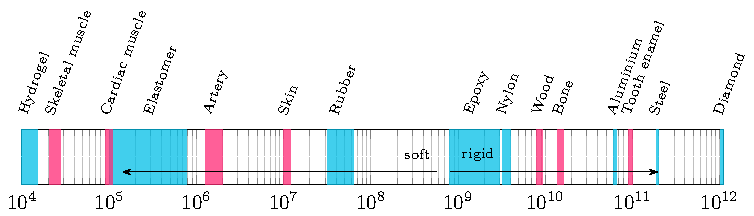
\includepdf[pages=-]{./pdf/thesis-figure-1-0.pdf}
    \includegraphics*[width=\textwidth]{./pdf/thesis-figure-1-0.pdf}
    \caption{\small Young's modulus spectrum in (Pa) of rigid and soft materials, where(\ldata{Matlab8}) are the organic (\ie, biological) materials and (\ldata{Matlab7}) inorganic materials. Modulus scale is adopted from the work of Rus et al. \cite{Rus2015}.\label{fig:1:1}}
    \vspace{-4mm}
\end{figure}
%
\terminology{\textbf{Soft materials} are homogeneous materials with a Young's modulus, often referred to as the elasticity modulus, that is typically less than or equal to $10^9$ \si{\pascal}. The term \textbf{softness} or \textbf{soft} refers to the collective mechanical properties that are commonly associated with materials inside the spectrum$^1$.}{}\
%
\blfootnote{$^1$It is important to note that the terms "soft" and "flexible" do not hold identical meanings as per the aforementioned definition. For example, slender metal rods are classified as flexible but not soft as the Young's modulus is not within the prespecified material range.}
%
Now, despite the fact that the words \emph{"soft"} and \emph{"robotics"} have clear definitions independently, the collocation of the two has sparked many new ideas and perspectives within the robotics community for the past two decades. Figure \ref{fig:C0:softrobotexamples} highlights a few of these soft robots that are inspired by various biological creatures. Throughout its young academic life, several definitions have been coined. Initially, soft robotics referred to robots with variable joint stiffness \cite{AlbuSchaffer2004} or artificial compliance achieved through control \cite{AlbuSchaffer2011}. The term was also used to underline the shift from rigid-linked robots to \textit{"bio-inspired continuum robots are inherently compliant and that exhibit large strains in normal operations"} \cite{Trivedi2008}. Paraphrasing the work of Robison et al. \cite{Robinson1999}: \textit{"soft robotic manipulators are continuum robots made of soft materials that undergo continuous elastic deformation and produce motion through the generation of a smooth backbone curve"}. Alternatively, a broader definition was coined in a review by Kim et al. \cite{Kim2013} simply referring to soft-bodied robots as \textit{"an analogy to soft-bodied animals"}. A concise definition was proposed by Laschi et al. \cite{Laschi2014}, as soft robots being \textit{"any robot built by soft materials"}. Rus et al. \cite{Rus2015} defined soft robots in terms of their structural elasticity: \textit{"Systems that are capable of autonomous behavior, and that are primarily composed of materials with moduli in the range of that of soft biological materials"}.

\par The ongoing debate regarding the precise terminology for soft robotics may never reach a definitive conclusion. It is of utmost importance to establish a uniform vocabulary not just for the sake of this thesis, but also to ensure effective communication across the wider scientific community. Previous definitions have placed great emphasis on the natural motion that arises from soft materials with high similarities to nature. In this thesis, we propose our definition of \textit{"soft robots"} based on the historical development of soft robotics and current scientific trends in literature (discussed in Chapter \ref{chap: history}) with particular focus on design and control. Given the interdisciplinary nature of the field, the terms used in this thesis may differ from those used in existing literature. Throughout the thesis, we will refer to the following definition when discussing "\emph{soft robotics}":
%
\terminology{\textbf{Soft robotics} is a subclass of robotics with purposefully designed compliant actuators embedded into their soft body, that enable control over the robot's natural ability to perform bio-inspired morphological behavior.}{}
%
The formulation above, modified from an early definition proposed in \cite{DellaSantina2020Springer}, emphasizes the significance of soft materials in replicating biological motion, also known as "\textit{biomimicry}" or "\textit{biomimetics}". Soft robotics represents the first stepping stone in the pursuit of harmonizing robotics and biological principles. This newly adopted field of soft robotics delves into the use of soft materials not only from a design perspective but also with regard to their implications for control, with the aim of recovering biological morphologies.

\begin{figure}[!t]
    \vspace{-2mm}
    % \ifx\printFigures\undefined
    % \else
    % \hspace{1mm}
    \includegraphics*[width=\textwidth]{./pdf/thesis-figurex-0-0-1.pdf}
    \vspace{-6mm}
    \caption{\small Examples of soft robotic systems that draw inspiration from nature. (a) Festo's Bionic arm inspired by the elephant's trunk but with octopus-inspired gripper \cite{Grzesiak2011}. (b)  Vacuum-driven origami-inspired artificial muscles by Li et al. \cite{Li2017Dec}. Vine-inspired inspection soft robot by Hawkes et al. \cite{Hawkes2017}. Soft robotic fish by Katzschmann et al. \cite{Katzschmann2018} composed of fluid-driven soft actuators \cite{Marchese2014}.
    \label{fig:C0:softrobotexamples}}
    \vspace{-2mm}
  \end{figure}

%In this section, we will present a short historical overview of soft robotics. Hereby showing that the current trends of bio-mimicry and elasticity in robotics find roots in a periods way before the soft robotic boom in the early 2010's. To guide the reader, in Figure \ref{fig:C0:timeline}, we provide a graphical, historic overview of soft robotic systems from 1960 to 2022. We will discuss the inception of soft actuation, early soft robotic designs, and modeling and control strategies for these continuum robotics.
\input{3_1_introduction/1_brief_introduction.tex}
\section{A biometic perspective on soft robotics}
A remarkable studycase, common to soft robotics, is the tentacle of an octopus. The octopus' tentacles can move in any direction, using a virtually infinite number of Degrees of Freedom (DoF) \cite{Sumbre2001Sep,Kier1985,Kennedy2020Nov}. The exceptional dexterity of the octopus arms results from them behaving like a muscular hydrostat. In fact, these arms are composed of densely packed muscle fibers whose orientation can be grouped into transverse, longitudinal, and oblique axes \cite{Kier2007Oct}. Moreover, each flexible arm of the organism is governed by a sophisticated peripheral nervous system that runs axially along each tentacle, composed of approximately 30,000 nerve fibers. Through appropriate communication between the muscle fiber network, the embedded nervous system, and the central motor cortex, complex yet coordinated motions of bending, twisting, and extension can be facilitated. An example of the amazing behavioral motor abilities of the octopus is given in Figure \ref{fig:C0:octopus} provided by Sumbre et al. \cite{Sumbre2001Sep}. The figure presents a visual segment of the bending propagation in an octopus tentacle. The purpose of this motion is to reduce the proximinal distance between the tentacle and an object of interest, such as food particle in this case. Interestingly, the octopus also employs a simulatenous bending and twisting propegation motion to orient the bottom side of its tentacles towards the direction of the objective. This leads to an efficient tranversal wave of bending and twist with speeds of about 12.5 $\pm$ 4.7 \si{\centi \meter \per \second} \cite{Sumbre2001Sep}. Such coordination enables an octopus to orient the tentacle's suckers towards a target object thus enabling effective grasping. The octopus is known for its remarkable ability to accomplish a hierarchy of tasks, which can be attributed to hyper-redundancies in its soft arm. Specifically, these organisms possess more degrees of freedom (DoFs) than are strictly necessary to complete a given task. Consequently, additional DoFs can be assigned to subtasks that run parallel to the main task. This ability allows the organism to passively adapt to uncertainties in its environment without affecting the primary motion. These attributes are highly desirable in modern robotic systems as they enable improved robustness in unstructured environments, allow for less conservative safety requirements regarding human-robot interactions, and greatly improve environmental durability, especially during impact.

\begin{figure}
  \centering
  %% This file was created by matlab2tikz.
%
%The latest updates can be retrieved from
%  http://www.mathworks.com/matlabcentral/fileexchange/22022-matlab2tikz-matlab2tikz
%where you can also make suggestions and rate matlab2tikz.
%
\begin{tikzpicture}

\begin{axis}[%
width=0.434\textwidth,
height=0.256\textwidth,
at={(0\textwidth,0.261\textwidth)},
scale only axis,
axis on top,
xmin=0.5,
xmax=829.5,
tick align=outside,
y dir=reverse,
ymin=0.5,
ymax=489.5,
axis line style={draw=none},
ticks=none
]
\addplot [forget plot] graphics [xmin=0.5, xmax=829.5, ymin=0.5, ymax=489.5] {./fig/fig_octopus_grasp-1.png};
\node[right, align=left, inner sep=0, font=\color{white}]
at (axis cs:650,50) {\scriptsize $t = 0$ s};
\end{axis}

\begin{axis}[%
width=0.434\textwidth,
height=0.256\textwidth,
at={(0.455\textwidth,0.261\textwidth)},
scale only axis,
axis on top,
xmin=0.5,
xmax=829.5,
tick align=outside,
y dir=reverse,
ymin=0.5,
ymax=489.5,
axis line style={draw=none},
ticks=none
]
\addplot [forget plot] graphics [xmin=0.5, xmax=829.5, ymin=0.5, ymax=489.5] {./fig/fig_octopus_grasp-2.png};
\node[right, align=left, inner sep=0, font=\color{white}]
at (axis cs:600,50) {\scriptsize $t = 0.36$ s};
\end{axis}

\begin{axis}[%
width=0.434\textwidth,
height=0.256\textwidth,
at={(0\textwidth,0\textwidth)},
scale only axis,
axis on top,
xmin=0.5,
xmax=829.5,
tick align=outside,
y dir=reverse,
ymin=0.5,
ymax=489.5,
axis line style={draw=none},
ticks=none
]
\addplot [forget plot] graphics [xmin=0.5, xmax=829.5, ymin=0.5, ymax=489.5] {./fig/fig_octopus_grasp-3.png};
\node[right, align=left, inner sep=0, font=\color{white}]
at (axis cs:600,50) {\scriptsize $t = 0.68$ s};
\end{axis}

\begin{axis}[%
width=0.435\textwidth,
height=0.256\textwidth,
at={(0.454\textwidth,0\textwidth)},
scale only axis,
axis on top,
xmin=0.5,
xmax=829.5,
tick align=outside,
y dir=reverse,
ymin=0.5,
ymax=487.5,
axis line style={draw=none},
ticks=none
]
\addplot [forget plot] graphics [xmin=0.5, xmax=829.5, ymin=0.5, ymax=487.5] {./fig/fig_octopus_grasp-4.png};
\node[right, align=left, inner sep=0, font=\color{white}]
at (axis cs:600,50) {\scriptsize $t = 0.92$ s};
\end{axis}
\end{tikzpicture}%
  \includegraphics*[width = .75\textwidth]{./pdf/thesis-figure-1-1.pdf}
  \caption{Recording by Sumbre et al. \cite{Sumbre2001Sep} of an octopus extending its tentacle towards an object of interest using coordinated activation of a tightly packed network of muscle fibers. The highly flexible appendage allows for traveling bending wave propagation, while the octopus orients its suckers towards the object to ensure secure grip. \label{fig:C0:octopus}}
  \vspace{-4mm}
\end{figure}

As illustrated by Figure \ref{fig:C0:octopus}, a key observation to be made is that the success of these biological system cannot be limited to morphological design problem alone. To effectively implement biomimetic design, it is crucial to tailor the problem towards the entire embodiment of the biological system which encompasses both its design and control. In light of the multidisciplinary nature of the soft robotics community, it is crucial to clarify these fundamental aspects:

\terminology{\textbf{Design} is the process of developing mechanical structures that enable a robot to perform specific tasks within a predefined workspace. \textbf{Control}, on the other hand, refers to the process of finding control laws that steers a dynamical system towards a desired state or desired behavior.}{}

% Generally speaking, for rigid robotics, the design and control synthesis are often mutally exclusive problems. This implies  may first design the rigid robot. Furthermore, unlike rigid robotics, the synthesis of control and design are not mutually independent problems; and thus should be considered as a collective \textit{design parameter} of the system. 
\begin{figure}
  \centering
  %% This file was created by matlab2tikz.
%
%The latest updates can be retrieved from
%  http://www.mathworks.com/matlabcentral/fileexchange/22022-matlab2tikz-matlab2tikz
%where you can also make suggestions and rate matlab2tikz.
%
\begin{tikzpicture}

\begin{axis}[%
width=0.434\textwidth,
height=0.256\textwidth,
at={(0\textwidth,0.261\textwidth)},
scale only axis,
axis on top,
xmin=0.5,
xmax=829.5,
tick align=outside,
y dir=reverse,
ymin=0.5,
ymax=489.5,
axis line style={draw=none},
ticks=none
]
\addplot [forget plot] graphics [xmin=0.5, xmax=829.5, ymin=0.5, ymax=489.5] {./fig/fig_octopus_grasp-1.png};
\node[right, align=left, inner sep=0, font=\color{white}]
at (axis cs:650,50) {\scriptsize $t = 0$ s};
\end{axis}

\begin{axis}[%
width=0.434\textwidth,
height=0.256\textwidth,
at={(0.455\textwidth,0.261\textwidth)},
scale only axis,
axis on top,
xmin=0.5,
xmax=829.5,
tick align=outside,
y dir=reverse,
ymin=0.5,
ymax=489.5,
axis line style={draw=none},
ticks=none
]
\addplot [forget plot] graphics [xmin=0.5, xmax=829.5, ymin=0.5, ymax=489.5] {./fig/fig_octopus_grasp-2.png};
\node[right, align=left, inner sep=0, font=\color{white}]
at (axis cs:600,50) {\scriptsize $t = 0.36$ s};
\end{axis}

\begin{axis}[%
width=0.434\textwidth,
height=0.256\textwidth,
at={(0\textwidth,0\textwidth)},
scale only axis,
axis on top,
xmin=0.5,
xmax=829.5,
tick align=outside,
y dir=reverse,
ymin=0.5,
ymax=489.5,
axis line style={draw=none},
ticks=none
]
\addplot [forget plot] graphics [xmin=0.5, xmax=829.5, ymin=0.5, ymax=489.5] {./fig/fig_octopus_grasp-3.png};
\node[right, align=left, inner sep=0, font=\color{white}]
at (axis cs:600,50) {\scriptsize $t = 0.68$ s};
\end{axis}

\begin{axis}[%
width=0.435\textwidth,
height=0.256\textwidth,
at={(0.454\textwidth,0\textwidth)},
scale only axis,
axis on top,
xmin=0.5,
xmax=829.5,
tick align=outside,
y dir=reverse,
ymin=0.5,
ymax=487.5,
axis line style={draw=none},
ticks=none
]
\addplot [forget plot] graphics [xmin=0.5, xmax=829.5, ymin=0.5, ymax=487.5] {./fig/fig_octopus_grasp-4.png};
\node[right, align=left, inner sep=0, font=\color{white}]
at (axis cs:600,50) {\scriptsize $t = 0.92$ s};
\end{axis}
\end{tikzpicture}%
  %\includegraphics*[width = .95\textwidth]{./pdf/thesis-figure-1-octopus.pdf}
  \input{./pdf/thesis-figure-1-octopus.pdf_tex}
  \caption{A schematic representation of the control architecture of a octopus-inspired soft robots with embodied intelligence. The architecture shows how information flows between important biological components such as the body (\eg, soft deformable arm), actuators (\eg, muscle fibers network), sensors (\eg, the nervous system), and the brain (\eg, the motor cortex) that coordinates information throughout the system. \label{fig:C0:biometic} }
  \vspace{-4mm}
\end{figure}

Recognizing the significance of both design and control in soft robot biomimicry, we hypothesize a systematic deconstruction of the fundamental principles that underlie the morphological grasping behavior of the octopus. This is illustrated in Figure \ref{fig:C0:biometic}, which presents a schematic representation of the biological system $\Sigma_{\textrm{bio}}$ seen in Figure \ref{fig:C0:biometic}. 

The objective is to reduce the distance between the prey and one of the tentacles, denoted by $\mathcal{B}$. The soft body consists of a discrete bundles of muscle fibers for motion and nerve fibers for sensing. Due to physical design limitations, there is only a finite number of actuators and sensors that can be accommodated within the soft body, therefore, there exist a region called the "\textit{reachable workspace}" $\mathcal{W}$ in which the system can operate. Although the body has virtually infinite DoFs, it can only be controlled via a finite set of actuators and thus this region is finite. Part of the design problem is therefore finding an appriopriate compostion of actuators and sensor such that the systems' reachability space $\mathcal{W}$ coincides with the desired task. Given the continuum nature of soft robots, as well as its distributed actuation and sensing, such design problems are not a trivial and has thus sparked an active discipline within the field.

Next, the control problem entails finding suitable control action $\textbf{u}$ that steers the arm towards the prey. Using its sensory system, a measurement $\textbf{y}$ of the soft body can be made. Since control law inside the motor cortex must be computable, this involves encoding the virtually infinite DoFs of the soft body onto a smaller finite joint respresentation $\q$ belong to a configuration space $\mathcal{Q}$.

\section{State-of-the-art solutions in soft robotics}
Driven by the aspiration for bio-like performance in robotics, there has been significant advances in the development of continuum soft robots since the early 2000s. Besides octopi \cite{Renda2018}, various researchers draw inspiration from a plethora of biological organisms such as fish \cite{Katzschmann2018,Marchese2015}, elephants' trunks \cite{Jones2006,Wehner2016,Godage2015}, snakes \cite{Rafsanjani2018Feb,Gazzola2018,Marchese2015}, birds \cite{Gazzola2018,Zufferey2022Dec}, and even the human hand \cite{vanLaake2022Sep,Fras2018Oct}. Researchers have discovered several ways to mimic biology by harmonizing soft materials and robotics. This section offers a brief overview of the state-of-the-art solutions concerning design and control.

\begin{rmk}
\textit{Considering the extensive scope of soft robotics, an additional chapter (Chapter \ref{chap: history}) has been included to provide a more comprehensive overview of its origins dating back to the early 1980s, as well as the various research aspects currently associated with this field. Thus, the following section serves as a preliminary introduction, ensuring brevity in the following section while setting the stage for the research problems relevant to the scope of the thesis.}
\end{rmk}

\subsection{Soft fluidic actuators inspired by muscular hydrostats}
 Conventional soft robots are characterized by their continuum-bodied motion that arises from a network of compliant actuators embedded throughout its soft body. There exist many options for such embodied actuation, including tendons \cite{Jones2006,Renda2018}, chemical reactions \cite{Bartlett2015,Hubbard2021}, light-driven liquid crystals \cite{Vantomme2021,Pilz2020,daCunha2020}, and ferromagnetic materials \cite{Kim2019AugMagnet,Venkiteswaran2019Feb}, and hydrogels \cite{Jiao2022Jun,Lee2020Dec}. However, the most common approach is fluidic actuation \cite{Katzschmann2018,Marchese2015,Overvelde2015Sep,vanLaake2022Sep} that mimics muscular hydrostats found in animals. The latter are commonly referred to as \emph{"Soft Fluidic Actuators"} (SFAs), and the majority are designed via human-driven techniques. In this section, we aim to provide a concise explanation of the SFAs technology and explore the potential benefits of incorporating structural optimization into the design process alongside the common human-driven design techniques.

Soft Fluidic Actuators (SFAs) are inflatable fluidic channels that are embedded into an elastic soft body. When pressurized fluid is applied, the elastic pressure vessel uniformly distributes the internal stresses along the interior, resulting in motion due to strain relaxation of the surrounding continuum body. Since elasticity is key, silicone rubbers are frequently employed for their notable material properties. Specifically, silicone rubbers exhibit a low Young's modulus, only display material fatigue at high strains exceeding $100\%$, and offer many commercial alternatives. By exploring purposefully designed asymmetrical geometries, often created by hand, predictable motion can be guided \cite{Xavier2022Jun,Rus2015,Hughes2016Nov}. The aforementioned principles are analogous to those of (semi-rigid) compliant mechanisms, which flexible structures that facilitate motion or force transmission through elastic deformation of their components, as opposed to conventional rigid-body joints. Through the exploration of structural geometries or deliberate incorporation of stiffer materials, a diverse range of motion primitives can be achieved which may include bending, twisting, and elongation.

\subsection[Human-driven design versus design optimization]{Systematic design of soft fluidic actuation: human-driven versus design optimization}
A popular example of a soft fluidic actuator (SFA) is the PneuNet actuator, which was proposed by Mosadegh et al. \cite{Mosadegh2014}. This actuator has a consistent linear input-output bending behavior and its design is simple, easy to fabricate, and repeatable, making it a standard in the academic field. To illustrate the capabilities, in Figure \ref{fig:C0:pneunetGrasp}, we present an example of it grasping an aluminum cylinder, inspired by the octopus example mentioned earlier \cite{Sumbre2001Sep}. Despite using rudimentary open-loop control, the system can emulate complex behaviors such as reaching, grasping, and pulling objects closer through manipulation, similar to those exhibited by the octopus. As shown in Figure \ref{fig:C0:pneunetGrasp}, an important property is their inherent mechanical impedance allow for safe and stable interactions with objects of varying rigidity, even without environmental perception. This contrasts rigid robots interacting with unknown environments, where impedance control appear to be a necessary requirement \cite{Murray1994,DeLuca2016Jul}.

\begin{figure}
\centering
\includegraphics*[width=0.975\textwidth]{./pdf/thesis-figurex-1-3-2.pdf}
\caption{\small An illustrative example of a fluidic PneuNet actuator reaching and grasping a 20 \si{\milli \meter} aluminum cylinder, which is inspired by the morphological grasping motion of the octopus' soft arm as seen in Figure \ref{fig:C0:octopus}. The main body is composed of Dragonskin\texttrademark\, 10A silicone, and 30A for the bottom layer. It is worth noting that despite using open-loop motion control (\ie, linear pressure ramp of 40 \si{\kilo \pascal}), the enveloping properties of soft materials can lead to the emergence of complex "intelligent" behavior. \label{fig:C0:pneunetGrasp}}
\vspace{-5mm}
\end{figure}
    
Given its success in open-loop, common applications for SFA technology are therefore soft grippers \cite{Galloway2016,Hughes2016Nov,Ansari2022Sep,Teleshev1981} that are useful in handling delicate objects. Pushing the technology further, system dexterity has been extended by incorporated many different SFAs into one single body, similar to muscle groups in animals. Consequently, researchers have explored their potential for enabling highly dexterous robots capable of in-hand manipulation \cite{Suzumori1991,Graule2022}, as well as autonomous terrestrial and aquatic locomotion \cite{Choi2011,Katzschmann2018,Drotman2017,Suzumori1992}. Although SFAs provide a wide range of motion, they require significant amounts of supplied volume inflow, which adversely affects their speed, compactness, and efficiency \cite{Overvelde2015Sep,Rus2015,Xavier2022Jun}. A common nonlinear phenomenon called "\emph{ballooning}" occurs when the elastic membrane of the changes deforms significantly, further increasing the channels volumetric capacitance. This behavior is particularly evident in soft materials that exhibit strain softening nonlinearities, which intensifies this inefficient expansion. In order to address the aforementioned limitations, various researchers have proposed two potential solutions. The first involves the use of hand-designed geometrical features, such as ribs, which increase structural compliance. The second solution involves the utilization of composites made up of different materials. One example of this approach is demonstrated in the work of Polygerinos et al. \cite{Polygerinos2015,Polygerinos2013}, as well as other similar studies \cite{Fras2018Oct,Suzumori1991,Cianchetti2013Nov,Cianchetti2013Nov}, which employ fiber-reinforced SFAs that incorporate fiber weaves to create new soft material composites. The introduction of such weaves results in anisotropic mechanical properties due to the fibers have a low bending-twist modulus but high elongation modulus. Additionally, various weave patterns can be used to steer the deformation characteristics towards a desired kinematic profile \cite{Kim2019Aug,Connolly2017Jan}, or as proprioceptive sensors using magnetic inductance \cite{Felt2019Feb,Felt2015Oct} or strain sensors from EGaIn (Eutectic Gallium Indium) \cite{Park2012}. Recently, also multi-material 3D-printing approach are employed combining actuation with integrated sensing \cite{Wolterink2022Oct,Zhou2021Apr}. It is noteworthy that the advent of Additive Manufacturing (AM) technology has significantly contributed to the advancement of soft robotic technology, enabling flexibility in design and materials, surpassing what was previously achievable with subtractive techniques.

%Based on a review by Marchese et al. \cite{Marchese2014}, three common geometries for SFAs are explored: $(i)$ cylindrical, $(ii)$ ribbed, and $(iii)$ pleated. Although cylindrical geometries are the easiest to fabricate,
% Soft actuators from large circumferential strains that increase volume significantly without producing significant motion. This undesirable phenomenon is known as "\emph{ballooning}". Moreover, some soft materials exhibit strain softening nonlinearities that further intensify this inefficient volumetric expansion. Ribbed and pleated SFA designs, however, prevent such large volumetric expansion but require more complicated fabrication methods, such as lost-wax rubber casting \cite{Marchese2015}. 
% Alternatively, Polygerinos et al. \cite{Polygerinos2015} and other related works use of fiber-reinforced SFAs, which embedded single fibers or fiber-sheet matrices. These composite materials have anisotropic mechanical properties that arise from the fibers exhibiting low moduli for bending and twisting, but high for extensibility. Interestingly, the interlacing patterns of the fiber mesh can lead to exclusive homogeneous motion such as pure elongation, twisting and bending \cite{Polygerinos2015,Kamble2022Jan}. %Fibers in soft robotics have also been utilized in sensing applications, \eg, Galloway et al. \cite{Galloway2019} presented a fiber optic shape sensor, while Tapia et al. \cite{Tapia2020} explored the automated routing of a network of stretchable fiber sensors. 
% Connolly et al. \cite{Connolly2017Jan} demonstrated that the placement of inextensible fiber alignment can be optimized to ensure that the soft robot follows a prescribed (quasi-static) kinematic trajectory. 

Like nature, there are often no unique design solutions when finding the optimal geometrical shape, material composites, and actuation type, or a combination of the aforementioned. While such design freedom has its benefits, it also poses challenges in establishing effective hand-driven design solutions that are tailored towards functionality. Furthermore, predicting structural deformation \textit{a-priori} is challenging and often requires time-consuming numerical simulations. In response, optimization-based solutions are being slowly considered. Cheney et al. \cite{Cheney2013} employed compositional pattern-producing network (CPPN) to determine the most efficient arrangement of soft material voxels and activation patterns, thereby facilitating the synthesis of soft robots capable of terrestrial and aquatic locomotion in simulation. Following, in Kriegman et al. \cite{Kriegman2019,Kriegman2020}, auto-generative processes are explored for a variety of candidate creatures in silico, with the aim of achieving specific motor functions like locomotion, and object manipulation and transport.
% These designs were then implemented as living systems composed of muscular frog cells, resulting in the predicted behaviors being exhibited. 

Although voxel-based \cite{Kriegman2019,Cheney2013} and commonly parametric shape optimization \cite{Coevoet2017,Manns2018Jan,Morzadec2019Apr} approaches have demonstrated success in soft robot design, they are inherently imposed by  design restriction that do perhaps limit the design possibilities in soft robotics, especially given the recent advances in Additive Manufacturing. In contrast, topology optimization \cite{Bendsoe2003,Gain2013Dec,Zhang2017Topo} (TopOpt) is a versatile technique that enables the design of structures with desired functionality without imposing significant design constraints. Furthermore, TopOpt approaches explore gradient-based optimizers derived from continuum theory that allow accurate descriptions of nonlinear deformations, which are simplified in many schemes in favor of computation speed. Wang et al. \cite{Wang2020Nov} and Tian et al. \cite{Tian2020May} explored TopOpt for soft grippers using tendons and ferromagnetics, respectively. Yuhn et al. \cite{Yuhn2023Feb} extended density-based optimization to include time as an additional variable, allowing for simultaneous optimization of structure and movement with gradient-based methods through 4-dimensional TopOpt. However, research on TopOpt applied fluidic soft actuators is limited, perhaps due to the challenges associated with modeling fluid-structure interaction with adaptive structures.

\vspace{-2mm}
\subsection{Model-based control for soft robots}
\label{sec:C0:modelbasedcontrol}
In a previous discussion, we showed that open-loop approach can accomplish various complex tasks such as locomotion \cite{Suzumori1992,Choi2011,Katzschmann2018}, grasping \cite{Suzumori1992}, and manipulation \cite{Marchese2016}. While open-loop control has been successfully demonstrated, it ultimately relies on \textit{a-priori} system knowledge that determines the control logic based on numerical surrogate models or experimental regression. This, independent of using open-loop strategies, further establishes the importance of modeling which is a crucial ingredient for modern conventional robotics \cite{Spong1996,Murray1994,Khatib1987}. 
%The use of models for control can naturally exploit system information to enhance performance and robustness when executing tasks, and this holds true for soft robotics as well. 
In the early days of soft robotics, model-based control strategies were deemed unfeasible due to the infinite-dimensional nature of these systems \cite{DellaSantina2020}. Over the last two decades, however, a plethora of modeling solutions have surfaced, paving the way for sophisticated model-based controllers, which are expected to push the dexterity of soft robotics systems even beyond what is already achievable in open-loop.
% The necessity for high-precision models allows us to understand and predict such behavior withing small margins of deviation, thus facilitating controllers that achieve the desired behavior without feedback compensation (under conservative conditions). Closed-loop controllers can explore useful model structures to compensate for large deviations, uses feedback to adjust the outputs and maintain a desired state. In recent years, various modeling techniques have gained popularity in soft robotics. 

A common modeling approach is the Finite Element Method (FEM), which involves spatially discretizing continuum solids into a group of "\textit{finite elements}," permitting the underlying Partial Differential Equation to be rewritten as an approximate Ordinary Differential Equation (ODE) \cite{Holzapfel2002,Kim2018}. These can be solved straightforwardly using standard numerical integration (\eg, \texttt{ode45}, \texttt{ode23t} in MATLAB\textsuperscript{\scriptsize\textregistered}).
%By treating the soft body as a continuum mechanical solid, its dynamics can be described by the momentum balance as a Partial Differential Equation (PDE), which are often solved using the Ritz-Galerkin projection method \cite{Kim2018,Holzapfel2002}. The method yields a $n$-dimensional surrogate problem represented as an Ordinary Differential Equation (ODE), which are reminiscent those in rigid robotics, and can be solved straightforwardly using standard numerical integration methods. 
%
While primarily explored for quasi-static behavior, FEM models have demonstrated their efficacy in handling hyper-elasticity, geometric nonlinearities due to large deformation, fluid-structure interactions and other multi-physical domains \cite{Xavier2022Jun,Hughes2016Nov,Smith2022_FEM,Moerman2018,Maas2012}. Motivated by the assumption that quasi-static models provide sufficiently accuracy to describe soft robots under slow-varying dynamics, open-loop forward kinematic controllers are used that inversely search the input space for the desired deformation profile \cite{Marchese2015,Bern2019,Marchese2016}. Alternatively, high-fidelity FEM data can be fed into neural networks approximators \cite{Fang2022Jun,Zheng2020May} or Quadratic Programming (QP) algorithms \cite{Bern2019} that tackle the inverse kinematic problem directly. Yet, the high-dimensionality of these models, sometimes millions of DOFs, poses a significant challenge when considering dynamic behavior \cite{Goury2018,Duriez2013}, thereby limiting their applicability for closed-loop feedback control. Undoubtedly, under dynamic conditions, is where the benefits of soft robots are indisputably evident.

A viable solution for reducing dimensionality of FEM is found in Proper Orthogonal Decomposition (POD). Here, dynamic snapshots of observable data is collected, and through singular values decomposition, principal dynamic modes are identified that combined  to represent the reduced linear dynamical model. Not only does this approach improve speed, but it also preserves accurate, robust, and efficient models suited for closed-loop controller design \cite{Goury2018}. Recent extensions \cite{Sifakis2012Aug} preserve even nonlinear deformations and self-contact. The proposed modeling approach is encapsulated in an open-source software called \textit{SOFA} \cite{Duriez2016, Coevoet2017Feb}, which facilitated a wide range of closed-loop controller designs contributed by an active community in past years \cite{Largilliere2015,Goury2018,Duriez2016,Wu2021Feb,Li2022Feb}. Furthermore, it has been successfully implemented in physical systems, and recently Reinforcement Learning (RL) methods have been explored \cite{Schegg2022}. Alternatively, Koopman system identification tools are a data-driven approach that can be applied directly to experimental data (\ie, optical markers), leading to discrete-time dynamical systems. By gathering measured data alone, accurate models of the true system can be identified \cite{Bruder2019,Komeno2022Oct}. These models are often followed by Model-Predictive Control (MPC) approaches \cite{Bruder2020Dec,Bruder2019}. 

% \begin{figure}[!t]
%     \centering
%     \hspace{-2mm}
%     \includegraphics*[width=\textwidth]{./pdf/thesis-figure-1-model.pdf}
%     %% This file was created by matlab2tikz.
%
%The latest updates can be retrieved from
%  http://www.mathworks.com/matlabcentral/fileexchange/22022-matlab2tikz-matlab2tikz
%where you can also make suggestions and rate matlab2tikz.
%
\definecolor{mycolor1}{rgb}{0.62745,0.45882,1.00000}%
\definecolor{mycolor2}{rgb}{0.62869,0.46064,1.00000}%
\definecolor{mycolor3}{rgb}{0.62993,0.46245,1.00000}%
\definecolor{mycolor4}{rgb}{0.63118,0.46426,1.00000}%
\definecolor{mycolor5}{rgb}{0.63242,0.46608,1.00000}%
\definecolor{mycolor6}{rgb}{0.63366,0.46789,1.00000}%
\definecolor{mycolor7}{rgb}{0.63490,0.46970,1.00000}%
\definecolor{mycolor8}{rgb}{0.63614,0.47151,1.00000}%
\definecolor{mycolor9}{rgb}{0.63738,0.47333,1.00000}%
\definecolor{mycolor10}{rgb}{0.63862,0.47514,1.00000}%
\definecolor{mycolor11}{rgb}{0.63987,0.47695,1.00000}%
\definecolor{mycolor12}{rgb}{0.64111,0.47877,1.00000}%
\definecolor{mycolor13}{rgb}{0.64235,0.48058,1.00000}%
\definecolor{mycolor14}{rgb}{0.64359,0.48239,1.00000}%
\definecolor{mycolor15}{rgb}{0.64483,0.48421,1.00000}%
\definecolor{mycolor16}{rgb}{0.64607,0.48602,1.00000}%
\definecolor{mycolor17}{rgb}{0.64732,0.48783,1.00000}%
\definecolor{mycolor18}{rgb}{0.64856,0.48964,1.00000}%
\definecolor{mycolor19}{rgb}{0.64980,0.49146,1.00000}%
\definecolor{mycolor20}{rgb}{0.65104,0.49327,1.00000}%
\definecolor{mycolor21}{rgb}{0.65228,0.49508,1.00000}%
\definecolor{mycolor22}{rgb}{0.65352,0.49690,1.00000}%
\definecolor{mycolor23}{rgb}{0.65476,0.49871,1.00000}%
\definecolor{mycolor24}{rgb}{0.65601,0.50052,1.00000}%
\definecolor{mycolor25}{rgb}{0.65725,0.50234,1.00000}%
\definecolor{mycolor26}{rgb}{0.65849,0.50415,1.00000}%
\definecolor{mycolor27}{rgb}{0.65973,0.50596,1.00000}%
\definecolor{mycolor28}{rgb}{0.66097,0.50777,1.00000}%
\definecolor{mycolor29}{rgb}{0.66221,0.50959,1.00000}%
\definecolor{mycolor30}{rgb}{0.66345,0.51140,1.00000}%
\definecolor{mycolor31}{rgb}{0.66470,0.51321,1.00000}%
\definecolor{mycolor32}{rgb}{0.66594,0.51503,1.00000}%
\definecolor{mycolor33}{rgb}{0.66718,0.51684,1.00000}%
\definecolor{mycolor34}{rgb}{0.66842,0.51865,1.00000}%
\definecolor{mycolor35}{rgb}{0.66966,0.52047,1.00000}%
\definecolor{mycolor36}{rgb}{0.67090,0.52228,1.00000}%
\definecolor{mycolor37}{rgb}{0.67215,0.52409,1.00000}%
\definecolor{mycolor38}{rgb}{0.67339,0.52590,1.00000}%
\definecolor{mycolor39}{rgb}{0.67463,0.52772,1.00000}%
\definecolor{mycolor40}{rgb}{0.67587,0.52953,1.00000}%
\definecolor{mycolor41}{rgb}{0.67711,0.53134,1.00000}%
\definecolor{mycolor42}{rgb}{0.67835,0.53316,1.00000}%
\definecolor{mycolor43}{rgb}{0.67959,0.53497,1.00000}%
\definecolor{mycolor44}{rgb}{0.68084,0.53678,1.00000}%
\definecolor{mycolor45}{rgb}{0.68208,0.53859,1.00000}%
\definecolor{mycolor46}{rgb}{0.68332,0.54041,1.00000}%
\definecolor{mycolor47}{rgb}{0.68456,0.54222,1.00000}%
\definecolor{mycolor48}{rgb}{0.68580,0.54403,1.00000}%
\definecolor{mycolor49}{rgb}{0.68704,0.54585,1.00000}%
\definecolor{mycolor50}{rgb}{0.68828,0.54766,1.00000}%
\definecolor{mycolor51}{rgb}{0.68953,0.54947,1.00000}%
\definecolor{mycolor52}{rgb}{0.69077,0.55129,1.00000}%
\definecolor{mycolor53}{rgb}{0.69201,0.55310,1.00000}%
\definecolor{mycolor54}{rgb}{0.69325,0.55491,1.00000}%
\definecolor{mycolor55}{rgb}{0.69449,0.55672,1.00000}%
\definecolor{mycolor56}{rgb}{0.69573,0.55854,1.00000}%
\definecolor{mycolor57}{rgb}{0.69698,0.56035,1.00000}%
\definecolor{mycolor58}{rgb}{0.69822,0.56216,1.00000}%
\definecolor{mycolor59}{rgb}{0.69946,0.56398,1.00000}%
\definecolor{mycolor60}{rgb}{0.70070,0.56579,1.00000}%
\definecolor{mycolor61}{rgb}{0.70194,0.56760,1.00000}%
\definecolor{mycolor62}{rgb}{0.70318,0.56942,1.00000}%
\definecolor{mycolor63}{rgb}{0.70442,0.57123,1.00000}%
\definecolor{mycolor64}{rgb}{0.70567,0.57304,1.00000}%
\definecolor{mycolor65}{rgb}{0.70691,0.57485,1.00000}%
\definecolor{mycolor66}{rgb}{0.70815,0.57667,1.00000}%
\definecolor{mycolor67}{rgb}{0.70939,0.57848,1.00000}%
\definecolor{mycolor68}{rgb}{0.71063,0.58029,1.00000}%
\definecolor{mycolor69}{rgb}{0.71187,0.58211,1.00000}%
\definecolor{mycolor70}{rgb}{0.71311,0.58392,1.00000}%
\definecolor{mycolor71}{rgb}{0.71436,0.58573,1.00000}%
\definecolor{mycolor72}{rgb}{0.71560,0.58755,1.00000}%
\definecolor{mycolor73}{rgb}{0.71684,0.58936,1.00000}%
\definecolor{mycolor74}{rgb}{0.71808,0.59117,1.00000}%
\definecolor{mycolor75}{rgb}{0.71932,0.59298,1.00000}%
\definecolor{mycolor76}{rgb}{0.72056,0.59480,1.00000}%
\definecolor{mycolor77}{rgb}{0.72181,0.59661,1.00000}%
\definecolor{mycolor78}{rgb}{0.72305,0.59842,1.00000}%
\definecolor{mycolor79}{rgb}{0.72429,0.60024,1.00000}%
\definecolor{mycolor80}{rgb}{0.72553,0.60205,1.00000}%
\definecolor{mycolor81}{rgb}{0.72677,0.60386,1.00000}%
\definecolor{mycolor82}{rgb}{0.72801,0.60568,1.00000}%
\definecolor{mycolor83}{rgb}{0.72925,0.60749,1.00000}%
\definecolor{mycolor84}{rgb}{0.73050,0.60930,1.00000}%
\definecolor{mycolor85}{rgb}{0.73174,0.61111,1.00000}%
\definecolor{mycolor86}{rgb}{0.73298,0.61293,1.00000}%
\definecolor{mycolor87}{rgb}{0.73422,0.61474,1.00000}%
\definecolor{mycolor88}{rgb}{0.73546,0.61655,1.00000}%
\definecolor{mycolor89}{rgb}{0.73670,0.61837,1.00000}%
\definecolor{mycolor90}{rgb}{0.73794,0.62018,1.00000}%
\definecolor{mycolor91}{rgb}{0.73919,0.62199,1.00000}%
\definecolor{mycolor92}{rgb}{0.74043,0.62381,1.00000}%
\definecolor{mycolor93}{rgb}{0.74167,0.62562,1.00000}%
\definecolor{mycolor94}{rgb}{0.74291,0.62743,1.00000}%
\definecolor{mycolor95}{rgb}{0.74415,0.62924,1.00000}%
\definecolor{mycolor96}{rgb}{0.74539,0.63106,1.00000}%
\definecolor{mycolor97}{rgb}{0.74664,0.63287,1.00000}%
\definecolor{mycolor98}{rgb}{0.74788,0.63468,1.00000}%
\definecolor{mycolor99}{rgb}{0.74912,0.63650,1.00000}%
\definecolor{mycolor100}{rgb}{0.75036,0.63831,1.00000}%
\definecolor{mycolor101}{rgb}{0.75160,0.64012,1.00000}%
\definecolor{mycolor102}{rgb}{0.75408,0.64375,1.00000}%
\definecolor{mycolor103}{rgb}{0.75533,0.64556,1.00000}%
\definecolor{mycolor104}{rgb}{0.75657,0.64737,1.00000}%
\definecolor{mycolor105}{rgb}{0.75781,0.64919,1.00000}%
\definecolor{mycolor106}{rgb}{0.75905,0.65100,1.00000}%
\definecolor{mycolor107}{rgb}{0.76029,0.65281,1.00000}%
\definecolor{mycolor108}{rgb}{0.76153,0.65463,1.00000}%
\definecolor{mycolor109}{rgb}{0.76277,0.65644,1.00000}%
\definecolor{mycolor110}{rgb}{0.76402,0.65825,1.00000}%
\definecolor{mycolor111}{rgb}{0.76526,0.66007,1.00000}%
\definecolor{mycolor112}{rgb}{0.76650,0.66188,1.00000}%
\definecolor{mycolor113}{rgb}{0.76774,0.66369,1.00000}%
\definecolor{mycolor114}{rgb}{0.76898,0.66550,1.00000}%
\definecolor{mycolor115}{rgb}{0.77022,0.66732,1.00000}%
\definecolor{mycolor116}{rgb}{0.77147,0.66913,1.00000}%
\definecolor{mycolor117}{rgb}{0.77271,0.67094,1.00000}%
\definecolor{mycolor118}{rgb}{0.77395,0.67276,1.00000}%
\definecolor{mycolor119}{rgb}{0.77519,0.67457,1.00000}%
\definecolor{mycolor120}{rgb}{0.77643,0.67638,1.00000}%
\definecolor{mycolor121}{rgb}{0.77767,0.67819,1.00000}%
\definecolor{mycolor122}{rgb}{0.77891,0.68001,1.00000}%
\definecolor{mycolor123}{rgb}{0.78016,0.68182,1.00000}%
\definecolor{mycolor124}{rgb}{0.78140,0.68363,1.00000}%
\definecolor{mycolor125}{rgb}{0.78264,0.68545,1.00000}%
\definecolor{mycolor126}{rgb}{0.78388,0.68726,1.00000}%
\definecolor{mycolor127}{rgb}{0.78512,0.68907,1.00000}%
\definecolor{mycolor128}{rgb}{0.78636,0.69089,1.00000}%
\definecolor{mycolor129}{rgb}{0.78760,0.69270,1.00000}%
\definecolor{mycolor130}{rgb}{0.78885,0.69451,1.00000}%
\definecolor{mycolor131}{rgb}{0.79009,0.69632,1.00000}%
\definecolor{mycolor132}{rgb}{0.79133,0.69814,1.00000}%
\definecolor{mycolor133}{rgb}{0.79257,0.69995,1.00000}%
\definecolor{mycolor134}{rgb}{0.79381,0.70176,1.00000}%
\definecolor{mycolor135}{rgb}{0.79505,0.70358,1.00000}%
\definecolor{mycolor136}{rgb}{0.79630,0.70539,1.00000}%
\definecolor{mycolor137}{rgb}{0.79754,0.70720,1.00000}%
\definecolor{mycolor138}{rgb}{0.79878,0.70902,1.00000}%
\definecolor{mycolor139}{rgb}{0.80002,0.71083,1.00000}%
\definecolor{mycolor140}{rgb}{0.80126,0.71264,1.00000}%
\definecolor{mycolor141}{rgb}{0.80250,0.71445,1.00000}%
\definecolor{mycolor142}{rgb}{0.80374,0.71627,1.00000}%
\definecolor{mycolor143}{rgb}{0.80499,0.71808,1.00000}%
\definecolor{mycolor144}{rgb}{0.80623,0.71989,1.00000}%
\definecolor{mycolor145}{rgb}{0.80747,0.72171,1.00000}%
\definecolor{mycolor146}{rgb}{0.80871,0.72352,1.00000}%
\definecolor{mycolor147}{rgb}{0.80995,0.72533,1.00000}%
\definecolor{mycolor148}{rgb}{0.81119,0.72715,1.00000}%
\definecolor{mycolor149}{rgb}{0.81243,0.72896,1.00000}%
\definecolor{mycolor150}{rgb}{0.81368,0.73077,1.00000}%
\definecolor{mycolor151}{rgb}{0.81492,0.73258,1.00000}%
\definecolor{mycolor152}{rgb}{0.81616,0.73440,1.00000}%
\definecolor{mycolor153}{rgb}{0.81740,0.73621,1.00000}%
\definecolor{mycolor154}{rgb}{0.81864,0.73802,1.00000}%
\definecolor{mycolor155}{rgb}{0.81988,0.73984,1.00000}%
\definecolor{mycolor156}{rgb}{0.82113,0.74165,1.00000}%
\definecolor{mycolor157}{rgb}{0.82237,0.74346,1.00000}%
\definecolor{mycolor158}{rgb}{0.82361,0.74528,1.00000}%
\definecolor{mycolor159}{rgb}{0.82485,0.74709,1.00000}%
\definecolor{mycolor160}{rgb}{0.82609,0.74890,1.00000}%
\definecolor{mycolor161}{rgb}{0.82733,0.75071,1.00000}%
\definecolor{mycolor162}{rgb}{0.82857,0.75253,1.00000}%
\definecolor{mycolor163}{rgb}{0.82982,0.75434,1.00000}%
\definecolor{mycolor164}{rgb}{0.83106,0.75615,1.00000}%
\definecolor{mycolor165}{rgb}{0.83230,0.75797,1.00000}%
\definecolor{mycolor166}{rgb}{0.83354,0.75978,1.00000}%
\definecolor{mycolor167}{rgb}{0.83478,0.76159,1.00000}%
\definecolor{mycolor168}{rgb}{0.83602,0.76341,1.00000}%
\definecolor{mycolor169}{rgb}{0.83726,0.76522,1.00000}%
\definecolor{mycolor170}{rgb}{0.83851,0.76703,1.00000}%
\definecolor{mycolor171}{rgb}{0.83975,0.76884,1.00000}%
\definecolor{mycolor172}{rgb}{0.84099,0.77066,1.00000}%
\definecolor{mycolor173}{rgb}{0.84223,0.77247,1.00000}%
\definecolor{mycolor174}{rgb}{0.84347,0.77428,1.00000}%
\definecolor{mycolor175}{rgb}{0.84471,0.77610,1.00000}%
\definecolor{mycolor176}{rgb}{0.84596,0.77791,1.00000}%
\definecolor{mycolor177}{rgb}{0.84720,0.77972,1.00000}%
\definecolor{mycolor178}{rgb}{0.84844,0.78154,1.00000}%
\definecolor{mycolor179}{rgb}{0.84968,0.78335,1.00000}%
\definecolor{mycolor180}{rgb}{0.85092,0.78516,1.00000}%
\definecolor{mycolor181}{rgb}{0.85216,0.78697,1.00000}%
\definecolor{mycolor182}{rgb}{0.85340,0.78879,1.00000}%
\definecolor{mycolor183}{rgb}{0.85465,0.79060,1.00000}%
\definecolor{mycolor184}{rgb}{0.85589,0.79241,1.00000}%
\definecolor{mycolor185}{rgb}{0.85713,0.79423,1.00000}%
\definecolor{mycolor186}{rgb}{0.85837,0.79604,1.00000}%
\definecolor{mycolor187}{rgb}{0.85961,0.79785,1.00000}%
\definecolor{mycolor188}{rgb}{0.86085,0.79966,1.00000}%
\definecolor{mycolor189}{rgb}{0.86209,0.80148,1.00000}%
\definecolor{mycolor190}{rgb}{0.86334,0.80329,1.00000}%
\definecolor{mycolor191}{rgb}{0.86458,0.80510,1.00000}%
\definecolor{mycolor192}{rgb}{0.86582,0.80692,1.00000}%
\definecolor{mycolor193}{rgb}{0.86706,0.80873,1.00000}%
\definecolor{mycolor194}{rgb}{0.86830,0.81054,1.00000}%
\definecolor{mycolor195}{rgb}{0.86954,0.81236,1.00000}%
\definecolor{mycolor196}{rgb}{0.87079,0.81417,1.00000}%
\definecolor{mycolor197}{rgb}{0.87203,0.81598,1.00000}%
\definecolor{mycolor198}{rgb}{0.87327,0.81779,1.00000}%
\definecolor{mycolor199}{rgb}{0.87451,0.81961,1.00000}%
\definecolor{mycolor200}{rgb}{0.81905,0.74006,0.99664}%
\definecolor{mycolor201}{rgb}{0.76359,0.66050,0.99328}%
\definecolor{mycolor202}{rgb}{0.70812,0.58095,0.98992}%
\definecolor{mycolor203}{rgb}{0.65266,0.50140,0.98655}%
\definecolor{mycolor204}{rgb}{0.59720,0.42185,0.98319}%
\definecolor{mycolor205}{rgb}{0.54174,0.34230,0.97983}%
\definecolor{mycolor206}{rgb}{0.48627,0.26275,0.97647}%
\definecolor{mycolor207}{rgb}{0.86275,0.89412,0.93725}%
%
\begin{tikzpicture}

\begin{axis}[%
width=0.774\textwidth,
height=0.242\textwidth,
at={(0.118\textwidth,0.003\textwidth)},
scale only axis,
xmin=0,
xmax=1,
ymin=0,
ymax=1,
axis line style={draw=none},
ticks=none,
axis x line*=bottom,
axis y line*=left
]
\end{axis}

\begin{axis}[%
width=0.302\textwidth,
height=0.264\textwidth,
at={(0\textwidth,0\textwidth)},
scale only axis,
xmin=-1,
xmax=1,
xtick={-1,-0.5,0,0.5,1},
xticklabels={\empty},
ymin=-0.5,
ymax=1.25,
ytick={-0.5,0,0.5,1},
yticklabels={\empty},
axis line style={draw=none},
ticks=none,
axis x line*=bottom,
axis y line*=left
]
\addplot [color=mycolor2, line width=1.5pt, forget plot]
  table[row sep=crcr]{%
-0.584958712597518	0.0243477391605708\\
-0.578395869368097	0.0121034471751481\\
};
\addplot [color=mycolor3, line width=1.5pt, forget plot]
  table[row sep=crcr]{%
-0.591262388502971	0.0367274510941034\\
-0.584958712597518	0.0243477391605708\\
};
\addplot [color=mycolor4, line width=1.5pt, forget plot]
  table[row sep=crcr]{%
-0.597304104226123	0.0492370981154573\\
-0.591262388502971	0.0367274510941034\\
};
\addplot [color=mycolor5, line width=1.5pt, forget plot]
  table[row sep=crcr]{%
-0.603081182970708	0.0618711377962995\\
-0.597304104226123	0.0492370981154573\\
};
\addplot [color=mycolor6, line width=1.5pt, forget plot]
  table[row sep=crcr]{%
-0.608591065188497	0.0746239725958389\\
-0.603081182970708	0.0618711377962995\\
};
\addplot [color=mycolor7, line width=1.5pt, forget plot]
  table[row sep=crcr]{%
-0.613831309713301	0.087489952340829\\
-0.608591065188497	0.0746239725958389\\
};
\addplot [color=mycolor8, line width=1.5pt, forget plot]
  table[row sep=crcr]{%
-0.618799594842545	0.100463376728892\\
-0.613831309713301	0.087489952340829\\
};
\addplot [color=mycolor9, line width=1.5pt, forget plot]
  table[row sep=crcr]{%
-0.623493719365896	0.113538497854049\\
-0.618799594842545	0.100463376728892\\
};
\addplot [color=mycolor10, line width=1.5pt, forget plot]
  table[row sep=crcr]{%
-0.62791160354052	0.126709522753344\\
-0.623493719365896	0.113538497854049\\
};
\addplot [color=mycolor11, line width=1.5pt, forget plot]
  table[row sep=crcr]{%
-0.632051290012514	0.13997061597343\\
-0.62791160354052	0.126709522753344\\
};
\addplot [color=mycolor12, line width=1.5pt, forget plot]
  table[row sep=crcr]{%
-0.635910944684117	0.153315902155982\\
-0.632051290012514	0.13997061597343\\
};
\addplot [color=mycolor13, line width=1.5pt, forget plot]
  table[row sep=crcr]{%
-0.639488857526311	0.166739468640785\\
-0.635910944684117	0.153315902155982\\
};
\addplot [color=mycolor14, line width=1.5pt, forget plot]
  table[row sep=crcr]{%
-0.642783443336455	0.180235368085351\\
-0.639488857526311	0.166739468640785\\
};
\addplot [color=mycolor15, line width=1.5pt, forget plot]
  table[row sep=crcr]{%
-0.64579324244061	0.193797621099908\\
-0.642783443336455	0.180235368085351\\
};
\addplot [color=mycolor16, line width=1.5pt, forget plot]
  table[row sep=crcr]{%
-0.648516921340251	0.20742021889658\\
-0.64579324244061	0.193797621099908\\
};
\addplot [color=mycolor17, line width=1.5pt, forget plot]
  table[row sep=crcr]{%
-0.650953273303082	0.221097125951593\\
-0.648516921340251	0.20742021889658\\
};
\addplot [color=mycolor18, line width=1.5pt, forget plot]
  table[row sep=crcr]{%
-0.653101218897673	0.234822282679329\\
-0.650953273303082	0.221097125951593\\
};
\addplot [color=mycolor19, line width=1.5pt, forget plot]
  table[row sep=crcr]{%
-0.654959806471712	0.248589608117041\\
-0.653101218897673	0.234822282679329\\
};

\addplot[area legend, draw=none, fill=mycolor19, forget plot]
table[row sep=crcr] {%
x	y\\
-0.62190600661236	0.269970699862386\\
-0.653101218897673	0.234822282679329\\
-0.696804133207599	0.252102554112939\\
-0.621831963836141	0.10375056113766\\
}--cycle;
\addplot [color=mycolor20, line width=1.5pt, forget plot]
  table[row sep=crcr]{%
-0.656528212573634	0.262393002619035\\
-0.654959806471712	0.248589608117041\\
};
\addplot [color=mycolor21, line width=1.5pt, forget plot]
  table[row sep=crcr]{%
-0.65780574231745	0.276226350559137\\
-0.656528212573634	0.262393002619035\\
};
\addplot [color=mycolor22, line width=1.5pt, forget plot]
  table[row sep=crcr]{%
-0.658791829690624	0.290083523040228\\
-0.65780574231745	0.276226350559137\\
};
\addplot [color=mycolor23, line width=1.5pt, forget plot]
  table[row sep=crcr]{%
-0.659486037804842	0.303958380609673\\
-0.658791829690624	0.290083523040228\\
};
\addplot [color=mycolor24, line width=1.5pt, forget plot]
  table[row sep=crcr]{%
-0.659888059089577	0.317844775979418\\
-0.659486037804842	0.303958380609673\\
};
\addplot [color=mycolor25, line width=1.5pt, forget plot]
  table[row sep=crcr]{%
-0.659997715428361	0.331736556749557\\
-0.659888059089577	0.317844775979418\\
};
\addplot [color=mycolor26, line width=1.5pt, forget plot]
  table[row sep=crcr]{%
-0.659814958237695	0.345627568134172\\
-0.659997715428361	0.331736556749557\\
};
\addplot [color=mycolor27, line width=1.5pt, forget plot]
  table[row sep=crcr]{%
-0.659339868488581	0.359511655688222\\
-0.659814958237695	0.345627568134172\\
};
\addplot [color=mycolor28, line width=1.5pt, forget plot]
  table[row sep=crcr]{%
-0.658572656670642	0.373382668034286\\
-0.659339868488581	0.359511655688222\\
};
\addplot [color=mycolor29, line width=1.5pt, forget plot]
  table[row sep=crcr]{%
-0.657513662698864	0.387234459587944\\
-0.658572656670642	0.373382668034286\\
};
\addplot [color=mycolor30, line width=1.5pt, forget plot]
  table[row sep=crcr]{%
-0.656163355763002	0.401060893280592\\
-0.657513662698864	0.387234459587944\\
};
\addplot [color=mycolor31, line width=1.5pt, forget plot]
  table[row sep=crcr]{%
-0.654522334119697	0.414855843278488\\
-0.656163355763002	0.401060893280592\\
};
\addplot [color=mycolor32, line width=1.5pt, forget plot]
  table[row sep=crcr]{%
-0.652591324827422	0.428613197696812\\
-0.654522334119697	0.414855843278488\\
};
\addplot [color=mycolor33, line width=1.5pt, forget plot]
  table[row sep=crcr]{%
-0.650371183424353	0.442326861307556\\
-0.652591324827422	0.428613197696812\\
};
\addplot [color=mycolor34, line width=1.5pt, forget plot]
  table[row sep=crcr]{%
-0.647862893549325	0.455990758240023\\
-0.650371183424353	0.442326861307556\\
};
\addplot [color=mycolor35, line width=1.5pt, forget plot]
  table[row sep=crcr]{%
-0.645067566506027	0.469598834672761\\
-0.647862893549325	0.455990758240023\\
};
\addplot [color=mycolor36, line width=1.5pt, forget plot]
  table[row sep=crcr]{%
-0.641986440770633	0.483145061515721\\
-0.645067566506027	0.469598834672761\\
};
\addplot [color=mycolor37, line width=1.5pt, forget plot]
  table[row sep=crcr]{%
-0.638620881443099	0.496623437081459\\
-0.641986440770633	0.483145061515721\\
};
\addplot [color=mycolor38, line width=1.5pt, forget plot]
  table[row sep=crcr]{%
-0.634972379642345	0.510027989744198\\
-0.638620881443099	0.496623437081459\\
};

\addplot[area legend, draw=none, fill=mycolor38, forget plot]
table[row sep=crcr] {%
x	y\\
-0.596202069818307	0.516852053453825\\
-0.638620881443099	0.496623437081459\\
-0.672146825637701	0.529556149782669\\
-0.660853050018576	0.363720114397519\\
}--cycle;
\addplot [color=mycolor39, line width=1.5pt, forget plot]
  table[row sep=crcr]{%
-0.631042551845617	0.52335278058557\\
-0.634972379642345	0.510027989744198\\
};
\addplot [color=mycolor40, line width=1.5pt, forget plot]
  table[row sep=crcr]{%
-0.626833139172299	0.536591906025868\\
-0.631042551845617	0.52335278058557\\
};
\addplot [color=mycolor41, line width=1.5pt, forget plot]
  table[row sep=crcr]{%
-0.622346006612508	0.549739500439642\\
-0.626833139172299	0.536591906025868\\
};
\addplot [color=mycolor42, line width=1.5pt, forget plot]
  table[row sep=crcr]{%
-0.617583142200807	0.562789738754478\\
-0.622346006612508	0.549739500439642\\
};
\addplot [color=mycolor43, line width=1.5pt, forget plot]
  table[row sep=crcr]{%
-0.612546656135397	0.575736839031805\\
-0.617583142200807	0.562789738754478\\
};
\addplot [color=mycolor44, line width=1.5pt, forget plot]
  table[row sep=crcr]{%
-0.607238779843195	0.588575065028606\\
-0.612546656135397	0.575736839031805\\
};
\addplot [color=mycolor45, line width=1.5pt, forget plot]
  table[row sep=crcr]{%
-0.60166186499119	0.601298728738863\\
-0.607238779843195	0.588575065028606\\
};
\addplot [color=mycolor46, line width=1.5pt, forget plot]
  table[row sep=crcr]{%
-0.595818382444533	0.613902192913651\\
-0.60166186499119	0.601298728738863\\
};
\addplot [color=mycolor47, line width=1.5pt, forget plot]
  table[row sep=crcr]{%
-0.589710921171817	0.626379873558727\\
-0.595818382444533	0.613902192913651\\
};
\addplot [color=mycolor48, line width=1.5pt, forget plot]
  table[row sep=crcr]{%
-0.583342187098023	0.638726242408537\\
-0.589710921171817	0.626379873558727\\
};
\addplot [color=mycolor49, line width=1.5pt, forget plot]
  table[row sep=crcr]{%
-0.57671500190566	0.650935829375522\\
-0.583342187098023	0.638726242408537\\
};
\addplot [color=mycolor50, line width=1.5pt, forget plot]
  table[row sep=crcr]{%
-0.569832301784607	0.663003224973657\\
-0.57671500190566	0.650935829375522\\
};
\addplot [color=mycolor51, line width=1.5pt, forget plot]
  table[row sep=crcr]{%
-0.562697136131229	0.674923082715136\\
-0.569832301784607	0.663003224973657\\
};
\addplot [color=mycolor52, line width=1.5pt, forget plot]
  table[row sep=crcr]{%
-0.555312666197336	0.686690121479144\\
-0.562697136131229	0.674923082715136\\
};
\addplot [color=mycolor53, line width=1.5pt, forget plot]
  table[row sep=crcr]{%
-0.547682163689579	0.698299127851671\\
-0.555312666197336	0.686690121479144\\
};
\addplot [color=mycolor54, line width=1.5pt, forget plot]
  table[row sep=crcr]{%
-0.539809009319919	0.709744958435326\\
-0.547682163689579	0.698299127851671\\
};
\addplot [color=mycolor55, line width=1.5pt, forget plot]
  table[row sep=crcr]{%
-0.531696691307789	0.721022542128136\\
-0.539809009319919	0.709744958435326\\
};
\addplot [color=mycolor56, line width=1.5pt, forget plot]
  table[row sep=crcr]{%
-0.523348803834634	0.732126882370301\\
-0.531696691307789	0.721022542128136\\
};
\addplot [color=mycolor57, line width=1.5pt, forget plot]
  table[row sep=crcr]{%
-0.514769045451497	0.743053059357941\\
-0.523348803834634	0.732126882370301\\
};

\addplot[area legend, draw=none, fill=mycolor57, forget plot]
table[row sep=crcr] {%
x	y\\
-0.476401234776035	0.734243072221917\\
-0.523348803834634	0.732126882370301\\
-0.541406472299162	0.775514358784875\\
-0.59557355531981	0.618367716704828\\
}--cycle;
\addplot [color=mycolor58, line width=1.5pt, forget plot]
  table[row sep=crcr]{%
-0.505961217440371	0.75379623222282\\
-0.514769045451497	0.743053059357941\\
};
\addplot [color=mycolor59, line width=1.5pt, forget plot]
  table[row sep=crcr]{%
-0.496929222130029	0.764351641177105\\
-0.505961217440371	0.75379623222282\\
};
\addplot [color=mycolor60, line width=1.5pt, forget plot]
  table[row sep=crcr]{%
-0.487677061167091	0.774714609622204\\
-0.496929222130029	0.764351641177105\\
};
\addplot [color=mycolor61, line width=1.5pt, forget plot]
  table[row sep=crcr]{%
-0.478208833743082	0.784880546220743\\
-0.487677061167091	0.774714609622204\\
};
\addplot [color=mycolor62, line width=1.5pt, forget plot]
  table[row sep=crcr]{%
-0.46852873477828	0.794844946930764\\
-0.478208833743082	0.784880546220743\\
};
\addplot [color=mycolor63, line width=1.5pt, forget plot]
  table[row sep=crcr]{%
-0.45864105306314	0.804603397001258\\
-0.46852873477828	0.794844946930764\\
};
\addplot [color=mycolor64, line width=1.5pt, forget plot]
  table[row sep=crcr]{%
-0.448550169358143	0.814151572928129\\
-0.45864105306314	0.804603397001258\\
};
\addplot [color=mycolor65, line width=1.5pt, forget plot]
  table[row sep=crcr]{%
-0.438260554452885	0.823485244369728\\
-0.448550169358143	0.814151572928129\\
};
\addplot [color=mycolor66, line width=1.5pt, forget plot]
  table[row sep=crcr]{%
-0.427776767185283	0.832600276021122\\
-0.438260554452885	0.823485244369728\\
};
\addplot [color=mycolor67, line width=1.5pt, forget plot]
  table[row sep=crcr]{%
-0.417103452421775	0.841492629446247\\
-0.427776767185283	0.832600276021122\\
};
\addplot [color=mycolor68, line width=1.5pt, forget plot]
  table[row sep=crcr]{%
-0.406245338999398	0.850158364867147\\
-0.417103452421775	0.841492629446247\\
};
\addplot [color=mycolor69, line width=1.5pt, forget plot]
  table[row sep=crcr]{%
-0.395207237630666	0.858593642909502\\
-0.406245338999398	0.850158364867147\\
};
\addplot [color=mycolor70, line width=1.5pt, forget plot]
  table[row sep=crcr]{%
-0.383994038772173	0.866794726303673\\
-0.395207237630666	0.858593642909502\\
};
\addplot [color=mycolor71, line width=1.5pt, forget plot]
  table[row sep=crcr]{%
-0.372610710457866	0.874757981540504\\
-0.383994038772173	0.866794726303673\\
};
\addplot [color=mycolor72, line width=1.5pt, forget plot]
  table[row sep=crcr]{%
-0.361062296097943	0.882479880481164\\
-0.372610710457866	0.874757981540504\\
};
\addplot [color=mycolor73, line width=1.5pt, forget plot]
  table[row sep=crcr]{%
-0.349353912244361	0.88995700192029\\
-0.361062296097943	0.882479880481164\\
};
\addplot [color=mycolor74, line width=1.5pt, forget plot]
  table[row sep=crcr]{%
-0.337490746323936	0.897186033101762\\
-0.349353912244361	0.88995700192029\\
};
\addplot [color=mycolor75, line width=1.5pt, forget plot]
  table[row sep=crcr]{%
-0.325478054340038	0.904163771186431\\
-0.337490746323936	0.897186033101762\\
};
\addplot [color=mycolor76, line width=1.5pt, forget plot]
  table[row sep=crcr]{%
-0.31332115854391	0.910887124671138\\
-0.325478054340038	0.904163771186431\\
};

\addplot[area legend, draw=none, fill=mycolor76, forget plot]
table[row sep=crcr] {%
x	y\\
-0.281411330820085	0.887833542216325\\
-0.325478054340037	0.904163771186431\\
-0.325217455975627	0.951158287765415\\
-0.436296359050945	0.827503052164232\\
}--cycle;
\addplot [color=mycolor77, line width=1.5pt, forget plot]
  table[row sep=crcr]{%
-0.301025445076631	0.917353114758419\\
-0.31332115854391	0.910887124671138\\
};
\addplot [color=mycolor78, line width=1.5pt, forget plot]
  table[row sep=crcr]{%
-0.288596361582772	0.923558876676262\\
-0.301025445076631	0.917353114758419\\
};
\addplot [color=mycolor79, line width=1.5pt, forget plot]
  table[row sep=crcr]{%
-0.276039414796809	0.929501660947353\\
-0.288596361582772	0.923558876676262\\
};
\addplot [color=mycolor80, line width=1.5pt, forget plot]
  table[row sep=crcr]{%
-0.263360168103345	0.935178834607241\\
-0.276039414796809	0.929501660947353\\
};
\addplot [color=mycolor81, line width=1.5pt, forget plot]
  table[row sep=crcr]{%
-0.250564239072244	0.940587882370874\\
-0.263360168103345	0.935178834607241\\
};
\addplot [color=mycolor82, line width=1.5pt, forget plot]
  table[row sep=crcr]{%
-0.237657296969751	0.945726407747005\\
-0.250564239072244	0.940587882370874\\
};
\addplot [color=mycolor83, line width=1.5pt, forget plot]
  table[row sep=crcr]{%
-0.224645060246714	0.950592134099966\\
-0.237657296969751	0.945726407747005\\
};
\addplot [color=mycolor84, line width=1.5pt, forget plot]
  table[row sep=crcr]{%
-0.211533294005007	0.955182905658329\\
-0.224645060246714	0.950592134099966\\
};
\addplot [color=mycolor85, line width=1.5pt, forget plot]
  table[row sep=crcr]{%
-0.19832780744329	0.959496688470033\\
-0.211533294005007	0.955182905658329\\
};
\addplot [color=mycolor86, line width=1.5pt, forget plot]
  table[row sep=crcr]{%
-0.185034451283229	0.963531571303526\\
-0.19832780744329	0.959496688470033\\
};
\addplot [color=mycolor87, line width=1.5pt, forget plot]
  table[row sep=crcr]{%
-0.171659115177323	0.967285766494544\\
-0.185034451283229	0.963531571303526\\
};
\addplot [color=mycolor88, line width=1.5pt, forget plot]
  table[row sep=crcr]{%
-0.158207725099474	0.97075761073814\\
-0.171659115177323	0.967285766494544\\
};
\addplot [color=mycolor89, line width=1.5pt, forget plot]
  table[row sep=crcr]{%
-0.144686240719476	0.973945565825611\\
-0.158207725099474	0.97075761073814\\
};
\addplot [color=mycolor90, line width=1.5pt, forget plot]
  table[row sep=crcr]{%
-0.131100652762569	0.976848219326009\\
-0.144686240719476	0.973945565825611\\
};
\addplot [color=mycolor91, line width=1.5pt, forget plot]
  table[row sep=crcr]{%
-0.117456980355229	0.979464285211921\\
-0.131100652762569	0.976848219326009\\
};
\addplot [color=mycolor92, line width=1.5pt, forget plot]
  table[row sep=crcr]{%
-0.103761268358386	0.981792604429246\\
-0.117456980355229	0.979464285211921\\
};
\addplot [color=mycolor93, line width=1.5pt, forget plot]
  table[row sep=crcr]{%
-0.0900195846892294	0.983832145410715\\
-0.103761268358386	0.981792604429246\\
};
\addplot [color=mycolor94, line width=1.5pt, forget plot]
  table[row sep=crcr]{%
-0.0762380176328084	0.985582004532934\\
-0.0900195846892294	0.983832145410715\\
};
\addplot [color=mycolor95, line width=1.5pt, forget plot]
  table[row sep=crcr]{%
-0.0624226731445977	0.98704140651673\\
-0.0762380176328084	0.985582004532934\\
};

\addplot[area legend, draw=none, fill=mycolor95, forget plot]
table[row sep=crcr] {%
x	y\\
-0.0420070668634339	0.953382710916075\\
-0.0762380176328084	0.985582004532934\\
-0.0577002819474253	1.02876654870859\\
-0.208159733769702	0.958118878135949\\
}--cycle;
\addplot [color=mycolor96, line width=1.5pt, forget plot]
  table[row sep=crcr]{%
-0.0485796721452428	0.988209704770646\\
-0.0624226731445977	0.98704140651673\\
};
\addplot [color=mycolor97, line width=1.5pt, forget plot]
  table[row sep=crcr]{%
-0.0347151478086711	0.989086381677411\\
-0.0485796721452428	0.988209704770646\\
};
\addplot [color=mycolor98, line width=1.5pt, forget plot]
  table[row sep=crcr]{%
-0.0208352428447749	0.989671048823275\\
-0.0347151478086711	0.989086381677411\\
};
\addplot [color=mycolor99, line width=1.5pt, forget plot]
  table[row sep=crcr]{%
-0.00694610677786922	0.989963447170092\\
-0.0208352428447749	0.989671048823275\\
};
\addplot [color=mycolor100, line width=1.5pt, forget plot]
  table[row sep=crcr]{%
0.00694610677786922	0.989963447170092\\
-0.00694610677786922	0.989963447170092\\
};
\addplot [color=mycolor101, line width=1.5pt, forget plot]
  table[row sep=crcr]{%
0.0208352428447749	0.989671048823275\\
0.00694610677786922	0.989963447170092\\
};
\addplot [color=white!1!mycolor100, line width=1.5pt, forget plot]
  table[row sep=crcr]{%
0.0347151478086711	0.989086381677411\\
0.0208352428447749	0.989671048823275\\
};
\addplot [color=mycolor102, line width=1.5pt, forget plot]
  table[row sep=crcr]{%
0.0485796721452428	0.988209704770646\\
0.0347151478086711	0.989086381677411\\
};
\addplot [color=mycolor103, line width=1.5pt, forget plot]
  table[row sep=crcr]{%
0.0624226731445977	0.98704140651673\\
0.0485796721452428	0.988209704770646\\
};
\addplot [color=mycolor104, line width=1.5pt, forget plot]
  table[row sep=crcr]{%
0.0762380176328084	0.985582004532934\\
0.0624226731445977	0.98704140651673\\
};
\addplot [color=mycolor105, line width=1.5pt, forget plot]
  table[row sep=crcr]{%
0.0900195846892294	0.983832145410715\\
0.0762380176328084	0.985582004532934\\
};
\addplot [color=mycolor106, line width=1.5pt, forget plot]
  table[row sep=crcr]{%
0.103761268358386	0.981792604429246\\
0.0900195846892294	0.983832145410715\\
};
\addplot [color=mycolor107, line width=1.5pt, forget plot]
  table[row sep=crcr]{%
0.117456980355229	0.979464285211921\\
0.103761268358386	0.981792604429246\\
};
\addplot [color=mycolor108, line width=1.5pt, forget plot]
  table[row sep=crcr]{%
0.131100652762569	0.976848219326009\\
0.117456980355229	0.979464285211921\\
};
\addplot [color=mycolor109, line width=1.5pt, forget plot]
  table[row sep=crcr]{%
0.144686240719476	0.973945565825611\\
0.131100652762569	0.976848219326009\\
};
\addplot [color=mycolor110, line width=1.5pt, forget plot]
  table[row sep=crcr]{%
0.158207725099474	0.97075761073814\\
0.144686240719476	0.973945565825611\\
};
\addplot [color=mycolor111, line width=1.5pt, forget plot]
  table[row sep=crcr]{%
0.171659115177323	0.967285766494544\\
0.158207725099474	0.97075761073814\\
};
\addplot [color=mycolor112, line width=1.5pt, forget plot]
  table[row sep=crcr]{%
0.185034451283229	0.963531571303526\\
0.171659115177323	0.967285766494544\\
};
\addplot [color=mycolor113, line width=1.5pt, forget plot]
  table[row sep=crcr]{%
0.19832780744329	0.959496688470033\\
0.185034451283229	0.963531571303526\\
};

\addplot[area legend, draw=none, fill=mycolor113, forget plot]
table[row sep=crcr] {%
x	y\\
0.204027054479588	0.920545137119871\\
0.18503445128323	0.963531571303526\\
0.21892356552952	0.996090447752228\\
0.0528301576766055	0.989600465640907\\
}--cycle;
\addplot [color=mycolor114, line width=1.5pt, forget plot]
  table[row sep=crcr]{%
0.211533294005007	0.955182905658329\\
0.19832780744329	0.959496688470033\\
};
\addplot [color=mycolor115, line width=1.5pt, forget plot]
  table[row sep=crcr]{%
0.224645060246714	0.950592134099966\\
0.211533294005007	0.955182905658329\\
};
\addplot [color=mycolor116, line width=1.5pt, forget plot]
  table[row sep=crcr]{%
0.237657296969751	0.945726407747005\\
0.224645060246714	0.950592134099966\\
};
\addplot [color=mycolor117, line width=1.5pt, forget plot]
  table[row sep=crcr]{%
0.250564239072244	0.940587882370874\\
0.237657296969751	0.945726407747005\\
};
\addplot [color=mycolor118, line width=1.5pt, forget plot]
  table[row sep=crcr]{%
0.263360168103345	0.935178834607241\\
0.250564239072244	0.940587882370874\\
};
\addplot [color=mycolor119, line width=1.5pt, forget plot]
  table[row sep=crcr]{%
0.276039414796809	0.929501660947353\\
0.263360168103345	0.935178834607241\\
};
\addplot [color=mycolor120, line width=1.5pt, forget plot]
  table[row sep=crcr]{%
0.288596361582772	0.923558876676262\\
0.276039414796809	0.929501660947353\\
};
\addplot [color=mycolor121, line width=1.5pt, forget plot]
  table[row sep=crcr]{%
0.301025445076631	0.917353114758419\\
0.288596361582772	0.923558876676262\\
};
\addplot [color=mycolor122, line width=1.5pt, forget plot]
  table[row sep=crcr]{%
0.31332115854391	0.910887124671138\\
0.301025445076631	0.917353114758419\\
};
\addplot [color=mycolor123, line width=1.5pt, forget plot]
  table[row sep=crcr]{%
0.325478054340038	0.904163771186431\\
0.31332115854391	0.910887124671138\\
};
\addplot [color=mycolor124, line width=1.5pt, forget plot]
  table[row sep=crcr]{%
0.337490746323936	0.897186033101762\\
0.325478054340038	0.904163771186431\\
};
\addplot [color=mycolor125, line width=1.5pt, forget plot]
  table[row sep=crcr]{%
0.349353912244361	0.88995700192029\\
0.337490746323936	0.897186033101762\\
};
\addplot [color=mycolor126, line width=1.5pt, forget plot]
  table[row sep=crcr]{%
0.361062296097943	0.882479880481164\\
0.349353912244361	0.88995700192029\\
};
\addplot [color=mycolor127, line width=1.5pt, forget plot]
  table[row sep=crcr]{%
0.372610710457866	0.874757981540504\\
0.361062296097943	0.882479880481164\\
};
\addplot [color=mycolor128, line width=1.5pt, forget plot]
  table[row sep=crcr]{%
0.383994038772173	0.866794726303673\\
0.372610710457866	0.874757981540504\\
};
\addplot [color=mycolor129, line width=1.5pt, forget plot]
  table[row sep=crcr]{%
0.395207237630666	0.858593642909502\\
0.383994038772173	0.866794726303673\\
};
\addplot [color=mycolor130, line width=1.5pt, forget plot]
  table[row sep=crcr]{%
0.406245338999398	0.850158364867147\\
0.395207237630666	0.858593642909502\\
};
\addplot [color=mycolor131, line width=1.5pt, forget plot]
  table[row sep=crcr]{%
0.417103452421775	0.841492629446247\\
0.406245338999398	0.850158364867147\\
};
\addplot [color=mycolor132, line width=1.5pt, forget plot]
  table[row sep=crcr]{%
0.427776767185283	0.832600276021122\\
0.417103452421775	0.841492629446247\\
};

\addplot[area legend, draw=none, fill=mycolor132, forget plot]
table[row sep=crcr] {%
x	y\\
0.417860158823289	0.794503482875769\\
0.417103452421775	0.841492629446247\\
0.460995321504928	0.858287162139578\\
0.305482013710109	0.916979164139116\\
}--cycle;
\addplot [color=mycolor133, line width=1.5pt, forget plot]
  table[row sep=crcr]{%
0.438260554452885	0.823485244369728\\
0.427776767185283	0.832600276021122\\
};
\addplot [color=mycolor134, line width=1.5pt, forget plot]
  table[row sep=crcr]{%
0.448550169358143	0.814151572928129\\
0.438260554452885	0.823485244369728\\
};
\addplot [color=mycolor135, line width=1.5pt, forget plot]
  table[row sep=crcr]{%
0.45864105306314	0.804603397001258\\
0.448550169358143	0.814151572928129\\
};
\addplot [color=mycolor136, line width=1.5pt, forget plot]
  table[row sep=crcr]{%
0.46852873477828	0.794844946930764\\
0.45864105306314	0.804603397001258\\
};
\addplot [color=mycolor137, line width=1.5pt, forget plot]
  table[row sep=crcr]{%
0.478208833743082	0.784880546220743\\
0.46852873477828	0.794844946930764\\
};
\addplot [color=mycolor138, line width=1.5pt, forget plot]
  table[row sep=crcr]{%
0.487677061167091	0.774714609622204\\
0.478208833743082	0.784880546220743\\
};
\addplot [color=mycolor139, line width=1.5pt, forget plot]
  table[row sep=crcr]{%
0.496929222130029	0.764351641177105\\
0.487677061167091	0.774714609622204\\
};
\addplot [color=mycolor140, line width=1.5pt, forget plot]
  table[row sep=crcr]{%
0.505961217440371	0.75379623222282\\
0.496929222130029	0.764351641177105\\
};
\addplot [color=mycolor141, line width=1.5pt, forget plot]
  table[row sep=crcr]{%
0.514769045451497	0.743053059357941\\
0.505961217440371	0.75379623222282\\
};
\addplot [color=mycolor142, line width=1.5pt, forget plot]
  table[row sep=crcr]{%
0.523348803834634	0.732126882370301\\
0.514769045451497	0.743053059357941\\
};
\addplot [color=mycolor143, line width=1.5pt, forget plot]
  table[row sep=crcr]{%
0.531696691307789	0.721022542128136\\
0.523348803834634	0.732126882370301\\
};
\addplot [color=mycolor144, line width=1.5pt, forget plot]
  table[row sep=crcr]{%
0.539809009319919	0.709744958435326\\
0.531696691307789	0.721022542128136\\
};
\addplot [color=mycolor145, line width=1.5pt, forget plot]
  table[row sep=crcr]{%
0.547682163689579	0.698299127851671\\
0.539809009319919	0.709744958435326\\
};
\addplot [color=mycolor146, line width=1.5pt, forget plot]
  table[row sep=crcr]{%
0.555312666197336	0.686690121479144\\
0.547682163689579	0.698299127851671\\
};
\addplot [color=mycolor147, line width=1.5pt, forget plot]
  table[row sep=crcr]{%
0.562697136131229	0.674923082715136\\
0.555312666197336	0.686690121479144\\
};
\addplot [color=mycolor148, line width=1.5pt, forget plot]
  table[row sep=crcr]{%
0.569832301784607	0.663003224973657\\
0.562697136131229	0.674923082715136\\
};
\addplot [color=mycolor149, line width=1.5pt, forget plot]
  table[row sep=crcr]{%
0.57671500190566	0.650935829375522\\
0.569832301784607	0.663003224973657\\
};
\addplot [color=mycolor150, line width=1.5pt, forget plot]
  table[row sep=crcr]{%
0.583342187098023	0.638726242408537\\
0.57671500190566	0.650935829375522\\
};
\addplot [color=mycolor151, line width=1.5pt, forget plot]
  table[row sep=crcr]{%
0.589710921171817	0.626379873558727\\
0.583342187098023	0.638726242408537\\
};

\addplot[area legend, draw=none, fill=mycolor151, forget plot]
table[row sep=crcr] {%
x	y\\
0.565743567858549	0.595150548485617\\
0.583342187098023	0.638726242408537\\
0.630309480590788	0.637105797418889\\
0.509920501464797	0.751716589689956\\
}--cycle;
\addplot [color=mycolor152, line width=1.5pt, forget plot]
  table[row sep=crcr]{%
0.595818382444533	0.613902192913651\\
0.589710921171817	0.626379873558727\\
};
\addplot [color=mycolor153, line width=1.5pt, forget plot]
  table[row sep=crcr]{%
0.60166186499119	0.601298728738863\\
0.595818382444533	0.613902192913651\\
};
\addplot [color=mycolor154, line width=1.5pt, forget plot]
  table[row sep=crcr]{%
0.607238779843195	0.588575065028606\\
0.60166186499119	0.601298728738863\\
};
\addplot [color=mycolor155, line width=1.5pt, forget plot]
  table[row sep=crcr]{%
0.612546656135397	0.575736839031805\\
0.607238779843195	0.588575065028606\\
};
\addplot [color=mycolor156, line width=1.5pt, forget plot]
  table[row sep=crcr]{%
0.617583142200807	0.562789738754478\\
0.612546656135397	0.575736839031805\\
};
\addplot [color=mycolor157, line width=1.5pt, forget plot]
  table[row sep=crcr]{%
0.622346006612508	0.549739500439642\\
0.617583142200807	0.562789738754478\\
};
\addplot [color=mycolor158, line width=1.5pt, forget plot]
  table[row sep=crcr]{%
0.626833139172299	0.536591906025868\\
0.622346006612508	0.549739500439642\\
};
\addplot [color=mycolor159, line width=1.5pt, forget plot]
  table[row sep=crcr]{%
0.631042551845617	0.52335278058557\\
0.626833139172299	0.536591906025868\\
};
\addplot [color=mycolor160, line width=1.5pt, forget plot]
  table[row sep=crcr]{%
0.634972379642345	0.510027989744198\\
0.631042551845617	0.52335278058557\\
};
\addplot [color=mycolor161, line width=1.5pt, forget plot]
  table[row sep=crcr]{%
0.638620881443099	0.496623437081459\\
0.634972379642345	0.510027989744198\\
};
\addplot [color=mycolor162, line width=1.5pt, forget plot]
  table[row sep=crcr]{%
0.641986440770633	0.483145061515721\\
0.638620881443099	0.496623437081459\\
};
\addplot [color=mycolor163, line width=1.5pt, forget plot]
  table[row sep=crcr]{%
0.645067566506027	0.469598834672761\\
0.641986440770633	0.483145061515721\\
};
\addplot [color=mycolor164, line width=1.5pt, forget plot]
  table[row sep=crcr]{%
0.647862893549325	0.455990758240023\\
0.645067566506027	0.469598834672761\\
};
\addplot [color=mycolor165, line width=1.5pt, forget plot]
  table[row sep=crcr]{%
0.650371183424353	0.442326861307556\\
0.647862893549325	0.455990758240023\\
};
\addplot [color=mycolor166, line width=1.5pt, forget plot]
  table[row sep=crcr]{%
0.652591324827422	0.428613197696812\\
0.650371183424353	0.442326861307556\\
};
\addplot [color=mycolor167, line width=1.5pt, forget plot]
  table[row sep=crcr]{%
0.654522334119697	0.414855843278488\\
0.652591324827422	0.428613197696812\\
};
\addplot [color=mycolor168, line width=1.5pt, forget plot]
  table[row sep=crcr]{%
0.656163355763002	0.401060893280592\\
0.654522334119697	0.414855843278488\\
};
\addplot [color=mycolor169, line width=1.5pt, forget plot]
  table[row sep=crcr]{%
0.657513662698864	0.387234459587944\\
0.656163355763002	0.401060893280592\\
};
\addplot [color=mycolor170, line width=1.5pt, forget plot]
  table[row sep=crcr]{%
0.658572656670642	0.373382668034286\\
0.657513662698864	0.387234459587944\\
};

\addplot[area legend, draw=none, fill=mycolor170, forget plot]
table[row sep=crcr] {%
x	y\\
0.624337258467314	0.353949647702269\\
0.657513662698864	0.387234459587944\\
0.700143664576741	0.36745478719702\\
0.633879668583051	0.51989567027944\\
}--cycle;
\addplot [color=mycolor171, line width=1.5pt, forget plot]
  table[row sep=crcr]{%
0.659339868488581	0.359511655688222\\
0.658572656670642	0.373382668034286\\
};
\addplot [color=mycolor172, line width=1.5pt, forget plot]
  table[row sep=crcr]{%
0.659814958237695	0.345627568134172\\
0.659339868488581	0.359511655688222\\
};
\addplot [color=mycolor173, line width=1.5pt, forget plot]
  table[row sep=crcr]{%
0.659997715428361	0.331736556749557\\
0.659814958237695	0.345627568134172\\
};
\addplot [color=mycolor174, line width=1.5pt, forget plot]
  table[row sep=crcr]{%
0.659888059089577	0.317844775979418\\
0.659997715428361	0.331736556749557\\
};
\addplot [color=mycolor175, line width=1.5pt, forget plot]
  table[row sep=crcr]{%
0.659486037804842	0.303958380609673\\
0.659888059089577	0.317844775979418\\
};
\addplot [color=mycolor176, line width=1.5pt, forget plot]
  table[row sep=crcr]{%
0.658791829690624	0.290083523040228\\
0.659486037804842	0.303958380609673\\
};
\addplot [color=mycolor177, line width=1.5pt, forget plot]
  table[row sep=crcr]{%
0.65780574231745	0.276226350559137\\
0.658791829690624	0.290083523040228\\
};
\addplot [color=mycolor178, line width=1.5pt, forget plot]
  table[row sep=crcr]{%
0.656528212573634	0.262393002619035\\
0.65780574231745	0.276226350559137\\
};
\addplot [color=mycolor179, line width=1.5pt, forget plot]
  table[row sep=crcr]{%
0.654959806471712	0.248589608117041\\
0.656528212573634	0.262393002619035\\
};
\addplot [color=mycolor180, line width=1.5pt, forget plot]
  table[row sep=crcr]{%
0.653101218897673	0.234822282679329\\
0.654959806471712	0.248589608117041\\
};
\addplot [color=mycolor181, line width=1.5pt, forget plot]
  table[row sep=crcr]{%
0.650953273303082	0.221097125951593\\
0.653101218897673	0.234822282679329\\
};
\addplot [color=mycolor182, line width=1.5pt, forget plot]
  table[row sep=crcr]{%
0.648516921340251	0.20742021889658\\
0.650953273303082	0.221097125951593\\
};
\addplot [color=mycolor183, line width=1.5pt, forget plot]
  table[row sep=crcr]{%
0.64579324244061	0.193797621099908\\
0.648516921340251	0.20742021889658\\
};
\addplot [color=mycolor184, line width=1.5pt, forget plot]
  table[row sep=crcr]{%
0.642783443336455	0.180235368085351\\
0.64579324244061	0.193797621099908\\
};
\addplot [color=mycolor185, line width=1.5pt, forget plot]
  table[row sep=crcr]{%
0.639488857526311	0.166739468640785\\
0.642783443336455	0.180235368085351\\
};
\addplot [color=mycolor186, line width=1.5pt, forget plot]
  table[row sep=crcr]{%
0.635910944684117	0.153315902155982\\
0.639488857526311	0.166739468640785\\
};
\addplot [color=mycolor187, line width=1.5pt, forget plot]
  table[row sep=crcr]{%
0.632051290012514	0.13997061597343\\
0.635910944684117	0.153315902155982\\
};
\addplot [color=mycolor188, line width=1.5pt, forget plot]
  table[row sep=crcr]{%
0.62791160354052	0.126709522753344\\
0.632051290012514	0.13997061597343\\
};
\addplot [color=mycolor189, line width=1.5pt, forget plot]
  table[row sep=crcr]{%
0.623493719365896	0.113538497854049\\
0.62791160354052	0.126709522753344\\
};

\addplot[area legend, draw=none, fill=mycolor189, forget plot]
table[row sep=crcr] {%
x	y\\
0.584393553020956	0.108968841284565\\
0.62791160354052	0.126709522753344\\
0.659476140333317	0.0918923931034692\\
0.657795387857437	0.258104050549976\\
}--cycle;
\addplot [color=mycolor190, line width=1.5pt, forget plot]
  table[row sep=crcr]{%
0.618799594842545	0.100463376728892\\
0.623493719365896	0.113538497854049\\
};
\addplot [color=mycolor191, line width=1.5pt, forget plot]
  table[row sep=crcr]{%
0.613831309713301	0.087489952340829\\
0.618799594842545	0.100463376728892\\
};
\addplot [color=mycolor192, line width=1.5pt, forget plot]
  table[row sep=crcr]{%
0.608591065188497	0.0746239725958389\\
0.613831309713301	0.087489952340829\\
};
\addplot [color=mycolor193, line width=1.5pt, forget plot]
  table[row sep=crcr]{%
0.603081182970708	0.0618711377962995\\
0.608591065188497	0.0746239725958389\\
};
\addplot [color=mycolor194, line width=1.5pt, forget plot]
  table[row sep=crcr]{%
0.597304104226123	0.0492370981154573\\
0.603081182970708	0.0618711377962995\\
};
\addplot [color=mycolor195, line width=1.5pt, forget plot]
  table[row sep=crcr]{%
0.591262388502971	0.0367274510941034\\
0.597304104226123	0.0492370981154573\\
};
\addplot [color=mycolor196, line width=1.5pt, forget plot]
  table[row sep=crcr]{%
0.584958712597518	0.0243477391605708\\
0.591262388502971	0.0367274510941034\\
};
\addplot [color=mycolor197, line width=1.5pt, forget plot]
  table[row sep=crcr]{%
0.578395869368097	0.0121034471751481\\
0.584958712597518	0.0243477391605708\\
};
\addplot [color=mycolor198, line width=1.5pt, forget plot]
  table[row sep=crcr]{%
0.57157676649773	2.22044604925031e-16\\
0.578395869368097	0.0121034471751481\\
};
\addplot [color=mycolor200, line width=1.5pt, mark size=0.9pt, mark=*, mark options={solid, mycolor200}, forget plot]
  table[row sep=crcr]{%
0	0\\
0	0.33\\
0.57157676649773	2.22044604925031e-16\\
};
\addplot [color=mycolor201, line width=1.5pt, mark size=0.9pt, mark=*, mark options={solid, mycolor201}, forget plot]
  table[row sep=crcr]{%
0	0\\
0	0.33\\
0.649973116988057	0.444607797260174\\
};
\addplot [color=mycolor202, line width=1.5pt, mark size=0.9pt, mark=*, mark options={solid, mycolor202}, forget plot]
  table[row sep=crcr]{%
0	0\\
0	0.33\\
0.424239822393116	0.835589332458526\\
};
\addplot [color=mycolor203, line width=1.5pt, mark size=0.9pt, mark=*, mark options={solid, mycolor203}, forget plot]
  table[row sep=crcr]{%
0	0\\
0	0.33\\
0	0.99\\
};
\addplot [color=mycolor204, line width=1.5pt, mark size=0.9pt, mark=*, mark options={solid, mycolor204}, forget plot]
  table[row sep=crcr]{%
0	0\\
0	0.33\\
-0.424239822393116	0.835589332458526\\
};
\addplot [color=mycolor205, line width=1.5pt, mark size=0.9pt, mark=*, mark options={solid, mycolor205}, forget plot]
  table[row sep=crcr]{%
0	0\\
0	0.33\\
-0.649973116988057	0.444607797260174\\
};
\addplot [color=mycolor206, line width=1.5pt, mark size=0.9pt, mark=*, mark options={solid, mycolor206}, forget plot]
  table[row sep=crcr]{%
0	0\\
0	0.33\\
-0.57157676649773	2.22044604925031e-16\\
};
\addplot [color=black, line width=3.0pt, forget plot]
  table[row sep=crcr]{%
-0.25	0\\
0.25	0\\
};

\addplot[area legend, draw=none, fill=mycolor207, forget plot]
table[row sep=crcr] {%
x	y\\
-0.25	0\\
-0.25	-0.1\\
0.25	-0.1\\
0.25	0\\
}--cycle;
\node[right, align=left]
at (axis cs:-0.15,-0.35) {\small (a)};
\end{axis}

\begin{axis}[%
width=0.302\textwidth,
height=0.264\textwidth,
at={(0.336\textwidth,0\textwidth)},
scale only axis,
xmin=-1,
xmax=1,
xtick={-1,-0.5,0,0.5,1},
xticklabels={\empty},
ymin=-0.5,
ymax=1.25,
ytick={-0.5,0,0.5,1},
yticklabels={\empty},
axis line style={draw=none},
ticks=none,
axis x line*=bottom,
axis y line*=left
]
\addplot [color=mycolor2, line width=1.5pt, forget plot]
  table[row sep=crcr]{%
-0.560468675552731	-0.0934454685921894\\
-0.551314364195506	-0.102039889794608\\
};
\addplot [color=mycolor3, line width=1.5pt, forget plot]
  table[row sep=crcr]{%
-0.569463648750363	-0.0845532149076785\\
-0.560468675552731	-0.0934454685921894\\
};
\addplot [color=mycolor4, line width=1.5pt, forget plot]
  table[row sep=crcr]{%
-0.578290196244506	-0.0753664079558142\\
-0.569463648750363	-0.0845532149076785\\
};
\addplot [color=mycolor5, line width=1.5pt, forget plot]
  table[row sep=crcr]{%
-0.586939303076644	-0.0658886044816366\\
-0.578290196244506	-0.0753664079558142\\
};
\addplot [color=mycolor6, line width=1.5pt, forget plot]
  table[row sep=crcr]{%
-0.595402035451534	-0.0561236370593131\\
-0.586939303076644	-0.0658886044816366\\
};
\addplot [color=mycolor7, line width=1.5pt, forget plot]
  table[row sep=crcr]{%
-0.603669549273176	-0.0460756121223141\\
-0.595402035451534	-0.0561236370593131\\
};
\addplot [color=mycolor8, line width=1.5pt, forget plot]
  table[row sep=crcr]{%
-0.611733098630366	-0.0357489077260493\\
-0.603669549273176	-0.0460756121223141\\
};
\addplot [color=mycolor9, line width=1.5pt, forget plot]
  table[row sep=crcr]{%
-0.619584044223325	-0.0251481710443079\\
-0.611733098630366	-0.0357489077260493\\
};
\addplot [color=mycolor10, line width=1.5pt, forget plot]
  table[row sep=crcr]{%
-0.627213861722984	-0.0142783156011266\\
-0.619584044223325	-0.0251481710443079\\
};
\addplot [color=mycolor11, line width=1.5pt, forget plot]
  table[row sep=crcr]{%
-0.634614150054488	-0.00314451823999418\\
-0.627213861722984	-0.0142783156011266\\
};
\addplot [color=mycolor12, line width=1.5pt, forget plot]
  table[row sep=crcr]{%
-0.641776639596618	0.00824778416744165\\
-0.634614150054488	-0.00314451823999418\\
};
\addplot [color=mycolor13, line width=1.5pt, forget plot]
  table[row sep=crcr]{%
-0.648693200288811	0.019892898270742\\
-0.641776639596618	0.00824778416744165\\
};
\addplot [color=mycolor14, line width=1.5pt, forget plot]
  table[row sep=crcr]{%
-0.655355849637604	0.0317848780453986\\
-0.648693200288811	0.019892898270742\\
};
\addplot [color=mycolor15, line width=1.5pt, forget plot]
  table[row sep=crcr]{%
-0.661756760614348	0.0439175288499597\\
-0.655355849637604	0.0317848780453986\\
};
\addplot [color=mycolor16, line width=1.5pt, forget plot]
  table[row sep=crcr]{%
-0.667888269436185	0.0562844117323311\\
-0.661756760614348	0.0439175288499597\\
};
\addplot [color=mycolor17, line width=1.5pt, forget plot]
  table[row sep=crcr]{%
-0.673742883222326	0.0688788479817597\\
-0.667888269436185	0.0562844117323311\\
};
\addplot [color=mycolor18, line width=1.5pt, forget plot]
  table[row sep=crcr]{%
-0.679313287517823	0.0816939239227776\\
-0.673742883222326	0.0688788479817597\\
};
\addplot [color=mycolor19, line width=1.5pt, forget plot]
  table[row sep=crcr]{%
-0.684592353677102	0.0947224959471047\\
-0.679313287517823	0.0816939239227776\\
};

\addplot[area legend, draw=none, fill=mycolor19, forget plot]
table[row sep=crcr] {%
x	y\\
-0.657816520222726	0.123484371346327\\
-0.679313287517823	0.0816939239227777\\
-0.725937433634245	0.087588115887291\\
-0.616494840464509	-0.0375176745473797\\
}--cycle;
\addplot [color=mycolor20, line width=1.5pt, forget plot]
  table[row sep=crcr]{%
-0.689573146099686	0.107957195779271\\
-0.684592353677102	0.0947224959471047\\
};
\addplot [color=mycolor21, line width=1.5pt, forget plot]
  table[row sep=crcr]{%
-0.694248929310623	0.121390435971488\\
-0.689573146099686	0.107957195779271\\
};
\addplot [color=mycolor22, line width=1.5pt, forget plot]
  table[row sep=crcr]{%
-0.698613174878335	0.135014415623032\\
-0.694248929310623	0.121390435971488\\
};
\addplot [color=mycolor23, line width=1.5pt, forget plot]
  table[row sep=crcr]{%
-0.702659568162677	0.148821126319198\\
-0.698613174878335	0.135014415623032\\
};
\addplot [color=mycolor24, line width=1.5pt, forget plot]
  table[row sep=crcr]{%
-0.706382014886215	0.162802358284616\\
-0.702659568162677	0.148821126319198\\
};
\addplot [color=mycolor25, line width=1.5pt, forget plot]
  table[row sep=crcr]{%
-0.709774647521856	0.176949706745537\\
-0.706382014886215	0.162802358284616\\
};
\addplot [color=mycolor26, line width=1.5pt, forget plot]
  table[row sep=crcr]{%
-0.712831831490152	0.191254578495445\\
-0.709774647521856	0.176949706745537\\
};
\addplot [color=mycolor27, line width=1.5pt, forget plot]
  table[row sep=crcr]{%
-0.715548171159751	0.20570819865813\\
-0.712831831490152	0.191254578495445\\
};
\addplot [color=mycolor28, line width=1.5pt, forget plot]
  table[row sep=crcr]{%
-0.717918515644694	0.220301617642194\\
-0.715548171159751	0.20570819865813\\
};
\addplot [color=mycolor29, line width=1.5pt, forget plot]
  table[row sep=crcr]{%
-0.719937964392406	0.235025718280693\\
-0.717918515644694	0.220301617642194\\
};
\addplot [color=mycolor30, line width=1.5pt, forget plot]
  table[row sep=crcr]{%
-0.721601872556438	0.249871223149482\\
-0.719937964392406	0.235025718280693\\
};
\addplot [color=mycolor31, line width=1.5pt, forget plot]
  table[row sep=crcr]{%
-0.722905856148246	0.264828702057585\\
-0.721601872556438	0.249871223149482\\
};
\addplot [color=mycolor32, line width=1.5pt, forget plot]
  table[row sep=crcr]{%
-0.723845796962466	0.279888579702773\\
-0.722905856148246	0.264828702057585\\
};
\addplot [color=mycolor33, line width=1.5pt, forget plot]
  table[row sep=crcr]{%
-0.724417847270372	0.295041143485326\\
-0.723845796962466	0.279888579702773\\
};
\addplot [color=mycolor34, line width=1.5pt, forget plot]
  table[row sep=crcr]{%
-0.724618434276444	0.310276551472782\\
-0.724417847270372	0.295041143485326\\
};
\addplot [color=mycolor35, line width=1.5pt, forget plot]
  table[row sep=crcr]{%
-0.724444264333178	0.325584840508339\\
-0.724618434276444	0.310276551472782\\
};
\addplot [color=mycolor36, line width=1.5pt, forget plot]
  table[row sep=crcr]{%
-0.723892326909498	0.340955934455395\\
-0.724444264333178	0.325584840508339\\
};
\addplot [color=mycolor37, line width=1.5pt, forget plot]
  table[row sep=crcr]{%
-0.722959898308402	0.35637965257056\\
-0.723892326909498	0.340955934455395\\
};
\addplot [color=mycolor38, line width=1.5pt, forget plot]
  table[row sep=crcr]{%
-0.721644545129665	0.371845717997352\\
-0.722959898308402	0.35637965257056\\
};

\addplot[area legend, draw=none, fill=mycolor38, forget plot]
table[row sep=crcr] {%
x	y\\
-0.684872771675834	0.383910059121767\\
-0.722959898308402	0.35637965257056\\
-0.761863927673703	0.382743055217861\\
-0.720917641476567	0.221645129574288\\
}--cycle;
\addplot [color=mycolor39, line width=1.5pt, forget plot]
  table[row sep=crcr]{%
-0.719944127473723	0.387343766372636\\
-0.721644545129665	0.371845717997352\\
};
\addplot [color=mycolor40, line width=1.5pt, forget plot]
  table[row sep=crcr]{%
-0.71785680188307	0.402863354537747\\
-0.719944127473723	0.387343766372636\\
};
\addplot [color=mycolor41, line width=1.5pt, forget plot]
  table[row sep=crcr]{%
-0.715381024017778	0.418393969346123\\
-0.71785680188307	0.402863354537747\\
};
\addplot [color=mycolor42, line width=1.5pt, forget plot]
  table[row sep=crcr]{%
-0.712515551061994	0.433925036559159\\
-0.715381024017778	0.418393969346123\\
};
\addplot [color=mycolor43, line width=1.5pt, forget plot]
  table[row sep=crcr]{%
-0.709259443858565	0.449445929821879\\
-0.712515551061994	0.433925036559159\\
};
\addplot [color=mycolor44, line width=1.5pt, forget plot]
  table[row sep=crcr]{%
-0.705612068769143	0.464945979709964\\
-0.709259443858565	0.449445929821879\\
};
\addplot [color=mycolor45, line width=1.5pt, forget plot]
  table[row sep=crcr]{%
-0.701573099257476	0.480414482839563\\
-0.705612068769143	0.464945979709964\\
};
\addplot [color=mycolor46, line width=1.5pt, forget plot]
  table[row sep=crcr]{%
-0.697142517193772	0.495840711031221\\
-0.701573099257476	0.480414482839563\\
};
\addplot [color=mycolor47, line width=1.5pt, forget plot]
  table[row sep=crcr]{%
-0.692320613878376	0.511213920519252\\
-0.697142517193772	0.495840711031221\\
};
\addplot [color=mycolor48, line width=1.5pt, forget plot]
  table[row sep=crcr]{%
-0.687107990783237	0.526523361197755\\
-0.692320613878376	0.511213920519252\\
};
\addplot [color=mycolor49, line width=1.5pt, forget plot]
  table[row sep=crcr]{%
-0.681505560009904	0.541758285894462\\
-0.687107990783237	0.526523361197755\\
};
\addplot [color=mycolor50, line width=1.5pt, forget plot]
  table[row sep=crcr]{%
-0.675514544463122	0.556907959663575\\
-0.681505560009904	0.541758285894462\\
};
\addplot [color=mycolor51, line width=1.5pt, forget plot]
  table[row sep=crcr]{%
-0.669136477739324	0.571961669088677\\
-0.675514544463122	0.556907959663575\\
};
\addplot [color=mycolor52, line width=1.5pt, forget plot]
  table[row sep=crcr]{%
-0.662373203729645	0.586908731586822\\
-0.669136477739324	0.571961669088677\\
};
\addplot [color=mycolor53, line width=1.5pt, forget plot]
  table[row sep=crcr]{%
-0.655226875937328	0.601738504704855\\
-0.662373203729645	0.586908731586822\\
};
\addplot [color=mycolor54, line width=1.5pt, forget plot]
  table[row sep=crcr]{%
-0.647699956509695	0.616440395399063\\
-0.655226875937328	0.601738504704855\\
};
\addplot [color=mycolor55, line width=1.5pt, forget plot]
  table[row sep=crcr]{%
-0.639795214985152	0.631003869289184\\
-0.647699956509695	0.616440395399063\\
};
\addplot [color=mycolor56, line width=1.5pt, forget plot]
  table[row sep=crcr]{%
-0.631515726755943	0.645418459877913\\
-0.639795214985152	0.631003869289184\\
};
\addplot [color=mycolor57, line width=1.5pt, forget plot]
  table[row sep=crcr]{%
-0.622864871247679	0.659673777726962\\
-0.631515726755943	0.645418459877913\\
};

\addplot[area legend, draw=none, fill=mycolor57, forget plot]
table[row sep=crcr] {%
x	y\\
-0.585160955160859	0.653150707311076\\
-0.631515726755943	0.645418459877913\\
-0.654647324017635	0.686326670644493\\
-0.689573662589421	0.523817314378557\\
}--cycle;
\addplot [color=mycolor58, line width=1.5pt, forget plot]
  table[row sep=crcr]{%
-0.613846329816959	0.673759519580849\\
-0.622864871247679	0.659673777726962\\
};
\addplot [color=mycolor59, line width=1.5pt, forget plot]
  table[row sep=crcr]{%
-0.604464083368649	0.687665477429592\\
-0.613846329816959	0.673759519580849\\
};
\addplot [color=mycolor60, line width=1.5pt, forget plot]
  table[row sep=crcr]{%
-0.594722409694684	0.701381547501531\\
-0.604464083368649	0.687665477429592\\
};
\addplot [color=mycolor61, line width=1.5pt, forget plot]
  table[row sep=crcr]{%
-0.584625880536536	0.71489773917756\\
-0.594722409694684	0.701381547501531\\
};
\addplot [color=mycolor62, line width=1.5pt, forget plot]
  table[row sep=crcr]{%
-0.57417935837377	0.728204183818162\\
-0.584625880536536	0.71489773917756\\
};
\addplot [color=mycolor63, line width=1.5pt, forget plot]
  table[row sep=crcr]{%
-0.563387992941376	0.741291143494641\\
-0.57417935837377	0.728204183818162\\
};
\addplot [color=mycolor64, line width=1.5pt, forget plot]
  table[row sep=crcr]{%
-0.552257217478825	0.754149019616096\\
-0.563387992941376	0.741291143494641\\
};
\addplot [color=mycolor65, line width=1.5pt, forget plot]
  table[row sep=crcr]{%
-0.540792744714104	0.766768361443745\\
-0.552257217478825	0.754149019616096\\
};
\addplot [color=mycolor66, line width=1.5pt, forget plot]
  table[row sep=crcr]{%
-0.529000562586218	0.779139874484314\\
-0.540792744714104	0.766768361443745\\
};
\addplot [color=mycolor67, line width=1.5pt, forget plot]
  table[row sep=crcr]{%
-0.516886929709903	0.791254428754319\\
-0.529000562586218	0.779139874484314\\
};
\addplot [color=mycolor68, line width=1.5pt, forget plot]
  table[row sep=crcr]{%
-0.504458370586586	0.803103066907197\\
-0.516886929709903	0.791254428754319\\
};
\addplot [color=mycolor69, line width=1.5pt, forget plot]
  table[row sep=crcr]{%
-0.491721670565867	0.814677012215347\\
-0.504458370586586	0.803103066907197\\
};
\addplot [color=mycolor70, line width=1.5pt, forget plot]
  table[row sep=crcr]{%
-0.478683870562022	0.825967676399317\\
-0.491721670565867	0.814677012215347\\
};
\addplot [color=mycolor71, line width=1.5pt, forget plot]
  table[row sep=crcr]{%
-0.465352261530333	0.836966667296457\\
-0.478683870562022	0.825967676399317\\
};
\addplot [color=mycolor72, line width=1.5pt, forget plot]
  table[row sep=crcr]{%
-0.451734378708216	0.847665796361585\\
-0.465352261530333	0.836966667296457\\
};
\addplot [color=mycolor73, line width=1.5pt, forget plot]
  table[row sep=crcr]{%
-0.43783799562643	0.858057085992306\\
-0.451734378708216	0.847665796361585\\
};
\addplot [color=mycolor74, line width=1.5pt, forget plot]
  table[row sep=crcr]{%
-0.423671117895826	0.868132776671835\\
-0.43783799562643	0.858057085992306\\
};
\addplot [color=mycolor75, line width=1.5pt, forget plot]
  table[row sep=crcr]{%
-0.409241976775351	0.877885333922325\\
-0.423671117895826	0.868132776671835\\
};
\addplot [color=mycolor76, line width=1.5pt, forget plot]
  table[row sep=crcr]{%
-0.394559022527225	0.887307455061886\\
-0.409241976775351	0.877885333922325\\
};

\addplot[area legend, draw=none, fill=mycolor76, forget plot]
table[row sep=crcr] {%
x	y\\
-0.364203017062605	0.864467263718543\\
-0.409241976775351	0.877885333922325\\
-0.412050413800992	0.924796581842978\\
-0.514818283493113	0.794152389630146\\
}--cycle;
\addplot [color=mycolor77, line width=1.5pt, forget plot]
  table[row sep=crcr]{%
-0.379630917565443	0.896392075758702\\
-0.394559022527225	0.887307455061886\\
};
\addplot [color=mycolor78, line width=1.5pt, forget plot]
  table[row sep=crcr]{%
-0.364466529403939	0.905132376375786\\
-0.379630917565443	0.896392075758702\\
};
\addplot [color=mycolor79, line width=1.5pt, forget plot]
  table[row sep=crcr]{%
-0.349074923410974	0.91352178810017\\
-0.364466529403939	0.905132376375786\\
};
\addplot [color=mycolor80, line width=1.5pt, forget plot]
  table[row sep=crcr]{%
-0.333465355376492	0.921553998850533\\
-0.349074923410974	0.91352178810017\\
};
\addplot [color=mycolor81, line width=1.5pt, forget plot]
  table[row sep=crcr]{%
-0.317647263899374	0.92922295895743\\
-0.333465355376492	0.921553998850533\\
};
\addplot [color=mycolor82, line width=1.5pt, forget plot]
  table[row sep=crcr]{%
-0.301630262601715	0.936522886610579\\
-0.317647263899374	0.92922295895743\\
};
\addplot [color=mycolor83, line width=1.5pt, forget plot]
  table[row sep=crcr]{%
-0.285424132177413	0.943448273067842\\
-0.301630262601715	0.936522886610579\\
};
\addplot [color=mycolor84, line width=1.5pt, forget plot]
  table[row sep=crcr]{%
-0.269038812282539	0.949993887620783\\
-0.285424132177413	0.943448273067842\\
};
\addplot [color=mycolor85, line width=1.5pt, forget plot]
  table[row sep=crcr]{%
-0.252484393275089	0.956154782311926\\
-0.269038812282539	0.949993887620783\\
};
\addplot [color=mycolor86, line width=1.5pt, forget plot]
  table[row sep=crcr]{%
-0.235771107811911	0.961926296399059\\
-0.252484393275089	0.956154782311926\\
};
\addplot [color=mycolor87, line width=1.5pt, forget plot]
  table[row sep=crcr]{%
-0.218909322310717	0.967304060562236\\
-0.235771107811911	0.961926296399059\\
};
\addplot [color=mycolor88, line width=1.5pt, forget plot]
  table[row sep=crcr]{%
-0.201909528285223	0.972284000849276\\
-0.218909322310717	0.967304060562236\\
};
\addplot [color=mycolor89, line width=1.5pt, forget plot]
  table[row sep=crcr]{%
-0.184782333561615	0.976862342355932\\
-0.201909528285223	0.972284000849276\\
};
\addplot [color=mycolor90, line width=1.5pt, forget plot]
  table[row sep=crcr]{%
-0.167538453384636	0.981035612637084\\
-0.184782333561615	0.976862342355932\\
};
\addplot [color=mycolor91, line width=1.5pt, forget plot]
  table[row sep=crcr]{%
-0.150188701421706	0.984800644845588\\
-0.167538453384636	0.981035612637084\\
};
\addplot [color=mycolor92, line width=1.5pt, forget plot]
  table[row sep=crcr]{%
-0.132743980673596	0.988154580595718\\
-0.150188701421706	0.984800644845588\\
};
\addplot [color=mycolor93, line width=1.5pt, forget plot]
  table[row sep=crcr]{%
-0.115215274300263	0.99109487254836\\
-0.132743980673596	0.988154580595718\\
};
\addplot [color=mycolor94, line width=1.5pt, forget plot]
  table[row sep=crcr]{%
-0.0976136363705509	0.99361928671541\\
-0.115215274300263	0.99109487254836\\
};
\addplot [color=mycolor95, line width=1.5pt, forget plot]
  table[row sep=crcr]{%
-0.0799501825445227	0.995725904481129\\
-0.0976136363705509	0.99361928671541\\
};

\addplot[area legend, draw=none, fill=mycolor95, forget plot]
table[row sep=crcr] {%
x	y\\
-0.0629524754595391	0.961883558831825\\
-0.0976136363705508	0.99361928671541\\
-0.0796587189394079	1.0370493850349\\
-0.229153832225937	0.96438336062564\\
}--cycle;
\addplot [color=mycolor96, line width=1.5pt, forget plot]
  table[row sep=crcr]{%
-0.0622360806972782	0.997413124338431\\
-0.0799501825445227	0.995725904481129\\
};
\addplot [color=mycolor97, line width=1.5pt, forget plot]
  table[row sep=crcr]{%
-0.0444825414931492	0.998679663338427\\
-0.0622360806972782	0.997413124338431\\
};
\addplot [color=mycolor98, line width=1.5pt, forget plot]
  table[row sep=crcr]{%
-0.026700808919232	0.999524558251764\\
-0.0444825414931492	0.998679663338427\\
};
\addplot [color=mycolor99, line width=1.5pt, forget plot]
  table[row sep=crcr]{%
-0.00890215078724677	0.999947166440646\\
-0.026700808919232	0.999524558251764\\
};
\addplot [color=mycolor100, line width=1.5pt, forget plot]
  table[row sep=crcr]{%
0.00890215078724688	0.999947166440646\\
-0.00890215078724677	0.999947166440646\\
};
\addplot [color=mycolor101, line width=1.5pt, forget plot]
  table[row sep=crcr]{%
0.0267008089192321	0.999524558251764\\
0.00890215078724688	0.999947166440646\\
};
\addplot [color=white!1!mycolor100, line width=1.5pt, forget plot]
  table[row sep=crcr]{%
0.0444825414931493	0.998679663338427\\
0.0267008089192321	0.999524558251764\\
};
\addplot [color=mycolor102, line width=1.5pt, forget plot]
  table[row sep=crcr]{%
0.0622360806972783	0.997413124338431\\
0.0444825414931493	0.998679663338427\\
};
\addplot [color=mycolor103, line width=1.5pt, forget plot]
  table[row sep=crcr]{%
0.0799501825445228	0.995725904481129\\
0.0622360806972783	0.997413124338431\\
};
\addplot [color=mycolor104, line width=1.5pt, forget plot]
  table[row sep=crcr]{%
0.097613636370551	0.99361928671541\\
0.0799501825445228	0.995725904481129\\
};
\addplot [color=mycolor105, line width=1.5pt, forget plot]
  table[row sep=crcr]{%
0.115215274300263	0.99109487254836\\
0.097613636370551	0.99361928671541\\
};
\addplot [color=mycolor106, line width=1.5pt, forget plot]
  table[row sep=crcr]{%
0.132743980673596	0.988154580595718\\
0.115215274300263	0.99109487254836\\
};
\addplot [color=mycolor107, line width=1.5pt, forget plot]
  table[row sep=crcr]{%
0.150188701421706	0.984800644845588\\
0.132743980673596	0.988154580595718\\
};
\addplot [color=mycolor108, line width=1.5pt, forget plot]
  table[row sep=crcr]{%
0.167538453384636	0.981035612637084\\
0.150188701421706	0.984800644845588\\
};
\addplot [color=mycolor109, line width=1.5pt, forget plot]
  table[row sep=crcr]{%
0.184782333561615	0.976862342355932\\
0.167538453384636	0.981035612637084\\
};
\addplot [color=mycolor110, line width=1.5pt, forget plot]
  table[row sep=crcr]{%
0.201909528285223	0.972284000849276\\
0.184782333561615	0.976862342355932\\
};
\addplot [color=mycolor111, line width=1.5pt, forget plot]
  table[row sep=crcr]{%
0.218909322310718	0.967304060562236\\
0.201909528285223	0.972284000849276\\
};
\addplot [color=mycolor112, line width=1.5pt, forget plot]
  table[row sep=crcr]{%
0.235771107811911	0.961926296399059\\
0.218909322310718	0.967304060562236\\
};
\addplot [color=mycolor113, line width=1.5pt, forget plot]
  table[row sep=crcr]{%
0.252484393275089	0.956154782311926\\
0.235771107811911	0.961926296399059\\
};

\addplot[area legend, draw=none, fill=mycolor113, forget plot]
table[row sep=crcr] {%
x	y\\
0.253124982859919	0.918252556911604\\
0.235771107811911	0.961926296399059\\
0.270866919226646	0.993180680429806\\
0.104646891655057	0.992974685040832\\
}--cycle;
\addplot [color=mycolor114, line width=1.5pt, forget plot]
  table[row sep=crcr]{%
0.269038812282539	0.949993887620783\\
0.252484393275089	0.956154782311926\\
};
\addplot [color=mycolor115, line width=1.5pt, forget plot]
  table[row sep=crcr]{%
0.285424132177413	0.943448273067842\\
0.269038812282539	0.949993887620783\\
};
\addplot [color=mycolor116, line width=1.5pt, forget plot]
  table[row sep=crcr]{%
0.301630262601715	0.936522886610579\\
0.285424132177413	0.943448273067842\\
};
\addplot [color=mycolor117, line width=1.5pt, forget plot]
  table[row sep=crcr]{%
0.317647263899375	0.92922295895743\\
0.301630262601715	0.936522886610579\\
};
\addplot [color=mycolor118, line width=1.5pt, forget plot]
  table[row sep=crcr]{%
0.333465355376493	0.921553998850533\\
0.317647263899375	0.92922295895743\\
};
\addplot [color=mycolor119, line width=1.5pt, forget plot]
  table[row sep=crcr]{%
0.349074923410974	0.91352178810017\\
0.333465355376493	0.921553998850533\\
};
\addplot [color=mycolor120, line width=1.5pt, forget plot]
  table[row sep=crcr]{%
0.364466529403939	0.905132376375786\\
0.349074923410974	0.91352178810017\\
};
\addplot [color=mycolor121, line width=1.5pt, forget plot]
  table[row sep=crcr]{%
0.379630917565443	0.896392075758702\\
0.364466529403939	0.905132376375786\\
};
\addplot [color=mycolor122, line width=1.5pt, forget plot]
  table[row sep=crcr]{%
0.394559022527225	0.887307455061886\\
0.379630917565443	0.896392075758702\\
};
\addplot [color=mycolor123, line width=1.5pt, forget plot]
  table[row sep=crcr]{%
0.409241976775351	0.877885333922325\\
0.394559022527225	0.887307455061886\\
};
\addplot [color=mycolor124, line width=1.5pt, forget plot]
  table[row sep=crcr]{%
0.423671117895826	0.868132776671835\\
0.409241976775351	0.877885333922325\\
};
\addplot [color=mycolor125, line width=1.5pt, forget plot]
  table[row sep=crcr]{%
0.43783799562643	0.858057085992306\\
0.423671117895826	0.868132776671835\\
};
\addplot [color=mycolor126, line width=1.5pt, forget plot]
  table[row sep=crcr]{%
0.451734378708216	0.847665796361585\\
0.43783799562643	0.858057085992306\\
};
\addplot [color=mycolor127, line width=1.5pt, forget plot]
  table[row sep=crcr]{%
0.465352261530333	0.836966667296457\\
0.451734378708216	0.847665796361585\\
};
\addplot [color=mycolor128, line width=1.5pt, forget plot]
  table[row sep=crcr]{%
0.478683870562022	0.825967676399317\\
0.465352261530333	0.836966667296457\\
};
\addplot [color=mycolor129, line width=1.5pt, forget plot]
  table[row sep=crcr]{%
0.491721670565867	0.814677012215347\\
0.478683870562022	0.825967676399317\\
};
\addplot [color=mycolor130, line width=1.5pt, forget plot]
  table[row sep=crcr]{%
0.504458370586586	0.803103066907197\\
0.491721670565867	0.814677012215347\\
};
\addplot [color=mycolor131, line width=1.5pt, forget plot]
  table[row sep=crcr]{%
0.516886929709903	0.791254428754319\\
0.504458370586586	0.803103066907197\\
};
\addplot [color=mycolor132, line width=1.5pt, forget plot]
  table[row sep=crcr]{%
0.529000562586218	0.779139874484314\\
0.516886929709903	0.791254428754319\\
};

\addplot[area legend, draw=none, fill=mycolor132, forget plot]
table[row sep=crcr] {%
x	y\\
0.513379169930066	0.744390283383609\\
0.516886929709903	0.791254428754319\\
0.562120997499641	0.803999294826325\\
0.412571159685151	0.876552627001076\\
}--cycle;
\addplot [color=mycolor133, line width=1.5pt, forget plot]
  table[row sep=crcr]{%
0.540792744714104	0.766768361443745\\
0.529000562586218	0.779139874484314\\
};
\addplot [color=mycolor134, line width=1.5pt, forget plot]
  table[row sep=crcr]{%
0.552257217478825	0.754149019616096\\
0.540792744714104	0.766768361443745\\
};
\addplot [color=mycolor135, line width=1.5pt, forget plot]
  table[row sep=crcr]{%
0.563387992941376	0.741291143494641\\
0.552257217478825	0.754149019616096\\
};
\addplot [color=mycolor136, line width=1.5pt, forget plot]
  table[row sep=crcr]{%
0.57417935837377	0.728204183818162\\
0.563387992941376	0.741291143494641\\
};
\addplot [color=mycolor137, line width=1.5pt, forget plot]
  table[row sep=crcr]{%
0.584625880536536	0.71489773917756\\
0.57417935837377	0.728204183818162\\
};
\addplot [color=mycolor138, line width=1.5pt, forget plot]
  table[row sep=crcr]{%
0.594722409694684	0.701381547501531\\
0.584625880536536	0.71489773917756\\
};
\addplot [color=mycolor139, line width=1.5pt, forget plot]
  table[row sep=crcr]{%
0.604464083368649	0.687665477429592\\
0.594722409694684	0.701381547501531\\
};
\addplot [color=mycolor140, line width=1.5pt, forget plot]
  table[row sep=crcr]{%
0.613846329816959	0.673759519580849\\
0.604464083368649	0.687665477429592\\
};
\addplot [color=mycolor141, line width=1.5pt, forget plot]
  table[row sep=crcr]{%
0.622864871247679	0.659673777726962\\
0.613846329816959	0.673759519580849\\
};
\addplot [color=mycolor142, line width=1.5pt, forget plot]
  table[row sep=crcr]{%
0.631515726755943	0.645418459877913\\
0.622864871247679	0.659673777726962\\
};
\addplot [color=mycolor143, line width=1.5pt, forget plot]
  table[row sep=crcr]{%
0.639795214985152	0.631003869289184\\
0.631515726755943	0.645418459877913\\
};
\addplot [color=mycolor144, line width=1.5pt, forget plot]
  table[row sep=crcr]{%
0.647699956509695	0.616440395399063\\
0.639795214985152	0.631003869289184\\
};
\addplot [color=mycolor145, line width=1.5pt, forget plot]
  table[row sep=crcr]{%
0.655226875937328	0.601738504704855\\
0.647699956509695	0.616440395399063\\
};
\addplot [color=mycolor146, line width=1.5pt, forget plot]
  table[row sep=crcr]{%
0.662373203729645	0.586908731586822\\
0.655226875937328	0.601738504704855\\
};
\addplot [color=mycolor147, line width=1.5pt, forget plot]
  table[row sep=crcr]{%
0.669136477739324	0.571961669088677\\
0.662373203729645	0.586908731586822\\
};
\addplot [color=mycolor148, line width=1.5pt, forget plot]
  table[row sep=crcr]{%
0.675514544463122	0.556907959663575\\
0.669136477739324	0.571961669088677\\
};
\addplot [color=mycolor149, line width=1.5pt, forget plot]
  table[row sep=crcr]{%
0.681505560009904	0.541758285894462\\
0.675514544463122	0.556907959663575\\
};
\addplot [color=mycolor150, line width=1.5pt, forget plot]
  table[row sep=crcr]{%
0.687107990783237	0.526523361197755\\
0.681505560009904	0.541758285894462\\
};
\addplot [color=mycolor151, line width=1.5pt, forget plot]
  table[row sep=crcr]{%
0.692320613878376	0.511213920519252\\
0.687107990783237	0.526523361197755\\
};

\addplot[area legend, draw=none, fill=mycolor151, forget plot]
table[row sep=crcr] {%
x	y\\
0.663273418951879	0.486020698499905\\
0.687107990783237	0.526523361197755\\
0.733322325958394	0.517991788991046\\
0.631158582423741	0.649108948459155\\
}--cycle;
\addplot [color=mycolor152, line width=1.5pt, forget plot]
  table[row sep=crcr]{%
0.697142517193772	0.495840711031221\\
0.692320613878376	0.511213920519252\\
};
\addplot [color=mycolor153, line width=1.5pt, forget plot]
  table[row sep=crcr]{%
0.701573099257476	0.480414482839563\\
0.697142517193772	0.495840711031221\\
};
\addplot [color=mycolor154, line width=1.5pt, forget plot]
  table[row sep=crcr]{%
0.705612068769143	0.464945979709964\\
0.701573099257476	0.480414482839563\\
};
\addplot [color=mycolor155, line width=1.5pt, forget plot]
  table[row sep=crcr]{%
0.709259443858565	0.449445929821879\\
0.705612068769143	0.464945979709964\\
};
\addplot [color=mycolor156, line width=1.5pt, forget plot]
  table[row sep=crcr]{%
0.712515551061994	0.433925036559159\\
0.709259443858565	0.449445929821879\\
};
\addplot [color=mycolor157, line width=1.5pt, forget plot]
  table[row sep=crcr]{%
0.715381024017778	0.418393969346123\\
0.712515551061994	0.433925036559159\\
};
\addplot [color=mycolor158, line width=1.5pt, forget plot]
  table[row sep=crcr]{%
0.71785680188307	0.402863354537747\\
0.715381024017778	0.418393969346123\\
};
\addplot [color=mycolor159, line width=1.5pt, forget plot]
  table[row sep=crcr]{%
0.719944127473723	0.387343766372636\\
0.71785680188307	0.402863354537747\\
};
\addplot [color=mycolor160, line width=1.5pt, forget plot]
  table[row sep=crcr]{%
0.721644545129665	0.371845717997352\\
0.719944127473723	0.387343766372636\\
};
\addplot [color=mycolor161, line width=1.5pt, forget plot]
  table[row sep=crcr]{%
0.722959898308402	0.35637965257056\\
0.721644545129665	0.371845717997352\\
};
\addplot [color=mycolor162, line width=1.5pt, forget plot]
  table[row sep=crcr]{%
0.723892326909498	0.340955934455395\\
0.722959898308402	0.35637965257056\\
};
\addplot [color=mycolor163, line width=1.5pt, forget plot]
  table[row sep=crcr]{%
0.724444264333178	0.325584840508339\\
0.723892326909498	0.340955934455395\\
};
\addplot [color=mycolor164, line width=1.5pt, forget plot]
  table[row sep=crcr]{%
0.724618434276444	0.310276551472782\\
0.724444264333178	0.325584840508339\\
};
\addplot [color=mycolor165, line width=1.5pt, forget plot]
  table[row sep=crcr]{%
0.724417847270372	0.295041143485326\\
0.724618434276444	0.310276551472782\\
};
\addplot [color=mycolor166, line width=1.5pt, forget plot]
  table[row sep=crcr]{%
0.723845796962466	0.279888579702773\\
0.724417847270372	0.295041143485326\\
};
\addplot [color=mycolor167, line width=1.5pt, forget plot]
  table[row sep=crcr]{%
0.722905856148246	0.264828702057585\\
0.723845796962466	0.279888579702773\\
};
\addplot [color=mycolor168, line width=1.5pt, forget plot]
  table[row sep=crcr]{%
0.721601872556438	0.249871223149482\\
0.722905856148246	0.264828702057585\\
};
\addplot [color=mycolor169, line width=1.5pt, forget plot]
  table[row sep=crcr]{%
0.719937964392406	0.235025718280693\\
0.721601872556438	0.249871223149482\\
};
\addplot [color=mycolor170, line width=1.5pt, forget plot]
  table[row sep=crcr]{%
0.717918515644694	0.220301617642194\\
0.719937964392406	0.235025718280693\\
};

\addplot[area legend, draw=none, fill=mycolor170, forget plot]
table[row sep=crcr] {%
x	y\\
0.680485200875315	0.209490801972538\\
0.719937964392406	0.235025718280693\\
0.757434469241489	0.206696146732526\\
0.724828611062426	0.369686937921498\\
}--cycle;
\addplot [color=mycolor171, line width=1.5pt, forget plot]
  table[row sep=crcr]{%
0.715548171159751	0.20570819865813\\
0.717918515644694	0.220301617642194\\
};
\addplot [color=mycolor172, line width=1.5pt, forget plot]
  table[row sep=crcr]{%
0.712831831490152	0.191254578495445\\
0.715548171159751	0.20570819865813\\
};
\addplot [color=mycolor173, line width=1.5pt, forget plot]
  table[row sep=crcr]{%
0.709774647521856	0.176949706745537\\
0.712831831490152	0.191254578495445\\
};
\addplot [color=mycolor174, line width=1.5pt, forget plot]
  table[row sep=crcr]{%
0.706382014886215	0.162802358284616\\
0.709774647521856	0.176949706745537\\
};
\addplot [color=mycolor175, line width=1.5pt, forget plot]
  table[row sep=crcr]{%
0.702659568162677	0.148821126319198\\
0.706382014886215	0.162802358284616\\
};
\addplot [color=mycolor176, line width=1.5pt, forget plot]
  table[row sep=crcr]{%
0.698613174878335	0.135014415623032\\
0.702659568162677	0.148821126319198\\
};
\addplot [color=mycolor177, line width=1.5pt, forget plot]
  table[row sep=crcr]{%
0.694248929310623	0.121390435971488\\
0.698613174878335	0.135014415623032\\
};
\addplot [color=mycolor178, line width=1.5pt, forget plot]
  table[row sep=crcr]{%
0.689573146099686	0.107957195779271\\
0.694248929310623	0.121390435971488\\
};
\addplot [color=mycolor179, line width=1.5pt, forget plot]
  table[row sep=crcr]{%
0.684592353677102	0.0947224959471047\\
0.689573146099686	0.107957195779271\\
};
\addplot [color=mycolor180, line width=1.5pt, forget plot]
  table[row sep=crcr]{%
0.679313287517823	0.0816939239227776\\
0.684592353677102	0.0947224959471047\\
};
\addplot [color=mycolor181, line width=1.5pt, forget plot]
  table[row sep=crcr]{%
0.673742883222326	0.0688788479817597\\
0.679313287517823	0.0816939239227776\\
};
\addplot [color=mycolor182, line width=1.5pt, forget plot]
  table[row sep=crcr]{%
0.667888269436185	0.0562844117323311\\
0.673742883222326	0.0688788479817597\\
};
\addplot [color=mycolor183, line width=1.5pt, forget plot]
  table[row sep=crcr]{%
0.661756760614348	0.0439175288499597\\
0.667888269436185	0.0562844117323311\\
};
\addplot [color=mycolor184, line width=1.5pt, forget plot]
  table[row sep=crcr]{%
0.655355849637604	0.0317848780453986\\
0.661756760614348	0.0439175288499597\\
};
\addplot [color=mycolor185, line width=1.5pt, forget plot]
  table[row sep=crcr]{%
0.648693200288811	0.019892898270742\\
0.655355849637604	0.0317848780453986\\
};
\addplot [color=mycolor186, line width=1.5pt, forget plot]
  table[row sep=crcr]{%
0.641776639596618	0.00824778416744165\\
0.648693200288811	0.019892898270742\\
};
\addplot [color=mycolor187, line width=1.5pt, forget plot]
  table[row sep=crcr]{%
0.634614150054488	-0.00314451823999418\\
0.641776639596618	0.00824778416744165\\
};
\addplot [color=mycolor188, line width=1.5pt, forget plot]
  table[row sep=crcr]{%
0.627213861722984	-0.0142783156011266\\
0.634614150054488	-0.00314451823999418\\
};
\addplot [color=mycolor189, line width=1.5pt, forget plot]
  table[row sep=crcr]{%
0.619584044223325	-0.0251481710443079\\
0.627213861722984	-0.0142783156011266\\
};

\addplot[area legend, draw=none, fill=mycolor189, forget plot]
table[row sep=crcr] {%
x	y\\
0.580447387717656	-0.0189096662798147\\
0.627213861722984	-0.0142783156011265\\
0.647572782993374	-0.0566347416154408\\
0.69323274356033	0.103191126131379\\
}--cycle;
\addplot [color=mycolor190, line width=1.5pt, forget plot]
  table[row sep=crcr]{%
0.611733098630366	-0.0357489077260493\\
0.619584044223325	-0.0251481710443079\\
};
\addplot [color=mycolor191, line width=1.5pt, forget plot]
  table[row sep=crcr]{%
0.603669549273176	-0.0460756121223141\\
0.611733098630366	-0.0357489077260493\\
};
\addplot [color=mycolor192, line width=1.5pt, forget plot]
  table[row sep=crcr]{%
0.595402035451534	-0.0561236370593131\\
0.603669549273176	-0.0460756121223141\\
};
\addplot [color=mycolor193, line width=1.5pt, forget plot]
  table[row sep=crcr]{%
0.586939303076644	-0.0658886044816366\\
0.595402035451534	-0.0561236370593131\\
};
\addplot [color=mycolor194, line width=1.5pt, forget plot]
  table[row sep=crcr]{%
0.578290196244506	-0.0753664079558142\\
0.586939303076644	-0.0658886044816366\\
};
\addplot [color=mycolor195, line width=1.5pt, forget plot]
  table[row sep=crcr]{%
0.569463648750363	-0.0845532149076785\\
0.578290196244506	-0.0753664079558142\\
};
\addplot [color=mycolor196, line width=1.5pt, forget plot]
  table[row sep=crcr]{%
0.560468675552731	-0.0934454685921894\\
0.569463648750363	-0.0845532149076785\\
};
\addplot [color=mycolor197, line width=1.5pt, forget plot]
  table[row sep=crcr]{%
0.551314364195506	-0.102039889794608\\
0.560468675552731	-0.0934454685921894\\
};
\addplot [color=mycolor198, line width=1.5pt, forget plot]
  table[row sep=crcr]{%
0.542009866196698	-0.110333478262244\\
0.551314364195506	-0.102039889794608\\
};
\addplot [color=mycolor200, line width=1.5pt, forget plot]
  table[row sep=crcr]{%
0	0\\
0.00237853874415817	0.0365644563222274\\
0.00947407971887648	0.07251261737133\\
0.0211670271894913	0.107238573597533\\
0.0372602957112342	0.140157015791846\\
0.0574826320181432	0.170713100527005\\
0.0814931870175079	0.198391802095412\\
0.108887260828536	0.222726593316318\\
0.139203124032154	0.243307308896375\\
0.171929800159218	0.259787058805903\\
0.206515678242634	0.271888075145203\\
0.242377810268097	0.27940639395141\\
0.278911736814097	0.282215293033551\\
0.315501675269171	0.280267427890703\\
0.351530898903097	0.273595629712101\\
0.38639213185185	0.262312352008755\\
0.419497784807907	0.246607775203575\\
0.450289858892402	0.226746601127244\\
0.47824935077845	0.203063591448827\\
0.502905000541411	0.175957925241209\\
0.523841234790238	0.145886470785039\\
0.540705171197681	0.11335608501549\\
0.553212566367284	0.0789150704052904\\
0.561152606785309	0.0431439332790067\\
0.564391462105564	0.00664559932798381\\
0.562874540876154	-0.0299647487556984\\
0.556627410687597	-0.0660700402386724\\
0.545755367233058	-0.101061717129393\\
0.542009866196698	-0.110333478262244\\
};
\addplot [color=mycolor200, line width=3.0pt, only marks, mark size=0.8pt, mark=*, mark options={solid, mycolor200}, forget plot]
  table[row sep=crcr]{%
0	0\\
0.542009866196698	-0.110333478262244\\
};
\addplot [color=mycolor201, line width=1.5pt, forget plot]
  table[row sep=crcr]{%
0	0\\
0.0022158566983056	0.0432581507502345\\
0.00884023616302865	0.0860634687303619\\
0.0198037933748254	0.127967860950881\\
0.0349917600998327	0.168532665453092\\
0.054245146301513	0.20733324329346\\
0.0773624044734897	0.243963423732856\\
0.104101539470873	0.278039756097699\\
0.134182641754024	0.30920552380384\\
0.167290817526365	0.337134478523724\\
0.203079485093073	0.361534255406971\\
0.241174002933858	0.382149433603285\\
0.281175591510567	0.398764210049637\\
0.322665507755519	0.41120465853209\\
0.365209428541325	0.419340550374027\\
0.408361997245367	0.423086717691518\\
0.451671485814725	0.422403944945058\\
0.494684523528339	0.417299379454738\\
0.536950842954933	0.407826456581524\\
0.578027993425269	0.394084340357847\\
0.61748597267733	0.376216885423058\\
0.654911728189615	0.354411131130385\\
0.689913481081883	0.328895343589306\\
0.72212482732002	0.299936626139553\\
0.724477166926653	0.297574892690243\\
};
\addplot [color=mycolor201, line width=3.0pt, only marks, mark size=0.8pt, mark=*, mark options={solid, mycolor201}, forget plot]
  table[row sep=crcr]{%
0	0\\
0.724477166926653	0.297574892690243\\
};
\addplot [color=mycolor202, line width=1.5pt, forget plot]
  table[row sep=crcr]{%
0	0\\
0.00236756868655486	0.0632744545482202\\
0.00945703524215302	0.126195050924859\\
0.0212287522946962	0.18840990981439\\
0.0376168872927363	0.249571098691569\\
0.0585297906696778	0.309336577611303\\
0.0838505083879491	0.367372112044653\\
0.11343743599677	0.423353142063562\\
0.147125110545741	0.476966597421005\\
0.184725135925535	0.527912648375867\\
0.226027236460772	0.575906382471145\\
0.270800432862942	0.620679397888228\\
0.318794333966926	0.661981304466509\\
0.369740537027172	0.699581123993986\\
0.42335412874245	0.733268581937807\\
0.479335278614815	0.76285528339085\\
0.524998084936599	0.783207056183072\\
};
\addplot [color=mycolor202, line width=3.0pt, only marks, mark size=0.8pt, mark=*, mark options={solid, mycolor202}, forget plot]
  table[row sep=crcr]{%
0	0\\
0.524998084936599	0.783207056183072\\
};
\addplot [color=mycolor203, line width=1.5pt, forget plot]
  table[row sep=crcr]{%
0	0\\
0	0.999999999999996\\
};
\addplot [color=mycolor203, line width=3.0pt, only marks, mark size=0.8pt, mark=*, mark options={solid, mycolor203}, forget plot]
  table[row sep=crcr]{%
0	0\\
0	0.999999999999996\\
};
\addplot [color=mycolor204, line width=1.5pt, forget plot]
  table[row sep=crcr]{%
0	0\\
-0.00236756868655486	0.0632744545482202\\
-0.00945703524215302	0.126195050924859\\
-0.0212287522946962	0.18840990981439\\
-0.0376168872927363	0.249571098691569\\
-0.0585297906696778	0.309336577611303\\
-0.0838505083879491	0.367372112044653\\
-0.11343743599677	0.423353142063562\\
-0.147125110545741	0.476966597421005\\
-0.184725135925535	0.527912648375867\\
-0.226027236460772	0.575906382471145\\
-0.270800432862942	0.620679397888228\\
-0.318794333966926	0.661981304466509\\
-0.369740537027172	0.699581123993986\\
-0.42335412874245	0.733268581937807\\
-0.479335278614815	0.76285528339085\\
-0.524998084936599	0.783207056183072\\
};
\addplot [color=mycolor204, line width=3.0pt, only marks, mark size=0.8pt, mark=*, mark options={solid, mycolor204}, forget plot]
  table[row sep=crcr]{%
0	0\\
-0.524998084936599	0.783207056183072\\
};
\addplot [color=mycolor205, line width=1.5pt, forget plot]
  table[row sep=crcr]{%
0	0\\
-0.0022158566983056	0.0432581507502345\\
-0.00884023616302865	0.0860634687303619\\
-0.0198037933748254	0.127967860950881\\
-0.0349917600998327	0.168532665453092\\
-0.054245146301513	0.20733324329346\\
-0.0773624044734897	0.243963423732856\\
-0.104101539470873	0.278039756097699\\
-0.134182641754024	0.30920552380384\\
-0.167290817526365	0.337134478523724\\
-0.203079485093073	0.361534255406971\\
-0.241174002933858	0.382149433603285\\
-0.281175591510567	0.398764210049637\\
-0.322665507755519	0.41120465853209\\
-0.365209428541325	0.419340550374027\\
-0.408361997245367	0.423086717691518\\
-0.451671485814725	0.422403944945058\\
-0.494684523528339	0.417299379454738\\
-0.536950842954933	0.407826456581524\\
-0.578027993425269	0.394084340357847\\
-0.61748597267733	0.376216885423058\\
-0.654911728189615	0.354411131130385\\
-0.689913481081883	0.328895343589306\\
-0.72212482732002	0.299936626139553\\
-0.724477166926653	0.297574892690243\\
};
\addplot [color=mycolor205, line width=3.0pt, only marks, mark size=0.8pt, mark=*, mark options={solid, mycolor205}, forget plot]
  table[row sep=crcr]{%
0	0\\
-0.724477166926653	0.297574892690243\\
};
\addplot [color=mycolor206, line width=1.5pt, forget plot]
  table[row sep=crcr]{%
0	0\\
-0.00237853874415817	0.0365644563222274\\
-0.00947407971887648	0.07251261737133\\
-0.0211670271894913	0.107238573597533\\
-0.0372602957112342	0.140157015791846\\
-0.0574826320181432	0.170713100527005\\
-0.0814931870175079	0.198391802095412\\
-0.108887260828536	0.222726593316318\\
-0.139203124032154	0.243307308896375\\
-0.171929800159218	0.259787058805903\\
-0.206515678242634	0.271888075145203\\
-0.242377810268097	0.27940639395141\\
-0.278911736814097	0.282215293033551\\
-0.315501675269171	0.280267427890703\\
-0.351530898903097	0.273595629712101\\
-0.38639213185185	0.262312352008755\\
-0.419497784807907	0.246607775203575\\
-0.450289858892402	0.226746601127244\\
-0.47824935077845	0.203063591448827\\
-0.502905000541411	0.175957925241209\\
-0.523841234790238	0.145886470785039\\
-0.540705171197681	0.11335608501549\\
-0.553212566367284	0.0789150704052904\\
-0.561152606785309	0.0431439332790067\\
-0.564391462105564	0.00664559932798381\\
-0.562874540876154	-0.0299647487556984\\
-0.556627410687597	-0.0660700402386724\\
-0.545755367233058	-0.101061717129393\\
-0.542009866196698	-0.110333478262244\\
};
\addplot [color=mycolor206, line width=3.0pt, only marks, mark size=0.8pt, mark=*, mark options={solid, mycolor206}, forget plot]
  table[row sep=crcr]{%
0	0\\
-0.542009866196698	-0.110333478262244\\
};
\addplot [color=black, line width=3.0pt, forget plot]
  table[row sep=crcr]{%
-0.25	0\\
0.25	0\\
};

\addplot[area legend, draw=none, fill=mycolor207, forget plot]
table[row sep=crcr] {%
x	y\\
-0.25	0\\
-0.25	-0.1\\
0.25	-0.1\\
0.25	0\\
}--cycle;
\node[right, align=left]
at (axis cs:-0.15,-0.35) {\small (b)};
\end{axis}

\begin{axis}[%
width=0.302\textwidth,
height=0.264\textwidth,
at={(0.673\textwidth,0\textwidth)},
scale only axis,
xmin=-1,
xmax=1,
xtick={-1,-0.5,0,0.5,1},
xticklabels={\empty},
ymin=-0.5,
ymax=1.25,
ytick={-0.5,0,0.5,1},
yticklabels={\empty},
axis line style={draw=none},
ticks=none,
axis x line*=bottom,
axis y line*=left
]
\addplot [color=mycolor2, dashed, line width=1.5pt, forget plot]
  table[row sep=crcr]{%
-0.403439798477933	-0.0392041657339158\\
-0.393232167048833	-0.0370504627483919\\
};
\addplot [color=mycolor3, dashed, line width=1.5pt, forget plot]
  table[row sep=crcr]{%
-0.41399972851392	-0.0408128979794126\\
-0.403439798477933	-0.0392041657339158\\
};
\addplot [color=mycolor4, dashed, line width=1.5pt, forget plot]
  table[row sep=crcr]{%
-0.424880403613673	-0.0418533712059382\\
-0.41399972851392	-0.0408128979794126\\
};
\addplot [color=mycolor5, dashed, line width=1.5pt, forget plot]
  table[row sep=crcr]{%
-0.436049019899179	-0.0423045150277248\\
-0.424880403613673	-0.0418533712059382\\
};
\addplot [color=mycolor6, dashed, line width=1.5pt, forget plot]
  table[row sep=crcr]{%
-0.447471693612574	-0.0421475255033336\\
-0.436049019899179	-0.0423045150277248\\
};
\addplot [color=mycolor7, dashed, line width=1.5pt, forget plot]
  table[row sep=crcr]{%
-0.459113631184928	-0.0413659005108951\\
-0.447471693612574	-0.0421475255033336\\
};
\addplot [color=mycolor8, dashed, line width=1.5pt, forget plot]
  table[row sep=crcr]{%
-0.470939297956461	-0.0399454623381632\\
-0.459113631184928	-0.0413659005108951\\
};
\addplot [color=mycolor9, dashed, line width=1.5pt, forget plot]
  table[row sep=crcr]{%
-0.482912584646416	-0.0378743679392679\\
-0.470939297956461	-0.0399454623381632\\
};
\addplot [color=mycolor10, dashed, line width=1.5pt, forget plot]
  table[row sep=crcr]{%
-0.494996970733852	-0.0351431073642371\\
-0.482912584646416	-0.0378743679392679\\
};
\addplot [color=mycolor11, dashed, line width=1.5pt, forget plot]
  table[row sep=crcr]{%
-0.507155683975761	-0.0317444909147072\\
-0.494996970733852	-0.0351431073642372\\
};
\addplot [color=mycolor12, dashed, line width=1.5pt, forget plot]
  table[row sep=crcr]{%
-0.519351855355404	-0.0276736256197841\\
-0.507155683975761	-0.0317444909147072\\
};
\addplot [color=mycolor13, dashed, line width=1.5pt, forget plot]
  table[row sep=crcr]{%
-0.531548668821005	-0.0229278816599364\\
-0.519351855355404	-0.0276736256197841\\
};
\addplot [color=mycolor14, dashed, line width=1.5pt, forget plot]
  table[row sep=crcr]{%
-0.543709505242376	-0.0175068493943393\\
-0.531548668821005	-0.0229278816599364\\
};
\addplot [color=mycolor15, dashed, line width=1.5pt, forget plot]
  table[row sep=crcr]{%
-0.555798080080269	-0.0114122876683828\\
-0.543709505242376	-0.0175068493943393\\
};
\addplot [color=mycolor16, dashed, line width=1.5pt, forget plot]
  table[row sep=crcr]{%
-0.567778574329541	-0.00464806409349416\\
-0.555798080080269	-0.0114122876683828\\
};
\addplot [color=mycolor17, dashed, line width=1.5pt, forget plot]
  table[row sep=crcr]{%
-0.579615758362443	0.00277991199881467\\
-0.567778574329541	-0.00464806409349416\\
};
\addplot [color=mycolor18, dashed, line width=1.5pt, forget plot]
  table[row sep=crcr]{%
-0.591275108361836	0.0108637632222622\\
-0.579615758362443	0.00277991199881467\\
};
\addplot [color=mycolor19, dashed, line width=1.5pt, forget plot]
  table[row sep=crcr]{%
-0.602722915095701	0.0195937237145619\\
-0.591275108361836	0.0108637632222622\\
};

\addplot[area legend, draw=none, fill=mycolor19, forget plot]
table[row sep=crcr] {%
x	y\\
-0.594056402445217	0.0577766282298671\\
-0.591275108361836	0.0108637632222623\\
-0.634402323816952	-0.00780695682512741\\
-0.476503834515596	-0.0597415991782757\\
}--cycle;
\addplot [color=mycolor20, dashed, line width=1.5pt, forget plot]
  table[row sep=crcr]{%
-0.613926384843658	0.0289582239288165\\
-0.602722915095701	0.0195937237145619\\
};
\addplot [color=mycolor21, dashed, line width=1.5pt, forget plot]
  table[row sep=crcr]{%
-0.624853732342893	0.0389439799460869\\
-0.613926384843658	0.0289582239288165\\
};
\addplot [color=mycolor22, dashed, line width=1.5pt, forget plot]
  table[row sep=crcr]{%
-0.635474265674948	0.0495360866309359\\
-0.624853732342893	0.0389439799460869\\
};
\addplot [color=mycolor23, dashed, line width=1.5pt, forget plot]
  table[row sep=crcr]{%
-0.645758463065791	0.0607181139685224\\
-0.635474265674948	0.0495360866309359\\
};
\addplot [color=mycolor24, dashed, line width=1.5pt, forget plot]
  table[row sep=crcr]{%
-0.655678041619557	0.0724722059417484\\
-0.645758463065791	0.0607181139685224\\
};
\addplot [color=mycolor25, dashed, line width=1.5pt, forget plot]
  table[row sep=crcr]{%
-0.665206018050991	0.0847791813296985\\
-0.655678041619557	0.0724722059417484\\
};
\addplot [color=mycolor26, dashed, line width=1.5pt, forget plot]
  table[row sep=crcr]{%
-0.674316761523067	0.0976186358337697\\
-0.665206018050991	0.0847791813296985\\
};
\addplot [color=mycolor27, dashed, line width=1.5pt, forget plot]
  table[row sep=crcr]{%
-0.682986038734199	0.110969044965155\\
-0.674316761523067	0.0976186358337697\\
};
\addplot [color=mycolor28, dashed, line width=1.5pt, forget plot]
  table[row sep=crcr]{%
-0.691191051434201	0.124807867156317\\
-0.682986038734199	0.110969044965155\\
};
\addplot [color=mycolor29, dashed, line width=1.5pt, forget plot]
  table[row sep=crcr]{%
-0.698910466579312	0.139111646589578\\
-0.691191051434201	0.124807867156317\\
};
\addplot [color=mycolor30, dashed, line width=1.5pt, forget plot]
  table[row sep=crcr]{%
-0.70612443936461	0.153856115267451\\
-0.698910466579312	0.139111646589578\\
};
\addplot [color=mycolor31, dashed, line width=1.5pt, forget plot]
  table[row sep=crcr]{%
-0.712814629396678	0.169016293881762\\
-0.70612443936461	0.153856115267451\\
};
\addplot [color=mycolor32, dashed, line width=1.5pt, forget plot]
  table[row sep=crcr]{%
-0.718964210290872	0.184566591071505\\
-0.712814629396678	0.169016293881762\\
};
\addplot [color=mycolor33, dashed, line width=1.5pt, forget plot]
  table[row sep=crcr]{%
-0.724557872995703	0.200480900692624\\
-0.718964210290872	0.184566591071505\\
};
\addplot [color=mycolor34, dashed, line width=1.5pt, forget plot]
  table[row sep=crcr]{%
-0.729581823162181	0.216732696756156\\
-0.724557872995703	0.200480900692624\\
};
\addplot [color=mycolor35, dashed, line width=1.5pt, forget plot]
  table[row sep=crcr]{%
-0.734023772888208	0.233295125724282\\
-0.729581823162181	0.216732696756156\\
};
\addplot [color=mycolor36, dashed, line width=1.5pt, forget plot]
  table[row sep=crcr]{%
-0.737872927177751	0.250141095886536\\
-0.734023772888208	0.233295125724282\\
};
\addplot [color=mycolor37, dashed, line width=1.5pt, forget plot]
  table[row sep=crcr]{%
-0.741119965461353	0.267243363570551\\
-0.737872927177751	0.250141095886536\\
};
\addplot [color=mycolor38, dashed, line width=1.5pt, forget plot]
  table[row sep=crcr]{%
-0.743757018529044	0.284574615973195\\
-0.741119965461353	0.267243363570551\\
};

\addplot[area legend, draw=none, fill=mycolor38, forget plot]
table[row sep=crcr] {%
x	y\\
-0.71051994731275	0.302911155614707\\
-0.741119965461353	0.267243363570551\\
-0.785107158828874	0.283786619587681\\
-0.707652027414058	0.136715743417334\\
}--cycle;
\addplot [color=mycolor39, dashed, line width=1.5pt, forget plot]
  table[row sep=crcr]{%
-0.745777641228751	0.30210755042843\\
-0.743757018529044	0.284574615973195\\
};
\addplot [color=mycolor40, dashed, line width=1.5pt, forget plot]
  table[row sep=crcr]{%
-0.747176781283267	0.319814949957786\\
-0.745777641228751	0.30210755042843\\
};
\addplot [color=mycolor41, dashed, line width=1.5pt, forget plot]
  table[row sep=crcr]{%
-0.747950744576728	0.337669754977761\\
-0.747176781283267	0.319814949957786\\
};
\addplot [color=mycolor42, dashed, line width=1.5pt, forget plot]
  table[row sep=crcr]{%
-0.748097157257582	0.355645131065591\\
-0.747950744576728	0.337669754977761\\
};
\addplot [color=mycolor43, dashed, line width=1.5pt, forget plot]
  table[row sep=crcr]{%
-0.747614924999429	0.373714532710811\\
-0.748097157257582	0.355645131065591\\
};
\addplot [color=mycolor44, dashed, line width=1.5pt, forget plot]
  table[row sep=crcr]{%
-0.746504189753923	0.391851763004455\\
-0.747614924999429	0.373714532710811\\
};
\addplot [color=mycolor45, dashed, line width=1.5pt, forget plot]
  table[row sep=crcr]{%
-0.744766284321383	0.410031029240921\\
-0.746504189753923	0.391851763004455\\
};
\addplot [color=mycolor46, dashed, line width=1.5pt, forget plot]
  table[row sep=crcr]{%
-0.742403685055021	0.428226994429158\\
-0.744766284321383	0.410031029240921\\
};
\addplot [color=mycolor47, dashed, line width=1.5pt, forget plot]
  table[row sep=crcr]{%
-0.73941996300385	0.446414824730003\\
-0.742403685055021	0.428226994429158\\
};
\addplot [color=mycolor48, dashed, line width=1.5pt, forget plot]
  table[row sep=crcr]{%
-0.735819733787622	0.464570232855212\\
-0.73941996300385	0.446414824730003\\
};
\addplot [color=mycolor49, dashed, line width=1.5pt, forget plot]
  table[row sep=crcr]{%
-0.731608606484601	0.482669517480908\\
-0.735819733787622	0.464570232855212\\
};
\addplot [color=mycolor50, dashed, line width=1.5pt, forget plot]
  table[row sep=crcr]{%
-0.726793131799801	0.500689598743916\\
-0.731608606484601	0.482669517480908\\
};
\addplot [color=mycolor51, dashed, line width=1.5pt, forget plot]
  table[row sep=crcr]{%
-0.721380749767672	0.518608049903681\\
-0.726793131799801	0.500689598743916\\
};
\addplot [color=mycolor52, dashed, line width=1.5pt, forget plot]
  table[row sep=crcr]{%
-0.715379737229088	0.536403125265317\\
-0.721380749767672	0.518608049903681\\
};
\addplot [color=mycolor53, dashed, line width=1.5pt, forget plot]
  table[row sep=crcr]{%
-0.70879915530814	0.554053784470735\\
-0.715379737229088	0.536403125265317\\
};
\addplot [color=mycolor54, dashed, line width=1.5pt, forget plot]
  table[row sep=crcr]{%
-0.701648797099699	0.57153971327486\\
-0.70879915530814	0.554053784470735\\
};
\addplot [color=mycolor55, dashed, line width=1.5pt, forget plot]
  table[row sep=crcr]{%
-0.693939135764078	0.588841340932653\\
-0.701648797099699	0.57153971327486\\
};
\addplot [color=mycolor56, dashed, line width=1.5pt, forget plot]
  table[row sep=crcr]{%
-0.685681273210491	0.605939854330151\\
-0.693939135764078	0.588841340932653\\
};
\addplot [color=mycolor57, dashed, line width=1.5pt, forget plot]
  table[row sep=crcr]{%
-0.676886889536508	0.622817208998981\\
-0.685681273210491	0.605939854330151\\
};

\addplot[area legend, draw=none, fill=mycolor57, forget plot]
table[row sep=crcr] {%
x	y\\
-0.639927449232391	0.61667018943121\\
-0.685681273210491	0.605939854330151\\
-0.711424172116742	0.645257225248137\\
-0.735708585890114	0.480820589282536\\
}--cycle;
\addplot [color=mycolor58, dashed, line width=1.5pt, forget plot]
  table[row sep=crcr]{%
-0.667568193376342	0.639456137158839\\
-0.676886889536508	0.622817208998981\\
};
\addplot [color=mycolor59, dashed, line width=1.5pt, forget plot]
  table[row sep=crcr]{%
-0.657737873296699	0.655840152936504\\
-0.667568193376342	0.639456137158839\\
};
\addplot [color=mycolor60, dashed, line width=1.5pt, forget plot]
  table[row sep=crcr]{%
-0.64740905036508	0.671953554912815\\
-0.657737873296699	0.655840152936504\\
};
\addplot [color=mycolor61, dashed, line width=1.5pt, forget plot]
  table[row sep=crcr]{%
-0.636595232002019	0.6877814261511\\
-0.64740905036508	0.671953554912815\\
};
\addplot [color=mycolor62, dashed, line width=1.5pt, forget plot]
  table[row sep=crcr]{%
-0.625310267215643	0.703309631861531\\
-0.636595232002019	0.6877814261511\\
};
\addplot [color=mycolor63, dashed, line width=1.5pt, forget plot]
  table[row sep=crcr]{%
-0.61356830330436	0.718524814856196\\
-0.625310267215643	0.703309631861531\\
};
\addplot [color=mycolor64, dashed, line width=1.5pt, forget plot]
  table[row sep=crcr]{%
-0.60138374410132	0.733414388949031\\
-0.61356830330436	0.718524814856196\\
};
\addplot [color=mycolor65, dashed, line width=1.5pt, forget plot]
  table[row sep=crcr]{%
-0.58877120982273	0.747966530453526\\
-0.60138374410132	0.733414388949031\\
};
\addplot [color=mycolor66, dashed, line width=1.5pt, forget plot]
  table[row sep=crcr]{%
-0.57574549857096	0.762170167929198\\
-0.58877120982273	0.747966530453526\\
};
\addplot [color=mycolor67, dashed, line width=1.5pt, forget plot]
  table[row sep=crcr]{%
-0.562321549532874	0.776014970325251\\
-0.57574549857096	0.762170167929198\\
};
\addplot [color=mycolor68, dashed, line width=1.5pt, forget plot]
  table[row sep=crcr]{%
-0.548514407903875	0.789491333666839\\
-0.562321549532874	0.776014970325251\\
};
\addplot [color=mycolor69, dashed, line width=1.5pt, forget plot]
  table[row sep=crcr]{%
-0.534339191558703	0.802590366425774\\
-0.548514407903875	0.789491333666839\\
};
\addplot [color=mycolor70, dashed, line width=1.5pt, forget plot]
  table[row sep=crcr]{%
-0.519811059481271	0.815303873713584\\
-0.534339191558703	0.802590366425774\\
};
\addplot [color=mycolor71, dashed, line width=1.5pt, forget plot]
  table[row sep=crcr]{%
-0.504945181957582	0.827624340430509\\
-0.519811059481271	0.815303873713584\\
};
\addplot [color=mycolor72, dashed, line width=1.5pt, forget plot]
  table[row sep=crcr]{%
-0.489756712528083	0.83954491349939\\
-0.504945181957582	0.827624340430509\\
};
\addplot [color=mycolor73, dashed, line width=1.5pt, forget plot]
  table[row sep=crcr]{%
-0.474260761688798	0.851059383308477\\
-0.489756712528083	0.83954491349939\\
};
\addplot [color=mycolor74, dashed, line width=1.5pt, forget plot]
  table[row sep=crcr]{%
-0.458472372324034	0.862162164482135\\
-0.474260761688798	0.851059383308477\\
};
\addplot [color=mycolor75, dashed, line width=1.5pt, forget plot]
  table[row sep=crcr]{%
-0.442406496847489	0.87284827609305\\
-0.458472372324034	0.862162164482135\\
};
\addplot [color=mycolor76, dashed, line width=1.5pt, forget plot]
  table[row sep=crcr]{%
-0.426077976023236	0.883113321424163\\
-0.442406496847489	0.87284827609305\\
};

\addplot[area legend, draw=none, fill=mycolor76, forget plot]
table[row sep=crcr] {%
x	y\\
-0.39749422398008	0.859012082762392\\
-0.442406496847489	0.87284827609305\\
-0.444778703894106	0.919783605363526\\
-0.548756661399473	0.790100436243505\\
}--cycle;
\addplot [color=mycolor77, dashed, line width=1.5pt, forget plot]
  table[row sep=crcr]{%
-0.409501519433089	0.892953467383034\\
-0.426077976023236	0.883113321424163\\
};
\addplot [color=mycolor78, dashed, line width=1.5pt, forget plot]
  table[row sep=crcr]{%
-0.392691687552561	0.902365423665742\\
-0.409501519433089	0.892953467383034\\
};
\addplot [color=mycolor79, dashed, line width=1.5pt, forget plot]
  table[row sep=crcr]{%
-0.375662875393679	0.911346421761811\\
-0.392691687552561	0.902365423665742\\
};
\addplot [color=mycolor80, dashed, line width=1.5pt, forget plot]
  table[row sep=crcr]{%
-0.358429297669535	0.919894193886073\\
-0.375662875393679	0.911346421761811\\
};
\addplot [color=mycolor81, dashed, line width=1.5pt, forget plot]
  table[row sep=crcr]{%
-0.341004975432494	0.928006951917778\\
-0.358429297669535	0.919894193886073\\
};
\addplot [color=mycolor82, dashed, line width=1.5pt, forget plot]
  table[row sep=crcr]{%
-0.323403724135423	0.93568336642176\\
-0.341004975432494	0.928006951917778\\
};
\addplot [color=mycolor83, dashed, line width=1.5pt, forget plot]
  table[row sep=crcr]{%
-0.305639143063211	0.942922545821011\\
-0.323403724135423	0.93568336642176\\
};
\addplot [color=mycolor84, dashed, line width=1.5pt, forget plot]
  table[row sep=crcr]{%
-0.287724606080086	0.949724015784685\\
-0.305639143063211	0.942922545821011\\
};
\addplot [color=mycolor85, dashed, line width=1.5pt, forget plot]
  table[row sep=crcr]{%
-0.26967325363687	0.956087698890323\\
-0.287724606080086	0.949724015784685\\
};
\addplot [color=mycolor86, dashed, line width=1.5pt, forget plot]
  table[row sep=crcr]{%
-0.251497985981294	0.96201389461402\\
-0.26967325363687	0.956087698890323\\
};
\addplot [color=mycolor87, dashed, line width=1.5pt, forget plot]
  table[row sep=crcr]{%
-0.233211457513733	0.96750325969727\\
-0.251497985981294	0.96201389461402\\
};
\addplot [color=mycolor88, dashed, line width=1.5pt, forget plot]
  table[row sep=crcr]{%
-0.214826072230375	0.972556788934478\\
-0.233211457513733	0.96750325969727\\
};
\addplot [color=mycolor89, dashed, line width=1.5pt, forget plot]
  table[row sep=crcr]{%
-0.196353980195601	0.977175796420488\\
-0.214826072230375	0.972556788934478\\
};
\addplot [color=mycolor90, dashed, line width=1.5pt, forget plot]
  table[row sep=crcr]{%
-0.177807074985557	0.981361897293057\\
-0.196353980195601	0.977175796420488\\
};
\addplot [color=mycolor91, dashed, line width=1.5pt, forget plot]
  table[row sep=crcr]{%
-0.159196992045151	0.985116990000907\\
-0.177807074985557	0.981361897293057\\
};
\addplot [color=mycolor92, dashed, line width=1.5pt, forget plot]
  table[row sep=crcr]{%
-0.140535107901323	0.988443239123978\\
-0.159196992045151	0.985116990000907\\
};
\addplot [color=mycolor93, dashed, line width=1.5pt, forget plot]
  table[row sep=crcr]{%
-0.121832540176149	0.991343058768561\\
-0.140535107901323	0.988443239123978\\
};
\addplot [color=mycolor94, dashed, line width=1.5pt, forget plot]
  table[row sep=crcr]{%
-0.103100148344248	0.993819096556363\\
-0.121832540176149	0.991343058768561\\
};
\addplot [color=mycolor95, dashed, line width=1.5pt, forget plot]
  table[row sep=crcr]{%
-0.0843485351800605	0.995874218223028\\
-0.103100148344248	0.993819096556363\\
};

\addplot[area legend, draw=none, fill=mycolor95, forget plot]
table[row sep=crcr] {%
x	y\\
-0.0687433871283057	0.961754077318091\\
-0.103100148344248	0.993819096556363\\
-0.0847316391405903	1.03707589220323\\
-0.234913324393247	0.965839655534865\\
}--cycle;
\addplot [color=mycolor96, dashed, line width=1.5pt, forget plot]
  table[row sep=crcr]{%
-0.0655880488417482	0.997511492838365\\
-0.0843485351800605	0.995874218223028\\
};
\addplot [color=mycolor97, dashed, line width=1.5pt, forget plot]
  table[row sep=crcr]{%
-0.0468287855397956	0.998734178657425\\
-0.0655880488417482	0.997511492838365\\
};
\addplot [color=mycolor98, dashed, line width=1.5pt, forget plot]
  table[row sep=crcr]{%
-0.0280805927398396	0.999545709608665\\
-0.0468287855397956	0.998734178657425\\
};
\addplot [color=mycolor99, dashed, line width=1.5pt, forget plot]
  table[row sep=crcr]{%
-0.00935307285075715	0.999949682422693\\
-0.0280805927398396	0.999545709608665\\
};
\addplot [color=mycolor100, dashed, line width=1.5pt, forget plot]
  table[row sep=crcr]{%
0.00934441264935082	0.99994984440262\\
-0.00935307285075715	0.999949682422693\\
};
\addplot [color=mycolor101, dashed, line width=1.5pt, forget plot]
  table[row sep=crcr]{%
0.028002738694987	0.999550081834595\\
0.00934441264935082	0.99994984440262\\
};
\addplot [color=white!1!mycolor100, dashed, line width=1.5pt, forget plot]
  table[row sep=crcr]{%
0.0466130117668974	0.998754409035007\\
0.028002738694987	0.999550081834595\\
};
\addplot [color=mycolor102, dashed, line width=1.5pt, forget plot]
  table[row sep=crcr]{%
0.065166564719773	0.997566958028781\\
0.0466130117668974	0.998754409035007\\
};
\addplot [color=mycolor103, dashed, line width=1.5pt, forget plot]
  table[row sep=crcr]{%
0.0836549513444937	0.995991968851392\\
0.065166564719773	0.997566958028781\\
};
\addplot [color=mycolor104, dashed, line width=1.5pt, forget plot]
  table[row sep=crcr]{%
0.102069940703602	0.994033780465489\\
0.0836549513444937	0.995991968851392\\
};
\addplot [color=mycolor105, dashed, line width=1.5pt, forget plot]
  table[row sep=crcr]{%
0.120403511276893	0.991696822281572\\
0.102069940703602	0.994033780465489\\
};
\addplot [color=mycolor106, dashed, line width=1.5pt, forget plot]
  table[row sep=crcr]{%
0.138647844952207	0.988985606270697\\
0.120403511276893	0.991696822281572\\
};
\addplot [color=mycolor107, dashed, line width=1.5pt, forget plot]
  table[row sep=crcr]{%
0.156795320894732	0.985904719656025\\
0.138647844952207	0.988985606270697\\
};
\addplot [color=mycolor108, dashed, line width=1.5pt, forget plot]
  table[row sep=crcr]{%
0.174838509326315	0.982458818168873\\
0.156795320894732	0.985904719656025\\
};
\addplot [color=mycolor109, dashed, line width=1.5pt, forget plot]
  table[row sep=crcr]{%
0.192770165244568	0.97865261985396\\
0.174838509326315	0.982458818168873\\
};
\addplot [color=mycolor110, dashed, line width=1.5pt, forget plot]
  table[row sep=crcr]{%
0.210583222109788	0.974490899407729\\
0.192770165244568	0.97865261985396\\
};
\addplot [color=mycolor111, dashed, line width=1.5pt, forget plot]
  table[row sep=crcr]{%
0.228270785526025	0.969978483032787\\
0.210583222109788	0.974490899407729\\
};
\addplot [color=mycolor112, dashed, line width=1.5pt, forget plot]
  table[row sep=crcr]{%
0.245826126940985	0.965120243790981\\
0.228270785526025	0.969978483032787\\
};
\addplot [color=mycolor113, dashed, line width=1.5pt, forget plot]
  table[row sep=crcr]{%
0.263242677387796	0.959921097437005\\
0.245826126940985	0.965120243790981\\
};

\addplot[area legend, draw=none, fill=mycolor113, forget plot]
table[row sep=crcr] {%
x	y\\
0.265015946222635	0.922221486979884\\
0.245826126940985	0.965120243790981\\
0.279565356271115	0.997834413568142\\
0.113503505411535	0.990581711375822\\
}--cycle;
\addplot [color=mycolor114, dashed, line width=1.5pt, forget plot]
  table[row sep=crcr]{%
0.280514021290123	0.954385998714044\\
0.263242677387796	0.959921097437005\\
};
\addplot [color=mycolor115, dashed, line width=1.5pt, forget plot]
  table[row sep=crcr]{%
0.297633890350559	0.948519938092589\\
0.280514021290123	0.954385998714044\\
};
\addplot [color=mycolor116, dashed, line width=1.5pt, forget plot]
  table[row sep=crcr]{%
0.314596157540745	0.942327938933268\\
0.297633890350559	0.948519938092589\\
};
\addplot [color=mycolor117, dashed, line width=1.5pt, forget plot]
  table[row sep=crcr]{%
0.331394831210219	0.93581505505441\\
0.314596157540745	0.942327938933268\\
};
\addplot [color=mycolor118, dashed, line width=1.5pt, forget plot]
  table[row sep=crcr]{%
0.348024049329635	0.928986368684806\\
0.331394831210219	0.93581505505441\\
};
\addplot [color=mycolor119, dashed, line width=1.5pt, forget plot]
  table[row sep=crcr]{%
0.364478073882635	0.921846988782226\\
0.348024049329635	0.928986368684806\\
};
\addplot [color=mycolor120, dashed, line width=1.5pt, forget plot]
  table[row sep=crcr]{%
0.380751285419387	0.914402049698136\\
0.364478073882635	0.921846988782226\\
};
\addplot [color=mycolor121, dashed, line width=1.5pt, forget plot]
  table[row sep=crcr]{%
0.396838177783585	0.906656710169129\\
0.380751285419387	0.914402049698136\\
};
\addplot [color=mycolor122, dashed, line width=1.5pt, forget plot]
  table[row sep=crcr]{%
0.412733353023509	0.898616152615717\\
0.396838177783585	0.906656710169129\\
};
\addplot [color=mycolor123, dashed, line width=1.5pt, forget plot]
  table[row sep=crcr]{%
0.428431516496667	0.890285582729276\\
0.412733353023509	0.898616152615717\\
};
\addplot [color=mycolor124, dashed, line width=1.5pt, forget plot]
  table[row sep=crcr]{%
0.443927472176425	0.881670229328041\\
0.428431516496667	0.890285582729276\\
};
\addplot [color=mycolor125, dashed, line width=1.5pt, forget plot]
  table[row sep=crcr]{%
0.459216118168059	0.872775344463399\\
0.443927472176425	0.881670229328041\\
};
\addplot [color=mycolor126, dashed, line width=1.5pt, forget plot]
  table[row sep=crcr]{%
0.474292442440693	0.863606203757846\\
0.459216118168059	0.872775344463399\\
};
\addplot [color=mycolor127, dashed, line width=1.5pt, forget plot]
  table[row sep=crcr]{%
0.489151518780658	0.854168106956348\\
0.474292442440693	0.863606203757846\\
};
\addplot [color=mycolor128, dashed, line width=1.5pt, forget plot]
  table[row sep=crcr]{%
0.503788502970985	0.844466378673093\\
0.489151518780658	0.854168106956348\\
};
\addplot [color=mycolor129, dashed, line width=1.5pt, forget plot]
  table[row sep=crcr]{%
0.518198629200901	0.834506369315985\\
0.503788502970985	0.844466378673093\\
};
\addplot [color=mycolor130, dashed, line width=1.5pt, forget plot]
  table[row sep=crcr]{%
0.532377206708474	0.824293456171525\\
0.518198629200901	0.834506369315985\\
};
\addplot [color=mycolor131, dashed, line width=1.5pt, forget plot]
  table[row sep=crcr]{%
0.546319616658781	0.813833044633135\\
0.532377206708474	0.824293456171525\\
};
\addplot [color=mycolor132, dashed, line width=1.5pt, forget plot]
  table[row sep=crcr]{%
0.560021309259379	0.803130569556311\\
0.546319616658781	0.813833044633135\\
};

\addplot[area legend, draw=none, fill=mycolor132, forget plot]
table[row sep=crcr] {%
x	y\\
0.548556325796407	0.766891063078948\\
0.546319616658781	0.813833044633135\\
0.589660591501515	0.832002040193747\\
0.432375406707882	0.885765509617073\\
}--cycle;
\addplot [color=mycolor133, dashed, line width=1.5pt, forget plot]
  table[row sep=crcr]{%
0.573477801114171	0.792191496724393\\
0.560021309259379	0.803130569556311\\
};
\addplot [color=mycolor134, dashed, line width=1.5pt, forget plot]
  table[row sep=crcr]{%
0.586684672816199	0.781021324409098\\
0.573477801114171	0.792191496724393\\
};
\addplot [color=mycolor135, dashed, line width=1.5pt, forget plot]
  table[row sep=crcr]{%
0.599637566779363	0.76962558501042\\
0.586684672816199	0.781021324409098\\
};
\addplot [color=mycolor136, dashed, line width=1.5pt, forget plot]
  table[row sep=crcr]{%
0.612332185308545	0.758009846760812\\
0.599637566779363	0.76962558501042\\
};
\addplot [color=mycolor137, dashed, line width=1.5pt, forget plot]
  table[row sep=crcr]{%
0.624764288907151	0.746179715479048\\
0.612332185308545	0.758009846760812\\
};
\addplot [color=mycolor138, dashed, line width=1.5pt, forget plot]
  table[row sep=crcr]{%
0.636929694820665	0.734140836359511\\
0.624764288907151	0.746179715479048\\
};
\addplot [color=mycolor139, dashed, line width=1.5pt, forget plot]
  table[row sep=crcr]{%
0.648824275814405	0.721898895783091\\
0.636929694820665	0.734140836359511\\
};
\addplot [color=mycolor140, dashed, line width=1.5pt, forget plot]
  table[row sep=crcr]{%
0.660443959183303	0.709459623136254\\
0.648824275814405	0.721898895783091\\
};
\addplot [color=mycolor141, dashed, line width=1.5pt, forget plot]
  table[row sep=crcr]{%
0.671784725991197	0.696828792625259\\
0.660443959183303	0.709459623136254\\
};
\addplot [color=mycolor142, dashed, line width=1.5pt, forget plot]
  table[row sep=crcr]{%
0.68284261053683	0.684012225072905\\
0.671784725991197	0.696828792625259\\
};
\addplot [color=mycolor143, dashed, line width=1.5pt, forget plot]
  table[row sep=crcr]{%
0.69361370004347	0.67101578968555\\
0.68284261053683	0.684012225072905\\
};
\addplot [color=mycolor144, dashed, line width=1.5pt, forget plot]
  table[row sep=crcr]{%
0.704094134568787	0.657845405778595\\
0.69361370004347	0.67101578968555\\
};
\addplot [color=mycolor145, dashed, line width=1.5pt, forget plot]
  table[row sep=crcr]{%
0.714280107131459	0.644507044448946\\
0.704094134568787	0.657845405778595\\
};
\addplot [color=mycolor146, dashed, line width=1.5pt, forget plot]
  table[row sep=crcr]{%
0.72416786405071	0.631006730183405\\
0.714280107131459	0.644507044448946\\
};
\addplot [color=mycolor147, dashed, line width=1.5pt, forget plot]
  table[row sep=crcr]{%
0.733753705494843	0.61735054239229\\
0.72416786405071	0.631006730183405\\
};
\addplot [color=mycolor148, dashed, line width=1.5pt, forget plot]
  table[row sep=crcr]{%
0.743033986234652	0.603544616857962\\
0.733753705494843	0.61735054239229\\
};
\addplot [color=mycolor149, dashed, line width=1.5pt, forget plot]
  table[row sep=crcr]{%
0.752005116597482	0.58959514708833\\
0.743033986234652	0.603544616857962\\
};
\addplot [color=mycolor150, dashed, line width=1.5pt, forget plot]
  table[row sep=crcr]{%
0.760663563617544	0.575508385565732\\
0.752005116597482	0.58959514708833\\
};
\addplot [color=mycolor151, dashed, line width=1.5pt, forget plot]
  table[row sep=crcr]{%
0.769005852378022	0.561290644881975\\
0.760663563617544	0.575508385565732\\
};

\addplot[area legend, draw=none, fill=mycolor151, forget plot]
table[row sep=crcr] {%
x	y\\
0.745459586040897	0.531040514401836\\
0.760663563617544	0.575508385565732\\
0.807649502002473	0.576443315556525\\
0.68120866159684	0.684340738498489\\
}--cycle;
\addplot [color=mycolor152, dashed, line width=1.5pt, forget plot]
  table[row sep=crcr]{%
0.777028567540389	0.546948298750696\\
0.769005852378022	0.561290644881975\\
};
\addplot [color=mycolor153, dashed, line width=1.5pt, forget plot]
  table[row sep=crcr]{%
0.784728355056312	0.532487782888505\\
0.777028567540389	0.546948298750696\\
};
\addplot [color=mycolor154, dashed, line width=1.5pt, forget plot]
  table[row sep=crcr]{%
0.792101924057398	0.51791559575678\\
0.784728355056312	0.532487782888505\\
};
\addplot [color=mycolor155, dashed, line width=1.5pt, forget plot]
  table[row sep=crcr]{%
0.799146048918068	0.503238299156296\\
0.792101924057398	0.51791559575678\\
};
\addplot [color=mycolor156, dashed, line width=1.5pt, forget plot]
  table[row sep=crcr]{%
0.805857571486725	0.48846251866724\\
0.799146048918068	0.503238299156296\\
};
\addplot [color=mycolor157, dashed, line width=1.5pt, forget plot]
  table[row sep=crcr]{%
0.812233403480405	0.473594943927495\\
0.805857571486725	0.48846251866724\\
};
\addplot [color=mycolor158, dashed, line width=1.5pt, forget plot]
  table[row sep=crcr]{%
0.818270529038047	0.458642328742432\\
0.812233403480405	0.473594943927495\\
};
\addplot [color=mycolor159, dashed, line width=1.5pt, forget plot]
  table[row sep=crcr]{%
0.823966007427543	0.443611491019796\\
0.818270529038047	0.458642328742432\\
};
\addplot [color=mycolor160, dashed, line width=1.5pt, forget plot]
  table[row sep=crcr]{%
0.829316975901682	0.428509312523611\\
0.823966007427543	0.443611491019796\\
};
\addplot [color=mycolor161, dashed, line width=1.5pt, forget plot]
  table[row sep=crcr]{%
0.834320652698119	0.41334273844137\\
0.829316975901682	0.428509312523611\\
};
\addplot [color=mycolor162, dashed, line width=1.5pt, forget plot]
  table[row sep=crcr]{%
0.838974340178532	0.398118776759178\\
0.834320652698119	0.41334273844137\\
};
\addplot [color=mycolor163, dashed, line width=1.5pt, forget plot]
  table[row sep=crcr]{%
0.843275428102099	0.382844497439779\\
0.838974340178532	0.398118776759178\\
};
\addplot [color=mycolor164, dashed, line width=1.5pt, forget plot]
  table[row sep=crcr]{%
0.847221397028473	0.367527031398848\\
0.843275428102099	0.382844497439779\\
};
\addplot [color=mycolor165, dashed, line width=1.5pt, forget plot]
  table[row sep=crcr]{%
0.85080982184544	0.352173569275236\\
0.847221397028473	0.367527031398848\\
};
\addplot [color=mycolor166, dashed, line width=1.5pt, forget plot]
  table[row sep=crcr]{%
0.854038375416464	0.33679135999124\\
0.85080982184544	0.352173569275236\\
};
\addplot [color=mycolor167, dashed, line width=1.5pt, forget plot]
  table[row sep=crcr]{%
0.856904832343353	0.321387709099352\\
0.854038375416464	0.33679135999124\\
};
\addplot [color=mycolor168, dashed, line width=1.5pt, forget plot]
  table[row sep=crcr]{%
0.859407072839305	0.305969976912304\\
0.856904832343353	0.321387709099352\\
};
\addplot [color=mycolor169, dashed, line width=1.5pt, forget plot]
  table[row sep=crcr]{%
0.861543086707584	0.290545576413642\\
0.859407072839305	0.305969976912304\\
};
\addplot [color=mycolor170, dashed, line width=1.5pt, forget plot]
  table[row sep=crcr]{%
0.863310977421166	0.27512197094643\\
0.861543086707584	0.290545576413642\\
};

\addplot[area legend, draw=none, fill=mycolor170, forget plot]
table[row sep=crcr] {%
x	y\\
0.829648972742323	0.256030101704883\\
0.861543086707584	0.290545576413642\\
0.904890511348218	0.272391974098273\\
0.832909810019151	0.422218268973958\\
}--cycle;
\addplot [color=mycolor171, dashed, line width=1.5pt, forget plot]
  table[row sep=crcr]{%
0.864708966298638	0.259706671678125\\
0.863310977421166	0.27512197094643\\
};
\addplot [color=mycolor172, dashed, line width=1.5pt, forget plot]
  table[row sep=crcr]{%
0.86573539677169	0.244307234840039\\
0.864708966298638	0.259706671678125\\
};
\addplot [color=mycolor173, dashed, line width=1.5pt, forget plot]
  table[row sep=crcr]{%
0.866388738739586	0.228931258740294\\
0.86573539677169	0.244307234840039\\
};
\addplot [color=mycolor174, dashed, line width=1.5pt, forget plot]
  table[row sep=crcr]{%
0.866667593005932	0.21358638054954\\
0.866388738739586	0.228931258740294\\
};
\addplot [color=mycolor175, dashed, line width=1.5pt, forget plot]
  table[row sep=crcr]{%
0.86657069579313	0.198280272859226\\
0.866667593005932	0.21358638054954\\
};
\addplot [color=mycolor176, dashed, line width=1.5pt, forget plot]
  table[row sep=crcr]{%
0.866096923329903	0.183020640012635\\
0.86657069579313	0.198280272859226\\
};
\addplot [color=mycolor177, dashed, line width=1.5pt, forget plot]
  table[row sep=crcr]{%
0.865245296507217	0.167815214209396\\
0.866096923329903	0.183020640012635\\
};
\addplot [color=mycolor178, dashed, line width=1.5pt, forget plot]
  table[row sep=crcr]{%
0.864014985597983	0.152671751384648\\
0.865245296507217	0.167815214209396\\
};
\addplot [color=mycolor179, dashed, line width=1.5pt, forget plot]
  table[row sep=crcr]{%
0.862405315035844	0.137598026864571\\
0.864014985597983	0.152671751384648\\
};
\addplot [color=mycolor180, dashed, line width=1.5pt, forget plot]
  table[row sep=crcr]{%
0.860415768248356	0.122601830800484\\
0.862405315035844	0.137598026864571\\
};
\addplot [color=mycolor181, dashed, line width=1.5pt, forget plot]
  table[row sep=crcr]{%
0.858045992539808	0.107690963384277\\
0.860415768248356	0.122601830800484\\
};
\addplot [color=mycolor182, dashed, line width=1.5pt, forget plot]
  table[row sep=crcr]{%
0.855295804018882	0.0928732298484348\\
0.858045992539808	0.107690963384277\\
};
\addplot [color=mycolor183, dashed, line width=1.5pt, forget plot]
  table[row sep=crcr]{%
0.852165192566299	0.07815643525455\\
0.855295804018882	0.0928732298484348\\
};
\addplot [color=mycolor184, dashed, line width=1.5pt, forget plot]
  table[row sep=crcr]{%
0.848654326837488	0.0635483790747149\\
0.852165192566299	0.07815643525455\\
};
\addplot [color=mycolor185, dashed, line width=1.5pt, forget plot]
  table[row sep=crcr]{%
0.844763559295265	0.0490568495708354\\
0.848654326837488	0.0635483790747149\\
};
\addplot [color=mycolor186, dashed, line width=1.5pt, forget plot]
  table[row sep=crcr]{%
0.840493431267354	0.0346896179774718\\
0.844763559295265	0.0490568495708354\\
};
\addplot [color=mycolor187, dashed, line width=1.5pt, forget plot]
  table[row sep=crcr]{%
0.83584467802351	0.0204544324944421\\
0.840493431267354	0.0346896179774718\\
};
\addplot [color=mycolor188, dashed, line width=1.5pt, forget plot]
  table[row sep=crcr]{%
0.830818233866807	0.00635901209605694\\
0.83584467802351	0.0204544324944421\\
};
\addplot [color=mycolor189, dashed, line width=1.5pt, forget plot]
  table[row sep=crcr]{%
0.82541523723352	-0.00758895983551933\\
0.830818233866807	0.00635901209605694\\
};

\addplot[area legend, draw=none, fill=mycolor189, forget plot]
table[row sep=crcr] {%
x	y\\
0.786531408083375	-0.00936452319432738\\
0.830818233866807	0.00635901209605698\\
0.860750603367538	-0.0298708893124722\\
0.866704374573561	0.136242603843341\\
}--cycle;
\addplot [color=mycolor190, dashed, line width=1.5pt, forget plot]
  table[row sep=crcr]{%
0.819637035795878	-0.021381842044635\\
0.82541523723352	-0.00758895983551933\\
};
\addplot [color=mycolor191, dashed, line width=1.5pt, forget plot]
  table[row sep=crcr]{%
0.813485191561695	-0.035012042095421\\
0.819637035795878	-0.021381842044635\\
};
\addplot [color=mycolor192, dashed, line width=1.5pt, forget plot]
  table[row sep=crcr]{%
0.806961485964735	-0.0484720232144963\\
0.813485191561695	-0.035012042095421\\
};
\addplot [color=mycolor193, dashed, line width=1.5pt, forget plot]
  table[row sep=crcr]{%
0.800067924939359	-0.0617543112729536\\
0.806961485964735	-0.0484720232144963\\
};
\addplot [color=mycolor194, dashed, line width=1.5pt, forget plot]
  table[row sep=crcr]{%
0.792806743972776	-0.0748515018967794\\
0.800067924939359	-0.0617543112729536\\
};
\addplot [color=mycolor195, dashed, line width=1.5pt, forget plot]
  table[row sep=crcr]{%
0.785180413127917	-0.0877562676942029\\
0.792806743972776	-0.0748515018967794\\
};
\addplot [color=mycolor196, dashed, line width=1.5pt, forget plot]
  table[row sep=crcr]{%
0.777191642029587	-0.100461365587747\\
0.785180413127917	-0.0877562676942029\\
};
\addplot [color=mycolor197, dashed, line width=1.5pt, forget plot]
  table[row sep=crcr]{%
0.768843384806275	-0.112959644238109\\
0.777191642029587	-0.100461365587747\\
};
\addplot [color=mycolor198, dashed, line width=1.5pt, forget plot]
  table[row sep=crcr]{%
0.760138844979552	-0.125244051546268\\
0.768843384806275	-0.112959644238109\\
};
\addplot [color=mycolor200, line width=1.5pt, forget plot]
  table[row sep=crcr]{%
0	0\\
0.00264021577995177	0.0231378214737454\\
0.0102631417989769	0.0451472285119818\\
0.0222847694430903	0.0651018309544962\\
0.0379968172620689	0.0823067542179795\\
0.0566359397938552	0.0962932745894058\\
0.0805466265238515	0.108008395257336\\
0.106225117202154	0.115069723026911\\
0.132741207093284	0.117600353937441\\
0.162624283637937	0.115401605719808\\
0.191770702534025	0.108422201394225\\
0.222616260800076	0.0958709602196777\\
0.251438939245415	0.0791750767840287\\
0.280670347428889	0.0570773779823271\\
0.312122424673883	0.027301620803161\\
0.347279823439911	-0.0127792590797687\\
0.458370210742145	-0.145635561719264\\
0.491133619620525	-0.173953806384472\\
0.521588735155465	-0.194324857333091\\
0.551477605479126	-0.209019526848055\\
0.57995644214099	-0.218369015127812\\
0.60950605117782	-0.223361830453355\\
0.639468010038559	-0.223384130600758\\
0.665710775782082	-0.218827680436184\\
0.690743063360053	-0.209740424113097\\
0.713610242223189	-0.196101620712517\\
0.731015133243047	-0.180606581482571\\
0.745222937519324	-0.162140013732459\\
0.7555248756372	-0.141245341904206\\
0.760138844979552	-0.125244051546268\\
};
\addplot [color=mycolor200, line width=3.0pt, only marks, mark size=0.8pt, mark=*, mark options={solid, mycolor200}, forget plot]
  table[row sep=crcr]{%
0	0\\
0.760138844979552	-0.125244051546268\\
};
\addplot [color=mycolor201, line width=1.5pt, forget plot]
  table[row sep=crcr]{%
0	0\\
0.00213031492208926	0.0265551777771054\\
0.00933718053628541	0.0556424375785352\\
0.0211142806560269	0.0832027181078452\\
0.0368650592179941	0.108706008476903\\
0.0582876796470185	0.134205680554551\\
0.0830657537410866	0.15646622359411\\
0.113328042574722	0.17712275339337\\
0.145924921346387	0.193866197912668\\
0.183333994028494	0.207968954503608\\
0.225251673884441	0.218879046116537\\
0.274611364327196	0.226736451746837\\
0.331106054864164	0.230958032224097\\
0.411090687884118	0.231771737115337\\
0.554391422300454	0.232478110805829\\
0.614132839506093	0.237840566680578\\
0.663328917162639	0.246663047736642\\
0.708191932038907	0.259428127923688\\
0.748271105762285	0.275837931742913\\
0.783206595731728	0.295267694154409\\
0.812808502009745	0.316865247563946\\
0.83937319318509	0.342098667917517\\
0.85023668049314	0.354734672435774\\
};
\addplot [color=mycolor201, line width=3.0pt, only marks, mark size=0.8pt, mark=*, mark options={solid, mycolor201}, forget plot]
  table[row sep=crcr]{%
0	0\\
0.85023668049314	0.354734672435774\\
};
\addplot [color=mycolor202, line width=1.5pt, forget plot]
  table[row sep=crcr]{%
0	0\\
0.00218576804371173	0.0399214423970282\\
0.00912717797930851	0.0826755157573078\\
0.0212789715553238	0.127712307687179\\
0.0389219517863875	0.174476559446967\\
0.0621620782841388	0.222461702978127\\
0.0909411003228642	0.271259962193472\\
0.127041480556769	0.323281135686182\\
0.172729526242734	0.380627697744907\\
0.23038075514427	0.445326311783739\\
0.32295019482742	0.541281081406607\\
0.438134582196551	0.661722864952192\\
0.499142565215606	0.732341143011342\\
0.545844587185883	0.793126556119589\\
0.555481102856292	0.806724620456398\\
};
\addplot [color=mycolor202, line width=3.0pt, only marks, mark size=0.8pt, mark=*, mark options={solid, mycolor202}, forget plot]
  table[row sep=crcr]{%
0	0\\
0.555481102856292	0.806724620456398\\
};
\addplot [color=mycolor203, line width=1.5pt, forget plot]
  table[row sep=crcr]{%
0	0\\
1.11022302462516e-16	0.999999999999996\\
};
\addplot [color=mycolor203, line width=3.0pt, only marks, mark size=0.8pt, mark=*, mark options={solid, mycolor203}, forget plot]
  table[row sep=crcr]{%
0	0\\
1.11022302462516e-16	0.999999999999996\\
};
\addplot [color=mycolor204, line width=1.5pt, forget plot]
  table[row sep=crcr]{%
0	0\\
-0.00244445517808556	0.046582587474534\\
-0.00996463542974668	0.0959951059326183\\
-0.0227431636431499	0.147757685585055\\
-0.0408593997477095	0.201434579004565\\
-0.0643302616934541	0.256638734810082\\
-0.0947720172137531	0.315933266611754\\
-0.130953444857747	0.375841931347293\\
-0.172899434876565	0.435978408986465\\
-0.218573988813712	0.493335496585096\\
-0.267728220677032	0.547740101725958\\
-0.320224948044985	0.598925832813246\\
-0.373385567259196	0.644447267535572\\
-0.429478075572959	0.686299838936463\\
-0.485568226767759	0.722305980350095\\
-0.541179066894698	0.752583957462027\\
-0.571314356415634	0.766825461721247\\
};
\addplot [color=mycolor204, line width=3.0pt, only marks, mark size=0.8pt, mark=*, mark options={solid, mycolor204}, forget plot]
  table[row sep=crcr]{%
0	0\\
-0.571314356415634	0.766825461721247\\
};
\addplot [color=mycolor205, line width=1.5pt, forget plot]
  table[row sep=crcr]{%
0	0\\
-0.00226422567624684	0.0332325115786813\\
-0.00954535532188494	0.0691431594933618\\
-0.0211808600039777	0.10389345972452\\
-0.0381217430135031	0.14010568393563\\
-0.0607146466078048	0.177057910222641\\
-0.0870322696376045	0.211461531054269\\
-0.11889925821416	0.245527345569079\\
-0.1538896477086	0.276379179382527\\
-0.194359706783195	0.305707628026261\\
-0.237494574064394	0.330953618757523\\
-0.279822704768816	0.350561982529285\\
-0.323831458446348	0.366029467305102\\
-0.369172949427641	0.376981708930331\\
-0.412102241818463	0.382742365745675\\
-0.455398276924607	0.383893277362487\\
-0.495239328939602	0.380560276204929\\
-0.534446073356936	0.372748302017573\\
-0.572417730579457	0.360254575151938\\
-0.605541230507726	0.344581868453558\\
-0.636421334499417	0.324858497468734\\
-0.664379262829407	0.301179041674025\\
-0.686648629646902	0.276407876655144\\
-0.705337422610355	0.248838033075218\\
-0.719883761908817	0.21887822740185\\
-0.725435111830283	0.203166818455402\\
};
\addplot [color=mycolor205, line width=3.0pt, only marks, mark size=0.8pt, mark=*, mark options={solid, mycolor205}, forget plot]
  table[row sep=crcr]{%
0	0\\
-0.725435111830283	0.203166818455402\\
};
\addplot [color=mycolor206, line width=1.5pt, forget plot]
  table[row sep=crcr]{%
0	0\\
-0.00244132122163232	0.0298699753706927\\
-0.00934885432397414	0.0590388826022058\\
-0.0215317496896024	0.0900370911682223\\
-0.0377397076804156	0.119139601464972\\
-0.0594555561029869	0.148654037594975\\
-0.0845641894905176	0.175346756725888\\
-0.115161183281524	0.201075034524389\\
-0.148529106941221	0.223093877055891\\
-0.184174121044666	0.241196440720399\\
-0.221649199484264	0.255118296148386\\
-0.260501267378047	0.264528830248949\\
-0.296889947143374	0.268859989997866\\
-0.333532366237037	0.268745241147014\\
-0.369843580839088	0.263856419651783\\
-0.401960314216581	0.25502362700157\\
-0.432549221147487	0.241848923882736\\
-0.460838034667605	0.224278898087155\\
-0.483605609182077	0.204784479856492\\
-0.503095309543871	0.182017721072385\\
-0.518572265420365	0.156358609433815\\
-0.52837062876152	0.131586286228611\\
-0.533946814929776	0.105539815629045\\
-0.534900290490844	0.0789235505684848\\
-0.53094975940109	0.0525884904153856\\
-0.523377101005397	0.0305461900166584\\
-0.512023133454969	0.0101946384309025\\
-0.497106081746473	-0.00770684198864124\\
-0.479022286453358	-0.0223981319548366\\
-0.458361621574028	-0.0331621328267624\\
-0.435912551750024	-0.039377276322536\\
-0.412653039443358	-0.040576662540678\\
-0.389723683452895	-0.0365102839040596\\
-0.383406967612843	-0.0343772331452579\\
};
\addplot [color=mycolor206, line width=3.0pt, only marks, mark size=0.8pt, mark=*, mark options={solid, mycolor206}, forget plot]
  table[row sep=crcr]{%
0	0\\
-0.383406967612843	-0.0343772331452579\\
};
\addplot [color=black, line width=3.0pt, forget plot]
  table[row sep=crcr]{%
-0.25	0\\
0.25	0\\
};

\addplot[area legend, draw=none, fill=mycolor207, forget plot]
table[row sep=crcr] {%
x	y\\
-0.25	0\\
-0.25	-0.1\\
0.25	-0.1\\
0.25	0\\
}--cycle;
\node[right, align=left]
at (axis cs:-0.15,-0.35) {\small (c)};
\end{axis}

\begin{axis}[%
width=0.999\textwidth,
height=0.297\textwidth,
at={(-0.012\textwidth,-0.03\textwidth)},
scale only axis,
xmin=0,
xmax=1,
ymin=0,
ymax=1,
axis line style={draw=none},
ticks=none,
axis x line*=bottom,
axis y line*=left
]
\draw[-{Stealth}, color=black] (axis cs:0.948,0.908) -- (axis cs:0.948,0.753);
\node[below right, align=left, draw=none]
at (rel axis cs:0.957,0.871) {$g$};
\end{axis}
\end{tikzpicture}%
%     \vspace{-8mm}
%     \caption{Stages of kinematic complexity in robotics from rigid to soft. (a) Standard 1-DOF revolute joint manipulator with analytic workspace. (b) Ideal soft manipulator deformed under uniform curvature strain (\ie, PCC model). Workspace can be analytically expressed for homogeneous deformation cases, \eg, stiffness dominates gravity, and no contact. (c) Truly underactuated soft manipulator, whose workspace can often not be derived analytically and depends highly on the initial conditions and actuation distribution.}
%     \label{fig:C0:contribTwo}
%     \vspace{-4mm}
%   \end{figure}

Another common approach for modeling soft robots is based on the Elastica theory, where the volumetric soft body is represented by a smooth backbone which captures its geometric features. The method, often referred to as \emph{"soft beam"} models, are applicable to a specific subclass of soft robots, including soft manipulators \cite{Falkenhahn2015,Marchese2016,Jones2006,Webster2010}, fins \cite{Katzschmann2019,Marchese2014}, and soft legs \cite{Drotman2021Feb,vanLaake2022Sep}. Elastica is a general mathematical framework developed by Euler in the 1800s to describe the behavior of elastic rods subjected to external forces \cite{Levien2008,Antman2005}. Early approaches include the seminal work of Chirikjian et al. \cite{Chirikjian1989,Chirikjian1991,Chirikjian1992} presenting hyper-redundant continuum robot model represented by backbone curve. Using a modal parametrization, their work presented inverse kinematics solutions, path planning, and grasping strategies \cite{Chirikjian1992}. Later, Mochiyama et al. \cite{Mochiyama1992,Mochiyama1999} extended their work by developing dynamic formulations that led to shape regulation controllers derived from Lyapunov theory. 

A modern approach for soft beams is the "\emph{Piecewise-Constant Curvature}" model (PCC) \cite{Webster2010}. This generalizable modeling structure discretizes the one-dimensional backbone curve into finite segments of constant curvature, Hence, all strains except curvature are neglected. Following either Lagrangian or Newton-Euler formulations, the approach leads to soft-bodied formulations which are often synonymous those of rigid robot models. The PCC approximation exhibits modeling structures that closely resemble those of classical rigid serial-link manipulators. With slight modifications involving compliance, similar to rigid robots with joint compliance \cite{DeLuca2016Jul,Lynch2017}, it enables the direct implementation of a collection of classic control theories \cite{Katzschmann2018,DellaSantina2020,Franco2020,Franco2022May,Jones2006,Kazemipour2022May,Godage2015,Godage2016} applied to soft robots.

However, despite the dimensional advantages over FEM, the PCC approach presents some limitations. Unlike planar description, one such limitation is the introduction of kinematic singularities and discontinuities when representing 3D motion \cite{Jones2006,Jones2007Apr}. These artifacts are byproducts of the bending parametrization, which can potentially lead to destabilization in closed-loop when approaching zero-curvature. Some solutions have been proposed by lifting the state parametrization \cite{DellaSantina2020Jan}, or singularity avoidance \cite{Falkenhahn2015,Tatlicioglu2007}. Second, although PCC allows for analytic closed-form dynamics, the resulting models are highly nonlinear, complex and large. A solution is found in augmented rigid body models, which explore PCC kinematics to describe a lumped-mass model of the continuum robot. These mitigate  expensive spatial integration required for the inertia. Although rigid-body surrogates are seemingly an oversimplification compared to FEM, such models have proven to be rather effective \cite{DellaSantina2020, Kazemipour2022May, Katzschmann2019,Franco2020,Franco2022}. For example, Kazemipour et al. \cite{Kazemipour2022May} propose an adaptive sliding mode control scheme, which is robust against model parameter uncertainties and unknown input disturbances. The last and perhaps largest limitation of PCC is that they are only applicable in restrictive settings where constant curvature holds. They are unfit to capture important continuum phenomena, such as gravitational deflection, buckling, environmental interaction, or wave propagation.

In contrast to PCC surrogate models, Cosserat beam-models have demonstrated an ability to capture a broad range of continuum phenomena \cite{Gazzola2018,Renda2017Aug,Renda2018,Boyer2010,Till2019}. Unlike PCC models, they provide truncatable models derived from continuum mechanics. They also provide precise representation of the hyper-flexible nature of materials under large deformations, and even allow for self-collision \cite{Gazzola2018}. Seminal work by Renda et al. \cite{Renda2018,Renda2020} and Boyer et al. \cite{Boyer2021} proposed computational models of Cosserat beams using Geometrically-Exact finite elements on the Lie group $\textrm{SE}(3)$ \cite{Simo1986}. While these models have gained popularity in the soft robotics community, literature on model-based control for Cosserat beam models is slowly emerging when compared to PCC. Especially those that consider under-actuation and the hyper-redundancy that often identified with these systems.
%!TEX root = ../../thesis.tex
\vspace{-3mm}
\section{Research objective}
In short, soft robotics is a rapidly emerging subfield within the broader domain of robotics that focuses on the use of soft materials to create systems capable of dexterous bio-inspired morphological behavior akin to animals, capable of locomotion, grasping, and manipulation. Such features are made possible by the unique mechanical properties intrinsic to soft materials and soft fluidic actuation. Although open-loop control strategies have already established bio-like features, soft robotics still lags behind in terms of precision and speed compared to rigid robotics. To address this gap, new design principles for soft fluidic actuation and accurate, fast control-oriented models are believed to be crucial missing components. Furthermore, in the context of biological systems, it is not solely their morphological design that accounts for their success. Rather, it is the intricate interplay between their physical structure and coordinated motor control that enables their functionality. This leads us to the main objective of this thesis:
%
\objective{Development and analysis of new systematic tools balanced between the design, modeling, and control of soft continuum robots, whose goal is to achieve similar performance as rigid robotics and eventually biology.}
%
\noindent In the subsequent section, we shall discuss the challenges linked to the aforementioned objective and list the contributions made by the thesis. \vspace{-3mm}
%The motivation for soft robotic technology to eventually offer better performance and efficiency than rigid robots, and eventually biological systems, highlights the need for generalizable solutions to these related issues of design and control, which are inherently interconnected.
%Yet, soft robots presents design, modeling and control challenges and control as inherent nonlinearities, \eg, hyper-elasticity, nonlinear geometric deformation, and fluid-structure dynamics; often require complex physics-based modeling strategies. The potential for soft robotic technology to achieve performance similar to that of biological systems highlights the need for generalizable solutions to issues related to design and control, which are inherently interdependent. 
%The aforementioned statement leads to a few open questions:
% Therefore, the main research question of this thesis is formulated as follows:
% \objective{How can we address the interdependent challenges of designing and controlling soft robots, taking into account the difficulties associated with soft fluidic actuators and developing accurate models for soft manipulators?}
% \vspace{1mm}
%\vspace{-3mm}
% \begin{itemize}
%     \setlength\itemsep{-.1em}
%     \item {How do we design fluidic-interacting mechanical structures made from soft materials that deform according to a user-defined morphological pattern?}
%     \item {How do we derive dynamic models that offer a reasonable trade-off between the accuracy and its applicability for control?}
%     \item {Can we adopt classical control methods from rigid robotics to soft robotics?} 
%     \item {Can we effectively explore the intrinsic morphological properties of the soft robots, similar to biology, that are meaningful for modeling and control?}
%     \item{To enable better designs and controllers for soft robots, how can we bridge the interdisciplinary aspects intrinsic to this field?}
% \end{itemize}

\section{Research questions and contributions}
In the pursuit of finding solutions to the research objective, we have divided our research into three branches: (I) automated design synthesis of soft fluidic actuators, (II) modeling for control of soft robot manipulators, and (III) the development of software aimed to support the soft robotics community. For each research objective, a number of contributions are listed. \\[0.1em]

\par \textbf{I: Automated design synthesis of soft actuators}. Our first research branch is centered around the design aspect of soft robotics. As presented by abundance of literature on soft robotic design, either rooted in hand-driven principles or through optimization, achieving an optimal structural geometry that fully accounts for hyper-redundancies in soft materials is no easy feat. Unlike their rigid counterparts and many biological systems for that matter, the kinematics are inherently encoded in the topological structure of the soft materials and where actuation is presented in the system. This implies the workspace cannot be characterized analytically in closed from through joint motions stemming from one point, as commonly done for joints in rigid robotics.  It is therefore of paramount importance that the nonlinear behaviors of soft materials, both in hyper-elasticity and nonlinear geometrical deformation, is understood and accounted for during the design process. This brings us to our first research question (R1):
%
\begin{center}
\textit{
How do we design fluidic-interacting mechanical structures made from soft materials that deform according to a user-defined morphological pattern?
}
\end{center}
%
% This deepens the research problem by imposing questions on optimality regarding material choice.
%As presented by abundance of literature on soft robotic design, either rooted in engineering principles or through optimization, achieving an optimal structural geometry that fully accounts for hyper-redundancies in soft materials is no easy feat. Unlike their rigid counterparts and many biological systems for that matter, the kinematics are inherently encoded in the topological structure of the soft materials and where actuation is presented in the system. This implies the workspace cannot be characterized analytically in closed from through joint motions stemming from one point (unlike joints in rigid robotics). Furthermore, any external disturbances can lead to parasitic motion, \ie, distributed continuum deformations, which are often antagonistic to the input and thus cannot be solved via control alone. These parasitic motions, or better phrased \textit{"passive joint displacements"}, arise from the redundant flexibility of the system that are often unaccounted for during design. As such, they should be kept at as minimum as they lead to imprecisions in the mechanical operation and lost of mechanical efficiency (\eg, the balloon effect \cite{Daerden1999}). Furthermore, there exist many elasticity moduli for various options of soft material, ranging from soft gels to hard rubber \cite{Rus2015}. It is therefore of paramount importance that the nonlinear behaviors of soft materials, both in hyper-elasticity and nonlinear geometrical deformation, is understood and accounted for during the design process. This deepens the research problem by imposing questions on optimality regarding material choice.

%\par \textit{(Optimality in soft material design)}. 
The fundamental principles of compliant mechanical devices can be rigorously described through continuum mechanics. In this thesis, we aim to integrate the underlying theory of continuum mechanics with the automated design of efficient soft actuators that enable user-defined objectives. To achieve this, we utilize optimization algorithms that seek to minimize user-specified objective functions by optimizing the layout of soft materials. This approach is rooted in continuum mechanics \cite{Holzapfel2002,Kim2018} and its subsequent discretization through FEM method. The aforementioned issue is commonly referred to as an "inverse design problem" - determining the shape from final deformation, rather than deducing the deformation from the shape. The field of combining continuum mechanics and free-form optimization in compliant structures is a well-established area known as "topology optimization" \cite{Bendsoe2003}. However, such techniques are not easily applicable to soft actuation due to the presence of hyper-elasticity and nonlinear geometric deformations in soft materials. Furthermore, fluidic or pneumatic actuation further complicates the optimization process, as these loads become both design and state-dependent. This leads us to our first contribution:
% %
% \begin{figure}[!t]
%   %\centering
%   %\hspace{5mm}
%   %% This file was created by matlab2tikz.
%
%The latest updates can be retrieved from
%  http://www.mathworks.com/matlabcentral/fileexchange/22022-matlab2tikz-matlab2tikz
%where you can also make suggestions and rate matlab2tikz.
%
\definecolor{mycolor1}{rgb}{0.86275,0.89412,0.93725}%
\definecolor{mycolor2}{rgb}{0.29804,0.17255,0.57255}%
\definecolor{mycolor3}{rgb}{0.68235,0.69020,0.70980}%
%
\begin{tikzpicture}

\begin{axis}[%
width=0.801\textwidth,
height=0.331\textwidth,
at={(0.105\textwidth,0.004\textwidth)},
scale only axis,
xmin=0,
xmax=1,
ymin=0,
ymax=1,
axis line style={draw=none},
ticks=none,
axis x line*=bottom,
axis y line*=left
]
\end{axis}

\begin{axis}[%
width=0.279\textwidth,
height=0.362\textwidth,
at={(0\textwidth,0\textwidth)},
scale only axis,
axis on top,
xmin=-0.1,
xmax=1.25,
xtick={0,0.5,1},
xticklabels={\empty},
tick align=outside,
ymin=-0.5,
ymax=1.25,
ytick={-0.4,-0.2,0,0.2,0.4,0.6,0.8,1,1.2},
yticklabels={\empty},
axis line style={draw=none},
ticks=none,
axis x line*=bottom,
axis y line*=left
]
\addplot [forget plot] graphics [xmin=-0.05, xmax=1.25, ymin=-0.5, ymax=1.25] {fig_invdesign-1.png};
\addplot [color=black, dashed, forget plot]
  table[row sep=crcr]{%
0.21	1\\
0.295173289214242	0.991532195620041\\
0.360614496621075	0.977810163344932\\
0.418142259455368	0.959986548839953\\
0.471886979935072	0.937862650434878\\
0.522985542553323	0.911336814912063\\
0.570430743407341	0.881220607329087\\
0.613693356970083	0.848317940550163\\
0.652564947497686	0.813366441581409\\
0.68705250155865	0.777004193400618\\
0.717291975485328	0.739769047614185\\
0.749942239774055	0.691972210792866\\
0.775290627245592	0.647157469802955\\
0.795033357001678	0.604697941835834\\
0.813164743822043	0.556079270801141\\
0.825624491062359	0.512248711047301\\
0.835154837060245	0.465469076714938\\
0.840303166826548	0.424011642532202\\
0.842542893094428	0.381298845317327\\
0.841762985016358	0.343554374302487\\
0.838176919017599	0.301917475728051\\
0.832472337320446	0.266644995924904\\
0.824685388486502	0.232666488848871\\
0.815137145599415	0.200618027500202\\
0.804134684048246	0.170730999313808\\
0.791946040508724	0.143016843910748\\
0.778218130617618	0.116137976028283\\
0.764024483630162	0.0921450863786217\\
0.749353057410406	0.0703479386685352\\
0.733755104909042	0.0496607577279725\\
0.71764607559251	0.0305820098589388\\
0.701252046415901	0.0131963921383742\\
0.685053356193564	-0.00217386681408499\\
};
\addplot [color=black, only marks, mark=*, mark options={solid, black}, forget plot]
  table[row sep=crcr]{%
0.685053356193564	-0.00217386681408499\\
};
\addplot [color=black, line width=3.0pt, forget plot]
  table[row sep=crcr]{%
-0.15	0\\
0.35	0\\
};

\addplot[area legend, draw=none, fill=mycolor1, forget plot]
table[row sep=crcr] {%
x	y\\
-0.15	0\\
-0.15	-0.1\\
0.35	-0.1\\
0.35	0\\
}--cycle;
\node[right, align=left]
at (axis cs:0.02,-0.25) {\small (a)};
\end{axis}

\begin{axis}[%
width=0.279\textwidth,
height=0.362\textwidth,
at={(0.696\textwidth,0\textwidth)},
scale only axis,
axis on top,
xmin=-0.1,
xmax=1.25,
xtick={0,0.5,1},
xticklabels={\empty},
tick align=outside,
ymin=-0.5,
ymax=1.25,
ytick={-0.4,-0.2,0,0.2,0.4,0.6,0.8,1,1.2},
yticklabels={\empty},
axis line style={draw=none},
ticks=none,
axis x line*=bottom,
axis y line*=left
]
\addplot [forget plot] graphics [xmin=-0.05, xmax=1.25, ymin=-0.5, ymax=1.25] {fig_invdesign-2.png};
\addplot [color=black, dashed, forget plot]
  table[row sep=crcr]{%
0.21	1\\
0.244192530179641	0.998960351660961\\
0.278227568247254	0.996491487549144\\
0.310851957290166	0.99282103243068\\
0.342297828028995	0.988055212229345\\
0.372643052387765	0.98229247850009\\
0.40196055775063	0.975614055032036\\
0.430315723496673	0.968087756254422\\
0.459081859520303	0.959218630886533\\
0.486053514029505	0.949929237064135\\
0.512042577526441	0.939992825870722\\
0.53849371483274	0.928688908367215\\
0.563259563426235	0.917184827070021\\
0.585734545273986	0.90604438403161\\
0.60823734459696	0.89392061520427\\
0.628631657350333	0.882333464449473\\
0.649242253824007	0.869693547842639\\
0.669537040868068	0.85635751594729\\
0.68930502875653	0.842495209743257\\
0.72140777639443	0.815670783196885\\
0.741840751370248	0.79820276190575\\
0.761062883903797	0.78070263576285\\
0.779882580889839	0.762335013460291\\
0.797923435673018	0.743532359785675\\
0.815115864671519	0.724421760037603\\
0.831469008875325	0.705041805258556\\
0.847232567246937	0.685046331647295\\
0.86198467371677	0.665133009814635\\
0.876233462409813	0.644481598829865\\
0.88953767845295	0.623904793485784\\
0.902126903926303	0.603020694627006\\
0.913917801827952	0.582045196609194\\
0.924986002533254	0.560850758556501\\
0.93532084538888	0.539496368251922\\
0.944838292879368	0.518295443609127\\
};
\addplot [color=black, line width=3.0pt, forget plot]
  table[row sep=crcr]{%
-0.15	0\\
0.35	0\\
};

\addplot[area legend, draw=none, fill=mycolor1, forget plot]
table[row sep=crcr] {%
x	y\\
-0.15	0\\
-0.15	-0.1\\
0.35	-0.1\\
0.35	0\\
}--cycle;
\node[right, align=left]
at (axis cs:-0,-0.25) {\small (c)};
\node[right, align=left, font=\color{mycolor2}]
at (axis cs:0.85,0.5) {$\Large \boldsymbol{\star}$};
\end{axis}

\begin{axis}[%
width=0.279\textwidth,
height=0.362\textwidth,
at={(0.348\textwidth,0\textwidth)},
scale only axis,
axis on top,
xmin=-0.1,
xmax=1.25,
xtick={0,0.5,1},
xticklabels={\empty},
tick align=outside,
ymin=-0.5,
ymax=1.25,
ytick={-0.4,-0.2,0,0.2,0.4,0.6,0.8,1,1.2},
yticklabels={\empty},
axis line style={draw=none},
ticks=none,
axis x line*=bottom,
axis y line*=left
]
\addplot [forget plot] graphics [xmin=-0.05, xmax=1.25, ymin=-0.5, ymax=1.25] {fig_invdesign-3.png};
\addplot [color=black, dashed, forget plot]
  table[row sep=crcr]{%
0.21	1\\
0.295173289214242	0.991532195620041\\
0.360614496621075	0.977810163344932\\
0.418142259455368	0.959986548839953\\
0.471886979935072	0.937862650434878\\
0.522985542553323	0.911336814912063\\
0.570430743407341	0.881220607329087\\
0.613693356970083	0.848317940550163\\
0.652564947497686	0.813366441581409\\
0.68705250155865	0.777004193400618\\
0.717291975485328	0.739769047614185\\
0.749942239774055	0.691972210792866\\
0.775290627245592	0.647157469802955\\
0.795033357001678	0.604697941835834\\
0.813164743822043	0.556079270801141\\
0.825624491062359	0.512248711047301\\
0.835154837060245	0.465469076714938\\
0.840303166826548	0.424011642532202\\
0.842542893094428	0.381298845317327\\
0.841762985016358	0.343554374302487\\
0.838176919017599	0.301917475728051\\
0.832472337320446	0.266644995924904\\
0.824685388486502	0.232666488848871\\
0.815137145599415	0.200618027500202\\
0.804134684048246	0.170730999313808\\
0.791946040508724	0.143016843910748\\
0.778218130617618	0.116137976028283\\
0.764024483630162	0.0921450863786217\\
0.749353057410406	0.0703479386685352\\
0.733755104909042	0.0496607577279725\\
0.71764607559251	0.0305820098589388\\
0.701252046415901	0.0131963921383742\\
0.685053356193564	-0.00217386681408499\\
};
\addplot [color=black, only marks, mark=*, mark options={solid, black}, forget plot]
  table[row sep=crcr]{%
0.685053356193564	-0.00217386681408499\\
};
\addplot [color=mycolor3, only marks, mark=*, mark options={solid, mycolor3}, forget plot]
  table[row sep=crcr]{%
0.835154837060245	0.465469076714938\\
};
\addplot [color=black, line width=3.0pt, forget plot]
  table[row sep=crcr]{%
-0.15	0\\
0.35	0\\
};

\addplot[area legend, draw=none, fill=mycolor1, forget plot]
table[row sep=crcr] {%
x	y\\
-0.15	0\\
-0.15	-0.1\\
0.35	-0.1\\
0.35	0\\
}--cycle;
\node[right, align=left]
at (axis cs:-0,-0.25) {\small (b)};
\node[right, align=left, font=\color{mycolor2}]
at (axis cs:1.02,0.505) {$\Large \boldsymbol{\star}$};
\end{axis}
\end{tikzpicture}%
%   %\vspace{-7mm}
%   \caption{Schematic illustration of the inverse design problem in soft robotics. (a) Bending behavior of PneuNet actuator under linearly increasing pressure. (b) Desired end-effector position $(\textcolor{deepcolor}{\star})$ outside the robot's workspace, changing the input is not sufficient will not improve objective -- the workspace is \textit{a-priori} encoded into the soft topology. (c) Solution to inverse design problem by finding a soft topology that contains $(\textcolor{deepcolor}{\star})$ in its workspace.}
%   \vspace{-6mm}
%   \label{fig:C0:contribOne}
% \end{figure}
% %
\contribution{Development of efficient algorithms, applicable to the general design of fluidic soft actuators, solving the inverse design problem: Given a desired motion and input, what is accordingly the optimal soft material distribution within a design domain to realize such joint motion?}{}

%\textit{(Fabrication through Additive Manufacturing)}.
 After applying such automated algorithms, a plethora of soft actuation systems with varying joint mobility can be developed with ease. However, since these designs originate from simulations, concerns arise regarding their transferability to practical applications. Therefore, our second research objective is to focus on the translation of simulation-based designs into functional and feasible soft actuators. Recent advancements in Additive Manufacturing have made it possible to fabricate complex 3D geometries with minimal difficulty and effort. Our second contribution therefore reads:

\contribution{Testing and validation of optimized soft fluidic actuators by exploring Additive Manufacturing methods of printable soft materials.}{}

\textbf{II: Modeling for control of soft manipulators}. The second research path focuses on the reduced-order modeling (ROM), aiming to balance precision and speed for control. Parallel to design, modeling for control is a crucial aspect in achieving biological performance. Accurate and fast models are required to achieve this goal. However, the infinite-dimensionality inherent in soft continuum robots poses significant challenges. While the PCC approach and its augmented rigid-body variations have been proposed as a solution, such models do not respect fundamental continuum mechanics. As a result, they impose strict operational constraints on any soft system, such as limiting hyper-elastic nonlinearities or slowing down actuation to prevent dynamic mismatching. This leads to the second and third research question (R2 and R3) on the topics of modeling and control: %Recent studies \cite{Katzschmann2019,Milana2021,Franco2020} have explored these models and demonstrated exceptional computation speeds.
%
\begin{center}
\textit{
How do we derive dynamic models that offer a reasonable trade-off \\ between the accuracy and its applicability for control? }
\end{center}
\begin{center}
\textit{And, can we adopt classical controllers from rigid to soft robotics?}
\end{center}
%
%\textit{(Accurate control-oriented models through PCC condition)}. 
By building upon the original works of Chirikjian et al. \cite{Chirikjian1992} and Mochiyama et al. \cite{Mochiyama1992} in the 90's, the thesis presents a dynamic modeling formulation for soft manipulators that better preserves its continuum nature. To address the issue of infinite-dimensionality, a reduced-order modeling strategy for soft robot manipulators is proposed, whose mathematical framework is based on the differential geometric theory of spatial curves. Such framework allows for easy transferability to conventional ROM models in soft robotics, like the PCC strain \cite{DellaSantina2020,Katzschmann2019,Falkenhahn2015}. However, the thesis proposes two improvements that are essential development of model-based controllers. Inspired by the success of FEM-based models in soft robotics \cite{Duriez2013,Goury2018}, we bridge the gap between the PCC model and the underlying continuum mechanics by matching the quasi-static behavior to FEM data. Second, to enhance computational efficiency, new reduced-order integration scheme are required that compute the spatio-temporal dynamics in real-time, thus enabling controller design. This brings us to our third contribution: 
%The proposed reduced-order soft beam model is tested rigorously in simulation; however, for practical control tests demand experimental rigorousness. As such, a 3-DOF soft robot manipulator is developed \textit{ad-hoc} through Additive Manufacturing. The proposed dynamic model is tested under various experimental conditions. For example, natural oscillations, forced inputs, and under tip-disturbances of various inertial mass. Various performance measures are introduced to compare the proposed model objectively with respect to linear elastic alternatives. 

\contribution{Development of fast, efficient, and accurate dynamic models for soft manipulators composed of hyper-elastic soft materials that are directly applicable to classical control theory akin to rigid robotics.}{}

%\textit{(Models beyond the PCC)}. 
As outlined in Section \ref{sec:C0:modelbasedcontrol}, the PCC method's piecewise continuity imposes limitations on kinematic redundancies, thereby impeding the exploration of hyper-redundant nature of soft robots, a fundamental characteristic often lacking in rigid robotics. For instance, constant strains alone cannot adequately capture significant nonlinear deflections caused by gravity, nor can they accurately describe environmental interactions. Hence, the research question that arises is:
%
\begin{center}
\textit{Can we effectively explore the intrinsic morphological flexibilities of the soft robots, similar to biology, that are meaningful for modeling and control?}
\end{center}
%
Therefore, the third research objective focuses on relaxing the PCC condition to pursue its true infinite-dimensionality more closely. This is achieved by adopting prior modeling strategies of differential curves, where spatially-varying strain fields are considered and approximated through sets of orthogonal shape functions rather than piecewise representations. Building upon prior models presented in the thesis, the underactuated and hyper-redundant soft system is written in a port-Hamiltonian framework \cite{Schaft2004,Ortega2002}, which enables energy-shaping techniques by modifying the closed-loop potential energy of the system - a well-known practice in classic robotics \cite{Schaft2004,Ortega1998,Ortega2002}. By exploring the hyper-redundancy in soft robotics, more advanced control objectives can be achieved, allowing for multi-modal shape regulation and full-body grasping. However, spatial discretization in these model-based controllers plays a crucial role in their dexterity to achieve various control tasks. Within this context, the fourth contribution reads:

\contribution{Investigation of spatial discretization in low-order energy-shaping controllers applied to high-order soft robotic models with a focus on closed-loop performance in shape and full-body grasping control.}{} \newpage

%\textit{(Exploiting structural geometry for reduction)}. 

Contribution IV provides a stable modeling platform for a variety of possible shape functions tailored to unique joint mobilities in soft robotic systems. Yet, many works in modeling literature choose such functions in \textit{ad-hoc} fashion, \eg, polynomial bases \cite{DellaSantina2020,Boyer2021,Chirikjian1991}. Within this context, the thesis explores a (geometric) modal decomposition approach. Similar to eigenmode analysis in structural dynamics, geometric strain modes are extracted from higher-order (volumetric) FEM models and used to construct optimal soft beam models. The approach leads to fast, accurate, and generic low-dimensional models that encode the geometric features and elasticity of the true soft body into a new strain parametrization,  we call the \textit{Data-driven Variable Strain} (DVS) basis. A merit benefit of the approach can be naturally expanded to identify the hyper-elastic material parameters and the actuation map of the reduced beam model, which is often miss in PCC models. %In context of robustness, the nonlinearities with increasing actuation frequency, under environmental contact modeled by signed distance functions, and multi-input pneumatic actuation are also considered. The thesis continues with a qualitative comparison between existing strategies, demonstrating that our approach can improve accuracy and speed compared traditional techniques. Our fifth contribution therefore reads:
 
\contribution{A novel method for finite-dimensional model reduction in soft manipulators that explores the mechanical interconnection between structural geometry and flexibility modes of the soft manipulator body.}{}

% Abstract—The infinite-dimensional nature of soft robots has
% emphasized the difficulty in modeling and control, leading to
% the classic trade-off between precision and speed. In the last
% decade, two modeling strategies have dominated the field: (i)
% Finite-Element-Method (FEM) models and (ii) soft beam models
% (e.g., affine curvature or Cosserat models). While FEM enables
% highly accurate deformations, Lagrangian-based beam models
% allow for faster computation and ease of controllers design akin
% to rigid robotics. In this letter, we propose a mixture between
% the two modeling approaches by extracting geometric modal
% information of FEM simulation data. Our approach leads to
% fast, accurate, and generic low-dimensional models that encode
% the geometric features and the elasticity of the original soft
% body into a new strain functional basis – we call a Geometry-
% Informed Variable Strain basis. Robustness of the technique is
% investigated for several systems. Also the nonlinearities with
% increasing actuation frequency, under environmental contact
% modeled by signed distance functions, and multi-input pneumatic
% actuation. Furthermore, we also provide a qualitative comparison
% between existing strategies, demonstrating that our approach can
% improve accuracy and speed compared traditional techniques.
% Also, experiments are performed to highlight the model’s trans-
% transferability to reality.

\textbf{C: Software development}. Our final research branches is centered around interdisciplinary and the transferal of knowledge towards the soft robotics community. Soft robotics is intrinsically multidisciplinary field since it involves the integration of knowledge and techniques from various scientific disciplines, such as materials science, mechanical and electrical engineering, computer science, and biology. This raises the question:

\begin{center}
\textit{To enable better designs and controllers within the soft robotics community, how can we bridge the interdisciplinary aspects that are intrinsic to the field?}
\end{center}
%
The thesis integrates all the previously mentioned contributions to form a comprehensive software package for soft robotics, which is referred to as \texttt{Sorotoki}. The name is an acronym for "SOft RObotics TOolKIt". The primary objective of this software is to bridge the gap between various disciplines of soft robotics, including design, modeling, and control. It provides a minimal programming framework that enables users to solve complex problems using minimal lines of code. The toolkit is closely integrated with Contributions I to V of this thesis and is publicly available at \url{https://github.com/BJCaasenbrood/SorotokiCode} \cite{SorotokiCode}. Thus, the final contribution of this thesis involves the creation of this software package.
%
\thumbimageodd{\qrcode[height=1.0cm]{https://bit.ly/3zIvbHt}}{\texttt{Sorotoki}}
%
\contribution{Developement of a versatile, user-friendly, open-source software called \textnormal{\texttt{Sorotoki}} that envelops the presented theory on design, modeling and control of the thesis into one coherent MATLAB toolkit.}{}
%!TEX root = ../../thesis.tex
%\vspace{-3mm}
\section{Outline of the thesis}
\label{sec:intro:outline}
This thesis discusses the design, modeling and control of soft robotic systems. Including this introductory materials, the thesis consists of seven chapters. 

Chapter \ref{chap: history} presents a historical overview of the field of soft robotics, and is complementarity to introduction presented earlier. Chapter \ref{chap: design} presents the design algorithm for soft actuators that aim to solve the inverse design problem. The chapter start with a brief introduction into continuum mechanics applied to three-dimensional deformation of hyper-elastic materials, followed by its numerical implementation using finite elements. From here, numerical optimization procedures are introduced that solve the inverse design within the context of (fluidic) soft actuation. Chapter \ref{chap:PCC} follows with the second objective of the thesis, namely modeling for control. Instead of volumetric soft robotic models, lower-dimensional soft beam models are introduced that are tailored for fast and accurate model-based controllers. The chapter focuses primarily on PCC soft beam models. Chapter \ref{chap:BeyondPCC} address the limitation of the PCC model, and instead extends upon it. The chapter formulates a finite-dimensional port-Hamiltonian modeling approach for soft beams, where spatial shape functions are used to discretize the modal flexibilities of the soft robot. From here, energy-shaping controller are introduced that allow for shape control for underactuated soft robots. Chapter \ref{chap:Sorotoki} presents the culmination of all theoretical material presented in the thesis into a concise, user-friendly, toolkit called \texttt{Sorotoki}. The chapter presents an overview of the included programming tools for the design, modeling and control of soft robots. It also presents the \textit{"Data-driven Variable Strain"} (DVS) approach that lead to efficient low-dimensional models. Finally, Chapter \ref{chap: conclusions} closes the main body of the thesis by summarizing the research deliverable of prior chapters, and provides a list of recommendations that could sculp future work.
\\

\textbf{Note for the reader.} Chapters 3-6 are all based on published or submitted research articles and can therefore be read independently. A reference to the corresponding research paper is provided at the beginning of these chapters. 
% This thesis, however, provide some minor modifications to these works, either in the context of mathematical or material improvement, or connection between other chapters. An overview of these modifications can be found as a supplementary chapter at the end of the thesis in the chapter named \textit{Modifications}. 

\vfill
% \afterpage{
%   \hspace{-10mm}
% \begin{tabular}{m{0.5cm}|c|c|}
%   & Chapter 1 & \textbf{Introduction} \\ \hline
%   \;\trot{Part \RNum{1}\;} & Chapter 2  & \Centerstack{\\ \textbf{Contribution \RNum{1}}: \\ Development of efficient algorithms, applicable to the general \\ design of soft actuators, that solve the inverse design problem: \\Given  a desired morphological motion, what is the according \\ (soft) material distribution within the  design domain to realize \\the desired joint motion or displacement?\\ \\ \textbf{Contribution \RNum{2}}:} \\ \hline
%   \;\trot{Part \RNum{2}\;} & \Centerstack{Chapter 3\\ Chapter 4\\ Chapter 5} &  \\ \hline
% \end{tabular}
% }

% \\ of soft actuators, that solve the inverse design problem: Given \\ a desired morphological motion, what is the \\according (soft) material distrubution withing the \\design domain to realize the desired joint motion?

% *************************************************************
%%%% History into soft robotics
\chapter[A brief historical overview on the progress of soft robotics]{A brief historical overview \\ on the progress of soft robotics}
\label{chap: history}
%\vspace*{-12mm}
%!TEX root = ../../thesis.tex
\chapterabstract{
This chapter presents a detailed chronology of the evolution of soft robotics, from its inception in the early 1950s to current research trends. The aim is to provide readers with an insightful introduction to the extensive field of soft robotics. The chapter commences by tracing the origins of soft robotics in pneumatic muscles, including the pioneering work of Joseph McKibben and Victor Scheinman. Subsequently, we explore the emergence of novel concepts and technologies that facilitated the development of increasingly sophisticated soft robots through the utilization of exotic material properties. Throughout the chapter, significant milestones in the development of soft robotics are highlighted, such as the creation of the first soft gripper, the integration of robotics with soft actuations, and the introduction of design and modeling principles for these systems, and early control approaches. Additionally, the chapter highlights some of the key challenges that lie ahead for the field, which serve as a basis for standardization of terminology. In short, this chapter offers an insightful and comprehensive perspective on the history of soft robotics and will further aid the reader in solidifying the thesis's objectives introduced in the previous chapter.
}

\afterpage{
\begin{figure}
\hspace{-7mm}
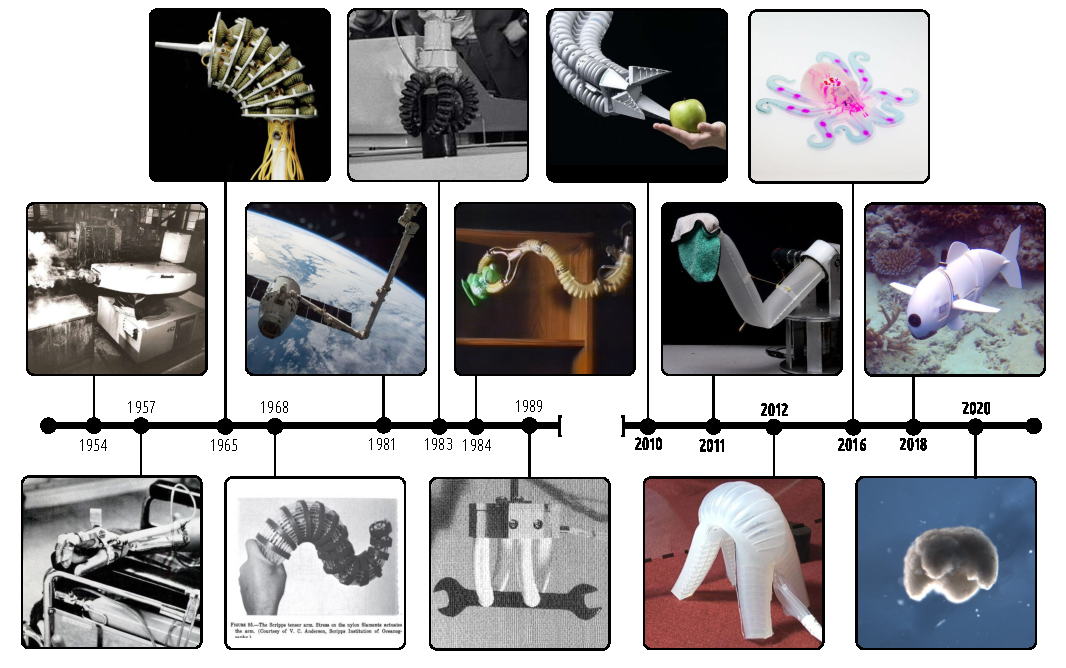
\includegraphics[width=1.11\textwidth]{./pdf/thesis-figure-2-1.pdf}
\caption{A brief timeline of the state-of-the-art of bio-inspired robotics throughout human history. {(1954):} Unimate, the first industrial robot. 
{(1957):} McKibben actuator, an early soft actuator inspired by the human muscle used for rehabilitation purposes \cite{Mckibben}. 
{(1965):} The Orm, believed to be the first soft robotic system designed by  Scheinman and Leifer \cite{BibEntryOrm2019Sep}. 
(1968): Tensor Scripps arm developed by Anderson \cite{Anderson1968}.
{(1981):} Canadarm-1, early flexible robotics employed on the International Space Station. 
{(1983):} Robot Arm with Pneumatic Gripper by Teleshev \cite{Teleshev1981}.
{(1984):} Bellows robotic arm by Wilson et al. \cite{Wilson2007}.
{(1989):} The soft robotic gripper developed by Suzumori et al. \cite{Suzumori1991,Suzumori1992}, seen as one of the earliest {academic} soft robot, developed before the word \emph{"soft robot"} existed. 
{(2010):} Festo's Bionic arm inspired by the elephant's trunk \cite{Grzesiak2011}. 
{(2011):} Soft inflatable robot arm by Sanan and Atkeson \cite{Sanan2013,BibEntryBH62022Sep}.
(2012) Multi-gait soft robot capable of terrestial locomotion \cite{Choi2011}. 
(2016): Octobot, the first autonomous 3D-printed soft robot that explores a stabilizing oscillator chemical network that produces preprogrammed repetitive motion \cite{Wehner2016}.
(2018): Autonomous robotic fish made by Katzschmann \cite{Katzschmann2018}.
(2020): Xenobot, an organic soft robot composed of skin and muscle cells made by Blackiston and Kriegman \cite{Kriegman2019}.
}
\label{fig:C0:timeline}
\end{figure}
\clearpage
}

\section{Early soft robotic technology}
In this chapter, we will present a short historical overview of soft robotics. Hereby showing that the current trends of bio-mimicry and elasticity in robotics find roots in a periods way before the soft robotic boom in the early 2010's. To guide the reader, in Figure \ref{fig:C0:timeline}, we provide a graphical, historic overview of soft robotic systems from 1950 to 2023. We will discuss the inception of soft actuation, early soft robotic designs, and modeling and control strategies for these continuum robotics.

To relate the historical progress of soft robots with respect to rigid robots, let us begin with early rigid robots. In 1954, George Devol filed a patent describing an autonomous robotic machine that could be preprogrammed to execute step-by-step motions \cite{Mickle2008}. The machine was designed to reduce the workload on the manufacturing work floor, with a major focus on mimicking repetitive (exhausting) human labor. In 1958, those prototypes led to a robotic system under the name \emph{Unimate}. An illustration of this early rigid robot is shown in Figure \ref{fig:C0:timeline}. The Unimate was used for manipulating metal die-casts and welding them to the main body of automobiles, revolutionizing the car industry shortly after. Victor Scheinman created the Stanford Arm in 1969 \cite{BibEntryStanford2022Sep,BibEntryOrm2019Sep}, which is recognized as the first electronic computer-controlled robotic arm because the Unimate's instructions (\ie, predefined set-points in joint space) were prerecorded on a magnetic drum. Later, in 1972, he developed the well-known PUMA robot (video available at \cite{BibEntryPuma2022Sep}), which was the successor to the Unimate. It is important to keep Scheinman in mind as he ultimately ties to early soft robots. \vspace{0.085em}

\afterpage{
\begin{figure}[!t]
  \vspace{-0.6mm}
  %%!TEX root = ../../thesis.tex
%%%% CHAPTER 1 *****************************************************************
\chapter[Dynamic modeling of Soft Robots -- PCC case]{Dynamic modeling -- The Piece-wise Constant Approach}
\label{chap: chapter 1}

\blankfootnote{This chapter is based on:\\ .\disclaimer}

%%%% ABSTRACT ******************************************************************
%!TEX root = ../../thesis.tex
\chapterabstract{The motion complexity and use of exotic materials in soft robotics call for accurate and computationally efficient models intended for control. To reduce the gap between material and control-oriented research, we build upon the existing Piecewise-Constant Curvature framework by incorporating hyper-elastic and visco-elastic material behavior. In this work, the continuum dynamics of the soft robot are derived through the differential geometry of spatial curves, which are then related to Finite-Element data to capture the intrinsic geometric and material nonlinearities. To enable fast simulations, a reduced-order integration scheme is introduced to compute the dynamic Lagrangian matrices efficiently, which in turn allows for real-time (multi-link) models with sufficient numerical precision. By exploring the passivity and using the parametrization of the hyper-elastic model, we propose a passivity-based adaptive controller that enhances robustness towards material uncertainty and unmodeled dynamics -- slowly improving their estimates online. As a study case, a fully 3D-printed soft robot manipulator is developed, which shows good correspondence with the dynamic model under various conditions, e.g., natural oscillations, forced inputs, and under tip-loads. The solidity of the approach is demonstrated through extensive simulations, numerical benchmarks, and experimental validations.}


%%%% MAIN **********************************************************************
\section{Introduction} \label{sec: chap1 1_introduction}
%!TEX root = ../../thesis.tex
The field of soft robotics has attracted the interest of many researchers from different backgrounds. Soft robots use compliant and hyper-elastic materials, while the use of rigid materials is minimized. The introduction of soft materials into robotics greatly expanded the field of application for robotics. For example, due to their dexterity and environmental robustness, soft robots are often used in medical applications \cite{Polygerinos2015b, Yap2015, Asbeck2015}, adaptive grasping \cite{Galloway2016, Hughes2016}, and locomotion in uncertain environments \cite{Drotman2017}. Unlike its rigid counterpart, soft robots undergo large continuum-bodied motion that, to some extent, resembles morphologies found in nature. These morphologies arise by virtue of the low compliance in soft materials and, more importantly, the structural layout of the soft robot. As of today, many of the fundamental engineering principles in rigid robotics, like design, actuation, sensing, and control, are often not applicable to soft robotics systems. Since its inception, most of these engineering problems have remained challenging or unresolved.

Although the diversity in soft robotics is significant, ranging from adaptive grippers to soft manipulators, most topologies in soft robotics can be associated with nature or engineered geometries for minimal compliance (e.g., bellow shapes). Soft robots often mimic living creatures and their morphologies, e.g., the tentacle of an octopus \cite{Galloway2016, Wehner2016}, or the trunk of an elephant \cite{Drotman2017}. Hypothetically, the abundance of bio-mimicry in soft robotics might be associated with the design complexity of developing robots from soft materials. The large number of degrees-of-freedom and exotic mechanical nature of soft robots makes design significantly challenging, and consequently, the design process can be iterative and time-consuming \cite{Wehner2016}. Therefore, it becomes potentially advantageous to use computational tools that assist or develop appropriate soft robotic topologies given a set of user-defined requirements, like desired motion or force.

In the past, researchers have made efforts to finding morphologies through mathematics, in particular through evolutionary algorithms. The concept of automated creature designs was first introduced by Sims \cite{Sims1994}, who showed that, given a set of basic geometries, locomotive organisms could be generated from evolutionary algorithms. These virtual organisms resembled biological morphologies to some extent; however, the complexity of the material layout was limited. More recent work involving the synthesis of virtual soft robots includes Cheney et al. \cite{Cheney2013}, who successfully produced intricate locomotive morphologies using artificial neural networks and multi-material parameter spaces of active and passive soft voxels. Other work involving morphological synthesis includes \cite{Bern2019, Morzadec2019,Diepen2019}. Unfortunately, the synthesis of morphologies from previous approaches, though novel, remains only in ideal simulated environments. An accurate representation of the nonlinear material properties in soft robotics can be challenging, and in favor of computational efficiency, little detail is spent on the nonlinear nature governing soft materials. Besides, these evolutionary frameworks typically involve a network of `activation' cells or voxels that perform ideal volumetric deformation, biologically resembling muscle functionality while unfortunately lacking resemblance to conventional actuation in soft robotics, e.g., pneumatics, dielectrics, and smart metal alloys (SMA).

Reviewing previous methods, a more efficient approach for solving the optimal morphology might be founded in topology optimization. Topology optimization is the general formulation of a material distribution problem for mechanical solids, where density-based topologies arise throughout an iterative (non-convex) optimization procedure. The synthesis of compliant mechanisms through topology optimization is investigated thoroughly \cite{Sigmund2015, Gain2013, Luo2015}; however, its application to soft robotics is relatively unexplored \cite{Zhang2018,Zolfagharian2019}. Yet, to obtain meaningful topologies for soft robotics, two problems need to be addressed. Since soft robots undergo large deformations, it becomes necessary to describe the nonlinear geometrical deformations accurately. Inherent to significant deformation of soft materials is the importance of nonlinear material behavior, like hyperelasticity. Another concern is the design-dependency of the external forces, in our case, the pneumatic loads. This class of structural problems is more challenging than traditional problems since the load is continuously interacting with the adaptive interface during the iterative optimization process \cite{Wang2016, Vasista2013}. It should be mentioned that the use of compressed air or pressurized fluid is a popular actuation approach in soft robotics.

In this work, we present a novel framework for generating topologies of soft robotics. Contrary to biometry or convectional designs, finding the (optimal) material layout of the soft robot is accomplished through a gradient-based nonlinear topology optimization, where the distribution of soft materials is optimized given a user-defined objective. Our main contributions include the description of nonlinear geometrical deformation and pneumatic loading. We exploit the connectivity properties in polygonal meshes such that synchronized volumetric contraction or expansion of a group of polygonal elements can artificially mimic the geometrical loads in pneumatic actuation. The advantages of our framework in comparison to other literature are: ($i$) a better representation of pneumatic actuation in soft robotics; ($ii$) improved design convergence in contrast to evolution-based optimization methods. To our knowledge, our approach of pressure-driven nonlinear topology optimization is new for soft robotics, and its application could easily extend to other soft robotic systems. %The computational framework detailed in this work is made publicly available at \cite{Caasenbrood2019}.

The remainder of the paper is structured as follows. In section \ref{chap:fem}, we will discuss the continuum mechanics for hyper-elastic materials, followed by a description of the optimization scheme for soft robotics. In section \ref{chap:results}, we propose a numerical example for developing a soft robotic structure to illustrate the effectiveness of our approach.


\newpage
\section{Continuum dynamic model}  \label{sec: chap2 section header}
%!TEX root = ../../thesis.tex
As mentioned previously, soft robots are composed of soft bodies that may be regarded as a continuum body with (theoretically) infinitely many degrees-of-freedom (DOF). In this section, we aim to derive a compact and computationally efficient model that envelops the continuous dynamics of a soft robot through a small set of generalized coordinates $\q\in\Q$ and their respective generalized velocities \highlight{$\dq(t)\in T_{\q}\Q$} with $n$ the number of active joint variables. We base {the modeling framework on the work of Mochiyama et al.\cite{Mochiyama2003} who outlined a theoretical foundation for continuum manipulators. Their work is extended upon by including extensibility, serial-chaining of multiple soft-links, pneumatic actuation, and the introduction of nonlinear and time-dependent material behavior. Earlier modeling strategies addressing similar issues can be found in from Godage et al. \cite{Godage2015,Godage2016}, Della Santina et al. \cite{Santina2020,Santina2020b,Santina2020Pcc}, Renda et al. \cite{Renda2018}, and Boyer et al. \cite{Boyer2021}. Leveraging from the aforementioned works, the continuous dynamics of a soft robot manipulator can be written in the familiar Lagrangian form:
%
\begin{equation}
\MB(\q) \ddq + \vec{h}(\q,\dq) = \Qnc,
\end{equation}
%
where $\MB(\q)  \in \R^\nn$ denotes the generalized inertia matrix, $\vec{h}(\q,\dq) \in \R^n$ a vector of nonlinear state-dependent force contributions. In this work, a similar modeling framework is adopted; however, we propose an extension to incorporate FEM-driven data to more accurately reflect the underlying continuum mechanics -- in particular hyper-elasticity; and we propose a numerical scheme that allows for fast computation of the continuous dynamics. For completeness, we will recapitulate on the modeling approach here.

\subsection{Kinematics of elastic continuum bodies}
\noindent To represent the hyper-flexible configuration of the soft robot, let us consider a smooth spatial curve that passes through the geometric center of the continuously deformable body, as shown in Figure \ref{fig:configuration}. {In literature, this curve is called} the '\textit{backbone curve}' as it simplifies the three-dimensional deformation imposed by distributed forces acting on the elastic body. The arc-length of the backbone corresponds to the extensible length of the soft robot denoted by the variable $l(t) \in [l_{-},l_{+}]$ which we assume bounded $l_{+} \ge l \ge l_{-}$, and let $L$ be a constant denoting the {total unstressed} length of the soft robot. Next, let us introduce a spatial variable
$\sigma \in \Xs$ that belongs to the one-dimensional material domain of the backbone curve, i.e., $\Xs = [0,\, L]$. {Let it be clear that the spatial variable $\sigma$ represents the arc-length of a material coordinate along the undeformed material domain of the soft robot manipulator.}

\commentary{}{Figure here of smooth curve for p and Phi}

Given each material coordinate, we wish to find a suitable low-dimensional joint representation $q(t)$ such that the position vector $^0p$ anywhere on the continuous backbone can be written as a mapping from generalized coordinates and space into $\mathbb{R}^3$:
%
\begin{equation}
^0\pB: \Xs \times \Q(t) \to \R^3;
\end{equation}
%
and similarly the rotation matrix $^0\mat{\Phi}(\sigma,\vec{q})$ by a mapping from the generalized coordinates and space into $\SO{3}$:
%
\begin{equation}
^0\PhiB: \Xs \times \Q(t) \to \SO{3}, \label{eq:phi_map}
\end{equation}
%
where {$\SO{3}$ denotes the special orthogonal group for rotations about the origin of $\R^3$}, and $n = \dim(\vec{q})$ the state dimension. Under this notion, the position vectors $^0p(q,0)$ and {$^0\pB(L,\q)$} relate to the base and the end-effector of the soft robot, respectively. {Please note that left-sided superscript are used to indicate the frame of reference.} The set of all points on the backbone $\mathcal{P} = \left\{^0\pB \in \R^3\, |\, \sigma \in \Xs \right\}$ draws a possible {spatial} configuration of the soft robot given {a time instance $t \in \mathbb{T}$ on a finite horizon $\mathbb{T} = [0,T]$}.
%
\begin{intermez}
Despite the inherent flexibility in soft robotics, it is sometimes sufficient to express the kinematics according to the Piecewise Constant Curvature (PCC) condition. Mathematically, it implies that the curvature of the continuous body satisfies $\kappa(q,\sigma_1) = \kappa(q,\sigma_2)$ for a neighboring region of points $\sigma_1,\sigma_2 \subseteq \Xs$. As a result, this condition allows us to describe the full forward kinematics with a significantly reduced set of generalized coordinates, mitigating kinematic complexity in the model. Numerous works employ PCC models \cite{Falkenhahn2015,Katzschmann2019,Tatlicioglu2007,Marchese2016,Godage2016,Santina2020Pcc}, and depending on the degrees of elasticity, the PCC condition has been proven to be consistent for various soft robotic systems.
\end{intermez}
%
{Following this Piecewise Constant Curvature (PCC) description, let us assign a coordinate frame that twists minimally along the backbone -- a Bishop frame \cite{Bishop1975}-- parametrized by the following generalized coordinate vector:}
%
\begin{equation}
\vec{q} = \begin{pmatrix}
\,\varepsilon & \kappa_x & \kappa_y\,
\end{pmatrix}^\top \in \mathcal{Q},
\label{eq:coordinate}
\end{equation}
%
\noindent where {$\varepsilon \in \R$ is the elongation strain}, and $\kappa_x,\,\kappa_y\in\mathbb{R}$ are the curvatures or angular strains in $x$-$z$ and $y$-$z$ plane, respectively; and $\mathcal{Q} \subset \R^3$ is an admissible space on which $q$ evolves.It is worth mentioning that the joint description above is somewhat related to Renda. et al. \cite{Renda2018} who proposed a Piece-wise Constant Strain (PCS) parametrization with the exception of including the twist along the tangent.

By exploring the differential geometry of the smooth backbone curve similar to Mochiyama et al.\cite{Mochiyama2003}, we can express the spatial change of the position vector $^0 \vec{p}(0,\vec{q})$ and the orientation matrix $^0\mat{\Phi}(q,\sigma)$ for each material point $\sigma$ along the smooth backbone by
%
\begin{align}
\renewcommand*{\arraystretch}{2}{}
\frac{\partial \,^0\!\mat{\Phi}}{\partial \sigma}(\sigma,\vec{q}) & = \, ^0\mat{\Phi}(\sigma,\vec{q})\,\left[\mat{\Gamma} (\sigma,\vec{q}) \right]_{\times}, \label{eq:change_phi} \\
\frac{\partial \,^0\! \vec{p}}{\partial \sigma}(\sigma,\vec{q}) & = \, ^0\mat{\Phi}(\vec{q},\sigma) \, \vec{U}(\sigma,\vec{q}), \label{eq:change_p}
\end{align}
%
where $[\vec{\Gamma}]_\times \in \So{3}$ is a skew-symmetric matrix composed of the entries of the vector $\vec{\Gamma} \in \R^3$, and $\vec{U}\in \R^3$ a vector representing the tangent along the extensible backbone. The vectors $\vec{\Gamma}$ and $\vec{U}$ are vectors that define the differential geometry of the backbone, which are unique entries that lives in the tangent space of the rigid-body transformation group $\SE{3}$. Given the Bishop parametrization as described by \eqref{eq:coordinate}, these geometric entities yield
%
\begin{equation}
\vec{\Gamma} = \begin{pmatrix} -\kappa_y \\ \kappa_x \\ 0  \end{pmatrix}; \quad \quad \quad \vec{U} = \begin{pmatrix} \,\, 0 \,\, \\ \,\, 0 \,\, \\ \, \,\varepsilon \,\, \end{pmatrix} + \vec{U}_0,
\end{equation}
%
with $\vec{U}_0 = (0,0,1)^\top$ the unit-tangent. Now, given an initial configuration of backbone's base, i.e., $^0 \mat{\Phi}(0,\vec{q}) = \vec{\Phi}_0$ and $^0 \vec{p}(0,\vec{q}) = 0_3$, we can now solve for the position and orientation for each material coordinate $\sigma$ along the backbone:
%
\begin{align}
^0\mat{\Phi}(\sigma,\vec{q}) & = \vec{\Phi}_0\exp(\sigma [\vec{\Gamma}(\vec{q})]_\times), \label{eq:phi_exact} \\
^0\vec{p}(\sigma,\vec{q}) & = \int_0^\sigma\,^0\mat{\Phi}(\eta,\vec{q})\, \vec{U}(\vec{q}) \; d\eta, \label{eq:pos_vector}
\end{align}
%
where $\exp: \So{3} \to \SO{3}$ is the exponential map. Let it be clear that the closed-form solutions \eqref{eq:phi_exact} and \eqref{eq:pos_vector} form the forward configuration kinematics of the backbone curve. To express the forward velocity kinematic, let  $\vec{V}(\sigma,\vec{q},\dot{\vec{q}}) = \left(^\sigma \vec{\omega}^\top,^\sigma \vec{v}^\top \right)^\top \in \R^6 \cong \Se{3}
$ be the aggregate of the angular velocity and linear velocity components relative to an inertial frame at $\sigma$ (the frame of reference is denoted by a left superscript), where the space $\Se{3}$ denotes the Lie algebra of $\SE{3}$. The velocity twist is computed by the following integration procedure:
%
\begin{equation}
 \vec{V}(\sigma,\vec{q},\dot{\vec{q}}) = \Ad_{\mat{g}(\sigma,\cdot)}\inv \int_0^\sigma \Ad_{\mat{g}(\eta,\cdot)}\, J^*\! \dot{q}\;d\eta
 \,=:\, J(q,\sigma) \dot{q}, \label{eq:vel_cont}
\end{equation}
%
where $\Ad_g: \SE{3} \to \mathbb{R}^{6\times 6}$ denotes the adjoint transformation matrix regarding the rigid body transformation $g \in \SE{3}$ that maps local velocities (i.e., twist) to a frame located at $\sigma$, and $J^*$ a constant joint-axis matrix. The joint-axis matrix for an extensible and bendable PCC segment parametrized by the Bishop parameters is given by
%
\begin{equation}
\renewcommand*{\arraystretch}{1}{}
J^* := \left(\dfrac{\p \Gamma}{\p q}^\top \; \dfrac{\p U}{\p q}^\top \right)^\top  = \begin{pmatrix}
\,0 & 0 & 0 & 0 & 0 & 1 \, \\
\,0 & 1 & 0 & 0 & 0 & 0 \,  \\
\,-1 & 0 & 0 & 0 & 0 & 0 \,  \\
\end{pmatrix}^\top. \label{eq:joint-axis-matrix}
\end{equation}
%
Although we based the forward kinematics on the work of Mochiyama et al.\cite{Mochiyama2003}, the derived expression for the velocity twist in \eqref{eq:vel_cont} is analogous to the work of Renda et al.\cite{Renda2018,Renda2020}, and Boyer et al. \cite{Boyer2010,Boyer2021}. Please also note that \eqref{eq:vel_cont} gives rise to the geometric manipulator Jacobian $J(q,\sigma)
$ that defines the mapping from joint velocities to the velocity twist for a particular material point $\sigma$ on the continuous body. In continuation, let us also introduce the acceleration twist\cite{Boyer2021,Mochiyama2003,Renda2018} -- obtained through time differentiation of \eqref{eq:vel_cont}:
%
\begin{align}
\dot{V}(q,\dot{q},\ddot{q},\sigma) & = J \ddot{q} + \Ad_{g(\cdot,\sigma)} \inv \int_0^\sigma \Ad_{g(\cdot,\eta)}
\ad_{V(\cdot,\eta)} \, J^*\! \dot{q}\;d\eta \notag \\
& := J(q,\sigma)\ddot{q} + \dot{J}(q,\dot{q},\sigma) \dot{q},
\label{eq:acceleration}
\end{align}
%
where $\ad_{V} \in \mathbb{R}^{6\times 6}$ denotes the adjoint transformation regarding the velocity twist $V \in \Se{3}$. The reader is referred to Appendix A for more detailed expressions on the adjoint transformations.
%
\subsection{Euler-Lagrange equations}
\noindent Given the forward kinematics in \eqref{eq:phi_exact}, \eqref{eq:pos_vector}, \eqref{eq:vel_cont} and \eqref{eq:acceleration}, we can shift our attention to formulating the finite-dimensional dynamics of the soft robot. Our goal here is to write the spatio-temporal dynamics of the hyper-elastic soft robot as a second-order ODE into the Lagrangian form:
%
\begin{equation}
\frac{d}{d t}\left(\frac{\partial \mathcal{L}}{\partial \dot{{q}}}\right) - \frac{\partial \mathcal{L}}{\partial {q}} = {Q}^{\nc}, \label{eq:euler_largrange}
\end{equation}
%
\noindent where $\La({q},\dot{q}) := \T(q,\dot{q}) - \mathcal{U}(q)$ is the Lagrangian function, $\T \in \Rp$ and $\mathcal{U}\in \R$ the kinetic and potential energy, respectively; and $Q^{\nc} \in \mathbb{R}^n$ a vector of generalized non-conservative forces. To apply the Lagrangian formalism to a continuum dynamical system, regard an infinitesimal slice of the continuum body for each material coordinate $\sigma$ along the backbone curve. Given this notion, we embody this infinitesimal slice with an inertia tensor $
\mathcal{M} = \text{blkdiag}(\rho I_3,\mathcal{J_\sigma})$ with $\rho = m/L$ the line-density and $J_\sigma$ a tensor for the second moment of inertia. The kinetic energy can be obtained through spatial integration of its respective kinetic energy densities\cite{Boyer2010,Mochiyama2003,Tatlicioglu2007}, i.e., $\mathfrak{T} = \frac{1}{2}V^\top \mathcal{M} V
$:
%
\begin{align}
\mathcal{T}({q},\dot{{q}}) & = \frac{1}{2}\int_\Xs {V}({q},\dot{q},\sigma)^\top\,\mathcal{M}\,{V}({q},\dot{{q}},\sigma) \; d \sigma,
 \notag \\
& =  \frac{1}{2} \dot{q}^\top \int_\Xs  J({q},\sigma)^\top\,\mathcal{M}\, J({q},\sigma) \; d \sigma \, \dot{q}, \notag \\
& = \frac{1}{2}\dot{q}^\top M(q) \dot{q}. \label{eq:kinetic_energy}
\end{align}
%
Note that expression for the kinetic energy naturally gives rise to the generalized inertia matrix $M(q)$ of the Lagrangian model. By substitution of the kinetic energy into the Euler-Lagrange equation \eqref{eq:euler_largrange}, we find $M(q)\ddot{q} + C(q,\dot{q})q$ where $C(q,\dot{q})$ denotes the Coriolis matrix. Instead of computing the Coriolis matrix through the conventional Christoffel symbols\cite{Murray1994}, we adopt a computational scheme by Garofalo et al. \cite{Garofalo2013} used for serial-chain rigid manipulators, in which we replaced the finite summation of $N$ rigid-bodies by a spatial integration over the continuum domain $\Xs$:
%
\begin{equation}
C(q,\dot{q}) = \int_\Xs J(q,\sigma)^\top \Ct_{V(q,\dot{q},\sigma)}J(q,\sigma)\; + J(q,\sigma)^\top \Mt \dot{J}(q,\dot{q},\sigma) \; d \sigma,\label{eq:coriolis}
\end{equation}
%
where $\Ct_{V} = -\Ct_{V}^\top :=  \mathcal{M} \ad_{V}  - \ad_{V} ^\top \mathcal{M}$ is a skew-symmetric matrix. The computation above is slight different from existing literature\cite{Boyer2021,Renda2020} to ensure that the matrix $\dot{M} - 2C$ is skew-symmetric; the so-called the passivity condition\cite{Murray1994} for Euler-Lagrange systems (see Appendix B for proof). The importance of this property will become apparent later in the energy-based controller design. Lastly, the potential energy is given by sum of gravitational potential energy and internal elastic potential, i.e., $\mathcal{U}({q}) = \mathcal{U}_g({q}) + \mathcal{U}_e({q})
$. Since gravitational potential energy density is \rewritten{given} by $\mathfrak{U}_g = -\rho\,^0p(q,\sigma) \gamma_g$ with $\gamma_g \in \R^3$ is a vector of body accelerations, the potential energy related to gravity is obtained by spatial integration of their respective energy densities:
%
\begin{equation}
\mathcal{U}_g({q}) = - \rho \int_\Xs \,^0p(q,\sigma)^\top \gamma_g \; d \sigma.
\label{eq:potential_energy_grav}
\end{equation}
%
\noindent To model the hyper-elastic nature, lets introduce two nonlinear stiffness functions for both stretching and bending, denoted by $k_e: \R \mapsto \Rsp$ and $k_b: \R \mapsto \Rsp$, respectively. These functions allow us to describe a collective elastic behavior imposed by the hyper-elastic materials and the continuum-bodied deformation. It shall be clear that these entities are unique to the soft robot's geometry and soft material choice, and thus finding a suitable candidate model requires further analysis. Later, we will sculpt these nonlinear stiffness functions through Finite Element Methods (FEM). For now, we assume that these analytical nonlinear stiffness functions are known, and thus the (hyper)-elastic potential energy takes the form
%
\begin{equation}
\mathcal{U}_e({q}) = \int_0^{\varepsilon} k_e(\eta) \,\eta \; d \eta + \int_0^{\beta(q)} k_b(\eta)\, \eta \; d \eta,
\label{eq:potential_energy_elas}
\end{equation}
%
where $\varepsilon$ is the elongation strain, and $\beta({q}) = \kappa L (\varepsilon + 1)$ is the bending angle with the total curvature of the soft segment $\kappa = \sqrt{{\kappa_x}^2 + {\kappa_y}^2}$ (see Figure \ref{fig:configuration}).
\subsection*{Overall dynamics}
\noindent Finally, by combining \eqref{eq:euler_largrange}, \eqref{eq:kinetic_energy}, \eqref{eq:coriolis}, \eqref{eq:potential_energy_grav}, and \eqref{eq:potential_energy_elas}, the continuum dynamics of the soft robot can be casted into the familiar closed form \cite{Santina2020Pcc,Boyer2021,Renda2018,Godage2016} similar to aforementioned model (1):
%
\begin{align}
M({q})\,\ddot{{q}} + {C}({q},\dot{{q}})\,\dot{{q}} + P({q},\dot{q}) + G({q}) & = \tau(u,\delta), \label{eq:dynamic_model}
\end{align}
%
\noindent where $P = d \mathcal{U}_e/d q + R\dot{q}$ is a vector of generalized forces imposed by the deformation of the soft materials with $R \in \R^{n\times n}$ the Rayleigh damping matrix, $G = \p \mathcal{U}_g/\p q$ a vector of generalized gravitational forces, and $u \in \R^m$ the control input with the index $m$ the number of pressure inputs. The generalized input vector is chosen of the form: $\tau(u,\delta) = H u + \delta$ with $H: \R^m \mapsto \R^n$ a mapping from the input space to the joint actuation space, and $\delta(t)$ an external disturbance (e.g., unmodelled material uncertainties).
%
\begin{rmk}
Given the context of manipulators, a possible disturbance $\delta(t)$ could be an external mass applied to the tip of the soft robot. Given the kinematic relations in \eqref{eq:vel_cont} and \eqref{eq:acceleration}, one can describe the disturbance (modeled here as a point-mass located at $L$) by a state-dependent vector:
%
\begin{equation}
\delta_m = m_\delta \floor{J(\cdot,L)}_3^\top\left({\normalfont \Ad}_{g(\cdot,L)}\inv\gamma_g + \floor{\dot{V}(\cdot,L)}_3 \right),
\label{eq:delta_payload}
\end{equation}
%
where $\floor{\cdot}_3$ extracts the last three rows of a matrix or vector, and $m_\delta > 0$ the applied mass to the end-effector. It is worth recalling that the acceleration twist can be computed through the geometric Jacobian and its time derivative, i.e., $\dot{V} = J\ddot{q} + \dot{J}\dot{q}$. Indeed, the PCC condition for a soft body can only accurately describe the true dynamics if external forces produced by mass $m_\delta$ do not excessively exceed the intrinsic elastic balancing forces $P(q)$. Alternatively, a soft body can be modeled using multiple PCC curves of smaller size, similar to standard Finite Element discretization.
\end{rmk}

The actuation mapping $H$ depends on the geometry, placement, and orientation of the (pneumatic) soft actuators. Since the pneumatic chambers are aligned parallel to the backbone curve and are equally spaced along the circumference, we propose the following ansatz:
%
\begin{equation}
H: = \begin{pmatrix} \alpha_{\varepsilon} & \hdots & \alpha_{\varepsilon} \\ -\alpha_{\kappa} \cos(\phi_1) & \hdots & -\alpha_{\kappa} \cos(\phi_m) \\ \alpha_{\kappa} \sin(\phi_1) & \hdots & \alpha_{\kappa} \sin(\phi_m) \end{pmatrix},
\label{eq:mapping_H}
\end{equation}
%
where $\alpha_{\varepsilon},\alpha_{\kappa} > 0$ are system parameters representing the effective transferal of differential pressure to joint forces, and $\phi_i = (i-1)\cdot\tfrac{2\pi}{m}$ the angular inter-distance between the $m$-number of pneumatic bellows. Please note that the parameters $\alpha_{\varepsilon}$ and $\alpha_{\kappa}$ are dependent on the bellow area and radius from the bellow to the backbone curve.
%


\newpage
\section{Extension to multi-link dynamics}  \label{sec: chap2 section header}
%!TEX root = ../../thesis.tex
\noindent We previously expressed the position and velocity kinematics as explicit functions of the generalized coordinates (i.e., Bishop parameters) and their time-derivatives. This explicit dependency stems from the PCC conditions inferring the curvature is non-varying along the spatial domain $\Xs$, i.e., $\kappa(q,\sigma) = \kappa(q)$. Although sufficient for some cases, the condition is generally restrictive, and to some extent inconvenient, since the inclusion of multiple links demands piece-wise integration of the kinematics \eqref{eq:pos_vector}, \eqref{eq:phi_exact}, \eqref{eq:vel_cont}, and \eqref{eq:acceleration}. Rather than separation of integration, we can extend this PCC description by using piece-wise continuous spatial function to distinguishes multiple soft-bodied links along the continuous body of the soft robot. The idea of parametrization through shapes functions has been explored earlier by Chirikjian et al.\cite{Chirikjian1994,Chirikjian1992}, and later by Boyer et al. \cite{Boyer2021}, Della Santina et al. \cite{Santina2020b}. A similar discontinuous shape function series was used by Berthet-Rayne et al. \cite{Berthet2021} to pursue multi-body dynamics for growing continuum robots; and proposed by Chirikjian \cite{Chirikjian1992} for hyper-redundant robots earlier.

Following the aforementioned works, let us parameterize the the geometric vectors $\Gamma$ and $U$ for a $N$-link soft robot through the product of a basis of orthonormal functions $\!\{s_i\}_{i \in \N}$ and the Bishop parametrization as follows
%
\begin{align} \Gamma(q,\sigma) & = \sum^N_{i=1} s_i(\sigma) \ceil{J^*}_3
\,\tilde{q}_i, \label{eq:theta_extent} \\ U(q,\sigma) & = \sum^N_{i=1} s_i(\sigma)
\floor{J^*}_3\,\tilde{q}_i + U_0, \label{eq:h_extent} \end{align}
%
where $J^*$ is the joint-axis matrix as in \eqref{eq:adjoint_matrix}, the mathematical operators $\ceil{\cdot}_3$ and $\floor{\cdot}_3$  extract the first or last three rows of a matrix, respectively;  $\tilde{q}_i$ the joint variables of the $i$-th link, and $s_i: \Xs \mapsto \{0,1\}$ is a piece-wise continuous shape function, whose purpose is to be non-zero for a given interval on $\Xs$.
The new generalized coordinate vector becomes the aggregate of all joint variables of the multi-body soft robotic system $q =  \left(\tilde{q}_1^\top,\,\tilde{q}_2^\top,...,\,\tilde{q}_N^\top \right)^\top$ with the vector $\tilde{q}_i = (\varepsilon_{i},\, \kappa_{x,i},\,\kappa_{y,i})^\top$ relating to the Bishop parametrization of the $i$th-link. Given \eqref{eq:theta_extent} and \eqref{eq:h_extent}, we may now rewrite the velocity-twist as
%
\begin{equation} V(q,\dot{q},\sigma) = \Ad_g^{-1}
\int_0^\sigma \Ad_g J^* S(\sigma) \; d\sigma \dot{q} := J(q,\sigma) \dot{q}
\label{eq:vel_vec_dis} \end{equation}
%
where $S = (s_1,\,s_2,\,...,s_N) \otimes I_n$ is an unitary selection matrix derived from the basis of piece-wise continuous shape functions $\!\{s_i\}_{i=1}^N$. To be less ambiguous about this selection matrix $S$, lets consider a spatial coordinate $\sigma_2 \in [L_1,L_1+L_2]$ that lies on the spatial interval of the second link. Consequently, the operation $S(\sigma_2) {q} = {\tilde{q}}_2$ returns the corresponding joint variable of the second link. This selection of
generalized coordinates follows analogously for other links along the serial-chain of the soft manipulator. We provided a small library of piece-wise continuous shape functions upto $1 \le N \le 8$ links under \texttt{./src/pwf} on the open repository\cite{Caasenbrood2021}.
Now, substitution of the discontinuous variation of the geometric Jacobian in \eqref{eq:vel_vec_dis} into \eqref{eq:kinetic_energy} leads to the dynamic model of a $N$-link soft robot manipulator in the
Lagrangian form similar to \eqref{eq:dynamic_model}.


\section{Efficient solver of the soft robotic dynamics through Matrix-Differential Equations}  \label{sec: chap2 section header}
%!TEX root = ../../thesis.tex
Due to the partial differential nature of soft robots, obtaining a closed-form expression for the projected Lagrangian model in \eqref{eq:dynamic_model} can become notoriously long and complex (especially for multi-link systems). The origin of this problem stems from the integrands of inertia matrix $M(q)$ in \eqref{eq:kinetic_energy} and Coriolis forces $C(q,\dot{q})$ in \eqref{eq:coriolis}; which become highly nonlinear and therefore difficult to calculate a-priori. As a result, solving the forward dynamics using traditional solvers often deteriorates the real-time performance, and in turn its usability for closed-loop control. Inspired by Boyer et al. \cite{Boyer2021} and Godage et al \cite{Godage2016}, instead of finding an exact solution to the dynamic entries $M(q)$, $C(q,\dot{q})$ and $G(q)$, let us introduce a similar reduced-order integration scheme that produces an approximate of the dynamic model \eqref{eq:dynamic_model}. Yet, instead of using an inverse Newton-Euler algorithm (i.e., Featherstone or Hollerbach scheme) in which the Lagrangian entries are built column-wise, we propose an explicit integration scheme that efficiently computes all Lagrangian entities in parallel through a so-called Matrix-Differential Equation (MDE).

The idea here is to replace all necessary spatial integrations for the computation of the Lagrangian entities by an equivalent Matrix-Differential Equation of the form:
%
\begin{equation}
\frac{\p Z}{\p \sigma} = F(Z,\sigma), \label{eq:MDE}
\end{equation}
%
where $Z(\cdot,\sigma)$ is a matrix-valued function composed of the necessary elements for the forward kinematics and forward dynamics, and $F(Z,\sigma)$ a matrix-valued flow function that describes the spatial evolution of $Z$. Then, by choosing the appropriate initial condition for $Z(\cdot,0) = Z_0$ and numerically solving \eqref{eq:MDE} over a finite horizon $\Xs$, we can retrieve an approximate of the Lagrangian model in \eqref{eq:dynamic_model} by extracting the necessary elements from the solution $Z(\cdot,L)$.

Before describing the MDE, let us first introduce two intermediate matrices related to the computation of the manipulator Jacobian and its time-derivative, namely:
%
\begin{align}
\frac{\p B_1}{\p \sigma} & = \Ad_{g(\cdot,\sigma)}\, J^* S(\sigma), \\
\frac{\p B_2}{\p \sigma} & = \Ad_{g(\cdot,\sigma)}\ad_{V(\cdot,\sigma)}\, J^* S(\sigma)
\end{align}
%
such that they satisfy $J\dot{q} = \Ad_g\inv B_1 \dot{q}$ and $ \dot{J} \dot{q} = \Ad_g\inv B_2 \dot{q}$. Given the expressions above, we can now include a partial computation Jacobians into the MDE. By collecting all the differential relation for the forward kinematics (5), (6) and forward dynamics (14), (15), and (16), we can assign a flow function $F:= \text{blkdiag}\left(F_1,F_2 \right)$ composed of two matrices:
%
\begin{align}
F_1 & = \begin{pmatrix}
\begin{matrix}
^0 \Phi [\Gamma]_\times & ^0 \Phi U \\ 0_{3\times3} & 0_3
\end{matrix} \, \vrule & \Ad_g J^*S &\vrule\;\; \Ad_g \ad_{V} J^* S
 \end{pmatrix}, \\
F_2 & = \begin{pmatrix}
\frac{\p M}{\p \sigma} & \frac{\p C}{\p \sigma} & \frac{\p G}{\p \sigma}  \end{pmatrix},
\end{align}
%s
in which the differential form of the dynamic entities $M(q)$, $C(q,\dot{q})$, and $G(q)$ of the Lagrangian model are given by
%
\begin{align}
\frac{\p M}{\p \sigma} & = (\Ad_{g}\inv B_1)^\top \mathcal{M} (\Ad_{g}\inv B_1), \\[0.4em]
\frac{\p C}{\p \sigma} & = (\Ad_{g}\inv B_1)^\top \left[\mathcal{C}_V (\Ad_{g}\inv B_1) + \mathcal{M} (\Ad_{g}\inv B_2) \right], \\[0.4em]
\tfrac{\p G}{\p \sigma} & = (\floor{B_{1}}_3)^\top \rho \gamma_g,
\end{align}
%
We wish to stress that $F_1$ collects all elements related to the forward kinematics, whereas $F_2$ contains the dynamic entities related to the Lagrangian model. Following the spatial Matrix-Differential equation in \eqref{eq:MDE} above, its solution will be a matrix $Z := \text{blkdiag}\left( Z_1,Z_2 \right)$ composed of two smaller state matrices $Z_1$ and $Z_2$:
%
\begin{align}
Z_1 & := \begin{pmatrix}
\begin{matrix}
^0 \Phi  & ^0 p \\ 0_{3\times3} &  0_{3}
\end{matrix} \;\; \vrule & \!B_1 & \vrule & \!B_2 \;\;\;
 \end{pmatrix}, \\
Z_2 & := \begin{pmatrix} M & C & G \end{pmatrix},
\end{align}
%
Such a Matrix-Differential equation as in \eqref{eq:MDE} are not supported natively by standard ODE solvers. Therefore, an explicit second-order Runge-Kutta solver for MDEs is developed such that efficiently computes the evolution of the state matrix $Z$ along $\Xs$. The solver is written in \texttt{MATLAB} and can be found under \texttt{./src/Model.m} at Caasenbrood \cite{Caasenbrood2020}.

As for state trajectories along the temporal regime $\mathbb{T} = [0,T]$, an implicit trapezoidal integration scheme is proposed to solve the approximated continuum dynamics, which are generally less conservative on discretization to preserve numerical stability. Here implicit schemes are favored over explicit scheme, since a coarser time integration can significantly increase real-time performance. In addition, to further boost performance of the temporal integration, a cost-effective approximation of the Hessian is introduced. For more detail, see Appendix C for more detail.


%%%%%%%%%%%%%%%%%%%%%%%%%%%%%%%%%%%%%%%%%%%%%%%%%%%%%%%%%%%%%%%%%%%%%%%%%%%%%%%%

  \input{./fig/PAM.pdf_tex}
  \caption{Patent diagrams of pneumatic artificial muscle from 1953 till 1988. (a) Morin Muscle \cite{Morin1953}; (b) ROMAN muscle \cite{Immega1986}; (c) Yarlott muscle \cite{Yarlott1972}; (d) Kukolj muscle \cite{Kukolj1988}; (e) Paynter Hyperboloid \cite{Paynter1974}.
  \label{fig:C0:several_PAM}}
  \vspace{-1mm}
\end{figure}

\begin{figure}[!t]
%% This file was created by matlab2tikz.
%
%The latest updates can be retrieved from
%  http://www.mathworks.com/matlabcentral/fileexchange/22022-matlab2tikz-matlab2tikz
%where you can also make suggestions and rate matlab2tikz.
%
\definecolor{mycolor1}{rgb}{0.06275,0.35686,0.84706}%
\definecolor{mycolor2}{rgb}{0.86667,0.21176,0.10980}%
%
\begin{tikzpicture}

\begin{axis}[%
width=0.602\textwidth,
height=0.161\textwidth,
at={(0\textwidth,0.015\textwidth)},
scale only axis,
axis on top,
xmin=0.5,
xmax=2426.5,
tick align=outside,
y dir=reverse,
ymin=0.5,
ymax=650.5,
axis line style={draw=none},
ticks=none
]
\addplot [forget plot] graphics [xmin=0.5, xmax=2426.5, ymin=0.5, ymax=650.5] {./fig/fig_1_1-1.png};
\end{axis}

\begin{axis}[%
width=0.302\textwidth,
height=0.191\textwidth,
at={(0.648\textwidth,0\textwidth)},
scale only axis,
xmin=0,
xmax=1.5,
xlabel style={font=\color{white!15!black}},
xlabel={pressure (kPa)},
ymin=0,
ymax=35,
axis background/.style={fill=white},
xmajorgrids,
ymajorgrids,
legend style={at={(0.03,0.97)}, anchor=north west, legend columns=2, legend cell align=left, align=left, draw=white!15!black}
]
\addplot [color=mycolor1, line width=1.5pt]
  table[row sep=crcr]{%
0	0\\
0.00600149999999999	3.0568983103671\\
0.012003	5.35826739157104\\
0.024006	7.86017230302163\\
0.036009	9.05072762147565\\
0.0480119999999999	9.795136933107\\
0.0600149999999999	10.3164705929212\\
0.0720179999999999	10.711316657325\\
0.0840209999999999	11.0279129564825\\
0.0960239999999999	11.2925201532359\\
0.108027	11.5206742947192\\
0.1260315	11.8150953044601\\
0.144036	12.0694590939099\\
0.1620405	12.2959065095095\\
0.1860465	12.5672572998435\\
0.2100525	12.8138561366798\\
0.24006	13.0980192458931\\
0.276069	13.4149916949781\\
0.3180795	13.7633415653589\\
0.372093	14.1910487738014\\
0.456113999999999	14.8357726162343\\
0.588146999999999	15.8481229823956\\
0.660164999999999	16.4166289214781\\
0.726181499999999	16.9548047718235\\
0.786196499999999	17.4617841353458\\
0.840209999999999	17.9350495132933\\
0.894223499999999	18.4266813211065\\
0.948236999999999	18.9389704257632\\
0.996248999999999	19.413653689242\\
1.044261	19.9084481551956\\
1.092273	20.4253835409611\\
1.140285	20.9666992209241\\
1.1822955	21.4623032550621\\
1.224306	21.9803397018051\\
1.2663165	22.5228818415618\\
1.308327	23.0922527983715\\
1.3503375	23.6910711317645\\
1.392348	24.322306181775\\
1.43435850000001	24.9893459441392\\
1.47036750000001	25.5925254860443\\
1.4999985	26.11365092975\\
};
\addlegendentry{$\delta V$}

\addplot [color=mycolor2, line width=1.5pt]
  table[row sep=crcr]{%
0	0\\
0.00600149999999999	0.57694322540025\\
0.012003	1.8809393408942\\
0.0180045	2.95152432065056\\
0.024006	4.45583458122557\\
0.036009	6.19378149929854\\
0.0480119999999999	7.48539157943733\\
0.0600149999999999	8.4688855095399\\
0.0720179999999999	9.23690647886306\\
0.0840209999999999	9.85153659933535\\
0.0960239999999999	10.3531922792834\\
0.108027	10.7691384956111\\
0.12003	11.1184532554937\\
0.132033	11.4148904215117\\
0.144036	11.6686090629544\\
0.156039	11.8872685256996\\
0.168042	12.0767485361297\\
0.180045	12.2416363770546\\
0.192048	12.3855638977444\\
0.204051	12.511445089458\\
0.216054	12.6216464418373\\
0.228057	12.7181110468447\\
0.24006	12.8024503578201\\
0.252063	12.8760129819895\\
0.264066	12.9399369280069\\
0.276069	12.9951897701871\\
0.288072	13.0425998730449\\
0.300075	13.0828809209488\\
0.312078	13.1166513764424\\
0.324081	13.1444500557612\\
0.336084	13.1667487016037\\
0.348087	13.1839622118741\\
0.36009	13.1964570224759\\
0.372093	13.2045580243864\\
0.384096	13.2085543078992\\
0.3900975	13.2090949291082\\
};
\addlegendentry{$\delta\text{ \!\!L}$}

\addplot [color=mycolor2, dashed, line width=1.5pt, forget plot]
  table[row sep=crcr]{%
0.3900975	13.2090949291082\\
0.4021005	13.2074094834352\\
0.4141035	13.2022150575773\\
0.426106499999999	13.1937085356179\\
0.438109499999999	13.1820674082842\\
0.450112499999999	13.167452053111\\
0.462115499999999	13.1500076917316\\
0.480119999999999	13.1188216524309\\
0.498124499999999	13.0819593181423\\
0.516128999999999	13.0397643773147\\
0.534133499999999	12.9925364907466\\
0.552137999999999	12.940537547495\\
0.576143999999999	12.8641761270216\\
0.600149999999999	12.7802040746341\\
0.624155999999999	12.6890133020198\\
0.654163499999999	12.5653689878037\\
0.684170999999999	12.4314807991557\\
0.714178499999999	12.2877652488207\\
0.744185999999999	12.134547035545\\
0.780194999999999	11.9384837181762\\
0.816203999999999	11.7293863338915\\
0.852212999999999	11.5074325334682\\
0.888221999999999	11.2726938851784\\
0.924230999999999	11.0251466514001\\
0.960240000000001	10.7646794022534\\
1.0022505	10.4442081230322\\
1.044261	10.1054386868975\\
1.0862715	9.74777996411718\\
1.128282	9.3704926101939\\
1.1702925	8.97268281045118\\
1.212303	8.55329199813728\\
1.2543135	8.11108229372756\\
1.296324	7.64461717852633\\
1.3383345	7.15223665142942\\
1.380345	6.63202579865352\\
1.4223555	6.08177530074445\\
1.4583645	5.58429802632113\\
1.4943735	5.06103909220648\\
1.4999985	4.97621111560656\\
};
\end{axis}
\end{tikzpicture}%
\includegraphics*[width=\textwidth]{./pdf/thesis-figure-2-2.pdf}
\vspace{-3mm}
\caption{Working principle of a basic pneumatic artificial muscle (\ie, Morin muscle \cite{Morin1953}) with the internal volume \data{Matlab1} in \si{\milli \liter}, and the end-effector displacement \data{Matlab2} in \si{\milli \meter} and \dashdata{Matlab2} is the point at which the undesirable ballooning occurs.
\label{fig:C0:mckibben}}
\end{figure}
\vspace{-10mm}}

Nearly four years after the development of Unimate, Joseph McKibben created a linearly contractile pneumatic muscle-inspired actuator called the "\emph{McKibben actuator}". The McKibben muscle is a type of Pneumatic Artificial Muscle (PAM) that is still the most frequently used and published artificial muscle in literature. According to \cite{Mckibben}, he developed the McKibben actuators to help his daughter's polio-paralyzed hand move, grasp, and even write. The McKibben actuator is inspired by the human muscle and consists of an inflatable inner bladder enveloped with a double-helical weave. When pressurized, the fluidic actuator converts radial expansion into uni-axial contraction \cite{Daerden1999,Daerden2000,Schulte1961}. The weave inhibits extensive ballooning, which is undesired rapidly-accelerated volumetric expansion. Its material composition is often silicone rubber with a nylon-fiber exterior. A schematic representation of a general pneumatic muscle and the effect of ballooning are shown in Figure \ref{fig:C0:mckibben}. Ballooning is an often undesired nonlinear effect where the hyper-elastic pressure vessel exhibits strain-softening after a critical point is reached, resulting in further increase of pressure leading to exponential growth in volume, ultimately leading to actuator tearing. At stages of ballooning, mechanical performance significantly drops and even produces adverse effects, like actuation reversal. McKibben solved this problem through a combination of soft and inextensible fiber weaves. These inextensible fibers were placed at the exterior wall of the soft muscle, thereby limiting the radial expansion before ballooning could occur. According to Daerden \cite{Daerden1999}, there exist many variations of pneumatic muscles besides braided muscles, such as the netted muscles (e.g., Yarlott \cite{Yarlott1972}, ROMAC \cite{Immega1986}, and Kukolj \cite{Kukolj1988}) and embedded muscles (e.g., Morin \cite{Morin1953}, Paynter Hyperboloid \cite{Paynter1988}). Illustrations of their patent schematics are shown in Figure \ref{fig:C0:several_PAM}.

Pneumatic muscles are perhaps one of the first fundamental technologies that enabled soft robotics, and to this day, they remain a framework for many soft robotic systems. Nevertheless, besides the many examples of fluidics \cite{Marchese2014,Marchese2016,Katzschmann2018,Suzumori1991,Mosadegh2014}, there exist many other technologies employed in soft robotic motion, such as thermal \cite{Wu2021Dec} or chemical expansion/contraction \cite{Tolley2014,Bartlett2015,Wehner2016}, crystal re-alignment \cite{Pilz2020,Lopez2018,Vantomme2021,Polygerinos2013}, dielectric elastomers \cite{Keplinger2011}, magnetism \cite{Roh2019Apr,KimYoonho2018,McDonald2020,Boyvat2017Jul}, and naturally the use of tendons paired with electro-mechanical actuation \cite{Renda2018,Bern2019,Kim2020Jun,Coevoet2017Feb,Wang2016Sep}. Some of these technologies predate the invention of the McKibben actuator. For example, Dielectric Elastomer Actuators (DEA) developed by R\"{o}ntgen in 1880 \cite{Rontgen1880} are still a popular soft actuation principle applied in soft robotics today. Therefore, given the abundance of soft robotic actuation, it is difficult to pinpoint the exact date of origin of soft actuation technology. Note, however, that these systems are not categorized as soft robots but rather as soft actuators. Here, we emphasize the difference between soft actuators and soft robots in view of the modeling and control terminology relevant to the thesis:

\terminology{\textbf{Soft actuators} are controllable flexible actuation units of the constitute soft robot that through external stimuli are responsible for natural motion within the system or a change in its compliance. %By definition, a soft actuator is a single-input-multi-output (SIMO) system.
}{}
%
\begin{rmk} The above terminology aims to resolve a common ambiguity in soft robotics, where the terms "soft actuator" and "soft robot" are often used interchangeably. Following the terminology applicable to this thesis, a soft robot must consist of several soft actuators connected to a single passive deformable body. This soft body serves as a mechanical conduit between the actuators, sensors, and the environment, and the combination of all ingredients is referred to as the "\emph{robot}". 
\end{rmk}

\section{Recognition of soft robotics' potential} Returning to 1965, nearly a decade after the invention of the McKibben actuator and the Unimate robot, Scheinman and Leifer proposed a novel pneumatic robotic arm named the \emph{Orm} -- Norwegian for snake (recall that they also developed the popular PUMA robot \cite{BibEntryPuma2022Sep}). The name was also an abbreviation for Object-Relational Mapping tool \cite{Corke2020}. To the author's knowledge, this is believed to be the first instance of a soft robotic system. Surprisingly, the system predates any rigid snake-like robot, like the Scripps tensor arm by Anderson \cite{Anderson1968}. Inspired by the anatomy of snakes, the system featured 28 rubber pneumatic artificial muscles (\ie, bellows) distributed along a flexible backbone (\ie, skeletal support). The network of artificial muscles was sandwiched between steel plates to prevent misalignment. It is worth mentioning that the technology is analogous to the pneumatic McKibben muscle, where fiber weaves are used to prevent ballooning. Yet, contrary to a single McKibben actuator, the soft robotic system could undergo three-dimensional movement by inflation or deflation of an embedded pneumatic network. This led to a rich set of movements previously unseen in rigid robotics. As an illustrative example, we provide the mechanics of the Orm soft robot in Figure \ref{fig:C0:ormrobot}. The soft robot could achieve bending in any preferred direction by differential pressurization of each channel and elongation through synchronized actuation. Most notably, comparing the volume-strain response of the Orm with respect to the McKibben actuator, \ie, comparing Figure \ref{fig:C0:mckibben} against \ref{fig:C0:ormrobot}, it is noticeably more linear in nature. Although not documented at the time, the comparison highlights the importance of structural geometry in pneumatic muscles.

\begin{figure}[!t]
  \centering
  \vspace{-3mm}
  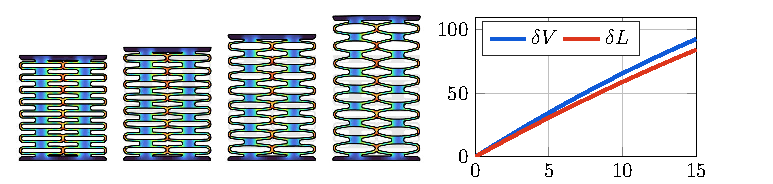
\includegraphics{./pdf/thesis-figurex-2-4-1.pdf}
  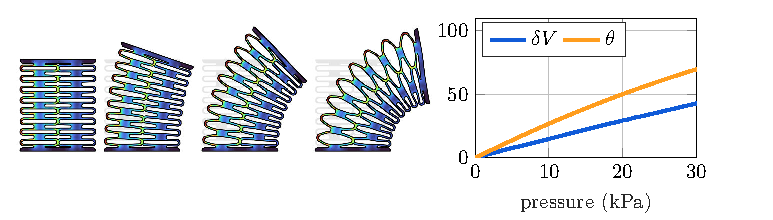
\includegraphics{./pdf/thesis-figurex-2-4-2.pdf}
  %% This file was created by matlab2tikz.
%
%The latest updates can be retrieved from
%  http://www.mathworks.com/matlabcentral/fileexchange/22022-matlab2tikz-matlab2tikz
%where you can also make suggestions and rate matlab2tikz.
%
\definecolor{mycolor1}{rgb}{0.06275,0.35686,0.84706}%
\definecolor{mycolor2}{rgb}{0.86667,0.21176,0.10980}%
%
\begin{tikzpicture}

\begin{axis}[%
width=0.583\textwidth,
height=0.214\textwidth,
at={(0\textwidth,0\textwidth)},
scale only axis,
axis on top,
xmin=0.5,
xmax=1768.5,
tick align=outside,
y dir=reverse,
ymin=0.5,
ymax=650.5,
axis line style={draw=none},
ticks=none
]
\addplot [forget plot] graphics [xmin=0.5, xmax=1768.5, ymin=0.5, ymax=650.5] {./fig/fig_orm_elong-1.png};
\end{axis}

\begin{axis}[%
width=0.308\textwidth,
height=0.195\textwidth,
at={(0.642\textwidth,0.01\textwidth)},
scale only axis,
xmin=0,
xmax=15,
ymin=0,
ymax=110,
axis background/.style={fill=white},
xmajorgrids,
ymajorgrids,
legend style={at={(0.03,0.97)}, anchor=north west, legend columns=2, legend cell align=left, align=left, draw=white!15!black}
]
\addplot [color=mycolor1, line width=1.5pt]
  table[row sep=crcr]{%
0	0\\
1.20005999999999	8.62875869322605\\
2.40012	17.0685830193392\\
3.60017999999999	25.3075020924564\\
4.80024	33.3362750448029\\
6.0003	41.1480614223673\\
7.20036	48.7381311097239\\
8.40042	56.1036109498542\\
9.60048	63.2432605846741\\
10.80054	70.1572704477627\\
11.700585	75.1955238137271\\
12.60063	80.1081200969719\\
13.500675	84.8973166125783\\
14.40072	89.5642639584667\\
15.00075	92.6047602820568\\
};
\addlegendentry{$\delta V$}

\addplot [color=mycolor2, line width=1.5pt]
  table[row sep=crcr]{%
0	0\\
1.500075	9.4713120804718\\
3.00015	18.7367798341987\\
4.20021	25.9889383302985\\
5.40027000000001	33.0912743243296\\
6.60033	40.0387557751286\\
7.80039000000001	46.8277828635893\\
9.00045	53.4559850403998\\
10.20051	59.922055247927\\
11.40057	66.2256106025044\\
12.60063	72.3665219327312\\
13.80069	78.346840194486\\
15.00075	84.1642843326511\\
};
\addlegendentry{$\delta L$}

\end{axis}

\begin{axis}[%
width=1.08\textwidth,
height=0.244\textwidth,
at={(-0.022\textwidth,-0.015\textwidth)},
scale only axis,
xmin=0,
xmax=1,
ymin=0,
ymax=1,
axis line style={draw=none},
ticks=none,
axis x line*=bottom,
axis y line*=left
]
\end{axis}
\end{tikzpicture}%
  %% This file was created by matlab2tikz.
%
%The latest updates can be retrieved from
%  http://www.mathworks.com/matlabcentral/fileexchange/22022-matlab2tikz-matlab2tikz
%where you can also make suggestions and rate matlab2tikz.
%
\definecolor{mycolor1}{rgb}{0.06275,0.35686,0.84706}%
\definecolor{mycolor2}{rgb}{1.0000,0.6157,0.1176}%
%
\begin{tikzpicture}

\begin{axis}[%
width=0.583\textwidth,
height=0.186\textwidth,
at={(0\textwidth,0.005\textwidth)},
scale only axis,
axis on top,
xmin=0.5,
xmax=2037.5,
tick align=outside,
y dir=reverse,
ymin=0.5,
ymax=650.5,
axis line style={draw=none},
ticks=none
]
\addplot [forget plot] graphics [xmin=0.5, xmax=2037.5, ymin=0.5, ymax=650.5] {./fig/fig_orm_bend-1.png};
\end{axis}

\begin{axis}[%
width=0.308\textwidth,
height=0.195\textwidth,
at={(0.642\textwidth,0\textwidth)},
scale only axis,
xmin=0,
xmax=30,
xlabel style={font=\color{white!15!black}},
xlabel={pressure (kPa)},
ymin=0,
ymax=110,
axis background/.style={fill=white},
xmajorgrids,
ymajorgrids,
legend style={at={(0.03,0.97)}, anchor=north west, legend columns=2, legend cell align=left, align=left, draw=white!15!black}
]
\addplot [color=mycolor1, line width=1.5pt]
  table[row sep=crcr]{%
0	0\\
1.60008	2.43048322137711\\
4.0002	6.19782561266756\\
4.80024	7.46829805994749\\
5.60028	8.34214292028537\\
17.60088	25.9279210387424\\
18.40092	27.0804871808147\\
19.20096	27.8807159907824\\
20.001	29.291815814346\\
20.80104	30.1255987953186\\
21.60108	31.5485305130109\\
22.40112	32.3659198775631\\
24.0012	34.5026095847334\\
28.80144	41.0337024135815\\
30.40152	43.1793137664006\\
};
\addlegendentry{$\delta V$}

\addplot [color=mycolor2, line width=1.5pt]
  table[row sep=crcr]{%
0	0\\
3.20016	8.88556718870406\\
6.40032000000001	17.5260854409956\\
8.80043999999999	23.7584681055126\\
11.20056	29.7734109354827\\
13.60068	35.566935673684\\
16.0008	41.1374336291155\\
17.60088	44.7277626743178\\
20.001	50.0250200383298\\
20.80104	51.6388516477443\\
21.60108	53.3837573512613\\
22.40112	54.9453731417261\\
23.20116	56.644891426995\\
24.80124	59.8364150546849\\
26.40132	62.9180842306127\\
28.0014	65.909936141282\\
29.60148	68.8150689926074\\
30.40152	70.2358435840924\\
};
\addlegendentry{$\theta$}

\end{axis}

\begin{axis}[%
width=1.08\textwidth,
height=0.244\textwidth,
at={(-0.022\textwidth,-0.024\textwidth)},
scale only axis,
xmin=0,
xmax=1,
ymin=0,
ymax=1,
axis line style={draw=none},
ticks=none,
axis x line*=bottom,
axis y line*=left
]
\end{axis}
\end{tikzpicture}%
  \vspace{-7mm}
  \caption{Working principle of the Orm robotic manipulator \cite{BibEntryOrm2019Sep} with the internal volume \data{Matlab1} in \si{\milli \liter}, and the end-effector displacement \data{Matlab2} in \si{\milli \meter} and bending-angle \data{Matlab4} in deg. By actuation of the pneumatic network, both elongation and bending can be achieved. Observe that the response is significantly more linear than McKibben actuators in Fig. \ref{fig:C0:mckibben}, emphasizing the importance of geometry.
  %\dotdata{Matlab2}
  \label{fig:C0:ormrobot}}
\end{figure}

According to an interview with Scheinman conducted by Asaro et al. \cite{ETHW2020Dec} in 2010, the positional accuracy of the Orm system was poor, which may have led to its loss of academic interest in the 1960s. However, the concept of pneumatically-driven soft arms continued to be explored for many years. Three years later, in 1968, Anderson and Horn proposed and patented an improved hyper-redundant robot manipulator (see Figure \ref{fig:C0:timeline}). Anderson's design improved upon the Orm, which was deemed slow and had limited positional accuracy. He proposed an array of nylon tendons that were connected to rigid discs distributed along the redundant backbone of the robot. The configurable backbone was comprised of universal spherical joints that allowed for pivoting motion with respect to other discs, totaling 16 Degrees-of-Freedom (DOFs). The entire arm was actuated hydraulically, yet the (soft) actuators were placed outside the robot's body rather than at each joint, like the Orm. To improve positional accuracy further, Anderson placed sensor tendons parallel to the actuator tendons, which allowed for operator-based positional feedback. Although Anderson's robot does not classify as a soft robot since it relies mostly on rigid materials, its flexibility arose from thin nylon tendons that were used for both actuation and sensing. Anderson showed that a network of distributed sensors is necessary to control the complex morphological shapes in hyper-redundant robotic systems while also mitigating the sensor's effect on mobility. Let us introduce the notion of soft sensors -- the dual of soft actuators.
%
\vspace{-3mm}
\terminology{\textbf{(Proprioceptive) soft sensors} are flexible measurements units embedded into the soft robotic body that through external stimuli measure the (local) changes of the system. Softness here implies that the sensor minimally alters the global mechanical behavior of the robot.
}{}

\begin{rmk}
\vspace{-1mm}
Our definition of soft sensors emphasizes their ability to "minimally alter the global mechanical behavior." It is worth mentioning that these sensors may be comprised of stiff, or even rigid components. However, they must be incorporated into or onto the soft body in a way that minimally affects the operational workspace of the soft actuator network in static or dynamic operating conditions. With a slight abuse of definition, exteroceptive sensors such as a camera vision system are inherently soft as they do not affect the compliance of the soft body.
\end{rmk}

\textbf{Soft robotics in the early 80's}. Since the seminal works of McKibben and subsequent research by Scheinman and Anderson, the field of soft Pneumatic Artificial Muscles (PAMs) in robotics has experienced rapid growth since the early 1980s. Figure \ref{fig:C0:earlyPAMrobots} shows a few examples of early soft robotic systems. Teleshev \cite{Teleshev1981} developed a soft gripper reminiscent of modern PneuNet actuators \cite{Galloway2016,Mosadegh2014,Choi2011} -- a rectangular bellow-shaped soft actuator. Unlike uniaxial PAMs, which are radially symmetric, these soft grippers explored an asymmetrical design of bellows. The geometry led to a stiffness differential around the circumference, resulting in their iconic bending motion. Still popular today, these pneumatic bending actuators find their origin back in early 1974, as seen in Andorf et al. \cite{Andorf1974}. A decade later, Takagi et al. \cite{Takagi1983} developed a soft multi-joint robot manipulator that resembles the human arm with its movements and antagonistic muscle pairs. Although their PAMs, called \textit{Rubbertuator}, had a function and design identical to McKibben's PAMs, their system showed the merits of combining soft and rigid materials. They observed not only a high degree of positional control of the robot arm, but force control was also easily regulated by pressure control, which naturally had safety benefits. The soft robot arm could perform delicate low-force tasks while simultaneously blocking motion when encountering a human. These soft properties were lacking in rigid robotic manipulators at the time but were reminiscent of their biological counterpart -- the human arm. Note that, at that time, force and impedance control for rigid robotics had been topics of academic research for years \cite{Anderson1988,Khatib1987,Hogan1984,Hogan1984Jan}, dating back to the early 1970s (\eg, see also \cite{Markiewicz1973}). However, achieving similar properties without control was rarely explored at the time.
%
\begin{figure}[!t]
  % \vspace{-2mm}
  % \ifx\printFigures\undefined
  % \else
  % \hspace{1mm}
  \includegraphics*[width=\textwidth]{./pdf/thesis-figure-2-5.pdf}
  % % This file was created by matlab2tikz.
%
%The latest updates can be retrieved from
%  http://www.mathworks.com/matlabcentral/fileexchange/22022-matlab2tikz-matlab2tikz
%where you can also make suggestions and rate matlab2tikz.
%
\begin{tikzpicture}

\begin{axis}[%
width=0.95\textwidth,
height=0.238\textwidth,
at={(0\textwidth,0\textwidth)},
scale only axis,
axis on top,
clip=false,
xmin=0.5,
xmax=2593.5,
tick align=outside,
y dir=reverse,
ymin=0.5,
ymax=650.5,
axis line style={draw=none},
ticks=none,
axis x line*=bottom,
axis y line*=left
]
\addplot [forget plot] graphics [xmin=0.5, xmax=2593.5, ymin=0.5, ymax=650.5] {./fig/fig_earlyPAMrobots-1.png};
\node[right, align=left]
at (axis cs:203,780) {\small (a)};
\node[right, align=left]
at (axis cs:777.5,780) {\small (b)};
\node[right, align=left]
at (axis cs:1326,780) {\small (c)};
\node[right, align=left]
at (axis cs:1801,780) {\small (d)};
\node[right, align=left]
at (axis cs:2226,780) {\small (e)};
\end{axis}
\end{tikzpicture}%
  %\fi
  \vspace{-5mm}
  \caption{Early robotic systems that explored soft PAMs for various tasks. (a) Soft robotic grippers by Teleshev \cite{Teleshev1981}. (b) The soft arm using \textit{Rubbertuator} actuators by Takagi and Sakaguchi \cite{Takagi1983}. (c) Three-link soft robotic manipulator with gripper reminiscent of the elephant's trunk, developed by Wilson at Duke University \cite{Wilson2007,Weisburd1988}. (d) Shadow bipedal walker by Buckley et al. \cite{Buckley2012} using McKibben muscle in antagonistic pairs to produce locomotion.
  \label{fig:C0:earlyPAMrobots}}
  \vspace{-2mm}
\end{figure}
%
\par Shortly after, Wilson \cite{Wilson2007} developed a soft robot manipulator based on the elephant's trunk at Duke University in Durham. His design effectively combined the works of Teleshev \cite{Teleshev1981} and Takagi et al. \cite{Takagi1983} into a robot with similar dexterity but minimal use of rigid components. According to Weisburd \cite{Weisburd1988}, his idea stemmed from the work of Kier and Smith \cite{Kier1985} who studied the biomechanics of muscular hydrostats in animals such as cephalopods (\eg, squids). The work of Kier et al. \cite{Kier1985} studied how complex motions are produced in muscular organs, like elongation, shortening, bending, and torsion. Inspired by the muscular hydrostat in the elephant's trunk, Wilson developed a soft arm composed of polyurethane tubes that worked as half-bellows, which enabled expansion and bending under positive pressurization \cite{Weisburd1988}. To accommodate three-dimensional movement, each soft pneumatic link was placed at a $\phi = \frac{\pi}{2}$ twist offset relative to the previous link. To illustrate the motion of the soft arm, a few snapshots are provided in Figure \ref{fig:C0:fist_srm_robot}. Wilson hypothesized that these highly-compliant robots would be more mechanically robust and sufficiently dexterous for tight workspaces, contrary to their rigid counterparts. Although the dexterity was novel, the positional accuracy was poor. The main problem stemmed from the soft arm being controlled in open-loop (\ie, remote teleoperation) without proprioceptive sensing or any positional feedback control, an issue akin to the Orm \cite{Corke2020}.

A few years later, Buckley et al. \cite{Buckley2012} developed the Shadow Walker -- a bipedal rigid robot comprised of antagonistic McKibben muscle pairs. Although not fully soft, their system did explore proprioceptive sensing. The hip, knee, and ankle joints were equipped with resistance-variable potentiometers for position feedback, whereas all the muscles had tension sensors for force feedback. Later on, these resistive sensors were replaced by analog optical sensors to improve robustness \cite{Buckley2012}. Although the system was top-heavy due to the pneumatic control hardware (\eg, valves and piping), rudimentary locomotion was possible. Interestingly, a similar artificial muscle system is still being explored in humanoid robotics today, such as the Atlas from Boston Dynamics. The success of pairing soft muscles with proprioceptive sensing eventually led to the development of the McKibben Shadow Hand \cite{Buckley2012,Gong2022Feb}, which is comprised of 40 uniquely addressable soft muscles.

\begin{figure}[!t]
  \vspace{-2mm}
  \centering
  \includegraphics*[width=\textwidth]{./pdf/thesis-figure-2-6.pdf}
  %% This file was created by matlab2tikz.
%
%The latest updates can be retrieved from
%  http://www.mathworks.com/matlabcentral/fileexchange/22022-matlab2tikz-matlab2tikz
%where you can also make suggestions and rate matlab2tikz.
%
\begin{tikzpicture}

\begin{axis}[%
width=0.712\textwidth,
height=0.295\textwidth,
at={(0.11\textwidth,0.03\textwidth)},
scale only axis,
xmin=0,
xmax=1,
ymin=0,
ymax=1,
axis line style={draw=none},
ticks=none,
axis x line*=bottom,
axis y line*=left
]
\end{axis}

\begin{axis}[%
width=0.218\textwidth,
height=0.164\textwidth,
at={(0\textwidth,0.179\textwidth)},
scale only axis,
axis on top,
xmin=0.5,
xmax=480.5,
tick align=outside,
y dir=reverse,
ymin=0.5,
ymax=360.5,
axis line style={draw=none},
ticks=none
]
\addplot [forget plot] graphics [xmin=0.5, xmax=480.5, ymin=0.5, ymax=360.5] {fig_first_srm-1.png};
\node[right, align=left, font=\color{white}]
at (axis cs:15,320) {\scriptsize $t = 0$ s};
\end{axis}

\begin{axis}[%
width=0.218\textwidth,
height=0.164\textwidth,
at={(0.227\textwidth,0.179\textwidth)},
scale only axis,
axis on top,
xmin=0.5,
xmax=480.5,
tick align=outside,
y dir=reverse,
ymin=0.5,
ymax=360.5,
axis line style={draw=none},
ticks=none
]
\addplot [forget plot] graphics [xmin=0.5, xmax=480.5, ymin=0.5, ymax=360.5] {fig_first_srm-2.png};
\node[right, align=left, font=\color{white}]
at (axis cs:15,320) {\scriptsize $t = 1.9$ s};
\end{axis}

\begin{axis}[%
width=0.218\textwidth,
height=0.164\textwidth,
at={(0.455\textwidth,0.179\textwidth)},
scale only axis,
axis on top,
xmin=0.5,
xmax=480.5,
tick align=outside,
y dir=reverse,
ymin=0.5,
ymax=360.5,
axis line style={draw=none},
ticks=none
]
\addplot [forget plot] graphics [xmin=0.5, xmax=480.5, ymin=0.5, ymax=360.5] {fig_first_srm-3.png};
\node[right, align=left, font=\color{white}]
at (axis cs:15,320) {\scriptsize $t = 2.8$ s};
\end{axis}

\begin{axis}[%
width=0.218\textwidth,
height=0.164\textwidth,
at={(0.682\textwidth,0.179\textwidth)},
scale only axis,
axis on top,
xmin=0.5,
xmax=480.5,
tick align=outside,
y dir=reverse,
ymin=0.5,
ymax=360.5,
axis line style={draw=none},
ticks=none
]
\addplot [forget plot] graphics [xmin=0.5, xmax=480.5, ymin=0.5, ymax=360.5] {fig_first_srm-4.png};
\node[right, align=left, font=\color{white}]
at (axis cs:15,320) {\scriptsize $t = 5.6$ s};
\end{axis}

\begin{axis}[%
width=0.218\textwidth,
height=0.164\textwidth,
at={(0\textwidth,0\textwidth)},
scale only axis,
axis on top,
xmin=0.5,
xmax=480.5,
tick align=outside,
y dir=reverse,
ymin=0.5,
ymax=360.5,
axis line style={draw=none},
ticks=none
]
\addplot [forget plot] graphics [xmin=0.5, xmax=480.5, ymin=0.5, ymax=360.5] {fig_first_srm-5.png};
\node[right, align=left, font=\color{white}]
at (axis cs:15,320) {\scriptsize $t = 6.5$ s};
\end{axis}

\begin{axis}[%
width=0.218\textwidth,
height=0.164\textwidth,
at={(0.227\textwidth,0\textwidth)},
scale only axis,
axis on top,
xmin=0.5,
xmax=480.5,
tick align=outside,
y dir=reverse,
ymin=0.5,
ymax=360.5,
axis line style={draw=none},
ticks=none
]
\addplot [forget plot] graphics [xmin=0.5, xmax=480.5, ymin=0.5, ymax=360.5] {fig_first_srm-6.png};
\node[right, align=left, font=\color{white}]
at (axis cs:15,320) {\scriptsize $t = 9.3$ s};
\end{axis}

\begin{axis}[%
width=0.218\textwidth,
height=0.164\textwidth,
at={(0.455\textwidth,0\textwidth)},
scale only axis,
axis on top,
xmin=0.5,
xmax=480.5,
tick align=outside,
y dir=reverse,
ymin=0.5,
ymax=360.5,
axis line style={draw=none},
ticks=none
]
\addplot [forget plot] graphics [xmin=0.5, xmax=480.5, ymin=0.5, ymax=360.5] {fig_first_srm-7.png};
\node[right, align=left, font=\color{white}]
at (axis cs:15,320) {\scriptsize $t = 10$ s};
\end{axis}

\begin{axis}[%
width=0.218\textwidth,
height=0.164\textwidth,
at={(0.682\textwidth,0\textwidth)},
scale only axis,
axis on top,
xmin=0.5,
xmax=480.5,
tick align=outside,
y dir=reverse,
ymin=0.5,
ymax=360.5,
axis line style={draw=none},
ticks=none
]
\addplot [forget plot] graphics [xmin=0.5, xmax=480.5, ymin=0.5, ymax=360.5] {fig_first_srm-8.png};
\node[right, align=left, font=\color{white}]
at (axis cs:15,320) {\scriptsize $t = 14$ s};
\end{axis}
\end{tikzpicture}%
  %\vspace{-2mm}
  \caption{Three-link soft robotic manipulator with two-fingered soft gripper by James Wilson from Stanford university \cite{Wilson2007}. Unlike classic manipulators, where links and joints are separated, Wilson's robot consisted of three pneumatic bending actuators -- being link and joint simultaneously. 
  %\vspace{-4mm}
  \label{fig:C0:fist_srm_robot}}
\end{figure}

\begin{figure}[!t]
  %\vspace{-3mm}
  %\ifx\printFigures\undefined
  %\else
  %\centering
  \includegraphics*[width=\textwidth]{./pdf/thesis-figure-2-7.pdf}
  %% This file was created by matlab2tikz.
%
%The latest updates can be retrieved from
%  http://www.mathworks.com/matlabcentral/fileexchange/22022-matlab2tikz-matlab2tikz
%where you can also make suggestions and rate matlab2tikz.
%
\begin{tikzpicture}

\begin{axis}[%
width=0.712\textwidth,
height=0.295\textwidth,
at={(0.11\textwidth,0.032\textwidth)},
scale only axis,
xmin=0,
xmax=1,
ymin=0,
ymax=1,
axis line style={draw=none},
ticks=none,
axis x line*=bottom,
axis y line*=left
]
\end{axis}

\begin{axis}[%
width=0.218\textwidth,
height=0.168\textwidth,
at={(0\textwidth,0.179\textwidth)},
scale only axis,
axis on top,
xmin=0.5,
xmax=302.5,
tick align=outside,
y dir=reverse,
ymin=0.5,
ymax=233.5,
axis line style={draw=none},
ticks=none
]
\addplot [forget plot] graphics [xmin=0.5, xmax=302.5, ymin=0.5, ymax=233.5] {fig_first_gripper-1.png};
\node[right, align=left, font=\color{white}]
at (axis cs:7,209) {\scriptsize $t = 0$ s};
\end{axis}

\begin{axis}[%
width=0.218\textwidth,
height=0.168\textwidth,
at={(0.227\textwidth,0.179\textwidth)},
scale only axis,
axis on top,
xmin=0.5,
xmax=302.5,
tick align=outside,
y dir=reverse,
ymin=0.5,
ymax=233.5,
axis line style={draw=none},
ticks=none
]
\addplot [forget plot] graphics [xmin=0.5, xmax=302.5, ymin=0.5, ymax=233.5] {fig_first_gripper-2.png};
\node[right, align=left, font=\color{white}]
at (axis cs:7,209) {\scriptsize $t = 0.14$ s};
\end{axis}

\begin{axis}[%
width=0.218\textwidth,
height=0.168\textwidth,
at={(0.455\textwidth,0.179\textwidth)},
scale only axis,
axis on top,
xmin=0.5,
xmax=302.5,
tick align=outside,
y dir=reverse,
ymin=0.5,
ymax=233.5,
axis line style={draw=none},
ticks=none
]
\addplot [forget plot] graphics [xmin=0.5, xmax=302.5, ymin=0.5, ymax=233.5] {fig_first_gripper-3.png};
\node[right, align=left, font=\color{white}]
at (axis cs:7,209) {\scriptsize $t = 0.28$ s};
\end{axis}

\begin{axis}[%
width=0.218\textwidth,
height=0.168\textwidth,
at={(0.682\textwidth,0.179\textwidth)},
scale only axis,
axis on top,
xmin=0.5,
xmax=302.5,
tick align=outside,
y dir=reverse,
ymin=0.5,
ymax=233.5,
axis line style={draw=none},
ticks=none
]
\addplot [forget plot] graphics [xmin=0.5, xmax=302.5, ymin=0.5, ymax=233.5] {fig_first_gripper-4.png};
\node[right, align=left, font=\color{white}]
at (axis cs:7,209) {\scriptsize $t = 0.55$ s};
\end{axis}

\begin{axis}[%
width=0.218\textwidth,
height=0.168\textwidth,
at={(0\textwidth,0\textwidth)},
scale only axis,
axis on top,
xmin=0.5,
xmax=302.5,
tick align=outside,
y dir=reverse,
ymin=0.5,
ymax=233.5,
axis line style={draw=none},
ticks=none
]
\addplot [forget plot] graphics [xmin=0.5, xmax=302.5, ymin=0.5, ymax=233.5] {fig_first_gripper-5.png};
\node[right, align=left, font=\color{white}]
at (axis cs:7,209) {\scriptsize $t = 0.69$ s};
\end{axis}

\begin{axis}[%
width=0.218\textwidth,
height=0.168\textwidth,
at={(0.227\textwidth,0\textwidth)},
scale only axis,
axis on top,
xmin=0.5,
xmax=302.5,
tick align=outside,
y dir=reverse,
ymin=0.5,
ymax=233.5,
axis line style={draw=none},
ticks=none
]
\addplot [forget plot] graphics [xmin=0.5, xmax=302.5, ymin=0.5, ymax=233.5] {fig_first_gripper-6.png};
\node[right, align=left, font=\color{white}]
at (axis cs:7,209) {\scriptsize $t = 0.83$ s};
\end{axis}

\begin{axis}[%
width=0.218\textwidth,
height=0.168\textwidth,
at={(0.455\textwidth,0\textwidth)},
scale only axis,
axis on top,
xmin=0.5,
xmax=302.5,
tick align=outside,
y dir=reverse,
ymin=0.5,
ymax=233.5,
axis line style={draw=none},
ticks=none
]
\addplot [forget plot] graphics [xmin=0.5, xmax=302.5, ymin=0.5, ymax=233.5] {fig_first_gripper-7.png};
\node[right, align=left, font=\color{white}]
at (axis cs:7,209) {\scriptsize $t = 0.97$ s};
\end{axis}

\begin{axis}[%
width=0.218\textwidth,
height=0.168\textwidth,
at={(0.682\textwidth,0\textwidth)},
scale only axis,
axis on top,
xmin=0.5,
xmax=302.5,
tick align=outside,
y dir=reverse,
ymin=0.5,
ymax=233.5,
axis line style={draw=none},
ticks=none
]
\addplot [forget plot] graphics [xmin=0.5, xmax=302.5, ymin=0.5, ymax=233.5] {fig_first_gripper-8.png};
\node[right, align=left, font=\color{white}]
at (axis cs:7,209) {\scriptsize $t = 1.2$ s};
\end{axis}
\end{tikzpicture}%
  %\fi
  %\vspace{-2mm}
  \caption{Four-fingered soft robotic gripper by Suzumori and Saiko \cite{Suzumori1991,Suzumori1992}. Each finger possess three pneumatic chambers that allow for directional bending -- analogous the Orm. Through proper coordination of the set of soft fingers various gripping complexity can be achieved, such as the clock-wise turning a mechanical hex bolt (as shown above). Suzumori et al. showed these intricate finger motions can be easily achieved by careful modeling of the fingertip dynamics, and exploring the adaptability of soft materials.
  \label{fig:C0:fist_grip_robot}}
  \vspace{-3mm}
  
%   \thumbimageodd{\qrcode[height=1.0cm]{www.google.com}}{Fig. 2.7}
\end{figure}

Following, Suzumori and Saiko \cite{Suzumori1991,Suzumori1992} developed a micro flexible soft actuator driven by an electro-hydraulic system (intrinsic length $L \approx12$ \si{\milli \meter}). Each end-effector enables three DOFs including pitch, yaw, and stretch -- making it ideal for fingers, arms and legs. Figure \ref{fig:C0:fist_grip_robot} shows the level of dexterity in their system. By placing the four PAMs parallel on a gripper mount, and assigning a predefined trajectory, they showed their soft robotic system has sufficient dexterity to mount an hex-bolt at an incredible speed and precision. To achieve such dexterity and precision, Suzumori et al. \cite{Suzumori1991} employed various modeling and control strategies to account for the dynamical characteristics under high-frequency, fluid compressibility, and the closing mechanics of pressure valves. Furthermore, the kinematics of each finger was derived using generalized homogeneous transformation, not unlike traditional robotics. Knowing both the compliance characteristics (pressure-deformation relations) and the forward kinematics, a Jacobian-based positional controller was employed to regulate the Cartesian coordinates of the finger-tips (successfully one might add as shown by Figure \ref{fig:C0:fist_grip_robot}). \\[0.1em]
%
\par \textbf{Early controllers for hyper-redundant (soft) robots}. Following the increasing interest in highly-flexible robots around the late 80s, academic research into controlling these \textit{hyper-redundant} robots boomed shortly after. At the time, the term hyper-redundancy -- being an extension of redundancy in robotics \cite{MerriamWebster1983} -- was defined as the relative degree of kinematic and/or actuator redundancy which is large or even infinite \cite{Chirikjian1992, Chirikjian1994}. The term was first introduced by Chirikjian and Burdick \cite{Chirikjian1989}. Others referred to these robots as \textit{highly redundant} \cite{Wilson1988Dec, Naccarato1989Dec} or \textit{High Degree-of-Freedom} (HDOF) manipulators \cite{Salerno1989Jan, Mochiyama1999}. Around that time, Chirikjian and Burdick provided a plethora of mathematical foundations \cite{Chirikjian1994, Chirikjian1994Jun, Chirikjian1991, Chirikjian1992, Chirikjian1992Dec} focused on the kinematics and motion planning of hyper-redundant manipulators. Their work presented a modal discretization approach to describe the shape of the deformable backbone \cite{Chirikjian1994Jun}, and from this geometric approaches were introduced to solve obstacle-avoiding trajectories using generalized \textit{follow-the-leader} strategies \cite{Chirikjian1992Dec}. Especially the latter showed the limitation in rigid redundant manipulators. Although Chirikjian laid the foundation for the control of hyper-redundant robots, basic principles of motion planning in pneumatic hyper-redundant robots were already presented by Wilson et al. \cite{Wilson1988Dec, Wilson1989Jun} -- yet were not called hyper-redundant robots nor soft robots yet. Recall also that the work of Wilson et al. has been shown earlier in Figure \ref{fig:C0:timeline} and Figure \ref{fig:C0:fist_srm_robot}. In Brock et al. \cite{Brock1991}, a similar analysis was used for optimal shape design of thin elastic rods to realize desired robotic compliance. Besides, there exists an abundance of literature prior to \cite{Chirikjian1992} on Variable Geometry Truss Manipulators (VGTMs) -- a variant of hyper-redundant tensegrity robotics -- that dealt with motion planning for such systems \cite{Naccarato1989Dec, Naccarato1991Apr, Salerno1989Jan}. Later, Mochiyama et al. \cite{Mochiyama1998, Mochiyama1999}, built upon Chirikjian's work by extending it to a dynamic formulation for elastic rods such that classic controller design is possible. They proposed shape-regulation controllers for HDOF manipulator by projecting them onto time-invariant curves, thereby showing that estimating the desired curve parameters is crucial to solving the problem by Lyapunov design \cite{Mochiyama1998}. Although there existed a variety of modeling and control strategies, computational power in relation to modeling complexity was the limiting factor for the simulation-to-reality transfer at the time.
\section{Modern soft robotics boom in academia}
The precise date of the emergence of soft robotics as a prominent academic field is uncertain, but it is widely believed to have occurred in the mid-2000s. Since then, the field has undergone significant evolution and diversification, with research branching into areas such as active meta-materials, Additive Manufacturing (AM), morphological optimization, model-based control, and learning-based control. In the subsequent sections, we will examine several ongoing research topics in the field of soft robotics. These topics primarily concern the design and control of soft robots. It should be emphasized that while these problems may seem distinct, they are often interconnected. For instance, the structural design of a soft robot influences its workspace and consequently affects the feasibility of \textit{a-priori} defined control objectives. This section aims to underscore such scientific interconnections and demonstrate the essential components required to address common paradigms. \vspace{-2mm}
%
\section{Tailoring design of fluidic soft actuation}
\label{sec:C2:conventional_actuation}
As the name "soft robots" arises from their use of soft materials, it follows that design and fabrication using soft materials play a huge role in their technological development. Contrary to rigid robots, many soft robots explore whole body movement rather than localized regions undergoing motion called \textit{"joints"}. In classic robotics, robots are composed of a countable number of rigid links and joints \cite{Spong2006, Murray1994, Corke2011}, either arranged in series or parallel. Together, they span a workable range of motion called the operational workspace \cite{Spong2006} (see Chapter \ref{chap: introduction}). Focusing on rigid manipulators, whose base is often structurally fixated, their workspace can be obtained through a system of kinematics, often derived through a set of geometrical equalities. Rigid manipulators often have a bounded workspace (assuming actuation limits). In robotic locomotion, similar kinematic descriptions can be obtained for the legs and feet, with the exception of an additional free-floating base. In these cases, however, the workspace is of less interest; rather, the different possibilities of \textit{"gait cycles"} that arise from the link-joint configuration and actuator dynamics determine the system's success for locomotion.

%However, contrary to manipulators, an additional global free-floating frame is introduced (\eg, a coordinate frame at the center of mass) that describe the global coordinates of the full robotic body. As such, for robotic locomotion, the workspaces are often unbounded and thus carry less importance. Nonetheless, their structural layout of joints and links play a crucial role in energy consumption. High efficiency in the cyclic exchange in potential and kinetic energy is hugely beneficial to the duration of locomotion. In any case, either manipulators and locomotion machines, the topological layout of the links and joints are of paramount importance.
Returning to soft robots, the terms such as \textit{joints}, \textit{workspace} and \textit{gait cycles} also apply here. However, the high flexibility of soft robots allows for many non-restricted joint displacements, which makes deriving closed-form mathematical descriptions challenging. The shape of the workspace and locomotion patterns are mainly influenced by the geometry of the soft actuator, its flexibility modes, and how forces are transferred within the continuum soft body. Controlling the motion within soft actuation, reducing parasitic mobility and tailoring motion based on structural geometry, is an active topic in soft robotics research for decades. \\

\begin{figure}[!t]
  %\vspace{-2mm}
  \centering
  %\hspace{2mm}
  \includegraphics*[width=\textwidth]{./pdf/thesis-figurex-1-2.pdf}
  %% This file was created by matlab2tikz.
%
%The latest updates can be retrieved from
%  http://www.mathworks.com/matlabcentral/fileexchange/22022-matlab2tikz-matlab2tikz
%where you can also make suggestions and rate matlab2tikz.
%
\begin{tikzpicture}

\begin{axis}[%
width=0.975\textwidth,
height=0.227\textwidth,
at={(0\textwidth,0\textwidth)},
scale only axis,
axis on top,
clip=false,
xmin=0,
xmax=3000,
tick align=outside,
y dir=reverse,
ymin=0,
ymax=700,
axis line style={draw=none},
ticks=none,
axis x line*=bottom,
axis y line*=left
]
\addplot [forget plot] graphics [xmin=0.5, xmax=2849.5, ymin=0.5, ymax=650.5] {fig_actuation_types-1.png};
\node[right, align=left]
at (axis cs:262.5,780) {\small (a)};
\node[right, align=left]
at (axis cs:910,780) {\small (b)};
\node[right, align=left]
at (axis cs:1401,780) {\small (c)};
\node[right, align=left]
at (axis cs:1904.5,780) {\small (d)};
\node[right, align=left]
at (axis cs:2455.5,780) {\small (e)};
\end{axis}
\end{tikzpicture}%
  \vspace{-6mm}
  \caption{Various examples of continuum-bodied joint motions in modern soft actuation. (a) Soft actuator undergoing contraction by Yang et al. \cite{Yang2016}. (b) Set of serial-chain of bending soft actuator (STIFF-FLOP) by Cianchetti et al. \cite{Cianchetti2013Nov,Cianchetti2014} (c) Soft tentacle composed of twisting soft actuators. (d) Vine-inspired soft actuators capable of growth by Hawkes et al. \cite{Hawkes2017}. (e) Soft manipulator composed of bending and twisting soft actuators through laminate materials by Kim et al. \cite{Kim2019Aug}.}
  %\vspace{-6mm}
  \label{fig:C0:actuationtypes}
\end{figure}
%
\vspace{-4mm}
\subsection{Engineering principles in soft fluidic actuators}
In the past decade, researchers have developed various techniques for exploiting the high elasticity of soft materials for controllable actuation. One key development, with similar working principles to pneumatic muscle groups (see \cite{Mckibben,Morin1953} or Figure \ref{fig:C0:mckibben}), are Soft Pneumatic Actuators (SPAs). A few examples are shown in Figure \ref{fig:C0:actuationtypes}. SPAs undergo mechanics similar to McKibben actuators \cite{Mckibben} or Morin actuators \cite{Morin1953}, yet they possess a broader range of motion beyond uniaxial contraction. Examples include axial growth \cite{Hawkes2017}, bending \cite{Mosadegh2014,Galloway2016,Marchese2016}, contraction and elongation \cite{Yang2016}, helical and twisting, and a hybridization of all the aforementioned motions \cite{Kim2019Aug}. An example of soft actuators capable of contraction is the Vacuum-Actuated Muscle-inspired Pneumatic (VAMP) structure by Yang et al. (2016, \cite{Yang2016}). Their work proposes a tailored geometrical structure embedded into a soft elastomer medium that is highly sensitive towards buckling. When subjected to a sufficiently large negative differential pressure, the internal structure undergoes a (reversible) mechanically unstable leading to uniaxial contraction, as seen in Figure \ref{fig:C0:actuationtypes}. Their work is inspired by a similar buckling behavior of patterned elastomer \cite{Bertoldi2008,Mullin2007,Shim2013Aug} subjected to axial loads. These muscle-inspired vacuum soft actuators are fast, produce a stable, repeatable motion; and more importantly, explore structural geometry to reduce parasitic motion. An example of soft bending actuators is the STIFF-FLOP system \cite{Cianchetti2013Nov}. Similar to the ORM system \cite{BibEntryOrm2019Sep}, it has three pressure chambers embedded into a soft cylindrical-shaped elastomer. To prevent ballooning, inextensible rings are placed orthogonal to the deformable backbone. Its design is also reminiscent of \cite{Suzumori1992,Suzumori1991}. Hawkes et al. \cite{Hawkes2017} developed a soft manipulator inspired by the growing behavior of vines. Kim et al. \cite{Kim2019Aug} used laminates that adhere to the volumetrically expanding soft body to govern the motion trajectory through bending and twisting.
% \textbf{B: Exploring optimization and evolutionary algorithms}. 
\subsection{Exploring optimization and evolutionary algorithms}
Besides designing through engineering principles, optimization in soft robotics has been gaining momentum in recent years. Wang et al. \cite{Wang2020Nov} used topology optimization to find the optimal design for a cable-driven soft gripper (Figure \ref{fig:C0:optztypes}a). Similarly, Tian et al. \cite{Tian2020May} explored topology optimization for ferromagnetic soft grippers. Besides soft grippers, evolutionary design algorithms are also employed for soft mobile crawlers and swimmers. Joachimczak et al. \cite{Joachimczak2014Jul,Joachimczak2015} explored an evolutionary search algorithm with the purpose of automatically designing complex morphologies and controllers of multicellular, soft-bodied robots (Figure \ref{fig:C0:optztypes}c). Hu et al. \cite{Hu2019taichi} used a differential physics simulator called \texttt{DiffTachi} that efficiently computes gradient information for each simulation timestep. The gradient information can then be fed into neural network controllers to solve, for instance, the appropriate gait cycles required in the locomotion of soft crawlers, see Figure \ref{fig:C0:optztypes}d.

\begin{figure}[!t]
  \vspace{-3mm}
  %\centering
  %\hspace{2mm}
  %% This file was created by matlab2tikz.
%
%The latest updates can be retrieved from
%  http://www.mathworks.com/matlabcentral/fileexchange/22022-matlab2tikz-matlab2tikz
%where you can also make suggestions and rate matlab2tikz.
%
\begin{tikzpicture}

\begin{axis}[%
width=0.975\textwidth,
height=0.197\textwidth,
at={(0\textwidth,0\textwidth)},
scale only axis,
axis on top,
clip=false,
xmin=0.5,
xmax=3213.5,
tick align=outside,
y dir=reverse,
ymin=0.5,
ymax=650.5,
axis line style={draw=none},
ticks=none,
axis x line*=bottom,
axis y line*=left
]
\addplot [forget plot] graphics [xmin=0.5, xmax=3213.5, ymin=0.5, ymax=650.5] {./fig/fig_optimization_types-1.png};
\node[right, align=left]
at (axis cs:92,780) {\small (a)};
\node[right, align=left]
at (axis cs:551,780) {\small (b)};
\node[right, align=left]
at (axis cs:1365.5,780) {\small (c)};
\node[right, align=left]
at (axis cs:2430.5,780) {\small (d)};
\node[right, align=left]
at (axis cs:2960.5,780) {\small (e)};
\end{axis}
\end{tikzpicture}%
  \includegraphics*[width=\textwidth]{./pdf/thesis-figure-1-3v2.pdf}
  \vspace{-6mm}
  \caption{Optimization for design and motion of soft robots. (a) Soft gripper by Wang et al. \cite{Wang2020Nov}. (b) Evolutionary algorithms for multicellular soft-bodied robots by Joachimczak et al. \cite{Joachimczak2014Jul,Joachimczak2015}. (c) \texttt{DiffTachi} result for soft crawler by Hu et al. \cite{Hu2019taichi}. (d) Voxel-based optimization for Xenobots \cite{Kriegman2019}.}
  \label{fig:C0:optztypes}
  \vspace{-4mm}
\end{figure}

\vspace{-2mm}
\section{Gaining performance using feedback control}
\label{sec:C0:modelcontrol}
As the inherent properties of soft materials bring forth many benefits, such as adaptability, hyper-redundancy, and passivity with respect to the environment, they also hinder progress in model-based controllers. Earlier, we touched upon this subject with the rise of kinematic and dynamic models for hyper-redundant robotics in the late 80s to early 90s. Chirikjian et al. \cite{Chirikjian1992} provided a kinematic framework for hyper-redundant manipulators with applications to motion planning (see Figure \ref{fig:C0:modeltypes}a). Here, the elastic backbone is approximated using a modal formulation. Such modeling frameworks are one-to-one transferable to soft continuum manipulators. Mochiyama et al. \cite{Mochiyama1998,Mochiyama2003} extended this work to a dynamics formulation, even providing Lyapunov-based control strategies for shape regulation (Figure \ref{fig:C0:modeltypes}b). However, both modeling frameworks were computationally inefficient, lacking transferability to real-time control. The root problem stems from the fact that soft continuum robots, belonging in their exact formulation to the field of continuum mechanics, lead to infinite-dimensional models often expressed as Partial Differential Equations (PDEs). Rigid multi-body systems, like robot manipulators or mobile robots, on the other hand, can be conveniently modeled via Ordinary Differential Equations (ODEs) that stem from Lagrangian or Newtonian mechanical principles. Rigid-body models were (and still are) fast computationally, and their literature on controller design is vast and well-established \cite{Murray1994,Corke2011,Spong2006}. The computational issues in early continuum robots may be reflected by the literature gap between the 1990s and 2010s. 
% \textbf{A: Modern control-oriented models for soft robots.} 
\vspace{-3mm}
\subsection{Control-oriented models for soft robots}
In the past decade, significant steps have been made to address the issues of infinite dimensionality \cite{DellaSantina2021}. The key is to formulate a finite-dimensional approximation of the soft robot's dynamics such that they can be written as standard ODEs. Reduced-Order Models (ROMs) have paved the path for model-based controllers for soft robots, whose reduced formulations are both tractable and precise. In the years following its academic boom, many different assumptions and model approximations have emerged to address the issue of control.
%
\begin{figure}[!t]
  %\vspace{-3mm}
  \centering
  %\hspace{-8mm}
  \includegraphics*[width=1.0\textwidth]{./pdf/thesis-figure-1-4v2.pdf}
  %% This file was created by matlab2tikz.
%
%The latest updates can be retrieved from
%  http://www.mathworks.com/matlabcentral/fileexchange/22022-matlab2tikz-matlab2tikz
%where you can also make suggestions and rate matlab2tikz.
%
\begin{tikzpicture}

\begin{axis}[%
width=0.975\textwidth,
height=0.202\textwidth,
at={(0\textwidth,0\textwidth)},
scale only axis,
axis on top,
clip=false,
xmin=0.5,
xmax=3135.5,
tick align=outside,
y dir=reverse,
ymin=0.5,
ymax=650.5,
axis line style={draw=none},
ticks=none,
axis x line*=bottom,
axis y line*=left
]
\addplot [forget plot] graphics [xmin=0.5, xmax=3135.5, ymin=0.5, ymax=650.5] {./fig/fig_model_types-1.png};
\node[right, align=left]
at (axis cs:205,780) {\small (a)};
\node[right, align=left]
at (axis cs:818.5,780) {\small (b)};
\node[right, align=left]
at (axis cs:1399,780) {\small (c)};
\node[right, align=left]
at (axis cs:2008,780) {\small (d)};
\node[right, align=left]
at (axis cs:2702,780) {\small (e)};
\end{axis}

\begin{axis}[%
width=1.103\textwidth,
height=0.271\textwidth,
at={(-0.064\textwidth,-0.051\textwidth)},
scale only axis,
xmin=0,
xmax=1,
ymin=0,
ymax=1,
axis line style={draw=none},
ticks=none,
axis x line*=bottom,
axis y line*=left
]
\end{axis}
\end{tikzpicture}%

  %\vspace{-6mm}
  \caption{Popular modeling strategies for soft robotics. (a) Hyper-redundant modeling description through tensegrity by Chirikjian \cite{Chirikjian1992,Chirikjian1994}). (b) Analytic continuum beam description by Mochiyama \cite{Mochiyama1999,Mochiyama2003}). (c) Augmented rigid-body model subjected to PCC kinematics by Katzschmann et al. \cite{Katzschmann2019}. (d) Diamond-shaped soft robot manipulator controlled using the FEM-based \texttt{SOFA} software by Duriez et al. \cite{Duriez2013} and related \cite{Coevoet2017,Goury2018}.%(d) Geometric Cosserat model subjected to PCS kinematics by Renda et al. \cite{Renda2018}. (e) Diamond-shaped soft robot manipulator controlled using the FEM-based \texttt{SOFA} software by Duriez et al. \cite{Duriez2013} and related \cite{Coevoet2017,Goury2018}.}
  }
  \label{fig:C0:modeltypes}
  \vspace{-5mm}
\end{figure}
%
\begin{rmk}
 The reduced-order formulations for soft robotics are primarily applicable to slender soft robots, leading to a focus on soft robot manipulators in control-oriented studies. This approach is well-motivated given that many soft robots have one dominant physical dimension compared to the other two \cite{DellaSantina2021}. As such, this thesis primarily focuses on the modeling and control of soft manipulators rather than a broader scope.
\end{rmk}
%
\par
Focusing on soft robot manipulators, a popular choice of finite-dimensional reduction is the so-called Piecewise Constant Curvature (PCC) soft beam model. The PCC modeling approach is by far the most adopted in the soft robotics community \cite{Webster2010}. As the name implies, the soft robot is modeled as an elastically deformable beam with all strains but curvature neglected. Examples of this approximation include \cite{Falkenhahn2015,Marchese2016,Katzschmann2018,Katzschmann2019,Runge2017,Franco2020,Webster2010,DellaSantina2020a}. Highlighting a few, Katzschmann et al. \cite{Katzschmann2018} proposed to connect the PCC formulation to an augmented rigid robot dynamical model with parallel elastic actuation (see Figure \ref{fig:C0:modeltypes}c). A similar approach was proposed earlier by Falkenhahn et al. \cite{Falkenhahn2015} and applied to Festo's bionic arm \cite{Grzesiak2011}. Although such lumped models may seem like a major oversimplification, the proposed model allows sufficient speed and accuracy such that model-based feedback is applicable. This formulation was also employed later in an adaptive sliding mode control scheme \cite{Kazemipour2022May} for the SoPra soft arm \cite{Toshimitsu2021Sep}. Following, Renda et al. \cite{Renda2018} extended the PCC model to Piecewise Constant Strain (PCS) formulation. This formulation allowed for all strain if and only if considered spatially piece-wise constant (Figure \ref{fig:C0:modeltypes}d). Rooted in $\SE{3}$ geometry of the Cosserat approach \cite{Simo1986}, it provided a closer relation with the rigid body geometry of traditional robotics. The formulation also extends to soft manipulators with fluidic actuation \cite{Renda2017Aug, Till2019}. The PCS model was later employed in feedforward controllers by Thuruthel et al. \cite{Thuruthel2018Nov} using model-based policy learning algorithms. To improve efficiency, a recurrent neural network was trained using an offline PCS model. Grazioso et al. \cite{Grazioso2019} explored a similar path of geometric Cosserat beams using helical strain functions. Nevertheless, Constant Strain (CS) models have severe limitations. They often do not originate from continuum mechanics and thus are only applicable in restrictive settings. Although computationally performance might surpass continuous models, due to intrinsic kinematic restrictions, they are unable to capture important continuum phenomena, like buckling, environmental interaction, or wave propagation.

In response to its limitations, many researchers continued their search for efficient and more generalizable alternatives. Della Santina et al. \cite{DellaSantina2020} proposed a polynomial description to describe the continuum dynamics, a description analogous to \cite{Chirikjian1992}. In their work, they expressed the curvature function of the soft robot in terms of a standard polynomial basis. Not only can an exact infinite-dimensional formulation of the problem be obtained (in theory), but truncation at any level is easily changed. The technique is also widely used for flexible-link robot manipulators to capture small vibrations; see DeLuca et al. \cite{DeLuca2016Jul}. Della Santina et al. also showed that PCC-rooted assumptions as control output produce a minimum-phase system \cite{DellaSantina2020} -- a fundamental stepping-stone for nonlinear control. Following, Boyer et al. \cite{Boyer2021} extended upon their prior Cosserat models \cite{Renda2018,Renda2020} and presented a tractable and generalizable beam model for slender soft manipulators. A similar approach to \cite{DellaSantina2020} was followed, but all strains are discretized using a finite set of strain basis functions. Renda et al. \cite{Renda2020} improved computation by introducing a two-stage Gauss quadrature \cite{Zanna1999} to derive the Magnus expansion \cite{Hairer2002}. Other examples of the Cosserat beam descriptions, but more focused on the continuum mechanics rather than control, are the work of Gazzola et al. \cite{Gazzola2018}. Their work allowed for efficient Cosserat beam models suitable for self-collision, thus providing various simulations for twirling and coiling under increasing torsional loads.

Another popular alternative, better suited for general soft robotic systems like soft mobile robots, are reduced-order finite element models \cite{Duriez2013,Coevoet2017,Coevoet2017Feb,Goury2018,Thieffry2017,Thieffry2020,Tonkens2021May,Katzschmann2019Apr,Wu2021Feb,Zhang2017} or neural-network trained using offline FEM simulations \cite{Fang2020Dec}. Starting from high-order FEM data (e.g., state dimensions of the order $10$k) that capture the whole workspace spanned by the network of soft actuators, Proper Orthogonal Decomposition (POD) techniques are employed to drastically reduce the state dimension of the soft robot model. These techniques can even retain external loads (e.g., contact and friction) with precision as long as they are included in the offline data set \cite{Goury2018}. By far, this FEM-driven method has shown the most success in the experimental control regime.
%\textbf{B: Soft robot simulation and programming environments}.
\subsection{Soft robot simulation and programming environments}
The rapid development of soft robotic models in recent years has also increased the demand for (open-access) software packages, especially since many of the aforementioned ROM models require an advanced level of mathematical understanding. In an attempt to help the soft robotics community, many researchers have provided open-source, documented simulators interwoven in their soft robotics research. A popular FEM-based software on soft robotic modeling and control is \texttt{SOFA} by Duriez et al. \cite{Duriez2013,Coevoet2017}. \texttt{DiffTachi} by Hu et al. \cite{Hu2019taichi, Hu2019Oct} explores differential simulations to produce soft machines capable of locomotion. Bern et al. \cite{Bern2022,Bern2019} developed \texttt{SoftIK}, a software for soft deformable plushy robots. Among beam or rod-based models, there exist many options. Examples include \texttt{Elastica} or \texttt{pyElastica} \cite{Tekinalp2022} developed by Gazzola et al. \cite{Gazzola2018,Zhang2019}, \texttt{TMTDyn} by Sadati et al. \cite{Sadati2020}, \texttt{SimSOFT} by Grazioso et al. \cite{Grazioso2019}, and \texttt{SoRoSim} by Mathew et al. \cite{Mathew2021Jul} based on the work of Renda et al. \cite{Renda2020} and Boyer et al. \cite{Boyer2021}. The \texttt{Sorotoki} toolkit by Caasenbrood et al. \cite{SorotokiCode}, an open-source software package presented as a part of this thesis, explores a combination of FEM models and soft beam models. The toolkit, written in Matlab, aims to bridge the gaps between design, modeling, and control of (hyper-elastic) soft robots.
% \textbf{C: Closing the loop in soft robotics}. 
\subsection{Closing the loop in soft robotics}
Following the many developments in computational efficiency of reduced-order models (and accordingly the advances in soft sensing), academic research in model-based or model-free control for soft robots is significantly growing since early 2019. Note that, feed-forward controllers for soft manipulators have been proposed years prior, \eg, \cite{Falkenhahn2015May,Falkenhahn2015,Thuruthel2017Oct,Satheeshbabu2019May}.

So far, the PCC model has been more intensively validated experimentally than other models. In Della Santina et al. \cite{DellaSantina2020a}, the augmented rigid-body PCC model was used to design a closed-loop controller for a continuous soft manipulator, presenting two architectures designed for dynamic trajectory tracking and surface following. Prior work is provided in \cite{Katzschmann2019}. A similar approach was followed by Milana et al. \cite{Milana2021} and applied to an artificial soft cilia. They showed that soft bending actuators could mimic the asymmetric motion of the cilia through model-based control. Cao et al. \cite{Cao2021Apr} explored a reduced analytical model \cite{Wang2019Apr}, which is somewhat equivalent to a linear pendulum model (apart from quadratic terms in the potential force), to develop robust tracking controllers without velocity observers. Their controller was tested experimentally on a soft PneuNet actuator. Wang et al. \cite{Wang2022Mar} developed a computed torque controller (see \cite{Spong2006}) using the augmented rigid-body PCC model and applied it to a soft Honeycomb Pneumatic Network Arm \cite{Jiang2016Dec}. Franco et al. \cite{Franco2020,Franco2020Jan} used a port-Hamiltonian modeling framework akin to the rigid-body PCC model (\ie, three-link pendulum) and applied such principles to energy-shaping controllers. The performance of their controller was assessed via simulations and experiments on two soft continuum prototypes. On a side note, Franco et al. \cite{Franco2022May} also developed an energy-shaping control law together with nonlinear observers for the control of soft growing robots \cite{Hawkes2017} with pneumatic actuation subject to the (ideal) gas laws.

As mentioned previously, the PCC model has significant limitations that raise questions about the usability, dexterity, and robustness of its control derivation. Although primarily focused on simulation, higher-order dynamics have been used for the development of feedback controllers in soft manipulators. Della Santina et al. \cite{DellaSantina2020Dec} developed swing-up controllers for a soft pendulum modeled by the affine curvature models (i.e., a polynomial curvature model \cite{DellaSantina2020} of order $k = 2$). Their approach mirrors the path of the classic control problem of inverted pendulums in the 90s and early 2000s \cite{Spong1996,Spong1994,Ortega1998,Shiriaev1999Dec}. Later, Weerakoon et al. \cite{Weerakoon2021Dec} extended their work by introducing a revolute base. A common control problem here is under-actuation \cite{Tedrake2022,Spong2006,Murray1994}, implying that not all control actions can be realized to steer the configuration space to a desired position. Borja et al. \cite{Borja2022Apr} developed a general control framework that can stabilize soft manipulators based on potential energy shaping using the affine curvature model. Their work showed that some linear matrix inequalities can be derived based on the gradient of the potential energy related to the passive and active states, such that local stability can be proven. In layman's terms, elasticity must dominate the forces resulting from gravity in the underactuated states for (potential) energy-shaping controllers (and mostly others) to work. More recent work by Pustina et al. \cite{Pustina2023Jun} explores control via input decoupling applied on Lagrangian soft robot models with collocated inputs. In summary, the development of closed-loop control for multi-modal soft robotic deformations is a promising area of research. However, at present, such control mechanisms are limited to simulated environments and have yet to be fully realized in practical applications.

\section{Summary}
In summary, we have provided a comprehensive overview of the evolution of soft robotics, from its inception in the 1950s to current research trends. The chapter traces the origins of soft robotics in pneumatic muscles and explores the emergence of novel concepts and technologies that have facilitated the development of increasingly sophisticated soft robots through the utilization of exotic material properties. We highlight significant milestones in the field, including the creation of the first soft gripper, integration of robotics with soft actuation, and introduction of design, modeling, and control principles for these systems. Additionally, the chapter discusses key challenges facing the field and serves as a basis for standardizing terminology.

% *************************************************************
%%%% Design
%\cleardoublepage
%\part[Design Optimization for Soft Robots]{Design Optimization \\ for Soft Robots}\label{part: design}

\chapter[Gradient-based optimization for soft robots]{Optimal design of soft robots \\ -- a gradient-based approach}
\label{chap: design}

\blankfootnote{This chapter is based on: B.J. Caasenbrood, A.Y. Pogromsky, and H. Nijmeijer. \textit{A Computational Design Framework for Pressure-driven Soft Robots through Nonlinear Topology Optimization.}  IEEE International Conference on Soft Robotics (RoboSoft), 2020. \texttt{doi:} \url{10.1109/RoboSoft48309.2020.9116010}}

%!TEX root = ../../thesis.tex
\vspace{-3mm}
\chapterabstract{In this chapter, we present a novel framework for synthesizing the design of pressure-driven soft robots. Contrary to traditional design methods, a topology optimization scheme is employed to find the optimal soft robotic structure given user-defined motion requirements. To the best of our knowledge, the combination of pressure-driven topology optimization and soft robotics is, as of the date of this thesis, unexplored. Two difficulties are related to this problem. First, pressure-based topology optimization is challenging since the adaptive topology changes the fluidic load at each optimization step. To deal with this issue, we exploit the facial connectivity in polygonal mesh tessellations to efficiently simulate the physics involving fluidic actuation in soft robotics. The second issue is describing the hyper-elastic nature of soft materials. Here, the nonlinear Finite Element Method (FEM) is explored so that large deformations can be accurately described. Numerical investigation shows that the framework can produce meaningful and insightful material layouts with little to no prior knowledge of soft robotic design. We show the existence of new structures, but also familiar soft robotics structures such as the \textit{PneuNet}. Interestingly, when considering a spectrum of soft materials, we demonstrate that parts of the optimal structural topology appear invariant regardless of the choice of materials, while other design aspects are directly related to elasticity, at times even non-monotonically. In short, the proposed framework not only accelerates design convergence but can also extend to the development of new and unexplored soft robot morphologies.}

%!TEX root = ../../thesis.tex
\section{Introduction}
The field of soft robotics has attracted the interest of many researchers from different backgrounds. Soft robots use compliant and hyper-elastic materials, while the use of rigid materials is minimized. The introduction of soft materials into robotics greatly expanded the field of application for robotics. For example, due to their dexterity and environmental robustness, soft robots are often used in medical applications \cite{Polygerinos2015, Yap2015, Asbeck2015Nov}, adaptive grasping \cite{Galloway2016,Hughes2016Nov}, and locomotion in uncertain environments \cite{Drotman2017}. Unlike its rigid counterpart, soft robots undergo large continuum-bodied motion that, to some extent, resembles morphologies found in nature. These morphologies arise by virtue of the low compliance in soft materials and, more importantly, the structural layout of the soft robot. As of today, many of the fundamental engineering principles in rigid robotics, like design, actuation, sensing, and control, are often not applicable to soft robotics systems. Since its inception, most of these engineering problems have remained challenging.

Although the diversity in soft robotics is significant, ranging from adaptive grippers to soft manipulators, most topologies in soft robotics can be associated with nature or engineered geometries for minimal compliance (\eg, bellow shapes). Soft robots often mimic living creatures and their morphologies, \eg, the tentacle of an octopus \cite{Galloway2016, Wehner2016}, or the trunk of an elephant \cite{Drotman2017}. Hypothetically, the abundance of bio-mimicry in soft robotics might be associated with the design complexity of developing robots from soft materials. The large number of degrees-of-freedom and exotic mechanical nature of soft robots makes design significantly challenging, and consequently, the design process can be iterative and time-consuming \cite{Wehner2016}. Therefore, it becomes potentially advantageous to use computational tools that assist or develop appropriate soft robotic topologies given a set of user-defined requirements, like desired motion or force.

In the past, researchers have made efforts to finding morphologies through mathematics, in particular through evolutionary algorithms. The concept of automated creature designs was first introduced by Sims \cite{Sims1994}, who showed that, given a set of basic geometries, locomotive organisms could be generated from evolutionary algorithms. These virtual organisms resembled biological morphologies to some extent; however, the complexity of the material layout was limited. More recent work involving the synthesis of virtual soft robots includes Cheney et al. \cite{Cheney2013}, who successfully produced intricate locomotive morphologies using artificial neural networks and multi-material parameter spaces of active and passive soft voxels. Other work involving morphological synthesis includes \cite{Bern2019, Morzadec2019Apr,Diepen2019}. Unfortunately, the synthesis of morphologies from previous approaches, though novel, remains only in ideal simulated environments. An accurate representation of the nonlinear material properties in soft robotics can be challenging, and in favor of computational efficiency, little detail is spent on the nonlinear nature governing soft materials. Besides, these evolutionary frameworks typically involve a network of `activation' cells or voxels that perform ideal volumetric deformation, biologically resembling muscle functionality while unfortunately lacking resemblance to conventional actuation in soft robotics, see Section \ref{sec:C2:conventional_actuation}.

Reviewing previous methods, a more efficient approach for solving the optimal morphology might be founded in topology optimization. Topology optimization is the general formulation of a material distribution problem for mechanical solids, where density-based topologies arise throughout an iterative (non-convex) optimization procedure. The synthesis of compliant mechanisms through topology optimization is investigated thoroughly \cite{Bendsoe2003, Gain2013Dec, Luo2016Mar}; however, its application to soft robotics is relatively unexplored \cite{Zhang2017Topo,Zolfagharian2020Jun,Yuhn2023Feb}. Yet, to obtain meaningful topologies for soft robotics, two problems need to be addressed. Since soft robots undergo large deformations, it becomes necessary to describe the nonlinear geometrical deformations accurately. Inherent to significant deformation of soft materials is the importance of nonlinear material behavior, like hyperelasticity. Another concern is the design-dependency of the external forces, in our case, the pneumatic loads. This class of structural problems is more challenging than traditional problems since the load is continuously interacting with the adaptive interface during the iterative optimization process \cite{Wang2016, Vasista2013Jul}. It should be mentioned that the use of compressed air or pressurized fluid is a popular actuation approach in soft robotics.

In this chapter, we present a novel framework for generating topologies of soft robotics. Contrary to biometry or convectional designs, finding the (optimal) material layout of the soft robot is accomplished through a gradient-based nonlinear topology optimization, where the distribution of soft materials is optimized given a user-defined objective. Our main contributions include the description of nonlinear geometrical deformation and pneumatic loading. We exploit the connectivity properties in polygonal meshes such that synchronized volumetric contraction or expansion of a group of polygonal elements can artificially mimic the geometrical loads in pneumatic actuation. The advantages of our framework in comparison to other literature are: ($i$) a better representation of pneumatic actuation in soft robotics; ($ii$) improved design convergence in contrast to evolution-based optimization methods. To our knowledge, our approach of pressure-driven nonlinear topology optimization is unexplored for soft robotics, and its application could easily extend to other soft robotic systems.

The chapter is structured as follows. In Section \ref{chap:fem}, we will discuss the continuum mechanics for hyper-elastic materials, followed by a description of the optimization scheme for soft robotics in Section \ref{chap:topo}. In Section \ref{chap:results}, we propose a numerical example for developing a soft robotic structure to illustrate the effectiveness.

\vspace{-3mm}
\section{Nonlinear finite element method} \label{sec:C1:fem}
In this section, we will introduce the preliminaries for the nonlinear topology optimization method by briefly discussing the nonlinear FEM. The approach is similar to FEM but it accounts for various nonlinear aspects in continuum mechanics. It is particularly useful for modeling large geometrical deformations and hyper-elasticity, which cannot be accurately represented using linear FEM variants. These descriptions are essential in understanding how soft materials deform, and therefore can be beneficial to explore in optimal design solutions.

\subsection{Strain theory in continuum mechanics}
We start by presenting the variational principle of continuum mechanics in a nonlinear geometrical context. Consider an undeformed material domain as $\mathcal{B}_0 \subset \R^3$. When external forces act on $\mathcal{B}_0$, it undergoes both rigid-body and elastic deformation, resulting in a new body, denoted by $\mathcal{B} \subset \R^3$. Let $\XB \in \mathcal{B}_0$ represent an arbitrary material point within the undeformed configuration, whose motion can be described by a continuous path between two position vectors $\XB$ and $\XB'$. These vectors correspond to a particular material point in the undeformed and quasi-static deformed configurations (\ie, zero-velocity), respectively. Suppose that the deformation mapping is described by a flow $\boldsymbol{\varphi}^{(t)}: \mathcal{B}_0 \to \mathcal{B}$ such that $\boldsymbol{X} \mapsto \boldsymbol{\varphi}^{(T)}(\boldsymbol{X}) = \boldsymbol{X}'$ for a time instance $T > 0$ when static equilibrium between elastic deformation and external forces is reached. More conveniently, we can write $\boldsymbol{X}' = \boldsymbol{X} + \dB(\boldsymbol{X},T)$ where $\dB(\XB,T)$ represents the displacement field at the equilibrium configuration.

In the field of continuum mechanics, the primary objective is to determine an approximation of the displacement field $\dB(\XB,T)$ that satisfies the boundary conditions imposed on the (undeformed) \textit{"reference body"} $\mathcal{B}_0$. To achieve this goal, it is necessary to establish a relationship between the displacement and strain, as well as a connection between strain and internal stress resulting in material displacement. A fundamental measure of deformation is the deformation gradient tensor, which can be computed as follows: assuming that the mapping $\boldsymbol{\varphi}$ is sufficiently smooth \cite{Kim2018,Holzapfel2002}, the second-order deformation gradient tensor is obtained through spatial differentiation:
%
\begin{align}
\boldsymbol{F} :=  \nabla_0 \vec{\varphi} = \boldsymbol{I} + \nabla_0 \dB
\label{eq:C2:Fgrad}
\end{align}
%
where $\nabla_0 (\cdot):= \left[\frac{\p (\cdot)}{\p X_1}\, \frac{\p (\cdot)}{\p X_2}\, \frac{\p (\cdot)}{\p X_3}\right]$ defines the gradient operator. The deformation gradient tensor, as shown in \eqref{eq:C2:Fgrad}, provides valuable information about the local deformation. Specifically, it describes the deformation of an infinitesimal sub-volume of the material domain $\mathcal{B}_0$ around $\XB$. The volume change of this sub-volume can be calculated using $J := \det{\FB} > 0$. Following convention \cite{Kim2018,Holzapfel2002}, we can derive the Green-Lagrange strain tensor from equation \eqref{eq:C2:Fgrad} as $\ET : = \frac{1}{2}(\FB^\top \FB - \boldsymbol{I})$. In terms of the displacement gradient $\nabla_{0} \dB$, the general expression for the Green-Lagrange strain tensor is given by:
%
\begin{align}
\ten{E} & := \frac{1}{2}\big( \nabla_0 \dB  +\nabla_0^\top \dB  + \nabla_0 \dB^\top \, \nabla_0 \dB \big)
\label{eq:E_tens}
\end{align}
%
which is a symmetric second-order tensor. In the context of continuum mechanics, it is crucial to consider the geometric nonlinearities that arise when large deformations occur. Specifically, the term $\nabla_0 \dB^\top \nabla_0 \dB$ captures these nonlinearities. However, most structural optimization methods assume small deformations, \ie, $\nabla_0 \dB^\top \nabla_0 \dB \ll \nabla_0 \dB$, and simplify the strain tensor as $\vec{\varepsilon} = \tfrac{1}{2}\big( \nabla_0 \dB + \nabla_0^\top \dB \big)$, which neglects the last term. Although this is hugely beneficial for numerical performance, this simplification is not always appropriate for soft robotics, where accurate mechanical descriptions require accounting for geometric nonlinearities.

% Since the numerical implementation generally involves matrix-vector notation instead of tensor notation, we briefly introduce the following notation. A Cartesian tensor can be formally represented by an component array in terms of a basis $\eB_i$. For example, a second-order tensor can be denoted by $\TT = \sum_{ij}\TT_{ij}\, \eB_i \otimes \eB_j$ with $\otimes$ the dyadic product and bases $\eB_1,\eB_2,\eB_3 \in \R^3$. As such, the column vector representation of a second-order tensor $\TT$ can be denoted by $\{ \TT \} := \text{vec}({\TT}_{ij})$. Hence, the variational form of Lagrangian strain can be written in vector notation as
% \begin{align}
% \{\delta \boldsymbol{E} \} & = \frac{\p}{\p \varepsilon}\left[\frac{\p \boldsymbol{E}(\x + \varepsilon \cdot \delta \x)}{\p \x} \right]_{\varepsilon = 0} \\ & := \boldsymbol{B}(\boldsymbol{x}) \, \{\delta  \boldsymbol{x}\},
% \end{align}
% where $\boldsymbol{B}(\boldsymbol{x})$ is a nonlinear strain-displacement matrix that relates displacements to Lagrangian strain \cite{Kim2018}. \\ 

% \begin{rmk}[Two-dimensional problems]
% In this work, we primarily focus on two-dimensional mechanical problems. We would like to stress that the variational principle for three-dimensional continuum solids discussed earlier are similar to those in two-dimensional situations \cite{Kim2018,Gain2013}. 
% \end{rmk}

\subsection{Isotropic hyperelasticity materials}
Soft robotics is a field that relies heavily on the use of elastomer materials. These materials possess several desirable properties, such as relatively low Young's moduli, large reversible strains, and mechanical robustness. In material mechanics, these elastic materials are often classified as hyperelastic materials due to their ability to undergo large deformations. As a result of this deformation, rubber-like materials exhibit state-dependent mechanical compliance. Unlike Hookean materials, which have linear elasticity, the constitutive behavior of hyperelastic materials is described by a strain energy density function ${\Psi}: \ten{E} \mapsto \Rp$. This function represents the conservative elastic energy density stored inside the continuum. Therefore, the elastic potential energy is the integration of the energy density over the undeformed domain and can be expressed as:
%
\begin{equation}
\Uf_{\textrm{int}}(\ten{E}):= \int_{\mathcal{B}_0} \Psi(\ten{E})\; dV \ge 0.
\end{equation}
%
In literature, $\Psi$ is often chosen as polynomial regression model which fits empirical data of materials, leaving the choice on $\Psi$ generally free. Nevertheless, there exist popular options that are commonly used for rubber-like engineering materials. Popular constitutive models for hyperelastic behavior include Neo-Hookean \cite{Smith2018,Bern2019,Bern2021Apr}, Mooney \cite{Kim2018}, Ogden \cite{Xavier2022Jun}, or Yeoh \cite{Renaud2011}. In contrast to linear elasticity strain energy, the strain energy for hyperelastic constitutive models is commonly expressed in terms of the strain invariants (${I}_1$, ${I}_2$, ${I}_3$).

In this work, the nearly incompressible Yeoh constitutive model for hyperelasticity is used to describe the mechanics of soft materials. Let $I_1 = \textrm{tr}(\ten{C})$ be the first strain invariant, with $\ten{C} = \mat{F}^\top \mat{F}$ being the right Cauchy strain tensor. Then, following the work of Renaud et al. \cite{Renaud2011} and Kim et al. \cite{Kim2018}, the strain energy function of the nearly incompressible Yeoh model is given by:
%
\begin{equation}
{\Psi} = \sum_{i = 1}^{3} c_i (J_1 - 3)^i + \sum_{j = 1}^{3} \frac{1}{d_j} (J - 1)^{2j},
\label{eq:C3:psi_model_yeoh}
\end{equation}
%
where $J_1 = J^{-\tfrac{1}{3}} I_1$ is a modified first strain variant, and $c_1 > 0$ and $c_2$, $c_3$ are the material constants related to stiffness (\si{\newton \per \square \meter}), and the constants $d_{1,2,3} > 0$ related to material compressibility. For consistency with linear elasticity in the limit of small strains, it is necessary that the shear modulus is $\mu = {E_0}/{2(1+\nu_0)} = 2 c_1$ and the bulk modulus is $\kappa = {E_0}/{3(1-\nu_0)} = {2}/{d_1}$ where $E_0$ the Young's modulus and $\nu_0$ the Poisson's ratio \cite{Holzapfel2002,Kim2018}. %The Yeoh model has the potential to considerably decrease the requirement for extensive material testing. As the model depends solely on $J_1$, the material parameters can be obtained solely from a uniaxial tension tests \cite{Renaud2011}. 
%To relate strains to stress given the model \eqref{eq:C3:psi_model_yeoh}, we require the Piolla stress measure. The second Piola- stress of a constitutive material can be calculated by differentiating the strain energy function with respect to the Lagrangian strain tensor \cite{Renaud2011,Kim2018}:

% \begin{equation}
% \ST := \frac{\p {\Psi}}{\p \boldsymbol{E}} = \FB^{-1} \frac{\p \Psi}{\p \FB}%2\frac{\p {\Psi}}{\p \boldsymbol{C}}, 
% \label{eq:piola}
% \end{equation}
% %
% which is a symmetric second-order tensor that is the energy conjugate to the Lagrangian strain. 

\subsection{Variational principle of energy minimization}
A common way of finding solutions to the displacements $\dB$ of continuum solids, is by the variational principle of energy minimization. The method explores the idea that at the equilibrium configuration, the total potential energy of the system has zero variation, \ie, the slope is zero. To explain the method, we follow the work of Kim et al. \cite{Kim2018}. The potential energy of an elastic system is the difference between the internally stored elastic energy $\Uf_{\textrm{int}}$ and the work done by the external forces $\Uf_{\textrm{ext}}$. This work is equivalent by the volume integral of the forces multiplied by their traveled distance, \ie, the displacement field $\dB(\XB,T)$. Thus, using \eqref{eq:C3:psi_model_yeoh}, the total potential energy of the elastic system is
%
\begin{align}
\Uf(\dB) &= \Uf_{\textrm{int}}(\dB) - \Uf_{\textrm{ext}}(\dB),  \notag\\[0.5em]
& = \int_{\mathcal{B}_0} \Psi(\ten{E}(\dB)) \; dV -  \left[\int_{\mathcal{B}_0} \dB^\top \!\fB_{\textrm{b}}   \; dV + \int_{\p \mathcal{B}_0} \dB^\top \!\fB_{\textrm{t}} \; dS \right],
\end{align}
%
where $\p \mathcal{B}_0$ is the boundary of the undeformed continuum domain $\mathcal{B}_0$, and $\fB_{\textrm{b}}(\XB,T)$ and $\fB_{\textrm{t}}(\XB,T)$ are the body and traction forces evaluated at time $T$, respectively. The variation of the potential energy can be obtained by taking the first order variation of $\Uf(\dB)$ in the direction $\delta \dB$, where $\delta \dB$ corresponds to the virtual displacements in the principle of virtual work, which must satisfy the homogeneous boundary conditions (\ie, the kinematically admissible displacements).  The variation of the potential energy is given by:
%
\begin{align}
\delta \Uf (\dB, \delta \dB) & =  \frac{d}{d\varepsilon} \Big[ \,\Uf (\dB + \varepsilon \delta \dB) \, \Big]_{\varepsilon = 0} \notag \\[0.5em]
& =  \int_{\mathcal{B}_0} \frac{\p \Psi}{\p \ten{E}}(\ten{E}) : \delta \ten{E} \; dV - \int_{\mathcal{B}_0}  \delta \dB^\top \! \fB_{\textrm{b}} \; dV - \int_{\p \mathcal{B}_0}  \delta \dB^\top \! \fB_{\textrm{t}}  \; dS, \notag \\[0.5em]
& =  \int_{\mathcal{B}_0}\ten{S}(\ten{E}) : \delta \ten{E} \; dV - \delta \Uf_{\textrm{ext}}(\delta \dB) = 0
\end{align}
%	
where $:$ denotes the contraction operator \cite{Kim2018, Holzapfel2002}, which can be regarded as a double inner product between two tensors, \ie, $\vec{a} : \vec{b} = a_{ij} b_{ij}$, $\delta \ten{E}$ the variation of the Lagrangian strain tensor, and $\ten{S}$ the second Piola-Kirchhoff stress tensor. The second Piola-Kirchhoff stress tensor describes the stress state of a deforming solid and is defined as the stress tensor that relates the force per unit undeformed area to the deformation gradient tensor \cite{Holzapfel2002}. %Before in  matrix notation $\delta \ten{E}$, let us some notations. A Cartesian tensor can be formally represented by an component array in terms of a basis $\eB_i$. For example, a second-order tensor can be denoted by $\TT = \sum_{ij}\TT_{ij}\, \eB_i \otimes \eB_j$ with $\otimes$ the dyadic product and bases $\eB_1,\eB_2,\eB_3 \in \R^3$. As such, the column vector representation of a second-order tensor $\TT$ can be denoted by $\{ \TT \} := \text{vec}({\TT}_{ij})$. 
The variation of the Lagrangian strain, given its definition in \eqref{eq:E_tens}, is then given by
%
\begin{align}
\delta \ten{E}(\dB, \delta \dB) & = \frac{d}{d\varepsilon} \Big[ \,\ten{E} (\dB + \varepsilon \delta \dB) \, \Big]_{\varepsilon = 0} \notag  \\[0.5em]
& = \frac{1}{2} \Big(\nabla_0 \delta \dB + \nabla_0 \delta \dB^\top + \nabla_0 \delta \dB^\top \nabla_0 \dB + \nabla_0\dB^\top \nabla_0  \delta \dB  \Big), \notag \\[0.5em]
& = \textrm{sym}\Big(\nabla_0 \delta \dB^\top \left[\IB +  \nabla_0 \dB \right] \Big) = \textrm{sym} \Big( \nabla_0 \delta \dB^\top \FB \Big)
\label{eq:C3:variation_Uf}
\end{align}
%
where $\textrm{sym}(\cdot)$ denotes the symmetric part of the tensor. It is important to note that the variation of the Lagrangian strain tensor is a bilinear function of $\dB$ and $\delta \dB$ \cite{Kim2018}. We can explore this property by writing the Lagrangian strain variation in vectorized form:
%
\begin{equation}
\textrm{vec}\big(\delta \ten{E}(\dB,\delta \dB)\big) = \BB(\dB) \, \delta \dB = \Big(\BB_{\textrm{lin}} + \BB_{\textrm{nl}}(\dB) \Big) \delta \dB,
\end{equation}
% 
where $\BB$ is referred to in literature as the strain-displacement matrix. Using the expression above, we can rewrite the contraction between the Piolla stress tensor and the Lagrangian stress tensor in \eqref{eq:C3:variation_Uf} as $\ten{S} : \delta \ten{E} = \big(\BB \delta \dB\big)^\top \underline{\ten{S}}$ with $\underline{\ten{S}}$ a matrix representation of the Piolla stress tensor following Voigt notation. We can use this to simplify the variational energy, as it is now linear in $\delta \dB$. 

The variational equation in \eqref{eq:C3:variation_Uf} cannot be solved as easily as a system of linear equalities, due to the presence of nonlinearities in the displacement-strain relation. To solve this system of nonlinear equalities, a common strategy is to use the Newton-Raphson iterative method, which involves a sequence of linearizations followed by small update steps until the equality is satisfied. If \eqref{eq:C3:variation_Uf} is not satisfied, we can introduce a residual scaler which can be defined as follows:
%
\begin{equation}
r = \int_{\mathcal{B}_0} \delta \dB^\top \BB^\top \underline{\ten{S}}\; dV - \int_{\mathcal{B}_0}  \delta \dB^\top \! \fB_{\textrm{b}} \; dV - \int_{\p \mathcal{B}_0}  \delta \dB^\top \! \fB_{\textrm{t}}  \; dS.
\label{eq:C3:residual_scalar}
\end{equation}
%
It is important to note that the residual above is linear in $\delta \dB$ and nonlinear in $\dB$, which stems from the fact that stress and displacements are implicitly related. This allows us to separate the variation from the residual above. Indeed, the residual above forms the weak form of the nonlinear elastic system, which often does not provide a closed-form solution for $r = 0$. Therefore, the following section focuses on spatial discretization.

\begin{rmk}
The current formulation of the continuum problem is versatile in its ability to address both two-dimensional and three-dimensional situations. Nonetheless, in order to facilitate computational feasibility, we will consider $\mathcal{B}_0$ to be a subset in $\R^2$. Thus the emphasis in this chapter is on optimizing 2D designs, where space will be discretized using 2D elements using a polygonal tessellation approach.
\end{rmk}

% Combining all prior ingredients, we can formulate a residual vector $\RB(\dB,\delta \dB)$ that of which we wish to find the solutions $\dB$ and $\delta \dB$ for which $\RB = 0$.


%Suppose that the external forces acting on the boundary of the material domain $\mathcal{B}_0$ can be represented by the vector $\boldsymbol{f}_{\textrm{ext}}$. Then, in case of a (quasi)-static equilibrium, the residual between the internal force of the continuum solids and the external forces can be written as
% %
% \begin{equation}
% \rB(\x) = \underbrace{\int_{\mathcal{B}_0} \BB(\x)^\top \{\ST(\x)\}  \; dV}_{\fB_\textrm{int}} -\fB_{\textrm{ext}} = 0, \label{eq:residual}
% \end{equation} 
% %
%where the first right-hand term represents a volume integral over the undeformed domain $\mathcal{B}_0$. Given the context of finite elements, this represents a set of nonlinear equalities with unknown nodal displacements $\boldsymbol{x}$. The solutions to these (highly) nonlinear equations can be found through numerical methods, like the Newton-Raphson method. 

\subsection[Solving the energy balance via polygonal elements]{Solving the energy balance via approximations of polygonal finite elements}
For two-dimensional finite element problems, the three-node triangular and bilinear four-node quadrilateral elements are widely used, while the use of higher-order polygonal elements is still relatively scarce. Polygonal elements have some attractive features such as facial connectivity, regularity, and adaptability that suit complex material domains. This makes polygonal elements ideal for topology optimization since numerical issues such as checkerboard patterns and single-node connections are inherently alleviated \cite{Talischi2012,Gain2013Dec}. 

An efficient method of generating polygonal meshes is constructing a Voronoi tessellation from a set of seeding points, where each point can be associated with its respective Voronoi cell. For two-dimensional tessellations, consider a set of $n$ number of unique seeding points $\mathcal{P} = \{ \pB_i \}^n_{i = 1}$ that are uniformly distributed inside $\mathcal{B}_0 \subset \R^2$. Then, the corresponding (restricted) Voronoi tessellation is defined as the set of Voronoi cells that intersect $\mathcal{B}_0$, that is, 
%
\begin{equation}
\mathcal{T}(\mathcal{P}) = \Big\{\, \mathcal{V}(\boldsymbol{p},\mathcal{P}) \,\cap \mathcal{B}_0 \;:\; \forall \boldsymbol{p} \in \mathcal{P} \,\Big\},
\end{equation}
%
where $\mathcal{V}$ is the Voronoi cell from the point $\boldsymbol{p}_i$. Mathematically, the definition of a Voronoi cell for a point $\boldsymbol{p}_i \in \mathcal{P}$ is given by
%
\begin{equation}
\mathcal{V} = \Big\{\, \boldsymbol{x}\in \R^2 \;:\; \Delta(\boldsymbol{x},\boldsymbol{p}_i) \le \Delta(\boldsymbol{x},\boldsymbol{y}),\; \forall \boldsymbol{y} \in \mathcal{P}\!\setminus\!\{\boldsymbol{p}_i\}  \,\Big\}, \label{eq:vorcell}
\end{equation}
%
where $\Delta(\boldsymbol{x},\boldsymbol{y}) = ||\boldsymbol{x} -  \boldsymbol{y}||_2$ denotes the Euclidean distance between two points $\boldsymbol{x},\boldsymbol{y}\in \R^2$. Clearly, the choice of the point set $\mathcal{P}$ is of paramount importance in generating the Voronoi tessellation. To obtain a uniformly distributed set, Lloyd's algorithm can be used to iteratively update a set of points that are initially chosen randomly. For more detail on the generation of polygonal meshes, we refer the reader to the work of Talischi et al. \cite{Talischi2012}. As an example, we show the mesh generation of a circular domain in Figure \ref{fig:C3:voronoimeshExample}.  
%
\begin{figure}
\centering
\vspace{-2mm}
\input{./fig/fig_C3_voronoi.pdf_tex}
\caption{Illustration of generating a planar Voronoi tessellation from a circular domain $\mathcal{B}_0$. (a) Material domain is sampled with $n_e$ points collected in by point-set $\mathcal{P}$ shown as ($\textcolor{Matlab1}{\bullet}$). (b) Using Loyd's algorithm \cite{Talischi2012}, a restricted Voronoi tessellation $\mathcal{T}(\mathcal{P})$ is generated composed of polygonal elements $\{\mathcal{V}_e\}_{e=1}^{n_e}$. (c) An isoparametric element related to the space $\mathcal{V}_e$, whose shape relates to the nodal displacements. \label{fig:C3:voronoimeshExample}}
\vspace{-3mm}
\end{figure}
%
The Voronoi cells $\mathcal{V}_e \in \mathcal{T}(\mathcal{P})$ in \eqref{eq:vorcell} are inherently convex polygons due to the Euclidean distance function's convexity. The convex nature of these shapes implies that all lines connecting any two points within the shapes lie entirely within the shape. In other words, the elements lack indentations or concave portions. The interior of the elements can be described using a finite set of nodes called the \textit{"nodal coordinates"} given by $\XB^e \in S$ with $S \in \textrm{convhull}\{\mathcal{V}_e\}$ the convex hull of the element $\mathcal{V}_e$.

Building on the finite element approach, a state vector $\xB^e_i = (x^e_{i,1}, x^e_{i,2})^\top$ is attributed to each coordinate. The index $e$ serves to distinguish individual elements, while $i \in \{1,..,k\}$ with $k$ the polygonal degree of the element. Subsequently, the displacement field can be approximated as follows
%
\begin{align}
\dB(\XB,T) &\approx \sum^{k(e)}_{i=1} N_i^{k}\big(\sigmaB(\XB)\big) \xB^{e}_i  =: \NB^{e} \xB^{e} \quad \forall \XB \in \mathcal{V}_e,% \\[0.5em]
% \nabla_0 \dB(\XB_e,T) & \simeq \sum^{n_p}_{i=1} \tfrac{\p N}{\p \XB}(\XB_e) \xB^{e}_i = \Delta \NB^{e} \xB^{e}
\end{align}
%
where $\sigmaB: \mathcal{V}_e \to P{k}$ represents the isoparametric mapping from global coordinates to natural coordinates of a regular polygon $P_{k}$ with polygonal degree $k(e) \ge 3$, $N^k_i$ is the shape interpolation function, and $\NB^{e}$ is the shape interpolation matrix. In this study, we investigate the widely used Wachspress shape functions \cite{Sukumar2004Nov, Talischi2012, Talischi2012Mar, Floater2014Jun} for isoparametric interpolation of polygons. Figure \ref{fig:C3:wachpressExample} illustrates the Wachspress shape functions related to the first nodal coordinate $N^k_1$ for different polygons of varying degree $k$. The derivation of $N^k_i$ is available in Appendix \ref{app:C3:wachpress}, which follows the approach outlined in \cite{Talischi2012Mar, Floater2014Jun}.

%These  functions are often known analytical expressions that are unique to the topology of each element (\ie, the number of nodes per polygon). The reader is referred to Talischi et al. \cite{Talischi2012,Talischi2012Mar} for the expressions of $\NB^{e}$ using polygonal elements, which explore the Wachspress shape function \cite{Wachspress1975}.
%
\begin{figure}
\centering
\vspace{-2mm}
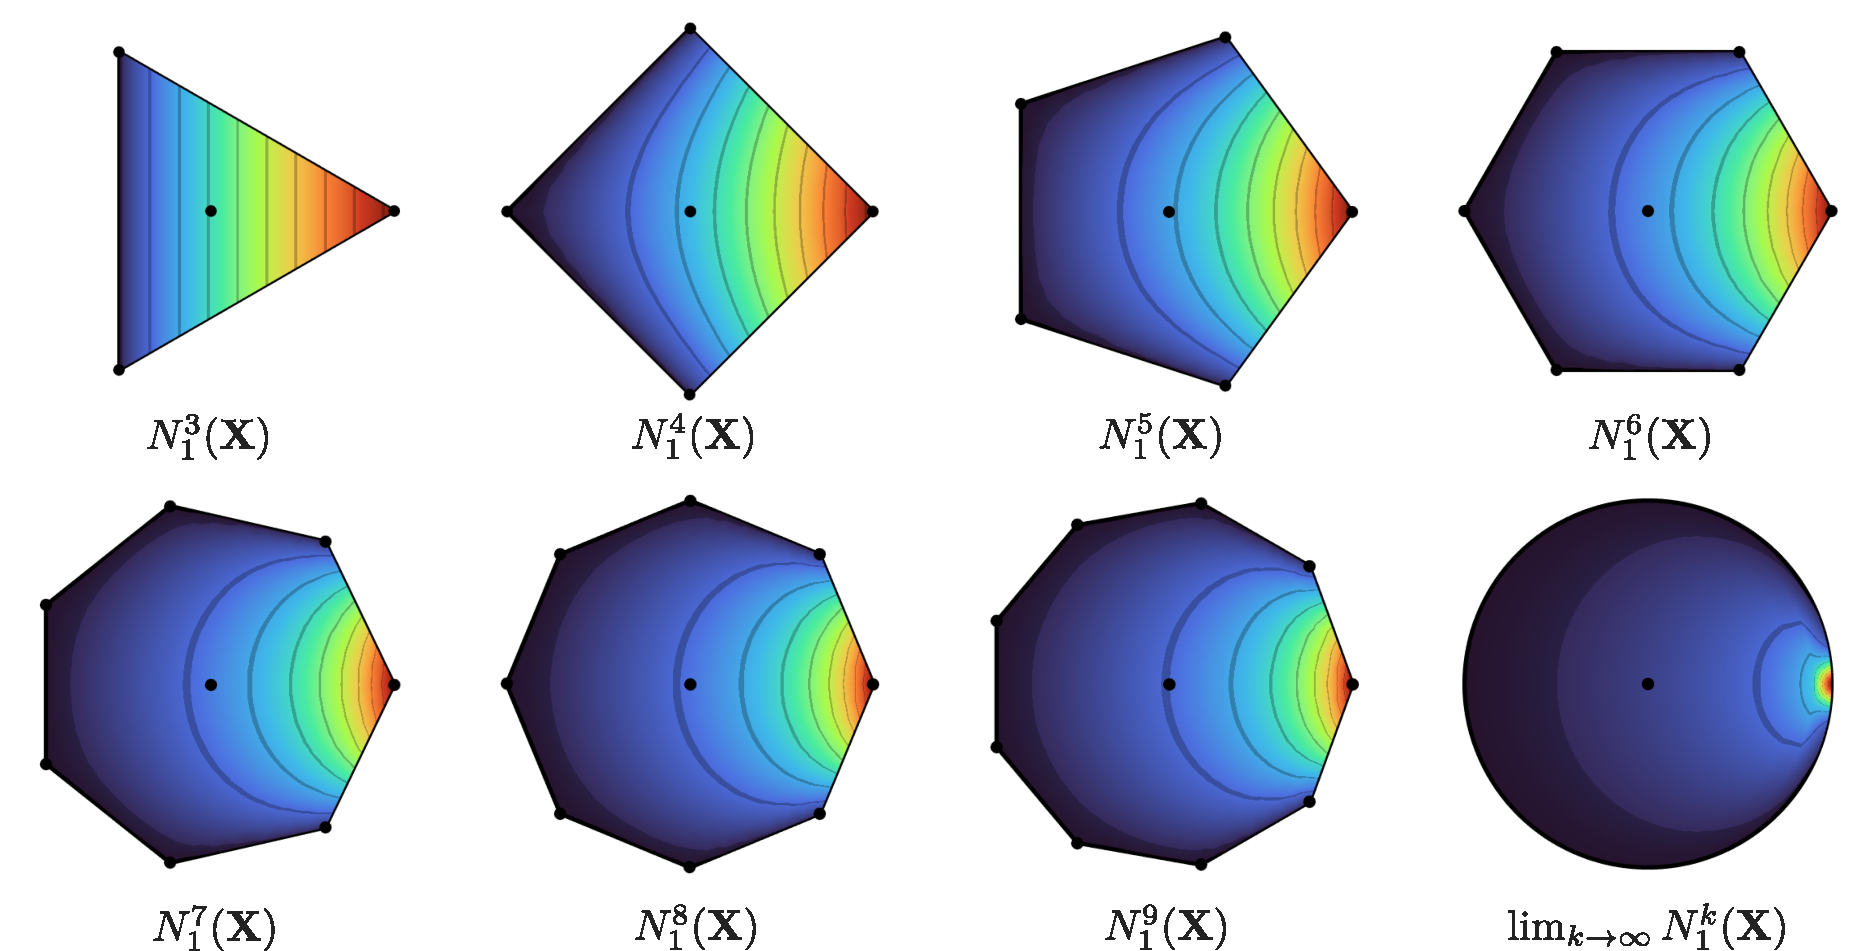
\includegraphics[width=\textwidth]{./pdf/thesis-figure-3-wachpress.pdf}
\caption{Wachspress shape functions related to the first nodal coordinate for an increasing polygonal degree $k$. The colormap depicts the intensity of the shape function $N_1^k$ with \protect\colormapcaption{0}{.75cm}$\!\!\in [0,1]$.}
\label{fig:C3:wachpressExample}
\vspace{-3mm}
\end{figure}
%

%With a discretized domain in mind, we can collect all the nodal displacements $\xB^{e}$ into one vector, called the global displacement vector $\xB = \textrm{col}(\x^{1},\x^{2},...,\x^{n_e})$. Similarly, we have a global virtual displacement vector $\delta \x$. 
Finally, by substitution of the spatial interpolations of the displacement $\dB \approx \NB^e \xB^e$ and virtual displacements $\delta \dB \approx \NB^e\delta \xB^e$, we can reformulate the residual in \eqref{eq:C3:residual_scalar} as follows
%
\begin{align}
r & \approx \sum_{e=1}^{n} ({\delta \xB}^e)^\top \left(\int_{\mathcal{V}_e} \BB_e(\x^e)^\top \underline{\ten{S}}_e(\x^e) \; dV  - \int_{\mathcal{V}_e} \NB^{e} \fB_{\textrm{b}} \; dV  - \int_{\p \mathcal{V}_e} \NB^{e} \fB_{\textrm{t}} \; dS \right), \notag \\[0.5em]
& = {\delta \x}^\top \left( \fB_{\textrm{int}}(\xB) - \fB_{\textrm{ext}} \right),
\end{align}
%
where $\x$ and $\delta \x$ are the global nodal displacement and the global nodal virtual displacement vectors, and $\BB_e$ and $\underline{\ten{S}}_e$ the elemental strain-displacement matrix and Piolla stress tensor, respectively. The derivation of these elemental matrices is found Appendix \ref{app:C3:straindisplacement} which follows the work of Kim et al. \cite{Kim2018}. Since the entries of the displacement variation ${\delta \x}$ are zero at nodes where displacement is prescribed (\ie, fixed DoFs), we may consider an alternative form, the residual force vector, in which the virtual displacements are omitted by only regarding the free DoFs:
%
\begin{equation}
\rB(\x) = \fB_{\textrm{int}}(\x) - \fB_{\textrm{ext}},
\label{eq:residual}
\end{equation}
%

The static equilibrium of the structure can be determined by setting $\rB(\x)$, as given in \eqref{eq:residual}, equal to the zero vector. To obtain this equilibrium state, the Newton-Raphson method can be utilized through iterative calculation of a linear system \cite{Gain2013Dec,Kim2018,Holzapfel2002}:
%
\begin{align}
\x^{(i+1)} & = \x^{(i)} -\alpha \left(\KB_T^{(i)}\right)\inv \rB^{(i)},
\end{align}
%
where $\alpha>0$ an update coefficient, and the subscript $(i)$ denotes the iteration steps, while $\x^{(i)}$, $\rB^{(i)} := \rB(\x^{(i)})$, and $\KB_T^{(i)}:=\left[\tfrac{\p \rB}{\p x_1} \; \hdots \; \tfrac{\p \rB}{\p x_n} \right]_{\x = \x^{(i)}}$ represent the updated displacement vector, the residual force vector, and the evaluated tangent stiffness matrix, respectively. For further details on the derivation of the tangent stiffness based on the Yeoh elasticity model in \eqref{eq:C3:psi_model_yeoh}, we refer \cite{Renaud2011}, whose approach is outlined in Appendix \ref{app:C3:yeohmodel}.

% \begin{example}[Hyper-elastic uniaxial tension]
% %Before continuing
% \end{example}
\section{Nonlinear topology optimization}
\label{sec:C1:topo} 
The present study focuses on the solution scheme for nonlinear deformations in hyper-elastic continuum solids. To enhance this approach, we introduce a modification to the Finite Element Method (FEM) model, known as the Solid Isotropic Material With Penalization (SIMP) method. This method is a widely used material interpolation scheme in topology optimization \cite{Bendsoe2003,Gain2013Dec,Talischi2012Mar,Vasista2013Jul}. Subsequently, we elaborate on how the optimization problem can be formulated to generate topologies driven by soft fluidic actuation.

\subsection{Solid Isotropic Material With Penalization (SIMP)}
In the SIMP approach, each finite element $e \in \{1,2,...,n\}$ is assigned with a scalar density variable $\rho_e \in [0,1]$ to indicate if an elemental volume is solid ($\rho_e = 1$) or void ($\rho_e = 0$). This leads to a real-valued density field representing the material distribution within a discretized domain $\mathcal{B}_0$, where the global material distribution is represented by the density vector $\vec{\rho} = \left(\rho_1,\,\rho_2,\,...,\,\rho_n\right)^\top$. The density vector $\vec{\rho}$ then form the design variables of the optimization problem. To relate these artificial densities to elasticity, the strain energy density of the constitutive material model ${\Psi}$ is then parameterized using $\vec{\rho}$. To improve numerical robustness, a modified SIMP approach is used in which the strain-energy function is artificially modified as follows:
%
\begin{equation}
{\Psi}_e = [\,\varepsilon + (1-\varepsilon)\,{\rho_e}^p\,]\, {\Psi}, \label{eq:simp}
\end{equation}
%
where $p\ge 1$ is the penalty factor for penalizing intermediate densities during the optimization process, and $0 < \varepsilon \ll 1$ is a lower-bound on the material densities. In this work, we choose $p = 4$ and $\varepsilon = 10^{-3}$. Given the artificial elasticity model above, it shall be clear that residual vector in \eqref{eq:residual} now depends on the nodal displacements and the densities of the adaptive topology, $\boldsymbol{x}$ and $\boldsymbol{\rho}$, respectively.

\subsection{Artificial fluidic loads by elemental dilation}
The most general principle of actuation in soft robotics involves pneumatic networks embedded in the elastic body. However, within the context of topology optimization, describing internal fluidic loads can be challenging. Unlike conventional optimization problems with static loads, in a pressure-based problem, the location, direction, and magnitude of the load change concerning the material distribution at every optimization step. This inherently yields design-dependency in the global force vector. To resolve this difficulty, we exploit the connectivity properties of polygonal tessellations to describe the physics involving pneumatics efficiently. Specifically, isolated regions of void polygonal elements will artificially mimic the geometrical loads in pneumatic actuation by volumetric expansion or contraction.

To identify void regions in the topology, we introduce the notion of a so-called "\emph{virus}" element whose purpose is to infect neighboring elements with a low elemental density (voids). These virus elements are chosen \textit{a-priori} and remain invariant, similar to the input of a pneumatic network. If the elements adjacent to an infected element have a density lower than a specified threshold $\gamma$, that is, $\rho_e < \gamma$, they become infected, and its infection rule will spread to its adjacent neighborhood. Afterwards, each infected element will be influenced by the same pneumatic load. Clearly, as the topological layout of the discretized domain $\mathcal{B}_0$ changes during the optimization procedure, the influence of the pneumatic load will vary accordingly. To better reflect the physics involving pneumatics, facial connectivity must be qualified for infection, where two elements must share a common edge to be adjacent, \ie, edge connection rather than node connection.


A flood-fill algorithm is used \cite{Chartrand1977Jan} to find the affected region of a virus element efficiently. In case of irregular tessellations, like the Voronoi tessellation, the flood-fill algorithm requires an adjacency matrix $\boldsymbol{\Gamma}$, which contains information about the mesh connectivity. The adjacency matrix can be directly computed from the element-node-incidence matrix. Here, the incidence matrix $\boldsymbol{A} \in \Z^{n\times m}$ is a sparse unit-matrix with $n$ columns for each element and $m$ rows for each node, where $\boldsymbol{A}_{ij} = 1$ iff node $i$ is incident upon element $j$, and otherwise zero. Given the incidence matrix, the adjacency matrix $\boldsymbol{\Gamma}\in \Z^{n\times n}$ can be computed by
%
\begin{equation}
\boldsymbol{\Gamma} = \boldsymbol{A}\boldsymbol{A}^\top - \text{diag}(\boldsymbol{A}\boldsymbol{A}^\top), \label{eq:adjecency}
\end{equation}
%
where the matrix has non-zero entries $\boldsymbol{\Gamma}_{ij} = 1,2$ iff elements $i$ and $j$ share a common node or edge, respectively. As mentioned earlier, the adjacency will be modified such that edge connectivity is required for adjacency. Secondly, all the rows and columns corresponding to elements that satisfy $\rho_e \ge \gamma$ will be set to zero to ensure those elements are unaffected by the flood-fill. The pseudo-code for the identification of the pneumatic region is provided in Algorithm \ref{alg:floodfill}.

\begin{algorithm}[!t]
    \SetKwInOut{Input}{Input}
    \SetKwInOut{Output}{Output}
    \Input{Tessellation $\mathcal{T}$, set of virus elements $\mathcal{V}$, threshold $\gamma$, material density vector $\boldsymbol{\rho}$}
    \Output{Set of elemental indices $\mathcal{E}$}
    construct $\boldsymbol{\Gamma}  \gets {\texttt{BuildAdjacencyMatrix}}(\mathcal{T})$\;
    modify $\boldsymbol{\Gamma}  \gets {\texttt{EdgeConnectivity}}(\boldsymbol{\Gamma})$\;
    find thresholds $\mathcal{X} = \{\, i \in [1,n] \;|\; \rho_i \ge \gamma \,\}$\;
    set zeros $\boldsymbol{\Gamma}_i = (\boldsymbol{\Gamma}^\top)_i = 0$ for all $i \in  \mathcal{X}$\;
    initialize empty set $\mathcal{E} \gets \emptyset$\;
  \For{$i = 1: \textrm{numVirus} $}{{}
  $\mathcal{I} \gets {\texttt{doFloodFill}}(\boldsymbol{\Gamma},\mathcal{V}_i)$\;
  %$\text{bool} \gets \textbf{isEnclosed}(\mathcal{I})$\;
        $\mathcal{E} \gets \mathcal{E} \cup \mathcal{I}$\;
  }
    \caption{Find elements subjected to volumetric deformation \label{alg:floodfill}}
\end{algorithm}

From a mathematical perspective, let us consider Algorithm \ref{alg:floodfill} which can be represented by a mapping $\phi: \R^n \mapsto {\Z}$. Here, the mapping $\phi(\boldsymbol{\rho})$ returns a set of elemental indices of infected elements denoted by $\mathcal{E} \subseteq {1,2,...,n}$ that undergo volumetric compression or expansion based on boundary conditions. Using this mapping, we can assemble the global force matrix $\boldsymbol{f}$ in \eqref{eq:residual} from the elemental force vectors of the affected region of the virus element $\mathcal{E}$:
%
\begin{equation}
%\boldsymbol{f}(\boldsymbol{x},\boldsymbol{\rho}) = \sum_{e \in \mathcal{E}} \tilde{p}_n \boldsymbol{W}_{\!e} \boldsymbol{K}_e \boldsymbol{n}_e, \label{eq:pressureforce}
\fB_{\textrm{ext}}(\boldsymbol{x},\boldsymbol{\rho}) = \sum_{e \in \mathcal{E}} \tilde{p}_e \boldsymbol{W}_{\!e} \, \boldsymbol{t}_{e}, \label{eq:pressureforce}
\end{equation}
%
where $\tilde{p}_e$ is a dimensionless parameter that represents the magnitude and direction of artificial pneumatic loading. $\boldsymbol{W}_{\!e}$ is a diagonal weighting matrix of densities at nodal level, and $\boldsymbol{t}_e = \int_{\mathcal{V}_e} \BB_e^\top \mathbb{D}_e \nB_v \; dV$ is the elemental force vector. The volumetric strain is represented by $\boldsymbol{n}_{v} = [1,1,0]^\top$, and $\mathbb{D}_e := \p \ten{S}/\p \ten{E}$ is the fourth-order constitutive elasticity tensor in matrix notation \cite{Renaud2011}. It is important to note that the global force vector in \eqref{eq:pressureforce} represents an artificial pneumatic load. This method assumes that pressure loads can be emulated by anisotropic volumetric change of the polygonal elements. By varying the dimensionless parameter $\tilde{p}_e$, the magnitude and direction of this artificial pneumatic load can be controlled.

\subsection{Optimization problem}
Given the concept of morphology in soft robotics, which is similar to compliant mechanisms, the primary goal is to maximize the output displacement $\boldsymbol{x}_{out}$ on a virtual workpiece modeled by an artificial stiffness $k_{out} > 0$ \cite{Bendsoe2003,Gain2013Dec}. The objective function or the desired output displacement can be expressed as $\Phi = \boldsymbol{L}^\top\boldsymbol{x}(\boldsymbol{\rho})$, where $\boldsymbol{L} \in \R^{2n}$ is a sparse vector composed of non-zero entries for the degrees-of-freedom corresponding to the desired morphology of the soft robot. Given this description of directional output displacement, the topology optimization problem for soft robots can be formulated as:
\begin{equation}
\begin{aligned}
\max_{\boldsymbol{\rho}} \quad &  \Phi = \boldsymbol{L}^\top \boldsymbol{x}(\boldsymbol{\rho}), \\
\textrm{s.t.} \quad & c:=\boldsymbol{R}(\boldsymbol{x},\boldsymbol{\rho}) \,= \,0,\\
& g:=\boldsymbol{v}^\top \boldsymbol{\rho}  \le V^\star, \\
  &\boldsymbol{\rho} \in \mathcal{P},
  \label{eq:opt}
\end{aligned}
\end{equation}
where $\boldsymbol{R} \in \R^{2n}$ the global residual force vector in its equilibrium state, $\boldsymbol{v} \in \R^{m}$ a constant vector of relative elemental volumes, $ 0 < V^\star < 1$ the desired material infill, and $\mathcal{P} = \{\boldsymbol{\rho} \in \R^n \; | \; 0  \le \rho_e \le 1 \; \forall e \in [1,n] \}$ a set of feasible material densities that ensure numerical robustness.

\subsection{Solver and sensitivity analysis}
In this section, we discuss the use of a gradient-based optimization solver for synthesizing the soft robot. Here, we use the Method of Moving Asymptotes (MMA) proposed by Svanberg \cite{Svanberg1987Feb}. The MMA is similar to other nonlinear programming approaches, such as Optimality Criteria (OC) and Sequential Quadratic Programming (SQP), in that it finds an optimal solution to a nonlinear non-convex optimization problem with inequality constraints. The MMA solves a sequence of sub-problems, \ie, convex approximations of the true problem, which are constructed from gradient-based information of the objective function $\Phi$ and their constraints $c$ and $g$. Svanberg \cite{Svanberg1987Feb} has provided open numerical implementations for his MMA algorithm represented as MATLAB function called \texttt{mmasub}, which is subroutine of the MMA algorithm that updates the design parameters $\vec{\rho}^{(k)} \to \vec{\rho}^{(k+1)}$ given the design sensitivities of the objective $\Phi$ and the equality and inequality constraints $c$ and $g$, respectively. By recursively calling \texttt{mmasub}, the optimization problem in \eqref{eq:opt} can be solved numerically.

The sensitivity of the inequality constraint in \eqref{eq:opt} is $\frac{\partial g}{\partial \boldsymbol{\rho}} = \boldsymbol{v}$ since we assume that the elemental volume $\boldsymbol{v}$ is constant. The sensitivity of the objective function is less trivial due to its dependency on the nodal displacements $\boldsymbol{x}(\boldsymbol{\rho})$. Since it is computationally expensive to obtain the displacements $\boldsymbol{x}$ through the Newton-Raphson method, it becomes beneficial to avoid the computation of their sensitivities. Thus, the sensitivities are computed through the adjoint method in which the objective function is augmented to include the equality constraint $c$. This leads to
%
\begin{equation}
{\Phi}(\xB,\vec{\rho}) = \boldsymbol{L}^\top \boldsymbol{x}(\vec{\rho}) - \boldsymbol{\lambda}^\top \boldsymbol{R}(\xB,\vec{\rho}),
\end{equation}
%
where $\boldsymbol{\lambda} \in \R^{2n}$ is a constant vector referred to as the adjoint vector. Note that, in case of equilibrium (\ie, $\boldsymbol{R} = \vec{0}_n$), the global residual forces are equivalent to zero; therefore, the adjoint vector can be chosen freely without violating the original optimization problem. 
%For the sake of brevity, we denote differentiations by $\p(\cdot)/\p x := (\cdot),_{x}$. 
Differentiations of the objective function with respect to the elemental densities $\rho_e$ for each finite element $e \in \{1,2,...,n\}$ yields
%
\begin{align}
\frac{\p \Phi}{\p {\rho_e}} & = \,\boldsymbol{L}^\top \frac{\p \x}{\p \rho_e} - \boldsymbol{\lambda}^\top\left(\frac{\p \boldsymbol{R}}{ \p \x} \frac{\p \x}{\p \rho_e} + \frac{\p \boldsymbol{R}}{ \p \rho_e} \right), \notag \\[0.75em]
 & = \left(\boldsymbol{L}^\top - \boldsymbol{\lambda}^\top \boldsymbol{K}_T \right) \frac{\p \boldsymbol{x}}{\p \rho_e} - \boldsymbol{\lambda}^\top \frac{\p \boldsymbol{R}}{\p \rho_e},  \label{eq:sen_deriv} 
\end{align}
%
\noindent where the Jacobian of the residual force vector is substituted by the tangent stiffness matrix $\KB_T:=\tfrac{\p \RB}{\p \x}$ (see \cite{Kim2018}). By choosing the adjoint vector $\boldsymbol{\lambda} = (\boldsymbol{K}_T)^{-T}\boldsymbol{L}$, the terms involving $\tfrac{\p \x}{\p \rho_e}$ can be eliminated and thus computation of the gradient becomes feasible. Following this, the gradient of the objective function can be written compactly as:
%
\begin{align}
\frac{\p {\Phi} }{\p \rho_e} \overset{\eqref{eq:residual}}{=} -\boldsymbol{L}^\top(\boldsymbol{K}_T)^{-1} \left( \sum_{e=1}^{n} \int_{\mathcal{V}_e} \boldsymbol{B}_e^\top \frac{\p \underline{\ST}_e}{\p {\rho_e}} \; dV - \frac{ \p \fB_{\textrm{ext}}}{\p {\rho_e}}  \right). \label{eq:sens_f}
\end{align} 
%

\noindent However, it should be noted that deriving the loading sensitivity $\p \boldsymbol{f}_{\textrm{ext}}/\p \rho_e$ is not straightforward since the global force vector is constructed from nested functions of logic operations such as flood-fill. Therefore, we derive the loading sensitivity numerically using the forward difference method. To reduce computation time, we propose computing the sensitivities of only the elements at the boundary of the pressure region since the gradient of the pneumatic region is largest near the boundary of the infected set $\mathcal{E}$. We provide pseudo-code for the computational design algorithm for synthesizing pressure-driven soft robots in Algorithm \ref{alg:topology_opt}. 

\begin{algorithm}[!h]
  \SetKwInOut{Input}{Input}
  \SetKwInOut{Output}{Output}
  \Input{Domain $\mathcal{B}_0$, material $\Psi$, initial $\boldsymbol{\rho}^{(0)}$, infill $V^*$, virus $\mathcal{V}$, output $\boldsymbol{L}$, artificial pressure $\tilde{p}_e$ }
  \Output{Optimal soft robot topology $\boldsymbol{\rho}^*$}
  construct tessellation $\mathcal{T} \gets {\texttt{VoronoiMesher}}(\mathcal{B}_0)$\;
  \While{$\text{convergence} \neq 1 $}{
  update artificial material $\Psi_e$ using \eqref{eq:simp} \;
  find infected set $\mathcal{E}$ using \textbf{Algorithm 1} \;
  build residual forces $\boldsymbol{R}$ using \eqref{eq:residual} and \eqref{eq:pressureforce}\; 
  solve displacements $\boldsymbol{x} \gets \texttt{NewtonRaphson}(\boldsymbol{R})$ \;
  evaluate $g,_{\boldsymbol{\rho}} \gets \p g/\p{{\rho}_e}$ \;
  evaluate $\Phi,_{\boldsymbol{\rho}} \gets\p\Phi/\p{{\rho}_e}$ using \eqref{eq:sens_f} \; 
  update $\boldsymbol{\rho} \gets \texttt{MMA}(\Phi,_{\boldsymbol{\rho}},g,_{\boldsymbol{\rho}},\boldsymbol{\rho})$ \;
  }
  \caption{Computational design algorithm for pneumatic soft robots.\label{alg:topology_opt}}
\end{algorithm}
\clearpage

\subsection{Gradient filters and interpolation}
A well-known filtering technique is used to solve this issue, which has been proposed by Sigmund et al. \cite{Bendsoe2003}. The design sensitivities are modified based on a weighted average filtering scheme \cite{Gain2013Dec,Bendsoe2003}:
%
\begin{equation}
\frac{\p \tilde{\Phi}}{\p {\rho_e}} = \frac{1}{\rho_e \sum^n_{i=1} H_{e,i}} \sum^n_{i=1} H_{e,i} \,\rho_i \frac{\p {\Phi}}{\p {\rho_i}},
\label{eq:C3:filters}
\end{equation}
%
where $H_{e,i} := \textrm{max} \left\{0, R_{\textrm{min}} - \Delta(\pB_e,\pB_i)\right\}$ is the filter weight, $R_{\textrm{min}}$ is the filter radius, and $\Delta(\pB_e,\pB_i)$ is the Euclidean distance between the centers of the elements $i$ and $e$. The radial filtering is solely applied to the design sensitivities, and therefore, the polygonal mesh discretization heavily influences the final topology design. In order to improve the quality of optimization output, we implement Radial Basis Functions (RBF) interpolation that is weighted with filter densities. This is followed by an isosurface extraction process that aids in achieving a distinct separation between void and filled regions. Mathematically, the filter topology of the optimization routine is given by 
%
\begin{equation}
\mathcal{B}^\star = \Big\{ \XB \in \mathcal{B}_0 ~
|~ \sum_{i=1}^{n_e} \psi_i(\XB - \pB_i) \ge \epsilon_\textrm{iso}\Big\}
\end{equation}
%
where we explore a radial interpolation function $\psi_i(\rB) = \exp\left( - \alpha \rho_i \lVert\rB\rVert^2 \right)$ with $\alpha > 0$ a tuning parameter, and $\epsilon_{\textrm{iso}}$ is the isosurface value. The parameter $\alpha$ enables users to regulate the thickness (or radial dilation) of the optimized soft topology. For our specific investigation, we opt for $\alpha = R_\textrm{min}$ to ensure it aligns with the filter radius in equation \eqref{eq:C3:filters}. A visual representation of this process can be seen in Figure \ref{fig:C3:topo_filtering}.

\begin{figure}[!t]
  \centering
  \vspace{4mm}
  \input{./pdf/thesis-figure-3-1.pdf_tex}
  \caption{An illustration of filter and interpolation schemes developed to minimize mesh artifacts. (a) The ground truth. (b) the raw element-wise density field based on the ground truth. Note the jitter around the boundaries of the material infill, which leads to high sharp gradients in $\tfrac{\partial \phi}{\partial \rho_e}$. (c) To address this issue, filtered densities are obtained using \eqref{eq:C3:filters}. (d) The isosurface reconstruction $\mathcal{B}^\star$ of the filtered density field of the optimizer.}
  \label{fig:C3:topo_filtering}
\end{figure}


\section[Numerical examples: generating soft robotic topologies]{Numerical examples: generating soft robotic topologies via optimization}
\label{sec:C1:results}
The proposed computational algorithm enables the synthesis of various topologies of soft robots exhibiting diverse motions. The choice of output vector $\LB$ is arbitrary, allowing for the generation of motion patterns that are useful in soft robotic locomotion or grasping by customizing the objective function. Our analysis focuses on three cases: ($i$) linear elongation or contraction, ($ii$) distributed bending, and ($iii$) grasping. All simulations are conducted using MATLAB\textsuperscript{\scriptsize\textregistered} on a modern machine (Ryzen 7-5800H, 3.2GHz). Unless stated otherwise, all simulation examples employ the same material model, specifically, the Yeoh parameters $c_1 = 35$ kPa, $c_2 = 0.25$ kPa, and $c_3 = 0.023$ kPa, which are based on the silicone elastomer Dragonskin 10A\textsuperscript{\scriptsize\texttrademark\!} \cite{Xavier2022Jun}.

\subsection{Linear translational soft actuators}
One of the simplest forms of motion in soft robotics is linear translation. Such motion can be achieved through the use of various topologies, such as the McKibben actuator or a serial chain for bellow-type actuators. Both of these soft actuation principles operate similar: pressurized fluid is applied to an enclosed interior, and due to low-axial compliance compared to the radial compliance imposed by geometrical shape (\eg, bellow shape) or material composites (\eg, McKibben \cite{Paynter1974,Paynter1988}), linear motion is produced.  Given their linear motion, these system are often associated with bio-inspired muscle, due them acting similar to hydrostatic muscular system found in nature \cite{Kier1985}. 
 
In the first optimization benchmark we aim to find the optimal topology for a soft fluidic muscle. Exploring spatial symmetry, we consider a rectangular material domain $\mathcal{B}_0$ of dimension $20 \times 10$ \si{\milli \meter}, which forms the upper-left quadrant of the pneumatic soft muscle. This makes the cross-sectional size of the bellow $40$ \si{\milli \meter} in width and $20$ \si{\milli \meter} in height. The bottom of upper-left quadrant is structurally fixed, the left wall can move only vertically (symmetric boundary condition), and the other boundaries can move freely. The objective of the optimization is to maximize the displacement of the top-left corner in positive vertical direction. The top corner is equipped with an artificial spring $k_{out} = 1.0$ \si{\newton \per \milli \meter}. The material infill is set to $V^\star = 0.25$ (\ie, a material infill of 25\%). As for the initial conditions, we consider small circular hole of $3$ \si{\milli \meter}, which also resides the virus element subjected to an artificial pressure parameter $\tilde{p}_e = 0.01$. In our analysis, we consider $n=$10k elements.
%
\afterpage{
\begin{figure}[!t]
  \centering
  \vspace{-3mm}
  %\includegraphics[height=0.33\textwidth]{./img/topo_bend/resultTopo.eps}
  \includegraphics*[width=0.95\textwidth]{./pdf/thesis-figure-3-3.pdf}
  \caption{Evolution of topology optimization solver for the linear soft actuator, where $V^\star = 0.25$. The areas (\textcolor{matinfil}{$\blacksquare$}, \textcolor{lightvoid}{$\blacksquare$}, \textcolor{lightblue}{$\blacksquare$}) denote the material infill, void, and fluidic region, respectively. It can be observed that after a few iterations, a shape appears that is reminiscent of the conventional bellow. It is noteworthy that the shape is non-convex, with a slight curvature inwards, which enhances elongation without introducing excessive ballooning.}
  \label{fig:C3:topo_result_bellow}
\end{figure}
%
\begin{figure}[!t]
  \centering
  \vspace{-3mm}
  %\includegraphics[height=0.33\textwidth]{./img/topo_bend/resultTopo.eps}
  \includegraphics*[width=0.95\textwidth]{./pdf/thesis-figure-3-4.pdf}
  \caption{(left) Numerical validation of the optimized linear soft actuator, where the Von Mises stress is shown using the colormap \protect\colormapcaption{0}{.75cm}$\!\!\in [0,12]$ \si{\mega \pascal}. (right) Input-displacement characteristic of the optimized soft actuator.}
  \label{fig:topo_result_bellow_fem}
  \vspace{-3mm}
\end{figure}
}

The evolution of the optimization solver is presented in Figure \ref{fig:C3:topo_result_bellow}. Interestingly, it reveals a bellow-shaped soft actuator structure, bearing resemblance to those commonly utilized in engineering applications. Additionally, the optimizer generates a non-convex bellow with  slightly curvature inward. This shape is intended to decrease the axial stiffness of the soft actuators, thereby reducing ballooning during significant elongation. Similar concave bellow designs have been seen in Festo's Bionic Arm \cite{Hairer2002}. The numerical validation of the structure is shown in Figure \ref{fig:topo_result_bellow_fem}, which indicate that the soft topology can achieve 100$\%$ extension at 10 \si{\kilo \pascal}. It is important to note, however, that the slope of the input-output trend is positive decreasing, which suggests that further increase in pressure may eventually lead to ballooning.

\subsection{Pinching soft grippers}
\label{sec:C3:Gripper_results}
The second optimization benchmark involves the study of compliant mechanisms that are capable of transforming linear forces into grasping or pinching motions. In this analysis, we aim to investigate similar motions through fluidic actuation. It is a well-known issue in optimization for gripping mechanics that solvers frequently generate thin hinge-like structures that are susceptible to high stress concentration \cite{Bendsoe2003,Luo2016Mar}. We hypothesize that our soft material setting can naturally mitigate this problem, due to low material compliance and enabling large deformation.

The soft fluidic gripper's design domain is assumed to be symmetrical. Therefore, only the top half of the mechanism, with dimensions of $45 \times 15$ \si{\milli \meter}, is considered. The left side is fixed structurally, while the bottom can move horizontally due to the symmetry condition. On the right side, a cut-out is introduced, which serves as the gripper region. The objective of the optimization is to maximize the displacement of the gripper corner in negative vertical direction. This top corner is equipped with an artificial spring $k_{out} = 1.0$ N/mm, and the material infill is set to $V^\star = 0.30$ (\ie, a material infill of 30\%). As for the initial conditions, we consider circular hole of radius $6$ \si{\milli \meter} at the left side. Concerning the pneumatic actuation, the adaptive topology is subjected to an artificial pressure parameter $\tilde{p}_e = 0.01$, where the virus element is also located at the left side. In our analysis, we consider $n=$20k elements.

\begin{figure}[!t]
  \centering
  \vspace{-3mm}
  %\includegraphics[height=0.33\textwidth]{./img/topo_bend/resultTopo.eps}
  \includegraphics*[width=0.95\textwidth]{./pdf/thesis-figure-3-7.pdf}
  \caption{\small Evolution of topology optimization solver for the soft fluidic gripper, where the material infill is $V^\star = 0.30$. The areas (\textcolor{matinfil}{$\blacksquare$}, \textcolor{lightvoid}{$\blacksquare$}, \textcolor{lightblue}{$\blacksquare$}) denote the material infill, void, and fluidic region, respectively. The optimizer proposes a topology with a large tear-shaped pressure vessel, whose walls are connected to small struts that transfer the gripping motion.}
  \label{fig:C3:topo_result_gripper}
  \vspace{-3mm}
\end{figure}

\begin{figure}[!t]
  \centering
  \vspace{-3mm}
  %\includegraphics[height=0.33\textwidth]{./img/topo_bend/resultTopo.eps}
  \includegraphics*[width=0.95\textwidth]{./pdf/thesis-figure-3-6.pdf}
  \caption{\small (left) Numerical validation of the optimized linear soft actuator, where the Von Mises stress is shown using the colormap \protect\colormapcaption{0}{.75cm}$\!\!\in [0,25]$ \si{\mega \pascal}. (right) Input-displacement characteristic of the optimized soft actuator. Notice that at $u \ge 10$ \si{\kilo \pascal} no further deformations occurs at end-effector level as the gripper tips are in contact.}
  \label{fig:C3:topo_result_gripper_fem}
\end{figure}

The evolution of the optimization solver is presented in Figure \ref{fig:C3:topo_result_gripper}. The proposed solution consists of a tear-shaped pressure vessel, whose walls are connected to a compliant mechanism through struts that transfer volumetric deformation to pinch-grasping motions. This gripper mechanism is similar to those found in literature \cite{Gain2013Dec,Bendsoe2003}, which involve a central revolute compliant joint, resembling scissors. To validate the proposed structure, we converted the final 2D topology result shown in Figure \ref{fig:C3:topo_result_gripper} into a nonlinear FEM model and subjected it to an input pressure of $u = 10$ \si{\kilo \pascal}. The numerical validation results are presented in Figure \ref{fig:C3:topo_result_gripper_fem}, which also shows the relationship between pressure and gripper distance. Our numerical results demonstrate that gripping morphologies arise when the structure is subjected to positive pressure, where a closed grasp is achieved at an activation pressure of $u \ge 10$ \si{\kilo \pascal}.

\subsection{Bending soft actuator -- PneuNet inspired}
\label{sec:C3:PneuNet_results}
Next, we focus on soft actuator that produce distributed bending. Such morphology is often associated with the popular class of soft actuators named "\emph{PneuNet}" actuators \cite{Polygerinos2013,Polygerinos2015,Galloway2016,Hughes2016Nov,Marchese2015}. PneuNet actuators consist of a set of rectangular pneumatic chambers inside an elastomer medium. When pressurized, these chambers inflate, and due a structural stiffness gradient, the elastomer body undergoes bending. Typically, inextensible composite materials are used at the bottom of the structure to further such stiffness gradient and therefore enhance bending. The goal of this numerical study case is to synthesize a soft robot topology that undergoes bending motion similar to the PneuNet actuator. 

In our example, the following settings are chosen. We consider a rectangular design domain $\mathcal{B}_0$ with dimensions 20$\times$40 mm (as shown in Fig. \ref{fig:topo_result}). The maximum material infill is $V^\star = 0.3$ (\ie, a material infill of 30\%). The bottom left corner is fixed, and the right bottom corner is equipped with an artificial spring $k_{out} = 1.0$ N/mm. The objective of the optimization is to maximize the vertical displacement of the left bottom corner in the negative vertical direction. Concerning the pneumatic actuation, the adaptive topology is subjected to an artificial pressure parameter $\tilde{p}_e = 0.01$, where the virus element is located at the center.

\begin{figure}[!t]
\centering
%\vspace{-3mm}
%\includegraphics[height=0.33\textwidth]{./img/topo_bend/resultTopo.eps}
\includegraphics*[width=0.95\textwidth]{./pdf/thesis-figure-3-2.pdf}
\caption{\small Evolution of topology optimization solver for the bending soft actuator, where $V^\star = 0.30$. The areas (\textcolor{matinfil}{$\blacksquare$}, \textcolor{lightvoid}{$\blacksquare$}, \textcolor{lightblue}{$\blacksquare$}) denote the material infill, void, and fluidic region, respectively. The optimization process results in a topology that bears resemblance to that of conventional PneuNets, with the exception that the pressure chambers take on a tear-shaped form. Additionally, the optimizer generates an in-extensibility layer by depositing more material at the bottom. }
\label{fig:topo_result}\end{figure}

\begin{figure}[!t]
  \centering
  %\vspace{-3mm}
  %\includegraphics[height=0.33\textwidth]{./img/topo_bend/resultTopo.eps}
  \includegraphics*[width=0.95\textwidth]{./pdf/thesis-figure-3-5.pdf}
  \caption{\small (left) Numerical validation of the optimized linear soft actuator, where the Von Mises stress is shown using the colormap \protect\colormapcaption{0}{.75cm}$\!\!\in [0,25]$ \si{\mega \pascal}. (right) Input-curvature characteristic of the optimized soft bending actuator. Notice that the input-output relation is closely linear, which traditionally is accomplished using composite materials by introducing inextensible layers \cite{Polygerinos2013,Polygerinos2015}.}
  \label{fig:topo_result_bellow_fem}
\end{figure}

Using the method described in Algorithm \ref{alg:topology_opt}, an optimized topology is obtained (as shown in Fig. \ref{fig:topo_result}). As can be seen, the computational algorithm provides a new and interesting variation on the well-familiar PneuNet actuator. Contrary to its rectangular predecessor, the optimal structure has a significant resemblance to a bellow-shaped actuator to accommodate bending mobility further. Here, however, these bellows are tear-shaped whose narrow side is oriented downwards. To validate our synthesized topology, a three-dimensional finite element analysis is conducted. First, we use Gaussian radial basis functions (RBFs) to reconstruct a smooth manifold surface from the discretized optimization mesh. Due to spatial symmetry, the spatial reconstruction can be horizontally repeated to construct a full `PneuNet' actuator, see Figure \ref{fig:topo_result}. The two-dimensional optimization is then transformed into an nonlinear FEM model. The pneumatic chambers are subjected to a positive differential pressure of $u = 15$ kPa. As can be illustrated by Figure \ref{fig:topo_result_bellow_fem}, the finite element analysis verifies that the synthesized soft robot topology accomplishes the desired bending morphology when pressurized.

\subsection{Solutions for varying material parameters}
A important aspect of topology optimization is that, in addition to selecting an objective function, the numerical solutions can be influenced by the choice of material. Particularly within the realm of soft robotics, which encompasses a wide range of soft material options, it is therefore paramount to explore various material parameters beyond the previously utilized Dragonskin 10 material with $c_1 = 36$ \si{\kilo \pascal}. In the analysis, we investigate four alternative materials commonly examined in the field: Ecoflex 00-30\textsuperscript{\scriptsize\texttrademark\!}, Ecoflex 00-50\textsuperscript{\scriptsize\texttrademark\!}, Dragonskin 30\textsuperscript{\scriptsize\texttrademark\!}, and NinjaFlex 85A\textsuperscript{\scriptsize\texttrademark\!}. It is important to note that all materials, except for NinjaFlex 85A\textsuperscript{\scriptsize\texttrademark\!}, are two-component castable silicone rubber materials, with NinjaFlex being a 3D-printable TPU material used for Fused Filament Decomposition (FDM) printing. By adopting material parameters derived from literature, we obtain the following material parameters: Ecoflex 00-10 with $c_1 = 8.7$ kPa \cite{Marechal2021Jun}; Ecoflex 00-50 with $c_1 = 19$ kPa \cite{Xavier2022Jun,Xavier2021Feb}; Dragonskin 30 with $c_1 = 96$ kPa \cite{Marechal2021Jun,Xavier2021Feb}; and NinjaFlex 85A with $c_1 = 2.3$ MPa\blankfootnote{Although \cite{Xavier2021Feb} presents the material model in the generalized Rivlin model, the material parameters for the Yeoh model can be found under consistency with linear elastic materials as $c_1 = 0.5(C_{01} + C_{10})$ with $C_{01}, C_{10}$ the Rivlin parameters.} \cite{Xavier2021Feb}. The compressibility parameters are chosen identical to previous simulations. In this investigation, we repeat the inverse design problem of the bending PneuNet actuator as in Section \ref{sec:C3:PneuNet_results}. 
%
\begin{figure}[!t]
  \centering
  %\vspace{-3mm}
  %\includegraphics[height=0.33\textwidth]{./img/topo_bend/resultTopo.eps}
  \includegraphics*[width=0.95\textwidth]{./pdf/thesis-fig-31.pdf}
  \caption{\small Design solutions found using optimization for different material models, arranged from left to right: Ecoflex 00--10, Ecoflex 00--50, Dragonskin 30, and NinjaFlex 85A, with a progressive increase in material stiffness. The areas (\textcolor{matinfil}{$\blacksquare$}, \textcolor{lightvoid}{$\blacksquare$}, \textcolor{lightblue}{$\blacksquare$}) denote the material infill, void, and fluidic region, respectively. It is worth noting that all of the optimization solutions exhibit a tear-drop-shaped bellows, which might suggest the existence of material-invariant (sub)-solutions to the inverse design problem of bending soft actuators composed of soft materials.}
  \label{fig:topo_result_different}
\vspace{-4mm}
\end{figure}

Figure \ref{fig:topo_result_different} shows the optimization solutions for various material choices. An interesting observation to note is that all topologies demonstrate a tear-drop-shaped bellows, as also observed in Section \ref{sec:C3:PneuNet_results} (and Section \ref{sec:C3:Gripper_results}). This observation might suggest the existence of generalized design solutions, or at the very least partial solutions, that seem invariant with respect to the material choice. The differences between solutions lie in $(i)$ the height, roundness, and volumetric capacity of the bellows, $(ii)$ the wall thickness, and $(iii)$ the topology of the "inextensible" layer at the bottom. Softer materials typically exhibit shorter and rounder bellows, while stiffer materials tend to favor rectangular geometries. With a stiffness value of $c_1 = 2.8$ MPa (\ie, the NinjaFlex 85A), this rectangular geometry is most pronounced, even pushing against the bounded design domain. This might suggest that the design domain is chosen too constrictively. Moreover, the volumetric capacity of the fluidic chamber is reduced, while the wall thickness is increased for softer materials. This can perhaps be attributed to the increased effort required to deform stiffer materials and the tendency for softer materials to experience ballooning earlier.

Another intriguing observation is the appearance, disappearance, and reappearance of optimal topological structures when traversing the elasticity spectrum of soft materials. In Figure \ref{fig:topo_result_different}, we see that for $c_1 = 8.7$ kPa (softest) and $c_1 = 2.8$ MPa (stiffest), both solutions favor a hinge-like structure. Yet, for intermediate values of $c_1$, the optimizer proposes an inextensible layer at the bottom. This finding is quite unexpected, as optimality in structural optimization may not exhibit a monotonic relationship with increasing material elasticity, whereas others, \eg, fluidic capacity and bellows height, appear to be monotonically correlated with $c_1$. We hypothesize that using an inextensible layer is too ineffective for softer material values (\ie, $c_1 < 8.7$ kPa) as their low elasticity cannot be used to constrain motion; thus a hinge-like structure is likely the more effective option for generating bending. Conversely, it is well-established that stiff materials tend to favor hinge-like structures for bending, as demonstrated in various studies on topology optimization for compliant mechanisms \cite{Bendsoe2003, Zhang2017Topo, Luo2016Mar}. Due to a lack of more precise terminology, we refer to this phenomenon as a \textit{transcritical bifurcation} in the optimization solution space, wherein there is an exchange of stability (\ie, convergence of the numerical optimization) between two fixed points depending on the material parameter $c_1$. As such, exploring a broad material spectrum during a topology optimization analysis might emphasize different solutions that can otherwise not be observed when fixing material models \textit{a-priori}.
\vspace*{-3mm}
\section{Conclusion}
In this chapter, we present a novel framework for synthesizing soft robot topologies from hyperelastic soft materials. The design synthesis of classic soft robots is challenging due to material nonlinearities and the numerical implementation of pressure-driven loads in a topology optimization framework. We proposed a nonlinear finite element method for polygonal elements to solve these problems. Compared to previous research, our numerical approach presents a better representation of the physical nature of soft robotics, in particular, the hyperelasticity and the pneumatic actuation. Numerical investigation shows that our framework can produce meaningful and insight-full material layouts when developing a pressure-driven soft robot from soft materials. We further establish that the exploration of a range of materials can potentially yield diverse design solutions, including those that are independent of the specific material used. Theoretically, the proposed framework can be adapted to also express other actuation principles in soft robotics, such as dielectric polymers or thermal expansion; however, minor changes are required. 

% *************************************************************
% *************************************************************
% *************************************************************
%\part[Model-based Control for Soft Robots]{Model-based Control \\ for Soft Robots}\label{part: model}
% *************************************************************
\chapter[Dynamic modeling of soft robots -- PCC case]{Dynamic modeling of soft robots \\ -- the constant strain approach}
\label{chap:PCC}
\blankfootnote{This chapter is based on: {B.J. Caasenbrood, A.Y. Pogromsky, and H. Nijmeijer. \textit{Control-oriented Models for Hyper-elastic Soft Robots through Differential Geometry of Curves.} Soft Robotics, 2022. \texttt{doi:} \url{10.1089/soro.2021.0035}}.}

%!TEX root = ../../thesis.tex
\chapterabstract{In this chapter, we derive continuum dynamic models for pneumatic soft robot manipulators through the differential geometry of spatial curves. These models are then related to Finite Element (FE) model to capture the intrinsic geometric and material nonlinearities. To accelerate numerical simulation, a reduced-order integration scheme is introduced to compute the dynamic Lagrangian matrices efficiently. This, in turn, allows for high-speed and (multi-link) dynamic models for soft manipulators with a minimal sacrifice in numerical precision. By exploring passivity ideas and a linear parametrization of hyper-elastic material coefficients, we propose a passivity-based adaptive controller that enhances robustness towards material uncertainty and unmodelled dynamics -- slowly improving their estimates online. As a study case, a fully 3D-printed soft robot manipulator is developed, which shows good correspondence with the dynamic model under various conditions, \eg, natural oscillations, forced inputs, and subjected to external disturbances like tip-loads. The solidity of the approach is demonstrated through extensive simulations, numerical benchmarks, and experimental validations.}

%!TEX root = ../../thesis.tex
\section{Introduction}
\label{sec: chap1 1_introduction}
Traditional robots are made from rigid and dense materials that ensure accurate and repeatable motions. While rigid robotics excel at fast and precise motion, their structural rigidity lacks the compliance and mechanical robustness needed for safe and passive interaction in an unknown environment. Soft robotics, on the other hand, aim to improve the motion complexity and environmental robustness that is generally lacking its rigid counterpart. To further promote these topics in robotics, researchers aim to mimic living creatures by developing bio-inspired robots with similar morphologies and mechanical properties \cite{Falkenhahn2015,Suzumori1991,Godage2015,Godage2016,Marchese2014,Kriegman2020}.
The hyper-flexible and continuum-bodied structure in soft robots provides them with a rich family of motion primitives. Besides bio-mimicry, soft robotics has proven to be a prominent alternative for rigid robotics with a variety of applications, \eg, manipulation and adaptive grasping \cite{Galloway2016}, untethered locomotion and exploration through uncertain environments \cite{Marchese2014,Choi2011,Pilz2020}, rehabilitation \cite{Polygerinos2015}, and even minimal-invasive surgery \cite{Li2017a,Cianchetti2014}. Although the popularity of the field has increased exponentially in recent years, one of the first soft robots dates back already to the early 1990s, \eg, the work of Suzumori et al. \cite{Suzumori1991}. Yet, despite years of soft robotics research, their intrinsic hyper-flexible nature still possesses numerous challenges on modeling and control.

One major challenge in modeling is that the soft robot's elastic body undergoes large, continuous deformation. Since its inception, numerous works have addressed the kinematics for soft continuum robots \cite{Jones2006,Mochiyama1999,Mochiyama2003}; yet, its original framework stems from hyper-redundant robotics nearly a decade earlier \cite{Chirikjian1994}. Similar to soft robots, hyper-redundant robots exploit their high joint redundancy to achieve a broader range of tasks (\eg, shape control and collision avoidance) besides end-effector manipulation. To some extent, soft robotics can be seen as the successor to hyper-redundant robotics in which rigid mechanical joints or links are substituted with hyper-flexible soft elements. As such, the resulting dynamics involves one continuous deformable inertial body rather than a set of interconnected rigid bodies. As such, conventional modeling approaches cannot be applied directly to these continuously deformable robots, stressing the importance of novel modeling strategies. In this respect, the dynamics of a continuously deformable soft robot are of infinite-dimensional nature. This paradigm shift has further emphasized the challenges in control-oriented modeling of soft robots, as their physical description are often more suited for a Partial-Differential Equations (PDEs) rather than Ordinary Differential Equations (ODEs).

Recently, some significant steps have been made toward formulating reduced-order ODE models for elastic continuum soft robots, paving a path toward model-based controllers. Perhaps one of the most popular techniques of spatial reduction is the so-called \textit{"Piece-wise Constant Curvature"} model -- PCC for short. The PCC model assumes that a soft robot's reachability can be described using a number of spatially-constant curves, which are parameterized using a minimal set of generalized coordinates. Although PCC models can be seen as a significant oversimplification of true continuum mechanics at hand, and is only applicable within some conservative conditions on soft robots (\eg, elasticity dominates gravity), these models have proven to be remarkably viable for various control applications. Besides its use in inverse kinematic control \cite{Marchese2014,Marchese2016,Jones2006}, PCC models have also shown to be suitable for feedforward controllers as demonstrated by Falkenhahn et al. \cite{Falkenhahn2015}; and more recently, closed-loop feedback controllers by Della Santina et al. \cite{DellaSantina2020,Katzschmann2019}. Although the aforementioned works utilize the lumped-mass description, others have employed PCC models with uniform mass distribution \cite{Renda2018,Godage2015,Godage2016,Tatlicioglu2007,Tatlicioglu2007a} and current models even extend beyond the constant curvature \cite{Mochiyama2003,Chirikjian1994,DellaSantina2020}. However, in the face of significant external loading or (distributed) contact with the environment, the PCC assumption is relatively conservative and leads to undesired kinematic constraints on the continuum deformation. Besides, these models often need additional identification to model compliance as they do not originate from a continuum mechanical framework.

On the other hand, Finite-Element Method (FEM) models do originate from continuum mechanics and, due to their PDE description, provide a more accurate representation of deformations; and are particularly suited to deal with geometric and material nonlinearities. Duriez et al.\cite{Duriez2013} and related works \cite{Coevoet2017,Largilliere2015,Goury2018} showed that reduced-order FEM models could play an important role in closed-loop control -- allowing accurate volumetric deformation and hyper-elastic behavior. Although such real-time simulations for FEM-based models are possible, a significant state-reduction is required to ensure sufficient computational speed. In the process, FEM-based models often lose desirable control properties, \eg, passivity preservation, which might play an important role in control. An alternative modeling strategy is the recently emerging geometrically-exact Cosserat-beam model. Similar to the PCC models, the Cosserat models benefit from their Lagrangian model structure  -- the basis for robotics control theory. Rooted in a geometric method for describing the continuum mechanics using Lie theory proposed by Simo et al. \cite{Simo1986}, Boyer et al. \cite{Boyer2010, Boyer2021} proposed a geometrically-exact modeling framework for Cosserat beams using nonlinear parametrization of the strain field. Other examples include the work of Renda et al. \cite{Renda2018,Renda2020}, providing various options for Piecewise-Constant Strain (PCS) and Variable Strain modeling approaches. Although recent variants of the Cosserat models offer good computational performance \cite{Till2019,Grazioso2019}, its use in model-based control is slowly upcoming.

In this respect, the topic of reduced-order modeling of soft robots is an active area of research. Yet, a challenge that is frequently overlooked in control-oriented research is the anisotropic material behavior, mechanical saturation, and more importantly, the nonlinear and possibly time-varying nature of the highly hyper-elastic soft materials \cite{Falkenhahn2015, Mochiyama2003, Till2019, Tatlicioglu2007}. This is further amplified by the fact that soft robots are known for their diversity in elastic materials and corresponding morphologies. Mustaza et al. \cite{Mustaza2019} proposed a modified nonlinear Kelvin-Voigt material model to embody the complex material behavior of silicone-composite manipulators (so-called STIFF-FLOP actuators). A similar silicone composite actuator was experimentally validated by Sadati et al.\cite{Sadati2020} who proposed a novel modeling approach with an appendage-dependent Hookean model and viscous power-law to describe nonlinear and time-dependent material effects, respectively. Both nonlinear material models show good correspondence with physical soft robots under various dynamic conditions, yet they lack general transferability to the soft robots with different geometries -- intrinsically captured by FEM-driven models. As of today, there are few control-oriented models that both offer geometry and material versatilely similar to FEM models and the control convenience similar to spatial curve models.

Ultimately, the strong nonlinearities paired with its continuous nature encourage the use of model-based controllers. Nevertheless, regarding the aforementioned model-based control approaches \cite{DellaSantina2020,Katzschmann2019,Falkenhahn2015}, the stability and performance of the closed-loop system could be undermined by uncertainties in physical parameters or unmodelled dynamics. Particularly for state-feedback linearization (e.g., inverse dynamic), as the inversion of inaccurately estimated systems could lead to poor performance and even instability. Adaptive control \cite{Slotine1988,Morgan1977} or energy-based controllers \cite{Ortega1998} might offer the needed robustness towards material uncertainties and unmodelled dynamics. Unfortunately, up till now, the applicability of adaptive and energy-based control techniques on soft robotics is scarcely explored. Franco et al. \cite{Franco2020} used an adaptive energy-based controller that compensates for external disturbances on the end-effector, yet this controller can be extended to include various slowly-varying material uncertainties, \eg, hyper-elasticity and viscosity.

%\pgfplotsset{colormap name = barney}
%\colormapcaption{0}{1cm}

The contributions here are two-fold. First, to derive a finite-dimensional approximate of a soft continuum manipulator, where we briefly recapitulate existing modeling techniques for soft robot manipulators. To address the issue of infinite-dimensionality, we explore the PCC condition that allows for a low-dimensional description of the continuum dynamics. Although such modeling approaches have been thoroughly developed, we will address two issues that will aid the development of model-based controllers. We aim to bridge the gap between the PCC model and the underlying continuum mechanics by matching the quasi-static behavior to a Finite-Element-driven model (FEM), and we propose a reduced-order integration scheme using Matrix-Differential Equations (MDEs) to compute the spatio-temporal dynamics in real-time. Preliminary results were shown in Caasenbrood et al. \cite{Caasenbrood2020,Caasenbrood2022}.
%

Second, in regards to the FEM-based hyper-elastic modeling and the possible presence of unmodelled dynamics (e.g., material uncertainties or external loads on the end-effector), a passivity-based adaptive controller is proposed that enhances robustness towards material uncertainties and unmodelled dynamics in closed-loop, slowly improving their estimates online.\vfill

\begin{figure}[!h]
  \centering
  %\vspace{-5mm}
  \includegraphics*[width=\textwidth]{./pdf/thesis-figure-4-1-1.pdf} \\[1.25em]
  \includegraphics*[width=\textwidth]{./pdf/thesis-figure-4-1-2.pdf}
 %% This file was created by matlab2tikz.
%
%The latest updates can be retrieved from
%  http://www.mathworks.com/matlabcentral/fileexchange/22022-matlab2tikz-matlab2tikz
%where you can also make suggestions and rate matlab2tikz.
%
\begin{tikzpicture}

\begin{axis}[%
width=0.208\textwidth,
height=0.223\textwidth,
at={(0\textwidth,0.239\textwidth)},
scale only axis,
axis on top,
xmin=0.5,
xmax=1001.5,
tick align=outside,
y dir=reverse,
ymin=0.5,
ymax=1071.5,
axis line style={draw=none},
ticks=none
]
\addplot [forget plot] graphics [xmin=0.5, xmax=1001.5, ymin=0.5, ymax=1071.5] {./fig/fig_C2_srm_exampleV2-1.png};
\node[right, align=left, font=\color{white}]
at (axis cs:30,950) {\scriptsize $t = 0$ s};
\end{axis}

\begin{axis}[%
width=0.208\textwidth,
height=0.223\textwidth,
at={(0.247\textwidth,0.239\textwidth)},
scale only axis,
axis on top,
xmin=0.5,
xmax=1001.5,
tick align=outside,
y dir=reverse,
ymin=0.5,
ymax=1071.5,
axis line style={draw=none},
ticks=none
]
\addplot [forget plot] graphics [xmin=0.5, xmax=1001.5, ymin=0.5, ymax=1071.5] {./fig/fig_C2_srm_exampleV2-2.png};
\node[right, align=left, font=\color{white}]
at (axis cs:30,950) {\scriptsize $t = 1.3$ s};
\end{axis}

\begin{axis}[%
width=0.208\textwidth,
height=0.223\textwidth,
at={(0.494\textwidth,0.239\textwidth)},
scale only axis,
axis on top,
xmin=0.5,
xmax=1001.5,
tick align=outside,
y dir=reverse,
ymin=0.5,
ymax=1071.5,
axis line style={draw=none},
ticks=none
]
\addplot [forget plot] graphics [xmin=0.5, xmax=1001.5, ymin=0.5, ymax=1071.5] {./fig/fig_C2_srm_exampleV2-3.png};
\node[right, align=left, font=\color{white}]
at (axis cs:30,950) {\scriptsize $t = 2.6$ s};
\end{axis}

\begin{axis}[%
width=0.208\textwidth,
height=0.223\textwidth,
at={(0.742\textwidth,0.239\textwidth)},
scale only axis,
axis on top,
xmin=0.5,
xmax=1001.5,
tick align=outside,
y dir=reverse,
ymin=0.5,
ymax=1071.5,
axis line style={draw=none},
ticks=none
]
\addplot [forget plot] graphics [xmin=0.5, xmax=1001.5, ymin=0.5, ymax=1071.5] {./fig/fig_C2_srm_exampleV2-4.png};
\node[right, align=left, font=\color{white}]
at (axis cs:30,950) {\scriptsize $t = 3.9$ s};
\end{axis}

\begin{axis}[%
width=0.208\textwidth,
height=0.223\textwidth,
at={(0\textwidth,0\textwidth)},
scale only axis,
axis on top,
xmin=0.5,
xmax=1001.5,
tick align=outside,
y dir=reverse,
ymin=0.5,
ymax=1071.5,
axis line style={draw=none},
ticks=none
]
\addplot [forget plot] graphics [xmin=0.5, xmax=1001.5, ymin=0.5, ymax=1071.5] {./fig/fig_C2_srm_exampleV2-5.png};
\node[right, align=left, font=\color{white}]
at (axis cs:30,950) {\scriptsize $t = 5.1$ s};
\end{axis}

\begin{axis}[%
width=0.208\textwidth,
height=0.223\textwidth,
at={(0.247\textwidth,0\textwidth)},
scale only axis,
axis on top,
xmin=0.5,
xmax=1001.5,
tick align=outside,
y dir=reverse,
ymin=0.5,
ymax=1071.5,
axis line style={draw=none},
ticks=none
]
\addplot [forget plot] graphics [xmin=0.5, xmax=1001.5, ymin=0.5, ymax=1071.5] {./fig/fig_C2_srm_exampleV2-6.png};
\node[right, align=left, font=\color{white}]
at (axis cs:30,950) {\scriptsize $t = 6.4$ s};
\end{axis}

\begin{axis}[%
width=0.208\textwidth,
height=0.223\textwidth,
at={(0.494\textwidth,0\textwidth)},
scale only axis,
axis on top,
xmin=0.5,
xmax=1001.5,
tick align=outside,
y dir=reverse,
ymin=0.5,
ymax=1071.5,
axis line style={draw=none},
ticks=none
]
\addplot [forget plot] graphics [xmin=0.5, xmax=1001.5, ymin=0.5, ymax=1071.5] {./fig/fig_C2_srm_exampleV2-7.png};
\node[right, align=left, font=\color{white}]
at (axis cs:30,950) {\scriptsize $t = 7.7$ s};
\end{axis}

\begin{axis}[%
width=0.208\textwidth,
height=0.223\textwidth,
at={(0.742\textwidth,0\textwidth)},
scale only axis,
axis on top,
xmin=0.5,
xmax=1001.5,
tick align=outside,
y dir=reverse,
ymin=0.5,
ymax=1071.5,
axis line style={draw=none},
ticks=none
]
\addplot [forget plot] graphics [xmin=0.5, xmax=1001.5, ymin=0.5, ymax=1071.5] {./fig/fig_C2_srm_exampleV2-8.png};
\node[right, align=left, font=\color{white}]
at (axis cs:30,950) {\scriptsize $t = 9$ s};
\end{axis}

\begin{axis}[%
width=0.969\textwidth,
height=0.483\textwidth,
at={(-0.01\textwidth,-0.01\textwidth)},
scale only axis,
xmin=0,
xmax=1,
ymin=0,
ymax=1,
axis line style={draw=none},
ticks=none,
axis x line*=bottom,
axis y line*=left
]
\end{axis}
\end{tikzpicture}% \\[1.25em]
 %% This file was created by matlab2tikz.
%
%The latest updates can be retrieved from
%  http://www.mathworks.com/matlabcentral/fileexchange/22022-matlab2tikz-matlab2tikz
%where you can also make suggestions and rate matlab2tikz.
%
\definecolor{mycolor1}{rgb}{0.06275,0.35686,0.84706}%
\definecolor{mycolor2}{rgb}{0.86667,0.21176,0.10980}%
\definecolor{mycolor3}{rgb}{0.18039,0.52157,0.25098}%
%
\begin{tikzpicture}

\begin{axis}[%
width=0.82\textwidth,
height=0.237\textwidth,
at={(0\textwidth,0\textwidth)},
scale only axis,
xmin=0,
xmax=30,
xlabel style={font=\color{white!15!black}},
xlabel={time (s)},
ymin=-30,
ymax=40,
ylabel style={font=\color{white!15!black}},
ylabel={$u(t)$ (kPa)},
axis background/.style={fill=white},
xmajorgrids,
ymajorgrids
]
\addplot [color=mycolor1, line width=1.5pt, forget plot]
  table[row sep=crcr]{%
0.00666666666666771	-0.179096564923768\\
0.273333333333333	-0.939244946905657\\
0.453333333333333	-1.57627562558133\\
0.780000000000001	-2.83307073668107\\
0.98	-3.10785389717242\\
1.14	-3.04568983791372\\
1.34666666666667	-2.68531847989229\\
1.9	-1.25104047496698\\
2.08	-0.111366055224206\\
2.31333333333333	2.46889286820926\\
2.64666666666667	8.06095541630684\\
3.24666666666667	17.663951179183\\
3.7	22.8578033766669\\
4.02	25.0830965124492\\
4.24	25.752486309974\\
4.38	25.8002355149119\\
4.52	25.5308579247909\\
4.7	24.7110130852921\\
4.97333333333333	22.6235619939529\\
5.41333333333333	18.0873875248582\\
5.76666666666667	11.8151240384951\\
6.99333333333334	-11.0387265588291\\
7.40666666666667	-16.131674776067\\
7.72666666666667	-18.5326489488848\\
7.95333333333333	-19.3786207118401\\
8.1	-19.4741191217158\\
8.23333333333333	-19.2939334427051\\
8.41333333333333	-18.6245436451803\\
8.64	-17.0812533044535\\
9.13333333333334	-12.4919240600505\\
9.36666666666667	-9.06028780329144\\
9.77333333333333	-1.10418914657325\\
10.3666666666667	10.9421244236882\\
11.06	22.5938313569162\\
11.48	27.5687579544021\\
11.7866666666667	29.7246796037653\\
12.0066666666667	30.4382148926477\\
12.1533333333333	30.5138928778322\\
12.2933333333333	30.275146853143\\
12.4666666666667	29.5498994951249\\
12.7133333333333	27.7111046408205\\
13.1866666666667	22.7199613322237\\
13.44	19.1982322359592\\
13.8733333333333	10.4484156631988\\
14.4933333333333	-2.11773359100853\\
15.1666666666667	-13.3036605439938\\
15.52	-17.1217950822309\\
15.8266666666667	-19.0470790624604\\
16.0133333333333	-19.5209673982586\\
16.16	-19.5218683266536\\
16.3066666666667	-19.2200573143107\\
16.5	-18.3263363464175\\
16.78	-16.1370803464373\\
17.28	-10.9044882279661\\
17.6666666666667	-4.06013521074405\\
18.9333333333333	20.388358645825\\
19.3933333333333	26.5281856581152\\
19.7133333333333	29.2255652729056\\
19.96	30.3120849173402\\
20.1266666666667	30.5472272284492\\
20.26	30.4373139642527\\
20.4133333333333	29.9634256284545\\
20.62	28.7381630111816\\
20.94	25.7371705272581\\
21.4733333333333	19.2468823692921\\
21.8866666666667	11.2295205817103\\
22.6933333333333	-5.11061771937653\\
23.2	-13.2649206230065\\
23.56	-17.1172904402556\\
23.86	-19.0254567809791\\
24.0466666666667	-19.528174825419\\
24.18	-19.5416887513448\\
24.32	-19.2876269439397\\
24.5066666666667	-18.4939090278975\\
24.7733333333333	-16.5118665587796\\
25.2866666666667	-11.4585591909241\\
25.6133333333333	-6.00343775887463\\
27.3333333333333	25.2362543396083\\
27.6866666666667	28.6723952383427\\
27.96	30.141809450675\\
28.1466666666667	30.5211003049926\\
28.28	30.4661436728944\\
28.44	30.0309952580835\\
28.64	28.912943119822\\
28.9333333333333	26.2939442754012\\
29.4666666666667	20.1315940532347\\
29.7933333333333	16.0552658635738\\
30	13.9088333645785\\
};
\addplot [color=mycolor2, line width=1.5pt, forget plot]
  table[row sep=crcr]{%
0.00666666666666771	-2.34880563633272\\
0.260000000000002	-3.15704458754234\\
0.453333333333333	-3.90067088481957\\
0.753333333333334	-5.14665485517867\\
0.953333333333333	-5.47369186258312\\
1.12666666666667	-5.47459279097817\\
1.34	-5.22503562554833\\
1.53333333333333	-4.76105750209574\\
1.76	-3.30155350210894\\
2.03333333333333	-0.578947892257013\\
2.63333333333333	7.65914135211294\\
3.46666666666667	18.6009167100387\\
3.85333333333334	22.0379585371681\\
4.13333333333333	23.4857504680192\\
4.3	23.7362085618441\\
4.42666666666667	23.5965646606108\\
4.6	22.9866361371595\\
4.87333333333333	21.31271117915\\
5.19333333333334	18.5468610063355\\
5.54	13.2214732631738\\
7.26666666666667	-16.5920491859394\\
7.64666666666667	-19.8678248303542\\
7.89333333333333	-20.9534435463938\\
8.06666666666667	-21.193090499478\\
8.2	-21.0822763068864\\
8.36666666666667	-20.5759545488663\\
8.60666666666667	-19.2218591711008\\
9.04	-15.8010340550823\\
9.35333333333334	-11.1504416798157\\
9.72	-3.78985669222798\\
10.42	9.67541910024286\\
11.0333333333333	19.8369904680522\\
11.4333333333333	24.6344341717125\\
11.7466666666667	27.0534269124314\\
11.9866666666667	27.9462469519295\\
12.1333333333333	28.0669713568667\\
12.2666666666667	27.8408383297082\\
12.4533333333333	27.0498231988512\\
12.7466666666667	25.045257519857\\
13.1133333333333	21.6902001766774\\
13.4733333333333	15.7080356335216\\
15.0866666666667	-14.3289170575648\\
15.46	-18.4290421834536\\
15.7666666666667	-20.5309081291136\\
15.9866666666667	-21.2165146377494\\
16.1333333333333	-21.2831833389834\\
16.2733333333333	-21.0462391710843\\
16.46	-20.301171388375\\
16.7533333333333	-18.3659771957999\\
17.1133333333333	-15.1793934624954\\
17.4866666666667	-9.2530864798329\\
19.2	21.8784942112436\\
19.6	25.9885295494781\\
19.8733333333333	27.5660551692169\\
20.08	28.0669713568667\\
20.2066666666667	28.0318351494596\\
20.3533333333333	27.6372285124261\\
20.5733333333333	26.4966531642883\\
20.9666666666667	23.4893541815994\\
21.18	21.1748691347068\\
21.5666666666667	14.5152064384707\\
22.9	-11.103593403273\\
23.3533333333333	-16.988457679763\\
23.72	-20.0624253636858\\
23.9733333333333	-21.1129078723183\\
24.14	-21.2894898377488\\
24.28	-21.1210162278737\\
24.4533333333333	-20.5227997735582\\
24.7133333333333	-18.9308592994985\\
25.1533333333333	-15.2947122970622\\
25.4933333333333	-10.0422997538998\\
26.16	3.28603492252286\\
27.0066666666667	18.4063161767071\\
27.4333333333333	23.953332305052\\
27.7733333333333	26.828194813668\\
28.02	27.870568966745\\
28.1866666666667	28.0759806408172\\
28.3133333333333	27.9093088877323\\
28.4866666666667	27.2516311593432\\
28.7533333333333	25.5488764926919\\
29.1866666666667	21.7550670211213\\
29.52	16.3621096483305\\
29.84	11.6834083071383\\
30	9.93014051593721\\
};
\addplot [color=mycolor3, line width=1.5pt, forget plot]
  table[row sep=crcr]{%
0.00666666666666771	0.467351734541296\\
0.413333333333334	0.433695623783223\\
0.673333333333332	0.313872147241096\\
0.793333333333333	-0.0861400601626983\\
0.993333333333332	-1.48708371447102\\
1.44666666666667	-6.08542224282451\\
1.72666666666667	-8.07647399589292\\
2.22666666666667	-10.3774451168598\\
2.42666666666667	-10.7765563958685\\
2.56666666666667	-10.734212761301\\
2.73333333333333	-10.3630302625389\\
3.03333333333333	-9.14857878600669\\
3.18	-8.15395383786753\\
3.5	-4.55294304283837\\
3.82	0.648116581805965\\
5.15333333333333	22.506441302596\\
5.60666666666667	27.4822688284769\\
5.91333333333333	29.4012463099411\\
6.10666666666667	29.8661253617887\\
6.23333333333333	29.8156733716657\\
6.37333333333333	29.4210667346322\\
6.56666666666667	28.3174294506916\\
6.85333333333334	25.7795141618256\\
7.39333333333333	19.1144458952192\\
7.66666666666667	14.6521475545188\\
9.24666666666667	-14.332520771145\\
9.59333333333333	-17.8785749340759\\
9.86	-19.3741160698648\\
10.0333333333333	-19.6903419365286\\
10.18	-19.6254750920848\\
10.32	-19.2497879513475\\
10.52	-18.1506553093821\\
10.8133333333333	-15.5812075266893\\
11.2866666666667	-10.0882471020476\\
11.72	-1.96457576384942\\
12.48	13.3521078804565\\
13.1133333333333	23.5686358803642\\
13.5266666666667	28.1940022605693\\
13.8266666666667	30.1291964531443\\
14.02	30.6247070704238\\
14.1733333333333	30.6544377074605\\
14.3066666666667	30.4373139642527\\
14.4733333333333	29.7228777469752\\
14.7	27.9786803741514\\
15.0466666666667	24.0659483544337\\
15.68	14.8548564434059\\
17.2133333333333	-13.6279947662131\\
17.5866666666667	-17.662352119263\\
17.8666666666667	-19.3011408698655\\
18.04	-19.6570075859117\\
18.1933333333333	-19.6182676649244\\
18.34	-19.2533916649277\\
18.5266666666667	-18.2749834278995\\
18.8133333333333	-15.8145479810081\\
19.2933333333333	-10.3125782724159\\
19.7133333333333	-2.58171171446113\\
20.5533333333333	14.0872654508202\\
21.1133333333333	23.1226763248126\\
21.5533333333333	28.1237298457551\\
21.8666666666667	30.1517196630207\\
22.06	30.628310784004\\
22.2133333333333	30.6517349222754\\
22.3533333333333	30.3967721864752\\
22.5333333333333	29.5616115642606\\
22.7733333333333	27.584974665513\\
23.1333333333333	23.3551158507364\\
23.72	14.8422434458752\\
25.2	-12.8009424995539\\
25.6333333333333	-17.627215911856\\
25.9133333333333	-19.3002399414704\\
26.0933333333333	-19.6651159414671\\
26.2466666666667	-19.6209704501095\\
26.3866666666667	-19.2813204451743\\
26.5733333333333	-18.3209307760472\\
26.8533333333333	-15.9379751711305\\
27.34	-10.3630302625389\\
27.7733333333333	-2.34206476137688\\
28.58	13.6998662409472\\
29.18	23.3091685025887\\
29.62	28.2642746753834\\
29.8066666666667	29.2392381861952\\
30	30.0200393252793\\
};
\end{axis}
\end{tikzpicture}%
   \caption{\small (top) Soft robot manipulator with three parallel embedded pneumatic bellows. This manipulator changes its posture by inflation and deflation of an embedded pneumatic network, $\max(\lvert \uB \rvert)<0.1$ \si{\mega \pascal}. (bottom) Differential pressure signals applied on the internal bellows structures given by the input vector $\uB = (u_1\,u_2,\,u_3)^\top$, shown by the trajectories (\ldata{Matlab1},\ldata{Matlab2},\ldata{Matlab3}), respectively.}
   \vspace{-0.1cm}
   \label{fig:C2:soft_robot}
 \end{figure}
 
\section{Pneumatic soft continuum manipulator}
By using additive manufacturing, we developed a soft and flexible robot manipulator that is suitable for pick-and-place applications. The 3-DOF soft manipulator can be seen in Figure \ref{fig:C2:soft_robot}. The soft manipulators's design is reminiscent of the Orm robot developed by Scheinman \cite{BibEntryOrm2019Sep}, the composition of the network of soft actuators is loosely inspired by the elephant's trunk consisting mainly of parallel muscles without skeletal support. The anatomy of the elephant's trunk provides an excellent study case, as it naturally exhibit continuum-body bending and moderate elongation \cite{Falkenhahn2015,Jones2006,Tatlicioglu2007}. The design is also similar to other soft robotic systems \cite{Suzumori1991,Falkenhahn2015,Drotman2017} that all undergo three-dimensional movement by inflation or deflation of an embedded pneumatic bellow network. The pneumatic network has three independent inputs, which are labeled $\uB = (u_1,\,u_2,\,u_3)^\top$. By varying these input, the soft manipulator can achieve bending in any preferred direction by differential pressurization of each channel ($<$0.1 \si{\mega \pascal}), \eg, $u_1 > u_2 = u_3 > 0$. Whereas, simultaneous pressurization accomplishes moderate elongation, \ie, $u_1 = u_2 = u_3$. As a demonstration, we provided the following pressure inputs to the system:
%
\begin{align}
  u_i(t) = \begin{cases}
          \;\;\erf(t)\cdot \left[P_0 - P_a\sin\left(\pi t + \delta\right)\right] \quad\;\; \textrm{for}\;\; i = 1,2 \\[0.35em]
          \;\;\erf(t)\cdot \left[P_0 - P_a\sin\left(\pi t \right)\right] \quad\quad\quad\;\; \textrm{for}\;\; i = 3\;\ \\
           \end{cases}
\end{align}
%
where $P_0 = 5$ \si{\kilo \pascal}, $P_a = 25$ \si{\kilo \pascal}, $\delta = \frac{\pi}{2}$, and $\textrm{erf}(t) := \frac{2}{\pi}\int_0^\tau \exp(-\tau^2) \; d\tau$   the error function to ensure a smooth transient. The demonstration is shown in Figure \ref{fig:C2:soft_robot}.

\begin{rmk}[Additive manufacturing] The soft manipulator is exclusively composed of a printable, flexible thermoplastic elastomer (Young's modulus $\le$ 80 \si{\mega \pascal}), which intrinsically promotes softness and dexterity. The elastomer material is developed explicitly for Selective Laser Sintering (SLS), a 3-Dimensional (3D) printing method that uses a laser to solidify powdered material. The main advantage of SLS printing over other techniques is that the printed parts are fully self-supported, which allows for highly complex and high-detail structures. It should be mentioned, though, that the layer-by-layer material deposition will introduce undesired anisotropic mechanical effects. To mitigate anisotropy, the bellows are printed orthogonal to the printing plane, thereby ensuring mechanical symmetry. For the majority of this work, the 3D-printed soft robot in Figure \ref{fig:C2:soft_robot} will form the basis of the dynamical model. The 3D model is made publicly available at the \textit{Sorotoki} software repository at \textnormal{\url{github.com/BJCaasenbrood/SorotokiCode}} \cite{Caasenbrood2020}. 
\end{rmk}


%!TEX root = ../../thesis.tex
\section{Generalized models for soft manipulators}
\label{sec: chap2 section header}
As mentioned previously, soft robots are composed of elastic bodies that can be  modeled as a dynamically deformable continuum with of infinite-dimensional nature. In this section, we aim to derive a compact and computationally efficient model that envelops the continuous dynamics of  the soft manipulator in Figure \ref{fig:C2:soft_robot} (and soft robotic systems of similar topology, \eg, \cite{Katzschmann2018,Falkenhahn2015,BibEntryOrm2019Sep}) through a  small set of generalized coordinates. We denote these coordinates by $\q\in\Q$. Their respective velocities are denoted by $\dq\in T_{\q}\Q$ which belong to the tangent space of the configuration manifold $\Q \subseteq \R^n$.  Let it be clear that the choice on $\q$ is free. However, finding a choice that minimizes $n = \dim(\q)$ and that accurately reflects the continuum nature can be challenging. A state representation that satisfies both will help to keep computational cost low which is the current bottleneck for model-based control of soft robots. 

We base our modeling framework on the work of Mochiyama et al. (2003, \cite{Mochiyama2003}), who outlined a theoretical foundation for continuum manipulators. Their work is extended upon by including extensibility, serial-chaining of multiple soft links, pneumatic actuation, and the introduction of nonlinear and time-dependent material behavior. Earlier modeling strategies addressing similar issues can be found in from Godage et al. (2016, \cite{Godage2015,Godage2016}), Della Santina et al. (2020, \cite{DellaSantina2020,DellaSantina2020a,DellaSantina2021}), Renda et al.
(2018, \cite{Renda2018}), and Boyer et al. (2021, \cite{Boyer2021}). Leveraging from the aforementioned works, a  finite-dimensional approximation of the true soft robot dynamics with  can be written in the familiar Lagrangian form:
%
\begin{align}
\MB(\q) \ddq + \vec{h}(\q,\dq) & = \vec{J}^\top\!(\q) \vec{\lambda} + \vec{\tau}(\q,\vec{u}), \label{eq:C2:model0}\\
\vec{\tau} & = \vec{G}^\top\!(\q) \vec{u},
\label{eq:C2:input_model0}
\end{align}
%
where $\MB(\q) \in \R^\nn$ denotes the generalized inertia matrix, $\vec{h}(\q,\dq) \in \R^n$ a vector of nonlinear state-dependent force contributions. The nonlinear state-dependent contributions possess a structures as follows: $\vec{h}(\q,\dq) = \vec{C}(\q,\dq)\dq + \vec{f}(\q,\dq)$  given by the Coriolis forces and visco-elastic terms, respectively.

\begin{asm}[Finiteness generalized inertia]
The generalized inertia matrix is a positive definite symmetric matrix that is bounded from both sides $\lambda^{-} \preceq \mat{M}(\q) \preceq \lambda^{+}$ for all configurations $\q$, where $\lambda^{-},\lambda^{+}$ are positive scalars.
\end{asm}

\begin{asm}[Passivity]
For any velocity $\dot{\q}$, it holds that $\dot{\q}^\top\left(\dot{\mat{M}} - 2\mat{C}  \right)\dot{\q} = 0$ -- the so-called passivity condition for Lagrangian systems. If the condition holds, it can easily be shown that map $\uB \mapsto \dot{\q}$ is passive, which implies that there exist a constant $\beta \ge 0$, such that the energy produced by the system $E^{\textrm{u}}$ is bounded from below \cite{Ortega1998}:
%
\begin{equation}
E^{\textrm{u}} := \int_0^T \dq^\top(\tau) \uB(\tau) \;d\tau > -\beta \quad \forall\,T > 0.
\label{as:C2:passivity}
\end{equation}
%
\end{asm}

\begin{asm}[Under-actuation]
In many cases, a soft robot that falls under the category hyper-redundant is also intrinsically under-actuated. Mathematically, under-actuation is defined as follows \cite{Russ2022}. A second-order system $\ddot{\q} = \fB(\q,\dq,\uB,t)$ is fully-actuated if, for any time $t$ and state $(\q,\dq)$, the flow map $\fB$ is surjective. In laymen's terms, for any acceleration $\ddot{\q}$ there is exists a unique input $\vec{u}$ that produces such response. Otherwise, the system is under-actuated. Given the control affine structure in \eqref{eq:C2:input_model0}, the system is under-actuated if configurations $\q \in \Q$ exist such that $\rank \left( \vec{G}(\q) \right) < \dim(\q)$. Let it be clear that fully-actuated systems are dramatically easier to control than under-actuated systems. However, for the sake of simplicity at this stage, we assume the actuation matrix to be full rank and time-invariant, \ie, $\vec{G}(\q) \simeq \vec{G}$. Under-actuation will be treated further in Chapter 4 and  is not considered here in Chapter 3 .
\end{asm}

In this chapter, a similar modeling framework is adopted to \cite{Mochiyama2003}; however, we propose an extension to incorporate FEM-driven data to more accurately reflect the underlying continuum mechanics -- in particular, hyper-elasticity and visco-elastic creep. We also propose a numerical scheme that significantly accelerates the computation of the continuous dynamics.

\subsection{Piecewise curve kinematics}
\noindent To represent the hyper-flexible configuration of the soft robot, consider a smooth spatial curve that passes through the geometric center of the continuously deformable body, as shown in Figure \ref{fig:C2:configuration}. {In literature, this curve is called} the \textit{backbone curve} as it simplifies the three-dimensional deformation imposed by distributed forces acting on the elastic body. The arc-length of the backbone corresponds to the extensible length of the soft robot denoted by the variable $l(t)$ which we assume bounded ${l}_{-}\le l \le {l}_{+}$, and let $L$ be a constant denoting the {total unstressed} length of the soft robot. Next, let us introduce a spatial variable $\sigma \in \Xs$ that belongs to the one-dimensional material domain of the backbone curve, \ie, $\Xs = [0,\, L]$. Let it be clear that the spatial variable $\sigma$ represents the arc-length of a material coordinate along with the unstressed material domain of the soft robot manipulator.

Given each material coordinate, we wish to find a suitable low-dimensional  coordinate representation $\q$ such that the position vector $^0\gammaB(\sigma,\q)$ anywhere on the continuous backbone can be written as a mapping from generalized coordinates and space into Euclidean space $\R^3$:
%
\begin{equation}
^0\gammaB: \Xs \times \Q \to \R^3;
\end{equation}
%
and similarly the rotation matrix $^0\mat{\Phi}(\sigma,\vec{q})$ by a mapping from the generalized coordinates and space into $\SO{3}$:
%
\begin{equation}
^0\PhiB: \Xs \times \Q \to \SO{3}, \label{eq:phi_map}
\end{equation}
%
where {$\SO{3}$ denotes the special orthogonal group for rotations about the origin of $\R^3$}. Under this notion, the position vectors $^0\gammaB(0,\q)$ and $^0\gammaB(L,\q)$ relate to the base and the end-effector of the soft  manipulator, respectively. {Note tat left-sided superscript are used to indicate the frame of reference.} The set of all points on the backbone $\vec{\mathcal{C}} = \left\{\,^0\gammaB(\sigma,\q) \in \R^3~|~\sigma \in \Xs \right\}$ draws a possible {spatial} configuration of the soft robot given {a time instance $t \in \mathbb{T}$ on a finite horizon $\mathbb{T} = [0,T]$}.  For sake of brevity, the remainder of the chapter will drop the superscripts that indicate the frame of reference, \ie, $^0\PhiB = \PhiB$ and $^0\gammaB = \gammaB$.
%
\begin{figure}[!t]
  \vspace{-3mm}
  \centering
  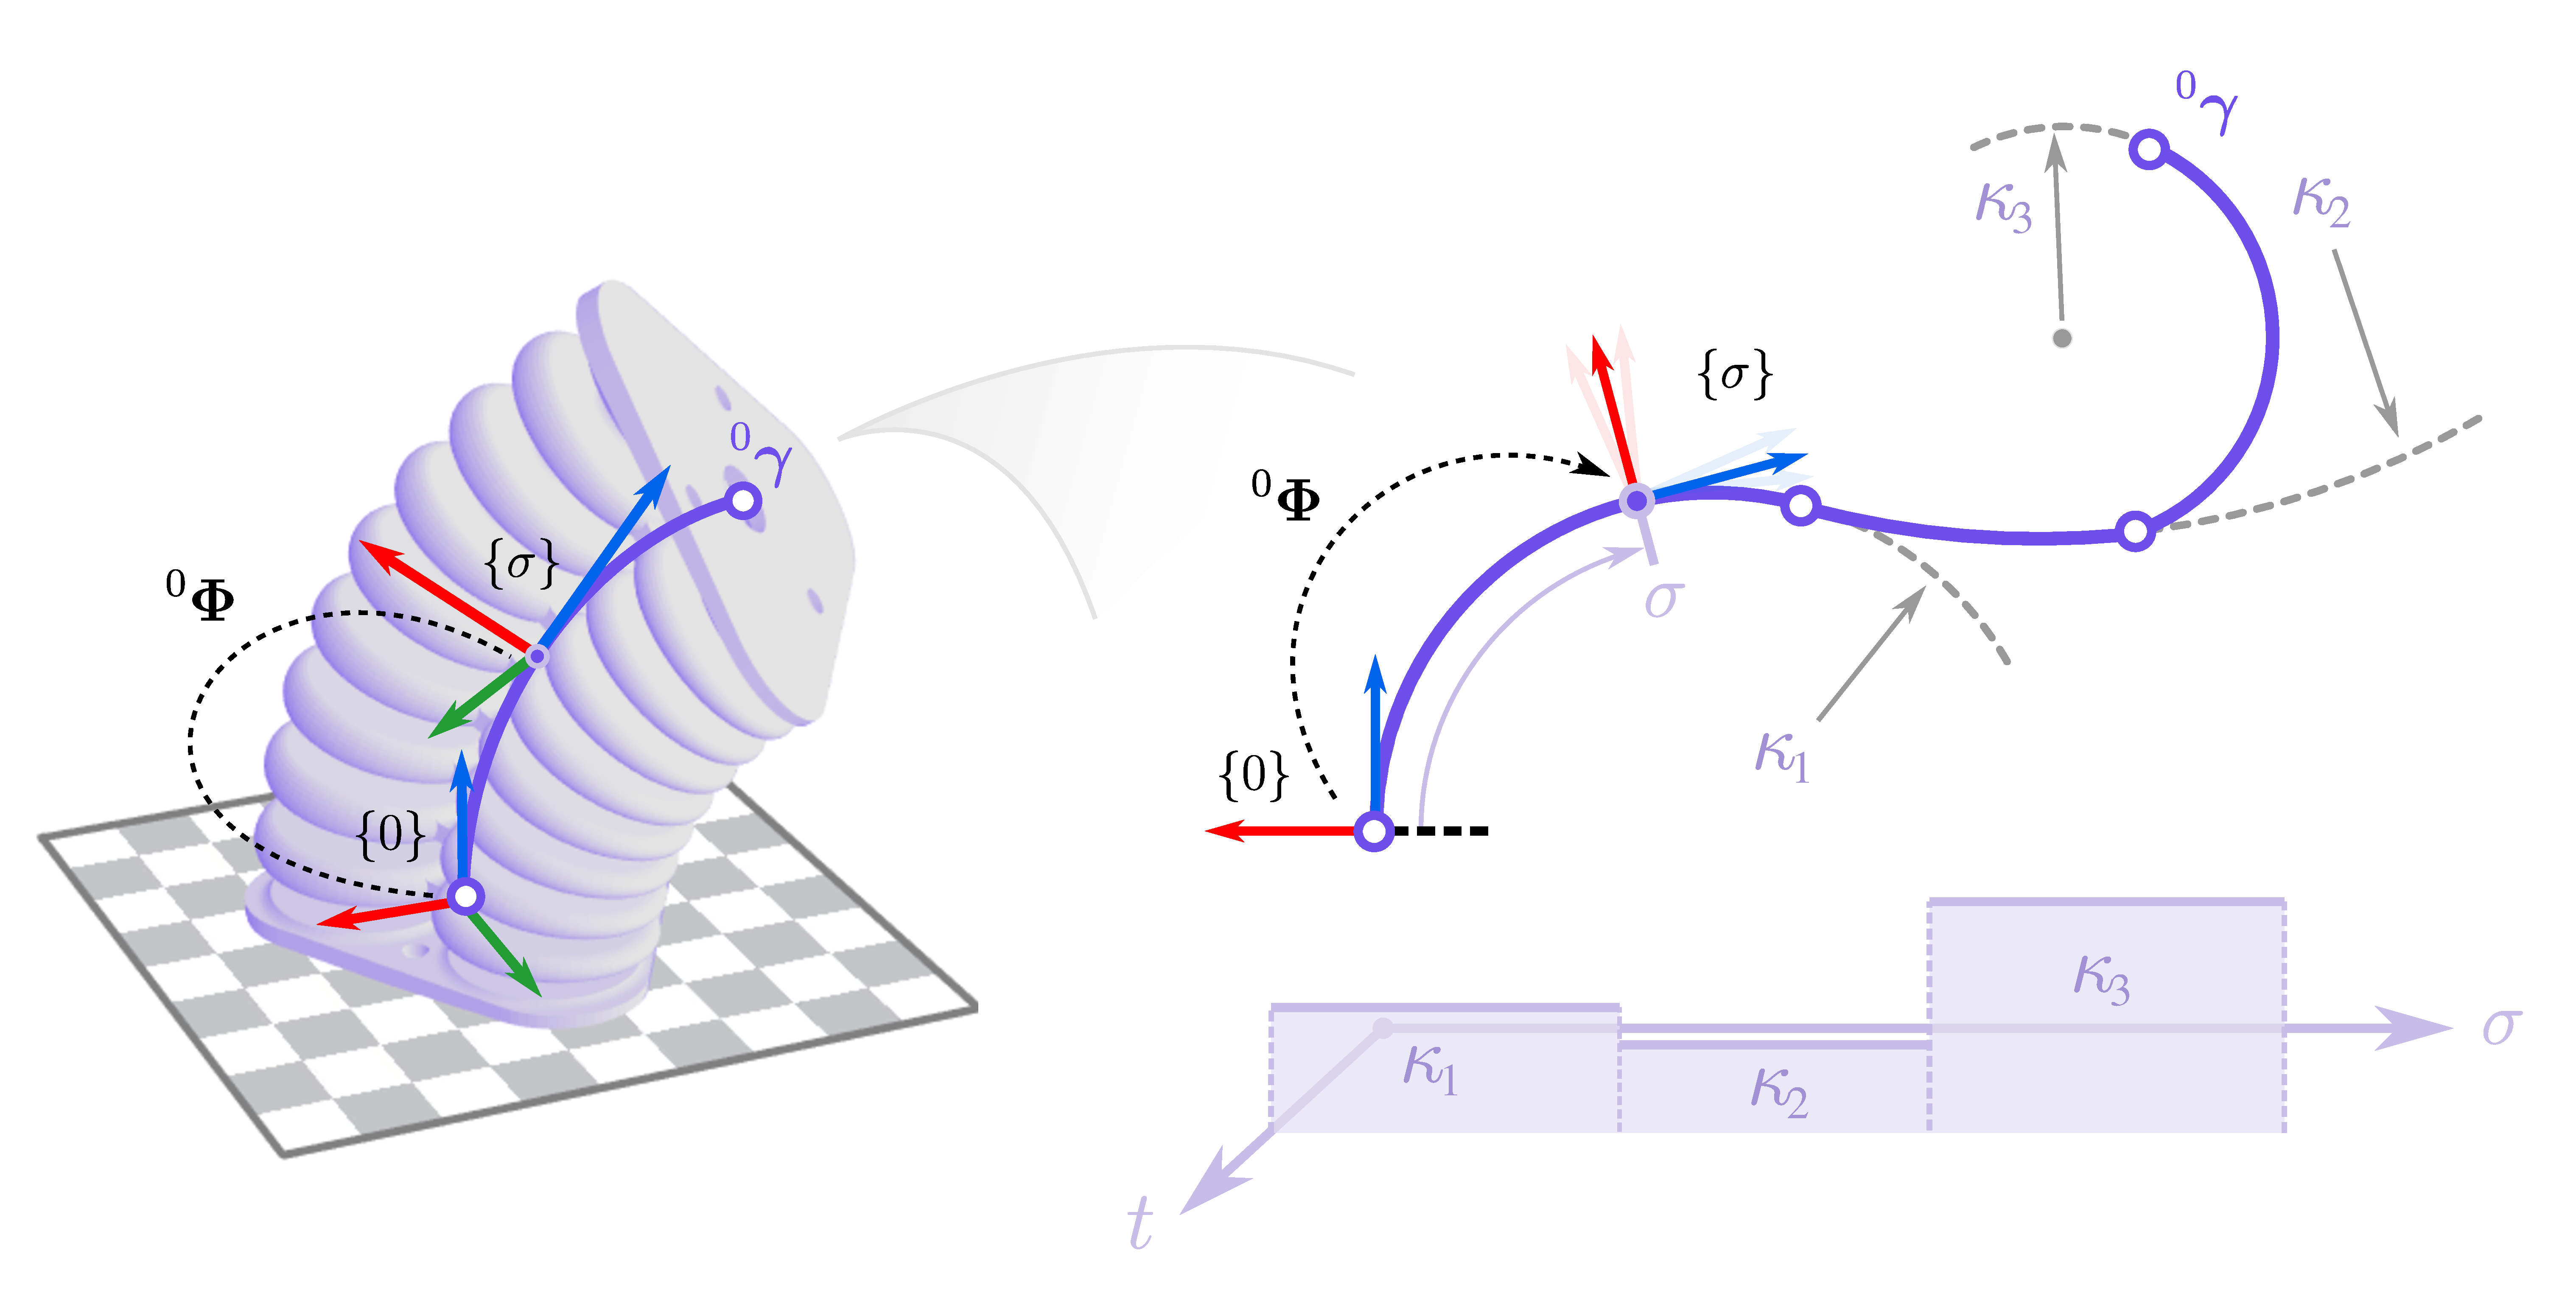
\includegraphics[width = \textwidth]{./pdf/thesis-figure-4-2.pdf}
  \caption{Schematic representation of the Piece-wise Constant Curvature (PCC) description for general soft  manipulator systems, given by a parameterized curve $^0 \gammaB: \Xs \times \mathcal{Q} \to \R^3$ and orientation matrix $^0 \PhiB: \Xs \times \mathcal{Q} \to \SO{3}$. The frame $\{\sigma\}$ is an inertial coordinate frame that evolves over the backbone $^0 \gammaB$ such that variations in $\sigma$ give insight into its differential geometry.}
  \label{fig:C2:configuration}
\end{figure}
%
\begin{asm}[Piece-wise Constant Curvature]
\label{asm:C2:pcc}
Despite the inherent flexibility in soft robotics, it is sometimes sufficient to express the kinematics according to the \emph{Piecewise Constant Curvature} (PCC) condition.  This properties often originates from the "\textit{proper}" structural design of the soft robot, where parasitic motion is reduced by structural compliance . Mathematically, it implies that the curvature of the continuous body satisfies $\kappa(\sigma_1,\q) = \kappa(\sigma_2,\q)$ for spatial coordinates on a local region on the soft manipulator $\sigma_1,\sigma_2 \subseteq \Xs$. As a result, this condition allows us to describe the full forward kinematics with a significantly reduced set of generalized coordinates, mitigating kinematic complexity in the model. Numerous works employ PCC models \cite{Falkenhahn2015,Katzschmann2019,Tatlicioglu2007,Marchese2016,Godage2016,DellaSantina2020a}, and depending on the elasticity  and structural geometry of the soft robot, the PCC condition has been proven to be consistent for various soft robotic systems.
\end{asm}
%
{Following this Constant Curvature (CC) approach, we assign a coordinate frame that twists minimally along the backbone -- formally called the "\textit{Bishop frame}" (see \cite{Bishop1975}) -- parametrized by the following generalized coordinate vector:}
%
\begin{equation}
\vec{q} := \begin{pmatrix}
\,\varepsilon & \kappa_x & \kappa_y\,
\end{pmatrix}^\top \in \mathcal{Q},
\label{eq:C2:coordinate}
\end{equation}
%
\noindent where $\varepsilon_{-} \le \varepsilon \le \varepsilon_{+}$ is the elongation strain, and $\kappa_x,\,\kappa_y\in\mathbb{R}$ are the curvatures or angular strains in $x$-$z$ and $y$-$z$ plane, respectively; and $\mathcal{Q} \subset \R^3$ is an admissible space on which $\q$ evolves. We will also introduce the following geometric variables $\kappa = \inner{\kappa_x}{\kappa_y}$ and the curvature angle $\phi = \atantwo(\kappa_y,\kappa_x)$. It is worth mentioning that the joint description above is somewhat related to Renda. et al. \cite{Renda2018} who proposed a \emph{Piece-wise Constant Strain} (PCS) parametrization with the exception of including the twist along the tangent.

By exploring the differential geometry of the smooth backbone curve similar to Mochiyama et al. \cite{Mochiyama2003}, we can write the position vector $\gammaB(\sigma,\q)$ and the orientation matrix $\PhiB(\sigma,\q)$ for each material point $\sigma$ along the smooth backbone as a differential equation:
%
\begin{align}
\renewcommand*{\arraystretch}{2}{}
\frac{\partial \,\!\mat{\Phi}}{\partial \sigma}(\sigma,\q) & = \, \mat{\Phi}(\sigma,\vec{q}) \,\mat{\Gamma}^{\times} (\sigma,\q), \label{eq:C2:change_phi} \\[0.75em]
%
\frac{\partial \, \gammaB}{\partial \sigma}(\sigma,\q) & = \, \mat{\Phi}(\sigma,\vec{q}) \, \vec{U}(\sigma,\q), \label{eq:C2:change_p}
\end{align}
%
where  $\vec{\Gamma}^\times \in \sog{3}$  is a skew-symmetric matrix composed of the entries of the vector $\vec{\Gamma} \in \R^3$, and $\vec{U}\in \R^3$ a vector representing the tangent along the extensible backbone. The skew-symmetric operator $(\,\cdot\,)^\times$ denotes the isomorphism between the Lie algebra $\sog{3}$ and $\R^3$. The vectors $\vec{\Gamma}$ and $\vec{U}$ are vectors that define the differential geometry of the backbone
\cite{Mochiyama2003} which are unique entries that live in the tangent space of the rigid-body transformation group (\ie, $T_{\SE{3}}$). Given the Bishop parametrization shown in \eqref{eq:C2:coordinate} and assuming the Piecewise Constant-Strain (PCC) condition, these geometric entities yield
%
\begin{align}
\vec{\Gamma}^\times(\sigma,t) & \simeq \vec{\Gamma}^\times(\sigma,\q(t)) \!\!\!\quad \xRightarrow[]{\textrm{\;\;PCC\;\;}}\quad \vec{\Gamma}^\times = \begin{pmatrix} 0 & 0 & \kappa_y \\ 0 & 0 & \kappa_x \\ -\kappa_y & -\kappa_x & 0 \end{pmatrix}, \label{eq:C2:Gamma}\\[0.35em]
%
\vec{U}(\sigma,t) & \simeq \vec{U}(\sigma,\q(t)) \!\quad \xRightarrow[]{\textrm{\;\;PCC\;\;}} \quad \;\; \vec{U} = \;\begin{pmatrix} \;0\;\; \\  \;0\;\; \\ \;\varepsilon + 1\;\ \end{pmatrix}. \label{eq:C2:U}
\end{align}
%
%with $\vec{U}^\circ$ the unit-tangent pointing, and $\vec{\Gamma}^\circ$ the intrinsic curvature/torsion of the curve. For simplicity, lets assume $\vec{U}^\circ = (0,0,1)^\top$ and $\vec{\Gamma}^\circ = \vec{0}_3$.
Now, given an initial configuration of backbone's base, \ie, $\mat{\Phi}(0,\vec{q}) = \vec{\Phi}_0$ and $ \gammaB(0,\q) = \vec{0}_3$, we can now solve for the position and orientation for each material coordinate $\sigma$ along the backbone:
%
\begin{align}
\mat{\Phi}(\sigma,\vec{q}) & = \vec{\Phi}_0\exp_{\SO{3}}(\sigma \vec{\Gamma}^\times(\vec{q})), \label{eq:C2:phi_exact} \\[0.35em]
\gammaB(\sigma,\vec{q}) & = \int_0^\sigma\,^0\mat{\Phi}(s, \vec{q})\, \vec{U}(\vec{q}) \; ds,
\label{eq:C2:pos_exact}
\end{align}
%
where $\exp_{\SO{3}}: \sog{3} \to \SO{3}$ is the exponential map. Luckily, there exists a compact expression for the exponential mapping related to the orthogonal group of rotation matrices $\SO{3}$ called the "\emph{Rodriguez formulas}".  The rotation angle along the soft body can be computed by $\theta(\sigma,\q) := \int_0^\sigma \kappa(s,\q) \; ds = \kappa(\q) \sigma$. Notice that the rotation angle $\theta$ linearly depends on $\sigma$, which is a property that follows from Assumption \ref{asm:C2:pcc}. Then, given the expression for the angle of rotation,  we can compactly rewrite the rotation matrix \eqref{eq:C2:phi_exact} in terms of $\cos(\theta)$ and $\sin(\theta)$ using these formulas as follows \cite{Lynch2017}:
%
\begin{equation}
\PhiB(\theta) = \PhiB_0 \left( \mat{I}_3 + \left[ \frac{\sin(\theta)}{\theta} \right]  \GammaB^{\times} + \left[ \frac{1-\cos(\theta)}{\theta^2} \right]  \GammaB^{\times} \GammaB^{\times} \right).
\label{eq:C2:phi_rodr}
\end{equation}
%
Note that the closed-form solutions \eqref{eq:C2:phi_exact} and \eqref{eq:C2:pos_exact} represent the forward configuration kinematics of the backbone curve. To express the forward velocity kinematic, let
$\etaB(\sigma,\q,\dq) = \left( \vec{\omega}^\top, \vec{v}^\top \right)^\top \in \R^6 \cong \seg{3}$
 be the aggregate of the angular velocity and linear velocity components relative to an inertial frame at $\sigma$, where the space $\seg{3}$ denotes the Lie algebra of $\SE{3}$. The velocity twist is computed by the following integration procedure:
%
\begin{align}
 \etaB(\sigma,\q,\dq)& = \Ad_{\mat{g}(\sigma,\cdot)}\inv \int_0^\sigma \Ad_{\mat{g}(s,\cdot)}\, \JB^\star\! \dq\;ds, \notag \\ & 
 \,=:\, \JB(\q,\sigma) \dq, \label{eq:C2:vel_cont}
\end{align}
%
where $\Ad_g: \SE{3} \to \mathbb{R}^{6\times 6}$ denotes the adjoint transformation matrix regarding the rigid body transformation $\gB \in \SE{3}$ that maps local velocities (i.e., twist) to a frame located at $\sigma$, and $\JB^\star:\Q \to T_{\q}\Q$ the joint-axis matrix that relates the DOFs to the generalized coordinate description. Let it be clear that the joint-axis matrix is naturally constant for a soft segment modeled with the Constant-Strain (CS) assumption. We will later relax this assumption in Chapter 4. Nevertheless here, the joint-axis matrix for an extensible and bendable CS segment parametrized by the Bishop parameters is given by
%
\begin{align}
\renewcommand*{\arraystretch}{1}{}
\JB^\star := \begin{pmatrix}\dfrac{\p \GammaB}{\p \q}^\top & \dfrac{\p \UB}{\p \q}^\top \end{pmatrix}^\top  = \begin{pmatrix}
\,0 & 0 & 0 & 0 & 0 & 1 \, \\
\,0 & 1 & 0 & 0 & 0 & 0 \,  \\
\,-1 & 0 & 0 & 0 & 0 & 0 \,  \\
\end{pmatrix}^\top. \label{eq:C2:joint-axis-matrix}
\end{align}
%
Although we based the forward kinematics on Mochiyama et al. (2003, \cite{Mochiyama2003}), the derived expression for the velocity twist in \eqref{eq:C2:vel_cont} is analogous to the work of Renda et al. (2018, 2020; \cite{Renda2018,Renda2020}), and Boyer et al. (2010, 2021; \cite{Boyer2010,Boyer2021}). Please also note that
\eqref{eq:C2:vel_cont} gives rise to the geometric Jacobian $\JB(\sigma,\q)$ that defines the mapping from joint velocities to the velocity twist anywhere on the body.

Given the explicit expression for the velocity twist in \eqref{eq:C2:vel_cont}, we can derive the acceleration twist \cite{Boyer2021,Mochiyama2003,Renda2018} which is obtained through differentiation of \eqref{eq:C2:vel_cont}:
%
\begin{align}
\dot{\etaB}(\sigma,\q,\dq,\ddq) & = \JB \ddot{\q} + \Ad_{\gB(\cdot,\sigma)} \inv \int_0^\sigma \Ad_{\gB(s,\cdot)}
\ad_{\etaB(s,\cdot,\cdot)} \, \JB^\star\! \dq \;ds \notag \\
& :=  \JB(\sigma,\q)\ddot{\q} + \dmat{J}(\sigma,\q,\dot{\q}) \dot{\q},
\label{eq:C2:acceleration}
\end{align}
%
where $\ad_{\etaB}: \R^{6} \to \R^{6\times 6}$ denotes the adjoint transformation regarding the velocity twist $\vec{\etaB}^\wedge \in \seg{3}$. The reader is referred to Appendix \ref{app:C2:adjoint} for more detailed expressions on the adjoint transformations.
%
\begin{rmk}[Numerical instability near zero-curvature] For many of the PCC modeling frameworks \cite{Falkenhahn2015}, there are mentions of a singularity point or discontinuity of the kinematic formulations at zero-curvature $\kappa = 0$. It is often reported that trajectories that pass through the origin lead to unbounded linear velocities $\vec{v} := \floor{\etaB}_3$, which may result in critical problems in practice. Although it is believed the problem is simply a by-product of the PCC hypothesis, this is however a common misconception, and it stems from a numerical origin. To illustrate this, consider the inextensible planar case: $\varepsilon = \kappa_y = 0$ and $\kappa = \kappa_x$.  For simplicity, we assume $L = 1$. Hence, by solving the forward kinematics for the position vector $\gammaB(\sigma,\kappa)$, and approaching zero-curvature from the positive domain $\kappa^{+} \to 0$, we see that
%
\begin{align}
\lim_{\kappa \to \,0^{+}}\gammaB(\sigma,\kappa) & = \begin{pmatrix} \dfrac{1-\cos(\sigma \kappa)}{\kappa}\,, & 0\,, & \dfrac{\sin(\sigma \kappa)}{\kappa} \end{pmatrix}^\top = \begin{pmatrix} 0 & 0 & \sigma \end{pmatrix}^\top,
\end{align}
%
so its limit clearly exists. Since the position vector $\gammaB$ is continuously differentiable when approaching the origin from both sides $\kappa \to 0^+$ and $\kappa \to 0^{-}$, it follows that $\dot{\gammaB}$ must be bounded for all $\kappa \in \Q$. We can simply check this by investigating the behavior of the linear-velocity components of the geometric Jacobian near zero-curvature, which yield
%
\begin{align}
\!\!\!\!\!\!\lim_{\kappa \to \,0^+} \floor{\JB}_3(\sigma,\kappa) & = \begin{pmatrix} \dfrac{\sigma \kappa \sin(\sigma \kappa) + 1 - \cos(\sigma \kappa)}{\kappa^2}, & 0, & \dfrac{\sigma \kappa \cos(\sigma \kappa) - \sin(\sigma \kappa) }{\kappa^2} \end{pmatrix}^\top \notag \\[0.75em] & = \begin{pmatrix} \sigma^2 & 0 & 0 \end{pmatrix}^\top.
\end{align}
%
 Again, its limit exists. Since both limits exist, we define $\vec{\gamma}(\sigma,0):= \lim_{\kappa \to \,0} \vec{\gamma}(\sigma,\kappa)$ and $\vec{J}(\sigma,0):= \lim_{\kappa \to \,0} \vec{J}(\sigma,\kappa)$. Consequently, the magnitude of the linear velocity of the end-effector reads simply $\lVert \dot{\gammaB}(L,\dot{\kappa}) \rVert = L^2\dot{\kappa} = L \omega_1$ with $\omega_1$ the angular velocity at the tip. Moreover, it is bounded for all $\kappa \in \mathcal{Q}$. This naturally poses an ambiguity on the origin of the kinematic singularity so often reported literature. The problem is believed to be of numerical origin when considering the zero-division. To make matters worse, deriving analytical expressions for accelerations will contain similar expressions that are hard to stabilize numerically. To resolve this issue, we opt for a numerical approximation of the forward kinematics -- namely, we employ an explicit forward integration scheme (\ie, trapezoidal integration) to solve \eqref{eq:C2:change_phi} and \eqref{eq:C2:change_p}.
\end{rmk}

\begin{example}[Kinematic behavior of PCC segment]
As an illustrative example, we perform a numerical simulation of the forward kinematics for a single PCC segment. We select a differentiable reference trajectory $\q(t) \equiv \q_d(t)$, $\dot{\q}(t) \equiv \dot{\q}_d(t)$ and $\ddot{\q}(t) \equiv \ddot{\q}_d(t)$ that passes the zero-curvature point  given by :
%
\begin{align*}
\q_d(t) &  =  \erf(t) \cdot \begin{pmatrix} \varepsilon_0 \sin(\omega t) & \kappa_0 \cos(\omega t) & \kappa_0 \sin(\tfrac{3}{2}\omega t - \tfrac{\pi}{4}) \end{pmatrix}^\top,
\end{align*}
%
where $\textrm{erf}(t) := \frac{2}{\pi}\int_0^\tau \exp(-\tau^2) \; d\tau$ is referred to as the error function. Note that these are smooth functions such that reference velocity $\dq_d$ and reference acceleration $\ddq_d$ exist and are bounded. The reference signals for the geometric strain of the soft robot are shown in Figure \ref{fig:C2:EX1:strain_ref}. Please note that the reference $\q_d$ has been carefully selected to ensure it passes the line $\kappa_x = \kappa_y = 0$ on the configuration manifold
$\mathcal{Q}$, \ie, the numerical instability point for (near) zero-curvature.

Then, by injecting the reference into the kinematic relations given by \eqref{eq:C2:change_phi}, \eqref{eq:C2:change_p}, \eqref{eq:C2:vel_cont}, and \eqref{eq:C2:acceleration}, we obtain a (close) approximation of forward kinematics as shown in Figure
\ref{fig:C2:EX1:strain_ref_FK}. Furthermore, we provided a 3D-rendering of the soft robot subjected to the reference $\q_d$ in Figure \ref{fig:C2:EX1:strain_ref_3D}. Now, two key observations can be made. First, although a simple harmonic trajectory is used, the resulting trajectory of the end-effector as shown in Figure \ref{fig:C2:EX1:strain_ref_FK} is rather complex. This perhaps stresses the importance of inverse kinematic solver that can be used for task-space control. Second, although we pass the point of numerical instability for $\kappa \to 0$, we see that the velocity solutions are smooth and bounded at these instances. This result shows our approach does not suffer from the near-zero curvature instabilities that are notoriously mentioned in \cite{Falkenhahn2015,DellaSantina2020}. 
\end{example}
%

\begin{figure}[!h]
  %% This file was created by matlab2tikz.
%
%The latest updates can be retrieved from
%  http://www.mathworks.com/matlabcentral/fileexchange/22022-matlab2tikz-matlab2tikz
%where you can also make suggestions and rate matlab2tikz.
%
\definecolor{mycolor1}{rgb}{0.06275,0.35686,0.84706}%
\definecolor{mycolor2}{rgb}{0.86667,0.21176,0.10980}%
\definecolor{mycolor3}{rgb}{0.18039,0.52157,0.25098}%
%
\begin{tikzpicture}

\begin{axis}[%
width=0.259\textwidth,
height=0.215\textwidth,
at={(0\textwidth,0\textwidth)},
scale only axis,
xmin=0,
xmax=5.01,
xlabel style={font=\color{white!15!black}},
xlabel={time (s)},
ymin=-2,
ymax=2,
ylabel style={font=\color{white!15!black}},
ylabel={$\q_d$},
axis background/.style={fill=white},
xmajorgrids,
ymajorgrids,
ylabel style={yshift=-9.5pt}
]
\addplot [color=mycolor1, line width=1.5pt, forget plot]
  table[row sep=crcr]{%
0	0\\
0.0590118023604722	0.0122599350151695\\
0.122024404880976	0.051245683586683\\
0.197039407881577	0.127356433673519\\
0.306061212242448	0.274610958461174\\
0.464092818563713	0.485281744378211\\
0.539107821564313	0.550009396707688\\
0.599119823964793	0.574155119595387\\
0.654130826165233	0.570918154822998\\
0.708141628325666	0.542425923995588\\
0.766153230646129	0.483585222567674\\
0.833166633326665	0.381001848782168\\
0.914182836567313	0.214127314579629\\
1.02820564112823	-0.075581754600881\\
1.25925185037007	-0.672851821290417\\
1.34526905381076	-0.833669846120815\\
1.41328265653131	-0.919160442883364\\
1.47129425885177	-0.95862945224353\\
1.52230446089218	-0.966293478371877\\
1.57331466293259	-0.948199994340202\\
1.62732546509302	-0.90137626204806\\
1.68933786757351	-0.814258548692571\\
1.76335267053411	-0.668276174824877\\
1.85537107421484	-0.435076623934572\\
1.99539907981596	-0.0143847160291388\\
2.19043808761752	0.562122882172909\\
2.28645729145829	0.78232701823107\\
2.36147229445889	0.906026029952742\\
2.4244848969794	0.971401468926922\\
2.47949589917984	0.997472999626086\\
2.53050610122024	0.995067322990411\\
2.58251650330066	0.966335526484759\\
2.63952790558112	0.905286120543856\\
2.70554110822164	0.798558894400302\\
2.78455691138228	0.62627694206536\\
2.8875775155031	0.345873241993202\\
3.26665333066613	-0.743113935603639\\
3.34566913382677	-0.884745361525436\\
3.41068213642729	-0.960888000773404\\
3.46669333866773	-0.994529710207253\\
3.51770354070814	-0.998453103672079\\
3.56871374274855	-0.976789847418135\\
3.624724944989	-0.924209595097784\\
3.68873774754951	-0.829302846512608\\
3.76375275055011	-0.675905403764888\\
3.85977195439088	-0.426427403766472\\
4.0128025605121	0.0402095863869585\\
4.1878375675135	0.556451691884553\\
4.28385677135427	0.778179781889043\\
4.35987197439488	0.904655728387877\\
4.42288457691538	0.970797027717512\\
4.47789557911582	0.997589797446857\\
4.52790558111622	0.996159624088327\\
4.57991598319664	0.968648768140962\\
4.6369273854771	0.908894839975858\\
4.70294058811762	0.803552513256307\\
4.78195639127826	0.632676263537522\\
4.88397679535907	0.356479989904654\\
5	8.88178419700125e-16\\
};
\addplot [color=mycolor2, line width=1.5pt, forget plot]
  table[row sep=crcr]{%
0	0\\
0.138027605521104	0.140440300108925\\
0.211042208441689	0.184935584810103\\
0.272054410882176	0.196656209080302\\
0.329065813162632	0.183310753811706\\
0.388077615523104	0.143577314476932\\
0.454090818163633	0.0688810755447316\\
0.533106621324265	-0.0570083146317186\\
0.645129025805161	-0.281096403013078\\
0.835167033406681	-0.662476511437434\\
0.916183236647329	-0.777169753245791\\
0.980196039207842	-0.832701926306017\\
1.03520704140828	-0.851571468783066\\
1.08621724344869	-0.843577250292476\\
1.13922784556911	-0.808789721087341\\
1.19823964792959	-0.739024227249642\\
1.26625325065013	-0.620955121877476\\
1.3502700540108	-0.427767812642783\\
1.46629325865173	-0.101666846450176\\
1.72234446889378	0.633525295214997\\
1.81136227245449	0.820837424693816\\
1.88337667533507	0.92640916650209\\
1.94338867773555	0.978331555991308\\
1.99639927985597	0.99518363496166\\
2.04740948189638	0.985184790347176\\
2.1004200840168	0.947820917223337\\
2.15943188637728	0.875183689696618\\
2.22844568913783	0.752107632272527\\
2.31346269253851	0.552461842844861\\
2.42848569713943	0.222651201302659\\
2.71854370874175	-0.633815634394776\\
2.80756151230246	-0.822691363947944\\
2.87857571514303	-0.928076540294048\\
2.93858771754351	-0.981414393680224\\
2.99159831966393	-0.999628398951698\\
3.04260852170434	-0.991037597553407\\
3.09561912382476	-0.955207840530338\\
3.15463092618524	-0.884300387785018\\
3.22364472894579	-0.7631603021345\\
3.30766153230646	-0.568142665295742\\
3.42068413682737	-0.246607234578534\\
3.72574514902981	0.65122625379941\\
3.8127625525105	0.831927524141501\\
3.88377675535107	0.93407870842546\\
3.94278855771154	0.983891068491499\\
3.99579915983197	0.999912900564358\\
4.04680936187237	0.989206735619766\\
4.0998199639928	0.951231137729379\\
4.15983196639328	0.876560868859253\\
4.22984596919384	0.750430990306204\\
4.31586317263453	0.546754312000056\\
4.43288657731546	0.209284340535875\\
4.71394278855771	-0.622647147364128\\
4.80396079215843	-0.816268101959198\\
4.87597519503901	-0.925047608943518\\
4.9369873974795	-0.980469837601955\\
4.98999799959992	-0.999506362945193\\
5	-0.999999999998463\\
};
\addplot [color=mycolor3, line width=1.5pt, forget plot]
  table[row sep=crcr]{%
0	-0\\
0.0590118023604722	-0.0323127302272486\\
0.108021604320864	-0.0331290824818566\\
0.157031406281257	-0.0079769875375062\\
0.212042408481697	0.0500216589361884\\
0.283056611322264	0.162185680095956\\
0.485097019403881	0.506055784611869\\
0.536107221444289	0.543684543712172\\
0.578115623124625	0.547118496091529\\
0.619123824764953	0.523782154432988\\
0.664132826565313	0.466781106891244\\
0.718143628725745	0.35651568991531\\
0.785157031406281	0.165020918099894\\
0.890178035607121	-0.209610885997843\\
1.02020404080816	-0.656165846278042\\
1.08621724344869	-0.813331876653166\\
1.13622724544909	-0.8827564770361\\
1.17623524704941	-0.902858557904033\\
1.21324264852971	-0.891876333186355\\
1.25225045009002	-0.849343403567872\\
1.29825965193039	-0.75980970794915\\
1.35527105421084	-0.595513228979666\\
1.43128625725145	-0.304509569554719\\
1.70234046809362	0.802351589692006\\
1.75935187037407	0.927771606903312\\
1.80436087217443	0.980075766519771\\
1.84136827365473	0.990077945444886\\
1.87737547509502	0.970779584879269\\
1.91838367673535	0.914613712496442\\
1.96739347869574	0.80264348414426\\
2.02940588117624	0.600183129717624\\
2.11542308461692	0.238476117081353\\
2.33046609321864	-0.696803833599685\\
2.39647929585917	-0.882732768124136\\
2.44748949789958	-0.969018921052845\\
2.4874974994999	-0.997830617495056\\
2.52250450090018	-0.994023401063271\\
2.55951190238048	-0.960649427962859\\
2.60252050410082	-0.885345365627133\\
2.65653130626125	-0.73993292743766\\
2.72654530906181	-0.482199139020603\\
2.83856771354271	0.0246624641119846\\
2.97559511902381	0.621277881997434\\
3.04660932186437	0.844169225727331\\
3.1006201240248	0.951944439490648\\
3.14362872574515	0.994104036503082\\
3.17963592718544	0.998126097022847\\
3.21564312862573	0.973479302424193\\
3.25665133026605	0.911429266327099\\
3.30666133226645	0.79016811146077\\
3.37067413482697	0.572402197653537\\
3.4626925385077	0.174902851173357\\
3.65173034606921	-0.655626629756043\\
3.72074414882977	-0.862521673164816\\
3.77275455091018	-0.959529089678471\\
3.81476295259052	-0.996173299612285\\
3.85077015403081	-0.996625968608955\\
3.8877775555111	-0.96726798143933\\
3.93078615723145	-0.896391559355475\\
3.98279655931186	-0.76204628869428\\
4.0498099619924	-0.523261917173079\\
4.15183036607321	-0.0698574757930102\\
4.30986197239448	0.62473490045429\\
4.38087617523505	0.846533085581687\\
4.43488697739548	0.953293435683277\\
4.47789557911582	0.994579768326681\\
4.51390278055611	0.997854639446826\\
4.55091018203641	0.971359701253584\\
4.59291858371674	0.905657492920928\\
4.64392878575715	0.778672904138067\\
4.70994198839768	0.549251284827934\\
4.80596119223845	0.128630790373577\\
4.97999599919984	-0.637409462896398\\
5	-0.707106781185458\\
};
\end{axis}

\begin{axis}[%
width=0.259\textwidth,
height=0.215\textwidth,
at={(0.341\textwidth,0\textwidth)},
scale only axis,
xmin=0,
xmax=5.01,
xlabel style={font=\color{white!15!black}},
xlabel={time (s)},
ymin=-6,
ymax=6,
ylabel style={font=\color{white!15!black}},
ylabel={$\dq_d$},
axis background/.style={fill=white},
xmajorgrids,
ymajorgrids,
ylabel style={yshift=-9.5pt}
]
\addplot [color=mycolor1, line width=1.5pt, forget plot]
  table[row sep=crcr]{%
0	0.00354490068904045\\
0.137027405481096	0.903588308385592\\
0.206041208241649	1.22856452598255\\
0.257051410282056	1.38060740669893\\
0.296059211842368	1.43857878332504\\
0.326065213042608	1.44671619310838\\
0.356071214242848	1.42249130990263\\
0.39007801560312	1.3560092907744\\
0.432086417283457	1.21821465698646\\
0.485097019403881	0.962586034545687\\
0.553110622124425	0.520529889641796\\
0.651130226045209	-0.270803972466815\\
0.857171434286857	-1.96111846971092\\
0.93118623724745	-2.39268873749415\\
0.988197639527906	-2.61578401240715\\
1.03220644128826	-2.71435218975166\\
1.06621324264853	-2.74427973959115\\
1.09621924384877	-2.73665215168262\\
1.12822564512903	-2.69342117279692\\
1.16623324664933	-2.59588760182128\\
1.21324264852971	-2.40873834185884\\
1.27225445089018	-2.07805095116542\\
1.34626925385077	-1.53498416704634\\
1.44928985797159	-0.609800554006279\\
1.7373474694939	2.06478538831989\\
1.81936387277455	2.60307834026396\\
1.88337667533507	2.90062171255517\\
1.93538707741548	3.05371910764113\\
1.97639527905581	3.11545185690039\\
2.00840168033607	3.12679834073453\\
2.03940788157632	3.10692697008051\\
2.0744148829766	3.04832587668127\\
2.11742348469694	2.92503238525876\\
2.16943388677736	2.70379607461824\\
2.23344668933787	2.33206311088885\\
2.31346269253851	1.73595350618949\\
2.42348469693939	0.745755428207096\\
2.72054410882176	-2.00968788046552\\
2.80556111222244	-2.57586752681016\\
2.87157431486297	-2.89102311132145\\
2.9245849169834	-3.05482622701098\\
2.96659331866373	-3.12471640436199\\
2.999599919984	-3.14152189462515\\
3.03060612122425	-3.12655715277568\\
3.06461292258452	-3.0760658872595\\
3.10662132426485	-2.96535682645882\\
3.15663132626525	-2.76652815312306\\
3.21864372874575	-2.42602567294836\\
3.29565913182637	-1.8771253886638\\
3.39767953590718	-0.987885846273739\\
3.75075015003001	2.23014715782088\\
3.82876575315063	2.70040323156362\\
3.89077815563113	2.96011198400992\\
3.93978795759152	3.08647630578385\\
3.97879575915183	3.13494797811861\\
4.01080216043209	3.1396111777881\\
4.04280856171234	3.11255800697227\\
4.07981596319264	3.04211546348687\\
4.124824964993	2.90122307727425\\
4.17983596719344	2.65075511896351\\
4.24684936987398	2.23986170977253\\
4.33186637327465	1.57905334730502\\
4.45289057811562	0.458374253608507\\
4.69693938787758	-1.82607588925665\\
4.7869573914783	-2.46688451700194\\
4.85697139427886	-2.83188138573282\\
4.9129825965193	-3.02625903108539\\
4.95799159831966	-3.11491811053946\\
4.99299859971994	-3.14093609486879\\
5	-3.14158748587636\\
};
\addplot [color=mycolor2, line width=1.5pt, forget plot]
  table[row sep=crcr]{%
0	1.12837322264768\\
0.0290058011602321	1.11287690718957\\
0.0620124024804962	1.05918703548886\\
0.103020604120824	0.940995733860333\\
0.154030806161233	0.720852429683366\\
0.221044208841769	0.329040615346998\\
0.324064812962592	-0.415015201309904\\
0.479095819163833	-1.51762477223098\\
0.550110022004401	-1.88091677154614\\
0.603120624124825	-2.05657754379251\\
0.643128625725145	-2.12690523971632\\
0.674134826965394	-2.14233493262017\\
0.703140628125626	-2.12518565975495\\
0.736147229445889	-2.06847786435016\\
0.776155231046209	-1.94764697173144\\
0.826165233046609	-1.72032118445276\\
0.888177635527105	-1.33287793109094\\
0.970194038807762	-0.677703297361942\\
1.1122224444889	0.656669942201704\\
1.25425085017003	1.92027334813605\\
1.33826765353071	2.4957239295581\\
1.40328065613123	2.8110209600663\\
1.45429085817163	2.96740997845937\\
1.49429885977195	3.03077028972536\\
1.52630526105221	3.04316268415615\\
1.55631126225245	3.0238292307504\\
1.59131826365273	2.96385353194767\\
1.63332666533307	2.84010088177006\\
1.68533706741348	2.61261209274866\\
1.74934986997399	2.23016785497343\\
1.83036607321464	1.61058449856721\\
1.94538907781556	0.55355301879334\\
2.20544108821764	-1.88333064164048\\
2.29345869173835	-2.49961881538618\\
2.3624724944989	-2.85081712197516\\
2.41748349669934	-3.03514561937135\\
2.46149229845969	-3.11735537496245\\
2.49549909981996	-3.14000923889623\\
2.52650530106021	-3.12935139813733\\
2.56051210242048	-3.08346030159967\\
2.6005201040208	-2.9844099202232\\
2.6505301060212	-2.79450937790965\\
2.71154230846169	-2.47007506810393\\
2.78655731146229	-1.94858631705674\\
2.88457691538308	-1.10996961666554\\
3.10262052410482	0.99996718143458\\
3.22164432886577	2.01874975626282\\
3.30566113222645	2.57684537272085\\
3.37167433486697	2.89165495774407\\
3.4246849369874	3.05520852382526\\
3.46669333866773	3.12491681950401\\
3.499699939988	3.14158841415858\\
3.53070614122825	3.12650471358071\\
3.56471294258852	3.07589032073885\\
3.60672134426885	2.96503961364553\\
3.65673134626925	2.76605754535741\\
3.71874374874975	2.42538893386612\\
3.79575915183037	1.87632266950521\\
3.89777955591118	0.986940126259217\\
4.25085017003401	-2.23084317749245\\
4.32886577315463	-2.70090796640865\\
4.39087817563513	-2.96044270093426\\
4.43988797759552	-3.08666036495903\\
4.47889577915583	-3.13501205318945\\
4.51090218043609	-3.13957601885231\\
4.54290858171634	-3.11242397791472\\
4.57991598319664	-3.04186887567698\\
4.624924984997	-2.9008442325007\\
4.67993598719744	-2.65022515672919\\
4.74694938987798	-2.23916940295443\\
4.83196639327866	-1.57819986384533\\
4.95299059811962	-0.457397634949563\\
5	0.00493479812624376\\
};
\addplot [color=mycolor3, line width=1.5pt, forget plot]
  table[row sep=crcr]{%
0	-0.794115508462454\\
0.0580116023204642	-0.277364611734568\\
0.26505301060212	1.70491593082617\\
0.306061212242448	1.87842338112035\\
0.334066813362672	1.92300384411942\\
0.356071214242848	1.91292691038186\\
0.38007601520304	1.85542433262415\\
0.411082216443289	1.70919219099674\\
0.451090218043609	1.40465740373763\\
0.504100820164033	0.820935563376146\\
0.578115623124625	-0.248600075058891\\
0.762152430486097	-2.99671953899652\\
0.816163232646529	-3.4867860854134\\
0.855171034206841	-3.68308225183768\\
0.882176435287057	-3.73307210749446\\
0.902180436087217	-3.72294329754286\\
0.924184836967394	-3.66485742913014\\
0.954190838167634	-3.50676773602809\\
0.993198639727946	-3.16939676216821\\
1.04320864172835	-2.53683562435458\\
1.11022204440888	-1.40251215395337\\
1.23224644928986	1.09146932720294\\
1.34026805361072	3.11962860739989\\
1.40428085617123	3.97847580467464\\
1.45229045809162	4.38259317834563\\
1.4872974594919	4.53109137402165\\
1.51030206041208	4.55856842712607\\
1.53030606121224	4.53675451436047\\
1.55431086217243	4.45469330662973\\
1.58631726345269	4.25233666981845\\
1.62832566513303	3.83346415954477\\
1.68233646729346	3.06612040251519\\
1.75535107021404	1.70902193090805\\
2.03440688137628	-3.80704018778977\\
2.08841768353671	-4.38067909824091\\
2.12942588517704	-4.62780828971085\\
2.15843168633727	-4.6982027777484\\
2.17843568713743	-4.69538596539201\\
2.1994398879776	-4.64729630338051\\
2.22744548909782	-4.5121578146679\\
2.26445289057812	-4.21315733318806\\
2.3124624924985	-3.63571053810641\\
2.374474894979	-2.61980512471882\\
2.46549309861972	-0.754128407877475\\
2.6495299059812	3.05964290826855\\
2.71654330866173	4.02147655398821\\
2.76655331066213	4.48381747958504\\
2.80356071214243	4.66721925102645\\
2.82956591318264	4.71152470359658\\
2.84856971394279	4.69919553002523\\
2.87157431486297	4.63390058682298\\
2.90158031606321	4.46715113358115\\
2.94058811762353	4.11776373765277\\
2.99059811962393	3.4689862272862\\
3.05761152230446	2.30691776642933\\
3.16363272654531	0.0563190270418401\\
3.30666133226645	-2.89690138385146\\
3.37667533506701	-3.9448221542987\\
3.42868573714743	-4.45241981565303\\
3.46769353870774	-4.65954561876156\\
3.49469893978796	-4.71117486462973\\
3.51470294058812	-4.70029361858979\\
3.53670734146829	-4.64013279511158\\
3.56671334266853	-4.47797683817697\\
3.60572114422885	-4.13425107699655\\
3.65573114622925	-3.49192821143007\\
3.72174434886977	-2.35576737664234\\
3.82576515303061	-0.156931641015601\\
3.97379475895179	2.90509369151093\\
4.04380876175235	3.950496362776\\
4.09581916383277	4.45581244484655\\
4.13482696539308	4.66108744519533\\
4.16183236647329	4.71140168604915\\
4.18183636727345	4.69954306835578\\
4.20484096819364	4.63434132500523\\
4.23484696939388	4.46772453283112\\
4.27385477095419	4.11851887812703\\
4.32386477295459	3.46996990086312\\
4.39087817563513	2.30815865696121\\
4.49689937987598	0.0577494594312666\\
4.63992798559712	-2.89575760597693\\
4.70994198839768	-3.94402589682519\\
4.7619523904781	-4.45194298479568\\
4.80096019203841	-4.65932964437099\\
4.82796559311862	-4.71114488543943\\
4.84796959391878	-4.70040215831249\\
4.86997399479896	-4.64039276611033\\
4.8999799959992	-4.47843880303433\\
4.93898779755951	-4.13496168317129\\
4.98899779955991	-3.49292197179463\\
5	-3.32429866327344\\
};
\end{axis}

\begin{axis}[%
width=0.259\textwidth,
height=0.215\textwidth,
at={(0.682\textwidth,0\textwidth)},
scale only axis,
xmin=0,
xmax=5.01,
xlabel style={font=\color{white!15!black}},
xlabel={time (s)},
ymin=-30,
ymax=30,
ylabel style={font=\color{white!15!black}},
ylabel={$\ddq_d$},
axis background/.style={fill=white},
xmajorgrids,
ymajorgrids,
ylabel style={yshift=-9.5pt}
]
\addplot [color=mycolor1, line width=1.5pt, forget plot]
  table[row sep=crcr]{%
0	7.08971722508816\\
0.0170034006801352	7.06254176227866\\
0.0380076015203041	6.96211357748433\\
0.0670134026805353	6.70383363218785\\
0.105021004200839	6.16331809076554\\
0.15503100620124	5.13123086154366\\
0.221044208841768	3.30313004756611\\
0.322064412882577	-0.140715150531712\\
0.483096619323865	-5.57492932673487\\
0.555111022204441	-7.34242512612227\\
0.609121824364873	-8.2298345369658\\
0.650130026005201	-8.61942170460317\\
0.679135827165434	-8.74010611151554\\
0.696139227845569	-8.75056964311227\\
0.714142828565713	-8.71323899853671\\
0.738147629525905	-8.58686459570546\\
0.770154030806161	-8.28547401565682\\
0.812162432486497	-7.67074463808859\\
0.866173234646929	-6.54917377090891\\
0.937187437487498	-4.60734590265721\\
1.04320864172835	-1.07483524322571\\
1.24624924984997	5.72961331213317\\
1.32926585317063	7.81639650559995\\
1.39427885577116	8.9859331390274\\
1.44528905781156	9.58253887084481\\
1.48529705941188	9.8442837551671\\
1.51330266053211	9.91865276034343\\
1.53230646129226	9.91831589369774\\
1.55331066213243	9.87066630009359\\
1.58031606321264	9.73764473499728\\
1.61632326465293	9.43822354992907\\
1.6623324664933	8.86253703324957\\
1.72034406881376	7.8537245560284\\
1.79335867173435	6.19915830635254\\
1.89137827565513	3.47504190478798\\
2.25345069013803	-7.05759085861679\\
2.32946589317864	-8.49825043913732\\
2.39047809561912	-9.30375995789046\\
2.4374874974995	-9.69098733938356\\
2.47349469893979	-9.84429919326235\\
2.49849969993999	-9.87645177319418\\
2.51850370074015	-9.85815891485498\\
2.54250850170034	-9.78470810142351\\
2.5745149029806	-9.6001934501988\\
2.61552310462092	-9.22223443122761\\
2.66653330666133	-8.53959500779489\\
2.72954590918184	-7.39663922633138\\
2.80856171234247	-5.56189473532864\\
2.91558311662332	-2.55857583281172\\
3.22764552910582	6.49527125262672\\
3.30966193238648	8.17448519252473\\
3.374674934987	9.12633838257015\\
3.42568513702741	9.60899637547641\\
3.46469293858772	9.81236106656347\\
3.49269853970794	9.86769341093652\\
3.5127025405081	9.86048208595491\\
3.53570714142829	9.80407057871169\\
3.56471294258852	9.66005045055507\\
3.60272054410882	9.35027485493567\\
3.65073014602921	8.7694054033971\\
3.70974194838968	7.78440013127213\\
3.78275655131026	6.20094073200406\\
3.87877575515103	3.63970724426288\\
4.05881176235247	-1.84364405983484\\
4.19783956791358	-5.77205567675598\\
4.2868573714743	-7.75761622429094\\
4.35587117423485	-8.88854079805768\\
4.41088217643529	-9.49382693860024\\
4.45389077815563	-9.77065608576133\\
4.48489697939588	-9.85991079216486\\
4.50590118023605	-9.86727677343424\\
4.52690538107622	-9.83169388013572\\
4.55391078215643	-9.72310658142739\\
4.58891778355671	-9.47842189369386\\
4.63392678535707	-8.99611634308517\\
4.68893778755751	-8.16403545489397\\
4.75695139027806	-6.80236720584926\\
4.84396879375875	-4.61913345423115\\
4.97299459891978	-0.805433305647973\\
5	0.0310062018553658\\
};
\addplot [color=mycolor2, line width=1.5pt, forget plot]
  table[row sep=crcr]{%
0	-0.0356665298542058\\
0.14002800560112	-4.67099677947669\\
0.210042008401681	-6.35787080027761\\
0.262052410482097	-7.18121414389206\\
0.301060212042408	-7.52419844540775\\
0.328065613122625	-7.61679085886646\\
0.34506901380276	-7.61344158614619\\
0.364072814562913	-7.55338671970529\\
0.390078015603121	-7.3759254387018\\
0.425085017003401	-6.96795293714247\\
0.47009401880376	-6.17536023821841\\
0.528105621124224	-4.76203193936642\\
0.608121624324864	-2.2616035058598\\
0.90118023604721	7.41655342073599\\
0.965193038607721	8.68477119764233\\
1.01520304060812	9.31550428917571\\
1.05321064212843	9.57115136568376\\
1.07921584316863	9.63325353187106\\
1.09821964392879	9.62095442347266\\
1.12022404480896	9.54664003094408\\
1.14922984596919	9.35230091148043\\
1.1872374474895	8.93817915492701\\
1.23624724944989	8.15570308454472\\
1.29825965193039	6.81305056038362\\
1.38127625525105	4.53205984490834\\
1.51730346069214	0.137104630163254\\
1.6873374674935	-5.19413042832095\\
1.77835567113423	-7.44111083206267\\
1.8493698739748	-8.73764863851267\\
1.90638127625525	-9.44363453025954\\
1.95139027805561	-9.77614657982073\\
1.98439687937588	-9.89060722533797\\
2.00640128025605	-9.90571841918975\\
2.02640528105621	-9.87708129185361\\
2.05241048209642	-9.77998577411654\\
2.08541708341668	-9.56077689839852\\
2.12842568513703	-9.11882330623115\\
2.18143628725745	-8.34382797509914\\
2.24744948989798	-7.05721408722493\\
2.33146629325865	-4.99130619335819\\
2.45249049809962	-1.45521934033521\\
2.69453890778156	5.68634972386572\\
2.78455691138228	7.71289662082619\\
2.85457091418284	8.87123751025509\\
2.90958191638328	9.48327346161904\\
2.95259051810362	9.76549714637454\\
2.98459691938388	9.86011816772603\\
3.00560112022404	9.86808705516484\\
3.02660532106421	9.83309714619462\\
3.05361072214443	9.72525700271287\\
3.08861772354471	9.48151268853614\\
3.13262652530506	9.01304744316267\\
3.1876375275055	8.18694988291568\\
3.25565113022605	6.83174606330716\\
3.34266853370674	4.65484935746607\\
3.47069413882777	0.876546802294875\\
3.6877375475095	-5.51511477797639\\
3.77975595119024	-7.61957450245987\\
3.85077015403081	-8.81865742330401\\
3.90678135627125	-9.45828980758456\\
3.95079015803161	-9.75661509139414\\
3.98279655931186	-9.85681253462545\\
4.00480096019204	-9.86795820689945\\
4.02580516103221	-9.8346227153101\\
4.05281056211242	-9.72890484618461\\
4.0868173634727	-9.4963693895167\\
4.13082616523305	-9.03523157269603\\
4.18483696739348	-8.23480517953001\\
4.25185037007402	-6.91608604630467\\
4.33686737347469	-4.81255275530668\\
4.46089217843569	-1.17876018750085\\
4.69093818763753	5.59713704895159\\
4.78195639127826	7.66275629837665\\
4.85197039407882	8.8353040648137\\
4.90798159631926	9.46885282937515\\
4.95199039807962	9.76215955428295\\
4.98399679935987	9.85863512259488\\
5	9.86954757942193\\
};
\addplot [color=mycolor3, line width=1.5pt, forget plot]
  table[row sep=crcr]{%
0	7.5744225756329\\
0.0520104020804162	9.85795253565652\\
0.0890178035607114	10.7343646901029\\
0.113022604520904	10.9368263420187\\
0.126025205041007	10.9227666810555\\
0.142028405681135	10.7856109086146\\
0.16503300660132	10.3588706857098\\
0.197039407881576	9.32929431048124\\
0.240048009601921	7.21344321073802\\
0.300060012002401	3.12899615273476\\
0.541108221644329	-14.5767064028135\\
0.583116623324663	-15.8947102220086\\
0.611122224444888	-16.2686397032763\\
0.622124424884976	-16.3000792190449\\
0.634126825365072	-16.2590964666309\\
0.651130226045208	-16.0662320020655\\
0.67613522704541	-15.4974275623498\\
0.710142028405681	-14.1945663307275\\
0.75515103020604	-11.6027109979822\\
0.816163232646531	-6.78180501212378\\
0.918183636727345	3.19925678471389\\
1.0372074414883	14.2630289394763\\
1.1002200440088	18.3769434543013\\
1.14622924584917	20.2284519962292\\
1.17923584716943	20.8825917599187\\
1.19923984796959	20.9940018330856\\
1.21024204840968	20.9627983709382\\
1.22624524904981	20.8005305254444\\
1.25025005001	20.300173284471\\
1.28325665133027	19.1232943641539\\
1.32726545309062	16.7321518603769\\
1.38527705541108	12.3448435289664\\
1.46929385877175	4.24762456605077\\
1.66433286657331	-15.006835410114\\
1.72834566913383	-19.2314865141707\\
1.77635527105421	-21.2288700042196\\
1.81136227245449	-21.9820872663368\\
1.83336667333467	-22.1406342791886\\
1.84536907381476	-22.1238119583189\\
1.86137227445489	-21.9881962890689\\
1.88437687537508	-21.5687174401902\\
1.91638327665533	-20.5551161436279\\
1.95839167833567	-18.5063456770163\\
2.01340268053611	-14.7274455786217\\
2.08841768353671	-8.02930998083884\\
2.35847169433887	17.4889091607566\\
2.41448289657932	20.4580950794453\\
2.45649129825965	21.7593237376024\\
2.48549709941988	22.1621020797258\\
2.49949989997999	22.2084088691288\\
2.51150230046009	22.1710021117705\\
2.52850570114023	21.9964824567098\\
2.55351070214043	21.4835583106643\\
2.5875175035007	20.3092524488913\\
2.63252650530106	17.9608482179239\\
2.69053810762152	13.7652243370479\\
2.77155431086217	6.27861523427864\\
3.00360072014403	-16.0384936526148\\
3.06461292258452	-19.7357108331353\\
3.11062212442489	-21.463698030133\\
3.14362872574515	-22.0870363960568\\
3.16463292658532	-22.2064523468513\\
3.17663532706541	-22.1770731289039\\
3.19263852770554	-22.0276153410914\\
3.21664332866573	-21.5691020724051\\
3.249649929986	-20.4902631329995\\
3.29265853170634	-18.3476492789936\\
3.34866973394679	-14.44841849918\\
3.4256851370274	-7.52047923802124\\
3.68573714742949	17.1151521202173\\
3.74374874974995	20.2996418279255\\
3.78675735147029	21.6963760554245\\
3.81676335267053	22.146824126934\\
3.83276655331066	22.2065248116632\\
3.84476895379076	22.1684518725285\\
3.86177235447089	21.9932254539312\\
3.88677735547109	21.479711348027\\
3.92078415683137	20.3053143584819\\
3.96579315863173	17.9577095353878\\
4.02380476095219	13.7639924762123\\
4.10482096419284	6.28037173283591\\
4.3368673734747	-16.0343061430535\\
4.39787957591518	-19.7326927237063\\
4.44388877775555	-21.4618857962146\\
4.47689537907582	-22.0862019015833\\
4.49789957991598	-22.2062702477377\\
4.50990198039608	-22.1772700763623\\
4.52590518103621	-22.0283212123418\\
4.5499099819964	-21.5705710293612\\
4.58291658331666	-20.4927599587457\\
4.62592518503701	-18.3514020697384\\
4.68193638727746	-14.4535738878515\\
4.75895179035807	-7.52695343386733\\
5	15.7762366578273\\
};
\end{axis}
\end{tikzpicture}%
  \includegraphics*[width = \textwidth]{./pdf/thesis-figure-4-3.pdf}
  \vspace{-8mm}
  \caption{The time evolution of the predefined geometric strain parameters of the Piece-wise Constant curvature model $\q_d \to  (\varepsilon, \, \kappa_x,\,\kappa_y)^\top$ and their corresponding time-derivatives $\dq_d$ and $\ddq_d$, given by the (spatially constant) elongation $\varepsilon$ \data{Matlab1}, and the  (spatially constant) curvatures $\kappa_x$ \data{Matlab2} and $\kappa_y$ \data{Matlab3}.}
  \label{fig:C2:EX1:strain_ref}
\end{figure}

\begin{figure}[!h]
   \centering
   \vspace{-5mm}
   %% This file was created by matlab2tikz.
%
%The latest updates can be retrieved from
%  http://www.mathworks.com/matlabcentral/fileexchange/22022-matlab2tikz-matlab2tikz
%where you can also make suggestions and rate matlab2tikz.
%
\begin{tikzpicture}

\begin{axis}[%
width=0.216\textwidth,
height=0.199\textwidth,
at={(0\textwidth,0.253\textwidth)},
scale only axis,
axis on top,
xmin=0.5,
xmax=522.5,
tick align=outside,
y dir=reverse,
ymin=0.5,
ymax=458.5,
axis line style={draw=none},
ticks=none,
ylabel style={yshift=-7.5pt}
]
\addplot [forget plot] graphics [xmin=0.5, xmax=522.5, ymin=0.5, ymax=458.5] {./fig/fig_plotrobot-1.png};
\end{axis}

\begin{axis}[%
width=0.216\textwidth,
height=0.199\textwidth,
at={(0.245\textwidth,0.253\textwidth)},
scale only axis,
axis on top,
xmin=0.5,
xmax=522.5,
tick align=outside,
y dir=reverse,
ymin=0.5,
ymax=458.5,
axis line style={draw=none},
ticks=none,
ylabel style={yshift=-7.5pt}
]
\addplot [forget plot] graphics [xmin=0.5, xmax=522.5, ymin=0.5, ymax=458.5] {./fig/fig_plotrobot-2.png};
\end{axis}

\begin{axis}[%
width=0.216\textwidth,
height=0.199\textwidth,
at={(0.49\textwidth,0.253\textwidth)},
scale only axis,
axis on top,
xmin=0.5,
xmax=522.5,
tick align=outside,
y dir=reverse,
ymin=0.5,
ymax=458.5,
axis line style={draw=none},
ticks=none,
ylabel style={yshift=-7.5pt}
]
\addplot [forget plot] graphics [xmin=0.5, xmax=522.5, ymin=0.5, ymax=458.5] {./fig/fig_plotrobot-3.png};
\end{axis}

\begin{axis}[%
width=0.216\textwidth,
height=0.199\textwidth,
at={(0.734\textwidth,0.253\textwidth)},
scale only axis,
axis on top,
xmin=0.5,
xmax=522.5,
tick align=outside,
y dir=reverse,
ymin=0.5,
ymax=458.5,
axis line style={draw=none},
ticks=none,
ylabel style={yshift=-7.5pt}
]
\addplot [forget plot] graphics [xmin=0.5, xmax=522.5, ymin=0.5, ymax=458.5] {./fig/fig_plotrobot-4.png};
\end{axis}

\begin{axis}[%
width=0.216\textwidth,
height=0.199\textwidth,
at={(0\textwidth,0\textwidth)},
scale only axis,
axis on top,
xmin=0.5,
xmax=522.5,
tick align=outside,
y dir=reverse,
ymin=0.5,
ymax=458.5,
axis line style={draw=none},
ticks=none,
ylabel style={yshift=-7.5pt}
]
\addplot [forget plot] graphics [xmin=0.5, xmax=522.5, ymin=0.5, ymax=458.5] {./fig/fig_plotrobot-5.png};
\end{axis}

\begin{axis}[%
width=0.216\textwidth,
height=0.199\textwidth,
at={(0.245\textwidth,0\textwidth)},
scale only axis,
axis on top,
xmin=0.5,
xmax=522.5,
tick align=outside,
y dir=reverse,
ymin=0.5,
ymax=458.5,
axis line style={draw=none},
ticks=none,
ylabel style={yshift=-7.5pt}
]
\addplot [forget plot] graphics [xmin=0.5, xmax=522.5, ymin=0.5, ymax=458.5] {./fig/fig_plotrobot-6.png};
\end{axis}

\begin{axis}[%
width=0.216\textwidth,
height=0.199\textwidth,
at={(0.49\textwidth,0\textwidth)},
scale only axis,
axis on top,
xmin=0.5,
xmax=522.5,
tick align=outside,
y dir=reverse,
ymin=0.5,
ymax=458.5,
axis line style={draw=none},
ticks=none,
ylabel style={yshift=-7.5pt}
]
\addplot [forget plot] graphics [xmin=0.5, xmax=522.5, ymin=0.5, ymax=458.5] {./fig/fig_plotrobot-7.png};
\end{axis}

\begin{axis}[%
width=0.216\textwidth,
height=0.199\textwidth,
at={(0.734\textwidth,0\textwidth)},
scale only axis,
axis on top,
xmin=0.5,
xmax=522.5,
tick align=outside,
y dir=reverse,
ymin=0.5,
ymax=458.5,
axis line style={draw=none},
ticks=none,
ylabel style={yshift=-7.5pt}
]
\addplot [forget plot] graphics [xmin=0.5, xmax=522.5, ymin=0.5, ymax=458.5] {./fig/fig_plotrobot-8.png};
\end{axis}
\end{tikzpicture}%
   \includegraphics*{./pdf/thesis-figure-4-4.pdf}
   %\vspace{-2mm}
   \caption{Three-dimensional deformation of the three-bellow soft robot manipulator using the PCC model. Based on the prescribed reference $\q_d$ (and its time-derivative $\dq_d$), the forward kinematic relations for each point $\sigma$ along the backbone is computed and the volumetric mesh is deformed accordingly to its closest material-point on $\gammaB(\sigma)$.}
   \vspace{-0.1cm}
   \label{fig:C2:EX1:strain_ref_3D}
 \end{figure}
 %
 \begin{figure}[!t]
  \pgfplotsset{colormap name=barney}
  %% This file was created by matlab2tikz.
%
%The latest updates can be retrieved from
%  http://www.mathworks.com/matlabcentral/fileexchange/22022-matlab2tikz-matlab2tikz
%where you can also make suggestions and rate matlab2tikz.
%
\definecolor{mycolor1}{rgb}{0.89290,0.89290,0.89290}%
\definecolor{mycolor2}{rgb}{0.88840,0.88720,0.89330}%
\definecolor{mycolor3}{rgb}{0.88390,0.88140,0.89360}%
\definecolor{mycolor4}{rgb}{0.87940,0.87570,0.89400}%
\definecolor{mycolor5}{rgb}{0.87490,0.87000,0.89440}%
\definecolor{mycolor6}{rgb}{0.87040,0.86420,0.89470}%
\definecolor{mycolor7}{rgb}{0.86590,0.85850,0.89510}%
\definecolor{mycolor8}{rgb}{0.86140,0.85280,0.89550}%
\definecolor{mycolor9}{rgb}{0.85690,0.84700,0.89590}%
\definecolor{mycolor10}{rgb}{0.85240,0.84130,0.89620}%
\definecolor{mycolor11}{rgb}{0.84790,0.83560,0.89660}%
\definecolor{mycolor12}{rgb}{0.84340,0.82990,0.89700}%
\definecolor{mycolor13}{rgb}{0.83890,0.82410,0.89730}%
\definecolor{mycolor14}{rgb}{0.83440,0.81840,0.89770}%
\definecolor{mycolor15}{rgb}{0.82990,0.81270,0.89810}%
\definecolor{mycolor16}{rgb}{0.82530,0.80690,0.89840}%
\definecolor{mycolor17}{rgb}{0.82080,0.80120,0.89880}%
\definecolor{mycolor18}{rgb}{0.81630,0.79550,0.89920}%
\definecolor{mycolor19}{rgb}{0.81180,0.78970,0.89950}%
\definecolor{mycolor20}{rgb}{0.80730,0.78400,0.89990}%
\definecolor{mycolor21}{rgb}{0.80280,0.77830,0.90030}%
\definecolor{mycolor22}{rgb}{0.79830,0.77250,0.90060}%
\definecolor{mycolor23}{rgb}{0.79380,0.76680,0.90100}%
\definecolor{mycolor24}{rgb}{0.78930,0.76110,0.90140}%
\definecolor{mycolor25}{rgb}{0.78480,0.75530,0.90180}%
\definecolor{mycolor26}{rgb}{0.78030,0.74960,0.90210}%
\definecolor{mycolor27}{rgb}{0.77580,0.74390,0.90250}%
\definecolor{mycolor28}{rgb}{0.77130,0.73820,0.90290}%
\definecolor{mycolor29}{rgb}{0.76680,0.73240,0.90320}%
\definecolor{mycolor30}{rgb}{0.76230,0.72670,0.90360}%
\definecolor{mycolor31}{rgb}{0.75780,0.72100,0.90400}%
\definecolor{mycolor32}{rgb}{0.75330,0.71520,0.90430}%
\definecolor{mycolor33}{rgb}{0.74880,0.70950,0.90470}%
\definecolor{mycolor34}{rgb}{0.74430,0.70380,0.90510}%
\definecolor{mycolor35}{rgb}{0.73980,0.69800,0.90540}%
\definecolor{mycolor36}{rgb}{0.73530,0.69230,0.90580}%
\definecolor{mycolor37}{rgb}{0.73080,0.68660,0.90620}%
\definecolor{mycolor38}{rgb}{0.72630,0.68080,0.90650}%
\definecolor{mycolor39}{rgb}{0.72180,0.67510,0.90690}%
\definecolor{mycolor40}{rgb}{0.71730,0.66940,0.90730}%
\definecolor{mycolor41}{rgb}{0.71280,0.66360,0.90770}%
\definecolor{mycolor42}{rgb}{0.70830,0.65790,0.90800}%
\definecolor{mycolor43}{rgb}{0.70380,0.65220,0.90840}%
\definecolor{mycolor44}{rgb}{0.69930,0.64640,0.90880}%
\definecolor{mycolor45}{rgb}{0.69470,0.64070,0.90910}%
\definecolor{mycolor46}{rgb}{0.69020,0.63500,0.90950}%
\definecolor{mycolor47}{rgb}{0.68570,0.62930,0.90990}%
\definecolor{mycolor48}{rgb}{0.68120,0.62350,0.91020}%
\definecolor{mycolor49}{rgb}{0.67670,0.61780,0.91060}%
\definecolor{mycolor50}{rgb}{0.67220,0.61210,0.91100}%
\definecolor{mycolor51}{rgb}{0.66770,0.60630,0.91130}%
\definecolor{mycolor52}{rgb}{0.66320,0.60060,0.91170}%
\definecolor{mycolor53}{rgb}{0.65870,0.59490,0.91210}%
\definecolor{mycolor54}{rgb}{0.65420,0.58910,0.91240}%
\definecolor{mycolor55}{rgb}{0.64970,0.58340,0.91280}%
\definecolor{mycolor56}{rgb}{0.64520,0.57770,0.91320}%
\definecolor{mycolor57}{rgb}{0.64070,0.57190,0.91360}%
\definecolor{mycolor58}{rgb}{0.63620,0.56620,0.91390}%
\definecolor{mycolor59}{rgb}{0.63170,0.56050,0.91430}%
\definecolor{mycolor60}{rgb}{0.62720,0.55470,0.91470}%
\definecolor{mycolor61}{rgb}{0.62270,0.54900,0.91500}%
\definecolor{mycolor62}{rgb}{0.61820,0.54330,0.91540}%
\definecolor{mycolor63}{rgb}{0.61370,0.53760,0.91580}%
\definecolor{mycolor64}{rgb}{0.60920,0.53180,0.91610}%
\definecolor{mycolor65}{rgb}{0.60470,0.52610,0.91650}%
\definecolor{mycolor66}{rgb}{0.60020,0.52040,0.91690}%
\definecolor{mycolor67}{rgb}{0.59570,0.51460,0.91720}%
\definecolor{mycolor68}{rgb}{0.59120,0.50890,0.91760}%
\definecolor{mycolor69}{rgb}{0.58670,0.50320,0.91800}%
\definecolor{mycolor70}{rgb}{0.58220,0.49740,0.91830}%
\definecolor{mycolor71}{rgb}{0.57770,0.49170,0.91870}%
\definecolor{mycolor72}{rgb}{0.57320,0.48600,0.91910}%
\definecolor{mycolor73}{rgb}{0.56870,0.48020,0.91950}%
\definecolor{mycolor74}{rgb}{0.56410,0.47450,0.91980}%
\definecolor{mycolor75}{rgb}{0.55960,0.46880,0.92020}%
\definecolor{mycolor76}{rgb}{0.55510,0.46300,0.92060}%
\definecolor{mycolor77}{rgb}{0.55060,0.45730,0.92090}%
\definecolor{mycolor78}{rgb}{0.54610,0.45160,0.92130}%
\definecolor{mycolor79}{rgb}{0.54160,0.44580,0.92170}%
\definecolor{mycolor80}{rgb}{0.53710,0.44010,0.92200}%
\definecolor{mycolor81}{rgb}{0.53260,0.43440,0.92240}%
\definecolor{mycolor82}{rgb}{0.52810,0.42870,0.92280}%
\definecolor{mycolor83}{rgb}{0.52360,0.42290,0.92310}%
\definecolor{mycolor84}{rgb}{0.51910,0.41720,0.92350}%
\definecolor{mycolor85}{rgb}{0.51460,0.41150,0.92390}%
\definecolor{mycolor86}{rgb}{0.51010,0.40570,0.92420}%
\definecolor{mycolor87}{rgb}{0.50560,0.40000,0.92460}%
\definecolor{mycolor88}{rgb}{0.50110,0.39430,0.92500}%
\definecolor{mycolor89}{rgb}{0.49660,0.38850,0.92540}%
\definecolor{mycolor90}{rgb}{0.49210,0.38280,0.92570}%
\definecolor{mycolor91}{rgb}{0.48760,0.37710,0.92610}%
\definecolor{mycolor92}{rgb}{0.48310,0.37130,0.92650}%
\definecolor{mycolor93}{rgb}{0.47860,0.36560,0.92680}%
\definecolor{mycolor94}{rgb}{0.47410,0.35990,0.92720}%
\definecolor{mycolor95}{rgb}{0.46960,0.35410,0.92760}%
\definecolor{mycolor96}{rgb}{0.46510,0.34840,0.92790}%
\definecolor{mycolor97}{rgb}{0.46060,0.34270,0.92830}%
\definecolor{mycolor98}{rgb}{0.45610,0.33700,0.92870}%
\definecolor{mycolor99}{rgb}{0.45160,0.33120,0.92900}%
\definecolor{mycolor100}{rgb}{0.44710,0.32550,0.92940}%
\definecolor{mycolor101}{rgb}{0.83922,0.84314,0.85098}%
\definecolor{mycolor102}{rgb}{0.06275,0.35686,0.84706}%
\definecolor{mycolor103}{rgb}{0.86667,0.21176,0.10980}%
\definecolor{mycolor104}{rgb}{0.18039,0.52157,0.25098}%
%
\begin{tikzpicture}

\begin{axis}[%
width=0.374\textwidth,
height=0.374\textwidth,
at={(0\textwidth,0.003\textwidth)},
scale only axis,
xmin=-1,
xmax=1,
xlabel style={font=\color{white!15!black}},
xlabel={$X$ (m)},
ymin=-1.1,
ymax=0.9,
ylabel style={font=\color{white!15!black}},
ylabel={$Y$ (m)},
axis background/.style={fill=white},
xmajorgrids,
ymajorgrids,
ylabel style={yshift=-9.5pt}
]
\addplot [color=mycolor1, line width=1.5pt, forget plot]
  table[row sep=crcr]{%
5.00000499999848e-07	-5.00000499999848e-07\\
0.0265013754917662	-0.00411334835898851\\
};
\addplot [color=mycolor2, line width=1.5pt, forget plot]
  table[row sep=crcr]{%
0.0265013754917662	-0.00411334835898851\\
0.0511086879451376	-0.0164327215387233\\
};
\addplot [color=mycolor3, line width=1.5pt, forget plot]
  table[row sep=crcr]{%
0.0511086879451376	-0.0164327215387233\\
0.0732790863537135	-0.0370569010147855\\
};
\addplot [color=mycolor4, line width=1.5pt, forget plot]
  table[row sep=crcr]{%
0.0732790863537135	-0.0370569010147855\\
0.0925079629951347	-0.0667856880718263\\
};
\addplot [color=mycolor5, line width=1.5pt, forget plot]
  table[row sep=crcr]{%
0.0925079629951347	-0.0667856880718263\\
0.107126731685696	-0.106489066402901\\
};

\addplot[area legend, draw=none, fill=mycolor5, forget plot]
table[row sep=crcr] {%
x	y\\
0.133989136905907	-0.0679278982957864\\
0.107126731685696	-0.106489066402901\\
0.0617002471137037	-0.0944480116554743\\
0.15353693006515	-0.232994623539257\\
}--cycle;
\addplot [color=mycolor6, line width=1.5pt, forget plot]
  table[row sep=crcr]{%
0.107126731685696	-0.106489066402901\\
0.114078837398935	-0.1540036928469\\
0.114168564613308	-0.156167226383796\\
};
\addplot [color=mycolor7, line width=1.5pt, forget plot]
  table[row sep=crcr]{%
0.114168564613308	-0.156167226383796\\
0.110903113067923	-0.207985387622879\\
0.109850589053741	-0.21404469273191\\
};
\addplot [color=mycolor8, line width=1.5pt, forget plot]
  table[row sep=crcr]{%
0.109850589053741	-0.21404469273191\\
0.0952755308686364	-0.264840419838768\\
0.0905779552594511	-0.276050970100925\\
};
\addplot [color=mycolor9, line width=1.5pt, forget plot]
  table[row sep=crcr]{%
0.0905779552594511	-0.276050970100925\\
0.0645151246658051	-0.322153721551351\\
0.0541929993022572	-0.335937453750973\\
};
\addplot [color=mycolor10, line width=1.5pt, forget plot]
  table[row sep=crcr]{%
0.0541929993022572	-0.335937453750973\\
0.0174998178940609	-0.373487090972341\\
0.00109262098511409	-0.386095352497911\\
};

\addplot[area legend, draw=none, fill=mycolor10, forget plot]
table[row sep=crcr] {%
x	y\\
0.0467068212517364	-0.397404518428097\\
0.00109262098511407	-0.386095352497911\\
-0.00389423125228019	-0.339365449814914\\
-0.100475749087956	-0.47464719437994\\
}--cycle;
\addplot [color=mycolor11, line width=1.5pt, forget plot]
  table[row sep=crcr]{%
0.00109262098511409	-0.386095352497911\\
-0.0428719035890877	-0.410720593721746\\
-0.0651504539198176	-0.418928469874351\\
};
\addplot [color=mycolor12, line width=1.5pt, forget plot]
  table[row sep=crcr]{%
-0.0651504539198176	-0.418928469874351\\
-0.111485766763059	-0.427975907194235\\
-0.137905678963928	-0.428460734099644\\
};
\addplot [color=mycolor13, line width=1.5pt, forget plot]
  table[row sep=crcr]{%
-0.137905678963928	-0.428460734099644\\
-0.182479046783407	-0.421228984093121\\
-0.208391057671966	-0.411771559267997\\
};
\addplot [color=mycolor14, line width=1.5pt, forget plot]
  table[row sep=crcr]{%
-0.208391057671966	-0.411771559267997\\
-0.245653115755041	-0.389422016579737\\
-0.267205395068892	-0.369876073357318\\
};
\addplot [color=mycolor15, line width=1.5pt, forget plot]
  table[row sep=crcr]{%
-0.267205395068892	-0.369876073357318\\
-0.293378611815064	-0.334579737168181\\
-0.306152878489832	-0.307793887244029\\
};

\addplot[area legend, draw=none, fill=mycolor15, forget plot]
table[row sep=crcr] {%
x	y\\
-0.328153614965557	-0.349321228773745\\
-0.306152878489832	-0.307793887244029\\
-0.25960344644673	-0.314251663677491\\
-0.367524617408278	-0.187831092336082\\
}--cycle;
\addplot [color=mycolor16, line width=1.5pt, forget plot]
  table[row sep=crcr]{%
-0.306152878489832	-0.307793887244029\\
-0.317622344097296	-0.264183043960445\\
-0.319940411592319	-0.233743960136702\\
};
\addplot [color=mycolor17, line width=1.5pt, forget plot]
  table[row sep=crcr]{%
-0.319940411592319	-0.233743960136702\\
-0.315131074324025	-0.186146967030769\\
-0.307347169100397	-0.157612905295534\\
};
\addplot [color=mycolor18, line width=1.5pt, forget plot]
  table[row sep=crcr]{%
-0.307347169100397	-0.157612905295534\\
-0.286751495407378	-0.112309554229031\\
-0.271582137593871	-0.0890171524312306\\
};
\addplot [color=mycolor19, line width=1.5pt, forget plot]
  table[row sep=crcr]{%
-0.271582137593871	-0.0890171524312306\\
-0.236432881701465	-0.0495934907356708\\
-0.219727559033944	-0.0353752533331661\\
};
\addplot [color=mycolor20, line width=1.5pt, forget plot]
  table[row sep=crcr]{%
-0.219727559033944	-0.0353752533331661\\
-0.175414209824943	-0.00705925990008355\\
-0.161368956879323	-0.000405838455279084\\
};

\addplot[area legend, draw=none, fill=mycolor20, forget plot]
table[row sep=crcr] {%
x	y\\
-0.203797751733084	0.0198018300707399\\
-0.161368956879323	-0.000405838455279077\\
-0.165833420343087	-0.047188538954296\\
-0.0441358110855107	0.0660317414772158\\
}--cycle;
\addplot [color=mycolor21, line width=1.5pt, forget plot]
  table[row sep=crcr]{%
-0.161368956879323	-0.000405838455279084\\
-0.112743500074795	0.0153988328211286\\
-0.106688751621069	0.0166263556465638\\
};
\addplot [color=mycolor22, line width=1.5pt, forget plot]
  table[row sep=crcr]{%
-0.106688751621069	0.0166263556465638\\
-0.0644125702356397	0.0207544614335259\\
};
\addplot [color=mycolor23, line width=1.5pt, forget plot]
  table[row sep=crcr]{%
-0.0644125702356397	0.0207544614335259\\
-0.0400242872580176	0.0202715380062326\\
};
\addplot [color=mycolor24, line width=1.5pt, forget plot]
  table[row sep=crcr]{%
-0.0400242872580176	0.0202715380062326\\
-0.0343623158194826	0.0240276771539405\\
-0.0346064284658818	0.0250169799126352\\
};
\addplot [color=mycolor25, line width=1.5pt, forget plot]
  table[row sep=crcr]{%
-0.0346064284658818	0.0250169799126352\\
-0.044533657950843	0.0443242488501209\\
};

\addplot[area legend, draw=none, fill=mycolor25, forget plot]
table[row sep=crcr] {%
x	y\\
-0.061780695987047	0.000608208556222692\\
-0.044533657950843	0.0443242488501209\\
0.00244516474037955	0.0430821866348205\\
-0.118863119588389	0.156719505123117\\
}--cycle;
\addplot [color=mycolor26, line width=1.5pt, forget plot]
  table[row sep=crcr]{%
-0.044533657950843	0.0443242488501209\\
-0.0620781864684234	0.0850268657023624\\
};
\addplot [color=mycolor27, line width=1.5pt, forget plot]
  table[row sep=crcr]{%
-0.0620781864684234	0.0850268657023624\\
-0.075341046703291	0.139388878578593\\
-0.0768120838628938	0.14990134110874\\
};
\addplot [color=mycolor28, line width=1.5pt, forget plot]
  table[row sep=crcr]{%
-0.0768120838628938	0.14990134110874\\
-0.0793656489201054	0.210589645232636\\
-0.077545754402563	0.23683730449926\\
};
\addplot [color=mycolor29, line width=1.5pt, forget plot]
  table[row sep=crcr]{%
-0.077545754402563	0.23683730449926\\
-0.0660105824112869	0.301024162440814\\
-0.0544494124480615	0.338886965981032\\
};
\addplot [color=mycolor30, line width=1.5pt, forget plot]
  table[row sep=crcr]{%
-0.0544494124480615	0.338886965981032\\
-0.0273736190952321	0.400837288218497\\
-0.000978752731810417	0.445185998229977\\
};

\addplot[area legend, draw=none, fill=mycolor30, forget plot]
table[row sep=crcr] {%
x	y\\
-0.0476170215659137	0.439404616028642\\
-0.000978752731810419	0.445185998229977\\
0.0204168527629962	0.403343668401075\\
0.0621279056164311	0.564245278305569\\
}--cycle;
\addplot [color=mycolor31, line width=1.5pt, forget plot]
  table[row sep=crcr]{%
-0.000978752731810473	0.445185998229977\\
0.0413952250039341	0.499760168425823\\
0.0847322383975153	0.542585372054158\\
};
\addplot [color=mycolor32, line width=1.5pt, forget plot]
  table[row sep=crcr]{%
0.0847322383975153	0.542585372054158\\
0.141113609203002	0.585224842705803\\
0.199250253227126	0.617714426190504\\
};
\addplot [color=mycolor33, line width=1.5pt, forget plot]
  table[row sep=crcr]{%
0.199250253227126	0.617714426190504\\
0.264834961624017	0.643221094037868\\
0.331276730466574	0.658687120775604\\
0.334097454681016	0.659127743172268\\
};
\addplot [color=mycolor34, line width=1.5pt, forget plot]
  table[row sep=crcr]{%
0.334097454681016	0.659127743172268\\
0.402501782176767	0.664601055560168\\
0.468313911196931	0.660417227999415\\
0.476838701816151	0.659180693345462\\
};
\addplot [color=mycolor35, line width=1.5pt, forget plot]
  table[row sep=crcr]{%
0.476838701816151	0.659180693345462\\
0.541145192936933	0.644407089142924\\
0.602547392673032	0.620416030731191\\
0.612822368681951	0.615329041902256\\
};

\addplot[area legend, draw=none, fill=mycolor35, forget plot]
table[row sep=crcr] {%
x	y\\
0.601593653412891	0.66096311309261\\
0.612822368681951	0.615329041902256\\
0.573788103662303	0.589158855537312\\
0.738479819403723	0.566669329838728\\
}--cycle;
\addplot [color=mycolor36, line width=1.5pt, forget plot]
  table[row sep=crcr]{%
0.612822368681951	0.615329041902256\\
0.668990118687385	0.581054758845863\\
0.71924725854335	0.538756862998377\\
0.727293471730299	0.530645994242823\\
};
\addplot [color=mycolor37, line width=1.5pt, forget plot]
  table[row sep=crcr]{%
0.727293471730299	0.530645994242823\\
0.769099859547345	0.480107666901553\\
0.802620396020385	0.423773441585056\\
0.807543038531137	0.413478018418729\\
};
\addplot [color=mycolor38, line width=1.5pt, forget plot]
  table[row sep=crcr]{%
0.807543038531137	0.413478018418729\\
0.830357155287534	0.351995766110661\\
0.843485489000776	0.287666625568427\\
0.84475712296541	0.276297675956115\\
};
\addplot [color=mycolor39, line width=1.5pt, forget plot]
  table[row sep=crcr]{%
0.84475712296541	0.276297675956115\\
0.846207932962063	0.210524137263335\\
0.837745779918826	0.145154077590599\\
0.835280714136298	0.13393617264734\\
};
\addplot [color=mycolor40, line width=1.5pt, forget plot]
  table[row sep=crcr]{%
0.835280714136298	0.13393617264734\\
0.815585281452655	0.0709088520344594\\
0.786943992232661	0.0113746492523306\\
0.781106408162195	0.00147186089867524\\
};

\addplot[area legend, draw=none, fill=mycolor40, forget plot]
table[row sep=crcr] {%
x	y\\
0.827433864739061	0.0093661162225502\\
0.781106408162195	0.0014718608986752\\
0.757831938157076	0.0422989541821901\\
0.723473941732825	-0.120331510619799\\
}--cycle;
\addplot [color=mycolor41, line width=1.5pt, forget plot]
  table[row sep=crcr]{%
0.781106408162195	0.00147186089867524\\
0.74118879953339	-0.0545972269590843\\
0.693768352560731	-0.104102265799389\\
0.689519578575625	-0.107899771911171\\
};
\addplot [color=mycolor42, line width=1.5pt, forget plot]
  table[row sep=crcr]{%
0.689519578575625	-0.107899771911171\\
0.635513146047904	-0.149230125529807\\
0.57447989778035	-0.183512065474833\\
0.571961870061361	-0.184690323792725\\
};
\addplot [color=mycolor43, line width=1.5pt, forget plot]
  table[row sep=crcr]{%
0.571961870061361	-0.184690323792725\\
0.507736446597028	-0.209237686752438\\
0.442293460165524	-0.224363089066711\\
};
\addplot [color=mycolor44, line width=1.5pt, forget plot]
  table[row sep=crcr]{%
0.442293460165524	-0.224363089066711\\
0.374842771314584	-0.230409470600157\\
0.314724136184517	-0.227815521766527\\
};
\addplot [color=mycolor45, line width=1.5pt, forget plot]
  table[row sep=crcr]{%
0.314724136184517	-0.227815521766527\\
0.248979250364356	-0.215978498331708\\
0.20173086625087	-0.201034798221103\\
};

\addplot[area legend, draw=none, fill=mycolor45, forget plot]
table[row sep=crcr] {%
x	y\\
0.217874378622792	-0.245170265912039\\
0.20173086625087	-0.201034798221103\\
0.237674801457332	-0.170759626514346\\
0.0715122473049078	-0.166384058260658\\
}--cycle;
\addplot [color=mycolor46, line width=1.5pt, forget plot]
  table[row sep=crcr]{%
0.20173086625087	-0.201034798221103\\
0.143114764022726	-0.173501555418499\\
0.112278622616077	-0.153988049887413\\
};
\addplot [color=mycolor47, line width=1.5pt, forget plot]
  table[row sep=crcr]{%
0.112278622616077	-0.153988049887413\\
0.0661505900866919	-0.115524233533828\\
0.0506123988726587	-0.0989246960545829\\
};
\addplot [color=mycolor48, line width=1.5pt, forget plot]
  table[row sep=crcr]{%
0.0506123988726587	-0.0989246960545829\\
0.0197503545321327	-0.0556684547100662\\
0.0157993881474753	-0.0483564210491\\
};
\addplot [color=mycolor49, line width=1.5pt, forget plot]
  table[row sep=crcr]{%
0.0157993881474753	-0.0483564210491\\
0.00208479878061224	-0.0130276764482361\\
};
\addplot [color=mycolor50, line width=1.5pt, forget plot]
  table[row sep=crcr]{%
0.00208479878061224	-0.0130276764482361\\
2.9752733209619e-07	-0.000189253426112061\\
};

\addplot[area legend, draw=none, fill=mycolor50, forget plot]
table[row sep=crcr] {%
x	y\\
-0.0337893911652441	-0.0328513023217154\\
2.97527332095506e-07	-0.000189253426112061\\
0.0422550691293849	-0.020758326736749\\
-0.0211624097463592	0.132888552089489\\
}--cycle;
\addplot [color=mycolor51, line width=1.5pt, forget plot]
  table[row sep=crcr]{%
2.9752733209619e-07	-0.000189253426112061\\
-0.00195061487787633	-0.0124397222419582\\
};
\addplot [color=mycolor52, line width=1.5pt, forget plot]
  table[row sep=crcr]{%
-0.00195061487787633	-0.0124397222419582\\
-0.0152935968211821	-0.0473117402838227\\
};
\addplot [color=mycolor53, line width=1.5pt, forget plot]
  table[row sep=crcr]{%
-0.0152935968211821	-0.0473117402838227\\
-0.0423921898581975	-0.0889768920706124\\
-0.0495814778928719	-0.0976657593657855\\
};
\addplot [color=mycolor54, line width=1.5pt, forget plot]
  table[row sep=crcr]{%
-0.0495814778928718	-0.0976657593657855\\
-0.0907234887299729	-0.137607160624197\\
-0.110699935947294	-0.15282989503963\\
};
\addplot [color=mycolor55, line width=1.5pt, forget plot]
  table[row sep=crcr]{%
-0.110699935947294	-0.15282989503963\\
-0.164618301576514	-0.184904772222049\\
-0.199744184780217	-0.200310427997575\\
};

\addplot[area legend, draw=none, fill=mycolor55, forget plot]
table[row sep=crcr] {%
x	y\\
-0.158256827024473	-0.222386470361343\\
-0.199744184780217	-0.200310427997575\\
-0.193201965415219	-0.153772788760284\\
-0.319818127582071	-0.261464420181381\\
}--cycle;
\addplot [color=mycolor56, line width=1.5pt, forget plot]
  table[row sep=crcr]{%
-0.199744184780217	-0.200310427997575\\
-0.262787552507463	-0.219413371362603\\
-0.312642634152668	-0.227809926234432\\
};
\addplot [color=mycolor57, line width=1.5pt, forget plot]
  table[row sep=crcr]{%
-0.312642634152668	-0.227809926234432\\
-0.380588702611795	-0.230659089406199\\
-0.440589302390829	-0.22524258237515\\
};
\addplot [color=mycolor58, line width=1.5pt, forget plot]
  table[row sep=crcr]{%
-0.440589302390829	-0.22524258237515\\
-0.50906055224857	-0.209783802350695\\
-0.571223137222575	-0.186436252548091\\
};
\addplot [color=mycolor59, line width=1.5pt, forget plot]
  table[row sep=crcr]{%
-0.571223137222575	-0.186436252548091\\
-0.63313587577612	-0.152876768025937\\
-0.688200011106969	-0.11212878021732\\
-0.690378128024164	-0.110257884000666\\
};
\addplot [color=mycolor60, line width=1.5pt, forget plot]
  table[row sep=crcr]{%
-0.690378128024164	-0.110257884000666\\
-0.739344135858327	-0.0614739011919233\\
-0.781034398357464	-0.00589093726179712\\
-0.784140555098408	-0.000986362862271939\\
};

\addplot[area legend, draw=none, fill=mycolor60, forget plot]
table[row sep=crcr] {%
x	y\\
-0.797964515322561	-0.0459024025777348\\
-0.784140555098408	-0.000986362862271964\\
-0.737205873678296	0.00139862770220585\\
-0.866917358088304	0.105341260015191\\
}--cycle;
\addplot [color=mycolor61, line width=1.5pt, forget plot]
  table[row sep=crcr]{%
-0.784140555098408	-0.000986362862271939\\
-0.815414366004458	0.0580027739780906\\
-0.837932018704708	0.120891065663995\\
-0.840902245896847	0.132128970587643\\
};
\addplot [color=mycolor62, line width=1.5pt, forget plot]
  table[row sep=crcr]{%
-0.840902245896847	0.132128970587643\\
-0.852319976571281	0.197879644339871\\
-0.853854109958988	0.264498252977816\\
-0.853098534668844	0.276062168862203\\
};
\addplot [color=mycolor63, line width=1.5pt, forget plot]
  table[row sep=crcr]{%
-0.853098534668844	0.276062168862203\\
-0.842884055960361	0.341786549882725\\
-0.822831074838894	0.405118870856366\\
-0.81836679848364	0.415780505086232\\
};
\addplot [color=mycolor64, line width=1.5pt, forget plot]
  table[row sep=crcr]{%
-0.81836679848364	0.415780505086232\\
-0.787321477072651	0.474459185355994\\
-0.747660874220302	0.527710494826103\\
-0.739948811819439	0.536326210765391\\
};
\addplot [color=mycolor65, line width=1.5pt, forget plot]
  table[row sep=crcr]{%
-0.739948811819439	0.536326210765391\\
-0.691360847134042	0.581685287929729\\
-0.636392329891135	0.619228579165222\\
-0.626274447812446	0.624898433672868\\
};

\addplot[area legend, draw=none, fill=mycolor65, forget plot]
table[row sep=crcr] {%
x	y\\
-0.670272378495104	0.641413111860589\\
-0.626274447812446	0.624898433672868\\
-0.626731900708186	0.577905421034305\\
-0.515135988866448	0.701094269799974\\
}--cycle;
\addplot [color=mycolor66, line width=1.5pt, forget plot]
  table[row sep=crcr]{%
-0.626274447812446	0.624898433672868\\
-0.565464878903387	0.652280140347932\\
-0.501207027586293	0.670432248091956\\
-0.489788080333473	0.672623432443533\\
};
\addplot [color=mycolor67, line width=1.5pt, forget plot]
  table[row sep=crcr]{%
-0.489788080333473	0.672623432443533\\
-0.423361390115704	0.679619934047483\\
-0.356702053395848	0.677131866787107\\
-0.345193574936765	0.675748109543327\\
};
\addplot [color=mycolor68, line width=1.5pt, forget plot]
  table[row sep=crcr]{%
-0.345193574936765	0.675748109543327\\
-0.277330016607525	0.661728870696574\\
-0.212590876139102	0.638415168910863\\
-0.207381577421378	0.636079290015891\\
};
\addplot [color=mycolor69, line width=1.5pt, forget plot]
  table[row sep=crcr]{%
-0.207381577421378	0.636079290015891\\
-0.147580372654989	0.603717925834417\\
-0.0914495030501972	0.562399528132818\\
-0.0893505597661588	0.560605399090182\\
};
\addplot [color=mycolor70, line width=1.5pt, forget plot]
  table[row sep=crcr]{%
-0.0893505597661588	0.560605399090182\\
-0.0390747650893384	0.510755976009323\\
-0.000433507010335954	0.460360995528663\\
};

\addplot[area legend, draw=none, fill=mycolor70, forget plot]
table[row sep=crcr] {%
x	y\\
0.0120024085758236	0.505680974605599\\
-0.000433507010335992	0.460360995528663\\
-0.0472726262429882	0.456533540824896\\
0.0855745021058953	0.356629684595743\\
}--cycle;
\addplot [color=mycolor71, line width=1.5pt, forget plot]
  table[row sep=crcr]{%
-0.000433507010336009	0.460360995528663\\
0.0336885295073077	0.400597092791462\\
0.0549048276331719	0.348709143167289\\
};
\addplot [color=mycolor72, line width=1.5pt, forget plot]
  table[row sep=crcr]{%
0.0549048276331719	0.348709143167289\\
0.0717381298533755	0.284154742829256\\
0.0775223484316073	0.239304428039562\\
};
\addplot [color=mycolor73, line width=1.5pt, forget plot]
  table[row sep=crcr]{%
0.0775223484316072	0.239304428039562\\
0.0773375938303877	0.176089617399187\\
0.0732420861311281	0.144047197543308\\
};
\addplot [color=mycolor74, line width=1.5pt, forget plot]
  table[row sep=crcr]{%
0.0732420861311281	0.144047197543308\\
0.0583474020954778	0.0877773436527653\\
0.0517427413978515	0.0713400570273847\\
};
\addplot [color=mycolor75, line width=1.5pt, forget plot]
  table[row sep=crcr]{%
0.0517427413978514	0.0713400570273846\\
0.0274500587337318	0.0283709231246937\\
0.024871722705002	0.0249107592011922\\
};

\addplot[area legend, draw=none, fill=mycolor75, forget plot]
table[row sep=crcr] {%
x	y\\
0.0717803188494607	0.0277631455277734\\
0.024871722705002	0.0249107592011922\\
0.00613566573125181	0.0680096300573571\\
-0.0455596252217695	-0.0899673837556735\\
}--cycle;
\addplot [color=mycolor76, line width=1.5pt, forget plot]
  table[row sep=crcr]{%
0.024871722705002	0.0249107592011922\\
0.00464278981149495	0.00337852674177999\\
};
\addplot [color=mycolor77, line width=1.5pt, forget plot]
  table[row sep=crcr]{%
0.00464278981149495	0.00337852674177999\\
1.25299792142278e-06	7.2114337034291e-07\\
0.00122805843651691	0.000626843304930743\\
};
\addplot [color=mycolor78, line width=1.5pt, forget plot]
  table[row sep=crcr]{%
0.00122805843651691	0.000626843304930742\\
0.0212544728177197	0.00692221502454979\\
};
\addplot [color=mycolor79, line width=1.5pt, forget plot]
  table[row sep=crcr]{%
0.0212544728177197	0.00692221502454979\\
0.0643868643987775	0.0106566520714876\\
0.0666678695800637	0.0106041751411284\\
};
\addplot [color=mycolor80, line width=1.5pt, forget plot]
  table[row sep=crcr]{%
0.0666678695800637	0.0106041751411285\\
0.117874708265099	0.00414994140543432\\
0.134340609456187	8.42911656505629e-05\\
};

\addplot[area legend, draw=none, fill=mycolor80, forget plot]
table[row sep=crcr] {%
x	y\\
0.114124265644782	0.0425089531312935\\
0.134340609456187	8.42911656505703e-05\\
0.101398199115192	-0.0334321242292788\\
0.267237494837189	-0.0221863252611332\\
}--cycle;
\addplot [color=mycolor81, line width=1.5pt, forget plot]
  table[row sep=crcr]{%
0.134340609456187	8.42911656505629e-05\\
0.189258378295869	-0.0201766688175062\\
0.216484732812136	-0.0341555219696192\\
};
\addplot [color=mycolor82, line width=1.5pt, forget plot]
  table[row sep=crcr]{%
0.216484732812136	-0.0341555219696192\\
0.269826194616556	-0.0700177433297552\\
0.301809085267037	-0.0978752405815907\\
};
\addplot [color=mycolor83, line width=1.5pt, forget plot]
  table[row sep=crcr]{%
0.301809085267037	-0.0978752405815907\\
0.347618681220839	-0.148908180826905\\
0.37724469208962	-0.191962215856031\\
};
\addplot [color=mycolor84, line width=1.5pt, forget plot]
  table[row sep=crcr]{%
0.37724469208962	-0.191962215856031\\
0.408240246024384	-0.251645859791259\\
0.429975243642979	-0.312065284774686\\
};
\addplot [color=mycolor85, line width=1.5pt, forget plot]
  table[row sep=crcr]{%
0.429975243642979	-0.312065284774686\\
0.444393705300019	-0.379173999826386\\
0.449462224105245	-0.449038731373988\\
};

\addplot[area legend, draw=none, fill=mycolor85, forget plot]
table[row sep=crcr] {%
x	y\\
0.484930815483934	-0.418208040080868\\
0.449462224105245	-0.449038731373988\\
0.408353533223703	-0.426265325084945\\
0.46356247286238	-0.583048975329392\\
}--cycle;
\addplot [color=mycolor86, line width=1.5pt, forget plot]
  table[row sep=crcr]{%
0.449462224105245	-0.449038731373988\\
0.444897123892077	-0.517128386430186\\
0.430766526366139	-0.584591687027398\\
0.429154201737565	-0.590133703431094\\
};
\addplot [color=mycolor87, line width=1.5pt, forget plot]
  table[row sep=crcr]{%
0.429154201737565	-0.590133703431094\\
0.404639249356969	-0.655055289642328\\
0.372424070198187	-0.713487095310002\\
0.367617123753341	-0.720760446971597\\
};
\addplot [color=mycolor88, line width=1.5pt, forget plot]
  table[row sep=crcr]{%
0.367617123753341	-0.720760446971597\\
0.326384854979144	-0.773315979374907\\
0.277988341417939	-0.819313203270134\\
0.268909933992888	-0.826557262619458\\
};
\addplot [color=mycolor89, line width=1.5pt, forget plot]
  table[row sep=crcr]{%
0.268909933992888	-0.826557262619458\\
0.213370342929258	-0.863429048935478\\
0.153031031202607	-0.891520876313368\\
0.142144152055218	-0.89545474648368\\
};
\addplot [color=mycolor90, line width=1.5pt, forget plot]
  table[row sep=crcr]{%
0.142144152055218	-0.89545474648368\\
0.0778805337052385	-0.912361002661764\\
0.0118445110155938	-0.919261846483617\\
0.000289822454792699	-0.919423879442962\\
};

\addplot[area legend, draw=none, fill=mycolor90, forget plot]
table[row sep=crcr] {%
x	y\\
0.0310912249220421	-0.95491790860352\\
0.00028982245479273	-0.919423879442962\\
0.0230971550497482	-0.878334001371799\\
-0.133732015200719	-0.933413501719477\\
}--cycle;
\addplot [color=mycolor91, line width=1.5pt, forget plot]
  table[row sep=crcr]{%
0.000289822454792699	-0.919423879442962\\
-0.0659084703900581	-0.914376418805691\\
-0.130606106749796	-0.899272807733615\\
-0.141595375810369	-0.895643889701407\\
};
\addplot [color=mycolor92, line width=1.5pt, forget plot]
  table[row sep=crcr]{%
-0.141595375810369	-0.895643889701407\\
-0.202670735846322	-0.86923783312035\\
-0.259180478474166	-0.833907002205977\\
-0.268449485815816	-0.826913340531441\\
};
\addplot [color=mycolor93, line width=1.5pt, forget plot]
  table[row sep=crcr]{%
-0.268449485815816	-0.826913340531441\\
-0.318054022114164	-0.782240354323794\\
-0.360658763508076	-0.73079124442751\\
-0.36729026990346	-0.721242278358795\\
};
\addplot [color=mycolor94, line width=1.5pt, forget plot]
  table[row sep=crcr]{%
-0.36729026990346	-0.721242278358795\\
-0.400657525861906	-0.663440460816566\\
-0.426434371655024	-0.598965747099865\\
-0.428987924662328	-0.590687116509539\\
};
\addplot [color=mycolor95, line width=1.5pt, forget plot]
  table[row sep=crcr]{%
-0.428987924662328	-0.590687116509539\\
-0.444001333961149	-0.523363547359637\\
-0.449434411314596	-0.455263430706976\\
-0.449461863001227	-0.449604387721156\\
};

\addplot[area legend, draw=none, fill=mycolor95, forget plot]
table[row sep=crcr] {%
x	y\\
-0.485017595506882	-0.480334542064834\\
-0.449461863001227	-0.449604387721156\\
-0.408417809538788	-0.472494083555144\\
-0.463182665393183	-0.315554762276991\\
}--cycle;
\addplot [color=mycolor96, line width=1.5pt, forget plot]
  table[row sep=crcr]{%
-0.449461863001227	-0.449604387721156\\
-0.444471413175946	-0.379724239503498\\
-0.430124358078784	-0.312587163276271\\
};
\addplot [color=mycolor97, line width=1.5pt, forget plot]
  table[row sep=crcr]{%
-0.430124358078784	-0.312587163276271\\
-0.406327095022158	-0.247306707147321\\
-0.37750815128357	-0.192395477505825\\
};
\addplot [color=mycolor98, line width=1.5pt, forget plot]
  table[row sep=crcr]{%
-0.37750815128357	-0.192395477505825\\
-0.337313406969777	-0.136040188052468\\
-0.30213889652048	-0.0981922921817903\\
};
\addplot [color=mycolor99, line width=1.5pt, forget plot]
  table[row sep=crcr]{%
-0.30213889652048	-0.0981922921817903\\
-0.251290050093659	-0.0561819031151353\\
-0.216827708134912	-0.0343493736634244\\
};
\addplot [color=mycolor100, line width=1.5pt, forget plot]
  table[row sep=crcr]{%
-0.216827708134912	-0.0343493736634245\\
-0.161477461732493	-0.00863414822557065\\
-0.136181763360186	-0.000428051228803156\\
};

\addplot[area legend, draw=none, fill=mycolor100, forget plot]
table[row sep=crcr] {%
x	y\\
-0.175404832697763	0.0254583029320221\\
-0.136181763360186	-0.000428051228803164\\
-0.147079166355483	-0.0461423718292245\\
-0.0108805825280046	0.0491418648701869\\
}--cycle;
\end{axis}

\begin{axis}[%
width=0.374\textwidth,
height=0.377\textwidth,
at={(0.492\textwidth,0.002\textwidth)},
scale only axis,
xmin=0,
xmax=5,
xlabel style={font=\color{white!15!black}},
xlabel={time (s)},
ymin=-5,
ymax=5,
ylabel style={font=\color{white!15!black}},
ylabel={$\lfloor \eta \rfloor_3$ (m/s)},
axis background/.style={fill=white},
xmajorgrids,
ymajorgrids,
ylabel style={yshift=-9.5pt}
]
\addplot [color=mycolor101, dashed, line width=4.0pt, forget plot]
  table[row sep=crcr]{%
0	-0.794327189375287\\
0.0360072014402881	-0.50936166518636\\
0.127025405081016	0.401132113936494\\
0.228045609121825	1.33632758914924\\
0.281056211242248	1.63329612754323\\
0.317063412682536	1.72220557682937\\
0.341068213642728	1.72499960635367\\
0.366073214642928	1.67811438945176\\
0.398079615923185	1.54390104138956\\
0.441088217643529	1.2377538397163\\
0.498099619923985	0.637283193947144\\
0.585117023404681	-0.56727264865441\\
0.737147429485897	-2.66545859348742\\
0.799159831966393	-3.21078159495211\\
0.843168633726745	-3.41847581720325\\
0.872174434886977	-3.46467191173237\\
0.895179035807161	-3.44825258052759\\
0.922184436887378	-3.3688168708856\\
0.957191438287658	-3.17091411994623\\
1.00320064012803	-2.75704558411858\\
1.06521304260852	-1.95987862632252\\
1.15623124624925	-0.447409965432542\\
1.34126825365073	2.66575265786893\\
1.40928185637127	3.41545782151825\\
1.45829165833167	3.73394012403201\\
1.49329865973195	3.8350088545522\\
1.51630326065213	3.84211915527098\\
1.53930786157231	3.80199999968587\\
1.56931386277255	3.67959099128528\\
1.61032206441288	3.38875659503058\\
1.66333266653331	2.8194308081909\\
1.73434686937387	1.77781972550411\\
1.85837167433487	-0.455471263948239\\
1.98539707941588	-2.59370398474878\\
2.05641128225645	-3.43451931416761\\
2.10942188437688	-3.81699532506429\\
2.14742948589718	-3.9458303120389\\
2.17243448689738	-3.96165841067355\\
2.19543908781756	-3.92756446271101\\
2.2254450890178	-3.81375642817866\\
2.26545309061812	-3.54393669073439\\
2.31746349269854	-3.00700336937391\\
2.38647729545909	-2.02352786337768\\
2.49649929985997	-0.0672605947854992\\
2.64752950590118	2.53899638526069\\
2.71954390878176	3.40814881184364\\
2.77255451090218	3.80338081396424\\
2.81156231246249	3.94419144474996\\
2.8375675135027	3.96432147789867\\
2.86157231446289	3.93010672852998\\
2.89157831566313	3.8167905870463\\
2.93158631726345	3.54778073249147\\
2.98359671934387	3.01205224599861\\
3.05261052210442	2.03014774589095\\
3.1626325265053	0.0753914095624024\\
3.31366273254651	-2.53235407861028\\
3.38667733546709	-3.41325769545288\\
3.43968793758752	-3.80628590341459\\
3.47869573914783	-3.94540123525536\\
3.50370074014803	-3.96476514933784\\
3.52670534106821	-3.93400954089234\\
3.55571114222845	-3.82949823285011\\
3.59471894378876	-3.57687188247151\\
3.64572914582917	-3.06650577686862\\
3.7127425485097	-2.1340631635449\\
3.81576315263053	-0.327947896246553\\
3.98279655931186	2.56766260131723\\
4.05481096219244	3.42712782449802\\
4.10782156431286	3.81387815760879\\
4.14582916583317	3.94626173292067\\
4.17083416683337	3.96459902535318\\
4.19483896779356	3.9304704433463\\
4.2248449689938	3.81727052928625\\
4.26485297059412	3.54842238172358\\
4.31686337267454	3.01289844171149\\
4.38587717543509	2.03121988893501\\
4.49589917983597	0.0766264194557449\\
4.64692938587718	-2.53139747261929\\
4.71994398879776	-3.41262208436514\\
4.77295459091818	-3.80593378247769\\
4.8119623924785	-3.94527327751688\\
4.8369673934787	-3.96478382188333\\
4.85997199439888	-3.93416302561442\\
4.88897779555911	-3.82981902147755\\
4.92798559711942	-3.57740775131461\\
4.97899579915983	-3.06729457175122\\
5	-2.81054586347755\\
};
\addplot [color=mycolor102, line width=1.5pt, forget plot]
  table[row sep=crcr]{%
0	-0.794115885787102\\
0.0600120024004802	-0.281548671295182\\
0.258051610322064	1.53003941505255\\
0.301060212042408	1.69668047404224\\
0.33006601320264	1.73017669989416\\
0.354070814162832	1.70677274522439\\
0.382076415283056	1.62002281949194\\
0.419083816763353	1.40905267100309\\
0.468093618723745	0.973889301725844\\
0.537107421484297	0.121563599122891\\
0.777155431086217	-3.05217301584279\\
0.827165433086617	-3.36333134340827\\
0.862172434486897	-3.45733865837883\\
0.885177035407081	-3.46044900235361\\
0.909181836367273	-3.41338138012364\\
0.940188037607522	-3.27713807917389\\
0.98119623924785	-2.97111617107397\\
1.03520704140828	-2.36976283780686\\
1.10922184436887	-1.25677637678564\\
1.38827765553111	3.2255047963088\\
1.44328865773155	3.66192823178161\\
1.48329665933187	3.81975111046194\\
1.50930186037207	3.84652850865149\\
1.53230646129226	3.81987480647801\\
1.56031206241248	3.72415920730498\\
1.59831966393279	3.48640218969839\\
1.64732946589318	3.00920342715818\\
1.7123424684937	2.1239512497107\\
1.81136227245449	0.41121492337569\\
1.98639727945589	-2.61229059578653\\
2.05741148229646	-3.44625589121601\\
2.10942188437688	-3.81765645670956\\
2.14742948589718	-3.94510072779706\\
2.17243448689738	-3.9599985395867\\
2.19543908781756	-3.92505110274552\\
2.2254450890178	-3.81015031126067\\
2.26545309061812	-3.53894459524268\\
2.31746349269854	-3.00040466253878\\
2.38647729545909	-2.01528674261304\\
2.49749949989998	-0.0392229142670946\\
2.64652930586117	2.53215807614504\\
2.71954390878176	3.41365296862308\\
2.77255451090218	3.8070900644849\\
2.81156231246249	3.94648522689412\\
2.83656731346269	3.9660170022099\\
2.85957191438288	3.93540705306209\\
2.88857771554311	3.83106660798486\\
2.92758551710342	3.57864613467261\\
2.97859571914383	3.06850528074836\\
3.04560912182437	2.13627832251153\\
3.14862972594519	0.330309112130373\\
3.31566313262653	-2.56551901142541\\
3.3876775355071	-3.42521478652696\\
3.44068813762753	-3.81216655078399\\
3.47869573914783	-3.94470336025885\\
3.50370074014803	-3.9631428038853\\
3.52770554110822	-3.9291117650478\\
3.55771154230846	-3.81603117085169\\
3.59671934386877	-3.55563323376992\\
3.64772954590918	-3.03614632651161\\
3.71574314862973	-2.07842654712172\\
3.82276455291058	-0.188077257184159\\
3.98079615923185	2.54658547005319\\
4.05281056211242	3.41367556491065\\
4.10582116423285	3.80718493161305\\
4.14482896579316	3.94667998379694\\
4.16983396679336	3.96629203966992\\
4.19283856771354	3.93576444489673\\
4.22184436887378	3.83153597010651\\
4.26085217043409	3.57927305327881\\
4.3118623724745	3.06933415898445\\
4.37887577515503	2.13733224206793\\
4.48189637927586	0.331540100134837\\
4.64892978595719	-2.56457135084807\\
4.72094418883777	-3.42458628533872\\
4.77395479095819	-3.81182239635184\\
4.8119623924785	-3.94457783568196\\
4.8369673934787	-3.96316392682035\\
4.86097219443889	-3.92927351727076\\
4.89097819563913	-3.81636568318466\\
4.92998599719944	-3.55618191675234\\
4.98099619923985	-3.03694609122357\\
5	-2.79689662272647\\
};
\addplot [color=mycolor101, dashed, line width=4.0pt, forget plot]
  table[row sep=crcr]{%
0	0.563738598755055\\
0.144028805761153	0.422824886409463\\
0.203040608121625	0.338900516746584\\
0.252050410082016	0.219198030896191\\
0.303060612122424	0.0218749578364932\\
0.366073214642928	-0.331414415606499\\
0.543108621724345	-1.39901135571176\\
0.577115423084617	-1.46485997378949\\
0.601120224044809	-1.46165761670337\\
0.627125425085017	-1.40864478511114\\
0.661132226445289	-1.26151278136758\\
0.707141428285658	-0.934761705890972\\
0.780156031206241	-0.212530666000011\\
0.890178035607121	0.843455087591089\\
0.938187637527506	1.10237148930728\\
0.97119423884777	1.17364640492269\\
0.995199039807962	1.16843650901725\\
1.02120424084817	1.11075152641107\\
1.05721144228846	0.951620459176903\\
1.11422284456891	0.565682471698162\\
1.23024604920984	-0.23323299819219\\
1.26925385077015	-0.35305987673321\\
1.29325865173035	-0.365093665906058\\
1.31626325265053	-0.328286677211442\\
1.34526905381076	-0.212929335441658\\
1.38527705541108	0.0671669831279686\\
1.44128825765153	0.65356756811417\\
1.62332466493299	2.70095481449437\\
1.66033206641328	2.85046099163198\\
1.68233646729346	2.86543053501819\\
1.70334066813363	2.82537102894538\\
1.73134626925385	2.68851967879418\\
1.76835367073415	2.3662332609632\\
1.82036407281456	1.67489285280341\\
1.90438087617524	0.185747973705051\\
2.02040408081616	-1.78848733404531\\
2.07641528305661	-2.37765169682113\\
2.11542308461692	-2.58269279836631\\
2.14142828565713	-2.6212654904647\\
2.16343268653731	-2.59435353039503\\
2.19143828765753	-2.48658697753109\\
2.23144628925785	-2.20940010819084\\
2.29445889177836	-1.5726905499727\\
2.41848369673935	-0.308326755793901\\
2.46449289857972	-0.0610044589386494\\
2.49449889977996	-0.00209470576753912\\
2.51650330066013	-0.0135793812990208\\
2.54250850170034	-0.0863409802167192\\
2.57751550310062	-0.279174564286373\\
2.62752550510102	-0.710583759600142\\
2.82156431286257	-2.55708724332431\\
2.85257051410282	-2.63369581823255\\
2.87357471494299	-2.62576767442559\\
2.89757951590318	-2.55454026031909\\
2.92958591718344	-2.35556942661592\\
2.97259451890378	-1.91000377509792\\
3.03160632126425	-1.02299139058083\\
3.25265053010602	2.57473534884735\\
3.29465893178636	2.84319348094709\\
3.32266453290658	2.90327207123327\\
3.34366873374675	2.88585088048239\\
3.36867373474695	2.79805788752941\\
3.40368073614723	2.56326474638185\\
3.45469093818764	2.03288074127015\\
3.66773354670934	-0.405265348152578\\
3.70374074814963	-0.532551629030824\\
3.72674534906981	-0.546649385905505\\
3.74974994999	-0.509138252706884\\
3.77975595119024	-0.387479313389922\\
3.82276455291058	-0.0906015163895262\\
3.89577915583117	0.614912030438296\\
3.98979795959192	1.46770820367028\\
4.03380676135227	1.6821490650085\\
4.06181236247249	1.72483486707426\\
4.08381676335267	1.70140370211403\\
4.10982196439288	1.60678307853976\\
4.14482896579316	1.36615688347012\\
4.19283856771354	0.843703045075206\\
4.26485297059412	-0.239009788805682\\
4.40288057611522	-2.32572239080855\\
4.45289057811562	-2.75146671330331\\
4.4868973794759	-2.87773440588151\\
4.50690138027606	-2.88546251286034\\
4.52890578115623	-2.83653094921302\\
4.55791158231646	-2.68255338108008\\
4.59791958391678	-2.31683476454457\\
4.65593118623725	-1.53652495221267\\
4.85797159431886	1.39002978701013\\
4.90198039607922	1.65874659199883\\
4.93198639727946	1.72342149461871\\
4.95399079815963	1.71042408658685\\
4.97999599919984	1.63301945331375\\
5	1.53476369707534\\
};
\addplot [color=mycolor103, line width=1.5pt, forget plot]
  table[row sep=crcr]{%
0	0.564186778452506\\
0.170034006801361	0.390416241509775\\
0.222044408881777	0.298114320082673\\
0.271054210842168	0.15338131243091\\
0.326065213042608	-0.0962195972077406\\
0.400080016003201	-0.562471769858115\\
0.520104020804161	-1.31490510814333\\
0.563112622524505	-1.44830800233186\\
0.590118023604721	-1.46896428676708\\
0.614122824564913	-1.44165034099659\\
0.643128625725145	-1.34957578994217\\
0.682136427285458	-1.12769521874752\\
0.737147429485897	-0.656800087245514\\
0.918183636727345	1.01627313806796\\
0.957191438287658	1.15415247348467\\
0.983196639327866	1.175977119315\\
1.00720144028806	1.14671489143587\\
1.03820764152831	1.04383957972942\\
1.08221644328866	0.794486194193295\\
1.26125225045009	-0.340813599116563\\
1.28825765153031	-0.368986988909137\\
1.31126225245049	-0.342209455500238\\
1.33926785357071	-0.244349763487643\\
1.37727545509102	-1.15216419729336e-05\\
1.42928585717143	0.512845780439928\\
1.6373274654931	2.77270937792024\\
1.66833366673335	2.85931589898962\\
1.68833766753351	2.8556144382997\\
1.71034206841368	2.79554482474733\\
1.74034806961392	2.61913348931805\\
1.78135627125425	2.21085354382144\\
1.83836767353471	1.37604339150682\\
2.07041408281656	-2.33545498510551\\
2.11142228445689	-2.57332027597161\\
2.13842768553711	-2.62336716384408\\
2.16043208641728	-2.60300173807406\\
2.18643728745749	-2.5125767733585\\
2.22344468893779	-2.27498429039729\\
2.28045609121824	-1.72647355627781\\
2.42748549709942	-0.245100872647233\\
2.47049409881976	-0.0419591221697928\\
2.49849969993999	-0.000682620909299381\\
2.52050410082016	-0.0209572416537673\\
2.54750950190038	-0.108173592776233\\
2.58451690338068	-0.330798159017057\\
2.63852770554111	-0.825398811139285\\
2.80756151230246	-2.48964827027343\\
2.84356871374275	-2.62005052676997\\
2.86557311462292	-2.63202191531771\\
2.88657731546309	-2.59212796347232\\
2.91458291658332	-2.4591929741845\\
2.95159031806361	-2.14638236285467\\
3.00260052010402	-1.4858360530042\\
3.08161632326465	-0.106095050971176\\
3.21064212842569	2.11443050220311\\
3.26565313062613	2.68567095534497\\
3.30366073214643	2.8773182021258\\
3.32766553310662	2.90752583446832\\
3.34866973394679	2.87696826872694\\
3.37567513502701	2.7632681897713\\
3.41368273654731	2.47612684274774\\
3.47069413882777	1.83360978934093\\
3.64472894578916	-0.257860532951248\\
3.6877375475095	-0.489785804088418\\
3.71674334866973	-0.544408155380985\\
3.73874774954991	-0.530383108513651\\
3.76475295059012	-0.454629498502783\\
3.80076015203041	-0.254409953838413\\
3.85477095419084	0.203923266554534\\
4.00680136027205	1.57291685810258\\
4.04480896179236	1.71020048066954\\
4.06781356271254	1.72477123428655\\
4.08981796359272	1.68661240259526\\
4.11782356471294	1.56281375454684\\
4.15583116623325	1.26357288985989\\
4.20784156831366	0.63924886766925\\
4.29485897179436	-0.742712398223539\\
4.39787957591518	-2.27175373969661\\
4.4498899779956	-2.73505216460452\\
4.48489697939588	-2.87465986873214\\
4.50590118023605	-2.88611385790756\\
4.52690538107622	-2.8427153658298\\
4.55591118223645	-2.69483364305717\\
4.59491898379676	-2.34747289709997\\
4.65193038607722	-1.59419296701138\\
4.8629725945189	1.43155172607768\\
4.90498099619924	1.66916868879035\\
4.93398679735947	1.72304906623893\\
4.95599119823965	1.70488850868468\\
4.98199639927986	1.6218438310574\\
5	1.52876874271121\\
};
\addplot [color=mycolor101, dashed, line width=4.0pt, forget plot]
  table[row sep=crcr]{%
0	-0.0017710012859995\\
0.147029405881177	-0.492822672620548\\
0.363072614522904	-1.2359777377815\\
0.392078415683137	-1.2467292359574\\
0.419083816763353	-1.21470389339174\\
0.451090218043609	-1.11869030325354\\
0.492098419683937	-0.900883749609628\\
0.546109221844369	-0.467302625005596\\
0.661132226445289	0.716665260247203\\
0.731146229245849	1.29320871444687\\
0.775155031006201	1.49194431348794\\
0.805161032206441	1.53880937419337\\
0.829165833166633	1.52353277168502\\
0.857171434286857	1.44957813831848\\
0.896179235847169	1.25957765195701\\
0.96119223844769	0.79898309397691\\
1.05721144228846	0.148071322324303\\
1.09921984396879	0.00493263493341001\\
1.12622524504901	-0.0177222479103403\\
1.1502300460092	0.0114239256117123\\
1.18023604720944	0.112827830487295\\
1.22124424884977	0.358067586554899\\
1.28425685137027	0.907517771066531\\
1.40128025605121	1.93223769348852\\
1.44228845769154	2.10947883467689\\
1.46829365873175	2.13969239371206\\
1.49029805961192	2.10970047150483\\
1.51730346069214	2.0003829051319\\
1.55331066213243	1.73095247705797\\
1.60232046409282	1.15688973975967\\
1.67633526705341	-0.0318383960839741\\
1.8123624724945	-2.21696674677695\\
1.86437287457492	-2.69810143310115\\
1.8993798759752	-2.84613959938399\\
1.92138427685537	-2.8618955924353\\
1.94238847769554	-2.82143218379132\\
1.97039407881576	-2.68639401482927\\
2.00940188037608	-2.358511229461\\
2.06741348269654	-1.63906316130706\\
2.250450090018	0.784549375690095\\
2.29445889177836	1.04617253025771\\
2.3244648929786	1.11164881877328\\
2.34646929385877	1.10127210863207\\
2.37147429485897	1.03238948793327\\
2.40648129625925	0.844468352410404\\
2.45949189837968	0.405073660542816\\
2.61452290458092	-0.968754222483723\\
2.65253050610122	-1.10036262353954\\
2.6755351070214	-1.11309294553306\\
2.69853970794159	-1.07195231943393\\
2.72754550910182	-0.942487067798342\\
2.76655331066213	-0.637920309070049\\
2.82156431286257	0.00539414545732697\\
3.03560712142429	2.74524302889465\\
3.07061412282456	2.88420028914881\\
3.09161832366473	2.89686418990952\\
3.1126225245049	2.8549034359484\\
3.14062812562512	2.71465036916205\\
3.17863572714543	2.37846619179036\\
3.23264652930586	1.65673752447774\\
3.33066613322665	-0.04638232813807\\
3.4246849369874	-1.51851930551882\\
3.47869573914783	-2.04430919850604\\
3.51670334066813	-2.2264289608395\\
3.54170834166833	-2.25824241570243\\
3.5627125425085	-2.23267986775032\\
3.59071814362873	-2.12954629589037\\
3.63072614522905	-1.86451578971923\\
3.69473894778956	-1.24833437836325\\
3.81076215243049	-0.135590543804457\\
3.85577115423085	0.0928181287552476\\
3.88477695539108	0.144650389269956\\
3.90678135627125	0.130144504310928\\
3.93278655731146	0.0528044584935596\\
3.96779355871174	-0.149374790812371\\
4.01680336067213	-0.593256453675824\\
4.11182236447289	-1.73016766256653\\
4.18983796759352	-2.53461236614931\\
4.23384676935387	-2.785329737115\\
4.2618523704741	-2.83927619232056\\
4.28285657131426	-2.82026405285618\\
4.30786157231446	-2.72892966359937\\
4.34186837367473	-2.48562278681227\\
4.3878775755151	-1.95361121698318\\
4.45289057811562	-0.892463515140784\\
4.6369273854771	2.26759672606397\\
4.68593718743749	2.69468847827867\\
4.71994398879776	2.82582483620396\\
4.74094818963793	2.83789276550784\\
4.7629525905181	2.79591500821677\\
4.79295859171834	2.65481141994948\\
4.83496699339868	2.3182557260575\\
4.90398079615923	1.53662884756745\\
5	0.427830998659389\\
};
\addplot [color=mycolor104, line width=1.5pt, forget plot]
  table[row sep=crcr]{%
0	-0.00177205505912159\\
0.361072214442888	-1.23306810963685\\
0.391078215643129	-1.24585608843917\\
0.418083616723345	-1.21480767033216\\
0.449089817963593	-1.12400964765873\\
0.489097819563913	-0.916841452142505\\
0.542108421684337	-0.49970122462711\\
0.641128225645129	0.518759975595833\\
0.722144428885777	1.23937638113678\\
0.769153830766153	1.47727465537583\\
0.801160232046409	1.53966392839888\\
0.825165033006601	1.53157644372441\\
0.852170434086817	1.46870980392987\\
0.890178035607121	1.2955142476367\\
0.949189837967594	0.891480591164352\\
1.05921184236847	0.139208400298235\\
1.1002200440088	0.0042113743694161\\
1.12622524504901	-0.0162079109352256\\
1.1502300460092	0.013293346213846\\
1.18023604720944	0.115114402318137\\
1.22124424884977	0.360801218982242\\
1.28425685137027	0.910461516074635\\
1.40128025605121	1.93354402050587\\
1.44228845769154	2.10965376585778\\
1.46829365873175	2.13905816548654\\
1.49029805961192	2.10835097434197\\
1.51730346069214	1.99814612427206\\
1.55331066213243	1.72757403494472\\
1.60232046409282	1.15216721129046\\
1.67633526705341	-0.0377911645686053\\
1.81136227245449	-2.20998873959137\\
1.86337267453491	-2.69546189483418\\
1.8993798759752	-2.84889288850012\\
1.92038407681536	-2.86462643403034\\
1.94138827765553	-2.826117985964\\
1.96939387877576	-2.69353978069039\\
2.00840168033607	-2.36862104180861\\
2.06641328265653	-1.65212989379109\\
2.25145029005801	0.792021200549065\\
2.29545909181836	1.04819219702099\\
2.3254650930186	1.10980915481232\\
2.34746949389878	1.09668338142833\\
2.37347469493899	1.02081992232456\\
2.40948189637928	0.819697254442284\\
2.46449289857972	0.352085164317502\\
2.60952190438088	-0.946011794481395\\
2.64852970594119	-1.09591064533065\\
2.67353470694139	-1.11658937012207\\
2.69553910782156	-1.08234177263378\\
2.72354470894179	-0.966640820597833\\
2.76155231046209	-0.685117574931967\\
2.81456291258252	-0.0870031564348022\\
2.91358271654331	1.36625236211351\\
2.99759951990398	2.44205908739713\\
3.04560912182437	2.79839598188369\\
3.07761552310462	2.89247325610494\\
3.09861972394479	2.88638192067064\\
3.12162432486497	2.81698525187545\\
3.15263052610522	2.62187403949004\\
3.19563912782557	2.17377446948158\\
3.25765153030606	1.24466197250153\\
3.44868973794759	-1.79224810996018\\
3.49569913982797	-2.14779874862191\\
3.52870574114823	-2.25127640245108\\
3.55071014202841	-2.25321998550123\\
3.57371474294859	-2.20070652476498\\
3.60672134426885	-2.0371703440337\\
3.65373074614923	-1.66053441414842\\
3.84876975395079	0.0709487671976401\\
3.88077615523105	0.144071219663896\\
3.90278055611122	0.137714772556467\\
3.92778555711142	0.0736766344046345\\
3.96079215843169	-0.0999568133812039\\
4.00680136027205	-0.489974052316338\\
4.08381676335267	-1.38538843728836\\
4.18383676735347	-2.48531535430221\\
4.22984596919384	-2.76796144786039\\
4.25985197039408	-2.83485592334778\\
4.28085617123425	-2.82012435295655\\
4.30486097219444	-2.73885785130325\\
4.3378675735147	-2.51515900874972\\
4.38187637527505	-2.02775979373526\\
4.44388877775555	-1.04663309065522\\
4.64692938587718	2.38303144050851\\
4.69293858771754	2.7381041546463\\
4.7249449889978	2.83747147818966\\
4.74594918983797	2.83653161119381\\
4.76895379075815	2.77781151024405\\
4.80096019203841	2.60394609688219\\
4.84696939387878	2.19871136732769\\
4.93198639727946	1.18897651419594\\
5	0.423006539024289\\
};
\end{axis}
\end{tikzpicture}%
  \includegraphics*{./pdf/thesis-figure-4-5.pdf}
  \caption{(left) The forward kinematics of the end-effector $\vec{\gamma}$ related to the prescribed reference $\q_d(t)$. The time evolution is shown by the colormap \protect\colormapcaption{0}{.75cm}$\!\!\in [0,5]$ (s). (right) The linear velocities $\floor{\etaB}_3 = (v_1,\,v_2,\,v_3)^\top$, shown as (\ldata{Matlab1},\ldata{Matlab2},\ldata{Matlab3}), respectively. The dashed lines (\ldata{lightgrey}) are obtained using numerical time differentiation of $\vec{\gamma}$ -- and the overlap exactly with the forward kinematic model. A key observation here, is that our numerical approach prevents the common numerical instability for near-zero curvatures, \ie, $\kappa \to 0$, since the linear velocities are bounded and continuous even for $\kappa(\q) = 0$. }
  \label{fig:C2:EX1:strain_ref_FK}
\end{figure}
\clearpage

\subsection{Piecewise curve dynamics using Euler-Lagrange}
\noindent Given the forward kinematics in \eqref{eq:C2:phi_exact}, \eqref{eq:C2:pos_exact}, \eqref{eq:C2:vel_cont} and \eqref{eq:C2:acceleration}, we can shift our attention to formulating the finite-dimensional dynamics of the soft robot. Our goal here is to write the spatio-temporal dynamics of the hyper-elastic soft robot as a second-order ODE into the Lagrangian form:
%
% \begin{equation}
% \frac{d}{d t}\left(\frac{\partial \mathcal{L}}{\partial \dq} \right) - \frac{\partial \mathcal{L}}{\partial \q} = \vec{Q}^{\nc}, \label{eq:euler_largrange}
% \end{equation}
%
\begin{equation}
\frac{d}{d t}\left(\grad{\dq} \Lf \right) - \grad{\q} \Lf = \vec{Q}^{\nc}, \label{eq:C2:euler_largrange}
\end{equation}
%
\noindent where the mathematical operator $\grad{\vec{x}} (\cdot) := \p(\cdot)^\top/\p \vec{x}$ denotes the gradient w.r.t. to $\xB$, $\La(\q,\dq) := \Kf(\q,\dq) - \mathcal{U}(\q)$ the Lagrangian function, $\Kf \in \Rp$ and $\mathcal{U}\in \R$ the kinetic and potential energy, respectively; and $\vec{Q}^{\nc} \in \R^n$ a vector of generalized non-conservative forces. To apply the Lagrangian formalism to a continuum dynamical system,  consider an infinitesimal slice of the continuum body for each material coordinate $\sigma$ along the backbone curve. Given this notion, we assign the infinitesimal slice with an inertia tensor $\ten{M} = \text{blkdiag}(\rho_0 \mat{I},\ten{J}_{\!0})$ with $\rho_0 = m_0/L$ the line-density and $\ten{J}_{\!0} \in \coso{3} \times \sog{3}$ a symmetric tensor related to the second moment of inertia of infinitesimal slice at $\sigma$.  Note that operator $\text{blkdiag}(\cdot)$ creates a block diagonal matrix by aligning the input matrices.

The kinetic energy can be obtained through spatial integration of its respective kinetic energy densities \cite{Boyer2010,Mochiyama2003,Tatlicioglu2007}, \ie,
$\mathfrak{T} = \frac{1}{2}\etaB^\top \ten{M} \etaB
$:
%
\begin{align}
\mathcal{T}({\q},\dot{{\q}}) & = \frac{1}{2}\int_\Xs \etaB(\sigma,{\q},\dot{\q})^\top\,\ten{M}\,{\etaB}(\sigma,{\q},\dot{{\q}}) \; d \sigma,
 \notag \\[0.35em]
& =  \frac{1}{2} \dot{\q}^\top \left[\int_\Xs  \JB(\sigma,\q)^\top\,\ten{M}\, \JB(\sigma,\q) \; d \sigma \right]\, \dot{\q} := \frac{1}{2}\dot{\q}^\top \mat{M}(\q) \dot{\q},
\label{eq:C2:kinetic_energy}
\end{align}
%
% \begin{rmk}[Generalized inertia for zero-curvature]
% Given the form of the generalized inertia matrix  \eqref{eq:C2:kinetic_energy}, and assuming $\JB(\cdot,\q)$ to be full-rank for all $\q \in \Q$ we can easily show that $\lambda^{-} \preceq \mat{M}(\q) \preceq \lambda^{+} < \infty$ with $\lambda^{-}$ and $\lambda^{+}$
% positive constants.
% \end{rmk}
%
where we used $\etaB = \JB \q$ as described in \eqref{eq:C2:vel_cont}. Also note that expression for the kinetic energy naturally gives rise to the generalized inertia matrix $\MB(\q)$ of the Lagrangian model. By substitution of the kinetic energy into the Euler-Lagrange equation \eqref{eq:C2:euler_largrange}, we find $\MB(\q)\ddq + \CB(\q,\dq)\q$ where $\CB(\q,\dot{\q})$ denotes the Coriolis matrix.  Instead of computing the Coriolis matrix through the conventional Christoffel symbols \cite{Murray1994}, we a modified computational scheme introduced by Garofalo et al. \cite{Garofalo2013} that is tailored towards long serial-chain manipulators. In their scheme, we replaced the finite summation of $N$ rigid bodies by a spatial integration over the continuum domain $\Xs$. This leads to the following computation of the Coriolis matrix: 
%
\begin{multline}
\mat{C}(\q,\dq) = \int_\Xs \JB(\sigma,\q)^\top \overbrace{\left[\ten{M} \ad_{\etaB}  - \ad_{\etaB} ^\top \ten{M} \right]}^{\ten{C}_{\etaB}} \JB(\sigma,\q)\; +\; ... \\[0.35em] ...\; + \JB(\sigma,\q)^\top \ten{M} \,\,\dot{\!\!\JB}(\sigma,\q,\dq) \; d \sigma,
\label{eq:C2:coriolis}
\end{multline}
%
where $\ten{C}_{\etaB} = -\ten{C}_{\etaB}^\top$ a skew-symmetric matrix. The computation above is slight different from existing literature \cite{Boyer2021,Renda2020} to ensure that the matrix $\dot{\mat{M}} - 2\mat{C}$ is skew-symmetric -- the so-called "\emph{passivity condition}"(see Assumption \ref{as:C2:passivity}). The importance of this property will become apparent later in the energy-based controller design. Lastly, the potential energy is given by sum of gravitational potential energy and internal elastic potential, \ie,
$\mathcal{U}(\q) = \mathcal{U}\grav(\q) + \mathcal{U}\elastic(\q)
$. Since gravitational potential energy density is given by $\mathfrak{U}_g = -\rho_0\,\gammaB(\sigma,\q) \vec{a}_g$ with $\vec{a}_g \in \R^3$ is a vector of body accelerations, the potential energy related to gravity is obtained by spatial integration of their respective energy densities:
%
\begin{equation}
\mathcal{U}\grav(\q) = \int_\Xs \mathfrak{U}\grav(\sigma,\q) \; d\sigma = - \rho_0 \int_\Xs \,\gammaB(\sigma,\q)^\top \vec{a}_g \; d \sigma.
\label{eq:C2:potential_energy_grav}
\end{equation}
%
\noindent To model the hyper-elastic nature, lets introduce two nonlinear stiffness functions for both stretching and bending, denoted by $k_e: \R \mapsto \Rsp$ and $k_b: \R \mapsto \Rsp$, respectively. These functions allow us to describe a collective elastic behavior imposed by the hyper-elastic materials and the continuum-bodied deformation. It shall be clear that these entities are unique to the soft robot's geometry and soft material choice, and thus finding a suitable candidate model requires further analysis. Later, we will sculpt these nonlinear stiffness functions through Finite Element Methods (FEM). For now, we assume that these analytical nonlinear stiffness functions are known, and thus the (hyper)-elastic potential energy takes the form
%
\begin{equation}
\mathcal{U}_e(\q) = \int_0^{\varepsilon} k_e(s) \,s \; d s + \int_0^{\beta(\q)} k_b(s)\, s \; d s,
\label{eq:C2:potential_energy_elas}
\end{equation}
%
where $\varepsilon$ is the elongation strain, and $\beta(\q) := \kappa L(\varepsilon + 1)$ is the bending angle with the total curvature of the segment $\kappa(\q) = || \kappa_x, \,\kappa_y ||_2$ (see Figure \ref{fig:C2:configuration}).

\subsection{Overall dynamic model}
\noindent Finally, by combining \eqref{eq:C2:euler_largrange}, \eqref{eq:C2:kinetic_energy}, \eqref{eq:C2:coriolis}, \eqref{eq:C2:potential_energy_grav}, and \eqref{eq:C2:potential_energy_elas}, the continuum dynamics of the soft robot can be casted into the familiar closed form
\cite{DellaSantina2020,Boyer2021,Renda2018} similar to aforementioned model (1):
%
\begin{align}
\mat{M}(\q)\,\ddq + \mat{C}(\q,\dq)\,\dq + \fB\!\elastic(\q,\dq) + \fB\!\grav(\q) & = \tauB(\uB,\vec{\delta}),
\label{eq:C2:dynamic_model}
\end{align}
%
where $\fB\elastic = \grad{\q}\Uf_{\textrm{e}} + \mat{R}\dq$ is a vector of generalized forces imposed by the deformation of the soft materials with $\vec{R} \succ 0$ the Rayleigh damping matrix,
$\vec{f}\grav = \grad{\q} \mathcal{U}\grav$ a vector of generalized gravitational forces, and
$\uB(t)$ the control input with the index
$m$ the number of pressure inputs. The generalized input vector is chosen of the form:
$\tauB(\uB,\vec{\delta}) = \mat{G}\uB + \vec{\delta}$ with $\mat{G} \uB: \R^m \to \R^n$ a mapping from the input space to the joint actuation space, and $\vec{\delta}(t)$ an external disturbance (\eg, unmodelled material uncertainties).
%
\begin{rmk}
Given the context of  pick-and-place applications in robot manipulators , a possible disturbance $\vec{\delta}(t)$ could be an external mass applied to the tip of the soft robot.  Given the kinematic relations in \eqref{eq:C2:vel_cont} and \eqref{eq:C2:acceleration}, one can describe the disturbance (modeled here as a point-mass located at $L$) as an external wrench acting on the point $\sigma = L$. The disturbance has two part related to acceleration: \textit{(i)} the gravitational acceleration expressed in the body-frame ${\normalfont \Ad}_{\gB(\cdot,L)}\inv \aB_g$ and \textit{(ii)} the acceleration due to the tip motion $\dot{\etaB}(\cdot,L)$. Together they form a state-dependent vector as follows: 
%
\begin{equation}
\vec{\delta}_m = m_\delta \floor{\JB(\cdot,L)}_3^\top\left({\normalfont \Ad}_{\gB(\cdot,L)}\inv \aB_g + \floor{\dot{\etaB}(\cdot,L)}_3 \right),
\label{eq:C2:delta_payload}
\end{equation}
%
where $m_\delta > 0$ the applied mass to the end-effector, $\floor{\cdot}_3$ extracts the last three rows of a matrix or vector. Recall that the acceleration twist can be computed through the geometric Jacobian and its time derivative, i.e., $\dot{\etaB} = \JB\ddq + \JB\dq$. Indeed, the PCC condition for a soft body can only accurately describe the true dynamics if external forces produced by mass $m_\delta$ do not excessively exceed the intrinsic elastic balancing forces $\vec{f}\!\elastic(\q)$. Alternatively, a soft body can be modeled using multiple PCC curves of smaller size, similar to standard Finite Element discretization.
\end{rmk}

\begin{asm}[Input mapping of bellows]  Uptil now, we have not specific the input map $\GB$. In general, the input map is difficult to properly estimate as the system's inputs are distributed over the soft continuum body. Therefore, it involves integrating the actuation wrench along the backbonce curve, while accounting for the spatial dependency of the geometric manipulator Jacobian $\JB(\q,\sigma)$. However, we considering the soft robotic system in Figure \ref{fig:C2:soft_robot}, we can introduce some approximations for the actuation mapping $\mat{G}$ based on the geometry, placement, and orientation of the (pneumatic) soft actuators. Since the pneumatic chambers are aligned parallel to the backbone curve and are equally spaced along the circumference, we propose the following ansatz: 
%
\begin{equation}
\vec{G} \simeq \begin{pmatrix} \alpha_{\varepsilon} & \hdots & \alpha_{\varepsilon} \\ -\alpha_{\kappa} \cos(\phi_1) & \hdots & -\alpha_{\kappa} \cos(\phi_m) \\ \alpha_{\kappa} \sin(\phi_1) & \hdots & \alpha_{\kappa} \sin(\phi_m) \end{pmatrix},
\label{eq:C2:mapping_H}
\end{equation}
%
where $\alpha_{\varepsilon},\alpha_{\kappa} > 0$ are system parameters representing the effective transferal of differential pressure to joint forces, and $\phi_i = (i-1)\cdot\tfrac{2\pi}{m}$ the angular inter-distance between the $m$-number of pneumatic bellows. Please note that the parameters $\alpha_{\varepsilon}$ and $\alpha_{\kappa}$ are dependent on the bellow area and radius from the bellow to the backbone curve.
\end{asm}
%!TEX root = ../../thesis.tex
\section{Extension to multi-link systems}
\label{sec: chap2 section header}
\noindent We previously expressed the position and velocity kinematics as explicit functions of the generalized coordinates (i.e., Bishop parameters) and their time-derivatives. This explicit dependency stems from the PCC conditions inferring the curvature is non-varying along the spatial domain $[0,L]$, \ie, $\kappa(\sigma,\q) = \kappa(\q)$. Although sufficient for some cases, the condition is generally restrictive, and to some extent inconvenient, since the inclusion of multiple links demands piece-wise integration of the kinematics \eqref{eq:C2:pos_exact}, \eqref{eq:C2:phi_rodr}, \eqref{eq:C2:vel_cont}, and \eqref{eq:C2:acceleration}. Rather than separation of integration, we can extend this PCC description by using piece-wise continuous spatial function to distinguishes multiple soft-bodied links along the continuous body of the soft robot. The idea of parametrization through shapes functions has been explored earlier by Chirikjian et al.
\cite{Chirikjian1994,Chirikjian1992}, and later by Boyer et al. \cite{Boyer2021}, Della Santina et al. \cite{DellaSantina2020}. A similar discontinuous shape function series was used by Berthet-Rayne et al. \cite{Berthet2021} to pursue multi-body dynamics for growing continuum robots; and proposed by Chirikjian \cite{Chirikjian1992} for hyper-redundant robots earlier.

Following the aforementioned works, let us parameterize the geometric strains $\vec{\Gamma}$ and $\vec{U}$ for  a multi-link soft robot with $N$ number of links  through the product of a basis of orthonormal functions $\!\{\theta_i\}_{i=1}^{N}$ and the Bishop parametrization. Contrary to \eqref{eq:C2:Gamma} and \eqref{eq:C2:U}
%
\begin{align} \vec{\Gamma}(\sigma,\q) & \simeq \sum^N_{i=1} \theta_i(\sigma) \ceil{\JB^\star}_3
\,\vec{z}_i, \label{eq:C2:theta_extent} \\ \vec{U}(\sigma,\q) & \simeq \sum^N_{i=1} \theta_i(\sigma)
\floor{\JB^\star}_3\,\vec{z}_i + \config{\vec{U}}, \label{eq:C2:h_extent} \end{align}
%
where $\vec{J}^\star$ is the joint-axis matrix as in \eqref{eq:C2:joint-axis-matrix}, the mathematical operators $\ceil{\cdot}_3$ and $\floor{\cdot}_3$  extract the first or last three rows of a matrix, respectively;  $\tilde{q}_i$ the joint variables of the $i$-th link, and $\theta_i: [0,L] \mapsto \{0,1\}$ is a piece-wise constant shape function, whose purpose is to be non-zero for a given interval on
$\Xs$.
The new generalized coordinate vector becomes the aggregate of all joint variables of the multi-body soft robotic system $\q =  \left(\vec{z}_1^\top,\,\vec{z}_2^\top,...,\,\vec{z}_N^\top \right)^\top$ with the vector $\vec{z}_i = (\varepsilon_{i},\, \kappa_{x,i},\,\kappa_{y,i})^\top$ relating to the Bishop parametrization of the $i$-th link.

Given \eqref{eq:C2:theta_extent} and \eqref{eq:C2:h_extent}, we may now rewrite the velocity-twist as
%
\begin{equation} \etaB(\sigma,\q,\dq) = \left[\Ad_{\gB}^{-1}
\int_0^\sigma \Ad_{\gB} \JB^\star \ThetaB(s) \; ds \right]\dq := \JB(\sigma,\q) \dq
\label{eq:C2:vel_vec_dis} \end{equation}
%
where $\ThetaB(\sigma) = (\theta_1,\,\theta_2,\,...,\theta_n) \otimes \vec{I}_n$ is an unitary selection matrix derived from the basis of piece-wise continuous shape functions $\!\{\theta_i\}_{i=1}^n$. Substitution of the discontinuous variation of the geometric Jacobian in \eqref{eq:C2:vel_vec_dis} into
\eqref{eq:C2:kinetic_energy} leads to the dynamic model of a $N$-link soft robot manipulator in the
Lagrangian form similar to \eqref{eq:C2:dynamic_model}.
%
\begin{example}[Piece-wise selection for two-link system]
To reduce ambiguity on the selection matrix $\ThetaB(\sigma)$, lets consider a spatial coordinate $\sigma_2 \in [L_1,L_1+L_2)$ that lies on the spatial interval of the second link. Consequently, the operation $\ThetaB(\sigma_2) \q = \vec{z}_2$ returns the corresponding joint variable of the second link. This selection of generalized coordinates follows analogously for other links along the serial-chain of the soft manipulator.
\end{example}
%
%We provided a small library of piece-wise continuous shape functions upto $1 \le N \le 8$ links under \texttt{./src/pwf} on the open \sorotoki repository \cite{Caasenbrood2021}.

%!TEX root = ../../thesis.tex
\section[Accelerated computation of PDE-like systems]{Accelerated computation of PDE-like systems using Matrix Differential Equations (MDEs)}
\label{sec: chap2 section header}
Due to the partial differential nature of soft robots, obtaining a closed-form expression for the projected Lagrangian model in \eqref{eq:C2:dynamic_model} can become notoriously long and complex (especially for multi-link systems). The origin of this problem stems from the integrands of inertia matrix $\mat{M}(\q)$ in \eqref{eq:C2:kinetic_energy} and Coriolis forces $\mat{C}(\q,\dq)$ in \eqref{eq:C2:coriolis}; which become highly nonlinear and therefore difficult to calculate a-priori. As a result, solving the forward dynamics using traditional solvers often deteriorates the real-time performance, and in turn its usability for closed-loop control. Inspired by Boyer et al. \cite{Boyer2021} and Godage et al. 
\cite{Godage2016}, instead of finding an exact solution to the dynamic entries $\mat{M}(\q)$, $\mat{C}(\q,\dq)$ and $\mat{f}\!\grav(\q)$, let us introduce a similar reduced-order integration scheme that produces an approximate of the dynamic model \eqref{eq:C2:dynamic_model}. Yet, instead of using an inverse Newton-Euler algorithm (i.e., Featherstone algorithm \cite{Spong2006}) in which the Lagrangian entries are built column-wise, we propose an explicit integration scheme that efficiently computes all Lagrangian entities in parallel through a so-called Matrix-Differential Equation (MDE).

The idea here is to replace all necessary spatial integrations required for the Lagrangian entities with an equivalent Matrix-Differential Equation of the form:
%
\begin{equation}
\frac{\p \vec{Z}}{\p \sigma} = \mat{F}(\vec{Z},\sigma), \label{eq:C2:MDE}
\end{equation}
%
where $\vec{Z}(\cdot,\sigma)$ is a matrix-valued function composed of the necessary elements for the forward kinematics and forward dynamics, and $\vec{F}(\vec{Z},\sigma)$ a matrix-valued flow function that describes the spatial evolution of $\vec{Z}$. Then, by choosing the appropriate initial condition for $\vec{Z}(\cdot,\sigma = 0) =: \vec{Z}_0$ and numerically solving \eqref{eq:C2:MDE} over a finite horizon $\Xs$, we can retrieve an approximate of the Lagrangian model in
\eqref{eq:C2:dynamic_model} by extracting the necessary elements from the solution $\vec{Z}(\cdot,L)$.

Before describing the MDE, let us first introduce two intermediate matrices related to the computation of the manipulator Jacobian and its time-derivative, namely:
%
\begin{align}
\frac{\p \mat{B}_1}{\p \sigma} &= \Ad_{\gB(\cdot,\sigma)}\, \mat{J}^\star \vec{\Theta}(\sigma) \\[0.5em]
\frac{\p \mat{B}_2}{\p \sigma} &= \Ad_{\gB(\cdot,\sigma)}\ad_{\etaB(\cdot,\sigma)}\, \mat{J}^\star \ThetaB(\sigma)
\end{align}
%
such that they satisfy $\vec{J} \dq = {\Ad_{\mat{g}}}^{-1} \vec{B}_1 \dq$ and $\,\dot{\!\vec{J}} \dq = {\Ad_{\mat{g}}}^{-1} \mat{B}_2 \dq$.
Given the expressions above, we can now include a partial computation Jacobians into the MDE. By collecting all the differential relation for the forward kinematics \eqref{eq:C2:change_phi}, \eqref{eq:C2:change_p}, \eqref{eq:C2:vel_cont} and forward dynamics \eqref{eq:C2:kinetic_energy}, \eqref{eq:C2:coriolis} and
\eqref{eq:C2:potential_energy_grav}, we can assign a flow function
$\mat{F}:= \text{blkdiag}\left(\mat{F}_\textrm{kin},\mat{F}_\textrm{dyn} \right)$
composed of two matrices:
%
\begin{align}
\mat{F}_\textrm{kin} & = \begin{pmatrix}
\begin{matrix} \PhiB \vec{\Gamma}^\times & \PhiB \vec{U} \\[0.35em] \vec{0}_{3\times3} & \vec{0}_3 \end{matrix}
\;\; \vrule\; & \Ad_{\gB} \JB^\star\mat{S} &\vrule\;\; \Ad_{\gB} \ad_{\etaB} \JB^\star \mat{S}
\end{pmatrix}, \\[0.75em]
\mat{F}_\textrm{dyn} & = \begin{pmatrix}
\dfrac{\p \mat{M}}{\p \sigma} & \dfrac{\p \mat{C}}{\p \sigma} & \dfrac{\p \vec{f}\!\grav}{\p \sigma} \end{pmatrix},
\end{align}
%s
in which the differential form of the dynamic entities $\mat{M}(\q)$, $\mat{C}(\q,\dq)$, and $\vec{f}\!\grav(\q)$ of the Lagrangian model are given by
%
\begin{align}
\dfrac{\p \mat{M}}{\p \sigma} & = (\Ad_{\gB}\inv \mat{B}_1)^\top \ten{M} (\Ad_{\gB}\inv \mat{B}_1), \\[0.6em]
\dfrac{\p \mat{C}}{\p \sigma} & = (\Ad_{\gB}\inv \mat{B}_1)^\top \left[\ten{C}_\etaB (\Ad_{\gB}\inv \mat{B}_1) + \ten{M} (\Ad_{\gB}\inv \mat{B}_2) \right], \\[0.6em]
\dfrac{\p \vec{f}\!\grav}{\p \sigma} & = (\floor{\mat{B}_{1}}_3)^\top \rho_0\, \vec{a}_g,
\end{align}
%
% \begin{figure}[!t]
%   \vspace{-0.6mm}
%   \centering
%    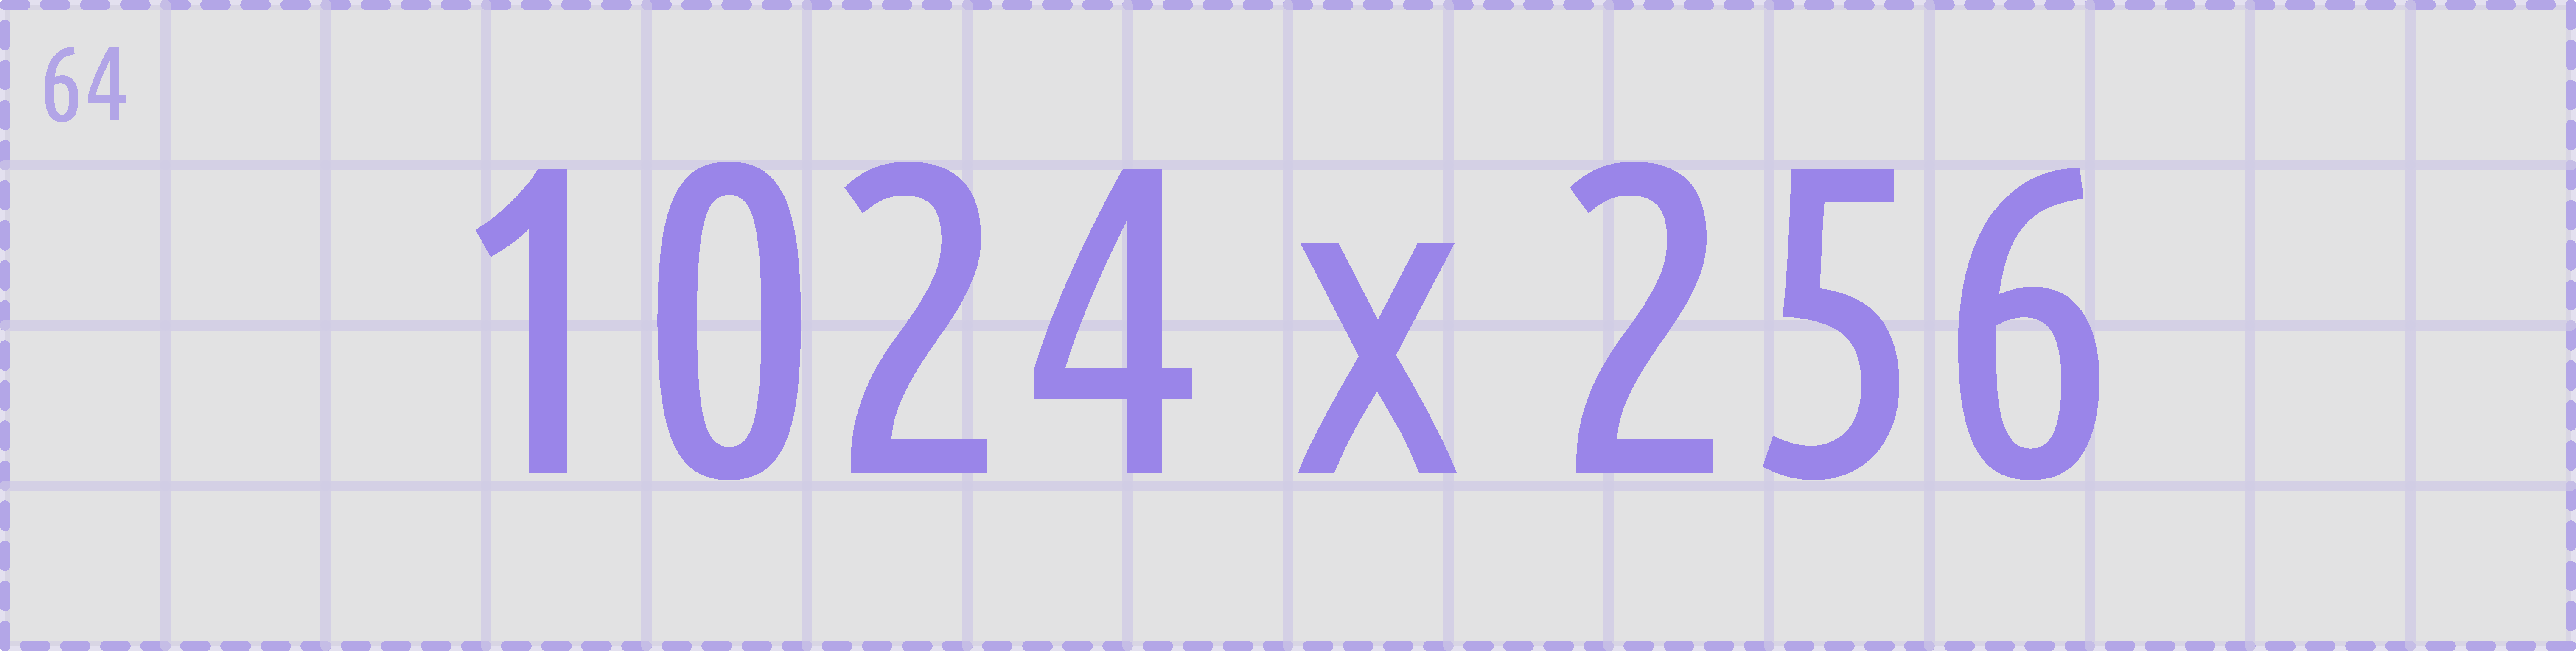
\includegraphics[width = 0.99\textwidth]{fig_1024x256.pdf}
%   \caption{Diagram of the efficient Matrix-Differential solver to compute the unknown Lagrangian entries in the model \eqref{eq:C2:dynamic_model}}
%   \vspace{-0.1cm}
%   \label{fig:C2:EX1:strain_ref}
% \end{figure}
% \begin{figure}[!t]
%  \vspace{-3mm}
%   \centering
%   \def\svgwidth{0.9\linewidth}
%   \input{./3_chapters/2_chapter/img/fig_C2_solver_diagram.pdf_tex}
%   \vspace{-0.25cm}
%   \caption{bla}
%   \vspace{-0.1cm}
%   \label{fig:C2:stiffness_model}
% \end{figure}
%
We wish to stress that $\mat{F}_1$ collects all elements related to the forward kinematics, whereas $\mat{F}_2$ contains the dynamic entities related to the Lagrangian model. Following the spatial Matrix-Differential equation in \eqref{eq:C2:MDE}, its solution will be a matrix $\mat{Z} := \text{blkdiag}\left( \mat{Z}_\textrm{kin}, \mat{Z}_\textrm{dyn} \right)$ composed of two state matrices $\mat{Z}_\textrm{kin}$ and $\mat{Z}_\textrm{dyn}$:
%
\begin{align}
\mat{Z}_\textrm{kin}(\sigma,\q,\dq) & := \begin{pmatrix}
\begin{matrix}
\PhiB  & \gammaB \\ 0_{3\times3} &  0_{3}
\end{matrix} \;\; \vrule & \!\mat{B}_1 & \vrule & \!\mat{B}_2 \;\;\;
 \end{pmatrix}, \\[0.5em]
\mat{Z}_\textrm{dyn}(\sigma,\q,\dq) & := \begin{pmatrix} \mat{M} & \mat{C} & \mat{f}\!\grav \end{pmatrix},
\end{align}
%
Such a set of Matrix-Differentials as in \eqref{eq:C2:MDE} are not supported natively by standard ODE solvers. Therefore, an explicit second-order Runge-Kutta solver for MDEs is developed such that efficiently computes the evolution of the state matrix $\mat{Z}$ along $\Xs = [0,L]$. The numerical solver is written in \matlab \texttt{2021a} and it can be found in the public repository of \sorotoki (see implementation at \cite{SorotokiCode}).

As for state trajectories along the temporal regime $\mathbb{T} = [0,T]$, an implicit trapezoidal integration scheme is proposed to solve the approximated continuum dynamics, which are generally less conservative on discretization to preserve numerical stability. Here implicit schemes are favored over the explicit scheme since a coarser time integration can significantly increase real-time performance. In addition, to further boost the performance of the temporal integration, a cost-effective approximation of the Hessian is introduced. For more detail on the temporal integration scheme of the solver can be found in Appendix \ref{app:C2:timeint}

%!TEX root = ../../thesis.tex
\section{Parameter identification}
\label{sec: chap2 section header}
\noindent In this section, the nonlinear stiffness function for elongation and bending, $k_e: \R \to \Rsp$ and $k_b: \R \to \Rsp$, respectively, are solidified such that the elastic deformation aligns with the physical system seen in Figure \ref{fig:C2:soft_robot}. Numerous studies consider these stiffnesses to be linear, however, the presence of exotic materials and complicated structures would justify the modeling of nonlinear elastic behavior. Here, we extend these conservative material models and explore the nonlinear and time-varying regime.

\subsection{Finite element method and hyper-elasticity}
Generally, soft robots are operated by (differential) pressure to air channels embedded in the elastic body. If the applied pressure is sufficiently larger than the ambient pressure, the elastic body deforms to counteract the external forces -- the critical point at which the external force overcome the internal elastic forces is proportional to the Young's modulus of the material. To enable efficient mobility, soft robots often explore of materials (or material composites) with a low Young's moduli, e.g., silicone elastomers. Unfortunately, large deformations of these rubber-like materials inherently lead to state-dependency in the mechanical compliance, and thus Hookean elasticity is no longer accurate -- rendering them hyper-elastic. These hyper-elastic materials branch a whole new subfield in continuum mechanics. Although analytic descriptions exist, hyper-elasticity is generally treated numerically through Finite Element techniques \cite{Duriez2013,Largilliere2015,Coevoet2017} paired with a (nonlinear) continuum mechanics framework.

Many variations of constitutive models for hyper-elastic materials are available, including Saint Venant-Kirchhoff, Neo-Hookean, Mooney-Rivlin, Ogden, and Yeoh  which are detailed in various work \cite{Meyer2009,Renaud2011,Kim2018}. In Mustaza et al. \cite{Mustaza2019}, a Yeoh constitutive model is explored to describe hyper-elastic material characteristics of a silicone-composite actuator. Duriez et al. \cite{Duriez2013} and related works \cite{Coevoet2017,Largilliere2015} employ Neo-Hookean material models to enrich the nonlinear deformations in FEM-driven models. There are many different constitutive models available, each better suited to describe specific nonlinear elastic behavior. Constitutive material models are mathematical functions used to express the (nonlinear) relationship between stress and strain in terms of deformation.  Let the spatial domain of robot's soft continuum body be given by $\mathbb{V}$ which is a compact subset of $\mathbb{R}^3$. This continuum body can be regarded as a collection of continuum particles called "\textit{material points}" represented by a spatial coordinate $\XB = [X_1, X_2, X_3]^\top \subseteq \mathcal{B}_0$. Now, assume there exists a mapping $\vec{\varphi}^{(t)}: \mathcal{B}_0 \to \mathcal{B}$ that maps these material points $\x$ into their deformed configuration $\mathcal{B}$. Then, given the deformation map $\vec{\varphi}^{(t)}$, the local geometrical deformations of the continuum solid relative to an undeformed configuration are described by the deformation gradient tensor given as follows \cite{Holzapfel2002,Kim2018}: \vspace{-3mm}

\begin{equation}
\mat{F} = \grad{\XB}\vec{\varphi}^{(T)}(\XB).
\end{equation}
%
For hyper-elastic materials, it is postulated that there exists a potential energy function $\mat{F} \mapsto \Psi(\mat{F})$ that is a function of the strain tensors. This potential function $\Psi(\mat{F})$ is also referred to as strain-energy density function, which depends exclusively on the material deformation.

In this work, we regard the Saint Venant-Kirchhoff constitutive model for hyper-elasticity \cite{Kim2018,Holzapfel2002}. The Saint Venant-Kirchhoff model is in many ways similar to linear elastic materials (\ie, Hooke's law), however, it is an extension from linear deformations into the nonlinear regime. The strain-energy density function for the Saint Venant-Kirchhoff model is defined as
%
\begin{equation}
\Psi^{\textrm{SV}} := \frac{\lambda}{2}\,\trace\,(\ten{E})^2 + \mu\,\trace\,(\ten{E}^2),
\label{eq:C2:mat_model}
\end{equation}
%
\noindent where $\ten{E} = \frac{1}{2}(\mat{F}^\top\mat{F} - \vec{I})$ the Green-Lagrange strain tensor, $\trace(\cdot)$ denotes the trace of a tensor, and $\lambda > 0$ and $\mu > 0$ are the Lam\'{e} parameters which arise from the strain-stress relationships of the elastic material. The relations for the Lam\'{e} parameters are given by
\begin{equation}
%
\lambda = \frac{\nu E_0}{(1+\nu_0)(1-2\nu_0)} \;\; \si{\mega \pascal}, \quad \quad \mu = \frac{E_0}{2(1+\nu_0)} \;\; \si{\mega \pascal};
\label{eq:C2:lame_coeff}
\end{equation}
%
where $E_0$ is the Young's modulus or elasticity modulus and $\nu_0$ is a dimensionless constant denoting the Poisson ratio. It is worth mentioning that the Yeoh or Ogden model is more suitable for silicone elastomer materials that are conventional material models for soft robotics.

In order to invoke the constitutive material law \eqref{eq:C2:mat_model} for three-dimensional solids, we explore the finite element method. We generated a finite element mesh of the soft robot manipulator in Figure \ref{fig:C2:soft_robot}. The finite element analysis has been carried out in \texttt{Abaqus/CEA} with variable time increments. Given preliminary uni-axial tension tests, the 3D-printed elastomer material is estimated to be linear isotropic described by the following Lam\'{e} parameters: $E_0  = 80 \; \si{\mega \pascal}$, $\nu_0 = 0.4 \; (\text{-})$. The Lam\'{e} parameters can be computed according to \eqref{eq:C2:lame_coeff}. Furthermore, tangential (frictionless) contact interaction is included in the numerical simulation to prevent self-intersection of the elastic body.

Two finite element simulations are performed to {independently characterize the elongation and bending stiffness of the soft robot. Due to simplicity, we start with the elongation stiffness}. Each embedded bellow is actuated simultaneously up to a quasi-static differential pressure $-20$ kPa $\le u_1(t) = u_2(t) = u_3(t) \le 30$ kPa. Due to the symmetry of soft actuators, the resulting deformation will be exclusively in axial-direction. The corresponding elongation strain of the soft robot can then be found by recovering the maximum vertical displacement of the nodal mesh, \ie, $\varepsilon = L\inv\max \left( {U}_z \right)$. Secondly, the analysis of the bending stiffness is conducted by actuating a single bellow up to a quasi-static differential pressure $-30$ kPa $\le u_1(t) \le  80$ kPa, while $u_2(t) = u_3(t) = 0$ kPa. To recover the bending angle of the elastic body, certain spatial coordinates of nodes close to the end effector are tracked. Given their global coordinates, a constraint nonlinear optimization \texttt{fmincon.m} is used to recover optimal Bishop parameters $\kappa$ and $\varepsilon
$ subjected to the kinematic relation in \eqref{eq:C2:phi_rodr} and \eqref{eq:C2:pos_exact}.
%
\begin{figure}[!t]
 %\vspace{-3mm} 
  \centering
  %% This file was created by matlab2tikz.
%
\begin{tikzpicture}

\begin{axis}[%
width=0.712\textwidth,
height=0.169\textwidth,
at={(0.11\textwidth,0\textwidth)},
scale only axis,
xmin=0,
xmax=1,
ymin=0,
ymax=1,
axis line style={draw=none},
ticks=none,
axis x line*=bottom,
axis y line*=left,
colorbar style={width=6,xshift=-7.5pt}
]
\end{axis}

\begin{axis}[%
width=0.158\textwidth,
height=0.142\textwidth,
at={(0\textwidth,0.016\textwidth)},
scale only axis,
axis on top,
xmin=0.5,
xmax=396.5,
tick align=outside,
y dir=reverse,
ymin=0.5,
ymax=366.5,
axis line style={draw=none},
ticks=none,
colorbar style={width=6,xshift=-7.5pt}
]
\addplot [forget plot] graphics [xmin=0.5, xmax=396.5, ymin=0.5, ymax=366.5] {./fig/fig_C2_fembend-1.png};
\end{axis}

\begin{axis}[%
width=0.158\textwidth,
height=0.142\textwidth,
at={(0.186\textwidth,0.016\textwidth)},
scale only axis,
axis on top,
xmin=0.5,
xmax=396.5,
tick align=outside,
y dir=reverse,
ymin=0.5,
ymax=366.5,
axis line style={draw=none},
ticks=none,
colorbar style={width=6,xshift=-7.5pt}
]
\addplot [forget plot] graphics [xmin=0.5, xmax=396.5, ymin=0.5, ymax=366.5] {./fig/fig_C2_fembend-2.png};
\end{axis}

\begin{axis}[%
width=0.158\textwidth,
height=0.142\textwidth,
at={(0.371\textwidth,0.016\textwidth)},
scale only axis,
axis on top,
xmin=0.5,
xmax=396.5,
tick align=outside,
y dir=reverse,
ymin=0.5,
ymax=366.5,
axis line style={draw=none},
ticks=none,
colorbar style={width=6,xshift=-7.5pt}
]
\addplot [forget plot] graphics [xmin=0.5, xmax=396.5, ymin=0.5, ymax=366.5] {./fig/fig_C2_fembend-3.png};
\end{axis}

\begin{axis}[%
width=0.158\textwidth,
height=0.142\textwidth,
at={(0.557\textwidth,0.016\textwidth)},
scale only axis,
axis on top,
xmin=0.5,
xmax=396.5,
tick align=outside,
y dir=reverse,
ymin=0.5,
ymax=366.5,
axis line style={draw=none},
ticks=none,
colorbar style={width=6,xshift=-7.5pt}
]
\addplot [forget plot] graphics [xmin=0.5, xmax=396.5, ymin=0.5, ymax=366.5] {./fig/fig_C2_fembend-4.png};
\end{axis}

\begin{axis}[%
width=0.158\textwidth,
height=0.15\textwidth,
at={(0.742\textwidth,0.012\textwidth)},
scale only axis,
axis on top,
xmin=0.5,
xmax=396.5,
tick align=outside,
y dir=reverse,
ymin=0.5,
ymax=388.5,
axis line style={draw=none},
ticks=none,
colorbar style={width=6,xshift=-7.5pt}
]
\addplot [forget plot] graphics [xmin=0.5, xmax=396.5, ymin=0.5, ymax=388.5] {./fig/fig_C2_fembend-5.png};
\end{axis}
\end{tikzpicture}% 
  \includegraphics*{./pdf/thesis-figure-4-6.pdf}
  \vspace{-0.2cm}
  \caption{ High resolution finite element simulations of the soft robot manipulator  \data{lightgreen} subjected to various input pressures $-20 \,\si{\kilo \pascal} \le \uB_i(t) \le 80 \,\si{\kilo \pascal}$.  These results are produced using \texttt{Abaqus/CEA} numerical solver.  To validate the PCC condition, an optimal backbone curve $\gammaB(\q^\star)$ is shown \data{magenta} whose joint coordinates are recovered by solving the optimization problem \eqref{eq:C2:optimization_problem}.}
  \vspace{-0.1cm}
  \label{fig:C2:fem_analysis}
\end{figure}
%
\begin{figure}[!t]
 \vspace{-1mm}
  %\centering
  \hspace{-2mm}
  %% This file was created by matlab2tikz.
%
\definecolor{mycolor1}{rgb}{0.79216,0.11765,0.17255}%
%\definecolor{mycolor2}{rgb}{0.00000,0.34510,0.65882}%
\definecolor{mycolor2}{rgb}{0.00000,0.34510,0.65882}%
%
\begin{tikzpicture}

\begin{axis}[%
width=0.37\textwidth,
height=0.235\textwidth,
at={(0\textwidth,0\textwidth)},
scale only axis,
xmin=-20,
xmax=20,
xlabel style={font=\color{white!15!black}},
xlabel={$(1 + \epsilon) L$ (mm)},
ymin=-20,
ymax=20,
ylabel style={font=\color{white!15!black}},
ylabel={force $F$ (N)},
axis background/.style={fill=white},
xmajorgrids,
ymajorgrids,
ylabel style={yshift=-2.5pt}
]
\addplot [color=mycolor2, line width=1.5pt, forget plot]
  table[row sep=crcr]{%
-20	-17.1146\\
-18.4	-14.9354\\
-16.8	-12.9051\\
-15.2	-11.0292\\
-13.6	-9.3104\\
-12.2	-7.9353\\
-10.2	-6.174\\
-9.7	-5.8494\\
-8.3	-4.7812\\
-6.7	-3.6805\\
-5.1	-2.6907\\
-3.3	-1.6819\\
3.5	1.7895\\
5.5	2.9289\\
7.1	3.9445\\
8.7	5.0759\\
11	6.8505\\
12.4	8.1245\\
13.8	9.5167\\
15.2	11.0292\\
16.8	12.9051\\
18.4	14.9354\\
20	17.1146\\
};
\end{axis}

\begin{axis}[%
width=0.37\textwidth,
height=0.235\textwidth,
at={(0.487\textwidth,0\textwidth)},
scale only axis,
xmin=-0.81,
xmax=1.2,
xlabel style={font=\color{white!15!black}},
xlabel={$\beta$ (rad)},
ymin=-0.04,
ymax=0.075,
ylabel style={font=\color{white!15!black}},
ylabel={moment $M$ (Nm)},
axis background/.style={fill=white},
xmajorgrids,
ymajorgrids,
ylabel style={yshift=-2.5pt}
]
\addplot [color=mycolor2, line width=1.5pt, forget plot]
  table[row sep=crcr]{%
-0.8592	-0.04\\
-0.8038	-0.0296000000000001\\
-0.7753	-0.0227999999999999\\
-0.7617	-0.0202\\
-0.7565	-0.0198\\
-0.5862	-0.0152000000000001\\
0	0\\
0.1836	0.00570000000000004\\
0.2634	0.00849999999999995\\
0.3709	0.0127999999999999\\
0.4661	0.0169999999999999\\
0.551	0.0213000000000001\\
0.697	0.0298\\
0.7606	0.0341\\
0.8735	0.0426\\
0.948	0.0489999999999999\\
1.0157	0.0553999999999999\\
1.0776	0.0618000000000001\\
1.1875	0.0746\\
1.2357	0.0808\\
};
\end{axis}

\begin{axis}[%
width=1.106\textwidth,
height=0.289\textwidth,
at={(-0.144\textwidth,-0.032\textwidth)},
scale only axis,
xmin=0,
xmax=1,
ymin=0,
ymax=1,
axis line style={draw=none},
ticks=none,
axis x line*=bottom,
axis y line*=left,
ylabel style={yshift=-2.5pt}
]
\draw[-{Stealth}, color=black, line width=1.0pt] (axis cs:0.638,0.528) -- (axis cs:0.624,0.38);
\node[below right, align=left, draw=white]
at (rel axis cs:0.585,0.673) {self-collision};
\end{axis}
\end{tikzpicture}%
  \includegraphics*{./pdf/thesis-figure-4-7.pdf}
  %\vspace{-0.5cm}
  \caption{Elongation force $F$ (\si{\newton}) and bending moment $M$ (\si{\newton \meter}) recovered from the finite element data analysis. Note that the curve parametrization using the Bishop variables $ \varepsilon = q_1$ and $\kappa = \sqrt{ \kappa_x^2 +  \kappa_y^2} = \sqrt{ {q_1}^2 +  {q_2}^2}$ are found using the optimization routine in \eqref{eq:C2:optimization_problem}. Notice also that self-collision occurs between the bellows for negative bending angles.}
  \vspace{-0.4cm}
  \label{fig:C2:fem_stress}
\end{figure}

%
\begin{align}
\begin{array}{ll}
\q^\star = & \!\!\underset{\q}{\textrm{argmin}}\; \left \lVert \log_{\SE{3}}\left[ \gB\inv(L,\q)\,\gB_L^{\textrm{FEM}}(\vec{u}) \right] \right \rVert_2,\\
& \!\!\textrm{s.t.} \quad \q \in \mathcal{Q} 
\end{array}
\label{eq:C2:optimization_problem}
\end{align}
%
where $\gB_L^{\textrm{FEM}}$ is simply the corresponding end-effector configuration derived from the high-resolution finite element simulation given the quasi-static input $\uB$. To some extent, the problem \eqref{eq:C2:optimization_problem} can be viewed as an inverse kinematics optimization problem subject to the desired end-effector configuration.

\begin{rmk} 
 It is worth noting that the optimization routine \eqref{eq:C2:optimization_problem} for state variable $\q^\star$ has a global minimizer. Namely, when both position and orientation are considered in the inverse kinematic optimization, there exist only one solution to $\q^\star$ on the configuration manifold $\Q$ (i.e., the length is bounded). This makes the problem well-defined. Uniqueness is desirable as this makes it more easy to relate the reduced beam model to the FEM data. A problem arises, however, when the approach extends to non-constant curvature or multi-link cases. In this cases, the system is hyper-redundant and thus many, perhaps infinite, solutions may exist. To solve this, a regularization term must be added $\Uf^\star = \tfrac{1}{2} \q^\top\mat{K}\q$ with some positive definite matrix $\mat{K} \succ 0 $. An example for $\mat{K}$ is the generalized stiffness matrix linearized around $\q = \vec{0}_n$. This ensures the inverse kinematic solutions on $\Q$ will also minimize the elastic potential energy, which is again a global minimum. If gravity dominates elasticity, the optimization routine can be enriched by using the full potential energy and energy applied by the external (pressure) input. However, in this case many solution may exist thus making it difficult to relate the estimates to the FEM data. Furthermore, its solutions also depend on the initialization of the solver. 
  
%Although straightforward for constant curvature soft-links, the approach could be easily extended to non-constant curvature and multi-link cases. However, an additional term $\Uf^\star = \tfrac{1}{2} \q^\top\mat{K}\q$ with some positive definite matrix $\mat{K} \succ 0 $ is required to ensure the nonlinear regression inhibits over-fitting.
\end{rmk}

Following the PCC condition, the bending angle $\beta$ can be calculated straightforwardly. Given these geometric curve parameters and the effective areas of the bellows, the applied elongation force and bending torque can be computed accordingly. The numerical results are provided in Figure \ref{fig:C2:fem_stress}. In practice, these nonlinear strain relations can also be determined experimentally; however, the numerical methods have the beneficial convenience of several post-processing procedures and gravitation-free deformations. To support our previous claim concerning the consistency of the PCC condition, Figure \ref{fig:C2:fem_analysis} provides a few FEM snapshots results together with the optimal backbone curve from \eqref{eq:C2:pos_exact}. It can be seen that the piece-wise constant curvature (PCC) condition, although a clear oversimplification of the true mechanics at hand, is remarkably consistent with the FEM simulations.

\subsection{Hyperelasicity  in joint space}
\label{sec:C2:hyperelastic}
\noindent From the finite element results in Figure \ref{fig:C2:fem_analysis}, the mathematical description for the nonlinear stiffness can be detailed further. However, a suitable candidate function must be chosen first to properly represent the hyperelastic stress-strain relation. The stiffness function $k_e (\varepsilon)$ and $k_b (\beta)$  have to satisfy the following properties.
%
\begin{asm}[Elastic boundedness]
\label{asm:C2:elastic_boundedness}
There exists positive constants ${k}^{-}$ and ${k}^{+}$ such that ${k}^{-} \le k_e(\xi),k_b(\xi) \le {k}^{+}$ for all possible strains $\xi \in \R$.  Given these bounds, it follows that conservative force produced by any deformation, given by ${\Ft} = \int_0^\xi k(s)s\;ds$, must be a monotonically increasing unction.  
\end{asm}
%
\begin{asm}[Deformations reversibility]
\label{asm:C2:elastic_reversibility}
The stiffness functions $k_e$ and $k_b$ have a global optimum (i.e., either a maximum or minimum) at the origin. 
\end{asm}
%
Assumption \ref{asm:C2:elastic_boundedness} and \ref{asm:C2:elastic_reversibility} are necessary since  they inhibit any buckling-type behavior, \ie, elastic bodies being able to store energy when a large enough forces is applied. Then. consider the following elasticity models for the nonlinear (hyper-elastic) elongation and bending stiffness:
%
\begin{align}
\label{eq:C2:stiffness_tanh_eps}
{k}_e(\varepsilon) & = \alpha_1 + \alpha_2 \left( \tanh[\alpha_3\,\varepsilon]^2 - 1 \right), \\[0.5em]
\label{eq:C2:stiffness_tanh_beta}
{k}_b(\q)  & = \alpha_{\phi}(\q) \cdot \left[\alpha_4 + \alpha_5 \left( \tanh[\alpha_6\,\beta(\q)]^2 - 1 \right)\right], 
\end{align}
%
where $\vec{\alpha} = \left(\alpha_1,\,\alpha_2,\,\alpha_3,\alpha_4,\,\alpha_5,\,\alpha_6 \right)^\top$ is a vector composed of the (possibly time-varying) stiffness parameters, and $\alpha_\phi: \mathcal{Q} \to [1,\infty)$ a nonlinear correction term for asymmetry along the circumference of the radial-axis. Please note that these nonlinear functions possess a decomposable structure: a linear term and a nonlinear term that mimics strain-hardening or strain-softening. As for the asymmetric stiffness due to the layout of the pneumatic bellows, we propose the following ansatz:
%
\begin{asm}[Stiffness variation under radial offset]
Given the radial layout of the pneumatic bellows of the soft robot (see Figure \ref{fig:C2:soft_robot}), we assume that the nonlinear correction term for asymmetric radial stiffness along the circumference can be modeled by:
%
\begin{equation}
\alpha_\phi (\q) = \frac{1}{2}\beta \big[\sin( m \,\phi(\q)) + 1 \big] + 1,
\end{equation}
%
where $m$ is the number of bellows, and $\phi(\q) = \text{atan2}(\kappa_y,\kappa_x)$ the direction angle or heading. This stiffness correction term ensures the nonlinear bending stiffness becomes larger between bellows -- as it causes simultaneous deformation of multiple bellows. Please note that $\alpha_\phi(\q) \ge 1$ for all $\q \in \mathcal{Q}$.
\end{asm}

To satisfy the aforementioned conditions, it should hold that $\alpha_1 > \alpha_2 $, $\alpha_4 > \alpha_5$ and $\alpha_{1,4} > 0$.  To find the hyper-elastic parameter vector $\alphaB$, we use a weighted least-squares optimization. Recalling the previous profiles for elongation force and bending moment obtained from the FEM data, see Figure ??, we integrate the expressions \eqref{eq:C2:stiffness_tanh_eps} and \eqref{eq:C2:stiffness_tanh_beta} to find an analytic approximation, i.e., $F(\varepsilon; \alphaB):= \int_0^\varepsilon k_e(\xi) \xi \; d\xi$ and $M(\beta; \alphaB):= \int_0^\beta k_b(\xi) \xi \; d\xi$, respectively. The weighted regression is biased towards positive strains, to better represent the deformation characteristics under positive pressurization. Again, we use \texttt{fmincon.m} optimizer in \textit{Matlab}. The hyper-elastic material parameters $\alphaB$ that minimize the residual between the FEM data and the analytic model are given in Table \ref{tab:C2:elastic_parameters}, and the comparison between the FEM force profiles and our solution is given in Figure \ref{fig:C2:fem_stiffness_recover_compare} Notice that self-collision is not capture by the stiffness model. Theoretically, the self-contact interactions (as seen in Figure \ref{fig:C2:fem_stiffness_recover_compare}) can also be parameterized using a different set of polynomials, which are non-zero for the compression regions and zero otherwise. In other words, the regression can be enriched with polynomials that are asymmetric with respect to the origin. We also provided Figure \ref{fig:C2:stiffness_model} to show the change in stiffness when the soft robot deforms, where we can clearly see a discrete radial symmetry arise due to the radial composition of the three bellow network. 



% Using a weighted least-squarest optimization, the nonlinear stiffness parameter vector $\vec{\alpha}$ can be identified. The estimated hyper-elastic material parameters are shown in Table \ref{tab:C2:elastic_parameters}. Furthermore, the weighted regression is biased towards positive strains, to better represent the deformation characteristics under positive pressurization. Theoretically, the self-contact interactions (as seen in Figure \ref{fig:C2:fem_analysis}) can also be parameterized using a different set of (convex) non-zero polynomials, similar to the functions \eqref{eq:C2:stiffness_tanh_eps} and \eqref{eq:C2:stiffness_tanh_beta}.

\begin{figure}[!t]
  \vspace{-1mm}
   %\centering
   \hspace{-2mm}
   %% This file was created by matlab2tikz.
%
\definecolor{mycolor1}{rgb}{0.79216,0.11765,0.17255}%
\definecolor{mycolor2}{rgb}{0.00000,0.34510,0.65882}%
%
\begin{tikzpicture}

\begin{axis}[%
width=0.37\textwidth,
height=0.235\textwidth,
at={(0\textwidth,0\textwidth)},
scale only axis,
xmin=-20,
xmax=20,
xlabel style={font=\color{white!15!black}},
xlabel={$(1 + \varepsilon) L$ (mm)},
ymin=-20,
ymax=20,
ylabel style={font=\color{white!15!black}},
ylabel={force $F$ (N)},
axis background/.style={fill=white},
xmajorgrids,
ymajorgrids,
ylabel style={yshift=-2.5pt}
]
\addplot [color=mycolor1, line width=2.0pt, forget plot]
  table[row sep=crcr]{%
-20	-17.1146\\
-18.4	-14.9354\\
-16.8	-12.9051\\
-15.2	-11.0292\\
-13.6	-9.3104\\
-12.2	-7.9353\\
-10.2	-6.174\\
-9.7	-5.8494\\
-8.3	-4.7812\\
-6.7	-3.6805\\
-5.1	-2.6907\\
-3.3	-1.6819\\
3.5	1.7895\\
5.5	2.9289\\
7.1	3.9445\\
8.7	5.0759\\
11	6.8505\\
12.4	8.1245\\
13.8	9.5167\\
15.2	11.0292\\
16.8	12.9051\\
18.4	14.9354\\
20	17.1146\\
};
\addplot [color=mycolor2, dotted, line width=1.5pt, forget plot]
  table[row sep=crcr]{%
-20	-17.1146\\
-18.4	-14.9354\\
-16.8	-12.9051\\
-15.2	-11.0292\\
-13.6	-9.3104\\
-12.2	-7.9353\\
-10.2	-6.174\\
-9.7	-5.8494\\
-8.3	-4.7812\\
-6.7	-3.6805\\
-5.1	-2.6907\\
-3.3	-1.6819\\
3.5	1.7895\\
5.5	2.9289\\
7.1	3.9445\\
8.7	5.0759\\
11	6.8505\\
12.4	8.1245\\
13.8	9.5167\\
15.2	11.0292\\
16.8	12.9051\\
18.4	14.9354\\
20	17.1146\\
};
\end{axis}

\begin{axis}[%
width=0.37\textwidth,
height=0.235\textwidth,
at={(0.487\textwidth,0\textwidth)},
scale only axis,
xmin=-0.81,
xmax=1.2,
xlabel style={font=\color{white!15!black}},
xlabel={$\beta$ (rad)},
ymin=-0.04,
ymax=0.075,
ylabel style={font=\color{white!15!black}},
ylabel={moment $M$ (Nm)},
axis background/.style={fill=white},
xmajorgrids,
ymajorgrids,
ylabel style={yshift=-2.5pt}
]
\addplot [color=mycolor1, line width=2.0pt, forget plot]
  table[row sep=crcr]{%
-0.8192	-0.0384\\
-0.7606	-0.0341\\
-0.697	-0.0298\\
-0.6275	-0.0256000000000001\\
-0.551	-0.0213000000000001\\
-0.4661	-0.0169999999999999\\
-0.3709	-0.0127999999999999\\
-0.2634	-0.00849999999999995\\
-0.0864	-0.00249999999999995\\
0	0\\
0.1836	0.00570000000000004\\
0.2634	0.00849999999999995\\
0.3709	0.0127999999999999\\
0.4661	0.0169999999999999\\
0.551	0.0213000000000001\\
0.697	0.0298\\
0.7606	0.0341\\
0.8735	0.0426\\
0.948	0.0489999999999999\\
1.0157	0.0553999999999999\\
1.0776	0.0618000000000001\\
1.1875	0.0746\\
1.2357	0.0808\\
};
\addplot [color=mycolor2, dotted, line width=1.5pt, forget plot]
  table[row sep=crcr]{%
-0.8592	-0.04\\
-0.8038	-0.0296000000000001\\
-0.7753	-0.0227999999999999\\
-0.7617	-0.0202\\
-0.7565	-0.0198\\
-0.5862	-0.0152000000000001\\
0	0\\
0.1836	0.00570000000000004\\
0.2634	0.00849999999999995\\
0.3709	0.0127999999999999\\
0.4661	0.0169999999999999\\
0.551	0.0213000000000001\\
0.697	0.0298\\
0.7606	0.0341\\
0.8735	0.0426\\
0.948	0.0489999999999999\\
1.0157	0.0553999999999999\\
1.0776	0.0618000000000001\\
1.1875	0.0746\\
1.2357	0.0808\\
};
\end{axis}

\begin{axis}[%
width=1.106\textwidth,
height=0.289\textwidth,
at={(-0.144\textwidth,-0.032\textwidth)},
scale only axis,
xmin=0,
xmax=1,
ymin=0,
ymax=1,
axis line style={draw=none},
ticks=none,
axis x line*=bottom,
axis y line*=left,
ylabel style={yshift=-2.5pt}
]
\draw[-{Stealth}, color=black, line width=1.0pt] (axis cs:0.638,0.528) -- (axis cs:0.624,0.38);
\node[below right, align=left, draw=white]
at (rel axis cs:0.585,0.673) {self-collision};
\end{axis}
\end{tikzpicture}%
   \includegraphics*{./pdf/thesis-figure-4-8.pdf}
   %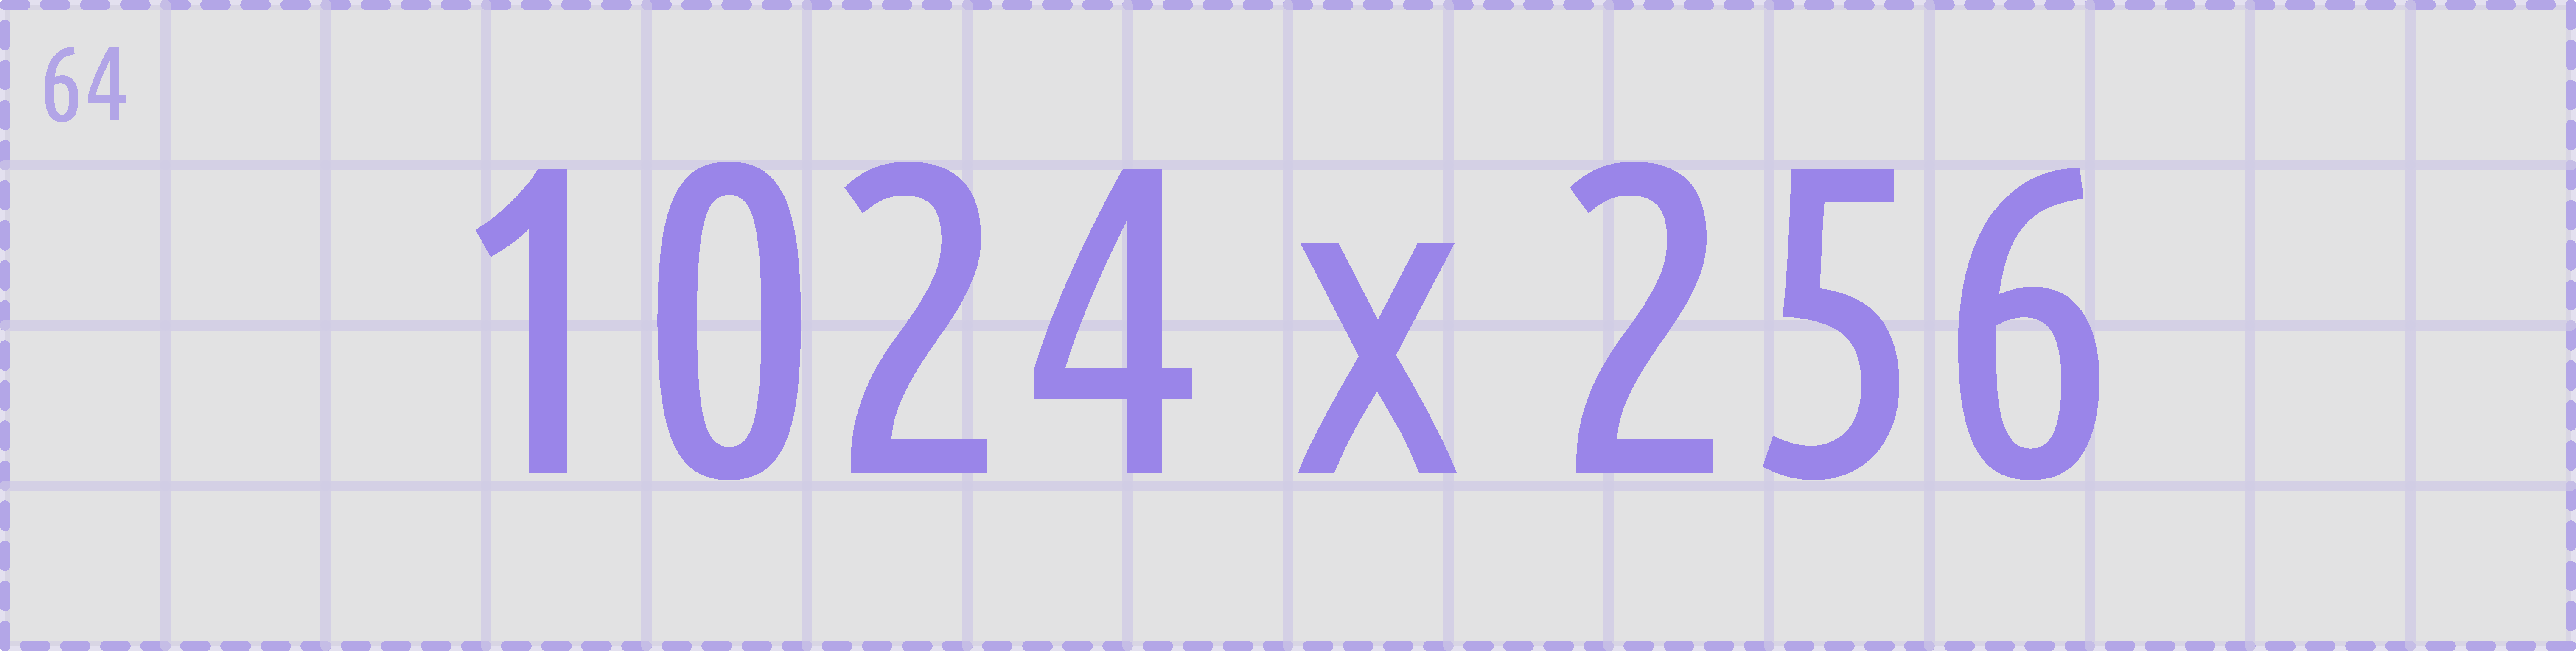
\includegraphics[width = 0.99\textwidth]{fig_1024x256.pdf}
   \vspace{-0.5cm}
   \caption{Comparison of the (nonlinear) mechanical compliance between the proposed hyper-elastic model \data{Matlab2} and the finite element simulations \data{Matlab1}. Notice the proposed stiffness model \eqref{eq:C2:stiffness_tanh_beta} does not capture the self-collision. }
   \vspace{-0.1cm}
   \label{fig:C2:fem_stiffness_recover_compare}
 \end{figure}
 
\pgfplotsset{colormap name=turbo}
\begin{figure}[!t]
  \vspace{-5mm}
  \centering
  %% This file was created by matlab2tikz.
%
\begin{tikzpicture}

\begin{axis}[%
width=0.324\textwidth,
height=0.325\textwidth,
at={(0\textwidth,0\textwidth)},
scale only axis,
xmin=-3.77645049743461,
xmax=3.77645049743461,
xlabel style={font=\color{white!15!black}},
xlabel={$\kappa_x$ (1/m)},
ymin=-3.77645049743461,
ymax=3.77645049743461,
ylabel style={font=\color{white!15!black}},
ylabel={$\kappa_y$ (1/m)},
axis background/.style={fill=white},
xmajorgrids,
ymajorgrids,
ylabel style={yshift=-1.75pt}
]

\addplot[%
surf,
shader=interp, colormap={mymap}{[1pt] rgb(0pt)=(0.2,0.1059,0.2431); rgb(1pt)=(0.2104,0.1627,0.3554); rgb(2pt)=(0.2202,0.204,0.4359); rgb(3pt)=(0.2295,0.2376,0.5013); rgb(4pt)=(0.2385,0.2666,0.5573); rgb(5pt)=(0.2471,0.2923,0.6069); rgb(6pt)=(0.2553,0.3156,0.6518); rgb(7pt)=(0.2633,0.337,0.6931); rgb(8pt)=(0.271,0.3569,0.7314); rgb(9pt)=(0.2784,0.3755,0.7672); rgb(10pt)=(0.2856,0.3931,0.801); rgb(11pt)=(0.2926,0.4097,0.833); rgb(12pt)=(0.2994,0.4256,0.8634); rgb(13pt)=(0.2993,0.4519,0.8765); rgb(14pt)=(0.295,0.4827,0.8798); rgb(15pt)=(0.2906,0.5111,0.883); rgb(16pt)=(0.2862,0.5377,0.8862); rgb(17pt)=(0.2817,0.5627,0.8894); rgb(18pt)=(0.277,0.5864,0.8926); rgb(19pt)=(0.2723,0.6089,0.8958); rgb(20pt)=(0.2675,0.6304,0.8989); rgb(21pt)=(0.2626,0.651,0.9021); rgb(22pt)=(0.2576,0.6707,0.9052); rgb(23pt)=(0.2524,0.6898,0.9083); rgb(24pt)=(0.2472,0.7082,0.9114); rgb(25pt)=(0.2441,0.7264,0.9089); rgb(26pt)=(0.2479,0.7455,0.8894); rgb(27pt)=(0.2516,0.764,0.8693); rgb(28pt)=(0.2553,0.782,0.8485); rgb(29pt)=(0.2589,0.7994,0.8271); rgb(30pt)=(0.2624,0.8163,0.8049); rgb(31pt)=(0.2659,0.8328,0.7819); rgb(32pt)=(0.2694,0.8488,0.7579); rgb(33pt)=(0.2728,0.8645,0.733); rgb(34pt)=(0.2761,0.8798,0.7068); rgb(35pt)=(0.2794,0.8947,0.6794); rgb(36pt)=(0.2827,0.9094,0.6504); rgb(37pt)=(0.2859,0.9237,0.6196); rgb(38pt)=(0.3296,0.9295,0.5999); rgb(39pt)=(0.3722,0.9341,0.5812); rgb(40pt)=(0.4095,0.9386,0.5616); rgb(41pt)=(0.4431,0.9431,0.5412); rgb(42pt)=(0.4737,0.9476,0.5197); rgb(43pt)=(0.5021,0.9521,0.4971); rgb(44pt)=(0.5285,0.9565,0.4731); rgb(45pt)=(0.5534,0.9609,0.4474); rgb(46pt)=(0.5769,0.9653,0.4198); rgb(47pt)=(0.5993,0.9696,0.3897); rgb(48pt)=(0.6206,0.974,0.3564); rgb(49pt)=(0.6411,0.9783,0.3189); rgb(50pt)=(0.6653,0.9741,0.2979); rgb(51pt)=(0.6928,0.9612,0.2976); rgb(52pt)=(0.7189,0.9482,0.2973); rgb(53pt)=(0.7438,0.9349,0.2969); rgb(54pt)=(0.7677,0.9214,0.2966); rgb(55pt)=(0.7907,0.9075,0.2963); rgb(56pt)=(0.8128,0.8934,0.296); rgb(57pt)=(0.8342,0.879,0.2957); rgb(58pt)=(0.8549,0.8643,0.2954); rgb(59pt)=(0.8749,0.8493,0.295); rgb(60pt)=(0.8944,0.8339,0.2947); rgb(61pt)=(0.9133,0.8181,0.2944); rgb(62pt)=(0.9299,0.8016,0.2934); rgb(63pt)=(0.9342,0.7825,0.2875); rgb(64pt)=(0.9384,0.7628,0.2815); rgb(65pt)=(0.9426,0.7424,0.2753); rgb(66pt)=(0.9468,0.7213,0.2689); rgb(67pt)=(0.951,0.6993,0.2624); rgb(68pt)=(0.9551,0.6764,0.2556); rgb(69pt)=(0.9592,0.6525,0.2487); rgb(70pt)=(0.9633,0.6273,0.2415); rgb(71pt)=(0.9673,0.6008,0.2341); rgb(72pt)=(0.9714,0.5726,0.2264); rgb(73pt)=(0.9754,0.5426,0.2183); rgb(74pt)=(0.9794,0.5103,0.21); rgb(75pt)=(0.9712,0.4904,0.204); rgb(76pt)=(0.9589,0.4744,0.1987); rgb(77pt)=(0.9463,0.4577,0.1933); rgb(78pt)=(0.9335,0.4402,0.1878); rgb(79pt)=(0.9205,0.4218,0.182); rgb(80pt)=(0.9072,0.4024,0.176); rgb(81pt)=(0.8936,0.3817,0.1699); rgb(82pt)=(0.8798,0.3596,0.1634); rgb(83pt)=(0.8657,0.3357,0.1567); rgb(84pt)=(0.8513,0.3095,0.1497); rgb(85pt)=(0.8365,0.2803,0.1423); rgb(86pt)=(0.8214,0.247,0.1345); rgb(87pt)=(0.8039,0.2207,0.1277); rgb(88pt)=(0.7824,0.2131,0.1232); rgb(89pt)=(0.76,0.2051,0.1185); rgb(90pt)=(0.7368,0.1967,0.1136); rgb(91pt)=(0.7126,0.188,0.1084); rgb(92pt)=(0.6873,0.1787,0.1031); rgb(93pt)=(0.6607,0.169,0.0975); rgb(94pt)=(0.6327,0.1586,0.0915); rgb(95pt)=(0.603,0.1474,0.0853); rgb(96pt)=(0.5712,0.1353,0.0786); rgb(97pt)=(0.537,0.122,0.0714); rgb(98pt)=(0.4999,0.1072,0.0635); rgb(99pt)=(0.4588,0.0902,0.0549)}, mesh/rows=50]
table[row sep=crcr, point meta=\thisrow{c}] {%
%
x	y	c\\
0	0	100\\
0.0641141357875468	0	100.000036708885\\
0.128228271575094	0	100.000146835527\\
0.19234240736264	0	100.000330379891\\
0.256456543150187	0	100.000587341917\\
0.320570678937734	0	100.00091772152\\
0.384684814725281	0	100.001321518594\\
0.448798950512828	0	100.001798733005\\
0.512913086300374	0	100.0023493646\\
0.577027222087921	0	100.002973413197\\
0.641141357875468	0	100.003670878594\\
0.705255493663015	0	100.004441760562\\
0.769369629450562	0	100.005286058851\\
0.833483765238108	0	100.006203773184\\
0.897597901025655	0	100.007194903263\\
0.961712036813202	0	100.008259448763\\
1.02582617260075	0	100.009397409337\\
1.0899403083883	0	100.010608784615\\
1.15405444417584	0	100.011893574201\\
1.21816857996339	0	100.013251777676\\
1.28228271575094	0	100.014683394596\\
1.34639685153848	0	100.016188424494\\
1.41051098732603	0	100.017766866879\\
1.47462512311358	0	100.019418721237\\
1.53873925890112	0	100.021143987028\\
1.60285339468867	0	100.02294266369\\
1.66696753047622	0	100.024814750635\\
1.73108166626376	0	100.026760247252\\
1.79519580205131	0	100.028779152908\\
1.85930993783886	0	100.030871466942\\
1.9234240736264	0	100.033037188673\\
1.98753820941395	0	100.035276317393\\
2.0516523452015	0	100.037588852373\\
2.11576648098904	0	100.039974792857\\
2.17988061677659	0	100.042434138068\\
2.24399475256414	0	100.044966887202\\
2.30810888835168	0	100.047573039433\\
2.37222302413923	0	100.050252593912\\
2.43633715992678	0	100.053005549763\\
2.50045129571433	0	100.055831906088\\
2.56456543150187	0	100.058731661966\\
2.62867956728942	0	100.061704816451\\
2.69279370307697	0	100.064751368571\\
2.75690783886451	0	100.067871317334\\
2.82102197465206	0	100.071064661721\\
2.88513611043961	0	100.07433140069\\
2.94925024622715	0	100.077671533176\\
3.0133643820147	0	100.081085058089\\
3.07747851780225	0	100.084571974315\\
3.14159265358979	0	100.088132280716\\
0	0	100\\
0.0635877596189965	0.00819873370836649	100.000036708885\\
0.127175519237993	0.016397467416733	100.000146835527\\
0.19076327885699	0.0245962011250995	100.000330379891\\
0.254351038475986	0.032794934833466	100.000587341917\\
0.317938798094983	0.0409936685418325	100.00091772152\\
0.381526557713979	0.049192402250199	100.001321518594\\
0.445114317332976	0.0573911359585655	100.001798733005\\
0.508702076951972	0.0655898696669319	100.0023493646\\
0.572289836570969	0.0737886033752985	100.002973413197\\
0.635877596189965	0.0819873370836649	100.003670878594\\
0.699465355808962	0.0901860707920314	100.004441760562\\
0.763053115427958	0.0983848045003979	100.005286058851\\
0.826640875046955	0.106583538208764	100.006203773184\\
0.890228634665951	0.114782271917131	100.007194903263\\
0.953816394284948	0.122981005625497	100.008259448763\\
1.01740415390394	0.131179739333864	100.009397409337\\
1.08099191352294	0.13937847304223	100.010608784615\\
1.14457967314194	0.147577206750597	100.011893574201\\
1.20816743276093	0.155775940458963	100.013251777676\\
1.27175519237993	0.16397467416733	100.014683394596\\
1.33534295199893	0.172173407875696	100.016188424494\\
1.39893071161792	0.180372141584063	100.017766866879\\
1.46251847123692	0.188570875292429	100.019418721237\\
1.52610623085592	0.196769609000796	100.021143987028\\
1.58969399047491	0.204968342709162	100.02294266369\\
1.65328175009391	0.213167076417529	100.024814750635\\
1.71686950971291	0.221365810125895	100.026760247252\\
1.7804572693319	0.229564543834262	100.028779152908\\
1.8440450289509	0.237763277542628	100.030871466942\\
1.9076327885699	0.245962011250995	100.033037188673\\
1.97122054818889	0.254160744959361	100.035276317393\\
2.03480830780789	0.262359478667728	100.037588852373\\
2.09839606742689	0.270558212376094	100.039974792857\\
2.16198382704588	0.278756946084461	100.042434138068\\
2.22557158666488	0.286955679792827	100.044966887202\\
2.28915934628388	0.295154413501194	100.047573039433\\
2.35274710590287	0.30335314720956	100.050252593912\\
2.41633486552187	0.311551880917927	100.053005549763\\
2.47992262514086	0.319750614626293	100.055831906088\\
2.54351038475986	0.32794934833466	100.058731661966\\
2.60709814437886	0.336148082043026	100.061704816451\\
2.67068590399785	0.344346815751393	100.064751368571\\
2.73427366361685	0.352545549459759	100.067871317334\\
2.79786142323585	0.360744283168126	100.071064661721\\
2.86144918285484	0.368943016876492	100.07433140069\\
2.92503694247384	0.377141750584859	100.077671533176\\
2.98862470209284	0.385340484293225	100.081085058089\\
3.05221246171183	0.393539218001592	100.084571974315\\
3.11580022133083	0.401737951709958	100.088132280716\\
0	0	100\\
0.0620172741954808	0.0162628444359078	100.000036708885\\
0.124034548390962	0.0325256888718157	100.000146835527\\
0.186051822586442	0.0487885333077235	100.000330379891\\
0.248069096781923	0.0650513777436313	100.000587341917\\
0.310086370977404	0.0813142221795392	100.00091772152\\
0.372103645172885	0.097577066615447	100.001321518594\\
0.434120919368366	0.113839911051355	100.001798733005\\
0.496138193563847	0.130102755487263	100.0023493646\\
0.558155467759327	0.146365599923171	100.002973413197\\
0.620172741954808	0.162628444359078	100.003670878594\\
0.682190016150289	0.178891288794986	100.004441760562\\
0.74420729034577	0.195154133230894	100.005286058851\\
0.806224564541251	0.211416977666802	100.006203773184\\
0.868241838736731	0.22767982210271	100.007194903263\\
0.930259112932212	0.243942666538618	100.008259448763\\
0.992276387127693	0.260205510974525	100.009397409337\\
1.05429366132317	0.276468355410433	100.010608784615\\
1.11631093551865	0.292731199846341	100.011893574201\\
1.17832820971414	0.308994044282249	100.013251777676\\
1.24034548390962	0.325256888718157	100.014683394596\\
1.3023627581051	0.341519733154065	100.016188424494\\
1.36438003230058	0.357782577589972	100.017766866879\\
1.42639730649606	0.37404542202588	100.019418721237\\
1.48841458069154	0.390308266461788	100.021143987028\\
1.55043185488702	0.406571110897696	100.02294266369\\
1.6124491290825	0.422833955333604	100.024814750635\\
1.67446640327798	0.439096799769512	100.026760247252\\
1.73648367747346	0.455359644205419	100.028779152908\\
1.79850095166894	0.471622488641327	100.030871466942\\
1.86051822586442	0.487885333077235	100.033037188673\\
1.92253550005991	0.504148177513143	100.035276317393\\
1.98455277425539	0.520411021949051	100.037588852373\\
2.04657004845087	0.536673866384959	100.039974792857\\
2.10858732264635	0.552936710820866	100.042434138068\\
2.17060459684183	0.569199555256774	100.044966887202\\
2.23262187103731	0.585462399692682	100.047573039433\\
2.29463914523279	0.60172524412859	100.050252593912\\
2.35665641942827	0.617988088564498	100.053005549763\\
2.41867369362375	0.634250933000406	100.055831906088\\
2.48069096781923	0.650513777436314	100.058731661966\\
2.54270824201471	0.666776621872221	100.061704816451\\
2.60472551621019	0.683039466308129	100.064751368571\\
2.66674279040567	0.699302310744037	100.067871317334\\
2.72876006460116	0.715565155179945	100.071064661721\\
2.79077733879664	0.731827999615853	100.07433140069\\
2.85279461299212	0.748090844051761	100.077671533176\\
2.9148118871876	0.764353688487668	100.081085058089\\
2.97682916138308	0.780616532923576	100.084571974315\\
3.03884643557856	0.796879377359484	100.088132280716\\
0	0	100\\
0.0594284668442354	0.0240599197074222	100.000036708885\\
0.118856933688471	0.0481198394148444	100.000146835527\\
0.178285400532706	0.0721797591222665	100.000330379891\\
0.237713867376942	0.0962396788296887	100.000587341917\\
0.297142334221177	0.120299598537111	100.00091772152\\
0.356570801065412	0.144359518244533	100.001321518594\\
0.415999267909648	0.168419437951955	100.001798733005\\
0.475427734753883	0.192479357659377	100.0023493646\\
0.534856201598119	0.2165392773668	100.002973413197\\
0.594284668442354	0.240599197074222	100.003670878594\\
0.653713135286589	0.264659116781644	100.004441760562\\
0.713141602130825	0.288719036489066	100.005286058851\\
0.77257006897506	0.312778956196488	100.006203773184\\
0.831998535819296	0.33683887590391	100.007194903263\\
0.891427002663531	0.360898795611333	100.008259448763\\
0.950855469507766	0.384958715318755	100.009397409337\\
1.010283936352	0.409018635026177	100.010608784615\\
1.06971240319624	0.433078554733599	100.011893574201\\
1.12914087004047	0.457138474441021	100.013251777676\\
1.18856933688471	0.481198394148444	100.014683394596\\
1.24799780372894	0.505258313855866	100.016188424494\\
1.30742627057318	0.529318233563288	100.017766866879\\
1.36685473741741	0.55337815327071	100.019418721237\\
1.42628320426165	0.577438072978132	100.021143987028\\
1.48571167110589	0.601497992685554	100.02294266369\\
1.54514013795012	0.625557912392977	100.024814750635\\
1.60456860479436	0.649617832100399	100.026760247252\\
1.66399707163859	0.673677751807821	100.028779152908\\
1.72342553848283	0.697737671515243	100.030871466942\\
1.78285400532706	0.721797591222665	100.033037188673\\
1.8422824721713	0.745857510930087	100.035276317393\\
1.90171093901553	0.76991743063751	100.037588852373\\
1.96113940585977	0.793977350344932	100.039974792857\\
2.020567872704	0.818037270052354	100.042434138068\\
2.07999633954824	0.842097189759776	100.044966887202\\
2.13942480639247	0.866157109467198	100.047573039433\\
2.19885327323671	0.890217029174621	100.050252593912\\
2.25828174008095	0.914276948882043	100.053005549763\\
2.31771020692518	0.938336868589465	100.055831906088\\
2.37713867376942	0.962396788296887	100.058731661966\\
2.43656714061365	0.986456708004309	100.061704816451\\
2.49599560745789	1.01051662771173	100.064751368571\\
2.55542407430212	1.03457654741915	100.067871317334\\
2.61485254114636	1.05863646712658	100.071064661721\\
2.67428100799059	1.082696386834	100.07433140069\\
2.73370947483483	1.10675630654142	100.077671533176\\
2.79313794167906	1.13081622624884	100.081085058089\\
2.8525664085233	1.15487614595626	100.084571974315\\
2.91199487536753	1.17893606566369	100.088132280716\\
0	0	100\\
0.0558638457103963	0.031461931762513	100.000036708885\\
0.111727691420793	0.062923863525026	100.000146835527\\
0.167591537131189	0.0943857952875391	100.000330379891\\
0.223455382841585	0.125847727050052	100.000587341917\\
0.279319228551981	0.157309658812565	100.00091772152\\
0.335183074262378	0.188771590575078	100.001321518594\\
0.391046919972774	0.220233522337591	100.001798733005\\
0.44691076568317	0.251695454100104	100.0023493646\\
0.502774611393567	0.283157385862617	100.002973413197\\
0.558638457103963	0.31461931762513	100.003670878594\\
0.614502302814359	0.346081249387643	100.004441760562\\
0.670366148524756	0.377543181150156	100.005286058851\\
0.726229994235152	0.409005112912669	100.006203773184\\
0.782093839945548	0.440467044675182	100.007194903263\\
0.837957685655945	0.471928976437695	100.008259448763\\
0.893821531366341	0.503390908200208	100.009397409337\\
0.949685377076737	0.534852839962722	100.010608784615\\
1.00554922278713	0.566314771725235	100.011893574201\\
1.06141306849753	0.597776703487747	100.013251777676\\
1.11727691420793	0.629238635250261	100.014683394596\\
1.17314075991832	0.660700567012774	100.016188424494\\
1.22900460562872	0.692162498775286	100.017766866879\\
1.28486845133911	0.7236244305378	100.019418721237\\
1.34073229704951	0.755086362300313	100.021143987028\\
1.39659614275991	0.786548294062826	100.02294266369\\
1.4524599884703	0.818010225825339	100.024814750635\\
1.5083238341807	0.849472157587852	100.026760247252\\
1.5641876798911	0.880934089350365	100.028779152908\\
1.62005152560149	0.912396021112878	100.030871466942\\
1.67591537131189	0.943857952875391	100.033037188673\\
1.73177921702229	0.975319884637904	100.035276317393\\
1.78764306273268	1.00678181640042	100.037588852373\\
1.84350690844308	1.03824374816293	100.039974792857\\
1.89937075415347	1.06970567992544	100.042434138068\\
1.95523459986387	1.10116761168796	100.044966887202\\
2.01109844557427	1.13262954345047	100.047573039433\\
2.06696229128466	1.16409147521298	100.050252593912\\
2.12282613699506	1.19555340697549	100.053005549763\\
2.17868998270546	1.22701533873801	100.055831906088\\
2.23455382841585	1.25847727050052	100.058731661966\\
2.29041767412625	1.28993920226303	100.061704816451\\
2.34628151983664	1.32140113402555	100.064751368571\\
2.40214536554704	1.35286306578806	100.067871317334\\
2.45800921125744	1.38432499755057	100.071064661721\\
2.51387305696783	1.41578692931309	100.07433140069\\
2.56973690267823	1.4472488610756	100.077671533176\\
2.62560074838863	1.47871079283811	100.081085058089\\
2.68146459409902	1.51017272460063	100.084571974315\\
2.73732843980942	1.54163465636314	100.088132280716\\
0	0	100\\
0.0513819417744319	0.0383473397678755	100.000036708885\\
0.102763883548864	0.0766946795357509	100.000146835527\\
0.154145825323296	0.115042019303626	100.000330379891\\
0.205527767097727	0.153389359071502	100.000587341917\\
0.256909708872159	0.191736698839377	100.00091772152\\
0.308291650646591	0.230084038607253	100.001321518594\\
0.359673592421023	0.268431378375128	100.001798733005\\
0.411055534195455	0.306778718143004	100.0023493646\\
0.462437475969887	0.345126057910879	100.002973413197\\
0.513819417744319	0.383473397678755	100.003670878594\\
0.56520135951875	0.42182073744663	100.004441760562\\
0.616583301293182	0.460168077214506	100.005286058851\\
0.667965243067614	0.498515416982381	100.006203773184\\
0.719347184842046	0.536862756750257	100.007194903263\\
0.770729126616478	0.575210096518132	100.008259448763\\
0.82211106839091	0.613557436286007	100.009397409337\\
0.873493010165342	0.651904776053883	100.010608784615\\
0.924874951939773	0.690252115821758	100.011893574201\\
0.976256893714205	0.728599455589634	100.013251777676\\
1.02763883548864	0.766946795357509	100.014683394596\\
1.07902077726307	0.805294135125385	100.016188424494\\
1.1304027190375	0.84364147489326	100.017766866879\\
1.18178466081193	0.881988814661136	100.019418721237\\
1.23316660258636	0.920336154429011	100.021143987028\\
1.2845485443608	0.958683494196887	100.02294266369\\
1.33593048613523	0.997030833964762	100.024814750635\\
1.38731242790966	1.03537817373264	100.026760247252\\
1.43869436968409	1.07372551350051	100.028779152908\\
1.49007631145852	1.11207285326839	100.030871466942\\
1.54145825323296	1.15042019303626	100.033037188673\\
1.59284019500739	1.18876753280414	100.035276317393\\
1.64422213678182	1.22711487257201	100.037588852373\\
1.69560407855625	1.26546221233989	100.039974792857\\
1.74698602033068	1.30380955210777	100.042434138068\\
1.79836796210511	1.34215689187564	100.044966887202\\
1.84974990387955	1.38050423164352	100.047573039433\\
1.90113184565398	1.41885157141139	100.050252593912\\
1.95251378742841	1.45719891117927	100.053005549763\\
2.00389572920284	1.49554625094714	100.055831906088\\
2.05527767097727	1.53389359071502	100.058731661966\\
2.10665961275171	1.57224093048289	100.061704816451\\
2.15804155452614	1.61058827025077	100.064751368571\\
2.20942349630057	1.64893561001865	100.067871317334\\
2.260805438075	1.68728294978652	100.071064661721\\
2.31218737984943	1.7256302895544	100.07433140069\\
2.36356932162387	1.76397762932227	100.077671533176\\
2.4149512633983	1.80232496909015	100.081085058089\\
2.46633320517273	1.84067230885802	100.084571974315\\
2.51771514694716	1.8790196486259	100.088132280716\\
0	0	100\\
0.0460563477750617	0.0446030855144188	100.000036708885\\
0.0921126955501234	0.0892061710288376	100.000146835527\\
0.138169043325185	0.133809256543256	100.000330379891\\
0.184225391100247	0.178412342057675	100.000587341917\\
0.230281738875309	0.223015427572094	100.00091772152\\
0.27633808665037	0.267618513086513	100.001321518594\\
0.322394434425432	0.312221598600932	100.001798733005\\
0.368450782200494	0.356824684115351	100.0023493646\\
0.414507129975555	0.401427769629769	100.002973413197\\
0.460563477750617	0.446030855144188	100.003670878594\\
0.506619825525679	0.490633940658607	100.004441760562\\
0.55267617330074	0.535237026173026	100.005286058851\\
0.598732521075802	0.579840111687445	100.006203773184\\
0.644788868850864	0.624443197201863	100.007194903263\\
0.690845216625925	0.669046282716282	100.008259448763\\
0.736901564400987	0.713649368230701	100.009397409337\\
0.782957912176049	0.75825245374512	100.010608784615\\
0.829014259951111	0.802855539259539	100.011893574201\\
0.875070607726172	0.847458624773958	100.013251777676\\
0.921126955501234	0.892061710288376	100.014683394596\\
0.967183303276296	0.936664795802795	100.016188424494\\
1.01323965105136	0.981267881317214	100.017766866879\\
1.05929599882642	1.02587096683163	100.019418721237\\
1.10535234660148	1.07047405234605	100.021143987028\\
1.15140869437654	1.11507713786047	100.02294266369\\
1.1974650421516	1.15968022337489	100.024814750635\\
1.24352138992667	1.20428330888931	100.026760247252\\
1.28957773770173	1.24888639440373	100.028779152908\\
1.33563408547679	1.29348947991815	100.030871466942\\
1.38169043325185	1.33809256543256	100.033037188673\\
1.42774678102691	1.38269565094698	100.035276317393\\
1.47380312880197	1.4272987364614	100.037588852373\\
1.51985947657704	1.47190182197582	100.039974792857\\
1.5659158243521	1.51650490749024	100.042434138068\\
1.61197217212716	1.56110799300466	100.044966887202\\
1.65802851990222	1.60571107851908	100.047573039433\\
1.70408486767728	1.6503141640335	100.050252593912\\
1.75014121545234	1.69491724954792	100.053005549763\\
1.79619756322741	1.73952033506233	100.055831906088\\
1.84225391100247	1.78412342057675	100.058731661966\\
1.88831025877753	1.82872650609117	100.061704816451\\
1.93436660655259	1.87332959160559	100.064751368571\\
1.98042295432765	1.91793267712001	100.067871317334\\
2.02647930210271	1.96253576263443	100.071064661721\\
2.07253564987778	2.00713884814885	100.07433140069\\
2.11859199765284	2.05174193366327	100.077671533176\\
2.1646483454279	2.09634501917768	100.081085058089\\
2.21070469320296	2.1409481046921	100.084571974315\\
2.25676104097802	2.18555119020652	100.088132280716\\
0	0	100\\
0.0399745098185215	0.0501264498299343	100.000036708885\\
0.079949019637043	0.100252899659869	100.000146835527\\
0.119923529455564	0.150379349489803	100.000330379891\\
0.159898039274086	0.200505799319737	100.000587341917\\
0.199872549092607	0.250632249149671	100.00091772152\\
0.239847058911129	0.300758698979606	100.001321518594\\
0.27982156872965	0.35088514880954	100.001798733005\\
0.319796078548172	0.401011598639474	100.0023493646\\
0.359770588366693	0.451138048469409	100.002973413197\\
0.399745098185215	0.501264498299343	100.003670878594\\
0.439719608003736	0.551390948129277	100.004441760562\\
0.479694117822258	0.601517397959211	100.005286058851\\
0.519668627640779	0.651643847789146	100.006203773184\\
0.559643137459301	0.70177029761908	100.007194903263\\
0.599617647277822	0.751896747449014	100.008259448763\\
0.639592157096344	0.802023197278948	100.009397409337\\
0.679566666914865	0.852149647108883	100.010608784615\\
0.719541176733387	0.902276096938817	100.011893574201\\
0.759515686551908	0.952402546768751	100.013251777676\\
0.79949019637043	1.00252899659869	100.014683394596\\
0.839464706188951	1.05265544642862	100.016188424494\\
0.879439216007473	1.10278189625855	100.017766866879\\
0.919413725825994	1.15290834608849	100.019418721237\\
0.959388235644516	1.20303479591842	100.021143987028\\
0.999362745463037	1.25316124574836	100.02294266369\\
1.03933725528156	1.30328769557829	100.024814750635\\
1.07931176510008	1.35341414540823	100.026760247252\\
1.1192862749186	1.40354059523816	100.028779152908\\
1.15926078473712	1.45366704506809	100.030871466942\\
1.19923529455564	1.50379349489803	100.033037188673\\
1.23920980437417	1.55391994472796	100.035276317393\\
1.27918431419269	1.6040463945579	100.037588852373\\
1.31915882401121	1.65417284438783	100.039974792857\\
1.35913333382973	1.70429929421777	100.042434138068\\
1.39910784364825	1.7544257440477	100.044966887202\\
1.43908235346677	1.80455219387763	100.047573039433\\
1.4790568632853	1.85467864370757	100.050252593912\\
1.51903137310382	1.9048050935375	100.053005549763\\
1.55900588292234	1.95493154336744	100.055831906088\\
1.59898039274086	2.00505799319737	100.058731661966\\
1.63895490255938	2.05518444302731	100.061704816451\\
1.6789294123779	2.10531089285724	100.064751368571\\
1.71890392219642	2.15543734268717	100.067871317334\\
1.75887843201495	2.20556379251711	100.071064661721\\
1.79885294183347	2.25569024234704	100.07433140069\\
1.83882745165199	2.30581669217698	100.077671533176\\
1.87880196147051	2.35594314200691	100.081085058089\\
1.91877647128903	2.40606959183685	100.084571974315\\
1.95875098110755	2.45619604166678	100.088132280716\\
0	0	100\\
0.0332362915159161	0.0548267392250627	100.000036708885\\
0.0664725830318323	0.109653478450125	100.000146835527\\
0.0997088745477484	0.164480217675188	100.000330379891\\
0.132945166063665	0.219306956900251	100.000587341917\\
0.166181457579581	0.274133696125314	100.00091772152\\
0.199417749095497	0.328960435350376	100.001321518594\\
0.232654040611413	0.383787174575439	100.001798733005\\
0.265890332127329	0.438613913800502	100.0023493646\\
0.299126623643245	0.493440653025564	100.002973413197\\
0.332362915159161	0.548267392250627	100.003670878594\\
0.365599206675077	0.60309413147569	100.004441760562\\
0.398835498190994	0.657920870700752	100.005286058851\\
0.43207178970691	0.712747609925815	100.006203773184\\
0.465308081222826	0.767574349150878	100.007194903263\\
0.498544372738742	0.822401088375941	100.008259448763\\
0.531780664254658	0.877227827601003	100.009397409337\\
0.565016955770574	0.932054566826066	100.010608784615\\
0.598253247286491	0.986881306051129	100.011893574201\\
0.631489538802407	1.04170804527619	100.013251777676\\
0.664725830318323	1.09653478450125	100.014683394596\\
0.697962121834239	1.15136152372632	100.016188424494\\
0.731198413350155	1.20618826295138	100.017766866879\\
0.764434704866071	1.26101500217644	100.019418721237\\
0.797670996381987	1.3158417414015	100.021143987028\\
0.830907287897904	1.37066848062657	100.02294266369\\
0.86414357941382	1.42549521985163	100.024814750635\\
0.897379870929736	1.48032195907669	100.026760247252\\
0.930616162445652	1.53514869830176	100.028779152908\\
0.963852453961568	1.58997543752682	100.030871466942\\
0.997088745477484	1.64480217675188	100.033037188673\\
1.0303250369934	1.69962891597694	100.035276317393\\
1.06356132850932	1.75445565520201	100.037588852373\\
1.09679762002523	1.80928239442707	100.039974792857\\
1.13003391154115	1.86410913365213	100.042434138068\\
1.16327020305706	1.91893587287719	100.044966887202\\
1.19650649457298	1.97376261210226	100.047573039433\\
1.2297427860889	2.02858935132732	100.050252593912\\
1.26297907760481	2.08341609055238	100.053005549763\\
1.29621536912073	2.13824282977745	100.055831906088\\
1.32945166063665	2.19306956900251	100.058731661966\\
1.36268795215256	2.24789630822757	100.061704816451\\
1.39592424366848	2.30272304745263	100.064751368571\\
1.42916053518439	2.3575497866777	100.067871317334\\
1.46239682670031	2.41237652590276	100.071064661721\\
1.49563311821623	2.46720326512782	100.07433140069\\
1.52886940973214	2.52203000435288	100.077671533176\\
1.56210570124806	2.57685674357795	100.081085058089\\
1.59534199276397	2.63168348280301	100.084571974315\\
1.62857828427989	2.68651022202807	100.088132280716\\
0	0	100\\
0.0259523342254863	0.0586267750778826	100.000036708885\\
0.0519046684509726	0.117253550155765	100.000146835527\\
0.0778570026764589	0.175880325233648	100.000330379891\\
0.103809336901945	0.234507100311531	100.000587341917\\
0.129761671127432	0.293133875389413	100.00091772152\\
0.155714005352918	0.351760650467296	100.001321518594\\
0.181666339578404	0.410387425545178	100.001798733005\\
0.20761867380389	0.469014200623061	100.0023493646\\
0.233571008029377	0.527640975700944	100.002973413197\\
0.259523342254863	0.586267750778826	100.003670878594\\
0.285475676480349	0.644894525856709	100.004441760562\\
0.311428010705836	0.703521300934592	100.005286058851\\
0.337380344931322	0.762148076012474	100.006203773184\\
0.363332679156808	0.820774851090357	100.007194903263\\
0.389285013382295	0.87940162616824	100.008259448763\\
0.415237347607781	0.938028401246122	100.009397409337\\
0.441189681833267	0.996655176324005	100.010608784615\\
0.467142016058753	1.05528195140189	100.011893574201\\
0.49309435028424	1.11390872647977	100.013251777676\\
0.519046684509726	1.17253550155765	100.014683394596\\
0.544999018735212	1.23116227663554	100.016188424494\\
0.570951352960699	1.28978905171342	100.017766866879\\
0.596903687186185	1.3484158267913	100.019418721237\\
0.622856021411671	1.40704260186918	100.021143987028\\
0.648808355637158	1.46566937694707	100.02294266369\\
0.674760689862644	1.52429615202495	100.024814750635\\
0.70071302408813	1.58292292710283	100.026760247252\\
0.726665358313616	1.64154970218071	100.028779152908\\
0.752617692539103	1.7001764772586	100.030871466942\\
0.778570026764589	1.75880325233648	100.033037188673\\
0.804522360990075	1.81743002741436	100.035276317393\\
0.830474695215562	1.87605680249224	100.037588852373\\
0.856427029441048	1.93468357757013	100.039974792857\\
0.882379363666534	1.99331035264801	100.042434138068\\
0.908331697892021	2.05193712772589	100.044966887202\\
0.934284032117507	2.11056390280378	100.047573039433\\
0.960236366342993	2.16919067788166	100.050252593912\\
0.986188700568479	2.22781745295954	100.053005549763\\
1.01214103479397	2.28644422803742	100.055831906088\\
1.03809336901945	2.34507100311531	100.058731661966\\
1.06404570324494	2.40369777819319	100.061704816451\\
1.08999803747042	2.46232455327107	100.064751368571\\
1.11595037169591	2.52095132834895	100.067871317334\\
1.1419027059214	2.57957810342684	100.071064661721\\
1.16785504014688	2.63820487850472	100.07433140069\\
1.19380737437237	2.6968316535826	100.077671533176\\
1.21975970859786	2.75545842866048	100.081085058089\\
1.24571204282334	2.81408520373837	100.084571974315\\
1.27166437704883	2.87271197881625	100.088132280716\\
0	0	100\\
0.018242240324565	0.0614641609047484	100.000036708885\\
0.03648448064913	0.122928321809497	100.000146835527\\
0.054726720973695	0.184392482714245	100.000330379891\\
0.07296896129826	0.245856643618994	100.000587341917\\
0.091211201622825	0.307320804523742	100.00091772152\\
0.10945344194739	0.36878496542849	100.001321518594\\
0.127695682271955	0.430249126333239	100.001798733005\\
0.14593792259652	0.491713287237987	100.0023493646\\
0.164180162921085	0.553177448142736	100.002973413197\\
0.18242240324565	0.614641609047484	100.003670878594\\
0.200664643570215	0.676105769952232	100.004441760562\\
0.21890688389478	0.737569930856981	100.005286058851\\
0.237149124219345	0.799034091761729	100.006203773184\\
0.25539136454391	0.860498252666478	100.007194903263\\
0.273633604868475	0.921962413571226	100.008259448763\\
0.29187584519304	0.983426574475975	100.009397409337\\
0.310118085517605	1.04489073538072	100.010608784615\\
0.32836032584217	1.10635489628547	100.011893574201\\
0.346602566166735	1.16781905719022	100.013251777676\\
0.3648448064913	1.22928321809497	100.014683394596\\
0.383087046815865	1.29074737899972	100.016188424494\\
0.40132928714043	1.35221153990446	100.017766866879\\
0.419571527464995	1.41367570080921	100.019418721237\\
0.43781376778956	1.47513986171396	100.021143987028\\
0.456056008114125	1.53660402261871	100.02294266369\\
0.47429824843869	1.59806818352346	100.024814750635\\
0.492540488763255	1.65953234442821	100.026760247252\\
0.51078272908782	1.72099650533296	100.028779152908\\
0.529024969412385	1.7824606662377	100.030871466942\\
0.54726720973695	1.84392482714245	100.033037188673\\
0.565509450061515	1.9053889880472	100.035276317393\\
0.58375169038608	1.96685314895195	100.037588852373\\
0.601993930710645	2.0283173098567	100.039974792857\\
0.62023617103521	2.08978147076145	100.042434138068\\
0.638478411359775	2.15124563166619	100.044966887202\\
0.65672065168434	2.21270979257094	100.047573039433\\
0.674962892008905	2.27417395347569	100.050252593912\\
0.69320513233347	2.33563811438044	100.053005549763\\
0.711447372658035	2.39710227528519	100.055831906088\\
0.7296896129826	2.45856643618994	100.058731661966\\
0.747931853307165	2.52003059709469	100.061704816451\\
0.76617409363173	2.58149475799943	100.064751368571\\
0.784416333956295	2.64295891890418	100.067871317334\\
0.80265857428086	2.70442307980893	100.071064661721\\
0.820900814605425	2.76588724071368	100.07433140069\\
0.83914305492999	2.82735140161843	100.077671533176\\
0.857385295254555	2.88881556252318	100.081085058089\\
0.87562753557912	2.95027972342792	100.084571974315\\
0.893869775903685	3.01174388433267	100.088132280716\\
0	0	100\\
0.0102326093418483	0.0632923069088267	100.000036708885\\
0.0204652186836966	0.126584613817653	100.000146835527\\
0.0306978280255449	0.18987692072648	100.000330379891\\
0.0409304373673932	0.253169227635307	100.000587341917\\
0.0511630467092416	0.316461534544133	100.00091772152\\
0.0613956560510899	0.37975384145296	100.001321518594\\
0.0716282653929382	0.443046148361787	100.001798733005\\
0.0818608747347865	0.506338455270613	100.0023493646\\
0.0920934840766348	0.56963076217944	100.002973413197\\
0.102326093418483	0.632923069088267	100.003670878594\\
0.112558702760331	0.696215375997093	100.004441760562\\
0.12279131210218	0.75950768290592	100.005286058851\\
0.133023921444028	0.822799989814747	100.006203773184\\
0.143256530785876	0.886092296723573	100.007194903263\\
0.153489140127725	0.9493846036324	100.008259448763\\
0.163721749469573	1.01267691054123	100.009397409337\\
0.173954358811421	1.07596921745005	100.010608784615\\
0.18418696815327	1.13926152435888	100.011893574201\\
0.194419577495118	1.20255383126771	100.013251777676\\
0.204652186836966	1.26584613817653	100.014683394596\\
0.214884796178815	1.32913844508536	100.016188424494\\
0.225117405520663	1.39243075199419	100.017766866879\\
0.235350014862511	1.45572305890301	100.019418721237\\
0.245582624204359	1.51901536581184	100.021143987028\\
0.255815233546208	1.58230767272067	100.02294266369\\
0.266047842888056	1.64559997962949	100.024814750635\\
0.276280452229904	1.70889228653832	100.026760247252\\
0.286513061571753	1.77218459344715	100.028779152908\\
0.296745670913601	1.83547690035597	100.030871466942\\
0.306978280255449	1.8987692072648	100.033037188673\\
0.317210889597298	1.96206151417363	100.035276317393\\
0.327443498939146	2.02535382108245	100.037588852373\\
0.337676108280994	2.08864612799128	100.039974792857\\
0.347908717622843	2.15193843490011	100.042434138068\\
0.358141326964691	2.21523074180893	100.044966887202\\
0.368373936306539	2.27852304871776	100.047573039433\\
0.378606545648388	2.34181535562659	100.050252593912\\
0.388839154990236	2.40510766253541	100.053005549763\\
0.399071764332084	2.46839996944424	100.055831906088\\
0.409304373673932	2.53169227635307	100.058731661966\\
0.419536983015781	2.59498458326189	100.061704816451\\
0.429769592357629	2.65827689017072	100.064751368571\\
0.440002201699477	2.72156919707955	100.067871317334\\
0.450234811041326	2.78486150398837	100.071064661721\\
0.460467420383174	2.8481538108972	100.07433140069\\
0.470700029725022	2.91144611780603	100.077671533176\\
0.480932639066871	2.97473842471485	100.081085058089\\
0.491165248408719	3.03803073162368	100.084571974315\\
0.501397857750567	3.10132303853251	100.088132280716\\
0	0	100\\
0.0020549591966342	0.0640811949832722	100.000036708885\\
0.0041099183932684	0.128162389966544	100.000146835527\\
0.0061648775899026	0.192243584949817	100.000330379891\\
0.0082198367865368	0.256324779933089	100.000587341917\\
0.010274795983171	0.320405974916361	100.00091772152\\
0.0123297551798052	0.384487169899634	100.001321518594\\
0.0143847143764394	0.448568364882906	100.001798733005\\
0.0164396735730736	0.512649559866178	100.0023493646\\
0.0184946327697078	0.57673075484945	100.002973413197\\
0.020549591966342	0.640811949832723	100.003670878594\\
0.0226045511629762	0.704893144815995	100.004441760562\\
0.0246595103596104	0.768974339799267	100.005286058851\\
0.0267144695562446	0.833055534782539	100.006203773184\\
0.0287694287528788	0.897136729765812	100.007194903263\\
0.030824387949513	0.961217924749084	100.008259448763\\
0.0328793471461472	1.02529911973236	100.009397409337\\
0.0349343063427814	1.08938031471563	100.010608784615\\
0.0369892655394156	1.1534615096989	100.011893574201\\
0.0390442247360498	1.21754270468217	100.013251777676\\
0.041099183932684	1.28162389966545	100.014683394596\\
0.0431541431293182	1.34570509464872	100.016188424494\\
0.0452091023259524	1.40978628963199	100.017766866879\\
0.0472640615225866	1.47386748461526	100.019418721237\\
0.0493190207192208	1.53794867959853	100.021143987028\\
0.051373979915855	1.60202987458181	100.02294266369\\
0.0534289391124892	1.66611106956508	100.024814750635\\
0.0554838983091234	1.73019226454835	100.026760247252\\
0.0575388575057576	1.79427345953162	100.028779152908\\
0.0595938167023918	1.8583546545149	100.030871466942\\
0.061648775899026	1.92243584949817	100.033037188673\\
0.0637037350956602	1.98651704448144	100.035276317393\\
0.0657586942922944	2.05059823946471	100.037588852373\\
0.0678136534889286	2.11467943444798	100.039974792857\\
0.0698686126855628	2.17876062943126	100.042434138068\\
0.071923571882197	2.24284182441453	100.044966887202\\
0.0739785310788312	2.3069230193978	100.047573039433\\
0.0760334902754654	2.37100421438107	100.050252593912\\
0.0780884494720996	2.43508540936435	100.053005549763\\
0.0801434086687338	2.49916660434762	100.055831906088\\
0.082198367865368	2.56324779933089	100.058731661966\\
0.0842533270620022	2.62732899431416	100.061704816451\\
0.0863082862586364	2.69141018929743	100.064751368571\\
0.0883632454552706	2.75549138428071	100.067871317334\\
0.0904182046519048	2.81957257926398	100.071064661721\\
0.092473163848539	2.88365377424725	100.07433140069\\
0.0945281230451732	2.94773496923052	100.077671533176\\
0.0965830822418074	3.0118161642138	100.081085058089\\
0.0986380414384416	3.07589735919707	100.084571974315\\
0.100693000635076	3.13997855418034	100.088132280716\\
-0	0	100\\
-0.00615643332177623	0.0638178716077128	100.000036708885\\
-0.0123128666435525	0.127635743215426	100.000146835527\\
-0.0184692999653287	0.191453614823138	100.000330379891\\
-0.0246257332871049	0.255271486430851	100.000587341917\\
-0.0307821666088812	0.319089358038564	100.00091772152\\
-0.0369385999306574	0.382907229646277	100.001321518594\\
-0.0430950332524336	0.446725101253989	100.001798733005\\
-0.0492514665742099	0.510542972861702	100.0023493646\\
-0.0554078998959861	0.574360844469415	100.002973413197\\
-0.0615643332177623	0.638178716077128	100.003670878594\\
-0.0677207665395385	0.70199658768484	100.004441760562\\
-0.0738771998613148	0.765814459292553	100.005286058851\\
-0.080033633183091	0.829632330900266	100.006203773184\\
-0.0861900665048673	0.893450202507979	100.007194903263\\
-0.0923464998266435	0.957268074115692	100.008259448763\\
-0.0985029331484197	1.0210859457234	100.009397409337\\
-0.104659366470196	1.08490381733112	100.010608784615\\
-0.110815799791972	1.14872168893883	100.011893574201\\
-0.116972233113748	1.21253956054654	100.013251777676\\
-0.123128666435525	1.27635743215426	100.014683394596\\
-0.129285099757301	1.34017530376197	100.016188424494\\
-0.135441533079077	1.40399317536968	100.017766866879\\
-0.141597966400853	1.46781104697739	100.019418721237\\
-0.14775439972263	1.53162891858511	100.021143987028\\
-0.153910833044406	1.59544679019282	100.02294266369\\
-0.160067266366182	1.65926466180053	100.024814750635\\
-0.166223699687958	1.72308253340824	100.026760247252\\
-0.172380133009735	1.78690040501596	100.028779152908\\
-0.178536566331511	1.85071827662367	100.030871466942\\
-0.184692999653287	1.91453614823138	100.033037188673\\
-0.190849432975063	1.9783540198391	100.035276317393\\
-0.197005866296839	2.04217189144681	100.037588852373\\
-0.203162299618616	2.10598976305452	100.039974792857\\
-0.209318732940392	2.16980763466223	100.042434138068\\
-0.215475166262168	2.23362550626995	100.044966887202\\
-0.221631599583944	2.29744337787766	100.047573039433\\
-0.227788032905721	2.36126124948537	100.050252593912\\
-0.233944466227497	2.42507912109309	100.053005549763\\
-0.240100899549273	2.4888969927008	100.055831906088\\
-0.246257332871049	2.55271486430851	100.058731661966\\
-0.252413766192826	2.61653273591622	100.061704816451\\
-0.258570199514602	2.68035060752394	100.064751368571\\
-0.264726632836378	2.74416847913165	100.067871317334\\
-0.270883066158154	2.80798635073936	100.071064661721\\
-0.27703949947993	2.87180422234707	100.07433140069\\
-0.283195932801707	2.93562209395479	100.077671533176\\
-0.289352366123483	2.9994399655625	100.081085058089\\
-0.295508799445259	3.06325783717021	100.084571974315\\
-0.301665232767035	3.12707570877793	100.088132280716\\
-0	0	100\\
-0.0142667373752469	0.0625066605446949	100.000036708885\\
-0.0285334747504937	0.12501332108939	100.000146835527\\
-0.0428002121257406	0.187519981634085	100.000330379891\\
-0.0570669495009875	0.25002664217878	100.000587341917\\
-0.0713336868762344	0.312533302723475	100.00091772152\\
-0.0856004242514812	0.37503996326817	100.001321518594\\
-0.0998671616267281	0.437546623812865	100.001798733005\\
-0.114133899001975	0.500053284357559	100.0023493646\\
-0.128400636377222	0.562559944902254	100.002973413197\\
-0.142667373752469	0.625066605446949	100.003670878594\\
-0.156934111127716	0.687573265991644	100.004441760562\\
-0.171200848502962	0.750079926536339	100.005286058851\\
-0.185467585878209	0.812586587081034	100.006203773184\\
-0.199734323253456	0.875093247625729	100.007194903263\\
-0.214001060628703	0.937599908170424	100.008259448763\\
-0.22826779800395	1.00010656871512	100.009397409337\\
-0.242534535379197	1.06261322925981	100.010608784615\\
-0.256801272754444	1.12511988980451	100.011893574201\\
-0.271068010129691	1.1876265503492	100.013251777676\\
-0.285334747504937	1.2501332108939	100.014683394596\\
-0.299601484880184	1.31263987143859	100.016188424494\\
-0.313868222255431	1.37514653198329	100.017766866879\\
-0.328134959630678	1.43765319252798	100.019418721237\\
-0.342401697005925	1.50015985307268	100.021143987028\\
-0.356668434381172	1.56266651361737	100.02294266369\\
-0.370935171756419	1.62517317416207	100.024814750635\\
-0.385201909131666	1.68767983470676	100.026760247252\\
-0.399468646506912	1.75018649525146	100.028779152908\\
-0.413735383882159	1.81269315579615	100.030871466942\\
-0.428002121257406	1.87519981634085	100.033037188673\\
-0.442268858632653	1.93770647688554	100.035276317393\\
-0.4565355960079	2.00021313743024	100.037588852373\\
-0.470802333383147	2.06271979797493	100.039974792857\\
-0.485069070758394	2.12522645851963	100.042434138068\\
-0.49933580813364	2.18773311906432	100.044966887202\\
-0.513602545508887	2.25023977960902	100.047573039433\\
-0.527869282884134	2.31274644015371	100.050252593912\\
-0.542136020259381	2.37525310069841	100.053005549763\\
-0.556402757634628	2.4377597612431	100.055831906088\\
-0.570669495009875	2.5002664217878	100.058731661966\\
-0.584936232385122	2.56277308233249	100.061704816451\\
-0.599202969760369	2.62527974287719	100.064751368571\\
-0.613469707135615	2.68778640342188	100.067871317334\\
-0.627736444510862	2.75029306396658	100.071064661721\\
-0.642003181886109	2.81279972451127	100.07433140069\\
-0.656269919261356	2.87530638505597	100.077671533176\\
-0.670536656636603	2.93781304560066	100.081085058089\\
-0.68480339401185	3.00031970614536	100.084571974315\\
-0.699070131387097	3.06282636669005	100.088132280716\\
-0	0	100\\
-0.0221427819954412	0.0601690918436231	100.000036708885\\
-0.0442855639908824	0.120338183687246	100.000146835527\\
-0.0664283459863236	0.180507275530869	100.000330379891\\
-0.0885711279817648	0.240676367374492	100.000587341917\\
-0.110713909977206	0.300845459218116	100.00091772152\\
-0.132856691972647	0.361014551061739	100.001321518594\\
-0.154999473968088	0.421183642905362	100.001798733005\\
-0.17714225596353	0.481352734748985	100.0023493646\\
-0.199285037958971	0.541521826592608	100.002973413197\\
-0.221427819954412	0.601690918436231	100.003670878594\\
-0.243570601949853	0.661860010279854	100.004441760562\\
-0.265713383945294	0.722029102123477	100.005286058851\\
-0.287856165940736	0.782198193967101	100.006203773184\\
-0.309998947936177	0.842367285810724	100.007194903263\\
-0.332141729931618	0.902536377654347	100.008259448763\\
-0.354284511927059	0.96270546949797	100.009397409337\\
-0.3764272939225	1.02287456134159	100.010608784615\\
-0.398570075917942	1.08304365318522	100.011893574201\\
-0.420712857913383	1.14321274502884	100.013251777676\\
-0.442855639908824	1.20338183687246	100.014683394596\\
-0.464998421904265	1.26355092871609	100.016188424494\\
-0.487141203899706	1.32372002055971	100.017766866879\\
-0.509283985895148	1.38388911240333	100.019418721237\\
-0.531426767890589	1.44405820424695	100.021143987028\\
-0.55356954988603	1.50422729609058	100.02294266369\\
-0.575712331881471	1.5643963879342	100.024814750635\\
-0.597855113876912	1.62456547977782	100.026760247252\\
-0.619997895872354	1.68473457162145	100.028779152908\\
-0.642140677867795	1.74490366346507	100.030871466942\\
-0.664283459863236	1.80507275530869	100.033037188673\\
-0.686426241858677	1.86524184715232	100.035276317393\\
-0.708569023854118	1.92541093899594	100.037588852373\\
-0.73071180584956	1.98558003083956	100.039974792857\\
-0.752854587845001	2.04574912268319	100.042434138068\\
-0.774997369840442	2.10591821452681	100.044966887202\\
-0.797140151835883	2.16608730637043	100.047573039433\\
-0.819282933831324	2.22625639821406	100.050252593912\\
-0.841425715826765	2.28642549005768	100.053005549763\\
-0.863568497822207	2.3465945819013	100.055831906088\\
-0.885711279817648	2.40676367374492	100.058731661966\\
-0.907854061813089	2.46693276558855	100.061704816451\\
-0.92999684380853	2.52710185743217	100.064751368571\\
-0.952139625803971	2.58727094927579	100.067871317334\\
-0.974282407799413	2.64744004111942	100.071064661721\\
-0.996425189794854	2.70760913296304	100.07433140069\\
-1.0185679717903	2.76777822480666	100.077671533176\\
-1.04071075378574	2.82794731665029	100.081085058089\\
-1.06285353578118	2.88811640849391	100.084571974315\\
-1.08499631777662	2.94828550033753	100.088132280716\\
-0	0	100\\
-0.0296552427474406	0.0568435483179433	100.000036708885\\
-0.0593104854948813	0.113687096635887	100.000146835527\\
-0.0889657282423219	0.17053064495383	100.000330379891\\
-0.118620970989763	0.227374193271773	100.000587341917\\
-0.148276213737203	0.284217741589717	100.00091772152\\
-0.177931456484644	0.34106128990766	100.001321518594\\
-0.207586699232084	0.397904838225603	100.001798733005\\
-0.237241941979525	0.454748386543547	100.0023493646\\
-0.266897184726966	0.51159193486149	100.002973413197\\
-0.296552427474406	0.568435483179433	100.003670878594\\
-0.326207670221847	0.625279031497377	100.004441760562\\
-0.355862912969288	0.68212257981532	100.005286058851\\
-0.385518155716728	0.738966128133263	100.006203773184\\
-0.415173398464169	0.795809676451207	100.007194903263\\
-0.444828641211609	0.85265322476915	100.008259448763\\
-0.47448388395905	0.909496773087093	100.009397409337\\
-0.504139126706491	0.966340321405037	100.010608784615\\
-0.533794369453931	1.02318386972298	100.011893574201\\
-0.563449612201372	1.08002741804092	100.013251777676\\
-0.593104854948813	1.13687096635887	100.014683394596\\
-0.622760097696253	1.19371451467681	100.016188424494\\
-0.652415340443694	1.25055806299475	100.017766866879\\
-0.682070583191135	1.3074016113127	100.019418721237\\
-0.711725825938575	1.36424515963064	100.021143987028\\
-0.741381068686016	1.42108870794858	100.02294266369\\
-0.771036311433457	1.47793225626653	100.024814750635\\
-0.800691554180897	1.53477580458447	100.026760247252\\
-0.830346796928338	1.59161935290241	100.028779152908\\
-0.860002039675778	1.64846290122036	100.030871466942\\
-0.889657282423219	1.7053064495383	100.033037188673\\
-0.91931252517066	1.76214999785624	100.035276317393\\
-0.9489677679181	1.81899354617419	100.037588852373\\
-0.978623010665541	1.87583709449213	100.039974792857\\
-1.00827825341298	1.93268064281007	100.042434138068\\
-1.03793349616042	1.98952419112802	100.044966887202\\
-1.06758873890786	2.04636773944596	100.047573039433\\
-1.0972439816553	2.1032112877639	100.050252593912\\
-1.12689922440274	2.16005483608185	100.053005549763\\
-1.15655446715018	2.21689838439979	100.055831906088\\
-1.18620970989763	2.27374193271773	100.058731661966\\
-1.21586495264507	2.33058548103568	100.061704816451\\
-1.24552019539251	2.38742902935362	100.064751368571\\
-1.27517543813995	2.44427257767156	100.067871317334\\
-1.30483068088739	2.50111612598951	100.071064661721\\
-1.33448592363483	2.55795967430745	100.07433140069\\
-1.36414116638227	2.61480322262539	100.077671533176\\
-1.39379640912971	2.67164677094334	100.081085058089\\
-1.42345165187715	2.72849031926128	100.084571974315\\
-1.45310689462459	2.78533386757922	100.088132280716\\
-0	0	100\\
-0.0366807652333906	0.0525846353004076	100.000036708885\\
-0.0733615304667811	0.105169270600815	100.000146835527\\
-0.110042295700172	0.157753905901223	100.000330379891\\
-0.146723060933562	0.21033854120163	100.000587341917\\
-0.183403826166953	0.262923176502038	100.00091772152\\
-0.220084591400343	0.315507811802446	100.001321518594\\
-0.256765356633734	0.368092447102853	100.001798733005\\
-0.293446121867124	0.420677082403261	100.0023493646\\
-0.330126887100515	0.473261717703669	100.002973413197\\
-0.366807652333906	0.525846353004076	100.003670878594\\
-0.403488417567296	0.578430988304484	100.004441760562\\
-0.440169182800687	0.631015623604891	100.005286058851\\
-0.476849948034077	0.683600258905299	100.006203773184\\
-0.513530713267468	0.736184894205707	100.007194903263\\
-0.550211478500858	0.788769529506114	100.008259448763\\
-0.586892243734249	0.841354164806522	100.009397409337\\
-0.623573008967639	0.89393880010693	100.010608784615\\
-0.66025377420103	0.946523435407337	100.011893574201\\
-0.69693453943442	0.999108070707745	100.013251777676\\
-0.733615304667811	1.05169270600815	100.014683394596\\
-0.770296069901202	1.10427734130856	100.016188424494\\
-0.806976835134592	1.15686197660897	100.017766866879\\
-0.843657600367983	1.20944661190938	100.019418721237\\
-0.880338365601373	1.26203124720978	100.021143987028\\
-0.917019130834764	1.31461588251019	100.02294266369\\
-0.953699896068154	1.3672005178106	100.024814750635\\
-0.990380661301545	1.41978515311101	100.026760247252\\
-1.02706142653494	1.47236978841141	100.028779152908\\
-1.06374219176833	1.52495442371182	100.030871466942\\
-1.10042295700172	1.57753905901223	100.033037188673\\
-1.13710372223511	1.63012369431264	100.035276317393\\
-1.1737844874685	1.68270832961304	100.037588852373\\
-1.21046525270189	1.73529296491345	100.039974792857\\
-1.24714601793528	1.78787760021386	100.042434138068\\
-1.28382678316867	1.84046223551427	100.044966887202\\
-1.32050754840206	1.89304687081467	100.047573039433\\
-1.35718831363545	1.94563150611508	100.050252593912\\
-1.39386907886884	1.99821614141549	100.053005549763\\
-1.43054984410223	2.0508007767159	100.055831906088\\
-1.46723060933562	2.1033854120163	100.058731661966\\
-1.50391137456901	2.15597004731671	100.061704816451\\
-1.5405921398024	2.20855468261712	100.064751368571\\
-1.57727290503579	2.26113931791753	100.067871317334\\
-1.61395367026918	2.31372395321794	100.071064661721\\
-1.65063443550258	2.36630858851834	100.07433140069\\
-1.68731520073597	2.41889322381875	100.077671533176\\
-1.72399596596936	2.47147785911916	100.081085058089\\
-1.76067673120275	2.52406249441957	100.084571974315\\
-1.79735749643614	2.57664712971997	100.088132280716\\
-0	0	100\\
-0.0431039905683027	0.0474622840250199	100.000036708885\\
-0.0862079811366053	0.0949245680500399	100.000146835527\\
-0.129311971704908	0.14238685207506	100.000330379891\\
-0.172415962273211	0.18984913610008	100.000587341917\\
-0.215519952841513	0.2373114201251	100.00091772152\\
-0.258623943409816	0.28477370415012	100.001321518594\\
-0.301727933978119	0.33223598817514	100.001798733005\\
-0.344831924546421	0.37969827220016	100.0023493646\\
-0.387935915114724	0.42716055622518	100.002973413197\\
-0.431039905683027	0.4746228402502	100.003670878594\\
-0.474143896251329	0.522085124275219	100.004441760562\\
-0.517247886819632	0.569547408300239	100.005286058851\\
-0.560351877387935	0.617009692325259	100.006203773184\\
-0.603455867956237	0.664471976350279	100.007194903263\\
-0.64655985852454	0.711934260375299	100.008259448763\\
-0.689663849092843	0.759396544400319	100.009397409337\\
-0.732767839661145	0.806858828425339	100.010608784615\\
-0.775871830229448	0.854321112450359	100.011893574201\\
-0.818975820797751	0.901783396475379	100.013251777676\\
-0.862079811366053	0.949245680500399	100.014683394596\\
-0.905183801934356	0.996707964525419	100.016188424494\\
-0.948287792502659	1.04417024855044	100.017766866879\\
-0.991391783070961	1.09163253257546	100.019418721237\\
-1.03449577363926	1.13909481660048	100.021143987028\\
-1.07759976420757	1.1865571006255	100.02294266369\\
-1.12070375477587	1.23401938465052	100.024814750635\\
-1.16380774534417	1.28148166867554	100.026760247252\\
-1.20691173591247	1.32894395270056	100.028779152908\\
-1.25001572648078	1.37640623672558	100.030871466942\\
-1.29311971704908	1.4238685207506	100.033037188673\\
-1.33622370761738	1.47133080477562	100.035276317393\\
-1.37932769818569	1.51879308880064	100.037588852373\\
-1.42243168875399	1.56625537282566	100.039974792857\\
-1.46553567932229	1.61371765685068	100.042434138068\\
-1.50863966989059	1.6611799408757	100.044966887202\\
-1.5517436604589	1.70864222490072	100.047573039433\\
-1.5948476510272	1.75610450892574	100.050252593912\\
-1.6379516415955	1.80356679295076	100.053005549763\\
-1.6810556321638	1.85102907697578	100.055831906088\\
-1.72415962273211	1.8984913610008	100.058731661966\\
-1.76726361330041	1.94595364502582	100.061704816451\\
-1.81036760386871	1.99341592905084	100.064751368571\\
-1.85347159443701	2.04087821307586	100.067871317334\\
-1.89657558500532	2.08834049710088	100.071064661721\\
-1.93967957557362	2.1358027811259	100.07433140069\\
-1.98278356614192	2.18326506515092	100.077671533176\\
-2.02588755671023	2.23072734917594	100.081085058089\\
-2.06899154727853	2.27818963320096	100.084571974315\\
-2.11209553784683	2.32565191722598	100.088132280716\\
-0	0	100\\
-0.0488194495697574	0.0415606033581071	100.000036708885\\
-0.0976388991395147	0.0831212067162143	100.000146835527\\
-0.146458348709272	0.124681810074321	100.000330379891\\
-0.195277798279029	0.166242413432429	100.000587341917\\
-0.244097247848787	0.207803016790536	100.00091772152\\
-0.292916697418544	0.249363620148643	100.001321518594\\
-0.341736146988302	0.29092422350675	100.001798733005\\
-0.390555596558059	0.332484826864857	100.0023493646\\
-0.439375046127816	0.374045430222964	100.002973413197\\
-0.488194495697574	0.415606033581071	100.003670878594\\
-0.537013945267331	0.457166636939178	100.004441760562\\
-0.585833394837089	0.498727240297286	100.005286058851\\
-0.634652844406846	0.540287843655393	100.006203773184\\
-0.683472293976603	0.5818484470135	100.007194903263\\
-0.732291743546361	0.623409050371607	100.008259448763\\
-0.781111193116118	0.664969653729714	100.009397409337\\
-0.829930642685875	0.706530257087821	100.010608784615\\
-0.878750092255633	0.748090860445928	100.011893574201\\
-0.92756954182539	0.789651463804035	100.013251777676\\
-0.976388991395148	0.831212067162143	100.014683394596\\
-1.0252084409649	0.87277267052025	100.016188424494\\
-1.07402789053466	0.914333273878357	100.017766866879\\
-1.12284734010442	0.955893877236464	100.019418721237\\
-1.17166678967418	0.997454480594571	100.021143987028\\
-1.22048623924393	1.03901508395268	100.02294266369\\
-1.26930568881369	1.08057568731079	100.024814750635\\
-1.31812513838345	1.12213629066889	100.026760247252\\
-1.36694458795321	1.163696894027	100.028779152908\\
-1.41576403752296	1.20525749738511	100.030871466942\\
-1.46458348709272	1.24681810074321	100.033037188673\\
-1.51340293666248	1.28837870410132	100.035276317393\\
-1.56222238623224	1.32993930745943	100.037588852373\\
-1.61104183580199	1.37149991081754	100.039974792857\\
-1.65986128537175	1.41306051417564	100.042434138068\\
-1.70868073494151	1.45462111753375	100.044966887202\\
-1.75750018451127	1.49618172089186	100.047573039433\\
-1.80631963408102	1.53774232424996	100.050252593912\\
-1.85513908365078	1.57930292760807	100.053005549763\\
-1.90395853322054	1.62086353096618	100.055831906088\\
-1.9527779827903	1.66242413432429	100.058731661966\\
-2.00159743236005	1.70398473768239	100.061704816451\\
-2.05041688192981	1.7455453410405	100.064751368571\\
-2.09923633149957	1.78710594439861	100.067871317334\\
-2.14805578106932	1.82866654775671	100.071064661721\\
-2.19687523063908	1.87022715111482	100.07433140069\\
-2.24569468020884	1.91178775447293	100.077671533176\\
-2.2945141297786	1.95334835783104	100.081085058089\\
-2.34333357934835	1.99490896118914	100.084571974315\\
-2.39215302891811	2.03646956454725	100.088132280716\\
-0	0	100\\
-0.0537332945589632	0.034976498733059	100.000036708885\\
-0.107466589117926	0.0699529974661181	100.000146835527\\
-0.16119988367689	0.104929496199177	100.000330379891\\
-0.214933178235853	0.139905994932236	100.000587341917\\
-0.268666472794816	0.174882493665295	100.00091772152\\
-0.322399767353779	0.209858992398354	100.001321518594\\
-0.376133061912743	0.244835491131413	100.001798733005\\
-0.429866356471706	0.279811989864472	100.0023493646\\
-0.483599651030669	0.314788488597531	100.002973413197\\
-0.537332945589632	0.34976498733059	100.003670878594\\
-0.591066240148595	0.384741486063649	100.004441760562\\
-0.644799534707559	0.419717984796709	100.005286058851\\
-0.698532829266522	0.454694483529768	100.006203773184\\
-0.752266123825485	0.489670982262827	100.007194903263\\
-0.805999418384448	0.524647480995886	100.008259448763\\
-0.859732712943412	0.559623979728945	100.009397409337\\
-0.913466007502375	0.594600478462004	100.010608784615\\
-0.967199302061338	0.629576977195063	100.011893574201\\
-1.0209325966203	0.664553475928122	100.013251777676\\
-1.07466589117926	0.699529974661181	100.014683394596\\
-1.12839918573823	0.73450647339424	100.016188424494\\
-1.18213248029719	0.769482972127299	100.017766866879\\
-1.23586577485615	0.804459470860358	100.019418721237\\
-1.28959906941512	0.839435969593417	100.021143987028\\
-1.34333236397408	0.874412468326476	100.02294266369\\
-1.39706565853304	0.909388967059535	100.024814750635\\
-1.45079895309201	0.944365465792594	100.026760247252\\
-1.50453224765097	0.979341964525653	100.028779152908\\
-1.55826554220993	1.01431846325871	100.030871466942\\
-1.6119988367689	1.04929496199177	100.033037188673\\
-1.66573213132786	1.08427146072483	100.035276317393\\
-1.71946542588682	1.11924795945789	100.037588852373\\
-1.77319872044579	1.15422445819095	100.039974792857\\
-1.82693201500475	1.18920095692401	100.042434138068\\
-1.88066530956371	1.22417745565707	100.044966887202\\
-1.93439860412268	1.25915395439013	100.047573039433\\
-1.98813189868164	1.29413045312318	100.050252593912\\
-2.0418651932406	1.32910695185624	100.053005549763\\
-2.09559848779957	1.3640834505893	100.055831906088\\
-2.14933178235853	1.39905994932236	100.058731661966\\
-2.20306507691749	1.43403644805542	100.061704816451\\
-2.25679837147646	1.46901294678848	100.064751368571\\
-2.31053166603542	1.50398944552154	100.067871317334\\
-2.36426496059438	1.5389659442546	100.071064661721\\
-2.41799825515335	1.57394244298766	100.07433140069\\
-2.47173154971231	1.60891894172072	100.077671533176\\
-2.52546484427127	1.64389544045378	100.081085058089\\
-2.57919813883024	1.67887193918683	100.084571974315\\
-2.6329314333892	1.71384843791989	100.088132280716\\
-0	0	100\\
-0.057764840337048	0.0278180809657917	100.000036708885\\
-0.115529680674096	0.0556361619315833	100.000146835527\\
-0.173294521011144	0.083454242897375	100.000330379891\\
-0.231059361348192	0.111272323863167	100.000587341917\\
-0.28882420168524	0.139090404828958	100.00091772152\\
-0.346589042022288	0.16690848579475	100.001321518594\\
-0.404353882359336	0.194726566760542	100.001798733005\\
-0.462118722696384	0.222544647726333	100.0023493646\\
-0.519883563033432	0.250362728692125	100.002973413197\\
-0.57764840337048	0.278180809657917	100.003670878594\\
-0.635413243707528	0.305998890623708	100.004441760562\\
-0.693178084044576	0.3338169715895	100.005286058851\\
-0.750942924381624	0.361635052555292	100.006203773184\\
-0.808707764718672	0.389453133521083	100.007194903263\\
-0.86647260505572	0.417271214486875	100.008259448763\\
-0.924237445392768	0.445089295452667	100.009397409337\\
-0.982002285729816	0.472907376418458	100.010608784615\\
-1.03976712606686	0.50072545738425	100.011893574201\\
-1.09753196640391	0.528543538350041	100.013251777676\\
-1.15529680674096	0.556361619315833	100.014683394596\\
-1.21306164707801	0.584179700281625	100.016188424494\\
-1.27082648741506	0.611997781247416	100.017766866879\\
-1.3285913277521	0.639815862213208	100.019418721237\\
-1.38635616808915	0.667633943179	100.021143987028\\
-1.4441210084262	0.695452024144791	100.02294266369\\
-1.50188584876325	0.723270105110583	100.024814750635\\
-1.5596506891003	0.751088186076375	100.026760247252\\
-1.61741552943734	0.778906267042166	100.028779152908\\
-1.67518036977439	0.806724348007958	100.030871466942\\
-1.73294521011144	0.83454242897375	100.033037188673\\
-1.79071005044849	0.862360509939541	100.035276317393\\
-1.84847489078554	0.890178590905333	100.037588852373\\
-1.90623973112258	0.917996671871125	100.039974792857\\
-1.96400457145963	0.945814752836917	100.042434138068\\
-2.02176941179668	0.973632833802708	100.044966887202\\
-2.07953425213373	1.0014509147685	100.047573039433\\
-2.13729909247078	1.02926899573429	100.050252593912\\
-2.19506393280782	1.05708707670008	100.053005549763\\
-2.25282877314487	1.08490515766587	100.055831906088\\
-2.31059361348192	1.11272323863167	100.058731661966\\
-2.36835845381897	1.14054131959746	100.061704816451\\
-2.42612329415602	1.16835940056325	100.064751368571\\
-2.48388813449306	1.19617748152904	100.067871317334\\
-2.54165297483011	1.22399556249483	100.071064661721\\
-2.59941781516716	1.25181364346062	100.07433140069\\
-2.65718265550421	1.27963172442642	100.077671533176\\
-2.71494749584126	1.30744980539221	100.081085058089\\
-2.7727123361783	1.335267886358	100.084571974315\\
-2.83047717651535	1.36308596732379	100.088132280716\\
-0	0	100\\
-0.0608478890337937	0.0202028910781384	100.000036708885\\
-0.121695778067587	0.0404057821562767	100.000146835527\\
-0.182543667101381	0.0606086732344151	100.000330379891\\
-0.243391556135175	0.0808115643125534	100.000587341917\\
-0.304239445168968	0.101014455390692	100.00091772152\\
-0.365087334202762	0.12121734646883	100.001321518594\\
-0.425935223236556	0.141420237546968	100.001798733005\\
-0.486783112270349	0.161623128625107	100.0023493646\\
-0.547631001304143	0.181826019703245	100.002973413197\\
-0.608478890337937	0.202028910781384	100.003670878594\\
-0.66932677937173	0.222231801859522	100.004441760562\\
-0.730174668405524	0.24243469293766	100.005286058851\\
-0.791022557439318	0.262637584015799	100.006203773184\\
-0.851870446473111	0.282840475093937	100.007194903263\\
-0.912718335506905	0.303043366172075	100.008259448763\\
-0.973566224540699	0.323246257250214	100.009397409337\\
-1.03441411357449	0.343449148328352	100.010608784615\\
-1.09526200260829	0.36365203940649	100.011893574201\\
-1.15610989164208	0.383854930484629	100.013251777676\\
-1.21695778067587	0.404057821562767	100.014683394596\\
-1.27780566970967	0.424260712640905	100.016188424494\\
-1.33865355874346	0.444463603719044	100.017766866879\\
-1.39950144777725	0.464666494797182	100.019418721237\\
-1.46034933681105	0.484869385875321	100.021143987028\\
-1.52119722584484	0.505072276953459	100.02294266369\\
-1.58204511487864	0.525275168031597	100.024814750635\\
-1.64289300391243	0.545478059109736	100.026760247252\\
-1.70374089294622	0.565680950187874	100.028779152908\\
-1.76458878198002	0.585883841266012	100.030871466942\\
-1.82543667101381	0.606086732344151	100.033037188673\\
-1.8862845600476	0.626289623422289	100.035276317393\\
-1.9471324490814	0.646492514500427	100.037588852373\\
-2.00798033811519	0.666695405578566	100.039974792857\\
-2.06882822714898	0.686898296656704	100.042434138068\\
-2.12967611618278	0.707101187734842	100.044966887202\\
-2.19052400521657	0.727304078812981	100.047573039433\\
-2.25137189425037	0.747506969891119	100.050252593912\\
-2.31221978328416	0.767709860969257	100.053005549763\\
-2.37306767231795	0.787912752047396	100.055831906088\\
-2.43391556135175	0.808115643125534	100.058731661966\\
-2.49476345038554	0.828318534203673	100.061704816451\\
-2.55561133941933	0.848521425281811	100.064751368571\\
-2.61645922845313	0.868724316359949	100.067871317334\\
-2.67730711748692	0.888927207438088	100.071064661721\\
-2.73815500652071	0.909130098516226	100.07433140069\\
-2.79900289555451	0.929332989594364	100.077671533176\\
-2.8598507845883	0.949535880672503	100.081085058089\\
-2.9206986736221	0.969738771750641	100.084571974315\\
-2.98154656265589	0.989941662828779	100.088132280716\\
-0	0	100\\
-0.0629318170748351	0.012255970277521	100.000036708885\\
-0.12586363414967	0.0245119405550421	100.000146835527\\
-0.188795451224505	0.0367679108325631	100.000330379891\\
-0.251727268299341	0.0490238811100842	100.000587341917\\
-0.314659085374176	0.0612798513876052	100.00091772152\\
-0.377590902449011	0.0735358216651262	100.001321518594\\
-0.440522719523846	0.0857917919426473	100.001798733005\\
-0.503454536598681	0.0980477622201683	100.0023493646\\
-0.566386353673516	0.110303732497689	100.002973413197\\
-0.629318170748351	0.12255970277521	100.003670878594\\
-0.692249987823186	0.134815673052731	100.004441760562\\
-0.755181804898021	0.147071643330252	100.005286058851\\
-0.818113621972857	0.159327613607774	100.006203773184\\
-0.881045439047692	0.171583583885295	100.007194903263\\
-0.943977256122527	0.183839554162816	100.008259448763\\
-1.00690907319736	0.196095524440337	100.009397409337\\
-1.0698408902722	0.208351494717858	100.010608784615\\
-1.13277270734703	0.220607464995379	100.011893574201\\
-1.19570452442187	0.2328634352729	100.013251777676\\
-1.2586363414967	0.245119405550421	100.014683394596\\
-1.32156815857154	0.257375375827942	100.016188424494\\
-1.38449997564637	0.269631346105463	100.017766866879\\
-1.44743179272121	0.281887316382984	100.019418721237\\
-1.51036360979604	0.294143286660505	100.021143987028\\
-1.57329542687088	0.306399256938026	100.02294266369\\
-1.63622724394571	0.318655227215547	100.024814750635\\
-1.69915906102055	0.330911197493068	100.026760247252\\
-1.76209087809538	0.343167167770589	100.028779152908\\
-1.82502269517022	0.35542313804811	100.030871466942\\
-1.88795451224505	0.367679108325631	100.033037188673\\
-1.95088632931989	0.379935078603152	100.035276317393\\
-2.01381814639472	0.392191048880673	100.037588852373\\
-2.07674996346956	0.404447019158194	100.039974792857\\
-2.13968178054439	0.416702989435715	100.042434138068\\
-2.20261359761923	0.428958959713236	100.044966887202\\
-2.26554541469406	0.441214929990757	100.047573039433\\
-2.3284772317689	0.453470900268278	100.050252593912\\
-2.39140904884373	0.465726870545799	100.053005549763\\
-2.45434086591857	0.477982840823321	100.055831906088\\
-2.51727268299341	0.490238811100842	100.058731661966\\
-2.58020450006824	0.502494781378363	100.061704816451\\
-2.64313631714308	0.514750751655884	100.064751368571\\
-2.70606813421791	0.527006721933405	100.067871317334\\
-2.76899995129275	0.539262692210926	100.071064661721\\
-2.83193176836758	0.551518662488447	100.07433140069\\
-2.89486358544242	0.563774632765968	100.077671533176\\
-2.95779540251725	0.576030603043489	100.081085058089\\
-3.02072721959209	0.58828657332101	100.084571974315\\
-3.08365903666692	0.600542543598531	100.088132280716\\
-0	0	100\\
-0.0639824064193518	0.00410780678378144	100.000036708885\\
-0.127964812838704	0.00821561356756288	100.000146835527\\
-0.191947219258055	0.0123234203513443	100.000330379891\\
-0.255929625677407	0.0164312271351258	100.000587341917\\
-0.319912032096759	0.0205390339189072	100.00091772152\\
-0.383894438516111	0.0246468407026887	100.001321518594\\
-0.447876844935462	0.0287546474864701	100.001798733005\\
-0.511859251354814	0.0328624542702515	100.0023493646\\
-0.575841657774166	0.036970261054033	100.002973413197\\
-0.639824064193518	0.0410780678378144	100.003670878594\\
-0.703806470612869	0.0451858746215959	100.004441760562\\
-0.767788877032221	0.0492936814053773	100.005286058851\\
-0.831771283451573	0.0534014881891587	100.006203773184\\
-0.895753689870925	0.0575092949729402	100.007194903263\\
-0.959736096290277	0.0616171017567216	100.008259448763\\
-1.02371850270963	0.0657249085405031	100.009397409337\\
-1.08770090912898	0.0698327153242845	100.010608784615\\
-1.15168331554833	0.073940522108066	100.011893574201\\
-1.21566572196768	0.0780483288918474	100.013251777676\\
-1.27964812838704	0.0821561356756288	100.014683394596\\
-1.34363053480639	0.0862639424594103	100.016188424494\\
-1.40761294122574	0.0903717492431917	100.017766866879\\
-1.47159534764509	0.0944795560269732	100.019418721237\\
-1.53557775406444	0.0985873628107546	100.021143987028\\
-1.59956016048379	0.102695169594536	100.02294266369\\
-1.66354256690315	0.106802976378317	100.024814750635\\
-1.7275249733225	0.110910783162099	100.026760247252\\
-1.79150737974185	0.11501858994588	100.028779152908\\
-1.8554897861612	0.119126396729662	100.030871466942\\
-1.91947219258055	0.123234203513443	100.033037188673\\
-1.98345459899991	0.127342010297225	100.035276317393\\
-2.04743700541926	0.131449817081006	100.037588852373\\
-2.11141941183861	0.135557623864788	100.039974792857\\
-2.17540181825796	0.139665430648569	100.042434138068\\
-2.23938422467731	0.14377323743235	100.044966887202\\
-2.30336663109666	0.147881044216132	100.047573039433\\
-2.36734903751602	0.151988850999913	100.050252593912\\
-2.43133144393537	0.156096657783695	100.053005549763\\
-2.49531385035472	0.160204464567476	100.055831906088\\
-2.55929625677407	0.164312271351258	100.058731661966\\
-2.62327866319342	0.168420078135039	100.061704816451\\
-2.68726106961277	0.172527884918821	100.064751368571\\
-2.75124347603213	0.176635691702602	100.067871317334\\
-2.81522588245148	0.180743498486383	100.071064661721\\
-2.87920828887083	0.184851305270165	100.07433140069\\
-2.94319069529018	0.188959112053946	100.077671533176\\
-3.00717310170953	0.193066918837728	100.081085058089\\
-3.07115550812889	0.197174725621509	100.084571974315\\
-3.13513791454824	0.201282532405291	100.088132280716\\
-0	-0	100\\
-0.0639824064193518	-0.00410780678378143	100.000036708885\\
-0.127964812838704	-0.00821561356756285	100.000146835527\\
-0.191947219258055	-0.0123234203513443	100.000330379891\\
-0.255929625677407	-0.0164312271351257	100.000587341917\\
-0.319912032096759	-0.0205390339189071	100.00091772152\\
-0.383894438516111	-0.0246468407026886	100.001321518594\\
-0.447876844935462	-0.02875464748647	100.001798733005\\
-0.511859251354814	-0.0328624542702514	100.0023493646\\
-0.575841657774166	-0.0369702610540328	100.002973413197\\
-0.639824064193518	-0.0410780678378143	100.003670878594\\
-0.703806470612869	-0.0451858746215957	100.004441760562\\
-0.767788877032221	-0.0492936814053771	100.005286058851\\
-0.831771283451573	-0.0534014881891586	100.006203773184\\
-0.895753689870925	-0.05750929497294	100.007194903263\\
-0.959736096290277	-0.0616171017567214	100.008259448763\\
-1.02371850270963	-0.0657249085405028	100.009397409337\\
-1.08770090912898	-0.0698327153242843	100.010608784615\\
-1.15168331554833	-0.0739405221080657	100.011893574201\\
-1.21566572196768	-0.0780483288918471	100.013251777676\\
-1.27964812838704	-0.0821561356756285	100.014683394596\\
-1.34363053480639	-0.08626394245941	100.016188424494\\
-1.40761294122574	-0.0903717492431914	100.017766866879\\
-1.47159534764509	-0.0944795560269728	100.019418721237\\
-1.53557775406444	-0.0985873628107542	100.021143987028\\
-1.59956016048379	-0.102695169594536	100.02294266369\\
-1.66354256690315	-0.106802976378317	100.024814750635\\
-1.7275249733225	-0.110910783162099	100.026760247252\\
-1.79150737974185	-0.11501858994588	100.028779152908\\
-1.8554897861612	-0.119126396729661	100.030871466942\\
-1.91947219258055	-0.123234203513443	100.033037188673\\
-1.98345459899991	-0.127342010297224	100.035276317393\\
-2.04743700541926	-0.131449817081006	100.037588852373\\
-2.11141941183861	-0.135557623864787	100.039974792857\\
-2.17540181825796	-0.139665430648569	100.042434138068\\
-2.23938422467731	-0.14377323743235	100.044966887202\\
-2.30336663109666	-0.147881044216131	100.047573039433\\
-2.36734903751602	-0.151988850999913	100.050252593912\\
-2.43133144393537	-0.156096657783694	100.053005549763\\
-2.49531385035472	-0.160204464567476	100.055831906088\\
-2.55929625677407	-0.164312271351257	100.058731661966\\
-2.62327866319342	-0.168420078135038	100.061704816451\\
-2.68726106961277	-0.17252788491882	100.064751368571\\
-2.75124347603213	-0.176635691702601	100.067871317334\\
-2.81522588245148	-0.180743498486383	100.071064661721\\
-2.87920828887083	-0.184851305270164	100.07433140069\\
-2.94319069529018	-0.188959112053946	100.077671533176\\
-3.00717310170953	-0.193066918837727	100.081085058089\\
-3.07115550812889	-0.197174725621508	100.084571974315\\
-3.13513791454824	-0.20128253240529	100.088132280716\\
-0	-0	100\\
-0.0629318170748351	-0.012255970277521	100.000036708885\\
-0.12586363414967	-0.024511940555042	100.000146835527\\
-0.188795451224505	-0.0367679108325631	100.000330379891\\
-0.251727268299341	-0.0490238811100841	100.000587341917\\
-0.314659085374176	-0.0612798513876051	100.00091772152\\
-0.377590902449011	-0.0735358216651261	100.001321518594\\
-0.440522719523846	-0.0857917919426472	100.001798733005\\
-0.503454536598681	-0.0980477622201682	100.0023493646\\
-0.566386353673516	-0.110303732497689	100.002973413197\\
-0.629318170748351	-0.12255970277521	100.003670878594\\
-0.692249987823186	-0.134815673052731	100.004441760562\\
-0.755181804898021	-0.147071643330252	100.005286058851\\
-0.818113621972857	-0.159327613607773	100.006203773184\\
-0.881045439047692	-0.171583583885294	100.007194903263\\
-0.943977256122527	-0.183839554162815	100.008259448763\\
-1.00690907319736	-0.196095524440336	100.009397409337\\
-1.0698408902722	-0.208351494717857	100.010608784615\\
-1.13277270734703	-0.220607464995378	100.011893574201\\
-1.19570452442187	-0.232863435272899	100.013251777676\\
-1.2586363414967	-0.24511940555042	100.014683394596\\
-1.32156815857154	-0.257375375827942	100.016188424494\\
-1.38449997564637	-0.269631346105462	100.017766866879\\
-1.44743179272121	-0.281887316382984	100.019418721237\\
-1.51036360979604	-0.294143286660505	100.021143987028\\
-1.57329542687088	-0.306399256938026	100.02294266369\\
-1.63622724394571	-0.318655227215547	100.024814750635\\
-1.69915906102055	-0.330911197493068	100.026760247252\\
-1.76209087809538	-0.343167167770589	100.028779152908\\
-1.82502269517022	-0.35542313804811	100.030871466942\\
-1.88795451224505	-0.367679108325631	100.033037188673\\
-1.95088632931989	-0.379935078603152	100.035276317393\\
-2.01381814639472	-0.392191048880673	100.037588852373\\
-2.07674996346956	-0.404447019158194	100.039974792857\\
-2.13968178054439	-0.416702989435715	100.042434138068\\
-2.20261359761923	-0.428958959713236	100.044966887202\\
-2.26554541469406	-0.441214929990757	100.047573039433\\
-2.3284772317689	-0.453470900268278	100.050252593912\\
-2.39140904884373	-0.465726870545799	100.053005549763\\
-2.45434086591857	-0.47798284082332	100.055831906088\\
-2.51727268299341	-0.490238811100841	100.058731661966\\
-2.58020450006824	-0.502494781378362	100.061704816451\\
-2.64313631714308	-0.514750751655883	100.064751368571\\
-2.70606813421791	-0.527006721933404	100.067871317334\\
-2.76899995129275	-0.539262692210925	100.071064661721\\
-2.83193176836758	-0.551518662488446	100.07433140069\\
-2.89486358544242	-0.563774632765967	100.077671533176\\
-2.95779540251725	-0.576030603043488	100.081085058089\\
-3.02072721959209	-0.588286573321009	100.084571974315\\
-3.08365903666692	-0.60054254359853	100.088132280716\\
-0	-0	100\\
-0.0608478890337937	-0.0202028910781383	100.000036708885\\
-0.121695778067587	-0.0404057821562766	100.000146835527\\
-0.182543667101381	-0.0606086732344149	100.000330379891\\
-0.243391556135175	-0.0808115643125532	100.000587341917\\
-0.304239445168968	-0.101014455390692	100.00091772152\\
-0.365087334202762	-0.12121734646883	100.001321518594\\
-0.425935223236556	-0.141420237546968	100.001798733005\\
-0.486783112270349	-0.161623128625106	100.0023493646\\
-0.547631001304143	-0.181826019703245	100.002973413197\\
-0.608478890337937	-0.202028910781383	100.003670878594\\
-0.66932677937173	-0.222231801859521	100.004441760562\\
-0.730174668405524	-0.24243469293766	100.005286058851\\
-0.791022557439318	-0.262637584015798	100.006203773184\\
-0.851870446473111	-0.282840475093936	100.007194903263\\
-0.912718335506905	-0.303043366172075	100.008259448763\\
-0.973566224540699	-0.323246257250213	100.009397409337\\
-1.03441411357449	-0.343449148328351	100.010608784615\\
-1.09526200260829	-0.36365203940649	100.011893574201\\
-1.15610989164208	-0.383854930484628	100.013251777676\\
-1.21695778067587	-0.404057821562766	100.014683394596\\
-1.27780566970967	-0.424260712640905	100.016188424494\\
-1.33865355874346	-0.444463603719043	100.017766866879\\
-1.39950144777725	-0.464666494797181	100.019418721237\\
-1.46034933681105	-0.484869385875319	100.021143987028\\
-1.52119722584484	-0.505072276953458	100.02294266369\\
-1.58204511487864	-0.525275168031596	100.024814750635\\
-1.64289300391243	-0.545478059109734	100.026760247252\\
-1.70374089294622	-0.565680950187873	100.028779152908\\
-1.76458878198002	-0.585883841266011	100.030871466942\\
-1.82543667101381	-0.606086732344149	100.033037188673\\
-1.8862845600476	-0.626289623422288	100.035276317393\\
-1.9471324490814	-0.646492514500426	100.037588852373\\
-2.00798033811519	-0.666695405578564	100.039974792857\\
-2.06882822714898	-0.686898296656703	100.042434138068\\
-2.12967611618278	-0.707101187734841	100.044966887202\\
-2.19052400521657	-0.727304078812979	100.047573039433\\
-2.25137189425037	-0.747506969891118	100.050252593912\\
-2.31221978328416	-0.767709860969256	100.053005549763\\
-2.37306767231795	-0.787912752047394	100.055831906088\\
-2.43391556135175	-0.808115643125533	100.058731661966\\
-2.49476345038554	-0.828318534203671	100.061704816451\\
-2.55561133941933	-0.848521425281809	100.064751368571\\
-2.61645922845313	-0.868724316359947	100.067871317334\\
-2.67730711748692	-0.888927207438086	100.071064661721\\
-2.73815500652072	-0.909130098516224	100.07433140069\\
-2.79900289555451	-0.929332989594362	100.077671533176\\
-2.8598507845883	-0.949535880672501	100.081085058089\\
-2.9206986736221	-0.969738771750639	100.084571974315\\
-2.98154656265589	-0.989941662828777	100.088132280716\\
-0	-0	100\\
-0.057764840337048	-0.0278180809657916	100.000036708885\\
-0.115529680674096	-0.0556361619315833	100.000146835527\\
-0.173294521011144	-0.0834542428973749	100.000330379891\\
-0.231059361348192	-0.111272323863167	100.000587341917\\
-0.28882420168524	-0.139090404828958	100.00091772152\\
-0.346589042022288	-0.16690848579475	100.001321518594\\
-0.404353882359336	-0.194726566760542	100.001798733005\\
-0.462118722696384	-0.222544647726333	100.0023493646\\
-0.519883563033432	-0.250362728692125	100.002973413197\\
-0.57764840337048	-0.278180809657916	100.003670878594\\
-0.635413243707528	-0.305998890623708	100.004441760562\\
-0.693178084044576	-0.3338169715895	100.005286058851\\
-0.750942924381624	-0.361635052555291	100.006203773184\\
-0.808707764718672	-0.389453133521083	100.007194903263\\
-0.86647260505572	-0.417271214486875	100.008259448763\\
-0.924237445392768	-0.445089295452666	100.009397409337\\
-0.982002285729816	-0.472907376418458	100.010608784615\\
-1.03976712606686	-0.50072545738425	100.011893574201\\
-1.09753196640391	-0.528543538350041	100.013251777676\\
-1.15529680674096	-0.556361619315833	100.014683394596\\
-1.21306164707801	-0.584179700281625	100.016188424494\\
-1.27082648741506	-0.611997781247416	100.017766866879\\
-1.3285913277521	-0.639815862213208	100.019418721237\\
-1.38635616808915	-0.667633943178999	100.021143987028\\
-1.4441210084262	-0.695452024144791	100.02294266369\\
-1.50188584876325	-0.723270105110583	100.024814750635\\
-1.5596506891003	-0.751088186076374	100.026760247252\\
-1.61741552943734	-0.778906267042166	100.028779152908\\
-1.67518036977439	-0.806724348007958	100.030871466942\\
-1.73294521011144	-0.834542428973749	100.033037188673\\
-1.79071005044849	-0.862360509939541	100.035276317393\\
-1.84847489078554	-0.890178590905333	100.037588852373\\
-1.90623973112258	-0.917996671871124	100.039974792857\\
-1.96400457145963	-0.945814752836916	100.042434138068\\
-2.02176941179668	-0.973632833802708	100.044966887202\\
-2.07953425213373	-1.0014509147685	100.047573039433\\
-2.13729909247078	-1.02926899573429	100.050252593912\\
-2.19506393280782	-1.05708707670008	100.053005549763\\
-2.25282877314487	-1.08490515766587	100.055831906088\\
-2.31059361348192	-1.11272323863167	100.058731661966\\
-2.36835845381897	-1.14054131959746	100.061704816451\\
-2.42612329415602	-1.16835940056325	100.064751368571\\
-2.48388813449306	-1.19617748152904	100.067871317334\\
-2.54165297483011	-1.22399556249483	100.071064661721\\
-2.59941781516716	-1.25181364346062	100.07433140069\\
-2.65718265550421	-1.27963172442642	100.077671533176\\
-2.71494749584126	-1.30744980539221	100.081085058089\\
-2.7727123361783	-1.335267886358	100.084571974315\\
-2.83047717651535	-1.36308596732379	100.088132280716\\
-0	-0	100\\
-0.0537332945589632	-0.034976498733059	100.000036708885\\
-0.107466589117926	-0.0699529974661181	100.000146835527\\
-0.16119988367689	-0.104929496199177	100.000330379891\\
-0.214933178235853	-0.139905994932236	100.000587341917\\
-0.268666472794816	-0.174882493665295	100.00091772152\\
-0.322399767353779	-0.209858992398354	100.001321518594\\
-0.376133061912743	-0.244835491131413	100.001798733005\\
-0.429866356471706	-0.279811989864472	100.0023493646\\
-0.483599651030669	-0.314788488597531	100.002973413197\\
-0.537332945589632	-0.34976498733059	100.003670878594\\
-0.591066240148596	-0.384741486063649	100.004441760562\\
-0.644799534707559	-0.419717984796708	100.005286058851\\
-0.698532829266522	-0.454694483529767	100.006203773184\\
-0.752266123825485	-0.489670982262826	100.007194903263\\
-0.805999418384449	-0.524647480995886	100.008259448763\\
-0.859732712943412	-0.559623979728945	100.009397409337\\
-0.913466007502375	-0.594600478462004	100.010608784615\\
-0.967199302061338	-0.629576977195063	100.011893574201\\
-1.0209325966203	-0.664553475928122	100.013251777676\\
-1.07466589117926	-0.699529974661181	100.014683394596\\
-1.12839918573823	-0.73450647339424	100.016188424494\\
-1.18213248029719	-0.769482972127299	100.017766866879\\
-1.23586577485615	-0.804459470860358	100.019418721237\\
-1.28959906941512	-0.839435969593417	100.021143987028\\
-1.34333236397408	-0.874412468326476	100.02294266369\\
-1.39706565853304	-0.909388967059535	100.024814750635\\
-1.45079895309201	-0.944365465792594	100.026760247252\\
-1.50453224765097	-0.979341964525653	100.028779152908\\
-1.55826554220993	-1.01431846325871	100.030871466942\\
-1.6119988367689	-1.04929496199177	100.033037188673\\
-1.66573213132786	-1.08427146072483	100.035276317393\\
-1.71946542588682	-1.11924795945789	100.037588852373\\
-1.77319872044579	-1.15422445819095	100.039974792857\\
-1.82693201500475	-1.18920095692401	100.042434138068\\
-1.88066530956371	-1.22417745565707	100.044966887202\\
-1.93439860412268	-1.25915395439013	100.047573039433\\
-1.98813189868164	-1.29413045312318	100.050252593912\\
-2.0418651932406	-1.32910695185624	100.053005549763\\
-2.09559848779957	-1.3640834505893	100.055831906088\\
-2.14933178235853	-1.39905994932236	100.058731661966\\
-2.20306507691749	-1.43403644805542	100.061704816451\\
-2.25679837147646	-1.46901294678848	100.064751368571\\
-2.31053166603542	-1.50398944552154	100.067871317334\\
-2.36426496059438	-1.5389659442546	100.071064661721\\
-2.41799825515335	-1.57394244298766	100.07433140069\\
-2.47173154971231	-1.60891894172072	100.077671533176\\
-2.52546484427127	-1.64389544045377	100.081085058089\\
-2.57919813883024	-1.67887193918683	100.084571974315\\
-2.6329314333892	-1.71384843791989	100.088132280716\\
-0	-0	100\\
-0.0488194495697574	-0.0415606033581071	100.000036708885\\
-0.0976388991395148	-0.0831212067162142	100.000146835527\\
-0.146458348709272	-0.124681810074321	100.000330379891\\
-0.19527779827903	-0.166242413432428	100.000587341917\\
-0.244097247848787	-0.207803016790535	100.00091772152\\
-0.292916697418544	-0.249363620148643	100.001321518594\\
-0.341736146988302	-0.29092422350675	100.001798733005\\
-0.390555596558059	-0.332484826864857	100.0023493646\\
-0.439375046127817	-0.374045430222964	100.002973413197\\
-0.488194495697574	-0.415606033581071	100.003670878594\\
-0.537013945267331	-0.457166636939178	100.004441760562\\
-0.585833394837089	-0.498727240297285	100.005286058851\\
-0.634652844406846	-0.540287843655392	100.006203773184\\
-0.683472293976604	-0.581848447013499	100.007194903263\\
-0.732291743546361	-0.623409050371606	100.008259448763\\
-0.781111193116118	-0.664969653729714	100.009397409337\\
-0.829930642685876	-0.706530257087821	100.010608784615\\
-0.878750092255633	-0.748090860445928	100.011893574201\\
-0.927569541825391	-0.789651463804035	100.013251777676\\
-0.976388991395148	-0.831212067162142	100.014683394596\\
-1.02520844096491	-0.872772670520249	100.016188424494\\
-1.07402789053466	-0.914333273878356	100.017766866879\\
-1.12284734010442	-0.955893877236463	100.019418721237\\
-1.17166678967418	-0.99745448059457	100.021143987028\\
-1.22048623924394	-1.03901508395268	100.02294266369\\
-1.26930568881369	-1.08057568731078	100.024814750635\\
-1.31812513838345	-1.12213629066889	100.026760247252\\
-1.36694458795321	-1.163696894027	100.028779152908\\
-1.41576403752296	-1.20525749738511	100.030871466942\\
-1.46458348709272	-1.24681810074321	100.033037188673\\
-1.51340293666248	-1.28837870410132	100.035276317393\\
-1.56222238623224	-1.32993930745943	100.037588852373\\
-1.61104183580199	-1.37149991081753	100.039974792857\\
-1.65986128537175	-1.41306051417564	100.042434138068\\
-1.70868073494151	-1.45462111753375	100.044966887202\\
-1.75750018451127	-1.49618172089186	100.047573039433\\
-1.80631963408102	-1.53774232424996	100.050252593912\\
-1.85513908365078	-1.57930292760807	100.053005549763\\
-1.90395853322054	-1.62086353096618	100.055831906088\\
-1.9527779827903	-1.66242413432428	100.058731661966\\
-2.00159743236005	-1.70398473768239	100.061704816451\\
-2.05041688192981	-1.7455453410405	100.064751368571\\
-2.09923633149957	-1.78710594439861	100.067871317334\\
-2.14805578106933	-1.82866654775671	100.071064661721\\
-2.19687523063908	-1.87022715111482	100.07433140069\\
-2.24569468020884	-1.91178775447293	100.077671533176\\
-2.2945141297786	-1.95334835783103	100.081085058089\\
-2.34333357934836	-1.99490896118914	100.084571974315\\
-2.39215302891811	-2.03646956454725	100.088132280716\\
-0	-0	100\\
-0.0431039905683027	-0.0474622840250199	100.000036708885\\
-0.0862079811366054	-0.0949245680500399	100.000146835527\\
-0.129311971704908	-0.14238685207506	100.000330379891\\
-0.172415962273211	-0.18984913610008	100.000587341917\\
-0.215519952841513	-0.2373114201251	100.00091772152\\
-0.258623943409816	-0.28477370415012	100.001321518594\\
-0.301727933978119	-0.33223598817514	100.001798733005\\
-0.344831924546421	-0.379698272200159	100.0023493646\\
-0.387935915114724	-0.427160556225179	100.002973413197\\
-0.431039905683027	-0.474622840250199	100.003670878594\\
-0.474143896251329	-0.522085124275219	100.004441760562\\
-0.517247886819632	-0.569547408300239	100.005286058851\\
-0.560351877387935	-0.617009692325259	100.006203773184\\
-0.603455867956238	-0.664471976350279	100.007194903263\\
-0.64655985852454	-0.711934260375299	100.008259448763\\
-0.689663849092843	-0.759396544400319	100.009397409337\\
-0.732767839661146	-0.806858828425339	100.010608784615\\
-0.775871830229448	-0.854321112450359	100.011893574201\\
-0.818975820797751	-0.901783396475379	100.013251777676\\
-0.862079811366054	-0.949245680500399	100.014683394596\\
-0.905183801934356	-0.996707964525419	100.016188424494\\
-0.948287792502659	-1.04417024855044	100.017766866879\\
-0.991391783070962	-1.09163253257546	100.019418721237\\
-1.03449577363926	-1.13909481660048	100.021143987028\\
-1.07759976420757	-1.1865571006255	100.02294266369\\
-1.12070375477587	-1.23401938465052	100.024814750635\\
-1.16380774534417	-1.28148166867554	100.026760247252\\
-1.20691173591248	-1.32894395270056	100.028779152908\\
-1.25001572648078	-1.37640623672558	100.030871466942\\
-1.29311971704908	-1.4238685207506	100.033037188673\\
-1.33622370761738	-1.47133080477562	100.035276317393\\
-1.37932769818569	-1.51879308880064	100.037588852373\\
-1.42243168875399	-1.56625537282566	100.039974792857\\
-1.46553567932229	-1.61371765685068	100.042434138068\\
-1.50863966989059	-1.6611799408757	100.044966887202\\
-1.5517436604589	-1.70864222490072	100.047573039433\\
-1.5948476510272	-1.75610450892574	100.050252593912\\
-1.6379516415955	-1.80356679295076	100.053005549763\\
-1.6810556321638	-1.85102907697578	100.055831906088\\
-1.72415962273211	-1.8984913610008	100.058731661966\\
-1.76726361330041	-1.94595364502582	100.061704816451\\
-1.81036760386871	-1.99341592905084	100.064751368571\\
-1.85347159443702	-2.04087821307586	100.067871317334\\
-1.89657558500532	-2.08834049710088	100.071064661721\\
-1.93967957557362	-2.1358027811259	100.07433140069\\
-1.98278356614192	-2.18326506515092	100.077671533176\\
-2.02588755671023	-2.23072734917594	100.081085058089\\
-2.06899154727853	-2.27818963320096	100.084571974315\\
-2.11209553784683	-2.32565191722598	100.088132280716\\
-0	-0	100\\
-0.0366807652333906	-0.0525846353004076	100.000036708885\\
-0.0733615304667811	-0.105169270600815	100.000146835527\\
-0.110042295700172	-0.157753905901223	100.000330379891\\
-0.146723060933562	-0.21033854120163	100.000587341917\\
-0.183403826166953	-0.262923176502038	100.00091772152\\
-0.220084591400343	-0.315507811802446	100.001321518594\\
-0.256765356633734	-0.368092447102853	100.001798733005\\
-0.293446121867125	-0.420677082403261	100.0023493646\\
-0.330126887100515	-0.473261717703669	100.002973413197\\
-0.366807652333906	-0.525846353004076	100.003670878594\\
-0.403488417567296	-0.578430988304484	100.004441760562\\
-0.440169182800687	-0.631015623604891	100.005286058851\\
-0.476849948034077	-0.683600258905299	100.006203773184\\
-0.513530713267468	-0.736184894205707	100.007194903263\\
-0.550211478500858	-0.788769529506114	100.008259448763\\
-0.586892243734249	-0.841354164806522	100.009397409337\\
-0.62357300896764	-0.89393880010693	100.010608784615\\
-0.66025377420103	-0.946523435407337	100.011893574201\\
-0.696934539434421	-0.999108070707745	100.013251777676\\
-0.733615304667811	-1.05169270600815	100.014683394596\\
-0.770296069901202	-1.10427734130856	100.016188424494\\
-0.806976835134592	-1.15686197660897	100.017766866879\\
-0.843657600367983	-1.20944661190938	100.019418721237\\
-0.880338365601374	-1.26203124720978	100.021143987028\\
-0.917019130834764	-1.31461588251019	100.02294266369\\
-0.953699896068155	-1.3672005178106	100.024814750635\\
-0.990380661301545	-1.41978515311101	100.026760247252\\
-1.02706142653494	-1.47236978841141	100.028779152908\\
-1.06374219176833	-1.52495442371182	100.030871466942\\
-1.10042295700172	-1.57753905901223	100.033037188673\\
-1.13710372223511	-1.63012369431264	100.035276317393\\
-1.1737844874685	-1.68270832961304	100.037588852373\\
-1.21046525270189	-1.73529296491345	100.039974792857\\
-1.24714601793528	-1.78787760021386	100.042434138068\\
-1.28382678316867	-1.84046223551427	100.044966887202\\
-1.32050754840206	-1.89304687081467	100.047573039433\\
-1.35718831363545	-1.94563150611508	100.050252593912\\
-1.39386907886884	-1.99821614141549	100.053005549763\\
-1.43054984410223	-2.0508007767159	100.055831906088\\
-1.46723060933562	-2.1033854120163	100.058731661966\\
-1.50391137456901	-2.15597004731671	100.061704816451\\
-1.5405921398024	-2.20855468261712	100.064751368571\\
-1.57727290503579	-2.26113931791753	100.067871317334\\
-1.61395367026918	-2.31372395321793	100.071064661721\\
-1.65063443550258	-2.36630858851834	100.07433140069\\
-1.68731520073597	-2.41889322381875	100.077671533176\\
-1.72399596596936	-2.47147785911916	100.081085058089\\
-1.76067673120275	-2.52406249441957	100.084571974315\\
-1.79735749643614	-2.57664712971997	100.088132280716\\
-0	-0	100\\
-0.0296552427474406	-0.0568435483179433	100.000036708885\\
-0.0593104854948813	-0.113687096635887	100.000146835527\\
-0.0889657282423219	-0.17053064495383	100.000330379891\\
-0.118620970989763	-0.227374193271773	100.000587341917\\
-0.148276213737203	-0.284217741589717	100.00091772152\\
-0.177931456484644	-0.34106128990766	100.001321518594\\
-0.207586699232085	-0.397904838225603	100.001798733005\\
-0.237241941979525	-0.454748386543547	100.0023493646\\
-0.266897184726966	-0.51159193486149	100.002973413197\\
-0.296552427474406	-0.568435483179433	100.003670878594\\
-0.326207670221847	-0.625279031497377	100.004441760562\\
-0.355862912969288	-0.68212257981532	100.005286058851\\
-0.385518155716728	-0.738966128133263	100.006203773184\\
-0.415173398464169	-0.795809676451207	100.007194903263\\
-0.44482864121161	-0.85265322476915	100.008259448763\\
-0.47448388395905	-0.909496773087093	100.009397409337\\
-0.504139126706491	-0.966340321405037	100.010608784615\\
-0.533794369453932	-1.02318386972298	100.011893574201\\
-0.563449612201372	-1.08002741804092	100.013251777676\\
-0.593104854948813	-1.13687096635887	100.014683394596\\
-0.622760097696254	-1.19371451467681	100.016188424494\\
-0.652415340443694	-1.25055806299475	100.017766866879\\
-0.682070583191135	-1.3074016113127	100.019418721237\\
-0.711725825938575	-1.36424515963064	100.021143987028\\
-0.741381068686016	-1.42108870794858	100.02294266369\\
-0.771036311433457	-1.47793225626653	100.024814750635\\
-0.800691554180898	-1.53477580458447	100.026760247252\\
-0.830346796928338	-1.59161935290241	100.028779152908\\
-0.860002039675779	-1.64846290122036	100.030871466942\\
-0.889657282423219	-1.7053064495383	100.033037188673\\
-0.91931252517066	-1.76214999785624	100.035276317393\\
-0.948967767918101	-1.81899354617419	100.037588852373\\
-0.978623010665541	-1.87583709449213	100.039974792857\\
-1.00827825341298	-1.93268064281007	100.042434138068\\
-1.03793349616042	-1.98952419112802	100.044966887202\\
-1.06758873890786	-2.04636773944596	100.047573039433\\
-1.0972439816553	-2.1032112877639	100.050252593912\\
-1.12689922440274	-2.16005483608185	100.053005549763\\
-1.15655446715019	-2.21689838439979	100.055831906088\\
-1.18620970989763	-2.27374193271773	100.058731661966\\
-1.21586495264507	-2.33058548103568	100.061704816451\\
-1.24552019539251	-2.38742902935362	100.064751368571\\
-1.27517543813995	-2.44427257767156	100.067871317334\\
-1.30483068088739	-2.50111612598951	100.071064661721\\
-1.33448592363483	-2.55795967430745	100.07433140069\\
-1.36414116638227	-2.61480322262539	100.077671533176\\
-1.39379640912971	-2.67164677094334	100.081085058089\\
-1.42345165187715	-2.72849031926128	100.084571974315\\
-1.45310689462459	-2.78533386757922	100.088132280716\\
-0	-0	100\\
-0.0221427819954412	-0.0601690918436231	100.000036708885\\
-0.0442855639908824	-0.120338183687246	100.000146835527\\
-0.0664283459863236	-0.180507275530869	100.000330379891\\
-0.0885711279817647	-0.240676367374492	100.000587341917\\
-0.110713909977206	-0.300845459218116	100.00091772152\\
-0.132856691972647	-0.361014551061739	100.001321518594\\
-0.154999473968088	-0.421183642905362	100.001798733005\\
-0.177142255963529	-0.481352734748985	100.0023493646\\
-0.199285037958971	-0.541521826592608	100.002973413197\\
-0.221427819954412	-0.601690918436231	100.003670878594\\
-0.243570601949853	-0.661860010279854	100.004441760562\\
-0.265713383945294	-0.722029102123477	100.005286058851\\
-0.287856165940735	-0.782198193967101	100.006203773184\\
-0.309998947936177	-0.842367285810724	100.007194903263\\
-0.332141729931618	-0.902536377654347	100.008259448763\\
-0.354284511927059	-0.96270546949797	100.009397409337\\
-0.3764272939225	-1.02287456134159	100.010608784615\\
-0.398570075917941	-1.08304365318522	100.011893574201\\
-0.420712857913383	-1.14321274502884	100.013251777676\\
-0.442855639908824	-1.20338183687246	100.014683394596\\
-0.464998421904265	-1.26355092871609	100.016188424494\\
-0.487141203899706	-1.32372002055971	100.017766866879\\
-0.509283985895147	-1.38388911240333	100.019418721237\\
-0.531426767890589	-1.44405820424695	100.021143987028\\
-0.55356954988603	-1.50422729609058	100.02294266369\\
-0.575712331881471	-1.5643963879342	100.024814750635\\
-0.597855113876912	-1.62456547977782	100.026760247252\\
-0.619997895872353	-1.68473457162145	100.028779152908\\
-0.642140677867794	-1.74490366346507	100.030871466942\\
-0.664283459863236	-1.80507275530869	100.033037188673\\
-0.686426241858677	-1.86524184715232	100.035276317393\\
-0.708569023854118	-1.92541093899594	100.037588852373\\
-0.730711805849559	-1.98558003083956	100.039974792857\\
-0.752854587845	-2.04574912268319	100.042434138068\\
-0.774997369840442	-2.10591821452681	100.044966887202\\
-0.797140151835883	-2.16608730637043	100.047573039433\\
-0.819282933831324	-2.22625639821406	100.050252593912\\
-0.841425715826765	-2.28642549005768	100.053005549763\\
-0.863568497822206	-2.3465945819013	100.055831906088\\
-0.885711279817648	-2.40676367374492	100.058731661966\\
-0.907854061813089	-2.46693276558855	100.061704816451\\
-0.92999684380853	-2.52710185743217	100.064751368571\\
-0.952139625803971	-2.58727094927579	100.067871317334\\
-0.974282407799412	-2.64744004111942	100.071064661721\\
-0.996425189794854	-2.70760913296304	100.07433140069\\
-1.01856797179029	-2.76777822480666	100.077671533176\\
-1.04071075378574	-2.82794731665029	100.081085058089\\
-1.06285353578118	-2.88811640849391	100.084571974315\\
-1.08499631777662	-2.94828550033753	100.088132280716\\
-0	-0	100\\
-0.0142667373752469	-0.0625066605446949	100.000036708885\\
-0.0285334747504938	-0.12501332108939	100.000146835527\\
-0.0428002121257407	-0.187519981634085	100.000330379891\\
-0.0570669495009875	-0.25002664217878	100.000587341917\\
-0.0713336868762344	-0.312533302723475	100.00091772152\\
-0.0856004242514813	-0.37503996326817	100.001321518594\\
-0.0998671616267282	-0.437546623812865	100.001798733005\\
-0.114133899001975	-0.500053284357559	100.0023493646\\
-0.128400636377222	-0.562559944902254	100.002973413197\\
-0.142667373752469	-0.625066605446949	100.003670878594\\
-0.156934111127716	-0.687573265991644	100.004441760562\\
-0.171200848502963	-0.750079926536339	100.005286058851\\
-0.18546758587821	-0.812586587081034	100.006203773184\\
-0.199734323253456	-0.875093247625729	100.007194903263\\
-0.214001060628703	-0.937599908170424	100.008259448763\\
-0.22826779800395	-1.00010656871512	100.009397409337\\
-0.242534535379197	-1.06261322925981	100.010608784615\\
-0.256801272754444	-1.12511988980451	100.011893574201\\
-0.271068010129691	-1.1876265503492	100.013251777676\\
-0.285334747504938	-1.2501332108939	100.014683394596\\
-0.299601484880185	-1.31263987143859	100.016188424494\\
-0.313868222255431	-1.37514653198329	100.017766866879\\
-0.328134959630678	-1.43765319252798	100.019418721237\\
-0.342401697005925	-1.50015985307268	100.021143987028\\
-0.356668434381172	-1.56266651361737	100.02294266369\\
-0.370935171756419	-1.62517317416207	100.024814750635\\
-0.385201909131666	-1.68767983470676	100.026760247252\\
-0.399468646506913	-1.75018649525146	100.028779152908\\
-0.41373538388216	-1.81269315579615	100.030871466942\\
-0.428002121257407	-1.87519981634085	100.033037188673\\
-0.442268858632653	-1.93770647688554	100.035276317393\\
-0.4565355960079	-2.00021313743024	100.037588852373\\
-0.470802333383147	-2.06271979797493	100.039974792857\\
-0.485069070758394	-2.12522645851963	100.042434138068\\
-0.499335808133641	-2.18773311906432	100.044966887202\\
-0.513602545508888	-2.25023977960902	100.047573039433\\
-0.527869282884135	-2.31274644015371	100.050252593912\\
-0.542136020259382	-2.37525310069841	100.053005549763\\
-0.556402757634629	-2.4377597612431	100.055831906088\\
-0.570669495009876	-2.5002664217878	100.058731661966\\
-0.584936232385122	-2.56277308233249	100.061704816451\\
-0.599202969760369	-2.62527974287719	100.064751368571\\
-0.613469707135616	-2.68778640342188	100.067871317334\\
-0.627736444510863	-2.75029306396658	100.071064661721\\
-0.64200318188611	-2.81279972451127	100.07433140069\\
-0.656269919261357	-2.87530638505597	100.077671533176\\
-0.670536656636604	-2.93781304560066	100.081085058089\\
-0.684803394011851	-3.00031970614536	100.084571974315\\
-0.699070131387097	-3.06282636669005	100.088132280716\\
-0	-0	100\\
-0.00615643332177622	-0.0638178716077128	100.000036708885\\
-0.0123128666435524	-0.127635743215426	100.000146835527\\
-0.0184692999653287	-0.191453614823138	100.000330379891\\
-0.0246257332871049	-0.255271486430851	100.000587341917\\
-0.0307821666088811	-0.319089358038564	100.00091772152\\
-0.0369385999306573	-0.382907229646277	100.001321518594\\
-0.0430950332524335	-0.446725101253989	100.001798733005\\
-0.0492514665742098	-0.510542972861702	100.0023493646\\
-0.055407899895986	-0.574360844469415	100.002973413197\\
-0.0615643332177622	-0.638178716077128	100.003670878594\\
-0.0677207665395384	-0.70199658768484	100.004441760562\\
-0.0738771998613146	-0.765814459292553	100.005286058851\\
-0.0800336331830909	-0.829632330900266	100.006203773184\\
-0.0861900665048671	-0.893450202507979	100.007194903263\\
-0.0923464998266433	-0.957268074115692	100.008259448763\\
-0.0985029331484195	-1.0210859457234	100.009397409337\\
-0.104659366470196	-1.08490381733112	100.010608784615\\
-0.110815799791972	-1.14872168893883	100.011893574201\\
-0.116972233113748	-1.21253956054654	100.013251777676\\
-0.123128666435524	-1.27635743215426	100.014683394596\\
-0.129285099757301	-1.34017530376197	100.016188424494\\
-0.135441533079077	-1.40399317536968	100.017766866879\\
-0.141597966400853	-1.46781104697739	100.019418721237\\
-0.147754399722629	-1.53162891858511	100.021143987028\\
-0.153910833044406	-1.59544679019282	100.02294266369\\
-0.160067266366182	-1.65926466180053	100.024814750635\\
-0.166223699687958	-1.72308253340824	100.026760247252\\
-0.172380133009734	-1.78690040501596	100.028779152908\\
-0.17853656633151	-1.85071827662367	100.030871466942\\
-0.184692999653287	-1.91453614823138	100.033037188673\\
-0.190849432975063	-1.9783540198391	100.035276317393\\
-0.197005866296839	-2.04217189144681	100.037588852373\\
-0.203162299618615	-2.10598976305452	100.039974792857\\
-0.209318732940392	-2.16980763466223	100.042434138068\\
-0.215475166262168	-2.23362550626995	100.044966887202\\
-0.221631599583944	-2.29744337787766	100.047573039433\\
-0.22778803290572	-2.36126124948537	100.050252593912\\
-0.233944466227496	-2.42507912109309	100.053005549763\\
-0.240100899549273	-2.4888969927008	100.055831906088\\
-0.246257332871049	-2.55271486430851	100.058731661966\\
-0.252413766192825	-2.61653273591622	100.061704816451\\
-0.258570199514601	-2.68035060752394	100.064751368571\\
-0.264726632836377	-2.74416847913165	100.067871317334\\
-0.270883066158154	-2.80798635073936	100.071064661721\\
-0.27703949947993	-2.87180422234707	100.07433140069\\
-0.283195932801706	-2.93562209395479	100.077671533176\\
-0.289352366123482	-2.9994399655625	100.081085058089\\
-0.295508799445259	-3.06325783717021	100.084571974315\\
-0.301665232767035	-3.12707570877793	100.088132280716\\
0	-0	100\\
0.00205495919663417	-0.0640811949832722	100.000036708885\\
0.00410991839326834	-0.128162389966544	100.000146835527\\
0.00616487758990251	-0.192243584949817	100.000330379891\\
0.00821983678653668	-0.256324779933089	100.000587341917\\
0.0102747959831708	-0.320405974916361	100.00091772152\\
0.012329755179805	-0.384487169899634	100.001321518594\\
0.0143847143764392	-0.448568364882906	100.001798733005\\
0.0164396735730734	-0.512649559866178	100.0023493646\\
0.0184946327697075	-0.57673075484945	100.002973413197\\
0.0205495919663417	-0.640811949832723	100.003670878594\\
0.0226045511629759	-0.704893144815995	100.004441760562\\
0.02465951035961	-0.768974339799267	100.005286058851\\
0.0267144695562442	-0.833055534782539	100.006203773184\\
0.0287694287528784	-0.897136729765812	100.007194903263\\
0.0308243879495125	-0.961217924749084	100.008259448763\\
0.0328793471461467	-1.02529911973236	100.009397409337\\
0.0349343063427809	-1.08938031471563	100.010608784615\\
0.036989265539415	-1.1534615096989	100.011893574201\\
0.0390442247360492	-1.21754270468217	100.013251777676\\
0.0410991839326834	-1.28162389966545	100.014683394596\\
0.0431541431293176	-1.34570509464872	100.016188424494\\
0.0452091023259517	-1.40978628963199	100.017766866879\\
0.0472640615225859	-1.47386748461526	100.019418721237\\
0.0493190207192201	-1.53794867959853	100.021143987028\\
0.0513739799158542	-1.60202987458181	100.02294266369\\
0.0534289391124884	-1.66611106956508	100.024814750635\\
0.0554838983091226	-1.73019226454835	100.026760247252\\
0.0575388575057567	-1.79427345953162	100.028779152908\\
0.0595938167023909	-1.8583546545149	100.030871466942\\
0.0616487758990251	-1.92243584949817	100.033037188673\\
0.0637037350956592	-1.98651704448144	100.035276317393\\
0.0657586942922934	-2.05059823946471	100.037588852373\\
0.0678136534889276	-2.11467943444798	100.039974792857\\
0.0698686126855618	-2.17876062943126	100.042434138068\\
0.0719235718821959	-2.24284182441453	100.044966887202\\
0.0739785310788301	-2.3069230193978	100.047573039433\\
0.0760334902754643	-2.37100421438107	100.050252593912\\
0.0780884494720984	-2.43508540936435	100.053005549763\\
0.0801434086687326	-2.49916660434762	100.055831906088\\
0.0821983678653668	-2.56324779933089	100.058731661966\\
0.0842533270620009	-2.62732899431416	100.061704816451\\
0.0863082862586351	-2.69141018929743	100.064751368571\\
0.0883632454552693	-2.75549138428071	100.067871317334\\
0.0904182046519034	-2.81957257926398	100.071064661721\\
0.0924731638485376	-2.88365377424725	100.07433140069\\
0.0945281230451718	-2.94773496923052	100.077671533176\\
0.096583082241806	-3.0118161642138	100.081085058089\\
0.0986380414384401	-3.07589735919707	100.084571974315\\
0.100693000635074	-3.13997855418034	100.088132280716\\
0	-0	100\\
0.0102326093418482	-0.0632923069088267	100.000036708885\\
0.0204652186836965	-0.126584613817653	100.000146835527\\
0.0306978280255447	-0.18987692072648	100.000330379891\\
0.0409304373673929	-0.253169227635307	100.000587341917\\
0.0511630467092412	-0.316461534544133	100.00091772152\\
0.0613956560510894	-0.37975384145296	100.001321518594\\
0.0716282653929377	-0.443046148361787	100.001798733005\\
0.0818608747347859	-0.506338455270613	100.0023493646\\
0.0920934840766342	-0.56963076217944	100.002973413197\\
0.102326093418482	-0.632923069088267	100.003670878594\\
0.112558702760331	-0.696215375997093	100.004441760562\\
0.122791312102179	-0.75950768290592	100.005286058851\\
0.133023921444027	-0.822799989814747	100.006203773184\\
0.143256530785875	-0.886092296723573	100.007194903263\\
0.153489140127724	-0.9493846036324	100.008259448763\\
0.163721749469572	-1.01267691054123	100.009397409337\\
0.17395435881142	-1.07596921745005	100.010608784615\\
0.184186968153268	-1.13926152435888	100.011893574201\\
0.194419577495117	-1.20255383126771	100.013251777676\\
0.204652186836965	-1.26584613817653	100.014683394596\\
0.214884796178813	-1.32913844508536	100.016188424494\\
0.225117405520661	-1.39243075199419	100.017766866879\\
0.235350014862509	-1.45572305890301	100.019418721237\\
0.245582624204358	-1.51901536581184	100.021143987028\\
0.255815233546206	-1.58230767272067	100.02294266369\\
0.266047842888054	-1.64559997962949	100.024814750635\\
0.276280452229902	-1.70889228653832	100.026760247252\\
0.286513061571751	-1.77218459344715	100.028779152908\\
0.296745670913599	-1.83547690035597	100.030871466942\\
0.306978280255447	-1.8987692072648	100.033037188673\\
0.317210889597295	-1.96206151417363	100.035276317393\\
0.327443498939144	-2.02535382108245	100.037588852373\\
0.337676108280992	-2.08864612799128	100.039974792857\\
0.34790871762284	-2.15193843490011	100.042434138068\\
0.358141326964688	-2.21523074180893	100.044966887202\\
0.368373936306537	-2.27852304871776	100.047573039433\\
0.378606545648385	-2.34181535562659	100.050252593912\\
0.388839154990233	-2.40510766253541	100.053005549763\\
0.399071764332081	-2.46839996944424	100.055831906088\\
0.40930437367393	-2.53169227635307	100.058731661966\\
0.419536983015778	-2.59498458326189	100.061704816451\\
0.429769592357626	-2.65827689017072	100.064751368571\\
0.440002201699474	-2.72156919707955	100.067871317334\\
0.450234811041322	-2.78486150398837	100.071064661721\\
0.460467420383171	-2.8481538108972	100.07433140069\\
0.470700029725019	-2.91144611780603	100.077671533176\\
0.480932639066867	-2.97473842471485	100.081085058089\\
0.491165248408715	-3.03803073162368	100.084571974315\\
0.501397857750564	-3.10132303853251	100.088132280716\\
0	-0	100\\
0.018242240324565	-0.0614641609047484	100.000036708885\\
0.0364844806491299	-0.122928321809497	100.000146835527\\
0.0547267209736949	-0.184392482714245	100.000330379891\\
0.0729689612982599	-0.245856643618994	100.000587341917\\
0.0912112016228249	-0.307320804523742	100.00091772152\\
0.10945344194739	-0.368784965428491	100.001321518594\\
0.127695682271955	-0.430249126333239	100.001798733005\\
0.14593792259652	-0.491713287237987	100.0023493646\\
0.164180162921085	-0.553177448142736	100.002973413197\\
0.18242240324565	-0.614641609047484	100.003670878594\\
0.200664643570215	-0.676105769952233	100.004441760562\\
0.21890688389478	-0.737569930856981	100.005286058851\\
0.237149124219345	-0.79903409176173	100.006203773184\\
0.25539136454391	-0.860498252666478	100.007194903263\\
0.273633604868475	-0.921962413571226	100.008259448763\\
0.291875845193039	-0.983426574475975	100.009397409337\\
0.310118085517605	-1.04489073538072	100.010608784615\\
0.32836032584217	-1.10635489628547	100.011893574201\\
0.346602566166734	-1.16781905719022	100.013251777676\\
0.364844806491299	-1.22928321809497	100.014683394596\\
0.383087046815864	-1.29074737899972	100.016188424494\\
0.401329287140429	-1.35221153990447	100.017766866879\\
0.419571527464994	-1.41367570080921	100.019418721237\\
0.437813767789559	-1.47513986171396	100.021143987028\\
0.456056008114124	-1.53660402261871	100.02294266369\\
0.474298248438689	-1.59806818352346	100.024814750635\\
0.492540488763254	-1.65953234442821	100.026760247252\\
0.510782729087819	-1.72099650533296	100.028779152908\\
0.529024969412384	-1.7824606662377	100.030871466942\\
0.547267209736949	-1.84392482714245	100.033037188673\\
0.565509450061514	-1.9053889880472	100.035276317393\\
0.583751690386079	-1.96685314895195	100.037588852373\\
0.601993930710644	-2.0283173098567	100.039974792857\\
0.620236171035209	-2.08978147076145	100.042434138068\\
0.638478411359774	-2.1512456316662	100.044966887202\\
0.656720651684339	-2.21270979257094	100.047573039433\\
0.674962892008904	-2.27417395347569	100.050252593912\\
0.693205132333469	-2.33563811438044	100.053005549763\\
0.711447372658034	-2.39710227528519	100.055831906088\\
0.729689612982599	-2.45856643618994	100.058731661966\\
0.747931853307164	-2.52003059709469	100.061704816451\\
0.766174093631729	-2.58149475799943	100.064751368571\\
0.784416333956294	-2.64295891890418	100.067871317334\\
0.802658574280859	-2.70442307980893	100.071064661721\\
0.820900814605424	-2.76588724071368	100.07433140069\\
0.839143054929989	-2.82735140161843	100.077671533176\\
0.857385295254554	-2.88881556252318	100.081085058089\\
0.875627535579119	-2.95027972342792	100.084571974315\\
0.893869775903684	-3.01174388433267	100.088132280716\\
0	-0	100\\
0.0259523342254863	-0.0586267750778826	100.000036708885\\
0.0519046684509726	-0.117253550155765	100.000146835527\\
0.0778570026764589	-0.175880325233648	100.000330379891\\
0.103809336901945	-0.234507100311531	100.000587341917\\
0.129761671127432	-0.293133875389413	100.00091772152\\
0.155714005352918	-0.351760650467296	100.001321518594\\
0.181666339578404	-0.410387425545178	100.001798733005\\
0.20761867380389	-0.469014200623061	100.0023493646\\
0.233571008029377	-0.527640975700944	100.002973413197\\
0.259523342254863	-0.586267750778826	100.003670878594\\
0.285475676480349	-0.644894525856709	100.004441760562\\
0.311428010705836	-0.703521300934592	100.005286058851\\
0.337380344931322	-0.762148076012474	100.006203773184\\
0.363332679156808	-0.820774851090357	100.007194903263\\
0.389285013382294	-0.87940162616824	100.008259448763\\
0.415237347607781	-0.938028401246122	100.009397409337\\
0.441189681833267	-0.996655176324005	100.010608784615\\
0.467142016058753	-1.05528195140189	100.011893574201\\
0.49309435028424	-1.11390872647977	100.013251777676\\
0.519046684509726	-1.17253550155765	100.014683394596\\
0.544999018735212	-1.23116227663554	100.016188424494\\
0.570951352960698	-1.28978905171342	100.017766866879\\
0.596903687186185	-1.3484158267913	100.019418721237\\
0.622856021411671	-1.40704260186918	100.021143987028\\
0.648808355637158	-1.46566937694707	100.02294266369\\
0.674760689862644	-1.52429615202495	100.024814750635\\
0.70071302408813	-1.58292292710283	100.026760247252\\
0.726665358313616	-1.64154970218071	100.028779152908\\
0.752617692539103	-1.7001764772586	100.030871466942\\
0.778570026764589	-1.75880325233648	100.033037188673\\
0.804522360990075	-1.81743002741436	100.035276317393\\
0.830474695215561	-1.87605680249224	100.037588852373\\
0.856427029441048	-1.93468357757013	100.039974792857\\
0.882379363666534	-1.99331035264801	100.042434138068\\
0.908331697892021	-2.05193712772589	100.044966887202\\
0.934284032117507	-2.11056390280378	100.047573039433\\
0.960236366342993	-2.16919067788166	100.050252593912\\
0.986188700568479	-2.22781745295954	100.053005549763\\
1.01214103479397	-2.28644422803742	100.055831906088\\
1.03809336901945	-2.34507100311531	100.058731661966\\
1.06404570324494	-2.40369777819319	100.061704816451\\
1.08999803747042	-2.46232455327107	100.064751368571\\
1.11595037169591	-2.52095132834895	100.067871317334\\
1.1419027059214	-2.57957810342684	100.071064661721\\
1.16785504014688	-2.63820487850472	100.07433140069\\
1.19380737437237	-2.6968316535826	100.077671533176\\
1.21975970859786	-2.75545842866048	100.081085058089\\
1.24571204282334	-2.81408520373837	100.084571974315\\
1.27166437704883	-2.87271197881625	100.088132280716\\
0	-0	100\\
0.0332362915159161	-0.0548267392250627	100.000036708885\\
0.0664725830318322	-0.109653478450125	100.000146835527\\
0.0997088745477483	-0.164480217675188	100.000330379891\\
0.132945166063664	-0.219306956900251	100.000587341917\\
0.16618145757958	-0.274133696125314	100.00091772152\\
0.199417749095497	-0.328960435350376	100.001321518594\\
0.232654040611413	-0.383787174575439	100.001798733005\\
0.265890332127329	-0.438613913800502	100.0023493646\\
0.299126623643245	-0.493440653025565	100.002973413197\\
0.332362915159161	-0.548267392250627	100.003670878594\\
0.365599206675077	-0.60309413147569	100.004441760562\\
0.398835498190993	-0.657920870700753	100.005286058851\\
0.432071789706909	-0.712747609925816	100.006203773184\\
0.465308081222825	-0.767574349150878	100.007194903263\\
0.498544372738741	-0.822401088375941	100.008259448763\\
0.531780664254658	-0.877227827601004	100.009397409337\\
0.565016955770574	-0.932054566826067	100.010608784615\\
0.59825324728649	-0.986881306051129	100.011893574201\\
0.631489538802406	-1.04170804527619	100.013251777676\\
0.664725830318322	-1.09653478450125	100.014683394596\\
0.697962121834238	-1.15136152372632	100.016188424494\\
0.731198413350154	-1.20618826295138	100.017766866879\\
0.76443470486607	-1.26101500217644	100.019418721237\\
0.797670996381986	-1.31584174140151	100.021143987028\\
0.830907287897902	-1.37066848062657	100.02294266369\\
0.864143579413819	-1.42549521985163	100.024814750635\\
0.897379870929735	-1.48032195907669	100.026760247252\\
0.930616162445651	-1.53514869830176	100.028779152908\\
0.963852453961567	-1.58997543752682	100.030871466942\\
0.997088745477483	-1.64480217675188	100.033037188673\\
1.0303250369934	-1.69962891597694	100.035276317393\\
1.06356132850932	-1.75445565520201	100.037588852373\\
1.09679762002523	-1.80928239442707	100.039974792857\\
1.13003391154115	-1.86410913365213	100.042434138068\\
1.16327020305706	-1.9189358728772	100.044966887202\\
1.19650649457298	-1.97376261210226	100.047573039433\\
1.2297427860889	-2.02858935132732	100.050252593912\\
1.26297907760481	-2.08341609055238	100.053005549763\\
1.29621536912073	-2.13824282977745	100.055831906088\\
1.32945166063664	-2.19306956900251	100.058731661966\\
1.36268795215256	-2.24789630822757	100.061704816451\\
1.39592424366848	-2.30272304745263	100.064751368571\\
1.42916053518439	-2.3575497866777	100.067871317334\\
1.46239682670031	-2.41237652590276	100.071064661721\\
1.49563311821622	-2.46720326512782	100.07433140069\\
1.52886940973214	-2.52203000435289	100.077671533176\\
1.56210570124806	-2.57685674357795	100.081085058089\\
1.59534199276397	-2.63168348280301	100.084571974315\\
1.62857828427989	-2.68651022202807	100.088132280716\\
0	-0	100\\
0.0399745098185215	-0.0501264498299343	100.000036708885\\
0.079949019637043	-0.100252899659869	100.000146835527\\
0.119923529455564	-0.150379349489803	100.000330379891\\
0.159898039274086	-0.200505799319737	100.000587341917\\
0.199872549092607	-0.250632249149671	100.00091772152\\
0.239847058911129	-0.300758698979606	100.001321518594\\
0.27982156872965	-0.35088514880954	100.001798733005\\
0.319796078548172	-0.401011598639474	100.0023493646\\
0.359770588366693	-0.451138048469409	100.002973413197\\
0.399745098185215	-0.501264498299343	100.003670878594\\
0.439719608003736	-0.551390948129277	100.004441760562\\
0.479694117822258	-0.601517397959211	100.005286058851\\
0.519668627640779	-0.651643847789146	100.006203773184\\
0.559643137459301	-0.70177029761908	100.007194903263\\
0.599617647277822	-0.751896747449014	100.008259448763\\
0.639592157096344	-0.802023197278948	100.009397409337\\
0.679566666914865	-0.852149647108883	100.010608784615\\
0.719541176733387	-0.902276096938817	100.011893574201\\
0.759515686551908	-0.952402546768751	100.013251777676\\
0.79949019637043	-1.00252899659869	100.014683394596\\
0.839464706188951	-1.05265544642862	100.016188424494\\
0.879439216007472	-1.10278189625855	100.017766866879\\
0.919413725825994	-1.15290834608849	100.019418721237\\
0.959388235644515	-1.20303479591842	100.021143987028\\
0.999362745463037	-1.25316124574836	100.02294266369\\
1.03933725528156	-1.30328769557829	100.024814750635\\
1.07931176510008	-1.35341414540823	100.026760247252\\
1.1192862749186	-1.40354059523816	100.028779152908\\
1.15926078473712	-1.45366704506809	100.030871466942\\
1.19923529455564	-1.50379349489803	100.033037188673\\
1.23920980437417	-1.55391994472796	100.035276317393\\
1.27918431419269	-1.6040463945579	100.037588852373\\
1.31915882401121	-1.65417284438783	100.039974792857\\
1.35913333382973	-1.70429929421777	100.042434138068\\
1.39910784364825	-1.7544257440477	100.044966887202\\
1.43908235346677	-1.80455219387763	100.047573039433\\
1.47905686328529	-1.85467864370757	100.050252593912\\
1.51903137310382	-1.9048050935375	100.053005549763\\
1.55900588292234	-1.95493154336744	100.055831906088\\
1.59898039274086	-2.00505799319737	100.058731661966\\
1.63895490255938	-2.05518444302731	100.061704816451\\
1.6789294123779	-2.10531089285724	100.064751368571\\
1.71890392219642	-2.15543734268717	100.067871317334\\
1.75887843201494	-2.20556379251711	100.071064661721\\
1.79885294183347	-2.25569024234704	100.07433140069\\
1.83882745165199	-2.30581669217698	100.077671533176\\
1.87880196147051	-2.35594314200691	100.081085058089\\
1.91877647128903	-2.40606959183685	100.084571974315\\
1.95875098110755	-2.45619604166678	100.088132280716\\
0	-0	100\\
0.0460563477750617	-0.0446030855144189	100.000036708885\\
0.0921126955501233	-0.0892061710288377	100.000146835527\\
0.138169043325185	-0.133809256543257	100.000330379891\\
0.184225391100247	-0.178412342057675	100.000587341917\\
0.230281738875308	-0.223015427572094	100.00091772152\\
0.27633808665037	-0.267618513086513	100.001321518594\\
0.322394434425432	-0.312221598600932	100.001798733005\\
0.368450782200493	-0.356824684115351	100.0023493646\\
0.414507129975555	-0.40142776962977	100.002973413197\\
0.460563477750617	-0.446030855144189	100.003670878594\\
0.506619825525678	-0.490633940658607	100.004441760562\\
0.55267617330074	-0.535237026173026	100.005286058851\\
0.598732521075802	-0.579840111687445	100.006203773184\\
0.644788868850863	-0.624443197201864	100.007194903263\\
0.690845216625925	-0.669046282716283	100.008259448763\\
0.736901564400987	-0.713649368230702	100.009397409337\\
0.782957912176048	-0.758252453745121	100.010608784615\\
0.82901425995111	-0.80285553925954	100.011893574201\\
0.875070607726172	-0.847458624773958	100.013251777676\\
0.921126955501233	-0.892061710288377	100.014683394596\\
0.967183303276295	-0.936664795802796	100.016188424494\\
1.01323965105136	-0.981267881317215	100.017766866879\\
1.05929599882642	-1.02587096683163	100.019418721237\\
1.10535234660148	-1.07047405234605	100.021143987028\\
1.15140869437654	-1.11507713786047	100.02294266369\\
1.1974650421516	-1.15968022337489	100.024814750635\\
1.24352138992667	-1.20428330888931	100.026760247252\\
1.28957773770173	-1.24888639440373	100.028779152908\\
1.33563408547679	-1.29348947991815	100.030871466942\\
1.38169043325185	-1.33809256543257	100.033037188673\\
1.42774678102691	-1.38269565094698	100.035276317393\\
1.47380312880197	-1.4272987364614	100.037588852373\\
1.51985947657704	-1.47190182197582	100.039974792857\\
1.5659158243521	-1.51650490749024	100.042434138068\\
1.61197217212716	-1.56110799300466	100.044966887202\\
1.65802851990222	-1.60571107851908	100.047573039433\\
1.70408486767728	-1.6503141640335	100.050252593912\\
1.75014121545234	-1.69491724954792	100.053005549763\\
1.7961975632274	-1.73952033506234	100.055831906088\\
1.84225391100247	-1.78412342057675	100.058731661966\\
1.88831025877753	-1.82872650609117	100.061704816451\\
1.93436660655259	-1.87332959160559	100.064751368571\\
1.98042295432765	-1.91793267712001	100.067871317334\\
2.02647930210271	-1.96253576263443	100.071064661721\\
2.07253564987777	-2.00713884814885	100.07433140069\\
2.11859199765284	-2.05174193366327	100.077671533176\\
2.1646483454279	-2.09634501917769	100.081085058089\\
2.21070469320296	-2.14094810469211	100.084571974315\\
2.25676104097802	-2.18555119020652	100.088132280716\\
0	-0	100\\
0.0513819417744318	-0.0383473397678755	100.000036708885\\
0.102763883548864	-0.0766946795357511	100.000146835527\\
0.154145825323295	-0.115042019303627	100.000330379891\\
0.205527767097727	-0.153389359071502	100.000587341917\\
0.256909708872159	-0.191736698839378	100.00091772152\\
0.308291650646591	-0.230084038607253	100.001321518594\\
0.359673592421023	-0.268431378375129	100.001798733005\\
0.411055534195454	-0.306778718143004	100.0023493646\\
0.462437475969886	-0.34512605791088	100.002973413197\\
0.513819417744318	-0.383473397678755	100.003670878594\\
0.56520135951875	-0.421820737446631	100.004441760562\\
0.616583301293182	-0.460168077214506	100.005286058851\\
0.667965243067614	-0.498515416982382	100.006203773184\\
0.719347184842045	-0.536862756750258	100.007194903263\\
0.770729126616477	-0.575210096518133	100.008259448763\\
0.822111068390909	-0.613557436286009	100.009397409337\\
0.873493010165341	-0.651904776053884	100.010608784615\\
0.924874951939773	-0.69025211582176	100.011893574201\\
0.976256893714204	-0.728599455589635	100.013251777676\\
1.02763883548864	-0.766946795357511	100.014683394596\\
1.07902077726307	-0.805294135125386	100.016188424494\\
1.1304027190375	-0.843641474893262	100.017766866879\\
1.18178466081193	-0.881988814661137	100.019418721237\\
1.23316660258636	-0.920336154429013	100.021143987028\\
1.2845485443608	-0.958683494196888	100.02294266369\\
1.33593048613523	-0.997030833964764	100.024814750635\\
1.38731242790966	-1.03537817373264	100.026760247252\\
1.43869436968409	-1.07372551350052	100.028779152908\\
1.49007631145852	-1.11207285326839	100.030871466942\\
1.54145825323295	-1.15042019303627	100.033037188673\\
1.59284019500739	-1.18876753280414	100.035276317393\\
1.64422213678182	-1.22711487257202	100.037588852373\\
1.69560407855625	-1.26546221233989	100.039974792857\\
1.74698602033068	-1.30380955210777	100.042434138068\\
1.79836796210511	-1.34215689187564	100.044966887202\\
1.84974990387955	-1.38050423164352	100.047573039433\\
1.90113184565398	-1.41885157141139	100.050252593912\\
1.95251378742841	-1.45719891117927	100.053005549763\\
2.00389572920284	-1.49554625094715	100.055831906088\\
2.05527767097727	-1.53389359071502	100.058731661966\\
2.1066596127517	-1.5722409304829	100.061704816451\\
2.15804155452614	-1.61058827025077	100.064751368571\\
2.20942349630057	-1.64893561001865	100.067871317334\\
2.260805438075	-1.68728294978652	100.071064661721\\
2.31218737984943	-1.7256302895544	100.07433140069\\
2.36356932162386	-1.76397762932227	100.077671533176\\
2.4149512633983	-1.80232496909015	100.081085058089\\
2.46633320517273	-1.84067230885803	100.084571974315\\
2.51771514694716	-1.8790196486259	100.088132280716\\
0	-0	100\\
0.0558638457103963	-0.031461931762513	100.000036708885\\
0.111727691420793	-0.062923863525026	100.000146835527\\
0.167591537131189	-0.0943857952875391	100.000330379891\\
0.223455382841585	-0.125847727050052	100.000587341917\\
0.279319228551981	-0.157309658812565	100.00091772152\\
0.335183074262378	-0.188771590575078	100.001321518594\\
0.391046919972774	-0.220233522337591	100.001798733005\\
0.44691076568317	-0.251695454100104	100.0023493646\\
0.502774611393567	-0.283157385862617	100.002973413197\\
0.558638457103963	-0.31461931762513	100.003670878594\\
0.614502302814359	-0.346081249387643	100.004441760562\\
0.670366148524756	-0.377543181150156	100.005286058851\\
0.726229994235152	-0.409005112912669	100.006203773184\\
0.782093839945548	-0.440467044675182	100.007194903263\\
0.837957685655945	-0.471928976437695	100.008259448763\\
0.893821531366341	-0.503390908200208	100.009397409337\\
0.949685377076737	-0.534852839962722	100.010608784615\\
1.00554922278713	-0.566314771725235	100.011893574201\\
1.06141306849753	-0.597776703487747	100.013251777676\\
1.11727691420793	-0.629238635250261	100.014683394596\\
1.17314075991832	-0.660700567012774	100.016188424494\\
1.22900460562872	-0.692162498775286	100.017766866879\\
1.28486845133911	-0.7236244305378	100.019418721237\\
1.34073229704951	-0.755086362300313	100.021143987028\\
1.39659614275991	-0.786548294062826	100.02294266369\\
1.4524599884703	-0.818010225825339	100.024814750635\\
1.5083238341807	-0.849472157587852	100.026760247252\\
1.5641876798911	-0.880934089350365	100.028779152908\\
1.62005152560149	-0.912396021112878	100.030871466942\\
1.67591537131189	-0.943857952875391	100.033037188673\\
1.73177921702229	-0.975319884637904	100.035276317393\\
1.78764306273268	-1.00678181640042	100.037588852373\\
1.84350690844308	-1.03824374816293	100.039974792857\\
1.89937075415347	-1.06970567992544	100.042434138068\\
1.95523459986387	-1.10116761168796	100.044966887202\\
2.01109844557427	-1.13262954345047	100.047573039433\\
2.06696229128466	-1.16409147521298	100.050252593912\\
2.12282613699506	-1.19555340697549	100.053005549763\\
2.17868998270546	-1.22701533873801	100.055831906088\\
2.23455382841585	-1.25847727050052	100.058731661966\\
2.29041767412625	-1.28993920226303	100.061704816451\\
2.34628151983664	-1.32140113402555	100.064751368571\\
2.40214536554704	-1.35286306578806	100.067871317334\\
2.45800921125744	-1.38432499755057	100.071064661721\\
2.51387305696783	-1.41578692931309	100.07433140069\\
2.56973690267823	-1.4472488610756	100.077671533176\\
2.62560074838863	-1.47871079283811	100.081085058089\\
2.68146459409902	-1.51017272460063	100.084571974315\\
2.73732843980942	-1.54163465636314	100.088132280716\\
0	-0	100\\
0.0594284668442354	-0.0240599197074222	100.000036708885\\
0.118856933688471	-0.0481198394148444	100.000146835527\\
0.178285400532706	-0.0721797591222666	100.000330379891\\
0.237713867376942	-0.0962396788296888	100.000587341917\\
0.297142334221177	-0.120299598537111	100.00091772152\\
0.356570801065412	-0.144359518244533	100.001321518594\\
0.415999267909648	-0.168419437951955	100.001798733005\\
0.475427734753883	-0.192479357659378	100.0023493646\\
0.534856201598119	-0.2165392773668	100.002973413197\\
0.594284668442354	-0.240599197074222	100.003670878594\\
0.653713135286589	-0.264659116781644	100.004441760562\\
0.713141602130825	-0.288719036489066	100.005286058851\\
0.77257006897506	-0.312778956196489	100.006203773184\\
0.831998535819296	-0.336838875903911	100.007194903263\\
0.891427002663531	-0.360898795611333	100.008259448763\\
0.950855469507766	-0.384958715318755	100.009397409337\\
1.010283936352	-0.409018635026178	100.010608784615\\
1.06971240319624	-0.4330785547336	100.011893574201\\
1.12914087004047	-0.457138474441022	100.013251777676\\
1.18856933688471	-0.481198394148444	100.014683394596\\
1.24799780372894	-0.505258313855866	100.016188424494\\
1.30742627057318	-0.529318233563289	100.017766866879\\
1.36685473741741	-0.553378153270711	100.019418721237\\
1.42628320426165	-0.577438072978133	100.021143987028\\
1.48571167110589	-0.601497992685555	100.02294266369\\
1.54514013795012	-0.625557912392977	100.024814750635\\
1.60456860479436	-0.6496178321004	100.026760247252\\
1.66399707163859	-0.673677751807822	100.028779152908\\
1.72342553848283	-0.697737671515244	100.030871466942\\
1.78285400532706	-0.721797591222666	100.033037188673\\
1.8422824721713	-0.745857510930088	100.035276317393\\
1.90171093901553	-0.769917430637511	100.037588852373\\
1.96113940585977	-0.793977350344933	100.039974792857\\
2.020567872704	-0.818037270052355	100.042434138068\\
2.07999633954824	-0.842097189759777	100.044966887202\\
2.13942480639247	-0.8661571094672	100.047573039433\\
2.19885327323671	-0.890217029174622	100.050252593912\\
2.25828174008094	-0.914276948882044	100.053005549763\\
2.31771020692518	-0.938336868589466	100.055831906088\\
2.37713867376942	-0.962396788296888	100.058731661966\\
2.43656714061365	-0.986456708004311	100.061704816451\\
2.49599560745789	-1.01051662771173	100.064751368571\\
2.55542407430212	-1.03457654741915	100.067871317334\\
2.61485254114636	-1.05863646712658	100.071064661721\\
2.67428100799059	-1.082696386834	100.07433140069\\
2.73370947483483	-1.10675630654142	100.077671533176\\
2.79313794167906	-1.13081622624884	100.081085058089\\
2.8525664085233	-1.15487614595627	100.084571974315\\
2.91199487536753	-1.17893606566369	100.088132280716\\
0	-0	100\\
0.0620172741954808	-0.0162628444359078	100.000036708885\\
0.124034548390962	-0.0325256888718157	100.000146835527\\
0.186051822586442	-0.0487885333077235	100.000330379891\\
0.248069096781923	-0.0650513777436314	100.000587341917\\
0.310086370977404	-0.0813142221795392	100.00091772152\\
0.372103645172885	-0.0975770666154471	100.001321518594\\
0.434120919368366	-0.113839911051355	100.001798733005\\
0.496138193563846	-0.130102755487263	100.0023493646\\
0.558155467759327	-0.146365599923171	100.002973413197\\
0.620172741954808	-0.162628444359078	100.003670878594\\
0.682190016150289	-0.178891288794986	100.004441760562\\
0.74420729034577	-0.195154133230894	100.005286058851\\
0.806224564541251	-0.211416977666802	100.006203773184\\
0.868241838736731	-0.22767982210271	100.007194903263\\
0.930259112932212	-0.243942666538618	100.008259448763\\
0.992276387127693	-0.260205510974526	100.009397409337\\
1.05429366132317	-0.276468355410433	100.010608784615\\
1.11631093551865	-0.292731199846341	100.011893574201\\
1.17832820971414	-0.308994044282249	100.013251777676\\
1.24034548390962	-0.325256888718157	100.014683394596\\
1.3023627581051	-0.341519733154065	100.016188424494\\
1.36438003230058	-0.357782577589973	100.017766866879\\
1.42639730649606	-0.37404542202588	100.019418721237\\
1.48841458069154	-0.390308266461788	100.021143987028\\
1.55043185488702	-0.406571110897696	100.02294266369\\
1.6124491290825	-0.422833955333604	100.024814750635\\
1.67446640327798	-0.439096799769512	100.026760247252\\
1.73648367747346	-0.45535964420542	100.028779152908\\
1.79850095166894	-0.471622488641328	100.030871466942\\
1.86051822586442	-0.487885333077235	100.033037188673\\
1.9225355000599	-0.504148177513143	100.035276317393\\
1.98455277425539	-0.520411021949051	100.037588852373\\
2.04657004845087	-0.536673866384959	100.039974792857\\
2.10858732264635	-0.552936710820867	100.042434138068\\
2.17060459684183	-0.569199555256775	100.044966887202\\
2.23262187103731	-0.585462399692683	100.047573039433\\
2.29463914523279	-0.60172524412859	100.050252593912\\
2.35665641942827	-0.617988088564498	100.053005549763\\
2.41867369362375	-0.634250933000406	100.055831906088\\
2.48069096781923	-0.650513777436314	100.058731661966\\
2.54270824201471	-0.666776621872222	100.061704816451\\
2.60472551621019	-0.68303946630813	100.064751368571\\
2.66674279040567	-0.699302310744037	100.067871317334\\
2.72876006460115	-0.715565155179945	100.071064661721\\
2.79077733879664	-0.731827999615853	100.07433140069\\
2.85279461299212	-0.748090844051761	100.077671533176\\
2.9148118871876	-0.764353688487669	100.081085058089\\
2.97682916138308	-0.780616532923577	100.084571974315\\
3.03884643557856	-0.796879377359485	100.088132280716\\
0	-0	100\\
0.0635877596189965	-0.00819873370836654	100.000036708885\\
0.127175519237993	-0.0163974674167331	100.000146835527\\
0.19076327885699	-0.0245962011250996	100.000330379891\\
0.254351038475986	-0.0327949348334661	100.000587341917\\
0.317938798094983	-0.0409936685418327	100.00091772152\\
0.381526557713979	-0.0491924022501992	100.001321518594\\
0.445114317332976	-0.0573911359585657	100.001798733005\\
0.508702076951972	-0.0655898696669323	100.0023493646\\
0.572289836570969	-0.0737886033752988	100.002973413197\\
0.635877596189965	-0.0819873370836653	100.003670878594\\
0.699465355808962	-0.0901860707920319	100.004441760562\\
0.763053115427958	-0.0983848045003984	100.005286058851\\
0.826640875046955	-0.106583538208765	100.006203773184\\
0.890228634665951	-0.114782271917131	100.007194903263\\
0.953816394284948	-0.122981005625498	100.008259448763\\
1.01740415390394	-0.131179739333865	100.009397409337\\
1.08099191352294	-0.139378473042231	100.010608784615\\
1.14457967314194	-0.147577206750598	100.011893574201\\
1.20816743276093	-0.155775940458964	100.013251777676\\
1.27175519237993	-0.163974674167331	100.014683394596\\
1.33534295199893	-0.172173407875697	100.016188424494\\
1.39893071161792	-0.180372141584064	100.017766866879\\
1.46251847123692	-0.18857087529243	100.019418721237\\
1.52610623085592	-0.196769609000797	100.021143987028\\
1.58969399047491	-0.204968342709163	100.02294266369\\
1.65328175009391	-0.21316707641753	100.024814750635\\
1.71686950971291	-0.221365810125896	100.026760247252\\
1.7804572693319	-0.229564543834263	100.028779152908\\
1.8440450289509	-0.23776327754263	100.030871466942\\
1.9076327885699	-0.245962011250996	100.033037188673\\
1.97122054818889	-0.254160744959363	100.035276317393\\
2.03480830780789	-0.262359478667729	100.037588852373\\
2.09839606742689	-0.270558212376096	100.039974792857\\
2.16198382704588	-0.278756946084462	100.042434138068\\
2.22557158666488	-0.286955679792829	100.044966887202\\
2.28915934628387	-0.295154413501195	100.047573039433\\
2.35274710590287	-0.303353147209562	100.050252593912\\
2.41633486552187	-0.311551880917928	100.053005549763\\
2.47992262514086	-0.319750614626295	100.055831906088\\
2.54351038475986	-0.327949348334661	100.058731661966\\
2.60709814437886	-0.336148082043028	100.061704816451\\
2.67068590399785	-0.344346815751394	100.064751368571\\
2.73427366361685	-0.352545549459761	100.067871317334\\
2.79786142323585	-0.360744283168127	100.071064661721\\
2.86144918285484	-0.368943016876494	100.07433140069\\
2.92503694247384	-0.377141750584861	100.077671533176\\
2.98862470209284	-0.385340484293227	100.081085058089\\
3.05221246171183	-0.393539218001594	100.084571974315\\
3.11580022133083	-0.40173795170996	100.088132280716\\
0	-0	100\\
0.0641141357875468	-1.57034342344636e-17	100.000036708885\\
0.128228271575094	-3.14068684689272e-17	100.000146835527\\
0.19234240736264	-4.71103027033908e-17	100.000330379891\\
0.256456543150187	-6.28137369378544e-17	100.000587341917\\
0.320570678937734	-7.8517171172318e-17	100.00091772152\\
0.384684814725281	-9.42206054067815e-17	100.001321518594\\
0.448798950512828	-1.09924039641245e-16	100.001798733005\\
0.512913086300374	-1.25627473875709e-16	100.0023493646\\
0.577027222087921	-1.41330908110172e-16	100.002973413197\\
0.641141357875468	-1.57034342344636e-16	100.003670878594\\
0.705255493663015	-1.72737776579099e-16	100.004441760562\\
0.769369629450562	-1.88441210813563e-16	100.005286058851\\
0.833483765238108	-2.04144645048027e-16	100.006203773184\\
0.897597901025655	-2.1984807928249e-16	100.007194903263\\
0.961712036813202	-2.35551513516954e-16	100.008259448763\\
1.02582617260075	-2.51254947751417e-16	100.009397409337\\
1.0899403083883	-2.66958381985881e-16	100.010608784615\\
1.15405444417584	-2.82661816220345e-16	100.011893574201\\
1.21816857996339	-2.98365250454808e-16	100.013251777676\\
1.28228271575094	-3.14068684689272e-16	100.014683394596\\
1.34639685153848	-3.29772118923735e-16	100.016188424494\\
1.41051098732603	-3.45475553158199e-16	100.017766866879\\
1.47462512311358	-3.61178987392663e-16	100.019418721237\\
1.53873925890112	-3.76882421627126e-16	100.021143987028\\
1.60285339468867	-3.9258585586159e-16	100.02294266369\\
1.66696753047622	-4.08289290096053e-16	100.024814750635\\
1.73108166626376	-4.23992724330517e-16	100.026760247252\\
1.79519580205131	-4.39696158564981e-16	100.028779152908\\
1.85930993783886	-4.55399592799444e-16	100.030871466942\\
1.9234240736264	-4.71103027033908e-16	100.033037188673\\
1.98753820941395	-4.86806461268371e-16	100.035276317393\\
2.0516523452015	-5.02509895502835e-16	100.037588852373\\
2.11576648098904	-5.18213329737299e-16	100.039974792857\\
2.17988061677659	-5.33916763971762e-16	100.042434138068\\
2.24399475256414	-5.49620198206226e-16	100.044966887202\\
2.30810888835168	-5.65323632440689e-16	100.047573039433\\
2.37222302413923	-5.81027066675153e-16	100.050252593912\\
2.43633715992678	-5.96730500909616e-16	100.053005549763\\
2.50045129571433	-6.1243393514408e-16	100.055831906088\\
2.56456543150187	-6.28137369378544e-16	100.058731661966\\
2.62867956728942	-6.43840803613007e-16	100.061704816451\\
2.69279370307697	-6.59544237847471e-16	100.064751368571\\
2.75690783886451	-6.75247672081934e-16	100.067871317334\\
2.82102197465206	-6.90951106316398e-16	100.071064661721\\
2.88513611043961	-7.06654540550862e-16	100.07433140069\\
2.94925024622715	-7.22357974785325e-16	100.077671533176\\
3.0133643820147	-7.38061409019789e-16	100.081085058089\\
3.07747851780225	-7.53764843254252e-16	100.084571974315\\
3.14159265358979	-7.69468277488716e-16	100.088132280716\\
};
\end{axis}

\begin{axis}[%
width=0.324\textwidth,
height=0.325\textwidth,
at={(0.426\textwidth,0\textwidth)},
scale only axis,
xmin=-3.77645049743461,
xmax=3.77645049743461,
xlabel style={font=\color{white!15!black}},
xlabel={$\kappa_x$ (1/m)},
ymin=-3.77645049743461,
ymax=3.77645049743461,
ylabel style={font=\color{white!15!black}},
ylabel={$\kappa_y$ (1/m)},
axis background/.style={fill=white},
xmajorgrids,
ymajorgrids,
ylabel style={yshift=-1.75pt}
]

\addplot[%
surf,
shader=interp, colormap={mymap}{[1pt] rgb(0pt)=(0.2,0.1059,0.2431); rgb(1pt)=(0.2104,0.1627,0.3554); rgb(2pt)=(0.2202,0.204,0.4359); rgb(3pt)=(0.2295,0.2376,0.5013); rgb(4pt)=(0.2385,0.2666,0.5573); rgb(5pt)=(0.2471,0.2923,0.6069); rgb(6pt)=(0.2553,0.3156,0.6518); rgb(7pt)=(0.2633,0.337,0.6931); rgb(8pt)=(0.271,0.3569,0.7314); rgb(9pt)=(0.2784,0.3755,0.7672); rgb(10pt)=(0.2856,0.3931,0.801); rgb(11pt)=(0.2926,0.4097,0.833); rgb(12pt)=(0.2994,0.4256,0.8634); rgb(13pt)=(0.2993,0.4519,0.8765); rgb(14pt)=(0.295,0.4827,0.8798); rgb(15pt)=(0.2906,0.5111,0.883); rgb(16pt)=(0.2862,0.5377,0.8862); rgb(17pt)=(0.2817,0.5627,0.8894); rgb(18pt)=(0.277,0.5864,0.8926); rgb(19pt)=(0.2723,0.6089,0.8958); rgb(20pt)=(0.2675,0.6304,0.8989); rgb(21pt)=(0.2626,0.651,0.9021); rgb(22pt)=(0.2576,0.6707,0.9052); rgb(23pt)=(0.2524,0.6898,0.9083); rgb(24pt)=(0.2472,0.7082,0.9114); rgb(25pt)=(0.2441,0.7264,0.9089); rgb(26pt)=(0.2479,0.7455,0.8894); rgb(27pt)=(0.2516,0.764,0.8693); rgb(28pt)=(0.2553,0.782,0.8485); rgb(29pt)=(0.2589,0.7994,0.8271); rgb(30pt)=(0.2624,0.8163,0.8049); rgb(31pt)=(0.2659,0.8328,0.7819); rgb(32pt)=(0.2694,0.8488,0.7579); rgb(33pt)=(0.2728,0.8645,0.733); rgb(34pt)=(0.2761,0.8798,0.7068); rgb(35pt)=(0.2794,0.8947,0.6794); rgb(36pt)=(0.2827,0.9094,0.6504); rgb(37pt)=(0.2859,0.9237,0.6196); rgb(38pt)=(0.3296,0.9295,0.5999); rgb(39pt)=(0.3722,0.9341,0.5812); rgb(40pt)=(0.4095,0.9386,0.5616); rgb(41pt)=(0.4431,0.9431,0.5412); rgb(42pt)=(0.4737,0.9476,0.5197); rgb(43pt)=(0.5021,0.9521,0.4971); rgb(44pt)=(0.5285,0.9565,0.4731); rgb(45pt)=(0.5534,0.9609,0.4474); rgb(46pt)=(0.5769,0.9653,0.4198); rgb(47pt)=(0.5993,0.9696,0.3897); rgb(48pt)=(0.6206,0.974,0.3564); rgb(49pt)=(0.6411,0.9783,0.3189); rgb(50pt)=(0.6653,0.9741,0.2979); rgb(51pt)=(0.6928,0.9612,0.2976); rgb(52pt)=(0.7189,0.9482,0.2973); rgb(53pt)=(0.7438,0.9349,0.2969); rgb(54pt)=(0.7677,0.9214,0.2966); rgb(55pt)=(0.7907,0.9075,0.2963); rgb(56pt)=(0.8128,0.8934,0.296); rgb(57pt)=(0.8342,0.879,0.2957); rgb(58pt)=(0.8549,0.8643,0.2954); rgb(59pt)=(0.8749,0.8493,0.295); rgb(60pt)=(0.8944,0.8339,0.2947); rgb(61pt)=(0.9133,0.8181,0.2944); rgb(62pt)=(0.9299,0.8016,0.2934); rgb(63pt)=(0.9342,0.7825,0.2875); rgb(64pt)=(0.9384,0.7628,0.2815); rgb(65pt)=(0.9426,0.7424,0.2753); rgb(66pt)=(0.9468,0.7213,0.2689); rgb(67pt)=(0.951,0.6993,0.2624); rgb(68pt)=(0.9551,0.6764,0.2556); rgb(69pt)=(0.9592,0.6525,0.2487); rgb(70pt)=(0.9633,0.6273,0.2415); rgb(71pt)=(0.9673,0.6008,0.2341); rgb(72pt)=(0.9714,0.5726,0.2264); rgb(73pt)=(0.9754,0.5426,0.2183); rgb(74pt)=(0.9794,0.5103,0.21); rgb(75pt)=(0.9712,0.4904,0.204); rgb(76pt)=(0.9589,0.4744,0.1987); rgb(77pt)=(0.9463,0.4577,0.1933); rgb(78pt)=(0.9335,0.4402,0.1878); rgb(79pt)=(0.9205,0.4218,0.182); rgb(80pt)=(0.9072,0.4024,0.176); rgb(81pt)=(0.8936,0.3817,0.1699); rgb(82pt)=(0.8798,0.3596,0.1634); rgb(83pt)=(0.8657,0.3357,0.1567); rgb(84pt)=(0.8513,0.3095,0.1497); rgb(85pt)=(0.8365,0.2803,0.1423); rgb(86pt)=(0.8214,0.247,0.1345); rgb(87pt)=(0.8039,0.2207,0.1277); rgb(88pt)=(0.7824,0.2131,0.1232); rgb(89pt)=(0.76,0.2051,0.1185); rgb(90pt)=(0.7368,0.1967,0.1136); rgb(91pt)=(0.7126,0.188,0.1084); rgb(92pt)=(0.6873,0.1787,0.1031); rgb(93pt)=(0.6607,0.169,0.0975); rgb(94pt)=(0.6327,0.1586,0.0915); rgb(95pt)=(0.603,0.1474,0.0853); rgb(96pt)=(0.5712,0.1353,0.0786); rgb(97pt)=(0.537,0.122,0.0714); rgb(98pt)=(0.4999,0.1072,0.0635); rgb(99pt)=(0.4588,0.0902,0.0549)}, mesh/rows=50]
table[row sep=crcr, point meta=\thisrow{c}] {%
%
x	y	c\\
0	0	0.1\\
0.0641141357875468	0	0.100201996310753\\
0.128228271575094	0	0.100404066484085\\
0.19234240736264	0	0.100606210964784\\
0.256456543150187	0	0.100808430197612\\
0.320570678937734	0	0.101010724627304\\
0.384684814725281	0	0.101213094698575\\
0.448798950512828	0	0.10141554085611\\
0.512913086300374	0	0.101618063544571\\
0.577027222087921	0	0.101820663208595\\
0.641141357875468	0	0.102023340292792\\
0.705255493663015	0	0.102226095241746\\
0.769369629450562	0	0.102428928500014\\
0.833483765238108	0	0.102631840512127\\
0.897597901025655	0	0.10283483172259\\
0.961712036813202	0	0.10303790257588\\
1.02582617260075	0	0.103241053516446\\
1.0899403083883	0	0.103444284988711\\
1.15405444417584	0	0.103647597437068\\
1.21816857996339	0	0.103850991305885\\
1.28228271575094	0	0.104054467039499\\
1.34639685153848	0	0.104258025082219\\
1.41051098732603	0	0.104461665878326\\
1.47462512311358	0	0.104665389872072\\
1.53873925890112	0	0.104869197507679\\
1.60285339468867	0	0.10507308922934\\
1.66696753047622	0	0.105277065481218\\
1.73108166626376	0	0.105481126707445\\
1.79519580205131	0	0.105685273352126\\
1.85930993783886	0	0.105889505859331\\
1.9234240736264	0	0.106093824673103\\
1.98753820941395	0	0.106298230237452\\
2.0516523452015	0	0.106502722996357\\
2.11576648098904	0	0.106707303393767\\
2.17988061677659	0	0.106911971873598\\
2.24399475256414	0	0.107116728879735\\
2.30810888835168	0	0.107321574856029\\
2.37222302413923	0	0.1075265102463\\
2.43633715992678	0	0.107731535494335\\
2.50045129571433	0	0.107936651043889\\
2.56456543150187	0	0.108141857338683\\
2.62867956728942	0	0.108347154822404\\
2.69279370307697	0	0.108552543938706\\
2.75690783886451	0	0.108758025131211\\
2.82102197465206	0	0.108963598843503\\
2.88513611043961	0	0.109169265519135\\
2.94925024622715	0	0.109375025601624\\
3.0133643820147	0	0.109580879534453\\
3.07747851780225	0	0.109786827761068\\
3.14159265358979	0	0.109992870724882\\
0	0	0.1\\
0.0635877596189965	0.00819873370836649	0.100277785085652\\
0.127175519237993	0.016397467416733	0.100555644200812\\
0.19076327885699	0.0245962011250995	0.100833577957192\\
0.254351038475986	0.032794934833466	0.101111586966481\\
0.317938798094983	0.0409936685418325	0.101389671840344\\
0.381526557713979	0.049192402250199	0.101667833190419\\
0.445114317332976	0.0573911359585655	0.101946071628319\\
0.508702076951972	0.0655898696669319	0.10222438776563\\
0.572289836570969	0.0737886033752985	0.102502782213914\\
0.635877596189965	0.0819873370836649	0.102781255584705\\
0.699465355808962	0.0901860707920314	0.10305980848951\\
0.763053115427958	0.0983848045003979	0.103338441539808\\
0.826640875046955	0.106583538208764	0.103617155347052\\
0.890228634665951	0.114782271917131	0.103895950522666\\
0.953816394284948	0.122981005625497	0.104174827678047\\
1.01740415390394	0.131179739333864	0.104453787424561\\
1.08099191352294	0.13937847304223	0.104732830373547\\
1.14457967314194	0.147577206750597	0.105011957136315\\
1.20816743276093	0.155775940458963	0.105291168324143\\
1.27175519237993	0.16397467416733	0.105570464548282\\
1.33534295199893	0.172173407875696	0.105849846419951\\
1.39893071161792	0.180372141584063	0.106129314550338\\
1.46251847123692	0.188570875292429	0.106408869550602\\
1.52610623085592	0.196769609000796	0.106688512031869\\
1.58969399047491	0.204968342709162	0.106968242605234\\
1.65328175009391	0.213167076417529	0.107248061881759\\
1.71686950971291	0.221365810125895	0.107527970472477\\
1.7804572693319	0.229564543834262	0.107807968988384\\
1.8440450289509	0.237763277542628	0.108088058040446\\
1.9076327885699	0.245962011250995	0.108368238239595\\
1.97122054818889	0.254160744959361	0.108648510196729\\
2.03480830780789	0.262359478667728	0.108928874522713\\
2.09839606742689	0.270558212376094	0.109209331828377\\
2.16198382704588	0.278756946084461	0.109489882724517\\
2.22557158666488	0.286955679792827	0.109770527821892\\
2.28915934628388	0.295154413501194	0.11005126773123\\
2.35274710590287	0.30335314720956	0.110332103063218\\
2.41633486552187	0.311551880917927	0.110613034428511\\
2.47992262514086	0.319750614626293	0.110894062437727\\
2.54351038475986	0.32794934833466	0.111175187701448\\
2.60709814437886	0.336148082043026	0.111456410830216\\
2.67068590399785	0.344346815751393	0.111737732434539\\
2.73427366361685	0.352545549459759	0.112019153124886\\
2.79786142323585	0.360744283168126	0.112300673511688\\
2.86144918285484	0.368943016876492	0.112582294205339\\
2.92503694247384	0.377141750584859	0.112864015816194\\
2.98862470209284	0.385340484293225	0.113145838954567\\
3.05221246171183	0.393539218001592	0.113427764230736\\
3.11580022133083	0.401737951709958	0.113709792254937\\
0	0	0.1\\
0.0620172741954808	0.0162628444359078	0.100342496081699\\
0.124034548390962	0.0325256888718157	0.100685066335433\\
0.186051822586442	0.0487885333077235	0.101027711515444\\
0.248069096781923	0.0650513777436313	0.101370432375948\\
0.310086370977404	0.0813142221795392	0.101713229671137\\
0.372103645172885	0.097577066615447	0.102056104155177\\
0.434120919368366	0.113839911051355	0.102399056582206\\
0.496138193563847	0.130102755487263	0.10274208770634\\
0.558155467759327	0.146365599923171	0.103085198281664\\
0.620172741954808	0.162628444359078	0.103428389062238\\
0.682190016150289	0.178891288794986	0.103771660802093\\
0.74420729034577	0.195154133230894	0.104115014255233\\
0.806224564541251	0.211416977666802	0.104458450175634\\
0.868241838736731	0.22767982210271	0.104801969317241\\
0.930259112932212	0.243942666538618	0.105145572433971\\
0.992276387127693	0.260205510974525	0.105489260279713\\
1.05429366132317	0.276468355410433	0.105833033608322\\
1.11631093551865	0.292731199846341	0.106176893173627\\
1.17832820971414	0.308994044282249	0.106520839729421\\
1.24034548390962	0.325256888718157	0.106864874029471\\
1.3023627581051	0.341519733154065	0.107208996827508\\
1.36438003230058	0.357782577589972	0.107553208877234\\
1.42639730649606	0.37404542202588	0.107897510932315\\
1.48841458069154	0.390308266461788	0.108241903746388\\
1.55043185488702	0.406571110897696	0.108586388073053\\
1.6124491290825	0.422833955333604	0.108930964665879\\
1.67446640327798	0.439096799769512	0.109275634278399\\
1.73648367747346	0.455359644205419	0.109620397664111\\
1.79850095166894	0.471622488641327	0.109965255576481\\
1.86051822586442	0.487885333077235	0.110310208768936\\
1.92253550005991	0.504148177513143	0.11065525799487\\
1.98455277425539	0.520411021949051	0.111000404007638\\
2.04657004845087	0.536673866384959	0.11134564756056\\
2.10858732264635	0.552936710820866	0.111690989406919\\
2.17060459684183	0.569199555256774	0.112036430299961\\
2.23262187103731	0.585462399692682	0.112381970992892\\
2.29463914523279	0.60172524412859	0.112727612238882\\
2.35665641942827	0.617988088564498	0.11307335479106\\
2.41867369362375	0.634250933000406	0.113419199402519\\
2.48069096781923	0.650513777436314	0.113765146826309\\
2.54270824201471	0.666776621872221	0.114111197815443\\
2.60472551621019	0.683039466308129	0.114457353122892\\
2.66674279040567	0.699302310744037	0.114803613501586\\
2.72876006460116	0.715565155179945	0.115149979704414\\
2.79077733879664	0.731827999615853	0.115496452484226\\
2.85279461299212	0.748090844051761	0.115843032593826\\
2.9148118871876	0.764353688487668	0.116189720785978\\
2.97682916138308	0.780616532923576	0.116536517813404\\
3.03884643557856	0.796879377359484	0.116883424428779\\
0	0	0.1\\
0.0594284668442354	0.0240599197074222	0.10038667072004\\
0.118856933688471	0.0481198394148444	0.100773415709411\\
0.178285400532706	0.0721797591222665	0.101160235819651\\
0.237713867376942	0.0962396788296887	0.101547131902272\\
0.297142334221177	0.120299598537111	0.101934104808762\\
0.356570801065412	0.144359518244533	0.102321155390581\\
0.415999267909648	0.168419437951955	0.102708284499165\\
0.475427734753883	0.192479357659377	0.103095492985923\\
0.534856201598119	0.2165392773668	0.103482781702235\\
0.594284668442354	0.240599197074222	0.103870151499454\\
0.653713135286589	0.264659116781644	0.104257603228907\\
0.713141602130825	0.288719036489066	0.10464513774189\\
0.77257006897506	0.312778956196488	0.105032755889671\\
0.831998535819296	0.33683887590391	0.105420458523488\\
0.891427002663531	0.360898795611333	0.105808246494549\\
0.950855469507766	0.384958715318755	0.106196120654032\\
1.010283936352	0.409018635026177	0.106584081853084\\
1.06971240319624	0.433078554733599	0.106972130942821\\
1.12914087004047	0.457138474441021	0.107360268774326\\
1.18856933688471	0.481198394148444	0.107748496198651\\
1.24799780372894	0.505258313855866	0.108136814066814\\
1.30742627057318	0.529318233563288	0.108525223229801\\
1.36685473741741	0.55337815327071	0.108913724538563\\
1.42628320426165	0.577438072978132	0.109302318844019\\
1.48571167110589	0.601497992685554	0.109691006997051\\
1.54514013795012	0.625557912392977	0.110079789848507\\
1.60456860479436	0.649617832100399	0.1104686682492\\
1.66399707163859	0.673677751807821	0.110857643049906\\
1.72342553848283	0.697737671515243	0.111246715101366\\
1.78285400532706	0.721797591222665	0.111635885254281\\
1.8422824721713	0.745857510930087	0.112025154359319\\
1.90171093901553	0.76991743063751	0.112414523267107\\
1.96113940585977	0.793977350344932	0.112803992828234\\
2.020567872704	0.818037270052354	0.113193563893251\\
2.07999633954824	0.842097189759776	0.11358323731267\\
2.13942480639247	0.866157109467198	0.113973013936963\\
2.19885327323671	0.890217029174621	0.114362894616562\\
2.25828174008095	0.914276948882043	0.114752880201857\\
2.31771020692518	0.938336868589465	0.115142971543198\\
2.37713867376942	0.962396788296887	0.115533169490895\\
2.43656714061365	0.986456708004309	0.115923474895214\\
2.49599560745789	1.01051662771173	0.116313888606378\\
2.55542407430212	1.03457654741915	0.116704411474569\\
2.61485254114636	1.05863646712658	0.117095044349925\\
2.67428100799059	1.082696386834	0.117485788082539\\
2.73370947483483	1.10675630654142	0.117876643522461\\
2.79313794167906	1.13081622624884	0.118267611519696\\
2.8525664085233	1.15487614595626	0.118658692924203\\
2.91199487536753	1.17893606566369	0.119049888585897\\
0	0	0.1\\
0.0558638457103963	0.031461931762513	0.100403852149049\\
0.111727691420793	0.062923863525026	0.100807778605272\\
0.167591537131189	0.0943857952875391	0.101211780258049\\
0.223455382841585	0.125847727050052	0.101615857996735\\
0.279319228551981	0.157309658812565	0.10202001271066\\
0.335183074262378	0.188771590575078	0.102424245289127\\
0.391046919972774	0.220233522337591	0.102828556621415\\
0.44691076568317	0.251695454100104	0.103232947596773\\
0.502774611393567	0.283157385862617	0.103637419104425\\
0.558638457103963	0.31461931762513	0.104041972033566\\
0.614502302814359	0.346081249387643	0.104446607273363\\
0.670366148524756	0.377543181150156	0.104851325712956\\
0.726229994235152	0.409005112912669	0.105256128241451\\
0.782093839945548	0.440467044675182	0.10566101574793\\
0.837957685655945	0.471928976437695	0.106065989121441\\
0.893821531366341	0.503390908200208	0.106471049251002\\
0.949685377076737	0.534852839962722	0.1068761970256\\
1.00554922278713	0.566314771725235	0.107281433334191\\
1.06141306849753	0.597776703487747	0.107686759065699\\
1.11727691420793	0.629238635250261	0.108092175109012\\
1.17314075991832	0.660700567012774	0.10849768235299\\
1.22900460562872	0.692162498775286	0.108903281686455\\
1.28486845133911	0.7236244305378	0.109308973998198\\
1.34073229704951	0.755086362300313	0.109714760176973\\
1.39659614275991	0.786548294062826	0.110120641111501\\
1.4524599884703	0.818010225825339	0.110526617690466\\
1.5083238341807	0.849472157587852	0.110932690802516\\
1.5641876798911	0.880934089350365	0.111338861336263\\
1.62005152560149	0.912396021112878	0.111745130180283\\
1.67591537131189	0.943857952875391	0.112151498223112\\
1.73177921702229	0.975319884637904	0.11255796635325\\
1.78764306273268	1.00678181640042	0.112964535459158\\
1.84350690844308	1.03824374816293	0.113371206429258\\
1.89937075415347	1.06970567992544	0.113777980151932\\
1.95523459986387	1.10116761168796	0.114184857515523\\
2.01109844557427	1.13262954345047	0.114591839408335\\
2.06696229128466	1.16409147521298	0.114998926718626\\
2.12282613699506	1.19555340697549	0.115406120334619\\
2.17868998270546	1.22701533873801	0.115813421144491\\
2.23455382841585	1.25847727050052	0.116220830036378\\
2.29041767412625	1.28993920226303	0.116628347898374\\
2.34628151983664	1.32140113402555	0.117035975618527\\
2.40214536554704	1.35286306578806	0.117443714084845\\
2.45800921125744	1.38432499755057	0.117851564185288\\
2.51387305696783	1.41578692931309	0.118259526807775\\
2.56973690267823	1.4472488610756	0.118667602840176\\
2.62560074838863	1.47871079283811	0.119075793170318\\
2.68146459409902	1.51017272460063	0.119484098685981\\
2.73732843980942	1.54163465636314	0.119892520274898\\
0	0	0.1\\
0.0513819417744319	0.0383473397678755	0.100391529019635\\
0.102763883548864	0.0766946795357509	0.100783132319303\\
0.154145825323296	0.115042019303626	0.10117481076124\\
0.205527767097727	0.153389359071502	0.10156656520766\\
0.256909708872159	0.191736698839377	0.10195839652075\\
0.308291650646591	0.230084038607253	0.102350305562673\\
0.359673592421023	0.268431378375128	0.102742293195564\\
0.411055534195455	0.306778718143004	0.103134360281533\\
0.462437475969887	0.345126057910879	0.103526507682659\\
0.513819417744319	0.383473397678755	0.103918736260997\\
0.56520135951875	0.42182073744663	0.104311046878574\\
0.616583301293182	0.460168077214506	0.104703440397385\\
0.667965243067614	0.498515416982381	0.105095917679399\\
0.719347184842046	0.536862756750257	0.105488479586555\\
0.770729126616478	0.575210096518132	0.10588112698076\\
0.82211106839091	0.613557436286007	0.106273860723892\\
0.873493010165342	0.651904776053883	0.106666681677798\\
0.924874951939773	0.690252115821758	0.107059590704293\\
0.976256893714205	0.728599455589634	0.107452588665162\\
1.02763883548864	0.766946795357509	0.107845676422153\\
1.07902077726307	0.805294135125385	0.108238854836987\\
1.1304027190375	0.84364147489326	0.108632124771347\\
1.18178466081193	0.881988814661136	0.109025487086885\\
1.23316660258636	0.920336154429011	0.109418942645217\\
1.2845485443608	0.958683494196887	0.109812492307926\\
1.33593048613523	0.997030833964762	0.110206136936558\\
1.38731242790966	1.03537817373264	0.110599877392624\\
1.43869436968409	1.07372551350051	0.110993714537599\\
1.49007631145852	1.11207285326839	0.111387649232922\\
1.54145825323296	1.15042019303626	0.111781682339994\\
1.59284019500739	1.18876753280414	0.112175814720179\\
1.64422213678182	1.22711487257201	0.112570047234802\\
1.69560407855625	1.26546221233989	0.112964380745151\\
1.74698602033068	1.30380955210777	0.113358816112473\\
1.79836796210511	1.34215689187564	0.113753354197979\\
1.84974990387955	1.38050423164352	0.114147995862836\\
1.90113184565398	1.41885157141139	0.114542741968174\\
1.95251378742841	1.45719891117927	0.11493759337508\\
2.00389572920284	1.49554625094714	0.1153325509446\\
2.05527767097727	1.53389359071502	0.115727615537741\\
2.10665961275171	1.57224093048289	0.116122788015463\\
2.15804155452614	1.61058827025077	0.116518069238687\\
2.20942349630057	1.64893561001865	0.11691346006829\\
2.260805438075	1.68728294978652	0.117308961365104\\
2.31218737984943	1.7256302895544	0.117704573989919\\
2.36356932162387	1.76397762932227	0.118100298803479\\
2.4149512633983	1.80232496909015	0.118496136666483\\
2.46633320517273	1.84067230885802	0.118892088439585\\
2.51771514694716	1.8790196486259	0.119288154983393\\
0	0	0.1\\
0.0460563477750617	0.0446030855144188	0.100351502560313\\
0.0921126955501234	0.0892061710288376	0.100703079312499\\
0.138169043325185	0.133809256543256	0.101054731030636\\
0.184225391100247	0.178412342057675	0.101406458488777\\
0.230281738875309	0.223015427572094	0.101758262460951\\
0.27633808665037	0.267618513086513	0.10211014372116\\
0.322394434425432	0.312221598600932	0.102462103043382\\
0.368450782200494	0.356824684115351	0.102814141201567\\
0.414507129975555	0.401427769629769	0.103166258969637\\
0.460563477750617	0.446030855144188	0.103518457121489\\
0.506619825525679	0.490633940658607	0.103870736430992\\
0.55267617330074	0.535237026173026	0.104223097671985\\
0.598732521075802	0.579840111687445	0.10457554161828\\
0.644788868850864	0.624443197201863	0.104928069043659\\
0.690845216625925	0.669046282716282	0.105280680721876\\
0.736901564400987	0.713649368230701	0.105633377426653\\
0.782957912176049	0.75825245374512	0.105986159931684\\
0.829014259951111	0.802855539259539	0.10633902901063\\
0.875070607726172	0.847458624773958	0.106691985437125\\
0.921126955501234	0.892061710288376	0.107045029984765\\
0.967183303276296	0.936664795802795	0.10739816342712\\
1.01323965105136	0.981267881317214	0.107751386537725\\
1.05929599882642	1.02587096683163	0.108104700090082\\
1.10535234660148	1.07047405234605	0.108458104857661\\
1.15140869437654	1.11507713786047	0.108811601613897\\
1.1974650421516	1.15968022337489	0.109165191132191\\
1.24352138992667	1.20428330888931	0.109518874185912\\
1.28957773770173	1.24888639440373	0.109872651548391\\
1.33563408547679	1.29348947991815	0.110226523992925\\
1.38169043325185	1.33809256543256	0.110580492292775\\
1.42774678102691	1.38269565094698	0.110934557221167\\
1.47380312880197	1.4272987364614	0.111288719551289\\
1.51985947657704	1.47190182197582	0.111642980056292\\
1.5659158243521	1.51650490749024	0.11199733950929\\
1.61197217212716	1.56110799300466	0.11235179868336\\
1.65802851990222	1.60571107851908	0.11270635835154\\
1.70408486767728	1.6503141640335	0.113061019286828\\
1.75014121545234	1.69491724954792	0.113415782262186\\
1.79619756322741	1.73952033506233	0.113770648050533\\
1.84225391100247	1.78412342057675	0.11412561742475\\
1.88831025877753	1.82872650609117	0.114480691157679\\
1.93436660655259	1.87332959160559	0.114835870022117\\
1.98042295432765	1.91793267712001	0.115191154790824\\
2.02647930210271	1.96253576263443	0.115546546236517\\
2.07253564987778	2.00713884814885	0.11590204513187\\
2.11859199765284	2.05174193366327	0.116257652249515\\
2.1646483454279	2.09634501917768	0.116613368362043\\
2.21070469320296	2.1409481046921	0.116969194241998\\
2.25676104097802	2.18555119020652	0.117325130661883\\
0	0	0.1\\
0.0399745098185215	0.0501264498299343	0.100289623297962\\
0.079949019637043	0.100252899659869	0.100579320651505\\
0.119923529455564	0.150379349489803	0.100869092698417\\
0.159898039274086	0.200505799319737	0.10115894007646\\
0.199872549092607	0.250632249149671	0.101448863423373\\
0.239847058911129	0.300758698979606	0.101738863376867\\
0.27982156872965	0.35088514880954	0.10202894057463\\
0.319796078548172	0.401011598639474	0.102319095654323\\
0.359770588366693	0.451138048469409	0.102609329253579\\
0.399745098185215	0.501264498299343	0.102899642010006\\
0.439719608003736	0.551390948129277	0.103190034561185\\
0.479694117822258	0.601517397959211	0.10348050754467\\
0.519668627640779	0.651643847789146	0.103771061597985\\
0.559643137459301	0.70177029761908	0.104061697358627\\
0.599617647277822	0.751896747449014	0.104352415464066\\
0.639592157096344	0.802023197278948	0.10464321655174\\
0.679566666914865	0.852149647108883	0.104934101259063\\
0.719541176733387	0.902276096938817	0.105225070223413\\
0.759515686551908	0.952402546768751	0.105516124082144\\
0.79949019637043	1.00252899659869	0.105807263472575\\
0.839464706188951	1.05265544642862	0.106098489031999\\
0.879439216007473	1.10278189625855	0.106389801397674\\
0.919413725825994	1.15290834608849	0.106681201206829\\
0.959388235644516	1.20303479591842	0.106972689096661\\
0.999362745463037	1.25316124574836	0.107264265704336\\
1.03933725528156	1.30328769557829	0.107555931666986\\
1.07931176510008	1.35341414540823	0.107847687621711\\
1.1192862749186	1.40354059523816	0.108139534205579\\
1.15926078473712	1.45366704506809	0.108431472055623\\
1.19923529455564	1.50379349489803	0.108723501808844\\
1.23920980437417	1.55391994472796	0.109015624102207\\
1.27918431419269	1.6040463945579	0.109307839572646\\
1.31915882401121	1.65417284438783	0.109600148857056\\
1.35913333382973	1.70429929421777	0.1098925525923\\
1.39910784364825	1.7544257440477	0.110185051415204\\
1.43908235346677	1.80455219387763	0.110477645962561\\
1.4790568632853	1.85467864370757	0.110770336871124\\
1.51903137310382	1.9048050935375	0.111063124777612\\
1.55900588292234	1.95493154336744	0.111356010318707\\
1.59898039274086	2.00505799319737	0.111648994131053\\
1.63895490255938	2.05518444302731	0.111942076851258\\
1.6789294123779	2.10531089285724	0.112235259115891\\
1.71890392219642	2.15543734268717	0.112528541561483\\
1.75887843201495	2.20556379251711	0.112821924824526\\
1.79885294183347	2.25569024234704	0.113115409541474\\
1.83882745165199	2.30581669217698	0.113408996348743\\
1.87880196147051	2.35594314200691	0.113702685882706\\
1.91877647128903	2.40606959183685	0.113996478779699\\
1.95875098110755	2.45619604166678	0.114290375676018\\
0	0	0.1\\
0.0332362915159161	0.0548267392250627	0.100214935906871\\
0.0664725830318323	0.109653478450125	0.100429945704823\\
0.0997088745477484	0.164480217675188	0.10064502986714\\
0.132945166063665	0.219306956900251	0.100860188867086\\
0.166181457579581	0.274133696125314	0.101075423177896\\
0.199417749095497	0.328960435350376	0.101290733272783\\
0.232654040611413	0.383787174575439	0.101506119624933\\
0.265890332127329	0.438613913800502	0.101721582707508\\
0.299126623643245	0.493440653025564	0.101937122993643\\
0.332362915159161	0.548267392250627	0.102152740956448\\
0.365599206675077	0.60309413147569	0.102368437069006\\
0.398835498190994	0.657920870700752	0.102584211804374\\
0.43207178970691	0.712747609925815	0.102800065635581\\
0.465308081222826	0.767574349150878	0.10301599903563\\
0.498544372738742	0.822401088375941	0.103232012477498\\
0.531780664254658	0.877227827601003	0.103448106434131\\
0.565016955770574	0.932054566826066	0.10366428137845\\
0.598253247286491	0.986881306051129	0.103880537783347\\
0.631489538802407	1.04170804527619	0.104096876121686\\
0.664725830318323	1.09653478450125	0.104313296866302\\
0.697962121834239	1.15136152372632	0.104529800490002\\
0.731198413350155	1.20618826295138	0.104746387465562\\
0.764434704866071	1.26101500217644	0.10496305826573\\
0.797670996381987	1.3158417414015	0.105179813363226\\
0.830907287897904	1.37066848062657	0.105396653230736\\
0.86414357941382	1.42549521985163	0.10561357834092\\
0.897379870929736	1.48032195907669	0.105830589166405\\
0.930616162445652	1.53514869830176	0.106047686179789\\
0.963852453961568	1.58997543752682	0.106264869853638\\
0.997088745477484	1.64480217675188	0.106482140660486\\
1.0303250369934	1.69962891597694	0.106699499072839\\
1.06356132850932	1.75445565520201	0.106916945563167\\
1.09679762002523	1.80928239442707	0.107134480603911\\
1.13003391154115	1.86410913365213	0.10735210466748\\
1.16327020305706	1.91893587287719	0.107569818226248\\
1.19650649457298	1.97376261210226	0.107787621752558\\
1.2297427860889	2.02858935132732	0.108005515718721\\
1.26297907760481	2.08341609055238	0.108223500597012\\
1.29621536912073	2.13824282977745	0.108441576859676\\
1.32945166063665	2.19306956900251	0.108659744978922\\
1.36268795215256	2.24789630822757	0.108878005426925\\
1.39592424366848	2.30272304745263	0.109096358675826\\
1.42916053518439	2.3575497866777	0.109314805197732\\
1.46239682670031	2.41237652590276	0.109533345464716\\
1.49563311821623	2.46720326512782	0.109751979948814\\
1.52886940973214	2.52203000435288	0.109970709122028\\
1.56210570124806	2.57685674357795	0.110189533456325\\
1.59534199276397	2.63168348280301	0.110408453423634\\
1.62857828427989	2.68651022202807	0.110627469495851\\
0	0	0.1\\
0.0259523342254863	0.0586267750778826	0.100138357180495\\
0.0519046684509726	0.117253550155765	0.100276788083403\\
0.0778570026764589	0.175880325233648	0.100415293013343\\
0.103809336901945	0.234507100311531	0.10055387227491\\
0.129761671127432	0.293133875389413	0.100692526172675\\
0.155714005352918	0.351760650467296	0.100831255011182\\
0.181666339578404	0.410387425545178	0.100970059094953\\
0.20761867380389	0.469014200623061	0.101108938728485\\
0.233571008029377	0.527640975700944	0.101247894216248\\
0.259523342254863	0.586267750778826	0.101386925862687\\
0.285475676480349	0.644894525856709	0.101526033972224\\
0.311428010705836	0.703521300934592	0.101665218849253\\
0.337380344931322	0.762148076012474	0.101804480798142\\
0.363332679156808	0.820774851090357	0.101943820123234\\
0.389285013382295	0.87940162616824	0.102083237128847\\
0.415237347607781	0.938028401246122	0.10222273211927\\
0.441189681833267	0.996655176324005	0.102362305398768\\
0.467142016058753	1.05528195140189	0.102501957271579\\
0.49309435028424	1.11390872647977	0.102641688041912\\
0.519046684509726	1.17253550155765	0.102781498013952\\
0.544999018735212	1.23116227663554	0.102921387491856\\
0.570951352960699	1.28978905171342	0.103061356779752\\
0.596903687186185	1.3484158267913	0.103201406181744\\
0.622856021411671	1.40704260186918	0.103341536001904\\
0.648808355637158	1.46566937694707	0.10348174654428\\
0.674760689862644	1.52429615202495	0.103622038112891\\
0.70071302408813	1.58292292710283	0.103762411011726\\
0.726665358313616	1.64154970218071	0.103902865544749\\
0.752617692539103	1.7001764772586	0.104043402015893\\
0.778570026764589	1.75880325233648	0.104184020729064\\
0.804522360990075	1.81743002741436	0.104324721988138\\
0.830474695215562	1.87605680249224	0.104465506096963\\
0.856427029441048	1.93468357757013	0.104606373359357\\
0.882379363666534	1.99331035264801	0.104747324079109\\
0.908331697892021	2.05193712772589	0.104888358559981\\
0.934284032117507	2.11056390280378	0.105029477105701\\
0.960236366342993	2.16919067788166	0.10517068001997\\
0.986188700568479	2.22781745295954	0.10531196760646\\
1.01214103479397	2.28644422803742	0.10545334016881\\
1.03809336901945	2.34507100311531	0.105594798010632\\
1.06404570324494	2.40369777819319	0.105736341435504\\
1.08999803747042	2.46232455327107	0.105877970746977\\
1.11595037169591	2.52095132834895	0.106019686248569\\
1.1419027059214	2.57957810342684	0.106161488243768\\
1.16785504014688	2.63820487850472	0.10630337703603\\
1.19380737437237	2.6968316535826	0.106445352928781\\
1.21975970859786	2.75545842866048	0.106587416225415\\
1.24571204282334	2.81408520373837	0.106729567229295\\
1.27166437704883	2.87271197881625	0.106871806243751\\
0	0	0.1\\
0.018242240324565	0.0614641609047484	0.100071080362117\\
0.03648448064913	0.122928321809497	0.100142234298467\\
0.054726720973695	0.184392482714245	0.100213461965491\\
0.07296896129826	0.245856643618994	0.100284763519604\\
0.091211201622825	0.307320804523742	0.100356139117197\\
0.10945344194739	0.36878496542849	0.100427588914639\\
0.127695682271955	0.430249126333239	0.100499113068271\\
0.14593792259652	0.491713287237987	0.100570711734412\\
0.164180162921085	0.553177448142736	0.100642385069357\\
0.18242240324565	0.614641609047484	0.100714133229374\\
0.200664643570215	0.676105769952232	0.100785956370708\\
0.21890688389478	0.737569930856981	0.100857854649579\\
0.237149124219345	0.799034091761729	0.100929828222181\\
0.25539136454391	0.860498252666478	0.101001877244684\\
0.273633604868475	0.921962413571226	0.101074001873234\\
0.29187584519304	0.983426574475975	0.101146202263948\\
0.310118085517605	1.04489073538072	0.101218478572923\\
0.32836032584217	1.10635489628547	0.101290830956228\\
0.346602566166735	1.16781905719022	0.101363259569905\\
0.3648448064913	1.22928321809497	0.101435764569973\\
0.383087046815865	1.29074737899972	0.101508346112424\\
0.40132928714043	1.35221153990446	0.101581004353226\\
0.419571527464995	1.41367570080921	0.10165373944832\\
0.43781376778956	1.47513986171396	0.101726551553622\\
0.456056008114125	1.53660402261871	0.10179944082502\\
0.47429824843869	1.59806818352346	0.101872407418378\\
0.492540488763255	1.65953234442821	0.101945451489534\\
0.51078272908782	1.72099650533296	0.102018573194299\\
0.529024969412385	1.7824606662377	0.102091772688458\\
0.54726720973695	1.84392482714245	0.102165050127769\\
0.565509450061515	1.9053889880472	0.102238405667966\\
0.58375169038608	1.96685314895195	0.102311839464753\\
0.601993930710645	2.0283173098567	0.10238535167381\\
0.62023617103521	2.08978147076145	0.102458942450789\\
0.638478411359775	2.15124563166619	0.102532611951316\\
0.65672065168434	2.21270979257094	0.102606360330991\\
0.674962892008905	2.27417395347569	0.102680187745385\\
0.69320513233347	2.33563811438044	0.102754094350042\\
0.711447372658035	2.39710227528519	0.102828080300482\\
0.7296896129826	2.45856643618994	0.102902145752194\\
0.747931853307165	2.52003059709469	0.102976290860642\\
0.76617409363173	2.58149475799943	0.103050515781262\\
0.784416333956295	2.64295891890418	0.103124820669463\\
0.80265857428086	2.70442307980893	0.103199205680627\\
0.820900814605425	2.76588724071368	0.103273670970105\\
0.83914305492999	2.82735140161843	0.103348216693226\\
0.857385295254555	2.88881556252318	0.103422843005285\\
0.87562753557912	2.95027972342792	0.103497550061555\\
0.893869775903685	3.01174388433267	0.103572338017277\\
0	0	0.1\\
0.0102326093418483	0.0632923069088267	0.100022939067821\\
0.0204652186836966	0.126584613817653	0.100045951603843\\
0.0306978280255449	0.18987692072648	0.100069037658473\\
0.0409304373673932	0.253169227635307	0.100092197282094\\
0.0511630467092416	0.316461534544133	0.100115430525065\\
0.0613956560510899	0.37975384145296	0.100138737437722\\
0.0716282653929382	0.443046148361787	0.100162118070375\\
0.0818608747347865	0.506338455270613	0.100185572473312\\
0.0920934840766348	0.56963076217944	0.100209100696794\\
0.102326093418483	0.632923069088267	0.100232702791061\\
0.112558702760331	0.696215375997093	0.100256378806327\\
0.12279131210218	0.75950768290592	0.100280128792783\\
0.133023921444028	0.822799989814747	0.100303952800593\\
0.143256530785876	0.886092296723573	0.1003278508799\\
0.153489140127725	0.9493846036324	0.10035182308082\\
0.163721749469573	1.01267691054123	0.100375869453448\\
0.173954358811421	1.07596921745005	0.10039999004785\\
0.18418696815327	1.13926152435888	0.100424184914073\\
0.194419577495118	1.20255383126771	0.100448454102134\\
0.204652186836966	1.26584613817653	0.100472797662031\\
0.214884796178815	1.32913844508536	0.100497215643732\\
0.225117405520663	1.39243075199419	0.100521708097186\\
0.235350014862511	1.45572305890301	0.100546275072313\\
0.245582624204359	1.51901536581184	0.100570916619011\\
0.255815233546208	1.58230767272067	0.100595632787153\\
0.266047842888056	1.64559997962949	0.100620423626586\\
0.276280452229904	1.70889228653832	0.100645289187134\\
0.286513061571753	1.77218459344715	0.100670229518596\\
0.296745670913601	1.83547690035597	0.100695244670746\\
0.306978280255449	1.8987692072648	0.100720334693333\\
0.317210889597298	1.96206151417363	0.100745499636082\\
0.327443498939146	2.02535382108245	0.100770739548692\\
0.337676108280994	2.08864612799128	0.10079605448084\\
0.347908717622843	2.15193843490011	0.100821444482174\\
0.358141326964691	2.21523074180893	0.10084690960232\\
0.368373936306539	2.27852304871776	0.100872449890879\\
0.378606545648388	2.34181535562659	0.100898065397427\\
0.388839154990236	2.40510766253541	0.100923756171513\\
0.399071764332084	2.46839996944424	0.100949522262664\\
0.409304373673932	2.53169227635307	0.10097536372038\\
0.419536983015781	2.59498458326189	0.101001280594138\\
0.429769592357629	2.65827689017072	0.101027272933387\\
0.440002201699477	2.72156919707955	0.101053340787553\\
0.450234811041326	2.78486150398837	0.101079484206037\\
0.460467420383174	2.8481538108972	0.101105703238214\\
0.470700029725022	2.91144611780603	0.101131997933434\\
0.480932639066871	2.97473842471485	0.101158368341022\\
0.491165248408719	3.03803073162368	0.101184814510279\\
0.501397857750567	3.10132303853251	0.101211336490478\\
0	0	0.1\\
0.0020549591966342	0.0640811949832722	0.100000969941394\\
0.0041099183932684	0.128162389966544	0.100002013302601\\
0.0061648775899026	0.192243584949817	0.10000313008564\\
0.0082198367865368	0.256324779933089	0.100004320292508\\
0.010274795983171	0.320405974916361	0.100005583925175\\
0.0123297551798052	0.384487169899634	0.10000692098559\\
0.0143847143764394	0.448568364882906	0.100008331475675\\
0.0164396735730736	0.512649559866178	0.100009815397332\\
0.0184946327697078	0.57673075484945	0.100011372752435\\
0.020549591966342	0.640811949832723	0.100013003542837\\
0.0226045511629762	0.704893144815995	0.100014707770365\\
0.0246595103596104	0.768974339799267	0.100016485436823\\
0.0267144695562446	0.833055534782539	0.100018336543991\\
0.0287694287528788	0.897136729765812	0.100020261093625\\
0.030824387949513	0.961217924749084	0.100022259087457\\
0.0328793471461472	1.02529911973236	0.100024330527195\\
0.0349343063427814	1.08938031471563	0.100026475414523\\
0.0369892655394156	1.1534615096989	0.100028693751102\\
0.0390442247360498	1.21754270468217	0.100030985538566\\
0.041099183932684	1.28162389966545	0.100033350778528\\
0.0431541431293182	1.34570509464872	0.100035789472577\\
0.0452091023259524	1.40978628963199	0.100038301622277\\
0.0472640615225866	1.47386748461526	0.100040887229167\\
0.0493190207192208	1.53794867959853	0.100043546294764\\
0.051373979915855	1.60202987458181	0.10004627882056\\
0.0534289391124892	1.66611106956508	0.100049084808023\\
0.0554838983091234	1.73019226454835	0.100051964258599\\
0.0575388575057576	1.79427345953162	0.100054917173706\\
0.0595938167023918	1.8583546545149	0.100057943554741\\
0.061648775899026	1.92243584949817	0.100061043403077\\
0.0637037350956602	1.98651704448144	0.100064216720062\\
0.0657586942922944	2.05059823946471	0.100067463507021\\
0.0678136534889286	2.11467943444798	0.100070783765253\\
0.0698686126855628	2.17876062943126	0.100074177496035\\
0.071923571882197	2.24284182441453	0.100077644700619\\
0.0739785310788312	2.3069230193978	0.100081185380235\\
0.0760334902754654	2.37100421438107	0.100084799536086\\
0.0780884494720996	2.43508540936435	0.100088487169353\\
0.0801434086687338	2.49916660434762	0.100092248281192\\
0.082198367865368	2.56324779933089	0.100096082872736\\
0.0842533270620022	2.62732899431416	0.100099990945093\\
0.0863082862586364	2.69141018929743	0.100103972499348\\
0.0883632454552706	2.75549138428071	0.100108027536562\\
0.0904182046519048	2.81957257926398	0.10011215605777\\
0.092473163848539	2.88365377424725	0.100116358063986\\
0.0945281230451732	2.94773496923052	0.100120633556198\\
0.0965830822418074	3.0118161642138	0.10012498253537\\
0.0986380414384416	3.07589735919707	0.100129405002443\\
0.100693000635076	3.13997855418034	0.100133900958334\\
-0	0	0.1\\
-0.00615643332177623	0.0638178716077128	0.10000838413283\\
-0.0123128666435525	0.127635743215426	0.100016841701803\\
-0.0184692999653287	0.191453614823138	0.100025372725268\\
-0.0246257332871049	0.255271486430851	0.100033977221552\\
-0.0307821666088812	0.319089358038564	0.100042655208955\\
-0.0369385999306574	0.382907229646277	0.100051406705755\\
-0.0430950332524336	0.446725101253989	0.100060231730206\\
-0.0492514665742099	0.510542972861702	0.100069130300537\\
-0.0554078998959861	0.574360844469415	0.100078102434954\\
-0.0615643332177623	0.638178716077128	0.100087148151639\\
-0.0677207665395385	0.70199658768484	0.100096267468748\\
-0.0738771998613148	0.765814459292553	0.100105460404416\\
-0.080033633183091	0.829632330900266	0.10011472697675\\
-0.0861900665048673	0.893450202507979	0.100124067203838\\
-0.0923464998266435	0.957268074115692	0.100133481103739\\
-0.0985029331484197	1.0210859457234	0.100142968694491\\
-0.104659366470196	1.08490381733112	0.100152529994108\\
-0.110815799791972	1.14872168893883	0.100162165020576\\
-0.116972233113748	1.21253956054654	0.100171873791863\\
-0.123128666435525	1.27635743215426	0.100181656325907\\
-0.129285099757301	1.34017530376197	0.100191512640625\\
-0.135441533079077	1.40399317536968	0.100201442753911\\
-0.141597966400853	1.46781104697739	0.100211446683631\\
-0.14775439972263	1.53162891858511	0.10022152444763\\
-0.153910833044406	1.59544679019282	0.100231676063728\\
-0.160067266366182	1.65926466180053	0.10024190154972\\
-0.166223699687958	1.72308253340824	0.100252200923377\\
-0.172380133009735	1.78690040501596	0.100262574202447\\
-0.178536566331511	1.85071827662367	0.100273021404653\\
-0.184692999653287	1.91453614823138	0.100283542547693\\
-0.190849432975063	1.9783540198391	0.100294137649242\\
-0.197005866296839	2.04217189144681	0.10030480672695\\
-0.203162299618616	2.10598976305452	0.100315549798443\\
-0.209318732940392	2.16980763466223	0.100326366881323\\
-0.215475166262168	2.23362550626995	0.100337257993167\\
-0.221631599583944	2.29744337787766	0.100348223151528\\
-0.227788032905721	2.36126124948537	0.100359262373936\\
-0.233944466227497	2.42507912109309	0.100370375677894\\
-0.240100899549273	2.4888969927008	0.100381563080883\\
-0.246257332871049	2.55271486430851	0.10039282460036\\
-0.252413766192826	2.61653273591622	0.100404160253754\\
-0.258570199514602	2.68035060752394	0.100415570058474\\
-0.264726632836378	2.74416847913165	0.100427054031903\\
-0.270883066158154	2.80798635073936	0.100438612191399\\
-0.27703949947993	2.87180422234707	0.100450244554295\\
-0.283195932801707	2.93562209395479	0.100461951137903\\
-0.289352366123483	2.9994399655625	0.100473731959507\\
-0.295508799445259	3.06325783717021	0.100485587036369\\
-0.301665232767035	3.12707570877793	0.100497516385724\\
-0	0	0.1\\
-0.0142667373752469	0.0625066605446949	0.100044097935826\\
-0.0285334747504937	0.12501332108939	0.100088269386455\\
-0.0428002121257406	0.187519981634085	0.100132514448899\\
-0.0570669495009875	0.25002664217878	0.100176833220142\\
-0.0713336868762344	0.312533302723475	0.100221225797149\\
-0.0856004242514812	0.37503996326817	0.100265692276855\\
-0.0998671616267281	0.437546623812865	0.100310232756176\\
-0.114133899001975	0.500053284357559	0.100354847332\\
-0.128400636377222	0.562559944902254	0.100399536101192\\
-0.142667373752469	0.625066605446949	0.100444299160594\\
-0.156934111127716	0.687573265991644	0.100489136607022\\
-0.171200848502962	0.750079926536339	0.100534048537267\\
-0.185467585878209	0.812586587081034	0.100579035048097\\
-0.199734323253456	0.875093247625729	0.100624096236254\\
-0.214001060628703	0.937599908170424	0.100669232198457\\
-0.22826779800395	1.00010656871512	0.100714443031398\\
-0.242534535379197	1.06261322925981	0.100759728831748\\
-0.256801272754444	1.12511988980451	0.100805089696148\\
-0.271068010129691	1.1876265503492	0.100850525721219\\
-0.285334747504937	1.2501332108939	0.100896037003554\\
-0.299601484880184	1.31263987143859	0.100941623639723\\
-0.313868222255431	1.37514653198329	0.100987285726269\\
-0.328134959630678	1.43765319252798	0.101033023359711\\
-0.342401697005925	1.50015985307268	0.101078836636545\\
-0.356668434381172	1.56266651361737	0.101124725653237\\
-0.370935171756419	1.62517317416207	0.101170690506232\\
-0.385201909131666	1.68767983470676	0.101216731291949\\
-0.399468646506912	1.75018649525146	0.101262848106779\\
-0.413735383882159	1.81269315579615	0.101309041047091\\
-0.428002121257406	1.87519981634085	0.101355310209227\\
-0.442268858632653	1.93770647688554	0.101401655689504\\
-0.4565355960079	2.00021313743024	0.101448077584211\\
-0.470802333383147	2.06271979797493	0.101494575989616\\
-0.485069070758394	2.12522645851963	0.101541151001958\\
-0.49933580813364	2.18773311906432	0.101587802717452\\
-0.513602545508887	2.25023977960902	0.101634531232285\\
-0.527869282884134	2.31274644015371	0.10168133664262\\
-0.542136020259381	2.37525310069841	0.101728219044595\\
-0.556402757634628	2.4377597612431	0.10177517853432\\
-0.570669495009875	2.5002664217878	0.10182221520788\\
-0.584936232385122	2.56277308233249	0.101869329161335\\
-0.599202969760369	2.62527974287719	0.101916520490716\\
-0.613469707135615	2.68778640342188	0.101963789292032\\
-0.627736444510862	2.75029306396658	0.102011135661263\\
-0.642003181886109	2.81279972451127	0.102058559694362\\
-0.656269919261356	2.87530638505597	0.102106061487259\\
-0.670536656636603	2.93781304560066	0.102153641135855\\
-0.68480339401185	3.00031970614536	0.102201298736027\\
-0.699070131387097	3.06282636669005	0.102249034383622\\
-0	0	0.1\\
-0.0221427819954412	0.0601690918436231	0.10010289118932\\
-0.0442855639908824	0.120338183687246	0.100205856022938\\
-0.0664283459863236	0.180507275530869	0.100308894727359\\
-0.0885711279817648	0.240676367374492	0.100412007529061\\
-0.110713909977206	0.300845459218116	0.100515194654501\\
-0.132856691972647	0.361014551061739	0.10061845633011\\
-0.154999473968088	0.421183642905362	0.100721792782295\\
-0.17714225596353	0.481352734748985	0.100825204237438\\
-0.199285037958971	0.541521826592608	0.100928690921895\\
-0.221427819954412	0.601690918436231	0.101032253062\\
-0.243570601949853	0.661860010279854	0.101135890884058\\
-0.265713383945294	0.722029102123477	0.101239604614354\\
-0.287856165940736	0.782198193967101	0.101343394479142\\
-0.309998947936177	0.842367285810724	0.101447260704654\\
-0.332141729931618	0.902536377654347	0.101551203517096\\
-0.354284511927059	0.96270546949797	0.101655223142647\\
-0.3764272939225	1.02287456134159	0.101759319807463\\
-0.398570075917942	1.08304365318522	0.101863493737671\\
-0.420712857913383	1.14321274502884	0.101967745159373\\
-0.442855639908824	1.20338183687246	0.102072074298646\\
-0.464998421904265	1.26355092871609	0.102176481381539\\
-0.487141203899706	1.32372002055971	0.102280966634076\\
-0.509283985895148	1.38388911240333	0.102385530282254\\
-0.531426767890589	1.44405820424695	0.102490172552042\\
-0.55356954988603	1.50422729609058	0.102594893669383\\
-0.575712331881471	1.5643963879342	0.102699693860195\\
-0.597855113876912	1.62456547977782	0.102804573350367\\
-0.619997895872354	1.68473457162145	0.102909532365761\\
-0.642140677867795	1.74490366346507	0.103014571132212\\
-0.664283459863236	1.80507275530869	0.103119689875527\\
-0.686426241858677	1.86524184715232	0.103224888821487\\
-0.708569023854118	1.92541093899594	0.103330168195844\\
-0.73071180584956	1.98558003083956	0.103435528224323\\
-0.752854587845001	2.04574912268319	0.10354096913262\\
-0.774997369840442	2.10591821452681	0.103646491146404\\
-0.797140151835883	2.16608730637043	0.103752094491317\\
-0.819282933831324	2.22625639821406	0.103857779392969\\
-0.841425715826765	2.28642549005768	0.103963546076946\\
-0.863568497822207	2.3465945819013	0.104069394768802\\
-0.885711279817648	2.40676367374492	0.104175325694064\\
-0.907854061813089	2.46693276558855	0.104281339078232\\
-0.92999684380853	2.52710185743217	0.104387435146772\\
-0.952139625803971	2.58727094927579	0.104493614125127\\
-0.974282407799413	2.64744004111942	0.104599876238708\\
-0.996425189794854	2.70760913296304	0.104706221712895\\
-1.0185679717903	2.76777822480666	0.104812650773041\\
-1.04071075378574	2.82794731665029	0.104919163644471\\
-1.06285353578118	2.88811640849391	0.105025760552476\\
-1.08499631777662	2.94828550033753	0.105132441722321\\
-0	0	0.1\\
-0.0296552427474406	0.0568435483179433	0.100176170290091\\
-0.0593104854948813	0.113687096635887	0.100352414385879\\
-0.0889657282423219	0.17053064495383	0.100528732675268\\
-0.118620970989763	0.227374193271773	0.100705125546138\\
-0.148276213737203	0.284217741589717	0.100881593386343\\
-0.177931456484644	0.34106128990766	0.101058136583713\\
-0.207586699232084	0.397904838225603	0.101234755526053\\
-0.237241941979525	0.454748386543547	0.101411450601143\\
-0.266897184726966	0.51159193486149	0.101588222196737\\
-0.296552427474406	0.568435483179433	0.101765070700564\\
-0.326207670221847	0.625279031497377	0.101941996500326\\
-0.355862912969288	0.68212257981532	0.1021189999837\\
-0.385518155716728	0.738966128133263	0.102296081538337\\
-0.415173398464169	0.795809676451207	0.10247324155186\\
-0.444828641211609	0.85265322476915	0.102650480411867\\
-0.47448388395905	0.909496773087093	0.102827798505929\\
-0.504139126706491	0.966340321405037	0.103005196221587\\
-0.533794369453931	1.02318386972298	0.103182673946359\\
-0.563449612201372	1.08002741804092	0.103360232067733\\
-0.593104854948813	1.13687096635887	0.103537870973169\\
-0.622760097696253	1.19371451467681	0.1037155910501\\
-0.652415340443694	1.25055806299475	0.10389339268593\\
-0.682070583191135	1.3074016113127	0.104071276268035\\
-0.711725825938575	1.36424515963064	0.104249242183764\\
-0.741381068686016	1.42108870794858	0.104427290820434\\
-0.771036311433457	1.47793225626653	0.104605422565336\\
-0.800691554180897	1.53477580458447	0.104783637805729\\
-0.830346796928338	1.59161935290241	0.104961936928845\\
-0.860002039675778	1.64846290122036	0.105140320321885\\
-0.889657282423219	1.7053064495383	0.105318788372021\\
-0.91931252517066	1.76214999785624	0.105497341466394\\
-0.9489677679181	1.81899354617419	0.105675979992115\\
-0.978623010665541	1.87583709449213	0.105854704336265\\
-1.00827825341298	1.93268064281007	0.106033514885894\\
-1.03793349616042	1.98952419112802	0.106212412028021\\
-1.06758873890786	2.04636773944596	0.106391396149634\\
-1.0972439816553	2.1032112877639	0.10657046763769\\
-1.12689922440274	2.16005483608185	0.106749626879114\\
-1.15655446715018	2.21689838439979	0.106928874260798\\
-1.18620970989763	2.27374193271773	0.107108210169605\\
-1.21586495264507	2.33058548103568	0.107287634992364\\
-1.24552019539251	2.38742902935362	0.107467149115871\\
-1.27517543813995	2.44427257767156	0.10764675292689\\
-1.30483068088739	2.50111612598951	0.107826446812154\\
-1.33448592363483	2.55795967430745	0.108006231158361\\
-1.36414116638227	2.61480322262539	0.108186106352175\\
-1.39379640912971	2.67164677094334	0.108366072780229\\
-1.42345165187715	2.72849031926128	0.108546130829121\\
-1.45310689462459	2.78533386757922	0.108726280885414\\
-0	0	0.1\\
-0.0366807652333906	0.0525846353004076	0.100253224289531\\
-0.0733615304667811	0.105169270600815	0.100506522554473\\
-0.110042295700172	0.157753905901223	0.100759895352444\\
-0.146723060933562	0.21033854120163	0.101013343241037\\
-0.183403826166953	0.262923176502038	0.10126686677782\\
-0.220084591400343	0.315507811802446	0.101520466520335\\
-0.256765356633734	0.368092447102853	0.101774143026101\\
-0.293446121867124	0.420677082403261	0.102027896852609\\
-0.330126887100515	0.473261717703669	0.102281728557324\\
-0.366807652333906	0.525846353004076	0.102535638697686\\
-0.403488417567296	0.578430988304484	0.102789627831107\\
-0.440169182800687	0.631015623604891	0.103043696514973\\
-0.476849948034077	0.683600258905299	0.103297845306642\\
-0.513530713267468	0.736184894205707	0.103552074763444\\
-0.550211478500858	0.788769529506114	0.103806385442683\\
-0.586892243734249	0.841354164806522	0.104060777901633\\
-0.623573008967639	0.89393880010693	0.10431525269754\\
-0.66025377420103	0.946523435407337	0.104569810387622\\
-0.69693453943442	0.999108070707745	0.104824451529066\\
-0.733615304667811	1.05169270600815	0.105079176679031\\
-0.770296069901202	1.10427734130856	0.105333986394646\\
-0.806976835134592	1.15686197660897	0.105588881233011\\
-0.843657600367983	1.20944661190938	0.105843861751193\\
-0.880338365601373	1.26203124720978	0.106098928506231\\
-0.917019130834764	1.31461588251019	0.106354082055132\\
-0.953699896068154	1.3672005178106	0.106609322954872\\
-0.990380661301545	1.41978515311101	0.106864651762396\\
-1.02706142653494	1.47236978841141	0.107120069034615\\
-1.06374219176833	1.52495442371182	0.10737557532841\\
-1.10042295700172	1.57753905901223	0.10763117120063\\
-1.13710372223511	1.63012369431264	0.107886857208088\\
-1.1737844874685	1.68270832961304	0.108142633907569\\
-1.21046525270189	1.73529296491345	0.108398501855819\\
-1.24714601793528	1.78787760021386	0.108654461609555\\
-1.28382678316867	1.84046223551427	0.108910513725458\\
-1.32050754840206	1.89304687081467	0.109166658760174\\
-1.35718831363545	1.94563150611508	0.109422897270316\\
-1.39386907886884	1.99821614141549	0.109679229812462\\
-1.43054984410223	2.0508007767159	0.109935656943154\\
-1.46723060933562	2.1033854120163	0.110192179218898\\
-1.50391137456901	2.15597004731671	0.110448797196167\\
-1.5405921398024	2.20855468261712	0.110705511431394\\
-1.57727290503579	2.26113931791753	0.11096232248098\\
-1.61395367026918	2.31372395321794	0.111219230901284\\
-1.65063443550258	2.36630858851834	0.111476237248634\\
-1.68731520073597	2.41889322381875	0.111733342079316\\
-1.72399596596936	2.47147785911916	0.111990545949581\\
-1.76067673120275	2.52406249441957	0.11224784941564\\
-1.79735749643614	2.57664712971997	0.112505253033669\\
-0	0	0.1\\
-0.0431039905683027	0.0474622840250199	0.100322790475364\\
-0.0862079811366053	0.0949245680500399	0.10064565507936\\
-0.129311971704908	0.14238685207506	0.100968594522829\\
-0.172415962273211	0.18984913610008	0.101291609516585\\
-0.215519952841513	0.2373114201251	0.101614700771416\\
-0.258623943409816	0.28477370415012	0.101937868998088\\
-0.301727933978119	0.33223598817514	0.102261114907337\\
-0.344831924546421	0.37969827220016	0.102584439209876\\
-0.387935915114724	0.42716055622518	0.102907842616389\\
-0.431039905683027	0.4746228402502	0.103231325837535\\
-0.474143896251329	0.522085124275219	0.103554889583944\\
-0.517247886819632	0.569547408300239	0.103878534566219\\
-0.560351877387935	0.617009692325259	0.104202261494934\\
-0.603455867956237	0.664471976350279	0.104526071080635\\
-0.64655985852454	0.711934260375299	0.104849964033839\\
-0.689663849092843	0.759396544400319	0.105173941065034\\
-0.732767839661145	0.806858828425339	0.105498002884677\\
-0.775871830229448	0.854321112450359	0.105822150203197\\
-0.818975820797751	0.901783396475379	0.106146383730989\\
-0.862079811366053	0.949245680500399	0.106470704178421\\
-0.905183801934356	0.996707964525419	0.106795112255828\\
-0.948287792502659	1.04417024855044	0.107119608673512\\
-0.991391783070961	1.09163253257546	0.107444194141745\\
-1.03449577363926	1.13909481660048	0.107768869370766\\
-1.07759976420757	1.1865571006255	0.10809363507078\\
-1.12070375477587	1.23401938465052	0.10841849195196\\
-1.16380774534417	1.28148166867554	0.108743440724445\\
-1.20691173591247	1.32894395270056	0.10906848209834\\
-1.25001572648078	1.37640623672558	0.109393616783717\\
-1.29311971704908	1.4238685207506	0.109718845490609\\
-1.33622370761738	1.47133080477562	0.11004416892902\\
-1.37932769818569	1.51879308880064	0.110369587808912\\
-1.42243168875399	1.56625537282566	0.110695102840217\\
-1.46553567932229	1.61371765685068	0.111020714732826\\
-1.50863966989059	1.6611799408757	0.111346424196596\\
-1.5517436604589	1.70864222490072	0.111672231941347\\
-1.5948476510272	1.75610450892574	0.111998138676858\\
-1.6379516415955	1.80356679295076	0.112324145112876\\
-1.6810556321638	1.85102907697578	0.112650251959104\\
-1.72415962273211	1.8984913610008	0.112976459925211\\
-1.76726361330041	1.94595364502582	0.113302769720823\\
-1.81036760386871	1.99341592905084	0.11362918205553\\
-1.85347159443701	2.04087821307586	0.113955697638879\\
-1.89657558500532	2.08834049710088	0.11428231718038\\
-1.93967957557362	2.1358027811259	0.114609041389501\\
-1.98278356614192	2.18326506515092	0.114935870975669\\
-2.02588755671023	2.23072734917594	0.115262806648268\\
-2.06899154727853	2.27818963320096	0.115589849116644\\
-2.11209553784683	2.32565191722598	0.115916999090098\\
-0	0	0.1\\
-0.0488194495697574	0.0415606033581071	0.100374700602709\\
-0.0976388991395147	0.0831212067162143	0.100749475448385\\
-0.146458348709272	0.124681810074321	0.101124325362201\\
-0.195277798279029	0.166242413432429	0.101499251169305\\
-0.244097247848787	0.207803016790536	0.101874253694818\\
-0.292916697418544	0.249363620148643	0.102249333763839\\
-0.341736146988302	0.29092422350675	0.102624492201438\\
-0.390555596558059	0.332484826864857	0.102999729832659\\
-0.439375046127816	0.374045430222964	0.103375047482519\\
-0.488194495697574	0.415606033581071	0.103750445976007\\
-0.537013945267331	0.457166636939178	0.104125926138086\\
-0.585833394837089	0.498727240297286	0.104501488793687\\
-0.634652844406846	0.540287843655393	0.104877134767716\\
-0.683472293976603	0.5818484470135	0.105252864885046\\
-0.732291743546361	0.623409050371607	0.105628679970523\\
-0.781111193116118	0.664969653729714	0.106004580848962\\
-0.829930642685875	0.706530257087821	0.106380568345146\\
-0.878750092255633	0.748090860445928	0.10675664328383\\
-0.92756954182539	0.789651463804035	0.107132806489733\\
-0.976388991395148	0.831212067162143	0.107509058787545\\
-1.0252084409649	0.87277267052025	0.107885401001923\\
-1.07402789053466	0.914333273878357	0.108261833957491\\
-1.12284734010442	0.955893877236464	0.10863835847884\\
-1.17166678967418	0.997454480594571	0.109014975390527\\
-1.22048623924393	1.03901508395268	0.109391685517072\\
-1.26930568881369	1.08057568731079	0.109768489682965\\
-1.31812513838345	1.12213629066889	0.110145388712659\\
-1.36694458795321	1.163696894027	0.110522383430569\\
-1.41576403752296	1.20525749738511	0.110899474661076\\
-1.46458348709272	1.24681810074321	0.111276663228526\\
-1.51340293666248	1.28837870410132	0.111653949957225\\
-1.56222238623224	1.32993930745943	0.112031335671444\\
-1.61104183580199	1.37149991081754	0.112408821195414\\
-1.65986128537175	1.41306051417564	0.11278640735333\\
-1.70868073494151	1.45462111753375	0.113164094969346\\
-1.75750018451127	1.49618172089186	0.113541884867578\\
-1.80631963408102	1.53774232424996	0.113919777872103\\
-1.85513908365078	1.57930292760807	0.114297774806956\\
-1.90395853322054	1.62086353096618	0.114675876496133\\
-1.9527779827903	1.66242413432429	0.115054083763589\\
-2.00159743236005	1.70398473768239	0.115432397433237\\
-2.05041688192981	1.7455453410405	0.115810818328948\\
-2.09923633149957	1.78710594439861	0.116189347274551\\
-2.14805578106932	1.82866654775671	0.116567985093832\\
-2.19687523063908	1.87022715111482	0.116946732610534\\
-2.24569468020884	1.91178775447293	0.117325590648356\\
-2.2945141297786	1.95334835783104	0.117704560030953\\
-2.34333357934835	1.99490896118914	0.118083641581937\\
-2.39215302891811	2.03646956454725	0.118462836124871\\
-0	0	0.1\\
-0.0537332945589632	0.034976498733059	0.100401367150702\\
-0.107466589117926	0.0699529974661181	0.100802808603105\\
-0.16119988367689	0.104929496199177	0.101204325241115\\
-0.214933178235853	0.139905994932236	0.101605917948615\\
-0.268666472794816	0.174882493665295	0.10200758760946\\
-0.322399767353779	0.209858992398354	0.102409335107482\\
-0.376133061912743	0.244835491131413	0.102811161326484\\
-0.429866356471706	0.279811989864472	0.103213067150244\\
-0.483599651030669	0.314788488597531	0.103615053462511\\
-0.537332945589632	0.34976498733059	0.104017121147008\\
-0.591066240148595	0.384741486063649	0.10441927108743\\
-0.644799534707559	0.419717984796709	0.10482150416744\\
-0.698532829266522	0.454694483529768	0.105223821270676\\
-0.752266123825485	0.489670982262827	0.105626223280743\\
-0.805999418384448	0.524647480995886	0.106028711081217\\
-0.859732712943412	0.559623979728945	0.106431285555644\\
-0.913466007502375	0.594600478462004	0.106833947587537\\
-0.967199302061338	0.629576977195063	0.10723669806038\\
-1.0209325966203	0.664553475928122	0.107639537857623\\
-1.07466589117926	0.699529974661181	0.108042467862683\\
-1.12839918573823	0.73450647339424	0.108445488958945\\
-1.18213248029719	0.769482972127299	0.10884860202976\\
-1.23586577485615	0.804459470860358	0.109251807958446\\
-1.28959906941512	0.839435969593417	0.109655107628284\\
-1.34333236397408	0.874412468326476	0.110058501922523\\
-1.39706565853304	0.909388967059535	0.110461991724375\\
-1.45079895309201	0.944365465792594	0.110865577917015\\
-1.50453224765097	0.979341964525653	0.111269261383583\\
-1.55826554220993	1.01431846325871	0.111673043007182\\
-1.6119988367689	1.04929496199177	0.112076923670878\\
-1.66573213132786	1.08427146072483	0.112480904257697\\
-1.71946542588682	1.11924795945789	0.112884985650629\\
-1.77319872044579	1.15422445819095	0.113289168732624\\
-1.82693201500475	1.18920095692401	0.113693454386593\\
-1.88066530956371	1.22417745565707	0.114097843495406\\
-1.93439860412268	1.25915395439013	0.114502336941895\\
-1.98813189868164	1.29413045312318	0.11490693560885\\
-2.0418651932406	1.32910695185624	0.115311640379019\\
-2.09559848779957	1.3640834505893	0.11571645213511\\
-2.14933178235853	1.39905994932236	0.116121371759787\\
-2.20306507691749	1.43403644805542	0.116526400135672\\
-2.25679837147646	1.46901294678848	0.116931538145345\\
-2.31053166603542	1.50398944552154	0.11733678667134\\
-2.36426496059438	1.5389659442546	0.117742146596149\\
-2.41799825515335	1.57394244298766	0.118147618802219\\
-2.47173154971231	1.60891894172072	0.118553204171951\\
-2.52546484427127	1.64389544045378	0.1189589035877\\
-2.57919813883024	1.67887193918683	0.119364717931778\\
-2.6329314333892	1.71384843791989	0.119770648086447\\
-0	0	0.1\\
-0.057764840337048	0.0278180809657917	0.100398892363747\\
-0.115529680674096	0.0556361619315833	0.100797859023743\\
-0.173294521011144	0.083454242897375	0.101196900858446\\
-0.231059361348192	0.111272323863167	0.101596018746285\\
-0.28882420168524	0.139090404828958	0.101995213565667\\
-0.346589042022288	0.16690848579475	0.102394486194971\\
-0.404353882359336	0.194726566760542	0.102793837512551\\
-0.462118722696384	0.222544647726333	0.103193268396733\\
-0.519883563033432	0.250362728692125	0.103592779725817\\
-0.57764840337048	0.278180809657917	0.103992372378074\\
-0.635413243707528	0.305998890623708	0.104392047231748\\
-0.693178084044576	0.3338169715895	0.104791805165052\\
-0.750942924381624	0.361635052555292	0.105191647056173\\
-0.808707764718672	0.389453133521083	0.105591573783266\\
-0.86647260505572	0.417271214486875	0.105991586224457\\
-0.924237445392768	0.445089295452667	0.106391685257839\\
-0.982002285729816	0.472907376418458	0.106791871761478\\
-1.03976712606686	0.50072545738425	0.107192146613405\\
-1.09753196640391	0.528543538350041	0.10759251069162\\
-1.15529680674096	0.556361619315833	0.10799296487409\\
-1.21306164707801	0.584179700281625	0.108393510038751\\
-1.27082648741506	0.611997781247416	0.108794147063503\\
-1.3285913277521	0.639815862213208	0.109194876826213\\
-1.38635616808915	0.667633943179	0.109595700204713\\
-1.4441210084262	0.695452024144791	0.109996618076802\\
-1.50188584876325	0.723270105110583	0.110397631320241\\
-1.5596506891003	0.751088186076375	0.110798740812756\\
-1.61741552943734	0.778906267042166	0.111199947432038\\
-1.67518036977439	0.806724348007958	0.111601252055739\\
-1.73294521011144	0.83454242897375	0.112002655561475\\
-1.79071005044849	0.862360509939541	0.112404158826825\\
-1.84847489078554	0.890178590905333	0.112805762729327\\
-1.90623973112258	0.917996671871125	0.113207468146483\\
-1.96400457145963	0.945814752836917	0.113609275955754\\
-2.02176941179668	0.973632833802708	0.114011187034562\\
-2.07953425213373	1.0014509147685	0.114413202260289\\
-2.13729909247078	1.02926899573429	0.114815322510276\\
-2.19506393280782	1.05708707670008	0.115217548661823\\
-2.25282877314487	1.08490515766587	0.115619881592188\\
-2.31059361348192	1.11272323863167	0.116022322178587\\
-2.36835845381897	1.14054131959746	0.116424871298195\\
-2.42612329415602	1.16835940056325	0.116827529828141\\
-2.48388813449306	1.19617748152904	0.117230298645513\\
-2.54165297483011	1.22399556249483	0.117633178627354\\
-2.59941781516716	1.25181364346062	0.118036170650662\\
-2.65718265550421	1.27963172442642	0.118439275592392\\
-2.71494749584126	1.30744980539221	0.118842494329451\\
-2.7727123361783	1.335267886358	0.119245827738701\\
-2.83047717651535	1.36308596732379	0.119649276696959\\
-0	0	0.1\\
-0.0608478890337937	0.0202028910781384	0.100367637972754\\
-0.121695778067587	0.0404057821562767	0.100735350172919\\
-0.182543667101381	0.0606086732344151	0.101103137410113\\
-0.243391556135175	0.0808115643125534	0.101471000493927\\
-0.304239445168968	0.101014455390692	0.101838940233929\\
-0.365087334202762	0.12121734646883	0.10220695743966\\
-0.425935223236556	0.141420237546968	0.102575052920635\\
-0.486783112270349	0.161623128625107	0.102943227486343\\
-0.547631001304143	0.181826019703245	0.103311481946245\\
-0.608478890337937	0.202028910781384	0.103679817109776\\
-0.66932677937173	0.222231801859522	0.104048233786342\\
-0.730174668405524	0.24243469293766	0.10441673278532\\
-0.791022557439318	0.262637584015799	0.104785314916059\\
-0.851870446473111	0.282840475093937	0.10515398098788\\
-0.912718335506905	0.303043366172075	0.105522731810072\\
-0.973566224540699	0.323246257250214	0.105891568191895\\
-1.03441411357449	0.343449148328352	0.106260490942579\\
-1.09526200260829	0.36365203940649	0.106629500871323\\
-1.15610989164208	0.383854930484629	0.106998598787292\\
-1.21695778067587	0.404057821562767	0.107367785499623\\
-1.27780566970967	0.424260712640905	0.107737061817417\\
-1.33865355874346	0.444463603719044	0.108106428549746\\
-1.39950144777725	0.464666494797182	0.108475886505645\\
-1.46034933681105	0.484869385875321	0.108845436494118\\
-1.52119722584484	0.505072276953459	0.109215079324135\\
-1.58204511487864	0.525275168031597	0.109584815804629\\
-1.64289300391243	0.545478059109736	0.1099546467445\\
-1.70374089294622	0.565680950187874	0.110324572952613\\
-1.76458878198002	0.585883841266012	0.110694595237796\\
-1.82543667101381	0.606086732344151	0.11106471440884\\
-1.8862845600476	0.626289623422289	0.111434931274503\\
-1.9471324490814	0.646492514500427	0.1118052466435\\
-2.00798033811519	0.666695405578566	0.112175661324515\\
-2.06882822714898	0.686898296656704	0.112546176126188\\
-2.12967611618278	0.707101187734842	0.112916791857124\\
-2.19052400521657	0.727304078812981	0.113287509325888\\
-2.25137189425037	0.747506969891119	0.113658329341007\\
-2.31221978328416	0.767709860969257	0.114029252710965\\
-2.37306767231795	0.787912752047396	0.11440028024421\\
-2.43391556135175	0.808115643125534	0.114771412749146\\
-2.49476345038554	0.828318534203673	0.115142651034137\\
-2.55561133941933	0.848521425281811	0.115513995907506\\
-2.61645922845313	0.868724316359949	0.115885448177533\\
-2.67730711748692	0.888927207438088	0.116257008652456\\
-2.73815500652071	0.909130098516226	0.116628678140471\\
-2.79900289555451	0.929332989594364	0.11700045744973\\
-2.8598507845883	0.949535880672503	0.11737234738834\\
-2.9206986736221	0.969738771750641	0.117744348764366\\
-2.98154656265589	0.989941662828779	0.118116462385826\\
-0	0	0.1\\
-0.0629318170748351	0.012255970277521	0.100312172322206\\
-0.12586363414967	0.0245119405550421	0.100624418749658\\
-0.188795451224505	0.0367679108325631	0.100936739969809\\
-0.251727268299341	0.0490238811100842	0.101249136670087\\
-0.314659085374176	0.0612798513876052	0.101561609537893\\
-0.377590902449011	0.0735358216651262	0.101874159260605\\
-0.440522719523846	0.0857917919426473	0.102186786525574\\
-0.503454536598681	0.0980477622201683	0.102499492020126\\
-0.566386353673516	0.110303732497689	0.102812276431559\\
-0.629318170748351	0.12255970277521	0.103125140447145\\
-0.692249987823186	0.134815673052731	0.103438084754128\\
-0.755181804898021	0.147071643330252	0.103751110039724\\
-0.818113621972857	0.159327613607774	0.104064216991122\\
-0.881045439047692	0.171583583885295	0.104377406295482\\
-0.943977256122527	0.183839554162816	0.104690678639935\\
-1.00690907319736	0.196095524440337	0.105004034711584\\
-1.0698408902722	0.208351494717858	0.105317475197501\\
-1.13277270734703	0.220607464995379	0.105631000784728\\
-1.19570452442187	0.2328634352729	0.105944612160278\\
-1.2586363414967	0.245119405550421	0.106258310011133\\
-1.32156815857154	0.257375375827942	0.106572095024242\\
-1.38449997564637	0.269631346105463	0.106885967886525\\
-1.44743179272121	0.281887316382984	0.10719992928487\\
-1.51036360979604	0.294143286660505	0.107513979906131\\
-1.57329542687088	0.306399256938026	0.107828120437131\\
-1.63622724394571	0.318655227215547	0.108142351564659\\
-1.69915906102055	0.330911197493068	0.108456673975473\\
-1.76209087809538	0.343167167770589	0.108771088356294\\
-1.82502269517022	0.35542313804811	0.109085595393811\\
-1.88795451224505	0.367679108325631	0.109400195774679\\
-1.95088632931989	0.379935078603152	0.109714890185517\\
-2.01381814639472	0.392191048880673	0.110029679312908\\
-2.07674996346956	0.404447019158194	0.110344563843403\\
-2.13968178054439	0.416702989435715	0.110659544463513\\
-2.20261359761923	0.428958959713236	0.110974621859716\\
-2.26554541469406	0.441214929990757	0.11128979671845\\
-2.3284772317689	0.453470900268278	0.11160506972612\\
-2.39140904884373	0.465726870545799	0.11192044156909\\
-2.45434086591857	0.477982840823321	0.112235912933687\\
-2.51727268299341	0.490238811100842	0.112551484506203\\
-2.58020450006824	0.502494781378363	0.112867156972887\\
-2.64313631714308	0.514750751655884	0.113182931019951\\
-2.70606813421791	0.527006721933405	0.113498807333569\\
-2.76899995129275	0.539262692210926	0.113814786599873\\
-2.83193176836758	0.551518662488447	0.114130869504958\\
-2.89486358544242	0.563774632765968	0.114447056734875\\
-2.95779540251725	0.576030603043489	0.114763348975636\\
-3.02072721959209	0.58828657332101	0.115079746913214\\
-3.08365903666692	0.600542543598531	0.115396251233536\\
-0	0	0.1\\
-0.0639824064193518	0.00410780678378144	0.100240602631299\\
-0.127964812838704	0.00821561356756288	0.100481279210209\\
-0.191947219258055	0.0123234203513443	0.100722030266549\\
-0.255929625677407	0.0164312271351258	0.100962856330112\\
-0.319912032096759	0.0205390339189072	0.101203757930667\\
-0.383894438516111	0.0246468407026887	0.101444735597957\\
-0.447876844935462	0.0287546474864701	0.1016857898617\\
-0.511859251354814	0.0328624542702515	0.101926921251588\\
-0.575841657774166	0.036970261054033	0.102168130297288\\
-0.639824064193518	0.0410780678378144	0.102409417528441\\
-0.703806470612869	0.0451858746215959	0.102650783474659\\
-0.767788877032221	0.0492936814053773	0.102892228665529\\
-0.831771283451573	0.0534014881891587	0.103133753630612\\
-0.895753689870925	0.0575092949729402	0.103375358899439\\
-0.959736096290277	0.0616171017567216	0.103617045001514\\
-1.02371850270963	0.0657249085405031	0.103858812466315\\
-1.08770090912898	0.0698327153242845	0.10410066182329\\
-1.15168331554833	0.073940522108066	0.104342593601858\\
-1.21566572196768	0.0780483288918474	0.104584608331411\\
-1.27964812838704	0.0821561356756288	0.104826706541309\\
-1.34363053480639	0.0862639424594103	0.105068888760885\\
-1.40761294122574	0.0903717492431917	0.105311155519442\\
-1.47159534764509	0.0944795560269732	0.105553507346252\\
-1.53557775406444	0.0985873628107546	0.105795944770558\\
-1.59956016048379	0.102695169594536	0.106038468321571\\
-1.66354256690315	0.106802976378317	0.106281078528472\\
-1.7275249733225	0.110910783162099	0.106523775920411\\
-1.79150737974185	0.11501858994588	0.106766561026505\\
-1.8554897861612	0.119126396729662	0.107009434375843\\
-1.91947219258055	0.123234203513443	0.107252396497477\\
-1.98345459899991	0.127342010297225	0.10749544792043\\
-2.04743700541926	0.131449817081006	0.107738589173692\\
-2.11141941183861	0.135557623864788	0.107981820786219\\
-2.17540181825796	0.139665430648569	0.108225143286935\\
-2.23938422467731	0.14377323743235	0.10846855720473\\
-2.30336663109666	0.147881044216132	0.10871206306846\\
-2.36734903751602	0.151988850999913	0.108955661406948\\
-2.43133144393537	0.156096657783695	0.109199352748982\\
-2.49531385035472	0.160204464567476	0.109443137623314\\
-2.55929625677407	0.164312271351258	0.109687016558665\\
-2.62327866319342	0.168420078135039	0.109930990083716\\
-2.68726106961277	0.172527884918821	0.110175058727115\\
-2.75124347603213	0.176635691702602	0.110419223017476\\
-2.81522588245148	0.180743498486383	0.110663483483373\\
-2.87920828887083	0.184851305270165	0.110907840653347\\
-2.94319069529018	0.188959112053946	0.1111522950559\\
-3.00717310170953	0.193066918837728	0.111396847219499\\
-3.07115550812889	0.197174725621509	0.111641497672574\\
-3.13513791454824	0.201282532405291	0.111886246943514\\
-0	-0	0.1\\
-0.0639824064193518	-0.00410780678378143	0.100163389990206\\
-0.127964812838704	-0.00821561356756285	0.100326853757961\\
-0.191947219258055	-0.0123234203513443	0.100490391663019\\
-0.255929625677407	-0.0164312271351257	0.100654004065111\\
-0.319912032096759	-0.0205390339189071	0.100817691323941\\
-0.383894438516111	-0.0246468407026886	0.100981453799192\\
-0.447876844935462	-0.02875464748647	0.10114529185052\\
-0.511859251354814	-0.0328624542702514	0.101309205837555\\
-0.575841657774166	-0.0369702610540328	0.101473196119903\\
-0.639824064193518	-0.0410780678378143	0.101637263057144\\
-0.703806470612869	-0.0451858746215957	0.101801407008833\\
-0.767788877032221	-0.0492936814053771	0.101965628334499\\
-0.831771283451573	-0.0534014881891586	0.102129927393643\\
-0.895753689870925	-0.05750929497294	0.102294304545742\\
-0.959736096290277	-0.0616171017567214	0.102458760150246\\
-1.02371850270963	-0.0657249085405028	0.102623294566577\\
-1.08770090912898	-0.0698327153242843	0.102787908154131\\
-1.15168331554833	-0.0739405221080657	0.102952601272278\\
-1.21566572196768	-0.0780483288918471	0.103117374280359\\
-1.27964812838704	-0.0821561356756285	0.103282227537689\\
-1.34363053480639	-0.08626394245941	0.103447161403553\\
-1.40761294122574	-0.0903717492431914	0.103612176237211\\
-1.47159534764509	-0.0944795560269728	0.103777272397893\\
-1.53557775406444	-0.0985873628107542	0.103942450244801\\
-1.59956016048379	-0.102695169594536	0.10410771013711\\
-1.66354256690315	-0.106802976378317	0.104273052433964\\
-1.7275249733225	-0.110910783162099	0.10443847749448\\
-1.79150737974185	-0.11501858994588	0.104603985677746\\
-1.8554897861612	-0.119126396729661	0.104769577342819\\
-1.91947219258055	-0.123234203513443	0.104935252848729\\
-1.98345459899991	-0.127342010297224	0.105101012554473\\
-2.04743700541926	-0.131449817081006	0.105266856819023\\
-2.11141941183861	-0.135557623864787	0.105432786001316\\
-2.17540181825796	-0.139665430648569	0.105598800460262\\
-2.23938422467731	-0.14377323743235	0.10576490055474\\
-2.30336663109666	-0.147881044216131	0.105931086643597\\
-2.36734903751602	-0.151988850999913	0.106097359085651\\
-2.43133144393537	-0.156096657783694	0.106263718239688\\
-2.49531385035472	-0.160204464567476	0.106430164464463\\
-2.55929625677407	-0.164312271351257	0.106596698118701\\
-2.62327866319342	-0.168420078135038	0.106763319561092\\
-2.68726106961277	-0.17252788491882	0.106930029150298\\
-2.75124347603213	-0.176635691702601	0.107096827244946\\
-2.81522588245148	-0.180743498486383	0.107263714203634\\
-2.87920828887083	-0.184851305270164	0.107430690384924\\
-2.94319069529018	-0.188959112053946	0.107597756147349\\
-3.00717310170953	-0.193066918837727	0.107764911849406\\
-3.07115550812889	-0.197174725621508	0.107932157849562\\
-3.13513791454824	-0.20128253240529	0.108099494506249\\
-0	-0	0.1\\
-0.0629318170748351	-0.012255970277521	0.100091820299299\\
-0.12586363414967	-0.024511940555042	0.100183714218512\\
-0.188795451224505	-0.0367679108325631	0.100275681959759\\
-0.251727268299341	-0.0490238811100841	0.100367723725136\\
-0.314659085374176	-0.0612798513876051	0.100459839716716\\
-0.377590902449011	-0.0735358216651261	0.100552030136544\\
-0.440522719523846	-0.0857917919426472	0.100644295186645\\
-0.503454536598681	-0.0980477622201682	0.100736635069016\\
-0.566386353673516	-0.110303732497689	0.100829049985631\\
-0.629318170748351	-0.12255970277521	0.10092154013844\\
-0.692249987823186	-0.134815673052731	0.101014105729364\\
-0.755181804898021	-0.147071643330252	0.101106746960304\\
-0.818113621972857	-0.159327613607773	0.101199464033133\\
-0.881045439047692	-0.171583583885294	0.101292257149699\\
-0.943977256122527	-0.183839554162815	0.101385126511825\\
-1.00690907319736	-0.196095524440336	0.101478072321308\\
-1.0698408902722	-0.208351494717857	0.101571094779921\\
-1.13277270734703	-0.220607464995378	0.101664194089408\\
-1.19570452442187	-0.232863435272899	0.101757370451492\\
-1.2586363414967	-0.24511940555042	0.101850624067865\\
-1.32156815857154	-0.257375375827942	0.101943955140196\\
-1.38449997564637	-0.269631346105462	0.102037363870127\\
-1.44743179272121	-0.281887316382984	0.102130850459275\\
-1.51036360979604	-0.294143286660505	0.102224415109228\\
-1.57329542687088	-0.306399256938026	0.102318058021549\\
-1.63622724394571	-0.318655227215547	0.102411779397776\\
-1.69915906102055	-0.330911197493068	0.102505579439418\\
-1.76209087809538	-0.343167167770589	0.102599458347957\\
-1.82502269517022	-0.35542313804811	0.10269341632485\\
-1.88795451224505	-0.367679108325631	0.102787453571526\\
-1.95088632931989	-0.379935078603152	0.102881570289386\\
-2.01381814639472	-0.392191048880673	0.102975766679806\\
-2.07674996346956	-0.404447019158194	0.103070042944132\\
-2.13968178054439	-0.416702989435715	0.103164399283684\\
-2.20261359761923	-0.428958959713236	0.103258835899754\\
-2.26554541469406	-0.441214929990757	0.103353352993607\\
-2.3284772317689	-0.453470900268278	0.10344795076648\\
-2.39140904884373	-0.465726870545799	0.103542629419581\\
-2.45434086591857	-0.47798284082332	0.103637389154091\\
-2.51727268299341	-0.490238811100841	0.103732230171163\\
-2.58020450006824	-0.502494781378362	0.103827152671921\\
-2.64313631714308	-0.514750751655883	0.103922156857462\\
-2.70606813421791	-0.527006721933404	0.104017242928853\\
-2.76899995129275	-0.539262692210925	0.104112411087133\\
-2.83193176836758	-0.551518662488446	0.104207661533313\\
-2.89486358544242	-0.563774632765967	0.104302994468374\\
-2.95779540251725	-0.576030603043488	0.104398410093269\\
-3.02072721959209	-0.588286573321009	0.104493908608922\\
-3.08365903666692	-0.60054254359853	0.104589490216227\\
-0	-0	0.1\\
-0.0608478890337937	-0.0202028910781383	0.100036354648751\\
-0.121695778067587	-0.0404057821562766	0.100072782795251\\
-0.182543667101381	-0.0606086732344149	0.100109284519456\\
-0.243391556135175	-0.0808115643125532	0.100145859901296\\
-0.304239445168968	-0.101014455390692	0.10018250902068\\
-0.365087334202762	-0.12121734646883	0.100219231957489\\
-0.425935223236556	-0.141420237546968	0.100256028791585\\
-0.486783112270349	-0.161623128625106	0.1002928996028\\
-0.547631001304143	-0.181826019703245	0.100329844470946\\
-0.608478890337937	-0.202028910781383	0.100366863475809\\
-0.66932677937173	-0.222231801859521	0.10040395669715\\
-0.730174668405524	-0.24243469293766	0.100441124214708\\
-0.791022557439318	-0.262637584015798	0.100478366108196\\
-0.851870446473111	-0.282840475093936	0.100515682457301\\
-0.912718335506905	-0.303043366172075	0.100553073341688\\
-0.973566224540699	-0.323246257250213	0.100590538840997\\
-1.03441411357449	-0.343449148328351	0.100628079034842\\
-1.09526200260829	-0.36365203940649	0.100665694002814\\
-1.15610989164208	-0.383854930484628	0.100703383824478\\
-1.21695778067587	-0.404057821562766	0.100741148579375\\
-1.27780566970967	-0.424260712640905	0.100778988347021\\
-1.33865355874346	-0.444463603719043	0.100816903206907\\
-1.39950144777725	-0.464666494797181	0.1008548932385\\
-1.46034933681105	-0.484869385875319	0.10089295852124\\
-1.52119722584484	-0.505072276953458	0.100931099134546\\
-1.58204511487864	-0.525275168031596	0.100969315157807\\
-1.64289300391243	-0.545478059109734	0.101007606670391\\
-1.70374089294622	-0.565680950187873	0.101045973751638\\
-1.76458878198002	-0.585883841266011	0.101084416480866\\
-1.82543667101381	-0.606086732344149	0.101122934937365\\
-1.8862845600476	-0.626289623422288	0.101161529200401\\
-1.9471324490814	-0.646492514500426	0.101200199349214\\
-2.00798033811519	-0.666695405578564	0.10123894546302\\
-2.06882822714898	-0.686898296656703	0.101277767621009\\
-2.12967611618278	-0.707101187734841	0.101316665902346\\
-2.19052400521657	-0.727304078812979	0.101355640386169\\
-2.25137189425037	-0.747506969891118	0.101394691151593\\
-2.31221978328416	-0.767709860969256	0.101433818277705\\
-2.37306767231795	-0.787912752047394	0.101473021843568\\
-2.43391556135175	-0.808115643125533	0.10151230192822\\
-2.49476345038554	-0.828318534203671	0.101551658610671\\
-2.55561133941933	-0.848521425281809	0.101591091969907\\
-2.61645922845313	-0.868724316359947	0.101630602084889\\
-2.67730711748692	-0.888927207438086	0.10167018903455\\
-2.73815500652072	-0.909130098516224	0.101709852897799\\
-2.79900289555451	-0.929332989594362	0.101749593753519\\
-2.8598507845883	-0.949535880672501	0.101789411680565\\
-2.9206986736221	-0.969738771750639	0.10182930675777\\
-2.98154656265589	-0.989941662828777	0.101869279063937\\
-0	-0	0.1\\
-0.057764840337048	-0.0278180809657916	0.100005100257758\\
-0.115529680674096	-0.0556361619315833	0.100010273944427\\
-0.173294521011144	-0.0834542428973749	0.100015521071123\\
-0.231059361348192	-0.111272323863167	0.100020841648938\\
-0.28882420168524	-0.139090404828958	0.100026235688941\\
-0.346589042022288	-0.16690848579475	0.100031703202178\\
-0.404353882359336	-0.194726566760542	0.100037244199668\\
-0.462118722696384	-0.222544647726333	0.100042858692409\\
-0.519883563033432	-0.250362728692125	0.100048546691374\\
-0.57764840337048	-0.278180809657916	0.10005430820751\\
-0.635413243707528	-0.305998890623708	0.100060143251744\\
-0.693178084044576	-0.3338169715895	0.100066051834976\\
-0.750942924381624	-0.361635052555291	0.100072033968081\\
-0.808707764718672	-0.389453133521083	0.100078089661915\\
-0.86647260505572	-0.417271214486875	0.100084218927304\\
-0.924237445392768	-0.445089295452666	0.100090421775053\\
-0.982002285729816	-0.472907376418458	0.100096698215944\\
-1.03976712606686	-0.50072545738425	0.100103048260732\\
-1.09753196640391	-0.528543538350041	0.10010947192015\\
-1.15529680674096	-0.556361619315833	0.100115969204907\\
-1.21306164707801	-0.584179700281625	0.100122540125687\\
-1.27082648741506	-0.611997781247416	0.10012918469315\\
-1.3285913277521	-0.639815862213208	0.100135902917932\\
-1.38635616808915	-0.667633943178999	0.100142694810646\\
-1.4441210084262	-0.695452024144791	0.100149560381879\\
-1.50188584876325	-0.723270105110583	0.100156499642195\\
-1.5596506891003	-0.751088186076374	0.100163512602135\\
-1.61741552943734	-0.778906267042166	0.100170599272213\\
-1.67518036977439	-0.806724348007958	0.100177759662923\\
-1.73294521011144	-0.834542428973749	0.10018499378473\\
-1.79071005044849	-0.862360509939541	0.100192301648078\\
-1.84847489078554	-0.890178590905333	0.100199683263387\\
-1.90623973112258	-0.917996671871124	0.100207138641052\\
-1.96400457145963	-0.945814752836916	0.100214667791443\\
-2.02176941179668	-0.973632833802708	0.100222270724908\\
-2.07953425213373	-1.0014509147685	0.100229947451768\\
-2.13729909247078	-1.02926899573429	0.100237697982324\\
-2.19506393280782	-1.05708707670008	0.100245522326848\\
-2.25282877314487	-1.08490515766587	0.10025342049559\\
-2.31059361348192	-1.11272323863167	0.100261392498778\\
-2.36835845381897	-1.14054131959746	0.100269438346613\\
-2.42612329415602	-1.16835940056325	0.100277558049272\\
-2.48388813449306	-1.19617748152904	0.100285751616909\\
-2.54165297483011	-1.22399556249483	0.100294019059652\\
-2.59941781516716	-1.25181364346062	0.100302360387608\\
-2.65718265550421	-1.27963172442642	0.100310775610857\\
-2.71494749584126	-1.30744980539221	0.100319264739455\\
-2.7727123361783	-1.335267886358	0.100327827783435\\
-2.83047717651535	-1.36308596732379	0.100336464752804\\
-0	-0	0.1\\
-0.0537332945589632	-0.034976498733059	0.100002625470803\\
-0.107466589117926	-0.0699529974661181	0.100005324365065\\
-0.16119988367689	-0.104929496199177	0.100008096688453\\
-0.214933178235853	-0.139905994932236	0.100010942446608\\
-0.268666472794816	-0.174882493665295	0.100013861645148\\
-0.322399767353779	-0.209858992398354	0.100016854289667\\
-0.376133061912743	-0.244835491131413	0.100019920385735\\
-0.429866356471706	-0.279811989864472	0.100023059938899\\
-0.483599651030669	-0.314788488597531	0.10002627295468\\
-0.537332945589632	-0.34976498733059	0.100029559438576\\
-0.591066240148596	-0.384741486063649	0.100032919396062\\
-0.644799534707559	-0.419717984796708	0.100036352832588\\
-0.698532829266522	-0.454694483529767	0.100039859753579\\
-0.752266123825485	-0.489670982262826	0.100043440164438\\
-0.805999418384449	-0.524647480995886	0.100047094070543\\
-0.859732712943412	-0.559623979728945	0.100050821477248\\
-0.913466007502375	-0.594600478462004	0.100054622389884\\
-0.967199302061338	-0.629576977195063	0.100058496813756\\
-1.0209325966203	-0.664553475928122	0.100062444754147\\
-1.07466589117926	-0.699529974661181	0.100066466216315\\
-1.12839918573823	-0.73450647339424	0.100070561205493\\
-1.18213248029719	-0.769482972127299	0.100074729726893\\
-1.23586577485615	-0.804459470860358	0.100078971785699\\
-1.28959906941512	-0.839435969593417	0.100083287387075\\
-1.34333236397408	-0.874412468326476	0.100087676536157\\
-1.39706565853304	-0.909388967059535	0.100092139238061\\
-1.45079895309201	-0.944365465792594	0.100096675497876\\
-1.50453224765097	-0.979341964525653	0.100101285320668\\
-1.55826554220993	-1.01431846325871	0.100105968711479\\
-1.6119988367689	-1.04929496199177	0.100110725675327\\
-1.66573213132786	-1.08427146072483	0.100115556217206\\
-1.71946542588682	-1.11924795945789	0.100120460342085\\
-1.77319872044579	-1.15422445819095	0.100125438054911\\
-1.82693201500475	-1.18920095692401	0.100130489360604\\
-1.88066530956371	-1.22417745565707	0.100135614264064\\
-1.93439860412268	-1.25915395439013	0.100140812770162\\
-1.98813189868164	-1.29413045312318	0.100146084883749\\
-2.0418651932406	-1.32910695185624	0.100151430609651\\
-2.09559848779957	-1.3640834505893	0.100156849952668\\
-2.14933178235853	-1.39905994932236	0.100162342917579\\
-2.20306507691749	-1.43403644805542	0.100167909509136\\
-2.25679837147646	-1.46901294678848	0.100173549732068\\
-2.31053166603542	-1.50398944552154	0.100179263591082\\
-2.36426496059438	-1.5389659442546	0.100185051090857\\
-2.41799825515335	-1.57394244298766	0.100190912236052\\
-2.47173154971231	-1.60891894172072	0.100196847031298\\
-2.52546484427127	-1.64389544045377	0.100202855481205\\
-2.57919813883024	-1.67887193918683	0.100208937590358\\
-2.6329314333892	-1.71384843791989	0.100215093363317\\
-0	-0	0.1\\
-0.0488194495697574	-0.0415606033581071	0.100029292018796\\
-0.0976388991395148	-0.0831212067162142	0.100058657519785\\
-0.146458348709272	-0.124681810074321	0.100088096567367\\
-0.19527779827903	-0.166242413432428	0.100117609225918\\
-0.244097247848787	-0.207803016790535	0.10014719555979\\
-0.292916697418544	-0.249363620148643	0.10017685563331\\
-0.341736146988302	-0.29092422350675	0.100206589510781\\
-0.390555596558059	-0.332484826864857	0.100236397256484\\
-0.439375046127817	-0.374045430222964	0.100266278934672\\
-0.488194495697574	-0.415606033581071	0.100296234609577\\
-0.537013945267331	-0.457166636939178	0.100326264345406\\
-0.585833394837089	-0.498727240297285	0.100356368206341\\
-0.634652844406846	-0.540287843655392	0.100386546256539\\
-0.683472293976604	-0.581848447013499	0.100416798560135\\
-0.732291743546361	-0.623409050371606	0.100447125181237\\
-0.781111193116118	-0.664969653729714	0.10047752618393\\
-0.829930642685876	-0.706530257087821	0.100508001632275\\
-0.878750092255633	-0.748090860445928	0.100538551590307\\
-0.927569541825391	-0.789651463804035	0.100569176122037\\
-0.976388991395148	-0.831212067162142	0.100599875291452\\
-1.02520844096491	-0.872772670520249	0.100630649162515\\
-1.07402789053466	-0.914333273878356	0.100661497799161\\
-1.12284734010442	-0.955893877236463	0.100692421265304\\
-1.17166678967418	-0.99745448059457	0.100723419624832\\
-1.22048623924394	-1.03901508395268	0.100754492941608\\
-1.26930568881369	-1.08057568731078	0.10078564127947\\
-1.31812513838345	-1.12213629066889	0.100816864702232\\
-1.36694458795321	-1.163696894027	0.100848163273683\\
-1.41576403752296	-1.20525749738511	0.100879537057585\\
-1.46458348709272	-1.24681810074321	0.100910986117679\\
-1.51340293666248	-1.28837870410132	0.100942510517678\\
-1.56222238623224	-1.32993930745943	0.10097411032127\\
-1.61104183580199	-1.37149991081753	0.101005785592121\\
-1.65986128537175	-1.41306051417564	0.101037536393867\\
-1.70868073494151	-1.45462111753375	0.101069362790124\\
-1.75750018451127	-1.49618172089186	0.101101264844479\\
-1.80631963408102	-1.53774232424996	0.101133242620497\\
-1.85513908365078	-1.57930292760807	0.101165296181714\\
-1.90395853322054	-1.62086353096618	0.101197425591645\\
-1.9527779827903	-1.66242413432428	0.101229630913776\\
-2.00159743236005	-1.70398473768239	0.10126191221157\\
-2.05041688192981	-1.7455453410405	0.101294269548465\\
-2.09923633149957	-1.78710594439861	0.101326702987871\\
-2.14805578106933	-1.82866654775671	0.101359212593174\\
-2.19687523063908	-1.87022715111482	0.101391798427736\\
-2.24569468020884	-1.91178775447293	0.101424460554892\\
-2.2945141297786	-1.95334835783103	0.101457199037952\\
-2.34333357934836	-1.99490896118914	0.101490013940199\\
-2.39215302891811	-2.03646956454725	0.101522905324893\\
-0	-0	0.1\\
-0.0431039905683027	-0.0474622840250199	0.100081202146142\\
-0.0862079811366054	-0.0949245680500399	0.10016247788881\\
-0.129311971704908	-0.14238685207506	0.100243827406739\\
-0.172415962273211	-0.18984913610008	0.100325250878638\\
-0.215519952841513	-0.2373114201251	0.100406748483192\\
-0.258623943409816	-0.28477370415012	0.100488320399061\\
-0.301727933978119	-0.33223598817514	0.100569966804882\\
-0.344831924546421	-0.379698272200159	0.100651687879266\\
-0.387935915114724	-0.427160556225179	0.100733483800801\\
-0.431039905683027	-0.474622840250199	0.100815354748049\\
-0.474143896251329	-0.522085124275219	0.100897300899547\\
-0.517247886819632	-0.569547408300239	0.100979322433809\\
-0.560351877387935	-0.617009692325259	0.101061419529321\\
-0.603455867956238	-0.664471976350279	0.101143592364546\\
-0.64655985852454	-0.711934260375299	0.101225841117921\\
-0.689663849092843	-0.759396544400319	0.101308165967858\\
-0.732767839661146	-0.806858828425339	0.101390567092744\\
-0.775871830229448	-0.854321112450359	0.10147304467094\\
-0.818975820797751	-0.901783396475379	0.101555598880781\\
-0.862079811366054	-0.949245680500399	0.101638229900576\\
-0.905183801934356	-0.996707964525419	0.10172093790861\\
-0.948287792502659	-1.04417024855044	0.10180372308314\\
-0.991391783070962	-1.09163253257546	0.1018865856024\\
-1.03449577363926	-1.13909481660048	0.101969525644593\\
-1.07759976420757	-1.1865571006255	0.102052543387901\\
-1.12070375477587	-1.23401938465052	0.102135639010476\\
-1.16380774534417	-1.28148166867554	0.102218812690446\\
-1.20691173591248	-1.32894395270056	0.102302064605911\\
-1.25001572648078	-1.37640623672558	0.102385394934945\\
-1.29311971704908	-1.4238685207506	0.102468803855596\\
-1.33622370761738	-1.47133080477562	0.102552291545884\\
-1.37932769818569	-1.51879308880064	0.102635858183802\\
-1.42243168875399	-1.56625537282566	0.102719503947318\\
-1.46553567932229	-1.61371765685068	0.102803229014371\\
-1.50863966989059	-1.6611799408757	0.102887033562873\\
-1.5517436604589	-1.70864222490072	0.102970917770711\\
-1.5948476510272	-1.75610450892574	0.103054881815741\\
-1.6379516415955	-1.80356679295076	0.103138925875794\\
-1.6810556321638	-1.85102907697578	0.103223050128674\\
-1.72415962273211	-1.8984913610008	0.103307254752155\\
-1.76726361330041	-1.94595364502582	0.103391539923985\\
-1.81036760386871	-1.99341592905084	0.103475905821883\\
-1.85347159443702	-2.04087821307586	0.103560352623543\\
-1.89657558500532	-2.08834049710088	0.103644880506626\\
-1.93967957557362	-2.1358027811259	0.103729489648769\\
-1.98278356614192	-2.18326506515092	0.10381418022758\\
-2.02588755671023	-2.23072734917594	0.103898952420637\\
-2.06899154727853	-2.27818963320096	0.103983806405491\\
-2.11209553784683	-2.32565191722598	0.104068742359665\\
-0	-0	0.1\\
-0.0366807652333906	-0.0525846353004076	0.100150768331974\\
-0.0733615304667811	-0.105169270600815	0.100301610413697\\
-0.110042295700172	-0.157753905901223	0.100452526577124\\
-0.146723060933562	-0.21033854120163	0.100603517154186\\
-0.183403826166953	-0.262923176502038	0.100754582476789\\
-0.220084591400343	-0.315507811802446	0.100905722876814\\
-0.256765356633734	-0.368092447102853	0.101056938686118\\
-0.293446121867125	-0.420677082403261	0.101208230236534\\
-0.330126887100515	-0.473261717703669	0.101359597859867\\
-0.366807652333906	-0.525846353004076	0.101511041887899\\
-0.403488417567296	-0.578430988304484	0.101662562652385\\
-0.440169182800687	-0.631015623604891	0.101814160485055\\
-0.476849948034077	-0.683600258905299	0.101965835717613\\
-0.513530713267468	-0.736184894205707	0.102117588681737\\
-0.550211478500858	-0.788769529506114	0.102269419709077\\
-0.586892243734249	-0.841354164806522	0.102421329131259\\
-0.62357300896764	-0.89393880010693	0.102573317279881\\
-0.66025377420103	-0.946523435407337	0.102725384486514\\
-0.696934539434421	-0.999108070707745	0.102877531082704\\
-0.733615304667811	-1.05169270600815	0.103029757399966\\
-0.770296069901202	-1.10427734130856	0.103182063769792\\
-0.806976835134592	-1.15686197660897	0.103334450523642\\
-0.843657600367983	-1.20944661190938	0.103486917992952\\
-0.880338365601374	-1.26203124720978	0.103639466509128\\
-0.917019130834764	-1.31461588251019	0.103792096403548\\
-0.953699896068155	-1.3672005178106	0.103944808007563\\
-0.990380661301545	-1.41978515311101	0.104097601652495\\
-1.02706142653494	-1.47236978841141	0.104250477669636\\
-1.06374219176833	-1.52495442371182	0.104403436390252\\
-1.10042295700172	-1.57753905901223	0.104556478145576\\
-1.13710372223511	-1.63012369431264	0.104709603266815\\
-1.1737844874685	-1.68270832961304	0.104862812085146\\
-1.21046525270189	-1.73529296491345	0.105016104931716\\
-1.24714601793528	-1.78787760021386	0.105169482137642\\
-1.28382678316867	-1.84046223551427	0.105322944034012\\
-1.32050754840206	-1.89304687081467	0.105476490951883\\
-1.35718831363545	-1.94563150611508	0.105630123222283\\
-1.39386907886884	-1.99821614141549	0.105783841176208\\
-1.43054984410223	-2.0508007767159	0.105937645144624\\
-1.46723060933562	-2.1033854120163	0.106091535458467\\
-1.50391137456901	-2.15597004731671	0.106245512448641\\
-1.5405921398024	-2.20855468261712	0.106399576446019\\
-1.57727290503579	-2.26113931791753	0.106553727781442\\
-1.61395367026918	-2.31372395321793	0.106707966785722\\
-1.65063443550258	-2.36630858851834	0.106862293789637\\
-1.68731520073597	-2.41889322381875	0.107016709123933\\
-1.72399596596936	-2.47147785911916	0.107171213119325\\
-1.76067673120275	-2.52406249441957	0.107325806106495\\
-1.79735749643614	-2.57664712971997	0.107480488416094\\
-0	-0	0.1\\
-0.0296552427474406	-0.0568435483179433	0.100227822331414\\
-0.0593104854948813	-0.113687096635887	0.100455718582291\\
-0.0889657282423219	-0.17053064495383	0.1006836892543\\
-0.118620970989763	-0.227374193271773	0.100911734849085\\
-0.148276213737203	-0.284217741589717	0.101139855868265\\
-0.177931456484644	-0.34106128990766	0.101368052813436\\
-0.207586699232085	-0.397904838225603	0.101596326186166\\
-0.237241941979525	-0.454748386543547	0.101824676487999\\
-0.266897184726966	-0.51159193486149	0.102053104220454\\
-0.296552427474406	-0.568435483179433	0.102281609885021\\
-0.326207670221847	-0.625279031497377	0.102510193983166\\
-0.355862912969288	-0.68212257981532	0.102738857016328\\
-0.385518155716728	-0.738966128133263	0.102967599485918\\
-0.415173398464169	-0.795809676451207	0.103196421893321\\
-0.44482864121161	-0.85265322476915	0.103425324739893\\
-0.47448388395905	-0.909496773087093	0.103654308526964\\
-0.504139126706491	-0.966340321405037	0.103883373755834\\
-0.533794369453932	-1.02318386972298	0.104112520927777\\
-0.563449612201372	-1.08002741804092	0.104341750544037\\
-0.593104854948813	-1.13687096635887	0.104571063105828\\
-0.622760097696254	-1.19371451467681	0.104800459114338\\
-0.652415340443694	-1.25055806299475	0.105029939070723\\
-0.682070583191135	-1.3074016113127	0.105259503476109\\
-0.711725825938575	-1.36424515963064	0.105489152831595\\
-0.741381068686016	-1.42108870794858	0.105718887638246\\
-0.771036311433457	-1.47793225626653	0.1059487083971\\
-0.800691554180898	-1.53477580458447	0.106178615609162\\
-0.830346796928338	-1.59161935290241	0.106408609775406\\
-0.860002039675779	-1.64846290122036	0.106638691396777\\
-0.889657282423219	-1.7053064495383	0.106868860974184\\
-0.91931252517066	-1.76214999785624	0.107099119008509\\
-0.948967767918101	-1.81899354617419	0.107329466000599\\
-0.978623010665541	-1.87583709449213	0.10755990245127\\
-1.00827825341298	-1.93268064281007	0.107790428861303\\
-1.03793349616042	-1.98952419112802	0.108021045731448\\
-1.06758873890786	-2.04636773944596	0.108251753562423\\
-1.0972439816553	-2.1032112877639	0.108482552854909\\
-1.12689922440274	-2.16005483608185	0.108713444109556\\
-1.15655446715019	-2.21689838439979	0.10894442782698\\
-1.18620970989763	-2.27374193271773	0.10917550450776\\
-1.21586495264507	-2.33058548103568	0.109406674652444\\
-1.24552019539251	-2.38742902935362	0.109637938761542\\
-1.27517543813995	-2.44427257767156	0.109869297335531\\
-1.30483068088739	-2.50111612598951	0.110100750874852\\
-1.33448592363483	-2.55795967430745	0.11033229987991\\
-1.36414116638227	-2.61480322262539	0.110563944851073\\
-1.39379640912971	-2.67164677094334	0.110795686288676\\
-1.42345165187715	-2.72849031926128	0.111027524693015\\
-1.45310689462459	-2.78533386757922	0.111259460564349\\
-0	-0	0.1\\
-0.0221427819954412	-0.0601690918436231	0.100301101432185\\
-0.0442855639908824	-0.120338183687246	0.100602276945232\\
-0.0664283459863236	-0.180507275530869	0.10090352720221\\
-0.0885711279817647	-0.240676367374492	0.101204852866162\\
-0.110713909977206	-0.300845459218116	0.101506254600107\\
-0.132856691972647	-0.361014551061739	0.101807733067039\\
-0.154999473968088	-0.421183642905362	0.102109288929924\\
-0.177142255963529	-0.481352734748985	0.102410922851705\\
-0.199285037958971	-0.541521826592608	0.102712635495296\\
-0.221427819954412	-0.601690918436231	0.103014427523585\\
-0.243570601949853	-0.661860010279854	0.103316299599433\\
-0.265713383945294	-0.722029102123477	0.103618252385674\\
-0.287856165940735	-0.782198193967101	0.103920286545113\\
-0.309998947936177	-0.842367285810724	0.104222402740527\\
-0.332141729931618	-0.902536377654347	0.104524601634665\\
-0.354284511927059	-0.96270546949797	0.104826883890245\\
-0.3764272939225	-1.02287456134159	0.105129250169959\\
-0.398570075917941	-1.08304365318522	0.105431701136466\\
-0.420712857913383	-1.14321274502884	0.105734237452397\\
-0.442855639908824	-1.20338183687246	0.106036859780351\\
-0.464998421904265	-1.26355092871609	0.106339568782898\\
-0.487141203899706	-1.32372002055971	0.106642365122576\\
-0.509283985895147	-1.38388911240333	0.106945249461891\\
-0.531426767890589	-1.44405820424695	0.107248222463317\\
-0.55356954988603	-1.50422729609058	0.107551284789297\\
-0.575712331881471	-1.5643963879342	0.10785443710224\\
-0.597855113876912	-1.62456547977782	0.108157680064524\\
-0.619997895872353	-1.68473457162145	0.10846101433849\\
-0.642140677867794	-1.74490366346507	0.10876444058645\\
-0.664283459863236	-1.80507275530869	0.109067959470678\\
-0.686426241858677	-1.86524184715232	0.109371571653416\\
-0.708569023854118	-1.92541093899594	0.10967527779687\\
-0.730711805849559	-1.98558003083956	0.109979078563212\\
-0.752854587845	-2.04574912268319	0.110282974614577\\
-0.774997369840442	-2.10591821452681	0.110586966613065\\
-0.797140151835883	-2.16608730637043	0.110891055220741\\
-0.819282933831324	-2.22625639821406	0.11119524109963\\
-0.841425715826765	-2.28642549005768	0.111499524911725\\
-0.863568497822206	-2.3465945819013	0.111803907318976\\
-0.885711279817648	-2.40676367374492	0.112108388983301\\
-0.907854061813089	-2.46693276558855	0.112412970566576\\
-0.92999684380853	-2.52710185743217	0.11271765273064\\
-0.952139625803971	-2.58727094927579	0.113022436137294\\
-0.974282407799412	-2.64744004111942	0.113327321448299\\
-0.996425189794854	-2.70760913296304	0.113632309325376\\
-1.01856797179029	-2.76777822480666	0.113937400430207\\
-1.04071075378574	-2.82794731665029	0.114242595424434\\
-1.06285353578118	-2.88811640849391	0.114547894969659\\
-1.08499631777662	-2.94828550033753	0.114853299727442\\
-0	-0	0.1\\
-0.0142667373752469	-0.0625066605446949	0.10035989468568\\
-0.0285334747504938	-0.12501332108939	0.100719863581716\\
-0.0428002121257407	-0.187519981634085	0.10107990748067\\
-0.0570669495009875	-0.25002664217878	0.101440027175081\\
-0.0713336868762344	-0.312533302723475	0.10180022345746\\
-0.0856004242514813	-0.37503996326817	0.102160497120294\\
-0.0998671616267282	-0.437546623812865	0.102520848956044\\
-0.114133899001975	-0.500053284357559	0.102881279757143\\
-0.128400636377222	-0.562559944902254	0.103241790315999\\
-0.142667373752469	-0.625066605446949	0.10360238142499\\
-0.156934111127716	-0.687573265991644	0.10396305387647\\
-0.171200848502963	-0.750079926536339	0.104323808462761\\
-0.18546758587821	-0.812586587081034	0.104684645976158\\
-0.199734323253456	-0.875093247625729	0.105045567208927\\
-0.214001060628703	-0.937599908170424	0.105406572953303\\
-0.22826779800395	-1.00010656871512	0.105767664001494\\
-0.242534535379197	-1.06261322925981	0.106128841145674\\
-0.256801272754444	-1.12511988980451	0.106490105177988\\
-0.271068010129691	-1.1876265503492	0.106851456890551\\
-0.285334747504938	-1.2501332108939	0.107212897075443\\
-0.299601484880185	-1.31263987143859	0.107574426524715\\
-0.313868222255431	-1.37514653198329	0.107936046030384\\
-0.328134959630678	-1.43765319252798	0.108297756384433\\
-0.342401697005925	-1.50015985307268	0.108659558378814\\
-0.356668434381172	-1.56266651361737	0.109021452805443\\
-0.370935171756419	-1.62517317416207	0.109383440456203\\
-0.385201909131666	-1.68767983470676	0.109745522122942\\
-0.399468646506913	-1.75018649525146	0.110107698597472\\
-0.41373538388216	-1.81269315579615	0.11046997067157\\
-0.428002121257407	-1.87519981634085	0.110832339136978\\
-0.442268858632653	-1.93770647688554	0.1111948047854\\
-0.4565355960079	-2.00021313743024	0.111557368408503\\
-0.470802333383147	-2.06271979797493	0.111920030797918\\
-0.485069070758394	-2.12522645851963	0.112282792745239\\
-0.499335808133641	-2.18773311906432	0.112645655042018\\
-0.513602545508888	-2.25023977960902	0.113008618479773\\
-0.527869282884135	-2.31274644015371	0.113371683849979\\
-0.542136020259382	-2.37525310069841	0.113734851944075\\
-0.556402757634629	-2.4377597612431	0.114098123553458\\
-0.570669495009876	-2.5002664217878	0.114461499469485\\
-0.584936232385122	-2.56277308233249	0.114824980483473\\
-0.599202969760369	-2.62527974287719	0.115188567386697\\
-0.613469707135616	-2.68778640342188	0.11555226097039\\
-0.627736444510863	-2.75029306396658	0.115916062025744\\
-0.64200318188611	-2.81279972451127	0.116279971343908\\
-0.656269919261357	-2.87530638505597	0.116643989715989\\
-0.670536656636604	-2.93781304560066	0.11700811793305\\
-0.684803394011851	-3.00031970614536	0.117372356786109\\
-0.699070131387097	-3.06282636669005	0.117736707066142\\
-0	-0	0.1\\
-0.00615643332177622	-0.0638178716077128	0.100395608488675\\
-0.0123128666435524	-0.127635743215426	0.100791291266368\\
-0.0184692999653287	-0.191453614823138	0.101187049204301\\
-0.0246257332871049	-0.255271486430851	0.101582883173672\\
-0.0307821666088811	-0.319089358038564	0.101978794045654\\
-0.0369385999306573	-0.382907229646277	0.102374782691394\\
-0.0430950332524335	-0.446725101253989	0.102770849982013\\
-0.0492514665742098	-0.510542972861702	0.103166996788605\\
-0.055407899895986	-0.574360844469415	0.103563223982236\\
-0.0615643332177622	-0.638178716077128	0.103959532433946\\
-0.0677207665395384	-0.70199658768484	0.104355923014744\\
-0.0738771998613146	-0.765814459292553	0.104752396595612\\
-0.0800336331830909	-0.829632330900266	0.105148954047504\\
-0.0861900665048671	-0.893450202507979	0.105545596241343\\
-0.0923464998266433	-0.957268074115692	0.105942324048021\\
-0.0985029331484195	-1.0210859457234	0.106339138338401\\
-0.104659366470196	-1.08490381733112	0.106736039983314\\
-0.110815799791972	-1.14872168893883	0.10713302985356\\
-0.116972233113748	-1.21253956054654	0.107530108819907\\
-0.123128666435524	-1.27635743215426	0.107927277753091\\
-0.129285099757301	-1.34017530376197	0.108324537523812\\
-0.135441533079077	-1.40399317536968	0.108721889002742\\
-0.141597966400853	-1.46781104697739	0.109119333060514\\
-0.147754399722629	-1.53162891858511	0.109516870567729\\
-0.153910833044406	-1.59544679019282	0.109914502394953\\
-0.160067266366182	-1.65926466180053	0.110312229412716\\
-0.166223699687958	-1.72308253340824	0.110710052491514\\
-0.172380133009734	-1.78690040501596	0.111107972501804\\
-0.17853656633151	-1.85071827662367	0.111505990314009\\
-0.184692999653287	-1.91453614823138	0.111904106798512\\
-0.190849432975063	-1.9783540198391	0.112302322825661\\
-0.197005866296839	-2.04217189144681	0.112700639265764\\
-0.203162299618615	-2.10598976305452	0.113099056989092\\
-0.209318732940392	-2.16980763466223	0.113497576865874\\
-0.215475166262168	-2.23362550626995	0.113896199766303\\
-0.221631599583944	-2.29744337787766	0.114294926560529\\
-0.22778803290572	-2.36126124948537	0.114693758118663\\
-0.233944466227496	-2.42507912109309	0.115092695310776\\
-0.240100899549273	-2.4888969927008	0.115491739006895\\
-0.246257332871049	-2.55271486430851	0.115890890077006\\
-0.252413766192825	-2.61653273591622	0.116290149391054\\
-0.258570199514601	-2.68035060752394	0.116689517818939\\
-0.264726632836377	-2.74416847913165	0.117088996230519\\
-0.270883066158154	-2.80798635073936	0.117488585495608\\
-0.27703949947993	-2.87180422234707	0.117888286483975\\
-0.283195932801706	-2.93562209395479	0.118288100065345\\
-0.289352366123482	-2.9994399655625	0.118688027109398\\
-0.295508799445259	-3.06325783717021	0.119088068485767\\
-0.301665232767035	-3.12707570877793	0.119488225064039\\
0	-0	0.1\\
0.00205495919663417	-0.0640811949832722	0.100403022680111\\
0.00410991839326834	-0.128162389966544	0.10080611966557\\
0.00616487758990251	-0.192243584949817	0.101209291843929\\
0.00821983678653668	-0.256324779933089	0.101612540102716\\
0.0102747959831708	-0.320405974916361	0.102015865329434\\
0.012329755179805	-0.384487169899634	0.10241926841156\\
0.0143847143764392	-0.448568364882906	0.102822750236544\\
0.0164396735730734	-0.512649559866178	0.103226311691811\\
0.0184946327697075	-0.57673075484945	0.103629953664756\\
0.0205495919663417	-0.640811949832723	0.104033677042748\\
0.0226045511629759	-0.704893144815995	0.104437482713127\\
0.02465951035961	-0.768974339799267	0.104841371563205\\
0.0267144695562442	-0.833055534782539	0.105245344480264\\
0.0287694287528784	-0.897136729765812	0.105649402351555\\
0.0308243879495125	-0.961217924749084	0.106053546064303\\
0.0328793471461467	-1.02529911973236	0.106457776505697\\
0.0349343063427809	-1.08938031471563	0.106862094562898\\
0.036989265539415	-1.1534615096989	0.107266501123035\\
0.0390442247360492	-1.21754270468217	0.107670997073204\\
0.0410991839326834	-1.28162389966545	0.108075583300469\\
0.0431541431293176	-1.34570509464872	0.108480260691861\\
0.0452091023259517	-1.40978628963199	0.108885030134376\\
0.0472640615225859	-1.47386748461526	0.109289892514978\\
0.0493190207192201	-1.53794867959853	0.109694848720595\\
0.0513739799158542	-1.60202987458181	0.110099899638121\\
0.0534289391124884	-1.66611106956508	0.110505046154412\\
0.0554838983091226	-1.73019226454835	0.110910289156292\\
0.0575388575057567	-1.79427345953162	0.111315629530545\\
0.0595938167023909	-1.8583546545149	0.11172106816392\\
0.0616487758990251	-1.92243584949817	0.112126605943128\\
0.0637037350956592	-1.98651704448144	0.112532243754841\\
0.0657586942922934	-2.05059823946471	0.112937982485694\\
0.0678136534889276	-2.11467943444798	0.113343823022282\\
0.0698686126855618	-2.17876062943126	0.113749766251162\\
0.0719235718821959	-2.24284182441453	0.11415581305885\\
0.0739785310788301	-2.3069230193978	0.114561964331822\\
0.0760334902754643	-2.37100421438107	0.114968220956513\\
0.0780884494720984	-2.43508540936435	0.115374583819317\\
0.0801434086687326	-2.49916660434762	0.115781053806586\\
0.0821983678653668	-2.56324779933089	0.116187631804629\\
0.0842533270620009	-2.62732899431416	0.116594318699715\\
0.0863082862586351	-2.69141018929743	0.117001115378065\\
0.0883632454552693	-2.75549138428071	0.11740802272586\\
0.0904182046519034	-2.81957257926398	0.117815041629236\\
0.0924731638485376	-2.88365377424725	0.118222172974285\\
0.0945281230451718	-2.94773496923052	0.118629417647051\\
0.096583082241806	-3.0118161642138	0.119036776533536\\
0.0986380414384401	-3.07589735919707	0.119444250519692\\
0.100693000635074	-3.13997855418034	0.119851840491429\\
0	-0	0.1\\
0.0102326093418482	-0.0632923069088267	0.100381053553684\\
0.0204652186836965	-0.126584613817653	0.100762181364327\\
0.0306978280255447	-0.18987692072648	0.101143384271096\\
0.0409304373673929	-0.253169227635307	0.101524663113129\\
0.0511630467092412	-0.316461534544133	0.101906018729543\\
0.0613956560510894	-0.37975384145296	0.102287451959427\\
0.0716282653929377	-0.443046148361787	0.102668963641844\\
0.0818608747347859	-0.506338455270613	0.103050554615831\\
0.0920934840766342	-0.56963076217944	0.103432225720397\\
0.102326093418482	-0.632923069088267	0.103813977794523\\
0.112558702760331	-0.696215375997093	0.104195811677165\\
0.122791312102179	-0.75950768290592	0.104577728207245\\
0.133023921444027	-0.822799989814747	0.104959728223662\\
0.143256530785875	-0.886092296723573	0.105341812565281\\
0.153489140127724	-0.9493846036324	0.10572398207094\\
0.163721749469572	-1.01267691054123	0.106106237579445\\
0.17395435881142	-1.07596921745005	0.106488579929571\\
0.184186968153268	-1.13926152435888	0.106871009960064\\
0.194419577495117	-1.20255383126771	0.107253528509636\\
0.204652186836965	-1.26584613817653	0.107636136416967\\
0.214884796178813	-1.32913844508536	0.108018834520705\\
0.225117405520661	-1.39243075199419	0.108401623659467\\
0.235350014862509	-1.45572305890301	0.108784504671832\\
0.245582624204358	-1.51901536581184	0.109167478396348\\
0.255815233546206	-1.58230767272067	0.109550545671528\\
0.266047842888054	-1.64559997962949	0.10993370733585\\
0.276280452229902	-1.70889228653832	0.110316964227757\\
0.286513061571751	-1.77218459344715	0.110700317185655\\
0.296745670913599	-1.83547690035597	0.111083767047916\\
0.306978280255447	-1.8987692072648	0.111467314652872\\
0.317210889597295	-1.96206151417363	0.111850960838821\\
0.327443498939144	-2.02535382108245	0.112234706444022\\
0.337676108280992	-2.08864612799128	0.112618552306695\\
0.34790871762284	-2.15193843490011	0.113002499265023\\
0.358141326964688	-2.21523074180893	0.11338654815715\\
0.368373936306537	-2.27852304871776	0.113770699821178\\
0.378606545648385	-2.34181535562659	0.114154955095173\\
0.388839154990233	-2.40510766253541	0.114539314817157\\
0.399071764332081	-2.46839996944424	0.114923779825114\\
0.40930437367393	-2.53169227635307	0.115308350956985\\
0.419536983015778	-2.59498458326189	0.11569302905067\\
0.429769592357626	-2.65827689017072	0.116077814944026\\
0.440002201699474	-2.72156919707955	0.116462709474869\\
0.450234811041322	-2.78486150398837	0.11684771348097\\
0.460467420383171	-2.8481538108972	0.117232827800057\\
0.470700029725019	-2.91144611780603	0.117618053269815\\
0.480932639066867	-2.97473842471485	0.118003390727883\\
0.491165248408715	-3.03803073162368	0.118388841011857\\
0.501397857750564	-3.10132303853251	0.118774404959285\\
0	-0	0.1\\
0.018242240324565	-0.0614641609047484	0.100332912259388\\
0.0364844806491299	-0.122928321809497	0.100665898669703\\
0.0547267209736949	-0.184392482714245	0.100998959964078\\
0.0729689612982599	-0.245856643618994	0.10133209687562\\
0.0912112016228249	-0.307320804523742	0.101665310137411\\
0.10945344194739	-0.368784965428491	0.101998600482511\\
0.127695682271955	-0.430249126333239	0.102331968643948\\
0.14593792259652	-0.491713287237987	0.10266541535473\\
0.164180162921085	-0.553177448142736	0.102998941347834\\
0.18242240324565	-0.614641609047484	0.10333254735621\\
0.200664643570215	-0.676105769952233	0.103666234112784\\
0.21890688389478	-0.737569930856981	0.104000002350449\\
0.237149124219345	-0.79903409176173	0.104333852802074\\
0.25539136454391	-0.860498252666478	0.104667786200497\\
0.273633604868475	-0.921962413571226	0.105001803278527\\
0.291875845193039	-0.983426574475975	0.105335904768944\\
0.310118085517605	-1.04489073538072	0.105670091404498\\
0.32836032584217	-1.10635489628547	0.106004363917909\\
0.346602566166734	-1.16781905719022	0.106338723041865\\
0.364844806491299	-1.22928321809497	0.106673169509025\\
0.383087046815864	-1.29074737899972	0.107007704052014\\
0.401329287140429	-1.35221153990447	0.107342327403426\\
0.419571527464994	-1.41367570080921	0.107677040295824\\
0.437813767789559	-1.47513986171396	0.108011843461737\\
0.456056008114124	-1.53660402261871	0.108346737633661\\
0.474298248438689	-1.59806818352346	0.108681723544058\\
0.492540488763254	-1.65953234442821	0.109016801925357\\
0.510782729087819	-1.72099650533296	0.109351973509952\\
0.529024969412384	-1.7824606662377	0.109687239030204\\
0.547267209736949	-1.84392482714245	0.110022599218436\\
0.565509450061514	-1.9053889880472	0.110358054806938\\
0.583751690386079	-1.96685314895195	0.110693606527962\\
0.601993930710644	-2.0283173098567	0.111029255113725\\
0.620236171035209	-2.08978147076145	0.111365001296408\\
0.638478411359774	-2.1512456316662	0.111700845808153\\
0.656720651684339	-2.21270979257094	0.112036789381066\\
0.674962892008904	-2.27417395347569	0.112372832747215\\
0.693205132333469	-2.33563811438044	0.112708976638628\\
0.711447372658034	-2.39710227528519	0.113045221787296\\
0.729689612982599	-2.45856643618994	0.113381568925172\\
0.747931853307164	-2.52003059709469	0.113718018784166\\
0.766174093631729	-2.58149475799943	0.114054572096151\\
0.784416333956294	-2.64295891890418	0.114391229592958\\
0.802658574280859	-2.70442307980893	0.11472799200638\\
0.820900814605424	-2.76588724071368	0.115064860068165\\
0.839143054929989	-2.82735140161843	0.115401834510023\\
0.857385295254554	-2.88881556252318	0.11573891606362\\
0.875627535579119	-2.95027972342792	0.116076105460581\\
0.893869775903684	-3.01174388433267	0.116413403432486\\
0	-0	0.1\\
0.0259523342254863	-0.0586267750778826	0.10026563544101\\
0.0519046684509726	-0.117253550155765	0.100531344884767\\
0.0778570026764589	-0.175880325233648	0.100797128916225\\
0.103809336901945	-0.234507100311531	0.101062988120313\\
0.129761671127432	-0.293133875389413	0.101328923081934\\
0.155714005352918	-0.351760650467296	0.101594934385967\\
0.181666339578404	-0.410387425545178	0.101861022617266\\
0.20761867380389	-0.469014200623061	0.102127188360658\\
0.233571008029377	-0.527640975700944	0.102393432200943\\
0.259523342254863	-0.586267750778826	0.102659754722897\\
0.285475676480349	-0.644894525856709	0.102926156511268\\
0.311428010705836	-0.703521300934592	0.103192638150775\\
0.337380344931322	-0.762148076012474	0.103459200226113\\
0.363332679156808	-0.820774851090357	0.103725843321947\\
0.389285013382294	-0.87940162616824	0.103992568022914\\
0.415237347607781	-0.938028401246122	0.104259374913622\\
0.441189681833267	-0.996655176324005	0.104526264578653\\
0.467142016058753	-1.05528195140189	0.104793237602558\\
0.49309435028424	-1.11390872647977	0.105060294569858\\
0.519046684509726	-1.17253550155765	0.105327436065045\\
0.544999018735212	-1.23116227663554	0.105594662672582\\
0.570951352960698	-1.28978905171342	0.1058619749769\\
0.596903687186185	-1.3484158267913	0.106129373562401\\
0.622856021411671	-1.40704260186918	0.106396859013455\\
0.648808355637158	-1.46566937694707	0.1066644319144\\
0.674760689862644	-1.52429615202495	0.106932092849545\\
0.70071302408813	-1.58292292710283	0.107199842403165\\
0.726665358313616	-1.64154970218071	0.107467681159502\\
0.752617692539103	-1.7001764772586	0.107735609702768\\
0.778570026764589	-1.75880325233648	0.108003628617141\\
0.804522360990075	-1.81743002741436	0.108271738486765\\
0.830474695215561	-1.87605680249224	0.108539939895752\\
0.856427029441048	-1.93468357757013	0.108808233428178\\
0.882379363666534	-1.99331035264801	0.109076619668088\\
0.908331697892021	-2.05193712772589	0.109345099199489\\
0.934284032117507	-2.11056390280378	0.109613672606357\\
0.960236366342993	-2.16919067788166	0.109882340472629\\
0.986188700568479	-2.22781745295954	0.11015110338221\\
1.01214103479397	-2.28644422803742	0.110419961918968\\
1.03809336901945	-2.34507100311531	0.110688916666734\\
1.06404570324494	-2.40369777819319	0.110957968209304\\
1.08999803747042	-2.46232455327107	0.111227117130436\\
1.11595037169591	-2.52095132834895	0.111496364013853\\
1.1419027059214	-2.57957810342684	0.111765709443239\\
1.16785504014688	-2.63820487850472	0.112035154002241\\
1.19380737437237	-2.6968316535826	0.112304698274468\\
1.21975970859786	-2.75545842866048	0.11257434284349\\
1.24571204282334	-2.81408520373837	0.112844088292841\\
1.27166437704883	-2.87271197881625	0.113113935206013\\
0	-0	0.1\\
0.0332362915159161	-0.0548267392250627	0.100189056714634\\
0.0664725830318322	-0.109653478450125	0.100378187263348\\
0.0997088745477483	-0.164480217675188	0.100567392062428\\
0.132945166063664	-0.219306956900251	0.100756671528137\\
0.16618145757958	-0.274133696125314	0.100946026076713\\
0.199417749095497	-0.328960435350376	0.101135456124366\\
0.232654040611413	-0.383787174575439	0.101324962087286\\
0.265890332127329	-0.438613913800502	0.101514544381635\\
0.299126623643245	-0.493440653025565	0.101704203423548\\
0.332362915159161	-0.548267392250627	0.101893939629136\\
0.365599206675077	-0.60309413147569	0.102083753414486\\
0.398835498190993	-0.657920870700753	0.102273645195654\\
0.432071789706909	-0.712747609925816	0.102463615388674\\
0.465308081222825	-0.767574349150878	0.10265366440955\\
0.498544372738741	-0.822401088375941	0.102843792674263\\
0.531780664254658	-0.877227827601004	0.103034000598762\\
0.565016955770574	-0.932054566826067	0.103224288598972\\
0.59825324728649	-0.986881306051129	0.10341465709079\\
0.631489538802406	-1.04170804527619	0.103605106490084\\
0.664725830318322	-1.09653478450125	0.103795637212695\\
0.697962121834238	-1.15136152372632	0.103986249674436\\
0.731198413350154	-1.20618826295138	0.104176944291091\\
0.76443470486607	-1.26101500217644	0.104367721478414\\
0.797670996381986	-1.31584174140151	0.104558581652133\\
0.830907287897902	-1.37066848062657	0.104749525227944\\
0.864143579413819	-1.42549521985163	0.104940552621516\\
0.897379870929735	-1.48032195907669	0.105131664248486\\
0.930616162445651	-1.53514869830176	0.105322860524462\\
0.963852453961567	-1.58997543752682	0.105514141865024\\
0.997088745477483	-1.64480217675188	0.105705508685719\\
1.0303250369934	-1.69962891597694	0.105896961402064\\
1.06356132850932	-1.75445565520201	0.106088500429547\\
1.09679762002523	-1.80928239442707	0.106280126183623\\
1.13003391154115	-1.86410913365213	0.106471839079717\\
1.16327020305706	-1.9189358728772	0.106663639533222\\
1.19650649457298	-1.97376261210226	0.106855527959499\\
1.2297427860889	-2.02858935132732	0.107047504773879\\
1.26297907760481	-2.08341609055238	0.107239570391658\\
1.29621536912073	-2.13824282977745	0.107431725228102\\
1.32945166063664	-2.19306956900251	0.107623969698444\\
1.36268795215256	-2.24789630822757	0.107816304217883\\
1.39592424366848	-2.30272304745263	0.108008729201587\\
1.42916053518439	-2.3575497866777	0.10820124506469\\
1.46239682670031	-2.41237652590276	0.10839385222229\\
1.49563311821622	-2.46720326512782	0.108586551089456\\
1.52886940973214	-2.52203000435289	0.10877934208122\\
1.56210570124806	-2.57685674357795	0.10897222561258\\
1.59534199276397	-2.63168348280301	0.109165202098501\\
1.62857828427989	-2.68651022202807	0.109358271953912\\
0	-0	0.1\\
0.0399745098185215	-0.0501264498299343	0.100114369323543\\
0.079949019637043	-0.100252899659869	0.100228812316666\\
0.119923529455564	-0.150379349489803	0.100343329231152\\
0.159898039274086	-0.200505799319737	0.100457920318763\\
0.199872549092607	-0.250632249149671	0.100572585831236\\
0.239847058911129	-0.300758698979606	0.100687326020282\\
0.27982156872965	-0.35088514880954	0.100802141137589\\
0.319796078548172	-0.401011598639474	0.10091703143482\\
0.359770588366693	-0.451138048469409	0.101031997163612\\
0.399745098185215	-0.501264498299343	0.101147038575579\\
0.439719608003736	-0.551390948129277	0.101262155922306\\
0.479694117822258	-0.601517397959211	0.101377349455358\\
0.519668627640779	-0.651643847789146	0.10149261942627\\
0.559643137459301	-0.70177029761908	0.101607966086554\\
0.599617647277822	-0.751896747449014	0.101723389687695\\
0.639592157096344	-0.802023197278948	0.101838890481152\\
0.679566666914865	-0.852149647108883	0.101954468718359\\
0.719541176733387	-0.902276096938817	0.102070124650723\\
0.759515686551908	-0.952402546768751	0.102185858529626\\
0.79949019637043	-1.00252899659869	0.102301670606422\\
0.839464706188951	-1.05265544642862	0.102417561132439\\
0.879439216007472	-1.10278189625855	0.102533530358979\\
0.919413725825994	-1.15290834608849	0.102649578537316\\
0.959388235644515	-1.20303479591842	0.102765705918697\\
0.999362745463037	-1.25316124574836	0.102881912754344\\
1.03933725528156	-1.30328769557829	0.10299819929545\\
1.07931176510008	-1.35341414540823	0.10311456579318\\
1.1192862749186	-1.40354059523816	0.103231012498672\\
1.15926078473712	-1.45366704506809	0.103347539663039\\
1.19923529455564	-1.50379349489803	0.103464147537361\\
1.23920980437417	-1.55391994472796	0.103580836372696\\
1.27918431419269	-1.6040463945579	0.103697606420069\\
1.31915882401121	-1.65417284438783	0.103814457930479\\
1.35913333382973	-1.70429929421777	0.103931391154897\\
1.39910784364825	-1.7544257440477	0.104048406344265\\
1.43908235346677	-1.80455219387763	0.104165503749496\\
1.47905686328529	-1.85467864370757	0.104282683621475\\
1.51903137310382	-1.9048050935375	0.104399946211058\\
1.55900588292234	-1.95493154336744	0.104517291769071\\
1.59898039274086	-2.00505799319737	0.104634720546312\\
1.63895490255938	-2.05518444302731	0.104752232793549\\
1.6789294123779	-2.10531089285724	0.104869828761522\\
1.71890392219642	-2.15543734268717	0.104987508700939\\
1.75887843201494	-2.20556379251711	0.105105272862481\\
1.79885294183347	-2.25569024234704	0.105223121496796\\
1.83882745165199	-2.30581669217698	0.105341054854506\\
1.87880196147051	-2.35594314200691	0.1054590731862\\
1.91877647128903	-2.40606959183685	0.105577176742436\\
1.95875098110755	-2.45619604166678	0.105695365773746\\
0	-0	0.1\\
0.0460563477750617	-0.0446030855144189	0.100052490061192\\
0.0921126955501233	-0.0892061710288377	0.100105053655671\\
0.138169043325185	-0.133809256543257	0.100157690898933\\
0.184225391100247	-0.178412342057675	0.100210401906446\\
0.230281738875308	-0.223015427572094	0.100263186793658\\
0.27633808665037	-0.267618513086513	0.100316045675989\\
0.322394434425432	-0.312221598600932	0.100368978668837\\
0.368450782200493	-0.356824684115351	0.100421985887576\\
0.414507129975555	-0.40142776962977	0.100475067447554\\
0.460563477750617	-0.446030855144189	0.100528223464095\\
0.506619825525678	-0.490633940658607	0.1005814540525\\
0.55267617330074	-0.535237026173026	0.100634759328043\\
0.598732521075802	-0.579840111687445	0.100688139405975\\
0.644788868850863	-0.624443197201864	0.100741594401522\\
0.690845216625925	-0.669046282716283	0.100795124429885\\
0.736901564400987	-0.713649368230702	0.10084872960624\\
0.782957912176048	-0.758252453745121	0.100902410045738\\
0.82901425995111	-0.80285553925954	0.100956165863506\\
0.875070607726172	-0.847458624773958	0.101009997174645\\
0.921126955501233	-0.892061710288377	0.101063904094232\\
0.967183303276295	-0.936664795802796	0.101117886737318\\
1.01323965105136	-0.981267881317215	0.101171945218927\\
1.05929599882642	-1.02587096683163	0.101226079654063\\
1.10535234660148	-1.07047405234605	0.101280290157698\\
1.15140869437654	-1.11507713786047	0.101334576844784\\
1.1974650421516	-1.15968022337489	0.101388939830245\\
1.24352138992667	-1.20428330888931	0.101443379228979\\
1.28957773770173	-1.24888639440373	0.10149789515586\\
1.33563408547679	-1.29348947991815	0.101552487725737\\
1.38169043325185	-1.33809256543257	0.10160715705343\\
1.42774678102691	-1.38269565094698	0.101661903253736\\
1.47380312880197	-1.4272987364614	0.101716726441425\\
1.51985947657704	-1.47190182197582	0.101771626731243\\
1.5659158243521	-1.51650490749024	0.101826604237906\\
1.61197217212716	-1.56110799300466	0.101881659076109\\
1.65802851990222	-1.60571107851908	0.101936791360517\\
1.70408486767728	-1.6503141640335	0.101992001205771\\
1.75014121545234	-1.69491724954792	0.102047288726484\\
1.7961975632274	-1.73952033506234	0.102102654037245\\
1.84225391100247	-1.78412342057675	0.102158097252615\\
1.88831025877753	-1.82872650609117	0.102213618487129\\
1.93436660655259	-1.87332959160559	0.102269217855296\\
1.98042295432765	-1.91793267712001	0.102324895471598\\
2.02647930210271	-1.96253576263443	0.102380651450489\\
2.07253564987777	-2.00713884814885	0.102436485906401\\
2.11859199765284	-2.05174193366327	0.102492398953733\\
2.1646483454279	-2.09634501917769	0.102548390706863\\
2.21070469320296	-2.14094810469211	0.102604461280138\\
2.25676104097802	-2.18555119020652	0.10266061078788\\
0	-0	0.1\\
0.0513819417744318	-0.0383473397678755	0.10001246360187\\
0.102763883548864	-0.0766946795357511	0.100025000648868\\
0.154145825323295	-0.115042019303627	0.100037611168329\\
0.205527767097727	-0.153389359071502	0.100050295187563\\
0.256909708872159	-0.191736698839378	0.100063052733858\\
0.308291650646591	-0.230084038607253	0.100075883834476\\
0.359673592421023	-0.268431378375129	0.100088788516655\\
0.411055534195454	-0.306778718143004	0.10010176680761\\
0.462437475969886	-0.34512605791088	0.100114818734532\\
0.513819417744318	-0.383473397678755	0.100127944324587\\
0.56520135951875	-0.421820737446631	0.100141143604918\\
0.616583301293182	-0.460168077214506	0.100154416602643\\
0.667965243067614	-0.498515416982382	0.100167763344855\\
0.719347184842045	-0.536862756750258	0.100181183858626\\
0.770729126616477	-0.575210096518133	0.100194678171\\
0.822111068390909	-0.613557436286009	0.100208246309\\
0.873493010165341	-0.651904776053884	0.100221888299624\\
0.924874951939773	-0.69025211582176	0.100235604169843\\
0.976256893714204	-0.728599455589635	0.100249393946608\\
1.02763883548864	-0.766946795357511	0.100263257656844\\
1.07902077726307	-0.805294135125386	0.100277195327451\\
1.1304027190375	-0.843641474893262	0.100291206985305\\
1.18178466081193	-0.881988814661137	0.10030529265726\\
1.23316660258636	-0.920336154429013	0.100319452370141\\
1.2845485443608	-0.958683494196888	0.100333686150754\\
1.33593048613523	-0.997030833964764	0.100347994025878\\
1.38731242790966	-1.03537817373264	0.100362376022267\\
1.43869436968409	-1.07372551350052	0.100376832166652\\
1.49007631145852	-1.11207285326839	0.100391362485739\\
1.54145825323295	-1.15042019303627	0.100405967006211\\
1.59284019500739	-1.18876753280414	0.100420645754724\\
1.64422213678182	-1.22711487257202	0.100435398757912\\
1.69560407855625	-1.26546221233989	0.100450226042384\\
1.74698602033068	-1.30380955210777	0.100465127634724\\
1.79836796210511	-1.34215689187564	0.100480103561491\\
1.84974990387955	-1.38050423164352	0.100495153849221\\
1.90113184565398	-1.41885157141139	0.100510278524426\\
1.95251378742841	-1.45719891117927	0.100525477613591\\
2.00389572920284	-1.49554625094715	0.100540751143178\\
2.05527767097727	-1.53389359071502	0.100556099139625\\
2.1066596127517	-1.5722409304829	0.100571521629345\\
2.15804155452614	-1.61058827025077	0.100587018638726\\
2.20942349630057	-1.64893561001865	0.100602590194132\\
2.260805438075	-1.68728294978652	0.100618236321902\\
2.31218737984943	-1.7256302895544	0.100633957048351\\
2.36356932162386	-1.76397762932227	0.10064975239977\\
2.4149512633983	-1.80232496909015	0.100665622402422\\
2.46633320517273	-1.84067230885803	0.10068156708255\\
2.51771514694716	-1.8790196486259	0.10069758646637\\
0	-0	0.1\\
0.0558638457103963	-0.031461931762513	0.100000140472456\\
0.111727691420793	-0.062923863525026	0.100000354362899\\
0.167591537131189	-0.0943857952875391	0.10000064167152\\
0.223455382841585	-0.125847727050052	0.100001002398488\\
0.279319228551981	-0.157309658812565	0.100001436543949\\
0.335183074262378	-0.188771590575078	0.100001944108022\\
0.391046919972774	-0.220233522337591	0.100002525090805\\
0.44691076568317	-0.251695454100104	0.10000317949237\\
0.502774611393567	-0.283157385862617	0.100003907312766\\
0.558638457103963	-0.31461931762513	0.100004708552019\\
0.614502302814359	-0.346081249387643	0.100005583210129\\
0.670366148524756	-0.377543181150156	0.100006531287072\\
0.726229994235152	-0.409005112912669	0.100007552782803\\
0.782093839945548	-0.440467044675182	0.100008647697251\\
0.837957685655945	-0.471928976437695	0.100009816030319\\
0.893821531366341	-0.503390908200208	0.10001105778189\\
0.949685377076737	-0.534852839962722	0.100012372951821\\
1.00554922278713	-0.566314771725235	0.100013761539945\\
1.06141306849753	-0.597776703487747	0.100015223546071\\
1.11727691420793	-0.629238635250261	0.100016758969985\\
1.17314075991832	-0.660700567012774	0.100018367811448\\
1.22900460562872	-0.692162498775286	0.100020050070197\\
1.28486845133911	-0.7236244305378	0.100021805745947\\
1.34073229704951	-0.755086362300313	0.100023634838386\\
1.39659614275991	-0.786548294062826	0.10002553734718\\
1.4524599884703	-0.818010225825339	0.10002751327197\\
1.5083238341807	-0.849472157587852	0.100029562612375\\
1.5641876798911	-0.880934089350365	0.100031685367988\\
1.62005152560149	-0.912396021112878	0.100033881538379\\
1.67591537131189	-0.943857952875391	0.100036151123093\\
1.73177921702229	-0.975319884637904	0.100038494121653\\
1.78764306273268	-1.00678181640042	0.100040910533557\\
1.84350690844308	-1.03824374816293	0.100043400358277\\
1.89937075415347	-1.06970567992544	0.100045963595265\\
1.95523459986387	-1.10116761168796	0.100048600243946\\
2.01109844557427	-1.13262954345047	0.100051310303723\\
2.06696229128466	-1.16409147521298	0.100054093773973\\
2.12282613699506	-1.19555340697549	0.100056950654051\\
2.17868998270546	-1.22701533873801	0.100059880943287\\
2.23455382841585	-1.25847727050052	0.100062884640987\\
2.29041767412625	-1.28993920226303	0.100065961746434\\
2.34628151983664	-1.32140113402555	0.100069112258886\\
2.40214536554704	-1.35286306578806	0.100072336177577\\
2.45800921125744	-1.38432499755057	0.100075633501718\\
2.51387305696783	-1.41578692931309	0.100079004230496\\
2.56973690267823	-1.4472488610756	0.100082448363073\\
2.62560074838863	-1.47871079283811	0.100085965898587\\
2.68146459409902	-1.51017272460063	0.100089556836155\\
2.73732843980942	-1.54163465636314	0.100093221174865\\
0	-0	0.1\\
0.0594284668442354	-0.0240599197074222	0.100017321901465\\
0.118856933688471	-0.0481198394148444	0.10003471725876\\
0.178285400532706	-0.0721797591222666	0.100052186109918\\
0.237713867376942	-0.0962396788296888	0.100069728492951\\
0.297142334221177	-0.120299598537111	0.100087344445847\\
0.356570801065412	-0.144359518244533	0.100105034006568\\
0.415999267909648	-0.168419437951955	0.100122797213054\\
0.475427734753883	-0.192479357659378	0.10014063410322\\
0.534856201598119	-0.2165392773668	0.100158544714956\\
0.594284668442354	-0.240599197074222	0.10017652908613\\
0.653713135286589	-0.264659116781644	0.100194587254585\\
0.713141602130825	-0.288719036489066	0.100212719258138\\
0.77257006897506	-0.312778956196489	0.100230925134584\\
0.831998535819296	-0.336838875903911	0.100249204921693\\
0.891427002663531	-0.360898795611333	0.100267558657211\\
0.950855469507766	-0.384958715318755	0.10028598637886\\
1.010283936352	-0.409018635026178	0.100304488124337\\
1.06971240319624	-0.4330785547336	0.100323063931315\\
1.12914087004047	-0.457138474441022	0.100341713837444\\
1.18856933688471	-0.481198394148444	0.100360437880346\\
1.24799780372894	-0.505258313855866	0.100379236097624\\
1.30742627057318	-0.529318233563289	0.100398108526852\\
1.36685473741741	-0.553378153270711	0.100417055205582\\
1.42628320426165	-0.577438072978133	0.10043607617134\\
1.48571167110589	-0.601497992685555	0.10045517146163\\
1.54514013795012	-0.625557912392977	0.100474341113929\\
1.60456860479436	-0.6496178321004	0.100493585165691\\
1.66399707163859	-0.673677751807822	0.100512903654345\\
1.72342553848283	-0.697737671515244	0.100532296617296\\
1.78285400532706	-0.721797591222666	0.100551764091924\\
1.8422824721713	-0.745857510930088	0.100571306115584\\
1.90171093901553	-0.769917430637511	0.100590922725608\\
1.96113940585977	-0.793977350344933	0.100610613959301\\
2.020567872704	-0.818037270052355	0.100630379853946\\
2.07999633954824	-0.842097189759777	0.100650220446799\\
2.13942480639247	-0.8661571094672	0.100670135775094\\
2.19885327323671	-0.890217029174622	0.100690125876037\\
2.25828174008094	-0.914276948882044	0.100710190786813\\
2.31771020692518	-0.938336868589466	0.100730330544579\\
2.37713867376942	-0.962396788296888	0.10075054518647\\
2.43656714061365	-0.986456708004311	0.100770834749594\\
2.49599560745789	-1.01051662771173	0.100791199271035\\
2.55542407430212	-1.03457654741915	0.100811638787853\\
2.61485254114636	-1.05863646712658	0.100832153337082\\
2.67428100799059	-1.082696386834	0.100852742955732\\
2.73370947483483	-1.10675630654142	0.100873407680788\\
2.79313794167906	-1.13081622624884	0.10089414754921\\
2.8525664085233	-1.15487614595627	0.100914962597932\\
2.91199487536753	-1.17893606566369	0.100935852863867\\
0	-0	0.1\\
0.0620172741954808	-0.0162628444359078	0.100061496539806\\
0.124034548390962	-0.0325256888718157	0.100123066632737\\
0.186051822586442	-0.0487885333077235	0.100184710414125\\
0.248069096781923	-0.0650513777436314	0.100246428019275\\
0.310086370977404	-0.0813142221795392	0.100308219583471\\
0.372103645172885	-0.0975770666154471	0.100370085241973\\
0.434120919368366	-0.113839911051355	0.100432025130013\\
0.496138193563846	-0.130102755487263	0.100494039382803\\
0.558155467759327	-0.146365599923171	0.100556128135527\\
0.620172741954808	-0.162628444359078	0.100618291523347\\
0.682190016150289	-0.178891288794986	0.100680529681399\\
0.74420729034577	-0.195154133230894	0.100742842744795\\
0.806224564541251	-0.211416977666802	0.100805230848621\\
0.868241838736731	-0.22767982210271	0.10086769412794\\
0.930259112932212	-0.243942666538618	0.100930232717789\\
0.992276387127693	-0.260205510974526	0.100992846753179\\
1.05429366132317	-0.276468355410433	0.101055536369099\\
1.11631093551865	-0.292731199846341	0.10111830170051\\
1.17832820971414	-0.308994044282249	0.101181142882349\\
1.24034548390962	-0.325256888718157	0.101244060049526\\
1.3023627581051	-0.341519733154065	0.101307053336929\\
1.36438003230058	-0.357782577589973	0.101370122879419\\
1.42639730649606	-0.37404542202588	0.101433268811829\\
1.48841458069154	-0.390308266461788	0.101496491268971\\
1.55043185488702	-0.406571110897696	0.101559790385627\\
1.6124491290825	-0.422833955333604	0.101623166296557\\
1.67446640327798	-0.439096799769512	0.101686619136492\\
1.73648367747346	-0.45535964420542	0.10175014904014\\
1.79850095166894	-0.471622488641328	0.101813756142181\\
1.86051822586442	-0.487885333077235	0.101877440577269\\
1.9225355000599	-0.504148177513143	0.101941202480033\\
1.98455277425539	-0.520411021949051	0.102005041985077\\
2.04657004845087	-0.536673866384959	0.102068959226975\\
2.10858732264635	-0.552936710820867	0.102132954340277\\
2.17060459684183	-0.569199555256775	0.102197027459509\\
2.23262187103731	-0.585462399692683	0.102261178719165\\
2.29463914523279	-0.60172524412859	0.102325408253718\\
2.35665641942827	-0.617988088564498	0.10238971619761\\
2.41867369362375	-0.634250933000406	0.102454102685259\\
2.48069096781923	-0.650513777436314	0.102518567851056\\
2.54270824201471	-0.666776621872222	0.102583111829365\\
2.60472551621019	-0.68303946630813	0.102647734754521\\
2.66674279040567	-0.699302310744037	0.102712436760836\\
2.72876006460115	-0.715565155179945	0.102777217982592\\
2.79077733879664	-0.731827999615853	0.102842078554045\\
2.85279461299212	-0.748090844051761	0.102907018609422\\
2.9148118871876	-0.764353688487669	0.102972038282927\\
2.97682916138308	-0.780616532923577	0.103037137708732\\
3.03884643557856	-0.796879377359485	0.103102317020984\\
0	-0	0.1\\
0.0635877596189965	-0.00819873370836654	0.100126207535853\\
0.127175519237993	-0.0163974674167331	0.100252488767359\\
0.19076327885699	-0.0245962011250996	0.100378843972377\\
0.254351038475986	-0.0327949348334661	0.100505273428742\\
0.317938798094983	-0.0409936685418327	0.100631777414264\\
0.381526557713979	-0.0491924022501992	0.10075835620673\\
0.445114317332976	-0.0573911359585657	0.1008850100839\\
0.508702076951972	-0.0655898696669323	0.101011739323512\\
0.572289836570969	-0.0737886033752988	0.101138544203277\\
0.635877596189965	-0.0819873370836653	0.10126542500088\\
0.699465355808962	-0.0901860707920319	0.101392381993982\\
0.763053115427958	-0.0983848045003984	0.10151941546022\\
0.826640875046955	-0.106583538208765	0.101646525677203\\
0.890228634665951	-0.114782271917131	0.101773712922515\\
0.953816394284948	-0.122981005625498	0.101900977473713\\
1.01740415390394	-0.131179739333865	0.102028319608331\\
1.08099191352294	-0.139378473042231	0.102155739603874\\
1.14457967314194	-0.147577206750598	0.102283237737822\\
1.20816743276093	-0.155775940458964	0.102410814287627\\
1.27175519237993	-0.163974674167331	0.102538469530715\\
1.33534295199893	-0.172173407875697	0.102666203744487\\
1.39893071161792	-0.180372141584064	0.102794017206314\\
1.46251847123692	-0.18857087529243	0.102921910193543\\
1.52610623085592	-0.196769609000797	0.10304988298349\\
1.58969399047491	-0.204968342709163	0.103177935853447\\
1.65328175009391	-0.21316707641753	0.103306069080676\\
1.71686950971291	-0.221365810125896	0.103434282942414\\
1.7804572693319	-0.229564543834263	0.103562577715868\\
1.8440450289509	-0.23776327754263	0.103690953678216\\
1.9076327885699	-0.245962011250996	0.10381941110661\\
1.97122054818889	-0.254160744959363	0.103947950278174\\
2.03480830780789	-0.262359478667729	0.104076571470001\\
2.09839606742689	-0.270558212376096	0.104205274959157\\
2.16198382704588	-0.278756946084462	0.10433406102268\\
2.22557158666488	-0.286955679792829	0.104462929937577\\
2.28915934628387	-0.295154413501195	0.104591881980828\\
2.35274710590287	-0.303353147209562	0.104720917429381\\
2.41633486552187	-0.311551880917928	0.104850036560159\\
2.47992262514086	-0.319750614626295	0.10497923965005\\
2.54351038475986	-0.327949348334661	0.105108526975918\\
2.60709814437886	-0.336148082043028	0.105237898814592\\
2.67068590399785	-0.344346815751394	0.105367355442874\\
2.73427366361685	-0.352545549459761	0.105496897137536\\
2.79786142323585	-0.360744283168127	0.105626524175318\\
2.86144918285484	-0.368943016876494	0.105756236832931\\
2.92503694247384	-0.377141750584861	0.105886035387055\\
2.98862470209284	-0.385340484293227	0.106015920114338\\
3.05221246171183	-0.393539218001594	0.106145891291399\\
3.11580022133083	-0.40173795170996	0.106275949194826\\
0	-0	0.1\\
0.0641141357875468	-1.57034342344636e-17	0.100201996310753\\
0.128228271575094	-3.14068684689272e-17	0.100404066484085\\
0.19234240736264	-4.71103027033908e-17	0.100606210964784\\
0.256456543150187	-6.28137369378544e-17	0.100808430197612\\
0.320570678937734	-7.8517171172318e-17	0.101010724627304\\
0.384684814725281	-9.42206054067815e-17	0.101213094698575\\
0.448798950512828	-1.09924039641245e-16	0.10141554085611\\
0.512913086300374	-1.25627473875709e-16	0.101618063544571\\
0.577027222087921	-1.41330908110172e-16	0.101820663208595\\
0.641141357875468	-1.57034342344636e-16	0.102023340292792\\
0.705255493663015	-1.72737776579099e-16	0.102226095241746\\
0.769369629450562	-1.88441210813563e-16	0.102428928500014\\
0.833483765238108	-2.04144645048027e-16	0.102631840512127\\
0.897597901025655	-2.1984807928249e-16	0.10283483172259\\
0.961712036813202	-2.35551513516954e-16	0.10303790257588\\
1.02582617260075	-2.51254947751417e-16	0.103241053516446\\
1.0899403083883	-2.66958381985881e-16	0.103444284988711\\
1.15405444417584	-2.82661816220345e-16	0.103647597437068\\
1.21816857996339	-2.98365250454808e-16	0.103850991305885\\
1.28228271575094	-3.14068684689272e-16	0.104054467039499\\
1.34639685153848	-3.29772118923735e-16	0.104258025082219\\
1.41051098732603	-3.45475553158199e-16	0.104461665878326\\
1.47462512311358	-3.61178987392663e-16	0.104665389872072\\
1.53873925890112	-3.76882421627126e-16	0.104869197507679\\
1.60285339468867	-3.9258585586159e-16	0.10507308922934\\
1.66696753047622	-4.08289290096053e-16	0.105277065481218\\
1.73108166626376	-4.23992724330517e-16	0.105481126707445\\
1.79519580205131	-4.39696158564981e-16	0.105685273352126\\
1.85930993783886	-4.55399592799444e-16	0.105889505859331\\
1.9234240736264	-4.71103027033908e-16	0.106093824673103\\
1.98753820941395	-4.86806461268371e-16	0.106298230237452\\
2.0516523452015	-5.02509895502835e-16	0.106502722996357\\
2.11576648098904	-5.18213329737299e-16	0.106707303393767\\
2.17988061677659	-5.33916763971762e-16	0.106911971873598\\
2.24399475256414	-5.49620198206226e-16	0.107116728879735\\
2.30810888835168	-5.65323632440689e-16	0.107321574856029\\
2.37222302413923	-5.81027066675153e-16	0.1075265102463\\
2.43633715992678	-5.96730500909616e-16	0.107731535494335\\
2.50045129571433	-6.1243393514408e-16	0.107936651043889\\
2.56456543150187	-6.28137369378544e-16	0.108141857338683\\
2.62867956728942	-6.43840803613007e-16	0.108347154822404\\
2.69279370307697	-6.59544237847471e-16	0.108552543938706\\
2.75690783886451	-6.75247672081934e-16	0.108758025131211\\
2.82102197465206	-6.90951106316398e-16	0.108963598843503\\
2.88513611043961	-7.06654540550862e-16	0.109169265519135\\
2.94925024622715	-7.22357974785325e-16	0.109375025601624\\
3.0133643820147	-7.38061409019789e-16	0.109580879534453\\
3.07747851780225	-7.53764843254252e-16	0.109786827761068\\
3.14159265358979	-7.69468277488716e-16	0.109992870724882\\
};
\end{axis}

\begin{axis}[%
width=0.968\textwidth,
height=0.43\textwidth,
at={(-0.126\textwidth,-0.06\textwidth)},
scale only axis,
xmin=0,
xmax=1,
ymin=0,
ymax=1,
axis line style={draw=none},
ticks=none,
axis x line*=bottom,
axis y line*=left,
ylabel style={yshift=-1.75pt}
]
\addplot [color=white, dashed, line width=1.5pt, forget plot]
  table[row sep=crcr]{%
0.737615087040619	0.52325327510917\\
0.737615087040619	0.82325327510917\\
};
\addplot [color=white, dashed, line width=1.5pt, forget plot]
  table[row sep=crcr]{%
0.737615087040619	0.52325327510917\\
0.597615087040619	0.32325327510917\\
};
\addplot [color=white, dashed, line width=1.5pt, forget plot]
  table[row sep=crcr]{%
0.737615087040619	0.52325327510917\\
0.877615087040619	0.32325327510917\\
};
\addplot [color=white, dashed, line width=1.5pt, forget plot]
  table[row sep=crcr]{%
0.299107543520309	0.51443231441048\\
0.299107543520309	0.81443231441048\\
};
\addplot [color=white, dashed, line width=1.5pt, forget plot]
  table[row sep=crcr]{%
0.299107543520309	0.51443231441048\\
0.43910754352031	0.31443231441048\\
};
\addplot [color=white, dashed, line width=1.5pt, forget plot]
  table[row sep=crcr]{%
0.299107543520309	0.51443231441048\\
0.159107543520309	0.31443231441048\\
};
\end{axis}
\end{tikzpicture}%
  \includegraphics*{./pdf/thesis-figure-4-9.pdf}
  \vspace{-0.25cm}
  \caption{ Amplitude of the nonlinear stiffness components for elongation and bending. Both stiffness functions are evaluated for a radially distributed sampling of the curvature joint space $(\kappa_x,\,\kappa_y) \in [-\pi,\pi)$ (left) Elongation stiffness, the stiffness values is shown by the colormap \protect\colormapcaption{0}{.75cm}$\!\!\in [0.8,1.2]$ \si{\newton \meter \inv}. (right) Elongation stiffness, the stiffness values is shown by the colormap \protect\colormapcaption{0}{.75cm}$\!\!\in [10,100]$ \si{\milli \newton  \meter}. Note that the bending stiffness has a discrete symmetry in the circumferential direction with periodicity $\phi = k\tfrac{\pi}{3}$.}
  \vspace{-0.1cm}
  \label{fig:C2:stiffness_model}
\end{figure}

\begin{table}[!t]
  %\rowcolors{0}{}{black!5}
  \caption{Estimated hyper-elastic and viscoelastic material parameters for the study case soft robot \label{tab:C2:elastic_parameters}}
  \centering
  \begin{tabular}{ccccccc}
  \hline
  & $i=1$ &  $i=2$ &  $i=3$ & $i=4$ &  $i=5$ & $i=6$ \\
  \hline
  \hline
  $\alpha$ &  \small{2.23}$\pwr{+3}$  & \small{1.74}$\pwr{+3}$  &  \small{-4.55}$\pwr{+2}$ & \small{1.31}$\pwr{-3}$  & \small{1.23}$\pwr{-2}$ & \small{-2.29}$\pwr{-1}$ \\[0.15em]
   $\alpha_\lambda$ &  \small{3.21}$\pwr{+2}$ & \small{5.22}$\pwr{-1}$ &  \small{26.4}$\pwr{+1}$& \small{1.82}$\pwr{-4}$ & \small{26.4}$\pwr{+1}$ & \small{1.82}$\pwr{-4}$ \\
  \hline
  \end{tabular}
  \vspace{-3mm}
  \end{table}

\subsection{Visco-elastic creep}
\noindent In material mechanics, the tendency of mechanical solids to move slowly under stress is called creep. Unlike ideal elastic materials, when polymeric materials are subjected to abrupt change in stress, the constitutive network of polymer chains reconfigure until the stress is evenly distributed. Therefore, we introduce a new state vector $\vec{\lambda}(t)\in \mathbb{R}^n$, which contains the creep state variables. According to Meyer et al. (2009, \cite{Meyer2009}), the Kelvin-Voigt model for creep is given by a first-order ordinary differential equation of the form
%
\begin{align}
\frac{d}{dt}\begin{pmatrix} {\lambda}_1 \\ \vdots \\ {\lambda}_n \end{pmatrix} & = \begin{pmatrix} -\alpha_{\lambda,1} & \hdots & 0 \\
\vdots & \ddots & \vdots  \\ 0 & \hdots & -\alpha_{\lambda,2n-1} \end{pmatrix} \begin{pmatrix} \lambda_1 \\ \vdots \\ \lambda_n \end{pmatrix} -\begin{pmatrix} \alpha_{\lambda,2} \\ \vdots \\ \alpha_{\lambda,2n} \end{pmatrix} \dq
\label{eq:C2:creepmodel}
  \end{align}
 %
%
\noindent where the vector $\vec{\alpha}_\lambda = (\alpha_{\lambda,1},\,\alpha_{\lambda,2},\,...,\,\alpha_{\lambda,2n})^\top$ contains positive parameters that describe the visco-elastic material dynamics, and the state variables $\lambda_i(t)$ with $i \in \{1,2,...,n\}$,  \ie, the creep strains. Note that the state dimension of the creep strains is equivalent to the state dimension $\dim(\q)$. Now, the dynamics of the visco-elastic creep can be easily included into
\eqref{eq:C2:dynamic_model} as an external disturbance $\vec{\delta}(t)$. Hence, consider the visco-elastic creep forces of the Kelvin-Voigt model to be characterized by
%
\begin{equation}
\vec{\delta}_c({\vec{\lambda}}) = \mat{K}_{\lambda}^\top \vec{\lambda},
\label{eq:C2:creepcompliance}
\end{equation}
%
\noindent where $\mat{K}_\lambda \succ 0$ denotes the creep compliance matrix, which is a linear mapping from creep strains to creep forces. Since creeping strains are difficult, if not impossible, to distinguish from the elastic strains alone, we must include dynamic experiments to properly identify the creep coefficients. Using a regression approach similar to Section \ref{sec:C2:hyperelastic}, the creeping parameters $\vec{\alpha}_\lambda$ and the creep compliance $\mat{K}_\lambda$ are empirically estimated from experimental data (\eg, unforced oscillations). In this regression, the full dynamics are simulated and the parameter $\vec{\alpha}_\lambda$ are optimized to minimize the dynamic residual in tip position of the soft robot. The estimated visco-elastic parameters are also provided in Table \ref{tab:C2:elastic_parameters}. The linear damping parameters from the Rayleigh damping matrix $\mat{R}$ and the initial conditions for $\vec{\lambda}(t_0)$ are identified similarly.

\begin{example}[Kelvin-Voigt creep dynamics] To highlight the dynamics of elastomer materials exhibiting creep, let us consider an rudimentary illustrative example of a 1-DOF mass-spring-damper system with a Kelvin-Voigt creep element. Let $\xB = (x_1,\,x_2,\,x_3)^\top = (\varepsilon,\, \dot{\varepsilon},\, \lambda)^\top$ be the state vector composed of the elongation strain, elongation rate, and the creep strain, respectively. Then, the dynamics can be written in the familiar state space form as follows:
%
\begin{align}
\dot{x}_1 & = x_1, \\
\dot{x}_2 & = \frac{1}{m}\left[ -k x_1 - c x_2 + k_\lambda x_3 + u \right], \\
\dot{x}_3 & = -\alpha_{\lambda,1}x_3 -\alpha_{\lambda,2}x_2
\end{align}
%
where $m,k,c>0$  the mass, spring, damper coefficients; respectively, $k_{\lambda}>0$ the creep stiffness, $\alpha_{\lambda}>0$ the creep parameters, and $u: \Ts \to \R$ an auxiliary input (\ie, prescribed force). The following parameters are consider for this illustrative example: $m = 0.1$ \si{\kilo \gram}, $k = 10$ Nm$\inv$, $c = 0.1$ Nsm$\inv$, $k_{\lambda} = \alpha_{\lambda,1} = 2$, and $\alpha_{\lambda,2} = 5$.  To highlight the effects of visco-elastic creep, we choose a reference signal with fast-changing dynamics: $u(t) = 0.15\cdot \textrm{sign}\left[ \sin(0.2\pi t) \right]$. Given the input, the simulation results are shown in Figure \ref{fig:C2:creep}. Note that the simulation result presents an unmodified Hookean model \data{Matlab1} in which $k_\lambda = 0$, and the Kelvin-Voigt variant \data{Matlab2}.
%
\begin{figure}[!h]
   %% This file was created by matlab2tikz.
%
\definecolor{mycolor1}{rgb}{0.00000,0.34510,0.65882}%
\definecolor{mycolor2}{rgb}{0.79216,0.11765,0.17255}%
\definecolor{mycolor3}{rgb}{0.20392,0.65490,0.24706}%
%
\begin{tikzpicture}

\begin{axis}[%
width=0.37\textwidth,
height=0.285\textwidth,
at={(0\textwidth,0\textwidth)},
scale only axis,
xmin=0,
xmax=15,
xlabel style={font=\color{white!15!black}},
xlabel={time (s)},
ymin=-0.3,
ymax=0.3,
ylabel style={font=\color{white!15!black}},
ylabel={$\varepsilon$ (-)},
axis background/.style={fill=white},
xmajorgrids,
ymajorgrids,
ylabel style={yshift=-9.0pt}
]
\addplot [color=white!70!black, dashed, line width=1.5pt, forget plot]
  table[row sep=crcr]{%
0	0.140000000000001\\
4.9999942923833	0.140000000000001\\
5.0002251684531	-0.140000000000001\\
9.99999512331156	-0.140000000000001\\
10.0003043060737	0.140000000000001\\
15	0.140000000000001\\
};
\addplot [color=mycolor1, line width=1.5pt, forget plot]
  table[row sep=crcr]{%
0	0\\
0.00784336538238861	0.00024344658888964\\
0.0156930104808559	0.000963608154274098\\
0.0196178330300896	0.00149707906762231\\
0.0304955561486953	0.00355690123075014\\
0.0413732792673009	0.00642998005850259\\
0.0522510023859049	0.0100616207150193\\
0.0631287255045105	0.0143945626885973\\
0.0801222385819891	0.0224260329192525\\
0.0971157516594676	0.0317840252158934\\
0.114109264736944	0.0422234049136705\\
0.131102777814423	0.0535008993543542\\
0.153123430789096	0.0689715973330021\\
0.197164736738442	0.100866704804956\\
0.219185389713115	0.116367088310444\\
0.245692412253312	0.133904540163734\\
0.272199434793508	0.149651819954142\\
0.298706457333706	0.16314457131263\\
0.325213479873902	0.174088768327191\\
0.352309487893196	0.18247508805003\\
0.37940549591249	0.187955780870684\\
0.406501503931784	0.190592787690738\\
0.433597511951078	0.190574659302515\\
0.458002696652219	0.188516218435529\\
0.482407881353362	0.184777432016416\\
0.506813066054503	0.179643482109375\\
0.531218250755646	0.173414485185763\\
0.559542673390995	0.16521474747724\\
0.644515941297046	0.13903722548808\\
0.673889608788034	0.130847278201619\\
0.703263276279021	0.123688170920671\\
0.732636943770009	0.117806667025173\\
0.762010611260997	0.113334773202537\\
0.788989483052784	0.110511278911012\\
0.815968354844571	0.108917822523255\\
0.842947226636358	0.108497059129441\\
0.869926098428145	0.1091447249214\\
0.892050338464326	0.110376698689873\\
0.914174578500507	0.112147532485384\\
0.936298818536688	0.114361195654199\\
0.979589362558599	0.119597660547335\\
1.06885317165445	0.131438563483174\\
1.0946180687931	0.134507137990775\\
1.12038296593176	0.13722756246724\\
1.14614786307041	0.139534250982742\\
1.17364371143031	0.141491371939685\\
1.20113955979021	0.142895399682905\\
1.22863540815011	0.143741671743767\\
1.25613125651001	0.144053821117458\\
1.28107940598157	0.143911615966134\\
1.33097570492471	0.142596469429785\\
1.38227955703289	0.14020418531728\\
1.52053771794191	0.132532709877529\\
1.57972877094108	0.130206063679786\\
1.63497211056561	0.128991042030888\\
1.69021545019015	0.128721346982491\\
1.73930136971756	0.129159047260051\\
1.80906701769816	0.130529915938087\\
1.97187574155444	0.134265949010651\\
2.05530013644059	0.135210515040319\\
2.13373200122307	0.135263147065906\\
2.23454826315092	0.134485207800415\\
2.43193701259773	0.132683421232789\\
2.54137808721714	0.132483677255117\\
2.69651471843693	0.133031297998048\\
2.87912649686684	0.133663241515041\\
3.05761300097116	0.133579201285096\\
3.41689999365562	0.13318759580339\\
4.17851086509441	0.133303770108354\\
5.00504888311014	0.133125263220117\\
5.0100735858779	0.13252694794835\\
5.01509828864565	0.131541872462718\\
5.0201229914134	0.130179214768857\\
5.02514769418115	0.128448520300811\\
5.03713211872243	0.122893515178561\\
5.0491165432637	0.115444413344949\\
5.06110096780497	0.106252905511576\\
5.07308539234624	0.0954770131065867\\
5.09101042793233	0.0767568171495796\\
5.10893546351841	0.0554318037177204\\
5.1268604991045	0.0320822248144701\\
5.14478553469058	0.00727552218250693\\
5.21145836080751	-0.0886876782609356\\
5.23368263617981	-0.11895276061418\\
5.25762292006397	-0.149135553964459\\
5.28156320394812	-0.17604203558937\\
5.30550348783228	-0.199074093255279\\
5.32944377171643	-0.217850227551859\\
5.3561831862428	-0.233543738088118\\
5.38292260076917	-0.243582849912301\\
5.40966201529554	-0.248119354191509\\
5.43640142982191	-0.24753767154774\\
5.46068207030129	-0.243038274112932\\
5.48496271078067	-0.235271041299816\\
5.50924335126005	-0.224803613963465\\
5.53352399173943	-0.212229787867013\\
5.56221998510924	-0.195473531731469\\
5.61961197184886	-0.15973240462816\\
5.64830796521867	-0.142531746994699\\
5.67764532137581	-0.126403691100856\\
5.70698267753295	-0.112401554757708\\
5.73632003369009	-0.10099448198492\\
5.76565738984724	-0.0924244045779012\\
5.7871010853149	-0.0880019879181351\\
5.80854478078257	-0.0851386160124079\\
5.82998847625023	-0.0837827325961253\\
5.85143217171789	-0.0838459339365389\\
5.87287586718556	-0.0852099718137094\\
5.89431956265322	-0.0877305745455903\\
5.91576325812089	-0.0912452258391561\\
5.93720695358855	-0.0955814870466831\\
5.95708821772072	-0.100179018553987\\
5.99685074598505	-0.110435049167041\\
6.06566552997941	-0.128748827461273\\
6.09013228991051	-0.134655761853006\\
6.11459904984161	-0.139966318803619\\
6.14283324168295	-0.145199840072339\\
6.1710674335243	-0.149339110375712\\
6.19930162536564	-0.15230776281113\\
6.22753581720698	-0.154103095844331\\
6.25327957199525	-0.154759762438019\\
6.27902332678353	-0.154545695502543\\
6.30476708157181	-0.153553845459989\\
6.33051083636008	-0.151897104447791\\
6.35413911691105	-0.149899732875166\\
6.401395678013	-0.144970271045025\\
6.48495726296068	-0.135365725375983\\
6.51492391515903	-0.13227255496237\\
6.54489056735739	-0.129583419594073\\
6.57384433006104	-0.127447183275565\\
6.60279809276469	-0.125823282177631\\
6.63175185546834	-0.124735633497286\\
6.67991150715783	-0.124075941353373\\
6.71832328512949	-0.124473947512413\\
6.75673506310117	-0.125537153359232\\
6.81435273005867	-0.127977457993715\\
6.95650597410822	-0.134654891161503\\
7.0099985318275	-0.136296221137297\\
7.06396949157381	-0.137176147595291\\
7.11794045132012	-0.137288734646832\\
7.19063047601363	-0.136474239548578\\
7.30185038749075	-0.13418770132693\\
7.38947526264319	-0.132559644088994\\
7.46904444133289	-0.131744837927616\\
7.55280819314316	-0.131664741356948\\
7.65531237187497	-0.132347064299998\\
7.84922569126092	-0.133883741819544\\
7.95730855445382	-0.134070534131808\\
8.102965353068	-0.133648436937468\\
8.30997350427109	-0.133035998692561\\
8.50591762716122	-0.133168104283746\\
8.84102134238207	-0.133457338570098\\
9.64416559898558	-0.133358653876307\\
10.0036368198062	-0.133217175378013\\
10.0108814148768	-0.13238892420099\\
10.0181260099474	-0.130759785953883\\
10.0286723652252	-0.127014145101066\\
10.039218720503	-0.121723041165991\\
10.0497650757808	-0.114985074928747\\
10.0603114310586	-0.106903586951772\\
10.0770224595443	-0.0916098618430716\\
10.0937334880301	-0.0736657829033529\\
10.1104445165158	-0.0535357406472361\\
10.1271555450016	-0.0316824633254189\\
10.1489447894162	-0.00135332829898438\\
10.21431252266	0.0926642732306497\\
10.2367983538354	0.123052562847125\\
10.2592841850108	0.151121422509913\\
10.2817700161861	0.176244810886638\\
10.3042558473615	0.197963445789769\\
10.3314309784532	0.21922502235762\\
10.3586061095448	0.23470212668866\\
10.3857812406365	0.244320833785087\\
10.4129563717282	0.248300283580459\\
10.4379749071004	0.247348580942782\\
10.4629934424727	0.242428458696169\\
10.488011977845	0.234095127035928\\
10.5130305132172	0.222964183819053\\
10.5390264476415	0.209134310156854\\
10.5650223820658	0.193765336224754\\
10.6170142509144	0.16135530163386\\
10.6466516207513	0.143467873520276\\
10.6762889905882	0.127083841848066\\
10.7059263604251	0.112875063878658\\
10.735563730262	0.101272320199124\\
10.7633293291043	0.0929908780592488\\
10.7910949279466	0.0873397938479705\\
10.8188605267889	0.084298730924532\\
10.8466261256312	0.083718462310566\\
10.8712999205522	0.0850739377555918\\
10.8959737154732	0.0879742514873616\\
10.9206475103942	0.0921721543309637\\
10.9453213053152	0.0974033708641624\\
10.9658018699925	0.102332658263963\\
11.0067629993472	0.113111237363031\\
11.0522236142368	0.125302927909507\\
11.077203664449	0.131600839437025\\
11.1021837146612	0.137355407565229\\
11.1271637648735	0.142419231260586\\
11.1550887175134	0.147131493744929\\
11.1830136701533	0.150736695865696\\
11.2109386227933	0.153187121204459\\
11.2388635754332	0.154501704818083\\
11.2643012496811	0.154766854694151\\
11.2897389239289	0.154218195364132\\
11.3151765981768	0.15295468026773\\
11.3406142724247	0.151091076153236\\
11.3652808464672	0.148829297018334\\
11.4146139945521	0.143455830418871\\
11.4989130780146	0.133880875684168\\
11.5287293327246	0.13097590084771\\
11.5585455874346	0.128516543423382\\
11.5869097746167	0.126651397923482\\
11.6152739617988	0.125290202457309\\
11.6436381489809	0.124443233319054\\
11.69179786048	0.124119289681808\\
11.731388909114	0.124770365682384\\
11.770979957748	0.126065294273076\\
11.830366530699	0.128760589892801\\
11.9225317891832	0.133262116753961\\
11.9779592982531	0.135401180268994\\
12.033386807323	0.136774859515173\\
12.0864103650348	0.13731010126012\\
12.1394339227467	0.13714643638129\\
12.2094446019633	0.136136749795341\\
12.4127726418528	0.132245390301032\\
12.4884221590521	0.131658960986345\\
12.5755432505122	0.131760004235723\\
12.6881429814059	0.132650545656634\\
12.8414526700537	0.133847648874928\\
12.9503645730482	0.134074918221215\\
13.0937516601595	0.133685544627538\\
13.330302256038	0.133020061684105\\
13.544024223037	0.133234559253163\\
13.8329418139533	0.133460701898763\\
14.7048783501602	0.133354113289911\\
15	0.133322712995543\\
};
\addplot [color=mycolor2, line width=1.5pt, forget plot]
  table[row sep=crcr]{%
0	0\\
0.00784336538238861	0.000243349274617444\\
0.0156930104808559	0.000962044545422813\\
0.0196178330300896	0.0014932909841221\\
0.0283696910352145	0.00307253702830756\\
0.0371215490403394	0.00516699267909182\\
0.0458734070454643	0.0077372171493657\\
0.0546252650505874	0.0107406790215272\\
0.0674203932537658	0.0158176783265063\\
0.0802155214569442	0.0215715929738973\\
0.0930106496601226	0.0278451016053296\\
0.121602003533969	0.0429488601807346\\
0.153194454875306	0.0597048968857887\\
0.168990680545974	0.0674988608939593\\
0.187357126905717	0.0757239136490835\\
0.205723573265459	0.0827979955265583\\
0.2240900196252	0.0885360648785056\\
0.242456465984942	0.0928503553238489\\
0.260296176468348	0.0956641009788139\\
0.278135886951754	0.0971506712163084\\
0.295975597435159	0.0973990636197719\\
0.313815307918565	0.0965491055722829\\
0.329129451460489	0.0950760875878327\\
0.344443595002414	0.0930459264889265\\
0.37507188208626	0.087847399058278\\
0.433472381426226	0.0770154807154775\\
0.452939214539548	0.0740251083034611\\
0.468851581449355	0.0720166826965443\\
0.484763948359163	0.0704743274241899\\
0.50067631526897	0.0694410462616553\\
0.516588682178778	0.068934580194389\\
0.532501049088586	0.0689525187124609\\
0.548413415998393	0.0694775364529381\\
0.564325782908201	0.0704748776342417\\
0.580238149818008	0.0718948832812547\\
0.611513163456131	0.0756761001690531\\
0.642788177094252	0.0803115134722425\\
0.704022896911219	0.0897405245097449\\
0.724434470183542	0.0924835683419616\\
0.746069834278282	0.0950012587256062\\
0.767705198373022	0.0970427332367407\\
0.789340562467761	0.098570521177356\\
0.810975926562501	0.0995937515257026\\
0.846770775835644	0.100290804234275\\
0.882565625108789	0.10000449925807\\
0.94396396208856	0.0983921798639482\\
0.993202050573601	0.097236532593266\\
1.02602744289696	0.0969567314656885\\
1.05885283522032	0.0972017371210132\\
1.10482064722198	0.098428836217332\\
1.15296495440111	0.100576710254556\\
1.28406371425037	0.107192647712447\\
1.33089799895942	0.108752739227834\\
1.37434577782296	0.109666493150575\\
1.43278591957241	0.11027499512344\\
1.58487712048781	0.111362657580729\\
1.65678691726378	0.112607752674354\\
1.89093435754074	0.117330543174651\\
2.00082343021883	0.118492429920002\\
2.20426485376686	0.120516271839779\\
2.45020096787876	0.123139126216119\\
2.78904405799626	0.125552427731861\\
3.08055579865174	0.127259863109016\\
3.55528373677182	0.129247950657646\\
4.07607233321826	0.130687116996043\\
4.7019437282442	0.131763414474511\\
5.00428292731843	0.131968025192837\\
5.01281454892861	0.130833357594717\\
5.02134617053879	0.128605842117373\\
5.02989140479331	0.125337937924511\\
5.03843663904784	0.121100127753811\\
5.04698187330236	0.115966955867243\\
5.05552710755688	0.11001840922083\\
5.06827229754733	0.0998139685052877\\
5.08101748753778	0.0882864851040157\\
5.09376267752823	0.075747444351224\\
5.10650786751868	0.0625059952149396\\
5.15387441411079	0.0121527833029553\\
5.16966326297483	-0.00336445937378826\\
5.18578414917653	-0.0178317719353807\\
5.20190503537824	-0.0305536366774266\\
5.21802592157995	-0.0412688101967138\\
5.23414680778165	-0.0498266170015729\\
5.25155701249316	-0.0565769511650469\\
5.26896721720466	-0.0607485548457909\\
5.28637742191617	-0.0624580153355012\\
5.30378762662767	-0.061924565307045\\
5.31946818100998	-0.0597657955930924\\
5.33514873539229	-0.0562721882082293\\
5.3508292897746	-0.0517194601233015\\
5.36650984415691	-0.0463918115711976\\
5.42080545513544	-0.0259644432799142\\
5.43890399212828	-0.0197802136084402\\
5.45618439840324	-0.014657565123537\\
5.4734648046782	-0.0105212959187124\\
5.49074521095315	-0.00752499464910628\\
5.50802561722811	-0.00574778375419527\\
5.5244948319628	-0.00520841377136882\\
5.54096404669748	-0.00578089228805112\\
5.55743326143217	-0.00740593467841855\\
5.57390247616685	-0.00998586810237789\\
5.58900633932908	-0.0130839414000885\\
5.6041102024913	-0.0167671123106796\\
5.61921406565353	-0.0209120195444914\\
5.65221312903474	-0.0309596824740304\\
5.68800352947271	-0.0421229301448403\\
5.70589872969169	-0.0473500074279567\\
5.72583065503657	-0.0526590302631877\\
5.74576258038145	-0.0572651617361473\\
5.76569450572633	-0.0610554094054301\\
5.7856264310712	-0.0639862125967152\\
5.80410632095136	-0.0659409436379583\\
5.82258621083152	-0.0671892250701536\\
5.84106610071168	-0.0677916030519086\\
5.85954599059184	-0.0678351398979409\\
5.89199365294967	-0.0668819013412634\\
5.94336180200451	-0.0640425693027797\\
5.98120277539849	-0.0621110923219099\\
6.01734414244715	-0.0611531075349276\\
6.05178590315048	-0.0613785696189382\\
6.08331829604291	-0.0626288569524611\\
6.11194132112443	-0.0645477579237301\\
6.14438308824304	-0.0674307489930932\\
6.1987738519766	-0.0731582003096705\\
6.2459273944471	-0.0780811580912655\\
6.2930809369176	-0.0821600477438125\\
6.33790043685583	-0.0849380720651087\\
6.38271993679406	-0.0866345143184866\\
6.43840795558716	-0.0876567840542375\\
6.56809705556613	-0.0893056980762363\\
6.62120063960265	-0.0908313721717473\\
6.67466838261299	-0.0929451514780091\\
6.84109268062968	-0.100064548663603\\
6.91649543234499	-0.102219075208179\\
7.00614759880775	-0.103972756329879\\
7.16238752687379	-0.106938105742769\\
7.42732751807606	-0.112718687374235\\
7.58227219288029	-0.115027782556387\\
7.98960295985908	-0.120361941522573\\
8.27694403844258	-0.123070260293376\\
8.55473579938191	-0.125221741998745\\
8.93926112630814	-0.12744425997003\\
9.33835556562206	-0.129111280922059\\
9.85259165970941	-0.130585799060029\\
10.0031345704293	-0.130831852324654\\
10.0093089109902	-0.130236849962218\\
10.015483251551	-0.129057987213319\\
10.0232789114779	-0.126767446523777\\
10.0310745714047	-0.123625736473594\\
10.0388702313316	-0.119685090981211\\
10.0466658912585	-0.11500220947015\\
10.0585026476787	-0.106608876349231\\
10.070339404099	-0.0968757483198459\\
10.0821761605193	-0.0860453705096536\\
10.0940129169395	-0.0743638916385443\\
10.1091555061462	-0.0585703538307296\\
10.1394406845595	-0.0260971313348968\\
10.1545832737662	-0.0103631020433728\\
10.1711398199618	0.00582324670121004\\
10.1876963661574	0.0204903555596641\\
10.204252912353	0.033267682412033\\
10.2208094585486	0.0439093118450984\\
10.2370175294051	0.0521182274439127\\
10.2532256002615	0.0580703472572335\\
10.269433671118	0.0617873467797576\\
10.2856417419745	0.0633789355198182\\
10.3018436814247	0.0630219485879042\\
10.318045620875	0.0609439682193056\\
10.3342475603252	0.0574162071587256\\
10.3504494997755	0.0527365764676304\\
10.3667532362353	0.0471816895940407\\
10.4333199894071	0.0224385586780596\\
10.4509755331992	0.0169196680229575\\
10.4686310769914	0.0123817498853569\\
10.4862866207836	0.00898928817254685\\
10.5030277597764	0.00692140257191731\\
10.5197688987691	0.00602241394898684\\
10.5365100377619	0.00628728379078503\\
10.5532511767546	0.00765945026732595\\
10.5675758996534	0.00964107706036899\\
10.5819006225521	0.0122887084514147\\
10.5962253454509	0.0155116671856383\\
10.6105500683496	0.0192101169752625\\
10.628053090711	0.0242211314044791\\
10.6997853781385	0.0462881338522543\\
10.719008598482	0.0515853866349154\\
10.7382318188254	0.0562659709572362\\
10.7574550391688	0.060226993102523\\
10.7769221544698	0.0634470300250563\\
10.7963892697708	0.0658409984835053\\
10.8158563850718	0.0674265453347811\\
10.8353235003727	0.068268167379232\\
10.8522984441678	0.068469507331649\\
10.869273387963	0.0682519136654562\\
10.9032232755532	0.0669075500942604\\
10.9844142602182	0.062512405005025\\
11.0213491548144	0.061630478761872\\
11.0549810498796	0.0619600276440551\\
11.0853099454139	0.0632260457607572\\
11.1168286839938	0.0654146597796306\\
11.1495372656192	0.0684016690601315\\
11.2676401022356	0.080511182285786\\
11.3069802679234	0.0835503677063656\\
11.3463204336112	0.0857261610081039\\
11.385660599299	0.0870970891462619\\
11.4417953586158	0.0880589802467675\\
11.5637219375193	0.0895362702256648\\
11.6168661151915	0.0909944819607773\\
11.6720019785413	0.0931274813111713\\
11.8420792982745	0.100356479406926\\
11.9068800966177	0.102235951284726\\
11.9933778212959	0.103981054033522\\
12.1700176016309	0.107303881117346\\
12.433553000895	0.112984227790214\\
12.5875779739532	0.115239538856205\\
12.9911440178093	0.120477899938388\\
13.2781080713687	0.123158402061762\\
13.5554716627209	0.125288710480204\\
13.93925820449	0.127489214948612\\
14.3374750118121	0.129140411650271\\
14.8498882899561	0.130600600644284\\
15	0.130923192319024\\
};
\end{axis}

\begin{axis}[%
width=0.37\textwidth,
height=0.285\textwidth,
at={(0.486\textwidth,0\textwidth)},
scale only axis,
xmin=0,
xmax=15,
xlabel style={font=\color{white!15!black}},
xlabel={time (s)},
ymin=-2,
ymax=2,
ylabel style={font=\color{white!15!black}},
ylabel={$\lambda$ (-)},
axis background/.style={fill=white},
xmajorgrids,
ymajorgrids,
ylabel style={yshift=-9.0pt}
]
\addplot [color=mycolor3, line width=1.5pt, forget plot]
  table[row sep=crcr]{%
0	0\\
0.00784336538238861	-0.00242078841739435\\
0.0156930104808559	-0.00951995349035606\\
0.0196178330300896	-0.014737912795816\\
0.0283696910352145	-0.0301453511922993\\
0.0458734070454643	-0.0750025353610244\\
0.0674203932537658	-0.151009338028906\\
0.0930106496601226	-0.260809809351272\\
0.153194454875306	-0.531415709447447\\
0.168990680545974	-0.591592150535314\\
0.187357126905717	-0.650976560666098\\
0.205723573265459	-0.696917505363949\\
0.2240900196252	-0.728085248723639\\
0.242456465984942	-0.744143655901178\\
0.260296176468348	-0.745652597005561\\
0.278135886951754	-0.73407709394229\\
0.295975597435159	-0.710761418780615\\
0.313815307918565	-0.677477647139002\\
0.344443595002414	-0.603126838472134\\
0.433472381426226	-0.357712663780067\\
0.452939214539548	-0.314748320234928\\
0.468851581449355	-0.285134808443789\\
0.484763948359163	-0.261036119118314\\
0.50067631526897	-0.242701197410589\\
0.516588682178778	-0.230126768692454\\
0.532501049088586	-0.223111347842419\\
0.548413415998393	-0.22130474388435\\
0.564325782908201	-0.224198509815281\\
0.580238149818008	-0.231160266955415\\
0.611513163456131	-0.253858598658216\\
0.663199750366575	-0.303643927357834\\
0.704022896911219	-0.339419081950735\\
0.724434470183542	-0.35270424656418\\
0.746069834278282	-0.362387912724508\\
0.767705198373022	-0.367002333177222\\
0.789340562467761	-0.366398062547182\\
0.810975926562501	-0.360880302626448\\
0.828873351199073	-0.353023640937847\\
0.864668200472217	-0.330124659506566\\
0.913264793598675	-0.290239246461251\\
0.96037665825024	-0.25137497443861\\
0.993202050573601	-0.228617753515227\\
1.02602744289696	-0.211409569686515\\
1.05885283522032	-0.200376206093184\\
1.09004308930199	-0.195346016553922\\
1.11959820514197	-0.194656130964633\\
1.15296495440111	-0.197238916984295\\
1.2589533189731	-0.209362574744423\\
1.30917410952765	-0.208250778002945\\
1.35262188839119	-0.202046239329238\\
1.41442779341357	-0.186655789043218\\
1.52957656603121	-0.154112287131232\\
1.58487712048781	-0.143368170900949\\
1.63846989708058	-0.137160701874945\\
1.71480471476007	-0.133138276322963\\
1.82374733470615	-0.128169306134637\\
1.91333003181894	-0.119512930638686\\
2.13537655075063	-0.0937802946106512\\
2.2505317135132	-0.0863632185829832\\
2.50210375913586	-0.0712425114586051\\
2.69724149763698	-0.0595016787577087\\
3.08055579865174	-0.0436316407482273\\
3.37887254864895	-0.0339951346495901\\
3.86091195308911	-0.0227092094155523\\
4.44004211972117	-0.0140088254643906\\
5.00428292731843	-0.00728977080718707\\
5.01281454892861	0.0040997951316637\\
5.02134617053879	0.0261316037315602\\
5.02989140479331	0.0581050471613054\\
5.04698187330236	0.148379054523726\\
5.06827229754733	0.300488941431521\\
5.09376267752823	0.520355094598454\\
5.15387441411079	1.0606088131216\\
5.16966326297483	1.18035103075433\\
5.18578414917653	1.28521784057327\\
5.20190503537824	1.36957954070718\\
5.21802592157995	1.43151975096803\\
5.23414680778165	1.47025827902538\\
5.25155701249316	1.48619359042806\\
5.26896721720466	1.47625016813918\\
5.28637742191617	1.44247856131906\\
5.30378762662767	1.38782605899745\\
5.31946818100998	1.32367919081297\\
5.3508292897746	1.16499898328601\\
5.42080545513544	0.772208783617195\\
5.43890399212828	0.684052136874611\\
5.45618439840324	0.61049339869529\\
5.4734648046782	0.549129560239933\\
5.49074521095315	0.501053649725378\\
5.50802561722811	0.466597918972701\\
5.5244948319628	0.446210788844516\\
5.54096404669748	0.437417528029796\\
5.55743326143217	0.439251867040058\\
5.57390247616685	0.450417277345734\\
5.58900633932908	0.467551319774742\\
5.6041102024913	0.489935328452177\\
5.63431792881575	0.544966122898282\\
5.68800352947271	0.648111269893647\\
5.70589872969169	0.676655961807423\\
5.72583065503657	0.702233761290277\\
5.74576258038145	0.719921184632373\\
5.76569450572633	0.728919881624655\\
5.7856264310712	0.729137577146478\\
5.80410632095136	0.72184301550706\\
5.82258621083152	0.707881490439657\\
5.84106610071168	0.688096347540055\\
5.87576982177075	0.639005254502026\\
5.98120277539849	0.468835022654188\\
6.01734414244715	0.426967767806847\\
6.03456502279881	0.412155160257562\\
6.05178590315048	0.400791186573018\\
6.06900678350215	0.392763052530105\\
6.09762980858367	0.38612570091291\\
6.12625283366519	0.386420970526018\\
6.1625133428209	0.393437216185637\\
6.2459273944471	0.414089104787957\\
6.26950416568235	0.416259542872794\\
6.2930809369176	0.415659343472516\\
6.31549068688671	0.412400118795457\\
6.33790043685583	0.406506380080705\\
6.38271993679406	0.387814446369013\\
6.43840795558716	0.356534342027146\\
6.51385469652935	0.313459314511649\\
6.5504565540496	0.29663734832709\\
6.58573755708267	0.284129779933446\\
6.62120063960265	0.275228416134896\\
6.67466838261299	0.26740179960499\\
6.84109268062968	0.251839267154031\\
6.91649543234499	0.236485241224521\\
7.116900463434	0.18922833264716\\
7.18513105859369	0.178890903413379\\
7.32450576327924	0.163672395809638\\
7.45303295677527	0.14804892807768\\
7.6665855372983	0.121155142325259\\
7.84203630792471	0.105694858277367\\
8.24307439686219	0.0752836480778818\\
8.55473579938191	0.0583133539967182\\
8.85987186067326	0.0451078828946283\\
9.25398193232473	0.032453342943958\\
9.69821937769547	0.0224033473241256\\
10.0031345704293	0.0165823877817903\\
10.0093089109902	0.0104593655474794\\
10.015483251551	-0.00139100398126857\\
10.0232789114779	-0.0241089870391917\\
10.0388702313316	-0.0931811810236614\\
10.0585026476787	-0.217959489702972\\
10.0821761605193	-0.408892245158853\\
10.1545832737662	-1.05877194775335\\
10.1711398199618	-1.18345881681513\\
10.1876963661574	-1.28913621111769\\
10.204252912353	-1.37277884351399\\
10.2208094585486	-1.43267907089608\\
10.2370175294051	-1.46768292845455\\
10.2532256002615	-1.47936983967414\\
10.269433671118	-1.46870889376073\\
10.2856417419745	-1.43747712681634\\
10.3018436814247	-1.38807112957819\\
10.318045620875	-1.32331626475974\\
10.3504494997755	-1.16058206034768\\
10.4333199894071	-0.703982215878652\\
10.4509755331992	-0.625354901392683\\
10.4686310769914	-0.559099597390606\\
10.4862866207836	-0.506405751700532\\
10.5030277597764	-0.46943315744844\\
10.5197688987691	-0.445170297624562\\
10.5365100377619	-0.433142224729922\\
10.5532511767546	-0.432398665258248\\
10.5675758996534	-0.439741063289961\\
10.5819006225521	-0.453438766155134\\
10.5962253454509	-0.47241477606981\\
10.628053090711	-0.527753435572407\\
10.6805621577951	-0.630052590629758\\
10.6997853781385	-0.662701347264749\\
10.719008598482	-0.689658748548908\\
10.7382318188254	-0.709544442579586\\
10.7574550391688	-0.721615014212457\\
10.7769221544698	-0.725607339758858\\
10.7963892697708	-0.721348982406299\\
10.8158563850718	-0.709335463240764\\
10.8353235003727	-0.690486129415785\\
10.8522984441678	-0.669401214903498\\
10.8862483317581	-0.617958302162107\\
10.9659468129201	-0.48658270505058\\
11.0028817075163	-0.438238825188137\\
11.0213491548144	-0.41950165478176\\
11.0398166021125	-0.404696208785442\\
11.0549810498796	-0.395462347864303\\
11.0701454976468	-0.388788623605477\\
11.100474393181	-0.382416234234947\\
11.1331829748065	-0.383951041469405\\
11.1658915564319	-0.39103433604431\\
11.2274504036518	-0.407564322381855\\
11.2676401022356	-0.413159966784724\\
11.3069802679234	-0.411073094038807\\
11.3463204336112	-0.400837329854413\\
11.385660599299	-0.383646296654131\\
11.4417953586158	-0.351926886171414\\
11.4996255106963	-0.318449654056201\\
11.5423564619116	-0.297632664083329\\
11.58143666341	-0.283133513181721\\
11.6168661151915	-0.27387604274568\\
11.6532914098118	-0.267692854495914\\
11.7094231160002	-0.262450728068455\\
11.7988787660457	-0.255583890414336\\
11.8636795643889	-0.246064275485837\\
11.9284803627321	-0.231870167344859\\
12.1030882008329	-0.190258447340403\\
12.1700176016309	-0.179474358606704\\
12.2846035976329	-0.16657006339466\\
12.433553000895	-0.149506662898164\\
12.6715401625165	-0.119712039389279\\
12.8441401824102	-0.104719536436846\\
13.2443624922267	-0.0746263820041815\\
13.5554716627209	-0.0578331224211084\\
13.8600508946642	-0.044756352917295\\
14.2532719654144	-0.0322245007258246\\
14.6962033283634	-0.0222699075617623\\
15	-0.0172847093768915\\
};
\end{axis}
\end{tikzpicture}%
   \includegraphics*{./pdf/thesis-figure-4-10.pdf}
   \vspace{-0.2cm}
   \caption{Simulation study of introducing visco-elastic Kelvin-Voigt dynamics to a mass-spring-damper system, where we show the evolution of the elongation $\varepsilon$ subjected to an smooth block signal $u(t) = 0.15\cdot \textrm{sign}\left[ \sin(0.2\pi t) \right]$ in \data{lightgrey} compared between the original Hookean model \data{Matlab1} and visco-elastic Kelvin-Voigt model \data{Matlab2}. Also, the evolution of the visco-elastic creeping strain $\lambda$ is shown in \data{Matlab3}.}
   \vspace{-0.1cm}
   \label{fig:C2:creep}
 \end{figure}
%
Clearly, we see a difference between the two trajectories. The original Hookean model oscillates around the quasi-static equilibrium, whereas the Kelvin-Voigt variant slowly converges to the setpoint. Note that this is clearly different than the traditional overdamped response, as the Kelvin-Voight model does allow for oscillations during the smooth transient. %Intuitively, visco-elastic creep can be seen as a mechanical memory that resists changes in deformation.
%


\end{example}

%!TEX root = ../../thesis.tex
\section{Passivity-based adaptive control}
\noindent As briefly discussed in the introduction, the dynamics model will be used as a control-oriented framework for model-based controllers applicable to soft robotics. In retrospect to previous model-based controllers, Della Santina et al.  \cite{DellaSantina2020} proposed a combination of feedforward and model-based feedback; yet, satisfying the passivity condition, more robustness approach could be acquired through energy-based controller (especially in the face of material uncertainties). Franco et al. \cite{Franco2020} proposed an adaptive energy-based controller but the underlying model (multi-link pendulum) is not rooted in a continuum description. Here, we wish to provide a mix of the control methodologies -- an energy-based control approach for the continuous PCC model with an adaptive material law.

%\subsection{Passivity-based adaptive control}
The continuous dynamics of the soft robotic manipulator are described by \eqref{eq:C2:dynamic_model}, where the Lagrangian system matrices depend on physical parameters, e.g., mass, moments of inertia, stiffness, and viscosity. Within the context of robust control, these parameters often deviate from their true value. So merely an estimate of the system matrices $\tmat{M}(\q)$, $\tmat{C}(\q,\q)$, $\tvec{f}\!\grav(\q)$ and $\tvec{f}\!\elastic(\q,\dq)$ can be acquired, where we denote $
\Delta (\cdot) = \tilde{(\cdot)} - (\cdot)$ as the difference between the true value and its estimate. The difference (or uncertainty) between true and estimated values is of particular relevance in soft robotics, where material properties play a significant role on both the statics and dynamics. Poor estimates of the material parameters could lead to instability in some model-based controllers if not considered carefully. Exploiting the passivity in Lagrangian models, we can derive a passivity-based adaptive controller similar to the works of Slotine et al. \cite{Slotine1988} and Ortega et al. \cite{Ortega1998}. The benefit of passivity-based control techniques is its robustness regarding parameter uncertainties and unmodelled dynamics. Passivity-based control is rooted in energy-shaping and damping injection techniques, leading to simple implementation yet effective means of stabilization.
%

Let $\q_d \in \mathcal{Q}$ be the desired trajectory of the soft robot together with its time-derivative $\dq_d,\ddq_d \in {\R^n}$. Next, let $\piB \in \mathbb{R}^p$ be a vector containing all unknown values from a set of physical parameters, and the parametrization error $\vec{e}_{p} := \vec{\tilde{\piB}} - \piB$ in which the the vector $\vec{\tilde{\pi}} \in \R^p$ denotes the parameter estimates.  An important note is that the model must be linear in $\piB$, which holds true for the line-density $\rho_0$, the linear elasticity parameters in \eqref{eq:C2:stiffness_tanh_beta} and \eqref{eq:C2:stiffness_tanh_eps}, damping, creep coefficients in \eqref{eq:C2:creepmodel} and \eqref{eq:C2:creepcompliance}, and also for an unknown mass applied at the tip of the soft robot \eqref{eq:C2:delta_payload}. Unfortunately, we cannot included the material parameters $\alpha_3$  and $\alpha_6$ due to their nonlinear dependence. The control objective is given by finding an appropriate control input and update law such that $\lim_{t\to \infty} \q(t) = \q_d(t)$ is achieved with good transient behavior. Assuming linearity in the parameters
% Linearity in parameters holds true for the line-density $\rho(q,\sigma)$ and all linear visco-elastic stiffness constants. As such, the nonlinear parameters $\alpha_3$ and $\alpha_6$ cannot be included into the estimation law.},
the linear parametrizability matrix of the soft robot's dynamics is given as follows
%
\begin{equation}
\vec{Y}(\cdot,\piB)\,{\vec{e}_p} = \Delta \mat{M}\,\ddq_r + \Delta \mat{C}\,\dq_r + \Delta \vec{f}\grav +  \Delta\vec{f}\elastic +  \Delta \vec{\delta},\label{eq:regress}
\end{equation}
%

\begin{figure}[!t]
    \vspace{-0.6mm}
    \centering
    %%!TEX root = ../../thesis.tex
%%%% CHAPTER 1 *****************************************************************
\chapter[Dynamic modeling of Soft Robots -- PCC case]{Dynamic modeling -- The Piece-wise Constant Approach}
\label{chap: chapter 1}

\blankfootnote{This chapter is based on:\\ .\disclaimer}

%%%% ABSTRACT ******************************************************************
%!TEX root = ../../thesis.tex
\chapterabstract{The motion complexity and use of exotic materials in soft robotics call for accurate and computationally efficient models intended for control. To reduce the gap between material and control-oriented research, we build upon the existing Piecewise-Constant Curvature framework by incorporating hyper-elastic and visco-elastic material behavior. In this work, the continuum dynamics of the soft robot are derived through the differential geometry of spatial curves, which are then related to Finite-Element data to capture the intrinsic geometric and material nonlinearities. To enable fast simulations, a reduced-order integration scheme is introduced to compute the dynamic Lagrangian matrices efficiently, which in turn allows for real-time (multi-link) models with sufficient numerical precision. By exploring the passivity and using the parametrization of the hyper-elastic model, we propose a passivity-based adaptive controller that enhances robustness towards material uncertainty and unmodeled dynamics -- slowly improving their estimates online. As a study case, a fully 3D-printed soft robot manipulator is developed, which shows good correspondence with the dynamic model under various conditions, e.g., natural oscillations, forced inputs, and under tip-loads. The solidity of the approach is demonstrated through extensive simulations, numerical benchmarks, and experimental validations.}


%%%% MAIN **********************************************************************
\section{Introduction} \label{sec: chap1 1_introduction}
%!TEX root = ../../thesis.tex
The field of soft robotics has attracted the interest of many researchers from different backgrounds. Soft robots use compliant and hyper-elastic materials, while the use of rigid materials is minimized. The introduction of soft materials into robotics greatly expanded the field of application for robotics. For example, due to their dexterity and environmental robustness, soft robots are often used in medical applications \cite{Polygerinos2015b, Yap2015, Asbeck2015}, adaptive grasping \cite{Galloway2016, Hughes2016}, and locomotion in uncertain environments \cite{Drotman2017}. Unlike its rigid counterpart, soft robots undergo large continuum-bodied motion that, to some extent, resembles morphologies found in nature. These morphologies arise by virtue of the low compliance in soft materials and, more importantly, the structural layout of the soft robot. As of today, many of the fundamental engineering principles in rigid robotics, like design, actuation, sensing, and control, are often not applicable to soft robotics systems. Since its inception, most of these engineering problems have remained challenging or unresolved.

Although the diversity in soft robotics is significant, ranging from adaptive grippers to soft manipulators, most topologies in soft robotics can be associated with nature or engineered geometries for minimal compliance (e.g., bellow shapes). Soft robots often mimic living creatures and their morphologies, e.g., the tentacle of an octopus \cite{Galloway2016, Wehner2016}, or the trunk of an elephant \cite{Drotman2017}. Hypothetically, the abundance of bio-mimicry in soft robotics might be associated with the design complexity of developing robots from soft materials. The large number of degrees-of-freedom and exotic mechanical nature of soft robots makes design significantly challenging, and consequently, the design process can be iterative and time-consuming \cite{Wehner2016}. Therefore, it becomes potentially advantageous to use computational tools that assist or develop appropriate soft robotic topologies given a set of user-defined requirements, like desired motion or force.

In the past, researchers have made efforts to finding morphologies through mathematics, in particular through evolutionary algorithms. The concept of automated creature designs was first introduced by Sims \cite{Sims1994}, who showed that, given a set of basic geometries, locomotive organisms could be generated from evolutionary algorithms. These virtual organisms resembled biological morphologies to some extent; however, the complexity of the material layout was limited. More recent work involving the synthesis of virtual soft robots includes Cheney et al. \cite{Cheney2013}, who successfully produced intricate locomotive morphologies using artificial neural networks and multi-material parameter spaces of active and passive soft voxels. Other work involving morphological synthesis includes \cite{Bern2019, Morzadec2019,Diepen2019}. Unfortunately, the synthesis of morphologies from previous approaches, though novel, remains only in ideal simulated environments. An accurate representation of the nonlinear material properties in soft robotics can be challenging, and in favor of computational efficiency, little detail is spent on the nonlinear nature governing soft materials. Besides, these evolutionary frameworks typically involve a network of `activation' cells or voxels that perform ideal volumetric deformation, biologically resembling muscle functionality while unfortunately lacking resemblance to conventional actuation in soft robotics, e.g., pneumatics, dielectrics, and smart metal alloys (SMA).

Reviewing previous methods, a more efficient approach for solving the optimal morphology might be founded in topology optimization. Topology optimization is the general formulation of a material distribution problem for mechanical solids, where density-based topologies arise throughout an iterative (non-convex) optimization procedure. The synthesis of compliant mechanisms through topology optimization is investigated thoroughly \cite{Sigmund2015, Gain2013, Luo2015}; however, its application to soft robotics is relatively unexplored \cite{Zhang2018,Zolfagharian2019}. Yet, to obtain meaningful topologies for soft robotics, two problems need to be addressed. Since soft robots undergo large deformations, it becomes necessary to describe the nonlinear geometrical deformations accurately. Inherent to significant deformation of soft materials is the importance of nonlinear material behavior, like hyperelasticity. Another concern is the design-dependency of the external forces, in our case, the pneumatic loads. This class of structural problems is more challenging than traditional problems since the load is continuously interacting with the adaptive interface during the iterative optimization process \cite{Wang2016, Vasista2013}. It should be mentioned that the use of compressed air or pressurized fluid is a popular actuation approach in soft robotics.

In this work, we present a novel framework for generating topologies of soft robotics. Contrary to biometry or convectional designs, finding the (optimal) material layout of the soft robot is accomplished through a gradient-based nonlinear topology optimization, where the distribution of soft materials is optimized given a user-defined objective. Our main contributions include the description of nonlinear geometrical deformation and pneumatic loading. We exploit the connectivity properties in polygonal meshes such that synchronized volumetric contraction or expansion of a group of polygonal elements can artificially mimic the geometrical loads in pneumatic actuation. The advantages of our framework in comparison to other literature are: ($i$) a better representation of pneumatic actuation in soft robotics; ($ii$) improved design convergence in contrast to evolution-based optimization methods. To our knowledge, our approach of pressure-driven nonlinear topology optimization is new for soft robotics, and its application could easily extend to other soft robotic systems. %The computational framework detailed in this work is made publicly available at \cite{Caasenbrood2019}.

The remainder of the paper is structured as follows. In section \ref{chap:fem}, we will discuss the continuum mechanics for hyper-elastic materials, followed by a description of the optimization scheme for soft robotics. In section \ref{chap:results}, we propose a numerical example for developing a soft robotic structure to illustrate the effectiveness of our approach.


\newpage
\section{Continuum dynamic model}  \label{sec: chap2 section header}
%!TEX root = ../../thesis.tex
As mentioned previously, soft robots are composed of soft bodies that may be regarded as a continuum body with (theoretically) infinitely many degrees-of-freedom (DOF). In this section, we aim to derive a compact and computationally efficient model that envelops the continuous dynamics of a soft robot through a small set of generalized coordinates $\q\in\Q$ and their respective generalized velocities \highlight{$\dq(t)\in T_{\q}\Q$} with $n$ the number of active joint variables. We base {the modeling framework on the work of Mochiyama et al.\cite{Mochiyama2003} who outlined a theoretical foundation for continuum manipulators. Their work is extended upon by including extensibility, serial-chaining of multiple soft-links, pneumatic actuation, and the introduction of nonlinear and time-dependent material behavior. Earlier modeling strategies addressing similar issues can be found in from Godage et al. \cite{Godage2015,Godage2016}, Della Santina et al. \cite{Santina2020,Santina2020b,Santina2020Pcc}, Renda et al. \cite{Renda2018}, and Boyer et al. \cite{Boyer2021}. Leveraging from the aforementioned works, the continuous dynamics of a soft robot manipulator can be written in the familiar Lagrangian form:
%
\begin{equation}
\MB(\q) \ddq + \vec{h}(\q,\dq) = \Qnc,
\end{equation}
%
where $\MB(\q)  \in \R^\nn$ denotes the generalized inertia matrix, $\vec{h}(\q,\dq) \in \R^n$ a vector of nonlinear state-dependent force contributions. In this work, a similar modeling framework is adopted; however, we propose an extension to incorporate FEM-driven data to more accurately reflect the underlying continuum mechanics -- in particular hyper-elasticity; and we propose a numerical scheme that allows for fast computation of the continuous dynamics. For completeness, we will recapitulate on the modeling approach here.

\subsection{Kinematics of elastic continuum bodies}
\noindent To represent the hyper-flexible configuration of the soft robot, let us consider a smooth spatial curve that passes through the geometric center of the continuously deformable body, as shown in Figure \ref{fig:configuration}. {In literature, this curve is called} the '\textit{backbone curve}' as it simplifies the three-dimensional deformation imposed by distributed forces acting on the elastic body. The arc-length of the backbone corresponds to the extensible length of the soft robot denoted by the variable $l(t) \in [l_{-},l_{+}]$ which we assume bounded $l_{+} \ge l \ge l_{-}$, and let $L$ be a constant denoting the {total unstressed} length of the soft robot. Next, let us introduce a spatial variable
$\sigma \in \Xs$ that belongs to the one-dimensional material domain of the backbone curve, i.e., $\Xs = [0,\, L]$. {Let it be clear that the spatial variable $\sigma$ represents the arc-length of a material coordinate along the undeformed material domain of the soft robot manipulator.}

\commentary{}{Figure here of smooth curve for p and Phi}

Given each material coordinate, we wish to find a suitable low-dimensional joint representation $q(t)$ such that the position vector $^0p$ anywhere on the continuous backbone can be written as a mapping from generalized coordinates and space into $\mathbb{R}^3$:
%
\begin{equation}
^0\pB: \Xs \times \Q(t) \to \R^3;
\end{equation}
%
and similarly the rotation matrix $^0\mat{\Phi}(\sigma,\vec{q})$ by a mapping from the generalized coordinates and space into $\SO{3}$:
%
\begin{equation}
^0\PhiB: \Xs \times \Q(t) \to \SO{3}, \label{eq:phi_map}
\end{equation}
%
where {$\SO{3}$ denotes the special orthogonal group for rotations about the origin of $\R^3$}, and $n = \dim(\vec{q})$ the state dimension. Under this notion, the position vectors $^0p(q,0)$ and {$^0\pB(L,\q)$} relate to the base and the end-effector of the soft robot, respectively. {Please note that left-sided superscript are used to indicate the frame of reference.} The set of all points on the backbone $\mathcal{P} = \left\{^0\pB \in \R^3\, |\, \sigma \in \Xs \right\}$ draws a possible {spatial} configuration of the soft robot given {a time instance $t \in \mathbb{T}$ on a finite horizon $\mathbb{T} = [0,T]$}.
%
\begin{intermez}
Despite the inherent flexibility in soft robotics, it is sometimes sufficient to express the kinematics according to the Piecewise Constant Curvature (PCC) condition. Mathematically, it implies that the curvature of the continuous body satisfies $\kappa(q,\sigma_1) = \kappa(q,\sigma_2)$ for a neighboring region of points $\sigma_1,\sigma_2 \subseteq \Xs$. As a result, this condition allows us to describe the full forward kinematics with a significantly reduced set of generalized coordinates, mitigating kinematic complexity in the model. Numerous works employ PCC models \cite{Falkenhahn2015,Katzschmann2019,Tatlicioglu2007,Marchese2016,Godage2016,Santina2020Pcc}, and depending on the degrees of elasticity, the PCC condition has been proven to be consistent for various soft robotic systems.
\end{intermez}
%
{Following this Piecewise Constant Curvature (PCC) description, let us assign a coordinate frame that twists minimally along the backbone -- a Bishop frame \cite{Bishop1975}-- parametrized by the following generalized coordinate vector:}
%
\begin{equation}
\vec{q} = \begin{pmatrix}
\,\varepsilon & \kappa_x & \kappa_y\,
\end{pmatrix}^\top \in \mathcal{Q},
\label{eq:coordinate}
\end{equation}
%
\noindent where {$\varepsilon \in \R$ is the elongation strain}, and $\kappa_x,\,\kappa_y\in\mathbb{R}$ are the curvatures or angular strains in $x$-$z$ and $y$-$z$ plane, respectively; and $\mathcal{Q} \subset \R^3$ is an admissible space on which $q$ evolves.It is worth mentioning that the joint description above is somewhat related to Renda. et al. \cite{Renda2018} who proposed a Piece-wise Constant Strain (PCS) parametrization with the exception of including the twist along the tangent.

By exploring the differential geometry of the smooth backbone curve similar to Mochiyama et al.\cite{Mochiyama2003}, we can express the spatial change of the position vector $^0 \vec{p}(0,\vec{q})$ and the orientation matrix $^0\mat{\Phi}(q,\sigma)$ for each material point $\sigma$ along the smooth backbone by
%
\begin{align}
\renewcommand*{\arraystretch}{2}{}
\frac{\partial \,^0\!\mat{\Phi}}{\partial \sigma}(\sigma,\vec{q}) & = \, ^0\mat{\Phi}(\sigma,\vec{q})\,\left[\mat{\Gamma} (\sigma,\vec{q}) \right]_{\times}, \label{eq:change_phi} \\
\frac{\partial \,^0\! \vec{p}}{\partial \sigma}(\sigma,\vec{q}) & = \, ^0\mat{\Phi}(\vec{q},\sigma) \, \vec{U}(\sigma,\vec{q}), \label{eq:change_p}
\end{align}
%
where $[\vec{\Gamma}]_\times \in \So{3}$ is a skew-symmetric matrix composed of the entries of the vector $\vec{\Gamma} \in \R^3$, and $\vec{U}\in \R^3$ a vector representing the tangent along the extensible backbone. The vectors $\vec{\Gamma}$ and $\vec{U}$ are vectors that define the differential geometry of the backbone, which are unique entries that lives in the tangent space of the rigid-body transformation group $\SE{3}$. Given the Bishop parametrization as described by \eqref{eq:coordinate}, these geometric entities yield
%
\begin{equation}
\vec{\Gamma} = \begin{pmatrix} -\kappa_y \\ \kappa_x \\ 0  \end{pmatrix}; \quad \quad \quad \vec{U} = \begin{pmatrix} \,\, 0 \,\, \\ \,\, 0 \,\, \\ \, \,\varepsilon \,\, \end{pmatrix} + \vec{U}_0,
\end{equation}
%
with $\vec{U}_0 = (0,0,1)^\top$ the unit-tangent. Now, given an initial configuration of backbone's base, i.e., $^0 \mat{\Phi}(0,\vec{q}) = \vec{\Phi}_0$ and $^0 \vec{p}(0,\vec{q}) = 0_3$, we can now solve for the position and orientation for each material coordinate $\sigma$ along the backbone:
%
\begin{align}
^0\mat{\Phi}(\sigma,\vec{q}) & = \vec{\Phi}_0\exp(\sigma [\vec{\Gamma}(\vec{q})]_\times), \label{eq:phi_exact} \\
^0\vec{p}(\sigma,\vec{q}) & = \int_0^\sigma\,^0\mat{\Phi}(\eta,\vec{q})\, \vec{U}(\vec{q}) \; d\eta, \label{eq:pos_vector}
\end{align}
%
where $\exp: \So{3} \to \SO{3}$ is the exponential map. Let it be clear that the closed-form solutions \eqref{eq:phi_exact} and \eqref{eq:pos_vector} form the forward configuration kinematics of the backbone curve. To express the forward velocity kinematic, let  $\vec{V}(\sigma,\vec{q},\dot{\vec{q}}) = \left(^\sigma \vec{\omega}^\top,^\sigma \vec{v}^\top \right)^\top \in \R^6 \cong \Se{3}
$ be the aggregate of the angular velocity and linear velocity components relative to an inertial frame at $\sigma$ (the frame of reference is denoted by a left superscript), where the space $\Se{3}$ denotes the Lie algebra of $\SE{3}$. The velocity twist is computed by the following integration procedure:
%
\begin{equation}
 \vec{V}(\sigma,\vec{q},\dot{\vec{q}}) = \Ad_{\mat{g}(\sigma,\cdot)}\inv \int_0^\sigma \Ad_{\mat{g}(\eta,\cdot)}\, J^*\! \dot{q}\;d\eta
 \,=:\, J(q,\sigma) \dot{q}, \label{eq:vel_cont}
\end{equation}
%
where $\Ad_g: \SE{3} \to \mathbb{R}^{6\times 6}$ denotes the adjoint transformation matrix regarding the rigid body transformation $g \in \SE{3}$ that maps local velocities (i.e., twist) to a frame located at $\sigma$, and $J^*$ a constant joint-axis matrix. The joint-axis matrix for an extensible and bendable PCC segment parametrized by the Bishop parameters is given by
%
\begin{equation}
\renewcommand*{\arraystretch}{1}{}
J^* := \left(\dfrac{\p \Gamma}{\p q}^\top \; \dfrac{\p U}{\p q}^\top \right)^\top  = \begin{pmatrix}
\,0 & 0 & 0 & 0 & 0 & 1 \, \\
\,0 & 1 & 0 & 0 & 0 & 0 \,  \\
\,-1 & 0 & 0 & 0 & 0 & 0 \,  \\
\end{pmatrix}^\top. \label{eq:joint-axis-matrix}
\end{equation}
%
Although we based the forward kinematics on the work of Mochiyama et al.\cite{Mochiyama2003}, the derived expression for the velocity twist in \eqref{eq:vel_cont} is analogous to the work of Renda et al.\cite{Renda2018,Renda2020}, and Boyer et al. \cite{Boyer2010,Boyer2021}. Please also note that \eqref{eq:vel_cont} gives rise to the geometric manipulator Jacobian $J(q,\sigma)
$ that defines the mapping from joint velocities to the velocity twist for a particular material point $\sigma$ on the continuous body. In continuation, let us also introduce the acceleration twist\cite{Boyer2021,Mochiyama2003,Renda2018} -- obtained through time differentiation of \eqref{eq:vel_cont}:
%
\begin{align}
\dot{V}(q,\dot{q},\ddot{q},\sigma) & = J \ddot{q} + \Ad_{g(\cdot,\sigma)} \inv \int_0^\sigma \Ad_{g(\cdot,\eta)}
\ad_{V(\cdot,\eta)} \, J^*\! \dot{q}\;d\eta \notag \\
& := J(q,\sigma)\ddot{q} + \dot{J}(q,\dot{q},\sigma) \dot{q},
\label{eq:acceleration}
\end{align}
%
where $\ad_{V} \in \mathbb{R}^{6\times 6}$ denotes the adjoint transformation regarding the velocity twist $V \in \Se{3}$. The reader is referred to Appendix A for more detailed expressions on the adjoint transformations.
%
\subsection{Euler-Lagrange equations}
\noindent Given the forward kinematics in \eqref{eq:phi_exact}, \eqref{eq:pos_vector}, \eqref{eq:vel_cont} and \eqref{eq:acceleration}, we can shift our attention to formulating the finite-dimensional dynamics of the soft robot. Our goal here is to write the spatio-temporal dynamics of the hyper-elastic soft robot as a second-order ODE into the Lagrangian form:
%
\begin{equation}
\frac{d}{d t}\left(\frac{\partial \mathcal{L}}{\partial \dot{{q}}}\right) - \frac{\partial \mathcal{L}}{\partial {q}} = {Q}^{\nc}, \label{eq:euler_largrange}
\end{equation}
%
\noindent where $\La({q},\dot{q}) := \T(q,\dot{q}) - \mathcal{U}(q)$ is the Lagrangian function, $\T \in \Rp$ and $\mathcal{U}\in \R$ the kinetic and potential energy, respectively; and $Q^{\nc} \in \mathbb{R}^n$ a vector of generalized non-conservative forces. To apply the Lagrangian formalism to a continuum dynamical system, regard an infinitesimal slice of the continuum body for each material coordinate $\sigma$ along the backbone curve. Given this notion, we embody this infinitesimal slice with an inertia tensor $
\mathcal{M} = \text{blkdiag}(\rho I_3,\mathcal{J_\sigma})$ with $\rho = m/L$ the line-density and $J_\sigma$ a tensor for the second moment of inertia. The kinetic energy can be obtained through spatial integration of its respective kinetic energy densities\cite{Boyer2010,Mochiyama2003,Tatlicioglu2007}, i.e., $\mathfrak{T} = \frac{1}{2}V^\top \mathcal{M} V
$:
%
\begin{align}
\mathcal{T}({q},\dot{{q}}) & = \frac{1}{2}\int_\Xs {V}({q},\dot{q},\sigma)^\top\,\mathcal{M}\,{V}({q},\dot{{q}},\sigma) \; d \sigma,
 \notag \\
& =  \frac{1}{2} \dot{q}^\top \int_\Xs  J({q},\sigma)^\top\,\mathcal{M}\, J({q},\sigma) \; d \sigma \, \dot{q}, \notag \\
& = \frac{1}{2}\dot{q}^\top M(q) \dot{q}. \label{eq:kinetic_energy}
\end{align}
%
Note that expression for the kinetic energy naturally gives rise to the generalized inertia matrix $M(q)$ of the Lagrangian model. By substitution of the kinetic energy into the Euler-Lagrange equation \eqref{eq:euler_largrange}, we find $M(q)\ddot{q} + C(q,\dot{q})q$ where $C(q,\dot{q})$ denotes the Coriolis matrix. Instead of computing the Coriolis matrix through the conventional Christoffel symbols\cite{Murray1994}, we adopt a computational scheme by Garofalo et al. \cite{Garofalo2013} used for serial-chain rigid manipulators, in which we replaced the finite summation of $N$ rigid-bodies by a spatial integration over the continuum domain $\Xs$:
%
\begin{equation}
C(q,\dot{q}) = \int_\Xs J(q,\sigma)^\top \Ct_{V(q,\dot{q},\sigma)}J(q,\sigma)\; + J(q,\sigma)^\top \Mt \dot{J}(q,\dot{q},\sigma) \; d \sigma,\label{eq:coriolis}
\end{equation}
%
where $\Ct_{V} = -\Ct_{V}^\top :=  \mathcal{M} \ad_{V}  - \ad_{V} ^\top \mathcal{M}$ is a skew-symmetric matrix. The computation above is slight different from existing literature\cite{Boyer2021,Renda2020} to ensure that the matrix $\dot{M} - 2C$ is skew-symmetric; the so-called the passivity condition\cite{Murray1994} for Euler-Lagrange systems (see Appendix B for proof). The importance of this property will become apparent later in the energy-based controller design. Lastly, the potential energy is given by sum of gravitational potential energy and internal elastic potential, i.e., $\mathcal{U}({q}) = \mathcal{U}_g({q}) + \mathcal{U}_e({q})
$. Since gravitational potential energy density is \rewritten{given} by $\mathfrak{U}_g = -\rho\,^0p(q,\sigma) \gamma_g$ with $\gamma_g \in \R^3$ is a vector of body accelerations, the potential energy related to gravity is obtained by spatial integration of their respective energy densities:
%
\begin{equation}
\mathcal{U}_g({q}) = - \rho \int_\Xs \,^0p(q,\sigma)^\top \gamma_g \; d \sigma.
\label{eq:potential_energy_grav}
\end{equation}
%
\noindent To model the hyper-elastic nature, lets introduce two nonlinear stiffness functions for both stretching and bending, denoted by $k_e: \R \mapsto \Rsp$ and $k_b: \R \mapsto \Rsp$, respectively. These functions allow us to describe a collective elastic behavior imposed by the hyper-elastic materials and the continuum-bodied deformation. It shall be clear that these entities are unique to the soft robot's geometry and soft material choice, and thus finding a suitable candidate model requires further analysis. Later, we will sculpt these nonlinear stiffness functions through Finite Element Methods (FEM). For now, we assume that these analytical nonlinear stiffness functions are known, and thus the (hyper)-elastic potential energy takes the form
%
\begin{equation}
\mathcal{U}_e({q}) = \int_0^{\varepsilon} k_e(\eta) \,\eta \; d \eta + \int_0^{\beta(q)} k_b(\eta)\, \eta \; d \eta,
\label{eq:potential_energy_elas}
\end{equation}
%
where $\varepsilon$ is the elongation strain, and $\beta({q}) = \kappa L (\varepsilon + 1)$ is the bending angle with the total curvature of the soft segment $\kappa = \sqrt{{\kappa_x}^2 + {\kappa_y}^2}$ (see Figure \ref{fig:configuration}).
\subsection*{Overall dynamics}
\noindent Finally, by combining \eqref{eq:euler_largrange}, \eqref{eq:kinetic_energy}, \eqref{eq:coriolis}, \eqref{eq:potential_energy_grav}, and \eqref{eq:potential_energy_elas}, the continuum dynamics of the soft robot can be casted into the familiar closed form \cite{Santina2020Pcc,Boyer2021,Renda2018,Godage2016} similar to aforementioned model (1):
%
\begin{align}
M({q})\,\ddot{{q}} + {C}({q},\dot{{q}})\,\dot{{q}} + P({q},\dot{q}) + G({q}) & = \tau(u,\delta), \label{eq:dynamic_model}
\end{align}
%
\noindent where $P = d \mathcal{U}_e/d q + R\dot{q}$ is a vector of generalized forces imposed by the deformation of the soft materials with $R \in \R^{n\times n}$ the Rayleigh damping matrix, $G = \p \mathcal{U}_g/\p q$ a vector of generalized gravitational forces, and $u \in \R^m$ the control input with the index $m$ the number of pressure inputs. The generalized input vector is chosen of the form: $\tau(u,\delta) = H u + \delta$ with $H: \R^m \mapsto \R^n$ a mapping from the input space to the joint actuation space, and $\delta(t)$ an external disturbance (e.g., unmodelled material uncertainties).
%
\begin{rmk}
Given the context of manipulators, a possible disturbance $\delta(t)$ could be an external mass applied to the tip of the soft robot. Given the kinematic relations in \eqref{eq:vel_cont} and \eqref{eq:acceleration}, one can describe the disturbance (modeled here as a point-mass located at $L$) by a state-dependent vector:
%
\begin{equation}
\delta_m = m_\delta \floor{J(\cdot,L)}_3^\top\left({\normalfont \Ad}_{g(\cdot,L)}\inv\gamma_g + \floor{\dot{V}(\cdot,L)}_3 \right),
\label{eq:delta_payload}
\end{equation}
%
where $\floor{\cdot}_3$ extracts the last three rows of a matrix or vector, and $m_\delta > 0$ the applied mass to the end-effector. It is worth recalling that the acceleration twist can be computed through the geometric Jacobian and its time derivative, i.e., $\dot{V} = J\ddot{q} + \dot{J}\dot{q}$. Indeed, the PCC condition for a soft body can only accurately describe the true dynamics if external forces produced by mass $m_\delta$ do not excessively exceed the intrinsic elastic balancing forces $P(q)$. Alternatively, a soft body can be modeled using multiple PCC curves of smaller size, similar to standard Finite Element discretization.
\end{rmk}

The actuation mapping $H$ depends on the geometry, placement, and orientation of the (pneumatic) soft actuators. Since the pneumatic chambers are aligned parallel to the backbone curve and are equally spaced along the circumference, we propose the following ansatz:
%
\begin{equation}
H: = \begin{pmatrix} \alpha_{\varepsilon} & \hdots & \alpha_{\varepsilon} \\ -\alpha_{\kappa} \cos(\phi_1) & \hdots & -\alpha_{\kappa} \cos(\phi_m) \\ \alpha_{\kappa} \sin(\phi_1) & \hdots & \alpha_{\kappa} \sin(\phi_m) \end{pmatrix},
\label{eq:mapping_H}
\end{equation}
%
where $\alpha_{\varepsilon},\alpha_{\kappa} > 0$ are system parameters representing the effective transferal of differential pressure to joint forces, and $\phi_i = (i-1)\cdot\tfrac{2\pi}{m}$ the angular inter-distance between the $m$-number of pneumatic bellows. Please note that the parameters $\alpha_{\varepsilon}$ and $\alpha_{\kappa}$ are dependent on the bellow area and radius from the bellow to the backbone curve.
%


\newpage
\section{Extension to multi-link dynamics}  \label{sec: chap2 section header}
%!TEX root = ../../thesis.tex
\noindent We previously expressed the position and velocity kinematics as explicit functions of the generalized coordinates (i.e., Bishop parameters) and their time-derivatives. This explicit dependency stems from the PCC conditions inferring the curvature is non-varying along the spatial domain $\Xs$, i.e., $\kappa(q,\sigma) = \kappa(q)$. Although sufficient for some cases, the condition is generally restrictive, and to some extent inconvenient, since the inclusion of multiple links demands piece-wise integration of the kinematics \eqref{eq:pos_vector}, \eqref{eq:phi_exact}, \eqref{eq:vel_cont}, and \eqref{eq:acceleration}. Rather than separation of integration, we can extend this PCC description by using piece-wise continuous spatial function to distinguishes multiple soft-bodied links along the continuous body of the soft robot. The idea of parametrization through shapes functions has been explored earlier by Chirikjian et al.\cite{Chirikjian1994,Chirikjian1992}, and later by Boyer et al. \cite{Boyer2021}, Della Santina et al. \cite{Santina2020b}. A similar discontinuous shape function series was used by Berthet-Rayne et al. \cite{Berthet2021} to pursue multi-body dynamics for growing continuum robots; and proposed by Chirikjian \cite{Chirikjian1992} for hyper-redundant robots earlier.

Following the aforementioned works, let us parameterize the the geometric vectors $\Gamma$ and $U$ for a $N$-link soft robot through the product of a basis of orthonormal functions $\!\{s_i\}_{i \in \N}$ and the Bishop parametrization as follows
%
\begin{align} \Gamma(q,\sigma) & = \sum^N_{i=1} s_i(\sigma) \ceil{J^*}_3
\,\tilde{q}_i, \label{eq:theta_extent} \\ U(q,\sigma) & = \sum^N_{i=1} s_i(\sigma)
\floor{J^*}_3\,\tilde{q}_i + U_0, \label{eq:h_extent} \end{align}
%
where $J^*$ is the joint-axis matrix as in \eqref{eq:adjoint_matrix}, the mathematical operators $\ceil{\cdot}_3$ and $\floor{\cdot}_3$  extract the first or last three rows of a matrix, respectively;  $\tilde{q}_i$ the joint variables of the $i$-th link, and $s_i: \Xs \mapsto \{0,1\}$ is a piece-wise continuous shape function, whose purpose is to be non-zero for a given interval on $\Xs$.
The new generalized coordinate vector becomes the aggregate of all joint variables of the multi-body soft robotic system $q =  \left(\tilde{q}_1^\top,\,\tilde{q}_2^\top,...,\,\tilde{q}_N^\top \right)^\top$ with the vector $\tilde{q}_i = (\varepsilon_{i},\, \kappa_{x,i},\,\kappa_{y,i})^\top$ relating to the Bishop parametrization of the $i$th-link. Given \eqref{eq:theta_extent} and \eqref{eq:h_extent}, we may now rewrite the velocity-twist as
%
\begin{equation} V(q,\dot{q},\sigma) = \Ad_g^{-1}
\int_0^\sigma \Ad_g J^* S(\sigma) \; d\sigma \dot{q} := J(q,\sigma) \dot{q}
\label{eq:vel_vec_dis} \end{equation}
%
where $S = (s_1,\,s_2,\,...,s_N) \otimes I_n$ is an unitary selection matrix derived from the basis of piece-wise continuous shape functions $\!\{s_i\}_{i=1}^N$. To be less ambiguous about this selection matrix $S$, lets consider a spatial coordinate $\sigma_2 \in [L_1,L_1+L_2]$ that lies on the spatial interval of the second link. Consequently, the operation $S(\sigma_2) {q} = {\tilde{q}}_2$ returns the corresponding joint variable of the second link. This selection of
generalized coordinates follows analogously for other links along the serial-chain of the soft manipulator. We provided a small library of piece-wise continuous shape functions upto $1 \le N \le 8$ links under \texttt{./src/pwf} on the open repository\cite{Caasenbrood2021}.
Now, substitution of the discontinuous variation of the geometric Jacobian in \eqref{eq:vel_vec_dis} into \eqref{eq:kinetic_energy} leads to the dynamic model of a $N$-link soft robot manipulator in the
Lagrangian form similar to \eqref{eq:dynamic_model}.


\section{Efficient solver of the soft robotic dynamics through Matrix-Differential Equations}  \label{sec: chap2 section header}
%!TEX root = ../../thesis.tex
Due to the partial differential nature of soft robots, obtaining a closed-form expression for the projected Lagrangian model in \eqref{eq:dynamic_model} can become notoriously long and complex (especially for multi-link systems). The origin of this problem stems from the integrands of inertia matrix $M(q)$ in \eqref{eq:kinetic_energy} and Coriolis forces $C(q,\dot{q})$ in \eqref{eq:coriolis}; which become highly nonlinear and therefore difficult to calculate a-priori. As a result, solving the forward dynamics using traditional solvers often deteriorates the real-time performance, and in turn its usability for closed-loop control. Inspired by Boyer et al. \cite{Boyer2021} and Godage et al \cite{Godage2016}, instead of finding an exact solution to the dynamic entries $M(q)$, $C(q,\dot{q})$ and $G(q)$, let us introduce a similar reduced-order integration scheme that produces an approximate of the dynamic model \eqref{eq:dynamic_model}. Yet, instead of using an inverse Newton-Euler algorithm (i.e., Featherstone or Hollerbach scheme) in which the Lagrangian entries are built column-wise, we propose an explicit integration scheme that efficiently computes all Lagrangian entities in parallel through a so-called Matrix-Differential Equation (MDE).

The idea here is to replace all necessary spatial integrations for the computation of the Lagrangian entities by an equivalent Matrix-Differential Equation of the form:
%
\begin{equation}
\frac{\p Z}{\p \sigma} = F(Z,\sigma), \label{eq:MDE}
\end{equation}
%
where $Z(\cdot,\sigma)$ is a matrix-valued function composed of the necessary elements for the forward kinematics and forward dynamics, and $F(Z,\sigma)$ a matrix-valued flow function that describes the spatial evolution of $Z$. Then, by choosing the appropriate initial condition for $Z(\cdot,0) = Z_0$ and numerically solving \eqref{eq:MDE} over a finite horizon $\Xs$, we can retrieve an approximate of the Lagrangian model in \eqref{eq:dynamic_model} by extracting the necessary elements from the solution $Z(\cdot,L)$.

Before describing the MDE, let us first introduce two intermediate matrices related to the computation of the manipulator Jacobian and its time-derivative, namely:
%
\begin{align}
\frac{\p B_1}{\p \sigma} & = \Ad_{g(\cdot,\sigma)}\, J^* S(\sigma), \\
\frac{\p B_2}{\p \sigma} & = \Ad_{g(\cdot,\sigma)}\ad_{V(\cdot,\sigma)}\, J^* S(\sigma)
\end{align}
%
such that they satisfy $J\dot{q} = \Ad_g\inv B_1 \dot{q}$ and $ \dot{J} \dot{q} = \Ad_g\inv B_2 \dot{q}$. Given the expressions above, we can now include a partial computation Jacobians into the MDE. By collecting all the differential relation for the forward kinematics (5), (6) and forward dynamics (14), (15), and (16), we can assign a flow function $F:= \text{blkdiag}\left(F_1,F_2 \right)$ composed of two matrices:
%
\begin{align}
F_1 & = \begin{pmatrix}
\begin{matrix}
^0 \Phi [\Gamma]_\times & ^0 \Phi U \\ 0_{3\times3} & 0_3
\end{matrix} \, \vrule & \Ad_g J^*S &\vrule\;\; \Ad_g \ad_{V} J^* S
 \end{pmatrix}, \\
F_2 & = \begin{pmatrix}
\frac{\p M}{\p \sigma} & \frac{\p C}{\p \sigma} & \frac{\p G}{\p \sigma}  \end{pmatrix},
\end{align}
%s
in which the differential form of the dynamic entities $M(q)$, $C(q,\dot{q})$, and $G(q)$ of the Lagrangian model are given by
%
\begin{align}
\frac{\p M}{\p \sigma} & = (\Ad_{g}\inv B_1)^\top \mathcal{M} (\Ad_{g}\inv B_1), \\[0.4em]
\frac{\p C}{\p \sigma} & = (\Ad_{g}\inv B_1)^\top \left[\mathcal{C}_V (\Ad_{g}\inv B_1) + \mathcal{M} (\Ad_{g}\inv B_2) \right], \\[0.4em]
\tfrac{\p G}{\p \sigma} & = (\floor{B_{1}}_3)^\top \rho \gamma_g,
\end{align}
%
We wish to stress that $F_1$ collects all elements related to the forward kinematics, whereas $F_2$ contains the dynamic entities related to the Lagrangian model. Following the spatial Matrix-Differential equation in \eqref{eq:MDE} above, its solution will be a matrix $Z := \text{blkdiag}\left( Z_1,Z_2 \right)$ composed of two smaller state matrices $Z_1$ and $Z_2$:
%
\begin{align}
Z_1 & := \begin{pmatrix}
\begin{matrix}
^0 \Phi  & ^0 p \\ 0_{3\times3} &  0_{3}
\end{matrix} \;\; \vrule & \!B_1 & \vrule & \!B_2 \;\;\;
 \end{pmatrix}, \\
Z_2 & := \begin{pmatrix} M & C & G \end{pmatrix},
\end{align}
%
Such a Matrix-Differential equation as in \eqref{eq:MDE} are not supported natively by standard ODE solvers. Therefore, an explicit second-order Runge-Kutta solver for MDEs is developed such that efficiently computes the evolution of the state matrix $Z$ along $\Xs$. The solver is written in \texttt{MATLAB} and can be found under \texttt{./src/Model.m} at Caasenbrood \cite{Caasenbrood2020}.

As for state trajectories along the temporal regime $\mathbb{T} = [0,T]$, an implicit trapezoidal integration scheme is proposed to solve the approximated continuum dynamics, which are generally less conservative on discretization to preserve numerical stability. Here implicit schemes are favored over explicit scheme, since a coarser time integration can significantly increase real-time performance. In addition, to further boost performance of the temporal integration, a cost-effective approximation of the Hessian is introduced. For more detail, see Appendix C for more detail.


%%%%%%%%%%%%%%%%%%%%%%%%%%%%%%%%%%%%%%%%%%%%%%%%%%%%%%%%%%%%%%%%%%%%%%%%%%%%%%%%

    \input{./pdf/thesis-figure-4-11.pdf_tex}
     %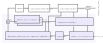
\includegraphics[width = 0.99\textwidth]{fig_C2_PBAdiagram.tex}
    \caption{Schematic diagram of the passivity-based adaptive controller (PBAC), where $\Sigma_{\textrm{softrobot}}$ denotes the dynamical system \eqref{eq:C2:dynamic_model} and $\Sigma_{\textrm{sensor}}$ a system of sensors suitable of measuring $\q$ and $\dq$. }
    \label{fig:C2:PBA_diagram}
  \end{figure}


\noindent where $\dq_r = \dq_d - \LambdaB \eB $ is called the reference velocity vector, $\LambdaB \in \R^{n \times n}$ a positive diagonal matrix, and $\vec{Y}(\q,\dq,\dq_r,\dq_r,\piB) \in \R^{m\times n}$ is called the regressor matrix. Following the work of Slotine and Li \cite{Slotine1988}, the control law and adaptation law are given by
%
\begin{align}
\tauB = &\, \tmat{M}\,\ddq_r + \tmat{C}\, \dq_r + \tvec{f}\!\grav +  \tvec{f}\!\elastic - \tvec{\delta} - \mat{K}_p \, \vec{e} - \mat{K}_d\, \vec{e}_r,  \label{eq:C2:tau} \\
\dot{\tvec{\pi}} =& - \mat{K}_{\vec{\pi}}\,\vec{Y}^\top\vec{e}_r,  \label{eq:C2:update}
\end{align}
%
where $\vec{e}_r := \dq - \dq_r = \dot{\vec{e}} + \LambdaB\,\vec{e}$, $\mat{K}_p, \mat{K}_d \in \mathbb{R}^{n\times n}$ are controller gains, and $\mat{K}_{\vec{\pi}} \in \R^{p\times p}$ is a positive definite matrix called the adaptation rate. Since $\tauB$ define the desired generalized forces acting on the system \eqref{eq:C2:dynamic_model}, the desired pressures are computed as $\uB = \mat{G}^{+} \tauB$ with $\mat{G}^{+}$ the generalized inverse of $\mat{G}$. A schematic diagram of the passivity-based controller is provided in Figure \ref{fig:C2:PBA_diagram}. It should be mentioned that the magnitude of adaptation rate does not affect the global stability of the system (if unmodelled dynamics are not excited); however, it sets the rate of adaptation, and accordingly the performance of the system.

\begin{rmk}[Persistence of excitation]
\label{rmk:C2:poe}
 It is important to note that the convergence of the tracking error $\eB \to 0$ does not imply convergence of the estimated parameter to their true values. According to \cite{Slotine1988,Slotine1989Jul,SlotineJ1987}, asymptotic convergence can be shown if the matrix $\vec{Y}(\q,\dq,\dq_r,\dq_r,\piB)$ is persistently excited and it is uniformly continuous. To elaborate, under the condition of persistent excitation, that is, for any instances $t_1,t_2$ with  $t_1\le t_2$  there exists a positive constant $\alpha$ such that $\int_{t_1}^{t_2} \mat{Y}^\top\,\mat{Y} \;dt \preceq \alpha\,\mat{I}$, it can be proven that the parameter estimates converge asymptotically to their true values. The authors in \cite{Slotine1988} state that the proof for convergence here applied to nonlinear robot dynamics is similar to those of linear dynamics \cite{Morgan1977} although the proof is fairly involved. 
\end{rmk}
%

%!TEX root = ../../thesis.tex
\section{Overview of experimental platform}
\noindent Before invest, we detail the experimental setup and control platform of the soft robotic system. Since sensing is a challenging issue in soft robotics, due to large distributed deformations, a combination of sensors were used to recover an estimate of the states $\q \in \mathcal{Q}$. A full overview of the setup is given in Figure \ref{fig:C2:setup}. First of all, we employed a 6-DOF inertial measurement unit (MPU-6050, \texttt{InvSense}) that measures the angular displacement of the soft robot's end-effector (\ie, $\sigma = L$). Through on-board sensor fusion, the bending angle of the soft robot can be recovered, \ie, $\beta = \kappa l$. Since the bending angle alone is not sufficient to decouple the curvature and elongation, additional sensing is required. Consequently, we use a stereo-vision depth camera (RealSense D435, \texttt{Intel}) with an infrared dot projector and RGB camera module. A spherical optical marker is attached to the end-effector of the soft robot, whose relative position can be recovered using a combination of depth-sensing and image post-processing with a Hough-space circle transformation. To retrieve a global reference frame of the vision system, four $30\!\times \!30$ \si{\milli \metre} Aruco marker are uniformly distributed whose location and orientation can be found using the \texttt{opencv-python} library. We show the implementation of the optical vision system and its post-processing in Figure \ref{fig:C2:setupmeasure}. Through trigonometry and the measured bending angle $\beta$, an filter measurement of the position vector $y = \tvec{\gamma}_L$ can be recovered. Given the analytic expressions for the orientation and position in \eqref{eq:C2:phi_exact} and \eqref{eq:C2:pos_exact}, an inverse Jacobian kinematic solver is employed to recover an estimate of the state vector, \ie, $\tvec{q}_{\textrm{dyn}} = \textrm{argmin}_{\q} \lVert \, \tvec{\gamma}_L - \gammaB(L,\q) \rVert_2$. During each experimental trail, it was made sure the soft robotic body does not occlude the optical marker.

As for the pneumatic actuation, an array of proportional-pressure regulators (VEAB-B-D16, \texttt{Festo}) was used with an active pressure range of $-0.1 \;\text{MPa}\, < \uB(t) \le 0.1 \; \textrm{MPa}$, which simultaneously allow for pressure measurements. These measurements are fed into the (quasi-static) model to also recover a quasi-static estimate of the states $\tvec{q}_{\textrm{qs}}$. Then, the dynamic estimates $\tvec{q}_{\textrm{dyn}}$ and the quasi-static pressure-based estimates $\tvec{q}_{\textrm{qs}}$ are fused using an ordinary complementary filter. The control and data acquisition are done using a {Raspberry Pi 4} (2GB). 

%
\afterpage{%
\begin{figure}[!t]
  \centering
  %\includegraphics[width=0.99\textwidth]{./fig/fig_C2_setup.pdf} 
  \includegraphics*[width=\textwidth]{./pdf/thesis-figure-4-12.pdf} 
  \caption{General overview of the experimental platform for the testing and development of the 3-DOF soft manipulator. (a) Close-up of the {RealSense D435} stereo-vision depth camera. (b) Soft continuum manipulator with pressure inputs $\uB = (u_1,\,u_2,\,u_3)^\top$, a MPU-6050 Inertial Measurement Unit (IMU) to measure the end-effector angle $\beta$, and a color-coded optical marker to recover $\gammaB_L$, and four Aruco markers to recover $\Phi_0$ and $\gammaB_0$. (c) Overview of full setup with the array of three VEAB-B-D16 pressure regulators. \label{fig:C2:setup}}
\end{figure}
\clearpage
}
%
\afterpage{
\begin{figure}[!t]
  \centering
  \input{./fig/fig_C2_setup_measure_V2.pdf_tex}
  \caption{General overview of the optical vision system used to estimate the state variables $\q$. \tcircle{1} First, an RBG image is processed using a Circular Hough transformation filtering for circles with a radius 32 \texttt{pix}, it has a global maxima at the optical marker. \tcircle{2} Then, a sample of the depth camera is generated. \tcircle{3} Finally, all sensor data is combined using a sensor fusion algorithm of depth, RGB camera, input pressures and IMU data, resulting in an accurate estimate of soft manipulator's end-effector $\tvec{\gammaB}(L,\tvec{q})$. \label{fig:C2:setupmeasure}}
\end{figure}
\clearpage
}

\section{Numerical and experimental implementation}
\noindent In this section, we will discuss the simulation results of the dynamic model \eqref{eq:C2:dynamic_model}, the passivity-based controller \eqref{eq:C2:tau}, and the adaptive law \eqref{eq:C2:update}. To illustrate effectiveness and performance of the approach, we segregate our analysis into several study-cases of various complexity. First, focusing on the physical one-link soft robot in Figure \ref{fig:C2:soft_robot} ($N = 1$), we investigate the unforced system's equilibria and their corresponding stability. In continuation, we compare the simulated trajectories of the dynamical model with experimental data for natural oscillations, forced pneumatic inputs, and external loading conditions; where we also highlight contribution of the hyper-elastic FEM-driven material model. Second, to illustrate the flexibility and computational efficiency of the numerical framework, we extend the one-link model to a multi-link model with $N = 6$ soft-bodied links.

The numerical solutions to the ordinary differential equations in \eqref{eq:C2:dynamic_model} together with \eqref{eq:C2:tau} and \eqref{eq:C2:update} are computed using the aforementioned MDE integration scheme which is developed in \matlab, and the underlying code can be found at Caasenbrood et al. \cite{Caasenbrood2021}. The software architecture is compactly written as Object-Oriented class labeled under \texttt{./src/Model.m} that enables a minimal programming interface to set-up various soft robotic simulation models easily. 
The simulation results provided in this section can be reproduced using the open-source \sorotoki package found at \cite{SorotokiCode}
%

\textbf{Natural dynamics -- One-link soft robot:} The following physical parameters are chosen for the soft robot: the mass $m_0 = 17.3$ g, the relaxation length $L = 64.4$ mm. The material parameters for hyper-elasticity and visco-elasticity models are chosen identical to Table \ref{tab:C2:elastic_parameters}. For the additional viscous material behavior, the Rayleigh damping matrix and the creep compliance matrix are chosen a follow:
%
\begin{align}
\mat{R} & = \begin{pmatrix} 0.01 & 0 & 0 \\ 0 &  1.05\pwr{-5} & 0 \\ 0 & 0 & 1.05\pwr{-5} \end{pmatrix}; \notag \\[0.45em]
\mat{K}_{\lambda} & = \begin{pmatrix} 502.3 & 0 & 0 \\ 0 &  1.53\pwr{-2} & 0 \\ 0 & 0 & 1.53\pwr{-2} \end{pmatrix}. \notag
\end{align}
%
\noindent  We stress that the values for the Rayleigh damping and creep compliance shown above are identified empirically {through} open-loop measurements, similar to the creep coefficient provided in Table \ref{tab:C2:elastic_parameters}.  We will explain how these coefficients are derived later in this chapter. 

%The code for the one-link simulation model can be found under \texttt{./mdl\_1\_natural.m}.
%

First, we investigate the existence and the stability of the equilibria of the unforced system. If the system is at rest (i.e., $\dq = 0$, $\ddq = 0$), then by definition there are no conservative forces acting on the system. Thus, for any equilibrium point ${\q}_0$ it holds that $\nabla \mathcal{U}({\q}^\star) \equiv \vec{0}$. If $ \mathcal{U}({\q}^\star) \equiv E_0$ is a local minimum, then the equilibrium is deemed stable. Any small disturbance will result in a new energy-state $E_1$ and will consequently bring the system in motion. However, regarding $E_0$ is a local minimum, the system will remain in a neighborhood of ${\q}^\star$ and eventually converge towards its nearest low-state energy $E_0$. If $\mathcal{U}({\q}^\star) \equiv E_0$ is a local maximum, the equilibrium is deemed to be unstable, since there exist a configuration close to ${\q}^\star$ with a lower energy-state, \ie, $\mathcal{U}({\q}^\star + {\delta}\q) < E_1$. By analysis of the gradient of the potential energy function $\nabla \mathcal{U}({\q})$, two unique equilibria can be found numerically. The potential function has a local maximum for $\q^\star_{\textrm{unstab}}=\left(-\tfrac{m_0 g}{L (\alpha_1 - \alpha_2)},\,0,\,0\right)^\top$ which is unstable. To some extent, it is analogous to the unstable equilibrium position of the inverted pendulum system. 

For the stable equilibria, the bisection method was used to find the zero-crossing of $\nabla \mathcal{U}({\q})$, where it was found that all stable solutions of the unforced system will tend to the following set:
%
\begin{equation*}
\Omega_{\textrm{stab}} = \left\{\q\in \mathcal{Q}\;:\;\varepsilon=-\varepsilon_\star,\, \kappa(\q) = \frac{\kappa_\star}{\alpha_\phi(\q)} \right\}, \notag
\end{equation*}
%
where $\varepsilon_\star$ and $\kappa_\star$ are nonzero constants. Notice that the set $\Omega_{\textrm{stab}}$ is topologically equivalent to a ring. This set corresponds to the hanging position of the soft robot. Given the physical parameters of the robot in Figure \ref{fig:C2:soft_robot}, the following constants are found: $\varepsilon_\star = 0.0021$ and $\kappa_\star = 0.0174$.  It is important to note that  the stable set of equilibria stems from the force balance between the internal elastic potential forces and the external gravitational potential forces, and thus any stiffness will lead to a stable set with a similar topology. By changing the base orientation of the soft manipulator (\ie, by modifying $\PhiB_0$), both equilibria vanish and all state trajectories will tend to a global stable equilibrium. For fully reversing the orientation, this trivially leads to the stable equilibrium $\q^\star_{\textrm{stab}} = (+\tfrac{m_0 g}{L (\alpha_1 - \alpha_2)},\, 0,\, 0)$. This phenomenon is referred to as local bifurcation, in which the change of parameter values alters the existence and stability of equilibria. This property might be interesting for soft robot manipulators with multiple soft-bodied links, as they are likely to be subjected to different gravitational loads.
%
\afterpage{
\begin{figure}[!t]
  \vspace{-1mm}
  \centering
  %% This file was created by matlab2tikz.
%
\definecolor{mycolor1}{rgb}{0.00000,0.34510,0.65882}%
%
\begin{tikzpicture}

\begin{axis}[%
width=0.817\textwidth,
height=0.128\textwidth,
at={(0\textwidth,0.372\textwidth)},
scale only axis,
xmin=0,
xmax=0.8,
ymin=-0.002,
ymax=0.004,
ylabel style={font=\color{white!15!black}},
ylabel={$\varepsilon$ (-)},
axis background/.style={fill=white},
xmajorgrids,
ymajorgrids,
ylabel style={yshift=-3.5pt}
]
\addplot [color=mycolor1, line width=1.5pt, forget plot]
  table[row sep=crcr]{%
0	0\\
0.00100069999999997	0.00118280000000004\\
0.00200129999999998	0.00302690000000005\\
0.00300199999999995	0.00320659999999995\\
0.00400270000000003	0.00204000000000004\\
0.00500330000000004	0.00137810000000005\\
0.00600400000000001	0.00189989999999995\\
0.00700469999999997	0.00259039999999999\\
0.00800529999999999	0.00244929999999999\\
0.00900599999999996	0.00173400000000001\\
0.010007	0.00132149999999998\\
0.012008	0.0015965\\
0.013009	0.00129559999999995\\
0.014009	0.000752890000000006\\
0.01501	0.000412799999999991\\
0.016011	0.000345240000000024\\
0.017011	0.000263690000000039\\
0.018012	6.14200000004228e-06\\
0.0190129999999999	-0.000267059999999986\\
0.0200129999999999	-0.000355349999999977\\
0.022015	-0.000226130000000047\\
0.023015	-0.000218750000000045\\
0.024016	-0.000179099999999988\\
0.025017	-4.87319999999958e-05\\
0.026017	0.000119230000000026\\
0.027018	0.000247529999999996\\
0.029019	0.000416859999999963\\
0.031021	0.000616460000000041\\
0.032021	0.000675300000000045\\
0.0360240000000001	0.000792470000000045\\
0.038025	0.000790540000000006\\
0.041027	0.000757299999999961\\
0.043029	0.000692970000000015\\
0.046031	0.000568110000000011\\
0.0520350000000001	0.000254760000000021\\
0.056037	5.16750000000288e-05\\
0.059039	-7.46109999999467e-05\\
0.061041	-0.000132119999999958\\
0.063042	-0.00015993999999997\\
0.065043	-0.000150239999999968\\
0.067045	-0.000101770000000001\\
0.0690460000000001	-1.85299999999611e-05\\
0.072048	0.000146179999999996\\
0.0750500000000001	0.000311900000000032\\
0.077051	0.000399240000000023\\
0.079053	0.000458139999999996\\
0.081054	0.000486059999999955\\
0.083055	0.000485100000000016\\
0.085057	0.000460800000000039\\
0.088059	0.000394299999999959\\
0.0910610000000001	0.000299209999999994\\
0.094063	0.000176859999999945\\
0.10007	-8.26600000000122e-05\\
0.10207	-0.000138430000000023\\
0.10407	-0.000163899999999995\\
0.10607	-0.000156939999999994\\
0.10807	-0.000121860000000029\\
0.11107	-3.72770000000022e-05\\
0.11508	7.97289999999728e-05\\
0.11808	0.00013996000000005\\
0.12108	0.000169470000000005\\
0.12408	0.000173120000000027\\
0.12809	0.000150490000000003\\
0.13309	9.08080000000533e-05\\
0.1451	-7.99169999999849e-05\\
0.1501	-0.000113290000000044\\
0.1551	-0.000115599999999993\\
0.16111	-8.87210000000138e-05\\
0.17512	-1.33270000000074e-05\\
0.18212	-1.10450000000428e-05\\
0.19013	-3.9399000000051e-05\\
0.20714	-0.000110049999999973\\
0.21514	-0.000106530000000049\\
0.23716	-7.15239999999895e-05\\
0.25417	-9.7973000000029e-05\\
0.26918	-0.000108980000000036\\
0.36024	-0.000104609999999949\\
0.64943	-0.000108019999999986\\
0.80053	-0.000108019999999986\\
};
\end{axis}

\begin{axis}[%
width=0.817\textwidth,
height=0.128\textwidth,
at={(0\textwidth,0.186\textwidth)},
scale only axis,
xmin=0,
xmax=0.8,
ymin=-30,
ymax=30,
ylabel style={font=\color{white!15!black}},
ylabel={$\kappa_x$ (1/m)},
axis background/.style={fill=white},
xmajorgrids,
ymajorgrids,
ylabel style={yshift=-3.5pt}
]
\addplot [color=mycolor1, line width=1.5pt, forget plot]
  table[row sep=crcr]{%
0	-15\\
0.0160109999999989	21.093\\
0.0200129999999987	24.639\\
0.0220149999999997	24.921\\
0.0240159999999996	24.275\\
0.0280190000000005	20.825\\
0.0370249999999999	8.0954\\
0.0530350000000013	-14.326\\
0.0600400000000008	-19.584\\
0.0640430000000016	-20.462\\
0.0650429999999993	-20.405\\
0.0670450000000002	-19.956\\
0.0710470000000001	-17.783\\
0.0780519999999996	-10.912\\
0.0990660000000005	11.571\\
0.10407	13.835\\
0.10707	14.162\\
0.109069999999999	13.96\\
0.11308	12.693\\
0.120080000000002	8.6293\\
0.145099999999999	-7.5345\\
0.152100000000001	-9.6423\\
0.156099999999999	-10.114\\
0.158110000000001	-10.154\\
0.16011	-10.071\\
0.16311	-9.7278\\
0.168109999999999	-8.6433\\
0.176120000000001	-5.9078\\
0.203140000000001	4.2835\\
0.210139999999999	5.4359\\
0.21414	5.6507\\
0.215140000000002	5.6544\\
0.217140000000001	5.6043\\
0.22015	5.394\\
0.225149999999999	4.733\\
0.234159999999999	2.8837\\
0.257169999999999	-2.165\\
0.265180000000001	-3.1435\\
0.271180000000001	-3.478\\
0.274180000000001	-3.5186\\
0.275179999999999	-3.5142\\
0.277180000000001	-3.4797\\
0.281189999999999	-3.3144\\
0.287189999999999	-2.8582\\
0.296199999999999	-1.8413\\
0.321210000000001	1.1479\\
0.329219999999999	1.6489\\
0.334219999999998	1.7913\\
0.337219999999999	1.8136\\
0.339230000000001	1.8034\\
0.342230000000001	1.7526\\
0.34723	1.5834\\
0.355239999999998	1.144\\
0.387260000000001	-0.82525\\
0.394259999999999	-0.9984\\
0.39827	-1.0371\\
0.400269999999999	-1.0405\\
0.402270000000001	-1.0338\\
0.405270000000002	-1.0058\\
0.410270000000001	-0.91602\\
0.418279999999999	-0.684049999999999\\
0.452300000000001	0.438210000000002\\
0.458310000000001	0.51538\\
0.462309999999999	0.53706\\
0.464310000000001	0.53923\\
0.467310000000001	0.53219\\
0.471309999999999	0.504999999999999\\
0.477319999999999	0.431660000000001\\
0.48732	0.250540000000001\\
0.510339999999999	-0.179390000000001\\
0.518350000000002	-0.263059999999999\\
0.524349999999998	-0.29299\\
0.527349999999998	-0.2974\\
0.530349999999999	-0.295110000000001\\
0.53436	-0.28246\\
0.54036	-0.245730000000002\\
0.54937	-0.161860000000001\\
0.575379999999999	0.0987620000000007\\
0.583390000000001	0.141269999999999\\
0.589390000000002	0.155419999999999\\
0.593399999999999	0.156510000000001\\
0.5974	0.151420000000002\\
0.602399999999999	0.137350000000001\\
0.610410000000002	0.101030000000002\\
0.643429999999999	-0.0701439999999991\\
0.65043	-0.0844270000000016\\
0.655439999999999	-0.0876699999999992\\
0.660440000000001	-0.0854430000000015\\
0.666440000000001	-0.0764409999999991\\
0.67445	-0.0562310000000004\\
0.707470000000001	0.0381\\
0.715479999999999	0.0465310000000017\\
0.72148	0.0475339999999989\\
0.728490000000001	0.0435039999999987\\
0.737490000000001	0.0319460000000014\\
0.773520000000001	-0.0228089999999987\\
0.78152	-0.0262239999999991\\
0.789529999999999	-0.0253240000000012\\
0.799530000000001	-0.0192890000000006\\
0.800529999999998	-0.0184619999999995\\
};
\end{axis}

\begin{axis}[%
width=0.817\textwidth,
height=0.128\textwidth,
at={(0\textwidth,0\textwidth)},
scale only axis,
xmin=0,
xmax=0.8,
xlabel style={font=\color{white!15!black}},
xlabel={time (s)},
ymin=-30,
ymax=30,
ylabel style={font=\color{white!15!black}},
ylabel={$\kappa_x$ (1/m)},
axis background/.style={fill=white},
xmajorgrids,
ymajorgrids,
ylabel style={yshift=-3.5pt}
]
\addplot [color=mycolor1, line width=1.5pt, forget plot]
  table[row sep=crcr]{%
0	15\\
0.00100070000000052	14.95\\
0.00400269999999914	14.297\\
0.0100069999999999	11.814\\
0.0160110000000007	7.6573\\
0.0370249999999999	-9.5688\\
0.0420280000000002	-11.059\\
0.0450300000000006	-11.31\\
0.0460309999999993	-11.287\\
0.0480319999999992	-11.09\\
0.0520350000000001	-10.147\\
0.0580390000000008	-7.5546\\
0.0680449999999997	-1.1197\\
0.0800529999999995	6.0245\\
0.0870580000000007	8.3962\\
0.0930619999999998	9.3567\\
0.0950629999999997	9.4097\\
0.0970650000000006	9.3007\\
0.100070000000001	8.8078\\
0.10507	7.1137\\
0.11408	2.2559\\
0.12809	-5.0254\\
0.136089999999999	-7.5037\\
0.14109	-8.152\\
0.1431	-8.2116\\
0.1441	-8.1999\\
0.146100000000001	-8.0963\\
0.1501	-7.5893\\
0.1561	-6.1972\\
0.167109999999999	-2.4697\\
0.183120000000001	2.8362\\
0.191129999999999	4.4719\\
0.19713	5.1057\\
0.201129999999999	5.2204\\
0.203139999999999	5.1825\\
0.20614	5.008\\
0.21114	4.4251\\
0.219150000000001	2.9017\\
0.24516	-2.5238\\
0.25217	-3.2225\\
0.25717	-3.4262\\
0.259169999999999	-3.4404\\
0.26117	-3.4181\\
0.26418	-3.3202\\
0.26918	-3.0039\\
0.27718	-2.1924\\
0.30921	1.4497\\
0.31621	1.7737\\
0.320209999999999	1.8472\\
0.32221	1.8539\\
0.32422	1.8412\\
0.327220000000001	1.7872\\
0.33222	1.6127\\
0.34023	1.1607\\
0.37125	-0.826919999999999\\
0.37825	-1.0173\\
0.38326	-1.0668\\
0.384259999999999	-1.0684\\
0.387259999999999	-1.0571\\
0.391260000000001	-1.0076\\
0.397259999999999	-0.869759999999999\\
0.406269999999999	-0.56235\\
0.431290000000001	0.34328\\
0.43929	0.500870000000001\\
0.4453	0.555770000000001\\
0.4483	0.56293\\
0.4513	0.557230000000001\\
0.455299999999999	0.53106\\
0.461309999999999	0.457409999999999\\
0.47031	0.29191\\
0.495329999999999	-0.195040000000001\\
0.50334	-0.27852\\
0.50934	-0.30663\\
0.51234	-0.30972\\
0.51534	-0.30593\\
0.519349999999999	-0.290929999999999\\
0.52535	-0.25001\\
0.535360000000001	-0.14809\\
0.55837	0.0959800000000008\\
0.566380000000001	0.144310000000001\\
0.572380000000001	0.16215\\
0.57638	0.165240000000001\\
0.58039	0.1617\\
0.58539	0.14888\\
0.59239	0.11825\\
0.6044	0.0460480000000008\\
0.62041	-0.0462399999999992\\
0.62942	-0.0787340000000007\\
0.63542	-0.0896410000000003\\
0.64043	-0.092041\\
0.645429999999999	-0.0887689999999992\\
0.652430000000001	-0.0760450000000006\\
0.661440000000001	-0.0497449999999997\\
0.68746	0.0322759999999995\\
0.695460000000001	0.0455330000000007\\
0.70247	0.0501120000000004\\
0.70847	0.049004\\
0.715479999999999	0.0426590000000004\\
0.725479999999999	0.0269060000000003\\
0.7525	-0.0191949999999999\\
0.761509999999999	-0.0263190000000009\\
0.76951	-0.0276610000000002\\
0.777520000000001	-0.0247609999999998\\
0.78853	-0.0157760000000007\\
0.80053	-0.00321839999999973\\
};
\end{axis}
\end{tikzpicture}%
  \includegraphics*{./pdf/thesis-figure-4-14.pdf}
  \vspace{-3mm}
  \caption{State trajectories of one-link soft robot model with initial conditions $\q_0 = (0 , -15, 15)^\top$ and $\dq_0 = (0, 2500, 0)^\top$. The figure shows the elongation strain $\varepsilon$ and the curvatures $\kappa_x$, $\kappa_y$ in the $xz$-plane and $yz$-plane, respectively. Clearly the one-link soft robot oscillates about the set $\Omega_{\textrm{stab}}$. }
  \label{fig:C2:natural_states}
\end{figure}
%

%
\begin{figure}[!t]
  %\vspace{-3mm}
  \centering
  %% This file was created by matlab2tikz.
%
%The latest updates can be retrieved from
%  http://www.mathworks.com/matlabcentral/fileexchange/22022-matlab2tikz-matlab2tikz
%where you can also make suggestions and rate matlab2tikz.
%
\begin{tikzpicture}

\begin{axis}[%
width=0.216\textwidth,
height=0.199\textwidth,
at={(0\textwidth,0.253\textwidth)},
scale only axis,
axis on top,
xmin=0.5,
xmax=522.5,
tick align=outside,
y dir=reverse,
ymin=0.5,
ymax=458.5,
axis line style={draw=none},
ticks=none,
ylabel style={yshift=-7.5pt}
]
\addplot [forget plot] graphics [xmin=0.5, xmax=522.5, ymin=0.5, ymax=458.5] {./fig/fig_C2_natural_3D-1.png};
\end{axis}

\begin{axis}[%
width=0.216\textwidth,
height=0.199\textwidth,
at={(0.245\textwidth,0.253\textwidth)},
scale only axis,
axis on top,
xmin=0.5,
xmax=522.5,
tick align=outside,
y dir=reverse,
ymin=0.5,
ymax=458.5,
axis line style={draw=none},
ticks=none,
ylabel style={yshift=-7.5pt}
]
\addplot [forget plot] graphics [xmin=0.5, xmax=522.5, ymin=0.5, ymax=458.5] {./fig/fig_C2_natural_3D-2.png};
\end{axis}

\begin{axis}[%
width=0.216\textwidth,
height=0.199\textwidth,
at={(0.49\textwidth,0.253\textwidth)},
scale only axis,
axis on top,
xmin=0.5,
xmax=522.5,
tick align=outside,
y dir=reverse,
ymin=0.5,
ymax=458.5,
axis line style={draw=none},
ticks=none,
ylabel style={yshift=-7.5pt}
]
\addplot [forget plot] graphics [xmin=0.5, xmax=522.5, ymin=0.5, ymax=458.5] {./fig/fig_C2_natural_3D-3.png};
\end{axis}

\begin{axis}[%
width=0.216\textwidth,
height=0.199\textwidth,
at={(0.734\textwidth,0.253\textwidth)},
scale only axis,
axis on top,
xmin=0.5,
xmax=522.5,
tick align=outside,
y dir=reverse,
ymin=0.5,
ymax=458.5,
axis line style={draw=none},
ticks=none,
ylabel style={yshift=-7.5pt}
]
\addplot [forget plot] graphics [xmin=0.5, xmax=522.5, ymin=0.5, ymax=458.5] {./fig/fig_C2_natural_3D-4.png};
\end{axis}

\begin{axis}[%
width=0.216\textwidth,
height=0.199\textwidth,
at={(0\textwidth,0\textwidth)},
scale only axis,
axis on top,
xmin=0.5,
xmax=522.5,
tick align=outside,
y dir=reverse,
ymin=0.5,
ymax=458.5,
axis line style={draw=none},
ticks=none,
ylabel style={yshift=-7.5pt}
]
\addplot [forget plot] graphics [xmin=0.5, xmax=522.5, ymin=0.5, ymax=458.5] {./fig/fig_C2_natural_3D-5.png};
\end{axis}

\begin{axis}[%
width=0.216\textwidth,
height=0.199\textwidth,
at={(0.245\textwidth,0\textwidth)},
scale only axis,
axis on top,
xmin=0.5,
xmax=522.5,
tick align=outside,
y dir=reverse,
ymin=0.5,
ymax=458.5,
axis line style={draw=none},
ticks=none,
ylabel style={yshift=-7.5pt}
]
\addplot [forget plot] graphics [xmin=0.5, xmax=522.5, ymin=0.5, ymax=458.5] {./fig/fig_C2_natural_3D-6.png};
\end{axis}

\begin{axis}[%
width=0.216\textwidth,
height=0.199\textwidth,
at={(0.49\textwidth,0\textwidth)},
scale only axis,
axis on top,
xmin=0.5,
xmax=522.5,
tick align=outside,
y dir=reverse,
ymin=0.5,
ymax=458.5,
axis line style={draw=none},
ticks=none,
ylabel style={yshift=-7.5pt}
]
\addplot [forget plot] graphics [xmin=0.5, xmax=522.5, ymin=0.5, ymax=458.5] {./fig/fig_C2_natural_3D-7.png};
\end{axis}

\begin{axis}[%
width=0.216\textwidth,
height=0.199\textwidth,
at={(0.734\textwidth,0\textwidth)},
scale only axis,
axis on top,
xmin=0.5,
xmax=522.5,
tick align=outside,
y dir=reverse,
ymin=0.5,
ymax=458.5,
axis line style={draw=none},
ticks=none,
ylabel style={yshift=-7.5pt}
]
\addplot [forget plot] graphics [xmin=0.5, xmax=522.5, ymin=0.5, ymax=458.5] {./fig/fig_C2_natural_3D-8.png};
\end{axis}

\begin{axis}[%
width=0.969\textwidth,
height=0.51\textwidth,
at={(-0.01\textwidth,-0.029\textwidth)},
scale only axis,
xmin=0,
xmax=1,
ymin=0,
ymax=1,
axis line style={draw=none},
ticks=none,
axis x line*=bottom,
axis y line*=left,
ylabel style={yshift=-7.5pt}
]
\end{axis}
\end{tikzpicture}%
  \includegraphics*{./pdf/thesis-figure-4-15.pdf}
  \vspace{-3mm}
  \caption{Three-dimensional volumetric evolution of the one-link soft robot model with initial conditions $\q_0 = (0 , -15, 15)^\top$ and $\dq_0 = (0, 2500, 0)^\top$. Notice that the states of the one-link soft robot quickly converge to the the set of stable equilibria $\Omega_{\textrm{stab}}$. }
  \label{fig:C2:natural_3D}
\end{figure}
\clearpage
}

To illustrate the unforced dynamics and the existence of stable equilibria, time-domain simulations of the dynamical model with nonzero initial conditions:
%
\begin{align*}
\q_0 & = \left(0,\,-15,\,15\; \right)^\top, \\[0.35em] \dq_0 & = \left(0,\,2500,\,0 \right)^\top.
\end{align*}
%
Figure \ref{fig:C2:natural_states} shows the state trajectories of the soft robot; whereas Figure \ref{fig:C2:natural_3D} is provided to better illustrate the underlying dynamics and the trajectory of the end-effector.
%

Besides the existence of stable solutions, the numerical simulations perfectly illustrate the coupled dynamics between the elongation and bending of the soft robot. Due to the difference in mechanical stiffness for elongation and bending, we observe high-frequency and low-frequency oscillation for the elongation strain $\varepsilon(t)$, and we observe low-frequent oscillations for the curvatures $\kappa_x(t)$ and $\kappa_y(t)$. Interestingly, the low-frequency oscillations are passed from the curvature dynamics to elongation dynamics; conversely, the dynamics of the elongation barely affect the curvatures. After sufficient time passes, the trajectories indeed tend to the set of stable equilibria $\Omega_{\textrm{stab}}$.

\textbf{ Experimental comparison-- unforced, forced, and external loads}:
\noindent To validate the dynamic model, the solutions of the model are compared with measurements of the physical system in unforced,  forced, and tip-load conditions. As such, the model validation is separated into three parts: \textit{i)} unforced, \textit{ii)} forced conditions, and \textit{iii)} external tip-loads applied on the end-effector.

We start with the unforced scenario, \ie, no input is considered $u_i(t) \equiv 0$. For the unforced analysis, two experimental trails are performed for the unforced validation. First, the soft robot is deformed slightly and then released from rest, which corresponds to the initial conditions $\q_0 = \left(0.015,\,4.75,\,0 \right)^\top$ and $\dq_0 = \vec{0}_3$. Since the mechanical deformations are relatively small here, the presence of hyper-elastic and visco-elastic material behavior are less dominant. Secondly, the soft robot is moderately deformed such that the initial configuration (or shortly after) lies within the hyper-elastic and visco-elastic regime. In this scenario, the nonlinear and time-dependent material effects may not be neglected. These initial conditions correspond to $\q_0 = \left(0.046,\,11.25,\,0 \right)^\top$ and $\dq_0 = \vec{0}_3$. It is worth mentioning that the creep strains $\lambdaB$ are difficult to distinguish from the true strain, and thus the initial conditions for $\lambdaB(t_0)$ are determined empirically  using a set of dynamic measurements with different initial condition. The comparison between our model and the unforced dynamic measurements are shown in Figure \ref{fig:C2:compare_states}. 
% The associated code for the unforced validation simulations can be found under \texttt{./valid\_one\_link\_open.m}.


%
\begin{figure}[!t]
  %\vspace{-2mm}
  \centering
  %% This file was created by matlab2tikz.
%
\definecolor{mycolor1}{rgb}{0.00000,0.34510,0.65882}%
\definecolor{mycolor2}{rgb}{0.79216,0.11765,0.17255}%
\definecolor{mycolor3}{rgb}{0.20392,0.65490,0.24706}%
%
\begin{tikzpicture}

\begin{axis}[%
width=0.808\textwidth,
height=0.316\textwidth,
at={(0\textwidth,0.184\textwidth)},
scale only axis,
xmin=0,
xmax=0.6,
ymin=-10,
ymax=65,
ylabel style={font=\color{white!15!black}},
ylabel={$\beta$ ($^\circ$)},
axis background/.style={fill=white},
xmajorgrids,
ymajorgrids,
ylabel style={yshift=-3.5pt}
]
\addplot [color=mycolor1, dashed, line width=1.5pt, forget plot]
  table[row sep=crcr]{%
0	16.868\\
0.00335199999999958	16.745\\
0.00670390000000154	16.384\\
0.0100559999999987	15.79\\
0.0134079999999983	14.97\\
0.0167600000000014	13.945\\
0.0234640000000006	11.394\\
0.0335199999999993	6.8314\\
0.0435750000000006	2.2676\\
0.0502789999999997	-0.33305\\
0.0536309999999993	-1.4231\\
0.0569829999999989	-2.3479\\
0.0603349999999985	-3.0944\\
0.0636870000000016	-3.6543\\
0.0670390000000012	-4.0247\\
0.0703910000000008	-4.2083\\
0.0737430000000003	-4.2112\\
0.0770949999999999	-4.0455\\
0.0804469999999995	-3.7307\\
0.0837989999999991	-3.2873\\
0.0871509999999986	-2.7385\\
0.0938550000000014	-1.4243\\
0.10726	1.3805\\
0.113969999999998	2.5283\\
0.117319999999999	2.9815\\
0.12067	3.3404\\
0.124020000000002	3.5984\\
0.127369999999999	3.7524\\
0.13073	3.8024\\
0.134080000000001	3.7515\\
0.137429999999998	3.6056\\
0.140779999999999	3.3729\\
0.144130000000001	3.0638\\
0.147490000000001	2.6904\\
0.15419	1.8051\\
0.170950000000001	-0.55735\\
0.17765	-1.2954\\
0.181010000000001	-1.5817\\
0.184360000000002	-1.8053\\
0.187709999999999	-1.9631\\
0.19106	-2.0538\\
0.194410000000001	-2.0786\\
0.197769999999998	-2.0397\\
0.20112	-1.9422\\
0.204470000000001	-1.7919\\
0.207820000000002	-1.5962\\
0.21453	-1.102\\
0.234639999999999	0.561699999999998\\
0.23799	0.781110000000002\\
0.241340000000001	0.967829999999999\\
0.244689999999999	1.1182\\
0.24804	1.2298\\
0.2514	1.3014\\
0.254750000000001	1.3332\\
0.258099999999999	1.326\\
0.26145	1.282\\
0.264800000000001	1.2044\\
0.268160000000002	1.0971\\
0.271509999999999	0.964549999999999\\
0.278210000000001	0.64423\\
0.294969999999999	-0.228840000000002\\
0.301680000000001	-0.50535\\
0.305029999999999	-0.61336\\
0.30838	-0.698309999999999\\
0.311730000000001	-0.758929999999999\\
0.315080000000002	-0.794799999999999\\
0.318439999999999	-0.806080000000001\\
0.32179	-0.793690000000002\\
0.325140000000001	-0.7592\\
0.328489999999999	-0.704699999999999\\
0.33184	-0.63287\\
0.338550000000001	-0.449290000000001\\
0.35866	0.183789999999998\\
0.362010000000001	0.26942\\
0.365359999999999	0.34309\\
0.36872	0.403320000000001\\
0.372070000000001	0.449120000000001\\
0.375419999999998	0.479949999999999\\
0.378769999999999	0.49567\\
0.38212	0.49661\\
0.385470000000002	0.48348\\
0.388829999999999	0.457370000000001\\
0.39218	0.41966\\
0.395530000000001	0.372039999999998\\
0.402229999999999	0.254660000000001\\
0.422350000000002	-0.13081\\
0.425699999999999	-0.180910000000001\\
0.42905	-0.223320000000001\\
0.432400000000001	-0.257269999999998\\
0.435749999999999	-0.2822\\
0.439109999999999	-0.29785\\
0.442460000000001	-0.304259999999999\\
0.445810000000002	-0.3017\\
0.449159999999999	-0.29072\\
0.45251	-0.272040000000001\\
0.455870000000001	-0.246600000000001\\
0.459219999999998	-0.215450000000001\\
0.465920000000001	-0.140820000000001\\
0.482679999999998	0.0594210000000004\\
0.48939	0.1218\\
0.492740000000001	0.14592\\
0.496089999999999	0.16469\\
0.49944	0.177849999999999\\
0.502790000000001	0.185320000000001\\
0.506150000000002	0.187180000000001\\
0.509499999999999	0.18365\\
0.51285	0.17511\\
0.516200000000001	0.16206\\
0.519549999999999	0.14509\\
0.526260000000001	0.102180000000001\\
0.54637	-0.0440749999999994\\
0.549720000000001	-0.0636940000000017\\
0.553070000000002	-0.0805149999999983\\
0.556419999999999	-0.0942049999999988\\
0.55978	-0.10453\\
0.563130000000001	-0.11138\\
0.566479999999999	-0.114730000000002\\
0.56983	-0.114660000000001\\
0.573180000000001	-0.111339999999998\\
0.576540000000001	-0.105049999999999\\
0.579889999999999	-0.0961040000000004\\
0.58324	-0.084892\\
0.589939999999999	-0.0574340000000007\\
0.600000000000001	-0.0107409999999994\\
};
\addplot [color=mycolor1, line width=1.5pt, forget plot]
  table[row sep=crcr]{%
0	16.835677\\
0.00335199999999958	17.08401\\
0.00670390000000154	16.96115\\
0.0100559999999987	16.48681\\
0.0134079999999983	15.68434\\
0.0167600000000014	14.60635\\
0.0234640000000006	11.88233\\
0.0502789999999997	-0.123909999999999\\
0.0536309999999993	-1.22505\\
0.0569829999999989	-2.14127\\
0.0636870000000016	-3.60587\\
0.0670390000000012	-4.117172\\
0.0703910000000008	-4.38644\\
0.0737430000000003	-4.37765\\
0.0770949999999999	-4.15037\\
0.0804469999999995	-3.794186\\
0.0837989999999991	-3.369603\\
0.0871509999999986	-2.85922\\
0.0905030000000018	-2.23481\\
0.0972070000000009	-0.682357\\
0.103909999999999	0.91499\\
0.110610000000001	2.335\\
0.117319999999999	3.50976\\
0.12067	3.93963\\
0.124020000000002	4.23794\\
0.127369999999999	4.40479\\
0.13073	4.44793\\
0.134080000000001	4.37631\\
0.137429999999998	4.19383\\
0.140779999999999	3.9078\\
0.144130000000001	3.52886\\
0.147490000000001	3.06902\\
0.15419	1.96662\\
0.170950000000001	-0.997119999999999\\
0.174299999999999	-1.48891\\
0.17765	-1.91329\\
0.181010000000001	-2.25947\\
0.184360000000002	-2.52069\\
0.187709999999999	-2.69421\\
0.19106	-2.78114\\
0.194410000000001	-2.78397\\
0.197769999999998	-2.70261\\
0.20112	-2.54178\\
0.204470000000001	-2.30947\\
0.207820000000002	-2.01857\\
0.21453	-1.31844\\
0.231280000000002	0.60106\\
0.234639999999999	0.91722\\
0.23799	1.18767\\
0.241340000000001	1.40767\\
0.244689999999999	1.57359\\
0.24804	1.68273\\
0.2514	1.73467\\
0.254750000000001	1.73074\\
0.258099999999999	1.67251\\
0.26145	1.56393\\
0.264800000000001	1.41081\\
0.268160000000002	1.21999\\
0.27486	0.757010000000001\\
0.291620000000002	-0.521222999999999\\
0.29832	-0.92361\\
0.301680000000001	-1.07898\\
0.305029999999999	-1.1992\\
0.30838	-1.28158\\
0.311730000000001	-1.32483\\
0.315080000000002	-1.32943\\
0.318439999999999	-1.29709\\
0.32179	-1.23102\\
0.325140000000001	-1.13475\\
0.328489999999999	-1.01205\\
0.3352	-0.707100000000001\\
0.355309999999999	0.303149000000001\\
0.35866	0.434239999999999\\
0.362010000000001	0.544650000000001\\
0.365359999999999	0.632079999999998\\
0.36872	0.695039999999999\\
0.372070000000001	0.732949999999999\\
0.375419999999998	0.745619999999999\\
0.378769999999999	0.733229999999999\\
0.38212	0.696940000000001\\
0.385470000000002	0.639250000000001\\
0.388829999999999	0.563770000000002\\
0.395530000000001	0.3747522\\
0.40559	0.03538\\
0.412289999999999	-0.189534999999999\\
0.418990000000001	-0.382231000000001\\
0.422350000000002	-0.461600000000001\\
0.425699999999999	-0.526890000000002\\
0.42905	-0.57582\\
0.432400000000001	-0.606829999999999\\
0.435749999999999	-0.620280000000001\\
0.439109999999999	-0.617920000000002\\
0.442460000000001	-0.601880000000001\\
0.445810000000002	-0.572620000000001\\
0.449159999999999	-0.530000000000001\\
0.45251	-0.474409999999999\\
0.459219999999998	-0.334610000000001\\
0.47598	0.0465359999999997\\
0.482679999999998	0.168471\\
0.48603	0.216479\\
0.48939	0.254480000000001\\
0.492740000000001	0.281849999999999\\
0.496089999999999	0.298179999999999\\
0.49944	0.303380000000001\\
0.502790000000001	0.29776\\
0.506150000000002	0.282164000000002\\
0.509499999999999	0.257860000000001\\
0.51285	0.226277\\
0.516200000000001	0.188285\\
0.52291	0.0964060000000018\\
0.53631	-0.100956\\
0.543019999999999	-0.183433000000001\\
0.54637	-0.218154999999999\\
0.549720000000001	-0.247094000000001\\
0.553070000000002	-0.269435000000001\\
0.556419999999999	-0.284925000000001\\
0.55978	-0.29365\\
0.563130000000001	-0.295780000000001\\
0.566479999999999	-0.290959999999998\\
0.56983	-0.278839999999999\\
0.573180000000001	-0.259509999999999\\
0.576540000000001	-0.234649999999998\\
0.586590000000001	-0.146151\\
0.600000000000001	-0.0214819999999989\\
};
\addplot [color=mycolor2, dashed, line width=1.5pt, forget plot]
  table[row sep=crcr]{%
0	42.536\\
0.00335199999999958	42.282\\
0.00670389999999799	41.522\\
0.0100559999999987	40.242\\
0.0134079999999983	38.44\\
0.0167599999999979	36.168\\
0.023463999999997	30.502\\
0.0335200000000029	20.54\\
0.043574999999997	10.857\\
0.0502790000000033	5.412\\
0.0536310000000029	3.1194\\
0.0569830000000024	1.1481\\
0.060335000000002	-0.487009999999998\\
0.0636870000000016	-1.7789\\
0.0670390000000012	-2.7282\\
0.0703910000000008	-3.3431\\
0.0737430000000003	-3.639\\
0.0770949999999999	-3.6325\\
0.0804469999999995	-3.352\\
0.0837989999999991	-2.8415\\
0.0871509999999986	-2.1406\\
0.0938549999999978	-0.335940000000001\\
0.107259999999997	3.7242\\
0.113970000000002	5.3975\\
0.117319999999999	6.0468\\
0.120669999999997	6.5469\\
0.124020000000002	6.8862\\
0.127369999999999	7.059\\
0.13073	7.0669\\
0.134079999999997	6.9137\\
0.137430000000002	6.6076\\
0.140779999999999	6.1622\\
0.144129999999997	5.5948\\
0.150840000000002	4.176\\
0.174300000000002	-1.3647\\
0.17765	-1.9507\\
0.181010000000001	-2.4386\\
0.184359999999998	-2.8197\\
0.187710000000003	-3.0891\\
0.19106	-3.2449\\
0.194409999999998	-3.289\\
0.197769999999998	-3.2264\\
0.201120000000003	-3.0652\\
0.204470000000001	-2.8158\\
0.207819999999998	-2.4909\\
0.214530000000003	-1.6723\\
0.234639999999999	1.0494\\
0.237990000000003	1.402\\
0.241340000000001	1.6994\\
0.244689999999999	1.9358\\
0.248040000000003	2.1075\\
0.251399999999997	2.2128\\
0.254750000000001	2.252\\
0.258099999999999	2.2273\\
0.261450000000004	2.1423\\
0.264800000000001	2.0024\\
0.268160000000002	1.8144\\
0.271509999999999	1.5859\\
0.278210000000001	1.0417\\
0.294969999999999	-0.412089999999999\\
0.301679999999998	-0.86383\\
0.305030000000002	-1.0381\\
0.30838	-1.1733\\
0.311729999999997	-1.2676\\
0.315080000000002	-1.3204\\
0.318440000000002	-1.3323\\
0.32179	-1.305\\
0.325139999999998	-1.2412\\
0.328490000000002	-1.1448\\
0.33184	-1.0203\\
0.338549999999998	-0.707819999999998\\
0.35866	0.340719999999997\\
0.362009999999998	0.479120000000002\\
0.365360000000003	0.597029999999997\\
0.368720000000003	0.692140000000002\\
0.372070000000001	0.76294\\
0.375419999999998	0.808669999999999\\
0.378770000000003	0.829360000000001\\
0.38212	0.82564\\
0.385469999999998	0.798839999999998\\
0.388829999999999	0.750839999999997\\
0.392180000000003	0.684170000000002\\
0.395530000000001	0.601649999999999\\
0.402230000000003	0.401820000000001\\
0.418990000000001	-0.14405\\
0.425699999999999	-0.317210000000003\\
0.429049999999997	-0.384929999999997\\
0.432400000000001	-0.438249999999996\\
0.435749999999999	-0.476390000000002\\
0.439109999999999	-0.499079999999999\\
0.442459999999997	-0.506410000000002\\
0.445810000000002	-0.498950000000001\\
0.449159999999999	-0.47766\\
0.452509999999997	-0.443860000000001\\
0.455869999999997	-0.399140000000003\\
0.462569999999999	-0.284579999999998\\
0.482680000000002	0.112310000000001\\
0.48603	0.166229999999999\\
0.48939	0.212710000000001\\
0.492739999999998	0.250810000000001\\
0.496090000000002	0.279910000000001\\
0.49944	0.299630000000001\\
0.502789999999997	0.309890000000003\\
0.506149999999998	0.310859999999998\\
0.509500000000003	0.30301\\
0.51285	0.286999999999999\\
0.516199999999998	0.263689999999997\\
0.519550000000002	0.234119999999997\\
0.526260000000001	0.160879999999999\\
0.546370000000003	-0.0808520000000001\\
0.549720000000001	-0.112430000000003\\
0.553069999999998	-0.139220000000002\\
0.556420000000003	-0.160699999999999\\
0.559780000000003	-0.176549999999999\\
0.563130000000001	-0.186590000000002\\
0.566479999999999	-0.190829999999998\\
0.569830000000003	-0.189459999999997\\
0.573180000000001	-0.182780000000001\\
0.576540000000001	-0.17127\\
0.579889999999999	-0.15549\\
0.583240000000004	-0.136110000000002\\
0.589939999999999	-0.0895119999999991\\
0.600000000000001	-0.011845000000001\\
};
\addplot [color=mycolor2, line width=1.5pt, forget plot]
  table[row sep=crcr]{%
0	42.38149\\
0.00335199999999958	42.222217\\
0.00670389999999799	41.69166\\
0.0100559999999987	40.65025\\
0.0134079999999983	38.98657\\
0.0167599999999979	36.69417\\
0.0201119999999975	33.80024\\
0.0268159999999966	26.73915\\
0.0335200000000029	19.66599\\
0.0402229999999975	13.45309\\
0.0469269999999966	7.87586\\
0.0536310000000029	3.25341\\
0.0569830000000024	1.40726\\
0.060335000000002	-0.0902999999999992\\
0.0636870000000016	-1.24237\\
0.0670390000000012	-2.1044\\
0.0703910000000008	-2.75345\\
0.0737430000000003	-3.23569\\
0.0770949999999999	-3.46911\\
0.0804469999999995	-3.372993\\
0.0837989999999991	-2.94807\\
0.0972069999999974	-0.395600000000002\\
0.100560000000002	0.331299999999999\\
0.110610000000001	2.9104\\
0.113970000000002	3.6018\\
0.120669999999997	4.6932\\
0.124020000000002	5.1535\\
0.127369999999999	5.5033\\
0.13073	5.6872\\
0.134079999999997	5.6782\\
0.137430000000002	5.5108\\
0.140779999999999	5.23649\\
0.144129999999997	4.88484\\
0.147489999999998	4.43095\\
0.150840000000002	3.84732\\
0.157539999999997	2.33684\\
0.170949999999998	-0.86054\\
0.17765	-2.23809\\
0.181010000000001	-2.8069\\
0.184359999999998	-3.27132\\
0.187710000000003	-3.61586\\
0.19106	-3.83113\\
0.194409999999998	-3.91704\\
0.197769999999998	-3.88335\\
0.201120000000003	-3.746\\
0.204470000000001	-3.51687\\
0.207819999999998	-3.19829\\
0.211170000000003	-2.79457\\
0.217880000000001	-1.7955\\
0.231279999999998	0.353099999999998\\
0.237990000000003	1.25886\\
0.241340000000001	1.611332\\
0.244689999999999	1.882304\\
0.248040000000003	2.07225\\
0.251399999999997	2.18581\\
0.254750000000001	2.224886\\
0.258099999999999	2.186905\\
0.261450000000004	2.071465\\
0.264800000000001	1.88453\\
0.268160000000002	1.63768\\
0.274859999999997	1.01637\\
0.28492	-0.0867000000000004\\
0.291620000000002	-0.80386\\
0.298319999999997	-1.39718\\
0.301679999999998	-1.6287\\
0.305030000000002	-1.81002\\
0.30838	-1.93746\\
0.311729999999997	-2.00987\\
0.315080000000002	-2.02718\\
0.318440000000002	-1.99044\\
0.32179	-1.90267\\
0.325139999999998	-1.76848\\
0.328490000000002	-1.59428\\
0.3352	-1.15612\\
0.355310000000003	0.328949999999999\\
0.35866	0.523699999999998\\
0.362009999999998	0.688519999999997\\
0.365360000000003	0.819670000000002\\
0.368720000000003	0.914059999999999\\
0.372070000000001	0.970179999999999\\
0.375419999999998	0.988129999999998\\
0.378770000000003	0.969700000000003\\
0.38212	0.917717000000003\\
0.385469999999998	0.835248999999997\\
0.388829999999999	0.725577000000001\\
0.392180000000003	0.593209999999999\\
0.398879999999998	0.279899999999998\\
0.412289999999999	-0.390295000000002\\
0.418990000000001	-0.667409999999997\\
0.422350000000002	-0.778849999999998\\
0.425699999999999	-0.868859999999998\\
0.429049999999997	-0.935580000000002\\
0.432400000000001	-0.977899999999998\\
0.435749999999999	-0.994500000000002\\
0.439109999999999	-0.98433\\
0.442459999999997	-0.947589999999998\\
0.445810000000002	-0.88973\\
0.452509999999997	-0.744720000000001\\
0.459220000000002	-0.580199999999998\\
0.465919999999997	-0.379860000000001\\
0.47598	-0.0658239999999992\\
0.482680000000002	0.111078599999999\\
0.48603	0.182969999999997\\
0.48939	0.242019999999997\\
0.492739999999998	0.287495999999997\\
0.496090000000002	0.318967000000001\\
0.49944	0.33634\\
0.502789999999997	0.339979\\
0.506149999999998	0.329819999999998\\
0.509500000000003	0.305956700000003\\
0.51285	0.269086999999999\\
0.516199999999998	0.221479000000002\\
0.522910000000003	0.106288999999997\\
0.543019999999999	-0.264116999999999\\
0.546370000000003	-0.309241999999998\\
0.549720000000001	-0.346110000000003\\
0.553069999999998	-0.374450000000003\\
0.556420000000003	-0.393749999999997\\
0.559780000000003	-0.403669999999998\\
0.563130000000001	-0.404229999999998\\
0.566479999999999	-0.395890000000001\\
0.569830000000003	-0.379510000000003\\
0.573180000000001	-0.356029999999997\\
0.576540000000001	-0.326039999999999\\
0.579889999999999	-0.290089999999999\\
0.586590000000001	-0.204444000000002\\
0.600000000000001	-0.023690000000002\\
};
\addplot [color=mycolor3, dashed, line width=1.5pt, forget plot]
  table[row sep=crcr]{%
0	59.404\\
0.00335199999999958	59.027\\
0.00670389999999799	57.906\\
0.0100559999999987	56.032\\
0.0134079999999983	53.41\\
0.0167599999999979	50.113\\
0.023463999999997	41.896\\
0.0335200000000029	27.3714\\
0.043574999999997	13.1246\\
0.0502790000000033	5.07895\\
0.0536310000000029	1.6963\\
0.0569830000000024	-1.1998\\
0.060335000000002	-3.58141\\
0.0636870000000016	-5.4332\\
0.0670390000000012	-6.7529\\
0.0703910000000008	-7.5514\\
0.0737430000000003	-7.8502\\
0.0770949999999999	-7.678\\
0.0804469999999995	-7.0827\\
0.0837989999999991	-6.1288\\
0.0871509999999986	-4.8791\\
0.0938549999999978	-1.76024\\
0.107259999999997	5.1047\\
0.113970000000002	7.9258\\
0.117319999999999	9.0283\\
0.120669999999997	9.8873\\
0.124020000000002	10.4846\\
0.127369999999999	10.8114\\
0.13073	10.8693\\
0.134079999999997	10.6652\\
0.137430000000002	10.2132\\
0.140779999999999	9.5351\\
0.144129999999997	8.6586\\
0.150840000000002	6.4422\\
0.160890000000002	2.51421\\
0.1676	-0.0701350000000005\\
0.174300000000002	-2.31624\\
0.17765	-3.2461\\
0.181010000000001	-4.0203\\
0.184359999999998	-4.625\\
0.187710000000003	-5.0522\\
0.19106	-5.2987\\
0.194409999999998	-5.3676\\
0.197769999999998	-5.2661\\
0.201120000000003	-5.0074\\
0.204470000000001	-4.6077\\
0.207819999999998	-4.0871\\
0.214530000000003	-2.7743\\
0.234639999999999	1.6111\\
0.237990000000003	2.18311\\
0.241340000000001	2.66723\\
0.244689999999999	3.054\\
0.248040000000003	3.3373\\
0.251399999999997	3.5142\\
0.254750000000001	3.5852\\
0.258099999999999	3.5533\\
0.261450000000004	3.4243\\
0.264800000000001	3.2068\\
0.268160000000002	2.9115\\
0.271509999999999	2.55045\\
0.278210000000001	1.68593\\
0.294969999999999	-0.640929999999997\\
0.301679999999998	-1.36918\\
0.305030000000002	-1.65146\\
0.30838	-1.87161\\
0.311729999999997	-2.02653\\
0.315080000000002	-2.1152\\
0.318440000000002	-2.13838\\
0.32179	-2.09869\\
0.325139999999998	-2.0004\\
0.328490000000002	-1.8495\\
0.33184	-1.65317\\
0.338549999999998	-1.15711\\
0.35866	0.524509999999999\\
0.362009999999998	0.748539999999998\\
0.365360000000003	0.94012\\
0.368720000000003	1.09546\\
0.372070000000001	1.21206\\
0.375419999999998	1.28862\\
0.378770000000003	1.32503\\
0.38212	1.32225\\
0.385469999999998	1.28232\\
0.388829999999999	1.20821\\
0.392180000000003	1.10383\\
0.395530000000001	0.973689999999998\\
0.402230000000003	0.656480000000002\\
0.418990000000001	-0.218150999999999\\
0.425699999999999	-0.49812\\
0.429049999999997	-0.608249999999998\\
0.432400000000001	-0.695520000000002\\
0.435749999999999	-0.758589999999998\\
0.439109999999999	-0.796930000000003\\
0.442459999999997	-0.810670000000002\\
0.445810000000002	-0.800649999999997\\
0.449159999999999	-0.768380000000001\\
0.452509999999997	-0.715899999999998\\
0.455869999999997	-0.645740000000004\\
0.459220000000002	-0.560830000000003\\
0.465919999999997	-0.359639999999999\\
0.479329999999997	0.0746660000000006\\
0.48603	0.258999000000003\\
0.48939	0.334510000000002\\
0.492739999999998	0.396729999999998\\
0.496090000000002	0.444600000000001\\
0.49944	0.47748\\
0.502789999999997	0.49521\\
0.506149999999998	0.498040000000003\\
0.509500000000003	0.486660000000001\\
0.51285	0.462110000000003\\
0.516199999999998	0.425750000000001\\
0.519550000000002	0.37921\\
0.526260000000001	0.263060000000003\\
0.546370000000003	-0.124927\\
0.549720000000001	-0.176124000000002\\
0.553069999999998	-0.219735\\
0.556420000000003	-0.254905000000001\\
0.559780000000003	-0.281080000000003\\
0.563130000000001	-0.297969999999999\\
0.566479999999999	-0.30556\\
0.569830000000003	-0.304119999999998\\
0.573180000000001	-0.294119999999999\\
0.576540000000001	-0.276319999999998\\
0.579889999999999	-0.251593999999997\\
0.583240000000004	-0.221001999999999\\
0.589939999999999	-0.146946\\
0.600000000000001	-0.0225859999999969\\
};
\addplot [color=mycolor3, line width=1.5pt, forget plot]
  table[row sep=crcr]{%
0	59.20908625\\
0.00335199999999958	59.3909795\\
0.00670389999999799	58.7970975\\
0.0100559999999987	57.3112625\\
0.0134079999999983	54.849495\\
0.0167599999999979	51.4658575\\
0.0201119999999975	47.260615\\
0.0268159999999966	37.207375\\
0.0335200000000029	27.0502525\\
0.043574999999997	13.33534\\
0.0502790000000033	5.35124\\
0.0536310000000029	2.0778725\\
0.0569830000000024	-0.6823525\\
0.060335000000002	-2.9737125\\
0.0636870000000016	-4.8361325\\
0.0670390000000012	-6.24469\\
0.0703910000000008	-7.184425\\
0.0737430000000003	-7.6549525\\
0.0770949999999999	-7.6456975\\
0.0804469999999995	-7.1830505\\
0.0837989999999991	-6.33824875\\
0.0871509999999986	-5.21137\\
0.0938549999999978	-2.5357775\\
0.100560000000002	0.496741\\
0.110610000000001	5.331575\\
0.113970000000002	6.6766375\\
0.117319999999999	7.823225\\
0.120669999999997	8.7826375\\
0.124020000000002	9.551325\\
0.127369999999999	10.0711875\\
0.13073	10.2965125\\
0.134079999999997	10.2107125\\
0.137430000000002	9.8516875\\
0.140779999999999	9.278015\\
0.144129999999997	8.529965\\
0.147489999999998	7.594625\\
0.150840000000002	6.459195\\
0.157539999999997	3.706545\\
0.1676	-0.631464999999999\\
0.174300000000002	-3.2056025\\
0.17765	-4.3058525\\
0.181010000000001	-5.2358125\\
0.184359999999998	-5.9708575\\
0.187710000000003	-6.4928475\\
0.19106	-6.794105\\
0.194409999999998	-6.8773525\\
0.197769999999998	-6.7516875\\
0.201120000000003	-6.437675\\
0.204470000000001	-5.9557325\\
0.207819999999998	-5.3224525\\
0.214530000000003	-3.69141\\
0.234639999999999	1.83992\\
0.237990000000003	2.54817\\
0.241340000000001	3.128962\\
0.244689999999999	3.5697415\\
0.248040000000003	3.8682125\\
0.251399999999997	4.0287975\\
0.254750000000001	4.055011\\
0.258099999999999	3.9460425\\
0.261450000000004	3.7058775\\
0.264800000000001	3.3469425\\
0.268160000000002	2.8883925\\
0.274859999999997	1.759675\\
0.294969999999999	-1.9836175\\
0.298319999999997	-2.4576275\\
0.301679999999998	-2.8510875\\
0.305030000000002	-3.15568\\
0.30838	-3.3648575\\
0.311729999999997	-3.476175\\
0.315080000000002	-3.4902675\\
0.318440000000002	-3.4102825\\
0.32179	-3.2430225\\
0.325139999999998	-2.9971175\\
0.328490000000002	-2.6831675\\
0.3352	-1.90333\\
0.355310000000003	0.685859000000001\\
0.35866	1.0205525\\
0.362009999999998	1.3019775\\
0.365360000000003	1.5239975\\
0.368720000000003	1.68203\\
0.372070000000001	1.7740875\\
0.375419999999998	1.8001675\\
0.378770000000003	1.76232\\
0.38212	1.6647395\\
0.385469999999998	1.5134415\\
0.388829999999999	1.315947\\
0.395530000000001	0.818360249999998\\
0.405589999999997	-0.0653424999999999\\
0.412289999999999	-0.640605000000001\\
0.418990000000001	-1.1266735\\
0.422350000000002	-1.3231475\\
0.425699999999999	-1.482245\\
0.429049999999997	-1.599525\\
0.432400000000001	-1.67212\\
0.435749999999999	-1.6993\\
0.439109999999999	-1.6822675\\
0.442459999999997	-1.623875\\
0.445810000000002	-1.53008\\
0.449159999999999	-1.40915\\
0.455869999999997	-1.1147525\\
0.462569999999999	-0.7605425\\
0.47598	-0.00339625000000154\\
0.482680000000002	0.306812100000002\\
0.48603	0.430376500000001\\
0.48939	0.529670000000003\\
0.492739999999998	0.603328500000003\\
0.496090000000002	0.650519500000001\\
0.49944	0.671102500000003\\
0.502789999999997	0.665849000000001\\
0.506149999999998	0.635730000000002\\
0.509500000000003	0.582369200000002\\
0.51285	0.50815575\\
0.516199999999998	0.416320249999998\\
0.522910000000003	0.195574000000001\\
0.53631	-0.284416999999998\\
0.543019999999999	-0.487884999999999\\
0.546370000000003	-0.570917000000001\\
0.549720000000001	-0.639054000000002\\
0.553069999999998	-0.691115000000003\\
0.556420000000003	-0.726354999999998\\
0.559780000000003	-0.744599999999998\\
0.563130000000001	-0.746110000000002\\
0.566479999999999	-0.730907500000001\\
0.569830000000003	-0.699395000000003\\
0.573180000000001	-0.652582500000001\\
0.576540000000001	-0.593089999999997\\
0.583240000000004	-0.4487345\\
0.600000000000001	-0.0478572499999999\\
};
\end{axis}

\begin{axis}[%
width=0.808\textwidth,
height=0.132\textwidth,
at={(0\textwidth,0\textwidth)},
scale only axis,
xmin=0,
xmax=0.6,
ymin=-3,
ymax=3,
ylabel style={font=\color{white!15!black}},
ylabel={error ($^\circ$)},
axis background/.style={fill=white},
xmajorgrids,
ymajorgrids,
ylabel style={yshift=-3.5pt}
]
\addplot [color=mycolor1, line width=1.5pt, forget plot]
  table[row sep=crcr]{%
0	-0.032323\\
0.00335200000000002	0.33901\\
0.00670389999999998	0.57715\\
0.010056	0.69681\\
0.013408	0.71434\\
0.01676	0.66135\\
0.023464	0.48833\\
0.026816	0.42674\\
0.030168	0.40919\\
0.03352	0.44229\\
0.036872	0.48374\\
0.040223	0.47922\\
0.043575	0.39732\\
0.0469270000000001	0.28669\\
0.050279	0.20914\\
0.053631	0.19805\\
0.056983	0.20663\\
0.060335	0.16879\\
0.063687	0.04843\\
0.067039	-0.092472\\
0.070391	-0.17814\\
0.073743	-0.16645\\
0.077095	-0.10487\\
0.080447	-0.063486\\
0.083799	-0.082303\\
0.087151	-0.12072\\
0.090503	-0.12581\\
0.093855	-0.067574\\
0.10056	0.12356\\
0.11397	0.43723\\
0.11732	0.52826\\
0.12067	0.59923\\
0.12402	0.63954\\
0.12737	0.65239\\
0.13073	0.64553\\
0.13408	0.62481\\
0.13743	0.58823\\
0.14078	0.5349\\
0.14413	0.46506\\
0.14749	0.37862\\
0.15419	0.16152\\
0.17095	-0.43977\\
0.1743	-0.53737\\
0.17765	-0.61789\\
0.18101	-0.67777\\
0.18436	-0.71539\\
0.18771	-0.73111\\
0.19106	-0.72734\\
0.19441	-0.70537\\
0.19777	-0.66291\\
0.20112	-0.59958\\
0.20447	-0.51757\\
0.21117	-0.32053\\
0.22793	0.20113\\
0.23128	0.28666\\
0.23464	0.35552\\
0.23799	0.40656\\
0.24134	0.43984\\
0.24469	0.45539\\
0.24804	0.45293\\
0.2514	0.43327\\
0.25475	0.39754\\
0.2581	0.34651\\
0.26145	0.28193\\
0.26816	0.12289\\
0.28492	-0.31453\\
0.28827	-0.38975\\
0.29162	-0.45473\\
0.29497	-0.50759\\
0.29832	-0.54735\\
0.30168	-0.57363\\
0.30503	-0.58584\\
0.30838	-0.58327\\
0.31173	-0.5659\\
0.31508	-0.53463\\
0.31844	-0.49101\\
0.32179	-0.43733\\
0.32849	-0.30735\\
0.34525	0.053795\\
0.35196	0.16971\\
0.35531	0.21504\\
0.35866	0.25045\\
0.36201	0.27523\\
0.36536	0.28899\\
0.36872	0.29172\\
0.37207	0.28383\\
0.37542	0.26567\\
0.37877	0.23756\\
0.38212	0.20033\\
0.38883	0.1064\\
0.40894	-0.20102\\
0.41229	-0.2431\\
0.41564	-0.27887\\
0.41899	-0.30813\\
0.42235	-0.33079\\
0.4257	-0.34598\\
0.42905	-0.3525\\
0.4324	-0.34956\\
0.43575	-0.33808\\
0.43911	-0.32007\\
0.44246	-0.29762\\
0.44581	-0.27092\\
0.44916	-0.23928\\
0.45587	-0.16157\\
0.46592	-0.03757\\
0.47263	0.033613\\
0.47598	0.063567\\
0.47933	0.088888\\
0.48268	0.10905\\
0.48603	0.12371\\
0.48939	0.13268\\
0.49274	0.13593\\
0.49609	0.13349\\
0.49944	0.12553\\
0.50279	0.11244\\
0.50615	0.094984\\
0.51285	0.051167\\
0.51955	-0.00045187999999996\\
0.52961	-0.08325\\
0.53631	-0.12772\\
0.53966	-0.14575\\
0.54302	-0.16134\\
0.54637	-0.17408\\
0.54972	-0.1834\\
0.55307	-0.18892\\
0.55642	-0.19072\\
0.55978	-0.18912\\
0.56313	-0.1844\\
0.56648	-0.17623\\
0.56983	-0.16418\\
0.57318	-0.14817\\
0.58994	-0.057462\\
0.6	-0.010741\\
};
\addplot [color=mycolor2, line width=1.5pt, forget plot]
  table[row sep=crcr]{%
0	-0.15451\\
0.00335200000000002	-0.0597829999999999\\
0.0100560000000001	0.40825\\
0.0134080000000001	0.54657\\
0.0167600000000001	0.52617\\
0.0201119999999999	0.30624\\
0.026816	-0.54585\\
0.030168	-0.84419\\
0.03352	-0.87401\\
0.036872	-0.71092\\
0.0402229999999999	-0.48091\\
0.0435749999999999	-0.28591\\
0.0469269999999999	-0.12624\\
0.053631	0.13401\\
0.060335	0.39671\\
0.063687	0.53653\\
0.0670390000000001	0.6238\\
0.0703910000000001	0.58965\\
0.0737430000000001	0.40331\\
0.0770949999999999	0.16339\\
0.0804469999999999	-0.020993\\
0.087151	-0.18137\\
0.090503	-0.35827\\
0.093855	-0.69107\\
0.097207	-1.0783\\
0.10056	-1.3928\\
0.10391	-1.5603\\
0.10726	-1.6395\\
0.11061	-1.7054\\
0.11397	-1.7957\\
0.11732	-1.8654\\
0.12067	-1.8537\\
0.12402	-1.7327\\
0.13073	-1.3797\\
0.13743	-1.0968\\
0.14078	-0.92571\\
0.14749	-0.49435\\
0.15084	-0.32868\\
0.15419	-0.23688\\
0.15754	-0.19466\\
0.16089	-0.17258\\
0.16425	-0.15447\\
0.1676	-0.14873\\
0.17095	-0.16811\\
0.1743	-0.21765\\
0.17765	-0.28739\\
0.18771	-0.52676\\
0.19106	-0.58623\\
0.19441	-0.62804\\
0.19777	-0.65695\\
0.20112	-0.6808\\
0.20447	-0.70107\\
0.20782	-0.70739\\
0.21117	-0.68987\\
0.21453	-0.64656\\
0.22123	-0.51825\\
0.22793	-0.37474\\
0.23799	-0.14314\\
0.24134	-0.088068\\
0.24469	-0.053496\\
0.24804	-0.03525\\
0.2514	-0.0269900000000001\\
0.25475	-0.0271140000000001\\
0.2581	-0.040395\\
0.26145	-0.070835\\
0.2648	-0.11787\\
0.27151	-0.2415\\
0.27821	-0.37962\\
0.28827	-0.59824\\
0.29162	-0.65934\\
0.29497	-0.7082\\
0.29832	-0.74348\\
0.30168	-0.76487\\
0.30503	-0.77192\\
0.30838	-0.76416\\
0.31173	-0.74227\\
0.31508	-0.70678\\
0.31844	-0.65814\\
0.32179	-0.59767\\
0.32849	-0.44948\\
0.34525	-0.039194\\
0.35196	0.093342\\
0.35531	0.14413\\
0.35866	0.18298\\
0.36201	0.2094\\
0.36536	0.22264\\
0.36872	0.22192\\
0.37207	0.20724\\
0.37542	0.17946\\
0.37877	0.14034\\
0.38212	0.092077\\
0.38883	-0.025263\\
0.40559	-0.35361\\
0.40894	-0.40888\\
0.41229	-0.45621\\
0.41564	-0.49453\\
0.41899	-0.52336\\
0.42235	-0.5425\\
0.4257	-0.55165\\
0.42905	-0.55065\\
0.4324	-0.53965\\
0.43575	-0.51811\\
0.43911	-0.48525\\
0.44246	-0.44118\\
0.44916	-0.34167\\
0.45251	-0.30086\\
0.46257	-0.19941\\
0.47263	-0.085874\\
0.47598	-0.0530060000000001\\
0.47933	-0.0245839999999999\\
0.48268	-0.00123139999999999\\
0.48603	0.01674\\
0.48939	0.0293099999999999\\
0.49274	0.036686\\
0.49609	0.0390569999999999\\
0.49944	0.03671\\
0.50279	0.030089\\
0.50615	0.0189600000000001\\
0.5095	0.00294670000000008\\
0.51285	-0.0179130000000001\\
0.53631	-0.1865\\
0.53966	-0.20495\\
0.54302	-0.21894\\
0.54637	-0.22839\\
0.54972	-0.23368\\
0.55307	-0.23523\\
0.55642	-0.23305\\
0.55978	-0.22712\\
0.56313	-0.21764\\
0.56648	-0.20506\\
0.57318	-0.17325\\
0.57989	-0.1346\\
0.59665	-0.028394\\
0.6	-0.0118450000000001\\
};
\addplot [color=mycolor3, line width=1.5pt, forget plot]
  table[row sep=crcr]{%
0	-0.19491375\\
0.00670389999999998	0.8910975\\
0.0100560000000001	1.2792625\\
0.0134080000000001	1.439495\\
0.0167600000000001	1.3528575\\
0.0201119999999999	1.023615\\
0.026816	-0.0124249999999999\\
0.030168	-0.3327025\\
0.03352	-0.3211475\\
0.0402229999999999	0.118115\\
0.0435749999999999	0.21074\\
0.0469269999999999	0.2321225\\
0.050279	0.27229\\
0.053631	0.3815725\\
0.056983	0.5174475\\
0.060335	0.6076975\\
0.063687	0.5970675\\
0.0670390000000001	0.50821\\
0.0703910000000001	0.366975\\
0.0770949999999999	0.0323025000000001\\
0.0804469999999999	-0.1003505\\
0.087151	-0.33227\\
0.090503	-0.5155325\\
0.097207	-1.04433375\\
0.10056	-1.23835\\
0.10391	-1.3097625\\
0.10726	-1.304025\\
0.11061	-1.274525\\
0.11397	-1.2491625\\
0.11732	-1.205075\\
0.12067	-1.1046625\\
0.13073	-0.5727875\\
0.13408	-0.4544875\\
0.14078	-0.257085\\
0.14413	-0.128635\\
0.14749	-0.021075\\
0.15084	0.0169950000000001\\
0.15419	-0.03498\\
0.15754	-0.146555\\
0.1676	-0.56133\\
0.1743	-0.8893625\\
0.18101	-1.2155125\\
0.18436	-1.3458575\\
0.18771	-1.4406475\\
0.19106	-1.495405\\
0.19441	-1.5097525\\
0.19777	-1.4855875\\
0.20112	-1.430275\\
0.20447	-1.3480325\\
0.20782	-1.2353525\\
0.21117	-1.0905325\\
0.21788	-0.7244875\\
0.23128	0.062065\\
0.23464	0.22882\\
0.23799	0.36506\\
0.24134	0.461732\\
0.24469	0.5157415\\
0.24804	0.5309125\\
0.2514	0.5145975\\
0.25475	0.469811\\
0.2581	0.3927425\\
0.26145	0.2815775\\
0.2648	0.1401425\\
0.27151	-0.1979175\\
0.28827	-1.0854275\\
0.29162	-1.2277525\\
0.29497	-1.3426875\\
0.29832	-1.4276675\\
0.30168	-1.4819075\\
0.30503	-1.50422\\
0.30838	-1.4932475\\
0.31173	-1.449645\\
0.31508	-1.3750675\\
0.31844	-1.2719025\\
0.32179	-1.1443325\\
0.32849	-0.8336675\\
0.34525	0.0280497500000001\\
0.35196	0.3054795\\
0.35531	0.41293\\
0.35866	0.4960425\\
0.36201	0.5534375\\
0.36536	0.5838775\\
0.36872	0.58657\\
0.37207	0.5620275\\
0.37542	0.5115475\\
0.37877	0.43729\\
0.38212	0.3424895\\
0.38883	0.107737\\
0.40894	-0.660155\\
0.41229	-0.760085\\
0.41564	-0.8431175\\
0.41899	-0.9085225\\
0.42235	-0.9559875\\
0.4257	-0.984125\\
0.42905	-0.991275\\
0.4324	-0.9766\\
0.43575	-0.94071\\
0.43911	-0.8853375\\
0.44246	-0.813205\\
0.45922	-0.38377\\
0.47263	-0.0438577499999999\\
0.47598	0.02645275\\
0.47933	0.0865260000000001\\
0.48268	0.1350811\\
0.48603	0.1713775\\
0.48939	0.19516\\
0.49274	0.2065985\\
0.49609	0.2059195\\
0.49944	0.1936225\\
0.50279	0.170639\\
0.50615	0.13769\\
0.5095	0.0957091999999999\\
0.5162	-0.00942975000000001\\
0.53296	-0.29858\\
0.53631	-0.34615\\
0.53966	-0.3871375\\
0.54302	-0.420615\\
0.54637	-0.44599\\
0.54972	-0.46293\\
0.55307	-0.47138\\
0.55642	-0.47145\\
0.55978	-0.46352\\
0.56313	-0.44814\\
0.56648	-0.4253475\\
0.56983	-0.395275\\
0.57654	-0.31677\\
0.5933	-0.0988960000000001\\
0.6	-0.0252712500000001\\
};
\end{axis}
\end{tikzpicture}%
  \includegraphics*{./pdf/thesis-figure-4-16.pdf}
  \vspace{-1mm}
  \caption{Experimental comparison results of the
  dynamic model in unforced conditions. (top) Bending angles of the soft robot in unforced conditions,  where the dashed lines represent the experimental measurements and the solid lines are the simulated trajectories. The dataset \data{Matlab1} are within a nearly linear elastic regime whereas datasets (\ldata{Matlab2},\ldata{Matlab3}) are in the nonlinear regime. (bottom) The error between experiments and the optimized numerical model. As can be seen, all trajectories remain within an error bound of $\pm2^\circ$ degree. }
  \label{fig:C2:compare_states}
\end{figure}
%

% %
% \begin{figure}[!t]
% \centering
% %\includegraphics[width = 0.95\textwidth]{CaasenbroodFig6.eps}
% \caption{\textbf{(a)} Validation results of the
% dynamic model in unforced conditions, where the dashed lines represent the experimental measurements and the solid lines are the simulated trajectories. \textbf{(b)} Validation results of the dynamic model in forced conditions, where the dashed lines represent the experimental data from the inertial sensor and the solid lines simulated. In addition, the figure also illustrates the model for Hookean elasticity and applied pressure inputs $u(t)$ to the dynamical system. It is evident from these comparison results that FEM-driven elasticity models can significantly improve accuracy. \textbf{(c)} Experimental validation of the one-link soft robot subjected to various end-effector payloads of different mass $m_\delta = \{0.05,\,0.1,\,0.15\}$ kg. \textbf{(d)} The quasi-static deformation produced by the hyper-elastic model under various end-effector loads. In both figures, the solid lines represent the dynamic model and the dashed lines are the experimental measurements. \label{fig:6}}
% \end{figure}
% %
As can be seen, the state trajectories of the end-effector closely match the ground truth trajectories, even for significant nonlinear deformation. For the first  test  run (inside linear elastic regime), the RMS error and the maximum error are $\pm0.19$ and $\pm 0.50$ degrees, respectively. For the second case (outside the linear elastic regime), the RMS error and the maximum error is $\pm0.78$ and $\pm 2.33$ degrees, respectively.

\begin{figure}[!t]
  %\vspace{-1mm}
   \centering
   %\hspace{-5mm}
   \includegraphics*{./pdf/thesis-figure-4-17-1.pdf}
   \includegraphics*{./pdf/thesis-figure-4-17-2.pdf}
   %% This file was created by matlab2tikz.
%
\definecolor{mycolor1}{rgb}{0.00000,0.34510,0.65882}%
\definecolor{mycolor2}{rgb}{0.80392,0.80392,0.80392}%
\definecolor{mycolor3}{rgb}{0.89290,0.89290,0.89290}%
\definecolor{mycolor4}{rgb}{0.88388,0.88737,0.89054}%
\definecolor{mycolor5}{rgb}{0.87486,0.88183,0.88817}%
\definecolor{mycolor6}{rgb}{0.86584,0.87630,0.88581}%
\definecolor{mycolor7}{rgb}{0.85682,0.87077,0.88344}%
\definecolor{mycolor8}{rgb}{0.84780,0.86523,0.88108}%
\definecolor{mycolor9}{rgb}{0.83878,0.85970,0.87871}%
\definecolor{mycolor10}{rgb}{0.82977,0.85417,0.87635}%
\definecolor{mycolor11}{rgb}{0.82075,0.84863,0.87398}%
\definecolor{mycolor12}{rgb}{0.81173,0.84310,0.87162}%
\definecolor{mycolor13}{rgb}{0.80271,0.83757,0.86926}%
\definecolor{mycolor14}{rgb}{0.79369,0.83203,0.86689}%
\definecolor{mycolor15}{rgb}{0.78467,0.82650,0.86453}%
\definecolor{mycolor16}{rgb}{0.77565,0.82097,0.86216}%
\definecolor{mycolor17}{rgb}{0.76663,0.81543,0.85980}%
\definecolor{mycolor18}{rgb}{0.75761,0.80990,0.85743}%
\definecolor{mycolor19}{rgb}{0.74859,0.80437,0.85507}%
\definecolor{mycolor20}{rgb}{0.73957,0.79883,0.85271}%
\definecolor{mycolor21}{rgb}{0.72154,0.78777,0.84798}%
\definecolor{mycolor22}{rgb}{0.71252,0.78223,0.84561}%
\definecolor{mycolor23}{rgb}{0.70350,0.77670,0.84325}%
\definecolor{mycolor24}{rgb}{0.69448,0.77117,0.84088}%
\definecolor{mycolor25}{rgb}{0.67644,0.76010,0.83615}%
\definecolor{mycolor26}{rgb}{0.66742,0.75457,0.83379}%
\definecolor{mycolor27}{rgb}{0.65840,0.74903,0.83143}%
\definecolor{mycolor28}{rgb}{0.64036,0.73797,0.82670}%
\definecolor{mycolor29}{rgb}{0.63134,0.73243,0.82433}%
\definecolor{mycolor30}{rgb}{0.60429,0.71583,0.81724}%
\definecolor{mycolor31}{rgb}{0.58625,0.70477,0.81251}%
\definecolor{mycolor32}{rgb}{0.55919,0.68817,0.80542}%
\definecolor{mycolor33}{rgb}{0.55017,0.68263,0.80305}%
\definecolor{mycolor34}{rgb}{0.53213,0.67157,0.79832}%
\definecolor{mycolor35}{rgb}{0.52311,0.66603,0.79596}%
\definecolor{mycolor36}{rgb}{0.49606,0.64943,0.78887}%
\definecolor{mycolor37}{rgb}{0.47802,0.63837,0.78414}%
\definecolor{mycolor38}{rgb}{0.45096,0.62177,0.77704}%
\definecolor{mycolor39}{rgb}{0.79216,0.11765,0.17255}%
\definecolor{mycolor40}{rgb}{0.89188,0.88507,0.88562}%
\definecolor{mycolor41}{rgb}{0.89086,0.87724,0.87835}%
\definecolor{mycolor42}{rgb}{0.88985,0.86941,0.87107}%
\definecolor{mycolor43}{rgb}{0.88883,0.86158,0.86379}%
\definecolor{mycolor44}{rgb}{0.88781,0.85375,0.85652}%
\definecolor{mycolor45}{rgb}{0.88679,0.84591,0.84924}%
\definecolor{mycolor46}{rgb}{0.88578,0.83808,0.84197}%
\definecolor{mycolor47}{rgb}{0.88476,0.83025,0.83469}%
\definecolor{mycolor48}{rgb}{0.88374,0.82242,0.82741}%
\definecolor{mycolor49}{rgb}{0.88272,0.81459,0.82014}%
\definecolor{mycolor50}{rgb}{0.88171,0.80676,0.81286}%
\definecolor{mycolor51}{rgb}{0.88069,0.79893,0.80558}%
\definecolor{mycolor52}{rgb}{0.87967,0.79110,0.79831}%
\definecolor{mycolor53}{rgb}{0.87865,0.78327,0.79103}%
\definecolor{mycolor54}{rgb}{0.87764,0.77544,0.78376}%
\definecolor{mycolor55}{rgb}{0.87662,0.76761,0.77648}%
\definecolor{mycolor56}{rgb}{0.87560,0.75978,0.76920}%
\definecolor{mycolor57}{rgb}{0.87357,0.74411,0.75465}%
\definecolor{mycolor58}{rgb}{0.87255,0.73628,0.74737}%
\definecolor{mycolor59}{rgb}{0.87153,0.72845,0.74010}%
\definecolor{mycolor60}{rgb}{0.87051,0.72062,0.73282}%
\definecolor{mycolor61}{rgb}{0.86848,0.70496,0.71827}%
\definecolor{mycolor62}{rgb}{0.86746,0.69713,0.71099}%
\definecolor{mycolor63}{rgb}{0.86644,0.68930,0.70372}%
\definecolor{mycolor64}{rgb}{0.86441,0.67364,0.68916}%
\definecolor{mycolor65}{rgb}{0.86339,0.66581,0.68189}%
\definecolor{mycolor66}{rgb}{0.86034,0.64231,0.66006}%
\definecolor{mycolor67}{rgb}{0.85830,0.62665,0.64551}%
\definecolor{mycolor68}{rgb}{0.85525,0.60316,0.62368}%
\definecolor{mycolor69}{rgb}{0.85423,0.59533,0.61640}%
\definecolor{mycolor70}{rgb}{0.85220,0.57967,0.60185}%
\definecolor{mycolor71}{rgb}{0.85118,0.57184,0.59457}%
\definecolor{mycolor72}{rgb}{0.84813,0.54834,0.57274}%
\definecolor{mycolor73}{rgb}{0.84609,0.53268,0.55819}%
\definecolor{mycolor74}{rgb}{0.84304,0.50919,0.53636}%
%
\begin{tikzpicture}

\begin{axis}[%
width=0.295\textwidth,
height=0.333\textwidth,
at={(0\textwidth,0\textwidth)},
scale only axis,
xmin=-7.5,
xmax=7.5,
xlabel style={font=\color{white!15!black}},
xlabel={$\kappa_x$ (1/m)},
ymin=-7.5,
ymax=9.375,
ylabel style={font=\color{white!15!black}},
ylabel={$\kappa_y$ (1/m)},
axis background/.style={fill=white},
xmajorgrids,
ymajorgrids,
legend style={at={(0.03,0.97)}, anchor=north west, legend columns=1, legend cell align=left, align=left, draw=white!15!black},
legend style={font=\fontsize{12}{11}\selectfont, /tikz/every even row/.append style={column sep=0.5cm}, draw=none}
]
\addplot [color=mycolor1, line width=1.5pt]
  table[row sep=crcr]{%
-1.9235	4.7738\\
};
\addlegendentry{Hyper-elastic}

\addplot [color=mycolor2, line width=1.5pt, forget plot]
  table[row sep=crcr]{%
0.38814	-0.11188\\
0.31992	-0.16113\\
0.20852	-0.17867\\
0.139	-0.19331\\
0.0198650000000002	-0.10082\\
-0.00172840000000019	0.0266520000000003\\
-0.0378499999999997	0.33069\\
-0.094074	0.38729\\
-0.0405480000000003	0.47043\\
0.13315	0.66466\\
0.49495	0.74828\\
0.60906	0.75935\\
0.67632	0.76952\\
1.1089	0.61459\\
1.3882	0.38445\\
1.6093	0.13841\\
1.6139	-0.00399040000000017\\
1.6959	-0.10417\\
1.7591	-0.43112\\
1.7717	-0.61284\\
1.7369	-0.93698\\
1.7049	-1.0999\\
1.5905	-1.4009\\
1.4451	-1.5581\\
1.2441	-1.7506\\
0.96396	-1.9294\\
0.76356	-2.0126\\
0.19079	-2.1094\\
-0.24752	-2.1018\\
-0.41926	-2.046\\
-0.77407	-1.9825\\
-1.092	-1.8391\\
-1.3699	-1.6549\\
-1.6537	-1.3563\\
-1.9844	-0.82745\\
-1.9821	-0.71844\\
-2.0749	-0.37693\\
-2.0953	-0.19497\\
-2.0439	0.30147\\
-1.9707	0.59521\\
-1.7873	1.0574\\
-1.3148	1.7713\\
-0.64373	2.3707\\
-0.0742839999999996	2.5913\\
0.12825	2.6415\\
0.22636	2.6278\\
0.33246	2.6572\\
1.1247	2.5358\\
1.2195	2.4784\\
1.4602	2.399\\
1.635	2.2853\\
1.8259	2.1445\\
2.5026	1.4568\\
2.6748	1.2348\\
3.1076	0.38092\\
3.2276	-0.0392849999999996\\
3.2819	-0.14972\\
3.3097	-0.40132\\
3.3559	-0.53005\\
3.3358	-1.1724\\
3.2995	-1.5347\\
3.0519	-2.2045\\
2.8096	-2.5903\\
2.4452	-2.9493\\
2.376	-3.0118\\
1.3166	-3.3968\\
0.68477	-3.4473\\
0.41813	-3.4533\\
-0.32547	-3.5925\\
-0.704	-3.5983\\
-1.1244	-3.5263\\
-1.3962	-3.4081\\
-1.6968	-3.3104\\
-1.8029	-3.2584\\
-2.1169	-3.1626\\
-2.3721	-3.0299\\
-2.6447	-2.8818\\
-3.512	-2.311\\
-3.8204	-2.0389\\
-3.7304	-1.8204\\
-3.5501	-1.5543\\
-3.4851	-1.3378\\
-3.4981	-0.84768\\
-3.6129	-0.60421\\
-3.5784	0.41358\\
-3.4001	1.0208\\
-3.0416	1.7407\\
-2.432	2.5222\\
-1.6677	3.4039\\
-1.4129	3.6852\\
-1.0055	4.0478\\
-0.42635	4.4116\\
0.17571	4.706\\
0.33215	4.7579\\
0.46488	4.3591\\
0.59507	4.1131\\
0.74591	4.0079\\
0.98491	3.9608\\
1.1497	3.9462\\
1.2814	3.8793\\
1.7499	3.7784\\
2.3189	3.417\\
2.7247	3.0818\\
3.4624	2.1876\\
3.8788	1.4839\\
4.3799	0.3484\\
4.5639	-0.44533\\
4.5555	-0.56228\\
4.6202	-1.3627\\
4.6186	-1.7125\\
4.488	-2.3934\\
4.2388	-2.9845\\
3.9387	-3.4798\\
3.7748	-3.6753\\
3.5455	-3.8557\\
3.2964	-3.9743\\
3.0429	-4.0978\\
2.4248	-4.3696\\
1.6998	-4.6111\\
1.1704	-4.7105\\
0.58878	-4.7491\\
-0.0148989999999998	-4.7576\\
-0.43027	-4.7349\\
-2.0747	-4.4683\\
-2.5134	-4.3384\\
-2.8995	-4.2142\\
-3.2524	-4.0689\\
-3.7868	-3.774\\
-4.0484	-3.6059\\
-4.3338	-3.7085\\
-5.0995	-2.7903\\
-5.3337	-2.5154\\
-4.9532	-1.6614\\
-4.9631	-1.2627\\
-4.9392	-1.0561\\
-5.0182	-0.54287\\
-4.9403	-0.033156\\
-4.7647	0.50972\\
-4.481	1.5801\\
-4.2562	2.0681\\
-3.914	2.6346\\
-3.1012	3.5959\\
-1.9445	4.6893\\
-1.1308	5.0629\\
-0.52816	5.3199\\
0.10824	5.5857\\
0.4667	5.6993\\
0.62847	5.6907\\
0.79711	5.2468\\
0.97183	4.975\\
1.1236	4.8439\\
1.7773	4.5766\\
2.0837	4.3777\\
2.2678	4.3008\\
2.8893	3.7782\\
3.1751	3.4516\\
3.4484	3.1383\\
4.2421	1.9001\\
4.5314	1.2585\\
4.7669	0.59886\\
4.9099	0.14369\\
5.0788	-0.71966\\
5.1452	-1.3594\\
4.9712	-2.5126\\
4.7497	-3.1222\\
4.5247	-3.5119\\
4.27	-3.8319\\
4.0597	-4.0108\\
2.9614	-4.5747\\
2.6006	-4.6965\\
1.4353	-4.9272\\
0.54734	-4.9887\\
-0.11799	-4.9751\\
-0.99164	-4.8959\\
-2.0568	-4.6676\\
-2.6913	-4.4881\\
-3.6257	-4.0668\\
-4.1032	-3.7208\\
-4.3753	-3.478\\
-4.6437	-3.2473\\
-5.4067	-2.4937\\
-5.3097	-2.2252\\
-5.0981	-1.9254\\
-5.0138	-1.704\\
-4.9885	-1.1695\\
-5.0139	-0.86223\\
-4.9739	-0.23911\\
-4.933	0.17165\\
-4.6349	1.234\\
-4.3062	1.9158\\
-3.638	2.8695\\
-3.5047	3.1073\\
-2.9104	3.8371\\
-2.4447	4.2546\\
-1.463	4.9067\\
-0.94353	5.1849\\
0.28855	5.647\\
0.46875	5.682\\
0.63017	5.2657\\
0.76945	5.014\\
0.87464	4.9188\\
2.2843	4.2886\\
2.5495	4.0254\\
2.8702	3.7421\\
3.8445	2.4879\\
4.367	1.4534\\
4.6323	0.79366\\
4.8791	0.0112269999999999\\
4.9325	-0.29642\\
5.0421	-0.82594\\
4.9817	-1.9934\\
4.9304	-2.8319\\
4.8013	-3.1226\\
4.6862	-3.1464\\
4.6209	-3.2026\\
4.541	-3.558\\
4.3324	-3.8828\\
3.0556	-4.5658\\
2.5578	-4.7011\\
1.1939	-4.9493\\
0.54906	-4.9764\\
-0.37235	-4.9535\\
-1.4452	-4.8246\\
-2.2996	-4.5966\\
-2.8922	-4.3821\\
-3.2796	-4.2422\\
-3.9506	-3.8478\\
-5.3129	-2.6009\\
-5.4231	-2.4754\\
-5.3918	-2.2717\\
-5.1366	-1.946\\
-5.0143	-1.7059\\
-4.9819	-1.3249\\
-5.0217	-0.67737\\
-4.9732	-0.46801\\
-4.982	-0.29576\\
-4.9529	0.0498659999999997\\
-4.7389	0.98217\\
-4.4747	1.6131\\
-4.1692	2.1413\\
-3.6827	2.8324\\
-3.0806	3.4846\\
-2.7682	3.7954\\
-2.0253	4.4877\\
-1.2865	4.9922\\
-0.42344	5.3766\\
0.0889049999999996	5.5614\\
0.43327	5.6721\\
0.6233	5.3923\\
0.78271	5.0665\\
0.92669	4.9013\\
1.2743	4.691\\
1.7523	4.5038\\
1.67	4.1856\\
1.9105	4.134\\
2.7243	3.6382\\
3.0763	3.339\\
3.9143	2.2283\\
4.145	1.8213\\
4.5232	0.98374\\
4.9197	-0.3192\\
4.9797	-0.78747\\
5.0292	-0.95469\\
4.9994	-1.9963\\
4.8232	-2.699\\
4.7331	-3.0023\\
4.4431	-3.5299\\
4.0924	-3.9206\\
3.969	-4.0204\\
2.8794	-4.5519\\
1.9326	-4.8179\\
0.46844	-5.0358\\
-0.18679	-4.7493\\
-0.5047	-4.723\\
-0.89134	-4.8113\\
-1.6252	-4.7883\\
-2.5555	-4.5309\\
-2.9436	-4.3944\\
-3.261	-4.207\\
-3.622	-4.072\\
-3.941	-3.8247\\
-4.2342	-3.5792\\
-5.0622	-2.8388\\
-5.4064	-2.4503\\
-5.452	-2.2889\\
-5.1658	-1.9374\\
-5.007	-1.6863\\
-4.9711	-1.4786\\
-5.029	-0.70034\\
-4.9632	-0.49217\\
-4.947	0.0406899999999997\\
-4.7887	0.72884\\
-4.6499	1.2141\\
-4.2871	1.9004\\
-3.9223	2.4028\\
-3.6479	2.9136\\
-3.3631	3.3029\\
-2.9329	3.8192\\
-2.3112	4.3335\\
-1.8426	4.6824\\
-1.645	4.7986\\
};
\addplot [color=mycolor4, line width=1.5pt, forget plot]
  table[row sep=crcr]{%
0	0\\
0.16795	-0.13327\\
};
\addplot [color=mycolor5, line width=1.5pt, forget plot]
  table[row sep=crcr]{%
0.16795	-0.13327\\
0.36965	-0.29457\\
};
\addplot [color=mycolor6, line width=1.5pt, forget plot]
  table[row sep=crcr]{%
0.36965	-0.29457\\
0.30269	-0.24715\\
};
\addplot [color=mycolor7, line width=1.5pt, forget plot]
  table[row sep=crcr]{%
0.30269	-0.24715\\
0.18227	-0.16224\\
0.22934	-0.21005\\
};
\addplot [color=mycolor8, line width=1.5pt, forget plot]
  table[row sep=crcr]{%
0.22934	-0.21005\\
0.30853	-0.28166\\
0.26763	-0.26427\\
};
\addplot [color=mycolor9, line width=1.5pt, forget plot]
  table[row sep=crcr]{%
0.26763	-0.26427\\
0.19605	-0.24186\\
};
\addplot [color=mycolor10, line width=1.5pt, forget plot]
  table[row sep=crcr]{%
0.19605	-0.24186\\
0.24194	-0.30882\\
};
\addplot [color=mycolor11, line width=1.5pt, forget plot]
  table[row sep=crcr]{%
0.24194	-0.30882\\
0.17062	-0.27117\\
0.16467	-0.31619\\
};
\addplot [color=mycolor12, line width=1.5pt, forget plot]
  table[row sep=crcr]{%
0.16467	-0.31619\\
0.18125	-0.34728\\
0.17633	-0.31618\\
};
\addplot [color=mycolor13, line width=1.5pt, forget plot]
  table[row sep=crcr]{%
0.17633	-0.31618\\
0.1497	-0.29086\\
0.10815	-0.3264\\
};
\addplot [color=mycolor14, line width=1.5pt, forget plot]
  table[row sep=crcr]{%
0.10815	-0.3264\\
0.075455	-0.30193\\
};
\addplot [color=mycolor15, line width=1.5pt, forget plot]
  table[row sep=crcr]{%
0.075455	-0.30193\\
0.040891	-0.32102\\
0.039125	-0.30687\\
};
\addplot [color=mycolor16, line width=1.5pt, forget plot]
  table[row sep=crcr]{%
0.039125	-0.30687\\
-0.019649	-0.28334\\
-0.020954	-0.2864\\
};
\addplot [color=mycolor17, line width=1.5pt, forget plot]
  table[row sep=crcr]{%
-0.020954	-0.2864\\
-0.045133	-0.248\\
};
\addplot [color=mycolor18, line width=1.5pt, forget plot]
  table[row sep=crcr]{%
-0.045133	-0.248\\
-0.085551	-0.20372\\
-0.081886	-0.21525\\
};
\addplot [color=mycolor19, line width=1.5pt, forget plot]
  table[row sep=crcr]{%
-0.081886	-0.21525\\
-0.13202	-0.14435\\
-0.13597	-0.15255\\
};
\addplot [color=mycolor20, line width=1.5pt, forget plot]
  table[row sep=crcr]{%
-0.13597	-0.15255\\
-0.15293	-0.073254\\
-0.15019	-0.066166\\
};
\addplot [color=mycolor1!10!mycolor12, line width=1.5pt, forget plot]
  table[row sep=crcr]{%
-0.15019	-0.066166\\
-0.16771	0.00604299999999999\\
-0.16792	0.00670319999999999\\
};
\addplot [color=mycolor21, line width=1.5pt, forget plot]
  table[row sep=crcr]{%
-0.16792	0.00670319999999999\\
-0.16518	0.12138\\
-0.15225	0.12286\\
};
\addplot [color=mycolor22, line width=1.5pt, forget plot]
  table[row sep=crcr]{%
-0.15225	0.12286\\
-0.093467	0.28922\\
};
\addplot [color=mycolor23, line width=1.5pt, forget plot]
  table[row sep=crcr]{%
-0.093467	0.28922\\
-0.054226	0.34864\\
-0.021773	0.3883\\
};
\addplot [color=mycolor24, line width=1.5pt, forget plot]
  table[row sep=crcr]{%
-0.021773	0.3883\\
0.052968	0.47753\\
0.089042	0.49125\\
};
\addplot [color=mycolor1!20!mycolor7, line width=1.5pt, forget plot]
  table[row sep=crcr]{%
0.089042	0.49125\\
0.21453	0.56242\\
};
\addplot [color=mycolor25, line width=1.5pt, forget plot]
  table[row sep=crcr]{%
0.21453	0.56242\\
0.38261	0.61323\\
};
\addplot [color=mycolor26, line width=1.5pt, forget plot]
  table[row sep=crcr]{%
0.38261	0.61323\\
0.59174	0.62227\\
};
\addplot [color=mycolor27, line width=1.5pt, forget plot]
  table[row sep=crcr]{%
0.59174	0.62227\\
0.69959	0.60465\\
0.77076	0.58937\\
};
\addplot [color=mycolor1!25!mycolor6, line width=1.5pt, forget plot]
  table[row sep=crcr]{%
0.77076	0.58937\\
0.95975	0.50934\\
0.9961	0.47988\\
};
\addplot [color=mycolor28, line width=1.5pt, forget plot]
  table[row sep=crcr]{%
0.9961	0.47988\\
1.2079	0.30662\\
};
\addplot [color=mycolor29, line width=1.5pt, forget plot]
  table[row sep=crcr]{%
1.2079	0.30662\\
1.3575	0.11682\\
1.3874	0.0630330000000001\\
};
\addplot [color=mycolor1!25!mycolor10, line width=1.5pt, forget plot]
  table[row sep=crcr]{%
1.3874	0.0630330000000001\\
1.4681	-0.0644439999999999\\
1.5166	-0.16298\\
1.52	-0.25194\\
};
\addplot [color=mycolor1!20!mycolor17, line width=1.5pt, forget plot]
  table[row sep=crcr]{%
1.52	-0.25194\\
1.5582	-0.34276\\
1.5956	-0.57537\\
};
\addplot [color=mycolor30, line width=1.5pt, forget plot]
  table[row sep=crcr]{%
1.5956	-0.57537\\
1.5228	-0.98094\\
};
\addplot [color=mycolor1!25!mycolor14, line width=1.5pt, forget plot]
  table[row sep=crcr]{%
1.5228	-0.98094\\
1.4099	-1.2218\\
1.2884	-1.3477\\
};
\addplot [color=mycolor31, line width=1.5pt, forget plot]
  table[row sep=crcr]{%
1.2884	-1.3477\\
1.222	-1.44\\
0.94165	-1.626\\
};
\addplot [color=mycolor1!20!mycolor21, line width=1.5pt, forget plot]
  table[row sep=crcr]{%
0.94165	-1.626\\
0.56934	-1.7785\\
};
\addplot [color=mycolor1!30!mycolor12, line width=1.5pt, forget plot]
  table[row sep=crcr]{%
0.56934	-1.7785\\
0.30873	-1.8292\\
0.0668740000000001	-1.8434\\
};
\addplot [color=mycolor32, line width=1.5pt, forget plot]
  table[row sep=crcr]{%
0.0668740000000001	-1.8434\\
-0.22619	-1.8467\\
-0.56645	-1.8266\\
};
\addplot [color=mycolor33, line width=1.5pt, forget plot]
  table[row sep=crcr]{%
-0.56645	-1.8266\\
-0.82749	-1.7589\\
-0.85459	-1.7286\\
-1.1159	-1.6468\\
};
\addplot [color=mycolor1!25!mycolor21, line width=1.5pt, forget plot]
  table[row sep=crcr]{%
-1.1159	-1.6468\\
-1.2703	-1.5251\\
-1.3611	-1.4841\\
-1.3869	-1.4292\\
-1.6121	-1.2747\\
};
\addplot [color=mycolor34, line width=1.5pt, forget plot]
  table[row sep=crcr]{%
-1.6121	-1.2747\\
-1.6428	-1.1443\\
-1.8014	-0.9295\\
-1.9148	-0.64756\\
};
\addplot [color=mycolor35, line width=1.5pt, forget plot]
  table[row sep=crcr]{%
-1.9148	-0.64756\\
-1.9382	-0.49282\\
-1.9537	-0.11798\\
-1.8947	0.14278\\
};
\addplot [color=mycolor1!40!mycolor7, line width=1.5pt, forget plot]
  table[row sep=crcr]{%
-1.8947	0.14278\\
-1.8243	0.49221\\
-1.6808	0.80259\\
};
\addplot [color=mycolor1!30!mycolor21, line width=1.5pt, forget plot]
  table[row sep=crcr]{%
-1.6808	0.80259\\
-1.3405	1.4536\\
-1.271	1.543\\
};
\addplot [color=mycolor36, line width=1.5pt, forget plot]
  table[row sep=crcr]{%
-1.271	1.543\\
-1.0326	1.8712\\
-0.72401	2.1554\\
-0.61907	2.2158\\
};
\addplot [color=mycolor1!40!mycolor12, line width=1.5pt, forget plot]
  table[row sep=crcr]{%
-0.61907	2.2158\\
-0.0492910000000002	2.4846\\
0.15637	2.5119\\
0.26424	2.5136\\
};
\addplot [color=mycolor37, line width=1.5pt, forget plot]
  table[row sep=crcr]{%
0.26424	2.5136\\
0.5021	2.4985\\
0.99834	2.3787\\
1.1781	2.3055\\
};
\addplot [color=mycolor1!35!mycolor21, line width=1.5pt, forget plot]
  table[row sep=crcr]{%
1.1781	2.3055\\
1.3866	2.2082\\
1.865	1.83\\
2.0338	1.6832\\
};
\addplot [color=mycolor1!40!mycolor17, line width=1.5pt, forget plot]
  table[row sep=crcr]{%
2.0338	1.6832\\
2.6942	0.87041\\
};
\addplot [color=mycolor38, line width=1.5pt, forget plot]
  table[row sep=crcr]{%
2.6942	0.87041\\
2.8195	0.66974\\
3.2037	-0.22125\\
};
\addplot [color=mycolor1!50!mycolor4, line width=1.5pt, forget plot]
  table[row sep=crcr]{%
3.2037	-0.22125\\
3.3127	-1.0906\\
3.2605	-1.4582\\
};
\addplot [color=mycolor1!50!mycolor6, line width=1.5pt, forget plot]
  table[row sep=crcr]{%
3.2605	-1.4582\\
3.1624	-1.7383\\
2.9136	-2.1735\\
2.5774	-2.5563\\
};
\addplot [color=mycolor1!50!mycolor8, line width=1.5pt, forget plot]
  table[row sep=crcr]{%
2.5774	-2.5563\\
1.9348	-2.9365\\
1.6905	-3.0245\\
1.4832	-3.0855\\
};
\addplot [color=mycolor1!50!mycolor10, line width=1.5pt, forget plot]
  table[row sep=crcr]{%
1.4832	-3.0855\\
1.1298	-3.1488\\
0.79003	-3.1857\\
0.30185	-3.2304\\
0.061242	-3.2892\\
};
\addplot [color=mycolor1!50!mycolor12, line width=1.5pt, forget plot]
  table[row sep=crcr]{%
0.061242	-3.2892\\
-0.33324	-3.3327\\
-1.2329	-3.24\\
-1.4825	-3.1747\\
};
\addplot [color=mycolor1!50!mycolor14, line width=1.5pt, forget plot]
  table[row sep=crcr]{%
-1.4825	-3.1747\\
-1.7672	-3.1201\\
-2.0347	-3.023\\
-2.3286	-2.922\\
-3.0379	-2.5523\\
};
\addplot [color=mycolor1!50!mycolor16, line width=1.5pt, forget plot]
  table[row sep=crcr]{%
-3.0379	-2.5523\\
-3.2953	-2.3651\\
-3.6147	-2.0452\\
-3.6371	-1.8789\\
-3.5232	-1.6004\\
-3.3707	-1.3365\\
-3.3909	-1.1817\\
-3.5074	-1.0473\\
-3.5122	-0.86206\\
};
\addplot [color=mycolor1!50!mycolor18, line width=1.5pt, forget plot]
  table[row sep=crcr]{%
-3.5122	-0.86206\\
-3.4546	-0.6847\\
-3.5445	-0.40981\\
-3.3617	0.45274\\
-3.2942	0.69848\\
};
\addplot [color=mycolor1!50!mycolor20, line width=1.5pt, forget plot]
  table[row sep=crcr]{%
-3.2942	0.69848\\
-3.0396	1.3378\\
-2.6843	1.9192\\
-2.509	2.1645\\
};
\addplot [color=mycolor1!50!mycolor21, line width=1.5pt, forget plot]
  table[row sep=crcr]{%
-2.509	2.1645\\
-1.6178	3.4426\\
-1.2253	3.8774\\
};
\addplot [color=mycolor1!50!mycolor23, line width=1.5pt, forget plot]
  table[row sep=crcr]{%
-1.2253	3.8774\\
-0.90277	4.1171\\
-0.41774	4.4137\\
0.10443	4.6068\\
0.2859	4.6063\\
0.47328	4.4409\\
0.64568	4.1566\\
0.81693	4.0064\\
};
\addplot [color=mycolor1!60!mycolor7, line width=1.5pt, forget plot]
  table[row sep=crcr]{%
0.81693	4.0064\\
0.98495	4.0223\\
1.1249	3.9826\\
1.2659	3.8628\\
1.4409	3.806\\
1.6154	3.7962\\
1.7527	3.7192\\
1.8791	3.5923\\
2.2936	3.33\\
2.533	3.0992\\
};
\addplot [color=mycolor1!50!mycolor26, line width=1.5pt, forget plot]
  table[row sep=crcr]{%
2.533	3.0992\\
2.7554	2.9021\\
3.1782	2.4189\\
3.6526	1.7819\\
3.7388	1.6405\\
};
\addplot [color=mycolor1!60!mycolor12, line width=1.5pt, forget plot]
  table[row sep=crcr]{%
3.7388	1.6405\\
4.1631	0.91409\\
4.4629	0.27683\\
4.6313	-0.19217\\
4.6958	-0.39542\\
};
\addplot [color=mycolor1!50!mycolor29, line width=1.5pt, forget plot]
  table[row sep=crcr]{%
4.6958	-0.39542\\
4.8034	-0.97007\\
4.8286	-1.5669\\
4.7284	-2.1572\\
4.602	-2.5149\\
4.4405	-2.8568\\
};
\addplot [color=mycolor1!60!mycolor17, line width=1.5pt, forget plot]
  table[row sep=crcr]{%
4.4405	-2.8568\\
4.2474	-3.1404\\
3.8995	-3.514\\
3.4857	-3.803\\
2.8068	-4.0941\\
};
\addplot [color=mycolor1!56!mycolor25, line width=1.5pt, forget plot]
  table[row sep=crcr]{%
2.8068	-4.0941\\
2.0754	-4.3147\\
0.66426	-4.5179\\
0.50943	-4.5089\\
0.17676	-4.5474\\
};
\addplot [color=mycolor1!60!mycolor21, line width=1.5pt, forget plot]
  table[row sep=crcr]{%
0.17676	-4.5474\\
-0.31803	-4.5297\\
-1.0429	-4.4883\\
-2.1881	-4.3481\\
-2.3773	-4.3163\\
};
\addplot [color=mycolor1!50!mycolor32, line width=1.5pt, forget plot]
  table[row sep=crcr]{%
-2.3773	-4.3163\\
-3.1804	-4.0701\\
-3.9139	-3.7072\\
-4.6592	-3.1044\\
-4.8017	-2.9327\\
};
\addplot [color=mycolor1!60!mycolor25, line width=1.5pt, forget plot]
  table[row sep=crcr]{%
-4.8017	-2.9327\\
-5.0869	-2.5978\\
-5.1817	-2.4334\\
-5.1882	-2.1876\\
-4.9106	-1.5412\\
-5.0138	-1.1654\\
-4.9066	-0.70868\\
-4.9408	-0.5451\\
-4.9396	-0.30626\\
-4.8453	0.0182419999999999\\
-4.7482	0.22052\\
};
\addplot [color=mycolor1!50!mycolor35, line width=1.5pt, forget plot]
  table[row sep=crcr]{%
-4.7482	0.22052\\
-4.7146	0.28851\\
-4.6941	0.4414\\
-4.5991	0.69941\\
-4.4652	0.95609\\
-4.3145	1.5598\\
-4.022	2.0872\\
-3.9435	2.285\\
-3.7113	2.5254\\
-3.6497	2.6905\\
-3.5365	2.8496\\
};
\addplot [color=mycolor1!65!mycolor21, line width=1.5pt, forget plot]
  table[row sep=crcr]{%
-3.5365	2.8496\\
-3.4002	2.9815\\
-3.0841	3.439\\
-2.8363	3.7522\\
-2.5759	4.0765\\
-2.072	4.6324\\
-1.6943	4.937\\
};
\addplot [color=mycolor1!70!mycolor12, line width=1.5pt, forget plot]
  table[row sep=crcr]{%
-1.6943	4.937\\
-0.54228	5.514\\
-0.29848	5.5769\\
0.10721	5.7346\\
0.55915	5.756\\
0.79479	5.7084\\
0.98903	5.4444\\
1.1915	5.106\\
1.4201	4.976\\
};
\addplot [color=mycolor1!60!mycolor31, line width=1.5pt, forget plot]
  table[row sep=crcr]{%
1.4201	4.976\\
1.617	4.9515\\
1.9536	4.6058\\
2.3035	4.4534\\
2.6106	4.1475\\
2.7645	4.0439\\
3.5094	3.1729\\
};
\addplot [color=mycolor1!50!mycolor38, line width=1.5pt, forget plot]
  table[row sep=crcr]{%
3.5094	3.1729\\
3.7088	2.9036\\
4.3694	1.9038\\
4.7307	1.245\\
4.9744	0.72639\\
};
\addplot [color=mycolor1!75!mycolor6, line width=1.5pt, forget plot]
  table[row sep=crcr]{%
4.9744	0.72639\\
5.2585	-0.0683600000000002\\
5.3892	-0.45354\\
5.4887	-1.345\\
5.4222	-2.2058\\
5.3534	-2.418\\
};
\addplot [color=mycolor1!75!mycolor10, line width=1.5pt, forget plot]
  table[row sep=crcr]{%
5.3534	-2.418\\
5.2339	-2.8151\\
4.9455	-3.3285\\
4.5878	-3.7349\\
4.3042	-3.9403\\
4.0169	-4.1053\\
3.5811	-4.3085\\
2.8698	-4.5091\\
};
\addplot [color=mycolor1!75!mycolor14, line width=1.5pt, forget plot]
  table[row sep=crcr]{%
2.8698	-4.5091\\
2.6028	-4.6232\\
2.1643	-4.6155\\
2.0459	-4.7089\\
1.84	-4.7609\\
1.6094	-4.7252\\
1.4455	-4.7408\\
1.2819	-4.8126\\
1.0639	-4.8165\\
0.86481	-4.7835\\
0.52796	-4.8511\\
0.13235	-4.8093\\
-0.0417540000000001	-4.8395\\
};
\addplot [color=mycolor1!75!mycolor18, line width=1.5pt, forget plot]
  table[row sep=crcr]{%
-0.0417540000000001	-4.8395\\
-0.22517	-4.841\\
-0.6032	-4.792\\
-0.77266	-4.8084\\
-1.3393	-4.7206\\
-1.523	-4.7055\\
-1.9212	-4.6088\\
-2.2791	-4.5504\\
-2.7211	-4.4167\\
-2.9355	-4.3736\\
};
\addplot [color=mycolor1!75!mycolor21, line width=1.5pt, forget plot]
  table[row sep=crcr]{%
-2.9355	-4.3736\\
-3.5318	-4.1149\\
-4.1062	-3.7523\\
-4.304	-3.613\\
-4.6247	-3.3166\\
-4.799	-3.1869\\
-4.9429	-3.0227\\
-5.1954	-2.6329\\
-5.3186	-2.4667\\
-5.3119	-2.2469\\
-5.1357	-1.9232\\
};
\addplot [color=mycolor1!80!mycolor7, line width=1.5pt, forget plot]
  table[row sep=crcr]{%
-5.1357	-1.9232\\
-5.0043	-1.6203\\
-5.0841	-1.2727\\
-4.9693	-0.83728\\
-4.9971	-0.67788\\
-4.982	-0.50437\\
-4.8463	-0.0498310000000002\\
-4.7925	0.2749\\
-4.6857	0.63119\\
-4.493	1.041\\
-4.4471	1.236\\
-4.3571	1.4218\\
};
\addplot [color=mycolor1!80!mycolor12, line width=1.5pt, forget plot]
  table[row sep=crcr]{%
-4.3571	1.4218\\
-4.2482	1.5684\\
-4.1331	1.8579\\
-3.8308	2.2842\\
-3.0774	3.5457\\
-2.832	3.8246\\
-2.6969	3.985\\
};
\addplot [color=mycolor1!80!mycolor17, line width=1.5pt, forget plot]
  table[row sep=crcr]{%
-2.6969	3.985\\
-2.4286	4.2748\\
-1.5813	5.0049\\
-1.1774	5.2457\\
-0.76814	5.4925\\
-0.10633	5.702\\
0.34834	5.7745\\
};
\addplot [color=mycolor1!80!mycolor21, line width=1.5pt, forget plot]
  table[row sep=crcr]{%
0.34834	5.7745\\
0.55557	5.7339\\
0.78891	5.5497\\
1.1774	5.0716\\
1.3623	5.0521\\
1.6121	4.9432\\
1.9838	4.6025\\
2.1436	4.568\\
2.3353	4.454\\
2.6207	4.1226\\
2.7613	4.0498\\
2.9157	3.9158\\
3.1522	3.5948\\
3.2754	3.4903\\
};
\addplot [color=mycolor1!80!mycolor25, line width=1.5pt, forget plot]
  table[row sep=crcr]{%
3.2754	3.4903\\
3.8674	2.698\\
4.811	1.0865\\
4.8895	0.91305\\
};
\addplot [color=mycolor1!80!mycolor29, line width=1.5pt, forget plot]
  table[row sep=crcr]{%
4.8895	0.91305\\
5.0276	0.60258\\
5.0866	0.50932\\
5.1967	0.0866569999999998\\
5.3597	-0.32578\\
5.3885	-0.83312\\
5.4407	-1.0143\\
5.4463	-1.1919\\
5.436	-1.513\\
5.4909	-1.5445\\
5.4922	-1.8315\\
5.4413	-2.7119\\
};
\addplot [color=mycolor1!80!mycolor31, line width=1.5pt, forget plot]
  table[row sep=crcr]{%
5.4413	-2.7119\\
5.285	-2.7117\\
5.051	-3.1933\\
4.9071	-3.5435\\
4.7176	-3.8162\\
4.3729	-3.9339\\
3.9045	-4.1406\\
3.5561	-4.3612\\
3.2177	-4.3877\\
2.9851	-4.5323\\
2.7536	-4.6121\\
2.58	-4.5668\\
2.4321	-4.6166\\
2.2347	-4.7407\\
};
\addplot [color=mycolor1!85!mycolor21, line width=1.5pt, forget plot]
  table[row sep=crcr]{%
2.2347	-4.7407\\
2.0029	-4.7298\\
1.8174	-4.6838\\
1.6702	-4.7694\\
1.4827	-4.83\\
1.2563	-4.7716\\
1.069	-4.7761\\
0.91706	-4.8593\\
0.72204	-4.8415\\
0.4997	-4.7837\\
0.1569	-4.8641\\
-0.040959	-4.8112\\
-0.24161	-4.7983\\
-0.41786	-4.8355\\
-0.96431	-4.7631\\
};
\addplot [color=mycolor1!80!mycolor36, line width=1.5pt, forget plot]
  table[row sep=crcr]{%
-0.96431	-4.7631\\
-1.1499	-4.763\\
-1.5143	-4.668\\
-1.706	-4.6707\\
-2.5265	-4.4978\\
-2.9259	-4.3391\\
-3.1512	-4.2989\\
-3.338	-4.2286\\
-3.7245	-3.9775\\
-4.1294	-3.7391\\
-4.2844	-3.597\\
};
\addplot [color=mycolor1!80!mycolor38, line width=1.5pt, forget plot]
  table[row sep=crcr]{%
-4.2844	-3.597\\
-4.6705	-3.289\\
-5.0732	-2.7922\\
-5.3151	-2.4297\\
-5.3182	-2.2215\\
-5.022	-1.621\\
-5.0091	-1.4182\\
-5.0532	-1.2544\\
-4.9651	-0.49022\\
-4.9175	-0.29335\\
};
\addplot [color=mycolor1!90!mycolor12, line width=1.5pt, forget plot]
  table[row sep=crcr]{%
-4.9175	-0.29335\\
-4.7783	0.1743\\
-4.698	0.54653\\
-4.5831	0.88346\\
-4.4207	1.2308\\
-4.3537	1.4521\\
-4.0997	1.88\\
-4.0145	2.0578\\
-3.7984	2.3321\\
-3.7414	2.4982\\
-3.6369	2.6509\\
-3.4939	2.7817\\
-3.3242	3.1053\\
};
\addplot [color=mycolor1!90!mycolor21, line width=1.5pt, forget plot]
  table[row sep=crcr]{%
-3.3242	3.1053\\
-3.0375	3.3903\\
-2.8402	3.7345\\
-2.6703	3.8717\\
-2.5268	4.0388\\
-2.4154	4.2247\\
-1.7387	4.886\\
-1.3775	5.1402\\
-0.95363	5.3951\\
-0.30183	5.6475\\
};
\addplot [color=mycolor1!90!mycolor29, line width=1.5pt, forget plot]
  table[row sep=crcr]{%
-0.30183	5.6475\\
0.11862	5.7479\\
0.58241	5.7819\\
0.80338	5.653\\
1.2507	5.0414\\
1.6495	4.9301\\
1.9894	4.5924\\
2.1698	4.5417\\
2.3481	4.4352\\
2.6307	4.1156\\
2.7807	4.0363\\
2.9199	3.9017\\
3.0401	3.7249\\
};
\addplot [color=mycolor1!92!mycolor25, line width=1.5pt, forget plot]
  table[row sep=crcr]{%
3.0401	3.7249\\
3.4095	3.3163\\
3.5124	3.1545\\
3.782	2.8695\\
4.0753	2.392\\
4.198	2.2258\\
4.3646	1.8939\\
4.5698	1.5714\\
4.7366	1.2368\\
4.8566	1.0556\\
4.9294	0.87586\\
};
\addplot [color=mycolor1!90!mycolor38, line width=1.5pt, forget plot]
  table[row sep=crcr]{%
4.9294	0.87586\\
4.96	0.70849\\
5.2297	0.12491\\
5.2498	-0.0757500000000002\\
5.424	-0.49823\\
5.4396	-0.91884\\
5.5088	-1.1527\\
5.5387	-1.3882\\
5.4452	-1.8094\\
5.4602	-2.0354\\
5.4285	-2.2547\\
5.2887	-2.6454\\
5.2507	-2.8428\\
};
\addplot [color=mycolor1!95!mycolor21, line width=1.5pt, forget plot]
  table[row sep=crcr]{%
5.2507	-2.8428\\
4.8361	-3.4898\\
4.2477	-3.9819\\
3.4452	-4.338\\
3.0286	-4.4271\\
2.8231	-4.5292\\
2.5446	-4.6141\\
2.1994	-4.6406\\
1.9999	-4.7242\\
1.5822	-4.7214\\
};
\addplot [color=mycolor1!96!mycolor25, line width=1.5pt, forget plot]
  table[row sep=crcr]{%
1.5822	-4.7214\\
1.252	-4.8223\\
0.84602	-4.7897\\
0.67009	-4.8664\\
0.0745310000000003	-4.697\\
-0.26783	-4.6344\\
-0.45061	-4.7657\\
-0.65452	-4.8465\\
-0.90683	-4.745\\
-1.0904	-4.7251\\
-1.2244	-4.8086\\
-1.4009	-4.7472\\
-1.6062	-4.6365\\
-1.7825	-4.6711\\
};
\addplot [color=mycolor1!96!mycolor38, line width=1.5pt, forget plot]
  table[row sep=crcr]{%
-1.7825	-4.6711\\
-1.9409	-4.6729\\
-2.1218	-4.5401\\
-2.3343	-4.4821\\
-2.5562	-4.5107\\
-2.7567	-4.4365\\
-2.9507	-4.3126\\
-3.3158	-4.2604\\
-3.738	-3.9391\\
-3.9467	-3.8743\\
-4.119	-3.7738\\
-4.5021	-3.4058\\
-4.6733	-3.2995\\
-4.9506	-2.9455\\
-5.2238	-2.6049\\
};
\addplot [color=mycolor1!98!mycolor38, line width=1.5pt, forget plot]
  table[row sep=crcr]{%
-5.2238	-2.6049\\
-5.3105	-2.4308\\
-5.3398	-2.2071\\
-5.2108	-1.9133\\
-5.0188	-1.6146\\
-5.0004	-1.4058\\
-5.0904	-1.2365\\
-5.0528	-1.0232\\
-4.9457	-0.80834\\
-4.9939	-0.49217\\
-4.8023	-0.0791599999999999\\
-4.7914	0.18236\\
-4.736	0.55128\\
-4.431	1.0706\\
-4.4263	1.2262\\
-4.3791	1.452\\
-4.2405	1.6207\\
};
\addplot [color=mycolor1, line width=1.5pt, forget plot]
  table[row sep=crcr]{%
-4.2405	1.6207\\
-4.1596	1.7023\\
-4.1329	1.8322\\
-4.0211	2.015\\
-3.8735	2.1529\\
-3.8011	2.28\\
-3.7404	2.4791\\
-3.4958	2.8858\\
-2.9453	3.7038\\
-2.394	4.3208\\
-2.0756	4.6136\\
};
\end{axis}

\begin{axis}[%
width=0.295\textwidth,
height=0.333\textwidth,
at={(0.405\textwidth,0\textwidth)},
scale only axis,
xmin=-7.5,
xmax=7.5,
xlabel style={font=\color{white!15!black}},
xlabel={$\kappa_x$ (1/m)},
ymin=-7.5,
ymax=9.375,
ylabel style={font=\color{white!15!black}},
ylabel={$\kappa_y$ (1/m)},
axis background/.style={fill=white},
xmajorgrids,
ymajorgrids,
legend style={at={(0.03,0.97)}, anchor=north west, legend columns=1, legend cell align=left, align=left, draw=white!15!black},
legend style={font=\fontsize{12}{11}\selectfont, /tikz/every even row/.append style={column sep=0.5cm}, draw=none}
]
\addplot [color=mycolor39, line width=1.5pt]
  table[row sep=crcr]{%
-1.9235	4.7738\\
};
\addlegendentry{Hookean}

\addplot [color=mycolor2, line width=1.5pt, forget plot]
  table[row sep=crcr]{%
0.38814	-0.11188\\
0.31992	-0.16113\\
0.20852	-0.17867\\
0.139	-0.19331\\
0.0198650000000002	-0.10082\\
-0.00172840000000019	0.0266520000000003\\
-0.0378499999999997	0.33069\\
-0.094074	0.38729\\
-0.0405480000000003	0.47043\\
0.13315	0.66466\\
0.49495	0.74828\\
0.60906	0.75935\\
0.67632	0.76952\\
1.1089	0.61459\\
1.3882	0.38445\\
1.6093	0.13841\\
1.6139	-0.00399040000000017\\
1.6959	-0.10417\\
1.7591	-0.43112\\
1.7717	-0.61284\\
1.7369	-0.93698\\
1.7049	-1.0999\\
1.5905	-1.4009\\
1.4451	-1.5581\\
1.2441	-1.7506\\
0.96396	-1.9294\\
0.76356	-2.0126\\
0.19079	-2.1094\\
-0.24752	-2.1018\\
-0.41926	-2.046\\
-0.77407	-1.9825\\
-1.092	-1.8391\\
-1.3699	-1.6549\\
-1.6537	-1.3563\\
-1.9844	-0.82745\\
-1.9821	-0.71844\\
-2.0749	-0.37693\\
-2.0953	-0.19497\\
-2.0439	0.30147\\
-1.9707	0.59521\\
-1.7873	1.0574\\
-1.3148	1.7713\\
-0.64373	2.3707\\
-0.0742839999999996	2.5913\\
0.12825	2.6415\\
0.22636	2.6278\\
0.33246	2.6572\\
1.1247	2.5358\\
1.2195	2.4784\\
1.4602	2.399\\
1.635	2.2853\\
1.8259	2.1445\\
2.5026	1.4568\\
2.6748	1.2348\\
3.1076	0.38092\\
3.2276	-0.0392849999999996\\
3.2819	-0.14972\\
3.3097	-0.40132\\
3.3559	-0.53005\\
3.3358	-1.1724\\
3.2995	-1.5347\\
3.0519	-2.2045\\
2.8096	-2.5903\\
2.4452	-2.9493\\
2.376	-3.0118\\
1.3166	-3.3968\\
0.68477	-3.4473\\
0.41813	-3.4533\\
-0.32547	-3.5925\\
-0.704	-3.5983\\
-1.1244	-3.5263\\
-1.3962	-3.4081\\
-1.6968	-3.3104\\
-1.8029	-3.2584\\
-2.1169	-3.1626\\
-2.3721	-3.0299\\
-2.6447	-2.8818\\
-3.512	-2.311\\
-3.8204	-2.0389\\
-3.7304	-1.8204\\
-3.5501	-1.5543\\
-3.4851	-1.3378\\
-3.4981	-0.84768\\
-3.6129	-0.60421\\
-3.5784	0.41358\\
-3.4001	1.0208\\
-3.0416	1.7407\\
-2.432	2.5222\\
-1.6677	3.4039\\
-1.4129	3.6852\\
-1.0055	4.0478\\
-0.42635	4.4116\\
0.17571	4.706\\
0.33215	4.7579\\
0.46488	4.3591\\
0.59507	4.1131\\
0.74591	4.0079\\
0.98491	3.9608\\
1.1497	3.9462\\
1.2814	3.8793\\
1.7499	3.7784\\
2.3189	3.417\\
2.7247	3.0818\\
3.4624	2.1876\\
3.8788	1.4839\\
4.3799	0.3484\\
4.5639	-0.44533\\
4.5555	-0.56228\\
4.6202	-1.3627\\
4.6186	-1.7125\\
4.488	-2.3934\\
4.2388	-2.9845\\
3.9387	-3.4798\\
3.7748	-3.6753\\
3.5455	-3.8557\\
3.2964	-3.9743\\
3.0429	-4.0978\\
2.4248	-4.3696\\
1.6998	-4.6111\\
1.1704	-4.7105\\
0.58878	-4.7491\\
-0.0148989999999998	-4.7576\\
-0.43027	-4.7349\\
-2.0747	-4.4683\\
-2.5134	-4.3384\\
-2.8995	-4.2142\\
-3.2524	-4.0689\\
-3.7868	-3.774\\
-4.0484	-3.6059\\
-4.3338	-3.7085\\
-5.0995	-2.7903\\
-5.3337	-2.5154\\
-4.9532	-1.6614\\
-4.9631	-1.2627\\
-4.9392	-1.0561\\
-5.0182	-0.54287\\
-4.9403	-0.033156\\
-4.7647	0.50972\\
-4.481	1.5801\\
-4.2562	2.0681\\
-3.914	2.6346\\
-3.1012	3.5959\\
-1.9445	4.6893\\
-1.1308	5.0629\\
-0.52816	5.3199\\
0.10824	5.5857\\
0.4667	5.6993\\
0.62847	5.6907\\
0.79711	5.2468\\
0.97183	4.975\\
1.1236	4.8439\\
1.7773	4.5766\\
2.0837	4.3777\\
2.2678	4.3008\\
2.8893	3.7782\\
3.1751	3.4516\\
3.4484	3.1383\\
4.2421	1.9001\\
4.5314	1.2585\\
4.7669	0.59886\\
4.9099	0.14369\\
5.0788	-0.71966\\
5.1452	-1.3594\\
4.9712	-2.5126\\
4.7497	-3.1222\\
4.5247	-3.5119\\
4.27	-3.8319\\
4.0597	-4.0108\\
2.9614	-4.5747\\
2.6006	-4.6965\\
1.4353	-4.9272\\
0.54734	-4.9887\\
-0.11799	-4.9751\\
-0.99164	-4.8959\\
-2.0568	-4.6676\\
-2.6913	-4.4881\\
-3.6257	-4.0668\\
-4.1032	-3.7208\\
-4.3753	-3.478\\
-4.6437	-3.2473\\
-5.4067	-2.4937\\
-5.3097	-2.2252\\
-5.0981	-1.9254\\
-5.0138	-1.704\\
-4.9885	-1.1695\\
-5.0139	-0.86223\\
-4.9739	-0.23911\\
-4.933	0.17165\\
-4.6349	1.234\\
-4.3062	1.9158\\
-3.638	2.8695\\
-3.5047	3.1073\\
-2.9104	3.8371\\
-2.4447	4.2546\\
-1.463	4.9067\\
-0.94353	5.1849\\
0.28855	5.647\\
0.46875	5.682\\
0.63017	5.2657\\
0.76945	5.014\\
0.87464	4.9188\\
2.2843	4.2886\\
2.5495	4.0254\\
2.8702	3.7421\\
3.8445	2.4879\\
4.367	1.4534\\
4.6323	0.79366\\
4.8791	0.0112269999999999\\
4.9325	-0.29642\\
5.0421	-0.82594\\
4.9817	-1.9934\\
4.9304	-2.8319\\
4.8013	-3.1226\\
4.6862	-3.1464\\
4.6209	-3.2026\\
4.541	-3.558\\
4.3324	-3.8828\\
3.0556	-4.5658\\
2.5578	-4.7011\\
1.1939	-4.9493\\
0.54906	-4.9764\\
-0.37235	-4.9535\\
-1.4452	-4.8246\\
-2.2996	-4.5966\\
-2.8922	-4.3821\\
-3.2796	-4.2422\\
-3.9506	-3.8478\\
-5.3129	-2.6009\\
-5.4231	-2.4754\\
-5.3918	-2.2717\\
-5.1366	-1.946\\
-5.0143	-1.7059\\
-4.9819	-1.3249\\
-5.0217	-0.67737\\
-4.9732	-0.46801\\
-4.982	-0.29576\\
-4.9529	0.0498659999999997\\
-4.7389	0.98217\\
-4.4747	1.6131\\
-4.1692	2.1413\\
-3.6827	2.8324\\
-3.0806	3.4846\\
-2.7682	3.7954\\
-2.0253	4.4877\\
-1.2865	4.9922\\
-0.42344	5.3766\\
0.0889049999999996	5.5614\\
0.43327	5.6721\\
0.6233	5.3923\\
0.78271	5.0665\\
0.92669	4.9013\\
1.2743	4.691\\
1.7523	4.5038\\
1.67	4.1856\\
1.9105	4.134\\
2.7243	3.6382\\
3.0763	3.339\\
3.9143	2.2283\\
4.145	1.8213\\
4.5232	0.98374\\
4.9197	-0.3192\\
4.9797	-0.78747\\
5.0292	-0.95469\\
4.9994	-1.9963\\
4.8232	-2.699\\
4.7331	-3.0023\\
4.4431	-3.5299\\
4.0924	-3.9206\\
3.969	-4.0204\\
2.8794	-4.5519\\
1.9326	-4.8179\\
0.46844	-5.0358\\
-0.18679	-4.7493\\
-0.5047	-4.723\\
-0.89134	-4.8113\\
-1.6252	-4.7883\\
-2.5555	-4.5309\\
-2.9436	-4.3944\\
-3.261	-4.207\\
-3.622	-4.072\\
-3.941	-3.8247\\
-4.2342	-3.5792\\
-5.0622	-2.8388\\
-5.4064	-2.4503\\
-5.452	-2.2889\\
-5.1658	-1.9374\\
-5.007	-1.6863\\
-4.9711	-1.4786\\
-5.029	-0.70034\\
-4.9632	-0.49217\\
-4.947	0.0406899999999997\\
-4.7887	0.72884\\
-4.6499	1.2141\\
-4.2871	1.9004\\
-3.9223	2.4028\\
-3.6479	2.9136\\
-3.3631	3.3029\\
-2.9329	3.8192\\
-2.3112	4.3335\\
-1.8426	4.6824\\
-1.645	4.7986\\
};
\addplot [color=mycolor40, line width=1.5pt, forget plot]
  table[row sep=crcr]{%
0	0\\
0.16617	-0.13185\\
};
\addplot [color=mycolor41, line width=1.5pt, forget plot]
  table[row sep=crcr]{%
0.16617	-0.13185\\
0.36225	-0.28868\\
};
\addplot [color=mycolor42, line width=1.5pt, forget plot]
  table[row sep=crcr]{%
0.36225	-0.28868\\
0.29092	-0.23773\\
};
\addplot [color=mycolor43, line width=1.5pt, forget plot]
  table[row sep=crcr]{%
0.29092	-0.23773\\
0.1738	-0.15519\\
0.22567	-0.20647\\
};
\addplot [color=mycolor44, line width=1.5pt, forget plot]
  table[row sep=crcr]{%
0.22567	-0.20647\\
0.30217	-0.27565\\
0.25661	-0.25434\\
};
\addplot [color=mycolor45, line width=1.5pt, forget plot]
  table[row sep=crcr]{%
0.25661	-0.25434\\
0.18775	-0.2336\\
};
\addplot [color=mycolor46, line width=1.5pt, forget plot]
  table[row sep=crcr]{%
0.18775	-0.2336\\
0.2378	-0.3023\\
};
\addplot [color=mycolor47, line width=1.5pt, forget plot]
  table[row sep=crcr]{%
0.2378	-0.3023\\
0.16373	-0.26311\\
0.16184	-0.31051\\
};
\addplot [color=mycolor48, line width=1.5pt, forget plot]
  table[row sep=crcr]{%
0.16184	-0.31051\\
0.17909	-0.34117\\
0.17171	-0.30838\\
};
\addplot [color=mycolor49, line width=1.5pt, forget plot]
  table[row sep=crcr]{%
0.17171	-0.30838\\
0.14483	-0.28362\\
0.10685	-0.32076\\
};
\addplot [color=mycolor50, line width=1.5pt, forget plot]
  table[row sep=crcr]{%
0.10685	-0.32076\\
0.073053	-0.29605\\
};
\addplot [color=mycolor51, line width=1.5pt, forget plot]
  table[row sep=crcr]{%
0.073053	-0.29605\\
0.040611	-0.31584\\
0.03852	-0.30139\\
};
\addplot [color=mycolor52, line width=1.5pt, forget plot]
  table[row sep=crcr]{%
0.03852	-0.30139\\
-0.019711	-0.27828\\
-0.020205	-0.28126\\
};
\addplot [color=mycolor53, line width=1.5pt, forget plot]
  table[row sep=crcr]{%
-0.020205	-0.28126\\
-0.044178	-0.2429\\
};
\addplot [color=mycolor54, line width=1.5pt, forget plot]
  table[row sep=crcr]{%
-0.044178	-0.2429\\
-0.083379	-0.19842\\
-0.07941	-0.21011\\
};
\addplot [color=mycolor55, line width=1.5pt, forget plot]
  table[row sep=crcr]{%
-0.07941	-0.21011\\
-0.12892	-0.13925\\
-0.13137	-0.14841\\
};
\addplot [color=mycolor56, line width=1.5pt, forget plot]
  table[row sep=crcr]{%
-0.13137	-0.14841\\
-0.14834	-0.069604\\
-0.14548	-0.064373\\
};
\addplot [color=mycolor39!10!mycolor48, line width=1.5pt, forget plot]
  table[row sep=crcr]{%
-0.14548	-0.064373\\
-0.16187	0.0099072\\
-0.16458	0.003912\\
};
\addplot [color=mycolor57, line width=1.5pt, forget plot]
  table[row sep=crcr]{%
-0.16458	0.003912\\
-0.14912	0.11876\\
};
\addplot [color=mycolor58, line width=1.5pt, forget plot]
  table[row sep=crcr]{%
-0.14912	0.11876\\
-0.090227	0.28328\\
};
\addplot [color=mycolor59, line width=1.5pt, forget plot]
  table[row sep=crcr]{%
-0.090227	0.28328\\
-0.077282	0.32241\\
-0.020276	0.37756\\
};
\addplot [color=mycolor60, line width=1.5pt, forget plot]
  table[row sep=crcr]{%
-0.020276	0.37756\\
0.06399	0.47977\\
0.093515	0.47806\\
};
\addplot [color=mycolor39!20!mycolor43, line width=1.5pt, forget plot]
  table[row sep=crcr]{%
0.093515	0.47806\\
0.1964	0.55295\\
0.19818	0.53962\\
};
\addplot [color=mycolor61, line width=1.5pt, forget plot]
  table[row sep=crcr]{%
0.19818	0.53962\\
0.35315	0.59646\\
};
\addplot [color=mycolor62, line width=1.5pt, forget plot]
  table[row sep=crcr]{%
0.35315	0.59646\\
0.56756	0.63021\\
0.60403	0.62847\\
};
\addplot [color=mycolor63, line width=1.5pt, forget plot]
  table[row sep=crcr]{%
0.60403	0.62847\\
0.77347	0.59903\\
};
\addplot [color=mycolor39!25!mycolor42, line width=1.5pt, forget plot]
  table[row sep=crcr]{%
0.77347	0.59903\\
0.95536	0.53683\\
1.0338	0.48753\\
};
\addplot [color=mycolor64, line width=1.5pt, forget plot]
  table[row sep=crcr]{%
1.0338	0.48753\\
1.2164	0.3322\\
1.2102	0.33579\\
};
\addplot [color=mycolor65, line width=1.5pt, forget plot]
  table[row sep=crcr]{%
1.2102	0.33579\\
1.4125	0.057466\\
};
\addplot [color=mycolor39!25!mycolor46, line width=1.5pt, forget plot]
  table[row sep=crcr]{%
1.4125	0.057466\\
1.4676	-0.05751\\
1.5237	-0.16807\\
1.5066	-0.2469\\
};
\addplot [color=mycolor39!20!mycolor53, line width=1.5pt, forget plot]
  table[row sep=crcr]{%
1.5066	-0.2469\\
1.547	-0.34236\\
1.5421	-0.47896\\
1.567	-0.56595\\
};
\addplot [color=mycolor66, line width=1.5pt, forget plot]
  table[row sep=crcr]{%
1.567	-0.56595\\
1.4892	-0.9604\\
};
\addplot [color=mycolor39!25!mycolor50, line width=1.5pt, forget plot]
  table[row sep=crcr]{%
1.4892	-0.9604\\
1.3896	-1.2052\\
1.2801	-1.3401\\
};
\addplot [color=mycolor67, line width=1.5pt, forget plot]
  table[row sep=crcr]{%
1.2801	-1.3401\\
1.227	-1.4456\\
0.96679	-1.6669\\
};
\addplot [color=mycolor39!20!mycolor57, line width=1.5pt, forget plot]
  table[row sep=crcr]{%
0.96679	-1.6669\\
0.60302	-1.8779\\
};
\addplot [color=mycolor39!30!mycolor48, line width=1.5pt, forget plot]
  table[row sep=crcr]{%
0.60302	-1.8779\\
0.33207	-1.9526\\
0.073755	-1.9756\\
};
\addplot [color=mycolor68, line width=1.5pt, forget plot]
  table[row sep=crcr]{%
0.073755	-1.9756\\
-0.31471	-1.9604\\
-0.54634	-1.9392\\
};
\addplot [color=mycolor69, line width=1.5pt, forget plot]
  table[row sep=crcr]{%
-0.54634	-1.9392\\
-0.9404	-1.778\\
-1.101	-1.6893\\
};
\addplot [color=mycolor39!25!mycolor57, line width=1.5pt, forget plot]
  table[row sep=crcr]{%
-1.101	-1.6893\\
-1.2127	-1.6113\\
-1.3429	-1.4896\\
-1.485	-1.3353\\
-1.5532	-1.276\\
};
\addplot [color=mycolor70, line width=1.5pt, forget plot]
  table[row sep=crcr]{%
-1.5532	-1.276\\
-1.7767	-0.90044\\
-1.8839	-0.64525\\
};
\addplot [color=mycolor71, line width=1.5pt, forget plot]
  table[row sep=crcr]{%
-1.8839	-0.64525\\
-1.9391	-0.48666\\
-1.9682	-0.30296\\
-1.9979	-0.11927\\
-1.9695	0.14754\\
};
\addplot [color=mycolor39!40!mycolor43, line width=1.5pt, forget plot]
  table[row sep=crcr]{%
-1.9695	0.14754\\
-1.9384	0.51968\\
-1.8069	0.85779\\
};
\addplot [color=mycolor39!30!mycolor57, line width=1.5pt, forget plot]
  table[row sep=crcr]{%
-1.8069	0.85779\\
-1.4971	1.4619\\
-1.3446	1.6248\\
};
\addplot [color=mycolor72, line width=1.5pt, forget plot]
  table[row sep=crcr]{%
-1.3446	1.6248\\
-0.98629	1.9981\\
-0.62121	2.2221\\
};
\addplot [color=mycolor39!40!mycolor48, line width=1.5pt, forget plot]
  table[row sep=crcr]{%
-0.62121	2.2221\\
0.0492270000000001	2.476\\
0.26257	2.4901\\
};
\addplot [color=mycolor73, line width=1.5pt, forget plot]
  table[row sep=crcr]{%
0.26257	2.4901\\
0.7911	2.4967\\
1.2293	2.4113\\
};
\addplot [color=mycolor39!35!mycolor57, line width=1.5pt, forget plot]
  table[row sep=crcr]{%
1.2293	2.4113\\
1.5588	2.3074\\
2.2648	1.8863\\
};
\addplot [color=mycolor39!40!mycolor53, line width=1.5pt, forget plot]
  table[row sep=crcr]{%
2.2648	1.8863\\
2.6717	1.4974\\
2.9041	1.1903\\
3.0169	0.98392\\
};
\addplot [color=mycolor74, line width=1.5pt, forget plot]
  table[row sep=crcr]{%
3.0169	0.98392\\
3.1446	0.75725\\
3.2754	0.40268\\
3.3259	0.16308\\
3.4105	-0.22863\\
};
\addplot [color=mycolor39!50!mycolor40, line width=1.5pt, forget plot]
  table[row sep=crcr]{%
3.4105	-0.22863\\
3.4116	-0.59654\\
3.4187	-0.86306\\
3.3295	-1.3577\\
3.2943	-1.4724\\
};
\addplot [color=mycolor39!50!mycolor42, line width=1.5pt, forget plot]
  table[row sep=crcr]{%
3.2943	-1.4724\\
3.1301	-1.8674\\
2.8935	-2.3103\\
2.7677	-2.5411\\
2.6729	-2.6465\\
};
\addplot [color=mycolor39!50!mycolor44, line width=1.5pt, forget plot]
  table[row sep=crcr]{%
2.6729	-2.6465\\
2.0015	-3.2598\\
1.662	-3.4428\\
};
\addplot [color=mycolor39!50!mycolor46, line width=1.5pt, forget plot]
  table[row sep=crcr]{%
1.662	-3.4428\\
1.295	-3.5791\\
1.0576	-3.6512\\
0.37074	-3.7651\\
0.10051	-3.8424\\
};
\addplot [color=mycolor39!50!mycolor48, line width=1.5pt, forget plot]
  table[row sep=crcr]{%
0.10051	-3.8424\\
-0.19569	-3.9086\\
-0.63112	-3.8934\\
-0.80496	-3.884\\
-1.6487	-3.5535\\
};
\addplot [color=mycolor39!50!mycolor50, line width=1.5pt, forget plot]
  table[row sep=crcr]{%
-1.6487	-3.5535\\
-1.9365	-3.4446\\
-2.3355	-3.2029\\
-2.8661	-2.8399\\
-3.1262	-2.6337\\
};
\addplot [color=mycolor39!50!mycolor52, line width=1.5pt, forget plot]
  table[row sep=crcr]{%
-3.1262	-2.6337\\
-3.3649	-2.4172\\
-3.6863	-2.0872\\
-3.7139	-1.9206\\
-3.5993	-1.6393\\
-3.4417	-1.3679\\
-3.4651	-1.2088\\
-3.6083	-1.0804\\
-3.6574	-0.9042\\
};
\addplot [color=mycolor39!50!mycolor54, line width=1.5pt, forget plot]
  table[row sep=crcr]{%
-3.6574	-0.9042\\
-3.6337	-0.72624\\
-3.682	-0.58447\\
-3.7736	-0.44091\\
-3.7996	-0.2775\\
-3.8008	0.0119980000000002\\
-3.8366	0.16489\\
-3.809	0.49812\\
-3.7599	0.78696\\
};
\addplot [color=mycolor39!50!mycolor56, line width=1.5pt, forget plot]
  table[row sep=crcr]{%
-3.7599	0.78696\\
-3.7029	1.1203\\
-3.5867	1.4119\\
-3.5608	1.5491\\
-3.4963	1.6994\\
-2.92	2.5025\\
};
\addplot [color=mycolor39!50!mycolor57, line width=1.5pt, forget plot]
  table[row sep=crcr]{%
-2.92	2.5025\\
-2.173	3.3205\\
-1.902	3.6111\\
-1.2992	4.0943\\
};
\addplot [color=mycolor39!50!mycolor59, line width=1.5pt, forget plot]
  table[row sep=crcr]{%
-1.2992	4.0943\\
-0.95258	4.2996\\
0.10541	4.7527\\
0.29109	4.7702\\
0.4848	4.6135\\
0.66629	4.322\\
0.84611	4.1662\\
};
\addplot [color=mycolor39!60!mycolor43, line width=1.5pt, forget plot]
  table[row sep=crcr]{%
0.84611	4.1662\\
1.1831	4.2164\\
1.3456	4.1343\\
1.5421	4.0938\\
1.7476	4.1247\\
1.9264	4.115\\
2.2722	3.9441\\
2.6355	3.8558\\
2.9512	3.6385\\
};
\addplot [color=mycolor39!50!mycolor62, line width=1.5pt, forget plot]
  table[row sep=crcr]{%
2.9512	3.6385\\
3.2793	3.4855\\
4.1334	2.6803\\
4.4818	2.2173\\
4.5762	2.0361\\
};
\addplot [color=mycolor39!60!mycolor48, line width=1.5pt, forget plot]
  table[row sep=crcr]{%
4.5762	2.0361\\
4.8507	1.5133\\
5.1132	0.73805\\
5.2348	0.15494\\
5.2922	-0.42647\\
};
\addplot [color=mycolor39!50!mycolor65, line width=1.5pt, forget plot]
  table[row sep=crcr]{%
5.2922	-0.42647\\
5.2842	-0.86061\\
5.1689	-1.6685\\
4.9253	-2.4522\\
4.6864	-3.0066\\
};
\addplot [color=mycolor39!60!mycolor53, line width=1.5pt, forget plot]
  table[row sep=crcr]{%
4.6864	-3.0066\\
4.5187	-3.3311\\
4.2274	-3.7999\\
3.7402	-4.3175\\
3.2477	-4.6973\\
};
\addplot [color=mycolor39!56!mycolor61, line width=1.5pt, forget plot]
  table[row sep=crcr]{%
3.2477	-4.6973\\
2.1147	-5.3476\\
1.3163	-5.6275\\
0.48474	-5.7667\\
0.26307	-5.773\\
};
\addplot [color=mycolor39!60!mycolor57, line width=1.5pt, forget plot]
  table[row sep=crcr]{%
0.26307	-5.773\\
-0.1632	-5.7735\\
-1.2695	-5.6079\\
-1.9033	-5.4639\\
-2.5794	-5.1792\\
-2.7799	-5.091\\
};
\addplot [color=mycolor39!50!mycolor68, line width=1.5pt, forget plot]
  table[row sep=crcr]{%
-2.7799	-5.091\\
-3.1833	-4.8716\\
-3.7666	-4.4548\\
-4.2535	-4.0463\\
-5.1112	-3.1408\\
};
\addplot [color=mycolor39!60!mycolor61, line width=1.5pt, forget plot]
  table[row sep=crcr]{%
-5.1112	-3.1408\\
-5.5627	-2.6226\\
-5.5953	-2.3771\\
-5.3222	-1.6806\\
-5.3866	-1.4824\\
-5.5147	-1.299\\
-5.6014	-0.62842\\
-5.683	-0.37695\\
-5.6933	-0.0211949999999996\\
-5.6557	0.23893\\
};
\addplot [color=mycolor39!50!mycolor71, line width=1.5pt, forget plot]
  table[row sep=crcr]{%
-5.6557	0.23893\\
-5.6254	0.50544\\
-5.4164	1.9049\\
-5.3284	2.1997\\
-5.1124	2.6154\\
-5.0151	2.8571\\
-4.8909	3.0502\\
-4.6046	3.358\\
-4.4674	3.5504\\
};
\addplot [color=mycolor39!65!mycolor57, line width=1.5pt, forget plot]
  table[row sep=crcr]{%
-4.4674	3.5504\\
-4.1388	3.8777\\
-3.075	4.8046\\
-2.5941	5.1718\\
-2.3954	5.2836\\
-1.8895	5.4699\\
};
\addplot [color=mycolor39!70!mycolor48, line width=1.5pt, forget plot]
  table[row sep=crcr]{%
-1.8895	5.4699\\
-0.34046	5.954\\
0.32431	6.1583\\
0.58271	6.2062\\
0.84675	6.1803\\
1.0704	5.9391\\
1.289	5.5989\\
1.537	5.4561\\
};
\addplot [color=mycolor39!60!mycolor67, line width=1.5pt, forget plot]
  table[row sep=crcr]{%
1.537	5.4561\\
1.7773	5.482\\
1.9864	5.4207\\
2.205	5.2654\\
2.4415	5.1865\\
2.6625	5.1748\\
2.8729	5.1015\\
3.3007	4.8635\\
3.696	4.6302\\
4.2463	4.2287\\
4.4278	4.0642\\
};
\addplot [color=mycolor39!50!mycolor74, line width=1.5pt, forget plot]
  table[row sep=crcr]{%
4.4278	4.0642\\
4.8882	3.5692\\
5.3886	2.9177\\
5.8898	1.8578\\
6.1391	0.93442\\
};
\addplot [color=mycolor39!75!mycolor42, line width=1.5pt, forget plot]
  table[row sep=crcr]{%
6.1391	0.93442\\
6.2409	0.2013\\
6.2425	-0.75224\\
6.173	-1.2397\\
5.9524	-2.1636\\
5.7944	-2.5995\\
};
\addplot [color=mycolor39!75!mycolor46, line width=1.5pt, forget plot]
  table[row sep=crcr]{%
5.7944	-2.5995\\
5.4451	-3.3924\\
5.1455	-3.9173\\
4.9216	-4.2236\\
4.5238	-4.5852\\
3.762	-5.1017\\
3.4209	-5.3306\\
};
\addplot [color=mycolor39!75!mycolor50, line width=1.5pt, forget plot]
  table[row sep=crcr]{%
3.4209	-5.3306\\
2.8787	-5.6383\\
1.867	-6.0375\\
0.94607	-6.229\\
0.2214	-6.2883\\
-0.0227269999999997	-6.2768\\
};
\addplot [color=mycolor39!75!mycolor54, line width=1.5pt, forget plot]
  table[row sep=crcr]{%
-0.0227269999999997	-6.2768\\
-0.4957	-6.2437\\
-1.1823	-6.1096\\
-1.8748	-5.8741\\
-2.529	-5.5868\\
-3.1722	-5.2205\\
-3.3853	-5.0806\\
};
\addplot [color=mycolor39!75!mycolor57, line width=1.5pt, forget plot]
  table[row sep=crcr]{%
-3.3853	-5.0806\\
-3.7621	-4.8187\\
-4.1344	-4.4494\\
-5.4186	-3.0341\\
-5.7263	-2.6686\\
-5.756	-2.4489\\
-5.5865	-2.1077\\
};
\addplot [color=mycolor39!80!mycolor43, line width=1.5pt, forget plot]
  table[row sep=crcr]{%
-5.5865	-2.1077\\
-5.4333	-1.7727\\
-5.489	-1.573\\
-5.5978	-1.4148\\
-5.5722	-0.95515\\
-5.6954	-0.59279\\
-5.6453	1.0392\\
-5.5258	1.5043\\
-5.4801	1.7431\\
};
\addplot [color=mycolor39!80!mycolor48, line width=1.5pt, forget plot]
  table[row sep=crcr]{%
-5.4801	1.7431\\
-5.307	2.1494\\
-5.1454	2.4864\\
-4.6035	3.2976\\
-4.4645	3.5585\\
-4.3063	3.7716\\
-3.4388	4.6018\\
-3.2481	4.736\\
};
\addplot [color=mycolor39!80!mycolor53, line width=1.5pt, forget plot]
  table[row sep=crcr]{%
-3.2481	4.736\\
-2.8538	4.9836\\
-1.9744	5.4285\\
-1.5337	5.6226\\
-1.0696	5.7793\\
-0.58901	5.9604\\
0.36108	6.1973\\
};
\addplot [color=mycolor39!80!mycolor57, line width=1.5pt, forget plot]
  table[row sep=crcr]{%
0.36108	6.1973\\
0.58743	6.1847\\
0.8403	6.0063\\
1.0803	5.6966\\
1.2698	5.5206\\
1.4792	5.53\\
1.7674	5.4891\\
2.2503	5.2574\\
2.4503	5.2484\\
2.6926	5.1934\\
3.7319	4.6374\\
4.0727	4.3688\\
};
\addplot [color=mycolor39!80!mycolor61, line width=1.5pt, forget plot]
  table[row sep=crcr]{%
4.0727	4.3688\\
4.4491	4.0408\\
4.9434	3.5084\\
5.2271	3.1236\\
5.5984	2.5005\\
5.9529	1.6089\\
6.0757	1.1663\\
};
\addplot [color=mycolor39!80!mycolor65, line width=1.5pt, forget plot]
  table[row sep=crcr]{%
6.0757	1.1663\\
6.2154	0.45107\\
6.2481	-0.36933\\
6.1762	-0.91273\\
6.0143	-1.6956\\
6.0179	-1.9897\\
5.9697	-2.5529\\
5.8872	-2.9164\\
};
\addplot [color=mycolor39!80!mycolor67, line width=1.5pt, forget plot]
  table[row sep=crcr]{%
5.8872	-2.9164\\
5.7153	-2.9235\\
5.5321	-3.2152\\
5.4421	-3.4427\\
5.3421	-3.8283\\
5.1933	-4.1616\\
4.4176	-4.6387\\
3.8074	-5.1632\\
3.5358	-5.2999\\
3.1645	-5.5728\\
2.7538	-5.7497\\
};
\addplot [color=mycolor39!85!mycolor57, line width=1.5pt, forget plot]
  table[row sep=crcr]{%
2.7538	-5.7497\\
2.3283	-5.9296\\
1.203	-6.2156\\
0.45836	-6.2731\\
-0.25998	-6.265\\
-0.96136	-6.1553\\
-1.1873	-6.099\\
};
\addplot [color=mycolor39!80!mycolor72, line width=1.5pt, forget plot]
  table[row sep=crcr]{%
-1.1873	-6.099\\
-1.8619	-5.8714\\
-2.5613	-5.5669\\
-3.1755	-5.2115\\
-3.7748	-4.8092\\
-4.4883	-4.0775\\
-4.6366	-3.9146\\
};
\addplot [color=mycolor39!80!mycolor74, line width=1.5pt, forget plot]
  table[row sep=crcr]{%
-4.6366	-3.9146\\
-5.135	-3.3553\\
-5.7323	-2.6297\\
-5.7698	-2.4244\\
-5.4581	-1.775\\
-5.4559	-1.5538\\
-5.5576	-1.393\\
-5.6042	-1.1713\\
-5.624	-0.74121\\
-5.6752	-0.5742\\
-5.6886	-0.36443\\
};
\addplot [color=mycolor39!90!mycolor48, line width=1.5pt, forget plot]
  table[row sep=crcr]{%
-5.6886	-0.36443\\
-5.6514	0.17887\\
-5.6328	1.0309\\
-5.5228	1.5122\\
-5.3836	2.0075\\
-5.0931	2.5629\\
-4.7329	3.1259\\
-4.6073	3.3109\\
-4.1271	3.8212\\
};
\addplot [color=mycolor39!90!mycolor57, line width=1.5pt, forget plot]
  table[row sep=crcr]{%
-4.1271	3.8212\\
-3.7702	4.1443\\
-3.0142	4.7485\\
-2.183	5.2998\\
-1.2877	5.7236\\
-0.33665	6.0204\\
};
\addplot [color=mycolor39!90!mycolor65, line width=1.5pt, forget plot]
  table[row sep=crcr]{%
-0.33665	6.0204\\
0.36353	6.1959\\
0.61407	6.233\\
0.8608	6.1329\\
1.349	5.5142\\
1.5825	5.4705\\
1.8216	5.4899\\
2.2498	5.2462\\
2.7191	5.1815\\
3.7343	4.6401\\
};
\addplot [color=mycolor39!92!mycolor61, line width=1.5pt, forget plot]
  table[row sep=crcr]{%
3.7343	4.6401\\
4.4462	4.0522\\
4.992	3.4961\\
5.2235	3.1019\\
5.5173	2.6851\\
6.1289	1.125\\
};
\addplot [color=mycolor39!90!mycolor74, line width=1.5pt, forget plot]
  table[row sep=crcr]{%
6.1289	1.125\\
6.1569	0.67464\\
6.2825	0.18149\\
6.2449	-0.31056\\
6.2754	-0.55397\\
6.2616	-0.78458\\
6.1819	-1.2741\\
6.1634	-1.5281\\
5.634	-3.0425\\
};
\addplot [color=mycolor39!95!mycolor57, line width=1.5pt, forget plot]
  table[row sep=crcr]{%
5.634	-3.0425\\
5.4375	-3.4128\\
5.0211	-4.0856\\
4.7253	-4.4107\\
3.726	-5.1336\\
3.3771	-5.3531\\
2.7296	-5.7272\\
2.0346	-5.9943\\
};
\addplot [color=mycolor39!96!mycolor61, line width=1.5pt, forget plot]
  table[row sep=crcr]{%
2.0346	-5.9943\\
1.8774	-6.055\\
0.80757	-6.3174\\
0.60811	-6.2761\\
0.1653	-6.0841\\
-0.28205	-5.9539\\
-0.7988	-6.2339\\
-1.0998	-6.1592\\
-1.3511	-6.0231\\
-1.7306	-6.005\\
-2.1728	-5.7552\\
};
\addplot [color=mycolor39!96!mycolor74, line width=1.5pt, forget plot]
  table[row sep=crcr]{%
-2.1728	-5.7552\\
-2.773	-5.4517\\
-3.2177	-5.1907\\
-3.5868	-4.9517\\
-4.4674	-4.0921\\
-4.8469	-3.7041\\
-5.1294	-3.3611\\
-5.4645	-2.9805\\
-5.5965	-2.796\\
};
\addplot [color=mycolor39!98!mycolor74, line width=1.5pt, forget plot]
  table[row sep=crcr]{%
-5.5965	-2.796\\
-5.7266	-2.625\\
-5.7963	-2.4157\\
-5.6735	-2.1042\\
-5.4666	-1.7674\\
-5.4495	-1.539\\
-5.5935	-1.3758\\
-5.6417	-1.1644\\
-5.58	-0.92741\\
-5.5946	-0.73986\\
-5.6841	-0.5746\\
-5.6932	-0.36611\\
-5.6355	-0.11941\\
-5.6839	0.61657\\
-5.6352	1.039\\
-5.4886	1.5056\\
-5.4721	1.7694\\
-5.4132	2.0119\\
};
\addplot [color=mycolor39, line width=1.5pt, forget plot]
  table[row sep=crcr]{%
-5.4132	2.0119\\
-5.0971	2.5033\\
-4.8403	2.8777\\
-4.7087	3.0902\\
-4.5975	3.366\\
-4.4581	3.6129\\
-4.1017	3.9607\\
-3.7875	4.3426\\
-2.9945	4.8784\\
-2.3959	5.2544\\
};
\end{axis}
\end{tikzpicture}%
   %% This file was created by matlab2tikz.
%
\definecolor{mycolor1}{rgb}{0.00000,0.34510,0.65882}%
\definecolor{mycolor2}{rgb}{0.79216,0.11765,0.17255}%
\definecolor{mycolor3}{rgb}{0.20392,0.65490,0.24706}%
%
\begin{tikzpicture}

\begin{axis}[%
width=0.745\textwidth,
height=0.163\textwidth,
at={(0\textwidth,0\textwidth)},
scale only axis,
xmin=0,
xmax=40,
xlabel style={font=\color{white!15!black}},
xlabel={time (s)},
ymin=3,
ymax=45,
ylabel style={font=\color{white!15!black}},
ylabel={$u$ (kPa)},
axis background/.style={fill=white},
xmajorgrids,
ymajorgrids,
legend style={at={(0.03,0.97)}, anchor=north west, legend columns=3, legend cell align=left, align=left, draw=white!15!black},
legend style={font=\fontsize{12}{11}\selectfont, /tikz/every even row/.append style={column sep=0.5cm}, draw=none}
]
\addplot [color=mycolor1, line width=1.5pt]
  table[row sep=crcr]{%
0	8.5026\\
0.0800800000000024	8.5187\\
0.160159999999998	8.6027\\
0.280279999999998	8.7057\\
0.400399999999998	8.8437\\
0.440440000000002	8.8864\\
0.48048	8.8951\\
0.560560000000002	8.9534\\
0.72072	9.1069\\
0.96096	9.5408\\
1.041	9.646\\
1.2412	10.034\\
1.2813	10.082\\
1.4014	10.273\\
1.4815	10.392\\
1.6817	10.546\\
1.7217	10.582\\
1.7618	10.601\\
1.8418	10.705\\
1.9219	10.795\\
2.0821	10.975\\
2.1622	11.045\\
2.3223	11.126\\
2.4024	11.164\\
2.4424	11.178\\
2.5225	11.176\\
2.5626	11.138\\
2.6026	11.121\\
2.6827	11.035\\
2.7628	10.965\\
2.8028	10.908\\
2.8428	10.876\\
2.8829	10.82\\
3.003	10.757\\
3.043	10.711\\
3.1231	10.655\\
3.2833	10.494\\
3.4034	10.325\\
3.5235	10.152\\
3.6436	9.9577\\
3.7237	9.7517\\
3.8438	9.4979\\
3.8839	9.4379\\
4.004	9.2073\\
4.2843	8.9195\\
4.4444	8.812\\
4.5646	8.7193\\
4.6046	8.6968\\
4.6446	8.7056\\
4.6847	8.6745\\
4.7247	8.6663\\
4.7648	8.626\\
4.8048	8.6159\\
4.8448	8.5817\\
4.965	8.5727\\
5.045	8.6211\\
5.1652	8.7671\\
5.2853	9.002\\
5.3654	9.1772\\
5.4855	9.445\\
5.8058	10.373\\
5.966	10.867\\
6.046	11.15\\
6.1261	11.476\\
6.2062	11.903\\
6.4064	12.848\\
6.5265	13.445\\
6.967	15.4\\
7.0871	15.88\\
7.4074	17.242\\
7.5275	17.628\\
7.6877	18.07\\
7.8078	18.322\\
7.8478	18.369\\
7.968	18.433\\
8.0881	18.468\\
8.1281	18.442\\
8.2082	18.441\\
8.2482	18.416\\
8.2883	18.412\\
8.4084	18.336\\
8.4885	18.248\\
8.5285	18.175\\
8.5686	18.133\\
8.6887	17.84\\
8.7688	17.616\\
8.8889	17.244\\
8.969	16.913\\
9.0891	16.323\\
9.2492	15.547\\
10.01	11.77\\
10.21	10.687\\
10.45	9.7312\\
10.571	9.3645\\
10.611	9.2839\\
10.691	9.0806\\
10.851	8.8052\\
10.891	8.783\\
10.931	8.7258\\
11.051	8.6771\\
11.091	8.6452\\
11.211	8.6466\\
11.291	8.7174\\
11.331	8.7764\\
11.451	9.0912\\
11.652	9.8599\\
11.852	10.882\\
11.972	11.605\\
12.332	14.058\\
12.452	15.032\\
12.653	16.799\\
13.053	20.214\\
13.173	21.132\\
13.413	22.82\\
13.654	24.423\\
13.854	25.403\\
13.974	25.816\\
14.014	25.939\\
14.054	26.015\\
14.134	26.214\\
14.174	26.275\\
14.214	26.293\\
14.254	26.29\\
14.294	26.269\\
14.334	26.271\\
14.374	26.249\\
14.454	26.167\\
14.535	26.033\\
14.575	25.975\\
14.775	25.441\\
14.975	24.538\\
15.095	23.822\\
15.215	22.967\\
15.976	16.479\\
16.296	13.598\\
16.496	11.942\\
16.617	11.1\\
16.737	10.411\\
17.017	9.2019\\
17.137	8.8746\\
17.217	8.769\\
17.257	8.7146\\
17.337	8.6893\\
17.377	8.6518\\
17.417	8.6472\\
17.497	8.7046\\
17.538	8.7491\\
17.618	8.9383\\
17.658	9.0642\\
17.818	9.8269\\
18.018	11.182\\
18.138	12.115\\
18.338	13.97\\
18.619	16.966\\
19.419	26.801\\
19.82	30.688\\
19.98	32.014\\
20.06	32.517\\
20.18	33.056\\
20.26	33.311\\
20.34	33.503\\
20.38	33.536\\
20.42	33.589\\
20.46	33.62\\
20.541	33.515\\
20.621	33.35\\
20.701	33.119\\
20.781	32.834\\
20.901	32.306\\
21.021	31.739\\
21.061	31.607\\
21.101	31.369\\
21.221	30.271\\
21.301	29.301\\
21.582	26.562\\
22.623	14.209\\
22.823	12.25\\
22.983	10.94\\
23.063	10.422\\
23.183	9.7614\\
23.303	9.2473\\
23.423	8.8771\\
23.463	8.7948\\
23.544	8.6849\\
23.624	8.6771\\
23.704	8.7052\\
23.784	8.7887\\
23.864	8.946\\
23.944	9.1857\\
23.984	9.3434\\
24.104	10.018\\
24.344	11.8\\
24.545	13.712\\
24.745	15.874\\
24.905	17.686\\
25.225	21.559\\
25.345	23.179\\
25.546	25.594\\
25.666	26.966\\
25.866	29.042\\
26.106	30.961\\
26.266	32.007\\
26.386	32.674\\
26.466	33.043\\
26.547	33.307\\
26.627	33.488\\
26.667	33.529\\
26.707	33.552\\
26.747	33.608\\
26.827	33.563\\
26.867	33.517\\
26.907	33.442\\
26.947	33.339\\
27.107	32.696\\
27.307	31.652\\
27.508	30.165\\
27.628	29.105\\
28.028	24.81\\
28.148	23.132\\
28.589	17.903\\
29.029	13.101\\
29.189	11.642\\
29.269	11.141\\
29.349	10.676\\
29.469	9.9676\\
29.51	9.7362\\
29.59	9.4367\\
29.63	9.2747\\
29.67	9.1925\\
29.71	9.1578\\
29.83	8.7762\\
29.87	8.7286\\
29.91	8.7045\\
30.03	8.6725\\
30.07	8.7608\\
30.11	8.8093\\
30.19	9.0551\\
30.39	10.082\\
30.591	11.544\\
30.751	12.967\\
30.871	14.173\\
31.031	15.922\\
31.552	22.213\\
31.912	26.605\\
32.192	29.427\\
32.272	30.092\\
32.312	30.28\\
32.472	31.551\\
32.633	32.515\\
32.713	32.904\\
32.793	33.211\\
32.913	33.516\\
32.993	33.615\\
33.033	33.639\\
33.153	33.564\\
33.193	33.477\\
33.273	33.218\\
33.393	32.708\\
33.594	31.664\\
33.794	30.181\\
33.954	28.7\\
34.154	26.588\\
35.115	15.05\\
35.315	13.072\\
35.475	11.619\\
35.636	10.417\\
35.756	9.7389\\
35.836	9.3713\\
35.956	8.993\\
36.076	8.7643\\
36.116	8.7153\\
36.196	8.6835\\
36.236	8.6976\\
36.276	8.7342\\
36.316	8.7886\\
36.436	9.0409\\
36.517	9.2619\\
36.637	9.8381\\
36.837	11.278\\
37.117	13.713\\
37.157	13.863\\
37.197	13.92\\
37.237	13.952\\
37.277	15.634\\
37.317	16.54\\
37.357	16.974\\
37.437	17.638\\
37.558	18.897\\
37.758	21.201\\
37.878	22.801\\
38.358	28.381\\
38.519	29.806\\
38.719	31.302\\
38.999	32.929\\
39.159	33.446\\
39.199	33.533\\
39.239	33.588\\
39.319	33.642\\
39.359	33.641\\
39.399	33.588\\
39.439	33.559\\
39.479	33.471\\
39.64	32.879\\
39.72	32.524\\
40	30.798\\
};
\addlegendentry{$u_1$}

\addplot [color=mycolor2, line width=1.5pt]
  table[row sep=crcr]{%
0	9.6339\\
0.0400399999999976	9.6465\\
0.0800800000000024	9.7443\\
0.12012	9.7155\\
0.160159999999998	9.7762\\
0.200200000000002	9.8106\\
0.24024	9.8811\\
0.280279999999998	10.018\\
0.320320000000002	9.9697\\
0.36036	10.024\\
0.400399999999998	10.05\\
0.440440000000002	10.101\\
0.48048	10.247\\
0.520519999999998	10.129\\
0.560560000000002	10.23\\
0.6006	10.162\\
0.680680000000002	10.174\\
0.72072	10.21\\
0.760759999999998	10.221\\
0.800800000000002	10.265\\
0.84084	10.27\\
1.001	10.378\\
1.041	10.381\\
1.0811	10.464\\
1.1211	10.4\\
1.1612	10.418\\
1.2012	10.416\\
1.2412	10.483\\
1.2813	10.436\\
1.4014	10.399\\
1.4414	10.4\\
1.4815	10.385\\
1.5215	10.413\\
1.5616	10.325\\
1.6016	10.31\\
1.6416	10.231\\
1.6817	10.212\\
1.7217	10.16\\
1.7618	10.148\\
1.8018	10.07\\
1.8418	10.061\\
1.8819	10.066\\
1.9219	10.037\\
1.962	9.9915\\
2.002	9.9683\\
2.042	9.966\\
2.0821	9.9237\\
2.1221	9.9382\\
2.1622	9.9364\\
2.2022	9.9018\\
2.2422	9.893\\
2.2823	9.9238\\
2.3223	9.8414\\
2.4024	9.8356\\
2.4424	9.8738\\
2.4825	9.8519\\
2.5225	9.8445\\
2.5626	9.785\\
2.6426	9.7665\\
2.6827	9.7303\\
2.7227	9.7348\\
2.8028	9.7011\\
2.8428	9.7053\\
2.8829	9.6952\\
2.9229	9.7403\\
2.963	9.7195\\
3.043	9.8195\\
3.0831	9.8332\\
3.3634	10.228\\
3.4034	10.336\\
3.4434	10.359\\
3.5636	10.588\\
3.6036	10.712\\
3.6436	10.758\\
3.6837	10.864\\
3.7237	10.901\\
3.8038	11.05\\
3.8839	11.206\\
3.964	11.423\\
4.004	11.599\\
4.044	11.671\\
4.0841	11.92\\
4.1241	11.933\\
4.2042	12.299\\
4.2442	12.354\\
4.3243	12.639\\
4.3644	12.726\\
4.4044	12.89\\
4.4444	13.14\\
4.5646	13.519\\
4.7247	14.049\\
4.8048	14.295\\
4.9249	14.656\\
4.965	14.873\\
5.005	14.905\\
5.0851	15.173\\
5.1652	15.444\\
5.2052	15.667\\
5.2452	15.723\\
5.3253	15.967\\
5.4054	16.198\\
5.5656	16.607\\
5.6056	16.654\\
5.6456	16.761\\
5.8058	17.005\\
5.966	17.065\\
6.006	17.176\\
6.046	17.081\\
6.1662	17.105\\
6.2062	17.149\\
6.2462	17.106\\
6.2863	17.103\\
6.3263	17.116\\
6.3664	17.11\\
6.4064	17.012\\
6.4464	16.998\\
6.4865	16.949\\
6.5265	16.939\\
6.6466	16.721\\
6.7668	16.475\\
6.8468	16.246\\
6.8869	16.221\\
6.9269	15.976\\
7.5676	13.705\\
7.6476	13.349\\
7.7277	13.004\\
7.9279	12.244\\
7.968	12.007\\
8.008	11.9\\
8.048	11.666\\
8.2082	11.046\\
8.2482	10.971\\
8.2883	10.777\\
8.3283	10.718\\
8.3684	10.542\\
8.4885	10.237\\
8.5686	10.063\\
8.6086	10.061\\
8.6486	10.009\\
8.7287	9.8253\\
8.8488	9.7222\\
8.8889	9.7098\\
8.9289	9.7262\\
8.969	9.6856\\
9.009	9.6801\\
9.049	9.7711\\
9.0891	9.7705\\
9.1291	9.7033\\
9.1692	9.7304\\
9.2492	9.8299\\
9.2893	9.8942\\
9.3293	10.007\\
9.3694	10.162\\
9.4094	10.192\\
9.4494	10.405\\
9.4895	10.484\\
9.5295	10.636\\
9.5696	10.883\\
9.6096	10.973\\
9.7698	11.691\\
9.8899	12.351\\
9.9299	12.469\\
10.37	15.18\\
11.051	20.179\\
11.171	20.877\\
11.251	21.345\\
11.291	21.668\\
11.331	21.831\\
11.451	22.553\\
11.732	23.959\\
11.772	24.055\\
11.812	24.221\\
11.852	24.326\\
11.892	24.476\\
12.132	24.972\\
12.172	24.953\\
12.212	24.892\\
12.252	24.899\\
12.292	24.85\\
12.332	24.898\\
12.372	24.905\\
12.412	24.752\\
12.492	24.663\\
12.573	24.508\\
12.733	24.136\\
12.773	23.926\\
12.813	23.852\\
12.893	23.413\\
13.013	22.873\\
13.413	20.182\\
13.493	19.514\\
13.574	18.942\\
13.894	16.571\\
13.934	16.368\\
14.014	15.707\\
14.174	14.607\\
14.254	14.093\\
14.294	13.962\\
14.334	13.576\\
14.535	12.423\\
14.655	11.585\\
14.735	10.97\\
14.975	9.5249\\
15.215	8.5171\\
15.255	8.3469\\
15.295	8.6929\\
15.335	9.6258\\
15.375	10.093\\
15.415	10.305\\
15.455	10.42\\
15.495	10.428\\
15.576	10.518\\
15.616	10.595\\
15.656	10.725\\
15.816	11.433\\
15.856	11.735\\
15.896	11.864\\
16.136	13.607\\
16.537	17.322\\
16.857	20.88\\
16.977	22.303\\
17.137	24.076\\
17.457	27.283\\
17.778	29.985\\
17.898	30.835\\
17.978	31.322\\
18.018	31.597\\
18.098	31.93\\
18.178	32.251\\
18.218	32.397\\
18.258	32.489\\
18.298	32.621\\
18.338	32.691\\
18.378	32.702\\
18.418	32.745\\
18.458	32.723\\
18.498	32.667\\
18.539	32.685\\
18.579	32.601\\
18.619	32.553\\
18.739	32.266\\
18.779	32.216\\
18.939	31.528\\
19.019	31.125\\
19.139	30.291\\
19.339	28.648\\
20.1	21.136\\
20.18	20.395\\
20.22	19.832\\
20.3	17.715\\
20.38	16.448\\
20.501	15.184\\
20.821	12.533\\
20.861	12.302\\
20.941	11.653\\
21.061	10.838\\
21.181	10.26\\
21.221	10.119\\
21.301	9.6957\\
21.381	9.3552\\
21.421	9.2059\\
21.502	8.8388\\
21.622	8.3338\\
21.662	8.9686\\
21.702	9.9294\\
21.742	10.402\\
21.782	10.647\\
22.022	11.531\\
22.102	12.006\\
22.142	12.354\\
22.182	12.541\\
22.382	14.204\\
22.462	15.003\\
22.863	19.482\\
23.383	26.062\\
23.824	30.797\\
23.864	31.039\\
23.984	32.042\\
24.024	32.241\\
24.144	33.092\\
24.264	33.765\\
24.384	34.301\\
24.464	34.557\\
24.545	34.728\\
24.625	34.818\\
24.665	34.83\\
24.705	34.81\\
24.745	34.821\\
24.785	34.744\\
24.905	34.409\\
25.065	33.662\\
25.145	33.243\\
25.225	32.733\\
25.385	31.607\\
25.465	30.847\\
25.786	27.656\\
25.986	25.531\\
26.226	23.102\\
26.306	22.211\\
26.346	21.346\\
26.386	20.201\\
26.466	18.799\\
26.507	18.223\\
26.547	17.891\\
26.627	17.029\\
26.707	16.38\\
26.827	15.444\\
27.027	12.96\\
27.107	12.221\\
27.227	11.428\\
27.387	10.564\\
27.427	10.418\\
27.467	10.147\\
27.508	9.9792\\
27.548	9.9077\\
27.628	9.4412\\
27.748	8.9097\\
27.828	8.5833\\
27.868	8.4312\\
27.908	8.8027\\
27.948	9.8291\\
27.988	10.26\\
28.068	10.701\\
28.268	11.302\\
28.308	11.558\\
28.348	11.732\\
28.468	12.524\\
28.549	13.185\\
28.909	16.824\\
29.229	20.412\\
29.269	20.658\\
29.309	20.987\\
29.389	22.243\\
29.429	22.744\\
29.51	23.953\\
29.55	24.253\\
29.63	25.257\\
29.67	25.446\\
29.71	25.462\\
29.75	26.131\\
29.79	27.498\\
29.83	28.266\\
29.87	28.723\\
29.91	28.761\\
29.95	28.668\\
29.99	28.626\\
30.03	29.109\\
30.07	30.368\\
30.15	31.441\\
30.27	32.355\\
30.39	33.094\\
30.511	33.839\\
30.591	34.152\\
30.671	34.45\\
30.791	34.817\\
30.831	34.814\\
30.871	34.85\\
30.951	34.861\\
31.031	34.857\\
31.191	34.393\\
31.231	34.269\\
31.311	33.873\\
31.391	33.511\\
31.471	33.002\\
31.592	32.213\\
31.712	31.355\\
31.832	30.036\\
31.952	28.807\\
32.553	22.695\\
32.593	22.335\\
32.633	21.76\\
32.713	19.609\\
32.793	18.238\\
32.873	17.369\\
33.393	12.776\\
33.554	11.573\\
33.594	11.325\\
33.634	10.963\\
33.874	9.6096\\
33.994	9.1169\\
34.074	8.7617\\
34.154	8.4364\\
34.194	8.4368\\
34.234	9.5054\\
34.274	10.209\\
34.314	10.551\\
34.354	10.761\\
34.394	10.886\\
34.434	10.96\\
34.515	11.217\\
34.555	11.428\\
34.595	11.557\\
34.795	12.877\\
34.955	14.321\\
35.075	15.551\\
35.355	18.714\\
35.435	19.726\\
35.516	20.585\\
35.716	23.184\\
35.836	24.648\\
35.876	25.306\\
35.956	26.14\\
36.156	28.511\\
36.236	29.274\\
36.356	30.474\\
36.476	31.496\\
36.797	33.71\\
36.837	33.84\\
36.957	34.401\\
37.117	34.764\\
37.197	34.834\\
37.237	34.821\\
37.277	34.861\\
37.357	34.785\\
37.518	34.293\\
37.798	32.754\\
37.918	31.904\\
37.958	31.682\\
38.158	29.665\\
38.839	22.725\\
38.879	22.391\\
38.919	21.754\\
38.999	19.589\\
39.079	18.329\\
39.119	17.745\\
39.199	17.05\\
39.359	15.858\\
39.399	15.404\\
39.479	14.235\\
39.6	12.922\\
39.68	12.22\\
39.72	11.954\\
39.76	11.796\\
39.8	11.445\\
39.84	11.254\\
39.92	10.7\\
40	10.317\\
};
\addlegendentry{$u_2$}

\addplot [color=mycolor3, line width=1.5pt]
  table[row sep=crcr]{%
0	9.429\\
0.0400399999999976	9.4292\\
0.0800800000000024	9.487\\
0.12012	9.4466\\
0.160159999999998	9.4812\\
0.280279999999998	9.4644\\
0.36036	9.5017\\
0.520519999999998	9.4733\\
0.560560000000002	9.5235\\
0.6006	9.4091\\
0.680680000000002	9.3907\\
0.72072	9.3606\\
0.800800000000002	9.3536\\
0.84084	9.3812\\
0.880879999999998	9.3891\\
0.920920000000002	9.4365\\
0.96096	9.4465\\
1.001	9.4784\\
1.041	9.494\\
1.0811	9.6124\\
1.1211	9.5486\\
1.1612	9.6075\\
1.2012	9.6362\\
1.2412	9.6249\\
1.3213	9.7386\\
1.3614	9.7272\\
1.4815	9.8425\\
1.5215	9.9468\\
1.5616	9.8829\\
1.6416	9.9488\\
1.6817	9.9525\\
1.8018	10.06\\
1.8418	10.097\\
1.8819	10.234\\
1.9219	10.257\\
1.962	10.381\\
2.002	10.424\\
2.042	10.551\\
2.0821	10.617\\
2.1221	10.731\\
2.1622	10.793\\
2.2022	10.915\\
2.2422	10.983\\
2.2823	11.099\\
2.3223	11.153\\
2.4024	11.34\\
2.4825	11.585\\
2.5225	11.675\\
2.5626	11.721\\
2.6026	11.794\\
2.6426	11.838\\
2.8028	12.141\\
2.8829	12.317\\
2.9229	12.397\\
3.003	12.636\\
3.043	12.725\\
3.1231	12.946\\
3.4434	13.7\\
3.4835	13.748\\
3.5235	13.834\\
3.5636	13.89\\
3.6036	13.969\\
3.6436	13.994\\
3.6837	14.044\\
3.7237	14.061\\
3.8038	14.132\\
3.9239	14.168\\
3.964	14.226\\
4.044	14.24\\
4.1241	14.326\\
4.2042	14.451\\
4.2442	14.356\\
4.4044	14.362\\
4.4845	14.309\\
4.5245	14.324\\
4.5646	14.24\\
4.6046	14.23\\
4.6446	14.184\\
4.6847	14.099\\
4.7247	14.064\\
4.8048	13.894\\
4.8448	13.822\\
4.965	13.498\\
5.005	13.429\\
5.0851	13.196\\
5.1251	13.163\\
5.1652	13.077\\
5.2052	12.96\\
5.2452	12.904\\
5.4454	12.367\\
5.4855	12.314\\
5.5656	12.047\\
5.6456	11.893\\
5.6857	11.754\\
5.7257	11.695\\
5.8058	11.431\\
5.8458	11.343\\
5.8859	11.17\\
5.9259	11.108\\
5.966	10.944\\
6.006	11.046\\
6.046	10.659\\
6.1261	10.467\\
6.1662	10.332\\
6.2062	10.252\\
6.2462	10.123\\
6.3263	9.9611\\
6.3664	9.9404\\
6.4064	9.8107\\
6.4865	9.6867\\
6.5265	9.7255\\
6.6066	9.535\\
6.6466	9.5535\\
6.6867	9.5157\\
6.7267	9.5036\\
6.7668	9.5106\\
6.8068	9.4711\\
6.8468	9.4682\\
6.8869	9.4287\\
6.9269	9.4547\\
6.967	9.4111\\
7.007	9.463\\
7.1271	9.4988\\
7.1672	9.6155\\
7.2072	9.6039\\
7.2472	9.6641\\
7.3273	9.8581\\
7.4074	10.074\\
7.5275	10.484\\
7.5676	10.714\\
7.6076	10.784\\
7.6476	10.942\\
7.6877	11.048\\
7.8478	11.7\\
7.8879	11.962\\
7.968	12.198\\
8.008	12.443\\
8.048	12.548\\
8.2883	13.843\\
8.3283	14.182\\
8.3684	14.341\\
8.6086	15.901\\
8.6486	16.184\\
8.6887	16.313\\
8.7688	16.806\\
8.8088	17.022\\
8.8488	17.331\\
9.009	18.151\\
9.049	18.447\\
9.0891	18.632\\
9.1291	18.729\\
9.2092	19.11\\
9.3293	19.685\\
9.3694	19.99\\
9.4094	20.121\\
9.4494	20.366\\
9.4895	20.46\\
9.5696	20.871\\
9.6096	20.946\\
9.6897	21.267\\
9.8498	21.686\\
9.8899	21.857\\
9.9299	21.844\\
10.01	22.006\\
10.05	21.984\\
10.09	22.002\\
10.17	21.999\\
10.21	22.004\\
10.29	21.911\\
10.33	21.924\\
10.45	21.764\\
10.531	21.688\\
10.611	21.487\\
10.771	21.134\\
10.811	20.916\\
10.851	20.868\\
10.891	20.606\\
10.931	20.536\\
11.171	19.155\\
11.291	18.549\\
11.371	18.007\\
11.411	17.879\\
11.491	17.337\\
11.692	16.199\\
11.732	16.061\\
11.772	15.771\\
11.812	15.608\\
11.932	14.933\\
12.012	14.557\\
12.132	13.941\\
12.212	12.457\\
12.292	11.678\\
12.492	10.777\\
12.693	10.044\\
12.733	9.9786\\
12.773	9.7627\\
12.813	9.7175\\
12.893	9.3668\\
12.933	9.2171\\
13.013	9.0673\\
13.053	8.8597\\
13.093	8.7396\\
13.133	8.6915\\
13.213	8.3754\\
13.253	8.4056\\
13.293	8.1874\\
13.373	9.8582\\
13.413	10.203\\
13.453	10.262\\
13.493	10.404\\
13.534	10.479\\
13.654	10.84\\
13.734	11.111\\
13.894	11.922\\
13.934	12.247\\
13.974	12.402\\
14.014	12.655\\
14.054	13.04\\
14.094	13.237\\
14.214	14.127\\
14.494	16.525\\
15.255	23.912\\
15.415	25.208\\
15.495	25.747\\
15.776	27.844\\
15.816	28.135\\
15.896	28.547\\
15.976	28.941\\
16.096	29.415\\
16.176	29.659\\
16.216	29.718\\
16.256	29.829\\
16.296	29.784\\
16.336	29.819\\
16.376	29.788\\
16.416	29.781\\
16.496	29.716\\
16.577	29.562\\
16.617	29.52\\
16.697	29.324\\
16.737	29.244\\
16.777	29.085\\
16.817	28.995\\
16.897	28.651\\
17.017	27.973\\
17.137	27.175\\
17.858	21.719\\
17.978	18.927\\
18.058	17.923\\
18.138	17.229\\
18.619	12.931\\
18.699	12.275\\
19.019	10.24\\
19.099	9.8676\\
19.219	9.3894\\
19.379	8.9102\\
19.419	8.7718\\
19.459	8.6817\\
19.58	8.3176\\
19.62	8.2897\\
19.7	10.06\\
19.78	10.658\\
19.82	10.857\\
19.86	10.99\\
19.94	11.398\\
20.06	12.111\\
20.18	13.024\\
20.3	14.044\\
20.46	15.716\\
20.621	17.451\\
20.781	19.307\\
20.981	21.789\\
21.141	23.542\\
21.221	24.606\\
21.301	25.834\\
21.461	27.698\\
21.662	29.704\\
21.822	31.065\\
21.982	32.32\\
22.142	33.306\\
22.182	33.54\\
22.342	34.15\\
22.382	34.238\\
22.422	34.361\\
22.503	34.457\\
22.543	34.608\\
22.583	34.507\\
22.623	34.486\\
22.743	34.271\\
22.863	33.84\\
22.983	33.326\\
23.143	32.428\\
23.263	31.555\\
23.864	26.414\\
23.904	26.098\\
23.944	25.502\\
23.984	24.095\\
24.064	22.443\\
24.224	20.328\\
24.424	18.172\\
24.585	16.353\\
24.905	13.132\\
25.065	11.791\\
25.265	10.503\\
25.425	9.7089\\
25.586	9.1833\\
25.626	9.1335\\
25.706	8.8332\\
25.746	8.6985\\
25.786	8.6198\\
25.906	8.2961\\
25.986	10.07\\
26.026	10.443\\
26.066	10.691\\
26.266	11.549\\
26.346	12.049\\
26.426	12.617\\
26.747	15.681\\
27.227	21.319\\
27.788	28.259\\
27.828	28.56\\
27.948	29.807\\
28.028	30.375\\
28.108	31.129\\
28.308	32.621\\
28.468	33.547\\
28.669	34.288\\
28.749	34.462\\
28.789	34.477\\
28.829	34.525\\
28.869	34.545\\
28.909	34.516\\
28.989	34.394\\
29.029	34.327\\
29.229	33.547\\
29.269	33.454\\
29.349	33.129\\
29.469	32.334\\
29.63	30.906\\
29.67	30.632\\
29.71	30.651\\
29.75	30.515\\
30.11	27.41\\
30.15	26.604\\
30.19	24.974\\
30.23	23.989\\
30.31	22.805\\
30.43	21.42\\
30.551	20.103\\
30.911	15.983\\
31.151	13.495\\
31.471	10.996\\
31.552	10.555\\
31.672	9.8877\\
31.712	9.7935\\
31.752	9.6011\\
32.032	8.7526\\
32.072	8.6903\\
32.112	8.5057\\
32.192	8.3089\\
32.272	10.039\\
32.352	10.757\\
32.392	10.943\\
32.432	11.048\\
32.472	11.254\\
32.513	11.383\\
32.633	12.118\\
32.713	12.717\\
32.753	13.002\\
33.033	15.857\\
33.393	19.922\\
34.074	28.196\\
34.234	29.896\\
34.555	32.434\\
34.595	32.616\\
34.635	32.932\\
34.715	33.353\\
34.795	33.792\\
34.995	34.503\\
35.035	34.448\\
35.115	34.536\\
35.155	34.532\\
35.195	34.512\\
35.235	34.478\\
35.315	34.343\\
35.355	34.186\\
35.395	34.189\\
35.435	34.038\\
35.475	33.709\\
35.516	33.534\\
35.556	33.432\\
35.596	33.225\\
35.636	32.883\\
35.676	32.725\\
35.716	32.488\\
35.796	31.881\\
35.836	31.552\\
35.876	31.347\\
35.956	30.484\\
36.476	26.09\\
36.637	22.377\\
36.757	20.861\\
36.837	19.918\\
36.917	18.979\\
36.957	18.653\\
37.077	17.189\\
37.157	16.514\\
37.277	15.959\\
37.317	15.799\\
37.397	13.921\\
37.477	12.945\\
37.598	11.981\\
37.718	11.223\\
37.758	11.038\\
37.918	10.067\\
37.958	9.9624\\
38.038	9.635\\
38.078	9.553\\
38.118	9.3611\\
38.278	8.8824\\
38.318	8.7954\\
38.398	8.5391\\
38.478	8.3289\\
38.519	9.0558\\
38.559	10.048\\
38.599	10.543\\
38.839	11.657\\
38.879	12.012\\
38.919	12.126\\
39.039	13.088\\
39.119	13.795\\
39.279	15.37\\
39.399	16.834\\
39.439	17.127\\
39.64	19.511\\
39.72	20.437\\
39.76	21.062\\
39.8	21.436\\
39.88	22.465\\
40	23.999\\
};
\addlegendentry{$u_3$}

\end{axis}
\end{tikzpicture}%
   \vspace{-0.25cm}
   \caption{ Spatial representation of the nonlinear stiffness, \ie,  elongation stiffness (left) and bending stiffness (right) for a radially distributed sampling of the curvature joint space $(\kappa_x,\,\kappa_y) \in [-\pi,\pi)$. The experimental data is shown in (\ldata{lightgray}). Again, note that the bending stiffness has a discrete symmetry in the circumferential direction with periodicity of $\tfrac{2\pi}{3}$.}
   \vspace{-0.1cm}
   \label{fig:C2:openloop_2D}
 \end{figure}

Second, we consider a forced scenario in which a regulated pressure input is applied to the pneumatic bellows, \ie, $\uB \neq \vec{0}_3$. Since the pneumatic mapping $\mat{G}$ in \eqref{eq:C2:mapping_H} plays an important role here, the actuator coefficients are recomputed to match the experimental data better. To be more specific, by considering a pre-defined set of excitation signals $u(t)$ of various amplitudes and frequencies, a least-squares optimization routine is employed that minimizes the difference between the measured states $\hat{q}$ with the simulated states ${q}$ by tuning the coefficients $\alpha_\varepsilon$ and $\alpha_\kappa$. This leads to the following values: $\alpha_\varepsilon = 2.34\cdot 10^{-7}$ and $\alpha_\kappa =  1.61\cdot 10^{-8}$. As for the excitation signal, we have chosen the following input:
%
\begin{equation}
u_i(t) = P_0 + P_A \left[\frac{1}{2} + \frac{1}{2}\sin(t + \phi_i) \right]\cdot \max(0.05t,1),
\end{equation}
%
with a static offset $P_0 = 10$ kPa, an amplitude $P_A = 25$ kPa, and a phase offset $\phi_i = (i-1)\frac{2\pi}{m}$ rad. To highlight the significance of the proposed hyper-elastic modeling approach, we also compare the results using an optimized Hookean material material model with $k_e = 50.6$ N/m and $k_b = 5.8\cdot 10^{-4}$ Nm/rad. The initial conditions are set to zero. The validations results for both the FEM-driven hyper-elasticity model and linear model in the forced setting are shown in Figure \ref{fig:C2:openloop_2D}. The figure also shows the measured outputs from the pneumatic VEAB regulators $u_i(t)$, which are directly fed into both linear and hyper-elastic models. 

Given these results, two key observations can be made. First, both the linear Hookean and hyper-elastic models provide reasonable accuracy for small deformations $0 \le \kappa(t) \le 3$ with a RMS error of $\pm0.13$ and $\pm0.16$ in curvature, respectively. However, as deformations exceed the linear regime, the hyper-elastic model significantly outperforms the Hookean model. Focusing on the hyper-elastic model, both the asymmetric stiffness in radial direction and the strain-hardening are captured well, where the the linear models is not sufficiently rich to capture the material effects. The overall RMS errors for the linear and hyper-elastic model are $\pm1.79$ and $\pm0.21$ in curvature, respectively. Regarding the end-effector accuracy, the overall RMS errors for the linear and hyper-elastic model are $\pm2.58$ and $\pm0.65$ mm, respectively; which translates to an arc-length normalized error of $\pm4.09\%$ and $\pm1.03\%$. These  numerical comparison  results show that introducing nonlinear elastic effects driven by FEM-data can further improve the accuracy for a larger region of the soft robot's workspace.

For the last validation case, we subject the soft robot to an external payload of mass $\delta_m$ located at the end-effector. To model the disturbance, we use the expression for the external payload disturbance model $\delta_m$ in \eqref{eq:C2:delta_payload}. The goal here is \textit{a)} to demonstrate the accuracy of the proposed payload model and quasi-static behavior of the dynamic model, and \textit{b)} to highlight the limitations of the PCC assumptions under certain conditions. In this analysis, we consider three different payloads $m_\delta = \{0, 50,\,100,\,150\}$ \si{\gram}. The experimental results of the payloads deformations and the resulting quasi-static deformations of the dynamic model are shown in Figure \ref{fig:C2:compare_deflect}. 
%The associated code for the external payload simulations can be found under \texttt{./valid\_one\_link\_tipload.m}.

%
\begin{figure}[!t]
  %\vspace{-2mm}
  \centering
  \includegraphics*{./pdf/thesis-figure-4-18.pdf}
  %% This file was created by matlab2tikz.
%
\begin{tikzpicture}

\begin{axis}[%
width=0.192\textwidth,
height=0.202\textwidth,
at={(0.012\textwidth,0.183\textwidth)},
scale only axis,
axis on top,
xmin=0.5,
xmax=728.5,
tick align=outside,
y dir=reverse,
ymin=0.5,
ymax=728.5,
axis line style={draw=none},
ticks=none,
ylabel style={yshift=-3.5pt}
]
\addplot [forget plot] graphics [xmin=0.5, xmax=728.5, ymin=0.5, ymax=728.5] {fig_C2_compare_deflect-1.png};
\end{axis}

\begin{axis}[%
width=0.192\textwidth,
height=0.202\textwidth,
at={(0.257\textwidth,0.183\textwidth)},
scale only axis,
axis on top,
xmin=0.5,
xmax=728.5,
tick align=outside,
y dir=reverse,
ymin=0.5,
ymax=728.5,
axis line style={draw=none},
ticks=none,
ylabel style={yshift=-3.5pt}
]
\addplot [forget plot] graphics [xmin=0.5, xmax=728.5, ymin=0.5, ymax=728.5] {fig_C2_compare_deflect-2.png};
\end{axis}

\begin{axis}[%
width=0.192\textwidth,
height=0.202\textwidth,
at={(0.501\textwidth,0.183\textwidth)},
scale only axis,
axis on top,
xmin=0.5,
xmax=728.5,
tick align=outside,
y dir=reverse,
ymin=0.5,
ymax=728.5,
axis line style={draw=none},
ticks=none,
ylabel style={yshift=-3.5pt}
]
\addplot [forget plot] graphics [xmin=0.5, xmax=728.5, ymin=0.5, ymax=728.5] {fig_C2_compare_deflect-3.png};
\end{axis}

\begin{axis}[%
width=0.192\textwidth,
height=0.202\textwidth,
at={(0.746\textwidth,0.183\textwidth)},
scale only axis,
axis on top,
xmin=0.5,
xmax=728.5,
tick align=outside,
y dir=reverse,
ymin=0.5,
ymax=728.5,
axis line style={draw=none},
ticks=none,
ylabel style={yshift=-3.5pt}
]
\addplot [forget plot] graphics [xmin=0.5, xmax=728.5, ymin=0.5, ymax=728.5] {fig_C2_compare_deflect-4.png};
\end{axis}

\begin{axis}[%
width=0.216\textwidth,
height=0.156\textwidth,
at={(0\textwidth,0\textwidth)},
scale only axis,
axis on top,
xmin=0.5,
xmax=522.5,
tick align=outside,
y dir=reverse,
ymin=0.5,
ymax=358.5,
axis line style={draw=none},
ticks=none,
ylabel style={yshift=-3.5pt}
]
\addplot [forget plot] graphics [xmin=0.5, xmax=522.5, ymin=0.5, ymax=358.5] {fig_C2_compare_deflect-5.png};
\end{axis}

\begin{axis}[%
width=0.216\textwidth,
height=0.156\textwidth,
at={(0.245\textwidth,0\textwidth)},
scale only axis,
axis on top,
xmin=0.5,
xmax=522.5,
tick align=outside,
y dir=reverse,
ymin=0.5,
ymax=358.5,
axis line style={draw=none},
ticks=none,
ylabel style={yshift=-3.5pt}
]
\addplot [forget plot] graphics [xmin=0.5, xmax=522.5, ymin=0.5, ymax=358.5] {fig_C2_compare_deflect-6.png};
\end{axis}

\begin{axis}[%
width=0.216\textwidth,
height=0.156\textwidth,
at={(0.49\textwidth,0\textwidth)},
scale only axis,
axis on top,
xmin=0.5,
xmax=522.5,
tick align=outside,
y dir=reverse,
ymin=0.5,
ymax=358.5,
axis line style={draw=none},
ticks=none,
ylabel style={yshift=-3.5pt}
]
\addplot [forget plot] graphics [xmin=0.5, xmax=522.5, ymin=0.5, ymax=358.5] {fig_C2_compare_deflect-7.png};
\end{axis}

\begin{axis}[%
width=0.216\textwidth,
height=0.156\textwidth,
at={(0.734\textwidth,0\textwidth)},
scale only axis,
axis on top,
xmin=0.5,
xmax=522.5,
tick align=outside,
y dir=reverse,
ymin=0.5,
ymax=358.5,
axis line style={draw=none},
ticks=none,
ylabel style={yshift=-3.5pt}
]
\addplot [forget plot] graphics [xmin=0.5, xmax=522.5, ymin=0.5, ymax=358.5] {fig_C2_compare_deflect-8.png};
\end{axis}

\begin{axis}[%
width=0.969\textwidth,
height=0.459\textwidth,
at={(-0.01\textwidth,-0.069\textwidth)},
scale only axis,
xmin=0,
xmax=1,
ymin=0,
ymax=1,
axis line style={draw=none},
ticks=none,
axis x line*=bottom,
axis y line*=left,
ylabel style={yshift=-3.5pt}
]
\end{axis}
\end{tikzpicture}%
  \vspace{-5mm}
  \caption{Experimental validation of the one-link soft robot subjected to various end-effector payloads of different mass $m_\delta = \{0,50,100,150\}$ \si{\gram}. The deformed 3D-model in (\textcolor{PurpleLight}{$\bullet$}) corresponds to the estimated joint configuration based on the measurements from the IMU and depth camera, where the optimal marker location is shown in (\textcolor{lightgreen}{$\bullet$}) .}
  \label{fig:C2:compare_deflect}
\end{figure}
%

As can be seen, the quasi-static behavior of the dynamic model matches the experimental results relatively well for smaller payloads. For the mass $m_\delta = 0.05$ kg, the Euclidean error between the model and the measurement are $\pm1.31$ mm. Increasing the payload to $m_\delta = 0.1$ kg leads to an error of $\pm2.15$ mm. We can also clearly observe that the estimate of the backbone curve subject to the PCC condition is beginning to deviate from the ground truth yet the overall shape still matches the experimental data. Lastly, by further increase the payload $m_\delta = 0.15$ kg, we clearly observe the limitations of the PCC condition under external loads -- with an end-effector error of $3.98$ mm. Also, there is a clear discrepancy in the backbone curve of the model and the ground truth, which might imply the PCC condition is no longer valid here as the payload could induce non-constant curvatures along the backbone. A possible solution might be to introduce a different shape parametrization, similar to the works \cite{Chirikjian1994,Boyer2021,Renda2020,DellaSantina2020}.

\textbf{Model benchmark -- Multi-link soft manipulator case}:
\noindent In this section, we benchmark the proposed numerical integration scheme for a dynamic model of a six-link soft robot manipulator ($N = 6$). Here, we want to highlight that sufficient numerical speed can be obtained while preserving sufficient numerical precision. This is an important criteria for model-based control, as slow numerical models lack transferability from theory to application. As mentioned earlier, the numerical integration of the Lagrangian entities is the computational bottleneck. Although the MDE solver does aid with numerical performance; ultimately, using a balanced spatial and temporal discretization impacts real-time performance the most. Trivially, using larger stepsize -- both in space and time -- lead to a decrease in numerical precision; and in some cases numerical instability. In this benchmark, we investigate these effects by varying two solver parameters: the spatial stepsize of the explicit MDE solver denoted by $\Delta \sigma$ and the temporal stepsize of the implicit trapezoidal solver denoted by $\Delta t$. For convenience, we represent these stepsizes as standardized parameters: the number of finite elements $N_s = L/\Delta \sigma$ and the implicit solver frequency $f_s = \Delta t\inv$. For the benchmark, we choose a total length of $L = 0.15$ m and simulation time of $T = 10$ s.

%
The extension to the multi-link soft robot ($N = 6$) can be described by a following generalized coordinates with the following structure:
%
\begin{equation}
\q = \left(\,\varepsilon_1,\,\kappa_{x,1},\kappa_{y,1},...,\varepsilon_6,\,\kappa_{x,6},\kappa_{y,6} \, \right)^\top \in \mathcal{Q}
\end{equation}
%
To ensure the soft manipulator is self-supporting, we introduce slight variations to the hyper-elastic stiffness, link lengths, and the inertial properties of the dynamical system. Considering homogeneity, all links are chosen identical in length and mass: intrinsic link length $L_i = 0.025$ m and mass $m_i = 0.05$ kg. Next, the bending stiffness is slightly altered where we choose $\alpha_3 = 0.425$ Nm/rad and $\alpha_4 = 0.4$ Nm/rad. Please note that the material domain is now given by $\Xs = [0,\sum^N_{i=1} L_i]$. To introduce some interesting dynamics for the benchmark, we purely excite the first link of the serial-chain soft robot manipulator with a harmonic input:
%
\begin{align}
u_i(t) = \begin{cases}
P_a \cos(\pi t) & \text{for} \; i = 1, \\
0 & \text{otherwise},
\label{eq:harm_freq}
\end{cases}
\end{align}
%
where $P_a = 125$ kPa is the pressure amplitude. As for the pneumatic mapping that converts pressure to joint torques, we choose $\tauB = \left(\GB \otimes \mat{I}_6 \right)\uB $ as the corresponding pneumatic map for the six-link soft manipulator. In total 36 benchmark simulations with different solver settings were performed and tested for their precision relative to a high-precision model ($f_s = 500$ Hz and $N_s = 500$). The state trajectories of the high-precision model are shown in Figure \ref{fig:C2:multilink_states}, whereas Figure \ref{fig:C2:multilink_3d} is provided to highlight the underlying dynamics and the trajectory of the end-effector. The results for all benchmark simulations are shown in Table \ref{tab:benchmark_table}. %The associated code for the six-link simulations can be found under \texttt{./benchmark\_six\_link.m} on the repository.

Let us first discuss the dynamics of the six-link soft manipulator subjected to a harmonic input. Given this relatively straightforward harmonic excitation, some interesting (stable) nonlinear dynamics appear. Although we excite the system using one harmonic, the dynamics of the soft robot show a rich collection of harmonic oscillations -- highlighting its nonlinear nature. 

\begin{rmk}
After a short transient time (i.e., $t < 5$), the solutions of the multi-link soft robotic system tend to a so-called \emph{periodic solution}. Here, a solution is called periodic if there exists a period time $T_c >  0$ such that $\q(t) = \q(t + T_c)$ for all time $t$. Similar observations of the existence of periodic solutions (and control of such oscillations) were reported by Della Santina et al. \cite{DellaSantina2021} for articulated soft robots. Given the harmonic excitation in \eqref{eq:harm_freq}, the period time here is $T_c = 1$.
\end{rmk}

%
\begin{figure}[!t]
  %\vspace{-3mm}
  \centering
  %% This file was created by matlab2tikz.
%
\definecolor{mycolor1}{rgb}{0.00000,0.34510,0.65882}%
\definecolor{mycolor2}{rgb}{0.79216,0.11765,0.17255}%
\definecolor{mycolor3}{rgb}{0.20392,0.65490,0.24706}%
\definecolor{mycolor4}{rgb}{0.93333,0.43922,0.13725}%
\definecolor{mycolor5}{rgb}{0.49412,0.14510,0.51373}%
\definecolor{mycolor6}{rgb}{0.97647,0.67059,0.08235}%
%
\begin{tikzpicture}

\begin{axis}[%
width=0.808\textwidth,
height=0.167\textwidth,
at={(0\textwidth,0.233\textwidth)},
scale only axis,
xmin=0,
xmax=20,
ymin=-0.004,
ymax=0.006,
ylabel style={font=\color{white!15!black}},
ylabel={$\varepsilon$ (-)},
axis background/.style={fill=white},
xmajorgrids,
ymajorgrids,
ylabel style={yshift=-3.5pt}
]
\addplot [color=mycolor1, line width=1.5pt, forget plot]
  table[row sep=crcr]{%
0	0.000384514542666636\\
0.00833333333333286	0.000438058887421988\\
0.0166666666666657	0.000484030793909795\\
0.0249999999999986	0.00047991929486102\\
0.033333333333335	0.000500820919903333\\
0.0416666666666679	0.000495064395671818\\
0.0500000000000007	0.000503762811501218\\
0.0833333333333321	0.000513190439409783\\
0.091666666666665	0.000521128319476816\\
0.100000000000001	0.000518716877351721\\
0.108333333333334	0.000526601860279641\\
0.116666666666667	0.000522329034588154\\
0.125	0.000528859971193896\\
0.133333333333333	0.000522644857735344\\
0.141666666666666	0.000526959665528182\\
0.149999999999999	0.000518788311683949\\
0.158333333333335	0.000520336473080363\\
0.166666666666668	0.000510418377032806\\
0.175000000000001	0.000508913898837449\\
0.199999999999999	0.000481213753250387\\
0.225000000000001	0.000451352868282129\\
0.283333333333335	0.000368083675148512\\
0.291666666666668	0.000350387996494561\\
0.300000000000001	0.000343085366264262\\
0.308333333333334	0.000324820465301912\\
0.316666666666666	0.000318002249358074\\
0.324999999999999	0.000299835391622594\\
0.333333333333332	0.000293087844546847\\
0.341666666666665	0.000275752701739407\\
0.350000000000001	0.000268652944619419\\
0.358333333333334	0.000252907032471938\\
0.383333333333333	0.000222567653501926\\
0.433333333333334	0.000161773128706244\\
0.441666666666666	0.000160499110414491\\
0.449999999999999	0.000141834285518172\\
0.458333333333332	0.000142576831077434\\
0.466666666666665	0.000120082881046812\\
0.475000000000001	0.000121646256559416\\
0.483333333333334	9.48626155974353e-05\\
0.491666666666667	9.57746346621491e-05\\
0.5	6.4410028176809e-05\\
0.508333333333333	6.30680225306435e-05\\
0.516666666666666	2.70141332592289e-05\\
0.524999999999999	2.1851704342879e-05\\
0.533333333333335	-1.88605002477971e-05\\
0.541666666666668	-2.92153384684468e-05\\
0.550000000000001	-7.44995509904811e-05\\
0.558333333333334	-9.11064071935641e-05\\
0.566666666666666	-0.000140908224206981\\
0.574999999999999	-0.000164461003159033\\
0.583333333333332	-0.000218812026961501\\
0.591666666666665	-0.000249654805550392\\
0.600000000000001	-0.000308677480806097\\
0.608333333333334	-0.000346869071748301\\
0.616666666666667	-0.000410740306197255\\
0.625	-0.000456132384950791\\
0.633333333333333	-0.00052502568798829\\
0.641666666666666	-0.000577323498784921\\
0.649999999999999	-0.000651346154512566\\
0.658333333333335	-0.000710136948640638\\
0.666666666666668	-0.000789269578088891\\
0.675000000000001	-0.000854019629681346\\
0.683333333333334	-0.000938058786189799\\
0.691666666666666	-0.00100808858111989\\
0.699999999999999	-0.00109659100012038\\
0.708333333333332	-0.00117104085602904\\
0.716666666666665	-0.00126326915135166\\
0.725000000000001	-0.00134106746767415\\
0.733333333333334	-0.00143593966057409\\
0.741666666666667	-0.00151578550240572\\
0.75	-0.00161183388197728\\
0.758333333333333	-0.00169220507719103\\
0.766666666666666	-0.00178755314212253\\
0.774999999999999	-0.00186674943948617\\
0.783333333333335	-0.00195911855594844\\
0.791666666666668	-0.0020353446580792\\
0.800000000000001	-0.00212210335501339\\
0.833333333333332	-0.0024037745743648\\
0.850000000000001	-0.00251364504065066\\
0.858333333333334	-0.00256230661168289\\
0.875	-0.00263701003868988\\
0.883333333333333	-0.00265358619581946\\
0.891666666666666	-0.00268250767740597\\
0.899999999999999	-0.00267866915934789\\
0.908333333333335	-0.00269681843051828\\
0.916666666666668	-0.00267214152216866\\
0.925000000000001	-0.00267891699192546\\
0.933333333333334	-0.00263409525881997\\
0.941666666666666	-0.00262899781544945\\
0.949999999999999	-0.00256605994367831\\
0.958333333333332	-0.00254893113863375\\
0.966666666666665	-0.00247131819580559\\
0.975000000000001	-0.00244260208273417\\
0.983333333333334	-0.00235497230046988\\
0.991666666666667	-0.00231582701206534\\
1	-0.00222346756400071\\
1.00833333333333	-0.00217549765773839\\
1.01666666666667	-0.00208321300290137\\
1.025	-0.00202757585857327\\
1.03333333333333	-0.00193789230927877\\
1.04166666666667	-0.00187372551135567\\
1.05	-0.0017845770061804\\
1.05833333333333	-0.00170736665702975\\
1.075	-0.00151171460423427\\
1.08333333333333	-0.00139324225174775\\
1.09166666666667	-0.00126189738345417\\
1.1	-0.00110483730219713\\
1.10833333333333	-0.000930509080788511\\
1.11666666666667	-0.000719118963196763\\
1.125	-0.000499506683084405\\
1.13333333333333	-0.000238129551366484\\
1.14166666666667	-9.50043132164069e-06\\
1.15	0.000229036834415552\\
1.15833333333333	0.000396235279005452\\
1.16666666666667	0.000531735339578177\\
1.175	0.000629427259074333\\
1.18333333333333	0.000661063657087624\\
1.19166666666667	0.000709290673494678\\
1.2	0.000664564939974355\\
1.20833333333333	0.000671584110392587\\
1.21666666666667	0.000588522870494046\\
1.225	0.000560477715232821\\
1.23333333333333	0.00047450203025079\\
1.24166666666667	0.000423348254290801\\
1.25	0.000355798902848647\\
1.25833333333333	0.000296924141924393\\
1.26666666666667	0.00025378025668843\\
1.275	0.000199685945592165\\
1.28333333333333	0.000177751907454393\\
1.29166666666667	0.000135404779467052\\
1.3	0.000128369601654299\\
1.30833333333333	9.95104622845133e-05\\
1.31666666666667	0.000101424662354077\\
1.325	8.43356521471605e-05\\
1.33333333333333	9.06772836373193e-05\\
1.34166666666667	8.1704827760376e-05\\
1.35	8.88458281842475e-05\\
1.35833333333333	8.36333594449457e-05\\
1.36666666666667	8.80671250840237e-05\\
1.39166666666667	6.75323724870225e-05\\
1.4	5.41723636509062e-05\\
1.41666666666667	1.63065360681003e-06\\
1.425	-3.77604482402205e-05\\
1.43333333333333	-8.62298330908118e-05\\
1.44166666666667	-0.00014436058659939\\
1.45833333333333	-0.000285246006807682\\
1.475	-0.000438195097185456\\
1.48333333333333	-0.000505890113743135\\
1.49166666666667	-0.000562664982680872\\
1.5	-0.000602642899707462\\
1.50833333333333	-0.000619312859146959\\
1.51666666666667	-0.000624472592885894\\
1.525	-0.000593551977051021\\
1.53333333333333	-0.000570440534175987\\
1.54166666666667	-0.000498544846347926\\
1.55	-0.000461551475801514\\
1.55833333333333	-0.000364437135125684\\
1.56666666666667	-0.000329343077378752\\
1.575	-0.000225821959112693\\
1.58333333333333	-0.000204878489139304\\
1.59166666666667	-0.000111696014453599\\
1.6	-0.000111245907273627\\
1.60833333333333	-4.03750312543139e-05\\
1.61666666666667	-6.10898710853292e-05\\
1.625	-1.90470612899674e-05\\
1.63333333333333	-5.75416634376325e-05\\
1.64166666666667	-4.61263562350211e-05\\
1.65	-9.72031497141757e-05\\
1.65833333333333	-0.000114567259156928\\
1.66666666666667	-0.000173246958521389\\
1.675	-0.000214942883495439\\
1.7	-0.000402704335332515\\
1.75	-0.000838126323390753\\
1.75833333333333	-0.000922720265901233\\
1.76666666666667	-0.000988119279774935\\
1.775	-0.00107197801834857\\
1.78333333333333	-0.0011346415600606\\
1.79166666666667	-0.00121625131371772\\
1.8	-0.00127404192784297\\
1.80833333333333	-0.0013517575524773\\
1.81666666666667	-0.00140176818406701\\
1.825	-0.00147346295604578\\
1.83333333333333	-0.00151184817628192\\
1.84166666666667	-0.00157465149724345\\
1.85	-0.00159660808773765\\
1.85833333333333	-0.00164683693939338\\
1.86666666666667	-0.00164672385012921\\
1.875	-0.00168011193013129\\
1.88333333333333	-0.00165355855167704\\
1.89166666666667	-0.0016666872102391\\
1.9	-0.00161227055581392\\
1.90833333333333	-0.001604034199854\\
1.91666666666667	-0.00152603506945681\\
1.925	-0.00149953486275578\\
1.93333333333333	-0.00140920153732438\\
1.94166666666667	-0.001371755748103\\
1.95	-0.00128447514119401\\
1.95833333333333	-0.00124421325969948\\
1.96666666666667	-0.00117211465775924\\
1.975	-0.00113183189363752\\
1.98333333333333	-0.00107471065990339\\
1.99166666666667	-0.00102739289447484\\
2	-0.000969685026525724\\
2.00833333333333	-0.00090138503459869\\
2.01666666666667	-0.000820911698973248\\
2.025	-0.000719131691717223\\
2.03333333333333	-0.000598560018232774\\
2.04166666666667	-0.000456851581795092\\
2.05	-0.000285779603707681\\
2.05833333333333	-0.000106475370198922\\
2.06666666666667	0.000105432568979325\\
2.08333333333333	0.00046941839092085\\
2.09166666666667	0.000595285870758744\\
2.1	0.000681093861555127\\
2.10833333333333	0.000748842240749781\\
2.11666666666667	0.000753601052981168\\
2.125	0.00078341146415184\\
2.13333333333333	0.000738201759581614\\
2.14166666666667	0.000739440707356209\\
2.15	0.000672203332239718\\
2.15833333333333	0.000651441142228038\\
2.16666666666667	0.000584071419829968\\
2.175	0.000549274460581728\\
2.18333333333333	0.000494608944734409\\
2.20833333333333	0.000377440853760902\\
2.21666666666667	0.000355850127593982\\
2.225	0.000321783394166886\\
2.23333333333333	0.000312477892379093\\
2.24166666666667	0.0002848918121785\\
2.25	0.00028356367193183\\
2.25833333333333	0.000261949292756469\\
2.26666666666667	0.000264560844858153\\
2.275	0.00024716323989793\\
2.28333333333333	0.000250260534716773\\
2.29166666666667	0.000234586697807515\\
2.3	0.000235219642711115\\
2.30833333333333	0.000218312168289714\\
2.31666666666667	0.000213849097317365\\
2.325	0.000192747602955734\\
2.33333333333333	0.000180995265978368\\
2.34166666666667	0.000153112420459678\\
2.35	0.000132801047701747\\
2.35833333333333	9.67538758800401e-05\\
2.36666666666667	6.85996616134332e-05\\
2.375	2.54740796918895e-05\\
2.38333333333333	-6.55368936008927e-06\\
2.39166666666667	-5.18308961829916e-05\\
2.4	-8.03260037578468e-05\\
2.40833333333333	-0.000118751732923528\\
2.425	-0.000155851816447949\\
2.44166666666667	-0.000148961438306117\\
2.45	-0.000129486100934884\\
2.46666666666667	-6.45386502426959e-05\\
2.475	-6.80503930894361e-06\\
2.48333333333333	2.60815449699692e-05\\
2.49166666666667	9.79791905457716e-05\\
2.5	0.000122169934243743\\
2.50833333333333	0.000196445786386334\\
2.51666666666667	0.00020400476179816\\
2.525	0.000269980169452566\\
2.53333333333333	0.000257082678860598\\
2.54166666666667	0.000307024652567378\\
2.55	0.000274099162528074\\
2.55833333333333	0.000303566265749566\\
2.56666666666667	0.000254392392882608\\
2.575	0.000261663667469492\\
2.58333333333333	0.000201840311465418\\
2.59166666666667	0.000187235533580576\\
2.6	0.00012231486748604\\
2.60833333333333	8.78717882670799e-05\\
2.61666666666667	2.16539479289679e-05\\
2.625	-2.90867871726164e-05\\
2.66666666666667	-0.000365268359274751\\
2.7	-0.000675763079328817\\
2.725	-0.000940583623894042\\
2.74166666666667	-0.00113333119205805\\
2.75833333333333	-0.00134164840032369\\
2.78333333333333	-0.00168322639828489\\
2.80833333333333	-0.00203375580064957\\
2.81666666666667	-0.00215185403784091\\
2.83333333333333	-0.00236077584669303\\
2.84166666666667	-0.00244780544021594\\
2.85	-0.00252624750804031\\
2.85833333333333	-0.00258790876411652\\
2.86666666666667	-0.0026310048153988\\
2.875	-0.00266471682319747\\
2.89166666666667	-0.00267923652960178\\
2.9	-0.0026503118275869\\
2.90833333333333	-0.00264461403751781\\
2.91666666666667	-0.0025920511589419\\
2.925	-0.00257929724080697\\
2.93333333333333	-0.0025130231079622\\
2.94166666666667	-0.00249783359189237\\
2.95	-0.00242459838858267\\
2.95833333333333	-0.00240740198893263\\
2.96666666666667	-0.00233059580223127\\
2.975	-0.00230883716811547\\
2.98333333333333	-0.00222975602558861\\
2.99166666666667	-0.00220038640774689\\
3	-0.00211988472281988\\
3.00833333333333	-0.00208130928945849\\
3.01666666666667	-0.00200089147776339\\
3.025	-0.00195372704982333\\
3.03333333333333	-0.00187570799176484\\
3.04166666666667	-0.00182221054063803\\
3.05	-0.00174888517669203\\
3.05833333333333	-0.001691392063357\\
3.075	-0.00156234720878956\\
3.1	-0.00135904235840556\\
3.11666666666667	-0.00119366645187924\\
3.125	-0.00109343294515796\\
3.13333333333333	-0.000982824618379396\\
3.14166666666667	-0.000855254950177908\\
3.15	-0.000708971630956512\\
3.15833333333333	-0.000548950844489582\\
3.175	-0.000176633822508876\\
3.18333333333333	3.03235778496003e-05\\
3.19166666666667	0.000193414810652826\\
3.2	0.000346787161717543\\
3.20833333333333	0.00044774118993729\\
3.21666666666667	0.000514070915123455\\
3.225	0.000567026594342934\\
3.23333333333333	0.000564966439259962\\
3.24166666666667	0.000586034483877285\\
3.25	0.000541106472059738\\
3.25833333333333	0.000535229280039573\\
3.26666666666667	0.000473318734627526\\
3.275	0.000444206198501718\\
3.28333333333333	0.000385571093598713\\
3.30833333333333	0.000246366756393002\\
3.31666666666667	0.000216360702903984\\
3.325	0.00016993930076481\\
3.33333333333333	0.000151437086650219\\
3.34166666666667	0.000112708378328108\\
3.35	0.0001009284673259\\
3.35833333333333	7.03622356397204e-05\\
3.36666666666667	6.10518071191279e-05\\
3.375	3.63654090804744e-05\\
3.38333333333333	2.59576457821709e-05\\
3.39166666666667	3.46912583282233e-06\\
3.4	-1.13791351346038e-05\\
3.425	-8.86522145755464e-05\\
3.44166666666667	-0.000160578478404005\\
3.45833333333333	-0.00025286652530454\\
3.49166666666667	-0.000462476456721816\\
3.5	-0.00050996476307219\\
3.51666666666667	-0.000570848521771694\\
3.525	-0.000573534622905214\\
3.53333333333333	-0.000584437969074258\\
3.54166666666667	-0.000556692145877946\\
3.55	-0.000552427798066191\\
3.55833333333333	-0.000499752776931928\\
3.56666666666667	-0.000488929786364167\\
3.575	-0.000422292067110419\\
3.58333333333333	-0.000414033657296642\\
3.59166666666667	-0.000346077098512865\\
3.6	-0.000347251946116955\\
3.60833333333333	-0.000289165222643106\\
3.61666666666667	-0.000303180351167498\\
3.625	-0.000262865358948261\\
3.63333333333333	-0.000289981250499949\\
3.64166666666667	-0.000271655299236784\\
3.65	-0.000310096252505332\\
3.65833333333333	-0.000314491837375641\\
3.66666666666667	-0.000361740895961304\\
3.675	-0.000386921811280416\\
3.68333333333333	-0.00044068289818\\
3.69166666666667	-0.000483098651763214\\
3.725	-0.000724355563519907\\
3.74166666666667	-0.000860418001007446\\
3.75	-0.000927031998251948\\
3.75833333333333	-0.00100210970401804\\
3.76666666666667	-0.00106936779125277\\
3.775	-0.00114645142566516\\
3.78333333333333	-0.00121293136417577\\
3.79166666666667	-0.00129034877438272\\
3.8	-0.00135413220202096\\
3.80833333333333	-0.00143010302304347\\
3.81666666666667	-0.00148856046392609\\
3.825	-0.00156088900343576\\
3.83333333333333	-0.00161044453022541\\
3.84166666666667	-0.00167625144593231\\
3.85	-0.00171222559004036\\
3.85833333333333	-0.00176780825820089\\
3.86666666666667	-0.00178457559377776\\
3.875	-0.00182559017765982\\
3.88333333333333	-0.00181713535000227\\
3.89166666666667	-0.00183923573595379\\
3.9	-0.00180179262928704\\
3.90833333333333	-0.00180239457308673\\
3.91666666666667	-0.00173643275504531\\
3.925	-0.00171612535751109\\
3.93333333333333	-0.00162815922174531\\
3.94166666666667	-0.00159151638984412\\
3.95	-0.00149360539075261\\
3.95833333333333	-0.00144822223280983\\
3.96666666666667	-0.00135462653497243\\
3.975	-0.00130837280302032\\
3.98333333333333	-0.00123069907155582\\
3.99166666666667	-0.00118817265204285\\
4	-0.00113028527918146\\
4.01666666666667	-0.00104431564261986\\
4.03333333333333	-0.000947431810729427\\
4.05	-0.000809968826835927\\
4.05833333333333	-0.000716677383984177\\
4.06666666666667	-0.000611071270139263\\
4.075	-0.00048551139480324\\
4.08333333333333	-0.000338649160912752\\
4.09166666666667	-0.000181147704175544\\
4.1	3.70490875312157e-06\\
4.10833333333333	0.000171630091958974\\
4.11666666666667	0.000347246295156367\\
4.125	0.000474022651271611\\
4.13333333333333	0.00057270290920286\\
4.14166666666667	0.000642911699504367\\
4.15	0.000664495184597769\\
4.15833333333333	0.000697732199750334\\
4.16666666666667	0.000669859145386198\\
4.175	0.00067740624486845\\
4.18333333333333	0.00062462211990777\\
4.19166666666667	0.000611779220395903\\
4.2	0.000553832902820517\\
4.20833333333333	0.00052598088439737\\
4.21666666666667	0.000475794885652192\\
4.24166666666667	0.000364247042014654\\
4.25	0.000341196567063662\\
4.25833333333333	0.000305010139392436\\
4.26666666666667	0.000292796343895674\\
4.275	0.000261156438078558\\
4.28333333333333	0.00025578316222763\\
4.29166666666667	0.000228865548997703\\
4.3	0.000226374822929643\\
4.30833333333333	0.000202834586286116\\
4.31666666666667	0.000199775253122425\\
4.325	0.000177297322963454\\
4.33333333333333	0.000170817844555415\\
4.34166666666667	0.000146723613358546\\
4.35	0.000134512910911155\\
4.35833333333333	0.000106320807702787\\
4.36666666666667	8.69902272349066e-05\\
4.425	-0.000148187191999938\\
4.44166666666667	-0.000191617464004423\\
4.45	-0.000200866187643811\\
4.46666666666667	-0.000195925405076736\\
4.475	-0.000171667008576293\\
4.48333333333333	-0.000156489966428808\\
4.49166666666667	-0.000110908165268597\\
4.5	-9.26949405766209e-05\\
4.50833333333333	-3.33652601760548e-05\\
4.51666666666667	-2.02983155972447e-05\\
4.525	4.29086077033958e-05\\
4.53333333333333	4.41831484252475e-05\\
4.54166666666667	0.000101652969842547\\
4.55	8.75541753764253e-05\\
4.55833333333333	0.000131683288593365\\
4.56666666666667	0.000102001298913024\\
4.575	0.000127889681895255\\
4.58333333333333	8.50694128722296e-05\\
4.59166666666667	9.04737933424826e-05\\
4.6	3.82689062909947e-05\\
4.60833333333333	2.32845193650633e-05\\
4.61666666666667	-3.47355257943605e-05\\
4.625	-6.80792576055467e-05\\
4.63333333333333	-0.000129602372108906\\
4.64166666666667	-0.000177989556860325\\
4.675	-0.000437361852331009\\
4.69166666666667	-0.000582827622885418\\
4.70833333333333	-0.000738260281629266\\
4.725	-0.000904265991977127\\
4.74166666666667	-0.00108143035808084\\
4.75833333333333	-0.00127012826962414\\
4.78333333333333	-0.00157420888707094\\
4.83333333333333	-0.00218717707625871\\
4.84166666666667	-0.00227336474217665\\
4.85	-0.00234986375537005\\
4.85833333333333	-0.00241679686498486\\
4.875	-0.0025062754975238\\
4.89166666666667	-0.00253451584616116\\
4.9	-0.0025094159674488\\
4.90833333333333	-0.00250575041779655\\
4.91666666666667	-0.00245128190331556\\
4.925	-0.0024341289836407\\
4.93333333333333	-0.00236035318859606\\
4.94166666666667	-0.00233589442426663\\
4.95	-0.00225205977653431\\
4.95833333333333	-0.00222350880661182\\
4.96666666666667	-0.00213610269368303\\
4.975	-0.0021037103322854\\
4.98333333333333	-0.00201659347826322\\
4.99166666666667	-0.00197930110815747\\
5	-0.00189481108959555\\
5.00833333333333	-0.00185192220304131\\
5.01666666666667	-0.00177194548253468\\
5.025	-0.00172407499267635\\
5.03333333333333	-0.00165050573698267\\
5.04166666666667	-0.00159939626127681\\
5.05	-0.0015336362524927\\
5.06666666666667	-0.00142241691949252\\
5.09166666666667	-0.00125213631591237\\
5.1	-0.00119190660743129\\
5.11666666666667	-0.00104427293199549\\
5.125	-0.000952954364468184\\
5.13333333333333	-0.000853325241450875\\
5.14166666666667	-0.00073684504123861\\
5.15	-0.000604326187687576\\
5.15833333333333	-0.000458459943715184\\
5.175	-0.000118972986506094\\
5.18333333333333	7.15328124982761e-05\\
5.19166666666667	0.00022378102623577\\
5.2	0.0003684211244952\\
5.20833333333333	0.000463243658995083\\
5.21666666666667	0.000526641486629842\\
5.225	0.00057509282074264\\
5.23333333333333	0.000575168799354486\\
5.24166666666667	0.000593956895230008\\
5.25	0.000554884927002064\\
5.25833333333333	0.000549530180020241\\
5.26666666666667	0.000494048772754496\\
5.275	0.000467739035990178\\
5.28333333333333	0.000413651091413669\\
5.3	0.000329560373295124\\
5.30833333333333	0.000282518072495463\\
5.31666666666667	0.000252259913569475\\
5.325	0.000206754435158274\\
5.33333333333333	0.000186564728355876\\
5.34166666666667	0.000146939307285265\\
5.35	0.000132577178629134\\
5.35833333333333	9.96818679723788e-05\\
5.36666666666667	8.71840388647627e-05\\
5.375	5.92596555009095e-05\\
5.38333333333333	4.5308003770117e-05\\
5.39166666666667	1.92123633588892e-05\\
5.4	8.46554495836926e-07\\
5.425	-8.50566153332011e-05\\
5.44166666666667	-0.000158754890904333\\
5.45833333333333	-0.00024728259690221\\
5.48333333333333	-0.000391722287975682\\
5.5	-0.000470566686967544\\
5.51666666666667	-0.000516987704806127\\
5.525	-0.000513333708276775\\
5.53333333333333	-0.000523171207245099\\
5.54166666666667	-0.000494092439701888\\
5.55	-0.000492966459042066\\
5.55833333333333	-0.000444248739036368\\
5.56666666666667	-0.000439568911655641\\
5.575	-0.000381080243787579\\
5.58333333333333	-0.000380242060010971\\
5.59166666666667	-0.000322856635651902\\
5.6	-0.000331153642576965\\
5.60833333333333	-0.000284256307576669\\
5.61666666666667	-0.000304074361277884\\
5.625	-0.000274120316099413\\
5.63333333333333	-0.000305377745700497\\
5.64166666666667	-0.00029562433077146\\
5.65	-0.00033672834984344\\
5.65833333333333	-0.000347438686393531\\
5.66666666666667	-0.000396346828114957\\
5.675	-0.000425557587597325\\
5.68333333333333	-0.000480486548504189\\
5.69166666666667	-0.000524980870512337\\
5.725	-0.000769116853195584\\
5.75	-0.00097503152021261\\
5.79166666666667	-0.0013448182782696\\
5.8	-0.00141285009762271\\
5.80833333333333	-0.00149000057243853\\
5.81666666666667	-0.00155362886304644\\
5.825	-0.00162768675632563\\
5.83333333333333	-0.00168332002044025\\
5.84166666666667	-0.00175129638222415\\
5.85	-0.00179409825442534\\
5.85833333333333	-0.0018520987628996\\
5.86666666666667	-0.00187609628156338\\
5.875	-0.00191953079781726\\
5.88333333333333	-0.00191819310104435\\
5.89166666666667	-0.00194248257108143\\
5.9	-0.00191130688953223\\
5.90833333333333	-0.00191366061049791\\
5.91666666666667	-0.00185228572983931\\
5.925	-0.0018330803047597\\
5.93333333333333	-0.00174719579310789\\
5.94166666666667	-0.00171060564277425\\
5.95	-0.00161108138220456\\
5.95833333333333	-0.00156390493450687\\
5.96666666666667	-0.00146383025714059\\
5.975	-0.00141342962691127\\
5.98333333333333	-0.00132450951549146\\
5.99166666666667	-0.00127663759787211\\
6	-0.00120620101727553\\
6.00833333333333	-0.00116319855424862\\
6.01666666666667	-0.00111166211272717\\
6.04166666666667	-0.000984360522647165\\
6.05	-0.000939626382585601\\
6.06666666666667	-0.000814030767120499\\
6.075	-0.000729147614627834\\
6.08333333333333	-0.000635619163706025\\
6.09166666666667	-0.000522839770859207\\
6.1	-0.000393542634316901\\
6.10833333333333	-0.000251611477672498\\
6.13333333333333	0.000246814349953439\\
6.14166666666667	0.000379899511308679\\
6.15	0.000495231950814912\\
6.15833333333333	0.000573023831645258\\
6.175	0.000649782579941416\\
6.18333333333333	0.000636043199346403\\
6.19166666666667	0.000648511455320744\\
6.2	0.000606000773021975\\
6.20833333333333	0.000598517989420344\\
6.21666666666667	0.000546333254710873\\
6.225	0.000523075135657081\\
6.23333333333333	0.000474697029119397\\
6.25	0.000403420711823088\\
6.25833333333333	0.000365253033240975\\
6.26666666666667	0.000339832643870608\\
6.275	0.000302104134195957\\
6.28333333333333	0.000286796515521104\\
6.29166666666667	0.000252421886642651\\
6.3	0.000243573665173358\\
6.30833333333333	0.000213362317460053\\
6.31666666666667	0.000207150695310077\\
6.325	0.000180243952389247\\
6.33333333333333	0.000173321570073881\\
6.34166666666667	0.000147627787043803\\
6.35	0.000137249160570008\\
6.35833333333333	0.000110358983036463\\
6.36666666666667	9.44940832035002e-05\\
6.375	6.42698018289423e-05\\
6.38333333333333	4.18610451724533e-05\\
6.425	-0.000128136173355387\\
6.45	-0.000210863929673621\\
6.46666666666667	-0.000237612397643971\\
6.48333333333333	-0.000232514694214814\\
6.49166666666667	-0.000206300508690305\\
6.5	-0.00019816409881912\\
6.50833333333333	-0.000154167186249055\\
6.51666666666667	-0.000144857805874921\\
6.525	-9.06415763957114e-05\\
6.53333333333333	-8.69363542648216e-05\\
6.54166666666667	-3.15924654898936e-05\\
6.55	-3.85941192959649e-05\\
6.55833333333333	9.37420057667282e-06\\
6.56666666666667	-1.07216552756029e-05\\
6.575	2.33418040593847e-05\\
6.58333333333333	-9.53839558448522e-06\\
6.59166666666667	6.62087885672236e-06\\
6.6	-3.68744830048229e-05\\
6.60833333333333	-4.00967736560176e-05\\
6.61666666666667	-9.14013551529536e-05\\
6.625	-0.000113275857085426\\
6.63333333333333	-0.000170041472678406\\
6.64166666666667	-0.000208207047148079\\
6.65	-0.000269093068595794\\
6.65833333333333	-0.000320395028399645\\
6.69166666666667	-0.000583973249270286\\
6.71666666666667	-0.000809540459442815\\
6.74166666666667	-0.00105824875907956\\
6.76666666666667	-0.00132886147668287\\
6.79166666666667	-0.00161626311279761\\
6.81666666666667	-0.00190834424390118\\
6.83333333333333	-0.00208995190524419\\
6.84166666666667	-0.00217335202112778\\
6.85833333333333	-0.00231306191067304\\
6.875	-0.00240523604381337\\
6.88333333333333	-0.0024186434572826\\
6.89166666666667	-0.00243985060410523\\
6.9	-0.00241743252161086\\
6.90833333333333	-0.00241635580838917\\
6.91666666666667	-0.0023626143379154\\
6.925	-0.00234497145292778\\
6.93333333333333	-0.0022690270425052\\
6.94166666666667	-0.00224103858863955\\
6.95	-0.00215284546973038\\
6.95833333333333	-0.00211889105048968\\
6.96666666666667	-0.00202645702459137\\
6.975	-0.00198834107472479\\
6.98333333333333	-0.00189706395702416\\
6.99166666666667	-0.00185507819931985\\
7	-0.00176841063244026\\
7.00833333333333	-0.00172271231182464\\
7.01666666666667	-0.00164309043207211\\
7.025	-0.00159458511540578\\
7.03333333333333	-0.00152387549154298\\
7.04166666666667	-0.00147409212131322\\
7.05	-0.00141310489646074\\
7.08333333333333	-0.00120810458979292\\
7.1	-0.00109348120828656\\
7.11666666666667	-0.000949045705660012\\
7.125	-0.000858634465441099\\
7.13333333333333	-0.000759816813339143\\
7.14166666666667	-0.000644353686752197\\
7.15	-0.000512718167527737\\
7.15833333333333	-0.00036906485113164\\
7.18333333333333	0.000142522707353265\\
7.19166666666667	0.00028291396704816\\
7.2	0.000411901125158209\\
7.20833333333333	0.000495683488043852\\
7.21666666666667	0.000546820127706127\\
7.225	0.000588187876378043\\
7.23333333333333	0.00058200767505312\\
7.24166666666667	0.000596016190392845\\
7.25	0.000555898835703061\\
7.25833333333333	0.000547491281110979\\
7.26666666666667	0.000494299344556026\\
7.275	0.000466790700539121\\
7.28333333333333	0.000416125304582238\\
7.325	0.000217303843090377\\
7.33333333333333	0.000197788264390653\\
7.34166666666667	0.000159057241411631\\
7.35	0.000144436193142639\\
7.35833333333333	0.000111622484883611\\
7.36666666666667	9.8166721890891e-05\\
7.375	6.95275082236435e-05\\
7.38333333333333	5.41170248311573e-05\\
7.425	-8.37042144254951e-05\\
7.44166666666667	-0.000158566323989362\\
7.49166666666667	-0.000411428443648276\\
7.5	-0.000446419585919955\\
7.51666666666667	-0.000482000884368006\\
7.525	-0.000472894373874766\\
7.53333333333333	-0.000480823456150858\\
7.54166666666667	-0.000449033354499306\\
7.55	-0.0004486038734548\\
7.55833333333333	-0.000400466603995397\\
7.56666666666667	-0.000398625897936711\\
7.575	-0.00034367046042405\\
7.58333333333333	-0.000346896440792221\\
7.59166666666667	-0.000295107201800704\\
7.6	-0.000307693691251387\\
7.60833333333333	-0.000267351553752349\\
7.61666666666667	-0.00029102292680605\\
7.625	-0.000267700746249488\\
7.63333333333333	-0.000302020879857423\\
7.64166666666667	-0.000298222804833159\\
7.65	-0.000341577042920704\\
7.65833333333333	-0.000357123529504122\\
7.66666666666667	-0.000407664549925357\\
7.675	-0.0004404462226546\\
7.68333333333333	-0.000496651416820981\\
7.69166666666667	-0.000543557217085322\\
7.725	-0.000792505687801537\\
7.75	-0.00100208595867457\\
7.80833333333333	-0.00152815166927667\\
7.81666666666667	-0.00159521955222175\\
7.825	-0.00167076411437606\\
7.83333333333333	-0.00173028539469655\\
7.84166666666667	-0.00179984657151522\\
7.85	-0.00184681848233126\\
7.85833333333333	-0.00190633109305693\\
7.86666666666667	-0.00193450731458356\\
7.875	-0.0019792016342528\\
7.88333333333333	-0.00198174095584491\\
7.89166666666667	-0.00200694636680154\\
7.9	-0.00197904367627544\\
7.90833333333333	-0.00198202395621294\\
7.91666666666667	-0.00192315074260563\\
7.925	-0.00190445052006183\\
7.93333333333333	-0.00182013807839354\\
7.94166666666667	-0.00178394896059331\\
7.95	-0.00168468021464108\\
7.95833333333333	-0.00163745934819559\\
7.96666666666667	-0.00153562393035855\\
7.975	-0.00148414973931565\\
7.98333333333333	-0.00139082686484926\\
7.99166666666667	-0.00134057963708401\\
8	-0.00126341791937534\\
8.00833333333333	-0.00121753081746689\\
8.01666666666667	-0.0011591994948823\\
8.05	-0.000992825056414404\\
8.06666666666667	-0.000892556932747368\\
8.08333333333334	-0.000752003182981298\\
8.09166666666667	-0.000659800116938669\\
8.1	-0.000557450794648418\\
8.10833333333333	-0.000438089044202172\\
8.11666666666667	-0.000300463483451807\\
8.125	-0.000154636412261766\\
8.13333333333333	1.43120335280855e-05\\
8.15	0.000325096134353942\\
8.15833333333333	0.000438658290807581\\
8.16666666666667	0.000527994765356254\\
8.175	0.000589631461711093\\
8.19166666666667	0.000638616362987676\\
8.2	0.000615928576898739\\
8.20833333333334	0.00062130572891661\\
8.21666666666667	0.000576529789043434\\
8.225	0.000563584089253055\\
8.23333333333333	0.000513613523011713\\
8.24166666666667	0.000486437862353029\\
8.25	0.000442411243476215\\
8.275	0.000334282893739157\\
8.28333333333333	0.000312163884899519\\
8.29166666666667	0.000274492639167789\\
8.3	0.000260647199855413\\
8.30833333333333	0.000226635727116786\\
8.31666666666667	0.000217362590340997\\
8.325	0.000187272737196764\\
8.33333333333334	0.000178973641475011\\
8.34166666666667	0.000151472455026891\\
8.35	0.000141146069328357\\
8.35833333333333	0.000114044100495647\\
8.36666666666667	9.9313166526116e-05\\
8.375	7.0274219616806e-05\\
8.38333333333333	4.95719742055201e-05\\
8.45	-0.000211990828944408\\
8.46666666666667	-0.000255040038787513\\
8.48333333333333	-0.00026947639772601\\
8.49166666666667	-0.000254791178008418\\
8.5	-0.000253714803328364\\
8.50833333333333	-0.00021976307522209\\
8.51666666666667	-0.00021412296191059\\
8.525	-0.000166640231544335\\
8.53333333333333	-0.000162914944041859\\
8.54166666666667	-0.000110249485409497\\
8.55	-0.000114136966022471\\
8.55833333333333	-6.49966926324907e-05\\
8.56666666666667	-8.00389126922596e-05\\
8.575	-4.17781573887055e-05\\
8.58333333333334	-6.89355365111055e-05\\
8.59166666666667	-4.66194917798646e-05\\
8.6	-8.4750549998347e-05\\
8.60833333333333	-8.09001480881477e-05\\
8.61666666666667	-0.000127779826744501\\
8.625	-0.00014255751563752\\
8.63333333333333	-0.000195949204861989\\
8.64166666666667	-0.000227657636653333\\
8.65	-0.000286004414128627\\
8.65833333333333	-0.000331853437621987\\
8.69166666666667	-0.000583564228968214\\
8.71666666666667	-0.000801939336387392\\
8.74166666666667	-0.00104209964186452\\
8.76666666666667	-0.00130222387792145\\
8.8	-0.00167096360931751\\
8.825	-0.00194489243970253\\
8.84166666666667	-0.0021102058199105\\
8.85833333333333	-0.00224623036304195\\
8.875	-0.00233835057009202\\
8.88333333333333	-0.0023522525757329\\
8.89166666666667	-0.00237543405451035\\
8.9	-0.00235413162238984\\
8.90833333333333	-0.00235443909809518\\
8.91666666666667	-0.00230103974810447\\
8.925	-0.00228313732794305\\
8.93333333333333	-0.00220602364201383\\
8.94166666666667	-0.0021759623728741\\
8.95	-0.00208534888197676\\
8.95833333333334	-0.00204810697432478\\
8.96666666666667	-0.0019528674585807\\
8.975	-0.00191119061047829\\
8.98333333333333	-0.00181768015343309\\
8.99166666666667	-0.00177274501111668\\
9	-0.0016851509155309\\
9.00833333333333	-0.0016377205803515\\
9.01666666666667	-0.00155886365738311\\
9.025	-0.0015100778855377\\
9.03333333333333	-0.00144179326546734\\
9.04166666666667	-0.00139302208976488\\
9.05	-0.00133561616856426\\
9.08333333333334	-0.00114071215946154\\
9.1	-0.00102811062960129\\
9.11666666666667	-0.00088308028298556\\
9.125	-0.000791825174768945\\
9.13333333333333	-0.000691683523779574\\
9.14166666666667	-0.000575235826612897\\
9.15	-0.000442044805584629\\
9.15833333333333	-0.0002982832153684\\
9.16666666666667	-0.00013043773519783\\
9.175	2.81755088984426e-05\\
9.18333333333333	0.000201408793689239\\
9.19166666666667	0.00033162105703255\\
9.2	0.000446617999749321\\
9.20833333333334	0.00052121072183553\\
9.225	0.00059720236311378\\
9.23333333333333	0.000585335899273787\\
9.24166666666667	0.000595257964036477\\
9.25	0.000553707567394923\\
9.25833333333333	0.000542448400530304\\
9.26666666666667	0.00049066248949714\\
9.275	0.000461740194456439\\
9.28333333333333	0.000413638692908336\\
9.30833333333333	0.000290695066954783\\
9.31666666666667	0.000263946165606654\\
9.325	0.000221100975945632\\
9.33333333333334	0.000202405933869443\\
9.34166666666667	0.000164627841730436\\
9.35	0.000150108710382568\\
9.35833333333333	0.000117695307867649\\
9.36666666666667	0.000103795741772217\\
9.375	7.49511572557537e-05\\
9.38333333333333	5.87020369167135e-05\\
9.425	-8.35401141294767e-05\\
9.44166666666667	-0.000158916096054895\\
9.48333333333333	-0.000368917063731544\\
9.5	-0.000428450980770378\\
9.50833333333333	-0.000437938021587314\\
9.51666666666667	-0.000456042012324076\\
9.525	-0.00044292477925012\\
9.53333333333333	-0.000449307733877191\\
9.54166666666667	-0.000415441560573271\\
9.55	-0.000415262861256593\\
9.55833333333333	-0.000367384653642944\\
9.56666666666667	-0.000367291918980328\\
9.575	-0.000314719152122223\\
9.58333333333334	-0.000320529677619419\\
9.59166666666667	-0.00027260160069531\\
9.6	-0.00028803570002367\\
9.60833333333333	-0.000252376465724069\\
9.61666666666667	-0.000278653660206629\\
9.625	-0.000260120567741495\\
9.63333333333333	-0.000296551985776716\\
9.64166666666667	-0.000297115187031238\\
9.65	-0.000342068256099282\\
9.65833333333333	-0.000361223391589505\\
9.66666666666667	-0.000412975580296404\\
9.675	-0.000448499433296945\\
9.68333333333333	-0.000505695853327381\\
9.69166666666667	-0.000554544233878573\\
9.725	-0.000807627377103159\\
9.75	-0.00102032317347778\\
9.825	-0.00170192436092265\\
9.83333333333334	-0.0017642830239879\\
9.84166666666667	-0.00183501121582808\\
9.85	-0.00188493988286353\\
9.85833333333333	-0.00194546037885956\\
9.86666666666667	-0.00197649609841477\\
9.875	-0.00202190109390443\\
9.88333333333333	-0.00202723269665128\\
9.89166666666667	-0.0020529284431916\\
9.9	-0.00202721089956626\\
9.90833333333333	-0.00203041550735961\\
9.91666666666667	-0.00197326224391503\\
9.925	-0.00195478184841491\\
9.93333333333333	-0.00187176365160369\\
9.94166666666667	-0.00183592018214185\\
9.95	-0.00173735688790444\\
9.95833333333334	-0.00169043509468025\\
9.96666666666667	-0.00158826435739812\\
9.975	-0.00153661260767635\\
9.98333333333333	-0.0014413785395071\\
9.99166666666667	-0.00139009858246197\\
10	-0.00130928673280195\\
10.0083333333333	-0.00126161573767192\\
10.0166666666667	-0.0011986778744344\\
10.0666666666667	-0.000937746466995293\\
10.0833333333333	-0.000815689261489894\\
10.1	-0.000646183566967551\\
10.1083333333333	-0.000539719453417575\\
10.1166666666667	-0.00041910852150906\\
10.125	-0.000285569125818341\\
10.1416666666667	2.21397221658037e-05\\
10.15	0.000191399722474728\\
10.1583333333333	0.000325823734410591\\
10.1666666666667	0.000448408207752493\\
10.175	0.000529970681462544\\
10.1833333333333	0.000578146795405132\\
10.1916666666667	0.000618134993228381\\
10.2	0.000612545029163414\\
10.2083333333333	0.000626533986697098\\
10.2166666666667	0.00059025154972403\\
10.225	0.000584441396743074\\
10.2333333333333	0.00053610511038471\\
10.2416666666667	0.000514163410020529\\
10.25	0.000467372725516668\\
10.2666666666667	0.000396320878532919\\
10.275	0.000357448212149336\\
10.2833333333333	0.000330668181636184\\
10.2916666666667	0.000291441087387767\\
10.3	0.000273899493265617\\
10.3083333333333	0.000237626232770793\\
10.3166666666667	0.000225862298620427\\
10.325	0.000193647467785496\\
10.3333333333333	0.000183999972655613\\
10.3416666666667	0.000155089972874833\\
10.35	0.000144383111507551\\
10.3583333333333	0.000116813405565352\\
10.3666666666667	0.000102476496497417\\
10.375	7.3885699620746e-05\\
10.3833333333333	5.40670768423013e-05\\
10.4333333333333	-0.000142827162477488\\
10.45	-0.000211046380407254\\
10.4666666666667	-0.000263642093479177\\
10.4833333333333	-0.000290377288482802\\
10.4916666666667	-0.000283122818526493\\
10.5	-0.00028703497931204\\
10.5083333333333	-0.000259913683674284\\
10.5166666666667	-0.00025731216594238\\
10.525	-0.000214747735579834\\
10.5333333333333	-0.000211676716162401\\
10.5416666666667	-0.000161330478512411\\
10.55	-0.000163714417528382\\
10.5583333333333	-0.000114273082363781\\
10.5666666666667	-0.000126326340925687\\
10.575	-8.56089811591687e-05\\
10.5833333333333	-0.000109113245606807\\
10.5916666666667	-8.28813761835079e-05\\
10.6	-0.000117406581154\\
10.6083333333333	-0.000108905254016634\\
10.6166666666667	-0.000152669798495708\\
10.625	-0.000162696312386856\\
10.6333333333333	-0.000213603280968755\\
10.6416666666667	-0.000240939924779582\\
10.65	-0.00029734291798178\\
10.6583333333333	-0.000339475821796498\\
10.6916666666667	-0.000582746231994946\\
10.7166666666667	-0.000796064427127874\\
10.7416666666667	-0.00103080523374643\\
10.7666666666667	-0.00128399430301585\\
10.8333333333333	-0.00198803525904623\\
10.8416666666667	-0.00206771427317776\\
10.8583333333333	-0.00220068217418401\\
10.875	-0.00229195244219582\\
10.8833333333333	-0.00230573338173912\\
10.8916666666667	-0.00232993239337276\\
10.9	-0.00230907722518126\\
10.9083333333333	-0.00231018172373965\\
10.9166666666667	-0.00225693853308329\\
10.925	-0.00223889333125982\\
10.9333333333333	-0.0021610980595419\\
10.9416666666667	-0.00212975112897595\\
10.95	-0.00203770022798011\\
10.9583333333333	-0.00199835803923776\\
10.9666666666667	-0.00190145496181771\\
10.975	-0.00185747193724239\\
10.9833333333333	-0.00176271060871613\\
10.9916666666667	-0.00171587407989549\\
11	-0.00162795563922558\\
11.0083333333333	-0.00157946634599071\\
11.0166666666667	-0.00150148510698855\\
11.025	-0.00145265319054033\\
11.0333333333333	-0.00138639308433852\\
11.0833333333333	-0.00109503198261507\\
11.1	-0.000982280781439471\\
11.1166666666667	-0.000834899295337976\\
11.125	-0.000741921138409651\\
11.1333333333333	-0.000639411205177964\\
11.1416666666667	-0.000521007797985362\\
11.15	-0.000385143489253892\\
11.1583333333333	-0.000240234340608936\\
11.1666666666667	-7.1676062795234e-05\\
11.175	8.38296414471529e-05\\
11.1833333333333	0.000249979476492967\\
11.1916666666667	0.00037123586758625\\
11.2	0.000473886486727082\\
11.2083333333333	0.00054083742550759\\
11.225	0.000602973628438974\\
11.2333333333333	0.000586266947081526\\
11.2416666666667	0.000592744500963249\\
11.25	0.000549851972369453\\
11.2583333333333	0.000536094296737843\\
11.2666666666667	0.000485318521761258\\
11.275	0.000455071736514157\\
11.2916666666667	0.000368364459500725\\
11.3	0.000332668654341006\\
11.3083333333333	0.000288683721244354\\
11.3166666666667	0.000263392634128223\\
11.325	0.000221591887743955\\
11.3333333333333	0.000203697353235555\\
11.3416666666667	0.000166820135920176\\
11.35	0.00015253559342554\\
11.3583333333333	0.000120615099891808\\
11.3666666666667	0.00010651385276006\\
11.375	7.76818820114045e-05\\
11.3833333333333	6.09098005384112e-05\\
11.425	-8.41962112474448e-05\\
11.4416666666667	-0.000159793129267172\\
11.4833333333333	-0.000361626645084101\\
11.5	-0.000414741984094746\\
11.5083333333333	-0.000420355796691751\\
11.5166666666667	-0.00043608134677342\\
11.525	-0.000419746502355878\\
11.5333333333333	-0.000424897801131863\\
11.5416666666667	-0.000389244985719017\\
11.55	-0.000389175944636833\\
11.5583333333333	-0.000341256399487122\\
11.5666666666667	-0.000342400622649564\\
11.575	-0.000291398830622569\\
11.5833333333333	-0.000299127395770427\\
11.5916666666667	-0.000253959465752018\\
11.6	-0.000271508809284171\\
11.6083333333333	-0.000239260537810537\\
11.6166666666667	-0.000267482231365079\\
11.625	-0.00025250445214553\\
11.6333333333333	-0.000290523149853783\\
11.6416666666667	-0.000294388614197061\\
11.65	-0.000340554025513029\\
11.6583333333333	-0.000362505708942251\\
11.6666666666667	-0.000415183457668888\\
11.675	-0.000452899466345968\\
11.7083333333333	-0.000684020911108973\\
11.7333333333333	-0.000887651855187244\\
11.7666666666667	-0.00118476230665365\\
11.8083333333333	-0.00157612884842351\\
11.8416666666667	-0.0018615975308478\\
11.85	-0.00191370104493416\\
11.8583333333333	-0.00197496982603695\\
11.8666666666667	-0.00200803700306906\\
11.875	-0.00205389806101763\\
11.8833333333333	-0.00206095596128719\\
11.8916666666667	-0.00208680507479286\\
11.9	-0.00206246545676336\\
11.9083333333333	-0.0020656647770636\\
11.9166666666667	-0.00200961410059008\\
11.925	-0.00199119753177968\\
11.9333333333333	-0.00190906662984958\\
11.9416666666667	-0.00187345654675397\\
11.95	-0.00177554418136339\\
11.9583333333333	-0.00172898967271706\\
11.9666666666667	-0.00162691679089377\\
11.975	-0.0015754275135933\\
11.9833333333333	-0.00147931797479117\\
11.9916666666667	-0.00142765025552549\\
12	-0.00134474926962369\\
12.0083333333333	-0.00129605925740961\\
12.0166666666667	-0.00123010717579675\\
12.075	-0.000911813906220971\\
12.0833333333333	-0.000855997842229783\\
12.1	-0.000701269163041474\\
12.1083333333333	-0.000602699239621529\\
12.1166666666667	-0.000492431761422552\\
12.125	-0.000367296409045537\\
12.1416666666667	-7.41134195827442e-05\\
12.15	9.49115675439316e-05\\
12.1666666666667	0.000380870683539314\\
12.175	0.000477871138695463\\
12.1833333333333	0.000546917806737213\\
12.1916666666667	0.000596528003391938\\
12.2	0.000604731057656238\\
12.2083333333333	0.000625003137688651\\
12.2166666666667	0.000596308981005933\\
12.225	0.00059554379506821\\
12.2333333333333	0.000549691711345446\\
12.2416666666667	0.000531665721226204\\
12.25	0.000483792668472205\\
12.2583333333333	0.000452792927450929\\
12.275	0.000373862520099522\\
12.2833333333333	0.000343888832645689\\
12.2916666666667	0.000303883441819863\\
12.3	0.000283611622798219\\
12.3083333333333	0.000245911456900672\\
12.3166666666667	0.000232213811894866\\
12.325	0.000198536563544849\\
12.3333333333333	0.000187761979088208\\
12.3416666666667	0.000157804851699694\\
12.35	0.000146669050788972\\
12.3583333333333	0.000118662627080823\\
12.3666666666667	0.000104462630321933\\
12.375	7.60630606500001e-05\\
12.3833333333333	5.67670282336508e-05\\
12.425	-0.000103353963023523\\
12.4583333333333	-0.000240285698801301\\
12.4666666666667	-0.000268675757045145\\
12.4833333333333	-0.000303727908924856\\
12.4916666666667	-0.000301625763977853\\
12.5	-0.000309115251834413\\
12.5083333333333	-0.000286894015939509\\
12.5166666666667	-0.000286687333343139\\
12.525	-0.000247825224061415\\
12.5333333333333	-0.000245421416614988\\
12.5416666666667	-0.000196954758163059\\
12.55	-0.000198428608459977\\
12.5583333333333	-0.00014898418297804\\
12.5666666666667	-0.000158998789068221\\
12.575	-0.000116692005423857\\
12.5833333333333	-0.000137606622157449\\
12.5916666666667	-0.000108683803105691\\
12.6	-0.000140587487035049\\
12.6083333333333	-0.000128816594095582\\
12.6166666666667	-0.000170267331697005\\
12.625	-0.000176912656570494\\
12.6333333333333	-0.000225939073320802\\
12.6416666666667	-0.000250140594943105\\
12.65	-0.000305052898053049\\
12.6583333333333	-0.000344509515290525\\
12.6666666666667	-0.000404253738931715\\
12.675	-0.000456065953599705\\
12.7083333333333	-0.000718712024443846\\
12.7333333333333	-0.000942591773885226\\
12.7583333333333	-0.00118631779921685\\
12.7833333333333	-0.00144407433077731\\
12.825	-0.00188043095668533\\
12.8416666666667	-0.0020374428311456\\
12.8583333333333	-0.00216802678862393\\
12.875	-0.00225835108973271\\
12.8833333333333	-0.00227186376774569\\
12.8916666666667	-0.00229660509316076\\
12.9	-0.00227593752601152\\
12.9083333333333	-0.00227748836738328\\
12.9166666666667	-0.00222432695342434\\
12.925	-0.00220613311776319\\
12.9333333333333	-0.00212791746336549\\
12.9416666666667	-0.0020956548766371\\
12.95	-0.00200270334688568\\
12.9583333333333	-0.00196188390565766\\
12.9666666666667	-0.00186395306575804\\
12.975	-0.00181835558428034\\
12.9833333333333	-0.00172289026631134\\
12.9916666666667	-0.0016747435917388\\
13	-0.00158681573325126\\
13.0083333333333	-0.00153764134015333\\
13.0166666666667	-0.00146053655173262\\
13.025	-0.00141176083299399\\
13.0333333333333	-0.00134719300208275\\
13.0833333333333	-0.00106244131340461\\
13.1	-0.000948635266233566\\
13.1166666666667	-0.000798231229637736\\
13.125	-0.000703405541024438\\
13.1333333333333	-0.000598423997935527\\
13.1416666666667	-0.000477896858608773\\
13.15	-0.000339171691020823\\
13.1583333333333	-0.000192878539500896\\
13.1666666666667	-2.35652517268647e-05\\
13.1833333333333	0.000288774565433414\\
13.1916666666667	0.000402299474739465\\
13.2	0.000494565315605655\\
13.2083333333333	0.000555477843306562\\
13.225	0.000606593449795412\\
13.2333333333333	0.00058609999007686\\
13.2416666666667	0.000589785223812811\\
13.25	0.000545879828500517\\
13.2583333333333	0.00053007881868794\\
13.2666666666667	0.000480127507007211\\
13.275	0.000448796799709328\\
13.2916666666667	0.000363608894051737\\
13.3	0.000329471511314239\\
13.3083333333333	0.000286108768289495\\
13.3166666666667	0.000261980639876924\\
13.325	0.000221049294204079\\
13.3333333333333	0.000203816842610394\\
13.3416666666667	0.000167703011122455\\
13.35	0.000153643567308848\\
13.3583333333333	0.00012216714585378\\
13.3666666666667	0.000107951740883294\\
13.375	7.9181905736192e-05\\
13.3833333333333	6.20451533990263e-05\\
13.425	-8.50716363913762e-05\\
13.4416666666667	-0.000160716404124628\\
13.475	-0.000319243274685022\\
13.4833333333333	-0.000355831426137598\\
13.5	-0.000403879558046327\\
13.5083333333333	-0.000406459178403651\\
13.5166666666667	-0.00042033203452263\\
13.525	-0.000401494010525028\\
13.5333333333333	-0.00040567368906963\\
13.5416666666667	-0.000368630031804429\\
13.55	-0.000368607980217206\\
13.5583333333333	-0.00032064179246305\\
13.5666666666667	-0.000322685322288407\\
13.575	-0.000272876888157469\\
13.5833333333333	-0.000282019727940508\\
13.5916666666667	-0.000238963381168134\\
13.6	-0.000258077751663421\\
13.6083333333333	-0.000228450462032015\\
13.6166666666667	-0.000258112734648819\\
13.625	-0.000245879498510959\\
13.6333333333333	-0.000285076201663514\\
13.6416666666667	-0.000291505421081695\\
13.65	-0.000338574605972752\\
13.6583333333333	-0.000362714772254691\\
13.6666666666667	-0.000416088792807301\\
13.675	-0.000455541368445722\\
13.7083333333333	-0.000690077349851492\\
13.7333333333333	-0.000895710776816827\\
13.7666666666667	-0.00119585694373114\\
13.8083333333333	-0.0015919208944517\\
13.8416666666667	-0.00188211439644448\\
13.85	-0.00193587749771496\\
13.8583333333333	-0.00199768937291722\\
13.8666666666667	-0.00203226803765233\\
13.875	-0.00207840717619945\\
13.8833333333333	-0.00208670937401578\\
13.8916666666667	-0.00211257675483267\\
13.9	-0.00208920707872551\\
13.9083333333333	-0.0020923044287855\\
13.9166666666667	-0.00203704559441675\\
13.925	-0.00201861619212451\\
13.9333333333333	-0.00193721007250147\\
13.9416666666667	-0.00190180539980389\\
13.95	-0.00180451141914872\\
13.9583333333333	-0.00175830728366932\\
13.9666666666667	-0.00165651527929711\\
13.975	-0.00160527428431578\\
13.9833333333333	-0.00150878645926511\\
13.9916666666667	-0.00145698958456109\\
14	-0.00137283039740055\\
14.0083333333333	-0.00132351751637216\\
14.0166666666667	-0.00125553431520942\\
14.075	-0.00093666515942914\\
14.0833333333333	-0.000884291822103478\\
14.1	-0.000738892988152884\\
14.1083333333333	-0.000645465314516258\\
14.1166666666667	-0.000541903866199789\\
14.125	-0.000422498869447452\\
14.1416666666667	-0.000140718374531446\\
14.15	2.55341664932018e-05\\
14.1666666666667	0.000326937347235656\\
14.175	0.000435192346788682\\
14.1833333333333	0.000519765110308157\\
14.1916666666667	0.000577198537143886\\
14.2083333333333	0.000621322504688493\\
14.2166666666667	0.000598909025967487\\
14.225	0.00060181600625242\\
14.2333333333333	0.000558436789667383\\
14.2416666666667	0.000543319644819462\\
14.25	0.000495123240973783\\
14.2583333333333	0.000465971848580438\\
14.275	0.000385800668862402\\
14.2833333333333	0.000353530762151166\\
14.2916666666667	0.000313136129037161\\
14.3	0.000290827660787585\\
14.3083333333333	0.000252183978378895\\
14.3166666666667	0.000236997266213734\\
14.325	0.00020228008369827\\
14.3333333333333	0.000190600456551948\\
14.3416666666667	0.000159829885017615\\
14.35	0.000148290778291482\\
14.3583333333333	0.000119904015193129\\
14.3666666666667	0.000105732808364678\\
14.375	7.74068661719696e-05\\
14.3833333333333	5.84452627698795e-05\\
14.425	-9.99447292677758e-05\\
14.4666666666667	-0.000271830029635822\\
14.4833333333333	-0.000312694675667302\\
14.4916666666667	-0.000314274273303994\\
14.5	-0.000324373512953002\\
14.5083333333333	-0.000305760118166631\\
14.5166666666667	-0.000307306163204402\\
14.525	-0.000271246795900737\\
14.5333333333333	-0.000269403412648472\\
14.5416666666667	-0.000222477444197011\\
14.55	-0.000223348739236684\\
14.5583333333333	-0.000174079728715526\\
14.5666666666667	-0.000182627935398472\\
14.575	-0.000139312239308964\\
14.5833333333333	-0.000158313393075815\\
14.5916666666667	-0.000127536602501976\\
14.6	-0.000157468895963575\\
14.6083333333333	-0.000143379922743492\\
14.6166666666667	-0.000183066219033634\\
14.625	-0.000187276450240859\\
14.6333333333333	-0.000234853944771629\\
14.6416666666667	-0.00025677381394118\\
14.65	-0.000310532858698309\\
14.6583333333333	-0.000348027795332939\\
14.6666666666667	-0.000406827121725684\\
14.675	-0.000457050394743419\\
14.7083333333333	-0.000715761717444252\\
14.7333333333333	-0.000936906647261537\\
14.7583333333333	-0.00117767161146887\\
14.7833333333333	-0.00143154700295867\\
14.8166666666667	-0.00177628345590364\\
14.825	-0.00186096351434273\\
14.8416666666667	-0.00201539713040688\\
14.8583333333333	-0.00214411339389642\\
14.875	-0.00223354577877899\\
14.8833333333333	-0.00224677180791488\\
14.8916666666667	-0.00227178446340659\\
14.9	-0.00225119626432146\\
14.9083333333333	-0.00225298017106113\\
14.9166666666667	-0.00219988535003424\\
14.925	-0.00218153301034718\\
14.9333333333333	-0.00210307956530542\\
14.9416666666667	-0.00207012823549491\\
14.95	-0.00197662752092853\\
14.9583333333333	-0.00193472374093062\\
14.9666666666667	-0.00183617271674308\\
14.975	-0.00178940043573661\\
14.9833333333333	-0.00169356838241086\\
14.9916666666667	-0.00164448328299827\\
15	-0.00155671418836079\\
15.0083333333333	-0.00150707674984218\\
15.0166666666667	-0.00143079086431896\\
15.025	-0.00138210609272349\\
15.0333333333333	-0.00131893958544893\\
15.0833333333333	-0.00103878957730075\\
15.1	-0.000923522733327076\\
15.1166666666667	-0.000770026648666544\\
15.125	-0.000673410924335371\\
15.1333333333333	-0.00056606205465215\\
15.1416666666667	-0.00044355135024432\\
15.1583333333333	-0.000154799947829076\\
15.1666666666667	1.49676614569216e-05\\
15.1833333333333	0.000318767062108094\\
15.1916666666667	0.000426028669668455\\
15.2	0.000509953342358926\\
15.2083333333333	0.000566184758067578\\
15.225	0.000608625811580055\\
15.2333333333333	0.000585177914263824\\
15.2416666666667	0.000586606700835546\\
15.25	0.000541941546330804\\
15.2583333333333	0.00052448714068376\\
15.2666666666667	0.000475220826650968\\
15.275	0.000443026006436753\\
15.2916666666667	0.000359079641420124\\
15.3	0.000326223860835029\\
15.3083333333333	0.000283365127685897\\
15.3166666666667	0.000260180262792176\\
15.325	0.00021997114702188\\
15.3333333333333	0.000203282315606401\\
15.3416666666667	0.000167813444690523\\
15.35	0.00015395435942267\\
15.3583333333333	0.000122868963291722\\
15.3666666666667	0.000108588239175589\\
15.375	7.99014056234171e-05\\
15.3833333333333	6.25031876566595e-05\\
15.425	-8.60727545770601e-05\\
15.4416666666667	-0.000161687395486609\\
15.4666666666667	-0.000282909713163804\\
15.4833333333333	-0.000351290065569998\\
15.5	-0.000395296961684721\\
15.5083333333333	-0.000395506869239171\\
15.5166666666667	-0.000407871610349275\\
15.525	-0.000387100132641649\\
15.5333333333333	-0.000390446288601964\\
15.5416666666667	-0.000352349870667013\\
15.55	-0.000352273025900018\\
15.5583333333333	-0.000304308147665466\\
15.5666666666667	-0.000306897051242316\\
15.575	-0.000258019143196009\\
15.5833333333333	-0.000268142827856366\\
15.5916666666667	-0.000226767649724735\\
15.6	-0.000247002076253722\\
15.6083333333333	-0.000219460481982736\\
15.6166666666667	-0.00025016671048661\\
15.625	-0.000240114158724936\\
15.6333333333333	-0.00028017330137331\\
15.6416666666667	-0.000288638823498388\\
15.65	-0.000336379593285585\\
15.6583333333333	-0.000362260648181234\\
15.6666666666667	-0.000416163937487113\\
15.675	-0.000457004025470553\\
15.7083333333333	-0.000694282724413853\\
15.7333333333333	-0.000901550895470393\\
15.7666666666667	-0.00120418551950152\\
15.8083333333333	-0.00160404605244935\\
15.8416666666667	-0.00189795038867047\\
15.8583333333333	-0.00201519717195353\\
15.8666666666667	-0.00205093135232914\\
15.875	-0.00209721528899465\\
15.8833333333333	-0.00210645065692816\\
15.8916666666667	-0.00213223670510487\\
15.9	-0.00210959024400381\\
15.9083333333333	-0.00211250529660845\\
15.9166666666667	-0.0020578582047186\\
15.925	-0.00203932754752145\\
15.9333333333333	-0.00195852635556903\\
15.9416666666667	-0.00192321497366876\\
15.95	-0.00182649530146506\\
15.9583333333333	-0.00178053087857322\\
15.9666666666667	-0.00167910495285639\\
15.975	-0.00162806417372963\\
15.9833333333333	-0.00153148251516555\\
15.9916666666667	-0.0014796310418177\\
16	-0.00139472968965038\\
16.0083333333333	-0.00134499550441092\\
16.0166666666667	-0.0012756509454448\\
16.0583333333333	-0.00104707220037881\\
16.0666666666667	-0.00100712936749758\\
16.0833333333333	-0.00090481184889768\\
16.1	-0.000765559371064484\\
16.1083333333333	-0.00067561494099877\\
16.1166666666667	-0.000576580449255459\\
16.125	-0.000461155072290609\\
16.1333333333333	-0.000329009030323846\\
16.1416666666667	-0.000187692596579581\\
16.15	-2.42645949057874e-05\\
16.1583333333333	0.000126462651468984\\
16.1666666666667	0.000285491758251766\\
16.175	0.000401937114649087\\
16.1833333333333	0.000497968102163071\\
16.1916666666667	0.000561604679063521\\
16.2083333333333	0.000617774292017259\\
16.2166666666667	0.000600421432761067\\
16.225	0.000605956520033146\\
16.2333333333333	0.000564802230268668\\
16.2416666666667	0.000551790935400476\\
16.25	0.000503645336941361\\
16.2583333333333	0.0004759114443047\\
16.275	0.000395068800106202\\
16.3083333333333	0.000257374104659647\\
16.3166666666667	0.000240979037233302\\
16.325	0.000205524484755415\\
16.3333333333333	0.000193065735800246\\
16.3416666666667	0.00016170534347637\\
16.35	0.000149778598256489\\
16.3583333333333	0.000121092789413524\\
16.3666666666667	0.000106863619684816\\
16.375	7.85612545186609e-05\\
16.3833333333333	5.97881188753036e-05\\
16.425	-9.7314994739861e-05\\
16.4666666666667	-0.000273615345822265\\
16.4833333333333	-0.000318644117065503\\
16.4916666666667	-0.000322856154554074\\
16.5	-0.000334962043741172\\
16.5083333333333	-0.000318996973977193\\
16.5166666666667	-0.000321964903783112\\
16.525	-0.000288021829234708\\
16.5333333333333	-0.000286732900878661\\
16.5416666666667	-0.000241029962712247\\
16.55	-0.000241574880590179\\
16.5583333333333	-0.000192534256139965\\
16.5666666666667	-0.000200073843362958\\
16.575	-0.000156108191223581\\
16.5833333333333	-0.000173717864871747\\
16.5916666666667	-0.000141656080366204\\
16.6	-0.00017010489908742\\
16.6083333333333	-0.000154377164353292\\
16.6166666666667	-0.000192694980547969\\
16.625	-0.000195171745676959\\
16.6333333333333	-0.000241590715475581\\
16.6416666666667	-0.00026188499578339\\
16.65	-0.000314694785117808\\
16.6583333333333	-0.000350797547085335\\
16.6666666666667	-0.000408802881544545\\
16.675	-0.0004579087273342\\
16.7083333333333	-0.000713665901500349\\
16.7333333333333	-0.000932744965240317\\
16.7583333333333	-0.00117141209646476\\
16.7833333333333	-0.00142246759323328\\
16.8166666666667	-0.0017630131968005\\
16.825	-0.00184686790859345\\
16.8416666666667	-0.00199938205298622\\
16.8583333333333	-0.00212665518708377\\
16.875	-0.00221532594764184\\
16.8833333333333	-0.00222831382011179\\
16.8916666666667	-0.00225344694108998\\
16.9	-0.00223291411495197\\
16.9083333333333	-0.00223481245584978\\
16.9166666666667	-0.00218180252106137\\
16.925	-0.0021633078871055\\
16.9333333333333	-0.00208474938153103\\
16.9416666666667	-0.0020512894416207\\
16.95	-0.00195747134479518\\
16.9583333333333	-0.00191478051588234\\
16.9666666666667	-0.0018158649778961\\
16.975	-0.00176824598579728\\
16.9833333333333	-0.00167223835660124\\
16.9916666666667	-0.00162248744790006\\
17	-0.00153493324111764\\
17.0083333333333	-0.00148498755923754\\
17.0166666666667	-0.00140940274643242\\
17.025	-0.00136081922108389\\
17.0333333333333	-0.00129876517340932\\
17.0833333333333	-0.00102149234551874\\
17.1	-0.000904644141961342\\
17.1166666666667	-0.000748274791622094\\
17.125	-0.000650024542430572\\
17.1333333333333	-0.000540554809425942\\
17.1416666666667	-0.000416235600546599\\
17.1583333333333	-0.000124201379826161\\
17.1666666666667	4.57617869926707e-05\\
17.1833333333333	0.000342069689580171\\
17.1916666666667	0.000444274326380167\\
17.2	0.000521539043329966\\
17.2083333333333	0.000574108634353365\\
17.2166666666667	0.000588132308340761\\
17.225	0.000609740743282572\\
17.2333333333333	0.000584070873241416\\
17.2416666666667	0.00058362470164397\\
17.25	0.000538450934509882\\
17.2583333333333	0.000519625086287334\\
17.2666666666667	0.000470950956184879\\
17.275	0.00043805617598025\\
17.2916666666667	0.000355121400385627\\
17.3	0.000323260812240989\\
17.3083333333333	0.000280842669074133\\
17.3166666666667	0.000258373745296581\\
17.325	0.000218786351013023\\
17.3333333333333	0.000202498690629938\\
17.3416666666667	0.000167590543291851\\
17.35	0.000153869502241832\\
17.3583333333333	0.000123138907806464\\
17.3666666666667	0.000108796003853939\\
17.375	8.02128700456706e-05\\
17.3833333333333	6.26053345840205e-05\\
17.425	-8.70371763141975e-05\\
17.45	-0.000203073460024683\\
17.475	-0.000314163327278294\\
17.4833333333333	-0.000347830423081064\\
17.5	-0.000388658075806347\\
17.5083333333333	-0.000386961913829253\\
17.5166666666667	-0.000398182520150669\\
17.525	-0.000375845797851326\\
17.5333333333333	-0.000378563018372802\\
17.5416666666667	-0.000339586850859774\\
17.55	-0.000339472076415603\\
17.5583333333333	-0.000291450138618643\\
17.5666666666667	-0.000294497274740735\\
17.575	-0.000246325850959295\\
17.5833333333333	-0.000257202751750896\\
17.5916666666667	-0.000217105680505369\\
17.6	-0.000238178227952801\\
17.6083333333333	-0.000212245073978323\\
17.6166666666667	-0.00024371626765074\\
17.625	-0.000235371446805743\\
17.6333333333333	-0.000276044326053437\\
17.6416666666667	-0.000286131309451321\\
17.65	-0.000334330155606466\\
17.6583333333333	-0.000361624736957111\\
17.6666666666667	-0.000415871273954593\\
17.675	-0.000457865355802056\\
17.7083333333333	-0.000697309790425038\\
17.7333333333333	-0.000905819087787307\\
17.7666666666667	-0.00121045767538419\\
17.8083333333333	-0.00161337485757684\\
17.8416666666667	-0.00191017573990493\\
17.8583333333333	-0.00202869575720044\\
17.8666666666667	-0.00206531251477315\\
17.875	-0.00211167041527105\\
17.8833333333333	-0.00212160968979092\\
17.8916666666667	-0.00214727853249741\\
17.9	-0.00212517524886735\\
17.9083333333333	-0.00212789125270874\\
17.9166666666667	-0.00207371368648168\\
17.925	-0.00205505605184086\\
17.9333333333333	-0.0019747401659771\\
17.9416666666667	-0.00193946941410772\\
17.95	-0.00184323532348785\\
17.9583333333333	-0.00179744548161764\\
17.9666666666667	-0.00169637006657197\\
17.975	-0.0016454957257146\\
17.9833333333333	-0.00154893566950065\\
17.9916666666667	-0.00149707452748871\\
18	-0.00141171366754378\\
18.0083333333333	-0.00136169675523234\\
18.0166666666667	-0.001291409257135\\
18.025	-0.00124481271134158\\
18.0333333333333	-0.00119018718683961\\
18.075	-0.000968945722082282\\
18.0833333333333	-0.000920032743881194\\
18.1	-0.000784775228201084\\
18.1083333333333	-0.000697258084631613\\
18.1166666666667	-0.000601396944436061\\
18.125	-0.000488772292815298\\
18.1333333333333	-0.000360373360937416\\
18.1416666666667	-0.000221469123879103\\
18.15	-6.06632511512828e-05\\
18.1583333333333	9.09629251815147e-05\\
18.1666666666667	0.00025351819250119\\
18.175	0.000375677016556608\\
18.1833333333333	0.000479966732939374\\
18.1916666666667	0.000548403878884329\\
18.2083333333333	0.00061378051179517\\
18.2166666666667	0.000600434833170738\\
18.225	0.000607884054293351\\
18.2333333333333	0.000568640493824546\\
18.2416666666667	0.000557152157561802\\
18.25	0.000509259378176807\\
18.2583333333333	0.000482589578844284\\
18.2666666666667	0.000438089503177252\\
18.2916666666667	0.000325659823651847\\
18.3	0.000300608587277651\\
18.3083333333333	0.000260949024887935\\
18.3166666666667	0.000243636933962676\\
18.325	0.000207693529524988\\
18.3333333333333	0.000194625637977452\\
18.3416666666667	0.000162867502847774\\
18.35	0.000150621703358667\\
18.3583333333333	0.000121737471076244\\
18.3666666666667	0.000107437784187425\\
18.375	7.91644585369511e-05\\
18.3833333333333	6.05102530606416e-05\\
18.425	-9.55934475115328e-05\\
18.4666666666667	-0.000274921804859218\\
18.4833333333333	-0.000322928649442389\\
18.4916666666667	-0.000328999018133658\\
18.5	-0.000342618337544565\\
18.5083333333333	-0.000328546509358318\\
18.5166666666667	-0.000332619997557515\\
18.525	-0.000300202278538109\\
18.5333333333333	-0.000299387663918793\\
18.5416666666667	-0.000254570286628564\\
18.55	-0.000254931967795358\\
18.5583333333333	-0.000206055961204044\\
18.5666666666667	-0.000212889974410047\\
18.575	-0.00016845005612609\\
18.5833333333333	-0.000185046768969244\\
18.5916666666667	-0.000152050882629595\\
18.6	-0.00017939304100878\\
18.6083333333333	-0.000162480193093728\\
18.6166666666667	-0.000199753411088466\\
18.625	-0.000200986081736687\\
18.6333333333333	-0.000246498251684102\\
18.6416666666667	-0.000265638137815216\\
18.65	-0.000317685144576529\\
18.6583333333333	-0.000352813540615671\\
18.6666666666667	-0.000410166572063275\\
18.675	-0.000458505646125928\\
18.7083333333333	-0.000712076091673453\\
18.7333333333333	-0.00092959186198982\\
18.7583333333333	-0.00116677981829838\\
18.7833333333333	-0.00141576544590549\\
18.8166666666667	-0.00175327878030274\\
18.825	-0.00183653629553859\\
18.8416666666667	-0.0019876301598174\\
18.8583333333333	-0.00211380904091385\\
18.875	-0.00220186396059319\\
18.8833333333333	-0.00221465966000522\\
18.8916666666667	-0.00223983408837114\\
18.9	-0.0022193331328495\\
18.9083333333333	-0.00222127478482292\\
18.9166666666667	-0.0021683346644501\\
18.925	-0.00214970827538963\\
18.9333333333333	-0.00207109624437152\\
18.9416666666667	-0.0020372483029405\\
18.95	-0.00194323108926042\\
18.9583333333333	-0.0018999573630154\\
18.9666666666667	-0.00180081487523509\\
18.975	-0.00175257744859181\\
18.9833333333333	-0.00165648854109079\\
18.9916666666667	-0.00160626096896621\\
19	-0.00151892005620979\\
19.0083333333333	-0.00146876905490601\\
19.0166666666667	-0.00139375902899985\\
19.025	-0.00134527454935451\\
19.0333333333333	-0.00128408885662523\\
19.0833333333333	-0.00100871936548685\\
19.1	-0.000890435512676646\\
19.1166666666667	-0.000731632853138819\\
19.125	-0.00063201439982663\\
19.1333333333333	-0.000520794946744729\\
19.1416666666667	-0.000394970727892741\\
19.1583333333333	-0.000100325072644125\\
19.1666666666667	6.95911412833539e-05\\
19.1833333333333	0.000359616174154809\\
19.1916666666667	0.000457877751994573\\
19.2	0.000530023577681504\\
19.2083333333333	0.000579794152354651\\
19.2166666666667	0.000590536223331384\\
19.225	0.000610245461803771\\
19.2333333333333	0.000582971811777355\\
19.2416666666667	0.000581026794002071\\
19.25	0.000535546746554871\\
19.2583333333333	0.000515637631099963\\
19.2666666666667	0.000467466850565756\\
19.275	0.000434040495939314\\
19.2916666666667	0.000351923503487228\\
19.3	0.000320817462061029\\
19.3083333333333	0.000278793029465874\\
19.3166666666667	0.000256818429207328\\
19.325	0.000217744375071049\\
19.3333333333333	0.00020173275916946\\
19.3416666666667	0.000167283096224935\\
19.35	0.000153647905317911\\
19.3583333333333	0.000123212145204832\\
19.3666666666667	0.000108809131379672\\
19.375	8.03235973343419e-05\\
19.3833333333333	6.25483500868995e-05\\
19.425	-8.78674536082258e-05\\
19.45	-0.000203582725614382\\
19.475	-0.000312484284819448\\
19.4833333333333	-0.000345209713984218\\
19.5	-0.000383601236446651\\
19.5083333333333	-0.000380404398516276\\
19.5166666666667	-0.000390798774180467\\
19.525	-0.000367223206733769\\
19.5333333333333	-0.000369506728063129\\
19.5416666666667	-0.000329814114060412\\
19.55	-0.00032970932984\\
19.5583333333333	-0.000281598190195353\\
19.5666666666667	-0.000285022797509527\\
19.575	-0.000237347731506077\\
19.5833333333333	-0.000248812984242619\\
19.5916666666667	-0.00020965715522081\\
19.6	-0.000231367659797144\\
19.6083333333333	-0.000206642305879967\\
19.6166666666667	-0.000238680714254258\\
19.625	-0.000231637781546112\\
19.6333333333333	-0.000272749064464506\\
19.6416666666667	-0.000284091149584498\\
19.65	-0.000332598908158843\\
19.6583333333333	-0.000361006607001002\\
19.6666666666667	-0.000415467286536852\\
19.675	-0.00045838866705239\\
19.7083333333333	-0.000699493482649416\\
19.7333333333333	-0.000908914766768021\\
19.7666666666667	-0.00121511257285434\\
19.8083333333333	-0.0016204134380402\\
19.8416666666667	-0.00191941644780158\\
19.8583333333333	-0.00203888617142312\\
19.8666666666667	-0.00207615798364102\\
19.875	-0.00212255482116674\\
19.8833333333333	-0.00213300919829607\\
19.8916666666667	-0.00215856558233085\\
19.9	-0.00213685529853791\\
19.9083333333333	-0.00213939810631558\\
19.9166666666667	-0.00208556316099262\\
19.925	-0.00206679527187603\\
19.9333333333333	-0.00198684381626535\\
19.9416666666667	-0.0019516010894236\\
19.95	-0.00185574345610817\\
19.9583333333333	-0.0018100945746653\\
19.9666666666667	-0.00170930722918072\\
19.975	-0.00165857859481733\\
19.9833333333333	-0.001562073376288\\
19.9916666666667	-0.00151023403452299\\
20	-0.00142457785488759\\
};
\addplot [color=mycolor2, line width=1.5pt, forget plot]
  table[row sep=crcr]{%
0	0.000290723243939084\\
0.00833333333333286	0.000211841686731162\\
0.0166666666666657	0.000532296526824183\\
0.0249999999999986	0.000578897590823857\\
0.033333333333335	0.000840619401575537\\
0.0416666666666679	0.000900961788545374\\
0.0500000000000007	0.00110632334454763\\
0.0583333333333336	0.00116576817391234\\
0.0666666666666664	0.00132827632896948\\
0.0749999999999993	0.00138474759943108\\
0.0833333333333321	0.00152090478917088\\
0.091666666666665	0.00157277465374506\\
0.100000000000001	0.00169334653254083\\
0.108333333333334	0.00173972771924724\\
0.116666666666667	0.00184989950954417\\
0.125	0.0018906579159399\\
0.133333333333333	0.00199175690644182\\
0.141666666666666	0.00202726962820421\\
0.149999999999999	0.00211830642138011\\
0.158333333333335	0.00214935830017637\\
0.166666666666668	0.00222828985436507\\
0.175000000000001	0.00225606985958393\\
0.183333333333334	0.00232082685080215\\
0.191666666666666	0.00234691672792309\\
0.199999999999999	0.00239614505673913\\
0.216666666666665	0.00245592005506978\\
0.225000000000001	0.00248452939014854\\
0.233333333333334	0.00250324856330053\\
0.241666666666667	0.0025362613030282\\
0.25	0.0025423462714329\\
0.258333333333333	0.00258166188110209\\
0.266666666666666	0.00257807186224568\\
0.274999999999999	0.00262519969176367\\
0.283333333333335	0.00261536707002108\\
0.291666666666668	0.00267127977220838\\
0.300000000000001	0.00265869003310115\\
0.308333333333334	0.00272374072963188\\
0.316666666666666	0.00271150843707346\\
0.324999999999999	0.00278540883827105\\
0.333333333333332	0.00277590767262836\\
0.341666666666665	0.00285774891652579\\
0.350000000000001	0.00285235572301445\\
0.358333333333334	0.0029406526039466\\
0.366666666666667	0.00293965020056675\\
0.375	0.00303240098393331\\
0.383333333333333	0.00303505403561033\\
0.391666666666666	0.00312982195272937\\
0.399999999999999	0.00313460492309403\\
0.408333333333335	0.00322863279396657\\
0.416666666666668	0.00323356010553155\\
0.425000000000001	0.00332392253838876\\
0.433333333333334	0.00332691503771798\\
0.441666666666666	0.00341069862539811\\
0.449999999999999	0.00340991824750247\\
0.458333333333332	0.00348440895510649\\
0.466666666666665	0.00347850300218511\\
0.475000000000001	0.00354135843488379\\
0.483333333333334	0.00352957351307026\\
0.491666666666667	0.00357896502766053\\
0.5	0.00356111693496786\\
0.508333333333333	0.00359583458426371\\
0.516666666666666	0.0035721532773465\\
0.524999999999999	0.00359166660199861\\
0.533333333333335	0.0035625699222237\\
0.541666666666668	0.00356702900077721\\
0.550000000000001	0.0035329016825294\\
0.558333333333334	0.00352305760483773\\
0.566666666666666	0.00348410540121691\\
0.574999999999999	0.00346114353674309\\
0.583333333333332	0.00341735147993205\\
0.591666666666665	0.00338266499085549\\
0.625	0.00318041198323371\\
0.641666666666666	0.00305803952139527\\
0.658333333333335	0.00292189822414102\\
0.675000000000001	0.00277195413942977\\
0.691666666666666	0.00260801494510332\\
0.708333333333332	0.00242984790008549\\
0.725000000000001	0.00223731829548512\\
0.741666666666667	0.00203054387204205\\
0.758333333333333	0.00181005779218069\\
0.774999999999999	0.001576967463361\\
0.800000000000001	0.00120766936055006\\
0.833333333333332	0.000695616462621729\\
0.858333333333334	0.000314261434375851\\
0.875	7.16307677812722e-05\\
0.891666666666666	-0.000154536956038953\\
0.908333333333335	-0.000357127363393772\\
0.925000000000001	-0.000528550732507682\\
0.941666666666666	-0.000661102040066197\\
0.949999999999999	-0.000700500078814059\\
0.958333333333332	-0.000748016180445177\\
0.966666666666665	-0.000760610686693752\\
0.975000000000001	-0.000785152339652484\\
0.983333333333334	-0.000770535059462674\\
0.991666666666667	-0.000773174162272738\\
1	-0.0007342903595422\\
1.00833333333333	-0.000719669031301606\\
1.01666666666667	-0.000663556399949528\\
1.025	-0.000639943450646996\\
1.03333333333333	-0.000577031980707687\\
1.04166666666667	-0.00055428877725916\\
1.05	-0.000494796424618471\\
1.05833333333333	-0.000479329632579351\\
1.06666666666667	-0.000425989967204998\\
1.075	-0.000413731561419439\\
1.08333333333333	-0.000352639376551167\\
1.09166666666667	-0.000323261376355077\\
1.1	-0.000215805001236191\\
1.10833333333333	-0.000133143063397512\\
1.11666666666667	8.75570304970097e-05\\
1.125	0.000264869372383458\\
1.13333333333333	0.000666433557345414\\
1.14166666666667	0.000922664536762596\\
1.15	0.00145407740638603\\
1.15833333333333	0.00169153528949195\\
1.16666666666667	0.00223520757759488\\
1.175	0.00244270222800935\\
1.18333333333333	0.00296475454666378\\
1.19166666666667	0.003171514379261\\
1.2	0.00361905665793572\\
1.20833333333333	0.00383412274977246\\
1.21666666666667	0.00414766065222238\\
1.225	0.00436053904020284\\
1.23333333333333	0.00450790402839019\\
1.24166666666667	0.00469455347263903\\
1.25	0.00468253258052087\\
1.25833333333333	0.00481821480821054\\
1.26666666666667	0.00468061350033366\\
1.275	0.00475241463487919\\
1.28333333333333	0.00453505895687911\\
1.29166666666667	0.00454126306388503\\
1.3	0.00428719423507573\\
1.30833333333333	0.00423764033346785\\
1.31666666666667	0.00397959892394439\\
1.325	0.00389120550238786\\
1.33333333333333	0.00364982315657514\\
1.34166666666667	0.00354288526277458\\
1.35	0.00333081882035557\\
1.35833333333333	0.00322425174739038\\
1.36666666666667	0.00305001943693739\\
1.375	0.00295978366967375\\
1.38333333333333	0.00283010527230942\\
1.39166666666667	0.00276895594579329\\
1.4	0.00268993793800831\\
1.41666666666667	0.0026462987018796\\
1.425	0.00267313777652234\\
1.43333333333333	0.00271643285963918\\
1.44166666666667	0.00280166807323212\\
1.45	0.00291845135579294\\
1.45833333333333	0.00307064217827246\\
1.46666666666667	0.00326015690247417\\
1.475	0.00347731197938472\\
1.48333333333333	0.00371587659875416\\
1.49166666666667	0.0039756222862799\\
1.5	0.00421745207190583\\
1.50833333333333	0.00448446051685636\\
1.51666666666667	0.00469082827554956\\
1.525	0.00493443779446423\\
1.53333333333333	0.00508552828641484\\
1.54166666666667	0.00528435480656952\\
1.55	0.00537103438801623\\
1.55833333333333	0.00551137395723345\\
1.56666666666667	0.00553153241837379\\
1.575	0.00560705007534068\\
1.58333333333333	0.00556518032411191\\
1.59166666666667	0.00557616596319122\\
1.6	0.00548227275113078\\
1.60833333333333	0.00543385578193423\\
1.61666666666667	0.00530042905564443\\
1.625	0.00520055804816266\\
1.63333333333333	0.00504046000304115\\
1.64166666666667	0.00489844220558311\\
1.66666666666667	0.00436600644776775\\
1.675	0.00416946519449013\\
1.68333333333333	0.00398483339230182\\
1.69166666666667	0.00377546284759234\\
1.7	0.00359137438361401\\
1.70833333333333	0.00337709779711304\\
1.71666666666667	0.00319468342314622\\
1.725	0.00298124169757941\\
1.73333333333333	0.00280114098240247\\
1.74166666666667	0.0025921096559216\\
1.75	0.00241493842276341\\
1.75833333333333	0.00221229000074885\\
1.76666666666667	0.00203883170954455\\
1.775	0.00184366400626601\\
1.78333333333333	0.0016750213614678\\
1.79166666666667	0.00148823011230093\\
1.8	0.00132606005790592\\
1.80833333333333	0.00114892965418889\\
1.81666666666667	0.000995804628747265\\
1.825	0.000830568459353032\\
1.83333333333333	0.000690464423513504\\
1.84166666666667	0.000540857205411527\\
1.85833333333333	0.000291382041094579\\
1.875	9.82743475717029e-05\\
1.89166666666667	-2.06520316652359e-05\\
1.9	-3.08770696655358e-05\\
1.90833333333333	-5.04749335554777e-05\\
1.91666666666667	-9.86841394734483e-06\\
1.925	1.14450385559905e-05\\
1.93333333333333	9.6780198262536e-05\\
1.94166666666667	0.000145915541800434\\
1.95	0.000256618729082447\\
1.95833333333333	0.000309890517367961\\
1.96666666666667	0.000416875493886693\\
1.975	0.000448068592707074\\
1.98333333333333	0.000524080031031104\\
1.99166666666667	0.00051867198669342\\
2	0.000555589519198207\\
2.00833333333333	0.000523232134931106\\
2.01666666666667	0.000544662421535946\\
2.025	0.000519004125369094\\
2.03333333333333	0.000579650001892418\\
2.04166666666667	0.000606773396643945\\
2.05	0.000785835636762044\\
2.05833333333333	0.000907328550638908\\
2.06666666666667	0.00127204822437932\\
2.075	0.00146229519277696\\
2.08333333333333	0.0019282727052321\\
2.09166666666667	0.00209199578984709\\
2.1	0.00252377186933472\\
2.10833333333333	0.00266235648024349\\
2.11666666666667	0.00305506471918449\\
2.125	0.00319061121852826\\
2.13333333333333	0.00352286932191603\\
2.14166666666667	0.00365316745942224\\
2.15	0.0038885923095151\\
2.16666666666667	0.00412219397277624\\
2.175	0.00421240615848362\\
2.18333333333333	0.00421337814216116\\
2.19166666666667	0.00427011218771511\\
2.2	0.00417102905072397\\
2.20833333333333	0.00419078364817693\\
2.21666666666667	0.00401907310837757\\
2.225	0.0040053378395335\\
2.23333333333333	0.00379023349844232\\
2.24166666666667	0.00374955596101856\\
2.25	0.00351970200694041\\
2.25833333333333	0.00346131534334759\\
2.26666666666667	0.0032404782853952\\
2.275	0.00317532650313979\\
2.28333333333333	0.00298119417049492\\
2.29166666666667	0.00292087899505233\\
2.3	0.00276582398374359\\
2.30833333333333	0.00272176397771773\\
2.31666666666667	0.0026145920532592\\
2.325	0.00259721311640959\\
2.33333333333333	0.00254440155026359\\
2.34166666666667	0.00256293465886515\\
2.35	0.00256915244478506\\
2.36666666666667	0.00269805942845025\\
2.375	0.00280851456920672\\
2.38333333333333	0.00293110673951347\\
2.4	0.00325238427962304\\
2.40833333333333	0.00345020856432754\\
2.41666666666667	0.00362990259478124\\
2.425	0.00385038199193488\\
2.43333333333333	0.0040213654628154\\
2.44166666666667	0.00424335022175626\\
2.45	0.004384956683257\\
2.45833333333333	0.00458790771850204\\
2.46666666666667	0.00468635594166855\\
2.475	0.00485390927559237\\
2.48333333333333	0.00490144105404511\\
2.49166666666667	0.00502302720934722\\
2.5	0.00501793344573187\\
2.50833333333333	0.00508905569520124\\
2.51666666666667	0.00503511580669169\\
2.525	0.00505645525970877\\
2.53333333333333	0.00496166541728016\\
2.54166666666667	0.00493745157168846\\
2.55	0.00481244385810342\\
2.55833333333333	0.00474868788037952\\
2.56666666666667	0.00460514048052119\\
2.575	0.00450833224885727\\
2.58333333333333	0.00435732260494603\\
2.59166666666667	0.00423399938461699\\
2.60833333333333	0.00394132833273275\\
2.61666666666667	0.00379779296105909\\
2.625	0.00364285142412157\\
2.63333333333333	0.00350666540970934\\
2.64166666666667	0.0033471383691257\\
2.65	0.00321703207658786\\
2.65833333333333	0.0030587076635733\\
2.66666666666667	0.00293278599321667\\
2.675	0.00277889636043227\\
2.68333333333333	0.00265555009505647\\
2.69166666666667	0.00250690641310669\\
2.7	0.00238476463578152\\
2.70833333333333	0.00224064213940167\\
2.71666666666667	0.00211836597867432\\
2.725	0.00197721477766777\\
2.73333333333333	0.0018533637625211\\
2.74166666666667	0.00171325318540028\\
2.75	0.00158626257000805\\
2.75833333333333	0.00144521532516961\\
2.76666666666667	0.00131353973818804\\
2.80833333333333	0.000590610113938794\\
2.85	-0.000149347859185411\\
2.85833333333333	-0.000286349556727572\\
2.86666666666667	-0.000414620475503114\\
2.875	-0.000534508721468541\\
2.89166666666667	-0.000740733581675812\\
2.90833333333333	-0.000902983801072565\\
2.925	-0.00102537940958314\\
2.94166666666667	-0.00111173816111076\\
2.95	-0.00113123618704591\\
2.95833333333333	-0.00116160842757651\\
2.96666666666667	-0.00115948314846293\\
2.975	-0.00117045760804402\\
2.98333333333333	-0.00114440293995699\\
2.99166666666667	-0.00113366725653563\\
3	-0.00108304728305697\\
3.00833333333333	-0.0010510609971135\\
3.01666666666667	-0.000978646845066322\\
3.025	-0.000929936530390307\\
3.03333333333333	-0.000842703535482769\\
3.04166666666667	-0.000786002850841072\\
3.05	-0.000694879465864773\\
3.05833333333333	-0.000641945597191551\\
3.06666666666667	-0.000560050123539213\\
3.075	-0.0005226342803617\\
3.08333333333333	-0.000461260956456044\\
3.09166666666667	-0.000446088529354682\\
3.1	-0.000407487608530488\\
3.10833333333333	-0.000409802926434111\\
3.11666666666667	-0.000380874894563732\\
3.125	-0.000382770707787472\\
3.13333333333333	-0.00033269753286902\\
3.14166666666667	-0.000304435692438432\\
3.15	-0.000182789055489962\\
3.15833333333333	-8.79265223190373e-05\\
3.16666666666667	0.000171174834889598\\
3.175	0.000351368360572479\\
3.18333333333333	0.000771430561382402\\
3.19166666666667	0.00097721514546123\\
3.2	0.00144831950244395\\
3.20833333333333	0.00160517183306297\\
3.21666666666667	0.00204677618602034\\
3.225	0.00217891197500464\\
3.23333333333333	0.00257185577167363\\
3.24166666666667	0.00270997701660747\\
3.25	0.00301154223872757\\
3.25833333333333	0.00316860150926956\\
3.275	0.00351152686028655\\
3.28333333333333	0.00354962207820719\\
3.29166666666667	0.00370972422549798\\
3.3	0.00363489587707733\\
3.30833333333333	0.00376241231189312\\
3.31666666666667	0.00361454156834284\\
3.325	0.00369641812181598\\
3.33333333333333	0.00351571150436669\\
3.34166666666667	0.00355110631529243\\
3.35	0.00336916009615251\\
3.35833333333333	0.00336831968919071\\
3.36666666666667	0.00320460611136042\\
3.375	0.00318377561008987\\
3.38333333333333	0.00304934542489832\\
3.39166666666667	0.00302573769180015\\
3.4	0.00292765199627354\\
3.40833333333333	0.00291655678057623\\
3.41666666666667	0.00286036182332694\\
3.425	0.00287427289800846\\
3.43333333333333	0.0028647940662303\\
3.44166666666667	0.00291353157967222\\
3.45	0.00295450347260129\\
3.46666666666667	0.00313710891321861\\
3.48333333333333	0.00340756146819388\\
3.49166666666667	0.00358115964371564\\
3.5	0.0037421037121419\\
3.50833333333333	0.00393817484654946\\
3.51666666666667	0.00409818080997226\\
3.525	0.00429424753028229\\
3.53333333333333	0.00442925908956582\\
3.54166666666667	0.00460403725465497\\
3.55	0.00469859968679387\\
3.55833333333333	0.00483617109327739\\
3.56666666666667	0.00488300135575415\\
3.575	0.00497346278553934\\
3.58333333333333	0.00497160237249616\\
3.59166666666667	0.00501062569401967\\
3.6	0.00496398721638514\\
3.60833333333333	0.00495197034089045\\
3.61666666666667	0.0048676566881305\\
3.625	0.00480858364172576\\
3.63333333333333	0.00469525223291711\\
3.64166666666667	0.0045955190983058\\
3.65833333333333	0.00432891455963968\\
3.66666666666667	0.00418108004352291\\
3.68333333333333	0.00386741716330619\\
3.69166666666667	0.00369386408566541\\
3.7	0.0035318494307397\\
3.70833333333333	0.00334863029218013\\
3.71666666666667	0.00318339579760618\\
3.725	0.00299570890617318\\
3.73333333333333	0.00282875758980339\\
3.74166666666667	0.00264016419379942\\
3.75	0.00247263548390109\\
3.75833333333333	0.00228539509598491\\
3.76666666666667	0.00211828058610308\\
3.775	0.00193382820065935\\
3.78333333333333	0.00176816977207395\\
3.79166666666667	0.00158760792110613\\
3.8	0.00142474374759161\\
3.80833333333333	0.00124932208456485\\
3.81666666666667	0.00109122296036901\\
3.825	0.000922832865388301\\
3.83333333333333	0.000772554595108943\\
3.84166666666667	0.000614263908726542\\
3.85833333333333	0.000333074681545753\\
3.875	9.28449747839011e-05\\
3.89166666666667	-8.87465365764228e-05\\
3.90833333333333	-0.000193663270817268\\
3.925	-0.000208922309909099\\
3.93333333333333	-0.00016364942664282\\
3.94166666666667	-0.000134062075513697\\
3.95	-4.5217352923288e-05\\
3.95833333333333	1.35572886890145e-05\\
3.96666666666667	0.000130218831856155\\
3.975	0.000199184073185421\\
3.98333333333333	0.000320492293678143\\
3.99166666666667	0.000376735316130805\\
4	0.000476880791701717\\
4.00833333333333	0.000500319732370968\\
4.01666666666667	0.000559559083072259\\
4.025	0.000542738108428864\\
4.03333333333333	0.000559891697179182\\
4.04166666666667	0.000516087977398882\\
4.05	0.000516620343564256\\
4.05833333333333	0.000477042572498476\\
4.06666666666667	0.000509355085522856\\
4.075	0.000514340431688964\\
4.08333333333333	0.000645752866471838\\
4.09166666666667	0.000733560598842331\\
4.1	0.00103167360109779\\
4.10833333333333	0.00119496370216154\\
4.11666666666667	0.00162059310872209\\
4.125	0.00177202313749092\\
4.13333333333333	0.00218171168475934\\
4.14166666666667	0.002295900261025\\
4.15	0.00266086566701773\\
4.15833333333333	0.00276598808220641\\
4.16666666666667	0.00307816707703878\\
4.175	0.00318279408531197\\
4.18333333333333	0.00341144670290205\\
4.19166666666667	0.00351380228972431\\
4.2	0.0036368472775834\\
4.20833333333333	0.00373043577186039\\
4.21666666666667	0.00374498206808127\\
4.225	0.00382131669900687\\
4.23333333333333	0.00374197293467304\\
4.24166666666667	0.00379375898423362\\
4.25	0.00364654182114066\\
4.25833333333333	0.00367247306768093\\
4.26666666666667	0.00348763152677734\\
4.275	0.00348998711208992\\
4.28333333333333	0.00329547522957085\\
4.29166666666667	0.00328081389841728\\
4.3	0.00309940674940634\\
4.30833333333333	0.00307741896278202\\
4.31666666666667	0.00292520363341353\\
4.325	0.00290749616193509\\
4.33333333333333	0.0027949797136344\\
4.34166666666667	0.00279217810322763\\
4.35	0.00272631513301391\\
4.35833333333333	0.00274895262761277\\
4.36666666666667	0.0027339310013339\\
4.375	0.00279028803547376\\
4.38333333333333	0.00282751337611487\\
4.39166666666667	0.00292297995776281\\
4.4	0.00300924634551691\\
4.40833333333333	0.00314464634050182\\
4.41666666666667	0.00326960833204026\\
4.425	0.00343917840638852\\
4.43333333333333	0.0035845044203171\\
4.44166666666667	0.00377541255604186\\
4.45	0.00392006380875287\\
4.45833333333333	0.00411490228974642\\
4.46666666666667	0.00423950601970446\\
4.475	0.00442039653989212\\
4.48333333333333	0.00451069146389571\\
4.49166666666667	0.00466267316997104\\
4.5	0.0047104287087123\\
4.50833333333333	0.00482310189787327\\
4.51666666666667	0.00482567194606176\\
4.525	0.00489362735170928\\
4.53333333333333	0.00485336867033936\\
4.54166666666667	0.00487565838483661\\
4.55	0.00479884768667915\\
4.55833333333333	0.00477787205416291\\
4.56666666666667	0.00467323465061753\\
4.575	0.00461352421685035\\
4.58333333333333	0.00449058263827595\\
4.59166666666667	0.00439791250755306\\
4.6	0.00426532646607569\\
4.60833333333333	0.0041463159587245\\
4.63333333333333	0.00373698321704907\\
4.64166666666667	0.00358711204191664\\
4.65	0.00345327792040706\\
4.65833333333333	0.00329800938253655\\
4.66666666666667	0.00316565482343023\\
4.675	0.0030095146490936\\
4.68333333333333	0.00287807602650147\\
4.69166666666667	0.00272352185280411\\
4.7	0.00259233641551404\\
4.70833333333333	0.00244018816740166\\
4.71666666666667	0.00230852130454196\\
4.725	0.0021583331402546\\
4.73333333333333	0.00202530948887869\\
4.74166666666667	0.00187610953933159\\
4.75	0.00174069560805279\\
4.75833333333333	0.00159122531535161\\
4.76666666666667	0.00145239474090175\\
4.775	0.00130144166267243\\
4.78333333333333	0.00115837370548988\\
4.84166666666667	9.14598743904094e-05\\
4.85833333333333	-0.000198063184978281\\
4.875	-0.000458136461222836\\
4.89166666666667	-0.000674513501753182\\
4.90833333333333	-0.000838593098976048\\
4.925	-0.00094949460311966\\
4.94166666666667	-0.00101050574347283\\
4.95	-0.00101221113262895\\
4.95833333333333	-0.0010246163197607\\
4.96666666666667	-0.00100121292499722\\
4.975	-0.000992403381818718\\
4.98333333333333	-0.000944122582545504\\
4.99166666666667	-0.000914153330548118\\
5	-0.000842497336385861\\
5.00833333333333	-0.000793701533627456\\
5.01666666666667	-0.000703209359731005\\
5.025	-0.000641642361017603\\
5.03333333333333	-0.000540867656436461\\
5.04166666666667	-0.000476581247227159\\
5.05	-0.000377885530053135\\
5.05833333333333	-0.000323646549166057\\
5.06666666666667	-0.00024120593082344\\
5.075	-0.000209095067624787\\
5.08333333333333	-0.000154183608589875\\
5.09166666666667	-0.000150007063673741\\
5.1	-0.000123914058306696\\
5.10833333333333	-0.000140979986227308\\
5.11666666666667	-0.000128209119434786\\
5.125	-0.000146756982069007\\
5.13333333333333	-0.000115185653097427\\
5.14166666666667	-0.000105119887162886\\
5.15	-5.25935423922874e-06\\
5.15833333333333	6.84122667173881e-05\\
5.16666666666667	0.000300096077765488\\
5.175	0.000456550192566851\\
5.18333333333333	0.000847020401199217\\
5.19166666666667	0.00103304291802431\\
5.2	0.00147691414236206\\
5.20833333333333	0.00161608728080154\\
5.21666666666667	0.00202439363195595\\
5.225	0.00213731802546491\\
5.23333333333333	0.00249680148951725\\
5.24166666666667	0.00261485764722735\\
5.25	0.00289181590199306\\
5.25833333333333	0.00302863329156722\\
5.26666666666667	0.00319032198368774\\
5.275	0.00334228781402857\\
5.28333333333333	0.0033806605554787\\
5.29166666666667	0.00352975967579994\\
5.3	0.00346372767813818\\
5.30833333333333	0.00358861352045281\\
5.31666666666667	0.00345402696792263\\
5.325	0.00354154450681321\\
5.33333333333333	0.00337564201236873\\
5.34166666666667	0.00342315538063787\\
5.35	0.00325628777211762\\
5.35833333333333	0.00327156300325271\\
5.36666666666667	0.0031229720174295\\
5.375	0.00312000078857366\\
5.38333333333333	0.00300058393326452\\
5.39166666666667	0.00299494794726129\\
5.4	0.00291132750139411\\
5.40833333333333	0.00291722371841274\\
5.41666666666667	0.00287421041823777\\
5.425	0.00290328447504606\\
5.43333333333333	0.0029045805642447\\
5.44166666666667	0.00296564455691595\\
5.45	0.00301317541392265\\
5.46666666666667	0.00320292849973214\\
5.475	0.00333902078995507\\
5.48333333333333	0.00346517509156286\\
5.49166666666667	0.00363149244595817\\
5.5	0.0037744883799995\\
5.50833333333333	0.00395555856974283\\
5.51666666666667	0.00409297573787981\\
5.525	0.00426934803295964\\
5.53333333333333	0.00438171743301297\\
5.54166666666667	0.00453543924358257\\
5.55	0.00461020210821417\\
5.55833333333333	0.004727857752858\\
5.56666666666667	0.00475924738127986\\
5.575	0.00483263664815681\\
5.58333333333333	0.00482043223504647\\
5.59166666666667	0.00484625445846731\\
5.6	0.00479443801404855\\
5.60833333333333	0.00477351961400174\\
5.61666666666667	0.00468866964361681\\
5.625	0.00462496929620215\\
5.63333333333333	0.00451473747644116\\
5.64166666666667	0.00441433538167502\\
5.65833333333333	0.00415609099546543\\
5.66666666666667	0.00401521115850656\\
5.68333333333333	0.00371458755467557\\
5.69166666666667	0.0035485230862804\\
5.7	0.00339397903870875\\
5.70833333333333	0.00321929698449708\\
5.71666666666667	0.00306119802445082\\
5.725	0.00288229809286022\\
5.73333333333333	0.00272193768012485\\
5.74166666666667	0.00254175644966992\\
5.75	0.00238009329786948\\
5.75833333333333	0.00220044275377873\\
5.76666666666667	0.00203827736590512\\
5.775	0.00186027468897976\\
5.78333333333333	0.00169843095393674\\
5.79166666666667	0.00152293279485605\\
5.8	0.0013624949637574\\
5.80833333333333	0.00119053042146078\\
5.81666666666667	0.00103317418996696\\
5.825	0.000866410836060538\\
5.85	0.000414705932943349\\
5.85833333333333	0.00026854299831669\\
5.875	1.66865216471024e-05\\
5.89166666666667	-0.000182192942986603\\
5.90833333333333	-0.000309927135539567\\
5.925	-0.000352165273660887\\
5.93333333333333	-0.000323674066855517\\
5.94166666666667	-0.000305064229593199\\
5.95	-0.000231368442129565\\
5.95833333333333	-0.00017879757448469\\
5.96666666666667	-7.04235878714599e-05\\
5.975	2.71146821617663e-06\\
5.98333333333333	0.000129153444650143\\
5.99166666666667	0.000205002482161376\\
6	0.000328601141056595\\
6.00833333333333	0.000387315676519506\\
6.01666666666667	0.000485680793641308\\
6.025	0.000509974048323869\\
6.03333333333333	0.000565839438415594\\
6.04166666666667	0.000548912463749218\\
6.05	0.000560836592018887\\
6.05833333333333	0.000514474000382847\\
6.06666666666667	0.000505293996031497\\
6.075	0.000457525840356965\\
6.08333333333333	0.000469754564669245\\
6.09166666666667	0.000457250303632861\\
6.1	0.00054985204057445\\
6.10833333333333	0.000609723710244481\\
6.11666666666667	0.0008498303531006\\
6.125	0.000990700119309906\\
6.13333333333333	0.00137987121791028\\
6.14166666666667	0.00153277064890034\\
6.15	0.00193692915359023\\
6.15833333333333	0.0020458504821832\\
6.16666666666667	0.00240157035403854\\
6.175	0.00249388080464641\\
6.18333333333333	0.00280137360184085\\
6.19166666666667	0.00289399711346405\\
6.2	0.00312846789727672\\
6.20833333333333	0.00322480344238585\\
6.21666666666667	0.00336237769644754\\
6.225	0.00345913115149799\\
6.23333333333333	0.00349296566029622\\
6.24166666666667	0.00358201274696057\\
6.25	0.00352350722037542\\
6.25833333333333	0.00359530243199657\\
6.26666666666667	0.00346886105647215\\
6.275	0.00351884629737498\\
6.28333333333333	0.00335431986244217\\
6.29166666666667	0.00338178215169904\\
6.3	0.00320710468349361\\
6.30833333333333	0.00321654543465044\\
6.31666666666667	0.00305432101700731\\
6.325	0.00305405095344469\\
6.33333333333333	0.00291979048027002\\
6.34166666666667	0.00292129842340572\\
6.35	0.00282480463710399\\
6.35833333333333	0.00283890793522446\\
6.36666666666667	0.00278605938023091\\
6.375	0.00282268830225973\\
6.38333333333333	0.00281662502160529\\
6.39166666666667	0.00288349197943205\\
6.4	0.00292437502386633\\
6.40833333333333	0.00302590467960329\\
6.41666666666667	0.00310938047660869\\
6.425	0.00324518581453148\\
6.43333333333333	0.00336058745660139\\
6.44166666666667	0.00352402350099723\\
6.45	0.00365422136765403\\
6.45833333333333	0.00383259850712747\\
6.46666666666667	0.0039589121193977\\
6.475	0.00413616715728793\\
6.48333333333333	0.00424163894901497\\
6.49166666666667	0.00440195920978326\\
6.5	0.00447462594537029\\
6.50833333333333	0.00460514761033437\\
6.51666666666667	0.0046383991648753\\
6.525	0.00473051681077052\\
6.53333333333333	0.00472296192575783\\
6.54166666666667	0.00477245397714654\\
6.55	0.00472707339234191\\
6.55833333333333	0.00473355416944798\\
6.56666666666667	0.00465652155656926\\
6.575	0.00462251703661209\\
6.58333333333333	0.00452170525874607\\
6.59166666666667	0.00445174362538836\\
6.6	0.00433513985692002\\
6.60833333333333	0.0042350988576132\\
6.63333333333333	0.00385591492173276\\
6.64166666666667	0.00371630967445213\\
6.65	0.00358420898298917\\
6.65833333333333	0.0034348726060287\\
6.66666666666667	0.00330183042331456\\
6.675	0.00314788793374632\\
6.68333333333333	0.00301414354091634\\
6.69166666666667	0.00285893216859989\\
6.7	0.00272437962326322\\
6.70833333333333	0.00256958464604296\\
6.71666666666667	0.00243391437503959\\
6.725	0.00228013025252594\\
6.73333333333333	0.00214291787952803\\
6.74166666666667	0.001989527442678\\
6.75	0.00185004609989647\\
6.75833333333333	0.0016964459606541\\
6.76666666666667	0.00155404465924747\\
6.775	0.00139941816022571\\
6.78333333333333	0.00125357515617353\\
6.80833333333333	0.000790429613370947\\
6.83333333333333	0.000329231603888758\\
6.84166666666667	0.000174834305191496\\
6.85833333333333	-0.000117714473581998\\
6.875	-0.000382300854635531\\
6.89166666666667	-0.000603582696243166\\
6.90833333333333	-0.000769733542139051\\
6.925	-0.000876232560386825\\
6.94166666666667	-0.000924605177385018\\
6.95	-0.000916454847537551\\
6.95833333333333	-0.000918796233811747\\
6.96666666666667	-0.000882765592688628\\
6.975	-0.000862210779384753\\
6.98333333333333	-0.000800227396325681\\
6.99166666666667	-0.000758601597976138\\
7	-0.00067388605645391\\
7.00833333333333	-0.000615181818396593\\
7.01666666666667	-0.00051389611678232\\
7.025	-0.00044565110318473\\
7.03333333333333	-0.000337867613083631\\
7.04166666666667	-0.000271362558859067\\
7.05	-0.000170715254689924\\
7.05833333333333	-0.000119414438650267\\
7.06666666666667	-4.06541306823271e-05\\
7.075	-1.62560334899808e-05\\
7.08333333333333	3.0224543259294e-05\\
7.09166666666667	2.3946586651391e-05\\
7.1	3.97296237224509e-05\\
7.10833333333333	1.26787170380283e-05\\
7.11666666666667	1.71000241664387e-05\\
7.125	-8.2258370568411e-06\\
7.13333333333333	2.00845311582043e-05\\
7.14166666666667	2.79565740015641e-05\\
7.15	0.000131822634266143\\
7.15833333333333	0.000207076268544881\\
7.16666666666667	0.000449000813702582\\
7.175	0.000604395909856947\\
7.18333333333333	0.000997397459570948\\
7.19166666666667	0.00117031173421367\\
7.2	0.00159699729788443\\
7.20833333333333	0.00172177664144613\\
7.21666666666667	0.00210664546346706\\
7.225	0.0022103961869675\\
7.23333333333333	0.0025435742473725\\
7.24166666666667	0.00265452110320297\\
7.25	0.00290447467483901\\
7.25833333333333	0.00303360003496422\\
7.275	0.00331482670939209\\
7.28333333333333	0.00333760602749322\\
7.29166666666667	0.00347672497327167\\
7.3	0.00340355258723335\\
7.30833333333333	0.00351996830649881\\
7.31666666666667	0.00338538296850999\\
7.325	0.00346770639315253\\
7.33333333333333	0.00330677686483583\\
7.34166666666667	0.00335326144601567\\
7.35	0.00319425231971593\\
7.35833333333333	0.00321254259482018\\
7.36666666666667	0.00307339380472271\\
7.375	0.00307669729936677\\
7.38333333333333	0.00296761942393431\\
7.39166666666667	0.00297051759652334\\
7.4	0.00289766223416521\\
7.40833333333333	0.00291339545819369\\
7.41666666666667	0.00288104055337612\\
7.425	0.00292036137532747\\
7.43333333333333	0.00293140555134386\\
7.44166666666667	0.00300212136922795\\
7.45	0.00305718059890836\\
7.45833333333333	0.00316333218085063\\
7.46666666666667	0.00325804504477034\\
7.475	0.00339805188044195\\
7.48333333333333	0.00352184594385463\\
7.49166666666667	0.00368684296779165\\
7.5	0.00382152523135559\\
7.50833333333333	0.00399594855018748\\
7.51666666666667	0.00412098552260076\\
7.525	0.00428675806385925\\
7.53333333333333	0.00438525422501357\\
7.54166666666667	0.00452630207435334\\
7.55	0.00458770696317146\\
7.55833333333333	0.00469228805068411\\
7.56666666666667	0.00471216261094298\\
7.575	0.00477337825080326\\
7.58333333333333	0.00475232118008506\\
7.59166666666667	0.00476778153617019\\
7.6	0.00471009053395477\\
7.60833333333333	0.00468115699588267\\
7.61666666666667	0.00459340921218399\\
7.625	0.00452425516233035\\
7.64166666666667	0.00431032732999981\\
7.65833333333333	0.00405303115455169\\
7.66666666666667	0.00391487159043535\\
7.68333333333333	0.00361914416609466\\
7.69166666666667	0.00345606629759487\\
7.7	0.00330527072664921\\
7.70833333333333	0.00313454347931241\\
7.71666666666667	0.00298025943156688\\
7.725	0.00280577225872491\\
7.73333333333333	0.00264910437225296\\
7.74166666666667	0.00247337721477336\\
7.75	0.00231512341882834\\
7.75833333333333	0.00213965366911495\\
7.76666666666667	0.00198046089962745\\
7.775	0.00180613236081228\\
7.78333333333333	0.00164666892511889\\
7.79166666666667	0.00147415852975996\\
7.8	0.00131534754524409\\
7.80833333333333	0.00114553678524842\\
7.81666666666667	0.0009888884951188\\
7.825	0.000823318358463609\\
7.85833333333333	0.000222571132749039\\
7.875	-3.44994171186386e-05\\
7.89166666666667	-0.000241411346696196\\
7.90833333333333	-0.000380202955927444\\
7.925	-0.000436601806693915\\
7.93333333333333	-0.000417533928921188\\
7.94166666666667	-0.00040600672314639\\
7.95	-0.000342354072689233\\
7.95833333333333	-0.000296079179516795\\
7.96666666666667	-0.00019621567422945\\
7.975	-0.000125916952871563\\
7.98333333333333	-3.16617668616459e-06\\
7.99166666666667	7.6564310070637e-05\\
8	0.000204950824894468\\
8.00833333333333	0.000276764940842611\\
8.01666666666667	0.000390618102070306\\
8.025	0.000436627692071312\\
8.03333333333333	0.000516254814208139\\
8.04166666666667	0.000523459969549833\\
8.05	0.000557747401572328\\
8.05833333333333	0.000526364149667558\\
8.06666666666667	0.000523034752802687\\
8.075	0.000471241339031536\\
8.08333333333334	0.000460259648335182\\
8.09166666666667	0.000419305434217421\\
8.1	0.000447494331929477\\
8.10833333333333	0.000453714045985265\\
8.11666666666667	0.000581942252509293\\
8.125	0.000667536730897922\\
8.13333333333333	0.000953477117590751\\
8.14166666666667	0.00110619728317829\\
8.15	0.00150793366613655\\
8.15833333333333	0.0016444622106313\\
8.16666666666667	0.00202731033182246\\
8.175	0.00212449905448864\\
8.18333333333333	0.00245943303584895\\
8.19166666666667	0.00254709727983027\\
8.2	0.00282755983425176\\
8.20833333333334	0.0029191614743489\\
8.21666666666667	0.00311876082608009\\
8.24166666666667	0.00341641122006564\\
8.25	0.00341663494903699\\
8.25833333333333	0.00350827785878494\\
8.26666666666667	0.00342563175984623\\
8.275	0.00349941925017561\\
8.28333333333333	0.00336181299330107\\
8.29166666666667	0.00341329106275978\\
8.3	0.0032499621708233\\
8.30833333333333	0.00327954645328887\\
8.31666666666667	0.00311673693777692\\
8.325	0.00313028211099109\\
8.33333333333334	0.00298716052851944\\
8.34166666666667	0.00299462754002988\\
8.35	0.00288342545970721\\
8.35833333333333	0.00289552032227292\\
8.36666666666667	0.00282362570791861\\
8.375	0.00285144078570099\\
8.38333333333333	0.00282300202388441\\
8.39166666666667	0.00287553859119072\\
8.4	0.00289213411939571\\
8.40833333333333	0.00297559901848743\\
8.41666666666667	0.00303540922259415\\
8.425	0.00315201281972222\\
8.43333333333333	0.00324810367246897\\
8.44166666666667	0.00339457045453528\\
8.45	0.00351341315078102\\
8.45833333333334	0.00368024543373835\\
8.46666666666667	0.00380477703154369\\
8.475	0.00397773478944785\\
8.48333333333333	0.00409014267649255\\
8.49166666666667	0.00425348512820634\\
8.5	0.00433958195901241\\
8.50833333333333	0.00447929178999473\\
8.51666666666667	0.00453013615832987\\
8.525	0.0046357920165967\\
8.53333333333333	0.00464756638359631\\
8.54166666666667	0.0047130043700534\\
8.55	0.00468659388595327\\
8.55833333333333	0.00470965456398886\\
8.56666666666667	0.00464955963556335\\
8.575	0.00463138411204866\\
8.58333333333334	0.00454436176614692\\
8.59166666666667	0.00448853030713536\\
8.6	0.00438206666476759\\
8.60833333333333	0.00429385680704542\\
8.63333333333333	0.0039339714580251\\
8.65	0.00366986091893295\\
8.65833333333333	0.00352411205519232\\
8.66666666666667	0.00339072954467667\\
8.675	0.0032379995382108\\
8.68333333333333	0.00310282736389311\\
8.69166666666667	0.00294699879348315\\
8.7	0.00281030529556858\\
8.70833333333334	0.00265364557911596\\
8.71666666666667	0.0025154142876076\\
8.725	0.00235889713410842\\
8.73333333333333	0.00221889773883888\\
8.74166666666667	0.00206282724902351\\
8.75	0.00192077130557067\\
8.75833333333333	0.0017643214818186\\
8.76666666666667	0.00161957883130981\\
8.775	0.00146240677070608\\
8.78333333333333	0.00131470522732613\\
8.79166666666667	0.00115642562618845\\
8.8	0.00100584514243707\\
8.825	0.00053538881248727\\
8.85833333333333	-6.57249742381794e-05\\
8.875	-0.000332019004343209\\
8.89166666666667	-0.000555035372091339\\
8.90833333333333	-0.000721214591614228\\
8.925	-0.00082380638604107\\
8.94166666666667	-0.00086301253938359\\
8.95	-0.000847875635052731\\
8.95833333333334	-0.000843179744062894\\
8.96666666666667	-0.000798271527813199\\
8.975	-0.000769545377156788\\
8.98333333333333	-0.000697991904058171\\
8.99166666666667	-0.000648362079175513\\
9	-0.000554695560321505\\
9.00833333333333	-0.000489456547800415\\
9.01666666666667	-0.000381139844211731\\
9.025	-0.000309024903607735\\
9.03333333333333	-0.000197356582805952\\
9.04166666666667	-0.000130600954374671\\
9.05	-3.01736095309479e-05\\
9.05833333333333	1.73531702891694e-05\\
9.06666666666667	9.15682030644405e-05\\
9.075	0.000108830299797802\\
9.08333333333334	0.000147647604674006\\
9.09166666666667	0.000133009905887604\\
9.1	0.000140927192113338\\
9.10833333333333	0.000107228436984741\\
9.11666666666667	0.000107013925326527\\
9.125	7.89388354789367e-05\\
9.13333333333333	0.000108515661835895\\
9.14166666666667	0.000118596595381604\\
9.15	0.000231727759363309\\
9.15833333333333	0.000313147440280659\\
9.16666666666667	0.000570572173828054\\
9.175	0.000728476730031957\\
9.18333333333333	0.00112644560948283\\
9.19166666666667	0.0012891777315609\\
9.2	0.00170163564941106\\
9.20833333333334	0.00181687570790601\\
9.21666666666667	0.00218418951977739\\
9.225	0.00228308439260871\\
9.23333333333333	0.00259598378398707\\
9.24166666666667	0.00270367751006617\\
9.25	0.00293177093379526\\
9.275	0.00331197537199657\\
9.28333333333333	0.00332069019044567\\
9.29166666666667	0.00345191894658825\\
9.3	0.00337144106862652\\
9.30833333333333	0.00348021177181934\\
9.31666666666667	0.00334430708981159\\
9.325	0.0034208848005477\\
9.33333333333334	0.00326297332799896\\
9.34166666666667	0.00330668274002122\\
9.35	0.00315327437605717\\
9.35833333333333	0.00317200058912448\\
9.36666666666667	0.00303987558396557\\
9.375	0.00304643141414118\\
9.38333333333333	0.00294519040475549\\
9.39166666666667	0.00295347211130448\\
9.4	0.00288888873548743\\
9.40833333333333	0.00291140069447238\\
9.41666666666667	0.00288734414313296\\
9.425	0.00293410171367725\\
9.43333333333333	0.00295283716005557\\
9.44166666666667	0.00303079542937112\\
9.45	0.00309190933999659\\
9.45833333333334	0.00320396912775323\\
9.46666666666667	0.0033017059510243\\
9.475	0.00344491379523859\\
9.48333333333333	0.00356751923501974\\
9.49166666666667	0.00373194135080368\\
9.5	0.00386119936358398\\
9.50833333333333	0.00403120739066765\\
9.51666666666667	0.0041478800383743\\
9.525	0.00430630892443418\\
9.53333333333333	0.00439520608167498\\
9.54166666666667	0.00452725072140225\\
9.55	0.00457920756777241\\
9.55833333333333	0.00467430806200753\\
9.56666666666667	0.00468586267700033\\
9.575	0.00473807816921124\\
9.58333333333334	0.00471043160840168\\
9.59166666666667	0.00471806417570519\\
9.6	0.00465587748153951\\
9.60833333333333	0.00462072271132641\\
9.61666666666667	0.00453050581471359\\
9.625	0.00445694321186707\\
9.64166666666667	0.00423973157061042\\
9.65833333333333	0.00398222067516585\\
9.66666666666667	0.00384559168690046\\
9.7	0.00324286639717997\\
9.70833333333334	0.00307465919435046\\
9.71666666666667	0.00292284976186252\\
9.725	0.00275126024822114\\
9.73333333333333	0.00259703163220593\\
9.74166666666667	0.00242428219292989\\
9.75	0.00226831026717633\\
9.75833333333333	0.00209567189363113\\
9.76666666666667	0.00193848816681808\\
9.775	0.00176667572759115\\
9.78333333333333	0.00160883508117493\\
9.79166666666667	0.00143839684395175\\
9.8	0.00128071051184975\\
9.80833333333333	0.00111242725531824\\
9.81666666666667	0.000956298713322923\\
9.825	0.000791633910257161\\
9.85833333333333	0.000189511591074165\\
9.875	-7.05400724925198e-05\\
9.89166666666667	-0.000282404878308995\\
9.90833333333333	-0.000427970081069873\\
9.925	-0.000493409877503126\\
9.94166666666667	-0.000474046691291363\\
9.95	-0.000417570170334614\\
9.95833333333334	-0.000376364467001622\\
9.96666666666667	-0.000283423001707916\\
9.975	-0.00021675522432929\\
9.98333333333333	-9.87496313200609e-05\\
9.99166666666667	-1.91595980147952e-05\\
10	0.000109001854905699\\
10.0083333333333	0.000186114467005893\\
10.0166666666667	0.000306274629615189\\
10.025	0.000363786569760549\\
10.0333333333333	0.000456439079894011\\
10.0416666666667	0.000479321176648284\\
10.05	0.00052962015114133\\
10.0583333333333	0.00051227434180845\\
10.0666666666667	0.000519811142453364\\
10.075	0.000473448654126685\\
10.0833333333333	0.000459680195859846\\
10.0916666666667	0.000410446570036527\\
10.1	0.000414449881255052\\
10.1083333333333	0.00039661444515815\\
10.1166666666667	0.00047230110728691\\
10.125	0.000521378692507568\\
10.1333333333333	0.000732230449891347\\
10.1416666666667	0.000862620806625358\\
10.15	0.00122610569124504\\
10.1583333333333	0.00138081561064141\\
10.1666666666667	0.00177967255200784\\
10.175	0.00189037983397355\\
10.1833333333333	0.00224183675307188\\
10.1916666666667	0.00233024158233519\\
10.2	0.00263358934717317\\
10.2083333333333	0.00272254072180544\\
10.2166666666667	0.00295691054422775\\
10.225	0.00305353982432521\\
10.2333333333333	0.00319479586874039\\
10.2416666666667	0.00329763585650156\\
10.25	0.00333757789807976\\
10.2583333333333	0.00343818443083777\\
10.2666666666667	0.0033875334915372\\
10.275	0.00347442128056485\\
10.2833333333333	0.00335775899962698\\
10.2916666666667	0.00342383166251636\\
10.3	0.00327134348945535\\
10.3083333333333	0.0033140516789949\\
10.3166666666667	0.00315351616471204\\
10.325	0.00317653533900497\\
10.3333333333333	0.00302956824676315\\
10.3416666666667	0.0030415025890953\\
10.35	0.00292225591642392\\
10.3583333333333	0.0029340955732664\\
10.3666666666667	0.00285111108095393\\
10.375	0.00287418273805429\\
10.3833333333333	0.00283236196191794\\
10.3916666666667	0.00287646266330555\\
10.4	0.00287819022617342\\
10.4083333333333	0.00295059648397711\\
10.4166666666667	0.00299539391106052\\
10.425	0.00309981375005464\\
10.4333333333333	0.00318287208160939\\
10.4416666666667	0.00331805158387155\\
10.45	0.00342829779210518\\
10.4583333333333	0.0035868892361961\\
10.4666666666667	0.00370884704256369\\
10.475	0.00387809933249983\\
10.4833333333333	0.00399390835860558\\
10.4916666666667	0.0041584114370643\\
10.5	0.00425262099665247\\
10.5083333333333	0.0043977397095567\\
10.5166666666667	0.00445977158080879\\
10.525	0.00457395988747678\\
10.5333333333333	0.00459834400185599\\
10.5416666666667	0.00467414931661736\\
10.55	0.00466033192414983\\
10.5583333333333	0.00469437759228342\\
10.5666666666667	0.00464569291134254\\
10.575	0.00463812937553953\\
10.5833333333333	0.00456053573144999\\
10.5916666666667	0.00451423551295704\\
10.6	0.00441483147028521\\
10.6083333333333	0.00433461332399432\\
10.6333333333333	0.00398825050142548\\
10.65	0.00372944417032883\\
10.6583333333333	0.00358606963849795\\
10.6666666666667	0.00345260787824486\\
10.675	0.00330062419429566\\
10.6833333333333	0.00316459174447914\\
10.6916666666667	0.00300824794710053\\
10.7	0.00287017664344091\\
10.7083333333333	0.00271213790551883\\
10.7166666666667	0.00257221751843417\\
10.725	0.00241381881140512\\
10.7333333333333	0.00227199750579032\\
10.7416666666667	0.00211363209931648\\
10.75	0.00196968395226449\\
10.7583333333333	0.00181118532845659\\
10.7666666666667	0.00166481020721676\\
10.775	0.00150579569789855\\
10.7833333333333	0.00135678917971305\\
10.7916666666667	0.00119700000466594\\
10.8	0.00104553140628028\\
10.8166666666667	0.000732268684490833\\
10.8333333333333	0.00042064201792158\\
10.8416666666667	0.000264720728004875\\
10.8583333333333	-2.94863820720082e-05\\
10.875	-0.00029631796780194\\
10.8916666666667	-0.000519752381663352\\
10.9083333333333	-0.000685222392920792\\
10.925	-0.000784546774188044\\
10.9416666666667	-0.000816963515884339\\
10.95	-0.000796740152356534\\
10.9583333333333	-0.000787001672225784\\
10.9666666666667	-0.000735693409254168\\
10.975	-0.000701168550701681\\
10.9833333333333	-0.000622786949701748\\
10.9916666666667	-0.000567590094444625\\
11	-0.000467692014364474\\
11.0083333333333	-0.000398148738025128\\
11.0166666666667	-0.00028524661534135\\
11.025	-0.000211050151939673\\
11.0333333333333	-9.74317979363093e-05\\
11.0416666666667	-3.15522541782798e-05\\
11.05	6.74729584027034e-05\\
11.0583333333333	0.000110969422870255\\
11.0666666666667	0.000180451796349956\\
11.075	0.000191349593823276\\
11.0833333333333	0.000223470740174037\\
11.0916666666667	0.000202233816889219\\
11.1	0.000204271255174859\\
11.1083333333333	0.000166029017908187\\
11.1166666666667	0.000163412512346639\\
11.125	0.000135119904140169\\
11.1333333333333	0.000168652488511611\\
11.1416666666667	0.000183412734170219\\
11.15	0.000308415576551369\\
11.1583333333333	0.000398085525109337\\
11.1666666666667	0.000672452432933568\\
11.175	0.000833765855816182\\
11.1833333333333	0.00123581773043924\\
11.1916666666667	0.00139012611408873\\
11.2	0.00179033193902711\\
11.2083333333333	0.001898882946616\\
11.2166666666667	0.00225238500468095\\
11.225	0.00234892629519123\\
11.2333333333333	0.0026456684599161\\
11.2416666666667	0.00275198639570462\\
11.25	0.00296218368833223\\
11.2583333333333	0.00308457037973753\\
11.2666666666667	0.00318717848801953\\
11.275	0.0033186673877168\\
11.2833333333333	0.00331529536819986\\
11.2916666666667	0.00344002208600003\\
11.3	0.00335293853612484\\
11.3083333333333	0.00345498431166291\\
11.3166666666667	0.00331743232734993\\
11.325	0.00338851938341023\\
11.3333333333333	0.00323261711938372\\
11.3416666666667	0.0032730999845576\\
11.35	0.00312391070535156\\
11.3583333333333	0.00314202252969054\\
11.3666666666667	0.00301534949372595\\
11.375	0.00302369454983165\\
11.3833333333333	0.0029286258203669\\
11.3916666666667	0.00294060673612151\\
11.4	0.00288261234185327\\
11.4083333333333	0.0029101586952649\\
11.4166666666667	0.00289278436403251\\
11.425	0.00294530715681773\\
11.4333333333333	0.0029703041377438\\
11.4416666666667	0.00305404144382493\\
11.45	0.00312015968581036\\
11.4583333333333	0.00323706276358138\\
11.4666666666667	0.00333745196238766\\
11.475	0.0034834636922767\\
11.4833333333333	0.00360548733185695\\
11.4916666666667	0.00376984824886151\\
11.5	0.00389530591306553\\
11.5083333333333	0.0040623288920294\\
11.5166666666667	0.00417292701488492\\
11.525	0.00432609230722036\\
11.5333333333333	0.00440786278541339\\
11.5416666666667	0.00453327789999491\\
11.55	0.00457808225183243\\
11.5583333333333	0.00466606279745463\\
11.5666666666667	0.00467119929879445\\
11.575	0.00471653257003268\\
11.5833333333333	0.00468371886793406\\
11.5916666666667	0.00468524911828894\\
11.6	0.00461939433289871\\
11.6083333333333	0.00457926243754869\\
11.6166666666667	0.00448689029967042\\
11.625	0.00440965810739158\\
11.6416666666667	0.00418931311147475\\
11.6583333333333	0.00393100454399686\\
11.6666666666667	0.00379531463876503\\
11.7	0.00319674143742787\\
11.7083333333333	0.00303012190356355\\
11.7166666666667	0.00288007292130743\\
11.725	0.00271039730314016\\
11.7333333333333	0.0025579280985859\\
11.7416666666667	0.00238719675317967\\
11.75	0.00223288590483506\\
11.7583333333333	0.00206219810044672\\
11.7666666666667	0.00190648670087157\\
11.775	0.00173642735347812\\
11.7833333333333	0.00157978381219692\\
11.7916666666667	0.00141080221191814\\
11.8	0.00125395581597232\\
11.8083333333333	0.00108675772982281\\
11.8166666666667	0.000931038774378834\\
11.825	0.000767035283704587\\
11.8583333333333	0.000164201999364622\\
11.875	-9.76862372326082e-05\\
11.8916666666667	-0.000312460199090481\\
11.9083333333333	-0.000462270141834864\\
11.925	-0.000533677976125801\\
11.9416666666667	-0.000521989144434798\\
11.95	-0.000470607590443706\\
11.9583333333333	-0.000433232685946194\\
11.9666666666667	-0.000345545949322457\\
11.975	-0.000282095723122211\\
11.9833333333333	-0.000168264915391347\\
11.9916666666667	-8.99037043744499e-05\\
12	3.67268114267461e-05\\
12.0083333333333	0.000116005640393269\\
12.0166666666667	0.000238775719576978\\
12.025	0.000302709466442508\\
12.0333333333333	0.000402765475907785\\
12.0416666666667	0.000435695674763537\\
12.05	0.000496693521444769\\
12.0583333333333	0.00049002481579663\\
12.0666666666667	0.000507124103474865\\
12.075	0.000467108927022508\\
12.0833333333333	0.000455401083620188\\
12.0916666666667	0.000404426759224918\\
12.1	0.000398224235471645\\
12.1083333333333	0.000368666627547753\\
12.1166666666667	0.000416991312103931\\
12.125	0.000444441195437406\\
12.1333333333333	0.000608732723062388\\
12.1416666666667	0.000718140813997792\\
12.15	0.00104053945467797\\
12.1583333333333	0.00119942375840409\\
12.1666666666667	0.0016007168154637\\
12.175	0.0017257558547179\\
12.1833333333333	0.00209033265506164\\
12.1916666666667	0.00218247207521571\\
12.2	0.00249962429768047\\
12.2083333333333	0.00258787627885226\\
12.2166666666667	0.00284363670649057\\
12.225	0.00293921681734588\\
12.2333333333333	0.00310759327335575\\
12.2416666666667	0.0032116086079661\\
12.25	0.003279162638119\\
12.2583333333333	0.00338459891099419\\
12.2666666666667	0.00335728511883815\\
12.275	0.00345279863645231\\
12.2833333333333	0.0033524554847375\\
12.2916666666667	0.00342793920368933\\
12.3	0.00328451953234321\\
12.3083333333333	0.00333604818786881\\
12.3166666666667	0.00317832095199222\\
12.325	0.00320792658281732\\
12.3333333333333	0.0030591945607803\\
12.3416666666667	0.00307436130944794\\
12.35	0.00295021391130845\\
12.3583333333333	0.00296208712790502\\
12.3666666666667	0.00287198167221447\\
12.375	0.00289197599165902\\
12.3833333333333	0.00284138592454397\\
12.3916666666667	0.00287984189698776\\
12.4	0.00287169058373493\\
12.4083333333333	0.00293660293272779\\
12.4166666666667	0.00297124227393297\\
12.425	0.00306728815844082\\
12.4333333333333	0.00314125157631295\\
12.4416666666667	0.00326849512359928\\
12.45	0.00337282938572869\\
12.4583333333333	0.00352543573438879\\
12.4666666666667	0.00364508664317498\\
12.475	0.00381140886276654\\
12.4833333333333	0.00392922888141811\\
12.4916666666667	0.00409423173267598\\
12.5	0.00419394325340861\\
12.5083333333333	0.00434262042850619\\
12.5166666666667	0.00441237686648321\\
12.525	0.00453241876539678\\
12.5333333333333	0.00456568042342198\\
12.5416666666667	0.00464870375308379\\
12.55	0.00464381102910849\\
12.5583333333333	0.00468557625804422\\
12.5666666666667	0.0046450192658547\\
12.575	0.00464495574878043\\
12.5833333333333	0.00457410417084603\\
12.5916666666667	0.00453455777552847\\
12.6	0.00444021510817194\\
12.6083333333333	0.00436565894879948\\
12.6333333333333	0.00402891603782152\\
12.65	0.00377381680748101\\
12.6583333333333	0.00363207808103638\\
12.6666666666667	0.00349850986290789\\
12.675	0.00334698837583502\\
12.6833333333333	0.00321027866790402\\
12.6916666666667	0.00305348419466966\\
12.7	0.00291436050378024\\
12.7083333333333	0.00275524519958736\\
12.7166666666667	0.00261404910683538\\
12.725	0.00245421106898291\\
12.7333333333333	0.00231102009255579\\
12.7416666666667	0.00215107072455112\\
12.75	0.00200577666773682\\
12.7583333333333	0.00184572136110717\\
12.7666666666667	0.00169813267631724\\
12.775	0.00153771922089163\\
12.7833333333333	0.00138772688088906\\
12.7916666666667	0.00122678688752842\\
12.8	0.00107463110354189\\
12.8083333333333	0.000913468847315357\\
12.8333333333333	0.000447867143662961\\
12.8416666666667	0.000291563646293014\\
12.8583333333333	-2.84051183996326e-06\\
12.875	-0.000269802995777724\\
12.8916666666667	-0.000493185535578533\\
12.9083333333333	-0.000657772819227631\\
12.925	-0.000754414132661196\\
12.9416666666667	-0.000781653503953095\\
12.95	-0.000757615356551611\\
12.9583333333333	-0.00074413060363554\\
12.9666666666667	-0.000688072620594227\\
12.975	-0.000649293911216375\\
12.9833333333333	-0.000565905843366465\\
12.9916666666667	-0.000506713915193302\\
13	-0.000402360762013387\\
13.0083333333333	-0.000329897569983473\\
13.0166666666667	-0.000213931342532447\\
13.025	-0.000138650198550749\\
13.0333333333333	-2.41420659534697e-05\\
13.0416666666667	4.04328323391212e-05\\
13.05	0.000137651743884248\\
13.0583333333333	0.00017739624684765\\
13.0666666666667	0.000242540326102159\\
13.075	0.000248086824615967\\
13.0833333333333	0.000274680968413321\\
13.0916666666667	0.000248381673952025\\
13.1	0.000246137796580115\\
13.1083333333333	0.00020518971301442\\
13.1166666666667	0.000201891270702248\\
13.125	0.000174642341956854\\
13.1333333333333	0.000213019086810817\\
13.1416666666667	0.000233299439237555\\
13.15	0.000370066971854044\\
13.1583333333333	0.000468055030715675\\
13.1666666666667	0.000757553506769426\\
13.175	0.000921773686705762\\
13.1833333333333	0.00132551466128206\\
13.1916666666667	0.00147206930544641\\
13.2	0.00186174404790052\\
13.2083333333333	0.00196596610086885\\
13.2166666666667	0.00230857453078315\\
13.225	0.00240408321950625\\
13.2333333333333	0.00268785226235835\\
13.2416666666667	0.00279362371323444\\
13.25	0.00298939748176963\\
13.2583333333333	0.00311001232197583\\
13.2666666666667	0.0031994220410354\\
13.275	0.00332711509004824\\
13.2833333333333	0.00331404809203661\\
13.2916666666667	0.00343278673335234\\
13.3	0.00334047567026374\\
13.3083333333333	0.00343688104498341\\
13.3166666666667	0.00329801735340496\\
13.325	0.00336440399433258\\
13.3333333333333	0.00321009342094669\\
13.3416666666667	0.00324766463193882\\
13.35	0.00310182985229801\\
13.3583333333333	0.00311913173835165\\
13.3666666666667	0.00299680311418982\\
13.375	0.0030063044035451\\
13.3833333333333	0.00291616518484261\\
13.3916666666667	0.00293089445214889\\
13.4	0.00287817560398196\\
13.4083333333333	0.00290961006544777\\
13.4166666666667	0.00289759746169338\\
13.425	0.00295465705264775\\
13.4333333333333	0.00298468078175418\\
13.4416666666667	0.00307300775429198\\
13.45	0.00314313768226882\\
13.4583333333333	0.00326389946901529\\
13.4666666666667	0.00336642949323362\\
13.475	0.00351468808201716\\
13.4833333333333	0.00363633404885633\\
13.4916666666667	0.00380070427372559\\
13.5	0.00392332508327797\\
13.5083333333333	0.0040880950249651\\
13.5166666666667	0.00419412075917691\\
13.525	0.00434326413484953\\
13.5333333333333	0.00441963184019656\\
13.5416666666667	0.00453994468939101\\
13.55	0.00457928643535155\\
13.5583333333333	0.00466175191316864\\
13.5666666666667	0.00466195132909419\\
13.575	0.00470191836009093\\
13.5833333333333	0.00466509664438419\\
13.5916666666667	0.0046618317078817\\
13.6	0.00459309742285186\\
13.6083333333333	0.00454901471729841\\
13.6166666666667	0.00445490912354884\\
13.625	0.00437471995869387\\
13.6416666666667	0.00415174054714385\\
13.6583333333333	0.00389259267908315\\
13.6666666666667	0.00375753572848581\\
13.675	0.00360822543982309\\
13.6833333333333	0.00346699583480259\\
13.6916666666667	0.00330733561667529\\
13.7	0.00316175543293085\\
13.7083333333333	0.00299624861685999\\
13.7166666666667	0.00284749293354736\\
13.725	0.00267919402088879\\
13.7333333333333	0.00252802707991506\\
13.7416666666667	0.00235876715058225\\
13.75	0.00220569126809167\\
13.7583333333333	0.00203643800864839\\
13.7666666666667	0.00188182369183565\\
13.775	0.00171306199756316\\
13.7833333333333	0.0015573110979048\\
13.7916666666667	0.0013894143740032\\
13.8	0.00123319483309814\\
13.8083333333333	0.00106681283870458\\
13.8166666666667	0.000911403071111039\\
13.825	0.000747910928403428\\
13.8583333333333	0.000144698369744845\\
13.875	-0.000118387552969779\\
13.8916666666667	-0.000335083059553654\\
13.9083333333333	-0.000487766406166656\\
13.925	-0.000563340968565029\\
13.9416666666667	-0.000557313179559316\\
13.95	-0.000509742184398476\\
13.9583333333333	-0.000475340591222562\\
13.9666666666667	-0.000391721960500746\\
13.975	-0.000330962339919694\\
13.9833333333333	-0.000220605523921336\\
13.9916666666667	-0.000143691384149491\\
14	-1.88496178701314e-05\\
14.0083333333333	6.12443735334978e-05\\
14.0166666666667	0.000185007355060662\\
14.025	0.00025274829964772\\
14.0333333333333	0.000357230237874262\\
14.0416666666667	0.000396817366755897\\
14.05	0.00046505178688605\\
14.0583333333333	0.000466167299340015\\
14.0666666666667	0.000490618383675923\\
14.075	0.000456262376644645\\
14.0833333333333	0.000447801847716534\\
14.0916666666667	0.000397411840285855\\
14.1	0.000386702608977885\\
14.1083333333333	0.000351027863665365\\
14.1166666666667	0.000383747262290512\\
14.125	0.000397934181918913\\
14.1333333333333	0.000532817179852429\\
14.1416666666667	0.00062642931274226\\
14.15	0.000916158881192786\\
14.1583333333333	0.00107348387444262\\
14.1666666666667	0.0014698931374042\\
14.175	0.00160646411850252\\
14.1833333333333	0.0019808336640601\\
14.1916666666667	0.00207778822191074\\
14.2	0.00240422050955758\\
14.2083333333333	0.00249282985309307\\
14.2166666666667	0.00276256694738919\\
14.225	0.00285760698471904\\
14.2333333333333	0.00304454097808105\\
14.2416666666667	0.00314906913859758\\
14.25	0.00323630090732507\\
14.2583333333333	0.00334459004518806\\
14.2666666666667	0.00333449618822002\\
14.275	0.00343519093211953\\
14.2833333333333	0.00334737777301441\\
14.2916666666667	0.00342923141738183\\
14.3	0.00329312144581451\\
14.3083333333333	0.00335082421493382\\
14.3166666666667	0.00319577181571518\\
14.325	0.00323010982035754\\
14.3333333333333	0.0030806094916116\\
14.3416666666667	0.0030984495065276\\
14.35	0.00297119794588951\\
14.3583333333333	0.00298319915472334\\
14.3666666666667	0.00288831864614636\\
14.375	0.00290620643314554\\
14.3833333333333	0.0028496167152916\\
14.3916666666667	0.00288411878694461\\
14.4	0.0028691256382416\\
14.4083333333333	0.00292874003870836\\
14.4166666666667	0.0029562452059686\\
14.425	0.0030463085304433\\
14.4333333333333	0.00311373878510324\\
14.4416666666667	0.00323521175694452\\
14.45	0.00333480507952189\\
14.4583333333333	0.00348291032643999\\
14.4666666666667	0.00360064397763438\\
14.475	0.00376460109089649\\
14.4833333333333	0.00388362564174116\\
14.4916666666667	0.00404873329800637\\
14.5	0.00415227897779857\\
14.5083333333333	0.00430331079972746\\
14.5166666666667	0.00437866727252256\\
14.525	0.00450277292346613\\
14.5333333333333	0.00454250906875586\\
14.5416666666667	0.00463064991178186\\
14.55	0.00463231250025586\\
14.5583333333333	0.00467961286928542\\
14.5666666666667	0.00464505523621739\\
14.575	0.0046504088698569\\
14.5833333333333	0.00458455423295945\\
14.5916666666667	0.00454991096851032\\
14.6	0.00445933273375942\\
14.6083333333333	0.00438890326201857\\
14.6166666666667	0.00428037861972186\\
14.625	0.00417992016838298\\
14.6416666666667	0.00393540997235675\\
14.65	0.00380689376679655\\
14.6833333333333	0.00324429550822458\\
14.6916666666667	0.00308717588323404\\
14.7	0.00294724674907343\\
14.7083333333333	0.00278733960302446\\
14.7166666666667	0.00264517319306989\\
14.725	0.00248427067226586\\
14.7333333333333	0.00234004070799898\\
14.7416666666667	0.00217891632999923\\
14.75	0.00203260105461567\\
14.7583333333333	0.00187138845851464\\
14.7666666666667	0.00172287574328678\\
14.775	0.00156142052322394\\
14.7833333333333	0.00141067174654808\\
14.7916666666667	0.0012488745709085\\
14.8	0.00109618427117297\\
14.8083333333333	0.000934386340329496\\
14.8333333333333	0.000468022613009822\\
14.8416666666667	0.000311472320223771\\
14.8583333333333	1.70186613885903e-05\\
14.875	-0.000249870304656952\\
14.8916666666667	-0.000472989805764712\\
14.9083333333333	-0.000636693742990246\\
14.925	-0.000731158383867836\\
14.9416666666667	-0.000754423226343448\\
14.95	-0.000727504288715153\\
14.9583333333333	-0.000711200049320126\\
14.9666666666667	-0.000651588203886888\\
14.975	-0.000609647249273593\\
14.9833333333333	-0.000522556621898929\\
14.9916666666667	-0.000460458662278285\\
15	-0.000352894059410858\\
15.0083333333333	-0.000278429275251568\\
15.0166666666667	-0.000160414711260159\\
15.025	-8.46390741102709e-05\\
15.0333333333333	3.01341501902641e-05\\
15.0416666666667	9.3278225136828e-05\\
15.05	0.000188601740436667\\
15.0583333333333	0.000225017626281243\\
15.0666666666667	0.000286347405275222\\
15.075	0.000287394624542969\\
15.0833333333333	0.000309352399717966\\
15.0916666666667	0.000279165802815839\\
15.1	0.000273872240256878\\
15.1083333333333	0.000231323878118417\\
15.1166666666667	0.000228268676774945\\
15.125	0.000202709760177555\\
15.1333333333333	0.000246171122658012\\
15.1416666666667	0.000271844991594605\\
15.15	0.000419669132384115\\
15.1583333333333	0.000525073786672436\\
15.1666666666667	0.000827486433845337\\
15.175	0.000993548368555253\\
15.1833333333333	0.00139765045083351\\
15.1916666666667	0.00153870246068522\\
15.2	0.00191993635150212\\
15.2083333333333	0.00202135097208611\\
15.2166666666667	0.00235529495225251\\
15.225	0.0024504297940986\\
15.2333333333333	0.00272365376170569\\
15.2416666666667	0.00282924299224518\\
15.25	0.00301329970377395\\
15.2583333333333	0.00313256099046555\\
15.2666666666667	0.00321129040124646\\
15.275	0.00333586560954302\\
15.2833333333333	0.00331497760366162\\
15.2916666666667	0.00342931211168462\\
15.3	0.00333274334591849\\
15.3083333333333	0.00342439630415825\\
15.3166666666667	0.00328447842675317\\
15.325	0.00334681228234501\\
15.3333333333333	0.00319379092097094\\
15.3416666666667	0.00322873375337807\\
15.35	0.00308559997290203\\
15.3583333333333	0.00310197783759847\\
15.3666666666667	0.00298314225041452\\
15.375	0.00299333457714113\\
15.3833333333333	0.00290716138173153\\
15.3916666666667	0.00292390814037802\\
15.4	0.00287544261634309\\
15.4083333333333	0.00290986137633098\\
15.4166666666667	0.00290218363673134\\
15.425	0.00296279412915368\\
15.4333333333333	0.00299689305233386\\
15.4416666666667	0.00308884350440053\\
15.45	0.00316223905639035\\
15.4583333333333	0.00328605010528449\\
15.4666666666667	0.00339036385309299\\
15.475	0.0035403885922598\\
15.4833333333333	0.00366184828485316\\
15.4916666666667	0.00382621676484973\\
15.5	0.00394674972429243\\
15.5083333333333	0.00410974066302927\\
15.5166666666667	0.00421233210627392\\
15.525	0.00435830211901234\\
15.5333333333333	0.00443056922871321\\
15.5416666666667	0.00454684544484962\\
15.55	0.00458200570490064\\
15.5583333333333	0.00466009173164039\\
15.5666666666667	0.00465646698675926\\
15.575	0.00469215067627005\\
15.5833333333333	0.00465221396221693\\
15.5916666666667	0.00464510428464848\\
15.6	0.00457410217488885\\
15.6083333333333	0.00452683370880536\\
15.6166666666667	0.00443131946625641\\
15.625	0.00434872543185705\\
15.6416666666667	0.00412351754018658\\
15.65	0.00399741106372176\\
15.6666666666667	0.00372885915469112\\
15.675	0.00357944835083401\\
15.6833333333333	0.00343888128621117\\
15.6916666666667	0.00327966151960624\\
15.7	0.00313491243261055\\
15.7083333333333	0.00297021755993754\\
15.7166666666667	0.00282237854525746\\
15.725	0.00265510463009733\\
15.7333333333333	0.00250487263497234\\
15.7416666666667	0.00233671941192526\\
15.75	0.00218453707756083\\
15.7583333333333	0.00201637011003797\\
15.7666666666667	0.00186255240282662\\
15.775	0.00169477893115655\\
15.7833333333333	0.00153967564262558\\
15.7916666666667	0.00137261048907078\\
15.8	0.00121684252723497\\
15.8083333333333	0.00105109325793507\\
15.8166666666667	0.000895901048728831\\
15.825	0.000732817882870052\\
15.8583333333333	0.000129410660896667\\
15.875	-0.000134465589326282\\
15.8916666666667	-0.000352442689305121\\
15.9083333333333	-0.00050708896842977\\
15.925	-0.000585607726737436\\
15.9416666666667	-0.000583709239929675\\
15.95	-0.000538984686095034\\
15.9583333333333	-0.000506823061275696\\
15.9666666666667	-0.000426320506072386\\
15.975	-0.000367682023913574\\
15.9833333333333	-0.000260105383176779\\
15.9916666666667	-0.000184503054367013\\
16	-6.13239505007357e-05\\
16.0083333333333	1.90125373755734e-05\\
16.0166666666667	0.000143035743832343\\
16.025	0.000213149699224147\\
16.0333333333333	0.000320363789242606\\
16.0416666666667	0.000364485040726947\\
16.05	0.000437673969788221\\
16.0583333333333	0.000444459306702782\\
16.0666666666667	0.000474414912691401\\
16.075	0.000444663096740072\\
16.0833333333333	0.000439325445583449\\
16.0916666666667	0.000390239374254975\\
16.1	0.000377542102924622\\
16.1083333333333	0.000338546782966631\\
16.1166666666667	0.000361776640037448\\
16.125	0.000367535576383915\\
16.1333333333333	0.000483174052401836\\
16.1416666666667	0.000566059254428097\\
16.15	0.000831383912316852\\
16.1583333333333	0.000985611264670894\\
16.1666666666667	0.00137401401171644\\
16.175	0.00152036359142471\\
16.1833333333333	0.00190095148573732\\
16.1916666666667	0.00200303728283302\\
16.2	0.00233543575019368\\
16.2083333333333	0.00242508812547726\\
16.2166666666667	0.00270390131998255\\
16.225	0.00279880823987355\\
16.2333333333333	0.00299858321627866\\
16.2583333333333	0.00331461615570205\\
16.2666666666667	0.00331757184439496\\
16.275	0.00342141761055714\\
16.2833333333333	0.00334354162910699\\
16.2916666666667	0.00342950329149261\\
16.3	0.00329959344404784\\
16.3083333333333	0.00336140476582969\\
16.3166666666667	0.00320908404000875\\
16.325	0.00324662026420341\\
16.3333333333333	0.00309718008795912\\
16.3416666666667	0.00311672533251084\\
16.35	0.00298765104636445\\
16.3583333333333	0.00299967244703581\\
16.3666666666667	0.00290163183915482\\
16.375	0.00291795822273855\\
16.3833333333333	0.00285721183908905\\
16.3916666666667	0.00288883428872921\\
16.4	0.00286897195069713\\
16.4083333333333	0.00292473773090052\\
16.4166666666667	0.00294704818570679\\
16.425	0.00303274683096433\\
16.4333333333333	0.00309528254187086\\
16.4416666666667	0.00321249265888213\\
16.45	0.00330835983600153\\
16.4583333333333	0.00345305600188439\\
16.4666666666667	0.0035690582466934\\
16.475	0.00373111321714248\\
16.4833333333333	0.00385072056776181\\
16.4916666666667	0.00401572052922106\\
16.5	0.00412187167895794\\
16.5083333333333	0.00427446295413247\\
16.5166666666667	0.00435382221867187\\
16.525	0.00448077401108549\\
16.5333333333333	0.00452523772975866\\
16.5416666666667	0.00461703498459798\\
16.55	0.00462355344849286\\
16.5583333333333	0.00467484922144479\\
16.5666666666667	0.00464479349711411\\
16.575	0.00465407801768336\\
16.5833333333333	0.00459202828215766\\
16.5916666666667	0.00456094860144063\\
16.6	0.00447329364098792\\
16.6083333333333	0.00440585847577779\\
16.6166666666667	0.004299345190514\\
16.625	0.00420119212991921\\
16.6416666666667	0.00395944031894047\\
16.65	0.00383146190135264\\
16.6833333333333	0.00326969378459552\\
16.6916666666667	0.00311228584497059\\
16.7	0.00297185353592511\\
16.7083333333333	0.00281131565064285\\
16.7166666666667	0.00266850755111392\\
16.725	0.00250677625598072\\
16.7333333333333	0.00236183818354263\\
16.7416666666667	0.00219980775815287\\
16.75	0.00205278288846955\\
16.7583333333333	0.0018906824255609\\
16.7666666666667	0.00174151858201199\\
16.775	0.00157926648391182\\
16.7833333333333	0.00142797885433055\\
16.7916666666667	0.00126552766228727\\
16.8	0.00111245373579649\\
16.8083333333333	0.000950173738360149\\
16.8333333333333	0.000483262212096491\\
16.8416666666667	0.000326544941632534\\
16.8583333333333	3.21079954765935e-05\\
16.875	-0.000234642116151207\\
16.8916666666667	-0.000457466488406055\\
16.9083333333333	-0.000620431435525148\\
16.925	-0.000713241332658043\\
16.9416666666667	-0.000733564386784735\\
16.95	-0.000704529773667417\\
16.9583333333333	-0.000686153688867819\\
16.9666666666667	-0.000623940510138254\\
16.975	-0.00057969576270267\\
16.9833333333333	-0.000489918536356271\\
16.9916666666667	-0.000425744869254174\\
17	-0.000315906732996751\\
17.0083333333333	-0.000240098901969077\\
17.0166666666667	-0.000120751360078941\\
17.025	-4.48335291878266e-05\\
17.0333333333333	6.98509021219706e-05\\
17.0416666666667	0.000131627046958016\\
17.05	0.000225172937859952\\
17.0583333333333	0.000258786287783863\\
17.0666666666667	0.000316914429276949\\
17.075	0.000314468584161176\\
17.0833333333333	0.000332904689201996\\
17.0916666666667	0.000299907594591531\\
17.1	0.000292441216220851\\
17.1083333333333	0.000249090051514855\\
17.1166666666667	0.000246686329543166\\
17.125	0.000223165194405794\\
17.1333333333333	0.000271328902943679\\
17.1416666666667	0.000302224884023872\\
17.15	0.000459580706881013\\
17.1583333333333	0.000571777556615416\\
17.1666666666667	0.000884294532731644\\
17.175	0.00105204489307908\\
17.1833333333333	0.00145503235803446\\
17.1916666666667	0.00159231804976656\\
17.2	0.00196642255833268\\
17.2083333333333	0.00206648717083624\\
17.2166666666667	0.00239331132204867\\
17.225	0.00248873772985903\\
17.2333333333333	0.00275333516114173\\
17.2416666666667	0.00285905345057458\\
17.25	0.00303370149258697\\
17.2583333333333	0.00315184796403756\\
17.2666666666667	0.00322218910041272\\
17.275	0.00334401121977734\\
17.2833333333333	0.00331716651370684\\
17.2916666666667	0.00342759863922737\\
17.3	0.0033279889851876\\
17.3083333333333	0.0034154060025493\\
17.3166666666667	0.00327500111551515\\
17.325	0.00333365820036846\\
17.3333333333333	0.00318196486766809\\
17.3416666666667	0.00321440610903068\\
17.35	0.00307364797592768\\
17.3583333333333	0.00308894507161028\\
17.3666666666667	0.00297303959643713\\
17.375	0.00298351155245413\\
17.3833333333333	0.00290058241535718\\
17.3916666666667	0.00291874246748591\\
17.4	0.00287370368456763\\
17.4083333333333	0.00291038085937956\\
17.4166666666667	0.00290616264853227\\
17.425	0.00296955036298741\\
17.4333333333333	0.00300687970439384\\
17.4416666666667	0.00310171857420372\\
17.45	0.00317768813760821\\
17.4583333333333	0.00330396615065709\\
17.4666666666667	0.00340968897314653\\
17.475	0.00356118371464476\\
17.4833333333333	0.00368252778658018\\
17.4916666666667	0.00384698172122455\\
17.5	0.00396594541816953\\
17.5083333333333	0.0041276260812424\\
17.5166666666667	0.00422761805828387\\
17.525	0.00437117303853896\\
17.5333333333333	0.00444031966025094\\
17.5416666666667	0.00455348164652847\\
17.55	0.00458544424691354\\
17.5583333333333	0.00466011671325361\\
17.5666666666667	0.00465356619028157\\
17.575	0.00468588002405923\\
17.5833333333333	0.00464353837815779\\
17.5916666666667	0.00463336189360319\\
17.6	0.00456060652803458\\
17.6083333333333	0.0045107496582979\\
17.6166666666667	0.00441415268464951\\
17.625	0.00432955055412165\\
17.6416666666667	0.00410247156874632\\
17.65	0.00397635333415991\\
17.6666666666667	0.00370734552715746\\
17.675	0.00355769315212129\\
17.6833333333333	0.00341766881429351\\
17.6916666666667	0.00325863681008798\\
17.7	0.00311456024665802\\
17.7083333333333	0.0029503562712847\\
17.7166666666667	0.00280325316334284\\
17.725	0.00263665334080443\\
17.7333333333333	0.00248716718037656\\
17.7416666666667	0.00231977031811326\\
17.75	0.00216829697546217\\
17.7583333333333	0.00200088895914519\\
17.7666666666667	0.00184770048561589\\
17.775	0.00168062710438122\\
17.7833333333333	0.00152603366290549\\
17.7916666666667	0.00135956296631079\\
17.8	0.00120415041706678\\
17.8083333333333	0.00103885641528834\\
17.8166666666667	0.00088383810049919\\
17.825	0.000721051980413279\\
17.8583333333333	0.000117534419498355\\
17.875	-0.000146882431224071\\
17.8916666666667	-0.000365740057006292\\
17.9083333333333	-0.000521761660628783\\
17.925	-0.000602401578927214\\
17.9416666666667	-0.000603552200999502\\
17.95	-0.000560967429880321\\
17.9583333333333	-0.00053049611773659\\
17.9666666666667	-0.000452375445377129\\
17.975	-0.000395385588259245\\
17.9833333333333	-0.000289994106633884\\
17.9916666666667	-0.000215493113017828\\
18	-9.37333979678101e-05\\
18.0083333333333	-1.34000663187805e-05\\
18.0166666666667	0.000110564840092309\\
18.025	0.000182219124898353\\
18.0333333333333	0.000291173507587672\\
18.0416666666667	0.000338465197739168\\
18.05	0.000415104789702525\\
18.0583333333333	0.000426052973907076\\
18.0666666666667	0.000460085154568191\\
18.075	0.000433969675810886\\
18.0833333333333	0.000431256979410932\\
18.0916666666667	0.000383875456194005\\
18.1	0.000370568974254581\\
18.1083333333333	0.000329809574374451\\
18.1166666666667	0.000346859510269582\\
18.125	0.000347221048194513\\
18.1333333333333	0.000449658994817526\\
18.1416666666667	0.000524773203622431\\
18.15	0.000771826628398031\\
18.1583333333333	0.000923070660181935\\
18.1666666666667	0.00130298404680218\\
18.175	0.00145614090110513\\
18.1833333333333	0.00184060303746847\\
18.1916666666667	0.00194739204702898\\
18.2	0.00228377990318407\\
18.2083333333333	0.00237491275867541\\
18.2166666666667	0.00265982721412783\\
18.225	0.00275499601313101\\
18.2333333333333	0.00296376613882998\\
18.25	0.0031805101942588\\
18.2583333333333	0.00329124490875188\\
18.2666666666667	0.00330396957881973\\
18.275	0.00340978233103684\\
18.2833333333333	0.00333960685616574\\
18.2916666666667	0.00342822389500341\\
18.3	0.00330336250377883\\
18.3083333333333	0.00336787220644652\\
18.3166666666667	0.00321805044885437\\
18.325	0.00325768688350436\\
18.3333333333333	0.00310872071946378\\
18.3416666666667	0.00312934447032376\\
18.35	0.00299928047796172\\
18.3583333333333	0.00301121059121101\\
18.3666666666667	0.00291112401570714\\
18.375	0.00292625608039287\\
18.3833333333333	0.0028626707379793\\
18.3916666666667	0.00289218089747934\\
18.4	0.00286890319563682\\
18.4083333333333	0.00292188521094516\\
18.4166666666667	0.00294048513231004\\
18.425	0.00302304483128069\\
18.4333333333333	0.00308202115371259\\
18.4416666666667	0.0031961671785723\\
18.45	0.00328925631454524\\
18.4583333333333	0.00343149417373212\\
18.4666666666667	0.00354613421835026\\
18.475	0.00370681164302056\\
18.4833333333333	0.003826753086134\\
18.4916666666667	0.00399167611923801\\
18.5	0.00409967961355306\\
18.5083333333333	0.00425340998718227\\
18.5166666666667	0.00433568543673246\\
18.525	0.00446471690721495\\
18.5333333333333	0.00451265600518269\\
18.5416666666667	0.00460712448769485\\
18.55	0.00461723496276178\\
18.5583333333333	0.00467144564791866\\
18.5666666666667	0.00464474039181439\\
18.575	0.00465688331925307\\
18.5833333333333	0.00459768761925261\\
18.5916666666667	0.00456918332611522\\
18.6	0.00448374718507694\\
18.6083333333333	0.00441845382806605\\
18.6166666666667	0.00431349778258294\\
18.625	0.00421696612079359\\
18.6416666666667	0.00397724115315512\\
18.65	0.00384973902850305\\
18.6833333333333	0.00328854946068446\\
18.6916666666667	0.00313084687952525\\
18.7	0.0029901034434161\\
18.7083333333333	0.00282902652400807\\
18.7166666666667	0.00268579613590347\\
18.725	0.00252338920914497\\
18.7333333333333	0.00237797086804292\\
18.7416666666667	0.00221521767137389\\
18.75	0.00206770281380741\\
18.7583333333333	0.00190490259935672\\
18.7666666666667	0.00175528390380109\\
18.775	0.00159240824054407\\
18.7833333333333	0.00144074153141815\\
18.7916666666667	0.00127778078865148\\
18.8	0.00112443670529316\\
18.8083333333333	0.000961782740461103\\
18.8333333333333	0.000494477990670816\\
18.8416666666667	0.000337640968918862\\
18.8583333333333	4.32485938439697e-05\\
18.875	-0.000223343588064751\\
18.8916666666667	-0.000445874836405125\\
18.9083333333333	-0.000608211841274908\\
18.925	-0.000699724357701825\\
18.9416666666667	-0.000717812324662503\\
18.95	-0.000687191471541837\\
18.9583333333333	-0.00066726036832776\\
18.9666666666667	-0.000603110383771366\\
18.975	-0.000557154348630462\\
18.9833333333333	-0.000465395958833881\\
18.9916666666667	-0.000399706622076224\\
19	-0.000288227896380278\\
19.0083333333333	-0.000211488314008079\\
19.0166666666667	-9.12493153570892e-05\\
19.025	-1.53420670372384e-05\\
19.0333333333333	9.91166360897466e-05\\
19.0416666666667	0.000159714249221565\\
19.05	0.000251730338703737\\
19.0583333333333	0.000283090848871126\\
19.0666666666667	0.000338636825059524\\
19.075	0.000333496329339766\\
19.0833333333333	0.000349212275970956\\
19.0916666666667	0.000314188400206916\\
19.1	0.000305177663264544\\
19.1083333333333	0.000261492291656396\\
19.1166666666667	0.000259837753720404\\
19.125	0.000238314963524999\\
19.1333333333333	0.000290449444161567\\
19.1416666666667	0.000325947065686449\\
19.15	0.000490973959511365\\
19.1583333333333	0.000608926980156355\\
19.1666666666667	0.000928850141249882\\
19.175	0.00109801081949357\\
19.1833333333333	0.00149911966927618\\
19.1916666666667	0.00163393627585506\\
19.2	0.00200223050330806\\
19.2083333333333	0.00210178683244422\\
19.2166666666667	0.00242288072472263\\
19.225	0.00251884086526033\\
19.2333333333333	0.00277657919588847\\
19.2416666666667	0.00288248223532861\\
19.25	0.00304981856091402\\
19.2583333333333	0.00316698679362304\\
19.2666666666667	0.00323097364487168\\
19.275	0.00335042103134953\\
19.2833333333333	0.00331922474069302\\
19.2916666666667	0.00342634433729216\\
19.3	0.00332518562218453\\
19.3083333333333	0.00340901435215812\\
19.3166666666667	0.00326853780237712\\
19.325	0.00332410353146173\\
19.3333333333333	0.00317363763846146\\
19.3416666666667	0.0032039420551726\\
19.35	0.00306514937109625\\
19.3583333333333	0.00307944900255919\\
19.3666666666667	0.0029658836390638\\
19.375	0.00297644956407339\\
19.3833333333333	0.00289606203612891\\
19.3916666666667	0.00291523140999317\\
19.4	0.0028728438637593\\
19.4083333333333	0.00291122057413062\\
19.4166666666667	0.00290965381333308\\
19.425	0.00297517393205382\\
19.4333333333333	0.00301495635189397\\
19.4416666666667	0.0031120361527357\\
19.45	0.00318993544108892\\
19.4583333333333	0.00331814048826828\\
19.4666666666667	0.00342489364663834\\
19.475	0.00357755210468724\\
19.4833333333333	0.00369876935873492\\
19.4916666666667	0.00386332765336306\\
19.5	0.00398107615273346\\
19.5083333333333	0.00414179590687525\\
19.5166666666667	0.0042398049604806\\
19.525	0.00438155359584513\\
19.5333333333333	0.00444832815317753\\
19.5416666666667	0.00455914226029108\\
19.55	0.00458867667758867\\
19.5583333333333	0.00466075895844398\\
19.5666666666667	0.00465198878223916\\
19.575	0.00468172666277411\\
19.5833333333333	0.00463756709985574\\
19.5916666666667	0.00462502293198597\\
19.6	0.00455095331865252\\
19.6083333333333	0.00449906940288258\\
19.6166666666667	0.00440167735392549\\
19.625	0.00431546825195284\\
19.6416666666667	0.00408690698406389\\
19.65	0.00396082285477917\\
19.6666666666667	0.00369140833537784\\
19.675	0.00354146404013633\\
19.6833333333333	0.0034018976410195\\
19.6916666666667	0.00324290415263917\\
19.7	0.00309938085724326\\
19.7083333333333	0.00293545446188759\\
19.7166666666667	0.00278894765759219\\
19.725	0.00262277598028859\\
19.7333333333333	0.00247388768959311\\
19.7416666666667	0.00230699388036371\\
19.75	0.00215608436452186\\
19.7583333333333	0.00198919368235551\\
19.7666666666667	0.00183650286786374\\
19.775	0.00166991371820302\\
19.7833333333333	0.00151572255363774\\
19.7916666666667	0.00134966660127134\\
19.8	0.00119453561606875\\
19.8083333333333	0.00102956077710203\\
19.8166666666667	0.000874684546555926\\
19.825	0.000712107557419017\\
19.8583333333333	0.000108533405512645\\
19.875	-0.000156251271985042\\
19.8916666666667	-0.000375712640828141\\
19.9083333333333	-0.000532696055824289\\
19.925	-0.000614856210631842\\
19.9416666666667	-0.000618235403432976\\
19.95	-0.000577229887564812\\
19.9583333333333	-0.00054801937878679\\
19.9666666666667	-0.000471677038735407\\
19.975	-0.000415943160469112\\
19.9833333333333	-0.000312213035297049\\
19.9916666666667	-0.000238596060135876\\
20	-0.000117970190750327\\
};
\addplot [color=mycolor3, line width=1.5pt, forget plot]
  table[row sep=crcr]{%
0	0.000464156531158721\\
0.00833333333333286	0.000395084397432299\\
0.0166666666666657	0.000634153329716725\\
0.0249999999999986	0.00066489911353429\\
0.033333333333335	0.000861902291280359\\
0.0416666666666679	0.000904982781385399\\
0.0500000000000007	0.00105857015448763\\
0.0583333333333336	0.00110492115371486\\
0.0666666666666664	0.00122698897147089\\
0.0749999999999993	0.00127484226629804\\
0.0833333333333321	0.00137994455593571\\
0.091666666666665	0.00142673057252907\\
0.100000000000001	0.00152380805985075\\
0.108333333333334	0.00156751383396525\\
0.116666666666667	0.00166009586872562\\
0.125	0.00169948564406752\\
0.133333333333333	0.00178741219245282\\
0.141666666666666	0.00182183890219534\\
0.149999999999999	0.00190285837616244\\
0.158333333333335	0.00193221741903571\\
0.166666666666668	0.00200332047715079\\
0.175000000000001	0.00202809807038662\\
0.183333333333334	0.00208656605172663\\
0.191666666666666	0.00210784426340638\\
0.199999999999999	0.00215193801334124\\
0.208333333333332	0.00217130070111438\\
0.216666666666665	0.00220056780830546\\
0.241666666666667	0.00225655115412593\\
0.25	0.00225973969948257\\
0.258333333333333	0.00228498006379141\\
0.266666666666666	0.00227876911789693\\
0.274999999999999	0.00230944699651658\\
0.283333333333335	0.00229692899311829\\
0.291666666666668	0.00233412320721271\\
0.300000000000001	0.00231841849971914\\
0.308333333333334	0.00236265149326087\\
0.316666666666666	0.00234654177008764\\
0.324999999999999	0.00239775708610068\\
0.333333333333332	0.00238337462737093\\
0.341666666666665	0.00244095469869521\\
0.350000000000001	0.00242957274189592\\
0.358333333333334	0.00249237929962121\\
0.366666666666667	0.0024843385157709\\
0.375	0.00255076953145306\\
0.383333333333333	0.00254555204372409\\
0.391666666666666	0.0026136220620252\\
0.399999999999999	0.00261005576013318\\
0.408333333333335	0.00267751071618605\\
0.416666666666668	0.00267406210862831\\
0.425000000000001	0.00273853188224749\\
0.433333333333334	0.00273363109425517\\
0.441666666666666	0.00279280847612284\\
0.449999999999999	0.00278514680801223\\
0.458333333333332	0.00283697001054861\\
0.466666666666665	0.00282571774606666\\
0.475000000000001	0.00286853210209514\\
0.483333333333334	0.00285344024519674\\
0.491666666666667	0.0028861227008008\\
0.5	0.0028674956832262\\
0.508333333333333	0.00288953550910165\\
0.516666666666666	0.00286809126907173\\
0.524999999999999	0.00287962340854264\\
0.533333333333335	0.00285628784601499\\
0.541666666666668	0.00285806987913872\\
0.550000000000001	0.00283377275541596\\
0.558333333333334	0.00282709230638289\\
0.566666666666666	0.00280262601849302\\
0.574999999999999	0.0027891364553092\\
0.600000000000001	0.00272344684360348\\
0.683333333333334	0.00251314237494427\\
0.699999999999999	0.00247725837180113\\
0.725000000000001	0.00242484946529942\\
0.75	0.00238037503464739\\
0.816666666666666	0.00222889847885099\\
0.841666666666665	0.00214389643442559\\
0.858333333333334	0.00207359189028011\\
0.875	0.00198947479291434\\
0.891666666666666	0.00188934669425223\\
0.908333333333335	0.00177131561676447\\
0.925000000000001	0.00163409235963741\\
0.941666666666666	0.00147777955359629\\
0.966666666666665	0.00121288749918236\\
1	0.000856756250303903\\
1.00833333333333	0.000776024045563872\\
1.025	0.000648307911710333\\
1.04166666666667	0.000578253516223981\\
1.05833333333333	0.000586521002023943\\
1.075	0.000695233435038745\\
1.09166666666667	0.000933879339818589\\
1.1	0.00114528858073015\\
1.10833333333333	0.00134331716751035\\
1.11666666666667	0.0016815498999101\\
1.125	0.00196771499405912\\
1.13333333333333	0.00244932636655903\\
1.14166666666667	0.0027647760219125\\
1.15	0.00328801698162806\\
1.15833333333333	0.00351392993903588\\
1.16666666666667	0.00396663290140253\\
1.175	0.00411423461771321\\
1.18333333333333	0.00450549649791654\\
1.19166666666667	0.00462944301825274\\
1.2	0.00494126070725187\\
1.20833333333333	0.00506275942331058\\
1.21666666666667	0.00525692604784922\\
1.225	0.00537233733428977\\
1.23333333333333	0.00542737364886747\\
1.24166666666667	0.00551929021377973\\
1.25	0.00544428040103284\\
1.25833333333333	0.00549398002316437\\
1.26666666666667	0.00531873602329469\\
1.275	0.0053168399947694\\
1.28333333333333	0.0050798996273187\\
1.29166666666667	0.00502546726972497\\
1.3	0.00476189123628856\\
1.30833333333333	0.00466294914091847\\
1.31666666666667	0.00439870299998546\\
1.325	0.00426879053222962\\
1.33333333333333	0.00401973723919369\\
1.34166666666667	0.00387521342403474\\
1.35	0.0036510648719954\\
1.35833333333333	0.00350759708256376\\
1.36666666666667	0.00331560631481409\\
1.375	0.00318736820412013\\
1.38333333333333	0.00303464883391413\\
1.4	0.00282908554601136\\
1.40833333333333	0.00276915457266114\\
1.41666666666667	0.00272015742143239\\
1.425	0.00271194907821481\\
1.43333333333333	0.00272901736815712\\
1.44166666666667	0.00278270754041543\\
1.45	0.00287298657543289\\
1.45833333333333	0.00299388367904285\\
1.46666666666667	0.00315293998916388\\
1.475	0.00333350326548754\\
1.48333333333333	0.00353496713294632\\
1.49166666666667	0.00374981314952194\\
1.5	0.0039504367706904\\
1.50833333333333	0.00416693798484857\\
1.51666666666667	0.00433369575443265\\
1.525	0.00452672060034587\\
1.53333333333333	0.00464466071456826\\
1.54166666666667	0.00479762667508155\\
1.55	0.00486042153031363\\
1.55833333333333	0.00496277277231982\\
1.56666666666667	0.00496938603810904\\
1.575	0.00501660855754693\\
1.58333333333333	0.00497133267501226\\
1.59166666666667	0.0049646809566255\\
1.6	0.00487693182685334\\
1.60833333333333	0.00482193562059408\\
1.61666666666667	0.00470319427009969\\
1.625	0.0046078042821982\\
1.63333333333333	0.0044699026307562\\
1.64166666666667	0.004343071458905\\
1.66666666666667	0.00389949385362343\\
1.675	0.00373706530460183\\
1.68333333333333	0.00359288681053016\\
1.69166666666667	0.00342529426841764\\
1.7	0.00328693160176385\\
1.70833333333333	0.00312078513391612\\
1.71666666666667	0.00298893175072124\\
1.725	0.00282874539169953\\
1.73333333333333	0.00270336122791903\\
1.74166666666667	0.00255156578719706\\
1.75	0.0024322476845704\\
1.75833333333333	0.00228962185559212\\
1.76666666666667	0.00217568608136531\\
1.775	0.00204186702982412\\
1.78333333333333	0.00193232871901117\\
1.79166666666667	0.00180619918810265\\
1.8	0.00169974026238151\\
1.80833333333333	0.00157966096048767\\
1.81666666666667	0.00147462013203636\\
1.825	0.00135856523486666\\
1.83333333333333	0.00125299382996147\\
1.85833333333333	0.000915858965711891\\
1.875	0.000687233808712051\\
1.90833333333333	0.000222888125286147\\
1.925	1.22623134828359e-05\\
1.94166666666667	-0.000155603087094391\\
1.95833333333333	-0.000260883901670894\\
1.975	-0.000293875848690561\\
1.98333333333333	-0.000267883044063666\\
1.99166666666667	-0.000250004575615748\\
2	-0.000177849691162635\\
2.00833333333333	-0.000113987700348872\\
2.01666666666667	2.18921850603238e-05\\
2.025	0.000148114606076888\\
2.03333333333333	0.000377877822820949\\
2.04166666666667	0.000584914737054021\\
2.05	0.000950172169524421\\
2.05833333333333	0.00124304931575381\\
2.06666666666667	0.00175682714590764\\
2.075	0.00206566251519646\\
2.08333333333333	0.00259065684802451\\
2.09166666666667	0.00279735245934987\\
2.1	0.00320429547188894\\
2.10833333333333	0.00333333233427169\\
2.11666666666667	0.00366080993093831\\
2.125	0.0037626837835063\\
2.13333333333333	0.00402068933254895\\
2.14166666666667	0.00410719515539881\\
2.15	0.00427589469517997\\
2.16666666666667	0.00441074519167017\\
2.175	0.00445396986620494\\
2.18333333333333	0.00442138861386354\\
2.19166666666667	0.00443445920882368\\
2.2	0.0043183812868719\\
2.20833333333333	0.00429956214621185\\
2.21666666666667	0.00412383822838436\\
2.225	0.0040769711670734\\
2.23333333333333	0.00386632634835138\\
2.24166666666667	0.00379731402606609\\
2.25	0.00357566493627104\\
2.25833333333333	0.00349242948488282\\
2.26666666666667	0.00327943174327672\\
2.275	0.00319126137063108\\
2.28333333333333	0.00300159816038814\\
2.29166666666667	0.00291847212753282\\
2.3	0.00276272895745677\\
2.30833333333333	0.00269479276984796\\
2.31666666666667	0.00258103779081154\\
2.325	0.00253796915111693\\
2.33333333333333	0.00247271748079925\\
2.35	0.0024517646136637\\
2.35833333333333	0.00248370869731573\\
2.36666666666667	0.0025276892352295\\
2.375	0.00260539764510526\\
2.38333333333333	0.00270070719578897\\
2.39166666666667	0.00282337489419859\\
2.4	0.00295585590968983\\
2.40833333333333	0.00311509690619971\\
2.41666666666667	0.00326328546014309\\
2.425	0.00344348136163575\\
2.43333333333333	0.00358462988900854\\
2.44166666666667	0.00376650639849885\\
2.45	0.0038823704596993\\
2.45833333333333	0.00404732903344751\\
2.46666666666667	0.00412599594237406\\
2.475	0.00425919416019838\\
2.48333333333333	0.00429367681320869\\
2.49166666666667	0.00438564221552085\\
2.5	0.0043743044389295\\
2.50833333333333	0.00442134041404429\\
2.51666666666667	0.00436762875430219\\
2.525	0.00437106011558086\\
2.53333333333333	0.00428244745841155\\
2.54166666666667	0.00424708559352993\\
2.55	0.00413361579608562\\
2.55833333333333	0.00406603320735499\\
2.56666666666667	0.00393881539165619\\
2.575	0.00384602067336459\\
2.58333333333333	0.00371569168506269\\
2.59166666666667	0.00360460278697516\\
2.60833333333333	0.00335738733661373\\
2.61666666666667	0.00324323659848957\\
2.625	0.00311702485116783\\
2.63333333333333	0.00301546292826416\\
2.64166666666667	0.00289253217597363\\
2.65	0.00280329265663326\\
2.65833333333333	0.00268933951199202\\
2.66666666666667	0.00261160692192774\\
2.675	0.00251019116963036\\
2.68333333333333	0.00244348051791476\\
2.69166666666667	0.0023562333974283\\
2.7	0.0023003259062655\\
2.70833333333333	0.00222764990058266\\
2.71666666666667	0.0021825117133325\\
2.725	0.00212421598035206\\
2.73333333333333	0.00208975747630191\\
2.74166666666667	0.00204525228130947\\
2.75	0.00202111602413524\\
2.75833333333333	0.0019894022924305\\
2.79166666666667	0.00193509332587993\\
2.81666666666667	0.0019226102458525\\
2.83333333333333	0.00190507728443023\\
2.85	0.00186668267325629\\
2.85833333333333	0.00183714715823768\\
2.875	0.00175164741136058\\
2.89166666666667	0.00163304284372501\\
2.91666666666667	0.00140683569106059\\
2.925	0.00132933111343547\\
2.96666666666667	0.000886473275436117\\
2.98333333333333	0.000697478528127959\\
3.01666666666667	0.000321066058717179\\
3.025	0.000232712439995453\\
3.04166666666667	8.3077615553151e-05\\
3.05833333333333	-2.21662130002187e-05\\
3.075	-6.8844635411125e-05\\
3.09166666666667	-4.47676413415365e-05\\
3.10833333333333	6.29495020163517e-05\\
3.125	0.000272229646370192\\
3.13333333333333	0.000447227396225713\\
3.14166666666667	0.000609473509605607\\
3.15	0.00087733428656378\\
3.15833333333333	0.00111005391348939\\
3.16666666666667	0.0014995576628678\\
3.175	0.00178668340866039\\
3.18333333333333	0.00227192781786911\\
3.19166666666667	0.00251989312484113\\
3.2	0.00296429378673224\\
3.20833333333333	0.00309941082804244\\
3.21666666666667	0.00345151444907899\\
3.225	0.00352689732250511\\
3.23333333333333	0.00380798317143061\\
3.24166666666667	0.00387296668292336\\
3.25	0.0040662811508092\\
3.25833333333333	0.0041407792408954\\
3.275	0.00430605348007873\\
3.28333333333333	0.00427740321692482\\
3.29166666666667	0.0043510244044036\\
3.3	0.00423168372172\\
3.30833333333333	0.00427901235221029\\
3.31666666666667	0.0041032116292854\\
3.325	0.00411430158427706\\
3.33333333333333	0.00391525396227976\\
3.34166666666667	0.00388969515539728\\
3.35	0.00369291398546423\\
3.35833333333333	0.00363926715635543\\
3.36666666666667	0.00346015414947587\\
3.375	0.00339208173738825\\
3.38333333333333	0.00323955766856798\\
3.39166666666667	0.00317197914500156\\
3.4	0.00305247904072914\\
3.40833333333333	0.0029993969056008\\
3.41666666666667	0.00291894836848883\\
3.425	0.00289265839641217\\
3.43333333333333	0.00285715197769321\\
3.45	0.00288180462370491\\
3.45833333333333	0.00293618293362385\\
3.46666666666667	0.00300025527026548\\
3.48333333333333	0.0032054803200019\\
3.5	0.00347144571864177\\
3.50833333333333	0.00362776288517352\\
3.51666666666667	0.00375635781920636\\
3.525	0.00391157607550596\\
3.53333333333333	0.00401796191974668\\
3.54166666666667	0.00415365216982622\\
3.55	0.00422520324318754\\
3.55833333333333	0.00432845137591542\\
3.56666666666667	0.00435982711141136\\
3.575	0.00442313949305628\\
3.58333333333333	0.00441435370750654\\
3.59166666666667	0.00443507541707788\\
3.6	0.00439026211857652\\
3.60833333333333	0.00436981566367933\\
3.61666666666667	0.00429572914429244\\
3.625	0.00423858471755523\\
3.63333333333333	0.00414355366753583\\
3.64166666666667	0.00405613649319037\\
3.65833333333333	0.00383774850101659\\
3.66666666666667	0.00372298386745129\\
3.675	0.00359756996898497\\
3.68333333333333	0.00348089104448945\\
3.69166666666667	0.00334741531417393\\
3.7	0.00323187416920589\\
3.70833333333333	0.00309622453115921\\
3.71666666666667	0.00298363341873298\\
3.725	0.00285010149694997\\
3.73333333333333	0.00274143269133376\\
3.74166666666667	0.0026127088067831\\
3.75	0.00250834286132573\\
3.75833333333333	0.00238576553633862\\
3.76666666666667	0.00228560656946897\\
3.775	0.00216947834583436\\
3.78333333333333	0.00207299311347953\\
3.79166666666667	0.00196283640346806\\
3.8	0.00186905120126468\\
3.80833333333333	0.00176376211718576\\
3.81666666666667	0.00167123403677749\\
3.825	0.001569148062881\\
3.83333333333333	0.0014759371148898\\
3.875	0.000967038867532466\\
3.89166666666667	0.00074435318160937\\
3.91666666666667	0.000385761384023908\\
3.93333333333333	0.000146587665263098\\
3.94166666666667	3.26035770825683e-05\\
3.95833333333333	-0.000169906324376967\\
3.975	-0.000322616139118992\\
3.99166666666667	-0.00041335885302729\\
4.00833333333333	-0.000437746089623658\\
4.01666666666667	-0.000410701570118022\\
4.025	-0.000391548251919005\\
4.04166666666667	-0.000259390593292608\\
4.05	-0.00013137743148306\\
4.05833333333333	-1.24827995335863e-05\\
4.06666666666667	0.000197833921575352\\
4.075	0.000387563874170382\\
4.08333333333333	0.00071375482748337\\
4.09166666666667	0.000980356671870908\\
4.1	0.00144384908086082\\
4.10833333333333	0.00174053424483844\\
4.11666666666667	0.00225029271084054\\
4.125	0.00246187054575842\\
4.13333333333333	0.00286697288700566\\
4.14166666666667	0.00298282455684173\\
4.15	0.00329387676161375\\
4.15833333333333	0.00337172696274379\\
4.16666666666667	0.00361488884805894\\
4.175	0.00367924955635246\\
4.18333333333333	0.0038423761059434\\
4.19166666666667	0.00389811865856515\\
4.2	0.00396834098393128\\
4.20833333333333	0.00401276978645981\\
4.21666666666667	0.00399061665511624\\
4.225	0.0040183463425123\\
4.23333333333333	0.00391784757544045\\
4.24166666666667	0.00392404900864207\\
4.25	0.00376798430976777\\
4.25833333333333	0.00375253526568642\\
4.26666666666667	0.00356663272959423\\
4.275	0.00353196354737761\\
4.28333333333333	0.00333954602094622\\
4.29166666666667	0.00329143900702533\\
4.3	0.00311138197088212\\
4.30833333333333	0.00305823450139187\\
4.31666666666667	0.00290396514609981\\
4.325	0.00285590832893234\\
4.33333333333333	0.00273655299278985\\
4.34166666666667	0.00270335682162326\\
4.35	0.00262546623896753\\
4.35833333333333	0.00261690066738396\\
4.36666666666667	0.00258493186312236\\
4.375	0.00260893197900813\\
4.38333333333333	0.00262482155763877\\
4.4	0.00274765485472273\\
4.41666666666667	0.00294447770968631\\
4.425	0.00307658955633272\\
4.43333333333333	0.00319282688939992\\
4.44166666666667	0.00334498291788066\\
4.45	0.00346140776118986\\
4.45833333333333	0.00361754756884736\\
4.46666666666667	0.00371693077449819\\
4.475	0.00386092660843218\\
4.48333333333333	0.00393105259168891\\
4.49166666666667	0.004049602307024\\
4.5	0.00408338187817492\\
4.50833333333333	0.00416746285446123\\
4.51666666666667	0.00416272652531902\\
4.525	0.00420801854464514\\
4.53333333333333	0.00416711804031067\\
4.54166666666667	0.00417354176589058\\
4.55	0.00410245821313282\\
4.55833333333333	0.00407312119305914\\
4.56666666666667	0.00398015416774555\\
4.575	0.00392014979222211\\
4.58333333333333	0.00381440940846289\\
4.59166666666667	0.00372989867554807\\
4.6	0.00361978999637458\\
4.61666666666667	0.00340951664138345\\
4.625	0.00329667071190443\\
4.63333333333333	0.00319467475110002\\
4.64166666666667	0.00307827619723611\\
4.65	0.00298411613318095\\
4.65833333333333	0.00287029492278279\\
4.66666666666667	0.00278456856476694\\
4.675	0.00267783865747617\\
4.68333333333333	0.0026007350211259\\
4.69166666666667	0.00250386627612897\\
4.7	0.00243551359289995\\
4.70833333333333	0.00234995319914333\\
4.71666666666667	0.00229049100671475\\
4.725	0.00221661875746904\\
4.73333333333333	0.00216600528425559\\
4.74166666666667	0.00210371928806907\\
4.75	0.00206173859153225\\
4.75833333333333	0.00201050706047567\\
4.79166666666667	0.00187570587682018\\
4.825	0.00178152499911377\\
4.84166666666667	0.00173044401915234\\
4.85833333333333	0.00166230059286221\\
4.875	0.00156708074816336\\
4.89166666666667	0.00143993283383281\\
4.90833333333333	0.00128283173732058\\
4.93333333333333	0.00100354941088909\\
4.94166666666667	0.000908132243690574\\
5	0.000181653041998686\\
5.00833333333333	8.23648726218096e-05\\
5.025	-9.64164785237642e-05\\
5.04166666666667	-0.000238452523380062\\
5.05833333333333	-0.00033024072597243\\
5.075	-0.000361307360993379\\
5.09166666666667	-0.000323210786469019\\
5.10833333333333	-0.00020497308655365\\
5.125	1.03806948850149e-05\\
5.13333333333333	0.000186152031631082\\
5.14166666666667	0.000347923545415796\\
5.15	0.000612509706048314\\
5.15833333333333	0.000840992821302677\\
5.16666666666667	0.0012227485190941\\
5.175	0.00150431690876829\\
5.18333333333333	0.0019832346766151\\
5.19166666666667	0.00223126237509774\\
5.2	0.00267266650816822\\
5.20833333333333	0.00280807792745463\\
5.21666666666667	0.00314844558308636\\
5.225	0.00321971197123005\\
5.23333333333333	0.00348603454319019\\
5.24166666666667	0.00354450242549476\\
5.25	0.00372889670544296\\
5.25833333333333	0.00379582017944458\\
5.26666666666667	0.00387952747987796\\
5.275	0.00395566122291058\\
5.28333333333333	0.00393633633017032\\
5.29166666666667	0.00400874433547571\\
5.3	0.00390463955387332\\
5.30833333333333	0.00395705215606412\\
5.31666666666667	0.00379921735580879\\
5.325	0.00382168269986138\\
5.33333333333333	0.0036411424109275\\
5.34166666666667	0.00363189633552707\\
5.35	0.00345341993794435\\
5.35833333333333	0.00341913654243342\\
5.36666666666667	0.00325817787514282\\
5.375	0.0032108058229241\\
5.38333333333333	0.0030763012345183\\
5.39166666666667	0.00302947810669352\\
5.4	0.00292748099294471\\
5.40833333333333	0.00289419918425438\\
5.41666666666667	0.00282989279959267\\
5.425	0.00282140452835478\\
5.43333333333333	0.00279930511845805\\
5.45	0.00284707190031952\\
5.46666666666667	0.00297600773663831\\
5.48333333333333	0.00317615664271287\\
5.49166666666667	0.00330666706695482\\
5.5	0.00342147991646158\\
5.50833333333333	0.0035655205559415\\
5.51666666666667	0.0036757383556747\\
5.525	0.00381528782634533\\
5.53333333333333	0.00390389766441501\\
5.54166666666667	0.00402338664934376\\
5.55	0.00408006123660343\\
5.55833333333333	0.00416852224018527\\
5.56666666666667	0.00418901267762806\\
5.575	0.00424025774258041\\
5.58333333333333	0.00422510748715865\\
5.59166666666667	0.00423728634250509\\
5.6	0.0041906609252429\\
5.60833333333333	0.00416552118081981\\
5.61666666666667	0.00409373352409403\\
5.625	0.0040356845782803\\
5.65	0.00376098215570053\\
5.66666666666667	0.0035506591283081\\
5.675	0.00343330147909882\\
5.68333333333333	0.00332629808929497\\
5.69166666666667	0.00320264941336035\\
5.7	0.00309695855327163\\
5.70833333333333	0.00297221984639506\\
5.71666666666667	0.0028694610058082\\
5.725	0.00274734526301046\\
5.73333333333333	0.00264843209444621\\
5.74166666666667	0.00253123059211902\\
5.75	0.00243654950492456\\
5.75833333333333	0.00232538144612704\\
5.76666666666667	0.00223487216861429\\
5.775	0.00212995678322159\\
5.78333333333333	0.00204313375732923\\
5.79166666666667	0.00194399068178086\\
5.8	0.00185992244881561\\
5.80833333333333	0.00176547205385091\\
5.81666666666667	0.00168272521403878\\
5.825	0.00159130156710319\\
5.84166666666667	0.00141719385946004\\
5.85833333333333	0.00123769677662366\\
5.875	0.00104667278214521\\
5.89166666666667	0.000838625419248729\\
5.90833333333333	0.000611378312154187\\
5.95	6.61209908159321e-06\\
5.95833333333333	-0.000105435248869412\\
5.975	-0.000301264472906126\\
5.99166666666667	-0.000447386667751459\\
6.00833333333333	-0.000534289370630603\\
6.025	-0.000558335463026083\\
6.03333333333333	-0.000533389680427376\\
6.04166666666667	-0.000516102177563482\\
6.05833333333333	-0.000394556557928638\\
6.06666666666667	-0.000277667805637094\\
6.075	-0.000169061907794088\\
6.08333333333333	2.04685424733952e-05\\
6.09166666666667	0.000192784413240332\\
6.1	0.000483397875267855\\
6.10833333333333	0.000727473862987438\\
6.11666666666667	0.00114633335039827\\
6.125	0.00143521441350813\\
6.13333333333333	0.0019340659662106\\
6.14166666666667	0.00216684963853098\\
6.15	0.00258958336664961\\
6.15833333333333	0.00271363892199972\\
6.16666666666667	0.00302806072582129\\
6.175	0.00310009500105934\\
6.18333333333333	0.00334393316190074\\
6.19166666666667	0.00340008272688053\\
6.2	0.00357017756666878\\
6.20833333333333	0.00362166395166241\\
6.21666666666667	0.00370508562850702\\
6.225	0.00375250199093813\\
6.23333333333333	0.00374700671796546\\
6.24166666666667	0.00378543995924119\\
6.25	0.00370264183753832\\
6.25833333333333	0.00372546669078844\\
6.26666666666667	0.00358697048222467\\
6.275	0.00359143570408804\\
6.28333333333333	0.00342275496179312\\
6.29166666666667	0.00340887305001303\\
6.3	0.00323337184144989\\
6.30833333333333	0.00320528302789924\\
6.31666666666667	0.00304171735989556\\
6.325	0.00300675557894436\\
6.33333333333333	0.0028680662000049\\
6.34166666666667	0.00283632562068803\\
6.35	0.00273103280643028\\
6.35833333333333	0.00271236813007647\\
6.36666666666667	0.00264606336371997\\
6.375	0.00264974937725526\\
6.38333333333333	0.00262589309561889\\
6.39166666666667	0.00265926904758729\\
6.4	0.00267860325164548\\
6.40833333333333	0.00274578599032438\\
6.41666666666667	0.00280464593033258\\
6.425	0.00290494378205253\\
6.43333333333333	0.00299360959191119\\
6.44166666666667	0.00312033770268272\\
6.45	0.0032233391349088\\
6.45833333333333	0.00336439689959178\\
6.46666666666667	0.00346484144116488\\
6.475	0.00360543276446279\\
6.48333333333333	0.0036884094359948\\
6.49166666666667	0.00381435915290851\\
6.5	0.00386942603629592\\
6.50833333333333	0.00396950246805261\\
6.51666666666667	0.00399126828165208\\
6.525	0.00405826011525789\\
6.53333333333333	0.00404581522906255\\
6.54166666666667	0.00407663362405586\\
6.55	0.00403301287276037\\
6.55833333333333	0.00402816977731391\\
6.56666666666667	0.00395934265855402\\
6.575	0.00392204977336874\\
6.58333333333333	0.00383558850647248\\
6.59166666666667	0.00377084125542027\\
6.6	0.00367448623170219\\
6.60833333333333	0.00358838219238677\\
6.63333333333333	0.00328997736360392\\
6.64166666666667	0.00318144481231997\\
6.65	0.00308780446571078\\
6.65833333333333	0.0029777103797457\\
6.66666666666667	0.00289001336837913\\
6.675	0.00278332356661437\\
6.68333333333333	0.0027023605487031\\
6.69166666666667	0.00260248439309407\\
6.7	0.00252872256870162\\
6.70833333333333	0.00243766426829239\\
6.71666666666667	0.00237138837461259\\
6.725	0.00229023998693734\\
6.73333333333333	0.00223164216603422\\
6.74166666666667	0.00216041815275503\\
6.75	0.00210925963783026\\
6.75833333333333	0.00204777079122209\\
6.76666666666667	0.00200365550286463\\
6.775	0.00195117351056595\\
6.825	0.00172848168701023\\
6.84166666666667	0.00165782695295036\\
6.85833333333333	0.00157427883180716\\
6.875	0.00146808741832061\\
6.89166666666667	0.00133262852936511\\
6.90833333333333	0.00116695820846502\\
6.925	0.000976233704022889\\
6.95833333333333	0.000550327712563359\\
6.98333333333333	0.000218885729641016\\
7	9.40983355945946e-06\\
7.00833333333333	-9.01541208833123e-05\\
7.025	-0.000263831803430037\\
7.04166666666667	-0.000395113799878999\\
7.05833333333333	-0.000472312548097875\\
7.075	-0.000487308130622921\\
7.09166666666667	-0.000433187194804674\\
7.10833333333333	-0.000298739801710468\\
7.125	-6.58429016837658e-05\\
7.13333333333333	0.000120930971668542\\
7.14166666666667	0.000291553614342632\\
7.15	0.000569801448790486\\
7.15833333333333	0.000806321036570523\\
7.16666666666667	0.00120241496369289\\
7.175	0.00148460722920873\\
7.18333333333333	0.00196508482219926\\
7.19166666666667	0.00219922677045403\\
7.2	0.00262349229280545\\
7.20833333333333	0.00274599568858491\\
7.21666666666667	0.0030680502782765\\
7.225	0.0031342862552286\\
7.23333333333333	0.00338278950229665\\
7.24166666666667	0.00343932316619799\\
7.25	0.00360628928423523\\
7.26666666666667	0.00374081399351311\\
7.275	0.00381346318765097\\
7.28333333333333	0.00378614821179823\\
7.29166666666667	0.00385444464542317\\
7.3	0.00374897639506599\\
7.30833333333333	0.00379834797868384\\
7.31666666666667	0.0036445991544376\\
7.325	0.00366651017179009\\
7.33333333333333	0.00349374713566419\\
7.34166666666667	0.00348718961092587\\
7.35	0.00331855728308028\\
7.35833333333333	0.00329017594555481\\
7.36666666666667	0.00314019686048539\\
7.375	0.00310138375473201\\
7.38333333333333	0.0029785556805102\\
7.39166666666667	0.00294218907736621\\
7.4	0.00285223039705329\\
7.40833333333333	0.00283049438982985\\
7.41666666666667	0.00277807261597118\\
7.425	0.00278132254419106\\
7.43333333333333	0.00277006489373122\\
7.45	0.00283703910747946\\
7.46666666666667	0.00297856853817535\\
7.475	0.00308433080050463\\
7.48333333333333	0.00318170879276991\\
7.49166666666667	0.00331155653703163\\
7.5	0.0034196198555243\\
7.50833333333333	0.00355830147399416\\
7.51666666666667	0.00365840581740784\\
7.525	0.00378940088856794\\
7.53333333333333	0.00386689884417635\\
7.54166666666667	0.00397634288857063\\
7.55	0.00402259583977838\\
7.55833333333333	0.00410092190579903\\
7.56666666666667	0.00411274092200387\\
7.575	0.00415482819120427\\
7.58333333333333	0.00413341249310051\\
7.59166666666667	0.00413816118355825\\
7.6	0.00408781918295986\\
7.60833333333333	0.00405741462173026\\
7.61666666666667	0.00398469628100173\\
7.625	0.00392371270254799\\
7.65	0.00365272306108011\\
7.66666666666667	0.00344807113491541\\
7.675	0.00333398888812653\\
7.68333333333333	0.00323190403862839\\
7.69166666666667	0.00311293121286838\\
7.7	0.00301258155609574\\
7.70833333333333	0.00289349162770236\\
7.71666666666667	0.00279632710464384\\
7.725	0.00268045887103696\\
7.73333333333333	0.00258730677147057\\
7.74166666666667	0.00247667733576407\\
7.75	0.00238788554318603\\
7.75833333333333	0.00228344400170144\\
7.76666666666667	0.00219894116905195\\
7.775	0.00210081822007169\\
7.78333333333333	0.00202012176368527\\
7.79166666666667	0.00192779861629688\\
7.8	0.00184997998166381\\
7.80833333333333	0.00176235632121902\\
7.81666666666667	0.00168596566993884\\
7.825	0.00160134039977677\\
7.84166666666667	0.00144032134253536\\
7.85833333333333	0.00127354922346967\\
7.875	0.00109438771330161\\
7.89166666666667	0.000896613760396292\\
7.90833333333333	0.000677108739875365\\
7.93333333333333	0.000314248547635287\\
7.95833333333333	-4.61815851586778e-05\\
7.975	-0.000259630216810081\\
7.99166666666667	-0.000431713187989402\\
8.00833333333333	-0.00055040527463035\\
8.025	-0.000609188233521962\\
8.04166666666667	-0.000605374782953305\\
8.05833333333333	-0.000533149388818543\\
8.075	-0.000376079650731498\\
8.08333333333334	-0.00023718169309106\\
8.09166666666667	-0.000108032854001294\\
8.1	0.0001093144346207\\
8.10833333333333	0.000303564864392314\\
8.11666666666667	0.000628477712041331\\
8.125	0.000890206331199295\\
8.13333333333333	0.0013380421188387\\
8.14166666666667	0.00161922767675549\\
8.15	0.00210212286361866\\
8.15833333333333	0.00229577543798598\\
8.16666666666667	0.00267499196415244\\
8.175	0.00277348503712105\\
8.18333333333333	0.00305807232987121\\
8.19166666666667	0.00311913677693809\\
8.2	0.00333501416294624\\
8.20833333333334	0.00338673886583152\\
8.21666666666667	0.00352511538618572\\
8.24166666666667	0.00367500583969615\\
8.25	0.00364108807022134\\
8.25833333333333	0.00368080440008356\\
8.26666666666667	0.00357809441472412\\
8.275	0.00360215297059341\\
8.28333333333333	0.00345496082127283\\
8.29166666666667	0.00346055556168423\\
8.3	0.00329359625866488\\
8.30833333333333	0.00328157486684688\\
8.31666666666667	0.00311672303662647\\
8.325	0.00309235838203037\\
8.33333333333334	0.00294550105174451\\
8.34166666666667	0.00291753673693407\\
8.35	0.00279899738590927\\
8.35833333333333	0.00277709954092131\\
8.36666666666667	0.00269353110001802\\
8.375	0.00268783697828923\\
8.38333333333333	0.00264347597055092\\
8.39166666666667	0.00266247527350671\\
8.4	0.00265940262847764\\
8.40833333333333	0.00270897896580635\\
8.41666666666667	0.00274601406633934\\
8.425	0.00282805398846619\\
8.43333333333333	0.00289901177294283\\
8.44166666666667	0.0030099873300955\\
8.45	0.00310260616096514\\
8.45833333333334	0.00323319304488479\\
8.46666666666667	0.00333186986295431\\
8.475	0.00346868537482692\\
8.48333333333333	0.00355757399141865\\
8.49166666666667	0.00368633314249678\\
8.5	0.00375309680701008\\
8.50833333333333	0.00386145300553764\\
8.51666666666667	0.00389839986880958\\
8.525	0.00397750556984988\\
8.53333333333333	0.00398178169228558\\
8.54166666666667	0.00402678716619675\\
8.55	0.00399958834701408\\
8.55833333333333	0.0040093803146739\\
8.56666666666667	0.00395517662088096\\
8.575	0.00393169020286877\\
8.58333333333334	0.00385703275531668\\
8.59166666666667	0.00380439389709863\\
8.6	0.00371654386723108\\
8.60833333333333	0.00364031318059688\\
8.63333333333333	0.00335692072249216\\
8.64166666666667	0.00325302438965736\\
8.65	0.00315962684267745\\
8.65833333333333	0.00305155541016688\\
8.66666666666667	0.00296246913587339\\
8.675	0.00285547288838117\\
8.68333333333333	0.00277189022788704\\
8.69166666666667	0.00266978571848853\\
8.7	0.00259242249936165\\
8.70833333333334	0.00249762262590991\\
8.71666666666667	0.00242691244227089\\
8.725	0.00234070867703906\\
8.73333333333333	0.00227685289992863\\
8.74166666666667	0.00219992535948066\\
8.75	0.00214299858652467\\
8.75833333333333	0.00207491471324417\\
8.76666666666667	0.00202437907929465\\
8.775	0.00196469685418421\\
8.78333333333333	0.00191984778125232\\
8.79166666666667	0.00186747216182681\\
8.81666666666667	0.001741815782065\\
8.85833333333333	0.00151876182538047\\
8.875	0.00140368707770477\\
8.89166666666667	0.0012611655480832\\
8.90833333333333	0.00108883653846092\\
8.925	0.000890646115156102\\
8.95833333333334	0.000448533636419057\\
8.975	0.000221243097364265\\
8.99166666666667	1.66499583897917e-06\\
9.00833333333333	-0.000198607598086653\\
9.025	-0.000365962743259729\\
9.04166666666667	-0.000487120074453173\\
9.05833333333333	-0.000551905778767292\\
9.075	-0.000553801160247502\\
9.09166666666667	-0.000486420399170129\\
9.10833333333333	-0.000337617383692645\\
9.11666666666667	-0.000208747145720167\\
9.125	-8.79537311355705e-05\\
9.13333333333333	0.000109946366869451\\
9.14166666666667	0.000289701203957549\\
9.15	0.000582465650900588\\
9.15833333333333	0.000827564970993677\\
9.16666666666667	0.00123852793820944\\
9.175	0.00152070721512843\\
9.18333333333333	0.00200027311599982\\
9.19166666666667	0.00221953211873327\\
9.2	0.00262547546389413\\
9.20833333333334	0.00273672837646544\\
9.21666666666667	0.0030427125661312\\
9.225	0.00310537198443228\\
9.23333333333333	0.00333860942917141\\
9.24166666666667	0.00339439924014684\\
9.25	0.00354589267594108\\
9.275	0.00373594203254157\\
9.28333333333333	0.00369997516069276\\
9.29166666666667	0.0037642388564052\\
9.3	0.00365555984121357\\
9.30833333333333	0.00370104351569722\\
9.31666666666667	0.00354878061632746\\
9.325	0.00356826599055893\\
9.33333333333334	0.00340031705556498\\
9.34166666666667	0.00339368616597113\\
9.35	0.00323179798031958\\
9.35833333333333	0.003205938560356\\
9.36666666666667	0.00306377221564702\\
9.375	0.00302981256088941\\
9.38333333333333	0.00291545513521996\\
9.39166666666667	0.0028857546396388\\
9.4	0.00280465448751954\\
9.40833333333333	0.00279077686119678\\
9.41666666666667	0.00274721392446864\\
9.425	0.00275879338363083\\
9.43333333333333	0.00275571523766516\\
9.45	0.00283700875921511\\
9.46666666666667	0.00298818950692592\\
9.475	0.00309737705750024\\
9.48333333333333	0.00319412300405375\\
9.49166666666667	0.00332378173593284\\
9.5	0.0034274143164339\\
9.50833333333333	0.00356250615069698\\
9.51666666666667	0.0036557232557044\\
9.525	0.00378071473871344\\
9.53333333333333	0.00385042976714445\\
9.54166666666667	0.00395261642669453\\
9.55	0.00399136668842814\\
9.55833333333333	0.00406219143506448\\
9.56666666666667	0.00406758784238193\\
9.575	0.00410273375176828\\
9.58333333333334	0.00407634586174765\\
9.59166666666667	0.00407529650212624\\
9.6	0.00402200376187167\\
9.60833333333333	0.00398730660212365\\
9.61666666666667	0.00391346142335181\\
9.625	0.00384984616431794\\
9.65	0.00358004877707074\\
9.68333333333333	0.0031674608684007\\
9.69166666666667	0.00305148606921435\\
9.7	0.00295463553198871\\
9.70833333333334	0.0028392955860852\\
9.71666666666667	0.00274587777248314\\
9.725	0.00263424465545015\\
9.73333333333333	0.00254502137976687\\
9.74166666666667	0.00243891562996978\\
9.75	0.00235420130027819\\
9.75833333333333	0.00225444709144895\\
9.76666666666667	0.00217415583274061\\
9.775	0.00208081425807904\\
9.78333333333333	0.00200445830779472\\
9.79166666666667	0.00191697393307777\\
9.8	0.00184361806912392\\
9.80833333333333	0.00176086376259832\\
9.81666666666667	0.00168903554808608\\
9.83333333333334	0.00153684462290826\\
9.86666666666667	0.00121723508216931\\
9.88333333333333	0.00103633636058476\\
9.89166666666667	0.00093915126051769\\
9.90833333333333	0.000725788157247109\\
9.93333333333333	0.000367632728778489\\
9.95833333333334	4.14956540595313e-06\\
9.975	-0.000218011788554406\\
9.99166666666667	-0.000404523441694948\\
10.0083333333333	-0.000542283690641909\\
10.025	-0.000622681433380734\\
10.0416666666667	-0.000641886756422849\\
10.0583333333333	-0.000596461980329366\\
10.075	-0.000474839141613614\\
10.0916666666667	-0.000255300378089629\\
10.1	-7.47722113274563e-05\\
10.1083333333333	9.06284540356239e-05\\
10.1166666666667	0.00036346884530758\\
10.125	0.000596891147353062\\
10.1333333333333	0.000989538914925703\\
10.1416666666667	0.00127225436522238\\
10.15	0.00175533665184702\\
10.1583333333333	0.0019979420335865\\
10.1666666666667	0.00242638719247878\\
10.175	0.0025582858292168\\
10.1833333333333	0.00287462995346033\\
10.1916666666667	0.00294531200437476\\
10.2	0.00318729311170074\\
10.2083333333333	0.00324039833165202\\
10.2166666666667	0.00341054802259322\\
10.225	0.00346173821481699\\
10.2333333333333	0.00354788916381565\\
10.2416666666667	0.00359970479983573\\
10.25	0.00359885559785766\\
10.2583333333333	0.00364623717589296\\
10.2666666666667	0.00356960493957104\\
10.275	0.00360436189930269\\
10.2833333333333	0.00347377447010189\\
10.2916666666667	0.00349106036167868\\
10.3	0.00333231531910272\\
10.3083333333333	0.00333063457391347\\
10.3166666666667	0.00316694204602186\\
10.325	0.00314977751680701\\
10.3333333333333	0.00299904299714981\\
10.3416666666667	0.00297399335935111\\
10.35	0.00284802319079347\\
10.3583333333333	0.00282486138299376\\
10.3666666666667	0.00273113693651084\\
10.375	0.00272015853380125\\
10.3833333333333	0.00266346395764216\\
10.3916666666667	0.00267383743157268\\
10.4	0.00265697348294225\\
10.4083333333333	0.00269561787153449\\
10.4166666666667	0.00271871815371938\\
10.425	0.0027890250197018\\
10.4333333333333	0.00284795164467511\\
10.4416666666667	0.00294833939446093\\
10.45	0.00303307004172026\\
10.4583333333333	0.00315613515402546\\
10.4666666666667	0.00325241011368504\\
10.475	0.0033859603350237\\
10.4833333333333	0.00347775105016979\\
10.4916666666667	0.00360763954055798\\
10.5	0.00368140552293994\\
10.5083333333333	0.00379464510093541\\
10.5166666666667	0.00384123478207954\\
10.525	0.00392794392309881\\
10.5333333333333	0.00394308217789074\\
10.5416666666667	0.00399724956147196\\
10.55	0.00398088015718301\\
10.5583333333333	0.00400028951523268\\
10.5666666666667	0.00395584940237725\\
10.575	0.00394153352347359\\
10.5833333333333	0.00387485209441252\\
10.5916666666667	0.00383029470594209\\
10.6	0.00374827067156858\\
10.6083333333333	0.00367862443890843\\
10.6333333333333	0.00340550332669309\\
10.6416666666667	0.00330463202858056\\
10.65	0.00321147311703029\\
10.6583333333333	0.00310464964992718\\
10.6666666666667	0.00301466014104435\\
10.675	0.00290732674668703\\
10.6833333333333	0.00282198127112565\\
10.6916666666667	0.00271823258013271\\
10.7	0.00263843081996029\\
10.7083333333333	0.00254096479251942\\
10.7166666666667	0.00246725514089619\\
10.725	0.00237760066065817\\
10.7333333333333	0.00231025838131771\\
10.7416666666667	0.00222907799277294\\
10.75	0.00216811014999152\\
10.7583333333333	0.00209543808172796\\
10.7666666666667	0.00204054529896425\\
10.775	0.0019759067327314\\
10.7833333333333	0.00192639642606451\\
10.7916666666667	0.00186880090205221\\
10.8166666666667	0.00172804990359765\\
10.8583333333333	0.00148191550599108\\
10.875	0.00135998420670091\\
10.8916666666667	0.00121186603382029\\
10.9083333333333	0.00103447029897197\\
10.925	0.000831023876575188\\
10.9583333333333	0.00037854135261739\\
10.975	0.000148062858112752\\
10.9916666666667	-7.19595844316245e-05\\
11.0083333333333	-0.00026932056257678\\
11.025	-0.00043039693157354\\
11.0416666666667	-0.000542604004660774\\
11.0583333333333	-0.00059699259899304\\
11.075	-0.000588085435236252\\
11.0916666666667	-0.00050941512388647\\
11.1083333333333	-0.000347858301530835\\
11.1166666666667	-0.000210965632348348\\
11.125	-8.2466615584309e-05\\
11.1333333333333	0.000126299608851355\\
11.1416666666667	0.00031502655360427\\
11.15	0.000622129422598761\\
11.1583333333333	0.000875475812549098\\
11.1666666666667	0.00130004309761844\\
11.175	0.00158092845695279\\
11.1833333333333	0.00205656168502344\\
11.1916666666667	0.00226119265457214\\
11.2	0.0026494123879317\\
11.2083333333333	0.00275109541422225\\
11.2166666666667	0.00304316926638393\\
11.225	0.00310346348772583\\
11.2333333333333	0.00332368951518447\\
11.2416666666667	0.00337927182690834\\
11.25	0.00351734500550549\\
11.2583333333333	0.00358031303034423\\
11.2666666666667	0.00362494932545232\\
11.275	0.00369237629448094\\
11.2833333333333	0.00364828062217981\\
11.2916666666667	0.0037087171674699\\
11.3	0.00359639815117774\\
11.3083333333333	0.00363786599215743\\
11.3166666666667	0.00348592045434515\\
11.325	0.00350235895110274\\
11.3333333333333	0.00333758793869876\\
11.3416666666667	0.003329729304415\\
11.35	0.00317271360485805\\
11.3583333333333	0.00314776434363395\\
11.3666666666667	0.00301142745303196\\
11.375	0.00298039046064247\\
11.3833333333333	0.00287246663892304\\
11.3916666666667	0.00284732996048476\\
11.4	0.00277304981631943\\
11.4083333333333	0.00276489372997446\\
11.4166666666667	0.00272823273859757\\
11.425	0.00274610750478033\\
11.4333333333333	0.00274947019034144\\
11.45	0.00284200626243702\\
11.4583333333333	0.00292532139693336\\
11.4666666666667	0.00300095743474671\\
11.475	0.00311300182371355\\
11.4833333333333	0.00320948424491618\\
11.4916666666667	0.00333926959730135\\
11.5	0.00343976130257673\\
11.5083333333333	0.00357238305500118\\
11.5166666666667	0.00366054769907009\\
11.525	0.00378116707277343\\
11.5333333333333	0.00384503202670317\\
11.5416666666667	0.00394178319422522\\
11.55	0.00397476111651685\\
11.5583333333333	0.00403984497247478\\
11.5666666666667	0.00404017807534274\\
11.575	0.004069898396029\\
11.5833333333333	0.00403959690037325\\
11.5916666666667	0.00403389806892562\\
11.6	0.00397804396734713\\
11.6083333333333	0.00393976302490984\\
11.6166666666667	0.00386472338906785\\
11.625	0.00379873579085199\\
11.65	0.00352881224425872\\
11.6833333333333	0.00312119078583351\\
11.6916666666667	0.00300712959147376\\
11.7	0.00291275061500684\\
11.7083333333333	0.00279993062909512\\
11.7166666666667	0.00270921002235269\\
11.725	0.00260050714816273\\
11.7333333333333	0.00251415250500031\\
11.7416666666667	0.00241124056151421\\
11.75	0.00232953646622747\\
11.7583333333333	0.00223314350642667\\
11.7666666666667	0.00215598887490032\\
11.775	0.00206611881817764\\
11.7833333333333	0.00199301743615621\\
11.7916666666667	0.00190908023544978\\
11.8	0.00183908614437556\\
11.8083333333333	0.00175992524215829\\
11.8166666666667	0.00169154134809091\\
11.8333333333333	0.00154642353349388\\
11.8666666666667	0.00124036253062698\\
11.8833333333333	0.00106544096756522\\
11.8916666666667	0.000970937996182641\\
11.9083333333333	0.000762161154796104\\
11.925	0.000531305118450121\\
11.9583333333333	4.41004258817657e-05\\
11.975	-0.000182755891998454\\
11.9916666666667	-0.000377941953352945\\
12.0083333333333	-0.000527913494352106\\
12.025	-0.000622734590159268\\
12.0416666666667	-0.000657320756683788\\
12.0583333333333	-0.000628647093588341\\
12.075	-0.000528313233175481\\
12.0916666666667	-0.000337821841593922\\
12.1	-0.000178765193869168\\
12.1083333333333	-3.08702510132264e-05\\
12.1166666666667	0.000211291381397416\\
12.125	0.00042504916353181\\
12.1333333333333	0.000778988329880548\\
12.1416666666667	0.00105265396644327\\
12.15	0.00151629006221299\\
12.1583333333333	0.00178298112184905\\
12.1666666666667	0.00223883762634358\\
12.175	0.00240133899363215\\
12.1833333333333	0.00274479489189972\\
12.1916666666667	0.00282698746168819\\
12.2	0.00308693288227957\\
12.2083333333333	0.00314263013312299\\
12.2166666666667	0.00333303457115619\\
12.225	0.00338465305436841\\
12.2333333333333	0.00349420127857769\\
12.2416666666667	0.00354754437986671\\
12.25	0.00356969183738443\\
12.2583333333333	0.00362121479106747\\
12.2666666666667	0.00356357120398343\\
12.275	0.00360535260448458\\
12.2833333333333	0.00348771842694262\\
12.2916666666667	0.00351245597801153\\
12.3	0.00336058680838747\\
12.3083333333333	0.00336576993871063\\
12.3166666666667	0.00320379555136796\\
12.325	0.00319156743542237\\
12.3333333333333	0.00303880503197362\\
12.3416666666667	0.00301582845794357\\
12.35	0.00288521216401705\\
12.3583333333333	0.0028613113674183\\
12.3666666666667	0.00276099254477202\\
12.375	0.00274650414642608\\
12.3833333333333	0.00268167606358816\\
12.3916666666667	0.00268622041823718\\
12.4	0.00266014488952493\\
12.4083333333333	0.00269132356774548\\
12.4166666666667	0.00270494184776382\\
12.425	0.00276712447253402\\
12.4333333333333	0.00281760422452138\\
12.4416666666667	0.0029105005244574\\
12.45	0.00298965619155567\\
12.4583333333333	0.00310723302910176\\
12.4666666666667	0.0032013766552339\\
12.475	0.00333235268201548\\
12.4833333333333	0.00342586456447691\\
12.4916666666667	0.0035562900473316\\
12.5	0.00363481652894038\\
12.5083333333333	0.0037512858657216\\
12.5166666666667	0.00380466885407316\\
12.525	0.00389657991918213\\
12.5333333333333	0.0039193338646939\\
12.5416666666667	0.0039798445935979\\
12.55	0.00397110298607117\\
12.5583333333333	0.00399722428329952\\
12.5666666666667	0.0039596828416677\\
12.575	0.00395179664099743\\
12.5833333333333	0.00389075788846327\\
12.5916666666667	0.00385187344921079\\
12.6	0.00377396397681551\\
12.6083333333333	0.00370892810614976\\
12.6333333333333	0.00344293017833763\\
12.675	0.00294659973240385\\
12.6833333333333	0.00285988815233296\\
12.6916666666667	0.00275485581320822\\
12.7	0.00267320957567918\\
12.7083333333333	0.00257373032086505\\
12.7166666666667	0.00249778705050474\\
12.725	0.00240556542977899\\
12.7333333333333	0.00233565784027334\\
12.7416666666667	0.00225148638891071\\
12.75	0.00218766135660786\\
12.7583333333333	0.00211166585055977\\
12.7666666666667	0.00205365802838031\\
12.775	0.00198543442643739\\
12.7833333333333	0.00193259315734551\\
12.7916666666667	0.00187122314186183\\
12.8166666666667	0.00171960622196821\\
12.8666666666667	0.00139549071555933\\
12.875	0.00132916113586745\\
12.8916666666667	0.00117664025356135\\
12.9083333333333	0.000995327481859931\\
12.925	0.000788007237360944\\
12.9583333333333	0.000328469904985695\\
12.975	9.62146403402642e-05\\
12.9916666666667	-0.000123382898991053\\
13.0083333333333	-0.000317703846732798\\
13.025	-0.000473205436758661\\
13.0416666666667	-0.000577936386527256\\
13.0583333333333	-0.000623920370252051\\
13.075	-0.000606339150031943\\
13.0916666666667	-0.00051835498581454\\
13.1083333333333	-0.00034573001816085\\
13.1166666666667	-0.00020170655477969\\
13.125	-6.64162360379805e-05\\
13.1333333333333	0.000151999375113121\\
13.1416666666667	0.000349185385569939\\
13.15	0.000669204289451386\\
13.1583333333333	0.000929853850536233\\
13.1666666666667	0.00136536581697655\\
13.175	0.00164399688932804\\
13.1833333333333	0.00211342178184637\\
13.1916666666667	0.00230421275036008\\
13.2	0.00267677685133094\\
13.2083333333333	0.00277131790728191\\
13.2166666666667	0.00305205753462801\\
13.225	0.00311092048097095\\
13.2333333333333	0.00332039256404215\\
13.2416666666667	0.00337601897580697\\
13.25	0.00350297392483867\\
13.2583333333333	0.00356531709234176\\
13.2666666666667	0.00360017475963303\\
13.275	0.00366543698353183\\
13.2833333333333	0.00361457776293506\\
13.2916666666667	0.00367106615327728\\
13.3	0.00355565526580648\\
13.3083333333333	0.00359351498529392\\
13.3166666666667	0.00344163954682486\\
13.325	0.00345521352368294\\
13.3333333333333	0.00329280762984041\\
13.3416666666667	0.00328353321480535\\
13.35	0.00313025322696703\\
13.3583333333333	0.00310562094184519\\
13.3666666666667	0.00297380338573561\\
13.375	0.00294474108090625\\
13.3833333333333	0.00284183853026221\\
13.3916666666667	0.00282005335985502\\
13.4	0.00275112196839444\\
13.4083333333333	0.00274731262335237\\
13.4166666666667	0.00271608125465406\\
13.425	0.00273882477177878\\
13.4333333333333	0.00274725619844673\\
13.4416666666667	0.00280190995876239\\
13.45	0.00284858722694992\\
13.4583333333333	0.00293580323705456\\
13.4666666666667	0.0030136189282004\\
13.475	0.00312790266038121\\
13.4833333333333	0.00322420641406396\\
13.4916666666667	0.00335411151948506\\
13.5	0.00345223459748922\\
13.5083333333333	0.00358296751160481\\
13.5166666666667	0.00366730290040707\\
13.525	0.00378454841183995\\
13.5333333333333	0.00384394365302043\\
13.5416666666667	0.00393646860005603\\
13.55	0.00396499418378582\\
13.5583333333333	0.00402558151416343\\
13.5666666666667	0.00402196966799906\\
13.575	0.00404740626709454\\
13.5833333333333	0.00401401494223563\\
13.5916666666667	0.00400460686971726\\
13.6	0.00394668340105753\\
13.6083333333333	0.00390549835556087\\
13.6166666666667	0.00382942824576205\\
13.625	0.00376146218198059\\
13.65	0.00349105374029079\\
13.7083333333333	0.00277049193443801\\
13.7166666666667	0.00268177869773112\\
13.725	0.00257523353037215\\
13.7333333333333	0.00249103484625834\\
13.7416666666667	0.00239049934565472\\
13.75	0.00231107603495673\\
13.7583333333333	0.00221720406694104\\
13.7666666666667	0.00214244199129965\\
13.775	0.00205519183418446\\
13.7833333333333	0.00198458620922182\\
13.7916666666667	0.00190333804478726\\
13.8	0.00183593147529848\\
13.8083333333333	0.00175950133846925\\
13.8166666666667	0.00169377310799135\\
13.8333333333333	0.00155406735036934\\
13.8666666666667	0.001258320191031\\
13.8833333333333	0.00108792236213517\\
13.8916666666667	0.000995426021827228\\
13.9083333333333	0.000790179161931803\\
13.925	0.000562020406700725\\
13.9583333333333	7.61232959582969e-05\\
13.975	-0.000153411340708232\\
13.9916666666667	-0.000354150328675473\\
14.0083333333333	-0.000512370122152106\\
14.025	-0.000617278443829861\\
14.0416666666667	-0.000662753384951031\\
14.0583333333333	-0.000645715426067284\\
14.075	-0.000559493526768762\\
14.0916666666667	-0.000387832534816113\\
14.1	-0.000242549350794263\\
14.1083333333333	-0.000106131247530783\\
14.1166666666667	0.000116375388326873\\
14.125	0.00031664604495063\\
14.1333333333333	0.000644220666625728\\
14.1416666666667	0.000908450476625688\\
14.15	0.00135218873678156\\
14.1583333333333	0.00163028839503454\\
14.1666666666667	0.00209918267611897\\
14.175	0.00228571073236594\\
14.1833333333333	0.00265061678592815\\
14.1916666666667	0.00274409571685297\\
14.2	0.00301734303143064\\
14.2083333333333	0.00307601520178125\\
14.2166666666667	0.00328006953437665\\
14.225	0.00333223194036592\\
14.2333333333333	0.00345785004022048\\
14.2416666666667	0.00351197936370085\\
14.25	0.00355047755557436\\
14.2583333333333	0.00360440922016281\\
14.2666666666667	0.00356072001583385\\
14.275	0.00360662817526958\\
14.2833333333333	0.00349887849886699\\
14.2916666666667	0.00352858631489283\\
14.3	0.00338222846947644\\
14.3083333333333	0.0033921433840014\\
14.3166666666667	0.00323186518898666\\
14.325	0.00322312252505697\\
14.3333333333333	0.00306924695947686\\
14.3416666666667	0.00304797712730931\\
14.35	0.00291432198432418\\
14.3583333333333	0.00288993767220092\\
14.3666666666667	0.00278513259252122\\
14.375	0.00276818098567233\\
14.3833333333333	0.00269773826016007\\
14.3916666666667	0.002698155206037\\
14.4	0.00266565361335225\\
14.4083333333333	0.00269151172826909\\
14.4166666666667	0.00269842248184204\\
14.425	0.00275475773654676\\
14.4333333333333	0.00279912297569496\\
14.4416666666667	0.00288653499783464\\
14.45	0.0029612866612716\\
14.4583333333333	0.00307471698252826\\
14.4666666666667	0.00316706360833052\\
14.475	0.00329594754084539\\
14.4833333333333	0.00339046517433061\\
14.4916666666667	0.0035210500956957\\
14.5	0.00360287890203281\\
14.5083333333333	0.00372148822977181\\
14.5166666666667	0.00377968119722993\\
14.525	0.00387520074884762\\
14.5333333333333	0.00390348857043676\\
14.5416666666667	0.00396848594646215\\
14.55	0.00396532018908147\\
14.5583333333333	0.00399623745379429\\
14.5666666666667	0.00396375751295253\\
14.575	0.00396049543171273\\
14.5833333333333	0.00390360701548786\\
14.5916666666667	0.00386881972318776\\
14.6	0.00379393953312146\\
14.6083333333333	0.00373224241073444\\
14.6333333333333	0.00347143022990082\\
14.6666666666667	0.00308429127627363\\
14.675	0.00297635297815901\\
14.6833333333333	0.00288859129217656\\
14.6916666666667	0.00278261098167931\\
14.7	0.00269956588765652\\
14.7083333333333	0.00259860176428006\\
14.7166666666667	0.00252098137118395\\
14.725	0.00242686861233565\\
14.7333333333333	0.00235505079591647\\
14.7416666666667	0.00226867947756659\\
14.75	0.00220274161212686\\
14.7583333333333	0.00212430581534662\\
14.7666666666667	0.00206400700941245\\
14.775	0.00199315367762765\\
14.7833333333333	0.00193787121679634\\
14.7916666666667	0.0018737310832897\\
14.8	0.00182233918317465\\
14.8083333333333	0.00176344732454936\\
14.8333333333333	0.0016083447378108\\
14.8583333333333	0.00143813781987134\\
14.875	0.00130683209719962\\
14.8916666666667	0.00115088571548583\\
14.9083333333333	0.000966565028701183\\
14.925	0.000756375365853046\\
14.9583333333333	0.000291972122944628\\
14.975	5.87651733354733e-05\\
14.9916666666667	-0.000160025136491271\\
15.0083333333333	-0.000351494131496821\\
15.025	-0.000502215633087388\\
15.0416666666667	-0.000600786266854669\\
15.0583333333333	-0.000639987466556136\\
15.075	-0.000615562853070628\\
15.0916666666667	-0.000520005630662013\\
15.1083333333333	-0.000337918064200693\\
15.1166666666667	-0.000187738250389202\\
15.125	-4.65365328494727e-05\\
15.1333333333333	0.000180290539550043\\
15.1416666666667	0.000384477525720683\\
15.15	0.000715517371631336\\
15.1583333333333	0.000981947786410586\\
15.1666666666667	0.00142589499654378\\
15.175	0.00170139529864599\\
15.1833333333333	0.00216407355672388\\
15.1916666666667	0.00234418990845597\\
15.2	0.00270406633482523\\
15.2083333333333	0.00279338432955001\\
15.2166666666667	0.00306499021445816\\
15.225	0.00312295379461602\\
15.2333333333333	0.00332350700912087\\
15.2416666666667	0.00337921940457875\\
15.25	0.00349694842827475\\
15.2583333333333	0.0035586889670256\\
15.2666666666667	0.00358545585324421\\
15.275	0.00364877699725241\\
15.2833333333333	0.00359230601915428\\
15.2916666666667	0.00364585564027209\\
15.3	0.00352779405601211\\
15.3083333333333	0.00356244122124494\\
15.3166666666667	0.00341050793729636\\
15.325	0.00342143624774494\\
15.3333333333333	0.00326083541335365\\
15.3416666666667	0.00325008002330307\\
15.35	0.00309971247051166\\
15.3583333333333	0.00307501457213633\\
15.3666666666667	0.00294674471641798\\
15.375	0.00291898746731789\\
15.3833333333333	0.00282004490572163\\
15.3916666666667	0.00280071894246348\\
15.4	0.00273602333431811\\
15.4083333333333	0.0027355230883046\\
15.4166666666667	0.00270860682681828\\
15.425	0.00273512404331555\\
15.4333333333333	0.00274759362943655\\
15.4416666666667	0.0028059787517698\\
15.45	0.0028558657237312\\
15.4583333333333	0.00294613320283332\\
15.4666666666667	0.00302571056397483\\
15.475	0.0031417337364843\\
15.4833333333333	0.00323796385848851\\
15.4916666666667	0.00336794047392175\\
15.5	0.00346430095625649\\
15.5083333333333	0.00359352752927578\\
15.5166666666667	0.00367496512957644\\
15.525	0.00378952877470695\\
15.5333333333333	0.00384550451083499\\
15.5416666666667	0.00393466004692655\\
15.55	0.00395974468604976\\
15.5583333333333	0.00401673098433264\\
15.5666666666667	0.00400990123027611\\
15.575	0.00403188887000994\\
15.5833333333333	0.00399606366290328\\
15.5916666666667	0.00398365380326382\\
15.6	0.00392406487511465\\
15.6083333333333	0.00388050737598888\\
15.6333333333333	0.00364595831240422\\
15.65	0.00346284063775926\\
15.6583333333333	0.00336004842766258\\
15.6666666666667	0.00326478125225194\\
15.675	0.00315489236968247\\
15.6833333333333	0.00306074183760074\\
15.6916666666667	0.0029490105568506\\
15.7	0.00285775634221963\\
15.7083333333333	0.00274812651341705\\
15.7166666666667	0.00266088209500026\\
15.725	0.0025559645074722\\
15.7333333333333	0.00247336437341517\\
15.7416666666667	0.00237463396844007\\
15.75	0.00229692041978069\\
15.7583333333333	0.00220497291638821\\
15.7666666666667	0.0021320208522404\\
15.775	0.00204677791686692\\
15.7833333333333	0.00197807440049758\\
15.7916666666667	0.00189889108713714\\
15.8	0.00183346754648284\\
15.8083333333333	0.00175913555303708\\
15.8166666666667	0.00169544965807233\\
15.8333333333333	0.0015599032282303\\
15.8666666666667	0.00127204330741648\\
15.8833333333333	0.00110508061444747\\
15.8916666666667	0.00101408602559161\\
15.9083333333333	0.000811540762647667\\
15.925	0.000585523122762055\\
15.9666666666667	-1.68230630315236e-05\\
15.975	-0.00012994970385094\\
15.9916666666667	-0.000334358024613124\\
16.0083333333333	-0.000498286648141999\\
16.025	-0.000610381021719064\\
16.0416666666667	-0.000663726587234237\\
16.0583333333333	-0.000654994798644282\\
16.075	-0.000578521794892595\\
16.0916666666667	-0.000419657401586448\\
16.1083333333333	-0.000155077349223376\\
16.1166666666667	5.41795429569447e-05\\
16.125	0.000245096488107777\\
16.1333333333333	0.000554426265267693\\
16.1416666666667	0.000811755773561629\\
16.15	0.00123903785402746\\
16.1583333333333	0.00152264466692031\\
16.1666666666667	0.00199630307388787\\
16.175	0.00220201793014851\\
16.1833333333333	0.00258248866796507\\
16.1916666666667	0.0026862068076241\\
16.2	0.00296892808534821\\
16.2083333333333	0.00303061298270535\\
16.2166666666667	0.00324376395867176\\
16.225	0.00329654080995212\\
16.2333333333333	0.00343326184011516\\
16.2583333333333	0.00359323951922619\\
16.2666666666667	0.00356006666660136\\
16.275	0.00360841955329505\\
16.2833333333333	0.00350847171221602\\
16.2916666666667	0.00354131267464908\\
16.3	0.00339962583518982\\
16.3083333333333	0.00341261655624692\\
16.3166666666667	0.00325415845667365\\
16.325	0.00324770034429989\\
16.3333333333333	0.00309347335623755\\
16.3416666666667	0.00307321042646791\\
16.35	0.00293766107657589\\
16.3583333333333	0.00291282454931263\\
16.3666666666667	0.00280498658805683\\
16.375	0.00278618392931307\\
16.3833333333333	0.00271180908105961\\
16.3916666666667	0.00270918784377017\\
16.4	0.00267208123447205\\
16.4083333333333	0.00269403844488281\\
16.4166666666667	0.00269603698535548\\
16.425	0.00274806849921916\\
16.4333333333333	0.00278782662121202\\
16.4416666666667	0.00287115335422072\\
16.45	0.00294242306565451\\
16.4583333333333	0.00305268846589968\\
16.4666666666667	0.00314340559716086\\
16.475	0.00327059088639814\\
16.4833333333333	0.00336556821912026\\
16.4916666666667	0.00349609955607022\\
16.5	0.00358016232581448\\
16.5083333333333	0.0037001872181861\\
16.5166666666667	0.00376180967601769\\
16.525	0.00385984854935018\\
16.5333333333333	0.00389216660261837\\
16.5416666666667	0.00396035804186212\\
16.55	0.00396130910077019\\
16.5583333333333	0.00399567592312167\\
16.5666666666667	0.00396697896245968\\
16.575	0.00396706132582736\\
16.5833333333333	0.0039133184329998\\
16.5916666666667	0.00388149987015041\\
16.6	0.00380896081859916\\
16.6083333333333	0.00374967853639063\\
16.6333333333333	0.00349287751109273\\
16.6666666666667	0.00310696540695687\\
16.675	0.00299879336900943\\
16.6833333333333	0.00291033975040378\\
16.6916666666667	0.00280361872173529\\
16.7	0.00271961515862529\\
16.7083333333333	0.00261751623161288\\
16.7166666666667	0.00253872561460255\\
16.725	0.0024431813017749\\
16.7333333333333	0.00237001739454001\\
16.7416666666667	0.00228199046111399\\
16.75	0.00221455517545266\\
16.7583333333333	0.0021342900565493\\
16.7666666666667	0.00207236171205594\\
16.775	0.00199954175373662\\
16.7833333333333	0.00194251813165991\\
16.7916666666667	0.00187630751159773\\
16.8	0.00182309294327965\\
16.8083333333333	0.00176206899658737\\
16.8333333333333	0.00160116683696643\\
16.8583333333333	0.00142536042020325\\
16.875	0.00129096796419859\\
16.8916666666667	0.00113241658438312\\
16.9083333333333	0.000945838538346067\\
16.925	0.000733557759282633\\
16.9833333333333	-7.88757048049149e-05\\
16.9916666666667	-0.000185754960192241\\
17.0083333333333	-0.000374758885861581\\
17.025	-0.00052156683878124\\
17.0416666666667	-0.000615224023228222\\
17.0583333333333	-0.000649080994868712\\
17.075	-0.000619088274188329\\
17.0916666666667	-0.000517220755970271\\
17.1083333333333	-0.000327248021793736\\
17.1166666666667	-0.0001720011856996\\
17.125	-2.5673229423262e-05\\
17.1333333333333	0.000208113327822446\\
17.1416666666667	0.000418437503959979\\
17.15	0.000758434032714916\\
17.1583333333333	0.00102982609524815\\
17.1666666666667	0.00147960409026737\\
17.175	0.00175224466973489\\
17.1833333333333	0.00220772104769651\\
17.1916666666667	0.00237964135099489\\
17.2	0.00272893837037458\\
17.2083333333333	0.00281482104954733\\
17.2166666666667	0.00307889432604469\\
17.225	0.00313656712409127\\
17.2333333333333	0.00332970914853092\\
17.2416666666667	0.00338562885839977\\
17.25	0.00349582141413407\\
17.2583333333333	0.00355696252035642\\
17.2666666666667	0.00357726786027257\\
17.275	0.0036387366110624\\
17.2833333333333	0.00357791905119598\\
17.2916666666667	0.00362872363216482\\
17.3	0.00350875025954878\\
17.3083333333333	0.00354039050537835\\
17.3166666666667	0.00338862315055621\\
17.325	0.00339699989172715\\
17.3333333333333	0.0032380158788925\\
17.3416666666667	0.0032256728809088\\
17.35	0.00307774968644736\\
17.3583333333333	0.00305264709020747\\
17.3666666666667	0.00292727241886936\\
17.375	0.00290026739003224\\
17.3833333333333	0.00280450266819088\\
17.3916666666667	0.00278691706808232\\
17.4	0.0027255847251979\\
17.4083333333333	0.00272757032191961\\
17.4166666666667	0.0027040558915985\\
17.425	0.00273349291385827\\
17.4333333333333	0.0027491268298192\\
17.4416666666667	0.00281045187470852\\
17.45	0.00286283724132375\\
17.4583333333333	0.00295554345828819\\
17.4666666666667	0.00303648563518877\\
17.475	0.00315393278485487\\
17.4833333333333	0.00325011246501106\\
17.4916666666667	0.00338020922647431\\
17.5	0.00347523172273867\\
17.5083333333333	0.00360333700547599\\
17.5166666666667	0.00368256856047822\\
17.525	0.00379507421654424\\
17.5333333333333	0.0038484328836752\\
17.5416666666667	0.00393496767458856\\
17.55	0.00395740267898148\\
17.5583333333333	0.00401155820757992\\
17.5666666666667	0.00400234543137756\\
17.575	0.0040215910283905\\
17.5833333333333	0.00398385708950499\\
17.5916666666667	0.00396901838056607\\
17.6	0.00390811020470849\\
17.6083333333333	0.00386258642854642\\
17.6333333333333	0.00362574687147088\\
17.65	0.00344206795102053\\
17.6583333333333	0.00333898687361867\\
17.6666666666667	0.00324433447615746\\
17.675	0.00313465359506893\\
17.6833333333333	0.00304135301011499\\
17.6916666666667	0.0029302363476944\\
17.7	0.00284000132660722\\
17.7083333333333	0.00273129355166901\\
17.7166666666667	0.00264519636584026\\
17.725	0.00254141998265922\\
17.7333333333333	0.00246007053458897\\
17.7416666666667	0.00236263315641594\\
17.75	0.00228625949327821\\
17.7583333333333	0.00219571076205227\\
17.7666666666667	0.00212417950826449\\
17.775	0.00204041092119667\\
17.7833333333333	0.00197320284980051\\
17.7916666666667	0.00189554759093014\\
17.8	0.00183168500452524\\
17.8083333333333	0.00175891292182584\\
17.8166666666667	0.00169683555378342\\
17.8333333333333	0.00156447429970186\\
17.8666666666667	0.00128263419268748\\
17.8833333333333	0.00111827720596125\\
17.8916666666667	0.00102837445777482\\
17.9083333333333	0.000827890168032752\\
17.925	0.000603546664063259\\
17.9666666666667	2.25708247114653e-06\\
17.975	-0.000111433934790739\\
17.9916666666667	-0.000318341706435632\\
18.0083333333333	-0.000486312483353402\\
18.025	-0.000603613005011994\\
18.0416666666667	-0.000662735360773326\\
18.0583333333333	-0.000660068136966174\\
18.075	-0.000590548078434949\\
18.0916666666667	-0.00044043762234125\\
18.1083333333333	-0.000187640659817134\\
18.1166666666667	1.22467205976307e-05\\
18.125	0.0001967273516712\\
18.1333333333333	0.00049301087801723\\
18.1416666666667	0.000744708253041182\\
18.15	0.00115862216147633\\
18.1583333333333	0.00144502418554282\\
18.1666666666667	0.00191925444563879\\
18.175	0.00213866157260867\\
18.1833333333333	0.00253027568143338\\
18.1916666666667	0.00264270736581906\\
18.2	0.00293238051356326\\
18.2083333333333	0.00299709026332096\\
18.2166666666667	0.00321657676302323\\
18.225	0.0032701696688342\\
18.2333333333333	0.00341471557594986\\
18.2583333333333	0.00358432939175302\\
18.2666666666667	0.00355902552951903\\
18.275	0.00360888738926946\\
18.2833333333333	0.00351499042005443\\
18.2916666666667	0.00354983082795002\\
18.3	0.00341196959280055\\
18.3083333333333	0.00342694911381258\\
18.3166666666667	0.00327022078150563\\
18.325	0.00326522644136773\\
18.3333333333333	0.00311108502527802\\
18.3416666666667	0.00309140906314198\\
18.35	0.00295475059668249\\
18.3583333333333	0.00292948661472181\\
18.3666666666667	0.00281964816521452\\
18.375	0.00279944103644425\\
18.3833333333333	0.00272235943888433\\
18.3916666666667	0.0027175050040249\\
18.4	0.00267715453166417\\
18.4083333333333	0.00269627859538346\\
18.4166666666667	0.00269475756516258\\
18.425	0.00274367896582817\\
18.4333333333333	0.00278007736604735\\
18.4416666666667	0.00286045393155732\\
18.45	0.00292912097817322\\
18.4583333333333	0.00303709617688952\\
18.4666666666667	0.0031265298838612\\
18.475	0.00325248355058605\\
18.4833333333333	0.00334771377980303\\
18.4916666666667	0.00347820904836382\\
18.5	0.00356385987982222\\
18.5083333333333	0.00368491905564383\\
18.5166666666667	0.0037490404790077\\
18.525	0.00384891718296743\\
18.5333333333333	0.00388419687856256\\
18.5416666666667	0.00395471595718533\\
18.55	0.00395870852277369\\
18.5583333333333	0.0039955850522233\\
18.5666666666667	0.00396969740749498\\
18.575	0.00397220477545446\\
18.5833333333333	0.00392081386642573\\
18.5916666666667	0.00389113402724206\\
18.6	0.00382036472486291\\
18.6083333333333	0.00376280228518056\\
18.6333333333333	0.00350899569235352\\
18.6666666666667	0.00312394203988475\\
18.675	0.00301552086035528\\
18.6833333333333	0.00292660615507501\\
18.6916666666667	0.00281926666800558\\
18.7	0.00273460144710569\\
18.7083333333333	0.00263159978640815\\
18.7166666666667	0.00255198799477796\\
18.725	0.00245532935364778\\
18.7333333333333	0.00238121224987253\\
18.7416666666667	0.00229191312298838\\
18.75	0.00222341179937402\\
18.7583333333333	0.00214175320417453\\
18.7666666666667	0.00207866098247322\\
18.775	0.00200435191558768\\
18.7833333333333	0.00194608196800061\\
18.7916666666667	0.00187830936153333\\
18.8	0.00182378765031999\\
18.8083333333333	0.0017611572596401\\
18.825	0.00164905335171994\\
18.8416666666667	0.00153644610188408\\
18.8583333333333	0.00141599828685912\\
18.875	0.00127928627906826\\
18.8916666666667	0.00111876749356909\\
18.9083333333333	0.000930495208177007\\
18.925	0.000716675245918452\\
18.9833333333333	-9.79132880623013e-05\\
18.9916666666667	-0.000204346134715649\\
19.0083333333333	-0.000391314362381934\\
19.025	-0.000535002825934328\\
19.0416666666667	-0.000624815827244163\\
19.0583333333333	-0.000654528606844451\\
19.075	-0.00062019258682966\\
19.0916666666667	-0.000513312894202755\\
19.1083333333333	-0.00031699529996132\\
19.1166666666667	-0.000157741035042847\\
19.125	-7.16929190858195e-06\\
19.1333333333333	0.00023211586941585\\
19.1416666666667	0.000447546115012187\\
19.15	0.000794458904561424\\
19.1583333333333	0.00106989116338951\\
19.1666666666667	0.00152339560164094\\
19.175	0.00179362509149072\\
19.1833333333333	0.0022423699677141\\
19.1916666666667	0.00240828505508972\\
19.2	0.00274915824151378\\
19.2083333333333	0.00283287584863601\\
19.2166666666667	0.00309093757924828\\
19.225	0.00314863566568491\\
19.2333333333333	0.00333585116541002\\
19.2416666666667	0.00339197384431955\\
19.25	0.00349626029344918\\
19.2583333333333	0.00355681040858613\\
19.2666666666667	0.00357218244088031\\
19.275	0.00363198541596432\\
19.2833333333333	0.00356797561827449\\
19.2916666666667	0.00361638462025837\\
19.3	0.00349560539472904\\
19.3083333333333	0.00352464374546102\\
19.3166666666667	0.00337321424010284\\
19.325	0.00337938727130194\\
19.3333333333333	0.00322178665394546\\
19.3416666666667	0.00320802128227982\\
19.35	0.00306206810357423\\
19.3583333333333	0.00303649124158412\\
19.3666666666667	0.00291339546059532\\
19.375	0.0028868440931511\\
19.3833333333333	0.00279354622582417\\
19.3916666666667	0.00277721180598078\\
19.4	0.00271846520793773\\
19.4083333333333	0.00272231083333452\\
19.4166666666667	0.00270139111947643\\
19.425	0.00273305263855761\\
19.4333333333333	0.00275107935748764\\
19.4416666666667	0.00281466660089791\\
19.45	0.00286891733192363\\
19.4583333333333	0.0029635125014309\\
19.4666666666667	0.00304544795045203\\
19.475	0.00316401021564872\\
19.4833333333333	0.0032601125907874\\
19.4916666666667	0.00339032856039267\\
19.5	0.00348431237970814\\
19.5083333333333	0.00361158852543397\\
19.5166666666667	0.00368913533362658\\
19.525	0.00380009268486603\\
19.5333333333333	0.0038514585881444\\
19.5416666666667	0.00393600672894578\\
19.55	0.00395642417754871\\
19.5583333333333	0.00400842000153645\\
19.5666666666667	0.0039973918642886\\
19.575	0.00401452932734969\\
19.5833333333333	0.00397534370800656\\
19.5916666666667	0.00395861713150936\\
19.6	0.00389671098924538\\
19.6083333333333	0.00384963263238802\\
19.6333333333333	0.00361100607353393\\
19.65	0.00342683537681054\\
19.6583333333333	0.00332343760373988\\
19.6666666666667	0.00322928026888292\\
19.675	0.00311965839202699\\
19.6833333333333	0.00302703282109462\\
19.6916666666667	0.00291628703005742\\
19.7	0.00282685524019755\\
19.7083333333333	0.00271875817051637\\
19.7166666666667	0.00263356023234707\\
19.725	0.00253056911324734\\
19.7333333333333	0.00245019604570373\\
19.7416666666667	0.00235366785363667\\
19.75	0.00227833712028414\\
19.7583333333333	0.00218878608816553\\
19.7666666666667	0.00211835843379049\\
19.775	0.00203565213207924\\
19.7833333333333	0.00196960385862255\\
19.7916666666667	0.0018930574234659\\
19.8	0.00183040390248834\\
19.8083333333333	0.00175876877798586\\
19.8166666666667	0.00169793567575738\\
19.8333333333333	0.00156796833648798\\
19.8666666666667	0.00129063791803574\\
19.8833333333333	0.0011282226308218\\
19.8916666666667	0.00103910109566741\\
19.9083333333333	0.000840159809627039\\
19.925	0.000617092431870248\\
19.975	-9.72308595237337e-05\\
19.9916666666667	-0.000305842231341558\\
20	-0.000393202356811173\\
};
\addplot [color=mycolor4, line width=1.5pt, forget plot]
  table[row sep=crcr]{%
0	0.000290045182879339\\
0.00833333333333286	0.000242949272234227\\
0.0166666666666657	0.000417130306601621\\
0.0249999999999986	0.000443367470506217\\
0.033333333333335	0.000587847968404276\\
0.0416666666666679	0.000623523004229298\\
0.0500000000000007	0.000734932429359958\\
0.0583333333333336	0.000772814175171277\\
0.0666666666666664	0.000860939735886745\\
0.0749999999999993	0.000899435137061033\\
0.0833333333333321	0.000975953744436708\\
0.091666666666665	0.00101320809740102\\
0.100000000000001	0.00108498169991833\\
0.108333333333334	0.00111964407935972\\
0.116666666666667	0.00118913904530515\\
0.125	0.00122035519045838\\
0.133333333333333	0.00128711315622354\\
0.141666666666666	0.00131435999638896\\
0.149999999999999	0.00137630239028397\\
0.158333333333335	0.00139939935068156\\
0.166666666666668	0.00145391445671095\\
0.175000000000001	0.00147311621977408\\
0.183333333333334	0.00151790856429201\\
0.191666666666666	0.00153394878185509\\
0.199999999999999	0.00156758087979014\\
0.208333333333332	0.00158161966034953\\
0.216666666666665	0.00160373217744691\\
0.241666666666667	0.00164302610672351\\
0.25	0.00164502136900779\\
0.258333333333333	0.00166208762204434\\
0.266666666666666	0.00165694808378802\\
0.274999999999999	0.00167785007447918\\
0.283333333333335	0.00166803461218734\\
0.291666666666668	0.00169371783216832\\
0.300000000000001	0.00168169394858708\\
0.308333333333334	0.00171268449094697\\
0.316666666666666	0.00170064200789355\\
0.324999999999999	0.00173701691173278\\
0.333333333333332	0.00172662579676697\\
0.341666666666665	0.00176801407631899\\
0.350000000000001	0.00176026028880827\\
0.358333333333334	0.00180586304730213\\
0.366666666666667	0.00180098968345632\\
0.375	0.00184961729381072\\
0.383333333333333	0.00184718120999605\\
0.391666666666666	0.00189731522952741\\
0.399999999999999	0.00189634745968803\\
0.408333333333335	0.00194623673145955\\
0.416666666666668	0.00194547527675937\\
0.425000000000001	0.00199326735591399\\
0.433333333333334	0.00199141816147019\\
0.441666666666666	0.0020353139085536\\
0.449999999999999	0.00203129218425602\\
0.458333333333332	0.00206970160299846\\
0.466666666666665	0.00206281102218497\\
0.475000000000001	0.00209448791151701\\
0.483333333333334	0.00208450819858186\\
0.491666666666667	0.00210864901137953\\
0.5	0.00209582128830732\\
0.508333333333333	0.002112123124828\\
0.516666666666666	0.00209704539113176\\
0.524999999999999	0.00210572206857762\\
0.533333333333335	0.00208919056430901\\
0.541666666666668	0.00209094268358712\\
0.550000000000001	0.0020737900664507\\
0.558333333333334	0.002069722172795\\
0.566666666666666	0.00205269948371267\\
0.574999999999999	0.00204418522646677\\
0.600000000000001	0.00200137611881956\\
0.658333333333335	0.00191645980485333\\
0.708333333333332	0.0018787134562821\\
0.766666666666666	0.00187583824448012\\
0.858333333333334	0.00187531134913499\\
0.891666666666666	0.00185139611131646\\
0.916666666666668	0.00181630542201816\\
0.933333333333334	0.00178250131797597\\
0.949999999999999	0.00173825106523751\\
0.975000000000001	0.00165077917181478\\
1.01666666666667	0.00149190119718767\\
1.025	0.00146787697063644\\
1.04166666666667	0.00145252402647955\\
1.05	0.0014688225399766\\
1.05833333333333	0.00149309845584256\\
1.075	0.00160914330604456\\
1.09166666666667	0.00182095762695766\\
1.1	0.00199329067250176\\
1.10833333333333	0.0021564831998262\\
1.11666666666667	0.00242378409240018\\
1.125	0.00265107826288258\\
1.13333333333333	0.00302410282769827\\
1.14166666666667	0.00326981412628768\\
1.15	0.00366089370833933\\
1.15833333333333	0.00382860910848137\\
1.16666666666667	0.00414915524428849\\
1.175	0.00424873009392712\\
1.18333333333333	0.00451614985131599\\
1.19166666666667	0.00459207783705651\\
1.2	0.00479961174070098\\
1.20833333333333	0.00486918323975516\\
1.21666666666667	0.00498973768520372\\
1.225	0.0050509280415092\\
1.23333333333333	0.00506804691660889\\
1.24166666666667	0.00510864221738672\\
1.25	0.005029029390208\\
1.25833333333333	0.0050359806233935\\
1.26666666666667	0.00488142939079594\\
1.275	0.00484867938293121\\
1.28333333333333	0.00464763599806872\\
1.29166666666667	0.00457539691241493\\
1.3	0.00435368549418769\\
1.30833333333333	0.00424864091032973\\
1.31666666666667	0.00402556511711083\\
1.325	0.00389814011460743\\
1.33333333333333	0.00368558714460221\\
1.34166666666667	0.0035481001164186\\
1.35	0.00335348842390815\\
1.35833333333333	0.00321763770382688\\
1.36666666666667	0.00304683244023707\\
1.375	0.00292343651245375\\
1.38333333333333	0.00278277093214641\\
1.4	0.00257976719340292\\
1.40833333333333	0.00251334258614122\\
1.41666666666667	0.00245856659988419\\
1.425	0.00243755671312229\\
1.43333333333333	0.00244093051467686\\
1.44166666666667	0.0024754556926645\\
1.45	0.00254394721316231\\
1.45833333333333	0.00263829880043431\\
1.46666666666667	0.00276697044411733\\
1.475	0.00291231977719875\\
1.48333333333333	0.00307592477525631\\
1.49166666666667	0.0032474354090013\\
1.5	0.00340752624609664\\
1.50833333333333	0.00357586205450389\\
1.51666666666667	0.00370493234109048\\
1.525	0.0038496410728257\\
1.53333333333333	0.00393680770230986\\
1.54166666666667	0.00404612265832682\\
1.55	0.00408777829530749\\
1.55833333333333	0.00415508666744557\\
1.56666666666667	0.00415144517401345\\
1.575	0.0041746101017246\\
1.58333333333333	0.00412951566836028\\
1.59166666666667	0.00411056603550719\\
1.6	0.00403201998843628\\
1.60833333333333	0.00397605238978116\\
1.61666666666667	0.00387334774623227\\
1.625	0.00378717770628612\\
1.63333333333333	0.00366989280969321\\
1.64166666666667	0.00356100873641907\\
1.66666666666667	0.0031907359487775\\
1.675	0.00305888528722775\\
1.68333333333333	0.00294070153386627\\
1.69166666666667	0.00280767425658723\\
1.7	0.00269652687871513\\
1.70833333333333	0.00256773246224995\\
1.71666666666667	0.00246471176887297\\
1.725	0.00234393055900384\\
1.73333333333333	0.00224946695184514\\
1.74166666666667	0.00213887792665801\\
1.75	0.00205303216528918\\
1.75833333333333	0.00195354621047272\\
1.76666666666667	0.00187609735422001\\
1.775	0.00178773341055205\\
1.78333333333333	0.00171818420217917\\
1.79166666666667	0.00164032794776148\\
1.825	0.00139204844225915\\
1.88333333333333	0.00102225041623427\\
1.90833333333333	0.000838973922075326\\
1.94166666666667	0.000586398657365095\\
1.95	0.000539248680194504\\
1.95833333333333	0.000502353734972871\\
1.96666666666667	0.000487723241601401\\
1.975	0.0004897999841873\\
1.98333333333333	0.000523491712357327\\
1.99166666666667	0.000573037593159853\\
2.00833333333333	0.000757629799323922\\
2.025	0.00104143240164234\\
2.03333333333333	0.00125293940149618\\
2.04166666666667	0.0014413622309597\\
2.05	0.00174724686878491\\
2.05833333333333	0.00198914816606433\\
2.06666666666667	0.00239744313192958\\
2.075	0.00263886143418901\\
2.08333333333333	0.00303433166460465\\
2.09166666666667	0.00318203005237194\\
2.1	0.00346577102058632\\
2.10833333333333	0.00354411671472477\\
2.11666666666667	0.00376049420941271\\
2.125	0.00381409119966492\\
2.13333333333333	0.00397823992395985\\
2.14166666666667	0.00401832547557035\\
2.15	0.00411670822727217\\
2.16666666666667	0.00416449895040927\\
2.175	0.00416923189191465\\
2.18333333333333	0.00411850386184298\\
2.19166666666667	0.00409946923550208\\
2.2	0.00398661901292385\\
2.20833333333333	0.00394298372701485\\
2.21666666666667	0.00378580853627497\\
2.225	0.00372093808094576\\
2.23333333333333	0.00353777679783462\\
2.24166666666667	0.00345660215652899\\
2.25	0.00326543692687764\\
2.25833333333333	0.00317434180727005\\
2.26666666666667	0.00299003553784871\\
2.275	0.00289636730163778\\
2.28333333333333	0.00273022201932349\\
2.29166666666667	0.00264185074521706\\
2.3	0.00250237262645214\\
2.30833333333333	0.00242749320587876\\
2.31666666666667	0.00232166378351906\\
2.325	0.00226835626270727\\
2.33333333333333	0.00220235422508708\\
2.35	0.00215749222139294\\
2.35833333333333	0.00216969846159643\\
2.36666666666667	0.00219639241804614\\
2.375	0.00224876484828229\\
2.38333333333333	0.00231972158671567\\
2.39166666666667	0.00241109564096931\\
2.4	0.00251419472765235\\
2.41666666666667	0.00275264802372632\\
2.425	0.00289101960885318\\
2.43333333333333	0.0030011637365881\\
2.44166666666667	0.00313903494397394\\
2.45	0.00322777071861324\\
2.45833333333333	0.00334999305462702\\
2.46666666666667	0.00340820281393661\\
2.475	0.00350343074696369\\
2.48333333333333	0.00352592758214243\\
2.49166666666667	0.00358742391959055\\
2.5	0.00357325694847077\\
2.50833333333333	0.00359886441613355\\
2.51666666666667	0.003551008623635\\
2.525	0.00354241679515255\\
2.53333333333333	0.0034669339200093\\
2.54166666666667	0.00342847013322256\\
2.55	0.00333340034947227\\
2.55833333333333	0.00327072117779537\\
2.56666666666667	0.00316495239521686\\
2.575	0.00308403865404472\\
2.58333333333333	0.00297615582372757\\
2.59166666666667	0.00288289231454897\\
2.60833333333333	0.00268026962405443\\
2.64166666666667	0.00231044340582542\\
2.65	0.00224067178460885\\
2.65833333333333	0.00215594470566316\\
2.66666666666667	0.00209792601244985\\
2.675	0.00202606298665486\\
2.68333333333333	0.00197969074153903\\
2.69166666666667	0.0019219368252088\\
2.7	0.00188715989660082\\
2.70833333333333	0.00184391419115926\\
2.73333333333333	0.00177999354309222\\
2.74166666666667	0.00176482343025341\\
2.75833333333333	0.00176152853841671\\
2.775	0.00177934351548714\\
2.8	0.00183698234745222\\
2.84166666666667	0.00194746470667795\\
2.85833333333333	0.0019709157730432\\
2.875	0.00197306141461695\\
2.89166666666667	0.00195673432695642\\
2.93333333333333	0.00189904307648092\\
2.95833333333333	0.00188026886957715\\
2.975	0.00186782000842456\\
2.99166666666667	0.00184355946118941\\
3	0.00182609464900096\\
3.01666666666667	0.0017732681009619\\
3.05833333333333	0.00160199777726433\\
3.075	0.00156354461337216\\
3.08333333333333	0.00156410354991365\\
3.09166666666667	0.001572955121663\\
3.10833333333333	0.00164378945986599\\
3.125	0.00178551661840842\\
3.13333333333333	0.00190422045344008\\
3.14166666666667	0.00201401094306419\\
3.15	0.002199510878377\\
3.15833333333333	0.00235784980422693\\
3.16666666666667	0.00263407331436127\\
3.175	0.00283184281857274\\
3.18333333333333	0.00317642983060651\\
3.19166666666667	0.00334086233726794\\
3.2	0.00364125903510981\\
3.20833333333333	0.00371374282757486\\
3.21666666666667	0.00393470800004536\\
3.225	0.00395835702081015\\
3.23333333333333	0.00412511082598499\\
3.24166666666667	0.0041387703474669\\
3.25	0.00424231094005378\\
3.26666666666667	0.00428519732032839\\
3.275	0.00430751412189068\\
3.28333333333333	0.00425087332840235\\
3.29166666666667	0.00426564233104543\\
3.3	0.00414324051941151\\
3.30833333333333	0.00413817327784116\\
3.31666666666667	0.00397489242262949\\
3.325	0.00394342152949179\\
3.33333333333333	0.00376330955270632\\
3.34166666666667	0.00370578913644692\\
3.35	0.00352757980424911\\
3.35833333333333	0.00345080081784488\\
3.36666666666667	0.00328600425311265\\
3.375	0.00320043257378799\\
3.38333333333333	0.00305612406810951\\
3.39166666666667	0.002973253293721\\
3.4	0.00285511158001128\\
3.40833333333333	0.0027860900398764\\
3.41666666666667	0.0026999958535967\\
3.43333333333333	0.00260729947292759\\
3.45	0.00259114242404479\\
3.45833333333333	0.00261901633819406\\
3.46666666666667	0.00265878961975474\\
3.475	0.00272679668634623\\
3.48333333333333	0.00280387863505638\\
3.5	0.0030020079352262\\
3.50833333333333	0.00311880960193278\\
3.51666666666667	0.0032155212333933\\
3.525	0.00333008360441056\\
3.53333333333333	0.00340790999707963\\
3.54166666666667	0.00350498248910469\\
3.55	0.00355389184934296\\
3.55833333333333	0.00362366154916316\\
3.56666666666667	0.00363987997264203\\
3.575	0.00367727698629849\\
3.58333333333333	0.00366131428988581\\
3.59166666666667	0.00366512069871661\\
3.6	0.00362064846319043\\
3.60833333333333	0.00359273352338363\\
3.61666666666667	0.00352527343216025\\
3.625	0.00346976666649468\\
3.65	0.00321609022330804\\
3.66666666666667	0.00302616454964166\\
3.69166666666667	0.00272074051807536\\
3.7	0.00262785120233744\\
3.70833333333333	0.00252272211637461\\
3.71666666666667	0.00243503289768299\\
3.725	0.0023348329119024\\
3.73333333333333	0.00225353511752147\\
3.74166666666667	0.00216066350034083\\
3.75	0.00208642976004469\\
3.75833333333333	0.00200224425832474\\
3.76666666666667	0.00193533736808504\\
3.775	0.00186039395100579\\
3.80833333333333	0.00162486928060801\\
3.84166666666667	0.00144167676037199\\
3.88333333333333	0.00123889475798578\\
3.9	0.0011461744909802\\
3.91666666666667	0.00103914429482899\\
3.95	0.000788454933648097\\
3.95833333333333	0.000724113657504688\\
3.975	0.000616095628817703\\
3.98333333333333	0.000578169573316245\\
3.99166666666667	0.000552301596126625\\
4	0.00054705614653372\\
4.00833333333333	0.000557602819615255\\
4.01666666666667	0.000595671393071484\\
4.025	0.000646831103413348\\
4.04166666666667	0.000819968638914759\\
4.05833333333333	0.0010735994174631\\
4.06666666666667	0.00125836235219623\\
4.075	0.00142204675563917\\
4.08333333333333	0.0016850419090666\\
4.09166666666667	0.00189534121737367\\
4.1	0.00225401713561268\\
4.10833333333333	0.00247696778332696\\
4.11666666666667	0.00285541780793608\\
4.125	0.00300091626103338\\
4.13333333333333	0.00327960048823783\\
4.14166666666667	0.00334295625242476\\
4.15	0.00354167021283658\\
4.15833333333333	0.00357239105871443\\
4.16666666666667	0.0037198217458716\\
4.175	0.00373888955564894\\
4.18333333333333	0.00382803237050666\\
4.19166666666667	0.00383954196655623\\
4.2	0.00386085431580696\\
4.20833333333333	0.00386283354871253\\
4.21666666666667	0.00381645234647365\\
4.225	0.00380508707395677\\
4.23333333333333	0.00370123220142204\\
4.24166666666667	0.00367338820291607\\
4.25	0.0035288585878881\\
4.25833333333333	0.00348492467470507\\
4.26666666666667	0.00331883585328541\\
4.275	0.00326117342394738\\
4.28333333333333	0.00309087483692139\\
4.29166666666667	0.00302429268354132\\
4.3	0.00286402353667015\\
4.30833333333333	0.00279526633621785\\
4.31666666666667	0.00265542820536524\\
4.325	0.00259254593360936\\
4.33333333333333	0.00248065024011979\\
4.34166666666667	0.0024317378740939\\
4.35	0.00235367927993835\\
4.35833333333333	0.00232688394724789\\
4.36666666666667	0.00228718773945147\\
4.38333333333333	0.00229050810581555\\
4.4	0.00236641618669253\\
4.41666666666667	0.00250710206311666\\
4.425	0.00260433074401334\\
4.43333333333333	0.00269270316894321\\
4.44166666666667	0.00280655295334498\\
4.45	0.00289536011309721\\
4.45833333333333	0.00301168104410721\\
4.46666666666667	0.00308627412444196\\
4.475	0.00319160499613957\\
4.48333333333333	0.00324233216381842\\
4.49166666666667	0.00332619143628676\\
4.5	0.00334757940137109\\
4.50833333333333	0.00340331399238636\\
4.51666666666667	0.0033938805348015\\
4.525	0.00341869904335823\\
4.53333333333333	0.00338051512701298\\
4.54166666666667	0.00337495653949915\\
4.55	0.0033129132495624\\
4.55833333333333	0.00327996592075053\\
4.56666666666667	0.00320076562322669\\
4.575	0.00314492484814721\\
4.58333333333333	0.00305594083974725\\
4.59166666666667	0.00298249255684979\\
4.60833333333333	0.00280527098977501\\
4.64166666666667	0.00244995630029621\\
4.65	0.00237493961571644\\
4.65833333333333	0.0022881190588997\\
4.66666666666667	0.00222213711955987\\
4.675	0.00214375046222415\\
4.68333333333333	0.00208731302122089\\
4.69166666666667	0.00201966732759828\\
4.7	0.00197312117228421\\
4.70833333333333	0.00191751943674845\\
4.73333333333333	0.00181165317391319\\
4.74166666666667	0.00178077527987242\\
4.76666666666667	0.00173897483798413\\
4.775	0.001731120693794\\
4.8	0.00174359825256687\\
4.81666666666667	0.00176585170368782\\
4.85833333333333	0.00182535380805859\\
4.875	0.00182948450466824\\
4.89166666666667	0.00181570250871843\\
4.91666666666667	0.00177060652189098\\
4.95833333333333	0.00168207249476637\\
4.975	0.00164772037349792\\
4.99166666666667	0.00160610643443704\\
5.00833333333333	0.00155192505662072\\
5.025	0.0014851451823219\\
5.05	0.00138161510100332\\
5.05833333333333	0.00135371222302183\\
5.06666666666667	0.00133572567506235\\
5.075	0.00132599138311207\\
5.08333333333333	0.00133303794163098\\
5.09166666666667	0.00134918559154329\\
5.10833333333333	0.00143365211437896\\
5.125	0.0015847860359699\\
5.13333333333333	0.00170551396944774\\
5.14166666666667	0.0018154593709383\\
5.15	0.00199841375230747\\
5.15833333333333	0.00215245024834587\\
5.16666666666667	0.00242168471194049\\
5.175	0.00261293928882722\\
5.18333333333333	0.00295179339401841\\
5.19166666666667	0.00311362037106377\\
5.2	0.00341104289275762\\
5.20833333333333	0.00348102818905005\\
5.21666666666667	0.00369178326664255\\
5.225	0.00370978320300352\\
5.23333333333333	0.00386378636868301\\
5.24166666666667	0.00387062598121091\\
5.25	0.00396589489681887\\
5.25833333333333	0.00397764900983333\\
5.275	0.00401809862165337\\
5.28333333333333	0.00396725048675606\\
5.29166666666667	0.00398082008463163\\
5.3	0.00386892778236714\\
5.30833333333333	0.0038675645755113\\
5.31666666666667	0.00371716423725132\\
5.325	0.00369421418644222\\
5.33333333333333	0.00352774415555146\\
5.34166666666667	0.0034825331058812\\
5.35	0.00331816917902472\\
5.35833333333333	0.00325611655376079\\
5.36666666666667	0.00310540841589813\\
5.375	0.00303576769914571\\
5.38333333333333	0.00290580856552225\\
5.39166666666667	0.00283917822433821\\
5.4	0.00273534033712508\\
5.40833333333333	0.00268211067403712\\
5.41666666666667	0.00260951877069004\\
5.43333333333333	0.00254260769317227\\
5.45	0.00254541176533252\\
5.46666666666667	0.00262105826434578\\
5.48333333333333	0.00276031154428225\\
5.49166666666667	0.00285468050588022\\
5.5	0.00293941831971267\\
5.50833333333333	0.00304503228942465\\
5.51666666666667	0.00312616662086285\\
5.525	0.00322731328998316\\
5.53333333333333	0.00329054894935865\\
5.54166666666667	0.00337443884301081\\
5.55	0.00341152777227549\\
5.55833333333333	0.00346980834606114\\
5.56666666666667	0.0034776816413995\\
5.575	0.00350613948663892\\
5.58333333333333	0.00348558927189657\\
5.59166666666667	0.00348348610215865\\
5.6	0.00343813171818041\\
5.60833333333333	0.00340748651745315\\
5.61666666666667	0.00334248838789009\\
5.625	0.00328731529253545\\
5.65	0.00304881306645299\\
5.66666666666667	0.00287248946079544\\
5.675	0.00277710570496481\\
5.68333333333333	0.00268957255680746\\
5.69166666666667	0.00259197718483506\\
5.7	0.00250794015141409\\
5.70833333333333	0.0024124804313459\\
5.71666666666667	0.00233366071445573\\
5.725	0.00224352172892495\\
5.73333333333333	0.00217103318305334\\
5.74166666666667	0.0020882999406453\\
5.75	0.00202279657854021\\
5.75833333333333	0.0019486515694247\\
5.79166666666667	0.00171824269154897\\
5.825	0.00154783511012724\\
5.875	0.00135441000239922\\
5.89166666666667	0.0012849096172296\\
5.90833333333333	0.00120228668061273\\
5.91666666666667	0.00115661776104758\\
5.94166666666667	0.000989345708880762\\
5.98333333333333	0.000696689411974205\\
5.99166666666667	0.000650044927702709\\
6	0.000615064211856975\\
6.00833333333333	0.000591338743102909\\
6.01666666666667	0.000585308424302156\\
6.025	0.000593803301388363\\
6.03333333333333	0.000626380680134986\\
6.04166666666667	0.00067139866137822\\
6.05833333333333	0.000824776024131779\\
6.075	0.00104959741782551\\
6.08333333333333	0.00121166103358306\\
6.09166666666667	0.00135623648565186\\
6.1	0.00158500649233773\\
6.10833333333333	0.00177220945500167\\
6.11666666666667	0.0020907187730792\\
6.125	0.00230291173975417\\
6.13333333333333	0.00267135085399417\\
6.14166666666667	0.00283080892483412\\
6.15	0.00312286717655041\\
6.15833333333333	0.00318999627942418\\
6.16666666666667	0.00338878603662707\\
6.175	0.00341229673520616\\
6.18333333333333	0.00355676516625181\\
6.19166666666667	0.0035669944333705\\
6.2	0.00365805685879295\\
6.20833333333333	0.0036640104481549\\
6.21666666666667	0.00369238639672886\\
6.225	0.0036945001755484\\
6.23333333333333	0.00365831816418805\\
6.24166666666667	0.00365306461542048\\
6.25	0.00356071083180609\\
6.25833333333333	0.00354358914690422\\
6.26666666666667	0.00341090408363698\\
6.275	0.00338033219477296\\
6.28333333333333	0.00322617461016605\\
6.29166666666667	0.00318272001279496\\
6.3	0.00302438121923743\\
6.30833333333333	0.00297164258478588\\
6.31666666666667	0.00282320880071651\\
6.325	0.00276715350799961\\
6.33333333333333	0.00263861635709262\\
6.34166666666667	0.00258731625048014\\
6.35	0.00248570237503998\\
6.35833333333333	0.00244719081967659\\
6.36666666666667	0.00237761430320305\\
6.375	0.00235963304202613\\
6.38333333333333	0.0023257289930072\\
6.4	0.00233767723976896\\
6.41666666666667	0.00241428331895932\\
6.43333333333333	0.00254642706535435\\
6.44166666666667	0.00263804141202328\\
6.45	0.00271463492295965\\
6.45833333333333	0.00281832241041258\\
6.46666666666667	0.00289326581791016\\
6.475	0.00299613336104798\\
6.48333333333333	0.00305693553519504\\
6.49166666666667	0.00314722612349172\\
6.5	0.00318525483956122\\
6.50833333333333	0.00325416623923047\\
6.51666666666667	0.00326544683255747\\
6.525	0.00330771400119545\\
6.53333333333333	0.00329171229747516\\
6.54166666666667	0.00330544906910291\\
6.55	0.00326474612564454\\
6.55833333333333	0.00325090337448941\\
6.56666666666667	0.00319038349764966\\
6.575	0.0031519924848098\\
6.58333333333333	0.00307782005137724\\
6.59166666666667	0.00301926113568385\\
6.6	0.00293779030733532\\
6.60833333333333	0.00286425054058981\\
6.65833333333333	0.00237000482106353\\
6.66666666666667	0.00230139758003745\\
6.675	0.00222153865127694\\
6.68333333333333	0.00216082531754935\\
6.69166666666667	0.0020892420169254\\
6.7	0.00203709024425436\\
6.70833333333333	0.00197551717612399\\
6.74166666666667	0.00180858286829633\\
6.76666666666667	0.00173992331530926\\
6.775	0.00172219655681616\\
6.8	0.0017062774044696\\
6.81666666666667	0.00171077520808893\\
6.875	0.00174059191191844\\
6.89166666666667	0.00172491387691309\\
6.90833333333333	0.00169358007185494\\
6.93333333333333	0.00162989886852571\\
7	0.00142251409269889\\
7.05	0.00121621357326873\\
7.05833333333333	0.00119303142837168\\
7.06666666666667	0.0011813020245981\\
7.075	0.00117915965325466\\
7.08333333333333	0.0011951246740658\\
7.09166666666667	0.00122030707115428\\
7.10833333333333	0.00132355608608847\\
7.125	0.00149250285203806\\
7.13333333333333	0.0016232267122227\\
7.14166666666667	0.00174069542113386\\
7.15	0.00193506152244538\\
7.15833333333333	0.00209558566856671\\
7.16666666666667	0.00237633653392777\\
7.175	0.00256791747104756\\
7.18333333333333	0.00290729774279086\\
7.19166666666667	0.00305745322270212\\
7.2	0.00334054226846092\\
7.20833333333333	0.00339953301493878\\
7.21666666666667	0.0035960924142735\\
7.225	0.00360948984338449\\
7.23333333333333	0.00375038481423928\\
7.24166666666667	0.00375529767677918\\
7.25	0.0038379120998151\\
7.26666666666667	0.00386103199533139\\
7.275	0.00387580944443755\\
7.28333333333333	0.00381929193777353\\
7.29166666666667	0.00383019194160994\\
7.3	0.00371755974031629\\
7.30833333333333	0.00371450009384588\\
7.31666666666667	0.00356744748433258\\
7.325	0.00354476503083134\\
7.33333333333333	0.00338450031673077\\
7.34166666666667	0.00334204562080487\\
7.35	0.00318558114110701\\
7.35833333333333	0.00312875233995058\\
7.36666666666667	0.00298699293566784\\
7.375	0.00292466370132161\\
7.38333333333333	0.00280441839803203\\
7.39166666666667	0.00274667141986384\\
7.4	0.00265308012485121\\
7.40833333333333	0.00260972804139925\\
7.41666666666667	0.00254748091620982\\
7.43333333333333	0.00250032523975463\\
7.45	0.00252005341296879\\
7.46666666666667	0.00260676543279104\\
7.48333333333333	0.00274857696007302\\
7.49166666666667	0.00284212338508993\\
7.5	0.0029212649876591\\
7.50833333333333	0.00302214284524993\\
7.51666666666667	0.00309498820101339\\
7.525	0.00318896867151963\\
7.53333333333333	0.00324329021826486\\
7.54166666666667	0.00331910615070186\\
7.55	0.00334803278687446\\
7.55833333333333	0.00339846213214656\\
7.56666666666667	0.00339971885147961\\
7.575	0.00342133583382065\\
7.58333333333333	0.00339617718384488\\
7.59166666666667	0.00338876611139227\\
7.6	0.00334074520875305\\
7.60833333333333	0.00330661848565583\\
7.61666666666667	0.00324137367585919\\
7.625	0.00318463087399223\\
7.65	0.00295100316248664\\
7.68333333333333	0.00260574527447588\\
7.69166666666667	0.00251265171913673\\
7.7	0.00243361814773024\\
7.70833333333333	0.00234342325451919\\
7.71666666666667	0.00226983160237992\\
7.725	0.0021854220487505\\
7.73333333333333	0.00211829631917126\\
7.74166666666667	0.00204153617115921\\
7.75	0.00198148139394405\\
7.75833333333333	0.0019134118846047\\
7.79166666666667	0.0017062583709162\\
7.825	0.00155911985746826\\
7.875	0.00139941943178812\\
7.89166666666667	0.00134047248175406\\
7.90833333333333	0.00126812885736172\\
7.91666666666667	0.00122757608196622\\
7.94166666666667	0.0010752004457899\\
7.95833333333333	0.000961293684476061\\
7.99166666666667	0.000741159007176861\\
8	0.000697652289737505\\
8.00833333333333	0.000661685138720003\\
8.01666666666667	0.000638204943253839\\
8.025	0.000627041367582848\\
8.03333333333333	0.000634548991136796\\
8.04166666666667	0.000655859312125529\\
8.05	0.000701688104953746\\
8.05833333333333	0.000757143016084427\\
8.075	0.000928395730262821\\
8.08333333333334	0.0010530330495726\\
8.09166666666667	0.00116868657657676\\
8.1	0.00134290284595551\\
8.10833333333333	0.00149502761470188\\
8.11666666666667	0.0017421064136407\\
8.125	0.00193547362506763\\
8.13333333333333	0.00226911799891027\\
8.14166666666667	0.00246916603975933\\
8.15	0.00281678746106451\\
8.15833333333333	0.00294021364029007\\
8.16666666666667	0.00319235739778279\\
8.175	0.00323634349478397\\
8.18333333333333	0.00340988785249863\\
8.19166666666667	0.0034229524861189\\
8.2	0.00354536440085695\\
8.20833333333334	0.00355058860105473\\
8.21666666666667	0.00361724896680826\\
8.24166666666667	0.00362597442600077\\
8.25	0.00356821514547079\\
8.25833333333333	0.00356272379959321\\
8.26666666666667	0.00345527025984538\\
8.275	0.00343817767454979\\
8.28333333333333	0.00329889739275302\\
8.29166666666667	0.00326862622620894\\
8.3	0.00311565777139577\\
8.30833333333333	0.00307337609802616\\
8.31666666666667	0.00292298640734856\\
8.325	0.00287312967754261\\
8.33333333333334	0.00273732782529024\\
8.34166666666667	0.00268688562344011\\
8.35	0.00257382983801691\\
8.35833333333333	0.0025306638358451\\
8.36666666666667	0.00244608907229704\\
8.375	0.00241844931708712\\
8.38333333333333	0.00236650787148207\\
8.39166666666667	0.0023615302329496\\
8.4	0.00234472083529624\\
8.41666666666667	0.00238535147756025\\
8.43333333333333	0.00248485812618071\\
8.44166666666667	0.0025623887791113\\
8.45	0.00262944181071134\\
8.45833333333334	0.00272403179346981\\
8.46666666666667	0.00279687738668954\\
8.475	0.0028966183617527\\
8.48333333333333	0.00296179565779298\\
8.49166666666667	0.00305452544471407\\
8.5	0.00310181937027565\\
8.50833333333333	0.00317754878394538\\
8.51666666666667	0.00320065395561642\\
8.525	0.00325265323365187\\
8.53333333333333	0.00324964197784183\\
8.54166666666667	0.00327457106450169\\
8.55	0.00324657278142126\\
8.55833333333333	0.00324409293916972\\
8.56666666666667	0.00319482022207751\\
8.575	0.00316696854269338\\
8.58333333333334	0.00310178529504768\\
8.59166666666667	0.00305227162132837\\
8.6	0.00297714531360072\\
8.60833333333333	0.00291074829947391\\
8.675	0.00227809814552771\\
8.68333333333333	0.00221448480650466\\
8.69166666666667	0.00214011010633186\\
8.7	0.00208422285334819\\
8.70833333333334	0.00201864811357666\\
8.71666666666667	0.00197108274210578\\
8.725	0.00191550115070527\\
8.75833333333333	0.00176732351409115\\
8.78333333333333	0.00170839978206772\\
8.79166666666667	0.00169373272184714\\
8.81666666666667	0.00168027219558198\\
8.84166666666667	0.00168423589727595\\
8.86666666666667	0.00168694616006704\\
8.88333333333333	0.00167606499755379\\
8.9	0.00165016444743316\\
8.91666666666667	0.00160969651104281\\
8.95	0.00150329498708501\\
9	0.00131442299640483\\
9.04166666666667	0.0011326951295203\\
9.05	0.0011062470325065\\
9.05833333333333	0.00108740883854708\\
9.06666666666667	0.00108140465933815\\
9.075	0.0010858916585299\\
9.08333333333334	0.00110960008995775\\
9.09166666666667	0.00114238040864834\\
9.10833333333333	0.00126137208962973\\
9.125	0.00144583028901835\\
9.13333333333333	0.0015860120638429\\
9.14166666666667	0.00171083792031368\\
9.15	0.00191701090009744\\
9.15833333333333	0.00208441784529256\\
9.16666666666667	0.00237699418299542\\
9.175	0.00256855964054736\\
9.18333333333333	0.00290639651699109\\
9.19166666666667	0.00304438115718142\\
9.2	0.00331230891591616\\
9.20833333333334	0.0033620304219113\\
9.21666666666667	0.00354639847005345\\
9.225	0.00355675156851376\\
9.23333333333333	0.00368673148202703\\
9.24166666666667	0.00369096282541292\\
9.25	0.00376261054122295\\
9.275	0.00378856053406196\\
9.28333333333333	0.0037260288914851\\
9.29166666666667	0.00373434678669682\\
9.3	0.00361970107606524\\
9.30833333333333	0.00361429293059956\\
9.31666666666667	0.00346870609904926\\
9.325	0.00344484616874752\\
9.33333333333334	0.00328857806204041\\
9.34166666666667	0.0032467510654719\\
9.35	0.00309581964624428\\
9.35833333333333	0.00304160418665589\\
9.36666666666667	0.00290632029591364\\
9.375	0.00284841983546613\\
9.38333333333333	0.00273532547390332\\
9.39166666666667	0.00268347476647079\\
9.4	0.00259752383942669\\
9.40833333333333	0.00256109279227701\\
9.41666666666667	0.00250664802470624\\
9.43333333333333	0.00247418722242543\\
9.45	0.00250674746313706\\
9.46666666666667	0.00260213937604448\\
9.48333333333333	0.00274654942354147\\
9.49166666666667	0.00283985761480565\\
9.5	0.00291542760354702\\
9.50833333333333	0.00301322024438022\\
9.51666666666667	0.00308050591849707\\
9.525	0.00316953337124204\\
9.53333333333333	0.0032176700070714\\
9.54166666666667	0.00328770311001492\\
9.55	0.00331078363722881\\
9.55833333333333	0.00335542339565365\\
9.56666666666667	0.00335178571477357\\
9.575	0.00336821319239178\\
9.58333333333334	0.00333921557432859\\
9.59166666666667	0.00332764016099318\\
9.6	0.0032776058959243\\
9.60833333333333	0.00324058598041788\\
9.61666666666667	0.00317481049216539\\
9.625	0.00311653668227407\\
9.65	0.00288528318328218\\
9.70833333333334	0.00229631527139773\\
9.71666666666667	0.00222628595019003\\
9.725	0.00214580423307709\\
9.73333333333333	0.00208238597520705\\
9.74166666666667	0.00200976731619562\\
9.75	0.00195352360997347\\
9.75833333333333	0.00188970265578448\\
9.79166666666667	0.00169897141114461\\
9.81666666666667	0.00159844507135531\\
9.83333333333334	0.00154442013514711\\
9.85833333333333	0.00147605263918038\\
9.88333333333333	0.00140777433910344\\
9.9	0.00135017486455169\\
9.91666666666667	0.00127724525999895\\
9.94166666666667	0.00113544235629703\\
9.95833333333334	0.00102836159876318\\
10	0.000767388960273507\\
10.0083333333333	0.000726391210537969\\
10.0166666666667	0.000694957561805154\\
10.025	0.000673724810532406\\
10.0333333333333	0.000667635765893237\\
10.0416666666667	0.000674927129946212\\
10.05	0.000703491848145887\\
10.0583333333333	0.000743903472738339\\
10.075	0.000882388971959358\\
10.0916666666667	0.00108686527060087\\
10.1	0.00123388179514095\\
10.1083333333333	0.00136596775601916\\
10.1166666666667	0.0015734433429806\\
10.125	0.00174632538552189\\
10.1333333333333	0.00203813739694425\\
10.1416666666667	0.0022405122003093\\
10.15	0.00259304835727292\\
10.1583333333333	0.00275664196556136\\
10.1666666666667	0.00305140004155646\\
10.175	0.00312189901732651\\
10.1833333333333	0.00331994277743419\\
10.1916666666667	0.00333991021616598\\
10.2	0.00348024270279623\\
10.2083333333333	0.00348583518065126\\
10.2166666666667	0.00357433885034553\\
10.225	0.00357793130511652\\
10.2333333333333	0.00360612757314982\\
10.2416666666667	0.00360956860643569\\
10.25	0.00357506831947418\\
10.2583333333333	0.00357469851011061\\
10.2666666666667	0.00348555676159634\\
10.275	0.00347571695217397\\
10.2833333333333	0.00334786058470371\\
10.2916666666667	0.00332542479901576\\
10.3	0.00317782612322048\\
10.3083333333333	0.00314224886707493\\
10.3166666666667	0.00299201109871561\\
10.325	0.00294640284830194\\
10.3333333333333	0.00280693010351385\\
10.3416666666667	0.00275743356764124\\
10.35	0.00263785945427131\\
10.3583333333333	0.00259232428661704\\
10.3666666666667	0.00249889003866954\\
10.375	0.00246564240730862\\
10.3833333333333	0.00240283799026386\\
10.3916666666667	0.00238949498942276\\
10.4	0.002360398119162\\
10.4166666666667	0.00237823726317288\\
10.4333333333333	0.00245604275515987\\
10.4416666666667	0.00252399765061284\\
10.45	0.00258378055809771\\
10.4583333333333	0.0026717169683792\\
10.4666666666667	0.00274206073804706\\
10.475	0.00283899014280209\\
10.4833333333333	0.00290617991745634\\
10.4916666666667	0.00299986842741262\\
10.5	0.00305256445577129\\
10.5083333333333	0.00313230676615461\\
10.5166666666667	0.00316290860444823\\
10.525	0.00322101507518724\\
10.5333333333333	0.00322643185087657\\
10.5416666666667	0.00325858273715696\\
10.55	0.00323894617968179\\
10.5583333333333	0.00324391942369218\\
10.5666666666667	0.00320213295866623\\
10.575	0.00318126188037482\\
10.5833333333333	0.00312212501047426\\
10.5916666666667	0.00307862573108153\\
10.6	0.0030078168510066\\
10.6083333333333	0.00294615912234519\\
10.65	0.00255806883331289\\
10.6583333333333	0.00247376323977377\\
10.6666666666667	0.00240208153407551\\
10.675	0.00232002869167403\\
10.6833333333333	0.00225443843132211\\
10.6916666666667	0.00217805081343414\\
10.7	0.00211961421756968\\
10.7083333333333	0.002051206237347\\
10.7166666666667	0.00200063575134735\\
10.725	0.00194160402677923\\
10.7583333333333	0.00177795668925285\\
10.7833333333333	0.00170660367612641\\
10.7916666666667	0.00168741594367816\\
10.8166666666667	0.00166166055637262\\
10.8416666666667	0.00165459843384141\\
10.8666666666667	0.00164982043571626\\
10.8833333333333	0.00163565117966868\\
10.9	0.00160717663066023\\
10.9166666666667	0.00156369713239002\\
10.95	0.00144678710406509\\
11.0083333333333	0.00119765676097217\\
11.0333333333333	0.00108520106577714\\
11.0416666666667	0.0010538779584337\\
11.05	0.00103031545564036\\
11.0583333333333	0.00101553466314996\\
11.0666666666667	0.00101477237755176\\
11.075	0.00102510899875341\\
11.0833333333333	0.00105555796569945\\
11.0916666666667	0.00109480576631427\\
11.1083333333333	0.00122730182437181\\
11.125	0.00142559230794248\\
11.1333333333333	0.00157456736083716\\
11.1416666666667	0.00170637747011426\\
11.15	0.00192398356458767\\
11.1583333333333	0.00209794659429363\\
11.1666666666667	0.00240117597396861\\
11.175	0.00259171476060871\\
11.1833333333333	0.00292551038072375\\
11.1916666666667	0.00305162862303021\\
11.2	0.0033049951890014\\
11.2083333333333	0.00334694610197772\\
11.2166666666667	0.00352092885686517\\
11.225	0.00352937892221306\\
11.2333333333333	0.00365020886780343\\
11.2416666666667	0.00365432121111553\\
11.25	0.00371657068514608\\
11.2583333333333	0.00372540944104927\\
11.2666666666667	0.00372087498357132\\
11.275	0.00373227958773015\\
11.2833333333333	0.00366413710439417\\
11.2916666666667	0.00366999703101811\\
11.3	0.00355301887708848\\
11.3083333333333	0.00354510285442799\\
11.3166666666667	0.00340009634637184\\
11.325	0.00337451026631541\\
11.3333333333333	0.00322097845063851\\
11.3416666666667	0.00317881971089307\\
11.35	0.00303195528161737\\
11.3583333333333	0.00297904066980337\\
11.3666666666667	0.00284864837181686\\
11.375	0.00279361009479118\\
11.3833333333333	0.00268600388623241\\
11.3916666666667	0.00263833226604504\\
11.4	0.00255831770130399\\
11.4083333333333	0.00252703913544039\\
11.4166666666667	0.00247872169585506\\
11.4333333333333	0.00245773018727036\\
11.45	0.00250047247599738\\
11.4666666666667	0.00260294362229274\\
11.475	0.00268082719524898\\
11.4833333333333	0.00274983447004118\\
11.4916666666667	0.00284323798213038\\
11.5	0.00291633670030578\\
11.5083333333333	0.00301204131333321\\
11.5166666666667	0.00307529836890907\\
11.525	0.00316074822430679\\
11.5333333333333	0.00320427060334083\\
11.5416666666667	0.00326998971248571\\
11.55	0.00328858977194812\\
11.5583333333333	0.00332880166006788\\
11.5666666666667	0.00332130701138666\\
11.575	0.00333366825275405\\
11.5833333333333	0.0033017787059606\\
11.5916666666667	0.00328683599155966\\
11.6	0.0032350105693979\\
11.6083333333333	0.00319552630669051\\
11.6333333333333	0.00299371950605121\\
11.65	0.00283904364796683\\
11.6916666666667	0.00241999278275529\\
11.7	0.00234670390020497\\
11.7083333333333	0.00226250707295961\\
11.7166666666667	0.00219506797953883\\
11.725	0.0021173475232672\\
11.7333333333333	0.00205665790815246\\
11.7416666666667	0.00198699583402728\\
11.775	0.0017753459336447\\
11.8083333333333	0.00162842625810811\\
11.8416666666667	0.00153294736312404\\
11.8833333333333	0.00143457509280864\\
11.9	0.00138170964687134\\
11.9166666666667	0.00131348097854911\\
11.9416666666667	0.0011791547237614\\
11.9583333333333	0.00107734127526626\\
12.0083333333333	0.000779055169182641\\
12.0166666666667	0.000743666234050977\\
12.025	0.00071685343397121\\
12.0333333333333	0.000702844867575436\\
12.0416666666667	0.00070142063179901\\
12.05	0.00071894287110652\\
12.0583333333333	0.00074920647482557\\
12.075	0.000865506319033926\\
12.0916666666667	0.00104728214860117\\
12.1	0.00117817774470907\\
12.1083333333333	0.00129846814729362\\
12.1166666666667	0.00148270029702502\\
12.125	0.00164147654086122\\
12.1333333333333	0.00190344635257844\\
12.1416666666667	0.00209932750346553\\
12.15	0.002438260252692\\
12.1583333333333	0.00262163888558931\\
12.1666666666667	0.00294107557093426\\
12.175	0.00303604806912006\\
12.1833333333333	0.00325604902593923\\
12.1916666666667	0.00328475879503998\\
12.2	0.00343779492241225\\
12.2083333333333	0.00344493594000284\\
12.2166666666667	0.00354731709509082\\
12.225	0.00355084064063504\\
12.2333333333333	0.00359530077703951\\
12.2416666666667	0.00359953588804629\\
12.25	0.00358116489519134\\
12.2583333333333	0.00358350235777749\\
12.2666666666667	0.00350768219025355\\
12.275	0.00350255684752909\\
12.2833333333333	0.00338369465148958\\
12.2916666666667	0.00336623025169658\\
12.3	0.00322320837548418\\
12.3083333333333	0.00319206752072532\\
12.3166666666667	0.00304260447061111\\
12.325	0.00299990925677207\\
12.3333333333333	0.00285839026649271\\
12.3416666666667	0.00280959791412272\\
12.35	0.0026859104111594\\
12.3583333333333	0.00263885200515546\\
12.3666666666667	0.00253965790782829\\
12.375	0.00250266576972891\\
12.3833333333333	0.00243270287811015\\
12.3916666666667	0.00241370830631382\\
12.4	0.00237640749879375\\
12.4083333333333	0.00238183967318406\\
12.4166666666667	0.00237870694542863\\
12.4333333333333	0.00244135385917588\\
12.45	0.00255695964558456\\
12.4583333333333	0.00264000827954192\\
12.4666666666667	0.00270820123569493\\
12.475	0.00280289861101934\\
12.4833333333333	0.00287123051545279\\
12.4916666666667	0.00296537766353921\\
12.5	0.00302174340943751\\
12.5083333333333	0.00310415063177771\\
12.5166666666667	0.00314022838889016\\
12.525	0.00320251762321888\\
12.5333333333333	0.00321384068232078\\
12.5416666666667	0.00325098671245527\\
12.55	0.0032372297520169\\
12.5583333333333	0.00324739319453471\\
12.5666666666667	0.00321088166518635\\
12.575	0.00319488920818856\\
12.5833333333333	0.00314001232880656\\
12.5916666666667	0.00310071640991794\\
12.6	0.00303293724756415\\
12.6083333333333	0.00297457690476222\\
12.65	0.00259208490703955\\
12.6583333333333	0.00250792510495046\\
12.6666666666667	0.00243526613661516\\
12.675	0.0023524355138953\\
12.6833333333333	0.00228533804215658\\
12.6916666666667	0.00220741427542492\\
12.7	0.00214706649649798\\
12.7083333333333	0.00207653608020308\\
12.7166666666667	0.00202373926186183\\
12.725	0.0019621477399987\\
12.7583333333333	0.00178736302035176\\
12.7833333333333	0.00170702978721593\\
12.7916666666667	0.00168453292836546\\
12.8166666666667	0.00164981558698685\\
12.8333333333333	0.00163850344743111\\
12.8833333333333	0.00160680449189243\\
12.9	0.00157606099979191\\
12.9166666666667	0.00153009569028484\\
12.95	0.00140525614458298\\
13.0416666666667	0.000997213527693219\\
13.05	0.000976317095876311\\
13.0583333333333	0.000965119591516128\\
13.0666666666667	0.000968869605767253\\
13.075	0.000984143504489055\\
13.0833333333333	0.0010201627894304\\
13.0916666666667	0.00106471911682604\\
13.1083333333333	0.00120814641296718\\
13.125	0.00141798619972278\\
13.1333333333333	0.00157464360200876\\
13.1416666666667	0.00171332983059713\\
13.15	0.00194119498387479\\
13.1583333333333	0.00212096754433233\\
13.1666666666667	0.00243266248769913\\
13.175	0.00262137443974808\\
13.1833333333333	0.00294936605695995\\
13.1916666666667	0.003064024789456\\
13.2	0.00330463717683926\\
13.2083333333333	0.00334083385905615\\
13.2166666666667	0.00350648041268542\\
13.225	0.00351384499963459\\
13.2333333333333	0.00362718587970434\\
13.2416666666667	0.00363143615629724\\
13.25	0.00368594513928855\\
13.2583333333333	0.00369449428697166\\
13.2666666666667	0.00368314830692285\\
13.275	0.00369320163641618\\
13.2833333333333	0.0036204149728789\\
13.2916666666667	0.00362373554321849\\
13.3	0.00350477373936187\\
13.3083333333333	0.00349458111326939\\
13.3166666666667	0.00334992162186154\\
13.325	0.00332265130298737\\
13.3333333333333	0.00317119476923722\\
13.3416666666667	0.00312845806958961\\
13.35	0.00298474359637524\\
13.3583333333333	0.0029325722433704\\
13.3666666666667	0.00280600278874132\\
13.375	0.00275299276570351\\
13.3833333333333	0.00264970028294798\\
13.3916666666667	0.00260515953706886\\
13.4	0.00252982937224644\\
13.4083333333333	0.00250251305422466\\
13.4166666666667	0.00245904016058063\\
13.4333333333333	0.00244705351754249\\
13.45	0.00249780365632901\\
13.4666666666667	0.0026058498146817\\
13.475	0.0026857138810108\\
13.4833333333333	0.00275474447961699\\
13.4916666666667	0.00284826042431519\\
13.5	0.00291951903789212\\
13.5083333333333	0.00301364717226704\\
13.5166666666667	0.00307387235170964\\
13.525	0.00315657891011512\\
13.5333333333333	0.00319659137700512\\
13.5416666666667	0.00325896753145472\\
13.55	0.00327411991393234\\
13.5583333333333	0.00331086771751998\\
13.5666666666667	0.00330036961659985\\
13.575	0.00330951790688161\\
13.5833333333333	0.00327534104677696\\
13.5916666666667	0.0032577036865078\\
13.6	0.00320442096478502\\
13.6083333333333	0.00316292490249737\\
13.6333333333333	0.00295940312445353\\
13.65	0.00280502019468187\\
13.675	0.0025542934025431\\
13.6833333333333	0.00247807474575978\\
13.6916666666667	0.00239133283684367\\
13.7	0.00231982495902017\\
13.7083333333333	0.00223742200511268\\
13.7166666666667	0.00217192777256869\\
13.725	0.0020962551484871\\
13.7333333333333	0.00203763093609766\\
13.7416666666667	0.00197017742423355\\
13.775	0.00176757235508873\\
13.8083333333333	0.00162997909582785\\
13.8416666666667	0.00154358638070917\\
13.875	0.00147474779056012\\
13.8916666666667	0.0014312020789049\\
13.9083333333333	0.00137372908992361\\
13.9166666666667	0.00134079238939577\\
13.9416666666667	0.00121203490080646\\
13.9583333333333	0.00111432604805017\\
13.9833333333333	0.000963039165181812\\
14	0.000865346518139631\\
14.0166666666667	0.000783671043535605\\
14.025	0.000753540599589542\\
14.0333333333333	0.000734606903705526\\
14.0416666666667	0.000727498864449672\\
14.05	0.000737613676911053\\
14.0583333333333	0.000760816500932293\\
14.0666666666667	0.000806636580286124\\
14.075	0.000861484792654466\\
14.0916666666667	0.00102750257973838\\
14.1	0.00114775783576349\\
14.1083333333333	0.0012603041472623\\
14.1166666666667	0.00142961568987232\\
14.125	0.00157882441399693\\
14.1333333333333	0.00182035237269673\\
14.1416666666667	0.00200927302391207\\
14.15	0.00233342796925129\\
14.1583333333333	0.00252623978415301\\
14.1666666666667	0.00285798043978502\\
14.175	0.00297220165385426\\
14.1833333333333	0.00320999234710229\\
14.1916666666667	0.0032474288304698\\
14.2	0.00341013924618494\\
14.2083333333333	0.0034192542061362\\
14.2166666666667	0.00353096987116785\\
14.225	0.00353460868370448\\
14.2333333333333	0.00359018243325337\\
14.2416666666667	0.00359474731219578\\
14.25	0.00358780189572272\\
14.2583333333333	0.00359166220949447\\
14.2666666666667	0.00352560773177046\\
14.275	0.00352321952306056\\
14.2833333333333	0.00341120600828049\\
14.2916666666667	0.00339702824824073\\
14.3	0.00325768973301521\\
14.3083333333333	0.00322958146694674\\
14.3166666666667	0.00308099906068904\\
14.325	0.0030403417221514\\
14.3333333333333	0.00289760062532807\\
14.3416666666667	0.00284945402314563\\
14.35	0.0027230463296597\\
14.3583333333333	0.00267492543945025\\
14.3666666666667	0.00257180057204565\\
14.375	0.00253216508317067\\
14.3833333333333	0.00245725670492547\\
14.3916666666667	0.00243425472633874\\
14.4	0.00239122777448841\\
14.4083333333333	0.0023916618205142\\
14.4166666666667	0.00238248598944324\\
14.4333333333333	0.00243417058519313\\
14.45	0.00254071774319442\\
14.4583333333333	0.00262005899490347\\
14.4666666666667	0.00268645115969335\\
14.475	0.00277931600002645\\
14.4833333333333	0.00284825195875626\\
14.4916666666667	0.00294252608142287\\
14.5	0.00300141573578472\\
14.5083333333333	0.00308558490135269\\
14.5166666666667	0.00312540376995685\\
14.525	0.00319059770264829\\
14.5333333333333	0.00320621037261404\\
14.5416666666667	0.00324689367990416\\
14.55	0.00323743312513614\\
14.5583333333333	0.00325130630980652\\
14.5666666666667	0.00321866188648912\\
14.575	0.00320617582157823\\
14.5833333333333	0.00315442800993537\\
14.5916666666667	0.00311816319290159\\
14.6	0.00305261003005342\\
14.6083333333333	0.00299663142791928\\
14.6416666666667	0.0026948500215056\\
14.6666666666667	0.00246068571441427\\
14.675	0.00237727555687073\\
14.6833333333333	0.0023090341511427\\
14.6916666666667	0.00222997303480454\\
14.7	0.00216818719110989\\
14.7083333333333	0.00209608707453413\\
14.7166666666667	0.00204162695935395\\
14.725	0.00197814326190482\\
14.7583333333333	0.00179512060113041\\
14.7833333333333	0.00170816927539619\\
14.7916666666667	0.00168321679821304\\
14.8166666666667	0.00164185769926561\\
14.8333333333333	0.00162633993386763\\
14.8833333333333	0.00158562986827349\\
14.9	0.00155297995435788\\
14.9166666666667	0.00150500044723856\\
14.95	0.0013741139406811\\
15.0333333333333	0.000983839564614897\\
15.0416666666667	0.000955839844213102\\
15.05	0.000937332351853115\\
15.0583333333333	0.000929248003142646\\
15.0666666666667	0.000936825226776961\\
15.075	0.000956276682103407\\
15.0833333333333	0.00099699986892432\\
15.0916666666667	0.00104592158724159\\
15.1083333333333	0.00119822243257417\\
15.125	0.00141770877993252\\
15.1333333333333	0.00158093618096444\\
15.1416666666667	0.00172501825586835\\
15.15	0.00196155363429895\\
15.1583333333333	0.00214593049010858\\
15.1666666666667	0.00246405131449734\\
15.175	0.00265024556914994\\
15.1833333333333	0.00297211703413325\\
15.1916666666667	0.00307818066938381\\
15.2	0.00330852940684068\\
15.2083333333333	0.00334054727520794\\
15.2166666666667	0.0034995367246502\\
15.225	0.00350624886472772\\
15.2333333333333	0.00361338769469555\\
15.2416666666667	0.00361780223630603\\
15.25	0.00366588445316651\\
15.2583333333333	0.00367413316804743\\
15.2666666666667	0.00365714575416831\\
15.275	0.00366596465348579\\
15.2833333333333	0.00358931715992128\\
15.2916666666667	0.00359072230232016\\
15.3	0.00347005649357257\\
15.3083333333333	0.00345779525083501\\
15.3166666666667	0.00331333532416167\\
15.325	0.00328445043511394\\
15.3333333333333	0.00313459302428143\\
15.3416666666667	0.00309113085915413\\
15.35	0.0029498828059431\\
15.3583333333333	0.00289806510035717\\
15.3666666666667	0.00277450720885852\\
15.375	0.002722913531084\\
15.3833333333333	0.00262303417361665\\
15.3916666666667	0.00258083362605532\\
15.4	0.00250922361016492\\
15.4083333333333	0.002484955144606\\
15.4166666666667	0.0024453401811293\\
15.4333333333333	0.00244046042209334\\
15.45	0.00249755001036434\\
15.4666666666667	0.00261002322296378\\
15.475	0.00269143903081215\\
15.4833333333333	0.00276054763604705\\
15.4916666666667	0.00285414606383583\\
15.5	0.0029240454448356\\
15.5083333333333	0.00301692974504064\\
15.5166666666667	0.00307486775842492\\
15.525	0.00315540478291609\\
15.5333333333333	0.00319273566099199\\
15.5416666666667	0.0032524530626894\\
15.55	0.00326494063521565\\
15.5583333333333	0.00329891519560022\\
15.5666666666667	0.00328579801313467\\
15.575	0.00329236107140574\\
15.5833333333333	0.00325638462910405\\
15.5916666666667	0.00323656699241681\\
15.6	0.00318211163266113\\
15.6083333333333	0.00313896707306682\\
15.6333333333333	0.00293389527288213\\
15.65	0.00277958143324852\\
15.675	0.00253050533105537\\
15.6833333333333	0.00245540972398928\\
15.6916666666667	0.00236971904256933\\
15.7	0.0022995212962087\\
15.7083333333333	0.00221846698139316\\
15.7166666666667	0.0021544213597906\\
15.725	0.00208029984833757\\
15.7333333333333	0.00202322997309423\\
15.7416666666667	0.0019574571454406\\
15.775	0.00176175289249869\\
15.8	0.00166135674455958\\
15.8083333333333	0.00163131368297798\\
15.8416666666667	0.00155186558400544\\
15.875	0.00148907797831299\\
15.8916666666667	0.0014481133189399\\
15.9083333333333	0.00139308280138195\\
15.9166666666667	0.001361455662785\\
15.9416666666667	0.00123683711377964\\
15.9583333333333	0.00114228419371543\\
15.9833333333333	0.000995290473262855\\
16	0.000898713013956609\\
16.0166666666667	0.000815445098560019\\
16.025	0.000783249698987021\\
16.0333333333333	0.000761121730246117\\
16.0416666666667	0.000750191232796737\\
16.05	0.000755197658570239\\
16.0583333333333	0.000773418467222342\\
16.0666666666667	0.000813059582853271\\
16.075	0.000862828972422847\\
16.0916666666667	0.00101754812187593\\
16.1083333333333	0.00123764161985207\\
16.1166666666667	0.00139684053214495\\
16.125	0.00153948020984984\\
16.1333333333333	0.00176681153669733\\
16.1416666666667	0.00195096987400944\\
16.15	0.0022625625835424\\
16.1583333333333	0.00245997954485588\\
16.1666666666667	0.00279695928791313\\
16.175	0.00292676771506706\\
16.1833333333333	0.00317767163501159\\
16.1916666666667	0.00322301064358399\\
16.2	0.00339272476067265\\
16.2083333333333	0.00340386831309658\\
16.2166666666667	0.00352174481723821\\
16.225	0.00352558292390626\\
16.2333333333333	0.00358876148358078\\
16.2583333333333	0.00359921102112182\\
16.2666666666667	0.00354048298050458\\
16.275	0.00353966506587255\\
16.2833333333333	0.00343304443611814\\
16.2916666666667	0.00342089250229094\\
16.3	0.00328469059489578\\
16.3083333333333	0.00325850599858057\\
16.3166666666667	0.00311097537565885\\
16.325	0.00307159989028349\\
16.3333333333333	0.00292829722047827\\
16.3416666666667	0.00288043107757829\\
16.35	0.00275227369110453\\
16.3583333333333	0.00270328883680193\\
16.3666666666667	0.0025974818568848\\
16.375	0.00255586607054781\\
16.3833333333333	0.00247748471219111\\
16.3916666666667	0.0024515305428352\\
16.4	0.00240439837827111\\
16.4083333333333	0.00240116285172576\\
16.4166666666667	0.0023875620805569\\
16.4333333333333	0.00243107463975534\\
16.45	0.00253068445499949\\
16.4583333333333	0.00260718317719721\\
16.4666666666667	0.0026719796437753\\
16.475	0.00276334624146202\\
16.4833333333333	0.00283248492744193\\
16.4916666666667	0.00292670057762479\\
16.5	0.00298728307666707\\
16.5083333333333	0.00307261426236138\\
16.5166666666667	0.00311509657198883\\
16.525	0.00318231715685968\\
16.5333333333333	0.00320105305928564\\
16.5416666666667	0.00324425363850267\\
16.55	0.00323796394935982\\
16.5583333333333	0.00325450445792796\\
16.5666666666667	0.00322474805411233\\
16.575	0.00321479719029227\\
16.5833333333333	0.00316541843697493\\
16.5916666666667	0.00313134921145775\\
16.6	0.00306751556972884\\
16.6083333333333	0.00301325855088663\\
16.6416666666667	0.00271471296764858\\
16.6666666666667	0.0024800134932903\\
16.675	0.00239614165946378\\
16.6833333333333	0.00232711926638274\\
16.6916666666667	0.00224718357608111\\
16.7	0.00218439414165417\\
16.7083333333333	0.00211109894824801\\
16.7166666666667	0.00205546561421599\\
16.725	0.00199054752967953\\
16.7333333333333	0.00194266080865546\\
16.7416666666667	0.00188709860844938\\
16.775	0.00173364593947412\\
16.8	0.00166604946381455\\
16.8083333333333	0.00164749947597542\\
16.8416666666667	0.00161021822901475\\
16.8666666666667	0.00159138127825997\\
16.8833333333333	0.00157022591365319\\
16.9	0.00153603064185504\\
16.9166666666667	0.00148645841233375\\
16.95	0.00135099764198188\\
17.025	0.000985703929366366\\
17.0416666666667	0.000925904490323148\\
17.05	0.00090942445479314\\
17.0583333333333	0.000903970446419322\\
17.0666666666667	0.000914655351081706\\
17.075	0.00093749814315558\\
17.0833333333333	0.000981814895336441\\
17.0916666666667	0.00103428834720987\\
17.1083333333333	0.00119378251599755\\
17.125	0.00142129746496522\\
17.1333333333333	0.00158990160997163\\
17.1416666666667	0.00173875622098763\\
17.15	0.00198230149323919\\
17.1583333333333	0.00217066182688797\\
17.1666666666667	0.00249313637435478\\
17.175	0.0026770247332486\\
17.1833333333333	0.00299256241010326\\
17.1916666666667	0.00309200592491266\\
17.2	0.00331389438513696\\
17.2083333333333	0.00334316222456721\\
17.2166666666667	0.00349672295482151\\
17.225	0.00350326308065263\\
17.2333333333333	0.00360526434259256\\
17.2416666666667	0.00360993984995162\\
17.25	0.00365277878913517\\
17.2583333333333	0.00366072405362061\\
17.2666666666667	0.0036392380150474\\
17.275	0.00364686717391294\\
17.2833333333333	0.00356723950947213\\
17.2916666666667	0.00356683428304194\\
17.3	0.00344496133333294\\
17.3083333333333	0.00343072876401607\\
17.3166666666667	0.00328658752807343\\
17.325	0.00325608948795875\\
17.3333333333333	0.00310764259435459\\
17.3416666666667	0.00306329717956189\\
17.35	0.00292411224374689\\
17.3583333333333	0.00287230856475063\\
17.3666666666667	0.002751209077136\\
17.375	0.00270052298879975\\
17.3833333333333	0.00260338873809118\\
17.3916666666667	0.00256288384821346\\
17.4	0.00249423693485085\\
17.4083333333333	0.00247228162818658\\
17.4166666666667	0.00243571807395782\\
17.4333333333333	0.00243639757087166\\
17.45	0.00249847141152415\\
17.4666666666667	0.0026144542302724\\
17.475	0.00269714389409259\\
17.4833333333333	0.00276632588323622\\
17.4916666666667	0.00286004811436058\\
17.5	0.00292892558994495\\
17.5083333333333	0.00302088854716587\\
17.5166666666667	0.00307709452955507\\
17.525	0.00315596975896426\\
17.5333333333333	0.00319125513816942\\
17.5416666666667	0.00324890555842572\\
17.55	0.00325934464132871\\
17.5583333333333	0.00329113797324254\\
17.5666666666667	0.0032762099920518\\
17.575	0.00328070947555403\\
17.5833333333333	0.00324331212368634\\
17.5916666666667	0.00322171631125912\\
17.6	0.00316631851412907\\
17.6083333333333	0.00312178959439535\\
17.6333333333333	0.00291534155474693\\
17.65	0.00276093762696661\\
17.675	0.00251287766280939\\
17.6833333333333	0.00243864814283157\\
17.6916666666667	0.00235365348367012\\
17.7	0.00228447282477617\\
17.7083333333333	0.00220435330315283\\
17.7166666666667	0.00214143772852537\\
17.725	0.00206841710495809\\
17.7333333333333	0.00201256465249244\\
17.7416666666667	0.00194800216521784\\
17.775	0.00175752567955101\\
17.8	0.00166126272768352\\
17.8083333333333	0.00163254480934327\\
17.8416666666667	0.00155839056694518\\
17.875	0.00150015530720538\\
17.8916666666667	0.00146109994671306\\
17.9083333333333	0.00140786756078981\\
17.9166666666667	0.0013772523231097\\
17.9416666666667	0.00125569317926733\\
17.9583333333333	0.00116355492949438\\
17.9833333333333	0.00101998181303031\\
18	0.000924473299882322\\
18.0166666666667	0.000840363645295383\\
18.025	0.000806830633742095\\
18.0333333333333	0.000782545428517523\\
18.0416666666667	0.000768982123318551\\
18.05	0.000770359447866298\\
18.0583333333333	0.000785029716702468\\
18.0666666666667	0.000820132926449446\\
18.075	0.000866218818583064\\
18.0916666666667	0.00101258742625987\\
18.1083333333333	0.00122351885893934\\
18.1166666666667	0.00137556350101775\\
18.125	0.0015137975090056\\
18.1333333333333	0.00173097965000579\\
18.1416666666667	0.00191106872285474\\
18.15	0.00221235043530044\\
18.1583333333333	0.00241218105037433\\
18.1666666666667	0.00275063184975011\\
18.175	0.00289143708821982\\
18.1833333333333	0.00315189455147191\\
18.1916666666667	0.00320401093154388\\
18.2	0.00337900261135715\\
18.2083333333333	0.00339227767429406\\
18.2166666666667	0.0035144730170984\\
18.225	0.00351874656544382\\
18.2333333333333	0.00358728302535738\\
18.2583333333333	0.00360419837483406\\
18.2666666666667	0.00355095851407583\\
18.275	0.00355110070659492\\
18.2833333333333	0.0034486766805486\\
18.2916666666667	0.003437805817331\\
18.3	0.00330419924584291\\
18.3083333333333	0.00327923993533474\\
18.3166666666667	0.00313277477690832\\
18.325	0.00309419063604821\\
18.3333333333333	0.00295073612496566\\
18.3416666666667	0.00290296828818626\\
18.35	0.00277374597132862\\
18.3583333333333	0.00272405986689606\\
18.3666666666667	0.00261646748151279\\
18.375	0.00257336840046207\\
18.3833333333333	0.0024925904760984\\
18.3916666666667	0.00246447295210572\\
18.4	0.00241444828881399\\
18.4083333333333	0.00240854876745189\\
18.4166666666667	0.00239177865560691\\
18.4333333333333	0.00242935662880939\\
18.45	0.00252387276652755\\
18.4583333333333	0.0025983075113345\\
18.4666666666667	0.00266185745131153\\
18.475	0.00275213173614475\\
18.4833333333333	0.00282134850980853\\
18.4916666666667	0.00291552062306266\\
18.5	0.00297730519319828\\
18.5083333333333	0.00306348427784897\\
18.5166666666667	0.00310791002176813\\
18.525	0.00317660904092421\\
18.5333333333333	0.003197643439659\\
18.5416666666667	0.00324267862270133\\
18.55	0.00323873361192639\\
18.5583333333333	0.00325721476600549\\
18.5666666666667	0.00322960349620516\\
18.575	0.00322149073665656\\
18.5833333333333	0.00317388263367135\\
18.5916666666667	0.00314139455825213\\
18.6	0.00307885980275913\\
18.6083333333333	0.00302582695475451\\
18.6333333333333	0.00280869008624407\\
18.6916666666667	0.00226009103129243\\
18.7	0.00219659691509833\\
18.7083333333333	0.00212236742624938\\
18.7166666666667	0.00206590341562318\\
18.725	0.00199987815974723\\
18.7333333333333	0.00195106402250644\\
18.7416666666667	0.00189426871953557\\
18.775	0.00173605053044668\\
18.8	0.0016648492886624\\
18.8083333333333	0.00164488864372458\\
18.8416666666667	0.00160293006449663\\
18.8666666666667	0.00158144717692821\\
18.8833333333333	0.00155885350746132\\
18.9	0.00152344806695126\\
18.9166666666667	0.00147264118710666\\
18.95	0.00133373011104254\\
19.0166666666667	0.00100010310067944\\
19.0333333333333	0.00092942173833066\\
19.0416666666667	0.000904067052385216\\
19.05	0.000889233867628292\\
19.0583333333333	0.000885917749375409\\
19.0666666666667	0.000899046605674414\\
19.075	0.000924595882715096\\
19.0833333333333	0.000971675818853157\\
19.0916666666667	0.00102696840395566\\
19.1083333333333	0.00119209830593547\\
19.125	0.00142602318877394\\
19.1333333333333	0.00159883268157301\\
19.1416666666667	0.00175167236336904\\
19.15	0.00200059848397771\\
19.1583333333333	0.00219220682399524\\
19.1666666666667	0.00251738204164553\\
19.175	0.00269930522793871\\
19.1833333333333	0.00300902499422406\\
19.1916666666667	0.00310358972761193\\
19.2	0.00331880159113851\\
19.2083333333333	0.00334632431317772\\
19.2166666666667	0.00349558038162101\\
19.225	0.00350218398234148\\
19.2333333333333	0.00360007699281439\\
19.2416666666667	0.00360499568140327\\
19.25	0.00364372325436335\\
19.2583333333333	0.00365134938305189\\
19.2666666666667	0.00362642928710599\\
19.275	0.00363297455275458\\
19.2833333333333	0.00355116410525014\\
19.2916666666667	0.00354916321114374\\
19.3	0.00342692520209198\\
19.3083333333333	0.00341097323500961\\
19.3166666666667	0.0032672266845637\\
19.325	0.00323531150279521\\
19.3333333333333	0.00308805134918444\\
19.3416666666667	0.00304287535767855\\
19.35	0.00290534494286732\\
19.3583333333333	0.00285342719711323\\
19.3666666666667	0.00273426013541211\\
19.375	0.00268417532441489\\
19.3833333333333	0.00258917304187989\\
19.3916666666667	0.00254990461199256\\
19.4	0.00248353910237853\\
19.4083333333333	0.00246332346719669\\
19.4166666666667	0.00242909162119886\\
19.4333333333333	0.0024339991288862\\
19.45	0.00249986191814244\\
19.4666666666667	0.00261850798894159\\
19.475	0.0027021931386777\\
19.4833333333333	0.00277140127370146\\
19.4916666666667	0.00286524008662781\\
19.5	0.00293332715197892\\
19.5083333333333	0.00302460811062133\\
19.5166666666667	0.00307949577351607\\
19.525	0.0031571199724425\\
19.5333333333333	0.00319085151717857\\
19.5416666666667	0.00324693397118025\\
19.55	0.00325581525590835\\
19.5583333333333	0.0032859429506189\\
19.5666666666667	0.00326963563028926\\
19.575	0.00327254666093069\\
19.5833333333333	0.00323406715320473\\
19.5916666666667	0.00321108651709423\\
19.6	0.00315497335406434\\
19.6083333333333	0.00310934543882979\\
19.6333333333333	0.00290180847052923\\
19.65	0.00274728241163658\\
19.675	0.00249986174377526\\
19.6833333333333	0.00242631086364398\\
19.6916666666667	0.00234176968629995\\
19.7	0.00227338360992135\\
19.7083333333333	0.00219390248512852\\
19.7166666666667	0.00213186806652743\\
19.725	0.00205961673572475\\
19.7333333333333	0.00200471245227263\\
19.7416666666667	0.00194100745313008\\
19.775	0.00175444058326235\\
19.8083333333333	0.00163355715669056\\
19.8416666666667	0.00156336879194541\\
19.875	0.00150850562473792\\
19.8916666666667	0.00147084538843956\\
19.9083333333333	0.00141892235101082\\
19.9166666666667	0.0013890764638731\\
19.9416666666667	0.0012697483770765\\
19.95	0.00122835791841425\\
19.9916666666667	0.000989202410721646\\
20	0.000943884406659379\\
};
\addplot [color=mycolor5, line width=1.5pt, forget plot]
  table[row sep=crcr]{%
0	8.49146916692689e-06\\
0.00833333333333286	-1.22694335118467e-05\\
0.0166666666666657	0.000101482001703346\\
0.0249999999999986	0.000125450429180773\\
0.033333333333335	0.000221104670767858\\
0.0416666666666679	0.000250204590450664\\
0.0500000000000007	0.000324519795803724\\
0.0583333333333336	0.000353929079086157\\
0.0666666666666664	0.000413259322481707\\
0.0749999999999993	0.000442251370721181\\
0.0833333333333321	0.000494164425951737\\
0.091666666666665	0.000521987069710406\\
0.100000000000001	0.000570863123328991\\
0.108333333333334	0.000596944797955246\\
0.116666666666667	0.000644324574679445\\
0.125	0.000668214995652505\\
0.133333333333333	0.000713753712652476\\
0.141666666666666	0.000735063407532266\\
0.149999999999999	0.000777365668547247\\
0.158333333333335	0.000795843060579671\\
0.166666666666668	0.000833173589576575\\
0.175000000000001	0.000848828170557425\\
0.183333333333334	0.000879675827306414\\
0.191666666666666	0.000892851043680309\\
0.199999999999999	0.000916287309504327\\
0.241666666666667	0.000973201767056509\\
0.25	0.000975811095162982\\
0.258333333333333	0.000987555996896816\\
0.266666666666666	0.000985523817263356\\
0.274999999999999	0.000999337017727697\\
0.283333333333335	0.000994294825947151\\
0.291666666666668	0.00101087765816743\\
0.300000000000001	0.00100445360171619\\
0.308333333333334	0.00102424133090295\\
0.316666666666666	0.0010178740474629\\
0.324999999999999	0.00104100719997646\\
0.333333333333332	0.00103578859210174\\
0.341666666666665	0.00106210482162439\\
0.350000000000001	0.00105867298671569\\
0.358333333333334	0.00108771300377697\\
0.366666666666667	0.0010862129840632\\
0.375	0.00111724061235918\\
0.383333333333333	0.00111736036854637\\
0.391666666666666	0.00114940284588272\\
0.399999999999999	0.00115047808092683\\
0.408333333333335	0.0011823930376913\\
0.416666666666668	0.00118356130923303\\
0.425000000000001	0.00121413023549621\\
0.433333333333334	0.00121450552739688\\
0.441666666666666	0.00124254381305633\\
0.449999999999999	0.00124137942016844\\
0.458333333333332	0.00126584626742243\\
0.466666666666665	0.0012626570307539\\
0.475000000000001	0.00128274859212141\\
0.483333333333334	0.00127737234261005\\
0.491666666666667	0.00129258748246031\\
0.5	0.00128517844153464\\
0.508333333333333	0.00129535384381541\\
0.516666666666666	0.00128631600743745\\
0.524999999999999	0.00129163097283325\\
0.533333333333335	0.0012815145309979\\
0.541666666666668	0.00128246458741899\\
0.550000000000001	0.00127185798369567\\
0.558333333333334	0.00126919484843668\\
0.583333333333332	0.00124324357517125\\
0.675000000000001	0.00116934404913493\\
0.725000000000001	0.0011609104085899\\
0.824999999999999	0.0011875101873251\\
0.908333333333335	0.00120583640866911\\
0.949999999999999	0.00120339099813194\\
1.00833333333333	0.00118845090065278\\
1.025	0.00120128107057482\\
1.04166666666667	0.00123833603456447\\
1.05833333333333	0.00131209321498105\\
1.075	0.00143468481732256\\
1.09166666666667	0.0016202585556151\\
1.10833333333333	0.00188929948102157\\
1.11666666666667	0.0020887023891234\\
1.125	0.00226555508189108\\
1.13333333333333	0.00253014926062178\\
1.14166666666667	0.00271447246670675\\
1.15	0.0029760559388059\\
1.15833333333333	0.00309436559246379\\
1.16666666666667	0.00329333925819597\\
1.175	0.00335263369683148\\
1.18333333333333	0.00350852635272503\\
1.19166666666667	0.00354449622254904\\
1.2	0.00366008684880725\\
1.20833333333333	0.00368883408006226\\
1.21666666666667	0.00374967370930079\\
1.225	0.00377206391192431\\
1.23333333333333	0.00376828785627481\\
1.24166666666667	0.00377730756065731\\
1.25	0.0037132997271776\\
1.25833333333333	0.00370093796713888\\
1.26666666666667	0.00359005583544914\\
1.275	0.00355274733319533\\
1.28333333333333	0.00341259077733369\\
1.29166666666667	0.00335075592840539\\
1.3	0.00319734057228516\\
1.30833333333333	0.0031153690602892\\
1.31666666666667	0.00296092655184665\\
1.325	0.00286551998813778\\
1.33333333333333	0.00271771946396626\\
1.34166666666667	0.00261662899077209\\
1.35	0.00248037731828887\\
1.35833333333333	0.00238100365723781\\
1.36666666666667	0.0022602817754489\\
1.375	0.002169577520025\\
1.38333333333333	0.00206879980797581\\
1.4	0.00191869239778342\\
1.40833333333333	0.00186717293851757\\
1.41666666666667	0.00182507154866229\\
1.425	0.00180562413911645\\
1.43333333333333	0.00180456583073862\\
1.44166666666667	0.00182513174934229\\
1.45	0.0018706627093259\\
1.45833333333333	0.00193461633000425\\
1.46666666666667	0.00202329803386903\\
1.475	0.00212343815669414\\
1.50833333333333	0.00257222637029031\\
1.525	0.00274792723164552\\
1.53333333333333	0.00280171970763732\\
1.54166666666667	0.00286660883983814\\
1.55	0.00288846240401597\\
1.55833333333333	0.0029241320087614\\
1.56666666666667	0.00291519385130101\\
1.575	0.00292127664533837\\
1.58333333333333	0.00288456514661561\\
1.59166666666667	0.00286303369634311\\
1.6	0.00280427142131146\\
1.60833333333333	0.00275885490684047\\
1.61666666666667	0.00268429370106915\\
1.625	0.00261970968278291\\
1.66666666666667	0.00219485906474048\\
1.675	0.00210310123484447\\
1.68333333333333	0.00201998846915785\\
1.69166666666667	0.00192854109604212\\
1.7	0.00185098999081745\\
1.70833333333333	0.00176344837630182\\
1.71666666666667	0.001692399580282\\
1.725	0.00161129982116748\\
1.73333333333333	0.0015472085068069\\
1.74166666666667	0.00147404677988305\\
1.75	0.00141706969508704\\
1.75833333333333	0.00135251139759873\\
1.79166666666667	0.00115598579889564\\
1.825	0.0010147290511533\\
1.85833333333333	0.000913044562413035\\
1.925	0.000754016642314781\\
1.94166666666667	0.000733906985981747\\
1.95	0.000735074885728437\\
1.95833333333333	0.000744536458089584\\
1.96666666666667	0.000767861638212963\\
1.975	0.000803870302224396\\
1.98333333333333	0.000857219584336377\\
1.99166666666667	0.000922563719658598\\
2.00833333333333	0.00109831334045296\\
2.025	0.00132630998296435\\
2.03333333333333	0.00148070092792807\\
2.04166666666667	0.00162254074830415\\
2.05	0.00183727626614427\\
2.05833333333333	0.00201421424111814\\
2.06666666666667	0.00229186333606535\\
2.075	0.00246368867984259\\
2.08333333333333	0.00271804499670836\\
2.09166666666667	0.00281310555649128\\
2.1	0.00297850071698491\\
2.10833333333333	0.00301431384846751\\
2.11666666666667	0.00312895251070344\\
2.125	0.00314254160785765\\
2.13333333333333	0.0032227138306844\\
2.14166666666667	0.00322608022596427\\
2.15	0.00326546917667159\\
2.16666666666667	0.00325215756097919\\
2.175	0.00323342889972622\\
2.18333333333333	0.00318110555346962\\
2.19166666666667	0.00314771204689279\\
2.2	0.00305716623577368\\
2.20833333333333	0.00300870969814682\\
2.21666666666667	0.00289107842493763\\
2.225	0.00282979817981399\\
2.23333333333333	0.0026964172828734\\
2.24166666666667	0.0026256165928018\\
2.25	0.00248783602927816\\
2.25833333333333	0.00241170827974813\\
2.26666666666667	0.00227895977724657\\
2.275	0.00220227543452367\\
2.28333333333333	0.0020818203447881\\
2.29166666666667	0.00200969244644256\\
2.3	0.00190713994321712\\
2.30833333333333	0.00184495925961059\\
2.31666666666667	0.0017651047553322\\
2.33333333333333	0.00166568045088056\\
2.35	0.00161839306749201\\
2.35833333333333	0.00161849894303856\\
2.36666666666667	0.00163041370068839\\
2.375	0.00165940587057634\\
2.38333333333333	0.00170269961102676\\
2.39166666666667	0.00175955310546527\\
2.4	0.00182595359677151\\
2.41666666666667	0.00197999964230888\\
2.425	0.00206857150488915\\
2.43333333333333	0.00213991154650017\\
2.44166666666667	0.00222678203411419\\
2.45	0.00228284607928231\\
2.45833333333333	0.00235780903344818\\
2.46666666666667	0.00239269682418808\\
2.475	0.0024486129854786\\
2.48333333333333	0.0024591685376727\\
2.49166666666667	0.00249212167627988\\
2.5	0.0024780448629862\\
2.50833333333333	0.0024870873248517\\
2.51666666666667	0.00245059380137036\\
2.525	0.0024371944281576\\
2.53333333333333	0.00238243712438546\\
2.54166666666667	0.002349705438764\\
2.55	0.00228206984569113\\
2.55833333333333	0.00223393941139705\\
2.56666666666667	0.00215933688426873\\
2.575	0.00209993627089844\\
2.58333333333333	0.0020240869196968\\
2.6	0.00188514572779397\\
2.625	0.00168079234723351\\
2.65833333333333	0.00145403190424531\\
2.66666666666667	0.00141437322352544\\
2.675	0.00136706704917344\\
2.70833333333333	0.00124961112702593\\
2.73333333333333	0.001212712470398\\
2.74166666666667	0.0012048817167063\\
2.76666666666667	0.00121487933287767\\
2.78333333333333	0.0012353813695114\\
2.80833333333333	0.00127951430435758\\
2.83333333333333	0.00132621382406128\\
2.85833333333333	0.0013554504744917\\
2.88333333333333	0.00136107431933041\\
2.91666666666667	0.00135814823328317\\
2.93333333333333	0.00136775080200735\\
2.95	0.00138807790316164\\
3.00833333333333	0.00146887539957063\\
3.03333333333333	0.00147444943900865\\
3.05833333333333	0.00147544889859219\\
3.075	0.0014917004727657\\
3.09166666666667	0.00153437337927187\\
3.10833333333333	0.00161153744086917\\
3.125	0.00173034983036757\\
3.14166666666667	0.00190434217601165\\
3.15	0.00203764097346593\\
3.15833333333333	0.00215604230782418\\
3.16666666666667	0.0023485618873238\\
3.175	0.00249328878022581\\
3.18333333333333	0.00272324893558107\\
3.19166666666667	0.00283902899944977\\
3.2	0.00302530880504648\\
3.20833333333333	0.00306795508664592\\
3.21666666666667	0.00319162191185995\\
3.225	0.00319277407213292\\
3.23333333333333	0.00327777350108249\\
3.24166666666667	0.00326769125235415\\
3.25	0.00331249625616081\\
3.275	0.0032921611187966\\
3.28333333333333	0.00323823314419869\\
3.29166666666667	0.00322629909990013\\
3.3	0.00313187939206827\\
3.30833333333333	0.00310799775999016\\
3.31666666666667	0.00298843981968488\\
3.325	0.00294874476793794\\
3.33333333333333	0.00281879804586183\\
3.34166666666667	0.00276367285967538\\
3.35	0.00263508523709177\\
3.35833333333333	0.00256883417274523\\
3.36666666666667	0.00244897798900823\\
3.375	0.00237820488186813\\
3.38333333333333	0.00227182616144006\\
3.39166666666667	0.00220389026393164\\
3.4	0.00211501938307634\\
3.40833333333333	0.00205727799468036\\
3.41666666666667	0.00199026981610828\\
3.43333333333333	0.001909456902915\\
3.45	0.0018832173760579\\
3.45833333333333	0.00189528722239629\\
3.46666666666667	0.00191739374471922\\
3.475	0.00195860954615057\\
3.48333333333333	0.00200782785483256\\
3.5	0.00213626058325289\\
3.50833333333333	0.00221172986172746\\
3.51666666666667	0.00227474812416517\\
3.525	0.00234751145487166\\
3.53333333333333	0.00239677944890104\\
3.54166666666667	0.00245623018719243\\
3.55	0.00248496944376342\\
3.55833333333333	0.00252492018928407\\
3.56666666666667	0.0025309803657656\\
3.575	0.00254870553251862\\
3.58333333333333	0.00253286648326778\\
3.59166666666667	0.00252815410618368\\
3.6	0.00249319135815185\\
3.60833333333333	0.00246771932239298\\
3.63333333333333	0.00231351119693102\\
3.64166666666667	0.00225644447531081\\
3.66666666666667	0.00205449442625039\\
3.69166666666667	0.00184123535319358\\
3.73333333333333	0.00152229252536529\\
3.74166666666667	0.00146092868777004\\
3.775	0.00126722494518816\\
3.80833333333333	0.0011262980986686\\
3.84166666666667	0.00103070037058117\\
3.89166666666667	0.00093352388038781\\
3.93333333333333	0.000859080112377342\\
3.95	0.000834469332666288\\
3.96666666666667	0.000823906340851721\\
3.975	0.000826906543650807\\
3.98333333333333	0.000838594679244409\\
3.99166666666667	0.000859024513282236\\
4	0.000890368939547415\\
4.00833333333333	0.00093241671966382\\
4.01666666666667	0.0009873250874044\\
4.025	0.00105081139216168\\
4.04166666666667	0.0012091789899813\\
4.05833333333333	0.00140464967545029\\
4.06666666666667	0.00153465272984121\\
4.075	0.00165294677553973\\
4.08333333333333	0.00183256213977501\\
4.09166666666667	0.00198149582906382\\
4.1	0.00222164511938061\\
4.10833333333333	0.0023767807472872\\
4.11666666666667	0.00261887596526122\\
4.125	0.00271198755625335\\
4.13333333333333	0.00287404103332278\\
4.14166666666667	0.00290057465353044\\
4.15	0.00300288584890041\\
4.15833333333333	0.00300132971262812\\
4.16666666666667	0.00306925819243631\\
4.175	0.00305803762794454\\
4.18333333333333	0.00308983979159905\\
4.20833333333333	0.0030417339463078\\
4.21666666666667	0.0029907843080359\\
4.225	0.00296067024233437\\
4.23333333333333	0.00287469997167022\\
4.24166666666667	0.00283483037670251\\
4.25	0.0027242306282993\\
4.25833333333333	0.00267498211615802\\
4.26666666666667	0.00255167981034532\\
4.275	0.00249473504981168\\
4.28333333333333	0.00236955289422625\\
4.29166666666667	0.00230810073080434\\
4.3	0.00219006427614943\\
4.30833333333333	0.00212849865468812\\
4.31666666666667	0.0020243337238206\\
4.325	0.00196790217728449\\
4.33333333333333	0.00188266470218679\\
4.34166666666667	0.00183677892605871\\
4.35	0.00177464805993921\\
4.36666666666667	0.00170930235980649\\
4.38333333333333	0.00169360720146017\\
4.4	0.00172996585541796\\
4.41666666666667	0.00181299213257802\\
4.45	0.00205583219807792\\
4.45833333333333	0.00212802127041556\\
4.46666666666667	0.00217429099486921\\
4.475	0.00223822363510706\\
4.48333333333333	0.00226804999159214\\
4.49166666666667	0.00231686636900363\\
4.5	0.0023267119286956\\
4.50833333333333	0.0023563555054551\\
4.51666666666667	0.0023454502637783\\
4.525	0.00235446826066621\\
4.53333333333333	0.00232438141876301\\
4.54166666666667	0.00231346703907676\\
4.55	0.00226757159236612\\
4.55833333333333	0.00223896337565321\\
4.56666666666667	0.00218177761516358\\
4.575	0.00213865349044795\\
4.58333333333333	0.00207512106208085\\
4.59166666666667	0.00202114005676179\\
4.61666666666667	0.00183179496239205\\
4.64166666666667	0.00164622248182411\\
4.675	0.00143673773807151\\
4.70833333333333	0.00128750110048514\\
4.73333333333333	0.00122171986609132\\
4.74166666666667	0.00120348970364859\\
4.76666666666667	0.00118292649650442\\
4.78333333333333	0.00118398846947088\\
4.8	0.00119565052623116\\
4.825	0.001224840668133\\
4.85833333333333	0.00126369143805505\\
4.88333333333333	0.00127540063955678\\
4.94166666666667	0.00127740631592843\\
4.975	0.00131110255695077\\
5	0.00134088710861135\\
5.03333333333333	0.00136181611041408\\
5.05833333333333	0.00137700562312659\\
5.075	0.00140372635428321\\
5.09166666666667	0.00145591681748769\\
5.10833333333333	0.00153927419689381\\
5.125	0.00165863862151738\\
5.14166666666667	0.0018261866492324\\
5.15	0.00195339076727308\\
5.15833333333333	0.0020644798953704\\
5.16666666666667	0.00224833827274651\\
5.175	0.00238482777331228\\
5.18333333333333	0.00260841776742637\\
5.19166666666667	0.00271989740640777\\
5.2	0.00290247467226479\\
5.20833333333333	0.00294174802028024\\
5.21666666666667	0.003057194988898\\
5.225	0.00305318884959149\\
5.23333333333333	0.00312836814700646\\
5.24166666666667	0.0031125447574567\\
5.25	0.00315045023949168\\
5.25833333333333	0.00313587276125915\\
5.275	0.00311781657855192\\
5.28333333333333	0.00306611748051111\\
5.29166666666667	0.00305227178775525\\
5.3	0.00296322639854196\\
5.30833333333333	0.00294061263280554\\
5.31666666666667	0.00282812039238323\\
5.325	0.00279281444062818\\
5.33333333333333	0.00267062276631336\\
5.34166666666667	0.00262237444926683\\
5.35	0.00250186256306151\\
5.35833333333333	0.0024441363045753\\
5.36666666666667	0.0023326824212937\\
5.375	0.00227134241508509\\
5.38333333333333	0.00217369334425044\\
5.39166666666667	0.002115553937589\\
5.4	0.00203553803194723\\
5.40833333333333	0.00198747818456368\\
5.41666666666667	0.00192893548321749\\
5.43333333333333	0.00186417122136007\\
5.45	0.00184941959938101\\
5.46666666666667	0.00188755093187964\\
5.48333333333333	0.00197191865021651\\
5.525	0.00226605202265873\\
5.53333333333333	0.00230492693208362\\
5.54166666666667	0.00235511524445187\\
5.55	0.00237571314829665\\
5.55833333333333	0.00240797256749303\\
5.56666666666667	0.00240848867658983\\
5.575	0.00242049904826658\\
5.58333333333333	0.00240176814674342\\
5.59166666666667	0.00239350029625385\\
5.6	0.00235817705403818\\
5.60833333333333	0.00233132449721651\\
5.63333333333333	0.00218337375199695\\
5.65	0.00206717480385166\\
5.68333333333333	0.0018133426343887\\
5.69166666666667	0.00174613397023649\\
5.73333333333333	0.00145985438878071\\
5.74166666666667	0.00140550869672396\\
5.775	0.00123751629392999\\
5.80833333333333	0.00112082105355071\\
5.84166666666667	0.00104777163822689\\
5.89166666666667	0.000980120385051464\\
5.91666666666667	0.000947680077516111\\
5.94166666666667	0.000910611589244326\\
5.96666666666667	0.000888797218681958\\
5.98333333333333	0.000889599023349064\\
6	0.000912160453118815\\
6.00833333333333	0.000934259417523009\\
6.01666666666667	0.000964620021399298\\
6.025	0.00100401034473308\\
6.03333333333333	0.00105349866300841\\
6.04166666666667	0.00111059703290195\\
6.05833333333333	0.00125015384998406\\
6.075	0.00141993851746847\\
6.08333333333333	0.00153125019751243\\
6.09166666666667	0.00163283564745953\\
6.1	0.00178584453970032\\
6.10833333333333	0.00191516432605354\\
6.11666666666667	0.00212623876597462\\
6.125	0.00227167617245883\\
6.13333333333333	0.0025081133057796\\
6.14166666666667	0.00261163201702885\\
6.15	0.00278411368224241\\
6.15833333333333	0.00281474497323231\\
6.16666666666667	0.00291735251536807\\
6.175	0.00291161354673264\\
6.18333333333333	0.00297689650346555\\
6.19166666666667	0.00295966597623476\\
6.2	0.00299164912191685\\
6.20833333333333	0.00297104370337919\\
6.21666666666667	0.0029648686140078\\
6.225	0.00294197006279262\\
6.23333333333333	0.0028966088402278\\
6.24166666666667	0.00286950165152078\\
6.25	0.00279010956898773\\
6.25833333333333	0.00275622362859806\\
6.26666666666667	0.00265256599407948\\
6.275	0.00261105271507489\\
6.28333333333333	0.00249485620306444\\
6.29166666666667	0.00244627486881654\\
6.3	0.00232828946741392\\
6.30833333333333	0.00227506413053646\\
6.31666666666667	0.00216419756582908\\
6.325	0.00211023453300285\\
6.33333333333333	0.00201294877044589\\
6.34166666666667	0.00196349952278396\\
6.35	0.00188454200450039\\
6.35833333333333	0.00184495955359409\\
6.36666666666667	0.00178801319723476\\
6.375	0.00176359039381779\\
6.38333333333333	0.00173148488268637\\
6.4	0.00172069026392307\\
6.41666666666667	0.00175656396514867\\
6.43333333333333	0.00183272205122975\\
6.44166666666667	0.00188793678183075\\
6.45	0.00193523591682876\\
6.45833333333333	0.00199885131272737\\
6.46666666666667	0.00204530511477685\\
6.475	0.00210800814114265\\
6.48333333333333	0.00214478950352159\\
6.49166666666667	0.00219845065567981\\
6.5	0.0022195152355593\\
6.50833333333333	0.00225838160146097\\
6.51666666666667	0.00226132017278502\\
6.525	0.00228219880546732\\
6.53333333333333	0.00226682146112722\\
6.54166666666667	0.00226879840450422\\
6.55	0.00223696990930833\\
6.55833333333333	0.00222096789379833\\
6.56666666666667	0.0021760365399679\\
6.575	0.00214429529566829\\
6.58333333333333	0.00209042810083915\\
6.59166666666667	0.00204602634711648\\
6.64166666666667	0.00169832116269575\\
6.675	0.00148498368559302\\
6.70833333333333	0.00132067602623565\\
6.74166666666667	0.00121536108509446\\
6.76666666666667	0.00117686733601374\\
6.78333333333333	0.00116575380664585\\
6.8	0.00116585621532295\\
6.825	0.00118044398931261\\
6.86666666666667	0.00121474868207017\\
6.89166666666667	0.00122036928182467\\
6.95833333333333	0.00122368374625026\\
7.06666666666667	0.00132957058439587\\
7.08333333333333	0.00137974972723143\\
7.09166666666667	0.00141418505700486\\
7.10833333333333	0.00150728339217565\\
7.125	0.00163444811822444\\
7.14166666666667	0.0018090734895857\\
7.15	0.00194147549988699\\
7.15833333333333	0.00205470116445028\\
7.16666666666667	0.00224360214927444\\
7.175	0.00237788595185506\\
7.18333333333333	0.00259853305428592\\
7.19166666666667	0.00269928891174942\\
7.2	0.00286951809544078\\
7.20833333333333	0.00289884496860182\\
7.21666666666667	0.00300324506376626\\
7.225	0.00299440489911973\\
7.23333333333333	0.00306013743198719\\
7.24166666666667	0.00304190883913336\\
7.25	0.00307103377833684\\
7.275	0.00302730424886377\\
7.28333333333333	0.00297143335163241\\
7.29166666666667	0.00295542014342587\\
7.3	0.00286536193981846\\
7.30833333333333	0.00284127764390618\\
7.31666666666667	0.00273040785918965\\
7.325	0.00269493128824649\\
7.33333333333333	0.00257626763818308\\
7.34166666666667	0.00252946866512715\\
7.35	0.00241367041124363\\
7.35833333333333	0.00235901008220907\\
7.36666666666667	0.00225305985235025\\
7.375	0.0021961871405729\\
7.38333333333333	0.00210466145716026\\
7.39166666666667	0.00205209498282244\\
7.4	0.00197868073733432\\
7.40833333333333	0.00193695514013115\\
7.41666666666667	0.00188520368541489\\
7.43333333333333	0.00183345082085395\\
7.45	0.00182987790994105\\
7.46666666666667	0.00187509347129478\\
7.48333333333333	0.00196046165924812\\
7.49166666666667	0.00201833263736972\\
7.5	0.00206820426914689\\
7.50833333333333	0.00213099372510683\\
7.51666666666667	0.00217652189757445\\
7.525	0.00223399438721472\\
7.53333333333333	0.00226654929387493\\
7.54166666666667	0.00231102159140661\\
7.55	0.00232598507599135\\
7.55833333333333	0.00235291097457235\\
7.56666666666667	0.00234897425128366\\
7.575	0.00235649752381306\\
7.58333333333333	0.00233474742002215\\
7.59166666666667	0.00232312110260935\\
7.6	0.00228601395815886\\
7.60833333333333	0.00225708117410406\\
7.63333333333333	0.0021095643455169\\
7.65	0.00199602875471072\\
7.70833333333333	0.00157264288994696\\
7.74166666666667	0.00137106431886025\\
7.775	0.00121904479363266\\
7.80833333333333	0.00111774193137748\\
7.84166666666667	0.00105892602586977\\
7.95833333333333	0.000936882703463482\\
7.98333333333333	0.000932060899362597\\
8	0.000946032636893079\\
8.01666666666667	0.000981298382640716\\
8.025	0.00100934088455418\\
8.03333333333333	0.00104501918599809\\
8.04166666666667	0.00108882508861896\\
8.05833333333333	0.00120077725828693\\
8.075	0.00134139953370749\\
8.09166666666667	0.00151242067279256\\
8.1	0.00162865286802116\\
8.10833333333333	0.00173283452614825\\
8.11666666666667	0.00189613182388726\\
8.125	0.002028186097629\\
8.13333333333333	0.00224658559577051\\
8.14166666666667	0.00238148767835966\\
8.15	0.00259914469093303\\
8.15833333333333	0.00267422253680039\\
8.16666666666667	0.00281668528711521\\
8.175	0.00282889750568316\\
8.18333333333333	0.00291379009471981\\
8.19166666666667	0.00289994691243578\\
8.2	0.0029510726944153\\
8.20833333333334	0.00293018356730812\\
8.21666666666667	0.00294703284772524\\
8.24166666666667	0.00287997516626959\\
8.25	0.00282142957371434\\
8.25833333333333	0.00279416241072283\\
8.26666666666667	0.00270564083129443\\
8.275	0.00267187031816718\\
8.28333333333333	0.00256444016826052\\
8.29166666666667	0.0025233421745412\\
8.3	0.00240818319857539\\
8.30833333333333	0.00236067425242581\\
8.31666666666667	0.00224799249545882\\
8.325	0.00219700613846285\\
8.33333333333334	0.00209444845937767\\
8.34166666666667	0.00204452171664826\\
8.35	0.0019574629640573\\
8.35833333333333	0.00191377549056782\\
8.36666666666667	0.00184620783546308\\
8.375	0.00181428449603516\\
8.38333333333333	0.00176932281303266\\
8.4	0.00173382325971261\\
8.41666666666667	0.00174333691433759\\
8.43333333333333	0.00179559344929814\\
8.46666666666667	0.00198289861229739\\
8.475	0.0020436235705219\\
8.48333333333333	0.00208332174151238\\
8.49166666666667	0.00213891378211173\\
8.5	0.00216638071195163\\
8.50833333333333	0.00221008607373463\\
8.51666666666667	0.00222095317915461\\
8.525	0.00224849781879755\\
8.53333333333333	0.00224175570503959\\
8.54166666666667	0.00225123725159548\\
8.55	0.00222779085434155\\
8.55833333333333	0.00221929098202267\\
8.56666666666667	0.00218173151193568\\
8.575	0.00215685351883366\\
8.58333333333334	0.00210883477298651\\
8.59166666666667	0.0020702316965675\\
8.65	0.0016850099671224\\
8.65833333333333	0.00162659730496628\\
8.69166666666667	0.00142856378122502\\
8.725	0.00128071663290896\\
8.75	0.00121015800568003\\
8.75833333333333	0.00118978984889395\\
8.78333333333333	0.00115900862131824\\
8.8	0.00115148645484808\\
8.81666666666667	0.00115327773818308\\
8.84166666666667	0.00116610424250041\\
8.875	0.0011838520187446\\
8.9	0.00118552828503127\\
8.94166666666667	0.00117620517576711\\
8.975	0.00119069798725846\\
9.05	0.00125990318538527\\
9.06666666666667	0.00129476190955202\\
9.075	0.00132049377912224\\
9.09166666666667	0.00139263674299528\\
9.10833333333333	0.00149365218774378\\
9.125	0.00162796688819355\\
9.13333333333333	0.00172341992314173\\
9.14166666666667	0.00181066324585899\\
9.15	0.00194937125084138\\
9.15833333333333	0.00206584495720463\\
9.16666666666667	0.00226071659086458\\
9.175	0.00239323530090019\\
9.18333333333333	0.0026100656827559\\
9.19166666666667	0.00270021366703688\\
9.2	0.00285805192901378\\
9.20833333333334	0.00287898421832722\\
9.21666666666667	0.00297412362244742\\
9.225	0.0029618790637933\\
9.23333333333333	0.00301996805593419\\
9.24166666666667	0.00300047218811983\\
9.25	0.00302222769446203\\
9.275	0.00296973818465318\\
9.28333333333333	0.00290975084646661\\
9.29166666666667	0.00289185825095117\\
9.3	0.00280022655266521\\
9.30833333333333	0.00277447282969945\\
9.31666666666667	0.00266425063223963\\
9.325	0.00262788595075136\\
9.33333333333334	0.00251153328616383\\
9.34166666666667	0.0024650164755684\\
9.35	0.00235258181004383\\
9.35833333333333	0.00229949499060922\\
9.36666666666667	0.00219760016504367\\
9.375	0.00214350568102972\\
9.38333333333333	0.00205656910063823\\
9.39166666666667	0.0020077919611019\\
9.4	0.00193938829188411\\
9.40833333333333	0.00190220148143538\\
9.41666666666667	0.00185566369455969\\
9.43333333333333	0.0018137855324305\\
9.45	0.00181887803516645\\
9.46666666666667	0.00186984295379489\\
9.48333333333333	0.00195660003399922\\
9.49166666666667	0.00201396884436988\\
9.5	0.00206116784758947\\
9.50833333333333	0.00212148283754843\\
9.51666666666667	0.00216299444767998\\
9.525	0.00221680847157302\\
9.53333333333333	0.0022450053905132\\
9.54166666666667	0.00228540830747548\\
9.55	0.00229634867583783\\
9.55833333333333	0.00231934895061414\\
9.56666666666667	0.00231211703886558\\
9.575	0.00231622873488391\\
9.58333333333334	0.00229182484902779\\
9.59166666666667	0.00227754726051899\\
9.6	0.00223917761571357\\
9.60833333333333	0.00220848650280203\\
9.64166666666667	0.00200650909193101\\
9.68333333333333	0.0017114519453898\\
9.69166666666667	0.00164965740080092\\
9.725	0.00143752081345738\\
9.75833333333333	0.00127108426522327\\
9.79166666666667	0.00115595061452112\\
9.81666666666667	0.00110273391937099\\
9.83333333333334	0.00107816843995678\\
9.85833333333333	0.00105333803661267\\
9.9	0.00102377392791908\\
9.95	0.000975525197155491\\
9.96666666666667	0.000965351277184112\\
9.98333333333333	0.000964071249118348\\
10	0.000974903377695568\\
10.0166666666667	0.00100215721471741\\
10.0333333333333	0.00105232089318008\\
10.0416666666667	0.0010881755214136\\
10.0583333333333	0.00118277878281958\\
10.075	0.00130613182630057\\
10.0916666666667	0.00145681985428681\\
10.1	0.00155564329327262\\
10.1083333333333	0.00164607877727008\\
10.1166666666667	0.00178268254630254\\
10.125	0.00190002388826471\\
10.1333333333333	0.00209183436219007\\
10.1416666666667	0.00222896935644101\\
10.15	0.00245531452324954\\
10.1583333333333	0.0025615726656234\\
10.1666666666667	0.0027369756646678\\
10.175	0.00277077620658872\\
10.1833333333333	0.00287348991337311\\
10.1916666666667	0.00286607182883714\\
10.2	0.00292867342050229\\
10.2083333333333	0.00290859148678635\\
10.2166666666667	0.00293869478325348\\
10.225	0.00291641210861471\\
10.2333333333333	0.00290986342137245\\
10.2416666666667	0.00288749368886343\\
10.25	0.00284300505079926\\
10.2583333333333	0.00281864189605585\\
10.2666666666667	0.00274116396370161\\
10.275	0.00271156478606827\\
10.2833333333333	0.00261089351834443\\
10.2916666666667	0.0025742677471996\\
10.3	0.0024621656197894\\
10.3083333333333	0.00241837504650988\\
10.3166666666667	0.00230545995314202\\
10.325	0.00225661058309967\\
10.3333333333333	0.00215135616845785\\
10.3416666666667	0.00210144476743679\\
10.35	0.00200978385354134\\
10.3583333333333	0.00196392727210437\\
10.3666666666667	0.00189012249453313\\
10.375	0.00185385043745967\\
10.3833333333333	0.0018011931759645\\
10.3916666666667	0.00177971006773703\\
10.4	0.00175065567573185\\
10.4166666666667	0.00174354811447941\\
10.4333333333333	0.00177995367491945\\
10.45	0.00185294914802725\\
10.4583333333333	0.00190546034745509\\
10.4666666666667	0.00194833756282264\\
10.475	0.00200719271943228\\
10.4833333333333	0.00204820267174455\\
10.4916666666667	0.00210461264470752\\
10.5	0.00213574805414041\\
10.5083333333333	0.00218233652710254\\
10.5166666666667	0.00219825289043385\\
10.525	0.00223001342923723\\
10.5333333333333	0.00222889635197632\\
10.5416666666667	0.00224324408285881\\
10.55	0.00222532968236777\\
10.5583333333333	0.00222176415661934\\
10.5666666666667	0.00218911841020741\\
10.575	0.00216879205449416\\
10.5833333333333	0.00212470755035099\\
10.5916666666667	0.00208996148321106\\
10.6333333333333	0.00182704352992147\\
10.6583333333333	0.00165676130467673\\
10.6916666666667	0.00145373572371099\\
10.725	0.00129720543051448\\
10.7583333333333	0.00119553507024861\\
10.7833333333333	0.00115658595054668\\
10.8	0.00114372004676255\\
10.8166666666667	0.00114059635246022\\
10.8416666666667	0.00114734874017941\\
10.8833333333333	0.00116265999757914\\
10.9333333333333	0.00115168382716391\\
10.95	0.00115041793580417\\
10.9666666666667	0.00115495370680918\\
10.9916666666667	0.00117023137004679\\
11.0416666666667	0.0012184159774371\\
11.0583333333333	0.0012496956777106\\
11.075	0.001302132741138\\
11.0916666666667	0.00138164536261698\\
11.1083333333333	0.00148967825871793\\
11.125	0.00163081151057298\\
11.1333333333333	0.00173095919765132\\
11.1416666666667	0.00182190500300905\\
11.15	0.00196721447369441\\
11.1583333333333	0.002087232442058\\
11.1666666666667	0.00228772901836294\\
11.175	0.00241818918555126\\
11.1833333333333	0.00262996470918608\\
11.1916666666667	0.00271006914687888\\
11.2	0.00285639277989702\\
11.2083333333333	0.00287034611847403\\
11.2166666666667	0.00295778271225444\\
11.225	0.00294322645436651\\
11.2333333333333	0.00299506713813358\\
11.2416666666667	0.0029749202629219\\
11.25	0.00299050710499316\\
11.275	0.00293086688390432\\
11.2833333333333	0.00286717683215088\\
11.2916666666667	0.00284761918531018\\
11.3	0.0027543557195564\\
11.3083333333333	0.00272695111899068\\
11.3166666666667	0.0026169450170741\\
11.325	0.00257945176234031\\
11.3333333333333	0.00246472017869337\\
11.3416666666667	0.00241797443371894\\
11.35	0.00230806164420372\\
11.3583333333333	0.0022558019899428\\
11.3666666666667	0.00215702470755019\\
11.375	0.00210478656786606\\
11.3833333333333	0.00202142985732578\\
11.3916666666667	0.00197540663791074\\
11.4	0.00191095693612908\\
11.4083333333333	0.00187722035673588\\
11.4166666666667	0.00183483910040394\\
11.4333333333333	0.0018008001154115\\
11.45	0.00181289243462146\\
11.4666666666667	0.00186866590790657\\
11.5	0.00205952224441575\\
11.5083333333333	0.00211816841471091\\
11.5166666666667	0.00215680039655197\\
11.525	0.00220798753957041\\
11.5333333333333	0.00223295807204238\\
11.5416666666667	0.00227033730035231\\
11.55	0.00227821003242923\\
11.5583333333333	0.00229821232202809\\
11.5666666666667	0.00228839007832349\\
11.575	0.00228982562658331\\
11.5833333333333	0.00226352488798298\\
11.5916666666667	0.00224709138821666\\
11.6166666666667	0.00212630389237489\\
11.625	0.00208133397316601\\
11.6583333333333	0.00185540450949873\\
11.7083333333333	0.00151457262881749\\
11.7416666666667	0.00133170448575726\\
11.775	0.00119908827046089\\
11.8	0.00113495067081004\\
11.8166666666667	0.00110456143773163\\
11.8333333333333	0.00108364653775794\\
11.8583333333333	0.0010636733717746\\
11.9	0.00104015867379914\\
11.95	0.00099750368638496\\
11.9666666666667	0.000988910439957635\\
11.9833333333333	0.00098830122614757\\
12	0.000997931676316455\\
12.0166666666667	0.00102099504630715\\
12.0333333333333	0.00106321866967107\\
12.05	0.00113181950738195\\
12.0583333333333	0.00117690806073156\\
12.075	0.00128868462656229\\
12.0916666666667	0.00142720888410963\\
12.1083333333333	0.00159924654898802\\
12.1166666666667	0.00172039346080055\\
12.125	0.00182782999213771\\
12.1333333333333	0.0020000420590911\\
12.1416666666667	0.00213268038159953\\
12.15	0.00235228254511455\\
12.1583333333333	0.00247382178830335\\
12.1666666666667	0.00266932170428902\\
12.175	0.00272237652802687\\
12.1833333333333	0.00284155391486962\\
12.1916666666667	0.00284175918669405\\
12.2	0.00291297574779037\\
12.2083333333333	0.00289463652470445\\
12.2166666666667	0.00293333809248963\\
12.225	0.00291121899767077\\
12.2333333333333	0.002914571007544\\
12.2416666666667	0.00289268897922312\\
12.25	0.00285800868405417\\
12.2583333333333	0.00283522793499102\\
12.2666666666667	0.00276584497720123\\
12.275	0.00273897464711581\\
12.2833333333333	0.00264374467951711\\
12.2916666666667	0.00261000120987021\\
12.3	0.00250060170964517\\
12.3083333333333	0.00245931599186733\\
12.3166666666667	0.00234671066188241\\
12.325	0.00229937519073786\\
12.3333333333333	0.00219262127385988\\
12.3416666666667	0.00214280313053195\\
12.35	0.00204827014279729\\
12.3583333333333	0.00200103800696638\\
12.3666666666667	0.00192321947302787\\
12.375	0.0018840818098802\\
12.3833333333333	0.001826397987859\\
12.3916666666667	0.00180073231038236\\
12.4	0.00176585914615046\\
12.4166666666667	0.0017474999044218\\
12.4333333333333	0.0017728951376057\\
12.45	0.00183692196461038\\
12.4583333333333	0.00188595978953288\\
12.4666666666667	0.00192724091875718\\
12.475	0.00198460484718055\\
12.4833333333333	0.00202636510547549\\
12.4916666666667	0.00208321570616121\\
12.5	0.00211686560209046\\
12.5083333333333	0.0021653986209671\\
12.5166666666667	0.00218517715509492\\
12.525	0.00221984839199507\\
12.5333333333333	0.00222269020373389\\
12.5416666666667	0.00224041722452384\\
12.55	0.00222640224239967\\
12.5583333333333	0.00222627934250497\\
12.5666666666667	0.00219710017413277\\
12.575	0.00217995644475621\\
12.5833333333333	0.00213864439304245\\
12.5916666666667	0.00210659230060983\\
12.625	0.00190608964783223\\
12.675	0.00157264763584664\\
12.7083333333333	0.00138569712753167\\
12.7416666666667	0.00124900697345964\\
12.7666666666667	0.0011848854933092\\
12.775	0.0011666665452772\\
12.8	0.00113947986618967\\
12.8166666666667	0.00113271802053205\\
12.8416666666667	0.00113483857630925\\
12.8833333333333	0.00114620758610329\\
12.9333333333333	0.00113265080336689\\
12.95	0.00112974931107956\\
12.9666666666667	0.00113241083952076\\
12.9916666666667	0.00114545977877967\\
13.0333333333333	0.00118435241823533\\
13.05	0.00121201743443677\\
13.0666666666667	0.0012583640690309\\
13.075	0.00129075184924332\\
13.0916666666667	0.00137619293470692\\
13.1083333333333	0.00148971438563095\\
13.125	0.00163673499197259\\
13.1333333333333	0.00174121030412522\\
13.1416666666667	0.00183647513006591\\
13.15	0.0019879326540142\\
13.1583333333333	0.00211127342065254\\
13.1666666666667	0.00231622965637257\\
13.175	0.00244430949190644\\
13.1833333333333	0.00265029289310093\\
13.1916666666667	0.00272069813190257\\
13.2	0.0028571465230165\\
13.2083333333333	0.00286585712454368\\
13.2166666666667	0.00294722448103713\\
13.225	0.00293118419400784\\
13.2333333333333	0.00297800644511526\\
13.2416666666667	0.00295756405175496\\
13.25	0.00296814345285412\\
13.2583333333333	0.00294969831976744\\
13.2666666666667	0.00292025571552301\\
13.275	0.00290279816831784\\
13.2833333333333	0.00283609643595639\\
13.2916666666667	0.00281494361637868\\
13.3	0.00272033496892377\\
13.3083333333333	0.00269148192624868\\
13.3166666666667	0.00258161217121966\\
13.325	0.00254306113740554\\
13.3333333333333	0.00242959118316932\\
13.3416666666667	0.00238249726786322\\
13.35	0.00227457216120541\\
13.3583333333333	0.00222281596029106\\
13.3666666666667	0.00212651069426428\\
13.375	0.00207562062389854\\
13.3833333333333	0.00199511413645936\\
13.3916666666667	0.00195118779666004\\
13.4	0.00188989469356571\\
13.4083333333333	0.00185884530446501\\
13.4166666666667	0.00181978566807572\\
13.4333333333333	0.00179196624851485\\
13.45	0.00180962017132202\\
13.4666666666667	0.00186922820472901\\
13.5	0.00205993576985009\\
13.5083333333333	0.0021173358692792\\
13.5166666666667	0.0021538171188773\\
13.525	0.00220300481343472\\
13.5333333333333	0.00222553476671195\\
13.5416666666667	0.00226058229116788\\
13.55	0.00226610380686409\\
13.5583333333333	0.00228376700448862\\
13.5666666666667	0.00227193255037861\\
13.575	0.00227125540191508\\
13.5833333333333	0.00224345557987959\\
13.5916666666667	0.00222529524689463\\
13.625	0.00205628340070874\\
13.6583333333333	0.0018311963798574\\
13.7083333333333	0.00149677677526583\\
13.7416666666667	0.00131978961346846\\
13.775	0.0011933919423619\\
13.8	0.00113383612201901\\
13.8166666666667	0.001106383226535\\
13.8333333333333	0.00108821689057947\\
13.8583333333333	0.00107183089597385\\
13.9	0.00105265224190276\\
13.95	0.00101408567412165\\
13.9666666666667	0.00100677067099753\\
13.9833333333333	0.00100688940730365\\
14	0.00101605327163767\\
14.0166666666667	0.00103668629116527\\
14.0333333333333	0.0010738901983558\\
14.05	0.00113502665053744\\
14.0583333333333	0.00117619465893881\\
14.075	0.00127977106538424\\
14.0916666666667	0.00141004658336996\\
14.1083333333333	0.00157123988377705\\
14.1166666666667	0.00168265658739486\\
14.125	0.00178357188223899\\
14.1333333333333	0.00194226374858886\\
14.1416666666667	0.0020700263508111\\
14.15	0.00228124587922451\\
14.1583333333333	0.00241014952708341\\
14.1666666666667	0.00261646153762385\\
14.175	0.00268442200726682\\
14.1833333333333	0.00281715993259013\\
14.1916666666667	0.0028247098874381\\
14.2	0.00290274283040048\\
14.2083333333333	0.00288638971856514\\
14.2166666666667	0.00293098056967978\\
14.225	0.00290918018683328\\
14.2333333333333	0.00291933246917608\\
14.2583333333333	0.00284812769380594\\
14.2666666666667	0.0027846960300586\\
14.275	0.00275944253045779\\
14.2833333333333	0.0026683699511203\\
14.2916666666667	0.00263654545567249\\
14.3	0.00252934796899495\\
14.3083333333333	0.00248978568343361\\
14.3166666666667	0.00237762308988465\\
14.325	0.00233135800975504\\
14.3333333333333	0.00222370389518289\\
14.3416666666667	0.00217404365168861\\
14.35	0.00207762149264568\\
14.3583333333333	0.00202943879413908\\
14.3666666666667	0.001948898021773\\
14.375	0.00190775272992028\\
14.3833333333333	0.00184661640754413\\
14.3916666666667	0.00181800343389327\\
14.4	0.00177908965619622\\
14.4166666666667	0.00175277257804041\\
14.4333333333333	0.00177023396548748\\
14.45	0.00182769910054859\\
14.4833333333333	0.0020123148299227\\
14.4916666666667	0.00206933776697227\\
14.5	0.00210471725397809\\
14.5083333333333	0.00215454646556523\\
14.5166666666667	0.00217687476099115\\
14.525	0.00221357871299688\\
14.5333333333333	0.00221930388581981\\
14.5416666666667	0.00223943486402689\\
14.55	0.00222827676196502\\
14.5583333333333	0.00223062223648895\\
14.5666666666667	0.00220398949217326\\
14.575	0.00218913770990525\\
14.5833333333333	0.00214986503118553\\
14.5916666666667	0.0021197577892238\\
14.625	0.00192395369120035\\
14.6833333333333	0.00154237174875504\\
14.6916666666667	0.00148894776149433\\
14.725	0.00132115364494467\\
14.7583333333333	0.001205979793653\\
14.7833333333333	0.00115668836236082\\
14.8	0.00113699171338766\\
14.8166666666667	0.00112750372722203\\
14.8416666666667	0.00112607628122419\\
14.8833333333333	0.00113421412373071\\
14.9333333333333	0.00111850016449111\\
14.95	0.0011143842300001\\
14.9666666666667	0.00111566665591667\\
14.9916666666667	0.00112708537354678\\
15.0333333333333	0.00116750776729546\\
15.05	0.00119813871244645\\
15.0666666666667	0.00124878417489782\\
15.075	0.00128380312661136\\
15.0916666666667	0.0013741566672536\\
15.1083333333333	0.00149210696419644\\
15.125	0.00164419033479746\\
15.1333333333333	0.00175249188814774\\
15.1416666666667	0.00185098070882361\\
15.15	0.00200774972265094\\
15.1583333333333	0.00213378912584261\\
15.1666666666667	0.00234207064174186\\
15.175	0.00246752575826292\\
15.1833333333333	0.00266789718249072\\
15.1916666666667	0.00273118968620878\\
15.2	0.00285977935516257\\
15.2083333333333	0.00286463503909928\\
15.2166666666667	0.00294122446906542\\
15.225	0.00292418351536838\\
15.2333333333333	0.00296689722339494\\
15.2416666666667	0.00294628369733019\\
15.25	0.00295273550219832\\
15.2583333333333	0.00293396989244954\\
15.2666666666667	0.00290092302368095\\
15.275	0.00288263078554607\\
15.2833333333333	0.00281344640528403\\
15.2916666666667	0.00279106963645859\\
15.3	0.00269533633607821\\
15.3083333333333	0.00266518816075845\\
15.3166666666667	0.00255539823619344\\
15.325	0.00251585062434856\\
15.3333333333333	0.00240336985540424\\
15.3416666666667	0.00235584760986285\\
15.35	0.00224949722391088\\
15.3583333333333	0.00219800644158852\\
15.3666666666667	0.00210366815454677\\
15.375	0.00205374049303941\\
15.3833333333333	0.0019755098048293\\
15.3916666666667	0.00193317154882067\\
15.4	0.0018744064589491\\
15.4166666666667	0.00180905111143659\\
15.4333333333333	0.00178617937428527\\
15.45	0.00180827000549044\\
15.4666666666667	0.00187095105868451\\
15.5083333333333	0.00211811152387753\\
15.5166666666667	0.00215297735136488\\
15.525	0.00220059500238889\\
15.5333333333333	0.00222126585640936\\
15.5416666666667	0.00225446700316922\\
15.55	0.00225817447770282\\
15.5583333333333	0.00227396929937029\\
15.5666666666667	0.00226025540181851\\
15.575	0.00225788224583567\\
15.5833333333333	0.00222890788302976\\
15.5916666666667	0.00220935499143948\\
15.625	0.00203765864286964\\
15.6666666666667	0.00175765620290491\\
15.675	0.00169737762541189\\
15.7166666666667	0.00143998990383309\\
15.725	0.00139103914521144\\
15.7583333333333	0.00124349724961448\\
15.7916666666667	0.00114748823427036\\
15.825	0.00109751316596629\\
15.8666666666667	0.00107631218459048\\
15.9166666666667	0.00105082152320435\\
15.9416666666667	0.00102971810290597\\
15.9833333333333	0.00102112963122636\\
16	0.00103015122282457\\
16.0166666666667	0.00104929365634376\\
16.0333333333333	0.00108317858902041\\
16.05	0.00113915239540319\\
16.0666666666667	0.00122338405622457\\
16.075	0.0012751365753978\\
16.0916666666667	0.00139955584281992\\
16.1083333333333	0.00155349014490014\\
16.1166666666667	0.00165842626787338\\
16.125	0.00175498377602068\\
16.1333333333333	0.00190428799967535\\
16.1416666666667	0.00202905567900302\\
16.15	0.00223275992048499\\
16.1583333333333	0.00236529794943152\\
16.1666666666667	0.0025771676230093\\
16.175	0.00265721824859\\
16.1833333333333	0.00280013108387678\\
16.1916666666667	0.00281409851195136\\
16.2	0.00289719553757095\\
16.2083333333333	0.00288271106417426\\
16.2166666666667	0.0029312145083793\\
16.225	0.0029097363383741\\
16.2333333333333	0.00292452135991894\\
16.2583333333333	0.00285879843635328\\
16.2666666666667	0.00279981266342944\\
16.275	0.00277547798371458\\
16.2833333333333	0.00268766859108993\\
16.2916666666667	0.00265701442794253\\
16.3	0.00255169300479352\\
16.3083333333333	0.00251320641048025\\
16.3166666666667	0.00240161826955543\\
16.325	0.00235600135947678\\
16.3333333333333	0.00224789910633305\\
16.3416666666667	0.00219823382758122\\
16.35	0.00210058858350592\\
16.3583333333333	0.00205165009996122\\
16.3666666666667	0.00196925248695834\\
16.375	0.0019266046107127\\
16.3833333333333	0.0018630498697938\\
16.3916666666667	0.00183226518080559\\
16.4	0.00179046406357841\\
16.4166666666667	0.00175832228931583\\
16.4333333333333	0.00176987635398618\\
16.45	0.00182231847285763\\
16.4833333333333	0.00200281595908436\\
16.4916666666667	0.00205985122147467\\
16.5	0.00209639466499212\\
16.5083333333333	0.0021470824236367\\
16.5166666666667	0.00217123156986432\\
16.525	0.0022093567799395\\
16.5333333333333	0.00221718645254754\\
16.5416666666667	0.00223903046982343\\
16.55	0.00222998417595832\\
16.5583333333333	0.00223410579427252\\
16.5666666666667	0.00220937624737161\\
16.575	0.00219618237668229\\
16.5833333333333	0.00215845391839764\\
16.5916666666667	0.00212975601533572\\
16.625	0.00193747939745492\\
16.6916666666667	0.0015007416757129\\
16.725	0.00132941897589944\\
16.7583333333333	0.00121000286394235\\
16.7833333333333	0.0011574818302762\\
16.8	0.00113561594234923\\
16.8166666666667	0.00112408316368473\\
16.8416666666667	0.00111992179409981\\
16.8833333333333	0.0011254872199622\\
16.975	0.0011043307709393\\
17.0166666666667	0.00113451003907628\\
17.0416666666667	0.0011701974538525\\
17.0583333333333	0.00121257836319089\\
17.075	0.0012793935500568\\
17.0916666666667	0.0013735566928581\\
17.1083333333333	0.00149517303759339\\
17.125	0.00165164179622224\\
17.1333333333333	0.00176316739990057\\
17.1416666666667	0.00186462026860212\\
17.15	0.00202576122857678\\
17.1583333333333	0.00215418681538893\\
17.1666666666667	0.00236462743981392\\
17.175	0.0024877322018888\\
17.1833333333333	0.00268271843740919\\
17.1916666666667	0.00274046140822648\\
17.2	0.00286268956991265\\
17.2083333333333	0.00286488906060711\\
17.2166666666667	0.00293765695255033\\
17.225	0.00292008859342374\\
17.2333333333333	0.00295944085446109\\
17.2416666666667	0.00293881508805072\\
17.25	0.00294192315817909\\
17.2583333333333	0.00292289845557292\\
17.2666666666667	0.00288699382979374\\
17.275	0.00286793895806525\\
17.2833333333333	0.00279685086404058\\
17.2916666666667	0.00277334712519561\\
17.3	0.00267682612343023\\
17.3083333333333	0.00264546445037439\\
17.3166666666667	0.00253585309391724\\
17.325	0.00249532213074133\\
17.3333333333333	0.00238373134136793\\
17.3416666666667	0.00233568730888933\\
17.35	0.00223067087118167\\
17.3583333333333	0.00217923119637575\\
17.3666666666667	0.0020865160617447\\
17.375	0.00203722242090265\\
17.3833333333333	0.00196084058757862\\
17.3916666666667	0.001919667116006\\
17.4	0.00186293482020616\\
17.4166666666667	0.00180130466357653\\
17.4333333333333	0.00178233315888576\\
17.45	0.00180793814235969\\
17.4666666666667	0.00187307678583437\\
17.5083333333333	0.00211969003518675\\
17.5166666666667	0.00215334227662822\\
17.525	0.00219975940926531\\
17.5333333333333	0.00221901973964833\\
17.5416666666667	0.00225078757360464\\
17.55	0.00225310570396786\\
17.5583333333333	0.00226743212999381\\
17.5666666666667	0.00225251334061483\\
17.575	0.00224878380263149\\
17.5833333333333	0.00221887818778654\\
17.5916666666667	0.00219818274883821\\
17.625	0.00202419477324156\\
17.6666666666667	0.00174483992838148\\
17.675	0.00168488405434886\\
17.7166666666667	0.00143091129035966\\
17.725	0.00138275251465103\\
17.7583333333333	0.00123871657126529\\
17.7916666666667	0.00114631367901197\\
17.825	0.00109973814870301\\
17.8666666666667	0.00108197360015083\\
17.9166666666667	0.00105892925034468\\
17.9416666666667	0.00103889813928859\\
17.9833333333333	0.00103210226668793\\
18	0.00104111218739789\\
18.0166666666667	0.00105928833591307\\
18.0333333333333	0.00109089026906517\\
18.05	0.0011431969732314\\
18.0666666666667	0.00122292552713787\\
18.075	0.00127278626404248\\
18.0916666666667	0.00139266093688661\\
18.1083333333333	0.00154145023693175\\
18.125	0.00173562660692994\\
18.1333333333333	0.00187826460910046\\
18.1416666666667	0.0020002238219945\\
18.15	0.00219763538230566\\
18.1583333333333	0.00233209788282096\\
18.1666666666667	0.00254649945762964\\
18.175	0.00263490504900687\\
18.1833333333333	0.00278539533231736\\
18.1916666666667	0.0028048087058643\\
18.2	0.00289184431174405\\
18.2083333333333	0.00287922266632634\\
18.2166666666667	0.00293053763391882\\
18.225	0.00290953500367408\\
18.2333333333333	0.00292761426304722\\
18.2583333333333	0.00286593652486999\\
18.2666666666667	0.00281029745967842\\
18.275	0.00278654542507084\\
18.2833333333333	0.00270129228417559\\
18.2916666666667	0.0026713924778079\\
18.3	0.00256764321805392\\
18.3083333333333	0.00252984922414612\\
18.3166666666667	0.00241887946259922\\
18.325	0.00237366069830003\\
18.3333333333333	0.00226540741703474\\
18.3416666666667	0.0022156841168659\\
18.35	0.00211729548155049\\
18.3583333333333	0.00206777155027282\\
18.3666666666667	0.00198414474683872\\
18.375	0.00194038627271809\\
18.3833333333333	0.00187517231794487\\
18.3916666666667	0.00184280715742347\\
18.4	0.00179898274308599\\
18.4166666666667	0.00176266282934989\\
18.4333333333333	0.00176994350935544\\
18.45	0.00181870994779842\\
18.4833333333333	0.00199611501203378\\
18.4916666666667	0.00205315773965609\\
18.5	0.00209053503220957\\
18.5083333333333	0.00214185089445351\\
18.5166666666667	0.00216733587930307\\
18.525	0.00220650100051856\\
18.5333333333333	0.00221588585622712\\
18.5416666666667	0.00223898162932556\\
18.55	0.00223150171517617\\
18.5583333333333	0.00223691847472196\\
18.5666666666667	0.00221360578427721\\
18.575	0.00220161639776251\\
18.5833333333333	0.00216504403404016\\
18.5916666666667	0.00213736311142654\\
18.625	0.00194767433988119\\
18.6916666666667	0.00150961862484067\\
18.725	0.0013356738454533\\
18.7583333333333	0.00121311446773475\\
18.7833333333333	0.00115822630254314\\
18.8	0.00113475240535976\\
18.8166666666667	0.00112169935028206\\
18.8333333333333	0.00111678394167924\\
18.8666666666667	0.00111886711572851\\
18.9083333333333	0.00111063605926631\\
18.975	0.0010946907164886\\
19.0166666666667	0.00112450470075842\\
19.0416666666667	0.00116210631801295\\
19.0583333333333	0.0012068786310131\\
19.075	0.00127664975203601\\
19.0916666666667	0.0013737708278434\\
19.1083333333333	0.00149827565543248\\
19.125	0.00165831543086981\\
19.1333333333333	0.00177240071894502\\
19.1416666666667	0.00187637083771719\\
19.15	0.00204089270723173\\
19.1583333333333	0.00217126643606846\\
19.1666666666667	0.00238293233019249\\
19.175	0.00250404273961635\\
19.1833333333333	0.00269428685491135\\
19.1916666666667	0.00274787425963297\\
19.2	0.00286514540109195\\
19.2083333333333	0.00286556131729299\\
19.2166666666667	0.00293533941841417\\
19.225	0.0029175140733706\\
19.2333333333333	0.00295419671281749\\
19.2416666666667	0.00293360857336111\\
19.25	0.00293410270095151\\
19.2583333333333	0.00291484208060311\\
19.2666666666667	0.00287676015197391\\
19.275	0.00285702749850714\\
19.2833333333333	0.00278454739840583\\
19.2916666666667	0.00276006128537531\\
19.3	0.00266335426604414\\
19.3083333333333	0.00263093960731453\\
19.3166666666667	0.00252155901560513\\
19.325	0.00248016571200793\\
19.3333333333333	0.00236932743517926\\
19.3416666666667	0.00232078966458715\\
19.35	0.00221684771833353\\
19.3583333333333	0.00216537029923103\\
19.3666666666667	0.00207393677569456\\
19.375	0.00202507108366845\\
19.3833333333333	0.00195013187173387\\
19.3916666666667	0.00190981324344008\\
19.4	0.00185465367780679\\
19.4166666666667	0.00179586371089613\\
19.4333333333333	0.00177987041957905\\
19.45	0.0018081568108137\\
19.4666666666667	0.00187516734192528\\
19.475	0.00192504315062791\\
19.4833333333333	0.00196730688157132\\
19.4916666666667	0.00202442899898614\\
19.5	0.00206621673103413\\
19.5083333333333	0.00212139153322255\\
19.5166666666667	0.00215412544639904\\
19.525	0.00219963854545213\\
19.5333333333333	0.00221783157963173\\
19.5416666666667	0.00224851226093392\\
19.55	0.00224977658952241\\
19.5583333333333	0.00226298170820627\\
19.5666666666667	0.00224714633812084\\
19.575	0.00224237247756065\\
19.5833333333333	0.00221175763358872\\
19.5916666666667	0.00219017189456494\\
19.625	0.00201437575181274\\
19.6666666666667	0.00173544406485959\\
19.675	0.00167568476567936\\
19.7166666666667	0.00142424899248539\\
19.725	0.00137664893471268\\
19.7583333333333	0.00123522678714139\\
19.7916666666667	0.00114552485850439\\
19.825	0.00110149593245268\\
19.875	0.00108329450572597\\
19.9	0.00107520196637267\\
19.9416666666667	0.00104576253544408\\
19.9833333333333	0.00104035048871509\\
20	0.00104940050903934\\
};
\addplot [color=mycolor6, line width=1.5pt, forget plot]
  table[row sep=crcr]{%
0	6.04297855488767e-05\\
0.00833333333333286	5.0626775404794e-05\\
0.0166666666666657	8.73403296957065e-05\\
0.0249999999999986	9.35317266268498e-05\\
0.033333333333335	0.000124446150753244\\
0.0416666666666679	0.000132491726141382\\
0.0500000000000007	0.000156091038626016\\
0.0583333333333336	0.000164252818475319\\
0.0666666666666664	0.00018276863158917\\
0.0749999999999993	0.000190930962311597\\
0.0833333333333321	0.000207099874071304\\
0.108333333333334	0.00023819251467927\\
0.116666666666667	0.000253347811565163\\
0.125	0.000260538855503256\\
0.133333333333333	0.000275285336332587\\
0.158333333333335	0.000301193057282489\\
0.175000000000001	0.000318033693343267\\
0.191666666666666	0.000331783298136656\\
0.216666666666665	0.000346962554683472\\
0.274999999999999	0.000360480684197029\\
0.300000000000001	0.000360037946400382\\
0.308333333333334	0.000366194202644721\\
0.316666666666666	0.000363413382618916\\
0.324999999999999	0.000370835114061663\\
0.333333333333332	0.000368569297567234\\
0.341666666666665	0.000377213573106161\\
0.350000000000001	0.000375688984480149\\
0.358333333333334	0.00038539863141196\\
0.366666666666667	0.000384659277255395\\
0.375	0.000395169002242568\\
0.383333333333333	0.000395089248353742\\
0.391666666666666	0.000406040544277175\\
0.399999999999999	0.000406363316088232\\
0.408333333333335	0.000417330545968042\\
0.416666666666668	0.000417724298053201\\
0.425000000000001	0.0004282515162366\\
0.433333333333334	0.000428375389489588\\
0.441666666666666	0.000438019579682702\\
0.449999999999999	0.000437584642817512\\
0.458333333333332	0.000445958482803377\\
0.466666666666665	0.000444774027833716\\
0.475000000000001	0.000451581481275554\\
0.5	0.000451869630261115\\
0.516666666666666	0.000451741266928707\\
0.541666666666668	0.000449471082916375\\
0.600000000000001	0.000428123826480942\\
0.675000000000001	0.000406935395744767\\
0.758333333333333	0.000406104877953339\\
0.958333333333332	0.000437850074277435\\
1.00833333333333	0.000457887467909757\\
1.03333333333333	0.000487676897513722\\
1.05	0.000524012941991003\\
1.06666666666667	0.000579301399895371\\
1.075	0.000613616645306791\\
1.09166666666667	0.000704666168612533\\
1.10833333333333	0.000827963320233494\\
1.11666666666667	0.000912914434511691\\
1.125	0.000989926688852449\\
1.13333333333333	0.00109594445921246\\
1.14166666666667	0.00117226087220601\\
1.15	0.00127135063148032\\
1.15833333333333	0.00131712751140967\\
1.16666666666667	0.00138734485357972\\
1.175	0.00140648834233659\\
1.18333333333333	0.00145748916749966\\
1.19166666666667	0.00146587035276724\\
1.2	0.00150138156212165\\
1.20833333333333	0.00150651867001272\\
1.21666666666667	0.00152266729097761\\
1.225	0.00152543634343871\\
1.24166666666667	0.00151706877739244\\
1.25	0.00148974148302372\\
1.25833333333333	0.0014800930557044\\
1.26666666666667	0.00143637706122135\\
1.275	0.00141786631113305\\
1.28333333333333	0.00136383657831018\\
1.29166666666667	0.00133666484582662\\
1.3	0.00127787978031435\\
1.30833333333333	0.00124361634569681\\
1.31666666666667	0.00118440094364303\\
1.325	0.00114551319150991\\
1.33333333333333	0.00108862141963328\\
1.34166666666667	0.00104786734049966\\
1.35	0.000995122923093561\\
1.39166666666667	0.000801958374825773\\
1.4	0.000772272778061023\\
1.41666666666667	0.000734700693119095\\
1.43333333333333	0.000726318727227948\\
1.44166666666667	0.00073460523913127\\
1.45	0.00075252522761815\\
1.45833333333333	0.000778108401387811\\
1.475	0.000852340656031458\\
1.50833333333333	0.00102304553252708\\
1.525	0.00108625415576924\\
1.54166666666667	0.00112627988483993\\
1.56666666666667	0.00113698903623671\\
1.575	0.00113620400922798\\
1.60833333333333	0.00106575029363043\\
1.65	0.000910631137948315\\
1.70833333333333	0.000675366367993036\\
1.75	0.00054270218622321\\
1.76666666666667	0.000499409015830565\\
1.78333333333333	0.000462231872557339\\
1.80833333333333	0.00041615132978734\\
1.85	0.000364927630027267\\
1.89166666666667	0.000329837404436262\\
1.925	0.000314475976363582\\
1.94166666666667	0.000318541747489576\\
1.95833333333333	0.000338599324500422\\
1.975	0.000381216706799137\\
1.99166666666667	0.00044922456488905\\
2.00833333333333	0.000539979488447528\\
2.025	0.000650041279936175\\
2.04166666666667	0.000784695316529138\\
2.05	0.000875155411108608\\
2.05833333333333	0.000952154774761738\\
2.06666666666667	0.00106192277356953\\
2.075	0.00113259762748541\\
2.08333333333333	0.00122696036394743\\
2.09166666666667	0.00126185177725446\\
2.1	0.00131725713672992\\
2.10833333333333	0.00132500167058325\\
2.11666666666667	0.00135855184571554\\
2.125	0.00135621313248535\\
2.13333333333333	0.00137660879556378\\
2.14166666666667	0.00137029695077828\\
2.15	0.00137646580383688\\
2.175	0.00134337936018269\\
2.20833333333333	0.0012368250681547\\
2.21666666666667	0.00118908695608155\\
2.225	0.00116074214365369\\
2.23333333333333	0.00110766154787356\\
2.24166666666667	0.00107617189928533\\
2.25	0.00102175392504478\\
2.25833333333333	0.000988662964797271\\
2.26666666666667	0.000936264350333005\\
2.275	0.000903328385703617\\
2.28333333333333	0.000855574158308059\\
2.29166666666667	0.000824695807345677\\
2.3	0.000783672140926228\\
2.33333333333333	0.000681815524707474\\
2.35	0.000659605394893958\\
2.36666666666667	0.000660721200990366\\
2.38333333333333	0.000685533114687331\\
2.4	0.000730284574512297\\
2.45	0.000895384329240301\\
2.45833333333333	0.000921310193334079\\
2.49166666666667	0.000963490802345035\\
2.5	0.000956653305923538\\
2.50833333333333	0.000957480583917203\\
2.51666666666667	0.00094233526480636\\
2.525	0.000934911564399954\\
2.575	0.000799067734352121\\
2.60833333333333	0.00068800327791152\\
2.64166666666667	0.000589141425265893\\
2.675	0.000515707191865999\\
2.70833333333333	0.000471335842053833\\
2.74166666666667	0.000454473401006794\\
2.775	0.000460082397136574\\
2.86666666666667	0.000502093590750263\\
2.93333333333333	0.00050716460064848\\
2.96666666666667	0.000533754020555222\\
3.01666666666667	0.00057708234712095\\
3.06666666666667	0.000614181539081216\\
3.08333333333333	0.000639657694694762\\
3.1	0.000678729961688163\\
3.11666666666667	0.000733320379989522\\
3.125	0.000764722512066385\\
3.14166666666667	0.000847790909123347\\
3.15833333333333	0.0009590980259091\\
3.16666666666667	0.00103754083275831\\
3.175	0.00109865242274054\\
3.18333333333333	0.001186852280739\\
3.19166666666667	0.00123297392246613\\
3.2	0.0012996781470882\\
3.20833333333333	0.00131367771825452\\
3.21666666666667	0.00135332707779057\\
3.225	0.00134891478423782\\
3.23333333333333	0.0013727014301459\\
3.24166666666667	0.00136298162207993\\
3.25	0.00137212818892962\\
3.275	0.00134555870690889\\
3.28333333333333	0.00132046110701012\\
3.29166666666667	0.00130984469634399\\
3.3	0.00127079573682565\\
3.30833333333333	0.00125606583899796\\
3.31666666666667	0.00120838766396858\\
3.325	0.0011882314683298\\
3.33333333333333	0.00113700837067654\\
3.34166666666667	0.0011116035109815\\
3.35	0.00106095584835941\\
3.35833333333333	0.00103185714644027\\
3.36666666666667	0.000984421330063157\\
3.375	0.000954024317817215\\
3.38333333333333	0.000911577835278621\\
3.41666666666667	0.000794512346150356\\
3.43333333333333	0.000759655431807005\\
3.45	0.00074650674006449\\
3.46666666666667	0.000757411907279959\\
3.48333333333333	0.000790627446843217\\
3.54166666666667	0.000954179323858995\\
3.56666666666667	0.000977308497979834\\
3.575	0.000981703768001552\\
3.6	0.000955422459792743\\
3.60833333333333	0.000943794341559112\\
3.64166666666667	0.00085815217293117\\
3.73333333333333	0.000573133799800729\\
3.75833333333333	0.000510773447086166\\
3.8	0.000436782254208623\\
3.825	0.000405472126441708\\
3.875	0.000367075507590187\\
3.93333333333333	0.000341388974074874\\
3.95833333333333	0.000344191812118311\\
3.975	0.000359378865262272\\
3.99166666666667	0.000389847465768867\\
4.00833333333333	0.000438704818602531\\
4.025	0.000505963147450217\\
4.04166666666667	0.000588112092316351\\
4.05833333333333	0.000683094483417079\\
4.075	0.000796470628831258\\
4.08333333333333	0.00087236929938328\\
4.09166666666667	0.000937356417864521\\
4.1	0.00103254538179343\\
4.10833333333333	0.00109653711339774\\
4.11666666666667	0.00118664883685682\\
4.125	0.00122148655634291\\
4.13333333333333	0.00127630292229242\\
4.14166666666667	0.00128130785401837\\
4.15	0.00131073224824974\\
4.15833333333333	0.00130309194058498\\
4.16666666666667	0.00131904410416794\\
4.175	0.0013073743165819\\
4.18333333333333	0.00131059085736851\\
4.20833333333333	0.00127093562947778\\
4.24166666666667	0.00116974669569458\\
4.25	0.00112432903326365\\
4.25833333333333	0.00110010093362689\\
4.26666666666667	0.00105049158796788\\
4.275	0.00102381553742958\\
4.28333333333333	0.000973805952686035\\
4.29166666666667	0.000945870491573686\\
4.3	0.000898672216809615\\
4.30833333333333	0.00087110561121051\\
4.31666666666667	0.000829163960620605\\
4.325	0.000803925824726548\\
4.33333333333333	0.000769148445009193\\
4.36666666666667	0.000692285118770286\\
4.38333333333333	0.000681818802565459\\
4.4	0.000691912875993239\\
4.41666666666667	0.000720378066976224\\
4.475	0.000870581884235833\\
4.50833333333333	0.000907394478392831\\
4.54166666666667	0.000883846929077947\\
4.59166666666667	0.000765279779304961\\
4.64166666666667	0.000619038607275968\\
4.68333333333333	0.000523756556887633\\
4.7	0.000495208263188829\\
4.71666666666667	0.000473036673966476\\
4.74166666666667	0.000450329184264575\\
4.775	0.000441342477163431\\
4.825	0.00045557670779317\\
4.875	0.000469606372494269\\
4.95	0.000480065354018677\\
4.98333333333333	0.000505741996597919\\
5.06666666666667	0.000585749711195405\\
5.08333333333333	0.000616291614566222\\
5.1	0.000659150887564408\\
5.11666666666667	0.000715185133064011\\
5.125	0.000746310041595422\\
5.14166666666667	0.00082633998377446\\
5.15833333333333	0.000931796601346235\\
5.16666666666667	0.00100666703102092\\
5.175	0.00106439417720239\\
5.18333333333333	0.001150084930444\\
5.19166666666667	0.00119449522909321\\
5.2	0.00125969745718635\\
5.20833333333333	0.00127231717791432\\
5.21666666666667	0.00130880463105143\\
5.225	0.00130225371730219\\
5.23333333333333	0.00132223165235601\\
5.24166666666667	0.00131011156093308\\
5.25	0.00131645591772767\\
5.275	0.00128446175250474\\
5.28333333333333	0.00125980417988814\\
5.29166666666667	0.00124820852384033\\
5.3	0.0012107449696579\\
5.30833333333333	0.00119620702842838\\
5.31666666666667	0.00115076376809498\\
5.325	0.00113194348548973\\
5.33333333333333	0.00108326182100171\\
5.34166666666667	0.00106011625662106\\
5.35	0.00101218611789378\\
5.35833333333333	0.000985978298860601\\
5.36666666666667	0.000941434668114027\\
5.375	0.000914300963245296\\
5.38333333333333	0.00087491545569307\\
5.41666666666667	0.000770883571856729\\
5.43333333333333	0.000741684365856088\\
5.45	0.000732386539620933\\
5.46666666666667	0.000744189386033156\\
5.48333333333333	0.000774274251657658\\
5.525	0.000880467196989088\\
5.55833333333333	0.000927600185018918\\
5.59166666666667	0.000914975681894248\\
5.625	0.000851031875729547\\
5.66666666666667	0.000732735573926391\\
5.70833333333333	0.000609399710725711\\
5.75	0.000510114053444255\\
5.775	0.000463273008239895\\
5.81666666666667	0.000412749226157416\\
5.85	0.000389399868293339\\
5.90833333333333	0.00036546006264615\\
5.95833333333333	0.000360199347735346\\
5.98333333333333	0.000378267412866506\\
6	0.000403745265895594\\
6.01666666666667	0.00044310887106036\\
6.03333333333333	0.000497743472209322\\
6.05	0.00056657245119851\\
6.06666666666667	0.00064622012990867\\
6.075	0.000687238622823827\\
6.09166666666667	0.0007855698522512\\
6.1	0.000850895731371537\\
6.10833333333333	0.000907830117942154\\
6.11666666666667	0.000992297350855154\\
6.125	0.00105281295451931\\
6.13333333333333	0.00114181347878173\\
6.14166666666667	0.00118175351450844\\
6.15	0.00124144921333169\\
6.15833333333333	0.00124895809078041\\
6.16666666666667	0.0012791113849282\\
6.175	0.00127034023328676\\
6.18333333333333	0.00128546737081692\\
6.19166666666667	0.00127167459109145\\
6.2	0.00127485217532808\\
6.24166666666667	0.00119401339571112\\
6.25	0.00115916026221186\\
6.25833333333333	0.00114005190510724\\
6.26666666666667	0.001097011218544\\
6.275	0.00107545148603805\\
6.28333333333333	0.00102830972711843\\
6.29166666666667	0.00100454580506337\\
6.3	0.000957060257572806\\
6.30833333333333	0.000932007457443262\\
6.31666666666667	0.00088734114124378\\
6.325	0.000862454283595326\\
6.33333333333333	0.000822955673619674\\
6.34166666666667	0.000800188058214246\\
6.35	0.000767650305817824\\
6.38333333333333	0.00069798254130049\\
6.4	0.000689144934181485\\
6.41666666666667	0.000698796090755849\\
6.44166666666667	0.000743614483830868\\
6.46666666666667	0.000798956470692502\\
6.475	0.000820740810507203\\
6.50833333333333	0.000870330238708306\\
6.54166666666667	0.000866893154032766\\
6.575	0.000813647542727836\\
6.69166666666667	0.000520961393171149\\
6.725	0.000469737659383185\\
6.75833333333333	0.000441309261734801\\
6.79166666666667	0.000432906011262446\\
6.85	0.000445091198709946\\
6.9	0.000449852516183569\\
6.94166666666667	0.000453313737480698\\
6.975	0.000472076478864381\\
7.04166666666667	0.000534359688384001\\
7.06666666666667	0.000570295851780145\\
7.08333333333333	0.000605876768716485\\
7.1	0.000653268600718349\\
7.11666666666667	0.000712700689845747\\
7.125	0.000744993125916693\\
7.14166666666667	0.000827252829893155\\
7.15833333333333	0.000934717418410003\\
7.16666666666667	0.00101084979869626\\
7.175	0.00106714474623359\\
7.18333333333333	0.00115083815355277\\
7.19166666666667	0.00119041460071401\\
7.2	0.00125025916145916\\
7.20833333333333	0.00125846995587153\\
7.21666666666667	0.00129038716639229\\
7.225	0.00128161650075853\\
7.23333333333333	0.00129791257324996\\
7.24166666666667	0.00128465563507874\\
7.25	0.00128770527167177\\
7.275	0.00125129788002809\\
7.28333333333333	0.00122504331975648\\
7.29166666666667	0.00121255305300139\\
7.3	0.0011746164025439\\
7.30833333333333	0.00115945824710195\\
7.31666666666667	0.00111448403809078\\
7.325	0.00109552798111068\\
7.33333333333333	0.00104801491518458\\
7.34166666666667	0.00102533116675829\\
7.35	0.000979022149831366\\
7.35833333333333	0.000953877353488508\\
7.36666666666667	0.000911273749704122\\
7.375	0.000885734610481137\\
7.38333333333333	0.000848551690115329\\
7.41666666666667	0.000753803726635027\\
7.43333333333333	0.000729427189238407\\
7.45	0.000724230731432129\\
7.46666666666667	0.000738497955307338\\
7.49166666666667	0.000789383668891475\\
7.54166666666667	0.00089201978271447\\
7.575	0.00090216041182245\\
7.60833333333333	0.000858115433487683\\
7.65	0.000753446012215164\\
7.70833333333333	0.000589090679493864\\
7.75	0.000497397786070053\\
7.775	0.000455173795590014\\
7.81666666666667	0.000411701623374228\\
7.85	0.000393293028455588\\
7.90833333333333	0.000375501169095571\\
7.95833333333333	0.000371873245573084\\
7.98333333333333	0.000387110355681841\\
8	0.000407580073595426\\
8.01666666666667	0.000438747485645763\\
8.03333333333333	0.00048255994892088\\
8.05	0.000539730981063968\\
8.06666666666667	0.000608542197330308\\
8.08333333333334	0.000687188923407689\\
8.09166666666667	0.000727367983134997\\
8.10833333333333	0.0008270192786064\\
8.11666666666667	0.00089519013953776\\
8.125	0.000952210939104248\\
8.13333333333333	0.00103779688431516\\
8.14166666666667	0.00109280329462891\\
8.15	0.00117280524076691\\
8.15833333333333	0.0012001883720103\\
8.16666666666667	0.00124740199048645\\
8.175	0.00124700681983825\\
8.18333333333333	0.00127011426430812\\
8.19166666666667	0.00125807760383623\\
8.2	0.00126810435456193\\
8.20833333333334	0.00125300354770985\\
8.21666666666667	0.00125097807223895\\
8.24166666666667	0.0012045860446861\\
8.25	0.00117684037630639\\
8.25833333333333	0.00115993830685213\\
8.26666666666667	0.00112203985707282\\
8.275	0.00110307734669846\\
8.28333333333333	0.00105887486440182\\
8.29166666666667	0.00103759154356808\\
8.3	0.00099096288973044\\
8.30833333333333	0.000967736920657103\\
8.31666666666667	0.000922275881571011\\
8.325	0.000898204038588091\\
8.33333333333334	0.00085664587073353\\
8.34166666666667	0.000833411528837757\\
8.35	0.000797741292551279\\
8.35833333333333	0.000777291399369773\\
8.36666666666667	0.000749055074290794\\
8.39166666666667	0.000705188494041664\\
8.4	0.000695252168263494\\
8.41666666666667	0.000694406769827793\\
8.43333333333333	0.000710512455821544\\
8.46666666666667	0.000775379457078174\\
8.48333333333333	0.000810270943780722\\
8.49166666666667	0.000829273520910334\\
8.525	0.000863419350693562\\
8.55833333333333	0.000845370043606408\\
8.6	0.000761734860972751\\
8.63333333333333	0.000675295462361447\\
8.66666666666667	0.000589704864179197\\
8.69166666666667	0.000532731812249665\\
8.73333333333333	0.000467187988892448\\
8.75833333333333	0.000442468513231375\\
8.79166666666667	0.000428345626620086\\
8.84166666666667	0.000431980373576835\\
8.9	0.000437720545573228\\
8.94166666666667	0.000439693477897407\\
8.975	0.00045619637744565\\
9.025	0.000501938541294322\\
9.05	0.00053341947316099\\
9.075	0.000580980163171319\\
9.09166666666667	0.00062570511571991\\
9.11666666666667	0.000715392457429687\\
9.125	0.000748777751596208\\
9.14166666666667	0.000833689878277255\\
9.15	0.000892861004746948\\
9.15833333333333	0.000944073816871338\\
9.16666666666667	0.00102182988416999\\
9.175	0.00107685723635953\\
9.18333333333333	0.00115824474953286\\
9.19166666666667	0.00119302557219214\\
9.2	0.00124755078693894\\
9.20833333333334	0.00125197740343808\\
9.21666666666667	0.00128005204551229\\
9.225	0.00126967000644385\\
9.23333333333333	0.00128301309191059\\
9.24166666666667	0.00126910898033117\\
9.25	0.00126943977313587\\
9.275	0.0012296579229556\\
9.28333333333333	0.00120188931261112\\
9.29166666666667	0.00118866653086869\\
9.3	0.00115011645663543\\
9.30833333333333	0.00113431882014581\\
9.31666666666667	0.00108951973954419\\
9.325	0.00107021739762558\\
9.33333333333334	0.00102348338946356\\
9.34166666666667	0.00100088403267762\\
9.35	0.000955749289005325\\
9.35833333333333	0.00093116651601477\\
9.36666666666667	0.000890011301631688\\
9.375	0.000865487110715435\\
9.38333333333333	0.000829975254291071\\
9.41666666666667	0.000742136911583202\\
9.43333333333333	0.000721474766770314\\
9.45	0.000719515551637073\\
9.46666666666667	0.000735853095825689\\
9.5	0.000803611245526525\\
9.51666666666667	0.000839551819289852\\
9.525	0.000858143692298086\\
9.55833333333333	0.000890122691338036\\
9.59166666666667	0.000867508043555176\\
9.625	0.000800743609996601\\
9.73333333333333	0.000520629438806708\\
9.75833333333333	0.000473898090870506\\
9.8	0.000424004270993095\\
9.825	0.000406148461877365\\
9.88333333333333	0.000388450372518889\\
9.94166666666667	0.000378058136593751\\
9.975	0.000388155666815493\\
10	0.000412759281502417\\
10.025	0.000457223828771447\\
10.0416666666667	0.000500809983559947\\
10.0583333333333	0.000556608804746617\\
10.0833333333333	0.000660712650848438\\
10.0916666666667	0.000697665453575524\\
10.1083333333333	0.000785717375197947\\
10.125	0.000896331345796142\\
10.1333333333333	0.000973528902076026\\
10.1416666666667	0.00103078916068355\\
10.15	0.00111656680187622\\
10.1583333333333	0.00115800695309787\\
10.1666666666667	0.00121940669124854\\
10.175	0.00122872909874161\\
10.1833333333333	0.0012594290649055\\
10.1916666666667	0.0012504426992983\\
10.2	0.00126485591121295\\
10.2083333333333	0.00125021105740686\\
10.2166666666667	0.00125281800041321\\
10.2583333333333	0.00117291065649283\\
10.2666666666667	0.00113877792608363\\
10.275	0.00112121519238784\\
10.2833333333333	0.00107928379738809\\
10.2916666666667	0.00105949337102018\\
10.3	0.00101385742861382\\
10.3083333333333	0.000991838613483509\\
10.3166666666667	0.000946206629983237\\
10.325	0.000922758985748118\\
10.3333333333333	0.000880139347554376\\
10.3416666666667	0.000856745694214567\\
10.35	0.000819301051507182\\
10.3583333333333	0.00079786886958999\\
10.3666666666667	0.000767222990234018\\
10.4	0.000702628148950168\\
10.4166666666667	0.000695178628834725\\
10.4333333333333	0.000705014062095444\\
10.4666666666667	0.000762544154959244\\
10.4916666666667	0.000816732000096465\\
10.525	0.000857035580018817\\
10.5583333333333	0.000846847305961518\\
10.5916666666667	0.000791155454969328\\
10.7083333333333	0.000509650240488213\\
10.7416666666667	0.000460735057714601\\
10.775	0.00043295040686786\\
10.8166666666667	0.000423384894009615\\
10.9416666666667	0.000430443089403099\\
10.975	0.000445539508259429\\
11.0166666666667	0.000482840582630928\\
11.05	0.00052679477641604\\
11.075	0.000578895170132654\\
11.0916666666667	0.000626655120992581\\
11.1166666666667	0.000720477834729394\\
11.125	0.00075489746256352\\
11.1416666666667	0.000842627124757911\\
11.15	0.000903972024207889\\
11.1583333333333	0.000956205317589109\\
11.1666666666667	0.00103547910969226\\
11.175	0.00108914007367034\\
11.1833333333333	0.00116782977812591\\
11.1916666666667	0.00119807709971909\\
11.2	0.00124769787239387\\
11.2083333333333	0.00124895852162865\\
11.2166666666667	0.00127385110379663\\
11.225	0.0012623349602201\\
11.2333333333333	0.00127328999637299\\
11.2416666666667	0.001259018464566\\
11.25	0.00125710346697616\\
11.275	0.00121464106995006\\
11.2833333333333	0.00118553878626315\\
11.2916666666667	0.00117169290177088\\
11.3	0.00113253986011586\\
11.3083333333333	0.0011161371460382\\
11.3166666666667	0.00107138835783971\\
11.325	0.00105167757839908\\
11.3333333333333	0.00100550086593998\\
11.3416666666667	0.000982823352572382\\
11.35	0.000938581267408978\\
11.3583333333333	0.000914309677103375\\
11.3666666666667	0.000874280709425079\\
11.375	0.000850452893441656\\
11.3833333333333	0.000816258206725706\\
11.4166666666667	0.000733819748717224\\
11.4333333333333	0.000716141328805264\\
11.45	0.000716832815204071\\
11.4666666666667	0.000734942105481196\\
11.5	0.000802246112279192\\
11.5166666666667	0.0008363104165241\\
11.525	0.000853836336066394\\
11.5583333333333	0.000881088326732282\\
11.5916666666667	0.000855057954154859\\
11.625	0.000786976350148905\\
11.725	0.000528706236785581\\
11.7666666666667	0.000458181147536152\\
11.7916666666667	0.000429102128375547\\
11.8333333333333	0.000404064675525007\\
11.8833333333333	0.000392883398394162\\
11.95	0.000385568393394209\\
11.975	0.000394495445448229\\
12	0.000417620234969718\\
12.025	0.00045799313045336\\
12.0416666666667	0.000497299856494493\\
12.0583333333333	0.000548205535803703\\
12.0833333333333	0.000645277359875962\\
12.1	0.00072236302302997\\
12.1083333333333	0.000762053706800714\\
12.125	0.000863553289391916\\
12.1333333333333	0.000934177564502647\\
12.1416666666667	0.000990394990058263\\
12.15	0.00107500903706281\\
12.1583333333333	0.00112357646355576\\
12.1666666666667	0.00119392773285298\\
12.175	0.00121177304470521\\
12.1833333333333	0.00124950583582972\\
12.1916666666667	0.00124403965961761\\
12.2	0.0012619297464731\\
12.2083333333333	0.00124815292423719\\
12.2166666666667	0.00125385452781757\\
12.225	0.00123839695789485\\
12.2333333333333	0.00123181093049141\\
12.2583333333333	0.00118155908703699\\
12.2666666666667	0.00115020610555661\\
12.275	0.00113357222273791\\
12.2833333333333	0.00109350139501174\\
12.2916666666667	0.00107468881846984\\
12.3	0.00102996021120916\\
12.3083333333333	0.00100877056199877\\
12.3166666666667	0.0009632014999994\\
12.325	0.000940215304204628\\
12.3333333333333	0.000897007920102055\\
12.3416666666667	0.000873551057303246\\
12.35	0.000835009134423359\\
12.3583333333333	0.000812960505225391\\
12.3666666666667	0.000780776826559304\\
12.4	0.00070910083912068\\
12.4166666666667	0.000697201700589289\\
12.4333333333333	0.000702695955183685\\
12.4583333333333	0.000740375253119652\\
12.4833333333333	0.00078931167807994\\
12.4916666666667	0.000808961278803366\\
12.525	0.000853718904142653\\
12.5583333333333	0.000849052405882844\\
12.5916666666667	0.000797808225922125\\
12.65	0.000651913336803034\\
12.675	0.0005875736812051\\
12.7166666666667	0.000502428773017982\\
12.7416666666667	0.000464219333391469\\
12.775	0.000433444055708776\\
12.8166666666667	0.000420509742241393\\
12.875	0.000423613733495642\\
12.9666666666667	0.000433377095347964\\
13	0.000458551926385553\\
13.0333333333333	0.000496494486540655\\
13.0583333333333	0.000538925524416811\\
13.075	0.000578493298991845\\
13.0916666666667	0.000628650041345935\\
13.1166666666667	0.00072565050284723\\
13.125	0.000761027064658748\\
13.1416666666667	0.000851881086351369\\
13.15	0.000915276014683997\\
13.1583333333333	0.00096848019153839\\
13.1666666666667	0.00104889986494427\\
13.175	0.00110111944676916\\
13.1833333333333	0.00117696091200159\\
13.1916666666667	0.00120282063953425\\
13.2	0.00124825810573626\\
13.2083333333333	0.00124711329452865\\
13.2166666666667	0.00126951202384618\\
13.225	0.00125724139103411\\
13.2333333333333	0.00126630068657718\\
13.2416666666667	0.00125183508528082\\
13.25	0.0012481151484387\\
13.275	0.00120355873477251\\
13.2833333333333	0.00117338392367827\\
13.2916666666667	0.00115896198531473\\
13.3	0.00111932261964753\\
13.3083333333333	0.00110239968087811\\
13.3166666666667	0.00105768783292248\\
13.325	0.00103760365452743\\
13.3333333333333	0.000991869495184261\\
13.3416666666667	0.000969078217568864\\
13.35	0.000925548705325241\\
13.3583333333333	0.000901476482564334\\
13.3666666666667	0.000862349772162929\\
13.375	0.000839036666928195\\
13.3833333333333	0.000805900160862905\\
13.4166666666667	0.00072774588473834\\
13.4333333333333	0.000712451300312722\\
13.45	0.00071526407994682\\
13.475	0.000751259075965294\\
13.5	0.000801859006521966\\
13.5166666666667	0.000834529146178653\\
13.525	0.000851246879239653\\
13.5583333333333	0.000874875806147202\\
13.5916666666667	0.000846149193318269\\
13.625	0.000776952019343469\\
13.725	0.000522771324337867\\
13.7666666666667	0.000455171026210621\\
13.7916666666667	0.00042783294156834\\
13.8333333333333	0.000405376563506366\\
13.8833333333333	0.000396339990079042\\
13.95	0.000390449208452992\\
13.975	0.000399459475648456\\
14	0.000421739636319529\\
14.025	0.000459507041657758\\
14.0416666666667	0.000495945088246685\\
14.0583333333333	0.000543463732945781\\
14.0833333333333	0.000635530092999659\\
14.1	0.000709058126385997\\
14.1083333333333	0.000747066082308123\\
14.125	0.000842691179553157\\
14.1333333333333	0.000908685049818558\\
14.1416666666667	0.000963406900329034\\
14.15	0.00104585014593894\\
14.1583333333333	0.00109803943086817\\
14.1666666666667	0.00117349465340411\\
14.175	0.00119789620421784\\
14.1833333333333	0.00124142618572165\\
14.1916666666667	0.00123929249683741\\
14.2	0.00126000966792006\\
14.2083333333333	0.00124718774211274\\
14.2166666666667	0.00125505752343358\\
14.225	0.00123977483908533\\
14.2333333333333	0.00123556103374511\\
14.2583333333333	0.00118812302097027\\
14.2666666666667	0.00115881687019836\\
14.275	0.00114273834535084\\
14.2833333333333	0.00110409233202802\\
14.2916666666667	0.00108593324162953\\
14.3	0.00104195003681795\\
14.3083333333333	0.00102133367337132\\
14.3166666666667	0.000975890709312921\\
14.325	0.000953234368406441\\
14.3333333333333	0.000909672255598792\\
14.3416666666667	0.000886204407521518\\
14.35	0.00084694187949097\\
14.3583333333333	0.000824469549527862\\
14.3666666666667	0.00079124673193931\\
14.4	0.00071466166119194\\
14.4166666666667	0.000699623049648324\\
14.4333333333333	0.00070199365844914\\
14.4583333333333	0.000736099790010769\\
14.4833333333333	0.000784252277274078\\
14.4916666666667	0.000804018131542961\\
14.525	0.000851775270636068\\
14.5583333333333	0.000851109395437533\\
14.5916666666667	0.000803106460299574\\
14.6416666666667	0.000680381043867584\\
14.6916666666667	0.000555316898903868\\
14.7333333333333	0.000479856716104621\\
14.7583333333333	0.000448069902446946\\
14.7916666666667	0.000424801832341615\\
14.8333333333333	0.000417743608320365\\
14.9583333333333	0.000423770887326924\\
14.9916666666667	0.000445336297211441\\
15.025	0.000481134320857279\\
15.05	0.000520155320742788\\
15.075	0.000579042970851873\\
15.1	0.000661985686864597\\
15.1166666666667	0.000730711819414864\\
15.125	0.000766929998267329\\
15.1416666666667	0.000860216152833715\\
15.15	0.000925383200087282\\
15.1583333333333	0.000979357657044488\\
15.1666666666667	0.00106057244772018\\
15.175	0.00111133494802118\\
15.1833333333333	0.00118452599083696\\
15.1916666666667	0.00120719826938043\\
15.2	0.00124931633514791\\
15.2083333333333	0.00124638878725492\\
15.2166666666667	0.0012668373736382\\
15.225	0.00125404301468279\\
15.2333333333333	0.00126156145180545\\
15.2416666666667	0.00124697098062754\\
15.25	0.00124176844654045\\
15.275	0.00119547984683166\\
15.2833333333333	0.0011644238122912\\
15.2916666666667	0.00114956075182349\\
15.3	0.00110951856426666\\
15.3083333333333	0.00109213574068434\\
15.3166666666667	0.00104744662414902\\
15.325	0.00102701378392211\\
15.3333333333333	0.000981630258131361\\
15.3416666666667	0.000958697554342081\\
15.35	0.000915736663760214\\
15.3583333333333	0.000891777611435884\\
15.3666666666667	0.000853373362950549\\
15.375	0.000830433249291218\\
15.3833333333333	0.00079814660334776\\
15.4166666666667	0.000723386350060196\\
15.4333333333333	0.000709997421310504\\
15.45	0.000714510873375929\\
15.475	0.000752005647761678\\
15.5	0.000802131111758086\\
15.5083333333333	0.00082178387432208\\
15.5416666666667	0.000866772196307153\\
15.575	0.000861116692771446\\
15.6083333333333	0.000808210520123254\\
15.65	0.000704019087017116\\
15.6916666666667	0.000593017490665204\\
15.7333333333333	0.000503881110198279\\
15.7583333333333	0.000462645196968481\\
15.8	0.000421599035863807\\
15.825	0.000408571625410303\\
15.9	0.000396905373996503\\
15.9416666666667	0.00039262941038487\\
15.975	0.00040332252282127\\
16	0.000425099130765716\\
16.025	0.000461134079547065\\
16.0416666666667	0.000495589544978969\\
16.0583333333333	0.000540683229193206\\
16.075	0.000596660940786364\\
16.1	0.00070016129937045\\
16.1083333333333	0.000737075024247247\\
16.125	0.00082877523265168\\
16.1333333333333	0.000891522359360408\\
16.1416666666667	0.000945455587558541\\
16.15	0.00102572637426235\\
16.1583333333333	0.001079819148881\\
16.1666666666667	0.00115819943330564\\
16.175	0.00118792996120476\\
16.1833333333333	0.00123583575028974\\
16.1916666666667	0.00123656285232698\\
16.2	0.00125941444857958\\
16.2083333333333	0.0012474607894255\\
16.2166666666667	0.00125678582117672\\
16.225	0.0012416653270364\\
16.2333333333333	0.00123906141283214\\
16.2583333333333	0.00119350027892651\\
16.2666666666667	0.00116571495288653\\
16.275	0.00114994693808868\\
16.2833333333333	0.00111241357519631\\
16.2916666666667	0.00109464778113733\\
16.3	0.0010512973937864\\
16.3083333333333	0.00103103244950375\\
16.3166666666667	0.000985766473537097\\
16.325	0.000963300772795606\\
16.3333333333333	0.000919552176693372\\
16.3416666666667	0.000896031786304263\\
16.35	0.000856299723526632\\
16.3583333333333	0.000833493109585248\\
16.3666666666667	0.000799560719286774\\
16.4	0.000719432210420479\\
16.425	0.000701929076967645\\
16.4333333333333	0.000702137936944069\\
16.4583333333333	0.000733489778717455\\
16.4833333333333	0.000780880922800264\\
16.5	0.000813245384645001\\
16.5083333333333	0.000830448373921655\\
16.5416666666667	0.000858133118189386\\
16.575	0.000835175731150883\\
16.6166666666667	0.000750094809667701\\
16.6666666666667	0.000621265981116892\\
16.6916666666667	0.000559813143137688\\
16.7333333333333	0.000482603228729062\\
16.7583333333333	0.000449567472220025\\
16.7916666666667	0.000424668814055451\\
16.8333333333333	0.000415907233428214\\
16.95	0.000417804837717028\\
16.975	0.000428573233367757\\
17.0083333333333	0.000457654023342968\\
17.0333333333333	0.000489575953700694\\
17.0583333333333	0.000536453660888725\\
17.075	0.000579791288863873\\
17.1	0.000664919667414665\\
17.1166666666667	0.000735096485904307\\
17.125	0.000772094036953774\\
17.1416666666667	0.000867536255857004\\
17.15	0.000934169078572467\\
17.1583333333333	0.000988821803307616\\
17.1666666666667	0.00107047860467091\\
17.175	0.00111994749252275\\
17.1833333333333	0.00119069330541421\\
17.1916666666667	0.00121085881319516\\
17.2	0.00125030636691648\\
17.2083333333333	0.00124612367706689\\
17.2166666666667	0.00126502862912758\\
17.225	0.00125192763987769\\
17.2333333333333	0.00125819688932793\\
17.2416666666667	0.0012435615182973\\
17.25	0.00123716401859753\\
17.275	0.0011894843868383\\
17.2833333333333	0.00115775580417221\\
17.2916666666667	0.00114249384466802\\
17.3	0.00110217221296693\\
17.3083333333333	0.00108436368696019\\
17.3166666666667	0.00103973677607883\\
17.325	0.0010189626788808\\
17.3333333333333	0.000973898467428569\\
17.3416666666667	0.000950791452293487\\
17.35	0.000908316142709253\\
17.3583333333333	0.00088439179198474\\
17.3666666666667	0.000846587982330504\\
17.375	0.000823898761318276\\
17.3833333333333	0.000792307314160468\\
17.4166666666667	0.000720212915581442\\
17.4333333333333	0.000708333990118604\\
17.45	0.000714201598018604\\
17.475	0.000752913276770073\\
17.5	0.000802719318823364\\
17.5083333333333	0.000822059001343689\\
17.5416666666667	0.000864989172594477\\
17.575	0.000857306452552109\\
17.6083333333333	0.000803124242221287\\
17.6583333333333	0.000675685084516431\\
17.7083333333333	0.000549639667521973\\
17.75	0.000473642881999581\\
17.775	0.00044115827015645\\
17.8166666666667	0.000412731300833968\\
17.85	0.000404413948359661\\
17.9416666666667	0.000395434135931794\\
17.975	0.000406344794075864\\
18.0083333333333	0.000437780011449007\\
18.0333333333333	0.000477767862520295\\
18.0583333333333	0.000539026152164723\\
18.075	0.000593248137221281\\
18.1	0.000693741068754861\\
18.1083333333333	0.000729970088546139\\
18.125	0.000819044435715455\\
18.1416666666667	0.000932489041549189\\
18.15	0.00101085568073245\\
18.1583333333333	0.00106602307605641\\
18.1666666666667	0.00114600151339417\\
18.175	0.00117938958985775\\
18.1833333333333	0.00123058696499001\\
18.1916666666667	0.00123372885611772\\
18.2	0.00125827390007061\\
18.2083333333333	0.00124716577860795\\
18.2166666666667	0.00125756490833595\\
18.225	0.00124266763615921\\
18.2333333333333	0.00124122260235637\\
18.2583333333333	0.00119707743193231\\
18.2666666666667	0.00117044391035748\\
18.275	0.00115487979524076\\
18.2833333333333	0.00111822472327461\\
18.2916666666667	0.00110071823726088\\
18.3	0.00105790543121387\\
18.3083333333333	0.00103787098523966\\
18.3166666666667	0.000992808697265701\\
18.325	0.000970461506472731\\
18.3333333333333	0.000926643589124865\\
18.3416666666667	0.000903070807041217\\
18.35	0.000863053940818759\\
18.3583333333333	0.000839996110141072\\
18.3666666666667	0.000805596076688175\\
18.4	0.000722966121397661\\
18.425	0.000702983607794749\\
18.4333333333333	0.00070235038279165\\
18.4583333333333	0.00073169315273347\\
18.475	0.000763680519984433\\
18.525	0.000849693673409035\\
18.5583333333333	0.000854079906439154\\
18.5916666666667	0.000810233951582973\\
18.6333333333333	0.000712074724781075\\
18.6916666666667	0.000563207044383063\\
18.7333333333333	0.000484706953578495\\
18.7583333333333	0.000450737305399684\\
18.8	0.000421519028577677\\
18.8333333333333	0.000414605038077553\\
18.9416666666667	0.000412893358923583\\
18.975	0.000425614249802919\\
19.0083333333333	0.000454856793425051\\
19.0333333333333	0.000487574818123448\\
19.0583333333333	0.000536024652088685\\
19.075	0.000580611517282392\\
19.1	0.00066741178955354\\
19.1166666666667	0.000738745564103027\\
19.125	0.00077640453381278\\
19.1416666666667	0.000873618294452427\\
19.15	0.000941381586446965\\
19.1583333333333	0.000996578536561543\\
19.1666666666667	0.00107840436516327\\
19.175	0.00112678400651589\\
19.1833333333333	0.00119542845852294\\
19.1916666666667	0.00121370168836776\\
19.2	0.00125107817507697\\
19.2083333333333	0.00124603251196831\\
19.2166666666667	0.00126374087381009\\
19.225	0.00125046416357932\\
19.2333333333333	0.00125574768775394\\
19.25	0.00123377012291925\\
19.275	0.00118499067713174\\
19.2833333333333	0.00115277126155888\\
19.2916666666667	0.00113716424365862\\
19.3	0.00109679055013245\\
19.3083333333333	0.00107861186405955\\
19.3166666666667	0.00103406606416101\\
19.325	0.00101299283076628\\
19.3333333333333	0.000968199290682037\\
19.3416666666667	0.000944926328958928\\
19.35	0.000902843060021752\\
19.3583333333333	0.000878918771356041\\
19.3666666666667	0.000841590217863342\\
19.375	0.000819073380831981\\
19.3833333333333	0.000788025887437982\\
19.4166666666667	0.00071796726675899\\
19.4333333333333	0.000707244619086111\\
19.45	0.000714148119723035\\
19.475	0.000753794266067587\\
19.5	0.000803360338149872\\
19.5083333333333	0.000822466843207081\\
19.5416666666667	0.000863843191137192\\
19.575	0.000854614061584158\\
19.6083333333333	0.000799441583723137\\
19.6583333333333	0.000671840436641702\\
19.7083333333333	0.000546792612450275\\
19.75	0.000472017558546867\\
19.775	0.000440284714589012\\
19.8166666666667	0.000413069876042726\\
19.85	0.000405528666494348\\
19.95	0.000399283418190066\\
19.975	0.000408636677143193\\
20	0.000429897052281802\\
};
\end{axis}

\begin{axis}[%
width=0.808\textwidth,
height=0.167\textwidth,
at={(0\textwidth,0\textwidth)},
scale only axis,
xmin=0,
xmax=20,
xlabel style={font=\color{white!15!black}},
xlabel={time (s)},
ymin=-40,
ymax=40,
ylabel style={font=\color{white!15!black}},
ylabel={$\kappa$ (1/m)},
axis background/.style={fill=white},
xmajorgrids,
ymajorgrids,
ylabel style={yshift=-3.5pt}
]
\addplot [color=mycolor1, line width=1.5pt, forget plot]
  table[row sep=crcr]{%
0	25\\
0.0166666666666657	26.0572846841265\\
0.0750000000000028	30.2171065299567\\
0.116666666666667	32.2127556026513\\
0.158333333333331	33.5145656049961\\
0.19166666666667	34.1048242080581\\
0.208333333333336	34.2491471104848\\
0.225000000000001	34.2900036168395\\
0.233333333333334	34.2712390578041\\
0.25	34.1520552104694\\
0.274999999999999	33.7751642191325\\
0.30833333333333	32.910571143722\\
0.350000000000001	31.306773291939\\
0.399999999999999	28.7931182391615\\
0.483333333333334	23.7751488866627\\
0.741666666666667	7.00091762040175\\
0.80833333333333	1.45062964231055\\
0.866666666666667	-4.7477168769436\\
0.94166666666667	-14.5255859125309\\
1.04166666666666	-27.537272397699\\
1.075	-30.151296194226\\
1.09166666666667	-30.7797380204521\\
1.1	-30.904267954812\\
1.10833333333333	-30.9126218983747\\
1.125	-30.6528830369722\\
1.14166666666667	-30.3526736397003\\
1.15	-30.3778485199322\\
1.15833333333333	-30.541940060449\\
1.18333333333333	-31.9336716084533\\
1.25833333333333	-36.8910194652046\\
1.28333333333333	-37.5209432509817\\
1.29166666666666	-37.6076975456391\\
1.3	-37.5826004444925\\
1.30833333333333	-37.5205264790222\\
1.325	-37.1585201598003\\
1.35	-36.1547649620755\\
1.38333333333333	-34.1561328129276\\
1.525	-23.882121735298\\
1.80833333333333	5.33617304151093\\
1.875	13.4913125064711\\
2.00833333333333	31.2238006621349\\
2.025	31.9676101105011\\
2.03333333333333	32.1167604804217\\
2.04166666666666	32.1270213603115\\
2.05833333333333	31.8454177838149\\
2.075	31.5149396889827\\
2.08333333333334	31.5329481909459\\
2.09166666666667	31.6924258855501\\
2.11666666666667	33.0263392888774\\
2.19166666666667	37.6124883129095\\
2.21666666666667	38.3119440715396\\
2.23333333333333	38.4856873088087\\
2.24166666666667	38.497416736566\\
2.25833333333333	38.3263240313791\\
2.28333333333333	37.6798776725177\\
2.31666666666667	36.2558504719024\\
2.375	32.8612570759488\\
2.43333333333333	28.6248255148449\\
2.5	22.3311312541093\\
2.58333333333334	14.8424335435443\\
2.66666666666666	8.63223181318192\\
2.75	3.40603364397559\\
2.81666666666667	-0.771986675032785\\
2.85833333333333	-4.50185758932621\\
2.90833333333333	-10.7857237369646\\
3.04166666666666	-28.7488429975871\\
3.08333333333334	-32.3928132492009\\
3.10833333333333	-33.6367560439849\\
3.125	-33.9416539548344\\
3.13333333333333	-33.9268897445492\\
3.15	-33.5722206571264\\
3.2	-31.8906941339726\\
3.20833333333334	-31.9569878601076\\
3.23333333333333	-32.821082335075\\
3.29166666666666	-35.0911711887694\\
3.30833333333333	-35.3699358979705\\
3.325	-35.3991679639719\\
3.34166666666667	-35.1761867570164\\
3.36666666666667	-34.3921584611314\\
3.4	-32.6946248780202\\
3.475	-27.6455252479433\\
3.53333333333333	-23.2035819939239\\
3.60833333333333	-15.8556051955576\\
3.88333333333333	12.5337182001071\\
4.03333333333333	32.4290245534529\\
4.05833333333334	33.4598406280953\\
4.06666666666667	33.5272329288986\\
4.075	33.4629086892901\\
4.09166666666667	33.0375689815785\\
4.11666666666667	32.3373713085102\\
4.125	32.3128871950409\\
4.14166666666667	32.738562636142\\
4.24166666666667	37.0384152334957\\
4.25833333333333	37.1876197532644\\
4.26666666666667	37.1622556538775\\
4.275	37.1106659790481\\
4.29166666666666	36.8185049163918\\
4.31666666666667	36.0128141447865\\
4.35	34.4276216021728\\
4.40833333333333	30.8487045001801\\
4.46666666666667	26.3994194647384\\
4.7	6.60594344874534\\
4.85	-4.51638979394861\\
4.89166666666667	-9.29835934174848\\
5.06666666666667	-31.8835848286853\\
5.1	-34.0203668251321\\
5.11666666666667	-34.50360993909\\
5.125	-34.5751618815444\\
5.13333333333333	-34.5378992471335\\
5.15	-34.1379473156283\\
5.2	-32.2248503229173\\
5.20833333333334	-32.2315631708353\\
5.225	-32.6114793360824\\
5.29166666666666	-34.8714645600026\\
5.30833333333334	-35.0944826569818\\
5.31666666666667	-35.0994374778268\\
5.325	-35.0869641939628\\
5.34166666666667	-34.8445534277753\\
5.36666666666667	-34.0589973291947\\
5.4	-32.402796954991\\
5.46666666666667	-28.0208653332536\\
5.53333333333333	-22.9362832482293\\
5.625	-14.1344684644063\\
5.875	10.6382340957432\\
5.94166666666667	20.0848988676027\\
6.01666666666667	30.3826109183422\\
6.05	33.3244603424305\\
6.075	34.2593951288917\\
6.08333333333334	34.3089343579877\\
6.09166666666667	34.2289061998888\\
6.10833333333333	33.7640815074448\\
6.14166666666667	32.6644904013447\\
6.15	32.6789601990321\\
6.15833333333333	32.8075390413831\\
6.18333333333334	33.7629761658446\\
6.24166666666667	36.0269346382943\\
6.26666666666667	36.3953256010423\\
6.275	36.4299773292107\\
6.29166666666666	36.3079965114473\\
6.31666666666667	35.7283077045536\\
6.34166666666667	34.7716391449713\\
6.39166666666667	32.020975080776\\
6.45833333333334	27.4315960878842\\
6.525	21.6235859980304\\
6.65	10.6920363027245\\
6.76666666666667	1.87985571624436\\
6.84166666666667	-4.17505981475846\\
6.89166666666667	-9.76854075598828\\
7.075	-32.964203604868\\
7.1	-34.3715578055074\\
7.11666666666667	-34.7890991707285\\
7.125	-34.8241972522088\\
7.13333333333333	-34.7511948880359\\
7.15	-34.2854270508296\\
7.2	-32.3818554678489\\
7.20833333333334	-32.4063391861553\\
7.225	-32.7925773118137\\
7.28333333333333	-34.7062059124526\\
7.3	-34.9737207471048\\
7.30833333333334	-35.0495072556858\\
7.325	-34.9985463364783\\
7.34166666666667	-34.7218727216908\\
7.36666666666667	-33.9038914456228\\
7.4	-32.2376247374563\\
7.46666666666667	-27.8843353682902\\
7.53333333333333	-22.7389181743068\\
7.65	-11.6885989641534\\
7.86666666666667	9.18067627906228\\
7.925	17.05377507686\\
8.025	30.8281559978028\\
8.05833333333334	33.6770385988276\\
8.08333333333334	34.6093211733884\\
8.09166666666667	34.6578116839694\\
8.1	34.590070570052\\
8.11666666666667	34.1299981884452\\
8.15	32.8564793909143\\
8.15833333333333	32.7509178883633\\
8.16666666666666	32.8217787265713\\
8.18333333333334	33.2641498548152\\
8.25833333333333	35.8346144277642\\
8.275	36.021551099908\\
8.28333333333333	36.0201261453209\\
8.29166666666666	35.9966661487821\\
8.30833333333334	35.7606309897602\\
8.33333333333334	35.029488743787\\
8.36666666666667	33.5147838133425\\
8.425	29.9606724992367\\
8.49166666666667	24.944202434365\\
8.75833333333333	2.4093574126786\\
8.84166666666667	-4.49025295908705\\
8.89166666666667	-10.1060660385181\\
9.075	-33.2525462299006\\
9.1	-34.5935477222866\\
9.11666666666667	-34.9495305766404\\
9.125	-34.9516253451405\\
9.13333333333333	-34.8465289793386\\
9.15	-34.3242947931067\\
9.19166666666667	-32.5383483103609\\
9.2	-32.4851553242664\\
9.20833333333334	-32.5357069289374\\
9.23333333333333	-33.2430361883499\\
9.29166666666666	-34.9186458570446\\
9.30833333333334	-35.0516584937364\\
9.325	-34.9653784550211\\
9.35	-34.413832370882\\
9.375	-33.4521070937124\\
9.41666666666666	-31.1176566082929\\
9.5	-25.3557585944521\\
9.55833333333334	-20.305364894322\\
9.88333333333333	10.9441538783057\\
9.95833333333334	21.6356286393309\\
10.025	30.4963851579558\\
10.0583333333333	33.5211790614618\\
10.0833333333333	34.6839074422786\\
10.1	34.829739845314\\
10.1083333333333	34.7186449669758\\
10.125	34.1991935657119\\
10.1583333333333	32.8710644636491\\
10.1666666666667	32.7931749607421\\
10.175	32.8322549076536\\
10.1916666666667	33.2531262237743\\
10.2583333333333	35.5104157992992\\
10.275	35.7532969200733\\
10.2916666666667	35.7904642348271\\
10.3083333333333	35.6161112958537\\
10.3333333333333	34.966946391246\\
10.3583333333333	33.9518982702189\\
10.4083333333333	31.1168511832672\\
10.475	26.4696093663704\\
10.55	19.9091323520483\\
10.6833333333333	8.29635943192724\\
10.8583333333333	-6.41905486557491\\
10.9083333333333	-12.5745624014279\\
11.05	-31.3706365196309\\
11.0833333333333	-33.9829731974371\\
11.1083333333333	-34.9396837246604\\
11.1166666666667	-35.0344590106962\\
11.125	-35.0070943249333\\
11.1416666666667	-34.6317975792848\\
11.2	-32.5606183641269\\
11.2083333333333	-32.6388035701875\\
11.2416666666667	-33.6456350510965\\
11.275	-34.6716223368678\\
11.3	-35.0340493149928\\
11.3083333333333	-35.0749237175702\\
11.325	-34.9596497666201\\
11.35	-34.3733180691634\\
11.375	-33.3877162236322\\
11.425	-30.5125539664416\\
11.5083333333333	-24.5998859958693\\
11.5833333333333	-17.8236861841646\\
11.7416666666667	-3.44171401508358\\
11.8416666666667	5.90428773732685\\
11.9	12.9141785575776\\
12.05	32.7218428825468\\
12.075	34.3646144695474\\
12.0916666666667	34.8715653650148\\
12.1	34.9408908189942\\
12.1083333333333	34.8824697668934\\
12.125	34.4480532037465\\
12.1666666666667	32.8395558723924\\
12.175	32.7846635857532\\
12.1916666666667	33.0745954297359\\
12.2666666666667	35.4448957762074\\
12.2833333333333	35.6208502251549\\
12.2916666666667	35.6491232648708\\
12.3083333333333	35.5177942460091\\
12.3333333333333	34.9266679946736\\
12.3583333333333	33.958389120729\\
12.4083333333333	31.1694024363216\\
12.4833333333333	25.9174933096152\\
12.5583333333333	19.3038807330347\\
12.6916666666667	7.66511813228248\\
12.85	-5.71726506972901\\
12.9	-11.633525263334\\
13.0583333333333	-32.3131918671495\\
13.0916666666667	-34.5241850287257\\
13.1083333333333	-35.0087602084865\\
13.1166666666667	-35.0794444238101\\
13.125	-35.0277253648573\\
13.1416666666667	-34.607985864402\\
13.1916666666667	-32.6053389380622\\
13.2	-32.6202366827734\\
13.2083333333333	-32.7225282734183\\
13.2416666666667	-33.7534398298362\\
13.275	-34.747177144704\\
13.3	-35.0735573561219\\
13.3083333333333	-35.1019999561312\\
13.325	-34.9634763201107\\
13.35	-34.3487951837427\\
13.375	-33.3431347879911\\
13.425	-30.4566301981393\\
13.5083333333333	-24.5185798214188\\
13.5833333333333	-17.7395761908162\\
13.7416666666667	-3.47704784880829\\
13.8416666666667	5.77109915567277\\
13.9	12.7414229122902\\
14.05	32.5781462695853\\
14.075	34.3026930409501\\
14.0916666666667	34.8838776142346\\
14.1	34.9924041215983\\
14.1083333333333	34.9721075203379\\
14.125	34.6035238578824\\
14.175	32.778395010994\\
14.1833333333333	32.8281559553217\\
14.2	33.2125320828509\\
14.275	35.4391057086484\\
14.2916666666667	35.548505935413\\
14.3083333333333	35.4480735850127\\
14.3333333333333	34.8990821750015\\
14.3583333333333	33.9651782611462\\
14.4	31.7203100691038\\
14.4666666666667	27.263160592641\\
14.525	22.476874737669\\
14.725	4.96866428991473\\
14.8416666666667	-4.99414753174405\\
14.8916666666667	-10.6769316720091\\
14.9916666666667	-24.8250527844954\\
15.05	-31.6825696062935\\
15.0833333333333	-34.2107962865855\\
15.1083333333333	-35.0501148728348\\
15.1166666666667	-35.1006682425489\\
15.125	-35.0289166072906\\
15.1416666666667	-34.5738012212051\\
15.1916666666667	-32.6289836757544\\
15.2	-32.6703793474278\\
15.2083333333333	-32.7922458252364\\
15.2916666666667	-35.0716910152491\\
15.3083333333333	-35.1289098732737\\
15.325	-34.9717252444037\\
15.35	-34.3340416200154\\
15.375	-33.3117438064668\\
15.425	-30.4146800870183\\
15.5	-25.1229183543695\\
15.5666666666667	-19.2394829323383\\
15.7333333333333	-4.22238674728209\\
15.8416666666667	5.67164527912934\\
15.9	12.6132171599742\\
16.05	32.4666686857511\\
16.0833333333333	34.6256511594963\\
16.1	35.0156534482895\\
16.1083333333333	35.0230759395244\\
16.1166666666667	34.9203413167824\\
16.1333333333333	34.4000989619029\\
16.175	32.7851956052479\\
16.1833333333333	32.7889367662661\\
16.1916666666667	32.8896778990156\\
16.225	33.9559953598028\\
16.2583333333333	35.0182371969613\\
16.2833333333333	35.4192065262799\\
16.2916666666667	35.4727645539692\\
16.3083333333333	35.3950323422683\\
16.3333333333333	34.8774364025055\\
16.3583333333333	33.9692235206693\\
16.4	31.7479756409898\\
16.4666666666667	27.310056472774\\
16.525	22.5583781728173\\
16.7416666666667	3.60699019004581\\
16.8416666666667	-5.0815467498355\\
16.8916666666667	-10.7801319690794\\
16.9916666666667	-24.9376536286969\\
17.05	-31.7824358901939\\
17.0833333333333	-34.2774508756159\\
17.1	-34.9262163635079\\
17.1166666666667	-35.1065912531019\\
17.125	-35.0187308841215\\
17.1416666666667	-34.5357319581283\\
17.1916666666667	-32.6479855529629\\
17.2	-32.711039263268\\
17.2166666666667	-33.0933189215136\\
17.2916666666667	-35.1120207205549\\
17.3083333333333	-35.1537261081194\\
17.325	-34.981782842647\\
17.35	-34.3257910664763\\
17.375	-33.2899557791457\\
17.425	-30.3835976612597\\
17.5	-25.0761612878093\\
17.5666666666667	-19.1818399501846\\
17.7333333333333	-4.23390918656073\\
17.8416666666667	5.5969391867158\\
17.9	12.5172945150496\\
18.05	32.3809864829268\\
18.0833333333333	34.5955426667777\\
18.1	35.0249863782275\\
18.1083333333333	35.0529202578266\\
18.1166666666667	34.9699893180227\\
18.1333333333333	34.4816547647473\\
18.175	32.7996747375803\\
18.1833333333333	32.7691181050105\\
18.1916666666667	32.8429624612269\\
18.2166666666667	33.5830513698022\\
18.2666666666667	35.1198719232037\\
18.2833333333333	35.3573351793717\\
18.2916666666667	35.4184353990704\\
18.3	35.3978188217924\\
18.3083333333333	35.3571798616665\\
18.325	35.0866449106183\\
18.35	34.3061510888121\\
18.3833333333333	32.7292575101888\\
18.4416666666667	29.0950830941791\\
18.5083333333333	24.0697767754027\\
18.85	-6.00262251425745\\
18.9	-11.9565459137977\\
19.0583333333333	-32.6053248255143\\
19.0916666666667	-34.6933886367637\\
19.1083333333333	-35.084816147725\\
19.1166666666667	-35.1062426763517\\
19.125	-35.0058145546053\\
19.1416666666667	-34.5014724905952\\
19.1833333333333	-32.7489932029221\\
19.1916666666667	-32.664105589739\\
19.2083333333333	-32.8939235142464\\
19.2833333333333	-35.0412808189525\\
19.3	-35.1694175755396\\
19.3083333333333	-35.1740914231383\\
19.325	-34.9909467239422\\
19.35	-34.3209198976051\\
19.375	-33.2745559900879\\
19.425	-30.3606824604913\\
19.5	-25.0404667323465\\
19.5666666666667	-19.1375596512893\\
19.725	-4.95161073382967\\
19.8416666666667	5.54156581704721\\
19.9	12.446484522794\\
20	26.6725390367156\\
};
\addplot [color=mycolor2, line width=1.5pt, forget plot]
  table[row sep=crcr]{%
0	0.000312979892584053\\
0.0749999999999993	-3.52457505506734\\
0.108333333333334	-4.2052357862252\\
0.133333333333333	-4.46158058308004\\
0.149999999999999	-4.53672440041345\\
0.166666666666668	-4.55029885022273\\
0.183333333333334	-4.51339305834115\\
0.208333333333332	-4.38333797175519\\
0.241666666666667	-4.119379804007\\
0.308333333333334	-3.43595895334367\\
0.408333333333335	-2.18560818699859\\
0.458333333333332	-1.29032156882673\\
0.508333333333333	-0.0423730500722961\\
0.558333333333334	1.62376330987207\\
0.616666666666667	4.06174992288361\\
0.708333333333332	8.66684201960547\\
0.850000000000001	15.8248368204809\\
0.891666666666666	17.2944870350615\\
0.925000000000001	18.0319372209738\\
0.941666666666666	18.2118174740218\\
0.949999999999999	18.2408706928646\\
0.958333333333332	18.2413898958533\\
0.975000000000001	18.1036747653423\\
1	17.5577805936283\\
1.025	16.6479837749334\\
1.075	14.1406452301184\\
1.125	11.0197658992555\\
1.20833333333333	5.18446276595646\\
1.29166666666667	1.05104149396102\\
1.33333333333333	-0.60928676545781\\
1.375	-1.71064263718769\\
1.4	-2.03282180572828\\
1.41666666666667	-2.0876154978443\\
1.425	-2.06932509169455\\
1.44166666666667	-1.94976053877008\\
1.46666666666667	-1.5728636544496\\
1.54166666666667	-0.141391950352777\\
1.55833333333333	-0.074048289010296\\
1.56666666666667	-0.0987127514559631\\
1.58333333333333	-0.242880363720364\\
1.60833333333333	-0.711468494265006\\
1.64166666666667	-1.74088993879973\\
1.68333333333333	-3.51576067126006\\
1.75833333333333	-7.5660786051779\\
1.86666666666667	-13.409673358915\\
1.89166666666667	-14.1350644202663\\
1.90833333333333	-14.293850015241\\
1.91666666666667	-14.2531152058273\\
1.93333333333333	-13.9573000334479\\
1.95833333333333	-13.0580722782096\\
2.03333333333333	-9.97959298383806\\
2.08333333333333	-7.90702596478978\\
2.15833333333333	-4.68749437518747\\
2.225	-2.49200918232898\\
2.26666666666667	-1.44640011726248\\
2.30833333333333	-0.826473432187971\\
2.325	-0.709504526925713\\
2.33333333333333	-0.678381274090246\\
2.34166666666667	-0.676691507522353\\
2.35	-0.688913626612099\\
2.36666666666667	-0.779137692664982\\
2.39166666666667	-1.04547636290364\\
2.46666666666667	-1.96289554631146\\
2.475	-1.99657706383014\\
2.48333333333333	-1.99101591765682\\
2.49166666666667	-1.96789680182146\\
2.50833333333333	-1.82419351602135\\
2.53333333333333	-1.39021205063207\\
2.56666666666667	-0.431176488313621\\
2.60833333333333	1.30698451101766\\
2.65833333333333	4.00117554716895\\
2.725	8.31849539001758\\
2.89166666666667	19.5146732326321\\
2.91666666666667	20.2011854895154\\
2.94166666666667	20.5134650881418\\
2.95	20.5350866257488\\
2.95833333333333	20.5323467366848\\
2.975	20.4002862867143\\
3	19.8902901905941\\
3.025	19.0163427654095\\
3.06666666666667	16.9101111292533\\
3.175	10.4444344597435\\
3.25	5.3970485678557\\
3.3	2.71015935592472\\
3.375	-0.305323441023315\\
3.40833333333333	-1.12371622269205\\
3.43333333333333	-1.45230807977381\\
3.45	-1.53082118630725\\
3.45833333333333	-1.53052654568444\\
3.46666666666667	-1.51080866908368\\
3.48333333333333	-1.40949909617854\\
3.54166666666667	-0.894251911638065\\
3.55833333333333	-0.87128511428357\\
3.575	-0.954817732732732\\
3.59166666666667	-1.15404551862111\\
3.61666666666667	-1.66741324864416\\
3.65	-2.7159163340108\\
3.7	-4.9089936423733\\
3.78333333333333	-9.5519276481134\\
3.875	-14.650727576443\\
3.9	-15.4998882239477\\
3.91666666666667	-15.7697480346065\\
3.925	-15.8043404004598\\
3.93333333333333	-15.7511329605276\\
3.95	-15.4389706851473\\
3.975	-14.520671513041\\
4.06666666666667	-10.4887641526064\\
4.11666666666667	-8.34109840622536\\
4.2	-4.59781885635487\\
4.25833333333333	-2.55458757721442\\
4.3	-1.42267107087444\\
4.34166666666667	-0.740771653483399\\
4.36666666666667	-0.558081077744639\\
4.38333333333333	-0.542325687534859\\
4.4	-0.598449695568149\\
4.43333333333333	-0.860002495883077\\
4.46666666666667	-1.13886971189759\\
4.48333333333333	-1.20563664056589\\
4.49166666666667	-1.21498417364208\\
4.50833333333333	-1.14845358581752\\
4.525	-0.977605918429205\\
4.55	-0.517678558519012\\
4.58333333333333	0.45544966472707\\
4.625	2.18797760399463\\
4.675	4.84423971299531\\
4.75	9.64803964749612\\
4.88333333333333	18.6110484494768\\
4.91666666666667	19.7424905346672\\
4.93333333333333	20.0060946816176\\
4.95	20.0849184256049\\
4.95833333333333	20.0652342847627\\
4.975	19.8839850597658\\
5	19.2816380265004\\
5.03333333333333	17.9254011875479\\
5.14166666666667	12.1512388474655\\
5.19166666666667	9.01381742673149\\
5.26666666666667	4.52983733080704\\
5.325	1.79833414919352\\
5.36666666666667	0.227477410304331\\
5.40833333333333	-0.794431988975948\\
5.43333333333333	-1.12131033774842\\
5.45	-1.21099130410057\\
5.45833333333333	-1.21974553196934\\
5.46666666666667	-1.21368205973537\\
5.48333333333333	-1.14780985425078\\
5.53333333333333	-0.856424539139336\\
5.54166666666667	-0.836746244846534\\
5.55833333333333	-0.874877940609899\\
5.575	-1.01323207680173\\
5.6	-1.42403801180882\\
5.63333333333333	-2.33607693237346\\
5.675	-3.98856331169654\\
5.73333333333333	-6.96886713506619\\
5.9	-16.1973866061566\\
5.91666666666667	-16.5646214195587\\
5.925	-16.6530783033296\\
5.93333333333333	-16.6581372661847\\
5.94166666666667	-16.604091873174\\
5.95833333333333	-16.2747410159901\\
5.98333333333333	-15.3398287536284\\
6.225	-4.4171697305426\\
6.28333333333333	-2.32588978144739\\
6.34166666666667	-0.902113264561081\\
6.36666666666667	-0.545802527606142\\
6.39166666666667	-0.387239966716503\\
6.4	-0.366076219054907\\
6.41666666666667	-0.38282631483273\\
6.44166666666667	-0.503660849678802\\
6.48333333333333	-0.71221259950341\\
6.49166666666667	-0.730330509321487\\
6.50833333333333	-0.696037370060861\\
6.525	-0.571454781912987\\
6.55	-0.19428093342874\\
6.58333333333333	0.660513677162587\\
6.625	2.25358292277285\\
6.675	4.76647242457982\\
6.74166666666667	8.83378993647863\\
6.9	18.8614447711657\\
6.925	19.5150220288207\\
6.94166666666667	19.6861836942886\\
6.95	19.6903805066149\\
6.95833333333333	19.6588312882148\\
6.975	19.4425982065\\
7	18.773082893288\\
7.03333333333333	17.3392547901721\\
7.18333333333333	9.26993127661334\\
7.25833333333333	4.86984604715711\\
7.33333333333333	1.47875777370597\\
7.39166666666667	-0.302776162495991\\
7.41666666666667	-0.754256171446062\\
7.44166666666667	-0.976136163185586\\
7.45833333333333	-1.0174795434977\\
7.46666666666667	-1.0132051184098\\
7.48333333333333	-0.957564414295511\\
7.525	-0.758274015763408\\
7.54166666666667	-0.751406743021061\\
7.55833333333333	-0.827695663140634\\
7.58333333333333	-1.13073185776014\\
7.60833333333333	-1.66698115306529\\
7.64166666666667	-2.72883627312917\\
7.68333333333333	-4.51192745809864\\
7.75	-8.11940211859887\\
7.89166666666667	-16.3121766410128\\
7.91666666666667	-17.0168952504504\\
7.93333333333333	-17.1657663966267\\
7.94166666666667	-17.1424385634753\\
7.95833333333333	-16.8794848250168\\
7.98333333333333	-16.0357559650715\\
8.03333333333333	-13.5374685899311\\
8.08333333333334	-11.3320822079202\\
8.15	-8.42456595529182\\
8.23333333333333	-4.51386652388044\\
8.29166666666667	-2.35764266951045\\
8.33333333333334	-1.16278943150849\\
8.375	-0.438523783553432\\
8.4	-0.229996397116423\\
8.41666666666667	-0.189696510268465\\
8.43333333333333	-0.210575573056559\\
8.49166666666667	-0.436386312093425\\
8.50833333333333	-0.421418914985086\\
8.525	-0.325988445728168\\
8.55	-0.00258637804473238\\
8.575	0.543373403707456\\
8.60833333333333	1.61143665910585\\
8.65	3.40756668555834\\
8.71666666666667	7.09305271380999\\
8.81666666666667	13.7316731245079\\
8.88333333333333	17.8619650718286\\
8.91666666666667	19.064463471931\\
8.93333333333333	19.3396041560915\\
8.94166666666667	19.4009366886041\\
8.95	19.3981328552637\\
8.95833333333334	19.3565476793462\\
8.975	19.1125567217327\\
9	18.3918904773587\\
9.03333333333333	16.902133843018\\
9.33333333333334	1.49422143896497\\
9.39166666666667	-0.209368854735253\\
9.41666666666667	-0.6330160781391\\
9.44166666666667	-0.836110583090182\\
9.45833333333334	-0.871530005044729\\
9.46666666666667	-0.86704910972783\\
9.49166666666667	-0.775618517678087\\
9.525	-0.660315013858877\\
9.54166666666667	-0.67909511373329\\
9.55833333333333	-0.78212149808494\\
9.58333333333334	-1.1231963628154\\
9.60833333333333	-1.69350685263114\\
9.64166666666667	-2.79179485430673\\
9.68333333333333	-4.60913812220166\\
9.75833333333333	-8.7600538407038\\
9.89166666666667	-16.5736590302591\\
9.91666666666667	-17.316830958592\\
9.93333333333333	-17.4985033685649\\
9.94166666666667	-17.4939296848445\\
9.95833333333334	-17.2733709558047\\
9.98333333333333	-16.493931589982\\
10.025	-14.4659630044846\\
10.0833333333333	-11.7138422766197\\
10.1583333333333	-8.39335946653312\\
10.2583333333333	-3.7507069025254\\
10.3166666666667	-1.69961628574724\\
10.3666666666667	-0.532234804544636\\
10.4	-0.142207280113034\\
10.4166666666667	-0.0645823181289877\\
10.4333333333333	-0.0536225576109821\\
10.4583333333333	-0.127588959835414\\
10.4916666666667	-0.241167821477777\\
10.5083333333333	-0.238588940490494\\
10.525	-0.162757108942756\\
10.55	0.123688619076692\\
10.575	0.628718438531365\\
10.6083333333333	1.64448422882916\\
10.65	3.38362807645528\\
10.7166666666667	6.99570997891622\\
10.8166666666667	13.5391886391237\\
10.8833333333333	17.6423929442805\\
10.9166666666667	18.8523248448211\\
10.9333333333333	19.1255249606721\\
10.9416666666667	19.1828358475833\\
10.95	19.1737110514895\\
10.9583333333333	19.1237146124743\\
10.975	18.8575517765206\\
11	18.097511710337\\
11.0333333333333	16.5670684339959\\
11.3	2.79607808323139\\
11.3666666666667	0.433066771587033\\
11.4083333333333	-0.432716393372896\\
11.4333333333333	-0.693688531893216\\
11.45	-0.758493449506435\\
11.4583333333333	-0.760908009813431\\
11.4666666666667	-0.7552795837662\\
11.5	-0.640481835665977\\
11.5166666666667	-0.592404668425626\\
11.525	-0.579614166319544\\
11.5416666666667	-0.616876904085782\\
11.5583333333333	-0.739559321571448\\
11.5833333333333	-1.1091637750993\\
11.6166666666667	-1.95097025602384\\
11.6583333333333	-3.52037139202261\\
11.7083333333333	-5.97783469174377\\
11.7833333333333	-10.4145457401568\\
11.8833333333333	-16.3992652968401\\
11.9166666666667	-17.5294331377454\\
11.9333333333333	-17.7315673356684\\
11.9416666666667	-17.738950536708\\
11.9583333333333	-17.5464937030735\\
11.9833333333333	-16.8124663102264\\
12.0166666666667	-15.265010286843\\
12.0916666666667	-11.6445774469649\\
12.1416666666667	-9.52783978472095\\
12.2666666666667	-3.56140152630237\\
12.3333333333333	-1.28960954413441\\
12.3833333333333	-0.261264226901016\\
12.4083333333333	-0.0227220025949855\\
12.425	0.0449793356156505\\
12.4333333333333	0.0575534527790644\\
12.45	0.0355296335217403\\
12.4916666666667	-0.103597885211585\\
12.5083333333333	-0.110047302663794\\
12.525	-0.0485374685845628\\
12.5416666666667	0.0989394208477918\\
12.5666666666667	0.502683982882875\\
12.6	1.38194447302745\\
12.6416666666667	2.98916274001861\\
12.6916666666667	5.49385564723066\\
12.7666666666667	10.0499217398686\\
12.8916666666667	17.8608655306409\\
12.9166666666667	18.6913195905765\\
12.9333333333333	18.9613904295539\\
12.9416666666667	19.014956256269\\
12.95	19.0004360509154\\
12.9583333333333	18.9435322860969\\
12.975	18.6597315690674\\
13	17.8692691848217\\
13.0333333333333	16.3089819114912\\
13.1333333333333	11.3544701013236\\
13.1833333333333	8.66388693441452\\
13.2583333333333	4.62235668387406\\
13.3333333333333	1.48487073841462\\
13.3916666666667	-0.102421814619337\\
13.4166666666667	-0.481762535866732\\
13.4416666666667	-0.652463509988241\\
13.45	-0.675521497264672\\
13.4666666666667	-0.66844269456837\\
13.525	-0.514744696650297\\
13.5416666666667	-0.565867715918216\\
13.5583333333333	-0.703430647336852\\
13.5833333333333	-1.09484808785507\\
13.6166666666667	-1.96278708975827\\
13.6583333333333	-3.55814291351681\\
13.7083333333333	-6.03863655175282\\
13.7833333333333	-10.5045725387198\\
13.8833333333333	-16.5362127846825\\
13.9166666666667	-17.68575747182\\
13.9333333333333	-17.9016031846569\\
13.9416666666667	-17.9172331638106\\
13.9583333333333	-17.7445890770651\\
13.9833333333333	-17.043829506533\\
14.0166666666667	-15.5272634658123\\
14.1	-11.5235516064439\\
14.1583333333333	-8.87815411866603\\
14.2583333333333	-4.01612178096886\\
14.3166666666667	-1.82935781169454\\
14.375	-0.377947207324606\\
14.4	-0.0329036459808236\\
14.425	0.117490617485906\\
14.4333333333333	0.137655478363733\\
14.45	0.127671912404786\\
14.5	-0.0111272465182353\\
14.5083333333333	-0.016800271671233\\
14.525	0.034239864954646\\
14.5416666666667	0.168650684473075\\
14.5666666666667	0.550785120552678\\
14.6	1.40125581445212\\
14.6416666666667	2.97682052053574\\
14.6916666666667	5.45124336998261\\
14.7666666666667	9.9699908400536\\
14.8916666666667	17.7379729666308\\
14.9166666666667	18.5675893746544\\
14.9333333333333	18.8341962789874\\
14.9416666666667	18.8844408807332\\
14.95	18.8654049208572\\
14.9583333333333	18.8028674921292\\
14.975	18.5050389324939\\
15	17.6909574480332\\
15.0416666666667	15.6605662767432\\
15.1166666666667	11.9521276733812\\
15.175	9.01648924738267\\
15.2666666666667	4.17939353896762\\
15.3333333333333	1.4753040558023\\
15.3833333333333	0.0827000678642449\\
15.4166666666667	-0.432722737765467\\
15.4416666666667	-0.590895256018385\\
15.45	-0.611050958008136\\
15.4666666666667	-0.600392551352865\\
15.5166666666667	-0.464190569740978\\
15.525	-0.462325139914697\\
15.5416666666667	-0.523953895384963\\
15.5583333333333	-0.672900389405889\\
15.5833333333333	-1.0811067023655\\
15.6166666666667	-1.96937983363535\\
15.6583333333333	-3.58519912166424\\
15.7083333333333	-6.08409940317024\\
15.7833333333333	-10.5734188441116\\
15.8833333333333	-16.6400946690705\\
15.9166666666667	-17.8025671901731\\
15.9333333333333	-18.0277649247341\\
15.9416666666667	-18.0491293167008\\
15.9583333333333	-17.8905987420854\\
15.9833333333333	-17.2142873530134\\
16.0166666666667	-15.7219895683499\\
16.1	-11.6735928791639\\
16.1666666666667	-8.58649524656851\\
16.25	-4.46167143110513\\
16.3166666666667	-1.86944646683352\\
16.375	-0.367909342490492\\
16.4	-0.000290059493551098\\
16.425	0.169765115276839\\
16.4416666666667	0.197900588447148\\
16.45	0.194754801562567\\
16.5083333333333	0.0522441970389238\\
16.525	0.0957460154997598\\
16.5416666666667	0.220598903687918\\
16.5666666666667	0.586757490032021\\
16.6	1.41585644486323\\
16.6416666666667	2.96792872924076\\
16.6916666666667	5.41994029086892\\
16.7583333333333	9.37828549097955\\
16.9	17.9744450993091\\
16.925	18.6392063012967\\
16.9416666666667	18.7840500110846\\
16.95	18.7614242019242\\
16.9583333333333	18.6944583644302\\
16.975	18.3857987065847\\
17	17.5537841942618\\
17.0416666666667	15.5059653669149\\
17.1166666666667	11.8324540804428\\
17.175	8.91259892052141\\
17.2666666666667	4.13308208286658\\
17.3333333333333	1.46502656345565\\
17.3833333333333	0.101363609711871\\
17.4166666666667	-0.39607931532764\\
17.4416666666667	-0.543865622257261\\
17.45	-0.561574489374667\\
17.4666666666667	-0.547713588389239\\
17.5083333333333	-0.42106025691433\\
17.525	-0.420513992292118\\
17.5416666666667	-0.490017087521192\\
17.5666666666667	-0.764699766329869\\
17.5916666666667	-1.25884572761182\\
17.625	-2.26071856893711\\
17.6666666666667	-3.98036027874961\\
17.7333333333333	-7.54037833600185\\
17.9083333333333	-17.6837149493593\\
17.9333333333333	-18.1222949037118\\
17.9416666666667	-18.1477249405681\\
17.95	-18.0977394489515\\
17.9666666666667	-17.8287102576158\\
17.9916666666667	-17.0327358386913\\
18.0333333333333	-14.9881970351188\\
18.1	-11.7865333911247\\
18.1666666666667	-8.69439463549331\\
18.25	-4.52748070825615\\
18.3166666666667	-1.89838947537106\\
18.375	-0.36030088956651\\
18.4	0.0237038994433654\\
18.425	0.208024137926394\\
18.4416666666667	0.243908326225419\\
18.45	0.243811954687764\\
18.4833333333333	0.152356942926605\\
18.5	0.112869458440187\\
18.5083333333333	0.102711373510253\\
18.525	0.140634852748171\\
18.5416666666667	0.258399487880553\\
18.5666666666667	0.612687189788666\\
18.6	1.42594416028713\\
18.6416666666667	2.9606865406511\\
18.6916666666667	5.39625288462888\\
18.7583333333333	9.33672190358081\\
18.9	17.9044064769467\\
18.925	18.5667149363541\\
18.9416666666667	18.7077233032644\\
18.95	18.6822657737031\\
18.9583333333333	18.6118345608941\\
18.975	18.2948268215468\\
19	17.4491946427391\\
19.0416666666667	15.3887373555302\\
19.1083333333333	12.0913051395547\\
19.1583333333333	9.76450959527826\\
19.275	3.73136156434152\\
19.3333333333333	1.45588734677098\\
19.3833333333333	0.114572191362797\\
19.4166666666667	-0.368870444799811\\
19.4416666666667	-0.508471462552681\\
19.45	-0.524249171615811\\
19.4666666666667	-0.50778420025496\\
19.5083333333333	-0.384191719579587\\
19.525	-0.388341854856741\\
19.5416666666667	-0.463704971309109\\
19.5666666666667	-0.74797491305192\\
19.5916666666667	-1.25187063818007\\
19.625	-2.26517026583382\\
19.6666666666667	-3.99631930722075\\
19.7333333333333	-7.57033081941485\\
19.9083333333333	-17.7470305215349\\
19.9333333333333	-18.1920248338428\\
19.9416666666667	-18.2203245095296\\
19.95	-18.1738690214569\\
19.9666666666667	-17.9129690117132\\
19.9916666666667	-17.1303179368189\\
20	-16.7732905598206\\
};
\addplot [color=mycolor3, line width=1.5pt, forget plot]
  table[row sep=crcr]{%
0	0.00033047227897498\\
0.00833333333333286	-0.0597966415202826\\
0.0666666666666664	-1.54633035825683\\
0.0833333333333321	-1.71340094587162\\
0.100000000000001	-1.77225953499621\\
0.108333333333334	-1.76572200861603\\
0.116666666666667	-1.74654085273435\\
0.141666666666666	-1.59509067836104\\
0.183333333333334	-1.20772676106008\\
0.258333333333333	-0.510571741722938\\
0.316666666666666	-0.122666760340781\\
0.358333333333334	0.0659631300803234\\
0.475000000000001	0.446342271994794\\
0.508333333333333	0.646986969348319\\
0.541666666666668	0.936714145172306\\
0.583333333333332	1.43764913888321\\
0.633333333333333	2.22631589619133\\
0.708333333333332	3.68008198975887\\
0.816666666666666	6.12264026555208\\
0.916666666666668	8.69462968959029\\
0.991666666666667	10.5064282072041\\
1.00833333333333	10.6894761249867\\
1.01666666666667	10.7101565171734\\
1.025	10.6809638381796\\
1.04166666666667	10.4193357018305\\
1.05833333333333	9.85072198267174\\
1.08333333333333	8.32962418588816\\
1.11666666666667	5.03515916074348\\
1.15833333333333	0.70313732970622\\
1.18333333333333	-0.406578668498309\\
1.21666666666667	-1.02832803329137\\
1.26666666666667	-1.67532958995817\\
1.30833333333333	-2.43566606790771\\
1.38333333333333	-3.82969683386733\\
1.4	-3.90422008043154\\
1.40833333333333	-3.87606372412515\\
1.425	-3.65425837792943\\
1.45	-2.90730612386598\\
1.51666666666667	-0.300582840794576\\
1.54166666666667	0.0884585363682433\\
1.55833333333333	0.19297423061645\\
1.56666666666667	0.216964543339138\\
1.58333333333333	0.198093514613369\\
1.6	0.116587103493515\\
1.625	-0.114981549842827\\
1.65833333333333	-0.637795103682024\\
1.7	-1.66063101244131\\
1.75	-3.38490498428652\\
1.80833333333333	-5.94593391788983\\
1.94166666666667	-12.1546573498174\\
1.95	-12.2344316965995\\
1.95833333333333	-12.236015679351\\
1.975	-11.9495300008958\\
2	-10.8042914759232\\
2.025	-8.80595583486245\\
2.10833333333333	-0.541575695439882\\
2.13333333333333	0.115250281211324\\
2.175	0.709444796965833\\
2.3	2.14205667401896\\
2.31666666666667	2.20706407142725\\
2.325	2.20804638185861\\
2.34166666666667	2.12266515107029\\
2.35833333333333	1.92094250401141\\
2.39166666666667	1.22372438073078\\
2.44166666666667	0.13723708613044\\
2.46666666666667	-0.166240069365482\\
2.49166666666667	-0.292465884238315\\
2.5	-0.314413765640897\\
2.51666666666667	-0.308278010759572\\
2.53333333333333	-0.25517981395134\\
2.55833333333333	-0.0836087239877372\\
2.58333333333333	0.210203132027058\\
2.61666666666667	0.810929123895164\\
2.65833333333333	1.87610421331916\\
2.73333333333333	4.31602723516006\\
2.875	9.34999724118294\\
2.93333333333333	11.5292131300781\\
2.98333333333333	12.8266397571767\\
3.01666666666667	13.3333797069844\\
3.03333333333333	13.4030014637166\\
3.04166666666667	13.3787091254063\\
3.05833333333333	13.1643422457241\\
3.075	12.707191232361\\
3.1	11.4899041812207\\
3.125	9.59451765380136\\
3.16666666666667	4.94421929436915\\
3.2	1.40098386210757\\
3.225	0.112187529351971\\
3.25	-0.547224698998999\\
3.31666666666667	-1.62764185576476\\
3.39166666666667	-2.81077699599331\\
3.40833333333333	-2.93471173191088\\
3.41666666666667	-2.94929677756916\\
3.425	-2.93949576222892\\
3.44166666666667	-2.79945217283615\\
3.46666666666667	-2.31059460239913\\
3.54166666666667	-0.421317677047565\\
3.56666666666667	-0.182774588195123\\
3.58333333333333	-0.143585462493476\\
3.6	-0.181347405560572\\
3.61666666666667	-0.287870655128756\\
3.64166666666667	-0.568743109325052\\
3.675	-1.16665667517485\\
3.71666666666667	-2.26456437920818\\
3.76666666666667	-4.02501177421723\\
3.83333333333333	-6.9786121887595\\
3.95833333333333	-12.9656723951675\\
3.975	-13.1950641225583\\
3.98333333333333	-13.1856461928374\\
3.99166666666667	-13.1094953767003\\
4.00833333333333	-12.6930806497528\\
4.03333333333333	-11.4340225921499\\
4.05833333333333	-9.40698381246658\\
4.10833333333333	-3.48509841201694\\
4.13333333333333	-1.29436960818232\\
4.15833333333333	-0.291551113199031\\
4.19166666666667	0.371922323316156\\
4.25	1.14824066528342\\
4.30833333333333	1.84677489853188\\
4.33333333333333	2.01825278313264\\
4.34166666666667	2.0461513444939\\
4.35	2.04382079657785\\
4.35833333333333	2.02426975755589\\
4.375	1.90034418887194\\
4.4	1.52835821789402\\
4.475	0.15618646317867\\
4.5	-0.0495048779683067\\
4.51666666666667	-0.100018286863818\\
4.53333333333333	-0.0931953860110504\\
4.55	-0.0329386947097809\\
4.575	0.157519279165662\\
4.6	0.473102229539585\\
4.63333333333333	1.09677967175077\\
4.675	2.17410407097115\\
4.75	4.64585281023166\\
4.85833333333333	8.6913313443171\\
4.96666666666667	12.9992274026952\\
5	13.8006343897347\\
5.025	14.0867523398328\\
5.03333333333333	14.0918095323061\\
5.04166666666667	14.0564532987573\\
5.05833333333333	13.8041309674499\\
5.08333333333333	12.9354386739499\\
5.10833333333333	11.4408052522933\\
5.14166666666667	8.37007928788535\\
5.20833333333333	1.147196601549\\
5.23333333333333	0.0877773061136509\\
5.26666666666667	-0.661412806534777\\
5.38333333333333	-2.45132646567715\\
5.4	-2.59499265213805\\
5.41666666666667	-2.64177494092023\\
5.425	-2.62469063736782\\
5.44166666666667	-2.48376789829403\\
5.46666666666667	-2.03864475608517\\
5.54166666666667	-0.441935140722062\\
5.56666666666667	-0.250356855296623\\
5.58333333333333	-0.23027264685685\\
5.6	-0.282634747880778\\
5.625	-0.485502440412116\\
5.65	-0.831251529229167\\
5.68333333333333	-1.51024751135418\\
5.725	-2.68482565038637\\
5.78333333333333	-4.83694424614451\\
5.85	-7.87850896507833\\
5.96666666666667	-13.4869396379778\\
5.98333333333333	-13.7701075703964\\
5.99166666666667	-13.814895772119\\
6	-13.7729748458937\\
6.00833333333333	-13.6714405435047\\
6.025	-13.222051975748\\
6.05	-11.9595263216217\\
6.075	-9.97975352341502\\
6.11666666666667	-5.1759356022857\\
6.15	-1.70263160642205\\
6.175	-0.516985993471412\\
6.20833333333333	0.243922741901148\\
6.25833333333333	0.970287973708196\\
6.33333333333333	1.84994649342559\\
6.35	1.95065515709828\\
6.35833333333333	1.97803854699363\\
6.36666666666667	1.9749721380091\\
6.375	1.95652210579996\\
6.39166666666667	1.83833318566974\\
6.41666666666667	1.48961731917651\\
6.49166666666667	0.245850090090538\\
6.51666666666667	0.0711438800252822\\
6.53333333333333	0.0393499166100071\\
6.55	0.066184355814908\\
6.56666666666667	0.148838211620173\\
6.59166666666667	0.376924066830732\\
6.625	0.879567624372712\\
6.66666666666667	1.8230332200977\\
6.71666666666667	3.3227619477588\\
6.80833333333333	6.61872932989874\\
6.89166666666667	10.1286042331816\\
6.95833333333333	12.9438935227076\\
6.99166666666667	13.9127825220232\\
7.01666666666667	14.3057580357107\\
7.025	14.3563378615572\\
7.03333333333333	14.3467183387195\\
7.04166666666667	14.2936391624116\\
7.05833333333333	13.9942356160704\\
7.08333333333333	13.0410994694605\\
7.10833333333333	11.4588359039222\\
7.14166666666667	8.28251125853689\\
7.20833333333333	1.14096185320542\\
7.23333333333333	0.131786985695378\\
7.26666666666667	-0.604743638641523\\
7.36666666666667	-2.14551184439549\\
7.39166666666667	-2.41203520078242\\
7.40833333333333	-2.48525501615593\\
7.41666666666667	-2.47854433108322\\
7.425	-2.45123890987303\\
7.44166666666667	-2.29715505697926\\
7.46666666666667	-1.85886325529074\\
7.53333333333333	-0.512146028269367\\
7.55833333333333	-0.301885486435921\\
7.575	-0.261218714227727\\
7.58333333333333	-0.2657927166577\\
7.6	-0.332385361550195\\
7.625	-0.553217396362697\\
7.65833333333333	-1.06484831722344\\
7.7	-2.04519166458811\\
7.75	-3.65267955730728\\
7.81666666666667	-6.36178542460176\\
7.89166666666667	-10.0842869342795\\
7.95833333333333	-13.3404738677995\\
7.98333333333333	-13.9873256228394\\
8	-14.1112059460154\\
8.00833333333333	-14.0778303703051\\
8.025	-13.779731299419\\
8.05	-12.7689842547549\\
8.075	-11.0834802100763\\
8.10833333333333	-7.72017670650657\\
8.16666666666667	-1.43459369616779\\
8.19166666666667	-0.401785722055177\\
8.225	0.315830838920135\\
8.275	1.04737576456566\\
8.34166666666667	1.84653766103027\\
8.36666666666667	1.97577128041261\\
8.375	1.98600226838374\\
8.39166666666667	1.92714658232506\\
8.40833333333333	1.77221395874849\\
8.44166666666667	1.23552694363893\\
8.49166666666667	0.406320647128261\\
8.51666666666667	0.183053701380082\\
8.53333333333333	0.1226813083526\\
8.55	0.124709248760659\\
8.56666666666667	0.185187549609079\\
8.59166666666667	0.382538482344987\\
8.61666666666667	0.708037775544032\\
8.65	1.34226971525197\\
8.69166666666667	2.42652413632268\\
8.75833333333333	4.64214598047343\\
8.85	8.24133145130143\\
8.99166666666667	14.0753604256758\\
9.01666666666667	14.455774474942\\
9.025	14.4953101452571\\
9.03333333333333	14.4702660314098\\
9.04166666666667	14.3997092783864\\
9.05833333333333	14.0576346288387\\
9.08333333333334	13.0320993957292\\
9.10833333333333	11.3741515436957\\
9.14166666666667	8.1041826076221\\
9.2	1.59327650641877\\
9.225	0.386457858650147\\
9.25833333333333	-0.429382865265005\\
9.30833333333333	-1.24569322163745\\
9.375	-2.19232104115721\\
9.4	-2.36536430073522\\
9.40833333333333	-2.38568050601546\\
9.41666666666667	-2.3700508762562\\
9.425	-2.33424120124099\\
9.44166666666667	-2.16834857312625\\
9.475	-1.5554384562429\\
9.525	-0.587732618084811\\
9.55	-0.337578716834809\\
9.56666666666667	-0.275260136446004\\
9.575	-0.274798655824213\\
9.58333333333334	-0.286081119321324\\
9.6	-0.363985903388272\\
9.625	-0.598997125261601\\
9.65833333333333	-1.12699502073572\\
9.7	-2.12161665362352\\
9.75	-3.73240059431138\\
9.81666666666667	-6.41896627234836\\
9.89166666666667	-10.0932895657205\\
9.95833333333334	-13.3656500923883\\
9.98333333333333	-14.0783252541268\\
10	-14.2705957328787\\
10.0083333333333	-14.2770189947949\\
10.025	-14.0700816574679\\
10.0416666666667	-13.5761008785213\\
10.0666666666667	-12.278311025604\\
10.1	-9.47458374272738\\
10.1833333333333	-0.972082100654028\\
10.2083333333333	-0.164636175567669\\
10.2416666666667	0.472933862285768\\
10.3083333333333	1.41617401651113\\
10.3583333333333	1.93952674675632\\
10.375	2.00402744267007\\
10.3833333333333	2.00057809166992\\
10.3916666666667	1.98216098913269\\
10.4083333333333	1.86437701777346\\
10.4333333333333	1.52111691793162\\
10.5083333333333	0.33295786351237\\
10.5333333333333	0.180014440711062\\
10.55	0.163591056965839\\
10.5666666666667	0.207794390870973\\
10.5916666666667	0.383203599283725\\
10.6166666666667	0.68742522541849\\
10.65	1.29495213526161\\
10.6916666666667	2.35243297342043\\
10.75	4.25682254017755\\
10.8333333333333	7.48953901294257\\
10.9083333333333	10.9405271164112\\
10.9666666666667	13.4555912932383\\
11	14.3348206434617\\
11.0166666666667	14.5318887535836\\
11.025	14.5601551099347\\
11.0333333333333	14.5205904878677\\
11.05	14.2693250351521\\
11.0666666666667	13.756134170416\\
11.0916666666667	12.4716965875632\\
11.125	9.71292388839234\\
11.2166666666667	0.647900439832739\\
11.25	-0.273974700109687\\
11.3083333333333	-1.23835216330376\\
11.375	-2.15387331054467\\
11.4	-2.30470472365737\\
11.4083333333333	-2.31684599789629\\
11.425	-2.25067345804845\\
11.4416666666667	-2.07418573666922\\
11.475	-1.46408192630271\\
11.525	-0.550347673573242\\
11.55	-0.325467113579624\\
11.5666666666667	-0.276075015632383\\
11.575	-0.280909245674309\\
11.5833333333333	-0.297392208826938\\
11.6	-0.384210825271541\\
11.625	-0.630812601900523\\
11.6583333333333	-1.17235935192166\\
11.7	-2.17902745207531\\
11.75	-3.79334909623969\\
11.8166666666667	-6.46327301390728\\
11.8916666666667	-10.0999864051493\\
11.9583333333333	-13.3708135324202\\
11.9833333333333	-14.1205510803488\\
12	-14.3546070143125\\
12.0083333333333	-14.3860779137621\\
12.0166666666667	-14.338809442398\\
12.0333333333333	-14.050905627429\\
12.05	-13.4802041230855\\
12.075	-12.0832071368505\\
12.1083333333333	-9.13472995776571\\
12.1833333333333	-1.2164617562294\\
12.2083333333333	-0.289530050140879\\
12.2416666666667	0.400556747999868\\
12.3	1.25595646959328\\
12.35	1.85851390250186\\
12.375	2.01885709863163\\
12.3833333333333	2.02721856158881\\
12.3916666666667	2.02184106484875\\
12.4083333333333	1.92955441724161\\
12.4333333333333	1.6165504178132\\
12.5166666666667	0.318278855901621\\
12.5416666666667	0.200856691406592\\
12.55	0.189990650871088\\
12.5666666666667	0.221990436879491\\
12.5833333333333	0.313272980056681\\
12.6083333333333	0.558825780816388\\
12.6416666666667	1.0889724752194\\
12.6833333333333	2.066087662413\\
12.7333333333333	3.61053960182568\\
12.8083333333333	6.41511444587881\\
12.8833333333333	9.73289294269005\\
12.975	13.7832997932491\\
13	14.3892429922787\\
13.0166666666667	14.5717568326259\\
13.025	14.5898367490847\\
13.0333333333333	14.5376766407225\\
13.05	14.2574705659389\\
13.0666666666667	13.7117767237417\\
13.0916666666667	12.3748466201877\\
13.125	9.54326183714498\\
13.2083333333333	0.947994571967296\\
13.2333333333333	0.0893361516939137\\
13.275	-0.723234942120577\\
13.35	-1.83724584667076\\
13.3833333333333	-2.18769730274351\\
13.4	-2.26063299910074\\
13.4083333333333	-2.26614985998746\\
13.425	-2.18799851019181\\
13.45	-1.87221124002053\\
13.5416666666667	-0.365923500210208\\
13.5583333333333	-0.289108127167747\\
13.5666666666667	-0.274909203793953\\
13.575	-0.283854400653968\\
13.5833333333333	-0.304409607333366\\
13.6	-0.398272215829216\\
13.625	-0.654132137142966\\
13.6583333333333	-1.20656967674142\\
13.7	-2.22299684607201\\
13.75	-3.84039345810301\\
13.8166666666667	-6.49745942919825\\
13.8916666666667	-10.1042712218519\\
13.9583333333333	-13.3665919989941\\
13.9833333333333	-14.1386877515245\\
14	-14.3999955091393\\
14.0083333333333	-14.448199185506\\
14.0166666666667	-14.4206816796381\\
14.025	-14.3406079294005\\
14.0416666666667	-13.9580958071217\\
14.0666666666667	-12.8432018401837\\
14.0916666666667	-11.0730699996641\\
14.125	-7.6407535383088\\
14.175	-1.95828225796292\\
14.2	-0.64844329361032\\
14.2333333333333	0.200886791992353\\
14.2916666666667	1.11048491002036\\
14.3583333333333	1.92914328671669\\
14.3833333333333	2.04653602094577\\
14.3916666666667	2.05030646207418\\
14.4083333333333	1.97617444163699\\
14.4333333333333	1.68545050541968\\
14.525	0.300773065575246\\
14.5416666666667	0.225243651617578\\
14.55	0.209202466371135\\
14.5583333333333	0.215648126566403\\
14.5666666666667	0.231912302934571\\
14.5833333333333	0.314886015742964\\
14.6083333333333	0.549048269846256\\
14.6416666666667	1.06492661167572\\
14.6833333333333	2.0272590989127\\
14.7333333333333	3.56284238837133\\
14.8083333333333	6.37827937838169\\
14.8833333333333	9.72739167870009\\
14.975	13.8219295426586\\
15	14.4209539869475\\
15.0166666666667	14.590230807938\\
15.025	14.5994439801646\\
15.0416666666667	14.4248755908651\\
15.0583333333333	13.9884021745662\\
15.0833333333333	12.8089505030487\\
15.1083333333333	10.9857248485977\\
15.15	6.47687786943776\\
15.1916666666667	1.85446861042476\\
15.2166666666667	0.559280436452301\\
15.25	-0.299013261520798\\
15.3083333333333	-1.2408491550764\\
15.375	-2.11021540077548\\
15.4	-2.2284463351974\\
15.4083333333333	-2.22854585990875\\
15.425	-2.14057206941458\\
15.45	-1.81552638762416\\
15.5333333333333	-0.409876995509691\\
15.5583333333333	-0.283174734425092\\
15.5666666666667	-0.272846271544022\\
15.5833333333333	-0.308923249774395\\
15.6	-0.40832255971716\\
15.625	-0.671469614124266\\
15.6583333333333	-1.23256786445613\\
15.7	-2.25687465554111\\
15.75	-3.87698820365353\\
15.8166666666667	-6.52431610720472\\
15.8916666666667	-10.1078598643526\\
15.9583333333333	-13.3600045590977\\
15.9916666666667	-14.3156733176523\\
16.0083333333333	-14.4853972523531\\
16.0166666666667	-14.4716922506713\\
16.025	-14.4060731685291\\
16.0416666666667	-14.0560676732839\\
16.0666666666667	-12.9947557444014\\
16.0916666666667	-11.2852242462718\\
16.125	-7.93386185856718\\
16.1833333333333	-1.55583886447435\\
16.2083333333333	-0.452079585987967\\
16.2416666666667	0.313333581822057\\
16.2916666666667	1.08748007450984\\
16.3583333333333	1.92629891193001\\
16.3833333333333	2.06009810141813\\
16.3916666666667	2.07044618184138\\
16.4083333333333	2.00956344678294\\
16.4333333333333	1.73563053810103\\
16.4833333333333	0.843124646977884\\
16.5166666666667	0.392606330179451\\
16.5416666666667	0.243848491318424\\
16.55	0.223894592698553\\
16.5583333333333	0.226734890491603\\
16.5666666666667	0.239560588181465\\
16.5833333333333	0.316278836059212\\
16.6083333333333	0.541929858788841\\
16.6416666666667	1.04724097816501\\
16.6833333333333	1.99859547034452\\
16.7333333333333	3.52738166520355\\
16.8083333333333	6.35013424398368\\
16.8833333333333	9.7217063057759\\
16.975	13.8455251317462\\
17	14.4375914576471\\
17.0166666666667	14.5956072545192\\
17.025	14.5974616982675\\
17.0416666666667	14.4048831023238\\
17.0583333333333	13.9477278295214\\
17.0833333333333	12.7347879919825\\
17.1166666666667	10.0961454084342\\
17.1583333333333	5.26508043760425\\
17.1916666666667	1.7653831994016\\
17.2166666666667	0.522777330001009\\
17.25	-0.312764059717786\\
17.3083333333333	-1.24603083167506\\
17.3666666666667	-2.01749902278107\\
17.3916666666667	-2.19422988250638\\
17.4	-2.20517787020496\\
17.4083333333333	-2.20090655321189\\
17.425	-2.10498340928778\\
17.45	-1.77226217156169\\
17.5333333333333	-0.394274522351051\\
17.5583333333333	-0.277628614784696\\
17.5666666666667	-0.270206467367704\\
17.5833333333333	-0.311245202917206\\
17.6	-0.415004855771556\\
17.625	-0.683972168433193\\
17.6583333333333	-1.25203592509942\\
17.7	-2.28274463474094\\
17.75	-3.90525030475537\\
17.8166666666667	-6.54526715036284\\
17.8916666666667	-10.1108793891951\\
17.9583333333333	-13.3533166595437\\
17.9916666666667	-14.3233822051856\\
18.0083333333333	-14.5085062602389\\
18.0166666666667	-14.5046769168053\\
18.025	-14.4494089397527\\
18.0416666666667	-14.1229559140897\\
18.0666666666667	-13.1006324200099\\
18.0916666666667	-11.4344737437415\\
18.125	-8.14198885905416\\
18.1833333333333	-1.66990861707465\\
18.2083333333333	-0.504922059024675\\
18.2416666666667	0.286621062564379\\
18.2916666666667	1.07137955752131\\
18.3583333333333	1.92467545371288\\
18.3833333333333	2.07022683820825\\
18.3916666666667	2.0852959571373\\
18.4083333333333	2.03400023562914\\
18.425	1.88396159940785\\
18.4583333333333	1.34853782232102\\
18.5083333333333	0.511158160229481\\
18.5333333333333	0.289953140576426\\
18.55	0.234534686527699\\
18.5583333333333	0.23465359464063\\
18.5666666666667	0.244922973532105\\
18.5833333333333	0.316981452531802\\
18.6083333333333	0.536326490528385\\
18.6416666666667	1.03388466499491\\
18.6833333333333	1.97722472144261\\
18.7333333333333	3.50105335273143\\
18.8083333333333	6.3291618116656\\
18.8833333333333	9.71727387974555\\
18.975	13.8611575026835\\
19	14.4469980297841\\
19.0166666666667	14.5958158812982\\
19.025	14.5917552164926\\
19.0416666666667	14.3849177416977\\
19.0666666666667	13.563837256599\\
19.0916666666667	12.1222452129909\\
19.125	9.14308877341873\\
19.2	1.19506724758521\\
19.225	0.242870803026921\\
19.2583333333333	-0.471897896665897\\
19.3166666666667	-1.37070726262199\\
19.3666666666667	-2.01237633188457\\
19.3916666666667	-2.18037878012834\\
19.4	-2.18819908061025\\
19.4083333333333	-2.18053919585623\\
19.425	-2.07845333582028\\
19.45	-1.73974933934691\\
19.5333333333333	-0.382223054641219\\
19.5583333333333	-0.273080970470666\\
19.5666666666667	-0.267854211201527\\
19.5833333333333	-0.312639876108456\\
19.6083333333333	-0.49614562917834\\
19.6333333333333	-0.815034445632371\\
19.6666666666667	-1.44774747745343\\
19.7083333333333	-2.54568948010426\\
19.7666666666667	-4.54096742007329\\
19.8416666666667	-7.66844365522648\\
19.9916666666667	-14.3268863315319\\
20	-14.4493376894988\\
};
\addplot [color=mycolor4, line width=1.5pt, forget plot]
  table[row sep=crcr]{%
0	0.000364875927658659\\
0.00833333333333286	0.042657460689064\\
0.0166666666666657	0.0167372037671427\\
0.0666666666666664	-0.774446313416171\\
0.0833333333333321	-0.874814758361897\\
0.100000000000001	-0.897726010547739\\
0.116666666666667	-0.860509073554528\\
0.141666666666666	-0.72876932835279\\
0.266666666666666	0.0952174568126054\\
0.308333333333334	0.249281873522744\\
0.333333333333332	0.306176454297589\\
0.358333333333334	0.332612475874871\\
0.375	0.336532521967218\\
0.399999999999999	0.32639835787894\\
0.475000000000001	0.266763597358402\\
0.5	0.273502728443454\\
0.516666666666666	0.291851644600612\\
0.541666666666668	0.34365647057945\\
0.574999999999999	0.463250589265598\\
0.616666666666667	0.689436559087635\\
0.675000000000001	1.11081480195252\\
0.774999999999999	1.97234715736422\\
0.858333333333334	2.80787965669908\\
0.925000000000001	3.61497601101147\\
1.025	4.92103414592451\\
1.03333333333333	4.91093966981162\\
1.04166666666667	4.85057139757975\\
1.05833333333333	4.54070389365814\\
1.08333333333333	3.54336606303395\\
1.11666666666667	1.36680595955945\\
1.15	-0.741808294664438\\
1.16666666666667	-1.2031485376564\\
1.18333333333333	-1.28031969385971\\
1.23333333333333	-1.00475954317477\\
1.24166666666667	-0.999853044139712\\
1.25	-1.00660215334143\\
1.26666666666667	-1.0764909407386\\
1.3	-1.39182866003908\\
1.4	-2.73470062719355\\
1.40833333333333	-2.73547442182351\\
1.41666666666667	-2.69570504544008\\
1.43333333333333	-2.46435321275232\\
1.45833333333333	-1.75367679777103\\
1.50833333333333	-0.119108993536297\\
1.53333333333333	0.24367812423521\\
1.55833333333333	0.367251044280756\\
1.575	0.386163672679384\\
1.59166666666667	0.377098074967755\\
1.61666666666667	0.318918328028708\\
1.64166666666667	0.205074055297526\\
1.675	-0.0721370453533261\\
1.70833333333333	-0.513746060061319\\
1.75	-1.28983304671878\\
1.80833333333333	-2.7095594649633\\
1.86666666666667	-4.50281786734826\\
1.95833333333333	-7.59425244656921\\
1.96666666666667	-7.63133292836162\\
1.975	-7.56816508530313\\
1.99166666666667	-7.10636730114804\\
2.01666666666667	-5.61002586810081\\
2.06666666666667	-1.02322848758774\\
2.09166666666667	0.603142985645238\\
2.10833333333333	0.976220542262848\\
2.11666666666667	1.04115601892478\\
2.13333333333333	1.03327205548089\\
2.15833333333333	0.961932812673485\\
2.175	0.957404859668738\\
2.19166666666667	0.993008183843479\\
2.20833333333333	1.06634601118672\\
2.23333333333333	1.23119054177026\\
2.30833333333333	1.84458525570924\\
2.325	1.88483477053237\\
2.33333333333333	1.8744025434057\\
2.35	1.77755339166561\\
2.375	1.43635311916051\\
2.45833333333333	-0.0131402452045606\\
2.48333333333333	-0.182198032839612\\
2.50833333333333	-0.270475294889064\\
2.53333333333333	-0.300555331789916\\
2.54166666666667	-0.302606891803809\\
2.55833333333333	-0.284246936878109\\
2.575	-0.238061414828881\\
2.6	-0.105697098116227\\
2.625	0.105969040333115\\
2.66666666666667	0.628112317902456\\
2.88333333333333	3.87746320643199\\
2.93333333333333	4.82802638804407\\
2.96666666666667	5.21822411346398\\
3.03333333333333	5.81535810992944\\
3.05	5.88485080408181\\
3.05833333333333	5.87479288264187\\
3.06666666666667	5.82412176764622\\
3.08333333333333	5.56483702986919\\
3.10833333333333	4.707608280623\\
3.14166666666667	2.7253823030291\\
3.2	-1.0191880887708\\
3.21666666666667	-1.35631032624081\\
3.23333333333333	-1.40872750005075\\
3.26666666666667	-1.29059813166842\\
3.28333333333333	-1.26304444794437\\
3.3	-1.28604528509902\\
3.325	-1.42190756393259\\
3.35	-1.62776589487727\\
3.4	-2.07210703484329\\
3.41666666666667	-2.12526195681076\\
3.425	-2.11452199346405\\
3.44166666666667	-2.00546574969887\\
3.45833333333333	-1.76868774992905\\
3.49166666666667	-1.01224784409175\\
3.53333333333333	-0.152920519678496\\
3.55833333333333	0.101827241028886\\
3.58333333333333	0.202768336870111\\
3.6	0.214324303053523\\
3.60833333333333	0.208713606301846\\
3.625	0.1693942152062\\
3.65	0.046925859324638\\
3.675	-0.151276549731008\\
3.70833333333333	-0.549752464030203\\
3.75	-1.24784588009284\\
3.80833333333333	-2.51601153382548\\
3.86666666666667	-4.09722467681348\\
3.91666666666667	-5.8508662675445\\
3.96666666666667	-7.64314402093424\\
3.98333333333333	-7.95587803665621\\
3.99166666666667	-8.00457890095963\\
4	-7.96653444319566\\
4.01666666666667	-7.60193879623315\\
4.04166666666667	-6.33882088077296\\
4.08333333333333	-2.84212083443479\\
4.125	0.451140744891756\\
4.14166666666667	0.94176731718478\\
4.15833333333333	1.0791243077451\\
4.16666666666667	1.09666830918192\\
4.19166666666667	1.05123649166865\\
4.20833333333333	1.04582310039323\\
4.225	1.07362560777633\\
4.24166666666667	1.13527080467127\\
4.26666666666667	1.27634866803044\\
4.325	1.68148622656303\\
4.34166666666667	1.73462980053411\\
4.35	1.73730817129026\\
4.35833333333333	1.72019619428115\\
4.375	1.62066993393656\\
4.4	1.30728710878047\\
4.48333333333333	0.0256863847899638\\
4.50833333333333	-0.13206557667483\\
4.53333333333333	-0.202365370028424\\
4.55	-0.214943354141454\\
4.55833333333333	-0.213081533878164\\
4.575	-0.185165548407063\\
4.6	-0.0855515860806655\\
4.625	0.0860981643475682\\
4.65833333333333	0.435661661271386\\
4.71666666666667	1.2844179385842\\
4.89166666666667	4.18235745115024\\
4.96666666666667	5.73740364609078\\
5.01666666666667	6.42382283189021\\
5.04166666666667	6.63051077701253\\
5.05	6.64862760035338\\
5.05833333333333	6.62626889150082\\
5.075	6.43105446587369\\
5.09166666666667	5.98827490073936\\
5.11666666666667	4.82339393083\\
5.15833333333333	1.85484629370328\\
5.2	-0.855603906068794\\
5.21666666666667	-1.26244677973409\\
5.23333333333333	-1.36245218448412\\
5.275	-1.27472758841708\\
5.29166666666667	-1.28125473106456\\
5.3	-1.29625276378775\\
5.325	-1.41488155136677\\
5.35	-1.59130288049109\\
5.39166666666667	-1.90707617619429\\
5.40833333333333	-1.96518107825709\\
5.41666666666667	-1.96669249554791\\
5.425	-1.94382198912114\\
5.44166666666667	-1.82103842759274\\
5.46666666666667	-1.4424143400426\\
5.53333333333333	-0.175018937872849\\
5.55833333333333	0.0522870025941593\\
5.58333333333333	0.145168126922421\\
5.59166666666667	0.155993333892482\\
5.60833333333333	0.147637193270839\\
5.625	0.105226647625219\\
5.65	-0.0234328468732734\\
5.675	-0.228092859858496\\
5.70833333333333	-0.630243254596429\\
5.75833333333333	-1.47436015142301\\
5.825	-2.92042262125466\\
5.88333333333333	-4.50710389641342\\
5.94166666666667	-6.60685949437264\\
5.98333333333333	-7.93489909452143\\
6	-8.181569763518\\
6.00833333333333	-8.20469569241206\\
6.01666666666667	-8.1490238727763\\
6.03333333333333	-7.77429284369165\\
6.05833333333333	-6.55068490238888\\
6.09166666666667	-3.94668823250866\\
6.14166666666667	0.22678172330432\\
6.15833333333333	0.85382250555493\\
6.175	1.07618818743386\\
6.18333333333333	1.11701822773825\\
6.225	1.09174132932155\\
6.24166666666667	1.11265290770697\\
6.25833333333333	1.16436194516145\\
6.28333333333333	1.28701547443289\\
6.34166666666667	1.63953852955387\\
6.35833333333333	1.6771753435828\\
6.36666666666667	1.6728921090638\\
6.38333333333333	1.60793294523388\\
6.4	1.46060017610032\\
6.43333333333333	0.964206360455627\\
6.48333333333333	0.205436908231892\\
6.50833333333333	-0.010598579579753\\
6.53333333333333	-0.12146716150945\\
6.55	-0.15245647163988\\
6.55833333333333	-0.158395231281141\\
6.575	-0.145177893955939\\
6.59166666666667	-0.102508701710846\\
6.61666666666667	0.0221720165946024\\
6.64166666666667	0.218707449210839\\
6.68333333333333	0.707990239757844\\
6.75	1.74056957534155\\
6.875	3.87240436052066\\
7.00833333333333	6.74730480282252\\
7.03333333333333	7.02690096966049\\
7.05	7.07531495771202\\
7.05833333333333	7.03416749148475\\
7.075	6.78262500726619\\
7.09166666666667	6.26556464804028\\
7.11666666666667	4.9820631900672\\
7.15833333333333	1.86365713693746\\
7.19166666666667	-0.497837413633853\\
7.21666666666667	-1.22805181282014\\
7.23333333333333	-1.32301980090171\\
7.275	-1.26060525068245\\
7.29166666666667	-1.27496228738125\\
7.30833333333333	-1.32667532025022\\
7.325	-1.41185165951174\\
7.35	-1.57903492483662\\
7.38333333333333	-1.81273772797931\\
7.4	-1.88000076073554\\
7.40833333333333	-1.88965969280747\\
7.41666666666667	-1.87986917188107\\
7.43333333333333	-1.7904240642237\\
7.45833333333333	-1.4727334596383\\
7.54166666666667	-0.0783986599381556\\
7.56666666666667	0.0786139046909895\\
7.58333333333333	0.12155513505235\\
7.59166666666667	0.12969892992686\\
7.60833333333333	0.11625307401518\\
7.625	0.0691609892048568\\
7.65	-0.0665567234134166\\
7.675	-0.277941044594993\\
7.71666666666667	-0.808849483688832\\
7.76666666666667	-1.68316590956243\\
7.83333333333333	-3.11771812559177\\
7.88333333333333	-4.4379887104201\\
7.94166666666667	-6.45933221300113\\
7.98333333333333	-7.81284049750836\\
8.00833333333333	-8.22236550028895\\
8.01666666666667	-8.2432009940772\\
8.025	-8.19067888094948\\
8.04166666666667	-7.84082109669887\\
8.06666666666667	-6.67430271686161\\
8.1	-4.16953346520907\\
8.15833333333333	0.477037979437036\\
8.175	0.960783813712681\\
8.19166666666667	1.11321803289125\\
8.2	1.14053703067891\\
8.20833333333334	1.1304905119673\\
8.21666666666667	1.13367524051706\\
8.225	1.11936249917254\\
8.25	1.13546480708633\\
8.26666666666667	1.17777521880818\\
8.3	1.3418356530494\\
8.35	1.62925984114868\\
8.36666666666667	1.66722334009023\\
8.375	1.66388692147474\\
8.39166666666667	1.60146611634886\\
8.40833333333333	1.45934813141793\\
8.44166666666667	0.977588522154406\\
8.49166666666667	0.22889156046347\\
8.525	-0.0345106597262728\\
8.55	-0.115526569902823\\
8.56666666666667	-0.128491952515677\\
8.575	-0.125233993319689\\
8.59166666666667	-0.0928664685472178\\
8.61666666666667	0.0159122249718457\\
8.64166666666667	0.195663301043854\\
8.68333333333333	0.660262648412612\\
8.74166666666667	1.54891906933344\\
8.86666666666667	3.73455055308424\\
8.91666666666667	4.96101079226275\\
8.98333333333333	6.58322082085048\\
9.01666666666667	7.14898272507679\\
9.03333333333333	7.31641109020342\\
9.04166666666667	7.35074494474749\\
9.05	7.3435283290797\\
9.05833333333333	7.28374153981795\\
9.075	6.98048155835701\\
9.1	6.00114093027554\\
9.13333333333333	3.82717662431854\\
9.2	-0.865981733876172\\
9.21666666666667	-1.21248817615228\\
9.23333333333333	-1.29535895041483\\
9.24166666666667	-1.28106606202426\\
9.25	-1.28175891048341\\
9.26666666666667	-1.25642719764691\\
9.275	-1.24769922484584\\
9.29166666666667	-1.26853188095496\\
9.30833333333333	-1.32416391761368\\
9.33333333333334	-1.4565438079173\\
9.38333333333333	-1.78518778910305\\
9.4	-1.83686605270002\\
9.40833333333333	-1.83805641016979\\
9.41666666666667	-1.81978829355598\\
9.43333333333333	-1.7151577523465\\
9.45833333333334	-1.38707636916397\\
9.54166666666667	-0.0702451721138146\\
9.56666666666667	0.0717332274876341\\
9.58333333333334	0.108534687734476\\
9.59166666666667	0.114097617398855\\
9.60833333333333	0.0962865269164581\\
9.63333333333333	0.00533837835084583\\
9.65833333333333	-0.15881520205706\\
9.69166666666667	-0.502959615647885\\
9.73333333333333	-1.1152516749472\\
9.79166666666667	-2.21284462216897\\
9.85833333333333	-3.71306302116988\\
9.90833333333333	-5.17355488966021\\
10	-8.04860264574777\\
10.0166666666667	-8.21998695272833\\
10.025	-8.21457563775672\\
10.0333333333333	-8.13789195083548\\
10.05	-7.74381207155895\\
10.075	-6.5418870258871\\
10.1166666666667	-3.29019524139635\\
10.1583333333333	0.122055863488612\\
10.1833333333333	0.997115740778582\\
10.2	1.14200934066458\\
10.2166666666667	1.15711357577577\\
10.225	1.14195960088702\\
10.2333333333333	1.14449034186847\\
10.2416666666667	1.13703440247118\\
10.2583333333333	1.15548923152808\\
10.275	1.20297107054262\\
10.3	1.31737152824333\\
10.3583333333333	1.6439467415846\\
10.375	1.67220970001705\\
10.3833333333333	1.66327990101095\\
10.4	1.59001841831781\\
10.425	1.33218310197042\\
10.525	0.00829823897907289\\
10.55	-0.0909639649285978\\
10.5666666666667	-0.11280652897992\\
10.575	-0.113445673076367\\
10.5916666666667	-0.0884607131922444\\
10.6166666666667	0.00938218702901494\\
10.6416666666667	0.177862971653497\\
10.675	0.520212380540691\\
10.725	1.23562738579266\\
10.8333333333333	3.10108581123317\\
10.8833333333333	4.14411310483015\\
11.0166666666667	7.34650078384638\\
11.0333333333333	7.50863784448468\\
11.0416666666667	7.53395381879064\\
11.05	7.51320564770157\\
11.0666666666667	7.29481673980557\\
11.0833333333333	6.80232589033126\\
11.1083333333333	5.53952814577814\\
11.15	2.38741062719142\\
11.1916666666667	-0.596112967469242\\
11.2083333333333	-1.08911202010777\\
11.225	-1.24750832004241\\
11.2333333333333	-1.27570638636637\\
11.2416666666667	-1.26118715754676\\
11.25	-1.26236112562452\\
11.2583333333333	-1.24203803684904\\
11.2833333333333	-1.24692961630796\\
11.3	-1.28568311085513\\
11.3333333333333	-1.45671520680871\\
11.3833333333333	-1.76697993549613\\
11.4	-1.80657629366105\\
11.4083333333333	-1.80109368603333\\
11.425	-1.72827758873939\\
11.4416666666667	-1.5660248499\\
11.475	-1.02411935514581\\
11.525	-0.217545236428787\\
11.55	-0.00476198684130935\\
11.575	0.0920391485995395\\
11.5916666666667	0.105143608628481\\
11.6083333333333	0.0836194822075491\\
11.6333333333333	-0.0125755917874351\\
11.6583333333333	-0.181861016673981\\
11.6916666666667	-0.531534070230418\\
11.7333333333333	-1.1455231144457\\
11.8	-2.40067236599016\\
11.8666666666667	-3.90622261813574\\
11.9166666666667	-5.39755333602321\\
11.9916666666667	-7.79314138729396\\
12.0166666666667	-8.16916377564485\\
12.025	-8.19105233211989\\
12.0333333333333	-8.1486039016804\\
12.05	-7.8374573769893\\
12.075	-6.76979267606326\\
12.1083333333333	-4.39224232457973\\
12.175	0.675056736788971\\
12.1916666666667	1.0486940860385\\
12.2083333333333	1.15267284985034\\
12.2166666666667	1.17118095691249\\
12.225	1.15830195578251\\
12.2333333333333	1.16134219380432\\
12.2416666666667	1.15027488219249\\
12.2666666666667	1.17685667399145\\
12.2916666666667	1.26670618066708\\
12.3166666666667	1.40075313468435\\
12.3583333333333	1.63744733685889\\
12.375	1.67868046254246\\
12.3833333333333	1.67784392619633\\
12.3916666666667	1.66006719093062\\
12.4083333333333	1.5663633509317\\
12.4333333333333	1.28172468634711\\
12.5166666666667	0.100759929423003\\
12.5416666666667	-0.0480703094722976\\
12.5666666666667	-0.10307561266324\\
12.575	-0.106606070036438\\
12.5916666666667	-0.0870089314683433\\
12.6166666666667	0.00303788902365554\\
12.6416666666667	0.163590918226113\\
12.675	0.496267768755029\\
12.725	1.20470057313038\\
12.825	2.94839598884263\\
12.8833333333333	4.17153218504316\\
13.0166666666667	7.48695924151738\\
13.0333333333333	7.64188163855333\\
13.0416666666667	7.65845021189536\\
13.05	7.62529444300134\\
13.0666666666667	7.37236347909859\\
13.0833333333333	6.8365536459308\\
13.1083333333333	5.50844793681357\\
13.15	2.28046132100834\\
13.1916666666667	-0.648494817575592\\
13.2083333333333	-1.09846000445787\\
13.225	-1.23634093675408\\
13.2333333333333	-1.26070513225914\\
13.2416666666667	-1.24592234623602\\
13.25	-1.247345729081\\
13.2583333333333	-1.22963060172921\\
13.2833333333333	-1.24105762932924\\
13.3	-1.2840800818265\\
13.3333333333333	-1.45776098713226\\
13.375	-1.72053622736401\\
13.3916666666667	-1.77702295658906\\
13.4	-1.78392070785699\\
13.4083333333333	-1.77315352259366\\
13.425	-1.68990123372441\\
13.45	-1.40444331579594\\
13.5416666666667	-0.0513467777347287\\
13.5666666666667	0.0697473388369509\\
13.5833333333333	0.0975346904245207\\
13.5916666666667	0.0994001747449325\\
13.6083333333333	0.0748263895993588\\
13.6333333333333	-0.0256907942027382\\
13.6583333333333	-0.19916788939361\\
13.6916666666667	-0.553351559387657\\
13.7416666666667	-1.30971038524821\\
13.8166666666667	-2.75457029232993\\
13.875	-4.10487512202274\\
13.925	-5.63614938818889\\
13.9916666666667	-7.71294170318656\\
14.0166666666667	-8.11392415734028\\
14.025	-8.15280857423248\\
14.0333333333333	-8.13233763623901\\
14.05	-7.87681892360109\\
14.0666666666667	-7.30535320396551\\
14.0916666666667	-5.88456132534971\\
14.1416666666667	-1.73005088346611\\
14.175	0.555922966321042\\
14.1916666666667	1.01070440203479\\
14.2083333333333	1.15335978756554\\
14.2166666666667	1.17982686345208\\
14.225	1.17019353523719\\
14.2333333333333	1.17435093452902\\
14.2416666666667	1.16133363460114\\
14.2666666666667	1.18056306754519\\
14.2833333333333	1.2247135295519\\
14.3166666666667	1.39052005692677\\
14.3583333333333	1.63311146282918\\
14.375	1.68308173362523\\
14.3833333333333	1.68779189712183\\
14.3916666666667	1.67654457361149\\
14.4083333333333	1.59675149005533\\
14.4333333333333	1.33050067712308\\
14.525	0.0616281048413683\\
14.55	-0.0625932130792322\\
14.5666666666667	-0.0963294242477559\\
14.575	-0.10206413173216\\
14.5916666666667	-0.0865151185126294\\
14.6083333333333	-0.0394530668391333\\
14.6333333333333	0.0937208470522357\\
14.6583333333333	0.299040550188469\\
14.7	0.803637655037694\\
14.7583333333333	1.74219018472219\\
14.8583333333333	3.6123895037503\\
14.9083333333333	4.86737297084961\\
15	7.3170352252028\\
15.025	7.67940934334248\\
15.0416666666667	7.74355592177049\\
15.05	7.69940483650711\\
15.0666666666667	7.41695462763959\\
15.0833333333333	6.8446093627891\\
15.1083333333333	5.46440628201024\\
15.1583333333333	1.46647329980722\\
15.1916666666667	-0.692860728420008\\
15.2083333333333	-1.10739149259383\\
15.225	-1.22880315074929\\
15.2333333333333	-1.25000896437018\\
15.2416666666667	-1.23494350539947\\
15.25	-1.23642440922247\\
15.2583333333333	-1.22070161913256\\
15.2833333333333	-1.23711895713659\\
15.3	-1.28334319174065\\
15.3333333333333	-1.45938393998553\\
15.375	-1.71414875165873\\
15.3916666666667	-1.76390700036828\\
15.4	-1.7668569502131\\
15.4083333333333	-1.75186627344097\\
15.425	-1.66024465006493\\
15.45	-1.36594805020853\\
15.5333333333333	-0.107428430588957\\
15.5583333333333	0.0449565170333948\\
15.575	0.088830980733789\\
15.5916666666667	0.0954427817631149\\
15.6083333333333	0.0684466166933468\\
15.6333333333333	-0.0354961243718286\\
15.6583333333333	-0.212316123684207\\
15.6916666666667	-0.570137317418745\\
15.7416666666667	-1.32749962106681\\
15.8166666666667	-2.75910794874252\\
15.875	-4.08950459194925\\
15.925	-5.59933169546459\\
15.9916666666667	-7.64876995664972\\
16.0166666666667	-8.06429601411942\\
16.025	-8.11421071645418\\
16.0333333333333	-8.10837330333562\\
16.0416666666667	-8.03631037007406\\
16.0583333333333	-7.66995837496371\\
16.0833333333333	-6.52893894167206\\
16.1166666666667	-4.11262643980067\\
16.175	0.461425060627178\\
16.1916666666667	0.978679857872894\\
16.2083333333333	1.15290178145314\\
16.2166666666667	1.18594759391884\\
16.225	1.17941773372583\\
16.2333333333333	1.18458019092009\\
16.2416666666667	1.17040139809435\\
16.2666666666667	1.18426896269411\\
16.2833333333333	1.22387378914391\\
16.3166666666667	1.38347850027161\\
16.3583333333333	1.62978341600373\\
16.375	1.68580958673066\\
16.3833333333333	1.69441265784815\\
16.3916666666667	1.68782186195679\\
16.4083333333333	1.61810113585017\\
16.425	1.46834851940205\\
16.4583333333333	0.975761488361279\\
16.5083333333333	0.231070325543975\\
16.5333333333333	0.0237453471669831\\
16.5583333333333	-0.0783953110114126\\
16.575	-0.0986729027838891\\
16.5916666666667	-0.0861636844214253\\
16.6083333333333	-0.0419436485503084\\
16.6333333333333	0.087017548449797\\
16.6583333333333	0.288198930565464\\
16.7	0.787569113827704\\
16.7583333333333	1.72652243370201\\
16.8583333333333	3.62031609911258\\
16.9083333333333	4.89026633126127\\
17	7.38810512259623\\
17.025	7.74818833885333\\
17.0333333333333	7.7990782516131\\
17.0416666666667	7.80064201904595\\
17.05	7.74719947256158\\
17.0666666666667	7.44043524080397\\
17.0916666666667	6.43268646476074\\
17.125	4.18719135512498\\
17.1916666666667	-0.729358484125605\\
17.2083333333333	-1.11493988925831\\
17.225	-1.22335936444532\\
17.2333333333333	-1.24201459262317\\
17.2416666666667	-1.22682475543074\\
17.25	-1.22828395811905\\
17.2583333333333	-1.21418024674965\\
17.2833333333333	-1.23450188609595\\
17.3083333333333	-1.32388893545638\\
17.3333333333333	-1.46132508205761\\
17.375	-1.70991117454306\\
17.3916666666667	-1.75437789537665\\
17.4	-1.75419860578841\\
17.4083333333333	-1.73587446602771\\
17.425	-1.63760536608375\\
17.45	-1.33620568881821\\
17.5333333333333	-0.0981551233171238\\
17.5583333333333	0.0479579441436613\\
17.575	0.0889442122464494\\
17.5916666666667	0.0932837933044226\\
17.6083333333333	0.0642987622812647\\
17.6333333333333	-0.0424848896141334\\
17.6583333333333	-0.222046432197956\\
17.6916666666667	-0.582855642662945\\
17.7416666666667	-1.34119313953444\\
17.8166666666667	-2.76274015220195\\
17.875	-4.0780941723545\\
17.925	-5.57171311385827\\
17.9916666666667	-7.59835089491727\\
18.0166666666667	-8.02269375722155\\
18.025	-8.08002589511539\\
18.0333333333333	-8.0842469513607\\
18.0416666666667	-8.0244662771217\\
18.0583333333333	-7.68880400911808\\
18.0833333333333	-6.59850215487121\\
18.1166666666667	-4.23625261998859\\
18.175	0.386522750713485\\
18.1916666666667	0.951191590246474\\
18.2083333333333	1.15099216962318\\
18.2166666666667	1.18960342722677\\
18.225	1.18605505480568\\
18.2333333333333	1.19226552910438\\
18.2416666666667	1.17757350787192\\
18.2666666666667	1.1877992457738\\
18.2833333333333	1.22411725561667\\
18.3166666666667	1.37908824901281\\
18.3666666666667	1.66164301788971\\
18.3833333333333	1.69941585541524\\
18.3916666666667	1.69615710961018\\
18.4083333333333	1.63368535067311\\
18.425	1.49107195120094\\
18.4583333333333	1.00587715147372\\
18.5083333333333	0.249303751538271\\
18.5333333333333	0.0341939523521262\\
18.5583333333333	-0.0734166478345628\\
18.575	-0.0963663201077622\\
18.5916666666667	-0.0861141671245242\\
18.6083333333333	-0.0439856766426523\\
18.6333333333333	0.0818981057093602\\
18.6583333333333	0.280057894627976\\
18.7	0.775612995808956\\
18.7583333333333	1.71484543395195\\
18.8583333333333	3.6261592315578\\
18.9083333333333	4.90747536021115\\
19	7.44009854793349\\
19.025	7.79740298841852\\
19.0333333333333	7.84426721456631\\
19.0416666666667	7.84007221233087\\
19.05	7.77908105385697\\
19.0666666666667	7.45292444389001\\
19.0916666666667	6.4116361043294\\
19.125	4.1284138579438\\
19.1916666666667	-0.757475496443877\\
19.2083333333333	-1.1206464029166\\
19.225	-1.21932923298984\\
19.2333333333333	-1.23605009256685\\
19.2416666666667	-1.22087743982552\\
19.25	-1.22230913324692\\
19.2583333333333	-1.20949677494722\\
19.275	-1.21816547195528\\
19.2916666666667	-1.2568456444825\\
19.3083333333333	-1.32434564485755\\
19.3333333333333	-1.46260202913939\\
19.375	-1.7065660667534\\
19.3916666666667	-1.74701216710754\\
19.4	-1.74444521451892\\
19.4166666666667	-1.68293475528457\\
19.4333333333333	-1.53750317218894\\
19.4666666666667	-1.03516007173049\\
19.5166666666667	-0.251327060357962\\
19.5416666666667	-0.0308486696901085\\
19.5666666666667	0.0733823541756706\\
19.5833333333333	0.0933016953115029\\
19.5916666666667	0.0919449799345102\\
19.6083333333333	0.0614230112751386\\
19.6333333333333	-0.0475657955122628\\
19.6583333333333	-0.229248109428273\\
19.6916666666667	-0.592379151001612\\
19.7416666666667	-1.35152410181573\\
19.825	-2.93530828114387\\
19.8833333333333	-4.2887218225518\\
19.9416666666667	-6.10209169529963\\
19.9916666666667	-7.5598049352581\\
20	-7.73620313353172\\
};
\addplot [color=mycolor5, line width=1.5pt, forget plot]
  table[row sep=crcr]{%
0	0.000445376058163305\\
0.0166666666666657	0.0694998979286723\\
0.033333333333335	-0.0591220370622558\\
0.0749999999999993	-0.328427769112945\\
0.091666666666665	-0.365637839977715\\
0.108333333333334	-0.36768406291208\\
0.133333333333333	-0.320596817290806\\
0.158333333333335	-0.244854125098033\\
0.241666666666667	0.0372983315428073\\
0.291666666666668	0.150142695510084\\
0.324999999999999	0.193091506975879\\
0.358333333333334	0.207584695493864\\
0.391666666666666	0.195757282720166\\
0.441666666666666	0.148078625532531\\
0.491666666666667	0.10190664635304\\
0.516666666666666	0.0906110477678546\\
0.550000000000001	0.0954798524144849\\
0.583333333333332	0.125214020892852\\
0.625	0.196138417874593\\
0.675000000000001	0.318095910554927\\
0.75	0.542876178992408\\
0.833333333333332	0.837662116625378\\
0.925000000000001	1.22468803865632\\
0.975000000000001	1.49723881180176\\
1.01666666666667	1.71447718808242\\
1.03333333333333	1.73381892650396\\
1.04166666666667	1.7111445496656\\
1.05833333333333	1.58902204773621\\
1.075	1.34442757982983\\
1.10833333333333	0.535733577840947\\
1.15	-0.518932632850351\\
1.16666666666667	-0.679086312885037\\
1.175	-0.673734197138057\\
1.18333333333333	-0.6567615941463\\
1.23333333333333	-0.416170829508349\\
1.24166666666667	-0.417774488927485\\
1.25	-0.408857243986276\\
1.275	-0.467521350801473\\
1.3	-0.58443930444545\\
1.33333333333333	-0.816869446193969\\
1.4	-1.28700952631051\\
1.40833333333333	-1.30310605451366\\
1.41666666666667	-1.2982871524292\\
1.425	-1.2703813875201\\
1.44166666666667	-1.1353496016151\\
1.46666666666667	-0.757869406319518\\
1.50833333333333	-0.0960000156695813\\
1.53333333333333	0.0931218097120734\\
1.55833333333333	0.170172733472747\\
1.59166666666667	0.202498347608085\\
1.61666666666667	0.206259884128833\\
1.64166666666667	0.18633388494511\\
1.65833333333333	0.156997832724549\\
1.68333333333333	0.0820162087580663\\
1.71666666666667	-0.085263532970405\\
1.75833333333333	-0.393901035943244\\
1.80833333333333	-0.877502861820282\\
1.85833333333333	-1.48121208534038\\
1.90833333333333	-2.28286587340138\\
1.95	-2.95421120185758\\
1.96666666666667	-3.04879089999598\\
1.975	-3.0206761455957\\
1.99166666666667	-2.796864318266\\
2.01666666666667	-2.07311124575275\\
2.09166666666667	0.628178535420531\\
2.10833333333333	0.755857582904902\\
2.11666666666667	0.756570281841029\\
2.175	0.554454342140662\\
2.18333333333333	0.544269168670599\\
2.20833333333333	0.573018499107416\\
2.225	0.615385481371426\\
2.25833333333333	0.746202743528816\\
2.30833333333333	0.9587632724275\\
2.325	0.992670447568823\\
2.33333333333333	0.99495044011525\\
2.34166666666667	0.985575124058599\\
2.35833333333333	0.926384411842843\\
2.38333333333333	0.736531615983409\\
2.45833333333333	0.0569964293699847\\
2.49166666666667	-0.0742367403146247\\
2.53333333333333	-0.159303212954242\\
2.56666666666667	-0.186747339390344\\
2.59166666666667	-0.174031208032357\\
2.60833333333333	-0.147629571890306\\
2.63333333333333	-0.0773201542179862\\
2.66666666666667	0.0694805992153107\\
2.86666666666667	1.14305637543009\\
2.93333333333333	1.66413432914106\\
2.95833333333333	1.74771929399773\\
2.98333333333333	1.78604891039674\\
3.00833333333333	1.82396289072048\\
3.05	1.90908065394082\\
3.05833333333333	1.90626665064445\\
3.06666666666667	1.89165843675297\\
3.08333333333333	1.79638245598614\\
3.1	1.59559597362878\\
3.125	1.09652379395046\\
3.2	-0.732362252373417\\
3.21666666666667	-0.82553137934287\\
3.23333333333333	-0.78473814222496\\
3.26666666666667	-0.631926122680547\\
3.3	-0.590344323609827\\
3.33333333333333	-0.668333307317592\\
3.36666666666667	-0.818348573243885\\
3.40833333333333	-0.993447713662313\\
3.425	-1.01516583546803\\
3.43333333333333	-1.00712169402957\\
3.45	-0.94214093078714\\
3.475	-0.728190268554894\\
3.54166666666667	-0.0405618872819815\\
3.56666666666667	0.0721233818138636\\
3.59166666666667	0.127039659541552\\
3.61666666666667	0.145383704733614\\
3.63333333333333	0.141400693922318\\
3.65833333333333	0.108833478933107\\
3.68333333333333	0.0435682867736134\\
3.71666666666667	-0.102908655648601\\
3.75833333333333	-0.373174213345731\\
3.81666666666667	-0.871763494618289\\
3.875	-1.51128920064912\\
3.91666666666667	-2.1279500066253\\
3.975	-3.0186788976889\\
3.99166666666667	-3.10144730958018\\
4	-3.08443910841216\\
4.01666666666667	-2.90282069583427\\
4.04166666666667	-2.28503537056516\\
4.09166666666667	-0.393598667710435\\
4.125	0.613134490188195\\
4.14166666666667	0.791194986604896\\
4.15	0.814960347460072\\
4.16666666666667	0.768501775176553\\
4.2	0.643478688417698\\
4.225	0.619646584884876\\
4.23333333333333	0.61800088074234\\
4.26666666666667	0.683560679794073\\
4.34166666666667	0.913761522928638\\
4.35	0.920895001988384\\
4.35833333333333	0.917685964880654\\
4.375	0.880053265797809\\
4.4	0.736493609334588\\
4.49166666666667	0.0251844788551594\\
4.525	-0.0798720962923554\\
4.55833333333333	-0.131290106948398\\
4.575	-0.140677342815422\\
4.59166666666667	-0.138027106369108\\
4.60833333333333	-0.121751394969944\\
4.63333333333333	-0.0697787130242951\\
4.66666666666667	0.0531147986564129\\
4.71666666666667	0.317002364653767\\
4.88333333333333	1.31652728271646\\
4.95	1.88133466095139\\
4.98333333333333	2.03620349032269\\
5.04166666666667	2.20951082402623\\
5.05	2.21705046546196\\
5.05833333333333	2.20703203705619\\
5.06666666666667	2.18159527594035\\
5.08333333333333	2.05552753350817\\
5.10833333333333	1.65358292640065\\
5.14166666666667	0.788214063503894\\
5.2	-0.728371210142839\\
5.21666666666667	-0.852346645364758\\
5.23333333333333	-0.830959706631479\\
5.275	-0.675428726700119\\
5.28333333333333	-0.650053398072941\\
5.29166666666667	-0.650675982229082\\
5.3	-0.640517470894942\\
5.33333333333333	-0.699373106779866\\
5.375	-0.851924330446529\\
5.4	-0.937111553584625\\
5.41666666666667	-0.960264749559354\\
5.425	-0.955774554499985\\
5.44166666666667	-0.91140075270842\\
5.45833333333333	-0.812337870913694\\
5.49166666666667	-0.490819307312776\\
5.53333333333333	-0.109708366267089\\
5.55833333333333	0.0206984821620075\\
5.58333333333333	0.0888140254301639\\
5.60833333333333	0.117692011558663\\
5.625	0.11915695325791\\
5.64166666666667	0.107055780875676\\
5.65833333333333	0.0806032990587546\\
5.68333333333333	0.0126827136178242\\
5.71666666666667	-0.134653859275591\\
5.75833333333333	-0.39786121264126\\
5.81666666666667	-0.866747782628856\\
5.875	-1.45193937523788\\
5.91666666666667	-2.01735050988688\\
5.98333333333333	-2.99639116900912\\
6	-3.10291160253376\\
6.00833333333333	-3.10792887242886\\
6.01666666666667	-3.07958704127073\\
6.03333333333333	-2.89276955445772\\
6.05833333333333	-2.30128557560662\\
6.1	-0.818585106200441\\
6.14166666666667	0.551641744782138\\
6.15833333333333	0.78835041851514\\
6.16666666666667	0.838505502839055\\
6.175	0.833468443715944\\
6.18333333333333	0.818857589475943\\
6.225	0.681637951444298\\
6.24166666666667	0.660772758970879\\
6.25	0.653966416980442\\
6.28333333333333	0.701028853214265\\
6.35833333333333	0.887163242106585\\
6.36666666666667	0.88986260829979\\
6.38333333333333	0.866056253611116\\
6.4	0.80085157186846\\
6.425	0.630571790066238\\
6.49166666666667	0.108405315612728\\
6.525	-0.0278630381303344\\
6.55833333333333	-0.0956139279554726\\
6.58333333333333	-0.114812416365474\\
6.6	-0.111646394258468\\
6.625	-0.0800464837689177\\
6.65	-0.0168726295482564\\
6.68333333333333	0.11746998322754\\
6.74166666666667	0.439183938197001\\
6.86666666666667	1.19891182012063\\
6.925	1.74791091547559\\
6.96666666666667	2.08861080282286\\
7.00833333333333	2.30380325700342\\
7.03333333333333	2.3912618117663\\
7.05	2.40414815537737\\
7.05833333333333	2.38506829196492\\
7.075	2.28035996498037\\
7.09166666666667	2.06108071756888\\
7.11666666666667	1.51937960678759\\
7.20833333333333	-0.818165360353639\\
7.21666666666667	-0.864317461089488\\
7.23333333333333	-0.839621817606819\\
7.275	-0.693640299433241\\
7.28333333333333	-0.670534120603904\\
7.29166666666667	-0.671450843900754\\
7.3	-0.662637679367609\\
7.33333333333333	-0.718609038039936\\
7.40833333333333	-0.932474100427953\\
7.41666666666667	-0.934695402434084\\
7.43333333333333	-0.903234696733314\\
7.45	-0.822428136868112\\
7.48333333333333	-0.536314916657425\\
7.53333333333333	-0.103771764085881\\
7.55833333333333	0.0160203531599024\\
7.58333333333333	0.0798033760454082\\
7.60833333333333	0.105958242690608\\
7.625	0.105848319242032\\
7.64166666666667	0.0920155297737004\\
7.65833333333333	0.063667057706585\\
7.68333333333333	-0.00699930434258533\\
7.71666666666667	-0.156179809652116\\
7.76666666666667	-0.475303193057094\\
7.83333333333333	-1.01104392819171\\
7.88333333333333	-1.51457894426376\\
7.93333333333333	-2.20693373914407\\
7.98333333333333	-2.90518714070305\\
8.00833333333333	-3.07134545370258\\
8.01666666666667	-3.07760134856781\\
8.025	-3.04664987138\\
8.04166666666667	-2.87358159119132\\
8.06666666666667	-2.32000449013129\\
8.10833333333333	-0.893179631540786\\
8.15	0.500215629145867\\
8.16666666666667	0.782693640129441\\
8.18333333333333	0.85418578878263\\
8.2	0.815905286386094\\
8.23333333333333	0.701186413768426\\
8.25833333333333	0.676337034116592\\
8.26666666666667	0.672505742357529\\
8.3	0.725904523958437\\
8.36666666666667	0.880106311263184\\
8.38333333333333	0.874620186253132\\
8.4	0.831849711161009\\
8.425	0.692847801067568\\
8.51666666666667	0.0374366941639543\\
8.54166666666667	-0.0426090695000347\\
8.56666666666667	-0.0870369826210222\\
8.59166666666667	-0.102049051619677\\
8.60833333333333	-0.0964018105637052\\
8.625	-0.076994917124285\\
8.65	-0.0211817184539349\\
8.68333333333333	0.104274873746224\\
8.73333333333333	0.371779231985993\\
8.86666666666667	1.21550211246696\\
8.91666666666667	1.69642951434363\\
8.96666666666667	2.17251790975325\\
9.00833333333333	2.42977605260851\\
9.03333333333333	2.52231002089458\\
9.04166666666667	2.53032211789387\\
9.05	2.52589551343913\\
9.06666666666667	2.44801795702054\\
9.08333333333334	2.25813611340739\\
9.10833333333333	1.74761453760342\\
9.15	0.500317750019214\\
9.19166666666667	-0.643261975015822\\
9.20833333333334	-0.832765516027102\\
9.21666666666667	-0.870469146104973\\
9.23333333333333	-0.839902534514184\\
9.275	-0.701429326204011\\
9.28333333333333	-0.680492049236825\\
9.29166666666667	-0.682173583369984\\
9.3	-0.675002687407961\\
9.33333333333334	-0.731076518160695\\
9.4	-0.915524576823184\\
9.41666666666667	-0.916662855892824\\
9.43333333333333	-0.876195594929676\\
9.45833333333334	-0.728785598753955\\
9.55	-0.0156760938691534\\
9.575	0.0601547532531086\\
9.6	0.0950279701905039\\
9.61666666666667	0.100561682771406\\
9.63333333333333	0.092344052481959\\
9.65833333333333	0.0521298492849418\\
9.68333333333333	-0.0208197554547702\\
9.71666666666667	-0.171617188904825\\
9.76666666666667	-0.487553747642195\\
9.84166666666667	-1.07918182106281\\
9.89166666666667	-1.58854035970166\\
9.94166666666667	-2.27813536881233\\
9.99166666666667	-2.90862429890162\\
10.0083333333333	-3.01675920763359\\
10.0166666666667	-3.03923038824238\\
10.025	-3.02972956370587\\
10.0333333333333	-2.99113340605861\\
10.05	-2.79984582193897\\
10.075	-2.23345955497273\\
10.1166666666667	-0.82440846916608\\
10.1583333333333	0.524821039463944\\
10.175	0.786287140477693\\
10.1833333333333	0.850058247579867\\
10.1916666666667	0.8542420573486\\
10.2	0.847531241606511\\
10.25	0.692037956487692\\
10.275	0.686667308394831\\
10.2833333333333	0.689106947212807\\
10.325	0.778798063027658\\
10.3666666666667	0.873770744263194\\
10.3833333333333	0.878792468677766\\
10.4	0.849657018579116\\
10.4166666666667	0.780593289340192\\
10.45	0.539592059780588\\
10.5083333333333	0.103748402362847\\
10.5416666666667	-0.0251718673450263\\
10.5666666666667	-0.0755033016655453\\
10.5916666666667	-0.0952031809959095\\
10.6083333333333	-0.0924772622440315\\
10.625	-0.0761495990942151\\
10.65	-0.0252281230790565\\
10.6833333333333	0.0942865056108673\\
10.7333333333333	0.358202285928673\\
10.85	1.09903528524841\\
10.8916666666667	1.45676336546296\\
11	2.47458028671257\\
11.0333333333333	2.61250246510448\\
11.0416666666667	2.61691265810004\\
11.05	2.60635337480291\\
11.0666666666667	2.50948918493966\\
11.0833333333333	2.29376072967602\\
11.1083333333333	1.74296014635947\\
11.2083333333333	-0.84445573045393\\
11.2166666666667	-0.87354158667074\\
11.2333333333333	-0.836667982230558\\
11.2666666666667	-0.715053097565004\\
11.3	-0.682445797504151\\
11.3333333333333	-0.739871220309119\\
11.4	-0.909320266491186\\
11.4166666666667	-0.903274503190914\\
11.4333333333333	-0.855716546514898\\
11.4583333333333	-0.701510015677716\\
11.5416666666667	-0.0465206459402054\\
11.575	0.0592613997237841\\
11.6	0.0918695438039308\\
11.6166666666667	0.0960682096820555\\
11.6333333333333	0.0864849316961873\\
11.6583333333333	0.0441588565528086\\
11.6833333333333	-0.0307643575353858\\
11.7166666666667	-0.183048509671689\\
11.7666666666667	-0.496850482196788\\
11.8416666666667	-1.0740408826499\\
11.8916666666667	-1.56895557268632\\
11.9416666666667	-2.23828867602523\\
11.9916666666667	-2.85200980175578\\
12.0166666666667	-2.99815219696131\\
12.025	-3.00053577766539\\
12.0333333333333	-2.97759570714145\\
12.05	-2.8263248164988\\
12.075	-2.32461448974123\\
12.1166666666667	-0.978051428154131\\
12.1666666666667	0.612243423269501\\
12.1833333333333	0.82954798121181\\
12.2	0.861869871145039\\
12.2666666666667	0.685158916346026\\
12.3	0.711276649985003\\
12.3833333333333	0.88109884065943\\
12.4	0.861086751096412\\
12.4166666666667	0.802011551888366\\
12.4416666666667	0.642272201742333\\
12.5166666666667	0.0834562578520561\\
12.55	-0.0351236678356592\\
12.575	-0.0789754050944254\\
12.6	-0.0933460934067938\\
12.6166666666667	-0.0861074237997457\\
12.6416666666667	-0.0479677853556169\\
12.6666666666667	0.0217137127605014\\
12.7083333333333	0.207065487474249\\
12.7666666666667	0.55421588898832\\
12.8666666666667	1.23703573853556\\
12.9166666666667	1.73985671542584\\
12.975	2.34995540838051\\
13.0083333333333	2.58385616381271\\
13.0333333333333	2.6768405470655\\
13.0416666666667	2.67769370063722\\
13.05	2.66148771671688\\
13.0666666666667	2.54804425264073\\
13.0833333333333	2.31078892955904\\
13.1083333333333	1.72870401764127\\
13.2	-0.813379775545396\\
13.2166666666667	-0.87383215924655\\
13.2416666666667	-0.799752794233001\\
13.2666666666667	-0.714374363075237\\
13.3	-0.687325448241506\\
13.3333333333333	-0.746205566836167\\
13.3916666666667	-0.895732094870162\\
13.4	-0.904384849955594\\
13.4166666666667	-0.892719009112284\\
13.4333333333333	-0.839609764635522\\
13.4583333333333	-0.680097336405709\\
13.5333333333333	-0.0821112789940912\\
13.5583333333333	0.019010991717483\\
13.5833333333333	0.0731742117786141\\
13.6083333333333	0.0926945008167621\\
13.625	0.0887551772288084\\
13.6416666666667	0.0708775743660652\\
13.6666666666667	0.0171253433594032\\
13.7	-0.108223801928503\\
13.7416666666667	-0.338580695189542\\
13.8083333333333	-0.806689619431342\\
13.8666666666667	-1.29179846178395\\
13.9166666666667	-1.86438126217901\\
13.9916666666667	-2.80709451299588\\
14.0166666666667	-2.96094382600415\\
14.025	-2.97046767048938\\
14.0333333333333	-2.9573398888603\\
14.05	-2.83262886498487\\
14.0666666666667	-2.56433685976049\\
14.1	-1.65151582973535\\
14.175	0.691510591551932\\
14.1916666666667	0.845683661151796\\
14.2	0.867198084688191\\
14.2166666666667	0.827393787561334\\
14.25	0.715365554745489\\
14.275	0.692208103978782\\
14.2833333333333	0.688523974583628\\
14.3166666666667	0.742062130740383\\
14.375	0.875574379002252\\
14.3833333333333	0.882099037561233\\
14.4	0.868461173314991\\
14.4166666666667	0.816545325725283\\
14.4416666666667	0.665608437296353\\
14.525	0.0572270240136987\\
14.5583333333333	-0.0474544888817086\\
14.5833333333333	-0.0838790159063798\\
14.6	-0.0915343598662233\\
14.6166666666667	-0.0858586199748146\\
14.6416666666667	-0.0501579251466318\\
14.6666666666667	0.0171046357597824\\
14.7	0.156704145850924\\
14.7583333333333	0.49478540165077\\
14.8583333333333	1.17620758815276\\
14.9	1.56650543119621\\
14.9916666666667	2.52352017442235\\
15.0166666666667	2.67591713705728\\
15.0333333333333	2.72317182504273\\
15.0416666666667	2.72071258107661\\
15.05	2.69947401028796\\
15.0666666666667	2.57183077494552\\
15.0916666666667	2.14037450916733\\
15.125	1.19897060109383\\
15.1833333333333	-0.590702872113788\\
15.2	-0.825905041955544\\
15.2166666666667	-0.873420881716957\\
15.2416666666667	-0.795878934115603\\
15.2666666666667	-0.713367932098887\\
15.3	-0.690655370521611\\
15.3333333333333	-0.751039875827537\\
15.3916666666667	-0.894015774962512\\
15.4	-0.900568415153543\\
15.4166666666667	-0.884446274748747\\
15.4333333333333	-0.826926838667035\\
15.4583333333333	-0.663189495222049\\
15.5333333333333	-0.0764004066926596\\
15.5583333333333	0.0210982831033846\\
15.5833333333333	0.0729606730146912\\
15.6083333333333	0.0910095019844306\\
15.625	0.086205130166384\\
15.6416666666667	0.0674244506689092\\
15.6666666666667	0.0122792906710814\\
15.7	-0.114537202471261\\
15.7416666666667	-0.34513584213758\\
15.8083333333333	-0.808415471306091\\
15.8666666666667	-1.28534801026912\\
15.9166666666667	-1.84907752074806\\
15.9916666666667	-2.77231547219564\\
16.0166666666667	-2.93003221795166\\
16.025	-2.94405430876619\\
16.0333333333333	-2.93731965090154\\
16.05	-2.83071761803045\\
16.0666666666667	-2.58479521184096\\
16.0916666666667	-1.96604966154588\\
16.1833333333333	0.783256716670788\\
16.2	0.869015617756734\\
16.2166666666667	0.837881257079577\\
16.2583333333333	0.710989226897333\\
16.2666666666667	0.693414291135962\\
16.2916666666667	0.699069214925945\\
16.3	0.70512874843266\\
16.3416666666667	0.801668492163333\\
16.375	0.873862260955534\\
16.3916666666667	0.880946095855787\\
16.4	0.873171531522789\\
16.4166666666667	0.826489749510319\\
16.4416666666667	0.682282341696837\\
16.525	0.0663109258627124\\
16.5583333333333	-0.0429652567548509\\
16.5833333333333	-0.0814430157595716\\
16.6083333333333	-0.0889239289749248\\
16.625	-0.0774709139103287\\
16.6416666666667	-0.0518180295710167\\
16.6666666666667	0.0136709409772422\\
16.7	0.151399773546707\\
16.75	0.436365870360099\\
16.85	1.11365821853843\\
16.8916666666667	1.48740559356218\\
17.0083333333333	2.66728276617474\\
17.025	2.73927590408256\\
17.0333333333333	2.75610730610892\\
17.0416666666667	2.75075725063622\\
17.05	2.72522897869588\\
17.0666666666667	2.58586208100586\\
17.0916666666667	2.133420197081\\
17.125	1.1703458174305\\
17.1833333333333	-0.615016290902478\\
17.2	-0.834856895971765\\
17.2166666666667	-0.872115303734741\\
17.2583333333333	-0.738175193112639\\
17.275	-0.704630839656769\\
17.2833333333333	-0.689916293770832\\
17.3166666666667	-0.716239373423516\\
17.4	-0.897625244516583\\
17.4166666666667	-0.878013972740987\\
17.4333333333333	-0.81702874317762\\
17.4583333333333	-0.649949741663153\\
17.5333333333333	-0.0716061128188343\\
17.5583333333333	0.0230962846222589\\
17.5833333333333	0.0733474189099717\\
17.6083333333333	0.0901817893337444\\
17.625	0.0846391669297333\\
17.6416666666667	0.0650976934229917\\
17.6666666666667	0.00879567722037322\\
17.7	-0.119238822810694\\
17.75	-0.402851877376857\\
17.8333333333333	-0.998614511674596\\
17.8833333333333	-1.44501506134412\\
17.9333333333333	-2.0585867081624\\
17.9916666666667	-2.74555049191822\\
18.0166666666667	-2.90521243347798\\
18.025	-2.92219297737383\\
18.0333333333333	-2.91976656645756\\
18.05	-2.8258295167656\\
18.0666666666667	-2.59613051534335\\
18.0916666666667	-2.00109643509711\\
18.15	-0.0394518987224828\\
18.175	0.625224900466193\\
18.1916666666667	0.828648262282776\\
18.2	0.868734234752232\\
18.2166666666667	0.845021241772159\\
18.2583333333333	0.715191504584034\\
18.275	0.695838925346294\\
18.2833333333333	0.689068248289278\\
18.3166666666667	0.734602050671299\\
18.3833333333333	0.882386006141328\\
18.4	0.876548077533755\\
18.4166666666667	0.833650209417836\\
18.4416666666667	0.694409564644822\\
18.5333333333333	0.037679148923516\\
18.5583333333333	-0.0397419969164403\\
18.5833333333333	-0.0797636883237836\\
18.6083333333333	-0.0885381678988288\\
18.625	-0.0779233586025789\\
18.6416666666667	-0.0531374031887317\\
18.6666666666667	0.0110598505267241\\
18.7	0.147421469589933\\
18.75	0.432137872678293\\
18.85	1.11612899299231\\
18.8916666666667	1.49313247963966\\
19.0083333333333	2.69328199109233\\
19.025	2.76464146351183\\
19.0333333333333	2.77986791161258\\
19.0416666666667	2.77211166996976\\
19.05	2.74307127473548\\
19.0666666666667	2.59433130109607\\
19.0916666666667	2.12561965590117\\
19.1333333333333	0.867757745588101\\
19.1833333333333	-0.633655085505943\\
19.2	-0.841147443225001\\
19.2166666666667	-0.870654172562151\\
19.2833333333333	-0.690319528019547\\
19.3166666666667	-0.718198831043129\\
19.4	-0.895099638917866\\
19.4166666666667	-0.872856384797572\\
19.4333333333333	-0.809260874203201\\
19.4583333333333	-0.639693875368192\\
19.525	-0.109699663696755\\
19.5583333333333	0.0248027329560436\\
19.5833333333333	0.0738202820068778\\
19.6083333333333	0.089705793808907\\
19.625	0.0835867021674908\\
19.6416666666667	0.0634523783034133\\
19.6666666666667	0.006251528642089\\
19.7	-0.122731261353987\\
19.75	-0.406449585604417\\
19.8333333333333	-0.997781410097755\\
19.8833333333333	-1.44009310181518\\
19.9333333333333	-2.04787307313745\\
19.9916666666667	-2.7254008026561\\
20	-2.79362339685704\\
};
\addplot [color=mycolor6, line width=1.5pt, forget plot]
  table[row sep=crcr]{%
0	0.000491151611441865\\
0.0249999999999986	0.0141649594717066\\
0.0583333333333336	-0.0351615308365503\\
0.091666666666665	-0.05966530442684\\
0.133333333333333	-0.0548730691572388\\
0.175000000000001	-0.0322403567801466\\
0.274999999999999	0.0234045265189842\\
0.350000000000001	0.0403157219266213\\
0.399999999999999	0.0372689872004202\\
0.591666666666665	0.0134197571290642\\
0.666666666666668	0.0341198364660436\\
0.75	0.0716302848831667\\
0.841666666666665	0.124825163935785\\
0.975000000000001	0.221120719977439\\
1.01666666666667	0.257038873077907\\
1.04166666666667	0.259969059550098\\
1.05833333333333	0.244022485287022\\
1.08333333333333	0.184811284311131\\
1.125	0.0206728022073932\\
1.15	-0.0757502839140116\\
1.175	-0.10668453415013\\
1.19166666666667	-0.0992366221806442\\
1.21666666666667	-0.0740639295996353\\
1.275	-0.0777929333250427\\
1.325	-0.126353015856097\\
1.4	-0.226912761656504\\
1.41666666666667	-0.233882192111221\\
1.43333333333333	-0.225465188144085\\
1.45	-0.19890654592314\\
1.48333333333333	-0.105792894147257\\
1.51666666666667	-0.0243481608052463\\
1.54166666666667	0.0066267399341946\\
1.59166666666667	0.0294977641468037\\
1.63333333333333	0.0372756030492774\\
1.68333333333333	0.0278968556016252\\
1.725	-0.00103917906632489\\
1.775	-0.0595510165436508\\
1.84166666666667	-0.169478736654263\\
1.89166666666667	-0.286043832956398\\
1.95833333333333	-0.463579816296956\\
1.96666666666667	-0.470533178297515\\
1.975	-0.467367203335318\\
1.99166666666667	-0.433474039782112\\
2.01666666666667	-0.319201126781177\\
2.09166666666667	0.111686350319168\\
2.10833333333333	0.137721108796775\\
2.125	0.133669111577621\\
2.15	0.110770810618668\\
2.2	0.101929799945825\\
2.24166666666667	0.122899925099183\\
2.325	0.184193846712954\\
2.35	0.183591549309202\\
2.375	0.162492418935017\\
2.41666666666667	0.0910931909176398\\
2.45833333333333	0.0278568828519212\\
2.50833333333333	-0.0111976460543346\\
2.55833333333333	-0.0324531213383779\\
2.6	-0.0376730481475072\\
2.64166666666667	-0.0256795250352901\\
2.69166666666667	0.00829380228945098\\
2.875	0.171879378400064\\
2.93333333333333	0.2500609343411\\
2.96666666666667	0.263643414843337\\
3.01666666666667	0.267616700893452\\
3.06666666666667	0.273887206067467\\
3.08333333333333	0.261396061462815\\
3.1	0.232737286988456\\
3.125	0.159868707500273\\
3.20833333333333	-0.127491230222343\\
3.225	-0.134435945894115\\
3.3	-0.0993777603214987\\
3.34166666666667	-0.118984101989888\\
3.40833333333333	-0.176202229265648\\
3.43333333333333	-0.183973942111312\\
3.45	-0.17690740469396\\
3.475	-0.145665683569376\\
3.55	-0.0146409098936822\\
3.58333333333333	0.0106706186743146\\
3.625	0.024217750426228\\
3.66666666666667	0.0239959357844057\\
3.70833333333333	0.00663056684799201\\
3.75	-0.0277947718245919\\
3.8	-0.0870920029177924\\
3.85833333333333	-0.176996468546555\\
3.9	-0.265108447937155\\
3.98333333333333	-0.467451519858855\\
4	-0.469760475595979\\
4.01666666666667	-0.441526622629681\\
4.04166666666667	-0.342586569125199\\
4.14166666666667	0.144961825984627\\
4.15833333333333	0.147140558732779\\
4.2	0.117239170509361\\
4.25833333333333	0.121254873648148\\
4.325	0.161322828600568\\
4.35833333333333	0.172552432610441\\
4.38333333333333	0.163899920866132\\
4.40833333333333	0.137311855096467\\
4.5	0.0123146358499575\\
4.54166666666667	-0.0134915534700824\\
4.58333333333333	-0.0271346249925237\\
4.63333333333333	-0.0246230828641991\\
4.675	-0.00498661384693122\\
4.75	0.0547997348344005\\
4.85833333333333	0.151498599776399\\
4.91666666666667	0.238108195406991\\
4.95833333333333	0.28530285747755\\
4.99166666666667	0.302825005969879\\
5.04166666666667	0.32009232449143\\
5.06666666666667	0.316232799606137\\
5.08333333333333	0.298169443287431\\
5.10833333333333	0.238726881211299\\
5.15	0.0733498331154081\\
5.2	-0.123144170353321\\
5.225	-0.144886541384597\\
5.25833333333333	-0.126329806176262\\
5.275	-0.117368226459366\\
5.29166666666667	-0.112793612694819\\
5.30833333333333	-0.112870081141651\\
5.33333333333333	-0.121647641107653\\
5.36666666666667	-0.144070517088348\\
5.425	-0.174716591833231\\
5.45	-0.164858399211376\\
5.475	-0.134123936475394\\
5.55	-0.0168459724302359\\
5.58333333333333	0.00750240803532876\\
5.625	0.0207991701647714\\
5.66666666666667	0.0197581369737101\\
5.70833333333333	0.00183844618148399\\
5.75833333333333	-0.0401651331225032\\
5.825	-0.120691072033406\\
5.88333333333333	-0.215447462050424\\
5.93333333333333	-0.333049666380667\\
5.98333333333333	-0.449082512001201\\
6	-0.466721901577056\\
6.01666666666667	-0.463544835077531\\
6.03333333333333	-0.433960072046577\\
6.05833333333333	-0.339198447359905\\
6.11666666666667	-0.0143359938005219\\
6.15	0.132734262384723\\
6.16666666666667	0.15487170715538\\
6.19166666666667	0.146259890256445\\
6.21666666666667	0.127004781831069\\
6.275	0.125428665804506\\
6.325	0.149798099275635\\
6.35833333333333	0.1647378306658\\
6.38333333333333	0.164794114126074\\
6.40833333333333	0.148987685906793\\
6.45	0.0924175168251153\\
6.5	0.0267232318888944\\
6.54166666666667	-0.00415549144638305\\
6.58333333333333	-0.0202626412157194\\
6.63333333333333	-0.0212654083966655\\
6.675	-0.00498451093662311\\
6.73333333333333	0.0381281657895798\\
6.85	0.144071088012783\\
6.89166666666667	0.200453275967124\\
6.95833333333333	0.299195616942281\\
6.99166666666667	0.326800408834469\\
7.03333333333333	0.347932050830241\\
7.05833333333333	0.346887699988475\\
7.075	0.331615245102693\\
7.1	0.275077072441643\\
7.13333333333333	0.146343015841289\\
7.2	-0.130235310445951\\
7.225	-0.149322632217288\\
7.25833333333333	-0.130609241922492\\
7.275	-0.122093338483609\\
7.29166666666667	-0.117827097586112\\
7.30833333333333	-0.11797689556877\\
7.34166666666667	-0.129818402300554\\
7.40833333333333	-0.168816608611607\\
7.43333333333333	-0.168412341070159\\
7.45833333333333	-0.149176387412826\\
7.5	-0.0836974496832141\\
7.54166666666667	-0.0242946268070448\\
7.58333333333333	0.00676917130674326\\
7.625	0.0192377879234691\\
7.66666666666667	0.0173448463053774\\
7.70833333333333	-0.00122243908073472\\
7.75833333333333	-0.0429259073248751\\
7.83333333333333	-0.131461566565068\\
7.88333333333333	-0.209857162800457\\
7.93333333333333	-0.320881815840679\\
7.99166666666667	-0.444272285452463\\
8.00833333333333	-0.458977849669633\\
8.025	-0.455352129812635\\
8.04166666666667	-0.427947196219385\\
8.06666666666667	-0.339716031119004\\
8.125	-0.0270008419832521\\
8.15833333333333	0.120386559056101\\
8.175	0.152226604248682\\
8.19166666666667	0.154959015574953\\
8.25	0.122703468683476\\
8.31666666666667	0.140607245995735\\
8.38333333333333	0.164395800267929\\
8.40833333333333	0.154392623431381\\
8.44166666666667	0.117299173343866\\
8.51666666666667	0.0197289175968756\\
8.55833333333333	-0.00722328747515988\\
8.6	-0.0199457530828653\\
8.65	-0.015986548167966\\
8.69166666666667	0.00414872877270511\\
8.75833333333333	0.0576890585776866\\
8.86666666666667	0.165934369834712\\
8.91666666666667	0.245027938731898\\
8.975	0.328238274225825\\
9.00833333333333	0.355540346589169\\
9.04166666666667	0.368916181437623\\
9.05833333333333	0.364100677817067\\
9.075	0.344632733327561\\
9.1	0.280010525437465\\
9.14166666666667	0.103078493125587\\
9.19166666666667	-0.109995909951977\\
9.20833333333334	-0.145081996730404\\
9.225	-0.151560678753007\\
9.3	-0.118409864246345\\
9.35833333333333	-0.142312333600884\\
9.4	-0.165777706260382\\
9.425	-0.167457318985555\\
9.45	-0.152384725937232\\
9.48333333333333	-0.106519352210807\\
9.54166666666667	-0.0229069873032195\\
9.58333333333334	0.00662507538329393\\
9.63333333333333	0.0193295069071233\\
9.675	0.0130736193846239\\
9.71666666666667	-0.00905469944558845\\
9.76666666666667	-0.0535324693551118\\
9.83333333333334	-0.130843194073133\\
9.88333333333333	-0.206206019430777\\
9.93333333333333	-0.312774555354689\\
9.99166666666667	-0.431841161202975\\
10.0166666666667	-0.452504324156806\\
10.0333333333333	-0.444837395674057\\
10.05	-0.414568052150443\\
10.075	-0.324607026305209\\
10.125	-0.0623091044972739\\
10.1666666666667	0.129756856076661\\
10.1916666666667	0.157480331343862\\
10.2166666666667	0.14375946320758\\
10.2833333333333	0.125436597396167\\
10.3583333333333	0.157597336873366\\
10.3833333333333	0.164042715484982\\
10.4083333333333	0.157537795045329\\
10.4333333333333	0.135324901409597\\
10.55	0.000271255083319488\\
10.6	-0.018061270712348\\
10.65	-0.0157409717404384\\
10.6916666666667	0.00311610474944501\\
10.75	0.0489449991644371\\
10.8416666666667	0.137032571084941\\
10.8916666666667	0.204264730842052\\
10.9833333333333	0.348192219140017\\
11.0333333333333	0.3818175757423\\
11.05	0.380470274424649\\
11.0666666666667	0.36581433135683\\
11.0833333333333	0.332982561559941\\
11.1083333333333	0.248459626428961\\
11.2083333333333	-0.14884786150267\\
11.225	-0.152829461416328\\
11.2833333333333	-0.120543629911449\\
11.35	-0.14037468110525\\
11.4166666666667	-0.167050028835625\\
11.4416666666667	-0.156187151985971\\
11.475	-0.11544925261596\\
11.5416666666667	-0.0215435870388845\\
11.5833333333333	0.00681915260553367\\
11.6333333333333	0.0187875023235975\\
11.675	0.0119241709781015\\
11.7166666666667	-0.0106435440041324\\
11.775	-0.0632852064008667\\
11.8583333333333	-0.164059461832434\\
11.9083333333333	-0.251669756269624\\
12	-0.433475162935064\\
12.025	-0.445406850821769\\
12.0416666666667	-0.432578603828336\\
12.0583333333333	-0.397110994687417\\
12.0833333333333	-0.302310302960269\\
12.1833333333333	0.152881191121129\\
12.2	0.157818004063532\\
12.225	0.144146830715101\\
12.25	0.12767354084632\\
12.3166666666667	0.135921972367495\\
12.4	0.162476854757294\\
12.425	0.148245144941082\\
12.4583333333333	0.10709168641262\\
12.5166666666667	0.0289699143046889\\
12.5583333333333	-0.00197121772768227\\
12.6	-0.0169032244083738\\
12.65	-0.0157295814980429\\
12.6916666666667	0.00223824293071928\\
12.75	0.0476720326041438\\
12.8416666666667	0.137597499504206\\
12.8916666666667	0.205739015845207\\
12.9916666666667	0.364215309618544\\
13.025	0.389027289482588\\
13.0416666666667	0.391823533837197\\
13.0583333333333	0.382721328879526\\
13.075	0.356326195827421\\
13.1	0.279700225967414\\
13.15	0.0481548453622231\\
13.1916666666667	-0.122715146280768\\
13.2083333333333	-0.15119081090479\\
13.225	-0.153069743744773\\
13.2833333333333	-0.121416119590574\\
13.35	-0.141719649088412\\
13.4166666666667	-0.165752866486585\\
13.4416666666667	-0.153394784000199\\
13.475	-0.111752821476664\\
13.5333333333333	-0.0287168003437053\\
13.575	0.00307340646063636\\
13.6166666666667	0.0170241284633583\\
13.6666666666667	0.013989489364878\\
13.7083333333333	-0.0060042883710949\\
13.7583333333333	-0.0474712211394035\\
13.8416666666667	-0.140581259095754\\
13.8916666666667	-0.216701849032944\\
14.0166666666667	-0.438764142561077\\
14.0333333333333	-0.437842852466485\\
14.05	-0.41819037737779\\
14.075	-0.346320034005192\\
14.1166666666667	-0.146272497318684\\
14.1666666666667	0.103094931193048\\
14.1916666666667	0.154260453327005\\
14.2083333333333	0.155940041031119\\
14.2666666666667	0.124501643193316\\
14.3333333333333	0.142465742561829\\
14.4	0.163070239179714\\
14.425	0.150720319872764\\
14.4583333333333	0.111320809274517\\
14.525	0.0233791469307079\\
14.5666666666667	-0.00482703231634574\\
14.6166666666667	-0.0184191231314728\\
14.6583333333333	-0.0134211663139645\\
14.7	0.00675878125009532\\
14.7583333333333	0.0540851273211231\\
14.8583333333333	0.158107381628859\\
14.9083333333333	0.236113486069591\\
14.975	0.350824882068405\\
15.0083333333333	0.386422322656529\\
15.0333333333333	0.399098499459335\\
15.05	0.395113761828114\\
15.0666666666667	0.375549878802452\\
15.0916666666667	0.308871547966728\\
15.1333333333333	0.12432273692508\\
15.1833333333333	-0.107456969463122\\
15.2083333333333	-0.153103890607404\\
15.225	-0.153295777354408\\
15.2666666666667	-0.126170804819665\\
15.3333333333333	-0.134135096370919\\
15.4166666666667	-0.16481397480942\\
15.4416666666667	-0.151256337099014\\
15.475	-0.108880476144126\\
15.5333333333333	-0.0274538761592886\\
15.575	0.00339261745300234\\
15.6166666666667	0.016929792342637\\
15.6666666666667	0.0134217575082864\\
15.7083333333333	-0.00688439509206873\\
15.7666666666667	-0.0567274973716536\\
15.8416666666667	-0.140229559191148\\
15.8916666666667	-0.215255295893481\\
16.0083333333333	-0.427698231973576\\
16.025	-0.435475357495811\\
16.0416666666667	-0.428352741988792\\
16.0583333333333	-0.401097024822537\\
16.0833333333333	-0.318429399132636\\
16.1333333333333	-0.0684087241740912\\
16.175	0.118307081493388\\
16.1916666666667	0.15203515057711\\
16.2083333333333	0.156696385907395\\
16.275	0.12608607329982\\
16.3	0.127360229171291\\
16.4083333333333	0.16134682804265\\
16.4333333333333	0.145073393350035\\
16.4666666666667	0.101985709285529\\
16.525	0.0252106880970828\\
16.5666666666667	-0.00385733056259596\\
16.6166666666667	-0.0180621496448978\\
16.6583333333333	-0.0135687723157112\\
16.7	0.00614576831685554\\
16.7583333333333	0.053363910654177\\
16.8583333333333	0.158602834877065\\
16.9083333333333	0.237310554528033\\
16.9833333333333	0.366966911952581\\
17.025	0.402062876603587\\
17.0416666666667	0.403423396875837\\
17.0583333333333	0.391030298885749\\
17.075	0.359549167966872\\
17.1	0.275278105815918\\
17.2	-0.150246814319019\\
17.2166666666667	-0.156393048060391\\
17.2416666666667	-0.143071730488401\\
17.2666666666667	-0.126279597356422\\
17.3333333333333	-0.135031380550377\\
17.4166666666667	-0.164069149812345\\
17.4416666666667	-0.149572316552259\\
17.475	-0.10661643767185\\
17.5333333333333	-0.026408088884903\\
17.575	0.00376482040007886\\
17.6166666666667	0.0169663492233454\\
17.6666666666667	0.0130558689712288\\
17.7083333333333	-0.00751344829170364\\
17.7666666666667	-0.0573215173135146\\
17.8416666666667	-0.139958616436257\\
17.8916666666667	-0.214187993885094\\
18.0083333333333	-0.423357829531803\\
18.025	-0.431764277985557\\
18.0416666666667	-0.426181440273371\\
18.0583333333333	-0.401319591058449\\
18.0833333333333	-0.322528226362664\\
18.125	-0.120649483881007\\
18.175	0.112784049446631\\
18.1916666666667	0.149996742585625\\
18.2083333333333	0.157053028497188\\
18.2833333333333	0.124008717128596\\
18.35	0.14886154246669\\
18.4	0.16356399957338\\
18.425	0.153593058523285\\
18.4583333333333	0.1165902562703\\
18.5333333333333	0.0191373134004067\\
18.575	-0.00684553884726569\\
18.6166666666667	-0.0178170268778928\\
18.6583333333333	-0.0136917835647523\\
18.7	0.005681136527798\\
18.7583333333333	0.0528181008362125\\
18.8583333333333	0.158975102176029\\
18.9083333333333	0.23823694661052\\
18.9833333333333	0.370357924714181\\
19.025	0.406090008137358\\
19.0416666666667	0.406867019039957\\
19.0583333333333	0.39325299351907\\
19.075	0.360053513487522\\
19.1	0.273256085125716\\
19.2	-0.151702579790228\\
19.2166666666667	-0.156428376978617\\
19.2416666666667	-0.142728249411569\\
19.2666666666667	-0.126324621314634\\
19.3333333333333	-0.135619966492889\\
19.4166666666667	-0.163454635550082\\
19.4416666666667	-0.148251547034008\\
19.475	-0.104868217294978\\
19.5333333333333	-0.0255840676428427\\
19.575	0.0040767395207908\\
19.6166666666667	0.0170198182498531\\
19.6666666666667	0.0127968568751733\\
19.7083333333333	-0.00797704880095296\\
19.7666666666667	-0.0577629193013003\\
19.8416666666667	-0.139757971686745\\
19.8916666666667	-0.213411870551457\\
20	-0.412777418823303\\
};
\end{axis}
\end{tikzpicture}%
  \includegraphics*{./pdf/thesis-figure-4-19.pdf}
  \vspace{-2mm}
  \caption{State trajectories of six-link soft robot model under dynamic excitation. The figure shows the extensible elongation strains and the total curvature $\kappa$ (\ie, planar dynamics). The link indexing follows (\ldata{Matlab1},\ldata{Matlab2},\ldata{Matlab3},\ldata{Matlab4},\ldata{Matlab5},\ldata{Matlab6}). \label{fig:C2:multilink_states}}
\end{figure}

\afterpage{
\begin{figure}[!t]
  \vspace{-3mm}
  \centering
  %% This file was created by matlab2tikz.
%
%The latest updates can be retrieved from
%  http://www.mathworks.com/matlabcentral/fileexchange/22022-matlab2tikz-matlab2tikz
%where you can also make suggestions and rate matlab2tikz.
%
\begin{tikzpicture}

\begin{axis}[%
width=0.424\textwidth,
height=0.398\textwidth,
at={(0\textwidth,0.823\textwidth)},
scale only axis,
axis on top,
xmin=86.6666666666666,
xmax=948.333333333333,
tick align=outside,
y dir=reverse,
ymin=81.3333333333333,
ymax=889.666666666667,
axis line style={draw=none},
ticks=none
]
\addplot [forget plot] graphics [xmin=0.5, xmax=1034.5, ymin=0.5, ymax=970.5] {./fig/fig_C2_multilink_3D-1.png};
\end{axis}

\begin{axis}[%
width=0.424\textwidth,
height=0.398\textwidth,
at={(0.526\textwidth,0.823\textwidth)},
scale only axis,
axis on top,
xmin=86.6666666666666,
xmax=948.333333333333,
tick align=outside,
y dir=reverse,
ymin=81.3333333333333,
ymax=889.666666666667,
axis line style={draw=none},
ticks=none
]
\addplot [forget plot] graphics [xmin=0.5, xmax=1034.5, ymin=0.5, ymax=970.5] {./fig/fig_C2_multilink_3D-2.png};
\end{axis}

\begin{axis}[%
width=0.424\textwidth,
height=0.398\textwidth,
at={(0\textwidth,0.412\textwidth)},
scale only axis,
axis on top,
xmin=86.6666666666666,
xmax=948.333333333333,
tick align=outside,
y dir=reverse,
ymin=81.3333333333333,
ymax=889.666666666667,
axis line style={draw=none},
ticks=none
]
\addplot [forget plot] graphics [xmin=0.5, xmax=1034.5, ymin=0.5, ymax=970.5] {./fig/fig_C2_multilink_3D-3.png};
\end{axis}

\begin{axis}[%
width=0.424\textwidth,
height=0.398\textwidth,
at={(0.526\textwidth,0.412\textwidth)},
scale only axis,
axis on top,
xmin=86.6666666666666,
xmax=948.333333333333,
tick align=outside,
y dir=reverse,
ymin=81.3333333333333,
ymax=889.666666666667,
axis line style={draw=none},
ticks=none
]
\addplot [forget plot] graphics [xmin=0.5, xmax=1034.5, ymin=0.5, ymax=970.5] {./fig/fig_C2_multilink_3D-4.png};
\end{axis}

\begin{axis}[%
width=0.424\textwidth,
height=0.398\textwidth,
at={(0\textwidth,0\textwidth)},
scale only axis,
axis on top,
xmin=86.6666666666666,
xmax=948.333333333333,
tick align=outside,
y dir=reverse,
ymin=81.3333333333333,
ymax=889.666666666667,
axis line style={draw=none},
ticks=none
]
\addplot [forget plot] graphics [xmin=0.5, xmax=1034.5, ymin=0.5, ymax=970.5] {./fig/fig_C2_multilink_3D-5.png};
\end{axis}

\begin{axis}[%
width=0.424\textwidth,
height=0.398\textwidth,
at={(0.526\textwidth,0\textwidth)},
scale only axis,
axis on top,
xmin=86.6666666666666,
xmax=948.333333333333,
tick align=outside,
y dir=reverse,
ymin=81.3333333333333,
ymax=889.666666666667,
axis line style={draw=none},
ticks=none
]
\addplot [forget plot] graphics [xmin=0.5, xmax=1034.5, ymin=0.5, ymax=970.5] {./fig/fig_C2_multilink_3D-6.png};
\end{axis}
\end{tikzpicture}%
  \includegraphics*{./pdf/thesis-figure-4-20.pdf}
  \vspace{-2mm}
  \caption{The deformed 3D-model of the six-link soft robot according to the input excitation $\uB$. Notice that the dynamics of the six-link robot converge to a periodic solution which is shown in curve \data{thumbcolor}. Interestingly, the periodic orbit is slightly asymmetric with respect the sagittal plane at the origin, which is caused by the \textit{hanging-down} initialization of the soft arm at the left side. }
  \label{fig:C2:multilink_3d}
\end{figure}
\clearpage
}

% \begin{figure}[!t]
% \centering
% %\includegraphics[width =0.475\textwidth]{CaasenbroodFig7.eps}
% \caption{\textbf{(a)} \textbf{(b)} The three-dimensional representation of the end-effector trajectory of the six-link soft robot. Notice that the dynamics of the six-link robot converge to a periodic solution. \label{fig:7}}
% \end{figure}

Now, we can exploit these periodic solutions for benchmarking the numerical solver in which we compare the solution of a high-resolution model (i.e., ground truth) to the benchmark solution. Let us define the benchmark error as the Euclidean distance between the two periodic solutions:
%
\begin{align}
e & = \int^{T_c}_0 \Big\lVert \,\tvec{\gamma}(L,\,\tvec{q}(t)) - \,\vec{\gamma}(L,\,\q(t)) \Big \rVert_2 \; dt, \notag \\ & \approx \frac{1}{W}\sum_{i = 1}^{W} \Big\lVert \,\tvec{\gamma}(L,\,\tvec{q}(t_i)) - \,\vec{\gamma}(L,\,\q(t_i)) \Big\rVert_2,
\end{align}
%
where $W$ is the number of time samples of the benchmark model inside the time interval of the periodic solution, and $\tvec{\gamma}(\cdot,L)$ and $\vec{\gamma}(\cdot,L)$ the tip position of the benchmark and the ground truth, respectively. The index $W$ naturally depends on the sampling frequency of the implicit solver. Table \ref{tab:benchmark_table} shows the normalized errors (i.e., the tracking error $e$ normalized with the manipulator length $L$) together with the effective computation times of the numerical solver.

The benchmark table above gives some useful insight into which settings benefit numerical precision and speed the most. First, regarding the coarser models $N = 24$ (\ie, 4 elements per link), we observe large numerical errors of $>\!10\%$ independent of solver frequency. Although one could argue these settings grantee real-time performance (2s of simulation time for 1s computation at $N_s = 24$, $f_s = 75$ Hz) and might suffice for model-based control in slow settings (\ie, set-point stabilization), they are most likely unsuited for dynamic tracking objectives. Moving towards $N_s = 60$ (\ie, 10 elements per link), we observe a significant improvement in numerical precision $\pm4\%$ and while still retaining real-time performance (1.6s of simulation time for 1s computation time at $f_s = 50$ Hz). As such, these settings show that both numerical precision and real-time computation can be achieved for more complicated multi-links soft robots. However, regarding the high-accuracy models $N_s > 100$, we see only a slight increase in numerical precision $\pm3\%$ yet lose real-time capabilities. Consequently, these models might be suited for offline simulations, but lack transferability to online model-based control. However, a possible solution here might be to convert the \texttt{MATLAB} model into a \texttt{C} or \texttt{C++} equivalent model to further increase numerical speed \cite{Grazioso2019,Sadati2020}.

\afterpage{
\begin{sidewaystable}[!h]
% \begin{landscape}
% \begin{table}
\caption{Benchmark results of the six-link soft robot manipulator for various temporal and spatial discretizations ($T =10$ s). The tables shows the mean tracking error of the end-effector relative to a ground truth ($f_s = 500$ Hz and $N_s = 500$ elements). The RMS errors are normalized with the total length $L = 0.15$ (i.e., the errors are presented in $\%$). The CPU times are also given, where the entries labelled (\cmark) achieve real-time computation (consistently).  \label{tab:benchmark_table}}
\centering

\renewcommand\arraystretch{1.15}
\rowcolors{1}{}{blue!5}
\begin{tabular}{l|lllllll}
%\toprule
\hline 
$T = 10$ s  & $N_s = 24$ & $N_s =36$ &  $N_s =60$ &  $N_s = 90$ & $N_s = 120$ & $N_s =180$ \\[0.15em]
%\midrule
\hline
\hline 
%\hrule
$f_s = 25$ Hz &  \small{19.03\% / 1.77s} (\cmark) &  \small{9.37\% / 2.54s} (\cmark)  & \small{5.36\% / 4.06s} (\cmark) &  \small{4.63\% / 5.98s } (\cmark) & \small{4.62\% / 7.93s} (\cmark)  & \small{4.43\% / 11.75s} \\ [0.5em]
$f_s = 50$ Hz &  \small{17.51\% / 3.50s}  (\cmark)  &  \small{7.04\% / 5.04s} (\cmark) &  \small{4.33\% / 6.73s} (\cmark) & \small{3.69\% / 11.60s } & \small{3.60\% / 15.3s} & \small{3.69\% / 22.71s} \\ [0.5em]
$f_s = 75$ Hz &  \small{13.77\% / 5.31s} (\cmark) &  \small{5.80\% / 7.56s} (\cmark)  & \small{4.51\% / 12.41s} & \small{4.22\% / 17.49s} & \small{3.68\% / 22.35s} & \small{3.72\% / 33.33s} \\ [0.5em]
$f_s = 100$ Hz & \small{14.73\% / 6.48s} (\cmark)  & \small{6.12\% / 9.10s} (\cmark)  & \small{4.42\% / 14.54s} & \small{3.71\% / 21.46s} & \small{3.53\% / 28.35s} & \small{2.89\% / 42.03s} \\ [0.5em]
$f_s = 150$ Hz &  \small{15.22\% / 7.26s}  (\cmark) &  \small{5.73\% / 9.78s}  (\cmark)  & \small{4.32\% / 15.58s} & \small{3.46\% / 23.07s} & \small{3.16\% / 30.38s} & \small{2.67\% / 45.06s} \\ [0.5em]
$f_s = 250$ Hz & \small{14.61\% / 11.98s} & \small{5.32\% / 16.71s} & \small{4.14\% / 27.11s} & \small{3.35\% / 40.19s} & \small{2.86\% / 53.06s } & \small{2.21\% / 78.61s} \\[0.5em]
\bottomrule
\end{tabular}
\end{sidewaystable}
\clearpage
}

\textbf{Closed-loop -- Passivity-based controller under material certainty and mass disturbance:}
In the last numerical analysis, we demonstrate the results of the proposed passivity-based adaptive scheme. Due to its compactness and computational speed, we again consider the model of the one-link soft robot as seen in previous simulations. To illustrate the robustness of the controller, we purposely introduce some uncertainties. First, we introduce uncertainties in the hyper-elastic material parameters that deviate moderately from their true values in Table 1. Second, we introduce a payload to the end-effector of mass $m_\delta = 0.1$ kg. We again model this external disturbance using the relation in \eqref{eq:C2:delta_payload}. Following the linear parametrizability of the uncertainties, the parameter estimation vector yields:
%
\begin{equation}
\tvec{\pi}(t) = \left( \tilde{\alpha}_1,\,\tilde{\alpha}_2,\,\tilde{\alpha}_4,\, \tilde{\alpha}_5,\, \tilde{m}_\delta\right)^\top,
\end{equation}
%
with initial conditions $\tvec{\pi}(t_0) = \tvec{\pi}_0 = \left(0.75 {\alpha}_1,\,0.75{\alpha}_2,\,0.45{\alpha}_4,\, 0.45{\alpha}_5,\, 0.65{m}_\delta\right)^\top$. Furthermore, the feedback gains and the adaptation rate are chosen as diagonal matrices as follows:
%
\begin{align*}
\mat{K}_p & = \begin{pmatrix} 
  5 & 0 & 0\\
  0 & 5\pwr{-5}& 0 \\ 
  0 & 0 & 5\pwr{-5}
\end{pmatrix},  \quad \quad
\mat{K}_d = \begin{pmatrix} 
  1 & 0 & 0\\
  0 & 1\pwr{-5}& 0 \\ 
  0 & 0 & 1\pwr{-5}
\end{pmatrix}, \\[0.75em]
\mat{K}_\pi & = \begin{pmatrix} 
  5\pwr{3} & 0 & 0\\
  0 & 2\pwr{-6}& 0 \\ 
  0 & 0 & 2\pwr{-6}
\end{pmatrix};
\end{align*}
%
and $\LambdaB = \mat{I}$. These values were found to yield the best performance while avoiding noticeable oscillations in the closed-loop dynamics.  In this controller gain tuning process, we first find suitable values for $\mat{K}_p$ and $\mat{K}_d$ such that controller stabilizes the closed-loop and the error transients are within acceptable time windows (e.g., converge within $<5$ s). During this process, the adaption gain is chosen zero. Once $\mat{K}_p$ and $\mat{K}_d$ are found, we slowly increase the adaptation gain. Again, we observe the transients of the parameter estimates. During the tuning of the adaptive controller, it was observed that a high-gain $\mat{K}_{\piB}$ diminishes performance. Better convergence was found for low adaption gains -- resulting in slowly-varying parameter estimates.  Lastly, the following reference trajectory is considered:
%
\begin{equation}
\q_d(t) = \left(0.01 + 0.01\,\sin(t),\, 30 \,\sin(t),\, 30 \,\cos(t)\right)^\top,
\end{equation}
%
Since the reference trajectory above satisfies persistence of excitation (see Remark \ref{rmk:C2:poe}), it should grantee the all convergence of the hyper-elastic material estimation and the unknown mass contribution. Figure \ref{fig:C2:PBA_states} shows the state trajectories of the soft robot, and Figure \ref{fig:C2:PBA_parameters} shows the evolution of the nonlinear stiffnesses estimates, $\tilde{k}_e(\q,\tvec{\pi})$ and $\tilde{k}_b(\q,\tvec{\pi})$, respectively; and the payload estimate $\tilde{m}_\delta$.

%
\afterpage{
\begin{figure}[!b]
  \vspace{-1mm}
  \centering
  %% This file was created by matlab2tikz.
%
\definecolor{mycolor1}{rgb}{0.80392,0.80392,0.80392}%
\definecolor{mycolor2}{rgb}{0.00000,0.34510,0.65882}%
%
\begin{tikzpicture}

\begin{axis}[%
width=0.807\textwidth,
height=0.129\textwidth,
at={(0\textwidth,0.371\textwidth)},
scale only axis,
xmin=0,
xmax=60,
ymin=-0.005,
ymax=0.025,
ylabel style={font=\color{white!15!black}},
ylabel={$\varepsilon$ (-)},
axis background/.style={fill=white},
xmajorgrids,
ymajorgrids,
ylabel style={yshift=-3.5pt}
]
\addplot [color=mycolor1, line width=1.5pt, forget plot]
  table[row sep=crcr]{%
0	0.00999999999999801\\
0.175069999999998	0.0117419999999981\\
0.275109999999998	0.0127170000000021\\
0.375160000000001	0.0136639999999986\\
0.450189999999999	0.0143509999999978\\
0.525219999999997	0.0150140000000007\\
0.600250000000003	0.0156479999999988\\
0.650269999999999	0.0160539999999969\\
0.725299999999997	0.0166340000000034\\
0.775320000000001	0.0169989999999984\\
0.825339999999997	0.0173479999999984\\
0.875360000000001	0.0176779999999965\\
0.92539	0.017989\\
0.975409999999997	0.0182789999999997\\
1.0254	0.0185490000000001\\
1.0754	0.0187979999999968\\
1.1255	0.0190249999999992\\
1.1755	0.0192290000000028\\
1.2255	0.0194100000000006\\
1.2755	0.0195670000000021\\
1.3256	0.0197009999999977\\
1.3756	0.0198099999999997\\
1.4256	0.0198949999999982\\
1.4756	0.0199550000000031\\
1.5256	0.01999\\
1.5757	0.0200000000000031\\
1.6257	0.0199849999999984\\
1.6757	0.0199449999999999\\
1.7257	0.0198800000000006\\
1.7757	0.0197909999999979\\
1.8258	0.0196770000000015\\
1.8758	0.0195390000000017\\
1.9258	0.0193760000000012\\
1.9758	0.0191909999999993\\
2.0258	0.0189820000000012\\
2.0759	0.0187510000000017\\
2.1259	0.0184989999999985\\
2.1759	0.0182239999999965\\
2.2259	0.0179299999999998\\
2.2759	0.0176149999999993\\
2.326	0.0172820000000016\\
2.376	0.0169300000000021\\
2.451	0.016370000000002\\
2.5261	0.0157740000000004\\
2.6011	0.0151460000000014\\
2.6761	0.0144880000000001\\
2.7511	0.0138060000000024\\
2.8262	0.0131020000000035\\
2.9262	0.0121370000000027\\
3.0513	0.0109020000000015\\
3.3764	0.00767340000000161\\
3.4764	0.00671369999999882\\
3.5765	0.00578680000000276\\
3.6515	0.0051187999999982\\
3.7266	0.00447830000000238\\
3.8016	0.00386890000000051\\
3.8516	0.00348160000000064\\
3.9016	0.00311049999999824\\
3.9516	0.00275680000000023\\
4.0017	0.0024210999999994\\
4.0517	0.00210440000000034\\
4.1017	0.00180739999999702\\
4.1517	0.00153099999999995\\
4.2018	0.00127570000000077\\
4.2518	0.00104220000000055\\
4.3018	0.000831169999997883\\
4.3518	0.000643060000001583\\
4.4018	0.000478360000002453\\
4.4519	0.000337469999998063\\
4.5019	0.000220759999997711\\
4.5519	0.000128510000003246\\
4.6019	6.09579999988341e-05\\
4.6519	1.82659999978796e-05\\
4.702	5.43900000593567e-07\\
4.752	7.83619999822349e-06\\
4.802	4.01249999981701e-05\\
4.852	9.73280000025056e-05\\
4.902	0.000179299999999216\\
4.9521	0.000285849999997367\\
5.0021	0.000416690000001552\\
5.0521	0.00057151000000033\\
5.1021	0.00074991000000324\\
5.1521	0.000951450000002296\\
5.2022	0.00117560000000339\\
5.2522	0.00142189999999687\\
5.3022	0.00168959999999885\\
5.3522	0.00197810000000231\\
5.4023	0.00228669999999909\\
5.4523	0.00261449999999996\\
5.5023	0.00296089999999793\\
5.5523	0.00332480000000146\\
5.6023	0.00370550000000236\\
5.6774	0.00430560000000213\\
5.7524	0.0049379000000016\\
5.8274	0.00559859999999901\\
5.9025	0.00628410000000201\\
5.9775	0.0069903999999994\\
6.0775	0.00795790000000096\\
6.2026	0.00919489999999712\\
6.4777	0.0119329999999991\\
6.5777	0.0129030000000014\\
6.6528	0.013612000000002\\
6.7278	0.0143010000000032\\
6.8028	0.0149660000000011\\
6.8779	0.0156020000000012\\
6.9279	0.0160100000000014\\
6.9779	0.0164019999999994\\
7.0279	0.0167780000000022\\
7.0779	0.0171369999999982\\
7.128	0.017477999999997\\
7.178	0.0178009999999986\\
7.228	0.018104000000001\\
7.278	0.018386999999997\\
7.3281	0.0186490000000035\\
7.3781	0.0188890000000015\\
7.4281	0.0191069999999982\\
7.4781	0.0193020000000033\\
7.5281	0.0194740000000024\\
7.5782	0.0196219999999983\\
7.6282	0.0197459999999978\\
7.6782	0.0198460000000011\\
7.7282	0.0199209999999965\\
7.7782	0.0199709999999982\\
7.8283	0.0199969999999965\\
7.8783	0.0199969999999965\\
7.9283	0.0199720000000028\\
7.9783	0.0199229999999986\\
8.0283	0.0198480000000032\\
8.0784	0.0197489999999974\\
8.1284	0.0196260000000024\\
8.1784	0.0194779999999994\\
8.2284	0.0193069999999977\\
8.2784	0.0191129999999973\\
8.3285	0.0188950000000006\\
8.3785	0.018656\\
8.4285	0.0183940000000007\\
8.4785	0.0181120000000021\\
8.5286	0.0178099999999972\\
8.5786	0.0174880000000002\\
8.6286	0.0171470000000014\\
8.6786	0.0167879999999982\\
8.7536	0.0162189999999995\\
8.8037	0.0158190000000005\\
8.8787	0.0151929999999965\\
8.9537	0.0145380000000017\\
9.0288	0.0138570000000016\\
9.1038	0.0131549999999976\\
9.1788	0.0124350000000035\\
9.3039	0.0112060000000014\\
9.654	0.00772760000000261\\
9.7541	0.00676630000000245\\
9.8291	0.00606609999999819\\
9.9041	0.0053880000000035\\
9.9792	0.00473579999999885\\
10.029	0.00431729999999675\\
10.104	0.00371650000000301\\
10.154	0.00333539999999743\\
10.204	0.00297090000000111\\
10.254	0.00262409999999846\\
10.304	0.00229569999999768\\
10.354	0.00198660000000217\\
10.404	0.0016974999999988\\
10.454	0.00142919999999691\\
10.504	0.00118230000000352\\
10.554	0.00095749999999839\\
10.604	0.000755310000002396\\
10.654	0.000576240000000894\\
10.704	0.000420750000003522\\
10.754	0.000289219999999091\\
10.805	0.00018199000000152\\
10.855	9.93129999997677e-05\\
10.905	4.14040000009663e-05\\
10.955	8.40789999756453e-06\\
11.005	4.0598000339287e-07\\
11.055	1.74190000024055e-05\\
11.105	5.94030000016232e-05\\
11.155	0.000126260000001821\\
11.205	0.000217810000002316\\
11.255	0.000333830000002422\\
11.305	0.000474029999999459\\
11.355	0.000638059999999996\\
11.405	0.000825519999999358\\
11.455	0.00103589999999798\\
11.505	0.00126869999999712\\
11.555	0.00152340000000351\\
11.605	0.00179930000000184\\
11.655	0.00209569999999815\\
11.705	0.0024117999999973\\
11.755	0.00274699999999939\\
11.805	0.00310029999999983\\
11.855	0.00347080000000233\\
11.905	0.00385769999999752\\
11.98	0.00446649999999948\\
12.055	0.00510649999999657\\
12.13	0.00577400000000239\\
12.205	0.00646520000000095\\
12.28	0.00717639999999875\\
12.38	0.0081485999999984\\
12.505	0.00938880000000353\\
12.755	0.0118780000000029\\
12.855	0.0128500000000003\\
12.93	0.0135599999999982\\
13.005	0.0142510000000016\\
13.08	0.014916999999997\\
13.13	0.0153469999999984\\
13.18	0.0157620000000023\\
13.306	0.0167369999999991\\
13.381	0.0172719999999984\\
13.431	0.0176060000000007\\
13.481	0.0179210000000012\\
13.531	0.0182160000000025\\
13.581	0.0184909999999974\\
13.631	0.0187450000000027\\
13.681	0.0189760000000021\\
13.731	0.0191850000000002\\
13.781	0.0193719999999971\\
13.831	0.0195340000000002\\
13.881	0.0196729999999974\\
13.931	0.0197879999999984\\
13.981	0.0198779999999985\\
14.031	0.0199440000000024\\
14.081	0.0199840000000009\\
14.131	0.0200000000000031\\
14.181	0.01999\\
14.231	0.0199560000000005\\
14.281	0.0198970000000003\\
14.331	0.0198129999999992\\
14.381	0.0197039999999973\\
14.431	0.0195709999999991\\
14.481	0.0194150000000022\\
14.531	0.0192339999999973\\
14.581	0.0190309999999982\\
14.631	0.0188050000000004\\
14.681	0.0185570000000013\\
14.731	0.0182870000000008\\
14.781	0.0179970000000012\\
14.831	0.0176870000000022\\
14.881	0.017356999999997\\
14.931	0.0170099999999991\\
14.981	0.0166439999999994\\
15.031	0.0162619999999976\\
15.106	0.0156599999999969\\
15.181	0.0150259999999989\\
15.256	0.0143640000000005\\
15.331	0.0136770000000013\\
15.406	0.0129700000000028\\
15.506	0.0120009999999979\\
15.657	0.0105140000000006\\
15.882	0.0082722000000004\\
15.982	0.00729710000000239\\
16.057	0.00658299999999912\\
16.132	0.00588809999999995\\
16.207	0.0052164000000019\\
16.282	0.00457159999999845\\
16.357	0.00395730000000327\\
16.407	0.00356639999999686\\
16.457	0.00319170000000213\\
16.507	0.002834\\
16.557	0.002494200000001\\
16.607	0.00217320000000143\\
16.657	0.00187180000000353\\
16.707	0.00159070000000128\\
16.757	0.00133069999999691\\
16.807	0.00109230000000338\\
16.857	0.000876200000000438\\
16.907	0.000682939999997245\\
16.957	0.00051298999999716\\
17.007	0.000366769999999406\\
17.057	0.000244649999999069\\
17.107	0.000146929999999657\\
17.157	7.38549999965699e-05\\
17.207	2.56149999984245e-05\\
17.257	2.32600000060756e-06\\
17.307	4.04720000091174e-06\\
17.357	3.07740000025092e-05\\
17.407	8.24390000033759e-05\\
17.457	0.000158910000003232\\
17.507	0.00026000999999809\\
17.557	0.00038545999999684\\
17.607	0.000534969999996804\\
17.657	0.000708160000002067\\
17.707	0.00090458999999754\\
17.757	0.00112380000000201\\
17.807	0.00136520000000218\\
17.857	0.00162819999999897\\
17.907	0.00191209999999842\\
17.957	0.00221619999999945\\
18.033	0.00270880000000062\\
18.083	0.00306009999999901\\
18.133	0.00342870000000062\\
18.183	0.0038138000000032\\
18.258	0.00442019999999843\\
18.333	0.00505799999999823\\
18.408	0.00572350000000199\\
18.483	0.00641319999999723\\
18.558	0.00712299999999999\\
18.658	0.00809389999999865\\
18.783	0.00933320000000037\\
19.058	0.0120689999999968\\
19.158	0.0130359999999996\\
19.233	0.0137410000000031\\
19.308	0.0144260000000003\\
19.383	0.0150859999999966\\
19.458	0.0157170000000022\\
19.533	0.0163160000000033\\
19.583	0.0166960000000032\\
19.633	0.0170590000000033\\
19.708	0.0175699999999992\\
19.758	0.0178870000000018\\
19.808	0.018183999999998\\
19.858	0.0184610000000021\\
19.908	0.0187170000000023\\
19.958	0.0189510000000013\\
20.008	0.0191629999999989\\
20.058	0.0193519999999978\\
20.108	0.0195170000000005\\
20.158	0.0196589999999972\\
20.208	0.0197760000000002\\
20.258	0.0198689999999999\\
20.308	0.0199369999999988\\
20.358	0.0199810000000014\\
20.409	0.0199989999999985\\
20.459	0.0199929999999995\\
20.509	0.0199610000000021\\
20.559	0.0199050000000014\\
20.609	0.0198230000000024\\
20.659	0.0197179999999975\\
20.709	0.0195870000000014\\
20.759	0.0194329999999994\\
20.809	0.0192550000000011\\
20.859	0.0190550000000016\\
20.909	0.0188309999999987\\
20.959	0.0185850000000016\\
21.009	0.0183180000000007\\
21.059	0.0180300000000031\\
21.109	0.0177219999999991\\
21.159	0.0173950000000005\\
21.209	0.0170490000000001\\
21.259	0.016686\\
21.309	0.0163060000000002\\
21.384	0.0157060000000016\\
21.459	0.0150739999999985\\
21.534	0.0144140000000021\\
21.609	0.0137289999999979\\
21.684	0.0130229999999969\\
21.784	0.0120560000000012\\
21.884	0.0110680000000016\\
22.234	0.00759269999999646\\
22.334	0.0066354000000004\\
22.409	0.00593889999999675\\
22.484	0.00526539999999898\\
22.559	0.00461839999999825\\
22.634	0.00400170000000344\\
22.684	0.00360919999999965\\
22.734	0.00323259999999692\\
22.784	0.00287300000000101\\
22.885	0.0022080000000031\\
22.935	0.00190440000000081\\
22.985	0.00162100000000009\\
23.035	0.00135850000000204\\
23.085	0.00111770000000178\\
23.135	0.000899140000001353\\
23.185	0.000703319999999508\\
23.235	0.000530750000002911\\
23.285	0.000381859999997403\\
23.335	0.000257040000001041\\
23.385	0.000156590000003121\\
23.435	8.07649999998716e-05\\
23.485	2.97529999997437e-05\\
23.535	3.68229999736513e-06\\
23.585	2.61779999988221e-06\\
23.635	2.65620000021727e-05\\
23.685	7.54559999975868e-05\\
23.735	0.000149180000001081\\
23.785	0.000247539999996604\\
23.835	0.000370300000000157\\
23.885	0.000517150000000299\\
23.935	0.000687720000001946\\
23.985	0.000881589999998766\\
24.035	0.00109830000000244\\
24.085	0.00133720000000181\\
24.135	0.00159779999999898\\
24.185	0.00187950000000114\\
24.235	0.00218139999999778\\
24.285	0.00250290000000319\\
24.335	0.00284320000000093\\
24.385	0.00320130000000063\\
24.435	0.0035765000000012\\
24.485	0.00396769999999691\\
24.56	0.0045825999999991\\
24.635	0.00522790000000128\\
24.71	0.00590009999999808\\
24.785	0.00659530000000075\\
24.86	0.00730970000000042\\
24.96	0.00828510000000193\\
25.11	0.00977720000000204\\
25.236	0.0110260000000011\\
25.361	0.0122590000000002\\
25.461	0.0132199999999969\\
25.536	0.0139210000000034\\
25.611	0.0145989999999969\\
25.686	0.0152519999999967\\
25.761	0.0158750000000012\\
25.811	0.0162720000000007\\
25.861	0.0166540000000026\\
25.911	0.0170189999999977\\
25.961	0.0173660000000027\\
26.011	0.0176950000000033\\
26.061	0.0180050000000023\\
26.111	0.0182950000000019\\
26.161	0.0185630000000003\\
26.211	0.0188109999999995\\
26.261	0.0190359999999998\\
26.311	0.0192389999999989\\
26.361	0.0194189999999992\\
26.411	0.0195750000000032\\
26.461	0.0197069999999968\\
26.511	0.0198150000000012\\
26.561	0.0198990000000023\\
26.611	0.019956999999998\\
26.661	0.0199909999999974\\
26.711	0.0200000000000031\\
26.761	0.0199830000000034\\
26.811	0.0199420000000003\\
26.861	0.0198759999999965\\
26.911	0.0197849999999988\\
26.961	0.0196699999999979\\
27.011	0.0195300000000032\\
27.061	0.0193670000000026\\
27.111	0.0191799999999986\\
27.161	0.018970000000003\\
27.211	0.018737999999999\\
27.261	0.0184840000000008\\
27.311	0.0182089999999988\\
27.361	0.0179130000000001\\
27.411	0.0175970000000021\\
27.461	0.0172629999999998\\
27.511	0.0169100000000029\\
27.561	0.0165399999999991\\
27.637	0.0159540000000007\\
27.687	0.015545000000003\\
27.762	0.0149060000000034\\
27.837	0.0142390000000034\\
27.912	0.0135480000000001\\
28.012	0.0125969999999995\\
28.137	0.0113720000000015\\
28.312	0.00962549999999851\\
28.462	0.00813569999999686\\
28.562	0.00716380000000072\\
28.637	0.00645300000000049\\
28.712	0.00576209999999833\\
28.787	0.00509499999999719\\
28.862	0.0044556\\
28.937	0.00384729999999678\\
28.987	0.00346090000000032\\
29.037	0.0030908000000025\\
29.087	0.00273789999999963\\
29.137	0.00240329999999744\\
29.187	0.00208760000000296\\
29.237	0.00179179999999945\\
29.287	0.00151650000000103\\
29.337	0.00126240000000166\\
29.387	0.00103010000000126\\
29.437	0.000820300000000884\\
29.487	0.000633460000003083\\
29.537	0.000470049999997002\\
29.587	0.000330470000001526\\
29.637	0.000215089999997531\\
29.687	0.000124180000000251\\
29.737	5.79829999978188e-05\\
29.787	1.66530000029752e-05\\
29.837	2.96289996981614e-07\\
29.887	8.95480000195903e-06\\
29.937	4.26069999974743e-05\\
29.987	0.00010117000000065\\
30.038	0.000184490000002313\\
30.088	0.000292369999996822\\
30.138	0.000424529999996537\\
30.188	0.000580650000003402\\
30.238	0.000760319999997705\\
30.288	0.000963120000001538\\
30.338	0.00118849999999782\\
30.388	0.00143599999999822\\
30.438	0.00170479999999884\\
30.488	0.00199440000000095\\
30.538	0.00230410000000347\\
30.588	0.00263300000000299\\
30.638	0.00298029999999727\\
30.688	0.00334519999999827\\
30.738	0.00372670000000141\\
30.788	0.00412390000000329\\
30.863	0.00474700000000183\\
30.938	0.00539959999999695\\
31.013	0.00607819999999748\\
31.088	0.00677879999999931\\
31.188	0.00774040000000298\\
31.313	0.00897299999999746\\
31.638	0.012203999999997\\
31.713	0.0129289999999997\\
31.813	0.0138699999999972\\
31.888	0.0145499999999998\\
31.963	0.0152050000000017\\
32.038	0.0158300000000011\\
32.113	0.0164230000000032\\
32.188	0.0169789999999992\\
32.238	0.0173289999999966\\
32.288	0.0176599999999993\\
32.338	0.0179710000000028\\
32.388	0.0182629999999975\\
32.464	0.0186619999999991\\
32.514	0.0189009999999996\\
32.564	0.0191179999999989\\
32.614	0.0193119999999993\\
32.664	0.019483000000001\\
32.714	0.0196290000000019\\
32.764	0.0197519999999969\\
32.814	0.0198510000000027\\
32.864	0.0199240000000032\\
32.914	0.0199730000000002\\
32.964	0.0199969999999965\\
33.014	0.019995999999999\\
33.064	0.0199700000000007\\
33.114	0.0199190000000016\\
33.164	0.0198439999999991\\
33.214	0.0197429999999983\\
33.264	0.0196180000000012\\
33.314	0.0194699999999983\\
33.364	0.0192970000000017\\
33.414	0.0191009999999991\\
33.464	0.0188830000000024\\
33.514	0.0186419999999998\\
33.564	0.0183800000000005\\
33.614	0.0180959999999999\\
33.664	0.0177929999999975\\
33.714	0.017470000000003\\
33.764	0.0171279999999996\\
33.814	0.016767999999999\\
33.864	0.0163920000000033\\
33.939	0.0157969999999992\\
33.989	0.0153820000000024\\
34.064	0.0147359999999992\\
34.139	0.0140620000000027\\
34.214	0.0133659999999978\\
34.314	0.0124080000000006\\
34.414	0.0114269999999976\\
34.589	0.00968110000000166\\
34.739	0.00819049999999777\\
34.789	0.00770099999999729\\
34.84	0.00721730000000065\\
34.915	0.00650509999999827\\
34.99	0.00581259999999872\\
35.065	0.0051435999999967\\
35.14	0.00450200000000223\\
35.215	0.00389129999999938\\
35.265	0.0035031000000032\\
35.315	0.00313109999999739\\
35.365	0.0027764000000019\\
35.415	0.00243960000000243\\
35.465	0.00212179999999762\\
35.515	0.00182370000000276\\
35.565	0.00154609999999877\\
35.615	0.00128959999999978\\
35.665	0.00105489999999975\\
35.715	0.000842540000000724\\
35.765	0.000653110000001789\\
35.815	0.000487069999998369\\
35.865	0.000344820000002244\\
35.915	0.000226730000001396\\
35.965	0.000133089999998504\\
36.015	6.41259999980548e-05\\
36.065	2.00200000008977e-05\\
36.115	8.80130002656188e-07\\
36.165	6.75329999921814e-06\\
36.215	3.76249999973766e-05\\
36.265	9.3417999998735e-05\\
36.315	0.000173990000000401\\
36.365	0.00027914999999723\\
36.415	0.000408620000001747\\
36.465	0.000562090000002513\\
36.515	0.000739160000001959\\
36.565	0.000939410000000862\\
36.615	0.00116229999999717\\
36.665	0.00140729999999678\\
36.715	0.00167379999999895\\
36.765	0.00196119999999667\\
36.815	0.00226860000000073\\
36.865	0.00259539999999703\\
36.915	0.00294070000000346\\
36.965	0.00330369999999647\\
37.015	0.00368339999999989\\
37.09	0.00428229999999985\\
37.165	0.00491339999999951\\
37.266	0.00579869999999971\\
37.341	0.00649080000000168\\
37.416	0.00720259999999939\\
37.516	0.00817550000000011\\
37.641	0.00941610000000281\\
37.891	0.0119049999999987\\
37.991	0.0128759999999986\\
38.066	0.0135859999999965\\
38.141	0.0142749999999978\\
38.216	0.0149410000000003\\
38.291	0.0155790000000025\\
38.341	0.0159870000000026\\
38.416	0.0165700000000015\\
38.466	0.0169390000000007\\
38.516	0.0172910000000002\\
38.566	0.0176239999999979\\
38.616	0.0179380000000009\\
38.666	0.0182319999999976\\
38.716	0.0185049999999976\\
38.766	0.0187579999999983\\
38.816	0.0189880000000002\\
38.866	0.0191960000000009\\
38.916	0.0193810000000028\\
38.966	0.0195420000000013\\
39.016	0.019680000000001\\
39.066	0.0197929999999999\\
39.116	0.0198820000000026\\
39.166	0.0199459999999974\\
39.216	0.0199860000000029\\
39.266	0.0200000000000031\\
39.316	0.0199890000000025\\
39.366	0.019953000000001\\
39.416	0.0198930000000033\\
39.466	0.0198070000000001\\
39.516	0.0196979999999982\\
39.566	0.019562999999998\\
39.617	0.019404999999999\\
39.667	0.0192240000000012\\
39.717	0.0190190000000001\\
39.767	0.0187919999999977\\
39.817	0.0185430000000011\\
39.867	0.0182720000000032\\
39.917	0.0179809999999989\\
39.967	0.0176689999999979\\
40.017	0.0173389999999998\\
40.067	0.0169899999999998\\
40.117	0.0166240000000002\\
40.192	0.0160440000000008\\
40.267	0.0154289999999975\\
40.342	0.0147850000000034\\
40.417	0.0141130000000018\\
40.492	0.0134180000000015\\
40.567	0.0127039999999994\\
40.667	0.0117290000000025\\
40.817	0.0102369999999965\\
41.017	0.00824529999999868\\
41.117	0.00727080000000058\\
41.192	0.00655729999999721\\
41.267	0.00586320000000029\\
41.342	0.00519239999999854\\
41.417	0.00454859999999968\\
41.492	0.00393549999999721\\
41.542	0.00354560000000248\\
41.592	0.00317170000000289\\
41.642	0.00281499999999824\\
41.692	0.00247619999999671\\
41.742	0.00215620000000172\\
41.792	0.00185590000000246\\
41.842	0.00157600000000002\\
41.892	0.0013171000000014\\
41.942	0.00107990000000058\\
41.992	0.000865050000001588\\
42.068	0.000585780000001535\\
42.118	0.000428939999999045\\
42.168	0.000296040000002051\\
42.218	0.000187420000003158\\
42.268	0.000103340000002561\\
42.318	4.40239999974779e-05\\
42.368	9.61149999767485e-06\\
42.418	1.90539999778139e-07\\
42.468	1.57850000022108e-05\\
42.518	5.63549999981205e-05\\
42.568	0.000121800000002281\\
42.618	0.000211960000001454\\
42.668	0.000326600000001065\\
42.718	0.000465439999999262\\
42.768	0.000628130000002614\\
42.818	0.000814259999998512\\
42.868	0.00102340000000112\\
42.918	0.00125489999999928\\
42.968	0.00150839999999874\\
43.018	0.00178309999999726\\
43.068	0.00207830000000087\\
43.118	0.00239340000000254\\
43.168	0.00272749999999888\\
43.218	0.00307980000000185\\
43.268	0.00344929999999977\\
43.318	0.00383529999999865\\
43.393	0.0044429000000008\\
43.468	0.00508169999999808\\
43.543	0.00574830000000048\\
43.618	0.0064386999999968\\
43.693	0.00714920000000063\\
43.793	0.0081206999999992\\
43.918	0.00936049999999966\\
44.193	0.0120959999999997\\
44.293	0.0130619999999979\\
44.368	0.0137670000000014\\
44.419	0.0142250000000033\\
44.494	0.0148930000000007\\
44.569	0.0155329999999978\\
44.644	0.0161409999999975\\
44.694	0.016528000000001\\
44.744	0.0168990000000022\\
44.794	0.0172519999999992\\
44.844	0.0175869999999989\\
44.894	0.0179040000000015\\
44.944	0.0182000000000002\\
44.994	0.0184759999999997\\
45.044	0.0187310000000025\\
45.094	0.0189639999999969\\
45.144	0.0191739999999996\\
45.194	0.019362000000001\\
45.244	0.019525999999999\\
45.294	0.0196660000000008\\
45.344	0.0197819999999993\\
45.394	0.0198740000000015\\
45.444	0.0199399999999983\\
45.494	0.0199830000000034\\
45.544	0.0200000000000031\\
45.594	0.019992000000002\\
45.644	0.0199590000000001\\
45.694	0.0199009999999973\\
45.744	0.0198180000000008\\
45.794	0.0197110000000009\\
45.844	0.0195799999999977\\
45.894	0.0194240000000008\\
45.944	0.019244999999998\\
45.994	0.0190430000000035\\
46.044	0.0188180000000031\\
46.094	0.0185710000000014\\
46.144	0.0183030000000031\\
46.194	0.0180140000000009\\
46.244	0.0177049999999994\\
46.294	0.0173770000000033\\
46.369	0.016849999999998\\
46.444	0.0162839999999989\\
46.494	0.0158879999999968\\
46.569	0.0152649999999994\\
46.644	0.0146129999999971\\
46.719	0.0139349999999965\\
46.82	0.0129969999999986\\
46.895	0.0122730000000004\\
46.995	0.0112889999999979\\
47.17	0.00954250000000201\\
47.32	0.00805419999999657\\
47.42	0.00708430000000249\\
47.495	0.0063754999999972\\
47.57	0.00568700000000177\\
47.645	0.00502290000000016\\
47.72	0.00438669999999775\\
47.795	0.00378210000000223\\
47.845	0.00339830000000063\\
47.895	0.00303100000000001\\
47.945	0.00268109999999666\\
47.995	0.00234960000000228\\
48.045	0.00203710000000257\\
48.095	0.00174460000000209\\
48.145	0.00147280000000194\\
48.195	0.00122230000000201\\
48.245	0.000993719999996756\\
48.295	0.000787690000002783\\
48.345	0.000604699999996683\\
48.395	0.000445220000003133\\
48.445	0.000309639999997557\\
48.495	0.000198300000000984\\
48.545	0.000111480000001052\\
48.595	4.93989999981181e-05\\
48.645	1.22080000011238e-05\\
48.695	1.82149761940309e-09\\
48.745	1.28109999977255e-05\\
48.795	5.0604999998427e-05\\
48.845	0.000113290000001598\\
48.895	0.000200700000000609\\
48.945	0.000312630000003367\\
48.995	0.000448790000000088\\
49.045	0.000608849999998995\\
49.095	0.000792390000000864\\
49.145	0.000998969999997712\\
49.195	0.00122809999999873\\
49.246	0.0014790999999974\\
49.296	0.00175149999999746\\
49.346	0.00204449999999667\\
49.396	0.0023572999999999\\
49.446	0.00268940000000129\\
49.496	0.0030397000000022\\
49.546	0.00340740000000039\\
49.596	0.00379159999999956\\
49.671	0.00439670000000092\\
49.746	0.00503330000000091\\
49.821	0.00569790000000125\\
49.896	0.00638670000000019\\
49.971	0.00709580000000187\\
50.071	0.00806610000000063\\
50.196	0.00930489999999651\\
50.471	0.0120410000000035\\
50.571	0.0130089999999967\\
50.671	0.0139459999999971\\
50.746	0.0146239999999977\\
50.821	0.0152750000000026\\
50.896	0.0158970000000025\\
50.971	0.0164860000000004\\
51.021	0.0168589999999966\\
51.096	0.0173849999999973\\
51.146	0.0177130000000005\\
51.196	0.0180209999999974\\
51.246	0.0183099999999996\\
51.296	0.018577999999998\\
51.346	0.0188240000000022\\
51.396	0.019047999999998\\
51.446	0.0192499999999995\\
51.496	0.0194279999999978\\
51.546	0.0195829999999972\\
51.596	0.0197140000000005\\
51.647	0.0198200000000028\\
51.697	0.0199029999999993\\
51.747	0.0199599999999975\\
51.797	0.019992000000002\\
51.847	0.0199989999999985\\
51.897	0.0199819999999988\\
51.947	0.0199390000000008\\
51.997	0.0198719999999994\\
52.047	0.0197789999999998\\
52.097	0.0196630000000013\\
52.147	0.019522000000002\\
52.197	0.0193569999999994\\
52.247	0.019168999999998\\
52.297	0.0189579999999978\\
52.347	0.0187250000000034\\
52.397	0.0184700000000007\\
52.447	0.0181929999999966\\
52.497	0.0178960000000004\\
52.547	0.0175800000000024\\
52.597	0.017243999999998\\
52.647	0.0168899999999965\\
52.697	0.0165190000000024\\
52.747	0.0161319999999989\\
52.822	0.0155230000000017\\
52.897	0.0148820000000001\\
52.972	0.0142140000000026\\
53.047	0.0135220000000018\\
53.122	0.0128109999999992\\
53.222	0.0118379999999974\\
53.347	0.0105980000000017\\
53.597	0.00810890000000342\\
53.697	0.00713760000000008\\
53.772	0.00642739999999975\\
53.847	0.00573729999999983\\
53.922	0.00507120000000327\\
53.997	0.00443289999999763\\
54.123	0.0034402\\
54.173	0.00307099999999849\\
54.223	0.00271920000000136\\
54.273	0.00238559999999666\\
54.323	0.00207100000000082\\
54.373	0.00177620000000189\\
54.423	0.00150200000000211\\
54.473	0.00124910000000256\\
54.523	0.00101810000000313\\
54.573	0.000809500000002572\\
54.623	0.000623920000002443\\
54.673	0.000461799999996515\\
54.723	0.000323539999996569\\
54.773	0.000209490000003143\\
54.823	0.000119929999996771\\
54.873	5.50820000029262e-05\\
54.923	1.51139999999828e-05\\
54.973	1.23310002209109e-07\\
55.023	1.01480000012089e-05\\
55.073	4.51630000029013e-05\\
55.123	0.000105079999997315\\
55.173	0.000189749999996991\\
55.223	0.000298960000002069\\
55.273	0.000432439999997314\\
55.323	0.000589849999997227\\
55.373	0.000770809999998789\\
55.423	0.000974849999998639\\
55.473	0.00120150000000052\\
55.523	0.00145009999999957\\
55.573	0.0017201\\
55.623	0.00201080000000076\\
55.673	0.00232150000000075\\
55.723	0.00265149999999892\\
55.773	0.00299979999999778\\
55.823	0.00336560000000219\\
55.873	0.00374800000000164\\
55.923	0.00414609999999982\\
55.998	0.00477029999999701\\
56.073	0.00542389999999671\\
56.148	0.00610329999999948\\
56.223	0.00680460000000238\\
56.323	0.00776700000000119\\
56.499	0.00949889999999698\\
56.724	0.0117410000000007\\
56.849	0.0129549999999981\\
56.924	0.0136630000000011\\
56.999	0.0143500000000003\\
57.074	0.0150130000000033\\
57.149	0.0156479999999988\\
57.224	0.0162499999999994\\
57.274	0.0166329999999988\\
57.324	0.0169989999999984\\
57.374	0.0173470000000009\\
57.424	0.0176769999999991\\
57.474	0.0179880000000026\\
57.524	0.0182789999999997\\
57.574	0.0185490000000001\\
57.624	0.0187979999999968\\
57.674	0.0190240000000017\\
57.724	0.0192279999999982\\
57.774	0.0194090000000031\\
57.824	0.0195670000000021\\
57.874	0.0197009999999977\\
57.924	0.0198099999999997\\
57.974	0.0198949999999982\\
58.024	0.0199550000000031\\
58.074	0.01999\\
58.124	0.0200000000000031\\
58.174	0.0199849999999984\\
58.224	0.0199449999999999\\
58.274	0.0198800000000006\\
58.324	0.0197909999999979\\
58.374	0.0196770000000015\\
58.424	0.0195390000000017\\
58.474	0.0193769999999986\\
58.524	0.0191909999999993\\
58.574	0.0189829999999986\\
58.624	0.0187519999999992\\
58.674	0.0184989999999985\\
58.724	0.018225000000001\\
58.774	0.0179299999999998\\
58.85	0.0174510000000012\\
58.9	0.0171089999999978\\
58.975	0.0165610000000029\\
59.025	0.0161760000000015\\
59.1	0.0155689999999993\\
59.175	0.0149309999999971\\
59.25	0.0142650000000017\\
59.325	0.013575000000003\\
59.425	0.0126240000000024\\
59.525	0.0116470000000035\\
59.675	0.010154\\
59.875	0.00816360000000316\\
59.975	0.00719099999999884\\
60	0.00695189999999712\\
};
\addplot [color=mycolor2, line width=1.5pt, forget plot]
  table[row sep=crcr]{%
0	0\\
0.0250100000000018	0.000948909999998193\\
0.050021000000001	0.00163409999999686\\
0.0750310000000027	0.00204109999999957\\
0.10004	0.00238650000000007\\
0.125050000000002	0.00258379999999647\\
0.150060000000003	0.00279369999999801\\
0.175069999999998	0.00291380000000174\\
0.20008	0.00306900000000354\\
0.225090000000002	0.00316200000000322\\
0.250100000000003	0.00329359999999923\\
0.275109999999998	0.00337760000000031\\
0.300130000000003	0.00349709999999703\\
0.325139999999998	0.00357809999999859\\
0.350149999999999	0.00368960000000129\\
0.375160000000001	0.00376909999999953\\
0.400170000000003	0.00387400000000326\\
0.425179999999997	0.00395180000000295\\
0.450189999999999	0.00405070000000052\\
0.475200000000001	0.00412639999999698\\
0.500210000000003	0.00421949999999782\\
0.525219999999997	0.00429270000000059\\
0.550229999999999	0.00438050000000345\\
0.575240000000001	0.00445090000000192\\
0.600250000000003	0.00453370000000319\\
0.675280000000001	0.00474390000000113\\
0.700290000000003	0.00481769999999671\\
0.900379999999998	0.00530359999999774\\
1.0504	0.00559839999999667\\
1.1755	0.00579450000000037\\
1.2505	0.0058928999999992\\
1.3506	0.0059944999999999\\
1.4506	0.00606359999999739\\
1.5506	0.00609879999999663\\
1.6507	0.00609899999999897\\
1.7257	0.00607500000000272\\
1.8008	0.00603160000000003\\
1.8758	0.00596639999999837\\
1.9508	0.00588110000000341\\
2.0258	0.00577400000000239\\
2.1009	0.00564669999999978\\
2.1759	0.00549850000000163\\
2.2509	0.0053313000000017\\
2.351	0.00507970000000313\\
2.451	0.00479920000000078\\
2.5511	0.00449429999999751\\
2.6761	0.00408610000000209\\
2.8262	0.00356899999999882\\
3.1263	0.00250049999999646\\
3.3014	0.00188990000000189\\
3.4264	0.00147290000000311\\
3.5515	0.00107930000000067\\
3.6515	0.000785180000001162\\
3.7516	0.000512530000001732\\
3.8516	0.000263740000001178\\
3.9516	4.08240000027149e-05\\
4.0517	-0.000154580000000237\\
4.1517	-0.000321120000002395\\
4.2268	-0.000426359999998738\\
4.3018	-0.000514170000002423\\
4.3768	-0.000583990000002643\\
4.4519	-0.000635199999997837\\
4.5269	-0.000667149999998173\\
4.6019	-0.000679249999997467\\
4.6769	-0.000670970000001603\\
4.752	-0.000641950000002112\\
4.827	-0.000592040000000793\\
4.902	-0.000521270000000129\\
4.9771	-0.000429910000001144\\
5.0521	-0.000318409999998437\\
5.1271	-0.000187369999999021\\
5.2022	-3.75819999973714e-05\\
5.2772	0.000130079999998145\\
5.3772	0.000379700000003425\\
5.4773	0.00065674999999743\\
5.5773	0.000958420000003457\\
5.6774	0.00128169999999983\\
5.8024	0.00171149999999898\\
5.9525	0.0022562999999991\\
6.1526	0.00301240000000291\\
6.4527	0.00415240000000239\\
6.6028	0.00470140000000185\\
6.7278	0.00513939999999735\\
6.8529	0.00555479999999875\\
6.9529	0.00586760000000197\\
7.0529	0.00616029999999768\\
7.153	0.00643000000000171\\
7.253	0.00667390000000267\\
7.3281	0.00683839999999947\\
7.4031	0.00698570000000132\\
7.4781	0.00711470000000247\\
7.5531	0.00722439999999835\\
7.6282	0.00731379999999859\\
7.7032	0.00738220000000211\\
7.7782	0.0074286999999984\\
7.8533	0.00745260000000059\\
7.9283	0.00745359999999806\\
8.0033	0.00743109999999803\\
8.0784	0.00738499999999931\\
8.1534	0.00731499999999841\\
8.2284	0.00722139999999882\\
8.3035	0.00710420000000056\\
8.3785	0.00696409999999759\\
8.4535	0.00680160000000285\\
8.5286	0.00661759999999845\\
8.6036	0.00641350000000074\\
8.6786	0.00619050000000243\\
8.7787	0.00586659999999739\\
8.8787	0.00551629999999648\\
8.9787	0.00514400000000137\\
9.1038	0.00465470000000323\\
9.2789	0.00394210000000328\\
9.579	0.00271169999999898\\
9.704	0.00221979999999888\\
9.8291	0.00175200000000331\\
9.9291	0.00140019999999907\\
10.029	0.00107220000000297\\
10.129	0.000771110000002295\\
10.204	0.000564779999997711\\
10.279	0.000376340000002529\\
10.354	0.000206779999999185\\
10.429	5.70099999990248e-05\\
10.504	-7.21549999980198e-05\\
10.579	-0.000179969999997809\\
10.654	-0.000265749999996956\\
10.729	-0.000328899999999521\\
10.805	-0.000368940000001317\\
10.88	-0.00038550000000015\\
10.955	-0.000378380000000789\\
11.03	-0.000347509999997442\\
11.105	-0.000292999999999211\\
11.18	-0.000215079999996703\\
11.255	-0.000114170000003355\\
11.33	9.21560000222144e-06\\
11.405	0.000154389999998727\\
11.48	0.000320539999997038\\
11.555	0.000506739999998729\\
11.63	0.000711959999996736\\
11.705	0.00093506999999704\\
11.805	0.00125830000000349\\
11.905	0.00160799999999739\\
12.005	0.00198110000000185\\
12.105	0.00237409999999727\\
12.23	0.00288799999999867\\
12.38	0.003528799999998\\
12.68	0.00484289999999987\\
12.855	0.00559979999999882\\
13.005	0.00622599999999807\\
13.13	0.00672339999999849\\
13.231	0.00710039999999879\\
13.331	0.00745500000000021\\
13.431	0.00778379999999856\\
13.531	0.00808339999999674\\
13.606	0.00828680000000048\\
13.681	0.00847060000000255\\
13.756	0.00863329999999962\\
13.831	0.008773699999999\\
13.906	0.00889049999999969\\
13.981	0.00898269999999712\\
14.056	0.00904919999999976\\
14.131	0.00908929999999941\\
14.206	0.00910209999999978\\
14.281	0.00908710000000212\\
14.356	0.00904400000000294\\
14.431	0.00897270000000105\\
14.506	0.00887310000000241\\
14.581	0.0087455000000034\\
14.656	0.00859049999999684\\
14.731	0.00840889999999916\\
14.806	0.00820170000000076\\
14.881	0.00797010000000142\\
14.956	0.00771579999999972\\
15.031	0.00744029999999896\\
15.106	0.00714550000000003\\
15.206	0.00672569999999695\\
15.306	0.0062800999999979\\
15.406	0.00581389999999971\\
15.556	0.00508820000000298\\
15.907	0.00337249999999756\\
16.032	0.00278660000000031\\
16.132	0.00233930000000271\\
16.232	0.00191619999999659\\
16.307	0.00161719999999832\\
16.382	0.00133610000000317\\
16.457	0.00107419999999792\\
16.532	0.000833020000001738\\
16.607	0.000613970000003405\\
16.682	0.000418230000001074\\
16.757	0.000246930000002976\\
16.832	0.000101049999997826\\
16.907	-1.85210000012148e-05\\
16.982	-0.000111029999999346\\
17.057	-0.000175890000001289\\
17.132	-0.000212679999997079\\
17.207	-0.000221179999996934\\
17.282	-0.000201359999998374\\
17.357	-0.00015335999999877\\
17.432	-7.74860000021249e-05\\
17.507	2.58009999996034e-05\\
17.582	0.000155919999997423\\
17.657	0.000312129999997524\\
17.732	0.000493599999998651\\
17.807	0.000699330000003329\\
17.882	0.000928199999997048\\
17.957	0.00117900000000049\\
18.058	0.0015451000000013\\
18.133	0.00184169999999995\\
18.233	0.00226359999999914\\
18.333	0.00271209999999655\\
18.433	0.00318349999999867\\
18.558	0.00379879999999844\\
18.708	0.00456510000000065\\
18.933	0.0057436000000024\\
19.158	0.00691770000000247\\
19.283	0.00755180000000166\\
19.408	0.00816269999999975\\
19.508	0.00862899999999911\\
19.608	0.00907089999999755\\
19.683	0.00938349999999843\\
19.758	0.00967800000000096\\
19.833	0.00995269999999948\\
19.908	0.0102059999999966\\
19.983	0.0104350000000011\\
20.058	0.0106389999999976\\
20.133	0.010817000000003\\
20.208	0.0109660000000034\\
20.283	0.0110850000000013\\
20.358	0.0111729999999994\\
20.409	0.0112140000000025\\
20.484	0.0112480000000019\\
20.534	0.0112519999999989\\
20.609	0.0112290000000002\\
20.684	0.0111709999999974\\
20.759	0.0110790000000023\\
20.809	0.0109980000000007\\
20.859	0.0109020000000015\\
20.934	0.0107300000000023\\
21.009	0.0105239999999966\\
21.084	0.0102860000000007\\
21.159	0.0100169999999977\\
21.234	0.00971990000000034\\
21.309	0.00939509999999899\\
21.384	0.00904529999999681\\
21.459	0.00867279999999937\\
21.534	0.00828010000000035\\
21.634	0.00772940000000233\\
21.734	0.00715399999999988\\
21.859	0.00641060000000238\\
22.259	0.00400779999999656\\
22.359	0.00343780000000038\\
22.459	0.00289279999999792\\
22.534	0.00250410000000301\\
22.609	0.00213509999999673\\
22.684	0.00178789999999651\\
22.759	0.00146449999999732\\
22.81	0.00126310000000274\\
22.885	0.000983300000001464\\
22.96	0.000731840000000261\\
23.035	0.000510099999999625\\
23.11	0.000319349999998053\\
23.185	0.000160690000001296\\
23.26	3.5064000002194e-05\\
23.31	-2.99619999992728e-05\\
23.36	-7.98009999982696e-05\\
23.41	-0.000114330000002383\\
23.46	-0.000133449999999868\\
23.51	-0.00013712999999882\\
23.56	-0.000125369999999236\\
23.61	-9.82190000016203e-05\\
23.66	-5.57520000015188e-05\\
23.71	1.90779999797996e-06\\
23.785	0.000116540000000498\\
23.86	0.000264330000000257\\
23.935	0.000444450000003371\\
24.01	0.000655899999998155\\
24.085	0.000897530000003144\\
24.16	0.00116799999999984\\
24.235	0.00146589999999946\\
24.31	0.00178970000000334\\
24.385	0.00213759999999752\\
24.46	0.00250779999999651\\
24.535	0.00289860000000175\\
24.61	0.00330790000000292\\
24.71	0.00387920000000008\\
24.81	0.00447530000000285\\
24.935	0.00524810000000286\\
25.085	0.0062035999999992\\
25.511	0.00894240000000224\\
25.636	0.00971779999999711\\
25.736	0.0103160000000031\\
25.836	0.0108880000000013\\
25.911	0.011296999999999\\
26.011	0.011809999999997\\
26.086	0.0121680000000026\\
26.161	0.0125010000000003\\
26.236	0.0128059999999977\\
26.311	0.0130809999999997\\
26.386	0.0133229999999998\\
26.461	0.0135310000000004\\
26.511	0.0136499999999984\\
26.561	0.0137519999999967\\
26.611	0.0138370000000023\\
26.661	0.0139039999999966\\
26.711	0.0139539999999982\\
26.761	0.0139849999999981\\
26.811	0.0139980000000008\\
26.861	0.0139920000000018\\
26.911	0.013967000000001\\
26.961	0.0139229999999984\\
27.011	0.0138600000000011\\
27.061	0.0137780000000021\\
27.111	0.0136770000000013\\
27.161	0.0135569999999987\\
27.211	0.013418999999999\\
27.261	0.0132619999999974\\
27.311	0.0130880000000033\\
27.361	0.0128959999999978\\
27.411	0.0126869999999997\\
27.486	0.0123430000000013\\
27.536	0.0120950000000022\\
27.612	0.0116950000000031\\
27.687	0.0112639999999971\\
27.762	0.0108060000000023\\
27.837	0.0103229999999996\\
27.912	0.0098179000000016\\
28.012	0.00911709999999744\\
28.112	0.00839229999999702\\
28.262	0.00727870000000053\\
28.487	0.00560689999999653\\
28.587	0.00488529999999798\\
28.687	0.0041883000000027\\
28.762	0.00368629999999825\\
28.837	0.00320549999999997\\
28.912	0.00274869999999794\\
28.987	0.00231850000000122\\
29.062	0.00191749999999757\\
29.137	0.00154799999999966\\
29.187	0.00132010000000093\\
29.237	0.0011076999999986\\
29.287	0.000911289999997678\\
29.337	0.000731399999999383\\
29.387	0.00056845000000294\\
29.437	0.000422870000001296\\
29.487	0.000295010000002094\\
29.537	0.000185209999997937\\
29.587	9.37430000007566e-05\\
29.637	2.08410000013259e-05\\
29.687	-3.33110000028114e-05\\
29.737	-6.85790000005682e-05\\
29.787	-8.48809999993705e-05\\
29.837	-8.21810000033452e-05\\
29.887	-6.04960000032406e-05\\
29.937	-1.98910000008823e-05\\
29.987	3.95240000017338e-05\\
30.038	0.00011759000000211\\
30.088	0.00021411000000171\\
30.138	0.000328840000001662\\
30.188	0.00046147999999846\\
30.238	0.000611720000001981\\
30.288	0.000779170000001272\\
30.338	0.000963419999997939\\
30.388	0.00116400000000283\\
30.438	0.00138050000000334\\
30.488	0.0016122999999979\\
30.563	0.00198759999999965\\
30.638	0.00239419999999768\\
30.713	0.00282980000000066\\
30.788	0.00329239999999942\\
30.863	0.0037793999999991\\
30.938	0.00428860000000242\\
31.013	0.0048174000000003\\
31.113	0.00554850000000329\\
31.213	0.00630400000000009\\
31.338	0.0072732000000002\\
31.538	0.00885279999999966\\
31.713	0.01023\\
31.838	0.0111899999999991\\
31.938	0.0119350000000011\\
32.013	0.012475000000002\\
32.088	0.0129960000000011\\
32.163	0.0134940000000014\\
32.238	0.0139679999999984\\
32.313	0.0144129999999976\\
32.388	0.0148280000000014\\
32.489	0.0153279999999967\\
32.539	0.0155540000000016\\
32.589	0.0157620000000023\\
32.639	0.0159519999999986\\
32.689	0.0161239999999978\\
32.739	0.0162759999999977\\
32.789	0.016409000000003\\
32.839	0.0165220000000019\\
32.889	0.0166129999999995\\
32.939	0.0166839999999979\\
32.989	0.0167330000000021\\
33.039	0.0167599999999979\\
33.089	0.016765999999997\\
33.139	0.0167489999999972\\
33.189	0.0167100000000033\\
33.239	0.016649000000001\\
33.289	0.0165659999999974\\
33.339	0.0164600000000021\\
33.389	0.016333000000003\\
33.439	0.0161850000000001\\
33.489	0.0160160000000005\\
33.539	0.0158249999999995\\
33.589	0.0156149999999968\\
33.639	0.015385000000002\\
33.689	0.0151350000000008\\
33.739	0.0148670000000024\\
33.789	0.0145819999999972\\
33.839	0.0142790000000019\\
33.889	0.0139610000000019\\
33.964	0.0134550000000004\\
34.039	0.0129170000000016\\
34.114	0.0123519999999999\\
34.189	0.0117619999999974\\
34.264	0.0111509999999981\\
34.364	0.010311999999999\\
34.489	0.00923360000000173\\
34.789	0.00662530000000316\\
34.84	0.00620090000000317\\
34.94	0.00537140000000136\\
35.015	0.00477039999999818\\
35.09	0.0041916999999998\\
35.165	0.00363850000000099\\
35.24	0.00311419999999885\\
35.315	0.00262180000000001\\
35.365	0.00231269999999739\\
35.415	0.00201990000000052\\
35.465	0.00174400000000219\\
35.515	0.00148579999999754\\
35.565	0.00124600000000186\\
35.615	0.00102509999999967\\
35.665	0.00082366000000178\\
35.715	0.000642290000001822\\
35.765	0.000481389999997361\\
35.815	0.000341380000001834\\
35.865	0.000222600000000739\\
35.915	0.000125349999997582\\
35.965	4.98879999994983e-05\\
36.015	-3.60509999808301e-06\\
36.065	-3.49970000002031e-05\\
36.115	-4.42110000022922e-05\\
36.165	-3.12310000012417e-05\\
36.215	3.90710000175432e-06\\
36.265	6.11090000006698e-05\\
36.315	0.000140229999999519\\
36.365	0.000241060000000459\\
36.415	0.000363350000000651\\
36.465	0.000506799999996588\\
36.515	0.000671040000000289\\
36.565	0.000855669999999975\\
36.615	0.00106019999999774\\
36.665	0.00128420000000062\\
36.715	0.00152700000000294\\
36.765	0.00178809999999885\\
36.815	0.00206690000000265\\
36.865	0.00236249999999671\\
36.915	0.00267439999999652\\
36.99	0.00317100000000181\\
37.065	0.00369969999999853\\
37.14	0.00425769999999659\\
37.241	0.00504209999999716\\
37.316	0.00565660000000179\\
37.391	0.00629020000000224\\
37.491	0.00715900000000147\\
37.616	0.00827230000000156\\
38.016	0.0118640000000028\\
38.116	0.0127269999999982\\
38.191	0.0133539999999996\\
38.266	0.0139599999999973\\
38.341	0.0145430000000033\\
38.416	0.0150980000000018\\
38.491	0.0156220000000005\\
38.541	0.0159530000000032\\
38.591	0.0162690000000012\\
38.641	0.016567000000002\\
38.691	0.0168480000000031\\
38.741	0.0171100000000024\\
38.791	0.0173539999999974\\
38.841	0.0175770000000028\\
38.891	0.0177809999999994\\
38.941	0.0179630000000017\\
38.991	0.0181230000000028\\
39.041	0.018262\\
39.091	0.0183779999999985\\
39.141	0.0184709999999981\\
39.191	0.018540999999999\\
39.241	0.0185880000000012\\
39.291	0.0186109999999999\\
39.341	0.0186100000000025\\
39.391	0.0185859999999991\\
39.441	0.0185379999999995\\
39.491	0.0184659999999965\\
39.541	0.0183699999999973\\
39.591	0.0182519999999968\\
39.642	0.0181100000000001\\
39.692	0.017946000000002\\
39.742	0.0177589999999981\\
39.792	0.01755\\
39.842	0.0173210000000026\\
39.892	0.0170699999999968\\
39.942	0.0167989999999989\\
39.992	0.0165089999999992\\
40.042	0.0161999999999978\\
40.092	0.0158739999999966\\
40.142	0.0155299999999983\\
40.192	0.0151699999999977\\
40.267	0.0146019999999965\\
40.342	0.0140019999999978\\
40.417	0.0133760000000009\\
40.492	0.0127250000000032\\
40.567	0.0120539999999991\\
40.667	0.0111360000000005\\
40.792	0.00996159999999691\\
41.067	0.00736739999999969\\
41.167	0.00645099999999843\\
41.242	0.00578269999999748\\
41.317	0.00513490000000161\\
41.392	0.00451149999999956\\
41.467	0.00391609999999787\\
41.542	0.00335220000000191\\
41.592	0.00299530000000203\\
41.642	0.00265480000000196\\
41.692	0.00233149999999682\\
41.742	0.00202620000000309\\
41.792	0.00173980000000284\\
41.842	0.00147299999999717\\
41.892	0.00122640000000018\\
41.942	0.00100069999999874\\
41.992	0.000796409999999526\\
42.068	0.000531369999997366\\
42.118	0.00038288999999736\\
42.168	0.00025743999999861\\
42.218	0.000155329999998344\\
42.268	7.68259999972543e-05\\
42.318	2.21190000004867e-05\\
42.368	-8.6506000016584e-06\\
42.418	-1.54080000029921e-05\\
42.468	1.86380000144482e-06\\
42.518	4.31180000006748e-05\\
42.568	0.000108249999996701\\
42.618	0.000197090000000344\\
42.668	0.000309430000001498\\
42.718	0.000444960000002936\\
42.768	0.000603370000000325\\
42.818	0.000784250000002373\\
42.868	0.000987139999999442\\
42.918	0.00121149999999659\\
42.968	0.00145690000000087\\
43.018	0.0017226000000008\\
43.068	0.00200799999999646\\
43.118	0.00231229999999982\\
43.168	0.00263480000000271\\
43.218	0.00297470000000288\\
43.268	0.00333119999999809\\
43.343	0.00389499999999998\\
43.418	0.00449079999999924\\
43.493	0.00511550000000227\\
43.568	0.00576540000000136\\
43.643	0.00643689999999708\\
43.743	0.00735970000000208\\
43.843	0.00830530000000351\\
44.018	0.00998750000000115\\
44.193	0.0116620000000012\\
44.293	0.0125960000000021\\
44.393	0.0135020000000026\\
44.569	0.0149940000000015\\
44.644	0.015588000000001\\
44.719	0.0161500000000032\\
44.794	0.0166759999999968\\
44.844	0.0170049999999975\\
44.894	0.0173169999999985\\
44.944	0.0176099999999977\\
44.994	0.0178840000000022\\
45.044	0.0181380000000004\\
45.094	0.0183699999999973\\
45.144	0.0185820000000021\\
45.194	0.018771000000001\\
45.244	0.0189379999999986\\
45.294	0.0190819999999974\\
45.344	0.0192029999999974\\
45.394	0.0193009999999987\\
45.444	0.0193739999999991\\
45.494	0.0194240000000008\\
45.544	0.0194490000000016\\
45.594	0.0194499999999991\\
45.644	0.0194270000000003\\
45.694	0.0193799999999982\\
45.744	0.0193080000000023\\
45.794	0.0192120000000031\\
45.844	0.019092999999998\\
45.894	0.0189499999999967\\
45.944	0.0187839999999966\\
45.994	0.0185949999999977\\
46.044	0.0183839999999975\\
46.094	0.0181520000000006\\
46.144	0.0178980000000024\\
46.194	0.0176230000000004\\
46.244	0.0173279999999991\\
46.294	0.0170150000000007\\
46.344	0.0166830000000004\\
46.394	0.016333000000003\\
46.444	0.0159670000000034\\
46.519	0.0153880000000015\\
46.594	0.0147759999999977\\
46.669	0.0141360000000006\\
46.744	0.0134710000000027\\
46.87	0.0123159999999984\\
46.97	0.0113619999999983\\
47.12	0.0099008999999981\\
47.32	0.00795120000000082\\
47.42	0.00699780000000061\\
47.495	0.00630019999999831\\
47.57	0.00562209999999652\\
47.645	0.00496720000000295\\
47.72	0.00433939999999922\\
47.795	0.00374240000000015\\
47.845	0.0033631000000014\\
47.895	0.00300000000000011\\
47.945	0.00265399999999971\\
47.995	0.0023259999999965\\
48.045	0.00201690000000099\\
48.095	0.00172729999999888\\
48.145	0.00145810000000068\\
48.195	0.00121000000000038\\
48.245	0.000983529999999178\\
48.295	0.000779350000001955\\
48.345	0.000597960000000342\\
48.395	0.000439819999996871\\
48.445	0.000305330000003323\\
48.495	0.000194839999998919\\
48.545	0.000108640000000548\\
48.595	4.69240000029458e-05\\
48.645	9.86639999922545e-06\\
48.695	-2.44280000316621e-06\\
48.745	1.00270000018554e-05\\
48.795	4.7244000001001e-05\\
48.845	0.000109109999996804\\
48.895	0.000195480000002135\\
48.945	0.000306129999998461\\
48.995	0.00044078999999897\\
49.045	0.000599100000002295\\
49.095	0.00078068999999914\\
49.145	0.000985100000001182\\
49.195	0.0012118000000001\\
49.246	0.0014601999999968\\
49.296	0.00172979999999967\\
49.346	0.00201979999999935\\
49.396	0.00232950000000187\\
49.446	0.00265809999999789\\
49.496	0.00300479999999936\\
49.546	0.00336870000000289\\
49.596	0.00374889999999795\\
49.671	0.00434760000000267\\
49.746	0.00497750000000252\\
49.821	0.00563480000000283\\
49.896	0.00631589999999704\\
49.971	0.00701680000000238\\
50.071	0.00797529999999824\\
50.196	0.00919830000000132\\
50.446	0.0116540000000001\\
50.546	0.0126130000000018\\
50.621	0.0133140000000012\\
50.696	0.0139959999999988\\
50.771	0.0146549999999976\\
50.846	0.0152870000000007\\
50.921	0.0158879999999968\\
50.996	0.016455999999998\\
51.046	0.0168139999999966\\
51.096	0.0171550000000025\\
51.146	0.0174790000000016\\
51.196	0.0177830000000014\\
51.246	0.0180679999999995\\
51.296	0.0183320000000009\\
51.346	0.018576000000003\\
51.396	0.0187979999999968\\
51.446	0.0189980000000034\\
51.496	0.0191760000000016\\
51.546	0.0193299999999965\\
51.596	0.0194609999999997\\
51.647	0.0195689999999971\\
51.697	0.0196529999999981\\
51.747	0.0197119999999984\\
51.797	0.0197470000000024\\
51.847	0.0197580000000031\\
51.897	0.0197440000000029\\
51.947	0.0197059999999993\\
51.997	0.0196439999999996\\
52.047	0.0195569999999989\\
52.097	0.0194460000000021\\
52.147	0.0193119999999993\\
52.197	0.0191540000000003\\
52.247	0.0189730000000026\\
52.297	0.0187700000000035\\
52.347	0.0185439999999986\\
52.397	0.0182969999999969\\
52.447	0.0180289999999985\\
52.497	0.0177400000000034\\
52.547	0.0174319999999994\\
52.597	0.0171050000000008\\
52.647	0.0167599999999979\\
52.697	0.0163980000000024\\
52.747	0.0160199999999975\\
52.822	0.0154229999999984\\
52.897	0.0147949999999994\\
52.972	0.0141399999999976\\
53.047	0.013460000000002\\
53.122	0.0127600000000001\\
53.222	0.0118009999999984\\
53.347	0.0105760000000004\\
53.622	0.00786690000000334\\
53.722	0.00690780000000046\\
53.797	0.00620719999999864\\
53.872	0.00552729999999713\\
53.947	0.00487179999999654\\
53.997	0.00445030000000202\\
54.123	0.0034585000000007\\
54.173	0.00308929999999918\\
54.223	0.00273709999999738\\
54.273	0.00240300000000104\\
54.323	0.0020877999999982\\
54.373	0.00179229999999819\\
54.423	0.00151730000000327\\
54.473	0.00126339999999914\\
54.523	0.00103140000000224\\
54.573	0.000821750000000065\\
54.623	0.000635049999999637\\
54.673	0.000471779999998034\\
54.723	0.000332360000001586\\
54.773	0.000217130000002896\\
54.823	0.000126389999998366\\
54.873	6.03760000004172e-05\\
54.923	1.92509999976664e-05\\
54.973	3.12150000070233e-06\\
55.023	1.20280000004414e-05\\
55.073	4.5948999996881e-05\\
55.123	0.00010480000000257\\
55.173	0.00018843000000146\\
55.223	0.000296640000001958\\
55.273	0.000429140000001382\\
55.323	0.000585620000002507\\
55.373	0.00076566999999983\\
55.423	0.000968860000000404\\
55.473	0.00119469999999922\\
55.523	0.00144250000000312\\
55.573	0.00171180000000248\\
55.623	0.00200180000000216\\
55.673	0.00231180000000109\\
55.723	0.00264109999999818\\
55.773	0.00298879999999713\\
55.823	0.00335390000000046\\
55.873	0.00373570000000001\\
55.948	0.0043373000000031\\
56.023	0.00497060000000005\\
56.098	0.00563189999999736\\
56.173	0.00631740000000036\\
56.248	0.00702319999999901\\
56.348	0.00798869999999852\\
56.549	0.00996640000000326\\
56.724	0.0116960000000006\\
56.824	0.0126619999999988\\
56.924	0.0135999999999967\\
56.999	0.0142790000000019\\
57.074	0.0149339999999967\\
57.149	0.0155600000000007\\
57.199	0.0159599999999998\\
57.274	0.0165310000000005\\
57.324	0.0168919999999986\\
57.374	0.0172349999999994\\
57.424	0.0175610000000006\\
57.474	0.0178670000000025\\
57.524	0.0181529999999981\\
57.574	0.018419999999999\\
57.624	0.0186649999999986\\
57.674	0.0188879999999969\\
57.724	0.0190899999999985\\
57.774	0.0192690000000013\\
57.824	0.0194249999999982\\
57.874	0.0195569999999989\\
57.924	0.0196660000000008\\
57.974	0.0197509999999994\\
58.024	0.0198109999999971\\
58.074	0.0198469999999986\\
58.124	0.0198589999999967\\
58.174	0.0198460000000011\\
58.224	0.0198090000000022\\
58.274	0.0197470000000024\\
58.324	0.0196609999999993\\
58.374	0.0195509999999999\\
58.424	0.0194169999999971\\
58.474	0.0192600000000027\\
58.524	0.0190800000000024\\
58.574	0.0188770000000034\\
58.624	0.0186509999999984\\
58.674	0.0184050000000013\\
58.724	0.018137000000003\\
58.774	0.0178480000000008\\
58.85	0.0173789999999983\\
58.9	0.017043000000001\\
58.95	0.016689999999997\\
59	0.0163190000000029\\
59.05	0.0159329999999969\\
59.125	0.0153249999999971\\
59.2	0.0146870000000021\\
59.275	0.0140219999999971\\
59.35	0.0133340000000004\\
59.425	0.0126259999999974\\
59.525	0.0116590000000016\\
59.675	0.0101780000000034\\
59.9	0.00795459999999792\\
60	0.00699079999999697\\
};
\end{axis}

\begin{axis}[%
width=0.807\textwidth,
height=0.129\textwidth,
at={(0\textwidth,0.186\textwidth)},
scale only axis,
xmin=0,
xmax=60,
ymin=-35,
ymax=35,
ylabel style={font=\color{white!15!black}},
ylabel={$\kappa_x$ (1/m)},
axis background/.style={fill=white},
xmajorgrids,
ymajorgrids,
ylabel style={yshift=-3.5pt}
]
\addplot [color=mycolor1, line width=1.5pt, forget plot]
  table[row sep=crcr]{%
0	0\\
0.500210000000003	14.388\\
0.775320000000001	20.998\\
0.975409999999997	24.838\\
1.1505	27.389\\
1.3005	28.911\\
1.4006	29.566\\
1.4756	29.864\\
1.5506	29.994\\
1.6007	29.987\\
1.6507	29.904\\
1.7257	29.641\\
1.8258	29.03\\
1.9258	28.129\\
2.0509	26.609\\
2.2009	24.239\\
2.401	20.242\\
2.6261	14.789\\
2.9512	5.6765\\
3.7266	-16.565\\
3.9767	-22.24\\
4.1767	-25.798\\
4.3268	-27.797\\
4.4519	-28.988\\
4.5519	-29.614\\
4.6269	-29.891\\
4.6769	-29.981\\
4.727	-29.997\\
4.777	-29.937\\
4.827	-29.803\\
4.902	-29.462\\
5.0021	-28.75\\
5.1271	-27.457\\
5.2772	-25.341\\
5.4523	-22.156\\
5.6524	-17.694\\
5.9275	-10.448\\
6.4277	4.3197\\
6.8278	15.544\\
7.0779	21.411\\
7.278	25.16\\
7.4531	27.622\\
7.5782	28.866\\
7.6782	29.538\\
7.7782	29.914\\
7.8283	29.99\\
7.8783	29.991\\
7.9283	29.917\\
8.0033	29.666\\
8.1034	29.072\\
8.2034	28.187\\
8.3285	26.686\\
8.4785	24.337\\
8.6786	20.365\\
8.9037	14.934\\
9.2288	5.8404\\
10.029	-17.048\\
10.279	-22.627\\
10.479	-26.091\\
10.629	-28.011\\
10.754	-29.132\\
10.855	-29.702\\
10.93	-29.935\\
10.98	-29.996\\
11.03	-29.983\\
11.08	-29.894\\
11.155	-29.621\\
11.255	-28.999\\
11.38	-27.813\\
11.53	-25.82\\
11.705	-22.764\\
11.905	-18.427\\
12.155	-11.994\\
12.555	-0.33417\\
13.08	14.752\\
13.331	20.758\\
13.531	24.649\\
13.706	27.251\\
13.856	28.82\\
13.956	29.508\\
14.056	29.901\\
14.106	29.985\\
14.156	29.995\\
14.206	29.929\\
14.281	29.69\\
14.356	29.285\\
14.456	28.488\\
14.581	27.092\\
14.731	24.862\\
14.906	21.557\\
15.131	16.357\\
15.431	8.1907\\
16.382	-18.72\\
16.607	-23.48\\
16.782	-26.374\\
16.932	-28.215\\
17.057	-29.266\\
17.157	-29.778\\
17.232	-29.967\\
17.282	-30\\
17.332	-29.957\\
17.382	-29.84\\
17.457	-29.523\\
17.557	-28.844\\
17.682	-27.589\\
17.832	-25.518\\
18.008	-22.38\\
18.208	-17.963\\
18.483	-10.76\\
18.933	2.4971\\
19.358	14.606\\
19.608	20.637\\
19.808	24.553\\
19.983	27.18\\
20.133	28.773\\
20.233	29.477\\
20.333	29.887\\
20.383	29.98\\
20.434	29.997\\
20.484	29.94\\
20.559	29.714\\
20.634	29.32\\
20.734	28.54\\
20.859	27.164\\
21.009	24.955\\
21.184	21.673\\
21.409	16.497\\
21.709	8.3513\\
22.659	-18.589\\
22.885	-23.376\\
23.06	-26.294\\
23.21	-28.158\\
23.335	-29.229\\
23.435	-29.758\\
23.51	-29.959\\
23.56	-30\\
23.61	-29.966\\
23.66	-29.856\\
23.735	-29.552\\
23.835	-28.889\\
23.96	-27.655\\
24.11	-25.605\\
24.285	-22.491\\
24.485	-18.097\\
24.76	-10.916\\
25.236	3.0778\\
25.661	15.113\\
25.911	21.057\\
26.111	24.884\\
26.286	27.422\\
26.436	28.933\\
26.536	29.58\\
26.611	29.872\\
26.686	29.995\\
26.736	29.984\\
26.786	29.898\\
26.861	29.628\\
26.961	29.009\\
27.086	27.829\\
27.236	25.841\\
27.411	22.792\\
27.612	18.46\\
27.862	12.033\\
28.262	0.376730000000002\\
28.787	-14.715\\
29.037	-20.728\\
29.237	-24.625\\
29.412	-27.233\\
29.562	-28.808\\
29.662	-29.5\\
29.762	-29.897\\
29.812	-29.984\\
29.862	-29.996\\
29.912	-29.932\\
29.987	-29.696\\
30.063	-29.294\\
30.163	-28.501\\
30.288	-27.111\\
30.438	-24.886\\
30.613	-21.587\\
30.838	-16.392\\
31.138	-8.2316\\
32.088	18.687\\
32.313	23.454\\
32.489	26.354\\
32.639	28.2\\
32.764	29.257\\
32.864	29.773\\
32.939	29.965\\
32.989	30\\
33.039	29.959\\
33.089	29.844\\
33.164	29.531\\
33.264	28.855\\
33.389	27.606\\
33.539	25.54\\
33.714	22.409\\
33.914	17.997\\
34.189	10.8\\
34.639	-2.4547\\
35.065	-14.569\\
35.34	-21.145\\
35.54	-24.953\\
35.715	-27.472\\
35.865	-28.966\\
35.965	-29.601\\
36.04	-29.883\\
36.09	-29.978\\
36.14	-29.998\\
36.19	-29.943\\
36.265	-29.72\\
36.34	-29.329\\
36.44	-28.553\\
36.565	-27.182\\
36.715	-24.978\\
36.89	-21.703\\
37.115	-16.532\\
37.416	-8.3922\\
38.366	18.556\\
38.591	23.349\\
38.766	26.273\\
38.916	28.143\\
39.041	29.219\\
39.141	29.752\\
39.216	29.957\\
39.266	30\\
39.316	29.968\\
39.366	29.86\\
39.441	29.56\\
39.541	28.901\\
39.667	27.671\\
39.817	25.628\\
39.992	22.519\\
40.192	18.131\\
40.467	10.956\\
40.917	-2.2881\\
41.367	-15.076\\
41.617	-21.027\\
41.817	-24.86\\
41.992	-27.405\\
42.143	-28.922\\
42.243	-29.573\\
42.318	-29.868\\
42.393	-29.995\\
42.443	-29.985\\
42.493	-29.901\\
42.568	-29.635\\
42.668	-29.02\\
42.793	-27.845\\
42.943	-25.863\\
43.118	-22.82\\
43.318	-18.494\\
43.568	-12.072\\
43.968	-0.4193\\
44.469	14.019\\
44.744	20.697\\
44.944	24.6\\
45.119	27.215\\
45.269	28.796\\
45.369	29.493\\
45.469	29.894\\
45.519	29.983\\
45.569	29.996\\
45.619	29.935\\
45.694	29.703\\
45.769	29.303\\
45.869	28.514\\
45.994	27.129\\
46.144	24.909\\
46.319	21.616\\
46.544	16.428\\
46.845	8.2725\\
47.795	-18.654\\
48.02	-23.427\\
48.195	-26.333\\
48.345	-28.186\\
48.47	-29.247\\
48.57	-29.768\\
48.645	-29.963\\
48.695	-30\\
48.745	-29.962\\
48.795	-29.848\\
48.87	-29.538\\
48.97	-28.867\\
49.095	-27.623\\
49.246	-25.563\\
49.421	-22.437\\
49.621	-18.031\\
49.896	-10.84\\
50.346	2.4122\\
50.771	14.532\\
51.021	20.576\\
51.221	24.504\\
51.396	27.144\\
51.546	28.749\\
51.647	29.461\\
51.747	29.879\\
51.822	29.997\\
51.872	29.981\\
51.922	29.891\\
51.997	29.615\\
52.097	28.988\\
52.222	27.799\\
52.372	25.8\\
52.547	22.739\\
52.747	18.396\\
52.997	11.958\\
53.397	0.294780000000003\\
53.922	-14.786\\
54.173	-20.787\\
54.373	-24.671\\
54.548	-27.267\\
54.698	-28.831\\
54.798	-29.515\\
54.898	-29.904\\
54.948	-29.987\\
54.998	-29.994\\
55.048	-29.926\\
55.123	-29.685\\
55.198	-29.276\\
55.298	-28.475\\
55.423	-27.075\\
55.573	-24.84\\
55.748	-21.53\\
55.973	-16.324\\
56.273	-8.1528\\
57.199	18.16\\
57.424	23.031\\
57.599	26.028\\
57.749	27.965\\
57.874	29.102\\
57.974	29.684\\
58.049	29.926\\
58.099	29.994\\
58.149	29.987\\
58.199	29.905\\
58.274	29.641\\
58.374	29.031\\
58.474	28.13\\
58.599	26.611\\
58.749	24.241\\
58.95	20.244\\
59.175	14.792\\
59.5	5.6796\\
60	-9.1443\\
};
\addplot [color=mycolor2, line width=1.5pt, forget plot]
  table[row sep=crcr]{%
0	0\\
0.050021000000001	1.2523\\
0.350149999999999	9.6456\\
0.500210000000003	12.574\\
0.650269999999999	14.672\\
0.825339999999997	16.517\\
1.0504	18.394\\
1.2505	19.715\\
1.4006	20.46\\
1.5256	20.872\\
1.6007	21.006\\
1.6507	21.04\\
1.7007	21.023\\
1.7507	20.951\\
1.8258	20.726\\
1.9008	20.345\\
2.0008	19.566\\
2.1259	18.118\\
2.2759	15.704\\
2.476	11.641\\
3.5265	-10.852\\
3.9016	-18.006\\
4.1017	-21.065\\
4.2268	-22.435\\
4.3268	-23.14\\
4.4018	-23.423\\
4.4519	-23.496\\
4.5019	-23.483\\
4.5519	-23.388\\
4.6269	-23.11\\
4.727	-22.53\\
4.877	-21.326\\
5.0771	-19.282\\
5.3022	-16.491\\
5.5273	-13.151\\
5.7774	-8.7238\\
6.0525	-2.9534\\
6.8278	14.123\\
7.0529	17.665\\
7.253	20.192\\
7.4281	21.925\\
7.5782	23.031\\
7.7032	23.661\\
7.8033	23.959\\
7.8783	24.053\\
7.9283	24.049\\
7.9783	23.99\\
8.0534	23.79\\
8.1284	23.447\\
8.2284	22.748\\
8.3535	21.45\\
8.4785	19.662\\
8.6536	16.399\\
8.9037	10.708\\
10.054	-16.618\\
10.304	-21.328\\
10.479	-23.856\\
10.604	-25.114\\
10.704	-25.742\\
10.779	-25.988\\
10.83	-26.05\\
10.88	-26.033\\
10.93	-25.945\\
11.005	-25.687\\
11.105	-25.137\\
11.23	-24.163\\
11.38	-22.62\\
11.555	-20.333\\
11.755	-17.097\\
11.98	-12.715\\
12.255	-6.4294\\
12.68	4.5494\\
13.03	13.149\\
13.281	18.226\\
13.506	21.894\\
13.681	24.093\\
13.831	25.473\\
13.956	26.242\\
14.056	26.595\\
14.131	26.704\\
14.181	26.699\\
14.231	26.633\\
14.306	26.414\\
14.406	25.893\\
14.506	25.1\\
14.631	23.71\\
14.781	21.448\\
14.956	18.047\\
15.206	12.142\\
15.682	-0.49221\\
16.207	-14.149\\
16.482	-20.222\\
16.682	-23.792\\
16.832	-25.828\\
16.957	-27.021\\
17.057	-27.619\\
17.132	-27.861\\
17.182	-27.926\\
17.232	-27.918\\
17.282	-27.839\\
17.357	-27.595\\
17.457	-27.046\\
17.582	-26.024\\
17.732	-24.327\\
17.907	-21.727\\
18.108	-17.999\\
18.358	-12.366\\
18.683	-3.8586\\
19.408	15.568\\
19.658	20.822\\
19.858	24.155\\
20.033	26.334\\
20.158	27.429\\
20.258	28.013\\
20.333	28.277\\
20.409	28.389\\
20.459	28.378\\
20.509	28.299\\
20.584	28.051\\
20.684	27.479\\
20.784	26.628\\
20.909	25.174\\
21.059	22.864\\
21.234	19.445\\
21.459	14.128\\
21.809	4.6283\\
22.534	-15.346\\
22.784	-20.992\\
23.01	-25.008\\
23.16	-26.978\\
23.285	-28.127\\
23.385	-28.705\\
23.46	-28.94\\
23.51	-29.004\\
23.56	-28.994\\
23.61	-28.912\\
23.685	-28.657\\
23.785	-28.078\\
23.91	-26.981\\
24.06	-25.14\\
24.235	-22.31\\
24.435	-18.264\\
24.685	-12.205\\
25.035	-2.4868\\
25.636	14.335\\
25.886	20.136\\
26.086	23.907\\
26.261	26.451\\
26.411	28.007\\
26.536	28.835\\
26.611	29.12\\
26.686	29.245\\
26.736	29.239\\
26.786	29.16\\
26.861	28.908\\
26.961	28.32\\
27.061	27.449\\
27.186	25.969\\
27.336	23.639\\
27.511	20.217\\
27.737	14.894\\
28.062	5.9857\\
28.862	-16.495\\
29.112	-22.063\\
29.312	-25.557\\
29.462	-27.505\\
29.587	-28.644\\
29.687	-29.222\\
29.762	-29.46\\
29.812	-29.525\\
29.862	-29.516\\
29.912	-29.434\\
29.987	-29.175\\
30.063	-28.755\\
30.163	-27.95\\
30.288	-26.562\\
30.438	-24.361\\
30.613	-21.114\\
30.838	-16.011\\
31.138	-7.9943\\
32.088	18.507\\
32.313	23.184\\
32.489	26.033\\
32.639	27.852\\
32.764	28.895\\
32.864	29.409\\
32.939	29.603\\
32.989	29.641\\
33.039	29.605\\
33.089	29.496\\
33.164	29.194\\
33.264	28.538\\
33.389	27.316\\
33.539	25.283\\
33.714	22.182\\
33.914	17.796\\
34.189	10.643\\
34.664	-3.2215\\
35.09	-15.12\\
35.34	-21\\
35.54	-24.787\\
35.715	-27.291\\
35.84	-28.565\\
35.94	-29.26\\
36.04	-29.658\\
36.09	-29.746\\
36.14	-29.759\\
36.19	-29.697\\
36.24	-29.562\\
36.315	-29.221\\
36.415	-28.515\\
36.54	-27.236\\
36.69	-25.148\\
36.865	-22.005\\
37.065	-17.599\\
37.341	-10.433\\
37.816	3.4754\\
38.216	14.725\\
38.466	20.669\\
38.666	24.517\\
38.841	27.09\\
38.991	28.642\\
39.091	29.323\\
39.191	29.711\\
39.241	29.794\\
39.291	29.804\\
39.341	29.738\\
39.416	29.502\\
39.491	29.099\\
39.591	28.308\\
39.692	27.234\\
39.842	25.113\\
40.017	21.922\\
40.242	16.842\\
40.517	9.5087\\
41.567	-19.817\\
41.792	-24.31\\
41.967	-26.965\\
42.118	-28.584\\
42.243	-29.44\\
42.318	-29.732\\
42.393	-29.857\\
42.443	-29.846\\
42.493	-29.761\\
42.568	-29.494\\
42.668	-28.882\\
42.793	-27.714\\
42.943	-25.746\\
43.118	-22.724\\
43.318	-18.428\\
43.568	-12.047\\
43.968	-0.453139999999998\\
44.469	13.927\\
44.744	20.578\\
44.944	24.469\\
45.119	27.079\\
45.269	28.661\\
45.394	29.49\\
45.469	29.767\\
45.519	29.859\\
45.569	29.877\\
45.619	29.82\\
45.694	29.594\\
45.769	29.202\\
45.869	28.425\\
45.994	27.054\\
46.144	24.852\\
46.319	21.578\\
46.544	16.411\\
46.845	8.2867\\
47.795	-18.552\\
48.02	-23.322\\
48.195	-26.229\\
48.345	-28.084\\
48.47	-29.147\\
48.57	-29.669\\
48.645	-29.865\\
48.695	-29.903\\
48.745	-29.866\\
48.795	-29.754\\
48.87	-29.447\\
48.97	-28.781\\
49.095	-27.546\\
49.246	-25.5\\
49.421	-22.393\\
49.621	-18.012\\
49.896	-10.854\\
50.346	2.351\\
50.771	14.439\\
51.021	20.469\\
51.221	24.393\\
51.396	27.033\\
51.546	28.641\\
51.647	29.358\\
51.747	29.782\\
51.822	29.904\\
51.872	29.893\\
51.922	29.806\\
51.997	29.537\\
52.097	28.921\\
52.222	27.744\\
52.372	25.761\\
52.547	22.718\\
52.747	18.393\\
52.997	11.978\\
53.397	0.353529999999999\\
53.922	-14.692\\
54.173	-20.688\\
54.373	-24.574\\
54.548	-27.174\\
54.698	-28.742\\
54.798	-29.429\\
54.898	-29.821\\
54.948	-29.905\\
54.998	-29.915\\
55.048	-29.85\\
55.123	-29.612\\
55.198	-29.208\\
55.298	-28.414\\
55.423	-27.024\\
55.573	-24.803\\
55.748	-21.512\\
55.973	-16.33\\
56.273	-8.1906\\
57.224	18.652\\
57.449	23.401\\
57.624	26.29\\
57.774	28.129\\
57.899	29.181\\
57.999	29.696\\
58.074	29.887\\
58.124	29.921\\
58.174	29.88\\
58.224	29.765\\
58.299	29.452\\
58.399	28.778\\
58.524	27.532\\
58.674	25.471\\
58.85	22.345\\
59.05	17.94\\
59.325	10.756\\
59.775	-2.4649\\
60	-9.0584\\
};
\end{axis}

\begin{axis}[%
width=0.807\textwidth,
height=0.129\textwidth,
at={(0\textwidth,0\textwidth)},
scale only axis,
xmin=0,
xmax=60,
xlabel style={font=\color{white!15!black}},
xlabel={time (s)},
ymin=-35,
ymax=35,
ylabel style={font=\color{white!15!black}},
ylabel={$\kappa_x$ (1/m)},
axis background/.style={fill=white},
xmajorgrids,
ymajorgrids,
ylabel style={yshift=-3.5pt}
]
\addplot [color=mycolor1, line width=1.5pt, forget plot]
  table[row sep=crcr]{%
0	30\\
0.050021000000001	29.962\\
0.10004	29.85\\
0.175069999999998	29.541\\
0.275109999999998	28.872\\
0.400170000000003	27.63\\
0.550229999999999	25.572\\
0.725299999999997	22.449\\
0.92539	18.046\\
1.2005	10.857\\
1.6507	-2.3942\\
2.0759	-14.516\\
2.326	-20.562\\
2.5261	-24.494\\
2.7011	-27.137\\
2.8512	-28.744\\
2.9762	-29.591\\
3.0513	-29.878\\
3.1263	-29.996\\
3.1763	-29.982\\
3.2263	-29.892\\
3.3014	-29.618\\
3.4014	-28.993\\
3.5265	-27.805\\
3.6765	-25.809\\
3.8516	-22.751\\
4.0517	-18.41\\
4.3018	-11.975\\
4.702	-0.312890000000003\\
5.2022	14.113\\
5.4773	20.774\\
5.6774	24.661\\
5.8524	27.26\\
6.0025	28.826\\
6.1025	29.512\\
6.2026	29.903\\
6.2526	29.986\\
6.3026	29.994\\
6.3526	29.928\\
6.4277	29.687\\
6.5027	29.28\\
6.6028	28.481\\
6.7278	27.083\\
6.8779	24.85\\
7.0529	21.542\\
7.278	16.339\\
7.5782	8.1702\\
8.5286	-18.737\\
8.7536	-23.494\\
8.9287	-26.384\\
9.0788	-28.222\\
9.2038	-29.271\\
9.3039	-29.781\\
9.3789	-29.968\\
9.4289	-30\\
9.4789	-29.956\\
9.529	-29.837\\
9.604	-29.519\\
9.704	-28.838\\
9.8291	-27.581\\
9.9792	-25.507\\
10.154	-22.366\\
10.354	-17.946\\
10.629	-10.741\\
11.105	3.2651\\
11.53	15.275\\
11.78	21.191\\
11.98	24.988\\
12.155	27.498\\
12.305	28.982\\
12.405	29.611\\
12.48	29.889\\
12.53	29.98\\
12.58	29.997\\
12.63	29.939\\
12.68	29.806\\
12.755	29.466\\
12.855	28.756\\
12.98	27.465\\
13.13	25.352\\
13.306	22.171\\
13.531	17.101\\
13.806	9.7614\\
14.431	-8.6891\\
14.756	-17.406\\
14.981	-22.421\\
15.181	-25.935\\
15.331	-27.898\\
15.456	-29.056\\
15.556	-29.656\\
15.632	-29.912\\
15.682	-29.99\\
15.732	-29.992\\
15.782	-29.919\\
15.857	-29.669\\
15.932	-29.253\\
16.032	-28.442\\
16.157	-27.029\\
16.307	-24.78\\
16.482	-21.456\\
16.707	-16.234\\
17.007	-8.0503\\
17.932	18.244\\
18.158	23.099\\
18.333	26.08\\
18.483	28.004\\
18.608	29.127\\
18.708	29.699\\
18.783	29.933\\
18.833	29.996\\
18.883	29.983\\
18.933	29.896\\
19.008	29.625\\
19.108	29.004\\
19.233	27.821\\
19.383	25.831\\
19.558	22.778\\
19.758	18.444\\
20.008	12.014\\
20.434	-0.394840000000002\\
20.934	-14.733\\
21.184	-20.743\\
21.384	-24.637\\
21.559	-27.242\\
21.709	-28.814\\
21.809	-29.504\\
21.909	-29.899\\
21.959	-29.985\\
22.009	-29.995\\
22.059	-29.931\\
22.134	-29.693\\
22.209	-29.289\\
22.309	-28.495\\
22.434	-27.102\\
22.584	-24.874\\
22.759	-21.572\\
22.985	-16.375\\
23.285	-8.2111\\
24.235	18.704\\
24.46	23.467\\
24.635	26.364\\
24.785	28.208\\
24.91	29.261\\
25.01	29.776\\
25.085	29.966\\
25.135	30\\
25.185	29.958\\
25.236	29.842\\
25.311	29.527\\
25.411	28.849\\
25.536	27.598\\
25.686	25.529\\
25.861	22.395\\
26.061	17.98\\
26.336	10.78\\
26.786	-2.4759\\
27.211	-14.588\\
27.461	-20.622\\
27.662	-24.541\\
27.837	-27.171\\
27.987	-28.767\\
28.112	-29.604\\
28.187	-29.885\\
28.262	-29.998\\
28.312	-29.979\\
28.362	-29.885\\
28.437	-29.605\\
28.537	-28.972\\
28.662	-27.774\\
28.812	-25.767\\
28.987	-22.697\\
29.187	-18.345\\
29.437	-11.9\\
29.837	-0.230939999999997\\
30.338	14.185\\
30.613	20.833\\
30.813	24.708\\
30.988	27.294\\
31.138	28.849\\
31.238	29.526\\
31.338	29.909\\
31.388	29.988\\
31.438	29.993\\
31.488	29.922\\
31.563	29.675\\
31.638	29.262\\
31.738	28.455\\
31.863	27.048\\
32.013	24.804\\
32.188	21.485\\
32.414	16.27\\
32.714	8.0913\\
33.639	-18.21\\
33.864	-23.072\\
34.064	-26.423\\
34.214	-28.25\\
34.339	-29.289\\
34.439	-29.791\\
34.514	-29.972\\
34.564	-29.999\\
34.614	-29.951\\
34.664	-29.829\\
34.739	-29.505\\
34.84	-28.815\\
34.965	-27.549\\
35.115	-25.464\\
35.29	-22.311\\
35.49	-17.88\\
35.765	-10.664\\
36.24	3.3466\\
36.665	15.346\\
36.915	21.249\\
37.115	25.034\\
37.291	27.531\\
37.416	28.802\\
37.516	29.496\\
37.616	29.896\\
37.666	29.983\\
37.716	29.996\\
37.766	29.933\\
37.841	29.7\\
37.916	29.298\\
38.016	28.508\\
38.141	27.12\\
38.291	24.897\\
38.466	21.602\\
38.691	16.41\\
38.991	8.2521\\
39.942	-18.67\\
40.167	-23.441\\
40.342	-26.343\\
40.492	-28.193\\
40.617	-29.252\\
40.717	-29.771\\
40.792	-29.964\\
40.842	-30\\
40.892	-29.96\\
40.942	-29.846\\
41.017	-29.535\\
41.117	-28.861\\
41.242	-27.615\\
41.392	-25.552\\
41.567	-22.423\\
41.767	-18.014\\
42.043	-10.82\\
42.493	2.4335\\
42.918	14.55\\
43.168	20.591\\
43.368	24.517\\
43.543	27.153\\
43.693	28.755\\
43.818	29.597\\
43.893	29.881\\
43.943	29.977\\
43.993	29.998\\
44.043	29.944\\
44.093	29.815\\
44.168	29.482\\
44.268	28.78\\
44.393	27.499\\
44.519	25.789\\
44.694	22.725\\
44.894	18.379\\
45.144	11.939\\
45.544	0.273499999999999\\
46.044	-14.148\\
46.319	-20.802\\
46.519	-24.683\\
46.694	-27.276\\
46.82	-28.621\\
46.945	-29.519\\
47.045	-29.906\\
47.095	-29.987\\
47.145	-29.994\\
47.195	-29.925\\
47.27	-29.682\\
47.37	-29.098\\
47.47	-28.223\\
47.595	-26.734\\
47.745	-24.399\\
47.92	-20.985\\
48.145	-15.671\\
48.445	-7.4076\\
49.321	17.574\\
49.546	22.557\\
49.746	26.038\\
49.896	27.973\\
50.021	29.107\\
50.121	29.687\\
50.196	29.927\\
50.246	29.994\\
50.296	29.986\\
50.346	29.903\\
50.421	29.638\\
50.521	29.026\\
50.646	27.853\\
50.796	25.874\\
50.971	22.834\\
51.171	18.511\\
51.421	12.092\\
51.822	0.440579999999997\\
52.347	-14.659\\
52.597	-20.681\\
52.797	-24.588\\
52.972	-27.206\\
53.122	-28.79\\
53.247	-29.617\\
53.322	-29.892\\
53.372	-29.982\\
53.422	-29.997\\
53.472	-29.936\\
53.522	-29.801\\
53.597	-29.459\\
53.697	-28.745\\
53.822	-27.449\\
53.972	-25.331\\
54.148	-22.144\\
54.373	-17.068\\
54.648	-9.7242\\
55.723	20.347\\
55.923	24.322\\
56.098	27.01\\
56.248	28.658\\
56.373	29.541\\
56.449	29.85\\
56.524	29.991\\
56.574	29.991\\
56.624	29.916\\
56.699	29.663\\
56.774	29.244\\
56.874	28.429\\
56.999	27.012\\
57.149	24.758\\
57.324	21.428\\
57.549	16.201\\
57.849	8.0124\\
58.774	-18.275\\
59	-23.124\\
59.175	-26.1\\
59.325	-28.018\\
59.45	-29.137\\
59.55	-29.705\\
59.625	-29.936\\
59.675	-29.996\\
59.725	-29.982\\
59.775	-29.893\\
59.85	-29.618\\
59.95	-28.994\\
60	-28.572\\
};
\addplot [color=mycolor2, line width=1.5pt, forget plot]
  table[row sep=crcr]{%
0	0\\
0.050021000000001	2.3452\\
0.175069999999998	8.0497\\
0.275109999999998	11.058\\
0.350149999999999	12.406\\
0.425179999999997	13.058\\
0.475200000000001	13.168\\
0.500210000000003	13.141\\
0.550229999999999	12.95\\
0.625259999999997	12.39\\
0.750309999999999	10.973\\
0.950400000000002	8.0341\\
1.2505	2.8709\\
1.6007	-3.9823\\
2.1759	-15.497\\
2.326	-17.62\\
2.451	-18.892\\
2.5761	-19.748\\
2.6761	-20.188\\
2.7762	-20.456\\
2.8512	-20.565\\
2.9262	-20.606\\
3.0013	-20.583\\
3.0763	-20.501\\
3.1763	-20.296\\
3.2764	-19.977\\
3.4014	-19.405\\
3.5265	-18.618\\
3.6765	-17.348\\
3.8266	-15.667\\
4.0017	-13.11\\
4.1767	-9.8702\\
4.4268	-4.2972\\
4.9771	8.1447\\
5.3022	14.324\\
5.5773	18.796\\
5.8024	21.81\\
5.9775	23.587\\
6.1025	24.431\\
6.1776	24.721\\
6.2276	24.811\\
6.2776	24.813\\
6.3276	24.721\\
6.4027	24.404\\
6.5027	23.65\\
6.6278	22.227\\
6.8028	19.561\\
7.0779	14.492\\
7.4531	6.7023\\
7.9033	-3.6593\\
8.4285	-15.728\\
8.6286	-19.275\\
8.7787	-21.246\\
8.9287	-22.641\\
9.0538	-23.424\\
9.1538	-23.833\\
9.2539	-24.061\\
9.3289	-24.116\\
9.3789	-24.097\\
9.4289	-24.033\\
9.504	-23.851\\
9.604	-23.446\\
9.7291	-22.671\\
9.8541	-21.591\\
10.004	-19.886\\
10.179	-17.314\\
10.379	-13.589\\
10.604	-8.4672\\
11.63	16.399\\
11.88	20.938\\
12.08	23.824\\
12.23	25.467\\
12.355	26.432\\
12.455	26.899\\
12.53	27.049\\
12.58	27.047\\
12.63	26.96\\
12.705	26.666\\
12.805	25.97\\
12.93	24.643\\
13.08	22.489\\
13.281	18.914\\
13.556	13.078\\
13.906	4.5427\\
14.806	-18.12\\
15.006	-21.765\\
15.181	-24.133\\
15.331	-25.568\\
15.456	-26.365\\
15.556	-26.743\\
15.632	-26.875\\
15.682	-26.889\\
15.732	-26.844\\
15.807	-26.663\\
15.882	-26.347\\
15.982	-25.714\\
16.107	-24.587\\
16.257	-22.753\\
16.432	-19.976\\
16.632	-16.009\\
16.882	-10.006\\
17.307	1.6632\\
17.732	12.916\\
18.008	19.134\\
18.233	23.262\\
18.408	25.739\\
18.558	27.283\\
18.683	28.118\\
18.758	28.406\\
18.833	28.524\\
18.883	28.505\\
18.933	28.406\\
19.008	28.106\\
19.108	27.425\\
19.233	26.142\\
19.383	24.037\\
19.583	20.441\\
19.808	15.534\\
20.108	7.921\\
21.159	-19.856\\
21.359	-23.53\\
21.534	-25.939\\
21.684	-27.386\\
21.809	-28.147\\
21.884	-28.407\\
21.959	-28.516\\
22.009	-28.504\\
22.059	-28.424\\
22.134	-28.176\\
22.234	-27.609\\
22.334	-26.775\\
22.459	-25.365\\
22.609	-23.161\\
22.81	-19.418\\
23.035	-14.247\\
23.335	-6.1693\\
24.135	16.006\\
24.385	21.506\\
24.585	24.994\\
24.76	27.261\\
24.885	28.388\\
24.985	28.975\\
25.06	29.223\\
25.11	29.295\\
25.16	29.291\\
25.211	29.209\\
25.286	28.943\\
25.386	28.318\\
25.511	27.116\\
25.661	25.102\\
25.836	22.054\\
26.061	17.207\\
26.336	10.178\\
26.786	-2.7128\\
27.236	-15.173\\
27.486	-20.939\\
27.687	-24.593\\
27.862	-26.976\\
27.987	-28.183\\
28.112	-28.961\\
28.187	-29.218\\
28.237	-29.3\\
28.287	-29.31\\
28.337	-29.248\\
28.412	-29.021\\
28.487	-28.634\\
28.587	-27.87\\
28.712	-26.529\\
28.862	-24.38\\
29.037	-21.184\\
29.262	-16.127\\
29.537	-8.8261\\
30.538	18.94\\
30.763	23.532\\
30.938	26.306\\
31.088	28.056\\
31.213	29.039\\
31.313	29.5\\
31.388	29.651\\
31.438	29.657\\
31.488	29.588\\
31.563	29.342\\
31.638	28.926\\
31.738	28.112\\
31.863	26.692\\
32.013	24.439\\
32.188	21.13\\
32.414	15.964\\
32.714	7.8904\\
33.664	-18.685\\
33.889	-23.361\\
34.064	-26.182\\
34.214	-27.966\\
34.339	-28.979\\
34.439	-29.467\\
34.514	-29.642\\
34.564	-29.668\\
34.614	-29.619\\
34.664	-29.497\\
34.739	-29.177\\
34.84	-28.498\\
34.965	-27.25\\
35.115	-25.195\\
35.29	-22.088\\
35.49	-17.712\\
35.765	-10.565\\
36.24	3.3369\\
36.665	15.23\\
36.915	21.085\\
37.115	24.847\\
37.291	27.335\\
37.416	28.608\\
37.541	29.435\\
37.616	29.711\\
37.666	29.802\\
37.716	29.818\\
37.766	29.758\\
37.841	29.528\\
37.916	29.129\\
38.016	28.34\\
38.141	26.953\\
38.291	24.733\\
38.466	21.45\\
38.691	16.291\\
38.991	8.1934\\
39.942	-18.569\\
40.167	-23.311\\
40.342	-26.19\\
40.492	-28.024\\
40.617	-29.074\\
40.717	-29.589\\
40.792	-29.783\\
40.842	-29.82\\
40.892	-29.782\\
40.942	-29.67\\
41.017	-29.363\\
41.117	-28.699\\
41.242	-27.466\\
41.392	-25.425\\
41.567	-22.325\\
41.767	-17.951\\
42.043	-10.801\\
42.493	2.3902\\
42.918	14.45\\
43.193	21.005\\
43.393	24.807\\
43.568	27.329\\
43.718	28.831\\
43.818	29.473\\
43.893	29.762\\
43.968	29.883\\
44.018	29.87\\
44.068	29.782\\
44.143	29.51\\
44.243	28.887\\
44.368	27.7\\
44.519	25.706\\
44.694	22.655\\
44.894	18.33\\
45.144	11.923\\
45.544	0.312179999999998\\
46.069	-14.717\\
46.319	-20.701\\
46.519	-24.571\\
46.694	-27.156\\
46.845	-28.714\\
46.97	-29.521\\
47.045	-29.785\\
47.095	-29.869\\
47.145	-29.877\\
47.195	-29.812\\
47.27	-29.574\\
47.345	-29.169\\
47.445	-28.376\\
47.57	-26.987\\
47.72	-24.766\\
47.895	-21.476\\
48.12	-16.297\\
48.42	-8.1576\\
49.371	18.661\\
49.596	23.406\\
49.771	26.291\\
49.921	28.129\\
50.046	29.179\\
50.146	29.692\\
50.221	29.882\\
50.271	29.915\\
50.321	29.873\\
50.371	29.756\\
50.446	29.441\\
50.546	28.762\\
50.671	27.509\\
50.821	25.439\\
50.996	22.308\\
51.196	17.902\\
51.471	10.722\\
51.947	-3.2385\\
52.372	-15.219\\
52.622	-21.121\\
52.822	-24.909\\
52.997	-27.411\\
53.147	-28.891\\
53.247	-29.519\\
53.322	-29.797\\
53.372	-29.889\\
53.422	-29.907\\
53.472	-29.85\\
53.547	-29.624\\
53.622	-29.232\\
53.722	-28.455\\
53.847	-27.084\\
53.997	-24.883\\
54.148	-22.123\\
54.348	-17.682\\
54.623	-10.462\\
55.123	4.2648\\
55.523	15.462\\
55.773	21.319\\
55.973	25.067\\
56.148	27.531\\
56.273	28.779\\
56.373	29.455\\
56.449	29.769\\
56.524	29.915\\
56.574	29.919\\
56.624	29.848\\
56.699	29.601\\
56.774	29.187\\
56.874	28.38\\
56.999	26.972\\
57.149	24.729\\
57.324	21.415\\
57.549	16.21\\
57.849	8.0519\\
58.774	-18.182\\
59	-23.029\\
59.175	-26.004\\
59.325	-27.923\\
59.45	-29.045\\
59.55	-29.617\\
59.625	-29.852\\
59.675	-29.916\\
59.725	-29.904\\
59.775	-29.818\\
59.85	-29.55\\
59.95	-28.934\\
60	-28.517\\
};
\end{axis}

\begin{axis}[%
width=1.053\textwidth,
height=0.619\textwidth,
at={(-0.145\textwidth,-0.073\textwidth)},
scale only axis,
xmin=0,
xmax=1,
ymin=0,
ymax=1,
axis line style={draw=none},
ticks=none,
axis x line*=bottom,
axis y line*=left,
ylabel style={yshift=-3.5pt}
]
\end{axis}
\end{tikzpicture}%
  \includegraphics*{./pdf/thesis-figure-4-21.pdf}
  \vspace{-3mm}
  \caption{State trajectories of soft robot with the passivity-based adaptive controller in \eqref{eq:C2:tau}. The figure shows the elongation strain $\varepsilon(t)$ and the curvatures $\kappa_x(t),\,\kappa_y(t)$ in the $xz$-plane and $yz$-plane, respectively; where \data{lightgrey} shows the reference trajectory of the joint configuration $\q_d$.}
  \label{fig:C2:PBA_states}
\end{figure}
%
%
\begin{figure}[!t]
  \centering
  %% This file was created by matlab2tikz.
%
\definecolor{mycolor1}{rgb}{0.00000,0.34510,0.65882}%
\definecolor{mycolor2}{rgb}{0.79216,0.11765,0.17255}%
\definecolor{mycolor3}{rgb}{0.20392,0.65490,0.24706}%
%
\begin{tikzpicture}

\begin{axis}[%
width=0.8\textwidth,
height=0.307\textwidth,
at={(0\textwidth,0\textwidth)},
scale only axis,
xmin=0,
xmax=60,
xlabel style={font=\color{white!15!black}},
xlabel={time (s)},
ymin=0.75,
ymax=2.5,
ylabel style={font=\color{white!15!black}},
ylabel={adaptive parameters $\tilde{\pi}$},
axis background/.style={fill=white},
xmajorgrids,
ymajorgrids,
legend style={legend columns=3, legend cell align=left, align=left, draw=white!15!black},
legend style={font=\fontsize{15}{14}\selectfont, /tikz/every even row/.append style={column sep=0.5cm}, draw=none}
]
\addplot [color=mycolor1, line width=1.5pt]
  table[row sep=crcr]{%
0	1.3333\\
0.0750310000000027	1.3339\\
0.150060000000003	1.3324\\
0.225090000000002	1.332\\
0.300130000000003	1.3299\\
0.375160000000001	1.329\\
0.500210000000003	1.3256\\
0.600250000000003	1.3231\\
0.725299999999997	1.32\\
0.950400000000002	1.313\\
1.2255	1.3044\\
1.6007	1.293\\
2.301	1.2783\\
2.8512	1.2737\\
5.8774	1.2716\\
6.2276	1.2682\\
6.6028	1.2616\\
7.228	1.2445\\
8.0534	1.2201\\
8.5286	1.2108\\
9.1288	1.2056\\
9.7791	1.2051\\
12.205	1.2031\\
12.705	1.197\\
13.105	1.1885\\
14.556	1.15\\
15.156	1.1424\\
15.657	1.1405\\
16.157	1.1405\\
16.757	1.1408\\
18.483	1.1387\\
18.833	1.1353\\
19.258	1.1282\\
19.833	1.1146\\
20.884	1.0915\\
21.334	1.0863\\
22.459	1.0839\\
24.86	1.0819\\
25.486	1.0749\\
26.361	1.0588\\
26.911	1.0498\\
27.662	1.0428\\
28.612	1.0411\\
31.288	1.0391\\
32.564	1.0268\\
33.239	1.0208\\
34.94	1.0161\\
37.966	1.014\\
40.567	1.0057\\
45.244	1.0036\\
46.019	1.0026\\
53.122	1.0005\\
53.772	1\\
60	0.999639999999999\\
};
\addlegendentry{$\tfrac{k_e(\q,\mathbf{\piB})}{k_e(\q,\tilde{\mathbf{\piB}})}$}

\addplot [color=mycolor2, line width=1.5pt]
  table[row sep=crcr]{%
0	2.2222\\
0.050021000000001	2.2274\\
0.10004	2.2388\\
0.20008	2.2643\\
0.250100000000003	2.2731\\
0.300130000000003	2.2776\\
0.350149999999999	2.2774\\
0.400170000000003	2.2726\\
0.450189999999999	2.2634\\
0.500210000000003	2.2504\\
0.575240000000001	2.2252\\
0.675280000000001	2.1843\\
0.950400000000002	2.0659\\
1.0504	2.0297\\
1.1505	1.9995\\
1.2255	1.981\\
1.3005	1.966\\
1.4006	1.951\\
1.5006	1.9411\\
1.6007	1.9353\\
1.7507	1.9312\\
1.9758	1.9254\\
2.0759	1.9186\\
2.1759	1.9067\\
2.2509	1.8937\\
2.326	1.8768\\
2.401	1.8562\\
2.501	1.8236\\
2.6511	1.7682\\
2.8012	1.7128\\
2.9012	1.6795\\
3.0013	1.6509\\
3.1013	1.6275\\
3.2013	1.6098\\
3.2764	1.6001\\
3.3764	1.5917\\
3.4764	1.588\\
3.5765	1.5883\\
3.7015	1.593\\
4.1017	1.6126\\
4.2018	1.6107\\
4.2768	1.6054\\
4.3518	1.5966\\
4.4268	1.5841\\
4.5269	1.5621\\
4.6269	1.5357\\
4.9521	1.4463\\
5.0521	1.4245\\
5.1521	1.4071\\
5.2522	1.3942\\
5.3522	1.3859\\
5.4523	1.3818\\
5.5773	1.3819\\
5.7024	1.387\\
5.8524	1.3976\\
6.1276	1.4189\\
6.2276	1.4227\\
6.3276	1.4222\\
6.4027	1.4183\\
6.4777	1.4111\\
6.5777	1.3966\\
6.6778	1.3775\\
7.103	1.2895\\
7.228	1.2722\\
7.3531	1.2608\\
7.4531	1.2557\\
7.5782	1.254\\
7.7032	1.2568\\
7.8533	1.265\\
8.3285	1.2981\\
8.4285	1.2988\\
8.5286	1.2949\\
8.6286	1.286\\
8.7286	1.2728\\
8.8787	1.2478\\
9.1038	1.2101\\
9.2288	1.1938\\
9.3539	1.182\\
9.4789	1.1748\\
9.604	1.1719\\
9.7541	1.1734\\
9.9291	1.181\\
10.179	1.198\\
10.354	1.209\\
10.479	1.213\\
10.579	1.2124\\
10.679	1.2078\\
10.779	1.1994\\
10.905	1.1846\\
11.28	1.138\\
11.405	1.1279\\
11.555	1.1206\\
11.705	1.1182\\
11.855	1.12\\
12.03	1.1266\\
12.255	1.1394\\
12.505	1.1523\\
12.63	1.1545\\
12.755	1.152\\
12.88	1.1445\\
13.03	1.1306\\
13.331	1.1011\\
13.481	1.091\\
13.656	1.0845\\
13.831	1.083\\
14.031	1.0865\\
14.281	1.0966\\
14.631	1.1116\\
14.781	1.1127\\
14.906	1.1093\\
15.056	1.1004\\
15.506	1.0677\\
15.682	1.0611\\
15.857	1.0586\\
16.057	1.0599\\
16.332	1.0675\\
16.782	1.0819\\
16.907	1.0819\\
17.057	1.0778\\
17.257	1.067\\
17.532	1.0514\\
17.732	1.0446\\
17.932	1.0419\\
18.158	1.043\\
18.383	1.0476\\
19.008	1.0605\\
19.158	1.0574\\
19.358	1.0492\\
19.658	1.0366\\
19.858	1.0319\\
20.133	1.0305\\
20.409	1.0335\\
20.759	1.0412\\
21.059	1.0451\\
21.234	1.0431\\
21.434	1.0371\\
21.809	1.0255\\
22.059	1.0224\\
22.309	1.0225\\
22.584	1.0255\\
23.185	1.0332\\
23.41	1.0303\\
24.035	1.0171\\
24.385	1.0164\\
24.785	1.0201\\
25.211	1.0248\\
25.486	1.023\\
26.286	1.0121\\
26.611	1.0128\\
27.511	1.018\\
28.437	1.0089\\
28.937	1.0109\\
29.537	1.0137\\
29.937	1.01\\
30.363	1.0069\\
30.813	1.0071\\
31.838	1.0092\\
32.614	1.005\\
33.314	1.0071\\
33.889	1.0073\\
35.14	1.0044\\
35.965	1.0056\\
37.115	1.0031\\
37.991	1.0045\\
39.066	1.0023\\
60	1.0004\\
};
\addlegendentry{$\tfrac{k_b(\q,\mathbf{\piB})}{k_b(\q,\tilde{\mathbf{\piB}})}$}

\addplot [color=mycolor3, line width=1.5pt]
  table[row sep=crcr]{%
0	1.5385\\
0.0750310000000027	1.5397\\
0.350149999999999	1.5509\\
0.475200000000001	1.5489\\
0.600250000000003	1.5424\\
0.950400000000002	1.5165\\
1.2255	1.4987\\
1.5256	1.4839\\
2.2759	1.4518\\
2.501	1.4355\\
3.0013	1.3998\\
3.3014	1.3837\\
3.5765	1.3725\\
4.4268	1.3435\\
4.777	1.3232\\
5.0771	1.3071\\
5.4023	1.2935\\
5.7274	1.2837\\
6.6028	1.2606\\
7.3531	1.2295\\
7.7282	1.2195\\
8.8037	1.196\\
9.4539	1.1747\\
9.8041	1.167\\
10.179	1.1615\\
10.704	1.1532\\
11.955	1.1253\\
13.18	1.1085\\
13.606	1.1007\\
14.131	1.0943\\
15.156	1.084\\
16.007	1.0725\\
16.457	1.0692\\
17.082	1.0646\\
18.183	1.0534\\
19.408	1.0464\\
20.559	1.0393\\
26.836	1.0163\\
27.887	1.0142\\
28.962	1.012\\
30.213	1.0099\\
31.013	1.0088\\
33.264	1.0067\\
33.939	1.0061\\
36.565	1.004\\
37.19	1.0036\\
43.268	1.0015\\
43.818	1.0014\\
60	1\\
};
\addlegendentry{$\tfrac{m_\delta}{\tilde{m}_\delta}$}

\end{axis}
\end{tikzpicture}%
  \includegraphics*{./pdf/thesis-figure-4-22.pdf}
  \vspace{-3mm}
  \caption{The evolution of the elongation stiffness estimate and bending stiffness estimate, ${k}_e(\q,\tvec{\pi})$ and ${k}_b(\q,\tvec{\pi})$ respectively; and the estimate of the payload $\tilde{m}_\delta$. For illustration, the estimates are normalized with their true value, where we can see they slowly approach one after sufficient time passes. This implies the adaptive algorithms converges to the true hyper-elastic stiffness values independent of parameter uncertainties. \label{fig:C2:PBA_parameters}}
  \end{figure}
  \clearpage
}

%
%\begin{figure}[!t]
%\centering

% %\includegraphics[width =0.475\textwidth,draft]{CaasenbroodFig8.eps}
% \caption{\textbf{(a)} State trajectories of soft robot with the passivity-based adaptive controller in \eqref{eq:tau}. The figure shows the elongation strains and the curvatures in the $xz$-plane and $yz$-plane, respectively. \textbf{(b)} The three-dimensional representation of the trajectory of the one-link soft robot and its end-effector. The proposed
% adaptive controller achieves almost perfect tracking, despite the uncertainties the material model and the presence of a payload $m_\delta$.\label{fig:8}}
% \end{figure}

As can be seen in Figure \ref{fig:C2:PBA_states} and \ref{fig:C2:PBA_parameters}, the passivity-based controller offers good performance in the face of material uncertainties and external disturbances. The RMS tracking error in steady-state (\ie, $t \ge 30$s) between the desired end-effector trajectory and true trajectory is $\pm0.77$ mm; which translates to an arc-length normalized error of $\pm1.22\%$. Despite the presence of uncertainties, the passivity-based controller also ensures the states converges to the desired trajectory with a smooth transient. Regarding the results of Figure 9, the (nonlinear) stiffness estimates ${k}_e(\q,\tvec{\pi})$ and $k_b(\q,\tvec{\pi})$, and the unknown payload mass $\hat{m}_\delta$ slowly converge to the their true values. It should be mentioned that increasing the adaption rate leads to undesired (but bounded) oscillations of the estimates rather than faster convergences, therefore negatively affects the controller's performance.

%!TEX root = ../../thesis.tex
\section{Conclusion}
In this chapter, we aimed to reduce the gap between modeling and control-oriented research in soft robotics. First, the dynamic models that describe the continuum-bodied motions need to be sufficiently accurate, and second the model must retain real-time performance to be applicable in control. By building upon the existing PCC models, we express the continuum deformation using a minimal set of coordinates related to the differential geometry of spatial curves; and explored FEM-based data to model the hyper-elasticity. To retain numerical efficiency, a reduced-order integration scheme is developed that efficiently computes the entries of the Lagrangian model through a Matrix-Differential equation; resulting in a continuum dynamical model for soft manipulators with real-time capabilities at minimal lost in numerical precision. 

The dynamic model has been extensively analyzed through simulations and experimental results. Not only does the dynamic models allow for real-time simulations with systems with various degrees of motion, it show good correspondence with the true physical soft robot. Furthermore, a passivity-based adaptive controller is proposed that provides good tracking performance even in the face of parameter uncertainties. The adaptive controller enables online estimation of the hyper-elastic stiffness and external loads, which further enhances the robustness toward modeling uncertainty undoubtedly present in soft robotics. In future work, we wish to further explore FEM-driven data for the parametrization of the spatial shape functions -- extending beyond constant-curvature, and employ the proposed controller methods to multi-link soft robots.

\vfill
% *************************************************************
%\newpage
\cleardoublepage
\chapter[Port-Hamiltonian Cosserat models -- beyond the PCC]{Port-Hamiltonian Cosserat \\ models for soft robots -- beyond the constant strain approach}
\label{chap:BeyondPCC}

\blankfootnote{This chapter is based on: {B.J. Caasenbrood, A.Y. Pogromsky, and H. Nijmijer. \textit{Energy-shaping Controllers for Soft Robot Manipulators through Port-Hamiltonian Cosserat Models.} SN Computer Science, Springer, 2022. \texttt{doi:} \url{10.1007/s42979-022-01373-w}}. }

%!TEX root = ../../thesis.tex
%\graphicspath{{3_chapters/3_chapter/img/}}
\chapterabstract{
This chapter addresses some of the limitation of the previously presented \textit{Piecewise-Constant-Curvature} (PCC) model in Chapter \ref{chap:PCC}, in particular when infinite-dimensionality of the soft robot's deformable body is assumed. The continuous dynamics of the soft robot are modeled through the differential geometry of Cosserat beams. Contrary to the PCC model, a wide variety of spatial discretization can be used that better respect the spatial continuity and continuum mechanics of the system. Using a finite-dimensional truncation, the infinite-dimensional system can be written as a reduced-order port-Hamiltonian (pH) model that preserves desirable passivity conditions. Then,a model-based controller is introduced that produces a local minimizer of closed-looppotential energy for the desired end-effector configuration. The stabilizing control utilizes an energy-based approach and exploits the passivity of soft robotic system. The effectiveness of the controller is demonstrated through extensive simulations of various soft manipulators that share a resemblance with biology. 
}

% \vspace{-9mm}
% \chapterabstract{
% The infinite-dimensional nature of soft robots has emphasized the difficulty in modeling and control, leading to the classic trade-off between precision and speed. In the last decade, two modeling strategies have dominated the field: \textit{(i)} Finite-Element-Method (FEM) models and \textit{(ii)} soft beam models (\eg, Cosserat models). While FEM enables highly accurate deformations, Lagrangian-based beam models allow for faster computation and ease of controllers design akin to rigid robotics. In this chapter, we propose a mixture between the two modeling approaches by extracting geometric modal information of FEM simulation data. Our approach leads to fast, accurate, and generic low-dimensional models that encode the geometric features and the elasticity of the original soft body into a new strain functional basis -- we call a Geometry-Informed Variable Strain (GIVS) basis. Robustness of the technique is investigated for several systems. Also the nonlinearities with increasing actuation frequency, under environmental contact modeled by signed distance functions, and multi-input pneumatic actuation. Furthermore, we also provide a qualitative comparison between existing strategies, demonstrating that our approach can improve accuracy and speed compared traditional techniques. Also, experiments are performed to highlight the model's transferability to reality.}

%!TEX root = ../../thesis.tex
\section{Introduction} \label{sec:chap3_introduction}
The field of soft robotics is slowly growing as a well-recognized research discipline aimed at developing highly compliant bio-inspired robot. Contrary to rigid robots, soft robots explore `\textit{soft materials}' that significantly enhance the robot's dexterity, inherent safety, enable a rich family of motion primitives, and provide environmental robustness. By fully exploiting soft materials, soft robotics places the first steps towards achieving performance similar to biology \cite{Choi2011,Falkenhahn2015,Marchese2014}. In this work, we primarily focus on a subclass of soft robots called '\textit{soft manipulators}'.

Although significant steps have been taken towards bridging biology and soft robotics, the innate infinite-dimensionality of soft robot models poses substantial challenges on the applicability of model-based control. To be more specific, when considering the soft body's deformation as a state of the system, soft robots theoretical have infinitely many degrees-of-freedom along their continuously deformable body. For this reason, their models are often better suited for a PDE description \cite{Duriez2013,Largilliere2015,Wu2021}, for example the mass and momentum balance equations, rather than the conventional ODE that are so common to traditional robotics \cite{Spong2006,Murray1994}. Additionally, their actuation often employs distributed loads (\eg, pneumatics \cite{Falkenhahn2015,Marchese2014} and tendons \cite{Till2019,Wu2021}). Consequently, classical descriptions of rigid links and joints paired with local actuation are no longer viable nor physically representative. This paradigm shift calls for novel control-oriented modeling approaches tailored for hyper-flexible and under-actuated robots.

In the last decade, the field of modeling for soft robotic systems has matured sufficiently and currently their applicability in model-based control is slowly feasible \cite{DellaSantina2021}. To highlight a few modeling approaches: reduced-order finite element models \cite{Duriez2013,Zhang2017,Wu2021}, constant and non-constant curvature approaches \cite{Katzschmann2019,DellaSantina2020}, Cosserat-beam models \cite{Renda2020,Boyer2021}, and learning-based approaches \cite{Bruder2019}. Recalling Chapter \ref{chap:PCC}, a popular method of state reduction is the \textit{Piece-wise Constant Strain} (PCS) model that assumes piecewise constant strains along the soft robot's body. Such assumption has proven to be remarkably reliable in solving the dimensionality issue. \textit{Piece-wise Constant Curvature} (PCC) is a subclass of the PCS assumption. Models following either the PCC or PCS assumption have shown successful implementation in feed-forward controllers \cite{Falkenhahn2015}, and more recently model-based feedback controllers \cite{DellaSantina2020,Katzschmann2019}. Nevertheless, the PCC assumption has (severe) limitations. It does not properly reflect the continuum mechanics and thus it is only applicable in restrictive settings. Although computationally performance might surpass continuous models, due to intrinsic kinematic restrictions, these models are unable to capture important continuum phenomena, like buckling, environmental interaction, or wave propagation.

On the contrary, Cosserat beam-models have shown to capture a wide range of continuum deformations. Cosserat models originate from a continuum mechanical PDE description and thus allow a more accurate description of the hyper-flexible nature under large deformations. The computational dynamics of Cosserat beams have been extensively developed by \cite{Simo1986} through Geometrically-Exact finite elements on the Lie group $\SE{3}$; and recently, these models are slowly gaining popularity in the soft robotics community \cite{Renda2018,Renda2020,Boyer2021,Till2019,Gazzola2018}. Ultimately, the strong nonlinearities paired with the diligence to achieve biological morphologies in robotics encourages the use of Cosserat models for control. Yet, compared to the abundance of PCC soft robotic models, literature on model-based control is scarce.

In this chapter, we aim to highlight the capabilities of Cosserat models for model-based control, in particular energy-based strategies. To this end, a finite-dimensional modeling approach is proposed such that the continuous dynamics can be cast into a port-Hamiltonian (pH) structure. The Lagrangian modeling framework is adopted from \cite{Boyer2021} and \cite{Renda2020}, but modified to suit a pH-structure. The main advantage of pH systems is the common formalism with energy-based control. Through the pH structure, we propose an energy-shaping control law that ensures stabilization of the end-effector of the soft robot. Similar energy-based control strategies can be found in \cite{Franco2020,Schaft2004,Ortega2002,Ortega1998} for rigid-body systems. As a study case, we consider a soft robot manipulator inspired by an octopus tentacle. With the ability to deform continuously and its distributed muscular system, it is ideal for illustrating the complex morphological motions present in soft robotics. Again, all code is made publicly available under the \texttt{Sorotoki} toolkit on \cite{SorotokiCode}, which builds upon previous work Caasenbrood et al. \cite{Caasenbrood2021} that is presented in Chapter \ref{chap:Sorotoki} of the thesis. 

The chapter is organized as follows. Section \ref{sec:chap3_model} will detail a modeling approach for a general class of soft robot manipulators, starting with the Cosserat-beam theory. In Section \ref{sec:chap3_control}, we propose an energy-shaping control strategy. Lastly, we show the effectiveness of energy-based controller through numerical simulation in Section  \ref{sec:chap3_result}, followed by a brief conclusion in Section \ref{sec:C3:conclusion}.

%!TEX root = ../../thesis.tex
%\subsection{Preliminaries on Lie groups}
\section{Generalized models for soft manipulators} \label{sec:chap3_model}
In this chapter, we will explore Lie group theory applied to deformable robots. We have introduced some of notations earlier in Chapter \ref{chap:PCC}, but for convenience, we briefly recapulate this here. The Lie group of rigid-body transformation on $\R^3$ is denoted by $\SE{3}$. The group of homogeneous rotation is denoted by $\SO{3}$. The tangent space at the identity of the group is called its \textit{Lie algebra}, and it can be used to describe the evolution of the Lie group. The Lie algebras of $\SE{3}$ and $\SO{3}$ are denoted by $\seg{3}$ and $\sog{3}$, respectively. Lastly, the cross operator (\ie, "$\times$") and hat operator (\ie, "$\wedge$") are used to transform a column vector of $\R^3$ or $\R^6$ into an element of the Lie algebra $\sog{3}$ or $\seg{3}$, respectively. A comprehensive introduction is given in Appendix \ref{app:C3:liegroup} based on the work of Murray et al. \cite{Murray1994}. 

\begin{figure}[!t]
  \vspace{-2mm}
  \centering
 %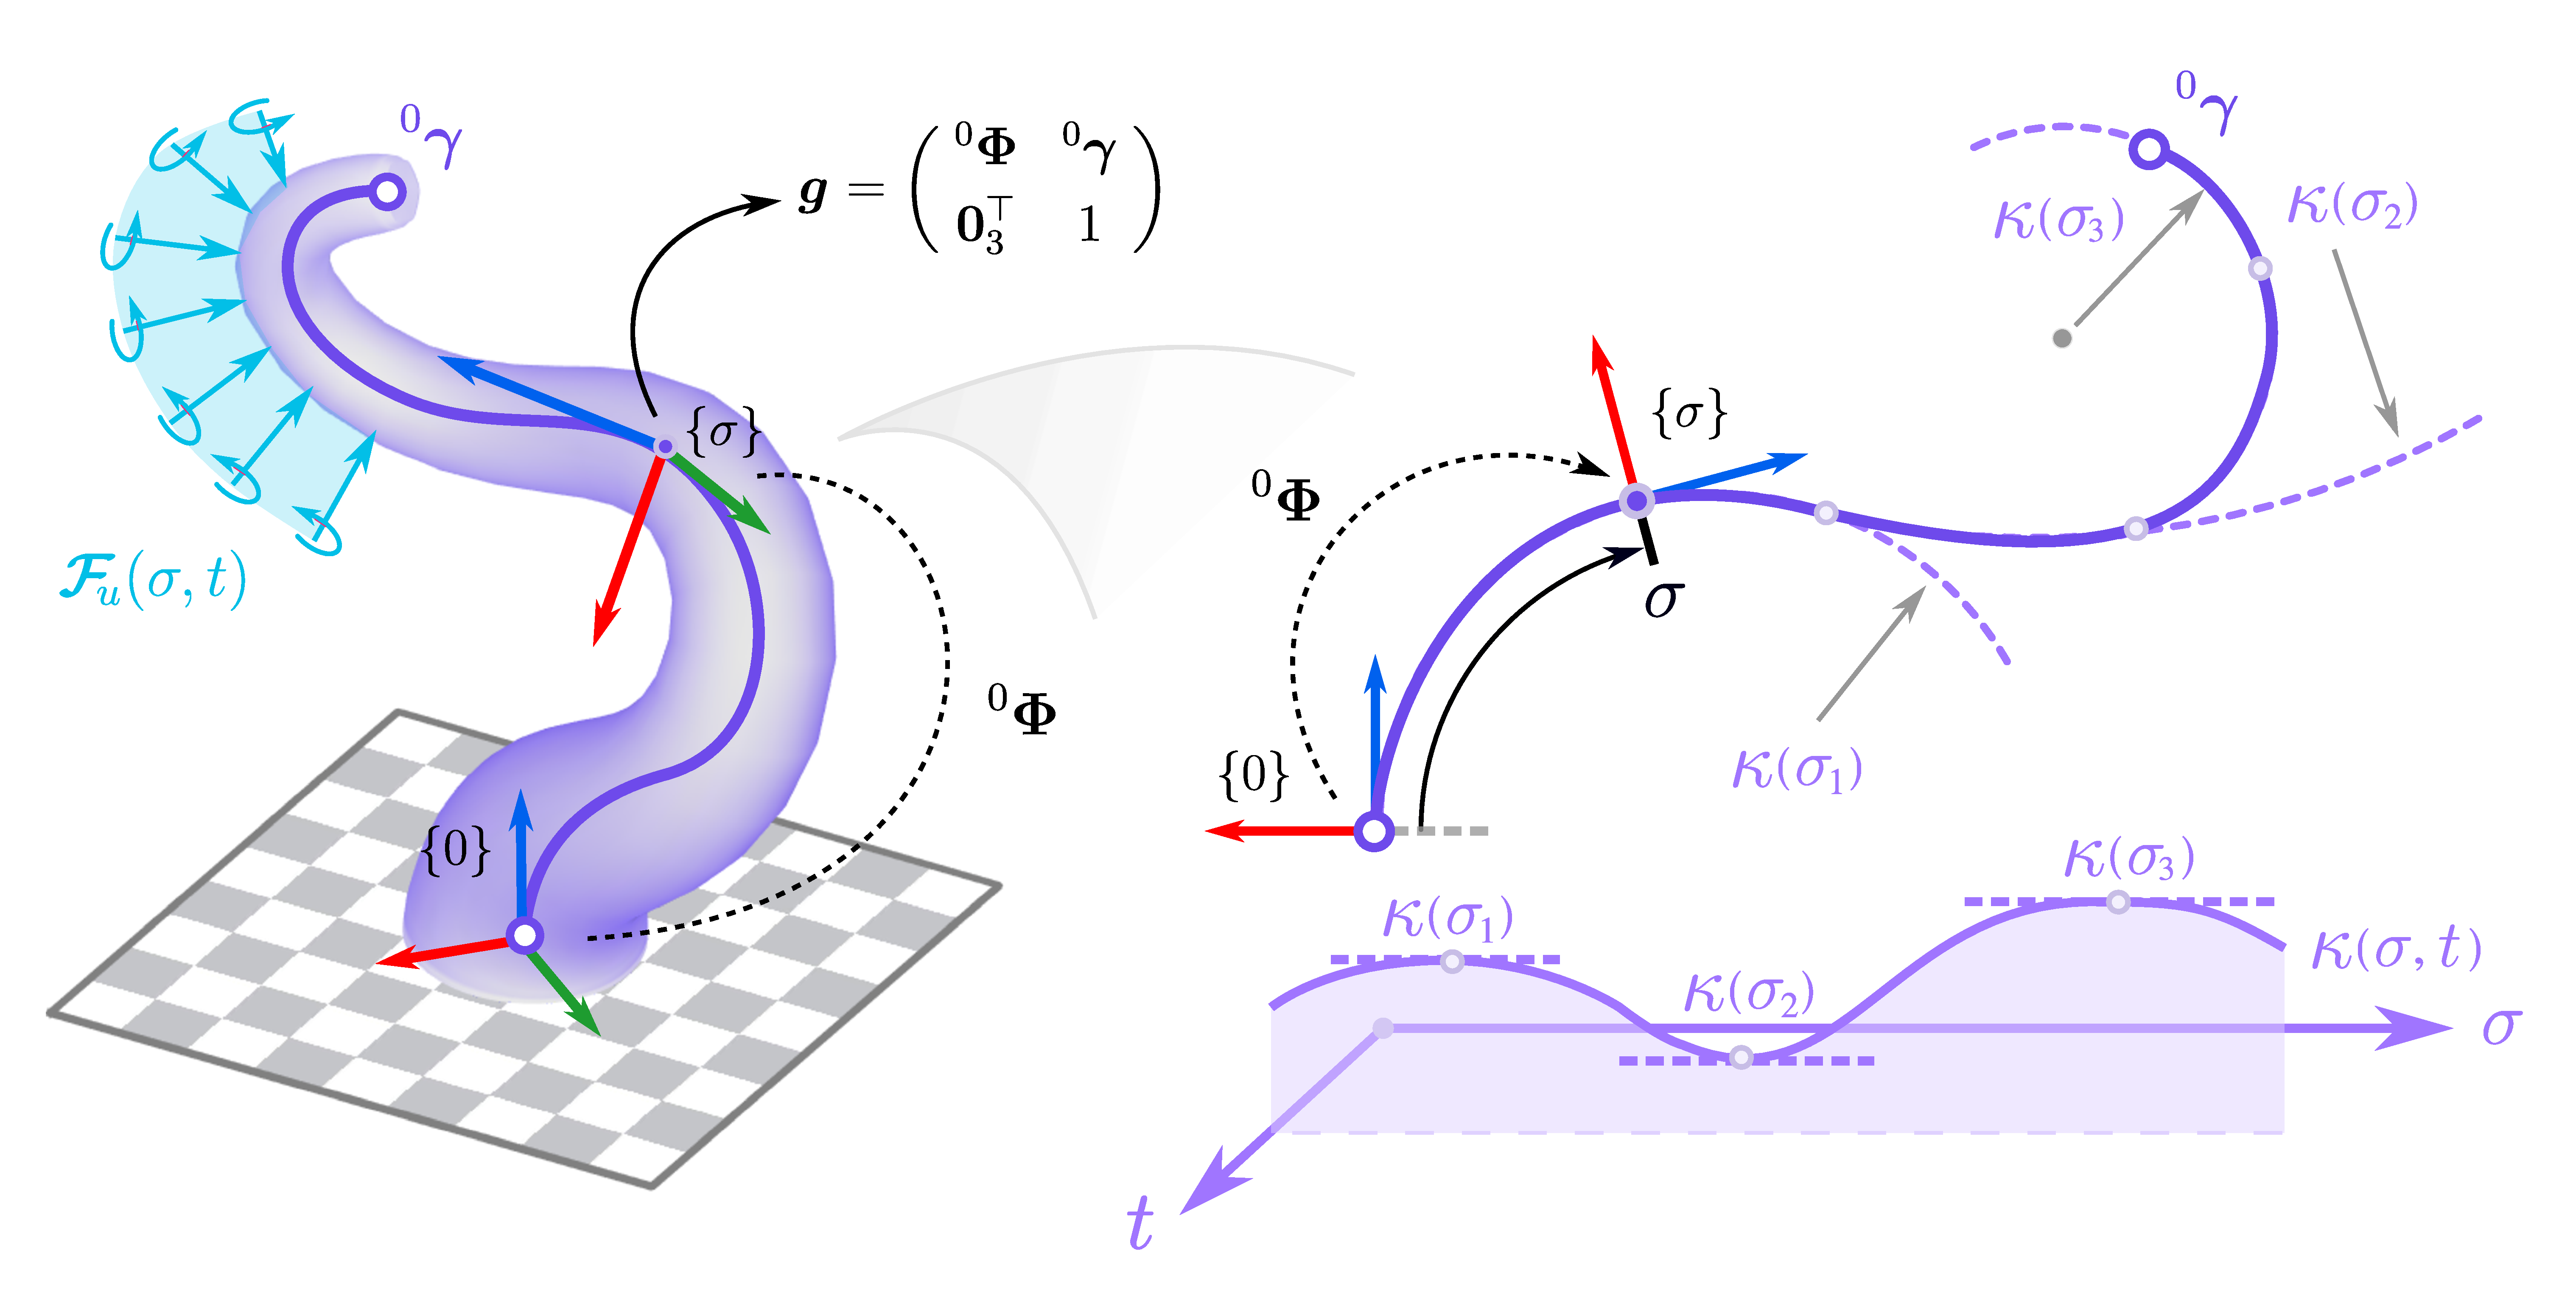
\includegraphics[width = 0.99\textwidth]{3_chapters/3_chapter/img/fig_C3_schematic.pdf}
  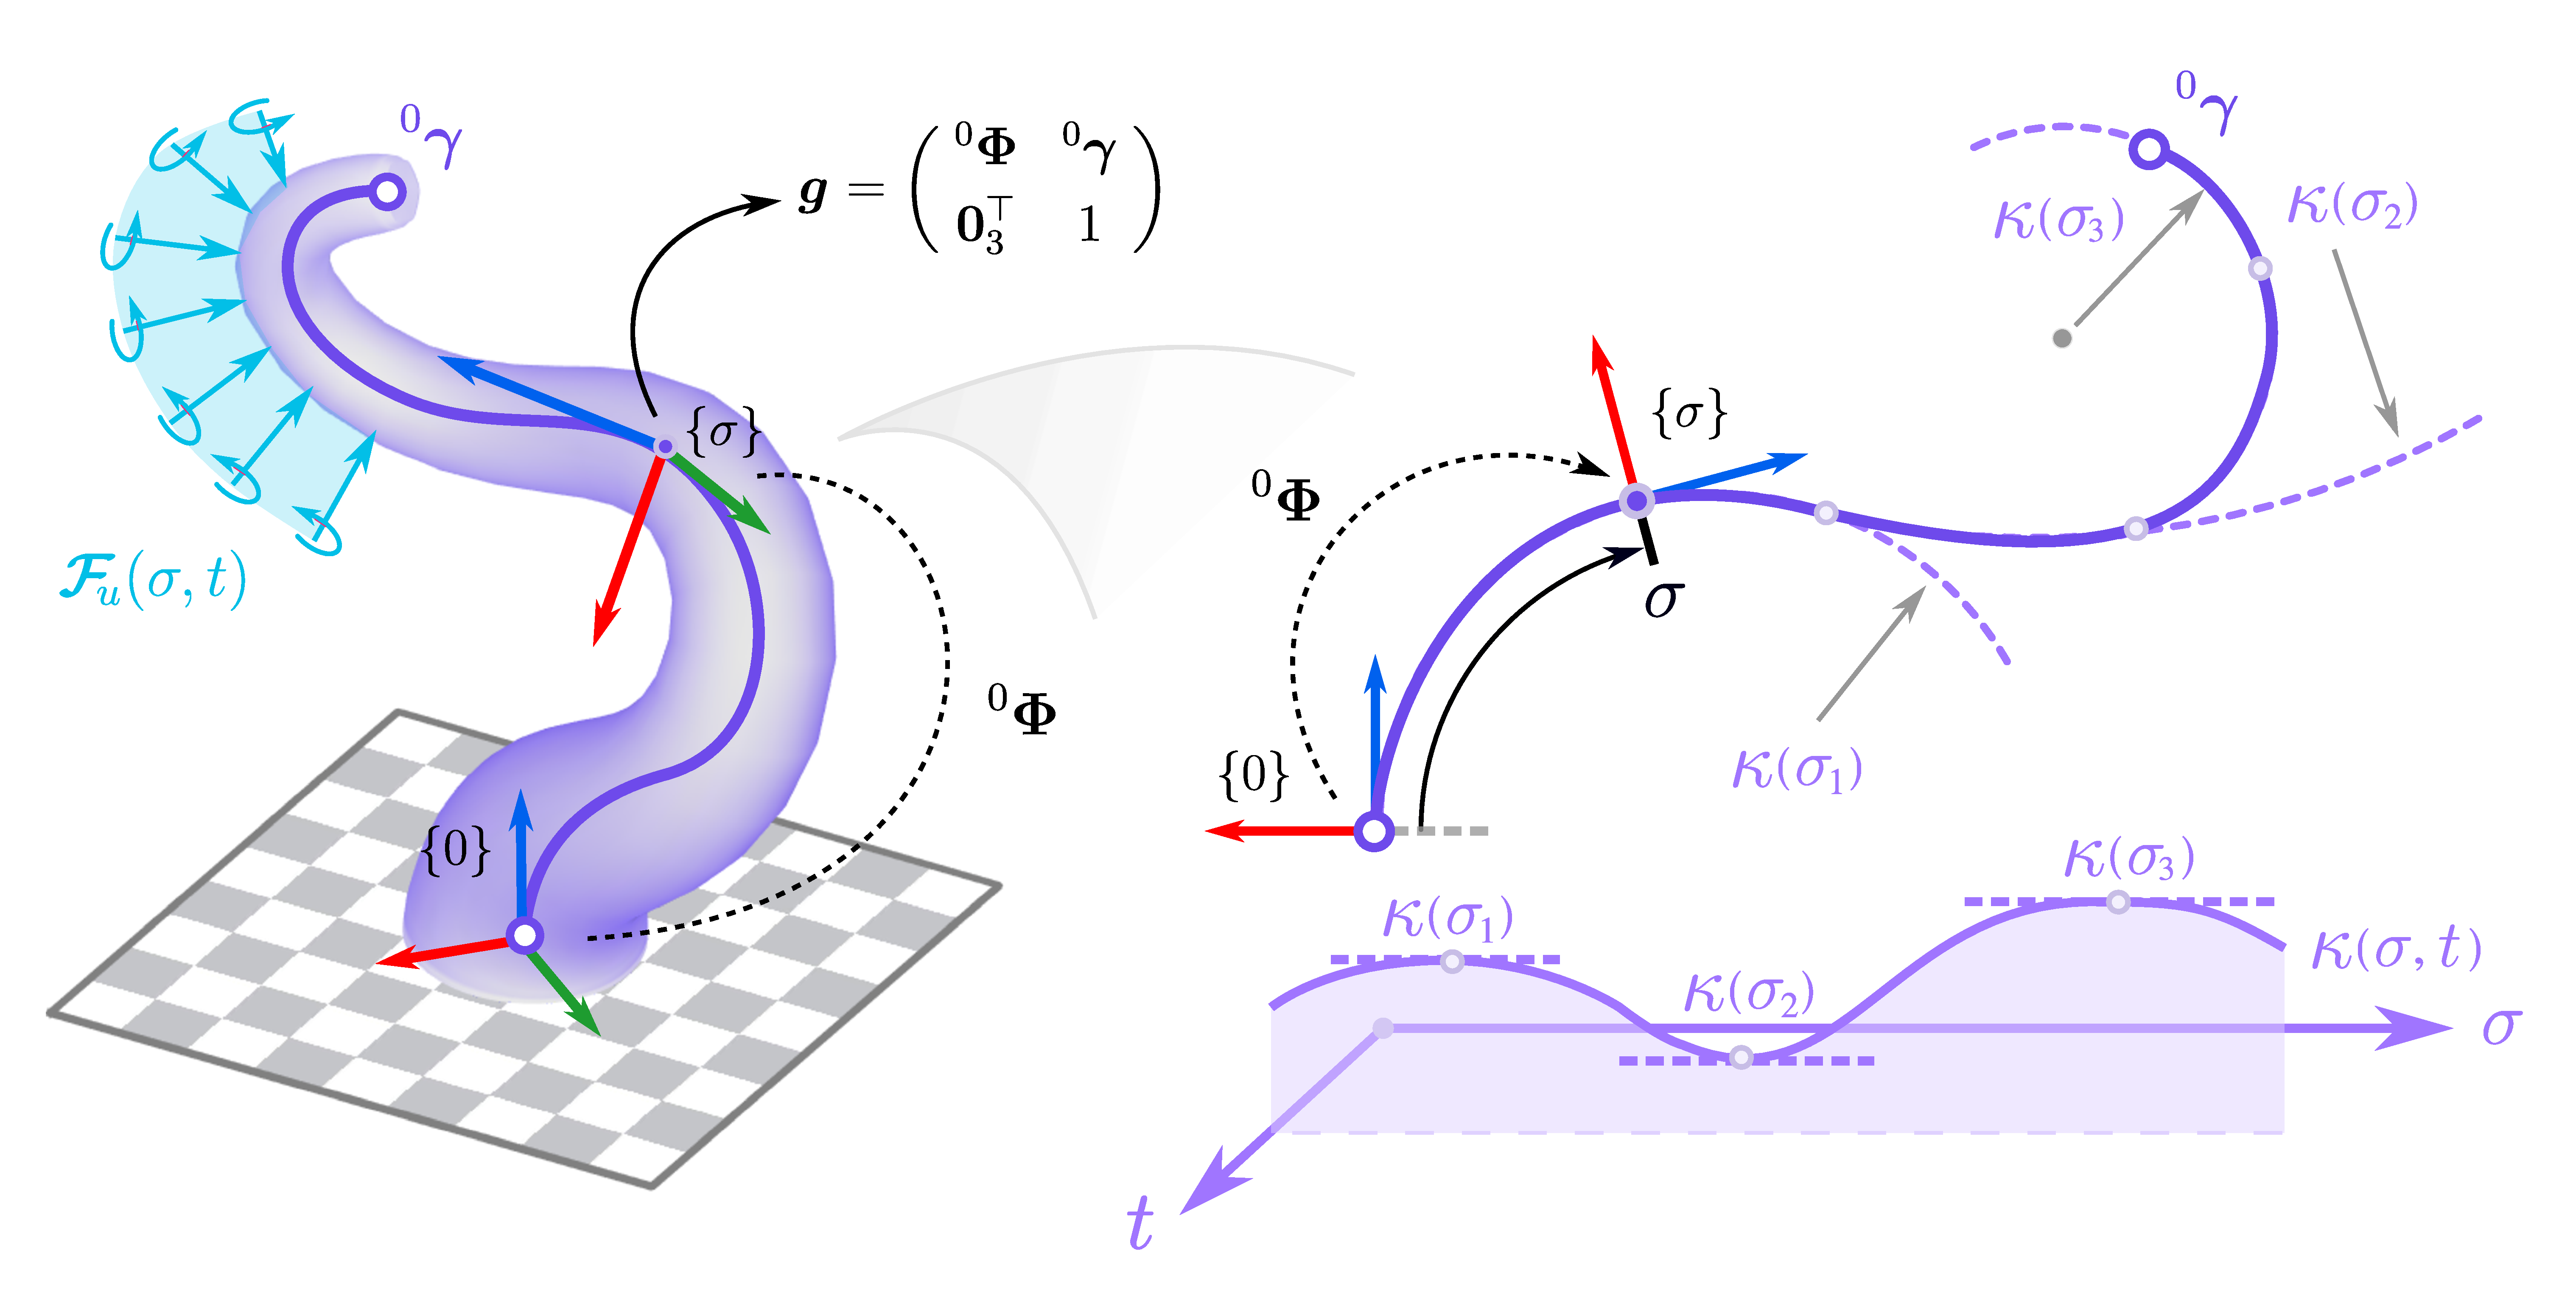
\includegraphics[width = \textwidth]{./pdf/thesis-figure-5-1.pdf}
  \caption{Schematic representation of the continuously variable Cosserat beam model for a general class of soft manipulators, given by a backbone curve $\gammaB$ and orientation matrix $\PhiB$ relative to a base frame at $\{0\}$ Together they form a parameterized curve $\gB(\sigma,t) = (\PhiB(\sigma,t),\, \gammaB(\sigma,t)) \in \SE{3}$. The representation of the soft robot is inspired by the octopus' tentacle whose the muscle forces are modeled as a distributed input $\FT_u$. \label{fig:C3:example1}}
  %\vspace{-0.4cm}
\end{figure}

\subsection{Preliminaries on geometric Cosserat theory}
In Cosserat theory, slender deformable solids are modeled as elastic strings subjected to geometric finite-strain theory. Drawing the analogy to soft robotics, we model the soft robot as a one-dimensional spatial curve passing through the geometric center of the soft robot (see Figure \ref{fig:C3:example1}). Given its spatial-temporal nature, we introduce a temporal variable $t \in [0,+\infty)$, and a spatial variable $\sigma \in [0,\,L]$ with $L$ the undeformed length of the soft robot. For each point on the backbone, we introduce a (mobile) coordinate frame. The homogeneous rotation related to these coordinate frames is given by the rotation matrix $\mat{\Phi}: [0,L] \times [0,+\infty) \to  \SO{3}$, and their origin by the position vector $\vec{\gamma}: [0,L] \times [0,+\infty) \to \R^3$. For convenience and readability, we will denote the temporal and spatial domains as $\Ts = [0,+\infty)$ and $\Xs = [0,\,L]$, respectively.

Following the geometric approach \cite{Simo1986,Boyer2010,Boyer2021,Renda2018,Renda2020}, we may equivalently represent each coordinate frames that are rigidly attached to the continuous backbone of the soft robot by a parameterized space curve in $\SE{3}$:
%
\begin{equation}
\mat{g}(\sigma,t) = \begin{pmatrix} \mat{\Phi}(\sigma,t) & \mat{\gamma}(\sigma,t) \\ \vec{0}_3^\top & 1 \end{pmatrix} \in \SE{3}.
\label{eq:C3:backbone}
\end{equation}
%
An important notion in Lie group theory applied to robotics is the so-called "\textit{exponential coordinate representation}". Conventionally, for rigid multi-body mechanics, any rigid-body transformation from one coordinate frame into another can characterized by a vector living in $\R^6$, called the \textit{twist}, whose six entries are referred to as the exponential coordinates. Three of these exponential coordinates are related to the translation and the other three to orientation. As such, the same principle applies to rigid-body rotations described by matrices in $\SO{3}$ that can be parameterized by three exponential coordinates. For example, we may express a general rotation in terms of its exponential coordinates $\RB(\OmegaB,t) = \exp\left( {\OmegaB}^\times t \right)$ where $\OmegaB^\times \in \sog{3}$ is a skew-symmetric matrix with its three unique entries $\OmegaB = (\omega_1,\omega_2,\omega_3)^\top$ being the unit-time angular velocities. Recall that the superscript denotes the skew-symmetric matrix operator $(\cdot)^\times:\R^3 \to \sog{3}$. %A similar structure holds for rigid-body transformations in $\SE{3}$ similar to \eqref{eq:C3:backbone}.

Since soft robot models are expressed in spatial and temporal coordinates, we aim to seek two exponential coordinate descriptions -- a spatial (strain) twist $\xiB$ called the geometric strain, and a temporal (velocity) twist $\etaB$ called the geometric velocity. The expressions for the strain field $\vec{\xi}$ and velocity field $\vec{\eta}$ anywhere on the Cosserat beam can be found by exploring the differential geometry of the curve $\gB$. To do so, we must introduce some smoothness conditions.

\begin{asm}[Distributed actuation and body loads]
\label{assum:0}
In this study, we assume any control input of the continuum robot can be represented by a distributed input force $\nB_u: \Xs \times \Ts \to \R^3$ and distributed input moment $\mB_u: \Xs \times \Ts \to \R^3$, which act upon the deformable backbone $\gB$. These inputs are conveniently collected into a vector $\FT_u = \left(\mB_u^\top, \nB_u^\top \right)^\top$ referred to as the "\textit{control wrench}". It is important to note that the modeling of distributed input wrenches encompasses various forms of soft actuation, such as pneumatics, hydraulics, tendons, and ferro-magnetic and thermo-mechanical actuation. Similarly, we also introduce a distributed body-load force (\eg, due to gravity) given by $\FT_\textrm{b} = (\vec{0}_3, \nB_\textrm{b}^\top)^\top$ where $\nB_\textrm{u} = -\rho_0 A_0 \PhiB^\top \aB_\textrm{b}$ with $\aB_\textrm{b}$ a body acceleration, $\rho_0$ the density, and $A_0$ the cross-sectional area. Both $\FT_\textrm{u}$ and $\FT_\textrm{g}$ are wrenches expresses in the body frame whose direction depends on the body configuration $\gB$. \end{asm}

\begin{asm}[On differentiability]
\label{assum:1}
Any external distributed force acting on the continuum time-variant backbone curve \eqref{eq:C3:backbone} is considered to be sufficiently smooth as a function of $t$ and $\sigma$ such that parametrized backbone $\mat{g}(\sigma,t) \in \SE{3}$ is differentiable everywhere on $\Xs$ and $\Ts$.
\end{asm}
%

\subsection{Local strain and velocity}
Following the Cosserat beam modeling approach from Simo et al. \cite{Simo1986}, Boyer et al. \cite{Boyer2021}, Renda et al. \cite{Renda2018,Renda2020}, let $\vec{\Gamma} = (\kappa_1,\, \kappa_2, \kappa_3)^\top$ and $\vec{U} = (\nu_1,\, \nu_2,\, \nu_3)^\top$ be the torsion-curvature and elongation-shear strain vector, respectively. First, the spaces $\seg{3}$ and $\mathbb{R}^6$ are isomorphic (\ie, structure preserving) and we denote the mapping between these spaces is called the \emph{"isomorphism"} by $\hat{(\cdot)}: \R^6 \to \seg{3}$ and its inverse $\check{(\cdot)}: \seg{3} \to \R^6$. Then, an expression for strain field $\vec{\xi}(\sigma,t)$ is obtained through spatial differentiation of $\mat{g}$:
%
\begin{equation}
\hat{\vec{\xi}} := \mat{g}\inv \frac{\p \mat{g}}{\p \sigma} = \begin{pmatrix} \vec{\Gamma}^\times & \vec{U} \\[0.5em] \vec{0}_3^\top & 0 \end{pmatrix} \;\; \xRightarrow[]{\textrm{\;\;isomorphism\;\;}} \;\; \vec{\xi} := \begin{pmatrix} \vec{\Gamma} \\ \vec{U} \end{pmatrix}.
\label{eq:C3:xi}
\end{equation}
%
Note the difference between $\hat{\xiB}$ and $\xiB$ in \eqref{eq:C3:xi}, being a matrix element of $\seg{3}$ and column vector of $\R^6$, respectively. 

Following, the temporal exponential coordinates are given by $\vec{\Omega} = (\omega_1, \omega_2, \omega_3)^\top$ and $\vec{V} = (v_1,\,v_2,\, v_3)^\top$ that denote the angular and linear velocity vector, respectively. Then, an expression for velocity field $\vec{\eta}(\sigma,t)$ is obtained through time differentiation of $\vec{g}$:
%
\begin{equation}
\hat{\vec{\eta}} := \mat{g}\inv \frac{\p \mat{g}}{\p t} = \begin{pmatrix} \vec{\Omega}^\times & \vec{V} \\[0.5em] \vec{0}_3^\top & 0 \end{pmatrix} \;\; \xRightarrow[]{\textrm{\;\;isomorphism\;\;}} \;\; \vec{\eta} := \begin{pmatrix} \vec{\Omega} \\ \vec{V} \end{pmatrix}.
\label{eq:C3:eta}
\end{equation}
%
Let it be clear that $\xiB(\sigma,t)$ and $\etaB(\sigma,t)$ are yet unknown {vector fields}, they simply follow from the differential geometry of $\SE{3}$. As such, they live in its tangent space $\seg{3}$ called its Lie algebra. Now given the geometric structures in \eqref{eq:C3:xi} and \eqref{eq:C3:eta}, we can start detailing the forward kinematics of the soft continuum robot by exploring the differential geometry of the spatio-temporal manifold $\gB(\sigma,t)$. Their connection is described in detail in \cite{Simo1986,Boyer2010,Boyer2021,Renda2017Aug,Renda2018}, but briefly recapitulated here to be self-contained. 

Recalling Assumption \ref{assum:1}, which assumes the configuration space $\mat{g}$ to be everywhere differentiable, we can introduce the equality of mixed partials, \ie, $\frac{\p }{\p t}(\frac{\p \mat{g}}{\p \sigma}) = \frac{\p }{\p \sigma} (\frac{\p \mat{g}}{\p t})$. Then, by substitution of $\frac{\p \mat{g}}{\p t} = \vec{g}\hat{\vec{\eta}}$ and $\frac{\p \mat{g}}{\p \sigma} = \mat{g}\hat{\vec{\xi}}$, we obtain the so-called \emph{compatibility equation}:
%
\begin{equation}
\mat{g} \hat{\vec{\eta}}\hat{\vec{\xi}} + \mat{g} \frac{\p \hat{\vec{\xi}}}{\p t}  = \mat{g} \hat{\vec{\xi}} \hat{\vec{\eta}}  + \mat{g} \frac{\p \hat{\vec{\eta}}}{\p \sigma},
\label{eq:C3:compatibility}
\end{equation}
%
\noindent
The equality above ensures that the partial derivatives with respect to time and space are continuously connected on the manifold $\gB$. Simply put, deformations that are tied to the spatial derivatives need to have continuous velocity profiles (\ie, the temporal derivative) -- and vice versa. Pre-multiplication of the expression above with $\mat{g} \inv \in \SE{3}$ and rearranging the equality, we obtain
%
\begin{equation}
\frac{\p \hat{\vec{\eta}}}{\p \sigma} = -\left(\hat{\vec{\xi}}\hat{\vec{\eta}} - \hat{\vec{\eta}}\hat{\vec{\xi}} \right) + \dot{\hat{\vec{\xi}}}.
\end{equation}
%
\noindent Focusing on the RHS term $(\hat{\vec{\xi}}\hat{\vec{\eta}} - \hat{\vec{\eta}}\hat{\vec{\xi}})$, we can recognize the Lie bracket or the commutator between the geometric vector fields $\vec{\xi}$ and $\vec{\eta}$ (see \cite{Murray1994}). Since the Lie bracket $[\hat{\vec{\xi}},\hat{\vec{\eta}}]$ itself also belongs to the Lie algebra $\seg{3}$, which is isomorphic to $\R^6$ via the operator $\hat{\vec{\eta}} \to \vec{\eta}$, we can rewrite the expressions as follows
%
\begin{equation}
\frac{\p \vec{\eta}}{\p \sigma} = -\ad_{\vec{\xi}}\vec{\eta} + \dot{\vec{\xi}},
\label{eq:C3:pde_kin}
\end{equation}
%
\noindent where $\ad_{(\cdot)}: \R^6 \to \R^{6\times 6}$ defines the adjoint action on vectors belonging to the Lie algebra $\seg{3}$. %The approach provided above is analogous to works \cite{Boyer2021,Renda2020,Till2019}. 
Drawing an analogy to rigid robotics, the expression in \eqref{eq:C3:pde_kin} may be seen as the forward velocity kinematics for a serial chain robot manipulator with infinitely many links. To that end, we can collect the PDEs \eqref{eq:C3:xi}, \eqref{eq:C3:pde_kin} and the time derivative of \eqref{eq:C3:pde_kin} (\ie, the acceleration) into one global \textit{Partial Matrix Differential Equation} (PMDE) that describes the full continuum-body kinematics of the soft deformable robotic body. The PMDE curve kinematics takes the form
%
% \begin{equation}
% \frac{\p }{\p \sigma} 
% \begin{pmatrix}
% \,\gB\; \\[0.25em]
% \,\etaB\; \\[0.25em]
% \;\dot{\etaB}\;\;
% \end{pmatrix}  = 
% \begin{pmatrix}
% \gB \hat{\xiB} \\[0.25em]
% -\ad_{\vec{\xi}}\vec{\eta} + \dot{\vec{\xi}} \\[0.25em]
% -\ad_{\vec{\xi}}\dot{\etaB} -\ad_{\dot{\xiB}}\etaB  + \ddot{\vec{\xi}}
% \end{pmatrix}.
% \label{eq:C3:cont_kin_pde}
% \end{equation}
%
\begin{equation}
\frac{\p }{\p \sigma} 
\begin{pmatrix}
\begin{bmatrix} \gB \\[0.25em] \vec{0} 
\end{bmatrix},
\,\etaB,\;
\;\dot{\etaB}\;\;
\end{pmatrix} = \begin{pmatrix}
\begin{bmatrix} \gB \hat{\xiB} \\[0.25em] \vec{0} 
\end{bmatrix}
, & -\ad_{\vec{\xi}}\vec{\eta} + \dot{\vec{\xi}}, & -\ad_{\vec{\xi}}\dot{\etaB} -\ad_{\dot{\xiB}}\etaB  + \ddot{\vec{\xi}}
\label{eq:C3:cont_kin_pde}
\end{pmatrix}
\end{equation}

\noindent which is a square differential matrix. For the general case, the boundary conditions of PDE in \eqref{eq:C3:cont_kin_pde} should satisfy $\gB(0,t) = \gB_0$, $\etaB(0,t) = \etaB_0$ and $\dot{\etaB}(0,t) = \dot{\etaB}_0$. However, in case of a manipulator whose base is spatially fixed, the boundary conditions should satisfy $\gB(0,t) = \gB_0$, and $\etaB(0,t) = \dot{\etaB}(0,t) = \vec{0}_6$. An importance remark is that if the strain fields $\xiB$, $\dot{\xiB}$, and $\ddot{\xiB}$ are analytic such that we choose an instance $t \in [0,T]$ and keeping $\sigma$ variable, the PMDE in \eqref{eq:C3:cont_kin_pde} becomes an ordinary Matrix Differential Equation (MDE) which can be solved numerically using the techniques discussed in Chapter \ref{chap:PCC}. 

\begin{example}[Kinematic behavior of variable strain soft segment]
Let $\Xs = [0,L]$ with $L = 100$ \si{\milli \meter} and $\Ts = [0, T]$ with $T = 1$ \si{\second}. Consider in this example a planar bending problem where the geometric strain vector takes the form $\xiB = (0,\kappa(\sigma,t),0,1,0,0)^\top$ with $\kappa$ is an a priori known non-constant curvature profile. Inspired by the analytic solutions of the Euler-Bernoulli cantilever model \cite{Holzapfel2002}, we propose an analytic expression for the planar curvature strain:
%
\begin{align}
\kappa(\sigma,t) & =  \kappa_{\textrm{max}} \; \theta(\sigma) h(t), \\
\theta(\sigma) & =  \sinh(\beta \sigma) + \sin(\beta \sigma) + \frac{\cos(\beta L)+\cosh(\beta L)}{\sin(\beta L)+ \sinh(\beta L)} \big(\cos(\beta \sigma)-\mu \cosh(\beta \sigma) \big), 
\end{align}  
%
where $\kappa_{\textrm{max}} = 60$ \si{\milli \meter \inv} is the curvature amplitude, $\theta(\sigma)$ the first strain eigenmode of the cantilever beam model, $h(t) = \frac{(1- k)t}{(1 + k) - 2k|t|}$ a transient modeled after a sigmoid function with $k = \frac{1}{2}$, and a parameter $\beta$ which is the smallest positive real that satisfies the nonlinear equality $\cos(\beta L)\cosh(\beta L) = 1$. The physical interpretation $\beta$ is the inverse wavelength thus it is inversely proportional to the beam length $L$. A numerical approximation of this value is $\beta \approx 0.597 \, \pi L^{-1}$. The strain velocity $\dot{\xiB}$ and strain acceleration $\ddot{\xiB}$ are obtained  straightforwardly by differentiation of $\kappa(\sigma,t)$ with respect to time. Hence, we have explicit expressions on the strain, its velocity and acceleration. Therefore, we can evaluate $\sB_i(\sigma) := \xiB(\sigma,t_i)$, $\vB_i(\sigma) := \dot{\xiB}(\sigma,t_i)$, and $\aB_i(\sigma) := \ddot{\xiB}(\sigma,t_i)$ for any time sample $t_i \in \Ts$.
%
\begin{figure}[!t]
  \centering
  %% This file was created by matlab2tikz.
%
%The latest updates can be retrieved from
%  http://www.mathworks.com/matlabcentral/fileexchange/22022-matlab2tikz-matlab2tikz
%where you can also make suggestions and rate matlab2tikz.
%
\definecolor{mycolor1}{rgb}{0.89290,0.89290,0.89290}%
\definecolor{mycolor2}{rgb}{0.68536,0.75889,0.88144}%
\definecolor{mycolor3}{rgb}{0.47782,0.62488,0.86998}%
\definecolor{mycolor4}{rgb}{0.27028,0.49087,0.85852}%
\definecolor{mycolor5}{rgb}{0.06275,0.35686,0.84706}%
%
\begin{tikzpicture}

\begin{axis}[%
width=0.393\textwidth,
height=0.273\textwidth,
at={(0.507\textwidth,0\textwidth)},
scale only axis,
axis on top,
xmin=0.5,
xmax=391.5,
tick align=outside,
y dir=reverse,
ymin=0.5,
ymax=271.5,
axis line style={draw=none},
ticks=none
]
\addplot [forget plot] graphics [xmin=0.5, xmax=391.5, ymin=0.5, ymax=271.5] {fig_C3_eulerbeam_example_3D-1.png};
\end{axis}

\begin{axis}[%
width=0.405\textwidth,
height=0.273\textwidth,
at={(0\textwidth,0\textwidth)},
scale only axis,
xmin=0,
xmax=100,
xtick={0,100},
xticklabels={{0},{$L$}},
xlabel style={font=\color{white!15!black}, yshift=5pt},
xlabel={space $\sigma$},
ymin=-5,
ymax=70,
ylabel style={font=\color{white!15!black}},
ylabel={$\kappa(\sigma,t)$ (mm$^{-1}$)},
axis background/.style={fill=white},
xmajorgrids,
ymajorgrids
]
\addplot [color=mycolor1, line width=1.8pt, forget plot]
  table[row sep=crcr]{%
0	0\\
100	0\\
};
\addplot [color=mycolor2, line width=1.8pt, forget plot]
  table[row sep=crcr]{%
0	0\\
15.7157157157157	2.83047089028886\\
31.4314314314314	4.97995465872708\\
47.5475475475476	6.50447153711326\\
64.7647647647648	7.45064492701712\\
85.0850850850851	7.86839675692123\\
100	7.90564399432552\\
};
\addplot [color=mycolor3, line width=1.8pt, forget plot]
  table[row sep=crcr]{%
0	0\\
10.6106106106106	4.69465476161083\\
21.1211211211211	8.61760388347477\\
31.6316316316316	11.8253274486491\\
42.2422422422422	14.3601010441867\\
53.1531531531532	16.2721577996008\\
64.7647647647648	17.6106152820405\\
77.6776776776777	18.3988481509257\\
94.1941941941942	18.680703252255\\
100	18.6860676229512\\
};
\addplot [color=mycolor4, line width=1.8pt, forget plot]
  table[row sep=crcr]{%
0	0\\
8.60860860860861	7.08667090503489\\
17.017017017017	13.1479474019476\\
25.2252252252252	18.2497496684672\\
33.3333333333333	22.5108261318712\\
41.4414414414414	26.019913948194\\
49.7497497497498	28.8708542481266\\
58.2582582582583	31.0625154195058\\
67.1671671671672	32.6476393619519\\
76.8768768768769	33.6742369735057\\
88.3883883883884	34.1807175171737\\
100	34.2577906420773\\
};
\addplot [color=mycolor5, line width=1.8pt, forget plot]
  table[row sep=crcr]{%
0	0\\
7.6076076076076	10.8145509556227\\
14.9149149149149	20.0780076622414\\
22.022022022022	28.0354588986514\\
28.9289289289289	34.784744453201\\
35.7357357357357	40.5046017902398\\
42.4424424424424	45.2614189259049\\
49.049049049049	49.1286496814225\\
55.7557557557558	52.2693569213937\\
62.6626626626627	54.738748175621\\
69.8698698698699	56.5722071820405\\
77.5775775775776	57.8130937401701\\
86.3863863863864	58.5162426796125\\
98.4984984984985	58.7273450503463\\
100	58.7276411007039\\
};
\end{axis}

\begin{axis}[%
width=0.963\textwidth,
height=0.341\textwidth,
at={(-0.048\textwidth,-0.034\textwidth)},
scale only axis,
xmin=0,
xmax=1,
ymin=0,
ymax=1,
axis line style={draw=none},
ticks=none,
axis x line*=bottom,
axis y line*=left
]
\end{axis}
\end{tikzpicture}% \\[0.15em]
  %% This file was created by matlab2tikz.
%
%The latest updates can be retrieved from
%  http://www.mathworks.com/matlabcentral/fileexchange/22022-matlab2tikz-matlab2tikz
%where you can also make suggestions and rate matlab2tikz.
%
\definecolor{mycolor1}{rgb}{0.06275,0.35686,0.84706}%
\definecolor{mycolor2}{rgb}{0.86667,0.21176,0.10980}%
\definecolor{mycolor3}{rgb}{0.18039,0.52157,0.25098}%
%
\begin{tikzpicture}

\begin{axis}[%
width=0.404\textwidth,
height=0.242\textwidth,
at={(0\textwidth,0\textwidth)},
scale only axis,
xmin=0,
xmax=1,
xlabel style={font=\color{white!15!black}},
xlabel={time (s)},
ymin=-80,
ymax=120,
ylabel style={font=\color{white!15!black}, yshift=-5pt},
ylabel={$ \gammaB_L $ (mm)},
axis background/.style={fill=white},
xmajorgrids,
ymajorgrids
]
\addplot [color=mycolor1, line width=1.8pt, forget plot]
  table[row sep=crcr]{%
0	99.7999999999986\\
0.00223964165734003	99.7973744072979\\
0.00449943757030269	99.7894032385059\\
0.00792751981879292	99.767107765435\\
0.0125714285714338	99.7173004640467\\
0.0184971098265834	99.6210311814633\\
0.0257913247362183	99.452280688556\\
0.0332936979785927	99.2210910832167\\
0.0423216444981875	98.8658806195815\\
0.0530209617755872	98.3369383055835\\
0.0641509433962284	97.6639557908219\\
0.0772200772200762	96.7166959455565\\
0.0909090909090935	95.5467878395046\\
0.106901217861974	93.9568805106074\\
0.123783031988879	92.0281272017212\\
0.143472022955521	89.4714374015077\\
0.164444444444442	86.4101333623327\\
0.18683001531393	82.7938810486975\\
0.213036565977745	78.1602278968701\\
0.243781094527364	72.2715315545542\\
0.282722513088999	64.3063809929585\\
0.424742268041243	34.6940007741157\\
0.456289978678043	28.8516670741767\\
0.48571428571428	23.871796037797\\
0.512415349887135	19.8066564245194\\
0.535796766743644	16.6367309774332\\
0.555294117647065	14.2885395322973\\
0.57553956834532	12.1448265237983\\
0.591240875912405	10.6930865097043\\
0.607407407407408	9.39254512644054\\
0.624060150375939	8.25899429506282\\
0.635443037974682	7.60378300142125\\
0.647058823529406	7.03423289670161\\
0.658914728682177	6.55469252560214\\
0.671018276762396	6.16929840847122\\
0.683377308707122	5.88191113471227\\
0.689655172413794	5.77608373790237\\
0.695999999999998	5.69604441721829\\
0.702412868632706	5.64216535125435\\
0.708894878706204	5.61478685126646\\
0.715447154471548	5.61421450680018\\
0.722070844686655	5.64071621420031\\
0.728767123287668	5.69451908923003\\
0.735537190082638	5.7758062658089\\
0.742382271468145	5.8847135837659\\
0.749303621169915	6.02132616948518\\
0.763380281690146	6.37773285763318\\
0.777777777777771	6.84455691872186\\
0.792507204610956	7.42028289582042\\
0.807580174927111	8.10222526586492\\
0.823008849557525	8.88640182404758\\
0.846846846846844	10.2421105128154\\
0.871559633027516	11.7904200606828\\
0.914826498422713	14.7034263044896\\
0.970491803278691	18.4693803844847\\
1	20.3165545629562\\
};
\addplot [color=mycolor2, dashed, line width=1.8pt, forget plot]
  table[row sep=crcr]{%
0	0\\
1	0\\
};
\addplot [color=mycolor3, line width=1.8pt, forget plot]
  table[row sep=crcr]{%
0	-3.61537644266718e-09\\
0.0713375796178326	-17.7527567284248\\
0.108548168249662	-26.4200000781221\\
0.139800285306706	-33.1589453228339\\
0.166419019316493	-38.4117614769386\\
0.191063174114021	-42.8146338118347\\
0.213036565977745	-46.3297315753307\\
0.234042553191486	-49.3028883796995\\
0.253781512605045	-51.7351240646114\\
0.271944922547334	-53.6535687304242\\
0.288224956063267	-55.1074641079331\\
0.302325581395351	-56.1616626598023\\
0.313974591651544	-56.8884769641568\\
0.325966850828728	-57.5006769173563\\
0.33519553072626	-57.8782397258901\\
0.344632768361585	-58.1807553089183\\
0.354285714285716	-58.4035154552598\\
0.36084452975048	-58.5053548545591\\
0.367504835589941	-58.5681942694681\\
0.37087378640777	-58.5845408731258\\
0.374269005847957	-58.590599517956\\
0.37769080234834	-58.5861909109014\\
0.381139489194496	-58.571136056554\\
0.384615384615387	-58.5452564332206\\
0.391650099403577	-58.4603122857785\\
0.398797595190381	-58.3299470804194\\
0.406060606060606	-58.1527699697726\\
0.417177914110432	-57.7962604946399\\
0.428571428571431	-57.3269294930165\\
0.440251572327043	-56.7405951666252\\
0.452229299363054	-56.0334115463667\\
0.46868250539957	-54.8966784026617\\
0.485714285714288	-53.5325062963644\\
0.503355704697988	-51.9365006858544\\
0.526315789473685	-49.6133068372119\\
0.550351288056206	-46.9300986419265\\
0.580722891566268	-43.2572802692019\\
0.624060150375939	-37.6831067649934\\
0.695999999999998	-28.3676834706202\\
0.728767123287675	-24.4112162828547\\
0.756302521008401	-21.3424247030881\\
0.777777777777779	-19.1493034122343\\
0.799999999999997	-17.0901855500341\\
0.823008849557525	-15.2042364723099\\
0.838805970149252	-14.0630781987289\\
0.854984894259822	-13.0289142111722\\
0.871559633027523	-12.1136848286582\\
0.888544891640869	-11.3289912044061\\
0.905956112852664	-10.6858555921471\\
0.914826498422713	-10.4205913115741\\
0.923809523809524	-10.1944465403014\\
0.932907348242814	-10.0085079561308\\
0.942122186495176	-9.86376804711688\\
0.95145631067961	-9.76111344196095\\
0.960912052117266	-9.70131271469189\\
0.970491803278691	-9.68500369162139\\
0.980198019801982	-9.71268029736685\\
0.990033222591364	-9.78467898662958\\
1	-9.90116481945083\\
};
\end{axis}

\begin{axis}[%
width=0.35\textwidth,
height=0.242\textwidth,
at={(0.55\textwidth,0\textwidth)},
scale only axis,
xmin=0,
xmax=1,
xlabel style={font=\color{white!15!black}},
xlabel={time (s)},
ymin=-255,
ymax=255,
ylabel style={font=\color{white!15!black}, yshift=-2pt},
ylabel={$\lfloor \etaB_L \rfloor_3$ (mm/s)},
axis background/.style={fill=white},
xmajorgrids,
ymajorgrids
]
\addplot [color=mycolor1, line width=1.8pt, forget plot]
  table[row sep=crcr]{%
0	-5.03322894473968e-09\\
0.0173010380622713	-6.50220495361191\\
0.0358422939067964	-14.3948686496833\\
0.055762081784394	-23.9101852620639\\
0.0772200772200904	-35.297915417717\\
0.1020134228188	-49.7946691493567\\
0.130801687763721	-68.160583968584\\
0.166419019316493	-92.5546161263635\\
0.26666666666668	-162.348077306552\\
0.293805309734523	-178.950648064041\\
0.313974591651544	-189.974031478974\\
0.33209647495363	-198.706228867454\\
0.34782608695653	-205.256001077113\\
0.360844529750466	-209.878175746971\\
0.374269005847964	-213.827254496507\\
0.384615384615387	-216.27114612029\\
0.395209580838326	-218.206632761828\\
0.402414486921543	-219.183899865081\\
0.40973630831644	-219.888164780211\\
0.417177914110425	-220.29924144634\\
0.420944558521569	-220.388325155136\\
0.424742268041228	-220.396212237696\\
0.428571428571416	-220.320179200681\\
0.432432432432421	-220.15746161557\\
0.436325678496871	-219.905255785567\\
0.4442105263158	-219.120979710955\\
0.452229299363069	-217.944212726521\\
0.460385438972168	-216.351332000494\\
0.468682505399556	-214.318325348871\\
0.481400437636751	-210.390407883886\\
0.494456762749451	-205.3351325721\\
0.507865168539325	-199.070676986792\\
0.521640091116183	-191.517360981173\\
0.535796766743658	-182.599579632315\\
0.555294117647065	-168.468401954006\\
0.575539568345334	-151.652697767758\\
0.596577017114925	-132.059585351932\\
0.618453865336647	-109.658142704518\\
0.64705882352942	-77.7974783343005\\
0.683377308707122	-34.4105554254838\\
0.770538243626049	71.379609065326\\
0.800000000000011	103.623297293933\\
0.82300884955751	126.278762663014\\
0.846846846846859	146.810719886305\\
0.863221884498472	158.911390922616\\
0.879999999999995	169.4328859242\\
0.89719626168224	178.094573094596\\
0.905956112852664	181.637421317512\\
0.914826498422713	184.605752163697\\
0.923809523809524	186.962407397604\\
0.932907348242821	188.670244303364\\
0.942122186495169	189.692354493835\\
0.951456310679617	189.992307751626\\
0.960912052117266	189.534422304558\\
0.970491803278691	188.284062879113\\
0.980198019801975	186.207967787265\\
0.990033222591364	183.274606180161\\
1	178.254201447696\\
};
\addplot [color=mycolor2, dashed, line width=1.8pt, forget plot]
  table[row sep=crcr]{%
0	0\\
1	0\\
};
\addplot [color=mycolor3, line width=1.8pt, forget plot]
  table[row sep=crcr]{%
0	-85.0473803587339\\
0.00223964165732582	-85.6158257265569\\
0.0282685512367493	-93.9745343566354\\
0.0489596083231447	-99.8692813302412\\
0.0655737704917954	-103.986025188536\\
0.0802069857697347	-107.075842816235\\
0.0924702774108255	-109.230655828393\\
0.103633916554514	-110.815531789786\\
0.113543091655259	-111.899935113828\\
0.122052704576987	-112.575419257088\\
0.129032258064512	-112.945239904325\\
0.134370579915128	-113.1123265999\\
0.137980085348516	-113.167094032888\\
0.139800285306706	-113.176630107849\\
0.141630901287556	-113.173872976656\\
0.143472022955535	-113.158519828933\\
0.147186147186147	-113.088786901727\\
0.15094339622641	-112.964898631011\\
0.15666178623718	-112.671762328688\\
0.162481536189063	-112.241611387335\\
0.170403587443957	-111.43807150471\\
0.17851739788199	-110.349211758237\\
0.188940092165893	-108.547163238602\\
0.199687987519496	-106.204281487471\\
0.210776545166397	-103.262328044361\\
0.224555735056555	-98.8535168541872\\
0.238879736408563	-93.3782523458157\\
0.25378151260503	-86.7157831311057\\
0.269296740994861	-78.7404165295425\\
0.28822495606326	-67.605560082891\\
0.308108108108115	-54.3087274508757\\
0.329020332717192	-38.6632488696587\\
0.354285714285709	-17.7087082305252\\
0.38113948919451	6.65961839144884\\
0.417177914110425	41.8824215281318\\
0.531034482758628	155.4887375113\\
0.555294117647065	176.545560445766\\
0.575539568345334	192.374387721705\\
0.596577017114925	206.808308760275\\
0.612903225806463	216.404103229858\\
0.62972292191435	224.672732502005\\
0.641221374045813	229.316042501543\\
0.652956298200507	233.166210099722\\
0.664935064935065	236.135529841472\\
0.671018276762396	237.26166879576\\
0.677165354330697	238.13345171144\\
0.683377308707122	238.73922529072\\
0.689655172413779	239.067251513411\\
0.695999999999998	239.10573840527\\
0.702412868632706	238.842874076787\\
0.70889487870619	238.266864236387\\
0.715447154471548	237.365973386964\\
0.722070844686641	236.128569919031\\
0.728767123287668	234.543175316821\\
0.742382271468131	230.283589889617\\
0.756302521008394	224.500600761065\\
0.770538243626049	217.113959654515\\
0.785100286532952	208.052212548924\\
0.800000000000011	197.255482171009\\
0.815249266862168	184.678627371514\\
0.830860534124639	170.294793777077\\
0.854984894259815	145.327990555536\\
0.879999999999995	116.392775121539\\
0.905956112852664	83.7617660698862\\
0.951456310679617	22.5887905891359\\
1	-43.2445730182744\\
};
\end{axis}
\end{tikzpicture}%
  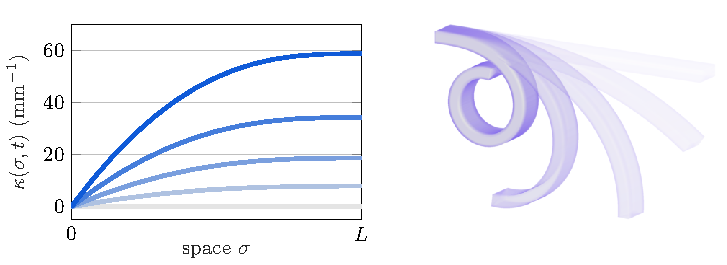
\includegraphics{./pdf/thesis-figure-5-2-1.pdf}  \\[0.15em]
  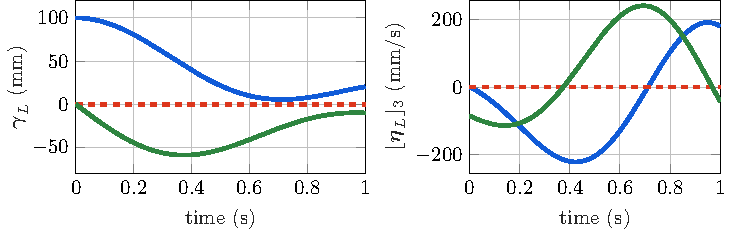
\includegraphics{./pdf/thesis-figure-5-2-2.pdf}  
  \caption{Spatio-temporal evolution of the cantilever beam obtained by solving the exact continuum forward kinematics described in \eqref{eq:C3:cont_kin_pde}. The figure shows the forward kinematic solutions of the end-effector position $\gammaB_L:=\gammaB(L)$ and its linear velocities $\lfloor \etaB_L \rfloor_3:=\lfloor \etaB(L) \rfloor_3$, where the following color coding is used $\{x,y,z\} = \{\ldatanum{Matlab1}{},\ldatanum{Matlab2}{},\ldatanum{Matlab3}{}\}$.}
  \vspace{-0.2cm}
  \label{fig:C3:EX1:cantilever_FK_example}
\end{figure}

Then, substitution of $\sB_i$, $\vB_i$ and $\aB_i$ into \eqref{eq:C3:cont_kin_pde} leads to an ordinary differential equation that depends exclusively on $\sigma$. The forward kinematics can then be solved for the spatial horizon $\Xs = [0,L]$ using an explicit integration routine (fourth order Runge Kutta method), which produces $\gB$, $\etaB$ and $\dot{\etaB}$. We repeat this process until the full forward kinematics is recovered for all $t \in \Ts$. The results for the Euler-Bernoulli cantilever beam are shown in Figure \ref{fig:C3:EX1:cantilever_FK_example}. Figure \ref{fig:C3:EX1:cantilever_FK_example} shows for $\kappa(\sigma,t)$ evolves over space and time, and how they relate to the continuum deformations. It also shows the position $\gammaB_L$ and the linear velocities $\lfloor \etaB \rfloor_3$ of the end-effector. Note that this approach can easily deal with non-constant curvature situations, in contrast to the approach discussed in Chapter \ref{chap:PCC}. Namely, Chapter \ref{chap:PCC} subdivided the domain $\Xs$ into small PCC segments leading to notorious discontinuities at the interfaces (see Figure \ref{fig:C4:basis_example}).

\end{example}


% %
% Since we assume the $\mat{g}$ to be everywhere differentiable, we can derive a PDE for the continuous forward kinematics of the soft robot \cite{Boyer2021,Renda2020}:
% %
% \begin{equation}
% \dfrac{\p \vec{\eta}}{\p \sigma} = -\textbf{ad}_{\vec{\xi}} \vec{\eta} + \dot{\vec{\xi}},
% \label{eq:pde_kin}
% \end{equation}
% %
% where $\ad_{(\cdot)}$ denotes the adjoint action on the Lie algebra (full derivation in Appendix A). Drawing an analogy to rigid robotics, the expression in \eqref{eq:pde_kin} may be seen as the forward velocity kinematics for a serial chain robot manipulator with infinitely many links.

%%%%%%%%%%%%%%%%%%%%%%%%%%%%%%%%%%%%%%%%%%%%%%%%%%
\subsection{Finite-dimensional projection}
The problem is, however, that the exponential coordinates of the geometric strain vector belong (in theory) to an infinite set of real-valued functions. Similar to many continuum mechanics problems, the state dimension for such multi-variable coordinate representation are of infinite dimensional nature. To solve this, we must project our solution space onto a finite dimensional subset that is countable and therefore computable in this setting. In the finite element method, the solution presents itself by dividing the continuum into a finite set of elements. Here we follow an approach similar to Chirikjian et al. \cite{Chirikjian1991,Chirikjian1992} that proposed to express the spatial deformations of slender (semi-rigid) continuum robots by finite set of basis functions called \textit{spatial modes}. This idea also finds application is disturbance rejection for structural vibration of semi-rigid flexible manipulators whose modeling strategies are identical the Euler-Bernoulli assumptions. Here though we introduce a modal approximation to find a suitable finite-dimensional approximation of the strain twist $\vec{\xi}(\sigma,t)$ for all points along the material domain $\Xs$. To do so, we assume the following: %
\begin{asm}
\vspace{1mm}
Assuming the strain field has a separable spatio-temporal nature, any entry of the strain vector field $\vec{\xi} = \left( \xi_1, \xi_2, ..., \xi_6 \right)^\top$ can be written as an infinite expansion of the following form:
%
\begin{equation}
\xi_i(\sigma,t) = \sum_{n=1}^\infty \theta_{n}(\sigma)q_{i,n}(t) + \xi^\circ_{i}(\sigma) \quad i\in\{1,\hdots,6\},
\label{eq:infinite_expans}
\end{equation}
%
where $\{\theta_{n}\}^\infty_{n=1}$ is a set of (orthogonal) basis functions $\theta_{n}: \Xs \to \R$ together with modal coefficients $q_{i,n}: \Ts \to \R$, and an intrinsic time-invariant strain $\xi^\circ_{i}: \Xs \to \R$. The basis functions $\theta_{n}(\cdot)$ and the modal coefficients $q_n(\cdot)$ are both smooth functions.
\end{asm}

\begin{asm}
Given infinite expansion \eqref{eq:infinite_expans}, the $k$-th order truncation for any entry of the strain field, defined as
%
\begin{equation}
[\xi_i]_k(\sigma,t) := \sum_{n=1}^k \theta_n(\sigma)q_{i,n}(t) + \xi^\circ_{i}(\sigma) \quad i\in\{1,\hdots,6\},
\end{equation}
%
converges uniformly on $\Xs$ and $\Ts$ as the index $k \to \infty$. Moreover, we assume that uniform convergence holds for its partial derivatives $\tfrac{\p}{\p t} [\vec{\xi}]_k$ and $\tfrac{\p}{\p \sigma} [\vec{\xi}]_k$.
\end{asm}

\noindent Accordingly, we can rewrite the $k$-th order truncation of the complete strain field as a linear matrix operation as follows
%
\begin{align}
[\vec{\xi}]_k  & = \left(\vec{I}_6  \otimes \begin{bmatrix} \theta_1 & \hdots & \theta_k \end{bmatrix} \right) \vec{q} + \vec{\xi}^\circ,  \notag \\[0.5em]
& =
\begingroup % keep the change local
\setlength\arraycolsep{2.5pt}
\underbrace{\begin{pmatrix}
\theta_1 & \hdots & \theta_k & \hdots & 0 & \cdots&  0 \\
\vdots & \ddots & \vdots & \ddots & \vdots & \vdots & \vdots \\
0 & \cdots&  0 & \hdots & \theta_1 & \hdots & \theta_k\end{pmatrix}}_{{\mat{\Theta}(\sigma)}}
\endgroup
\underbrace{\begin{pmatrix} q_{1,1} \\ \vdots \\ q_{6,k}\end{pmatrix}}_{\vec{q}(t)} + \vec{\xi}^\circ,
\label{eq:trunc_2}
%\vspace{-4mm}
\end{align}
%
where $\mat{\Theta} \in \R^{6 \times 6k}$ is a sparse matrix-valued function whose columns are mutually orthonormal, the operator $\otimes$ denotes the Kronecker product, and the vector $\vec{q} \in \R^{6k}$ the collection of all time-varying modal coefficients related to the columns of $\mat{\Theta}$. Although a wide variety of bases are possible (see for instance \cite{Boyer2021,DellaSantina2020}), we have chosen a modified Legendre polynomial set:
%
\begin{figure}[!t]
  \vspace{-1mm}
    %\centering
    %\ifx\printFigures\undefined
    %\else$$
    \hspace{0.7mm}
    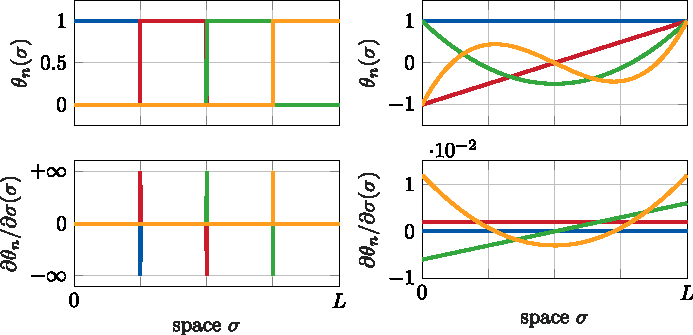
\includegraphics[width=.95\textwidth]{./pdf/thesis-figure-5-3.pdf}
    %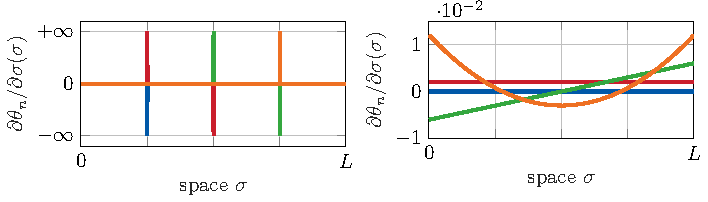
\includegraphics[width=\textwidth]{./pdf/thesis-figure-5-3-2.pdf}
    %% This file was created by matlab2tikz.
%
\definecolor{mycolor1}{rgb}{0.00000,0.34510,0.65882}%
\definecolor{mycolor2}{rgb}{0.79216,0.11765,0.17255}%
\definecolor{mycolor3}{rgb}{0.20392,0.65490,0.24706}%
\definecolor{mycolor4}{rgb}{0.93333,0.43922,0.13725}%
%
\begin{tikzpicture}

\begin{axis}[%
width=0.37\textwidth,
height=0.175\textwidth,
at={(0\textwidth,0\textwidth)},
scale only axis,
xmin=0,
xmax=1,
xtick={0,0.25,0.5,0.75,1},
xticklabels={{},{},{},{},{}},
ymin=-0.25,
ymax=1.25,
ylabel style={font=\color{white!15!black}},
ylabel={$\theta_n(\sigma)$},
axis background/.style={fill=white},
title style={font=\bfseries},
% title={$(a)$},
xmajorgrids,
ymajorgrids,
ylabel style={yshift=-2.5pt}
]
\addplot [color=mycolor1, line width=1.5pt, forget plot]
  table[row sep=crcr]{%
0	1\\
0.249249249249249	1\\
0.25025025025025	0\\
1	0\\
};
\addplot [color=mycolor2, line width=1.5pt, forget plot]
  table[row sep=crcr]{%
0	0\\
0.249249249249249	0\\
0.25025025025025	1\\
0.499499499499499	1\\
0.500500500500501	0\\
1	0\\
};
\addplot [color=mycolor3, line width=1.5pt, forget plot]
  table[row sep=crcr]{%
0	0\\
0.499499499499499	0\\
0.500500500500501	1\\
0.74974974974975	1\\
0.750750750750751	0\\
1	0\\
};
\addplot [color=mycolor4, line width=1.5pt, forget plot]
  table[row sep=crcr]{%
0	0\\
0.74974974974975	0\\
0.750750750750751	1\\
1	1\\
};
\end{axis}

\begin{axis}[%
width=0.37\textwidth,
height=0.175\textwidth,
at={(0.486\textwidth,0\textwidth)},
scale only axis,
xmin=0,
xmax=1,
xtick={0,0.25,0.5,0.75,1},
xticklabels={{},{},{},{},{}},
ymin=-1.5,
ymax=1.5,
ylabel style={font=\color{white!15!black}},
ylabel={$\theta_n(\sigma)$},
axis background/.style={fill=white},
title style={font=\bfseries},
%title={$(b)$},
xmajorgrids,
ymajorgrids,
ylabel style={yshift=-2.5pt}
]
\addplot [color=mycolor1, line width=1.5pt, forget plot]
  table[row sep=crcr]{%
0	1\\
1	1\\
};
\addplot [color=mycolor2, line width=1.5pt, forget plot]
  table[row sep=crcr]{%
0	-1\\
1	1\\
};
\addplot [color=mycolor3, line width=1.5pt, forget plot]
  table[row sep=crcr]{%
0	1\\
0.0310310310310311	0.819591363134907\\
0.0610610610610611	0.656004352701049\\
0.0900900900900901	0.508156805454103\\
0.118118118118118	0.375002630257885\\
0.145145145145145	0.255531808084361\\
0.171171171171171	0.148770392013635\\
0.196196196196196	0.0537805072339606\\
0.22022022022022	-0.0303396489582677\\
0.243243243243243	-0.10445580715851\\
0.265265265265265	-0.169397625854082\\
0.286286286286286	-0.225958691424157\\
0.307307307307307	-0.277217157097037\\
0.327327327327327	-0.321104888672456\\
0.346346346346346	-0.358343328313298\\
0.364364364364364	-0.389617846074302\\
0.381381381381381	-0.415577739902064\\
0.397397397397397	-0.436836235635034\\
0.413413413413414	-0.455016578139701\\
0.428428428428429	-0.469265060856652\\
0.442442442442442	-0.480122765408051\\
0.456456456456456	-0.488623758894029\\
0.469469469469469	-0.494407320233146\\
0.482482482482482	-0.498158819480141\\
0.495495495495496	-0.499878256635014\\
0.507507507507508	-0.499661823986148\\
0.519519519519519	-0.497713930146363\\
0.532532532532533	-0.493649805962118\\
0.545545545545546	-0.487553619685752\\
0.558558558558559	-0.479425371317263\\
0.572572572572573	-0.468399330261192\\
0.586586586586587	-0.455016578139701\\
0.601601601601602	-0.438062687311937\\
0.617617617617618	-0.416996576155735\\
0.633633633633634	-0.392852311771231\\
0.650650650650651	-0.363826288751214\\
0.668668668668669	-0.329305281257233\\
0.687687687687688	-0.288639991342694\\
0.707707707707708	-0.241145048952857\\
0.727727727727728	-0.188840492143795\\
0.748748748748749	-0.128744359975591\\
0.770770770770771	-0.0600991381772165\\
0.793793793793794	0.0178887596305013\\
0.817817817817818	0.106048991934878\\
0.842842842842843	0.205247289331373\\
0.868868868868869	0.316385454523592\\
0.894894894894895	0.435651868084301\\
0.921921921921922	0.56810864918973\\
0.94994994994995	0.714729744759775\\
0.978978978978979	0.876525173822471\\
1	1\\
};
\addplot [color=mycolor4, line width=1.5pt, forget plot]
  table[row sep=crcr]{%
0	-1\\
0.0190190190190189	-0.782485871940692\\
0.0380380380380381	-0.585849574761409\\
0.0560560560560561	-0.418072891875022\\
0.0740740740740742	-0.267591322461007\\
0.0910910910910911	-0.14071778835241\\
0.107107107107107	-0.0342981766697772\\
0.123123123123123	0.0600275897464979\\
0.138138138138138	0.137912741624562\\
0.153153153153153	0.206008053341874\\
0.167167167167167	0.26108942025359\\
0.18018018018018	0.305205863277448\\
0.193193193193193	0.342823368979655\\
0.205205205205205	0.372007618203764\\
0.216216216216216	0.394270823050955\\
0.227227227227227	0.412405233898399\\
0.237237237237237	0.425443028180901\\
0.246246246246246	0.434472266818126\\
0.255255255255255	0.441030078586554\\
0.264264264264264	0.445204206451941\\
0.272272272272272	0.446984357566612\\
0.28028028028028	0.447012056580584\\
0.288288288288288	0.445348928183114\\
0.297297297297297	0.441533571555485\\
0.306306306306306	0.435743998198344\\
0.316316316316316	0.427102419377978\\
0.327327327327327	0.41505036134801\\
0.339339339339339	0.399043011303921\\
0.352352352352352	0.378569076902044\\
0.367367367367367	0.351233983600084\\
0.383383383383384	0.318131447265587\\
0.401401401401401	0.276624908126279\\
0.422422422422422	0.223395060218871\\
0.447447447447447	0.154754895576799\\
0.481481481481481	0.0554285423969925\\
0.55955955955956	-0.174453117166602\\
0.585585585585586	-0.244218652545899\\
0.606606606606607	-0.295588205146412\\
0.625625625625626	-0.337224912399687\\
0.641641641641642	-0.368091627977139\\
0.656656656656657	-0.393078784510256\\
0.66966966966967	-0.411320689517806\\
0.681681681681682	-0.42510521776274\\
0.692692692692693	-0.434982658462395\\
0.702702702702703	-0.441533571555485\\
0.711711711711712	-0.445348928183114\\
0.720720720720721	-0.447102325115474\\
0.728728728728729	-0.446858939689107\\
0.736736736736737	-0.444855399075886\\
0.744744744744745	-0.441030078586554\\
0.753753753753754	-0.434472266818126\\
0.762762762762763	-0.425443028180901\\
0.771771771771772	-0.413854619709123\\
0.781781781781782	-0.3978703949716\\
0.792792792792793	-0.376369795653945\\
0.803803803803804	-0.350609329511154\\
0.815815815815816	-0.317460398130658\\
0.827827827827828	-0.278843238464521\\
0.840840840840841	-0.230596015489016\\
0.854854854854855	-0.170884130911225\\
0.868868868868869	-0.10280934270289\\
0.883883883883884	-0.020216582116821\\
0.898898898898899	0.0727618041999487\\
0.914914914914915	0.183843708779055\\
0.931931931931932	0.315873496183937\\
0.948948948948949	0.462912686785208\\
0.966966966966967	0.635618141204809\\
0.984984984984985	0.826515637191178\\
1	1\\
};
\end{axis}
\end{tikzpicture}%
    %% This file was created by matlab2tikz.
%
\definecolor{mycolor1}{rgb}{0.00000,0.34510,0.65882}%
\definecolor{mycolor2}{rgb}{0.79216,0.11765,0.17255}%
\definecolor{mycolor3}{rgb}{0.20392,0.65490,0.24706}%
\definecolor{mycolor4}{rgb}{0.93333,0.43922,0.13725}%
%
\begin{tikzpicture}

\begin{axis}[%
width=0.37\textwidth,
height=0.175\textwidth,
at={(0\textwidth,0\textwidth)},
scale only axis,
xmin=0,
xmax=1,
xtick={0,0.25,0.5,0.75,1},
xticklabels={{0},{},{},{},{$L$}},
ytick={-1,0,1},
yticklabels={{$-\infty$},0,{$+\infty$}},
xlabel style={font=\color{white!15!black}},
xlabel={space $\sigma$},
ymin=-1.2,
ymax=1.2,
ylabel style={font=\color{white!15!black}},
ylabel={$\p \theta_n/\p \sigma (\sigma)$},
axis background/.style={fill=white},
xmajorgrids,
ymajorgrids,
ylabel style={yshift=-2.5pt}
]
\addplot [color=mycolor1, line width=1.5pt, forget plot]
  table[row sep=crcr]{%
0.00100100100100109	0\\
0.249249249249249	0\\
0.25025025025025	-1\\
0.251251251251251	0\\
1	0\\
};
\addplot [color=mycolor2, line width=1.5pt, forget plot]
  table[row sep=crcr]{%
0.00100100100100109	0\\
0.249249249249249	0\\
0.25025025025025	1\\
0.251251251251251	0\\
0.499499499499499	0\\
0.500500500500501	-1\\
0.501501501501502	0\\
1	0\\
};
\addplot [color=mycolor3, line width=1.5pt, forget plot]
  table[row sep=crcr]{%
0.00100100100100109	0\\
0.499499499499499	0\\
0.500500500500501	1\\
0.501501501501502	0\\
0.74974974974975	0\\
0.750750750750751	-1\\
0.751751751751752	0\\
1	0\\
};
\addplot [color=mycolor4, line width=1.5pt, forget plot]
  table[row sep=crcr]{%
0.00100100100100109	0\\
0.74974974974975	0\\
0.750750750750751	1\\
0.751751751751752	0\\
1	0\\
};
\end{axis}

\begin{axis}[%
width=0.37\textwidth,
height=0.164\textwidth,
at={(0.486\textwidth,0.011\textwidth)},
scale only axis,
xmin=0,
xmax=1,
xtick={0,0.25,0.5,0.75,1},
xticklabels={{0},{},{},{},{$L$}},
xlabel style={font=\color{white!15!black}},
xlabel={space $\sigma$},
ymin=-0.01,
ymax=0.015,
ylabel style={font=\color{white!15!black}},
ylabel={$\p \theta_n/\p \sigma(\sigma)$},
axis background/.style={fill=white},
xmajorgrids,
ymajorgrids,
ylabel style={yshift=-2.5pt}
]
\addplot [color=mycolor1, line width=1.5pt, forget plot]
  table[row sep=crcr]{%
0.00100100100100109	0\\
1	0\\
};
\addplot [color=mycolor2, line width=1.5pt, forget plot]
  table[row sep=crcr]{%
0.00100100100100109	0.00200200200200196\\
1	0.00200200200200196\\
};
\addplot [color=mycolor3, line width=1.5pt, forget plot]
  table[row sep=crcr]{%
0.00100100100100109	-0.00599999398798179\\
1	0.00599999398798179\\
};
\addplot [color=mycolor4, line width=1.5pt, forget plot]
  table[row sep=crcr]{%
0.00100100100100109	0.0119819719820118\\
0.037037037037037	0.00989780573368138\\
0.0730730730730731	0.00796962698002934\\
0.109109109109109	0.00619743572105302\\
0.145145145145145	0.00458123195675597\\
0.181181181181181	0.00312101568713552\\
0.217217217217217	0.00181678691219256\\
0.253253253253253	0.000668545631927309\\
0.289289289289289	-0.000323708153660229\\
0.325325325325325	-0.00115997444457028\\
0.361361361361361	-0.00184025324080306\\
0.397397397397397	-0.0023645445423579\\
0.433433433433434	-0.00273284834923548\\
0.469469469469469	-0.00294516466143557\\
0.505505505505506	-0.00300149347895817\\
0.541541541541542	-0.00290183480180284\\
0.577577577577578	-0.00264618862997024\\
0.613613613613614	-0.00223455496346037\\
0.64964964964965	-0.00166693380227234\\
0.685685685685686	-0.000943325146407048\\
0.721721721721722	-6.37289958642651e-05\\
0.757757757757758	0.000971854649356008\\
0.793793793793794	0.00216342578925377\\
0.82982982982983	0.00351098442382924\\
0.865865865865866	0.00501453055308221\\
0.901901901901902	0.00667406417701244\\
0.937937937937938	0.00848958529562016\\
0.973973973973974	0.0104610939089056\\
1	0.0119819719820118\\
};
\end{axis}
\end{tikzpicture}%
    %\fi
    %\vspace{-3mm}
    \caption{Example plot of the Constant-Strain parametrization in Chapter 3 (left), and the new strain parametrization \eqref{eq:C3:chebyshev} using Chebyshev polynomials (right). The ordering of the strain basis is as follows $\{\theta_1,...,\theta_4\} = \{\ldata{Matlab1},\ldata{Matlab2},\ldata{Matlab3},\ldata{Matlab4}\}$. Notice that the
    spatialdiscontinuities in the PCC model induces spikes that directly violate the compatibility equation in \eqref{eq:C3:compatibility}.}
    \label{fig:C4:basis_example}
  \end{figure}
  %
\begin{equation}
\theta_n(\sigma) = \dfrac{2}{2^{n}(n-1)!} \dfrac{d^{n-1}}{d\sigma^{n-1}}\left[\left( \dfrac{2\sigma}{L}-1 \right)^2 -1 \right]^{n-1}
\label{eq:C3:chebyshev}
\end{equation}
%
\noindent with $n \in \mathbb{Z}_{>0}$ the polynomial degree A comparison between the proposed basis and previous method in Chapter \ref{chap:PCC} is shown in Figure \ref{fig:C4:basis_example}.
Important to note is that the previous PCC condition discussed introduces discontinuities in space that violate the compatibility equation in \eqref{eq:C3:compatibility}. 
Also note now that the inner product between elements of the set of modified Legendre functions $\{\theta_n\}_{n = 1}^k$ satisfies $\inner{\theta_i}{\theta_j}_{\Xs} := \int_\Xs{\theta_i}{\theta_j} d\sigma = 0$ for $i \neq j$, and $1$ otherwise. An alternative option could be constructing the set of basis functions through the so-called '\textit{snapshot decomposition method}' \cite{Astrid2008,Duriez2013,Largilliere2015}.

% \begin{rmk}
% The idea of joint parameterization by investigating the relation between material and structural topology of the soft robot is explored in Chapter 5.
% \end{rmk}

\subsection{Reduced-order kinematics}
Given the finite-dimensional truncation in \eqref{eq:trunc_2}, we can now find an expression for the finite-dimensional forward kinematics in terms of the generalized coordinates $\vec{q}$ and its velocities components $\dot{\vec{q}}$.

First, let us regard the configuration of the soft robot $\mat{g} \in \SE{3}$. Recall that the spatial evolution of the curve is described by $\p \mat{g}/\p\sigma = \mat{g} \vec{\xi}^\wedge$, see \eqref{eq:C3:xi}. Given the initial condition $\mat{g}(0,\cdot) = \mat{g}_0$, an approximation of the continuously deformable soft robot can be obtained by partial integration over the spatial domain:
%
\vspace{-2mm}
\begin{equation}
[\mat{g}]_k(\sigma,\vec{q}) = \mat{g}_0 \exp_{\SE{3}}\left[\int_0^\sigma [\hat{\vec{\xi}}]_k(s,\vec{q}) \; ds \right].
\end{equation}
%
The computation of the mapping $\exp_{\SE{3}}$ is given in Appendix \ref{app:C3:liegroup}. Note that the expression above nothing more than the reconstruction of the curve by integration of its tangent space along its spatial parameter $\sigma$. Next, lets regard the velocity kinematics $\vec{\eta}(\sigma,t)$ for any point $\sigma$ on the backbone curve. Using the differential property of the adjoint action $\mat{\ad}_{\vec{\xi}} = -\p /\p \sigma [\Ad_{g^{-1}}] \Ad_{g}$ \cite{Murray1994}, we can rewrite the
continuum forward kinematics in \eqref{eq:C3:pde_kin} as
%
\begin{equation}
\frac{\p \vec{\eta}}{\p \sigma } = \frac{\p }{\p \sigma }\left(\mat{\Ad}_{\mat{g}^{-1}}\right) \mat{\Ad}_{\mat{g}} \vec{\eta} + \dot{\vec{\xi}}. \label{eq:eta_adg}
\end{equation}
%
Now, given the initial condition $\vec{\eta}(0,t) = \vec{0}_6$ and the approximations $[\vec{\xi}]_k$ and $[\mat{g}]_k$, we can find an approximation to the velocity twist $\vec{\eta}$ by partial integration over space:
%
\begin{equation}
[\vec{\eta}]_k(\sigma,\vec{q},\dot{\vec{q}}) = \Ad_{[\mat{g}]_k(\sigma,\q)}\inv \int_0^\sigma \Ad_{[\mat{g}]_k(s,\q)} \mat{\Theta}(s) \dot{\vec{q}} \; ds \,. \label{eq:C3:eta_analytic}
\end{equation}
%
Note from \eqref{eq:C3:eta_analytic} that the joint velocity exhibits a linear relationship with the velocity twist. This attribute is typical of rigid robotics, \eg, see \cite{Murray1994,Spong2006}. As such, it is possible to extract $\dot{\q}$ out of the integrand which naturally gives rise to a linear matrix transformation called the \textit{"geometric manipulator Jacobian"}. The geometric Jacobian matrix $[\mat{J}]_k \in \R^{6\times 6k}$ is defined by 
%
\begin{equation}
[\mat{J}]_k:= \Ad_{[\mat{g}]_k(\sigma,\q)}\inv \int_0^\sigma \Ad_{[\mat{g}]_k(s,\q)} \mat{\Theta}(s) \; ds, \label{eq:C3:jacobian_analytic}
\end{equation}
%
such that $[\etaB]_k = [\JB]_k \dot{\q}$. The geometric Jacobian plays an important role in obtaining the Lagrangian form of the reduced-order dynamic model. Finally, to express the acceleration twist, we take the time-derivative of \eqref{eq:C3:eta_analytic} leading to
%
\begin{align}
[\dot{\vec{\eta}}]_k & = [\mat{J}]_k\ddot{\vec{q}} + \dot{[\mat{J}]}_k\dot{\vec{q}}, \notag \\
& = [\mat{J}]_k\ddot{\vec{q}} + \Ad_{[\mat{g}]_k}\inv \int_0^\sigma \Ad_{[\mat{g}]_k(s,\q)} \ad_{[\vec{\eta}]_k(s,\q,\dq)} \mat{\Theta}(s) \; ds \,\dot{\q} \label{eq:C3:deta_analytic},
\end{align}
%
which gives rise to the analytic expression of the time-derivative of the geometric Jacobian $\dot{[\mat{J}]}_k$.
Although the expression for the $\dot{\JB}$ is compact, its derivation is fairly involved. We therefore refer the reader to Appendix \ref{app:C3:jacobian} on its derivation. 
\subsection{Reduced-order dynamics using Newton-Euler}
Here, we detail the dynamics of the Cosserat beam. A majority of the dynamic framework presented here is adopted from Boyer et al. \cite{Boyer2021}; yet we introduce some modification to allow a pH-structure. Other works that adopt a similar approach include \cite{Renda2018,Renda2020,Till2019,Garofalo2013}. First, let us consider an infinitesimal slice of continuum body that is perpendicular to the backbone curve. The kinetic momenta of this infinitesimal slice is then given by $\vec{\mu}(\sigma,t) := \MT \vec{\eta}(\sigma,t)$ in which $\MT \in \cose{3} \times \seg{3} \cong \R^{6\times 6}$ denotes the symmetric inertia tensor.
%
\begin{rmk}
  For some soft robots, the inertia tensor $\MT$ may have an explicit dependency on space or time (or both). A common phenomena in soft robotics that innately lead to such dependencies include for instance the \textit{ballooning effect} of soft pneumatic networks. During actuation, matter expands outwards radially, changing the cross-sectional geometry and thus its inertial properties. That said, the inertial changes due to ballooning is negligibly small. Besides, ballooning is often an undesired phenomena that is reduced by appropriate structural design such as internal ribs, or bellow-like geometries. Nevertheless, examples where inertial changes cannot be neglected include the class of growing or morphing soft robots \cite{Hawkes2017,Joachimczak2014Jul,Joachimczak2015}, self-healing soft robots \cite{Terryn2021Jul,Roels2020Dec}, origami soft robot manipulators \cite{Li2022Nov,Jiang2016Dec,Wu2021Sep}. Pressure-driven soft robots actuated by near incompressible fluids like water also suffer from these inertial changing effects. But, these robots are scarce and purposefully design for aquatic environments which is outside the scope of this work. For many soft robots, air or gas is preferred over liquids. 
For sake of simplicity, we limit ourselves to a diagonal invariant inertia tensor: 
%
\begin{equation*}
\MT(\sigma,t) \simeq \begin{pmatrix} \rho_0 \ten{J}  & \vec{0}_{3\times3}  \\[0.35em]
  \vec{0}_{3\times3} & \rho_0\, A_0\mat{I}_3 \end{pmatrix} \succ 0,
\end{equation*}
%
in which the (cross-sectional average) density is $\rho_0 > 0$, the cross-sectional area of the soft robot $A_0>0$, and the second moment of area $\mat{\mathcal{J}} \in \coso{3} \times \sog{3} \cong \R^{3\times 3}$.
We emphasize here that considering an invariant cross-sectional inertia tensor is not an overly conservative assumption. It still holds true for a large class of soft manipulators, and it has limited effects on the generality of our modeling framework. \end{rmk}
%
\noindent Using the expression of the kinetic momenta $\muB(\sigma,t)$ of the infinitesimal rigid body in free-motion, we can write the equation of motion for a particular slice at $\sigma$ using the Newton-Euler equations:
%
\begin{equation}
\frac{\p }{\p t} (\Ad_{\gB}^{-\top} \vec{\mu}) = \Ad_{g}^{-\top}\ten{F},\label{eq:C3:newton_euler}
\end{equation}
%
where again $\Ad_{(\cdot)}$ stands for the adjoint action, and $\ten{F} = \ten{F}_c  + \ten{F}_u - \ten{F}_\textrm{b} - \ten{F}_{\textrm{mat}}$ the resultant wrench that is composed of the constraint wrench $\ten{F}_c$, the input wrench $\ten{F}_u$, and the potential wrenches due to body accelerations and hyper- and visco-elasticity, $\ten{F}_\textrm{b}$ and $ \ten{F}_{\textrm{mat}}$, respectively. Further evaluation of \eqref{eq:C3:newton_euler} leads to
%
\begin{equation}
\MT\dot{\vec{\eta}} - \ad_{\vec{\eta}}^\top \MT \vec{\eta} = \ten{F},
\label{eq:C3:newton-euler-2}
\end{equation}
%
where we used the fact that $\tfrac{\p}{\p t}{\Ad}_{\vec{g}} \inv = -\ad_{\vec{\eta}} {\Ad}_{\vec{g} \inv}$. Before continuing, we introduce a slight modification to the relation above. Using the fact that $\ad_{\vec{\eta}} \vec{\eta} = \vec{0}_6$, we can introduce the vector
$\ten{M} \ad_{\vec{\eta}} \vec{\eta}$ to \eqref{eq:C3:newton-euler-2} without affecting the dynamics. The importance of this modification originates from the preservation of passivity in the Lagrangian model, which is an important property in stability theorems for robotics. By substitution of the null vector, the equation of motion becomes
%
\begin{equation}
  \MT \dot{\vec{\eta}} + \left(\MT \ad_{\vec{\eta}}  - \ad_{\vec{\eta}} ^\top \MT \right) \vec{\eta} = \FT,
  \label{eq:C3:newton-euler-3}
\end{equation}
%
which is nothing more than the Newton-Euler equation for rigid-body motion on $\R^3$. To introduce the (reduced-order) Cosserat kinematics and make the expression symmetric, we substitute \eqref{eq:C3:eta_analytic} and \eqref{eq:C3:deta_analytic} into \eqref{eq:C3:newton-euler-3} and pre-multiply by $[\JB]_k^\top$:
%
\begin{align}
  [\vec{J}]_k^\top \left( \MT [\mat{J}]_k \ddot{\vec{q}} + \MT [\dJB]_k\dot{\vec{q}} + \CT_{[\vec{\eta}]_k }\dot{\vec{q}}\right) = [\mat{J}]_k^\top \left(\FT_u - \FT\grav -  \ten{F}_{\textrm{mat}} \right),
  \label{eq:C3:projected_NE_jacobian}
\end{align}
%
where $\CT_{(\cdot)} = -\CT_{(\cdot)} ^\top :=  \MT \ad_{(\cdot)}  - \ad_{(\cdot)} ^\top \MT$ is a skew-symmetric matrix. It is important to note that by pre-multiplication of the transpose Jacobian, we have eliminated the constraint wrenches, \ie, $[\JB]_k^\top \FT_c = \vec{0}_n$ \cite{Murray1994}. Finally, the finite-dimensional dynamics of the deformable soft robot is found by spatial integration of \eqref{eq:C3:projected_NE_jacobian} over the material domain $\Xs$. The overall dynamics can be written in the familiar Euler-Lagrangian (EL) form as follows
%
\begin{equation}
  \mat{M}(\vec{q})\ddot{\vec{q}} + \mat{C}(\vec{q},\dot{\vec{q}})\dot{\vec{q}} + \vec{f}\!\grav(\vec{q}) + \vec{f}_{\textrm{mat}}(\vec{q},\dot{\vec{q}}) = \vec{\tau}(\vec{q},\uB)
  \label{eq:C3:dyn_model_lag}
\end{equation}
%
with the system matrices:
%
\begin{align}
 \MB(\q) & = \int_\Xs [\mat{J}]_k^\top \ten{M} [\mat{J}]_k \; d \sigma, \label{eq:C3:lag_M} \\
 \mat{C}(\q,\dq) & = \int_\Xs [\JB]_k^\top \!\left(\ten{M} [\dJB]_k + \ten{C}_{{[\vec{\eta}]}_k}[\mat{J}]_k \right) \; d \sigma, \label{eq:C3:lag_C} \\
\vec{f}\!\grav(\q) & = \int_\Xs [\JB]_k^\top \ten{F}_\textrm{b} \; d \sigma, \\
\vec{f}_{\textrm{mat}}(\q,\dq) & = \int_\Xs [\JB]_k^\top  \ten{F}_{\textrm{mat}} \; d \sigma =: \mat{K}\vec{q} + \mat{D}\dot{\vec{q}},
\label{eq:C3:lag_G} \\
\vec{\tau}(\q,\uB) & = \int_\Xs [\mat{J}]_k^\top \ten{F}_u \; d\sigma =: \mat{G}(\q) \vec{u}, \label{eq:C3:lag_tau}
\end{align}
%
\noindent where $\mat{M}$ is the generalized inertia matrix, $\mat{C}$ the  Centripetal-Coriolis matrix, $\fB\!\grav$ a vector of generalized potential forces with $\ten{F}_\textrm{b} = -\Ad_{[\gB]_k}^\top \ten{M} \vec{a}_b$ the external wrench acting on the body due to body-frame accelerations $\vec{a}_b$ (like gravity), and $\ten{F}_\textrm{mat}$ a vector of visco-elastic material forces imposed by the stiffness matrix $\mat{K} \succ 0$ and damping matrix $\vec{D} \succ 0$. The derivation for these constant matrices is shown in Appendix \ref{app:C3:linearmaterialmatrices}, where it is shown that stiffness and damping matrix are computed through spatial integration similar to standard finite element methods:
%
\begin{align}
\mat{K} = \int_\Xs \mat{\Theta}^\top \!\mat{\mathcal{K}}\, \mat{\Theta} \; d\sigma, \label{eq:C3:stiff_mat}\\
\mat{D} = \int_\Xs \mat{\Theta}^\top \!\mat{\mathcal{D}}\, \mat{\Theta} \; d\sigma, \label{eq:C3:damp_mat}
\end{align}
%
where $\mat{\mathcal{K}} \in \cose{3} \times \seg{3}$ and $\mat{\mathcal{D}} \in  \cose{3} \times \seg{3}$ are the stiffness and damping tensor, respectively.
The vector $\vec{Gu}$ represents the distributed forces $\nB_\textrm{u}(\sigma,t)$ and moments $\mB_\textrm{u}(\sigma,t)$ generated by various kinds of the internal actuators (\eg, tendons or pneumatics). We will later detail the derivation of $\GB(\q)$ in this chapter as it depends highly on the geometrical placement of the soft actuators. If $\rank(\GB) < \dim(\q)$, the system \eqref{eq:C3:dyn_model_lag} is said to be underactuated. Within the context of soft robotics, whose infinite-dimensional configuration space cannot be matched by a finite number of actuators, these systems are often intrinsically under-actuated. 

To compute the Lagrangian matrices \eqref{eq:C3:lag_M}-\eqref{eq:C3:damp_mat}, that all involve a spatial integration over $\Xs = [0,L]$, we rewrite these integrations into one global matrix differential equation and solve it efficiently using a Matrix-Differential solver proposed in Chapter \ref{chap:PCC}. As such, these system matrices are not computed exactly but approximated with sufficient precision. The numerical precision depends on the stepsize of the discretized spatial domain $\Xs$. 
\begin{asm}
\label{lem:C3:1}
The inertia matrix $\mat{M}(\vec{q})$ is a symmetric, positive definite, symmetric. and is uniformly bounded such that there exists positive constants $\lambda^{-} \le \lambda^{+}$ such that  $\lambda^{-} \mat{I}_{n} \preceq \mat{M}(\vec{q}) \preceq \lambda^{+} \mat{I}_{n} < \infty$.
\end{asm}

The uniform boundedness of the inertia matrix $\MB(\q)$ is a well-known property for rigid manipulators composed of purely rotational joints. According to Spong et al. \cite{Spong2006} the inertia matrix in this case is composed solely of $\cos(\cdot)$ and $\sin(\cdot)$ terms, and thus it is bounded for all $\q \in \mathcal{Q}$. The physical interpretation is that the mass and moment of inertia of the robot must be finite and positive for all configurations. This does not always hold true for instance for robots with prismatic joints. Yet, bounds can be imposed on the configuration space $\q \in \mathcal{Q}$ that enable boundedness, see Ghorbel et al. \cite{Ghorbel1998Dec}. In Della Santina et al. \cite{DellaSantina2020a}, it was shown that $\MB(\q) = \MB^\top(\q) \succeq 0$ for soft manipulators restricted to variable planar curvatures. The property holds for the infinite dimensional case where $k \to \infty$. 

\begin{lem}
\label{lem:C3:passive}
Given the inertia matrix $\mat{M}(\vec{q})$ and the Coriolis matrix
$\mat{C}(\vec{q},\dot{\vec{q}})$ as described by \eqref{eq:C3:lag_M} and \eqref{eq:C3:lag_C}, respectively, it can be shown that the matrix $\dot{\mat{M}} - 2\mat{C}$ is skew-symmetric.
\end{lem}

\begin{proof}
To show $\dot{\mat{M}} - 2\mat{C}$ is skew-symmetric, we start by computing the time-derivative of the inertia matrix. For sake of clarity, we abbreviate the Jacobian matrices $[\mat{J}]_k = \mat{J}$ and $[\dJB]_k = \dJB$. Through chain differentiation, we find
%
\begin{equation}
\dot{\mat{M}} = \int_\Xs \left(\dJB^\top \ten{M} \mat{J} + \mat{J}^\top \ten{M} \dJB 
\right)\; d \sigma,
\end{equation}
%
Then, calculating $\dot{\mat{M}} - 2\mat{C}$ leads to
%
\begin{align}
\dot{\mat{M}} - 2\mat{C} & = \int_\Xs \dJB^\top \left( \ten{M} \mat{J} - \mat{J}^\top \ten{M} \dJB - 2\mat{J}^\top \!\ten{C} \, \mat{J} \right) \; d\sigma.
\end{align}
%
Since the matrix $\mat{J}^\top \ten{C} \mat{J}$ is skew-symmetric, the remainder of the proof is to show that the matrix $\mat{S} = \dJB^\top \ten{M} \mat{J} - \mat{J}^\top \ten{M} \dJB$ also satisfies skew-symmetry. Since the inertia tensor is symmetric $\ten{M} = \ten{M}^\top
$, we can easily show this holds true:
%
\begin{align}
\mat{S} & = \dJB^\top \MT^\top \mat{J} - \mat{J}^\top \MT^\top \dJB, \notag \\
 & = -\left(\dJB^\top \ten{M}^\top \mat{J} - \mat{J}^\top \ten{M} \dJB \right)^\top = -\mat{S}^\top.
\end{align}
%
Therefore, the matrix $\dot{\mat{M}(\vec{q})} - 2\mat{C}(\vec{q},\dot{\vec{q}})$ is skew-symmetric for all $\vec{q},\dot{\vec{q}} \in \R^n$
\end{proof}

In literature, Lemma \ref{lem:C3:passive} is often referred to as the passivity condition \cite{Spong2006,Ortega1998,Murray1994}. It implies that, in the absence of external dissipation, the total energy of the system (\ie, the Hamiltonian) is conserved.
It is also worth mentioning that this condition does not necessarily hold true for any representation of the Coriolis matrix only for particular computations of the Coriolis matrix $\mat{C}(\vec{q},\vec{\dot{q}})$ (\eg, through the Christoffel symbols).

\subsection{Tendon and fluidic actuation}
Up to now, we have not discussed the derivation of the actuation mapping $\GB(\q)$. The matrix namely depends on $(i)$ the type of actuation, and $(ii)$ how actuation fields are distributed along the backbone curve of the soft robot manipulator. Earlier, we introduced the notion of a distributed forces $\nB_\textrm{u}$ and distributed moments $\mB_\textrm{u}$ acting on the curve $\gB$, which are collocated into a control wrench $\FT_{\textrm{u}}$. Now, assuming that a general soft manipulator system is either actuated using a set of fluidic chambers or a set of tendons, the control wrench related this network of $m$ number of soft actuators can be represented in the form \cite{Renda2020,Boyer2021}:
%
\begin{equation}
\FT_{\textrm{u}}(\sigma,\uB) = \sum_{i = 1}^m \begin{pmatrix}
\rB_i^\times(\sigma) \tB_i(\sigma) \\[0.25em] \tB_i (\sigma)
\end{pmatrix} u_i =: \ThetaB_{\textrm{u}}(\sigma) \uB,
\label{eq:C3:controlwrenchfield}
\end{equation}
%
where $\rB_i: \Xs \to \R^3$ is the radial distance between the actuator center-line and the backbone curve $\gammaB$, and $\tB_i: \Xs \times \mathcal{Q} \to \R^3$ the tangent vector along the actuator center-line expressed that deforms with the continuum body prescribed by $[\gB]_k(\sigma,\q)$, $\ThetaB_\textrm{u} \in \R^{6 \times m}$ a shape function matrix related to the spatial distribution of the soft actuators, and $u_i(t)$ a time-varying scalar related to the activation amplitude of the $i$-th soft actuator. Generally speaking, for tendon actuation $u_i = -\max\{0,\lambda_i\}$ with $\lambda_i$ the cable tension and for pneumatic actuation we have $u_i = A_i p_i$ with $A_i > 0$ an effective pressure surface and $p_i$ the applied pressure. Following \eqref{eq:C3:controlwrenchfield}, the generalized joint torques can then be computed by projecting the distributed control wrench onto the configuration space using the geometric Jacobian matrix. Then, $\GB(\q)$ is computed by integrating generalized distributed joint forces over $\Xs$:
%
\begin{equation}
\tauB(\q,\uB) = \int_{\Xs} \JB^\top(\q,\sigma) \ThetaB_{\textrm{u}}(\sigma)\; d\sigma \,\uB =: \GB(\q) \uB.
\end{equation}
%
Similar to the other Lagrangian matrices, the actuation mapping is included into the matrix differential solver to allow fast and efficient computation of \eqref{eq:C3:dyn_model_lag}.

\subsection{Port-Hamiltonian formulation}
In this section, the Lagrangian model in \eqref{eq:C3:dyn_model_lag} is rewritten in port-Hamiltonian form. To this end, we define the generalized momenta $\vec{p} := \mat{M} \dot{\vec{q}}$. Then, the (reduced-order) Hamiltonian is given by $\mathcal{H}(\vec{q},\vec{p}) := \Kf(\vec{q},\vec{p}) + \Uf(\vec{q})$ with $\Kf = \frac{1}{2} \vec{p}^\top \mat{M}\inv \vec{p}$ and $\Uf(\vec{q})$ the kinetic and potential energy, respectively.

Given the system's Hamiltonian $\mathcal{H}$, it can be shown that generalized velocities can be written in terms of partial derivatives of the Hamiltonian function
%
\begin{equation}
\dot{\vec{q}} = \nabla_{\vec{p}} \Hm \quad \Longrightarrow  \quad \nabla_{\vec{p}} \Hm := \left(\frac{\p \Hm}{\p \pB} \right)^\top= \mat{M}\inv \vec{p}.
\label{eq:C3:state_diff}
\end{equation}
%
where we denote $\nabla_{\xB}(\cdot) := \p (\cdot)^\top/\p \xB$ as the gradient w.r.t. a vector field $\xB$. Note that $\mat{M}^{-1}$ is always exists due to the positive definiteness condition in Lemma \ref{lem:C3:1}. Similarly, we seek a differential description that relates the time evolution of $\vec{p}$ to a state-derivative of the Hamiltonian function. Applying the chain rule of differentiation to the generalized momenta:
%
\begin{align}
\dot{\vec{p}} & = \dot{\mat{M}}\dot{\vec{q}} + \mat{M}\ddot{\vec{q}},\notag \\
& = \left(\dot{\mat{M}} - \mat{C} - \mat{D} \right) \mat{M}\inv \vec{p} - \vec{Kq} - \vec{f}\!\grav + \vec{Gu}
\label{eq:C3:momenta_diff1},
\end{align}
%
Taking the partial derivative of the Hamiltonian $\Hm$ w.r.t. the generalized coordinates $\vec{q}$, we find
 %
\begin{align}
\nabla_{\vec{q}} \Hm & = \frac{1}{2} \,\nabla_{\!\q} \left[ \dot{\vec{q}}^\top \mat{M}(\vec{q}) \dot{\vec{q}} \right] + \nabla_{\!\vec{q}}\, \mathcal{U}.
\label{eq:C3:ham_momenta_diff}
\end{align}
%
To relate \eqref{eq:C3:momenta_diff1} and \eqref{eq:C3:ham_momenta_diff}, we explores some structural properties in the Lagrangian model. To be more specific, we exploit the skew-symmetry condition as detailed in Lemma \ref{lem:C3:passive}. According to the Spong et al. (2006, \cite{Spong2006}), if the matrix $\dot{\mat{M}} - 2\mat{C}$ satisfies the
skew-symmetry in Lemma \ref{lem:C3:passive}, it can be shown that
%
\begin{equation}
\left( \dot{\mat{M}} - 2\mat{C} \right) \dot{\vec{q}} =  -\nabla_{\vec{q}} \left[ \dot{\vec{q}}^\top \mat{M}(\vec{q}) \dot{\vec{q}} \right] - \dot{\mat{M}}\dot{\vec{q}}. \label{eq:C3:skew_mat_equal}
\end{equation}
%
Finally, by combining \eqref{eq:C3:state_diff}, \eqref{eq:C3:momenta_diff1}, \eqref{eq:C3:ham_momenta_diff}, and \eqref{eq:C3:skew_mat_equal}, we can show that the Lagrangian model in \eqref{eq:C3:dyn_model_lag} can be equivalently rewritten as a standard port-Hamiltonian (pH) system:
\begin{align}
\Sigma_{\textrm{beam}}: 
\begin{cases}
\dot{\vec{q}} \;=\; \nabla_{\vec{p}} \Hm, \\[0.25em]
\dot{\vec{p}} \;=\; -\nabla_{\vec{q}} \Hm - \mat{D}\nabla_{\vec{p}} \Hm + \vec{Gu}.
\end{cases}
\label{eq:C3:model_ph}
\end{align}
%
The advantage of the port-Hamiltonian system $\Sigma_\textrm{beam}$ over the standard EL structure in \eqref{eq:C3:dyn_model_lag}, and as also seen in Chapter \ref{chap:PCC}, is the general applicability to different physical domains and the common formalism with energy-based control, which we will explore further in the next section. 

%By collocating the state variable into a state vector $\x = (\q^\top, \pB^\top)^\top$, we may write the system into an equivalent form: $\dx = \left(\JT - \RT \right)\grad{\x}\!\Hm(\x) + \BT(\x)\uB$, where $\JT = -\JT^\top$ a skew-symmetric matrix, $\RT \succeq 0$ a positive semi-definite dissipation matrix. 

%!TEX root = ../../thesis.tex
\section{Energy-based controller for tasks on SE(3)} \label{sec:chap3_control}
Given the reduced port-Hamiltonian model in \eqref{eq:C3:model_ph}, our objective here is to find a controller $\vec{u}$ that ensures $\lim_{t\to\infty} \mat{g}(L,t) = \mat{g}_d$ in which $\mat{g}_d \in \SE{3}$ denotes the desired configuration of the end-effector. To achieve the control objective, the main idea is to reshape the potential energy function of the reduced-order finite-dimensional system using a standard energy-shaping techniques, common to standard port-controlled Hamiltonian models \cite{Schaft2004,Ortega2002}.

%\subsection{Setpoint regulation on $\SE{3}$}
We adopted an energy-based control strategy akin to the works of Franco et al. \cite{Franco2020}, Ortega et al. \cite{Ortega1998,Ortega2002} and Schaft \cite{Schaft2004}. Following the energy-shaping strategy, the model-based nonlinear controller becomes
%
\begin{equation}
\vec{u} = \vec{G}\ginv \left( \nabla_{\vec{q}}\Hm - \nabla_{\vec{q}}\Hm_d \right),
\label{eq:C3:control}
\end{equation}
%
where $\mat{G}\ginv = \bigl(\mat{G}^\top \mat{G}\bigr)\inv \mat{G}^\top$ is the generalized inverse of the actuation map $\mat{G}$, and the desired Hamiltonian in closed loop
$\Hm_d = \frac{1}{2} \vec{p}^\top \mat{M}\inv \vec{p} + \Uf_d$ that satisfies $\textrm{argmin}_{\mat{g}_L} \Uf_d = \mat{g}_d$ with $\mat{g}_L = \mat{g}(L,\cdot)$ the pose of the end-effector. Note that we purposefully omitted any damping injection as the system's intrinsic visco-elastic damping is deemed sufficiently large to guarantee stability. Following the concept of a kinematic feedback controller \cite{Bullo1995,Boyer2021} that artificially mimic an elastic element between the end-effector and the desired configuration in $\SE{3}$, we have choose the gradient of the desired potential energy as
%
\begin{equation}
\grad{\q}\,\Uf_{d}= \lambda_1 \mat{J}^\top\bigl(\mat{J J}^\top + \lambda_2 \mat{I} \bigr)\inv \ten{F}_u,
\label{eq:C3:jacob_damped}
\end{equation}
%
where $\lambda_1 >0$ is a proportional gain, $\lambda_2 > 0$ a controller gain related to the artificial damping of the pseudo-inverse, $\ten{F}_u = \kB_p T_{\textrm{SE}(3)}(\mat{\mathcal{E}})\mat{\mathcal{E}}$ an artificial control wrench with positive definite stiffness matrix $\kB_p$, $\hat{\mat{\mathcal{E}}} = \log_{\SE{3}} ([\mat{g}_L]_k \inv \mat{g}_d)$ the geometric error where $\log_{\SE{3}}(\cdot) $ and $T_{\SE{3}}(\cdot)$ denote the logarithmic map (see Appendix \ref{app:C3:liegroup}) and the tangent-space map, respectively. We refer the reader to Sonneville et al. \cite{Sonneville2014} for the numerical computations of the tangent map on $\SE{3}$. The vector $\vec{\mathcal{E}}$ may be regarded as the geometric error between the homogeneous transformations $\mat{g}_d$ and $\mat{g}_L$ such that if $\mat{g}_d = \mat{g}_L$ will simply yield $\lVert \vec{\mathcal{E}} \rVert_2 = 0$. Furthermore, the controller gains $\lambda_1$ and $\lambda_2$ can be tuned accordingly to tweak the desired transient behavior of the closed-loop system, similar to a classical PD controller.
%!TEX root = ../../thesis.tex
\section{Simulation studies of bio-inspired soft robots} \label{sec:chap3_result}
In this section, we detail the numerical simulations of the port-Hamiltonian model in \eqref{eq:C3:model_ph} together with the energy-shaping controller in \eqref{eq:C3:control}. 

Due to the partial differential nature, we have to employ a nested ODE routine to recover the trajectories for $\vec{q}$ and $\vec{p}$. First, we employ an implicit trapezoidal solver with a fixed stepsize of $dt = 30 $ ms to solve \eqref{eq:C3:model_ph}. At each time increment, we have to evaluate the dynamic matrices \eqref{eq:C3:lag_M} to \eqref{eq:C3:lag_tau}. To efficiently compute these dynamic entities, we solve the spatial integration problem over the material domain $\Xs$ by using a second-order Runge-Kutta solver.  The stepsize for the spatial solver is chosen sufficiently small $\Delta \sigma = 1$ mm. The spatial stepsize is related to the length of the manipulator $L$, but also the degree of geometric deformations along the backbone. In some cases, high-gain feedback control can excite high-order modes thus requiring a smaller stepsize to capture these phenomena accurately. However, by keeping the control gains small paired with the fact that structural damping is dominant in soft elastomers often lead to slow transients (order of seconds). As such, the spatial discretization has been shown to relatively nonrestrictive. %Generally speaking, choosing $\Delta \sigma = 1\cdot10{-2} L$ is a good rule of thumb. 
All simulation examples and underlying source code are provided publicly on the \texttt{sorotoki} toolkit \cite{Caasenbrood2020}. Here, the numerical integrations of the system matrices \eqref{eq:C3:lag_M}, \eqref{eq:C3:lag_C}, \eqref{eq:C3:lag_G} and \eqref{eq:C3:lag_tau} are performed using a so-called Matrix-Differential solver (see \cite{Caasenbrood2022}). The simulations are performed on a modern machine (Ryzen 7-5800H, 3.2GHz).

For the soft robotic simulations, we have chosen a linear isotropic Hookean material with shear constraints. %Although hyper-elastic material models are possible, e.g, Neo-Hookean or Yeoh, it is considered out of the scope of this work (see \cite{Kim2018,Renaud2011}). 
Given these material properties, the inertia tensor and the stiffness tensor become diagonal matrices:
%
\begin{align*}
\mat{\mathcal{M}} & = \blkdiag{ \rho_0 \mat{\mathcal{J}},\, \rho_0 A \mat{I}_3}, \\[0.25em] 
\mat{\mathcal{K}} & = \blkdiag{\mu_1 \mat{\mathcal{J}},\, E A_0,\, \mu_2  A_0,\,\mu_2  A_0},
\end{align*}
%
 where $A_0$ is the (average) cross-sectional area, and $\mat{\mathcal{J}}$ the second moment of area. Note that $A_0$ and $\mat{\mathcal{J}}$ depend on the cross-sectional geometry of the soft robot and is therefor unique for each system.  The damping tensor chosen as $\mat{\mathcal{D}} = \zeta \mat{\mathcal{K}}$ with damping coefficient $\zeta$. %The visco-elastic matrices are precomputed using \eqref{eq:C3:stiff_mat} and \eqref{eq:C3:damp_mat}.

\subsection{Soft robot manipulator inspired by octopus' tentacle}
In the first study-case, we consider a soft robotic arm that is loosely inspired by the tentacles of an octopus. To introduce the under-actuation typically present in soft robotics, we have chosen an actuation matrix $\mat{G} = \blkdiag{\mat{I}_5, \mat{O}_3}$ such that only the first five modes are actively controllable.  We assume that the soft manipulator has a circular cross-section, thus the cross-sectional area is given by $A_0 = \pi r^2$ with radius $r$. The system properties are shown in Table \ref{tab:C3:parameters1}.
%
\renewcommand\arraystretch{1.15}
\begin{table}[t]
  \vspace{-0.25cm}
  \caption{Parameters setting for the solver, the soft robot, and controller.}\label{tab:C3:parameters1} \centering
  \rowcolors{0}{}{blue!5}
  \begin{tabular}{l|ccl}
    \hline
    Parameter description & Symbol & Value & Unit \\
    \hline 
    \hline
    Intrinsic length & $L $ & $ 120$ & mm \\
    Cross-sectional radius & $r $ & $ 8.25$ & $\text{mm}$ \\
    Uniform density & $\rho_0 $ & $ 1250$ & $\text{kg}\text{m}^{-3}$ \\
    %Gravitational acceleration & $a_{g} $ & $ 9.81$ & $\text{m}\text{s}^{-2}$ \\
    Young's modulus & $E $ & $ 0.25$ & $\text{MPa}$ \\
    Shear modulus & $\mu_1 $ & $ 0.10 $ & $\text{MPa}$ \\
    Constraint modulus & $\mu_2 $ & $ 1.50 $ & $\text{GPa}$ \\
    Rayleigh coefficient & $\zeta $ & $ 0.40 $ & - \\
    \hline
  \end{tabular}
  %\vspace{-3mm}
  \end{table}
%
\begin{example}[Solution convergence for increasing modal order]
  \label{ex:C3:convergence}
 Before investigating the performance of the controller, we study the affects of the truncation order $k$. Initially, it can be difficult find the optimal value for $k$ that balances precision and computational speed. Consider the case where we subject the soft robot by a external tip wrench $\tau_\textrm{ext}(t) = [J]_k^\top \left(0,0,\mB(t),0,0,0 \right)^\top$ given by a predefined moment $\mB(t) = 75 \cdot \textrm{erf}(t)$ in \si{\newton \milli \meter}. The applied moment causes a spiraling deformation of the soft arm, as can be seen in Figure \ref{fig:C3:EX2:mode_convergence_3d}. Observe that the soft arm undergoes a rather complex nonlinear three-dimensional deformation. Now, we incrementally increase the model truncation parameter $k \in \{1,...,10\}$ and investigate the convergence of the solutions $\gammaB_L$ (\ie, the end-effector location). The numerical results are shown in Figure \ref{fig:C3:EX2:mode_convergence}. 
 
%  \afterpage{
 \begin{figure}[!t]
  \centering
  \includegraphics*[width=1.02\textwidth]{./pdf/thesis-figure-5-4.pdf}
  \caption{\small Three-dimensional deformation of the soft tentacle due to an external pure-moment wrench of $\lVert \vec{m}_u \rVert = 75$ \si{\newton \milli \meter} acting on its end-effector. }
  %\vspace{-0.2cm}
  \label{fig:C3:EX2:mode_convergence_3d}
  \end{figure}
  %
  \begin{figure}[!t]
  \centering
  %% This file was created by matlab2tikz.
%
%The latest updates can be retrieved from
%  http://www.mathworks.com/matlabcentral/fileexchange/22022-matlab2tikz-matlab2tikz
%where you can also make suggestions and rate matlab2tikz.
%
\definecolor{mycolor1}{rgb}{0.06275,0.35686,0.84706}%
\definecolor{mycolor2}{rgb}{0.86667,0.21176,0.10980}%
\definecolor{mycolor3}{rgb}{0.18039,0.52157,0.25098}%
\definecolor{mycolor4}{rgb}{1.00000,0.61569,0.11765}%
\definecolor{mycolor5}{rgb}{0.29804,0.17255,0.57255}%
\definecolor{mycolor6}{rgb}{1.00000,0.39216,0.11765}%
\definecolor{mycolor7}{rgb}{0.00784,0.74902,0.90588}%
\definecolor{mycolor8}{rgb}{1.00000,0.16078,0.45882}%
\definecolor{mycolor9}{rgb}{0.19608,0.22745,0.27059}%
\definecolor{mycolor10}{rgb}{0.68235,0.69020,0.70980}%
%
\begin{tikzpicture}

\begin{axis}[%
width=0.245\textwidth,
height=0.238\textwidth,
at={(0\textwidth,0\textwidth)},
scale only axis,
xmin=0,
xmax=2.5,
xlabel style={font=\color{white!15!black}},
xlabel={time (s)},
ymin=-50,
ymax=130,
ylabel style={font=\color{white!15!black}},
ylabel={tip position (mm)},
axis background/.style={fill=white},
xmajorgrids,
ymajorgrids
]
\addplot [color=mycolor1, line width=1.8pt, forget plot]
  table[row sep=crcr]{%
0	119.978342345083\\
0.0166666666666657	119.698529042722\\
0.0333333333333314	118.714199790945\\
0.0499999999999972	116.605166520778\\
0.0666666666666629	113.113473066372\\
0.0833333333333286	108.199229377047\\
0.0999999999999943	102.040281602863\\
0.183333333333337	66.8364877102122\\
0.200000000000003	61.6139222017607\\
0.216666666666669	57.4778515637841\\
0.233333333333334	54.4354696040819\\
0.25	52.4310772154381\\
0.266666666666666	51.3706105084636\\
0.283333333333331	51.1409297303602\\
0.299999999999997	51.6233008875427\\
0.316666666666663	52.7019668919586\\
0.333333333333329	54.2691358037187\\
0.349999999999994	56.2275752081978\\
0.38333333333334	60.9875786483211\\
0.433333333333337	69.2906797920311\\
0.533333333333331	86.4445749774124\\
0.583333333333329	94.3295808930696\\
0.63333333333334	101.430635715539\\
0.666666666666671	105.639270319945\\
0.700000000000003	109.365126877619\\
0.733333333333334	112.554821053324\\
0.766666666666666	115.157361496108\\
0.783333333333331	116.22388721353\\
0.799999999999997	117.127099216095\\
0.816666666666663	117.86265861119\\
0.833333333333329	118.426971071272\\
0.849999999999994	118.817291848969\\
0.86666666666666	119.03183163273\\
0.88333333333334	119.069863632757\\
0.900000000000006	118.931832255149\\
0.916666666666671	118.619463576693\\
0.933333333333337	118.135877590981\\
0.950000000000003	117.485701874265\\
0.966666666666669	116.675185931178\\
0.983333333333334	115.712315039948\\
1.01666666666667	113.370068129856\\
1.05	110.54245146088\\
1.08333333333333	107.291236426218\\
1.11666666666666	103.645649087005\\
1.15000000000001	99.6054355254478\\
1.18333333333334	95.1464618873528\\
1.21666666666667	90.2257605372769\\
1.25	84.7853849520983\\
1.28333333333333	78.7555701215122\\
1.31666666666666	72.0582378928264\\
1.34999999999999	64.6123227335696\\
1.38333333333334	56.3429766728233\\
1.41666666666667	47.1975401820638\\
1.46666666666667	31.8513695030522\\
1.58333333333333	-7.35007024380496\\
1.61666666666666	-16.5590242479557\\
1.63333333333334	-20.1994209993964\\
1.65000000000001	-23.0273349801414\\
1.66666666666667	-24.9525621670817\\
1.68333333333334	-25.9336310097799\\
1.7	-25.9889848129195\\
1.71666666666667	-25.199591985603\\
1.73333333333333	-23.7006883039825\\
1.75	-21.6635753656529\\
1.83333333333333	-9.15652043794734\\
1.86666666666666	-4.94812006744171\\
1.90000000000001	-1.55536471747331\\
1.93333333333334	1.10463509880523\\
1.96666666666667	3.16566095029214\\
2	4.75783393107152\\
2.03333333333333	5.99005576173879\\
2.06666666666666	6.94785519354133\\
2.09999999999999	7.69648000529952\\
2.13333333333334	8.28509985612973\\
2.16666666666667	8.75065098922828\\
2.2	9.12093488757769\\
2.23333333333333	9.41698021090158\\
2.26666666666667	9.65479601554775\\
2.3	9.84665784213728\\
2.33333333333333	10.0020482645293\\
2.36666666666666	10.1283438272206\\
2.40000000000001	10.2313223693709\\
2.43333333333334	10.3155377679366\\
2.46666666666667	10.3845993055278\\
2.5	10.4413820323868\\
};
\addplot [color=mycolor2, line width=1.8pt, forget plot]
  table[row sep=crcr]{%
0	119.984662071422\\
0.0166666666666657	119.757143264747\\
0.0333333333333314	118.863640923281\\
0.0499999999999972	116.777465959496\\
0.0666666666666629	113.029931486591\\
0.0833333333333286	107.359317580321\\
0.0999999999999943	99.743704730005\\
0.13333333333334	80.036358977103\\
0.183333333333337	48.6437718891565\\
0.200000000000003	40.1862649766057\\
0.216666666666669	33.3932098608599\\
0.233333333333334	28.3967658822693\\
0.25	25.1987928544716\\
0.266666666666666	23.6964926451333\\
0.283333333333331	23.7271159811078\\
0.299999999999997	25.0854687675144\\
0.316666666666663	27.5465477741243\\
0.333333333333329	30.8737050094071\\
0.36666666666666	39.1950621862955\\
0.433333333333337	56.9832180063902\\
0.466666666666669	64.3309849442619\\
0.483333333333334	67.3957468253012\\
0.5	70.0359284794246\\
0.516666666666666	72.2582319565215\\
0.533333333333331	74.0803059628584\\
0.549999999999997	75.5270103526064\\
0.566666666666663	76.6273554792696\\
0.583333333333329	77.4122450942784\\
0.599999999999994	77.9128181244767\\
0.61666666666666	78.1593501660123\\
0.63333333333334	78.1805412983542\\
0.650000000000006	78.0031236708663\\
0.666666666666671	77.6516767780413\\
0.683333333333337	77.148601373439\\
0.700000000000003	76.5141902502121\\
0.733333333333334	74.9228575410129\\
0.766666666666666	73.0038778107918\\
0.816666666666663	69.7330675217148\\
0.966666666666669	59.4643685181436\\
1	57.4730326467202\\
1.03333333333333	55.6879841387088\\
1.06666666666666	54.1194723572617\\
1.09999999999999	52.7578769892714\\
1.13333333333334	51.5826495042453\\
1.16666666666667	50.5686418063321\\
1.2	49.6903421407391\\
1.23333333333333	48.9243267264109\\
1.26666666666667	48.2504100093506\\
1.3	47.6519429282394\\
1.33333333333333	47.1156116454162\\
1.36666666666666	46.6309886935924\\
1.41666666666667	45.9838654150455\\
1.46666666666667	45.4153990732454\\
1.51666666666667	44.9117893120308\\
1.56666666666666	44.4630870294336\\
1.61666666666666	44.0617156347244\\
1.66666666666667	43.7015924034521\\
1.71666666666667	43.3776344486694\\
1.76666666666667	43.0854882857496\\
1.81666666666666	42.8213786279115\\
1.86666666666666	42.5820160944331\\
1.91666666666667	42.3645322604482\\
1.96666666666667	42.1664273202352\\
2.01666666666667	41.9855243129848\\
2.06666666666666	41.8199279185436\\
2.11666666666666	41.667987341011\\
2.16666666666667	41.5282632425768\\
2.21666666666667	41.3994986446091\\
2.26666666666667	41.2805936081607\\
2.33333333333333	41.1357402668848\\
2.40000000000001	41.0047409985017\\
2.5	40.8306363100082\\
};
\addplot [color=mycolor3, line width=1.8pt, forget plot]
  table[row sep=crcr]{%
0	119.986878257307\\
0.0166666666666657	119.785989316249\\
0.0333333333333314	118.965855284071\\
0.0499999999999972	117.022045217133\\
0.0666666666666629	113.493231227374\\
0.0833333333333286	108.117478326217\\
0.0999999999999943	100.863887905045\\
0.13333333333334	81.944842305062\\
0.183333333333337	51.2630563079365\\
0.200000000000003	42.8048863311144\\
0.216666666666669	35.8980550596809\\
0.233333333333334	30.702620770341\\
0.25	27.2544190305725\\
0.266666666666666	25.4819919766971\\
0.283333333333331	25.2505262896826\\
0.299999999999997	26.3736987899878\\
0.316666666666663	28.6397337951108\\
0.333333333333329	31.817403064942\\
0.36666666666666	39.9734438309792\\
0.433333333333337	57.7588364392224\\
0.466666666666669	65.1264947750487\\
0.483333333333334	68.185008510505\\
0.5	70.806716594118\\
0.516666666666666	72.9983271248391\\
0.533333333333331	74.7813291726284\\
0.549999999999997	76.1839952580226\\
0.566666666666663	77.2412744218592\\
0.583333333333329	77.9892667726118\\
0.599999999999994	78.465484439096\\
0.61666666666666	78.7055679835773\\
0.63333333333334	78.7435672986294\\
0.650000000000006	78.6103203680272\\
0.666666666666671	78.3335469550414\\
0.683333333333337	77.9373930876413\\
0.700000000000003	77.4423006600669\\
0.733333333333334	76.2201551546017\\
0.766666666666666	74.7650877531808\\
0.799999999999997	73.1337078500768\\
0.849999999999994	70.418741135971\\
0.900000000000006	67.4422787388484\\
1.05	58.2175116395222\\
1.09999999999999	55.5017662063983\\
1.15000000000001	53.063307992559\\
1.2	50.9242364357903\\
1.23333333333333	49.6665091426183\\
1.26666666666667	48.5396993965276\\
1.3	47.5377723872813\\
1.33333333333333	46.6530391501359\\
1.36666666666666	45.876825959544\\
1.40000000000001	45.1999983278323\\
1.43333333333334	44.6133511419364\\
1.46666666666667	44.1078871698502\\
1.5	43.6750071046847\\
1.53333333333333	43.3066315725865\\
1.56666666666666	42.9952718750434\\
1.59999999999999	42.7340627826135\\
1.63333333333334	42.5167677935438\\
1.66666666666667	42.3377649378029\\
1.7	42.1920193438749\\
1.73333333333333	42.0750473322834\\
1.76666666666667	41.9828758145797\\
1.8	41.9119992016048\\
1.83333333333333	41.8593362090537\\
1.86666666666666	41.8221877516047\\
1.88333333333334	41.8086857955243\\
1.90000000000001	41.7981968214172\\
1.93333333333334	41.7853109331141\\
1.96666666666667	41.7817474510736\\
2	41.785961926716\\
2.03333333333333	41.7966194404723\\
2.06666666666666	41.8125688520527\\
2.09999999999999	41.8328198034474\\
2.15000000000001	41.8694373254549\\
2.21666666666667	41.9263623066756\\
2.3	42.0047753511272\\
2.5	42.1975540111338\\
};
\addplot [color=mycolor4, line width=1.8pt, forget plot]
  table[row sep=crcr]{%
0	119.986901464107\\
0.0166666666666657	119.786154558754\\
0.0333333333333314	118.966700968486\\
0.0499999999999972	117.024022517845\\
0.0666666666666629	113.497384466021\\
0.0833333333333286	108.122736481045\\
0.0999999999999943	100.870154470975\\
0.13333333333334	81.9482084304668\\
0.183333333333337	51.2627474544511\\
0.200000000000003	42.8037656266578\\
0.216666666666669	35.8971927208898\\
0.233333333333334	30.6997471269087\\
0.25	27.2465855334041\\
0.266666666666666	25.4651546907094\\
0.283333333333331	25.2182883032622\\
0.299999999999997	26.3207340396663\\
0.316666666666663	28.5580340819897\\
0.333333333333329	31.7012854839674\\
0.36666666666666	39.7671153379952\\
0.433333333333337	57.3032442478971\\
0.466666666666669	64.5245118497627\\
0.483333333333334	67.5093122802881\\
0.5	70.0598493450595\\
0.516666666666666	72.1849333667421\\
0.533333333333331	73.9085793180189\\
0.549999999999997	75.2610667383728\\
0.566666666666663	76.2794291623783\\
0.583333333333329	77.000908793524\\
0.599999999999994	77.4640309582704\\
0.61666666666666	77.7041385911864\\
0.63333333333334	77.7548102969862\\
0.650000000000006	77.6449419705141\\
0.666666666666671	77.4002864677046\\
0.683333333333337	77.041643690045\\
0.700000000000003	76.5864143527889\\
0.733333333333334	75.4353033124313\\
0.766666666666666	74.0155749823463\\
0.799999999999997	72.3597512770726\\
0.833333333333329	70.4841238683128\\
0.88333333333334	67.3018441168463\\
1.01666666666667	57.8798765030929\\
1.06666666666666	54.6594275298181\\
1.11666666666666	51.8099360058205\\
1.15000000000001	50.1398400743001\\
1.18333333333334	48.6578348768158\\
1.21666666666667	47.3595769795682\\
1.25	46.2354286391565\\
1.28333333333333	45.2723082212013\\
1.31666666666666	44.4552591381087\\
1.34999999999999	43.7686540647096\\
1.38333333333334	43.1970530765645\\
1.41666666666667	42.7257718917556\\
1.45	42.3412239536261\\
1.48333333333333	42.0310951817039\\
1.51666666666667	41.7844007766956\\
1.55	41.5914631318792\\
1.58333333333333	41.4438403649581\\
1.59999999999999	41.3846934500121\\
1.61666666666666	41.3342269242202\\
1.63333333333334	41.2916691177231\\
1.65000000000001	41.2563412849274\\
1.66666666666667	41.2275801111065\\
1.68333333333334	41.2048108166187\\
1.7	41.1874659482891\\
1.71666666666667	41.1750602446593\\
1.73333333333333	41.1671103561054\\
1.75	41.1632075028184\\
1.76666666666667	41.1629416465207\\
1.78333333333333	41.1659689471967\\
1.8	41.171942948467\\
1.83333333333333	41.1915725266249\\
1.86666666666666	41.2196942291622\\
1.90000000000001	41.2545167836277\\
1.95	41.3161059079562\\
2	41.3854042765765\\
2.34999999999999	41.9054193726596\\
2.43333333333334	42.0149474949867\\
2.5	42.096213056271\\
};
\addplot [color=mycolor5, line width=1.8pt, forget plot]
  table[row sep=crcr]{%
0	119.9868665463\\
0.0166666666666657	119.785825336773\\
0.0333333333333314	118.965765361077\\
0.0499999999999972	117.021011166946\\
0.0666666666666629	113.491285189373\\
0.0833333333333286	108.109652591283\\
0.0999999999999943	100.848116230522\\
0.13333333333334	81.8958570811538\\
0.183333333333337	51.1557586618086\\
0.200000000000003	42.6815385718612\\
0.216666666666669	35.767458782563\\
0.233333333333334	30.5670101597913\\
0.25	27.1205654735361\\
0.266666666666666	25.3532785711732\\
0.283333333333331	25.131033477489\\
0.299999999999997	26.2674300586017\\
0.316666666666663	28.5491444456815\\
0.333333333333329	31.7467152314301\\
0.36666666666666	39.9501928384451\\
0.433333333333337	57.8635210613448\\
0.466666666666669	65.3109879054592\\
0.483333333333334	68.41259356532\\
0.5	71.0793888843777\\
0.516666666666666	73.316580158943\\
0.533333333333331	75.1453100629709\\
0.549999999999997	76.5920170352684\\
0.566666666666663	77.6908038981895\\
0.583333333333329	78.4757162044332\\
0.599999999999994	78.9831446425266\\
0.61666666666666	79.2466693102745\\
0.63333333333334	79.2991674033792\\
0.650000000000006	79.1695974778973\\
0.666666666666671	78.8846159600108\\
0.683333333333337	78.4667687190062\\
0.700000000000003	77.9356395159218\\
0.733333333333334	76.5939619568251\\
0.766666666666666	74.9516292479882\\
0.799999999999997	73.0629521534305\\
0.833333333333329	70.9608102911969\\
0.88333333333334	67.4714260170427\\
1.01666666666667	57.4526412400941\\
1.06666666666666	54.0787022924745\\
1.11666666666666	51.1082911520393\\
1.15000000000001	49.3696794696603\\
1.18333333333334	47.8251098890443\\
1.21666666666667	46.4680869288569\\
1.25	45.2876625434847\\
1.28333333333333	44.2700735503096\\
1.31666666666666	43.4000920848256\\
1.34999999999999	42.6620555436167\\
1.38333333333334	42.0406042030177\\
1.41666666666667	41.5211742809943\\
1.45	41.0902972416922\\
1.48333333333333	40.7357527843499\\
1.51666666666667	40.4466166834196\\
1.55	40.2132371518288\\
1.58333333333333	40.0271658850617\\
1.61666666666666	39.8810631901365\\
1.65000000000001	39.7685909781206\\
1.68333333333334	39.6843029675194\\
1.7	39.6512525440126\\
1.71666666666667	39.6235381050511\\
1.73333333333333	39.6007184922276\\
1.75	39.5823207849811\\
1.76666666666667	39.5679724965644\\
1.78333333333333	39.5572697497172\\
1.8	39.5498992241234\\
1.81666666666666	39.5455163697774\\
1.83333333333333	39.5438585962855\\
1.86666666666666	39.5476184739427\\
1.90000000000001	39.5592952542664\\
1.93333333333334	39.5773027542274\\
1.96666666666667	39.6003081178411\\
2.01666666666667	39.6417889998865\\
2.08333333333333	39.7056250095683\\
2.33333333333333	39.9648566850385\\
2.41666666666667	40.044859923113\\
2.5	40.11869765062\\
};
\addplot [color=mycolor6, line width=1.8pt, forget plot]
  table[row sep=crcr]{%
0	119.98686715261\\
0.0166666666666657	119.785838626229\\
0.0333333333333314	118.965782731387\\
0.0499999999999972	117.020407262904\\
0.0666666666666629	113.489524102348\\
0.0833333333333286	108.104355190415\\
0.0999999999999943	100.838009232587\\
0.13333333333334	81.866061137432\\
0.183333333333337	51.0689804614232\\
0.200000000000003	42.5658040447423\\
0.216666666666669	35.6199248439852\\
0.233333333333334	30.3809890520429\\
0.25	26.892815477342\\
0.266666666666666	25.0774049519423\\
0.283333333333331	24.8030494873178\\
0.299999999999997	25.8813720924876\\
0.316666666666663	28.1004654363057\\
0.333333333333329	31.2298790185907\\
0.36666666666666	39.2811135100423\\
0.433333333333337	56.8099620158335\\
0.466666666666669	64.0218223801319\\
0.483333333333334	66.9984410287842\\
0.5	69.5399816936732\\
0.516666666666666	71.6544705552134\\
0.533333333333331	73.3683144441804\\
0.549999999999997	74.7115942437863\\
0.566666666666663	75.7234001455557\\
0.583333333333329	76.4409697003656\\
0.599999999999994	76.9039980876799\\
0.61666666666666	77.1476488635111\\
0.63333333333334	77.2055641141389\\
0.650000000000006	77.1061058403011\\
0.666666666666671	76.8741286085719\\
0.683333333333337	76.5296151685041\\
0.700000000000003	76.0885260085445\\
0.716666666666669	75.5630209436294\\
0.75	74.2909482661114\\
0.783333333333331	72.7551173423038\\
0.816666666666663	70.9750284823276\\
0.849999999999994	68.967038419705\\
0.900000000000006	65.5922144899757\\
1.06666666666666	53.7205151708478\\
1.11666666666666	50.7034850202699\\
1.15000000000001	48.9098496013259\\
1.18333333333334	47.2986318345624\\
1.21666666666667	45.8686739095853\\
1.25	44.6130860190678\\
1.28333333333333	43.521010980422\\
1.31666666666666	42.5791982206543\\
1.34999999999999	41.7732543368418\\
1.38333333333334	41.0885651262091\\
1.41666666666667	40.5109331182166\\
1.45	40.0269873281895\\
1.48333333333333	39.6244199012843\\
1.51666666666667	39.2920968587043\\
1.55	39.0200812470667\\
1.58333333333333	38.7995983996705\\
1.61666666666666	38.6229655140764\\
1.65000000000001	38.4835015790969\\
1.68333333333334	38.375428821623\\
1.71666666666667	38.29377314178\\
1.73333333333333	38.2614856365078\\
1.75	38.2342682722448\\
1.76666666666667	38.211652229912\\
1.78333333333333	38.1932664401353\\
1.8	38.1787043730659\\
1.81666666666666	38.1676568745271\\
1.83333333333333	38.1597718328627\\
1.84999999999999	38.1547930188174\\
1.86666666666666	38.1524153566607\\
1.90000000000001	38.1545658267163\\
1.93333333333334	38.1644713354826\\
1.96666666666667	38.1806511717971\\
2	38.2018561073184\\
2.05	38.2408393415565\\
2.09999999999999	38.2859161260494\\
2.18333333333334	38.3689112525867\\
2.43333333333334	38.6251640436328\\
2.5	38.6882283094836\\
};
\addplot [color=mycolor7, line width=1.8pt, forget plot]
  table[row sep=crcr]{%
0	119.986873650108\\
0.0166666666666657	119.78589403815\\
0.0333333333333314	118.965892078955\\
0.0499999999999972	117.02002471211\\
0.0666666666666629	113.487947196049\\
0.0833333333333286	108.099335229269\\
0.0999999999999943	100.827938488888\\
0.13333333333334	81.8381821261552\\
0.183333333333337	51.0132972190414\\
0.200000000000003	42.5064275591283\\
0.216666666666669	35.5637384404779\\
0.233333333333334	30.3341613066755\\
0.25	26.8645250407832\\
0.266666666666666	25.0763449970857\\
0.283333333333331	24.8401793623067\\
0.299999999999997	25.9673175337815\\
0.316666666666663	28.2472964971794\\
0.333333333333329	31.4489401263593\\
0.36666666666666	39.6793280791542\\
0.433333333333337	57.6821749016547\\
0.466666666666669	65.1659693236166\\
0.483333333333334	68.2786346513262\\
0.5	70.951617450906\\
0.516666666666666	73.1884541984088\\
0.533333333333331	75.01150578081\\
0.549999999999997	76.4459736079025\\
0.566666666666663	77.5274689828802\\
0.583333333333329	78.2893352418304\\
0.599999999999994	78.7695248734581\\
0.61666666666666	79.001543235671\\
0.63333333333334	79.0197849232479\\
0.650000000000006	78.8537694600038\\
0.666666666666671	78.5315488549579\\
0.683333333333337	78.0767255653412\\
0.700000000000003	77.5100235313932\\
0.733333333333334	76.105942781485\\
0.766666666666666	74.418393448122\\
0.799999999999997	72.505193406996\\
0.849999999999994	69.2802391216077\\
0.900000000000006	65.708459046408\\
1.03333333333333	55.8186792140353\\
1.08333333333333	52.5511654079475\\
1.13333333333334	49.6732690389712\\
1.16666666666667	47.9859048964816\\
1.2	46.4837851299446\\
1.23333333333333	45.1604367194661\\
1.26666666666667	44.0052836486235\\
1.3	43.0051849860008\\
1.33333333333333	42.1457005956069\\
1.36666666666666	41.4120490764848\\
1.40000000000001	40.7897845445159\\
1.43333333333334	40.2652406695438\\
1.46666666666667	39.8257938125982\\
1.5	39.4599925171698\\
1.53333333333333	39.1575929054246\\
1.56666666666666	38.9095312311075\\
1.59999999999999	38.7078572091642\\
1.63333333333334	38.5456453008361\\
1.66666666666667	38.4168959884633\\
1.7	38.316435128425\\
1.73333333333333	38.2398165444606\\
1.76666666666667	38.1832309205695\\
1.78333333333333	38.1614087185328\\
1.8	38.143422588839\\
1.81666666666666	38.1289222755781\\
1.83333333333333	38.1176148242367\\
1.84999999999999	38.1092062408766\\
1.88333333333334	38.10008062352\\
1.91666666666667	38.0996941647601\\
1.95	38.1064764994795\\
1.98333333333333	38.1190975789918\\
2.01666666666667	38.136432518764\\
2.06666666666666	38.169233225058\\
2.11666666666666	38.2079442400616\\
2.18333333333334	38.2653407468261\\
2.5	38.5520594198092\\
};
\addplot [color=mycolor8, line width=1.8pt, forget plot]
  table[row sep=crcr]{%
0	119.986879742436\\
0.0166666666666657	119.785945761276\\
0.0333333333333314	118.965978024401\\
0.0499999999999972	117.019630156527\\
0.0666666666666629	113.486297058033\\
0.0833333333333286	108.094307027332\\
0.0999999999999943	100.817583995202\\
0.13333333333334	81.8072163581748\\
0.183333333333337	50.9250405054155\\
0.200000000000003	42.3907389239623\\
0.216666666666669	35.4173549485502\\
0.233333333333334	30.151601505104\\
0.25	26.6413936669391\\
0.266666666666666	24.8063753405775\\
0.283333333333331	24.5175414031144\\
0.299999999999997	25.5850716362956\\
0.316666666666663	27.7989127402468\\
0.333333333333329	30.9277424478826\\
0.36666666666666	38.9951056909184\\
0.433333333333337	56.6220023401918\\
0.466666666666669	63.9067106687992\\
0.483333333333334	66.9217002737228\\
0.5	69.5017055993302\\
0.516666666666666	71.6525473170071\\
0.533333333333331	73.4004120214856\\
0.549999999999997	74.773414008028\\
0.566666666666663	75.8108145538055\\
0.583333333333329	76.5484968707986\\
0.599999999999994	77.0266514091039\\
0.61666666666666	77.2798319322405\\
0.63333333333334	77.3423625078387\\
0.650000000000006	77.242667559208\\
0.666666666666671	77.0063122450541\\
0.683333333333337	76.6538258940765\\
0.700000000000003	76.2017737422335\\
0.716666666666669	75.6631333441884\\
0.75	74.3604405208208\\
0.783333333333331	72.7921557600577\\
0.816666666666663	70.9815718487915\\
0.849999999999994	68.9478462591612\\
0.900000000000006	65.5468616267591\\
1.06666666666666	53.6784470691565\\
1.11666666666666	50.6780907606276\\
1.15000000000001	48.8963307508769\\
1.18333333333334	47.2960281914542\\
1.21666666666667	45.8751541712052\\
1.25	44.6263250552653\\
1.28333333333333	43.5384867061245\\
1.31666666666666	42.5984024459216\\
1.34999999999999	41.7918302956523\\
1.38333333333334	41.1043889657468\\
1.41666666666667	40.5221551970292\\
1.45	40.0320458594999\\
1.48333333333333	39.6220362248784\\
1.51666666666667	39.2812590519885\\
1.55	39.0000208928859\\
1.58333333333333	38.7697639409952\\
1.61666666666666	38.5829945883905\\
1.65000000000001	38.4331939401965\\
1.68333333333334	38.3147208657479\\
1.71666666666667	38.2227146199124\\
1.75	38.1530014601327\\
1.78333333333333	38.1020078251929\\
1.81666666666666	38.0666813575054\\
1.83333333333333	38.0540800921382\\
1.84999999999999	38.0444201953177\\
1.88333333333334	38.033010094849\\
1.91666666666667	38.0305704572683\\
1.95	38.0355058415782\\
1.98333333333333	38.0464648431548\\
2.01666666666667	38.0623041862108\\
2.06666666666666	38.0931478030344\\
2.11666666666666	38.1301810613672\\
2.18333333333334	38.1857500975544\\
2.5	38.4683709172652\\
};
\addplot [color=mycolor9, line width=1.8pt, forget plot]
  table[row sep=crcr]{%
0	119.986885656411\\
0.0166666666666657	119.785998166131\\
0.0333333333333314	118.966060826717\\
0.0499999999999972	117.0192654526\\
0.0666666666666629	113.48468272493\\
0.0833333333333286	108.089511649469\\
0.0999999999999943	100.807853938965\\
0.13333333333334	81.7812083329026\\
0.183333333333337	50.877185574891\\
0.200000000000003	42.3428035998093\\
0.216666666666669	35.3762896531732\\
0.233333333333334	30.1247450963537\\
0.25	26.6378293583574\\
0.266666666666666	24.8356585570169\\
0.283333333333331	24.590316816461\\
0.299999999999997	25.7122581653405\\
0.316666666666663	27.9916405314856\\
0.333333333333329	31.1964809099713\\
0.36666666666666	39.4427284405321\\
0.433333333333337	57.4800943199281\\
0.466666666666669	64.9612629644271\\
0.483333333333334	68.0643455054456\\
0.5	70.7225379493199\\
0.516666666666666	72.9387947141472\\
0.533333333333331	74.7369332569979\\
0.549999999999997	76.1421086166374\\
0.566666666666663	77.1917966375922\\
0.583333333333329	77.9197315370435\\
0.599999999999994	78.3657882426642\\
0.61666666666666	78.5641431149413\\
0.63333333333334	78.5508880661161\\
0.650000000000006	78.3562906651343\\
0.666666666666671	78.0096582022982\\
0.683333333333337	77.5351996408901\\
0.700000000000003	76.9543091116906\\
0.733333333333334	75.5390919197019\\
0.766666666666666	73.8626507910754\\
0.799999999999997	71.9788552580754\\
0.849999999999994	68.8185801944576\\
0.900000000000006	65.3165061156937\\
1.05	54.4221743329868\\
1.09999999999999	51.2875543070523\\
1.13333333333334	49.4133051226535\\
1.16666666666667	47.7218687238074\\
1.2	46.2137320710328\\
1.23333333333333	44.88329485889\\
1.26666666666667	43.7205659953181\\
1.3	42.7127789011544\\
1.33333333333333	41.8457245981964\\
1.36666666666666	41.1047593818216\\
1.40000000000001	40.4755150063108\\
1.43333333333334	39.9443641082778\\
1.46666666666667	39.4986969020214\\
1.5	39.1270594362957\\
1.53333333333333	38.8191948596866\\
1.56666666666666	38.5660200404831\\
1.59999999999999	38.3595617764976\\
1.63333333333334	38.1928701288918\\
1.66666666666667	38.0599211342006\\
1.7	37.9555171321034\\
1.73333333333333	37.8751899809701\\
1.76666666666667	37.8151103058438\\
1.8	37.772004442665\\
1.81666666666666	37.7559067813145\\
1.84999999999999	37.7331596255804\\
1.88333333333334	37.7211635130501\\
1.91666666666667	37.7180552390231\\
1.95	37.7222551973321\\
1.98333333333333	37.7324249608208\\
2.01666666666667	37.7474324418629\\
2.06666666666666	37.7769727088726\\
2.11666666666666	37.8126467690857\\
2.18333333333334	37.8663679934451\\
2.5	38.1403957527175\\
};
\addplot [color=mycolor10, line width=1.8pt, forget plot]
  table[row sep=crcr]{%
0	119.986891002485\\
0.0166666666666657	119.786045957649\\
0.0333333333333314	118.966125503946\\
0.0499999999999972	117.018896054706\\
0.0666666666666629	113.483050533691\\
0.0833333333333286	108.084717706494\\
0.0999999999999943	100.797817159966\\
0.13333333333334	81.7514415732634\\
0.183333333333337	50.7954314532069\\
0.200000000000003	42.2381019701369\\
0.216666666666669	35.2468023265271\\
0.233333333333334	29.9673870910136\\
0.25	26.4499228504475\\
0.266666666666666	24.6132097893098\\
0.283333333333331	24.3290810576668\\
0.299999999999997	25.4070590072419\\
0.316666666666663	27.6372981577801\\
0.333333333333329	30.7878316722869\\
0.36666666666666	38.9140261001104\\
0.433333333333337	56.711750041228\\
0.466666666666669	64.1011683224156\\
0.483333333333334	67.1699603481641\\
0.5	69.8029905771846\\
0.516666666666666	72.0038910876684\\
0.533333333333331	73.7975148210061\\
0.549999999999997	75.2096467405857\\
0.566666666666663	76.2785443096054\\
0.583333333333329	77.0382630311513\\
0.599999999999994	77.5287120157422\\
0.61666666666666	77.7835873823886\\
0.63333333333334	77.8378265294187\\
0.650000000000006	77.720098722507\\
0.666666666666671	77.457351611785\\
0.683333333333337	77.0712428753347\\
0.700000000000003	76.5801223836151\\
0.733333333333334	75.3372534786179\\
0.766666666666666	73.8069695849491\\
0.799999999999997	72.0308886486453\\
0.833333333333329	70.0330650900573\\
0.88333333333334	66.6756090954717\\
1.01666666666667	56.8434139221188\\
1.06666666666666	53.464329851016\\
1.11666666666666	50.4407048628247\\
1.15000000000001	48.6462283679751\\
1.18333333333334	47.0346044192499\\
1.21666666666667	45.6033453906819\\
1.25	44.3447851793639\\
1.28333333333333	43.2477112470424\\
1.31666666666666	42.2988076376328\\
1.34999999999999	41.4837993028918\\
1.38333333333334	40.7882963419345\\
1.41666666666667	40.1983779847406\\
1.45	39.7009669426364\\
1.48333333333333	39.2840434320055\\
1.51666666666667	38.9367421235916\\
1.55	38.6493675751725\\
1.58333333333333	38.4133559555607\\
1.61666666666666	38.2212039103498\\
1.65000000000001	38.0663796156637\\
1.68333333333334	37.9432264687646\\
1.71666666666667	37.8468663648857\\
1.75	37.7731069339549\\
1.78333333333333	37.7183552737344\\
1.81666666666666	37.6795394470937\\
1.84999999999999	37.6540381660327\\
1.88333333333334	37.6396185468925\\
1.91666666666667	37.6343814992952\\
1.95	37.636714137575\\
1.98333333333333	37.6452481099716\\
2.01666666666667	37.6588251726341\\
2.05	37.676465488572\\
2.09999999999999	37.7087772966046\\
2.16666666666667	37.7593826221459\\
2.25	37.8293752810519\\
2.5	38.0436758500337\\
};
\node[right, align=left]
at (axis cs:2,110) {$\gamma_x$};
\end{axis}

\begin{axis}[%
width=0.245\textwidth,
height=0.238\textwidth,
at={(0.315\textwidth,0\textwidth)},
scale only axis,
xmin=0,
xmax=2.5,
xlabel style={font=\color{white!15!black}},
xlabel={time (s)},
ymin=-10,
ymax=80,
axis background/.style={fill=white},
xmajorgrids,
ymajorgrids
]
\addplot [color=mycolor1, line width=1.8pt, forget plot]
  table[row sep=crcr]{%
0	7.19935044912745e-09\\
0.0500000000000007	0.00300168498534603\\
0.0666666666666664	0.00770291312845117\\
0.0833333333333321	0.0161955883871983\\
0.100000000000001	0.0297590420833522\\
0.116666666666667	0.0496086546583463\\
0.133333333333333	0.0768326079950512\\
0.149999999999999	0.1123697790905\\
0.166666666666668	0.157026644180021\\
0.183333333333334	0.211519929418095\\
0.199999999999999	0.276525995595097\\
0.216666666666665	0.352718898586783\\
0.233333333333334	0.440785833608057\\
0.266666666666666	0.655282363865336\\
0.300000000000001	0.925042789542783\\
0.333333333333332	1.25366358945342\\
0.366666666666667	1.6427697550006\\
0.399999999999999	2.09216274775983\\
0.433333333333334	2.60032681525187\\
0.466666666666665	3.16489868265175\\
0.516666666666666	4.11086597659902\\
0.566666666666666	5.16430132510328\\
0.616666666666667	6.30867888367392\\
0.683333333333334	7.93875003904528\\
0.866666666666667	12.5176088525005\\
0.916666666666668	13.6466715133717\\
0.966666666666665	14.6723730534644\\
1.01666666666667	15.5782632141094\\
1.05	16.1132386825651\\
1.08333333333333	16.5939829634674\\
1.11666666666667	17.0201085226808\\
1.15	17.3889062729113\\
1.18333333333333	17.6951278282283\\
1.2	17.8224137526375\\
1.21666666666667	17.9308756195763\\
1.23333333333333	18.0190696839442\\
1.25	18.0853432387723\\
1.26666666666667	18.1278162712355\\
1.28333333333333	18.1443613978202\\
1.3	18.1325830813033\\
1.31666666666667	18.0897974807206\\
1.33333333333333	18.0130147673249\\
1.35	17.898926399969\\
1.36666666666667	17.7439007380943\\
1.38333333333333	17.5439915219459\\
1.4	17.2949651975243\\
1.41666666666667	16.9923548071471\\
1.43333333333333	16.6315501421671\\
1.45	16.2079358868347\\
1.46666666666667	15.7170912094134\\
1.5	14.5187399765155\\
1.53333333333333	13.0177524872643\\
1.56666666666667	11.2255631113539\\
1.66666666666667	5.0266195037721\\
1.7	3.25057814589584\\
1.71666666666667	2.51337372588927\\
1.73333333333333	1.88969983400291\\
1.75	1.37968554557072\\
1.76666666666667	0.976529317789883\\
1.78333333333333	0.668336035322884\\
1.8	0.44040680509308\\
1.81666666666667	0.277393693700571\\
1.83333333333333	0.164913034636722\\
1.85	0.0904833509572285\\
1.86666666666667	0.0438734591254004\\
1.88333333333333	0.0170480846852357\\
1.9	0.00389903048024109\\
1.91666666666667	-9.96175309460057e-05\\
1.93333333333333	0.00176927345469835\\
1.96666666666667	0.0144734639427107\\
2.03333333333333	0.0454802718096019\\
2.06666666666667	0.0569356119557511\\
2.1	0.064769212142977\\
2.15	0.0705543148247152\\
2.2	0.0709416929709441\\
2.26666666666667	0.0662461335810001\\
2.5	0.0369490121426388\\
};
\addplot [color=mycolor2, line width=1.8pt, forget plot]
  table[row sep=crcr]{%
0	3.11185033297079e-09\\
0.0499999999999972	-0.000928096544924983\\
0.0666666666666629	0.00979600942275738\\
0.0833333333333286	0.0376114470976603\\
0.0999999999999943	0.0907736734873907\\
0.11666666666666	0.176881021095042\\
0.13333333333334	0.302332533314527\\
0.150000000000006	0.472307331883286\\
0.166666666666671	0.690942097081532\\
0.183333333333337	0.962839405772286\\
0.200000000000003	1.29350148973838\\
0.216666666666669	1.6915323023828\\
0.233333333333334	2.16812993985727\\
0.25	2.73823462892369\\
0.266666666666666	3.41809404942239\\
0.283333333333331	4.22451347611887\\
0.299999999999997	5.17142572135543\\
0.316666666666663	6.26872821133793\\
0.349999999999994	8.92367652459299\\
0.38333333333334	12.1520540169472\\
0.416666666666671	15.8542543501215\\
0.466666666666669	22.0504303229205\\
0.650000000000006	47.0968204194767\\
0.700000000000003	53.2184715359226\\
0.733333333333334	56.7770102461158\\
0.766666666666666	59.8202214626347\\
0.799999999999997	62.298492702441\\
0.816666666666663	63.3197840474763\\
0.833333333333329	64.1970352756201\\
0.849999999999994	64.9337103491673\\
0.86666666666666	65.5351193338391\\
0.88333333333334	66.0081881018408\\
0.900000000000006	66.3611991210408\\
0.916666666666671	66.603514690164\\
0.933333333333337	66.7452972960996\\
0.950000000000003	66.7972366967175\\
0.966666666666669	66.7702942990241\\
0.983333333333334	66.6754705772726\\
1	66.5236010476257\\
1.01666666666667	66.323483179542\\
1.03333333333333	66.0818145403673\\
1.06666666666666	65.5012375447489\\
1.11666666666666	64.4794902693703\\
1.25	61.6308100818525\\
1.3	60.6752537776692\\
1.34999999999999	59.8139939201799\\
1.40000000000001	59.0486427074388\\
1.45	58.3741001777249\\
1.5	57.7819236559888\\
1.55	57.2625310864408\\
1.59999999999999	56.8064936266368\\
1.65000000000001	56.4051856228961\\
1.7	56.0510290463573\\
1.75	55.7375114890185\\
1.8	55.4590960376283\\
1.84999999999999	55.2110926633298\\
1.90000000000001	54.9895270092935\\
1.95	54.7910223094046\\
2	54.6126991175167\\
2.05	54.4520925152613\\
2.09999999999999	54.3070844355831\\
2.15000000000001	54.1758484290568\\
2.2	54.0568043847179\\
2.25	53.9485812092403\\
2.3	53.849985851015\\
2.34999999999999	53.7599774520573\\
2.40000000000001	53.6776456536215\\
2.45	53.6021923178991\\
2.5	53.5329160598696\\
};
\addplot [color=mycolor3, line width=1.8pt, forget plot]
  table[row sep=crcr]{%
0	3.11391090690449e-09\\
0.0333333333333314	-0.00139180461957977\\
0.0499999999999972	0.00253426149118496\\
0.06666666666667	0.0199337602224503\\
0.0833333333333357	0.0620574609598066\\
0.100000000000001	0.141768752976638\\
0.116666666666667	0.270694716919337\\
0.133333333333333	0.459083234719941\\
0.149999999999999	0.712995015145317\\
0.166666666666664	1.03652885257767\\
0.18333333333333	1.43053037349099\\
0.200000000000003	1.89647162667595\\
0.216666666666669	2.43628082914064\\
0.233333333333334	3.05479737158092\\
0.266666666666666	4.5587104360798\\
0.299999999999997	6.47665959934007\\
0.333333333333336	8.84692826084464\\
0.366666666666667	11.6370186738706\\
0.416666666666664	16.3911469453978\\
0.583333333333336	32.9641127955794\\
0.616666666666667	35.7337788031213\\
0.649999999999999	38.0760771422936\\
0.666666666666664	39.0531666593277\\
0.68333333333333	39.8858933586619\\
0.700000000000003	40.5646745045172\\
0.716666666666669	41.0833160407141\\
0.733333333333334	41.4375658158322\\
0.75	41.6267259291401\\
0.766666666666666	41.6527317953467\\
0.783333333333331	41.5207854201126\\
0.799999999999997	41.2390459573623\\
0.81666666666667	40.8182127603664\\
0.833333333333336	40.2718530626497\\
0.850000000000001	39.6149840672415\\
0.883333333333333	38.039405158882\\
1	31.6312264429636\\
1.03333333333333	30.011993473704\\
1.06666666666667	28.592476572605\\
1.1	27.3918293641505\\
1.13333333333333	26.412773153803\\
1.16666666666666	25.6434289036544\\
1.18333333333333	25.3309658219447\\
1.2	25.0625578512456\\
1.21666666666667	24.8348743785205\\
1.23333333333333	24.6446461837247\\
1.25	24.4885801975756\\
1.26666666666667	24.3635457423358\\
1.28333333333333	24.2664986071709\\
1.3	24.1946051467325\\
1.31666666666667	24.1451601223162\\
1.33333333333334	24.1156865505032\\
1.35	24.1038390064119\\
1.36666666666667	24.107502981329\\
1.38333333333333	24.1246792001754\\
1.4	24.1535952987827\\
1.41666666666666	24.1925694878368\\
1.43333333333333	24.2401399579531\\
1.46666666666667	24.3556883284789\\
1.5	24.4908867157065\\
1.55	24.7144663460735\\
1.66666666666666	25.2476097609417\\
1.71666666666667	25.4570257246388\\
1.76666666666667	25.6477733911868\\
1.81666666666667	25.8180139933617\\
1.86666666666667	25.9674934164307\\
1.91666666666666	26.096857795393\\
1.95	26.1725633314411\\
1.98333333333333	26.240377469345\\
2.01666666666667	26.3008124350486\\
2.05	26.3543989643606\\
2.08333333333334	26.4016709423045\\
2.11666666666667	26.443153937319\\
2.15	26.4793568662927\\
2.18333333333334	26.5107661534603\\
2.21666666666667	26.5378418562905\\
2.26666666666667	26.5712690252778\\
2.31666666666667	26.5972313854072\\
2.36666666666667	26.6169210391901\\
2.41666666666666	26.6313585522613\\
2.5	26.6461478067569\\
};
\addplot [color=mycolor4, line width=1.8pt, forget plot]
  table[row sep=crcr]{%
0	3.11403169916957e-09\\
0.0499999999999972	-0.00377465867688898\\
0.06666666666667	0.000692824345293275\\
0.0833333333333357	0.0149477762005432\\
0.100000000000001	0.0441100659964349\\
0.116666666666667	0.0921607320977813\\
0.133333333333333	0.164640928494826\\
0.149999999999999	0.26669213024585\\
0.166666666666664	0.407012028411252\\
0.18333333333333	0.59562579701673\\
0.200000000000003	0.847016514976779\\
0.216666666666669	1.17794447681292\\
0.233333333333334	1.60811268393838\\
0.25	2.15850747701445\\
0.266666666666666	2.84901122223221\\
0.283333333333331	3.69753665964092\\
0.299999999999997	4.71548900721606\\
0.31666666666667	5.90855179970184\\
0.350000000000001	8.79529481624691\\
0.383333333333333	12.2334033128186\\
0.5	25.5430372765558\\
0.533333333333331	28.976802148664\\
0.56666666666667	32.0409541903268\\
0.600000000000001	34.6616808293334\\
0.633333333333333	36.7732203381742\\
0.649999999999999	37.6201064994229\\
0.666666666666664	38.3184043769639\\
0.68333333333333	38.8650706331018\\
0.700000000000003	39.2550891474951\\
0.716666666666669	39.4889838767911\\
0.733333333333334	39.565603736569\\
0.75	39.4901528811419\\
0.766666666666666	39.2664982261319\\
0.783333333333331	38.9051975500437\\
0.799999999999997	38.4156754918289\\
0.81666666666667	37.8137134848331\\
0.850000000000001	36.3359518456033\\
0.950000000000003	31.1215777243577\\
0.983333333333334	29.6038097481931\\
1.01666666666667	28.3503384195198\\
1.05	27.3821317114844\\
1.06666666666667	27.0040388315107\\
1.08333333333334	26.694227397193\\
1.1	26.4494596174946\\
1.11666666666667	26.2658559775282\\
1.13333333333333	26.1386726577345\\
1.15	26.0629590980682\\
1.16666666666666	26.0333298145639\\
1.18333333333333	26.0445674259283\\
1.2	26.0913586033309\\
1.21666666666667	26.1687877300303\\
1.23333333333333	26.2720591443093\\
1.25	26.3968689172536\\
1.28333333333333	26.6953203265444\\
1.33333333333334	27.2163074769598\\
1.43333333333333	28.2993464138923\\
1.48333333333333	28.790199933198\\
1.53333333333333	29.2252399969638\\
1.56666666666667	29.4817101251816\\
1.6	29.7113040050787\\
1.63333333333333	29.9148556204004\\
1.66666666666666	30.0936921312671\\
1.7	30.249445646069\\
1.73333333333333	30.3839131185515\\
1.76666666666667	30.4989543993804\\
1.8	30.5964200045078\\
1.83333333333334	30.6781017046796\\
1.86666666666667	30.7457000406352\\
1.9	30.800805119908\\
1.93333333333333	30.8448861532312\\
1.96666666666667	30.8792879465853\\
2	30.9052319807497\\
2.03333333333333	30.9238206130854\\
2.06666666666667	30.9360432879655\\
2.1	30.9427839372768\\
2.13333333333333	30.9448289807054\\
2.16666666666666	30.9428755083599\\
2.21666666666667	30.9337646602271\\
2.26666666666667	30.918822362858\\
2.33333333333334	30.8922642312698\\
2.41666666666666	30.8521345735328\\
2.5	30.8078971296547\\
};
\addplot [color=mycolor5, line width=1.8pt, forget plot]
  table[row sep=crcr]{%
0	3.11691650267676e-09\\
0.0333333333333314	-0.000642152668298479\\
0.0499999999999972	0.00648663112554715\\
0.06666666666667	0.0333765322271873\\
0.0833333333333357	0.0962766549093885\\
0.100000000000001	0.214918763177664\\
0.116666666666667	0.406066613001236\\
0.133333333333333	0.685111988918131\\
0.149999999999999	1.05760144471543\\
0.166666666666664	1.5258631581501\\
0.18333333333333	2.08319990932663\\
0.216666666666669	3.43953336627001\\
0.25	5.08913518495391\\
0.283333333333331	7.04192317397575\\
0.31666666666667	9.3158298952759\\
0.350000000000001	11.879576107454\\
0.549999999999997	28.9066038188506\\
0.600000000000001	32.7542922453219\\
0.633333333333333	34.9375057990804\\
0.649999999999999	35.8656911433384\\
0.666666666666664	36.6630745974341\\
0.68333333333333	37.3188842535756\\
0.700000000000003	37.8207757656174\\
0.716666666666669	38.1641815477985\\
0.733333333333334	38.3437745693446\\
0.75	38.3625930713599\\
0.766666666666666	38.2233845065191\\
0.783333333333331	37.936896547063\\
0.799999999999997	37.5136664368222\\
0.81666666666667	36.971019716477\\
0.850000000000001	35.5995623700993\\
0.950000000000003	30.7326939020054\\
0.983333333333334	29.3622346830623\\
1.01666666666667	28.2670524627999\\
1.03333333333333	27.8258097201187\\
1.05	27.4534540013965\\
1.06666666666667	27.147883073893\\
1.08333333333334	26.9068868252771\\
1.1	26.7270055054923\\
1.11666666666667	26.6047177320783\\
1.13333333333333	26.535328228798\\
1.15	26.5144015029926\\
1.16666666666666	26.5366166898507\\
1.18333333333333	26.5972466341227\\
1.2	26.6909710518992\\
1.21666666666667	26.8132877624852\\
1.25	27.1251082281987\\
1.28333333333333	27.5000770226858\\
1.41666666666666	29.1740269926171\\
1.46666666666667	29.7507655035613\\
1.51666666666667	30.2652979738574\\
1.55	30.5706305225654\\
1.58333333333334	30.845641044232\\
1.61666666666667	31.0911858663993\\
1.65	31.3086994595556\\
1.68333333333333	31.499977388902\\
1.71666666666667	31.6670142677414\\
1.75	31.8118855259195\\
1.78333333333333	31.9366634070807\\
1.81666666666667	32.0433592918175\\
1.85	32.1338856724477\\
1.88333333333333	32.2100331814331\\
1.91666666666666	32.2734582386464\\
1.95	32.3256783391233\\
1.98333333333333	32.368072845079\\
2.01666666666667	32.4018873978926\\
2.05	32.4282406833387\\
2.08333333333334	32.448132607566\\
2.11666666666667	32.4624532020395\\
2.15	32.4719917741477\\
2.18333333333334	32.4774459688661\\
2.21666666666667	32.4794305171351\\
2.26666666666667	32.4770708495711\\
2.31666666666667	32.4696401781889\\
2.38333333333333	32.45401819877\\
2.5	32.4171050974795\\
};
\addplot [color=mycolor6, line width=1.8pt, forget plot]
  table[row sep=crcr]{%
0	3.11697334609562e-09\\
0.06666666666667	-0.00659737185891629\\
0.0833333333333357	-0.00206382395013804\\
0.100000000000001	0.0102160064539873\\
0.116666666666667	0.0312975210603454\\
0.133333333333333	0.0652078792446815\\
0.149999999999999	0.115010924481361\\
0.166666666666664	0.190386990674689\\
0.18333333333333	0.301303326815109\\
0.200000000000003	0.465717839768104\\
0.216666666666669	0.701647159688719\\
0.233333333333334	1.0328205704511\\
0.25	1.48160051903495\\
0.266666666666666	2.07129419462333\\
0.283333333333331	2.82146295432952\\
0.299999999999997	3.74672725466313\\
0.31666666666667	4.85542777463959\\
0.350000000000001	7.61100900402327\\
0.383333333333333	10.9847543389107\\
0.533333333333331	28.0442056169968\\
0.56666666666667	31.1547104235103\\
0.600000000000001	33.7790393816698\\
0.633333333333333	35.8623347313146\\
0.649999999999999	36.6898984308065\\
0.666666666666664	37.3677277279417\\
0.68333333333333	37.8978330655926\\
0.700000000000003	38.2754523964716\\
0.716666666666669	38.5053163271071\\
0.733333333333334	38.5856711392942\\
0.75	38.5244632552489\\
0.766666666666666	38.3240483416868\\
0.783333333333331	37.9960896805998\\
0.799999999999997	37.5478665198179\\
0.81666666666667	36.9948633655241\\
0.850000000000001	35.6298223384092\\
0.950000000000003	30.7622543709916\\
0.983333333333334	29.3365147063974\\
1.01666666666667	28.1606701375429\\
1.03333333333333	27.674107977766\\
1.05	27.2558341893693\\
1.06666666666667	26.9051846902158\\
1.08333333333334	26.6212772344486\\
1.1	26.4012729618737\\
1.11666666666667	26.2423882915396\\
1.13333333333333	26.1399183175722\\
1.15	26.0897975210381\\
1.16666666666666	26.0863093189086\\
1.18333333333333	26.1249180517426\\
1.2	26.1997122917817\\
1.21666666666667	26.3063209601206\\
1.23333333333333	26.4392004028237\\
1.26666666666667	26.7674003665461\\
1.3	27.1523566230017\\
1.38333333333333	28.2064446496721\\
1.45	29.016058975748\\
1.5	29.5589585768623\\
1.53333333333333	29.8836220265346\\
1.56666666666667	30.1771244945297\\
1.6	30.4397080957153\\
1.63333333333333	30.672421337751\\
1.66666666666666	30.8768470364683\\
1.7	31.0548951825497\\
1.73333333333333	31.2086486656132\\
1.76666666666667	31.3402510617869\\
1.8	31.451827257401\\
1.83333333333334	31.5454292818372\\
1.86666666666667	31.6230011253115\\
1.9	31.6863575915933\\
1.93333333333333	31.7371737231625\\
1.96666666666667	31.7769812397428\\
2	31.8071702767732\\
2.03333333333333	31.8289945303261\\
2.06666666666667	31.8435785943283\\
2.1	31.8519265854923\\
2.13333333333333	31.8549314020051\\
2.16666666666666	31.8533841535154\\
2.2	31.8479834436001\\
2.25	31.8339761257265\\
2.3	31.8144428338109\\
2.36666666666667	31.7822340404749\\
2.5	31.7059989118194\\
};
\addplot [color=mycolor7, line width=1.8pt, forget plot]
  table[row sep=crcr]{%
0	3.12048342721027e-09\\
0.0333333333333314	0.000238419902544251\\
0.0499999999999972	0.0100869404017416\\
0.06666666666667	0.04400825610373\\
0.0833333333333357	0.121155650597345\\
0.100000000000001	0.265178604152155\\
0.116666666666667	0.49513452859653\\
0.133333333333333	0.828792994837727\\
0.149999999999999	1.26951461298293\\
0.166666666666664	1.81747491707606\\
0.200000000000003	3.18519270311493\\
0.233333333333334	4.84495417306555\\
0.266666666666666	6.77462931353693\\
0.299999999999997	9.01228431657477\\
0.333333333333336	11.5723408351431\\
0.383333333333333	15.8620806085423\\
0.516666666666666	27.6085474228082\\
0.56666666666667	31.7128681653845\\
0.600000000000001	34.211776408079\\
0.633333333333333	36.3803430652383\\
0.649999999999999	37.2991090796754\\
0.666666666666664	38.0828195326454\\
0.68333333333333	38.7225188616585\\
0.700000000000003	39.2023815556125\\
0.716666666666669	39.5200934603252\\
0.733333333333334	39.6671877140233\\
0.75	39.6492846644424\\
0.766666666666666	39.4665656079899\\
0.783333333333331	39.1323978357773\\
0.799999999999997	38.6553756342688\\
0.81666666666667	38.0551743291202\\
0.850000000000001	36.5550998935453\\
0.950000000000003	31.2294880393629\\
0.983333333333334	29.692809124864\\
1.01666666666667	28.4326232405995\\
1.03333333333333	27.9134156712881\\
1.05	27.4683374041066\\
1.06666666666667	27.0954748133771\\
1.08333333333334	26.7932329017432\\
1.1	26.5575118507581\\
1.11666666666667	26.3849841360704\\
1.13333333333333	26.2699621115516\\
1.15	26.2081262638527\\
1.16666666666666	26.1930792674332\\
1.18333333333333	26.2202810704751\\
1.2	26.2833712383767\\
1.21666666666667	26.3781399401477\\
1.23333333333333	26.4987447564864\\
1.26666666666667	26.8016319734474\\
1.3	27.1603857007135\\
1.38333333333333	28.1485110356183\\
1.45	28.9086300507971\\
1.5	29.4178770438707\\
1.53333333333333	29.7220433677033\\
1.56666666666667	29.9966123298564\\
1.6	30.2417969135565\\
1.63333333333333	30.4585812839818\\
1.66666666666666	30.6484609781406\\
1.7	30.8132454702099\\
1.73333333333333	30.9549112438223\\
1.76666666666667	31.0754949211598\\
1.8	31.1770175936297\\
1.83333333333334	31.2614330622227\\
1.86666666666667	31.3305942051997\\
1.9	31.3862323528852\\
1.93333333333333	31.4299470892513\\
1.96666666666667	31.4632025277016\\
2	31.4873286665796\\
2.03333333333333	31.5035260212869\\
2.06666666666667	31.5128723760772\\
2.1	31.5163307956525\\
2.13333333333333	31.5147582741939\\
2.16666666666666	31.5089145802688\\
2.2	31.4994709917083\\
2.25	31.4798265963425\\
2.3	31.4550998907148\\
2.36666666666667	31.4165759913916\\
2.5	31.3294228560157\\
};
\addplot [color=mycolor8, line width=1.8pt, forget plot]
  table[row sep=crcr]{%
0	3.12049053263763e-09\\
0.06666666666667	-0.00153178889019046\\
0.0833333333333357	0.0113590563231085\\
0.100000000000001	0.0395752153089788\\
0.116666666666667	0.0866350746696156\\
0.133333333333333	0.158724493980309\\
0.149999999999999	0.258845576833316\\
0.166666666666664	0.39602314858795\\
0.18333333333333	0.576401947441852\\
0.200000000000003	0.814363298637574\\
0.216666666666669	1.12158268581239\\
0.233333333333334	1.51687040517418\\
0.25	2.01574935373787\\
0.266666666666666	2.63712165956839\\
0.283333333333331	3.39491016812504\\
0.299999999999997	4.30130663314412\\
0.31666666666667	5.36182899833046\\
0.350000000000001	7.93595555195591\\
0.383333333333333	11.0342836174716\\
0.549999999999997	28.4560019033317\\
0.583333333333336	31.2869947206344\\
0.616666666666667	33.6645341537182\\
0.649999999999999	35.5273619095907\\
0.666666666666664	36.2499770875298\\
0.68333333333333	36.8327586343603\\
0.700000000000003	37.2669677660866\\
0.716666666666669	37.5590138922575\\
0.733333333333334	37.7032337508665\\
0.75	37.7096846265535\\
0.766666666666666	37.5769686412649\\
0.783333333333331	37.3189567839067\\
0.799999999999997	36.9394463507497\\
0.81666666666667	36.455958281174\\
0.850000000000001	35.2248484301141\\
0.883333333333333	33.7579864372036\\
0.950000000000003	30.6958222124592\\
0.983333333333334	29.3544579039602\\
1.01666666666667	28.2474216314614\\
1.03333333333333	27.7885708631881\\
1.05	27.3936048115569\\
1.06666666666667	27.061519341398\\
1.08333333333334	26.7922238384114\\
1.1	26.5828364830196\\
1.11666666666667	26.4314978781822\\
1.13333333333333	26.3335205896126\\
1.15	26.2857287650711\\
1.16666666666666	26.2823752903429\\
1.18333333333333	26.3197056876141\\
1.2	26.3917061625993\\
1.21666666666667	26.494663118067\\
1.23333333333333	26.6228748760388\\
1.26666666666667	26.9401381518085\\
1.3	27.3126759760522\\
1.38333333333333	28.333862687686\\
1.45	29.1183302526929\\
1.5	29.6440105478086\\
1.53333333333333	29.9581081256627\\
1.56666666666667	30.2417582705976\\
1.6	30.4951742867086\\
1.63333333333333	30.7193614104752\\
1.66666666666666	30.9158512638224\\
1.7	31.0864994078844\\
1.73333333333333	31.2333343101836\\
1.76666666666667	31.3584472766145\\
1.8	31.4639144035811\\
1.83333333333334	31.5517431314037\\
1.86666666666667	31.623837553511\\
1.9	31.6819770017309\\
1.93333333333333	31.727805220263\\
1.96666666666667	31.7628270579111\\
2	31.7884095965825\\
2.03333333333333	31.8057868562164\\
2.06666666666667	31.8160667986616\\
2.1	31.8202395902419\\
2.13333333333333	31.8191865133686\\
2.16666666666666	31.8136890748116\\
2.2	31.8044379953054\\
2.25	31.784831943371\\
2.3	31.7598868540939\\
2.36666666666667	31.7207478426562\\
2.5	31.6315521450454\\
};
\addplot [color=mycolor9, line width=1.8pt, forget plot]
  table[row sep=crcr]{%
0	3.12441272853903e-09\\
0.0333333333333314	0.00068220382305384\\
0.0499999999999972	0.0117181229498584\\
0.06666666666667	0.0484069387654884\\
0.0833333333333357	0.130587565682291\\
0.100000000000001	0.282830225862412\\
0.116666666666667	0.523915607376523\\
0.133333333333333	0.871291496663133\\
0.149999999999999	1.32564019647725\\
0.166666666666664	1.88481168529736\\
0.200000000000003	3.2552096964357\\
0.233333333333334	4.88829576720296\\
0.266666666666666	6.78714379462262\\
0.299999999999997	9.03450155166883\\
0.333333333333336	11.6816528218141\\
0.383333333333333	16.2595564628454\\
0.5	27.4109487720887\\
0.549999999999997	31.7670847232395\\
0.583333333333336	34.4072026991156\\
0.616666666666667	36.7272128625277\\
0.649999999999999	38.6065412073448\\
0.666666666666664	39.3418619982772\\
0.68333333333333	39.9286033441467\\
0.700000000000003	40.3504551828497\\
0.716666666666669	40.6085049049536\\
0.733333333333334	40.6933535647274\\
0.75	40.6138414599812\\
0.766666666666666	40.368844937343\\
0.783333333333331	39.9746451898906\\
0.799999999999997	39.438292135452\\
0.81666666666667	38.7819937114631\\
0.850000000000001	37.1766863432888\\
0.950000000000003	31.6110169026001\\
0.983333333333334	30.0213134860553\\
1.01666666666667	28.7218251755103\\
1.03333333333333	28.1880812838901\\
1.05	27.7320921922796\\
1.06666666666667	27.3511369902655\\
1.08333333333334	27.0437495897428\\
1.1	26.8049788683741\\
1.11666666666667	26.6315515928908\\
1.13333333333333	26.5169963530904\\
1.15	26.4570709028038\\
1.16666666666666	26.4447129444575\\
1.18333333333333	26.4755061262409\\
1.2	26.5425536815739\\
1.21666666666667	26.6418024687558\\
1.23333333333333	26.766991800695\\
1.26666666666667	27.079541006348\\
1.3	27.4479962493739\\
1.38333333333333	28.4587878031253\\
1.45	29.2345919439548\\
1.5	29.7541793978692\\
1.53333333333333	30.06460970106\\
1.56666666666667	30.3449945186777\\
1.6	30.5955924165494\\
1.63333333333333	30.8174315138558\\
1.66666666666666	31.0120481153866\\
1.7	31.1812884496891\\
1.73333333333333	31.3271614168589\\
1.76666666666667	31.4517317280225\\
1.8	31.5570444588076\\
1.83333333333334	31.6450736369722\\
1.86666666666667	31.7176889305294\\
1.9	31.7766358759387\\
1.93333333333333	31.8235254458612\\
1.96666666666667	31.859831023466\\
2	31.8868900847232\\
2.03333333333333	31.9059095173549\\
2.06666666666667	31.9179722732648\\
2.1	31.9240456289443\\
2.13333333333333	31.9249900995386\\
2.16666666666666	31.921568459726\\
2.2	31.9144546169137\\
2.25	31.8981315286847\\
2.3	31.8765417100018\\
2.36666666666667	31.8419014747312\\
2.5	31.761575504874\\
};
\addplot [color=mycolor10, line width=1.8pt, forget plot]
  table[row sep=crcr]{%
0	3.12440562311167e-09\\
0.0333333333333314	-0.0020395305801344\\
0.0499999999999972	0.000614559790790281\\
0.06666666666667	0.0160088203709208\\
0.0833333333333357	0.054930844812688\\
0.100000000000001	0.131029693022647\\
0.116666666666667	0.25456149558574\\
0.133333333333333	0.437093826827024\\
0.149999999999999	0.681562742256233\\
0.166666666666664	0.993718094200801\\
0.18333333333333	1.37049820437322\\
0.200000000000003	1.81555524963652\\
0.216666666666669	2.32766769626198\\
0.25	3.57974224107358\\
0.283333333333331	5.18781477489299\\
0.31666666666667	7.2093170738072\\
0.350000000000001	9.64810811888599\\
0.383333333333333	12.4390889918977\\
0.56666666666667	29.3155604119047\\
0.600000000000001	31.8695995876732\\
0.633333333333333	34.0245288657126\\
0.649999999999999	34.9261775270348\\
0.666666666666664	35.6930864030191\\
0.68333333333333	36.3254279462274\\
0.700000000000003	36.809750632664\\
0.716666666666669	37.1511503698092\\
0.733333333333334	37.3404148420821\\
0.75	37.3878497086767\\
0.766666666666666	37.2897206147295\\
0.783333333333331	37.0613695112525\\
0.799999999999997	36.7052305692075\\
0.81666666666667	36.2409750572763\\
0.850000000000001	35.0359585711823\\
0.883333333333333	33.5854140452708\\
0.950000000000003	30.5477839163899\\
0.983333333333334	29.2195525131636\\
1.01666666666667	28.125867930885\\
1.03333333333333	27.6728950702186\\
1.05	27.2832227288601\\
1.06666666666667	26.9553696650546\\
1.08333333333334	26.6896349997039\\
1.1	26.4828397787989\\
1.11666666666667	26.3335842067841\\
1.13333333333333	26.236953689413\\
1.15	26.1902246121585\\
1.16666666666666	26.1874369035573\\
1.18333333333333	26.2252433242051\\
1.2	26.297414526241\\
1.21666666666667	26.4005889988472\\
1.23333333333333	26.5288495169023\\
1.26666666666667	26.8463950864909\\
1.3	27.2194752846147\\
1.38333333333333	28.243946465617\\
1.45	29.0332131673271\\
1.5	29.5636685201813\\
1.53333333333333	29.8814388027585\\
1.56666666666667	30.1690809156165\\
1.6	30.4267532364738\\
1.63333333333333	30.6554079247484\\
1.66666666666666	30.8565269852038\\
1.7	31.0319207865504\\
1.73333333333333	31.183577501222\\
1.76666666666667	31.3135531518657\\
1.8	31.4238934307826\\
1.83333333333334	31.5165799609764\\
1.86666666666667	31.5934950594391\\
1.9	31.6564002829018\\
1.93333333333333	31.7069250649824\\
1.96666666666667	31.7465626890049\\
2	31.7766710198259\\
2.03333333333333	31.7984768105384\\
2.06666666666667	31.8130830076596\\
2.1	31.8214761675688\\
2.13333333333333	31.824535134179\\
2.16666666666666	31.8230399998244\\
2.2	31.8176809156109\\
2.25	31.8036973429941\\
2.3	31.7841477186106\\
2.36666666666667	31.7518172659434\\
2.5	31.6750164014485\\
};
\node[right, align=left]
at (axis cs:2,70) {$\gamma_y$};
\end{axis}

\begin{axis}[%
width=0.245\textwidth,
height=0.238\textwidth,
at={(0.63\textwidth,0\textwidth)},
scale only axis,
xmin=0,
xmax=2.5,
xlabel style={font=\color{white!15!black}},
xlabel={time (s)},
ymin=-120,
ymax=110,
axis background/.style={fill=white},
xmajorgrids,
ymajorgrids
]
\addplot [color=mycolor1, line width=1.8pt, forget plot]
  table[row sep=crcr]{%
0	-1.97437486611587\\
0.0166666666666657	-7.36023822493803\\
0.0333333333333314	-15.1566422936284\\
0.0999999999999943	-53.7892523205109\\
0.11666666666666	-61.9893653139374\\
0.13333333333334	-68.8118860809283\\
0.150000000000006	-74.1878465505528\\
0.166666666666671	-78.2065276903968\\
0.183333333333337	-81.0616853366382\\
0.200000000000003	-82.9932913810093\\
0.216666666666669	-84.2386468247946\\
0.233333333333334	-85.0004097829441\\
0.25	-85.4322272613732\\
0.266666666666666	-85.6380669805695\\
0.283333333333331	-85.6797429195446\\
0.299999999999997	-85.5877218733852\\
0.316666666666663	-85.3718573338563\\
0.333333333333329	-85.03028641628\\
0.349999999999994	-84.5559089496507\\
0.36666666666666	-83.9405713342247\\
0.38333333333334	-83.1773990419654\\
0.400000000000006	-82.2618019856868\\
0.416666666666671	-81.1916288647903\\
0.450000000000003	-78.5890163205236\\
0.483333333333334	-75.3851335391425\\
0.516666666666666	-71.6051570005956\\
0.549999999999997	-67.2739186760335\\
0.583333333333329	-62.4128765585197\\
0.61666666666666	-57.0417623148483\\
0.666666666666671	-48.0777193761702\\
0.716666666666669	-38.1176600107018\\
0.766666666666666	-27.3131747302336\\
1.01666666666667	30.0763355029611\\
1.06666666666666	39.8790889122504\\
1.11666666666666	48.7104509594937\\
1.16666666666667	56.7262718851665\\
1.21666666666667	64.0509506935553\\
1.26666666666667	70.7113942954008\\
1.3	74.7353327088203\\
1.33333333333333	78.3434357891545\\
1.36666666666666	81.4155584625048\\
1.38333333333334	82.6982960348792\\
1.40000000000001	83.7763407089708\\
1.41666666666667	84.6173139396819\\
1.43333333333334	85.1841374204514\\
1.45	85.4349822084632\\
1.46666666666667	85.3234913935701\\
1.48333333333333	84.7994150724151\\
1.5	83.8098338068026\\
1.51666666666667	82.3011804656065\\
1.53333333333333	80.2222877936996\\
1.55	77.5286690926761\\
1.56666666666666	74.1881507924269\\
1.58333333333333	70.1877790123325\\
1.61666666666666	60.2982520344142\\
1.71666666666667	23.9341872125836\\
1.75	14.3362730981796\\
1.76666666666667	10.6024059030007\\
1.78333333333333	7.58290011010517\\
1.8	5.22235917323756\\
1.81666666666666	3.43818040681435\\
1.83333333333333	2.13674250469666\\
1.84999999999999	1.22568040220983\\
1.86666666666666	0.621397942303091\\
1.88333333333334	0.252495497880858\\
1.90000000000001	0.0603947191967222\\
1.91666666666667	-0.00161398881778041\\
1.93333333333334	0.0299877951437253\\
1.95	0.127152930957322\\
1.96666666666667	0.268594584569215\\
2	0.624547959469098\\
2.08333333333333	1.57186544604775\\
2.11666666666666	1.90060715233798\\
2.15000000000001	2.188616598801\\
2.18333333333334	2.43658842532639\\
2.21666666666667	2.6476157277808\\
2.25	2.82577395562821\\
2.28333333333333	2.97535163869372\\
2.31666666666666	3.10045262431339\\
2.34999999999999	3.20480925133724\\
2.38333333333334	3.29171274291231\\
2.41666666666667	3.36400905097375\\
2.45	3.42412572280267\\
2.5	3.49585913854075\\
};
\addplot [color=mycolor2, line width=1.8pt, forget plot]
  table[row sep=crcr]{%
0	-1.80720037705572\\
0.0166666666666657	-7.14147694278286\\
0.0333333333333314	-15.3501221690013\\
0.0666666666666629	-37.3452952531012\\
0.11666666666666	-72.1994354054875\\
0.13333333333334	-81.3963380714713\\
0.150000000000006	-88.6816023788409\\
0.166666666666671	-94.0311831022405\\
0.183333333333337	-97.6476161308892\\
0.200000000000003	-99.8832531600235\\
0.216666666666669	-101.143571364472\\
0.233333333333334	-101.800685520562\\
0.25	-102.142304659311\\
0.266666666666666	-102.345823579918\\
0.283333333333331	-102.48747445172\\
0.299999999999997	-102.562189094933\\
0.316666666666663	-102.515955480996\\
0.333333333333329	-102.273829882366\\
0.349999999999994	-101.764967327676\\
0.36666666666666	-100.938048371449\\
0.38333333333334	-99.7694254658685\\
0.400000000000006	-98.2637252329829\\
0.416666666666671	-96.4496059630602\\
0.450000000000003	-92.0876514026499\\
0.599999999999994	-69.1393594259856\\
0.86666666666666	-29.4254488543441\\
0.916666666666671	-22.9923832108838\\
0.950000000000003	-19.2035266004555\\
0.983333333333334	-15.8703126162473\\
1.01666666666667	-13.0199726457663\\
1.05	-10.6442044465731\\
1.08333333333333	-8.68812785632188\\
1.11666666666666	-7.07835676249798\\
1.15000000000001	-5.74383123641556\\
1.18333333333334	-4.62435302952944\\
1.21666666666667	-3.67230119398137\\
1.25	-2.85129103927441\\
1.28333333333333	-2.13390359477393\\
1.31666666666666	-1.49948073121095\\
1.34999999999999	-0.932334451577461\\
1.38333333333334	-0.420410548143536\\
1.43333333333334	0.263886679364134\\
1.48333333333333	0.868290792117762\\
1.53333333333333	1.40967401471539\\
1.58333333333333	1.90022422762493\\
1.63333333333334	2.3488621667631\\
1.68333333333334	2.76220529153257\\
1.73333333333333	3.14523808945027\\
1.8	3.61527927930588\\
1.86666666666666	4.04499706839061\\
1.93333333333334	4.43951962556584\\
2	4.8028255827503\\
2.06666666666666	5.13811160681327\\
2.13333333333334	5.44802613307152\\
2.2	5.73482055700846\\
2.26666666666667	6.00044899776945\\
2.33333333333333	6.2466355501477\\
2.40000000000001	6.47492064830946\\
2.5	6.78678729641939\\
};
\addplot [color=mycolor3, line width=1.8pt, forget plot]
  table[row sep=crcr]{%
0	-1.70946400514647\\
0.0166666666666657	-6.87209908400435\\
0.0333333333333314	-14.959328534918\\
0.0666666666666629	-36.7743214156909\\
0.11666666666666	-71.9407985010272\\
0.13333333333334	-81.4788325841245\\
0.150000000000006	-89.225117803593\\
0.166666666666671	-95.1222796603655\\
0.183333333333337	-99.3263749046591\\
0.200000000000003	-102.138311513168\\
0.216666666666669	-103.917744412617\\
0.233333333333334	-105.006945609867\\
0.25	-105.679691608348\\
0.266666666666666	-106.114117290817\\
0.283333333333331	-106.39589743639\\
0.299999999999997	-106.532487199615\\
0.316666666666663	-106.482056573138\\
0.333333333333329	-106.178682955451\\
0.349999999999994	-105.558119431607\\
0.36666666666666	-104.573156243419\\
0.38333333333334	-103.204071281277\\
0.400000000000006	-101.459326663747\\
0.416666666666671	-99.3733085000584\\
0.450000000000003	-94.3965907201462\\
0.566666666666663	-74.4702912601575\\
0.63333333333334	-64.0246911180823\\
0.700000000000003	-54.3533815624117\\
0.766666666666666	-45.3377669615817\\
0.816666666666663	-39.2413298676343\\
0.849999999999994	-35.6487929572993\\
0.88333333333334	-32.5225609694898\\
0.916666666666671	-29.9105469553506\\
0.950000000000003	-27.8256438722339\\
0.966666666666669	-26.9748005911169\\
0.983333333333334	-26.2445543735207\\
1	-25.6269395347262\\
1.01666666666667	-25.1136330355604\\
1.03333333333333	-24.6944895100756\\
1.05	-24.3585992968802\\
1.06666666666666	-24.093811178647\\
1.08333333333333	-23.8891147266471\\
1.09999999999999	-23.7336532087391\\
1.11666666666666	-23.6183783471992\\
1.13333333333334	-23.5347610996932\\
1.15000000000001	-23.4760640641237\\
1.16666666666667	-23.4360210274333\\
1.18333333333334	-23.4098856281329\\
1.2	-23.3932265383162\\
1.21666666666667	-23.3828209452742\\
1.28333333333333	-23.3530645968684\\
1.3	-23.3400998894983\\
1.31666666666666	-23.3227626716046\\
1.33333333333333	-23.300254977465\\
1.34999999999999	-23.2722016462317\\
1.36666666666666	-23.2381777425199\\
1.38333333333334	-23.1980826506917\\
1.41666666666667	-23.0992844766074\\
1.45	-22.9761924147905\\
1.48333333333333	-22.8302027196089\\
1.51666666666667	-22.6633554034475\\
1.56666666666666	-22.3792967354351\\
1.61666666666666	-22.0625149389617\\
1.68333333333334	-21.6040399461669\\
1.93333333333334	-19.7804000774203\\
2.01666666666667	-19.2031446398798\\
2.09999999999999	-18.660346402378\\
2.16666666666667	-18.2540858461897\\
2.23333333333333	-17.8738270707816\\
2.3	-17.5197111906937\\
2.36666666666666	-17.191287358115\\
2.43333333333334	-16.8877007985184\\
2.5	-16.6078338339364\\
};
\addplot [color=mycolor4, line width=1.8pt, forget plot]
  table[row sep=crcr]{%
0	-1.71746749041898\\
0.0166666666666657	-6.88114735310789\\
0.0333333333333314	-14.9628790987395\\
0.0666666666666629	-36.7662263299092\\
0.11666666666666	-71.9311943805468\\
0.13333333333334	-81.4729281102399\\
0.150000000000006	-89.2239075775737\\
0.166666666666671	-95.1274480364939\\
0.183333333333337	-99.3396702261528\\
0.200000000000003	-102.162231798045\\
0.216666666666669	-103.956057963748\\
0.233333333333334	-105.063176578844\\
0.25	-105.758497453988\\
0.266666666666666	-106.219466981033\\
0.283333333333331	-106.532183893911\\
0.299999999999997	-106.703096512189\\
0.316666666666663	-106.690063284719\\
0.333333333333329	-106.425424100144\\
0.349999999999994	-105.844174683242\\
0.36666666666666	-104.89684818125\\
0.38333333333334	-103.563277355528\\
0.400000000000006	-101.850143886056\\
0.416666666666671	-99.7924435221596\\
0.450000000000003	-94.862790848656\\
0.566666666666663	-75.1496918351978\\
0.61666666666666	-67.3922584921837\\
0.683333333333337	-57.8040458528687\\
0.75	-48.8564979559382\\
0.799999999999997	-42.7615528521274\\
0.833333333333329	-39.1662555762771\\
0.86666666666666	-36.055810507688\\
0.900000000000006	-33.4924174676823\\
0.933333333333337	-31.4932352550805\\
0.950000000000003	-30.6972374086485\\
0.966666666666669	-30.0275294522374\\
0.983333333333334	-29.4737705372504\\
1	-29.0248352416125\\
1.01666666666667	-28.6682126751893\\
1.03333333333333	-28.39163462036\\
1.05	-28.1816720831451\\
1.06666666666666	-28.0253847772841\\
1.08333333333333	-27.9104692396865\\
1.09999999999999	-27.8262325766108\\
1.11666666666666	-27.7632874578196\\
1.15000000000001	-27.6717509249844\\
1.2	-27.5433148643128\\
1.21666666666667	-27.4897652650083\\
1.23333333333333	-27.427776612344\\
1.26666666666667	-27.2750608224111\\
1.3	-27.0822918055915\\
1.33333333333333	-26.8510969308798\\
1.36666666666666	-26.585712775124\\
1.41666666666667	-26.1358019496828\\
1.48333333333333	-25.4702719832796\\
1.73333333333333	-22.889890298668\\
1.8	-22.271364724397\\
1.86666666666666	-21.6975272582461\\
1.93333333333334	-21.1692575381447\\
2	-20.6854325528359\\
2.06666666666666	-20.2437847436244\\
2.13333333333334	-19.8414679500588\\
2.2	-19.475415952052\\
2.26666666666667	-19.1425597471177\\
2.33333333333333	-18.8399518855252\\
2.40000000000001	-18.5648314331812\\
2.5	-18.1981801797841\\
};
\addplot [color=mycolor5, line width=1.8pt, forget plot]
  table[row sep=crcr]{%
0	-1.71815482548426\\
0.0166666666666657	-6.88343084757274\\
0.0333333333333314	-14.9669703888776\\
0.0666666666666629	-36.7805425521924\\
0.11666666666666	-71.9664315595013\\
0.13333333333334	-81.5111716495529\\
0.150000000000006	-89.2606443705119\\
0.166666666666671	-95.1579044223917\\
0.183333333333337	-99.3575128696009\\
0.200000000000003	-102.162330461113\\
0.216666666666669	-103.933173306974\\
0.233333333333334	-105.012959294885\\
0.25	-105.677048443669\\
0.266666666666666	-106.103036543946\\
0.283333333333331	-106.377241205753\\
0.299999999999997	-106.506153971273\\
0.316666666666663	-106.448225673848\\
0.333333333333329	-106.136553867033\\
0.349999999999994	-105.507731431826\\
0.36666666666666	-104.513711301062\\
0.38333333333334	-103.13633226187\\
0.400000000000006	-101.383213713284\\
0.433333333333337	-96.9087252866811\\
0.466666666666669	-91.5347256002784\\
0.599999999999994	-68.9240167918788\\
0.666666666666671	-58.8497210893435\\
0.716666666666669	-51.839093202335\\
0.766666666666666	-45.4075191801723\\
0.799999999999997	-41.566640953553\\
0.833333333333329	-38.1853490718783\\
0.86666666666666	-35.3358481183177\\
0.900000000000006	-33.0578053296583\\
0.916666666666671	-32.1337185962938\\
0.933333333333337	-31.3481248829887\\
0.950000000000003	-30.6931779072865\\
0.966666666666669	-30.1599361167991\\
0.983333333333334	-29.7366160184306\\
1	-29.4111586085092\\
1.01666666666667	-29.1694856862823\\
1.03333333333333	-28.9980990022845\\
1.05	-28.8830440647336\\
1.06666666666666	-28.8116453443042\\
1.08333333333333	-28.7720388458213\\
1.09999999999999	-28.7543656515576\\
1.11666666666666	-28.7499865571365\\
1.16666666666667	-28.7548227793968\\
1.18333333333334	-28.747830356837\\
1.2	-28.7319244454845\\
1.21666666666667	-28.7053764552721\\
1.23333333333333	-28.6673025927913\\
1.25	-28.6170727105762\\
1.26666666666667	-28.5546933285316\\
1.28333333333333	-28.4802326897201\\
1.31666666666666	-28.2972220841745\\
1.34999999999999	-28.0733361417441\\
1.38333333333334	-27.8153213299971\\
1.43333333333334	-27.3800523267624\\
1.5	-26.7448560770978\\
1.66666666666667	-25.128764692433\\
1.73333333333333	-24.5334298361474\\
1.8	-23.983734525788\\
1.84999999999999	-23.6032516412131\\
1.90000000000001	-23.2500507119991\\
1.95	-22.9233682902596\\
2	-22.6220520370651\\
2.05	-22.3446688042513\\
2.09999999999999	-22.0896850395023\\
2.15000000000001	-21.8555112323043\\
2.2	-21.6405909644575\\
2.25	-21.443413286116\\
2.3	-21.2625525649555\\
2.34999999999999	-21.0966666344766\\
2.40000000000001	-20.9445115720018\\
2.45	-20.8049345947612\\
2.5	-20.6768767770439\\
};
\addplot [color=mycolor6, line width=1.8pt, forget plot]
  table[row sep=crcr]{%
0	-1.71806499190187\\
0.0166666666666657	-6.88413988796246\\
0.0333333333333314	-14.9693267107959\\
0.0666666666666629	-36.7919474219401\\
0.11666666666666	-72.0022762539942\\
0.13333333333334	-81.5561960765361\\
0.150000000000006	-89.3154965033771\\
0.166666666666671	-95.223435698302\\
0.183333333333337	-99.4343110464105\\
0.200000000000003	-102.252226244862\\
0.216666666666669	-104.038237322566\\
0.233333333333334	-105.137104504173\\
0.25	-105.825502772871\\
0.266666666666666	-106.283354580874\\
0.283333333333331	-106.598418735664\\
0.299999999999997	-106.778692398332\\
0.316666666666663	-106.782629753842\\
0.333333333333329	-106.542537560743\\
0.349999999999994	-105.992984852755\\
0.36666666666666	-105.083071453044\\
0.38333333333334	-103.791817134871\\
0.400000000000006	-102.123931562729\\
0.416666666666671	-100.113979863549\\
0.450000000000003	-95.2824980739153\\
0.566666666666663	-75.9325967196205\\
0.61666666666666	-68.3387161813367\\
0.683333333333337	-58.9356306086291\\
0.75	-50.0901841018348\\
0.799999999999997	-44.0142323439792\\
0.833333333333329	-40.4141026839143\\
0.86666666666666	-37.2945404815698\\
0.900000000000006	-34.7252424714359\\
0.933333333333337	-32.7286593617483\\
0.950000000000003	-31.9379328517959\\
0.966666666666669	-31.2765444999053\\
0.983333333333334	-30.7336819098507\\
1	-30.2982492127426\\
1.01666666666667	-29.9580567888306\\
1.03333333333333	-29.7017475997021\\
1.05	-29.5159000261769\\
1.06666666666666	-29.3871603654963\\
1.08333333333333	-29.3026244614865\\
1.09999999999999	-29.2507491542975\\
1.11666666666666	-29.2215083221911\\
1.13333333333334	-29.2063817859542\\
1.18333333333334	-29.1834149267759\\
1.2	-29.1686446085366\\
1.21666666666667	-29.1456673573616\\
1.23333333333333	-29.1128153977249\\
1.25	-29.0691320220125\\
1.26666666666667	-29.0140761611577\\
1.28333333333333	-28.9475427655712\\
1.31666666666666	-28.7809920045445\\
1.34999999999999	-28.573390075479\\
1.38333333333334	-28.3306903980002\\
1.43333333333334	-27.9157458255307\\
1.5	-27.3022810590367\\
1.68333333333334	-25.5667176569015\\
1.75	-24.9873535722204\\
1.81666666666666	-24.4519387275362\\
1.88333333333334	-23.9627099880032\\
1.93333333333334	-23.6257430661813\\
1.98333333333333	-23.3134484456926\\
2.03333333333333	-23.0245432896028\\
2.08333333333333	-22.7576232299574\\
2.13333333333334	-22.5111694160076\\
2.18333333333334	-22.2837222870303\\
2.23333333333333	-22.0738071638979\\
2.28333333333333	-21.8800830233662\\
2.33333333333333	-21.7012296549857\\
2.38333333333334	-21.5360813607662\\
2.43333333333334	-21.3835007879188\\
2.5	-21.1978983961224\\
};
\addplot [color=mycolor7, line width=1.8pt, forget plot]
  table[row sep=crcr]{%
0	-1.71800707169812\\
0.0166666666666657	-6.88477055901235\\
0.0333333333333314	-14.9717194922121\\
0.0666666666666629	-36.8038805794822\\
0.11666666666666	-72.0377273510468\\
0.13333333333334	-81.5970442200421\\
0.150000000000006	-89.358437193381\\
0.166666666666671	-95.2637404430793\\
0.183333333333337	-99.4665011340524\\
0.200000000000003	-102.270667629678\\
0.216666666666669	-104.037063218555\\
0.233333333333334	-105.110305697548\\
0.25	-105.766196377056\\
0.266666666666666	-106.183786797572\\
0.283333333333331	-106.449058205646\\
0.299999999999997	-106.569014984933\\
0.316666666666663	-106.50075940893\\
0.333333333333329	-106.176797039461\\
0.349999999999994	-105.532042914414\\
0.36666666666666	-104.517533083735\\
0.38333333333334	-103.114097080224\\
0.400000000000006	-101.329132484151\\
0.433333333333337	-96.7750899754463\\
0.466666666666669	-91.3076224161045\\
0.599999999999994	-68.3863596049801\\
0.650000000000006	-60.7192061854436\\
0.700000000000003	-53.5792692949502\\
0.75	-47.0199746997371\\
0.783333333333331	-43.065050946558\\
0.816666666666663	-39.5341088096378\\
0.849999999999994	-36.4990659401022\\
0.88333333333334	-34.0092608148039\\
0.916666666666671	-32.0792293155317\\
0.933333333333337	-31.3180684670829\\
0.950000000000003	-30.683307363207\\
0.966666666666669	-30.1674683210362\\
0.983333333333334	-29.7586417870145\\
1	-29.4459589928113\\
1.01666666666667	-29.2158338392633\\
1.03333333333333	-29.0557107493264\\
1.05	-28.95221399771\\
1.06666666666666	-28.8929187229312\\
1.08333333333333	-28.8663815395505\\
1.09999999999999	-28.8625031419568\\
1.11666666666666	-28.8729553600257\\
1.16666666666667	-28.925817636762\\
1.18333333333334	-28.9358078126774\\
1.2	-28.9368622135896\\
1.21666666666667	-28.9275474456717\\
1.23333333333333	-28.9064748843297\\
1.25	-28.8733193817458\\
1.26666666666667	-28.8276394256807\\
1.28333333333333	-28.7698085198476\\
1.3	-28.6999894332616\\
1.33333333333333	-28.5272401814951\\
1.36666666666666	-28.3153611153488\\
1.40000000000001	-28.0713177524821\\
1.45	-27.6604775017087\\
1.51666666666667	-27.0628200374435\\
1.66666666666667	-25.693372354791\\
1.73333333333333	-25.1260993693899\\
1.8	-24.5996298194378\\
1.86666666666666	-24.11717831004\\
1.91666666666667	-23.7843044157806\\
1.96666666666667	-23.4754124348207\\
2.01666666666667	-23.1894535774427\\
2.06666666666666	-22.9250321966881\\
2.11666666666666	-22.6807985297101\\
2.16666666666667	-22.4552521419733\\
2.21666666666667	-22.247049898048\\
2.26666666666667	-22.054789197386\\
2.31666666666666	-21.8772583640998\\
2.36666666666666	-21.7132251206194\\
2.41666666666667	-21.5616450486911\\
2.5	-21.3339111862001\\
};
\addplot [color=mycolor8, line width=1.8pt, forget plot]
  table[row sep=crcr]{%
0	-1.71797607741256\\
0.0166666666666657	-6.88541618168705\\
0.0333333333333314	-14.9742094378552\\
0.0666666666666629	-36.815868422933\\
0.11666666666666	-72.0757746754106\\
0.13333333333334	-81.6452536723279\\
0.150000000000006	-89.4175455193123\\
0.166666666666671	-95.3348165566114\\
0.183333333333337	-99.5509636112202\\
0.200000000000003	-102.371017790917\\
0.216666666666669	-104.15662915645\\
0.233333333333334	-105.254003449565\\
0.25	-105.940449154633\\
0.266666666666666	-106.397264185266\\
0.283333333333331	-106.712220240685\\
0.299999999999997	-106.894462032862\\
0.316666666666663	-106.902188243306\\
0.333333333333329	-106.668591341095\\
0.349999999999994	-106.128119788333\\
0.36666666666666	-105.230431021936\\
0.38333333333334	-103.954447028518\\
0.400000000000006	-102.304941405209\\
0.416666666666671	-100.316125553251\\
0.450000000000003	-95.5330506597634\\
0.566666666666663	-76.3442178552879\\
0.61666666666666	-68.7924966967294\\
0.683333333333337	-59.4181762473694\\
0.75	-50.569015423995\\
0.799999999999997	-44.4668620751446\\
0.833333333333329	-40.8391300407219\\
0.86666666666666	-37.6869129962562\\
0.900000000000006	-35.0832889013505\\
0.933333333333337	-33.0541233991401\\
0.950000000000003	-32.2484310996053\\
0.966666666666669	-31.5740278834419\\
0.983333333333334	-31.0193979719781\\
1	-30.574353668655\\
1.01666666666667	-30.2258623658877\\
1.03333333333333	-29.962387898775\\
1.05	-29.7698317707479\\
1.06666666666666	-29.6348178297703\\
1.08333333333333	-29.5442549540324\\
1.09999999999999	-29.4865763704439\\
1.11666666666666	-29.451845618744\\
1.13333333333334	-29.4314476895593\\
1.18333333333334	-29.3950882004477\\
1.2	-29.3766119835266\\
1.21666666666667	-29.3505348949449\\
1.23333333333333	-29.3148899205396\\
1.25	-29.2690267265535\\
1.26666666666667	-29.2120753428164\\
1.28333333333333	-29.1442335007459\\
1.31666666666666	-28.9760929693753\\
1.34999999999999	-28.7683119641251\\
1.38333333333334	-28.5266230474092\\
1.43333333333334	-28.1148786345649\\
1.5	-27.5080834249627\\
1.68333333333334	-25.7965246449818\\
1.75	-25.2261598307259\\
1.81666666666666	-24.6994422485139\\
1.88333333333334	-24.2184771396884\\
1.93333333333334	-23.8873443878694\\
1.98333333333333	-23.5806380451716\\
2.03333333333333	-23.2969439184141\\
2.08333333333333	-23.0349519393623\\
2.13333333333334	-22.7930506661348\\
2.18333333333334	-22.5698561763397\\
2.23333333333333	-22.363830754575\\
2.28333333333333	-22.1736937279702\\
2.33333333333333	-21.9980847314898\\
2.38333333333334	-21.835886639344\\
2.43333333333334	-21.6859393639041\\
2.5	-21.503409298729\\
};
\addplot [color=mycolor9, line width=1.8pt, forget plot]
  table[row sep=crcr]{%
0	-1.71793432829216\\
0.0166666666666657	-6.88598995891023\\
0.0333333333333314	-14.9766059629859\\
0.0666666666666629	-36.8274543503418\\
0.11666666666666	-72.1084439313845\\
0.13333333333334	-81.6819566209114\\
0.150000000000006	-89.4545147985456\\
0.166666666666671	-95.3670339151883\\
0.183333333333337	-99.573008247589\\
0.200000000000003	-102.377482210684\\
0.216666666666669	-104.142454495697\\
0.233333333333334	-105.214142953514\\
0.25	-105.869300361187\\
0.266666666666666	-106.287991458651\\
0.283333333333331	-106.55579903639\\
0.299999999999997	-106.67956560765\\
0.316666666666663	-106.614733293377\\
0.333333333333329	-106.292569318226\\
0.349999999999994	-105.645936932184\\
0.36666666666666	-104.624477072244\\
0.38333333333334	-103.207701953073\\
0.400000000000006	-101.402593618262\\
0.416666666666671	-99.2456563735324\\
0.450000000000003	-94.1011703436514\\
0.583333333333329	-70.8528917143306\\
0.63333333333334	-63.0487907359368\\
0.683333333333337	-55.8549667176677\\
0.733333333333334	-49.2376252176041\\
0.783333333333331	-43.313900665591\\
0.816666666666663	-39.8600838398818\\
0.849999999999994	-36.8822637047894\\
0.88333333333334	-34.4298790293976\\
0.916666666666671	-32.5203984326908\\
0.933333333333337	-31.7647572736436\\
0.950000000000003	-31.1324844966343\\
0.966666666666669	-30.6174951513898\\
0.983333333333334	-30.2076708875879\\
1	-29.8930936654104\\
1.01666666666667	-29.6602752832902\\
1.03333333333333	-29.4974383559714\\
1.05	-29.3913938863877\\
1.06666666666666	-29.3299117224636\\
1.08333333333333	-29.3016041125085\\
1.09999999999999	-29.2962746890321\\
1.11666666666666	-29.3056245513038\\
1.16666666666667	-29.3560345773202\\
1.18333333333334	-29.3653679514751\\
1.2	-29.3656751425735\\
1.21666666666667	-29.3556515505131\\
1.23333333333333	-29.3337498587555\\
1.25	-29.2997934303677\\
1.26666666666667	-29.2531990332895\\
1.28333333333333	-29.1944984618753\\
1.3	-29.1237203256921\\
1.33333333333333	-28.949137696059\\
1.36666666666666	-28.7355344410653\\
1.40000000000001	-28.4899745896079\\
1.45	-28.0774459353653\\
1.73333333333333	-25.5475730813603\\
1.8	-25.0248387316634\\
1.86666666666666	-24.5466339313278\\
1.91666666666667	-24.2171847519417\\
1.96666666666667	-23.911766526542\\
2.01666666666667	-23.6293750097021\\
2.06666666666666	-23.3684736508519\\
2.11666666666666	-23.1277567890711\\
2.16666666666667	-22.9056205183537\\
2.21666666666667	-22.7007629787513\\
2.26666666666667	-22.5117070669408\\
2.31666666666666	-22.3372778001472\\
2.36666666666666	-22.1761906222735\\
2.41666666666667	-22.0274327785324\\
2.5	-21.804061091986\\
};
\addplot [color=mycolor10, line width=1.8pt, forget plot]
  table[row sep=crcr]{%
0	-1.71790680950291\\
0.0166666666666657	-6.88655246557322\\
0.0333333333333314	-14.978951903939\\
0.0666666666666629	-36.8386807784644\\
0.11666666666666	-72.1439030436046\\
0.13333333333334	-81.7266787286397\\
0.150000000000006	-89.5087017475753\\
0.166666666666671	-95.4310286045177\\
0.183333333333337	-99.6472859502642\\
0.200000000000003	-102.463215948624\\
0.216666666666669	-104.241421681529\\
0.233333333333334	-105.329247317365\\
0.25	-106.00470267336\\
0.266666666666666	-106.449728387749\\
0.283333333333331	-106.751840115963\\
0.299999999999997	-106.920367800224\\
0.316666666666663	-106.91298774861\\
0.333333333333329	-106.66320601069\\
0.349999999999994	-106.105450096118\\
0.36666666666666	-105.19011586086\\
0.38333333333334	-103.896531613247\\
0.400000000000006	-102.230271458987\\
0.416666666666671	-100.225773130511\\
0.450000000000003	-95.4151079211646\\
0.566666666666663	-76.1190957748845\\
0.61666666666666	-68.5074351735225\\
0.683333333333337	-59.089775267343\\
0.75	-50.2874471542567\\
0.799999999999997	-44.2758029104848\\
0.833333333333329	-40.7218564171635\\
0.86666666666666	-37.6451862695033\\
0.900000000000006	-35.1128013870767\\
0.933333333333337	-33.1467119761749\\
0.950000000000003	-32.3687134922073\\
0.966666666666669	-31.7196683700427\\
0.983333333333334	-31.1875479272354\\
1	-30.7626011826158\\
1.01666666666667	-30.4314965433464\\
1.03333333333333	-30.1829513852209\\
1.05	-30.0028908110551\\
1.06666666666666	-29.8783226853956\\
1.08333333333333	-29.7964026280189\\
1.09999999999999	-29.7458994096631\\
1.11666666666666	-29.717169786303\\
1.13333333333334	-29.701823773109\\
1.18333333333334	-29.6771004028328\\
1.2	-29.661777917911\\
1.21666666666667	-29.6387241141634\\
1.23333333333333	-29.6059546781781\\
1.25	-29.5629608726763\\
1.26666666666667	-29.5088236516243\\
1.28333333333333	-29.4438556275458\\
1.31666666666666	-29.2815377757203\\
1.34999999999999	-29.0797911424769\\
1.38333333333334	-28.8443565774922\\
1.43333333333334	-28.4423166954502\\
1.5	-27.8488440559983\\
1.68333333333334	-26.1730092533482\\
1.75	-25.6145395268928\\
1.81666666666666	-25.0989566978656\\
1.86666666666666	-24.7417356876717\\
1.91666666666667	-24.40974239097\\
1.96666666666667	-24.1019508095402\\
2.01666666666667	-23.817379884171\\
2.06666666666666	-23.554472066313\\
2.11666666666666	-23.311932671963\\
2.16666666666667	-23.088130715245\\
2.21666666666667	-22.8817701098344\\
2.26666666666667	-22.6913459333724\\
2.31666666666666	-22.5156865306692\\
2.36666666666666	-22.3534813187588\\
2.41666666666667	-22.2037201006471\\
2.5	-21.9788802868417\\
};
\node[right, align=left]
at (axis cs:2,80) {$\gamma_z$};
\end{axis}

\begin{axis}[%
width=0.931\textwidth,
height=0.253\textwidth,
at={(-0.047\textwidth,-0.008\textwidth)},
scale only axis,
xmin=0,
xmax=1,
ymin=0,
ymax=1,
axis line style={draw=none},
ticks=none,
axis x line*=bottom,
axis y line*=left
]
\end{axis}
\end{tikzpicture}% 
  \includegraphics*[width=\textwidth]{./pdf/thesis-figure-5-5.pdf}
  \caption{\small Temporal evolutions of the end-effector locations for increasing modal number $k$, where (left) is the $x$-position, (middle) the $y$-position, and (right) the $z$-position. The modal truncation order is color-coded as follows: $k \in \{\ldatanum{Matlab1}{1},\ldatanum{Matlab2}{2},\ldatanum{Matlab3}{3},\ldatanum{Matlab4}{4},\ldatanum{Matlab5}{5},\ldatanum{Matlab6}{6},\ldatanum{Matlab7}{7},\ldatanum{Matlab8}{8},\ldatanum{Matlab9}{9},\ldatanum{Matlab10}{10}\}$. Notice that the relative difference in end-effector trajectories $\gammaB_L$ for increasing truncation order $k$ vanishes for $k > 3$. }
  %\vspace{-0.2cm}
  \label{fig:C3:EX2:mode_convergence}
  \end{figure}
  %
  \begin{figure}[!t]
  \centering
  %% This file was created by matlab2tikz.
%
%The latest updates can be retrieved from
%  http://www.mathworks.com/matlabcentral/fileexchange/22022-matlab2tikz-matlab2tikz
%where you can also make suggestions and rate matlab2tikz.
%
\definecolor{mycolor1}{rgb}{0.06275,0.35686,0.84706}%
\definecolor{mycolor2}{rgb}{0.86667,0.21176,0.10980}%
%
\begin{tikzpicture}

\begin{axis}[%
width=0.359\textwidth,
height=0.25\textwidth,
at={(0\textwidth,0\textwidth)},
scale only axis,
xmin=1,
xmax=10,
xlabel style={font=\color{white!15!black}},
xlabel={mode number $k$},
ymin=0,
ymax=111.696273768534,
ylabel style={font=\color{white!15!black}},
ylabel={error tip (mm)},
axis background/.style={fill=white},
xmajorgrids,
ymajorgrids,
legend style={legend cell align=left, align=left, draw=none}
]
\addplot [color=mycolor1, line width=1.0pt, mark=square, mark options={solid, mycolor1}]
  table[row sep=crcr]{%
1	51.8835913680113\\
2	36.716376998632\\
3	7.09768995463864\\
4	7.4468656014925\\
5	4.73611875774346\\
6	3.24570191666416\\
7	2.25205701458076\\
8	3.44519374750976\\
9	1.45285500840613\\
10	2.57094900354925\\
};
\addlegendentry{RMS}

\addplot [color=mycolor2, line width=1.0pt, mark=square, mark options={solid, mycolor2}]
  table[row sep=crcr]{%
1	111.696273768534\\
2	55.9315300451543\\
3	11.0399416681407\\
4	13.9183853058214\\
5	8.29890085334986\\
6	16.0490846650911\\
7	5.87384916377914\\
8	14.9842167697155\\
9	4.76901584170251\\
10	11.3462560434657\\
};
\addlegendentry{Absolute}

\end{axis}

\begin{axis}[%
width=0.359\textwidth,
height=0.25\textwidth,
at={(0.491\textwidth,0\textwidth)},
scale only axis,
xmin=1,
xmax=10,
xlabel style={font=\color{white!15!black}},
xlabel={mode number $k$},
ymin=0.5,
ymax=2.5,
ylabel style={font=\color{white!15!black}},
ylabel={ratio sim-time vs. T},
axis background/.style={fill=white},
xmajorgrids,
ymajorgrids,
legend style={legend cell align=left, align=left, draw=none}
]
\addplot [color=mycolor1, line width=1.0pt, mark=square, mark options={solid, mycolor1}, forget plot]
  table[row sep=crcr]{%
1	2.25337640286765\\
2	1.96991933180336\\
3	2.03336549439757\\
4	1.6891078723406\\
5	1.61360983075653\\
6	1.25800563334923\\
7	1.15685709691339\\
8	1.14922384294707\\
9	1.00516301985147\\
10	0.996875294389735\\
};
\addplot [color=black, dashed, line width=1.0pt]
  table[row sep=crcr]{%
1	1\\
10	1\\
};
\addlegendentry{real-time}

\end{axis}
\end{tikzpicture}% 
  \includegraphics*[width=\textwidth]{./pdf/thesis-figure-5-6.pdf}
  \caption{\small The benchmark results of the soft tentacle subjected to a tip-load for increasing model order $k$. (left) The root mean square error (RMSE) in (\ldatanum{Matlab1}{}) and absolute error in (\ldatanum{Matlab2}{}) for increasing $k$. Notice that the errors converge to an error band of about $3.25$ \si{\milli \meter}. (right) The ratio between CPU simulation time and finite horizon time (\ie, $T_{\textrm{cpu}}/T$) against the truncation order $k$, which shows all simulations achieve real-time computation. }
  %\vspace{-0.2cm}
  \label{fig:C3:EX2:mode_convergence_bench}
  \end{figure}
%   \clearpage
%  }
 
 Furthermore, we compare these simulation runs with a high-order mode of $k = 25$, where investigate the root mean square error, absolute error, and the ratio between actual CPU simulation time $T_{\textrm{sim}}$ and finite horizon $T$. The benchmark is shown in Figure \ref{fig:C3:EX2:mode_convergence_bench}. From these results, we observe that the solutions quickly converge to a narrow error band, namely for $k>3$ the difference in trajectories is near negligible. The RMS error is about $3.25$ \si{\milli \meter} or $2.7\%$ normalized by $L$.  Regarding computation time, we observe a linear decrease for a linear increase in modal order $k$. Note that for $k > 8$, the simulations are close to losing real-time performance. We therefore choose a modal basis of order $k = 8$. 
\end{example}

\begin{example}[Energy-based controller]
Following, we now subjected the soft robot to the proposed energy-based controller in \eqref{eq:C3:control}, where the control gains are tuned to produce a smooth transient: $\lambda_1 = 0.01$ and $\lambda_2 = 0.001$. The artificial spring stiffness is chosen as $\mat{k}_p = \blkdiag{0.01\cdot \mat{I}_3, \mat{I}_3}$. Lastly, the desired configuration of the end-effector is chosen as follows:
%
\begin{equation*}
\mat{g}_d = \begin{pmatrix} \mat{I}_3 & \mat{\gamma}_d \\ \vec{0}_3^\top & 1 \end{pmatrix} \quad \text{with} \quad \mat{\gamma}_d = \begin{pmatrix}  0.04 \\ 0.00 \\ -0.01  \end{pmatrix}.
\end{equation*}
%
The numerical results of the closed-loop system are shown in Figure \ref{fig:octarm1} and \ref{fig:octarm1_states}. It is worth mentioning that these simulation run at $\pm120$ \si{\hertz} real-time.$^{1}$ \blankfootnote{$^{1}$Real-time bandwidth is determined by the ratio between finite horizon and CPU's computation time, \ie, $f \approx T/T_{\textrm{sim}}$,which is affected most by spatial stepsize due to explicit integration.} 

Figure \ref{fig:octarm1} shows the evolution of the continuous deformation along the soft robotic body, whereas Figure \ref{fig:octarm1_states} shows the modal coefficients $\vec{q}(t)$ and generalized momenta $\vec{p}(t)$. As can be seen, the end-effector of the soft robot manipulator converges to the desired set-point $\mat{g}_d \in \SE{3}$. Although the control gains could be increased to promote a faster transient, it was observed that high gains lead to undesired (propagating) oscillations of the flexible structure. A possible solution might be to introduce negative damping to the controller Hamiltonian $\Hm_d$, to overcome the soft robot's structural damping.

For the second simulation run, we modified the control gains to highlight an interesting property of the proposed controller. To be more specific, we increase the controller gains to $\lambda_1 = \lambda_2 = 0.1$. The numerical results for the increased controller gains are shown in Figure \ref{fig:octarm2} and Figure \ref{fig:octarm2_states}. Although the control goal and the initial conditions are chosen identical, the soft robot converges to a different configuration -- albeit, a shape with less '\textit{complexity}'. The cause of less complicated bending patterns has two origins. First, increasing the control gains also artificially impacts the structural stiffness of the soft robot, resulting in soft robot with a higher perceived stiffness. Second, by increasing the stabilizing term $\lambda_2$ in the damped Jacobian inverse \eqref{eq:C3:jacob_damped}, more weight is given towards finding a solution that also minimizes the joint angles $\lVert \vec{q} \rVert_2 $.  This is to be expected, as intrinsically, it requires more energy to achieve higher-order modes deformations $\{\theta_n\}_{n=1}^k$ of the Legendre basis. Hence, the energy-based controller will thus find a minimizer that accounts for the ordering of the shape basis, penalizing higher-order modes. To some extent, the high intrinsic damping in soft robots acts as a spatial low filter which is beneficial for both modeling as control. This effect is not observed in classical semi-rigid robots.  This result indicates that the proposed controller can be effectively tuned alter the structural compliance of the soft robot; and thus could be implemented carefully to preserve '\textit{softness}'. 
\end{example}

\afterpage{
  \vfill
  \begin{figure*}[!t]
    \centering
    \vspace{-12mm}
    %% This file was created by matlab2tikz.
%
\begin{tikzpicture}

\begin{axis}[%
width=0.783\textwidth,
height=0.541\textwidth,
at={(0.121\textwidth,0\textwidth)},
scale only axis,
xmin=0,
xmax=1,
ymin=0,
ymax=1,
axis line style={draw=none},
ticks=none,
axis x line*=bottom,
axis y line*=left,
colorbar style={width=6,xshift=-7.5pt}
]
\end{axis}

\begin{axis}[%
width=0.31\textwidth,
height=0.149\textwidth,
at={(0\textwidth,0.413\textwidth)},
scale only axis,
axis on top,
xmin=0.5,
xmax=1024.5,
tick align=outside,
y dir=reverse,
ymin=0.5,
ymax=512.5,
axis line style={draw=none},
ticks=none,
colorbar style={width=6,xshift=-7.5pt}
]
\addplot [forget plot] graphics [xmin=0.5, xmax=1024.5, ymin=0.5, ymax=512.5] {fig_C3_3D_srmsoft-1.png};
\end{axis}

\begin{axis}[%
width=0.31\textwidth,
height=0.149\textwidth,
at={(0.34\textwidth,0.413\textwidth)},
scale only axis,
axis on top,
xmin=0.5,
xmax=1024.5,
tick align=outside,
y dir=reverse,
ymin=0.5,
ymax=512.5,
axis line style={draw=none},
ticks=none,
colorbar style={width=6,xshift=-7.5pt}
]
\addplot [forget plot] graphics [xmin=0.5, xmax=1024.5, ymin=0.5, ymax=512.5] {fig_C3_3D_srmsoft-2.png};
\end{axis}

\begin{axis}[%
width=0.31\textwidth,
height=0.149\textwidth,
at={(0.68\textwidth,0.413\textwidth)},
scale only axis,
axis on top,
xmin=0.5,
xmax=1024.5,
tick align=outside,
y dir=reverse,
ymin=0.5,
ymax=512.5,
axis line style={draw=none},
ticks=none,
colorbar style={width=6,xshift=-7.5pt}
]
\addplot [forget plot] graphics [xmin=0.5, xmax=1024.5, ymin=0.5, ymax=512.5] {fig_C3_3D_srmsoft-3.png};
\end{axis}

\begin{axis}[%
width=0.31\textwidth,
height=0.149\textwidth,
at={(0\textwidth,0.214\textwidth)},
scale only axis,
axis on top,
xmin=0.5,
xmax=1024.5,
tick align=outside,
y dir=reverse,
ymin=0.5,
ymax=512.5,
axis line style={draw=none},
ticks=none,
colorbar style={width=6,xshift=-7.5pt}
]
\addplot [forget plot] graphics [xmin=0.5, xmax=1024.5, ymin=0.5, ymax=512.5] {fig_C3_3D_srmsoft-4.png};
\end{axis}

\begin{axis}[%
width=0.31\textwidth,
height=0.149\textwidth,
at={(0.34\textwidth,0.214\textwidth)},
scale only axis,
axis on top,
xmin=0.5,
xmax=1024.5,
tick align=outside,
y dir=reverse,
ymin=0.5,
ymax=512.5,
axis line style={draw=none},
ticks=none,
colorbar style={width=6,xshift=-7.5pt}
]
\addplot [forget plot] graphics [xmin=0.5, xmax=1024.5, ymin=0.5, ymax=512.5] {fig_C3_3D_srmsoft-5.png};
\end{axis}

\begin{axis}[%
width=0.31\textwidth,
height=0.149\textwidth,
at={(0.68\textwidth,0.214\textwidth)},
scale only axis,
axis on top,
xmin=0.5,
xmax=1024.5,
tick align=outside,
y dir=reverse,
ymin=0.5,
ymax=512.5,
axis line style={draw=none},
ticks=none,
colorbar style={width=6,xshift=-7.5pt}
]
\addplot [forget plot] graphics [xmin=0.5, xmax=1024.5, ymin=0.5, ymax=512.5] {fig_C3_3D_srmsoft-6.png};
\end{axis}

\begin{axis}[%
width=0.31\textwidth,
height=0.149\textwidth,
at={(0\textwidth,0.015\textwidth)},
scale only axis,
axis on top,
xmin=0.5,
xmax=1024.5,
tick align=outside,
y dir=reverse,
ymin=0.5,
ymax=512.5,
axis line style={draw=none},
ticks=none,
colorbar style={width=6,xshift=-7.5pt}
]
\addplot [forget plot] graphics [xmin=0.5, xmax=1024.5, ymin=0.5, ymax=512.5] {fig_C3_3D_srmsoft-7.png};
\end{axis}

\begin{axis}[%
width=0.31\textwidth,
height=0.149\textwidth,
at={(0.34\textwidth,0.015\textwidth)},
scale only axis,
axis on top,
xmin=0.5,
xmax=1024.5,
tick align=outside,
y dir=reverse,
ymin=0.5,
ymax=512.5,
axis line style={draw=none},
ticks=none,
colorbar style={width=6,xshift=-7.5pt}
]
\addplot [forget plot] graphics [xmin=0.5, xmax=1024.5, ymin=0.5, ymax=512.5] {fig_C3_3D_srmsoft-8.png};
\end{axis}

\begin{axis}[%
width=0.31\textwidth,
height=0.149\textwidth,
at={(0.68\textwidth,0.015\textwidth)},
scale only axis,
axis on top,
xmin=0.5,
xmax=1024.5,
tick align=outside,
y dir=reverse,
ymin=0.5,
ymax=512.5,
axis line style={draw=none},
ticks=none,
colorbar style={width=6,xshift=-7.5pt}
]
\addplot [forget plot] graphics [xmin=0.5, xmax=1024.5, ymin=0.5, ymax=512.5] {fig_C3_3D_srmsoft-9.png};
\end{axis}
\end{tikzpicture}%
    \includegraphics*[width=\textwidth]{./pdf/thesis-figure-5-7.pdf}
    \vspace{-1mm}
    \caption{\small Three-dimensional evolution of the soft robot manipulators, converging to the desired set-point $g_d \in \SE{3}$ (indicated by the pink ball). Observe that the morphological motion that arises due to the energy-based controller has a close similarity to those an octopus' tentacle. }
    \label{fig:octarm1}
  \end{figure*}
  \vspace{2mm}
  \begin{figure}[!t]
    \centering
    \vspace{-20mm}
    %% This file was created by matlab2tikz.
%
\definecolor{mycolor1}{rgb}{0.00000,0.34510,0.65882}%
\definecolor{mycolor2}{rgb}{0.79216,0.11765,0.17255}%
\definecolor{mycolor3}{rgb}{0.20392,0.65490,0.24706}%
\definecolor{mycolor4}{rgb}{0.93333,0.43922,0.13725}%
\definecolor{mycolor5}{rgb}{0.49412,0.14510,0.51373}%
\definecolor{mycolor6}{rgb}{0.97647,0.67059,0.08235}%
\definecolor{mycolor7}{rgb}{0.24314,0.18039,0.52549}%
\definecolor{mycolor8}{rgb}{0.71373,0.81961,0.14118}%
%
\begin{tikzpicture}

\begin{axis}[%
width=0.37\textwidth,
height=0.3\textwidth,
at={(0\textwidth,0\textwidth)},
scale only axis,
xmin=0,
xmax=6,
xlabel style={font=\color{white!15!black}},
xlabel={time (s)},
ymin=-0.08,
ymax=0.05,
ylabel style={font=\color{white!15!black}},
ylabel={$\vec{q}(t)$},
axis background/.style={fill=white},
xmajorgrids,
ymajorgrids,
ylabel style={yshift=-9.5pt}
]
\addplot [color=mycolor1, line width=1.5pt, forget plot]
  table[row sep=crcr]{%
0	0.00100000000000033\\
0.0999999999999996	0.000732535763058095\\
0.2	0.000833074040049731\\
0.983333333333333	0.00293974513825557\\
1.88333333333333	0.00385980750118531\\
3.56666666666667	0.00456401284455943\\
5.98333333333333	0.00467530988040199\\
};
\addplot [color=mycolor2, line width=1.5pt, forget plot]
  table[row sep=crcr]{%
0	0.00100000000000033\\
0.0666666666666664	0.000815426863866264\\
0.166666666666667	2.29049321793795e-05\\
0.533333333333333	-0.000711551703824753\\
1.08333333333333	-0.000502410285309729\\
2.2	0.000837531682200243\\
4.61666666666667	0.00391868974278786\\
5.98333333333333	0.00474301868188931\\
};
\addplot [color=mycolor3, line width=1.5pt, forget plot]
  table[row sep=crcr]{%
0	0.00100000000000033\\
0.0499999999999998	0.000862540745709239\\
0.083333333333333	7.9715738317887e-05\\
0.15	-0.00286500293669523\\
0.566666666666666	-0.023039392105896\\
0.7	-0.0277099330252577\\
0.85	-0.0319308929707871\\
1.03333333333333	-0.0360781551803369\\
1.25	-0.0399905513472296\\
1.51666666666667	-0.0437716260847507\\
1.83333333333333	-0.0472059644891329\\
2.2	-0.0501605291248053\\
2.63333333333333	-0.0526554477870347\\
3.16666666666667	-0.0547181046207754\\
3.85	-0.0563324704569999\\
4.78333333333333	-0.0575004877876975\\
5.98333333333333	-0.0581824435438563\\
};
\addplot [color=mycolor4, line width=1.5pt, forget plot]
  table[row sep=crcr]{%
0	0.00100000000000033\\
0.116666666666666	0.00141810417547372\\
0.283333333333333	0.00284520823013867\\
0.6	0.00442456639570743\\
1.05	0.00557974262121252\\
1.78333333333333	0.00638962866368331\\
3	0.00663203285105141\\
5.98333333333333	0.00622013713842939\\
};
\addplot [color=mycolor5, line width=1.5pt, forget plot]
  table[row sep=crcr]{%
0	0.00100000000000033\\
0.116666666666666	0.00120378091308915\\
0.7	0.00750897575729681\\
1.03333333333333	0.00941072600012749\\
1.53333333333333	0.0112112704692127\\
2.23333333333333	0.012708719652073\\
3.23333333333333	0.0138286419884883\\
4.78333333333333	0.0145243875181809\\
5.98333333333333	0.014719913864214\\
};
\addplot [color=mycolor6, line width=1.5pt, forget plot]
  table[row sep=crcr]{%
0	0.00100000000000033\\
0.0333333333333332	0.000198168650838326\\
0.15	-0.000146438128797222\\
0.5	-0.00135936491615585\\
1.21666666666667	-0.00436997869578892\\
1.93333333333333	-0.00624567310612001\\
2.91666666666667	-0.00777048401753788\\
4.25	-0.00880789873058863\\
5.98333333333333	-0.00933423162050939\\
};
\addplot [color=mycolor7, line width=1.5pt, forget plot]
  table[row sep=crcr]{%
0	0.00100000000000033\\
0.0333333333333332	0.000156244427058638\\
0.116666666666666	5.79230952633125e-05\\
0.383333333333334	0.000943852594205374\\
1.13333333333333	0.00334768860949186\\
1.9	0.0045178578491134\\
3	0.00516635855243219\\
5.18333333333333	0.00529648809347449\\
5.98333333333333	0.00527621146404211\\
};
\addplot [color=mycolor8, line width=1.5pt, forget plot]
  table[row sep=crcr]{%
0	0.00100000000000033\\
0.0333333333333332	0.000202593966617037\\
0.133333333333334	-0.000139925918890782\\
0.633333333333334	-0.000290741139219897\\
2.43333333333333	0.000544582580761066\\
5.4	0.00102824900177723\\
5.98333333333333	0.00105769909447329\\
};
\end{axis}

\begin{axis}[%
width=0.362\textwidth,
height=0.283\textwidth,
at={(0.493\textwidth,0.017\textwidth)},
scale only axis,
xmin=0,
xmax=6,
xlabel style={font=\color{white!15!black}},
xlabel={time (s)},
ymin=-0.35,
ymax=0.25,
ylabel style={font=\color{white!15!black}},
ylabel={$\vec{p}(t)$},
axis background/.style={fill=white},
xmajorgrids,
ymajorgrids,
ylabel style={yshift=-9.5pt}
]
\addplot [color=mycolor1, line width=1.5pt, forget plot]
  table[row sep=crcr]{%
0	0\\
0.0166666666666666	-0.0022389882244136\\
0.0333333333333332	-0.000883339665332272\\
0.0499999999999998	0.00341285410763525\\
0.083333333333333	0.0209682250607592\\
0.0999999999999996	0.0299272242976309\\
0.116666666666666	0.0363007852376453\\
0.15	0.0415904232953528\\
0.2	0.0426646798081922\\
0.25	0.0431498198932294\\
0.35	0.0534566241726644\\
0.45	0.0695610657130628\\
0.516666666666667	0.0783721351837778\\
0.6	0.0840852512352104\\
0.683333333333334	0.0863756086052616\\
0.95	0.082181744318417\\
1.06666666666667	0.0775254662450982\\
1.15	0.0745111915692922\\
1.23333333333333	0.0705074658301132\\
1.31666666666667	0.0671763307110664\\
1.43333333333333	0.0615429950795159\\
1.55	0.056630179496759\\
1.66666666666667	0.0511707264730568\\
1.81666666666667	0.045058649382578\\
1.96666666666667	0.0387539192842397\\
2.15	0.0320747958970502\\
2.33333333333333	0.0256257407205949\\
2.68333333333333	0.0155973583919842\\
2.93333333333333	0.00968324432571865\\
3.9	-0.00282964760215965\\
5.01666666666667	-0.00508088103279025\\
5.98333333333333	-0.00363870056156568\\
};
\addplot [color=mycolor2, line width=1.5pt, forget plot]
  table[row sep=crcr]{%
0	0\\
0.0166666666666666	9.43487233691087e-05\\
0.0333333333333332	0.00374222577773953\\
0.0499999999999998	0.0116403389419908\\
0.0666666666666664	0.0249326558468956\\
0.0999999999999996	0.0602875600306225\\
0.116666666666666	0.0754236442710443\\
0.15	0.0946616837032153\\
0.2	0.109267109516779\\
0.25	0.12031478286272\\
0.333333333333333	0.134294774828271\\
0.383333333333334	0.141856581716694\\
0.483333333333333	0.149327112540067\\
0.55	0.147622555565285\\
0.683333333333334	0.135855342230123\\
1.03333333333333	0.106290025946391\\
1.16666666666667	0.0973187930340149\\
1.31666666666667	0.0881915763168086\\
2.15	0.0544228064321208\\
3.3	0.0316672329332013\\
3.86666666666667	0.024388442678271\\
4.61666666666667	0.0167435708339321\\
5.98333333333333	0.00765324475762874\\
};
\addplot [color=mycolor3, line width=1.5pt, forget plot]
  table[row sep=crcr]{%
0	0\\
0.0333333333333332	-0.00601773126125504\\
0.0499999999999998	-0.0175035933402601\\
0.0666666666666664	-0.0403285481139068\\
0.0999999999999996	-0.0957554871255155\\
0.116666666666666	-0.115582672571266\\
0.133333333333334	-0.129906392359716\\
0.166666666666667	-0.146413506962633\\
0.45	-0.234446920538813\\
0.5	-0.243974849565285\\
0.55	-0.247085215228163\\
0.6	-0.246170440825747\\
0.7	-0.238372173543493\\
0.966666666666667	-0.207851034477204\\
1.26666666666667	-0.173275120450096\\
1.53333333333333	-0.145645737710617\\
1.81666666666667	-0.120153280842121\\
2.11666666666667	-0.0974720261209265\\
2.43333333333333	-0.0778494014631992\\
2.81666666666667	-0.0591368039190385\\
3.18333333333333	-0.0453590409972904\\
3.6	-0.033491017145419\\
4.21666666666667	-0.0214186747916214\\
4.8	-0.0140850467474376\\
5.85	-0.00680601249895663\\
5.98333333333333	-0.00622017634046035\\
};
\addplot [color=mycolor4, line width=1.5pt, forget plot]
  table[row sep=crcr]{%
0	0\\
0.0166666666666666	0.00429541078256879\\
0.0333333333333332	0.00263804163440362\\
0.0499999999999998	0.00454590376245179\\
0.116666666666666	0.0210669059432442\\
0.4	0.037309133342168\\
0.5	0.0428483501169445\\
0.6	0.0440376490896828\\
0.783333333333333	0.041890563901938\\
2.5	0.0119629161241201\\
3.26666666666667	0.00582623526262172\\
4.2	0.00224211894312276\\
5.51666666666667	0.000582252719429022\\
5.98333333333333	0.000382688812645249\\
};
\addplot [color=mycolor5, line width=1.5pt, forget plot]
  table[row sep=crcr]{%
0	0\\
0.0166666666666666	0.00210925592747824\\
0.0333333333333332	0.000311438389804408\\
0.0999999999999996	0.013085153903047\\
0.133333333333334	0.0179716480615415\\
0.516666666666667	0.0511382326573706\\
0.633333333333334	0.0540311437642016\\
0.8	0.0530108149606079\\
1.11666666666667	0.0464776135586984\\
2.1	0.0251201124650873\\
2.7	0.0163663308070259\\
3.38333333333333	0.00981924236202847\\
4.61666666666667	0.00383154595069701\\
5.98333333333333	0.00141991166409738\\
};
\addplot [color=mycolor6, line width=1.5pt, forget plot]
  table[row sep=crcr]{%
0	0\\
0.0166666666666666	-0.00217007321632678\\
0.0333333333333332	-0.000185607572342761\\
0.0999999999999996	-0.00158054834730414\\
0.183333333333334	-0.00225648059750316\\
0.266666666666667	-0.00390375806547461\\
0.533333333333333	-0.0126560725221205\\
0.683333333333334	-0.0142168277707135\\
1.66666666666667	-0.00863922636016667\\
4.28333333333333	-0.000133565213567444\\
5.98333333333333	0.000159970381544916\\
};
\addplot [color=mycolor7, line width=1.5pt, forget plot]
  table[row sep=crcr]{%
0	0\\
0.0166666666666666	-0.00167429747212822\\
0.0333333333333332	0.000395387159262128\\
0.0499999999999998	-0.000951895314057261\\
0.0666666666666664	1.12957230911093e-05\\
0.116666666666666	-0.00177407886396708\\
0.166666666666667	-0.00146491844196017\\
0.25	-0.00261097687383671\\
0.333333333333333	-0.00335107132516743\\
0.483333333333333	-0.0057424492321605\\
1.16666666666667	-0.00728877674664208\\
5.98333333333333	-0.000527173648784185\\
};
\addplot [color=mycolor8, line width=1.5pt, forget plot]
  table[row sep=crcr]{%
0	0\\
0.266666666666667	0.000609282752626505\\
0.35	0.000576844080265815\\
0.466666666666667	0.00151396580232976\\
0.583333333333333	0.00166954783330731\\
0.7	0.00219246632700187\\
0.85	0.00211800244887694\\
1.03333333333333	0.00230016187960302\\
1.31666666666667	0.00199878873634241\\
1.73333333333333	0.00159964014130232\\
2.65	0.000559782632032935\\
5.98333333333333	-0.000139371173606406\\
};
\end{axis}
\end{tikzpicture}%
    \includegraphics*[width=\textwidth]{./pdf/thesis-figure-5-8.pdf}
    \caption{\small The evolution of the modal coefficients and the generalized momenta of the soft robot manipulator. The modal coefficients $\q$ are ordered as follows: $k \in \{\ldatanum{Matlab1}{1},\ldatanum{Matlab2}{2},\ldatanum{Matlab3}{3},\ldatanum{Matlab4}{4},\ldatanum{Matlab5}{5},\ldatanum{Matlab6}{6},\ldatanum{Matlab7}{7},\ldatanum{Matlab8}{8}\}$. Observe that mainly mode 3 is dominant. \label{fig:octarm1_states}}
  \end{figure}
  \clearpage
}

\afterpage{
  \vfill
  \begin{figure*}[!t]
    \centering
    %% This file was created by matlab2tikz.
%
\begin{tikzpicture}

\begin{axis}[%
width=0.783\textwidth,
height=0.541\textwidth,
at={(0.121\textwidth,0\textwidth)},
scale only axis,
xmin=0,
xmax=1,
ymin=0,
ymax=1,
axis line style={draw=none},
ticks=none,
axis x line*=bottom,
axis y line*=left,
colorbar style={width=6,xshift=-7.5pt}
]
\end{axis}

\begin{axis}[%
width=0.31\textwidth,
height=0.132\textwidth,
at={(0\textwidth,0.422\textwidth)},
scale only axis,
axis on top,
xmin=0.5,
xmax=1034.5,
tick align=outside,
y dir=reverse,
ymin=0.5,
ymax=458.5,
axis line style={draw=none},
ticks=none,
colorbar style={width=6,xshift=-7.5pt}
]
\addplot [forget plot] graphics [xmin=0.5, xmax=1034.5, ymin=0.5, ymax=458.5] {./fig/fig_C3_3D_srmstiff-1.png};
\end{axis}

\begin{axis}[%
width=0.31\textwidth,
height=0.132\textwidth,
at={(0.34\textwidth,0.422\textwidth)},
scale only axis,
axis on top,
xmin=0.5,
xmax=1034.5,
tick align=outside,
y dir=reverse,
ymin=0.5,
ymax=458.5,
axis line style={draw=none},
ticks=none,
colorbar style={width=6,xshift=-7.5pt}
]
\addplot [forget plot] graphics [xmin=0.5, xmax=1034.5, ymin=0.5, ymax=458.5] {./fig/fig_C3_3D_srmstiff-2.png};
\end{axis}

\begin{axis}[%
width=0.31\textwidth,
height=0.132\textwidth,
at={(0.68\textwidth,0.422\textwidth)},
scale only axis,
axis on top,
xmin=0.5,
xmax=1034.5,
tick align=outside,
y dir=reverse,
ymin=0.5,
ymax=458.5,
axis line style={draw=none},
ticks=none,
colorbar style={width=6,xshift=-7.5pt}
]
\addplot [forget plot] graphics [xmin=0.5, xmax=1034.5, ymin=0.5, ymax=458.5] {./fig/fig_C3_3D_srmstiff-3.png};
\end{axis}

\begin{axis}[%
width=0.31\textwidth,
height=0.132\textwidth,
at={(0\textwidth,0.223\textwidth)},
scale only axis,
axis on top,
xmin=0.5,
xmax=1034.5,
tick align=outside,
y dir=reverse,
ymin=0.5,
ymax=458.5,
axis line style={draw=none},
ticks=none,
colorbar style={width=6,xshift=-7.5pt}
]
\addplot [forget plot] graphics [xmin=0.5, xmax=1034.5, ymin=0.5, ymax=458.5] {./fig/fig_C3_3D_srmstiff-4.png};
\end{axis}

\begin{axis}[%
width=0.31\textwidth,
height=0.132\textwidth,
at={(0.34\textwidth,0.223\textwidth)},
scale only axis,
axis on top,
xmin=0.5,
xmax=1034.5,
tick align=outside,
y dir=reverse,
ymin=0.5,
ymax=458.5,
axis line style={draw=none},
ticks=none,
colorbar style={width=6,xshift=-7.5pt}
]
\addplot [forget plot] graphics [xmin=0.5, xmax=1034.5, ymin=0.5, ymax=458.5] {./fig/fig_C3_3D_srmstiff-5.png};
\end{axis}

\begin{axis}[%
width=0.31\textwidth,
height=0.132\textwidth,
at={(0.68\textwidth,0.223\textwidth)},
scale only axis,
axis on top,
xmin=0.5,
xmax=1034.5,
tick align=outside,
y dir=reverse,
ymin=0.5,
ymax=458.5,
axis line style={draw=none},
ticks=none,
colorbar style={width=6,xshift=-7.5pt}
]
\addplot [forget plot] graphics [xmin=0.5, xmax=1034.5, ymin=0.5, ymax=458.5] {./fig/fig_C3_3D_srmstiff-6.png};
\end{axis}

\begin{axis}[%
width=0.31\textwidth,
height=0.132\textwidth,
at={(0\textwidth,0.024\textwidth)},
scale only axis,
axis on top,
xmin=0.5,
xmax=1034.5,
tick align=outside,
y dir=reverse,
ymin=0.5,
ymax=458.5,
axis line style={draw=none},
ticks=none,
colorbar style={width=6,xshift=-7.5pt}
]
\addplot [forget plot] graphics [xmin=0.5, xmax=1034.5, ymin=0.5, ymax=458.5] {./fig/fig_C3_3D_srmstiff-7.png};
\end{axis}

\begin{axis}[%
width=0.31\textwidth,
height=0.132\textwidth,
at={(0.34\textwidth,0.024\textwidth)},
scale only axis,
axis on top,
xmin=0.5,
xmax=1034.5,
tick align=outside,
y dir=reverse,
ymin=0.5,
ymax=458.5,
axis line style={draw=none},
ticks=none,
colorbar style={width=6,xshift=-7.5pt}
]
\addplot [forget plot] graphics [xmin=0.5, xmax=1034.5, ymin=0.5, ymax=458.5] {./fig/fig_C3_3D_srmstiff-8.png};
\end{axis}

\begin{axis}[%
width=0.31\textwidth,
height=0.132\textwidth,
at={(0.68\textwidth,0.024\textwidth)},
scale only axis,
axis on top,
xmin=0.5,
xmax=1034.5,
tick align=outside,
y dir=reverse,
ymin=0.5,
ymax=458.5,
axis line style={draw=none},
ticks=none,
colorbar style={width=6,xshift=-7.5pt}
]
\addplot [forget plot] graphics [xmin=0.5, xmax=1034.5, ymin=0.5, ymax=458.5] {./fig/fig_C3_3D_srmstiff-9.png};
\end{axis}
\end{tikzpicture}%
    \includegraphics*[width=\textwidth]{./pdf/thesis-figure-5-9.pdf}
    \vspace{-1mm}
    \caption{\small Three-dimensional evolution of the soft robot manipulators, converging to the desired set-point $g_d \in \SE{3}$ (indicated by the pink ball). Observe that a different morphology arises due to higher control gains, \ie, $\lambda_1 = \lambda_2 = 0.1$, which is caused by the controller affecting the structural compliance of the soft robot.}
    \label{fig:octarm2}
\end{figure*}
\vspace{2mm}
  \begin{figure}[!t]
    \centering
    %% This file was created by matlab2tikz.
%
\definecolor{mycolor1}{rgb}{0.00000,0.34510,0.65882}%
\definecolor{mycolor2}{rgb}{0.79216,0.11765,0.17255}%
\definecolor{mycolor3}{rgb}{0.20392,0.65490,0.24706}%
\definecolor{mycolor4}{rgb}{0.93333,0.43922,0.13725}%
\definecolor{mycolor5}{rgb}{0.49412,0.14510,0.51373}%
\definecolor{mycolor6}{rgb}{0.97647,0.67059,0.08235}%
\definecolor{mycolor7}{rgb}{0.24314,0.18039,0.52549}%
\definecolor{mycolor8}{rgb}{0.71373,0.81961,0.14118}%
%
\begin{tikzpicture}

\begin{axis}[%
width=0.37\textwidth,
height=0.3\textwidth,
at={(0\textwidth,0\textwidth)},
scale only axis,
xmin=0,
xmax=6,
xlabel style={font=\color{white!15!black}},
xlabel={time (s)},
ymin=-0.03,
ymax=0.03,
ylabel style={font=\color{white!15!black}},
ylabel={$\vec{q}(t)$},
axis background/.style={fill=white},
xmajorgrids,
ymajorgrids,
ylabel style={yshift=-9.5pt}
]
\addplot [color=mycolor1, line width=1.5pt, forget plot]
  table[row sep=crcr]{%
0	0.00100000000000033\\
0.0999999999999996	0.00103971588713581\\
0.266666666666667	0.00117549874542888\\
0.383333333333334	0.00151761804318351\\
0.466666666666667	0.0020321988385863\\
0.533333333333333	0.00269484033943268\\
0.6	0.00362287778731041\\
0.666666666666667	0.00480943290937663\\
0.783333333333333	0.00723888784369642\\
0.916666666666667	0.00993813998401816\\
1.01666666666667	0.0116933716352383\\
1.13333333333333	0.0134396186381096\\
1.25	0.0149055578394517\\
1.38333333333333	0.0162993751876677\\
1.53333333333333	0.0175773864308324\\
1.7	0.0187122624033087\\
1.9	0.0197705971571311\\
2.13333333333333	0.0206997678583969\\
2.41666666666667	0.0215278097919391\\
2.78333333333333	0.0222971077704228\\
3.26666666666667	0.0230159563690266\\
3.88333333333333	0.0236495932052421\\
4.61666666666667	0.024112682295744\\
5.46666666666667	0.0243539007222431\\
5.98333333333333	0.0243980090290519\\
};
\addplot [color=mycolor2, line width=1.5pt, forget plot]
  table[row sep=crcr]{%
0	0.00100000000000033\\
0.0666666666666664	0.00105311655584384\\
0.233333333333333	0.00116843807874023\\
0.35	0.00147420323991021\\
0.433333333333334	0.00194860524107288\\
0.5	0.00257916654293755\\
0.566666666666666	0.00350000523156258\\
0.633333333333334	0.00473113614920528\\
0.716666666666667	0.00661780995214567\\
0.9	0.0109615584895115\\
1	0.0129998877149839\\
1.1	0.0147580713623414\\
1.21666666666667	0.0165032287013416\\
1.33333333333333	0.0179768873443331\\
1.46666666666667	0.0193905577530034\\
1.61666666666667	0.0207013978604067\\
1.78333333333333	0.0218775033025445\\
1.96666666666667	0.0228957542957406\\
2.18333333333333	0.0238008789240363\\
2.41666666666667	0.0244890740303729\\
2.68333333333333	0.0249949024252842\\
3	0.0253104501963675\\
3.4	0.0254202569265454\\
4.03333333333333	0.0252824430513252\\
5.51666666666667	0.0249299723896934\\
5.98333333333333	0.0249147141724686\\
};
\addplot [color=mycolor3, line width=1.5pt, forget plot]
  table[row sep=crcr]{%
0	0.00100000000000033\\
0.0666666666666664	0.00102726510297035\\
0.366666666666666	0.000737642414384787\\
0.466666666666667	0.000278847250939407\\
0.533333333333333	-0.000281141456603962\\
0.6	-0.00111083686174762\\
0.666666666666667	-0.002225366175443\\
0.75	-0.00393278505075312\\
0.983333333333333	-0.00890343295805085\\
1.1	-0.0109910669020881\\
1.21666666666667	-0.0127832956910714\\
1.35	-0.0145210133303681\\
1.48333333333333	-0.0159829379758865\\
1.63333333333333	-0.0173562015267317\\
1.8	-0.0186066577840558\\
1.98333333333333	-0.0197124488095266\\
2.2	-0.0207327031007214\\
2.45	-0.0216144159348701\\
2.73333333333333	-0.0223303434251818\\
3.08333333333333	-0.0229181177611375\\
3.5	-0.0233304403725221\\
4.06666666666667	-0.0235919785806953\\
5	-0.023692463835169\\
5.98333333333333	-0.0236837306927438\\
};
\addplot [color=mycolor4, line width=1.5pt, forget plot]
  table[row sep=crcr]{%
0	0.00100000000000033\\
0.35	0.00108931508857779\\
0.483333333333333	0.0008990318734865\\
0.583333333333333	0.000528675970282499\\
0.716666666666667	-0.000277596521174317\\
0.933333333333334	-0.00161510792239294\\
1.11666666666667	-0.00244992502715924\\
1.35	-0.00321670490910098\\
1.63333333333333	-0.00385664825599008\\
1.98333333333333	-0.00435911114960952\\
2.41666666666667	-0.00469427494522368\\
2.98333333333333	-0.00484612622651159\\
4	-0.00480169154302956\\
5.98333333333333	-0.00473770360391157\\
};
\addplot [color=mycolor5, line width=1.5pt, forget plot]
  table[row sep=crcr]{%
0	0.00100000000000033\\
0.083333333333333	0.000994901314072649\\
0.65	0.00126767572963615\\
0.883333333333334	0.00185079932096599\\
1.26666666666667	0.00277363851663992\\
1.65	0.00340005661597242\\
2.15	0.00391672489961614\\
2.83333333333333	0.00431760713006302\\
3.73333333333333	0.00456147046419542\\
5.08333333333333	0.00463591201961755\\
5.98333333333333	0.00462512633114986\\
};
\addplot [color=mycolor6, line width=1.5pt, forget plot]
  table[row sep=crcr]{%
0	0.00100000000000033\\
0.0166666666666666	0.000500185575834422\\
0.0333333333333332	0.000197547747774252\\
0.0666666666666664	-7.3172755499229e-07\\
0.216666666666667	-5.88301115236334e-05\\
0.666666666666667	-0.000294607243819023\\
0.833333333333333	-0.000692236559280524\\
1.2	-0.00194720527996939\\
1.56666666666667	-0.00300107480083689\\
1.93333333333333	-0.00374046675046369\\
2.35	-0.00427927455758859\\
2.85	-0.00463739001026742\\
3.5	-0.00482104718696696\\
4.76666666666667	-0.00482601613888356\\
5.98333333333333	-0.00479599395600161\\
};
\addplot [color=mycolor7, line width=1.5pt, forget plot]
  table[row sep=crcr]{%
0	0.00100000000000033\\
0.0166666666666666	0.0004659622024068\\
0.0333333333333332	0.000153422015163329\\
0.083333333333333	-6.44661669113589e-05\\
0.166666666666667	-0.00010673031102737\\
1.18333333333333	0.000282931758941452\\
2.46666666666667	0.000616973307469237\\
4.98333333333333	0.000962495013447473\\
5.98333333333333	0.000985388099384643\\
};
\addplot [color=mycolor8, line width=1.5pt, forget plot]
  table[row sep=crcr]{%
0	0.00100000000000033\\
0.0166666666666666	0.000466455293326895\\
0.0499999999999998	6.95620327464397e-05\\
0.0999999999999996	-5.22169375170023e-05\\
1.4	-0.000229871689484185\\
2.4	0.000103617059704852\\
3.65	0.000269590345438608\\
5.98333333333333	0.000312306373604798\\
};
\end{axis}

\begin{axis}[%
width=0.37\textwidth,
height=0.3\textwidth,
at={(0.486\textwidth,0\textwidth)},
scale only axis,
xmin=0,
xmax=6,
xlabel style={font=\color{white!15!black}},
xlabel={time (s)},
ymin=-0.2,
ymax=0.2,
ylabel style={font=\color{white!15!black}},
ylabel={$\vec{p}(t)$},
axis background/.style={fill=white},
xmajorgrids,
ymajorgrids,
ylabel style={yshift=-9.5pt}
]
\addplot [color=mycolor1, line width=1.5pt, forget plot]
  table[row sep=crcr]{%
0	0\\
0.0166666666666666	-0.0022389882244136\\
0.183333333333334	0.000434866614895668\\
0.233333333333333	0.00267622205121754\\
0.383333333333334	0.013520859814288\\
0.55	0.0257089047544286\\
0.633333333333334	0.0282938004675897\\
0.683333333333334	0.0287875600668777\\
0.816666666666666	0.025605003747418\\
0.833333333333333	0.0242842044133047\\
0.85	0.0241586353998642\\
0.866666666666667	0.0226830625412795\\
0.883333333333334	0.0225356119121836\\
0.9	0.0209329065210273\\
0.916666666666667	0.0207639502344037\\
0.933333333333334	0.0190596793306197\\
0.95	0.0188692384169205\\
0.966666666666667	0.0170875256387237\\
0.983333333333333	0.0168768205431524\\
1	0.0150405890505487\\
1.01666666666667	0.0148125355851256\\
1.03333333333333	0.0129434729821414\\
1.05	0.0127025741342122\\
1.06666666666667	0.0108209756296889\\
1.08333333333333	0.0105729492731799\\
1.1	0.00869754730816563\\
1.11666666666667	0.00844888956317913\\
1.13333333333333	0.00659672332693084\\
1.15	0.00635430488985644\\
1.16666666666667	0.00454064648885133\\
1.18333333333333	0.00431137887164645\\
1.2	0.00254971392038339\\
1.21666666666667	0.0023402918562514\\
1.23333333333333	0.00064234470140434\\
1.25	0.000459057606719604\\
1.26666666666667	-0.00116515013692098\\
1.28333333333333	-0.00131654912380075\\
1.3	-0.00285861694990164\\
1.31666666666667	-0.00297299606943646\\
1.33333333333333	-0.00442604813457592\\
1.35	-0.00449894654523764\\
1.36666666666667	-0.00585752669089157\\
1.38333333333333	-0.00588517691677648\\
1.4	-0.00714513974805442\\
1.41666666666667	-0.00712446973926806\\
1.43333333333333	-0.00828287102535263\\
1.45	-0.00821149105984276\\
1.46666666666667	-0.0092664797156754\\
1.48333333333333	-0.00914265816607873\\
1.5	-0.0100933713440314\\
1.51666666666667	-0.00991600241108692\\
1.53333333333333	-0.0107624647065432\\
1.55	-0.0105310305115021\\
1.56666666666667	-0.0112740579197776\\
1.61666666666667	-0.011290718295851\\
1.63333333333333	-0.0118320402515728\\
1.68333333333333	-0.0114421280337487\\
1.71666666666667	-0.0113003617875824\\
1.76666666666667	-0.0111939379552348\\
1.81666666666667	-0.0100739108464483\\
1.86666666666667	-0.00935895126453179\\
1.91666666666667	-0.00779004418847684\\
1.96666666666667	-0.00657421975455552\\
2.05	-0.00345689570505847\\
2.1	-0.00174977864537862\\
2.18333333333333	0.00188409444892379\\
2.26666666666667	0.00536794068727708\\
2.38333333333333	0.0107480901412398\\
2.53333333333333	0.0172614319530853\\
2.66666666666667	0.0227161695361202\\
2.81666666666667	0.0281200983205947\\
3.08333333333333	0.0350551958963763\\
3.3	0.038085098333922\\
3.5	0.0389356102112686\\
3.71666666666667	0.038014542137784\\
3.96666666666667	0.0351085583814195\\
4.33333333333333	0.0285572192478494\\
5.26666666666667	0.0100959336076532\\
5.63333333333333	0.00474042999280577\\
5.98333333333333	0.00107451489122834\\
};
\addplot [color=mycolor2, line width=1.5pt, forget plot]
  table[row sep=crcr]{%
0	0\\
0.0166666666666666	9.43487233691087e-05\\
0.0499999999999998	0.00266323847031824\\
0.133333333333334	0.00280950270942704\\
0.183333333333334	0.00363352539983275\\
0.233333333333333	0.00431271697322888\\
0.333333333333333	0.00898670336919949\\
0.383333333333334	0.0142021134234129\\
0.416666666666667	0.0192235705032076\\
0.45	0.0259051811251076\\
0.483333333333333	0.0344165857590815\\
0.516666666666667	0.0446711877554824\\
0.55	0.0564621974876767\\
0.583333333333333	0.0697305374431041\\
0.633333333333334	0.0915504870637092\\
0.7	0.1207082357883\\
0.75	0.139429964740127\\
0.766666666666667	0.145202684774989\\
0.816666666666666	0.158734055580934\\
0.833333333333333	0.162944497895182\\
0.9	0.174463512162525\\
1	0.182934740535887\\
1.01666666666667	0.182945448741529\\
1.03333333333333	0.183992555391628\\
1.05	0.183637921260007\\
1.06666666666667	0.184355786445977\\
1.08333333333333	0.183686939703855\\
1.1	0.184112453280627\\
1.11666666666667	0.183172704097718\\
1.13333333333333	0.183337350932957\\
1.15	0.182163487216103\\
1.16666666666667	0.182094332217769\\
1.18333333333333	0.180717742134026\\
1.2	0.180438249911181\\
1.21666666666667	0.178885859462361\\
1.23333333333333	0.178416559315981\\
1.25	0.176711601665145\\
1.26666666666667	0.176070620116452\\
1.28333333333333	0.174233261817895\\
1.3	0.173436746578419\\
1.31666666666667	0.171484596162736\\
1.33333333333333	0.170547053183263\\
1.35	0.168495574661459\\
1.36666666666667	0.16743013642777\\
1.38333333333333	0.165292986552244\\
1.4	0.164111626293622\\
1.45	0.158341215195596\\
1.46666666666667	0.156960118781275\\
1.51666666666667	0.150796479567845\\
1.56666666666667	0.14523466719378\\
1.61666666666667	0.138667256738977\\
1.66666666666667	0.132693140737806\\
1.71666666666667	0.125901303290626\\
1.76666666666667	0.119684306013703\\
1.81666666666667	0.112811742725733\\
1.86666666666667	0.106492219856411\\
1.91666666666667	0.0996564540484659\\
2	0.0890181749269185\\
2.06666666666667	0.080459244666895\\
2.15	0.0698454601123677\\
2.26666666666667	0.056039853222754\\
2.35	0.0464513338246517\\
2.63333333333333	0.0184429510042712\\
2.73333333333333	0.0101281840029701\\
2.83333333333333	0.00269499758674119\\
2.93333333333333	-0.00385666133291629\\
3.05	-0.0104670440222172\\
3.25	-0.0190626244322889\\
3.45	-0.0246407234985995\\
3.68333333333333	-0.027897012679837\\
3.93333333333333	-0.0282797520080633\\
4.11666666666667	-0.0271080232751686\\
4.51666666666667	-0.021797007526251\\
5.4	-0.00740145319557861\\
5.9	-0.00169843112167989\\
5.98333333333333	-0.00100243746084061\\
};
\addplot [color=mycolor3, line width=1.5pt, forget plot]
  table[row sep=crcr]{%
0	0\\
0.0166666666666666	-0.00269018298324664\\
0.15	-0.00234946916758805\\
0.283333333333333	-0.00968119102209641\\
0.35	-0.017158383871184\\
0.4	-0.0258011385108379\\
0.433333333333334	-0.0332848388386031\\
0.466666666666667	-0.0424504620843313\\
0.5	-0.0532716480720499\\
0.533333333333333	-0.0654189052600582\\
0.566666666666666	-0.0787890488824008\\
0.616666666666667	-0.100593520769396\\
0.683333333333334	-0.130060640614654\\
0.716666666666667	-0.143308385883281\\
0.75	-0.154887209428614\\
0.783333333333333	-0.164602073881984\\
0.816666666666666	-0.172463842904694\\
0.85	-0.178605499064345\\
0.883333333333334	-0.183211784147279\\
0.916666666666667	-0.186475911824892\\
0.95	-0.188578590045077\\
1	-0.190016442933969\\
1.06666666666667	-0.189034944032054\\
1.15	-0.184447778339027\\
1.21666666666667	-0.178998609117921\\
1.28333333333333	-0.172387904477089\\
1.36666666666667	-0.163077150705827\\
1.96666666666667	-0.0905618638509509\\
2.13333333333333	-0.0737253916472378\\
2.3	-0.0589701866344239\\
2.46666666666667	-0.0462317700437964\\
2.63333333333333	-0.0353773869698761\\
2.81666666666667	-0.0254275688742664\\
3	-0.0173516266610667\\
3.2	-0.0104340446667788\\
3.41666666666667	-0.00486304060721299\\
3.65	-0.000734592224785224\\
3.91666666666667	0.00210475585201664\\
4.25	0.00362187795158597\\
4.68333333333333	0.00356362488051154\\
5.5	0.00139753227421657\\
5.98333333333333	0.000251709945841228\\
};
\addplot [color=mycolor4, line width=1.5pt, forget plot]
  table[row sep=crcr]{%
0	0\\
0.0166666666666666	0.00429541078256879\\
0.0333333333333332	0.00189832372630594\\
0.0666666666666664	0.000403839532268968\\
0.233333333333333	0.000187564658904904\\
0.35	0.000850406896700129\\
0.483333333333333	0.00173869991856268\\
0.733333333333333	0.00207613386491268\\
0.866666666666667	-0.000700612214314944\\
1.06666666666667	-0.00407905399829289\\
1.31666666666667	-0.00518048552455319\\
1.55	-0.00477405001989784\\
1.86666666666667	-0.00334491419489247\\
2.7	0.0013513611773881\\
3.26666666666667	0.00303928261333652\\
4	0.00298427419221259\\
5.98333333333333	5.75023437399125e-05\\
};
\addplot [color=mycolor5, line width=1.5pt, forget plot]
  table[row sep=crcr]{%
0	0\\
0.0166666666666666	0.00210925592747824\\
0.0333333333333332	-0.000147156844183094\\
0.0499999999999998	0.000837926849941439\\
0.0666666666666664	-1.2472953727638e-05\\
0.116666666666666	0.000256974722861791\\
0.233333333333333	0.000790885976155842\\
0.366666666666666	0.00260293662901478\\
0.466666666666667	0.00557428129062831\\
0.566666666666666	0.0104484005930834\\
0.7	0.0194562339041946\\
0.816666666666666	0.0272308272186663\\
0.916666666666667	0.0319128386952698\\
1.01666666666667	0.0345107068948618\\
1.15	0.0353659102325192\\
1.31666666666667	0.033708687744519\\
1.65	0.0266535700130639\\
1.96666666666667	0.0196245747247481\\
2.4	0.0123356987845193\\
2.81666666666667	0.00772023519238996\\
3.33333333333333	0.00416948037774389\\
3.85	0.00210750052963338\\
5.1	0.000272070191448037\\
5.98333333333333	-2.46025367545144e-06\\
};
\addplot [color=mycolor6, line width=1.5pt, forget plot]
  table[row sep=crcr]{%
0	0\\
0.0166666666666666	-0.00217007321632678\\
0.0333333333333332	-0.000159653851234509\\
0.0499999999999998	-0.000727749899184893\\
0.0666666666666664	0.000211775608901732\\
0.083333333333333	-0.000355276031553942\\
0.0999999999999996	0.000240934550791216\\
0.133333333333334	0.000215619374428044\\
0.183333333333334	-6.8197891113897e-05\\
0.233333333333333	0.000208557414473454\\
0.316666666666666	0.000173606229210144\\
0.466666666666667	0.000892905049374448\\
0.583333333333333	0.00158823107400252\\
0.733333333333333	0.00266115476383622\\
2.33333333333333	0.000890336837508166\\
2.86666666666667	-0.000689502312122059\\
3.4	-0.00153139658496126\\
4.01666666666667	-0.00157480205028282\\
5.98333333333333	-4.29904703800332e-05\\
};
\addplot [color=mycolor7, line width=1.5pt, forget plot]
  table[row sep=crcr]{%
0	0\\
0.0166666666666666	-0.00167429747212822\\
0.0333333333333332	0.000417759620347624\\
0.0499999999999998	-0.000791321736206996\\
0.0666666666666664	0.00042887209237108\\
0.083333333333333	-0.000491795377544513\\
0.0999999999999996	0.000367448278510984\\
0.116666666666666	-0.000366520016036986\\
0.133333333333334	0.000308800297907474\\
0.15	-0.000300748606040457\\
0.166666666666667	0.000260357373457865\\
0.183333333333334	-0.000259068831690357\\
0.216666666666667	-0.000229600848751232\\
0.266666666666667	0.000148534995909166\\
0.316666666666666	-0.00018408563232164\\
0.366666666666666	4.5924722817503e-05\\
0.45	-0.000225332760310337\\
0.533333333333333	-0.000234008898560845\\
0.75	-0.0012082875121564\\
1.45	-0.00310666822674843\\
2.75	-0.00127374291044813\\
3.96666666666667	-0.000369697683955117\\
5.98333333333333	-2.29901431847424e-06\\
};
\addplot [color=mycolor8, line width=1.5pt, forget plot]
  table[row sep=crcr]{%
0	0\\
0.0999999999999996	0.000154141740392966\\
0.15	-0.000178877712126102\\
0.2	0.000185769810370218\\
0.25	-0.000184100379091667\\
0.3	0.000170437505869536\\
0.35	-0.000169666377166422\\
0.4	0.000140974688159545\\
0.45	-0.000158045074154956\\
0.5	0.000105910520931118\\
0.55	-0.000154999689369717\\
0.6	6.45805427517132e-05\\
0.683333333333334	-0.000198513697788449\\
0.766666666666667	-0.00011400364163805\\
0.85	-0.000442169082920607\\
0.933333333333334	-0.000466529340740429\\
1.05	-0.000855751575456587\\
1.16666666666667	-0.000957516363067512\\
1.3	-0.00116406851985662\\
1.45	-0.00138823642594765\\
1.66666666666667	-0.0013646110276353\\
1.91666666666667	-0.00127159551171463\\
2.36666666666667	-0.000705163126432318\\
3.45	0.000326231655884079\\
4.55	0.000317939309873339\\
5.98333333333333	1.06435199134225e-05\\
};
\end{axis}
\end{tikzpicture}%
    \includegraphics*[width=\textwidth]{./pdf/thesis-figure-5-10.pdf}
    \caption{\small The evolution of the modal coefficients (left) and the generalized momenta (right) of the soft robot manipulator with the increased controller gains. The modal coefficients $\q$ are ordered as follows: $k \in \{\ldatanum{Matlab1}{1},\ldatanum{Matlab2}{2},\ldatanum{Matlab3}{3},\ldatanum{Matlab4}{4},\ldatanum{Matlab5}{5},\ldatanum{Matlab6}{6},\ldatanum{Matlab7}{7},\ldatanum{Matlab8}{8}\}$. Observe now that modes $1-3$ are dominant. \label{fig:octarm2_states}}
  \end{figure}
  \clearpage
}
%\clearpage
% \begin{figure}[!t]
%   \centering
%   \input{./fig/fig_C4_InfD_diagram.pdf_tex}
%   \caption{}
% \end{figure}

% \subsection{Mixing high-order models and low-order controllers}
% \clearpage

\subsection{Multi-link soft robot inspired by the elephant's trunk}
In the second study-case, we consider a two-link soft robot that is inspired by the trunk of an elephant. A similar soft robotic system is considered in \cite{Falkenhahn2015} (\ie, the elephant-inspired bionic arm by \texttt{Festo}), where mobility of the bio-inspired robotic system is achieved through a pneumatic-network distributed along the continuous body of the robot. Therefore, considering a six-bellow network, the fluidic actuation matrix takes the form:
%
\begin{equation*}
\mat{G}(\vec{q})\vec{u} = \sum_{n=1}^6 \left[ \int_\Xs [\mat{J}]_k^\top(\sigma,\vec{q}) \thetaB_{\textrm{u},i}(\sigma)\; d\sigma\right] u_i,
\end{equation*}
%
where $\{\thetaB_{\textrm{u},i}\}_{n=1}^6$ is a set of piecewise constant wrench functions related to the pneumatic actuation bellows distributed along the soft robotic body, and $\vec{u} = (u_1,\,u_2,\,u_3,\,u_4,\,u_5,\,u_6)^\top$ a vector of wrench amplitudes. The control input sets $\{u_1,..,u_3\}$ relate to the first link and $\{u_4,..,u_6\}$ to the second link of the robot. Given this input configuration, it also follows that $\rank(\mat{G}(\vec{q})) < \dim(\vec{q})$ for all $\vec{q} \in \R^{6k}$, \ie, underactuated. The system and solver properties are given in Table \ref{tab:C3:parameters2}. We again consider $k=8$ spatial modes. To simulate the effect of the gripper, we added an inertial mass at the end-effector modeled by:
%
$$\tauB_{\textrm{ext}} =  \ten{M}_{\textrm{grip}}\,\JB(L,\q)^\top \left[ \left(\vec{0}_3^\top,\, \aB_g ^\top \Ad^\top_{[\gB]_k(L,\cdot)} \right)^\top + [\dot{\etaB}]_k(L,\q,\dq,\ddq) \right],$$
%
where $\ten{M}_{\textrm{grip}}$ inertia tensor related to the gripper placed at the end-effector of the robot located at $\sigma = L$. Again we apply the energy-based controller in \eqref{eq:C3:control} to the system, where the control gains are $\lambda_1 = 5$ and $\lambda_2 = 1$, while the artificial stiffness matrix $\mat{k}_p$ is kept identical to previous simulations. Lastly, the desired configuration of the end-effector is chosen as follows:
%
\begin{equation*}
\mat{g}_d = \begin{pmatrix} \mat{\Phi}_d & \mat{\gamma}_d \\ \vec{0}_3^\top & 1 \end{pmatrix} \quad \text{with} \quad \mat{\gamma}_d = \begin{pmatrix}  0.125 \\ 0.100 \\ 0.175  \end{pmatrix} \;\;\;\text{and} \;\;\; \PhiB_d = \textrm{Rot}_y\left(\tfrac{1}{4}\pi \right).
\end{equation*}

The numerical results of the closed-loop system are shown in Figure \ref{fig:C3:multilink_3D} and Figure \ref{fig:C3:multilink_states} which could reach a real-time performance of $\pm65$Hz. Figure \ref{fig:C3:multilink_3D} shows the continuous deformation along the soft robotic body, while Figure \ref{fig:C3:multilink_states} shows the trajectories of the modal coefficients $\vec{q}(t)$ and the generalized momenta $\vec{p}(t)$. As can be seen, the end-effector of the soft robot manipulator slowly converges to the desired set-point $\mat{g}_d \in \SE{3}$, even when dealing with piece-wise distributed actuation loads applied to the continuous backbone. To describe the discontinuous actuation profiles, however, higher order modes are required as can be seen in Figure \ref{fig:C3:multilink_states}. This might indicate there exist better tailored compact shape bases for this soft robotic system.
%
\begin{table}[t]
\vspace{-0.2cm}
\rowcolors{0}{}{blue!5}
\caption{\small Parameters setting for the numerical solver, the soft manipulator by the elephant's trunk, and the energy-based controller.}\label{tab:C3:parameters2} \centering
\begin{tabular}{l|ccl}
  \hline
  Parameter description & Symbol    & Value    & Unit                     \\
  \hline
  \hline      
  Intrinsic length      & $L $      & $ 360$   & mm                       \\
  Cross-section radius  & $r $      & $ 25$    & $\text{mm}$              \\
  Uniform density       & $\rho_0 $ & $ 250$   & $\text{kg}\text{m}^{-3}$ \\
  %Gravitational acceleration & $a_{g} $ & $ 9.81$ & $\text{m}\text{s}^{-2}$ \\
  Young's modulus       & $E $      & $ 3.50$    & $\text{MPa}$             \\
  Shear modulus         & $\mu_1 $  & $ 2.00 $   & $\text{MPa}$             \\
  Constraint modulus    & $\mu_2 $  & $ 1.50 $   & $\text{GPa}$             \\
  Rayleigh coefficient  & $\zeta $  & $ 0.45 $ & -                        \\
  \hline  
\end{tabular}
\end{table}
%
\afterpage{
  \begin{figure*}[!t]
    \centering
    %\vspace{-3mm}
    %% This file was created by matlab2tikz.
%
\begin{tikzpicture}

\begin{axis}[%
width=0.862\textwidth,
height=0.595\textwidth,
at={(0.08\textwidth,0.007\textwidth)},
scale only axis,
xmin=0,
xmax=1,
ymin=0,
ymax=1,
axis line style={draw=none},
ticks=none,
axis x line*=bottom,
axis y line*=left,
colorbar style={width=6,xshift=-7.5pt}
]
\end{axis}

\begin{axis}[%
width=0.234\textwidth,
height=0.321\textwidth,
at={(0\textwidth,0.329\textwidth)},
scale only axis,
axis on top,
xmin=0.5,
xmax=522.5,
tick align=outside,
y dir=reverse,
ymin=0.5,
ymax=746.5,
axis line style={draw=none},
ticks=none,
colorbar style={width=6,xshift=-7.5pt}
]
\addplot [forget plot] graphics [xmin=0.5, xmax=522.5, ymin=0.5, ymax=746.5] {./fig/fig_C3_3D_srmarm-1.png};
\end{axis}

\begin{axis}[%
width=0.234\textwidth,
height=0.321\textwidth,
at={(0.374\textwidth,0.329\textwidth)},
scale only axis,
axis on top,
xmin=0.5,
xmax=522.5,
tick align=outside,
y dir=reverse,
ymin=0.5,
ymax=746.5,
axis line style={draw=none},
ticks=none,
colorbar style={width=6,xshift=-7.5pt}
]
\addplot [forget plot] graphics [xmin=0.5, xmax=522.5, ymin=0.5, ymax=746.5] {./fig/fig_C3_3D_srmarm-2.png};
\end{axis}

\begin{axis}[%
width=0.234\textwidth,
height=0.321\textwidth,
at={(0.749\textwidth,0.329\textwidth)},
scale only axis,
axis on top,
xmin=0.5,
xmax=522.5,
tick align=outside,
y dir=reverse,
ymin=0.5,
ymax=746.5,
axis line style={draw=none},
ticks=none,
colorbar style={width=6,xshift=-7.5pt}
]
\addplot [forget plot] graphics [xmin=0.5, xmax=522.5, ymin=0.5, ymax=746.5] {./fig/fig_C3_3D_srmarm-3.png};
\end{axis}

\begin{axis}[%
width=0.234\textwidth,
height=0.321\textwidth,
at={(0\textwidth,0\textwidth)},
scale only axis,
axis on top,
xmin=0.5,
xmax=522.5,
tick align=outside,
y dir=reverse,
ymin=0.5,
ymax=746.5,
axis line style={draw=none},
ticks=none,
colorbar style={width=6,xshift=-7.5pt}
]
\addplot [forget plot] graphics [xmin=0.5, xmax=522.5, ymin=0.5, ymax=746.5] {./fig/fig_C3_3D_srmarm-4.png};
\end{axis}

\begin{axis}[%
width=0.234\textwidth,
height=0.321\textwidth,
at={(0.374\textwidth,0\textwidth)},
scale only axis,
axis on top,
xmin=0.5,
xmax=522.5,
tick align=outside,
y dir=reverse,
ymin=0.5,
ymax=746.5,
axis line style={draw=none},
ticks=none,
colorbar style={width=6,xshift=-7.5pt}
]
\addplot [forget plot] graphics [xmin=0.5, xmax=522.5, ymin=0.5, ymax=746.5] {./fig/fig_C3_3D_srmarm-5.png};
\end{axis}

\begin{axis}[%
width=0.234\textwidth,
height=0.321\textwidth,
at={(0.749\textwidth,0\textwidth)},
scale only axis,
axis on top,
xmin=0.5,
xmax=522.5,
tick align=outside,
y dir=reverse,
ymin=0.5,
ymax=746.5,
axis line style={draw=none},
ticks=none,
colorbar style={width=6,xshift=-7.5pt}
]
\addplot [forget plot] graphics [xmin=0.5, xmax=522.5, ymin=0.5, ymax=746.5] {./fig/fig_C3_3D_srmarm-6.png};
\end{axis}
\end{tikzpicture}%
    \includegraphics*[width=\textwidth]{./pdf/thesis-figure-5-11.pdf}
    \vspace{-9mm}
    \caption{\small Three-dimensional evolution of the soft robot inspired by the elephant's trunk (whose muscular network is mimicked through six pneumatic bellows), slowly converging to the desired set-point $\vec{g}_d \in \SE{3}$ (\ie, the pink ball). }
    \label{fig:C3:multilink_3D}
  \end{figure*}
  %\vspace{14mm}
  \begin{figure}[!t]
    \centering
    \vspace{-0mm}
    %% This file was created by matlab2tikz.
%
\definecolor{mycolor1}{rgb}{0.00000,0.34510,0.65882}%
\definecolor{mycolor2}{rgb}{0.79216,0.11765,0.17255}%
\definecolor{mycolor3}{rgb}{0.20392,0.65490,0.24706}%
\definecolor{mycolor4}{rgb}{0.93333,0.43922,0.13725}%
\definecolor{mycolor5}{rgb}{0.49412,0.14510,0.51373}%
\definecolor{mycolor6}{rgb}{0.97647,0.67059,0.08235}%
\definecolor{mycolor7}{rgb}{0.24314,0.18039,0.52549}%
\definecolor{mycolor8}{rgb}{0.71373,0.81961,0.14118}%
%
\begin{tikzpicture}

\begin{axis}[%
width=0.37\textwidth,
height=0.3\textwidth,
at={(0\textwidth,0\textwidth)},
scale only axis,
xmin=0,
xmax=10,
xlabel style={font=\color{white!15!black}},
xlabel={time (s)},
ymin=-0.004,
ymax=0.01,
ylabel style={font=\color{white!15!black}},
ylabel={$\vec{q}(t)$},
axis background/.style={fill=white},
xmajorgrids,
ymajorgrids,
ylabel style={yshift=-9.5pt}
]
\addplot [color=mycolor1, line width=1.5pt, forget plot]
  table[row sep=crcr]{%
0	9.99999999962142e-06\\
0.25	-1.9634258732637e-05\\
0.316666666666666	-0.00011889501723239\\
0.466666666666667	-0.00034974937035237\\
0.616666666666667	-0.000520996720670297\\
0.75	-0.000613174287103391\\
0.883333333333333	-0.000639429737178787\\
1.01666666666667	-0.000597517708481377\\
1.16666666666667	-0.000478776989314866\\
1.36666666666667	-0.000245271855137119\\
1.68333333333333	0.000203986561702507\\
2.28333333333333	0.00106020965843889\\
2.63333333333333	0.00148791324584074\\
2.98333333333333	0.00184817499330947\\
3.35	0.00215745619246199\\
3.75	0.00242661611856398\\
4.2	0.0026610486373233\\
4.71666666666667	0.00286251357521117\\
5.33333333333333	0.0030351972970184\\
6.1	0.00318099312643483\\
7.08333333333333	0.00329887698982922\\
8.41666666666667	0.00338959944313366\\
10	0.00344508664737297\\
};
\addplot [color=mycolor2, line width=1.5pt, forget plot]
  table[row sep=crcr]{%
0	9.99999999962142e-06\\
0.466666666666667	-5.42600181798747e-05\\
0.933333333333334	-0.000135609183020691\\
1.23333333333333	-0.000117068012054133\\
1.65	-1.63662585173086e-05\\
3.03333333333333	0.000358087067853674\\
3.83333333333333	0.000487785132346374\\
4.85	0.000582877273155091\\
6.31666666666667	0.000649290499589839\\
8.86666666666667	0.000690807358642687\\
10	0.000698180744862498\\
};
\addplot [color=mycolor3, line width=1.5pt, forget plot]
  table[row sep=crcr]{%
0	9.99999999962142e-06\\
1.1	-5.97302680791501e-05\\
1.9	-4.23020265003515e-05\\
4.35	2.89427732571568e-05\\
8.43333333333333	4.94966068345093e-05\\
10	5.12455086187913e-05\\
};
\addplot [color=mycolor4, line width=1.5pt, forget plot]
  table[row sep=crcr]{%
0	9.99999999962142e-06\\
1.15	-6.33747136777885e-05\\
2.3	-2.19828590868332e-05\\
4.4	3.21929963362777e-05\\
8.51666666666667	5.57868117478932e-05\\
10	5.79565893641387e-05\\
};
\addplot [color=mycolor5, line width=1.5pt, forget plot]
  table[row sep=crcr]{%
0	9.99999999962142e-06\\
0.25	-2.25472945487581e-05\\
0.316666666666666	-0.000117528576064174\\
0.533333333333333	-0.000452845955035031\\
0.833333333333334	-0.00086145789448544\\
1.08333333333333	-0.00113895610597048\\
1.35	-0.00136184618068036\\
1.71666666666667	-0.00159592804291542\\
2.23333333333333	-0.0018565011772349\\
2.83333333333333	-0.00209306616982374\\
3.45	-0.00227091142586389\\
4.15	-0.0024068843569367\\
5.03333333333333	-0.00250973011938527\\
6.26666666666667	-0.00258229124701259\\
8.3	-0.00262845124186306\\
10	-0.00264291883257073\\
};
\addplot [color=mycolor6, line width=1.5pt, forget plot]
  table[row sep=crcr]{%
0	9.99999999962142e-06\\
0.433333333333334	-5.08507486607357e-05\\
1.5	-0.000304754725128475\\
2.21666666666667	-0.000368067304856723\\
3.45	-0.000402925130639886\\
6.76666666666667	-0.00040750540525103\\
10	-0.00040536661652979\\
};
\addplot [color=mycolor7, line width=1.5pt, forget plot]
  table[row sep=crcr]{%
0	9.99999999962142e-06\\
1.18333333333333	-6.74707063321733e-05\\
2.25	-8.44764161183065e-05\\
10	-4.63332421016815e-05\\
};
\addplot [color=mycolor8, line width=1.5pt, forget plot]
  table[row sep=crcr]{%
0	9.99999999962142e-06\\
1.46666666666667	-9.27051775256871e-05\\
3.28333333333333	-0.000117443245319038\\
10	-0.000122239508373312\\
};
\addplot [color=mycolor1, dashed, line width=1.5pt, forget plot]
  table[row sep=crcr]{%
0	9.99999999962142e-06\\
0.183333333333334	3.75613182495016e-05\\
0.233333333333333	0.000111128747892764\\
0.266666666666667	0.000253310489346958\\
0.300000000000001	0.000512372462944555\\
0.366666666666667	0.00107589497567595\\
0.449999999999999	0.00168925102038742\\
0.6	0.00270920870560687\\
0.766666666666667	0.00378497709614933\\
0.9	0.00458139066604524\\
1	0.00511349594608035\\
1.1	0.00557067569007863\\
1.2	0.00596147652287904\\
1.31666666666667	0.00635019481783239\\
1.45	0.00672234366593649\\
1.58333333333333	0.00703154531622197\\
1.73333333333333	0.00731768512348907\\
1.9	0.00757282978812235\\
2.1	0.00780879449770921\\
2.31666666666667	0.00799624247446218\\
2.56666666666667	0.00814502033501974\\
2.86666666666667	0.0082531395897405\\
3.21666666666667	0.00831163916119415\\
3.66666666666667	0.00831890909931055\\
4.31666666666667	0.00825792942301895\\
6.15	0.00798591888230682\\
7.63333333333333	0.00781345956204582\\
9.25	0.00769351909867133\\
10	0.00765617621001269\\
};
\addplot [color=mycolor2, dashed, line width=1.5pt, forget plot]
  table[row sep=crcr]{%
0	9.99999999962142e-06\\
0.466666666666667	6.10690486446686e-06\\
1.15	0.000112176632287131\\
2.05	0.0002613539582903\\
2.85	0.000315609383013893\\
4.36666666666667	0.000337322219641223\\
10	0.000352120368605213\\
};
\addplot [color=mycolor3, dashed, line width=1.5pt, forget plot]
  table[row sep=crcr]{%
0	9.99999999962142e-06\\
0.383333333333333	4.04531362896421e-06\\
1.33333333333333	-7.52942860060557e-07\\
3.85	-0.000123682941051584\\
6.76666666666667	-0.000148552450827566\\
10	-0.00015335579626985\\
};
\addplot [color=mycolor4, dashed, line width=1.5pt, forget plot]
  table[row sep=crcr]{%
0	9.99999999962142e-06\\
0.616666666666667	-7.88021543627337e-05\\
1.26666666666667	-0.000172437536365422\\
2.01666666666667	-0.00019943732533001\\
3.83333333333333	-0.000177344024878678\\
8.2	-0.000143305727723586\\
10	-0.000139378999367779\\
};
\addplot [color=mycolor5, dashed, line width=1.5pt, forget plot]
  table[row sep=crcr]{%
0	9.99999999962142e-06\\
0.183333333333334	3.54001978895013e-05\\
0.233333333333333	0.000101430203935493\\
0.266666666666667	0.000227553188528518\\
0.300000000000001	0.000455571250443043\\
0.366666666666667	0.000945699918222687\\
0.449999999999999	0.00146889394027205\\
0.566666666666666	0.00213042702376498\\
0.699999999999999	0.00282627516949496\\
0.816666666666666	0.00337891053289852\\
0.916666666666666	0.00379753109035796\\
1.01666666666667	0.00415172598342295\\
1.11666666666667	0.00443574241745637\\
1.23333333333333	0.00469545680031125\\
1.36666666666667	0.00491993494947529\\
1.51666666666667	0.00510215423502203\\
1.68333333333333	0.00523874057509488\\
1.88333333333333	0.00533541277568084\\
2.13333333333333	0.00538452070990481\\
2.45	0.00537476547637361\\
2.91666666666667	0.0052860002652082\\
5.15	0.00478050346034742\\
6.23333333333333	0.00463877011428515\\
7.6	0.00452816595045746\\
9.46666666666667	0.00444682842326927\\
10	0.00443240675862455\\
};
\addplot [color=mycolor6, dashed, line width=1.5pt, forget plot]
  table[row sep=crcr]{%
0	9.99999999962142e-06\\
0.533333333333333	7.78314165117422e-07\\
1.35	4.40344546248639e-06\\
2.48333333333333	-6.31175408756235e-05\\
4.26666666666667	-0.000159007911499032\\
6.51666666666667	-0.000201423074940976\\
10	-0.000217741631880486\\
};
\addplot [color=mycolor7, dashed, line width=1.5pt, forget plot]
  table[row sep=crcr]{%
0	9.99999999962142e-06\\
0.383333333333333	4.98764000766982e-06\\
1.86666666666667	2.43087557905142e-05\\
4.25	1.31701567429587e-05\\
10	2.60154146403124e-05\\
};
\addplot [color=mycolor8, dashed, line width=1.5pt, forget plot]
  table[row sep=crcr]{%
0	9.99999999962142e-06\\
0.800000000000001	-9.67755703626949e-05\\
1.38333333333333	-0.00014719297617205\\
2.38333333333333	-0.000151678849697134\\
7.95	-0.000116441688177815\\
10	-0.000114785294995201\\
};
\end{axis}

\begin{axis}[%
width=0.37\textwidth,
height=0.3\textwidth,
at={(0.486\textwidth,0\textwidth)},
scale only axis,
xmin=0,
xmax=10,
xlabel style={font=\color{white!15!black}},
xlabel={time (s)},
ymin=-20,
ymax=50,
ylabel style={font=\color{white!15!black}},
ylabel={$\vec{p}(t)$},
axis background/.style={fill=white},
xmajorgrids,
ymajorgrids,
ylabel style={yshift=-9.5pt}
]
\addplot [color=mycolor1, line width=1.5pt, forget plot]
  table[row sep=crcr]{%
0	0\\
0.116666666666667	0.555035788942618\\
0.166666666666664	1.06219003317783\\
0.216666666666669	1.60246343385393\\
0.233333333333334	1.63766225772844\\
0.25	1.46682500858844\\
0.283333333333331	0.193873755963445\\
0.333333333333336	-2.13844897474269\\
0.350000000000001	-2.46040286720136\\
0.366666666666667	-2.54674490807219\\
0.383333333333333	-2.42458007776797\\
0.416666666666664	-1.65804007356524\\
0.466666666666669	0.523754573998374\\
0.533333333333331	4.81764927697563\\
0.633333333333333	13.0172037702731\\
0.866666666666667	32.7806341370626\\
0.966666666666669	39.0890699103559\\
1.05	42.8377185920357\\
1.11666666666667	44.8938621711081\\
1.18333333333333	46.2524022900842\\
1.23333333333333	46.8897112137274\\
1.28333333333333	47.2572497666775\\
1.31666666666667	47.3716367777974\\
1.33333333333334	47.3931737320013\\
1.35	47.3951238582711\\
1.38333333333333	47.3375962167593\\
1.41666666666666	47.2078844025908\\
1.46666666666667	46.8942065673314\\
1.53333333333333	46.2909244586992\\
1.61666666666667	45.2995686083801\\
1.73333333333333	43.5845689935051\\
1.88333333333333	41.0175986247204\\
2.16666666666666	35.6804485358905\\
2.53333333333333	28.8681961246315\\
2.76666666666667	24.9429012800531\\
2.98333333333333	21.6755233962065\\
3.18333333333333	18.9943912696178\\
3.38333333333333	16.6241999341712\\
3.58333333333334	14.5434947220667\\
3.76666666666667	12.8678235520672\\
3.95	11.3910114310935\\
4.13333333333333	10.0918881086443\\
4.31666666666667	8.94976895129363\\
4.5	7.94626211568307\\
4.68333333333334	7.06409498296375\\
4.86666666666667	6.28848370122914\\
5.05	5.60573918729641\\
5.25	4.95334637531487\\
5.45	4.38444655664622\\
5.65	3.88761631429502\\
5.85	3.45303872071123\\
6.05	3.07228728047511\\
6.26666666666667	2.71224636889075\\
6.48333333333333	2.39894967015381\\
6.7	2.12597667692378\\
6.91666666666666	1.88746845108027\\
7.15	1.6638477562358\\
7.4	1.45688981636304\\
7.65	1.27846965726039\\
7.93333333333334	1.10549188680034\\
8.21666666666667	0.958396673995907\\
8.55	0.812861697922131\\
8.91666666666666	0.680756145135383\\
9.31666666666667	0.563392187784018\\
9.76666666666667	0.4576214041303\\
10	0.411614098754434\\
};
\addplot [color=mycolor2, line width=1.5pt, forget plot]
  table[row sep=crcr]{%
0	0\\
0.0166666666666675	-0.043584139914886\\
0.0666666666666664	-0.0719380514879582\\
0.166666666666666	-0.138774275541513\\
0.183333333333334	-0.114044866657027\\
0.199999999999999	-0.0374749714716867\\
0.216666666666667	0.12959031397801\\
0.233333333333333	0.455465142322364\\
0.266666666666667	1.87662812225489\\
0.300000000000001	3.57777975321791\\
0.316666666666666	3.85301520017723\\
0.333333333333334	3.87020671523709\\
0.366666666666667	3.68383344297918\\
0.416666666666666	3.18148817783323\\
0.483333333333333	2.14782903682955\\
0.566666666666666	0.373317067716689\\
0.699999999999999	-3.11419698247251\\
0.916666666666666	-8.77499283375355\\
1.01666666666667	-10.8538644265167\\
1.1	-12.1503148131931\\
1.16666666666667	-12.8900933939312\\
1.23333333333333	-13.4154030008827\\
1.3	-13.765972151472\\
1.35	-13.9347845990472\\
1.4	-14.0343797592155\\
1.43333333333333	-14.0681463374813\\
1.46666666666667	-14.07849135188\\
1.5	-14.0676560738987\\
1.53333333333333	-14.037648510555\\
1.58333333333333	-13.9610575816769\\
1.65	-13.8065803558752\\
1.73333333333333	-13.5446590545671\\
1.83333333333333	-13.1526926220116\\
1.96666666666667	-12.5351174829895\\
2.16666666666667	-11.4892885018322\\
2.8	-8.11370094042524\\
3.03333333333333	-7.03338289062339\\
3.25	-6.14112635294935\\
3.45	-5.41154800874623\\
3.65	-4.7673950625444\\
3.85	-4.20159197160994\\
4.05	-3.70622276692833\\
4.25	-3.27331316648748\\
4.45	-2.89527945458179\\
4.65	-2.56515926815417\\
4.85	-2.27670540782292\\
5.06666666666667	-2.00477900105954\\
5.3	-1.75248691590606\\
5.53333333333333	-1.53583579719666\\
5.78333333333333	-1.33710318036402\\
6.03333333333333	-1.16725847305382\\
6.31666666666667	-1.0040725832953\\
6.6	-0.866498798599066\\
6.93333333333333	-0.731568566528265\\
7.3	-0.610156334977738\\
7.71666666666667	-0.499249008821748\\
8.15	-0.407519975656376\\
8.65	-0.324501277656482\\
9.21666666666667	-0.25250877467723\\
9.88333333333333	-0.189586681874749\\
10	-0.180432891787389\\
};
\addplot [color=mycolor3, line width=1.5pt, forget plot]
  table[row sep=crcr]{%
0	0\\
0.0666666666666664	0.00247796992254834\\
0.199999999999999	-0.0189300841278151\\
0.233333333333333	-0.0544439239156542\\
0.266666666666667	-0.143490608545081\\
0.300000000000001	-0.257903165765081\\
0.316666666666666	-0.271966694671509\\
0.466666666666667	-0.165395981885704\\
0.633333333333333	-0.0744685948239727\\
0.85	0.02044501561973\\
0.949999999999999	0.0403354852576019\\
1.06666666666667	0.0432522947327776\\
1.23333333333333	0.0153051197754301\\
1.56666666666667	-0.0822862910937197\\
1.91666666666667	-0.181725688760805\\
2.21666666666667	-0.240928866925413\\
2.5	-0.270512246032553\\
2.78333333333333	-0.277856666794159\\
3.18333333333333	-0.261434810963506\\
3.9	-0.19842860565867\\
5.01666666666667	-0.106935513697554\\
5.8	-0.0659570414464952\\
7	-0.0310314240386003\\
8.91666666666667	-0.0096357726006655\\
10	-0.00511644748007356\\
};
\addplot [color=mycolor4, line width=1.5pt, forget plot]
  table[row sep=crcr]{%
0	0\\
0.133333333333333	-0.000844211269733108\\
0.216666666666667	-0.0115035947884845\\
0.25	-0.030766375777036\\
0.316666666666666	-0.0825423297463939\\
0.516666666666667	-0.0523845086455594\\
1.1	0.0125115646645408\\
1.68333333333333	0.0212147712315751\\
2.36666666666667	0.0255148064010768\\
3.28333333333333	0.0285923896473204\\
4.01666666666667	0.0252197822470315\\
5.1	0.0177628030217871\\
6.41666666666667	0.0104695733834994\\
9.56666666666667	0.00303094679619598\\
10	0.00256648826946737\\
};
\addplot [color=mycolor5, line width=1.5pt, forget plot]
  table[row sep=crcr]{%
0	0\\
0.0500000000000007	0.177238959247351\\
0.0833333333333339	0.231455655676836\\
0.116666666666667	0.243944006043487\\
0.133333333333333	0.233767122231203\\
0.166666666666666	0.159406917862261\\
0.199999999999999	-0.0608337105446655\\
0.233333333333333	-0.668534265625036\\
0.266666666666667	-2.22024214249582\\
0.366666666666667	-9.26173886841285\\
0.416666666666666	-10.950967399183\\
0.466666666666667	-11.8414970310645\\
0.5	-12.1410747784578\\
0.533333333333333	-12.2767496454885\\
0.550000000000001	-12.2971377754201\\
0.566666666666666	-12.2949311319529\\
0.6	-12.2335705108536\\
0.666666666666666	-11.9926292163129\\
0.75	-11.6909769145835\\
0.800000000000001	-11.5883128572778\\
0.833333333333334	-11.5583255972767\\
0.866666666666667	-11.5544246300905\\
0.966666666666667	-11.5718625289924\\
1	-11.5240836531072\\
1.03333333333333	-11.4140536380437\\
1.1	-11.0498795024764\\
1.36666666666667	-9.36107180318786\\
1.46666666666667	-8.92535880052486\\
1.56666666666667	-8.60114371303335\\
1.66666666666667	-8.35563342241598\\
1.8	-8.09704062113663\\
2.21666666666667	-7.34242896678617\\
2.41666666666667	-6.90556207036078\\
2.68333333333333	-6.25221872930057\\
3.41666666666667	-4.40147611308132\\
3.66666666666667	-3.84408233093755\\
3.91666666666667	-3.34482668497963\\
4.13333333333333	-2.95979062493279\\
4.36666666666667	-2.59311353286655\\
4.6	-2.27243714106076\\
4.83333333333333	-1.99327957204016\\
5.06666666666667	-1.75093978068639\\
5.31666666666667	-1.52704058704006\\
5.56666666666667	-1.33483317305838\\
5.83333333333333	-1.15977360458324\\
6.13333333333333	-0.993773374838387\\
6.45	-0.84793015771054\\
6.76666666666667	-0.726546301836047\\
7.15	-0.606066416584197\\
7.55	-0.504626019387119\\
8	-0.413404953870339\\
8.56666666666667	-0.324522251548462\\
9.23333333333333	-0.246695865794791\\
10	-0.18197470067636\\
};
\addplot [color=mycolor6, line width=1.5pt, forget plot]
  table[row sep=crcr]{%
0	0\\
0.0166666666666675	-0.0435841399142536\\
0.0833333333333339	-0.0578223410321215\\
0.116666666666667	-0.0318257931858952\\
0.15	0.0343076958585389\\
0.183333333333334	0.193426273113138\\
0.216666666666667	0.597976775380959\\
0.25	1.63205082996371\\
0.316666666666666	4.75002225073091\\
0.35	5.07462978219923\\
0.416666666666666	5.43381329827187\\
0.466666666666667	5.58822153269\\
0.516666666666667	5.65989153800199\\
0.550000000000001	5.67486421723795\\
0.6	5.66736625710019\\
0.75	5.60866972796128\\
0.816666666666666	5.61931052118844\\
0.933333333333334	5.65496526957004\\
0.966666666666667	5.64278605036076\\
1	5.60660640523162\\
1.05	5.50025235395723\\
1.15	5.21734970586463\\
1.38333333333333	4.54709411229716\\
1.51666666666667	4.24332719465472\\
1.66666666666667	3.96153505167208\\
1.86666666666667	3.63804335403444\\
2.36666666666667	2.88553568621624\\
2.76666666666667	2.30782748964915\\
3.05	1.93656403441345\\
3.3	1.64569029795508\\
3.53333333333333	1.40755705599321\\
3.76666666666667	1.2010384890147\\
4	1.02390958581304\\
4.25	0.863258649151241\\
4.51666666666667	0.720761625826986\\
4.8	0.596800268363181\\
5.1	0.490705853832466\\
5.43333333333333	0.397085678280273\\
5.8	0.317012257678257\\
6.21666666666667	0.247884268475847\\
6.76666666666667	0.182181538255739\\
7.38333333333333	0.131674583892565\\
8.28333333333333	0.0849571566028455\\
9.58333333333333	0.047825663702092\\
10	0.0402491427690812\\
};
\addplot [color=mycolor7, line width=1.5pt, forget plot]
  table[row sep=crcr]{%
0	0\\
0.0666666666666664	0.00259856772862932\\
0.199999999999999	-0.0214120685359553\\
0.233333333333333	-0.0559491892008985\\
0.266666666666667	-0.138290306654802\\
0.300000000000001	-0.24260859862952\\
0.316666666666666	-0.256717016437893\\
0.449999999999999	-0.187725132993322\\
0.716666666666667	-0.0563897033698506\\
0.966666666666667	0.0984493637993236\\
1.1	0.150680802400139\\
1.25	0.178180313965116\\
1.38333333333333	0.180831433843336\\
1.56666666666667	0.162738282264419\\
2.06666666666667	0.0725262023688238\\
2.41666666666667	0.0204940993191478\\
2.85	-0.0173104218788378\\
3.41666666666667	-0.0357016408708741\\
4.5	-0.0333063512122465\\
10	-0.00371545633366566\\
};
\addplot [color=mycolor8, line width=1.5pt, forget plot]
  table[row sep=crcr]{%
0	0\\
0.133333333333333	-0.0010264820929109\\
0.216666666666667	-0.0118369478490088\\
0.25	-0.0297141546969026\\
0.316666666666666	-0.0769347570726655\\
0.5	-0.0586143075461614\\
0.783333333333333	-0.0405131052436509\\
1.16666666666667	-0.00947656829413113\\
1.66666666666667	-0.0106645966180228\\
2.21666666666667	-0.0291154004867238\\
3.8	-0.0294180357060849\\
4.95	-0.0166062130025466\\
6.06666666666667	-0.00878642472087066\\
9.58333333333333	-0.00145873860478041\\
10	-0.00115751647279616\\
};
\addplot [color=mycolor1, dashed, line width=1.5pt, forget plot]
  table[row sep=crcr]{%
0	0\\
0.0333333333333332	0.0181162152105916\\
0.0999999999999996	0.11249604838541\\
0.133333333333333	0.207368446869426\\
0.166666666666666	0.369800901034388\\
0.199999999999999	0.667898571646964\\
0.233333333333333	1.27326621930927\\
0.300000000000001	3.28535490721656\\
0.316666666666666	3.15587144529245\\
0.366666666666667	2.55938199160953\\
0.383333333333333	2.49344761378566\\
0.4	2.48581955907746\\
0.416666666666666	2.52805747835137\\
0.449999999999999	2.72848091543438\\
0.5	3.24160114608203\\
0.583333333333334	4.44258183970542\\
0.833333333333334	8.35949253864869\\
0.9	9.0713759703447\\
0.966666666666667	9.54604971782724\\
1.01666666666667	9.73759273309519\\
1.06666666666667	9.82555065100589\\
1.1	9.84832784176593\\
1.13333333333333	9.84487240960919\\
1.16666666666667	9.81773378415323\\
1.21666666666667	9.73819749884572\\
1.28333333333333	9.57284557001981\\
1.36666666666667	9.29495990025935\\
1.5	8.74552038201469\\
1.75	7.57391920597789\\
2.08333333333333	6.03903790334496\\
2.31666666666667	5.08309289677934\\
2.51666666666667	4.36088304786243\\
2.71666666666667	3.7289817726291\\
2.91666666666667	3.18224079412286\\
3.1	2.74941249370468\\
3.28333333333333	2.37435858129396\\
3.48333333333333	2.02374145206485\\
3.68333333333333	1.72579413875521\\
3.88333333333333	1.47287569534933\\
4.08333333333333	1.25824027116123\\
4.3	1.06225980022707\\
4.51666666666667	0.897825369454379\\
4.76666666666667	0.740864545219351\\
5	0.620157223242105\\
5.26666666666667	0.507015851051337\\
5.55	0.410103487558365\\
5.9	0.316499435845607\\
6.26666666666667	0.241931725053067\\
6.7	0.176722979975388\\
7.21666666666667	0.122026780731195\\
7.9	0.0752883897259533\\
8.71666666666667	0.0426050073601978\\
10	0.017729485546619\\
};
\addplot [color=mycolor2, dashed, line width=1.5pt, forget plot]
  table[row sep=crcr]{%
0	0\\
0.0166666666666675	-0.00144808023636855\\
0.0999999999999996	-0.083515393654821\\
0.133333333333333	-0.148482447902058\\
0.166666666666666	-0.254488234664539\\
0.199999999999999	-0.434253500563583\\
0.233333333333333	-0.765732857951539\\
0.300000000000001	-1.73315687239637\\
0.333333333333334	-1.45743397014828\\
0.366666666666667	-1.24180348931805\\
0.383333333333333	-1.20824504678191\\
0.4	-1.21764816810517\\
0.433333333333334	-1.3345182655704\\
0.483333333333333	-1.6920542823059\\
0.550000000000001	-2.3919227440371\\
0.683333333333334	-4.1321084651701\\
0.816666666666666	-5.79363699053429\\
0.9	-6.58737495774963\\
0.966666666666667	-7.03513171773882\\
1.01666666666667	-7.254240892967\\
1.08333333333333	-7.42775574821648\\
1.13333333333333	-7.49491814087563\\
1.16666666666667	-7.51356731473884\\
1.2	-7.51367390424357\\
1.25	-7.48359980367282\\
1.3	-7.42236469827396\\
1.36666666666667	-7.30228182945505\\
1.45	-7.10519545944837\\
1.58333333333333	-6.71782584388422\\
1.8	-5.99672358563719\\
2.23333333333333	-4.54681488905701\\
2.46666666666667	-3.85472762415288\\
2.68333333333333	-3.28796556789394\\
2.88333333333333	-2.8304676123116\\
3.08333333333333	-2.43264493502476\\
3.26666666666667	-2.11589089285846\\
3.46666666666667	-1.81711292075371\\
3.66666666666667	-1.56120548251622\\
3.86666666666667	-1.34241676490096\\
4.08333333333333	-1.14127781998577\\
4.3	-0.971605576072706\\
4.53333333333333	-0.818473952883892\\
4.78333333333333	-0.682600442214055\\
5.05	-0.563795708752993\\
5.33333333333333	-0.461368661379879\\
5.68333333333333	-0.36167683764282\\
6.03333333333333	-0.284623108389274\\
6.5	-0.208152653824319\\
7.06666666666667	-0.14369138496199\\
7.8	-0.0902600182907634\\
8.83333333333333	-0.0481664069104788\\
10	-0.0246044317389362\\
};
\addplot [color=mycolor3, dashed, line width=1.5pt, forget plot]
  table[row sep=crcr]{%
0	0\\
0.0500000000000007	0.00182714857773902\\
0.0999999999999996	0.00997279411578589\\
0.199999999999999	-0.00924729398276192\\
0.233333333333333	-0.0866342614788476\\
0.266666666666667	-0.291242242198356\\
0.300000000000001	-0.498192147831036\\
0.316666666666666	-0.525618305029237\\
0.35	-0.520746117667352\\
0.416666666666666	-0.466368850171007\\
0.5	-0.343400664177143\\
0.583333333333334	-0.176664405045608\\
0.983333333333333	0.707737559503768\\
1.08333333333333	0.871963078334996\\
1.16666666666667	0.971606932861969\\
1.26666666666667	1.05422453026699\\
1.36666666666667	1.10547014632956\\
1.48333333333333	1.13493020687801\\
1.6	1.13991362751152\\
1.75	1.11994632826463\\
1.91666666666667	1.07405006100555\\
2.15	0.985145844759286\\
3.26666666666667	0.530232830802936\\
3.61666666666667	0.426347367755422\\
4.03333333333333	0.328892318343307\\
4.45	0.254565269393281\\
4.98333333333333	0.184944057466504\\
5.63333333333333	0.127126666037913\\
6.36666666666667	0.0848586875504047\\
7.33333333333333	0.0512358298343045\\
8.68333333333333	0.0265032679845447\\
10	0.014541823290493\\
};
\addplot [color=mycolor4, dashed, line width=1.5pt, forget plot]
  table[row sep=crcr]{%
0	0\\
0.116666666666667	0.00517186834943928\\
0.183333333333334	0.0228888264238378\\
0.216666666666667	0.0511893055132653\\
0.25	0.119789684786682\\
0.300000000000001	0.262539084348472\\
0.316666666666666	0.262545984983982\\
0.383333333333333	0.224407585372855\\
0.449999999999999	0.222526340900229\\
0.533333333333333	0.245781117065244\\
0.666666666666666	0.309732887447883\\
0.883333333333333	0.418820533325896\\
0.983333333333333	0.44385807548773\\
1.11666666666667	0.443526883414123\\
1.31666666666667	0.418521016125178\\
1.65	0.344495882862876\\
2.21666666666667	0.213772886965735\\
2.61666666666667	0.143875305966185\\
3.05	0.0907046047257438\\
3.56666666666667	0.0505013869382367\\
4.25	0.0215071947715213\\
5.36666666666667	0.00280670835738661\\
6.88333333333333	-0.00290757295819333\\
10	-0.00193923462885692\\
};
\addplot [color=mycolor5, dashed, line width=1.5pt, forget plot]
  table[row sep=crcr]{%
0	0\\
0.0333333333333332	0.0171974607407233\\
0.15	0.140912430213367\\
0.183333333333334	0.242693995345538\\
0.216666666666667	0.487767219604409\\
0.25	1.08676734648603\\
0.283333333333333	1.97493815379028\\
0.300000000000001	2.06424371269492\\
0.333333333333334	1.45804782825219\\
0.383333333333333	0.643916929693766\\
0.433333333333334	0.234864068081581\\
0.483333333333333	0.049501108136397\\
0.516666666666667	-0.000889899451060217\\
0.550000000000001	-0.0136053334774999\\
0.583333333333334	-0.00142934031401154\\
0.65	0.0590875200915484\\
0.733333333333333	0.129057266274771\\
0.783333333333333	0.138818947579436\\
0.816666666666666	0.125250612827175\\
0.866666666666667	0.0723174275092813\\
0.916666666666666	-0.0172283673418843\\
1	-0.227715841828211\\
1.08333333333333	-0.434631280323265\\
1.18333333333333	-0.610208255197021\\
1.41666666666667	-0.948694735224599\\
1.68333333333333	-1.29938766856219\\
1.85	-1.47072233840341\\
1.98333333333333	-1.57178782231504\\
2.11666666666667	-1.6402125576159\\
2.25	-1.67821845986963\\
2.38333333333333	-1.68943555591544\\
2.53333333333333	-1.67504154641068\\
2.68333333333333	-1.63861894308051\\
2.9	-1.5569499219418\\
3.13333333333333	-1.44593792661778\\
3.58333333333333	-1.20851760204136\\
4	-0.99792228686305\\
4.41666666666667	-0.814694025210505\\
4.76666666666667	-0.68453322865464\\
5.18333333333333	-0.556362224366865\\
5.58333333333333	-0.456875569476816\\
6.03333333333333	-0.367545884090774\\
6.58333333333333	-0.283812183762937\\
7.18333333333333	-0.216077177875384\\
7.9	-0.157913149868829\\
8.85	-0.10606950377954\\
10	-0.0668545710120672\\
};
\addplot [color=mycolor6, dashed, line width=1.5pt, forget plot]
  table[row sep=crcr]{%
0	0\\
0.0166666666666675	-0.00144808023605592\\
0.0666666666666664	-0.0343880262819596\\
0.133333333333333	-0.0714910678617464\\
0.166666666666666	-0.104716696072876\\
0.199999999999999	-0.176080270676774\\
0.233333333333333	-0.350243563719168\\
0.283333333333333	-0.873571443707135\\
0.300000000000001	-0.857850022367231\\
0.4	0.295922050257833\\
0.449999999999999	0.526937438380653\\
0.483333333333333	0.602611289115144\\
0.516666666666667	0.636853716846721\\
0.550000000000001	0.641426581829458\\
0.6	0.611281152638664\\
0.683333333333334	0.515737851605852\\
0.783333333333333	0.408817756038131\\
0.85	0.374082675687399\\
0.9	0.371356190823535\\
0.966666666666667	0.392307815871812\\
1.06666666666667	0.432368433010916\\
1.16666666666667	0.431978866203403\\
1.3	0.434285323799372\\
1.4	0.457768103184765\\
1.51666666666667	0.507417167509804\\
1.73333333333333	0.631895836834921\\
1.98333333333333	0.76875383066379\\
2.15	0.835897384009936\\
2.31666666666667	0.879518041068771\\
2.48333333333333	0.900679290027586\\
2.66666666666667	0.901652556037067\\
2.9	0.876539625301774\\
3.2	0.815751744160188\\
3.75	0.670108508388587\\
4.48333333333333	0.483973869259824\\
5.05	0.370069438005059\\
5.65	0.278299576566006\\
6.35	0.201031561495748\\
7.23333333333333	0.135629377424683\\
8.05	0.0957281715290925\\
9.65	0.0502195076689667\\
10	0.0438840042045552\\
};
\addplot [color=mycolor7, dashed, line width=1.5pt, forget plot]
  table[row sep=crcr]{%
0	0\\
0.0500000000000007	0.00127125954513652\\
0.0999999999999996	0.00417561858126447\\
0.183333333333334	-0.0322175535176257\\
0.199999999999999	-0.0517479189696335\\
0.233333333333333	-0.144499707201664\\
0.266666666666667	-0.355200795147187\\
0.300000000000001	-0.571298134491933\\
0.333333333333334	-0.632928107404755\\
0.4	-0.681099238462156\\
0.466666666666667	-0.706549486171117\\
0.516666666666667	-0.711601288183292\\
0.6	-0.692609513493384\\
0.666666666666666	-0.658862729547664\\
0.75	-0.596654390359085\\
0.866666666666667	-0.474474862433368\\
0.983333333333333	-0.316727160097091\\
1.18333333333333	-0.024167074073846\\
1.3	0.105620999275992\\
1.41666666666667	0.201452246240546\\
1.53333333333333	0.268194093087656\\
1.66666666666667	0.315652432583002\\
1.81666666666667	0.341504191024569\\
1.98333333333333	0.346474867637516\\
2.2	0.329784961699001\\
2.6	0.269346235544557\\
3.26666666666667	0.167678833274824\\
3.76666666666667	0.113835708060297\\
4.33333333333333	0.0737098546082375\\
5.06666666666667	0.0431347229077073\\
6.1	0.0214682291869863\\
7.76666666666667	0.00774644200645902\\
10	0.00221557853653032\\
};
\addplot [color=mycolor8, dashed, line width=1.5pt, forget plot]
  table[row sep=crcr]{%
0	0\\
0.116666666666667	0.00393850308281252\\
0.183333333333334	0.0176383130469713\\
0.216666666666667	0.0409293836302744\\
0.25	0.099004423053616\\
0.300000000000001	0.218277037849973\\
0.333333333333334	0.202125393749586\\
0.4	0.162930787927268\\
0.483333333333333	0.14786344222132\\
0.833333333333334	0.110845536986893\\
0.949999999999999	0.0672339400618931\\
1.25	-0.0628177764287194\\
1.45	-0.119486860989433\\
1.68333333333333	-0.163340994319093\\
1.93333333333333	-0.18869330704482\\
2.26666666666667	-0.1962495122511\\
2.73333333333333	-0.177818533972271\\
4.78333333333333	-0.0632784935072142\\
5.83333333333333	-0.0360122468593644\\
8.16666666666667	-0.0117143540741136\\
10	-0.00534183603391369\\
};
\end{axis}
\end{tikzpicture}%
    \includegraphics*[width=\textwidth]{./pdf/thesis-figure-5-12.pdf}
    \caption{\small The evolution of the modal coefficients (left) and the generalized momenta (right) of the soft robot manipulator inspired by the elephant's trunk. The modal coefficients $\q$ are ordered as follows $k \in \{\ldatanum{Matlab1}{1},\ldatanum{Matlab2}{2},\ldatanum{Matlab3}{3},\ldatanum{Matlab4}{4},\ldatanum{Matlab5}{5},\ldatanum{Matlab6}{6},\ldatanum{Matlab7}{7},\ldatanum{Matlab8}{8}\}$ where the full and dashed lines represent the first and second link, respectively. Observe that mainly modes 1 and 5 are dominant in both links. \label{fig:C3:multilink_states}}
    \vfill
  \end{figure}
  \clearpage
}

\section{Mimicking biological motion through energy-based control with relaxed set-points}

\afterpage{
\begin{figure}[!t]
  \centering
  \vspace{-0mm}
  \input{./pdf/thesis-figure-5-17.pdf_tex}
  \vspace{-7mm}
  %\includegraphics*[width=\textwidth]{./pdf/thesis-figure-5-12.pdf}
  \caption{\small The evolution of the modal coefficients (left) and the generalized momenta (right) of the soft robot manipulator inspired by the elephant's trunk. The modal coefficients $\q$ are ordered as follows $k \in \{\ldatanum{Matlab1}{1},\ldatanum{Matlab2}{2},\ldatanum{Matlab3}{3},\ldatanum{Matlab4}{4},\ldatanum{Matlab5}{5},\ldatanum{Matlab6}{6},\ldatanum{Matlab7}{7},\ldatanum{Matlab8}{8}\}$ where the full and dashed lines represent the first and second link, respectively. Observe that mainly modes 1 and 5 are dominant in both links. \label{fig:C3:multilink_states}}
  %\vfill
\end{figure}
\begin{figure*}[!t]
  \centering
  %\vspace{-3mm}
  %% This file was created by matlab2tikz.
%
\begin{tikzpicture}

\begin{axis}[%
width=0.862\textwidth,
height=0.595\textwidth,
at={(0.08\textwidth,0.007\textwidth)},
scale only axis,
xmin=0,
xmax=1,
ymin=0,
ymax=1,
axis line style={draw=none},
ticks=none,
axis x line*=bottom,
axis y line*=left,
colorbar style={width=6,xshift=-7.5pt}
]
\end{axis}

\begin{axis}[%
width=0.234\textwidth,
height=0.321\textwidth,
at={(0\textwidth,0.329\textwidth)},
scale only axis,
axis on top,
xmin=0.5,
xmax=522.5,
tick align=outside,
y dir=reverse,
ymin=0.5,
ymax=746.5,
axis line style={draw=none},
ticks=none,
colorbar style={width=6,xshift=-7.5pt}
]
\addplot [forget plot] graphics [xmin=0.5, xmax=522.5, ymin=0.5, ymax=746.5] {./fig/fig_C3_3D_srmarm-1.png};
\end{axis}

\begin{axis}[%
width=0.234\textwidth,
height=0.321\textwidth,
at={(0.374\textwidth,0.329\textwidth)},
scale only axis,
axis on top,
xmin=0.5,
xmax=522.5,
tick align=outside,
y dir=reverse,
ymin=0.5,
ymax=746.5,
axis line style={draw=none},
ticks=none,
colorbar style={width=6,xshift=-7.5pt}
]
\addplot [forget plot] graphics [xmin=0.5, xmax=522.5, ymin=0.5, ymax=746.5] {./fig/fig_C3_3D_srmarm-2.png};
\end{axis}

\begin{axis}[%
width=0.234\textwidth,
height=0.321\textwidth,
at={(0.749\textwidth,0.329\textwidth)},
scale only axis,
axis on top,
xmin=0.5,
xmax=522.5,
tick align=outside,
y dir=reverse,
ymin=0.5,
ymax=746.5,
axis line style={draw=none},
ticks=none,
colorbar style={width=6,xshift=-7.5pt}
]
\addplot [forget plot] graphics [xmin=0.5, xmax=522.5, ymin=0.5, ymax=746.5] {./fig/fig_C3_3D_srmarm-3.png};
\end{axis}

\begin{axis}[%
width=0.234\textwidth,
height=0.321\textwidth,
at={(0\textwidth,0\textwidth)},
scale only axis,
axis on top,
xmin=0.5,
xmax=522.5,
tick align=outside,
y dir=reverse,
ymin=0.5,
ymax=746.5,
axis line style={draw=none},
ticks=none,
colorbar style={width=6,xshift=-7.5pt}
]
\addplot [forget plot] graphics [xmin=0.5, xmax=522.5, ymin=0.5, ymax=746.5] {./fig/fig_C3_3D_srmarm-4.png};
\end{axis}

\begin{axis}[%
width=0.234\textwidth,
height=0.321\textwidth,
at={(0.374\textwidth,0\textwidth)},
scale only axis,
axis on top,
xmin=0.5,
xmax=522.5,
tick align=outside,
y dir=reverse,
ymin=0.5,
ymax=746.5,
axis line style={draw=none},
ticks=none,
colorbar style={width=6,xshift=-7.5pt}
]
\addplot [forget plot] graphics [xmin=0.5, xmax=522.5, ymin=0.5, ymax=746.5] {./fig/fig_C3_3D_srmarm-5.png};
\end{axis}

\begin{axis}[%
width=0.234\textwidth,
height=0.321\textwidth,
at={(0.749\textwidth,0\textwidth)},
scale only axis,
axis on top,
xmin=0.5,
xmax=522.5,
tick align=outside,
y dir=reverse,
ymin=0.5,
ymax=746.5,
axis line style={draw=none},
ticks=none,
colorbar style={width=6,xshift=-7.5pt}
]
\addplot [forget plot] graphics [xmin=0.5, xmax=522.5, ymin=0.5, ymax=746.5] {./fig/fig_C3_3D_srmarm-6.png};
\end{axis}
\end{tikzpicture}%
  \includegraphics*[width=\textwidth]{./pdf/thesis-figure-5-16_v2.pdf}
  \vspace{-6mm}
  \caption{\small \highlight{Three-dimensional evolution of the soft robot inspired by the elephant's trunk (whose muscular network is mimicked through six pneumatic bellows), slowly converging to the desired set-point $\vec{g}_d \in \SE{3}$ (\ie, the pink ball).} }
  \label{fig:C3:octopus_simu_real}
\end{figure*}

\clearpage

}
\cleardoublepage
\section{Mixing truncation: applying reduced-order model-based controllers to high-dimensional models of continuum soft robots}
In the previous section, we made the assumption that the truncation order $k$ of both the dynamic system and the controller is identical. However, in practical scenarios, this is never the case. Soft robots are, in theory, infinite-dimensional systems that can never be precisely matched by a finite state description. This brings forth several issues regarding the selection of an appropriate truncation controller and the potential consequences of an unsuitable truncation choice, such as a deterioration in control performance or even instability.
%

In light of this, we will examine the impact on performance resulting from varying truncation levels of the model-based controller \eqref{eq:C3:control} when applied to high-dimensional Cosserat models (\ie, an attempt towards approximating infinite dimensionality). To distinguish between the two, let us introduce $k_{\textrm{sys}}$ (\ie, the truncation of the "true" system) and $k:= k_{\textrm{control}}$ (\ie, the truncation of the controller), with the condition that $k_{\textrm{sys}} \gg k_{\textrm{control}}$. In order to maintain computational feasibility, we set $k_\textrm{sys} = 8^2$, \ie, the truncation order at which numerical convergence is observed in Example \ref{ex:C3:convergence}. We denote the controller states as $\q_c$ and system states as $\q$. Despite the difference in dimensions between the soft robot and the controller, \ie, $\dim(\q) \gg \dim(\q_c)$, we can interconnect the two systems by ensuring that the input and output have appropriate dimensions. For simplicity, we choose an actuation map for the controller, denoted as $\mat{G}_k = \IB_6 \otimes \IB_k$, and for the system, denoted as $\mat{G} = \IB_6 \otimes \textrm{holdcol}_{1:k}\left( \IB_{k_{\textrm{sys}}}\right)$, where $\textrm{holdcol}_{i:j}(\cdot)$ holds all columns from $i$ to $j$ while setting any other columns to zero. Hence it follows that $\dim(\uB) = \rank(\GB) = \rank(\GB_k) = 6k$.

Since we cannot measure $\q$ directly, we propose a controller-observer architecture that estimates the controller states $\q_c$ based on available measurements. Assuming we can measure the end-effector position via sensor system $\Sigma_{\textrm{sensor}}$, \ie, $\yB = \gammaB_L(\q)$, we consider a energy-shaping controller plus observer approach $\Sigma_{\textrm{control}}$ as follows (see Figure \ref{fig:C3:diagram_control} for the control diagram):
\begin{align}
  \Sigma_{\textrm{control}}:
  \begin{dcases}
    \vspace{2mm}
    \uB  = \GB_k^+ \left( \nabla_{\vec{q}_c}{\Hm} - \nabla_{\vec{q}_c}{\Hm}_d \right), \\ 
    \dot{\tilde{\qB}} = L_1 \JB_v^\top\!\eB + L_2 (\IB - \JB_v^+\JB_v) \nabla_{\q_c} \Psi,
  \end{dcases}
\end{align}
%
%
\begin{figure}[!t]
  %\vspace{-4mm}
  \centering
  %%!TEX root = ../../thesis.tex
%%%% CHAPTER 1 *****************************************************************
\chapter[Dynamic modeling of Soft Robots -- PCC case]{Dynamic modeling -- The Piece-wise Constant Approach}
\label{chap: chapter 1}

\blankfootnote{This chapter is based on:\\ .\disclaimer}

%%%% ABSTRACT ******************************************************************
%!TEX root = ../../thesis.tex
\chapterabstract{The motion complexity and use of exotic materials in soft robotics call for accurate and computationally efficient models intended for control. To reduce the gap between material and control-oriented research, we build upon the existing Piecewise-Constant Curvature framework by incorporating hyper-elastic and visco-elastic material behavior. In this work, the continuum dynamics of the soft robot are derived through the differential geometry of spatial curves, which are then related to Finite-Element data to capture the intrinsic geometric and material nonlinearities. To enable fast simulations, a reduced-order integration scheme is introduced to compute the dynamic Lagrangian matrices efficiently, which in turn allows for real-time (multi-link) models with sufficient numerical precision. By exploring the passivity and using the parametrization of the hyper-elastic model, we propose a passivity-based adaptive controller that enhances robustness towards material uncertainty and unmodeled dynamics -- slowly improving their estimates online. As a study case, a fully 3D-printed soft robot manipulator is developed, which shows good correspondence with the dynamic model under various conditions, e.g., natural oscillations, forced inputs, and under tip-loads. The solidity of the approach is demonstrated through extensive simulations, numerical benchmarks, and experimental validations.}


%%%% MAIN **********************************************************************
\section{Introduction} \label{sec: chap1 1_introduction}
%!TEX root = ../../thesis.tex
The field of soft robotics has attracted the interest of many researchers from different backgrounds. Soft robots use compliant and hyper-elastic materials, while the use of rigid materials is minimized. The introduction of soft materials into robotics greatly expanded the field of application for robotics. For example, due to their dexterity and environmental robustness, soft robots are often used in medical applications \cite{Polygerinos2015b, Yap2015, Asbeck2015}, adaptive grasping \cite{Galloway2016, Hughes2016}, and locomotion in uncertain environments \cite{Drotman2017}. Unlike its rigid counterpart, soft robots undergo large continuum-bodied motion that, to some extent, resembles morphologies found in nature. These morphologies arise by virtue of the low compliance in soft materials and, more importantly, the structural layout of the soft robot. As of today, many of the fundamental engineering principles in rigid robotics, like design, actuation, sensing, and control, are often not applicable to soft robotics systems. Since its inception, most of these engineering problems have remained challenging or unresolved.

Although the diversity in soft robotics is significant, ranging from adaptive grippers to soft manipulators, most topologies in soft robotics can be associated with nature or engineered geometries for minimal compliance (e.g., bellow shapes). Soft robots often mimic living creatures and their morphologies, e.g., the tentacle of an octopus \cite{Galloway2016, Wehner2016}, or the trunk of an elephant \cite{Drotman2017}. Hypothetically, the abundance of bio-mimicry in soft robotics might be associated with the design complexity of developing robots from soft materials. The large number of degrees-of-freedom and exotic mechanical nature of soft robots makes design significantly challenging, and consequently, the design process can be iterative and time-consuming \cite{Wehner2016}. Therefore, it becomes potentially advantageous to use computational tools that assist or develop appropriate soft robotic topologies given a set of user-defined requirements, like desired motion or force.

In the past, researchers have made efforts to finding morphologies through mathematics, in particular through evolutionary algorithms. The concept of automated creature designs was first introduced by Sims \cite{Sims1994}, who showed that, given a set of basic geometries, locomotive organisms could be generated from evolutionary algorithms. These virtual organisms resembled biological morphologies to some extent; however, the complexity of the material layout was limited. More recent work involving the synthesis of virtual soft robots includes Cheney et al. \cite{Cheney2013}, who successfully produced intricate locomotive morphologies using artificial neural networks and multi-material parameter spaces of active and passive soft voxels. Other work involving morphological synthesis includes \cite{Bern2019, Morzadec2019,Diepen2019}. Unfortunately, the synthesis of morphologies from previous approaches, though novel, remains only in ideal simulated environments. An accurate representation of the nonlinear material properties in soft robotics can be challenging, and in favor of computational efficiency, little detail is spent on the nonlinear nature governing soft materials. Besides, these evolutionary frameworks typically involve a network of `activation' cells or voxels that perform ideal volumetric deformation, biologically resembling muscle functionality while unfortunately lacking resemblance to conventional actuation in soft robotics, e.g., pneumatics, dielectrics, and smart metal alloys (SMA).

Reviewing previous methods, a more efficient approach for solving the optimal morphology might be founded in topology optimization. Topology optimization is the general formulation of a material distribution problem for mechanical solids, where density-based topologies arise throughout an iterative (non-convex) optimization procedure. The synthesis of compliant mechanisms through topology optimization is investigated thoroughly \cite{Sigmund2015, Gain2013, Luo2015}; however, its application to soft robotics is relatively unexplored \cite{Zhang2018,Zolfagharian2019}. Yet, to obtain meaningful topologies for soft robotics, two problems need to be addressed. Since soft robots undergo large deformations, it becomes necessary to describe the nonlinear geometrical deformations accurately. Inherent to significant deformation of soft materials is the importance of nonlinear material behavior, like hyperelasticity. Another concern is the design-dependency of the external forces, in our case, the pneumatic loads. This class of structural problems is more challenging than traditional problems since the load is continuously interacting with the adaptive interface during the iterative optimization process \cite{Wang2016, Vasista2013}. It should be mentioned that the use of compressed air or pressurized fluid is a popular actuation approach in soft robotics.

In this work, we present a novel framework for generating topologies of soft robotics. Contrary to biometry or convectional designs, finding the (optimal) material layout of the soft robot is accomplished through a gradient-based nonlinear topology optimization, where the distribution of soft materials is optimized given a user-defined objective. Our main contributions include the description of nonlinear geometrical deformation and pneumatic loading. We exploit the connectivity properties in polygonal meshes such that synchronized volumetric contraction or expansion of a group of polygonal elements can artificially mimic the geometrical loads in pneumatic actuation. The advantages of our framework in comparison to other literature are: ($i$) a better representation of pneumatic actuation in soft robotics; ($ii$) improved design convergence in contrast to evolution-based optimization methods. To our knowledge, our approach of pressure-driven nonlinear topology optimization is new for soft robotics, and its application could easily extend to other soft robotic systems. %The computational framework detailed in this work is made publicly available at \cite{Caasenbrood2019}.

The remainder of the paper is structured as follows. In section \ref{chap:fem}, we will discuss the continuum mechanics for hyper-elastic materials, followed by a description of the optimization scheme for soft robotics. In section \ref{chap:results}, we propose a numerical example for developing a soft robotic structure to illustrate the effectiveness of our approach.


\newpage
\section{Continuum dynamic model}  \label{sec: chap2 section header}
%!TEX root = ../../thesis.tex
As mentioned previously, soft robots are composed of soft bodies that may be regarded as a continuum body with (theoretically) infinitely many degrees-of-freedom (DOF). In this section, we aim to derive a compact and computationally efficient model that envelops the continuous dynamics of a soft robot through a small set of generalized coordinates $\q\in\Q$ and their respective generalized velocities \highlight{$\dq(t)\in T_{\q}\Q$} with $n$ the number of active joint variables. We base {the modeling framework on the work of Mochiyama et al.\cite{Mochiyama2003} who outlined a theoretical foundation for continuum manipulators. Their work is extended upon by including extensibility, serial-chaining of multiple soft-links, pneumatic actuation, and the introduction of nonlinear and time-dependent material behavior. Earlier modeling strategies addressing similar issues can be found in from Godage et al. \cite{Godage2015,Godage2016}, Della Santina et al. \cite{Santina2020,Santina2020b,Santina2020Pcc}, Renda et al. \cite{Renda2018}, and Boyer et al. \cite{Boyer2021}. Leveraging from the aforementioned works, the continuous dynamics of a soft robot manipulator can be written in the familiar Lagrangian form:
%
\begin{equation}
\MB(\q) \ddq + \vec{h}(\q,\dq) = \Qnc,
\end{equation}
%
where $\MB(\q)  \in \R^\nn$ denotes the generalized inertia matrix, $\vec{h}(\q,\dq) \in \R^n$ a vector of nonlinear state-dependent force contributions. In this work, a similar modeling framework is adopted; however, we propose an extension to incorporate FEM-driven data to more accurately reflect the underlying continuum mechanics -- in particular hyper-elasticity; and we propose a numerical scheme that allows for fast computation of the continuous dynamics. For completeness, we will recapitulate on the modeling approach here.

\subsection{Kinematics of elastic continuum bodies}
\noindent To represent the hyper-flexible configuration of the soft robot, let us consider a smooth spatial curve that passes through the geometric center of the continuously deformable body, as shown in Figure \ref{fig:configuration}. {In literature, this curve is called} the '\textit{backbone curve}' as it simplifies the three-dimensional deformation imposed by distributed forces acting on the elastic body. The arc-length of the backbone corresponds to the extensible length of the soft robot denoted by the variable $l(t) \in [l_{-},l_{+}]$ which we assume bounded $l_{+} \ge l \ge l_{-}$, and let $L$ be a constant denoting the {total unstressed} length of the soft robot. Next, let us introduce a spatial variable
$\sigma \in \Xs$ that belongs to the one-dimensional material domain of the backbone curve, i.e., $\Xs = [0,\, L]$. {Let it be clear that the spatial variable $\sigma$ represents the arc-length of a material coordinate along the undeformed material domain of the soft robot manipulator.}

\commentary{}{Figure here of smooth curve for p and Phi}

Given each material coordinate, we wish to find a suitable low-dimensional joint representation $q(t)$ such that the position vector $^0p$ anywhere on the continuous backbone can be written as a mapping from generalized coordinates and space into $\mathbb{R}^3$:
%
\begin{equation}
^0\pB: \Xs \times \Q(t) \to \R^3;
\end{equation}
%
and similarly the rotation matrix $^0\mat{\Phi}(\sigma,\vec{q})$ by a mapping from the generalized coordinates and space into $\SO{3}$:
%
\begin{equation}
^0\PhiB: \Xs \times \Q(t) \to \SO{3}, \label{eq:phi_map}
\end{equation}
%
where {$\SO{3}$ denotes the special orthogonal group for rotations about the origin of $\R^3$}, and $n = \dim(\vec{q})$ the state dimension. Under this notion, the position vectors $^0p(q,0)$ and {$^0\pB(L,\q)$} relate to the base and the end-effector of the soft robot, respectively. {Please note that left-sided superscript are used to indicate the frame of reference.} The set of all points on the backbone $\mathcal{P} = \left\{^0\pB \in \R^3\, |\, \sigma \in \Xs \right\}$ draws a possible {spatial} configuration of the soft robot given {a time instance $t \in \mathbb{T}$ on a finite horizon $\mathbb{T} = [0,T]$}.
%
\begin{intermez}
Despite the inherent flexibility in soft robotics, it is sometimes sufficient to express the kinematics according to the Piecewise Constant Curvature (PCC) condition. Mathematically, it implies that the curvature of the continuous body satisfies $\kappa(q,\sigma_1) = \kappa(q,\sigma_2)$ for a neighboring region of points $\sigma_1,\sigma_2 \subseteq \Xs$. As a result, this condition allows us to describe the full forward kinematics with a significantly reduced set of generalized coordinates, mitigating kinematic complexity in the model. Numerous works employ PCC models \cite{Falkenhahn2015,Katzschmann2019,Tatlicioglu2007,Marchese2016,Godage2016,Santina2020Pcc}, and depending on the degrees of elasticity, the PCC condition has been proven to be consistent for various soft robotic systems.
\end{intermez}
%
{Following this Piecewise Constant Curvature (PCC) description, let us assign a coordinate frame that twists minimally along the backbone -- a Bishop frame \cite{Bishop1975}-- parametrized by the following generalized coordinate vector:}
%
\begin{equation}
\vec{q} = \begin{pmatrix}
\,\varepsilon & \kappa_x & \kappa_y\,
\end{pmatrix}^\top \in \mathcal{Q},
\label{eq:coordinate}
\end{equation}
%
\noindent where {$\varepsilon \in \R$ is the elongation strain}, and $\kappa_x,\,\kappa_y\in\mathbb{R}$ are the curvatures or angular strains in $x$-$z$ and $y$-$z$ plane, respectively; and $\mathcal{Q} \subset \R^3$ is an admissible space on which $q$ evolves.It is worth mentioning that the joint description above is somewhat related to Renda. et al. \cite{Renda2018} who proposed a Piece-wise Constant Strain (PCS) parametrization with the exception of including the twist along the tangent.

By exploring the differential geometry of the smooth backbone curve similar to Mochiyama et al.\cite{Mochiyama2003}, we can express the spatial change of the position vector $^0 \vec{p}(0,\vec{q})$ and the orientation matrix $^0\mat{\Phi}(q,\sigma)$ for each material point $\sigma$ along the smooth backbone by
%
\begin{align}
\renewcommand*{\arraystretch}{2}{}
\frac{\partial \,^0\!\mat{\Phi}}{\partial \sigma}(\sigma,\vec{q}) & = \, ^0\mat{\Phi}(\sigma,\vec{q})\,\left[\mat{\Gamma} (\sigma,\vec{q}) \right]_{\times}, \label{eq:change_phi} \\
\frac{\partial \,^0\! \vec{p}}{\partial \sigma}(\sigma,\vec{q}) & = \, ^0\mat{\Phi}(\vec{q},\sigma) \, \vec{U}(\sigma,\vec{q}), \label{eq:change_p}
\end{align}
%
where $[\vec{\Gamma}]_\times \in \So{3}$ is a skew-symmetric matrix composed of the entries of the vector $\vec{\Gamma} \in \R^3$, and $\vec{U}\in \R^3$ a vector representing the tangent along the extensible backbone. The vectors $\vec{\Gamma}$ and $\vec{U}$ are vectors that define the differential geometry of the backbone, which are unique entries that lives in the tangent space of the rigid-body transformation group $\SE{3}$. Given the Bishop parametrization as described by \eqref{eq:coordinate}, these geometric entities yield
%
\begin{equation}
\vec{\Gamma} = \begin{pmatrix} -\kappa_y \\ \kappa_x \\ 0  \end{pmatrix}; \quad \quad \quad \vec{U} = \begin{pmatrix} \,\, 0 \,\, \\ \,\, 0 \,\, \\ \, \,\varepsilon \,\, \end{pmatrix} + \vec{U}_0,
\end{equation}
%
with $\vec{U}_0 = (0,0,1)^\top$ the unit-tangent. Now, given an initial configuration of backbone's base, i.e., $^0 \mat{\Phi}(0,\vec{q}) = \vec{\Phi}_0$ and $^0 \vec{p}(0,\vec{q}) = 0_3$, we can now solve for the position and orientation for each material coordinate $\sigma$ along the backbone:
%
\begin{align}
^0\mat{\Phi}(\sigma,\vec{q}) & = \vec{\Phi}_0\exp(\sigma [\vec{\Gamma}(\vec{q})]_\times), \label{eq:phi_exact} \\
^0\vec{p}(\sigma,\vec{q}) & = \int_0^\sigma\,^0\mat{\Phi}(\eta,\vec{q})\, \vec{U}(\vec{q}) \; d\eta, \label{eq:pos_vector}
\end{align}
%
where $\exp: \So{3} \to \SO{3}$ is the exponential map. Let it be clear that the closed-form solutions \eqref{eq:phi_exact} and \eqref{eq:pos_vector} form the forward configuration kinematics of the backbone curve. To express the forward velocity kinematic, let  $\vec{V}(\sigma,\vec{q},\dot{\vec{q}}) = \left(^\sigma \vec{\omega}^\top,^\sigma \vec{v}^\top \right)^\top \in \R^6 \cong \Se{3}
$ be the aggregate of the angular velocity and linear velocity components relative to an inertial frame at $\sigma$ (the frame of reference is denoted by a left superscript), where the space $\Se{3}$ denotes the Lie algebra of $\SE{3}$. The velocity twist is computed by the following integration procedure:
%
\begin{equation}
 \vec{V}(\sigma,\vec{q},\dot{\vec{q}}) = \Ad_{\mat{g}(\sigma,\cdot)}\inv \int_0^\sigma \Ad_{\mat{g}(\eta,\cdot)}\, J^*\! \dot{q}\;d\eta
 \,=:\, J(q,\sigma) \dot{q}, \label{eq:vel_cont}
\end{equation}
%
where $\Ad_g: \SE{3} \to \mathbb{R}^{6\times 6}$ denotes the adjoint transformation matrix regarding the rigid body transformation $g \in \SE{3}$ that maps local velocities (i.e., twist) to a frame located at $\sigma$, and $J^*$ a constant joint-axis matrix. The joint-axis matrix for an extensible and bendable PCC segment parametrized by the Bishop parameters is given by
%
\begin{equation}
\renewcommand*{\arraystretch}{1}{}
J^* := \left(\dfrac{\p \Gamma}{\p q}^\top \; \dfrac{\p U}{\p q}^\top \right)^\top  = \begin{pmatrix}
\,0 & 0 & 0 & 0 & 0 & 1 \, \\
\,0 & 1 & 0 & 0 & 0 & 0 \,  \\
\,-1 & 0 & 0 & 0 & 0 & 0 \,  \\
\end{pmatrix}^\top. \label{eq:joint-axis-matrix}
\end{equation}
%
Although we based the forward kinematics on the work of Mochiyama et al.\cite{Mochiyama2003}, the derived expression for the velocity twist in \eqref{eq:vel_cont} is analogous to the work of Renda et al.\cite{Renda2018,Renda2020}, and Boyer et al. \cite{Boyer2010,Boyer2021}. Please also note that \eqref{eq:vel_cont} gives rise to the geometric manipulator Jacobian $J(q,\sigma)
$ that defines the mapping from joint velocities to the velocity twist for a particular material point $\sigma$ on the continuous body. In continuation, let us also introduce the acceleration twist\cite{Boyer2021,Mochiyama2003,Renda2018} -- obtained through time differentiation of \eqref{eq:vel_cont}:
%
\begin{align}
\dot{V}(q,\dot{q},\ddot{q},\sigma) & = J \ddot{q} + \Ad_{g(\cdot,\sigma)} \inv \int_0^\sigma \Ad_{g(\cdot,\eta)}
\ad_{V(\cdot,\eta)} \, J^*\! \dot{q}\;d\eta \notag \\
& := J(q,\sigma)\ddot{q} + \dot{J}(q,\dot{q},\sigma) \dot{q},
\label{eq:acceleration}
\end{align}
%
where $\ad_{V} \in \mathbb{R}^{6\times 6}$ denotes the adjoint transformation regarding the velocity twist $V \in \Se{3}$. The reader is referred to Appendix A for more detailed expressions on the adjoint transformations.
%
\subsection{Euler-Lagrange equations}
\noindent Given the forward kinematics in \eqref{eq:phi_exact}, \eqref{eq:pos_vector}, \eqref{eq:vel_cont} and \eqref{eq:acceleration}, we can shift our attention to formulating the finite-dimensional dynamics of the soft robot. Our goal here is to write the spatio-temporal dynamics of the hyper-elastic soft robot as a second-order ODE into the Lagrangian form:
%
\begin{equation}
\frac{d}{d t}\left(\frac{\partial \mathcal{L}}{\partial \dot{{q}}}\right) - \frac{\partial \mathcal{L}}{\partial {q}} = {Q}^{\nc}, \label{eq:euler_largrange}
\end{equation}
%
\noindent where $\La({q},\dot{q}) := \T(q,\dot{q}) - \mathcal{U}(q)$ is the Lagrangian function, $\T \in \Rp$ and $\mathcal{U}\in \R$ the kinetic and potential energy, respectively; and $Q^{\nc} \in \mathbb{R}^n$ a vector of generalized non-conservative forces. To apply the Lagrangian formalism to a continuum dynamical system, regard an infinitesimal slice of the continuum body for each material coordinate $\sigma$ along the backbone curve. Given this notion, we embody this infinitesimal slice with an inertia tensor $
\mathcal{M} = \text{blkdiag}(\rho I_3,\mathcal{J_\sigma})$ with $\rho = m/L$ the line-density and $J_\sigma$ a tensor for the second moment of inertia. The kinetic energy can be obtained through spatial integration of its respective kinetic energy densities\cite{Boyer2010,Mochiyama2003,Tatlicioglu2007}, i.e., $\mathfrak{T} = \frac{1}{2}V^\top \mathcal{M} V
$:
%
\begin{align}
\mathcal{T}({q},\dot{{q}}) & = \frac{1}{2}\int_\Xs {V}({q},\dot{q},\sigma)^\top\,\mathcal{M}\,{V}({q},\dot{{q}},\sigma) \; d \sigma,
 \notag \\
& =  \frac{1}{2} \dot{q}^\top \int_\Xs  J({q},\sigma)^\top\,\mathcal{M}\, J({q},\sigma) \; d \sigma \, \dot{q}, \notag \\
& = \frac{1}{2}\dot{q}^\top M(q) \dot{q}. \label{eq:kinetic_energy}
\end{align}
%
Note that expression for the kinetic energy naturally gives rise to the generalized inertia matrix $M(q)$ of the Lagrangian model. By substitution of the kinetic energy into the Euler-Lagrange equation \eqref{eq:euler_largrange}, we find $M(q)\ddot{q} + C(q,\dot{q})q$ where $C(q,\dot{q})$ denotes the Coriolis matrix. Instead of computing the Coriolis matrix through the conventional Christoffel symbols\cite{Murray1994}, we adopt a computational scheme by Garofalo et al. \cite{Garofalo2013} used for serial-chain rigid manipulators, in which we replaced the finite summation of $N$ rigid-bodies by a spatial integration over the continuum domain $\Xs$:
%
\begin{equation}
C(q,\dot{q}) = \int_\Xs J(q,\sigma)^\top \Ct_{V(q,\dot{q},\sigma)}J(q,\sigma)\; + J(q,\sigma)^\top \Mt \dot{J}(q,\dot{q},\sigma) \; d \sigma,\label{eq:coriolis}
\end{equation}
%
where $\Ct_{V} = -\Ct_{V}^\top :=  \mathcal{M} \ad_{V}  - \ad_{V} ^\top \mathcal{M}$ is a skew-symmetric matrix. The computation above is slight different from existing literature\cite{Boyer2021,Renda2020} to ensure that the matrix $\dot{M} - 2C$ is skew-symmetric; the so-called the passivity condition\cite{Murray1994} for Euler-Lagrange systems (see Appendix B for proof). The importance of this property will become apparent later in the energy-based controller design. Lastly, the potential energy is given by sum of gravitational potential energy and internal elastic potential, i.e., $\mathcal{U}({q}) = \mathcal{U}_g({q}) + \mathcal{U}_e({q})
$. Since gravitational potential energy density is \rewritten{given} by $\mathfrak{U}_g = -\rho\,^0p(q,\sigma) \gamma_g$ with $\gamma_g \in \R^3$ is a vector of body accelerations, the potential energy related to gravity is obtained by spatial integration of their respective energy densities:
%
\begin{equation}
\mathcal{U}_g({q}) = - \rho \int_\Xs \,^0p(q,\sigma)^\top \gamma_g \; d \sigma.
\label{eq:potential_energy_grav}
\end{equation}
%
\noindent To model the hyper-elastic nature, lets introduce two nonlinear stiffness functions for both stretching and bending, denoted by $k_e: \R \mapsto \Rsp$ and $k_b: \R \mapsto \Rsp$, respectively. These functions allow us to describe a collective elastic behavior imposed by the hyper-elastic materials and the continuum-bodied deformation. It shall be clear that these entities are unique to the soft robot's geometry and soft material choice, and thus finding a suitable candidate model requires further analysis. Later, we will sculpt these nonlinear stiffness functions through Finite Element Methods (FEM). For now, we assume that these analytical nonlinear stiffness functions are known, and thus the (hyper)-elastic potential energy takes the form
%
\begin{equation}
\mathcal{U}_e({q}) = \int_0^{\varepsilon} k_e(\eta) \,\eta \; d \eta + \int_0^{\beta(q)} k_b(\eta)\, \eta \; d \eta,
\label{eq:potential_energy_elas}
\end{equation}
%
where $\varepsilon$ is the elongation strain, and $\beta({q}) = \kappa L (\varepsilon + 1)$ is the bending angle with the total curvature of the soft segment $\kappa = \sqrt{{\kappa_x}^2 + {\kappa_y}^2}$ (see Figure \ref{fig:configuration}).
\subsection*{Overall dynamics}
\noindent Finally, by combining \eqref{eq:euler_largrange}, \eqref{eq:kinetic_energy}, \eqref{eq:coriolis}, \eqref{eq:potential_energy_grav}, and \eqref{eq:potential_energy_elas}, the continuum dynamics of the soft robot can be casted into the familiar closed form \cite{Santina2020Pcc,Boyer2021,Renda2018,Godage2016} similar to aforementioned model (1):
%
\begin{align}
M({q})\,\ddot{{q}} + {C}({q},\dot{{q}})\,\dot{{q}} + P({q},\dot{q}) + G({q}) & = \tau(u,\delta), \label{eq:dynamic_model}
\end{align}
%
\noindent where $P = d \mathcal{U}_e/d q + R\dot{q}$ is a vector of generalized forces imposed by the deformation of the soft materials with $R \in \R^{n\times n}$ the Rayleigh damping matrix, $G = \p \mathcal{U}_g/\p q$ a vector of generalized gravitational forces, and $u \in \R^m$ the control input with the index $m$ the number of pressure inputs. The generalized input vector is chosen of the form: $\tau(u,\delta) = H u + \delta$ with $H: \R^m \mapsto \R^n$ a mapping from the input space to the joint actuation space, and $\delta(t)$ an external disturbance (e.g., unmodelled material uncertainties).
%
\begin{rmk}
Given the context of manipulators, a possible disturbance $\delta(t)$ could be an external mass applied to the tip of the soft robot. Given the kinematic relations in \eqref{eq:vel_cont} and \eqref{eq:acceleration}, one can describe the disturbance (modeled here as a point-mass located at $L$) by a state-dependent vector:
%
\begin{equation}
\delta_m = m_\delta \floor{J(\cdot,L)}_3^\top\left({\normalfont \Ad}_{g(\cdot,L)}\inv\gamma_g + \floor{\dot{V}(\cdot,L)}_3 \right),
\label{eq:delta_payload}
\end{equation}
%
where $\floor{\cdot}_3$ extracts the last three rows of a matrix or vector, and $m_\delta > 0$ the applied mass to the end-effector. It is worth recalling that the acceleration twist can be computed through the geometric Jacobian and its time derivative, i.e., $\dot{V} = J\ddot{q} + \dot{J}\dot{q}$. Indeed, the PCC condition for a soft body can only accurately describe the true dynamics if external forces produced by mass $m_\delta$ do not excessively exceed the intrinsic elastic balancing forces $P(q)$. Alternatively, a soft body can be modeled using multiple PCC curves of smaller size, similar to standard Finite Element discretization.
\end{rmk}

The actuation mapping $H$ depends on the geometry, placement, and orientation of the (pneumatic) soft actuators. Since the pneumatic chambers are aligned parallel to the backbone curve and are equally spaced along the circumference, we propose the following ansatz:
%
\begin{equation}
H: = \begin{pmatrix} \alpha_{\varepsilon} & \hdots & \alpha_{\varepsilon} \\ -\alpha_{\kappa} \cos(\phi_1) & \hdots & -\alpha_{\kappa} \cos(\phi_m) \\ \alpha_{\kappa} \sin(\phi_1) & \hdots & \alpha_{\kappa} \sin(\phi_m) \end{pmatrix},
\label{eq:mapping_H}
\end{equation}
%
where $\alpha_{\varepsilon},\alpha_{\kappa} > 0$ are system parameters representing the effective transferal of differential pressure to joint forces, and $\phi_i = (i-1)\cdot\tfrac{2\pi}{m}$ the angular inter-distance between the $m$-number of pneumatic bellows. Please note that the parameters $\alpha_{\varepsilon}$ and $\alpha_{\kappa}$ are dependent on the bellow area and radius from the bellow to the backbone curve.
%


\newpage
\section{Extension to multi-link dynamics}  \label{sec: chap2 section header}
%!TEX root = ../../thesis.tex
\noindent We previously expressed the position and velocity kinematics as explicit functions of the generalized coordinates (i.e., Bishop parameters) and their time-derivatives. This explicit dependency stems from the PCC conditions inferring the curvature is non-varying along the spatial domain $\Xs$, i.e., $\kappa(q,\sigma) = \kappa(q)$. Although sufficient for some cases, the condition is generally restrictive, and to some extent inconvenient, since the inclusion of multiple links demands piece-wise integration of the kinematics \eqref{eq:pos_vector}, \eqref{eq:phi_exact}, \eqref{eq:vel_cont}, and \eqref{eq:acceleration}. Rather than separation of integration, we can extend this PCC description by using piece-wise continuous spatial function to distinguishes multiple soft-bodied links along the continuous body of the soft robot. The idea of parametrization through shapes functions has been explored earlier by Chirikjian et al.\cite{Chirikjian1994,Chirikjian1992}, and later by Boyer et al. \cite{Boyer2021}, Della Santina et al. \cite{Santina2020b}. A similar discontinuous shape function series was used by Berthet-Rayne et al. \cite{Berthet2021} to pursue multi-body dynamics for growing continuum robots; and proposed by Chirikjian \cite{Chirikjian1992} for hyper-redundant robots earlier.

Following the aforementioned works, let us parameterize the the geometric vectors $\Gamma$ and $U$ for a $N$-link soft robot through the product of a basis of orthonormal functions $\!\{s_i\}_{i \in \N}$ and the Bishop parametrization as follows
%
\begin{align} \Gamma(q,\sigma) & = \sum^N_{i=1} s_i(\sigma) \ceil{J^*}_3
\,\tilde{q}_i, \label{eq:theta_extent} \\ U(q,\sigma) & = \sum^N_{i=1} s_i(\sigma)
\floor{J^*}_3\,\tilde{q}_i + U_0, \label{eq:h_extent} \end{align}
%
where $J^*$ is the joint-axis matrix as in \eqref{eq:adjoint_matrix}, the mathematical operators $\ceil{\cdot}_3$ and $\floor{\cdot}_3$  extract the first or last three rows of a matrix, respectively;  $\tilde{q}_i$ the joint variables of the $i$-th link, and $s_i: \Xs \mapsto \{0,1\}$ is a piece-wise continuous shape function, whose purpose is to be non-zero for a given interval on $\Xs$.
The new generalized coordinate vector becomes the aggregate of all joint variables of the multi-body soft robotic system $q =  \left(\tilde{q}_1^\top,\,\tilde{q}_2^\top,...,\,\tilde{q}_N^\top \right)^\top$ with the vector $\tilde{q}_i = (\varepsilon_{i},\, \kappa_{x,i},\,\kappa_{y,i})^\top$ relating to the Bishop parametrization of the $i$th-link. Given \eqref{eq:theta_extent} and \eqref{eq:h_extent}, we may now rewrite the velocity-twist as
%
\begin{equation} V(q,\dot{q},\sigma) = \Ad_g^{-1}
\int_0^\sigma \Ad_g J^* S(\sigma) \; d\sigma \dot{q} := J(q,\sigma) \dot{q}
\label{eq:vel_vec_dis} \end{equation}
%
where $S = (s_1,\,s_2,\,...,s_N) \otimes I_n$ is an unitary selection matrix derived from the basis of piece-wise continuous shape functions $\!\{s_i\}_{i=1}^N$. To be less ambiguous about this selection matrix $S$, lets consider a spatial coordinate $\sigma_2 \in [L_1,L_1+L_2]$ that lies on the spatial interval of the second link. Consequently, the operation $S(\sigma_2) {q} = {\tilde{q}}_2$ returns the corresponding joint variable of the second link. This selection of
generalized coordinates follows analogously for other links along the serial-chain of the soft manipulator. We provided a small library of piece-wise continuous shape functions upto $1 \le N \le 8$ links under \texttt{./src/pwf} on the open repository\cite{Caasenbrood2021}.
Now, substitution of the discontinuous variation of the geometric Jacobian in \eqref{eq:vel_vec_dis} into \eqref{eq:kinetic_energy} leads to the dynamic model of a $N$-link soft robot manipulator in the
Lagrangian form similar to \eqref{eq:dynamic_model}.


\section{Efficient solver of the soft robotic dynamics through Matrix-Differential Equations}  \label{sec: chap2 section header}
%!TEX root = ../../thesis.tex
Due to the partial differential nature of soft robots, obtaining a closed-form expression for the projected Lagrangian model in \eqref{eq:dynamic_model} can become notoriously long and complex (especially for multi-link systems). The origin of this problem stems from the integrands of inertia matrix $M(q)$ in \eqref{eq:kinetic_energy} and Coriolis forces $C(q,\dot{q})$ in \eqref{eq:coriolis}; which become highly nonlinear and therefore difficult to calculate a-priori. As a result, solving the forward dynamics using traditional solvers often deteriorates the real-time performance, and in turn its usability for closed-loop control. Inspired by Boyer et al. \cite{Boyer2021} and Godage et al \cite{Godage2016}, instead of finding an exact solution to the dynamic entries $M(q)$, $C(q,\dot{q})$ and $G(q)$, let us introduce a similar reduced-order integration scheme that produces an approximate of the dynamic model \eqref{eq:dynamic_model}. Yet, instead of using an inverse Newton-Euler algorithm (i.e., Featherstone or Hollerbach scheme) in which the Lagrangian entries are built column-wise, we propose an explicit integration scheme that efficiently computes all Lagrangian entities in parallel through a so-called Matrix-Differential Equation (MDE).

The idea here is to replace all necessary spatial integrations for the computation of the Lagrangian entities by an equivalent Matrix-Differential Equation of the form:
%
\begin{equation}
\frac{\p Z}{\p \sigma} = F(Z,\sigma), \label{eq:MDE}
\end{equation}
%
where $Z(\cdot,\sigma)$ is a matrix-valued function composed of the necessary elements for the forward kinematics and forward dynamics, and $F(Z,\sigma)$ a matrix-valued flow function that describes the spatial evolution of $Z$. Then, by choosing the appropriate initial condition for $Z(\cdot,0) = Z_0$ and numerically solving \eqref{eq:MDE} over a finite horizon $\Xs$, we can retrieve an approximate of the Lagrangian model in \eqref{eq:dynamic_model} by extracting the necessary elements from the solution $Z(\cdot,L)$.

Before describing the MDE, let us first introduce two intermediate matrices related to the computation of the manipulator Jacobian and its time-derivative, namely:
%
\begin{align}
\frac{\p B_1}{\p \sigma} & = \Ad_{g(\cdot,\sigma)}\, J^* S(\sigma), \\
\frac{\p B_2}{\p \sigma} & = \Ad_{g(\cdot,\sigma)}\ad_{V(\cdot,\sigma)}\, J^* S(\sigma)
\end{align}
%
such that they satisfy $J\dot{q} = \Ad_g\inv B_1 \dot{q}$ and $ \dot{J} \dot{q} = \Ad_g\inv B_2 \dot{q}$. Given the expressions above, we can now include a partial computation Jacobians into the MDE. By collecting all the differential relation for the forward kinematics (5), (6) and forward dynamics (14), (15), and (16), we can assign a flow function $F:= \text{blkdiag}\left(F_1,F_2 \right)$ composed of two matrices:
%
\begin{align}
F_1 & = \begin{pmatrix}
\begin{matrix}
^0 \Phi [\Gamma]_\times & ^0 \Phi U \\ 0_{3\times3} & 0_3
\end{matrix} \, \vrule & \Ad_g J^*S &\vrule\;\; \Ad_g \ad_{V} J^* S
 \end{pmatrix}, \\
F_2 & = \begin{pmatrix}
\frac{\p M}{\p \sigma} & \frac{\p C}{\p \sigma} & \frac{\p G}{\p \sigma}  \end{pmatrix},
\end{align}
%s
in which the differential form of the dynamic entities $M(q)$, $C(q,\dot{q})$, and $G(q)$ of the Lagrangian model are given by
%
\begin{align}
\frac{\p M}{\p \sigma} & = (\Ad_{g}\inv B_1)^\top \mathcal{M} (\Ad_{g}\inv B_1), \\[0.4em]
\frac{\p C}{\p \sigma} & = (\Ad_{g}\inv B_1)^\top \left[\mathcal{C}_V (\Ad_{g}\inv B_1) + \mathcal{M} (\Ad_{g}\inv B_2) \right], \\[0.4em]
\tfrac{\p G}{\p \sigma} & = (\floor{B_{1}}_3)^\top \rho \gamma_g,
\end{align}
%
We wish to stress that $F_1$ collects all elements related to the forward kinematics, whereas $F_2$ contains the dynamic entities related to the Lagrangian model. Following the spatial Matrix-Differential equation in \eqref{eq:MDE} above, its solution will be a matrix $Z := \text{blkdiag}\left( Z_1,Z_2 \right)$ composed of two smaller state matrices $Z_1$ and $Z_2$:
%
\begin{align}
Z_1 & := \begin{pmatrix}
\begin{matrix}
^0 \Phi  & ^0 p \\ 0_{3\times3} &  0_{3}
\end{matrix} \;\; \vrule & \!B_1 & \vrule & \!B_2 \;\;\;
 \end{pmatrix}, \\
Z_2 & := \begin{pmatrix} M & C & G \end{pmatrix},
\end{align}
%
Such a Matrix-Differential equation as in \eqref{eq:MDE} are not supported natively by standard ODE solvers. Therefore, an explicit second-order Runge-Kutta solver for MDEs is developed such that efficiently computes the evolution of the state matrix $Z$ along $\Xs$. The solver is written in \texttt{MATLAB} and can be found under \texttt{./src/Model.m} at Caasenbrood \cite{Caasenbrood2020}.

As for state trajectories along the temporal regime $\mathbb{T} = [0,T]$, an implicit trapezoidal integration scheme is proposed to solve the approximated continuum dynamics, which are generally less conservative on discretization to preserve numerical stability. Here implicit schemes are favored over explicit scheme, since a coarser time integration can significantly increase real-time performance. In addition, to further boost performance of the temporal integration, a cost-effective approximation of the Hessian is introduced. For more detail, see Appendix C for more detail.


%%%%%%%%%%%%%%%%%%%%%%%%%%%%%%%%%%%%%%%%%%%%%%%%%%%%%%%%%%%%%%%%%%%%%%%%%%%%%%%%

  \input{./fig/fig_C4_InfD_diagram.pdf_tex}
  \vspace{-2mm}
   %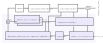
\includegraphics[width = 0.99\textwidth]{fig_C2_PBAdiagram.tex}
  \caption{\small Schematic diagram of the low-order energy-based controller and observer applied to the \textit{"true"} soft robot system depicted as $\Sigma_{\textrm{softrobot}}$. (a) Control diagram showing the interconnection between the observer, controller, and the soft robot. The block $\Sigma_{\textrm{sensor}}$ provides online measurements of the end-effector position $\gamma_B$. The observer estimates are used to compute the control law \eqref{eq:C3:control}. (b) The observer produces an estimate $\tilde{\q}$ based on a measurement error $\eB$ and the control signals $\uB$. Here, $\textrm{FK}$ is the forward kinematic mapping derived using \eqref{eq:C3:mappingSE3g}.}
  \label{fig:C3:diagram_control}
  \vspace{-3mm}
\end{figure}
%
where $\tilde{\q}$ is the controller state estimation, $\eB = \yB - \tilde{\gammaB}_L$ represents the difference between the true end-effector location and its estimate produced by the observer model, $\JB_v$ the linear velocity part of the Jacobian matrix, $\ten{N} = (\IB - \JB_v^+\JB_v)$ the null space, $\Psi$ a scalar-valued function that represents a sub-task for the observer, and $L_1,L_2 > 0$ are the observer gains. We select a sub-task energy potential $\Psi$ as the difference between the estimated potential energy and the work produced by the control input $\uB$, thus $\nabla{\q_c} \Psi(\tilde{\q},\uB) = \nabla_{\q_c}\mathcal{H}(\tilde{\q}) - \GB_k \uB$. Thus, the observer is nothing more than a continuous-time continuum deformation solver.%, aimed at finding a stable curve configuration given a known end-effector position and input $\uB$.
%
\begin{figure*}[!t]
  \centering
  \vspace{-2mm}
  %% This file was created by matlab2tikz.
%
\begin{tikzpicture}

\begin{axis}[%
width=0.862\textwidth,
height=0.595\textwidth,
at={(0.08\textwidth,0.007\textwidth)},
scale only axis,
xmin=0,
xmax=1,
ymin=0,
ymax=1,
axis line style={draw=none},
ticks=none,
axis x line*=bottom,
axis y line*=left,
colorbar style={width=6,xshift=-7.5pt}
]
\end{axis}

\begin{axis}[%
width=0.234\textwidth,
height=0.321\textwidth,
at={(0\textwidth,0.329\textwidth)},
scale only axis,
axis on top,
xmin=0.5,
xmax=522.5,
tick align=outside,
y dir=reverse,
ymin=0.5,
ymax=746.5,
axis line style={draw=none},
ticks=none,
colorbar style={width=6,xshift=-7.5pt}
]
\addplot [forget plot] graphics [xmin=0.5, xmax=522.5, ymin=0.5, ymax=746.5] {./fig/fig_C3_3D_srmarm-1.png};
\end{axis}

\begin{axis}[%
width=0.234\textwidth,
height=0.321\textwidth,
at={(0.374\textwidth,0.329\textwidth)},
scale only axis,
axis on top,
xmin=0.5,
xmax=522.5,
tick align=outside,
y dir=reverse,
ymin=0.5,
ymax=746.5,
axis line style={draw=none},
ticks=none,
colorbar style={width=6,xshift=-7.5pt}
]
\addplot [forget plot] graphics [xmin=0.5, xmax=522.5, ymin=0.5, ymax=746.5] {./fig/fig_C3_3D_srmarm-2.png};
\end{axis}

\begin{axis}[%
width=0.234\textwidth,
height=0.321\textwidth,
at={(0.749\textwidth,0.329\textwidth)},
scale only axis,
axis on top,
xmin=0.5,
xmax=522.5,
tick align=outside,
y dir=reverse,
ymin=0.5,
ymax=746.5,
axis line style={draw=none},
ticks=none,
colorbar style={width=6,xshift=-7.5pt}
]
\addplot [forget plot] graphics [xmin=0.5, xmax=522.5, ymin=0.5, ymax=746.5] {./fig/fig_C3_3D_srmarm-3.png};
\end{axis}

\begin{axis}[%
width=0.234\textwidth,
height=0.321\textwidth,
at={(0\textwidth,0\textwidth)},
scale only axis,
axis on top,
xmin=0.5,
xmax=522.5,
tick align=outside,
y dir=reverse,
ymin=0.5,
ymax=746.5,
axis line style={draw=none},
ticks=none,
colorbar style={width=6,xshift=-7.5pt}
]
\addplot [forget plot] graphics [xmin=0.5, xmax=522.5, ymin=0.5, ymax=746.5] {./fig/fig_C3_3D_srmarm-4.png};
\end{axis}

\begin{axis}[%
width=0.234\textwidth,
height=0.321\textwidth,
at={(0.374\textwidth,0\textwidth)},
scale only axis,
axis on top,
xmin=0.5,
xmax=522.5,
tick align=outside,
y dir=reverse,
ymin=0.5,
ymax=746.5,
axis line style={draw=none},
ticks=none,
colorbar style={width=6,xshift=-7.5pt}
]
\addplot [forget plot] graphics [xmin=0.5, xmax=522.5, ymin=0.5, ymax=746.5] {./fig/fig_C3_3D_srmarm-5.png};
\end{axis}

\begin{axis}[%
width=0.234\textwidth,
height=0.321\textwidth,
at={(0.749\textwidth,0\textwidth)},
scale only axis,
axis on top,
xmin=0.5,
xmax=522.5,
tick align=outside,
y dir=reverse,
ymin=0.5,
ymax=746.5,
axis line style={draw=none},
ticks=none,
colorbar style={width=6,xshift=-7.5pt}
]
\addplot [forget plot] graphics [xmin=0.5, xmax=522.5, ymin=0.5, ymax=746.5] {./fig/fig_C3_3D_srmarm-6.png};
\end{axis}
\end{tikzpicture}%
  \includegraphics*[width=1.04\textwidth]{./pdf/thesis-figure-5-13.pdf}
  \vspace{-5mm}
  \caption{\small \highlight{ Three-dimensional evolution of the soft robot inspired by the elephant's trunk (whose muscular network is mimicked through six pneumatic bellows), slowly converging to the desired set-point $\vec{g}_d \in \SE{3}$ (\ie, the pink ball). }}
  \label{fig:C3:softarm_3D_truncation}
  \vspace{-6mm}
\end{figure*}

\renewcommand\arraystretch{1.15}
\begin{table}[b]
  %\vspace{-0.25cm}
  \setlength\tabcolsep{0.44em}
  \caption{\small Error values in the steady-state condition for the energy-based controller are examined as the model truncation $k$ increases. It is noteworthy that as the value of $k$ increases, the accuracy of the backbone estimate improves. However, when it comes to the tip error, a consistent and monotonic trend with increasing $k$ may not be observed.}
  \label{tab:C3:EX3:error} \centering
  \rowcolors{0}{}{blue!5}
  \begin{tabular}{l||cccccccc}
    \hline
    Truncation & $k=1$ & $k=2$ & $k=3$ & $k=4$ & $k=5$ & $k=6$ & $k=7$ & $k=8$ \\
    \hline 
    \hline
    Tip error (mm) & 14.68 & 2.36 & 0.73 & 0.65 & 0.46 & 0.78 & 0.65 & 0.54\\
    Curve error & 118\% & 16.1\% & 14.2\% & 8.34\% & 5.31\% & 4.53\% & 4.24\% & 4.01\% \\
    \hline
  \end{tabular}
  \end{table}
%

%
We again consider a soft robot inspired by the octopus arm (see Table \ref{tab:C3:parameters1}) with the controller-observer gains: $\lambda_1 = \lambda_2 = 0.1$ and $L_1 = L_2 = 1$. The desired end-effector configuration is $\PhiB_d = \IB_3$ and $\gammaB_d = (70, 0, 40)^\top$. In this study, we analyze the performance of the reduced-order controller for truncation orders $k \in \{1,2,...,8\}$. Note that for $k=1$, the controller explores the "\emph{Piece-wise Constant Strain}" (PCS) assumption similar to Chapter \ref{chap:PCC}, while the true system $\Sigma_{\textrm{softrobot}}$ is not impeded by such kinematic restrictions. %

The numerical simulations conducted for the controller benchmark are presented in Figure \ref{fig:C3:softarm_3D_truncation}, showcasing snapshots of the closed-loop system in operation. The figure displays the true system as (\textcolor{matinfil!50}{$\blacksquare$}) and the low-dimensional shape estimations as (\textcolor{lightblue}{$\blacksquare$}). Figure \ref{fig:C3:EX3:gamma_order} shows the trajectories of $\gammaB_L$ for various $k$, while Figure \ref{fig:C3:EX3:backbone_convergence} shows the RMS error between the backbone of the estimate and the true system. The steady-state values for these metrics are reported in Table \ref{tab:C3:EX3:error}. As anticipated, it is observed that with increasing $k$, the differences between the true system and shape estimates diminish, indicating a monotonically increasing precision. However, a few other remarkable observations can be made.

\begin{figure}[!t]
\centering
\vspace{-1mm}
%% This file was created by matlab2tikz.
%
%The latest updates can be retrieved from
%  http://www.mathworks.com/matlabcentral/fileexchange/22022-matlab2tikz-matlab2tikz
%where you can also make suggestions and rate matlab2tikz.
%
\definecolor{mycolor1}{rgb}{0.06270,0.35690,0.84710}%
\definecolor{mycolor2}{rgb}{0.86670,0.21180,0.10980}%
\definecolor{mycolor3}{rgb}{0.18040,0.52160,0.25100}%
\definecolor{mycolor4}{rgb}{1.00000,0.61570,0.11760}%
\definecolor{mycolor5}{rgb}{0.29800,0.17250,0.57250}%
\definecolor{mycolor6}{rgb}{1.00000,0.39220,0.11760}%
\definecolor{mycolor7}{rgb}{0.00780,0.74900,0.90590}%
\definecolor{mycolor8}{rgb}{1.00000,0.16080,0.45880}%
%
\begin{tikzpicture}

\begin{axis}[%
width=0.268\textwidth,
height=0.273\textwidth,
at={(0\textwidth,0\textwidth)},
scale only axis,
xmin=0,
xmax=6,
xlabel style={font=\color{white!15!black}},
xlabel={time (s)},
ymin=0,
ymax=130,
ylabel style={font=\color{white!15!black}},
ylabel={tip position (mm)},
axis background/.style={fill=white},
xmajorgrids,
ymajorgrids
]
\addplot [color=mycolor1, line width=1.5pt, forget plot]
  table[row sep=crcr]{%
0	119.999999824351\\
0.01	119.999761006601\\
0.02	119.996496846166\\
0.03	119.985718557839\\
0.04	119.964880088242\\
0.05	119.932615064138\\
0.06	119.889113056561\\
0.07	119.834971168929\\
0.08	119.771232053867\\
0.09	119.698883594988\\
0.1	119.618976052914\\
0.11	119.532387253545\\
0.12	119.439967448317\\
0.13	119.342396849961\\
0.14	119.240315312118\\
0.15	119.134221106263\\
0.16	119.024574745018\\
0.17	118.911723223345\\
0.18	118.795980138295\\
0.19	118.677568653634\\
0.2	118.556682579098\\
0.21	118.433443910826\\
0.22	118.307949170363\\
0.23	118.180238402931\\
0.24	118.050329515685\\
0.25	117.918196859364\\
0.26	117.783796300099\\
0.27	117.647050825152\\
0.28	117.507868093802\\
0.29	117.366132448605\\
0.3	117.221715873008\\
0.31	117.074474968299\\
0.32	116.924256085862\\
0.33	116.770896825164\\
0.34	116.614226581768\\
0.35	116.454071371469\\
0.36	116.290250163843\\
0.37	116.122582663887\\
0.38	115.950881994903\\
0.39	115.774964855416\\
0.4	115.594641170433\\
0.41	115.409725989712\\
0.42	115.220026140091\\
0.43	115.025353830792\\
0.44	114.825511278079\\
0.45	114.6203050157\\
0.46	114.409528667674\\
0.47	114.19297781361\\
0.48	113.970431366578\\
0.49	113.741666546228\\
0.5	113.506439320119\\
0.51	113.26449907836\\
0.52	113.01556848251\\
0.53	112.759357593083\\
0.54	112.495544085454\\
0.55	112.223785933177\\
0.56	111.943701974316\\
0.57	111.654883285866\\
0.58	111.356875160517\\
0.59	111.049186862381\\
0.6	110.731275262822\\
0.61	110.402552370005\\
0.62	110.062371175112\\
0.63	109.710030576761\\
0.64	109.344765679087\\
0.65	108.965750132387\\
0.66	108.572090469545\\
0.67	108.162824947057\\
0.68	107.736923681697\\
0.69	107.293284732\\
0.7	106.830740839743\\
0.71	106.348051858033\\
0.72	105.843919949\\
0.73	105.316978759632\\
0.74	104.765818020413\\
0.75	104.188969915192\\
0.76	103.584941931931\\
0.77	102.952203871275\\
0.78	102.289227928714\\
0.79	101.594479565251\\
0.8	100.866461926607\\
0.81	100.103710511407\\
0.82	99.3048447934397\\
0.83	98.4685642921724\\
0.84	97.5937084703769\\
0.85	96.6792513284613\\
0.86	95.7243693186971\\
0.87	94.7284338747264\\
0.88	93.6910840884815\\
0.89	92.6122140234625\\
0.9	91.4920477315701\\
0.91	90.331117496065\\
0.92	89.1303344501962\\
0.93	87.890955466455\\
0.94	86.6146466057379\\
0.95	85.3034288947525\\
0.96	83.9597403267121\\
0.97	82.5863444921697\\
0.98	81.1863913044906\\
0.99	79.7632824471517\\
1	78.3207349808177\\
1.01	76.862609158136\\
1.02	75.3929583165023\\
1.03	73.9158381233124\\
1.04	72.4353430744522\\
1.05	70.9554053657524\\
1.06	69.479821213836\\
1.07	68.0120522176315\\
1.08	66.5552500069188\\
1.09	65.112070980448\\
1.1	63.684707653561\\
1.11	62.2747260899165\\
1.12	60.8831103150038\\
1.13	59.5101283065856\\
1.14	58.1553925796929\\
1.15	56.8177565082787\\
1.16	55.4953906316062\\
1.17	54.1857073647971\\
1.18	52.885453351008\\
1.19	51.5906446741126\\
1.2	50.2966841931333\\
1.21	48.9983021544355\\
1.22	47.6896828069595\\
1.23	46.3644249125003\\
1.24	45.0156729663339\\
1.25	43.6361229825178\\
1.26	42.2181976301616\\
1.27	40.7541788096905\\
1.28	39.2365684654916\\
1.29	37.6586131046146\\
1.3	36.0153135263962\\
1.31	34.3052099274029\\
1.32	32.5336771995047\\
1.33	30.7191749438592\\
1.34	28.9054585390978\\
1.35	27.1868248823313\\
1.36	25.7641139588364\\
1.37	23.7389391233212\\
1.38	19.3350211852975\\
1.39	15.2538925166398\\
1.4	16.8089911140614\\
1.41	22.9813966198814\\
1.42	27.5893513818984\\
1.43	30.5631865870065\\
1.44	32.9554354592321\\
1.45	34.729879863386\\
1.46	35.9827973597344\\
1.47	36.770680025833\\
1.48	37.1772604175127\\
1.49	37.2542470310477\\
1.5	37.0599251420584\\
1.51	36.630939585206\\
1.52	36.0029125464571\\
1.53	35.1977061797354\\
1.54	34.2343819593173\\
1.55	33.1239310653069\\
1.56	31.8750304145053\\
1.57	30.4928159755338\\
1.58	28.9825110101808\\
1.59	27.3518917808935\\
1.6	25.6166950482456\\
1.61	23.8114558414142\\
1.62	22.0088089384839\\
1.63	20.3648618177955\\
1.64	19.2100048676026\\
1.65	16.2953511213352\\
1.66	11.2311103659594\\
1.67	13.0020331372442\\
1.68	21.322763212686\\
1.69	27.1282990723681\\
1.7	30.9973275550963\\
1.71	34.5741203246097\\
1.72	37.6709417498994\\
1.73	40.4085436565868\\
1.74	42.8025839962144\\
1.75	44.9553130469619\\
1.76	46.8967165638708\\
1.77	48.7010375052856\\
1.78	50.3948803576434\\
1.79	52.0286779966581\\
1.8	53.6206764859965\\
1.81	55.2032157379555\\
1.82	56.7861825055777\\
1.83	58.3885132293256\\
1.84	60.01279231464\\
1.85	61.6677659289419\\
1.86	63.3497434162017\\
1.87	65.059457884914\\
1.88	66.7879260403827\\
1.89	68.52963370126\\
1.9	70.2714955019447\\
1.91	72.0035460958136\\
1.92	73.7101393463483\\
1.93	75.3788277127393\\
1.94	76.9932010338721\\
1.95	78.5403341913678\\
1.96	80.0048223405911\\
1.97	81.3750163773188\\
1.98	82.6379178556449\\
1.99	83.7843841218846\\
2	84.8046513587129\\
2.01	85.6926903789515\\
2.02	86.4422318112658\\
2.03	87.0504431235982\\
2.04	87.514398435123\\
2.05	87.8342344105785\\
2.06	88.010030815908\\
2.07	88.0445498681167\\
2.08	87.9405145674255\\
2.09	87.7029801146142\\
2.1	87.3370029755592\\
2.11	86.8496563636592\\
2.12	86.2480473850792\\
2.13	85.5410019237123\\
2.14	84.7374355161328\\
2.15	83.847682250718\\
2.16	82.8821600529965\\
2.17	81.8523599528936\\
2.18	80.7698333087609\\
2.19	79.646904686426\\
2.2	78.4958652247314\\
2.21	77.3293881974067\\
2.22	76.1599852695569\\
2.23	75.0001922077615\\
2.24	73.8622163138894\\
2.25	72.7579819319192\\
2.26	71.6989145427131\\
2.27	70.6958684891569\\
2.28	69.7590266697855\\
2.29	68.8978022754576\\
2.3	68.1207645351111\\
2.31	67.4355463315514\\
2.32	66.8487516684116\\
2.33	66.3658806209972\\
2.34	65.9911905871545\\
2.35	65.7276394934708\\
2.36	65.5766766680308\\
2.37	65.5382340919874\\
2.38	65.6104568662753\\
2.39	65.7898243382961\\
2.4	66.0708340126949\\
2.41	66.4463093094803\\
2.42	66.9071469050241\\
2.43	67.4428044040451\\
2.44	68.041103714966\\
2.45	68.6889658892634\\
2.46	69.3723203912822\\
2.47	70.0769857479727\\
2.48	70.7885953630211\\
2.49	71.4935066475941\\
2.5	72.178697566217\\
2.51	72.8326017323247\\
2.52	73.4449118604577\\
2.53	74.0072539133297\\
2.54	74.5128800239664\\
2.55	74.9571340996971\\
2.56	75.3370592079007\\
2.57	75.6516818198894\\
2.58	75.9015521474145\\
2.59	76.0889040446052\\
2.6	76.2171638582587\\
2.61	76.2910014498474\\
2.62	76.3158828947013\\
2.63	76.2980955983085\\
2.64	76.2443219358967\\
2.65	76.161610851013\\
2.66	76.0570507527853\\
2.67	75.9377442659272\\
2.68	75.8105110751725\\
2.69	75.6818432203793\\
2.7	75.5576966456964\\
2.71	75.4435286962728\\
2.72	75.3440824875432\\
2.73	75.2634024485909\\
2.74	75.2047054979731\\
2.75	75.1704270753034\\
2.76	75.1621091742696\\
2.77	75.1805218574326\\
2.78	75.2255933797672\\
2.79	75.296481348591\\
2.8	75.3915909178757\\
2.81	75.5087553539008\\
2.82	75.6452200800347\\
2.83	75.7978721380976\\
2.84	75.963243032824\\
2.85	76.1377325178123\\
2.86	76.3176319933859\\
2.87	76.4993362283317\\
2.88	76.6793633067224\\
2.89	76.8545832719665\\
2.9	77.0221784597252\\
2.91	77.1798205144795\\
2.92	77.3256112010433\\
2.93	77.4582205297882\\
2.94	77.5768020788827\\
2.95	77.6810738961919\\
2.96	77.7711760150732\\
2.97	77.8477383285003\\
2.98	77.9117440308151\\
2.99	77.9645448093854\\
3	78.0077140455007\\
3.01	78.0430457060451\\
3.02	78.0724108082485\\
3.03	78.0977608873374\\
3.04	78.1209851748228\\
3.05	78.1438857391827\\
3.06	78.1680839907899\\
3.07	78.1950324612075\\
3.08	78.2259214073157\\
3.09	78.261704189547\\
3.1	78.3030314087901\\
3.11	78.3502959083633\\
3.12	78.4035892453636\\
3.13	78.4627668441313\\
3.14	78.5274227629503\\
3.15	78.5969574891257\\
3.16	78.6705779879866\\
3.17	78.7474134178356\\
3.18	78.826489546461\\
3.19	78.9068187850759\\
3.2	78.9873965991384\\
3.21	79.067291582938\\
3.22	79.145630366044\\
3.23	79.2216776561125\\
3.24	79.2948094848828\\
3.25	79.3645779625387\\
3.26	79.4306715868051\\
3.27	79.4929630875179\\
3.28	79.5514578643693\\
3.29	79.6063261406188\\
3.3	79.6578426487787\\
3.31	79.7064065547255\\
3.32	79.7524913845311\\
3.33	79.7966433060696\\
3.34	79.839393507196\\
3.35	79.8812894009318\\
3.36	79.9228417282843\\
3.37	79.9645324425972\\
3.38	80.0067649397883\\
3.39	80.0498824625666\\
3.4	80.0941268280084\\
3.41	80.1396650501282\\
3.42	80.1865576914593\\
3.43	80.2347935810503\\
3.44	80.2842665633455\\
3.45	80.3348168175165\\
3.46	80.3862135723966\\
3.47	80.4382003714997\\
3.48	80.4904806826947\\
3.49	80.5427638654243\\
3.5	80.5947505666758\\
3.51	80.646176215397\\
3.52	80.6967936283802\\
3.53	80.7464115227664\\
3.54	80.7948727161189\\
3.55	80.842086229659\\
3.56	80.8880006308934\\
3.57	80.9326295444866\\
3.58	80.9760208047223\\
3.59	81.0182763351319\\
3.6	81.05951863982\\
3.61	81.0999068384572\\
3.62	81.1396024860927\\
3.63	81.1787839381913\\
3.64	81.2176146873966\\
3.65	81.256254409671\\
3.66	81.2948351078373\\
3.67	81.3334698466427\\
3.68	81.372236066548\\
3.69	81.4111862156713\\
3.7	81.4503351396888\\
3.71	81.4896738365588\\
3.72	81.5291603342429\\
3.73	81.568735915289\\
3.74	81.6083183974979\\
3.75	81.6478196365807\\
3.76	81.6871398548199\\
3.77	81.7261850250984\\
3.78	81.7648609202483\\
3.79	81.8030890975276\\
3.8	81.8407996395257\\
3.81	81.8779451155642\\
3.82	81.9144907400809\\
3.83	81.9504265328052\\
3.84	81.9857543247636\\
3.85	82.0204986595586\\
3.86	82.0546921178108\\
3.87	82.0883842635341\\
3.88	82.1216263241668\\
3.89	82.1544791633113\\
3.9	82.1869981754254\\
3.91	82.2192412155069\\
3.92	82.2512544832593\\
3.93	82.2830811688312\\
3.94	82.3147488399477\\
3.95	82.3462792492158\\
3.96	82.3776773964318\\
3.97	82.4089425705775\\
3.98	82.4400589137975\\
3.99	82.4710074321803\\
4	82.5017576215125\\
4.01	82.5322799443577\\
4.02	82.5625379378999\\
4.03	82.5925005664572\\
4.04	82.6221342428461\\
4.05	82.651414525667\\
4.06	82.6803176202852\\
4.07	82.7088310697789\\
4.08	82.736944520015\\
4.09	82.7646592945555\\
4.1	82.7919784483496\\
4.11	82.8189153554284\\
4.12	82.8454832786317\\
4.13	82.8717241647932\\
4.14	82.8976778195749\\
4.15	82.9233557035116\\
4.16	82.948759901181\\
4.17	82.973900456914\\
4.18	82.9987791008816\\
4.19	83.0234000692363\\
4.2	83.0477605029629\\
4.21	83.0718598737741\\
4.22	83.0956913174115\\
4.23	83.1192509252202\\
4.24	83.1425294922472\\
4.25	83.1655216900392\\
4.26	83.1882180033994\\
4.27	83.2106136997601\\
4.28	83.232700786448\\
4.29	83.2544766945414\\
4.3	83.2759361539451\\
4.31	83.2970795537151\\
4.32	83.3179046976417\\
4.33	83.3384148609485\\
4.34	83.3586104525497\\
4.35	83.3784968342176\\
4.36	83.3980759593142\\
4.37	83.4173540529751\\
4.38	83.4363333116627\\
4.39	83.4550195449093\\
4.4	83.4734140131942\\
4.41	83.4915211113308\\
4.42	83.5093403912024\\
4.43	83.5268743303961\\
4.44	83.5441205477069\\
4.45	83.5610796577673\\
4.46	83.5777476489808\\
4.47	83.5941237920763\\
4.48	83.6102031241009\\
4.49	83.625984355918\\
4.5	83.6414623978441\\
4.51	83.6566362091654\\
4.52	83.6715013064621\\
4.53	83.6860575137569\\
4.54	83.7003014169483\\
4.55	83.7142339956048\\
4.56	83.7278530129497\\
4.57	83.7411605378249\\
4.58	83.7541552849809\\
4.59	83.766840058122\\
4.6	83.7792367767739\\
4.61	83.7913718412716\\
4.62	83.8032313300837\\
4.63	83.81479999738\\
4.64	83.8260647404473\\
4.65	83.8370153472394\\
4.66	83.8476398929946\\
4.67	83.8579318442698\\
4.68	83.8678834695624\\
4.69	83.8774931483073\\
4.7	83.8867581211507\\
4.71	83.8956815977717\\
4.72	83.9042650625394\\
4.73	83.9125152033218\\
4.74	83.9204359635296\\
4.75	83.9280354174981\\
4.76	83.9353177638927\\
4.77	83.9422902995029\\
4.78	83.9489555145284\\
4.79	83.9553182859186\\
4.8	83.9613781711632\\
4.81	83.9671368774433\\
4.82	83.9726139586504\\
4.83	83.9778323120415\\
4.84	83.9827721224253\\
4.85	83.9874104460724\\
4.86	83.9917264544875\\
4.87	83.9957029516345\\
4.88	83.999321921322\\
4.89	84.0025721476883\\
4.9	84.0054426658468\\
4.91	84.0079303461824\\
4.92	84.0100324033526\\
4.93	84.0117760838079\\
4.94	84.0131891100722\\
4.95	84.014267330396\\
4.96	84.0149963067401\\
4.97	84.015372545264\\
4.98	84.0153893539516\\
4.99	84.0150463620537\\
5	84.0143407403291\\
5.01	84.01328107037\\
5.02	84.0118849275556\\
5.03	84.0102062601699\\
5.04	84.0083590729177\\
5.05	84.0065091491664\\
5.06	84.0048272454695\\
5.07	84.0034850323588\\
5.08	84.0026359794321\\
5.09	84.0024089216415\\
5.1	84.0028911557214\\
5.11	84.004129911007\\
5.12	84.0061225194491\\
5.13	84.0088155198691\\
5.14	84.012112892147\\
5.15	84.0159102013202\\
5.16	84.0200807259451\\
5.17	84.0244838460464\\
5.18	84.0289693361664\\
5.19	84.0333816765265\\
5.2	84.0375709328946\\
5.21	84.041430504011\\
5.22	84.0448848901174\\
5.23	84.0479025052965\\
5.24	84.050483025023\\
5.25	84.0526449779125\\
5.26	84.0544255728667\\
5.27	84.0558895556475\\
5.28	84.0571147199799\\
5.29	84.0581927099006\\
5.3	84.0592148494099\\
5.31	84.060272217953\\
5.32	84.0614528011899\\
5.33	84.062825730434\\
5.34	84.0644192724852\\
5.35	84.0662526223484\\
5.36	84.0683264314441\\
5.37	84.0706221886685\\
5.38	84.073100383118\\
5.39	84.0757096804144\\
5.4	84.0783853447934\\
5.41	84.0810603441119\\
5.42	84.0836642676973\\
5.43	84.0861344357763\\
5.44	84.088414027859\\
5.45	84.0904617862464\\
5.46	84.0922483130711\\
5.47	84.0937634994039\\
5.48	84.0950105383213\\
5.49	84.0960109023854\\
5.5	84.0967962912425\\
5.51	84.0974116477469\\
5.52	84.097905812708\\
5.53	84.0983335346449\\
5.54	84.098745899923\\
5.55	84.0991924506404\\
5.56	84.0997124379979\\
5.57	84.1003380081611\\
5.58	84.101087028421\\
5.59	84.1019678979693\\
5.6	84.102974224212\\
5.61	84.1040913046531\\
5.62	84.1052931056538\\
5.63	84.1065479150818\\
5.64	84.1078189605705\\
5.65	84.1090678981426\\
5.66	84.1102577620415\\
5.67	84.1113554586235\\
5.68	84.1123341216931\\
5.69	84.1131753006148\\
5.7	84.1138680794803\\
5.71	84.1144125916486\\
5.72	84.1148151542187\\
5.73	84.1150926083153\\
5.74	84.1152657186952\\
5.75	84.1153625156717\\
5.76	84.1154111438166\\
5.77	84.1154427867141\\
5.78	84.1154845680096\\
5.79	84.1155626766276\\
5.8	84.1156958732753\\
5.81	84.115899302301\\
5.82	84.1161789602918\\
5.83	84.1165364283474\\
5.84	84.1169643857293\\
5.85	84.1174522089952\\
5.86	84.1179823419473\\
5.87	84.1185364603172\\
5.88	84.1190923143004\\
5.89	84.1196300163251\\
5.9	84.1201288979458\\
5.91	84.1205734689917\\
5.92	84.1209498886042\\
5.93	84.1212512596144\\
5.94	84.1214734699173\\
5.95	84.1216196799019\\
5.96	84.1216955010557\\
5.97	84.121712750905\\
5.98	84.121684132794\\
5.99	84.121626506635\\
6	84.1215553681989\\
};
\addplot [color=mycolor2, line width=1.5pt, forget plot]
  table[row sep=crcr]{%
0	119.999999824351\\
0.01	119.999991014243\\
0.02	119.999889390258\\
0.03	119.999535485152\\
0.04	119.998760133155\\
0.05	119.997450471406\\
0.06	119.99556425031\\
0.07	119.993096079894\\
0.08	119.990055528429\\
0.09	119.98644623745\\
0.1	119.982253658257\\
0.11	119.977431382967\\
0.12	119.971887316802\\
0.13	119.965461526466\\
0.14	119.957891956261\\
0.15	119.94875563848\\
0.16	119.937365880138\\
0.17	119.922586963459\\
0.18	119.902484155936\\
0.19	119.873638120626\\
0.2	119.829731469497\\
0.21	119.758547913388\\
0.22	119.632125824298\\
0.23	119.452120620277\\
0.24	119.270573392396\\
0.25	119.095892886942\\
0.26	118.920562687553\\
0.27	118.746461169925\\
0.28	118.570543557777\\
0.29	118.392160759183\\
0.3	118.209679864761\\
0.31	118.022587980869\\
0.32	117.829999347684\\
0.33	117.631735749018\\
0.34	117.427358145997\\
0.35	117.216896616682\\
0.36	117.000169437522\\
0.37	116.777321745889\\
0.38	116.548325206553\\
0.39	116.313387081317\\
0.4	116.072574452595\\
0.41	115.826130169693\\
0.42	115.574184376322\\
0.43	115.317002432537\\
0.44	115.054758839496\\
0.45	114.78773466506\\
0.46	114.516137199768\\
0.47	114.240259137618\\
0.48	113.960332719654\\
0.49	113.676659267367\\
0.5	113.389490110614\\
0.51	113.09913257395\\
0.52	112.80585229305\\
0.53	112.509960064564\\
0.54	112.211731663557\\
0.55	111.911478828516\\
0.56	111.60948501054\\
0.57	111.306058592954\\
0.58	111.001486811379\\
0.59	110.696072852177\\
0.6	110.390103762794\\
0.61	110.083874418412\\
0.62	109.777667105762\\
0.63	109.471770397994\\
0.64	109.1664621135\\
0.65	108.862018245917\\
0.66	108.558706578545\\
0.67	108.256789167357\\
0.68	107.956521512043\\
0.69	107.658149628815\\
0.7	107.361914359162\\
0.71	107.068043760437\\
0.72	106.776761809795\\
0.73	106.488276867413\\
0.74	106.202794074612\\
0.75	105.920500581063\\
0.76	105.641581000041\\
0.77	105.366200027394\\
0.78	105.094520377379\\
0.79	104.826683362733\\
0.8	104.562828790004\\
0.81	104.303074015903\\
0.82	104.04753533168\\
0.83	103.796305960134\\
0.84	103.549478504668\\
0.85	103.307122303239\\
0.86	103.069306559473\\
0.87	102.83607482727\\
0.88	102.607477186905\\
0.89	102.383533494471\\
0.9	102.164273905076\\
0.91	101.949692050917\\
0.92	101.739804492664\\
0.93	101.534588518467\\
0.94	101.33404143738\\
0.95	101.138123976582\\
0.96	100.946817692875\\
0.97	100.760070146318\\
0.98	100.577849798897\\
0.99	100.400094048429\\
1	100.226761139714\\
1.01	100.057781326615\\
1.02	99.89310553836\\
1.03	99.7326598417732\\
1.04	99.5763906584371\\
1.05	99.4242226538981\\
1.06	99.2761003388218\\
1.07	99.1319467080821\\
1.08	98.9917104416173\\
1.09	98.8553161418647\\
1.1	98.7227187184908\\
1.11	98.5938442765424\\
1.12	98.4686519894912\\
1.13	98.3470684151032\\
1.14	98.2290529506526\\
1.15	98.114547657328\\
1.16	98.0035216352424\\
1.17	97.8959219141119\\
1.18	97.7917191519593\\
1.19	97.6908668011858\\
1.2	97.5933372210961\\
1.21	97.4990873678469\\
1.22	97.4080925337894\\
1.23	97.3203127306488\\
1.24	97.2357236424887\\
1.25	97.1542862191628\\
1.26	97.0759717538918\\
1.27	97.000741358597\\
1.28	96.9285586274876\\
1.29	96.8593836065715\\
1.3	96.79316942329\\
1.31	96.7298654566163\\
1.32	96.6694063077948\\
1.33	96.6117499939083\\
1.34	96.556821004292\\
1.35	96.5045670346454\\
1.36	96.4548883790715\\
1.37	96.4077223947361\\
1.38	96.3629453595199\\
1.39	96.3204761292755\\
1.4	96.2801732360473\\
1.41	96.2419357925005\\
1.42	96.2055997456435\\
1.43	96.171044680851\\
1.44	96.1380791400128\\
1.45	96.1065620775658\\
1.46	96.0762730875188\\
1.47	96.0470491626083\\
1.48	96.018639790224\\
1.49	95.9908589167903\\
1.5	95.9634269013751\\
1.51	95.9361347685793\\
1.52	95.9086669617821\\
1.53	95.880787158924\\
1.54	95.8521491634785\\
1.55	95.8224859745339\\
1.56	95.791435702678\\
1.57	95.758691862113\\
1.58	95.7238710124843\\
1.59	95.6866348336439\\
1.6	95.6465712163688\\
1.61	95.603315551249\\
1.62	95.5564269391217\\
1.63	95.5055154878688\\
1.64	95.4501124995528\\
1.65	95.3898039977496\\
1.66	95.3240949364316\\
1.67	95.252548839512\\
1.68	95.1746462117448\\
1.69	95.0899300965844\\
1.7	94.9978589278362\\
1.71	94.8979544740531\\
1.72	94.7896532283889\\
1.73	94.6724676070452\\
1.74	94.5458230966126\\
1.75	94.4092192662874\\
1.76	94.2620689680611\\
1.77	94.1038644593425\\
1.78	93.9340114443585\\
1.79	93.7519998403197\\
1.8	93.5572339386607\\
1.81	93.3492071984468\\
1.82	93.1273290703737\\
1.83	92.8911033364538\\
1.84	92.6399521324794\\
1.85	92.3733973342591\\
1.86	92.0908823490876\\
1.87	91.7919560130574\\
1.88	91.4760927635306\\
1.89	91.1428784693131\\
1.9	90.7918296398155\\
1.91	90.4225805619408\\
1.92	90.0347022456864\\
1.93	89.6278901894456\\
1.94	89.2017838052031\\
1.95	88.7561540788304\\
1.96	88.2907242596794\\
1.97	87.8053566237652\\
1.98	87.2998752464595\\
1.99	86.7742510077556\\
2	86.2284326485994\\
2.01	85.6625105143896\\
2.02	85.0765762102495\\
2.03	84.4708587959191\\
2.04	83.8456180826774\\
2.05	83.2012478366063\\
2.06	82.5381923012224\\
2.07	81.8570342746568\\
2.08	81.1584203493573\\
2.09	80.4431441521623\\
2.1	79.712076420178\\
2.11	78.9662429644319\\
2.12	78.206756541475\\
2.13	77.434892069354\\
2.14	76.6520244738696\\
2.15	75.8596972807198\\
2.16	75.0595654043277\\
2.17	74.2534592966739\\
2.18	73.4433345618087\\
2.19	72.631333443249\\
2.2	71.8197454864447\\
2.21	71.0110724596337\\
2.22	70.2080106162675\\
2.23	69.4135357591039\\
2.24	68.6309345517931\\
2.25	67.8639538770113\\
2.26	67.1169505627966\\
2.27	66.3952078645816\\
2.28	65.7053319047871\\
2.29	65.0558229059067\\
2.3	64.4575351704136\\
2.31	63.9235870704571\\
2.32	63.4677603835671\\
2.33	63.1012375151511\\
2.34	62.8284861616922\\
2.35	62.644547983156\\
2.36	62.534616359027\\
2.37	62.4760512955619\\
2.38	62.4420103035562\\
2.39	62.4062851268204\\
2.4	62.3479285153312\\
2.41	62.254604652177\\
2.42	62.1234829898326\\
2.43	61.9601941609231\\
2.44	61.7762579741385\\
2.45	61.5861560820988\\
2.46	61.4041584674015\\
2.47	61.2416516064435\\
2.48	61.1050462374021\\
2.49	60.9950317324375\\
2.5	60.9070807035666\\
2.51	60.8333627998149\\
2.52	60.7651282272565\\
2.53	60.6951960243614\\
2.54	60.6195625400608\\
2.55	60.5380574382983\\
2.56	60.4536422153857\\
2.57	60.3711010781691\\
2.58	60.2953804072076\\
2.59	60.2302872243378\\
2.6	60.1775443261811\\
2.61	60.1367360517263\\
2.62	60.1057569128657\\
2.63	60.0818222252687\\
2.64	60.0624191466328\\
2.65	60.0460724293189\\
2.66	60.0324979972274\\
2.67	60.0225616257068\\
2.68	60.0177635837788\\
2.69	60.0196731677838\\
2.7	60.029421261722\\
2.71	60.0474079938301\\
2.72	60.0733538541455\\
2.73	60.1064633423939\\
2.74	60.1458303949559\\
2.75	60.1906590219005\\
2.76	60.240544861674\\
2.77	60.2954235157749\\
2.78	60.3555702957541\\
2.79	60.4213449396089\\
2.8	60.4931290012296\\
2.81	60.5710993990504\\
2.82	60.655234163101\\
2.83	60.7452810780974\\
2.84	60.840946082873\\
2.85	60.9418737544041\\
2.86	61.047819153412\\
2.87	61.1585800253725\\
2.88	61.2740940284376\\
2.89	61.3943205644766\\
2.9	61.5192891128679\\
2.91	61.6489887754099\\
2.92	61.7834229280178\\
2.93	61.9225296771411\\
2.94	62.0662621037112\\
2.95	62.214523630515\\
2.96	62.3672606616835\\
2.97	62.5243942864785\\
2.98	62.6859179988244\\
2.99	62.8518079968958\\
3	63.0220924601612\\
3.01	63.1967772438258\\
3.02	63.3759333394589\\
3.03	63.5595959115154\\
3.04	63.7478503595305\\
3.05	63.9407416835083\\
3.06	64.1383455780229\\
3.07	64.3406662953179\\
3.08	64.5477151740312\\
3.09	64.7594089574876\\
3.1	64.9756433532311\\
3.11	65.1961912312517\\
3.12	65.4207692657188\\
3.13	65.6489444539489\\
3.14	65.8802174667792\\
3.15	66.1139288857918\\
3.16	66.3493381972315\\
3.17	66.5855535975393\\
3.18	66.8216241191684\\
3.19	67.0564849316166\\
3.2	67.2890583334487\\
3.21	67.5182119408859\\
3.22	67.7428616710948\\
3.23	67.9619351067715\\
3.24	68.174471688515\\
3.25	68.3795662119303\\
3.26	68.5764841734333\\
3.27	68.7645688231607\\
3.28	68.9433584365053\\
3.29	69.1124844111951\\
3.3	69.271761648516\\
3.31	69.4210576480743\\
3.32	69.5603945478087\\
3.33	69.6898424705855\\
3.34	69.8095876156189\\
3.35	69.9198298185797\\
3.36	70.0208503520139\\
3.37	70.1129027338157\\
3.38	70.1963131914935\\
3.39	70.2713489320793\\
3.4	70.3383139765104\\
3.41	70.3974478430752\\
3.42	70.4490311133011\\
3.43	70.49327127563\\
3.44	70.5304216708848\\
3.45	70.5606644605543\\
3.46	70.5842246981071\\
3.47	70.6012731047343\\
3.48	70.6120186097272\\
3.49	70.6166310738585\\
3.5	70.6153059166831\\
3.51	70.6082318461\\
3.52	70.5955843519204\\
3.53	70.5775738816009\\
3.54	70.5543710709503\\
3.55	70.5261958680561\\
3.56	70.4932253606245\\
3.57	70.4556887579617\\
3.58	70.4137634327165\\
3.59	70.3676881637239\\
3.6	70.3176391509763\\
3.61	70.2638494658541\\
3.62	70.2064990569033\\
3.63	70.1458156823993\\
3.64	70.0819781386178\\
3.65	70.015213216771\\
3.66	69.9456939665844\\
3.67	69.8736463600372\\
3.68	69.7992380869771\\
3.69	69.7226944426901\\
3.7	69.6441786182201\\
3.71	69.5639154699675\\
3.72	69.4820645086297\\
3.73	69.398850178377\\
3.74	69.3144288088151\\
3.75	69.2290240649318\\
3.76	69.1427891590811\\
3.77	69.0559461789348\\
3.78	68.9686448633715\\
3.79	68.8811045622248\\
3.8	68.7934708613947\\
3.81	68.7059589720602\\
3.82	68.618709450233\\
3.83	68.53193185578\\
3.84	68.4457607559516\\
3.85	68.3603985394437\\
3.86	68.2759728281281\\
3.87	68.1926773816941\\
3.88	68.1106319715586\\
3.89	68.0300203692083\\
3.9	67.9509536638917\\
3.91	67.8736043928131\\
3.92	67.7980742108643\\
3.93	67.7245232921399\\
3.94	67.6530431856881\\
3.95	67.5837806935636\\
3.96	67.5168166709604\\
3.97	67.4522836642544\\
3.98	67.3902513366055\\
3.99	67.3308372286013\\
4	67.2740994115522\\
4.01	67.2201398124142\\
4.02	67.1690046170367\\
4.03	67.1207796795395\\
4.04	67.0754943536191\\
4.05	67.0332244477558\\
4.06	66.9939844632743\\
4.07	66.9578368444671\\
4.08	66.9247842164805\\
4.09	66.8948750037629\\
4.1	66.8680954579823\\
4.11	66.8444782164148\\
4.12	66.8239959358318\\
4.13	66.8066631420567\\
4.14	66.7924395825526\\
4.15	66.7813269656948\\
4.16	66.7732751519146\\
4.17	66.7682702971006\\
4.18	66.7662526118617\\
4.19	66.7671930654816\\
4.2	66.7710262074505\\
4.21	66.7777053390075\\
4.22	66.7871621455529\\
4.23	66.7993276026337\\
4.24	66.8141328761375\\
4.25	66.8314864384703\\
4.26	66.8513167169534\\
4.27	66.8735184135005\\
4.28	66.8980179307098\\
4.29	66.9247006811034\\
4.3	66.9534892067528\\
4.31	66.9842584563743\\
4.32	67.0169238857711\\
4.33	67.0513577557331\\
4.34	67.0874716475665\\
4.35	67.1251349171016\\
4.36	67.1642585819828\\
4.37	67.2047069536165\\
4.38	67.2463917854289\\
4.39	67.2891737380433\\
4.4	67.332966313641\\
4.41	67.3776281155878\\
4.42	67.4230754289754\\
4.43	67.4691664134892\\
4.44	67.5158211239346\\
4.45	67.5628988177836\\
4.46	67.6103241882748\\
4.47	67.6579589958128\\
4.48	67.7057332798023\\
4.49	67.7535125395551\\
4.5	67.8012326939997\\
4.51	67.8487640421109\\
4.52	67.8960487498293\\
4.53	67.9429628121473\\
4.54	67.9894548634674\\
4.55	68.0354073441366\\
4.56	68.0807754544798\\
4.57	68.1254486990626\\
4.58	68.1693888364101\\
4.59	68.2124929359508\\
4.6	68.2547292154073\\
4.61	68.2960026993505\\
4.62	68.3362878844632\\
4.63	68.3754980356665\\
4.64	68.4136136755128\\
4.65	68.4505564944312\\
4.66	68.4863127237052\\
4.67	68.5208125708485\\
4.68	68.5540476051236\\
4.69	68.5859565577494\\
4.7	68.6165359238556\\
4.71	68.6457328905821\\
4.72	68.6735484389259\\
4.73	68.6999380814134\\
4.74	68.7249068307391\\
4.75	68.7484138440626\\
4.76	68.7704737436526\\
4.77	68.7910512121444\\
4.78	68.8101668540018\\
4.79	68.8277933239703\\
4.8	68.8439564173182\\
4.81	68.8586318160294\\
4.82	68.8718481132328\\
4.83	68.8835822328308\\
4.84	68.893868224394\\
4.85	68.9026909313403\\
4.86	68.9100853896975\\
4.87	68.9160471688783\\
4.88	68.9206076742636\\
4.89	68.9237733614443\\
4.9	68.9255732930998\\
4.91	68.9260225476212\\
4.92	68.9251462098267\\
4.93	68.9229694899718\\
4.94	68.9195115923975\\
4.95	68.9148101072046\\
4.96	68.9088784406531\\
4.97	68.9017618860993\\
4.98	68.8934734391236\\
4.99	68.8840655413847\\
5	68.8735506862255\\
5.01	68.8619895040063\\
5.02	68.8493967945998\\
5.03	68.8358381663595\\
5.04	68.8213349655769\\
5.05	68.8059594766664\\
5.06	68.7897340099153\\
5.07	68.7727355477038\\
5.08	68.7549841963492\\
5.09	68.7365548344142\\
5.1	68.7174701482186\\
5.11	68.6978030025026\\
5.12	68.6775773082687\\
5.13	68.6568663080758\\
5.14	68.6356922048798\\
5.15	68.6141291831796\\
5.16	68.592198514371\\
5.17	68.56997563143\\
5.18	68.5474815943066\\
5.19	68.5247930966385\\
5.2	68.5019313517597\\
5.21	68.4789739408536\\
5.22	68.4559422159625\\
5.23	68.432913948247\\
5.24	68.4099103406396\\
5.25	68.3870084751798\\
5.26	68.36422899433\\
5.27	68.3416473793276\\
5.28	68.3192833053732\\
5.29	68.2972098154017\\
5.3	68.2754452899305\\
5.31	68.2540596193451\\
5.32	68.2330696611298\\
5.33	68.2125415627691\\
5.34	68.1924905108698\\
5.35	68.1729784169201\\
5.36	68.1540186950464\\
5.37	68.1356727029492\\
5.38	68.1179466812812\\
5.39	68.100899545902\\
5.4	68.0845324049883\\
5.41	68.0688987964556\\
5.42	68.0539985749585\\
5.43	68.0398793293464\\
5.44	68.026535335554\\
5.45	68.0140138535607\\
5.46	68.0023056104412\\
5.47	67.9914538159594\\
5.48	67.9814481258428\\
5.49	67.9723231529762\\
5.5	67.964067799236\\
5.51	67.956707734423\\
5.52	67.9502311909773\\
5.53	67.9446579565933\\
5.54	67.9399720919519\\
5.55	67.9361862576654\\
5.56	67.9332825323362\\
5.57	67.9312644727214\\
5.58	67.9301158221433\\
5.59	67.9298312550083\\
5.6	67.9303964064977\\
5.61	67.9317977984955\\
5.62	67.9340229197029\\
5.63	67.9370489341108\\
5.64	67.9408650875798\\
5.65	67.9454414716547\\
5.66	67.9507690670935\\
5.67	67.9568103447718\\
5.68	67.9635579155508\\
5.69	67.9709672716591\\
5.7	67.9790288330524\\
5.71	67.9876965694074\\
5.72	67.99695939955\\
5.73	68.0067696215038\\
5.74	68.0171167239211\\
5.75	68.0279489081379\\
5.76	68.0392564277618\\
5.77	68.0509839140819\\
5.78	68.0631224873556\\
5.79	68.0756138959335\\
5.8	68.0884502721642\\
5.81	68.1015712115576\\
5.82	68.1149700045929\\
5.83	68.1285848121902\\
5.84	68.1424101923967\\
5.85	68.1563835453491\\
5.86	68.1705007531021\\
5.87	68.184699072751\\
5.88	68.1989757155504\\
5.89	68.213268360455\\
5.9	68.2275755141747\\
5.91	68.2418357994304\\
5.92	68.2560489606391\\
5.93	68.2701550527625\\
5.94	68.2841549881963\\
5.95	68.2979907145693\\
5.96	68.3116642373292\\
5.97	68.3251198295373\\
5.98	68.3383605114872\\
5.99	68.3513332834609\\
6	68.3640420980248\\
};
\addplot [color=mycolor3, line width=1.5pt, forget plot]
  table[row sep=crcr]{%
0	119.999999824351\\
0.01	119.999999823849\\
0.02	119.99999982016\\
0.03	119.999999792279\\
0.04	119.999999603748\\
0.05	119.999998628326\\
0.06	119.999994296716\\
0.07	119.99997572178\\
0.08	119.999892691566\\
0.09	119.999492399102\\
0.1	119.997398205762\\
0.11	119.981815462772\\
0.12	119.89815396777\\
0.13	119.648152329234\\
0.14	119.225177632991\\
0.15	118.780571852625\\
0.16	118.435002635377\\
0.17	118.184066668593\\
0.18	117.999634077072\\
0.19	117.859559905154\\
0.2	117.746123993776\\
0.21	117.647663755165\\
0.22	117.555918621618\\
0.23	117.465598571318\\
0.24	117.372908038536\\
0.25	117.275423893\\
0.26	117.171273410429\\
0.27	117.059245989296\\
0.28	116.938291283199\\
0.29	116.80771173568\\
0.3	116.666820293407\\
0.31	116.515145019628\\
0.32	116.352172701358\\
0.33	116.17753992529\\
0.34	115.990828897499\\
0.35	115.791737382328\\
0.36	115.57990979986\\
0.37	115.355086009338\\
0.38	115.116958289631\\
0.39	114.865300944824\\
0.4	114.599847209012\\
0.41	114.320403354038\\
0.42	114.026740520941\\
0.43	113.718696303003\\
0.44	113.39607771947\\
0.45	113.058753088018\\
0.46	112.706564738964\\
0.47	112.339411529575\\
0.48	111.957171138423\\
0.49	111.559773228602\\
0.5	111.147130664132\\
0.51	110.719204273602\\
0.52	110.275942027403\\
0.53	109.817336252152\\
0.54	109.34336994505\\
0.55	108.85406716544\\
0.56	108.349445788037\\
0.57	107.829561691911\\
0.58	107.294467360348\\
0.59	106.744250399051\\
0.6	106.178997479915\\
0.61	105.598827646155\\
0.62	105.003861172941\\
0.63	104.394248055064\\
0.64	103.770141421022\\
0.65	103.131721547081\\
0.66	102.479173514389\\
0.67	101.812707050597\\
0.68	101.132537341932\\
0.69	100.438903571432\\
0.7	99.7320500363449\\
0.71	99.0122450055057\\
0.72	98.2797601785442\\
0.73	97.5348910657643\\
0.74	96.7779359300982\\
0.75	96.0092158675055\\
0.76	95.2290553119858\\
0.77	94.4377998961731\\
0.78	93.6357992412522\\
0.79	92.823422660152\\
0.8	92.0010441402847\\
0.81	91.1690560282983\\
0.82	90.3278560979687\\
0.83	89.4778593579645\\
0.84	88.619487099992\\
0.85	87.7531769700782\\
0.86	86.8793738944855\\
0.87	85.9985385556746\\
0.88	85.1111400943892\\
0.89	84.2176631340292\\
0.9	83.3186021566894\\
0.91	82.414467224059\\
0.92	81.5057799231747\\
0.93	80.5930779379353\\
0.94	79.6769124568998\\
0.95	78.7578517567091\\
0.96	77.8364799593206\\
0.97	76.9133997964811\\
0.98	75.9892325971152\\
0.99	75.0646204096738\\
1	74.1402270916359\\
1.01	73.216738568695\\
1.02	72.2948692146272\\
1.03	71.3753562379476\\
1.04	70.4589734625252\\
1.05	69.5465172958856\\
1.06	68.6388284453076\\
1.07	67.7367724694264\\
1.08	66.8412661495421\\
1.09	65.9532565644843\\
1.1	65.0737480651191\\
1.11	64.2037814766208\\
1.12	63.3444614587621\\
1.13	62.4969359677818\\
1.14	61.6624238708928\\
1.15	60.8421947703259\\
1.16	60.037596806297\\
1.17	59.2500369100186\\
1.18	58.4810087924473\\
1.19	57.7320735947909\\
1.2	57.0048863553233\\
1.21	56.3011804837791\\
1.22	55.6227967383464\\
1.23	54.9716577280868\\
1.24	54.3497962502536\\
1.25	53.7593335523021\\
1.26	53.202503044241\\
1.27	52.6816205057491\\
1.28	52.1991009190681\\
1.29	51.7574122121614\\
1.3	51.3590953580861\\
1.31	51.0066707995272\\
1.32	50.7026702380949\\
1.33	50.4494924977539\\
1.34	50.2494311076526\\
1.35	50.1044959986815\\
1.36	50.0164280746365\\
1.37	49.9864983422979\\
1.38	50.015523414641\\
1.39	50.1036596929006\\
1.4	50.2504431184724\\
1.41	50.4546034367809\\
1.42	50.7141499888445\\
1.43	51.0262483025054\\
1.44	51.3873431099856\\
1.45	51.7931242584356\\
1.46	52.2386969168658\\
1.47	52.7186146923828\\
1.48	53.2270983388553\\
1.49	53.7581021371229\\
1.5	54.3055547464764\\
1.51	54.8634295731772\\
1.52	55.4259721481638\\
1.53	55.9877479958055\\
1.54	56.5438268911362\\
1.55	57.0897911805644\\
1.56	57.6218598229947\\
1.57	58.1368528379402\\
1.58	58.6322544006542\\
1.59	59.106133038058\\
1.6	59.5571654885955\\
1.61	59.9845240951982\\
1.62	60.3878714468617\\
1.63	60.767244739106\\
1.64	61.1230282831834\\
1.65	61.4558616503098\\
1.66	61.7666106695821\\
1.67	62.0562837664917\\
1.68	62.3260166442761\\
1.69	62.5770209539934\\
1.7	62.8105741158074\\
1.71	63.0279900730129\\
1.72	63.2306157544909\\
1.73	63.4198256897045\\
1.74	63.5969989222251\\
1.75	63.7635375727856\\
1.76	63.9208420364081\\
1.77	64.0703322682206\\
1.78	64.2133945950707\\
1.79	64.3514404122418\\
1.8	64.485817907999\\
1.81	64.6178892921237\\
1.82	64.7489227789697\\
1.83	64.8801693797351\\
1.84	65.0127648471109\\
1.85	65.1477947009425\\
1.86	65.2862099532619\\
1.87	65.4288793380332\\
1.88	65.5765077278507\\
1.89	65.7297034680598\\
1.9	65.8888933943768\\
1.91	66.0543972882005\\
1.92	66.2263430277374\\
1.93	66.404749605581\\
1.94	66.5894421132691\\
1.95	66.7801430826983\\
1.96	66.976386948142\\
1.97	67.1776191048837\\
1.98	67.383109284631\\
1.99	67.5920575541778\\
2	67.8035059623882\\
2.01	68.0164506158829\\
2.02	68.2297509872217\\
2.03	68.4422471725674\\
2.04	68.6526663586147\\
2.05	68.8597430131321\\
2.06	69.0621237230357\\
2.07	69.258493868446\\
2.08	69.447475232989\\
2.09	69.6277535605851\\
2.1	69.7979758232369\\
2.11	69.9568793496998\\
2.12	70.1031855704684\\
2.13	70.2357303026678\\
2.14	70.3533549111215\\
2.15	70.4550368639698\\
2.16	70.5397808418356\\
2.17	70.6067470375154\\
2.18	70.6551367843998\\
2.19	70.6843238077379\\
2.2	70.6937430480758\\
2.21	70.6830165122351\\
2.22	70.6518429082477\\
2.23	70.6001206732221\\
2.24	70.5278397427455\\
2.25	70.4352001451695\\
2.26	70.3225071719353\\
2.27	70.190284088364\\
2.28	70.0391718257703\\
2.29	69.87003414713\\
2.3	69.6838628554242\\
2.31	69.4818734849864\\
2.32	69.26541682982\\
2.33	69.0360629361455\\
2.34	68.7955194962304\\
2.35	68.5457016202043\\
2.36	68.2886573375209\\
2.37	68.0266203778397\\
2.38	67.7619427278369\\
2.39	67.4971275335932\\
2.4	67.234768475608\\
2.41	66.9775600370786\\
2.42	66.7282483639856\\
2.43	66.4896069526451\\
2.44	66.2643863674144\\
2.45	66.055286998734\\
2.46	65.864922253468\\
2.47	65.6957423601187\\
2.48	65.5500212903488\\
2.49	65.4297549321301\\
2.5	65.3366758623165\\
2.51	65.2721185266139\\
2.52	65.2370827881502\\
2.53	65.2320777559499\\
2.54	65.2572134349127\\
2.55	65.3120781955634\\
2.56	65.3958388384575\\
2.57	65.5071506064587\\
2.58	65.6442673802521\\
2.59	65.8049981254991\\
2.6	65.9868535223528\\
2.61	66.1870050619732\\
2.62	66.4024550065973\\
2.63	66.6300095882595\\
2.64	66.8664556187381\\
2.65	67.1085367388899\\
2.66	67.3531219278169\\
2.67	67.5971763179121\\
2.68	67.8379089756375\\
2.69	68.072732907422\\
2.7	68.2993842797654\\
2.71	68.5158703586955\\
2.72	68.7205576987296\\
2.73	68.9121104049862\\
2.74	69.089551995276\\
2.75	69.2521888852553\\
2.76	69.3996551951447\\
2.77	69.5318372041112\\
2.78	69.6489169515225\\
2.79	69.751254636385\\
2.8	69.839438972845\\
2.81	69.9141830180285\\
2.82	69.9763760356088\\
2.83	70.0269774114732\\
2.84	70.0670496997952\\
2.85	70.0976516168858\\
2.86	70.1199048080722\\
2.87	70.1348996740003\\
2.88	70.1437080475944\\
2.89	70.1473470698953\\
2.9	70.1467632709777\\
2.91	70.1428367082805\\
2.92	70.1363365046883\\
2.93	70.127963688569\\
2.94	70.1182952938011\\
2.95	70.1078292658205\\
2.96	70.0969211580897\\
2.97	70.0858681816805\\
2.98	70.0748293411173\\
2.99	70.0639244947337\\
3	70.0531453513305\\
3.01	70.0424649592531\\
3.02	70.0317553384288\\
3.03	70.0208872095669\\
3.04	70.0096564623256\\
3.05	69.9978803779782\\
3.06	69.985322321208\\
3.07	69.9717908692986\\
3.08	69.9570586538679\\
3.09	69.9409632877644\\
3.1	69.9233206208959\\
3.11	69.904025721314\\
3.12	69.882961411562\\
3.13	69.860097766764\\
3.14	69.8353972121328\\
3.15	69.8089112447691\\
3.16	69.7806837126048\\
3.17	69.750843693842\\
3.18	69.7195088220634\\
3.19	69.6868734535116\\
3.2	69.6531140352151\\
3.21	69.6184718521158\\
3.22	69.5831624484904\\
3.23	69.5474569464667\\
3.24	69.5115821160961\\
3.25	69.4758150244052\\
3.26	69.4403725802207\\
3.27	69.4055196218038\\
3.28	69.3714502175714\\
3.29	69.3383966959961\\
3.3	69.3065198154738\\
3.31	69.2760100867138\\
3.32	69.2469909757449\\
3.33	69.2195948232749\\
3.34	69.1938965037334\\
3.35	69.1699865438216\\
3.36	69.1479034612263\\
3.37	69.1276967612024\\
3.38	69.1093787201858\\
3.39	69.0929660381493\\
3.4	69.078456257082\\
3.41	69.065845522339\\
3.42	69.0551279152873\\
3.43	69.0462896961382\\
3.44	69.0393324396778\\
3.45	69.0342411563669\\
3.46	69.0310304154551\\
3.47	69.0296888598637\\
3.48	69.0302417754411\\
3.49	69.0326852899669\\
3.5	69.0370512874258\\
3.51	69.0433372443878\\
3.52	69.0515745605425\\
3.53	69.0617514746265\\
3.54	69.0738878143739\\
3.55	69.0879515941113\\
3.56	69.1039387253563\\
3.57	69.121786153137\\
3.58	69.1414547493143\\
3.59	69.1628417067067\\
3.6	69.1858648967369\\
3.61	69.2103769647272\\
3.62	69.2362494449587\\
3.63	69.2632906571459\\
3.64	69.2913278599743\\
3.65	69.3201306704105\\
3.66	69.3494895342133\\
3.67	69.3791460027051\\
3.68	69.4088658375276\\
3.69	69.4383771055926\\
3.7	69.4674363401316\\
3.71	69.4957750704369\\
3.72	69.5231596448191\\
3.73	69.5493399113915\\
3.74	69.5741078526949\\
3.75	69.5972493220974\\
3.76	69.6185950778391\\
3.77	69.6379817729602\\
3.78	69.6552896525693\\
3.79	69.6704149425883\\
3.8	69.6832938004342\\
3.81	69.6938856696474\\
3.82	69.7021839842579\\
3.83	69.7082098191069\\
3.84	69.7120102819799\\
3.85	69.7136616774476\\
3.86	69.7132568789703\\
3.87	69.710917129981\\
3.88	69.7067699314514\\
3.89	69.7009685435243\\
3.9	69.6936620898131\\
3.91	69.6850217671815\\
3.92	69.6752047794935\\
3.93	69.6643862460408\\
3.94	69.6527187952978\\
3.95	69.6403691814783\\
3.96	69.6274749429389\\
3.97	69.6141846587698\\
3.98	69.6006130738495\\
3.99	69.5868839997209\\
4	69.5730850579547\\
4.01	69.5593122312845\\
4.02	69.5456251601344\\
4.03	69.5320923846406\\
4.04	69.5187479200255\\
4.05	69.5056362755948\\
4.06	69.4927686081099\\
4.07	69.4801729098547\\
4.08	69.4678468317672\\
4.09	69.4558075434666\\
4.1	69.4440475849085\\
4.11	69.4325803405797\\
4.12	69.4214000989305\\
4.13	69.4105246196604\\
4.14	69.3999551644517\\
4.15	69.3897190416831\\
4.16	69.3798297150691\\
4.17	69.3703266887976\\
4.18	69.3612399280699\\
4.19	69.3526203060488\\
4.2	69.3445133283245\\
4.21	69.336980752796\\
4.22	69.3300799218005\\
4.23	69.3238799464961\\
4.24	69.3184445041834\\
4.25	69.3138439850118\\
4.26	69.3101414832341\\
4.27	69.3074013711541\\
4.28	69.3056784881892\\
4.29	69.3050236449037\\
4.3	69.3054759927228\\
4.31	69.3070662364776\\
4.32	69.3098110067471\\
4.33	69.3137153704174\\
4.34	69.3187691561885\\
4.35	69.3249483544652\\
4.36	69.3322143240343\\
4.37	69.3405134208307\\
4.38	69.349779032629\\
4.39	69.3599300462136\\
4.4	69.3708749619598\\
4.41	69.382509779808\\
4.42	69.3947234136487\\
4.43	69.4073954819775\\
4.44	69.420402247196\\
4.45	69.433614696932\\
4.46	69.446904286653\\
4.47	69.460141597723\\
4.48	69.4732012588924\\
4.49	69.4859613728448\\
4.5	69.4983071238388\\
4.51	69.5101310798065\\
4.52	69.5213351472251\\
4.53	69.5318317833566\\
4.54	69.5415441214597\\
4.55	69.5504077711762\\
4.56	69.5583699656994\\
4.57	69.5653910213906\\
4.58	69.5714430759537\\
4.59	69.5765110198137\\
4.6	69.5805903996892\\
4.61	69.5836886518639\\
4.62	69.5858220674689\\
4.63	69.5870172592412\\
4.64	69.5873074883732\\
4.65	69.5867343123635\\
4.66	69.5853435573305\\
4.67	69.5831871183455\\
4.68	69.5803188461983\\
4.69	69.576796406776\\
4.7	69.5726773619952\\
4.71	69.5680210998285\\
4.72	69.5628852456337\\
4.73	69.5573275920508\\
4.74	69.551403016607\\
4.75	69.5451653602441\\
4.76	69.5386651069599\\
4.77	69.5319506856523\\
4.78	69.5250673817156\\
4.79	69.5180576522063\\
4.8	69.51096148471\\
4.81	69.5038160770412\\
4.82	69.4966568955468\\
4.83	69.489516907449\\
4.84	69.4824282969171\\
4.85	69.4754211668458\\
4.86	69.4685258178555\\
4.87	69.4617708806548\\
4.88	69.4551860467424\\
4.89	69.4487996167946\\
4.9	69.4426415722079\\
4.91	69.4367405522626\\
4.92	69.4311271653057\\
4.93	69.4258304381737\\
4.94	69.4208809387805\\
4.95	69.4163077912303\\
4.96	69.4121405792906\\
4.97	69.4084073613499\\
4.98	69.4051354705769\\
4.99	69.402349764737\\
5	69.4000734156107\\
5.01	69.3983260748223\\
5.02	69.3971248327269\\
5.03	69.3964826971254\\
5.04	69.3964092201639\\
5.05	69.3969087930349\\
5.06	69.3979809076685\\
5.07	69.3996196156516\\
5.08	69.4018130809007\\
5.09	69.4045442136686\\
5.1	69.4077898038723\\
5.11	69.4115217856212\\
5.12	69.4157061191843\\
5.13	69.4203048079241\\
5.14	69.4252743868274\\
5.15	69.4305687497444\\
5.16	69.4361371265195\\
5.17	69.441927734265\\
5.18	69.4478851357787\\
5.19	69.4539546915572\\
5.2	69.4600792130683\\
5.21	69.46620415931\\
5.22	69.4722735297894\\
5.23	69.4782357216824\\
5.24	69.4840386465615\\
5.25	69.4896361422867\\
5.26	69.4949823411104\\
5.27	69.5000385145594\\
5.28	69.5047667645712\\
5.29	69.5091371696579\\
5.3	69.513120911348\\
5.31	69.5166975854102\\
5.32	69.5198479097705\\
5.33	69.5225610648969\\
5.34	69.5248271540495\\
5.35	69.5266439971273\\
5.36	69.5280108875956\\
5.37	69.5289334253684\\
5.38	69.5294190278597\\
5.39	69.5294801603141\\
5.4	69.5291305662133\\
5.41	69.5283881912343\\
5.42	69.527271770739\\
5.43	69.5258032737316\\
5.44	69.5240050472166\\
5.45	69.5219014125591\\
5.46	69.519516950725\\
5.47	69.5168773364718\\
5.48	69.5140083257824\\
5.49	69.5109359576233\\
5.5	69.5076863478252\\
5.51	69.5042851948611\\
5.52	69.5007584014581\\
5.53	69.4971308683064\\
5.54	69.4934279283258\\
5.55	69.4896734303269\\
5.56	69.4858919451673\\
5.57	69.4821061575539\\
5.58	69.478339782913\\
5.59	69.474614301515\\
5.6	69.4709525095048\\
5.61	69.4673746454247\\
5.62	69.4639024882357\\
5.63	69.4605549418603\\
5.64	69.4573525866642\\
5.65	69.4543128023821\\
5.66	69.4514546767179\\
5.67	69.4487937603426\\
5.68	69.4463472361782\\
5.69	69.444128411365\\
5.7	69.4421520525687\\
5.71	69.4404287692518\\
5.72	69.438970413859\\
5.73	69.4377843999348\\
5.74	69.4368788159817\\
5.75	69.4362572810743\\
5.76	69.4359234503015\\
5.77	69.4358771197661\\
5.78	69.4361171617854\\
5.79	69.4366393590683\\
5.8	69.4374379111087\\
5.81	69.4385041159648\\
5.82	69.4398275584904\\
5.83	69.4413952383713\\
5.84	69.4431923806913\\
5.85	69.4452020969231\\
5.86	69.4474057513317\\
5.87	69.4497832030555\\
5.88	69.4523126744642\\
5.89	69.4549716008637\\
5.9	69.457735958416\\
5.91	69.4605817275806\\
5.92	69.4634836518571\\
5.93	69.4664173016543\\
5.94	69.4693572509021\\
5.95	69.4722797102581\\
5.96	69.4751601260567\\
5.97	69.4779763361772\\
5.98	69.4807057328654\\
5.99	69.4833286180206\\
6	69.4858251336453\\
};
\addplot [color=mycolor4, line width=1.5pt, forget plot]
  table[row sep=crcr]{%
0	119.999999824351\\
0.01	119.999999824684\\
0.02	119.999999824004\\
0.03	119.999999801643\\
0.04	119.999999631542\\
0.05	119.999998758426\\
0.06	119.999994987387\\
0.07	119.999979357582\\
0.08	119.999912180627\\
0.09	119.999603231752\\
0.1	119.998073932579\\
0.11	119.987019760801\\
0.12	119.923791825521\\
0.13	119.709938964881\\
0.14	119.313576587036\\
0.15	118.875660036969\\
0.16	118.52625194177\\
0.17	118.270516097986\\
0.18	118.082328582302\\
0.19	117.940349817245\\
0.2	117.826347800997\\
0.21	117.728382423641\\
0.22	117.637839626001\\
0.23	117.549217807525\\
0.24	117.458542355722\\
0.25	117.36328981705\\
0.26	117.261500691004\\
0.27	117.151925892159\\
0.28	117.033472896668\\
0.29	116.905435643361\\
0.3	116.767107046332\\
0.31	116.618021172221\\
0.32	116.457656685715\\
0.33	116.285663552705\\
0.34	116.10162298574\\
0.35	115.905250117954\\
0.36	115.696193096148\\
0.37	115.474211402181\\
0.38	115.239004384592\\
0.39	114.990367242347\\
0.4	114.728042745319\\
0.41	114.451858727094\\
0.42	114.161597719958\\
0.43	113.857119178884\\
0.44	113.538242934706\\
0.45	113.204859259743\\
0.46	112.85682442166\\
0.47	112.494059209239\\
0.48	112.116456158066\\
0.49	111.723966788465\\
0.5	111.316519597055\\
0.51	110.894097181209\\
0.52	110.45666380883\\
0.53	110.004233485449\\
0.54	109.53680607259\\
0.55	109.054427211371\\
0.56	108.557132105729\\
0.57	108.04499809244\\
0.58	107.51809533075\\
0.59	106.976532703296\\
0.6	106.42041476094\\
0.61	105.849881549252\\
0.62	105.265071249083\\
0.63	104.666154446833\\
0.64	104.053301989385\\
0.65	103.426714151701\\
0.66	102.786592522598\\
0.67	102.133166905275\\
0.68	101.466668417327\\
0.69	100.787354929533\\
0.7	100.095486117471\\
0.71	99.3913468836422\\
0.72	98.6752229029949\\
0.73	97.9474245053172\\
0.74	97.2082620439003\\
0.75	96.4580692110088\\
0.76	95.697180193669\\
0.77	94.9259505554539\\
0.78	94.1447368477004\\
0.79	93.3539151766575\\
0.8	92.5538631376629\\
0.81	91.7449762473205\\
0.82	90.9276520607831\\
0.83	90.102304644595\\
0.84	89.2693507456078\\
0.85	88.4292224726375\\
0.86	87.5823553926692\\
0.87	86.7291995829994\\
0.88	85.8702095350319\\
0.89	85.0058537331885\\
0.9	84.1366062488001\\
0.91	83.2629549975419\\
0.92	82.3853949059595\\
0.93	81.5044349953617\\
0.94	80.6205930019302\\
0.95	79.7344014319372\\
0.96	78.8464035141196\\
0.97	77.9571570508831\\
0.98	77.0672356526824\\
0.99	76.1772265672568\\
1	75.2877391824539\\
1.01	74.3993944852575\\
1.02	73.512841338535\\
1.03	72.6287403775637\\
1.04	71.7477850278706\\
1.05	70.8706835773412\\
1.06	69.9981812476985\\
1.07	69.131042002653\\
1.08	68.2700716009388\\
1.09	67.4160993810885\\
1.1	66.5700023349191\\
1.11	65.7326871209476\\
1.12	64.9051152675801\\
1.13	64.0882856701605\\
1.14	63.2832610757359\\
1.15	62.4911512792563\\
1.16	61.713141017808\\
1.17	60.9504739568594\\
1.18	60.2044819762039\\
1.19	59.4765697714127\\
1.2	58.7682451813545\\
1.21	58.0811037603244\\
1.22	57.4168592158115\\
1.23	56.7773265782616\\
1.24	56.1644509525979\\
1.25	55.5802837485127\\
1.26	55.0270167677202\\
1.27	54.5069380969976\\
1.28	54.0224726438489\\
1.29	53.5761060480816\\
1.3	53.1704296253445\\
1.31	52.808033083334\\
1.32	52.4915414782832\\
1.33	52.2234802872031\\
1.34	52.006293348768\\
1.35	51.8421825169528\\
1.36	51.7331091833814\\
1.37	51.6806138422668\\
1.38	51.6858126268636\\
1.39	51.7492112510969\\
1.4	51.870717490011\\
1.41	52.0494720836335\\
1.42	52.2839034082987\\
1.43	52.571599509812\\
1.44	52.9094268377974\\
1.45	53.2934588453586\\
1.46	53.7191617217729\\
1.47	54.1813933860302\\
1.48	54.674618948341\\
1.49	55.1929722564034\\
1.5	55.7304794366262\\
1.51	56.2811401618959\\
1.52	56.8391357044844\\
1.53	57.398888125338\\
1.54	57.9552464784052\\
1.55	58.5035044396289\\
1.56	59.0395340774827\\
1.57	59.5597537491766\\
1.58	60.0612263882731\\
1.59	60.5415727299314\\
1.6	60.9990278046919\\
1.61	61.4323431098032\\
1.62	61.8407997484628\\
1.63	62.2241074112593\\
1.64	62.5823917632577\\
1.65	62.9161037475465\\
1.66	63.2259947610781\\
1.67	63.513038675408\\
1.68	63.7784097672409\\
1.69	64.0234230547042\\
1.7	64.2495159383904\\
1.71	64.4581984147328\\
1.72	64.6510373367883\\
1.73	64.8296314412752\\
1.74	64.9955947565137\\
1.75	65.150546516463\\
1.76	65.2960747387778\\
1.77	65.433757163692\\
1.78	65.5651090015836\\
1.79	65.6916182891489\\
1.8	65.8146743722301\\
1.81	65.935634101527\\
1.82	66.0557256878288\\
1.83	66.1761326045647\\
1.84	66.2978881138084\\
1.85	66.421961495594\\
1.86	66.5491617623592\\
1.87	66.6802100336505\\
1.88	66.8156630157692\\
1.89	66.9559807189974\\
1.9	67.1014503745477\\
1.91	67.2522613620597\\
1.92	67.4084270827877\\
1.93	67.5698674992115\\
1.94	67.7363288875966\\
1.95	67.907472399555\\
1.96	68.0827938543148\\
1.97	68.2617213950648\\
1.98	68.4435270536323\\
1.99	68.6274310394508\\
2	68.812514765441\\
2.01	68.9978295729991\\
2.02	69.1823058814536\\
2.03	69.3648673482985\\
2.04	69.5443366285368\\
2.05	69.7195540600127\\
2.06	69.8892800292039\\
2.07	70.0523174423676\\
2.08	70.207410778381\\
2.09	70.3533716028563\\
2.1	70.4889745425887\\
2.11	70.6130850761747\\
2.12	70.724552831759\\
2.13	70.8223408539363\\
2.14	70.9054167924849\\
2.15	70.9728827979405\\
2.16	71.023865324539\\
2.17	71.0576447408638\\
2.18	71.0735446069263\\
2.19	71.0710599971877\\
2.2	71.0497472215387\\
2.21	71.0093497422375\\
2.22	70.9496893835334\\
2.23	70.8707885793359\\
2.24	70.7727641483267\\
2.25	70.6559444345887\\
2.26	70.5207667062816\\
2.27	70.3678875479356\\
2.28	70.1980848635617\\
2.29	70.0123596498253\\
2.3	69.8118434419479\\
2.31	69.5978935547806\\
2.32	69.3720004677189\\
2.33	69.1358608157447\\
2.34	68.8913064678999\\
2.35	68.6403663525689\\
2.36	68.3851906419732\\
2.37	68.1280952464033\\
2.38	67.8714944417467\\
2.39	67.6179238332708\\
2.4	67.3699794481687\\
2.41	67.1303174408179\\
2.42	66.9015997843772\\
2.43	66.6864686373264\\
2.44	66.4875022297356\\
2.45	66.3071612872513\\
2.46	66.1477653720093\\
2.47	66.011394781122\\
2.48	65.8999000417226\\
2.49	65.8147903460799\\
2.5	65.7572726704485\\
2.51	65.7281038662184\\
2.52	65.7276765228579\\
2.53	65.7558752608031\\
2.54	65.81217668407\\
2.55	65.8955352005561\\
2.56	66.0045044079512\\
2.57	66.1371768041352\\
2.58	66.2913103296006\\
2.59	66.4642920649122\\
2.6	66.6532937422788\\
2.61	66.8552491836631\\
2.62	67.0670288570905\\
2.63	67.2854118365761\\
2.64	67.507254874219\\
2.65	67.7294876482943\\
2.66	67.9492618614735\\
2.67	68.1639159787355\\
2.68	68.3711020277853\\
2.69	68.5687499267197\\
2.7	68.7551655427667\\
2.71	68.928955677885\\
2.72	69.0891036293332\\
2.73	69.2349031167295\\
2.74	69.3660014778672\\
2.75	69.4823148750374\\
2.76	69.5840700618775\\
2.77	69.6716985097827\\
2.78	69.7458858833463\\
2.79	69.8074580789877\\
2.8	69.8574145143826\\
2.81	69.8968110214078\\
2.82	69.9268233915666\\
2.83	69.9486281552296\\
2.84	69.9634461913764\\
2.85	69.9724349332697\\
2.86	69.9767501157072\\
2.87	69.9774528641883\\
2.88	69.975547987682\\
2.89	69.9719324803999\\
2.9	69.9673995418022\\
2.91	69.9626375940406\\
2.92	69.9581995684097\\
2.93	69.9545469352981\\
2.94	69.9519902273836\\
2.95	69.9507644935124\\
2.96	69.9509634435717\\
2.97	69.9526213728972\\
2.98	69.9556474583952\\
2.99	69.9599168886113\\
3	69.9651965862059\\
3.01	69.9712505970572\\
3.02	69.9777535346558\\
3.03	69.9844033316987\\
3.04	69.9908389822249\\
3.05	69.9967407494086\\
3.06	70.0017549664536\\
3.07	70.0055881805613\\
3.08	70.0079287443674\\
3.09	70.0085423267918\\
3.1	70.0071869215652\\
3.11	70.003709114124\\
3.12	69.9979535493637\\
3.13	69.9898587072575\\
3.14	69.9793624044248\\
3.15	69.966495924768\\
3.16	69.9512873987156\\
3.17	69.933853242489\\
3.18	69.914301405175\\
3.19	69.8928191551864\\
3.2	69.8695782210005\\
3.21	69.8448180309624\\
3.22	69.8187547088743\\
3.23	69.7916636392333\\
3.24	69.7637783716664\\
3.25	69.7353874569497\\
3.26	69.7067255670534\\
3.27	69.6780716666114\\
3.28	69.6496440730239\\
3.29	69.6216993913055\\
3.3	69.5944269799553\\
3.31	69.5680452191394\\
3.32	69.5427067002151\\
3.33	69.5185810141397\\
3.34	69.4957788979884\\
3.35	69.4744203493446\\
3.36	69.4545676657792\\
3.37	69.4362932096934\\
3.38	69.4196184358514\\
3.39	69.4045676682464\\
3.4	69.3911320690463\\
3.41	69.379294374643\\
3.42	69.3690235497684\\
3.43	69.3602716045868\\
3.44	69.3529939664808\\
3.45	69.3471232587824\\
3.46	69.3426099524777\\
3.47	69.3393774105383\\
3.48	69.3373790780202\\
3.49	69.3365374413589\\
3.5	69.3368147029144\\
3.51	69.3381383994543\\
3.52	69.3404786226915\\
3.53	69.3437763488096\\
3.54	69.3480107049863\\
3.55	69.3531343858929\\
3.56	69.3591357198935\\
3.57	69.3659742968788\\
3.58	69.3736441030401\\
3.59	69.3821076139271\\
3.6	69.3913593777744\\
3.61	69.4013600981164\\
3.62	69.4120995628484\\
3.63	69.4235322164337\\
3.64	69.4356384094025\\
3.65	69.4483627857747\\
3.66	69.4616729145022\\
3.67	69.4754985397768\\
3.68	69.4897971437595\\
3.69	69.5044845481119\\
3.7	69.5195058074147\\
3.71	69.5347664176006\\
3.72	69.5501989913051\\
3.73	69.5657023542607\\
3.74	69.5812022281848\\
3.75	69.5965922926951\\
3.76	69.6117948879685\\
3.77	69.6267051210648\\
3.78	69.6412451493752\\
3.79	69.6553183701389\\
3.8	69.6688512139633\\
3.81	69.6817598727569\\
3.82	69.6939791623175\\
3.83	69.7054415456855\\
3.84	69.7160933491763\\
3.85	69.7258855441599\\
3.86	69.7347779066373\\
3.87	69.7427408265935\\
3.88	69.7497482359988\\
3.89	69.7557895726044\\
3.9	69.7608525274176\\
3.91	69.7649441479862\\
3.92	69.7680646058948\\
3.93	69.7702363196421\\
3.94	69.7714700578054\\
3.95	69.7718008838147\\
3.96	69.7712479757067\\
3.97	69.7698561392359\\
3.98	69.767650746188\\
3.99	69.7646835318375\\
4	69.7609840369015\\
4.01	69.7566084079005\\
4.02	69.7515886802754\\
4.03	69.7459833259556\\
4.04	69.7398256341906\\
4.05	69.7331748033819\\
4.06	69.7260645784912\\
4.07	69.7185537644027\\
4.08	69.7106761646137\\
4.09	69.7024894942635\\
4.1	69.6940275386513\\
4.11	69.6853465628851\\
4.12	69.6764804749312\\
4.13	69.6674839613215\\
4.14	69.6583913010197\\
4.15	69.6492555981338\\
4.16	69.6401117526458\\
4.17	69.631011307083\\
4.18	69.6219899407435\\
4.19	69.6130975936139\\
4.2	69.6043707147637\\
4.21	69.5958574697805\\
4.22	69.5875948441513\\
4.23	69.579628876978\\
4.24	69.5719965989977\\
4.25	69.5647413626643\\
4.26	69.5578994844333\\
4.27	69.5515108570938\\
4.28	69.5456100691825\\
4.29	69.5402325879456\\
4.3	69.5354100462629\\
4.31	69.531172372723\\
4.32	69.5275468683147\\
4.33	69.5245567322021\\
4.34	69.5222234973602\\
4.35	69.5205624553435\\
4.36	69.5195879823584\\
4.37	69.5193064042246\\
4.38	69.5197237152005\\
4.39	69.5208364345213\\
4.4	69.5226412229901\\
4.41	69.525124300685\\
4.42	69.5282724422534\\
4.43	69.5320614901837\\
4.44	69.5364682385959\\
4.45	69.5414585558532\\
4.46	69.5469996772722\\
4.47	69.5530484037827\\
4.48	69.5595633542064\\
4.49	69.5664936520837\\
4.5	69.5737907255171\\
4.51	69.5813978320869\\
4.52	69.5892610400341\\
4.53	69.5973198744062\\
4.54	69.6055171667723\\
4.55	69.6137910372047\\
4.56	69.622083359678\\
4.57	69.6303332267355\\
4.58	69.6384838426815\\
4.59	69.6464775529763\\
4.6	69.6542610452813\\
4.61	69.6617819655386\\
4.62	69.6689923754863\\
4.63	69.6758469233515\\
4.64	69.6823045730254\\
4.65	69.6883282502082\\
4.66	69.6938849204721\\
4.67	69.6989465919817\\
4.68	69.7034888748595\\
4.69	69.7074931893776\\
4.7	69.7109439854162\\
4.71	69.7138319801951\\
4.72	69.7161502526628\\
4.73	69.7178983172395\\
4.74	69.7190773327145\\
4.75	69.7196948077791\\
4.76	69.7197591766883\\
4.77	69.7192849286782\\
4.78	69.7182868086594\\
4.79	69.7167851629686\\
4.8	69.7148000022385\\
4.81	69.7123563697998\\
4.82	69.7094785046911\\
4.83	69.7061950420454\\
4.84	69.7025334755636\\
4.85	69.6985250246461\\
4.86	69.6941995702031\\
4.87	69.6895900415422\\
4.88	69.6847279649845\\
4.89	69.6796472481956\\
4.9	69.6743804454883\\
4.91	69.6689618440908\\
4.92	69.6634245144574\\
4.93	69.6578026314242\\
4.94	69.6521293437547\\
4.95	69.6464382924654\\
4.96	69.6407623023766\\
4.97	69.635134089295\\
4.98	69.6295857483781\\
4.99	69.6241486705122\\
5	69.6188537783778\\
5.01	69.6137306994244\\
5.02	69.6088087940752\\
5.03	69.6041157958094\\
5.04	69.5996791902141\\
5.05	69.5955239445048\\
5.06	69.5916744897166\\
5.07	69.5881521961735\\
5.08	69.5849777709795\\
5.09	69.582168394333\\
5.1	69.5797404021013\\
5.11	69.5777062308281\\
5.12	69.576077265087\\
5.13	69.5748607311389\\
5.14	69.5740625898806\\
5.15	69.5736845172545\\
5.16	69.5737267235762\\
5.17	69.5741851471958\\
5.18	69.5750540942569\\
5.19	69.5763237747758\\
5.2	69.5779826560803\\
5.21	69.5800154392812\\
5.22	69.5824050344049\\
5.23	69.5851310670014\\
5.24	69.588171395694\\
5.25	69.5915014306742\\
5.26	69.5950945627656\\
5.27	69.5989228572292\\
5.28	69.6029558626343\\
5.29	69.6071630662937\\
5.3	69.6115115464794\\
5.31	69.6159693263753\\
5.32	69.6205021426793\\
5.33	69.6250777191936\\
5.34	69.6296616331995\\
5.35	69.6342224577697\\
5.36	69.6387267663016\\
5.37	69.6431450570903\\
5.38	69.647445968577\\
5.39	69.651602422959\\
5.4	69.6555865055068\\
5.41	69.6593743960447\\
5.42	69.6629424907869\\
5.43	69.6662712004215\\
5.44	69.6693412756183\\
5.45	69.6721377588607\\
5.46	69.6746460893205\\
5.47	69.6768561031779\\
5.48	69.6787580524399\\
5.49	69.680346543062\\
5.5	69.6816165863477\\
5.51	69.6825673725119\\
5.52	69.6831984692998\\
5.53	69.6835133350933\\
5.54	69.6835157732225\\
5.55	69.6832131001277\\
5.56	69.6826130512855\\
5.57	69.6817263480668\\
5.58	69.6805642562798\\
5.59	69.6791400412961\\
5.6	69.6774678487864\\
5.61	69.6755632219236\\
5.62	69.6734427200558\\
5.63	69.6711236314244\\
5.64	69.6686244528836\\
5.65	69.6659637292076\\
5.66	69.6631614248154\\
5.67	69.6602368800169\\
5.68	69.6572110695489\\
5.69	69.6541036939988\\
5.7	69.6509362934642\\
5.71	69.6477285164513\\
5.72	69.6445020335602\\
5.73	69.641276048048\\
5.74	69.638071933864\\
5.75	69.6349080716166\\
5.76	69.6318051177751\\
5.77	69.6287802666146\\
5.78	69.6258530432042\\
5.79	69.623039105684\\
5.8	69.6203564439401\\
5.81	69.6178188682095\\
5.82	69.6154425743242\\
5.83	69.6132392630565\\
5.84	69.6112226290386\\
5.85	69.609401850419\\
5.86	69.6077880200066\\
5.87	69.6063876034346\\
5.88	69.6052087915781\\
5.89	69.6042551843726\\
5.9	69.6035318605274\\
5.91	69.6030394624804\\
5.92	69.6027798268225\\
5.93	69.602750619859\\
5.94	69.6029503903313\\
5.95	69.6033738918756\\
5.96	69.6040164419316\\
5.97	69.6048700376162\\
5.98	69.605926919562\\
5.99	69.6071765699303\\
6	69.6086084060256\\
};
\addplot [color=mycolor5, line width=1.5pt, forget plot]
  table[row sep=crcr]{%
0	119.999999824351\\
0.01	119.999999823868\\
0.02	119.999999821281\\
0.03	119.999999789347\\
0.04	119.999999535847\\
0.05	119.99999815702\\
0.06	119.99999193868\\
0.07	119.999965340351\\
0.08	119.999848067707\\
0.09	119.999296200385\\
0.1	119.996515640278\\
0.11	119.977285659253\\
0.12	119.882096337518\\
0.13	119.618107837349\\
0.14	119.192579900076\\
0.15	118.754688156469\\
0.16	118.415376407216\\
0.17	118.169767826339\\
0.18	117.989879387568\\
0.19	117.854044056253\\
0.2	117.744695662557\\
0.21	117.650296667839\\
0.22	117.562659989704\\
0.23	117.476512706742\\
0.24	117.388091611737\\
0.25	117.29496979671\\
0.26	117.195293795703\\
0.27	117.087849731637\\
0.28	116.971602919264\\
0.29	116.845856552987\\
0.3	116.709939184866\\
0.31	116.563383848893\\
0.32	116.405693175511\\
0.33	116.236512189192\\
0.34	116.055439258228\\
0.35	115.862183141095\\
0.36	115.656405146118\\
0.37	115.437858078593\\
0.38	115.206251779958\\
0.39	114.961374983201\\
0.4	114.7029794555\\
0.41	114.430886459538\\
0.42	114.144886431453\\
0.43	113.844831750945\\
0.44	113.530549801624\\
0.45	113.201923560212\\
0.46	112.858815897185\\
0.47	112.501141531956\\
0.48	112.12879763073\\
0.49	111.741730550871\\
0.5	111.339871952565\\
0.51	110.923199390562\\
0.52	110.491679302065\\
0.53	110.045320610924\\
0.54	109.584124372261\\
0.55	109.108131011661\\
0.56	108.617375962943\\
0.57	108.111931146907\\
0.58	107.591866011318\\
0.59	107.057283780695\\
0.6	106.508287389275\\
0.61	105.945010964694\\
0.62	105.367590217053\\
0.63	104.776189560117\\
0.64	104.170976581698\\
0.65	103.552145155707\\
0.66	102.919893671727\\
0.67	102.274444448991\\
0.68	101.616025447157\\
0.69	100.944886258314\\
0.7	100.261283057492\\
0.71	99.5654914202209\\
0.72	98.8577943012317\\
0.73	98.1384919021238\\
0.74	97.4078924908586\\
0.75	96.6663195259143\\
0.76	95.9141051484527\\
0.77	95.1515947551498\\
0.78	94.3791430100503\\
0.79	93.5971160473275\\
0.8	92.8058898615093\\
0.81	92.0058503130087\\
0.82	91.197393764177\\
0.83	90.3809250539065\\
0.84	89.5568602532963\\
0.85	88.7256227703566\\
0.86	87.8876481033494\\
0.87	87.0433782320857\\
0.88	86.1932682495541\\
0.89	85.3377791920566\\
0.9	84.4773864309239\\
0.91	83.6125710894497\\
0.92	82.74383007677\\
0.93	81.871666235092\\
0.94	80.9965998978955\\
0.95	80.1191579064228\\
0.96	79.2398865753438\\
0.97	78.3593397133848\\
0.98	77.478092883141\\
0.99	76.5967305580748\\
1	75.715861571579\\
1.01	74.8361055429387\\
1.02	73.9581094269657\\
1.03	73.0825333469127\\
1.04	72.2100681831553\\
1.05	71.3414209635139\\
1.06	70.4773334699525\\
1.07	69.6185673573225\\
1.08	68.7659238108481\\
1.09	67.9202285911096\\
1.1	67.0823528371343\\
1.11	66.2531982610436\\
1.12	65.4337192484944\\
1.13	64.6249084344112\\
1.14	63.8278202792662\\
1.15	63.0435572191431\\
1.16	62.2732948539147\\
1.17	61.518268738173\\
1.18	60.7798011534511\\
1.19	60.0592859300445\\
1.2	59.3582239379751\\
1.21	58.6781978712473\\
1.22	58.020919593966\\
1.23	57.3881883008867\\
1.24	56.7819498058833\\
1.25	56.2042404124974\\
1.26	55.6572498311392\\
1.27	55.1432535482678\\
1.28	54.6646687978305\\
1.29	54.2239733669714\\
1.3	53.8237497420974\\
1.31	53.46658515162\\
1.32	53.155099269498\\
1.33	52.8918211970569\\
1.34	52.679198186244\\
1.35	52.5194485761038\\
1.36	52.4145539548274\\
1.37	52.3660934399972\\
1.38	52.3752296041112\\
1.39	52.4425381740951\\
1.4	52.5680069244495\\
1.41	52.7508826838437\\
1.42	52.9897077167701\\
1.43	53.2822077584508\\
1.44	53.6253870625781\\
1.45	54.0154733316939\\
1.46	54.4480790016482\\
1.47	54.918202736963\\
1.48	55.420445164871\\
1.49	55.9490491770563\\
1.5	56.4981421369601\\
1.51	57.0617870953823\\
1.52	57.6342176328707\\
1.53	58.2098731135509\\
1.54	58.7835976927204\\
1.55	59.3506424559581\\
1.56	59.9068123090983\\
1.57	60.4484306119628\\
1.58	60.972430890403\\
1.59	61.4762903490651\\
1.6	61.9580734882222\\
1.61	62.4163470945838\\
1.62	62.8501882641752\\
1.63	63.2590948584024\\
1.64	63.6429728970089\\
1.65	64.00204779643\\
1.66	64.3368517270729\\
1.67	64.6481402190826\\
1.68	64.9368786147406\\
1.69	65.2041818259477\\
1.7	65.4513000537411\\
1.71	65.6795646247305\\
1.72	65.8903811704662\\
1.73	66.085196068394\\
1.74	66.2654878620421\\
1.75	66.4327507099232\\
1.76	66.5884647546735\\
1.77	66.7341041160081\\
1.78	66.8711010968332\\
1.79	67.0008727948491\\
1.8	67.1247553864809\\
1.81	67.244057467819\\
1.82	67.3599831700373\\
1.83	67.4736986212264\\
1.84	67.586240305121\\
1.85	67.6985954094777\\
1.86	67.8116022698419\\
1.87	67.9260462959736\\
1.88	68.0425419855226\\
1.89	68.1616402395553\\
1.9	68.2837253186663\\
1.91	68.4091007154434\\
1.92	68.5379112517918\\
1.93	68.6702151586548\\
1.94	68.805916157676\\
1.95	68.9448373852892\\
1.96	69.0866529396575\\
1.97	69.2309673321235\\
1.98	69.3772454151654\\
1.99	69.524897214166\\
2	69.6732044440401\\
2.01	69.8214123152525\\
2.02	69.9686569723787\\
2.03	70.1140564801579\\
2.04	70.2566348127142\\
2.05	70.3954206595062\\
2.06	70.5293682916963\\
2.07	70.6574587242841\\
2.08	70.7786184796146\\
2.09	70.8918231558273\\
2.1	70.9960140060783\\
2.11	71.0902032981527\\
2.12	71.1733889537471\\
2.13	71.2446609988066\\
2.14	71.3031146560133\\
2.15	71.3479571438611\\
2.16	71.3784197421172\\
2.17	71.3938641503925\\
2.18	71.393694157233\\
2.19	71.3774607066707\\
2.2	71.3447738909405\\
2.21	71.2954057912169\\
2.22	71.2292035743668\\
2.23	71.1461890682215\\
2.24	71.0464737666995\\
2.25	70.930353968359\\
2.26	70.7982318804313\\
2.27	70.6507006225906\\
2.28	70.4884608232471\\
2.29	70.3124093396225\\
2.3	70.1235646361937\\
2.31	69.9231381395613\\
2.32	69.7124642693403\\
2.33	69.493062442354\\
2.34	69.2665712995048\\
2.35	69.0347978731058\\
2.36	68.7996563540148\\
2.37	68.5632021822173\\
2.38	68.32757523194\\
2.39	68.0950178014914\\
2.4	67.8678185386457\\
2.41	67.6483157202855\\
2.42	67.4388450343592\\
2.43	67.2417209447184\\
2.44	67.0591954311774\\
2.45	66.8934151224183\\
2.46	66.7463888299744\\
2.47	66.619914723173\\
2.48	66.5155945611211\\
2.49	66.4347323813333\\
2.5	66.3783592120237\\
2.51	66.3471238766729\\
2.52	66.3413524779337\\
2.53	66.3609333614213\\
2.54	66.4054125850589\\
2.55	66.473889010001\\
2.56	66.5651357977034\\
2.57	66.6774965868785\\
2.58	66.8090476145499\\
2.59	66.9575456294178\\
2.6	67.1205606338205\\
2.61	67.2954614505236\\
2.62	67.4795503376985\\
2.63	67.6700575768289\\
2.64	67.8642751425725\\
2.65	68.0595482287506\\
2.66	68.2533975157928\\
2.67	68.4435011391391\\
2.68	68.6277972932961\\
2.69	68.804453387605\\
2.7	68.971947791522\\
2.71	69.12901349535\\
2.72	69.2747179111072\\
2.73	69.4083759842624\\
2.74	69.5296207518451\\
2.75	69.6383068359678\\
2.76	69.7345610018681\\
2.77	69.8186883065144\\
2.78	69.8912244749806\\
2.79	69.9528089203161\\
2.8	70.0042493220878\\
2.81	70.0463944724634\\
2.82	70.0802149604917\\
2.83	70.106676992447\\
2.84	70.1268002253663\\
2.85	70.1415434543552\\
2.86	70.151884767843\\
2.87	70.1587092493589\\
2.88	70.162875917628\\
2.89	70.1651358332768\\
2.9	70.166179107701\\
2.91	70.1665893320946\\
2.92	70.1668550125153\\
2.93	70.167376866951\\
2.94	70.1684377982792\\
2.95	70.1702538735936\\
2.96	70.1729229102099\\
2.97	70.1764959965357\\
2.98	70.1809122580986\\
2.99	70.1860913921785\\
3	70.1918488313385\\
3.01	70.1980066510806\\
3.02	70.2043056355542\\
3.03	70.2105122465669\\
3.04	70.2163320849749\\
3.05	70.2215183346471\\
3.06	70.2257764867819\\
3.07	70.2288815307276\\
3.08	70.2305705029762\\
3.09	70.2306671976775\\
3.1	70.2289637714005\\
3.11	70.2253509869186\\
3.12	70.219690726147\\
3.13	70.2119498058458\\
3.14	70.2020656409998\\
3.15	70.190081727327\\
3.16	70.1760089776519\\
3.17	70.1599610169698\\
3.18	70.1420138788959\\
3.19	70.1223393061436\\
3.2	70.1010655388765\\
3.21	70.0784068664083\\
3.22	70.0545281690486\\
3.23	70.029669037682\\
3.24	70.0040145575871\\
3.25	69.9778124123744\\
3.26	69.9512521389549\\
3.27	69.924573768587\\
3.28	69.8979574554133\\
3.29	69.8716223824646\\
3.3	69.8457282910191\\
3.31	69.8204683100579\\
3.32	69.7959677396152\\
3.33	69.7723853158916\\
3.34	69.7498085383883\\
3.35	69.7283601655671\\
3.36	69.7080946606604\\
3.37	69.6890953208005\\
3.38	69.6713883489872\\
3.39	69.655018657016\\
3.4	69.6399892173309\\
3.41	69.6263121890647\\
3.42	69.613973251643\\
3.43	69.6029588919523\\
3.44	69.5932451858923\\
3.45	69.5847990593285\\
3.46	69.5775919436133\\
3.47	69.5715799770257\\
3.48	69.5667348006978\\
3.49	69.5630083827384\\
3.5	69.5603772068167\\
3.51	69.5587923340412\\
3.52	69.5582372916399\\
3.53	69.5586646259414\\
3.54	69.5600651092616\\
3.55	69.5623933278421\\
3.56	69.5656457971615\\
3.57	69.5697781374537\\
3.58	69.5747898055754\\
3.59	69.5806353545007\\
3.6	69.5873136254669\\
3.61	69.5947754788337\\
3.62	69.6030154317274\\
3.63	69.6119780933305\\
3.64	69.6216503733113\\
3.65	69.6319686633779\\
3.66	69.6429098795729\\
3.67	69.6544012139064\\
3.68	69.6664084122657\\
3.69	69.6788496850075\\
3.7	69.6916797666448\\
3.71	69.7048093316356\\
3.72	69.7181835373399\\
3.73	69.7317080490116\\
3.74	69.7453209377625\\
3.75	69.7589261835156\\
3.76	69.7724579865812\\
3.77	69.7858223938415\\
3.78	69.7989532849546\\
3.79	69.8117625582986\\
3.8	69.8241872669538\\
3.81	69.8361469436328\\
3.82	69.8475873178853\\
3.83	69.8584394348065\\
3.84	69.8686579576272\\
3.85	69.87818867682\\
3.86	69.8869955539748\\
3.87	69.8950404555499\\
3.88	69.902297353267\\
3.89	69.9087442979357\\
3.9	69.9143653230475\\
3.91	69.919153961022\\
3.92	69.9231037346444\\
3.93	69.9262223146549\\
3.94	69.9285116818678\\
3.95	69.9299918812389\\
3.96	69.9306720495734\\
3.97	69.9305807275002\\
3.98	69.9297351776031\\
3.99	69.9281706110686\\
4	69.9259105508392\\
4.01	69.9229960347052\\
4.02	69.9194542229122\\
4.03	69.9153304451583\\
4.04	69.910654321052\\
4.05	69.905474002693\\
4.06	69.8998206535974\\
4.07	69.8937440346521\\
4.08	69.887276176451\\
4.09	69.8804674843431\\
4.1	69.8733484264457\\
4.11	69.8659721074577\\
4.12	69.8583678143174\\
4.13	69.8505890636951\\
4.14	69.8426649162976\\
4.15	69.8346476316132\\
4.16	69.8265662600525\\
4.17	69.8184712593321\\
4.18	69.810391611078\\
4.19	69.8023755744553\\
4.2	69.7944519666127\\
4.21	69.7866664934993\\
4.22	69.7790476563189\\
4.23	69.7716382578969\\
4.24	69.7644662487379\\
4.25	69.7575711538168\\
4.26	69.7509800317926\\
4.27	69.7447287066759\\
4.28	69.7388428824124\\
4.29	69.7333541953624\\
4.3	69.7282864059184\\
4.31	69.7236664089824\\
4.32	69.719515316647\\
4.33	69.7158549919813\\
4.34	69.7127028285372\\
4.35	69.7100748271843\\
4.36	69.7079838921591\\
4.37	69.7064391275037\\
4.38	69.7054486455497\\
4.39	69.7050141243554\\
4.4	69.7051374935281\\
4.41	69.7058133184949\\
4.42	69.7070367431381\\
4.43	69.708795196012\\
4.44	69.7110771130898\\
4.45	69.7138622849002\\
4.46	69.7171323964282\\
4.47	69.7208599626601\\
4.48	69.7250201625339\\
4.49	69.7295789137605\\
4.5	69.7345054803644\\
4.51	69.7397601859411\\
4.52	69.7453073028581\\
4.53	69.7511028571775\\
4.54	69.7571073419332\\
4.55	69.7632740145684\\
4.56	69.7695610199863\\
4.57	69.7759205238738\\
4.58	69.7823098827983\\
4.59	69.7886818964049\\
4.6	69.7949947203868\\
4.61	69.801203459295\\
4.62	69.8072691320889\\
4.63	69.8131500867912\\
4.64	69.8188113938964\\
4.65	69.82421599658\\
4.66	69.829333618668\\
4.67	69.8341334346588\\
4.68	69.8385906147837\\
4.69	69.8426812368961\\
4.7	69.8463864579874\\
4.71	69.8496895930676\\
4.72	69.8525780135842\\
4.73	69.8550422755611\\
4.74	69.8570759045456\\
4.75	69.8586764091407\\
4.76	69.8598431629741\\
4.77	69.8605801011297\\
4.78	69.8608919486614\\
4.79	69.8607883669315\\
4.8	69.8602788052703\\
4.81	69.8593778445353\\
4.82	69.8580989627354\\
4.83	69.8564608034598\\
4.84	69.8544801552014\\
4.85	69.8521788759573\\
4.86	69.8495763737424\\
4.87	69.8466969151376\\
4.88	69.8435618870361\\
4.89	69.8401972286866\\
4.9	69.836625732546\\
4.91	69.8328743559711\\
4.92	69.8289667938264\\
4.93	69.8249304484075\\
4.94	69.8207894770213\\
4.95	69.8165712260718\\
4.96	69.8122999246221\\
4.97	69.8080024197718\\
4.98	69.8037026533695\\
4.99	69.7994265697581\\
5	69.795197478343\\
5.01	69.7910400403493\\
5.02	69.7869766765094\\
5.03	69.7830306634121\\
5.04	69.7792232869355\\
5.05	69.7755756778079\\
5.06	69.7721071062743\\
5.07	69.7688360424891\\
5.08	69.76577943438\\
5.09	69.762952832518\\
5.1	69.7603705726939\\
5.11	69.7580450473988\\
5.12	69.7559877027993\\
5.13	69.7542075558778\\
5.14	69.7527128985016\\
5.15	69.7515091797703\\
5.16	69.7506012965065\\
5.17	69.7499909764397\\
5.18	69.7496794278259\\
5.19	69.7496644352287\\
5.2	69.7499436679847\\
5.21	69.750511403575\\
5.22	69.7513615570567\\
5.23	69.7524844910414\\
5.24	69.7538703919395\\
5.25	69.7555061306305\\
5.26	69.7573784693474\\
5.27	69.7594711457714\\
5.28	69.7617678696619\\
5.29	69.7642497461593\\
5.3	69.766897942573\\
5.31	69.7696915487372\\
5.32	69.7726098114929\\
5.33	69.7756305097203\\
5.34	69.7787316712309\\
5.35	69.7818905187082\\
5.36	69.785084603436\\
5.37	69.788291356461\\
5.38	69.791488595491\\
5.39	69.7946546939109\\
5.4	69.7977684404342\\
5.41	69.8008098177818\\
5.42	69.8037592182869\\
5.43	69.8065988045949\\
5.44	69.8093111073847\\
5.45	69.8118809227923\\
5.46	69.8142933397539\\
5.47	69.8165361133284\\
5.48	69.8185971880475\\
5.49	69.8204674731943\\
5.5	69.8221379442867\\
5.51	69.8236027358802\\
5.52	69.82485591545\\
5.53	69.8258948015899\\
5.54	69.8267165128369\\
5.55	69.8273214143311\\
5.56	69.8277095484461\\
5.57	69.8278841883737\\
5.58	69.8278481489938\\
5.59	69.8276070533294\\
5.6	69.827166068596\\
5.61	69.8265332183895\\
5.62	69.8257159581106\\
5.63	69.8247241768697\\
5.64	69.8235672017274\\
5.65	69.8222564624625\\
5.66	69.82080284254\\
5.67	69.8192189511739\\
5.68	69.8175168983792\\
5.69	69.8157101167774\\
5.7	69.8138116133881\\
5.71	69.8118352993148\\
5.72	69.8097947548178\\
5.73	69.8077040398031\\
5.74	69.8055769929487\\
5.75	69.803427511019\\
5.76	69.8012693872657\\
5.77	69.7991160625936\\
5.78	69.7969809934468\\
5.79	69.7948768923923\\
5.8	69.7928166015769\\
5.81	69.7908118540031\\
5.82	69.7888746157256\\
5.83	69.7870154116223\\
5.84	69.7852450880626\\
5.85	69.7835727580116\\
5.86	69.7820079261659\\
5.87	69.7805581174994\\
5.88	69.7792312989841\\
5.89	69.7780332629785\\
5.9	69.7769702737307\\
5.91	69.7760462821594\\
5.92	69.775265721438\\
5.93	69.7746306326354\\
5.94	69.7741435318245\\
5.95	69.7738045267908\\
5.96	69.7736140698898\\
5.97	69.7735702639228\\
5.98	69.7736718812411\\
5.99	69.773915438362\\
6	69.7742976606845\\
};
\addplot [color=mycolor6, line width=1.5pt, forget plot]
  table[row sep=crcr]{%
0	119.999999824351\\
0.01	119.99999982429\\
0.02	119.99999982238\\
0.03	119.999999809108\\
0.04	119.999999739133\\
0.05	119.999999447195\\
0.06	119.999998398656\\
0.07	119.999994930663\\
0.08	119.999983748083\\
0.09	119.999947044962\\
0.1	119.999821393506\\
0.11	119.999368509517\\
0.12	119.997654678882\\
0.13	119.989708051401\\
0.14	119.957355674249\\
0.15	119.866495870803\\
0.16	119.689886497492\\
0.17	119.455083484381\\
0.18	119.236209430651\\
0.19	119.07412427102\\
0.2	118.959390112681\\
0.21	118.876236092514\\
0.22	118.813278387034\\
0.23	118.762002122669\\
0.24	118.716923287779\\
0.25	118.674362386213\\
0.26	118.631972560248\\
0.27	118.588180128089\\
0.28	118.541961793241\\
0.29	118.492594990863\\
0.3	118.439588309098\\
0.31	118.382559757091\\
0.32	118.321231095633\\
0.33	118.255359394774\\
0.34	118.184754328934\\
0.35	118.109235758722\\
0.36	118.02865341948\\
0.37	117.942856402315\\
0.38	117.851714351569\\
0.39	117.755094208305\\
0.4	117.652878109139\\
0.41	117.544945712373\\
0.42	117.431188560412\\
0.43	117.311496834292\\
0.44	117.185770547502\\
0.45	117.053908518078\\
0.46	116.915819087225\\
0.47	116.771409416337\\
0.48	116.620595577978\\
0.49	116.463293305959\\
0.5	116.29942605372\\
0.51	116.128918096378\\
0.52	115.95170031734\\
0.53	115.767705576656\\
0.54	115.576872328949\\
0.55	115.379142138267\\
0.56	115.17446122869\\
0.57	114.962780041877\\
0.58	114.74405280431\\
0.59	114.518239042411\\
0.6	114.285301234006\\
0.61	114.045208212312\\
0.62	113.797930955472\\
0.63	113.543447824634\\
0.64	113.281738534105\\
0.65	113.012791180414\\
0.66	112.736594426432\\
0.67	112.453146287871\\
0.68	112.16244455742\\
0.69	111.864497322753\\
0.7	111.559311651114\\
0.71	111.246905818774\\
0.72	110.927296272373\\
0.73	110.600511554069\\
0.74	110.266577553165\\
0.75	109.925533114068\\
0.76	109.577413590176\\
0.77	109.222267381487\\
0.78	108.860140983589\\
0.79	108.49109146988\\
0.8	108.115175980942\\
0.81	107.7324609386\\
0.82	107.34301303974\\
0.83	106.946908560869\\
0.84	106.544223555609\\
0.85	106.135044023226\\
0.86	105.719455207475\\
0.87	105.297552653955\\
0.88	104.869430612903\\
0.89	104.435193975987\\
0.9	103.994945798374\\
0.91	103.548800100217\\
0.92	103.096868526639\\
0.93	102.639273996958\\
0.94	102.176136523282\\
0.95	101.70758768878\\
0.96	101.233755647345\\
0.97	100.754780410633\\
0.98	100.270798856656\\
0.99	99.7819594338521\\
1	99.2884048669274\\
1.01	98.7902910554465\\
1.02	98.2877693844511\\
1.03	97.7810037930989\\
1.04	97.2701529279946\\
1.05	96.7553883584537\\
1.06	96.2368759105753\\
1.07	95.7147946159875\\
1.08	95.1893173698942\\
1.09	94.6606305488532\\
1.1	94.1289140371416\\
1.11	93.5943614776562\\
1.12	93.0571597017205\\
1.13	92.5175095801945\\
1.14	91.9756048900997\\
1.15	91.4316537335233\\
1.16	90.8858568735444\\
1.17	90.3384296885773\\
1.18	89.7895800092851\\
1.19	89.2395305759859\\
1.2	88.6884964073333\\
1.21	88.1367077284461\\
1.22	87.584386901029\\
1.23	87.031771790057\\
1.24	86.4790922836529\\
1.25	85.9265940665114\\
1.26	85.3745147562253\\
1.27	84.8231080521961\\
1.28	84.2726195132123\\
1.29	83.7233110513735\\
1.3	83.175436373584\\
1.31	82.6292657910254\\
1.32	82.0850613448492\\
1.33	81.5431019029594\\
1.34	81.0036579875933\\
1.35	80.4670171325912\\
1.36	79.933456739193\\
1.37	79.4032767313968\\
1.38	78.8767597395237\\
1.39	78.354217118803\\
1.4	77.8359383336965\\
1.41	77.3222434005148\\
1.42	76.8134299205305\\
1.43	76.3098261055147\\
1.44	75.8117372968994\\
1.45	75.3194993591393\\
1.46	74.8334247389432\\
1.47	74.3538561829071\\
1.48	73.8811123448872\\
1.49	73.4155417988776\\
1.5	72.9574681910722\\
1.51	72.5072445227318\\
1.52	72.0651978362287\\
1.53	71.6316837431333\\
1.54	71.2070306285398\\
1.55	70.7915943981357\\
1.56	70.3857021823528\\
1.57	69.9897072735997\\
1.58	69.6039323118845\\
1.59	69.2287243805523\\
1.6	68.8643976590058\\
1.61	68.5112886431946\\
1.62	68.1696982601875\\
1.63	67.8399471794258\\
1.64	67.522317399485\\
1.65	67.2171076188391\\
1.66	66.9245743282855\\
1.67	66.6449872165155\\
1.68	66.3785662053096\\
1.69	66.1255522606841\\
1.7	65.8861169877098\\
1.71	65.6604616843413\\
1.72	65.4487048552821\\
1.73	65.2509941931462\\
1.74	65.0673897559092\\
1.75	64.897976589929\\
1.76	64.7427481202453\\
1.77	64.601718774652\\
1.78	64.4748081198394\\
1.79	64.3619533412948\\
1.8	64.2629945986777\\
1.81	64.1777872146625\\
1.82	64.1060887311655\\
1.83	64.0476706178158\\
1.84	64.0022075038666\\
1.85	63.9693881533226\\
1.86	63.9488073181797\\
1.87	63.9400756496477\\
1.88	63.9427145679283\\
1.89	63.9562646956245\\
1.9	63.9801840728313\\
1.91	64.0139546193142\\
1.92	64.0569839495142\\
1.93	64.108709305652\\
1.94	64.1685031556533\\
1.95	64.2357740007111\\
1.96	64.3098758791147\\
1.97	64.390205445998\\
1.98	64.476115463144\\
1.99	64.567007578089\\
2	64.6622498560534\\
2.01	64.7612647481218\\
2.02	64.8634507147273\\
2.03	64.9682649620209\\
2.04	65.075149212024\\
2.05	65.1836068933615\\
2.06	65.2931331248644\\
2.07	65.4032861612591\\
2.08	65.5136216680858\\
2.09	65.6237599053945\\
2.1	65.7333126438912\\
2.11	65.8419755032491\\
2.12	65.9494229582904\\
2.13	66.0554122077999\\
2.14	66.1596824704456\\
2.15	66.2620511792427\\
2.16	66.3623203985118\\
2.17	66.4603635929903\\
2.18	66.5560410493582\\
2.19	66.6492770282393\\
2.2	66.7399842414522\\
2.21	66.8281317044305\\
2.22	66.9136780933761\\
2.23	66.9966307076607\\
2.24	67.0769874443017\\
2.25	67.1547873091281\\
2.26	67.2300583060979\\
2.27	67.3028702355271\\
2.28	67.3732709998884\\
2.29	67.4413520081149\\
2.3	67.5071854722364\\
2.31	67.5708748018841\\
2.32	67.632504400299\\
2.33	67.6921840731713\\
2.34	67.7500092663901\\
2.35	67.8060931834\\
2.36	67.8605336924769\\
2.37	67.9134442003768\\
2.38	67.964929854887\\
2.39	68.0150966143954\\
2.4	68.0640467956156\\
2.41	68.1118755121673\\
2.42	68.1586834139317\\
2.43	68.2045528079312\\
2.44	68.2495798562243\\
2.45	68.2938322145313\\
2.46	68.3373993022037\\
2.47	68.3803327076745\\
2.48	68.4227133300989\\
2.49	68.4645757072321\\
2.5	68.5059908941338\\
2.51	68.54697581202\\
2.52	68.5875907794202\\
2.53	68.6278349356773\\
2.54	68.6677573822499\\
2.55	68.7073383690483\\
2.56	68.7466110295887\\
2.57	68.7855519479247\\
2.58	68.8241743107707\\
2.59	68.862443959585\\
2.6	68.900358592998\\
2.61	68.9378712624496\\
2.62	68.9749688140602\\
2.63	69.0115922840165\\
2.64	69.04771921005\\
2.65	69.0832802429091\\
2.66	69.1182452264315\\
2.67	69.152536327046\\
2.68	69.1861174858034\\
2.69	69.2189044728223\\
2.7	69.2508572663078\\
2.71	69.2818874618602\\
2.72	69.3119531193556\\
2.73	69.3409639649742\\
2.74	69.3688782405328\\
2.75	69.3956061403201\\
2.76	69.4211081935726\\
2.77	69.4452973813586\\
2.78	69.4681385801589\\
2.79	69.4895498065785\\
2.8	69.50950224837\\
2.81	69.5279210865193\\
2.82	69.5447856397946\\
2.83	69.56003021442\\
2.84	69.5736438896999\\
2.85	69.5855718446892\\
2.86	69.5958143160028\\
2.87	69.6043288482415\\
2.88	69.6111279611027\\
2.89	69.6161827654864\\
2.9	69.6195188857995\\
2.91	69.6211218763395\\
2.92	69.6210309565126\\
2.93	69.6192466520119\\
2.94	69.6158219157847\\
2.95	69.6107724054721\\
2.96	69.6041645815376\\
2.97	69.5960290162533\\
2.98	69.5864450825535\\
2.99	69.575457670434\\
3	69.5631581058465\\
3.01	69.5496046276787\\
3.02	69.5348992053102\\
3.03	69.5191077562137\\
3.04	69.5023513757579\\
3.05	69.4846976757159\\
3.06	69.4662802950943\\
3.07	69.4471726260335\\
3.08	69.4275127850838\\
3.09	69.4073814622274\\
3.1	69.3869206335477\\
3.11	69.3662168293856\\
3.12	69.3454050108248\\
3.13	69.3245728082809\\
3.14	69.3038548045788\\
3.15	69.2833397681707\\
3.16	69.2631557602316\\
3.17	69.2433894361618\\
3.18	69.2241638510446\\
3.19	69.2055524076267\\
3.2	69.1876739947722\\
3.21	69.1705916383857\\
3.22	69.154412009723\\
3.23	69.1391912214409\\
3.24	69.1250225772136\\
3.25	69.1119490675469\\
3.26	69.1000470077738\\
3.27	69.0893474546694\\
3.28	69.0799085576192\\
3.29	69.0717532918367\\
3.3	69.0649176645844\\
3.31	69.0594177886326\\
3.32	69.0552659945284\\
3.33	69.0524715734226\\
3.34	69.0510239585479\\
3.35	69.0509255898586\\
3.36	69.052144352528\\
3.37	69.054676158026\\
3.38	69.0584691294203\\
3.39	69.0635132772082\\
3.4	69.0697390662607\\
3.41	69.0771314936874\\
3.42	69.085605734599\\
3.43	69.0951378215511\\
3.44	69.105642152893\\
3.45	69.1170808744843\\
3.46	69.1293667096867\\
3.47	69.1424547852407\\
3.48	69.1562528020443\\
3.49	69.1707141314\\
3.5	69.1857430276834\\
3.51	69.201292863355\\
3.52	69.2172665342\\
3.53	69.2336188977266\\
3.54	69.2502534431137\\
3.55	69.267127813459\\
3.56	69.2841478326983\\
3.57	69.301275027051\\
3.58	69.3184190520214\\
3.59	69.3355461942584\\
3.6	69.3525711756431\\
3.61	69.3694656928504\\
3.62	69.3861505024242\\
3.63	69.4026031354087\\
3.64	69.4187510910657\\
3.65	69.4345779451271\\
3.66	69.4500184024663\\
3.67	69.4650620980852\\
3.68	69.4796511819775\\
3.69	69.4937811907245\\
3.7	69.5074017619958\\
3.71	69.5205140307485\\
3.72	69.5330749970951\\
3.73	69.5450909739789\\
3.74	69.5565260611141\\
3.75	69.5673912402471\\
3.76	69.5776573399976\\
3.77	69.5873394401657\\
3.78	69.5964146479033\\
3.79	69.6049061462025\\
3.8	69.6127861921961\\
3.81	69.6200898487922\\
3.82	69.6267890340535\\
3.83	69.6329236680573\\
3.84	69.6384709136484\\
3.85	69.6434712086841\\
3.86	69.647907160692\\
3.87	69.6518189601111\\
3.88	69.6551941989577\\
3.89	69.6580722717064\\
3.9	69.66044526617\\
3.91	69.6623513113316\\
3.92	69.6637865187264\\
3.93	69.6647873499266\\
3.94	69.6653534960399\\
3.95	69.6655194145692\\
3.96	69.6652879646917\\
3.97	69.6646913266309\\
3.98	69.6637351505341\\
3.99	69.6624491270311\\
4	69.6608413545294\\
4.01	69.6589388792156\\
4.02	69.6567519382371\\
4.03	69.6543048317748\\
4.04	69.6516096573405\\
4.05	69.6486879160581\\
4.06	69.6455533159198\\
4.07	69.6422245493784\\
4.08	69.6387167109148\\
4.09	69.6350457134725\\
4.1	69.6312278373164\\
4.11	69.6272762786636\\
4.12	69.623208323381\\
4.13	69.6190345426906\\
4.14	69.6147730652665\\
4.15	69.6104319520465\\
4.16	69.6060300256756\\
4.17	69.601572970076\\
4.18	69.5970801652203\\
4.19	69.5925550660305\\
4.2	69.5880174834143\\
4.21	69.5834688021109\\
4.22	69.57892914591\\
4.23	69.5743979952941\\
4.24	69.5698956755612\\
4.25	69.5654199326211\\
4.26	69.5609911871916\\
4.27	69.5566056210467\\
4.28	69.5522836483851\\
4.29	69.5480200553693\\
4.3	69.5438351509911\\
4.31	69.539722490092\\
4.32	69.5357021803519\\
4.33	69.5317667033607\\
4.34	69.5279358715163\\
4.35	69.5242012433565\\
4.36	69.5205822439218\\
4.37	69.5170696497145\\
4.38	69.5136824081979\\
4.39	69.5104106446902\\
4.4	69.5072727408641\\
4.41	69.5042582908839\\
4.42	69.5013850247537\\
4.43	69.4986421143533\\
4.44	69.4960465549662\\
4.45	69.493587193857\\
4.46	69.4912802120024\\
4.47	69.4891142187615\\
4.48	69.4871045054444\\
4.49	69.4852395197524\\
4.5	69.4835335930561\\
4.51	69.4819750779027\\
4.52	69.4805772814647\\
4.53	69.4793285188026\\
4.54	69.4782410156094\\
4.55	69.4773030993405\\
4.56	69.4765258648661\\
4.57	69.4758976952853\\
4.58	69.4754285141633\\
4.59	69.4751067980652\\
4.6	69.4749412684766\\
4.61	69.4749205290387\\
4.62	69.4750520788245\\
4.63	69.4753246791261\\
4.64	69.4757445973012\\
4.65	69.4763007809286\\
4.66	69.4769982677907\\
4.67	69.4778262194307\\
4.68	69.4787884578519\\
4.69	69.4798743861106\\
4.7	69.4810866358806\\
4.71	69.4824148798071\\
4.72	69.4838605961066\\
4.73	69.4854137560793\\
4.74	69.4870747323202\\
4.75	69.488833825109\\
4.76	69.4906903595455\\
4.77	69.4926349965548\\
4.78	69.494666081296\\
4.79	69.4967746682592\\
4.8	69.4989581986043\\
4.81	69.5012081542843\\
4.82	69.5035211555539\\
4.83	69.5058891462348\\
4.84	69.5083080145284\\
4.85	69.5107702004335\\
4.86	69.5132709532376\\
4.87	69.5158032426614\\
4.88	69.5183617750122\\
4.89	69.5209400818016\\
4.9	69.5235324235834\\
4.91	69.5261329235088\\
4.92	69.5287354934071\\
4.93	69.5313348749484\\
4.94	69.5339247266285\\
4.95	69.5365004318272\\
4.96	69.5390554881069\\
4.97	69.5415859393992\\
4.98	69.5440852105088\\
4.99	69.5465500198409\\
5	69.5489738022998\\
5.01	69.5513539592998\\
5.02	69.5536840815302\\
5.03	69.5559624660076\\
5.04	69.558183036104\\
5.05	69.5603447131941\\
5.06	69.5624414463446\\
5.07	69.5644726453369\\
5.08	69.5664323729305\\
5.09	69.5683205527866\\
5.1	69.5701314448084\\
5.11	69.5718655012566\\
5.12	69.5735172536427\\
5.13	69.5750876894972\\
5.14	69.5765716755018\\
5.15	69.5779707323163\\
5.16	69.5792801134628\\
5.17	69.5805018614617\\
5.18	69.5816316561997\\
5.19	69.5826720419434\\
5.2	69.5836191526647\\
5.21	69.5844760061679\\
5.22	69.5852392072144\\
5.23	69.5859122119149\\
5.24	69.5864921025883\\
5.25	69.5869827326599\\
5.26	69.5873816600884\\
5.27	69.5876930901988\\
5.28	69.5879150472993\\
5.29	69.588052040103\\
5.3	69.5881025439059\\
5.31	69.5880713204499\\
5.32	69.5879572758096\\
5.33	69.5877653736811\\
5.34	69.5874949269754\\
5.35	69.5871510505359\\
5.36	69.5867334374183\\
5.37	69.5862473039012\\
5.38	69.5856926945856\\
5.39	69.5850748792383\\
5.4	69.584394224201\\
5.41	69.5836560070663\\
5.42	69.5828608854794\\
5.43	69.5820141018654\\
5.44	69.5811165745625\\
5.45	69.5801734707749\\
5.46	69.5791859391136\\
5.47	69.5781590346246\\
5.48	69.5770941062486\\
5.49	69.5759960631511\\
5.5	69.5748664253577\\
5.51	69.5737099256811\\
5.52	69.5725282268553\\
5.53	69.5713258581031\\
5.54	69.5701045974865\\
5.55	69.5688687465862\\
5.56	69.5676201725093\\
5.57	69.566362928249\\
5.58	69.5650989448525\\
5.59	69.5638320087954\\
5.6	69.5625640912049\\
5.61	69.5612986970213\\
5.62	69.5600378148963\\
5.63	69.5587846560218\\
5.64	69.5575412053755\\
5.65	69.5563103708838\\
5.66	69.5550941140592\\
5.67	69.5538950326305\\
5.68	69.5527150463074\\
5.69	69.5515564381674\\
5.7	69.550421069276\\
5.71	69.5493109059759\\
5.72	69.5482277353845\\
5.73	69.5471732072916\\
5.74	69.5461490211335\\
5.75	69.5451565124896\\
5.76	69.5441972809848\\
5.77	69.5432723523855\\
5.78	69.5423832159994\\
5.79	69.5415305941268\\
5.8	69.540715856893\\
5.81	69.5399394313194\\
5.82	69.5392025611295\\
5.83	69.5385053879835\\
5.84	69.5378490236239\\
5.85	69.5372333358814\\
5.86	69.5366593005638\\
5.87	69.5361265246985\\
5.88	69.5356358457999\\
5.89	69.5351866244868\\
5.9	69.5347795591775\\
5.91	69.534413779713\\
5.92	69.5340898461128\\
5.93	69.5338066741703\\
5.94	69.5335646876358\\
5.95	69.5333626059404\\
5.96	69.5332007200465\\
5.97	69.5330775715133\\
5.98	69.532993323255\\
5.99	69.5329463580983\\
6	69.5329367168022\\
};
\addplot [color=mycolor7, line width=1.5pt, forget plot]
  table[row sep=crcr]{%
0	119.999999824351\\
0.01	119.99999982426\\
0.02	119.999999822279\\
0.03	119.999999808048\\
0.04	119.999999736087\\
0.05	119.999999443865\\
0.06	119.999998400581\\
0.07	119.999994928171\\
0.08	119.999983579237\\
0.09	119.999945656839\\
0.1	119.999813222944\\
0.11	119.999326467783\\
0.12	119.997453214003\\
0.13	119.988787240539\\
0.14	119.954066546194\\
0.15	119.859120914074\\
0.16	119.680061934045\\
0.17	119.446935590899\\
0.18	119.231965841871\\
0.19	119.073478156093\\
0.2	118.96139216012\\
0.21	118.880054069932\\
0.22	118.818286885817\\
0.23	118.767786000611\\
0.24	118.723212812115\\
0.25	118.680989640377\\
0.26	118.638835338465\\
0.27	118.595219681733\\
0.28	118.549145974175\\
0.29	118.499910138643\\
0.3	118.447030744903\\
0.31	118.390133810137\\
0.32	118.328944817206\\
0.33	118.263224099022\\
0.34	118.192782612276\\
0.35	118.117441415469\\
0.36	118.037050395406\\
0.37	117.951458992407\\
0.38	117.860536494558\\
0.39	117.764149726787\\
0.4	117.662180226794\\
0.41	117.554507221994\\
0.42	117.441021527988\\
0.43	117.321612639845\\
0.44	117.196179381819\\
0.45	117.064620531409\\
0.46	116.926842360097\\
0.47	116.782752450168\\
0.48	116.632264283297\\
0.49	116.475294029415\\
0.5	116.311762319386\\
0.51	116.141593422753\\
0.52	115.964716192162\\
0.53	115.781062507869\\
0.54	115.590569333025\\
0.55	115.393176705573\\
0.56	115.188829366032\\
0.57	114.977476048093\\
0.58	114.759069450777\\
0.59	114.53356722648\\
0.6	114.300930274178\\
0.61	114.06112539083\\
0.62	113.814121923218\\
0.63	113.559896037022\\
0.64	113.29842576303\\
0.65	113.029696846282\\
0.66	112.753696214953\\
0.67	112.470419380593\\
0.68	112.179862351358\\
0.69	111.882030561538\\
0.7	111.576929245571\\
0.71	111.264573880613\\
0.72	110.944979033913\\
0.73	110.618170306287\\
0.74	110.284171662772\\
0.75	109.943018867689\\
0.76	109.594745306945\\
0.77	109.239396907015\\
0.78	108.877016456723\\
0.79	108.507660003076\\
0.8	108.131379680691\\
0.81	107.748241577141\\
0.82	107.358307079285\\
0.83	106.961652199729\\
0.84	106.558347451078\\
0.85	106.148478623425\\
0.86	105.732125199805\\
0.87	105.309382572421\\
0.88	104.880339015295\\
0.89	104.445098448187\\
0.9	104.003759722698\\
0.91	103.556434111352\\
0.92	103.103230308689\\
0.93	102.644267627015\\
0.94	102.179663175045\\
0.95	101.709544812103\\
0.96	101.234037757399\\
0.97	100.753278207433\\
0.98	100.267400057015\\
0.99	99.7765478544173\\
1	99.2808613210599\\
1.01	98.7804923849677\\
1.02	98.2755893792731\\
1.03	97.7663121937919\\
1.04	97.2528163922832\\
1.05	96.7352694352664\\
1.06	96.2138340428849\\
1.07	95.6886850911307\\
1.08	95.1599923584806\\
1.09	94.6279380351001\\
1.1	94.0926988937647\\
1.11	93.5544643805345\\
1.12	93.0134182408676\\
1.13	92.4697571635126\\
1.14	91.9236718908391\\
1.15	91.3753663882738\\
1.16	90.8250384669467\\
1.17	90.2728994510551\\
1.18	89.7191543401434\\
1.19	89.1640219467053\\
1.2	88.6077146245577\\
1.21	88.0504588489352\\
1.22	87.4924745363778\\
1.23	86.9339960396203\\
1.24	86.3752510831427\\
1.25	85.8164821453549\\
1.26	85.2579250324395\\
1.27	84.6998306207132\\
1.28	84.1424416299452\\
1.29	83.5860208046624\\
1.3	83.0308166363503\\
1.31	82.4771032426079\\
1.32	81.9251366633228\\
1.33	81.3752004316357\\
1.34	80.827559706914\\
1.35	80.2825075498845\\
1.36	79.7403184709845\\
1.37	79.2012952061795\\
1.38	78.6657217507414\\
1.39	78.1339105850648\\
1.4	77.6061552191554\\
1.41	77.0827778349908\\
1.42	76.5640813555291\\
1.43	76.0503974772294\\
1.44	75.5420382696692\\
1.45	75.0393445763924\\
1.46	74.542637144627\\
1.47	74.0522653756104\\
1.48	73.5685579777698\\
1.49	73.0918720492557\\
1.5	72.6225432420893\\
1.51	72.160935159774\\
1.52	71.7073890143958\\
1.53	71.2622733208365\\
1.54	70.8259330239439\\
1.55	70.3987394681267\\
1.56	69.981038968065\\
1.57	69.5732030286404\\
1.58	69.1755763311076\\
1.59	68.7885271740292\\
1.6	68.412394848552\\
1.61	68.0475402672249\\
1.62	67.6942927084709\\
1.63	67.3530005980973\\
1.64	67.0239776158215\\
1.65	66.7075535953062\\
1.66	66.4040166628614\\
1.67	66.1136783796846\\
1.68	65.8367903487863\\
1.69	65.5736355297405\\
1.7	65.3244239117504\\
1.71	65.0893960144484\\
1.72	64.8687139884256\\
1.73	64.6625659441405\\
1.74	64.4710565794675\\
1.75	64.2943117847825\\
1.76	64.1323692453895\\
1.77	63.985283228115\\
1.78	63.8530155796367\\
1.79	63.7355406196302\\
1.8	63.6327369977194\\
1.81	63.5444926011528\\
1.82	63.4705977632779\\
1.83	63.410850053353\\
1.84	63.3649493357667\\
1.85	63.332602247174\\
1.86	63.3134195835354\\
1.87	63.3070201884353\\
1.88	63.312931095331\\
1.89	63.3306904574381\\
1.9	63.359750800793\\
1.91	63.3995805302917\\
1.92	63.4495705643592\\
1.93	63.5091338662043\\
1.94	63.5776156452773\\
1.95	63.6543903011711\\
1.96	63.738775302746\\
1.97	63.8301249049174\\
1.98	63.9277477618845\\
1.99	64.0309967896849\\
2	64.139190539427\\
2.01	64.2516986307835\\
2.02	64.3678669037784\\
2.03	64.4870979347473\\
2.04	64.6087799961081\\
2.05	64.7323622769446\\
2.06	64.8572877015862\\
2.07	64.9830625999628\\
2.08	65.1091897953656\\
2.09	65.2352485132227\\
2.1	65.3608035039992\\
2.11	65.4855062399075\\
2.12	65.6089908031692\\
2.13	65.7309751620064\\
2.14	65.8511650615\\
2.15	65.9693494003266\\
2.16	66.085303208747\\
2.17	66.1988737760378\\
2.18	66.3098993894149\\
2.19	66.4182839043681\\
2.2	66.5239231967462\\
2.21	66.6267709428862\\
2.22	66.7267735757706\\
2.23	66.8239274155058\\
2.24	66.9182220068653\\
2.25	67.0096889897396\\
2.26	67.098353558673\\
2.27	67.1842776212219\\
2.28	67.2675099946954\\
2.29	67.3481359105653\\
2.3	67.426224700365\\
2.31	67.5018816267093\\
2.32	67.5751923965223\\
2.33	67.6462664498733\\
2.34	67.7152005234571\\
2.35	67.7821071619171\\
2.36	67.8470889980632\\
2.37	67.9102568707485\\
2.38	67.9717161105034\\
2.39	68.0315759084862\\
2.4	68.0899408804168\\
2.41	68.1469058251661\\
2.42	68.2025726304018\\
2.43	68.2570232134882\\
2.44	68.3103544210011\\
2.45	68.3626331834757\\
2.46	68.4139490745643\\
2.47	68.4643525673852\\
2.48	68.5139241999298\\
2.49	68.5626970140155\\
2.5	68.6107412281958\\
2.51	68.658071936653\\
2.52	68.7047482132221\\
2.53	68.7507671184554\\
2.54	68.7961749548618\\
2.55	68.8409506175332\\
2.56	68.8851272024478\\
2.57	68.9286778814619\\
2.58	68.9716133740078\\
2.59	69.0138976568824\\
2.6	69.0555265012625\\
2.61	69.0964511694356\\
2.62	69.1366568297201\\
2.63	69.1760830623587\\
2.64	69.214706088877\\
2.65	69.2524555977991\\
2.66	69.2893006202821\\
2.67	69.3251630073162\\
2.68	69.3600065335711\\
2.69	69.3937474480267\\
2.7	69.4263463467492\\
2.71	69.4577162379574\\
2.72	69.4878167127786\\
2.73	69.5165599720062\\
2.74	69.5439068187621\\
2.75	69.5697710975143\\
2.76	69.5941170294397\\
2.77	69.6168625167061\\
2.78	69.6379773393382\\
2.79	69.6573857795821\\
2.8	69.675065198297\\
2.81	69.6909484351698\\
2.82	69.7050222834175\\
2.83	69.7172301213346\\
2.84	69.7275698067807\\
2.85	69.7359969936329\\
2.86	69.7425219725312\\
2.87	69.7471141218983\\
2.88	69.7497972290804\\
2.89	69.7505555193468\\
2.9	69.7494270022122\\
2.91	69.7464115129352\\
2.92	69.7415616427224\\
2.93	69.7348932154523\\
2.94	69.7264733778504\\
2.95	69.7163339192824\\
2.96	69.7045561190077\\
2.97	69.6911872987604\\
2.98	69.6763220489164\\
2.99	69.6600223821362\\
3	69.6423949887063\\
3.01	69.6235109457307\\
3.02	69.6034977007218\\
3.03	69.5824293679933\\
3.04	69.5604475026197\\
3.05	69.5376334417026\\
3.06	69.5141347194951\\
3.07	69.4900413371187\\
3.08	69.4655035685834\\
3.09	69.4406204301141\\
3.1	69.415542897703\\
3.11	69.3903679109645\\
3.12	69.3652418882729\\
3.13	69.3402665320912\\
3.14	69.3155835624945\\
3.15	69.2912929799453\\
3.16	69.2675322233349\\
3.17	69.2443881093447\\
3.18	69.2219943708729\\
3.19	69.2004274012806\\
3.2	69.1798086286827\\
3.21	69.160207269372\\
3.22	69.1417271188778\\
3.23	69.1244289199389\\
3.24	69.1083997867954\\
3.25	69.0936846097452\\
3.26	69.0803536287423\\
3.27	69.068439990054\\
3.28	69.0579909048751\\
3.29	69.0490311816186\\
3.3	69.0415826517436\\
3.31	69.035661783505\\
3.32	69.0312655829996\\
3.33	69.0284020206407\\
3.34	69.0270444924151\\
3.35	69.0271926911528\\
3.36	69.0287981343671\\
3.37	69.0318528419162\\
3.38	69.0362885775557\\
3.39	69.0420905998027\\
3.4	69.0491733647194\\
3.41	69.0575114707995\\
3.42	69.0670168053821\\
3.43	69.0776484424836\\
3.44	69.0893149703368\\
3.45	69.1019670286723\\
3.46	69.1155067707224\\
3.47	69.1298818734063\\
3.48	69.1449898814248\\
3.49	69.1607775047776\\
3.5	69.1771400257801\\
3.51	69.1940249171918\\
3.52	69.2113274161132\\
3.53	69.228997301746\\
3.54	69.2469317660915\\
3.55	69.2650842242658\\
3.56	69.2833555625928\\
3.57	69.3017039223436\\
3.58	69.3200353380104\\
3.59	69.338313514472\\
3.6	69.3564507927971\\
3.61	69.3744170245035\\
3.62	69.3921317232066\\
3.63	69.4095712247521\\
3.64	69.4266628025374\\
3.65	69.4433893869956\\
3.66	69.459686341917\\
3.67	69.4755430997504\\
3.68	69.4909032168417\\
3.69	69.50576236135\\
3.7	69.5200721878798\\
3.71	69.5338341917984\\
3.72	69.5470078689671\\
3.73	69.5596000234196\\
3.74	69.5715776063299\\
3.75	69.5829521330785\\
3.76	69.5936975276126\\
3.77	69.6038339512297\\
3.78	69.6133311743817\\
3.79	69.622221706516\\
3.8	69.6304756880705\\
3.81	69.6381308602681\\
3.82	69.6451631860704\\
3.83	69.6516112985828\\
3.84	69.6574571193187\\
3.85	69.6627393467464\\
3.86	69.6674453403025\\
3.87	69.671613261646\\
3.88	69.6752353571927\\
3.89	69.6783487342066\\
3.9	69.6809499944586\\
3.91	69.6830747462576\\
3.92	69.6847234473827\\
3.93	69.6859298338051\\
3.94	69.6866977577408\\
3.95	69.6870587791135\\
3.96	69.6870197228958\\
3.97	69.6866097363935\\
3.98	69.6858382355959\\
3.99	69.6847317820932\\
4	69.6833020397389\\
4.01	69.6815728701821\\
4.02	69.679557878226\\
4.03	69.6772781648813\\
4.04	69.6747490020601\\
4.05	69.6719887170385\\
4.06	69.66901400475\\
4.07	69.6658404477211\\
4.08	69.6624859460145\\
4.09	69.658963402369\\
4.1	69.6552917284092\\
4.11	69.6514812448566\\
4.12	69.6475517016129\\
4.13	69.6435109585348\\
4.14	69.6393794453242\\
4.15	69.6351627011952\\
4.16	69.6308816908872\\
4.17	69.6265397883119\\
4.18	69.6221583598504\\
4.19	69.6177387800571\\
4.2	69.6133026926393\\
4.21	69.6088496452242\\
4.22	69.604401441692\\
4.23	69.5999559779862\\
4.24	69.5955351065948\\
4.25	69.5911352465894\\
4.26	69.5867781918299\\
4.27	69.5824590560627\\
4.28	69.5781994706452\\
4.29	69.5739934098502\\
4.3	69.5698622413209\\
4.31	69.5657989579749\\
4.32	69.5618245647466\\
4.33	69.557931221929\\
4.34	69.554139474759\\
4.35	69.5504407889691\\
4.36	69.5468551551225\\
4.37	69.5433734708761\\
4.38	69.5400150793633\\
4.39	69.5367704245121\\
4.4	69.5336581118837\\
4.41	69.5306682336655\\
4.42	69.5278185708788\\
4.43	69.5250989536988\\
4.44	69.5225262555212\\
4.45	69.520090122374\\
4.46	69.517806441652\\
4.47	69.5156647418997\\
4.48	69.5136798517724\\
4.49	69.5118412386878\\
4.5	69.510162606449\\
4.51	69.5086334084855\\
4.52	69.5072661652808\\
4.53	69.5060503554316\\
4.54	69.5049972662943\\
4.55	69.5040964341445\\
4.56	69.5033578730308\\
4.57	69.502771204163\\
4.58	69.5023451386167\\
4.59	69.5020694059257\\
4.6	69.5019513958048\\
4.61	69.5019809669797\\
4.62	69.5021641813047\\
4.63	69.5024910462938\\
4.64	69.5029663017507\\
4.65	69.5035801234189\\
4.66	69.5043359473828\\
4.67	69.5052241378487\\
4.68	69.5062468580134\\
4.69	69.5073946823212\\
4.7	69.5086685441472\\
4.71	69.5100592520212\\
4.72	69.51156656428\\
4.73	69.5131815497598\\
4.74	69.5149028575154\\
4.75	69.516721845387\\
4.76	69.5186361289493\\
4.77	69.5206373861582\\
4.78	69.5227222838532\\
4.79	69.5248828533352\\
4.8	69.5271149050302\\
4.81	69.5294108583584\\
4.82	69.5317657656695\\
4.83	69.5341724701179\\
4.84	69.5366253687401\\
4.85	69.5391177641423\\
4.86	69.5416435036315\\
4.87	69.5441963842788\\
4.88	69.5467698104319\\
4.89	69.5493581070688\\
4.9	69.5519543419013\\
4.91	69.5545533988039\\
4.92	69.5571481131552\\
4.93	69.5597339554109\\
4.94	69.56230362942\\
4.95	69.5648532158124\\
4.96	69.5673753828642\\
4.97	69.5698668401851\\
4.98	69.572320310396\\
4.99	69.5747331455261\\
5	69.5770982054035\\
5.01	69.5794134921021\\
5.02	69.5816721391203\\
5.03	69.5838729903339\\
5.04	69.5860096268861\\
5.05	69.5880815039967\\
5.06	69.5900823809471\\
5.07	69.5920121925066\\
5.08	69.5938649454005\\
5.09	69.5956410644938\\
5.1	69.5973348696678\\
5.11	69.5989472790996\\
5.12	69.6004729847186\\
5.13	69.601913396124\\
5.14	69.6032636274374\\
5.15	69.6045255716787\\
5.16	69.6056948053475\\
5.17	69.6067736900859\\
5.18	69.6077582944317\\
5.19	69.6086514269151\\
5.2	69.6094496672446\\
5.21	69.6101562424899\\
5.22	69.6107682525892\\
5.23	69.6112893088668\\
5.24	69.611717031264\\
5.25	69.6120553760568\\
5.26	69.6123024746925\\
5.27	69.6124625851415\\
5.28	69.6125343347316\\
5.29	69.6125222370317\\
5.3	69.6124253936876\\
5.31	69.6122485260364\\
5.32	69.6119911837143\\
5.33	69.6116582473014\\
5.34	69.611249684438\\
5.35	69.610770486664\\
5.36	69.6102210069868\\
5.37	69.6096063006745\\
5.38	69.6089270717003\\
5.39	69.6081883935486\\
5.4	69.6073912857495\\
5.41	69.606540796742\\
5.42	69.605638225828\\
5.43	69.604688555797\\
5.44	69.6036933300856\\
5.45	69.6026574281836\\
5.46	69.6015826025969\\
5.47	69.6004735950175\\
5.48	69.5993323328563\\
5.49	69.5981633887662\\
5.5	69.5969688320488\\
5.51	69.5957530383661\\
5.52	69.5945181872282\\
5.53	69.5932684326205\\
5.54	69.592006034045\\
5.55	69.5907349023258\\
5.56	69.5894573483044\\
5.57	69.5881770212678\\
5.58	69.5868962563784\\
5.59	69.5856184260099\\
5.6	69.5843458643145\\
5.61	69.5830816542537\\
5.62	69.5818281053678\\
5.63	69.580588001462\\
5.64	69.5793636056239\\
5.65	69.5781573953879\\
5.66	69.5769715673407\\
5.67	69.57580828814\\
5.68	69.5746696696406\\
5.69	69.5735575654096\\
5.7	69.5724739861816\\
5.71	69.5714204724992\\
5.72	69.5703989194518\\
5.73	69.5694105567962\\
5.74	69.5684571513338\\
5.75	69.5675396263424\\
5.76	69.5666596095872\\
5.77	69.5658177241391\\
5.78	69.5650154498802\\
5.79	69.5642531178102\\
5.8	69.5635320529786\\
5.81	69.5628523042081\\
5.82	69.5622150366516\\
5.83	69.5616200285005\\
5.84	69.5610682818068\\
5.85	69.5605593172136\\
5.86	69.5600939722894\\
5.87	69.5596715246306\\
5.88	69.5592926477076\\
5.89	69.5589563918633\\
5.9	69.5586632685554\\
5.91	69.5584121178224\\
5.92	69.5582032928116\\
5.93	69.5580354412187\\
5.94	69.5579087630994\\
5.95	69.5578217326285\\
5.96	69.5577744033918\\
5.97	69.5577650955638\\
5.98	69.5577937241573\\
5.99	69.5578584754004\\
6	69.5579591347663\\
};
\addplot [color=mycolor8, line width=1.5pt, forget plot]
  table[row sep=crcr]{%
0	119.999999824351\\
0.01	119.99999982426\\
0.02	119.999999822279\\
0.03	119.999999808048\\
0.04	119.999999736087\\
0.05	119.999999443865\\
0.06	119.999998400581\\
0.07	119.999994928171\\
0.08	119.999983579237\\
0.09	119.999945656839\\
0.1	119.999813222944\\
0.11	119.999326467783\\
0.12	119.997453214003\\
0.13	119.988787240539\\
0.14	119.954066546194\\
0.15	119.859120914074\\
0.16	119.680061934045\\
0.17	119.446935590899\\
0.18	119.231965841871\\
0.19	119.073478156093\\
0.2	118.96139216012\\
0.21	118.880054069932\\
0.22	118.818286885817\\
0.23	118.767786000611\\
0.24	118.723212812115\\
0.25	118.680989640377\\
0.26	118.638835338465\\
0.27	118.595219681733\\
0.28	118.549145974175\\
0.29	118.499910138643\\
0.3	118.447030744903\\
0.31	118.390133810137\\
0.32	118.328944817206\\
0.33	118.263224099022\\
0.34	118.192782612276\\
0.35	118.117441415469\\
0.36	118.037050395406\\
0.37	117.951458992407\\
0.38	117.860536494558\\
0.39	117.764149726787\\
0.4	117.662180226794\\
0.41	117.554507221994\\
0.42	117.441021527988\\
0.43	117.321612639845\\
0.44	117.196179381819\\
0.45	117.064620531409\\
0.46	116.926842360097\\
0.47	116.782752450168\\
0.48	116.632264283297\\
0.49	116.475294029415\\
0.5	116.311762319386\\
0.51	116.141593422753\\
0.52	115.964716192162\\
0.53	115.781062507869\\
0.54	115.590569333025\\
0.55	115.393176705573\\
0.56	115.188829366032\\
0.57	114.977476048093\\
0.58	114.759069450777\\
0.59	114.53356722648\\
0.6	114.300930274178\\
0.61	114.06112539083\\
0.62	113.814121923218\\
0.63	113.559896037022\\
0.64	113.29842576303\\
0.65	113.029696846282\\
0.66	112.753696214953\\
0.67	112.470419380593\\
0.68	112.179862351358\\
0.69	111.882030561538\\
0.7	111.576929245571\\
0.71	111.264573880613\\
0.72	110.944979033913\\
0.73	110.618170306287\\
0.74	110.284171662772\\
0.75	109.943018867689\\
0.76	109.594745306945\\
0.77	109.239396907015\\
0.78	108.877016456723\\
0.79	108.507660003076\\
0.8	108.131379680691\\
0.81	107.748241577141\\
0.82	107.358307079285\\
0.83	106.961652199729\\
0.84	106.558347451078\\
0.85	106.148478623425\\
0.86	105.732125199805\\
0.87	105.309382572421\\
0.88	104.880339015295\\
0.89	104.445098448187\\
0.9	104.003759722698\\
0.91	103.556434111352\\
0.92	103.103230308689\\
0.93	102.644267627015\\
0.94	102.179663175045\\
0.95	101.709544812103\\
0.96	101.234037757399\\
0.97	100.753278207433\\
0.98	100.267400057015\\
0.99	99.7765478544173\\
1	99.2808613210599\\
1.01	98.7804923849677\\
1.02	98.2755893792731\\
1.03	97.7663121937919\\
1.04	97.2528163922832\\
1.05	96.7352694352664\\
1.06	96.2138340428849\\
1.07	95.6886850911307\\
1.08	95.1599923584806\\
1.09	94.6279380351001\\
1.1	94.0926988937647\\
1.11	93.5544643805345\\
1.12	93.0134182408676\\
1.13	92.4697571635126\\
1.14	91.9236718908391\\
1.15	91.3753663882738\\
1.16	90.8250384669467\\
1.17	90.2728994510551\\
1.18	89.7191543401434\\
1.19	89.1640219467053\\
1.2	88.6077146245577\\
1.21	88.0504588489352\\
1.22	87.4924745363778\\
1.23	86.9339960396203\\
1.24	86.3752510831427\\
1.25	85.8164821453549\\
1.26	85.2579250324395\\
1.27	84.6998306207132\\
1.28	84.1424416299452\\
1.29	83.5860208046624\\
1.3	83.0308166363503\\
1.31	82.4771032426079\\
1.32	81.9251366633228\\
1.33	81.3752004316357\\
1.34	80.827559706914\\
1.35	80.2825075498845\\
1.36	79.7403184709845\\
1.37	79.2012952061795\\
1.38	78.6657217507414\\
1.39	78.1339105850648\\
1.4	77.6061552191554\\
1.41	77.0827778349908\\
1.42	76.5640813555291\\
1.43	76.0503974772294\\
1.44	75.5420382696692\\
1.45	75.0393445763924\\
1.46	74.542637144627\\
1.47	74.0522653756104\\
1.48	73.5685579777698\\
1.49	73.0918720492557\\
1.5	72.6225432420893\\
1.51	72.160935159774\\
1.52	71.7073890143958\\
1.53	71.2622733208365\\
1.54	70.8259330239439\\
1.55	70.3987394681267\\
1.56	69.981038968065\\
1.57	69.5732030286404\\
1.58	69.1755763311076\\
1.59	68.7885271740292\\
1.6	68.412394848552\\
1.61	68.0475402672249\\
1.62	67.6942927084709\\
1.63	67.3530005980973\\
1.64	67.0239776158215\\
1.65	66.7075535953062\\
1.66	66.4040166628614\\
1.67	66.1136783796846\\
1.68	65.8367903487863\\
1.69	65.5736355297405\\
1.7	65.3244239117504\\
1.71	65.0893960144484\\
1.72	64.8687139884256\\
1.73	64.6625659441405\\
1.74	64.4710565794675\\
1.75	64.2943117847825\\
1.76	64.1323692453895\\
1.77	63.985283228115\\
1.78	63.8530155796367\\
1.79	63.7355406196302\\
1.8	63.6327369977194\\
1.81	63.5444926011528\\
1.82	63.4705977632779\\
1.83	63.410850053353\\
1.84	63.3649493357667\\
1.85	63.332602247174\\
1.86	63.3134195835354\\
1.87	63.3070201884353\\
1.88	63.312931095331\\
1.89	63.3306904574381\\
1.9	63.359750800793\\
1.91	63.3995805302917\\
1.92	63.4495705643592\\
1.93	63.5091338662043\\
1.94	63.5776156452773\\
1.95	63.6543903011711\\
1.96	63.738775302746\\
1.97	63.8301249049174\\
1.98	63.9277477618845\\
1.99	64.0309967896849\\
2	64.139190539427\\
2.01	64.2516986307835\\
2.02	64.3678669037784\\
2.03	64.4870979347473\\
2.04	64.6087799961081\\
2.05	64.7323622769446\\
2.06	64.8572877015862\\
2.07	64.9830625999628\\
2.08	65.1091897953656\\
2.09	65.2352485132227\\
2.1	65.3608035039992\\
2.11	65.4855062399075\\
2.12	65.6089908031692\\
2.13	65.7309751620064\\
2.14	65.8511650615\\
2.15	65.9693494003266\\
2.16	66.085303208747\\
2.17	66.1988737760378\\
2.18	66.3098993894149\\
2.19	66.4182839043681\\
2.2	66.5239231967462\\
2.21	66.6267709428862\\
2.22	66.7267735757706\\
2.23	66.8239274155058\\
2.24	66.9182220068653\\
2.25	67.0096889897396\\
2.26	67.098353558673\\
2.27	67.1842776212219\\
2.28	67.2675099946954\\
2.29	67.3481359105653\\
2.3	67.426224700365\\
2.31	67.5018816267093\\
2.32	67.5751923965223\\
2.33	67.6462664498733\\
2.34	67.7152005234571\\
2.35	67.7821071619171\\
2.36	67.8470889980632\\
2.37	67.9102568707485\\
2.38	67.9717161105034\\
2.39	68.0315759084862\\
2.4	68.0899408804168\\
2.41	68.1469058251661\\
2.42	68.2025726304018\\
2.43	68.2570232134882\\
2.44	68.3103544210011\\
2.45	68.3626331834757\\
2.46	68.4139490745643\\
2.47	68.4643525673852\\
2.48	68.5139241999298\\
2.49	68.5626970140155\\
2.5	68.6107412281958\\
2.51	68.658071936653\\
2.52	68.7047482132221\\
2.53	68.7507671184554\\
2.54	68.7961749548618\\
2.55	68.8409506175332\\
2.56	68.8851272024478\\
2.57	68.9286778814619\\
2.58	68.9716133740078\\
2.59	69.0138976568824\\
2.6	69.0555265012625\\
2.61	69.0964511694356\\
2.62	69.1366568297201\\
2.63	69.1760830623587\\
2.64	69.214706088877\\
2.65	69.2524555977991\\
2.66	69.2893006202821\\
2.67	69.3251630073162\\
2.68	69.3600065335711\\
2.69	69.3937474480267\\
2.7	69.4263463467492\\
2.71	69.4577162379574\\
2.72	69.4878167127786\\
2.73	69.5165599720062\\
2.74	69.5439068187621\\
2.75	69.5697710975143\\
2.76	69.5941170294397\\
2.77	69.6168625167061\\
2.78	69.6379773393382\\
2.79	69.6573857795821\\
2.8	69.675065198297\\
2.81	69.6909484351698\\
2.82	69.7050222834175\\
2.83	69.7172301213346\\
2.84	69.7275698067807\\
2.85	69.7359969936329\\
2.86	69.7425219725312\\
2.87	69.7471141218983\\
2.88	69.7497972290804\\
2.89	69.7505555193468\\
2.9	69.7494270022122\\
2.91	69.7464115129352\\
2.92	69.7415616427224\\
2.93	69.7348932154523\\
2.94	69.7264733778504\\
2.95	69.7163339192824\\
2.96	69.7045561190077\\
2.97	69.6911872987604\\
2.98	69.6763220489164\\
2.99	69.6600223821362\\
3	69.6423949887063\\
3.01	69.6235109457307\\
3.02	69.6034977007218\\
3.03	69.5824293679933\\
3.04	69.5604475026197\\
3.05	69.5376334417026\\
3.06	69.5141347194951\\
3.07	69.4900413371187\\
3.08	69.4655035685834\\
3.09	69.4406204301141\\
3.1	69.415542897703\\
3.11	69.3903679109645\\
3.12	69.3652418882729\\
3.13	69.3402665320912\\
3.14	69.3155835624945\\
3.15	69.2912929799453\\
3.16	69.2675322233349\\
3.17	69.2443881093447\\
3.18	69.2219943708729\\
3.19	69.2004274012806\\
3.2	69.1798086286827\\
3.21	69.160207269372\\
3.22	69.1417271188778\\
3.23	69.1244289199389\\
3.24	69.1083997867954\\
3.25	69.0936846097452\\
3.26	69.0803536287423\\
3.27	69.068439990054\\
3.28	69.0579909048751\\
3.29	69.0490311816186\\
3.3	69.0415826517436\\
3.31	69.035661783505\\
3.32	69.0312655829996\\
3.33	69.0284020206407\\
3.34	69.0270444924151\\
3.35	69.0271926911528\\
3.36	69.0287981343671\\
3.37	69.0318528419162\\
3.38	69.0362885775557\\
3.39	69.0420905998027\\
3.4	69.0491733647194\\
3.41	69.0575114707995\\
3.42	69.0670168053821\\
3.43	69.0776484424836\\
3.44	69.0893149703368\\
3.45	69.1019670286723\\
3.46	69.1155067707224\\
3.47	69.1298818734063\\
3.48	69.1449898814248\\
3.49	69.1607775047776\\
3.5	69.1771400257801\\
3.51	69.1940249171918\\
3.52	69.2113274161132\\
3.53	69.228997301746\\
3.54	69.2469317660915\\
3.55	69.2650842242658\\
3.56	69.2833555625928\\
3.57	69.3017039223436\\
3.58	69.3200353380104\\
3.59	69.338313514472\\
3.6	69.3564507927971\\
3.61	69.3744170245035\\
3.62	69.3921317232066\\
3.63	69.4095712247521\\
3.64	69.4266628025374\\
3.65	69.4433893869956\\
3.66	69.459686341917\\
3.67	69.4755430997504\\
3.68	69.4909032168417\\
3.69	69.50576236135\\
3.7	69.5200721878798\\
3.71	69.5338341917984\\
3.72	69.5470078689671\\
3.73	69.5596000234196\\
3.74	69.5715776063299\\
3.75	69.5829521330785\\
3.76	69.5936975276126\\
3.77	69.6038339512297\\
3.78	69.6133311743817\\
3.79	69.622221706516\\
3.8	69.6304756880705\\
3.81	69.6381308602681\\
3.82	69.6451631860704\\
3.83	69.6516112985828\\
3.84	69.6574571193187\\
3.85	69.6627393467464\\
3.86	69.6674453403025\\
3.87	69.671613261646\\
3.88	69.6752353571927\\
3.89	69.6783487342066\\
3.9	69.6809499944586\\
3.91	69.6830747462576\\
3.92	69.6847234473827\\
3.93	69.6859298338051\\
3.94	69.6866977577408\\
3.95	69.6870587791135\\
3.96	69.6870197228958\\
3.97	69.6866097363935\\
3.98	69.6858382355959\\
3.99	69.6847317820932\\
4	69.6833020397389\\
4.01	69.6815728701821\\
4.02	69.679557878226\\
4.03	69.6772781648813\\
4.04	69.6747490020601\\
4.05	69.6719887170385\\
4.06	69.66901400475\\
4.07	69.6658404477211\\
4.08	69.6624859460145\\
4.09	69.658963402369\\
4.1	69.6552917284092\\
4.11	69.6514812448566\\
4.12	69.6475517016129\\
4.13	69.6435109585348\\
4.14	69.6393794453242\\
4.15	69.6351627011952\\
4.16	69.6308816908872\\
4.17	69.6265397883119\\
4.18	69.6221583598504\\
4.19	69.6177387800571\\
4.2	69.6133026926393\\
4.21	69.6088496452242\\
4.22	69.604401441692\\
4.23	69.5999559779862\\
4.24	69.5955351065948\\
4.25	69.5911352465894\\
4.26	69.5867781918299\\
4.27	69.5824590560627\\
4.28	69.5781994706452\\
4.29	69.5739934098502\\
4.3	69.5698622413209\\
4.31	69.5657989579749\\
4.32	69.5618245647466\\
4.33	69.557931221929\\
4.34	69.554139474759\\
4.35	69.5504407889691\\
4.36	69.5468551551225\\
4.37	69.5433734708761\\
4.38	69.5400150793633\\
4.39	69.5367704245121\\
4.4	69.5336581118837\\
4.41	69.5306682336655\\
4.42	69.5278185708788\\
4.43	69.5250989536988\\
4.44	69.5225262555212\\
4.45	69.520090122374\\
4.46	69.517806441652\\
4.47	69.5156647418997\\
4.48	69.5136798517724\\
4.49	69.5118412386878\\
4.5	69.510162606449\\
4.51	69.5086334084855\\
4.52	69.5072661652808\\
4.53	69.5060503554316\\
4.54	69.5049972662943\\
4.55	69.5040964341445\\
4.56	69.5033578730308\\
4.57	69.502771204163\\
4.58	69.5023451386167\\
4.59	69.5020694059257\\
4.6	69.5019513958048\\
4.61	69.5019809669797\\
4.62	69.5021641813047\\
4.63	69.5024910462938\\
4.64	69.5029663017507\\
4.65	69.5035801234189\\
4.66	69.5043359473828\\
4.67	69.5052241378487\\
4.68	69.5062468580134\\
4.69	69.5073946823212\\
4.7	69.5086685441472\\
4.71	69.5100592520212\\
4.72	69.51156656428\\
4.73	69.5131815497598\\
4.74	69.5149028575154\\
4.75	69.516721845387\\
4.76	69.5186361289493\\
4.77	69.5206373861582\\
4.78	69.5227222838532\\
4.79	69.5248828533352\\
4.8	69.5271149050302\\
4.81	69.5294108583584\\
4.82	69.5317657656695\\
4.83	69.5341724701179\\
4.84	69.5366253687401\\
4.85	69.5391177641423\\
4.86	69.5416435036315\\
4.87	69.5441963842788\\
4.88	69.5467698104319\\
4.89	69.5493581070688\\
4.9	69.5519543419013\\
4.91	69.5545533988039\\
4.92	69.5571481131552\\
4.93	69.5597339554109\\
4.94	69.56230362942\\
4.95	69.5648532158124\\
4.96	69.5673753828642\\
4.97	69.5698668401851\\
4.98	69.572320310396\\
4.99	69.5747331455261\\
5	69.5770982054035\\
5.01	69.5794134921021\\
5.02	69.5816721391203\\
5.03	69.5838729903339\\
5.04	69.5860096268861\\
5.05	69.5880815039967\\
5.06	69.5900823809471\\
5.07	69.5920121925066\\
5.08	69.5938649454005\\
5.09	69.5956410644938\\
5.1	69.5973348696678\\
5.11	69.5989472790996\\
5.12	69.6004729847186\\
5.13	69.601913396124\\
5.14	69.6032636274374\\
5.15	69.6045255716787\\
5.16	69.6056948053475\\
5.17	69.6067736900859\\
5.18	69.6077582944317\\
5.19	69.6086514269151\\
5.2	69.6094496672446\\
5.21	69.6101562424899\\
5.22	69.6107682525892\\
5.23	69.6112893088668\\
5.24	69.611717031264\\
5.25	69.6120553760568\\
5.26	69.6123024746925\\
5.27	69.6124625851415\\
5.28	69.6125343347316\\
5.29	69.6125222370317\\
5.3	69.6124253936876\\
5.31	69.6122485260364\\
5.32	69.6119911837143\\
5.33	69.6116582473014\\
5.34	69.611249684438\\
5.35	69.610770486664\\
5.36	69.6102210069868\\
5.37	69.6096063006745\\
5.38	69.6089270717003\\
5.39	69.6081883935486\\
5.4	69.6073912857495\\
5.41	69.606540796742\\
5.42	69.605638225828\\
5.43	69.604688555797\\
5.44	69.6036933300856\\
5.45	69.6026574281836\\
5.46	69.6015826025969\\
5.47	69.6004735950175\\
5.48	69.5993323328563\\
5.49	69.5981633887662\\
5.5	69.5969688320488\\
5.51	69.5957530383661\\
5.52	69.5945181872282\\
5.53	69.5932684326205\\
5.54	69.592006034045\\
5.55	69.5907349023258\\
5.56	69.5894573483044\\
5.57	69.5881770212678\\
5.58	69.5868962563784\\
5.59	69.5856184260099\\
5.6	69.5843458643145\\
5.61	69.5830816542537\\
5.62	69.5818281053678\\
5.63	69.580588001462\\
5.64	69.5793636056239\\
5.65	69.5781573953879\\
5.66	69.5769715673407\\
5.67	69.57580828814\\
5.68	69.5746696696406\\
5.69	69.5735575654096\\
5.7	69.5724739861816\\
5.71	69.5714204724992\\
5.72	69.5703989194518\\
5.73	69.5694105567962\\
5.74	69.5684571513338\\
5.75	69.5675396263424\\
5.76	69.5666596095872\\
5.77	69.5658177241391\\
5.78	69.5650154498802\\
5.79	69.5642531178102\\
5.8	69.5635320529786\\
5.81	69.5628523042081\\
5.82	69.5622150366516\\
5.83	69.5616200285005\\
5.84	69.5610682818068\\
5.85	69.5605593172136\\
5.86	69.5600939722894\\
5.87	69.5596715246306\\
5.88	69.5592926477076\\
5.89	69.5589563918633\\
5.9	69.5586632685554\\
5.91	69.5584121178224\\
5.92	69.5582032928116\\
5.93	69.5580354412187\\
5.94	69.5579087630994\\
5.95	69.5578217326285\\
5.96	69.5577744033918\\
5.97	69.5577650955638\\
5.98	69.5577937241573\\
5.99	69.5578584754004\\
6	69.5579591347663\\
};
\end{axis}

\begin{axis}[%
width=0.268\textwidth,
height=0.273\textwidth,
at={(0.341\textwidth,0\textwidth)},
scale only axis,
xmin=0,
xmax=6,
xlabel style={font=\color{white!15!black}},
xlabel={time (s)},
ymin=-16,
ymax=16,
axis background/.style={fill=white},
xmajorgrids,
ymajorgrids
]
\addplot [color=mycolor1, line width=1.5pt, forget plot]
  table[row sep=crcr]{%
0	0.00326602840091622\\
0.01	0.00326174130050792\\
0.02	0.00325199531867278\\
0.03	0.00324109365739801\\
0.04	0.0032297261378362\\
0.05	0.00321787232011541\\
0.06	0.00320575263231852\\
0.07	0.00319341620096428\\
0.08	0.00318096463181446\\
0.09	0.00316842357478287\\
0.1	0.00315584072041598\\
0.11	0.00314322050693411\\
0.12	0.00313058210024684\\
0.13	0.00311791877622681\\
0.14	0.0031052341017549\\
0.15	0.00309251621745912\\
0.16	0.0030797596074713\\
0.17	0.00306695001860264\\
0.18	0.0030540761391818\\
0.19	0.00304112239147206\\
0.2	0.00302807344678052\\
0.21	0.00301491310869414\\
0.22	0.00300162312134347\\
0.23	0.00298818695482743\\
0.24	0.00297458422564765\\
0.25	0.0029607983840577\\
0.26	0.00294680750295879\\
0.27	0.00293259524923097\\
0.28	0.00291813865541045\\
0.29	0.00290342182691955\\
0.3	0.00288842118332454\\
0.31	0.00287312146549101\\
0.32	0.00285749882722531\\
0.33	0.00284153878026249\\
0.34	0.00282521751900672\\
0.35	0.00280852143855294\\
0.36	0.00279142701410079\\
0.37	0.00277392157536356\\
0.38	0.0027559820627234\\
0.39	0.00273759673903034\\
0.4	0.00271874314887171\\
0.41	0.00269941044221497\\
0.42	0.00267957681951325\\
0.43	0.00265923218329438\\
0.44	0.00263835543485256\\
0.45	0.00261693708881558\\
0.46	0.00259495672839306\\
0.47	0.00257240527394431\\
0.48	0.00254926293883673\\
0.49	0.00252552081133083\\
0.5	0.00250115966136355\\
0.51	0.00247617048761598\\
0.52	0.00245053452986629\\
0.53	0.00242424243288626\\
0.54	0.00239727586368065\\
0.55	0.00236962489146173\\
0.56	0.00234127156344357\\
0.57	0.00231220517790635\\
0.58	0.00228240822817624\\
0.59	0.00225186917964408\\
0.6	0.00222057133847268\\
0.61	0.00218850222064027\\
0.62	0.00215564529318108\\
0.63	0.00212198707816543\\
0.64	0.00208751272543202\\
0.65	0.00205220865016747\\
0.66	0.00201606206955483\\
0.67	0.00197905957621187\\
0.68	0.00194119114692897\\
0.69	0.00190244446717587\\
0.7	0.001862813617924\\
0.71	0.00182228847549926\\
0.72	0.00178086861963261\\
0.73	0.00173854767711504\\
0.74	0.00169533258842641\\
0.75	0.00165122331779088\\
0.76	0.00160623491588627\\
0.77	0.00156037563755939\\
0.78	0.00151367006813384\\
0.79	0.00146613824393835\\
0.8	0.00141781703315933\\
0.81	0.00136873966534949\\
0.82	0.00131895778277407\\
0.83	0.00126851908891155\\
0.84	0.00121749181858137\\
0.85	0.00116593960436713\\
0.86	0.0011139482768199\\
0.87	0.00106159801325265\\
0.88	0.0010089921945396\\
0.89	0.000956227080446007\\
0.9	0.000903422310995555\\
0.91	0.000850688414570027\\
0.92	0.000798158498028504\\
0.93	0.00074595402441736\\
0.94	0.000694217267744209\\
0.95	0.000643073657718178\\
0.96	0.000592672407500141\\
0.97	0.000543137614089705\\
0.98	0.000494618772714979\\
0.99	0.000447229578670467\\
1	0.000401111238912189\\
1.01	0.000356363834814382\\
1.02	0.000313113078494165\\
1.03	0.000271441314408952\\
1.04	0.000231453474208732\\
1.05	0.000193210934665924\\
1.06	0.000156795364215276\\
1.07	0.000122246245493136\\
1.08	8.96220720020571e-05\\
1.09	5.89419089675033e-05\\
1.1	3.0243480131692e-05\\
1.11	3.52881380737891e-06\\
1.12	-2.11811302527134e-05\\
1.13	-4.38969605221351e-05\\
1.14	-6.46098593840084e-05\\
1.15	-8.33386544164366e-05\\
1.16	-0.000100082383098731\\
1.17	-0.000114864480383879\\
1.18	-0.000127685905126234\\
1.19	-0.000138576717786885\\
1.2	-0.000147538658760037\\
1.21	-0.000154604136083325\\
1.22	-0.000159775985553042\\
1.23	-0.000163088347207552\\
1.24	-0.000164546608736747\\
1.25	-0.000164188961165644\\
1.26	-0.000162025960108538\\
1.27	-0.000158105256596079\\
1.28	-0.000152449742475072\\
1.29	-0.00014512852650645\\
1.3	-0.000136203463332104\\
1.31	-0.000125797809072612\\
1.32	-0.000114078118526842\\
1.33	-0.000101345989341811\\
1.34	-8.81127156558169e-05\\
1.35	-7.5343568749329e-05\\
1.36	-6.49545363489528e-05\\
1.37	-4.75722405643695e-05\\
1.38	-6.37342368422061e-06\\
1.39	2.92897680730951e-05\\
1.4	4.14590420635467e-06\\
1.41	-6.89245737182768e-05\\
1.42	-0.000124293147686807\\
1.43	-0.000162462542252842\\
1.44	-0.000193107168883847\\
1.45	-0.000214216672196206\\
1.46	-0.00022688090187171\\
1.47	-0.000231751847368993\\
1.48	-0.000230103039662151\\
1.49	-0.000222898329345118\\
1.5	-0.0002112395620029\\
1.51	-0.00019599063090658\\
1.52	-0.000178004896456976\\
1.53	-0.000157982705908992\\
1.54	-0.00013657940116298\\
1.55	-0.000114365058434463\\
1.56	-9.18675753792913e-05\\
1.57	-6.95791240151417e-05\\
1.58	-4.79690844649726e-05\\
1.59	-2.75202679499931e-05\\
1.6	-8.74193166548819e-06\\
1.61	7.74870576740063e-06\\
1.62	2.11538865108143e-05\\
1.63	3.02574921900246e-05\\
1.64	3.31052099691971e-05\\
1.65	4.92167548020929e-05\\
1.66	8.00419000672436e-05\\
1.67	6.60489749553014e-05\\
1.68	7.68849245399091e-06\\
1.69	-3.73115477064579e-05\\
1.7	-6.96591919725655e-05\\
1.71	-9.80403390809523e-05\\
1.72	-0.000119983340827274\\
1.73	-0.000136321974547158\\
1.74	-0.000147142190458912\\
1.75	-0.000153390668124723\\
1.76	-0.000155561043811375\\
1.77	-0.000154477528507228\\
1.78	-0.000150641253376999\\
1.79	-0.000144681300781943\\
1.8	-0.000137006179059223\\
1.81	-0.000128071922222817\\
1.82	-0.000118187392253365\\
1.83	-0.000107675726459178\\
1.84	-9.67610235767523e-05\\
1.85	-8.56677021609553e-05\\
1.86	-7.45521723679373e-05\\
1.87	-6.35660841030266e-05\\
1.88	-5.28138144576934e-05\\
1.89	-4.23944933237243e-05\\
1.9	-3.23745914597911e-05\\
1.91	-2.28170489721563e-05\\
1.92	-1.37627576408038e-05\\
1.93	-5.2513101576053e-06\\
1.94	2.69222274616295e-06\\
1.95	1.00424871431135e-05\\
1.96	1.67837200982036e-05\\
1.97	2.28995066638507e-05\\
1.98	2.83803592107078e-05\\
1.99	3.32169572613002e-05\\
2	3.74059626393169e-05\\
2.01	4.09458154905082e-05\\
2.02	4.38410009736139e-05\\
2.03	4.6099599936668e-05\\
2.04	4.77361350399938e-05\\
2.05	4.87701055111566e-05\\
2.06	4.92276101778492e-05\\
2.07	4.91402305687149e-05\\
2.08	4.85456730386474e-05\\
2.09	4.74865531318171e-05\\
2.1	4.6010367858365e-05\\
2.11	4.41679112234928e-05\\
2.12	4.20129671590391e-05\\
2.13	3.96003016630557e-05\\
2.14	3.69853800671793e-05\\
2.15	3.42219530335856e-05\\
2.16	3.13615301408758e-05\\
2.17	2.84527584419065e-05\\
2.18	2.55425083217676e-05\\
2.19	2.26709724608322e-05\\
2.2	1.98732611565029e-05\\
2.21	1.71783930263812e-05\\
2.22	1.46107263252064e-05\\
2.23	1.21886251631641e-05\\
2.24	9.92616842617947e-06\\
2.25	7.83241224496162e-06\\
2.26	5.91296465386142e-06\\
2.27	4.16957140972698e-06\\
2.28	2.60159665563667e-06\\
2.29	1.2058430991768e-06\\
2.3	-2.21973152742737e-08\\
2.31	-1.0885988814535e-06\\
2.32	-2.00000789147123e-06\\
2.33	-2.76392013139322e-06\\
2.34	-3.38807341620868e-06\\
2.35	-3.88072193891937e-06\\
2.36	-4.25025676156953e-06\\
2.37	-4.50558272363289e-06\\
2.38	-4.65572104652544e-06\\
2.39	-4.71037213929402e-06\\
2.4	-4.67926318294924e-06\\
2.41	-4.57276793998578e-06\\
2.42	-4.40112109416189e-06\\
2.43	-4.17516879632257e-06\\
2.44	-3.90517349405777e-06\\
2.45	-3.60159979695019e-06\\
2.46	-3.27394296128712e-06\\
2.47	-2.93159676697689e-06\\
2.48	-2.58262582441101e-06\\
2.49	-2.23476077480131e-06\\
2.5	-1.89425098990113e-06\\
2.51	-1.56684751142546e-06\\
2.52	-1.25684212377895e-06\\
2.53	-9.68010919157722e-07\\
2.54	-7.02824007128318e-07\\
2.55	-4.63259072456799e-07\\
2.56	-2.50202324029795e-07\\
2.57	-6.4193615488306e-08\\
2.58	9.51127631875362e-08\\
2.59	2.28269940342056e-07\\
2.6	3.36528851805473e-07\\
2.61	4.21201899771137e-07\\
2.62	4.84103118838945e-07\\
2.63	5.27023083761267e-07\\
2.64	5.52088482271328e-07\\
2.65	5.61310280351191e-07\\
2.66	5.56888937308977e-07\\
2.67	5.40855423938512e-07\\
2.68	5.15250555757183e-07\\
2.69	4.81950044526454e-07\\
2.7	4.42968326653503e-07\\
2.71	4.00006806427042e-07\\
2.72	3.54660236001759e-07\\
2.73	3.0827487682038e-07\\
2.74	2.62121685308093e-07\\
2.75	2.1722639578282e-07\\
2.76	1.74421568123354e-07\\
2.77	1.342972382674e-07\\
2.78	9.76074242738957e-08\\
2.79	6.49116678775677e-08\\
2.8	3.64899205754411e-08\\
2.81	1.2351721934762e-08\\
2.82	-7.52185753740105e-09\\
2.83	-2.33326027395069e-08\\
2.84	-3.52934365058983e-08\\
2.85	-4.37517231893373e-08\\
2.86	-4.90423692548865e-08\\
2.87	-5.15978652794627e-08\\
2.88	-5.18034399672585e-08\\
2.89	-5.01290011639904e-08\\
2.9	-4.69531857514043e-08\\
2.91	-4.27192551514774e-08\\
2.92	-3.77508689406143e-08\\
2.93	-3.24111614411213e-08\\
2.94	-2.6953824433779e-08\\
2.95	-2.16443049217095e-08\\
2.96	-1.66482336970866e-08\\
2.97	-1.21339167313704e-08\\
2.98	-8.17626730470354e-09\\
2.99	-4.85731863589867e-09\\
3	-2.17672857175703e-09\\
3.01	-1.48095276086838e-10\\
3.02	1.28293386517731e-09\\
3.03	2.14996254939401e-09\\
3.04	2.53892660092995e-09\\
3.05	2.50988671912267e-09\\
3.06	2.16043668561951e-09\\
3.07	1.55904197530474e-09\\
3.08	7.98870244706029e-10\\
3.09	-5.71543021186938e-11\\
3.1	-9.31473248608411e-10\\
3.11	-1.77600870671084e-09\\
3.12	-2.53492342851627e-09\\
3.13	-3.17972328773141e-09\\
3.14	-3.67784207874144e-09\\
3.15	-4.0206831234356e-09\\
3.16	-4.19645774424162e-09\\
3.17	-4.21509957682682e-09\\
3.18	-4.08189756753352e-09\\
3.19	-3.81954813028467e-09\\
3.2	-3.44323839545163e-09\\
3.21	-2.98262901702855e-09\\
3.22	-2.45665050134334e-09\\
3.23	-1.89634673336024e-09\\
3.24	-1.31910827470603e-09\\
3.25	-7.52775076731158e-10\\
3.26	-2.09498016452343e-10\\
3.27	2.89130892221141e-10\\
3.28	7.38032780851894e-10\\
3.29	1.12319965842757e-09\\
3.3	1.44669931827584e-09\\
3.31	1.70191011401393e-09\\
3.32	1.89662373819572e-09\\
3.33	2.03022218729978e-09\\
3.34	2.11450892673996e-09\\
3.35	2.15316719529858e-09\\
3.36	2.15942510727552e-09\\
3.37	2.13882393529602e-09\\
3.38	2.10386176599898e-09\\
3.39	2.06008026449264e-09\\
3.4	2.01771237316377e-09\\
3.41	1.98092317332906e-09\\
3.42	1.95684367265768e-09\\
3.43	1.947484348854e-09\\
3.44	1.95672709094826e-09\\
3.45	1.98424193483401e-09\\
3.46	2.03108440571418e-09\\
3.47	2.09489060416285e-09\\
3.48	2.17468948211905e-09\\
3.49	2.2667206222337e-09\\
3.5	2.36894144478575e-09\\
3.51	2.47697675465145e-09\\
3.52	2.58861541950105e-09\\
3.53	2.6996183986414e-09\\
3.54	2.80829950681964e-09\\
3.55	2.9111423189824e-09\\
3.56	3.00738346023641e-09\\
3.57	3.09457642991089e-09\\
3.58	3.17297195192487e-09\\
3.59	3.24128841319736e-09\\
3.6	3.30062733083826e-09\\
3.61	3.35075220438131e-09\\
3.62	3.39328916195716e-09\\
3.63	3.42878202750613e-09\\
3.64	3.45786179357823e-09\\
3.65	3.48344728701468e-09\\
3.66	3.50539476714013e-09\\
3.67	3.52706540491122e-09\\
3.68	3.5475122916968e-09\\
3.69	3.56979834332272e-09\\
3.7	3.59235485413316e-09\\
3.71	3.61787312736503e-09\\
3.72	3.64424360152062e-09\\
3.73	3.67380063946898e-09\\
3.74	3.70404236581307e-09\\
3.75	3.73700216000448e-09\\
3.76	3.76997562856247e-09\\
3.77	3.80477722432716e-09\\
3.78	3.83869416453615e-09\\
3.79	3.87341258779064e-09\\
3.8	3.90637548065232e-09\\
3.81	3.94707233360815e-09\\
3.82	3.98215219315245e-09\\
3.83	4.02583114362127e-09\\
3.84	4.05954669295352e-09\\
3.85	4.0992052669346e-09\\
3.86	4.12733089672617e-09\\
3.87	4.16037786148768e-09\\
3.88	4.1818855483898e-09\\
3.89	4.20851679982979e-09\\
3.9	4.22446001251907e-09\\
3.91	4.24629593249377e-09\\
3.92	4.25854839730053e-09\\
3.93	4.27752231169095e-09\\
3.94	4.28788488126512e-09\\
3.95	4.30557288807205e-09\\
3.96	4.3153237355805e-09\\
3.97	4.33268514910715e-09\\
3.98	4.34247837161641e-09\\
3.99	4.35987647000534e-09\\
4	4.36984718402662e-09\\
4.01	4.38721187923129e-09\\
4.02	4.39716460949313e-09\\
4.03	4.41419270546594e-09\\
4.04	4.42379118508832e-09\\
4.05	4.44012210005371e-09\\
4.06	4.44903773979137e-09\\
4.07	4.46437673835344e-09\\
4.08	4.47238100057609e-09\\
4.09	4.48656435821625e-09\\
4.1	4.49356694391022e-09\\
4.11	4.50657608371478e-09\\
4.12	4.51261955559643e-09\\
4.13	4.5245471645988e-09\\
4.14	4.52969125045731e-09\\
4.15	4.54066907133559e-09\\
4.16	4.5452089307716e-09\\
4.17	4.55556439460154e-09\\
4.18	4.55976084977351e-09\\
4.19	4.56969703558918e-09\\
4.2	4.57369150731318e-09\\
4.21	4.58329314675149e-09\\
4.22	4.58712715035675e-09\\
4.23	4.59639766115593e-09\\
4.24	4.60005397293881e-09\\
4.25	4.60895747393455e-09\\
4.26	4.61239757146367e-09\\
4.27	4.62089125582006e-09\\
4.28	4.62408022126008e-09\\
4.29	4.6321332977611e-09\\
4.3	4.63505217277352e-09\\
4.31	4.64265348994756e-09\\
4.32	4.64530248231211e-09\\
4.33	4.65246055912883e-09\\
4.34	4.65485671749495e-09\\
4.35	4.66159543657918e-09\\
4.36	4.66376751293344e-09\\
4.37	4.67011982959492e-09\\
4.38	4.67210214400562e-09\\
4.39	4.67810346170662e-09\\
4.4	4.6799300690385e-09\\
4.41	4.68561254036881e-09\\
4.42	4.68731267412326e-09\\
4.43	4.69270133579256e-09\\
4.44	4.69429676376075e-09\\
4.45	4.69940796453457e-09\\
4.46	4.70091247568314e-09\\
4.47	4.7057545364948e-09\\
4.48	4.70717527420394e-09\\
4.49	4.7117508071674e-09\\
4.5	4.71309078643256e-09\\
4.51	4.7173997932367e-09\\
4.52	4.71866074486429e-09\\
4.53	4.72270356005479e-09\\
4.54	4.72388832311601e-09\\
4.55	4.72766768023628e-09\\
4.56	4.72878161369274e-09\\
4.57	4.73230347297147e-09\\
4.58	4.73335473978124e-09\\
4.59	4.73662792539979e-09\\
4.6	4.73760866284901e-09\\
4.61	4.74064821280944e-09\\
4.62	4.74159051600386e-09\\
4.63	4.74440640336863e-09\\
4.64	4.74534072110681e-09\\
4.65	4.74796154397777e-09\\
4.66	4.7488991548399e-09\\
4.67	4.75131996672726e-09\\
4.68	4.75225038387144e-09\\
4.69	4.75445396466835e-09\\
4.7	4.75536186523559e-09\\
4.71	4.7573354942877e-09\\
4.72	4.75821374310614e-09\\
4.73	4.75995733844315e-09\\
4.74	4.76081099356028e-09\\
4.75	4.76233632000741e-09\\
4.76	4.76317948451502e-09\\
4.77	4.7645041623033e-09\\
4.78	4.76535383615348e-09\\
4.79	4.76649451699715e-09\\
4.8	4.76736507833928e-09\\
4.81	4.76833275332122e-09\\
4.82	4.76921800979169e-09\\
4.83	4.77003069219423e-09\\
4.84	4.77096110526102e-09\\
4.85	4.77160633365164e-09\\
4.86	4.77258273152393e-09\\
4.87	4.77306087009774e-09\\
4.88	4.77407615118991e-09\\
4.89	4.77436942714188e-09\\
4.9	4.7754083908094e-09\\
4.91	4.77549890159459e-09\\
4.92	4.77654946802983e-09\\
4.93	4.77644696798957e-09\\
4.94	4.77749951374341e-09\\
4.95	4.77718967940247e-09\\
4.96	4.77827688409433e-09\\
4.97	4.77778459484568e-09\\
4.98	4.77891529290496e-09\\
4.99	4.77824960987465e-09\\
5	4.77942807363217e-09\\
5.01	4.77860547124719e-09\\
5.02	4.77984196773344e-09\\
5.03	4.77888475787164e-09\\
5.04	4.78010548316034e-09\\
5.05	4.77907553659287e-09\\
5.06	4.78023551466926e-09\\
5.07	4.77921225611497e-09\\
5.08	4.78037901538557e-09\\
5.09	4.77952237126427e-09\\
5.1	4.78079590925955e-09\\
5.11	4.78022763742683e-09\\
5.12	4.78167430565853e-09\\
5.13	4.78143090000174e-09\\
5.14	4.78307606797063e-09\\
5.15	4.78309982194298e-09\\
5.16	4.78484223067552e-09\\
5.17	4.78497177772979e-09\\
5.18	4.78669987592908e-09\\
5.19	4.78674383981259e-09\\
5.2	4.78832862531838e-09\\
5.21	4.78815327106518e-09\\
5.22	4.78954068284761e-09\\
5.23	4.78913082734411e-09\\
5.24	4.79034451341761e-09\\
5.25	4.78971809041178e-09\\
5.26	4.79078150192331e-09\\
5.27	4.78999441350119e-09\\
5.28	4.79095238373814e-09\\
5.29	4.79009782613947e-09\\
5.3	4.79101314189109e-09\\
5.31	4.79019009781846e-09\\
5.32	4.79112360647188e-09\\
5.33	4.79042899569484e-09\\
5.34	4.79142997198441e-09\\
5.35	4.79086265469362e-09\\
5.36	4.79190088849453e-09\\
5.37	4.79144356376584e-09\\
5.38	4.79250403910367e-09\\
5.39	4.79211255371226e-09\\
5.4	4.7931639180947e-09\\
5.41	4.79277614755043e-09\\
5.42	4.79378150944411e-09\\
5.43	4.79333643166204e-09\\
5.44	4.79426588177911e-09\\
5.45	4.79372180756917e-09\\
5.46	4.79456178946868e-09\\
5.47	4.79390724844855e-09\\
5.48	4.79466381643481e-09\\
5.49	4.7939183053665e-09\\
5.5	4.79461380941071e-09\\
5.51	4.79381927441377e-09\\
5.52	4.79448431867366e-09\\
5.53	4.79369101801581e-09\\
5.54	4.79435482165021e-09\\
5.55	4.79360640550183e-09\\
5.56	4.79428872811172e-09\\
5.57	4.79361092434797e-09\\
5.58	4.79431775661655e-09\\
5.59	4.79371340685613e-09\\
5.6	4.79443717875585e-09\\
5.61	4.79388821533624e-09\\
5.62	4.79820662705746e-09\\
5.63	4.79997541447473e-09\\
5.64	4.80750155146713e-09\\
5.65	4.81059961241929e-09\\
5.66	4.818205733555e-09\\
5.67	4.82038217760748e-09\\
5.68	4.82637927911557e-09\\
5.69	4.83127874941689e-09\\
5.7	4.83823490991489e-09\\
5.71	4.84543554958919e-09\\
5.72	4.85258231868433e-09\\
5.73	4.85879762901812e-09\\
5.74	4.86411120584324e-09\\
5.75	4.8679947135895e-09\\
5.76	4.87087167003792e-09\\
5.77	4.87247892576082e-09\\
5.78	4.87343819515937e-09\\
5.79	4.87361542641945e-09\\
5.8	4.87360745376441e-09\\
5.81	4.87330323997975e-09\\
5.82	4.8731290166135e-09\\
5.83	4.87295954716558e-09\\
5.84	4.87301036187438e-09\\
5.85	4.87315823706518e-09\\
5.86	4.87344882458463e-09\\
5.87	4.87379249574875e-09\\
5.88	4.87414230105656e-09\\
5.89	4.87445784251427e-09\\
5.9	4.87467470184207e-09\\
5.91	4.87479071015795e-09\\
5.92	4.87477538362549e-09\\
5.93	4.87463544464424e-09\\
5.94	4.87439668564334e-09\\
5.95	4.87404412422422e-09\\
5.96	4.87365773165885e-09\\
5.97	4.87318396357984e-09\\
5.98	4.87273870367494e-09\\
5.99	4.87223318967226e-09\\
6	4.87179296141022e-09\\
};
\addplot [color=mycolor2, line width=1.5pt, forget plot]
  table[row sep=crcr]{%
0	0.00326602840091622\\
0.01	0.00326823753283587\\
0.02	0.00328065004095664\\
0.03	0.00331694427848672\\
0.04	0.00339866586277444\\
0.05	0.00355516212486415\\
0.06	0.00381761864447396\\
0.07	0.00421617829012134\\
0.08	0.00478219603733926\\
0.09	0.00554976278749334\\
0.1	0.00655674133703348\\
0.11	0.00784760263854886\\
0.12	0.00947663953498494\\
0.13	0.0115129439216872\\
0.14	0.0140468872369\\
0.15	0.0172000579309971\\
0.16	0.0211395404740722\\
0.17	0.0261006602023807\\
0.18	0.0324225824578214\\
0.19	0.0406078337157944\\
0.2	0.0514201171869564\\
0.21	0.0660382554221823\\
0.22	0.0867924902994903\\
0.23	0.108375618433334\\
0.24	0.123309303817387\\
0.25	0.133620516516471\\
0.26	0.1414686117117\\
0.27	0.147226028891923\\
0.28	0.151583735092578\\
0.29	0.154810874746887\\
0.3	0.157192533821295\\
0.31	0.158853008793005\\
0.32	0.159922428923127\\
0.33	0.160451820022955\\
0.34	0.160503758475795\\
0.35	0.160098288729948\\
0.36	0.159267501435522\\
0.37	0.158018907194858\\
0.38	0.156370351165921\\
0.39	0.154324734535857\\
0.4	0.15189312789905\\
0.41	0.149077126262078\\
0.42	0.14588459388963\\
0.43	0.142317188413095\\
0.44	0.138381345389802\\
0.45	0.134079347896182\\
0.46	0.129417129805478\\
0.47	0.12439782367638\\
0.48	0.119027365769799\\
0.49	0.113309816008904\\
0.5	0.107251394919744\\
0.51	0.100857101296266\\
0.52	0.094133597793841\\
0.53	0.0870868008252713\\
0.54	0.0797238994617891\\
0.55	0.07205168846654\\
0.56	0.0640778524949006\\
0.57	0.0558100979258156\\
0.58	0.047256627424591\\
0.59	0.0384259754972505\\
0.6	0.0293268959265098\\
0.61	0.0199686665812274\\
0.62	0.0103605919626426\\
0.63	0.000512507640567081\\
0.64	-0.00956583503629416\\
0.65	-0.0198639923861306\\
0.66	-0.0303717418311447\\
0.67	-0.0410781304701855\\
0.68	-0.0519725280769262\\
0.69	-0.0630435439772583\\
0.7	-0.0742801955109827\\
0.71	-0.0856707238420376\\
0.72	-0.0972038485732771\\
0.73	-0.108867509997879\\
0.74	-0.120650184603313\\
0.75	-0.13253957694128\\
0.76	-0.144523974691953\\
0.77	-0.156590909699482\\
0.78	-0.168728534610818\\
0.79	-0.180924269615008\\
0.8	-0.193166185493787\\
0.81	-0.205441650080144\\
0.82	-0.217738704949161\\
0.83	-0.230044723472322\\
0.84	-0.242347770409897\\
0.85	-0.254635281603827\\
0.86	-0.26689539746447\\
0.87	-0.279115582412072\\
0.88	-0.291284214172363\\
0.89	-0.303388867888391\\
0.9	-0.315418218332878\\
0.91	-0.327359926615318\\
0.92	-0.339203040196044\\
0.93	-0.350935516379103\\
0.94	-0.362546662429845\\
0.95	-0.374024776887627\\
0.96	-0.385359491785436\\
0.97	-0.396539520610061\\
0.98	-0.407554878234078\\
0.99	-0.418394752303992\\
1	-0.429049596207119\\
1.01	-0.439509126572917\\
1.02	-0.449764287129437\\
1.03	-0.45980537338616\\
1.04	-0.46962386598379\\
1.05	-0.479210682757768\\
1.06	-0.488557880780929\\
1.07	-0.497656941824792\\
1.08	-0.506500642906749\\
1.09	-0.515081085896984\\
1.1	-0.523391834495379\\
1.11	-0.531425584566613\\
1.12	-0.539176571529838\\
1.13	-0.546638062052213\\
1.14	-0.553804833355083\\
1.15	-0.560670995118813\\
1.16	-0.567232035005119\\
1.17	-0.573482732760573\\
1.18	-0.579419089333529\\
1.19	-0.585036524843311\\
1.2	-0.590331537114266\\
1.21	-0.595300071248525\\
1.22	-0.599939166327626\\
1.23	-0.604245272375212\\
1.24	-0.608215940132739\\
1.25	-0.611848056358472\\
1.26	-0.615139513557731\\
1.27	-0.618087612889666\\
1.28	-0.620690474451607\\
1.29	-0.622945827081229\\
1.3	-0.624851955417174\\
1.31	-0.626406854736505\\
1.32	-0.62760881910358\\
1.33	-0.62845635566275\\
1.34	-0.628947972248787\\
1.35	-0.629082456010232\\
1.36	-0.628858227012671\\
1.37	-0.628274327287896\\
1.38	-0.627329089433057\\
1.39	-0.626021682844625\\
1.4	-0.624350491946622\\
1.41	-0.622314810426815\\
1.42	-0.619913048438288\\
1.43	-0.617144651614052\\
1.44	-0.614007990476182\\
1.45	-0.610502676762381\\
1.46	-0.606627058411211\\
1.47	-0.602380929462035\\
1.48	-0.597762642619129\\
1.49	-0.592772199209289\\
1.5	-0.587408016246244\\
1.51	-0.581670353165982\\
1.52	-0.57555766060061\\
1.53	-0.569070425315735\\
1.54	-0.562207245562431\\
1.55	-0.554968809587772\\
1.56	-0.54735425350847\\
1.57	-0.539364354694868\\
1.58	-0.530998768448058\\
1.59	-0.522258548997965\\
1.6	-0.513143745060388\\
1.61	-0.503655888668857\\
1.62	-0.493795488882412\\
1.63	-0.48356463163222\\
1.64	-0.472964370502752\\
1.65	-0.461997427583986\\
1.66	-0.450665493028196\\
1.67	-0.438972014002338\\
1.68	-0.426919416530333\\
1.69	-0.414511968264647\\
1.7	-0.401752937330802\\
1.71	-0.388647489213586\\
1.72	-0.375199813110102\\
1.73	-0.361416135285456\\
1.74	-0.347301778529424\\
1.75	-0.332864124384882\\
1.76	-0.318109683916234\\
1.77	-0.303047092672147\\
1.78	-0.287684183406437\\
1.79	-0.272030970988755\\
1.8	-0.256096746757894\\
1.81	-0.239893033627714\\
1.82	-0.223430720951284\\
1.83	-0.206722969883979\\
1.84	-0.189782407841073\\
1.85	-0.172623963785765\\
1.86	-0.155262141434028\\
1.87	-0.137713763721254\\
1.88	-0.119995343836825\\
1.89	-0.102125717737042\\
1.9	-0.0841235318336831\\
1.91	-0.0660097420989331\\
1.92	-0.0478052367466021\\
1.93	-0.0295331802456046\\
1.94	-0.0112167885806835\\
1.95	0.00711850362215874\\
1.96	0.0254470987334933\\
1.97	0.0437412676613536\\
1.98	0.0619730212947602\\
1.99	0.0801123622998276\\
2	0.0981289175299371\\
2.01	0.115990570472372\\
2.02	0.133664704126766\\
2.03	0.151117269075703\\
2.04	0.168313620655895\\
2.05	0.185217999701092\\
2.06	0.201794104639125\\
2.07	0.218004863886089\\
2.08	0.233812869058102\\
2.09	0.249180328335222\\
2.1	0.264069416049134\\
2.11	0.278442416893649\\
2.12	0.292262012399058\\
2.13	0.305491644271791\\
2.14	0.318095736189065\\
2.15	0.330040279533219\\
2.16	0.341293045054693\\
2.17	0.351824436822324\\
2.18	0.361607752739619\\
2.19	0.370620387943007\\
2.2	0.378844294132477\\
2.21	0.386267742539724\\
2.22	0.392886355560332\\
2.23	0.398706004440496\\
2.24	0.403745413488717\\
2.25	0.40804179273036\\
2.26	0.411657664259799\\
2.27	0.414693163389127\\
2.28	0.417302135557253\\
2.29	0.419714074825739\\
2.3	0.422250103846103\\
2.31	0.425310990640553\\
2.32	0.429297829296153\\
2.33	0.434468882987208\\
2.34	0.440800356794346\\
2.35	0.447952261026961\\
2.36	0.455356264212483\\
2.37	0.462362891510721\\
2.38	0.468395409346111\\
2.39	0.473069207602553\\
2.4	0.476257673534763\\
2.41	0.47808764963016\\
2.42	0.478878441049299\\
2.43	0.479054355833751\\
2.44	0.479058469566562\\
2.45	0.479277112464504\\
2.46	0.47997842077881\\
2.47	0.481265223940311\\
2.48	0.483060640201792\\
2.49	0.485135020941012\\
2.5	0.487175545747424\\
2.51	0.488873991617678\\
2.52	0.49000518011692\\
2.53	0.490473358925535\\
2.54	0.490319718090786\\
2.55	0.489691210640827\\
2.56	0.488783565273077\\
2.57	0.487778123858101\\
2.58	0.486797032312322\\
2.59	0.485876677163355\\
2.6	0.484969955100871\\
2.61	0.48397195385647\\
2.62	0.482760790327438\\
2.63	0.481236158317261\\
2.64	0.479348369215222\\
2.65	0.47710177469356\\
2.66	0.474542531680302\\
2.67	0.471738889635539\\
2.68	0.468756856788032\\
2.69	0.465639232720356\\
2.7	0.462397013238717\\
2.71	0.459012145733114\\
2.72	0.455449121736043\\
2.73	0.45167056730974\\
2.74	0.447649625559408\\
2.75	0.443377692506378\\
2.76	0.438863396761311\\
2.77	0.434128010886338\\
2.78	0.429196190239272\\
2.79	0.424089544399773\\
2.8	0.418821929657569\\
2.81	0.413398168144622\\
2.82	0.407813930965658\\
2.83	0.402063109481381\\
2.84	0.396140946952877\\
2.85	0.390047652452719\\
2.86	0.383787834966192\\
2.87	0.377370959679868\\
2.88	0.370808334018867\\
2.89	0.364112445658172\\
2.9	0.357294447124538\\
2.91	0.350364565694585\\
2.92	0.34333115236321\\
2.93	0.336202167817771\\
2.94	0.32898489434029\\
2.95	0.321687588977135\\
2.96	0.314318851744139\\
2.97	0.306888845992943\\
2.98	0.29940851399114\\
2.99	0.29188984330456\\
3	0.284344137624656\\
3.01	0.276783833325712\\
3.02	0.269221211719425\\
3.03	0.261669005859541\\
3.04	0.254139462723206\\
3.05	0.246645434355274\\
3.06	0.239198775253947\\
3.07	0.231811309836229\\
3.08	0.224493819947515\\
3.09	0.217256936223135\\
3.1	0.210110101280234\\
3.11	0.203062404221749\\
3.12	0.196121462693018\\
3.13	0.189294585658761\\
3.14	0.182588331406551\\
3.15	0.176008986148448\\
3.16	0.169562084674264\\
3.17	0.163253438593696\\
3.18	0.157088827521194\\
3.19	0.15107487327742\\
3.2	0.145218725667378\\
3.21	0.139528720274382\\
3.22	0.134013933111243\\
3.23	0.128684567784989\\
3.24	0.123551304987094\\
3.25	0.118625555571783\\
3.26	0.113918561479822\\
3.27	0.109441701514043\\
3.28	0.105205374180473\\
3.29	0.10121975009865\\
3.3	0.0974932028823404\\
3.31	0.0940326130656506\\
3.32	0.0908431893251265\\
3.33	0.0879291205764676\\
3.34	0.0852926453941032\\
3.35	0.0829348520069917\\
3.36	0.0808549738581701\\
3.37	0.0790514119427321\\
3.38	0.0775210835357573\\
3.39	0.0762603482264589\\
3.4	0.0752638103044308\\
3.41	0.0745261410787047\\
3.42	0.0740410289668097\\
3.43	0.0738023842233906\\
3.44	0.0738031524573192\\
3.45	0.0740367060446629\\
3.46	0.0744955687123248\\
3.47	0.0751726537975089\\
3.48	0.0760602197152026\\
3.49	0.0771508258805197\\
3.5	0.0784365895681043\\
3.51	0.0799096474883878\\
3.52	0.0815621376180052\\
3.53	0.0833857839119922\\
3.54	0.0853726543571782\\
3.55	0.0875142032312924\\
3.56	0.0898022597998881\\
3.57	0.092228041350982\\
3.58	0.094783208843873\\
3.59	0.0974587355370482\\
3.6	0.100246201711804\\
3.61	0.103136512146052\\
3.62	0.106121164418585\\
3.63	0.109191121505124\\
3.64	0.112337871852301\\
3.65	0.115552419205107\\
3.66	0.118826398920432\\
3.67	0.122150933315367\\
3.68	0.125517870456394\\
3.69	0.128918521279519\\
3.7	0.132345004341439\\
3.71	0.135788879698837\\
3.72	0.139242584505478\\
3.73	0.142697979386161\\
3.74	0.146147860157802\\
3.75	0.149584432324071\\
3.76	0.153000884494348\\
3.77	0.15638980611851\\
3.78	0.159744808489777\\
3.79	0.163058900115509\\
3.8	0.166326141574459\\
3.81	0.16953999211381\\
3.82	0.172694985114199\\
3.83	0.175785058708382\\
3.84	0.178805239189031\\
3.85	0.181749967708119\\
3.86	0.184614779624198\\
3.87	0.187394638674175\\
3.88	0.190085600968837\\
3.89	0.192683167416842\\
3.9	0.195183921806786\\
3.91	0.197583911683987\\
3.92	0.199880250676023\\
3.93	0.20206953745383\\
3.94	0.204149413145259\\
3.95	0.206117027438081\\
3.96	0.207970542573406\\
3.97	0.209707655062493\\
3.98	0.211327038359566\\
3.99	0.212826928067595\\
4	0.214206495966734\\
4.01	0.21546450598051\\
4.02	0.216600612794979\\
4.03	0.21761409525116\\
4.04	0.21850513136532\\
4.05	0.219273451027149\\
4.06	0.219919727658953\\
4.07	0.220444102076906\\
4.08	0.220847659840765\\
4.09	0.221130948385194\\
4.1	0.221295502511866\\
4.11	0.221342266654257\\
4.12	0.221273212057229\\
4.13	0.221089726364845\\
4.14	0.220794162799428\\
4.15	0.220388286813888\\
4.16	0.219874790934688\\
4.17	0.219255782680466\\
4.18	0.218534252942321\\
4.19	0.217712654842461\\
4.2	0.216794212977392\\
4.21	0.215781656163082\\
4.22	0.214678400867897\\
4.23	0.213487539817588\\
4.24	0.212212629785885\\
4.25	0.210857150011938\\
4.26	0.209424763508335\\
4.27	0.207919269006142\\
4.28	0.206344433574739\\
4.29	0.204704281185717\\
4.3	0.203002611149754\\
4.31	0.201243662582942\\
4.32	0.199431342632752\\
4.33	0.197570012271479\\
4.34	0.195663661587046\\
4.35	0.193716694815773\\
4.36	0.191733104983514\\
4.37	0.189717371604535\\
4.38	0.187673458308519\\
4.39	0.18560588390929\\
4.4	0.183518555677761\\
4.41	0.181415998959048\\
4.42	0.179302038789174\\
4.43	0.177181173905787\\
4.44	0.175057121047034\\
4.45	0.172934318606408\\
4.46	0.170816349053804\\
4.47	0.168707556718679\\
4.48	0.166611364687365\\
4.49	0.164531990402257\\
4.5	0.162472674132\\
4.51	0.160437475330258\\
4.52	0.15842943034657\\
4.53	0.156452411865553\\
4.54	0.154509233929925\\
4.55	0.152603556332844\\
4.56	0.150737955263213\\
4.57	0.148915854281354\\
4.58	0.147139578967571\\
4.59	0.145412296085518\\
4.6	0.14373607051124\\
4.61	0.142113794376486\\
4.62	0.140547264269451\\
4.63	0.139039082540878\\
4.64	0.137590772294902\\
4.65	0.136204633621161\\
4.66	0.134881913234608\\
4.67	0.133624599154559\\
4.68	0.13243366101217\\
4.69	0.131310767621058\\
4.7	0.130256612961652\\
4.71	0.1292725421668\\
4.72	0.128358977028272\\
4.73	0.127516937142457\\
4.74	0.126746577483894\\
4.75	0.126048649165439\\
4.76	0.125422999620351\\
4.77	0.124870100823549\\
4.78	0.124389485686808\\
4.79	0.123981292952915\\
4.8	0.123644756703118\\
4.81	0.123379760551778\\
4.82	0.123185270078029\\
4.83	0.123060967470951\\
4.84	0.12300560931353\\
4.85	0.123018572887847\\
4.86	0.123098418302842\\
4.87	0.123244176436352\\
4.88	0.123454300009397\\
4.89	0.123727484862227\\
4.9	0.124062035223801\\
4.91	0.124456387984066\\
4.92	0.124908739962061\\
4.93	0.125417268569159\\
4.94	0.125980138853167\\
4.95	0.126595217229606\\
4.96	0.127260655404703\\
4.97	0.127974121994976\\
4.98	0.128733678352972\\
4.99	0.129536827784857\\
5	0.130381530526511\\
5.01	0.131265090725228\\
5.02	0.132185434452772\\
5.03	0.133139800555237\\
5.04	0.134126140658427\\
5.05	0.135141627870814\\
5.06	0.136184154345452\\
5.07	0.137250736970957\\
5.08	0.138339224798409\\
5.09	0.139446611191371\\
5.1	0.14057066920059\\
5.11	0.141708421494493\\
5.12	0.142857590488316\\
5.13	0.144015208515638\\
5.14	0.145179064895344\\
5.15	0.1463462314315\\
5.16	0.147514583891381\\
5.17	0.148681259566769\\
5.18	0.149844233934755\\
5.19	0.15100072884279\\
5.2	0.152148827186403\\
5.21	0.153285850394488\\
5.22	0.154409994472217\\
5.23	0.15551869453516\\
5.24	0.15661026593828\\
5.25	0.157682272402685\\
5.26	0.158733156410244\\
5.27	0.159760626267619\\
5.28	0.160763260576776\\
5.29	0.161738928502088\\
5.3	0.162686353946659\\
5.31	0.163603582332932\\
5.32	0.164489491095557\\
5.33	0.165342315394576\\
5.34	0.166161092629121\\
5.35	0.166944258600803\\
5.36	0.167691014908797\\
5.37	0.168399931438818\\
5.38	0.169070447928822\\
5.39	0.169701284872516\\
5.4	0.170292128396957\\
5.41	0.170841922421938\\
5.42	0.171350509316387\\
5.43	0.171817062980011\\
5.44	0.172241624295808\\
5.45	0.172623559555171\\
5.46	0.172963088926573\\
5.47	0.173259749236142\\
5.48	0.1735138798873\\
5.49	0.173725256548998\\
5.5	0.173894330175273\\
5.51	0.174021111237476\\
5.52	0.174106158870135\\
5.53	0.174149645910638\\
5.54	0.174152305356088\\
5.55	0.174114483868607\\
5.56	0.174037074519609\\
5.57	0.173920656246374\\
5.58	0.17376618720036\\
5.59	0.173574471081998\\
5.6	0.17334652090214\\
5.61	0.173083354810261\\
5.62	0.172786021152825\\
5.63	0.172455710639085\\
5.64	0.172093516427147\\
5.65	0.171700818809363\\
5.66	0.171278725330082\\
5.67	0.170828769123842\\
5.68	0.170352069221337\\
5.69	0.169850298483886\\
5.7	0.169324657867495\\
5.71	0.168776866774841\\
5.72	0.168208199047954\\
5.73	0.16762038836375\\
5.74	0.167014711932837\\
5.75	0.166392975962601\\
5.76	0.165756446078863\\
5.77	0.165106982456372\\
5.78	0.164445830954343\\
5.79	0.163774889609589\\
5.8	0.163095376798837\\
5.81	0.162409211822097\\
5.82	0.161717577360156\\
5.83	0.161022396785764\\
5.84	0.160324808587091\\
5.85	0.159626722871219\\
5.86	0.15892922562644\\
5.87	0.158234196744816\\
5.88	0.157542662038478\\
5.89	0.156856455062366\\
5.9	0.156176534693781\\
5.91	0.155504673123445\\
5.92	0.154841756562381\\
5.93	0.154189482013325\\
5.94	0.153548658292248\\
5.95	0.152920894598185\\
5.96	0.152306918534079\\
5.97	0.151708240052841\\
5.98	0.151125502538073\\
5.99	0.150560106401373\\
6	0.150012608542047\\
};
\addplot [color=mycolor3, line width=1.5pt, forget plot]
  table[row sep=crcr]{%
0	0.00326602840091622\\
0.01	0.00326872815198396\\
0.02	0.00328086251741457\\
0.03	0.00337585241968124\\
0.04	0.00380030663775773\\
0.05	0.00498943351114794\\
0.06	0.00759964168199507\\
0.07	0.0128524147432021\\
0.08	0.0235058312430848\\
0.09	0.0461549130201946\\
0.1	0.096903211775591\\
0.11	0.219922000370777\\
0.12	0.570886149486854\\
0.13	1.27613990132212\\
0.14	2.21530347497913\\
0.15	3.04749190454878\\
0.16	3.57837615081462\\
0.17	3.90786862998732\\
0.18	4.12613012621375\\
0.19	4.2740591595917\\
0.2	4.38183031540306\\
0.21	4.46509677182995\\
0.22	4.53538635449651\\
0.23	4.59865103394405\\
0.24	4.6596243222043\\
0.25	4.72050102480546\\
0.26	4.78329610025234\\
0.27	4.84871463202761\\
0.28	4.91760573807627\\
0.29	4.99006317978007\\
0.3	5.06640108196662\\
0.31	5.14645177897321\\
0.32	5.23026366232202\\
0.33	5.31755330046662\\
0.34	5.40822676244873\\
0.35	5.50194933259662\\
0.36	5.59854757685028\\
0.37	5.69766718030658\\
0.38	5.79909033955952\\
0.39	5.90246049231012\\
0.4	6.00753768476521\\
0.41	6.1139722792089\\
0.42	6.22151569134967\\
0.43	6.32983070936587\\
0.44	6.43866945150826\\
0.45	6.54771142737991\\
0.46	6.65671466250478\\
0.47	6.76537791621438\\
0.48	6.87346786753795\\
0.49	6.98070326192384\\
0.5	7.08686147386582\\
0.51	7.19168119079976\\
0.52	7.29495160794526\\
0.53	7.39643087503415\\
0.54	7.4959205501377\\
0.55	7.59319754249634\\
0.56	7.68807596327177\\
0.57	7.78035069091521\\
0.58	7.86984837936889\\
0.59	7.95638108082202\\
0.6	8.03978787682092\\
0.61	8.11989723941481\\
0.62	8.1965605170888\\
0.63	8.26962191452003\\
0.64	8.338944878514\\
0.65	8.40438873947568\\
0.66	8.4658288919969\\
0.67	8.52313927527795\\
0.68	8.57620791126533\\
0.69	8.62492204542518\\
0.7	8.66918216276936\\
0.71	8.70888792146749\\
0.72	8.74395257390804\\
0.73	8.77428882046167\\
0.74	8.79982259471413\\
0.75	8.82048023957577\\
0.76	8.83619996446038\\
0.77	8.84692196767137\\
0.78	8.85259718701442\\
0.79	8.85318006679128\\
0.8	8.84863492861735\\
0.81	8.83893107725309\\
0.82	8.8240470922177\\
0.83	8.80396798993602\\
0.84	8.77868770525243\\
0.85	8.7482080466683\\
0.86	8.71253960614276\\
0.87	8.67170225768531\\
0.88	8.62572470301405\\
0.89	8.5746462712616\\
0.9	8.51851527588867\\
0.91	8.45739187455001\\
0.92	8.39134537788232\\
0.93	8.32045792335418\\
0.94	8.24482083802674\\
0.95	8.16453886818356\\
0.96	8.07972565506482\\
0.97	7.99050824325406\\
0.98	7.89702168055292\\
0.99	7.79941350337368\\
1	7.69783742058531\\
1.01	7.59245810164577\\
1.02	7.48344183844481\\
1.03	7.3709631885678\\
1.04	7.25519153436895\\
1.05	7.1363003719994\\
1.06	7.01444949837904\\
1.07	6.88979500579345\\
1.08	6.76246852077856\\
1.09	6.63258589410101\\
1.1	6.50022536635452\\
1.11	6.36543415204074\\
1.12	6.2282057748915\\
1.13	6.08848479727685\\
1.14	5.94614396910768\\
1.15	5.80098785711759\\
1.16	5.65273102052895\\
1.17	5.50100195381959\\
1.18	5.34532418841403\\
1.19	5.18512267506328\\
1.2	5.01970990346006\\
1.21	4.84829803126976\\
1.22	4.66999449103861\\
1.23	4.48381988278479\\
1.24	4.28871373497656\\
1.25	4.08356423844644\\
1.26	3.86722552470014\\
1.27	3.63855611892956\\
1.28	3.39644639630273\\
1.29	3.13986326846072\\
1.3	2.86788120477828\\
1.31	2.57972707990574\\
1.32	2.27480524059905\\
1.33	1.95273180778063\\
1.34	1.61334498160175\\
1.35	1.2567160315449\\
1.36	0.883139424944729\\
1.37	0.493115929429239\\
1.38	0.0873231352284667\\
1.39	-0.333423420185145\\
1.4	-0.768207915024691\\
1.41	-1.21605941133637\\
1.42	-1.67598019150488\\
1.43	-2.14697655531419\\
1.44	-2.62806684234113\\
1.45	-3.11828510471106\\
1.46	-3.61666399066199\\
1.47	-4.12221635519487\\
1.48	-4.63390175680879\\
1.49	-5.15059944776317\\
1.5	-5.67107435740879\\
1.51	-6.1939570877254\\
1.52	-6.71772402211357\\
1.53	-7.24069470400571\\
1.54	-7.76103347569839\\
1.55	-8.27676686519903\\
1.56	-8.78580599083992\\
1.57	-9.28597986571842\\
1.58	-9.77507148499263\\
1.59	-10.2508609175498\\
1.6	-10.7111632598812\\
1.61	-11.1538745537117\\
1.62	-11.5770040046312\\
1.63	-11.9787138247081\\
1.64	-12.3573425334513\\
1.65	-12.7114330537227\\
1.66	-13.0397420186124\\
1.67	-13.3412594254908\\
1.68	-13.6152030665692\\
1.69	-13.8610297223149\\
1.7	-14.0784157821421\\
1.71	-14.2672612349185\\
1.72	-14.4276610658162\\
1.73	-14.5599032163568\\
1.74	-14.6644311020205\\
1.75	-14.7418436942616\\
1.76	-14.7928488435866\\
1.77	-14.8182668317218\\
1.78	-14.8189796712608\\
1.79	-14.795941249797\\
1.8	-14.7501230599916\\
1.81	-14.6825293783249\\
1.82	-14.5941475104788\\
1.83	-14.4859625606377\\
1.84	-14.3589193539926\\
1.85	-14.2139356940302\\
1.86	-14.0518732630176\\
1.87	-13.8735507070231\\
1.88	-13.6797210903725\\
1.89	-13.4710910389118\\
1.9	-13.2482999820945\\
1.91	-13.011943665621\\
1.92	-12.7625551440269\\
1.93	-12.5006320473903\\
1.94	-12.2266183554143\\
1.95	-11.9409346223212\\
1.96	-11.6439597750676\\
1.97	-11.3360634043008\\
1.98	-11.0175870676236\\
1.99	-10.688877720593\\
2	-10.3502682448133\\
2.01	-10.00211109552\\
2.02	-9.64475799430215\\
2.03	-9.27859290061364\\
2.04	-8.90401099969974\\
2.05	-8.5214496426063\\
2.06	-8.13136773209704\\
2.07	-7.73427537878749\\
2.08	-7.33071148195663\\
2.09	-6.92127004716298\\
2.1	-6.50657929050848\\
2.11	-6.08732434114541\\
2.12	-5.66422738524731\\
2.13	-5.2380663399706\\
2.14	-4.80965657189818\\
2.15	-4.37986521399535\\
2.16	-3.94959556739185\\
2.17	-3.51979595731454\\
2.18	-3.09144565709179\\
2.19	-2.66556081543919\\
2.2	-2.2431840430807\\
2.21	-1.82538454167191\\
2.22	-1.41325100822672\\
2.23	-1.00788694858464\\
2.24	-0.610407218945388\\
2.25	-0.221928773588837\\
2.26	0.156429179571788\\
2.27	0.523558745502887\\
2.28	0.878359712449941\\
2.29	1.21975708390888\\
2.3	1.54669430258588\\
2.31	1.85815430718135\\
2.32	2.15315014748787\\
2.33	2.43074903996478\\
2.34	2.69006112124947\\
2.35	2.93026588083885\\
2.36	3.15059997331497\\
2.37	3.35038526626655\\
2.38	3.52901670871895\\
2.39	3.68599099530609\\
2.4	3.82089538889784\\
2.41	3.93343561054377\\
2.42	4.02342813400987\\
2.43	4.09082228257148\\
2.44	4.13568970209821\\
2.45	4.15824909204408\\
2.46	4.15885811223368\\
2.47	4.13802304809578\\
2.48	4.09639147494741\\
2.49	4.03475066922394\\
2.5	3.95402126803197\\
2.51	3.85523691636631\\
2.52	3.7395428244605\\
2.53	3.60815660171235\\
2.54	3.46236840517677\\
2.55	3.30349515668986\\
2.56	3.13288274799169\\
2.57	2.95185565032657\\
2.58	2.76172062956271\\
2.59	2.56372585090567\\
2.6	2.35907964623989\\
2.61	2.14890765197954\\
2.62	1.93428486491147\\
2.63	1.7161998178426\\
2.64	1.4955953219438\\
2.65	1.27333694695045\\
2.66	1.05025734127335\\
2.67	0.827126619437847\\
2.68	0.604694808366282\\
2.69	0.383662466753309\\
2.7	0.164717523696633\\
2.71	-0.0514939230711443\\
2.72	-0.264337777363437\\
2.73	-0.473219558858047\\
2.74	-0.677560077705765\\
2.75	-0.876823027653549\\
2.76	-1.07049431987482\\
2.77	-1.25810309908454\\
2.78	-1.43919537435381\\
2.79	-1.61336706940598\\
2.8	-1.78023786091586\\
2.81	-1.93947349405935\\
2.82	-2.0907599961645\\
2.83	-2.23381719608025\\
2.84	-2.36838871355939\\
2.85	-2.49424941565462\\
2.86	-2.61119627577626\\
2.87	-2.71904112846199\\
2.88	-2.81762587157929\\
2.89	-2.90680279831553\\
2.9	-2.98645156022128\\
2.91	-3.05645828662148\\
2.92	-3.11673917413414\\
2.93	-3.16721575918983\\
2.94	-3.2078375702114\\
2.95	-3.23856119493223\\
2.96	-3.25937599517772\\
2.97	-3.27028170014942\\
2.98	-3.27131273833851\\
2.99	-3.26251774181201\\
3	-3.24398185407961\\
3.01	-3.21580949963061\\
3.02	-3.17814205564058\\
3.03	-3.13114573462731\\
3.04	-3.07502464275883\\
3.05	-3.01001141164047\\
3.06	-2.93637730953692\\
3.07	-2.85442454261248\\
3.08	-2.76449392024578\\
3.09	-2.6669582270256\\
3.1	-2.56222772582411\\
3.11	-2.45074417226885\\
3.12	-2.33298447300498\\
3.13	-2.20945496922842\\
3.14	-2.08069359838491\\
3.15	-1.94726415776553\\
3.16	-1.80975731438946\\
3.17	-1.66878466365227\\
3.18	-1.52497889735188\\
3.19	-1.37898758066514\\
3.2	-1.23147273111289\\
3.21	-1.08310433780653\\
3.22	-0.934559536517083\\
3.23	-0.786516081892665\\
3.24	-0.639651004457844\\
3.25	-0.494634352627215\\
3.26	-0.352127463597765\\
3.27	-0.21277653358559\\
3.28	-0.0772120388135864\\
3.29	0.0539584937673574\\
3.3	0.180150852799815\\
3.31	0.300811453050926\\
3.32	0.415416623481574\\
3.33	0.523476588994414\\
3.34	0.62453996260578\\
3.35	0.71819745010597\\
3.36	0.804080383340282\\
3.37	0.881865343801035\\
3.38	0.951275103628916\\
3.39	1.012080447061\\
3.4	1.06410222837835\\
3.41	1.10721078279572\\
3.42	1.14132910080999\\
3.43	1.16642916713859\\
3.44	1.18253871484068\\
3.45	1.1897319311758\\
3.46	1.18813997936159\\
3.47	1.17793759228782\\
3.48	1.1593548636786\\
3.49	1.13266210025741\\
3.5	1.0981814955307\\
3.51	1.05627036459893\\
3.52	1.00733301754395\\
3.53	0.951802804451902\\
3.54	0.890153401721973\\
3.55	0.822880074798319\\
3.56	0.750510551688072\\
3.57	0.673585767386846\\
3.58	0.592670431963983\\
3.59	0.508333605040921\\
3.6	0.421159099051162\\
3.61	0.331726287663605\\
3.62	0.24062045957626\\
3.63	0.14841429085635\\
3.64	0.0556781872901335\\
3.65	-0.0370371545489192\\
3.66	-0.129190489950431\\
3.67	-0.220265986788245\\
3.68	-0.309763246117414\\
3.69	-0.397211454485556\\
3.7	-0.482159974065234\\
3.71	-0.564190431179501\\
3.72	-0.642908496915011\\
3.73	-0.717952983019029\\
3.74	-0.788989888483781\\
3.75	-0.855717804117927\\
3.76	-0.917865026822189\\
3.77	-0.975191685089359\\
3.78	-1.02748914542005\\
3.79	-1.074579273302\\
3.8	-1.11631623798364\\
3.81	-1.15258311114847\\
3.82	-1.183295893366\\
3.83	-1.20839779688396\\
3.84	-1.22786513236152\\
3.85	-1.2416997334404\\
3.86	-1.24993621054818\\
3.87	-1.25263306875721\\
3.88	-1.24988072197401\\
3.89	-1.24179190363003\\
3.9	-1.22850976694327\\
3.91	-1.21019820564943\\
3.92	-1.18704941580321\\
3.93	-1.15927474659604\\
3.94	-1.1271110802343\\
3.95	-1.0908126977711\\
3.96	-1.05065601006335\\
3.97	-1.00693288240177\\
3.98	-0.959953362759407\\
3.99	-0.910040742309216\\
4	-0.857532094662808\\
4.01	-0.802775209931804\\
4.02	-0.746126932399785\\
4.03	-0.687951954218591\\
4.04	-0.628619102731671\\
4.05	-0.568501836768944\\
4.06	-0.50797331349647\\
4.07	-0.447405986927754\\
4.08	-0.387169470531906\\
4.09	-0.327626893058143\\
4.1	-0.269135279059865\\
4.11	-0.212040414438744\\
4.12	-0.156677540184646\\
4.13	-0.10336708884938\\
4.14	-0.0524136482886415\\
4.15	-0.00410388642532822\\
4.16	0.0412959520105138\\
4.17	0.0835411228717347\\
4.18	0.122410725071342\\
4.19	0.15770801602716\\
4.2	0.189263499708838\\
4.21	0.216934085033666\\
4.22	0.240605939735785\\
4.23	0.260193962797617\\
4.24	0.275642963451707\\
4.25	0.286927906788054\\
4.26	0.294053323006588\\
4.27	0.297054210388761\\
4.28	0.295993775711109\\
4.29	0.290964831008472\\
4.3	0.282086082660613\\
4.31	0.269503273196748\\
4.32	0.253385927200183\\
4.33	0.233926510722638\\
4.34	0.211338280998182\\
4.35	0.185853046836216\\
4.36	0.157718867730332\\
4.37	0.127197931670272\\
4.38	0.0945638689063064\\
4.39	0.0600996579680118\\
4.4	0.0240948744435392\\
4.41	-0.0131564139491811\\
4.42	-0.0513582252034384\\
4.43	-0.0902147726062326\\
4.44	-0.129432717614169\\
4.45	-0.168723246868804\\
4.46	-0.207803924615945\\
4.47	-0.2464006871265\\
4.48	-0.284249275428355\\
4.49	-0.321097101346192\\
4.5	-0.356704272594391\\
4.51	-0.390845303104579\\
4.52	-0.423309748190964\\
4.53	-0.453903760740316\\
4.54	-0.482450337703242\\
4.55	-0.508790222771526\\
4.56	-0.532783391173111\\
4.57	-0.554307726075565\\
4.58	-0.573262084957204\\
4.59	-0.58956342870851\\
4.6	-0.603149987744723\\
4.61	-0.61397841638121\\
4.62	-0.622026400359236\\
4.63	-0.627289969013729\\
4.64	-0.629785436765991\\
4.65	-0.629546989096419\\
4.66	-0.626627859164342\\
4.67	-0.621098291733239\\
4.68	-0.613045865180085\\
4.69	-0.602573950778083\\
4.7	-0.589801119818612\\
4.71	-0.574860153458496\\
4.72	-0.557896520133627\\
4.73	-0.539068000519261\\
4.74	-0.518542251302387\\
4.75	-0.496497061723541\\
4.76	-0.473117617294194\\
4.77	-0.448595675261908\\
4.78	-0.423128286502633\\
4.79	-0.396915563968961\\
4.8	-0.370160196471174\\
4.81	-0.343065333232494\\
4.82	-0.315833484444851\\
4.83	-0.288664964961252\\
4.84	-0.261756432500636\\
4.85	-0.235299679963912\\
4.86	-0.209480105627973\\
4.87	-0.184475627037886\\
4.88	-0.160455380156672\\
4.89	-0.137578533503745\\
4.9	-0.115993495961729\\
4.91	-0.0958364310967699\\
4.92	-0.0772312206476133\\
4.93	-0.0602875127821532\\
4.94	-0.045101077824228\\
4.95	-0.031753026180628\\
4.96	-0.020308920845362\\
4.97	-0.0108195950165564\\
4.98	-0.00331964292759257\\
4.99	0.00217159080615015\\
5	0.00565061913655462\\
5.01	0.00712922563889817\\
5.02	0.0066341842086719\\
5.03	0.00420708531978442\\
5.04	-9.67747195914637e-05\\
5.05	-0.00620882521803656\\
5.06	-0.0140473385879485\\
5.07	-0.0235199020231442\\
5.08	-0.0345220665339567\\
5.09	-0.0469410125643583\\
5.1	-0.0606542689863376\\
5.11	-0.0755329877721502\\
5.12	-0.0914412037399155\\
5.13	-0.108238761000521\\
5.14	-0.125780948151569\\
5.15	-0.143921142322904\\
5.16	-0.162510662257002\\
5.17	-0.181401192384193\\
5.18	-0.200444714835308\\
5.19	-0.219495770368816\\
5.2	-0.238411349996096\\
5.21	-0.257053045778071\\
5.22	-0.275286800738033\\
5.23	-0.292985001045373\\
5.24	-0.310025997609607\\
5.25	-0.326296191738249\\
5.26	-0.341689252651107\\
5.27	-0.35610825071989\\
5.28	-0.369464502466972\\
5.29	-0.381679808132471\\
5.3	-0.392684860602605\\
5.31	-0.402421646374592\\
5.32	-0.410841358793013\\
5.33	-0.417907022572579\\
5.34	-0.423590856298223\\
5.35	-0.427876607945066\\
5.36	-0.430758095250764\\
5.37	-0.432239532796823\\
5.38	-0.4323356643144\\
5.39	-0.431070722348739\\
5.4	-0.428478679432612\\
5.41	-0.42460243096862\\
5.42	-0.419494164678582\\
5.43	-0.413212902266408\\
5.44	-0.405826882705812\\
5.45	-0.397409158371992\\
5.46	-0.388041092494844\\
5.47	-0.377807760713845\\
5.48	-0.366800889078381\\
5.49	-0.355114712115685\\
5.5	-0.342848381387399\\
5.51	-0.330102248097207\\
5.52	-0.316979829373325\\
5.53	-0.303584459239239\\
5.54	-0.29002092031931\\
5.55	-0.27639239329378\\
5.56	-0.262801873480516\\
5.57	-0.249349339246598\\
5.58	-0.236133078768702\\
5.59	-0.223246992702327\\
5.6	-0.210781956449837\\
5.61	-0.198823171876132\\
5.62	-0.187451684767658\\
5.63	-0.17674170431444\\
5.64	-0.166762384589491\\
5.65	-0.157575038313336\\
5.66	-0.149235275884944\\
5.67	-0.141790050735678\\
5.68	-0.135280230715866\\
5.69	-0.129737425078535\\
5.7	-0.125187042054043\\
5.71	-0.121645490824926\\
5.72	-0.119121776026652\\
5.73	-0.117617012290958\\
5.74	-0.117124243383795\\
5.75	-0.117629298225359\\
5.76	-0.119110004829024\\
5.77	-0.121538490576741\\
5.78	-0.124878607790282\\
5.79	-0.12909007200923\\
5.8	-0.13412474647797\\
5.81	-0.139931104741958\\
5.82	-0.146450921211702\\
5.83	-0.153623451448464\\
5.84	-0.161382488408464\\
5.85	-0.169660287196963\\
5.86	-0.178384921617512\\
5.87	-0.187483983869204\\
5.88	-0.196882169571798\\
5.89	-0.206504784844443\\
5.9	-0.216275488319869\\
5.91	-0.226119639127548\\
5.92	-0.235962126929916\\
5.93	-0.245730595048469\\
5.94	-0.255353293417616\\
5.95	-0.264762211585406\\
5.96	-0.273890894127029\\
5.97	-0.282677518573695\\
5.98	-0.291063253052724\\
5.99	-0.298993316748918\\
6	-0.306417815927756\\
};
\addplot [color=mycolor4, line width=1.5pt, forget plot]
  table[row sep=crcr]{%
0	0.00326602840091622\\
0.01	0.0032669810242696\\
0.02	0.00327034066680993\\
0.03	0.00333470713259598\\
0.04	0.00367391391725431\\
0.05	0.00466862597247961\\
0.06	0.00686408782771149\\
0.07	0.0111964326896788\\
0.08	0.0196876018307646\\
0.09	0.0370243918322949\\
0.1	0.0742255447108925\\
0.11	0.160858224178196\\
0.12	0.420636021490653\\
0.13	1.00056954185034\\
0.14	1.90433284314651\\
0.15	2.80747661655509\\
0.16	3.40311120479443\\
0.17	3.76890170564005\\
0.18	4.01524044340862\\
0.19	4.18356650743893\\
0.2	4.30803617438104\\
0.21	4.40543637105993\\
0.22	4.4884710111866\\
0.23	4.56362570944161\\
0.24	4.63609201705699\\
0.25	4.70827269844836\\
0.26	4.78238821824604\\
0.27	4.85921004205497\\
0.28	4.93968833617989\\
0.29	5.02392449138896\\
0.3	5.1122861780337\\
0.31	5.20459010275851\\
0.32	5.30091520211913\\
0.33	5.40095470008949\\
0.34	5.50463379687868\\
0.35	5.61159383044399\\
0.36	5.72167510930679\\
0.37	5.83450217931506\\
0.38	5.94986900967315\\
0.39	6.06740236595237\\
0.4	6.1868741722566\\
0.41	6.30792333658288\\
0.42	6.43031454345769\\
0.43	6.55370462418197\\
0.44	6.67786117571761\\
0.45	6.80246330977944\\
0.46	6.92728728693819\\
0.47	7.05203699414461\\
0.48	7.17650048061742\\
0.49	7.3004070571844\\
0.5	7.42355891613489\\
0.51	7.54571067082524\\
0.52	7.66668004926046\\
0.53	7.78624643267323\\
0.54	7.90424386304083\\
0.55	8.02047574907932\\
0.56	8.13479283911613\\
0.57	8.24702174206822\\
0.58	8.35703005657948\\
0.59	8.46466673539588\\
0.6	8.56981619715283\\
0.61	8.67234886989255\\
0.62	8.7721658198458\\
0.63	8.86915806095878\\
0.64	8.96324299857945\\
0.65	9.05433129906992\\
0.66	9.14235703636526\\
0.67	9.22724864884216\\
0.68	9.30895616172942\\
0.69	9.38742485715542\\
0.7	9.46261929028653\\
0.71	9.53450022090485\\
0.72	9.6030465740164\\
0.73	9.66823329595568\\
0.74	9.73005228109805\\
0.75	9.78849170319886\\
0.76	9.84355427999264\\
0.77	9.89523965489163\\
0.78	9.94355967817293\\
0.79	9.98852347000903\\
0.8	10.0301500773249\\
0.81	10.0684558749618\\
0.82	10.103464916352\\
0.83	10.1351983699074\\
0.84	10.1636828410853\\
0.85	10.1889415758336\\
0.86	10.2110009954599\\
0.87	10.229883427056\\
0.88	10.2456120602265\\
0.89	10.2582049862254\\
0.9	10.2676787562492\\
0.91	10.274043527184\\
0.92	10.2773053742389\\
0.93	10.2774623526617\\
0.94	10.2745056927869\\
0.95	10.2684165952634\\
0.96	10.2591664145151\\
0.97	10.2467146419908\\
0.98	10.2310062534462\\
0.99	10.2119725312517\\
1	10.189524690926\\
1.01	10.1635584400922\\
1.02	10.1339440350832\\
1.03	10.1005329117011\\
1.04	10.063145711499\\
1.05	10.0215791056179\\
1.06	9.97559378537602\\
1.07	9.92492080748588\\
1.08	9.86924975088946\\
1.09	9.80823467580612\\
1.1	9.74148276223887\\
1.11	9.66856011988953\\
1.12	9.58898135680513\\
1.13	9.50221565718844\\
1.14	9.40767788793571\\
1.15	9.30473555660352\\
1.16	9.19270222699484\\
1.17	9.07084614669631\\
1.18	8.93838686989723\\
1.19	8.79450644985944\\
1.2	8.63835019608752\\
1.21	8.46904128672901\\
1.22	8.28568643449207\\
1.23	8.08739449150542\\
1.24	7.87328736344527\\
1.25	7.6425226123876\\
1.26	7.39430903665802\\
1.27	7.12793212888135\\
1.28	6.84277267339528\\
1.29	6.53833181047009\\
1.3	6.21425091951767\\
1.31	5.87033084800187\\
1.32	5.50654844414656\\
1.33	5.123063721634\\
1.34	4.7202285995243\\
1.35	4.29857662067283\\
1.36	3.85882029116177\\
1.37	3.40182116372328\\
1.38	2.92857711185317\\
1.39	2.44017667112135\\
1.4	1.93778430451763\\
1.41	1.4225895872725\\
1.42	0.895803423337355\\
1.43	0.358615415701341\\
1.44	-0.187787494742617\\
1.45	-0.742246663027262\\
1.46	-1.30358920172159\\
1.47	-1.87063306964979\\
1.48	-2.44213726087833\\
1.49	-3.01679319928802\\
1.5	-3.59318018004697\\
1.51	-4.16976050830886\\
1.52	-4.74485316837999\\
1.53	-5.31664793103987\\
1.54	-5.88319549271638\\
1.55	-6.44244012812193\\
1.56	-6.9922327247466\\
1.57	-7.53037943569686\\
1.58	-8.05466118742726\\
1.59	-8.56289395498407\\
1.6	-9.05295333618243\\
1.61	-9.52282752509643\\
1.62	-9.97064065737635\\
1.63	-10.3946945503542\\
1.64	-10.7934843012583\\
1.65	-11.1657255454199\\
1.66	-11.5103587354467\\
1.67	-11.8265639832775\\
1.68	-12.1137513083343\\
1.69	-12.3715659548787\\
1.7	-12.5998646903706\\
1.71	-12.7987142216632\\
1.72	-12.9683623399645\\
1.73	-13.1092313803287\\
1.74	-13.2218820306003\\
1.75	-13.3070062199586\\
1.76	-13.3653873652916\\
1.77	-13.3979001100231\\
1.78	-13.4054648996758\\
1.79	-13.3890542948752\\
1.8	-13.3496488983414\\
1.81	-13.2882498018488\\
1.82	-13.2058365112043\\
1.83	-13.1033840930288\\
1.84	-12.981825729978\\
1.85	-12.842070937811\\
1.86	-12.6849753677752\\
1.87	-12.5113594654138\\
1.88	-12.321986805758\\
1.89	-12.1175828226424\\
1.9	-11.8988154264474\\
1.91	-11.6663175483799\\
1.92	-11.4206684722107\\
1.93	-11.1624195559317\\
1.94	-10.8920756216143\\
1.95	-10.6101230270306\\
1.96	-10.3170113228884\\
1.97	-10.0131830152549\\
1.98	-9.69905310590369\\
1.99	-9.37504098752558\\
2	-9.04155026124347\\
2.01	-8.69900030956843\\
2.02	-8.34780540683514\\
2.03	-7.98840606795781\\
2.04	-7.62124774472219\\
2.05	-7.24681119017641\\
2.06	-6.86559106626698\\
2.07	-6.47812462330019\\
2.08	-6.08497060169731\\
2.09	-5.68673556365185\\
2.1	-5.28405351823909\\
2.11	-4.87760928918398\\
2.12	-4.46811931759784\\
2.13	-4.05635150963662\\
2.14	-3.64310767307223\\
2.15	-3.22923936073292\\
2.16	-2.81563237515852\\
2.17	-2.40321820643704\\
2.18	-1.99296099263705\\
2.19	-1.58586424240785\\
2.2	-1.18296056728291\\
2.21	-0.785313478977605\\
2.22	-0.394010113126672\\
2.23	-0.0101579978979083\\
2.24	0.365119131679811\\
2.25	0.730689583319079\\
2.26	1.08541484504603\\
2.27	1.42816272028156\\
2.28	1.75780561735869\\
2.29	2.07323830316033\\
2.3	2.37337370797512\\
2.31	2.65716526987941\\
2.32	2.92360070738318\\
2.33	3.17172656575584\\
2.34	3.40064133661718\\
2.35	3.60952397216026\\
2.36	3.79762521914251\\
2.37	3.96429757251362\\
2.38	4.10898689384438\\
2.39	4.23126214496808\\
2.4	4.33080714264459\\
2.41	4.40744804563928\\
2.42	4.46114516993212\\
2.43	4.49201591984194\\
2.44	4.50032503390322\\
2.45	4.48650077134104\\
2.46	4.45112553559538\\
2.47	4.39493767675808\\
2.48	4.31881793633569\\
2.49	4.22378380059919\\
2.5	4.11098168739221\\
2.51	3.98165605088256\\
2.52	3.83714961538623\\
2.53	3.67885973583463\\
2.54	3.50824045624977\\
2.55	3.32675250285399\\
2.56	3.13587207382397\\
2.57	2.93704536354972\\
2.58	2.73170057601316\\
2.59	2.52120505652109\\
2.6	2.30688819013894\\
2.61	2.09000088515522\\
2.62	1.87174988096814\\
2.63	1.65325452397909\\
2.64	1.43557862739978\\
2.65	1.21970122360426\\
2.66	1.00655065393926\\
2.67	0.796967930560972\\
2.68	0.591736409112474\\
2.69	0.391553791966287\\
2.7	0.197063653771919\\
2.71	0.00881968673360944\\
2.72	-0.172688060073545\\
2.73	-0.347055002721997\\
2.74	-0.513939072846682\\
2.75	-0.673080819403727\\
2.76	-0.824275649375012\\
2.77	-0.967395947747635\\
2.78	-1.10235760724787\\
2.79	-1.22913466411834\\
2.8	-1.34773421876144\\
2.81	-1.45821323718873\\
2.82	-1.56064662864496\\
2.83	-1.65513532728835\\
2.84	-1.74179108254505\\
2.85	-1.82074027741139\\
2.86	-1.89211061284823\\
2.87	-1.95603052388257\\
2.88	-2.01262720184365\\
2.89	-2.06201901145755\\
2.9	-2.1043229169818\\
2.91	-2.13964143847893\\
2.92	-2.16807681312473\\
2.93	-2.18971604612703\\
2.94	-2.20464894540518\\
2.95	-2.21295326159784\\
2.96	-2.21471191336318\\
2.97	-2.2100021496042\\
2.98	-2.19891058786684\\
2.99	-2.18152446813076\\
3	-2.15794509954499\\
3.01	-2.12828062794938\\
3.02	-2.09265786928753\\
3.03	-2.05121613456307\\
3.04	-2.00411681013551\\
3.05	-1.95153849869075\\
3.06	-1.89368500981018\\
3.07	-1.83077985158141\\
3.08	-1.76307283521883\\
3.09	-1.69083428571983\\
3.1	-1.6143604875634\\
3.11	-1.53396716419149\\
3.12	-1.44999405467218\\
3.13	-1.36279752717994\\
3.14	-1.27275457940406\\
3.15	-1.18025458433109\\
3.16	-1.08570299888291\\
3.17	-0.989512354791428\\
3.18	-0.892105921306132\\
3.19	-0.793908145627448\\
3.2	-0.695348451711478\\
3.21	-0.596851398695437\\
3.22	-0.498840718071967\\
3.23	-0.401729394536264\\
3.24	-0.305924490824012\\
3.25	-0.211816811448087\\
3.26	-0.119785905944777\\
3.27	-0.0301908983341759\\
3.28	0.0566238405706789\\
3.29	0.140339144984374\\
3.3	0.220652880632017\\
3.31	0.297291009178885\\
3.32	0.36999902488371\\
3.33	0.43855157495567\\
3.34	0.502745068606726\\
3.35	0.562404546799592\\
3.36	0.617378186929062\\
3.37	0.667542607901807\\
3.38	0.712798351266476\\
3.39	0.753072523487552\\
3.4	0.788316568488153\\
3.41	0.818506095115116\\
3.42	0.843640235590729\\
3.43	0.863740351379043\\
3.44	0.878850009149718\\
3.45	0.889032442057871\\
3.46	0.894372609909277\\
3.47	0.894972026007793\\
3.48	0.890953132021474\\
3.49	0.882451988587194\\
3.5	0.869624515430384\\
3.51	0.852637544344817\\
3.52	0.831676396912776\\
3.53	0.806935179377925\\
3.54	0.778624647029349\\
3.55	0.746961616988344\\
3.56	0.712177847883192\\
3.57	0.674509227838306\\
3.58	0.634204395459317\\
3.59	0.591514005227886\\
3.6	0.546699065936648\\
3.61	0.50002045604161\\
3.62	0.451746802600675\\
3.63	0.402144429490646\\
3.64	0.351484637206392\\
3.65	0.300034251877128\\
3.66	0.248062206384133\\
3.67	0.19582990487448\\
3.68	0.143600184177622\\
3.69	0.0916243958065965\\
3.7	0.0401536430991503\\
3.71	-0.0105747971520471\\
3.72	-0.0603265152845074\\
3.73	-0.108882281103074\\
3.74	-0.156028692107786\\
3.75	-0.20156799639691\\
3.76	-0.245311236777298\\
3.77	-0.287084701291088\\
3.78	-0.326726125461759\\
3.79	-0.364088765849691\\
3.8	-0.399039141263183\\
3.81	-0.431459131063141\\
3.82	-0.461245294974311\\
3.83	-0.488309115031704\\
3.84	-0.512577754823683\\
3.85	-0.533992646158141\\
3.86	-0.552511497261902\\
3.87	-0.568105454005224\\
3.88	-0.580762137282571\\
3.89	-0.590481642582473\\
3.9	-0.597280381507543\\
3.91	-0.601186195388463\\
3.92	-0.602242752556978\\
3.93	-0.600504055527997\\
3.94	-0.596039143231434\\
3.95	-0.588926268070644\\
3.96	-0.579257660737159\\
3.97	-0.567133630484447\\
3.98	-0.552667172813862\\
3.99	-0.535978214088613\\
4	-0.517197874271706\\
4.01	-0.496463036686999\\
4.02	-0.473920114451732\\
4.03	-0.449720083120645\\
4.04	-0.424021642111605\\
4.05	-0.39698680613007\\
4.06	-0.368783395806262\\
4.07	-0.339581243436238\\
4.08	-0.309553988206466\\
4.09	-0.278875916447455\\
4.1	-0.247723074587311\\
4.11	-0.216270734853828\\
4.12	-0.1846938714789\\
4.13	-0.153165220041081\\
4.14	-0.121855188298855\\
4.15	-0.0909304610995099\\
4.16	-0.0605534360216105\\
4.17	-0.0308813154853449\\
4.18	-0.00206516914016786\\
4.19	0.0257505502949393\\
4.2	0.0524292108094906\\
4.21	0.0778421258574427\\
4.22	0.101869917906222\\
4.23	0.124402345680953\\
4.24	0.145339726718288\\
4.25	0.164592524211453\\
4.26	0.182082737359716\\
4.27	0.197743298836266\\
4.28	0.21151935390315\\
4.29	0.223367513275422\\
4.3	0.233256955317166\\
4.31	0.241168573551684\\
4.32	0.247095850405456\\
4.33	0.251043934419812\\
4.34	0.253030248602789\\
4.35	0.253083529197605\\
4.36	0.251244145985204\\
4.37	0.247563132521042\\
4.38	0.242102208065677\\
4.39	0.234932826190718\\
4.4	0.226135902851867\\
4.41	0.215800915041123\\
4.42	0.204025344629263\\
4.43	0.19091385322293\\
4.44	0.176577463861485\\
4.45	0.161132843362873\\
4.46	0.144701246582372\\
4.47	0.127407934935767\\
4.48	0.109380912243541\\
4.49	0.0907505071324559\\
4.5	0.0716479312621636\\
4.51	0.0522050499281101\\
4.52	0.0325527942838151\\
4.53	0.0128211392900954\\
4.54	-0.00686259807130529\\
4.55	-0.0263735612712308\\
4.56	-0.0455911376108582\\
4.57	-0.0643985372176454\\
4.58	-0.0826846248062936\\
4.59	-0.100343280548959\\
4.6	-0.117275245727585\\
4.61	-0.133387280425331\\
4.62	-0.148593986873725\\
4.63	-0.162816788274202\\
4.64	-0.175985691766184\\
4.65	-0.188038121255434\\
4.66	-0.198920580279775\\
4.67	-0.208587378943145\\
4.68	-0.217002156050818\\
4.69	-0.224136545616277\\
4.7	-0.229971518000981\\
4.71	-0.234496034594877\\
4.72	-0.23770816974372\\
4.73	-0.239613802895326\\
4.74	-0.240227487072707\\
4.75	-0.239571226003322\\
4.76	-0.237675060977088\\
4.77	-0.234575976259808\\
4.78	-0.230318182776365\\
4.79	-0.224952188840621\\
4.8	-0.21853477225513\\
4.81	-0.211128244778599\\
4.82	-0.20280010860026\\
4.83	-0.193622534758913\\
4.84	-0.183671716375025\\
4.85	-0.173027570056187\\
4.86	-0.161772806570969\\
4.87	-0.149992854534892\\
4.88	-0.137774680257992\\
4.89	-0.125206923339658\\
4.9	-0.112378506603611\\
4.91	-0.0993789646253391\\
4.92	-0.0862968922836245\\
4.93	-0.0732204401722256\\
4.94	-0.0602356559409261\\
4.95	-0.0474271153186445\\
4.96	-0.0348762138304821\\
4.97	-0.0226618989552396\\
4.98	-0.0108589708533799\\
4.99	0.000461119992456682\\
5	0.011231905733962\\
5.01	0.0213910729794904\\
5.02	0.0308819978663242\\
5.03	0.0396529588339207\\
5.04	0.0476584872854071\\
5.05	0.0548585527032328\\
5.06	0.0612196817004245\\
5.07	0.0667142007197472\\
5.08	0.0713211240996827\\
5.09	0.0750254804082435\\
5.1	0.0778189426611031\\
5.11	0.0796992476417735\\
5.12	0.0806705541674606\\
5.13	0.0807429678252063\\
5.14	0.079932623900457\\
5.15	0.0782613271059736\\
5.16	0.0757563643593442\\
5.17	0.0724502655202865\\
5.18	0.0683803591248431\\
5.19	0.0635886578295652\\
5.2	0.0581211764125333\\
5.21	0.0520279421615715\\
5.22	0.0453621011330232\\
5.23	0.0381800523075153\\
5.24	0.0305403711246628\\
5.25	0.0225033571335935\\
5.26	0.0141319800673418\\
5.27	0.00548868395839497\\
5.28	-0.00336107436074751\\
5.29	-0.0123539156312082\\
5.3	-0.0214244058099746\\
5.31	-0.0305100146201969\\
5.32	-0.0395470758573484\\
5.33	-0.048475614442816\\
5.34	-0.057235357523612\\
5.35	-0.0657704539166606\\
5.36	-0.0740254901598016\\
5.37	-0.0819501301645604\\
5.38	-0.0894950923216271\\
5.39	-0.0966160616305092\\
5.4	-0.103271653790905\\
5.41	-0.109424585550439\\
5.42	-0.115042167372056\\
5.43	-0.120095465737816\\
5.44	-0.124560364961191\\
5.45	-0.128416737252426\\
5.46	-0.131649354965136\\
5.47	-0.134247097341119\\
5.48	-0.13620369334444\\
5.49	-0.137516986236373\\
5.5	-0.138189494088693\\
5.51	-0.138227750554514\\
5.52	-0.137642674362373\\
5.53	-0.136449002312725\\
5.54	-0.134665463527603\\
5.55	-0.132314317368172\\
5.56	-0.129422050966971\\
5.57	-0.126016818444655\\
5.58	-0.122131862414939\\
5.59	-0.117800341667248\\
5.6	-0.113060568356216\\
5.61	-0.107950302442758\\
5.62	-0.102511764662088\\
5.63	-0.0967861367755438\\
5.64	-0.0908183459233798\\
5.65	-0.0846517645120564\\
5.66	-0.0783327945813952\\
5.67	-0.0719057496875026\\
5.68	-0.0654172750145847\\
5.69	-0.0589113889138471\\
5.7	-0.052433778230677\\
5.71	-0.0460269736959897\\
5.72	-0.0397345620471814\\
5.73	-0.0335964671370732\\
5.74	-0.0276531210648794\\
5.75	-0.0219408216367545\\
5.76	-0.016495903962459\\
5.77	-0.0113501447211033\\
5.78	-0.00653497362066169\\
5.79	-0.00207689570599023\\
5.8	0.00199822113987702\\
5.81	0.00566900557021399\\
5.82	0.00891644057809104\\
5.83	0.0117247849926907\\
5.84	0.0140820759528137\\
5.85	0.0159790761629828\\
5.86	0.0174103130461094\\
5.87	0.0183731327118064\\
5.88	0.0188685032757352\\
5.89	0.0189002289917408\\
5.9	0.0184754973934467\\
5.91	0.0176042714593614\\
5.92	0.0162995743057073\\
5.93	0.0145770689742675\\
5.94	0.0124550820250089\\
5.95	0.00995437602520943\\
5.96	0.00709792086155314\\
5.97	0.00391085730507923\\
5.98	0.000420030316124587\\
5.99	-0.00334586079111143\\
6	-0.00735694644885254\\
};
\addplot [color=mycolor5, line width=1.5pt, forget plot]
  table[row sep=crcr]{%
0	0.00326602840091622\\
0.01	0.00326589796898657\\
0.02	0.00327097248295362\\
0.03	0.00337192561551243\\
0.04	0.003866231414469\\
0.05	0.00527670480308654\\
0.06	0.00836992989108282\\
0.07	0.0145076342695134\\
0.08	0.0266801904231324\\
0.09	0.0518819052490774\\
0.1	0.106706701463257\\
0.11	0.230123802161424\\
0.12	0.580092234723133\\
0.13	1.2850362883916\\
0.14	2.22337991765062\\
0.15	3.06830010975841\\
0.16	3.61690487479073\\
0.17	3.95712604411331\\
0.18	4.18534815087114\\
0.19	4.34191008475435\\
0.2	4.45766608675105\\
0.21	4.548635558812\\
0.22	4.62643417638178\\
0.23	4.6972885724689\\
0.24	4.76594190945889\\
0.25	4.83474921026998\\
0.26	4.90572097665193\\
0.27	4.97965255193493\\
0.28	5.05738671066087\\
0.29	5.13906804449427\\
0.3	5.22500351725932\\
0.31	5.31505319099345\\
0.32	5.40925911547973\\
0.33	5.50735197804973\\
0.34	5.60923279754775\\
0.35	5.71457366257836\\
0.36	5.82319693480593\\
0.37	5.93475142801647\\
0.38	6.04901646145679\\
0.39	6.16563734085783\\
0.4	6.28437227475373\\
0.41	6.40487499551277\\
0.42	6.52689679720937\\
0.43	6.65010721657298\\
0.44	6.77425996612656\\
0.45	6.89904482386746\\
0.46	7.02422491435435\\
0.47	7.14951070288889\\
0.48	7.27467962912496\\
0.49	7.39946438383875\\
0.5	7.52365810361017\\
0.51	7.64701736679742\\
0.52	7.76935164559707\\
0.53	7.89044125836614\\
0.54	8.01011275219058\\
0.55	8.12816970011903\\
0.56	8.24445607370639\\
0.57	8.35879805845931\\
0.58	8.47105714198269\\
0.59	8.58108140334777\\
0.6	8.68874975979742\\
0.61	8.7939314209758\\
0.62	8.89652250789548\\
0.63	8.99641255718536\\
0.64	9.09351453961894\\
0.65	9.18773746090842\\
0.66	9.27901065444359\\
0.67	9.36726166010536\\
0.68	9.45243553997301\\
0.69	9.53447733007156\\
0.7	9.61334702329911\\
0.71	9.68900598477968\\
0.72	9.76142815897621\\
0.73	9.83058992038456\\
0.74	9.89647798845978\\
0.75	9.95908225410551\\
0.76	10.018400824043\\
0.77	10.0744354217543\\
0.78	10.1271939301536\\
0.79	10.1766880147433\\
0.8	10.2229334881593\\
0.81	10.2659498443729\\
0.82	10.3057587294001\\
0.83	10.3423851092359\\
0.84	10.3758540964867\\
0.85	10.4061935019744\\
0.86	10.4334292361877\\
0.87	10.4575890156534\\
0.88	10.4786965300204\\
0.89	10.4967760898783\\
0.9	10.5118457243251\\
0.91	10.5239225675845\\
0.92	10.5330150277386\\
0.93	10.5391287162529\\
0.94	10.5422578063384\\
0.95	10.5423913139188\\
0.96	10.5395037446908\\
0.97	10.533561539607\\
0.98	10.5245130949791\\
0.99	10.512295193812\\
1	10.4968224763519\\
1.01	10.4779936955926\\
1.02	10.4556807210854\\
1.03	10.4297344890716\\
1.04	10.3999736461312\\
1.05	10.3661901191706\\
1.06	10.3281375545079\\
1.07	10.2855365179414\\
1.08	10.2380629657723\\
1.09	10.185353206266\\
1.1	10.126992756119\\
1.11	10.062521353208\\
1.12	9.99142270385519\\
1.13	9.91313002623543\\
1.14	9.82701736989359\\
1.15	9.73240637091982\\
1.16	9.62856000146476\\
1.17	9.51469139718047\\
1.18	9.38996102956415\\
1.19	9.25348895595311\\
1.2	9.10435529037362\\
1.21	8.94161783618293\\
1.22	8.76431625580454\\
1.23	8.57149594378122\\
1.24	8.3622171487623\\
1.25	8.13558353906986\\
1.26	7.89075687561888\\
1.27	7.62698772615213\\
1.28	7.34363547497191\\
1.29	7.04019788577567\\
1.3	6.71633304969165\\
1.31	6.37188300263874\\
1.32	6.00689257528579\\
1.33	5.62162070048231\\
1.34	5.21655024621348\\
1.35	4.79238058299828\\
1.36	4.35002375676365\\
1.37	3.8905746860573\\
1.38	3.41529352650283\\
1.39	2.92555602898158\\
1.4	2.42282905641982\\
1.41	1.9086112778014\\
1.42	1.38441512737593\\
1.43	0.851712663781365\\
1.44	0.3119379266187\\
1.45	-0.233549724825635\\
1.46	-0.78343618705177\\
1.47	-1.3364688877506\\
1.48	-1.89140547652099\\
1.49	-2.44701748877529\\
1.5	-3.00203161858397\\
1.51	-3.55513389983176\\
1.52	-4.10491967238333\\
1.53	-4.64990920841576\\
1.54	-5.18851699179727\\
1.55	-5.71908281440209\\
1.56	-6.23986268028702\\
1.57	-6.74907235450148\\
1.58	-7.24489535524422\\
1.59	-7.72553177986849\\
1.6	-8.18921547888456\\
1.61	-8.63426031064956\\
1.62	-9.05907853480133\\
1.63	-9.46221845616046\\
1.64	-9.84237749614145\\
1.65	-10.1984304445909\\
1.66	-10.5294303035428\\
1.67	-10.8346283205168\\
1.68	-11.1134642409815\\
1.69	-11.3655752640962\\
1.7	-11.5907767054527\\
1.71	-11.7890655238697\\
1.72	-11.9605936587412\\
1.73	-12.1056687435985\\
1.74	-12.2247209598067\\
1.75	-12.3182998180237\\
1.76	-12.3870410339577\\
1.77	-12.4316666941307\\
1.78	-12.4529488788907\\
1.79	-12.4517126280586\\
1.8	-12.4287992303685\\
1.81	-12.385075119935\\
1.82	-12.3213985256524\\
1.83	-12.238629654612\\
1.84	-12.1376011605822\\
1.85	-12.0191320078284\\
1.86	-11.8840012247861\\
1.87	-11.7329647611743\\
1.88	-11.5667295544715\\
1.89	-11.3859756382278\\
1.9	-11.1913352043017\\
1.91	-10.9834119399887\\
1.92	-10.7627661995592\\
1.93	-10.5299326165171\\
1.94	-10.2854080219798\\
1.95	-10.0296705796567\\
1.96	-9.7631677517922\\
1.97	-9.48633692109694\\
1.98	-9.19959309103342\\
1.99	-8.9033505233397\\
2	-8.59800981715659\\
2.01	-8.28398051545475\\
2.02	-7.96166791226985\\
2.03	-7.63149454914251\\
2.04	-7.29388702997285\\
2.05	-6.94929767876734\\
2.06	-6.59819075695359\\
2.07	-6.24106292532389\\
2.08	-5.87842955352899\\
2.09	-5.5108435569959\\
2.1	-5.13888202943733\\
2.11	-4.76316298144655\\
2.12	-4.38433259598186\\
2.13	-4.00307942441474\\
2.14	-3.62012258199852\\
2.15	-3.23622300854905\\
2.16	-2.85217291590788\\
2.17	-2.46880378294759\\
2.18	-2.08697734281931\\
2.19	-1.70759005243989\\
2.2	-1.33156586307406\\
2.21	-0.959856980657462\\
2.22	-0.593438598065662\\
2.23	-0.233305842808682\\
2.24	0.119529436975141\\
2.25	0.464045557656937\\
2.26	0.799212216731911\\
2.27	1.12400139210014\\
2.28	1.43738628410195\\
2.29	1.73835556728596\\
2.3	2.02591110982727\\
2.31	2.29908536685675\\
2.32	2.55693783494\\
2.33	2.79857556028309\\
2.34	3.02314871817304\\
2.35	3.22987342769889\\
2.36	3.41802697599219\\
2.37	3.58697206181423\\
2.38	3.73615202558145\\
2.39	3.86511603346738\\
2.4	3.97351200597904\\
2.41	4.06111334534989\\
2.42	4.12780938143122\\
2.43	4.17362957085404\\
2.44	4.19873325872373\\
2.45	4.20342968189743\\
2.46	4.18816350035679\\
2.47	4.15351995619298\\
2.48	4.10021893862204\\
2.49	4.02910941516178\\
2.5	3.94115913730682\\
2.51	3.83743458742794\\
2.52	3.71909627361439\\
2.53	3.58736443899714\\
2.54	3.44352110524987\\
2.55	3.28886789347792\\
2.56	3.1247338527176\\
2.57	2.95242159899203\\
2.58	2.77322921280689\\
2.59	2.58840798891843\\
2.6	2.399176837847\\
2.61	2.20668907956062\\
2.62	2.01205174536297\\
2.63	1.81629629476191\\
2.64	1.62040181320327\\
2.65	1.42526805799276\\
2.66	1.23174009961947\\
2.67	1.04058328820174\\
2.68	0.852507158013343\\
2.69	0.668142584468777\\
2.7	0.488064887993529\\
2.71	0.312769399840007\\
2.72	0.14270075365827\\
2.73	-0.0217752006254932\\
2.74	-0.18033981285167\\
2.75	-0.332745989739604\\
2.76	-0.478791596043137\\
2.77	-0.618335591811499\\
2.78	-0.751265780258794\\
2.79	-0.877522552052746\\
2.8	-0.997069715759691\\
2.81	-1.10991284461558\\
2.82	-1.21606809713866\\
2.83	-1.31557288629405\\
2.84	-1.40847091937004\\
2.85	-1.49482048735736\\
2.86	-1.57467797526906\\
2.87	-1.64810330427611\\
2.88	-1.71515342978361\\
2.89	-1.77588018468562\\
2.9	-1.83033354510697\\
2.91	-1.87855230915397\\
2.92	-1.9205789304672\\
2.93	-1.95644163988361\\
2.94	-1.98617536429629\\
2.95	-2.00980400392886\\
2.96	-2.0273595490437\\
2.97	-2.03886882407765\\
2.98	-2.04437034889288\\
2.99	-2.04390289655488\\
3	-2.03752083534882\\
3.01	-2.02528432527552\\
3.02	-2.00727230247661\\
3.03	-1.98357493427108\\
3.04	-1.95430483593105\\
3.05	-1.91958953644106\\
3.06	-1.87958112796286\\
3.07	-1.83444914031177\\
3.08	-1.78438880975895\\
3.09	-1.72961376906909\\
3.1	-1.67036320591662\\
3.11	-1.60689406145216\\
3.12	-1.5394873762866\\
3.13	-1.46843980183079\\
3.14	-1.39406944239454\\
3.15	-1.31670660324418\\
3.16	-1.23669941345331\\
3.17	-1.15440385194746\\
3.18	-1.0701893825867\\
3.19	-0.984428401267569\\
3.2	-0.897502040375374\\
3.21	-0.809789257874485\\
3.22	-0.721672882638533\\
3.23	-0.633528617115053\\
3.24	-0.545731308664695\\
3.25	-0.45864416161979\\
3.26	-0.372625142384989\\
3.27	-0.288016697728448\\
3.28	-0.205152140647453\\
3.29	-0.12434615364854\\
3.3	-0.0459009629477389\\
3.31	0.0299020567110477\\
3.32	0.102796623206352\\
3.33	0.172538713112789\\
3.34	0.238901593075228\\
3.35	0.301682625897949\\
3.36	0.360696582222285\\
3.37	0.415782913668036\\
3.38	0.466799480130712\\
3.39	0.513627952559251\\
3.4	0.556169552606763\\
3.41	0.594347788715319\\
3.42	0.62810649136931\\
3.43	0.657409936870542\\
3.44	0.682242543909392\\
3.45	0.702608391596808\\
3.46	0.718531228321475\\
3.47	0.730052446988815\\
3.48	0.737233417602089\\
3.49	0.740149732045871\\
3.5	0.738897178095926\\
3.51	0.733583728453112\\
3.52	0.724336776967603\\
3.53	0.711293859058859\\
3.54	0.694610865279436\\
3.55	0.674451790046833\\
3.56	0.650997609747407\\
3.57	0.624435346882448\\
3.58	0.594967320829727\\
3.59	0.562799798348575\\
3.6	0.528152355480566\\
3.61	0.491246369302687\\
3.62	0.452314264577796\\
3.63	0.411588087366263\\
3.64	0.369308444987599\\
3.65	0.325713388758271\\
3.66	0.281046887198044\\
3.67	0.235548231278667\\
3.68	0.189459907290318\\
3.69	0.143017721647093\\
3.7	0.0964579616941874\\
3.71	0.0500084164684398\\
3.72	0.00389473252966144\\
3.73	-0.0416675191166287\\
3.74	-0.0864673670979086\\
3.75	-0.130305208477707\\
3.76	-0.172988268305069\\
3.77	-0.214336123467505\\
3.78	-0.254177130937699\\
3.79	-0.292352667379613\\
3.8	-0.328714533479237\\
3.81	-0.363128766175208\\
3.82	-0.395471232949702\\
3.83	-0.425633837581993\\
3.84	-0.453518131193132\\
3.85	-0.479042077368857\\
3.86	-0.50213400664242\\
3.87	-0.52273810096273\\
3.88	-0.540809447691709\\
3.89	-0.556318284333844\\
3.9	-0.569245976723553\\
3.91	-0.579588241960851\\
3.92	-0.587351838259411\\
3.93	-0.592557010870159\\
3.94	-0.595234672768296\\
3.95	-0.595428325324037\\
3.96	-0.593191499124162\\
3.97	-0.588588793143678\\
3.98	-0.581695069311208\\
3.99	-0.572594211754373\\
4	-0.561380590333733\\
4.01	-0.548155890198077\\
4.02	-0.533030981044947\\
4.03	-0.516122970161876\\
4.04	-0.497556756460542\\
4.05	-0.477462324581172\\
4.06	-0.455975940685503\\
4.07	-0.433237735248375\\
4.08	-0.409392517502196\\
4.09	-0.384587673256199\\
4.1	-0.358974373103802\\
4.11	-0.332703281913248\\
4.12	-0.305928748681175\\
4.13	-0.278802063782194\\
4.14	-0.251477084638785\\
4.15	-0.224103147921151\\
4.16	-0.196830412420599\\
4.17	-0.169803177190562\\
4.18	-0.14316488694416\\
4.19	-0.117051821304285\\
4.2	-0.0915978476332415\\
4.21	-0.0669284233041052\\
4.22	-0.04316518969344\\
4.23	-0.0204202275054444\\
4.24	0.00119941660181522\\
4.25	0.0215972788833394\\
4.26	0.040682935086289\\
4.27	0.0583774051334509\\
4.28	0.0746085194553312\\
4.29	0.0893162236873657\\
4.3	0.102447794290928\\
4.31	0.113963079170728\\
4.32	0.123829516340997\\
4.33	0.132026646263936\\
4.34	0.138543028722447\\
4.35	0.14337794034126\\
4.36	0.146540715535562\\
4.37	0.148050461502432\\
4.38	0.147935780549521\\
4.39	0.14623457822191\\
4.4	0.142994133172033\\
4.41	0.138268938211984\\
4.42	0.132123180803169\\
4.43	0.124626031505314\\
4.44	0.115855877263374\\
4.45	0.105894995060302\\
4.46	0.0948335575671071\\
4.47	0.0827644024104228\\
4.48	0.06978684009884\\
4.49	0.0560015249701078\\
4.5	0.0415141027042738\\
4.51	0.026430188116785\\
4.52	0.0108588912302048\\
4.53	-0.00509209275751132\\
4.54	-0.0213130410526672\\
4.55	-0.0376969964604468\\
4.56	-0.0541363729765865\\
4.57	-0.0705276293005297\\
4.58	-0.0867678892669375\\
4.59	-0.102759495890792\\
4.6	-0.118406615763786\\
4.61	-0.133619678022654\\
4.62	-0.14831261643695\\
4.63	-0.162405120117786\\
4.64	-0.175822539285579\\
4.65	-0.188495385776803\\
4.66	-0.200361157808956\\
4.67	-0.211363090410483\\
4.68	-0.22145182430018\\
4.69	-0.230584141180467\\
4.7	-0.238724444054242\\
4.71	-0.245843515811809\\
4.72	-0.251919776972307\\
4.73	-0.256938107228629\\
4.74	-0.26089084929297\\
4.75	-0.263776733902859\\
4.76	-0.26560160203524\\
4.77	-0.26637747216371\\
4.78	-0.266122958522408\\
4.79	-0.264862515284965\\
4.8	-0.262626535919443\\
4.81	-0.259450801783639\\
4.82	-0.255376256193607\\
4.83	-0.250448679065229\\
4.84	-0.244718139551976\\
4.85	-0.238238904776967\\
4.86	-0.231068586342289\\
4.87	-0.223268284457172\\
4.88	-0.214901453520648\\
4.89	-0.206034271124589\\
4.9	-0.196734258654656\\
4.91	-0.187070855452419\\
4.92	-0.177113839352332\\
4.93	-0.16693407798423\\
4.94	-0.15660180146053\\
4.95	-0.146187496205847\\
4.96	-0.135760087165595\\
4.97	-0.125387934950479\\
4.98	-0.115136987683733\\
4.99	-0.105071839793566\\
5	-0.0952539138356192\\
5.01	-0.0857425389525706\\
5.02	-0.0765931979693888\\
5.03	-0.0678585445871265\\
5.04	-0.05958680940364\\
5.05	-0.0518228245402659\\
5.06	-0.0446066414903561\\
5.07	-0.0379744596364453\\
5.08	-0.0319574628750543\\
5.09	-0.0265826268797305\\
5.1	-0.0218718081748543\\
5.11	-0.0178424108972068\\
5.12	-0.0145067500446792\\
5.13	-0.0118725613579662\\
5.14	-0.00994265045810927\\
5.15	-0.00871523587852541\\
5.16	-0.0081838864842696\\
5.17	-0.0083376942448985\\
5.18	-0.0091614980338155\\
5.19	-0.0106358987958162\\
5.2	-0.0127377195857372\\
5.21	-0.0154398422629842\\
5.22	-0.0187119707741765\\
5.23	-0.0225203048538192\\
5.24	-0.0268284775875731\\
5.25	-0.0315971408339544\\
5.26	-0.0367850841102966\\
5.27	-0.0423486768416659\\
5.28	-0.048243140028895\\
5.29	-0.0544218885810572\\
5.3	-0.0608379104784735\\
5.31	-0.0674430257655567\\
5.32	-0.0741893350531959\\
5.33	-0.081028412289103\\
5.34	-0.0879127859635651\\
5.35	-0.0947950829062856\\
5.36	-0.101629507385781\\
5.37	-0.108370953241779\\
5.38	-0.11497644839728\\
5.39	-0.121404252736087\\
5.4	-0.127615238202404\\
5.41	-0.133571989950418\\
5.42	-0.139240095054285\\
5.43	-0.144587264507258\\
5.44	-0.149584506539573\\
5.45	-0.154205286910083\\
5.46	-0.158426565926203\\
5.47	-0.162228014025785\\
5.48	-0.16559289484708\\
5.49	-0.168507352232028\\
5.5	-0.170961125155123\\
5.51	-0.172946920915216\\
5.52	-0.174460951438406\\
5.53	-0.175502405534868\\
5.54	-0.17607380005483\\
5.55	-0.176180561687461\\
5.56	-0.175831190651502\\
5.57	-0.175036951209237\\
5.58	-0.173811863765968\\
5.59	-0.172172549260359\\
5.6	-0.170137980255448\\
5.61	-0.16772940457051\\
5.62	-0.164970035597938\\
5.63	-0.161885115611643\\
5.64	-0.158501366364666\\
5.65	-0.154847172406324\\
5.66	-0.150951925062603\\
5.67	-0.146846305183093\\
5.68	-0.142561514150206\\
5.69	-0.138129649973395\\
5.7	-0.133582849716297\\
5.71	-0.128953745050989\\
5.72	-0.124274542415241\\
5.73	-0.119577541936629\\
5.74	-0.114894182583503\\
5.75	-0.110255607087775\\
5.76	-0.105691699509388\\
5.77	-0.101231678138452\\
5.78	-0.0969031522375221\\
5.79	-0.0927327248634555\\
5.8	-0.0887450941205803\\
5.81	-0.084963648382137\\
5.82	-0.0814096352463862\\
5.83	-0.0781027327058317\\
5.84	-0.075060306239823\\
5.85	-0.0722979410043614\\
5.86	-0.0698288042317983\\
5.87	-0.0676641254060573\\
5.88	-0.0658126775011916\\
5.89	-0.0642811942677299\\
5.9	-0.0630739799646398\\
5.91	-0.0621932552099664\\
5.92	-0.0616389008839422\\
5.93	-0.0614087263931105\\
5.94	-0.061498349474002\\
5.95	-0.0619013830746971\\
5.96	-0.0626094684963989\\
5.97	-0.0636123655813015\\
5.98	-0.064898046094422\\
5.99	-0.0664527571099474\\
6	-0.0682613163519643\\
};
\addplot [color=mycolor6, line width=1.5pt, forget plot]
  table[row sep=crcr]{%
0	0.00326602840091622\\
0.01	0.00326540050460329\\
0.02	0.00326817936204474\\
0.03	0.00331908331109959\\
0.04	0.00355032916347269\\
0.05	0.00418119556093343\\
0.06	0.00550064729975747\\
0.07	0.00791541267327613\\
0.08	0.0121135885802263\\
0.09	0.0194051913165452\\
0.1	0.0323832671475967\\
0.11	0.0562668585990104\\
0.12	0.101730453525894\\
0.13	0.190508672010411\\
0.14	0.393877358186982\\
0.15	0.782256875149051\\
0.16	1.33418058733019\\
0.17	1.95578999483223\\
0.18	2.48157066554149\\
0.19	2.81984604748388\\
0.2	3.03043358741886\\
0.21	3.17087477926473\\
0.22	3.26783612430683\\
0.23	3.34015829007358\\
0.24	3.39825639840131\\
0.25	3.44897305769103\\
0.26	3.49626918980845\\
0.27	3.54275954563707\\
0.28	3.58992857154261\\
0.29	3.63878826088233\\
0.3	3.68986006376649\\
0.31	3.74352020536655\\
0.32	3.79990546210453\\
0.33	3.85912627817946\\
0.34	3.9211589257736\\
0.35	3.98598524892649\\
0.36	4.05350856788049\\
0.37	4.12365353509831\\
0.38	4.19629124864413\\
0.39	4.27131400052418\\
0.4	4.34857836950951\\
0.41	4.42795952985287\\
0.42	4.50930929681949\\
0.43	4.59249462390546\\
0.44	4.67736734252116\\
0.45	4.76379413367004\\
0.46	4.8516292550037\\
0.47	4.94074225418167\\
0.48	5.03099317699002\\
0.49	5.1222553354559\\
0.5	5.21439661654189\\
0.51	5.30729545519721\\
0.52	5.40082820224207\\
0.53	5.49487920117061\\
0.54	5.58933342622735\\
0.55	5.68408148892719\\
0.56	5.77901686086609\\
0.57	5.87403650063838\\
0.58	5.96904208396856\\
0.59	6.06393682468738\\
0.6	6.15863022457508\\
0.61	6.25303156684224\\
0.62	6.34705777136008\\
0.63	6.44062396214738\\
0.64	6.5336540736718\\
0.65	6.62606883169894\\
0.66	6.71779880568514\\
0.67	6.80877009214839\\
0.68	6.89891954882731\\
0.69	6.9881784291808\\
0.7	7.07648956751339\\
0.71	7.16378918044079\\
0.72	7.25002579981889\\
0.73	7.33514043052475\\
0.74	7.41908705079174\\
0.75	7.50181129423596\\
0.76	7.58327235593643\\
0.77	7.66342127693218\\
0.78	7.74222022401437\\
0.79	7.81962649169805\\
0.8	7.89560545253663\\
0.81	7.97011946467285\\
0.82	8.0431383705707\\
0.83	8.11462864191813\\
0.84	8.18456443913134\\
0.85	8.25291616864358\\
0.86	8.31966210618404\\
0.87	8.38477641045286\\
0.88	8.4482412510007\\
0.89	8.51003433918742\\
0.9	8.57014149826891\\
0.91	8.62854377158789\\
0.92	8.68523037499036\\
0.93	8.74018543947158\\
0.94	8.79340128913326\\
0.95	8.84486487269188\\
0.96	8.89457131319519\\
0.97	8.942510080147\\
0.98	8.98867833092297\\
0.99	9.03306776633598\\
1	9.07567879692404\\
1.01	9.11650510276134\\
1.02	9.15554804263346\\
1.03	9.19280259054612\\
1.04	9.22827141217136\\
1.05	9.26195051067423\\
1.06	9.2938434000141\\
1.07	9.32394669230543\\
1.08	9.35226428039229\\
1.09	9.37879292443384\\
1.1	9.40353639991572\\
1.11	9.42649112543861\\
1.12	9.44766023751358\\
1.13	9.46703929773931\\
1.14	9.48463025813362\\
1.15	9.50042728363991\\
1.16	9.51443057368942\\
1.17	9.52663233422094\\
1.18	9.53703042291537\\
1.19	9.54561450341152\\
1.2	9.55237948331779\\
1.21	9.55731188198541\\
1.22	9.56040303205847\\
1.23	9.56163569100332\\
1.24	9.56099697866505\\
1.25	9.55846526175875\\
1.26	9.55402280170436\\
1.27	9.54764294048502\\
1.28	9.5393024349717\\
1.29	9.52896897197795\\
1.3	9.51661316739283\\
1.31	9.50219643793648\\
1.32	9.48568264571693\\
1.33	9.46702635414016\\
1.34	9.44618410099411\\
1.35	9.42310306619278\\
1.36	9.39773262463413\\
1.37	9.37001076229127\\
1.38	9.33987987687459\\
1.39	9.30726859981475\\
1.4	9.27211140050031\\
1.41	9.23432868992459\\
1.42	9.1938462014492\\
1.43	9.1505761432155\\
1.44	9.10443565453045\\
1.45	9.05532902731957\\
1.46	9.00316522683899\\
1.47	8.94784122702298\\
1.48	8.8892585808859\\
1.49	8.82730791254699\\
1.5	8.76188452250932\\
1.51	8.69287407596475\\
1.52	8.6201672265951\\
1.53	8.54364653605668\\
1.54	8.46320009675425\\
1.55	8.3787097107371\\
1.56	8.29006348702966\\
1.57	8.19714529934356\\
1.58	8.09984632722701\\
1.59	7.9980558010615\\
1.6	7.89167144902449\\
1.61	7.78059152514197\\
1.62	7.66472411670089\\
1.63	7.54398043734282\\
1.64	7.41828294331104\\
1.65	7.28755985969674\\
1.66	7.15175205024019\\
1.67	7.01080873212027\\
1.68	6.86469320818666\\
1.69	6.71337921916956\\
1.7	6.55685601586324\\
1.71	6.39512476080785\\
1.72	6.22820342930637\\
1.73	6.0561240336527\\
1.74	5.87893499120396\\
1.75	5.69670069261908\\
1.76	5.50950127994342\\
1.77	5.31743424838644\\
1.78	5.12061176714596\\
1.79	4.91916420216098\\
1.8	4.71323512441877\\
1.81	4.50298664010564\\
1.82	4.28859227110883\\
1.83	4.07024397023667\\
1.84	3.84814309499922\\
1.85	3.62250897069747\\
1.86	3.39356820589299\\
1.87	3.16156464543061\\
1.88	2.92674729169172\\
1.89	2.68938146467681\\
1.9	2.4497355968881\\
1.91	2.20809339153569\\
1.92	1.96473975236387\\
1.93	1.71997370798939\\
1.94	1.47409372426122\\
1.95	1.22741114709698\\
1.96	0.98023512763407\\
1.97	0.732886331253468\\
1.98	0.485681687914168\\
1.99	0.238948123174726\\
2	-0.00699267041101748\\
2.01	-0.251810703812086\\
2.02	-0.495182717878946\\
2.03	-0.736779047966734\\
2.04	-0.976278280469974\\
2.05	-1.21335466638882\\
2.06	-1.44769225438811\\
2.07	-1.67897296776109\\
2.08	-1.9068900760878\\
2.09	-2.13113688325874\\
2.1	-2.35142166679908\\
2.11	-2.56745034749463\\
2.12	-2.77894818747291\\
2.13	-2.98564046517937\\
2.14	-3.18727268872799\\
2.15	-3.38359236259187\\
2.16	-3.57436799461393\\
2.17	-3.75937226382136\\
2.18	-3.93839921270443\\
2.19	-4.11124894259212\\
2.2	-4.27774297212398\\
2.21	-4.43771041855552\\
2.22	-4.59100157139472\\
2.23	-4.73747548523394\\
2.24	-4.87701185488384\\
2.25	-5.00949993208953\\
2.26	-5.13484936967426\\
2.27	-5.2529780332505\\
2.28	-5.36382597771099\\
2.29	-5.46733973586318\\
2.3	-5.56348639102558\\
2.31	-5.65223955584684\\
2.32	-5.7335926310877\\
2.33	-5.80754543482259\\
2.34	-5.8741155230371\\
2.35	-5.93332623389421\\
2.36	-5.9852189236199\\
2.37	-6.02983822854498\\
2.38	-6.06724558611152\\
2.39	-6.09750422223545\\
2.4	-6.12069347727795\\
2.41	-6.13689444842339\\
2.42	-6.14620205838426\\
2.43	-6.14871294067485\\
2.44	-6.14453567116775\\
2.45	-6.13378039093313\\
2.46	-6.11656752581955\\
2.47	-6.09301888151106\\
2.48	-6.06326511330056\\
2.49	-6.02743806515763\\
2.5	-5.98567720119844\\
2.51	-5.93812300326509\\
2.52	-5.88492252780632\\
2.53	-5.82622371799867\\
2.54	-5.76218020397791\\
2.55	-5.69294646052882\\
2.56	-5.61868183342164\\
2.57	-5.53954666811982\\
2.58	-5.45570522255984\\
2.59	-5.36732331710402\\
2.6	-5.27456957033481\\
2.61	-5.17761418245961\\
2.62	-5.07662995448134\\
2.63	-4.97179125325551\\
2.64	-4.86327470038716\\
2.65	-4.75125852916092\\
2.66	-4.63592286714412\\
2.67	-4.51744953474493\\
2.68	-4.39602186339783\\
2.69	-4.27182498001958\\
2.7	-4.14504510205111\\
2.71	-4.01587035398289\\
2.72	-3.88448947996755\\
2.73	-3.75109324001443\\
2.74	-3.61587248234405\\
2.75	-3.47902016620359\\
2.76	-3.34072874013754\\
2.77	-3.20119283532518\\
2.78	-3.0606059024829\\
2.79	-2.91916361422293\\
2.8	-2.77705972219122\\
2.81	-2.63449019937114\\
2.82	-2.49164829003066\\
2.83	-2.34872941338149\\
2.84	-2.20592539165886\\
2.85	-2.06343012536614\\
2.86	-1.9214329990081\\
2.87	-1.78012532560921\\
2.88	-1.63969294490386\\
2.89	-1.50032342124688\\
2.9	-1.36219786505023\\
2.91	-1.22549885395879\\
2.92	-1.09040152460932\\
2.93	-0.957082172395567\\
2.94	-0.825708676795665\\
2.95	-0.696449720578324\\
2.96	-0.569464627574923\\
2.97	-0.444913128165227\\
2.98	-0.32294470303707\\
2.99	-0.203708808615283\\
3	-0.08734383363684\\
3.01	0.0260123137861585\\
3.02	0.136233518439898\\
3.03	0.243193898114959\\
3.04	0.346782410158006\\
3.05	0.446885513305155\\
3.06	0.54340726382194\\
3.07	0.636248441703949\\
3.08	0.72532845967061\\
3.09	0.810563694720546\\
3.1	0.89188983172442\\
3.11	0.969239863206116\\
3.12	1.04256451822109\\
3.13	1.11181307366168\\
3.14	1.17695327275017\\
3.15	1.23795144731858\\
3.16	1.29479150853722\\
3.17	1.347456742448\\
3.18	1.39594807446891\\
3.19	1.44026331688921\\
3.2	1.48042091007422\\
3.21	1.51643410339531\\
3.22	1.54833677718955\\
3.23	1.57615805442388\\
3.24	1.59994671829834\\
3.25	1.61974572485165\\
3.26	1.63561716623109\\
3.27	1.64761731424536\\
3.28	1.65582076428223\\
3.29	1.66029710395675\\
3.3	1.66113103059108\\
3.31	1.65840496014339\\
3.32	1.65221173527807\\
3.33	1.64264544543045\\
3.34	1.62980576437204\\
3.35	1.61379703906886\\
3.36	1.59472449213022\\
3.37	1.57270126147472\\
3.38	1.54783688160461\\
3.39	1.52025180438283\\
3.4	1.49005869213724\\
3.41	1.45738384672545\\
3.42	1.42234194399911\\
3.43	1.38506269798345\\
3.44	1.34566458984041\\
3.45	1.30427771329913\\
3.46	1.26102213164021\\
3.47	1.21602845856666\\
3.48	1.16941674978809\\
3.49	1.12131765953031\\
3.5	1.07185006295761\\
3.51	1.0211436719567\\
3.52	0.969315370421413\\
3.53	0.916492991844996\\
3.54	0.862790717369805\\
3.55	0.808333648306516\\
3.56	0.753232631483164\\
3.57	0.697609266214846\\
3.58	0.641570505735386\\
3.59	0.585233759843318\\
3.6	0.528701595316989\\
3.61	0.472086624309194\\
3.62	0.415486595568284\\
3.63	0.359008791492835\\
3.64	0.302745767957646\\
3.65	0.246799017999532\\
3.66	0.191255582502673\\
3.67	0.136210774497437\\
3.68	0.0817458470006494\\
3.69	0.0279496078465309\\
3.7	-0.0251027044809742\\
3.71	-0.0773290505487998\\
3.72	-0.128660389504731\\
3.73	-0.179021654971503\\
3.74	-0.228350145594069\\
3.75	-0.276577917551435\\
3.76	-0.323648711702636\\
3.77	-0.369501804475022\\
3.78	-0.414087444390723\\
3.79	-0.457351442470951\\
3.8	-0.499252638722082\\
3.81	-0.539742412716987\\
3.82	-0.578786683494251\\
3.83	-0.61634380766234\\
3.84	-0.652386166581161\\
3.85	-0.686879554806571\\
3.86	-0.719802476584373\\
3.87	-0.751128082647636\\
3.88	-0.780840894393879\\
3.89	-0.808921260581221\\
3.9	-0.835359605422448\\
3.91	-0.860143277851379\\
3.92	-0.883268467581295\\
3.93	-0.904729292872641\\
3.94	-0.924527546261759\\
3.95	-0.942663855078817\\
3.96	-0.959145426256633\\
3.97	-0.973979109087665\\
3.98	-0.987177310935236\\
3.99	-0.998752791236064\\
4	-1.0087229187584\\
4.01	-1.01710602851083\\
4.02	-1.02392418726665\\
4.03	-1.02920095015725\\
4.04	-1.03296279508194\\
4.05	-1.03523812281476\\
4.06	-1.03605751308189\\
4.07	-1.0354538205069\\
4.08	-1.03346139608172\\
4.09	-1.03011714119004\\
4.1	-1.02545882858685\\
4.11	-1.01952698690291\\
4.12	-1.0123624439537\\
4.13	-1.00400892454964\\
4.14	-0.994509928876472\\
4.15	-0.983911937935802\\
4.16	-0.972260728992408\\
4.17	-0.959605093255578\\
4.18	-0.945992679796194\\
4.19	-0.931474140405099\\
4.2	-0.916098583488675\\
4.21	-0.899918070824718\\
4.22	-0.882982753603371\\
4.23	-0.86534565487216\\
4.24	-0.847057551254449\\
4.25	-0.828171983167298\\
4.26	-0.808739937912285\\
4.27	-0.788815037203197\\
4.28	-0.768448070326485\\
4.29	-0.747692315100038\\
4.3	-0.726597963658794\\
4.31	-0.705217538676479\\
4.32	-0.683600249032138\\
4.33	-0.661797467988812\\
4.34	-0.639857051505385\\
4.35	-0.617828849121264\\
4.36	-0.595759013940627\\
4.37	-0.573695520283285\\
4.38	-0.551682491316723\\
4.39	-0.52976570017501\\
4.4	-0.507986938766074\\
4.41	-0.486389481118612\\
4.42	-0.465012514961515\\
4.43	-0.443896547623823\\
4.44	-0.423077920476142\\
4.45	-0.402594138876663\\
4.46	-0.382478488389323\\
4.47	-0.362765271131117\\
4.48	-0.343484541749523\\
4.49	-0.32466723317419\\
4.5	-0.306340029560072\\
4.51	-0.288530364965654\\
4.52	-0.271261449771971\\
4.53	-0.254557126274307\\
4.54	-0.238437064403264\\
4.55	-0.222921458695325\\
4.56	-0.208026408412634\\
4.57	-0.193768440905197\\
4.58	-0.180160090405728\\
4.59	-0.167214233456768\\
4.6	-0.1549398797124\\
4.61	-0.143346305909371\\
4.62	-0.132439070915793\\
4.63	-0.122223935697812\\
4.64	-0.112703113607293\\
4.65	-0.103878964941623\\
4.66	-0.0957504920575161\\
4.67	-0.0883167984420699\\
4.68	-0.0815738366883849\\
4.69	-0.0755176234763357\\
4.7	-0.0701412467668134\\
4.71	-0.0654378297152625\\
4.72	-0.0613978016570442\\
4.73	-0.0580116057174132\\
4.74	-0.0552672363029223\\
4.75	-0.0531526869974717\\
4.76	-0.0516537553753817\\
4.77	-0.050756229648768\\
4.78	-0.0504439597130937\\
4.79	-0.0507007829018098\\
4.8	-0.05150885830172\\
4.81	-0.0528503338426132\\
4.82	-0.0547059391124347\\
4.83	-0.0570563978250962\\
4.84	-0.0598812726547309\\
4.85	-0.0631601288473744\\
4.86	-0.0668716230081934\\
4.87	-0.070994425223853\\
4.88	-0.0755065423019297\\
4.89	-0.0803860072268838\\
4.9	-0.0856104260875785\\
4.91	-0.0911574449792536\\
4.92	-0.0970045087784233\\
4.93	-0.103129116710935\\
4.94	-0.109508780254059\\
4.95	-0.116121079505674\\
4.96	-0.122943806815227\\
4.97	-0.129954836806146\\
4.98	-0.137132441859937\\
4.99	-0.144454989164925\\
5	-0.151901413894894\\
5.01	-0.15945075698508\\
5.02	-0.167082766952752\\
5.03	-0.174777266567792\\
5.04	-0.182514897930023\\
5.05	-0.190276398019048\\
5.06	-0.198043467626944\\
5.07	-0.205797916994872\\
5.08	-0.213522631723795\\
5.09	-0.221200611064341\\
5.1	-0.228816021160775\\
5.11	-0.236353141968682\\
5.12	-0.24379749493478\\
5.13	-0.251134712570833\\
5.14	-0.258351727248636\\
5.15	-0.265435577035513\\
5.16	-0.27237464263986\\
5.17	-0.279157402669679\\
5.18	-0.285773706347518\\
5.19	-0.292213490764213\\
5.2	-0.298468077695423\\
5.21	-0.304528864712428\\
5.22	-0.310388635230825\\
5.23	-0.316040234544872\\
5.24	-0.321477883091068\\
5.25	-0.326695847625366\\
5.26	-0.331689748558766\\
5.27	-0.33645523562765\\
5.28	-0.340989281034483\\
5.29	-0.345288868093012\\
5.3	-0.349352262762384\\
5.31	-0.353177722901749\\
5.32	-0.356764741607972\\
5.33	-0.360112783901294\\
5.34	-0.363222496052854\\
5.35	-0.366094475755802\\
5.36	-0.368730442353007\\
5.37	-0.371132045830965\\
5.38	-0.373301993527815\\
5.39	-0.37524290262409\\
5.4	-0.37695837952438\\
5.41	-0.378451919909341\\
5.42	-0.379727937543525\\
5.43	-0.380790715395078\\
5.44	-0.381645381129326\\
5.45	-0.382296912292527\\
5.46	-0.382751056210834\\
5.47	-0.383013391767522\\
5.48	-0.38309019184447\\
5.49	-0.382987543793543\\
5.5	-0.382712152938989\\
5.51	-0.382270523447833\\
5.52	-0.38166970176077\\
5.53	-0.38091651919971\\
5.54	-0.380018274516906\\
5.55	-0.378982039233882\\
5.56	-0.377815278800277\\
5.57	-0.376525221332267\\
5.58	-0.375119417157485\\
5.59	-0.373605171309081\\
5.6	-0.371990041504059\\
5.61	-0.370281334450413\\
5.62	-0.368486542565753\\
5.63	-0.366612903864364\\
5.64	-0.3646677779748\\
5.65	-0.362658269091295\\
5.66	-0.360591542093804\\
5.67	-0.35847450777136\\
5.68	-0.356314080087806\\
5.69	-0.354116922613769\\
5.7	-0.351889648215608\\
5.71	-0.349638625367889\\
5.72	-0.347370121771557\\
5.73	-0.345090168961462\\
5.74	-0.34280465158158\\
5.75	-0.340519228452385\\
5.76	-0.338239369446338\\
5.77	-0.335970330939054\\
5.78	-0.333717142434486\\
5.79	-0.331484634094849\\
5.8	-0.329277375461221\\
5.81	-0.327099752540238\\
5.82	-0.32495586114991\\
5.83	-0.322849630840167\\
5.84	-0.320784675563793\\
5.85	-0.318764461523259\\
5.86	-0.316792118021073\\
5.87	-0.31487064616034\\
5.88	-0.313002692865424\\
5.89	-0.311190797218922\\
5.9	-0.309437130761941\\
5.91	-0.30774377812747\\
5.92	-0.306112446826827\\
5.93	-0.304544778740816\\
5.94	-0.303042032674838\\
5.95	-0.301605423195451\\
5.96	-0.300235779289359\\
5.97	-0.298933906984904\\
5.98	-0.297700227480518\\
5.99	-0.296535159967498\\
6	-0.295438742600266\\
};
\addplot [color=mycolor7, line width=1.5pt, forget plot]
  table[row sep=crcr]{%
0	0.00326602840091622\\
0.01	0.00326559097232328\\
0.02	0.00327084890293808\\
0.03	0.00333304471185389\\
0.04	0.00359294754620874\\
0.05	0.00427936405021042\\
0.06	0.00569478316063872\\
0.07	0.00827256954576774\\
0.08	0.0127554591566264\\
0.09	0.0205659351170766\\
0.1	0.0345328876838142\\
0.11	0.0603771722569546\\
0.12	0.109842856205672\\
0.13	0.207324587605807\\
0.14	0.427020578620165\\
0.15	0.83556728480257\\
0.16	1.39858550226169\\
0.17	2.01407843478683\\
0.18	2.52671961972486\\
0.19	2.85632471558026\\
0.2	3.06224241961747\\
0.21	3.20001287865457\\
0.22	3.29565780333338\\
0.23	3.36748949640664\\
0.24	3.4256304127908\\
0.25	3.47675064973443\\
0.26	3.52469530261434\\
0.27	3.57201389056655\\
0.28	3.62014842239701\\
0.29	3.67008269724178\\
0.3	3.72232496952082\\
0.31	3.7772378604449\\
0.32	3.8349544057577\\
0.33	3.8955787412896\\
0.34	3.95908651923492\\
0.35	4.02545638847449\\
0.36	4.09459272357734\\
0.37	4.16641800243726\\
0.38	4.24080493762175\\
0.39	4.31764429195411\\
0.4	4.39679433421507\\
0.41	4.47812919338712\\
0.42	4.56150223626291\\
0.43	4.64677977668691\\
0.44	4.73381599237637\\
0.45	4.8224749661498\\
0.46	4.91261525214684\\
0.47	5.00410232773041\\
0.48	5.09680132037807\\
0.49	5.19058141559152\\
0.5	5.28531557396088\\
0.51	5.38087908851469\\
0.52	5.47715109213665\\
0.53	5.57401492779336\\
0.54	5.67135658619485\\
0.55	5.76906664359867\\
0.56	5.86703929203725\\
0.57	5.9651715845586\\
0.58	6.06336570810744\\
0.59	6.16152505677639\\
0.6	6.25955945680249\\
0.61	6.35737843403037\\
0.62	6.45489905870477\\
0.63	6.55203674053102\\
0.64	6.6487153998576\\
0.65	6.74485607404291\\
0.66	6.84038916159854\\
0.67	6.93524108104486\\
0.68	7.02934836844619\\
0.69	7.12264259543306\\
0.7	7.21506612857914\\
0.71	7.30655548548902\\
0.72	7.39705858753707\\
0.73	7.48651671059782\\
0.74	7.57488308160969\\
0.75	7.66210356260609\\
0.76	7.74813645708295\\
0.77	7.83293205161446\\
0.78	7.91645351068837\\
0.79	7.99865538866306\\
0.8	8.07950550209352\\
0.81	8.15896251553974\\
0.82	8.23699868886651\\
0.83	8.31357663298579\\
0.84	8.38867283653532\\
0.85	8.46225368165522\\
0.86	8.53429966013529\\
0.87	8.60478073448284\\
0.88	8.67368115832979\\
0.89	8.74097514775961\\
0.9	8.80664855246932\\
0.91	8.87068051666212\\
0.92	8.93305858741095\\
0.93	8.99376560141212\\
0.94	9.05279194391173\\
0.95	9.11012307266895\\
0.96	9.1657519207524\\
0.97	9.21966623620724\\
0.98	9.27186073482231\\
0.99	9.32232513449998\\
1	9.37105708343776\\
1.01	9.41804799406345\\
1.02	9.46329617239514\\
1.03	9.50679401385736\\
1.04	9.54854079748522\\
1.05	9.58852960510486\\
1.06	9.62676020589547\\
1.07	9.66322592042573\\
1.08	9.6979265147971\\
1.09	9.73085506167741\\
1.1	9.76201080608483\\
1.11	9.79138606020527\\
1.12	9.81897900782062\\
1.13	9.8447806662859\\
1.14	9.86878759866213\\
1.15	9.89098897442316\\
1.16	9.9113791598961\\
1.17	9.92994490796083\\
1.18	9.94667779871759\\
1.19	9.96156158738101\\
1.2	9.97458446830299\\
1.21	9.98572660935941\\
1.22	9.99497221363183\\
1.23	10.0022972678111\\
1.24	10.0076813770367\\
1.25	10.0110957542001\\
1.26	10.0125148047023\\
1.27	10.0119043830453\\
1.28	10.0092338154314\\
1.29	10.0044615701361\\
1.3	9.99755197073208\\
1.31	9.98845576201225\\
1.32	9.97713100756287\\
1.33	9.96352158083757\\
1.34	9.94757807454627\\
1.35	9.92923705898007\\
1.36	9.90844125025729\\
1.37	9.88511957201756\\
1.38	9.85920655385915\\
1.39	9.83062324230317\\
1.4	9.7992958025643\\
1.41	9.76513732377767\\
1.42	9.72806560051174\\
1.43	9.68798587710417\\
1.44	9.64480778812736\\
1.45	9.59842908669586\\
1.46	9.54875172532143\\
1.47	9.49566661275173\\
1.48	9.43906881810962\\
1.49	9.37884339978489\\
1.5	9.31487971618047\\
1.51	9.24705836798678\\
1.52	9.17526459797593\\
1.53	9.09937638422228\\
1.54	9.01927690895253\\
1.55	8.93484383455964\\
1.56	8.84596081740094\\
1.57	8.75250799051518\\
1.58	8.65437249251923\\
1.59	8.55144017069925\\
1.6	8.44360508812125\\
1.61	8.33076244842153\\
1.62	8.21281703659591\\
1.63	8.08967735290098\\
1.64	7.9612629355923\\
1.65	7.82749967678377\\
1.66	7.68832616057543\\
1.67	7.54368949740421\\
1.68	7.39355136039702\\
1.69	7.23788363643443\\
1.7	7.07667454691756\\
1.71	6.90992504739392\\
1.72	6.73765254701721\\
1.73	6.5598896306727\\
1.74	6.37668522905969\\
1.75	6.18810538217703\\
1.76	5.99423192982246\\
1.77	5.79516521345238\\
1.78	5.59102037006904\\
1.79	5.38193187145317\\
1.8	5.16804754967076\\
1.81	4.94953486999244\\
1.82	4.72657286342078\\
1.83	4.49936002284405\\
1.84	4.26810436026609\\
1.85	4.03303280290231\\
1.86	3.79437962504528\\
1.87	3.55239720082731\\
1.88	3.30734307964061\\
1.89	3.0594919259354\\
1.9	2.8091215119864\\
1.91	2.55652564520315\\
1.92	2.30199934433422\\
1.93	2.04585252589929\\
1.94	1.78839461321299\\
1.95	1.52994873116997\\
1.96	1.27083597632542\\
1.97	1.01138985831883\\
1.98	0.751940437890045\\
1.99	0.492828756844279\\
2	0.234391032163359\\
2.01	-0.0230271648038844\\
2.02	-0.279086485069022\\
2.03	-0.53344008092968\\
2.04	-0.785748792696882\\
2.05	-1.03566805186025\\
2.06	-1.28286252823698\\
2.07	-1.52699377797126\\
2.08	-1.76773494726036\\
2.09	-2.00475591572407\\
2.1	-2.2377432891099\\
2.11	-2.46638057016007\\
2.12	-2.69037056347364\\
2.13	-2.90941572822098\\
2.14	-3.12323884277908\\
2.15	-3.33156348565418\\
2.16	-3.5341351859269\\
2.17	-3.73070391964233\\
2.18	-3.9210416439342\\
2.19	-4.10492674091778\\
2.2	-4.28215994315215\\
2.21	-4.45255020422637\\
2.22	-4.6159287998111\\
2.23	-4.77213661614772\\
2.24	-4.92103650376953\\
2.25	-5.06250189173812\\
2.26	-5.19642751129318\\
2.27	-5.32271868351555\\
2.28	-5.44130285424377\\
2.29	-5.55211652876675\\
2.3	-5.65511874310366\\
2.31	-5.75027524477907\\
2.32	-5.83757330651121\\
2.33	-5.91700787439393\\
2.34	-5.98859335997334\\
2.35	-6.05235145223424\\
2.36	-6.10832204124295\\
2.37	-6.15655060995711\\
2.38	-6.19710115462158\\
2.39	-6.23003942362661\\
2.4	-6.25544912929919\\
2.41	-6.27341604369287\\
2.42	-6.28404175945792\\
2.43	-6.28742947343581\\
2.44	-6.28369629251939\\
2.45	-6.27296059196189\\
2.46	-6.25535293072344\\
2.47	-6.23100477885643\\
2.48	-6.20005828247197\\
2.49	-6.16265614790965\\
2.5	-6.11895045812652\\
2.51	-6.06909353945994\\
2.52	-6.01324598377008\\
2.53	-5.95156836520952\\
2.54	-5.88422859219872\\
2.55	-5.81139442594063\\
2.56	-5.73323992551487\\
2.57	-5.64993929495697\\
2.58	-5.56167178702606\\
2.59	-5.46861756444248\\
2.6	-5.37096042265583\\
2.61	-5.2688851594959\\
2.62	-5.16257992970499\\
2.63	-5.05223382684421\\
2.64	-4.93803890786011\\
2.65	-4.82018817771865\\
2.66	-4.69887720233304\\
2.67	-4.57430254805749\\
2.68	-4.44666291851685\\
2.69	-4.31615809778133\\
2.7	-4.1829895460059\\
2.71	-4.04735989709116\\
2.72	-3.90947294798897\\
2.73	-3.76953376259529\\
2.74	-3.62774799184945\\
2.75	-3.48432263427885\\
2.76	-3.33946462898957\\
2.77	-3.19338231947477\\
2.78	-3.04628326918679\\
2.79	-2.89837646902434\\
2.8	-2.74986933515934\\
2.81	-2.60097069223106\\
2.82	-2.45188692518237\\
2.83	-2.30282575986211\\
2.84	-2.15399155447671\\
2.85	-2.00558988732558\\
2.86	-1.85782198873343\\
2.87	-1.71089013234159\\
2.88	-1.56499122466562\\
2.89	-1.42032298208929\\
2.9	-1.27707671208241\\
2.91	-1.13544424316477\\
2.92	-0.995609948891721\\
2.93	-0.857758382964033\\
2.94	-0.722065613901771\\
2.95	-0.58870750256983\\
2.96	-0.457850431567277\\
2.97	-0.329660148116245\\
2.98	-0.204291987150873\\
2.99	-0.0819001891686055\\
3	0.0373722706213366\\
3.01	0.153383332621845\\
3.02	0.266005202973822\\
3.03	0.375108502296225\\
3.04	0.480580848560322\\
3.05	0.582307625690845\\
3.06	0.680192383817196\\
3.07	0.774136642009799\\
3.08	0.864060428654248\\
3.09	0.949882833832207\\
3.1	1.03154127372393\\
3.11	1.10897129568509\\
3.12	1.18212725232708\\
3.13	1.25096342044093\\
3.14	1.31545178378575\\
3.15	1.37556459090697\\
3.16	1.43129217474789\\
3.17	1.48262259728241\\
3.18	1.52956515197578\\
3.19	1.57212473233784\\
3.2	1.61032759977269\\
3.21	1.64419596907654\\
3.22	1.67377153251945\\
3.23	1.69909332957349\\
3.24	1.72021831682113\\
3.25	1.73719938095245\\
3.26	1.7501082409482\\
3.27	1.75901198651557\\
3.28	1.76399426815076\\
3.29	1.76513644367619\\
3.3	1.76253183945698\\
3.31	1.75627490436974\\
3.32	1.7464672074757\\
3.33	1.73321480741366\\
3.34	1.71662611342169\\
3.35	1.69681723464965\\
3.36	1.67390205118381\\
3.37	1.64800514098523\\
3.38	1.61924453513413\\
3.39	1.58775169948584\\
3.4	1.55364756152067\\
3.41	1.51706793448533\\
3.42	1.47813824489981\\
3.43	1.43699551658915\\
3.44	1.39376731788693\\
3.45	1.34859187676529\\
3.46	1.30159725676728\\
3.47	1.25292222507177\\
3.48	1.20269405107374\\
3.49	1.15105094287564\\
3.5	1.09811845108649\\
3.51	1.04403317604828\\
3.52	0.98891813317352\\
3.53	0.932907355363088\\
3.54	0.876120595185647\\
3.55	0.818688449984193\\
3.56	0.76072676266508\\
3.57	0.702361916921737\\
3.58	0.643705273772749\\
3.59	0.58487831223221\\
3.6	0.52598740824369\\
3.61	0.467148528669876\\
3.62	0.408462625254281\\
3.63	0.350039625123475\\
3.64	0.291974676372446\\
3.65	0.234371215011605\\
3.66	0.177318261900966\\
3.67	0.120912383111674\\
3.68	0.0652362012355019\\
3.69	0.0103791025238418\\
3.7	-0.0435829100721317\\
3.71	-0.0965678746583938\\
3.72	-0.148506582202884\\
3.73	-0.199324677959035\\
3.74	-0.248959876321406\\
3.75	-0.297345554323214\\
3.76	-0.344426436655659\\
3.77	-0.39014295033365\\
3.78	-0.434448960235064\\
3.79	-0.477290990724295\\
3.8	-0.518630518236973\\
3.81	-0.558421616876694\\
3.82	-0.596632749722289\\
3.83	-0.633225998248105\\
3.84	-0.668176478621013\\
3.85	-0.701454201224332\\
3.86	-0.733040828107643\\
3.87	-0.762914136434825\\
3.88	-0.791062215618848\\
3.89	-0.817470403260446\\
3.9	-0.842133071604468\\
3.91	-0.865042875626386\\
3.92	-0.886200297513449\\
3.93	-0.905605033816471\\
3.94	-0.923263475174235\\
3.95	-0.939182054017723\\
3.96	-0.953372839694449\\
3.97	-0.96584866730605\\
3.98	-0.976627027511116\\
3.99	-0.985726799523524\\
4	-0.993170611048914\\
4.01	-0.998983003576154\\
4.02	-1.00319143173268\\
4.03	-1.00582569621689\\
4.04	-1.00691774379459\\
4.05	-1.00650221190504\\
4.06	-1.00461518090809\\
4.07	-1.00129568481479\\
4.08	-0.99658355812911\\
4.09	-0.990521778120334\\
4.1	-0.983153535609106\\
4.11	-0.97452528416641\\
4.12	-0.96468315444438\\
4.13	-0.953676598877553\\
4.14	-0.941554257670767\\
4.15	-0.928368097855753\\
4.16	-0.914168827746618\\
4.17	-0.899010440233135\\
4.18	-0.882945262122218\\
4.19	-0.866028821925815\\
4.2	-0.848314610605491\\
4.21	-0.829859203740809\\
4.22	-0.810716801019946\\
4.23	-0.790944541502676\\
4.24	-0.770596880846693\\
4.25	-0.749731046341866\\
4.26	-0.728401303374624\\
4.27	-0.706664503976164\\
4.28	-0.684574287417782\\
4.29	-0.6621866821819\\
4.3	-0.639554279837769\\
4.31	-0.616731855635634\\
4.32	-0.593770549896165\\
4.33	-0.57072347689202\\
4.34	-0.547639943838347\\
4.35	-0.524571021428436\\
4.36	-0.501563827064583\\
4.37	-0.478667033431158\\
4.38	-0.455925239773908\\
4.39	-0.433384397314854\\
4.4	-0.411086290079459\\
4.41	-0.389073857877625\\
4.42	-0.367385806300553\\
4.43	-0.346061809505565\\
4.44	-0.325137267464224\\
4.45	-0.304648371990194\\
4.46	-0.284627028027262\\
4.47	-0.265105767340326\\
4.48	-0.246112849502246\\
4.49	-0.227677008510341\\
4.5	-0.209822748089834\\
4.51	-0.192574907277984\\
4.52	-0.175954163643212\\
4.53	-0.15998140465926\\
4.54	-0.144673451390147\\
4.55	-0.130047223310531\\
4.56	-0.116115693884633\\
4.57	-0.102891837417511\\
4.58	-0.0903848267322136\\
4.59	-0.078603751686716\\
4.6	-0.0675540678110578\\
4.61	-0.0572410773137222\\
4.62	-0.0476666360715887\\
4.63	-0.0388323892828164\\
4.64	-0.0307367426132537\\
4.65	-0.0233778461239333\\
4.66	-0.0167508336802809\\
4.67	-0.0108505503791303\\
4.68	-0.00566906254284527\\
4.69	-0.00119812556948218\\
4.7	0.00257303500886352\\
4.71	0.00565551655538288\\
4.72	0.00806268859838721\\
4.73	0.0098082462261575\\
4.74	0.0109078929461839\\
4.75	0.0113776521101008\\
4.76	0.0112352884530544\\
4.77	0.0104988734182128\\
4.78	0.00918795221892421\\
4.79	0.00732235719342134\\
4.8	0.00492312887196933\\
4.81	0.00201156985162632\\
4.82	-0.00139007014056713\\
4.83	-0.00525930887392168\\
4.84	-0.0095729712154613\\
4.85	-0.0143076826364563\\
4.86	-0.0194396209753123\\
4.87	-0.0249448003885289\\
4.88	-0.0307990218051275\\
4.89	-0.0369779598817248\\
4.9	-0.0434572979217631\\
4.91	-0.0502126311882303\\
4.92	-0.0572197715161669\\
4.93	-0.0644544809263095\\
4.94	-0.0718929308265703\\
4.95	-0.0795112802519609\\
4.96	-0.0872862744251397\\
4.97	-0.0951946821300482\\
4.98	-0.103214018471013\\
4.99	-0.111321855879171\\
5	-0.119496656160785\\
5.01	-0.127716969449341\\
5.02	-0.135962348592069\\
5.03	-0.144212427946429\\
5.04	-0.152447929249817\\
5.05	-0.160649689316119\\
5.06	-0.168799741759536\\
5.07	-0.176880263978317\\
5.08	-0.184874710287425\\
5.09	-0.192766696741325\\
5.1	-0.200541176903162\\
5.11	-0.208183278691675\\
5.12	-0.215679511836919\\
5.13	-0.223016568680001\\
5.14	-0.230182552292558\\
5.15	-0.237165752470161\\
5.16	-0.243955884078603\\
5.17	-0.250542848842114\\
5.18	-0.256917974229743\\
5.19	-0.263072770917064\\
5.2	-0.269000163350144\\
5.21	-0.274693251967521\\
5.22	-0.28014652744201\\
5.23	-0.285354645916164\\
5.24	-0.29031361979736\\
5.25	-0.295019613410081\\
5.26	-0.299470104085367\\
5.27	-0.30366270479018\\
5.28	-0.30759629008862\\
5.29	-0.311269851492396\\
5.3	-0.314683583664041\\
5.31	-0.317837777456154\\
5.32	-0.320733862465956\\
5.33	-0.323373342006115\\
5.34	-0.325758788796665\\
5.35	-0.327892825444761\\
5.36	-0.329779070671603\\
5.37	-0.33142116827411\\
5.38	-0.332823681831366\\
5.39	-0.333991174578833\\
5.4	-0.334929051021122\\
5.41	-0.335642689668177\\
5.42	-0.336138230401915\\
5.43	-0.336421761597492\\
5.44	-0.336500052457496\\
5.45	-0.336379795665157\\
5.46	-0.33606828421652\\
5.47	-0.335572710421064\\
5.48	-0.3349007870364\\
5.49	-0.334060103138382\\
5.5	-0.333058689602733\\
5.51	-0.331904432104007\\
5.52	-0.33060558119873\\
5.53	-0.329170222476573\\
5.54	-0.327606731686945\\
5.55	-0.325923301847301\\
5.56	-0.324128344026675\\
5.57	-0.322230071011991\\
5.58	-0.320236844520505\\
5.59	-0.318156814830297\\
5.6	-0.315998215345161\\
5.61	-0.313769057406946\\
5.62	-0.311477373282109\\
5.63	-0.309130965188891\\
5.64	-0.30673759791932\\
5.65	-0.304304800930578\\
5.66	-0.301840011958688\\
5.67	-0.299350430842899\\
5.68	-0.296843115629492\\
5.69	-0.294324886616182\\
5.7	-0.291802376588523\\
5.71	-0.289281983391397\\
5.72	-0.286769876081906\\
5.73	-0.28427199415895\\
5.74	-0.281794011556502\\
5.75	-0.279341380489255\\
5.76	-0.276919255347438\\
5.77	-0.274532578950046\\
5.78	-0.272185968534416\\
5.79	-0.269883842049177\\
5.8	-0.267630268557882\\
5.81	-0.265429132055217\\
5.82	-0.263283948720619\\
5.83	-0.261198065604853\\
5.84	-0.259174447275531\\
5.85	-0.257215906600006\\
5.86	-0.255324863417262\\
5.87	-0.253503604538109\\
5.88	-0.251754017157552\\
5.89	-0.250077875105098\\
5.9	-0.248476549775395\\
5.91	-0.246951319594392\\
5.92	-0.245503061291239\\
5.93	-0.24413257949997\\
5.94	-0.242840281223506\\
5.95	-0.241626522465725\\
5.96	-0.24049126874707\\
5.97	-0.239434455659375\\
5.98	-0.238455638282353\\
5.99	-0.237554362572994\\
6	-0.2367298065021\\
};
\addplot [color=mycolor8, line width=1.5pt, forget plot]
  table[row sep=crcr]{%
0	0.00326602840091622\\
0.01	0.00326559097232328\\
0.02	0.00327084890293808\\
0.03	0.00333304471185389\\
0.04	0.00359294754620874\\
0.05	0.00427936405021042\\
0.06	0.00569478316063872\\
0.07	0.00827256954576774\\
0.08	0.0127554591566264\\
0.09	0.0205659351170766\\
0.1	0.0345328876838142\\
0.11	0.0603771722569546\\
0.12	0.109842856205672\\
0.13	0.207324587605807\\
0.14	0.427020578620165\\
0.15	0.83556728480257\\
0.16	1.39858550226169\\
0.17	2.01407843478683\\
0.18	2.52671961972486\\
0.19	2.85632471558026\\
0.2	3.06224241961747\\
0.21	3.20001287865457\\
0.22	3.29565780333338\\
0.23	3.36748949640664\\
0.24	3.4256304127908\\
0.25	3.47675064973443\\
0.26	3.52469530261434\\
0.27	3.57201389056655\\
0.28	3.62014842239701\\
0.29	3.67008269724178\\
0.3	3.72232496952082\\
0.31	3.7772378604449\\
0.32	3.8349544057577\\
0.33	3.8955787412896\\
0.34	3.95908651923492\\
0.35	4.02545638847449\\
0.36	4.09459272357734\\
0.37	4.16641800243726\\
0.38	4.24080493762175\\
0.39	4.31764429195411\\
0.4	4.39679433421507\\
0.41	4.47812919338712\\
0.42	4.56150223626291\\
0.43	4.64677977668691\\
0.44	4.73381599237637\\
0.45	4.8224749661498\\
0.46	4.91261525214684\\
0.47	5.00410232773041\\
0.48	5.09680132037807\\
0.49	5.19058141559152\\
0.5	5.28531557396088\\
0.51	5.38087908851469\\
0.52	5.47715109213665\\
0.53	5.57401492779336\\
0.54	5.67135658619485\\
0.55	5.76906664359867\\
0.56	5.86703929203725\\
0.57	5.9651715845586\\
0.58	6.06336570810744\\
0.59	6.16152505677639\\
0.6	6.25955945680249\\
0.61	6.35737843403037\\
0.62	6.45489905870477\\
0.63	6.55203674053102\\
0.64	6.6487153998576\\
0.65	6.74485607404291\\
0.66	6.84038916159854\\
0.67	6.93524108104486\\
0.68	7.02934836844619\\
0.69	7.12264259543306\\
0.7	7.21506612857914\\
0.71	7.30655548548902\\
0.72	7.39705858753707\\
0.73	7.48651671059782\\
0.74	7.57488308160969\\
0.75	7.66210356260609\\
0.76	7.74813645708295\\
0.77	7.83293205161446\\
0.78	7.91645351068837\\
0.79	7.99865538866306\\
0.8	8.07950550209352\\
0.81	8.15896251553974\\
0.82	8.23699868886651\\
0.83	8.31357663298579\\
0.84	8.38867283653532\\
0.85	8.46225368165522\\
0.86	8.53429966013529\\
0.87	8.60478073448284\\
0.88	8.67368115832979\\
0.89	8.74097514775961\\
0.9	8.80664855246932\\
0.91	8.87068051666212\\
0.92	8.93305858741095\\
0.93	8.99376560141212\\
0.94	9.05279194391173\\
0.95	9.11012307266895\\
0.96	9.1657519207524\\
0.97	9.21966623620724\\
0.98	9.27186073482231\\
0.99	9.32232513449998\\
1	9.37105708343776\\
1.01	9.41804799406345\\
1.02	9.46329617239514\\
1.03	9.50679401385736\\
1.04	9.54854079748522\\
1.05	9.58852960510486\\
1.06	9.62676020589547\\
1.07	9.66322592042573\\
1.08	9.6979265147971\\
1.09	9.73085506167741\\
1.1	9.76201080608483\\
1.11	9.79138606020527\\
1.12	9.81897900782062\\
1.13	9.8447806662859\\
1.14	9.86878759866213\\
1.15	9.89098897442316\\
1.16	9.9113791598961\\
1.17	9.92994490796083\\
1.18	9.94667779871759\\
1.19	9.96156158738101\\
1.2	9.97458446830299\\
1.21	9.98572660935941\\
1.22	9.99497221363183\\
1.23	10.0022972678111\\
1.24	10.0076813770367\\
1.25	10.0110957542001\\
1.26	10.0125148047023\\
1.27	10.0119043830453\\
1.28	10.0092338154314\\
1.29	10.0044615701361\\
1.3	9.99755197073208\\
1.31	9.98845576201225\\
1.32	9.97713100756287\\
1.33	9.96352158083757\\
1.34	9.94757807454627\\
1.35	9.92923705898007\\
1.36	9.90844125025729\\
1.37	9.88511957201756\\
1.38	9.85920655385915\\
1.39	9.83062324230317\\
1.4	9.7992958025643\\
1.41	9.76513732377767\\
1.42	9.72806560051174\\
1.43	9.68798587710417\\
1.44	9.64480778812736\\
1.45	9.59842908669586\\
1.46	9.54875172532143\\
1.47	9.49566661275173\\
1.48	9.43906881810962\\
1.49	9.37884339978489\\
1.5	9.31487971618047\\
1.51	9.24705836798678\\
1.52	9.17526459797593\\
1.53	9.09937638422228\\
1.54	9.01927690895253\\
1.55	8.93484383455964\\
1.56	8.84596081740094\\
1.57	8.75250799051518\\
1.58	8.65437249251923\\
1.59	8.55144017069925\\
1.6	8.44360508812125\\
1.61	8.33076244842153\\
1.62	8.21281703659591\\
1.63	8.08967735290098\\
1.64	7.9612629355923\\
1.65	7.82749967678377\\
1.66	7.68832616057543\\
1.67	7.54368949740421\\
1.68	7.39355136039702\\
1.69	7.23788363643443\\
1.7	7.07667454691756\\
1.71	6.90992504739392\\
1.72	6.73765254701721\\
1.73	6.5598896306727\\
1.74	6.37668522905969\\
1.75	6.18810538217703\\
1.76	5.99423192982246\\
1.77	5.79516521345238\\
1.78	5.59102037006904\\
1.79	5.38193187145317\\
1.8	5.16804754967076\\
1.81	4.94953486999244\\
1.82	4.72657286342078\\
1.83	4.49936002284405\\
1.84	4.26810436026609\\
1.85	4.03303280290231\\
1.86	3.79437962504528\\
1.87	3.55239720082731\\
1.88	3.30734307964061\\
1.89	3.0594919259354\\
1.9	2.8091215119864\\
1.91	2.55652564520315\\
1.92	2.30199934433422\\
1.93	2.04585252589929\\
1.94	1.78839461321299\\
1.95	1.52994873116997\\
1.96	1.27083597632542\\
1.97	1.01138985831883\\
1.98	0.751940437890045\\
1.99	0.492828756844279\\
2	0.234391032163359\\
2.01	-0.0230271648038844\\
2.02	-0.279086485069022\\
2.03	-0.53344008092968\\
2.04	-0.785748792696882\\
2.05	-1.03566805186025\\
2.06	-1.28286252823698\\
2.07	-1.52699377797126\\
2.08	-1.76773494726036\\
2.09	-2.00475591572407\\
2.1	-2.2377432891099\\
2.11	-2.46638057016007\\
2.12	-2.69037056347364\\
2.13	-2.90941572822098\\
2.14	-3.12323884277908\\
2.15	-3.33156348565418\\
2.16	-3.5341351859269\\
2.17	-3.73070391964233\\
2.18	-3.9210416439342\\
2.19	-4.10492674091778\\
2.2	-4.28215994315215\\
2.21	-4.45255020422637\\
2.22	-4.6159287998111\\
2.23	-4.77213661614772\\
2.24	-4.92103650376953\\
2.25	-5.06250189173812\\
2.26	-5.19642751129318\\
2.27	-5.32271868351555\\
2.28	-5.44130285424377\\
2.29	-5.55211652876675\\
2.3	-5.65511874310366\\
2.31	-5.75027524477907\\
2.32	-5.83757330651121\\
2.33	-5.91700787439393\\
2.34	-5.98859335997334\\
2.35	-6.05235145223424\\
2.36	-6.10832204124295\\
2.37	-6.15655060995711\\
2.38	-6.19710115462158\\
2.39	-6.23003942362661\\
2.4	-6.25544912929919\\
2.41	-6.27341604369287\\
2.42	-6.28404175945792\\
2.43	-6.28742947343581\\
2.44	-6.28369629251939\\
2.45	-6.27296059196189\\
2.46	-6.25535293072344\\
2.47	-6.23100477885643\\
2.48	-6.20005828247197\\
2.49	-6.16265614790965\\
2.5	-6.11895045812652\\
2.51	-6.06909353945994\\
2.52	-6.01324598377008\\
2.53	-5.95156836520952\\
2.54	-5.88422859219872\\
2.55	-5.81139442594063\\
2.56	-5.73323992551487\\
2.57	-5.64993929495697\\
2.58	-5.56167178702606\\
2.59	-5.46861756444248\\
2.6	-5.37096042265583\\
2.61	-5.2688851594959\\
2.62	-5.16257992970499\\
2.63	-5.05223382684421\\
2.64	-4.93803890786011\\
2.65	-4.82018817771865\\
2.66	-4.69887720233304\\
2.67	-4.57430254805749\\
2.68	-4.44666291851685\\
2.69	-4.31615809778133\\
2.7	-4.1829895460059\\
2.71	-4.04735989709116\\
2.72	-3.90947294798897\\
2.73	-3.76953376259529\\
2.74	-3.62774799184945\\
2.75	-3.48432263427885\\
2.76	-3.33946462898957\\
2.77	-3.19338231947477\\
2.78	-3.04628326918679\\
2.79	-2.89837646902434\\
2.8	-2.74986933515934\\
2.81	-2.60097069223106\\
2.82	-2.45188692518237\\
2.83	-2.30282575986211\\
2.84	-2.15399155447671\\
2.85	-2.00558988732558\\
2.86	-1.85782198873343\\
2.87	-1.71089013234159\\
2.88	-1.56499122466562\\
2.89	-1.42032298208929\\
2.9	-1.27707671208241\\
2.91	-1.13544424316477\\
2.92	-0.995609948891721\\
2.93	-0.857758382964033\\
2.94	-0.722065613901771\\
2.95	-0.58870750256983\\
2.96	-0.457850431567277\\
2.97	-0.329660148116245\\
2.98	-0.204291987150873\\
2.99	-0.0819001891686055\\
3	0.0373722706213366\\
3.01	0.153383332621845\\
3.02	0.266005202973822\\
3.03	0.375108502296225\\
3.04	0.480580848560322\\
3.05	0.582307625690845\\
3.06	0.680192383817196\\
3.07	0.774136642009799\\
3.08	0.864060428654248\\
3.09	0.949882833832207\\
3.1	1.03154127372393\\
3.11	1.10897129568509\\
3.12	1.18212725232708\\
3.13	1.25096342044093\\
3.14	1.31545178378575\\
3.15	1.37556459090697\\
3.16	1.43129217474789\\
3.17	1.48262259728241\\
3.18	1.52956515197578\\
3.19	1.57212473233784\\
3.2	1.61032759977269\\
3.21	1.64419596907654\\
3.22	1.67377153251945\\
3.23	1.69909332957349\\
3.24	1.72021831682113\\
3.25	1.73719938095245\\
3.26	1.7501082409482\\
3.27	1.75901198651557\\
3.28	1.76399426815076\\
3.29	1.76513644367619\\
3.3	1.76253183945698\\
3.31	1.75627490436974\\
3.32	1.7464672074757\\
3.33	1.73321480741366\\
3.34	1.71662611342169\\
3.35	1.69681723464965\\
3.36	1.67390205118381\\
3.37	1.64800514098523\\
3.38	1.61924453513413\\
3.39	1.58775169948584\\
3.4	1.55364756152067\\
3.41	1.51706793448533\\
3.42	1.47813824489981\\
3.43	1.43699551658915\\
3.44	1.39376731788693\\
3.45	1.34859187676529\\
3.46	1.30159725676728\\
3.47	1.25292222507177\\
3.48	1.20269405107374\\
3.49	1.15105094287564\\
3.5	1.09811845108649\\
3.51	1.04403317604828\\
3.52	0.98891813317352\\
3.53	0.932907355363088\\
3.54	0.876120595185647\\
3.55	0.818688449984193\\
3.56	0.76072676266508\\
3.57	0.702361916921737\\
3.58	0.643705273772749\\
3.59	0.58487831223221\\
3.6	0.52598740824369\\
3.61	0.467148528669876\\
3.62	0.408462625254281\\
3.63	0.350039625123475\\
3.64	0.291974676372446\\
3.65	0.234371215011605\\
3.66	0.177318261900966\\
3.67	0.120912383111674\\
3.68	0.0652362012355019\\
3.69	0.0103791025238418\\
3.7	-0.0435829100721317\\
3.71	-0.0965678746583938\\
3.72	-0.148506582202884\\
3.73	-0.199324677959035\\
3.74	-0.248959876321406\\
3.75	-0.297345554323214\\
3.76	-0.344426436655659\\
3.77	-0.39014295033365\\
3.78	-0.434448960235064\\
3.79	-0.477290990724295\\
3.8	-0.518630518236973\\
3.81	-0.558421616876694\\
3.82	-0.596632749722289\\
3.83	-0.633225998248105\\
3.84	-0.668176478621013\\
3.85	-0.701454201224332\\
3.86	-0.733040828107643\\
3.87	-0.762914136434825\\
3.88	-0.791062215618848\\
3.89	-0.817470403260446\\
3.9	-0.842133071604468\\
3.91	-0.865042875626386\\
3.92	-0.886200297513449\\
3.93	-0.905605033816471\\
3.94	-0.923263475174235\\
3.95	-0.939182054017723\\
3.96	-0.953372839694449\\
3.97	-0.96584866730605\\
3.98	-0.976627027511116\\
3.99	-0.985726799523524\\
4	-0.993170611048914\\
4.01	-0.998983003576154\\
4.02	-1.00319143173268\\
4.03	-1.00582569621689\\
4.04	-1.00691774379459\\
4.05	-1.00650221190504\\
4.06	-1.00461518090809\\
4.07	-1.00129568481479\\
4.08	-0.99658355812911\\
4.09	-0.990521778120334\\
4.1	-0.983153535609106\\
4.11	-0.97452528416641\\
4.12	-0.96468315444438\\
4.13	-0.953676598877553\\
4.14	-0.941554257670767\\
4.15	-0.928368097855753\\
4.16	-0.914168827746618\\
4.17	-0.899010440233135\\
4.18	-0.882945262122218\\
4.19	-0.866028821925815\\
4.2	-0.848314610605491\\
4.21	-0.829859203740809\\
4.22	-0.810716801019946\\
4.23	-0.790944541502676\\
4.24	-0.770596880846693\\
4.25	-0.749731046341866\\
4.26	-0.728401303374624\\
4.27	-0.706664503976164\\
4.28	-0.684574287417782\\
4.29	-0.6621866821819\\
4.3	-0.639554279837769\\
4.31	-0.616731855635634\\
4.32	-0.593770549896165\\
4.33	-0.57072347689202\\
4.34	-0.547639943838347\\
4.35	-0.524571021428436\\
4.36	-0.501563827064583\\
4.37	-0.478667033431158\\
4.38	-0.455925239773908\\
4.39	-0.433384397314854\\
4.4	-0.411086290079459\\
4.41	-0.389073857877625\\
4.42	-0.367385806300553\\
4.43	-0.346061809505565\\
4.44	-0.325137267464224\\
4.45	-0.304648371990194\\
4.46	-0.284627028027262\\
4.47	-0.265105767340326\\
4.48	-0.246112849502246\\
4.49	-0.227677008510341\\
4.5	-0.209822748089834\\
4.51	-0.192574907277984\\
4.52	-0.175954163643212\\
4.53	-0.15998140465926\\
4.54	-0.144673451390147\\
4.55	-0.130047223310531\\
4.56	-0.116115693884633\\
4.57	-0.102891837417511\\
4.58	-0.0903848267322136\\
4.59	-0.078603751686716\\
4.6	-0.0675540678110578\\
4.61	-0.0572410773137222\\
4.62	-0.0476666360715887\\
4.63	-0.0388323892828164\\
4.64	-0.0307367426132537\\
4.65	-0.0233778461239333\\
4.66	-0.0167508336802809\\
4.67	-0.0108505503791303\\
4.68	-0.00566906254284527\\
4.69	-0.00119812556948218\\
4.7	0.00257303500886352\\
4.71	0.00565551655538288\\
4.72	0.00806268859838721\\
4.73	0.0098082462261575\\
4.74	0.0109078929461839\\
4.75	0.0113776521101008\\
4.76	0.0112352884530544\\
4.77	0.0104988734182128\\
4.78	0.00918795221892421\\
4.79	0.00732235719342134\\
4.8	0.00492312887196933\\
4.81	0.00201156985162632\\
4.82	-0.00139007014056713\\
4.83	-0.00525930887392168\\
4.84	-0.0095729712154613\\
4.85	-0.0143076826364563\\
4.86	-0.0194396209753123\\
4.87	-0.0249448003885289\\
4.88	-0.0307990218051275\\
4.89	-0.0369779598817248\\
4.9	-0.0434572979217631\\
4.91	-0.0502126311882303\\
4.92	-0.0572197715161669\\
4.93	-0.0644544809263095\\
4.94	-0.0718929308265703\\
4.95	-0.0795112802519609\\
4.96	-0.0872862744251397\\
4.97	-0.0951946821300482\\
4.98	-0.103214018471013\\
4.99	-0.111321855879171\\
5	-0.119496656160785\\
5.01	-0.127716969449341\\
5.02	-0.135962348592069\\
5.03	-0.144212427946429\\
5.04	-0.152447929249817\\
5.05	-0.160649689316119\\
5.06	-0.168799741759536\\
5.07	-0.176880263978317\\
5.08	-0.184874710287425\\
5.09	-0.192766696741325\\
5.1	-0.200541176903162\\
5.11	-0.208183278691675\\
5.12	-0.215679511836919\\
5.13	-0.223016568680001\\
5.14	-0.230182552292558\\
5.15	-0.237165752470161\\
5.16	-0.243955884078603\\
5.17	-0.250542848842114\\
5.18	-0.256917974229743\\
5.19	-0.263072770917064\\
5.2	-0.269000163350144\\
5.21	-0.274693251967521\\
5.22	-0.28014652744201\\
5.23	-0.285354645916164\\
5.24	-0.29031361979736\\
5.25	-0.295019613410081\\
5.26	-0.299470104085367\\
5.27	-0.30366270479018\\
5.28	-0.30759629008862\\
5.29	-0.311269851492396\\
5.3	-0.314683583664041\\
5.31	-0.317837777456154\\
5.32	-0.320733862465956\\
5.33	-0.323373342006115\\
5.34	-0.325758788796665\\
5.35	-0.327892825444761\\
5.36	-0.329779070671603\\
5.37	-0.33142116827411\\
5.38	-0.332823681831366\\
5.39	-0.333991174578833\\
5.4	-0.334929051021122\\
5.41	-0.335642689668177\\
5.42	-0.336138230401915\\
5.43	-0.336421761597492\\
5.44	-0.336500052457496\\
5.45	-0.336379795665157\\
5.46	-0.33606828421652\\
5.47	-0.335572710421064\\
5.48	-0.3349007870364\\
5.49	-0.334060103138382\\
5.5	-0.333058689602733\\
5.51	-0.331904432104007\\
5.52	-0.33060558119873\\
5.53	-0.329170222476573\\
5.54	-0.327606731686945\\
5.55	-0.325923301847301\\
5.56	-0.324128344026675\\
5.57	-0.322230071011991\\
5.58	-0.320236844520505\\
5.59	-0.318156814830297\\
5.6	-0.315998215345161\\
5.61	-0.313769057406946\\
5.62	-0.311477373282109\\
5.63	-0.309130965188891\\
5.64	-0.30673759791932\\
5.65	-0.304304800930578\\
5.66	-0.301840011958688\\
5.67	-0.299350430842899\\
5.68	-0.296843115629492\\
5.69	-0.294324886616182\\
5.7	-0.291802376588523\\
5.71	-0.289281983391397\\
5.72	-0.286769876081906\\
5.73	-0.28427199415895\\
5.74	-0.281794011556502\\
5.75	-0.279341380489255\\
5.76	-0.276919255347438\\
5.77	-0.274532578950046\\
5.78	-0.272185968534416\\
5.79	-0.269883842049177\\
5.8	-0.267630268557882\\
5.81	-0.265429132055217\\
5.82	-0.263283948720619\\
5.83	-0.261198065604853\\
5.84	-0.259174447275531\\
5.85	-0.257215906600006\\
5.86	-0.255324863417262\\
5.87	-0.253503604538109\\
5.88	-0.251754017157552\\
5.89	-0.250077875105098\\
5.9	-0.248476549775395\\
5.91	-0.246951319594392\\
5.92	-0.245503061291239\\
5.93	-0.24413257949997\\
5.94	-0.242840281223506\\
5.95	-0.241626522465725\\
5.96	-0.24049126874707\\
5.97	-0.239434455659375\\
5.98	-0.238455638282353\\
5.99	-0.237554362572994\\
6	-0.2367298065021\\
};
\end{axis}

\begin{axis}[%
width=0.268\textwidth,
height=0.273\textwidth,
at={(0.682\textwidth,0\textwidth)},
scale only axis,
xmin=0,
xmax=6,
xlabel style={font=\color{white!15!black}},
xlabel={time (s)},
ymin=-20,
ymax=100,
axis background/.style={fill=white},
xmajorgrids,
ymajorgrids
]
\addplot [color=mycolor1, line width=1.5pt, forget plot]
  table[row sep=crcr]{%
0	-0.00326602840134527\\
0.01	0.0750977113971452\\
0.02	0.295991726047109\\
0.03	0.594360625820283\\
0.04	0.91384176350951\\
0.05	1.2335057394715\\
0.06	1.53621989367311\\
0.07	1.81433683991221\\
0.08	2.06254561614107\\
0.09	2.27884036078963\\
0.1	2.46198112402688\\
0.11	2.61207683457355\\
0.12	2.72937925529901\\
0.13	2.81475736788496\\
0.14	2.8690374435165\\
0.15	2.89335764847915\\
0.16	2.88878052776374\\
0.17	2.85654162615332\\
0.18	2.79781189435222\\
0.19	2.71386583827197\\
0.2	2.60593284095835\\
0.21	2.47530768757812\\
0.22	2.32325750592248\\
0.23	2.15109188081129\\
0.24	1.96010745066473\\
0.25	1.7516283998672\\
0.26	1.52697613261594\\
0.27	1.28748997539816\\
0.28	1.03451452610113\\
0.29	0.769404444494654\\
0.3	0.493525254082009\\
0.31	0.208246819254597\\
0.32	-0.0850453749074838\\
0.33	-0.3849661154008\\
0.34	-0.690112032218721\\
0.35	-0.999084033804763\\
0.36	-1.31046297063136\\
0.37	-1.62283751021971\\
0.38	-1.93477531018635\\
0.39	-2.24485508748689\\
0.4	-2.55163458766913\\
0.41	-2.85368568325136\\
0.42	-3.14955935009995\\
0.43	-3.43782358719749\\
0.44	-3.7170270376234\\
0.45	-3.98573826754564\\
0.46	-4.24250825405688\\
0.47	-4.48591077517131\\
0.48	-4.71450443764213\\
0.49	-4.92687360281526\\
0.5	-5.12159053457445\\
0.51	-5.29725638710477\\
0.52	-5.45246385364036\\
0.53	-5.58583797126434\\
0.54	-5.69600038528223\\
0.55	-5.78160906262597\\
0.56	-5.84132392536734\\
0.57	-5.87384571516407\\
0.58	-5.87788409042298\\
0.59	-5.85219553040704\\
0.6	-5.79555391648032\\
0.61	-5.70678694584484\\
0.62	-5.58474941671386\\
0.63	-5.42835795842046\\
0.64	-5.23656878327603\\
0.65	-5.00841111828713\\
0.66	-4.74296849970767\\
0.67	-4.43940999648343\\
0.68	-4.09697582688263\\
0.69	-3.7150071707039\\
0.7	-3.29293590467393\\
0.71	-2.83031238181764\\
0.72	-2.32679928735033\\
0.73	-1.78219780413839\\
0.74	-1.19644476080908\\
0.75	-0.569636327864295\\
0.76	0.0979712638810533\\
0.77	0.805941498827096\\
0.78	1.55365399334278\\
0.79	2.3402888144204\\
0.8	3.16482282688047\\
0.81	4.02601827573101\\
0.82	4.92242136839604\\
0.83	5.85235523885809\\
0.84	6.81392444105981\\
0.85	7.80501370657538\\
0.86	8.82330066568457\\
0.87	9.86626128052437\\
0.88	10.9311932814933\\
0.89	12.0152294387725\\
0.9	13.1153733997635\\
0.91	14.2285207096524\\
0.92	15.3515078463054\\
0.93	16.4811397230703\\
0.94	17.6142504167643\\
0.95	18.7477321991766\\
0.96	19.8786093415989\\
0.97	21.0040583035177\\
0.98	22.1214914694242\\
0.99	23.228556495216\\
1	24.3232265395084\\
1.01	25.4037698760724\\
1.02	26.4688322072259\\
1.03	27.5173731994709\\
1.04	28.5487308124359\\
1.05	29.5625174853989\\
1.06	30.558660190666\\
1.07	31.5372564906097\\
1.08	32.4985898594885\\
1.09	33.4429512317552\\
1.1	34.3706363962349\\
1.11	35.2817459863974\\
1.12	36.1761779381948\\
1.13	37.0534234980962\\
1.14	37.9125700517016\\
1.15	38.7521095331625\\
1.16	39.5699623296403\\
1.17	40.3633052306774\\
1.18	41.1286208306183\\
1.19	41.8615124669059\\
1.2	42.5567828562968\\
1.21	43.2082044700488\\
1.22	43.8085649532798\\
1.23	44.3493529168265\\
1.24	44.8206880879597\\
1.25	45.2108374596325\\
1.26	45.5059123327564\\
1.27	45.6890593201745\\
1.28	45.7397125540247\\
1.29	45.6321650616857\\
1.3	45.3339251692241\\
1.31	44.8030752192779\\
1.32	43.984807551534\\
1.33	42.8063330124396\\
1.34	41.170013211904\\
1.35	38.9445800575186\\
1.36	35.9579723860182\\
1.37	33.8740885162187\\
1.38	35.9763686533575\\
1.39	44.5308424242469\\
1.4	57.2099379298215\\
1.41	66.4827875383507\\
1.42	70.3244760822296\\
1.43	72.2027749327224\\
1.44	73.5870360082312\\
1.45	74.3998513305987\\
1.46	74.793821445386\\
1.47	74.8195905222408\\
1.48	74.5749389598438\\
1.49	74.0947058991911\\
1.5	73.4336620962713\\
1.51	72.6091003475985\\
1.52	71.6478715866769\\
1.53	70.5528050793554\\
1.54	69.3308536644477\\
1.55	67.9713068274427\\
1.56	66.4630585924555\\
1.57	64.7786298035981\\
1.58	62.884313899783\\
1.59	60.7260354936926\\
1.6	58.2333632370639\\
1.61	55.3031948091935\\
1.62	51.7970581070806\\
1.63	47.5206376916405\\
1.64	42.2437535703202\\
1.65	40.0319701701473\\
1.66	46.7933487260295\\
1.67	61.1559409195621\\
1.68	71.2326798478939\\
1.69	75.1282289057423\\
1.7	77.0281863608585\\
1.71	78.5157193071459\\
1.72	79.4613289492245\\
1.73	80.0380825446283\\
1.74	80.2906946589864\\
1.75	80.3255345894666\\
1.76	80.178928694703\\
1.77	79.9109366038101\\
1.78	79.5431697820029\\
1.79	79.1077109927006\\
1.8	78.6146736172638\\
1.81	78.0795280737326\\
1.82	77.5047449166776\\
1.83	76.8959411524694\\
1.84	76.2509426251188\\
1.85	75.5697828107678\\
1.86	74.848020613324\\
1.87	74.0831464387045\\
1.88	73.2704892156037\\
1.89	72.4073739102845\\
1.9	71.4906315820152\\
1.91	70.5192346404133\\
1.92	69.492771435175\\
1.93	68.4129761212241\\
1.94	67.2827467958302\\
1.95	66.1068560723541\\
1.96	64.8912582995783\\
1.97	63.6432304655827\\
1.98	62.3708419886684\\
1.99	61.0827720419058\\
2	59.7878986926898\\
2.01	58.4950137557542\\
2.02	57.2125214491776\\
2.03	55.9482148610615\\
2.04	54.7090662622642\\
2.05	53.501159546835\\
2.06	52.3295322071628\\
2.07	51.1982992843771\\
2.08	50.1104919354373\\
2.09	49.0683714420582\\
2.1	48.0732127911203\\
2.11	47.1257858415652\\
2.12	46.2260515844466\\
2.13	45.3737785965354\\
2.14	44.5681423442432\\
2.15	43.8084335812207\\
2.16	43.0935680603552\\
2.17	42.4228410950104\\
2.18	41.795378278579\\
2.19	41.2108905787707\\
2.2	40.6690688183198\\
2.21	40.1702847253282\\
2.22	39.7149789407511\\
2.23	39.3042594234648\\
2.24	38.9392902370075\\
2.25	38.6217735152008\\
2.26	38.3533407704309\\
2.27	38.1358969020251\\
2.28	37.9710386225788\\
2.29	37.8602974554613\\
2.3	37.8045648269828\\
2.31	37.8042843381984\\
2.32	37.8589099958436\\
2.33	37.9670995472097\\
2.34	38.1262463478298\\
2.35	38.3327397745567\\
2.36	38.5815962021934\\
2.37	38.8668548534815\\
2.38	39.1813277108119\\
2.39	39.5171778133345\\
2.4	39.8657507767722\\
2.41	40.2183066960547\\
2.42	40.5659253824963\\
2.43	40.9002623467511\\
2.44	41.2134344334855\\
2.45	41.4987651392621\\
2.46	41.7505831951721\\
2.47	41.9648131963257\\
2.48	42.138631084226\\
2.49	42.270864215371\\
2.5	42.3615335406897\\
2.51	42.4120734334048\\
2.52	42.4248053792039\\
2.53	42.4030399013723\\
2.54	42.35054967406\\
2.55	42.2716265456796\\
2.56	42.1706163638071\\
2.57	42.0519952866039\\
2.58	41.9199898139155\\
2.59	41.7787022856184\\
2.6	41.6318149192558\\
2.61	41.482749911847\\
2.62	41.3344614489528\\
2.63	41.1896172495547\\
2.64	41.0504243019394\\
2.65	40.9188027324951\\
2.66	40.7962580928441\\
2.67	40.684034768529\\
2.68	40.5829887890044\\
2.69	40.493716485307\\
2.7	40.4164575808381\\
2.71	40.3512276973114\\
2.72	40.2976954831471\\
2.73	40.2553045454242\\
2.74	40.2231933592936\\
2.75	40.2003140544574\\
2.76	40.1853647764669\\
2.77	40.1769380238394\\
2.78	40.1734610419336\\
2.79	40.1733197469784\\
2.8	40.1748515350372\\
2.81	40.1764870788987\\
2.82	40.1767062694889\\
2.83	40.1741855981139\\
2.84	40.1677416279795\\
2.85	40.1564523511856\\
2.86	40.139591322956\\
2.87	40.1167209171066\\
2.88	40.0876101203793\\
2.89	40.0523126351177\\
2.9	40.0110507849792\\
2.91	39.9642716814763\\
2.92	39.912534476406\\
2.93	39.856553724712\\
2.94	39.7970903566997\\
2.95	39.7349826608044\\
2.96	39.6710397621219\\
2.97	39.6060894104222\\
2.98	39.5408849102843\\
2.99	39.4761458748077\\
3	39.4124790665622\\
3.01	39.3504262601385\\
3.02	39.2903965224367\\
3.03	39.2327222144268\\
3.04	39.1775954581561\\
3.05	39.1251202601767\\
3.06	39.0752759711207\\
3.07	39.0279739043937\\
3.08	38.9830168924195\\
3.09	38.9401596026952\\
3.1	38.8990772455226\\
3.11	38.8594257463385\\
3.12	38.8208152660213\\
3.13	38.7828688625914\\
3.14	38.7451977531533\\
3.15	38.7074521360205\\
3.16	38.6693026150891\\
3.17	38.6304936848114\\
3.18	38.5908031150867\\
3.19	38.5500856726585\\
3.2	38.5082409592828\\
3.21	38.4652480904762\\
3.22	38.4211266937983\\
3.23	38.3759661691065\\
3.24	38.3298832090202\\
3.25	38.2830469933527\\
3.26	38.2356354236747\\
3.27	38.1878582692476\\
3.28	38.139914295018\\
3.29	38.0920141769999\\
3.3	38.0443403251019\\
3.31	37.9970708682296\\
3.32	37.9503472642256\\
3.33	37.9042926048674\\
3.34	37.8589763876809\\
3.35	37.8144531421074\\
3.36	37.7707333414159\\
3.37	37.7278100853596\\
3.38	37.6856362318238\\
3.39	37.6441542609159\\
3.4	37.6032757889823\\
3.41	37.5629117478437\\
3.42	37.5229536200638\\
3.43	37.4833028501405\\
3.44	37.4438526647745\\
3.45	37.4045157973822\\
3.46	37.3652058645877\\
3.47	37.3258627292857\\
3.48	37.2864327279469\\
3.49	37.246891367127\\
3.5	37.2072221419365\\
3.51	37.167436677645\\
3.52	37.1275523355749\\
3.53	37.0876102730368\\
3.54	37.0476523893394\\
3.55	37.0077380002641\\
3.56	36.9679208622938\\
3.57	36.9282652082423\\
3.58	36.8888235871214\\
3.59	36.849652902625\\
3.6	36.8107936532997\\
3.61	36.7722864043224\\
3.62	36.7341527669586\\
3.63	36.6964124802576\\
3.64	36.6590656899588\\
3.65	36.6221120219773\\
3.66	36.5855325438564\\
3.67	36.5493111903628\\
3.68	36.513416357105\\
3.69	36.4778227137719\\
3.7	36.4424935981168\\
3.71	36.407402256302\\
3.72	36.372514551604\\
3.73	36.3378092892263\\
3.74	36.3032608502196\\
3.75	36.2688583831199\\
3.76	36.2345881349845\\
3.77	36.2004514650032\\
3.78	36.1664468314886\\
3.79	36.1325867516196\\
3.8	36.0988795738549\\
3.81	36.0653448904861\\
3.82	36.0319976438693\\
3.83	35.9988599710521\\
3.84	35.9659484873128\\
3.85	35.9332839321501\\
3.86	35.9008796974076\\
3.87	35.8687515086644\\
3.88	35.8369066317882\\
3.89	35.8053537480897\\
3.9	35.7740928967337\\
3.91	35.7431255349146\\
3.92	35.7124451654759\\
3.93	35.6820474749837\\
3.94	35.6519215056476\\
3.95	35.6220597063068\\
3.96	35.5924494588793\\
3.97	35.5630828642417\\
3.98	35.5339484301799\\
3.99	35.5050404460261\\
4	35.4763506784263\\
4.01	35.4478772515525\\
4.02	35.4196162650641\\
4.03	35.3915701744595\\
4.04	35.3637393240059\\
4.05	35.3361298922143\\
4.06	35.3087454000074\\
4.07	35.2815943353213\\
4.08	35.2546817394167\\
4.09	35.2280166416148\\
4.1	35.2016038371174\\
4.11	35.1754512478457\\
4.12	35.1495619853824\\
4.13	35.1239457015882\\
4.14	35.0986021939912\\
4.15	35.0735261357793\\
4.16	35.0487128334602\\
4.17	35.0241630783432\\
4.18	34.9998732115529\\
4.19	34.9758432587501\\
4.2	34.9520696674172\\
4.21	34.9285526360098\\
4.22	34.9052891880705\\
4.23	34.8822801959158\\
4.24	34.8595236005891\\
4.25	34.8370211855572\\
4.26	34.8147718949336\\
4.27	34.7927783913625\\
4.28	34.7710404603901\\
4.29	34.7495613901187\\
4.3	34.7283414716588\\
4.31	34.7073842400725\\
4.32	34.6866900897011\\
4.33	34.6662624133187\\
4.34	34.6461013508793\\
4.35	34.6262098535787\\
4.36	34.6065875777895\\
4.37	34.5872368883916\\
4.38	34.5681568973902\\
4.39	34.5493494079386\\
4.4	34.5308130866376\\
4.41	34.5125493390677\\
4.42	34.4945565962671\\
4.43	34.4768361075815\\
4.44	34.4593863187253\\
4.45	34.4422085676469\\
4.46	34.4253015337589\\
4.47	34.4086668280269\\
4.48	34.3923034986704\\
4.49	34.3762135138049\\
4.5	34.3603963177096\\
4.51	34.3448542121595\\
4.52	34.3295869646116\\
4.53	34.3145971011784\\
4.54	34.2998845734654\\
4.55	34.2854519782693\\
4.56	34.2712992919548\\
4.57	34.2574290313983\\
4.58	34.2438410633545\\
4.59	34.2305377173488\\
4.6	34.2175225033519\\
4.61	34.2047962047849\\
4.62	34.1923496047277\\
4.63	34.1801818846879\\
4.64	34.1682929441906\\
4.65	34.1566852531531\\
4.66	34.1453596816876\\
4.67	34.1343198571677\\
4.68	34.1235673713053\\
4.69	34.1131062929504\\
4.7	34.1029383012345\\
4.71	34.0930672494752\\
4.72	34.0834943304446\\
4.73	34.0742226949366\\
4.74	34.065252698346\\
4.75	34.0565865736022\\
4.76	34.048223775563\\
4.77	34.0401656931289\\
4.78	34.0324110813583\\
4.79	34.0249607847438\\
4.8	34.01781323037\\
4.81	34.0109691286175\\
4.82	34.004430800226\\
4.83	33.9981978306018\\
4.84	33.9922602591761\\
4.85	33.986616713632\\
4.86	33.9812674570168\\
4.87	33.976215590817\\
4.88	33.9714631627489\\
4.89	33.9670150155059\\
4.9	33.962874295923\\
4.91	33.9590464642779\\
4.92	33.955534709717\\
4.93	33.952347731729\\
4.94	33.9494865187375\\
4.95	33.9469460222577\\
4.96	33.9447241109069\\
4.97	33.9428240911833\\
4.98	33.9412469360964\\
4.99	33.9399960704134\\
5	33.9390725384754\\
5.01	33.9384804095686\\
5.02	33.9382218871419\\
5.03	33.9383032414819\\
5.04	33.9387304421822\\
5.05	33.9395020366843\\
5.06	33.9405988804884\\
5.07	33.9419929416215\\
5.08	33.9436447205846\\
5.09	33.9455087825186\\
5.1	33.9475325060643\\
5.11	33.9496629202242\\
5.12	33.951845935451\\
5.13	33.9540313640674\\
5.14	33.9561758783819\\
5.15	33.9582496374465\\
5.16	33.9602272804271\\
5.17	33.9620926418065\\
5.18	33.9638372309246\\
5.19	33.9654612388523\\
5.2	33.9669736818786\\
5.21	33.9683964962496\\
5.22	33.9697528605399\\
5.23	33.9710699504249\\
5.24	33.9723713075669\\
5.25	33.9736767774391\\
5.26	33.9750029807083\\
5.27	33.9763652851393\\
5.28	33.9777722123764\\
5.29	33.9792283456759\\
5.3	33.9807307285228\\
5.31	33.9822726254399\\
5.32	33.9838425449781\\
5.33	33.9854234482118\\
5.34	33.9869923685735\\
5.35	33.9885322320033\\
5.36	33.990024873377\\
5.37	33.9914541547438\\
5.38	33.9928052775754\\
5.39	33.9940685122156\\
5.4	33.9952369391181\\
5.41	33.9963096239678\\
5.42	33.9972886223432\\
5.43	33.9981815387877\\
5.44	33.9989979391193\\
5.45	33.9997514467617\\
5.46	34.0004557984006\\
5.47	34.001126749077\\
5.48	34.0017780764749\\
5.49	34.0024235904857\\
5.5	34.0030733785677\\
5.51	34.0037361536164\\
5.52	34.004415944254\\
5.53	34.0051148940873\\
5.54	34.0058304685368\\
5.55	34.0065586790438\\
5.56	34.007291740906\\
5.57	34.0080215776092\\
5.58	34.0087377578555\\
5.59	34.0094310650635\\
5.6	34.0100914918111\\
5.61	34.0107116536638\\
5.62	34.0112839627284\\
5.63	34.0118057427839\\
5.64	34.0122734143832\\
5.65	34.0126898652673\\
5.66	34.0130563596846\\
5.67	34.013380192938\\
5.68	34.0136663384719\\
5.69	34.0139241619131\\
5.7	34.0141609693402\\
5.71	34.0143859379024\\
5.72	34.0146063584478\\
5.73	34.0148296989785\\
5.74	34.0150606905839\\
5.75	34.0153035898187\\
5.76	34.0155595261217\\
5.77	34.0158290159771\\
5.78	34.0161095994346\\
5.79	34.0163985674807\\
5.8	34.0166908395359\\
5.81	34.01698180392\\
5.82	34.0172653346554\\
5.83	34.0175366164529\\
5.84	34.0177901787241\\
5.85	34.0180225857548\\
5.86	34.0182303792217\\
5.87	34.0184125544177\\
5.88	34.0185683446822\\
5.89	34.0186994626991\\
5.9	34.0188077161218\\
5.91	34.0188970514683\\
5.92	34.0189710443981\\
5.93	34.0190348264607\\
5.94	34.0190925296415\\
5.95	34.0191491935518\\
5.96	34.0192082559097\\
5.97	34.0192735268306\\
5.98	34.0193468019863\\
5.99	34.0194299573682\\
6	34.0195227282701\\
};
\addplot [color=mycolor2, line width=1.5pt, forget plot]
  table[row sep=crcr]{%
0	-0.00326602840134527\\
0.01	-0.00446537189551677\\
0.02	0.00752018216618922\\
0.03	0.0462654647887888\\
0.04	0.102247419239653\\
0.05	0.166631411041521\\
0.06	0.235579549478054\\
0.07	0.306550718562686\\
0.08	0.378680538882769\\
0.09	0.451765558173236\\
0.1	0.526368446582303\\
0.11	0.603451240881437\\
0.12	0.684534738125734\\
0.13	0.771618672964159\\
0.14	0.867435325163427\\
0.15	0.97561786031849\\
0.16	1.10117969254649\\
0.17	1.25111357714037\\
0.18	1.43550078254696\\
0.19	1.66925028719393\\
0.2	1.97510833851196\\
0.21	2.38839703606007\\
0.22	2.98073196462341\\
0.23	3.62079551138962\\
0.24	4.10562908938267\\
0.25	4.47641872725052\\
0.26	4.78378023297042\\
0.27	5.03512682607043\\
0.28	5.24699559042078\\
0.29	5.42569487084754\\
0.3	5.57831229914568\\
0.31	5.70793578859128\\
0.32	5.81792305055669\\
0.33	5.90961649898598\\
0.34	5.98468773923438\\
0.35	6.04371137555059\\
0.36	6.08757526870105\\
0.37	6.11653132723228\\
0.38	6.13109294446543\\
0.39	6.13138911338959\\
0.4	6.11775345357772\\
0.41	6.09027925117124\\
0.42	6.04921631611864\\
0.43	5.99466056348723\\
0.44	5.92682726685631\\
0.45	5.8458321057938\\
0.46	5.75188227196614\\
0.47	5.64512096698401\\
0.48	5.52576208391754\\
0.49	5.3939797580766\\
0.5	5.25000304596274\\
0.51	5.09403824102609\\
0.52	4.92633436763718\\
0.53	4.74712986345375\\
0.54	4.55669625610883\\
0.55	4.35530331474158\\
0.56	4.14324428952094\\
0.57	3.92082107510721\\
0.58	3.68834899178277\\
0.59	3.44615956667241\\
0.6	3.19459067042095\\
0.61	2.93400059649509\\
0.62	2.66474905745349\\
0.63	2.38721581811249\\
0.64	2.1017790160279\\
0.65	1.80883994657265\\
0.66	1.50879463683264\\
0.67	1.20206244520667\\
0.68	0.889054631551783\\
0.69	0.570205657388591\\
0.7	0.245939425557612\\
0.71	-0.0832974781780393\\
0.72	-0.417071134285624\\
0.73	-0.754925776046615\\
0.74	-1.09642009902927\\
0.75	-1.44109203011806\\
0.76	-1.78849547620037\\
0.77	-2.13816483247615\\
0.78	-2.48965174055378\\
0.79	-2.84248971230804\\
0.8	-3.19623054471705\\
0.81	-3.55040936864182\\
0.82	-3.90458043298289\\
0.83	-4.25828283191723\\
0.84	-4.61107542616233\\
0.85	-4.96250345533294\\
0.86	-5.31213241073075\\
0.87	-5.65951358740406\\
0.88	-6.00422348597996\\
0.89	-6.34582189787746\\
0.9	-6.68389840801451\\
0.91	-7.01802136836384\\
0.92	-7.34779512351694\\
0.93	-7.67280137660754\\
0.94	-7.99265717651748\\
0.95	-8.30695908527437\\
0.96	-8.61533836833929\\
0.97	-8.91740806890358\\
0.98	-9.21281499620844\\
0.99	-9.50118996720472\\
1	-9.78219653191422\\
1.01	-10.0554843945159\\
1.02	-10.3207348806669\\
1.03	-10.5776175159272\\
1.04	-10.8258322556044\\
1.05	-11.065069182163\\
1.06	-11.2950475279779\\
1.07	-11.5154763738988\\
1.08	-11.7260970815323\\
1.09	-11.926638637206\\
1.1	-12.1168658224626\\
1.11	-12.2965268092184\\
1.12	-12.4654069197604\\
1.13	-12.6232726778981\\
1.14	-12.7699267776328\\
1.15	-12.9051592513397\\
1.16	-13.0287932994171\\
1.17	-13.140638940418\\
1.18	-13.2405356236245\\
1.19	-13.3283121935829\\
1.2	-13.4038235696131\\
1.21	-13.4669146108124\\
1.22	-13.5174563631176\\
1.23	-13.5553089637055\\
1.24	-13.5803588864847\\
1.25	-13.5924800143511\\
1.26	-13.5915704448512\\
1.27	-13.577516993315\\
1.28	-13.5502267453701\\
1.29	-13.5095997194767\\
1.3	-13.4555507161465\\
1.31	-13.387989832828\\
1.32	-13.3068366501715\\
1.33	-13.2120156068539\\
1.34	-13.1034551210144\\
1.35	-12.9810899633375\\
1.36	-12.8448518868279\\
1.37	-12.6946856191265\\
1.38	-12.5305264340554\\
1.39	-12.3523269579629\\
1.4	-12.1600290366898\\
1.41	-11.953593633862\\
1.42	-11.7329694756209\\
1.43	-11.4981269261551\\
1.44	-11.2490211290214\\
1.45	-10.9856328289075\\
1.46	-10.7079248330375\\
1.47	-10.4158894404136\\
1.48	-10.1094986965354\\
1.49	-9.78875790860689\\
1.5	-9.45365054589137\\
1.51	-9.1041968873437\\
1.52	-8.74039287747435\\
1.53	-8.3622746581771\\
1.54	-7.96985394399852\\
1.55	-7.5631837469863\\
1.56	-7.14229945087303\\
1.57	-6.70727093126357\\
1.58	-6.25815889000616\\
1.59	-5.79505465993979\\
1.6	-5.31804378788115\\
1.61	-4.82724425893617\\
1.62	-4.32276957019224\\
1.63	-3.80476750653866\\
1.64	-3.27338293770932\\
1.65	-2.72879678023789\\
1.66	-2.17118891191176\\
1.67	-1.60077689945292\\
1.68	-1.01777945319108\\
1.69	-0.422454477776839\\
1.7	0.184936492854597\\
1.71	0.804091537965945\\
1.72	1.43470247992051\\
1.73	2.07641907203613\\
1.74	2.72888122313904\\
1.75	3.39168625894801\\
1.76	4.06441878386256\\
1.77	4.74662004996006\\
1.78	5.43781497775068\\
1.79	6.13748462664408\\
1.8	6.84508991074794\\
1.81	7.56004768580198\\
1.82	8.28175069471883\\
1.83	9.00954778819424\\
1.84	9.74275964555533\\
1.85	10.4806636478393\\
1.86	11.2225049368504\\
1.87	11.9674864586202\\
1.88	12.7147749483577\\
1.89	13.4634966581383\\
1.9	14.2127378886647\\
1.91	14.9615469069941\\
1.92	15.7089286887591\\
1.93	16.4538535189194\\
1.94	17.1952456615163\\
1.95	17.9319991181261\\
1.96	18.662960007755\\
1.97	19.3869499329116\\
1.98	20.1027419302355\\
1.99	20.8090918597536\\
2	21.5047091928869\\
2.01	22.1882921837859\\
2.02	22.8584986777242\\
2.03	23.5139831603972\\
2.04	24.1533705370601\\
2.05	24.7752915350043\\
2.06	25.3783591085756\\
2.07	25.9612067176885\\
2.08	26.5224641918236\\
2.09	27.0608010556713\\
2.1	27.5749017466777\\
2.11	28.0635140851976\\
2.12	28.5254228923099\\
2.13	28.9595058029907\\
2.14	29.3647077797758\\
2.15	29.7401024155583\\
2.16	30.0848683788311\\
2.17	30.3983586004325\\
2.18	30.6800814134285\\
2.19	30.9297806543395\\
2.2	31.1474278977366\\
2.21	31.3333221090199\\
2.22	31.488108701319\\
2.23	31.6129227094588\\
2.24	31.7094762794617\\
2.25	31.7803116552692\\
2.26	31.8290662832695\\
2.27	31.8609985841702\\
2.28	31.8836440249347\\
2.29	31.9077651332941\\
2.3	31.9481116902865\\
2.31	32.0232620832418\\
2.32	32.1529374751315\\
2.33	32.3527449385066\\
2.34	32.6282459203444\\
2.35	32.9722185539694\\
2.36	33.3660056310481\\
2.37	33.7837347713658\\
2.38	34.1976051758435\\
2.39	34.5831811353949\\
2.4	34.9234896807171\\
2.41	35.2111485666031\\
2.42	35.4480971283563\\
2.43	35.643830922674\\
2.44	35.8126022448051\\
2.45	35.9704358654816\\
2.46	36.1318580284853\\
2.47	36.3070271177313\\
2.48	36.4996946691722\\
2.49	36.7069232714566\\
2.5	36.9204982810011\\
2.51	37.1297574477988\\
2.52	37.3245767890011\\
2.53	37.4979402588957\\
2.54	37.6472440703978\\
2.55	37.7743587200906\\
2.56	37.8842633720976\\
2.57	37.9831615499933\\
2.58	38.0765545734229\\
2.59	38.1678377777882\\
2.6	38.2575650550597\\
2.61	38.3437956972215\\
2.62	38.4230398988676\\
2.63	38.4916261763062\\
2.64	38.5468603424994\\
2.65	38.5876535059086\\
2.66	38.6144427046145\\
2.67	38.6289035158259\\
2.68	38.6331772794179\\
2.69	38.6291321757827\\
2.7	38.6178481514304\\
2.71	38.5994243289895\\
2.72	38.5732043275438\\
2.73	38.5381153979162\\
2.74	38.4931807343947\\
2.75	38.4377768036033\\
2.76	38.371853104219\\
2.77	38.2958043879147\\
2.78	38.2103550579786\\
2.79	38.116253065414\\
2.8	38.014177021332\\
2.81	37.9045226226799\\
2.82	37.7874210732856\\
2.83	37.6628136265773\\
2.84	37.5306539909936\\
2.85	37.3909204424938\\
2.86	37.2437577412093\\
2.87	37.0894113991632\\
2.88	36.9282771419051\\
2.89	36.7607844583902\\
2.9	36.587414378561\\
2.91	36.4086082209332\\
2.92	36.224809664982\\
2.93	36.0364112856367\\
2.94	35.8438239702514\\
2.95	35.6474359597066\\
2.96	35.4476868539333\\
2.97	35.245017529013\\
2.98	35.0399481237333\\
2.99	34.8329958199638\\
3	34.6247172746965\\
3.01	34.4156663909896\\
3.02	34.2064550658976\\
3.03	33.997668242155\\
3.04	33.7899327419184\\
3.05	33.5838485793088\\
3.06	33.3800336279494\\
3.07	33.179045461411\\
3.08	32.9814423530425\\
3.09	32.7877034082701\\
3.1	32.5982856112644\\
3.11	32.413543935368\\
3.12	32.233782891572\\
3.13	32.0591882877813\\
3.14	31.8898985341029\\
3.15	31.7259261044308\\
3.16	31.5672268885599\\
3.17	31.413646357786\\
3.18	31.2649971612366\\
3.19	31.1210134108994\\
3.2	30.9814321097109\\
3.21	30.8459531159843\\
3.22	30.7143176948869\\
3.23	30.5862689225856\\
3.24	30.4616244942597\\
3.25	30.3402196943839\\
3.26	30.2219931895704\\
3.27	30.106902254781\\
3.28	29.995009815069\\
3.29	29.8864019005494\\
3.3	29.7812489027816\\
3.31	29.6797048748153\\
3.32	29.5819937777636\\
3.33	29.4883290396439\\
3.34	29.3989640621814\\
3.35	29.3141228241793\\
3.36	29.2340505825861\\
3.37	29.1589423585074\\
3.38	29.0890172650125\\
3.39	29.0244284065933\\
3.4	28.9653280812615\\
3.41	28.9118111691594\\
3.42	28.8639817867669\\
3.43	28.8218813430541\\
3.44	28.7855650838523\\
3.45	28.7550301805034\\
3.46	28.73028512327\\
3.47	28.7112921567724\\
3.48	28.6980230830923\\
3.49	28.6904131473621\\
3.5	28.6884002462493\\
3.51	28.69190690346\\
3.52	28.7008348967915\\
3.53	28.7150971762815\\
3.54	28.7345710846562\\
3.55	28.7591537342907\\
3.56	28.7887053602597\\
3.57	28.8231093631793\\
3.58	28.8622070209987\\
3.59	28.9058703024274\\
3.6	28.9539245406618\\
3.61	29.0062229421907\\
3.62	29.0625807150026\\
3.63	29.1228367474661\\
3.64	29.1867942057442\\
3.65	29.2542818659298\\
3.66	29.3250914221081\\
3.67	29.3990442642215\\
3.68	29.4759231719017\\
3.69	29.5555446303823\\
3.7	29.6376853251834\\
3.71	29.7221593048979\\
3.72	29.8087399126294\\
3.73	29.8972410543462\\
3.74	29.9874352553663\\
3.75	30.0791382917541\\
3.76	30.1721240945929\\
3.77	30.2662120074461\\
3.78	30.3611792831433\\
3.79	30.4568502357036\\
3.8	30.5530070838739\\
3.81	30.6494802700344\\
3.82	30.7460584028366\\
3.83	30.8425790201133\\
3.84	30.938838371699\\
3.85	31.0346819108765\\
3.86	31.1299146400879\\
3.87	31.2243906283784\\
3.88	31.3179246190459\\
3.89	31.410379890417\\
3.9	31.5015817965728\\
3.91	31.5914033160668\\
3.92	31.6796811649856\\
3.93	31.7662984124596\\
3.94	31.8511037692092\\
3.95	31.9339906889549\\
3.96	32.0148203948691\\
3.97	32.0934969311432\\
3.98	32.1698944441732\\
3.99	32.2439276976128\\
4	32.3154840748004\\
4.01	32.3844891228805\\
4.02	32.4508436884644\\
4.03	32.514484111358\\
4.04	32.5753216570447\\
4.05	32.6333083689018\\
4.06	32.6883676482618\\
4.07	32.7404633869021\\
4.08	32.7895325566279\\
4.09	32.8355507932352\\
4.1	32.8784657257284\\
4.11	32.9182630791573\\
4.12	32.9549039092113\\
4.13	32.9883829862496\\
4.14	33.0186737048159\\
4.15	33.0457831780919\\
4.16	33.0696988250478\\
4.17	33.0904361779117\\
4.18	33.1079958555125\\
4.19	33.122402345112\\
4.2	33.1336716469517\\
4.21	33.1418322882349\\
4.22	33.1469170801321\\
4.23	33.1489558196609\\
4.24	33.1479988414316\\
4.25	33.144077164256\\
4.26	33.1372543985179\\
4.27	33.127568749913\\
4.28	33.1150966330676\\
4.29	33.0998845988699\\
4.3	33.0820173342826\\
4.31	33.061547751599\\
4.32	33.0385666399835\\
4.33	33.0131373565834\\
4.34	32.9853582492602\\
4.35	32.9552996728101\\
4.36	32.9230678348209\\
4.37	32.8887379464079\\
4.38	32.8524235937376\\
4.39	32.8142042628067\\
4.4	32.7742000830203\\
4.41	32.7324943896976\\
4.42	32.6892130113788\\
4.43	32.644442706793\\
4.44	32.5983141238532\\
4.45	32.5509169656923\\
4.46	32.502385754022\\
4.47	32.4528125766409\\
4.48	32.4023348075441\\
4.49	32.3510462735787\\
4.5	32.2990861120616\\
4.51	32.2465491689187\\
4.52	32.1935752086109\\
4.53	32.1402593219873\\
4.54	32.08674074159\\
4.55	32.0331139965883\\
4.56	31.979516628411\\
4.57	31.9260417844272\\
4.58	31.8728241740156\\
4.59	31.8199547437303\\
4.6	31.7675642619861\\
4.61	31.7157406675122\\
4.62	31.6646097212832\\
4.63	31.6142555679314\\
4.64	31.564797945701\\
4.65	31.5163164477145\\
4.66	31.4689238338244\\
4.67	31.422694425588\\
4.68	31.3777331172219\\
4.69	31.3341082851689\\
4.7	31.2919161483154\\
4.71	31.251218520458\\
4.72	31.2121022220429\\
4.73	31.1746219519969\\
4.74	31.1388545041613\\
4.75	31.1048440517834\\
4.76	31.0726613989321\\
4.77	31.0423413091046\\
4.78	31.0139446462639\\
4.79	30.9874977780128\\
4.8	30.9630512644094\\
4.81	30.9406203572788\\
4.82	30.9202437823313\\
4.83	30.9019252559146\\
4.84	30.8856955794622\\
4.85	30.8715500538375\\
4.86	30.8595073357348\\
4.87	30.8495561819974\\
4.88	30.8417011927308\\
4.89	30.8359252278311\\
4.9	30.832219090632\\
4.91	30.8305596631531\\
4.92	30.8309235348719\\
4.93	30.8332833001713\\
4.94	30.8376017788909\\
4.95	30.8438480101071\\
4.96	30.8519716774626\\
4.97	30.8619370359708\\
4.98	30.8736840534138\\
4.99	30.8871728102846\\
5	30.9023333853095\\
5.01	30.9191220874212\\
5.02	30.9374638074783\\
5.03	30.9573102968928\\
5.04	30.9785855738485\\
5.05	31.0012394889191\\
5.06	31.0251907214159\\
5.07	31.050385908123\\
5.08	31.0767373138988\\
5.09	31.1041860723211\\
5.1	31.1326420622578\\
5.11	31.1620423957336\\
5.12	31.1922937552675\\
5.13	31.2233309481581\\
5.14	31.2550579373051\\
5.15	31.2874087704964\\
5.16	31.3202861402399\\
5.17	31.3536245619319\\
5.18	31.3873268392783\\
5.19	31.4213289308525\\
5.2	31.455534868729\\
5.21	31.489882747016\\
5.22	31.5242786791191\\
5.23	31.5586633534595\\
5.24	31.5929456255411\\
5.25	31.6270690930928\\
5.26	31.6609459108509\\
5.27	31.6945228420845\\
5.28	31.7277158626604\\
5.29	31.7604751531671\\
5.3	31.7927210301385\\
5.31	31.8244073567325\\
5.32	31.8554593071711\\
5.33	31.8858346959711\\
5.34	31.915464048868\\
5.35	31.9443093806863\\
5.36	31.9723070126279\\
5.37	31.9994253849773\\
5.38	32.0256037295324\\
5.39	32.0508159704231\\
5.4	32.0750069663635\\
5.41	32.098155511949\\
5.42	32.1202135639581\\
5.43	32.1411645216405\\
5.44	32.1609644847356\\
5.45	32.1796062719538\\
5.46	32.1970517475231\\
5.47	32.2132992224384\\
5.48	32.228317767714\\
5.49	32.2421088879535\\
5.5	32.2546492609017\\
5.51	32.2659432550411\\
5.52	32.2759751587959\\
5.53	32.2847531625298\\
5.54	32.2922673771238\\
5.55	32.2985287722829\\
5.56	32.3035351086928\\
5.57	32.3072996836698\\
5.58	32.3098285731408\\
5.59	32.3111370991925\\
5.6	32.3112394454194\\
5.61	32.310153180427\\
5.62	32.307900012801\\
5.63	32.3044978412227\\
5.64	32.2999758158059\\
5.65	32.294354004266\\
5.66	32.2876680211624\\
5.67	32.2799387724121\\
5.68	32.2712079335532\\
5.69	32.2614971826883\\
5.7	32.2508520821784\\
5.71	32.2392975973949\\
5.72	32.2268831926532\\
5.73	32.2136355679924\\
5.74	32.1996078071435\\
5.75	32.1848273990432\\
5.76	32.1693506453965\\
5.77	32.1532055267312\\
5.78	32.1364510443676\\
5.79	32.1191154941405\\
5.8	32.1012600735494\\
5.81	32.0829132398172\\
5.82	32.064137879779\\
5.83	32.0449624500205\\
5.84	32.0254510010007\\
5.85	32.0056318050856\\
5.86	31.9855695298465\\
5.87	31.9652920583889\\
5.88	31.9448641166732\\
5.89	31.9243129805494\\
5.9	31.9037028770119\\
5.91	31.883060254941\\
5.92	31.8624482999001\\
5.93	31.8418924220742\\
5.94	31.8214542484011\\
5.95	31.8011579527887\\
5.96	31.7810631179452\\
5.97	31.7611925006048\\
5.98	31.7416031881842\\
5.99	31.7223163561099\\
6	31.7033861809787\\
};
\addplot [color=mycolor3, line width=1.5pt, forget plot]
  table[row sep=crcr]{%
0	-0.00326602840134527\\
0.01	-0.00327528600139004\\
0.02	-0.00332320881264536\\
0.03	-0.00349914933004314\\
0.04	-0.0040588086437765\\
0.05	-0.00546943629441898\\
0.06	-0.00846285644075095\\
0.07	-0.0144287678339161\\
0.08	-0.0265011962620179\\
0.09	-0.0521474004387201\\
0.1	-0.109588853272573\\
0.11	-0.248817944706229\\
0.12	-0.645890558590985\\
0.13	-1.44375416443308\\
0.14	-2.50653892916893\\
0.15	-3.44943420073252\\
0.16	-4.05321417914227\\
0.17	-4.43081552778748\\
0.18	-4.68393553881224\\
0.19	-4.85856583554138\\
0.2	-4.98859651973977\\
0.21	-5.09155435065082\\
0.22	-5.18035034407345\\
0.23	-5.26162703724149\\
0.24	-5.34067974609231\\
0.25	-5.41994875910214\\
0.26	-5.50168575301176\\
0.27	-5.58666462365545\\
0.28	-5.67582749468052\\
0.29	-5.76925951922915\\
0.3	-5.86729532153981\\
0.31	-5.96971904531092\\
0.32	-6.07655676643833\\
0.33	-6.18745249795328\\
0.34	-6.30226075085774\\
0.35	-6.42055657869143\\
0.36	-6.54209290652244\\
0.37	-6.66641102886955\\
0.38	-6.79320179980847\\
0.39	-6.92199240421493\\
0.4	-7.05243705658667\\
0.41	-7.18405967213209\\
0.42	-7.31649378898326\\
0.43	-7.44926704632438\\
0.44	-7.58200375913974\\
0.45	-7.71424112707416\\
0.46	-7.8456012493726\\
0.47	-7.97563490794508\\
0.48	-8.10396635083342\\
0.49	-8.23016203499803\\
0.5	-8.35385200104099\\
0.51	-8.47461966456405\\
0.52	-8.59210351641569\\
0.53	-8.70590475637009\\
0.54	-8.81567234007476\\
0.55	-8.92102582561138\\
0.56	-9.02162623331758\\
0.57	-9.11711192233562\\
0.58	-9.20715729971671\\
0.59	-9.29141989443607\\
0.6	-9.36958861464647\\
0.61	-9.44134046667502\\
0.62	-9.50637979031443\\
0.63	-9.56440329772472\\
0.64	-9.61513149953367\\
0.65	-9.65828092566437\\
0.66	-9.69358877776169\\
0.67	-9.7207913496055\\
0.68	-9.73964367673998\\
0.69	-9.74990057438039\\
0.7	-9.75133476543581\\
0.71	-9.7437183638098\\
0.72	-9.72684160427987\\
0.73	-9.70049386491058\\
0.74	-9.66448187204445\\
0.75	-9.6186117349817\\
0.76	-9.56270468051223\\
0.77	-9.49658188636833\\
0.78	-9.4200773488928\\
0.79	-9.33302517050339\\
0.8	-9.23526989633871\\
0.81	-9.12665592796903\\
0.82	-9.00703563390681\\
0.83	-8.8762606058366\\
0.84	-8.7341878146311\\
0.85	-8.58067246722332\\
0.86	-8.41557245202647\\
0.87	-8.23874259271058\\
0.88	-8.05003760492632\\
0.89	-7.84930757810129\\
0.9	-7.63639964877309\\
0.91	-7.41115457368813\\
0.92	-7.17340731344781\\
0.93	-6.92298459034241\\
0.94	-6.65970456897997\\
0.95	-6.38337532115217\\
0.96	-6.09379378719414\\
0.97	-5.79074509853537\\
0.98	-5.4740010041989\\
0.99	-5.14332003026789\\
1	-4.79844555943867\\
1.01	-4.4391075297594\\
1.02	-4.06501831749731\\
1.03	-3.67587792229934\\
1.04	-3.27136669589631\\
1.05	-2.85115533045438\\
1.06	-2.41489481792789\\
1.07	-1.96222972188856\\
1.08	-1.49278696941744\\
1.09	-1.00619048220709\\
1.1	-0.502051036522435\\
1.11	0.0200183416779396\\
1.12	0.560411350792833\\
1.13	1.11951221547213\\
1.14	1.6977035067113\\
1.15	2.29534919795662\\
1.16	2.91280151672933\\
1.17	3.55038347075844\\
1.18	4.20839514881741\\
1.19	4.88709614561457\\
1.2	5.58671266797252\\
1.21	6.30742000761924\\
1.22	7.04934881652193\\
1.23	7.81257022314013\\
1.24	8.59710580096923\\
1.25	9.40291398072982\\
1.26	10.229902335622\\
1.27	11.0779166497741\\
1.28	11.9467562448787\\
1.29	12.8361648119752\\
1.3	13.7458497798872\\
1.31	14.6754710868724\\
1.32	15.624664114624\\
1.33	16.593023272642\\
1.34	17.5801235981203\\
1.35	18.5854997093746\\
1.36	19.6086596572916\\
1.37	20.6490562450965\\
1.38	21.7060898108935\\
1.39	22.7790689460752\\
1.4	23.867200228887\\
1.41	24.9695370753845\\
1.42	26.0849571880889\\
1.43	27.2121035691398\\
1.44	28.3493547944901\\
1.45	29.4947678149349\\
1.46	30.6460527942113\\
1.47	31.8005313778682\\
1.48	32.9551354476095\\
1.49	34.1063924021534\\
1.5	35.2504614158319\\
1.51	36.3831533252123\\
1.52	37.5000072247582\\
1.53	38.5963418146255\\
1.54	39.6673630089014\\
1.55	40.7082339229299\\
1.56	41.7141954089872\\
1.57	42.6806373785743\\
1.58	43.6032125352124\\
1.59	44.4778911372126\\
1.6	45.3010551351587\\
1.61	46.0695266210819\\
1.62	46.7806317700831\\
1.63	47.4322047023021\\
1.64	48.0226180118896\\
1.65	48.5507713300953\\
1.66	49.0160920112329\\
1.67	49.41850525418\\
1.68	49.7584169201109\\
1.69	50.036685114139\\
1.7	50.2545810218359\\
1.71	50.4137612102725\\
1.72	50.5162162072179\\
1.73	50.5642498004651\\
1.74	50.5603974299087\\
1.75	50.5074300643797\\
1.76	50.408256140529\\
1.77	50.2659377591863\\
1.78	50.0835628623656\\
1.79	49.8643102331003\\
1.8	49.6112859174621\\
1.81	49.3276194400221\\
1.82	49.0162905428345\\
1.83	48.680229336358\\
1.84	48.32217144005\\
1.85	47.9447468412535\\
1.86	47.5503626768434\\
1.87	47.1412822344056\\
1.88	46.7195196028538\\
1.89	46.2869401555315\\
1.9	45.8451538681923\\
1.91	45.3956273559944\\
1.92	44.9395784756959\\
1.93	44.4780992233461\\
1.94	44.0120499579513\\
1.95	43.5421911777218\\
1.96	43.0690762559705\\
1.97	42.5931900364221\\
1.98	42.1148393345883\\
1.99	41.6342963689493\\
2	41.1516866565526\\
2.01	40.6671354012566\\
2.02	40.1806527636758\\
2.03	39.692281434091\\
2.04	39.201979560833\\
2.05	38.7097669215949\\
2.06	38.2156074063315\\
2.07	37.7195548569951\\
2.08	37.2216311778608\\
2.09	36.721968336757\\
2.1	36.220688729957\\
2.11	35.7180416898199\\
2.12	35.2142842540433\\
2.13	34.7098117918903\\
2.14	34.2050406597672\\
2.15	33.7005317207163\\
2.16	33.1968770386289\\
2.17	32.6948141307838\\
2.18	32.1951145806406\\
2.19	31.6986921087721\\
2.2	31.2064977146222\\
2.21	30.7196159424224\\
2.22	30.2391663953162\\
2.23	29.7663898481445\\
2.24	29.302556676619\\
2.25	28.8490418670799\\
2.26	28.4072411564364\\
2.27	27.9786343626104\\
2.28	27.5647097666079\\
2.29	27.1670153279651\\
2.3	26.7870916667725\\
2.31	26.4265108961382\\
2.32	26.086818422967\\
2.33	25.769559356563\\
2.34	25.4762292536866\\
2.35	25.208288362766\\
2.36	24.9671214054406\\
2.37	24.7540402898875\\
2.38	24.5702530505873\\
2.39	24.4168560860534\\
2.4	24.2948124581881\\
2.41	24.204935116128\\
2.42	24.147875545667\\
2.43	24.1240964670911\\
2.44	24.1338709243365\\
2.45	24.1772567181004\\
2.46	24.2541054965994\\
2.47	24.3640238257455\\
2.48	24.5063999760074\\
2.49	24.6803603821328\\
2.5	24.8848103327333\\
2.51	25.1183829992638\\
2.52	25.3794989994336\\
2.53	25.6663104506659\\
2.54	25.9767666441365\\
2.55	26.3085749161324\\
2.56	26.6592575993046\\
2.57	27.0261312040321\\
2.58	27.4063612810299\\
2.59	27.7969544954137\\
2.6	28.1948215375014\\
2.61	28.5967751998573\\
2.62	28.9996006524159\\
2.63	29.4000622946343\\
2.64	29.7949792727296\\
2.65	30.18123818397\\
2.66	30.5558700408374\\
2.67	30.9160643949849\\
2.68	31.2592419468012\\
2.69	31.5830644439724\\
2.7	31.8854965337844\\
2.71	32.1648061242454\\
2.72	32.4196101844462\\
2.73	32.6488621533607\\
2.74	32.8518800440718\\
2.75	33.0283163761546\\
2.76	33.1781722181438\\
2.77	33.3017545930985\\
2.78	33.3996788620724\\
2.79	33.4728012014635\\
2.8	33.5222226283646\\
2.81	33.5492194348859\\
2.82	33.555247112684\\
2.83	33.5418602595632\\
2.84	33.5107155908331\\
2.85	33.4634909153693\\
2.86	33.4019092180191\\
2.87	33.327664635515\\
2.88	33.2424251101533\\
2.89	33.1477935635132\\
2.9	33.0452976883835\\
2.91	32.9363784141013\\
2.92	32.822368931168\\
2.93	32.7045082199167\\
2.94	32.5839109082012\\
2.95	32.4615912513019\\
2.96	32.3384324286061\\
2.97	32.2152337654361\\
2.98	32.092669248793\\
2.99	31.9713482395103\\
3	31.851766301825\\
3.01	31.7343741881638\\
3.02	31.6195312731907\\
3.03	31.5075689228401\\
3.04	31.3987485754552\\
3.05	31.2933216754086\\
3.06	31.191485337433\\
3.07	31.0934434900577\\
3.08	30.9993576522475\\
3.09	30.9094080304083\\
3.1	30.8237400627112\\
3.11	30.7425241961501\\
3.12	30.6658992721732\\
3.13	30.5940300596608\\
3.14	30.5270488110122\\
3.15	30.4651099708059\\
3.16	30.4083313784002\\
3.17	30.3568458634218\\
3.18	30.3107436090689\\
3.19	30.2701205632259\\
3.2	30.2350234116949\\
3.21	30.2054948695415\\
3.22	30.1815225595194\\
3.23	30.1630841444216\\
3.24	30.1500919637481\\
3.25	30.1424471567879\\
3.26	30.1399788760521\\
3.27	30.1425069598399\\
3.28	30.1497794171224\\
3.29	30.1615352594505\\
3.3	30.1774483373043\\
3.31	30.1971859552777\\
3.32	30.2203612003433\\
3.33	30.2465800413285\\
3.34	30.2754098834884\\
3.35	30.3064226796929\\
3.36	30.3391650816962\\
3.37	30.3731944719466\\
3.38	30.4080615851233\\
3.39	30.443333440456\\
3.4	30.4785891805703\\
3.41	30.5134287704031\\
3.42	30.5474812468205\\
3.43	30.580399301589\\
3.44	30.6118788817194\\
3.45	30.6416394211393\\
3.46	30.6694544613863\\
3.47	30.695117252158\\
3.48	30.7184804648093\\
3.49	30.7394149995408\\
3.5	30.7578492308337\\
3.51	30.7737257055347\\
3.52	30.7870407213352\\
3.53	30.7977952666236\\
3.54	30.8060396515721\\
3.55	30.8118187116058\\
3.56	30.8152204719829\\
3.57	30.8163179753509\\
3.58	30.8152207289515\\
3.59	30.8120155203221\\
3.6	30.8068193307378\\
3.61	30.7997213261894\\
3.62	30.7908358603404\\
3.63	30.7802475148761\\
3.64	30.768062781891\\
3.65	30.7543596218609\\
3.66	30.7392364294124\\
3.67	30.7227671273671\\
3.68	30.7050460970467\\
3.69	30.6861493830642\\
3.7	30.6661744176038\\
3.71	30.6452075171894\\
3.72	30.6233593909601\\
3.73	30.6007326995648\\
3.74	30.5774584696769\\
3.75	30.5536629906122\\
3.76	30.5295010625779\\
3.77	30.5051280638654\\
3.78	30.4807240615292\\
3.79	30.4564727738593\\
3.8	30.4325767441666\\
3.81	30.4092427142572\\
3.82	30.386688521092\\
3.83	30.3651344142848\\
3.84	30.3448025479507\\
3.85	30.3259138532457\\
3.86	30.3086811705623\\
3.87	30.2933113694339\\
3.88	30.2799931994782\\
3.89	30.2689043912797\\
3.9	30.2601952709105\\
3.91	30.2540005884124\\
3.92	30.250419827535\\
3.93	30.2495335269507\\
3.94	30.2513811793658\\
3.95	30.2559817036711\\
3.96	30.2633095687261\\
3.97	30.2733189942437\\
3.98	30.2859188845018\\
3.99	30.3010002545934\\
4	30.318410422206\\
4.01	30.3379830443514\\
4.02	30.3595119283253\\
4.03	30.3827829730241\\
4.04	30.4075479051687\\
4.05	30.4335573461203\\
4.06	30.4605341798257\\
4.07	30.4882074618808\\
4.08	30.5162883168851\\
4.09	30.5444988348227\\
4.1	30.5725536978398\\
4.11	30.6001836329955\\
4.12	30.6271198502652\\
4.13	30.6531162130454\\
4.14	30.6779314806484\\
4.15	30.7013533669692\\
4.16	30.7231782290386\\
4.17	30.7432344917891\\
4.18	30.7613640805312\\
4.19	30.7774411988691\\
4.2	30.7913565697872\\
4.21	30.8030325334386\\
4.22	30.8124092294486\\
4.23	30.8194556091531\\
4.24	30.8241585269144\\
4.25	30.8265296997628\\
4.26	30.8265976789127\\
4.27	30.8244111027887\\
4.28	30.820033545849\\
4.29	30.8135435290446\\
4.3	30.8050321403088\\
4.31	30.794601305653\\
4.32	30.7823610029216\\
4.33	30.7684293184186\\
4.34	30.7529283554465\\
4.35	30.7359852462185\\
4.36	30.7177296201281\\
4.37	30.6982929912482\\
4.38	30.6778082587286\\
4.39	30.6564081992093\\
4.4	30.6342262669471\\
4.41	30.6113948217954\\
4.42	30.5880465160439\\
4.43	30.5643127552747\\
4.44	30.5403250177929\\
4.45	30.5162139104493\\
4.46	30.4921098615304\\
4.47	30.4681430094001\\
4.48	30.4444428308502\\
4.49	30.4211389976889\\
4.5	30.3983596377961\\
4.51	30.37623321944\\
4.52	30.3548852790225\\
4.53	30.3344413459482\\
4.54	30.3150220975555\\
4.55	30.2967462895559\\
4.56	30.2797274986487\\
4.57	30.264073946472\\
4.58	30.2498881051056\\
4.59	30.2372641931401\\
4.6	30.2262879457866\\
4.61	30.2170348469162\\
4.62	30.2095692371083\\
4.63	30.2039433278165\\
4.64	30.2001958378797\\
4.65	30.1983518410833\\
4.66	30.1984210970606\\
4.67	30.2003987744655\\
4.68	30.2042636074393\\
4.69	30.2099794961891\\
4.7	30.2174936146691\\
4.71	30.2267388755701\\
4.72	30.2376320331407\\
4.73	30.2500769460232\\
4.74	30.2639627297563\\
4.75	30.2791677108715\\
4.76	30.2955585241829\\
4.77	30.3129919885956\\
4.78	30.3313177273725\\
4.79	30.3503769297888\\
4.8	30.3700077207589\\
4.81	30.3900432363809\\
4.82	30.4103170196394\\
4.83	30.4306610466752\\
4.84	30.450911244639\\
4.85	30.470905172219\\
4.86	30.4904877494314\\
4.87	30.5095083188096\\
4.88	30.5278266792309\\
4.89	30.5453092856675\\
4.9	30.5618356792645\\
4.91	30.5772936300341\\
4.92	30.5915860492209\\
4.93	30.6046249385795\\
4.94	30.6163378079911\\
4.95	30.6266635196051\\
4.96	30.6355551234627\\
4.97	30.6429787110711\\
4.98	30.648913508308\\
4.99	30.6533508675115\\
5	30.6562947233563\\
5.01	30.6577597901625\\
5.02	30.6577724008195\\
5.03	30.6563680703059\\
5.04	30.6535925576506\\
5.05	30.6494997209999\\
5.06	30.6441503211643\\
5.07	30.6376130935725\\
5.08	30.6299603316349\\
5.09	30.6212715262718\\
5.1	30.6116282534504\\
5.11	30.6011178261007\\
5.12	30.5898282342761\\
5.13	30.5778520329343\\
5.14	30.5652811474367\\
5.15	30.5522111660784\\
5.16	30.5387358430066\\
5.17	30.5249519172376\\
5.18	30.5109531675101\\
5.19	30.4968358358493\\
5.2	30.4826921207584\\
5.21	30.4686162439928\\
5.22	30.4546973072277\\
5.23	30.4410260078744\\
5.24	30.4276868263915\\
5.25	30.4147653719055\\
5.26	30.4023399089393\\
5.27	30.3904892963147\\
5.28	30.3792838998596\\
5.29	30.368794077599\\
5.3	30.3590805562674\\
5.31	30.3502034105204\\
5.32	30.3422120040519\\
5.33	30.3351544085694\\
5.34	30.3290670242571\\
5.35	30.323983312481\\
5.36	30.3199264517857\\
5.37	30.3169141343035\\
5.38	30.3149553826558\\
5.39	30.3140523685188\\
5.4	30.3141983512562\\
5.41	30.3153797189391\\
5.42	30.3175748453841\\
5.43	30.3207538734143\\
5.44	30.3248809412565\\
5.45	30.329910770292\\
5.46	30.3357936952457\\
5.47	30.3424714829313\\
5.48	30.3498825672303\\
5.49	30.3579578659427\\
5.5	30.3666262949206\\
5.51	30.3758104721794\\
5.52	30.3854325505261\\
5.53	30.3954097063219\\
5.54	30.4056603177716\\
5.55	30.4160991378154\\
5.56	30.4266438382624\\
5.57	30.4372097725138\\
5.58	30.447716899936\\
5.59	30.4580840552812\\
5.6	30.4682362620956\\
5.61	30.4780984417229\\
5.62	30.4876031184873\\
5.63	30.496683521476\\
5.64	30.5052816772856\\
5.65	30.5133408814233\\
5.66	30.520814166326\\
5.67	30.5276561449145\\
5.68	30.5338318323785\\
5.69	30.5393078906517\\
5.7	30.5440617723166\\
5.71	30.5480732105465\\
5.72	30.5513313163672\\
5.73	30.5538286502485\\
5.74	30.5555653826486\\
5.75	30.5565454413884\\
5.76	30.5567791009139\\
5.77	30.5562818044567\\
5.78	30.5550728884793\\
5.79	30.553178249529\\
5.8	30.5506260120784\\
5.81	30.5474501582994\\
5.82	30.5436861880404\\
5.83	30.5393747708296\\
5.84	30.5345573149537\\
5.85	30.5292797519232\\
5.86	30.5235879332788\\
5.87	30.5175316403139\\
5.88	30.5111597367863\\
5.89	30.5045244809721\\
5.9	30.497676372314\\
5.91	30.4906688258405\\
5.92	30.4835526633929\\
5.93	30.4763811929441\\
5.94	30.4692043098953\\
5.95	30.4620740069004\\
5.96	30.4550380669562\\
5.97	30.4481460137736\\
5.98	30.4414432502154\\
5.99	30.434974914814\\
6	30.4287829423151\\
};
\addplot [color=mycolor4, line width=1.5pt, forget plot]
  table[row sep=crcr]{%
0	-0.00326602840134527\\
0.01	-0.00326099827263704\\
0.02	-0.0032629268961486\\
0.03	-0.00336577740982946\\
0.04	-0.00380139053774897\\
0.05	-0.00496321731936433\\
0.06	-0.00744082817198333\\
0.07	-0.0122739971959867\\
0.08	-0.0217194724670371\\
0.09	-0.0409883837135396\\
0.1	-0.0823155678685765\\
0.11	-0.178575254736401\\
0.12	-0.467067155562859\\
0.13	-1.11088126072425\\
0.14	-2.11423751086596\\
0.15	-3.11770015190731\\
0.16	-3.78110731811311\\
0.17	-4.19060266367512\\
0.18	-4.4684008336076\\
0.19	-4.66023025645792\\
0.2	-4.8037559900389\\
0.21	-4.91741979593247\\
0.22	-5.01518420960013\\
0.23	-5.10414567689464\\
0.24	-5.18999702718872\\
0.25	-5.27535229621969\\
0.26	-5.3626375839366\\
0.27	-5.45267550051354\\
0.28	-5.5464903206738\\
0.29	-5.64416296695747\\
0.3	-5.74606723619083\\
0.31	-5.85196135377366\\
0.32	-5.96188877138048\\
0.33	-6.07545967644542\\
0.34	-6.19253423627966\\
0.35	-6.31265205941911\\
0.36	-6.43556523208007\\
0.37	-6.56078086809787\\
0.38	-6.68798535517654\\
0.39	-6.81667415890765\\
0.4	-6.94649497582489\\
0.41	-7.07694273972979\\
0.42	-7.20764320290883\\
0.43	-7.33809753367763\\
0.44	-7.46792129070013\\
0.45	-7.59662722554418\\
0.46	-7.72382771060406\\
0.47	-7.84905050135932\\
0.48	-7.97190898521212\\
0.49	-8.09194738532068\\
0.5	-8.2087835262656\\
0.51	-8.32197879546254\\
0.52	-8.43115788240938\\
0.53	-8.53589965473606\\
0.54	-8.63583748095191\\
0.55	-8.73056787050999\\
0.56	-8.81973432423425\\
0.57	-8.90295113123916\\
0.58	-8.97987317086089\\
0.59	-9.05013268994777\\
0.6	-9.11339706917297\\
0.61	-9.16931675000625\\
0.62	-9.21757265033578\\
0.63	-9.25783369106835\\
0.64	-9.28979528187183\\
0.65	-9.31314512704232\\
0.66	-9.32759484334785\\
0.67	-9.33285025516744\\
0.68	-9.32863982726556\\
0.69	-9.3146879293441\\
0.7	-9.2907397601\\
0.71	-9.2565382202258\\
0.72	-9.21184655079135\\
0.73	-9.15642626884251\\
0.74	-9.09005865028276\\
0.75	-9.01252432176302\\
0.76	-8.92362179587457\\
0.77	-8.82315039813791\\
0.78	-8.71092553863405\\
0.79	-8.58676456278369\\
0.8	-8.4504991575147\\
0.81	-8.30196373967965\\
0.82	-8.14100535645721\\
0.83	-7.9674742729905\\
0.84	-7.78123168753034\\
0.85	-7.5821422247117\\
0.86	-7.37007975261226\\
0.87	-7.14492152921868\\
0.88	-6.90655238100916\\
0.89	-6.65486028836746\\
0.9	-6.38973916291777\\
0.91	-6.11108569363913\\
0.92	-5.81880094228578\\
0.93	-5.51278830621143\\
0.94	-5.19295413693884\\
0.95	-4.85920670835552\\
0.96	-4.51145605173292\\
0.97	-4.14961456520607\\
0.98	-3.77359410422114\\
0.99	-3.38331020836975\\
1	-2.97867544909008\\
1.01	-2.55960853882798\\
1.02	-2.12602413656003\\
1.03	-1.67784520228427\\
1.04	-1.21499093469527\\
1.05	-0.737390296806407\\
1.06	-0.244970288562101\\
1.07	0.262330100809461\\
1.08	0.784571209290487\\
1.09	1.32179837384973\\
1.1	1.87405283127315\\
1.11	2.44135710579869\\
1.12	3.02372556802174\\
1.13	3.62114969573585\\
1.14	4.23360845639405\\
1.15	4.86105368310191\\
1.16	5.50342054389992\\
1.17	6.16061336765843\\
1.18	6.83251655273105\\
1.19	7.51898125830873\\
1.2	8.21983716215747\\
1.21	8.93488047064102\\
1.22	9.66388692728785\\
1.23	10.4066015488933\\
1.24	11.1627531747725\\
1.25	11.9320453971762\\
1.26	12.7141749004962\\
1.27	13.5088215244131\\
1.28	14.3156713036008\\
1.29	15.1344035180787\\
1.3	15.9647172777348\\
1.31	16.8063161979537\\
1.32	17.6589357404477\\
1.33	18.5223256462196\\
1.34	19.3962734202478\\
1.35	20.2805825624902\\
1.36	21.1750893232766\\
1.37	22.0796331609057\\
1.38	22.9940634113442\\
1.39	23.9181980243958\\
1.4	24.85181734443\\
1.41	25.7946083582888\\
1.42	26.7461457388952\\
1.43	27.7058228955726\\
1.44	28.672826491683\\
1.45	29.6460622378852\\
1.46	30.6241354139871\\
1.47	31.6052886470642\\
1.48	32.5874008281177\\
1.49	33.5679539256936\\
1.5	34.5440633819756\\
1.51	35.5124800685889\\
1.52	36.4696591948608\\
1.53	37.4117925950078\\
1.54	38.3349103777399\\
1.55	39.2349304788965\\
1.56	40.1077783474284\\
1.57	40.9494363441512\\
1.58	41.7560663172905\\
1.59	42.5240434616368\\
1.6	43.2500656676761\\
1.61	43.9311727301918\\
1.62	44.5648262008626\\
1.63	45.1489100775232\\
1.64	45.6817788133361\\
1.65	46.1622421861509\\
1.66	46.5895831821221\\
1.67	46.9635292668642\\
1.68	47.284247191117\\
1.69	47.5523089601677\\
1.7	47.7686639345973\\
1.71	47.9345980091017\\
1.72	48.0516924683053\\
1.73	48.1217942072094\\
1.74	48.1469583778051\\
1.75	48.1294300229047\\
1.76	48.0715595089146\\
1.77	47.9758209849661\\
1.78	47.8447025304249\\
1.79	47.6807507444825\\
1.8	47.4864405887638\\
1.81	47.2642601326107\\
1.82	47.0165601004884\\
1.83	46.7456637017845\\
1.84	46.4537131515334\\
1.85	46.1427852407304\\
1.86	45.8147586776186\\
1.87	45.4714151284957\\
1.88	45.1143366947051\\
1.89	44.7450025470935\\
1.9	44.3646904598549\\
1.91	43.9745840821942\\
1.92	43.5756732998089\\
1.93	43.1688709195812\\
1.94	42.7549109783471\\
1.95	42.3344718491558\\
1.96	41.9080744492966\\
1.97	41.4762125865641\\
1.98	41.039242360772\\
1.99	40.5975179260364\\
2	40.1512820623163\\
2.01	39.7008026104536\\
2.02	39.24625984718\\
2.03	38.7878840367011\\
2.04	38.3258405816813\\
2.05	37.8603670661444\\
2.06	37.391656927929\\
2.07	36.9199945864267\\
2.08	36.4456384882922\\
2.09	35.9689530141817\\
2.1	35.490291852426\\
2.11	35.0101254686048\\
2.12	34.528925830995\\
2.13	34.0472883150712\\
2.14	33.5658188368055\\
2.15	33.0852491511787\\
2.16	32.6063274449294\\
2.17	32.1299260728805\\
2.18	31.6569366216833\\
2.19	31.1883692101708\\
2.2	30.7252529625835\\
2.21	30.2687260813634\\
2.22	29.8199425668643\\
2.23	29.3801523577976\\
2.24	28.9506150116085\\
2.25	28.5326693067783\\
2.26	28.1276544635834\\
2.27	27.7369687235465\\
2.28	27.3619985560704\\
2.29	27.0041658842581\\
2.3	26.6648656015938\\
2.31	26.3455027621687\\
2.32	26.0474356774982\\
2.33	25.7719995769405\\
2.34	25.5204651662352\\
2.35	25.2940510105432\\
2.36	25.0938864066334\\
2.37	24.9210148125898\\
2.38	24.776366457386\\
2.39	24.6607524119801\\
2.4	24.5748464911464\\
2.41	24.5191715018845\\
2.42	24.4940906650864\\
2.43	24.4997866690465\\
2.44	24.5362656210071\\
2.45	24.6033277042132\\
2.46	24.7005867566782\\
2.47	24.8274262926861\\
2.48	24.9830412943031\\
2.49	25.1663887675846\\
2.5	25.3762414290103\\
2.51	25.6111300238577\\
2.52	25.8694105664683\\
2.53	26.149209731718\\
2.54	26.4484912838982\\
2.55	26.7650179794205\\
2.56	27.096412334394\\
2.57	27.4401381797231\\
2.58	27.7935591553592\\
2.59	28.1539287428958\\
2.6	28.5184565697173\\
2.61	28.8843047034283\\
2.62	29.248660001272\\
2.63	29.6087335974887\\
2.64	29.9618384269701\\
2.65	30.3053955689483\\
2.66	30.6370061981428\\
2.67	30.9544513105105\\
2.68	31.2557584112051\\
2.69	31.5391971548051\\
2.7	31.8033301801293\\
2.71	32.0469921488787\\
2.72	32.2693294401017\\
2.73	32.4697726598223\\
2.74	32.6480574773285\\
2.75	32.8041803834426\\
2.76	32.9384136448475\\
2.77	33.0512451532925\\
2.78	33.1433923580098\\
2.79	33.2157271439614\\
2.8	33.2692865416762\\
2.81	33.3051937741928\\
2.82	33.3246840542081\\
2.83	33.3290157311511\\
2.84	33.319497837875\\
2.85	33.2974039192703\\
2.86	33.2640155582603\\
2.87	33.2205442139607\\
2.88	33.168166073023\\
2.89	33.1079704218437\\
2.9	33.0409745197579\\
2.91	32.9681081598482\\
2.92	32.8902047188974\\
2.93	32.8080213133606\\
2.94	32.7222084803999\\
2.95	32.6333551985185\\
2.96	32.5419515445359\\
2.97	32.4484420157638\\
2.98	32.3531855195199\\
2.99	32.2565167809215\\
3	32.1586979905963\\
3.01	32.0599915734547\\
3.02	31.9606009738446\\
3.03	31.8607488881707\\
3.04	31.7606196888919\\
3.05	31.6604282397023\\
3.06	31.560367107879\\
3.07	31.4606690765644\\
3.08	31.3615518994282\\
3.09	31.2632808261441\\
3.1	31.1661087158862\\
3.11	31.0703377854437\\
3.12	30.9762564140302\\
3.13	30.8841992160406\\
3.14	30.7944821048064\\
3.15	30.7074600187719\\
3.16	30.6234618761331\\
3.17	30.5428454873489\\
3.18	30.4659339899065\\
3.19	30.3930676365247\\
3.2	30.3245431691759\\
3.21	30.2606622796194\\
3.22	30.2016751855888\\
3.23	30.1478286466206\\
3.24	30.099304849242\\
3.25	30.0562786130344\\
3.26	30.0188523060577\\
3.27	29.9871153144839\\
3.28	29.9610829410335\\
3.29	29.940755225478\\
3.3	29.9260585194539\\
3.31	29.9169020749286\\
3.32	29.9131272218898\\
3.33	29.9145566096069\\
3.34	29.9209548248208\\
3.35	29.9320704489046\\
3.36	29.9476006646753\\
3.37	29.9672341356582\\
3.38	29.9906185669269\\
3.39	30.0173963757222\\
3.4	30.0471862142186\\
3.41	30.079601401121\\
3.42	30.1142501854446\\
3.43	30.1507357283607\\
3.44	30.1886729115107\\
3.45	30.2276729269364\\
3.46	30.2673719258441\\
3.47	30.3074040876199\\
3.48	30.3474397027566\\
3.49	30.3871478212832\\
3.5	30.4262423687963\\
3.51	30.4644356223422\\
3.52	30.5014880506074\\
3.53	30.5371634383755\\
3.54	30.5712715159925\\
3.55	30.6036281377448\\
3.56	30.6340933075899\\
3.57	30.6625308574751\\
3.58	30.688847827936\\
3.59	30.7129520482325\\
3.6	30.7347924056821\\
3.61	30.7543154447772\\
3.62	30.7715058139075\\
3.63	30.7863430032657\\
3.64	30.7988412564128\\
3.65	30.8090074834027\\
3.66	30.8168799361584\\
3.67	30.8224866227521\\
3.68	30.8258874036245\\
3.69	30.8271284962791\\
3.7	30.8262867922639\\
3.71	30.823425199116\\
3.72	30.8186340733396\\
3.73	30.8119918082468\\
3.74	30.8036028859822\\
3.75	30.793558046342\\
3.76	30.7819744646713\\
3.77	30.7689555606814\\
3.78	30.7546288371563\\
3.79	30.7391118295829\\
3.8	30.7225413260607\\
3.81	30.7050477955671\\
3.82	30.6867757979195\\
3.83	30.6678666954079\\
3.84	30.648470482075\\
3.85	30.6287364175989\\
3.86	30.6088167241488\\
3.87	30.5888646436786\\
3.88	30.5690306203385\\
3.89	30.5494671999047\\
3.9	30.5303184834157\\
3.91	30.5117312029086\\
3.92	30.4938383073281\\
3.93	30.4767754955259\\
3.94	30.4606598502514\\
3.95	30.4456110782103\\
3.96	30.4317261251301\\
3.97	30.4191043456713\\
3.98	30.4078190230111\\
3.99	30.3979456770318\\
4	30.3895313799149\\
4.01	30.3826254113126\\
4.02	30.3772472119718\\
4.03	30.3734186054973\\
4.04	30.3711311685934\\
4.05	30.3703792635615\\
4.06	30.3711275350549\\
4.07	30.3733440350591\\
4.08	30.3769684826602\\
4.09	30.3819448111081\\
4.1	30.3881907513678\\
4.11	30.3956291882729\\
4.12	30.404159552305\\
4.13	30.413687437279\\
4.14	30.4240982085369\\
4.15	30.4352844063976\\
4.16	30.4471219030601\\
4.17	30.4594946926656\\
4.18	30.4722738538828\\
4.19	30.4853394075344\\
4.2	30.4985622673258\\
4.21	30.5118229284445\\
4.22	30.5249965156055\\
4.23	30.5379681498219\\
4.24	30.5506211314725\\
4.25	30.5628489165356\\
4.26	30.5745464036086\\
4.27	30.5856185339135\\
4.28	30.595974586496\\
4.29	30.6055334966051\\
4.3	30.6142210039393\\
4.31	30.6219718600329\\
4.32	30.6287296206208\\
4.33	30.6344459820996\\
4.34	30.639082961906\\
4.35	30.6426096650803\\
4.36	30.645006557455\\
4.37	30.6462600144094\\
4.38	30.646368359372\\
4.39	30.6453345806023\\
4.4	30.6431737890647\\
4.41	30.6399045203777\\
4.42	30.6355572474181\\
4.43	30.6301646826869\\
4.44	30.6237709821594\\
4.45	30.6164214621256\\
4.46	30.6081721352099\\
4.47	30.599079231496\\
4.48	30.5892087247752\\
4.49	30.5786260141531\\
4.5	30.5674051244587\\
4.51	30.5556188607117\\
4.52	30.5433474013501\\
4.53	30.5306691875519\\
4.54	30.5176686703515\\
4.55	30.5044281429792\\
4.56	30.4910344514612\\
4.57	30.4775719238232\\
4.58	30.4641279064404\\
4.59	30.4507868916795\\
4.6	30.4376347967817\\
4.61	30.424754343271\\
4.62	30.4122280490071\\
4.63	30.40013486983\\
4.64	30.3885519261119\\
4.65	30.3775523803217\\
4.66	30.3672059647341\\
4.67	30.3575780379141\\
4.68	30.348729018513\\
4.69	30.3407145386475\\
4.7	30.3335839188015\\
4.71	30.3273813160699\\
4.72	30.3221433965119\\
4.73	30.3179013606098\\
4.74	30.3146779819708\\
4.75	30.3124903805317\\
4.76	30.3113466006996\\
4.77	30.3112489943754\\
4.78	30.3121905098385\\
4.79	30.3141585408064\\
4.8	30.3171310846285\\
4.81	30.3210809127961\\
4.82	30.3259717496193\\
4.83	30.3317626163477\\
4.84	30.3384041596354\\
4.85	30.3458430270612\\
4.86	30.3540184585196\\
4.87	30.3628665556381\\
4.88	30.372317229214\\
4.89	30.3822982337424\\
4.9	30.3927325445167\\
4.91	30.4035420400806\\
4.92	30.4146453635461\\
4.93	30.4259611502441\\
4.94	30.4374064095693\\
4.95	30.4488992122724\\
4.96	30.4603576119056\\
4.97	30.4717017257725\\
4.98	30.4828531989084\\
4.99	30.4937366342314\\
5	30.5042795869784\\
5.01	30.5144133224916\\
5.02	30.5240733309854\\
5.03	30.5331994060734\\
5.04	30.5417365325275\\
5.05	30.5496342696965\\
5.06	30.5568481158289\\
5.07	30.5633383510972\\
5.08	30.5690717668654\\
5.09	30.5740200010159\\
5.1	30.5781615545284\\
5.11	30.5814796998098\\
5.12	30.583964700657\\
5.13	30.5856113923306\\
5.14	30.5864215177246\\
5.15	30.5864010878034\\
5.16	30.5855627434341\\
5.17	30.5839230056645\\
5.18	30.5815045753409\\
5.19	30.57833359193\\
5.2	30.5744417847394\\
5.21	30.5698638423013\\
5.22	30.5646393343064\\
5.23	30.5588102926602\\
5.24	30.5524228327706\\
5.25	30.5455258208522\\
5.26	30.5381697809332\\
5.27	30.5304090499778\\
5.28	30.5222970410744\\
5.29	30.5138914036357\\
5.3	30.5052478660185\\
5.31	30.496426022467\\
5.32	30.4874825281486\\
5.33	30.4784775548996\\
5.34	30.469467325056\\
5.35	30.4605112364936\\
5.36	30.4516637555915\\
5.37	30.4429821848144\\
5.38	30.4345179599963\\
5.39	30.4263240601633\\
5.4	30.4184486598192\\
5.41	30.4109392609791\\
5.42	30.4038396980205\\
5.43	30.3971917686433\\
5.44	30.3910329669567\\
5.45	30.3853983828626\\
5.46	30.3803182680153\\
5.47	30.3758201451867\\
5.48	30.3719262928813\\
5.49	30.3686559978596\\
5.5	30.3660230398461\\
5.51	30.3640380208734\\
5.52	30.3627059284058\\
5.53	30.3620284753962\\
5.54	30.3620018147074\\
5.55	30.3626188263203\\
5.56	30.3638677610888\\
5.57	30.3657323068314\\
5.58	30.3681932882399\\
5.59	30.3712256311233\\
5.6	30.3748027243897\\
5.61	30.3788923236344\\
5.62	30.3834613556399\\
5.63	30.388471431077\\
5.64	30.3938841604248\\
5.65	30.3996562100909\\
5.66	30.4057451587362\\
5.67	30.4121040543935\\
5.68	30.4186878210013\\
5.69	30.4254472891196\\
5.7	30.4323361470624\\
5.71	30.4393044327351\\
5.72	30.4463060095122\\
5.73	30.4532915218031\\
5.74	30.4602163625908\\
5.75	30.4670331103389\\
5.76	30.4736999429949\\
5.77	30.4801725884435\\
5.78	30.4864131289501\\
5.79	30.4923815111602\\
5.8	30.4980446755899\\
5.81	30.5033683433316\\
5.82	30.5083244723178\\
5.83	30.5128852552953\\
5.84	30.5170280957403\\
5.85	30.5207314506559\\
5.86	30.5239792829049\\
5.87	30.5267566558555\\
5.88	30.5290542516719\\
5.89	30.5308638690243\\
5.9	30.5321828810677\\
5.91	30.5330097608623\\
5.92	30.5333483663717\\
5.93	30.5332036111979\\
5.94	30.5325854700587\\
5.95	30.5315049081714\\
5.96	30.5299775124715\\
5.97	30.5280197814264\\
5.98	30.5256522947871\\
5.99	30.5228964544277\\
6	30.5197771216058\\
};
\addplot [color=mycolor5, line width=1.5pt, forget plot]
  table[row sep=crcr]{%
0	-0.00326602840134527\\
0.01	-0.00327134474700941\\
0.02	-0.00329605281406842\\
0.03	-0.00344663941783452\\
0.04	-0.00404264139529786\\
0.05	-0.00562927611990105\\
0.06	-0.00902764724379068\\
0.07	-0.015721487003475\\
0.08	-0.0289719823110488\\
0.09	-0.0563901190825824\\
0.1	-0.116018873006656\\
0.11	-0.250308805018268\\
0.12	-0.630976013634196\\
0.13	-1.39750721542155\\
0.14	-2.41785517607346\\
0.15	-3.33734821329855\\
0.16	-3.93591050995844\\
0.17	-4.30906619104626\\
0.18	-4.56124629402727\\
0.19	-4.73605456242123\\
0.2	-4.86679792749664\\
0.21	-4.97071800878908\\
0.22	-5.06031487058193\\
0.23	-5.14226623094589\\
0.24	-5.22166471210933\\
0.25	-5.30102328686129\\
0.26	-5.38249165150734\\
0.27	-5.46690347857673\\
0.28	-5.55514560744633\\
0.29	-5.64734491465626\\
0.3	-5.743801318705\\
0.31	-5.84432516836846\\
0.32	-5.9489186056397\\
0.33	-6.05724036073198\\
0.34	-6.16912698523198\\
0.35	-6.28416079546601\\
0.36	-6.40207947686078\\
0.37	-6.52242659644819\\
0.38	-6.64487932425642\\
0.39	-6.76896376474394\\
0.4	-6.89432044339554\\
0.41	-7.02047109079675\\
0.42	-7.14703529425207\\
0.43	-7.27353875502697\\
0.44	-7.39959070944158\\
0.45	-7.52472612890929\\
0.46	-7.64855206551994\\
0.47	-7.77061384624042\\
0.48	-7.89052232871106\\
0.49	-8.00783555567014\\
0.5	-8.12217041911335\\
0.51	-8.23310025391679\\
0.52	-8.34024950301666\\
0.53	-8.44320747414075\\
0.54	-8.54160783883835\\
0.55	-8.63505625924235\\
0.56	-8.72319695336898\\
0.57	-8.80565221404726\\
0.58	-8.88207790575613\\
0.59	-8.9521132086798\\
0.6	-9.01542660228209\\
0.61	-9.07167442463918\\
0.62	-9.12053864771453\\
0.63	-9.1616930526712\\
0.64	-9.19483389963493\\
0.65	-9.2196526929275\\
0.66	-9.23586068374084\\
0.67	-9.24316734262602\\
0.68	-9.24129949897409\\
0.69	-9.22998475748459\\
0.7	-9.20896596749014\\
0.71	-9.17798892015584\\
0.72	-9.13681274870483\\
0.73	-9.08520132750739\\
0.74	-9.02293012744327\\
0.75	-8.9497808098721\\
0.76	-8.86554499681939\\
0.77	-8.77002161458383\\
0.78	-8.66301798393374\\
0.79	-8.54434952187432\\
0.8	-8.41383851089665\\
0.81	-8.27131581493263\\
0.82	-8.11661764763294\\
0.83	-7.94958900123653\\
0.84	-7.7700787009226\\
0.85	-7.57794428444609\\
0.86	-7.37304560211108\\
0.87	-7.15525092159854\\
0.88	-6.92442931051104\\
0.89	-6.68045777567356\\
0.9	-6.42321264703715\\
0.91	-6.1525775944711\\
0.92	-5.86843421760147\\
0.93	-5.57067081605424\\
0.94	-5.25917237890879\\
0.95	-4.9338300164516\\
0.96	-4.59453053442563\\
0.97	-4.2411664660675\\
0.98	-3.87362540888676\\
0.99	-3.49180062388061\\
1	-3.09558030426086\\
1.01	-2.68485873225292\\
1.02	-2.25952563739497\\
1.03	-1.81947791726744\\
1.04	-1.36460922441386\\
1.05	-0.89482226180326\\
1.06	-0.410018708195913\\
1.07	0.089887912502487\\
1.08	0.604981901487825\\
1.09	1.13533197507233\\
1.1	1.68100052645434\\
1.11	2.24202976503696\\
1.12	2.8184506466866\\
1.13	3.41026873349026\\
1.14	4.01747296681252\\
1.15	4.64002151864171\\
1.16	5.27785068563985\\
1.17	5.9308611072189\\
1.18	6.5989271498819\\
1.19	7.2818832354566\\
1.2	7.9795362245542\\
1.21	8.6916504166564\\
1.22	9.41796445584603\\
1.23	10.1581741000771\\
1.24	10.9119536665382\\
1.25	11.678938452721\\
1.26	12.4587492805511\\
1.27	13.250976363842\\
1.28	14.0552043824763\\
1.29	14.8709978770538\\
1.3	15.6979259603417\\
1.31	16.5355481828111\\
1.32	17.3834376303375\\
1.33	18.2411658749588\\
1.34	19.1083229349514\\
1.35	19.9844996425663\\
1.36	20.8693026404019\\
1.37	21.7623320513644\\
1.38	22.6631892113723\\
1.39	23.5714469031955\\
1.4	24.4866472530757\\
1.41	25.4082618042033\\
1.42	26.335678280307\\
1.43	27.2681500638112\\
1.44	28.204774822732\\
1.45	29.1444382913941\\
1.46	30.0857943566236\\
1.47	31.027214146359\\
1.48	31.9667820455395\\
1.49	32.902263307252\\
1.5	33.8311290598893\\
1.51	34.7505511131966\\
1.52	35.6574607972967\\
1.53	36.5485704384346\\
1.54	37.4204601369112\\
1.55	38.2696167579468\\
1.56	39.0925349206852\\
1.57	39.8857603532791\\
1.58	40.6459891657834\\
1.59	41.370103717105\\
1.6	42.055257032197\\
1.61	42.6988939642164\\
1.62	43.2988129313158\\
1.63	43.8531704784256\\
1.64	44.3605185261857\\
1.65	44.8197917827688\\
1.66	45.2303256599769\\
1.67	45.5918303520199\\
1.68	45.9043890378095\\
1.69	46.1684298433549\\
1.7	46.3847053801975\\
1.71	46.5542578509506\\
1.72	46.6783890756003\\
1.73	46.758635445478\\
1.74	46.7967238291372\\
1.75	46.7945548642942\\
1.76	46.7541367243769\\
1.77	46.677593535378\\
1.78	46.5670855509832\\
1.79	46.4248413104869\\
1.8	46.2530477280571\\
1.81	46.0539150483652\\
1.82	45.8295597828566\\
1.83	45.5820862127934\\
1.84	45.3134598140728\\
1.85	45.0256076250681\\
1.86	44.7202878340597\\
1.87	44.399210095046\\
1.88	44.06389012916\\
1.89	43.7157853124451\\
1.9	43.3561689470337\\
1.91	42.9862417482212\\
1.92	42.6070386005445\\
1.93	42.2195226294752\\
1.94	41.8245056128909\\
1.95	41.4227433494627\\
1.96	41.014855635844\\
1.97	40.601426291919\\
1.98	40.1829215681457\\
1.99	39.7597936468495\\
2	39.3323961299156\\
2.01	38.9010916321693\\
2.02	38.4661674026024\\
2.03	38.0279391928932\\
2.04	37.5866654199459\\
2.05	37.1426539368829\\
2.06	36.696174109596\\
2.07	36.2475616397453\\
2.08	35.7971302596577\\
2.09	35.3452739426149\\
2.1	34.8923787345749\\
2.11	34.4389214035666\\
2.12	33.9853821043067\\
2.13	33.5323385611376\\
2.14	33.0803803139193\\
2.15	32.6301976005349\\
2.16	32.1824979455365\\
2.17	31.7380889829332\\
2.18	31.2977981312517\\
2.19	30.862548671466\\
2.2	30.4332832068161\\
2.21	30.0110323848488\\
2.22	29.5968427717161\\
2.23	29.1918376847189\\
2.24	28.7971500250747\\
2.25	28.4139747740865\\
2.26	28.0435086077646\\
2.27	27.6869913332842\\
2.28	27.3456488225085\\
2.29	27.0207310859384\\
2.3	26.7134617216657\\
2.31	26.4250632780447\\
2.32	26.1567138111556\\
2.33	25.9095640420151\\
2.34	25.6847001959758\\
2.35	25.4831528448642\\
2.36	25.3058664083443\\
2.37	25.1537003596469\\
2.38	25.0274056764087\\
2.39	24.9276192856334\\
2.4	24.8548479283946\\
2.41	24.8094567025173\\
2.42	24.791662370378\\
2.43	24.8015153929311\\
2.44	24.8389043688511\\
2.45	24.9035307603899\\
2.46	24.9949248686024\\
2.47	25.1124151863966\\
2.48	25.2551639413803\\
2.49	25.422128631981\\
2.5	25.6121034409445\\
2.51	25.823682299312\\
2.52	26.055310364689\\
2.53	26.3052474816654\\
2.54	26.5716275374614\\
2.55	26.8524244205589\\
2.56	27.1455164481721\\
2.57	27.4486568986765\\
2.58	27.7595415751587\\
2.59	28.0757946098282\\
2.6	28.3950258573367\\
2.61	28.7148309869485\\
2.62	29.0328467811771\\
2.63	29.3467556895917\\
2.64	29.6543417645654\\
2.65	29.9534953045907\\
2.66	30.2422661499911\\
2.67	30.5188651595354\\
2.68	30.7817109549252\\
2.69	31.0294250649757\\
2.7	31.2608699642582\\
2.71	31.4751305459004\\
2.72	31.6715488080139\\
2.73	31.8496880835293\\
2.74	32.0093609929629\\
2.75	32.1505830319956\\
2.76	32.2735914666637\\
2.77	32.3787914152255\\
2.78	32.4667713420245\\
2.79	32.5382329501083\\
2.8	32.5940163657952\\
2.81	32.6350222732722\\
2.82	32.662247643754\\
2.83	32.6767010948023\\
2.84	32.6794374507491\\
2.85	32.6714778013619\\
2.86	32.6538587847234\\
2.87	32.6275521202235\\
2.88	32.593511965349\\
2.89	32.5526105519379\\
2.9	32.5056785147385\\
2.91	32.4534619362315\\
2.92	32.3966450703606\\
2.93	32.335839536217\\
2.94	32.2715805756928\\
2.95	32.2043487616875\\
2.96	32.1345475245583\\
2.97	32.0625441355779\\
2.98	31.9886343539831\\
2.99	31.9130996359485\\
3	31.8361561149229\\
3.01	31.7580256062996\\
3.02	31.6788805205834\\
3.03	31.5989127364042\\
3.04	31.5182786756767\\
3.05	31.4371678432624\\
3.06	31.3557414190663\\
3.07	31.2742061055623\\
3.08	31.1927441930536\\
3.09	31.1115912251311\\
3.1	31.0309590805809\\
3.11	30.9511157836239\\
3.12	30.8723034507715\\
3.13	30.7948187715689\\
3.14	30.7189278122863\\
3.15	30.6449459104818\\
3.16	30.5731513580615\\
3.17	30.5038636562751\\
3.18	30.4373580293224\\
3.19	30.3739411630468\\
3.2	30.313868343026\\
3.21	30.2574159463189\\
3.22	30.2048027756758\\
3.23	30.1562586906445\\
3.24	30.1119514448535\\
3.25	30.0720509349565\\
3.26	30.036662562657\\
3.27	30.0058866529087\\
3.28	29.9797590753892\\
3.29	29.9583054427066\\
3.3	29.9414894525442\\
3.31	29.9292644454174\\
3.32	29.921520177647\\
3.33	29.9181405937632\\
3.34	29.9189479896526\\
3.35	29.9237644307887\\
3.36	29.9323579987289\\
3.37	29.944498132844\\
3.38	29.9599118609504\\
3.39	29.9783279127101\\
3.4	29.999446218211\\
3.41	30.0229690710847\\
3.42	30.0485835230536\\
3.43	30.0759798381748\\
3.44	30.1048472126378\\
3.45	30.1348759596396\\
3.46	30.1657683518396\\
3.47	30.1972282771697\\
3.48	30.2289805408617\\
3.49	30.2607533623616\\
3.5	30.2923030667872\\
3.51	30.3233880846292\\
3.52	30.3538015283908\\
3.53	30.3833364919075\\
3.54	30.4118254530534\\
3.55	30.4390981149834\\
3.56	30.4650265043535\\
3.57	30.4894767052691\\
3.58	30.5123585076515\\
3.59	30.5335724540356\\
3.6	30.5530628826181\\
3.61	30.5707617359605\\
3.62	30.5866438399408\\
3.63	30.600668909003\\
3.64	30.6128379086252\\
3.65	30.6231346343602\\
3.66	30.6315820258628\\
3.67	30.638184600665\\
3.68	30.642983626781\\
3.69	30.6460015637125\\
3.7	30.6472950618391\\
3.71	30.6469024112654\\
3.72	30.6448934218597\\
3.73	30.6413207148538\\
3.74	30.6362656477624\\
3.75	30.6297941134819\\
3.76	30.6219978072898\\
3.77	30.6129550316444\\
3.78	30.6027667535919\\
3.79	30.5915227566768\\
3.8	30.5793321000262\\
3.81	30.5662943575719\\
3.82	30.5525259615191\\
3.83	30.5381352057951\\
3.84	30.5232428927429\\
3.85	30.5079640062345\\
3.86	30.4924207466334\\
3.87	30.4767320907487\\
3.88	30.4610186820926\\
3.89	30.4454001722182\\
3.9	30.4299924029572\\
3.91	30.4149120771865\\
3.92	30.4002668445159\\
3.93	30.3861667352104\\
3.94	30.3727078782937\\
3.95	30.3599900556875\\
3.96	30.3480948262502\\
3.97	30.3371067474496\\
3.98	30.3270922211766\\
3.99	30.3181180186821\\
4	30.3102332276753\\
4.01	30.3034860913849\\
4.02	30.2979055458543\\
4.03	30.2935201079864\\
4.04	30.2903379371838\\
4.05	30.2883673395263\\
4.06	30.2875958615386\\
4.07	30.288011892992\\
4.08	30.289583281825\\
4.09	30.2922795318587\\
4.1	30.2960498174621\\
4.11	30.3008473875365\\
4.12	30.3066052896077\\
4.13	30.3132620846833\\
4.14	30.3207375328401\\
4.15	30.3289578432137\\
4.16	30.3378327080475\\
4.17	30.3472789321708\\
4.18	30.3571994623434\\
4.19	30.3675048791693\\
4.2	30.3780948121605\\
4.21	30.3888768867747\\
4.22	30.3997508275228\\
4.23	30.4106245345902\\
4.24	30.4214010989358\\
4.25	30.4319917640557\\
4.26	30.4423060008301\\
4.27	30.4522611919022\\
4.28	30.4617758397687\\
4.29	30.4707758935524\\
4.3	30.4791910922585\\
4.31	30.4869579351892\\
4.32	30.4940190945698\\
4.33	30.5003239074343\\
4.34	30.5058283396387\\
4.35	30.5104953762015\\
4.36	30.5142949550201\\
4.37	30.5172033154236\\
4.38	30.5192053933752\\
4.39	30.5202906966195\\
4.4	30.520457738534\\
4.41	30.5197099587455\\
4.42	30.5180586558766\\
4.43	30.5155205222894\\
4.44	30.5121193976153\\
4.45	30.5078831838138\\
4.46	30.5028468833154\\
4.47	30.497048319095\\
4.48	30.4905321058432\\
4.49	30.483344571652\\
4.5	30.4755383047711\\
4.51	30.4671666552299\\
4.52	30.4582885137895\\
4.53	30.4489627452611\\
4.54	30.4392528779472\\
4.55	30.4292217855313\\
4.56	30.4189359954806\\
4.57	30.4084608954318\\
4.58	30.3978644065939\\
4.59	30.3872129459485\\
4.6	30.3765742540195\\
4.61	30.3660142981536\\
4.62	30.3556000547061\\
4.63	30.3453945653269\\
4.64	30.3354623887094\\
4.65	30.3258622238129\\
4.66	30.3166537900946\\
4.67	30.3078910565723\\
4.68	30.2996274861224\\
4.69	30.2919109556511\\
4.7	30.284787368142\\
4.71	30.2782972383624\\
4.72	30.2724777419393\\
4.73	30.2673609032103\\
4.74	30.2629741889261\\
4.75	30.2593402005287\\
4.76	30.2564759510899\\
4.77	30.2543939352842\\
4.78	30.2531002510374\\
4.79	30.2525968965474\\
4.8	30.2528789132201\\
4.81	30.2539377407808\\
4.82	30.255757566586\\
4.83	30.2583195537254\\
4.84	30.2615975850468\\
4.85	30.2655631734827\\
4.86	30.2701807847745\\
4.87	30.2754132317879\\
4.88	30.2812167554872\\
4.89	30.2875467065288\\
4.9	30.2943525535611\\
4.91	30.3015836599317\\
4.92	30.3091843761613\\
4.93	30.317099728775\\
4.94	30.3252707392762\\
4.95	30.333639855382\\
4.96	30.3421466224315\\
4.97	30.3507327043288\\
4.98	30.35933801535\\
4.99	30.3679051984369\\
5	30.3763763060762\\
5.01	30.3846966267163\\
5.02	30.3928119901663\\
5.03	30.4006718313306\\
5.04	30.4082270708504\\
5.05	30.4154323675803\\
5.06	30.4222447740958\\
5.07	30.4286252308985\\
5.08	30.4345379210523\\
5.09	30.4399509567854\\
5.1	30.4448364063346\\
5.11	30.4491701933656\\
5.12	30.452932751424\\
5.13	30.4561081844194\\
5.14	30.4586854887508\\
5.15	30.4606570463194\\
5.16	30.4620203403796\\
5.17	30.4627758724108\\
5.18	30.4629292506118\\
5.19	30.4624886304668\\
5.2	30.4614672860369\\
5.21	30.4598807141203\\
5.22	30.4577491200928\\
5.23	30.4550943038005\\
5.24	30.451942477236\\
5.25	30.448321006378\\
5.26	30.444261182509\\
5.27	30.4397950080391\\
5.28	30.4349578644684\\
5.29	30.4297854269597\\
5.3	30.42431614268\\
5.31	30.4185883741738\\
5.32	30.4126426051391\\
5.33	30.406518897714\\
5.34	30.4002587553379\\
5.35	30.3939029626346\\
5.36	30.3874930503327\\
5.37	30.3810695692092\\
5.38	30.3746731189379\\
5.39	30.3683430902211\\
5.4	30.3621182370522\\
5.41	30.3560359042946\\
5.42	30.3501321403558\\
5.43	30.3444414115179\\
5.44	30.3389962686483\\
5.45	30.3338275348714\\
5.46	30.3289635550195\\
5.47	30.3244308299846\\
5.48	30.3202528906268\\
5.49	30.3164513405069\\
5.5	30.313044406579\\
5.51	30.310048342081\\
5.52	30.3074757143669\\
5.53	30.3053371115951\\
5.54	30.3036392334831\\
5.55	30.3023868391299\\
5.56	30.3015807093896\\
5.57	30.3012197892319\\
5.58	30.3012990691915\\
5.59	30.3018117506709\\
5.6	30.3027472212895\\
5.61	30.304093376764\\
5.62	30.3058345391826\\
5.63	30.3079536676134\\
5.64	30.3104305048466\\
5.65	30.3132436940898\\
5.66	30.316369085148\\
5.67	30.3197816937756\\
5.68	30.3234542422031\\
5.69	30.3273588991119\\
5.7	30.3314660938745\\
5.71	30.3357459880355\\
5.72	30.3401675938434\\
5.73	30.3446999368623\\
5.74	30.3493115004973\\
5.75	30.3539710486399\\
5.76	30.3586474087865\\
5.77	30.3633099335326\\
5.78	30.3679286257479\\
5.79	30.3724742280704\\
5.8	30.3769186846067\\
5.81	30.3812348580772\\
5.82	30.3853973138464\\
5.83	30.3893816747565\\
5.84	30.3931657051404\\
5.85	30.3967283233661\\
5.86	30.4000509560286\\
5.87	30.403116237527\\
5.88	30.4059095980331\\
5.89	30.4084176877676\\
5.9	30.4106301567589\\
5.91	30.4125378486182\\
5.92	30.4141347256759\\
5.93	30.4154158827573\\
5.94	30.4163795681405\\
5.95	30.4170250719811\\
5.96	30.4173547551284\\
5.97	30.4173718966813\\
5.98	30.4170828530546\\
5.99	30.4164947975465\\
6	30.4156176319608\\
};
\addplot [color=mycolor6, line width=1.5pt, forget plot]
  table[row sep=crcr]{%
0	-0.00326602840134527\\
0.01	-0.00326743044633204\\
0.02	-0.0032842225670926\\
0.03	-0.00337141596294543\\
0.04	-0.00366461797973372\\
0.05	-0.00438633368793617\\
0.06	-0.00583929114470294\\
0.07	-0.00845938948240033\\
0.08	-0.0129888215664131\\
0.09	-0.0208399305167148\\
0.1	-0.0348023258884034\\
0.11	-0.0604874611695649\\
0.12	-0.109371786286424\\
0.13	-0.204843742357177\\
0.14	-0.423542212495573\\
0.15	-0.841164219292359\\
0.16	-1.43466168407899\\
0.17	-2.10313117812625\\
0.18	-2.66882169955081\\
0.19	-3.033470642855\\
0.2	-3.26134702284622\\
0.21	-3.41410754818747\\
0.22	-3.52028737757231\\
0.23	-3.60001477925083\\
0.24	-3.6643965258702\\
0.25	-3.72072218262426\\
0.26	-3.77320360277329\\
0.27	-3.82461915636695\\
0.28	-3.87654202684275\\
0.29	-3.93004334912894\\
0.3	-3.98567043467616\\
0.31	-4.04381577576765\\
0.32	-4.10461491878097\\
0.33	-4.1681742154939\\
0.34	-4.23445496268448\\
0.35	-4.30342247599736\\
0.36	-4.37495570268072\\
0.37	-4.44895396491049\\
0.38	-4.52525706526496\\
0.39	-4.60372491271296\\
0.4	-4.68417691364873\\
0.41	-4.76644973608296\\
0.42	-4.85035279465136\\
0.43	-4.93570907314974\\
0.44	-5.02232318474848\\
0.45	-5.11001307629686\\
0.46	-5.19858128443029\\
0.47	-5.28784425794251\\
0.48	-5.37760626701928\\
0.49	-5.46768344152915\\
0.5	-5.55788421803199\\
0.51	-5.64802610960498\\
0.52	-5.73792263990109\\
0.53	-5.82739381055096\\
0.54	-5.91625866970195\\
0.55	-6.00434036637289\\
0.56	-6.09146361273434\\
0.57	-6.17745506967479\\
0.58	-6.26214507911152\\
0.59	-6.34536399927443\\
0.6	-6.42694768061315\\
0.61	-6.50673026690353\\
0.62	-6.58455296765106\\
0.63	-6.6602537583139\\
0.64	-6.733679067004\\
0.65	-6.80467074018433\\
0.66	-6.8730803147733\\
0.67	-6.93875356155827\\
0.68	-7.00154705769606\\
0.69	-7.06131057631394\\
0.7	-7.11790571057571\\
0.71	-7.17118634251201\\
0.72	-7.22101909965788\\
0.73	-7.26726210744201\\
0.74	-7.30978708402045\\
0.75	-7.34845655724504\\
0.76	-7.38314742364935\\
0.77	-7.41372777313178\\
0.78	-7.44007764590084\\
0.79	-7.46207193532578\\
0.8	-7.47959442495699\\
0.81	-7.49252588727134\\
0.82	-7.50075553911333\\
0.83	-7.50416940133444\\
0.84	-7.50266232590428\\
0.85	-7.49612575552371\\
0.86	-7.48446033076714\\
0.87	-7.46756309324776\\
0.88	-7.44534061092264\\
0.89	-7.41769568803537\\
0.9	-7.38454094311339\\
0.91	-7.34578508779462\\
0.92	-7.30134689509254\\
0.93	-7.25114110590306\\
0.94	-7.19509272892369\\
0.95	-7.13312263011728\\
0.96	-7.06516210950224\\
0.97	-6.99113822543922\\
0.98	-6.91098814073094\\
0.99	-6.82464501761358\\
1	-6.73205323858706\\
1.01	-6.63315234870012\\
1.02	-6.52789251586247\\
1.03	-6.4162194722406\\
1.04	-6.29808965538952\\
1.05	-6.17345495726934\\
1.06	-6.04227796615579\\
1.07	-5.90451664919726\\
1.08	-5.760139625456\\
1.09	-5.60911082780506\\
1.1	-5.45140476844851\\
1.11	-5.28699121590434\\
1.12	-5.1158504213841\\
1.13	-4.93795784296406\\
1.14	-4.75329930516561\\
1.15	-4.56185579970718\\
1.16	-4.36361855380127\\
1.17	-4.15857393452524\\
1.18	-3.94671840416311\\
1.19	-3.72804355307095\\
1.2	-3.50255092297582\\
1.21	-3.27023719114955\\
1.22	-3.03110884497875\\
1.23	-2.78516753823791\\
1.24	-2.53242460246902\\
1.25	-2.27288659411281\\
1.26	-2.00656963027136\\
1.27	-1.73348514337266\\
1.28	-1.45365403071121\\
1.29	-1.16709263114731\\
1.3	-0.873826679402569\\
1.31	-0.573877516994717\\
1.32	-0.267275843581963\\
1.33	0.0459518281248172\\
1.34	0.365769630639221\\
1.35	0.692145635709714\\
1.36	1.02503769629541\\
1.37	1.36440982757051\\
1.38	1.71021251738962\\
1.39	2.0624051434007\\
1.4	2.42093122984959\\
1.41	2.785743520539\\
1.42	3.15677890617791\\
1.43	3.5339829981439\\
1.44	3.91728555556816\\
1.45	4.30662455009776\\
1.46	4.70192209903887\\
1.47	5.10310803635348\\
1.48	5.51009635107068\\
1.49	5.9228082845968\\
1.5	6.34114926979596\\
1.51	6.76503157840355\\
1.52	7.19435175208687\\
1.53	7.62901282628733\\
1.54	8.06890223956555\\
1.55	8.51391366139715\\
1.56	8.96392535985457\\
1.57	9.4188216606019\\
1.58	9.87847174534736\\
1.59	10.3427507674677\\
1.6	10.8115190447866\\
1.61	11.2846428540136\\
1.62	11.7619739716432\\
1.63	12.2433701650619\\
1.64	12.7286750254161\\
1.65	13.2177381684522\\
1.66	13.710395294105\\
1.67	14.2064881058013\\
1.68	14.7058433161414\\
1.69	15.2082971201629\\
1.7	15.7136660366003\\
1.71	16.2217801836669\\
1.72	16.7324462082577\\
1.73	17.2454849875745\\
1.74	17.7606933029514\\
1.75	18.2778812646192\\
1.76	18.7968339205076\\
1.77	19.3173484446928\\
1.78	19.8391956265148\\
1.79	20.3621569068503\\
1.8	20.8859857270346\\
1.81	21.4104445074203\\
1.82	21.9352658763871\\
1.83	22.4601896953046\\
1.84	22.984924230382\\
1.85	23.5091833311326\\
1.86	24.0326476474016\\
1.87	24.5550020605676\\
1.88	25.0758970800861\\
1.89	25.5949866047943\\
1.9	26.1118896538883\\
1.91	26.6262284982571\\
1.92	27.1375908878113\\
1.93	27.6455685406036\\
1.94	28.1497200220713\\
1.95	28.6496095164146\\
1.96	29.1447704962269\\
1.97	29.6347446320863\\
1.98	30.1190463676041\\
1.99	30.597201756615\\
2	31.0687140340567\\
2.01	31.5331021127687\\
2.02	31.9898672197136\\
2.03	32.4385307422331\\
2.04	32.8786019855013\\
2.05	33.3096150349498\\
2.06	33.7310976861352\\
2.07	34.142606987068\\
2.08	34.5436993954699\\
2.09	34.9339660741142\\
2.1	35.3129976831822\\
2.11	35.680431858081\\
2.12	36.0359029756202\\
2.13	36.3790974720032\\
2.14	36.7097027383405\\
2.15	37.0274596321613\\
2.16	37.3321139774266\\
2.17	37.6234648769673\\
2.18	37.9013198099668\\
2.19	38.1655383007593\\
2.2	38.415990897025\\
2.21	38.6525980156864\\
2.22	38.8752929987081\\
2.23	39.0840560477899\\
2.24	39.2788815101622\\
2.25	39.4598068748093\\
2.26	39.6268830990797\\
2.27	39.7802044087163\\
2.28	39.9198724478886\\
2.29	40.046032128742\\
2.3	40.1588362749018\\
2.31	40.2584719584761\\
2.32	40.3451338589081\\
2.33	40.4190458653378\\
2.34	40.4804412767532\\
2.35	40.5295753433116\\
2.36	40.5667125692312\\
2.37	40.5921338280084\\
2.38	40.6061344066553\\
2.39	40.6090115700072\\
2.4	40.601080172168\\
2.41	40.5826492280458\\
2.42	40.5540508549749\\
2.43	40.5156009627353\\
2.44	40.4676437150164\\
2.45	40.4104973700378\\
2.46	40.3445135041751\\
2.47	40.2700087363675\\
2.48	40.1873380097005\\
2.49	40.0968129332733\\
2.5	39.9987883776573\\
2.51	39.8935681998268\\
2.52	39.781504363496\\
2.53	39.6628908482422\\
2.54	39.5380744623141\\
2.55	39.4073370821149\\
2.56	39.27101462636\\
2.57	39.1293882533979\\
2.58	38.9827766564589\\
2.59	38.8314539199781\\
2.6	38.6757251367129\\
2.61	38.5158530039336\\
2.62	38.3521323755972\\
2.63	38.184814253732\\
2.64	38.0141834463812\\
2.65	37.8404796653152\\
2.66	37.6639780161978\\
2.67	37.4849075814181\\
2.68	37.3035342708263\\
2.69	37.1200773528305\\
2.7	36.9347941563619\\
2.71	36.7478950342624\\
2.72	36.5596293992084\\
2.73	36.3701996079273\\
2.74	36.1798478163231\\
2.75	35.9887692706877\\
2.76	35.7971994754136\\
2.77	35.6053273705653\\
2.78	35.4133823179538\\
2.79	35.2215476338777\\
2.8	35.0300469155014\\
2.81	34.8390583834801\\
2.82	34.648800090292\\
2.83	34.4594455099653\\
2.84	34.2712071930468\\
2.85	34.084254019912\\
2.86	33.8987928931665\\
2.87	33.7149880472477\\
2.88	33.5330403979726\\
2.89	33.3531092745783\\
2.9	33.1753890775321\\
2.91	33.0000337701034\\
2.92	32.8272305290809\\
2.93	32.6571273017487\\
2.94	32.489903169424\\
2.95	32.3256992426855\\
2.96	32.1646854942377\\
2.97	32.0069952307909\\
2.98	31.8527881892423\\
2.99	31.7021887881274\\
3	31.5553453190392\\
3.01	31.41237214447\\
3.02	31.2734048543092\\
3.03	31.1385435538946\\
3.04	31.0079167560677\\
3.05	30.881606179149\\
3.06	30.7597291092603\\
3.07	30.6423516959385\\
3.08	30.5295742162977\\
3.09	30.4214489965538\\
3.1	30.3180587489427\\
3.11	30.2194407404037\\
3.12	30.1256558659551\\
3.13	30.0367259531161\\
3.14	29.9526937138401\\
3.15	29.8735649405856\\
3.16	29.7993616774424\\
3.17	29.7300730177869\\
3.18	29.6657025686301\\
3.19	29.6062174953609\\
3.2	29.5516046138915\\
3.21	29.5018120175227\\
3.22	29.4568066172372\\
3.23	29.4165213203923\\
3.24	29.3809037728611\\
3.25	29.349869732856\\
3.26	29.3233472031216\\
3.27	29.3012371875509\\
3.28	29.2834486574682\\
3.29	29.26987194965\\
3.3	29.2603967874931\\
3.31	29.2549046882946\\
3.32	29.2532671794946\\
3.33	29.2553584441163\\
3.34	29.2610340189101\\
3.35	29.270162217785\\
3.36	29.2825849979999\\
3.37	29.2981664113342\\
3.38	29.3167373739415\\
3.39	29.338159378569\\
3.4	29.3622548945251\\
3.41	29.3888846153344\\
3.42	29.4178651701177\\
3.43	29.4490549279185\\
3.44	29.4822745747808\\
3.45	29.5173783400308\\
3.46	29.5541918376096\\
3.47	29.5925699700721\\
3.48	29.6323410978826\\
3.49	29.6733651566891\\
3.5	29.71547494483\\
3.51	29.7585370348191\\
3.52	29.8023904138799\\
3.53	29.8469096486118\\
3.54	29.8919414548253\\
3.55	29.9373695225863\\
3.56	29.9830495915729\\
3.57	30.0288753676683\\
3.58	30.074712653088\\
3.59	30.1204658206129\\
3.6	30.1660115150728\\
3.61	30.2112651887245\\
3.62	30.2561148566692\\
3.63	30.3004872343518\\
3.64	30.3442819954235\\
3.65	30.3874370890443\\
3.66	30.4298639149626\\
3.67	30.4715114339672\\
3.68	30.5123026416452\\
3.69	30.5521971198791\\
3.7	30.5911291578835\\
3.71	30.6290684260789\\
3.72	30.665960060603\\
3.73	30.7017831732671\\
3.74	30.7364931837879\\
3.75	30.7700779109129\\
3.76	30.8025024051475\\
3.77	30.833762396585\\
3.78	30.8638318499453\\
3.79	30.8927166363615\\
3.8	30.9203922852045\\
3.81	30.9468764871777\\
3.82	30.9721480789351\\
3.83	30.996232090875\\
3.84	31.0191144331804\\
3.85	31.0408239570357\\
3.86	31.0613532026672\\
3.87	31.0807339720415\\
3.88	31.0989647359567\\
3.89	31.1160794773448\\
3.9	31.1320819067463\\
3.91	31.1470074825816\\
3.92	31.1608644961937\\
3.93	31.1736892398132\\
3.94	31.1854939662364\\
3.95	31.1963152248197\\
3.96	31.2061686536973\\
3.97	31.2150905481073\\
3.98	31.2230994001733\\
3.99	31.2302308045388\\
4	31.2365056208967\\
4.01	31.2419583598852\\
4.02	31.2466118064835\\
4.03	31.2504990644574\\
4.04	31.253644444457\\
4.05	31.256079377909\\
4.06	31.2578293422222\\
4.07	31.2589238847887\\
4.08	31.2593893292547\\
4.09	31.2592531771715\\
4.1	31.2585423140766\\
4.11	31.2572820804994\\
4.12	31.2554996743851\\
4.13	31.2532182032801\\
4.14	31.2504649597189\\
4.15	31.2472607840887\\
4.16	31.24363287425\\
4.17	31.2395998035289\\
4.18	31.2351885129214\\
4.19	31.2304153398676\\
4.2	31.2253068314492\\
4.21	31.2198771478863\\
4.22	31.2141523283398\\
4.23	31.2081444384211\\
4.24	31.2018789163746\\
4.25	31.1953658363371\\
4.26	31.1886299616805\\
4.27	31.1816794954097\\
4.28	31.1745384691827\\
4.29	31.1672133492142\\
4.3	31.1597273938245\\
4.31	31.1520854776728\\
4.32	31.1443100574694\\
4.33	31.136404569449\\
4.34	31.1283906519573\\
4.35	31.1202704609586\\
4.36	31.1120648094056\\
4.37	31.1037747334353\\
4.38	31.0954202215709\\
4.39	31.0870013502833\\
4.4	31.0785372909608\\
4.41	31.0700273178976\\
4.42	31.0614897974088\\
4.43	31.0529233542475\\
4.44	31.0443455650351\\
4.45	31.0357545508105\\
4.46	31.027167115885\\
4.47	31.0185810148968\\
4.48	31.0100122980729\\
4.49	31.0014584810065\\
4.5	30.9929348779146\\
4.51	30.9844388815748\\
4.52	30.9759850872962\\
4.53	30.9675708692539\\
4.54	30.959210119338\\
4.55	30.950900284705\\
4.56	30.9426545672394\\
4.57	30.9344705656904\\
4.58	30.9263608029816\\
4.59	30.9183230950064\\
4.6	30.9103692942726\\
4.61	30.9024974864579\\
4.62	30.894718859709\\
4.63	30.8870318095805\\
4.64	30.8794468635568\\
4.65	30.871962755163\\
4.66	30.8645893528007\\
4.67	30.857325744763\\
4.68	30.8501811401462\\
4.69	30.8431549883426\\
4.7	30.8362558374892\\
4.71	30.8294834948667\\
4.72	30.8228458449735\\
4.73	30.8163430412137\\
4.74	30.8099823011638\\
4.75	30.8037641050589\\
4.76	30.7976950000863\\
4.77	30.7917757675367\\
4.78	30.7860122809597\\
4.79	30.7804055914774\\
4.8	30.7749608963391\\
4.81	30.7696794808214\\
4.82	30.7645658641122\\
4.83	30.759621526457\\
4.84	30.7548503083916\\
4.85	30.7502538433385\\
4.86	30.7458352939987\\
4.87	30.7415964034313\\
4.88	30.7375396589329\\
4.89	30.7336668687129\\
4.9	30.7299798488698\\
4.91	30.7264804280692\\
4.92	30.7231697573212\\
4.93	30.7200496415234\\
4.94	30.7171205747052\\
4.95	30.714384294861\\
4.96	30.7118406492201\\
4.97	30.7094912673945\\
4.98	30.7073353621237\\
4.99	30.7053744153306\\
5	30.703607019753\\
5.01	30.7020344729616\\
5.02	30.7006547736609\\
5.03	30.69946900563\\
5.04	30.6984745087328\\
5.05	30.6976719355821\\
5.06	30.6970578412713\\
5.07	30.6966323934609\\
5.08	30.6963914180482\\
5.09	30.6963346128839\\
5.1	30.6964571406727\\
5.11	30.6967582506503\\
5.12	30.6972325097932\\
5.13	30.6978787418129\\
5.14	30.6986909842277\\
5.15	30.6996676587925\\
5.16	30.7008023375455\\
5.17	30.702093063708\\
5.18	30.703533005052\\
5.19	30.7051198493806\\
5.2	30.7068464185788\\
5.21	30.7087100679832\\
5.22	30.7107033293417\\
5.23	30.7128232486426\\
5.24	30.7150621209777\\
5.25	30.7174167066925\\
5.26	30.7198791158638\\
5.27	30.7224458479134\\
5.28	30.725108878126\\
5.29	30.7278644711076\\
5.3	30.7307045165185\\
5.31	30.7336250719282\\
5.32	30.7366179897549\\
5.33	30.7396791501457\\
5.34	30.7428004160357\\
5.35	30.7459775216363\\
5.36	30.7492023875798\\
5.37	30.7524706354147\\
5.38	30.7557742900076\\
5.39	30.7591088951003\\
5.4	30.7624666255268\\
5.41	30.7658429833608\\
5.42	30.7692303380889\\
5.43	30.772624187161\\
5.44	30.7760171380498\\
5.45	30.7794047210954\\
5.46	30.7827798233953\\
5.47	30.7861380456911\\
5.48	30.7894725942824\\
5.49	30.7927791773336\\
5.5	30.7960513574875\\
5.51	30.7992849863708\\
5.52	30.8024740173119\\
5.53	30.80561447998\\
5.54	30.8087007495883\\
5.55	30.81172906652\\
5.56	30.8146942556188\\
5.57	30.8175927983296\\
5.58	30.8204199931479\\
5.59	30.8231725902365\\
5.6	30.8258463818154\\
5.61	30.8284384114102\\
5.62	30.8309449809165\\
5.63	30.8333634485918\\
5.64	30.8356906377143\\
5.65	30.8379242391585\\
5.66	30.8400616049799\\
5.67	30.842100772919\\
5.68	30.844039626876\\
5.69	30.8458765619734\\
5.7	30.847609992732\\
5.71	30.849238678399\\
5.72	30.8507615586847\\
5.73	30.8521777599407\\
5.74	30.8534867375607\\
5.75	30.8546879842779\\
5.76	30.8557814577615\\
5.77	30.8567670128073\\
5.78	30.8576450922637\\
5.79	30.858415905222\\
5.8	30.8590803591721\\
5.81	30.8596390064714\\
5.82	30.8600931955507\\
5.83	30.860443807961\\
5.84	30.8606926065126\\
5.85	30.8608407850828\\
5.86	30.8608904917633\\
5.87	30.8608432133663\\
5.88	30.8607014519712\\
5.89	30.8604669657001\\
5.9	30.8601425774806\\
5.91	30.8597302931904\\
5.92	30.8592332219795\\
5.93	30.8586535923114\\
5.94	30.8579947638046\\
5.95	30.8572591610425\\
5.96	30.8564503575891\\
5.97	30.8555709467044\\
5.98	30.8546246789566\\
5.99	30.8536142881791\\
6	30.8525436649283\\
};
\addplot [color=mycolor7, line width=1.5pt, forget plot]
  table[row sep=crcr]{%
0	-0.00326602840134527\\
0.01	-0.0032675521667116\\
0.02	-0.00328434766796093\\
0.03	-0.00337819533014283\\
0.04	-0.00369497173285893\\
0.05	-0.00446655954686648\\
0.06	-0.00600921459596293\\
0.07	-0.00878404835924584\\
0.08	-0.0135866067982029\\
0.09	-0.0219393675279171\\
0.1	-0.0368654294930622\\
0.11	-0.0644752107532156\\
0.12	-0.117312527459983\\
0.13	-0.221455427556631\\
0.14	-0.456172339443\\
0.15	-0.892629919590107\\
0.16	-1.49413190768305\\
0.17	-2.1517229434619\\
0.18	-2.69966936328249\\
0.19	-3.05262889526148\\
0.2	-3.27396194858324\\
0.21	-3.42279110738779\\
0.22	-3.52678337994295\\
0.23	-3.60537635221964\\
0.24	-3.66929542651909\\
0.25	-3.72560097960636\\
0.26	-3.77835520421583\\
0.27	-3.8302496131391\\
0.28	-3.88280213003203\\
0.29	-3.93704682605804\\
0.3	-3.99351309895377\\
0.31	-4.05257596907889\\
0.32	-4.114365580349\\
0.33	-4.17898029309023\\
0.34	-4.24638035577102\\
0.35	-4.31652725414411\\
0.36	-4.38930115587603\\
0.37	-4.46459902606896\\
0.38	-4.54226271285226\\
0.39	-4.6221506822671\\
0.4	-4.70408457437419\\
0.41	-4.78790025034775\\
0.42	-4.87340924585563\\
0.43	-4.96043422361334\\
0.44	-5.04878276064986\\
0.45	-5.13827038051399\\
0.46	-5.22870463732102\\
0.47	-5.31989795011258\\
0.48	-5.41166037907368\\
0.49	-5.5038039165568\\
0.5	-5.59614269360462\\
0.51	-5.68849107013899\\
0.52	-5.7806657286017\\
0.53	-5.87248571792881\\
0.54	-5.96377127048127\\
0.55	-6.05434551667393\\
0.56	-6.14403393103041\\
0.57	-6.23266320092292\\
0.58	-6.32006409905667\\
0.59	-6.40606700374151\\
0.6	-6.49050788695767\\
0.61	-6.573220878401\\
0.62	-6.65404701258001\\
0.63	-6.73282419455458\\
0.64	-6.8093983911721\\
0.65	-6.88361130339266\\
0.66	-6.95531372966006\\
0.67	-7.02435120420667\\
0.68	-7.09057929685519\\
0.69	-7.15384743972809\\
0.7	-7.21401595779243\\
0.71	-7.2709382765891\\
0.72	-7.32447950254896\\
0.73	-7.37449718034609\\
0.74	-7.4208612623312\\
0.75	-7.46343356476734\\
0.76	-7.50208898241859\\
0.77	-7.53669377731678\\
0.78	-7.56712790826539\\
0.79	-7.59326227315579\\
0.8	-7.61498203445436\\
0.81	-7.63216292581805\\
0.82	-7.64469546399796\\
0.83	-7.65246042209434\\
0.84	-7.65535382612714\\
0.85	-7.6532616903111\\
0.86	-7.64608570314481\\
0.87	-7.63371731424483\\
0.88	-7.61606402046465\\
0.89	-7.59302380475285\\
0.9	-7.56450813243787\\
0.91	-7.53042262858963\\
0.92	-7.49068324697475\\
0.93	-7.44520236908193\\
0.94	-7.39390203295832\\
0.95	-7.33670070265265\\
0.96	-7.27352662194483\\
0.97	-7.20430441289748\\
0.98	-7.12896814797253\\
0.99	-7.04744854031265\\
1	-6.95968681994857\\
1.01	-6.86562009376442\\
1.02	-6.76519540903961\\
1.03	-6.65835610370789\\
1.04	-6.5450555358005\\
1.05	-6.42524327197573\\
1.06	-6.29887889513257\\
1.07	-6.16591814582934\\
1.08	-6.02632674421953\\
1.09	-5.88006652500789\\
1.1	-5.72710923956171\\
1.11	-5.56742271531568\\
1.12	-5.40098461065789\\
1.13	-5.22776862628231\\
1.14	-5.04775818908897\\
1.15	-4.86093274053336\\
1.16	-4.66728132863796\\
1.17	-4.46678899628833\\
1.18	-4.25945026297737\\
1.19	-4.04525563407667\\
1.2	-3.8242049562672\\
1.21	-3.59629406698362\\
1.22	-3.36152800967567\\
1.23	-3.11990784082534\\
1.24	-2.87144369323781\\
1.25	-2.61614175622867\\
1.26	-2.35401717704706\\
1.27	-2.08508122798985\\
1.28	-1.80935484620622\\
1.29	-1.52685274033708\\
1.3	-1.2376023804124\\
1.31	-0.941622165701393\\
1.32	-0.638945362976646\\
1.33	-0.329595653426281\\
1.34	-0.0136114713239195\\
1.35	0.308978031302136\\
1.36	0.638129052298432\\
1.37	0.973806725692867\\
1.38	1.31596160848467\\
1.39	1.66455281407465\\
1.4	2.01952492313945\\
1.41	2.38083066610128\\
1.42	2.74840826039688\\
1.43	3.12220364862519\\
1.44	3.50214826279504\\
1.45	3.88818082915004\\
1.46	4.28022555848707\\
1.47	4.67821353272192\\
1.48	5.08206131874039\\
1.49	5.4916919554468\\
1.5	5.90701398653902\\
1.51	6.32794206988632\\
1.52	6.7543764218178\\
1.53	7.18622307296276\\
1.54	7.62337371282728\\
1.55	8.06572561743515\\
1.56	8.51316187789944\\
1.57	8.96557102507957\\
1.58	9.42282761937951\\
1.59	9.88481159602555\\
1.6	10.3513891854329\\
1.61	10.8224319995896\\
1.62	11.2977982432515\\
1.63	11.7773515574851\\
1.64	12.2609424721908\\
1.65	12.7484270175845\\
1.66	13.2396472278415\\
1.67	13.7344540244477\\
1.68	14.2326801828343\\
1.69	14.7341714218441\\
1.7	15.2387520252954\\
1.71	15.7462600629426\\
1.72	16.2565119008291\\
1.73	16.7693371307763\\
1.74	17.2845430441213\\
1.75	17.8019492960817\\
1.76	18.3213522555038\\
1.77	18.8425594597491\\
1.78	19.3653537780256\\
1.79	19.8895277233956\\
1.8	20.4148474014697\\
1.81	20.9410867616917\\
1.82	21.467991344649\\
1.83	21.9953125700767\\
1.84	22.5227713414236\\
1.85	23.0500924787396\\
1.86	23.5769682835924\\
1.87	24.1030932264375\\
1.88	24.6281276130859\\
1.89	25.151732623821\\
1.9	25.6735342493199\\
1.91	26.1931587494491\\
1.92	26.7101970381759\\
1.93	27.2242405828093\\
1.94	27.7348464128502\\
1.95	28.2415734178346\\
1.96	28.7439481361434\\
1.97	29.2415013371008\\
1.98	29.7337347169909\\
1.99	30.2201575764463\\
2	30.7002545184201\\
2.01	31.1735219638201\\
2.02	31.6394369163537\\
2.03	32.0974930056962\\
2.04	32.5471703622069\\
2.05	32.9879708433224\\
2.06	33.4193890501782\\
2.07	33.8409463819472\\
2.08	34.2521615204394\\
2.09	34.6525903508494\\
2.1	35.0417847044579\\
2.11	35.4193433374367\\
2.12	35.7848626712791\\
2.13	36.1379900865346\\
2.14	36.4783766001939\\
2.15	36.8057271476907\\
2.16	37.1197529229508\\
2.17	37.4202180911165\\
2.18	37.7068982663411\\
2.19	37.9796215887203\\
2.2	38.2382304376725\\
2.21	38.4826179373586\\
2.22	38.712693499793\\
2.23	38.9284145383449\\
2.24	39.1297560422799\\
2.25	39.3167374481829\\
2.26	39.4893963815086\\
2.27	39.6478118406564\\
2.28	39.7920773741185\\
2.29	39.9223267660656\\
2.3	40.0387070290696\\
2.31	40.1414027825408\\
2.32	40.2306085913774\\
2.33	40.3065479022217\\
2.34	40.3694574357757\\
2.35	40.4195958014676\\
2.36	40.4572359956958\\
2.37	40.4826639885456\\
2.38	40.4961844902484\\
2.39	40.498106590461\\
2.4	40.4887590801399\\
2.41	40.4684629434418\\
2.42	40.4375660465228\\
2.43	40.3963987579917\\
2.44	40.3453227999274\\
2.45	40.2846728441921\\
2.46	40.2148194773164\\
2.47	40.1360972813075\\
2.48	40.0488812953376\\
2.49	39.9535022829963\\
2.5	39.8503359564116\\
2.51	39.739706199478\\
2.52	39.6219862564843\\
2.53	39.4974907245657\\
2.54	39.3665872564836\\
2.55	39.2295794633737\\
2.56	39.0868254722338\\
2.57	38.9386264879646\\
2.58	38.7853220865692\\
2.59	38.627207548264\\
2.6	38.4646086875251\\
2.61	38.2978090009929\\
2.62	38.1271235625273\\
2.63	37.9528237308654\\
2.64	37.7752138967414\\
2.65	37.594553585541\\
2.66	37.4111367436672\\
2.67	37.2252116325365\\
2.68	37.037062172962\\
2.69	36.8469260968038\\
2.7	36.6550778385244\\
2.71	36.4617454259799\\
2.72	36.2671944047633\\
2.73	36.0716439506894\\
2.74	35.8753513181972\\
2.75	35.6785276520712\\
2.76	35.4814224620002\\
2.77	35.2842396019572\\
2.78	35.0872212878965\\
2.79	34.8905647004919\\
2.8	34.6945050815126\\
2.81	34.4992333994718\\
2.82	34.3049780822147\\
2.83	34.1119241656029\\
2.84	33.9202932450412\\
2.85	33.7302645047883\\
2.86	33.5420524992796\\
2.87	33.3558304352361\\
2.88	33.1718054243944\\
2.89	32.9901443625581\\
2.9	32.8110463283753\\
2.91	32.6346713731517\\
2.92	32.4612097752348\\
2.93	32.2908140221318\\
2.94	32.1236646664568\\
2.95	31.9599057480443\\
2.96	31.7997070348482\\
2.97	31.64320309771\\
2.98	31.4905517576143\\
2.99	31.3418769899636\\
3	31.1973234377331\\
3.01	31.0570003254282\\
3.02	30.9210446978167\\
3.03	30.7895469049911\\
3.04	30.6626322223381\\
3.05	30.5403749205112\\
3.06	30.4228827620722\\
3.07	30.3102155849493\\
3.08	30.2024621660593\\
3.09	30.0996677753814\\
3.1	30.0019008905482\\
3.11	29.9091880242504\\
3.12	29.8215770275223\\
3.13	29.7390792499938\\
3.14	29.6617214444111\\
3.15	29.5894971952128\\
3.16	29.5224139464292\\
3.17	29.4604423504563\\
3.18	29.4035720894299\\
3.19	29.3517537091033\\
3.2	29.3049559162197\\
3.21	29.2631129154453\\
3.22	29.2261709705375\\
3.23	29.1940487007925\\
3.24	29.1666720893708\\
3.25	29.1439424711218\\
3.26	29.1257667351177\\
3.27	29.1120327071672\\
3.28	29.1026270146437\\
3.29	29.0974272994915\\
3.3	29.0963007584786\\
3.31	29.0991163956581\\
3.32	29.1057241815922\\
3.33	29.1159859947689\\
3.34	29.1297370328143\\
3.35	29.1468337197401\\
3.36	29.1670990974602\\
3.37	29.1903859380087\\
3.38	29.2165078308452\\
3.39	29.2453157760783\\
3.4	29.2766166501528\\
3.41	29.3102583385221\\
3.42	29.3460510020437\\
3.43	29.3838377825942\\
3.44	29.4234331734177\\
3.45	29.4646805434834\\
3.46	29.507396776006\\
3.47	29.5514299994371\\
3.48	29.5966013849358\\
3.49	29.6427656316491\\
3.5	29.6897501545424\\
3.51	29.7374177854001\\
3.52	29.785603925618\\
3.53	29.8341808672043\\
3.54	29.8829934875716\\
3.55	29.9319246176726\\
3.56	29.9808298294811\\
3.57	30.0296033133231\\
3.58	30.0781122763307\\
3.59	30.1262628287005\\
3.6	30.1739344776058\\
3.61	30.2210455599385\\
3.62	30.2674882822774\\
3.63	30.3131932748096\\
3.64	30.3580655943215\\
3.65	30.4020480101684\\
3.66	30.4450583539624\\
3.67	30.4870511835771\\
3.68	30.5279568302436\\
3.69	30.5677411206461\\
3.7	30.6063464394947\\
3.71	30.6437492228257\\
3.72	30.6799033217937\\
3.73	30.7147950123957\\
3.74	30.7483889142418\\
3.75	30.7806802931331\\
3.76	30.8116437569725\\
3.77	30.8412856314017\\
3.78	30.8695832458447\\
3.79	30.8965555078395\\
3.8	30.9221841324703\\
3.81	30.9464961064486\\
3.82	30.9694810349358\\
3.83	30.9911704484557\\
3.84	31.0115612922669\\
3.85	31.030688664338\\
3.86	31.0485560435701\\
3.87	31.0652012213988\\
3.88	31.0806334107077\\
3.89	31.094892288661\\
3.9	31.107992035559\\
3.91	31.1199734734957\\
3.92	31.1308550263493\\
3.93	31.1406779898564\\
3.94	31.1494643554006\\
3.95	31.1572552921641\\
3.96	31.1640757333175\\
3.97	31.1699661925516\\
3.98	31.1749539704092\\
3.99	31.1790784662883\\
4	31.1823688247636\\
4.01	31.1848629401151\\
4.02	31.1865913276024\\
4.03	31.1875900505915\\
4.04	31.1878905699456\\
4.05	31.1875268537151\\
4.06	31.1865309291712\\
4.07	31.184934461684\\
4.08	31.1827697089148\\
4.09	31.1800658799975\\
4.1	31.1768551702766\\
4.11	31.1731642306968\\
4.12	31.1690249408648\\
4.13	31.1644613354269\\
4.14	31.1595047598862\\
4.15	31.1541766150925\\
4.16	31.148507528245\\
4.17	31.1425162862827\\
4.18	31.1362326458676\\
4.19	31.1296728332744\\
4.2	31.1228656119304\\
4.21	31.1158247301071\\
4.22	31.1085778624799\\
4.23	31.1011363875704\\
4.24	31.0935268206496\\
4.25	31.0857583006104\\
4.26	31.0778561352267\\
4.27	31.0698273721091\\
4.28	31.0616960836947\\
4.29	31.0534673893272\\
4.3	31.0451641162046\\
4.31	31.0367896296218\\
4.32	31.0283655172613\\
4.33	31.0198935724294\\
4.34	31.0113941623417\\
4.35	31.0028676949869\\
4.36	30.9943333472208\\
4.37	30.9857903299158\\
4.38	30.9772566685243\\
4.39	30.9687305636361\\
4.4	30.9602289349832\\
4.41	30.9517491556526\\
4.42	30.9433070900576\\
4.43	30.934899460063\\
4.44	30.9265411280203\\
4.45	30.9182283321783\\
4.46	30.9099749872466\\
4.47	30.9017770049054\\
4.48	30.8936474063054\\
4.49	30.8855819214741\\
4.5	30.8775927304614\\
4.51	30.8696755131754\\
4.52	30.8618416583298\\
4.53	30.8540869129369\\
4.54	30.846421920607\\
4.55	30.838842597765\\
4.56	30.831358885\\
4.57	30.8239669552487\\
4.58	30.8166760836079\\
4.59	30.8094827714123\\
4.6	30.8023956610386\\
4.61	30.7954116391552\\
4.62	30.7885387434099\\
4.63	30.7817742882914\\
4.64	30.7751257300588\\
4.65	30.7685908397604\\
4.66	30.7621765112162\\
4.67	30.7558809878974\\
4.68	30.7497106161025\\
4.69	30.7436641157148\\
4.7	30.7377472968295\\
4.71	30.7319593489526\\
4.72	30.7263055541758\\
4.73	30.7207855552214\\
4.74	30.715404111769\\
4.75	30.7101612949343\\
4.76	30.7050613454928\\
4.77	30.7001047309228\\
4.78	30.6952951750184\\
4.79	30.6906335035452\\
4.8	30.6861229240949\\
4.81	30.681764577702\\
4.82	30.6775611557999\\
4.83	30.6735140678101\\
4.84	30.6696254887165\\
4.85	30.6658970466187\\
4.86	30.6623303997895\\
4.87	30.6589273434395\\
4.88	30.6556890192158\\
4.89	30.6526173369075\\
4.9	30.649712922245\\
4.91	30.6469777469219\\
4.92	30.6444119223296\\
4.93	30.6420174300094\\
4.94	30.6397938696818\\
4.95	30.6377431819932\\
4.96	30.635864458953\\
4.97	30.6341595515265\\
4.98	30.6326270494529\\
4.99	30.6312686677746\\
5	30.6300825010627\\
5.01	30.6290700852773\\
5.02	30.6282290360626\\
5.03	30.627560673191\\
5.04	30.627062073728\\
5.05	30.6267341477489\\
5.06	30.6265733190028\\
5.07	30.6265800267449\\
5.08	30.6267500774282\\
5.09	30.6270834398216\\
5.1	30.6275753516953\\
5.11	30.6282253210631\\
5.12	30.6290280698642\\
5.13	30.6299826601695\\
5.14	30.6310833523797\\
5.15	30.6323287807869\\
5.16	30.6337127985877\\
5.17	30.635233632791\\
5.18	30.6368847829307\\
5.19	30.6386640909609\\
5.2	30.6405647550561\\
5.21	30.6425842557863\\
5.22	30.6447155408757\\
5.23	30.6469557545582\\
5.24	30.6492976436664\\
5.25	30.6517380425916\\
5.26	30.6542695456473\\
5.27	30.6568887054605\\
5.28	30.6595880112238\\
5.29	30.662363763607\\
5.3	30.6652083933152\\
5.31	30.668117980702\\
5.32	30.6710849440178\\
5.33	30.6741051768108\\
5.34	30.6771711304012\\
5.35	30.6802785468584\\
5.36	30.6834199555938\\
5.37	30.6865909841893\\
5.38	30.6897842845819\\
5.39	30.6929954082748\\
5.4	30.696217173406\\
5.41	30.6994450948954\\
5.42	30.7026721997546\\
5.43	30.7058940064998\\
5.44	30.7091037923836\\
5.45	30.7122971199278\\
5.46	30.7154675563404\\
5.47	30.7186107482932\\
5.48	30.7217205906343\\
5.49	30.7247928535498\\
5.5	30.7278217947941\\
5.51	30.730803346133\\
5.52	30.7337321606901\\
5.53	30.7366043680733\\
5.54	30.73941504607\\
5.55	30.7421605561115\\
5.56	30.7448364264434\\
5.57	30.747439281584\\
5.58	30.7499651222382\\
5.59	30.7524108641694\\
5.6	30.754772998508\\
5.61	30.7570487569826\\
5.62	30.7592351348926\\
5.63	30.7613297009434\\
5.64	30.7633299639931\\
5.65	30.7652338468206\\
5.66	30.7670393768099\\
5.67	30.7687448438513\\
5.68	30.7703487943883\\
5.69	30.7718498943265\\
5.7	30.7732472053154\\
5.71	30.7745397740303\\
5.72	30.7757271691908\\
5.73	30.7768088188915\\
5.74	30.777784786658\\
5.75	30.7786548786519\\
5.76	30.7794196370155\\
5.77	30.7800792387738\\
5.78	30.7806346848182\\
5.79	30.7810865121827\\
5.8	30.7814361572428\\
5.81	30.7816845027751\\
5.82	30.7818333942943\\
5.83	30.7818840429148\\
5.84	30.7818386742045\\
5.85	30.781698807376\\
5.86	30.7814670165853\\
5.87	30.7811451063937\\
5.88	30.7807359660763\\
5.89	30.7802416606258\\
5.9	30.7796653593468\\
5.91	30.779009360932\\
5.92	30.7782770783925\\
5.93	30.777471015934\\
5.94	30.7765947931024\\
5.95	30.7756510903329\\
5.96	30.7746436960651\\
5.97	30.7735754369387\\
5.98	30.7724502325451\\
5.99	30.7712710253116\\
6	30.7700418284952\\
};
\addplot [color=mycolor8, line width=1.5pt, forget plot]
  table[row sep=crcr]{%
0	-0.00326602840134527\\
0.01	-0.0032675521667116\\
0.02	-0.00328434766796093\\
0.03	-0.00337819533014283\\
0.04	-0.00369497173285893\\
0.05	-0.00446655954686648\\
0.06	-0.00600921459596293\\
0.07	-0.00878404835924584\\
0.08	-0.0135866067982029\\
0.09	-0.0219393675279171\\
0.1	-0.0368654294930622\\
0.11	-0.0644752107532156\\
0.12	-0.117312527459983\\
0.13	-0.221455427556631\\
0.14	-0.456172339443\\
0.15	-0.892629919590107\\
0.16	-1.49413190768305\\
0.17	-2.1517229434619\\
0.18	-2.69966936328249\\
0.19	-3.05262889526148\\
0.2	-3.27396194858324\\
0.21	-3.42279110738779\\
0.22	-3.52678337994295\\
0.23	-3.60537635221964\\
0.24	-3.66929542651909\\
0.25	-3.72560097960636\\
0.26	-3.77835520421583\\
0.27	-3.8302496131391\\
0.28	-3.88280213003203\\
0.29	-3.93704682605804\\
0.3	-3.99351309895377\\
0.31	-4.05257596907889\\
0.32	-4.114365580349\\
0.33	-4.17898029309023\\
0.34	-4.24638035577102\\
0.35	-4.31652725414411\\
0.36	-4.38930115587603\\
0.37	-4.46459902606896\\
0.38	-4.54226271285226\\
0.39	-4.6221506822671\\
0.4	-4.70408457437419\\
0.41	-4.78790025034775\\
0.42	-4.87340924585563\\
0.43	-4.96043422361334\\
0.44	-5.04878276064986\\
0.45	-5.13827038051399\\
0.46	-5.22870463732102\\
0.47	-5.31989795011258\\
0.48	-5.41166037907368\\
0.49	-5.5038039165568\\
0.5	-5.59614269360462\\
0.51	-5.68849107013899\\
0.52	-5.7806657286017\\
0.53	-5.87248571792881\\
0.54	-5.96377127048127\\
0.55	-6.05434551667393\\
0.56	-6.14403393103041\\
0.57	-6.23266320092292\\
0.58	-6.32006409905667\\
0.59	-6.40606700374151\\
0.6	-6.49050788695767\\
0.61	-6.573220878401\\
0.62	-6.65404701258001\\
0.63	-6.73282419455458\\
0.64	-6.8093983911721\\
0.65	-6.88361130339266\\
0.66	-6.95531372966006\\
0.67	-7.02435120420667\\
0.68	-7.09057929685519\\
0.69	-7.15384743972809\\
0.7	-7.21401595779243\\
0.71	-7.2709382765891\\
0.72	-7.32447950254896\\
0.73	-7.37449718034609\\
0.74	-7.4208612623312\\
0.75	-7.46343356476734\\
0.76	-7.50208898241859\\
0.77	-7.53669377731678\\
0.78	-7.56712790826539\\
0.79	-7.59326227315579\\
0.8	-7.61498203445436\\
0.81	-7.63216292581805\\
0.82	-7.64469546399796\\
0.83	-7.65246042209434\\
0.84	-7.65535382612714\\
0.85	-7.6532616903111\\
0.86	-7.64608570314481\\
0.87	-7.63371731424483\\
0.88	-7.61606402046465\\
0.89	-7.59302380475285\\
0.9	-7.56450813243787\\
0.91	-7.53042262858963\\
0.92	-7.49068324697475\\
0.93	-7.44520236908193\\
0.94	-7.39390203295832\\
0.95	-7.33670070265265\\
0.96	-7.27352662194483\\
0.97	-7.20430441289748\\
0.98	-7.12896814797253\\
0.99	-7.04744854031265\\
1	-6.95968681994857\\
1.01	-6.86562009376442\\
1.02	-6.76519540903961\\
1.03	-6.65835610370789\\
1.04	-6.5450555358005\\
1.05	-6.42524327197573\\
1.06	-6.29887889513257\\
1.07	-6.16591814582934\\
1.08	-6.02632674421953\\
1.09	-5.88006652500789\\
1.1	-5.72710923956171\\
1.11	-5.56742271531568\\
1.12	-5.40098461065789\\
1.13	-5.22776862628231\\
1.14	-5.04775818908897\\
1.15	-4.86093274053336\\
1.16	-4.66728132863796\\
1.17	-4.46678899628833\\
1.18	-4.25945026297737\\
1.19	-4.04525563407667\\
1.2	-3.8242049562672\\
1.21	-3.59629406698362\\
1.22	-3.36152800967567\\
1.23	-3.11990784082534\\
1.24	-2.87144369323781\\
1.25	-2.61614175622867\\
1.26	-2.35401717704706\\
1.27	-2.08508122798985\\
1.28	-1.80935484620622\\
1.29	-1.52685274033708\\
1.3	-1.2376023804124\\
1.31	-0.941622165701393\\
1.32	-0.638945362976646\\
1.33	-0.329595653426281\\
1.34	-0.0136114713239195\\
1.35	0.308978031302136\\
1.36	0.638129052298432\\
1.37	0.973806725692867\\
1.38	1.31596160848467\\
1.39	1.66455281407465\\
1.4	2.01952492313945\\
1.41	2.38083066610128\\
1.42	2.74840826039688\\
1.43	3.12220364862519\\
1.44	3.50214826279504\\
1.45	3.88818082915004\\
1.46	4.28022555848707\\
1.47	4.67821353272192\\
1.48	5.08206131874039\\
1.49	5.4916919554468\\
1.5	5.90701398653902\\
1.51	6.32794206988632\\
1.52	6.7543764218178\\
1.53	7.18622307296276\\
1.54	7.62337371282728\\
1.55	8.06572561743515\\
1.56	8.51316187789944\\
1.57	8.96557102507957\\
1.58	9.42282761937951\\
1.59	9.88481159602555\\
1.6	10.3513891854329\\
1.61	10.8224319995896\\
1.62	11.2977982432515\\
1.63	11.7773515574851\\
1.64	12.2609424721908\\
1.65	12.7484270175845\\
1.66	13.2396472278415\\
1.67	13.7344540244477\\
1.68	14.2326801828343\\
1.69	14.7341714218441\\
1.7	15.2387520252954\\
1.71	15.7462600629426\\
1.72	16.2565119008291\\
1.73	16.7693371307763\\
1.74	17.2845430441213\\
1.75	17.8019492960817\\
1.76	18.3213522555038\\
1.77	18.8425594597491\\
1.78	19.3653537780256\\
1.79	19.8895277233956\\
1.8	20.4148474014697\\
1.81	20.9410867616917\\
1.82	21.467991344649\\
1.83	21.9953125700767\\
1.84	22.5227713414236\\
1.85	23.0500924787396\\
1.86	23.5769682835924\\
1.87	24.1030932264375\\
1.88	24.6281276130859\\
1.89	25.151732623821\\
1.9	25.6735342493199\\
1.91	26.1931587494491\\
1.92	26.7101970381759\\
1.93	27.2242405828093\\
1.94	27.7348464128502\\
1.95	28.2415734178346\\
1.96	28.7439481361434\\
1.97	29.2415013371008\\
1.98	29.7337347169909\\
1.99	30.2201575764463\\
2	30.7002545184201\\
2.01	31.1735219638201\\
2.02	31.6394369163537\\
2.03	32.0974930056962\\
2.04	32.5471703622069\\
2.05	32.9879708433224\\
2.06	33.4193890501782\\
2.07	33.8409463819472\\
2.08	34.2521615204394\\
2.09	34.6525903508494\\
2.1	35.0417847044579\\
2.11	35.4193433374367\\
2.12	35.7848626712791\\
2.13	36.1379900865346\\
2.14	36.4783766001939\\
2.15	36.8057271476907\\
2.16	37.1197529229508\\
2.17	37.4202180911165\\
2.18	37.7068982663411\\
2.19	37.9796215887203\\
2.2	38.2382304376725\\
2.21	38.4826179373586\\
2.22	38.712693499793\\
2.23	38.9284145383449\\
2.24	39.1297560422799\\
2.25	39.3167374481829\\
2.26	39.4893963815086\\
2.27	39.6478118406564\\
2.28	39.7920773741185\\
2.29	39.9223267660656\\
2.3	40.0387070290696\\
2.31	40.1414027825408\\
2.32	40.2306085913774\\
2.33	40.3065479022217\\
2.34	40.3694574357757\\
2.35	40.4195958014676\\
2.36	40.4572359956958\\
2.37	40.4826639885456\\
2.38	40.4961844902484\\
2.39	40.498106590461\\
2.4	40.4887590801399\\
2.41	40.4684629434418\\
2.42	40.4375660465228\\
2.43	40.3963987579917\\
2.44	40.3453227999274\\
2.45	40.2846728441921\\
2.46	40.2148194773164\\
2.47	40.1360972813075\\
2.48	40.0488812953376\\
2.49	39.9535022829963\\
2.5	39.8503359564116\\
2.51	39.739706199478\\
2.52	39.6219862564843\\
2.53	39.4974907245657\\
2.54	39.3665872564836\\
2.55	39.2295794633737\\
2.56	39.0868254722338\\
2.57	38.9386264879646\\
2.58	38.7853220865692\\
2.59	38.627207548264\\
2.6	38.4646086875251\\
2.61	38.2978090009929\\
2.62	38.1271235625273\\
2.63	37.9528237308654\\
2.64	37.7752138967414\\
2.65	37.594553585541\\
2.66	37.4111367436672\\
2.67	37.2252116325365\\
2.68	37.037062172962\\
2.69	36.8469260968038\\
2.7	36.6550778385244\\
2.71	36.4617454259799\\
2.72	36.2671944047633\\
2.73	36.0716439506894\\
2.74	35.8753513181972\\
2.75	35.6785276520712\\
2.76	35.4814224620002\\
2.77	35.2842396019572\\
2.78	35.0872212878965\\
2.79	34.8905647004919\\
2.8	34.6945050815126\\
2.81	34.4992333994718\\
2.82	34.3049780822147\\
2.83	34.1119241656029\\
2.84	33.9202932450412\\
2.85	33.7302645047883\\
2.86	33.5420524992796\\
2.87	33.3558304352361\\
2.88	33.1718054243944\\
2.89	32.9901443625581\\
2.9	32.8110463283753\\
2.91	32.6346713731517\\
2.92	32.4612097752348\\
2.93	32.2908140221318\\
2.94	32.1236646664568\\
2.95	31.9599057480443\\
2.96	31.7997070348482\\
2.97	31.64320309771\\
2.98	31.4905517576143\\
2.99	31.3418769899636\\
3	31.1973234377331\\
3.01	31.0570003254282\\
3.02	30.9210446978167\\
3.03	30.7895469049911\\
3.04	30.6626322223381\\
3.05	30.5403749205112\\
3.06	30.4228827620722\\
3.07	30.3102155849493\\
3.08	30.2024621660593\\
3.09	30.0996677753814\\
3.1	30.0019008905482\\
3.11	29.9091880242504\\
3.12	29.8215770275223\\
3.13	29.7390792499938\\
3.14	29.6617214444111\\
3.15	29.5894971952128\\
3.16	29.5224139464292\\
3.17	29.4604423504563\\
3.18	29.4035720894299\\
3.19	29.3517537091033\\
3.2	29.3049559162197\\
3.21	29.2631129154453\\
3.22	29.2261709705375\\
3.23	29.1940487007925\\
3.24	29.1666720893708\\
3.25	29.1439424711218\\
3.26	29.1257667351177\\
3.27	29.1120327071672\\
3.28	29.1026270146437\\
3.29	29.0974272994915\\
3.3	29.0963007584786\\
3.31	29.0991163956581\\
3.32	29.1057241815922\\
3.33	29.1159859947689\\
3.34	29.1297370328143\\
3.35	29.1468337197401\\
3.36	29.1670990974602\\
3.37	29.1903859380087\\
3.38	29.2165078308452\\
3.39	29.2453157760783\\
3.4	29.2766166501528\\
3.41	29.3102583385221\\
3.42	29.3460510020437\\
3.43	29.3838377825942\\
3.44	29.4234331734177\\
3.45	29.4646805434834\\
3.46	29.507396776006\\
3.47	29.5514299994371\\
3.48	29.5966013849358\\
3.49	29.6427656316491\\
3.5	29.6897501545424\\
3.51	29.7374177854001\\
3.52	29.785603925618\\
3.53	29.8341808672043\\
3.54	29.8829934875716\\
3.55	29.9319246176726\\
3.56	29.9808298294811\\
3.57	30.0296033133231\\
3.58	30.0781122763307\\
3.59	30.1262628287005\\
3.6	30.1739344776058\\
3.61	30.2210455599385\\
3.62	30.2674882822774\\
3.63	30.3131932748096\\
3.64	30.3580655943215\\
3.65	30.4020480101684\\
3.66	30.4450583539624\\
3.67	30.4870511835771\\
3.68	30.5279568302436\\
3.69	30.5677411206461\\
3.7	30.6063464394947\\
3.71	30.6437492228257\\
3.72	30.6799033217937\\
3.73	30.7147950123957\\
3.74	30.7483889142418\\
3.75	30.7806802931331\\
3.76	30.8116437569725\\
3.77	30.8412856314017\\
3.78	30.8695832458447\\
3.79	30.8965555078395\\
3.8	30.9221841324703\\
3.81	30.9464961064486\\
3.82	30.9694810349358\\
3.83	30.9911704484557\\
3.84	31.0115612922669\\
3.85	31.030688664338\\
3.86	31.0485560435701\\
3.87	31.0652012213988\\
3.88	31.0806334107077\\
3.89	31.094892288661\\
3.9	31.107992035559\\
3.91	31.1199734734957\\
3.92	31.1308550263493\\
3.93	31.1406779898564\\
3.94	31.1494643554006\\
3.95	31.1572552921641\\
3.96	31.1640757333175\\
3.97	31.1699661925516\\
3.98	31.1749539704092\\
3.99	31.1790784662883\\
4	31.1823688247636\\
4.01	31.1848629401151\\
4.02	31.1865913276024\\
4.03	31.1875900505915\\
4.04	31.1878905699456\\
4.05	31.1875268537151\\
4.06	31.1865309291712\\
4.07	31.184934461684\\
4.08	31.1827697089148\\
4.09	31.1800658799975\\
4.1	31.1768551702766\\
4.11	31.1731642306968\\
4.12	31.1690249408648\\
4.13	31.1644613354269\\
4.14	31.1595047598862\\
4.15	31.1541766150925\\
4.16	31.148507528245\\
4.17	31.1425162862827\\
4.18	31.1362326458676\\
4.19	31.1296728332744\\
4.2	31.1228656119304\\
4.21	31.1158247301071\\
4.22	31.1085778624799\\
4.23	31.1011363875704\\
4.24	31.0935268206496\\
4.25	31.0857583006104\\
4.26	31.0778561352267\\
4.27	31.0698273721091\\
4.28	31.0616960836947\\
4.29	31.0534673893272\\
4.3	31.0451641162046\\
4.31	31.0367896296218\\
4.32	31.0283655172613\\
4.33	31.0198935724294\\
4.34	31.0113941623417\\
4.35	31.0028676949869\\
4.36	30.9943333472208\\
4.37	30.9857903299158\\
4.38	30.9772566685243\\
4.39	30.9687305636361\\
4.4	30.9602289349832\\
4.41	30.9517491556526\\
4.42	30.9433070900576\\
4.43	30.934899460063\\
4.44	30.9265411280203\\
4.45	30.9182283321783\\
4.46	30.9099749872466\\
4.47	30.9017770049054\\
4.48	30.8936474063054\\
4.49	30.8855819214741\\
4.5	30.8775927304614\\
4.51	30.8696755131754\\
4.52	30.8618416583298\\
4.53	30.8540869129369\\
4.54	30.846421920607\\
4.55	30.838842597765\\
4.56	30.831358885\\
4.57	30.8239669552487\\
4.58	30.8166760836079\\
4.59	30.8094827714123\\
4.6	30.8023956610386\\
4.61	30.7954116391552\\
4.62	30.7885387434099\\
4.63	30.7817742882914\\
4.64	30.7751257300588\\
4.65	30.7685908397604\\
4.66	30.7621765112162\\
4.67	30.7558809878974\\
4.68	30.7497106161025\\
4.69	30.7436641157148\\
4.7	30.7377472968295\\
4.71	30.7319593489526\\
4.72	30.7263055541758\\
4.73	30.7207855552214\\
4.74	30.715404111769\\
4.75	30.7101612949343\\
4.76	30.7050613454928\\
4.77	30.7001047309228\\
4.78	30.6952951750184\\
4.79	30.6906335035452\\
4.8	30.6861229240949\\
4.81	30.681764577702\\
4.82	30.6775611557999\\
4.83	30.6735140678101\\
4.84	30.6696254887165\\
4.85	30.6658970466187\\
4.86	30.6623303997895\\
4.87	30.6589273434395\\
4.88	30.6556890192158\\
4.89	30.6526173369075\\
4.9	30.649712922245\\
4.91	30.6469777469219\\
4.92	30.6444119223296\\
4.93	30.6420174300094\\
4.94	30.6397938696818\\
4.95	30.6377431819932\\
4.96	30.635864458953\\
4.97	30.6341595515265\\
4.98	30.6326270494529\\
4.99	30.6312686677746\\
5	30.6300825010627\\
5.01	30.6290700852773\\
5.02	30.6282290360626\\
5.03	30.627560673191\\
5.04	30.627062073728\\
5.05	30.6267341477489\\
5.06	30.6265733190028\\
5.07	30.6265800267449\\
5.08	30.6267500774282\\
5.09	30.6270834398216\\
5.1	30.6275753516953\\
5.11	30.6282253210631\\
5.12	30.6290280698642\\
5.13	30.6299826601695\\
5.14	30.6310833523797\\
5.15	30.6323287807869\\
5.16	30.6337127985877\\
5.17	30.635233632791\\
5.18	30.6368847829307\\
5.19	30.6386640909609\\
5.2	30.6405647550561\\
5.21	30.6425842557863\\
5.22	30.6447155408757\\
5.23	30.6469557545582\\
5.24	30.6492976436664\\
5.25	30.6517380425916\\
5.26	30.6542695456473\\
5.27	30.6568887054605\\
5.28	30.6595880112238\\
5.29	30.662363763607\\
5.3	30.6652083933152\\
5.31	30.668117980702\\
5.32	30.6710849440178\\
5.33	30.6741051768108\\
5.34	30.6771711304012\\
5.35	30.6802785468584\\
5.36	30.6834199555938\\
5.37	30.6865909841893\\
5.38	30.6897842845819\\
5.39	30.6929954082748\\
5.4	30.696217173406\\
5.41	30.6994450948954\\
5.42	30.7026721997546\\
5.43	30.7058940064998\\
5.44	30.7091037923836\\
5.45	30.7122971199278\\
5.46	30.7154675563404\\
5.47	30.7186107482932\\
5.48	30.7217205906343\\
5.49	30.7247928535498\\
5.5	30.7278217947941\\
5.51	30.730803346133\\
5.52	30.7337321606901\\
5.53	30.7366043680733\\
5.54	30.73941504607\\
5.55	30.7421605561115\\
5.56	30.7448364264434\\
5.57	30.747439281584\\
5.58	30.7499651222382\\
5.59	30.7524108641694\\
5.6	30.754772998508\\
5.61	30.7570487569826\\
5.62	30.7592351348926\\
5.63	30.7613297009434\\
5.64	30.7633299639931\\
5.65	30.7652338468206\\
5.66	30.7670393768099\\
5.67	30.7687448438513\\
5.68	30.7703487943883\\
5.69	30.7718498943265\\
5.7	30.7732472053154\\
5.71	30.7745397740303\\
5.72	30.7757271691908\\
5.73	30.7768088188915\\
5.74	30.777784786658\\
5.75	30.7786548786519\\
5.76	30.7794196370155\\
5.77	30.7800792387738\\
5.78	30.7806346848182\\
5.79	30.7810865121827\\
5.8	30.7814361572428\\
5.81	30.7816845027751\\
5.82	30.7818333942943\\
5.83	30.7818840429148\\
5.84	30.7818386742045\\
5.85	30.781698807376\\
5.86	30.7814670165853\\
5.87	30.7811451063937\\
5.88	30.7807359660763\\
5.89	30.7802416606258\\
5.9	30.7796653593468\\
5.91	30.779009360932\\
5.92	30.7782770783925\\
5.93	30.777471015934\\
5.94	30.7765947931024\\
5.95	30.7756510903329\\
5.96	30.7746436960651\\
5.97	30.7735754369387\\
5.98	30.7724502325451\\
5.99	30.7712710253116\\
6	30.7700418284952\\
};
\end{axis}

\begin{axis}[%
width=1.044\textwidth,
height=0.306\textwidth,
at={(-0.063\textwidth,-0.031\textwidth)},
scale only axis,
xmin=0,
xmax=1,
ymin=0,
ymax=1,
axis line style={draw=none},
ticks=none,
axis x line*=bottom,
axis y line*=left
]
\end{axis}
\end{tikzpicture}% 
\includegraphics*[width=\textwidth]{./pdf/thesis-figure-5-14.pdf}
\vspace{-5mm}
\caption{\small \highlight{ Temporal evolutions of the end-effector locations for increasing modal number $k$, where (left) is the $x$-position, (middle) the $y$-position, and (right) the $z$-position. The modal order is color-coded as follows: $k \in \{\ldatanum{Matlab1}{1},\ldatanum{Matlab2}{2},\ldatanum{Matlab3}{3},\ldatanum{Matlab4}{4},\ldatanum{Matlab5}{5},\ldatanum{Matlab6}{6},\ldatanum{Matlab7}{7},\ldatanum{Matlab8}{8}\}$.}}
\vspace{-0.2cm}
\label{fig:C3:EX3:gamma_order}
\end{figure}

 First, irrespective of the truncation, all controllers guide the end-effector of the soft robot towards a close vicinity of the desired configuration. A particularly intriguing example is seen in the simulation for $k=1$ (\ie, PCS scenario). In this case, the desired tip configuration $\gB_d$ lies outside the workspace of the reduced controller-observer system, \ie, $\gB_d \notin \mathcal{W}_c$. Consequently, the PCS (or PCC) shape estimation is, in theory, unable to achieve the assigned control objective. However, since the true system is not constrained by the controller's conservative workspace $\mathcal{W}_c$, the closed-loop system may lead to a smaller error than any solution confined to $\mathcal{W}_c$. This discovery may reduce the importance of modal truncation (or the choice of model basis) in the performance of model-based control of soft robots, as soft robots may inherently possess enough redundancy to counteract modeling imperfections. This potentially sheds light on the reason behind the notable efficacy of PCC models in soft robot control, despite their oversimplification. The findings presented in Table \ref{tab:C3:EX3:error} appear to support this claim, as for $k \ge 3$, the tip error consistently remains within sub-millimeter precision. Achieving sub-millimeter precision for $k=1$ is perhaps possible by introduce an integral action, or explored adaptive controllers akin to those proposed in Chapter \ref{chap:PCC}.
 
Second, transitioning from $k=2 \to k=3$, a significant transformation in the stable configurations is observed. Specifically, we observe that the controller drastically switches from an "\emph{elbow down}" configuration to an "\emph{elbow up}" configuration (see Figure \ref{fig:C3:EX2:mode_convergence_3d}). We hypothesize that for low controller orders, \ie, $k \le 2$, the overall shape estimation error is too large to appropriately compensate gravity, hence an elbow-down solution is preferred. Therefore, in terms of full-body shape control, truncation might play a more important role than tip setpoint regulation.
%
%
\begin{figure}[!t]
  \centering
  %% This file was created by matlab2tikz.
%
%The latest updates can be retrieved from
%  http://www.mathworks.com/matlabcentral/fileexchange/22022-matlab2tikz-matlab2tikz
%where you can also make suggestions and rate matlab2tikz.
%
\definecolor{mycolor1}{rgb}{0.06270,0.35690,0.84710}%
\definecolor{mycolor2}{rgb}{0.86670,0.21180,0.10980}%
\definecolor{mycolor3}{rgb}{0.18040,0.52160,0.25100}%
\definecolor{mycolor4}{rgb}{1.00000,0.61570,0.11760}%
\definecolor{mycolor5}{rgb}{0.29800,0.17250,0.57250}%
\definecolor{mycolor6}{rgb}{1.00000,0.39220,0.11760}%
\definecolor{mycolor7}{rgb}{0.00780,0.74900,0.90590}%
\definecolor{mycolor8}{rgb}{1.00000,0.16080,0.45880}%
%
\begin{tikzpicture}

\begin{axis}[%
width=0.268\textwidth,
height=0.273\textwidth,
at={(0\textwidth,0\textwidth)},
scale only axis,
xmin=0,
xmax=6,
xlabel style={font=\color{white!15!black}},
xlabel={time (s)},
ymin=0,
ymax=130,
ylabel style={font=\color{white!15!black}},
ylabel={tip position (mm)},
axis background/.style={fill=white},
xmajorgrids,
ymajorgrids
]
\addplot [color=mycolor1, line width=1.5pt, forget plot]
  table[row sep=crcr]{%
0	119.999999824351\\
0.01	119.999761006601\\
0.02	119.996496846166\\
0.03	119.985718557839\\
0.04	119.964880088242\\
0.05	119.932615064138\\
0.06	119.889113056561\\
0.07	119.834971168929\\
0.08	119.771232053867\\
0.09	119.698883594988\\
0.1	119.618976052914\\
0.11	119.532387253545\\
0.12	119.439967448317\\
0.13	119.342396849961\\
0.14	119.240315312118\\
0.15	119.134221106263\\
0.16	119.024574745018\\
0.17	118.911723223345\\
0.18	118.795980138295\\
0.19	118.677568653634\\
0.2	118.556682579098\\
0.21	118.433443910826\\
0.22	118.307949170363\\
0.23	118.180238402931\\
0.24	118.050329515685\\
0.25	117.918196859364\\
0.26	117.783796300099\\
0.27	117.647050825152\\
0.28	117.507868093802\\
0.29	117.366132448605\\
0.3	117.221715873008\\
0.31	117.074474968299\\
0.32	116.924256085862\\
0.33	116.770896825164\\
0.34	116.614226581768\\
0.35	116.454071371469\\
0.36	116.290250163843\\
0.37	116.122582663887\\
0.38	115.950881994903\\
0.39	115.774964855416\\
0.4	115.594641170433\\
0.41	115.409725989712\\
0.42	115.220026140091\\
0.43	115.025353830792\\
0.44	114.825511278079\\
0.45	114.6203050157\\
0.46	114.409528667674\\
0.47	114.19297781361\\
0.48	113.970431366578\\
0.49	113.741666546228\\
0.5	113.506439320119\\
0.51	113.26449907836\\
0.52	113.01556848251\\
0.53	112.759357593083\\
0.54	112.495544085454\\
0.55	112.223785933177\\
0.56	111.943701974316\\
0.57	111.654883285866\\
0.58	111.356875160517\\
0.59	111.049186862381\\
0.6	110.731275262822\\
0.61	110.402552370005\\
0.62	110.062371175112\\
0.63	109.710030576761\\
0.64	109.344765679087\\
0.65	108.965750132387\\
0.66	108.572090469545\\
0.67	108.162824947057\\
0.68	107.736923681697\\
0.69	107.293284732\\
0.7	106.830740839743\\
0.71	106.348051858033\\
0.72	105.843919949\\
0.73	105.316978759632\\
0.74	104.765818020413\\
0.75	104.188969915192\\
0.76	103.584941931931\\
0.77	102.952203871275\\
0.78	102.289227928714\\
0.79	101.594479565251\\
0.8	100.866461926607\\
0.81	100.103710511407\\
0.82	99.3048447934397\\
0.83	98.4685642921724\\
0.84	97.5937084703769\\
0.85	96.6792513284613\\
0.86	95.7243693186971\\
0.87	94.7284338747264\\
0.88	93.6910840884815\\
0.89	92.6122140234625\\
0.9	91.4920477315701\\
0.91	90.331117496065\\
0.92	89.1303344501962\\
0.93	87.890955466455\\
0.94	86.6146466057379\\
0.95	85.3034288947525\\
0.96	83.9597403267121\\
0.97	82.5863444921697\\
0.98	81.1863913044906\\
0.99	79.7632824471517\\
1	78.3207349808177\\
1.01	76.862609158136\\
1.02	75.3929583165023\\
1.03	73.9158381233124\\
1.04	72.4353430744522\\
1.05	70.9554053657524\\
1.06	69.479821213836\\
1.07	68.0120522176315\\
1.08	66.5552500069188\\
1.09	65.112070980448\\
1.1	63.684707653561\\
1.11	62.2747260899165\\
1.12	60.8831103150038\\
1.13	59.5101283065856\\
1.14	58.1553925796929\\
1.15	56.8177565082787\\
1.16	55.4953906316062\\
1.17	54.1857073647971\\
1.18	52.885453351008\\
1.19	51.5906446741126\\
1.2	50.2966841931333\\
1.21	48.9983021544355\\
1.22	47.6896828069595\\
1.23	46.3644249125003\\
1.24	45.0156729663339\\
1.25	43.6361229825178\\
1.26	42.2181976301616\\
1.27	40.7541788096905\\
1.28	39.2365684654916\\
1.29	37.6586131046146\\
1.3	36.0153135263962\\
1.31	34.3052099274029\\
1.32	32.5336771995047\\
1.33	30.7191749438592\\
1.34	28.9054585390978\\
1.35	27.1868248823313\\
1.36	25.7641139588364\\
1.37	23.7389391233212\\
1.38	19.3350211852975\\
1.39	15.2538925166398\\
1.4	16.8089911140614\\
1.41	22.9813966198814\\
1.42	27.5893513818984\\
1.43	30.5631865870065\\
1.44	32.9554354592321\\
1.45	34.729879863386\\
1.46	35.9827973597344\\
1.47	36.770680025833\\
1.48	37.1772604175127\\
1.49	37.2542470310477\\
1.5	37.0599251420584\\
1.51	36.630939585206\\
1.52	36.0029125464571\\
1.53	35.1977061797354\\
1.54	34.2343819593173\\
1.55	33.1239310653069\\
1.56	31.8750304145053\\
1.57	30.4928159755338\\
1.58	28.9825110101808\\
1.59	27.3518917808935\\
1.6	25.6166950482456\\
1.61	23.8114558414142\\
1.62	22.0088089384839\\
1.63	20.3648618177955\\
1.64	19.2100048676026\\
1.65	16.2953511213352\\
1.66	11.2311103659594\\
1.67	13.0020331372442\\
1.68	21.322763212686\\
1.69	27.1282990723681\\
1.7	30.9973275550963\\
1.71	34.5741203246097\\
1.72	37.6709417498994\\
1.73	40.4085436565868\\
1.74	42.8025839962144\\
1.75	44.9553130469619\\
1.76	46.8967165638708\\
1.77	48.7010375052856\\
1.78	50.3948803576434\\
1.79	52.0286779966581\\
1.8	53.6206764859965\\
1.81	55.2032157379555\\
1.82	56.7861825055777\\
1.83	58.3885132293256\\
1.84	60.01279231464\\
1.85	61.6677659289419\\
1.86	63.3497434162017\\
1.87	65.059457884914\\
1.88	66.7879260403827\\
1.89	68.52963370126\\
1.9	70.2714955019447\\
1.91	72.0035460958136\\
1.92	73.7101393463483\\
1.93	75.3788277127393\\
1.94	76.9932010338721\\
1.95	78.5403341913678\\
1.96	80.0048223405911\\
1.97	81.3750163773188\\
1.98	82.6379178556449\\
1.99	83.7843841218846\\
2	84.8046513587129\\
2.01	85.6926903789515\\
2.02	86.4422318112658\\
2.03	87.0504431235982\\
2.04	87.514398435123\\
2.05	87.8342344105785\\
2.06	88.010030815908\\
2.07	88.0445498681167\\
2.08	87.9405145674255\\
2.09	87.7029801146142\\
2.1	87.3370029755592\\
2.11	86.8496563636592\\
2.12	86.2480473850792\\
2.13	85.5410019237123\\
2.14	84.7374355161328\\
2.15	83.847682250718\\
2.16	82.8821600529965\\
2.17	81.8523599528936\\
2.18	80.7698333087609\\
2.19	79.646904686426\\
2.2	78.4958652247314\\
2.21	77.3293881974067\\
2.22	76.1599852695569\\
2.23	75.0001922077615\\
2.24	73.8622163138894\\
2.25	72.7579819319192\\
2.26	71.6989145427131\\
2.27	70.6958684891569\\
2.28	69.7590266697855\\
2.29	68.8978022754576\\
2.3	68.1207645351111\\
2.31	67.4355463315514\\
2.32	66.8487516684116\\
2.33	66.3658806209972\\
2.34	65.9911905871545\\
2.35	65.7276394934708\\
2.36	65.5766766680308\\
2.37	65.5382340919874\\
2.38	65.6104568662753\\
2.39	65.7898243382961\\
2.4	66.0708340126949\\
2.41	66.4463093094803\\
2.42	66.9071469050241\\
2.43	67.4428044040451\\
2.44	68.041103714966\\
2.45	68.6889658892634\\
2.46	69.3723203912822\\
2.47	70.0769857479727\\
2.48	70.7885953630211\\
2.49	71.4935066475941\\
2.5	72.178697566217\\
2.51	72.8326017323247\\
2.52	73.4449118604577\\
2.53	74.0072539133297\\
2.54	74.5128800239664\\
2.55	74.9571340996971\\
2.56	75.3370592079007\\
2.57	75.6516818198894\\
2.58	75.9015521474145\\
2.59	76.0889040446052\\
2.6	76.2171638582587\\
2.61	76.2910014498474\\
2.62	76.3158828947013\\
2.63	76.2980955983085\\
2.64	76.2443219358967\\
2.65	76.161610851013\\
2.66	76.0570507527853\\
2.67	75.9377442659272\\
2.68	75.8105110751725\\
2.69	75.6818432203793\\
2.7	75.5576966456964\\
2.71	75.4435286962728\\
2.72	75.3440824875432\\
2.73	75.2634024485909\\
2.74	75.2047054979731\\
2.75	75.1704270753034\\
2.76	75.1621091742696\\
2.77	75.1805218574326\\
2.78	75.2255933797672\\
2.79	75.296481348591\\
2.8	75.3915909178757\\
2.81	75.5087553539008\\
2.82	75.6452200800347\\
2.83	75.7978721380976\\
2.84	75.963243032824\\
2.85	76.1377325178123\\
2.86	76.3176319933859\\
2.87	76.4993362283317\\
2.88	76.6793633067224\\
2.89	76.8545832719665\\
2.9	77.0221784597252\\
2.91	77.1798205144795\\
2.92	77.3256112010433\\
2.93	77.4582205297882\\
2.94	77.5768020788827\\
2.95	77.6810738961919\\
2.96	77.7711760150732\\
2.97	77.8477383285003\\
2.98	77.9117440308151\\
2.99	77.9645448093854\\
3	78.0077140455007\\
3.01	78.0430457060451\\
3.02	78.0724108082485\\
3.03	78.0977608873374\\
3.04	78.1209851748228\\
3.05	78.1438857391827\\
3.06	78.1680839907899\\
3.07	78.1950324612075\\
3.08	78.2259214073157\\
3.09	78.261704189547\\
3.1	78.3030314087901\\
3.11	78.3502959083633\\
3.12	78.4035892453636\\
3.13	78.4627668441313\\
3.14	78.5274227629503\\
3.15	78.5969574891257\\
3.16	78.6705779879866\\
3.17	78.7474134178356\\
3.18	78.826489546461\\
3.19	78.9068187850759\\
3.2	78.9873965991384\\
3.21	79.067291582938\\
3.22	79.145630366044\\
3.23	79.2216776561125\\
3.24	79.2948094848828\\
3.25	79.3645779625387\\
3.26	79.4306715868051\\
3.27	79.4929630875179\\
3.28	79.5514578643693\\
3.29	79.6063261406188\\
3.3	79.6578426487787\\
3.31	79.7064065547255\\
3.32	79.7524913845311\\
3.33	79.7966433060696\\
3.34	79.839393507196\\
3.35	79.8812894009318\\
3.36	79.9228417282843\\
3.37	79.9645324425972\\
3.38	80.0067649397883\\
3.39	80.0498824625666\\
3.4	80.0941268280084\\
3.41	80.1396650501282\\
3.42	80.1865576914593\\
3.43	80.2347935810503\\
3.44	80.2842665633455\\
3.45	80.3348168175165\\
3.46	80.3862135723966\\
3.47	80.4382003714997\\
3.48	80.4904806826947\\
3.49	80.5427638654243\\
3.5	80.5947505666758\\
3.51	80.646176215397\\
3.52	80.6967936283802\\
3.53	80.7464115227664\\
3.54	80.7948727161189\\
3.55	80.842086229659\\
3.56	80.8880006308934\\
3.57	80.9326295444866\\
3.58	80.9760208047223\\
3.59	81.0182763351319\\
3.6	81.05951863982\\
3.61	81.0999068384572\\
3.62	81.1396024860927\\
3.63	81.1787839381913\\
3.64	81.2176146873966\\
3.65	81.256254409671\\
3.66	81.2948351078373\\
3.67	81.3334698466427\\
3.68	81.372236066548\\
3.69	81.4111862156713\\
3.7	81.4503351396888\\
3.71	81.4896738365588\\
3.72	81.5291603342429\\
3.73	81.568735915289\\
3.74	81.6083183974979\\
3.75	81.6478196365807\\
3.76	81.6871398548199\\
3.77	81.7261850250984\\
3.78	81.7648609202483\\
3.79	81.8030890975276\\
3.8	81.8407996395257\\
3.81	81.8779451155642\\
3.82	81.9144907400809\\
3.83	81.9504265328052\\
3.84	81.9857543247636\\
3.85	82.0204986595586\\
3.86	82.0546921178108\\
3.87	82.0883842635341\\
3.88	82.1216263241668\\
3.89	82.1544791633113\\
3.9	82.1869981754254\\
3.91	82.2192412155069\\
3.92	82.2512544832593\\
3.93	82.2830811688312\\
3.94	82.3147488399477\\
3.95	82.3462792492158\\
3.96	82.3776773964318\\
3.97	82.4089425705775\\
3.98	82.4400589137975\\
3.99	82.4710074321803\\
4	82.5017576215125\\
4.01	82.5322799443577\\
4.02	82.5625379378999\\
4.03	82.5925005664572\\
4.04	82.6221342428461\\
4.05	82.651414525667\\
4.06	82.6803176202852\\
4.07	82.7088310697789\\
4.08	82.736944520015\\
4.09	82.7646592945555\\
4.1	82.7919784483496\\
4.11	82.8189153554284\\
4.12	82.8454832786317\\
4.13	82.8717241647932\\
4.14	82.8976778195749\\
4.15	82.9233557035116\\
4.16	82.948759901181\\
4.17	82.973900456914\\
4.18	82.9987791008816\\
4.19	83.0234000692363\\
4.2	83.0477605029629\\
4.21	83.0718598737741\\
4.22	83.0956913174115\\
4.23	83.1192509252202\\
4.24	83.1425294922472\\
4.25	83.1655216900392\\
4.26	83.1882180033994\\
4.27	83.2106136997601\\
4.28	83.232700786448\\
4.29	83.2544766945414\\
4.3	83.2759361539451\\
4.31	83.2970795537151\\
4.32	83.3179046976417\\
4.33	83.3384148609485\\
4.34	83.3586104525497\\
4.35	83.3784968342176\\
4.36	83.3980759593142\\
4.37	83.4173540529751\\
4.38	83.4363333116627\\
4.39	83.4550195449093\\
4.4	83.4734140131942\\
4.41	83.4915211113308\\
4.42	83.5093403912024\\
4.43	83.5268743303961\\
4.44	83.5441205477069\\
4.45	83.5610796577673\\
4.46	83.5777476489808\\
4.47	83.5941237920763\\
4.48	83.6102031241009\\
4.49	83.625984355918\\
4.5	83.6414623978441\\
4.51	83.6566362091654\\
4.52	83.6715013064621\\
4.53	83.6860575137569\\
4.54	83.7003014169483\\
4.55	83.7142339956048\\
4.56	83.7278530129497\\
4.57	83.7411605378249\\
4.58	83.7541552849809\\
4.59	83.766840058122\\
4.6	83.7792367767739\\
4.61	83.7913718412716\\
4.62	83.8032313300837\\
4.63	83.81479999738\\
4.64	83.8260647404473\\
4.65	83.8370153472394\\
4.66	83.8476398929946\\
4.67	83.8579318442698\\
4.68	83.8678834695624\\
4.69	83.8774931483073\\
4.7	83.8867581211507\\
4.71	83.8956815977717\\
4.72	83.9042650625394\\
4.73	83.9125152033218\\
4.74	83.9204359635296\\
4.75	83.9280354174981\\
4.76	83.9353177638927\\
4.77	83.9422902995029\\
4.78	83.9489555145284\\
4.79	83.9553182859186\\
4.8	83.9613781711632\\
4.81	83.9671368774433\\
4.82	83.9726139586504\\
4.83	83.9778323120415\\
4.84	83.9827721224253\\
4.85	83.9874104460724\\
4.86	83.9917264544875\\
4.87	83.9957029516345\\
4.88	83.999321921322\\
4.89	84.0025721476883\\
4.9	84.0054426658468\\
4.91	84.0079303461824\\
4.92	84.0100324033526\\
4.93	84.0117760838079\\
4.94	84.0131891100722\\
4.95	84.014267330396\\
4.96	84.0149963067401\\
4.97	84.015372545264\\
4.98	84.0153893539516\\
4.99	84.0150463620537\\
5	84.0143407403291\\
5.01	84.01328107037\\
5.02	84.0118849275556\\
5.03	84.0102062601699\\
5.04	84.0083590729177\\
5.05	84.0065091491664\\
5.06	84.0048272454695\\
5.07	84.0034850323588\\
5.08	84.0026359794321\\
5.09	84.0024089216415\\
5.1	84.0028911557214\\
5.11	84.004129911007\\
5.12	84.0061225194491\\
5.13	84.0088155198691\\
5.14	84.012112892147\\
5.15	84.0159102013202\\
5.16	84.0200807259451\\
5.17	84.0244838460464\\
5.18	84.0289693361664\\
5.19	84.0333816765265\\
5.2	84.0375709328946\\
5.21	84.041430504011\\
5.22	84.0448848901174\\
5.23	84.0479025052965\\
5.24	84.050483025023\\
5.25	84.0526449779125\\
5.26	84.0544255728667\\
5.27	84.0558895556475\\
5.28	84.0571147199799\\
5.29	84.0581927099006\\
5.3	84.0592148494099\\
5.31	84.060272217953\\
5.32	84.0614528011899\\
5.33	84.062825730434\\
5.34	84.0644192724852\\
5.35	84.0662526223484\\
5.36	84.0683264314441\\
5.37	84.0706221886685\\
5.38	84.073100383118\\
5.39	84.0757096804144\\
5.4	84.0783853447934\\
5.41	84.0810603441119\\
5.42	84.0836642676973\\
5.43	84.0861344357763\\
5.44	84.088414027859\\
5.45	84.0904617862464\\
5.46	84.0922483130711\\
5.47	84.0937634994039\\
5.48	84.0950105383213\\
5.49	84.0960109023854\\
5.5	84.0967962912425\\
5.51	84.0974116477469\\
5.52	84.097905812708\\
5.53	84.0983335346449\\
5.54	84.098745899923\\
5.55	84.0991924506404\\
5.56	84.0997124379979\\
5.57	84.1003380081611\\
5.58	84.101087028421\\
5.59	84.1019678979693\\
5.6	84.102974224212\\
5.61	84.1040913046531\\
5.62	84.1052931056538\\
5.63	84.1065479150818\\
5.64	84.1078189605705\\
5.65	84.1090678981426\\
5.66	84.1102577620415\\
5.67	84.1113554586235\\
5.68	84.1123341216931\\
5.69	84.1131753006148\\
5.7	84.1138680794803\\
5.71	84.1144125916486\\
5.72	84.1148151542187\\
5.73	84.1150926083153\\
5.74	84.1152657186952\\
5.75	84.1153625156717\\
5.76	84.1154111438166\\
5.77	84.1154427867141\\
5.78	84.1154845680096\\
5.79	84.1155626766276\\
5.8	84.1156958732753\\
5.81	84.115899302301\\
5.82	84.1161789602918\\
5.83	84.1165364283474\\
5.84	84.1169643857293\\
5.85	84.1174522089952\\
5.86	84.1179823419473\\
5.87	84.1185364603172\\
5.88	84.1190923143004\\
5.89	84.1196300163251\\
5.9	84.1201288979458\\
5.91	84.1205734689917\\
5.92	84.1209498886042\\
5.93	84.1212512596144\\
5.94	84.1214734699173\\
5.95	84.1216196799019\\
5.96	84.1216955010557\\
5.97	84.121712750905\\
5.98	84.121684132794\\
5.99	84.121626506635\\
6	84.1215553681989\\
};
\addplot [color=mycolor2, line width=1.5pt, forget plot]
  table[row sep=crcr]{%
0	119.999999824351\\
0.01	119.999991014243\\
0.02	119.999889390258\\
0.03	119.999535485152\\
0.04	119.998760133155\\
0.05	119.997450471406\\
0.06	119.99556425031\\
0.07	119.993096079894\\
0.08	119.990055528429\\
0.09	119.98644623745\\
0.1	119.982253658257\\
0.11	119.977431382967\\
0.12	119.971887316802\\
0.13	119.965461526466\\
0.14	119.957891956261\\
0.15	119.94875563848\\
0.16	119.937365880138\\
0.17	119.922586963459\\
0.18	119.902484155936\\
0.19	119.873638120626\\
0.2	119.829731469497\\
0.21	119.758547913388\\
0.22	119.632125824298\\
0.23	119.452120620277\\
0.24	119.270573392396\\
0.25	119.095892886942\\
0.26	118.920562687553\\
0.27	118.746461169925\\
0.28	118.570543557777\\
0.29	118.392160759183\\
0.3	118.209679864761\\
0.31	118.022587980869\\
0.32	117.829999347684\\
0.33	117.631735749018\\
0.34	117.427358145997\\
0.35	117.216896616682\\
0.36	117.000169437522\\
0.37	116.777321745889\\
0.38	116.548325206553\\
0.39	116.313387081317\\
0.4	116.072574452595\\
0.41	115.826130169693\\
0.42	115.574184376322\\
0.43	115.317002432537\\
0.44	115.054758839496\\
0.45	114.78773466506\\
0.46	114.516137199768\\
0.47	114.240259137618\\
0.48	113.960332719654\\
0.49	113.676659267367\\
0.5	113.389490110614\\
0.51	113.09913257395\\
0.52	112.80585229305\\
0.53	112.509960064564\\
0.54	112.211731663557\\
0.55	111.911478828516\\
0.56	111.60948501054\\
0.57	111.306058592954\\
0.58	111.001486811379\\
0.59	110.696072852177\\
0.6	110.390103762794\\
0.61	110.083874418412\\
0.62	109.777667105762\\
0.63	109.471770397994\\
0.64	109.1664621135\\
0.65	108.862018245917\\
0.66	108.558706578545\\
0.67	108.256789167357\\
0.68	107.956521512043\\
0.69	107.658149628815\\
0.7	107.361914359162\\
0.71	107.068043760437\\
0.72	106.776761809795\\
0.73	106.488276867413\\
0.74	106.202794074612\\
0.75	105.920500581063\\
0.76	105.641581000041\\
0.77	105.366200027394\\
0.78	105.094520377379\\
0.79	104.826683362733\\
0.8	104.562828790004\\
0.81	104.303074015903\\
0.82	104.04753533168\\
0.83	103.796305960134\\
0.84	103.549478504668\\
0.85	103.307122303239\\
0.86	103.069306559473\\
0.87	102.83607482727\\
0.88	102.607477186905\\
0.89	102.383533494471\\
0.9	102.164273905076\\
0.91	101.949692050917\\
0.92	101.739804492664\\
0.93	101.534588518467\\
0.94	101.33404143738\\
0.95	101.138123976582\\
0.96	100.946817692875\\
0.97	100.760070146318\\
0.98	100.577849798897\\
0.99	100.400094048429\\
1	100.226761139714\\
1.01	100.057781326615\\
1.02	99.89310553836\\
1.03	99.7326598417732\\
1.04	99.5763906584371\\
1.05	99.4242226538981\\
1.06	99.2761003388218\\
1.07	99.1319467080821\\
1.08	98.9917104416173\\
1.09	98.8553161418647\\
1.1	98.7227187184908\\
1.11	98.5938442765424\\
1.12	98.4686519894912\\
1.13	98.3470684151032\\
1.14	98.2290529506526\\
1.15	98.114547657328\\
1.16	98.0035216352424\\
1.17	97.8959219141119\\
1.18	97.7917191519593\\
1.19	97.6908668011858\\
1.2	97.5933372210961\\
1.21	97.4990873678469\\
1.22	97.4080925337894\\
1.23	97.3203127306488\\
1.24	97.2357236424887\\
1.25	97.1542862191628\\
1.26	97.0759717538918\\
1.27	97.000741358597\\
1.28	96.9285586274876\\
1.29	96.8593836065715\\
1.3	96.79316942329\\
1.31	96.7298654566163\\
1.32	96.6694063077948\\
1.33	96.6117499939083\\
1.34	96.556821004292\\
1.35	96.5045670346454\\
1.36	96.4548883790715\\
1.37	96.4077223947361\\
1.38	96.3629453595199\\
1.39	96.3204761292755\\
1.4	96.2801732360473\\
1.41	96.2419357925005\\
1.42	96.2055997456435\\
1.43	96.171044680851\\
1.44	96.1380791400128\\
1.45	96.1065620775658\\
1.46	96.0762730875188\\
1.47	96.0470491626083\\
1.48	96.018639790224\\
1.49	95.9908589167903\\
1.5	95.9634269013751\\
1.51	95.9361347685793\\
1.52	95.9086669617821\\
1.53	95.880787158924\\
1.54	95.8521491634785\\
1.55	95.8224859745339\\
1.56	95.791435702678\\
1.57	95.758691862113\\
1.58	95.7238710124843\\
1.59	95.6866348336439\\
1.6	95.6465712163688\\
1.61	95.603315551249\\
1.62	95.5564269391217\\
1.63	95.5055154878688\\
1.64	95.4501124995528\\
1.65	95.3898039977496\\
1.66	95.3240949364316\\
1.67	95.252548839512\\
1.68	95.1746462117448\\
1.69	95.0899300965844\\
1.7	94.9978589278362\\
1.71	94.8979544740531\\
1.72	94.7896532283889\\
1.73	94.6724676070452\\
1.74	94.5458230966126\\
1.75	94.4092192662874\\
1.76	94.2620689680611\\
1.77	94.1038644593425\\
1.78	93.9340114443585\\
1.79	93.7519998403197\\
1.8	93.5572339386607\\
1.81	93.3492071984468\\
1.82	93.1273290703737\\
1.83	92.8911033364538\\
1.84	92.6399521324794\\
1.85	92.3733973342591\\
1.86	92.0908823490876\\
1.87	91.7919560130574\\
1.88	91.4760927635306\\
1.89	91.1428784693131\\
1.9	90.7918296398155\\
1.91	90.4225805619408\\
1.92	90.0347022456864\\
1.93	89.6278901894456\\
1.94	89.2017838052031\\
1.95	88.7561540788304\\
1.96	88.2907242596794\\
1.97	87.8053566237652\\
1.98	87.2998752464595\\
1.99	86.7742510077556\\
2	86.2284326485994\\
2.01	85.6625105143896\\
2.02	85.0765762102495\\
2.03	84.4708587959191\\
2.04	83.8456180826774\\
2.05	83.2012478366063\\
2.06	82.5381923012224\\
2.07	81.8570342746568\\
2.08	81.1584203493573\\
2.09	80.4431441521623\\
2.1	79.712076420178\\
2.11	78.9662429644319\\
2.12	78.206756541475\\
2.13	77.434892069354\\
2.14	76.6520244738696\\
2.15	75.8596972807198\\
2.16	75.0595654043277\\
2.17	74.2534592966739\\
2.18	73.4433345618087\\
2.19	72.631333443249\\
2.2	71.8197454864447\\
2.21	71.0110724596337\\
2.22	70.2080106162675\\
2.23	69.4135357591039\\
2.24	68.6309345517931\\
2.25	67.8639538770113\\
2.26	67.1169505627966\\
2.27	66.3952078645816\\
2.28	65.7053319047871\\
2.29	65.0558229059067\\
2.3	64.4575351704136\\
2.31	63.9235870704571\\
2.32	63.4677603835671\\
2.33	63.1012375151511\\
2.34	62.8284861616922\\
2.35	62.644547983156\\
2.36	62.534616359027\\
2.37	62.4760512955619\\
2.38	62.4420103035562\\
2.39	62.4062851268204\\
2.4	62.3479285153312\\
2.41	62.254604652177\\
2.42	62.1234829898326\\
2.43	61.9601941609231\\
2.44	61.7762579741385\\
2.45	61.5861560820988\\
2.46	61.4041584674015\\
2.47	61.2416516064435\\
2.48	61.1050462374021\\
2.49	60.9950317324375\\
2.5	60.9070807035666\\
2.51	60.8333627998149\\
2.52	60.7651282272565\\
2.53	60.6951960243614\\
2.54	60.6195625400608\\
2.55	60.5380574382983\\
2.56	60.4536422153857\\
2.57	60.3711010781691\\
2.58	60.2953804072076\\
2.59	60.2302872243378\\
2.6	60.1775443261811\\
2.61	60.1367360517263\\
2.62	60.1057569128657\\
2.63	60.0818222252687\\
2.64	60.0624191466328\\
2.65	60.0460724293189\\
2.66	60.0324979972274\\
2.67	60.0225616257068\\
2.68	60.0177635837788\\
2.69	60.0196731677838\\
2.7	60.029421261722\\
2.71	60.0474079938301\\
2.72	60.0733538541455\\
2.73	60.1064633423939\\
2.74	60.1458303949559\\
2.75	60.1906590219005\\
2.76	60.240544861674\\
2.77	60.2954235157749\\
2.78	60.3555702957541\\
2.79	60.4213449396089\\
2.8	60.4931290012296\\
2.81	60.5710993990504\\
2.82	60.655234163101\\
2.83	60.7452810780974\\
2.84	60.840946082873\\
2.85	60.9418737544041\\
2.86	61.047819153412\\
2.87	61.1585800253725\\
2.88	61.2740940284376\\
2.89	61.3943205644766\\
2.9	61.5192891128679\\
2.91	61.6489887754099\\
2.92	61.7834229280178\\
2.93	61.9225296771411\\
2.94	62.0662621037112\\
2.95	62.214523630515\\
2.96	62.3672606616835\\
2.97	62.5243942864785\\
2.98	62.6859179988244\\
2.99	62.8518079968958\\
3	63.0220924601612\\
3.01	63.1967772438258\\
3.02	63.3759333394589\\
3.03	63.5595959115154\\
3.04	63.7478503595305\\
3.05	63.9407416835083\\
3.06	64.1383455780229\\
3.07	64.3406662953179\\
3.08	64.5477151740312\\
3.09	64.7594089574876\\
3.1	64.9756433532311\\
3.11	65.1961912312517\\
3.12	65.4207692657188\\
3.13	65.6489444539489\\
3.14	65.8802174667792\\
3.15	66.1139288857918\\
3.16	66.3493381972315\\
3.17	66.5855535975393\\
3.18	66.8216241191684\\
3.19	67.0564849316166\\
3.2	67.2890583334487\\
3.21	67.5182119408859\\
3.22	67.7428616710948\\
3.23	67.9619351067715\\
3.24	68.174471688515\\
3.25	68.3795662119303\\
3.26	68.5764841734333\\
3.27	68.7645688231607\\
3.28	68.9433584365053\\
3.29	69.1124844111951\\
3.3	69.271761648516\\
3.31	69.4210576480743\\
3.32	69.5603945478087\\
3.33	69.6898424705855\\
3.34	69.8095876156189\\
3.35	69.9198298185797\\
3.36	70.0208503520139\\
3.37	70.1129027338157\\
3.38	70.1963131914935\\
3.39	70.2713489320793\\
3.4	70.3383139765104\\
3.41	70.3974478430752\\
3.42	70.4490311133011\\
3.43	70.49327127563\\
3.44	70.5304216708848\\
3.45	70.5606644605543\\
3.46	70.5842246981071\\
3.47	70.6012731047343\\
3.48	70.6120186097272\\
3.49	70.6166310738585\\
3.5	70.6153059166831\\
3.51	70.6082318461\\
3.52	70.5955843519204\\
3.53	70.5775738816009\\
3.54	70.5543710709503\\
3.55	70.5261958680561\\
3.56	70.4932253606245\\
3.57	70.4556887579617\\
3.58	70.4137634327165\\
3.59	70.3676881637239\\
3.6	70.3176391509763\\
3.61	70.2638494658541\\
3.62	70.2064990569033\\
3.63	70.1458156823993\\
3.64	70.0819781386178\\
3.65	70.015213216771\\
3.66	69.9456939665844\\
3.67	69.8736463600372\\
3.68	69.7992380869771\\
3.69	69.7226944426901\\
3.7	69.6441786182201\\
3.71	69.5639154699675\\
3.72	69.4820645086297\\
3.73	69.398850178377\\
3.74	69.3144288088151\\
3.75	69.2290240649318\\
3.76	69.1427891590811\\
3.77	69.0559461789348\\
3.78	68.9686448633715\\
3.79	68.8811045622248\\
3.8	68.7934708613947\\
3.81	68.7059589720602\\
3.82	68.618709450233\\
3.83	68.53193185578\\
3.84	68.4457607559516\\
3.85	68.3603985394437\\
3.86	68.2759728281281\\
3.87	68.1926773816941\\
3.88	68.1106319715586\\
3.89	68.0300203692083\\
3.9	67.9509536638917\\
3.91	67.8736043928131\\
3.92	67.7980742108643\\
3.93	67.7245232921399\\
3.94	67.6530431856881\\
3.95	67.5837806935636\\
3.96	67.5168166709604\\
3.97	67.4522836642544\\
3.98	67.3902513366055\\
3.99	67.3308372286013\\
4	67.2740994115522\\
4.01	67.2201398124142\\
4.02	67.1690046170367\\
4.03	67.1207796795395\\
4.04	67.0754943536191\\
4.05	67.0332244477558\\
4.06	66.9939844632743\\
4.07	66.9578368444671\\
4.08	66.9247842164805\\
4.09	66.8948750037629\\
4.1	66.8680954579823\\
4.11	66.8444782164148\\
4.12	66.8239959358318\\
4.13	66.8066631420567\\
4.14	66.7924395825526\\
4.15	66.7813269656948\\
4.16	66.7732751519146\\
4.17	66.7682702971006\\
4.18	66.7662526118617\\
4.19	66.7671930654816\\
4.2	66.7710262074505\\
4.21	66.7777053390075\\
4.22	66.7871621455529\\
4.23	66.7993276026337\\
4.24	66.8141328761375\\
4.25	66.8314864384703\\
4.26	66.8513167169534\\
4.27	66.8735184135005\\
4.28	66.8980179307098\\
4.29	66.9247006811034\\
4.3	66.9534892067528\\
4.31	66.9842584563743\\
4.32	67.0169238857711\\
4.33	67.0513577557331\\
4.34	67.0874716475665\\
4.35	67.1251349171016\\
4.36	67.1642585819828\\
4.37	67.2047069536165\\
4.38	67.2463917854289\\
4.39	67.2891737380433\\
4.4	67.332966313641\\
4.41	67.3776281155878\\
4.42	67.4230754289754\\
4.43	67.4691664134892\\
4.44	67.5158211239346\\
4.45	67.5628988177836\\
4.46	67.6103241882748\\
4.47	67.6579589958128\\
4.48	67.7057332798023\\
4.49	67.7535125395551\\
4.5	67.8012326939997\\
4.51	67.8487640421109\\
4.52	67.8960487498293\\
4.53	67.9429628121473\\
4.54	67.9894548634674\\
4.55	68.0354073441366\\
4.56	68.0807754544798\\
4.57	68.1254486990626\\
4.58	68.1693888364101\\
4.59	68.2124929359508\\
4.6	68.2547292154073\\
4.61	68.2960026993505\\
4.62	68.3362878844632\\
4.63	68.3754980356665\\
4.64	68.4136136755128\\
4.65	68.4505564944312\\
4.66	68.4863127237052\\
4.67	68.5208125708485\\
4.68	68.5540476051236\\
4.69	68.5859565577494\\
4.7	68.6165359238556\\
4.71	68.6457328905821\\
4.72	68.6735484389259\\
4.73	68.6999380814134\\
4.74	68.7249068307391\\
4.75	68.7484138440626\\
4.76	68.7704737436526\\
4.77	68.7910512121444\\
4.78	68.8101668540018\\
4.79	68.8277933239703\\
4.8	68.8439564173182\\
4.81	68.8586318160294\\
4.82	68.8718481132328\\
4.83	68.8835822328308\\
4.84	68.893868224394\\
4.85	68.9026909313403\\
4.86	68.9100853896975\\
4.87	68.9160471688783\\
4.88	68.9206076742636\\
4.89	68.9237733614443\\
4.9	68.9255732930998\\
4.91	68.9260225476212\\
4.92	68.9251462098267\\
4.93	68.9229694899718\\
4.94	68.9195115923975\\
4.95	68.9148101072046\\
4.96	68.9088784406531\\
4.97	68.9017618860993\\
4.98	68.8934734391236\\
4.99	68.8840655413847\\
5	68.8735506862255\\
5.01	68.8619895040063\\
5.02	68.8493967945998\\
5.03	68.8358381663595\\
5.04	68.8213349655769\\
5.05	68.8059594766664\\
5.06	68.7897340099153\\
5.07	68.7727355477038\\
5.08	68.7549841963492\\
5.09	68.7365548344142\\
5.1	68.7174701482186\\
5.11	68.6978030025026\\
5.12	68.6775773082687\\
5.13	68.6568663080758\\
5.14	68.6356922048798\\
5.15	68.6141291831796\\
5.16	68.592198514371\\
5.17	68.56997563143\\
5.18	68.5474815943066\\
5.19	68.5247930966385\\
5.2	68.5019313517597\\
5.21	68.4789739408536\\
5.22	68.4559422159625\\
5.23	68.432913948247\\
5.24	68.4099103406396\\
5.25	68.3870084751798\\
5.26	68.36422899433\\
5.27	68.3416473793276\\
5.28	68.3192833053732\\
5.29	68.2972098154017\\
5.3	68.2754452899305\\
5.31	68.2540596193451\\
5.32	68.2330696611298\\
5.33	68.2125415627691\\
5.34	68.1924905108698\\
5.35	68.1729784169201\\
5.36	68.1540186950464\\
5.37	68.1356727029492\\
5.38	68.1179466812812\\
5.39	68.100899545902\\
5.4	68.0845324049883\\
5.41	68.0688987964556\\
5.42	68.0539985749585\\
5.43	68.0398793293464\\
5.44	68.026535335554\\
5.45	68.0140138535607\\
5.46	68.0023056104412\\
5.47	67.9914538159594\\
5.48	67.9814481258428\\
5.49	67.9723231529762\\
5.5	67.964067799236\\
5.51	67.956707734423\\
5.52	67.9502311909773\\
5.53	67.9446579565933\\
5.54	67.9399720919519\\
5.55	67.9361862576654\\
5.56	67.9332825323362\\
5.57	67.9312644727214\\
5.58	67.9301158221433\\
5.59	67.9298312550083\\
5.6	67.9303964064977\\
5.61	67.9317977984955\\
5.62	67.9340229197029\\
5.63	67.9370489341108\\
5.64	67.9408650875798\\
5.65	67.9454414716547\\
5.66	67.9507690670935\\
5.67	67.9568103447718\\
5.68	67.9635579155508\\
5.69	67.9709672716591\\
5.7	67.9790288330524\\
5.71	67.9876965694074\\
5.72	67.99695939955\\
5.73	68.0067696215038\\
5.74	68.0171167239211\\
5.75	68.0279489081379\\
5.76	68.0392564277618\\
5.77	68.0509839140819\\
5.78	68.0631224873556\\
5.79	68.0756138959335\\
5.8	68.0884502721642\\
5.81	68.1015712115576\\
5.82	68.1149700045929\\
5.83	68.1285848121902\\
5.84	68.1424101923967\\
5.85	68.1563835453491\\
5.86	68.1705007531021\\
5.87	68.184699072751\\
5.88	68.1989757155504\\
5.89	68.213268360455\\
5.9	68.2275755141747\\
5.91	68.2418357994304\\
5.92	68.2560489606391\\
5.93	68.2701550527625\\
5.94	68.2841549881963\\
5.95	68.2979907145693\\
5.96	68.3116642373292\\
5.97	68.3251198295373\\
5.98	68.3383605114872\\
5.99	68.3513332834609\\
6	68.3640420980248\\
};
\addplot [color=mycolor3, line width=1.5pt, forget plot]
  table[row sep=crcr]{%
0	119.999999824351\\
0.01	119.999999823849\\
0.02	119.99999982016\\
0.03	119.999999792279\\
0.04	119.999999603748\\
0.05	119.999998628326\\
0.06	119.999994296716\\
0.07	119.99997572178\\
0.08	119.999892691566\\
0.09	119.999492399102\\
0.1	119.997398205762\\
0.11	119.981815462772\\
0.12	119.89815396777\\
0.13	119.648152329234\\
0.14	119.225177632991\\
0.15	118.780571852625\\
0.16	118.435002635377\\
0.17	118.184066668593\\
0.18	117.999634077072\\
0.19	117.859559905154\\
0.2	117.746123993776\\
0.21	117.647663755165\\
0.22	117.555918621618\\
0.23	117.465598571318\\
0.24	117.372908038536\\
0.25	117.275423893\\
0.26	117.171273410429\\
0.27	117.059245989296\\
0.28	116.938291283199\\
0.29	116.80771173568\\
0.3	116.666820293407\\
0.31	116.515145019628\\
0.32	116.352172701358\\
0.33	116.17753992529\\
0.34	115.990828897499\\
0.35	115.791737382328\\
0.36	115.57990979986\\
0.37	115.355086009338\\
0.38	115.116958289631\\
0.39	114.865300944824\\
0.4	114.599847209012\\
0.41	114.320403354038\\
0.42	114.026740520941\\
0.43	113.718696303003\\
0.44	113.39607771947\\
0.45	113.058753088018\\
0.46	112.706564738964\\
0.47	112.339411529575\\
0.48	111.957171138423\\
0.49	111.559773228602\\
0.5	111.147130664132\\
0.51	110.719204273602\\
0.52	110.275942027403\\
0.53	109.817336252152\\
0.54	109.34336994505\\
0.55	108.85406716544\\
0.56	108.349445788037\\
0.57	107.829561691911\\
0.58	107.294467360348\\
0.59	106.744250399051\\
0.6	106.178997479915\\
0.61	105.598827646155\\
0.62	105.003861172941\\
0.63	104.394248055064\\
0.64	103.770141421022\\
0.65	103.131721547081\\
0.66	102.479173514389\\
0.67	101.812707050597\\
0.68	101.132537341932\\
0.69	100.438903571432\\
0.7	99.7320500363449\\
0.71	99.0122450055057\\
0.72	98.2797601785442\\
0.73	97.5348910657643\\
0.74	96.7779359300982\\
0.75	96.0092158675055\\
0.76	95.2290553119858\\
0.77	94.4377998961731\\
0.78	93.6357992412522\\
0.79	92.823422660152\\
0.8	92.0010441402847\\
0.81	91.1690560282983\\
0.82	90.3278560979687\\
0.83	89.4778593579645\\
0.84	88.619487099992\\
0.85	87.7531769700782\\
0.86	86.8793738944855\\
0.87	85.9985385556746\\
0.88	85.1111400943892\\
0.89	84.2176631340292\\
0.9	83.3186021566894\\
0.91	82.414467224059\\
0.92	81.5057799231747\\
0.93	80.5930779379353\\
0.94	79.6769124568998\\
0.95	78.7578517567091\\
0.96	77.8364799593206\\
0.97	76.9133997964811\\
0.98	75.9892325971152\\
0.99	75.0646204096738\\
1	74.1402270916359\\
1.01	73.216738568695\\
1.02	72.2948692146272\\
1.03	71.3753562379476\\
1.04	70.4589734625252\\
1.05	69.5465172958856\\
1.06	68.6388284453076\\
1.07	67.7367724694264\\
1.08	66.8412661495421\\
1.09	65.9532565644843\\
1.1	65.0737480651191\\
1.11	64.2037814766208\\
1.12	63.3444614587621\\
1.13	62.4969359677818\\
1.14	61.6624238708928\\
1.15	60.8421947703259\\
1.16	60.037596806297\\
1.17	59.2500369100186\\
1.18	58.4810087924473\\
1.19	57.7320735947909\\
1.2	57.0048863553233\\
1.21	56.3011804837791\\
1.22	55.6227967383464\\
1.23	54.9716577280868\\
1.24	54.3497962502536\\
1.25	53.7593335523021\\
1.26	53.202503044241\\
1.27	52.6816205057491\\
1.28	52.1991009190681\\
1.29	51.7574122121614\\
1.3	51.3590953580861\\
1.31	51.0066707995272\\
1.32	50.7026702380949\\
1.33	50.4494924977539\\
1.34	50.2494311076526\\
1.35	50.1044959986815\\
1.36	50.0164280746365\\
1.37	49.9864983422979\\
1.38	50.015523414641\\
1.39	50.1036596929006\\
1.4	50.2504431184724\\
1.41	50.4546034367809\\
1.42	50.7141499888445\\
1.43	51.0262483025054\\
1.44	51.3873431099856\\
1.45	51.7931242584356\\
1.46	52.2386969168658\\
1.47	52.7186146923828\\
1.48	53.2270983388553\\
1.49	53.7581021371229\\
1.5	54.3055547464764\\
1.51	54.8634295731772\\
1.52	55.4259721481638\\
1.53	55.9877479958055\\
1.54	56.5438268911362\\
1.55	57.0897911805644\\
1.56	57.6218598229947\\
1.57	58.1368528379402\\
1.58	58.6322544006542\\
1.59	59.106133038058\\
1.6	59.5571654885955\\
1.61	59.9845240951982\\
1.62	60.3878714468617\\
1.63	60.767244739106\\
1.64	61.1230282831834\\
1.65	61.4558616503098\\
1.66	61.7666106695821\\
1.67	62.0562837664917\\
1.68	62.3260166442761\\
1.69	62.5770209539934\\
1.7	62.8105741158074\\
1.71	63.0279900730129\\
1.72	63.2306157544909\\
1.73	63.4198256897045\\
1.74	63.5969989222251\\
1.75	63.7635375727856\\
1.76	63.9208420364081\\
1.77	64.0703322682206\\
1.78	64.2133945950707\\
1.79	64.3514404122418\\
1.8	64.485817907999\\
1.81	64.6178892921237\\
1.82	64.7489227789697\\
1.83	64.8801693797351\\
1.84	65.0127648471109\\
1.85	65.1477947009425\\
1.86	65.2862099532619\\
1.87	65.4288793380332\\
1.88	65.5765077278507\\
1.89	65.7297034680598\\
1.9	65.8888933943768\\
1.91	66.0543972882005\\
1.92	66.2263430277374\\
1.93	66.404749605581\\
1.94	66.5894421132691\\
1.95	66.7801430826983\\
1.96	66.976386948142\\
1.97	67.1776191048837\\
1.98	67.383109284631\\
1.99	67.5920575541778\\
2	67.8035059623882\\
2.01	68.0164506158829\\
2.02	68.2297509872217\\
2.03	68.4422471725674\\
2.04	68.6526663586147\\
2.05	68.8597430131321\\
2.06	69.0621237230357\\
2.07	69.258493868446\\
2.08	69.447475232989\\
2.09	69.6277535605851\\
2.1	69.7979758232369\\
2.11	69.9568793496998\\
2.12	70.1031855704684\\
2.13	70.2357303026678\\
2.14	70.3533549111215\\
2.15	70.4550368639698\\
2.16	70.5397808418356\\
2.17	70.6067470375154\\
2.18	70.6551367843998\\
2.19	70.6843238077379\\
2.2	70.6937430480758\\
2.21	70.6830165122351\\
2.22	70.6518429082477\\
2.23	70.6001206732221\\
2.24	70.5278397427455\\
2.25	70.4352001451695\\
2.26	70.3225071719353\\
2.27	70.190284088364\\
2.28	70.0391718257703\\
2.29	69.87003414713\\
2.3	69.6838628554242\\
2.31	69.4818734849864\\
2.32	69.26541682982\\
2.33	69.0360629361455\\
2.34	68.7955194962304\\
2.35	68.5457016202043\\
2.36	68.2886573375209\\
2.37	68.0266203778397\\
2.38	67.7619427278369\\
2.39	67.4971275335932\\
2.4	67.234768475608\\
2.41	66.9775600370786\\
2.42	66.7282483639856\\
2.43	66.4896069526451\\
2.44	66.2643863674144\\
2.45	66.055286998734\\
2.46	65.864922253468\\
2.47	65.6957423601187\\
2.48	65.5500212903488\\
2.49	65.4297549321301\\
2.5	65.3366758623165\\
2.51	65.2721185266139\\
2.52	65.2370827881502\\
2.53	65.2320777559499\\
2.54	65.2572134349127\\
2.55	65.3120781955634\\
2.56	65.3958388384575\\
2.57	65.5071506064587\\
2.58	65.6442673802521\\
2.59	65.8049981254991\\
2.6	65.9868535223528\\
2.61	66.1870050619732\\
2.62	66.4024550065973\\
2.63	66.6300095882595\\
2.64	66.8664556187381\\
2.65	67.1085367388899\\
2.66	67.3531219278169\\
2.67	67.5971763179121\\
2.68	67.8379089756375\\
2.69	68.072732907422\\
2.7	68.2993842797654\\
2.71	68.5158703586955\\
2.72	68.7205576987296\\
2.73	68.9121104049862\\
2.74	69.089551995276\\
2.75	69.2521888852553\\
2.76	69.3996551951447\\
2.77	69.5318372041112\\
2.78	69.6489169515225\\
2.79	69.751254636385\\
2.8	69.839438972845\\
2.81	69.9141830180285\\
2.82	69.9763760356088\\
2.83	70.0269774114732\\
2.84	70.0670496997952\\
2.85	70.0976516168858\\
2.86	70.1199048080722\\
2.87	70.1348996740003\\
2.88	70.1437080475944\\
2.89	70.1473470698953\\
2.9	70.1467632709777\\
2.91	70.1428367082805\\
2.92	70.1363365046883\\
2.93	70.127963688569\\
2.94	70.1182952938011\\
2.95	70.1078292658205\\
2.96	70.0969211580897\\
2.97	70.0858681816805\\
2.98	70.0748293411173\\
2.99	70.0639244947337\\
3	70.0531453513305\\
3.01	70.0424649592531\\
3.02	70.0317553384288\\
3.03	70.0208872095669\\
3.04	70.0096564623256\\
3.05	69.9978803779782\\
3.06	69.985322321208\\
3.07	69.9717908692986\\
3.08	69.9570586538679\\
3.09	69.9409632877644\\
3.1	69.9233206208959\\
3.11	69.904025721314\\
3.12	69.882961411562\\
3.13	69.860097766764\\
3.14	69.8353972121328\\
3.15	69.8089112447691\\
3.16	69.7806837126048\\
3.17	69.750843693842\\
3.18	69.7195088220634\\
3.19	69.6868734535116\\
3.2	69.6531140352151\\
3.21	69.6184718521158\\
3.22	69.5831624484904\\
3.23	69.5474569464667\\
3.24	69.5115821160961\\
3.25	69.4758150244052\\
3.26	69.4403725802207\\
3.27	69.4055196218038\\
3.28	69.3714502175714\\
3.29	69.3383966959961\\
3.3	69.3065198154738\\
3.31	69.2760100867138\\
3.32	69.2469909757449\\
3.33	69.2195948232749\\
3.34	69.1938965037334\\
3.35	69.1699865438216\\
3.36	69.1479034612263\\
3.37	69.1276967612024\\
3.38	69.1093787201858\\
3.39	69.0929660381493\\
3.4	69.078456257082\\
3.41	69.065845522339\\
3.42	69.0551279152873\\
3.43	69.0462896961382\\
3.44	69.0393324396778\\
3.45	69.0342411563669\\
3.46	69.0310304154551\\
3.47	69.0296888598637\\
3.48	69.0302417754411\\
3.49	69.0326852899669\\
3.5	69.0370512874258\\
3.51	69.0433372443878\\
3.52	69.0515745605425\\
3.53	69.0617514746265\\
3.54	69.0738878143739\\
3.55	69.0879515941113\\
3.56	69.1039387253563\\
3.57	69.121786153137\\
3.58	69.1414547493143\\
3.59	69.1628417067067\\
3.6	69.1858648967369\\
3.61	69.2103769647272\\
3.62	69.2362494449587\\
3.63	69.2632906571459\\
3.64	69.2913278599743\\
3.65	69.3201306704105\\
3.66	69.3494895342133\\
3.67	69.3791460027051\\
3.68	69.4088658375276\\
3.69	69.4383771055926\\
3.7	69.4674363401316\\
3.71	69.4957750704369\\
3.72	69.5231596448191\\
3.73	69.5493399113915\\
3.74	69.5741078526949\\
3.75	69.5972493220974\\
3.76	69.6185950778391\\
3.77	69.6379817729602\\
3.78	69.6552896525693\\
3.79	69.6704149425883\\
3.8	69.6832938004342\\
3.81	69.6938856696474\\
3.82	69.7021839842579\\
3.83	69.7082098191069\\
3.84	69.7120102819799\\
3.85	69.7136616774476\\
3.86	69.7132568789703\\
3.87	69.710917129981\\
3.88	69.7067699314514\\
3.89	69.7009685435243\\
3.9	69.6936620898131\\
3.91	69.6850217671815\\
3.92	69.6752047794935\\
3.93	69.6643862460408\\
3.94	69.6527187952978\\
3.95	69.6403691814783\\
3.96	69.6274749429389\\
3.97	69.6141846587698\\
3.98	69.6006130738495\\
3.99	69.5868839997209\\
4	69.5730850579547\\
4.01	69.5593122312845\\
4.02	69.5456251601344\\
4.03	69.5320923846406\\
4.04	69.5187479200255\\
4.05	69.5056362755948\\
4.06	69.4927686081099\\
4.07	69.4801729098547\\
4.08	69.4678468317672\\
4.09	69.4558075434666\\
4.1	69.4440475849085\\
4.11	69.4325803405797\\
4.12	69.4214000989305\\
4.13	69.4105246196604\\
4.14	69.3999551644517\\
4.15	69.3897190416831\\
4.16	69.3798297150691\\
4.17	69.3703266887976\\
4.18	69.3612399280699\\
4.19	69.3526203060488\\
4.2	69.3445133283245\\
4.21	69.336980752796\\
4.22	69.3300799218005\\
4.23	69.3238799464961\\
4.24	69.3184445041834\\
4.25	69.3138439850118\\
4.26	69.3101414832341\\
4.27	69.3074013711541\\
4.28	69.3056784881892\\
4.29	69.3050236449037\\
4.3	69.3054759927228\\
4.31	69.3070662364776\\
4.32	69.3098110067471\\
4.33	69.3137153704174\\
4.34	69.3187691561885\\
4.35	69.3249483544652\\
4.36	69.3322143240343\\
4.37	69.3405134208307\\
4.38	69.349779032629\\
4.39	69.3599300462136\\
4.4	69.3708749619598\\
4.41	69.382509779808\\
4.42	69.3947234136487\\
4.43	69.4073954819775\\
4.44	69.420402247196\\
4.45	69.433614696932\\
4.46	69.446904286653\\
4.47	69.460141597723\\
4.48	69.4732012588924\\
4.49	69.4859613728448\\
4.5	69.4983071238388\\
4.51	69.5101310798065\\
4.52	69.5213351472251\\
4.53	69.5318317833566\\
4.54	69.5415441214597\\
4.55	69.5504077711762\\
4.56	69.5583699656994\\
4.57	69.5653910213906\\
4.58	69.5714430759537\\
4.59	69.5765110198137\\
4.6	69.5805903996892\\
4.61	69.5836886518639\\
4.62	69.5858220674689\\
4.63	69.5870172592412\\
4.64	69.5873074883732\\
4.65	69.5867343123635\\
4.66	69.5853435573305\\
4.67	69.5831871183455\\
4.68	69.5803188461983\\
4.69	69.576796406776\\
4.7	69.5726773619952\\
4.71	69.5680210998285\\
4.72	69.5628852456337\\
4.73	69.5573275920508\\
4.74	69.551403016607\\
4.75	69.5451653602441\\
4.76	69.5386651069599\\
4.77	69.5319506856523\\
4.78	69.5250673817156\\
4.79	69.5180576522063\\
4.8	69.51096148471\\
4.81	69.5038160770412\\
4.82	69.4966568955468\\
4.83	69.489516907449\\
4.84	69.4824282969171\\
4.85	69.4754211668458\\
4.86	69.4685258178555\\
4.87	69.4617708806548\\
4.88	69.4551860467424\\
4.89	69.4487996167946\\
4.9	69.4426415722079\\
4.91	69.4367405522626\\
4.92	69.4311271653057\\
4.93	69.4258304381737\\
4.94	69.4208809387805\\
4.95	69.4163077912303\\
4.96	69.4121405792906\\
4.97	69.4084073613499\\
4.98	69.4051354705769\\
4.99	69.402349764737\\
5	69.4000734156107\\
5.01	69.3983260748223\\
5.02	69.3971248327269\\
5.03	69.3964826971254\\
5.04	69.3964092201639\\
5.05	69.3969087930349\\
5.06	69.3979809076685\\
5.07	69.3996196156516\\
5.08	69.4018130809007\\
5.09	69.4045442136686\\
5.1	69.4077898038723\\
5.11	69.4115217856212\\
5.12	69.4157061191843\\
5.13	69.4203048079241\\
5.14	69.4252743868274\\
5.15	69.4305687497444\\
5.16	69.4361371265195\\
5.17	69.441927734265\\
5.18	69.4478851357787\\
5.19	69.4539546915572\\
5.2	69.4600792130683\\
5.21	69.46620415931\\
5.22	69.4722735297894\\
5.23	69.4782357216824\\
5.24	69.4840386465615\\
5.25	69.4896361422867\\
5.26	69.4949823411104\\
5.27	69.5000385145594\\
5.28	69.5047667645712\\
5.29	69.5091371696579\\
5.3	69.513120911348\\
5.31	69.5166975854102\\
5.32	69.5198479097705\\
5.33	69.5225610648969\\
5.34	69.5248271540495\\
5.35	69.5266439971273\\
5.36	69.5280108875956\\
5.37	69.5289334253684\\
5.38	69.5294190278597\\
5.39	69.5294801603141\\
5.4	69.5291305662133\\
5.41	69.5283881912343\\
5.42	69.527271770739\\
5.43	69.5258032737316\\
5.44	69.5240050472166\\
5.45	69.5219014125591\\
5.46	69.519516950725\\
5.47	69.5168773364718\\
5.48	69.5140083257824\\
5.49	69.5109359576233\\
5.5	69.5076863478252\\
5.51	69.5042851948611\\
5.52	69.5007584014581\\
5.53	69.4971308683064\\
5.54	69.4934279283258\\
5.55	69.4896734303269\\
5.56	69.4858919451673\\
5.57	69.4821061575539\\
5.58	69.478339782913\\
5.59	69.474614301515\\
5.6	69.4709525095048\\
5.61	69.4673746454247\\
5.62	69.4639024882357\\
5.63	69.4605549418603\\
5.64	69.4573525866642\\
5.65	69.4543128023821\\
5.66	69.4514546767179\\
5.67	69.4487937603426\\
5.68	69.4463472361782\\
5.69	69.444128411365\\
5.7	69.4421520525687\\
5.71	69.4404287692518\\
5.72	69.438970413859\\
5.73	69.4377843999348\\
5.74	69.4368788159817\\
5.75	69.4362572810743\\
5.76	69.4359234503015\\
5.77	69.4358771197661\\
5.78	69.4361171617854\\
5.79	69.4366393590683\\
5.8	69.4374379111087\\
5.81	69.4385041159648\\
5.82	69.4398275584904\\
5.83	69.4413952383713\\
5.84	69.4431923806913\\
5.85	69.4452020969231\\
5.86	69.4474057513317\\
5.87	69.4497832030555\\
5.88	69.4523126744642\\
5.89	69.4549716008637\\
5.9	69.457735958416\\
5.91	69.4605817275806\\
5.92	69.4634836518571\\
5.93	69.4664173016543\\
5.94	69.4693572509021\\
5.95	69.4722797102581\\
5.96	69.4751601260567\\
5.97	69.4779763361772\\
5.98	69.4807057328654\\
5.99	69.4833286180206\\
6	69.4858251336453\\
};
\addplot [color=mycolor4, line width=1.5pt, forget plot]
  table[row sep=crcr]{%
0	119.999999824351\\
0.01	119.999999824684\\
0.02	119.999999824004\\
0.03	119.999999801643\\
0.04	119.999999631542\\
0.05	119.999998758426\\
0.06	119.999994987387\\
0.07	119.999979357582\\
0.08	119.999912180627\\
0.09	119.999603231752\\
0.1	119.998073932579\\
0.11	119.987019760801\\
0.12	119.923791825521\\
0.13	119.709938964881\\
0.14	119.313576587036\\
0.15	118.875660036969\\
0.16	118.52625194177\\
0.17	118.270516097986\\
0.18	118.082328582302\\
0.19	117.940349817245\\
0.2	117.826347800997\\
0.21	117.728382423641\\
0.22	117.637839626001\\
0.23	117.549217807525\\
0.24	117.458542355722\\
0.25	117.36328981705\\
0.26	117.261500691004\\
0.27	117.151925892159\\
0.28	117.033472896668\\
0.29	116.905435643361\\
0.3	116.767107046332\\
0.31	116.618021172221\\
0.32	116.457656685715\\
0.33	116.285663552705\\
0.34	116.10162298574\\
0.35	115.905250117954\\
0.36	115.696193096148\\
0.37	115.474211402181\\
0.38	115.239004384592\\
0.39	114.990367242347\\
0.4	114.728042745319\\
0.41	114.451858727094\\
0.42	114.161597719958\\
0.43	113.857119178884\\
0.44	113.538242934706\\
0.45	113.204859259743\\
0.46	112.85682442166\\
0.47	112.494059209239\\
0.48	112.116456158066\\
0.49	111.723966788465\\
0.5	111.316519597055\\
0.51	110.894097181209\\
0.52	110.45666380883\\
0.53	110.004233485449\\
0.54	109.53680607259\\
0.55	109.054427211371\\
0.56	108.557132105729\\
0.57	108.04499809244\\
0.58	107.51809533075\\
0.59	106.976532703296\\
0.6	106.42041476094\\
0.61	105.849881549252\\
0.62	105.265071249083\\
0.63	104.666154446833\\
0.64	104.053301989385\\
0.65	103.426714151701\\
0.66	102.786592522598\\
0.67	102.133166905275\\
0.68	101.466668417327\\
0.69	100.787354929533\\
0.7	100.095486117471\\
0.71	99.3913468836422\\
0.72	98.6752229029949\\
0.73	97.9474245053172\\
0.74	97.2082620439003\\
0.75	96.4580692110088\\
0.76	95.697180193669\\
0.77	94.9259505554539\\
0.78	94.1447368477004\\
0.79	93.3539151766575\\
0.8	92.5538631376629\\
0.81	91.7449762473205\\
0.82	90.9276520607831\\
0.83	90.102304644595\\
0.84	89.2693507456078\\
0.85	88.4292224726375\\
0.86	87.5823553926692\\
0.87	86.7291995829994\\
0.88	85.8702095350319\\
0.89	85.0058537331885\\
0.9	84.1366062488001\\
0.91	83.2629549975419\\
0.92	82.3853949059595\\
0.93	81.5044349953617\\
0.94	80.6205930019302\\
0.95	79.7344014319372\\
0.96	78.8464035141196\\
0.97	77.9571570508831\\
0.98	77.0672356526824\\
0.99	76.1772265672568\\
1	75.2877391824539\\
1.01	74.3993944852575\\
1.02	73.512841338535\\
1.03	72.6287403775637\\
1.04	71.7477850278706\\
1.05	70.8706835773412\\
1.06	69.9981812476985\\
1.07	69.131042002653\\
1.08	68.2700716009388\\
1.09	67.4160993810885\\
1.1	66.5700023349191\\
1.11	65.7326871209476\\
1.12	64.9051152675801\\
1.13	64.0882856701605\\
1.14	63.2832610757359\\
1.15	62.4911512792563\\
1.16	61.713141017808\\
1.17	60.9504739568594\\
1.18	60.2044819762039\\
1.19	59.4765697714127\\
1.2	58.7682451813545\\
1.21	58.0811037603244\\
1.22	57.4168592158115\\
1.23	56.7773265782616\\
1.24	56.1644509525979\\
1.25	55.5802837485127\\
1.26	55.0270167677202\\
1.27	54.5069380969976\\
1.28	54.0224726438489\\
1.29	53.5761060480816\\
1.3	53.1704296253445\\
1.31	52.808033083334\\
1.32	52.4915414782832\\
1.33	52.2234802872031\\
1.34	52.006293348768\\
1.35	51.8421825169528\\
1.36	51.7331091833814\\
1.37	51.6806138422668\\
1.38	51.6858126268636\\
1.39	51.7492112510969\\
1.4	51.870717490011\\
1.41	52.0494720836335\\
1.42	52.2839034082987\\
1.43	52.571599509812\\
1.44	52.9094268377974\\
1.45	53.2934588453586\\
1.46	53.7191617217729\\
1.47	54.1813933860302\\
1.48	54.674618948341\\
1.49	55.1929722564034\\
1.5	55.7304794366262\\
1.51	56.2811401618959\\
1.52	56.8391357044844\\
1.53	57.398888125338\\
1.54	57.9552464784052\\
1.55	58.5035044396289\\
1.56	59.0395340774827\\
1.57	59.5597537491766\\
1.58	60.0612263882731\\
1.59	60.5415727299314\\
1.6	60.9990278046919\\
1.61	61.4323431098032\\
1.62	61.8407997484628\\
1.63	62.2241074112593\\
1.64	62.5823917632577\\
1.65	62.9161037475465\\
1.66	63.2259947610781\\
1.67	63.513038675408\\
1.68	63.7784097672409\\
1.69	64.0234230547042\\
1.7	64.2495159383904\\
1.71	64.4581984147328\\
1.72	64.6510373367883\\
1.73	64.8296314412752\\
1.74	64.9955947565137\\
1.75	65.150546516463\\
1.76	65.2960747387778\\
1.77	65.433757163692\\
1.78	65.5651090015836\\
1.79	65.6916182891489\\
1.8	65.8146743722301\\
1.81	65.935634101527\\
1.82	66.0557256878288\\
1.83	66.1761326045647\\
1.84	66.2978881138084\\
1.85	66.421961495594\\
1.86	66.5491617623592\\
1.87	66.6802100336505\\
1.88	66.8156630157692\\
1.89	66.9559807189974\\
1.9	67.1014503745477\\
1.91	67.2522613620597\\
1.92	67.4084270827877\\
1.93	67.5698674992115\\
1.94	67.7363288875966\\
1.95	67.907472399555\\
1.96	68.0827938543148\\
1.97	68.2617213950648\\
1.98	68.4435270536323\\
1.99	68.6274310394508\\
2	68.812514765441\\
2.01	68.9978295729991\\
2.02	69.1823058814536\\
2.03	69.3648673482985\\
2.04	69.5443366285368\\
2.05	69.7195540600127\\
2.06	69.8892800292039\\
2.07	70.0523174423676\\
2.08	70.207410778381\\
2.09	70.3533716028563\\
2.1	70.4889745425887\\
2.11	70.6130850761747\\
2.12	70.724552831759\\
2.13	70.8223408539363\\
2.14	70.9054167924849\\
2.15	70.9728827979405\\
2.16	71.023865324539\\
2.17	71.0576447408638\\
2.18	71.0735446069263\\
2.19	71.0710599971877\\
2.2	71.0497472215387\\
2.21	71.0093497422375\\
2.22	70.9496893835334\\
2.23	70.8707885793359\\
2.24	70.7727641483267\\
2.25	70.6559444345887\\
2.26	70.5207667062816\\
2.27	70.3678875479356\\
2.28	70.1980848635617\\
2.29	70.0123596498253\\
2.3	69.8118434419479\\
2.31	69.5978935547806\\
2.32	69.3720004677189\\
2.33	69.1358608157447\\
2.34	68.8913064678999\\
2.35	68.6403663525689\\
2.36	68.3851906419732\\
2.37	68.1280952464033\\
2.38	67.8714944417467\\
2.39	67.6179238332708\\
2.4	67.3699794481687\\
2.41	67.1303174408179\\
2.42	66.9015997843772\\
2.43	66.6864686373264\\
2.44	66.4875022297356\\
2.45	66.3071612872513\\
2.46	66.1477653720093\\
2.47	66.011394781122\\
2.48	65.8999000417226\\
2.49	65.8147903460799\\
2.5	65.7572726704485\\
2.51	65.7281038662184\\
2.52	65.7276765228579\\
2.53	65.7558752608031\\
2.54	65.81217668407\\
2.55	65.8955352005561\\
2.56	66.0045044079512\\
2.57	66.1371768041352\\
2.58	66.2913103296006\\
2.59	66.4642920649122\\
2.6	66.6532937422788\\
2.61	66.8552491836631\\
2.62	67.0670288570905\\
2.63	67.2854118365761\\
2.64	67.507254874219\\
2.65	67.7294876482943\\
2.66	67.9492618614735\\
2.67	68.1639159787355\\
2.68	68.3711020277853\\
2.69	68.5687499267197\\
2.7	68.7551655427667\\
2.71	68.928955677885\\
2.72	69.0891036293332\\
2.73	69.2349031167295\\
2.74	69.3660014778672\\
2.75	69.4823148750374\\
2.76	69.5840700618775\\
2.77	69.6716985097827\\
2.78	69.7458858833463\\
2.79	69.8074580789877\\
2.8	69.8574145143826\\
2.81	69.8968110214078\\
2.82	69.9268233915666\\
2.83	69.9486281552296\\
2.84	69.9634461913764\\
2.85	69.9724349332697\\
2.86	69.9767501157072\\
2.87	69.9774528641883\\
2.88	69.975547987682\\
2.89	69.9719324803999\\
2.9	69.9673995418022\\
2.91	69.9626375940406\\
2.92	69.9581995684097\\
2.93	69.9545469352981\\
2.94	69.9519902273836\\
2.95	69.9507644935124\\
2.96	69.9509634435717\\
2.97	69.9526213728972\\
2.98	69.9556474583952\\
2.99	69.9599168886113\\
3	69.9651965862059\\
3.01	69.9712505970572\\
3.02	69.9777535346558\\
3.03	69.9844033316987\\
3.04	69.9908389822249\\
3.05	69.9967407494086\\
3.06	70.0017549664536\\
3.07	70.0055881805613\\
3.08	70.0079287443674\\
3.09	70.0085423267918\\
3.1	70.0071869215652\\
3.11	70.003709114124\\
3.12	69.9979535493637\\
3.13	69.9898587072575\\
3.14	69.9793624044248\\
3.15	69.966495924768\\
3.16	69.9512873987156\\
3.17	69.933853242489\\
3.18	69.914301405175\\
3.19	69.8928191551864\\
3.2	69.8695782210005\\
3.21	69.8448180309624\\
3.22	69.8187547088743\\
3.23	69.7916636392333\\
3.24	69.7637783716664\\
3.25	69.7353874569497\\
3.26	69.7067255670534\\
3.27	69.6780716666114\\
3.28	69.6496440730239\\
3.29	69.6216993913055\\
3.3	69.5944269799553\\
3.31	69.5680452191394\\
3.32	69.5427067002151\\
3.33	69.5185810141397\\
3.34	69.4957788979884\\
3.35	69.4744203493446\\
3.36	69.4545676657792\\
3.37	69.4362932096934\\
3.38	69.4196184358514\\
3.39	69.4045676682464\\
3.4	69.3911320690463\\
3.41	69.379294374643\\
3.42	69.3690235497684\\
3.43	69.3602716045868\\
3.44	69.3529939664808\\
3.45	69.3471232587824\\
3.46	69.3426099524777\\
3.47	69.3393774105383\\
3.48	69.3373790780202\\
3.49	69.3365374413589\\
3.5	69.3368147029144\\
3.51	69.3381383994543\\
3.52	69.3404786226915\\
3.53	69.3437763488096\\
3.54	69.3480107049863\\
3.55	69.3531343858929\\
3.56	69.3591357198935\\
3.57	69.3659742968788\\
3.58	69.3736441030401\\
3.59	69.3821076139271\\
3.6	69.3913593777744\\
3.61	69.4013600981164\\
3.62	69.4120995628484\\
3.63	69.4235322164337\\
3.64	69.4356384094025\\
3.65	69.4483627857747\\
3.66	69.4616729145022\\
3.67	69.4754985397768\\
3.68	69.4897971437595\\
3.69	69.5044845481119\\
3.7	69.5195058074147\\
3.71	69.5347664176006\\
3.72	69.5501989913051\\
3.73	69.5657023542607\\
3.74	69.5812022281848\\
3.75	69.5965922926951\\
3.76	69.6117948879685\\
3.77	69.6267051210648\\
3.78	69.6412451493752\\
3.79	69.6553183701389\\
3.8	69.6688512139633\\
3.81	69.6817598727569\\
3.82	69.6939791623175\\
3.83	69.7054415456855\\
3.84	69.7160933491763\\
3.85	69.7258855441599\\
3.86	69.7347779066373\\
3.87	69.7427408265935\\
3.88	69.7497482359988\\
3.89	69.7557895726044\\
3.9	69.7608525274176\\
3.91	69.7649441479862\\
3.92	69.7680646058948\\
3.93	69.7702363196421\\
3.94	69.7714700578054\\
3.95	69.7718008838147\\
3.96	69.7712479757067\\
3.97	69.7698561392359\\
3.98	69.767650746188\\
3.99	69.7646835318375\\
4	69.7609840369015\\
4.01	69.7566084079005\\
4.02	69.7515886802754\\
4.03	69.7459833259556\\
4.04	69.7398256341906\\
4.05	69.7331748033819\\
4.06	69.7260645784912\\
4.07	69.7185537644027\\
4.08	69.7106761646137\\
4.09	69.7024894942635\\
4.1	69.6940275386513\\
4.11	69.6853465628851\\
4.12	69.6764804749312\\
4.13	69.6674839613215\\
4.14	69.6583913010197\\
4.15	69.6492555981338\\
4.16	69.6401117526458\\
4.17	69.631011307083\\
4.18	69.6219899407435\\
4.19	69.6130975936139\\
4.2	69.6043707147637\\
4.21	69.5958574697805\\
4.22	69.5875948441513\\
4.23	69.579628876978\\
4.24	69.5719965989977\\
4.25	69.5647413626643\\
4.26	69.5578994844333\\
4.27	69.5515108570938\\
4.28	69.5456100691825\\
4.29	69.5402325879456\\
4.3	69.5354100462629\\
4.31	69.531172372723\\
4.32	69.5275468683147\\
4.33	69.5245567322021\\
4.34	69.5222234973602\\
4.35	69.5205624553435\\
4.36	69.5195879823584\\
4.37	69.5193064042246\\
4.38	69.5197237152005\\
4.39	69.5208364345213\\
4.4	69.5226412229901\\
4.41	69.525124300685\\
4.42	69.5282724422534\\
4.43	69.5320614901837\\
4.44	69.5364682385959\\
4.45	69.5414585558532\\
4.46	69.5469996772722\\
4.47	69.5530484037827\\
4.48	69.5595633542064\\
4.49	69.5664936520837\\
4.5	69.5737907255171\\
4.51	69.5813978320869\\
4.52	69.5892610400341\\
4.53	69.5973198744062\\
4.54	69.6055171667723\\
4.55	69.6137910372047\\
4.56	69.622083359678\\
4.57	69.6303332267355\\
4.58	69.6384838426815\\
4.59	69.6464775529763\\
4.6	69.6542610452813\\
4.61	69.6617819655386\\
4.62	69.6689923754863\\
4.63	69.6758469233515\\
4.64	69.6823045730254\\
4.65	69.6883282502082\\
4.66	69.6938849204721\\
4.67	69.6989465919817\\
4.68	69.7034888748595\\
4.69	69.7074931893776\\
4.7	69.7109439854162\\
4.71	69.7138319801951\\
4.72	69.7161502526628\\
4.73	69.7178983172395\\
4.74	69.7190773327145\\
4.75	69.7196948077791\\
4.76	69.7197591766883\\
4.77	69.7192849286782\\
4.78	69.7182868086594\\
4.79	69.7167851629686\\
4.8	69.7148000022385\\
4.81	69.7123563697998\\
4.82	69.7094785046911\\
4.83	69.7061950420454\\
4.84	69.7025334755636\\
4.85	69.6985250246461\\
4.86	69.6941995702031\\
4.87	69.6895900415422\\
4.88	69.6847279649845\\
4.89	69.6796472481956\\
4.9	69.6743804454883\\
4.91	69.6689618440908\\
4.92	69.6634245144574\\
4.93	69.6578026314242\\
4.94	69.6521293437547\\
4.95	69.6464382924654\\
4.96	69.6407623023766\\
4.97	69.635134089295\\
4.98	69.6295857483781\\
4.99	69.6241486705122\\
5	69.6188537783778\\
5.01	69.6137306994244\\
5.02	69.6088087940752\\
5.03	69.6041157958094\\
5.04	69.5996791902141\\
5.05	69.5955239445048\\
5.06	69.5916744897166\\
5.07	69.5881521961735\\
5.08	69.5849777709795\\
5.09	69.582168394333\\
5.1	69.5797404021013\\
5.11	69.5777062308281\\
5.12	69.576077265087\\
5.13	69.5748607311389\\
5.14	69.5740625898806\\
5.15	69.5736845172545\\
5.16	69.5737267235762\\
5.17	69.5741851471958\\
5.18	69.5750540942569\\
5.19	69.5763237747758\\
5.2	69.5779826560803\\
5.21	69.5800154392812\\
5.22	69.5824050344049\\
5.23	69.5851310670014\\
5.24	69.588171395694\\
5.25	69.5915014306742\\
5.26	69.5950945627656\\
5.27	69.5989228572292\\
5.28	69.6029558626343\\
5.29	69.6071630662937\\
5.3	69.6115115464794\\
5.31	69.6159693263753\\
5.32	69.6205021426793\\
5.33	69.6250777191936\\
5.34	69.6296616331995\\
5.35	69.6342224577697\\
5.36	69.6387267663016\\
5.37	69.6431450570903\\
5.38	69.647445968577\\
5.39	69.651602422959\\
5.4	69.6555865055068\\
5.41	69.6593743960447\\
5.42	69.6629424907869\\
5.43	69.6662712004215\\
5.44	69.6693412756183\\
5.45	69.6721377588607\\
5.46	69.6746460893205\\
5.47	69.6768561031779\\
5.48	69.6787580524399\\
5.49	69.680346543062\\
5.5	69.6816165863477\\
5.51	69.6825673725119\\
5.52	69.6831984692998\\
5.53	69.6835133350933\\
5.54	69.6835157732225\\
5.55	69.6832131001277\\
5.56	69.6826130512855\\
5.57	69.6817263480668\\
5.58	69.6805642562798\\
5.59	69.6791400412961\\
5.6	69.6774678487864\\
5.61	69.6755632219236\\
5.62	69.6734427200558\\
5.63	69.6711236314244\\
5.64	69.6686244528836\\
5.65	69.6659637292076\\
5.66	69.6631614248154\\
5.67	69.6602368800169\\
5.68	69.6572110695489\\
5.69	69.6541036939988\\
5.7	69.6509362934642\\
5.71	69.6477285164513\\
5.72	69.6445020335602\\
5.73	69.641276048048\\
5.74	69.638071933864\\
5.75	69.6349080716166\\
5.76	69.6318051177751\\
5.77	69.6287802666146\\
5.78	69.6258530432042\\
5.79	69.623039105684\\
5.8	69.6203564439401\\
5.81	69.6178188682095\\
5.82	69.6154425743242\\
5.83	69.6132392630565\\
5.84	69.6112226290386\\
5.85	69.609401850419\\
5.86	69.6077880200066\\
5.87	69.6063876034346\\
5.88	69.6052087915781\\
5.89	69.6042551843726\\
5.9	69.6035318605274\\
5.91	69.6030394624804\\
5.92	69.6027798268225\\
5.93	69.602750619859\\
5.94	69.6029503903313\\
5.95	69.6033738918756\\
5.96	69.6040164419316\\
5.97	69.6048700376162\\
5.98	69.605926919562\\
5.99	69.6071765699303\\
6	69.6086084060256\\
};
\addplot [color=mycolor5, line width=1.5pt, forget plot]
  table[row sep=crcr]{%
0	119.999999824351\\
0.01	119.999999823868\\
0.02	119.999999821281\\
0.03	119.999999789347\\
0.04	119.999999535847\\
0.05	119.99999815702\\
0.06	119.99999193868\\
0.07	119.999965340351\\
0.08	119.999848067707\\
0.09	119.999296200385\\
0.1	119.996515640278\\
0.11	119.977285659253\\
0.12	119.882096337518\\
0.13	119.618107837349\\
0.14	119.192579900076\\
0.15	118.754688156469\\
0.16	118.415376407216\\
0.17	118.169767826339\\
0.18	117.989879387568\\
0.19	117.854044056253\\
0.2	117.744695662557\\
0.21	117.650296667839\\
0.22	117.562659989704\\
0.23	117.476512706742\\
0.24	117.388091611737\\
0.25	117.29496979671\\
0.26	117.195293795703\\
0.27	117.087849731637\\
0.28	116.971602919264\\
0.29	116.845856552987\\
0.3	116.709939184866\\
0.31	116.563383848893\\
0.32	116.405693175511\\
0.33	116.236512189192\\
0.34	116.055439258228\\
0.35	115.862183141095\\
0.36	115.656405146118\\
0.37	115.437858078593\\
0.38	115.206251779958\\
0.39	114.961374983201\\
0.4	114.7029794555\\
0.41	114.430886459538\\
0.42	114.144886431453\\
0.43	113.844831750945\\
0.44	113.530549801624\\
0.45	113.201923560212\\
0.46	112.858815897185\\
0.47	112.501141531956\\
0.48	112.12879763073\\
0.49	111.741730550871\\
0.5	111.339871952565\\
0.51	110.923199390562\\
0.52	110.491679302065\\
0.53	110.045320610924\\
0.54	109.584124372261\\
0.55	109.108131011661\\
0.56	108.617375962943\\
0.57	108.111931146907\\
0.58	107.591866011318\\
0.59	107.057283780695\\
0.6	106.508287389275\\
0.61	105.945010964694\\
0.62	105.367590217053\\
0.63	104.776189560117\\
0.64	104.170976581698\\
0.65	103.552145155707\\
0.66	102.919893671727\\
0.67	102.274444448991\\
0.68	101.616025447157\\
0.69	100.944886258314\\
0.7	100.261283057492\\
0.71	99.5654914202209\\
0.72	98.8577943012317\\
0.73	98.1384919021238\\
0.74	97.4078924908586\\
0.75	96.6663195259143\\
0.76	95.9141051484527\\
0.77	95.1515947551498\\
0.78	94.3791430100503\\
0.79	93.5971160473275\\
0.8	92.8058898615093\\
0.81	92.0058503130087\\
0.82	91.197393764177\\
0.83	90.3809250539065\\
0.84	89.5568602532963\\
0.85	88.7256227703566\\
0.86	87.8876481033494\\
0.87	87.0433782320857\\
0.88	86.1932682495541\\
0.89	85.3377791920566\\
0.9	84.4773864309239\\
0.91	83.6125710894497\\
0.92	82.74383007677\\
0.93	81.871666235092\\
0.94	80.9965998978955\\
0.95	80.1191579064228\\
0.96	79.2398865753438\\
0.97	78.3593397133848\\
0.98	77.478092883141\\
0.99	76.5967305580748\\
1	75.715861571579\\
1.01	74.8361055429387\\
1.02	73.9581094269657\\
1.03	73.0825333469127\\
1.04	72.2100681831553\\
1.05	71.3414209635139\\
1.06	70.4773334699525\\
1.07	69.6185673573225\\
1.08	68.7659238108481\\
1.09	67.9202285911096\\
1.1	67.0823528371343\\
1.11	66.2531982610436\\
1.12	65.4337192484944\\
1.13	64.6249084344112\\
1.14	63.8278202792662\\
1.15	63.0435572191431\\
1.16	62.2732948539147\\
1.17	61.518268738173\\
1.18	60.7798011534511\\
1.19	60.0592859300445\\
1.2	59.3582239379751\\
1.21	58.6781978712473\\
1.22	58.020919593966\\
1.23	57.3881883008867\\
1.24	56.7819498058833\\
1.25	56.2042404124974\\
1.26	55.6572498311392\\
1.27	55.1432535482678\\
1.28	54.6646687978305\\
1.29	54.2239733669714\\
1.3	53.8237497420974\\
1.31	53.46658515162\\
1.32	53.155099269498\\
1.33	52.8918211970569\\
1.34	52.679198186244\\
1.35	52.5194485761038\\
1.36	52.4145539548274\\
1.37	52.3660934399972\\
1.38	52.3752296041112\\
1.39	52.4425381740951\\
1.4	52.5680069244495\\
1.41	52.7508826838437\\
1.42	52.9897077167701\\
1.43	53.2822077584508\\
1.44	53.6253870625781\\
1.45	54.0154733316939\\
1.46	54.4480790016482\\
1.47	54.918202736963\\
1.48	55.420445164871\\
1.49	55.9490491770563\\
1.5	56.4981421369601\\
1.51	57.0617870953823\\
1.52	57.6342176328707\\
1.53	58.2098731135509\\
1.54	58.7835976927204\\
1.55	59.3506424559581\\
1.56	59.9068123090983\\
1.57	60.4484306119628\\
1.58	60.972430890403\\
1.59	61.4762903490651\\
1.6	61.9580734882222\\
1.61	62.4163470945838\\
1.62	62.8501882641752\\
1.63	63.2590948584024\\
1.64	63.6429728970089\\
1.65	64.00204779643\\
1.66	64.3368517270729\\
1.67	64.6481402190826\\
1.68	64.9368786147406\\
1.69	65.2041818259477\\
1.7	65.4513000537411\\
1.71	65.6795646247305\\
1.72	65.8903811704662\\
1.73	66.085196068394\\
1.74	66.2654878620421\\
1.75	66.4327507099232\\
1.76	66.5884647546735\\
1.77	66.7341041160081\\
1.78	66.8711010968332\\
1.79	67.0008727948491\\
1.8	67.1247553864809\\
1.81	67.244057467819\\
1.82	67.3599831700373\\
1.83	67.4736986212264\\
1.84	67.586240305121\\
1.85	67.6985954094777\\
1.86	67.8116022698419\\
1.87	67.9260462959736\\
1.88	68.0425419855226\\
1.89	68.1616402395553\\
1.9	68.2837253186663\\
1.91	68.4091007154434\\
1.92	68.5379112517918\\
1.93	68.6702151586548\\
1.94	68.805916157676\\
1.95	68.9448373852892\\
1.96	69.0866529396575\\
1.97	69.2309673321235\\
1.98	69.3772454151654\\
1.99	69.524897214166\\
2	69.6732044440401\\
2.01	69.8214123152525\\
2.02	69.9686569723787\\
2.03	70.1140564801579\\
2.04	70.2566348127142\\
2.05	70.3954206595062\\
2.06	70.5293682916963\\
2.07	70.6574587242841\\
2.08	70.7786184796146\\
2.09	70.8918231558273\\
2.1	70.9960140060783\\
2.11	71.0902032981527\\
2.12	71.1733889537471\\
2.13	71.2446609988066\\
2.14	71.3031146560133\\
2.15	71.3479571438611\\
2.16	71.3784197421172\\
2.17	71.3938641503925\\
2.18	71.393694157233\\
2.19	71.3774607066707\\
2.2	71.3447738909405\\
2.21	71.2954057912169\\
2.22	71.2292035743668\\
2.23	71.1461890682215\\
2.24	71.0464737666995\\
2.25	70.930353968359\\
2.26	70.7982318804313\\
2.27	70.6507006225906\\
2.28	70.4884608232471\\
2.29	70.3124093396225\\
2.3	70.1235646361937\\
2.31	69.9231381395613\\
2.32	69.7124642693403\\
2.33	69.493062442354\\
2.34	69.2665712995048\\
2.35	69.0347978731058\\
2.36	68.7996563540148\\
2.37	68.5632021822173\\
2.38	68.32757523194\\
2.39	68.0950178014914\\
2.4	67.8678185386457\\
2.41	67.6483157202855\\
2.42	67.4388450343592\\
2.43	67.2417209447184\\
2.44	67.0591954311774\\
2.45	66.8934151224183\\
2.46	66.7463888299744\\
2.47	66.619914723173\\
2.48	66.5155945611211\\
2.49	66.4347323813333\\
2.5	66.3783592120237\\
2.51	66.3471238766729\\
2.52	66.3413524779337\\
2.53	66.3609333614213\\
2.54	66.4054125850589\\
2.55	66.473889010001\\
2.56	66.5651357977034\\
2.57	66.6774965868785\\
2.58	66.8090476145499\\
2.59	66.9575456294178\\
2.6	67.1205606338205\\
2.61	67.2954614505236\\
2.62	67.4795503376985\\
2.63	67.6700575768289\\
2.64	67.8642751425725\\
2.65	68.0595482287506\\
2.66	68.2533975157928\\
2.67	68.4435011391391\\
2.68	68.6277972932961\\
2.69	68.804453387605\\
2.7	68.971947791522\\
2.71	69.12901349535\\
2.72	69.2747179111072\\
2.73	69.4083759842624\\
2.74	69.5296207518451\\
2.75	69.6383068359678\\
2.76	69.7345610018681\\
2.77	69.8186883065144\\
2.78	69.8912244749806\\
2.79	69.9528089203161\\
2.8	70.0042493220878\\
2.81	70.0463944724634\\
2.82	70.0802149604917\\
2.83	70.106676992447\\
2.84	70.1268002253663\\
2.85	70.1415434543552\\
2.86	70.151884767843\\
2.87	70.1587092493589\\
2.88	70.162875917628\\
2.89	70.1651358332768\\
2.9	70.166179107701\\
2.91	70.1665893320946\\
2.92	70.1668550125153\\
2.93	70.167376866951\\
2.94	70.1684377982792\\
2.95	70.1702538735936\\
2.96	70.1729229102099\\
2.97	70.1764959965357\\
2.98	70.1809122580986\\
2.99	70.1860913921785\\
3	70.1918488313385\\
3.01	70.1980066510806\\
3.02	70.2043056355542\\
3.03	70.2105122465669\\
3.04	70.2163320849749\\
3.05	70.2215183346471\\
3.06	70.2257764867819\\
3.07	70.2288815307276\\
3.08	70.2305705029762\\
3.09	70.2306671976775\\
3.1	70.2289637714005\\
3.11	70.2253509869186\\
3.12	70.219690726147\\
3.13	70.2119498058458\\
3.14	70.2020656409998\\
3.15	70.190081727327\\
3.16	70.1760089776519\\
3.17	70.1599610169698\\
3.18	70.1420138788959\\
3.19	70.1223393061436\\
3.2	70.1010655388765\\
3.21	70.0784068664083\\
3.22	70.0545281690486\\
3.23	70.029669037682\\
3.24	70.0040145575871\\
3.25	69.9778124123744\\
3.26	69.9512521389549\\
3.27	69.924573768587\\
3.28	69.8979574554133\\
3.29	69.8716223824646\\
3.3	69.8457282910191\\
3.31	69.8204683100579\\
3.32	69.7959677396152\\
3.33	69.7723853158916\\
3.34	69.7498085383883\\
3.35	69.7283601655671\\
3.36	69.7080946606604\\
3.37	69.6890953208005\\
3.38	69.6713883489872\\
3.39	69.655018657016\\
3.4	69.6399892173309\\
3.41	69.6263121890647\\
3.42	69.613973251643\\
3.43	69.6029588919523\\
3.44	69.5932451858923\\
3.45	69.5847990593285\\
3.46	69.5775919436133\\
3.47	69.5715799770257\\
3.48	69.5667348006978\\
3.49	69.5630083827384\\
3.5	69.5603772068167\\
3.51	69.5587923340412\\
3.52	69.5582372916399\\
3.53	69.5586646259414\\
3.54	69.5600651092616\\
3.55	69.5623933278421\\
3.56	69.5656457971615\\
3.57	69.5697781374537\\
3.58	69.5747898055754\\
3.59	69.5806353545007\\
3.6	69.5873136254669\\
3.61	69.5947754788337\\
3.62	69.6030154317274\\
3.63	69.6119780933305\\
3.64	69.6216503733113\\
3.65	69.6319686633779\\
3.66	69.6429098795729\\
3.67	69.6544012139064\\
3.68	69.6664084122657\\
3.69	69.6788496850075\\
3.7	69.6916797666448\\
3.71	69.7048093316356\\
3.72	69.7181835373399\\
3.73	69.7317080490116\\
3.74	69.7453209377625\\
3.75	69.7589261835156\\
3.76	69.7724579865812\\
3.77	69.7858223938415\\
3.78	69.7989532849546\\
3.79	69.8117625582986\\
3.8	69.8241872669538\\
3.81	69.8361469436328\\
3.82	69.8475873178853\\
3.83	69.8584394348065\\
3.84	69.8686579576272\\
3.85	69.87818867682\\
3.86	69.8869955539748\\
3.87	69.8950404555499\\
3.88	69.902297353267\\
3.89	69.9087442979357\\
3.9	69.9143653230475\\
3.91	69.919153961022\\
3.92	69.9231037346444\\
3.93	69.9262223146549\\
3.94	69.9285116818678\\
3.95	69.9299918812389\\
3.96	69.9306720495734\\
3.97	69.9305807275002\\
3.98	69.9297351776031\\
3.99	69.9281706110686\\
4	69.9259105508392\\
4.01	69.9229960347052\\
4.02	69.9194542229122\\
4.03	69.9153304451583\\
4.04	69.910654321052\\
4.05	69.905474002693\\
4.06	69.8998206535974\\
4.07	69.8937440346521\\
4.08	69.887276176451\\
4.09	69.8804674843431\\
4.1	69.8733484264457\\
4.11	69.8659721074577\\
4.12	69.8583678143174\\
4.13	69.8505890636951\\
4.14	69.8426649162976\\
4.15	69.8346476316132\\
4.16	69.8265662600525\\
4.17	69.8184712593321\\
4.18	69.810391611078\\
4.19	69.8023755744553\\
4.2	69.7944519666127\\
4.21	69.7866664934993\\
4.22	69.7790476563189\\
4.23	69.7716382578969\\
4.24	69.7644662487379\\
4.25	69.7575711538168\\
4.26	69.7509800317926\\
4.27	69.7447287066759\\
4.28	69.7388428824124\\
4.29	69.7333541953624\\
4.3	69.7282864059184\\
4.31	69.7236664089824\\
4.32	69.719515316647\\
4.33	69.7158549919813\\
4.34	69.7127028285372\\
4.35	69.7100748271843\\
4.36	69.7079838921591\\
4.37	69.7064391275037\\
4.38	69.7054486455497\\
4.39	69.7050141243554\\
4.4	69.7051374935281\\
4.41	69.7058133184949\\
4.42	69.7070367431381\\
4.43	69.708795196012\\
4.44	69.7110771130898\\
4.45	69.7138622849002\\
4.46	69.7171323964282\\
4.47	69.7208599626601\\
4.48	69.7250201625339\\
4.49	69.7295789137605\\
4.5	69.7345054803644\\
4.51	69.7397601859411\\
4.52	69.7453073028581\\
4.53	69.7511028571775\\
4.54	69.7571073419332\\
4.55	69.7632740145684\\
4.56	69.7695610199863\\
4.57	69.7759205238738\\
4.58	69.7823098827983\\
4.59	69.7886818964049\\
4.6	69.7949947203868\\
4.61	69.801203459295\\
4.62	69.8072691320889\\
4.63	69.8131500867912\\
4.64	69.8188113938964\\
4.65	69.82421599658\\
4.66	69.829333618668\\
4.67	69.8341334346588\\
4.68	69.8385906147837\\
4.69	69.8426812368961\\
4.7	69.8463864579874\\
4.71	69.8496895930676\\
4.72	69.8525780135842\\
4.73	69.8550422755611\\
4.74	69.8570759045456\\
4.75	69.8586764091407\\
4.76	69.8598431629741\\
4.77	69.8605801011297\\
4.78	69.8608919486614\\
4.79	69.8607883669315\\
4.8	69.8602788052703\\
4.81	69.8593778445353\\
4.82	69.8580989627354\\
4.83	69.8564608034598\\
4.84	69.8544801552014\\
4.85	69.8521788759573\\
4.86	69.8495763737424\\
4.87	69.8466969151376\\
4.88	69.8435618870361\\
4.89	69.8401972286866\\
4.9	69.836625732546\\
4.91	69.8328743559711\\
4.92	69.8289667938264\\
4.93	69.8249304484075\\
4.94	69.8207894770213\\
4.95	69.8165712260718\\
4.96	69.8122999246221\\
4.97	69.8080024197718\\
4.98	69.8037026533695\\
4.99	69.7994265697581\\
5	69.795197478343\\
5.01	69.7910400403493\\
5.02	69.7869766765094\\
5.03	69.7830306634121\\
5.04	69.7792232869355\\
5.05	69.7755756778079\\
5.06	69.7721071062743\\
5.07	69.7688360424891\\
5.08	69.76577943438\\
5.09	69.762952832518\\
5.1	69.7603705726939\\
5.11	69.7580450473988\\
5.12	69.7559877027993\\
5.13	69.7542075558778\\
5.14	69.7527128985016\\
5.15	69.7515091797703\\
5.16	69.7506012965065\\
5.17	69.7499909764397\\
5.18	69.7496794278259\\
5.19	69.7496644352287\\
5.2	69.7499436679847\\
5.21	69.750511403575\\
5.22	69.7513615570567\\
5.23	69.7524844910414\\
5.24	69.7538703919395\\
5.25	69.7555061306305\\
5.26	69.7573784693474\\
5.27	69.7594711457714\\
5.28	69.7617678696619\\
5.29	69.7642497461593\\
5.3	69.766897942573\\
5.31	69.7696915487372\\
5.32	69.7726098114929\\
5.33	69.7756305097203\\
5.34	69.7787316712309\\
5.35	69.7818905187082\\
5.36	69.785084603436\\
5.37	69.788291356461\\
5.38	69.791488595491\\
5.39	69.7946546939109\\
5.4	69.7977684404342\\
5.41	69.8008098177818\\
5.42	69.8037592182869\\
5.43	69.8065988045949\\
5.44	69.8093111073847\\
5.45	69.8118809227923\\
5.46	69.8142933397539\\
5.47	69.8165361133284\\
5.48	69.8185971880475\\
5.49	69.8204674731943\\
5.5	69.8221379442867\\
5.51	69.8236027358802\\
5.52	69.82485591545\\
5.53	69.8258948015899\\
5.54	69.8267165128369\\
5.55	69.8273214143311\\
5.56	69.8277095484461\\
5.57	69.8278841883737\\
5.58	69.8278481489938\\
5.59	69.8276070533294\\
5.6	69.827166068596\\
5.61	69.8265332183895\\
5.62	69.8257159581106\\
5.63	69.8247241768697\\
5.64	69.8235672017274\\
5.65	69.8222564624625\\
5.66	69.82080284254\\
5.67	69.8192189511739\\
5.68	69.8175168983792\\
5.69	69.8157101167774\\
5.7	69.8138116133881\\
5.71	69.8118352993148\\
5.72	69.8097947548178\\
5.73	69.8077040398031\\
5.74	69.8055769929487\\
5.75	69.803427511019\\
5.76	69.8012693872657\\
5.77	69.7991160625936\\
5.78	69.7969809934468\\
5.79	69.7948768923923\\
5.8	69.7928166015769\\
5.81	69.7908118540031\\
5.82	69.7888746157256\\
5.83	69.7870154116223\\
5.84	69.7852450880626\\
5.85	69.7835727580116\\
5.86	69.7820079261659\\
5.87	69.7805581174994\\
5.88	69.7792312989841\\
5.89	69.7780332629785\\
5.9	69.7769702737307\\
5.91	69.7760462821594\\
5.92	69.775265721438\\
5.93	69.7746306326354\\
5.94	69.7741435318245\\
5.95	69.7738045267908\\
5.96	69.7736140698898\\
5.97	69.7735702639228\\
5.98	69.7736718812411\\
5.99	69.773915438362\\
6	69.7742976606845\\
};
\addplot [color=mycolor6, line width=1.5pt, forget plot]
  table[row sep=crcr]{%
0	119.999999824351\\
0.01	119.99999982429\\
0.02	119.99999982238\\
0.03	119.999999809108\\
0.04	119.999999739133\\
0.05	119.999999447195\\
0.06	119.999998398656\\
0.07	119.999994930663\\
0.08	119.999983748083\\
0.09	119.999947044962\\
0.1	119.999821393506\\
0.11	119.999368509517\\
0.12	119.997654678882\\
0.13	119.989708051401\\
0.14	119.957355674249\\
0.15	119.866495870803\\
0.16	119.689886497492\\
0.17	119.455083484381\\
0.18	119.236209430651\\
0.19	119.07412427102\\
0.2	118.959390112681\\
0.21	118.876236092514\\
0.22	118.813278387034\\
0.23	118.762002122669\\
0.24	118.716923287779\\
0.25	118.674362386213\\
0.26	118.631972560248\\
0.27	118.588180128089\\
0.28	118.541961793241\\
0.29	118.492594990863\\
0.3	118.439588309098\\
0.31	118.382559757091\\
0.32	118.321231095633\\
0.33	118.255359394774\\
0.34	118.184754328934\\
0.35	118.109235758722\\
0.36	118.02865341948\\
0.37	117.942856402315\\
0.38	117.851714351569\\
0.39	117.755094208305\\
0.4	117.652878109139\\
0.41	117.544945712373\\
0.42	117.431188560412\\
0.43	117.311496834292\\
0.44	117.185770547502\\
0.45	117.053908518078\\
0.46	116.915819087225\\
0.47	116.771409416337\\
0.48	116.620595577978\\
0.49	116.463293305959\\
0.5	116.29942605372\\
0.51	116.128918096378\\
0.52	115.95170031734\\
0.53	115.767705576656\\
0.54	115.576872328949\\
0.55	115.379142138267\\
0.56	115.17446122869\\
0.57	114.962780041877\\
0.58	114.74405280431\\
0.59	114.518239042411\\
0.6	114.285301234006\\
0.61	114.045208212312\\
0.62	113.797930955472\\
0.63	113.543447824634\\
0.64	113.281738534105\\
0.65	113.012791180414\\
0.66	112.736594426432\\
0.67	112.453146287871\\
0.68	112.16244455742\\
0.69	111.864497322753\\
0.7	111.559311651114\\
0.71	111.246905818774\\
0.72	110.927296272373\\
0.73	110.600511554069\\
0.74	110.266577553165\\
0.75	109.925533114068\\
0.76	109.577413590176\\
0.77	109.222267381487\\
0.78	108.860140983589\\
0.79	108.49109146988\\
0.8	108.115175980942\\
0.81	107.7324609386\\
0.82	107.34301303974\\
0.83	106.946908560869\\
0.84	106.544223555609\\
0.85	106.135044023226\\
0.86	105.719455207475\\
0.87	105.297552653955\\
0.88	104.869430612903\\
0.89	104.435193975987\\
0.9	103.994945798374\\
0.91	103.548800100217\\
0.92	103.096868526639\\
0.93	102.639273996958\\
0.94	102.176136523282\\
0.95	101.70758768878\\
0.96	101.233755647345\\
0.97	100.754780410633\\
0.98	100.270798856656\\
0.99	99.7819594338521\\
1	99.2884048669274\\
1.01	98.7902910554465\\
1.02	98.2877693844511\\
1.03	97.7810037930989\\
1.04	97.2701529279946\\
1.05	96.7553883584537\\
1.06	96.2368759105753\\
1.07	95.7147946159875\\
1.08	95.1893173698942\\
1.09	94.6606305488532\\
1.1	94.1289140371416\\
1.11	93.5943614776562\\
1.12	93.0571597017205\\
1.13	92.5175095801945\\
1.14	91.9756048900997\\
1.15	91.4316537335233\\
1.16	90.8858568735444\\
1.17	90.3384296885773\\
1.18	89.7895800092851\\
1.19	89.2395305759859\\
1.2	88.6884964073333\\
1.21	88.1367077284461\\
1.22	87.584386901029\\
1.23	87.031771790057\\
1.24	86.4790922836529\\
1.25	85.9265940665114\\
1.26	85.3745147562253\\
1.27	84.8231080521961\\
1.28	84.2726195132123\\
1.29	83.7233110513735\\
1.3	83.175436373584\\
1.31	82.6292657910254\\
1.32	82.0850613448492\\
1.33	81.5431019029594\\
1.34	81.0036579875933\\
1.35	80.4670171325912\\
1.36	79.933456739193\\
1.37	79.4032767313968\\
1.38	78.8767597395237\\
1.39	78.354217118803\\
1.4	77.8359383336965\\
1.41	77.3222434005148\\
1.42	76.8134299205305\\
1.43	76.3098261055147\\
1.44	75.8117372968994\\
1.45	75.3194993591393\\
1.46	74.8334247389432\\
1.47	74.3538561829071\\
1.48	73.8811123448872\\
1.49	73.4155417988776\\
1.5	72.9574681910722\\
1.51	72.5072445227318\\
1.52	72.0651978362287\\
1.53	71.6316837431333\\
1.54	71.2070306285398\\
1.55	70.7915943981357\\
1.56	70.3857021823528\\
1.57	69.9897072735997\\
1.58	69.6039323118845\\
1.59	69.2287243805523\\
1.6	68.8643976590058\\
1.61	68.5112886431946\\
1.62	68.1696982601875\\
1.63	67.8399471794258\\
1.64	67.522317399485\\
1.65	67.2171076188391\\
1.66	66.9245743282855\\
1.67	66.6449872165155\\
1.68	66.3785662053096\\
1.69	66.1255522606841\\
1.7	65.8861169877098\\
1.71	65.6604616843413\\
1.72	65.4487048552821\\
1.73	65.2509941931462\\
1.74	65.0673897559092\\
1.75	64.897976589929\\
1.76	64.7427481202453\\
1.77	64.601718774652\\
1.78	64.4748081198394\\
1.79	64.3619533412948\\
1.8	64.2629945986777\\
1.81	64.1777872146625\\
1.82	64.1060887311655\\
1.83	64.0476706178158\\
1.84	64.0022075038666\\
1.85	63.9693881533226\\
1.86	63.9488073181797\\
1.87	63.9400756496477\\
1.88	63.9427145679283\\
1.89	63.9562646956245\\
1.9	63.9801840728313\\
1.91	64.0139546193142\\
1.92	64.0569839495142\\
1.93	64.108709305652\\
1.94	64.1685031556533\\
1.95	64.2357740007111\\
1.96	64.3098758791147\\
1.97	64.390205445998\\
1.98	64.476115463144\\
1.99	64.567007578089\\
2	64.6622498560534\\
2.01	64.7612647481218\\
2.02	64.8634507147273\\
2.03	64.9682649620209\\
2.04	65.075149212024\\
2.05	65.1836068933615\\
2.06	65.2931331248644\\
2.07	65.4032861612591\\
2.08	65.5136216680858\\
2.09	65.6237599053945\\
2.1	65.7333126438912\\
2.11	65.8419755032491\\
2.12	65.9494229582904\\
2.13	66.0554122077999\\
2.14	66.1596824704456\\
2.15	66.2620511792427\\
2.16	66.3623203985118\\
2.17	66.4603635929903\\
2.18	66.5560410493582\\
2.19	66.6492770282393\\
2.2	66.7399842414522\\
2.21	66.8281317044305\\
2.22	66.9136780933761\\
2.23	66.9966307076607\\
2.24	67.0769874443017\\
2.25	67.1547873091281\\
2.26	67.2300583060979\\
2.27	67.3028702355271\\
2.28	67.3732709998884\\
2.29	67.4413520081149\\
2.3	67.5071854722364\\
2.31	67.5708748018841\\
2.32	67.632504400299\\
2.33	67.6921840731713\\
2.34	67.7500092663901\\
2.35	67.8060931834\\
2.36	67.8605336924769\\
2.37	67.9134442003768\\
2.38	67.964929854887\\
2.39	68.0150966143954\\
2.4	68.0640467956156\\
2.41	68.1118755121673\\
2.42	68.1586834139317\\
2.43	68.2045528079312\\
2.44	68.2495798562243\\
2.45	68.2938322145313\\
2.46	68.3373993022037\\
2.47	68.3803327076745\\
2.48	68.4227133300989\\
2.49	68.4645757072321\\
2.5	68.5059908941338\\
2.51	68.54697581202\\
2.52	68.5875907794202\\
2.53	68.6278349356773\\
2.54	68.6677573822499\\
2.55	68.7073383690483\\
2.56	68.7466110295887\\
2.57	68.7855519479247\\
2.58	68.8241743107707\\
2.59	68.862443959585\\
2.6	68.900358592998\\
2.61	68.9378712624496\\
2.62	68.9749688140602\\
2.63	69.0115922840165\\
2.64	69.04771921005\\
2.65	69.0832802429091\\
2.66	69.1182452264315\\
2.67	69.152536327046\\
2.68	69.1861174858034\\
2.69	69.2189044728223\\
2.7	69.2508572663078\\
2.71	69.2818874618602\\
2.72	69.3119531193556\\
2.73	69.3409639649742\\
2.74	69.3688782405328\\
2.75	69.3956061403201\\
2.76	69.4211081935726\\
2.77	69.4452973813586\\
2.78	69.4681385801589\\
2.79	69.4895498065785\\
2.8	69.50950224837\\
2.81	69.5279210865193\\
2.82	69.5447856397946\\
2.83	69.56003021442\\
2.84	69.5736438896999\\
2.85	69.5855718446892\\
2.86	69.5958143160028\\
2.87	69.6043288482415\\
2.88	69.6111279611027\\
2.89	69.6161827654864\\
2.9	69.6195188857995\\
2.91	69.6211218763395\\
2.92	69.6210309565126\\
2.93	69.6192466520119\\
2.94	69.6158219157847\\
2.95	69.6107724054721\\
2.96	69.6041645815376\\
2.97	69.5960290162533\\
2.98	69.5864450825535\\
2.99	69.575457670434\\
3	69.5631581058465\\
3.01	69.5496046276787\\
3.02	69.5348992053102\\
3.03	69.5191077562137\\
3.04	69.5023513757579\\
3.05	69.4846976757159\\
3.06	69.4662802950943\\
3.07	69.4471726260335\\
3.08	69.4275127850838\\
3.09	69.4073814622274\\
3.1	69.3869206335477\\
3.11	69.3662168293856\\
3.12	69.3454050108248\\
3.13	69.3245728082809\\
3.14	69.3038548045788\\
3.15	69.2833397681707\\
3.16	69.2631557602316\\
3.17	69.2433894361618\\
3.18	69.2241638510446\\
3.19	69.2055524076267\\
3.2	69.1876739947722\\
3.21	69.1705916383857\\
3.22	69.154412009723\\
3.23	69.1391912214409\\
3.24	69.1250225772136\\
3.25	69.1119490675469\\
3.26	69.1000470077738\\
3.27	69.0893474546694\\
3.28	69.0799085576192\\
3.29	69.0717532918367\\
3.3	69.0649176645844\\
3.31	69.0594177886326\\
3.32	69.0552659945284\\
3.33	69.0524715734226\\
3.34	69.0510239585479\\
3.35	69.0509255898586\\
3.36	69.052144352528\\
3.37	69.054676158026\\
3.38	69.0584691294203\\
3.39	69.0635132772082\\
3.4	69.0697390662607\\
3.41	69.0771314936874\\
3.42	69.085605734599\\
3.43	69.0951378215511\\
3.44	69.105642152893\\
3.45	69.1170808744843\\
3.46	69.1293667096867\\
3.47	69.1424547852407\\
3.48	69.1562528020443\\
3.49	69.1707141314\\
3.5	69.1857430276834\\
3.51	69.201292863355\\
3.52	69.2172665342\\
3.53	69.2336188977266\\
3.54	69.2502534431137\\
3.55	69.267127813459\\
3.56	69.2841478326983\\
3.57	69.301275027051\\
3.58	69.3184190520214\\
3.59	69.3355461942584\\
3.6	69.3525711756431\\
3.61	69.3694656928504\\
3.62	69.3861505024242\\
3.63	69.4026031354087\\
3.64	69.4187510910657\\
3.65	69.4345779451271\\
3.66	69.4500184024663\\
3.67	69.4650620980852\\
3.68	69.4796511819775\\
3.69	69.4937811907245\\
3.7	69.5074017619958\\
3.71	69.5205140307485\\
3.72	69.5330749970951\\
3.73	69.5450909739789\\
3.74	69.5565260611141\\
3.75	69.5673912402471\\
3.76	69.5776573399976\\
3.77	69.5873394401657\\
3.78	69.5964146479033\\
3.79	69.6049061462025\\
3.8	69.6127861921961\\
3.81	69.6200898487922\\
3.82	69.6267890340535\\
3.83	69.6329236680573\\
3.84	69.6384709136484\\
3.85	69.6434712086841\\
3.86	69.647907160692\\
3.87	69.6518189601111\\
3.88	69.6551941989577\\
3.89	69.6580722717064\\
3.9	69.66044526617\\
3.91	69.6623513113316\\
3.92	69.6637865187264\\
3.93	69.6647873499266\\
3.94	69.6653534960399\\
3.95	69.6655194145692\\
3.96	69.6652879646917\\
3.97	69.6646913266309\\
3.98	69.6637351505341\\
3.99	69.6624491270311\\
4	69.6608413545294\\
4.01	69.6589388792156\\
4.02	69.6567519382371\\
4.03	69.6543048317748\\
4.04	69.6516096573405\\
4.05	69.6486879160581\\
4.06	69.6455533159198\\
4.07	69.6422245493784\\
4.08	69.6387167109148\\
4.09	69.6350457134725\\
4.1	69.6312278373164\\
4.11	69.6272762786636\\
4.12	69.623208323381\\
4.13	69.6190345426906\\
4.14	69.6147730652665\\
4.15	69.6104319520465\\
4.16	69.6060300256756\\
4.17	69.601572970076\\
4.18	69.5970801652203\\
4.19	69.5925550660305\\
4.2	69.5880174834143\\
4.21	69.5834688021109\\
4.22	69.57892914591\\
4.23	69.5743979952941\\
4.24	69.5698956755612\\
4.25	69.5654199326211\\
4.26	69.5609911871916\\
4.27	69.5566056210467\\
4.28	69.5522836483851\\
4.29	69.5480200553693\\
4.3	69.5438351509911\\
4.31	69.539722490092\\
4.32	69.5357021803519\\
4.33	69.5317667033607\\
4.34	69.5279358715163\\
4.35	69.5242012433565\\
4.36	69.5205822439218\\
4.37	69.5170696497145\\
4.38	69.5136824081979\\
4.39	69.5104106446902\\
4.4	69.5072727408641\\
4.41	69.5042582908839\\
4.42	69.5013850247537\\
4.43	69.4986421143533\\
4.44	69.4960465549662\\
4.45	69.493587193857\\
4.46	69.4912802120024\\
4.47	69.4891142187615\\
4.48	69.4871045054444\\
4.49	69.4852395197524\\
4.5	69.4835335930561\\
4.51	69.4819750779027\\
4.52	69.4805772814647\\
4.53	69.4793285188026\\
4.54	69.4782410156094\\
4.55	69.4773030993405\\
4.56	69.4765258648661\\
4.57	69.4758976952853\\
4.58	69.4754285141633\\
4.59	69.4751067980652\\
4.6	69.4749412684766\\
4.61	69.4749205290387\\
4.62	69.4750520788245\\
4.63	69.4753246791261\\
4.64	69.4757445973012\\
4.65	69.4763007809286\\
4.66	69.4769982677907\\
4.67	69.4778262194307\\
4.68	69.4787884578519\\
4.69	69.4798743861106\\
4.7	69.4810866358806\\
4.71	69.4824148798071\\
4.72	69.4838605961066\\
4.73	69.4854137560793\\
4.74	69.4870747323202\\
4.75	69.488833825109\\
4.76	69.4906903595455\\
4.77	69.4926349965548\\
4.78	69.494666081296\\
4.79	69.4967746682592\\
4.8	69.4989581986043\\
4.81	69.5012081542843\\
4.82	69.5035211555539\\
4.83	69.5058891462348\\
4.84	69.5083080145284\\
4.85	69.5107702004335\\
4.86	69.5132709532376\\
4.87	69.5158032426614\\
4.88	69.5183617750122\\
4.89	69.5209400818016\\
4.9	69.5235324235834\\
4.91	69.5261329235088\\
4.92	69.5287354934071\\
4.93	69.5313348749484\\
4.94	69.5339247266285\\
4.95	69.5365004318272\\
4.96	69.5390554881069\\
4.97	69.5415859393992\\
4.98	69.5440852105088\\
4.99	69.5465500198409\\
5	69.5489738022998\\
5.01	69.5513539592998\\
5.02	69.5536840815302\\
5.03	69.5559624660076\\
5.04	69.558183036104\\
5.05	69.5603447131941\\
5.06	69.5624414463446\\
5.07	69.5644726453369\\
5.08	69.5664323729305\\
5.09	69.5683205527866\\
5.1	69.5701314448084\\
5.11	69.5718655012566\\
5.12	69.5735172536427\\
5.13	69.5750876894972\\
5.14	69.5765716755018\\
5.15	69.5779707323163\\
5.16	69.5792801134628\\
5.17	69.5805018614617\\
5.18	69.5816316561997\\
5.19	69.5826720419434\\
5.2	69.5836191526647\\
5.21	69.5844760061679\\
5.22	69.5852392072144\\
5.23	69.5859122119149\\
5.24	69.5864921025883\\
5.25	69.5869827326599\\
5.26	69.5873816600884\\
5.27	69.5876930901988\\
5.28	69.5879150472993\\
5.29	69.588052040103\\
5.3	69.5881025439059\\
5.31	69.5880713204499\\
5.32	69.5879572758096\\
5.33	69.5877653736811\\
5.34	69.5874949269754\\
5.35	69.5871510505359\\
5.36	69.5867334374183\\
5.37	69.5862473039012\\
5.38	69.5856926945856\\
5.39	69.5850748792383\\
5.4	69.584394224201\\
5.41	69.5836560070663\\
5.42	69.5828608854794\\
5.43	69.5820141018654\\
5.44	69.5811165745625\\
5.45	69.5801734707749\\
5.46	69.5791859391136\\
5.47	69.5781590346246\\
5.48	69.5770941062486\\
5.49	69.5759960631511\\
5.5	69.5748664253577\\
5.51	69.5737099256811\\
5.52	69.5725282268553\\
5.53	69.5713258581031\\
5.54	69.5701045974865\\
5.55	69.5688687465862\\
5.56	69.5676201725093\\
5.57	69.566362928249\\
5.58	69.5650989448525\\
5.59	69.5638320087954\\
5.6	69.5625640912049\\
5.61	69.5612986970213\\
5.62	69.5600378148963\\
5.63	69.5587846560218\\
5.64	69.5575412053755\\
5.65	69.5563103708838\\
5.66	69.5550941140592\\
5.67	69.5538950326305\\
5.68	69.5527150463074\\
5.69	69.5515564381674\\
5.7	69.550421069276\\
5.71	69.5493109059759\\
5.72	69.5482277353845\\
5.73	69.5471732072916\\
5.74	69.5461490211335\\
5.75	69.5451565124896\\
5.76	69.5441972809848\\
5.77	69.5432723523855\\
5.78	69.5423832159994\\
5.79	69.5415305941268\\
5.8	69.540715856893\\
5.81	69.5399394313194\\
5.82	69.5392025611295\\
5.83	69.5385053879835\\
5.84	69.5378490236239\\
5.85	69.5372333358814\\
5.86	69.5366593005638\\
5.87	69.5361265246985\\
5.88	69.5356358457999\\
5.89	69.5351866244868\\
5.9	69.5347795591775\\
5.91	69.534413779713\\
5.92	69.5340898461128\\
5.93	69.5338066741703\\
5.94	69.5335646876358\\
5.95	69.5333626059404\\
5.96	69.5332007200465\\
5.97	69.5330775715133\\
5.98	69.532993323255\\
5.99	69.5329463580983\\
6	69.5329367168022\\
};
\addplot [color=mycolor7, line width=1.5pt, forget plot]
  table[row sep=crcr]{%
0	119.999999824351\\
0.01	119.99999982426\\
0.02	119.999999822279\\
0.03	119.999999808048\\
0.04	119.999999736087\\
0.05	119.999999443865\\
0.06	119.999998400581\\
0.07	119.999994928171\\
0.08	119.999983579237\\
0.09	119.999945656839\\
0.1	119.999813222944\\
0.11	119.999326467783\\
0.12	119.997453214003\\
0.13	119.988787240539\\
0.14	119.954066546194\\
0.15	119.859120914074\\
0.16	119.680061934045\\
0.17	119.446935590899\\
0.18	119.231965841871\\
0.19	119.073478156093\\
0.2	118.96139216012\\
0.21	118.880054069932\\
0.22	118.818286885817\\
0.23	118.767786000611\\
0.24	118.723212812115\\
0.25	118.680989640377\\
0.26	118.638835338465\\
0.27	118.595219681733\\
0.28	118.549145974175\\
0.29	118.499910138643\\
0.3	118.447030744903\\
0.31	118.390133810137\\
0.32	118.328944817206\\
0.33	118.263224099022\\
0.34	118.192782612276\\
0.35	118.117441415469\\
0.36	118.037050395406\\
0.37	117.951458992407\\
0.38	117.860536494558\\
0.39	117.764149726787\\
0.4	117.662180226794\\
0.41	117.554507221994\\
0.42	117.441021527988\\
0.43	117.321612639845\\
0.44	117.196179381819\\
0.45	117.064620531409\\
0.46	116.926842360097\\
0.47	116.782752450168\\
0.48	116.632264283297\\
0.49	116.475294029415\\
0.5	116.311762319386\\
0.51	116.141593422753\\
0.52	115.964716192162\\
0.53	115.781062507869\\
0.54	115.590569333025\\
0.55	115.393176705573\\
0.56	115.188829366032\\
0.57	114.977476048093\\
0.58	114.759069450777\\
0.59	114.53356722648\\
0.6	114.300930274178\\
0.61	114.06112539083\\
0.62	113.814121923218\\
0.63	113.559896037022\\
0.64	113.29842576303\\
0.65	113.029696846282\\
0.66	112.753696214953\\
0.67	112.470419380593\\
0.68	112.179862351358\\
0.69	111.882030561538\\
0.7	111.576929245571\\
0.71	111.264573880613\\
0.72	110.944979033913\\
0.73	110.618170306287\\
0.74	110.284171662772\\
0.75	109.943018867689\\
0.76	109.594745306945\\
0.77	109.239396907015\\
0.78	108.877016456723\\
0.79	108.507660003076\\
0.8	108.131379680691\\
0.81	107.748241577141\\
0.82	107.358307079285\\
0.83	106.961652199729\\
0.84	106.558347451078\\
0.85	106.148478623425\\
0.86	105.732125199805\\
0.87	105.309382572421\\
0.88	104.880339015295\\
0.89	104.445098448187\\
0.9	104.003759722698\\
0.91	103.556434111352\\
0.92	103.103230308689\\
0.93	102.644267627015\\
0.94	102.179663175045\\
0.95	101.709544812103\\
0.96	101.234037757399\\
0.97	100.753278207433\\
0.98	100.267400057015\\
0.99	99.7765478544173\\
1	99.2808613210599\\
1.01	98.7804923849677\\
1.02	98.2755893792731\\
1.03	97.7663121937919\\
1.04	97.2528163922832\\
1.05	96.7352694352664\\
1.06	96.2138340428849\\
1.07	95.6886850911307\\
1.08	95.1599923584806\\
1.09	94.6279380351001\\
1.1	94.0926988937647\\
1.11	93.5544643805345\\
1.12	93.0134182408676\\
1.13	92.4697571635126\\
1.14	91.9236718908391\\
1.15	91.3753663882738\\
1.16	90.8250384669467\\
1.17	90.2728994510551\\
1.18	89.7191543401434\\
1.19	89.1640219467053\\
1.2	88.6077146245577\\
1.21	88.0504588489352\\
1.22	87.4924745363778\\
1.23	86.9339960396203\\
1.24	86.3752510831427\\
1.25	85.8164821453549\\
1.26	85.2579250324395\\
1.27	84.6998306207132\\
1.28	84.1424416299452\\
1.29	83.5860208046624\\
1.3	83.0308166363503\\
1.31	82.4771032426079\\
1.32	81.9251366633228\\
1.33	81.3752004316357\\
1.34	80.827559706914\\
1.35	80.2825075498845\\
1.36	79.7403184709845\\
1.37	79.2012952061795\\
1.38	78.6657217507414\\
1.39	78.1339105850648\\
1.4	77.6061552191554\\
1.41	77.0827778349908\\
1.42	76.5640813555291\\
1.43	76.0503974772294\\
1.44	75.5420382696692\\
1.45	75.0393445763924\\
1.46	74.542637144627\\
1.47	74.0522653756104\\
1.48	73.5685579777698\\
1.49	73.0918720492557\\
1.5	72.6225432420893\\
1.51	72.160935159774\\
1.52	71.7073890143958\\
1.53	71.2622733208365\\
1.54	70.8259330239439\\
1.55	70.3987394681267\\
1.56	69.981038968065\\
1.57	69.5732030286404\\
1.58	69.1755763311076\\
1.59	68.7885271740292\\
1.6	68.412394848552\\
1.61	68.0475402672249\\
1.62	67.6942927084709\\
1.63	67.3530005980973\\
1.64	67.0239776158215\\
1.65	66.7075535953062\\
1.66	66.4040166628614\\
1.67	66.1136783796846\\
1.68	65.8367903487863\\
1.69	65.5736355297405\\
1.7	65.3244239117504\\
1.71	65.0893960144484\\
1.72	64.8687139884256\\
1.73	64.6625659441405\\
1.74	64.4710565794675\\
1.75	64.2943117847825\\
1.76	64.1323692453895\\
1.77	63.985283228115\\
1.78	63.8530155796367\\
1.79	63.7355406196302\\
1.8	63.6327369977194\\
1.81	63.5444926011528\\
1.82	63.4705977632779\\
1.83	63.410850053353\\
1.84	63.3649493357667\\
1.85	63.332602247174\\
1.86	63.3134195835354\\
1.87	63.3070201884353\\
1.88	63.312931095331\\
1.89	63.3306904574381\\
1.9	63.359750800793\\
1.91	63.3995805302917\\
1.92	63.4495705643592\\
1.93	63.5091338662043\\
1.94	63.5776156452773\\
1.95	63.6543903011711\\
1.96	63.738775302746\\
1.97	63.8301249049174\\
1.98	63.9277477618845\\
1.99	64.0309967896849\\
2	64.139190539427\\
2.01	64.2516986307835\\
2.02	64.3678669037784\\
2.03	64.4870979347473\\
2.04	64.6087799961081\\
2.05	64.7323622769446\\
2.06	64.8572877015862\\
2.07	64.9830625999628\\
2.08	65.1091897953656\\
2.09	65.2352485132227\\
2.1	65.3608035039992\\
2.11	65.4855062399075\\
2.12	65.6089908031692\\
2.13	65.7309751620064\\
2.14	65.8511650615\\
2.15	65.9693494003266\\
2.16	66.085303208747\\
2.17	66.1988737760378\\
2.18	66.3098993894149\\
2.19	66.4182839043681\\
2.2	66.5239231967462\\
2.21	66.6267709428862\\
2.22	66.7267735757706\\
2.23	66.8239274155058\\
2.24	66.9182220068653\\
2.25	67.0096889897396\\
2.26	67.098353558673\\
2.27	67.1842776212219\\
2.28	67.2675099946954\\
2.29	67.3481359105653\\
2.3	67.426224700365\\
2.31	67.5018816267093\\
2.32	67.5751923965223\\
2.33	67.6462664498733\\
2.34	67.7152005234571\\
2.35	67.7821071619171\\
2.36	67.8470889980632\\
2.37	67.9102568707485\\
2.38	67.9717161105034\\
2.39	68.0315759084862\\
2.4	68.0899408804168\\
2.41	68.1469058251661\\
2.42	68.2025726304018\\
2.43	68.2570232134882\\
2.44	68.3103544210011\\
2.45	68.3626331834757\\
2.46	68.4139490745643\\
2.47	68.4643525673852\\
2.48	68.5139241999298\\
2.49	68.5626970140155\\
2.5	68.6107412281958\\
2.51	68.658071936653\\
2.52	68.7047482132221\\
2.53	68.7507671184554\\
2.54	68.7961749548618\\
2.55	68.8409506175332\\
2.56	68.8851272024478\\
2.57	68.9286778814619\\
2.58	68.9716133740078\\
2.59	69.0138976568824\\
2.6	69.0555265012625\\
2.61	69.0964511694356\\
2.62	69.1366568297201\\
2.63	69.1760830623587\\
2.64	69.214706088877\\
2.65	69.2524555977991\\
2.66	69.2893006202821\\
2.67	69.3251630073162\\
2.68	69.3600065335711\\
2.69	69.3937474480267\\
2.7	69.4263463467492\\
2.71	69.4577162379574\\
2.72	69.4878167127786\\
2.73	69.5165599720062\\
2.74	69.5439068187621\\
2.75	69.5697710975143\\
2.76	69.5941170294397\\
2.77	69.6168625167061\\
2.78	69.6379773393382\\
2.79	69.6573857795821\\
2.8	69.675065198297\\
2.81	69.6909484351698\\
2.82	69.7050222834175\\
2.83	69.7172301213346\\
2.84	69.7275698067807\\
2.85	69.7359969936329\\
2.86	69.7425219725312\\
2.87	69.7471141218983\\
2.88	69.7497972290804\\
2.89	69.7505555193468\\
2.9	69.7494270022122\\
2.91	69.7464115129352\\
2.92	69.7415616427224\\
2.93	69.7348932154523\\
2.94	69.7264733778504\\
2.95	69.7163339192824\\
2.96	69.7045561190077\\
2.97	69.6911872987604\\
2.98	69.6763220489164\\
2.99	69.6600223821362\\
3	69.6423949887063\\
3.01	69.6235109457307\\
3.02	69.6034977007218\\
3.03	69.5824293679933\\
3.04	69.5604475026197\\
3.05	69.5376334417026\\
3.06	69.5141347194951\\
3.07	69.4900413371187\\
3.08	69.4655035685834\\
3.09	69.4406204301141\\
3.1	69.415542897703\\
3.11	69.3903679109645\\
3.12	69.3652418882729\\
3.13	69.3402665320912\\
3.14	69.3155835624945\\
3.15	69.2912929799453\\
3.16	69.2675322233349\\
3.17	69.2443881093447\\
3.18	69.2219943708729\\
3.19	69.2004274012806\\
3.2	69.1798086286827\\
3.21	69.160207269372\\
3.22	69.1417271188778\\
3.23	69.1244289199389\\
3.24	69.1083997867954\\
3.25	69.0936846097452\\
3.26	69.0803536287423\\
3.27	69.068439990054\\
3.28	69.0579909048751\\
3.29	69.0490311816186\\
3.3	69.0415826517436\\
3.31	69.035661783505\\
3.32	69.0312655829996\\
3.33	69.0284020206407\\
3.34	69.0270444924151\\
3.35	69.0271926911528\\
3.36	69.0287981343671\\
3.37	69.0318528419162\\
3.38	69.0362885775557\\
3.39	69.0420905998027\\
3.4	69.0491733647194\\
3.41	69.0575114707995\\
3.42	69.0670168053821\\
3.43	69.0776484424836\\
3.44	69.0893149703368\\
3.45	69.1019670286723\\
3.46	69.1155067707224\\
3.47	69.1298818734063\\
3.48	69.1449898814248\\
3.49	69.1607775047776\\
3.5	69.1771400257801\\
3.51	69.1940249171918\\
3.52	69.2113274161132\\
3.53	69.228997301746\\
3.54	69.2469317660915\\
3.55	69.2650842242658\\
3.56	69.2833555625928\\
3.57	69.3017039223436\\
3.58	69.3200353380104\\
3.59	69.338313514472\\
3.6	69.3564507927971\\
3.61	69.3744170245035\\
3.62	69.3921317232066\\
3.63	69.4095712247521\\
3.64	69.4266628025374\\
3.65	69.4433893869956\\
3.66	69.459686341917\\
3.67	69.4755430997504\\
3.68	69.4909032168417\\
3.69	69.50576236135\\
3.7	69.5200721878798\\
3.71	69.5338341917984\\
3.72	69.5470078689671\\
3.73	69.5596000234196\\
3.74	69.5715776063299\\
3.75	69.5829521330785\\
3.76	69.5936975276126\\
3.77	69.6038339512297\\
3.78	69.6133311743817\\
3.79	69.622221706516\\
3.8	69.6304756880705\\
3.81	69.6381308602681\\
3.82	69.6451631860704\\
3.83	69.6516112985828\\
3.84	69.6574571193187\\
3.85	69.6627393467464\\
3.86	69.6674453403025\\
3.87	69.671613261646\\
3.88	69.6752353571927\\
3.89	69.6783487342066\\
3.9	69.6809499944586\\
3.91	69.6830747462576\\
3.92	69.6847234473827\\
3.93	69.6859298338051\\
3.94	69.6866977577408\\
3.95	69.6870587791135\\
3.96	69.6870197228958\\
3.97	69.6866097363935\\
3.98	69.6858382355959\\
3.99	69.6847317820932\\
4	69.6833020397389\\
4.01	69.6815728701821\\
4.02	69.679557878226\\
4.03	69.6772781648813\\
4.04	69.6747490020601\\
4.05	69.6719887170385\\
4.06	69.66901400475\\
4.07	69.6658404477211\\
4.08	69.6624859460145\\
4.09	69.658963402369\\
4.1	69.6552917284092\\
4.11	69.6514812448566\\
4.12	69.6475517016129\\
4.13	69.6435109585348\\
4.14	69.6393794453242\\
4.15	69.6351627011952\\
4.16	69.6308816908872\\
4.17	69.6265397883119\\
4.18	69.6221583598504\\
4.19	69.6177387800571\\
4.2	69.6133026926393\\
4.21	69.6088496452242\\
4.22	69.604401441692\\
4.23	69.5999559779862\\
4.24	69.5955351065948\\
4.25	69.5911352465894\\
4.26	69.5867781918299\\
4.27	69.5824590560627\\
4.28	69.5781994706452\\
4.29	69.5739934098502\\
4.3	69.5698622413209\\
4.31	69.5657989579749\\
4.32	69.5618245647466\\
4.33	69.557931221929\\
4.34	69.554139474759\\
4.35	69.5504407889691\\
4.36	69.5468551551225\\
4.37	69.5433734708761\\
4.38	69.5400150793633\\
4.39	69.5367704245121\\
4.4	69.5336581118837\\
4.41	69.5306682336655\\
4.42	69.5278185708788\\
4.43	69.5250989536988\\
4.44	69.5225262555212\\
4.45	69.520090122374\\
4.46	69.517806441652\\
4.47	69.5156647418997\\
4.48	69.5136798517724\\
4.49	69.5118412386878\\
4.5	69.510162606449\\
4.51	69.5086334084855\\
4.52	69.5072661652808\\
4.53	69.5060503554316\\
4.54	69.5049972662943\\
4.55	69.5040964341445\\
4.56	69.5033578730308\\
4.57	69.502771204163\\
4.58	69.5023451386167\\
4.59	69.5020694059257\\
4.6	69.5019513958048\\
4.61	69.5019809669797\\
4.62	69.5021641813047\\
4.63	69.5024910462938\\
4.64	69.5029663017507\\
4.65	69.5035801234189\\
4.66	69.5043359473828\\
4.67	69.5052241378487\\
4.68	69.5062468580134\\
4.69	69.5073946823212\\
4.7	69.5086685441472\\
4.71	69.5100592520212\\
4.72	69.51156656428\\
4.73	69.5131815497598\\
4.74	69.5149028575154\\
4.75	69.516721845387\\
4.76	69.5186361289493\\
4.77	69.5206373861582\\
4.78	69.5227222838532\\
4.79	69.5248828533352\\
4.8	69.5271149050302\\
4.81	69.5294108583584\\
4.82	69.5317657656695\\
4.83	69.5341724701179\\
4.84	69.5366253687401\\
4.85	69.5391177641423\\
4.86	69.5416435036315\\
4.87	69.5441963842788\\
4.88	69.5467698104319\\
4.89	69.5493581070688\\
4.9	69.5519543419013\\
4.91	69.5545533988039\\
4.92	69.5571481131552\\
4.93	69.5597339554109\\
4.94	69.56230362942\\
4.95	69.5648532158124\\
4.96	69.5673753828642\\
4.97	69.5698668401851\\
4.98	69.572320310396\\
4.99	69.5747331455261\\
5	69.5770982054035\\
5.01	69.5794134921021\\
5.02	69.5816721391203\\
5.03	69.5838729903339\\
5.04	69.5860096268861\\
5.05	69.5880815039967\\
5.06	69.5900823809471\\
5.07	69.5920121925066\\
5.08	69.5938649454005\\
5.09	69.5956410644938\\
5.1	69.5973348696678\\
5.11	69.5989472790996\\
5.12	69.6004729847186\\
5.13	69.601913396124\\
5.14	69.6032636274374\\
5.15	69.6045255716787\\
5.16	69.6056948053475\\
5.17	69.6067736900859\\
5.18	69.6077582944317\\
5.19	69.6086514269151\\
5.2	69.6094496672446\\
5.21	69.6101562424899\\
5.22	69.6107682525892\\
5.23	69.6112893088668\\
5.24	69.611717031264\\
5.25	69.6120553760568\\
5.26	69.6123024746925\\
5.27	69.6124625851415\\
5.28	69.6125343347316\\
5.29	69.6125222370317\\
5.3	69.6124253936876\\
5.31	69.6122485260364\\
5.32	69.6119911837143\\
5.33	69.6116582473014\\
5.34	69.611249684438\\
5.35	69.610770486664\\
5.36	69.6102210069868\\
5.37	69.6096063006745\\
5.38	69.6089270717003\\
5.39	69.6081883935486\\
5.4	69.6073912857495\\
5.41	69.606540796742\\
5.42	69.605638225828\\
5.43	69.604688555797\\
5.44	69.6036933300856\\
5.45	69.6026574281836\\
5.46	69.6015826025969\\
5.47	69.6004735950175\\
5.48	69.5993323328563\\
5.49	69.5981633887662\\
5.5	69.5969688320488\\
5.51	69.5957530383661\\
5.52	69.5945181872282\\
5.53	69.5932684326205\\
5.54	69.592006034045\\
5.55	69.5907349023258\\
5.56	69.5894573483044\\
5.57	69.5881770212678\\
5.58	69.5868962563784\\
5.59	69.5856184260099\\
5.6	69.5843458643145\\
5.61	69.5830816542537\\
5.62	69.5818281053678\\
5.63	69.580588001462\\
5.64	69.5793636056239\\
5.65	69.5781573953879\\
5.66	69.5769715673407\\
5.67	69.57580828814\\
5.68	69.5746696696406\\
5.69	69.5735575654096\\
5.7	69.5724739861816\\
5.71	69.5714204724992\\
5.72	69.5703989194518\\
5.73	69.5694105567962\\
5.74	69.5684571513338\\
5.75	69.5675396263424\\
5.76	69.5666596095872\\
5.77	69.5658177241391\\
5.78	69.5650154498802\\
5.79	69.5642531178102\\
5.8	69.5635320529786\\
5.81	69.5628523042081\\
5.82	69.5622150366516\\
5.83	69.5616200285005\\
5.84	69.5610682818068\\
5.85	69.5605593172136\\
5.86	69.5600939722894\\
5.87	69.5596715246306\\
5.88	69.5592926477076\\
5.89	69.5589563918633\\
5.9	69.5586632685554\\
5.91	69.5584121178224\\
5.92	69.5582032928116\\
5.93	69.5580354412187\\
5.94	69.5579087630994\\
5.95	69.5578217326285\\
5.96	69.5577744033918\\
5.97	69.5577650955638\\
5.98	69.5577937241573\\
5.99	69.5578584754004\\
6	69.5579591347663\\
};
\addplot [color=mycolor8, line width=1.5pt, forget plot]
  table[row sep=crcr]{%
0	119.999999824351\\
0.01	119.99999982426\\
0.02	119.999999822279\\
0.03	119.999999808048\\
0.04	119.999999736087\\
0.05	119.999999443865\\
0.06	119.999998400581\\
0.07	119.999994928171\\
0.08	119.999983579237\\
0.09	119.999945656839\\
0.1	119.999813222944\\
0.11	119.999326467783\\
0.12	119.997453214003\\
0.13	119.988787240539\\
0.14	119.954066546194\\
0.15	119.859120914074\\
0.16	119.680061934045\\
0.17	119.446935590899\\
0.18	119.231965841871\\
0.19	119.073478156093\\
0.2	118.96139216012\\
0.21	118.880054069932\\
0.22	118.818286885817\\
0.23	118.767786000611\\
0.24	118.723212812115\\
0.25	118.680989640377\\
0.26	118.638835338465\\
0.27	118.595219681733\\
0.28	118.549145974175\\
0.29	118.499910138643\\
0.3	118.447030744903\\
0.31	118.390133810137\\
0.32	118.328944817206\\
0.33	118.263224099022\\
0.34	118.192782612276\\
0.35	118.117441415469\\
0.36	118.037050395406\\
0.37	117.951458992407\\
0.38	117.860536494558\\
0.39	117.764149726787\\
0.4	117.662180226794\\
0.41	117.554507221994\\
0.42	117.441021527988\\
0.43	117.321612639845\\
0.44	117.196179381819\\
0.45	117.064620531409\\
0.46	116.926842360097\\
0.47	116.782752450168\\
0.48	116.632264283297\\
0.49	116.475294029415\\
0.5	116.311762319386\\
0.51	116.141593422753\\
0.52	115.964716192162\\
0.53	115.781062507869\\
0.54	115.590569333025\\
0.55	115.393176705573\\
0.56	115.188829366032\\
0.57	114.977476048093\\
0.58	114.759069450777\\
0.59	114.53356722648\\
0.6	114.300930274178\\
0.61	114.06112539083\\
0.62	113.814121923218\\
0.63	113.559896037022\\
0.64	113.29842576303\\
0.65	113.029696846282\\
0.66	112.753696214953\\
0.67	112.470419380593\\
0.68	112.179862351358\\
0.69	111.882030561538\\
0.7	111.576929245571\\
0.71	111.264573880613\\
0.72	110.944979033913\\
0.73	110.618170306287\\
0.74	110.284171662772\\
0.75	109.943018867689\\
0.76	109.594745306945\\
0.77	109.239396907015\\
0.78	108.877016456723\\
0.79	108.507660003076\\
0.8	108.131379680691\\
0.81	107.748241577141\\
0.82	107.358307079285\\
0.83	106.961652199729\\
0.84	106.558347451078\\
0.85	106.148478623425\\
0.86	105.732125199805\\
0.87	105.309382572421\\
0.88	104.880339015295\\
0.89	104.445098448187\\
0.9	104.003759722698\\
0.91	103.556434111352\\
0.92	103.103230308689\\
0.93	102.644267627015\\
0.94	102.179663175045\\
0.95	101.709544812103\\
0.96	101.234037757399\\
0.97	100.753278207433\\
0.98	100.267400057015\\
0.99	99.7765478544173\\
1	99.2808613210599\\
1.01	98.7804923849677\\
1.02	98.2755893792731\\
1.03	97.7663121937919\\
1.04	97.2528163922832\\
1.05	96.7352694352664\\
1.06	96.2138340428849\\
1.07	95.6886850911307\\
1.08	95.1599923584806\\
1.09	94.6279380351001\\
1.1	94.0926988937647\\
1.11	93.5544643805345\\
1.12	93.0134182408676\\
1.13	92.4697571635126\\
1.14	91.9236718908391\\
1.15	91.3753663882738\\
1.16	90.8250384669467\\
1.17	90.2728994510551\\
1.18	89.7191543401434\\
1.19	89.1640219467053\\
1.2	88.6077146245577\\
1.21	88.0504588489352\\
1.22	87.4924745363778\\
1.23	86.9339960396203\\
1.24	86.3752510831427\\
1.25	85.8164821453549\\
1.26	85.2579250324395\\
1.27	84.6998306207132\\
1.28	84.1424416299452\\
1.29	83.5860208046624\\
1.3	83.0308166363503\\
1.31	82.4771032426079\\
1.32	81.9251366633228\\
1.33	81.3752004316357\\
1.34	80.827559706914\\
1.35	80.2825075498845\\
1.36	79.7403184709845\\
1.37	79.2012952061795\\
1.38	78.6657217507414\\
1.39	78.1339105850648\\
1.4	77.6061552191554\\
1.41	77.0827778349908\\
1.42	76.5640813555291\\
1.43	76.0503974772294\\
1.44	75.5420382696692\\
1.45	75.0393445763924\\
1.46	74.542637144627\\
1.47	74.0522653756104\\
1.48	73.5685579777698\\
1.49	73.0918720492557\\
1.5	72.6225432420893\\
1.51	72.160935159774\\
1.52	71.7073890143958\\
1.53	71.2622733208365\\
1.54	70.8259330239439\\
1.55	70.3987394681267\\
1.56	69.981038968065\\
1.57	69.5732030286404\\
1.58	69.1755763311076\\
1.59	68.7885271740292\\
1.6	68.412394848552\\
1.61	68.0475402672249\\
1.62	67.6942927084709\\
1.63	67.3530005980973\\
1.64	67.0239776158215\\
1.65	66.7075535953062\\
1.66	66.4040166628614\\
1.67	66.1136783796846\\
1.68	65.8367903487863\\
1.69	65.5736355297405\\
1.7	65.3244239117504\\
1.71	65.0893960144484\\
1.72	64.8687139884256\\
1.73	64.6625659441405\\
1.74	64.4710565794675\\
1.75	64.2943117847825\\
1.76	64.1323692453895\\
1.77	63.985283228115\\
1.78	63.8530155796367\\
1.79	63.7355406196302\\
1.8	63.6327369977194\\
1.81	63.5444926011528\\
1.82	63.4705977632779\\
1.83	63.410850053353\\
1.84	63.3649493357667\\
1.85	63.332602247174\\
1.86	63.3134195835354\\
1.87	63.3070201884353\\
1.88	63.312931095331\\
1.89	63.3306904574381\\
1.9	63.359750800793\\
1.91	63.3995805302917\\
1.92	63.4495705643592\\
1.93	63.5091338662043\\
1.94	63.5776156452773\\
1.95	63.6543903011711\\
1.96	63.738775302746\\
1.97	63.8301249049174\\
1.98	63.9277477618845\\
1.99	64.0309967896849\\
2	64.139190539427\\
2.01	64.2516986307835\\
2.02	64.3678669037784\\
2.03	64.4870979347473\\
2.04	64.6087799961081\\
2.05	64.7323622769446\\
2.06	64.8572877015862\\
2.07	64.9830625999628\\
2.08	65.1091897953656\\
2.09	65.2352485132227\\
2.1	65.3608035039992\\
2.11	65.4855062399075\\
2.12	65.6089908031692\\
2.13	65.7309751620064\\
2.14	65.8511650615\\
2.15	65.9693494003266\\
2.16	66.085303208747\\
2.17	66.1988737760378\\
2.18	66.3098993894149\\
2.19	66.4182839043681\\
2.2	66.5239231967462\\
2.21	66.6267709428862\\
2.22	66.7267735757706\\
2.23	66.8239274155058\\
2.24	66.9182220068653\\
2.25	67.0096889897396\\
2.26	67.098353558673\\
2.27	67.1842776212219\\
2.28	67.2675099946954\\
2.29	67.3481359105653\\
2.3	67.426224700365\\
2.31	67.5018816267093\\
2.32	67.5751923965223\\
2.33	67.6462664498733\\
2.34	67.7152005234571\\
2.35	67.7821071619171\\
2.36	67.8470889980632\\
2.37	67.9102568707485\\
2.38	67.9717161105034\\
2.39	68.0315759084862\\
2.4	68.0899408804168\\
2.41	68.1469058251661\\
2.42	68.2025726304018\\
2.43	68.2570232134882\\
2.44	68.3103544210011\\
2.45	68.3626331834757\\
2.46	68.4139490745643\\
2.47	68.4643525673852\\
2.48	68.5139241999298\\
2.49	68.5626970140155\\
2.5	68.6107412281958\\
2.51	68.658071936653\\
2.52	68.7047482132221\\
2.53	68.7507671184554\\
2.54	68.7961749548618\\
2.55	68.8409506175332\\
2.56	68.8851272024478\\
2.57	68.9286778814619\\
2.58	68.9716133740078\\
2.59	69.0138976568824\\
2.6	69.0555265012625\\
2.61	69.0964511694356\\
2.62	69.1366568297201\\
2.63	69.1760830623587\\
2.64	69.214706088877\\
2.65	69.2524555977991\\
2.66	69.2893006202821\\
2.67	69.3251630073162\\
2.68	69.3600065335711\\
2.69	69.3937474480267\\
2.7	69.4263463467492\\
2.71	69.4577162379574\\
2.72	69.4878167127786\\
2.73	69.5165599720062\\
2.74	69.5439068187621\\
2.75	69.5697710975143\\
2.76	69.5941170294397\\
2.77	69.6168625167061\\
2.78	69.6379773393382\\
2.79	69.6573857795821\\
2.8	69.675065198297\\
2.81	69.6909484351698\\
2.82	69.7050222834175\\
2.83	69.7172301213346\\
2.84	69.7275698067807\\
2.85	69.7359969936329\\
2.86	69.7425219725312\\
2.87	69.7471141218983\\
2.88	69.7497972290804\\
2.89	69.7505555193468\\
2.9	69.7494270022122\\
2.91	69.7464115129352\\
2.92	69.7415616427224\\
2.93	69.7348932154523\\
2.94	69.7264733778504\\
2.95	69.7163339192824\\
2.96	69.7045561190077\\
2.97	69.6911872987604\\
2.98	69.6763220489164\\
2.99	69.6600223821362\\
3	69.6423949887063\\
3.01	69.6235109457307\\
3.02	69.6034977007218\\
3.03	69.5824293679933\\
3.04	69.5604475026197\\
3.05	69.5376334417026\\
3.06	69.5141347194951\\
3.07	69.4900413371187\\
3.08	69.4655035685834\\
3.09	69.4406204301141\\
3.1	69.415542897703\\
3.11	69.3903679109645\\
3.12	69.3652418882729\\
3.13	69.3402665320912\\
3.14	69.3155835624945\\
3.15	69.2912929799453\\
3.16	69.2675322233349\\
3.17	69.2443881093447\\
3.18	69.2219943708729\\
3.19	69.2004274012806\\
3.2	69.1798086286827\\
3.21	69.160207269372\\
3.22	69.1417271188778\\
3.23	69.1244289199389\\
3.24	69.1083997867954\\
3.25	69.0936846097452\\
3.26	69.0803536287423\\
3.27	69.068439990054\\
3.28	69.0579909048751\\
3.29	69.0490311816186\\
3.3	69.0415826517436\\
3.31	69.035661783505\\
3.32	69.0312655829996\\
3.33	69.0284020206407\\
3.34	69.0270444924151\\
3.35	69.0271926911528\\
3.36	69.0287981343671\\
3.37	69.0318528419162\\
3.38	69.0362885775557\\
3.39	69.0420905998027\\
3.4	69.0491733647194\\
3.41	69.0575114707995\\
3.42	69.0670168053821\\
3.43	69.0776484424836\\
3.44	69.0893149703368\\
3.45	69.1019670286723\\
3.46	69.1155067707224\\
3.47	69.1298818734063\\
3.48	69.1449898814248\\
3.49	69.1607775047776\\
3.5	69.1771400257801\\
3.51	69.1940249171918\\
3.52	69.2113274161132\\
3.53	69.228997301746\\
3.54	69.2469317660915\\
3.55	69.2650842242658\\
3.56	69.2833555625928\\
3.57	69.3017039223436\\
3.58	69.3200353380104\\
3.59	69.338313514472\\
3.6	69.3564507927971\\
3.61	69.3744170245035\\
3.62	69.3921317232066\\
3.63	69.4095712247521\\
3.64	69.4266628025374\\
3.65	69.4433893869956\\
3.66	69.459686341917\\
3.67	69.4755430997504\\
3.68	69.4909032168417\\
3.69	69.50576236135\\
3.7	69.5200721878798\\
3.71	69.5338341917984\\
3.72	69.5470078689671\\
3.73	69.5596000234196\\
3.74	69.5715776063299\\
3.75	69.5829521330785\\
3.76	69.5936975276126\\
3.77	69.6038339512297\\
3.78	69.6133311743817\\
3.79	69.622221706516\\
3.8	69.6304756880705\\
3.81	69.6381308602681\\
3.82	69.6451631860704\\
3.83	69.6516112985828\\
3.84	69.6574571193187\\
3.85	69.6627393467464\\
3.86	69.6674453403025\\
3.87	69.671613261646\\
3.88	69.6752353571927\\
3.89	69.6783487342066\\
3.9	69.6809499944586\\
3.91	69.6830747462576\\
3.92	69.6847234473827\\
3.93	69.6859298338051\\
3.94	69.6866977577408\\
3.95	69.6870587791135\\
3.96	69.6870197228958\\
3.97	69.6866097363935\\
3.98	69.6858382355959\\
3.99	69.6847317820932\\
4	69.6833020397389\\
4.01	69.6815728701821\\
4.02	69.679557878226\\
4.03	69.6772781648813\\
4.04	69.6747490020601\\
4.05	69.6719887170385\\
4.06	69.66901400475\\
4.07	69.6658404477211\\
4.08	69.6624859460145\\
4.09	69.658963402369\\
4.1	69.6552917284092\\
4.11	69.6514812448566\\
4.12	69.6475517016129\\
4.13	69.6435109585348\\
4.14	69.6393794453242\\
4.15	69.6351627011952\\
4.16	69.6308816908872\\
4.17	69.6265397883119\\
4.18	69.6221583598504\\
4.19	69.6177387800571\\
4.2	69.6133026926393\\
4.21	69.6088496452242\\
4.22	69.604401441692\\
4.23	69.5999559779862\\
4.24	69.5955351065948\\
4.25	69.5911352465894\\
4.26	69.5867781918299\\
4.27	69.5824590560627\\
4.28	69.5781994706452\\
4.29	69.5739934098502\\
4.3	69.5698622413209\\
4.31	69.5657989579749\\
4.32	69.5618245647466\\
4.33	69.557931221929\\
4.34	69.554139474759\\
4.35	69.5504407889691\\
4.36	69.5468551551225\\
4.37	69.5433734708761\\
4.38	69.5400150793633\\
4.39	69.5367704245121\\
4.4	69.5336581118837\\
4.41	69.5306682336655\\
4.42	69.5278185708788\\
4.43	69.5250989536988\\
4.44	69.5225262555212\\
4.45	69.520090122374\\
4.46	69.517806441652\\
4.47	69.5156647418997\\
4.48	69.5136798517724\\
4.49	69.5118412386878\\
4.5	69.510162606449\\
4.51	69.5086334084855\\
4.52	69.5072661652808\\
4.53	69.5060503554316\\
4.54	69.5049972662943\\
4.55	69.5040964341445\\
4.56	69.5033578730308\\
4.57	69.502771204163\\
4.58	69.5023451386167\\
4.59	69.5020694059257\\
4.6	69.5019513958048\\
4.61	69.5019809669797\\
4.62	69.5021641813047\\
4.63	69.5024910462938\\
4.64	69.5029663017507\\
4.65	69.5035801234189\\
4.66	69.5043359473828\\
4.67	69.5052241378487\\
4.68	69.5062468580134\\
4.69	69.5073946823212\\
4.7	69.5086685441472\\
4.71	69.5100592520212\\
4.72	69.51156656428\\
4.73	69.5131815497598\\
4.74	69.5149028575154\\
4.75	69.516721845387\\
4.76	69.5186361289493\\
4.77	69.5206373861582\\
4.78	69.5227222838532\\
4.79	69.5248828533352\\
4.8	69.5271149050302\\
4.81	69.5294108583584\\
4.82	69.5317657656695\\
4.83	69.5341724701179\\
4.84	69.5366253687401\\
4.85	69.5391177641423\\
4.86	69.5416435036315\\
4.87	69.5441963842788\\
4.88	69.5467698104319\\
4.89	69.5493581070688\\
4.9	69.5519543419013\\
4.91	69.5545533988039\\
4.92	69.5571481131552\\
4.93	69.5597339554109\\
4.94	69.56230362942\\
4.95	69.5648532158124\\
4.96	69.5673753828642\\
4.97	69.5698668401851\\
4.98	69.572320310396\\
4.99	69.5747331455261\\
5	69.5770982054035\\
5.01	69.5794134921021\\
5.02	69.5816721391203\\
5.03	69.5838729903339\\
5.04	69.5860096268861\\
5.05	69.5880815039967\\
5.06	69.5900823809471\\
5.07	69.5920121925066\\
5.08	69.5938649454005\\
5.09	69.5956410644938\\
5.1	69.5973348696678\\
5.11	69.5989472790996\\
5.12	69.6004729847186\\
5.13	69.601913396124\\
5.14	69.6032636274374\\
5.15	69.6045255716787\\
5.16	69.6056948053475\\
5.17	69.6067736900859\\
5.18	69.6077582944317\\
5.19	69.6086514269151\\
5.2	69.6094496672446\\
5.21	69.6101562424899\\
5.22	69.6107682525892\\
5.23	69.6112893088668\\
5.24	69.611717031264\\
5.25	69.6120553760568\\
5.26	69.6123024746925\\
5.27	69.6124625851415\\
5.28	69.6125343347316\\
5.29	69.6125222370317\\
5.3	69.6124253936876\\
5.31	69.6122485260364\\
5.32	69.6119911837143\\
5.33	69.6116582473014\\
5.34	69.611249684438\\
5.35	69.610770486664\\
5.36	69.6102210069868\\
5.37	69.6096063006745\\
5.38	69.6089270717003\\
5.39	69.6081883935486\\
5.4	69.6073912857495\\
5.41	69.606540796742\\
5.42	69.605638225828\\
5.43	69.604688555797\\
5.44	69.6036933300856\\
5.45	69.6026574281836\\
5.46	69.6015826025969\\
5.47	69.6004735950175\\
5.48	69.5993323328563\\
5.49	69.5981633887662\\
5.5	69.5969688320488\\
5.51	69.5957530383661\\
5.52	69.5945181872282\\
5.53	69.5932684326205\\
5.54	69.592006034045\\
5.55	69.5907349023258\\
5.56	69.5894573483044\\
5.57	69.5881770212678\\
5.58	69.5868962563784\\
5.59	69.5856184260099\\
5.6	69.5843458643145\\
5.61	69.5830816542537\\
5.62	69.5818281053678\\
5.63	69.580588001462\\
5.64	69.5793636056239\\
5.65	69.5781573953879\\
5.66	69.5769715673407\\
5.67	69.57580828814\\
5.68	69.5746696696406\\
5.69	69.5735575654096\\
5.7	69.5724739861816\\
5.71	69.5714204724992\\
5.72	69.5703989194518\\
5.73	69.5694105567962\\
5.74	69.5684571513338\\
5.75	69.5675396263424\\
5.76	69.5666596095872\\
5.77	69.5658177241391\\
5.78	69.5650154498802\\
5.79	69.5642531178102\\
5.8	69.5635320529786\\
5.81	69.5628523042081\\
5.82	69.5622150366516\\
5.83	69.5616200285005\\
5.84	69.5610682818068\\
5.85	69.5605593172136\\
5.86	69.5600939722894\\
5.87	69.5596715246306\\
5.88	69.5592926477076\\
5.89	69.5589563918633\\
5.9	69.5586632685554\\
5.91	69.5584121178224\\
5.92	69.5582032928116\\
5.93	69.5580354412187\\
5.94	69.5579087630994\\
5.95	69.5578217326285\\
5.96	69.5577744033918\\
5.97	69.5577650955638\\
5.98	69.5577937241573\\
5.99	69.5578584754004\\
6	69.5579591347663\\
};
\end{axis}

\begin{axis}[%
width=0.268\textwidth,
height=0.273\textwidth,
at={(0.341\textwidth,0\textwidth)},
scale only axis,
xmin=0,
xmax=6,
xlabel style={font=\color{white!15!black}},
xlabel={time (s)},
ymin=-16,
ymax=16,
axis background/.style={fill=white},
xmajorgrids,
ymajorgrids
]
\addplot [color=mycolor1, line width=1.5pt, forget plot]
  table[row sep=crcr]{%
0	0.00326602840091622\\
0.01	0.00326174130050792\\
0.02	0.00325199531867278\\
0.03	0.00324109365739801\\
0.04	0.0032297261378362\\
0.05	0.00321787232011541\\
0.06	0.00320575263231852\\
0.07	0.00319341620096428\\
0.08	0.00318096463181446\\
0.09	0.00316842357478287\\
0.1	0.00315584072041598\\
0.11	0.00314322050693411\\
0.12	0.00313058210024684\\
0.13	0.00311791877622681\\
0.14	0.0031052341017549\\
0.15	0.00309251621745912\\
0.16	0.0030797596074713\\
0.17	0.00306695001860264\\
0.18	0.0030540761391818\\
0.19	0.00304112239147206\\
0.2	0.00302807344678052\\
0.21	0.00301491310869414\\
0.22	0.00300162312134347\\
0.23	0.00298818695482743\\
0.24	0.00297458422564765\\
0.25	0.0029607983840577\\
0.26	0.00294680750295879\\
0.27	0.00293259524923097\\
0.28	0.00291813865541045\\
0.29	0.00290342182691955\\
0.3	0.00288842118332454\\
0.31	0.00287312146549101\\
0.32	0.00285749882722531\\
0.33	0.00284153878026249\\
0.34	0.00282521751900672\\
0.35	0.00280852143855294\\
0.36	0.00279142701410079\\
0.37	0.00277392157536356\\
0.38	0.0027559820627234\\
0.39	0.00273759673903034\\
0.4	0.00271874314887171\\
0.41	0.00269941044221497\\
0.42	0.00267957681951325\\
0.43	0.00265923218329438\\
0.44	0.00263835543485256\\
0.45	0.00261693708881558\\
0.46	0.00259495672839306\\
0.47	0.00257240527394431\\
0.48	0.00254926293883673\\
0.49	0.00252552081133083\\
0.5	0.00250115966136355\\
0.51	0.00247617048761598\\
0.52	0.00245053452986629\\
0.53	0.00242424243288626\\
0.54	0.00239727586368065\\
0.55	0.00236962489146173\\
0.56	0.00234127156344357\\
0.57	0.00231220517790635\\
0.58	0.00228240822817624\\
0.59	0.00225186917964408\\
0.6	0.00222057133847268\\
0.61	0.00218850222064027\\
0.62	0.00215564529318108\\
0.63	0.00212198707816543\\
0.64	0.00208751272543202\\
0.65	0.00205220865016747\\
0.66	0.00201606206955483\\
0.67	0.00197905957621187\\
0.68	0.00194119114692897\\
0.69	0.00190244446717587\\
0.7	0.001862813617924\\
0.71	0.00182228847549926\\
0.72	0.00178086861963261\\
0.73	0.00173854767711504\\
0.74	0.00169533258842641\\
0.75	0.00165122331779088\\
0.76	0.00160623491588627\\
0.77	0.00156037563755939\\
0.78	0.00151367006813384\\
0.79	0.00146613824393835\\
0.8	0.00141781703315933\\
0.81	0.00136873966534949\\
0.82	0.00131895778277407\\
0.83	0.00126851908891155\\
0.84	0.00121749181858137\\
0.85	0.00116593960436713\\
0.86	0.0011139482768199\\
0.87	0.00106159801325265\\
0.88	0.0010089921945396\\
0.89	0.000956227080446007\\
0.9	0.000903422310995555\\
0.91	0.000850688414570027\\
0.92	0.000798158498028504\\
0.93	0.00074595402441736\\
0.94	0.000694217267744209\\
0.95	0.000643073657718178\\
0.96	0.000592672407500141\\
0.97	0.000543137614089705\\
0.98	0.000494618772714979\\
0.99	0.000447229578670467\\
1	0.000401111238912189\\
1.01	0.000356363834814382\\
1.02	0.000313113078494165\\
1.03	0.000271441314408952\\
1.04	0.000231453474208732\\
1.05	0.000193210934665924\\
1.06	0.000156795364215276\\
1.07	0.000122246245493136\\
1.08	8.96220720020571e-05\\
1.09	5.89419089675033e-05\\
1.1	3.0243480131692e-05\\
1.11	3.52881380737891e-06\\
1.12	-2.11811302527134e-05\\
1.13	-4.38969605221351e-05\\
1.14	-6.46098593840084e-05\\
1.15	-8.33386544164366e-05\\
1.16	-0.000100082383098731\\
1.17	-0.000114864480383879\\
1.18	-0.000127685905126234\\
1.19	-0.000138576717786885\\
1.2	-0.000147538658760037\\
1.21	-0.000154604136083325\\
1.22	-0.000159775985553042\\
1.23	-0.000163088347207552\\
1.24	-0.000164546608736747\\
1.25	-0.000164188961165644\\
1.26	-0.000162025960108538\\
1.27	-0.000158105256596079\\
1.28	-0.000152449742475072\\
1.29	-0.00014512852650645\\
1.3	-0.000136203463332104\\
1.31	-0.000125797809072612\\
1.32	-0.000114078118526842\\
1.33	-0.000101345989341811\\
1.34	-8.81127156558169e-05\\
1.35	-7.5343568749329e-05\\
1.36	-6.49545363489528e-05\\
1.37	-4.75722405643695e-05\\
1.38	-6.37342368422061e-06\\
1.39	2.92897680730951e-05\\
1.4	4.14590420635467e-06\\
1.41	-6.89245737182768e-05\\
1.42	-0.000124293147686807\\
1.43	-0.000162462542252842\\
1.44	-0.000193107168883847\\
1.45	-0.000214216672196206\\
1.46	-0.00022688090187171\\
1.47	-0.000231751847368993\\
1.48	-0.000230103039662151\\
1.49	-0.000222898329345118\\
1.5	-0.0002112395620029\\
1.51	-0.00019599063090658\\
1.52	-0.000178004896456976\\
1.53	-0.000157982705908992\\
1.54	-0.00013657940116298\\
1.55	-0.000114365058434463\\
1.56	-9.18675753792913e-05\\
1.57	-6.95791240151417e-05\\
1.58	-4.79690844649726e-05\\
1.59	-2.75202679499931e-05\\
1.6	-8.74193166548819e-06\\
1.61	7.74870576740063e-06\\
1.62	2.11538865108143e-05\\
1.63	3.02574921900246e-05\\
1.64	3.31052099691971e-05\\
1.65	4.92167548020929e-05\\
1.66	8.00419000672436e-05\\
1.67	6.60489749553014e-05\\
1.68	7.68849245399091e-06\\
1.69	-3.73115477064579e-05\\
1.7	-6.96591919725655e-05\\
1.71	-9.80403390809523e-05\\
1.72	-0.000119983340827274\\
1.73	-0.000136321974547158\\
1.74	-0.000147142190458912\\
1.75	-0.000153390668124723\\
1.76	-0.000155561043811375\\
1.77	-0.000154477528507228\\
1.78	-0.000150641253376999\\
1.79	-0.000144681300781943\\
1.8	-0.000137006179059223\\
1.81	-0.000128071922222817\\
1.82	-0.000118187392253365\\
1.83	-0.000107675726459178\\
1.84	-9.67610235767523e-05\\
1.85	-8.56677021609553e-05\\
1.86	-7.45521723679373e-05\\
1.87	-6.35660841030266e-05\\
1.88	-5.28138144576934e-05\\
1.89	-4.23944933237243e-05\\
1.9	-3.23745914597911e-05\\
1.91	-2.28170489721563e-05\\
1.92	-1.37627576408038e-05\\
1.93	-5.2513101576053e-06\\
1.94	2.69222274616295e-06\\
1.95	1.00424871431135e-05\\
1.96	1.67837200982036e-05\\
1.97	2.28995066638507e-05\\
1.98	2.83803592107078e-05\\
1.99	3.32169572613002e-05\\
2	3.74059626393169e-05\\
2.01	4.09458154905082e-05\\
2.02	4.38410009736139e-05\\
2.03	4.6099599936668e-05\\
2.04	4.77361350399938e-05\\
2.05	4.87701055111566e-05\\
2.06	4.92276101778492e-05\\
2.07	4.91402305687149e-05\\
2.08	4.85456730386474e-05\\
2.09	4.74865531318171e-05\\
2.1	4.6010367858365e-05\\
2.11	4.41679112234928e-05\\
2.12	4.20129671590391e-05\\
2.13	3.96003016630557e-05\\
2.14	3.69853800671793e-05\\
2.15	3.42219530335856e-05\\
2.16	3.13615301408758e-05\\
2.17	2.84527584419065e-05\\
2.18	2.55425083217676e-05\\
2.19	2.26709724608322e-05\\
2.2	1.98732611565029e-05\\
2.21	1.71783930263812e-05\\
2.22	1.46107263252064e-05\\
2.23	1.21886251631641e-05\\
2.24	9.92616842617947e-06\\
2.25	7.83241224496162e-06\\
2.26	5.91296465386142e-06\\
2.27	4.16957140972698e-06\\
2.28	2.60159665563667e-06\\
2.29	1.2058430991768e-06\\
2.3	-2.21973152742737e-08\\
2.31	-1.0885988814535e-06\\
2.32	-2.00000789147123e-06\\
2.33	-2.76392013139322e-06\\
2.34	-3.38807341620868e-06\\
2.35	-3.88072193891937e-06\\
2.36	-4.25025676156953e-06\\
2.37	-4.50558272363289e-06\\
2.38	-4.65572104652544e-06\\
2.39	-4.71037213929402e-06\\
2.4	-4.67926318294924e-06\\
2.41	-4.57276793998578e-06\\
2.42	-4.40112109416189e-06\\
2.43	-4.17516879632257e-06\\
2.44	-3.90517349405777e-06\\
2.45	-3.60159979695019e-06\\
2.46	-3.27394296128712e-06\\
2.47	-2.93159676697689e-06\\
2.48	-2.58262582441101e-06\\
2.49	-2.23476077480131e-06\\
2.5	-1.89425098990113e-06\\
2.51	-1.56684751142546e-06\\
2.52	-1.25684212377895e-06\\
2.53	-9.68010919157722e-07\\
2.54	-7.02824007128318e-07\\
2.55	-4.63259072456799e-07\\
2.56	-2.50202324029795e-07\\
2.57	-6.4193615488306e-08\\
2.58	9.51127631875362e-08\\
2.59	2.28269940342056e-07\\
2.6	3.36528851805473e-07\\
2.61	4.21201899771137e-07\\
2.62	4.84103118838945e-07\\
2.63	5.27023083761267e-07\\
2.64	5.52088482271328e-07\\
2.65	5.61310280351191e-07\\
2.66	5.56888937308977e-07\\
2.67	5.40855423938512e-07\\
2.68	5.15250555757183e-07\\
2.69	4.81950044526454e-07\\
2.7	4.42968326653503e-07\\
2.71	4.00006806427042e-07\\
2.72	3.54660236001759e-07\\
2.73	3.0827487682038e-07\\
2.74	2.62121685308093e-07\\
2.75	2.1722639578282e-07\\
2.76	1.74421568123354e-07\\
2.77	1.342972382674e-07\\
2.78	9.76074242738957e-08\\
2.79	6.49116678775677e-08\\
2.8	3.64899205754411e-08\\
2.81	1.2351721934762e-08\\
2.82	-7.52185753740105e-09\\
2.83	-2.33326027395069e-08\\
2.84	-3.52934365058983e-08\\
2.85	-4.37517231893373e-08\\
2.86	-4.90423692548865e-08\\
2.87	-5.15978652794627e-08\\
2.88	-5.18034399672585e-08\\
2.89	-5.01290011639904e-08\\
2.9	-4.69531857514043e-08\\
2.91	-4.27192551514774e-08\\
2.92	-3.77508689406143e-08\\
2.93	-3.24111614411213e-08\\
2.94	-2.6953824433779e-08\\
2.95	-2.16443049217095e-08\\
2.96	-1.66482336970866e-08\\
2.97	-1.21339167313704e-08\\
2.98	-8.17626730470354e-09\\
2.99	-4.85731863589867e-09\\
3	-2.17672857175703e-09\\
3.01	-1.48095276086838e-10\\
3.02	1.28293386517731e-09\\
3.03	2.14996254939401e-09\\
3.04	2.53892660092995e-09\\
3.05	2.50988671912267e-09\\
3.06	2.16043668561951e-09\\
3.07	1.55904197530474e-09\\
3.08	7.98870244706029e-10\\
3.09	-5.71543021186938e-11\\
3.1	-9.31473248608411e-10\\
3.11	-1.77600870671084e-09\\
3.12	-2.53492342851627e-09\\
3.13	-3.17972328773141e-09\\
3.14	-3.67784207874144e-09\\
3.15	-4.0206831234356e-09\\
3.16	-4.19645774424162e-09\\
3.17	-4.21509957682682e-09\\
3.18	-4.08189756753352e-09\\
3.19	-3.81954813028467e-09\\
3.2	-3.44323839545163e-09\\
3.21	-2.98262901702855e-09\\
3.22	-2.45665050134334e-09\\
3.23	-1.89634673336024e-09\\
3.24	-1.31910827470603e-09\\
3.25	-7.52775076731158e-10\\
3.26	-2.09498016452343e-10\\
3.27	2.89130892221141e-10\\
3.28	7.38032780851894e-10\\
3.29	1.12319965842757e-09\\
3.3	1.44669931827584e-09\\
3.31	1.70191011401393e-09\\
3.32	1.89662373819572e-09\\
3.33	2.03022218729978e-09\\
3.34	2.11450892673996e-09\\
3.35	2.15316719529858e-09\\
3.36	2.15942510727552e-09\\
3.37	2.13882393529602e-09\\
3.38	2.10386176599898e-09\\
3.39	2.06008026449264e-09\\
3.4	2.01771237316377e-09\\
3.41	1.98092317332906e-09\\
3.42	1.95684367265768e-09\\
3.43	1.947484348854e-09\\
3.44	1.95672709094826e-09\\
3.45	1.98424193483401e-09\\
3.46	2.03108440571418e-09\\
3.47	2.09489060416285e-09\\
3.48	2.17468948211905e-09\\
3.49	2.2667206222337e-09\\
3.5	2.36894144478575e-09\\
3.51	2.47697675465145e-09\\
3.52	2.58861541950105e-09\\
3.53	2.6996183986414e-09\\
3.54	2.80829950681964e-09\\
3.55	2.9111423189824e-09\\
3.56	3.00738346023641e-09\\
3.57	3.09457642991089e-09\\
3.58	3.17297195192487e-09\\
3.59	3.24128841319736e-09\\
3.6	3.30062733083826e-09\\
3.61	3.35075220438131e-09\\
3.62	3.39328916195716e-09\\
3.63	3.42878202750613e-09\\
3.64	3.45786179357823e-09\\
3.65	3.48344728701468e-09\\
3.66	3.50539476714013e-09\\
3.67	3.52706540491122e-09\\
3.68	3.5475122916968e-09\\
3.69	3.56979834332272e-09\\
3.7	3.59235485413316e-09\\
3.71	3.61787312736503e-09\\
3.72	3.64424360152062e-09\\
3.73	3.67380063946898e-09\\
3.74	3.70404236581307e-09\\
3.75	3.73700216000448e-09\\
3.76	3.76997562856247e-09\\
3.77	3.80477722432716e-09\\
3.78	3.83869416453615e-09\\
3.79	3.87341258779064e-09\\
3.8	3.90637548065232e-09\\
3.81	3.94707233360815e-09\\
3.82	3.98215219315245e-09\\
3.83	4.02583114362127e-09\\
3.84	4.05954669295352e-09\\
3.85	4.0992052669346e-09\\
3.86	4.12733089672617e-09\\
3.87	4.16037786148768e-09\\
3.88	4.1818855483898e-09\\
3.89	4.20851679982979e-09\\
3.9	4.22446001251907e-09\\
3.91	4.24629593249377e-09\\
3.92	4.25854839730053e-09\\
3.93	4.27752231169095e-09\\
3.94	4.28788488126512e-09\\
3.95	4.30557288807205e-09\\
3.96	4.3153237355805e-09\\
3.97	4.33268514910715e-09\\
3.98	4.34247837161641e-09\\
3.99	4.35987647000534e-09\\
4	4.36984718402662e-09\\
4.01	4.38721187923129e-09\\
4.02	4.39716460949313e-09\\
4.03	4.41419270546594e-09\\
4.04	4.42379118508832e-09\\
4.05	4.44012210005371e-09\\
4.06	4.44903773979137e-09\\
4.07	4.46437673835344e-09\\
4.08	4.47238100057609e-09\\
4.09	4.48656435821625e-09\\
4.1	4.49356694391022e-09\\
4.11	4.50657608371478e-09\\
4.12	4.51261955559643e-09\\
4.13	4.5245471645988e-09\\
4.14	4.52969125045731e-09\\
4.15	4.54066907133559e-09\\
4.16	4.5452089307716e-09\\
4.17	4.55556439460154e-09\\
4.18	4.55976084977351e-09\\
4.19	4.56969703558918e-09\\
4.2	4.57369150731318e-09\\
4.21	4.58329314675149e-09\\
4.22	4.58712715035675e-09\\
4.23	4.59639766115593e-09\\
4.24	4.60005397293881e-09\\
4.25	4.60895747393455e-09\\
4.26	4.61239757146367e-09\\
4.27	4.62089125582006e-09\\
4.28	4.62408022126008e-09\\
4.29	4.6321332977611e-09\\
4.3	4.63505217277352e-09\\
4.31	4.64265348994756e-09\\
4.32	4.64530248231211e-09\\
4.33	4.65246055912883e-09\\
4.34	4.65485671749495e-09\\
4.35	4.66159543657918e-09\\
4.36	4.66376751293344e-09\\
4.37	4.67011982959492e-09\\
4.38	4.67210214400562e-09\\
4.39	4.67810346170662e-09\\
4.4	4.6799300690385e-09\\
4.41	4.68561254036881e-09\\
4.42	4.68731267412326e-09\\
4.43	4.69270133579256e-09\\
4.44	4.69429676376075e-09\\
4.45	4.69940796453457e-09\\
4.46	4.70091247568314e-09\\
4.47	4.7057545364948e-09\\
4.48	4.70717527420394e-09\\
4.49	4.7117508071674e-09\\
4.5	4.71309078643256e-09\\
4.51	4.7173997932367e-09\\
4.52	4.71866074486429e-09\\
4.53	4.72270356005479e-09\\
4.54	4.72388832311601e-09\\
4.55	4.72766768023628e-09\\
4.56	4.72878161369274e-09\\
4.57	4.73230347297147e-09\\
4.58	4.73335473978124e-09\\
4.59	4.73662792539979e-09\\
4.6	4.73760866284901e-09\\
4.61	4.74064821280944e-09\\
4.62	4.74159051600386e-09\\
4.63	4.74440640336863e-09\\
4.64	4.74534072110681e-09\\
4.65	4.74796154397777e-09\\
4.66	4.7488991548399e-09\\
4.67	4.75131996672726e-09\\
4.68	4.75225038387144e-09\\
4.69	4.75445396466835e-09\\
4.7	4.75536186523559e-09\\
4.71	4.7573354942877e-09\\
4.72	4.75821374310614e-09\\
4.73	4.75995733844315e-09\\
4.74	4.76081099356028e-09\\
4.75	4.76233632000741e-09\\
4.76	4.76317948451502e-09\\
4.77	4.7645041623033e-09\\
4.78	4.76535383615348e-09\\
4.79	4.76649451699715e-09\\
4.8	4.76736507833928e-09\\
4.81	4.76833275332122e-09\\
4.82	4.76921800979169e-09\\
4.83	4.77003069219423e-09\\
4.84	4.77096110526102e-09\\
4.85	4.77160633365164e-09\\
4.86	4.77258273152393e-09\\
4.87	4.77306087009774e-09\\
4.88	4.77407615118991e-09\\
4.89	4.77436942714188e-09\\
4.9	4.7754083908094e-09\\
4.91	4.77549890159459e-09\\
4.92	4.77654946802983e-09\\
4.93	4.77644696798957e-09\\
4.94	4.77749951374341e-09\\
4.95	4.77718967940247e-09\\
4.96	4.77827688409433e-09\\
4.97	4.77778459484568e-09\\
4.98	4.77891529290496e-09\\
4.99	4.77824960987465e-09\\
5	4.77942807363217e-09\\
5.01	4.77860547124719e-09\\
5.02	4.77984196773344e-09\\
5.03	4.77888475787164e-09\\
5.04	4.78010548316034e-09\\
5.05	4.77907553659287e-09\\
5.06	4.78023551466926e-09\\
5.07	4.77921225611497e-09\\
5.08	4.78037901538557e-09\\
5.09	4.77952237126427e-09\\
5.1	4.78079590925955e-09\\
5.11	4.78022763742683e-09\\
5.12	4.78167430565853e-09\\
5.13	4.78143090000174e-09\\
5.14	4.78307606797063e-09\\
5.15	4.78309982194298e-09\\
5.16	4.78484223067552e-09\\
5.17	4.78497177772979e-09\\
5.18	4.78669987592908e-09\\
5.19	4.78674383981259e-09\\
5.2	4.78832862531838e-09\\
5.21	4.78815327106518e-09\\
5.22	4.78954068284761e-09\\
5.23	4.78913082734411e-09\\
5.24	4.79034451341761e-09\\
5.25	4.78971809041178e-09\\
5.26	4.79078150192331e-09\\
5.27	4.78999441350119e-09\\
5.28	4.79095238373814e-09\\
5.29	4.79009782613947e-09\\
5.3	4.79101314189109e-09\\
5.31	4.79019009781846e-09\\
5.32	4.79112360647188e-09\\
5.33	4.79042899569484e-09\\
5.34	4.79142997198441e-09\\
5.35	4.79086265469362e-09\\
5.36	4.79190088849453e-09\\
5.37	4.79144356376584e-09\\
5.38	4.79250403910367e-09\\
5.39	4.79211255371226e-09\\
5.4	4.7931639180947e-09\\
5.41	4.79277614755043e-09\\
5.42	4.79378150944411e-09\\
5.43	4.79333643166204e-09\\
5.44	4.79426588177911e-09\\
5.45	4.79372180756917e-09\\
5.46	4.79456178946868e-09\\
5.47	4.79390724844855e-09\\
5.48	4.79466381643481e-09\\
5.49	4.7939183053665e-09\\
5.5	4.79461380941071e-09\\
5.51	4.79381927441377e-09\\
5.52	4.79448431867366e-09\\
5.53	4.79369101801581e-09\\
5.54	4.79435482165021e-09\\
5.55	4.79360640550183e-09\\
5.56	4.79428872811172e-09\\
5.57	4.79361092434797e-09\\
5.58	4.79431775661655e-09\\
5.59	4.79371340685613e-09\\
5.6	4.79443717875585e-09\\
5.61	4.79388821533624e-09\\
5.62	4.79820662705746e-09\\
5.63	4.79997541447473e-09\\
5.64	4.80750155146713e-09\\
5.65	4.81059961241929e-09\\
5.66	4.818205733555e-09\\
5.67	4.82038217760748e-09\\
5.68	4.82637927911557e-09\\
5.69	4.83127874941689e-09\\
5.7	4.83823490991489e-09\\
5.71	4.84543554958919e-09\\
5.72	4.85258231868433e-09\\
5.73	4.85879762901812e-09\\
5.74	4.86411120584324e-09\\
5.75	4.8679947135895e-09\\
5.76	4.87087167003792e-09\\
5.77	4.87247892576082e-09\\
5.78	4.87343819515937e-09\\
5.79	4.87361542641945e-09\\
5.8	4.87360745376441e-09\\
5.81	4.87330323997975e-09\\
5.82	4.8731290166135e-09\\
5.83	4.87295954716558e-09\\
5.84	4.87301036187438e-09\\
5.85	4.87315823706518e-09\\
5.86	4.87344882458463e-09\\
5.87	4.87379249574875e-09\\
5.88	4.87414230105656e-09\\
5.89	4.87445784251427e-09\\
5.9	4.87467470184207e-09\\
5.91	4.87479071015795e-09\\
5.92	4.87477538362549e-09\\
5.93	4.87463544464424e-09\\
5.94	4.87439668564334e-09\\
5.95	4.87404412422422e-09\\
5.96	4.87365773165885e-09\\
5.97	4.87318396357984e-09\\
5.98	4.87273870367494e-09\\
5.99	4.87223318967226e-09\\
6	4.87179296141022e-09\\
};
\addplot [color=mycolor2, line width=1.5pt, forget plot]
  table[row sep=crcr]{%
0	0.00326602840091622\\
0.01	0.00326823753283587\\
0.02	0.00328065004095664\\
0.03	0.00331694427848672\\
0.04	0.00339866586277444\\
0.05	0.00355516212486415\\
0.06	0.00381761864447396\\
0.07	0.00421617829012134\\
0.08	0.00478219603733926\\
0.09	0.00554976278749334\\
0.1	0.00655674133703348\\
0.11	0.00784760263854886\\
0.12	0.00947663953498494\\
0.13	0.0115129439216872\\
0.14	0.0140468872369\\
0.15	0.0172000579309971\\
0.16	0.0211395404740722\\
0.17	0.0261006602023807\\
0.18	0.0324225824578214\\
0.19	0.0406078337157944\\
0.2	0.0514201171869564\\
0.21	0.0660382554221823\\
0.22	0.0867924902994903\\
0.23	0.108375618433334\\
0.24	0.123309303817387\\
0.25	0.133620516516471\\
0.26	0.1414686117117\\
0.27	0.147226028891923\\
0.28	0.151583735092578\\
0.29	0.154810874746887\\
0.3	0.157192533821295\\
0.31	0.158853008793005\\
0.32	0.159922428923127\\
0.33	0.160451820022955\\
0.34	0.160503758475795\\
0.35	0.160098288729948\\
0.36	0.159267501435522\\
0.37	0.158018907194858\\
0.38	0.156370351165921\\
0.39	0.154324734535857\\
0.4	0.15189312789905\\
0.41	0.149077126262078\\
0.42	0.14588459388963\\
0.43	0.142317188413095\\
0.44	0.138381345389802\\
0.45	0.134079347896182\\
0.46	0.129417129805478\\
0.47	0.12439782367638\\
0.48	0.119027365769799\\
0.49	0.113309816008904\\
0.5	0.107251394919744\\
0.51	0.100857101296266\\
0.52	0.094133597793841\\
0.53	0.0870868008252713\\
0.54	0.0797238994617891\\
0.55	0.07205168846654\\
0.56	0.0640778524949006\\
0.57	0.0558100979258156\\
0.58	0.047256627424591\\
0.59	0.0384259754972505\\
0.6	0.0293268959265098\\
0.61	0.0199686665812274\\
0.62	0.0103605919626426\\
0.63	0.000512507640567081\\
0.64	-0.00956583503629416\\
0.65	-0.0198639923861306\\
0.66	-0.0303717418311447\\
0.67	-0.0410781304701855\\
0.68	-0.0519725280769262\\
0.69	-0.0630435439772583\\
0.7	-0.0742801955109827\\
0.71	-0.0856707238420376\\
0.72	-0.0972038485732771\\
0.73	-0.108867509997879\\
0.74	-0.120650184603313\\
0.75	-0.13253957694128\\
0.76	-0.144523974691953\\
0.77	-0.156590909699482\\
0.78	-0.168728534610818\\
0.79	-0.180924269615008\\
0.8	-0.193166185493787\\
0.81	-0.205441650080144\\
0.82	-0.217738704949161\\
0.83	-0.230044723472322\\
0.84	-0.242347770409897\\
0.85	-0.254635281603827\\
0.86	-0.26689539746447\\
0.87	-0.279115582412072\\
0.88	-0.291284214172363\\
0.89	-0.303388867888391\\
0.9	-0.315418218332878\\
0.91	-0.327359926615318\\
0.92	-0.339203040196044\\
0.93	-0.350935516379103\\
0.94	-0.362546662429845\\
0.95	-0.374024776887627\\
0.96	-0.385359491785436\\
0.97	-0.396539520610061\\
0.98	-0.407554878234078\\
0.99	-0.418394752303992\\
1	-0.429049596207119\\
1.01	-0.439509126572917\\
1.02	-0.449764287129437\\
1.03	-0.45980537338616\\
1.04	-0.46962386598379\\
1.05	-0.479210682757768\\
1.06	-0.488557880780929\\
1.07	-0.497656941824792\\
1.08	-0.506500642906749\\
1.09	-0.515081085896984\\
1.1	-0.523391834495379\\
1.11	-0.531425584566613\\
1.12	-0.539176571529838\\
1.13	-0.546638062052213\\
1.14	-0.553804833355083\\
1.15	-0.560670995118813\\
1.16	-0.567232035005119\\
1.17	-0.573482732760573\\
1.18	-0.579419089333529\\
1.19	-0.585036524843311\\
1.2	-0.590331537114266\\
1.21	-0.595300071248525\\
1.22	-0.599939166327626\\
1.23	-0.604245272375212\\
1.24	-0.608215940132739\\
1.25	-0.611848056358472\\
1.26	-0.615139513557731\\
1.27	-0.618087612889666\\
1.28	-0.620690474451607\\
1.29	-0.622945827081229\\
1.3	-0.624851955417174\\
1.31	-0.626406854736505\\
1.32	-0.62760881910358\\
1.33	-0.62845635566275\\
1.34	-0.628947972248787\\
1.35	-0.629082456010232\\
1.36	-0.628858227012671\\
1.37	-0.628274327287896\\
1.38	-0.627329089433057\\
1.39	-0.626021682844625\\
1.4	-0.624350491946622\\
1.41	-0.622314810426815\\
1.42	-0.619913048438288\\
1.43	-0.617144651614052\\
1.44	-0.614007990476182\\
1.45	-0.610502676762381\\
1.46	-0.606627058411211\\
1.47	-0.602380929462035\\
1.48	-0.597762642619129\\
1.49	-0.592772199209289\\
1.5	-0.587408016246244\\
1.51	-0.581670353165982\\
1.52	-0.57555766060061\\
1.53	-0.569070425315735\\
1.54	-0.562207245562431\\
1.55	-0.554968809587772\\
1.56	-0.54735425350847\\
1.57	-0.539364354694868\\
1.58	-0.530998768448058\\
1.59	-0.522258548997965\\
1.6	-0.513143745060388\\
1.61	-0.503655888668857\\
1.62	-0.493795488882412\\
1.63	-0.48356463163222\\
1.64	-0.472964370502752\\
1.65	-0.461997427583986\\
1.66	-0.450665493028196\\
1.67	-0.438972014002338\\
1.68	-0.426919416530333\\
1.69	-0.414511968264647\\
1.7	-0.401752937330802\\
1.71	-0.388647489213586\\
1.72	-0.375199813110102\\
1.73	-0.361416135285456\\
1.74	-0.347301778529424\\
1.75	-0.332864124384882\\
1.76	-0.318109683916234\\
1.77	-0.303047092672147\\
1.78	-0.287684183406437\\
1.79	-0.272030970988755\\
1.8	-0.256096746757894\\
1.81	-0.239893033627714\\
1.82	-0.223430720951284\\
1.83	-0.206722969883979\\
1.84	-0.189782407841073\\
1.85	-0.172623963785765\\
1.86	-0.155262141434028\\
1.87	-0.137713763721254\\
1.88	-0.119995343836825\\
1.89	-0.102125717737042\\
1.9	-0.0841235318336831\\
1.91	-0.0660097420989331\\
1.92	-0.0478052367466021\\
1.93	-0.0295331802456046\\
1.94	-0.0112167885806835\\
1.95	0.00711850362215874\\
1.96	0.0254470987334933\\
1.97	0.0437412676613536\\
1.98	0.0619730212947602\\
1.99	0.0801123622998276\\
2	0.0981289175299371\\
2.01	0.115990570472372\\
2.02	0.133664704126766\\
2.03	0.151117269075703\\
2.04	0.168313620655895\\
2.05	0.185217999701092\\
2.06	0.201794104639125\\
2.07	0.218004863886089\\
2.08	0.233812869058102\\
2.09	0.249180328335222\\
2.1	0.264069416049134\\
2.11	0.278442416893649\\
2.12	0.292262012399058\\
2.13	0.305491644271791\\
2.14	0.318095736189065\\
2.15	0.330040279533219\\
2.16	0.341293045054693\\
2.17	0.351824436822324\\
2.18	0.361607752739619\\
2.19	0.370620387943007\\
2.2	0.378844294132477\\
2.21	0.386267742539724\\
2.22	0.392886355560332\\
2.23	0.398706004440496\\
2.24	0.403745413488717\\
2.25	0.40804179273036\\
2.26	0.411657664259799\\
2.27	0.414693163389127\\
2.28	0.417302135557253\\
2.29	0.419714074825739\\
2.3	0.422250103846103\\
2.31	0.425310990640553\\
2.32	0.429297829296153\\
2.33	0.434468882987208\\
2.34	0.440800356794346\\
2.35	0.447952261026961\\
2.36	0.455356264212483\\
2.37	0.462362891510721\\
2.38	0.468395409346111\\
2.39	0.473069207602553\\
2.4	0.476257673534763\\
2.41	0.47808764963016\\
2.42	0.478878441049299\\
2.43	0.479054355833751\\
2.44	0.479058469566562\\
2.45	0.479277112464504\\
2.46	0.47997842077881\\
2.47	0.481265223940311\\
2.48	0.483060640201792\\
2.49	0.485135020941012\\
2.5	0.487175545747424\\
2.51	0.488873991617678\\
2.52	0.49000518011692\\
2.53	0.490473358925535\\
2.54	0.490319718090786\\
2.55	0.489691210640827\\
2.56	0.488783565273077\\
2.57	0.487778123858101\\
2.58	0.486797032312322\\
2.59	0.485876677163355\\
2.6	0.484969955100871\\
2.61	0.48397195385647\\
2.62	0.482760790327438\\
2.63	0.481236158317261\\
2.64	0.479348369215222\\
2.65	0.47710177469356\\
2.66	0.474542531680302\\
2.67	0.471738889635539\\
2.68	0.468756856788032\\
2.69	0.465639232720356\\
2.7	0.462397013238717\\
2.71	0.459012145733114\\
2.72	0.455449121736043\\
2.73	0.45167056730974\\
2.74	0.447649625559408\\
2.75	0.443377692506378\\
2.76	0.438863396761311\\
2.77	0.434128010886338\\
2.78	0.429196190239272\\
2.79	0.424089544399773\\
2.8	0.418821929657569\\
2.81	0.413398168144622\\
2.82	0.407813930965658\\
2.83	0.402063109481381\\
2.84	0.396140946952877\\
2.85	0.390047652452719\\
2.86	0.383787834966192\\
2.87	0.377370959679868\\
2.88	0.370808334018867\\
2.89	0.364112445658172\\
2.9	0.357294447124538\\
2.91	0.350364565694585\\
2.92	0.34333115236321\\
2.93	0.336202167817771\\
2.94	0.32898489434029\\
2.95	0.321687588977135\\
2.96	0.314318851744139\\
2.97	0.306888845992943\\
2.98	0.29940851399114\\
2.99	0.29188984330456\\
3	0.284344137624656\\
3.01	0.276783833325712\\
3.02	0.269221211719425\\
3.03	0.261669005859541\\
3.04	0.254139462723206\\
3.05	0.246645434355274\\
3.06	0.239198775253947\\
3.07	0.231811309836229\\
3.08	0.224493819947515\\
3.09	0.217256936223135\\
3.1	0.210110101280234\\
3.11	0.203062404221749\\
3.12	0.196121462693018\\
3.13	0.189294585658761\\
3.14	0.182588331406551\\
3.15	0.176008986148448\\
3.16	0.169562084674264\\
3.17	0.163253438593696\\
3.18	0.157088827521194\\
3.19	0.15107487327742\\
3.2	0.145218725667378\\
3.21	0.139528720274382\\
3.22	0.134013933111243\\
3.23	0.128684567784989\\
3.24	0.123551304987094\\
3.25	0.118625555571783\\
3.26	0.113918561479822\\
3.27	0.109441701514043\\
3.28	0.105205374180473\\
3.29	0.10121975009865\\
3.3	0.0974932028823404\\
3.31	0.0940326130656506\\
3.32	0.0908431893251265\\
3.33	0.0879291205764676\\
3.34	0.0852926453941032\\
3.35	0.0829348520069917\\
3.36	0.0808549738581701\\
3.37	0.0790514119427321\\
3.38	0.0775210835357573\\
3.39	0.0762603482264589\\
3.4	0.0752638103044308\\
3.41	0.0745261410787047\\
3.42	0.0740410289668097\\
3.43	0.0738023842233906\\
3.44	0.0738031524573192\\
3.45	0.0740367060446629\\
3.46	0.0744955687123248\\
3.47	0.0751726537975089\\
3.48	0.0760602197152026\\
3.49	0.0771508258805197\\
3.5	0.0784365895681043\\
3.51	0.0799096474883878\\
3.52	0.0815621376180052\\
3.53	0.0833857839119922\\
3.54	0.0853726543571782\\
3.55	0.0875142032312924\\
3.56	0.0898022597998881\\
3.57	0.092228041350982\\
3.58	0.094783208843873\\
3.59	0.0974587355370482\\
3.6	0.100246201711804\\
3.61	0.103136512146052\\
3.62	0.106121164418585\\
3.63	0.109191121505124\\
3.64	0.112337871852301\\
3.65	0.115552419205107\\
3.66	0.118826398920432\\
3.67	0.122150933315367\\
3.68	0.125517870456394\\
3.69	0.128918521279519\\
3.7	0.132345004341439\\
3.71	0.135788879698837\\
3.72	0.139242584505478\\
3.73	0.142697979386161\\
3.74	0.146147860157802\\
3.75	0.149584432324071\\
3.76	0.153000884494348\\
3.77	0.15638980611851\\
3.78	0.159744808489777\\
3.79	0.163058900115509\\
3.8	0.166326141574459\\
3.81	0.16953999211381\\
3.82	0.172694985114199\\
3.83	0.175785058708382\\
3.84	0.178805239189031\\
3.85	0.181749967708119\\
3.86	0.184614779624198\\
3.87	0.187394638674175\\
3.88	0.190085600968837\\
3.89	0.192683167416842\\
3.9	0.195183921806786\\
3.91	0.197583911683987\\
3.92	0.199880250676023\\
3.93	0.20206953745383\\
3.94	0.204149413145259\\
3.95	0.206117027438081\\
3.96	0.207970542573406\\
3.97	0.209707655062493\\
3.98	0.211327038359566\\
3.99	0.212826928067595\\
4	0.214206495966734\\
4.01	0.21546450598051\\
4.02	0.216600612794979\\
4.03	0.21761409525116\\
4.04	0.21850513136532\\
4.05	0.219273451027149\\
4.06	0.219919727658953\\
4.07	0.220444102076906\\
4.08	0.220847659840765\\
4.09	0.221130948385194\\
4.1	0.221295502511866\\
4.11	0.221342266654257\\
4.12	0.221273212057229\\
4.13	0.221089726364845\\
4.14	0.220794162799428\\
4.15	0.220388286813888\\
4.16	0.219874790934688\\
4.17	0.219255782680466\\
4.18	0.218534252942321\\
4.19	0.217712654842461\\
4.2	0.216794212977392\\
4.21	0.215781656163082\\
4.22	0.214678400867897\\
4.23	0.213487539817588\\
4.24	0.212212629785885\\
4.25	0.210857150011938\\
4.26	0.209424763508335\\
4.27	0.207919269006142\\
4.28	0.206344433574739\\
4.29	0.204704281185717\\
4.3	0.203002611149754\\
4.31	0.201243662582942\\
4.32	0.199431342632752\\
4.33	0.197570012271479\\
4.34	0.195663661587046\\
4.35	0.193716694815773\\
4.36	0.191733104983514\\
4.37	0.189717371604535\\
4.38	0.187673458308519\\
4.39	0.18560588390929\\
4.4	0.183518555677761\\
4.41	0.181415998959048\\
4.42	0.179302038789174\\
4.43	0.177181173905787\\
4.44	0.175057121047034\\
4.45	0.172934318606408\\
4.46	0.170816349053804\\
4.47	0.168707556718679\\
4.48	0.166611364687365\\
4.49	0.164531990402257\\
4.5	0.162472674132\\
4.51	0.160437475330258\\
4.52	0.15842943034657\\
4.53	0.156452411865553\\
4.54	0.154509233929925\\
4.55	0.152603556332844\\
4.56	0.150737955263213\\
4.57	0.148915854281354\\
4.58	0.147139578967571\\
4.59	0.145412296085518\\
4.6	0.14373607051124\\
4.61	0.142113794376486\\
4.62	0.140547264269451\\
4.63	0.139039082540878\\
4.64	0.137590772294902\\
4.65	0.136204633621161\\
4.66	0.134881913234608\\
4.67	0.133624599154559\\
4.68	0.13243366101217\\
4.69	0.131310767621058\\
4.7	0.130256612961652\\
4.71	0.1292725421668\\
4.72	0.128358977028272\\
4.73	0.127516937142457\\
4.74	0.126746577483894\\
4.75	0.126048649165439\\
4.76	0.125422999620351\\
4.77	0.124870100823549\\
4.78	0.124389485686808\\
4.79	0.123981292952915\\
4.8	0.123644756703118\\
4.81	0.123379760551778\\
4.82	0.123185270078029\\
4.83	0.123060967470951\\
4.84	0.12300560931353\\
4.85	0.123018572887847\\
4.86	0.123098418302842\\
4.87	0.123244176436352\\
4.88	0.123454300009397\\
4.89	0.123727484862227\\
4.9	0.124062035223801\\
4.91	0.124456387984066\\
4.92	0.124908739962061\\
4.93	0.125417268569159\\
4.94	0.125980138853167\\
4.95	0.126595217229606\\
4.96	0.127260655404703\\
4.97	0.127974121994976\\
4.98	0.128733678352972\\
4.99	0.129536827784857\\
5	0.130381530526511\\
5.01	0.131265090725228\\
5.02	0.132185434452772\\
5.03	0.133139800555237\\
5.04	0.134126140658427\\
5.05	0.135141627870814\\
5.06	0.136184154345452\\
5.07	0.137250736970957\\
5.08	0.138339224798409\\
5.09	0.139446611191371\\
5.1	0.14057066920059\\
5.11	0.141708421494493\\
5.12	0.142857590488316\\
5.13	0.144015208515638\\
5.14	0.145179064895344\\
5.15	0.1463462314315\\
5.16	0.147514583891381\\
5.17	0.148681259566769\\
5.18	0.149844233934755\\
5.19	0.15100072884279\\
5.2	0.152148827186403\\
5.21	0.153285850394488\\
5.22	0.154409994472217\\
5.23	0.15551869453516\\
5.24	0.15661026593828\\
5.25	0.157682272402685\\
5.26	0.158733156410244\\
5.27	0.159760626267619\\
5.28	0.160763260576776\\
5.29	0.161738928502088\\
5.3	0.162686353946659\\
5.31	0.163603582332932\\
5.32	0.164489491095557\\
5.33	0.165342315394576\\
5.34	0.166161092629121\\
5.35	0.166944258600803\\
5.36	0.167691014908797\\
5.37	0.168399931438818\\
5.38	0.169070447928822\\
5.39	0.169701284872516\\
5.4	0.170292128396957\\
5.41	0.170841922421938\\
5.42	0.171350509316387\\
5.43	0.171817062980011\\
5.44	0.172241624295808\\
5.45	0.172623559555171\\
5.46	0.172963088926573\\
5.47	0.173259749236142\\
5.48	0.1735138798873\\
5.49	0.173725256548998\\
5.5	0.173894330175273\\
5.51	0.174021111237476\\
5.52	0.174106158870135\\
5.53	0.174149645910638\\
5.54	0.174152305356088\\
5.55	0.174114483868607\\
5.56	0.174037074519609\\
5.57	0.173920656246374\\
5.58	0.17376618720036\\
5.59	0.173574471081998\\
5.6	0.17334652090214\\
5.61	0.173083354810261\\
5.62	0.172786021152825\\
5.63	0.172455710639085\\
5.64	0.172093516427147\\
5.65	0.171700818809363\\
5.66	0.171278725330082\\
5.67	0.170828769123842\\
5.68	0.170352069221337\\
5.69	0.169850298483886\\
5.7	0.169324657867495\\
5.71	0.168776866774841\\
5.72	0.168208199047954\\
5.73	0.16762038836375\\
5.74	0.167014711932837\\
5.75	0.166392975962601\\
5.76	0.165756446078863\\
5.77	0.165106982456372\\
5.78	0.164445830954343\\
5.79	0.163774889609589\\
5.8	0.163095376798837\\
5.81	0.162409211822097\\
5.82	0.161717577360156\\
5.83	0.161022396785764\\
5.84	0.160324808587091\\
5.85	0.159626722871219\\
5.86	0.15892922562644\\
5.87	0.158234196744816\\
5.88	0.157542662038478\\
5.89	0.156856455062366\\
5.9	0.156176534693781\\
5.91	0.155504673123445\\
5.92	0.154841756562381\\
5.93	0.154189482013325\\
5.94	0.153548658292248\\
5.95	0.152920894598185\\
5.96	0.152306918534079\\
5.97	0.151708240052841\\
5.98	0.151125502538073\\
5.99	0.150560106401373\\
6	0.150012608542047\\
};
\addplot [color=mycolor3, line width=1.5pt, forget plot]
  table[row sep=crcr]{%
0	0.00326602840091622\\
0.01	0.00326872815198396\\
0.02	0.00328086251741457\\
0.03	0.00337585241968124\\
0.04	0.00380030663775773\\
0.05	0.00498943351114794\\
0.06	0.00759964168199507\\
0.07	0.0128524147432021\\
0.08	0.0235058312430848\\
0.09	0.0461549130201946\\
0.1	0.096903211775591\\
0.11	0.219922000370777\\
0.12	0.570886149486854\\
0.13	1.27613990132212\\
0.14	2.21530347497913\\
0.15	3.04749190454878\\
0.16	3.57837615081462\\
0.17	3.90786862998732\\
0.18	4.12613012621375\\
0.19	4.2740591595917\\
0.2	4.38183031540306\\
0.21	4.46509677182995\\
0.22	4.53538635449651\\
0.23	4.59865103394405\\
0.24	4.6596243222043\\
0.25	4.72050102480546\\
0.26	4.78329610025234\\
0.27	4.84871463202761\\
0.28	4.91760573807627\\
0.29	4.99006317978007\\
0.3	5.06640108196662\\
0.31	5.14645177897321\\
0.32	5.23026366232202\\
0.33	5.31755330046662\\
0.34	5.40822676244873\\
0.35	5.50194933259662\\
0.36	5.59854757685028\\
0.37	5.69766718030658\\
0.38	5.79909033955952\\
0.39	5.90246049231012\\
0.4	6.00753768476521\\
0.41	6.1139722792089\\
0.42	6.22151569134967\\
0.43	6.32983070936587\\
0.44	6.43866945150826\\
0.45	6.54771142737991\\
0.46	6.65671466250478\\
0.47	6.76537791621438\\
0.48	6.87346786753795\\
0.49	6.98070326192384\\
0.5	7.08686147386582\\
0.51	7.19168119079976\\
0.52	7.29495160794526\\
0.53	7.39643087503415\\
0.54	7.4959205501377\\
0.55	7.59319754249634\\
0.56	7.68807596327177\\
0.57	7.78035069091521\\
0.58	7.86984837936889\\
0.59	7.95638108082202\\
0.6	8.03978787682092\\
0.61	8.11989723941481\\
0.62	8.1965605170888\\
0.63	8.26962191452003\\
0.64	8.338944878514\\
0.65	8.40438873947568\\
0.66	8.4658288919969\\
0.67	8.52313927527795\\
0.68	8.57620791126533\\
0.69	8.62492204542518\\
0.7	8.66918216276936\\
0.71	8.70888792146749\\
0.72	8.74395257390804\\
0.73	8.77428882046167\\
0.74	8.79982259471413\\
0.75	8.82048023957577\\
0.76	8.83619996446038\\
0.77	8.84692196767137\\
0.78	8.85259718701442\\
0.79	8.85318006679128\\
0.8	8.84863492861735\\
0.81	8.83893107725309\\
0.82	8.8240470922177\\
0.83	8.80396798993602\\
0.84	8.77868770525243\\
0.85	8.7482080466683\\
0.86	8.71253960614276\\
0.87	8.67170225768531\\
0.88	8.62572470301405\\
0.89	8.5746462712616\\
0.9	8.51851527588867\\
0.91	8.45739187455001\\
0.92	8.39134537788232\\
0.93	8.32045792335418\\
0.94	8.24482083802674\\
0.95	8.16453886818356\\
0.96	8.07972565506482\\
0.97	7.99050824325406\\
0.98	7.89702168055292\\
0.99	7.79941350337368\\
1	7.69783742058531\\
1.01	7.59245810164577\\
1.02	7.48344183844481\\
1.03	7.3709631885678\\
1.04	7.25519153436895\\
1.05	7.1363003719994\\
1.06	7.01444949837904\\
1.07	6.88979500579345\\
1.08	6.76246852077856\\
1.09	6.63258589410101\\
1.1	6.50022536635452\\
1.11	6.36543415204074\\
1.12	6.2282057748915\\
1.13	6.08848479727685\\
1.14	5.94614396910768\\
1.15	5.80098785711759\\
1.16	5.65273102052895\\
1.17	5.50100195381959\\
1.18	5.34532418841403\\
1.19	5.18512267506328\\
1.2	5.01970990346006\\
1.21	4.84829803126976\\
1.22	4.66999449103861\\
1.23	4.48381988278479\\
1.24	4.28871373497656\\
1.25	4.08356423844644\\
1.26	3.86722552470014\\
1.27	3.63855611892956\\
1.28	3.39644639630273\\
1.29	3.13986326846072\\
1.3	2.86788120477828\\
1.31	2.57972707990574\\
1.32	2.27480524059905\\
1.33	1.95273180778063\\
1.34	1.61334498160175\\
1.35	1.2567160315449\\
1.36	0.883139424944729\\
1.37	0.493115929429239\\
1.38	0.0873231352284667\\
1.39	-0.333423420185145\\
1.4	-0.768207915024691\\
1.41	-1.21605941133637\\
1.42	-1.67598019150488\\
1.43	-2.14697655531419\\
1.44	-2.62806684234113\\
1.45	-3.11828510471106\\
1.46	-3.61666399066199\\
1.47	-4.12221635519487\\
1.48	-4.63390175680879\\
1.49	-5.15059944776317\\
1.5	-5.67107435740879\\
1.51	-6.1939570877254\\
1.52	-6.71772402211357\\
1.53	-7.24069470400571\\
1.54	-7.76103347569839\\
1.55	-8.27676686519903\\
1.56	-8.78580599083992\\
1.57	-9.28597986571842\\
1.58	-9.77507148499263\\
1.59	-10.2508609175498\\
1.6	-10.7111632598812\\
1.61	-11.1538745537117\\
1.62	-11.5770040046312\\
1.63	-11.9787138247081\\
1.64	-12.3573425334513\\
1.65	-12.7114330537227\\
1.66	-13.0397420186124\\
1.67	-13.3412594254908\\
1.68	-13.6152030665692\\
1.69	-13.8610297223149\\
1.7	-14.0784157821421\\
1.71	-14.2672612349185\\
1.72	-14.4276610658162\\
1.73	-14.5599032163568\\
1.74	-14.6644311020205\\
1.75	-14.7418436942616\\
1.76	-14.7928488435866\\
1.77	-14.8182668317218\\
1.78	-14.8189796712608\\
1.79	-14.795941249797\\
1.8	-14.7501230599916\\
1.81	-14.6825293783249\\
1.82	-14.5941475104788\\
1.83	-14.4859625606377\\
1.84	-14.3589193539926\\
1.85	-14.2139356940302\\
1.86	-14.0518732630176\\
1.87	-13.8735507070231\\
1.88	-13.6797210903725\\
1.89	-13.4710910389118\\
1.9	-13.2482999820945\\
1.91	-13.011943665621\\
1.92	-12.7625551440269\\
1.93	-12.5006320473903\\
1.94	-12.2266183554143\\
1.95	-11.9409346223212\\
1.96	-11.6439597750676\\
1.97	-11.3360634043008\\
1.98	-11.0175870676236\\
1.99	-10.688877720593\\
2	-10.3502682448133\\
2.01	-10.00211109552\\
2.02	-9.64475799430215\\
2.03	-9.27859290061364\\
2.04	-8.90401099969974\\
2.05	-8.5214496426063\\
2.06	-8.13136773209704\\
2.07	-7.73427537878749\\
2.08	-7.33071148195663\\
2.09	-6.92127004716298\\
2.1	-6.50657929050848\\
2.11	-6.08732434114541\\
2.12	-5.66422738524731\\
2.13	-5.2380663399706\\
2.14	-4.80965657189818\\
2.15	-4.37986521399535\\
2.16	-3.94959556739185\\
2.17	-3.51979595731454\\
2.18	-3.09144565709179\\
2.19	-2.66556081543919\\
2.2	-2.2431840430807\\
2.21	-1.82538454167191\\
2.22	-1.41325100822672\\
2.23	-1.00788694858464\\
2.24	-0.610407218945388\\
2.25	-0.221928773588837\\
2.26	0.156429179571788\\
2.27	0.523558745502887\\
2.28	0.878359712449941\\
2.29	1.21975708390888\\
2.3	1.54669430258588\\
2.31	1.85815430718135\\
2.32	2.15315014748787\\
2.33	2.43074903996478\\
2.34	2.69006112124947\\
2.35	2.93026588083885\\
2.36	3.15059997331497\\
2.37	3.35038526626655\\
2.38	3.52901670871895\\
2.39	3.68599099530609\\
2.4	3.82089538889784\\
2.41	3.93343561054377\\
2.42	4.02342813400987\\
2.43	4.09082228257148\\
2.44	4.13568970209821\\
2.45	4.15824909204408\\
2.46	4.15885811223368\\
2.47	4.13802304809578\\
2.48	4.09639147494741\\
2.49	4.03475066922394\\
2.5	3.95402126803197\\
2.51	3.85523691636631\\
2.52	3.7395428244605\\
2.53	3.60815660171235\\
2.54	3.46236840517677\\
2.55	3.30349515668986\\
2.56	3.13288274799169\\
2.57	2.95185565032657\\
2.58	2.76172062956271\\
2.59	2.56372585090567\\
2.6	2.35907964623989\\
2.61	2.14890765197954\\
2.62	1.93428486491147\\
2.63	1.7161998178426\\
2.64	1.4955953219438\\
2.65	1.27333694695045\\
2.66	1.05025734127335\\
2.67	0.827126619437847\\
2.68	0.604694808366282\\
2.69	0.383662466753309\\
2.7	0.164717523696633\\
2.71	-0.0514939230711443\\
2.72	-0.264337777363437\\
2.73	-0.473219558858047\\
2.74	-0.677560077705765\\
2.75	-0.876823027653549\\
2.76	-1.07049431987482\\
2.77	-1.25810309908454\\
2.78	-1.43919537435381\\
2.79	-1.61336706940598\\
2.8	-1.78023786091586\\
2.81	-1.93947349405935\\
2.82	-2.0907599961645\\
2.83	-2.23381719608025\\
2.84	-2.36838871355939\\
2.85	-2.49424941565462\\
2.86	-2.61119627577626\\
2.87	-2.71904112846199\\
2.88	-2.81762587157929\\
2.89	-2.90680279831553\\
2.9	-2.98645156022128\\
2.91	-3.05645828662148\\
2.92	-3.11673917413414\\
2.93	-3.16721575918983\\
2.94	-3.2078375702114\\
2.95	-3.23856119493223\\
2.96	-3.25937599517772\\
2.97	-3.27028170014942\\
2.98	-3.27131273833851\\
2.99	-3.26251774181201\\
3	-3.24398185407961\\
3.01	-3.21580949963061\\
3.02	-3.17814205564058\\
3.03	-3.13114573462731\\
3.04	-3.07502464275883\\
3.05	-3.01001141164047\\
3.06	-2.93637730953692\\
3.07	-2.85442454261248\\
3.08	-2.76449392024578\\
3.09	-2.6669582270256\\
3.1	-2.56222772582411\\
3.11	-2.45074417226885\\
3.12	-2.33298447300498\\
3.13	-2.20945496922842\\
3.14	-2.08069359838491\\
3.15	-1.94726415776553\\
3.16	-1.80975731438946\\
3.17	-1.66878466365227\\
3.18	-1.52497889735188\\
3.19	-1.37898758066514\\
3.2	-1.23147273111289\\
3.21	-1.08310433780653\\
3.22	-0.934559536517083\\
3.23	-0.786516081892665\\
3.24	-0.639651004457844\\
3.25	-0.494634352627215\\
3.26	-0.352127463597765\\
3.27	-0.21277653358559\\
3.28	-0.0772120388135864\\
3.29	0.0539584937673574\\
3.3	0.180150852799815\\
3.31	0.300811453050926\\
3.32	0.415416623481574\\
3.33	0.523476588994414\\
3.34	0.62453996260578\\
3.35	0.71819745010597\\
3.36	0.804080383340282\\
3.37	0.881865343801035\\
3.38	0.951275103628916\\
3.39	1.012080447061\\
3.4	1.06410222837835\\
3.41	1.10721078279572\\
3.42	1.14132910080999\\
3.43	1.16642916713859\\
3.44	1.18253871484068\\
3.45	1.1897319311758\\
3.46	1.18813997936159\\
3.47	1.17793759228782\\
3.48	1.1593548636786\\
3.49	1.13266210025741\\
3.5	1.0981814955307\\
3.51	1.05627036459893\\
3.52	1.00733301754395\\
3.53	0.951802804451902\\
3.54	0.890153401721973\\
3.55	0.822880074798319\\
3.56	0.750510551688072\\
3.57	0.673585767386846\\
3.58	0.592670431963983\\
3.59	0.508333605040921\\
3.6	0.421159099051162\\
3.61	0.331726287663605\\
3.62	0.24062045957626\\
3.63	0.14841429085635\\
3.64	0.0556781872901335\\
3.65	-0.0370371545489192\\
3.66	-0.129190489950431\\
3.67	-0.220265986788245\\
3.68	-0.309763246117414\\
3.69	-0.397211454485556\\
3.7	-0.482159974065234\\
3.71	-0.564190431179501\\
3.72	-0.642908496915011\\
3.73	-0.717952983019029\\
3.74	-0.788989888483781\\
3.75	-0.855717804117927\\
3.76	-0.917865026822189\\
3.77	-0.975191685089359\\
3.78	-1.02748914542005\\
3.79	-1.074579273302\\
3.8	-1.11631623798364\\
3.81	-1.15258311114847\\
3.82	-1.183295893366\\
3.83	-1.20839779688396\\
3.84	-1.22786513236152\\
3.85	-1.2416997334404\\
3.86	-1.24993621054818\\
3.87	-1.25263306875721\\
3.88	-1.24988072197401\\
3.89	-1.24179190363003\\
3.9	-1.22850976694327\\
3.91	-1.21019820564943\\
3.92	-1.18704941580321\\
3.93	-1.15927474659604\\
3.94	-1.1271110802343\\
3.95	-1.0908126977711\\
3.96	-1.05065601006335\\
3.97	-1.00693288240177\\
3.98	-0.959953362759407\\
3.99	-0.910040742309216\\
4	-0.857532094662808\\
4.01	-0.802775209931804\\
4.02	-0.746126932399785\\
4.03	-0.687951954218591\\
4.04	-0.628619102731671\\
4.05	-0.568501836768944\\
4.06	-0.50797331349647\\
4.07	-0.447405986927754\\
4.08	-0.387169470531906\\
4.09	-0.327626893058143\\
4.1	-0.269135279059865\\
4.11	-0.212040414438744\\
4.12	-0.156677540184646\\
4.13	-0.10336708884938\\
4.14	-0.0524136482886415\\
4.15	-0.00410388642532822\\
4.16	0.0412959520105138\\
4.17	0.0835411228717347\\
4.18	0.122410725071342\\
4.19	0.15770801602716\\
4.2	0.189263499708838\\
4.21	0.216934085033666\\
4.22	0.240605939735785\\
4.23	0.260193962797617\\
4.24	0.275642963451707\\
4.25	0.286927906788054\\
4.26	0.294053323006588\\
4.27	0.297054210388761\\
4.28	0.295993775711109\\
4.29	0.290964831008472\\
4.3	0.282086082660613\\
4.31	0.269503273196748\\
4.32	0.253385927200183\\
4.33	0.233926510722638\\
4.34	0.211338280998182\\
4.35	0.185853046836216\\
4.36	0.157718867730332\\
4.37	0.127197931670272\\
4.38	0.0945638689063064\\
4.39	0.0600996579680118\\
4.4	0.0240948744435392\\
4.41	-0.0131564139491811\\
4.42	-0.0513582252034384\\
4.43	-0.0902147726062326\\
4.44	-0.129432717614169\\
4.45	-0.168723246868804\\
4.46	-0.207803924615945\\
4.47	-0.2464006871265\\
4.48	-0.284249275428355\\
4.49	-0.321097101346192\\
4.5	-0.356704272594391\\
4.51	-0.390845303104579\\
4.52	-0.423309748190964\\
4.53	-0.453903760740316\\
4.54	-0.482450337703242\\
4.55	-0.508790222771526\\
4.56	-0.532783391173111\\
4.57	-0.554307726075565\\
4.58	-0.573262084957204\\
4.59	-0.58956342870851\\
4.6	-0.603149987744723\\
4.61	-0.61397841638121\\
4.62	-0.622026400359236\\
4.63	-0.627289969013729\\
4.64	-0.629785436765991\\
4.65	-0.629546989096419\\
4.66	-0.626627859164342\\
4.67	-0.621098291733239\\
4.68	-0.613045865180085\\
4.69	-0.602573950778083\\
4.7	-0.589801119818612\\
4.71	-0.574860153458496\\
4.72	-0.557896520133627\\
4.73	-0.539068000519261\\
4.74	-0.518542251302387\\
4.75	-0.496497061723541\\
4.76	-0.473117617294194\\
4.77	-0.448595675261908\\
4.78	-0.423128286502633\\
4.79	-0.396915563968961\\
4.8	-0.370160196471174\\
4.81	-0.343065333232494\\
4.82	-0.315833484444851\\
4.83	-0.288664964961252\\
4.84	-0.261756432500636\\
4.85	-0.235299679963912\\
4.86	-0.209480105627973\\
4.87	-0.184475627037886\\
4.88	-0.160455380156672\\
4.89	-0.137578533503745\\
4.9	-0.115993495961729\\
4.91	-0.0958364310967699\\
4.92	-0.0772312206476133\\
4.93	-0.0602875127821532\\
4.94	-0.045101077824228\\
4.95	-0.031753026180628\\
4.96	-0.020308920845362\\
4.97	-0.0108195950165564\\
4.98	-0.00331964292759257\\
4.99	0.00217159080615015\\
5	0.00565061913655462\\
5.01	0.00712922563889817\\
5.02	0.0066341842086719\\
5.03	0.00420708531978442\\
5.04	-9.67747195914637e-05\\
5.05	-0.00620882521803656\\
5.06	-0.0140473385879485\\
5.07	-0.0235199020231442\\
5.08	-0.0345220665339567\\
5.09	-0.0469410125643583\\
5.1	-0.0606542689863376\\
5.11	-0.0755329877721502\\
5.12	-0.0914412037399155\\
5.13	-0.108238761000521\\
5.14	-0.125780948151569\\
5.15	-0.143921142322904\\
5.16	-0.162510662257002\\
5.17	-0.181401192384193\\
5.18	-0.200444714835308\\
5.19	-0.219495770368816\\
5.2	-0.238411349996096\\
5.21	-0.257053045778071\\
5.22	-0.275286800738033\\
5.23	-0.292985001045373\\
5.24	-0.310025997609607\\
5.25	-0.326296191738249\\
5.26	-0.341689252651107\\
5.27	-0.35610825071989\\
5.28	-0.369464502466972\\
5.29	-0.381679808132471\\
5.3	-0.392684860602605\\
5.31	-0.402421646374592\\
5.32	-0.410841358793013\\
5.33	-0.417907022572579\\
5.34	-0.423590856298223\\
5.35	-0.427876607945066\\
5.36	-0.430758095250764\\
5.37	-0.432239532796823\\
5.38	-0.4323356643144\\
5.39	-0.431070722348739\\
5.4	-0.428478679432612\\
5.41	-0.42460243096862\\
5.42	-0.419494164678582\\
5.43	-0.413212902266408\\
5.44	-0.405826882705812\\
5.45	-0.397409158371992\\
5.46	-0.388041092494844\\
5.47	-0.377807760713845\\
5.48	-0.366800889078381\\
5.49	-0.355114712115685\\
5.5	-0.342848381387399\\
5.51	-0.330102248097207\\
5.52	-0.316979829373325\\
5.53	-0.303584459239239\\
5.54	-0.29002092031931\\
5.55	-0.27639239329378\\
5.56	-0.262801873480516\\
5.57	-0.249349339246598\\
5.58	-0.236133078768702\\
5.59	-0.223246992702327\\
5.6	-0.210781956449837\\
5.61	-0.198823171876132\\
5.62	-0.187451684767658\\
5.63	-0.17674170431444\\
5.64	-0.166762384589491\\
5.65	-0.157575038313336\\
5.66	-0.149235275884944\\
5.67	-0.141790050735678\\
5.68	-0.135280230715866\\
5.69	-0.129737425078535\\
5.7	-0.125187042054043\\
5.71	-0.121645490824926\\
5.72	-0.119121776026652\\
5.73	-0.117617012290958\\
5.74	-0.117124243383795\\
5.75	-0.117629298225359\\
5.76	-0.119110004829024\\
5.77	-0.121538490576741\\
5.78	-0.124878607790282\\
5.79	-0.12909007200923\\
5.8	-0.13412474647797\\
5.81	-0.139931104741958\\
5.82	-0.146450921211702\\
5.83	-0.153623451448464\\
5.84	-0.161382488408464\\
5.85	-0.169660287196963\\
5.86	-0.178384921617512\\
5.87	-0.187483983869204\\
5.88	-0.196882169571798\\
5.89	-0.206504784844443\\
5.9	-0.216275488319869\\
5.91	-0.226119639127548\\
5.92	-0.235962126929916\\
5.93	-0.245730595048469\\
5.94	-0.255353293417616\\
5.95	-0.264762211585406\\
5.96	-0.273890894127029\\
5.97	-0.282677518573695\\
5.98	-0.291063253052724\\
5.99	-0.298993316748918\\
6	-0.306417815927756\\
};
\addplot [color=mycolor4, line width=1.5pt, forget plot]
  table[row sep=crcr]{%
0	0.00326602840091622\\
0.01	0.0032669810242696\\
0.02	0.00327034066680993\\
0.03	0.00333470713259598\\
0.04	0.00367391391725431\\
0.05	0.00466862597247961\\
0.06	0.00686408782771149\\
0.07	0.0111964326896788\\
0.08	0.0196876018307646\\
0.09	0.0370243918322949\\
0.1	0.0742255447108925\\
0.11	0.160858224178196\\
0.12	0.420636021490653\\
0.13	1.00056954185034\\
0.14	1.90433284314651\\
0.15	2.80747661655509\\
0.16	3.40311120479443\\
0.17	3.76890170564005\\
0.18	4.01524044340862\\
0.19	4.18356650743893\\
0.2	4.30803617438104\\
0.21	4.40543637105993\\
0.22	4.4884710111866\\
0.23	4.56362570944161\\
0.24	4.63609201705699\\
0.25	4.70827269844836\\
0.26	4.78238821824604\\
0.27	4.85921004205497\\
0.28	4.93968833617989\\
0.29	5.02392449138896\\
0.3	5.1122861780337\\
0.31	5.20459010275851\\
0.32	5.30091520211913\\
0.33	5.40095470008949\\
0.34	5.50463379687868\\
0.35	5.61159383044399\\
0.36	5.72167510930679\\
0.37	5.83450217931506\\
0.38	5.94986900967315\\
0.39	6.06740236595237\\
0.4	6.1868741722566\\
0.41	6.30792333658288\\
0.42	6.43031454345769\\
0.43	6.55370462418197\\
0.44	6.67786117571761\\
0.45	6.80246330977944\\
0.46	6.92728728693819\\
0.47	7.05203699414461\\
0.48	7.17650048061742\\
0.49	7.3004070571844\\
0.5	7.42355891613489\\
0.51	7.54571067082524\\
0.52	7.66668004926046\\
0.53	7.78624643267323\\
0.54	7.90424386304083\\
0.55	8.02047574907932\\
0.56	8.13479283911613\\
0.57	8.24702174206822\\
0.58	8.35703005657948\\
0.59	8.46466673539588\\
0.6	8.56981619715283\\
0.61	8.67234886989255\\
0.62	8.7721658198458\\
0.63	8.86915806095878\\
0.64	8.96324299857945\\
0.65	9.05433129906992\\
0.66	9.14235703636526\\
0.67	9.22724864884216\\
0.68	9.30895616172942\\
0.69	9.38742485715542\\
0.7	9.46261929028653\\
0.71	9.53450022090485\\
0.72	9.6030465740164\\
0.73	9.66823329595568\\
0.74	9.73005228109805\\
0.75	9.78849170319886\\
0.76	9.84355427999264\\
0.77	9.89523965489163\\
0.78	9.94355967817293\\
0.79	9.98852347000903\\
0.8	10.0301500773249\\
0.81	10.0684558749618\\
0.82	10.103464916352\\
0.83	10.1351983699074\\
0.84	10.1636828410853\\
0.85	10.1889415758336\\
0.86	10.2110009954599\\
0.87	10.229883427056\\
0.88	10.2456120602265\\
0.89	10.2582049862254\\
0.9	10.2676787562492\\
0.91	10.274043527184\\
0.92	10.2773053742389\\
0.93	10.2774623526617\\
0.94	10.2745056927869\\
0.95	10.2684165952634\\
0.96	10.2591664145151\\
0.97	10.2467146419908\\
0.98	10.2310062534462\\
0.99	10.2119725312517\\
1	10.189524690926\\
1.01	10.1635584400922\\
1.02	10.1339440350832\\
1.03	10.1005329117011\\
1.04	10.063145711499\\
1.05	10.0215791056179\\
1.06	9.97559378537602\\
1.07	9.92492080748588\\
1.08	9.86924975088946\\
1.09	9.80823467580612\\
1.1	9.74148276223887\\
1.11	9.66856011988953\\
1.12	9.58898135680513\\
1.13	9.50221565718844\\
1.14	9.40767788793571\\
1.15	9.30473555660352\\
1.16	9.19270222699484\\
1.17	9.07084614669631\\
1.18	8.93838686989723\\
1.19	8.79450644985944\\
1.2	8.63835019608752\\
1.21	8.46904128672901\\
1.22	8.28568643449207\\
1.23	8.08739449150542\\
1.24	7.87328736344527\\
1.25	7.6425226123876\\
1.26	7.39430903665802\\
1.27	7.12793212888135\\
1.28	6.84277267339528\\
1.29	6.53833181047009\\
1.3	6.21425091951767\\
1.31	5.87033084800187\\
1.32	5.50654844414656\\
1.33	5.123063721634\\
1.34	4.7202285995243\\
1.35	4.29857662067283\\
1.36	3.85882029116177\\
1.37	3.40182116372328\\
1.38	2.92857711185317\\
1.39	2.44017667112135\\
1.4	1.93778430451763\\
1.41	1.4225895872725\\
1.42	0.895803423337355\\
1.43	0.358615415701341\\
1.44	-0.187787494742617\\
1.45	-0.742246663027262\\
1.46	-1.30358920172159\\
1.47	-1.87063306964979\\
1.48	-2.44213726087833\\
1.49	-3.01679319928802\\
1.5	-3.59318018004697\\
1.51	-4.16976050830886\\
1.52	-4.74485316837999\\
1.53	-5.31664793103987\\
1.54	-5.88319549271638\\
1.55	-6.44244012812193\\
1.56	-6.9922327247466\\
1.57	-7.53037943569686\\
1.58	-8.05466118742726\\
1.59	-8.56289395498407\\
1.6	-9.05295333618243\\
1.61	-9.52282752509643\\
1.62	-9.97064065737635\\
1.63	-10.3946945503542\\
1.64	-10.7934843012583\\
1.65	-11.1657255454199\\
1.66	-11.5103587354467\\
1.67	-11.8265639832775\\
1.68	-12.1137513083343\\
1.69	-12.3715659548787\\
1.7	-12.5998646903706\\
1.71	-12.7987142216632\\
1.72	-12.9683623399645\\
1.73	-13.1092313803287\\
1.74	-13.2218820306003\\
1.75	-13.3070062199586\\
1.76	-13.3653873652916\\
1.77	-13.3979001100231\\
1.78	-13.4054648996758\\
1.79	-13.3890542948752\\
1.8	-13.3496488983414\\
1.81	-13.2882498018488\\
1.82	-13.2058365112043\\
1.83	-13.1033840930288\\
1.84	-12.981825729978\\
1.85	-12.842070937811\\
1.86	-12.6849753677752\\
1.87	-12.5113594654138\\
1.88	-12.321986805758\\
1.89	-12.1175828226424\\
1.9	-11.8988154264474\\
1.91	-11.6663175483799\\
1.92	-11.4206684722107\\
1.93	-11.1624195559317\\
1.94	-10.8920756216143\\
1.95	-10.6101230270306\\
1.96	-10.3170113228884\\
1.97	-10.0131830152549\\
1.98	-9.69905310590369\\
1.99	-9.37504098752558\\
2	-9.04155026124347\\
2.01	-8.69900030956843\\
2.02	-8.34780540683514\\
2.03	-7.98840606795781\\
2.04	-7.62124774472219\\
2.05	-7.24681119017641\\
2.06	-6.86559106626698\\
2.07	-6.47812462330019\\
2.08	-6.08497060169731\\
2.09	-5.68673556365185\\
2.1	-5.28405351823909\\
2.11	-4.87760928918398\\
2.12	-4.46811931759784\\
2.13	-4.05635150963662\\
2.14	-3.64310767307223\\
2.15	-3.22923936073292\\
2.16	-2.81563237515852\\
2.17	-2.40321820643704\\
2.18	-1.99296099263705\\
2.19	-1.58586424240785\\
2.2	-1.18296056728291\\
2.21	-0.785313478977605\\
2.22	-0.394010113126672\\
2.23	-0.0101579978979083\\
2.24	0.365119131679811\\
2.25	0.730689583319079\\
2.26	1.08541484504603\\
2.27	1.42816272028156\\
2.28	1.75780561735869\\
2.29	2.07323830316033\\
2.3	2.37337370797512\\
2.31	2.65716526987941\\
2.32	2.92360070738318\\
2.33	3.17172656575584\\
2.34	3.40064133661718\\
2.35	3.60952397216026\\
2.36	3.79762521914251\\
2.37	3.96429757251362\\
2.38	4.10898689384438\\
2.39	4.23126214496808\\
2.4	4.33080714264459\\
2.41	4.40744804563928\\
2.42	4.46114516993212\\
2.43	4.49201591984194\\
2.44	4.50032503390322\\
2.45	4.48650077134104\\
2.46	4.45112553559538\\
2.47	4.39493767675808\\
2.48	4.31881793633569\\
2.49	4.22378380059919\\
2.5	4.11098168739221\\
2.51	3.98165605088256\\
2.52	3.83714961538623\\
2.53	3.67885973583463\\
2.54	3.50824045624977\\
2.55	3.32675250285399\\
2.56	3.13587207382397\\
2.57	2.93704536354972\\
2.58	2.73170057601316\\
2.59	2.52120505652109\\
2.6	2.30688819013894\\
2.61	2.09000088515522\\
2.62	1.87174988096814\\
2.63	1.65325452397909\\
2.64	1.43557862739978\\
2.65	1.21970122360426\\
2.66	1.00655065393926\\
2.67	0.796967930560972\\
2.68	0.591736409112474\\
2.69	0.391553791966287\\
2.7	0.197063653771919\\
2.71	0.00881968673360944\\
2.72	-0.172688060073545\\
2.73	-0.347055002721997\\
2.74	-0.513939072846682\\
2.75	-0.673080819403727\\
2.76	-0.824275649375012\\
2.77	-0.967395947747635\\
2.78	-1.10235760724787\\
2.79	-1.22913466411834\\
2.8	-1.34773421876144\\
2.81	-1.45821323718873\\
2.82	-1.56064662864496\\
2.83	-1.65513532728835\\
2.84	-1.74179108254505\\
2.85	-1.82074027741139\\
2.86	-1.89211061284823\\
2.87	-1.95603052388257\\
2.88	-2.01262720184365\\
2.89	-2.06201901145755\\
2.9	-2.1043229169818\\
2.91	-2.13964143847893\\
2.92	-2.16807681312473\\
2.93	-2.18971604612703\\
2.94	-2.20464894540518\\
2.95	-2.21295326159784\\
2.96	-2.21471191336318\\
2.97	-2.2100021496042\\
2.98	-2.19891058786684\\
2.99	-2.18152446813076\\
3	-2.15794509954499\\
3.01	-2.12828062794938\\
3.02	-2.09265786928753\\
3.03	-2.05121613456307\\
3.04	-2.00411681013551\\
3.05	-1.95153849869075\\
3.06	-1.89368500981018\\
3.07	-1.83077985158141\\
3.08	-1.76307283521883\\
3.09	-1.69083428571983\\
3.1	-1.6143604875634\\
3.11	-1.53396716419149\\
3.12	-1.44999405467218\\
3.13	-1.36279752717994\\
3.14	-1.27275457940406\\
3.15	-1.18025458433109\\
3.16	-1.08570299888291\\
3.17	-0.989512354791428\\
3.18	-0.892105921306132\\
3.19	-0.793908145627448\\
3.2	-0.695348451711478\\
3.21	-0.596851398695437\\
3.22	-0.498840718071967\\
3.23	-0.401729394536264\\
3.24	-0.305924490824012\\
3.25	-0.211816811448087\\
3.26	-0.119785905944777\\
3.27	-0.0301908983341759\\
3.28	0.0566238405706789\\
3.29	0.140339144984374\\
3.3	0.220652880632017\\
3.31	0.297291009178885\\
3.32	0.36999902488371\\
3.33	0.43855157495567\\
3.34	0.502745068606726\\
3.35	0.562404546799592\\
3.36	0.617378186929062\\
3.37	0.667542607901807\\
3.38	0.712798351266476\\
3.39	0.753072523487552\\
3.4	0.788316568488153\\
3.41	0.818506095115116\\
3.42	0.843640235590729\\
3.43	0.863740351379043\\
3.44	0.878850009149718\\
3.45	0.889032442057871\\
3.46	0.894372609909277\\
3.47	0.894972026007793\\
3.48	0.890953132021474\\
3.49	0.882451988587194\\
3.5	0.869624515430384\\
3.51	0.852637544344817\\
3.52	0.831676396912776\\
3.53	0.806935179377925\\
3.54	0.778624647029349\\
3.55	0.746961616988344\\
3.56	0.712177847883192\\
3.57	0.674509227838306\\
3.58	0.634204395459317\\
3.59	0.591514005227886\\
3.6	0.546699065936648\\
3.61	0.50002045604161\\
3.62	0.451746802600675\\
3.63	0.402144429490646\\
3.64	0.351484637206392\\
3.65	0.300034251877128\\
3.66	0.248062206384133\\
3.67	0.19582990487448\\
3.68	0.143600184177622\\
3.69	0.0916243958065965\\
3.7	0.0401536430991503\\
3.71	-0.0105747971520471\\
3.72	-0.0603265152845074\\
3.73	-0.108882281103074\\
3.74	-0.156028692107786\\
3.75	-0.20156799639691\\
3.76	-0.245311236777298\\
3.77	-0.287084701291088\\
3.78	-0.326726125461759\\
3.79	-0.364088765849691\\
3.8	-0.399039141263183\\
3.81	-0.431459131063141\\
3.82	-0.461245294974311\\
3.83	-0.488309115031704\\
3.84	-0.512577754823683\\
3.85	-0.533992646158141\\
3.86	-0.552511497261902\\
3.87	-0.568105454005224\\
3.88	-0.580762137282571\\
3.89	-0.590481642582473\\
3.9	-0.597280381507543\\
3.91	-0.601186195388463\\
3.92	-0.602242752556978\\
3.93	-0.600504055527997\\
3.94	-0.596039143231434\\
3.95	-0.588926268070644\\
3.96	-0.579257660737159\\
3.97	-0.567133630484447\\
3.98	-0.552667172813862\\
3.99	-0.535978214088613\\
4	-0.517197874271706\\
4.01	-0.496463036686999\\
4.02	-0.473920114451732\\
4.03	-0.449720083120645\\
4.04	-0.424021642111605\\
4.05	-0.39698680613007\\
4.06	-0.368783395806262\\
4.07	-0.339581243436238\\
4.08	-0.309553988206466\\
4.09	-0.278875916447455\\
4.1	-0.247723074587311\\
4.11	-0.216270734853828\\
4.12	-0.1846938714789\\
4.13	-0.153165220041081\\
4.14	-0.121855188298855\\
4.15	-0.0909304610995099\\
4.16	-0.0605534360216105\\
4.17	-0.0308813154853449\\
4.18	-0.00206516914016786\\
4.19	0.0257505502949393\\
4.2	0.0524292108094906\\
4.21	0.0778421258574427\\
4.22	0.101869917906222\\
4.23	0.124402345680953\\
4.24	0.145339726718288\\
4.25	0.164592524211453\\
4.26	0.182082737359716\\
4.27	0.197743298836266\\
4.28	0.21151935390315\\
4.29	0.223367513275422\\
4.3	0.233256955317166\\
4.31	0.241168573551684\\
4.32	0.247095850405456\\
4.33	0.251043934419812\\
4.34	0.253030248602789\\
4.35	0.253083529197605\\
4.36	0.251244145985204\\
4.37	0.247563132521042\\
4.38	0.242102208065677\\
4.39	0.234932826190718\\
4.4	0.226135902851867\\
4.41	0.215800915041123\\
4.42	0.204025344629263\\
4.43	0.19091385322293\\
4.44	0.176577463861485\\
4.45	0.161132843362873\\
4.46	0.144701246582372\\
4.47	0.127407934935767\\
4.48	0.109380912243541\\
4.49	0.0907505071324559\\
4.5	0.0716479312621636\\
4.51	0.0522050499281101\\
4.52	0.0325527942838151\\
4.53	0.0128211392900954\\
4.54	-0.00686259807130529\\
4.55	-0.0263735612712308\\
4.56	-0.0455911376108582\\
4.57	-0.0643985372176454\\
4.58	-0.0826846248062936\\
4.59	-0.100343280548959\\
4.6	-0.117275245727585\\
4.61	-0.133387280425331\\
4.62	-0.148593986873725\\
4.63	-0.162816788274202\\
4.64	-0.175985691766184\\
4.65	-0.188038121255434\\
4.66	-0.198920580279775\\
4.67	-0.208587378943145\\
4.68	-0.217002156050818\\
4.69	-0.224136545616277\\
4.7	-0.229971518000981\\
4.71	-0.234496034594877\\
4.72	-0.23770816974372\\
4.73	-0.239613802895326\\
4.74	-0.240227487072707\\
4.75	-0.239571226003322\\
4.76	-0.237675060977088\\
4.77	-0.234575976259808\\
4.78	-0.230318182776365\\
4.79	-0.224952188840621\\
4.8	-0.21853477225513\\
4.81	-0.211128244778599\\
4.82	-0.20280010860026\\
4.83	-0.193622534758913\\
4.84	-0.183671716375025\\
4.85	-0.173027570056187\\
4.86	-0.161772806570969\\
4.87	-0.149992854534892\\
4.88	-0.137774680257992\\
4.89	-0.125206923339658\\
4.9	-0.112378506603611\\
4.91	-0.0993789646253391\\
4.92	-0.0862968922836245\\
4.93	-0.0732204401722256\\
4.94	-0.0602356559409261\\
4.95	-0.0474271153186445\\
4.96	-0.0348762138304821\\
4.97	-0.0226618989552396\\
4.98	-0.0108589708533799\\
4.99	0.000461119992456682\\
5	0.011231905733962\\
5.01	0.0213910729794904\\
5.02	0.0308819978663242\\
5.03	0.0396529588339207\\
5.04	0.0476584872854071\\
5.05	0.0548585527032328\\
5.06	0.0612196817004245\\
5.07	0.0667142007197472\\
5.08	0.0713211240996827\\
5.09	0.0750254804082435\\
5.1	0.0778189426611031\\
5.11	0.0796992476417735\\
5.12	0.0806705541674606\\
5.13	0.0807429678252063\\
5.14	0.079932623900457\\
5.15	0.0782613271059736\\
5.16	0.0757563643593442\\
5.17	0.0724502655202865\\
5.18	0.0683803591248431\\
5.19	0.0635886578295652\\
5.2	0.0581211764125333\\
5.21	0.0520279421615715\\
5.22	0.0453621011330232\\
5.23	0.0381800523075153\\
5.24	0.0305403711246628\\
5.25	0.0225033571335935\\
5.26	0.0141319800673418\\
5.27	0.00548868395839497\\
5.28	-0.00336107436074751\\
5.29	-0.0123539156312082\\
5.3	-0.0214244058099746\\
5.31	-0.0305100146201969\\
5.32	-0.0395470758573484\\
5.33	-0.048475614442816\\
5.34	-0.057235357523612\\
5.35	-0.0657704539166606\\
5.36	-0.0740254901598016\\
5.37	-0.0819501301645604\\
5.38	-0.0894950923216271\\
5.39	-0.0966160616305092\\
5.4	-0.103271653790905\\
5.41	-0.109424585550439\\
5.42	-0.115042167372056\\
5.43	-0.120095465737816\\
5.44	-0.124560364961191\\
5.45	-0.128416737252426\\
5.46	-0.131649354965136\\
5.47	-0.134247097341119\\
5.48	-0.13620369334444\\
5.49	-0.137516986236373\\
5.5	-0.138189494088693\\
5.51	-0.138227750554514\\
5.52	-0.137642674362373\\
5.53	-0.136449002312725\\
5.54	-0.134665463527603\\
5.55	-0.132314317368172\\
5.56	-0.129422050966971\\
5.57	-0.126016818444655\\
5.58	-0.122131862414939\\
5.59	-0.117800341667248\\
5.6	-0.113060568356216\\
5.61	-0.107950302442758\\
5.62	-0.102511764662088\\
5.63	-0.0967861367755438\\
5.64	-0.0908183459233798\\
5.65	-0.0846517645120564\\
5.66	-0.0783327945813952\\
5.67	-0.0719057496875026\\
5.68	-0.0654172750145847\\
5.69	-0.0589113889138471\\
5.7	-0.052433778230677\\
5.71	-0.0460269736959897\\
5.72	-0.0397345620471814\\
5.73	-0.0335964671370732\\
5.74	-0.0276531210648794\\
5.75	-0.0219408216367545\\
5.76	-0.016495903962459\\
5.77	-0.0113501447211033\\
5.78	-0.00653497362066169\\
5.79	-0.00207689570599023\\
5.8	0.00199822113987702\\
5.81	0.00566900557021399\\
5.82	0.00891644057809104\\
5.83	0.0117247849926907\\
5.84	0.0140820759528137\\
5.85	0.0159790761629828\\
5.86	0.0174103130461094\\
5.87	0.0183731327118064\\
5.88	0.0188685032757352\\
5.89	0.0189002289917408\\
5.9	0.0184754973934467\\
5.91	0.0176042714593614\\
5.92	0.0162995743057073\\
5.93	0.0145770689742675\\
5.94	0.0124550820250089\\
5.95	0.00995437602520943\\
5.96	0.00709792086155314\\
5.97	0.00391085730507923\\
5.98	0.000420030316124587\\
5.99	-0.00334586079111143\\
6	-0.00735694644885254\\
};
\addplot [color=mycolor5, line width=1.5pt, forget plot]
  table[row sep=crcr]{%
0	0.00326602840091622\\
0.01	0.00326589796898657\\
0.02	0.00327097248295362\\
0.03	0.00337192561551243\\
0.04	0.003866231414469\\
0.05	0.00527670480308654\\
0.06	0.00836992989108282\\
0.07	0.0145076342695134\\
0.08	0.0266801904231324\\
0.09	0.0518819052490774\\
0.1	0.106706701463257\\
0.11	0.230123802161424\\
0.12	0.580092234723133\\
0.13	1.2850362883916\\
0.14	2.22337991765062\\
0.15	3.06830010975841\\
0.16	3.61690487479073\\
0.17	3.95712604411331\\
0.18	4.18534815087114\\
0.19	4.34191008475435\\
0.2	4.45766608675105\\
0.21	4.548635558812\\
0.22	4.62643417638178\\
0.23	4.6972885724689\\
0.24	4.76594190945889\\
0.25	4.83474921026998\\
0.26	4.90572097665193\\
0.27	4.97965255193493\\
0.28	5.05738671066087\\
0.29	5.13906804449427\\
0.3	5.22500351725932\\
0.31	5.31505319099345\\
0.32	5.40925911547973\\
0.33	5.50735197804973\\
0.34	5.60923279754775\\
0.35	5.71457366257836\\
0.36	5.82319693480593\\
0.37	5.93475142801647\\
0.38	6.04901646145679\\
0.39	6.16563734085783\\
0.4	6.28437227475373\\
0.41	6.40487499551277\\
0.42	6.52689679720937\\
0.43	6.65010721657298\\
0.44	6.77425996612656\\
0.45	6.89904482386746\\
0.46	7.02422491435435\\
0.47	7.14951070288889\\
0.48	7.27467962912496\\
0.49	7.39946438383875\\
0.5	7.52365810361017\\
0.51	7.64701736679742\\
0.52	7.76935164559707\\
0.53	7.89044125836614\\
0.54	8.01011275219058\\
0.55	8.12816970011903\\
0.56	8.24445607370639\\
0.57	8.35879805845931\\
0.58	8.47105714198269\\
0.59	8.58108140334777\\
0.6	8.68874975979742\\
0.61	8.7939314209758\\
0.62	8.89652250789548\\
0.63	8.99641255718536\\
0.64	9.09351453961894\\
0.65	9.18773746090842\\
0.66	9.27901065444359\\
0.67	9.36726166010536\\
0.68	9.45243553997301\\
0.69	9.53447733007156\\
0.7	9.61334702329911\\
0.71	9.68900598477968\\
0.72	9.76142815897621\\
0.73	9.83058992038456\\
0.74	9.89647798845978\\
0.75	9.95908225410551\\
0.76	10.018400824043\\
0.77	10.0744354217543\\
0.78	10.1271939301536\\
0.79	10.1766880147433\\
0.8	10.2229334881593\\
0.81	10.2659498443729\\
0.82	10.3057587294001\\
0.83	10.3423851092359\\
0.84	10.3758540964867\\
0.85	10.4061935019744\\
0.86	10.4334292361877\\
0.87	10.4575890156534\\
0.88	10.4786965300204\\
0.89	10.4967760898783\\
0.9	10.5118457243251\\
0.91	10.5239225675845\\
0.92	10.5330150277386\\
0.93	10.5391287162529\\
0.94	10.5422578063384\\
0.95	10.5423913139188\\
0.96	10.5395037446908\\
0.97	10.533561539607\\
0.98	10.5245130949791\\
0.99	10.512295193812\\
1	10.4968224763519\\
1.01	10.4779936955926\\
1.02	10.4556807210854\\
1.03	10.4297344890716\\
1.04	10.3999736461312\\
1.05	10.3661901191706\\
1.06	10.3281375545079\\
1.07	10.2855365179414\\
1.08	10.2380629657723\\
1.09	10.185353206266\\
1.1	10.126992756119\\
1.11	10.062521353208\\
1.12	9.99142270385519\\
1.13	9.91313002623543\\
1.14	9.82701736989359\\
1.15	9.73240637091982\\
1.16	9.62856000146476\\
1.17	9.51469139718047\\
1.18	9.38996102956415\\
1.19	9.25348895595311\\
1.2	9.10435529037362\\
1.21	8.94161783618293\\
1.22	8.76431625580454\\
1.23	8.57149594378122\\
1.24	8.3622171487623\\
1.25	8.13558353906986\\
1.26	7.89075687561888\\
1.27	7.62698772615213\\
1.28	7.34363547497191\\
1.29	7.04019788577567\\
1.3	6.71633304969165\\
1.31	6.37188300263874\\
1.32	6.00689257528579\\
1.33	5.62162070048231\\
1.34	5.21655024621348\\
1.35	4.79238058299828\\
1.36	4.35002375676365\\
1.37	3.8905746860573\\
1.38	3.41529352650283\\
1.39	2.92555602898158\\
1.4	2.42282905641982\\
1.41	1.9086112778014\\
1.42	1.38441512737593\\
1.43	0.851712663781365\\
1.44	0.3119379266187\\
1.45	-0.233549724825635\\
1.46	-0.78343618705177\\
1.47	-1.3364688877506\\
1.48	-1.89140547652099\\
1.49	-2.44701748877529\\
1.5	-3.00203161858397\\
1.51	-3.55513389983176\\
1.52	-4.10491967238333\\
1.53	-4.64990920841576\\
1.54	-5.18851699179727\\
1.55	-5.71908281440209\\
1.56	-6.23986268028702\\
1.57	-6.74907235450148\\
1.58	-7.24489535524422\\
1.59	-7.72553177986849\\
1.6	-8.18921547888456\\
1.61	-8.63426031064956\\
1.62	-9.05907853480133\\
1.63	-9.46221845616046\\
1.64	-9.84237749614145\\
1.65	-10.1984304445909\\
1.66	-10.5294303035428\\
1.67	-10.8346283205168\\
1.68	-11.1134642409815\\
1.69	-11.3655752640962\\
1.7	-11.5907767054527\\
1.71	-11.7890655238697\\
1.72	-11.9605936587412\\
1.73	-12.1056687435985\\
1.74	-12.2247209598067\\
1.75	-12.3182998180237\\
1.76	-12.3870410339577\\
1.77	-12.4316666941307\\
1.78	-12.4529488788907\\
1.79	-12.4517126280586\\
1.8	-12.4287992303685\\
1.81	-12.385075119935\\
1.82	-12.3213985256524\\
1.83	-12.238629654612\\
1.84	-12.1376011605822\\
1.85	-12.0191320078284\\
1.86	-11.8840012247861\\
1.87	-11.7329647611743\\
1.88	-11.5667295544715\\
1.89	-11.3859756382278\\
1.9	-11.1913352043017\\
1.91	-10.9834119399887\\
1.92	-10.7627661995592\\
1.93	-10.5299326165171\\
1.94	-10.2854080219798\\
1.95	-10.0296705796567\\
1.96	-9.7631677517922\\
1.97	-9.48633692109694\\
1.98	-9.19959309103342\\
1.99	-8.9033505233397\\
2	-8.59800981715659\\
2.01	-8.28398051545475\\
2.02	-7.96166791226985\\
2.03	-7.63149454914251\\
2.04	-7.29388702997285\\
2.05	-6.94929767876734\\
2.06	-6.59819075695359\\
2.07	-6.24106292532389\\
2.08	-5.87842955352899\\
2.09	-5.5108435569959\\
2.1	-5.13888202943733\\
2.11	-4.76316298144655\\
2.12	-4.38433259598186\\
2.13	-4.00307942441474\\
2.14	-3.62012258199852\\
2.15	-3.23622300854905\\
2.16	-2.85217291590788\\
2.17	-2.46880378294759\\
2.18	-2.08697734281931\\
2.19	-1.70759005243989\\
2.2	-1.33156586307406\\
2.21	-0.959856980657462\\
2.22	-0.593438598065662\\
2.23	-0.233305842808682\\
2.24	0.119529436975141\\
2.25	0.464045557656937\\
2.26	0.799212216731911\\
2.27	1.12400139210014\\
2.28	1.43738628410195\\
2.29	1.73835556728596\\
2.3	2.02591110982727\\
2.31	2.29908536685675\\
2.32	2.55693783494\\
2.33	2.79857556028309\\
2.34	3.02314871817304\\
2.35	3.22987342769889\\
2.36	3.41802697599219\\
2.37	3.58697206181423\\
2.38	3.73615202558145\\
2.39	3.86511603346738\\
2.4	3.97351200597904\\
2.41	4.06111334534989\\
2.42	4.12780938143122\\
2.43	4.17362957085404\\
2.44	4.19873325872373\\
2.45	4.20342968189743\\
2.46	4.18816350035679\\
2.47	4.15351995619298\\
2.48	4.10021893862204\\
2.49	4.02910941516178\\
2.5	3.94115913730682\\
2.51	3.83743458742794\\
2.52	3.71909627361439\\
2.53	3.58736443899714\\
2.54	3.44352110524987\\
2.55	3.28886789347792\\
2.56	3.1247338527176\\
2.57	2.95242159899203\\
2.58	2.77322921280689\\
2.59	2.58840798891843\\
2.6	2.399176837847\\
2.61	2.20668907956062\\
2.62	2.01205174536297\\
2.63	1.81629629476191\\
2.64	1.62040181320327\\
2.65	1.42526805799276\\
2.66	1.23174009961947\\
2.67	1.04058328820174\\
2.68	0.852507158013343\\
2.69	0.668142584468777\\
2.7	0.488064887993529\\
2.71	0.312769399840007\\
2.72	0.14270075365827\\
2.73	-0.0217752006254932\\
2.74	-0.18033981285167\\
2.75	-0.332745989739604\\
2.76	-0.478791596043137\\
2.77	-0.618335591811499\\
2.78	-0.751265780258794\\
2.79	-0.877522552052746\\
2.8	-0.997069715759691\\
2.81	-1.10991284461558\\
2.82	-1.21606809713866\\
2.83	-1.31557288629405\\
2.84	-1.40847091937004\\
2.85	-1.49482048735736\\
2.86	-1.57467797526906\\
2.87	-1.64810330427611\\
2.88	-1.71515342978361\\
2.89	-1.77588018468562\\
2.9	-1.83033354510697\\
2.91	-1.87855230915397\\
2.92	-1.9205789304672\\
2.93	-1.95644163988361\\
2.94	-1.98617536429629\\
2.95	-2.00980400392886\\
2.96	-2.0273595490437\\
2.97	-2.03886882407765\\
2.98	-2.04437034889288\\
2.99	-2.04390289655488\\
3	-2.03752083534882\\
3.01	-2.02528432527552\\
3.02	-2.00727230247661\\
3.03	-1.98357493427108\\
3.04	-1.95430483593105\\
3.05	-1.91958953644106\\
3.06	-1.87958112796286\\
3.07	-1.83444914031177\\
3.08	-1.78438880975895\\
3.09	-1.72961376906909\\
3.1	-1.67036320591662\\
3.11	-1.60689406145216\\
3.12	-1.5394873762866\\
3.13	-1.46843980183079\\
3.14	-1.39406944239454\\
3.15	-1.31670660324418\\
3.16	-1.23669941345331\\
3.17	-1.15440385194746\\
3.18	-1.0701893825867\\
3.19	-0.984428401267569\\
3.2	-0.897502040375374\\
3.21	-0.809789257874485\\
3.22	-0.721672882638533\\
3.23	-0.633528617115053\\
3.24	-0.545731308664695\\
3.25	-0.45864416161979\\
3.26	-0.372625142384989\\
3.27	-0.288016697728448\\
3.28	-0.205152140647453\\
3.29	-0.12434615364854\\
3.3	-0.0459009629477389\\
3.31	0.0299020567110477\\
3.32	0.102796623206352\\
3.33	0.172538713112789\\
3.34	0.238901593075228\\
3.35	0.301682625897949\\
3.36	0.360696582222285\\
3.37	0.415782913668036\\
3.38	0.466799480130712\\
3.39	0.513627952559251\\
3.4	0.556169552606763\\
3.41	0.594347788715319\\
3.42	0.62810649136931\\
3.43	0.657409936870542\\
3.44	0.682242543909392\\
3.45	0.702608391596808\\
3.46	0.718531228321475\\
3.47	0.730052446988815\\
3.48	0.737233417602089\\
3.49	0.740149732045871\\
3.5	0.738897178095926\\
3.51	0.733583728453112\\
3.52	0.724336776967603\\
3.53	0.711293859058859\\
3.54	0.694610865279436\\
3.55	0.674451790046833\\
3.56	0.650997609747407\\
3.57	0.624435346882448\\
3.58	0.594967320829727\\
3.59	0.562799798348575\\
3.6	0.528152355480566\\
3.61	0.491246369302687\\
3.62	0.452314264577796\\
3.63	0.411588087366263\\
3.64	0.369308444987599\\
3.65	0.325713388758271\\
3.66	0.281046887198044\\
3.67	0.235548231278667\\
3.68	0.189459907290318\\
3.69	0.143017721647093\\
3.7	0.0964579616941874\\
3.71	0.0500084164684398\\
3.72	0.00389473252966144\\
3.73	-0.0416675191166287\\
3.74	-0.0864673670979086\\
3.75	-0.130305208477707\\
3.76	-0.172988268305069\\
3.77	-0.214336123467505\\
3.78	-0.254177130937699\\
3.79	-0.292352667379613\\
3.8	-0.328714533479237\\
3.81	-0.363128766175208\\
3.82	-0.395471232949702\\
3.83	-0.425633837581993\\
3.84	-0.453518131193132\\
3.85	-0.479042077368857\\
3.86	-0.50213400664242\\
3.87	-0.52273810096273\\
3.88	-0.540809447691709\\
3.89	-0.556318284333844\\
3.9	-0.569245976723553\\
3.91	-0.579588241960851\\
3.92	-0.587351838259411\\
3.93	-0.592557010870159\\
3.94	-0.595234672768296\\
3.95	-0.595428325324037\\
3.96	-0.593191499124162\\
3.97	-0.588588793143678\\
3.98	-0.581695069311208\\
3.99	-0.572594211754373\\
4	-0.561380590333733\\
4.01	-0.548155890198077\\
4.02	-0.533030981044947\\
4.03	-0.516122970161876\\
4.04	-0.497556756460542\\
4.05	-0.477462324581172\\
4.06	-0.455975940685503\\
4.07	-0.433237735248375\\
4.08	-0.409392517502196\\
4.09	-0.384587673256199\\
4.1	-0.358974373103802\\
4.11	-0.332703281913248\\
4.12	-0.305928748681175\\
4.13	-0.278802063782194\\
4.14	-0.251477084638785\\
4.15	-0.224103147921151\\
4.16	-0.196830412420599\\
4.17	-0.169803177190562\\
4.18	-0.14316488694416\\
4.19	-0.117051821304285\\
4.2	-0.0915978476332415\\
4.21	-0.0669284233041052\\
4.22	-0.04316518969344\\
4.23	-0.0204202275054444\\
4.24	0.00119941660181522\\
4.25	0.0215972788833394\\
4.26	0.040682935086289\\
4.27	0.0583774051334509\\
4.28	0.0746085194553312\\
4.29	0.0893162236873657\\
4.3	0.102447794290928\\
4.31	0.113963079170728\\
4.32	0.123829516340997\\
4.33	0.132026646263936\\
4.34	0.138543028722447\\
4.35	0.14337794034126\\
4.36	0.146540715535562\\
4.37	0.148050461502432\\
4.38	0.147935780549521\\
4.39	0.14623457822191\\
4.4	0.142994133172033\\
4.41	0.138268938211984\\
4.42	0.132123180803169\\
4.43	0.124626031505314\\
4.44	0.115855877263374\\
4.45	0.105894995060302\\
4.46	0.0948335575671071\\
4.47	0.0827644024104228\\
4.48	0.06978684009884\\
4.49	0.0560015249701078\\
4.5	0.0415141027042738\\
4.51	0.026430188116785\\
4.52	0.0108588912302048\\
4.53	-0.00509209275751132\\
4.54	-0.0213130410526672\\
4.55	-0.0376969964604468\\
4.56	-0.0541363729765865\\
4.57	-0.0705276293005297\\
4.58	-0.0867678892669375\\
4.59	-0.102759495890792\\
4.6	-0.118406615763786\\
4.61	-0.133619678022654\\
4.62	-0.14831261643695\\
4.63	-0.162405120117786\\
4.64	-0.175822539285579\\
4.65	-0.188495385776803\\
4.66	-0.200361157808956\\
4.67	-0.211363090410483\\
4.68	-0.22145182430018\\
4.69	-0.230584141180467\\
4.7	-0.238724444054242\\
4.71	-0.245843515811809\\
4.72	-0.251919776972307\\
4.73	-0.256938107228629\\
4.74	-0.26089084929297\\
4.75	-0.263776733902859\\
4.76	-0.26560160203524\\
4.77	-0.26637747216371\\
4.78	-0.266122958522408\\
4.79	-0.264862515284965\\
4.8	-0.262626535919443\\
4.81	-0.259450801783639\\
4.82	-0.255376256193607\\
4.83	-0.250448679065229\\
4.84	-0.244718139551976\\
4.85	-0.238238904776967\\
4.86	-0.231068586342289\\
4.87	-0.223268284457172\\
4.88	-0.214901453520648\\
4.89	-0.206034271124589\\
4.9	-0.196734258654656\\
4.91	-0.187070855452419\\
4.92	-0.177113839352332\\
4.93	-0.16693407798423\\
4.94	-0.15660180146053\\
4.95	-0.146187496205847\\
4.96	-0.135760087165595\\
4.97	-0.125387934950479\\
4.98	-0.115136987683733\\
4.99	-0.105071839793566\\
5	-0.0952539138356192\\
5.01	-0.0857425389525706\\
5.02	-0.0765931979693888\\
5.03	-0.0678585445871265\\
5.04	-0.05958680940364\\
5.05	-0.0518228245402659\\
5.06	-0.0446066414903561\\
5.07	-0.0379744596364453\\
5.08	-0.0319574628750543\\
5.09	-0.0265826268797305\\
5.1	-0.0218718081748543\\
5.11	-0.0178424108972068\\
5.12	-0.0145067500446792\\
5.13	-0.0118725613579662\\
5.14	-0.00994265045810927\\
5.15	-0.00871523587852541\\
5.16	-0.0081838864842696\\
5.17	-0.0083376942448985\\
5.18	-0.0091614980338155\\
5.19	-0.0106358987958162\\
5.2	-0.0127377195857372\\
5.21	-0.0154398422629842\\
5.22	-0.0187119707741765\\
5.23	-0.0225203048538192\\
5.24	-0.0268284775875731\\
5.25	-0.0315971408339544\\
5.26	-0.0367850841102966\\
5.27	-0.0423486768416659\\
5.28	-0.048243140028895\\
5.29	-0.0544218885810572\\
5.3	-0.0608379104784735\\
5.31	-0.0674430257655567\\
5.32	-0.0741893350531959\\
5.33	-0.081028412289103\\
5.34	-0.0879127859635651\\
5.35	-0.0947950829062856\\
5.36	-0.101629507385781\\
5.37	-0.108370953241779\\
5.38	-0.11497644839728\\
5.39	-0.121404252736087\\
5.4	-0.127615238202404\\
5.41	-0.133571989950418\\
5.42	-0.139240095054285\\
5.43	-0.144587264507258\\
5.44	-0.149584506539573\\
5.45	-0.154205286910083\\
5.46	-0.158426565926203\\
5.47	-0.162228014025785\\
5.48	-0.16559289484708\\
5.49	-0.168507352232028\\
5.5	-0.170961125155123\\
5.51	-0.172946920915216\\
5.52	-0.174460951438406\\
5.53	-0.175502405534868\\
5.54	-0.17607380005483\\
5.55	-0.176180561687461\\
5.56	-0.175831190651502\\
5.57	-0.175036951209237\\
5.58	-0.173811863765968\\
5.59	-0.172172549260359\\
5.6	-0.170137980255448\\
5.61	-0.16772940457051\\
5.62	-0.164970035597938\\
5.63	-0.161885115611643\\
5.64	-0.158501366364666\\
5.65	-0.154847172406324\\
5.66	-0.150951925062603\\
5.67	-0.146846305183093\\
5.68	-0.142561514150206\\
5.69	-0.138129649973395\\
5.7	-0.133582849716297\\
5.71	-0.128953745050989\\
5.72	-0.124274542415241\\
5.73	-0.119577541936629\\
5.74	-0.114894182583503\\
5.75	-0.110255607087775\\
5.76	-0.105691699509388\\
5.77	-0.101231678138452\\
5.78	-0.0969031522375221\\
5.79	-0.0927327248634555\\
5.8	-0.0887450941205803\\
5.81	-0.084963648382137\\
5.82	-0.0814096352463862\\
5.83	-0.0781027327058317\\
5.84	-0.075060306239823\\
5.85	-0.0722979410043614\\
5.86	-0.0698288042317983\\
5.87	-0.0676641254060573\\
5.88	-0.0658126775011916\\
5.89	-0.0642811942677299\\
5.9	-0.0630739799646398\\
5.91	-0.0621932552099664\\
5.92	-0.0616389008839422\\
5.93	-0.0614087263931105\\
5.94	-0.061498349474002\\
5.95	-0.0619013830746971\\
5.96	-0.0626094684963989\\
5.97	-0.0636123655813015\\
5.98	-0.064898046094422\\
5.99	-0.0664527571099474\\
6	-0.0682613163519643\\
};
\addplot [color=mycolor6, line width=1.5pt, forget plot]
  table[row sep=crcr]{%
0	0.00326602840091622\\
0.01	0.00326540050460329\\
0.02	0.00326817936204474\\
0.03	0.00331908331109959\\
0.04	0.00355032916347269\\
0.05	0.00418119556093343\\
0.06	0.00550064729975747\\
0.07	0.00791541267327613\\
0.08	0.0121135885802263\\
0.09	0.0194051913165452\\
0.1	0.0323832671475967\\
0.11	0.0562668585990104\\
0.12	0.101730453525894\\
0.13	0.190508672010411\\
0.14	0.393877358186982\\
0.15	0.782256875149051\\
0.16	1.33418058733019\\
0.17	1.95578999483223\\
0.18	2.48157066554149\\
0.19	2.81984604748388\\
0.2	3.03043358741886\\
0.21	3.17087477926473\\
0.22	3.26783612430683\\
0.23	3.34015829007358\\
0.24	3.39825639840131\\
0.25	3.44897305769103\\
0.26	3.49626918980845\\
0.27	3.54275954563707\\
0.28	3.58992857154261\\
0.29	3.63878826088233\\
0.3	3.68986006376649\\
0.31	3.74352020536655\\
0.32	3.79990546210453\\
0.33	3.85912627817946\\
0.34	3.9211589257736\\
0.35	3.98598524892649\\
0.36	4.05350856788049\\
0.37	4.12365353509831\\
0.38	4.19629124864413\\
0.39	4.27131400052418\\
0.4	4.34857836950951\\
0.41	4.42795952985287\\
0.42	4.50930929681949\\
0.43	4.59249462390546\\
0.44	4.67736734252116\\
0.45	4.76379413367004\\
0.46	4.8516292550037\\
0.47	4.94074225418167\\
0.48	5.03099317699002\\
0.49	5.1222553354559\\
0.5	5.21439661654189\\
0.51	5.30729545519721\\
0.52	5.40082820224207\\
0.53	5.49487920117061\\
0.54	5.58933342622735\\
0.55	5.68408148892719\\
0.56	5.77901686086609\\
0.57	5.87403650063838\\
0.58	5.96904208396856\\
0.59	6.06393682468738\\
0.6	6.15863022457508\\
0.61	6.25303156684224\\
0.62	6.34705777136008\\
0.63	6.44062396214738\\
0.64	6.5336540736718\\
0.65	6.62606883169894\\
0.66	6.71779880568514\\
0.67	6.80877009214839\\
0.68	6.89891954882731\\
0.69	6.9881784291808\\
0.7	7.07648956751339\\
0.71	7.16378918044079\\
0.72	7.25002579981889\\
0.73	7.33514043052475\\
0.74	7.41908705079174\\
0.75	7.50181129423596\\
0.76	7.58327235593643\\
0.77	7.66342127693218\\
0.78	7.74222022401437\\
0.79	7.81962649169805\\
0.8	7.89560545253663\\
0.81	7.97011946467285\\
0.82	8.0431383705707\\
0.83	8.11462864191813\\
0.84	8.18456443913134\\
0.85	8.25291616864358\\
0.86	8.31966210618404\\
0.87	8.38477641045286\\
0.88	8.4482412510007\\
0.89	8.51003433918742\\
0.9	8.57014149826891\\
0.91	8.62854377158789\\
0.92	8.68523037499036\\
0.93	8.74018543947158\\
0.94	8.79340128913326\\
0.95	8.84486487269188\\
0.96	8.89457131319519\\
0.97	8.942510080147\\
0.98	8.98867833092297\\
0.99	9.03306776633598\\
1	9.07567879692404\\
1.01	9.11650510276134\\
1.02	9.15554804263346\\
1.03	9.19280259054612\\
1.04	9.22827141217136\\
1.05	9.26195051067423\\
1.06	9.2938434000141\\
1.07	9.32394669230543\\
1.08	9.35226428039229\\
1.09	9.37879292443384\\
1.1	9.40353639991572\\
1.11	9.42649112543861\\
1.12	9.44766023751358\\
1.13	9.46703929773931\\
1.14	9.48463025813362\\
1.15	9.50042728363991\\
1.16	9.51443057368942\\
1.17	9.52663233422094\\
1.18	9.53703042291537\\
1.19	9.54561450341152\\
1.2	9.55237948331779\\
1.21	9.55731188198541\\
1.22	9.56040303205847\\
1.23	9.56163569100332\\
1.24	9.56099697866505\\
1.25	9.55846526175875\\
1.26	9.55402280170436\\
1.27	9.54764294048502\\
1.28	9.5393024349717\\
1.29	9.52896897197795\\
1.3	9.51661316739283\\
1.31	9.50219643793648\\
1.32	9.48568264571693\\
1.33	9.46702635414016\\
1.34	9.44618410099411\\
1.35	9.42310306619278\\
1.36	9.39773262463413\\
1.37	9.37001076229127\\
1.38	9.33987987687459\\
1.39	9.30726859981475\\
1.4	9.27211140050031\\
1.41	9.23432868992459\\
1.42	9.1938462014492\\
1.43	9.1505761432155\\
1.44	9.10443565453045\\
1.45	9.05532902731957\\
1.46	9.00316522683899\\
1.47	8.94784122702298\\
1.48	8.8892585808859\\
1.49	8.82730791254699\\
1.5	8.76188452250932\\
1.51	8.69287407596475\\
1.52	8.6201672265951\\
1.53	8.54364653605668\\
1.54	8.46320009675425\\
1.55	8.3787097107371\\
1.56	8.29006348702966\\
1.57	8.19714529934356\\
1.58	8.09984632722701\\
1.59	7.9980558010615\\
1.6	7.89167144902449\\
1.61	7.78059152514197\\
1.62	7.66472411670089\\
1.63	7.54398043734282\\
1.64	7.41828294331104\\
1.65	7.28755985969674\\
1.66	7.15175205024019\\
1.67	7.01080873212027\\
1.68	6.86469320818666\\
1.69	6.71337921916956\\
1.7	6.55685601586324\\
1.71	6.39512476080785\\
1.72	6.22820342930637\\
1.73	6.0561240336527\\
1.74	5.87893499120396\\
1.75	5.69670069261908\\
1.76	5.50950127994342\\
1.77	5.31743424838644\\
1.78	5.12061176714596\\
1.79	4.91916420216098\\
1.8	4.71323512441877\\
1.81	4.50298664010564\\
1.82	4.28859227110883\\
1.83	4.07024397023667\\
1.84	3.84814309499922\\
1.85	3.62250897069747\\
1.86	3.39356820589299\\
1.87	3.16156464543061\\
1.88	2.92674729169172\\
1.89	2.68938146467681\\
1.9	2.4497355968881\\
1.91	2.20809339153569\\
1.92	1.96473975236387\\
1.93	1.71997370798939\\
1.94	1.47409372426122\\
1.95	1.22741114709698\\
1.96	0.98023512763407\\
1.97	0.732886331253468\\
1.98	0.485681687914168\\
1.99	0.238948123174726\\
2	-0.00699267041101748\\
2.01	-0.251810703812086\\
2.02	-0.495182717878946\\
2.03	-0.736779047966734\\
2.04	-0.976278280469974\\
2.05	-1.21335466638882\\
2.06	-1.44769225438811\\
2.07	-1.67897296776109\\
2.08	-1.9068900760878\\
2.09	-2.13113688325874\\
2.1	-2.35142166679908\\
2.11	-2.56745034749463\\
2.12	-2.77894818747291\\
2.13	-2.98564046517937\\
2.14	-3.18727268872799\\
2.15	-3.38359236259187\\
2.16	-3.57436799461393\\
2.17	-3.75937226382136\\
2.18	-3.93839921270443\\
2.19	-4.11124894259212\\
2.2	-4.27774297212398\\
2.21	-4.43771041855552\\
2.22	-4.59100157139472\\
2.23	-4.73747548523394\\
2.24	-4.87701185488384\\
2.25	-5.00949993208953\\
2.26	-5.13484936967426\\
2.27	-5.2529780332505\\
2.28	-5.36382597771099\\
2.29	-5.46733973586318\\
2.3	-5.56348639102558\\
2.31	-5.65223955584684\\
2.32	-5.7335926310877\\
2.33	-5.80754543482259\\
2.34	-5.8741155230371\\
2.35	-5.93332623389421\\
2.36	-5.9852189236199\\
2.37	-6.02983822854498\\
2.38	-6.06724558611152\\
2.39	-6.09750422223545\\
2.4	-6.12069347727795\\
2.41	-6.13689444842339\\
2.42	-6.14620205838426\\
2.43	-6.14871294067485\\
2.44	-6.14453567116775\\
2.45	-6.13378039093313\\
2.46	-6.11656752581955\\
2.47	-6.09301888151106\\
2.48	-6.06326511330056\\
2.49	-6.02743806515763\\
2.5	-5.98567720119844\\
2.51	-5.93812300326509\\
2.52	-5.88492252780632\\
2.53	-5.82622371799867\\
2.54	-5.76218020397791\\
2.55	-5.69294646052882\\
2.56	-5.61868183342164\\
2.57	-5.53954666811982\\
2.58	-5.45570522255984\\
2.59	-5.36732331710402\\
2.6	-5.27456957033481\\
2.61	-5.17761418245961\\
2.62	-5.07662995448134\\
2.63	-4.97179125325551\\
2.64	-4.86327470038716\\
2.65	-4.75125852916092\\
2.66	-4.63592286714412\\
2.67	-4.51744953474493\\
2.68	-4.39602186339783\\
2.69	-4.27182498001958\\
2.7	-4.14504510205111\\
2.71	-4.01587035398289\\
2.72	-3.88448947996755\\
2.73	-3.75109324001443\\
2.74	-3.61587248234405\\
2.75	-3.47902016620359\\
2.76	-3.34072874013754\\
2.77	-3.20119283532518\\
2.78	-3.0606059024829\\
2.79	-2.91916361422293\\
2.8	-2.77705972219122\\
2.81	-2.63449019937114\\
2.82	-2.49164829003066\\
2.83	-2.34872941338149\\
2.84	-2.20592539165886\\
2.85	-2.06343012536614\\
2.86	-1.9214329990081\\
2.87	-1.78012532560921\\
2.88	-1.63969294490386\\
2.89	-1.50032342124688\\
2.9	-1.36219786505023\\
2.91	-1.22549885395879\\
2.92	-1.09040152460932\\
2.93	-0.957082172395567\\
2.94	-0.825708676795665\\
2.95	-0.696449720578324\\
2.96	-0.569464627574923\\
2.97	-0.444913128165227\\
2.98	-0.32294470303707\\
2.99	-0.203708808615283\\
3	-0.08734383363684\\
3.01	0.0260123137861585\\
3.02	0.136233518439898\\
3.03	0.243193898114959\\
3.04	0.346782410158006\\
3.05	0.446885513305155\\
3.06	0.54340726382194\\
3.07	0.636248441703949\\
3.08	0.72532845967061\\
3.09	0.810563694720546\\
3.1	0.89188983172442\\
3.11	0.969239863206116\\
3.12	1.04256451822109\\
3.13	1.11181307366168\\
3.14	1.17695327275017\\
3.15	1.23795144731858\\
3.16	1.29479150853722\\
3.17	1.347456742448\\
3.18	1.39594807446891\\
3.19	1.44026331688921\\
3.2	1.48042091007422\\
3.21	1.51643410339531\\
3.22	1.54833677718955\\
3.23	1.57615805442388\\
3.24	1.59994671829834\\
3.25	1.61974572485165\\
3.26	1.63561716623109\\
3.27	1.64761731424536\\
3.28	1.65582076428223\\
3.29	1.66029710395675\\
3.3	1.66113103059108\\
3.31	1.65840496014339\\
3.32	1.65221173527807\\
3.33	1.64264544543045\\
3.34	1.62980576437204\\
3.35	1.61379703906886\\
3.36	1.59472449213022\\
3.37	1.57270126147472\\
3.38	1.54783688160461\\
3.39	1.52025180438283\\
3.4	1.49005869213724\\
3.41	1.45738384672545\\
3.42	1.42234194399911\\
3.43	1.38506269798345\\
3.44	1.34566458984041\\
3.45	1.30427771329913\\
3.46	1.26102213164021\\
3.47	1.21602845856666\\
3.48	1.16941674978809\\
3.49	1.12131765953031\\
3.5	1.07185006295761\\
3.51	1.0211436719567\\
3.52	0.969315370421413\\
3.53	0.916492991844996\\
3.54	0.862790717369805\\
3.55	0.808333648306516\\
3.56	0.753232631483164\\
3.57	0.697609266214846\\
3.58	0.641570505735386\\
3.59	0.585233759843318\\
3.6	0.528701595316989\\
3.61	0.472086624309194\\
3.62	0.415486595568284\\
3.63	0.359008791492835\\
3.64	0.302745767957646\\
3.65	0.246799017999532\\
3.66	0.191255582502673\\
3.67	0.136210774497437\\
3.68	0.0817458470006494\\
3.69	0.0279496078465309\\
3.7	-0.0251027044809742\\
3.71	-0.0773290505487998\\
3.72	-0.128660389504731\\
3.73	-0.179021654971503\\
3.74	-0.228350145594069\\
3.75	-0.276577917551435\\
3.76	-0.323648711702636\\
3.77	-0.369501804475022\\
3.78	-0.414087444390723\\
3.79	-0.457351442470951\\
3.8	-0.499252638722082\\
3.81	-0.539742412716987\\
3.82	-0.578786683494251\\
3.83	-0.61634380766234\\
3.84	-0.652386166581161\\
3.85	-0.686879554806571\\
3.86	-0.719802476584373\\
3.87	-0.751128082647636\\
3.88	-0.780840894393879\\
3.89	-0.808921260581221\\
3.9	-0.835359605422448\\
3.91	-0.860143277851379\\
3.92	-0.883268467581295\\
3.93	-0.904729292872641\\
3.94	-0.924527546261759\\
3.95	-0.942663855078817\\
3.96	-0.959145426256633\\
3.97	-0.973979109087665\\
3.98	-0.987177310935236\\
3.99	-0.998752791236064\\
4	-1.0087229187584\\
4.01	-1.01710602851083\\
4.02	-1.02392418726665\\
4.03	-1.02920095015725\\
4.04	-1.03296279508194\\
4.05	-1.03523812281476\\
4.06	-1.03605751308189\\
4.07	-1.0354538205069\\
4.08	-1.03346139608172\\
4.09	-1.03011714119004\\
4.1	-1.02545882858685\\
4.11	-1.01952698690291\\
4.12	-1.0123624439537\\
4.13	-1.00400892454964\\
4.14	-0.994509928876472\\
4.15	-0.983911937935802\\
4.16	-0.972260728992408\\
4.17	-0.959605093255578\\
4.18	-0.945992679796194\\
4.19	-0.931474140405099\\
4.2	-0.916098583488675\\
4.21	-0.899918070824718\\
4.22	-0.882982753603371\\
4.23	-0.86534565487216\\
4.24	-0.847057551254449\\
4.25	-0.828171983167298\\
4.26	-0.808739937912285\\
4.27	-0.788815037203197\\
4.28	-0.768448070326485\\
4.29	-0.747692315100038\\
4.3	-0.726597963658794\\
4.31	-0.705217538676479\\
4.32	-0.683600249032138\\
4.33	-0.661797467988812\\
4.34	-0.639857051505385\\
4.35	-0.617828849121264\\
4.36	-0.595759013940627\\
4.37	-0.573695520283285\\
4.38	-0.551682491316723\\
4.39	-0.52976570017501\\
4.4	-0.507986938766074\\
4.41	-0.486389481118612\\
4.42	-0.465012514961515\\
4.43	-0.443896547623823\\
4.44	-0.423077920476142\\
4.45	-0.402594138876663\\
4.46	-0.382478488389323\\
4.47	-0.362765271131117\\
4.48	-0.343484541749523\\
4.49	-0.32466723317419\\
4.5	-0.306340029560072\\
4.51	-0.288530364965654\\
4.52	-0.271261449771971\\
4.53	-0.254557126274307\\
4.54	-0.238437064403264\\
4.55	-0.222921458695325\\
4.56	-0.208026408412634\\
4.57	-0.193768440905197\\
4.58	-0.180160090405728\\
4.59	-0.167214233456768\\
4.6	-0.1549398797124\\
4.61	-0.143346305909371\\
4.62	-0.132439070915793\\
4.63	-0.122223935697812\\
4.64	-0.112703113607293\\
4.65	-0.103878964941623\\
4.66	-0.0957504920575161\\
4.67	-0.0883167984420699\\
4.68	-0.0815738366883849\\
4.69	-0.0755176234763357\\
4.7	-0.0701412467668134\\
4.71	-0.0654378297152625\\
4.72	-0.0613978016570442\\
4.73	-0.0580116057174132\\
4.74	-0.0552672363029223\\
4.75	-0.0531526869974717\\
4.76	-0.0516537553753817\\
4.77	-0.050756229648768\\
4.78	-0.0504439597130937\\
4.79	-0.0507007829018098\\
4.8	-0.05150885830172\\
4.81	-0.0528503338426132\\
4.82	-0.0547059391124347\\
4.83	-0.0570563978250962\\
4.84	-0.0598812726547309\\
4.85	-0.0631601288473744\\
4.86	-0.0668716230081934\\
4.87	-0.070994425223853\\
4.88	-0.0755065423019297\\
4.89	-0.0803860072268838\\
4.9	-0.0856104260875785\\
4.91	-0.0911574449792536\\
4.92	-0.0970045087784233\\
4.93	-0.103129116710935\\
4.94	-0.109508780254059\\
4.95	-0.116121079505674\\
4.96	-0.122943806815227\\
4.97	-0.129954836806146\\
4.98	-0.137132441859937\\
4.99	-0.144454989164925\\
5	-0.151901413894894\\
5.01	-0.15945075698508\\
5.02	-0.167082766952752\\
5.03	-0.174777266567792\\
5.04	-0.182514897930023\\
5.05	-0.190276398019048\\
5.06	-0.198043467626944\\
5.07	-0.205797916994872\\
5.08	-0.213522631723795\\
5.09	-0.221200611064341\\
5.1	-0.228816021160775\\
5.11	-0.236353141968682\\
5.12	-0.24379749493478\\
5.13	-0.251134712570833\\
5.14	-0.258351727248636\\
5.15	-0.265435577035513\\
5.16	-0.27237464263986\\
5.17	-0.279157402669679\\
5.18	-0.285773706347518\\
5.19	-0.292213490764213\\
5.2	-0.298468077695423\\
5.21	-0.304528864712428\\
5.22	-0.310388635230825\\
5.23	-0.316040234544872\\
5.24	-0.321477883091068\\
5.25	-0.326695847625366\\
5.26	-0.331689748558766\\
5.27	-0.33645523562765\\
5.28	-0.340989281034483\\
5.29	-0.345288868093012\\
5.3	-0.349352262762384\\
5.31	-0.353177722901749\\
5.32	-0.356764741607972\\
5.33	-0.360112783901294\\
5.34	-0.363222496052854\\
5.35	-0.366094475755802\\
5.36	-0.368730442353007\\
5.37	-0.371132045830965\\
5.38	-0.373301993527815\\
5.39	-0.37524290262409\\
5.4	-0.37695837952438\\
5.41	-0.378451919909341\\
5.42	-0.379727937543525\\
5.43	-0.380790715395078\\
5.44	-0.381645381129326\\
5.45	-0.382296912292527\\
5.46	-0.382751056210834\\
5.47	-0.383013391767522\\
5.48	-0.38309019184447\\
5.49	-0.382987543793543\\
5.5	-0.382712152938989\\
5.51	-0.382270523447833\\
5.52	-0.38166970176077\\
5.53	-0.38091651919971\\
5.54	-0.380018274516906\\
5.55	-0.378982039233882\\
5.56	-0.377815278800277\\
5.57	-0.376525221332267\\
5.58	-0.375119417157485\\
5.59	-0.373605171309081\\
5.6	-0.371990041504059\\
5.61	-0.370281334450413\\
5.62	-0.368486542565753\\
5.63	-0.366612903864364\\
5.64	-0.3646677779748\\
5.65	-0.362658269091295\\
5.66	-0.360591542093804\\
5.67	-0.35847450777136\\
5.68	-0.356314080087806\\
5.69	-0.354116922613769\\
5.7	-0.351889648215608\\
5.71	-0.349638625367889\\
5.72	-0.347370121771557\\
5.73	-0.345090168961462\\
5.74	-0.34280465158158\\
5.75	-0.340519228452385\\
5.76	-0.338239369446338\\
5.77	-0.335970330939054\\
5.78	-0.333717142434486\\
5.79	-0.331484634094849\\
5.8	-0.329277375461221\\
5.81	-0.327099752540238\\
5.82	-0.32495586114991\\
5.83	-0.322849630840167\\
5.84	-0.320784675563793\\
5.85	-0.318764461523259\\
5.86	-0.316792118021073\\
5.87	-0.31487064616034\\
5.88	-0.313002692865424\\
5.89	-0.311190797218922\\
5.9	-0.309437130761941\\
5.91	-0.30774377812747\\
5.92	-0.306112446826827\\
5.93	-0.304544778740816\\
5.94	-0.303042032674838\\
5.95	-0.301605423195451\\
5.96	-0.300235779289359\\
5.97	-0.298933906984904\\
5.98	-0.297700227480518\\
5.99	-0.296535159967498\\
6	-0.295438742600266\\
};
\addplot [color=mycolor7, line width=1.5pt, forget plot]
  table[row sep=crcr]{%
0	0.00326602840091622\\
0.01	0.00326559097232328\\
0.02	0.00327084890293808\\
0.03	0.00333304471185389\\
0.04	0.00359294754620874\\
0.05	0.00427936405021042\\
0.06	0.00569478316063872\\
0.07	0.00827256954576774\\
0.08	0.0127554591566264\\
0.09	0.0205659351170766\\
0.1	0.0345328876838142\\
0.11	0.0603771722569546\\
0.12	0.109842856205672\\
0.13	0.207324587605807\\
0.14	0.427020578620165\\
0.15	0.83556728480257\\
0.16	1.39858550226169\\
0.17	2.01407843478683\\
0.18	2.52671961972486\\
0.19	2.85632471558026\\
0.2	3.06224241961747\\
0.21	3.20001287865457\\
0.22	3.29565780333338\\
0.23	3.36748949640664\\
0.24	3.4256304127908\\
0.25	3.47675064973443\\
0.26	3.52469530261434\\
0.27	3.57201389056655\\
0.28	3.62014842239701\\
0.29	3.67008269724178\\
0.3	3.72232496952082\\
0.31	3.7772378604449\\
0.32	3.8349544057577\\
0.33	3.8955787412896\\
0.34	3.95908651923492\\
0.35	4.02545638847449\\
0.36	4.09459272357734\\
0.37	4.16641800243726\\
0.38	4.24080493762175\\
0.39	4.31764429195411\\
0.4	4.39679433421507\\
0.41	4.47812919338712\\
0.42	4.56150223626291\\
0.43	4.64677977668691\\
0.44	4.73381599237637\\
0.45	4.8224749661498\\
0.46	4.91261525214684\\
0.47	5.00410232773041\\
0.48	5.09680132037807\\
0.49	5.19058141559152\\
0.5	5.28531557396088\\
0.51	5.38087908851469\\
0.52	5.47715109213665\\
0.53	5.57401492779336\\
0.54	5.67135658619485\\
0.55	5.76906664359867\\
0.56	5.86703929203725\\
0.57	5.9651715845586\\
0.58	6.06336570810744\\
0.59	6.16152505677639\\
0.6	6.25955945680249\\
0.61	6.35737843403037\\
0.62	6.45489905870477\\
0.63	6.55203674053102\\
0.64	6.6487153998576\\
0.65	6.74485607404291\\
0.66	6.84038916159854\\
0.67	6.93524108104486\\
0.68	7.02934836844619\\
0.69	7.12264259543306\\
0.7	7.21506612857914\\
0.71	7.30655548548902\\
0.72	7.39705858753707\\
0.73	7.48651671059782\\
0.74	7.57488308160969\\
0.75	7.66210356260609\\
0.76	7.74813645708295\\
0.77	7.83293205161446\\
0.78	7.91645351068837\\
0.79	7.99865538866306\\
0.8	8.07950550209352\\
0.81	8.15896251553974\\
0.82	8.23699868886651\\
0.83	8.31357663298579\\
0.84	8.38867283653532\\
0.85	8.46225368165522\\
0.86	8.53429966013529\\
0.87	8.60478073448284\\
0.88	8.67368115832979\\
0.89	8.74097514775961\\
0.9	8.80664855246932\\
0.91	8.87068051666212\\
0.92	8.93305858741095\\
0.93	8.99376560141212\\
0.94	9.05279194391173\\
0.95	9.11012307266895\\
0.96	9.1657519207524\\
0.97	9.21966623620724\\
0.98	9.27186073482231\\
0.99	9.32232513449998\\
1	9.37105708343776\\
1.01	9.41804799406345\\
1.02	9.46329617239514\\
1.03	9.50679401385736\\
1.04	9.54854079748522\\
1.05	9.58852960510486\\
1.06	9.62676020589547\\
1.07	9.66322592042573\\
1.08	9.6979265147971\\
1.09	9.73085506167741\\
1.1	9.76201080608483\\
1.11	9.79138606020527\\
1.12	9.81897900782062\\
1.13	9.8447806662859\\
1.14	9.86878759866213\\
1.15	9.89098897442316\\
1.16	9.9113791598961\\
1.17	9.92994490796083\\
1.18	9.94667779871759\\
1.19	9.96156158738101\\
1.2	9.97458446830299\\
1.21	9.98572660935941\\
1.22	9.99497221363183\\
1.23	10.0022972678111\\
1.24	10.0076813770367\\
1.25	10.0110957542001\\
1.26	10.0125148047023\\
1.27	10.0119043830453\\
1.28	10.0092338154314\\
1.29	10.0044615701361\\
1.3	9.99755197073208\\
1.31	9.98845576201225\\
1.32	9.97713100756287\\
1.33	9.96352158083757\\
1.34	9.94757807454627\\
1.35	9.92923705898007\\
1.36	9.90844125025729\\
1.37	9.88511957201756\\
1.38	9.85920655385915\\
1.39	9.83062324230317\\
1.4	9.7992958025643\\
1.41	9.76513732377767\\
1.42	9.72806560051174\\
1.43	9.68798587710417\\
1.44	9.64480778812736\\
1.45	9.59842908669586\\
1.46	9.54875172532143\\
1.47	9.49566661275173\\
1.48	9.43906881810962\\
1.49	9.37884339978489\\
1.5	9.31487971618047\\
1.51	9.24705836798678\\
1.52	9.17526459797593\\
1.53	9.09937638422228\\
1.54	9.01927690895253\\
1.55	8.93484383455964\\
1.56	8.84596081740094\\
1.57	8.75250799051518\\
1.58	8.65437249251923\\
1.59	8.55144017069925\\
1.6	8.44360508812125\\
1.61	8.33076244842153\\
1.62	8.21281703659591\\
1.63	8.08967735290098\\
1.64	7.9612629355923\\
1.65	7.82749967678377\\
1.66	7.68832616057543\\
1.67	7.54368949740421\\
1.68	7.39355136039702\\
1.69	7.23788363643443\\
1.7	7.07667454691756\\
1.71	6.90992504739392\\
1.72	6.73765254701721\\
1.73	6.5598896306727\\
1.74	6.37668522905969\\
1.75	6.18810538217703\\
1.76	5.99423192982246\\
1.77	5.79516521345238\\
1.78	5.59102037006904\\
1.79	5.38193187145317\\
1.8	5.16804754967076\\
1.81	4.94953486999244\\
1.82	4.72657286342078\\
1.83	4.49936002284405\\
1.84	4.26810436026609\\
1.85	4.03303280290231\\
1.86	3.79437962504528\\
1.87	3.55239720082731\\
1.88	3.30734307964061\\
1.89	3.0594919259354\\
1.9	2.8091215119864\\
1.91	2.55652564520315\\
1.92	2.30199934433422\\
1.93	2.04585252589929\\
1.94	1.78839461321299\\
1.95	1.52994873116997\\
1.96	1.27083597632542\\
1.97	1.01138985831883\\
1.98	0.751940437890045\\
1.99	0.492828756844279\\
2	0.234391032163359\\
2.01	-0.0230271648038844\\
2.02	-0.279086485069022\\
2.03	-0.53344008092968\\
2.04	-0.785748792696882\\
2.05	-1.03566805186025\\
2.06	-1.28286252823698\\
2.07	-1.52699377797126\\
2.08	-1.76773494726036\\
2.09	-2.00475591572407\\
2.1	-2.2377432891099\\
2.11	-2.46638057016007\\
2.12	-2.69037056347364\\
2.13	-2.90941572822098\\
2.14	-3.12323884277908\\
2.15	-3.33156348565418\\
2.16	-3.5341351859269\\
2.17	-3.73070391964233\\
2.18	-3.9210416439342\\
2.19	-4.10492674091778\\
2.2	-4.28215994315215\\
2.21	-4.45255020422637\\
2.22	-4.6159287998111\\
2.23	-4.77213661614772\\
2.24	-4.92103650376953\\
2.25	-5.06250189173812\\
2.26	-5.19642751129318\\
2.27	-5.32271868351555\\
2.28	-5.44130285424377\\
2.29	-5.55211652876675\\
2.3	-5.65511874310366\\
2.31	-5.75027524477907\\
2.32	-5.83757330651121\\
2.33	-5.91700787439393\\
2.34	-5.98859335997334\\
2.35	-6.05235145223424\\
2.36	-6.10832204124295\\
2.37	-6.15655060995711\\
2.38	-6.19710115462158\\
2.39	-6.23003942362661\\
2.4	-6.25544912929919\\
2.41	-6.27341604369287\\
2.42	-6.28404175945792\\
2.43	-6.28742947343581\\
2.44	-6.28369629251939\\
2.45	-6.27296059196189\\
2.46	-6.25535293072344\\
2.47	-6.23100477885643\\
2.48	-6.20005828247197\\
2.49	-6.16265614790965\\
2.5	-6.11895045812652\\
2.51	-6.06909353945994\\
2.52	-6.01324598377008\\
2.53	-5.95156836520952\\
2.54	-5.88422859219872\\
2.55	-5.81139442594063\\
2.56	-5.73323992551487\\
2.57	-5.64993929495697\\
2.58	-5.56167178702606\\
2.59	-5.46861756444248\\
2.6	-5.37096042265583\\
2.61	-5.2688851594959\\
2.62	-5.16257992970499\\
2.63	-5.05223382684421\\
2.64	-4.93803890786011\\
2.65	-4.82018817771865\\
2.66	-4.69887720233304\\
2.67	-4.57430254805749\\
2.68	-4.44666291851685\\
2.69	-4.31615809778133\\
2.7	-4.1829895460059\\
2.71	-4.04735989709116\\
2.72	-3.90947294798897\\
2.73	-3.76953376259529\\
2.74	-3.62774799184945\\
2.75	-3.48432263427885\\
2.76	-3.33946462898957\\
2.77	-3.19338231947477\\
2.78	-3.04628326918679\\
2.79	-2.89837646902434\\
2.8	-2.74986933515934\\
2.81	-2.60097069223106\\
2.82	-2.45188692518237\\
2.83	-2.30282575986211\\
2.84	-2.15399155447671\\
2.85	-2.00558988732558\\
2.86	-1.85782198873343\\
2.87	-1.71089013234159\\
2.88	-1.56499122466562\\
2.89	-1.42032298208929\\
2.9	-1.27707671208241\\
2.91	-1.13544424316477\\
2.92	-0.995609948891721\\
2.93	-0.857758382964033\\
2.94	-0.722065613901771\\
2.95	-0.58870750256983\\
2.96	-0.457850431567277\\
2.97	-0.329660148116245\\
2.98	-0.204291987150873\\
2.99	-0.0819001891686055\\
3	0.0373722706213366\\
3.01	0.153383332621845\\
3.02	0.266005202973822\\
3.03	0.375108502296225\\
3.04	0.480580848560322\\
3.05	0.582307625690845\\
3.06	0.680192383817196\\
3.07	0.774136642009799\\
3.08	0.864060428654248\\
3.09	0.949882833832207\\
3.1	1.03154127372393\\
3.11	1.10897129568509\\
3.12	1.18212725232708\\
3.13	1.25096342044093\\
3.14	1.31545178378575\\
3.15	1.37556459090697\\
3.16	1.43129217474789\\
3.17	1.48262259728241\\
3.18	1.52956515197578\\
3.19	1.57212473233784\\
3.2	1.61032759977269\\
3.21	1.64419596907654\\
3.22	1.67377153251945\\
3.23	1.69909332957349\\
3.24	1.72021831682113\\
3.25	1.73719938095245\\
3.26	1.7501082409482\\
3.27	1.75901198651557\\
3.28	1.76399426815076\\
3.29	1.76513644367619\\
3.3	1.76253183945698\\
3.31	1.75627490436974\\
3.32	1.7464672074757\\
3.33	1.73321480741366\\
3.34	1.71662611342169\\
3.35	1.69681723464965\\
3.36	1.67390205118381\\
3.37	1.64800514098523\\
3.38	1.61924453513413\\
3.39	1.58775169948584\\
3.4	1.55364756152067\\
3.41	1.51706793448533\\
3.42	1.47813824489981\\
3.43	1.43699551658915\\
3.44	1.39376731788693\\
3.45	1.34859187676529\\
3.46	1.30159725676728\\
3.47	1.25292222507177\\
3.48	1.20269405107374\\
3.49	1.15105094287564\\
3.5	1.09811845108649\\
3.51	1.04403317604828\\
3.52	0.98891813317352\\
3.53	0.932907355363088\\
3.54	0.876120595185647\\
3.55	0.818688449984193\\
3.56	0.76072676266508\\
3.57	0.702361916921737\\
3.58	0.643705273772749\\
3.59	0.58487831223221\\
3.6	0.52598740824369\\
3.61	0.467148528669876\\
3.62	0.408462625254281\\
3.63	0.350039625123475\\
3.64	0.291974676372446\\
3.65	0.234371215011605\\
3.66	0.177318261900966\\
3.67	0.120912383111674\\
3.68	0.0652362012355019\\
3.69	0.0103791025238418\\
3.7	-0.0435829100721317\\
3.71	-0.0965678746583938\\
3.72	-0.148506582202884\\
3.73	-0.199324677959035\\
3.74	-0.248959876321406\\
3.75	-0.297345554323214\\
3.76	-0.344426436655659\\
3.77	-0.39014295033365\\
3.78	-0.434448960235064\\
3.79	-0.477290990724295\\
3.8	-0.518630518236973\\
3.81	-0.558421616876694\\
3.82	-0.596632749722289\\
3.83	-0.633225998248105\\
3.84	-0.668176478621013\\
3.85	-0.701454201224332\\
3.86	-0.733040828107643\\
3.87	-0.762914136434825\\
3.88	-0.791062215618848\\
3.89	-0.817470403260446\\
3.9	-0.842133071604468\\
3.91	-0.865042875626386\\
3.92	-0.886200297513449\\
3.93	-0.905605033816471\\
3.94	-0.923263475174235\\
3.95	-0.939182054017723\\
3.96	-0.953372839694449\\
3.97	-0.96584866730605\\
3.98	-0.976627027511116\\
3.99	-0.985726799523524\\
4	-0.993170611048914\\
4.01	-0.998983003576154\\
4.02	-1.00319143173268\\
4.03	-1.00582569621689\\
4.04	-1.00691774379459\\
4.05	-1.00650221190504\\
4.06	-1.00461518090809\\
4.07	-1.00129568481479\\
4.08	-0.99658355812911\\
4.09	-0.990521778120334\\
4.1	-0.983153535609106\\
4.11	-0.97452528416641\\
4.12	-0.96468315444438\\
4.13	-0.953676598877553\\
4.14	-0.941554257670767\\
4.15	-0.928368097855753\\
4.16	-0.914168827746618\\
4.17	-0.899010440233135\\
4.18	-0.882945262122218\\
4.19	-0.866028821925815\\
4.2	-0.848314610605491\\
4.21	-0.829859203740809\\
4.22	-0.810716801019946\\
4.23	-0.790944541502676\\
4.24	-0.770596880846693\\
4.25	-0.749731046341866\\
4.26	-0.728401303374624\\
4.27	-0.706664503976164\\
4.28	-0.684574287417782\\
4.29	-0.6621866821819\\
4.3	-0.639554279837769\\
4.31	-0.616731855635634\\
4.32	-0.593770549896165\\
4.33	-0.57072347689202\\
4.34	-0.547639943838347\\
4.35	-0.524571021428436\\
4.36	-0.501563827064583\\
4.37	-0.478667033431158\\
4.38	-0.455925239773908\\
4.39	-0.433384397314854\\
4.4	-0.411086290079459\\
4.41	-0.389073857877625\\
4.42	-0.367385806300553\\
4.43	-0.346061809505565\\
4.44	-0.325137267464224\\
4.45	-0.304648371990194\\
4.46	-0.284627028027262\\
4.47	-0.265105767340326\\
4.48	-0.246112849502246\\
4.49	-0.227677008510341\\
4.5	-0.209822748089834\\
4.51	-0.192574907277984\\
4.52	-0.175954163643212\\
4.53	-0.15998140465926\\
4.54	-0.144673451390147\\
4.55	-0.130047223310531\\
4.56	-0.116115693884633\\
4.57	-0.102891837417511\\
4.58	-0.0903848267322136\\
4.59	-0.078603751686716\\
4.6	-0.0675540678110578\\
4.61	-0.0572410773137222\\
4.62	-0.0476666360715887\\
4.63	-0.0388323892828164\\
4.64	-0.0307367426132537\\
4.65	-0.0233778461239333\\
4.66	-0.0167508336802809\\
4.67	-0.0108505503791303\\
4.68	-0.00566906254284527\\
4.69	-0.00119812556948218\\
4.7	0.00257303500886352\\
4.71	0.00565551655538288\\
4.72	0.00806268859838721\\
4.73	0.0098082462261575\\
4.74	0.0109078929461839\\
4.75	0.0113776521101008\\
4.76	0.0112352884530544\\
4.77	0.0104988734182128\\
4.78	0.00918795221892421\\
4.79	0.00732235719342134\\
4.8	0.00492312887196933\\
4.81	0.00201156985162632\\
4.82	-0.00139007014056713\\
4.83	-0.00525930887392168\\
4.84	-0.0095729712154613\\
4.85	-0.0143076826364563\\
4.86	-0.0194396209753123\\
4.87	-0.0249448003885289\\
4.88	-0.0307990218051275\\
4.89	-0.0369779598817248\\
4.9	-0.0434572979217631\\
4.91	-0.0502126311882303\\
4.92	-0.0572197715161669\\
4.93	-0.0644544809263095\\
4.94	-0.0718929308265703\\
4.95	-0.0795112802519609\\
4.96	-0.0872862744251397\\
4.97	-0.0951946821300482\\
4.98	-0.103214018471013\\
4.99	-0.111321855879171\\
5	-0.119496656160785\\
5.01	-0.127716969449341\\
5.02	-0.135962348592069\\
5.03	-0.144212427946429\\
5.04	-0.152447929249817\\
5.05	-0.160649689316119\\
5.06	-0.168799741759536\\
5.07	-0.176880263978317\\
5.08	-0.184874710287425\\
5.09	-0.192766696741325\\
5.1	-0.200541176903162\\
5.11	-0.208183278691675\\
5.12	-0.215679511836919\\
5.13	-0.223016568680001\\
5.14	-0.230182552292558\\
5.15	-0.237165752470161\\
5.16	-0.243955884078603\\
5.17	-0.250542848842114\\
5.18	-0.256917974229743\\
5.19	-0.263072770917064\\
5.2	-0.269000163350144\\
5.21	-0.274693251967521\\
5.22	-0.28014652744201\\
5.23	-0.285354645916164\\
5.24	-0.29031361979736\\
5.25	-0.295019613410081\\
5.26	-0.299470104085367\\
5.27	-0.30366270479018\\
5.28	-0.30759629008862\\
5.29	-0.311269851492396\\
5.3	-0.314683583664041\\
5.31	-0.317837777456154\\
5.32	-0.320733862465956\\
5.33	-0.323373342006115\\
5.34	-0.325758788796665\\
5.35	-0.327892825444761\\
5.36	-0.329779070671603\\
5.37	-0.33142116827411\\
5.38	-0.332823681831366\\
5.39	-0.333991174578833\\
5.4	-0.334929051021122\\
5.41	-0.335642689668177\\
5.42	-0.336138230401915\\
5.43	-0.336421761597492\\
5.44	-0.336500052457496\\
5.45	-0.336379795665157\\
5.46	-0.33606828421652\\
5.47	-0.335572710421064\\
5.48	-0.3349007870364\\
5.49	-0.334060103138382\\
5.5	-0.333058689602733\\
5.51	-0.331904432104007\\
5.52	-0.33060558119873\\
5.53	-0.329170222476573\\
5.54	-0.327606731686945\\
5.55	-0.325923301847301\\
5.56	-0.324128344026675\\
5.57	-0.322230071011991\\
5.58	-0.320236844520505\\
5.59	-0.318156814830297\\
5.6	-0.315998215345161\\
5.61	-0.313769057406946\\
5.62	-0.311477373282109\\
5.63	-0.309130965188891\\
5.64	-0.30673759791932\\
5.65	-0.304304800930578\\
5.66	-0.301840011958688\\
5.67	-0.299350430842899\\
5.68	-0.296843115629492\\
5.69	-0.294324886616182\\
5.7	-0.291802376588523\\
5.71	-0.289281983391397\\
5.72	-0.286769876081906\\
5.73	-0.28427199415895\\
5.74	-0.281794011556502\\
5.75	-0.279341380489255\\
5.76	-0.276919255347438\\
5.77	-0.274532578950046\\
5.78	-0.272185968534416\\
5.79	-0.269883842049177\\
5.8	-0.267630268557882\\
5.81	-0.265429132055217\\
5.82	-0.263283948720619\\
5.83	-0.261198065604853\\
5.84	-0.259174447275531\\
5.85	-0.257215906600006\\
5.86	-0.255324863417262\\
5.87	-0.253503604538109\\
5.88	-0.251754017157552\\
5.89	-0.250077875105098\\
5.9	-0.248476549775395\\
5.91	-0.246951319594392\\
5.92	-0.245503061291239\\
5.93	-0.24413257949997\\
5.94	-0.242840281223506\\
5.95	-0.241626522465725\\
5.96	-0.24049126874707\\
5.97	-0.239434455659375\\
5.98	-0.238455638282353\\
5.99	-0.237554362572994\\
6	-0.2367298065021\\
};
\addplot [color=mycolor8, line width=1.5pt, forget plot]
  table[row sep=crcr]{%
0	0.00326602840091622\\
0.01	0.00326559097232328\\
0.02	0.00327084890293808\\
0.03	0.00333304471185389\\
0.04	0.00359294754620874\\
0.05	0.00427936405021042\\
0.06	0.00569478316063872\\
0.07	0.00827256954576774\\
0.08	0.0127554591566264\\
0.09	0.0205659351170766\\
0.1	0.0345328876838142\\
0.11	0.0603771722569546\\
0.12	0.109842856205672\\
0.13	0.207324587605807\\
0.14	0.427020578620165\\
0.15	0.83556728480257\\
0.16	1.39858550226169\\
0.17	2.01407843478683\\
0.18	2.52671961972486\\
0.19	2.85632471558026\\
0.2	3.06224241961747\\
0.21	3.20001287865457\\
0.22	3.29565780333338\\
0.23	3.36748949640664\\
0.24	3.4256304127908\\
0.25	3.47675064973443\\
0.26	3.52469530261434\\
0.27	3.57201389056655\\
0.28	3.62014842239701\\
0.29	3.67008269724178\\
0.3	3.72232496952082\\
0.31	3.7772378604449\\
0.32	3.8349544057577\\
0.33	3.8955787412896\\
0.34	3.95908651923492\\
0.35	4.02545638847449\\
0.36	4.09459272357734\\
0.37	4.16641800243726\\
0.38	4.24080493762175\\
0.39	4.31764429195411\\
0.4	4.39679433421507\\
0.41	4.47812919338712\\
0.42	4.56150223626291\\
0.43	4.64677977668691\\
0.44	4.73381599237637\\
0.45	4.8224749661498\\
0.46	4.91261525214684\\
0.47	5.00410232773041\\
0.48	5.09680132037807\\
0.49	5.19058141559152\\
0.5	5.28531557396088\\
0.51	5.38087908851469\\
0.52	5.47715109213665\\
0.53	5.57401492779336\\
0.54	5.67135658619485\\
0.55	5.76906664359867\\
0.56	5.86703929203725\\
0.57	5.9651715845586\\
0.58	6.06336570810744\\
0.59	6.16152505677639\\
0.6	6.25955945680249\\
0.61	6.35737843403037\\
0.62	6.45489905870477\\
0.63	6.55203674053102\\
0.64	6.6487153998576\\
0.65	6.74485607404291\\
0.66	6.84038916159854\\
0.67	6.93524108104486\\
0.68	7.02934836844619\\
0.69	7.12264259543306\\
0.7	7.21506612857914\\
0.71	7.30655548548902\\
0.72	7.39705858753707\\
0.73	7.48651671059782\\
0.74	7.57488308160969\\
0.75	7.66210356260609\\
0.76	7.74813645708295\\
0.77	7.83293205161446\\
0.78	7.91645351068837\\
0.79	7.99865538866306\\
0.8	8.07950550209352\\
0.81	8.15896251553974\\
0.82	8.23699868886651\\
0.83	8.31357663298579\\
0.84	8.38867283653532\\
0.85	8.46225368165522\\
0.86	8.53429966013529\\
0.87	8.60478073448284\\
0.88	8.67368115832979\\
0.89	8.74097514775961\\
0.9	8.80664855246932\\
0.91	8.87068051666212\\
0.92	8.93305858741095\\
0.93	8.99376560141212\\
0.94	9.05279194391173\\
0.95	9.11012307266895\\
0.96	9.1657519207524\\
0.97	9.21966623620724\\
0.98	9.27186073482231\\
0.99	9.32232513449998\\
1	9.37105708343776\\
1.01	9.41804799406345\\
1.02	9.46329617239514\\
1.03	9.50679401385736\\
1.04	9.54854079748522\\
1.05	9.58852960510486\\
1.06	9.62676020589547\\
1.07	9.66322592042573\\
1.08	9.6979265147971\\
1.09	9.73085506167741\\
1.1	9.76201080608483\\
1.11	9.79138606020527\\
1.12	9.81897900782062\\
1.13	9.8447806662859\\
1.14	9.86878759866213\\
1.15	9.89098897442316\\
1.16	9.9113791598961\\
1.17	9.92994490796083\\
1.18	9.94667779871759\\
1.19	9.96156158738101\\
1.2	9.97458446830299\\
1.21	9.98572660935941\\
1.22	9.99497221363183\\
1.23	10.0022972678111\\
1.24	10.0076813770367\\
1.25	10.0110957542001\\
1.26	10.0125148047023\\
1.27	10.0119043830453\\
1.28	10.0092338154314\\
1.29	10.0044615701361\\
1.3	9.99755197073208\\
1.31	9.98845576201225\\
1.32	9.97713100756287\\
1.33	9.96352158083757\\
1.34	9.94757807454627\\
1.35	9.92923705898007\\
1.36	9.90844125025729\\
1.37	9.88511957201756\\
1.38	9.85920655385915\\
1.39	9.83062324230317\\
1.4	9.7992958025643\\
1.41	9.76513732377767\\
1.42	9.72806560051174\\
1.43	9.68798587710417\\
1.44	9.64480778812736\\
1.45	9.59842908669586\\
1.46	9.54875172532143\\
1.47	9.49566661275173\\
1.48	9.43906881810962\\
1.49	9.37884339978489\\
1.5	9.31487971618047\\
1.51	9.24705836798678\\
1.52	9.17526459797593\\
1.53	9.09937638422228\\
1.54	9.01927690895253\\
1.55	8.93484383455964\\
1.56	8.84596081740094\\
1.57	8.75250799051518\\
1.58	8.65437249251923\\
1.59	8.55144017069925\\
1.6	8.44360508812125\\
1.61	8.33076244842153\\
1.62	8.21281703659591\\
1.63	8.08967735290098\\
1.64	7.9612629355923\\
1.65	7.82749967678377\\
1.66	7.68832616057543\\
1.67	7.54368949740421\\
1.68	7.39355136039702\\
1.69	7.23788363643443\\
1.7	7.07667454691756\\
1.71	6.90992504739392\\
1.72	6.73765254701721\\
1.73	6.5598896306727\\
1.74	6.37668522905969\\
1.75	6.18810538217703\\
1.76	5.99423192982246\\
1.77	5.79516521345238\\
1.78	5.59102037006904\\
1.79	5.38193187145317\\
1.8	5.16804754967076\\
1.81	4.94953486999244\\
1.82	4.72657286342078\\
1.83	4.49936002284405\\
1.84	4.26810436026609\\
1.85	4.03303280290231\\
1.86	3.79437962504528\\
1.87	3.55239720082731\\
1.88	3.30734307964061\\
1.89	3.0594919259354\\
1.9	2.8091215119864\\
1.91	2.55652564520315\\
1.92	2.30199934433422\\
1.93	2.04585252589929\\
1.94	1.78839461321299\\
1.95	1.52994873116997\\
1.96	1.27083597632542\\
1.97	1.01138985831883\\
1.98	0.751940437890045\\
1.99	0.492828756844279\\
2	0.234391032163359\\
2.01	-0.0230271648038844\\
2.02	-0.279086485069022\\
2.03	-0.53344008092968\\
2.04	-0.785748792696882\\
2.05	-1.03566805186025\\
2.06	-1.28286252823698\\
2.07	-1.52699377797126\\
2.08	-1.76773494726036\\
2.09	-2.00475591572407\\
2.1	-2.2377432891099\\
2.11	-2.46638057016007\\
2.12	-2.69037056347364\\
2.13	-2.90941572822098\\
2.14	-3.12323884277908\\
2.15	-3.33156348565418\\
2.16	-3.5341351859269\\
2.17	-3.73070391964233\\
2.18	-3.9210416439342\\
2.19	-4.10492674091778\\
2.2	-4.28215994315215\\
2.21	-4.45255020422637\\
2.22	-4.6159287998111\\
2.23	-4.77213661614772\\
2.24	-4.92103650376953\\
2.25	-5.06250189173812\\
2.26	-5.19642751129318\\
2.27	-5.32271868351555\\
2.28	-5.44130285424377\\
2.29	-5.55211652876675\\
2.3	-5.65511874310366\\
2.31	-5.75027524477907\\
2.32	-5.83757330651121\\
2.33	-5.91700787439393\\
2.34	-5.98859335997334\\
2.35	-6.05235145223424\\
2.36	-6.10832204124295\\
2.37	-6.15655060995711\\
2.38	-6.19710115462158\\
2.39	-6.23003942362661\\
2.4	-6.25544912929919\\
2.41	-6.27341604369287\\
2.42	-6.28404175945792\\
2.43	-6.28742947343581\\
2.44	-6.28369629251939\\
2.45	-6.27296059196189\\
2.46	-6.25535293072344\\
2.47	-6.23100477885643\\
2.48	-6.20005828247197\\
2.49	-6.16265614790965\\
2.5	-6.11895045812652\\
2.51	-6.06909353945994\\
2.52	-6.01324598377008\\
2.53	-5.95156836520952\\
2.54	-5.88422859219872\\
2.55	-5.81139442594063\\
2.56	-5.73323992551487\\
2.57	-5.64993929495697\\
2.58	-5.56167178702606\\
2.59	-5.46861756444248\\
2.6	-5.37096042265583\\
2.61	-5.2688851594959\\
2.62	-5.16257992970499\\
2.63	-5.05223382684421\\
2.64	-4.93803890786011\\
2.65	-4.82018817771865\\
2.66	-4.69887720233304\\
2.67	-4.57430254805749\\
2.68	-4.44666291851685\\
2.69	-4.31615809778133\\
2.7	-4.1829895460059\\
2.71	-4.04735989709116\\
2.72	-3.90947294798897\\
2.73	-3.76953376259529\\
2.74	-3.62774799184945\\
2.75	-3.48432263427885\\
2.76	-3.33946462898957\\
2.77	-3.19338231947477\\
2.78	-3.04628326918679\\
2.79	-2.89837646902434\\
2.8	-2.74986933515934\\
2.81	-2.60097069223106\\
2.82	-2.45188692518237\\
2.83	-2.30282575986211\\
2.84	-2.15399155447671\\
2.85	-2.00558988732558\\
2.86	-1.85782198873343\\
2.87	-1.71089013234159\\
2.88	-1.56499122466562\\
2.89	-1.42032298208929\\
2.9	-1.27707671208241\\
2.91	-1.13544424316477\\
2.92	-0.995609948891721\\
2.93	-0.857758382964033\\
2.94	-0.722065613901771\\
2.95	-0.58870750256983\\
2.96	-0.457850431567277\\
2.97	-0.329660148116245\\
2.98	-0.204291987150873\\
2.99	-0.0819001891686055\\
3	0.0373722706213366\\
3.01	0.153383332621845\\
3.02	0.266005202973822\\
3.03	0.375108502296225\\
3.04	0.480580848560322\\
3.05	0.582307625690845\\
3.06	0.680192383817196\\
3.07	0.774136642009799\\
3.08	0.864060428654248\\
3.09	0.949882833832207\\
3.1	1.03154127372393\\
3.11	1.10897129568509\\
3.12	1.18212725232708\\
3.13	1.25096342044093\\
3.14	1.31545178378575\\
3.15	1.37556459090697\\
3.16	1.43129217474789\\
3.17	1.48262259728241\\
3.18	1.52956515197578\\
3.19	1.57212473233784\\
3.2	1.61032759977269\\
3.21	1.64419596907654\\
3.22	1.67377153251945\\
3.23	1.69909332957349\\
3.24	1.72021831682113\\
3.25	1.73719938095245\\
3.26	1.7501082409482\\
3.27	1.75901198651557\\
3.28	1.76399426815076\\
3.29	1.76513644367619\\
3.3	1.76253183945698\\
3.31	1.75627490436974\\
3.32	1.7464672074757\\
3.33	1.73321480741366\\
3.34	1.71662611342169\\
3.35	1.69681723464965\\
3.36	1.67390205118381\\
3.37	1.64800514098523\\
3.38	1.61924453513413\\
3.39	1.58775169948584\\
3.4	1.55364756152067\\
3.41	1.51706793448533\\
3.42	1.47813824489981\\
3.43	1.43699551658915\\
3.44	1.39376731788693\\
3.45	1.34859187676529\\
3.46	1.30159725676728\\
3.47	1.25292222507177\\
3.48	1.20269405107374\\
3.49	1.15105094287564\\
3.5	1.09811845108649\\
3.51	1.04403317604828\\
3.52	0.98891813317352\\
3.53	0.932907355363088\\
3.54	0.876120595185647\\
3.55	0.818688449984193\\
3.56	0.76072676266508\\
3.57	0.702361916921737\\
3.58	0.643705273772749\\
3.59	0.58487831223221\\
3.6	0.52598740824369\\
3.61	0.467148528669876\\
3.62	0.408462625254281\\
3.63	0.350039625123475\\
3.64	0.291974676372446\\
3.65	0.234371215011605\\
3.66	0.177318261900966\\
3.67	0.120912383111674\\
3.68	0.0652362012355019\\
3.69	0.0103791025238418\\
3.7	-0.0435829100721317\\
3.71	-0.0965678746583938\\
3.72	-0.148506582202884\\
3.73	-0.199324677959035\\
3.74	-0.248959876321406\\
3.75	-0.297345554323214\\
3.76	-0.344426436655659\\
3.77	-0.39014295033365\\
3.78	-0.434448960235064\\
3.79	-0.477290990724295\\
3.8	-0.518630518236973\\
3.81	-0.558421616876694\\
3.82	-0.596632749722289\\
3.83	-0.633225998248105\\
3.84	-0.668176478621013\\
3.85	-0.701454201224332\\
3.86	-0.733040828107643\\
3.87	-0.762914136434825\\
3.88	-0.791062215618848\\
3.89	-0.817470403260446\\
3.9	-0.842133071604468\\
3.91	-0.865042875626386\\
3.92	-0.886200297513449\\
3.93	-0.905605033816471\\
3.94	-0.923263475174235\\
3.95	-0.939182054017723\\
3.96	-0.953372839694449\\
3.97	-0.96584866730605\\
3.98	-0.976627027511116\\
3.99	-0.985726799523524\\
4	-0.993170611048914\\
4.01	-0.998983003576154\\
4.02	-1.00319143173268\\
4.03	-1.00582569621689\\
4.04	-1.00691774379459\\
4.05	-1.00650221190504\\
4.06	-1.00461518090809\\
4.07	-1.00129568481479\\
4.08	-0.99658355812911\\
4.09	-0.990521778120334\\
4.1	-0.983153535609106\\
4.11	-0.97452528416641\\
4.12	-0.96468315444438\\
4.13	-0.953676598877553\\
4.14	-0.941554257670767\\
4.15	-0.928368097855753\\
4.16	-0.914168827746618\\
4.17	-0.899010440233135\\
4.18	-0.882945262122218\\
4.19	-0.866028821925815\\
4.2	-0.848314610605491\\
4.21	-0.829859203740809\\
4.22	-0.810716801019946\\
4.23	-0.790944541502676\\
4.24	-0.770596880846693\\
4.25	-0.749731046341866\\
4.26	-0.728401303374624\\
4.27	-0.706664503976164\\
4.28	-0.684574287417782\\
4.29	-0.6621866821819\\
4.3	-0.639554279837769\\
4.31	-0.616731855635634\\
4.32	-0.593770549896165\\
4.33	-0.57072347689202\\
4.34	-0.547639943838347\\
4.35	-0.524571021428436\\
4.36	-0.501563827064583\\
4.37	-0.478667033431158\\
4.38	-0.455925239773908\\
4.39	-0.433384397314854\\
4.4	-0.411086290079459\\
4.41	-0.389073857877625\\
4.42	-0.367385806300553\\
4.43	-0.346061809505565\\
4.44	-0.325137267464224\\
4.45	-0.304648371990194\\
4.46	-0.284627028027262\\
4.47	-0.265105767340326\\
4.48	-0.246112849502246\\
4.49	-0.227677008510341\\
4.5	-0.209822748089834\\
4.51	-0.192574907277984\\
4.52	-0.175954163643212\\
4.53	-0.15998140465926\\
4.54	-0.144673451390147\\
4.55	-0.130047223310531\\
4.56	-0.116115693884633\\
4.57	-0.102891837417511\\
4.58	-0.0903848267322136\\
4.59	-0.078603751686716\\
4.6	-0.0675540678110578\\
4.61	-0.0572410773137222\\
4.62	-0.0476666360715887\\
4.63	-0.0388323892828164\\
4.64	-0.0307367426132537\\
4.65	-0.0233778461239333\\
4.66	-0.0167508336802809\\
4.67	-0.0108505503791303\\
4.68	-0.00566906254284527\\
4.69	-0.00119812556948218\\
4.7	0.00257303500886352\\
4.71	0.00565551655538288\\
4.72	0.00806268859838721\\
4.73	0.0098082462261575\\
4.74	0.0109078929461839\\
4.75	0.0113776521101008\\
4.76	0.0112352884530544\\
4.77	0.0104988734182128\\
4.78	0.00918795221892421\\
4.79	0.00732235719342134\\
4.8	0.00492312887196933\\
4.81	0.00201156985162632\\
4.82	-0.00139007014056713\\
4.83	-0.00525930887392168\\
4.84	-0.0095729712154613\\
4.85	-0.0143076826364563\\
4.86	-0.0194396209753123\\
4.87	-0.0249448003885289\\
4.88	-0.0307990218051275\\
4.89	-0.0369779598817248\\
4.9	-0.0434572979217631\\
4.91	-0.0502126311882303\\
4.92	-0.0572197715161669\\
4.93	-0.0644544809263095\\
4.94	-0.0718929308265703\\
4.95	-0.0795112802519609\\
4.96	-0.0872862744251397\\
4.97	-0.0951946821300482\\
4.98	-0.103214018471013\\
4.99	-0.111321855879171\\
5	-0.119496656160785\\
5.01	-0.127716969449341\\
5.02	-0.135962348592069\\
5.03	-0.144212427946429\\
5.04	-0.152447929249817\\
5.05	-0.160649689316119\\
5.06	-0.168799741759536\\
5.07	-0.176880263978317\\
5.08	-0.184874710287425\\
5.09	-0.192766696741325\\
5.1	-0.200541176903162\\
5.11	-0.208183278691675\\
5.12	-0.215679511836919\\
5.13	-0.223016568680001\\
5.14	-0.230182552292558\\
5.15	-0.237165752470161\\
5.16	-0.243955884078603\\
5.17	-0.250542848842114\\
5.18	-0.256917974229743\\
5.19	-0.263072770917064\\
5.2	-0.269000163350144\\
5.21	-0.274693251967521\\
5.22	-0.28014652744201\\
5.23	-0.285354645916164\\
5.24	-0.29031361979736\\
5.25	-0.295019613410081\\
5.26	-0.299470104085367\\
5.27	-0.30366270479018\\
5.28	-0.30759629008862\\
5.29	-0.311269851492396\\
5.3	-0.314683583664041\\
5.31	-0.317837777456154\\
5.32	-0.320733862465956\\
5.33	-0.323373342006115\\
5.34	-0.325758788796665\\
5.35	-0.327892825444761\\
5.36	-0.329779070671603\\
5.37	-0.33142116827411\\
5.38	-0.332823681831366\\
5.39	-0.333991174578833\\
5.4	-0.334929051021122\\
5.41	-0.335642689668177\\
5.42	-0.336138230401915\\
5.43	-0.336421761597492\\
5.44	-0.336500052457496\\
5.45	-0.336379795665157\\
5.46	-0.33606828421652\\
5.47	-0.335572710421064\\
5.48	-0.3349007870364\\
5.49	-0.334060103138382\\
5.5	-0.333058689602733\\
5.51	-0.331904432104007\\
5.52	-0.33060558119873\\
5.53	-0.329170222476573\\
5.54	-0.327606731686945\\
5.55	-0.325923301847301\\
5.56	-0.324128344026675\\
5.57	-0.322230071011991\\
5.58	-0.320236844520505\\
5.59	-0.318156814830297\\
5.6	-0.315998215345161\\
5.61	-0.313769057406946\\
5.62	-0.311477373282109\\
5.63	-0.309130965188891\\
5.64	-0.30673759791932\\
5.65	-0.304304800930578\\
5.66	-0.301840011958688\\
5.67	-0.299350430842899\\
5.68	-0.296843115629492\\
5.69	-0.294324886616182\\
5.7	-0.291802376588523\\
5.71	-0.289281983391397\\
5.72	-0.286769876081906\\
5.73	-0.28427199415895\\
5.74	-0.281794011556502\\
5.75	-0.279341380489255\\
5.76	-0.276919255347438\\
5.77	-0.274532578950046\\
5.78	-0.272185968534416\\
5.79	-0.269883842049177\\
5.8	-0.267630268557882\\
5.81	-0.265429132055217\\
5.82	-0.263283948720619\\
5.83	-0.261198065604853\\
5.84	-0.259174447275531\\
5.85	-0.257215906600006\\
5.86	-0.255324863417262\\
5.87	-0.253503604538109\\
5.88	-0.251754017157552\\
5.89	-0.250077875105098\\
5.9	-0.248476549775395\\
5.91	-0.246951319594392\\
5.92	-0.245503061291239\\
5.93	-0.24413257949997\\
5.94	-0.242840281223506\\
5.95	-0.241626522465725\\
5.96	-0.24049126874707\\
5.97	-0.239434455659375\\
5.98	-0.238455638282353\\
5.99	-0.237554362572994\\
6	-0.2367298065021\\
};
\end{axis}

\begin{axis}[%
width=0.268\textwidth,
height=0.273\textwidth,
at={(0.682\textwidth,0\textwidth)},
scale only axis,
xmin=0,
xmax=6,
xlabel style={font=\color{white!15!black}},
xlabel={time (s)},
ymin=-20,
ymax=100,
axis background/.style={fill=white},
xmajorgrids,
ymajorgrids
]
\addplot [color=mycolor1, line width=1.5pt, forget plot]
  table[row sep=crcr]{%
0	-0.00326602840134527\\
0.01	0.0750977113971452\\
0.02	0.295991726047109\\
0.03	0.594360625820283\\
0.04	0.91384176350951\\
0.05	1.2335057394715\\
0.06	1.53621989367311\\
0.07	1.81433683991221\\
0.08	2.06254561614107\\
0.09	2.27884036078963\\
0.1	2.46198112402688\\
0.11	2.61207683457355\\
0.12	2.72937925529901\\
0.13	2.81475736788496\\
0.14	2.8690374435165\\
0.15	2.89335764847915\\
0.16	2.88878052776374\\
0.17	2.85654162615332\\
0.18	2.79781189435222\\
0.19	2.71386583827197\\
0.2	2.60593284095835\\
0.21	2.47530768757812\\
0.22	2.32325750592248\\
0.23	2.15109188081129\\
0.24	1.96010745066473\\
0.25	1.7516283998672\\
0.26	1.52697613261594\\
0.27	1.28748997539816\\
0.28	1.03451452610113\\
0.29	0.769404444494654\\
0.3	0.493525254082009\\
0.31	0.208246819254597\\
0.32	-0.0850453749074838\\
0.33	-0.3849661154008\\
0.34	-0.690112032218721\\
0.35	-0.999084033804763\\
0.36	-1.31046297063136\\
0.37	-1.62283751021971\\
0.38	-1.93477531018635\\
0.39	-2.24485508748689\\
0.4	-2.55163458766913\\
0.41	-2.85368568325136\\
0.42	-3.14955935009995\\
0.43	-3.43782358719749\\
0.44	-3.7170270376234\\
0.45	-3.98573826754564\\
0.46	-4.24250825405688\\
0.47	-4.48591077517131\\
0.48	-4.71450443764213\\
0.49	-4.92687360281526\\
0.5	-5.12159053457445\\
0.51	-5.29725638710477\\
0.52	-5.45246385364036\\
0.53	-5.58583797126434\\
0.54	-5.69600038528223\\
0.55	-5.78160906262597\\
0.56	-5.84132392536734\\
0.57	-5.87384571516407\\
0.58	-5.87788409042298\\
0.59	-5.85219553040704\\
0.6	-5.79555391648032\\
0.61	-5.70678694584484\\
0.62	-5.58474941671386\\
0.63	-5.42835795842046\\
0.64	-5.23656878327603\\
0.65	-5.00841111828713\\
0.66	-4.74296849970767\\
0.67	-4.43940999648343\\
0.68	-4.09697582688263\\
0.69	-3.7150071707039\\
0.7	-3.29293590467393\\
0.71	-2.83031238181764\\
0.72	-2.32679928735033\\
0.73	-1.78219780413839\\
0.74	-1.19644476080908\\
0.75	-0.569636327864295\\
0.76	0.0979712638810533\\
0.77	0.805941498827096\\
0.78	1.55365399334278\\
0.79	2.3402888144204\\
0.8	3.16482282688047\\
0.81	4.02601827573101\\
0.82	4.92242136839604\\
0.83	5.85235523885809\\
0.84	6.81392444105981\\
0.85	7.80501370657538\\
0.86	8.82330066568457\\
0.87	9.86626128052437\\
0.88	10.9311932814933\\
0.89	12.0152294387725\\
0.9	13.1153733997635\\
0.91	14.2285207096524\\
0.92	15.3515078463054\\
0.93	16.4811397230703\\
0.94	17.6142504167643\\
0.95	18.7477321991766\\
0.96	19.8786093415989\\
0.97	21.0040583035177\\
0.98	22.1214914694242\\
0.99	23.228556495216\\
1	24.3232265395084\\
1.01	25.4037698760724\\
1.02	26.4688322072259\\
1.03	27.5173731994709\\
1.04	28.5487308124359\\
1.05	29.5625174853989\\
1.06	30.558660190666\\
1.07	31.5372564906097\\
1.08	32.4985898594885\\
1.09	33.4429512317552\\
1.1	34.3706363962349\\
1.11	35.2817459863974\\
1.12	36.1761779381948\\
1.13	37.0534234980962\\
1.14	37.9125700517016\\
1.15	38.7521095331625\\
1.16	39.5699623296403\\
1.17	40.3633052306774\\
1.18	41.1286208306183\\
1.19	41.8615124669059\\
1.2	42.5567828562968\\
1.21	43.2082044700488\\
1.22	43.8085649532798\\
1.23	44.3493529168265\\
1.24	44.8206880879597\\
1.25	45.2108374596325\\
1.26	45.5059123327564\\
1.27	45.6890593201745\\
1.28	45.7397125540247\\
1.29	45.6321650616857\\
1.3	45.3339251692241\\
1.31	44.8030752192779\\
1.32	43.984807551534\\
1.33	42.8063330124396\\
1.34	41.170013211904\\
1.35	38.9445800575186\\
1.36	35.9579723860182\\
1.37	33.8740885162187\\
1.38	35.9763686533575\\
1.39	44.5308424242469\\
1.4	57.2099379298215\\
1.41	66.4827875383507\\
1.42	70.3244760822296\\
1.43	72.2027749327224\\
1.44	73.5870360082312\\
1.45	74.3998513305987\\
1.46	74.793821445386\\
1.47	74.8195905222408\\
1.48	74.5749389598438\\
1.49	74.0947058991911\\
1.5	73.4336620962713\\
1.51	72.6091003475985\\
1.52	71.6478715866769\\
1.53	70.5528050793554\\
1.54	69.3308536644477\\
1.55	67.9713068274427\\
1.56	66.4630585924555\\
1.57	64.7786298035981\\
1.58	62.884313899783\\
1.59	60.7260354936926\\
1.6	58.2333632370639\\
1.61	55.3031948091935\\
1.62	51.7970581070806\\
1.63	47.5206376916405\\
1.64	42.2437535703202\\
1.65	40.0319701701473\\
1.66	46.7933487260295\\
1.67	61.1559409195621\\
1.68	71.2326798478939\\
1.69	75.1282289057423\\
1.7	77.0281863608585\\
1.71	78.5157193071459\\
1.72	79.4613289492245\\
1.73	80.0380825446283\\
1.74	80.2906946589864\\
1.75	80.3255345894666\\
1.76	80.178928694703\\
1.77	79.9109366038101\\
1.78	79.5431697820029\\
1.79	79.1077109927006\\
1.8	78.6146736172638\\
1.81	78.0795280737326\\
1.82	77.5047449166776\\
1.83	76.8959411524694\\
1.84	76.2509426251188\\
1.85	75.5697828107678\\
1.86	74.848020613324\\
1.87	74.0831464387045\\
1.88	73.2704892156037\\
1.89	72.4073739102845\\
1.9	71.4906315820152\\
1.91	70.5192346404133\\
1.92	69.492771435175\\
1.93	68.4129761212241\\
1.94	67.2827467958302\\
1.95	66.1068560723541\\
1.96	64.8912582995783\\
1.97	63.6432304655827\\
1.98	62.3708419886684\\
1.99	61.0827720419058\\
2	59.7878986926898\\
2.01	58.4950137557542\\
2.02	57.2125214491776\\
2.03	55.9482148610615\\
2.04	54.7090662622642\\
2.05	53.501159546835\\
2.06	52.3295322071628\\
2.07	51.1982992843771\\
2.08	50.1104919354373\\
2.09	49.0683714420582\\
2.1	48.0732127911203\\
2.11	47.1257858415652\\
2.12	46.2260515844466\\
2.13	45.3737785965354\\
2.14	44.5681423442432\\
2.15	43.8084335812207\\
2.16	43.0935680603552\\
2.17	42.4228410950104\\
2.18	41.795378278579\\
2.19	41.2108905787707\\
2.2	40.6690688183198\\
2.21	40.1702847253282\\
2.22	39.7149789407511\\
2.23	39.3042594234648\\
2.24	38.9392902370075\\
2.25	38.6217735152008\\
2.26	38.3533407704309\\
2.27	38.1358969020251\\
2.28	37.9710386225788\\
2.29	37.8602974554613\\
2.3	37.8045648269828\\
2.31	37.8042843381984\\
2.32	37.8589099958436\\
2.33	37.9670995472097\\
2.34	38.1262463478298\\
2.35	38.3327397745567\\
2.36	38.5815962021934\\
2.37	38.8668548534815\\
2.38	39.1813277108119\\
2.39	39.5171778133345\\
2.4	39.8657507767722\\
2.41	40.2183066960547\\
2.42	40.5659253824963\\
2.43	40.9002623467511\\
2.44	41.2134344334855\\
2.45	41.4987651392621\\
2.46	41.7505831951721\\
2.47	41.9648131963257\\
2.48	42.138631084226\\
2.49	42.270864215371\\
2.5	42.3615335406897\\
2.51	42.4120734334048\\
2.52	42.4248053792039\\
2.53	42.4030399013723\\
2.54	42.35054967406\\
2.55	42.2716265456796\\
2.56	42.1706163638071\\
2.57	42.0519952866039\\
2.58	41.9199898139155\\
2.59	41.7787022856184\\
2.6	41.6318149192558\\
2.61	41.482749911847\\
2.62	41.3344614489528\\
2.63	41.1896172495547\\
2.64	41.0504243019394\\
2.65	40.9188027324951\\
2.66	40.7962580928441\\
2.67	40.684034768529\\
2.68	40.5829887890044\\
2.69	40.493716485307\\
2.7	40.4164575808381\\
2.71	40.3512276973114\\
2.72	40.2976954831471\\
2.73	40.2553045454242\\
2.74	40.2231933592936\\
2.75	40.2003140544574\\
2.76	40.1853647764669\\
2.77	40.1769380238394\\
2.78	40.1734610419336\\
2.79	40.1733197469784\\
2.8	40.1748515350372\\
2.81	40.1764870788987\\
2.82	40.1767062694889\\
2.83	40.1741855981139\\
2.84	40.1677416279795\\
2.85	40.1564523511856\\
2.86	40.139591322956\\
2.87	40.1167209171066\\
2.88	40.0876101203793\\
2.89	40.0523126351177\\
2.9	40.0110507849792\\
2.91	39.9642716814763\\
2.92	39.912534476406\\
2.93	39.856553724712\\
2.94	39.7970903566997\\
2.95	39.7349826608044\\
2.96	39.6710397621219\\
2.97	39.6060894104222\\
2.98	39.5408849102843\\
2.99	39.4761458748077\\
3	39.4124790665622\\
3.01	39.3504262601385\\
3.02	39.2903965224367\\
3.03	39.2327222144268\\
3.04	39.1775954581561\\
3.05	39.1251202601767\\
3.06	39.0752759711207\\
3.07	39.0279739043937\\
3.08	38.9830168924195\\
3.09	38.9401596026952\\
3.1	38.8990772455226\\
3.11	38.8594257463385\\
3.12	38.8208152660213\\
3.13	38.7828688625914\\
3.14	38.7451977531533\\
3.15	38.7074521360205\\
3.16	38.6693026150891\\
3.17	38.6304936848114\\
3.18	38.5908031150867\\
3.19	38.5500856726585\\
3.2	38.5082409592828\\
3.21	38.4652480904762\\
3.22	38.4211266937983\\
3.23	38.3759661691065\\
3.24	38.3298832090202\\
3.25	38.2830469933527\\
3.26	38.2356354236747\\
3.27	38.1878582692476\\
3.28	38.139914295018\\
3.29	38.0920141769999\\
3.3	38.0443403251019\\
3.31	37.9970708682296\\
3.32	37.9503472642256\\
3.33	37.9042926048674\\
3.34	37.8589763876809\\
3.35	37.8144531421074\\
3.36	37.7707333414159\\
3.37	37.7278100853596\\
3.38	37.6856362318238\\
3.39	37.6441542609159\\
3.4	37.6032757889823\\
3.41	37.5629117478437\\
3.42	37.5229536200638\\
3.43	37.4833028501405\\
3.44	37.4438526647745\\
3.45	37.4045157973822\\
3.46	37.3652058645877\\
3.47	37.3258627292857\\
3.48	37.2864327279469\\
3.49	37.246891367127\\
3.5	37.2072221419365\\
3.51	37.167436677645\\
3.52	37.1275523355749\\
3.53	37.0876102730368\\
3.54	37.0476523893394\\
3.55	37.0077380002641\\
3.56	36.9679208622938\\
3.57	36.9282652082423\\
3.58	36.8888235871214\\
3.59	36.849652902625\\
3.6	36.8107936532997\\
3.61	36.7722864043224\\
3.62	36.7341527669586\\
3.63	36.6964124802576\\
3.64	36.6590656899588\\
3.65	36.6221120219773\\
3.66	36.5855325438564\\
3.67	36.5493111903628\\
3.68	36.513416357105\\
3.69	36.4778227137719\\
3.7	36.4424935981168\\
3.71	36.407402256302\\
3.72	36.372514551604\\
3.73	36.3378092892263\\
3.74	36.3032608502196\\
3.75	36.2688583831199\\
3.76	36.2345881349845\\
3.77	36.2004514650032\\
3.78	36.1664468314886\\
3.79	36.1325867516196\\
3.8	36.0988795738549\\
3.81	36.0653448904861\\
3.82	36.0319976438693\\
3.83	35.9988599710521\\
3.84	35.9659484873128\\
3.85	35.9332839321501\\
3.86	35.9008796974076\\
3.87	35.8687515086644\\
3.88	35.8369066317882\\
3.89	35.8053537480897\\
3.9	35.7740928967337\\
3.91	35.7431255349146\\
3.92	35.7124451654759\\
3.93	35.6820474749837\\
3.94	35.6519215056476\\
3.95	35.6220597063068\\
3.96	35.5924494588793\\
3.97	35.5630828642417\\
3.98	35.5339484301799\\
3.99	35.5050404460261\\
4	35.4763506784263\\
4.01	35.4478772515525\\
4.02	35.4196162650641\\
4.03	35.3915701744595\\
4.04	35.3637393240059\\
4.05	35.3361298922143\\
4.06	35.3087454000074\\
4.07	35.2815943353213\\
4.08	35.2546817394167\\
4.09	35.2280166416148\\
4.1	35.2016038371174\\
4.11	35.1754512478457\\
4.12	35.1495619853824\\
4.13	35.1239457015882\\
4.14	35.0986021939912\\
4.15	35.0735261357793\\
4.16	35.0487128334602\\
4.17	35.0241630783432\\
4.18	34.9998732115529\\
4.19	34.9758432587501\\
4.2	34.9520696674172\\
4.21	34.9285526360098\\
4.22	34.9052891880705\\
4.23	34.8822801959158\\
4.24	34.8595236005891\\
4.25	34.8370211855572\\
4.26	34.8147718949336\\
4.27	34.7927783913625\\
4.28	34.7710404603901\\
4.29	34.7495613901187\\
4.3	34.7283414716588\\
4.31	34.7073842400725\\
4.32	34.6866900897011\\
4.33	34.6662624133187\\
4.34	34.6461013508793\\
4.35	34.6262098535787\\
4.36	34.6065875777895\\
4.37	34.5872368883916\\
4.38	34.5681568973902\\
4.39	34.5493494079386\\
4.4	34.5308130866376\\
4.41	34.5125493390677\\
4.42	34.4945565962671\\
4.43	34.4768361075815\\
4.44	34.4593863187253\\
4.45	34.4422085676469\\
4.46	34.4253015337589\\
4.47	34.4086668280269\\
4.48	34.3923034986704\\
4.49	34.3762135138049\\
4.5	34.3603963177096\\
4.51	34.3448542121595\\
4.52	34.3295869646116\\
4.53	34.3145971011784\\
4.54	34.2998845734654\\
4.55	34.2854519782693\\
4.56	34.2712992919548\\
4.57	34.2574290313983\\
4.58	34.2438410633545\\
4.59	34.2305377173488\\
4.6	34.2175225033519\\
4.61	34.2047962047849\\
4.62	34.1923496047277\\
4.63	34.1801818846879\\
4.64	34.1682929441906\\
4.65	34.1566852531531\\
4.66	34.1453596816876\\
4.67	34.1343198571677\\
4.68	34.1235673713053\\
4.69	34.1131062929504\\
4.7	34.1029383012345\\
4.71	34.0930672494752\\
4.72	34.0834943304446\\
4.73	34.0742226949366\\
4.74	34.065252698346\\
4.75	34.0565865736022\\
4.76	34.048223775563\\
4.77	34.0401656931289\\
4.78	34.0324110813583\\
4.79	34.0249607847438\\
4.8	34.01781323037\\
4.81	34.0109691286175\\
4.82	34.004430800226\\
4.83	33.9981978306018\\
4.84	33.9922602591761\\
4.85	33.986616713632\\
4.86	33.9812674570168\\
4.87	33.976215590817\\
4.88	33.9714631627489\\
4.89	33.9670150155059\\
4.9	33.962874295923\\
4.91	33.9590464642779\\
4.92	33.955534709717\\
4.93	33.952347731729\\
4.94	33.9494865187375\\
4.95	33.9469460222577\\
4.96	33.9447241109069\\
4.97	33.9428240911833\\
4.98	33.9412469360964\\
4.99	33.9399960704134\\
5	33.9390725384754\\
5.01	33.9384804095686\\
5.02	33.9382218871419\\
5.03	33.9383032414819\\
5.04	33.9387304421822\\
5.05	33.9395020366843\\
5.06	33.9405988804884\\
5.07	33.9419929416215\\
5.08	33.9436447205846\\
5.09	33.9455087825186\\
5.1	33.9475325060643\\
5.11	33.9496629202242\\
5.12	33.951845935451\\
5.13	33.9540313640674\\
5.14	33.9561758783819\\
5.15	33.9582496374465\\
5.16	33.9602272804271\\
5.17	33.9620926418065\\
5.18	33.9638372309246\\
5.19	33.9654612388523\\
5.2	33.9669736818786\\
5.21	33.9683964962496\\
5.22	33.9697528605399\\
5.23	33.9710699504249\\
5.24	33.9723713075669\\
5.25	33.9736767774391\\
5.26	33.9750029807083\\
5.27	33.9763652851393\\
5.28	33.9777722123764\\
5.29	33.9792283456759\\
5.3	33.9807307285228\\
5.31	33.9822726254399\\
5.32	33.9838425449781\\
5.33	33.9854234482118\\
5.34	33.9869923685735\\
5.35	33.9885322320033\\
5.36	33.990024873377\\
5.37	33.9914541547438\\
5.38	33.9928052775754\\
5.39	33.9940685122156\\
5.4	33.9952369391181\\
5.41	33.9963096239678\\
5.42	33.9972886223432\\
5.43	33.9981815387877\\
5.44	33.9989979391193\\
5.45	33.9997514467617\\
5.46	34.0004557984006\\
5.47	34.001126749077\\
5.48	34.0017780764749\\
5.49	34.0024235904857\\
5.5	34.0030733785677\\
5.51	34.0037361536164\\
5.52	34.004415944254\\
5.53	34.0051148940873\\
5.54	34.0058304685368\\
5.55	34.0065586790438\\
5.56	34.007291740906\\
5.57	34.0080215776092\\
5.58	34.0087377578555\\
5.59	34.0094310650635\\
5.6	34.0100914918111\\
5.61	34.0107116536638\\
5.62	34.0112839627284\\
5.63	34.0118057427839\\
5.64	34.0122734143832\\
5.65	34.0126898652673\\
5.66	34.0130563596846\\
5.67	34.013380192938\\
5.68	34.0136663384719\\
5.69	34.0139241619131\\
5.7	34.0141609693402\\
5.71	34.0143859379024\\
5.72	34.0146063584478\\
5.73	34.0148296989785\\
5.74	34.0150606905839\\
5.75	34.0153035898187\\
5.76	34.0155595261217\\
5.77	34.0158290159771\\
5.78	34.0161095994346\\
5.79	34.0163985674807\\
5.8	34.0166908395359\\
5.81	34.01698180392\\
5.82	34.0172653346554\\
5.83	34.0175366164529\\
5.84	34.0177901787241\\
5.85	34.0180225857548\\
5.86	34.0182303792217\\
5.87	34.0184125544177\\
5.88	34.0185683446822\\
5.89	34.0186994626991\\
5.9	34.0188077161218\\
5.91	34.0188970514683\\
5.92	34.0189710443981\\
5.93	34.0190348264607\\
5.94	34.0190925296415\\
5.95	34.0191491935518\\
5.96	34.0192082559097\\
5.97	34.0192735268306\\
5.98	34.0193468019863\\
5.99	34.0194299573682\\
6	34.0195227282701\\
};
\addplot [color=mycolor2, line width=1.5pt, forget plot]
  table[row sep=crcr]{%
0	-0.00326602840134527\\
0.01	-0.00446537189551677\\
0.02	0.00752018216618922\\
0.03	0.0462654647887888\\
0.04	0.102247419239653\\
0.05	0.166631411041521\\
0.06	0.235579549478054\\
0.07	0.306550718562686\\
0.08	0.378680538882769\\
0.09	0.451765558173236\\
0.1	0.526368446582303\\
0.11	0.603451240881437\\
0.12	0.684534738125734\\
0.13	0.771618672964159\\
0.14	0.867435325163427\\
0.15	0.97561786031849\\
0.16	1.10117969254649\\
0.17	1.25111357714037\\
0.18	1.43550078254696\\
0.19	1.66925028719393\\
0.2	1.97510833851196\\
0.21	2.38839703606007\\
0.22	2.98073196462341\\
0.23	3.62079551138962\\
0.24	4.10562908938267\\
0.25	4.47641872725052\\
0.26	4.78378023297042\\
0.27	5.03512682607043\\
0.28	5.24699559042078\\
0.29	5.42569487084754\\
0.3	5.57831229914568\\
0.31	5.70793578859128\\
0.32	5.81792305055669\\
0.33	5.90961649898598\\
0.34	5.98468773923438\\
0.35	6.04371137555059\\
0.36	6.08757526870105\\
0.37	6.11653132723228\\
0.38	6.13109294446543\\
0.39	6.13138911338959\\
0.4	6.11775345357772\\
0.41	6.09027925117124\\
0.42	6.04921631611864\\
0.43	5.99466056348723\\
0.44	5.92682726685631\\
0.45	5.8458321057938\\
0.46	5.75188227196614\\
0.47	5.64512096698401\\
0.48	5.52576208391754\\
0.49	5.3939797580766\\
0.5	5.25000304596274\\
0.51	5.09403824102609\\
0.52	4.92633436763718\\
0.53	4.74712986345375\\
0.54	4.55669625610883\\
0.55	4.35530331474158\\
0.56	4.14324428952094\\
0.57	3.92082107510721\\
0.58	3.68834899178277\\
0.59	3.44615956667241\\
0.6	3.19459067042095\\
0.61	2.93400059649509\\
0.62	2.66474905745349\\
0.63	2.38721581811249\\
0.64	2.1017790160279\\
0.65	1.80883994657265\\
0.66	1.50879463683264\\
0.67	1.20206244520667\\
0.68	0.889054631551783\\
0.69	0.570205657388591\\
0.7	0.245939425557612\\
0.71	-0.0832974781780393\\
0.72	-0.417071134285624\\
0.73	-0.754925776046615\\
0.74	-1.09642009902927\\
0.75	-1.44109203011806\\
0.76	-1.78849547620037\\
0.77	-2.13816483247615\\
0.78	-2.48965174055378\\
0.79	-2.84248971230804\\
0.8	-3.19623054471705\\
0.81	-3.55040936864182\\
0.82	-3.90458043298289\\
0.83	-4.25828283191723\\
0.84	-4.61107542616233\\
0.85	-4.96250345533294\\
0.86	-5.31213241073075\\
0.87	-5.65951358740406\\
0.88	-6.00422348597996\\
0.89	-6.34582189787746\\
0.9	-6.68389840801451\\
0.91	-7.01802136836384\\
0.92	-7.34779512351694\\
0.93	-7.67280137660754\\
0.94	-7.99265717651748\\
0.95	-8.30695908527437\\
0.96	-8.61533836833929\\
0.97	-8.91740806890358\\
0.98	-9.21281499620844\\
0.99	-9.50118996720472\\
1	-9.78219653191422\\
1.01	-10.0554843945159\\
1.02	-10.3207348806669\\
1.03	-10.5776175159272\\
1.04	-10.8258322556044\\
1.05	-11.065069182163\\
1.06	-11.2950475279779\\
1.07	-11.5154763738988\\
1.08	-11.7260970815323\\
1.09	-11.926638637206\\
1.1	-12.1168658224626\\
1.11	-12.2965268092184\\
1.12	-12.4654069197604\\
1.13	-12.6232726778981\\
1.14	-12.7699267776328\\
1.15	-12.9051592513397\\
1.16	-13.0287932994171\\
1.17	-13.140638940418\\
1.18	-13.2405356236245\\
1.19	-13.3283121935829\\
1.2	-13.4038235696131\\
1.21	-13.4669146108124\\
1.22	-13.5174563631176\\
1.23	-13.5553089637055\\
1.24	-13.5803588864847\\
1.25	-13.5924800143511\\
1.26	-13.5915704448512\\
1.27	-13.577516993315\\
1.28	-13.5502267453701\\
1.29	-13.5095997194767\\
1.3	-13.4555507161465\\
1.31	-13.387989832828\\
1.32	-13.3068366501715\\
1.33	-13.2120156068539\\
1.34	-13.1034551210144\\
1.35	-12.9810899633375\\
1.36	-12.8448518868279\\
1.37	-12.6946856191265\\
1.38	-12.5305264340554\\
1.39	-12.3523269579629\\
1.4	-12.1600290366898\\
1.41	-11.953593633862\\
1.42	-11.7329694756209\\
1.43	-11.4981269261551\\
1.44	-11.2490211290214\\
1.45	-10.9856328289075\\
1.46	-10.7079248330375\\
1.47	-10.4158894404136\\
1.48	-10.1094986965354\\
1.49	-9.78875790860689\\
1.5	-9.45365054589137\\
1.51	-9.1041968873437\\
1.52	-8.74039287747435\\
1.53	-8.3622746581771\\
1.54	-7.96985394399852\\
1.55	-7.5631837469863\\
1.56	-7.14229945087303\\
1.57	-6.70727093126357\\
1.58	-6.25815889000616\\
1.59	-5.79505465993979\\
1.6	-5.31804378788115\\
1.61	-4.82724425893617\\
1.62	-4.32276957019224\\
1.63	-3.80476750653866\\
1.64	-3.27338293770932\\
1.65	-2.72879678023789\\
1.66	-2.17118891191176\\
1.67	-1.60077689945292\\
1.68	-1.01777945319108\\
1.69	-0.422454477776839\\
1.7	0.184936492854597\\
1.71	0.804091537965945\\
1.72	1.43470247992051\\
1.73	2.07641907203613\\
1.74	2.72888122313904\\
1.75	3.39168625894801\\
1.76	4.06441878386256\\
1.77	4.74662004996006\\
1.78	5.43781497775068\\
1.79	6.13748462664408\\
1.8	6.84508991074794\\
1.81	7.56004768580198\\
1.82	8.28175069471883\\
1.83	9.00954778819424\\
1.84	9.74275964555533\\
1.85	10.4806636478393\\
1.86	11.2225049368504\\
1.87	11.9674864586202\\
1.88	12.7147749483577\\
1.89	13.4634966581383\\
1.9	14.2127378886647\\
1.91	14.9615469069941\\
1.92	15.7089286887591\\
1.93	16.4538535189194\\
1.94	17.1952456615163\\
1.95	17.9319991181261\\
1.96	18.662960007755\\
1.97	19.3869499329116\\
1.98	20.1027419302355\\
1.99	20.8090918597536\\
2	21.5047091928869\\
2.01	22.1882921837859\\
2.02	22.8584986777242\\
2.03	23.5139831603972\\
2.04	24.1533705370601\\
2.05	24.7752915350043\\
2.06	25.3783591085756\\
2.07	25.9612067176885\\
2.08	26.5224641918236\\
2.09	27.0608010556713\\
2.1	27.5749017466777\\
2.11	28.0635140851976\\
2.12	28.5254228923099\\
2.13	28.9595058029907\\
2.14	29.3647077797758\\
2.15	29.7401024155583\\
2.16	30.0848683788311\\
2.17	30.3983586004325\\
2.18	30.6800814134285\\
2.19	30.9297806543395\\
2.2	31.1474278977366\\
2.21	31.3333221090199\\
2.22	31.488108701319\\
2.23	31.6129227094588\\
2.24	31.7094762794617\\
2.25	31.7803116552692\\
2.26	31.8290662832695\\
2.27	31.8609985841702\\
2.28	31.8836440249347\\
2.29	31.9077651332941\\
2.3	31.9481116902865\\
2.31	32.0232620832418\\
2.32	32.1529374751315\\
2.33	32.3527449385066\\
2.34	32.6282459203444\\
2.35	32.9722185539694\\
2.36	33.3660056310481\\
2.37	33.7837347713658\\
2.38	34.1976051758435\\
2.39	34.5831811353949\\
2.4	34.9234896807171\\
2.41	35.2111485666031\\
2.42	35.4480971283563\\
2.43	35.643830922674\\
2.44	35.8126022448051\\
2.45	35.9704358654816\\
2.46	36.1318580284853\\
2.47	36.3070271177313\\
2.48	36.4996946691722\\
2.49	36.7069232714566\\
2.5	36.9204982810011\\
2.51	37.1297574477988\\
2.52	37.3245767890011\\
2.53	37.4979402588957\\
2.54	37.6472440703978\\
2.55	37.7743587200906\\
2.56	37.8842633720976\\
2.57	37.9831615499933\\
2.58	38.0765545734229\\
2.59	38.1678377777882\\
2.6	38.2575650550597\\
2.61	38.3437956972215\\
2.62	38.4230398988676\\
2.63	38.4916261763062\\
2.64	38.5468603424994\\
2.65	38.5876535059086\\
2.66	38.6144427046145\\
2.67	38.6289035158259\\
2.68	38.6331772794179\\
2.69	38.6291321757827\\
2.7	38.6178481514304\\
2.71	38.5994243289895\\
2.72	38.5732043275438\\
2.73	38.5381153979162\\
2.74	38.4931807343947\\
2.75	38.4377768036033\\
2.76	38.371853104219\\
2.77	38.2958043879147\\
2.78	38.2103550579786\\
2.79	38.116253065414\\
2.8	38.014177021332\\
2.81	37.9045226226799\\
2.82	37.7874210732856\\
2.83	37.6628136265773\\
2.84	37.5306539909936\\
2.85	37.3909204424938\\
2.86	37.2437577412093\\
2.87	37.0894113991632\\
2.88	36.9282771419051\\
2.89	36.7607844583902\\
2.9	36.587414378561\\
2.91	36.4086082209332\\
2.92	36.224809664982\\
2.93	36.0364112856367\\
2.94	35.8438239702514\\
2.95	35.6474359597066\\
2.96	35.4476868539333\\
2.97	35.245017529013\\
2.98	35.0399481237333\\
2.99	34.8329958199638\\
3	34.6247172746965\\
3.01	34.4156663909896\\
3.02	34.2064550658976\\
3.03	33.997668242155\\
3.04	33.7899327419184\\
3.05	33.5838485793088\\
3.06	33.3800336279494\\
3.07	33.179045461411\\
3.08	32.9814423530425\\
3.09	32.7877034082701\\
3.1	32.5982856112644\\
3.11	32.413543935368\\
3.12	32.233782891572\\
3.13	32.0591882877813\\
3.14	31.8898985341029\\
3.15	31.7259261044308\\
3.16	31.5672268885599\\
3.17	31.413646357786\\
3.18	31.2649971612366\\
3.19	31.1210134108994\\
3.2	30.9814321097109\\
3.21	30.8459531159843\\
3.22	30.7143176948869\\
3.23	30.5862689225856\\
3.24	30.4616244942597\\
3.25	30.3402196943839\\
3.26	30.2219931895704\\
3.27	30.106902254781\\
3.28	29.995009815069\\
3.29	29.8864019005494\\
3.3	29.7812489027816\\
3.31	29.6797048748153\\
3.32	29.5819937777636\\
3.33	29.4883290396439\\
3.34	29.3989640621814\\
3.35	29.3141228241793\\
3.36	29.2340505825861\\
3.37	29.1589423585074\\
3.38	29.0890172650125\\
3.39	29.0244284065933\\
3.4	28.9653280812615\\
3.41	28.9118111691594\\
3.42	28.8639817867669\\
3.43	28.8218813430541\\
3.44	28.7855650838523\\
3.45	28.7550301805034\\
3.46	28.73028512327\\
3.47	28.7112921567724\\
3.48	28.6980230830923\\
3.49	28.6904131473621\\
3.5	28.6884002462493\\
3.51	28.69190690346\\
3.52	28.7008348967915\\
3.53	28.7150971762815\\
3.54	28.7345710846562\\
3.55	28.7591537342907\\
3.56	28.7887053602597\\
3.57	28.8231093631793\\
3.58	28.8622070209987\\
3.59	28.9058703024274\\
3.6	28.9539245406618\\
3.61	29.0062229421907\\
3.62	29.0625807150026\\
3.63	29.1228367474661\\
3.64	29.1867942057442\\
3.65	29.2542818659298\\
3.66	29.3250914221081\\
3.67	29.3990442642215\\
3.68	29.4759231719017\\
3.69	29.5555446303823\\
3.7	29.6376853251834\\
3.71	29.7221593048979\\
3.72	29.8087399126294\\
3.73	29.8972410543462\\
3.74	29.9874352553663\\
3.75	30.0791382917541\\
3.76	30.1721240945929\\
3.77	30.2662120074461\\
3.78	30.3611792831433\\
3.79	30.4568502357036\\
3.8	30.5530070838739\\
3.81	30.6494802700344\\
3.82	30.7460584028366\\
3.83	30.8425790201133\\
3.84	30.938838371699\\
3.85	31.0346819108765\\
3.86	31.1299146400879\\
3.87	31.2243906283784\\
3.88	31.3179246190459\\
3.89	31.410379890417\\
3.9	31.5015817965728\\
3.91	31.5914033160668\\
3.92	31.6796811649856\\
3.93	31.7662984124596\\
3.94	31.8511037692092\\
3.95	31.9339906889549\\
3.96	32.0148203948691\\
3.97	32.0934969311432\\
3.98	32.1698944441732\\
3.99	32.2439276976128\\
4	32.3154840748004\\
4.01	32.3844891228805\\
4.02	32.4508436884644\\
4.03	32.514484111358\\
4.04	32.5753216570447\\
4.05	32.6333083689018\\
4.06	32.6883676482618\\
4.07	32.7404633869021\\
4.08	32.7895325566279\\
4.09	32.8355507932352\\
4.1	32.8784657257284\\
4.11	32.9182630791573\\
4.12	32.9549039092113\\
4.13	32.9883829862496\\
4.14	33.0186737048159\\
4.15	33.0457831780919\\
4.16	33.0696988250478\\
4.17	33.0904361779117\\
4.18	33.1079958555125\\
4.19	33.122402345112\\
4.2	33.1336716469517\\
4.21	33.1418322882349\\
4.22	33.1469170801321\\
4.23	33.1489558196609\\
4.24	33.1479988414316\\
4.25	33.144077164256\\
4.26	33.1372543985179\\
4.27	33.127568749913\\
4.28	33.1150966330676\\
4.29	33.0998845988699\\
4.3	33.0820173342826\\
4.31	33.061547751599\\
4.32	33.0385666399835\\
4.33	33.0131373565834\\
4.34	32.9853582492602\\
4.35	32.9552996728101\\
4.36	32.9230678348209\\
4.37	32.8887379464079\\
4.38	32.8524235937376\\
4.39	32.8142042628067\\
4.4	32.7742000830203\\
4.41	32.7324943896976\\
4.42	32.6892130113788\\
4.43	32.644442706793\\
4.44	32.5983141238532\\
4.45	32.5509169656923\\
4.46	32.502385754022\\
4.47	32.4528125766409\\
4.48	32.4023348075441\\
4.49	32.3510462735787\\
4.5	32.2990861120616\\
4.51	32.2465491689187\\
4.52	32.1935752086109\\
4.53	32.1402593219873\\
4.54	32.08674074159\\
4.55	32.0331139965883\\
4.56	31.979516628411\\
4.57	31.9260417844272\\
4.58	31.8728241740156\\
4.59	31.8199547437303\\
4.6	31.7675642619861\\
4.61	31.7157406675122\\
4.62	31.6646097212832\\
4.63	31.6142555679314\\
4.64	31.564797945701\\
4.65	31.5163164477145\\
4.66	31.4689238338244\\
4.67	31.422694425588\\
4.68	31.3777331172219\\
4.69	31.3341082851689\\
4.7	31.2919161483154\\
4.71	31.251218520458\\
4.72	31.2121022220429\\
4.73	31.1746219519969\\
4.74	31.1388545041613\\
4.75	31.1048440517834\\
4.76	31.0726613989321\\
4.77	31.0423413091046\\
4.78	31.0139446462639\\
4.79	30.9874977780128\\
4.8	30.9630512644094\\
4.81	30.9406203572788\\
4.82	30.9202437823313\\
4.83	30.9019252559146\\
4.84	30.8856955794622\\
4.85	30.8715500538375\\
4.86	30.8595073357348\\
4.87	30.8495561819974\\
4.88	30.8417011927308\\
4.89	30.8359252278311\\
4.9	30.832219090632\\
4.91	30.8305596631531\\
4.92	30.8309235348719\\
4.93	30.8332833001713\\
4.94	30.8376017788909\\
4.95	30.8438480101071\\
4.96	30.8519716774626\\
4.97	30.8619370359708\\
4.98	30.8736840534138\\
4.99	30.8871728102846\\
5	30.9023333853095\\
5.01	30.9191220874212\\
5.02	30.9374638074783\\
5.03	30.9573102968928\\
5.04	30.9785855738485\\
5.05	31.0012394889191\\
5.06	31.0251907214159\\
5.07	31.050385908123\\
5.08	31.0767373138988\\
5.09	31.1041860723211\\
5.1	31.1326420622578\\
5.11	31.1620423957336\\
5.12	31.1922937552675\\
5.13	31.2233309481581\\
5.14	31.2550579373051\\
5.15	31.2874087704964\\
5.16	31.3202861402399\\
5.17	31.3536245619319\\
5.18	31.3873268392783\\
5.19	31.4213289308525\\
5.2	31.455534868729\\
5.21	31.489882747016\\
5.22	31.5242786791191\\
5.23	31.5586633534595\\
5.24	31.5929456255411\\
5.25	31.6270690930928\\
5.26	31.6609459108509\\
5.27	31.6945228420845\\
5.28	31.7277158626604\\
5.29	31.7604751531671\\
5.3	31.7927210301385\\
5.31	31.8244073567325\\
5.32	31.8554593071711\\
5.33	31.8858346959711\\
5.34	31.915464048868\\
5.35	31.9443093806863\\
5.36	31.9723070126279\\
5.37	31.9994253849773\\
5.38	32.0256037295324\\
5.39	32.0508159704231\\
5.4	32.0750069663635\\
5.41	32.098155511949\\
5.42	32.1202135639581\\
5.43	32.1411645216405\\
5.44	32.1609644847356\\
5.45	32.1796062719538\\
5.46	32.1970517475231\\
5.47	32.2132992224384\\
5.48	32.228317767714\\
5.49	32.2421088879535\\
5.5	32.2546492609017\\
5.51	32.2659432550411\\
5.52	32.2759751587959\\
5.53	32.2847531625298\\
5.54	32.2922673771238\\
5.55	32.2985287722829\\
5.56	32.3035351086928\\
5.57	32.3072996836698\\
5.58	32.3098285731408\\
5.59	32.3111370991925\\
5.6	32.3112394454194\\
5.61	32.310153180427\\
5.62	32.307900012801\\
5.63	32.3044978412227\\
5.64	32.2999758158059\\
5.65	32.294354004266\\
5.66	32.2876680211624\\
5.67	32.2799387724121\\
5.68	32.2712079335532\\
5.69	32.2614971826883\\
5.7	32.2508520821784\\
5.71	32.2392975973949\\
5.72	32.2268831926532\\
5.73	32.2136355679924\\
5.74	32.1996078071435\\
5.75	32.1848273990432\\
5.76	32.1693506453965\\
5.77	32.1532055267312\\
5.78	32.1364510443676\\
5.79	32.1191154941405\\
5.8	32.1012600735494\\
5.81	32.0829132398172\\
5.82	32.064137879779\\
5.83	32.0449624500205\\
5.84	32.0254510010007\\
5.85	32.0056318050856\\
5.86	31.9855695298465\\
5.87	31.9652920583889\\
5.88	31.9448641166732\\
5.89	31.9243129805494\\
5.9	31.9037028770119\\
5.91	31.883060254941\\
5.92	31.8624482999001\\
5.93	31.8418924220742\\
5.94	31.8214542484011\\
5.95	31.8011579527887\\
5.96	31.7810631179452\\
5.97	31.7611925006048\\
5.98	31.7416031881842\\
5.99	31.7223163561099\\
6	31.7033861809787\\
};
\addplot [color=mycolor3, line width=1.5pt, forget plot]
  table[row sep=crcr]{%
0	-0.00326602840134527\\
0.01	-0.00327528600139004\\
0.02	-0.00332320881264536\\
0.03	-0.00349914933004314\\
0.04	-0.0040588086437765\\
0.05	-0.00546943629441898\\
0.06	-0.00846285644075095\\
0.07	-0.0144287678339161\\
0.08	-0.0265011962620179\\
0.09	-0.0521474004387201\\
0.1	-0.109588853272573\\
0.11	-0.248817944706229\\
0.12	-0.645890558590985\\
0.13	-1.44375416443308\\
0.14	-2.50653892916893\\
0.15	-3.44943420073252\\
0.16	-4.05321417914227\\
0.17	-4.43081552778748\\
0.18	-4.68393553881224\\
0.19	-4.85856583554138\\
0.2	-4.98859651973977\\
0.21	-5.09155435065082\\
0.22	-5.18035034407345\\
0.23	-5.26162703724149\\
0.24	-5.34067974609231\\
0.25	-5.41994875910214\\
0.26	-5.50168575301176\\
0.27	-5.58666462365545\\
0.28	-5.67582749468052\\
0.29	-5.76925951922915\\
0.3	-5.86729532153981\\
0.31	-5.96971904531092\\
0.32	-6.07655676643833\\
0.33	-6.18745249795328\\
0.34	-6.30226075085774\\
0.35	-6.42055657869143\\
0.36	-6.54209290652244\\
0.37	-6.66641102886955\\
0.38	-6.79320179980847\\
0.39	-6.92199240421493\\
0.4	-7.05243705658667\\
0.41	-7.18405967213209\\
0.42	-7.31649378898326\\
0.43	-7.44926704632438\\
0.44	-7.58200375913974\\
0.45	-7.71424112707416\\
0.46	-7.8456012493726\\
0.47	-7.97563490794508\\
0.48	-8.10396635083342\\
0.49	-8.23016203499803\\
0.5	-8.35385200104099\\
0.51	-8.47461966456405\\
0.52	-8.59210351641569\\
0.53	-8.70590475637009\\
0.54	-8.81567234007476\\
0.55	-8.92102582561138\\
0.56	-9.02162623331758\\
0.57	-9.11711192233562\\
0.58	-9.20715729971671\\
0.59	-9.29141989443607\\
0.6	-9.36958861464647\\
0.61	-9.44134046667502\\
0.62	-9.50637979031443\\
0.63	-9.56440329772472\\
0.64	-9.61513149953367\\
0.65	-9.65828092566437\\
0.66	-9.69358877776169\\
0.67	-9.7207913496055\\
0.68	-9.73964367673998\\
0.69	-9.74990057438039\\
0.7	-9.75133476543581\\
0.71	-9.7437183638098\\
0.72	-9.72684160427987\\
0.73	-9.70049386491058\\
0.74	-9.66448187204445\\
0.75	-9.6186117349817\\
0.76	-9.56270468051223\\
0.77	-9.49658188636833\\
0.78	-9.4200773488928\\
0.79	-9.33302517050339\\
0.8	-9.23526989633871\\
0.81	-9.12665592796903\\
0.82	-9.00703563390681\\
0.83	-8.8762606058366\\
0.84	-8.7341878146311\\
0.85	-8.58067246722332\\
0.86	-8.41557245202647\\
0.87	-8.23874259271058\\
0.88	-8.05003760492632\\
0.89	-7.84930757810129\\
0.9	-7.63639964877309\\
0.91	-7.41115457368813\\
0.92	-7.17340731344781\\
0.93	-6.92298459034241\\
0.94	-6.65970456897997\\
0.95	-6.38337532115217\\
0.96	-6.09379378719414\\
0.97	-5.79074509853537\\
0.98	-5.4740010041989\\
0.99	-5.14332003026789\\
1	-4.79844555943867\\
1.01	-4.4391075297594\\
1.02	-4.06501831749731\\
1.03	-3.67587792229934\\
1.04	-3.27136669589631\\
1.05	-2.85115533045438\\
1.06	-2.41489481792789\\
1.07	-1.96222972188856\\
1.08	-1.49278696941744\\
1.09	-1.00619048220709\\
1.1	-0.502051036522435\\
1.11	0.0200183416779396\\
1.12	0.560411350792833\\
1.13	1.11951221547213\\
1.14	1.6977035067113\\
1.15	2.29534919795662\\
1.16	2.91280151672933\\
1.17	3.55038347075844\\
1.18	4.20839514881741\\
1.19	4.88709614561457\\
1.2	5.58671266797252\\
1.21	6.30742000761924\\
1.22	7.04934881652193\\
1.23	7.81257022314013\\
1.24	8.59710580096923\\
1.25	9.40291398072982\\
1.26	10.229902335622\\
1.27	11.0779166497741\\
1.28	11.9467562448787\\
1.29	12.8361648119752\\
1.3	13.7458497798872\\
1.31	14.6754710868724\\
1.32	15.624664114624\\
1.33	16.593023272642\\
1.34	17.5801235981203\\
1.35	18.5854997093746\\
1.36	19.6086596572916\\
1.37	20.6490562450965\\
1.38	21.7060898108935\\
1.39	22.7790689460752\\
1.4	23.867200228887\\
1.41	24.9695370753845\\
1.42	26.0849571880889\\
1.43	27.2121035691398\\
1.44	28.3493547944901\\
1.45	29.4947678149349\\
1.46	30.6460527942113\\
1.47	31.8005313778682\\
1.48	32.9551354476095\\
1.49	34.1063924021534\\
1.5	35.2504614158319\\
1.51	36.3831533252123\\
1.52	37.5000072247582\\
1.53	38.5963418146255\\
1.54	39.6673630089014\\
1.55	40.7082339229299\\
1.56	41.7141954089872\\
1.57	42.6806373785743\\
1.58	43.6032125352124\\
1.59	44.4778911372126\\
1.6	45.3010551351587\\
1.61	46.0695266210819\\
1.62	46.7806317700831\\
1.63	47.4322047023021\\
1.64	48.0226180118896\\
1.65	48.5507713300953\\
1.66	49.0160920112329\\
1.67	49.41850525418\\
1.68	49.7584169201109\\
1.69	50.036685114139\\
1.7	50.2545810218359\\
1.71	50.4137612102725\\
1.72	50.5162162072179\\
1.73	50.5642498004651\\
1.74	50.5603974299087\\
1.75	50.5074300643797\\
1.76	50.408256140529\\
1.77	50.2659377591863\\
1.78	50.0835628623656\\
1.79	49.8643102331003\\
1.8	49.6112859174621\\
1.81	49.3276194400221\\
1.82	49.0162905428345\\
1.83	48.680229336358\\
1.84	48.32217144005\\
1.85	47.9447468412535\\
1.86	47.5503626768434\\
1.87	47.1412822344056\\
1.88	46.7195196028538\\
1.89	46.2869401555315\\
1.9	45.8451538681923\\
1.91	45.3956273559944\\
1.92	44.9395784756959\\
1.93	44.4780992233461\\
1.94	44.0120499579513\\
1.95	43.5421911777218\\
1.96	43.0690762559705\\
1.97	42.5931900364221\\
1.98	42.1148393345883\\
1.99	41.6342963689493\\
2	41.1516866565526\\
2.01	40.6671354012566\\
2.02	40.1806527636758\\
2.03	39.692281434091\\
2.04	39.201979560833\\
2.05	38.7097669215949\\
2.06	38.2156074063315\\
2.07	37.7195548569951\\
2.08	37.2216311778608\\
2.09	36.721968336757\\
2.1	36.220688729957\\
2.11	35.7180416898199\\
2.12	35.2142842540433\\
2.13	34.7098117918903\\
2.14	34.2050406597672\\
2.15	33.7005317207163\\
2.16	33.1968770386289\\
2.17	32.6948141307838\\
2.18	32.1951145806406\\
2.19	31.6986921087721\\
2.2	31.2064977146222\\
2.21	30.7196159424224\\
2.22	30.2391663953162\\
2.23	29.7663898481445\\
2.24	29.302556676619\\
2.25	28.8490418670799\\
2.26	28.4072411564364\\
2.27	27.9786343626104\\
2.28	27.5647097666079\\
2.29	27.1670153279651\\
2.3	26.7870916667725\\
2.31	26.4265108961382\\
2.32	26.086818422967\\
2.33	25.769559356563\\
2.34	25.4762292536866\\
2.35	25.208288362766\\
2.36	24.9671214054406\\
2.37	24.7540402898875\\
2.38	24.5702530505873\\
2.39	24.4168560860534\\
2.4	24.2948124581881\\
2.41	24.204935116128\\
2.42	24.147875545667\\
2.43	24.1240964670911\\
2.44	24.1338709243365\\
2.45	24.1772567181004\\
2.46	24.2541054965994\\
2.47	24.3640238257455\\
2.48	24.5063999760074\\
2.49	24.6803603821328\\
2.5	24.8848103327333\\
2.51	25.1183829992638\\
2.52	25.3794989994336\\
2.53	25.6663104506659\\
2.54	25.9767666441365\\
2.55	26.3085749161324\\
2.56	26.6592575993046\\
2.57	27.0261312040321\\
2.58	27.4063612810299\\
2.59	27.7969544954137\\
2.6	28.1948215375014\\
2.61	28.5967751998573\\
2.62	28.9996006524159\\
2.63	29.4000622946343\\
2.64	29.7949792727296\\
2.65	30.18123818397\\
2.66	30.5558700408374\\
2.67	30.9160643949849\\
2.68	31.2592419468012\\
2.69	31.5830644439724\\
2.7	31.8854965337844\\
2.71	32.1648061242454\\
2.72	32.4196101844462\\
2.73	32.6488621533607\\
2.74	32.8518800440718\\
2.75	33.0283163761546\\
2.76	33.1781722181438\\
2.77	33.3017545930985\\
2.78	33.3996788620724\\
2.79	33.4728012014635\\
2.8	33.5222226283646\\
2.81	33.5492194348859\\
2.82	33.555247112684\\
2.83	33.5418602595632\\
2.84	33.5107155908331\\
2.85	33.4634909153693\\
2.86	33.4019092180191\\
2.87	33.327664635515\\
2.88	33.2424251101533\\
2.89	33.1477935635132\\
2.9	33.0452976883835\\
2.91	32.9363784141013\\
2.92	32.822368931168\\
2.93	32.7045082199167\\
2.94	32.5839109082012\\
2.95	32.4615912513019\\
2.96	32.3384324286061\\
2.97	32.2152337654361\\
2.98	32.092669248793\\
2.99	31.9713482395103\\
3	31.851766301825\\
3.01	31.7343741881638\\
3.02	31.6195312731907\\
3.03	31.5075689228401\\
3.04	31.3987485754552\\
3.05	31.2933216754086\\
3.06	31.191485337433\\
3.07	31.0934434900577\\
3.08	30.9993576522475\\
3.09	30.9094080304083\\
3.1	30.8237400627112\\
3.11	30.7425241961501\\
3.12	30.6658992721732\\
3.13	30.5940300596608\\
3.14	30.5270488110122\\
3.15	30.4651099708059\\
3.16	30.4083313784002\\
3.17	30.3568458634218\\
3.18	30.3107436090689\\
3.19	30.2701205632259\\
3.2	30.2350234116949\\
3.21	30.2054948695415\\
3.22	30.1815225595194\\
3.23	30.1630841444216\\
3.24	30.1500919637481\\
3.25	30.1424471567879\\
3.26	30.1399788760521\\
3.27	30.1425069598399\\
3.28	30.1497794171224\\
3.29	30.1615352594505\\
3.3	30.1774483373043\\
3.31	30.1971859552777\\
3.32	30.2203612003433\\
3.33	30.2465800413285\\
3.34	30.2754098834884\\
3.35	30.3064226796929\\
3.36	30.3391650816962\\
3.37	30.3731944719466\\
3.38	30.4080615851233\\
3.39	30.443333440456\\
3.4	30.4785891805703\\
3.41	30.5134287704031\\
3.42	30.5474812468205\\
3.43	30.580399301589\\
3.44	30.6118788817194\\
3.45	30.6416394211393\\
3.46	30.6694544613863\\
3.47	30.695117252158\\
3.48	30.7184804648093\\
3.49	30.7394149995408\\
3.5	30.7578492308337\\
3.51	30.7737257055347\\
3.52	30.7870407213352\\
3.53	30.7977952666236\\
3.54	30.8060396515721\\
3.55	30.8118187116058\\
3.56	30.8152204719829\\
3.57	30.8163179753509\\
3.58	30.8152207289515\\
3.59	30.8120155203221\\
3.6	30.8068193307378\\
3.61	30.7997213261894\\
3.62	30.7908358603404\\
3.63	30.7802475148761\\
3.64	30.768062781891\\
3.65	30.7543596218609\\
3.66	30.7392364294124\\
3.67	30.7227671273671\\
3.68	30.7050460970467\\
3.69	30.6861493830642\\
3.7	30.6661744176038\\
3.71	30.6452075171894\\
3.72	30.6233593909601\\
3.73	30.6007326995648\\
3.74	30.5774584696769\\
3.75	30.5536629906122\\
3.76	30.5295010625779\\
3.77	30.5051280638654\\
3.78	30.4807240615292\\
3.79	30.4564727738593\\
3.8	30.4325767441666\\
3.81	30.4092427142572\\
3.82	30.386688521092\\
3.83	30.3651344142848\\
3.84	30.3448025479507\\
3.85	30.3259138532457\\
3.86	30.3086811705623\\
3.87	30.2933113694339\\
3.88	30.2799931994782\\
3.89	30.2689043912797\\
3.9	30.2601952709105\\
3.91	30.2540005884124\\
3.92	30.250419827535\\
3.93	30.2495335269507\\
3.94	30.2513811793658\\
3.95	30.2559817036711\\
3.96	30.2633095687261\\
3.97	30.2733189942437\\
3.98	30.2859188845018\\
3.99	30.3010002545934\\
4	30.318410422206\\
4.01	30.3379830443514\\
4.02	30.3595119283253\\
4.03	30.3827829730241\\
4.04	30.4075479051687\\
4.05	30.4335573461203\\
4.06	30.4605341798257\\
4.07	30.4882074618808\\
4.08	30.5162883168851\\
4.09	30.5444988348227\\
4.1	30.5725536978398\\
4.11	30.6001836329955\\
4.12	30.6271198502652\\
4.13	30.6531162130454\\
4.14	30.6779314806484\\
4.15	30.7013533669692\\
4.16	30.7231782290386\\
4.17	30.7432344917891\\
4.18	30.7613640805312\\
4.19	30.7774411988691\\
4.2	30.7913565697872\\
4.21	30.8030325334386\\
4.22	30.8124092294486\\
4.23	30.8194556091531\\
4.24	30.8241585269144\\
4.25	30.8265296997628\\
4.26	30.8265976789127\\
4.27	30.8244111027887\\
4.28	30.820033545849\\
4.29	30.8135435290446\\
4.3	30.8050321403088\\
4.31	30.794601305653\\
4.32	30.7823610029216\\
4.33	30.7684293184186\\
4.34	30.7529283554465\\
4.35	30.7359852462185\\
4.36	30.7177296201281\\
4.37	30.6982929912482\\
4.38	30.6778082587286\\
4.39	30.6564081992093\\
4.4	30.6342262669471\\
4.41	30.6113948217954\\
4.42	30.5880465160439\\
4.43	30.5643127552747\\
4.44	30.5403250177929\\
4.45	30.5162139104493\\
4.46	30.4921098615304\\
4.47	30.4681430094001\\
4.48	30.4444428308502\\
4.49	30.4211389976889\\
4.5	30.3983596377961\\
4.51	30.37623321944\\
4.52	30.3548852790225\\
4.53	30.3344413459482\\
4.54	30.3150220975555\\
4.55	30.2967462895559\\
4.56	30.2797274986487\\
4.57	30.264073946472\\
4.58	30.2498881051056\\
4.59	30.2372641931401\\
4.6	30.2262879457866\\
4.61	30.2170348469162\\
4.62	30.2095692371083\\
4.63	30.2039433278165\\
4.64	30.2001958378797\\
4.65	30.1983518410833\\
4.66	30.1984210970606\\
4.67	30.2003987744655\\
4.68	30.2042636074393\\
4.69	30.2099794961891\\
4.7	30.2174936146691\\
4.71	30.2267388755701\\
4.72	30.2376320331407\\
4.73	30.2500769460232\\
4.74	30.2639627297563\\
4.75	30.2791677108715\\
4.76	30.2955585241829\\
4.77	30.3129919885956\\
4.78	30.3313177273725\\
4.79	30.3503769297888\\
4.8	30.3700077207589\\
4.81	30.3900432363809\\
4.82	30.4103170196394\\
4.83	30.4306610466752\\
4.84	30.450911244639\\
4.85	30.470905172219\\
4.86	30.4904877494314\\
4.87	30.5095083188096\\
4.88	30.5278266792309\\
4.89	30.5453092856675\\
4.9	30.5618356792645\\
4.91	30.5772936300341\\
4.92	30.5915860492209\\
4.93	30.6046249385795\\
4.94	30.6163378079911\\
4.95	30.6266635196051\\
4.96	30.6355551234627\\
4.97	30.6429787110711\\
4.98	30.648913508308\\
4.99	30.6533508675115\\
5	30.6562947233563\\
5.01	30.6577597901625\\
5.02	30.6577724008195\\
5.03	30.6563680703059\\
5.04	30.6535925576506\\
5.05	30.6494997209999\\
5.06	30.6441503211643\\
5.07	30.6376130935725\\
5.08	30.6299603316349\\
5.09	30.6212715262718\\
5.1	30.6116282534504\\
5.11	30.6011178261007\\
5.12	30.5898282342761\\
5.13	30.5778520329343\\
5.14	30.5652811474367\\
5.15	30.5522111660784\\
5.16	30.5387358430066\\
5.17	30.5249519172376\\
5.18	30.5109531675101\\
5.19	30.4968358358493\\
5.2	30.4826921207584\\
5.21	30.4686162439928\\
5.22	30.4546973072277\\
5.23	30.4410260078744\\
5.24	30.4276868263915\\
5.25	30.4147653719055\\
5.26	30.4023399089393\\
5.27	30.3904892963147\\
5.28	30.3792838998596\\
5.29	30.368794077599\\
5.3	30.3590805562674\\
5.31	30.3502034105204\\
5.32	30.3422120040519\\
5.33	30.3351544085694\\
5.34	30.3290670242571\\
5.35	30.323983312481\\
5.36	30.3199264517857\\
5.37	30.3169141343035\\
5.38	30.3149553826558\\
5.39	30.3140523685188\\
5.4	30.3141983512562\\
5.41	30.3153797189391\\
5.42	30.3175748453841\\
5.43	30.3207538734143\\
5.44	30.3248809412565\\
5.45	30.329910770292\\
5.46	30.3357936952457\\
5.47	30.3424714829313\\
5.48	30.3498825672303\\
5.49	30.3579578659427\\
5.5	30.3666262949206\\
5.51	30.3758104721794\\
5.52	30.3854325505261\\
5.53	30.3954097063219\\
5.54	30.4056603177716\\
5.55	30.4160991378154\\
5.56	30.4266438382624\\
5.57	30.4372097725138\\
5.58	30.447716899936\\
5.59	30.4580840552812\\
5.6	30.4682362620956\\
5.61	30.4780984417229\\
5.62	30.4876031184873\\
5.63	30.496683521476\\
5.64	30.5052816772856\\
5.65	30.5133408814233\\
5.66	30.520814166326\\
5.67	30.5276561449145\\
5.68	30.5338318323785\\
5.69	30.5393078906517\\
5.7	30.5440617723166\\
5.71	30.5480732105465\\
5.72	30.5513313163672\\
5.73	30.5538286502485\\
5.74	30.5555653826486\\
5.75	30.5565454413884\\
5.76	30.5567791009139\\
5.77	30.5562818044567\\
5.78	30.5550728884793\\
5.79	30.553178249529\\
5.8	30.5506260120784\\
5.81	30.5474501582994\\
5.82	30.5436861880404\\
5.83	30.5393747708296\\
5.84	30.5345573149537\\
5.85	30.5292797519232\\
5.86	30.5235879332788\\
5.87	30.5175316403139\\
5.88	30.5111597367863\\
5.89	30.5045244809721\\
5.9	30.497676372314\\
5.91	30.4906688258405\\
5.92	30.4835526633929\\
5.93	30.4763811929441\\
5.94	30.4692043098953\\
5.95	30.4620740069004\\
5.96	30.4550380669562\\
5.97	30.4481460137736\\
5.98	30.4414432502154\\
5.99	30.434974914814\\
6	30.4287829423151\\
};
\addplot [color=mycolor4, line width=1.5pt, forget plot]
  table[row sep=crcr]{%
0	-0.00326602840134527\\
0.01	-0.00326099827263704\\
0.02	-0.0032629268961486\\
0.03	-0.00336577740982946\\
0.04	-0.00380139053774897\\
0.05	-0.00496321731936433\\
0.06	-0.00744082817198333\\
0.07	-0.0122739971959867\\
0.08	-0.0217194724670371\\
0.09	-0.0409883837135396\\
0.1	-0.0823155678685765\\
0.11	-0.178575254736401\\
0.12	-0.467067155562859\\
0.13	-1.11088126072425\\
0.14	-2.11423751086596\\
0.15	-3.11770015190731\\
0.16	-3.78110731811311\\
0.17	-4.19060266367512\\
0.18	-4.4684008336076\\
0.19	-4.66023025645792\\
0.2	-4.8037559900389\\
0.21	-4.91741979593247\\
0.22	-5.01518420960013\\
0.23	-5.10414567689464\\
0.24	-5.18999702718872\\
0.25	-5.27535229621969\\
0.26	-5.3626375839366\\
0.27	-5.45267550051354\\
0.28	-5.5464903206738\\
0.29	-5.64416296695747\\
0.3	-5.74606723619083\\
0.31	-5.85196135377366\\
0.32	-5.96188877138048\\
0.33	-6.07545967644542\\
0.34	-6.19253423627966\\
0.35	-6.31265205941911\\
0.36	-6.43556523208007\\
0.37	-6.56078086809787\\
0.38	-6.68798535517654\\
0.39	-6.81667415890765\\
0.4	-6.94649497582489\\
0.41	-7.07694273972979\\
0.42	-7.20764320290883\\
0.43	-7.33809753367763\\
0.44	-7.46792129070013\\
0.45	-7.59662722554418\\
0.46	-7.72382771060406\\
0.47	-7.84905050135932\\
0.48	-7.97190898521212\\
0.49	-8.09194738532068\\
0.5	-8.2087835262656\\
0.51	-8.32197879546254\\
0.52	-8.43115788240938\\
0.53	-8.53589965473606\\
0.54	-8.63583748095191\\
0.55	-8.73056787050999\\
0.56	-8.81973432423425\\
0.57	-8.90295113123916\\
0.58	-8.97987317086089\\
0.59	-9.05013268994777\\
0.6	-9.11339706917297\\
0.61	-9.16931675000625\\
0.62	-9.21757265033578\\
0.63	-9.25783369106835\\
0.64	-9.28979528187183\\
0.65	-9.31314512704232\\
0.66	-9.32759484334785\\
0.67	-9.33285025516744\\
0.68	-9.32863982726556\\
0.69	-9.3146879293441\\
0.7	-9.2907397601\\
0.71	-9.2565382202258\\
0.72	-9.21184655079135\\
0.73	-9.15642626884251\\
0.74	-9.09005865028276\\
0.75	-9.01252432176302\\
0.76	-8.92362179587457\\
0.77	-8.82315039813791\\
0.78	-8.71092553863405\\
0.79	-8.58676456278369\\
0.8	-8.4504991575147\\
0.81	-8.30196373967965\\
0.82	-8.14100535645721\\
0.83	-7.9674742729905\\
0.84	-7.78123168753034\\
0.85	-7.5821422247117\\
0.86	-7.37007975261226\\
0.87	-7.14492152921868\\
0.88	-6.90655238100916\\
0.89	-6.65486028836746\\
0.9	-6.38973916291777\\
0.91	-6.11108569363913\\
0.92	-5.81880094228578\\
0.93	-5.51278830621143\\
0.94	-5.19295413693884\\
0.95	-4.85920670835552\\
0.96	-4.51145605173292\\
0.97	-4.14961456520607\\
0.98	-3.77359410422114\\
0.99	-3.38331020836975\\
1	-2.97867544909008\\
1.01	-2.55960853882798\\
1.02	-2.12602413656003\\
1.03	-1.67784520228427\\
1.04	-1.21499093469527\\
1.05	-0.737390296806407\\
1.06	-0.244970288562101\\
1.07	0.262330100809461\\
1.08	0.784571209290487\\
1.09	1.32179837384973\\
1.1	1.87405283127315\\
1.11	2.44135710579869\\
1.12	3.02372556802174\\
1.13	3.62114969573585\\
1.14	4.23360845639405\\
1.15	4.86105368310191\\
1.16	5.50342054389992\\
1.17	6.16061336765843\\
1.18	6.83251655273105\\
1.19	7.51898125830873\\
1.2	8.21983716215747\\
1.21	8.93488047064102\\
1.22	9.66388692728785\\
1.23	10.4066015488933\\
1.24	11.1627531747725\\
1.25	11.9320453971762\\
1.26	12.7141749004962\\
1.27	13.5088215244131\\
1.28	14.3156713036008\\
1.29	15.1344035180787\\
1.3	15.9647172777348\\
1.31	16.8063161979537\\
1.32	17.6589357404477\\
1.33	18.5223256462196\\
1.34	19.3962734202478\\
1.35	20.2805825624902\\
1.36	21.1750893232766\\
1.37	22.0796331609057\\
1.38	22.9940634113442\\
1.39	23.9181980243958\\
1.4	24.85181734443\\
1.41	25.7946083582888\\
1.42	26.7461457388952\\
1.43	27.7058228955726\\
1.44	28.672826491683\\
1.45	29.6460622378852\\
1.46	30.6241354139871\\
1.47	31.6052886470642\\
1.48	32.5874008281177\\
1.49	33.5679539256936\\
1.5	34.5440633819756\\
1.51	35.5124800685889\\
1.52	36.4696591948608\\
1.53	37.4117925950078\\
1.54	38.3349103777399\\
1.55	39.2349304788965\\
1.56	40.1077783474284\\
1.57	40.9494363441512\\
1.58	41.7560663172905\\
1.59	42.5240434616368\\
1.6	43.2500656676761\\
1.61	43.9311727301918\\
1.62	44.5648262008626\\
1.63	45.1489100775232\\
1.64	45.6817788133361\\
1.65	46.1622421861509\\
1.66	46.5895831821221\\
1.67	46.9635292668642\\
1.68	47.284247191117\\
1.69	47.5523089601677\\
1.7	47.7686639345973\\
1.71	47.9345980091017\\
1.72	48.0516924683053\\
1.73	48.1217942072094\\
1.74	48.1469583778051\\
1.75	48.1294300229047\\
1.76	48.0715595089146\\
1.77	47.9758209849661\\
1.78	47.8447025304249\\
1.79	47.6807507444825\\
1.8	47.4864405887638\\
1.81	47.2642601326107\\
1.82	47.0165601004884\\
1.83	46.7456637017845\\
1.84	46.4537131515334\\
1.85	46.1427852407304\\
1.86	45.8147586776186\\
1.87	45.4714151284957\\
1.88	45.1143366947051\\
1.89	44.7450025470935\\
1.9	44.3646904598549\\
1.91	43.9745840821942\\
1.92	43.5756732998089\\
1.93	43.1688709195812\\
1.94	42.7549109783471\\
1.95	42.3344718491558\\
1.96	41.9080744492966\\
1.97	41.4762125865641\\
1.98	41.039242360772\\
1.99	40.5975179260364\\
2	40.1512820623163\\
2.01	39.7008026104536\\
2.02	39.24625984718\\
2.03	38.7878840367011\\
2.04	38.3258405816813\\
2.05	37.8603670661444\\
2.06	37.391656927929\\
2.07	36.9199945864267\\
2.08	36.4456384882922\\
2.09	35.9689530141817\\
2.1	35.490291852426\\
2.11	35.0101254686048\\
2.12	34.528925830995\\
2.13	34.0472883150712\\
2.14	33.5658188368055\\
2.15	33.0852491511787\\
2.16	32.6063274449294\\
2.17	32.1299260728805\\
2.18	31.6569366216833\\
2.19	31.1883692101708\\
2.2	30.7252529625835\\
2.21	30.2687260813634\\
2.22	29.8199425668643\\
2.23	29.3801523577976\\
2.24	28.9506150116085\\
2.25	28.5326693067783\\
2.26	28.1276544635834\\
2.27	27.7369687235465\\
2.28	27.3619985560704\\
2.29	27.0041658842581\\
2.3	26.6648656015938\\
2.31	26.3455027621687\\
2.32	26.0474356774982\\
2.33	25.7719995769405\\
2.34	25.5204651662352\\
2.35	25.2940510105432\\
2.36	25.0938864066334\\
2.37	24.9210148125898\\
2.38	24.776366457386\\
2.39	24.6607524119801\\
2.4	24.5748464911464\\
2.41	24.5191715018845\\
2.42	24.4940906650864\\
2.43	24.4997866690465\\
2.44	24.5362656210071\\
2.45	24.6033277042132\\
2.46	24.7005867566782\\
2.47	24.8274262926861\\
2.48	24.9830412943031\\
2.49	25.1663887675846\\
2.5	25.3762414290103\\
2.51	25.6111300238577\\
2.52	25.8694105664683\\
2.53	26.149209731718\\
2.54	26.4484912838982\\
2.55	26.7650179794205\\
2.56	27.096412334394\\
2.57	27.4401381797231\\
2.58	27.7935591553592\\
2.59	28.1539287428958\\
2.6	28.5184565697173\\
2.61	28.8843047034283\\
2.62	29.248660001272\\
2.63	29.6087335974887\\
2.64	29.9618384269701\\
2.65	30.3053955689483\\
2.66	30.6370061981428\\
2.67	30.9544513105105\\
2.68	31.2557584112051\\
2.69	31.5391971548051\\
2.7	31.8033301801293\\
2.71	32.0469921488787\\
2.72	32.2693294401017\\
2.73	32.4697726598223\\
2.74	32.6480574773285\\
2.75	32.8041803834426\\
2.76	32.9384136448475\\
2.77	33.0512451532925\\
2.78	33.1433923580098\\
2.79	33.2157271439614\\
2.8	33.2692865416762\\
2.81	33.3051937741928\\
2.82	33.3246840542081\\
2.83	33.3290157311511\\
2.84	33.319497837875\\
2.85	33.2974039192703\\
2.86	33.2640155582603\\
2.87	33.2205442139607\\
2.88	33.168166073023\\
2.89	33.1079704218437\\
2.9	33.0409745197579\\
2.91	32.9681081598482\\
2.92	32.8902047188974\\
2.93	32.8080213133606\\
2.94	32.7222084803999\\
2.95	32.6333551985185\\
2.96	32.5419515445359\\
2.97	32.4484420157638\\
2.98	32.3531855195199\\
2.99	32.2565167809215\\
3	32.1586979905963\\
3.01	32.0599915734547\\
3.02	31.9606009738446\\
3.03	31.8607488881707\\
3.04	31.7606196888919\\
3.05	31.6604282397023\\
3.06	31.560367107879\\
3.07	31.4606690765644\\
3.08	31.3615518994282\\
3.09	31.2632808261441\\
3.1	31.1661087158862\\
3.11	31.0703377854437\\
3.12	30.9762564140302\\
3.13	30.8841992160406\\
3.14	30.7944821048064\\
3.15	30.7074600187719\\
3.16	30.6234618761331\\
3.17	30.5428454873489\\
3.18	30.4659339899065\\
3.19	30.3930676365247\\
3.2	30.3245431691759\\
3.21	30.2606622796194\\
3.22	30.2016751855888\\
3.23	30.1478286466206\\
3.24	30.099304849242\\
3.25	30.0562786130344\\
3.26	30.0188523060577\\
3.27	29.9871153144839\\
3.28	29.9610829410335\\
3.29	29.940755225478\\
3.3	29.9260585194539\\
3.31	29.9169020749286\\
3.32	29.9131272218898\\
3.33	29.9145566096069\\
3.34	29.9209548248208\\
3.35	29.9320704489046\\
3.36	29.9476006646753\\
3.37	29.9672341356582\\
3.38	29.9906185669269\\
3.39	30.0173963757222\\
3.4	30.0471862142186\\
3.41	30.079601401121\\
3.42	30.1142501854446\\
3.43	30.1507357283607\\
3.44	30.1886729115107\\
3.45	30.2276729269364\\
3.46	30.2673719258441\\
3.47	30.3074040876199\\
3.48	30.3474397027566\\
3.49	30.3871478212832\\
3.5	30.4262423687963\\
3.51	30.4644356223422\\
3.52	30.5014880506074\\
3.53	30.5371634383755\\
3.54	30.5712715159925\\
3.55	30.6036281377448\\
3.56	30.6340933075899\\
3.57	30.6625308574751\\
3.58	30.688847827936\\
3.59	30.7129520482325\\
3.6	30.7347924056821\\
3.61	30.7543154447772\\
3.62	30.7715058139075\\
3.63	30.7863430032657\\
3.64	30.7988412564128\\
3.65	30.8090074834027\\
3.66	30.8168799361584\\
3.67	30.8224866227521\\
3.68	30.8258874036245\\
3.69	30.8271284962791\\
3.7	30.8262867922639\\
3.71	30.823425199116\\
3.72	30.8186340733396\\
3.73	30.8119918082468\\
3.74	30.8036028859822\\
3.75	30.793558046342\\
3.76	30.7819744646713\\
3.77	30.7689555606814\\
3.78	30.7546288371563\\
3.79	30.7391118295829\\
3.8	30.7225413260607\\
3.81	30.7050477955671\\
3.82	30.6867757979195\\
3.83	30.6678666954079\\
3.84	30.648470482075\\
3.85	30.6287364175989\\
3.86	30.6088167241488\\
3.87	30.5888646436786\\
3.88	30.5690306203385\\
3.89	30.5494671999047\\
3.9	30.5303184834157\\
3.91	30.5117312029086\\
3.92	30.4938383073281\\
3.93	30.4767754955259\\
3.94	30.4606598502514\\
3.95	30.4456110782103\\
3.96	30.4317261251301\\
3.97	30.4191043456713\\
3.98	30.4078190230111\\
3.99	30.3979456770318\\
4	30.3895313799149\\
4.01	30.3826254113126\\
4.02	30.3772472119718\\
4.03	30.3734186054973\\
4.04	30.3711311685934\\
4.05	30.3703792635615\\
4.06	30.3711275350549\\
4.07	30.3733440350591\\
4.08	30.3769684826602\\
4.09	30.3819448111081\\
4.1	30.3881907513678\\
4.11	30.3956291882729\\
4.12	30.404159552305\\
4.13	30.413687437279\\
4.14	30.4240982085369\\
4.15	30.4352844063976\\
4.16	30.4471219030601\\
4.17	30.4594946926656\\
4.18	30.4722738538828\\
4.19	30.4853394075344\\
4.2	30.4985622673258\\
4.21	30.5118229284445\\
4.22	30.5249965156055\\
4.23	30.5379681498219\\
4.24	30.5506211314725\\
4.25	30.5628489165356\\
4.26	30.5745464036086\\
4.27	30.5856185339135\\
4.28	30.595974586496\\
4.29	30.6055334966051\\
4.3	30.6142210039393\\
4.31	30.6219718600329\\
4.32	30.6287296206208\\
4.33	30.6344459820996\\
4.34	30.639082961906\\
4.35	30.6426096650803\\
4.36	30.645006557455\\
4.37	30.6462600144094\\
4.38	30.646368359372\\
4.39	30.6453345806023\\
4.4	30.6431737890647\\
4.41	30.6399045203777\\
4.42	30.6355572474181\\
4.43	30.6301646826869\\
4.44	30.6237709821594\\
4.45	30.6164214621256\\
4.46	30.6081721352099\\
4.47	30.599079231496\\
4.48	30.5892087247752\\
4.49	30.5786260141531\\
4.5	30.5674051244587\\
4.51	30.5556188607117\\
4.52	30.5433474013501\\
4.53	30.5306691875519\\
4.54	30.5176686703515\\
4.55	30.5044281429792\\
4.56	30.4910344514612\\
4.57	30.4775719238232\\
4.58	30.4641279064404\\
4.59	30.4507868916795\\
4.6	30.4376347967817\\
4.61	30.424754343271\\
4.62	30.4122280490071\\
4.63	30.40013486983\\
4.64	30.3885519261119\\
4.65	30.3775523803217\\
4.66	30.3672059647341\\
4.67	30.3575780379141\\
4.68	30.348729018513\\
4.69	30.3407145386475\\
4.7	30.3335839188015\\
4.71	30.3273813160699\\
4.72	30.3221433965119\\
4.73	30.3179013606098\\
4.74	30.3146779819708\\
4.75	30.3124903805317\\
4.76	30.3113466006996\\
4.77	30.3112489943754\\
4.78	30.3121905098385\\
4.79	30.3141585408064\\
4.8	30.3171310846285\\
4.81	30.3210809127961\\
4.82	30.3259717496193\\
4.83	30.3317626163477\\
4.84	30.3384041596354\\
4.85	30.3458430270612\\
4.86	30.3540184585196\\
4.87	30.3628665556381\\
4.88	30.372317229214\\
4.89	30.3822982337424\\
4.9	30.3927325445167\\
4.91	30.4035420400806\\
4.92	30.4146453635461\\
4.93	30.4259611502441\\
4.94	30.4374064095693\\
4.95	30.4488992122724\\
4.96	30.4603576119056\\
4.97	30.4717017257725\\
4.98	30.4828531989084\\
4.99	30.4937366342314\\
5	30.5042795869784\\
5.01	30.5144133224916\\
5.02	30.5240733309854\\
5.03	30.5331994060734\\
5.04	30.5417365325275\\
5.05	30.5496342696965\\
5.06	30.5568481158289\\
5.07	30.5633383510972\\
5.08	30.5690717668654\\
5.09	30.5740200010159\\
5.1	30.5781615545284\\
5.11	30.5814796998098\\
5.12	30.583964700657\\
5.13	30.5856113923306\\
5.14	30.5864215177246\\
5.15	30.5864010878034\\
5.16	30.5855627434341\\
5.17	30.5839230056645\\
5.18	30.5815045753409\\
5.19	30.57833359193\\
5.2	30.5744417847394\\
5.21	30.5698638423013\\
5.22	30.5646393343064\\
5.23	30.5588102926602\\
5.24	30.5524228327706\\
5.25	30.5455258208522\\
5.26	30.5381697809332\\
5.27	30.5304090499778\\
5.28	30.5222970410744\\
5.29	30.5138914036357\\
5.3	30.5052478660185\\
5.31	30.496426022467\\
5.32	30.4874825281486\\
5.33	30.4784775548996\\
5.34	30.469467325056\\
5.35	30.4605112364936\\
5.36	30.4516637555915\\
5.37	30.4429821848144\\
5.38	30.4345179599963\\
5.39	30.4263240601633\\
5.4	30.4184486598192\\
5.41	30.4109392609791\\
5.42	30.4038396980205\\
5.43	30.3971917686433\\
5.44	30.3910329669567\\
5.45	30.3853983828626\\
5.46	30.3803182680153\\
5.47	30.3758201451867\\
5.48	30.3719262928813\\
5.49	30.3686559978596\\
5.5	30.3660230398461\\
5.51	30.3640380208734\\
5.52	30.3627059284058\\
5.53	30.3620284753962\\
5.54	30.3620018147074\\
5.55	30.3626188263203\\
5.56	30.3638677610888\\
5.57	30.3657323068314\\
5.58	30.3681932882399\\
5.59	30.3712256311233\\
5.6	30.3748027243897\\
5.61	30.3788923236344\\
5.62	30.3834613556399\\
5.63	30.388471431077\\
5.64	30.3938841604248\\
5.65	30.3996562100909\\
5.66	30.4057451587362\\
5.67	30.4121040543935\\
5.68	30.4186878210013\\
5.69	30.4254472891196\\
5.7	30.4323361470624\\
5.71	30.4393044327351\\
5.72	30.4463060095122\\
5.73	30.4532915218031\\
5.74	30.4602163625908\\
5.75	30.4670331103389\\
5.76	30.4736999429949\\
5.77	30.4801725884435\\
5.78	30.4864131289501\\
5.79	30.4923815111602\\
5.8	30.4980446755899\\
5.81	30.5033683433316\\
5.82	30.5083244723178\\
5.83	30.5128852552953\\
5.84	30.5170280957403\\
5.85	30.5207314506559\\
5.86	30.5239792829049\\
5.87	30.5267566558555\\
5.88	30.5290542516719\\
5.89	30.5308638690243\\
5.9	30.5321828810677\\
5.91	30.5330097608623\\
5.92	30.5333483663717\\
5.93	30.5332036111979\\
5.94	30.5325854700587\\
5.95	30.5315049081714\\
5.96	30.5299775124715\\
5.97	30.5280197814264\\
5.98	30.5256522947871\\
5.99	30.5228964544277\\
6	30.5197771216058\\
};
\addplot [color=mycolor5, line width=1.5pt, forget plot]
  table[row sep=crcr]{%
0	-0.00326602840134527\\
0.01	-0.00327134474700941\\
0.02	-0.00329605281406842\\
0.03	-0.00344663941783452\\
0.04	-0.00404264139529786\\
0.05	-0.00562927611990105\\
0.06	-0.00902764724379068\\
0.07	-0.015721487003475\\
0.08	-0.0289719823110488\\
0.09	-0.0563901190825824\\
0.1	-0.116018873006656\\
0.11	-0.250308805018268\\
0.12	-0.630976013634196\\
0.13	-1.39750721542155\\
0.14	-2.41785517607346\\
0.15	-3.33734821329855\\
0.16	-3.93591050995844\\
0.17	-4.30906619104626\\
0.18	-4.56124629402727\\
0.19	-4.73605456242123\\
0.2	-4.86679792749664\\
0.21	-4.97071800878908\\
0.22	-5.06031487058193\\
0.23	-5.14226623094589\\
0.24	-5.22166471210933\\
0.25	-5.30102328686129\\
0.26	-5.38249165150734\\
0.27	-5.46690347857673\\
0.28	-5.55514560744633\\
0.29	-5.64734491465626\\
0.3	-5.743801318705\\
0.31	-5.84432516836846\\
0.32	-5.9489186056397\\
0.33	-6.05724036073198\\
0.34	-6.16912698523198\\
0.35	-6.28416079546601\\
0.36	-6.40207947686078\\
0.37	-6.52242659644819\\
0.38	-6.64487932425642\\
0.39	-6.76896376474394\\
0.4	-6.89432044339554\\
0.41	-7.02047109079675\\
0.42	-7.14703529425207\\
0.43	-7.27353875502697\\
0.44	-7.39959070944158\\
0.45	-7.52472612890929\\
0.46	-7.64855206551994\\
0.47	-7.77061384624042\\
0.48	-7.89052232871106\\
0.49	-8.00783555567014\\
0.5	-8.12217041911335\\
0.51	-8.23310025391679\\
0.52	-8.34024950301666\\
0.53	-8.44320747414075\\
0.54	-8.54160783883835\\
0.55	-8.63505625924235\\
0.56	-8.72319695336898\\
0.57	-8.80565221404726\\
0.58	-8.88207790575613\\
0.59	-8.9521132086798\\
0.6	-9.01542660228209\\
0.61	-9.07167442463918\\
0.62	-9.12053864771453\\
0.63	-9.1616930526712\\
0.64	-9.19483389963493\\
0.65	-9.2196526929275\\
0.66	-9.23586068374084\\
0.67	-9.24316734262602\\
0.68	-9.24129949897409\\
0.69	-9.22998475748459\\
0.7	-9.20896596749014\\
0.71	-9.17798892015584\\
0.72	-9.13681274870483\\
0.73	-9.08520132750739\\
0.74	-9.02293012744327\\
0.75	-8.9497808098721\\
0.76	-8.86554499681939\\
0.77	-8.77002161458383\\
0.78	-8.66301798393374\\
0.79	-8.54434952187432\\
0.8	-8.41383851089665\\
0.81	-8.27131581493263\\
0.82	-8.11661764763294\\
0.83	-7.94958900123653\\
0.84	-7.7700787009226\\
0.85	-7.57794428444609\\
0.86	-7.37304560211108\\
0.87	-7.15525092159854\\
0.88	-6.92442931051104\\
0.89	-6.68045777567356\\
0.9	-6.42321264703715\\
0.91	-6.1525775944711\\
0.92	-5.86843421760147\\
0.93	-5.57067081605424\\
0.94	-5.25917237890879\\
0.95	-4.9338300164516\\
0.96	-4.59453053442563\\
0.97	-4.2411664660675\\
0.98	-3.87362540888676\\
0.99	-3.49180062388061\\
1	-3.09558030426086\\
1.01	-2.68485873225292\\
1.02	-2.25952563739497\\
1.03	-1.81947791726744\\
1.04	-1.36460922441386\\
1.05	-0.89482226180326\\
1.06	-0.410018708195913\\
1.07	0.089887912502487\\
1.08	0.604981901487825\\
1.09	1.13533197507233\\
1.1	1.68100052645434\\
1.11	2.24202976503696\\
1.12	2.8184506466866\\
1.13	3.41026873349026\\
1.14	4.01747296681252\\
1.15	4.64002151864171\\
1.16	5.27785068563985\\
1.17	5.9308611072189\\
1.18	6.5989271498819\\
1.19	7.2818832354566\\
1.2	7.9795362245542\\
1.21	8.6916504166564\\
1.22	9.41796445584603\\
1.23	10.1581741000771\\
1.24	10.9119536665382\\
1.25	11.678938452721\\
1.26	12.4587492805511\\
1.27	13.250976363842\\
1.28	14.0552043824763\\
1.29	14.8709978770538\\
1.3	15.6979259603417\\
1.31	16.5355481828111\\
1.32	17.3834376303375\\
1.33	18.2411658749588\\
1.34	19.1083229349514\\
1.35	19.9844996425663\\
1.36	20.8693026404019\\
1.37	21.7623320513644\\
1.38	22.6631892113723\\
1.39	23.5714469031955\\
1.4	24.4866472530757\\
1.41	25.4082618042033\\
1.42	26.335678280307\\
1.43	27.2681500638112\\
1.44	28.204774822732\\
1.45	29.1444382913941\\
1.46	30.0857943566236\\
1.47	31.027214146359\\
1.48	31.9667820455395\\
1.49	32.902263307252\\
1.5	33.8311290598893\\
1.51	34.7505511131966\\
1.52	35.6574607972967\\
1.53	36.5485704384346\\
1.54	37.4204601369112\\
1.55	38.2696167579468\\
1.56	39.0925349206852\\
1.57	39.8857603532791\\
1.58	40.6459891657834\\
1.59	41.370103717105\\
1.6	42.055257032197\\
1.61	42.6988939642164\\
1.62	43.2988129313158\\
1.63	43.8531704784256\\
1.64	44.3605185261857\\
1.65	44.8197917827688\\
1.66	45.2303256599769\\
1.67	45.5918303520199\\
1.68	45.9043890378095\\
1.69	46.1684298433549\\
1.7	46.3847053801975\\
1.71	46.5542578509506\\
1.72	46.6783890756003\\
1.73	46.758635445478\\
1.74	46.7967238291372\\
1.75	46.7945548642942\\
1.76	46.7541367243769\\
1.77	46.677593535378\\
1.78	46.5670855509832\\
1.79	46.4248413104869\\
1.8	46.2530477280571\\
1.81	46.0539150483652\\
1.82	45.8295597828566\\
1.83	45.5820862127934\\
1.84	45.3134598140728\\
1.85	45.0256076250681\\
1.86	44.7202878340597\\
1.87	44.399210095046\\
1.88	44.06389012916\\
1.89	43.7157853124451\\
1.9	43.3561689470337\\
1.91	42.9862417482212\\
1.92	42.6070386005445\\
1.93	42.2195226294752\\
1.94	41.8245056128909\\
1.95	41.4227433494627\\
1.96	41.014855635844\\
1.97	40.601426291919\\
1.98	40.1829215681457\\
1.99	39.7597936468495\\
2	39.3323961299156\\
2.01	38.9010916321693\\
2.02	38.4661674026024\\
2.03	38.0279391928932\\
2.04	37.5866654199459\\
2.05	37.1426539368829\\
2.06	36.696174109596\\
2.07	36.2475616397453\\
2.08	35.7971302596577\\
2.09	35.3452739426149\\
2.1	34.8923787345749\\
2.11	34.4389214035666\\
2.12	33.9853821043067\\
2.13	33.5323385611376\\
2.14	33.0803803139193\\
2.15	32.6301976005349\\
2.16	32.1824979455365\\
2.17	31.7380889829332\\
2.18	31.2977981312517\\
2.19	30.862548671466\\
2.2	30.4332832068161\\
2.21	30.0110323848488\\
2.22	29.5968427717161\\
2.23	29.1918376847189\\
2.24	28.7971500250747\\
2.25	28.4139747740865\\
2.26	28.0435086077646\\
2.27	27.6869913332842\\
2.28	27.3456488225085\\
2.29	27.0207310859384\\
2.3	26.7134617216657\\
2.31	26.4250632780447\\
2.32	26.1567138111556\\
2.33	25.9095640420151\\
2.34	25.6847001959758\\
2.35	25.4831528448642\\
2.36	25.3058664083443\\
2.37	25.1537003596469\\
2.38	25.0274056764087\\
2.39	24.9276192856334\\
2.4	24.8548479283946\\
2.41	24.8094567025173\\
2.42	24.791662370378\\
2.43	24.8015153929311\\
2.44	24.8389043688511\\
2.45	24.9035307603899\\
2.46	24.9949248686024\\
2.47	25.1124151863966\\
2.48	25.2551639413803\\
2.49	25.422128631981\\
2.5	25.6121034409445\\
2.51	25.823682299312\\
2.52	26.055310364689\\
2.53	26.3052474816654\\
2.54	26.5716275374614\\
2.55	26.8524244205589\\
2.56	27.1455164481721\\
2.57	27.4486568986765\\
2.58	27.7595415751587\\
2.59	28.0757946098282\\
2.6	28.3950258573367\\
2.61	28.7148309869485\\
2.62	29.0328467811771\\
2.63	29.3467556895917\\
2.64	29.6543417645654\\
2.65	29.9534953045907\\
2.66	30.2422661499911\\
2.67	30.5188651595354\\
2.68	30.7817109549252\\
2.69	31.0294250649757\\
2.7	31.2608699642582\\
2.71	31.4751305459004\\
2.72	31.6715488080139\\
2.73	31.8496880835293\\
2.74	32.0093609929629\\
2.75	32.1505830319956\\
2.76	32.2735914666637\\
2.77	32.3787914152255\\
2.78	32.4667713420245\\
2.79	32.5382329501083\\
2.8	32.5940163657952\\
2.81	32.6350222732722\\
2.82	32.662247643754\\
2.83	32.6767010948023\\
2.84	32.6794374507491\\
2.85	32.6714778013619\\
2.86	32.6538587847234\\
2.87	32.6275521202235\\
2.88	32.593511965349\\
2.89	32.5526105519379\\
2.9	32.5056785147385\\
2.91	32.4534619362315\\
2.92	32.3966450703606\\
2.93	32.335839536217\\
2.94	32.2715805756928\\
2.95	32.2043487616875\\
2.96	32.1345475245583\\
2.97	32.0625441355779\\
2.98	31.9886343539831\\
2.99	31.9130996359485\\
3	31.8361561149229\\
3.01	31.7580256062996\\
3.02	31.6788805205834\\
3.03	31.5989127364042\\
3.04	31.5182786756767\\
3.05	31.4371678432624\\
3.06	31.3557414190663\\
3.07	31.2742061055623\\
3.08	31.1927441930536\\
3.09	31.1115912251311\\
3.1	31.0309590805809\\
3.11	30.9511157836239\\
3.12	30.8723034507715\\
3.13	30.7948187715689\\
3.14	30.7189278122863\\
3.15	30.6449459104818\\
3.16	30.5731513580615\\
3.17	30.5038636562751\\
3.18	30.4373580293224\\
3.19	30.3739411630468\\
3.2	30.313868343026\\
3.21	30.2574159463189\\
3.22	30.2048027756758\\
3.23	30.1562586906445\\
3.24	30.1119514448535\\
3.25	30.0720509349565\\
3.26	30.036662562657\\
3.27	30.0058866529087\\
3.28	29.9797590753892\\
3.29	29.9583054427066\\
3.3	29.9414894525442\\
3.31	29.9292644454174\\
3.32	29.921520177647\\
3.33	29.9181405937632\\
3.34	29.9189479896526\\
3.35	29.9237644307887\\
3.36	29.9323579987289\\
3.37	29.944498132844\\
3.38	29.9599118609504\\
3.39	29.9783279127101\\
3.4	29.999446218211\\
3.41	30.0229690710847\\
3.42	30.0485835230536\\
3.43	30.0759798381748\\
3.44	30.1048472126378\\
3.45	30.1348759596396\\
3.46	30.1657683518396\\
3.47	30.1972282771697\\
3.48	30.2289805408617\\
3.49	30.2607533623616\\
3.5	30.2923030667872\\
3.51	30.3233880846292\\
3.52	30.3538015283908\\
3.53	30.3833364919075\\
3.54	30.4118254530534\\
3.55	30.4390981149834\\
3.56	30.4650265043535\\
3.57	30.4894767052691\\
3.58	30.5123585076515\\
3.59	30.5335724540356\\
3.6	30.5530628826181\\
3.61	30.5707617359605\\
3.62	30.5866438399408\\
3.63	30.600668909003\\
3.64	30.6128379086252\\
3.65	30.6231346343602\\
3.66	30.6315820258628\\
3.67	30.638184600665\\
3.68	30.642983626781\\
3.69	30.6460015637125\\
3.7	30.6472950618391\\
3.71	30.6469024112654\\
3.72	30.6448934218597\\
3.73	30.6413207148538\\
3.74	30.6362656477624\\
3.75	30.6297941134819\\
3.76	30.6219978072898\\
3.77	30.6129550316444\\
3.78	30.6027667535919\\
3.79	30.5915227566768\\
3.8	30.5793321000262\\
3.81	30.5662943575719\\
3.82	30.5525259615191\\
3.83	30.5381352057951\\
3.84	30.5232428927429\\
3.85	30.5079640062345\\
3.86	30.4924207466334\\
3.87	30.4767320907487\\
3.88	30.4610186820926\\
3.89	30.4454001722182\\
3.9	30.4299924029572\\
3.91	30.4149120771865\\
3.92	30.4002668445159\\
3.93	30.3861667352104\\
3.94	30.3727078782937\\
3.95	30.3599900556875\\
3.96	30.3480948262502\\
3.97	30.3371067474496\\
3.98	30.3270922211766\\
3.99	30.3181180186821\\
4	30.3102332276753\\
4.01	30.3034860913849\\
4.02	30.2979055458543\\
4.03	30.2935201079864\\
4.04	30.2903379371838\\
4.05	30.2883673395263\\
4.06	30.2875958615386\\
4.07	30.288011892992\\
4.08	30.289583281825\\
4.09	30.2922795318587\\
4.1	30.2960498174621\\
4.11	30.3008473875365\\
4.12	30.3066052896077\\
4.13	30.3132620846833\\
4.14	30.3207375328401\\
4.15	30.3289578432137\\
4.16	30.3378327080475\\
4.17	30.3472789321708\\
4.18	30.3571994623434\\
4.19	30.3675048791693\\
4.2	30.3780948121605\\
4.21	30.3888768867747\\
4.22	30.3997508275228\\
4.23	30.4106245345902\\
4.24	30.4214010989358\\
4.25	30.4319917640557\\
4.26	30.4423060008301\\
4.27	30.4522611919022\\
4.28	30.4617758397687\\
4.29	30.4707758935524\\
4.3	30.4791910922585\\
4.31	30.4869579351892\\
4.32	30.4940190945698\\
4.33	30.5003239074343\\
4.34	30.5058283396387\\
4.35	30.5104953762015\\
4.36	30.5142949550201\\
4.37	30.5172033154236\\
4.38	30.5192053933752\\
4.39	30.5202906966195\\
4.4	30.520457738534\\
4.41	30.5197099587455\\
4.42	30.5180586558766\\
4.43	30.5155205222894\\
4.44	30.5121193976153\\
4.45	30.5078831838138\\
4.46	30.5028468833154\\
4.47	30.497048319095\\
4.48	30.4905321058432\\
4.49	30.483344571652\\
4.5	30.4755383047711\\
4.51	30.4671666552299\\
4.52	30.4582885137895\\
4.53	30.4489627452611\\
4.54	30.4392528779472\\
4.55	30.4292217855313\\
4.56	30.4189359954806\\
4.57	30.4084608954318\\
4.58	30.3978644065939\\
4.59	30.3872129459485\\
4.6	30.3765742540195\\
4.61	30.3660142981536\\
4.62	30.3556000547061\\
4.63	30.3453945653269\\
4.64	30.3354623887094\\
4.65	30.3258622238129\\
4.66	30.3166537900946\\
4.67	30.3078910565723\\
4.68	30.2996274861224\\
4.69	30.2919109556511\\
4.7	30.284787368142\\
4.71	30.2782972383624\\
4.72	30.2724777419393\\
4.73	30.2673609032103\\
4.74	30.2629741889261\\
4.75	30.2593402005287\\
4.76	30.2564759510899\\
4.77	30.2543939352842\\
4.78	30.2531002510374\\
4.79	30.2525968965474\\
4.8	30.2528789132201\\
4.81	30.2539377407808\\
4.82	30.255757566586\\
4.83	30.2583195537254\\
4.84	30.2615975850468\\
4.85	30.2655631734827\\
4.86	30.2701807847745\\
4.87	30.2754132317879\\
4.88	30.2812167554872\\
4.89	30.2875467065288\\
4.9	30.2943525535611\\
4.91	30.3015836599317\\
4.92	30.3091843761613\\
4.93	30.317099728775\\
4.94	30.3252707392762\\
4.95	30.333639855382\\
4.96	30.3421466224315\\
4.97	30.3507327043288\\
4.98	30.35933801535\\
4.99	30.3679051984369\\
5	30.3763763060762\\
5.01	30.3846966267163\\
5.02	30.3928119901663\\
5.03	30.4006718313306\\
5.04	30.4082270708504\\
5.05	30.4154323675803\\
5.06	30.4222447740958\\
5.07	30.4286252308985\\
5.08	30.4345379210523\\
5.09	30.4399509567854\\
5.1	30.4448364063346\\
5.11	30.4491701933656\\
5.12	30.452932751424\\
5.13	30.4561081844194\\
5.14	30.4586854887508\\
5.15	30.4606570463194\\
5.16	30.4620203403796\\
5.17	30.4627758724108\\
5.18	30.4629292506118\\
5.19	30.4624886304668\\
5.2	30.4614672860369\\
5.21	30.4598807141203\\
5.22	30.4577491200928\\
5.23	30.4550943038005\\
5.24	30.451942477236\\
5.25	30.448321006378\\
5.26	30.444261182509\\
5.27	30.4397950080391\\
5.28	30.4349578644684\\
5.29	30.4297854269597\\
5.3	30.42431614268\\
5.31	30.4185883741738\\
5.32	30.4126426051391\\
5.33	30.406518897714\\
5.34	30.4002587553379\\
5.35	30.3939029626346\\
5.36	30.3874930503327\\
5.37	30.3810695692092\\
5.38	30.3746731189379\\
5.39	30.3683430902211\\
5.4	30.3621182370522\\
5.41	30.3560359042946\\
5.42	30.3501321403558\\
5.43	30.3444414115179\\
5.44	30.3389962686483\\
5.45	30.3338275348714\\
5.46	30.3289635550195\\
5.47	30.3244308299846\\
5.48	30.3202528906268\\
5.49	30.3164513405069\\
5.5	30.313044406579\\
5.51	30.310048342081\\
5.52	30.3074757143669\\
5.53	30.3053371115951\\
5.54	30.3036392334831\\
5.55	30.3023868391299\\
5.56	30.3015807093896\\
5.57	30.3012197892319\\
5.58	30.3012990691915\\
5.59	30.3018117506709\\
5.6	30.3027472212895\\
5.61	30.304093376764\\
5.62	30.3058345391826\\
5.63	30.3079536676134\\
5.64	30.3104305048466\\
5.65	30.3132436940898\\
5.66	30.316369085148\\
5.67	30.3197816937756\\
5.68	30.3234542422031\\
5.69	30.3273588991119\\
5.7	30.3314660938745\\
5.71	30.3357459880355\\
5.72	30.3401675938434\\
5.73	30.3446999368623\\
5.74	30.3493115004973\\
5.75	30.3539710486399\\
5.76	30.3586474087865\\
5.77	30.3633099335326\\
5.78	30.3679286257479\\
5.79	30.3724742280704\\
5.8	30.3769186846067\\
5.81	30.3812348580772\\
5.82	30.3853973138464\\
5.83	30.3893816747565\\
5.84	30.3931657051404\\
5.85	30.3967283233661\\
5.86	30.4000509560286\\
5.87	30.403116237527\\
5.88	30.4059095980331\\
5.89	30.4084176877676\\
5.9	30.4106301567589\\
5.91	30.4125378486182\\
5.92	30.4141347256759\\
5.93	30.4154158827573\\
5.94	30.4163795681405\\
5.95	30.4170250719811\\
5.96	30.4173547551284\\
5.97	30.4173718966813\\
5.98	30.4170828530546\\
5.99	30.4164947975465\\
6	30.4156176319608\\
};
\addplot [color=mycolor6, line width=1.5pt, forget plot]
  table[row sep=crcr]{%
0	-0.00326602840134527\\
0.01	-0.00326743044633204\\
0.02	-0.0032842225670926\\
0.03	-0.00337141596294543\\
0.04	-0.00366461797973372\\
0.05	-0.00438633368793617\\
0.06	-0.00583929114470294\\
0.07	-0.00845938948240033\\
0.08	-0.0129888215664131\\
0.09	-0.0208399305167148\\
0.1	-0.0348023258884034\\
0.11	-0.0604874611695649\\
0.12	-0.109371786286424\\
0.13	-0.204843742357177\\
0.14	-0.423542212495573\\
0.15	-0.841164219292359\\
0.16	-1.43466168407899\\
0.17	-2.10313117812625\\
0.18	-2.66882169955081\\
0.19	-3.033470642855\\
0.2	-3.26134702284622\\
0.21	-3.41410754818747\\
0.22	-3.52028737757231\\
0.23	-3.60001477925083\\
0.24	-3.6643965258702\\
0.25	-3.72072218262426\\
0.26	-3.77320360277329\\
0.27	-3.82461915636695\\
0.28	-3.87654202684275\\
0.29	-3.93004334912894\\
0.3	-3.98567043467616\\
0.31	-4.04381577576765\\
0.32	-4.10461491878097\\
0.33	-4.1681742154939\\
0.34	-4.23445496268448\\
0.35	-4.30342247599736\\
0.36	-4.37495570268072\\
0.37	-4.44895396491049\\
0.38	-4.52525706526496\\
0.39	-4.60372491271296\\
0.4	-4.68417691364873\\
0.41	-4.76644973608296\\
0.42	-4.85035279465136\\
0.43	-4.93570907314974\\
0.44	-5.02232318474848\\
0.45	-5.11001307629686\\
0.46	-5.19858128443029\\
0.47	-5.28784425794251\\
0.48	-5.37760626701928\\
0.49	-5.46768344152915\\
0.5	-5.55788421803199\\
0.51	-5.64802610960498\\
0.52	-5.73792263990109\\
0.53	-5.82739381055096\\
0.54	-5.91625866970195\\
0.55	-6.00434036637289\\
0.56	-6.09146361273434\\
0.57	-6.17745506967479\\
0.58	-6.26214507911152\\
0.59	-6.34536399927443\\
0.6	-6.42694768061315\\
0.61	-6.50673026690353\\
0.62	-6.58455296765106\\
0.63	-6.6602537583139\\
0.64	-6.733679067004\\
0.65	-6.80467074018433\\
0.66	-6.8730803147733\\
0.67	-6.93875356155827\\
0.68	-7.00154705769606\\
0.69	-7.06131057631394\\
0.7	-7.11790571057571\\
0.71	-7.17118634251201\\
0.72	-7.22101909965788\\
0.73	-7.26726210744201\\
0.74	-7.30978708402045\\
0.75	-7.34845655724504\\
0.76	-7.38314742364935\\
0.77	-7.41372777313178\\
0.78	-7.44007764590084\\
0.79	-7.46207193532578\\
0.8	-7.47959442495699\\
0.81	-7.49252588727134\\
0.82	-7.50075553911333\\
0.83	-7.50416940133444\\
0.84	-7.50266232590428\\
0.85	-7.49612575552371\\
0.86	-7.48446033076714\\
0.87	-7.46756309324776\\
0.88	-7.44534061092264\\
0.89	-7.41769568803537\\
0.9	-7.38454094311339\\
0.91	-7.34578508779462\\
0.92	-7.30134689509254\\
0.93	-7.25114110590306\\
0.94	-7.19509272892369\\
0.95	-7.13312263011728\\
0.96	-7.06516210950224\\
0.97	-6.99113822543922\\
0.98	-6.91098814073094\\
0.99	-6.82464501761358\\
1	-6.73205323858706\\
1.01	-6.63315234870012\\
1.02	-6.52789251586247\\
1.03	-6.4162194722406\\
1.04	-6.29808965538952\\
1.05	-6.17345495726934\\
1.06	-6.04227796615579\\
1.07	-5.90451664919726\\
1.08	-5.760139625456\\
1.09	-5.60911082780506\\
1.1	-5.45140476844851\\
1.11	-5.28699121590434\\
1.12	-5.1158504213841\\
1.13	-4.93795784296406\\
1.14	-4.75329930516561\\
1.15	-4.56185579970718\\
1.16	-4.36361855380127\\
1.17	-4.15857393452524\\
1.18	-3.94671840416311\\
1.19	-3.72804355307095\\
1.2	-3.50255092297582\\
1.21	-3.27023719114955\\
1.22	-3.03110884497875\\
1.23	-2.78516753823791\\
1.24	-2.53242460246902\\
1.25	-2.27288659411281\\
1.26	-2.00656963027136\\
1.27	-1.73348514337266\\
1.28	-1.45365403071121\\
1.29	-1.16709263114731\\
1.3	-0.873826679402569\\
1.31	-0.573877516994717\\
1.32	-0.267275843581963\\
1.33	0.0459518281248172\\
1.34	0.365769630639221\\
1.35	0.692145635709714\\
1.36	1.02503769629541\\
1.37	1.36440982757051\\
1.38	1.71021251738962\\
1.39	2.0624051434007\\
1.4	2.42093122984959\\
1.41	2.785743520539\\
1.42	3.15677890617791\\
1.43	3.5339829981439\\
1.44	3.91728555556816\\
1.45	4.30662455009776\\
1.46	4.70192209903887\\
1.47	5.10310803635348\\
1.48	5.51009635107068\\
1.49	5.9228082845968\\
1.5	6.34114926979596\\
1.51	6.76503157840355\\
1.52	7.19435175208687\\
1.53	7.62901282628733\\
1.54	8.06890223956555\\
1.55	8.51391366139715\\
1.56	8.96392535985457\\
1.57	9.4188216606019\\
1.58	9.87847174534736\\
1.59	10.3427507674677\\
1.6	10.8115190447866\\
1.61	11.2846428540136\\
1.62	11.7619739716432\\
1.63	12.2433701650619\\
1.64	12.7286750254161\\
1.65	13.2177381684522\\
1.66	13.710395294105\\
1.67	14.2064881058013\\
1.68	14.7058433161414\\
1.69	15.2082971201629\\
1.7	15.7136660366003\\
1.71	16.2217801836669\\
1.72	16.7324462082577\\
1.73	17.2454849875745\\
1.74	17.7606933029514\\
1.75	18.2778812646192\\
1.76	18.7968339205076\\
1.77	19.3173484446928\\
1.78	19.8391956265148\\
1.79	20.3621569068503\\
1.8	20.8859857270346\\
1.81	21.4104445074203\\
1.82	21.9352658763871\\
1.83	22.4601896953046\\
1.84	22.984924230382\\
1.85	23.5091833311326\\
1.86	24.0326476474016\\
1.87	24.5550020605676\\
1.88	25.0758970800861\\
1.89	25.5949866047943\\
1.9	26.1118896538883\\
1.91	26.6262284982571\\
1.92	27.1375908878113\\
1.93	27.6455685406036\\
1.94	28.1497200220713\\
1.95	28.6496095164146\\
1.96	29.1447704962269\\
1.97	29.6347446320863\\
1.98	30.1190463676041\\
1.99	30.597201756615\\
2	31.0687140340567\\
2.01	31.5331021127687\\
2.02	31.9898672197136\\
2.03	32.4385307422331\\
2.04	32.8786019855013\\
2.05	33.3096150349498\\
2.06	33.7310976861352\\
2.07	34.142606987068\\
2.08	34.5436993954699\\
2.09	34.9339660741142\\
2.1	35.3129976831822\\
2.11	35.680431858081\\
2.12	36.0359029756202\\
2.13	36.3790974720032\\
2.14	36.7097027383405\\
2.15	37.0274596321613\\
2.16	37.3321139774266\\
2.17	37.6234648769673\\
2.18	37.9013198099668\\
2.19	38.1655383007593\\
2.2	38.415990897025\\
2.21	38.6525980156864\\
2.22	38.8752929987081\\
2.23	39.0840560477899\\
2.24	39.2788815101622\\
2.25	39.4598068748093\\
2.26	39.6268830990797\\
2.27	39.7802044087163\\
2.28	39.9198724478886\\
2.29	40.046032128742\\
2.3	40.1588362749018\\
2.31	40.2584719584761\\
2.32	40.3451338589081\\
2.33	40.4190458653378\\
2.34	40.4804412767532\\
2.35	40.5295753433116\\
2.36	40.5667125692312\\
2.37	40.5921338280084\\
2.38	40.6061344066553\\
2.39	40.6090115700072\\
2.4	40.601080172168\\
2.41	40.5826492280458\\
2.42	40.5540508549749\\
2.43	40.5156009627353\\
2.44	40.4676437150164\\
2.45	40.4104973700378\\
2.46	40.3445135041751\\
2.47	40.2700087363675\\
2.48	40.1873380097005\\
2.49	40.0968129332733\\
2.5	39.9987883776573\\
2.51	39.8935681998268\\
2.52	39.781504363496\\
2.53	39.6628908482422\\
2.54	39.5380744623141\\
2.55	39.4073370821149\\
2.56	39.27101462636\\
2.57	39.1293882533979\\
2.58	38.9827766564589\\
2.59	38.8314539199781\\
2.6	38.6757251367129\\
2.61	38.5158530039336\\
2.62	38.3521323755972\\
2.63	38.184814253732\\
2.64	38.0141834463812\\
2.65	37.8404796653152\\
2.66	37.6639780161978\\
2.67	37.4849075814181\\
2.68	37.3035342708263\\
2.69	37.1200773528305\\
2.7	36.9347941563619\\
2.71	36.7478950342624\\
2.72	36.5596293992084\\
2.73	36.3701996079273\\
2.74	36.1798478163231\\
2.75	35.9887692706877\\
2.76	35.7971994754136\\
2.77	35.6053273705653\\
2.78	35.4133823179538\\
2.79	35.2215476338777\\
2.8	35.0300469155014\\
2.81	34.8390583834801\\
2.82	34.648800090292\\
2.83	34.4594455099653\\
2.84	34.2712071930468\\
2.85	34.084254019912\\
2.86	33.8987928931665\\
2.87	33.7149880472477\\
2.88	33.5330403979726\\
2.89	33.3531092745783\\
2.9	33.1753890775321\\
2.91	33.0000337701034\\
2.92	32.8272305290809\\
2.93	32.6571273017487\\
2.94	32.489903169424\\
2.95	32.3256992426855\\
2.96	32.1646854942377\\
2.97	32.0069952307909\\
2.98	31.8527881892423\\
2.99	31.7021887881274\\
3	31.5553453190392\\
3.01	31.41237214447\\
3.02	31.2734048543092\\
3.03	31.1385435538946\\
3.04	31.0079167560677\\
3.05	30.881606179149\\
3.06	30.7597291092603\\
3.07	30.6423516959385\\
3.08	30.5295742162977\\
3.09	30.4214489965538\\
3.1	30.3180587489427\\
3.11	30.2194407404037\\
3.12	30.1256558659551\\
3.13	30.0367259531161\\
3.14	29.9526937138401\\
3.15	29.8735649405856\\
3.16	29.7993616774424\\
3.17	29.7300730177869\\
3.18	29.6657025686301\\
3.19	29.6062174953609\\
3.2	29.5516046138915\\
3.21	29.5018120175227\\
3.22	29.4568066172372\\
3.23	29.4165213203923\\
3.24	29.3809037728611\\
3.25	29.349869732856\\
3.26	29.3233472031216\\
3.27	29.3012371875509\\
3.28	29.2834486574682\\
3.29	29.26987194965\\
3.3	29.2603967874931\\
3.31	29.2549046882946\\
3.32	29.2532671794946\\
3.33	29.2553584441163\\
3.34	29.2610340189101\\
3.35	29.270162217785\\
3.36	29.2825849979999\\
3.37	29.2981664113342\\
3.38	29.3167373739415\\
3.39	29.338159378569\\
3.4	29.3622548945251\\
3.41	29.3888846153344\\
3.42	29.4178651701177\\
3.43	29.4490549279185\\
3.44	29.4822745747808\\
3.45	29.5173783400308\\
3.46	29.5541918376096\\
3.47	29.5925699700721\\
3.48	29.6323410978826\\
3.49	29.6733651566891\\
3.5	29.71547494483\\
3.51	29.7585370348191\\
3.52	29.8023904138799\\
3.53	29.8469096486118\\
3.54	29.8919414548253\\
3.55	29.9373695225863\\
3.56	29.9830495915729\\
3.57	30.0288753676683\\
3.58	30.074712653088\\
3.59	30.1204658206129\\
3.6	30.1660115150728\\
3.61	30.2112651887245\\
3.62	30.2561148566692\\
3.63	30.3004872343518\\
3.64	30.3442819954235\\
3.65	30.3874370890443\\
3.66	30.4298639149626\\
3.67	30.4715114339672\\
3.68	30.5123026416452\\
3.69	30.5521971198791\\
3.7	30.5911291578835\\
3.71	30.6290684260789\\
3.72	30.665960060603\\
3.73	30.7017831732671\\
3.74	30.7364931837879\\
3.75	30.7700779109129\\
3.76	30.8025024051475\\
3.77	30.833762396585\\
3.78	30.8638318499453\\
3.79	30.8927166363615\\
3.8	30.9203922852045\\
3.81	30.9468764871777\\
3.82	30.9721480789351\\
3.83	30.996232090875\\
3.84	31.0191144331804\\
3.85	31.0408239570357\\
3.86	31.0613532026672\\
3.87	31.0807339720415\\
3.88	31.0989647359567\\
3.89	31.1160794773448\\
3.9	31.1320819067463\\
3.91	31.1470074825816\\
3.92	31.1608644961937\\
3.93	31.1736892398132\\
3.94	31.1854939662364\\
3.95	31.1963152248197\\
3.96	31.2061686536973\\
3.97	31.2150905481073\\
3.98	31.2230994001733\\
3.99	31.2302308045388\\
4	31.2365056208967\\
4.01	31.2419583598852\\
4.02	31.2466118064835\\
4.03	31.2504990644574\\
4.04	31.253644444457\\
4.05	31.256079377909\\
4.06	31.2578293422222\\
4.07	31.2589238847887\\
4.08	31.2593893292547\\
4.09	31.2592531771715\\
4.1	31.2585423140766\\
4.11	31.2572820804994\\
4.12	31.2554996743851\\
4.13	31.2532182032801\\
4.14	31.2504649597189\\
4.15	31.2472607840887\\
4.16	31.24363287425\\
4.17	31.2395998035289\\
4.18	31.2351885129214\\
4.19	31.2304153398676\\
4.2	31.2253068314492\\
4.21	31.2198771478863\\
4.22	31.2141523283398\\
4.23	31.2081444384211\\
4.24	31.2018789163746\\
4.25	31.1953658363371\\
4.26	31.1886299616805\\
4.27	31.1816794954097\\
4.28	31.1745384691827\\
4.29	31.1672133492142\\
4.3	31.1597273938245\\
4.31	31.1520854776728\\
4.32	31.1443100574694\\
4.33	31.136404569449\\
4.34	31.1283906519573\\
4.35	31.1202704609586\\
4.36	31.1120648094056\\
4.37	31.1037747334353\\
4.38	31.0954202215709\\
4.39	31.0870013502833\\
4.4	31.0785372909608\\
4.41	31.0700273178976\\
4.42	31.0614897974088\\
4.43	31.0529233542475\\
4.44	31.0443455650351\\
4.45	31.0357545508105\\
4.46	31.027167115885\\
4.47	31.0185810148968\\
4.48	31.0100122980729\\
4.49	31.0014584810065\\
4.5	30.9929348779146\\
4.51	30.9844388815748\\
4.52	30.9759850872962\\
4.53	30.9675708692539\\
4.54	30.959210119338\\
4.55	30.950900284705\\
4.56	30.9426545672394\\
4.57	30.9344705656904\\
4.58	30.9263608029816\\
4.59	30.9183230950064\\
4.6	30.9103692942726\\
4.61	30.9024974864579\\
4.62	30.894718859709\\
4.63	30.8870318095805\\
4.64	30.8794468635568\\
4.65	30.871962755163\\
4.66	30.8645893528007\\
4.67	30.857325744763\\
4.68	30.8501811401462\\
4.69	30.8431549883426\\
4.7	30.8362558374892\\
4.71	30.8294834948667\\
4.72	30.8228458449735\\
4.73	30.8163430412137\\
4.74	30.8099823011638\\
4.75	30.8037641050589\\
4.76	30.7976950000863\\
4.77	30.7917757675367\\
4.78	30.7860122809597\\
4.79	30.7804055914774\\
4.8	30.7749608963391\\
4.81	30.7696794808214\\
4.82	30.7645658641122\\
4.83	30.759621526457\\
4.84	30.7548503083916\\
4.85	30.7502538433385\\
4.86	30.7458352939987\\
4.87	30.7415964034313\\
4.88	30.7375396589329\\
4.89	30.7336668687129\\
4.9	30.7299798488698\\
4.91	30.7264804280692\\
4.92	30.7231697573212\\
4.93	30.7200496415234\\
4.94	30.7171205747052\\
4.95	30.714384294861\\
4.96	30.7118406492201\\
4.97	30.7094912673945\\
4.98	30.7073353621237\\
4.99	30.7053744153306\\
5	30.703607019753\\
5.01	30.7020344729616\\
5.02	30.7006547736609\\
5.03	30.69946900563\\
5.04	30.6984745087328\\
5.05	30.6976719355821\\
5.06	30.6970578412713\\
5.07	30.6966323934609\\
5.08	30.6963914180482\\
5.09	30.6963346128839\\
5.1	30.6964571406727\\
5.11	30.6967582506503\\
5.12	30.6972325097932\\
5.13	30.6978787418129\\
5.14	30.6986909842277\\
5.15	30.6996676587925\\
5.16	30.7008023375455\\
5.17	30.702093063708\\
5.18	30.703533005052\\
5.19	30.7051198493806\\
5.2	30.7068464185788\\
5.21	30.7087100679832\\
5.22	30.7107033293417\\
5.23	30.7128232486426\\
5.24	30.7150621209777\\
5.25	30.7174167066925\\
5.26	30.7198791158638\\
5.27	30.7224458479134\\
5.28	30.725108878126\\
5.29	30.7278644711076\\
5.3	30.7307045165185\\
5.31	30.7336250719282\\
5.32	30.7366179897549\\
5.33	30.7396791501457\\
5.34	30.7428004160357\\
5.35	30.7459775216363\\
5.36	30.7492023875798\\
5.37	30.7524706354147\\
5.38	30.7557742900076\\
5.39	30.7591088951003\\
5.4	30.7624666255268\\
5.41	30.7658429833608\\
5.42	30.7692303380889\\
5.43	30.772624187161\\
5.44	30.7760171380498\\
5.45	30.7794047210954\\
5.46	30.7827798233953\\
5.47	30.7861380456911\\
5.48	30.7894725942824\\
5.49	30.7927791773336\\
5.5	30.7960513574875\\
5.51	30.7992849863708\\
5.52	30.8024740173119\\
5.53	30.80561447998\\
5.54	30.8087007495883\\
5.55	30.81172906652\\
5.56	30.8146942556188\\
5.57	30.8175927983296\\
5.58	30.8204199931479\\
5.59	30.8231725902365\\
5.6	30.8258463818154\\
5.61	30.8284384114102\\
5.62	30.8309449809165\\
5.63	30.8333634485918\\
5.64	30.8356906377143\\
5.65	30.8379242391585\\
5.66	30.8400616049799\\
5.67	30.842100772919\\
5.68	30.844039626876\\
5.69	30.8458765619734\\
5.7	30.847609992732\\
5.71	30.849238678399\\
5.72	30.8507615586847\\
5.73	30.8521777599407\\
5.74	30.8534867375607\\
5.75	30.8546879842779\\
5.76	30.8557814577615\\
5.77	30.8567670128073\\
5.78	30.8576450922637\\
5.79	30.858415905222\\
5.8	30.8590803591721\\
5.81	30.8596390064714\\
5.82	30.8600931955507\\
5.83	30.860443807961\\
5.84	30.8606926065126\\
5.85	30.8608407850828\\
5.86	30.8608904917633\\
5.87	30.8608432133663\\
5.88	30.8607014519712\\
5.89	30.8604669657001\\
5.9	30.8601425774806\\
5.91	30.8597302931904\\
5.92	30.8592332219795\\
5.93	30.8586535923114\\
5.94	30.8579947638046\\
5.95	30.8572591610425\\
5.96	30.8564503575891\\
5.97	30.8555709467044\\
5.98	30.8546246789566\\
5.99	30.8536142881791\\
6	30.8525436649283\\
};
\addplot [color=mycolor7, line width=1.5pt, forget plot]
  table[row sep=crcr]{%
0	-0.00326602840134527\\
0.01	-0.0032675521667116\\
0.02	-0.00328434766796093\\
0.03	-0.00337819533014283\\
0.04	-0.00369497173285893\\
0.05	-0.00446655954686648\\
0.06	-0.00600921459596293\\
0.07	-0.00878404835924584\\
0.08	-0.0135866067982029\\
0.09	-0.0219393675279171\\
0.1	-0.0368654294930622\\
0.11	-0.0644752107532156\\
0.12	-0.117312527459983\\
0.13	-0.221455427556631\\
0.14	-0.456172339443\\
0.15	-0.892629919590107\\
0.16	-1.49413190768305\\
0.17	-2.1517229434619\\
0.18	-2.69966936328249\\
0.19	-3.05262889526148\\
0.2	-3.27396194858324\\
0.21	-3.42279110738779\\
0.22	-3.52678337994295\\
0.23	-3.60537635221964\\
0.24	-3.66929542651909\\
0.25	-3.72560097960636\\
0.26	-3.77835520421583\\
0.27	-3.8302496131391\\
0.28	-3.88280213003203\\
0.29	-3.93704682605804\\
0.3	-3.99351309895377\\
0.31	-4.05257596907889\\
0.32	-4.114365580349\\
0.33	-4.17898029309023\\
0.34	-4.24638035577102\\
0.35	-4.31652725414411\\
0.36	-4.38930115587603\\
0.37	-4.46459902606896\\
0.38	-4.54226271285226\\
0.39	-4.6221506822671\\
0.4	-4.70408457437419\\
0.41	-4.78790025034775\\
0.42	-4.87340924585563\\
0.43	-4.96043422361334\\
0.44	-5.04878276064986\\
0.45	-5.13827038051399\\
0.46	-5.22870463732102\\
0.47	-5.31989795011258\\
0.48	-5.41166037907368\\
0.49	-5.5038039165568\\
0.5	-5.59614269360462\\
0.51	-5.68849107013899\\
0.52	-5.7806657286017\\
0.53	-5.87248571792881\\
0.54	-5.96377127048127\\
0.55	-6.05434551667393\\
0.56	-6.14403393103041\\
0.57	-6.23266320092292\\
0.58	-6.32006409905667\\
0.59	-6.40606700374151\\
0.6	-6.49050788695767\\
0.61	-6.573220878401\\
0.62	-6.65404701258001\\
0.63	-6.73282419455458\\
0.64	-6.8093983911721\\
0.65	-6.88361130339266\\
0.66	-6.95531372966006\\
0.67	-7.02435120420667\\
0.68	-7.09057929685519\\
0.69	-7.15384743972809\\
0.7	-7.21401595779243\\
0.71	-7.2709382765891\\
0.72	-7.32447950254896\\
0.73	-7.37449718034609\\
0.74	-7.4208612623312\\
0.75	-7.46343356476734\\
0.76	-7.50208898241859\\
0.77	-7.53669377731678\\
0.78	-7.56712790826539\\
0.79	-7.59326227315579\\
0.8	-7.61498203445436\\
0.81	-7.63216292581805\\
0.82	-7.64469546399796\\
0.83	-7.65246042209434\\
0.84	-7.65535382612714\\
0.85	-7.6532616903111\\
0.86	-7.64608570314481\\
0.87	-7.63371731424483\\
0.88	-7.61606402046465\\
0.89	-7.59302380475285\\
0.9	-7.56450813243787\\
0.91	-7.53042262858963\\
0.92	-7.49068324697475\\
0.93	-7.44520236908193\\
0.94	-7.39390203295832\\
0.95	-7.33670070265265\\
0.96	-7.27352662194483\\
0.97	-7.20430441289748\\
0.98	-7.12896814797253\\
0.99	-7.04744854031265\\
1	-6.95968681994857\\
1.01	-6.86562009376442\\
1.02	-6.76519540903961\\
1.03	-6.65835610370789\\
1.04	-6.5450555358005\\
1.05	-6.42524327197573\\
1.06	-6.29887889513257\\
1.07	-6.16591814582934\\
1.08	-6.02632674421953\\
1.09	-5.88006652500789\\
1.1	-5.72710923956171\\
1.11	-5.56742271531568\\
1.12	-5.40098461065789\\
1.13	-5.22776862628231\\
1.14	-5.04775818908897\\
1.15	-4.86093274053336\\
1.16	-4.66728132863796\\
1.17	-4.46678899628833\\
1.18	-4.25945026297737\\
1.19	-4.04525563407667\\
1.2	-3.8242049562672\\
1.21	-3.59629406698362\\
1.22	-3.36152800967567\\
1.23	-3.11990784082534\\
1.24	-2.87144369323781\\
1.25	-2.61614175622867\\
1.26	-2.35401717704706\\
1.27	-2.08508122798985\\
1.28	-1.80935484620622\\
1.29	-1.52685274033708\\
1.3	-1.2376023804124\\
1.31	-0.941622165701393\\
1.32	-0.638945362976646\\
1.33	-0.329595653426281\\
1.34	-0.0136114713239195\\
1.35	0.308978031302136\\
1.36	0.638129052298432\\
1.37	0.973806725692867\\
1.38	1.31596160848467\\
1.39	1.66455281407465\\
1.4	2.01952492313945\\
1.41	2.38083066610128\\
1.42	2.74840826039688\\
1.43	3.12220364862519\\
1.44	3.50214826279504\\
1.45	3.88818082915004\\
1.46	4.28022555848707\\
1.47	4.67821353272192\\
1.48	5.08206131874039\\
1.49	5.4916919554468\\
1.5	5.90701398653902\\
1.51	6.32794206988632\\
1.52	6.7543764218178\\
1.53	7.18622307296276\\
1.54	7.62337371282728\\
1.55	8.06572561743515\\
1.56	8.51316187789944\\
1.57	8.96557102507957\\
1.58	9.42282761937951\\
1.59	9.88481159602555\\
1.6	10.3513891854329\\
1.61	10.8224319995896\\
1.62	11.2977982432515\\
1.63	11.7773515574851\\
1.64	12.2609424721908\\
1.65	12.7484270175845\\
1.66	13.2396472278415\\
1.67	13.7344540244477\\
1.68	14.2326801828343\\
1.69	14.7341714218441\\
1.7	15.2387520252954\\
1.71	15.7462600629426\\
1.72	16.2565119008291\\
1.73	16.7693371307763\\
1.74	17.2845430441213\\
1.75	17.8019492960817\\
1.76	18.3213522555038\\
1.77	18.8425594597491\\
1.78	19.3653537780256\\
1.79	19.8895277233956\\
1.8	20.4148474014697\\
1.81	20.9410867616917\\
1.82	21.467991344649\\
1.83	21.9953125700767\\
1.84	22.5227713414236\\
1.85	23.0500924787396\\
1.86	23.5769682835924\\
1.87	24.1030932264375\\
1.88	24.6281276130859\\
1.89	25.151732623821\\
1.9	25.6735342493199\\
1.91	26.1931587494491\\
1.92	26.7101970381759\\
1.93	27.2242405828093\\
1.94	27.7348464128502\\
1.95	28.2415734178346\\
1.96	28.7439481361434\\
1.97	29.2415013371008\\
1.98	29.7337347169909\\
1.99	30.2201575764463\\
2	30.7002545184201\\
2.01	31.1735219638201\\
2.02	31.6394369163537\\
2.03	32.0974930056962\\
2.04	32.5471703622069\\
2.05	32.9879708433224\\
2.06	33.4193890501782\\
2.07	33.8409463819472\\
2.08	34.2521615204394\\
2.09	34.6525903508494\\
2.1	35.0417847044579\\
2.11	35.4193433374367\\
2.12	35.7848626712791\\
2.13	36.1379900865346\\
2.14	36.4783766001939\\
2.15	36.8057271476907\\
2.16	37.1197529229508\\
2.17	37.4202180911165\\
2.18	37.7068982663411\\
2.19	37.9796215887203\\
2.2	38.2382304376725\\
2.21	38.4826179373586\\
2.22	38.712693499793\\
2.23	38.9284145383449\\
2.24	39.1297560422799\\
2.25	39.3167374481829\\
2.26	39.4893963815086\\
2.27	39.6478118406564\\
2.28	39.7920773741185\\
2.29	39.9223267660656\\
2.3	40.0387070290696\\
2.31	40.1414027825408\\
2.32	40.2306085913774\\
2.33	40.3065479022217\\
2.34	40.3694574357757\\
2.35	40.4195958014676\\
2.36	40.4572359956958\\
2.37	40.4826639885456\\
2.38	40.4961844902484\\
2.39	40.498106590461\\
2.4	40.4887590801399\\
2.41	40.4684629434418\\
2.42	40.4375660465228\\
2.43	40.3963987579917\\
2.44	40.3453227999274\\
2.45	40.2846728441921\\
2.46	40.2148194773164\\
2.47	40.1360972813075\\
2.48	40.0488812953376\\
2.49	39.9535022829963\\
2.5	39.8503359564116\\
2.51	39.739706199478\\
2.52	39.6219862564843\\
2.53	39.4974907245657\\
2.54	39.3665872564836\\
2.55	39.2295794633737\\
2.56	39.0868254722338\\
2.57	38.9386264879646\\
2.58	38.7853220865692\\
2.59	38.627207548264\\
2.6	38.4646086875251\\
2.61	38.2978090009929\\
2.62	38.1271235625273\\
2.63	37.9528237308654\\
2.64	37.7752138967414\\
2.65	37.594553585541\\
2.66	37.4111367436672\\
2.67	37.2252116325365\\
2.68	37.037062172962\\
2.69	36.8469260968038\\
2.7	36.6550778385244\\
2.71	36.4617454259799\\
2.72	36.2671944047633\\
2.73	36.0716439506894\\
2.74	35.8753513181972\\
2.75	35.6785276520712\\
2.76	35.4814224620002\\
2.77	35.2842396019572\\
2.78	35.0872212878965\\
2.79	34.8905647004919\\
2.8	34.6945050815126\\
2.81	34.4992333994718\\
2.82	34.3049780822147\\
2.83	34.1119241656029\\
2.84	33.9202932450412\\
2.85	33.7302645047883\\
2.86	33.5420524992796\\
2.87	33.3558304352361\\
2.88	33.1718054243944\\
2.89	32.9901443625581\\
2.9	32.8110463283753\\
2.91	32.6346713731517\\
2.92	32.4612097752348\\
2.93	32.2908140221318\\
2.94	32.1236646664568\\
2.95	31.9599057480443\\
2.96	31.7997070348482\\
2.97	31.64320309771\\
2.98	31.4905517576143\\
2.99	31.3418769899636\\
3	31.1973234377331\\
3.01	31.0570003254282\\
3.02	30.9210446978167\\
3.03	30.7895469049911\\
3.04	30.6626322223381\\
3.05	30.5403749205112\\
3.06	30.4228827620722\\
3.07	30.3102155849493\\
3.08	30.2024621660593\\
3.09	30.0996677753814\\
3.1	30.0019008905482\\
3.11	29.9091880242504\\
3.12	29.8215770275223\\
3.13	29.7390792499938\\
3.14	29.6617214444111\\
3.15	29.5894971952128\\
3.16	29.5224139464292\\
3.17	29.4604423504563\\
3.18	29.4035720894299\\
3.19	29.3517537091033\\
3.2	29.3049559162197\\
3.21	29.2631129154453\\
3.22	29.2261709705375\\
3.23	29.1940487007925\\
3.24	29.1666720893708\\
3.25	29.1439424711218\\
3.26	29.1257667351177\\
3.27	29.1120327071672\\
3.28	29.1026270146437\\
3.29	29.0974272994915\\
3.3	29.0963007584786\\
3.31	29.0991163956581\\
3.32	29.1057241815922\\
3.33	29.1159859947689\\
3.34	29.1297370328143\\
3.35	29.1468337197401\\
3.36	29.1670990974602\\
3.37	29.1903859380087\\
3.38	29.2165078308452\\
3.39	29.2453157760783\\
3.4	29.2766166501528\\
3.41	29.3102583385221\\
3.42	29.3460510020437\\
3.43	29.3838377825942\\
3.44	29.4234331734177\\
3.45	29.4646805434834\\
3.46	29.507396776006\\
3.47	29.5514299994371\\
3.48	29.5966013849358\\
3.49	29.6427656316491\\
3.5	29.6897501545424\\
3.51	29.7374177854001\\
3.52	29.785603925618\\
3.53	29.8341808672043\\
3.54	29.8829934875716\\
3.55	29.9319246176726\\
3.56	29.9808298294811\\
3.57	30.0296033133231\\
3.58	30.0781122763307\\
3.59	30.1262628287005\\
3.6	30.1739344776058\\
3.61	30.2210455599385\\
3.62	30.2674882822774\\
3.63	30.3131932748096\\
3.64	30.3580655943215\\
3.65	30.4020480101684\\
3.66	30.4450583539624\\
3.67	30.4870511835771\\
3.68	30.5279568302436\\
3.69	30.5677411206461\\
3.7	30.6063464394947\\
3.71	30.6437492228257\\
3.72	30.6799033217937\\
3.73	30.7147950123957\\
3.74	30.7483889142418\\
3.75	30.7806802931331\\
3.76	30.8116437569725\\
3.77	30.8412856314017\\
3.78	30.8695832458447\\
3.79	30.8965555078395\\
3.8	30.9221841324703\\
3.81	30.9464961064486\\
3.82	30.9694810349358\\
3.83	30.9911704484557\\
3.84	31.0115612922669\\
3.85	31.030688664338\\
3.86	31.0485560435701\\
3.87	31.0652012213988\\
3.88	31.0806334107077\\
3.89	31.094892288661\\
3.9	31.107992035559\\
3.91	31.1199734734957\\
3.92	31.1308550263493\\
3.93	31.1406779898564\\
3.94	31.1494643554006\\
3.95	31.1572552921641\\
3.96	31.1640757333175\\
3.97	31.1699661925516\\
3.98	31.1749539704092\\
3.99	31.1790784662883\\
4	31.1823688247636\\
4.01	31.1848629401151\\
4.02	31.1865913276024\\
4.03	31.1875900505915\\
4.04	31.1878905699456\\
4.05	31.1875268537151\\
4.06	31.1865309291712\\
4.07	31.184934461684\\
4.08	31.1827697089148\\
4.09	31.1800658799975\\
4.1	31.1768551702766\\
4.11	31.1731642306968\\
4.12	31.1690249408648\\
4.13	31.1644613354269\\
4.14	31.1595047598862\\
4.15	31.1541766150925\\
4.16	31.148507528245\\
4.17	31.1425162862827\\
4.18	31.1362326458676\\
4.19	31.1296728332744\\
4.2	31.1228656119304\\
4.21	31.1158247301071\\
4.22	31.1085778624799\\
4.23	31.1011363875704\\
4.24	31.0935268206496\\
4.25	31.0857583006104\\
4.26	31.0778561352267\\
4.27	31.0698273721091\\
4.28	31.0616960836947\\
4.29	31.0534673893272\\
4.3	31.0451641162046\\
4.31	31.0367896296218\\
4.32	31.0283655172613\\
4.33	31.0198935724294\\
4.34	31.0113941623417\\
4.35	31.0028676949869\\
4.36	30.9943333472208\\
4.37	30.9857903299158\\
4.38	30.9772566685243\\
4.39	30.9687305636361\\
4.4	30.9602289349832\\
4.41	30.9517491556526\\
4.42	30.9433070900576\\
4.43	30.934899460063\\
4.44	30.9265411280203\\
4.45	30.9182283321783\\
4.46	30.9099749872466\\
4.47	30.9017770049054\\
4.48	30.8936474063054\\
4.49	30.8855819214741\\
4.5	30.8775927304614\\
4.51	30.8696755131754\\
4.52	30.8618416583298\\
4.53	30.8540869129369\\
4.54	30.846421920607\\
4.55	30.838842597765\\
4.56	30.831358885\\
4.57	30.8239669552487\\
4.58	30.8166760836079\\
4.59	30.8094827714123\\
4.6	30.8023956610386\\
4.61	30.7954116391552\\
4.62	30.7885387434099\\
4.63	30.7817742882914\\
4.64	30.7751257300588\\
4.65	30.7685908397604\\
4.66	30.7621765112162\\
4.67	30.7558809878974\\
4.68	30.7497106161025\\
4.69	30.7436641157148\\
4.7	30.7377472968295\\
4.71	30.7319593489526\\
4.72	30.7263055541758\\
4.73	30.7207855552214\\
4.74	30.715404111769\\
4.75	30.7101612949343\\
4.76	30.7050613454928\\
4.77	30.7001047309228\\
4.78	30.6952951750184\\
4.79	30.6906335035452\\
4.8	30.6861229240949\\
4.81	30.681764577702\\
4.82	30.6775611557999\\
4.83	30.6735140678101\\
4.84	30.6696254887165\\
4.85	30.6658970466187\\
4.86	30.6623303997895\\
4.87	30.6589273434395\\
4.88	30.6556890192158\\
4.89	30.6526173369075\\
4.9	30.649712922245\\
4.91	30.6469777469219\\
4.92	30.6444119223296\\
4.93	30.6420174300094\\
4.94	30.6397938696818\\
4.95	30.6377431819932\\
4.96	30.635864458953\\
4.97	30.6341595515265\\
4.98	30.6326270494529\\
4.99	30.6312686677746\\
5	30.6300825010627\\
5.01	30.6290700852773\\
5.02	30.6282290360626\\
5.03	30.627560673191\\
5.04	30.627062073728\\
5.05	30.6267341477489\\
5.06	30.6265733190028\\
5.07	30.6265800267449\\
5.08	30.6267500774282\\
5.09	30.6270834398216\\
5.1	30.6275753516953\\
5.11	30.6282253210631\\
5.12	30.6290280698642\\
5.13	30.6299826601695\\
5.14	30.6310833523797\\
5.15	30.6323287807869\\
5.16	30.6337127985877\\
5.17	30.635233632791\\
5.18	30.6368847829307\\
5.19	30.6386640909609\\
5.2	30.6405647550561\\
5.21	30.6425842557863\\
5.22	30.6447155408757\\
5.23	30.6469557545582\\
5.24	30.6492976436664\\
5.25	30.6517380425916\\
5.26	30.6542695456473\\
5.27	30.6568887054605\\
5.28	30.6595880112238\\
5.29	30.662363763607\\
5.3	30.6652083933152\\
5.31	30.668117980702\\
5.32	30.6710849440178\\
5.33	30.6741051768108\\
5.34	30.6771711304012\\
5.35	30.6802785468584\\
5.36	30.6834199555938\\
5.37	30.6865909841893\\
5.38	30.6897842845819\\
5.39	30.6929954082748\\
5.4	30.696217173406\\
5.41	30.6994450948954\\
5.42	30.7026721997546\\
5.43	30.7058940064998\\
5.44	30.7091037923836\\
5.45	30.7122971199278\\
5.46	30.7154675563404\\
5.47	30.7186107482932\\
5.48	30.7217205906343\\
5.49	30.7247928535498\\
5.5	30.7278217947941\\
5.51	30.730803346133\\
5.52	30.7337321606901\\
5.53	30.7366043680733\\
5.54	30.73941504607\\
5.55	30.7421605561115\\
5.56	30.7448364264434\\
5.57	30.747439281584\\
5.58	30.7499651222382\\
5.59	30.7524108641694\\
5.6	30.754772998508\\
5.61	30.7570487569826\\
5.62	30.7592351348926\\
5.63	30.7613297009434\\
5.64	30.7633299639931\\
5.65	30.7652338468206\\
5.66	30.7670393768099\\
5.67	30.7687448438513\\
5.68	30.7703487943883\\
5.69	30.7718498943265\\
5.7	30.7732472053154\\
5.71	30.7745397740303\\
5.72	30.7757271691908\\
5.73	30.7768088188915\\
5.74	30.777784786658\\
5.75	30.7786548786519\\
5.76	30.7794196370155\\
5.77	30.7800792387738\\
5.78	30.7806346848182\\
5.79	30.7810865121827\\
5.8	30.7814361572428\\
5.81	30.7816845027751\\
5.82	30.7818333942943\\
5.83	30.7818840429148\\
5.84	30.7818386742045\\
5.85	30.781698807376\\
5.86	30.7814670165853\\
5.87	30.7811451063937\\
5.88	30.7807359660763\\
5.89	30.7802416606258\\
5.9	30.7796653593468\\
5.91	30.779009360932\\
5.92	30.7782770783925\\
5.93	30.777471015934\\
5.94	30.7765947931024\\
5.95	30.7756510903329\\
5.96	30.7746436960651\\
5.97	30.7735754369387\\
5.98	30.7724502325451\\
5.99	30.7712710253116\\
6	30.7700418284952\\
};
\addplot [color=mycolor8, line width=1.5pt, forget plot]
  table[row sep=crcr]{%
0	-0.00326602840134527\\
0.01	-0.0032675521667116\\
0.02	-0.00328434766796093\\
0.03	-0.00337819533014283\\
0.04	-0.00369497173285893\\
0.05	-0.00446655954686648\\
0.06	-0.00600921459596293\\
0.07	-0.00878404835924584\\
0.08	-0.0135866067982029\\
0.09	-0.0219393675279171\\
0.1	-0.0368654294930622\\
0.11	-0.0644752107532156\\
0.12	-0.117312527459983\\
0.13	-0.221455427556631\\
0.14	-0.456172339443\\
0.15	-0.892629919590107\\
0.16	-1.49413190768305\\
0.17	-2.1517229434619\\
0.18	-2.69966936328249\\
0.19	-3.05262889526148\\
0.2	-3.27396194858324\\
0.21	-3.42279110738779\\
0.22	-3.52678337994295\\
0.23	-3.60537635221964\\
0.24	-3.66929542651909\\
0.25	-3.72560097960636\\
0.26	-3.77835520421583\\
0.27	-3.8302496131391\\
0.28	-3.88280213003203\\
0.29	-3.93704682605804\\
0.3	-3.99351309895377\\
0.31	-4.05257596907889\\
0.32	-4.114365580349\\
0.33	-4.17898029309023\\
0.34	-4.24638035577102\\
0.35	-4.31652725414411\\
0.36	-4.38930115587603\\
0.37	-4.46459902606896\\
0.38	-4.54226271285226\\
0.39	-4.6221506822671\\
0.4	-4.70408457437419\\
0.41	-4.78790025034775\\
0.42	-4.87340924585563\\
0.43	-4.96043422361334\\
0.44	-5.04878276064986\\
0.45	-5.13827038051399\\
0.46	-5.22870463732102\\
0.47	-5.31989795011258\\
0.48	-5.41166037907368\\
0.49	-5.5038039165568\\
0.5	-5.59614269360462\\
0.51	-5.68849107013899\\
0.52	-5.7806657286017\\
0.53	-5.87248571792881\\
0.54	-5.96377127048127\\
0.55	-6.05434551667393\\
0.56	-6.14403393103041\\
0.57	-6.23266320092292\\
0.58	-6.32006409905667\\
0.59	-6.40606700374151\\
0.6	-6.49050788695767\\
0.61	-6.573220878401\\
0.62	-6.65404701258001\\
0.63	-6.73282419455458\\
0.64	-6.8093983911721\\
0.65	-6.88361130339266\\
0.66	-6.95531372966006\\
0.67	-7.02435120420667\\
0.68	-7.09057929685519\\
0.69	-7.15384743972809\\
0.7	-7.21401595779243\\
0.71	-7.2709382765891\\
0.72	-7.32447950254896\\
0.73	-7.37449718034609\\
0.74	-7.4208612623312\\
0.75	-7.46343356476734\\
0.76	-7.50208898241859\\
0.77	-7.53669377731678\\
0.78	-7.56712790826539\\
0.79	-7.59326227315579\\
0.8	-7.61498203445436\\
0.81	-7.63216292581805\\
0.82	-7.64469546399796\\
0.83	-7.65246042209434\\
0.84	-7.65535382612714\\
0.85	-7.6532616903111\\
0.86	-7.64608570314481\\
0.87	-7.63371731424483\\
0.88	-7.61606402046465\\
0.89	-7.59302380475285\\
0.9	-7.56450813243787\\
0.91	-7.53042262858963\\
0.92	-7.49068324697475\\
0.93	-7.44520236908193\\
0.94	-7.39390203295832\\
0.95	-7.33670070265265\\
0.96	-7.27352662194483\\
0.97	-7.20430441289748\\
0.98	-7.12896814797253\\
0.99	-7.04744854031265\\
1	-6.95968681994857\\
1.01	-6.86562009376442\\
1.02	-6.76519540903961\\
1.03	-6.65835610370789\\
1.04	-6.5450555358005\\
1.05	-6.42524327197573\\
1.06	-6.29887889513257\\
1.07	-6.16591814582934\\
1.08	-6.02632674421953\\
1.09	-5.88006652500789\\
1.1	-5.72710923956171\\
1.11	-5.56742271531568\\
1.12	-5.40098461065789\\
1.13	-5.22776862628231\\
1.14	-5.04775818908897\\
1.15	-4.86093274053336\\
1.16	-4.66728132863796\\
1.17	-4.46678899628833\\
1.18	-4.25945026297737\\
1.19	-4.04525563407667\\
1.2	-3.8242049562672\\
1.21	-3.59629406698362\\
1.22	-3.36152800967567\\
1.23	-3.11990784082534\\
1.24	-2.87144369323781\\
1.25	-2.61614175622867\\
1.26	-2.35401717704706\\
1.27	-2.08508122798985\\
1.28	-1.80935484620622\\
1.29	-1.52685274033708\\
1.3	-1.2376023804124\\
1.31	-0.941622165701393\\
1.32	-0.638945362976646\\
1.33	-0.329595653426281\\
1.34	-0.0136114713239195\\
1.35	0.308978031302136\\
1.36	0.638129052298432\\
1.37	0.973806725692867\\
1.38	1.31596160848467\\
1.39	1.66455281407465\\
1.4	2.01952492313945\\
1.41	2.38083066610128\\
1.42	2.74840826039688\\
1.43	3.12220364862519\\
1.44	3.50214826279504\\
1.45	3.88818082915004\\
1.46	4.28022555848707\\
1.47	4.67821353272192\\
1.48	5.08206131874039\\
1.49	5.4916919554468\\
1.5	5.90701398653902\\
1.51	6.32794206988632\\
1.52	6.7543764218178\\
1.53	7.18622307296276\\
1.54	7.62337371282728\\
1.55	8.06572561743515\\
1.56	8.51316187789944\\
1.57	8.96557102507957\\
1.58	9.42282761937951\\
1.59	9.88481159602555\\
1.6	10.3513891854329\\
1.61	10.8224319995896\\
1.62	11.2977982432515\\
1.63	11.7773515574851\\
1.64	12.2609424721908\\
1.65	12.7484270175845\\
1.66	13.2396472278415\\
1.67	13.7344540244477\\
1.68	14.2326801828343\\
1.69	14.7341714218441\\
1.7	15.2387520252954\\
1.71	15.7462600629426\\
1.72	16.2565119008291\\
1.73	16.7693371307763\\
1.74	17.2845430441213\\
1.75	17.8019492960817\\
1.76	18.3213522555038\\
1.77	18.8425594597491\\
1.78	19.3653537780256\\
1.79	19.8895277233956\\
1.8	20.4148474014697\\
1.81	20.9410867616917\\
1.82	21.467991344649\\
1.83	21.9953125700767\\
1.84	22.5227713414236\\
1.85	23.0500924787396\\
1.86	23.5769682835924\\
1.87	24.1030932264375\\
1.88	24.6281276130859\\
1.89	25.151732623821\\
1.9	25.6735342493199\\
1.91	26.1931587494491\\
1.92	26.7101970381759\\
1.93	27.2242405828093\\
1.94	27.7348464128502\\
1.95	28.2415734178346\\
1.96	28.7439481361434\\
1.97	29.2415013371008\\
1.98	29.7337347169909\\
1.99	30.2201575764463\\
2	30.7002545184201\\
2.01	31.1735219638201\\
2.02	31.6394369163537\\
2.03	32.0974930056962\\
2.04	32.5471703622069\\
2.05	32.9879708433224\\
2.06	33.4193890501782\\
2.07	33.8409463819472\\
2.08	34.2521615204394\\
2.09	34.6525903508494\\
2.1	35.0417847044579\\
2.11	35.4193433374367\\
2.12	35.7848626712791\\
2.13	36.1379900865346\\
2.14	36.4783766001939\\
2.15	36.8057271476907\\
2.16	37.1197529229508\\
2.17	37.4202180911165\\
2.18	37.7068982663411\\
2.19	37.9796215887203\\
2.2	38.2382304376725\\
2.21	38.4826179373586\\
2.22	38.712693499793\\
2.23	38.9284145383449\\
2.24	39.1297560422799\\
2.25	39.3167374481829\\
2.26	39.4893963815086\\
2.27	39.6478118406564\\
2.28	39.7920773741185\\
2.29	39.9223267660656\\
2.3	40.0387070290696\\
2.31	40.1414027825408\\
2.32	40.2306085913774\\
2.33	40.3065479022217\\
2.34	40.3694574357757\\
2.35	40.4195958014676\\
2.36	40.4572359956958\\
2.37	40.4826639885456\\
2.38	40.4961844902484\\
2.39	40.498106590461\\
2.4	40.4887590801399\\
2.41	40.4684629434418\\
2.42	40.4375660465228\\
2.43	40.3963987579917\\
2.44	40.3453227999274\\
2.45	40.2846728441921\\
2.46	40.2148194773164\\
2.47	40.1360972813075\\
2.48	40.0488812953376\\
2.49	39.9535022829963\\
2.5	39.8503359564116\\
2.51	39.739706199478\\
2.52	39.6219862564843\\
2.53	39.4974907245657\\
2.54	39.3665872564836\\
2.55	39.2295794633737\\
2.56	39.0868254722338\\
2.57	38.9386264879646\\
2.58	38.7853220865692\\
2.59	38.627207548264\\
2.6	38.4646086875251\\
2.61	38.2978090009929\\
2.62	38.1271235625273\\
2.63	37.9528237308654\\
2.64	37.7752138967414\\
2.65	37.594553585541\\
2.66	37.4111367436672\\
2.67	37.2252116325365\\
2.68	37.037062172962\\
2.69	36.8469260968038\\
2.7	36.6550778385244\\
2.71	36.4617454259799\\
2.72	36.2671944047633\\
2.73	36.0716439506894\\
2.74	35.8753513181972\\
2.75	35.6785276520712\\
2.76	35.4814224620002\\
2.77	35.2842396019572\\
2.78	35.0872212878965\\
2.79	34.8905647004919\\
2.8	34.6945050815126\\
2.81	34.4992333994718\\
2.82	34.3049780822147\\
2.83	34.1119241656029\\
2.84	33.9202932450412\\
2.85	33.7302645047883\\
2.86	33.5420524992796\\
2.87	33.3558304352361\\
2.88	33.1718054243944\\
2.89	32.9901443625581\\
2.9	32.8110463283753\\
2.91	32.6346713731517\\
2.92	32.4612097752348\\
2.93	32.2908140221318\\
2.94	32.1236646664568\\
2.95	31.9599057480443\\
2.96	31.7997070348482\\
2.97	31.64320309771\\
2.98	31.4905517576143\\
2.99	31.3418769899636\\
3	31.1973234377331\\
3.01	31.0570003254282\\
3.02	30.9210446978167\\
3.03	30.7895469049911\\
3.04	30.6626322223381\\
3.05	30.5403749205112\\
3.06	30.4228827620722\\
3.07	30.3102155849493\\
3.08	30.2024621660593\\
3.09	30.0996677753814\\
3.1	30.0019008905482\\
3.11	29.9091880242504\\
3.12	29.8215770275223\\
3.13	29.7390792499938\\
3.14	29.6617214444111\\
3.15	29.5894971952128\\
3.16	29.5224139464292\\
3.17	29.4604423504563\\
3.18	29.4035720894299\\
3.19	29.3517537091033\\
3.2	29.3049559162197\\
3.21	29.2631129154453\\
3.22	29.2261709705375\\
3.23	29.1940487007925\\
3.24	29.1666720893708\\
3.25	29.1439424711218\\
3.26	29.1257667351177\\
3.27	29.1120327071672\\
3.28	29.1026270146437\\
3.29	29.0974272994915\\
3.3	29.0963007584786\\
3.31	29.0991163956581\\
3.32	29.1057241815922\\
3.33	29.1159859947689\\
3.34	29.1297370328143\\
3.35	29.1468337197401\\
3.36	29.1670990974602\\
3.37	29.1903859380087\\
3.38	29.2165078308452\\
3.39	29.2453157760783\\
3.4	29.2766166501528\\
3.41	29.3102583385221\\
3.42	29.3460510020437\\
3.43	29.3838377825942\\
3.44	29.4234331734177\\
3.45	29.4646805434834\\
3.46	29.507396776006\\
3.47	29.5514299994371\\
3.48	29.5966013849358\\
3.49	29.6427656316491\\
3.5	29.6897501545424\\
3.51	29.7374177854001\\
3.52	29.785603925618\\
3.53	29.8341808672043\\
3.54	29.8829934875716\\
3.55	29.9319246176726\\
3.56	29.9808298294811\\
3.57	30.0296033133231\\
3.58	30.0781122763307\\
3.59	30.1262628287005\\
3.6	30.1739344776058\\
3.61	30.2210455599385\\
3.62	30.2674882822774\\
3.63	30.3131932748096\\
3.64	30.3580655943215\\
3.65	30.4020480101684\\
3.66	30.4450583539624\\
3.67	30.4870511835771\\
3.68	30.5279568302436\\
3.69	30.5677411206461\\
3.7	30.6063464394947\\
3.71	30.6437492228257\\
3.72	30.6799033217937\\
3.73	30.7147950123957\\
3.74	30.7483889142418\\
3.75	30.7806802931331\\
3.76	30.8116437569725\\
3.77	30.8412856314017\\
3.78	30.8695832458447\\
3.79	30.8965555078395\\
3.8	30.9221841324703\\
3.81	30.9464961064486\\
3.82	30.9694810349358\\
3.83	30.9911704484557\\
3.84	31.0115612922669\\
3.85	31.030688664338\\
3.86	31.0485560435701\\
3.87	31.0652012213988\\
3.88	31.0806334107077\\
3.89	31.094892288661\\
3.9	31.107992035559\\
3.91	31.1199734734957\\
3.92	31.1308550263493\\
3.93	31.1406779898564\\
3.94	31.1494643554006\\
3.95	31.1572552921641\\
3.96	31.1640757333175\\
3.97	31.1699661925516\\
3.98	31.1749539704092\\
3.99	31.1790784662883\\
4	31.1823688247636\\
4.01	31.1848629401151\\
4.02	31.1865913276024\\
4.03	31.1875900505915\\
4.04	31.1878905699456\\
4.05	31.1875268537151\\
4.06	31.1865309291712\\
4.07	31.184934461684\\
4.08	31.1827697089148\\
4.09	31.1800658799975\\
4.1	31.1768551702766\\
4.11	31.1731642306968\\
4.12	31.1690249408648\\
4.13	31.1644613354269\\
4.14	31.1595047598862\\
4.15	31.1541766150925\\
4.16	31.148507528245\\
4.17	31.1425162862827\\
4.18	31.1362326458676\\
4.19	31.1296728332744\\
4.2	31.1228656119304\\
4.21	31.1158247301071\\
4.22	31.1085778624799\\
4.23	31.1011363875704\\
4.24	31.0935268206496\\
4.25	31.0857583006104\\
4.26	31.0778561352267\\
4.27	31.0698273721091\\
4.28	31.0616960836947\\
4.29	31.0534673893272\\
4.3	31.0451641162046\\
4.31	31.0367896296218\\
4.32	31.0283655172613\\
4.33	31.0198935724294\\
4.34	31.0113941623417\\
4.35	31.0028676949869\\
4.36	30.9943333472208\\
4.37	30.9857903299158\\
4.38	30.9772566685243\\
4.39	30.9687305636361\\
4.4	30.9602289349832\\
4.41	30.9517491556526\\
4.42	30.9433070900576\\
4.43	30.934899460063\\
4.44	30.9265411280203\\
4.45	30.9182283321783\\
4.46	30.9099749872466\\
4.47	30.9017770049054\\
4.48	30.8936474063054\\
4.49	30.8855819214741\\
4.5	30.8775927304614\\
4.51	30.8696755131754\\
4.52	30.8618416583298\\
4.53	30.8540869129369\\
4.54	30.846421920607\\
4.55	30.838842597765\\
4.56	30.831358885\\
4.57	30.8239669552487\\
4.58	30.8166760836079\\
4.59	30.8094827714123\\
4.6	30.8023956610386\\
4.61	30.7954116391552\\
4.62	30.7885387434099\\
4.63	30.7817742882914\\
4.64	30.7751257300588\\
4.65	30.7685908397604\\
4.66	30.7621765112162\\
4.67	30.7558809878974\\
4.68	30.7497106161025\\
4.69	30.7436641157148\\
4.7	30.7377472968295\\
4.71	30.7319593489526\\
4.72	30.7263055541758\\
4.73	30.7207855552214\\
4.74	30.715404111769\\
4.75	30.7101612949343\\
4.76	30.7050613454928\\
4.77	30.7001047309228\\
4.78	30.6952951750184\\
4.79	30.6906335035452\\
4.8	30.6861229240949\\
4.81	30.681764577702\\
4.82	30.6775611557999\\
4.83	30.6735140678101\\
4.84	30.6696254887165\\
4.85	30.6658970466187\\
4.86	30.6623303997895\\
4.87	30.6589273434395\\
4.88	30.6556890192158\\
4.89	30.6526173369075\\
4.9	30.649712922245\\
4.91	30.6469777469219\\
4.92	30.6444119223296\\
4.93	30.6420174300094\\
4.94	30.6397938696818\\
4.95	30.6377431819932\\
4.96	30.635864458953\\
4.97	30.6341595515265\\
4.98	30.6326270494529\\
4.99	30.6312686677746\\
5	30.6300825010627\\
5.01	30.6290700852773\\
5.02	30.6282290360626\\
5.03	30.627560673191\\
5.04	30.627062073728\\
5.05	30.6267341477489\\
5.06	30.6265733190028\\
5.07	30.6265800267449\\
5.08	30.6267500774282\\
5.09	30.6270834398216\\
5.1	30.6275753516953\\
5.11	30.6282253210631\\
5.12	30.6290280698642\\
5.13	30.6299826601695\\
5.14	30.6310833523797\\
5.15	30.6323287807869\\
5.16	30.6337127985877\\
5.17	30.635233632791\\
5.18	30.6368847829307\\
5.19	30.6386640909609\\
5.2	30.6405647550561\\
5.21	30.6425842557863\\
5.22	30.6447155408757\\
5.23	30.6469557545582\\
5.24	30.6492976436664\\
5.25	30.6517380425916\\
5.26	30.6542695456473\\
5.27	30.6568887054605\\
5.28	30.6595880112238\\
5.29	30.662363763607\\
5.3	30.6652083933152\\
5.31	30.668117980702\\
5.32	30.6710849440178\\
5.33	30.6741051768108\\
5.34	30.6771711304012\\
5.35	30.6802785468584\\
5.36	30.6834199555938\\
5.37	30.6865909841893\\
5.38	30.6897842845819\\
5.39	30.6929954082748\\
5.4	30.696217173406\\
5.41	30.6994450948954\\
5.42	30.7026721997546\\
5.43	30.7058940064998\\
5.44	30.7091037923836\\
5.45	30.7122971199278\\
5.46	30.7154675563404\\
5.47	30.7186107482932\\
5.48	30.7217205906343\\
5.49	30.7247928535498\\
5.5	30.7278217947941\\
5.51	30.730803346133\\
5.52	30.7337321606901\\
5.53	30.7366043680733\\
5.54	30.73941504607\\
5.55	30.7421605561115\\
5.56	30.7448364264434\\
5.57	30.747439281584\\
5.58	30.7499651222382\\
5.59	30.7524108641694\\
5.6	30.754772998508\\
5.61	30.7570487569826\\
5.62	30.7592351348926\\
5.63	30.7613297009434\\
5.64	30.7633299639931\\
5.65	30.7652338468206\\
5.66	30.7670393768099\\
5.67	30.7687448438513\\
5.68	30.7703487943883\\
5.69	30.7718498943265\\
5.7	30.7732472053154\\
5.71	30.7745397740303\\
5.72	30.7757271691908\\
5.73	30.7768088188915\\
5.74	30.777784786658\\
5.75	30.7786548786519\\
5.76	30.7794196370155\\
5.77	30.7800792387738\\
5.78	30.7806346848182\\
5.79	30.7810865121827\\
5.8	30.7814361572428\\
5.81	30.7816845027751\\
5.82	30.7818333942943\\
5.83	30.7818840429148\\
5.84	30.7818386742045\\
5.85	30.781698807376\\
5.86	30.7814670165853\\
5.87	30.7811451063937\\
5.88	30.7807359660763\\
5.89	30.7802416606258\\
5.9	30.7796653593468\\
5.91	30.779009360932\\
5.92	30.7782770783925\\
5.93	30.777471015934\\
5.94	30.7765947931024\\
5.95	30.7756510903329\\
5.96	30.7746436960651\\
5.97	30.7735754369387\\
5.98	30.7724502325451\\
5.99	30.7712710253116\\
6	30.7700418284952\\
};
\end{axis}

\begin{axis}[%
width=1.044\textwidth,
height=0.306\textwidth,
at={(-0.063\textwidth,-0.031\textwidth)},
scale only axis,
xmin=0,
xmax=1,
ymin=0,
ymax=1,
axis line style={draw=none},
ticks=none,
axis x line*=bottom,
axis y line*=left
]
\end{axis}
\end{tikzpicture}% 
  \includegraphics*[width=\textwidth]{./pdf/thesis-figure-5-15.pdf}
  \caption{Root mean square error of backbone between high-order model and low-order observer. The modal order is color-coded as follows: $k \in \{\ldatanum{Matlab1}{1},\ldatanum{Matlab2}{2},\ldatanum{Matlab3}{3},\ldatanum{Matlab4}{4},\ldatanum{Matlab5}{5},\ldatanum{Matlab6}{6},\ldatanum{Matlab7}{7},\ldatanum{Matlab8}{8}\}$. }
  %\vspace{-0.2cm}
  \label{fig:C3:EX3:backbone_convergence}
  \end{figure}
  %
%!TEX root = ../../thesis.tex
\vspace{-5mm}
\section{Conclusion}
\label{sec:C3:conclusion}
Due to their intrinsic compliance of soft robots, they allow for complex morphological motions that mimic animals in nature. Achieving similar performance to biology highlights the need for more accurate dynamic models and control strategies. In this chapter, we provided a modeling framework for Cosserat beams that leads to a finite-dimensional system in a port-Hamiltonian structure. By exploiting the passivity, an energy-shaping controller was proposed that ensures the closed-loop Hamiltonian is minimal at the desired set-point. The numerical model was developed for a several bio-inspired soft robot (octopus' tentacle and elephant's trunk) with distributed control inputs. The key challenges here regarding both the model as the controller are their ability to capture the hyper-flexibility, deal with inherent under-actuation, and exploit its hyper-redundancy to achieve its control task. Given appropriate controller gains, the model-based controller yields smooth convergence of the soft robot's end-effector while accounting for under-actuation. It was shown that by tuning the controller gains, the intrinsic stiffness of the soft body can be adapted. Furthermore, we investigate the possibility of the proposed approach to mimic nature. By introducing an energy-shaping control law that minimizes the geodesic distance at any point on the curve, we obtain closed-loop soft robots that exhibit stereotypical bending propagation closely resembling those found in octopi. This result further highlights the importance of model-based control in the pursuit of developing robotic systems with bio-like features that explore intrinsic structural flexibility to achieve task efficiency with possibly minimal energy expenditure.

There are, however, a few limitations to our approach. The strain parametrization of functional basis does not account for the geometry of the soft robot, meaning some systems require many spatial modes to \textit{accurately} represent the true continuum dynamics. Second, regarding implementation, measuring these spatial modes in an experimental setting is difficult, and future research is required to find a suitable '\textit{soft sensing}' technique that  \textit{(i)} has limited impact on the dynamics, and \textit{(ii)} accounts for the continuity of the elastic body. A possible solution might be the optimal placement of a network of distributed localized sensors, \eg, strain gauges or IMUs. Furthermore, the proposed controller is only suited for set-point regulation or slow-varying references. Exploring (fast)-dynamic control objectives will likely require more research. In particular, controllers that suppress natural resonances of continuum elastic body under fast motion. One could argue that this perhaps fights against the natural dynamics of the soft robot, yet such oscillations might be able to be explored for locomotion or soft manipulators throwing objects rather than traditional pick-and-place strategies.

Given these limitations, future work will focus on \textit{(i)} validating the controller experimentally, and \textit{(ii)} constructing a bases using '\emph{snapshot decomposition method}' of FEM-driven data. %In particular, the latter two goals could be interesting to explore. 
Both advantages in FEM and Cosserat models, being accurate continuum deformations and computational efficiency; leading to a modeling strategy for \textit{optimal} finite-dimensional state projection with insightful structures.% of the passive and active joints.


% *************************************************************
%\part[Open-access Software for Soft Robots]{Open-access Software \\ for Soft Robots}\label{part: software}
%\cleardoublepage
\chapter[\texttt{Sorotoki}: a MATLAB toolkit for soft robots]{\texttt{Sorotoki}: a MATLAB toolkit \\ for design, modeling, and \\ control of soft robots}
\label{chap:Sorotoki}
\blankfootnote{This chapter is based on: B.J. Caasenbrood, A.Y. Pogromsky, and H. Nijmijer. \texttt{Sorotoki}: \textit{a MATLAB toolkit for design, modeling, and control of soft robots} (\textit{under review}). }


\vspace{-10mm}
\chapterabstract{
In this chapter, we present \texttt{Sorotoki}, an open-source toolkit in MATLAB\textsuperscript{\scriptsize\textregistered} that offers a comprehensive suite of tools for the design, modeling, and control of soft robots. The complexity involved in researching and building soft robots often stems from the interconnectedness of design and control aspects, which are rarely addressed together as a unified problem. To address the complex interdependencies in soft robotics, the \texttt{Sorotoki} toolkit provides a comprehensive and modular programming environment composed of seven Object-Oriented classes. These classes are designed to work together to solve a wide range of soft robotic problems, offering versatility and flexibility for its users. We provide a comprehensive overview of the \texttt{Sorotoki} software architecture to highlight its usage and capacities. The details and interconnections of each module are thoroughly described, collectively explaining how to gradually introduce modeling complexity for various soft robotic scenarios. The effectiveness of \texttt{Sorotoki} is also demonstrated through a range of case studies, including novel problem scenarios and established works widely recognized in the soft robotics community. These case studies cover a broad range of research problems in the field of soft robotics, including: inverse design of soft actuators, passive and active soft locomotion, object manipulation with soft grippers, meta-materials, model reduction, model-based control of soft robots, and shape estimation. Additionally, the toolkit provides access to four open-hardware soft robotic systems that can be fabricated using commercially available 3D printers. 
}
\section{Introduction}
\label{sec:introduction}
Since the late 1980s, roboticists have been developing fluid-driven robots inspired by biological systems. Examples include the pneumatic three-link soft robot manipulator developed by Wilson et al. \cite{Wilson1989Jun,Weisburd1988,Wilson2007} and the fluidic four-fingered soft gripper presented by Suzumori et al. \cite{Suzumori1991,Suzumori1992}, which both showing high dexterity for advanced object manipulation without the need for advanced (contact-aware) controllers. Although the design and control of these robots were simple, their level of dexterity and adaptability was previously unseen in rigid robotics and strongly resembled biological systems. These benefits were achieved through the use of "\textit{soft materials}" paired with fluidic actuation, where "\textit{soft}" refers to the collective mechanical properties of highly compliant materials such as flexibility, compressibility, and mechanical robustness. Just as nature exhibits diverse evolutionary solutions to environmental locomotion and manipulation, soft materials possess a plethora of beneficial mechanical properties that can be applied to robotics. Today, the philosophy of building robots from soft materials has significantly matured and has become a well-recognized field known as "\textit{soft robotics}".

Due to their mechanical composition, soft robots offer several potential advantages compared to traditional rigid robots \cite{Rus2015}. First, these robotic systems are less likely to cause injury during collisions, making them a more suitable alternative for tasks involving close human-robot interaction. Secondly, soft robots possess the ability to adapt to unstructured environments and manipulate a diverse array of objects through their ability to change shape and conform adaptively to their surroundings \cite{Hughes2016Nov,Marchese2015}. These features are somewhat analogous to those found in nature, such as the trunk of an elephant grasping tree branches or the tentacles of an octopus squeezing through narrow spaces. Soft materials can be tuned to allow for delicate grasping \cite{Sinatra2019Aug,Galloway2016} or high-power densities \cite{Li2017Dec}. Additionally, their high adaptability paired with tunable low compliance make them extremely robust towards abrupt impacts or high compression forces \cite{Bartlett2015}, making them suitable for various tasks in harsh environments without breaking \cite{Hawkes2017,Li2021Mar,Tolley2014Sep}. Moreover, soft robots are typically constructed from low-cost materials and fabricated through straightforward manufacturing processes, such as rubber casting, making them more cost-effective compared to traditional rigid robots. With recent advances in soft material Additive Manufacturing (AM), soft robots can even be fully 3D-printed \cite{Wallin2018Jun,Xavier2022Jun}. This not only reduces production time and cost, but also allows for the embedding of printed on-board logic \cite{Hubbard2021,Wehner2016}. Additionally, soft robots tend to be lightweight, making them easier to handle and transport, making them ideal for wearable robotics.

\subsection{Problem formulation}
Although significant progress has been made since their inception, generalized solutions for the design and control of soft robots are still lacking in comparison to those available for rigid robots. This can be partially attributed to the inherently nonlinear and high-dimensional nature of the mathematical descriptions for deformable robotic bodies composed of soft materials. This presents major challenges in finding suitable models that enable fast simulation, which ultimately hinders efficient structural design and model-based controller design. Despite the numerous challenges in soft robotics, two major research trends can be recognized within the soft robotics community:

\textbf{A: Design of soft actuators and sensors.} A majority of the soft robots are actuated in two ways \cite{Rus2015}: $(i)$ local actuation through variable length tendons (e.g., cables \cite{Renda2018} or shape-memory alloy wires \cite{An2023Jan}) or $(ii)$ distributed actuation through responsive soft materials \cite{Vantomme2021} or surface loads using fluidics \cite{Fras2018Oct,Hawkes2017,Falkenhahn2015}, commonly implemented as fluidic networks embedded within the soft body. The latter method is often referred to as Fluidic Elastomer Actuators (FEAs) or Soft Fluidic Actuators (SFA). FEAs can be designed through either geometric asymmetries in their structural design or by incorporating a composition of different materials, such as fibers or meshes, that induce the desired deformation when pressurized. While FEA designs date back to the 1980s, there remain significant gaps in understanding and applying established engineering principles to their design. FEAs frequently experience large deformation when actuated, leading to slow actuation due to material relaxation or, in more severe cases, fatigue or tearing caused by ballooning \cite{Marchese2015} -- almost inherent to the elastomeric material effects of FEAs. Furthermore, low-compliance soft elastomer actuators often undergo parasitic deformation when exposed to external forces, like gravitational load. To efficiently solve the design cycle in soft actuators, it is essential to have a comprehensive understanding of the nonlinear deformation characteristics of soft materials under static and dynamic conditions.

On the contrary, proprioceptive soft sensing technology is still in early stages. The high compliance of soft robots often makes it difficult to apply common embedded sensors, such as encoders, capacitive sensors, strain gauges, and inertial sensors. These sensors are well-suited for rigid robots with articulated joints, as they are effective in measuring local joint displacement. However, in soft robots, displacement is often distributed, rendering these sensors less suitable. Furthermore, these sensors must be designed to minimize their impact on mechanical impedance, in order to minimize changes to the structural dynamics and operational workspace. A common approach is to incorporate microfluidic channels filled with a conductive liquids \cite{Tapia2020,Teng2018,Park2012}, such as Eutectic Gallium-Indium (EGaIn), into the soft body, that are placed antagonistic to the soft actuator. Upon deformation, the resistance changes, allowing for the correlation of specific deformation profiles with the soft robot. Other solutions incorporate integrated Hall sensors to measure changes in the magnetic field of ferromagnets distributed throughout the body \cite{Baaij2023,Skorina2017Jan}, or utilize fiber-optic grating bending sensors \cite{Galloway2019}. Generally speaking, the relationship between sensor output and deformation is non-trivial and often requires the extensive acquisition of \textit{a-priori} measurement data (sometimes synthetic) to be mapped onto a set of motion primitives.

The geometry of soft actuators and sensors plays a crucial role in determining their functionality and performance. Currently, most soft robotic components are designed using Computer-Aided Design (CAD) software similar to those used for rigid robots. However, as the geometric complexity of soft robots increases, particularly with the increasing trend towards bio-inspired and 3D-printed designs, there is a growing need for software that can handle free-form designs and have predictive capabilities for soft material deformation.

\textbf{B: Modeling and control of soft robots.} With the aim of achieving comparable performance to rigid robots and eventually biological creatures, there is a strong demand for advanced closed-loop control in soft robotic systems. However, the challenges in soft actuation and sensing extend directly to several modeling and control paradigms for soft robots \cite{Armanini2023,DellaSantina2021}: $(i)$ their high dexterity and adaptability are challenging to incorporate into a modeling framework, and $(ii)$ due to their continuum elastic bodies composed of a finite number of actuators and sensors, soft robots are inherently under-actuated and under-sensed, a problem common to infinite-dimensional systems (\eg, continuum systems). In regard to the closed-loop control of soft robots, the field has introduced two distinct branches that can competently address the relevant issues.

Model-based control uses first-principle mathematical models of the system being controlled to design and implement controllers. The derived models often have conventional structures, \eg, Lagrangian or Port-Hamiltonian, that is (closely) analogous to classic rigid robotics \cite{Spong2006,Murray1994,Armanini2023,DellaSantina2021}. As such, they extend (with minor modification) to existing control strategies including model-based feedback control \cite{Falkenhahn2015,Milana2021}, impedance control \cite{DellaSantina2020}, adaptive control \cite{Trumic2020,Kazemipour2022May}, iterative learning control \cite{Hofer2019}, and energy-shaping control \cite{Franco2020,Franco2022,Chang2023,Borja2022Apr}. Also, model-based approaches provide physical interpretations of the control gains, making controllers more transparent in terms of stability guarantees. Nonetheless, for some scenarios, first-principle modeling approaches (\ie, Euler-Lagrange methods) will not suffice. For example, during environment or self-contact, it can be challenging to select a finite-dimensional state representation of the soft robotic model that balances precision and computational efficiency. Also, \textit{a-priori} unknown system uncertainties, such as unreliability of sensors and actuators, model mismatches, and time-varying parameters, can impede the approach altogether.

\par Data-driven modeling focuses on utilizing existing data to establish the connection between inputs and outputs, instead of depending on prior knowledge or assumptions to formulate a theoretical model. The training data can be derived from measurements or high-fidelity surrogate models, which empowers the model to adapt as new information becomes available, similar to adaptive control. Despite often being black-box or grey-box approximators, these methods can tailor low-dimensional models which makes highly efficient as simulators. As an alternative, synthetic data generated from digital environments can be used to train learning controllers, \eg, in Reinforcement Learning (RL) \cite{Schegg2022,Tekinalp2022}. Model-Predictive Control (MPC) can also be applied within a data-driven framework \cite{Hyatt2020,Bruder2019}. However, in both cases, it is crucial that the training data be comprehensive enough to encompass the entire dynamic workspace. This requirement limits the generalizability of the method to unseen scenarios and necessitates retraining for specific control objectives. Additionally, control policies learned through virtual environments may not be effective in the physical system due to differences with reality, known as the Simulation-to-Reality (Sim2Real) barrier \cite{Kriegman2020}.

\subsection{Contribution of Sorotoki software}
To address some of these challenges, we introduce \texttt{Sorotoki} (short for Soft Robotics Toolkit), an open MATLAB\textsuperscript{\scriptsize\textregistered} toolkit for soft robotics that offers a range of tools for design, modeling, and control. \texttt{Sorotoki} aims to reduce barriers to entry in the field of soft robotics by providing a comprehensive software package that integrates various layers of modeling and control approaches, including continuum mechanics, dynamic systems and control theory, topology optimization, computer graphics, real-time control, and vision-based sensing. These diverse capabilities provide a highly flexible programming environment that can facilitate the development of innovative soft robotics research. The main feature of the \texttt{Sorotoki} are listed below:
%
\begin{enumerate}
    \setlength\itemsep{-0.1em}
    \item \textbf{Design and fabrication} -- Implicit modeling using Signed Distance Functions (SDFs), mesh generation, computational design, STL generation for 3D printing;
    \item \textbf{Modeling and control} -- Finite Element Models (FEM), high-efficiency reduced-order soft beam models (Lagrangian or port-Hamiltonian), programmable interconnections of a network of dynamic systems, e.g., soft robots, pressure reservoirs, and inertial rigid bodies.
    \item \textbf{Actuation and sensing} -- Real-time, high-precision, fluidic control platform using Raspberry Pi, vision-based sensing using RGB-depth camera;
    \item \textbf{Visualization} -- Fast and responsive 3D graphics rendering, mesh deformation modifiers, FK/IK-rigging.
    \item \textbf{Accessibility} -- A minimal programming syntax, characterized by the ability to express complex problems with a minimal number of lines of code.
    \item \textbf{Open hardware} -- Four 3D-printable soft robots (\eg, soft hand, soft manipulator).
\end{enumerate}
%

%\subsection{Organization}
We briefly detail the organization of the paper. Section \ref{sec:C5:related_works} reviews existing open-source soft robot software packages. Section \ref{sec:C5:open_softrobots} then assists the reader in getting started with the toolkit and introduces the open-source soft robotic systems. In Section \ref{sec:C5:software}, we detail the software architecture, the theory underlying the \textit{Sorotoki} functions, and how the theory can be applied through coding examples in \textit{Sorotoki}. Once the reader is familiar with the basic software architecture, Section \ref{sec:C5:studycases} presents advanced study cases based on seminal works in soft robotics research. The paper concludes in Section \ref{sec:C5:conclusion} with a summary and outlook for future work.

\section{Related works}
\label{sec:C5:related_works}
Over the past two decades, significant advancements have been made in the field of soft robotics. To support the growing community, researchers in the field have made efforts to provide open-source software tools alongside their scientific contributions. This section provides a review of related work on open-source software packages for soft robotics, comparing these software packages and discussing how \texttt{Sorotoki} addresses any gaps in functionality.

One widely used tool is the \texttt{SOFA} (Stand Alone Open Framework for Animation) software \cite{Duriez2013}, which is an open-source framework for real-time physically-based simulations of mechanical systems. Relevant to soft robotics, \texttt{SOFA} is commonly used to simulate the behavior of soft robots and to design and test control algorithms on real platforms \cite{Duriez2013, Coevoet2017}. SOFA employs the Finite Element Method (FEM) to describe the continuum deformations of inertial elastic bodies. FEM is a numerical technique that solves partial differential equations (PDEs) that describe physical systems by dividing the domain of the system into small elements and approximating the PDEs with a set of algebraic equations \cite{Kim2018,Holzapfel2002}. FEM models generally provide high-accuracy volumetric deformation simulations of soft materials, but their high state dimension, which can often be in the thousands or millions of degrees of freedom, can render them computationally expensive for state feedback. To enhance efficiency, Goury et al. \cite{Goury2018} have explored model reduction using snapshot Proper Orthogonal Decomposition (POD).

Snapshot POD \cite{Benner2014,Astrid2008} is a method for significantly reducing the dimensionality of a model by collecting snapshots of its state and utilizing Singular Value Decomposition (SVD) to identify the principal components. The projection is achieved by taking a linear combination of the principal components, weighted by their corresponding coefficients (also known as `\textit{modes}'). The resulting projection is then a reduced-order model of the original system, which can be used for faster simulation. In addition to improving speed, this approach also provides accurate, robust, and efficient models suitable for closed-loop controller design \cite{Thieffry2019,Wu2021Feb,Alora2022,Tonkens2021May}. The numerical FEM model in \texttt{SOFA} incorporates both the structural geometry and material properties, facilitating the transfer of control policies to physical systems. This has enabled successful control synthesis using \texttt{SOFA} in various experimental settings \cite{Wu2021Feb, Katzschmann2019Apr}. \texttt{SOFA} also includes tools for real-time visualization and data analysis, making it a valuable platform for testing and debugging control algorithms. Recently, Schegg et al. \cite{Schegg2022} introduced an interface between \texttt{SOFA} and \texttt{OpenAI} called \texttt{SofaGym}. This wrapper enables the training of reinforcement learning (RL) policies using real-time simulation models, and it incorporates model reduction to further improve the efficiency of RL that otherwise suffer from computationally-intensive simulations.

Another software package that utilizes the nonlinear finite element approach similar to \textit{SOFA} is the \texttt{Gibbon} toolbox, developed by Moerman et al. \cite{Moerman2018}. \texttt{Gibbon} is a MATLAB-based pre-processor and post-processor for \texttt{FEBio} \cite{Maas2012}. The toolkit has recently been used to solve the nonlinear deformation of bending soft pneumatic actuators using finite shell elements \cite{Smith2022_FEM}, generate designs using a multi-objective heuristic \cite{Smith2022}, and analyze soft bending actuators composed of an adaptive fiber-elastomer composite \cite{Kamble2022Jan}. It also features various tools for image segmentation, meshing, and visualization, with a focus on biomedical engineering.

Despite the availability of open-source FEM packages for modeling and controlling soft robots, challenges still exist in using FEM for design-based optimization of these systems, particularly due to the complexity of hyper-elastic materials and fluidic actuation, which are crucial in the field of soft robotics. Currently, there are limited options for frameworks that effectively and efficiently address these issues, although recent developments are promising. Smith et al. \cite{Smith2023Feb} recently proposed a versatile free-form design and fabrication workflow called \texttt{SoroForge}, which builds upon \cite{Smith2022_FEM,Smith2022}. Unlike volumetric representation, their approach can design complex soft actuator exteriors using a highly-flexible and fast node-tree interface of implicit function primitives. However, these generative CAD solutions are limited to only addressing quasi-static deformations and do not consider the deformation induced by control.

There are several software packages specifically designed for the dynamic locomotion of soft robots, which take into account the structural design, actuator placement within the soft body, control actions, and even adapt the body's topology accordingly. One such example is \texttt{EvoSoro} developed by Kriegman et al. \cite{Kriegman2020}, which builds on the work of Hiller et al. \cite{Hiller2014} and Cheney et al. \cite{Cheney2013}. This study discretizes a soft continuum body into small voxels, which can be assigned different cell types: soft or hard passive cells, or two different muscle cell types that undergo periodic contraction with an $+\pi$ phase offset. The dynamic behavior of the system is modeled through a network of mass particles and springs, and a Compositional Pattern-Producing Network (CPPN) is utilized to determine the optimal combination of material type and placement within a specified domain, enabling locomotion. This concurrent optimization of topology and control policy, referred to as \emph{"co-design"}, is a subject of active research within the field of soft robotics \cite{Xavier2022Jun}. Another example of co-design in soft robotics is \texttt{EvoGym} \cite{Bhatia2022}, which optimizes for a wide range of tasks such as locomotion and object manipulation (e.g., carrying and throwing). More recently, \texttt{DiffTachi} (the successor to \texttt{QueenChain} \cite{Hu2019May}) is a differential programming environment that allows users to directly provide gradient-based information into a neural network controller using a least-squares Material Point Method (MPM). Unlike FEM, MPM is a mesh-free approach that describes the continuum using a finite number of hybrid Euler-Lagrangian elements referred to as ``material points''. In terms of learning control policies, \texttt{SoMoGym} by Graule et al. \cite{Graule2022} uses reinforcement learning (RL) to teach locomotion and object manipulation in soft robots, and has successfully bridged the gap between simulation and reality (Sim2Real). It is important to note that \texttt{QueenChain}, \texttt{DiffTachi}, and \texttt{SoMoGym} focus purely on learning control and not design. Simultaneous optimization of (free-form) design and control for soft robots remains an open challenge.

Parallel to volumetric-based FEM or MPM soft robotic software, there also exists a branch of dynamic beam (or rod) models for soft robots. These beam model approaches for soft robots have long been a viable alternative to FEM-based models -- examples include the Piecewise-Constant Curvature (PCC) model \cite{Falkenhahn2015,Stolzle2021,Caasenbrood2022}, the augmented PCC rigid-body model \cite{DellaSantina2020,Trumic2020,Kazemipour2022May}, and various non-constant curvature descriptions \cite{DellaSantina2020,Wang2022Mar,Boyer2021,Renda2020}. As the formulations of these models are often synonymous to rigid robot models, they have a rich basis of control-oriented research \cite{Borja2022Apr,Pustina2022,Caasenbrood2022,Fischer2022}. \texttt{TMTDyn} by Sadati et al. \cite{Sadati2020} is a MATLAB toolkit that automates the derivation of dynamic models for hybrid rigid-continuum body soft robots, based on discretized lumped systems and reduced-order models. More recently, \texttt{SoroSim} was developed by Mathew et al. \cite{Mathew2022}, which is a \texttt{MATLAB} toolbox with a graphical user interface for modeling, analysis, and control of soft, rigid, and hybrid robots. \texttt{SoroSim} is based on the Geometric Variable Strain (GVS) approach applied to the geometric Cosserat beam theory in $\textrm{SE}(3)$, introduced relatively recently by Renda et al. \cite{Renda2020} and Boyer et al. \cite{Boyer2021}. Its Lagrangian formulation also allows for various complex control designs, such as a geometrically-exact inverse kinematic controller that accounts for under-actuation of tendon-based actuation \cite{Mathew2022}. \texttt{SoroSim} has been used for dynamic models of flexible flying rods, hybrid rigid-soft manipulators, design optimization for soft robot swimmers, and inverse dynamic control. The toolbox has also been employed for the simultaneous swimming and grasping dynamics of underwater soft-rigid hybrid robots \cite{Mathew2022Oct}.

Alternatively, \texttt{PyElastica} (a wrapper for \texttt{Elastica} \cite{Naughton2021}) by Tekinalp et al. \cite{Tekinalp2022} is an open-source software package written in \texttt{Python} that provides the capability to simulate an assembly of Cosserat beams. The software is based on the work of Gazzola et al. \cite{Gazzola2018}. Unlike the Geometric Variable Strain (GVS) approach proposed in \cite{Renda2020,Boyer2021,Mathew2022}, \texttt{PyElastica} employs a discrete formulation of the Cosserat partial differential equation (PDE) through a finite number of line elements referred to as Discrete Elastic Rods (DERs). Additionally, its \texttt{c++} architecture enables it to handle problems with higher computational complexity. As demonstrated in \cite{Zhang2019}, \texttt{Elastica} has been used to model snake muscular systems, bird wing flapping, and bio-hybrid robots using soft contractile filaments. Furthermore, \texttt{PyElastica} has been utilized in energy-based control and even extended to model the full muscular-skeletal system of an octopus' tentacle modeled as an array of Cosserat beams \cite{Chang2022}, and mimic biological movements accordingly \cite{Wang2022Dec}. It also provides wrappers for \texttt{OpenAI} to enable reinforcement learning.

\afterpage{
\renewcommand\arraystretch{1.75}
\setlength{\tabcolsep}{2pt}
\begin{sidewaystable*}[!h]
    \caption{\small Comparison between different open-source software provided by the soft robotics community that are tailored either towards design, modeling, or control of soft robots. $^*$Inverse design here refers to automated algorithms that freely optimize the topology of the soft body. $^\dagger$Sim2Real here implies the software has been used on a real soft robotic platform -- eitehr successfully transferring open or closed-loop control policies to reality; or optimized design solution to real soft systems. \label{tab:sorotoki:software} \vspace{-3mm}}
    %\rowcolors{1}{}{lightgray}
    \fontsize{7.5pt}{10pt}\selectfont
    \centering
    \vspace{2mm}
    \rowcolors{1}{}{blue!5}
    \begin{tabular}[t]{lllcccccccc}
        \hline
        Software                                             & Front-end & Model(s)          & Hyperelastic & Tendon & Fluidic & Locomotion & Manipulation & Inv. Design* & Control & Sim2Real$^\dagger$ \\
        \hline
        \hline
        \textit{SOFA} \cite{Duriez2016,Coevoet2017}          & Python    & (Reduced) FEM   & \cmark       & \cmark & \cmark   & \cmark     & \cmark       & \xmark          & \cmark  & \cmark             \\
        \textit{Gibbon} \cite{Moerman2018}                   & Matlab    & FEM             & \cmark       & \cmark & \cmark   & \xmark     & \xmark       & \cmark          & \xmark  & \xmark             \\
        \textit{SoRoForge}\cite{Smith2023Feb}                & Matlab    & Shell-FEM       & \cmark       & \xmark & \cmark   & \xmark     & \xmark       & \cmark          & \xmark  & \cmark             \\
        \textit{SoftIK}\cite{Bern2021Apr}                    & C++       & FEM             & \cmark       & \cmark & \xmark   & \cmark     & \cmark       & \xmark          & \cmark  & \cmark             \\
        \textit{EvoGym}\cite{Bhatia2022}                  & Python    & Mass-spring     & \xmark       & \xmark & \xmark   & \cmark     & \cmark       & \cmark          & \xmark  & \xmark             \\
        \textit{EvoSoro}\cite{Kriegman2020,Cheney2013} & Python    & Mass-spring     & \xmark       & \xmark & \xmark   & \cmark     & \cmark       & \cmark          & \xmark  & \cmark             \\
        \textit{DiffTachi} \cite{Hu2019May}                  & C++       & MPM             & \xmark       & \xmark & \xmark   & \cmark     & \cmark       & \cmark          & \xmark  & \xmark             \\
        \textit{TMTDyn} \cite{Mathew2022}                    & Matlab    & ROM + EBA       & \xmark       & \cmark & \cmark   & \xmark     & \cmark       & \xmark          & \cmark  & \cmark             \\
        \textit{SoroSim} \cite{Mathew2022}                   & Matlab    & Cosserat        & \xmark       & \cmark & \cmark   & \cmark     & \cmark       & \xmark          & \cmark  & \xmark             \\
        \textit{(Py)Elastica} \cite{Gazzola2018}          & Python    & Cosserat        & \xmark       & \cmark & \xmark   & \cmark     & \cmark       & \xmark          & \cmark  & \xmark             \\
        \textit{SoMoGym} \cite{Graule2022}                                    & Python    & Rigid-link      & \xmark       & \xmark & \cmark   & \cmark     & \cmark       & \xmark          & \cmark  & \cmark             \\
        \textit{Sorotoki} (ours)                             & Matlab    & FEM + Cosserat  & \cmark       & \cmark & \cmark   & \cmark     & \cmark       & \cmark          & \cmark  & \cmark             \\
        \hline
    \end{tabular}
\end{sidewaystable*}
\clearpage
}

To summarize, Table \ref{tab:sorotoki:software} provides an overview of the functionalities of the previously discussed software packages for soft robotics. The table highlights the diversity of software options available, each with specialized solution approaches for specific sub-problems in soft robotics. However, there are limited tools that address the combined issues of design and control in an interdependent, holistic manner. For instance, developing a model-based controller for a specific soft robot heavily relies on its structural geometry, material composition, network of soft actuators, and their dynamic interaction with the soft body. On the other hand, finding a suitable soft robot design requires \textit{a-priori} knowledge of the material properties and their deformation under the admissible control inputs. This complex interplay between design, modeling, and control makes studying and developing soft robots a challenging task. \texttt{Sorotoki} aims to address these challenges by integrating the scientific disciplines of design and control into a unified toolkit.

\section{Getting started with \texttt{Sorotoki}}
\label{sec:C5:open_softrobots}
In the following section, we briefly detail a starter's guide for \texttt{Sorotoki}. The software package \texttt{Sorotoki} is available via \texttt{mpm} (Matlab Package Installer \cite{MPM}):
%
\begin{lstlisting}[style=Matlabterminal]
>> mpm install SorotokiCode
\end{lstlisting}
%
To install the toolkit, request the documentation, or preview demonstrations of the toolkit, we call 
%
\begin{lstlisting}[style=Matlabterminal]
>> sorotoki install  % install toolkit
>> sorotoki build    % build c++ executables
>> sorotoki doc      % documentation
>> sorotoki test     % example scripts
\end{lstlisting}
%
in the Matlab command prompt, respectively. The online documentation provides information on the features and capabilities, installation instructions, general use, syntaxing and a selection of toy examples. The documentation assists users in comprehending and efficiently navigating the software for their research purpose, and it serves as a complement to the work presented herein. 
\thumbimageeven{\qrcode[height=1.0cm]{https://bit.ly/3zIvbHt}}{\texttt{Sorotoki}}{2mm}
\section{Open-source soft robots of Sorotoki}
Before discussing the software, we present a selection of open-source soft robotic systems, as illustrated in Figure \ref{fig:C5:examplebots}, which are part of the \texttt{Sorotoki} toolkit. These systems all feature fluidic actuation and can be fabricated using conventional additive manufacturing techniques such as selective laser sintering (SLS), stereo-lithography (SLA), or direct light projection (DLP). Formlabs Elastic 80A\texttrademark
\, resin or a flexible TPU with a shore hardness of $\le 80$A are suggested for the elastically deformable bodies in SLA/DLP and SLS printing, respectively. Moreover, these soft robots can also be realized using multi-material Fused Deposition Modeling (FDM) with both flexible filaments (e.g., NinjaFlex) and water-soluble filaments. Nevertheless, FDM-fabricated systems may suffer from inferior quality, air-tightness, and anisotropy when compared to those produced by SLS or SLA/DLP. For that reason, we recommend SLS/SLA/DLP over FDM for its simplicity and reliability. For further details concerning the SLS/DLP manufacturing process, consult Proper et al. \cite{Proper2023}. The 3D models (in \texttt{.stl} format) are publicly available through Git:
%
\begin{lstlisting}[style=terminal]
> git clone https://github.com/BJCaasenbrood/SorotokiBots
\end{lstlisting}
%
A brief description of these soft robotic systems and their functionality is provided below.
\begin{figure}[!t]
    \centering
    %\input{./fig/fig_examplebots.tex}
    \includegraphics*[width=0.85\textwidth]{./pdf/thesis-figure-6-1.pdf}
    \caption{Open-source soft robots and soft actuators that are included within the \textit{Sorotoki} toolkit. All systems are fully 3D-printed using either Selective Laser Sintering (SLS) or Stereolithography (SLA) and their 3D files can be found on the repository. All systems are driven by pneumatics. (a) A two-bellow soft robot suitable for planar motion. (b) An optimized PneuNet bending actuator. (c) A soft robotic hand composed of five soft bending actuators, whose fingers are easily replaceable. (d) A three-bellow soft robot manipulator with a mounted soft gripper at the end-effector. The center axis is hollow, allowing for electronic cables when compact sensors (e.g., IMUs) are mounted on the soft gripper.}
    \vspace{-3mm}
    \label{fig:C5:examplebots}
\end{figure}
%  

\textbf{A: Soft bending actuator.} The first system is a soft bending actuator (Figure \ref{fig:C5:examplebots}a), an alternative to the PneuNet actuator proposed by Mosadegh et al. \cite{Mosadegh2014}. Like the PneuNet actuator, our soft actuator consists of an array of bellows placed on a relatively inextensible elastic medium. The stiffness gradient in the actuator allows for pure bending to occur when the network of bellows is pressurized. The geometry of the PneuNet-based soft robot was optimized using Sorotoki's topology optimizer, which was specifically tailored for use with Formlabs Elastic 80A resin. The soft actuator is fully 3D-printed using SLA and can accept pressures in the range of $-10 \le u \le 100$ kPa at its central pressure input. \\

\textbf{B: Planar soft actuator.} The second system is a planar soft actuator that comprises two pneumatic bellow networks that are connected in parallel (Figure \ref{fig:C5:examplebots}b). Similar to the previous soft actuator, bending occurs due to a pressure differential between the two pneumatic networks. However, the system is also capable of pure elongation and contraction if the pressure in both networks is equal. This enhances the motion capabilities of the soft robot, enabling it to move within a planar workspace of approximately 100 $\times$ 100 mm. The system has two pressure range of $-10 \le u \le 50$ kPa. \\

\textbf{C: Composable soft robotic hand.} The third system provided by \textit{Sorotoki} is a soft robotic hand with a higher level of complexity compared to the previous soft robots (Figure \ref{fig:C5:examplebots}c). This design is inspired by the work of Laake et al. \cite{vanLaake2022Sep} and Fras et al. \cite{Fras2018Oct}. The soft robotic hand consists of five independently controlled soft fingers that can be actuated using pneumatics or fluidics. Each finger is fabricated using a SLS technique with Elastic 80A, while the base is fabricated using FDM with PLA. The dimensions and scale of the soft robotic hand are similar to those of a human hand, with approximate dimensions of 190 $\times$ 100 $\times$ 40 mm. All fingers have a length of 90 mm except for the thumb, which is slightly shorter at 80 mm. The soft robotic hand has five independent inputs that accept pressures in the range of $-10 \le u \le 60$ kPa. \\

\textbf{D: Full soft manipulator with soft gripper.}
The final soft robot provided by \textit{Sorotoki} is a soft robotic manipulator that features three independent bellow networks and a three-fingered soft robotic gripper attached to the end effector (Figure \ref{fig:C5:examplebots}d). With independent actuation of each bellow network, the manipulator has a full 3D workspace of approximately 150 $\times$ 150 $\times$ 150 \si{\milli \meter}. The soft elements of the manipulator are fabricated using Elastic 80A resin, while the rigid connector pieces are made using Rigid 10K resin. The gripper has demonstrated the ability to successfully grip objects with a diameter of 40 \si{\milli \meter}, with a maximum payload of 100 \si{\gram} without significant parasitic deformation. The central axis of the manipulator is designed to be hollow, enabling the pneumatic tubing of the gripper and the cables for state estimation sensors (e.g., IMUs) to be embedded. The manipulator has three inputs that accept pressure values in the range of $-10 \le u \le 30$ kPa, and the gripper has one input that accepts values in the range of $-30 \le u \le 60$ kPa. \\

\begin{rmk}
\normalfont
High-resolution 3D models are available on the following repository at \url{https://github.com/BJCaasenbrood/SorotokiBots}. These models can be sliced for 3D printing using popular slicing software such as Cura, PrusaSlicer, or PreForm. Detailed assembly instructions can be found in the documentation on the repository. Additionally, low-resolution 3D models are provided on the repository under \textit{./assets/stl/redux} for real-time visualization of the soft body's deformations.
\end{rmk}

\vfill
\section{Software architecture}
\label{sec:C5:software}
In this section, we will present the software architecture of the \texttt{Sorotoki} toolkit. The toolkit consists of seven Object-Oriented classes, each designed to address a specific sub-problem within the field of soft robotics. We will introduce each class in the following sequence:

\begin{sidewaysfigure*}
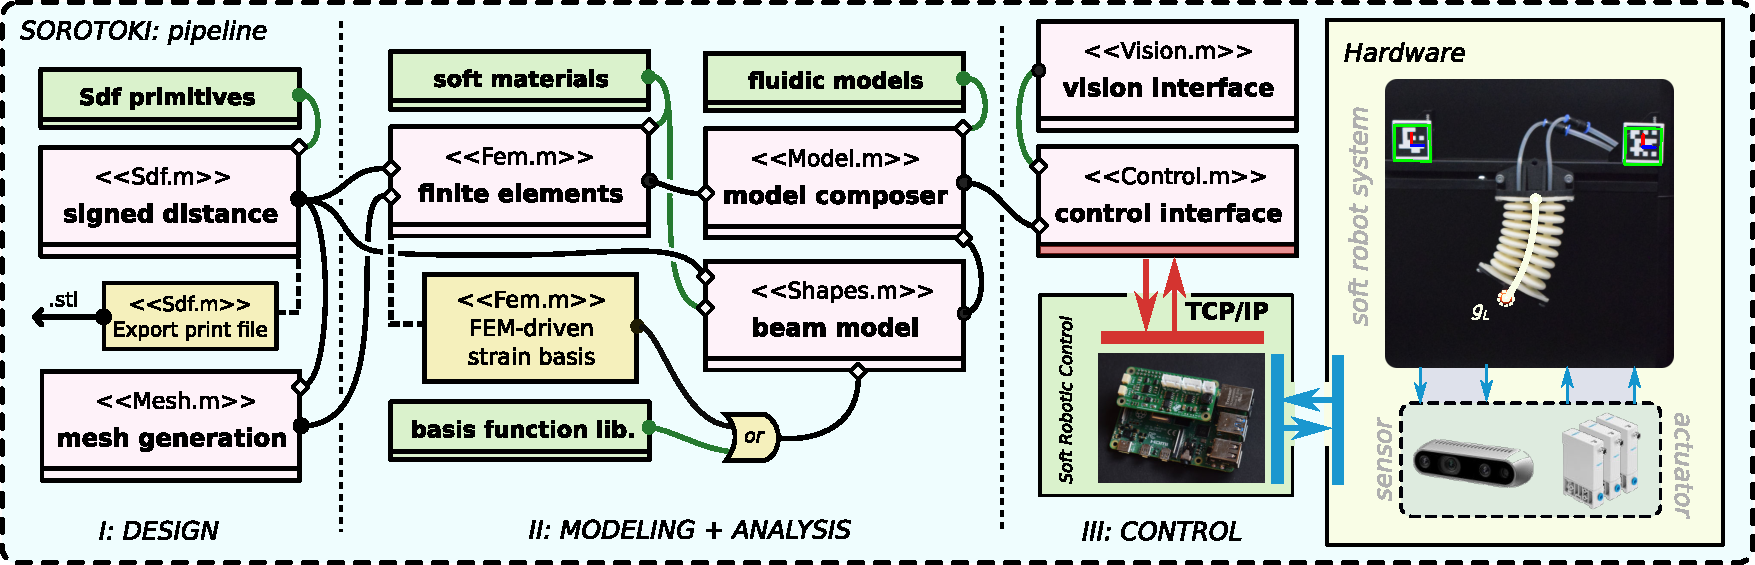
\includegraphics[width=0.955\textwidth]{./pdf/thesis-figure-6-2.pdf}    
\centering
\caption{\small The Sorotoki software toolkit is structured according to a problem-solution pipeline, consisting of seven Object-Oriented classes that address common subproblems in the field of soft robotics research. These classes are: \class{Sdf}, \class{Mesh}, \class{Fem}, \class{Shapes}, \class{Model}, \class{Control}, and \class{Vision}. The software architecture flowchart employs the symbol $(\bullet)$ to represent class outputs and the symbol $(\diamond)$ to denote inputs. It is important to note the interplay between these classes. \label{fig:C5:softwareArchitecture}}
\end{sidewaysfigure*}
%
\begin{itemize}
    \setlength\itemsep{0.0em}
    \item In Section \ref{sec:C5:sdf} we will discuss the class \code{Sdf}: a Signed Distance Function (SDF) class that are used to build spatial geometries --  \emph{``Implicit CAD''};
    \item In Section \ref{sec:C5:mesh} we will discuss \code{Mesh} responsible for mesh generation;
    \item In Section \ref{sec:C5:fem} we discuss the class \code{Fem}: a Finite Element Model (FEM) solver required for high-detail soft robot simulations;
    \item In Section \ref{sec:C5:shapes}, we detail the class \code{Shapes} responsible for soft beam models required for fast soft robot simulations;
    \item In Section \ref{sec:C5:model} we explain \code{Model} -- a model composer to interconnect various dynamic model, and the control synthesis;
    \item Following, in Section \ref{sec:C5:control}, we highlight \code{Control} that serves as a control interface for fluidic platform communicating to \textit{Matlab} via TCP/IP;
    \item Finally, Section \ref{sec:C5:vision} will explain \code{Vision} -- a Vision-based tool for state estimation of soft robots through optical markers.
\end{itemize}
%
To assist the reader, we have included a software architectural flowchart in Figure \ref{fig:C5:softwareArchitecture} that illustrates each class. The flowchart demonstrates how the classes can be interconnected to increase system complexity while maintaining the structured and separable nature of the subproblems. To further clarify their individual functionality, we will provide illustrative examples and corresponding MATLAB executable scripts. The topics covered include design, modeling and analysis, model reduction, and control and vision-based sensing, presented in this chronological order.
\subsection{Signed Distance Function (\texttt{Sdf})}
\label{sec:C5:sdf}
Signed Distance Fields (SDFs) have been widely applied in various areas of computer graphics, including the representation of implicit surfaces \cite{Reiner2011Jun, Chen2018Dec}, collision detection in robotics \cite{Ortiz2022Apr, Liu2022Mar}. In particular, SDFs have gained attention for their use in implicit modeling \cite{Smith2023Feb}, a technique for representing 3D shapes as continuous functions, rather than discrete mesh descriptions. 

In \textit{Sorotoki}, SDFs are implemented in the class \class{Sdf.m} and can be used to construct general 2D and 3D geometries. They can also be utilized to model static or dynamic contact environments, generate 3D models of soft actuators that are suitable for 3D printing, and compute inertia tensors for continuum bodies in $\mathbb{R}^2$ and $\mathbb{R}^3$. \\

\textbf{A: Implicit modeling using SDFs.} In this section, we briefly outline the mathematical foundations underpinning the \class{Sdf} class. As the name suggests, signed distance functions are a type of function that encodes distance information relative to an object defined implicitly. Adopting the notation used in \cite{Reiner2011Jun}, given a domain $\Omega \subset \mathbb{R}^n$ and its boundary $\partial \Omega$, these functions can be written in the following general form:
%
\begin{equation}
    \texttt{sdf}(\pB) = \begin{cases}
        -d(\pB,\Omega) & \textrm{if } \; \pB \in \Omega,                           \\
        +d(\pB,\Omega)  & \textrm{if } \; \pB \in \mathbb{R}^n\!\setminus\! \Omega,
    \end{cases}
    \label{eq:C5:sdf}
\end{equation}
%
where $d(\pB,\Omega):= \inf_{\yB \in \Omega} ||\pB - \yB||_2$ is a scalar function that returns the smallest Euclidean distance from a sample point $\pB \in \mathbb{R}^n$ to the boundary $\partial \Omega$. 
% It follows that,
% %
% \begin{align*}
%     \text{sign}[\texttt{sdf}(\pB)] & = 0  \quad\;\;\; \text{for}\; \pB \in \partial \Omega, \\[0.1em]
%     \text{sign}[\texttt{sdf}(\pB)] & = -1  \quad \text{for}\; \pB \in \Omega,               \\[0.1em]
%     \text{sign}[\texttt{sdf}(\pB)] & = 1  \quad\;\;\; \text{otherwise}.
% \end{align*}
%
SDFs provide a simple and efficient way of determining the location of a set of points relative to a domain $\Omega$ defined implicitly. The SDF is a scalar function that encodes the Euclidean distance of a sample point $\pB \in \mathbb{R}^n$ to the boundary $\partial \Omega$ of the domain. By evaluating the sign of the SDF, it is possible to classify the set of points as being within or outside the boundary of the domain. This enables set operations such as union, difference, and intersection to be performed. 

In the \texttt{Sorotoki} software package, these operations are implemented using Matlab's arithmetic operators between two or more instances of the \textit{Sdf} class, including '\texttt{+}' (union), '\texttt{-}' (difference), '\texttt{/}' (intersection), \texttt{*} (scaling), and '\texttt{.*}' (repeating). By utilizing these set operations and a library of basic SDF primitives, it is possible to construct a wide range of complex geometries with relative ease. Subsequently, the SDFs can be transformed into a \file{.stl} file using the Marching Cube algorithm \cite{Lorensen1987Aug}, enabling 3D printing. This functionality is implemented in the command \code{sdf.export}. \\

\begin{example}[Implicit CAD using SDFs]
To demonstrate the use of signed distance functions in \texttt{Sorotoki}, we present an example of 2D and 3D implicit modeling scheme as shown in Figure \ref{fig:C5:sdfexample}. This example illustrates the utilization of various SDF primitives, which are combined through standard set operations, such as union, difference, and intersection, to generate complex geometries. The accompanying code is provided below:
\end{example}

\begin{matlabcode}
%% EXAMPLE: Sdf class  
% generate 2D sdf 
c   = sCircle(1);
r   = sRectangle(1);
sdf = r.rotate(pi/4)-c;

% generate 3D sdf 
S1  = sSphere(0,0,1,0.5);
S2  = sSphere(0,0,0.5,1);
C   = sCube(0,1,0,1,0,1);
sdf = (C - S1)/S2;
\end{matlabcode}

\begin{figure}[!t]
\centering
\includegraphics*[width=0.495\textwidth]{./pdf/thesis-figure-6-3-1.pdf}
\includegraphics*[width=0.495\textwidth]{./pdf/thesis-figure-6-3-2.pdf}
%\input{./fig/fig_sdf.tex}
%\input{./fig/fig_sdf_3d.tex} \\[0.25em]
\caption{Exemplary functionality of the Signed Distance Function (Sdf) operators in \textit{Sorotoki}. The top figures are two-dimensional Sdfs, whereas below are three-dimensional Sdfs. \textit{Sorotoki} allows the user to combine Sdf using Matlab's arithmetics, like '\texttt{+}', '\texttt{-}', and '\texttt{/}', to perform unions, differences, and intersections, respectively. These set operations like union, difference, and intersect lead to new (differentiable) SDFs.\label{fig:C5:sdfexample}}
\vspace{-3mm}
\end{figure}

\textbf{B: SDF differentiablility}
Contrary to mesh-based geometries, signed distance functions (SDFs) possess closed-form differentials. Specifically, if $\Omega$ is a subset of $\mathbb{R}^n$ with piecewise smooth boundaries, the SDF is ($i$) differentiable almost everywhere, and ($ii$) its gradient satisfies $|\nabla \texttt{sdf}| = 1$. As a result, the unit-normal vector $\nB(\pB)$ pointing away from the boundary $\partial \Omega$ can be expressed as $\nB(\pB):= \nabla \texttt{sdf}(\pB)$. The gradient can be estimated using a finite-difference scheme:
%
\begin{align}
    \nB_{i}(\pB) \approx \frac{1}{\varepsilon} \Big[\texttt{sdf}(\pB + \varepsilon \vec{\delta}_{i}) - \texttt{sdf}(\pB) \Big],
\end{align}
%
where $\vec{\delta}_{i}$ is a vectorized Kronecker delta and $\varepsilon$ a small increment. 

In \textit{Sorotoki}, this finite difference routine is efficiently implemented such that the normal, tangent, and bi-normal vector computations can be called using \code{[N,T,B] = Sdf.gradient(p)}. These gradient vector computations are crucial for contact dynamics with the environment whose topology may be arbitrarily complex. The normal vector can also be useful in finding the closest-point projection onto the surface $\partial \Omega$, namely $\textrm{proj}_{\partial \Omega}(\mathbf{p}):= \mathbf{p} - \texttt{sdf}(\mathbf{p}) \cdot \nabla \texttt{sdf}(\mathbf{p})$. The projection operator is implemented as \code{[P,d] = Sdf.project(p)}, which takes a point cloud \code{p} and returns a point cloud \code{P} that is mapped onto the boundary of the SDF. It also returns the Euclidean distance $d(\mathbf{p},\partial \Omega)$ from the surface. This can be extremely useful in simulations of soft robotic grippers for grasping, or obstacle avoidance for soft manipulators.
\subsection{Mesh generation (\texttt{Mesh})}
\label{sec:C5:mesh}
In finite elements and computer graphics, mesh tessellation is a common language used to describe the structural geometry through a finite collection of vertices and edges. In \textit{Sorotoki}, meshes and mesh generation features are packaged into the class \texttt{Mesh.m}. In general, a mesh defines a discrete representation of a continuum body that is subdivided into smaller convex sub-volumes, referred to as "\textit{elements}". The nodal and elemental information are stored in data structures that can be accessed using \texttt{msh.Node} and \texttt{msh.Element}, respectively. For two-dimensional FEM problems, it is common to use linear elements such as $\texttt{Tri3}$ and $\texttt{Quad4}$ or quadratic elements like $\texttt{Tri6}$ and $\texttt{Quad8}$. For three-dimensional FEM problems, the common practice is to use hexahedron elements (\textit{i.e.}, \texttt{Hex8}) or tetrahedral elements (\textit{i.e.}, \texttt{Tet4} and \texttt{Tet12}). There are also polygonal tessellations, often denotes as \texttt{PolyN} finite elements \cite{Talischi2012Mar}. The \textit{Sorotoki} toolkit supports all of the above element types.
%
\begin{figure}[!b]
    \centering
    \includegraphics*[width=0.495\textwidth]{./pdf/thesis-figure-6-4.pdf}
    \includegraphics*[width=0.495\textwidth]{./pdf/thesis-figure-6-4.pdf}
    %\input{./fig/fig_mesh.tex} \\[0.35em]
    \caption{Example of mesh generation in \textit{Sorotoki}. The figure shows the evolution of an unstructured polygonal mesh based on Lloyd's algorithm. The colors relate to the relative element size with respect to the mean element size, given by \protect\colormapcaption{0}{.75cm}$\!\!\in [0,10]$ \si{\milli \meter \squared}. Notice that only after a few iterations, the centers of the Voronoi cells become homogeneously distributed within the meshing domain $\Omega$.}
    \label{fig:sorotoki:meshexample}
    \vspace{-3mm}
\end{figure}

\textbf{A: Mesh generation from SDFs.} The \textit{Sorotoki} toolkit explores several routines for mesh generation, which are all contained in the class \texttt{Mesh.m}. Our primary focus is on using a modified version of the \textit{PolyMesher} software developed by Talischi et al. \cite{Talischi2012Mar}. Their work provided a stable foundation for generating unstructured meshes of \texttt{PolyN} elements. The approach starts by defining a material domain implicitly using SDFs (as discussed in Section \ref{sec:C5:sdf}). The number of elements is chosen a priori, and then repeated random sampling of Equation \eqref{eq:C5:sdf} is performed until the number of samples that fall within the specified domain matches the number of elements. A bounded Voronoi diagram is generated using the samples and the centers of the Voronoi cells are updated using Lloyd's algorithm \cite{Lloyd1982Mar}. To generate a mesh from an \texttt{Sdf} class, one can call \texttt{msh = Mesh(Sdf)} followed by \texttt{msh = msh.generate()}.  \\

\begin{example}[Meshing of SDFs]
We provided a mesh generation example in Figure \ref{fig:sorotoki:meshexample} where we used the SDF function from the previous example to generate our tessellation. The code is given below
%
\begin{lstlisting}[style=matlab] 
 %% EXAMPLE: Mesh class 
 %  generate sdf mesh domain 
 c   = sCircle(1);    
 r   = sRectangle(1);  
 sdf = r.rotate(pi/4)-c; 
    
 % sdf conversion to mesh 
 msh = Mesh(sdf,'NElem',150);
 msh = msh.generate();
\end{lstlisting}
%
In Figure \ref{fig:sorotoki:meshexample}, we see the evolution of the Voronoi cells that produce the \texttt{PolyN}-type mesh. Observe that after a few iterations of Lloyd's algorithm, the centroids are distributed homogeneously over the compact domain $\Omega$ (as shown by the color distribution).
\end{example}
%
\textbf{B: Mesh from common file formats} An alternative option is to use the mesh generation tools provided by the \textit{Partial Differential Toolbox} in Matlab. Such function is also included in the \code{Mesh.generate()} routine. SDFs can also be used in this process, although an intermediate step is required. For two-dimensional domains, SDFs are first converted into binary images and then the image boundary detection is used to convert them to either a linear mesh (\texttt{Tri3}) or a quadratic mesh (\texttt{Tri6}). Direct input of black-and-white \file{.jpg} or \file{.png} images is also supported. For three-dimensional domains, SDF functions are converted to an \file{.stl} file using the Marching Cube algorithm \cite{Lorensen1987Aug} and then provided to the Matlab PDE toolbox to generate the tessellation. Importing \file{.stl} or \file{.obj} files directly is also possible. Meshes can also be export
\subsection{Finite element modeling (\texttt{Fem})}
\label{sec:C5:fem}
Following the mesh generation process, \textit{Sorotoki} offers a nonlinear finite element solver for both quasi-static and fully dynamic simulations. An illustration of the FEM approach is given in Figure \ref{fig:C5:illustration_FEM}. FEM-based tools are crucial when describing large deformations in soft robots, which also accounts for hyperelastic materials and geometric nonlinearities. The FEM package is provided in a class called \class{Fem.m} and can be instantiated using \code{fem = Fem(Mesh)}. This class serves two main purposes: ($i$) to solve static or dynamic continuum problems with high accuracy, and ($ii$) to solve gradient-based optimization problems, also known as inverse design problems. It is important to note that, unlike \textit{SOFA}, the focus of \textit{Sorotoki} is on high-detail simulations rather than real-time implementation for control. The presented FEM simulation models are not intended for real-time applications, but rather for system identification and analysis.

\begin{figure}
\centering
%FemExample
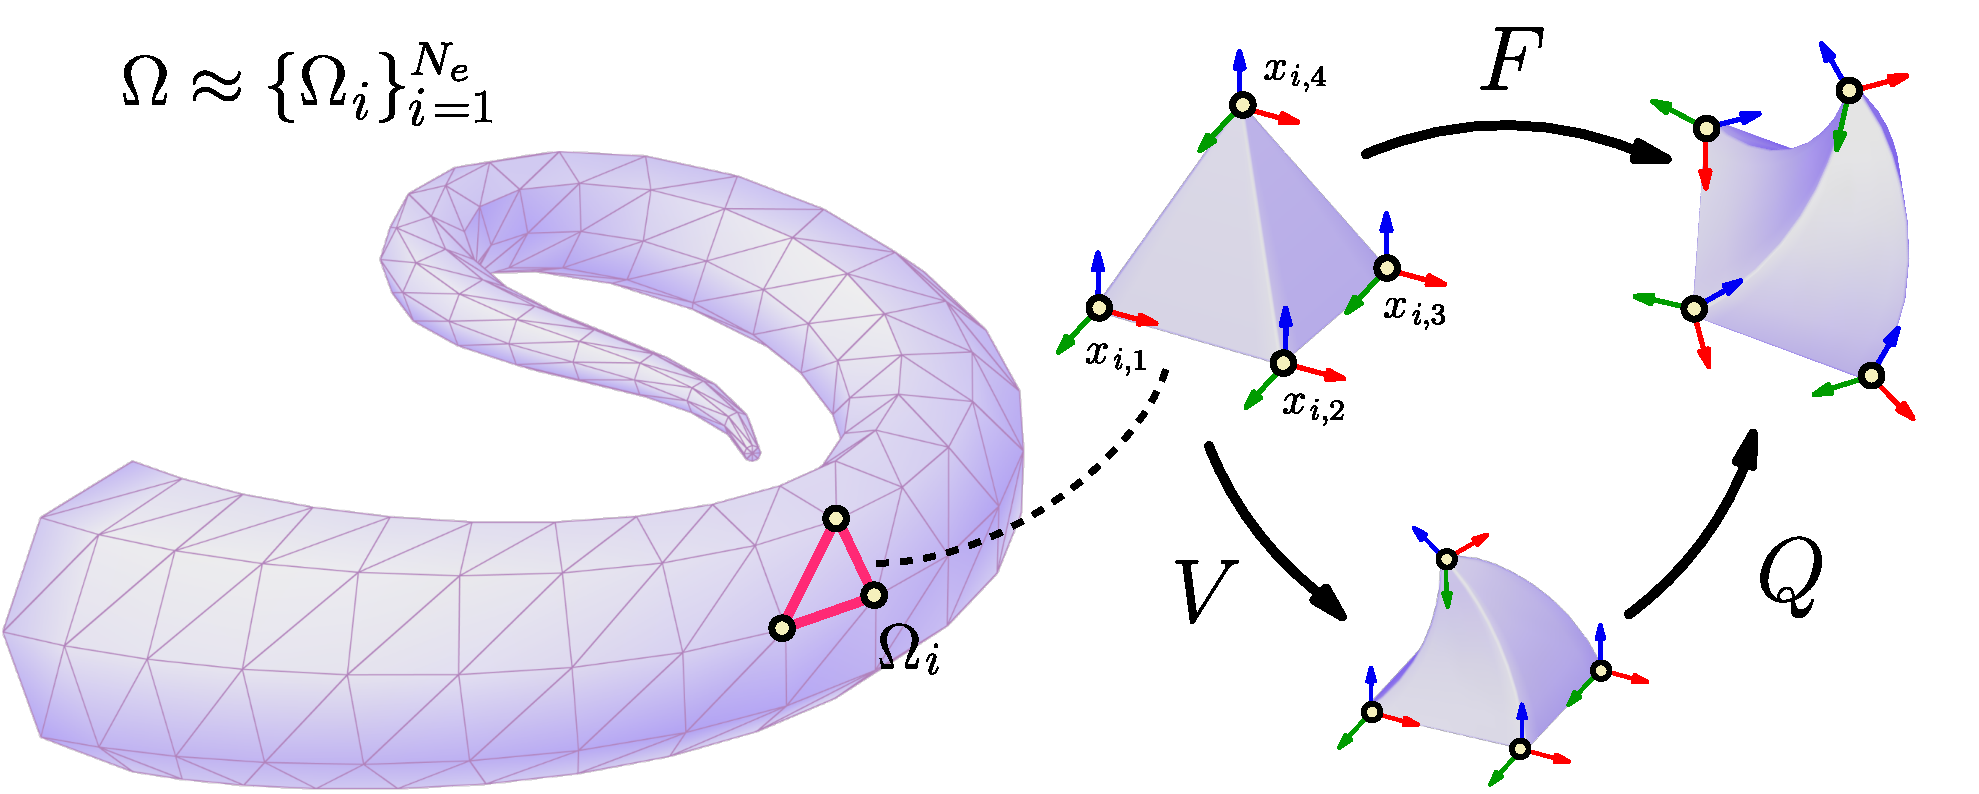
\includegraphics[width=0.85\textwidth]{./pdf/FemExample.pdf}
%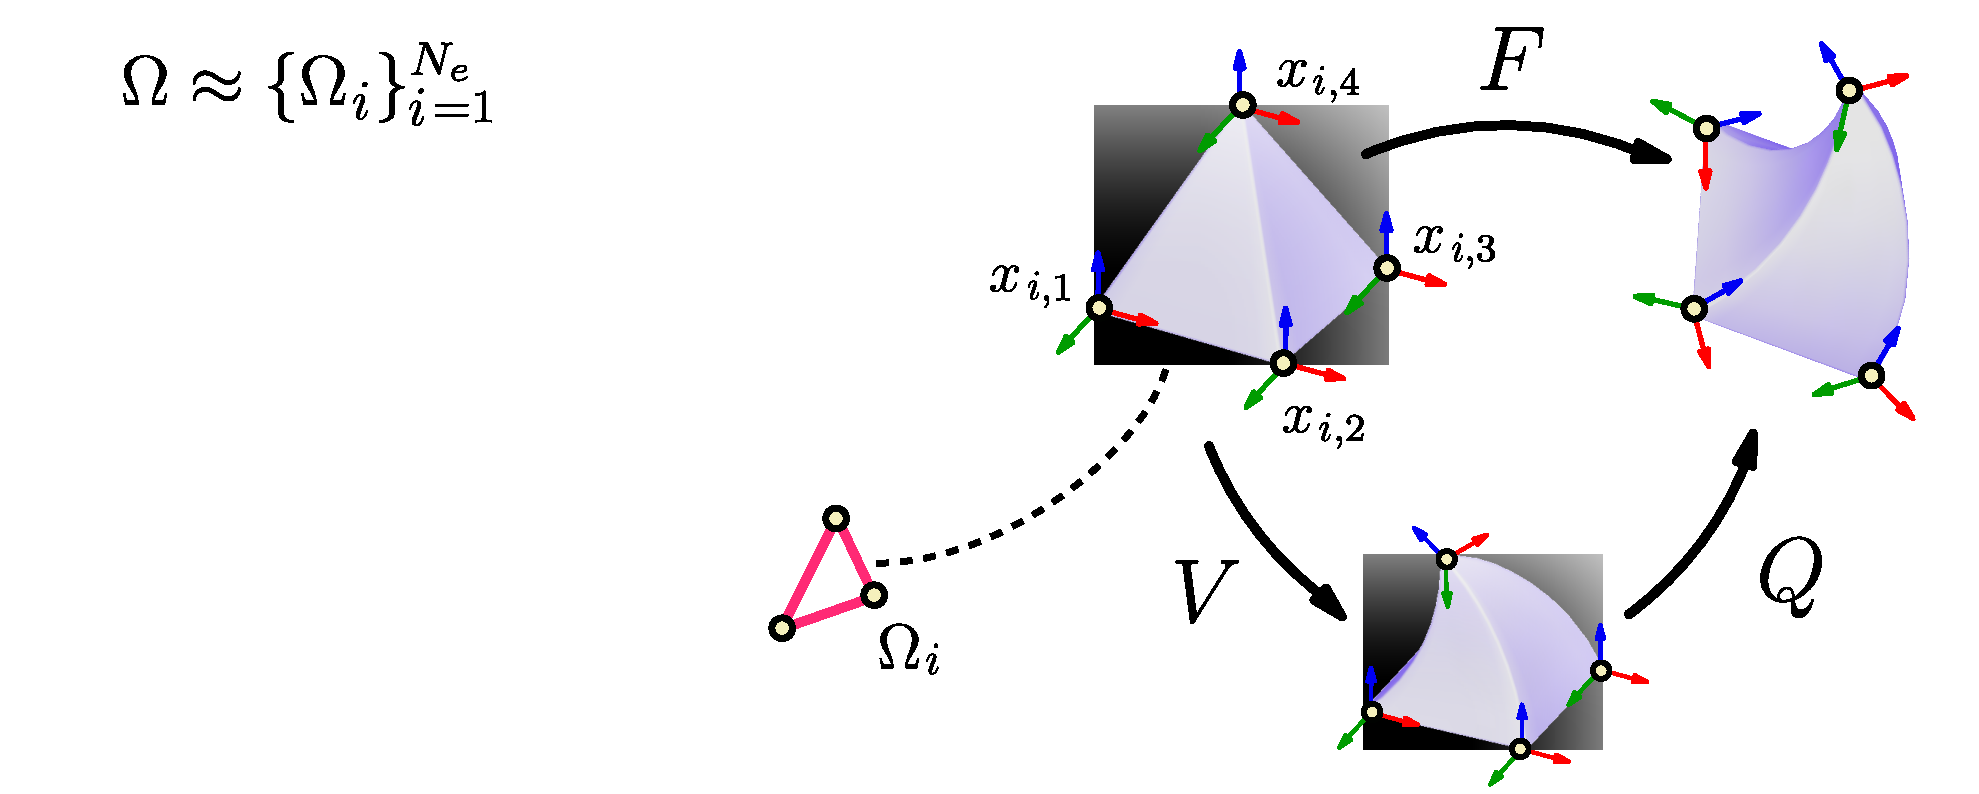
\includegraphics[width=0.85\textwidth]{./pdf/thesis-figure-6-5.pdf}
\caption{Illustration of the Finite Element Method (FEM), where a solid geometry $\Omega$ is subdivided into $N_e$ finite elements $\Omega_e$. Each element has $\dim(\x_e)$ DOFs, which allows the computation of the deformation gradient $\FB$. The deformation gradient can be decomposed into $\FB = \QB\VB$, an isochoric deformation part $\VB$ and rigid-body rotation part $\QB$. }    
\label{fig:C5:illustration_FEM}
\end{figure}

\textbf{A: High-detail finite element model.} The nonlinear dynamics of the finite element model in \textit{Sorotoki}, similar to \textit{SOFA} and \textit{Gibbon}, can be described by the general Newton-Euler equation of motion:
%
\begin{equation}
    \MB \ddx + \fB_\textrm{mat}(\x,\dx) + \fB\grav = \fB_{\textrm{u}}(\x,\uB,t) + \fB_{\Omega_{\textrm{env}}}(\x,\dx,t),
    \label{eq:C5:femmodel}
\end{equation}
%
where $\x$, $\dx$, and $\ddx$ are the global nodal displacement, velocities and accelerations of the mesh tesselation, respectively; $\MB$ the constant generalized mass matrix, $\fB_\textrm{mat}$ the internal soft material forces, $\fB_\textrm{g}$ the constant gravitational forces, $\fB_u$ a user-defined input, and $\fB_{\Omega_{\textrm{env}}}$ the normal reaction forces and tangent friction forces imposed by the dynamic contact with a (possibly time-dependent) environment $\Omega_{\textrm{env}}$. The environment $\Omega_{\textrm{env}}$ can be described using the SDF functionality (see Section \ref{sec:C5:sdf}) using the syntax \code{fem.addContact(sdf)}. A broad collection of generalized external inputs can be added using: \code{fem.addLoad}, \code{fem.addDisplace}, \code{fem.addGravity}, and \code{fem.addTendon}. Time-varying pressure inputs can be added using the command \code{fem.addPressure}. 

Without loss of generality, the material force can be decomposed into a position-dependent and velocity-dependent part: $\vec{f}_{\textrm{mat}}(\vec{x},\dot{\vec{x}}) = \vec{f}_{\textrm{e}}(\vec{x}) + \vec{f}_{\textrm{d}}(\dot{\vec{x}})$, \ie, an elastic and dissipation contribution, respectively. We assume that the dissipation is given by $\vec{f}_{\textrm{d}} = \zeta \mathbf{M} \dot{\vec{x}}$ with damping coefficient $\zeta > 0$. Materials can be assigned using \code{fem.addMaterial}. Note that the conservative elastic material forces $\vec{f}_{\textrm{e}}$ require more involved computation. Since this computation is not straightforward, we briefly explain the derivation of the nonlinear hyper-elastic material forces in \eqref{eq:C5:femmodel}, which follows standard nonlinear finite element procedures \cite{Kim2018,Holzapfel2002,Smith2018}. \\

\begin{intermez}[Deformation gradient]
\vspace{-3mm}
A fundamental measure of deformation in continuum mechanics is the deformation gradient, denoted by $\mathbf{F}$. The deformation gradient characterizes the local deformation for a neighborhood of the continuum body $\Omega$. Since a subvolume of the continuum body cannot be reduced to a point, it follows that $\det{\mathbf{F}} = J > 0$ and $\mathbf{F}^{-1}$ exists. The term $J$ is called the relative volume change and it is equal to 1 for isochoric deformations, such as rigid body deformations. Given these properties, the deformation gradient can then be factorized into $\mathbf{F} = \mathbf{Q} \mathbf{V}$, where $\mathbf{V} \succ 0$ is the right-handed stretch tensor and $\mathbf{Q} \in \mathrm{SO}(3)$ is a rotation matrix belonging to the special orthogonal group \cite{Holzapfel2002,Kim2018,Smith2018}. For convenience, we summarize the derived quantities of $\mathbf{F}$ in Table \ref{tab:C5:strain_measures} that will be used throughout this section. \\
\end{intermez}

\begin{table}
    \setlength{\tabcolsep}{2.25pt}
    %\rowcolors{1}{}{lightgray}
    \centering
    \caption{Table of deformations measures relevant for continuum mechanics problem. All measures can be related to the first-order deformation tensor $\FB$, following the works  \cite{Holzapfel2002,Kim2018,Smith2018}.}
    \label{tab:C5:strain_measures}
    \rowcolors{1}{}{blue!5}
    \begin{tabular}{ll}
        \hline
        Deformation measure       & \quad \; Derivation                                                     \\
        \hline \hline
        Relative volume change    & \quad \; $J = \det{\FB}$                                                \\
        Polar decomposition       & \quad \; $\FB = \QB \VB$                                                \\
        Right Cauchy-Green tensor & \quad \; $\CB = \FB^\top \FB$                                           \\
        First strain invariant    & \quad \; $I_1 = \trace(\CB)$,                                           \\
        Second strain invariant   & \quad \; $I_2 = \frac{1}{2}\left[ \trace(\CB)^2 - \trace(\CB^2)\right]$ \\
        First strain invariant    & \quad \;\ $I_3 = \det{\CB}$                                             \\
        \hline
    \end{tabular}
\end{table}
%
\begin{intermez}[Derivation of hyperelastic forces]
    
Let $\Omega_i$ denote the subspace spanned by the $i$-th element of the finite element mesh, and let $\x_i$ denote its nodal displacement vector. The elasticity of the constitutive soft material can be described by a strain-energy density function $\Psi: \FB \to \R_{\ge 0}$. A comprehensive discussion on common constitutive models for $\Psi$ will be provided later in the subsequent paragraph. The elastic potential energy of the continuum body is given by $\mathcal{U}_e = \int_\Omega \Psi(\cdot) \; dV$, and the conservative hyper-elastic force contribution can be computed as $\fB_e := \nabla_{\x}\,\mathcal{U}_e$. This contribution can be approximated using piecewise finite element interpolation and integrated using the Gauss quadrature rule \cite{Kim2018} as follows:
    %
    \begin{align}
        \fB_\textrm{e}(\x) & = \sum_{i=1}^{N_e} \frac{d}{d\x_i} \left\{\int_{\Omega_i} \Psi(\FB(\x_i,s)) \; ds\right\}, \notag                                                    \\
                           & \approx \sum_{i=1}^{N_e} \sum_{j=1}^{N_w} w_j \, \underbrace{\frac{\p \Psi}{\p \FB}(\FB(\x_i,s_j)) }_{\textrm{PK1}} \frac{\p \FB}{\p \x_i}(\x_i,s_j)
        \label{eq:C5:fem_hyper}
    \end{align}
    %
where the Gauss weights are denoted by $w_j > 0$, and the number of finite elements and Gauss samples are represented by $N_e$ and $N_w$, respectively.

The term $\frac{\partial \Psi}{\partial \FB}$ is also referred to as the first Piolla-Kirchhoff (PK1) stress tensor, which can be represented in closed-form for many constitutive models. The term $\frac{\partial \FB}{\partial \x_e}$ denotes the deformation Jacobian, which can also be given in closed-form but depends on the choice of element type. In addition to the first Piolla stress tensor, we also introduce the Cauchy stress tensor (i.e., true stress) $\vec{\sigma} := J^{-1} \frac{\partial \Psi}{\partial \FB} \FB^\top$, which is a symmetric second-order tensor whose components represent the true stress. It should be noted that these tensor calculations are highly nonlinear, making their computation the most time-consuming aspect of the finite element assembly. To enhance computational efficiency, the toolkit employs \texttt{.mex} executable code that is generated during installation (\texttt{Matlab Coder} toolkit is required).
\end{intermez}

%\subsubsection{Hyperelastic models and soft material presets}
%\label{sec:C5:hyperelastic}
\textbf{B: Hyperelastic models and soft material presets.} An important aspect of soft robotics in general is to accurately describe large nonlinear deformations of inertial continuum bodies in motion. Yet, due to these large deformations, many classical Hookean elasticity models may not be accurate for elastomer materials. 

To address this, \textit{Sorotoki} provides a library of hyper-elastic constitutive material models: Neo-Hookean (NH), Mooney-Rivlin (MR), and Yeoh model (YH). The strain energy densities for these models are derived based on the strain invariants $I_1$, $I_2$, and $I_3$ provided in Table \ref{tab:C5:strain_measures} and are shown in Table \ref{tab:C5:elasticitymodels}.
%
\begin{table}[t]
    \renewcommand\arraystretch{1.25}
    \setlength{\tabcolsep}{2.25pt}
    \rowcolors{1}{}{blue!5}
    %\rowcolors{1}{}{lightgray}
    \centering
    \caption{Table of material models included in \textit{Sorotoki}, including the NeoHookean model (NH), Mooney-Rivlin model (MR), and Yeoh (YH) model.}
    \label{tab:C5:elasticitymodels}
    \begin{tabular}{lcl}
        \hline
        Material model     & \;\;Parameters\;\; & \quad \;\; Energy-density potential $\Psi$                                     \\
        \hline \hline
        Neo-Hookean (NH)   & $(\mu)$            & \quad \;\; $\Psi_{\textrm{NH}} := \frac{\mu}{2} \left(I_1 - 3 \right)$         \\
        Mooney-Rivlin (MR) & $(c_1,c_2)$        & \quad \;\; $\Psi_{\textrm{MR}} := \sum^{2}_{i=1} c_i \left(I_i - 3 \right)$    \\
        Yeoh (YH)          & $(c_1,c_2,c_3)$    & \quad \;\; $\Psi_{\textrm{YH}}  := \sum^{3}_{i=1} c_i \left(I_1 - 3 \right)^i$ \\
        \hline
    \end{tabular}
\end{table}
%
The material models presented in Table \ref{tab:C5:elasticitymodels} are implemented in \textit{Sorotoki} under the class \class{Material}, but have specific constructors tailored towards each material, \texttt{NeoHookeanMaterial}, \texttt{MooneyMaterial}, and \texttt{YeohMaterial}. Regarding their parameters, the work of Marechal et al. \cite{Marechal2021Jun} provides an open-source database that includes a broad collection of soft materials commonly used in soft robotics, gathered through uniaxial material tests. Based on their dataset and relevant other literature \cite{Xavier2022Jun,Smith2018,Kim2018,Goury2018}, \textit{Sorotoki} offers some preset material models of soft materials commonly used in soft robotics, such as the Ecoflex30/50 series, Dragonskin10/30 series, NinjaFlex, and Formlabs Elastic50A/80A material. These material classes also include the physical data for density, viscosity, and tangential contact friction. Following \eqref{eq:C5:fem_hyper}, the first Piola-Kirchhoff (PK1) stress tensor is evaluated analytically using the function call \code{P = Material.PiollaStress(F)}.  \\
%

\textbf{C: Finite element solvers and (nonlinear) modal analysis}
To solve the structural forward dynamics of the system \eqref{eq:C5:femmodel}, the toolkit uses an implicit Newmark-$\beta$ solver \cite{Newmark1959Jul}, which is briefly outlined in Appendix \ref{app:C5:newmark}. Implicit solvers offer improved stability compared to explicit methods, such as the Runge-Kutta solver (\texttt{ode45}), particularly when larger time steps are employed. However, the cost of larger time steps is a decreased numerical precision.  Alternatively, for quasi-static problems when $\ddx = \dx = \vec{0}_n$, we aim to seek the solutions to the static force equilibrium $\rB(\x) = \vec{0}_n$ where $\rB := -\fB_{\textrm{mat}} + \fB\grav + \fB_\textrm{u} + \fB_{\Omega_{\textrm{env}}}$ is the force residual vector. The nonlinear equality for nodal displacements $\x$ is solved using an iterative Newton-Raphson solver. To call these solvers, dynamic simulations are executed with \code{fem.simulate()} and quasi-static simulations with \code{fem.solve()}. Upon completion of a simulation, all displacements, velocities, forces, and stress information are stored in the \code{fem.Log} data structure. This log file can be accessed for data analysis or during simulation to facilitate state feedback control.

Alternatively, we can explore nonlinear modal analysis at any quasi-static equilibrium configuration $\x^* \in \mathcal{X}$ of the system \eqref{eq:C5:femmodel}. Let $\KB_T:= \left[\frac{\p \fB\elastic}{\p x_1} \;\hdots\; \frac{\p \fB\elastic}{\p x_2} \right]$ be the Jacobian matrix of the (nonlinear) elastic potential forces, also referred to as the tangent stiffness. Then, the local eigenvalue problem for the linearized FEM model around the point $\x^*$ is given by 
%
\begin{equation}
\Big[\KB_T(\x^*)- \lambda_i \MB \Big] \thetaB_i = \vec{0}_n,
\label{eq:C5:eigenmode_decomposition}
\end{equation}
%
where $\lambda_i$ is a real scalar eigenvalue and $\thetaB_i$ is its corresponding eigenmode. The dynamic analysis is implemented in Sorotoki using \code{fem = fem.analysis(x)}, which stores the necessary data in \code{fem.Log}. It is important to note that, unlike linear finite element models, the set of eigenmodes ${\thetaB_i}$ obtained from the eigenvalue decomposition in \eqref{eq:C5:eigenmode_decomposition} is highly dependent on the linearization point $\x^*$ and may thus not be unique for all $\x^* \in \mathcal{X}$.

\begin{example}[Nonlinear buckling analysis via decomposition]
%\subsubsection*{Example C1: Nonlinear buckling analysis via decomposition}
An excellent case study of the eigenvalue problem in nonlinear elasticity systems is the buckling behavior of patterned elastomer metamaterials, as studied by Bertoldi et al. \cite{Bertoldi2008} and later by Overvelde et al. \cite{Overvelde2012May}. In their studies, an elastomer specimen with a periodic circular porous structure was subjected to uniaxial compression. The specimen displayed an inward buckling phenomenon at a critical loading point, resulting in the specimen exhibiting a negative Poisson ratio, \ie, auxetic behavior. To be specific, the structure undergoes a so-called "bifurcation" where solutions switch stability or new solutions arise for a critical parameter value. In this case, the bifurcation parameter is the compression ratio $\varepsilon$.

In accordance with \cite{Overvelde2012May}, a square elastomer specimen with circular holes was modeled using a Neo-Hookean material model, with Young's modulus $E = 19$ (\si{\kilo \pascal}) and Poisson ratio $\nu = 0.45$. As reported in \cite{Overvelde2012May}, the critical buckling point was observed to occur at approximately $\varepsilon = -12.5\%$ uniaxial compression.

\begin{figure}[!t]
    \centering
\includegraphics*[width=0.95\textwidth]{./pdf/thesis-figure-6-6-1.pdf} \\[0.5em]
\includegraphics*[width=0.95\textwidth]{./pdf/thesis-figure-6-6-2.pdf}
    %\input{./fig/fig_bucklemode_linear.tex}
%\input{./fig/fig_bucklemode_nonlinear.tex}
\caption{Nonlinear buckling mode analysis of periodic circular porous elastic structure inspired by \cite{Bertoldi2008,Overvelde2012May}. The horizontal displacements are indicated by \protect\colormapcaption{0}{.75cm}$\!\!\in [-5,5]$ \si{\milli \meter}. (top) The first four eigenmodes of the elastomer structure for $\varepsilon = 0\%$ compression, no buckling modes appear. (bottom)  The first four eigenmodes for $\varepsilon = 12.5\%$ compression. Notice that the first mode $\thetaB_1$ is a buckling mode where the collapses holes orient periodically either vertically or horizontally. }
\label{fig:C5:fig_bucklemode}
\vspace{-3mm}
\end{figure}

A numerical solution is obtained through quasi-static analysis using the function \code{fem.solve}. To model compression, a displacement load was added using \code{fem.addDisplace('Top')}. The resulting equilibrium configuration was then utilized in the eigenvalue problem via the function \code{fem.analysis(x)}. The eigenmodes for the zero-stress and $\varepsilon = -12.5\%$ compression cases are illustrated in Figure \ref{fig:C5:fig_bucklemode}. It is worth noting that the first three eigenmodes of the elastomer structure at $\varepsilon = 0\%$ compression exhibit no buckling modes. Conversely, the first eigenmode $\thetaB_1$ at $\varepsilon = -12.5\%$ compression displays a buckling mode, wherein the collapse of the holes is periodically oriented either vertically or horizontally. This buckling mode is in accordance with the experiments from \cite{Overvelde2012May} and \cite{Bertoldi2008}. The supplementary code is provided below: 
\end{example}
%

\begin{matlabcode}
%% EXAMPLE: Fem class 
load('sdf_porous_square.mat');
msh = Mesh(sdf, 'NElem', 5e3);
fem = Fem(msh, 'TimeStep', 1/60);

% assign material 
fem.Material = NeoHookeanMaterial(1.0, 0.45);

% add displacement and forces 
fem = fem.addConstraint('Bottom', [1,1]);
fem = fem.addConstraint('Top', [1,0]);
fem = fem.addDisplace('Top', [0,-0.125 * W]);

%  quasi-solve and eigen-analysis 
fem = fem.solve();
fem = fem.analysis( fem.Log.x(:,end) );
\end{matlabcode}
    

\begin{example}[Locomotion dynamics of soft crawling robot]
To demonstrate a dynamic finite element method (FEM) simulation that incorporates contact, we will utilize \sorotoki to model the locomotion of a multi-gait soft robot crawler inspired by the work of Shepard \cite{Shepherd2011Dec}. The study by Shepard  et al. \cite{Shepherd2011Dec} presents a soft robot system that consists of five pressure chambers - four for each leg and one for the spine. The pressure chambers are actuated in a sequential manner to produce an undulating motion. The work of Shepard  et al. \cite{Shepherd2011Dec} demonstrates that complex locomotion can be achieved through the use of open-loop controllers and the dynamic interaction between the soft robot and its environment.

To simplify the model, we assume general plane motion. The geometry of the soft crawler's cross-section is first provided to \texttt{Mesh.m} to generate a triangular mesh. Then, a finite element method (FEM) model is generated, with the material model \texttt{fem.Material = Ecoflex0030}. To model the environment, the function \texttt{fem = fem.addContact(sLine)} is utilized, which simply creates an unbounded horizontal line. In accordance with \cite{Shepherd2011Dec}, a harmonic excitation is applied to each chamber, as expressed by the following: $u_i = A\cdot\textrm{sat}\left[\sin(\omega t - \phi_i) \right]$, where the index $i \in {1,2,3}$ represents the front, middle, and back pressure chambers embedded in the soft body. 

\begin{matlabcode} 
%% EXAMPLE: Fem class   
msh = Mesh('MultiGait.png', 'MeshSize', 1.0, ...
            'BdBox', [0, 150, 0, 12]);

% -- mesh to fem 
fem = Fem(msh,'TimeStep',1/500);
fem.Material = Ecoflex50();

% -- add inextensible bottom layer 
E1  = fem.findElements([0 150 0 2]);
fem = fem.addMaterialModifier(E1, 5);

% -- add forces and constraints 
fem = fem.addGravity();
fem = fem.addContact(sLine());

Y = 'BoxSelect';
for i = 1:3
    Ce = fem.findEdges(Y,[50*(i-1), 50*i, 0, 15]);
    fem = fem.addPressure(Ce, @(x) Pressure(x,i));
end

% -- solve dynamics 
fem = fem.simulate();

% -- open-loop controller 
function y = Pressure(fem, i)
    phi = pi / 3 * (i - 1);
    y = clamp(sin(5*pi*fem.Log.t - phi), 0, Inf);
end
\end{matlabcode}
\vfill
The excitation signal parameters are set as follows: $A = 45$ \si{\kilo \pascal}, $\omega = 5 \pi$ \si{\radian}, and $\phi_i = \frac{\pi}{3} \cdot (i-1)$ \si{\radian}. The saturation function is defined as $\textrm{sat}(x) = 0$ for $x < 0$, and $\textrm{sat}(x) = x$ for $x \geq 0$. Gravitational acceleration is added, and the dynamic simulation solver is invoked using \texttt{fem.simulate}. Figure \ref{fig:C5:fem_example_crawl} presents a comparison between the soft robot described in \cite{Shepherd2011Dec} and the dynamic simulation performed by \texttt{Sorotoki}.

The results of the simulation performed using \textit{Sorotoki} show a morphological behavior that is consistent with the experimental recordings. Figure \ref{fig:C5:fem_example_crawl_com} depicts the trajectory of the center of mass (CoM) of the soft robot during the undulating locomotion. Note that an identical stair-like evolution of the CoM is also observed in the work of Shepard et al. \cite{Shepherd2011Dec}. 
\vfill
\end{example}

% \begin{figure}
% %\includegraphics[width=0.485\textwidth]{./fig/PipelineCrawler.pdf}
% \caption{Overview of the software pipeline showing the interconnected classes required to simulate the soft crawler with environmental contact.}    
% \label{fig:C5:PipelineCrawler}
% \vspace{-5mm}
% \end{figure}
%

\afterpage{
\begin{sidewaysfigure*}[t]
\vspace{-5mm}
\centering
\includegraphics*[width=\textwidth]{./pdf/thesis-figure-6-8-1.pdf}
\includegraphics*[width=\textwidth]{./pdf/thesis-figure-6-8-2.pdf}
%\input{./fig/fig_fem_example_crawl_true.tex}
%\input{./fig/fig_fem_example_crawl.tex}
\caption{(top) Experiment of soft multi-gait crawling soft robot developed by Shepard et al \cite{Shepherd2011Dec} performing an undulating forward motion by periodic pressurizarion of its internal pressure chambers, back legs $\to$ middle $\to$ front legs. The soft robot is made from an elastomer material with strain-inhibit layer at the bottom to enhance bending. The Von Mises stresses are shown as \protect\colormapcaption{0}{.75cm}$\!\!\in [0,10]$ \si{\mega \pascal}. (bottom) Simulation recreation of the experiments performed by Shepard et al \cite{Shepherd2011Dec} using the Finite Element solver in the \sorotoki toolkit. Images sourced from public resources, with intellectual property belonging to cited authors, sources, and publishers. }
\label{fig:C5:fem_example_crawl} 
\vspace{5mm}
\includegraphics*[width=0.85\textwidth]{./pdf/thesis-figure-6-9-1a.pdf} 
%\includegraphics*[width=0.85\textwidth]{./pdf/thesis-figure-6-9-2a.pdf}
\caption{(top) Numerical simulation of the center of mass displacement and gait for undulating soft crawler. The horizontal displacement is given by \data{Matlab1}, and the vertical displacement as \data{Matlab2}. (bottom) The gait cycle of the soft crawler where the sequence $\{$\ldata{Matlab1}, \ldata{Matlab2}, \ldata{Matlab3}$\}$ shows the fluidic activation. }
\label{fig:C5:fem_example_crawl_com}
%\vspace{-5mm}
\end{sidewaysfigure*}
\clearpage
}

\textbf{Gradient-based computational (inverse) design}
Besides modeling, the field of computational inverse design can also benefit from the use of FEM models. Building up the \class{Fem} class, the objective is to find a topological structure of a continuum system based on a desired deformations or compliance. One widely adopted method is the Solid Isotropic Material with Penalization (SIMP) approach, which is a commonly used material interpolation technique in topology optimization \cite{Bendsoe2003}. In the SIMP method, each finite element $e \in \{1,2,...,n_e \}$ is assigned a continuous density variable $\rho_e \in (0,1]$, which serves as an indicator of the material distribution within the mesh. If $\rho_e = 1$, the element is considered solid, while if $\rho_e = 0$, the element is considered void. This assignment of density variables enables the modification of the strain energy density in \eqref{eq:C5:fem_hyper}:
%
\begin{equation}
\tilde{\Psi}_{e} = \left[ \varepsilon + (1-\varepsilon){\rho_e}^p \right] \Psi,
\end{equation}
%
where $0 < \varepsilon \ll 1$ a lower bound on the densities, and $p > 1$ a penalty factor for penalizing intermediate densities during the optimization process. By collecting the density values $\vec{\rho} = \textrm{col}\{\rho_1,\rho_2,...,\rho_{N_e}\}$, the inverse design problem can be formulated in terms of two unknowns: the displacement field $\xB$ and the density field $\vec{\rho}$. Consequently, the computational design problem for general soft material structures can be expressed as a nonlinear topology optimization problem of the following form:
%
\begin{mini}[2]
    {\vec{\rho}}{\Phi = -\beta_1\, \LB^\top\!\x \;+\; \beta_2 \fB\elastic^\top \! \fB_{\textrm{u}} }{}{}
    \addConstraint{\tilde{\rB}(\xB,\vec{\rho})=0,}{}{}
    \addConstraint{\vec{v}^\top \vec{\rho}\le v^\star,}{}{}
    \addConstraint{\vec{\rho}\in \mathcal{P},}{}{}
    \label{eq:C5:topo_optimization}
\end{mini}
%
where $\LB$ a sparse unit-vector composed of nonzero entries for the degrees-of-freedom corresponding to the desired morphology of the soft robot, $\vB$ the element volumes, $v*$ the desired volume infill, $\mathcal{P} = \left\{ \vec{\rho} \in \R^{n_e} ~|~  0 < \rho_i \le 1\right\}$ admissible set for the design variables, and $\beta_1$ and $\beta_2$ are positive scalars that can be adjusted to vary the optimization problem, with $\beta_1 \ll \beta_2$ resulting in compliance minimization and $\beta_1 \gg \beta_2$ leading to a compliant mechanism. To solve the optimization problem in Equation \eqref{eq:C5:topo_optimization}, we utilize the Method of Mixed Asymptotes (MMA) proposed by Svanberg \cite{Svanberg1987Feb,Svanberg2007}. Earlier work on this computational design approach was presented in Chapter \ref{chap: design}, and the chapter is referred to this work for the analytic gradients required for the MMA solver.

The optimization routine in the \textit{Sorotoki} framework is incorporated into the \code{Fem} class and can be invoked by utilizing the command \code{fem.optimize('type')}, where \code{'type'} represents the optimization problem at hand. For minimizing compliance, the cost function is self-adjoint \cite{Bendsoe2003}, hence objective function and constraints are linear operators. However, when dealing with compliant mechanisms, it is necessary to specify the selection vector $\LB$, which can be defined using the \code{fem.addOutput(id)} command. The value of \code{id} represents the nodal indices of interest, which can be identified using the \code{fem.Mesh.findNode} functionality.



\subsection{Reduced-order soft beam models (\texttt{Shapes})}
\label{sec:C5:shapes}
While the finite element method (FEM) is known for producing reliable and highly accurate results, its high-dimensional state can make it computationally slow, making direct applications for closed-loop control challenging. To address this issue, the Sorotoki toolkit offers reduced-order models based on Cosserat beam theory \cite{Boyer2010,Armanini2023,Simo1986}. In Cosserat beam theory, deformable solids are modeled as elastic strings that are governed by finite strain theory. This formulation can be applied to the dynamic modeling of slender soft robots as one-dimensional spatial curves passing through the geometric center of the deformable soft body. As shown in Figure \ref{fig:C5:CosseratExample}, a (slender) soft robot can be described using geometric Cosserat beam models, representing it as a parameterized curve on the group of rigid-body transformations $\textrm{SE}(3)$:
%
\begin{equation}
\gB: [0,L] \times [0,+\infty) \to \textrm{SE}(3),
\end{equation}
%
where $\textrm{SE}(3)$ composed of an orthogonal rotation matrix and a translation vector. 

The objective of this approach, similar to the finite element method, is to solve a dynamic system in a continuous manner, often through projecting the problem onto a finite-dimensional subspace. To address the infinite dimensionality of the curve $\mathbf{g}$ and make the continuum kinematics computationally tractable, various methods have been proposed, including elemental discretization \cite{Gazzola2018,Till2019} (which is analogous to Section \ref{sec:C5:fem}). A widely adopted alternative is modal approximation \cite{Boyer2021,Chirikjian1994Jun}. The concept of modal decomposition for describing the kinematics of continuum robots dates back to the early 1990s \cite{Chirikjian1992Dec,Chirikjian1994Jun}, and some modal representations (\eg, first-order fourier series) even provide closed-form solutions to the inverse kinematics.

The method for constructing soft beam models in the \texttt{Sorotoki} toolkit is expressed using the syntax \code{shp = Shapes(pod,dof)}. In this expression, \code{pod} is a modal interpolation matrix that is derived from a modal basis selected by the user, and \code{dof} is a vector of six unsigned integers (\texttt{uint8}) that couples the beam degrees of freedom, including extension, bending, torsion, and shear, to their modal representation. The \code{Shapes} class serves two primary purposes: $(i)$ to enable fast forward dynamic simulation of soft robots and $(ii)$ to simplify the design of model-based controllers for both online and offline environments. Compared to the FEM model in \eqref{eq:C5:femmodel}, the soft beam models implemented in \texttt{Sorotoki} typically have a significantly lower dimensional representation, resulting in improved computational speed and, in some cases, real-time performance. This enables model-based controllers on real platforms, at the cost of model accuracy. \\

\begin{figure}
\centering
%\vspace{-3mm}
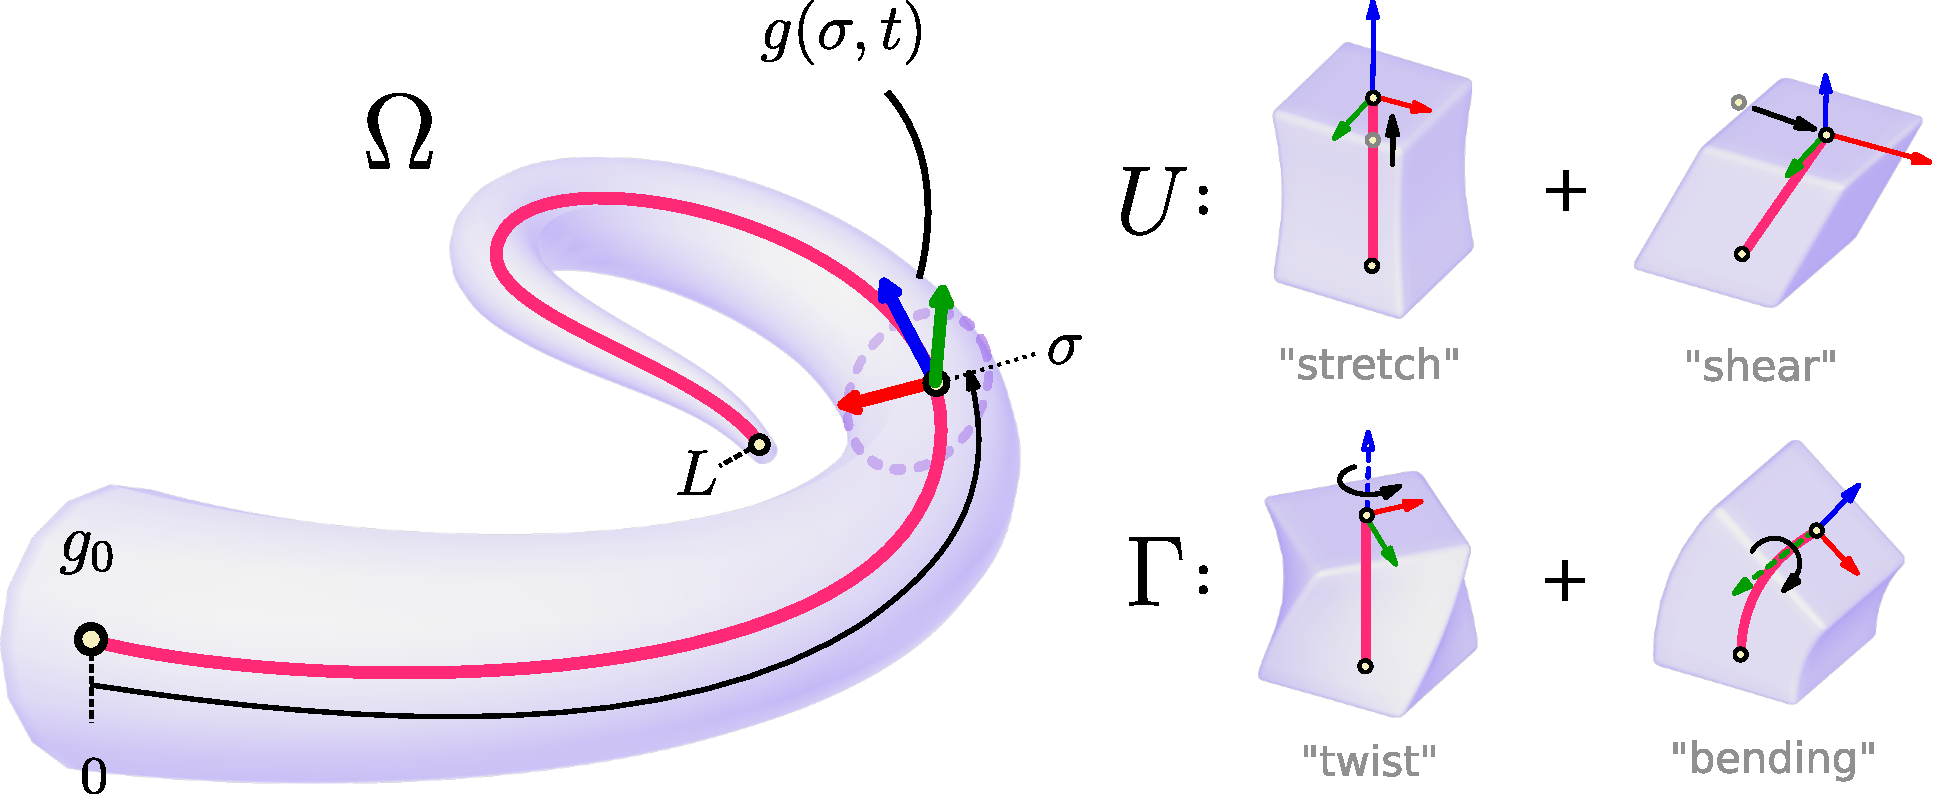
\includegraphics[width=0.85\textwidth]{./pdf/thesis-figure-cosserat.pdf}
\caption{\small Illustration of the soft beam model using geometric Cosserat beam theory, where the backbone curve is $\gB(\sigma,t) \in \mathrm{SE}(3)$ shown as \data{magenta}. The geometric strain vector $\xiB := \textrm{vec}\left\{ \GammaB, \UB\right\}$ a vector of size 6 consisting of stretch-shear strains $\UB$ and twist-bending strains $\GammaB$.}   
\label{fig:C5:CosseratExample}
\vspace{-6mm}  
\end{figure}

\textbf{A: Computationally-efficient soft beam models.} Following the geometric Cosserat beam frameworks \cite{Renda2020,Boyer2021,Caasenbrood2021}, the reduced nonlinear dynamics of a soft beam model, fixed to a non-inertial base, can be represented using a Lagrangian formulation:
%
\begin{multline}
\MB(\q)\ddq + \CB(\q,\dq)\dq + \fB_{\textrm{mat}}(\q,\dq) + \fB\grav(\q) =  \fB_{\Omega_{\textrm{env}}} (\q,\dq) + \tauB(\q,\uB),
\label{eq:C5:model_beam}
\end{multline}
%
where $\q$, $\dq$, and $\ddq$ represent the modal coefficients, velocity, and acceleration, respectively; $\MB$ denotes a state-dependent generalized inertia matrix, and $\CB$ denotes the Coriolis matrix. The material forces are expressed as $\fB_{\textrm{mat}}(\q,\dq) = \KB(\q) \q + \RB \dq$, where $\KB$ is a generalized stiffness matrix and $\RB$ is a generalized damping matrix. The environmental forces are represented by the vector $\fB_{\Omega_{\textrm{env}}}$, and the generalized input is given by $\tauB = \GB \uB$, where $\GB(\q)$ is the input mapping. As in Section \ref{sec:C5:fem}, material and contact models can be assigned using comparable syntax, \code{Shapes.addMaterial} and \code{Shapes.addContact}, respectively. The intrinsic length of a curve can be altered by utilizing the function \code{Shapes.setLength}, while its cross-sectional geometry can be modified through the function \code{Shapes.setGeometry(sdf)}, which accepts a two-dimensional SDF function that may be arbitrarily complex.

Due to the complexity of deriving the forward kinematics and dynamics in the Cosserat model, the following subsections provide a clear summary of the finite-dimensional basis representation and its relationship to reduced kinematics. The system matrices, on the other hand, are notoriously lengthy expressions and thus omitted in this work. The reader is referred to Chapter \ref{chap:BeyondPCC} for a full derivation of model \eqref{eq:C5:model_beam}.

\textbf{B: Finite dimensional projection.} To start, our aim is to obtain a finite-dimensional approximation of the local geometric strain vector, denoted as $\xiB:= (\gB\inv \tfrac{\p \gB}{\p \sigma})^\wedge := (\GammaB^\top,\,\UB^\top)^\top$, where $\sigma \in [0,L]$ is a spatial coordinate and $(\cdot)^{\wedge}: \textrm{se}(3) \to \R^6$ (see \cite{Murray1994} or Appendix \ref{app:C3:liegroup}). Here, $\Gamma_{i}$ and $U_{i}$ are the torsion-curvature and elongation-shear curve parameters, respectively. To achieve this, we employ a Ritz-Galerkin modal discretization approach following the work of Boyer et al. \cite{Boyer2021}. This approach assumes that the strain can be accurately represented through a finite series of orthonormal basis functions:
%
\begin{align}
[\xi_i]_{\thetaB_i}(\sigma,\q_i) & = \sum_{j=1}^{k_i} \theta_{i,j}(\sigma) q_{i,j} + \xi_i^\circ (\sigma), \notag \\ & = \underbrace{\big[\theta_{i,1}(\sigma)\; \hdots\; \theta_{i,k_i} (\sigma) \big]}_{\thetaB_i^\top(\sigma)} \q_i + \xi_i^\circ(\sigma)
\end{align}
%
where $\thetaB_i$ is the modal approximation vector related to the $i$-th strain component, $\q_i$ is its corresponding modal coefficient, and $[\cdot]_{\thetaB}$ denotes the subspace projection operator. By collecting all terms $q_{i,j}$ and $\theta_{i,j}$, we compactly express the finite-dimensional approximation as an affine operation:
%
\begin{equation}
[\xiB]_{\ThetaB}(\sigma,\q) = \ThetaB^{\!\top}\!(\sigma) \q + \xiB^{\circ}(\sigma)
\label{eq:C5:xi_computation_POD}
\end{equation}
%
where $\ThetaB:= \textrm{blkdiag}\{\thetaB_1,\dots,\thetaB_6\}$ is referred to as the \textit{"modal approximation matrix"}, and $\q:=\textrm{vec}\{\q_1,\dots,\q_6\}$ is the generalized coordinate vector of the global soft beam model in \eqref{eq:C5:model_beam}. Note that a geometric strain entry may be constrained and therefore not contribute to the overall continuum dynamics, thus $\thetaB_i,\q_i$ are fixed to zero without loss of generality. The choice of basis plays a crucial role and often relies on \textit{ad-hoc} approaches. It is therefore critical to choose an appropriate basis for optimal performance of the soft robot model. \\
% 
% \begin{figure}[!t]
% \centering
% \includegraphics*[width=0.99\textwidth]{./pdf/thesis-figure-6-11.pdf}
% %\input{./fig/fig_shp_basisspace.tex}
% \caption{The library of modal basis functions is implemented in the Sorotoki toolkit, with a modal ordering of \{\ldata{Matlab1}, \ldata{Matlab2}, \ldata{Matlab3}\}. These function bases include Piecewise Constant Curvature (PCC), Piecewise Linear (PWL), full and piecewise Chebyshev, and full and piecewise Bernstein polynomials.}
% \label{fig:C5:shapesexample}
% \vspace{-5mm}
% \end{figure}

\textbf{C: Library of modal strain bases.} In \texttt{Sorotoki}, the general constructor for creating a modal basis is defined as \code{pod = Basis(N,M,'type')}, where \code{N} represents the number of samples (i.e., the level of discretization of the spatial curve), \code{M} is the degree of the basis, and \code{'type'} is an input that specifies the basis type.

The literature presents various types of modal bases, with the Piecewise Constant Curvature (PCC) approach being the most commonly used \cite{Falkenhahn2015,DellaSantina2020a}. The Piecewise Constant Curvature approach is suitable for certain conditions, for example, when homogeneous bending moment and homogeneous material properties are considered. However, it lacks the ability to ensure the continuity of the strain field at the boundaries between sections, resulting in jumps in the strain profile. As a result, researchers have been exploring alternative representations that more effectively preserve the continuity conditions of the deformable continuums. Examples of alternative representations of bases include piecewise linear \cite{Li2023Jan}, affine curvature \cite{DellaSantina2020Dec,Stella2022Nov}, Fourier cosine/sine series \cite{Chirikjian1994Jun,Chirikjian1992}, Legendre or Chebyshev \cite{Boyer2021,Caasenbrood2021}, and actuation load bases \cite{Renda2020}. The \texttt{Sorotoki} package offers access to a library of anonymous functions, facilitating the utilization of a range of basis functions. As an illustration, a collection of basis functions is shown in Figure \ref{fig:C5:shapesexample}.\\

\begin{rmk}[On the modal order]
Generally, finding a suitable reduction basis and reduction order can be a challenging task. The general assumption is that if the basis belongs to a regular function space (\ie, Sobolev space) and the modal index $k_i$ goes to infinity, the strain approximation converges (uniformly) to the exact solution on the interval $[0,L]$. However, as increasing the modal order enhances precision, it also greatly impacts computational performance. Thus, finding a balance between accuracy and computational speed is of utmost importance for the successful implementation of soft robotic models, often mandating an \textit{ad-hoc} approach.
\end{rmk} 


\label{sec:C5:femPODbasis}
\textbf{C: Data-driven strain basis from offline FEM simulations.} To address the challenges of improving efficacy in the modal reduction of soft beam models, we propose a novel approach that merges the finite element method and soft beam modeling. This approach involves extracting geometric modal information from FEM simulation data to construct a low-dimensional strain basis, which we refer to as the Data-driven Variable Strain (DVS) basis. The DVS basis is similar in concept to the snapshot method presented by the SOFA toolkit \cite{Duriez2016,Coevoet2017,Goury2018}, but adapted for use with one-dimensional curves. It takes into account the underlying geometric features of the soft robot and represents them in a minimal subspace representation. This approach leads to a substantial reduction in the number of states while still maintaining high accuracy in deformations, high computational efficiency, and providing a clear structure for passive and active joints. The derivation has two steps: \\

\textit{Step 1: Recovery of geometric strain from FEM:} The reconstruction of the MIVS basis begins with obtaining geometric strain data from a Finite Element Method (FEM) simulation. Such simulation supports either \code{Fem.simulate} or \code{Fem.solve}, and the resultant information is stored in the \code{fem.Log} data structure. Mathematically, the simulation retrieves the states $\xB^{(i)}:=\xB(t_i)$ at discrete time instances $t_i \in \{0,...,T\}$, which in turn provides the nodal position vectors $\pB$ and the deformation gradient $\FB$ at any point in the mesh. Using the polar decomposition $\QB = \FB\VB \inv \in \textrm{SO}(3)$, see Table \ref{tab:C5:strain_measures}, we can retrieve the rigid body transformation of the FEM mesh
%
\begin{equation}
\gB_{\textrm{FEM}}(\sB, \x^{(i)}) = \begin{pmatrix} \QB(\sB,\x^{(i)}) & \pB(\sB,\x^{(i)}) \\ \vec{0} & 1 \end{pmatrix},
\end{equation}
%
where $\sB \subseteq \Omega$ is an arbitrary point inside the undeformed mesh. It is important to note that if $\sB$ does not correspond to a nodal location of the mesh, interpolation using elemental shape functions is necessary. Now, let $\bar{\gammaB}: [0,L] \to \Omega$ be a unit-speed reference backbone curve that is contained within the mesh domain $\Omega$. Then, we can retrieve $\gB_{\textrm{FEM}}(\bar{\gammaB},\x^{(i)})$. Subsequently, the geometric strain can be approximated as $\xiB_{\textrm{FEM}} \approx (\gB_{\textrm{FEM}})\inv \delta \gB_{\textrm{FEM}}$. Here, $\delta \gB_{\textrm{FEM}}$ represents the spatial derivative of the reference curve w.r.t. $\sigma$, which is calculated using the central difference method. It is worth noting that the choice of $\bar{\gammaB}$ is free, allowing for the estimation of geometric strain for many complex structures. The full procedure is outlined in Algorithm \ref{algo:C5:fem_reconstruction}. \\
%
\begin{algorithm}[!t]
    \caption{Recover geometric strain field $\xiB_{\textrm{FEM}}$ from offline FEM \label{algo:C5:fem_reconstruction}}
    \KwIn{Nodal displacements $\xB$, mesh tesselation $\mathcal{T}$, reference curve $\bar{\gammaB}$, and sample set $\mathcal{S}$}
    \KwOut{Geometric strain field $\xiB_{\textrm{FEM}}$ at time $t_i$ \label{algo:C5:strainFEM}}
    
    %\tcp{assemble SE(3) from Mesh}

    %backbone curve $\mathcal{C} \gets \texttt{ForwardKinematics}(\mathcal{S})$\;

    \For{$i$ = each spatial sample $\sigma_i \in \mathcal{S}$}
    {
        get reference position $\bar{\pB} \gets \bar{\gammaB}(\sigma_i)$ \;
        get element $\mathcal{E} \gets \texttt{inElement}(\bar{\pB},\mathcal{T})$ \;
        \If{$\mathcal{E} == \emptyset$}
        {
            get edge $\mathcal{E} \gets \texttt{onClosestEdge}(\bar{\pB},\mathcal{T})$\;
        }
        initialize $\mat{\Phi}^{(0)} \gets \mat{I}_3$ \;
        initialize $\delta \gammaB^{(0)} \gets \vec{0}_3$ \;
        \For{$j = $ each vertex spanned by element $\mathcal{E}$}
        {
            get nodal displacement $\vec{X} \gets \texttt{FEM}(\mat{x}_j)$ \;
            get deformation gradient $\mat{Y} \gets \texttt{FEM}(\mat{x}_j)$ \;
            $[\mat{Q},\,\mat{V}] \gets \texttt{PolarDecomposition}(\mat{Y})$ \;
            $\alpha \gets \texttt{ElementInterpolation}(\bar{\pB})$ \;
            update $\PhiB^{(j)} \gets \texttt{AverageSO3}(\PhiB^{(j)},\alpha\mat{Q})$ \;
            update $\delta\gammaB^{(j)} \gets \delta\gammaB^{(j)} + \alpha \vec{X}$ \;
        }
        $\gB_{\textrm{FEM}}^{(i)} \gets \texttt{SE3}(\PhiB^{(j)},\bar{\pB} + \delta\gammaB^{(j)})$\;
    }

    \For{$i$ = each spatial sample $\sigma_i \in \mathcal{S}$}{
    $\delta\gB_{\textrm{FEM}}^{(i)} \gets \texttt{CentralDiff}(\gB_{\textrm{FEM}}^{(i-1)},\gB_{\textrm{FEM}}^{(i+1)})$ \;
    assemble strain $\vec{\xi}_{\textrm{FEM}}^{(i)} \gets (\gB_{\textrm{FEM}}^{(i)})\inv \delta\gB_{\textrm{FEM}}^{(i)}$\;
    }
\end{algorithm}

\textit{Step 2: POD snapshot basis:} Next, we employ the "Snapshot Proper Orthogonal Decomposition" (POD) as described in \cite{Duriez2016,Goury2018}. This data-driven approach determines a suitable orthonormal basis from simulated or experimental data \cite{Astrid2008}. Let $y_{i}(\sigma,t) := \xi_{\textrm{FEM},i}(\sigma,t)$ represent the measurement of the $i$-th entry of the strain $\xiB_{\textrm{FEM}}$. For each discrete time $t_i$, the sample is condensed into a column vector $\vec{y}_i^{(t)} := \textrm{col}\left\{y_i(0,t),\dots,y_i(L,t) \right\}$ and then stacked into the "snapshot matrix" $\mat{S}_i = \textrm{row}\left\{ \vec{y}_i^{(0)},\dots,\vec{y}_i^{(T)} \right\}$ where $T$ is the finite horizon time. The correlation matrix $\mat{\mathcal{C}}_i = \tfrac{1}{m} \mat{S}_i^\top \mat{S}_i$ is then computed with $m = \dim(\yB_i)$, and the spectral decomposition is performed:
%
\begin{equation}
\mat{\mathcal{C}}_i \VB_i = \mat{\lambda}_i \VB_i,
\end{equation}
%
where $\VB_i = \textrm{row}\{\vB_{i,1},,...\vB_{i,m}\}$ is a eigenvector basis and $\mat{\lambda}_i = \diag{\lambda_{i,1},,...,\lambda_{i,m}}$ is a diagonal matrix of sorted eigenvalues. By selecting $k_i \le m$ such that $\lambda_{i,k_i} \le \delta$, where $\delta$ is a desired threshold, we obtain a truncated orthonormal basis $\{\vB_{i,j}\}_{j=1}^{k_i}$. This process is repeated until the modal interpolation matrix $\ThetaB$, required for \eqref{eq:C5:xi_computation_POD}, is fully obtained. Finally, a Gram–Schmidt orthogonalization procedure is performed to ensure that its columns are mutually orthogonal. \\

\begin{figure}[!t]
\centering
\includegraphics*[width=.8\textwidth]{./pdf/thesis-figure-6-11-2.pdf}  \\[0.15em]
\includegraphics*[width=.8\textwidth]{./pdf/thesis-figure-6-11-3.pdf}% \\[1.15em]
%\includegraphics*[width=.85\textwidth]{./pdf/thesis-figure-6-11-1.pdf} \\[0.15em]
%\input{./fig/fig_GVISmode_fem.tex} \\[0.75em]
%\input{./fig/fig_GVISmode.tex} \\[0.21em]
%\input{./fig/fig_GVISmode_pos.tex} 
\caption{\small Example reconstruction of the Data-driven Variable Strain (DVS) basis for a PneuNet actuator grasping a cylindrical object. (top) The first three modes of the DVS basis related to planar bending, \ie., planar curvature. The ordering is $\{$\ldata{Matlab1}, \ldata{Matlab2}, \ldata{Matlab3}$\}$. (bottom) The positional forward kinematics when regarding the bending modes $\{$\ldata{Matlab1}, \ldata{Matlab2}, \ldata{Matlab3}$\}$ individually.}
%\vspace{-3mm}
\label{fig:C5:gvis_modes}
\end{figure}
%

\begin{figure}[!t]
\centering
\includegraphics*[width=.85\textwidth]{./pdf/thesis-figure-6-11-1.pdf} \\[0.15em]
%\input{./fig/fig_GVISmode_fem.tex} \\[0.75em]
%\input{./fig/fig_GVISmode.tex} \\[0.21em]
%\input{./fig/fig_GVISmode_pos.tex} 
\caption{\small Example reconstruction of the Data-driven Variable Strain (DVS) basis for a PneuNet actuator grasping a cylindrical object. A comparison between the true physical system, the FEM model, and the soft beam model shown in \data{magenta}. The Von Mises stresses are shown as \protect\colormapcaption{0}{.75cm}$\!\!\in [0,5]$ \si{\mega \pascal}.}
\vspace{-6mm}
\label{fig:C5:gvis_experiment}
\end{figure}
%
\begin{example}{Data-driven basis from PneuNet simulation}
To demonstrate the reconstruction of the DVS basis, we consider a soft bending actuation, also known as the PneuNet actuator. A FEM simulation model is constructed where the soft actuator is subjected to a linearly increasing pressure up to $40$ \si{\kilo \pascal} and curls around a cylindrical object when pressurized. Figure \ref{fig:C5:gvis_modes} (top) illustrates the true system and the FEM simulation obtained through \code{fem.simulate}. The FEM class is then integrated into the \class{Shapes} class through the syntax \code{shp = Shapes(fem,dof)}, where \code{dof = [0,3,0,0,0,0]} indicates the desire to recover the first three curvature bending modes from the \code{fem} object class. The length and base orientation are specified using \code{shp.setLength} and \code{shp.setBase}, respectively. The basis is then reconstructed by calling \code{shp.reconstruct}. The first three curvature bending modes are displayed in Figure \ref{fig:C5:gvis_modes} (bottom). It can be observed that the geometrical features of the PneuNet actuator are encoded in the basis, with the 12 embedded pressure chambers represented by the DVS strain basis. The associated code is provided below:
\end{example}
%
\begin{matlabcode}
%% EXAMPLE: Shapes class (DVS basis)   
fem = load('femPneuNet.mat');   % load fem model

dof = [0,3,0,0,0,0];  % pure planar curvature bending
shp = Shapes(fem, dof, 'NNode', 200, 'Length',105);

% generate DVS basis 
shp = shp.reference(@(s) [s,0,0].' );
shp = shp.reconstruct();
\end{matlabcode} 
% 
\\

\textbf{D: Forward beam kinematics.} Once a basis representation $\ThetaB$ has been selected, the forward kinematics of the continuum body can be efficiently solved using exponential maps for the group $\SE{3}$. As such, the backbone curve is approximated by
%
\begin{equation}
    [\gB]_{\ThetaB}(\sigma,\q) = \gB_0 \exp_{\textrm{SE}(3)} \left[ \int_0^\sigma {[\hat{\xiB}]_\ThetaB}(s,\q) \; ds\right]
    \label{eq:C5:gcurve}
\end{equation}
%
On the other hand, the local velocity twist is represented by $\etaB:= (\gB\inv\dot{\gB})^{\vee}$, which, similarly to rigid robotics, is linear in the joint velocities $\dot{\q}$. Regarding computation, the velocity twist of a point $\sigma$ on the curve $\gB$ can be represented as follows:
%
\begin{align}
    [\etaB]_\ThetaB(\sigma,\q,\dq) & = \left[\Ad^{-1}_{[\gB](\sigma,\q)}\int_{0}^\sigma  \Ad_{[\gB](s,\q)} \ThetaB(s)\; ds \right]  \dq  %\notag \\
                                   =: \JB(\sigma,\q) \dq,
                                  \label{eq:C5:eta}                                  
\end{align}
%
where $\JB(\sigma,\q)$ denotes the geometric Jacobian that maps the joint velocities $\dq$ to velocity twist. For conciseness, we write $\JB_\sigma := \JB(\sigma,\cdot)$. The Jacobian matrix is of paramount importance, not only for inverse kinematics but also for mapping external wrenches onto the generalized joint torques. For instance, it can be used to calculate the environmental forces as $\fB_{\Omega_{\textrm{env}}} = \int_0^L \JB_\sigma^\top \FT_{\textrm{env}} \; d\sigma$, where $\FT_{\textrm{env}}$ represents a wrench related to the environment $\Omega_{\textrm{env}}$ described by SDFs. 

Given the expressions in \eqref{eq:C5:xi_computation_POD}, \eqref{eq:C5:gcurve}, and \eqref{eq:C5:eta}, we can numerically evaluate the forward kinematics. We use a two-step Runge-Kutta integration solver that approximates the spatial integration. The forward kinematics solver is called by \code{shp = Shapes.string(q,dq)}, which stores all necessary numerical evaluations into a data structure \code{shp.Log.FK}. To further improve computation speed, \code{.mex} executable files are utilized. \\[0.5em]

\textbf{E: Inverse beam kinematics (shape control).} \label{sec:C5:inverseKinematics} The inverse kinematics problem for soft continuum manipulators involves finding a solution $\q$ such that either ($i$) the end-effector reaches a specified setpoint, or ($ii$) shape control of the backbone is achieved. These manipulators often exhibit high levels of redundancy, so called hyper-redundancy \cite{Chirikjian1994Jun}; leading to different solution approaches common to rigid robotics. Few modal basis representations possess a closed-form solution to the inverse kinematics, and they are typically solved using an iterative numerical method (\eg, Newton Raphson). In \texttt{Sorotoki}, the inverse kinematics solver for soft beam models is implemented as \code{Shapes.IK}. We briefly detail the theory.

Suppose the desired shape of the soft manipulator is $\gB^\star(\sigma) \in \WT_\sigma$ with 
%
\begin{equation}
\WT_\sigma := \big\{ \XB \in \mathrm{SE}(3)\;|\; \XB = [\gB]_\ThetaB(\sigma,\q),\, \q \in \mathcal{Q} \big\}    
\end{equation}
%
the set of possible configurations of the backbone curve at $\sigma$. Note that $\WT_L$ spans the workspace of the end-effector, and $\WT_\Omega := \{\WT_\sigma \;|\; \sigma \in [0,L]\}$ the workspace of the entire soft body. For sake of readability, we redefine $\gB_i(\q) := [\gB]_\ThetaB(\sigma_i,\q)$ and $\gB^\star_{i} := \gB^\star(\sigma_i)$. For readability, we also rewrite the geometric Jacobian by $\JB_i(\q) := \JB(\sigma_i,\q)$.

Then, the inverse shape kinematics problem for the discretized soft manipulator can be formulated as an optimization problem of the form:
%
\begin{mini}[2]
    {\q}{\Phi = \sum_{i=1}^{N_p}  \Big\lVert \KB_p\textrm{log}_{\textrm{SE}(3)}\left[ \gB_i\inv(\q)\gB^\star_{i}\right]^{\vee} \Big \rVert_2}{}{}
    \addConstraint{\gB_i, \gB^\star_i\in \mathcal{W}_{\Omega},}{}{}
\end{mini}
%
where $\textrm{log}_{\textrm{SE}(3)}$ denotes the logarithmic mapping from the Lie group to its algebra, see Appendix \ref{app:C3:liegroup}. Despite the highly nonlinear nature of the optimization problem, its solution procedure is a relatively straightforward two-step procedure:

Given an initial guess $\q^{(0)} \in \mathcal{Q}$, the aim is to compute an incremental update step that brings us closer to a local minimizer of the objective function $\Phi$. For clarity, let $\vec{\Xi}_i :=\gB\inv_i\gB^\star_i$ represent the geometric error between the soft robot and the desired shape. The state increment can then be expressed as:
%
\begin{align}
\vec{\lambda}_i^{(k)} & = \JB_i^\top (\q^{(k)}) \left[ \KB_{p} \textrm{T}_{\textrm{SE}(3)}(\vec{\Xi}_i) \textrm{log}_{\textrm{SE}(3)} (\vec{\Xi}_i) \right]^\vee, \label{eq:C5:invkin1}\\
\q^{(k+1)} & = \q^{(k)} + \sum^{N_p}_{i = 1} \vec{\Lambda}_i \left[\vec{\lambda}^{(k)}  - \NT_i(\q^{(k)}) \nabla \Phi_{\textrm{sub}} \right],
\label{eq:C5:invkin2}
\end{align}
%
where $\textrm{T}_{\textrm{SE}(3)}$ denotes the tangent operator map on the group $\mathrm{SE}(3)$, see \cite{Bullo1995}, $\KB_p$ an artificial stiffness tensor, $\NT_i = (\IB - \JB_{i}^+\JB_{i})$ represents the null-space projection, and $\vec{\Lambda}_i$ a diagonal activation matrix. The trivial choice is $\LambdaB_i = \IB_n$. The null space projector can be extremely useful in exploring the high redundancy in soft robots, allowing subtasks  $\Phi_\textrm{sub}$ to be considered parallel to the primary inverse kinematic problem. Classical examples of such subtasks include: minimizing elastic energy or obstacle avoidance. The iterative solver in \eqref{eq:C5:invkin1} and \eqref{eq:C5:invkin2} runs until convergence in $\q^{(k)}$ is achieved. \\

\begin{figure}[!t]
\centering
\includegraphics*[width=.99\textwidth]{./pdf/thesis-figure-6-13.pdf}
%\input{./fig/fig_mdl_example2.tex} \\[0.01em]
%\input{./fig/fig_mdl_example2_grasp.tex}
%\vspace{-5mm}
\caption{\small (left) A snapshot of the ultra-gentle soft robot gripper developed by Sinatra et al. \cite{Sinatra2019Aug} is shown, demonstrating its ability to grasp a delicate jellyfish. (right) The reconstructed soft gripper using \texttt{Sorotoki} is presented, where each tentacle finger is modeled individually using the \textit{Shapes} class. It can be observed that the soft tentacles envelop the SDF object, indicating a balanced solution between task and subtask.}
\label{fig:C5:shapesexample}
\vspace{-5mm}
\end{figure}

\vspace{-2mm}
\begin{example}[Contact kinematics of ultra-gentle soft gripper]
To showcase the forward and inverse kinematic solvers of Sorotoki, we will describe the ultra-gentle underwater soft gripper developed by Sinatra et al. \cite{Sinatra2019Aug}. The soft gripper consists of six soft fingers attached to a rigid palm base, where each soft gripper was designed to apply low contact pressure and minimize harm to common jellyfish species. An illustration of the system is shown in Figure \ref{fig:C5:shapesexample}. The delicate compliance of the soft gripper is achieved through the use of an extremely low durometer silicone matrix (Shore 20A). The actuator has a simple rectangular geometry, with a narrow cross-section of approximately 10 $\times$ 2 \si{\milli \meter} and an internal off-center rectangular hole. The thinnest part of the soft actuator, called the membrane, is approximately 0.35 \si{\milli \meter} thick, and length of about 130 \si{\milli \meter}.

In this study, we aim to reproduce a grasping scenario of a jellyfish modeled as a static SDF object. To achieve this, we first initiate a soft finger by utilizing the \class{Shapes} class. We employ a third-order Chebyshev basis to approximate the strain field. The geometric properties of the soft finger are specified through the functions \code{Shapes.setLength} and \code{Shapes.setGeometry}. Using a for-loop, we generate each soft finger sequentially, defining the spatial location of the fixed base with \code{Shapes.setBase}. Prior to deployment, each soft finger undergoes predeformation, which is calculated through the application of the forward kinematics solver \code{Shapes.FK(q)}. The joint configuration, \code{q}, is selected to match the experiments presented in Figure \ref{fig:C5:shapesexample}.

Subsequently, the deformed backbone is projected onto the surface of the SDF jellyfish through the use of the function \code{sdf.project}. The inverse kinematics solver is then invoked with \code{Shapes.IK}, resulting in the image depicted in Figure \ref{fig:C5:shapesexample}. Note that the inverse kinematics solver effectively places the soft finger onto the surface of the SDF object without causing penetration. The code for the forward and inverse kinematics is presented below:
\end{example}

\begin{lstlisting}[style=matlab] 
%% EXAMPLE: Shapes class (forwards/inverse kinematics) 
% jellyfish SDF
sdf = sSphere(0,0,-60,40) 

% generate Shapes class 
N = 200; % discretization
M = 3;   % number of modes
pod = Basis(N,M,'chebyshev');     

shp = Shapes(pod,[0,M,M,0,0,0],'Length',120);
shp = shp.setGeometry(sRectangle(4,1));

% inverse kinematics on SDF topology
for k = 1:6
    shp = shp.setBase(G{k});  % set base SE(3)

    pos = shp.FK(q0{k});      % forward kinematics 
    prj = sdf.project(pos);   % project points

    qd  = shp.IK(prj);        % inverse kinematics 
    shp.render(qd);           % render shape
end

sdf.show();  % render jellyfish
\end{lstlisting}
%\vspace{-4mm}
\subsection{Model composer (\texttt{Model})}
\label{sec:C5:model}
In many instances, soft robots comprise multiple dynamic components that are interconnected to form the overall system. For instance, the soft robotic hand depicted in Figure \ref{fig:C5:examplebots}c comprises five actively controlled soft fingers connected to a rigid palm base, each of which exhibits its own fluid-structure interaction. While each soft finger can be modeled through the \class{Shape} class, the class itself lacks a composer or solver that addresses the interconnections between a network of dynamic systems.

To address the issue, we propose the \class{Model.m} class, which concatenates dynamic systems to systematically increase complexity. The class is equipped with an implicit solver that facilitates communication of state information between subsystems. The goal of the \class{Model.m} class is two-fold: $(i)$ to facilitate the composition of multiple dynamic components that form a soft robotic system, and $(ii)$ to leverage the dynamic network structure to design controllers through interconnection of subsystems.
For example, a soft robot, the fluidic actuation, and the model-based controller can be modeled as three separate entities and be composed into one global closed-loop system. This approach also enables the adaptive controllers that require additional state dynamics for online estimation of parameters. Contact interaction, on the other hand, are embedded functions inside \texttt{Fem} and \texttt{Shapes} that are called during each state increment of the forward dynamic solver. \\

\textbf{A. Interconnected network of dynamical systems.} The class \class{Model.m} allows users to compose an arbitrarily large network of dynamical systems that are presented in the state-space structure $\Sigma_i:\; \dot{\zB_i} = \fB_{i}(\zB_i, \uB_i, t)$. Then, the network of dynamical systems can written as
%
\begin{equation}
    \Sigma_{\textrm{net}}: \dot{\zB} = \FB_{\textrm{net}}(\zB, \uB, t)
    \label{eq:C5:dynamicnetwork}
\end{equation}
%
The network system matrices are assembled as: $\FB_{\textrm{net}}(\zB) := \textrm{blkdiag}(\fB_{1},\fB_{2},...,\fB_{n})$. The implementation in \textit{Sorotoki} is relatively straightforward. Let \code{f0 = @(z,u,t) ode(z,u,t)} be an anonymous function that defines a state space model, where \code{z}, \code{u}, \code{t} are the state vector, the input vector, and a time variable, respectively. In contrast to standard ODE solvers in {MATLAB}\textsuperscript{\scriptsize\textregistered} (\eg, \texttt{ode45.m}), the input \code{u} is treated as an additional input to the ODE. This simplifies the design of controllers as it enables the definition of control laws outside of the ODE function caller, as opposed to the standard ODE packages in {MATLAB}\textsuperscript{\scriptsize\textregistered}.

To proceed, we first convert the function to a \class{sys0 = StateSpace(@f0)} class, which stores information on the state dimension, input dimension, and numerically computes the Hessian. Then, the model class is constructed using \code{mdl = Model(@f0)}. Other dynamic systems, represented by the \code{StateSpace} class \code{sys1}, \code{sys2}, and \code{sys3}, are added to the network by \code{mdl.addSystem(sys1,sys2,sys3)}. The \class{Model} class is also compatible with other classes, such as the \class{Fem} and \class{Shapes} class, allowing for example the interconnection between a FEM model and a soft beam model. To compute the forward dynamics, we call \code{mdl.simulate([0,T])} which solves the state trajectories on the finite horizon domain $[0,T]$ using an implicit Trapezoidal solver (\ie, similar to \texttt{ode23t} solver). \\

\textbf{B: Assigning the controller.} Once a network of dynamic systems has been composed in the \class{Model} class, assigning a control is straightforward. Controllers can be defined as auxiliary anonymous functions \code{@(mdl) Controller(mdl)} and added using \code{mdl.addController(@Controller)}. At each time instance of the implicit solver, this controller function is called and prompted with the current instance of the \class{Model}. Once prompted, the solver retrieves the global input vector $\uB$ as in \eqref{eq:C5:dynamicnetwork}. All system information of the network can be retrieved within the function by \code{mdl.getState[I,J]}, where \code{I} is the system index and \code{J} the indices of the states of subsystem \code{J}. Such implementation presents a highly dexterous and efficient controller design platform previously not standard included in {MATLAB}\textsuperscript{\scriptsize\textregistered}. \\
%

\textbf{C. Fluidic reservoir with volume-variance}
The majority of soft robots are actuated through fluidics. In recognition of this, \textit{Sorotoki} offers a variant of the \class{StateSpace} class, called \class{Fluidic}, which incorporates fluid-pressure dynamics of an enclosed pressure reservoir based on the ideal gas law. The dynamics of such fluidic reservoir is determined by the compressibility of the fluid and the capacitance of the reservoir that is related to its volume $V > 0$. As a soft robot deforms, so does its internal volume. As such, consider a scalar variable $J: \mathcal{Q} \to (0,+\infty]$ such that we can describe the volume by $V(J(\q)) = J(\q) V_0$ where $V_0$ is the intrinsic volume. From a physical point of view, the scalar $J(\q)$ can be seen as the relative volumetric change of the reservoir depending on the state of the soft robot. Assuming constant temperature $T$ and polytropic coefficient $n_k$, the pressure dynamics can be described by
%
\begin{equation}
    \dot{p} = \frac{n_k}{V(J)} \left( R T \dot{m} - \frac{d V}{d J}(J) \dot{J} p \right) - \mu_{\textrm{leak}} p
    \label{eq:C5:pressure0}
\end{equation}
%
where the input is $\dot{m}$ the mass flux into the reservoir, $R$ the ideal gas constant, and $\mu_{\textrm{leak}}$ a pressure leakage coefficient. For a perfectly enclosed system, the parameter $\mu_{\textrm{leak}} = 0$. Note however, that the volumetric change $\dot{J}$ might not always be available or it is difficult to derive. As an alternative, we substitute $\dot{J}$ with an "dirty derivative" approximation $\dot{\tilde{J}}$ following the work of Loria et al. \cite{Loria2015Jun}:
%
\begin{align}
    \dot{z}         & = \alpha_1 [z + \alpha_2 J ], \label{eq:C5:pressure1}\\
    \dot{\tilde{J}} & = z + \alpha_1 J, \label{eq:C5:pressure2}
\end{align}
%
where $\alpha_1,\alpha_2> 1$ are filter gains. Hence, the system of equations \eqref{eq:C5:pressure0}, \eqref{eq:C5:pressure1}, and \eqref{eq:C5:pressure2} leads to the full pressure dynamics. In case of an isochoric compression (\ie, no volume change $\dot{V} = 0$) with $J = 1 \Rightarrow \dot{J} = 0$, we can revert to a single-input-single-output (SISO) system with $u = \dot{m}$ (\ie, the mass flow $\dot{m}$ as the system's input).

For many control applications for soft robotics, fluidic reservoirs are internally pressure regulated. Hence, the mass flow $\dot{m}(p,p_d)$ depends on the internal pressure $p$ and a (possibly time-varying) pressure trajectory $p_d$. The mass flow controller of a proportional pressure-regulated reservoir is modeled here as PI-type controller:
%
\begin{align}
    \dot{m} & = \Psi_\textrm{v}(\nu,p),                            \\
    \nu     & = k_p(p - p_d) + k_i \int p(\tau) - p_d(\tau) d\tau,
\end{align}
%
where $\Psi_{\textrm{v}}(\nu,p)$ i a valve flow function related to mass flow saturation of the pressure valves, and $k_p,\,k_i >0$ the proportional and integral control gains, respectively. In \texttt{Sorotoki}, such fluidic system is provided as \class{Fluidic} class. The volume of the reservoir can be set using \code{Fluidic.setVolume(@V)} where $\code{V = @(x)...}$ is an auxiliary anonymous function. The mass flow function can be modified by the user using a similar command \code{Fluidic.setMassFlow(@M)}. By default, the flow function is chosen as $\Psi_{\textrm{v}}(\nu,p) = \nu$, and the internal regulation is \code{Fluidic.isRegulated = true}. \\

% \begin{figure}
% %\includegraphics[width=0.485\textwidth]{./fig/Pipelinehand.pdf}
% \caption{Overview of the software pipeline showing the interconnected classes required to model the five-fingered soft robotic hand.}    
% \vspace{-5mm}
% \end{figure}
\newpage
\begin{example}{Simulation soft hand with fluidic soft fingers}
To demonstrate the versatility of the \class{Model} class and the \class{Fluidic} class, consider the example of modeling the soft robotic hand previously shown in Figure \ref{fig:C5:examplebots}. Prior to the simulation model, we conducted an experiment to allow a qualitative comparison with our modeling approach. Here, a predefined harmonic pressure signal is introduced to each of the soft fingers, with each harmonic having a $+\frac{\pi}{6}$ offset relative to its neighboring soft finger. The pressure signal is sinusoidal with an upper and lower bounds of $-5$ and $80$ (kPa), respectively. As depicted in Figure \ref{fig:C5:soft_hand_simulation}, an oscillatory motion arises, where the fingers sequentially undergo bending.

The objective is to recreate the experimental oscillatory behavior of the soft hand, incorporating the fluid dynamics and continuum dynamics of the soft fingers. Each soft finger can be modeled separately using the \class{Shapes} class and its internal fluidic network using the \class{Fluidic} class. We start by sculpting the model for the soft fingers, assuming a fifth-order Chebyshev polynomial basis and considering planar bending curvature only. We assume that only the first mode can be actively controlled by the fluidic network, thus the input map is manually assigned using \code{Shapes.setInputMap(@(q) ... )}. The \class{Shapes} class is duplicated five times using a for-loop routine, with the base frame assigned accordingly at each iteration using \code{Shapes.setBase}.

For each soft finger, it is assumed that it has its own fluidic network that is equipped with internal pressure regulation. However, as each soft finger deforms, the internal volume of the pressure reservoir also changes. This volumetric change is modeled as $V(\alpha) = V_0 (1 + \tanh(\alpha))$, where it is assumed that $\alpha = 0.06 q_1$ (i.e., the first joint of the soft beam) and $V_0$ the initial volume. Then, a for-loop is used to include the both \class{Shapes} and \class{Fluidic} systems to the global network of dynamical systems. 

Finally, \code{mdl.addController(@Control) } is used to add the control law. In this auxiliary function, we specify the pressure reference for the fluidic network, and we return the state deformations of the soft fingers to the fluidic network; required for the computation of the volumetric change. The dynamic simulation is solved implicitly using the \code{mdl.simulate} command. The code for the dynamic simulation of the soft robotic hand is shown in Figure \ref{fig:C5:soft_hand_simulation}.

%\afterpage{
\begin{figure*}[!t]
\centering
%\vfill
\includegraphics*[width=0.99\textwidth]{./pdf/thesis-figurex-6-14-1.pdf}
%\includegraphics*[width=\textwidth]{./pdf/thesis-figure-6-14-2.pdf}
%\input{./fig/fig_model_softhand_true.tex} \\[-0.01em]
%\input{./fig/fig_model_softhand_simu.tex} \vspace{-3mm}
\caption{\small (top) Experimental snapshots of the open-source soft robotic hand provided by the \texttt{Sorotoki} toolkit. The five-fingered robot is subjected to a harmonic oscillator that commands oscillatory pressure to the individual fingers. Since each oscillator has a preset phase difference ($\phi = \pi/6$), the fingers of the soft robot hand undergo a periodic swinging motion. (bottom) Reconstructed soft robotic hand using \textit{Sorotoki}, where each finger is modelled using the \textit{Shapes.m} class and then composed using the \textit{Model.m} class. Following, each oscillator is added using \textit{mdl.addSystem} and then they ouputs are connected to the inputs of each \textit{Shapes.m} class. As can be seen, the dynamics between the numerical model and the experiments are in close agreement. }
\label{fig:C5:soft_hand_simulation}
\end{figure*}
%\clearpage
%}
\end{example}
\clearpage
\begin{lstlisting}[style=matlab]   
%% EXAMPLE: Model class
shp = Shapes(pod,dof,'Length',90);

shp.setInputMap( @(x) [5; 0; 0; 0; 0]) ;
shp.Material = NeoHookeanMaterial(1.5,0.3);

for ii = 1:5
    SHP{ii} = shp.setBase( G{ii} );
end
 
%% building fluidics model 
V0 = (4*pi/3) * 35^3;
V = @(x) V0 * (1 + tanh(x/0.06));

fld = Fluidic('NInput',3);
fld = fld.setVolume(V);

%% building model 
mdl = Model([]);

for ii = 1:10
    if ii < 5    % add soft finger
        mdl = mdl.addSystem( SHP{ii} );
    else         % add fluidic network
        mdl = mdl.addSystem(fld); 
    end
end

%% assign control and simulate
mdl.addController( @(x) Control(x) );
mdl = mdl.simulate([0, 5.0]);

% -- controller function block
function u = Control(mdl)
    phi = @(k) (k-1) * pi/6;
    Pd  = 80 * sign(sin(7.0 * mdl.t + phi(1:5)));

    u = zeros(20,1);
    u(6:3:end) = Pd;
    u(7:3:end) = mdl.getState(1:5,[1]);
    u(1:5)     = mdl.getState(6:10,[1]);
end
\end{lstlisting}

As depicted in Figure \ref{fig:C5:soft_hand_simulation}, the dynamics of the numerical model and the experiments are in close qualitative agreement. This serves as a testament to the efficacy of the dynamic model composer \class{Model} in building dynamic complexity through its modular functionalities. Additionally, the ability to represent the controller as an auxiliary function that can retrieve state information at any given time confers \texttt{Sorotoki} with a high degree of flexibility in offline controller design.

\subsection{Fluidic control hardware (\texttt{Control})}
\label{sec:C5:control}
The implementation of online controllers for physical soft robotic systems is a crucial aspect of \texttt{Sorotoki}. Although there are various options available in the research community \cite{Xavier2022Jun}, \texttt{Sorotoki} has a specific focus on fast closed-loop control. Drawing from our prior work \cite{Caasenbrood2022Apr}, \texttt{Sorotoki} incorporates a TCP communication wrapper (\texttt{tcpip}) that enables real-time communication with a host computer, such as a Raspberry Pi (RPI). This host computer is connected to six pressure control boards, each capable of supporting up to two proportional pressure control valves from Festo. As a result, \texttt{Sorotoki} offers up to twelve pressure-regulated control ports with a range of -100 to 100 kPa that can be directly controlled using script-based programming in \texttt{MATLAB} . The entire system, including the software, is open-source and readily reproducible by researchers with diverse technical backgrounds.

By calling \code{brd = Control('ip','pwd')}, connection with the fluid control platform is establish, where \code{'ip'} is the IP address and password of the RPI. On the RPI, the Python script \texttt{ConnectToMatlab.py} must be executed that makes connection with {MATLAB} and awaits control commands. To initiate the control loop, a while-loop is used whose condition statement is \texttt{brd.loop(T)} where \code{T} is finite horizon time. Within the while-loop, all functionalities of \texttt{Sorotoki} are available, thus model-based controller design is possible for instance using the \class{Shapes} and \class{Model} classes. Each pressure regulation can be controlled using the command \code{brd.setPressure(id,P)} or an internal pressure measurement can be retrieved using \code{P = \code{brd.getPressure(id)}}. \\ \vspace{-5mm}

\begin{example}[Pick-and-place control of soft robot manipulator]
As an example of the capabilities of the fluid control platform, we used it for a pick-and-place application involving the aforementioned soft robot manipulator with soft gripper. The soft robot has four independent pressure inputs: three for the bellows network embedded into the soft body and one for the soft gripper. The \textit{Sorotoki} toolkit communicates a desired pressure profile to a Raspberry Pi board computer, which is interfaced with an expandable array of proportional pressure regulators. As shown in Figure \ref{fig:C5:control_srm}, the system successfully manipulates a 40 mm cylinder of 45 (g) into its container. The system has also been successfully simulated using the \class{Shapes} and \class{Model} class, shown in Figure \ref{fig:C5:srm_simu}, where the cylinder is modelled as a Newton-Euler rigid body system.
\end{example}

\afterpage{
\begin{figure*}[!t]
\centering
\vspace{-4mm}
\includegraphics*[width=.95\textwidth]{./pdf/thesis-figure-6-15.pdf}
%\input{./fig/fig_srm_ref.tex}
\caption{Implementation of open-loop control of a 3D-printed soft robot manipulator with a soft gripper using the \texttt{Sorotoki} toolkit. The soft robot has four independent pressure inputs: three for the bellows network embedded in the soft body and one for the soft gripper. The \texttt{Sorotoki} toolkit communicates a desired pressure profile to a Raspberry Pi board computer, which is interfaced with an expandable array of proportional pressure regulators. A straightforward pick-and-place task can then be easily programmed using the \class{Control} interface, using auxiliary {MATLAB} functions.}
\label{fig:C5:control_srm}
\vspace{-5mm}
\end{figure*}

\begin{figure}
\centering
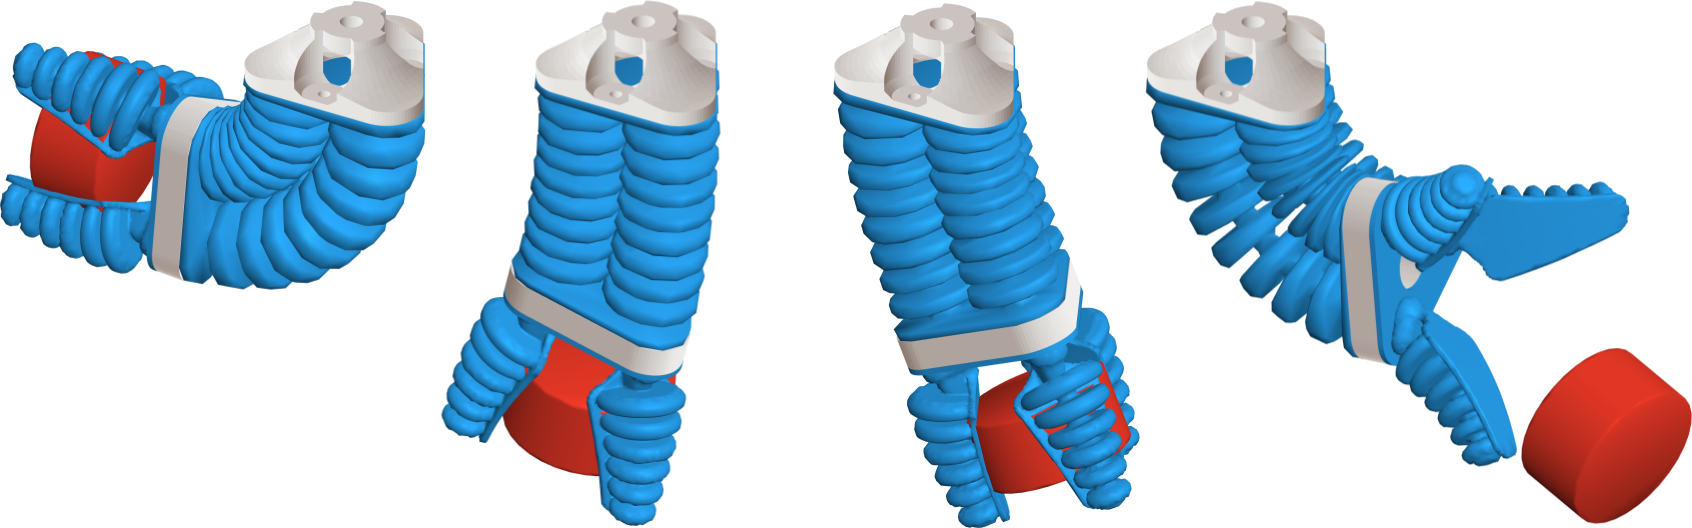
\includegraphics[width=0.95\textwidth]{./pdf/thesis-figure-6-16.png}
\caption{Simulation of the soft robot manipulator with gripper using the \class{Shapes} and \class{Model} class. The rigid-body is modeled by the Newton-Euler equation of motions implemented via \class{StateSpace}. }    
\label{fig:C5:srm_simu}
\vspace{-5mm}
\end{figure}
\clearpage
}
    
\subsection{Computer vision (\texttt{Vision})}
\label{sec:C5:vision}
The final class in \textit{Sorotoki} addresses the challenge of soft sensing through vision. The class, named \class{Vision}, can be instantiated using \code{cam = Vision(Id)}, where \code{Id} is a user-specified index obtained from the list of available webcams using \texttt{webcamlist}. Alternatively, the \class{Vision} class is capable of reading sensor data from the RealSense D400 series RGB-Depth camera from Intel. The class is equipped with a suite of vision techniques that make use of the \texttt{OpenCV} Python implementation. It features three key functions: $(i)$ extraction of optical markers from an image using RGB and depth data, $(ii)$ calibration of the world coordinate frame using Aruco markers, and $(iii)$ monitoring of a soft robot in real-time using camera feedback. The detection of color markers utilizes a circular Hough transform \cite{Illingworth1987Sep}, which provides the pixel location of a circle within the specified search conditions. These tools provide a broad range of options for state estimation of a soft robot, which can be easily incorporated into closed-loop control schemes.



\section{Soft robotics study cases}
\label{sec:C5:studycases}
In the subsequent section, we will delve into the capabilities of the toolkit, \textit{Sorotoki}. To provide a comprehensive overview of the toolkit, various problem scenarios will be considered, each with specific problem settings aimed at the design, modeling, or control of soft robots. We will also focus on widely cited academic works in the field of soft robotics and demonstrate these, mostly experimental, works using the \sorotoki toolkit. It is noteworthy that only brief code snippets will be presented, and the full code can be accessed in the repository under \textit{./scripts/paper/}.
%
\afterpage{
\begin{figure}[t]
\centering
\vspace{-3mm}
\includegraphics*[width=0.7\textwidth]{./pdf/thesis-figure-6-17.pdf}
%\input{./fig/fig_passivewalker_ref.tex}
\vspace{-1mm}
\caption{Snapsnots of the multi-legged passive walker from Suzumori and Saito \cite{Suzumori2008Sep} can be observed. The soft walker is placed on an inclined surface with a slope of $\varphi = -30\si{\degree}$ and initiates locomotion from an offset in the gravitational potential. These video frames were captured using a high-speed camera.
\label{fig:C5:passivewalker_true}}
\end{figure}
%
\begin{figure}[t]
\centering
%\vspace{-5mm}
\includegraphics*[width=.7\textwidth]{./pdf/thesis-figure-6-18.pdf}
%\input{./fig/fig_passivewalker_soro.tex}
\caption{Snaphots of the multi-legged passive walker from \textit{Sorotoki}. The experimental setup is similar to that described in \cite{Suzumori2008Sep}. By comparing the gaits in Fig. \ref{fig:C5:passivewalker_true}, a resemblance can be seen between the results obtained in \textit{Sorotoki} and those reported in \cite{Suzumori2008Sep}. }
\label{fig:C5:passivewalker_soro}
\end{figure}
\clearpage
}
%
\subsection{Multi-legged soft passive walker}
\label{sec:C5:suzumori_walker}
In the first case study, the \textit{Sorotoki} toolkit will be used to examine the dynamics of a multi-legged soft passive walker. The work of Suzumori and Saito \cite{Suzumori2008Sep} served as a key source of inspiration for this modeling problem. They proposed using a specialized soft structure that consists of an array of V-shaped soft legs, which exhibit stable intrinsic locomotion when placed on an inclined surface. This behavior was observed in experiments, as shown in Figure \ref{fig:C5:passivewalker_true}. The natural locomotion is driven by the elastic deformations of the V-shaped legs and their interaction with the environment, and is propelled forward by gravity. To increase the amplitude of these harmonics, small weights are placed at intermediate locations on the connecting soft body between pairs of V-shaped legs. Each pair of soft legs is tuned to a natural resonance frequency, and when coupled in parallel through a central deformable elastic body, synchronization occurs between the legs during locomotion. In other words, after a transient period, each leg pair will converge to a similar limit cycle, but with a unique phase offset relative to its neighbors.

The objective of this study is to reproduce the dynamics of the soft passive walker described in Suzumori et al. \cite{Suzumori2008Sep} using \textit{Sorotoki}. In the work of Suzumori et al. \cite{Suzumori2008Sep}, the material parameters of the soft passive walker were given as: Young's modulus $E_0 = 1.2$ (\si{\mega \pascal}), Poisson ratio $\nu_0 = 0.49$, and density $\rho_0 = 3600 \cdot 10^{-12}$ (\si{\kilo \gram \per \milli \metre \cubed}). Since the material model is not exactly specified in \cite{Suzumori2008Sep}, a Neo-Hookean model was utilized with Rayleigh damping $\zeta = 1.5$.

To design the geometry of the V-shaped soft legs, the \code{sStrut(V1,V2,W)} function was utilized. This function generates an element of the \code{Sdf} class, requiring two nodal positions \code{V1,V2} and the strut's width \code{W} as input. The function was used to assemble a pair of legs iteratively, using the union operator implemented as \textit{MATLAB}'s '\code{+}' arithmetic. The legs were then horizontally repeated three times with a uniform spacing of $25$ \si{\milli \metre}. A coupling soft body was added, along with two weights at intermediate locations. The resulting SDF is first converted to an \code{.png} template and the imported in the \code{msh = Mesh('SDF.png','ElementSize',1.0)} to generate the finite element mesh. %The code for the implicit modeling routine is given below

% \begin{lstlisting}[style=matlab] 
% sdf = Sdf([]);
% for i = 1:numel(Pts)
%     sdf = sdf + sStrut(Pts{i,1},Pts{i,2},1);
% end

% R = sRectangle(2).rotate(pi/4);
% W = R.translate([25,11]) + R.translate([50,11]);

% sdf = sdf.repeat([25,0],3) + ... 
%         sStrut([12,11],[62,11],1) + W;

% sdf.export('SDF.png');        
% \end{lstlisting}

The mesh is then utilized to construct the finite element model, \ie, \code{fem = Fem(msh)}. The timestep for the implicit solver is set at $\Delta t = 0.33$ \si{\milli \second}, which is set using \code{fem.setTimeStep(dt)}. Instead of modeling the inclined surface, which would also require rotating the mesh, the direction of the gravitational acceleration vector is modified as follows: $g := \textrm{Rot}_y(\varphi) a_g$ with $\varphi = -\frac{\pi}{6}$ (rad). The gravitational acceleration is then added using the class function \code{fem.addGravity}. The inclined surface is modeled as a horizontal line SDF, which is used as a contact environment for the FEM model through the function \code{fem.addContact}. It should be noted that in Figure \ref{fig:C5:passivewalker_true}, the soft walker is held in place by two fingers, which results in initial deformations of the soft body and nonzero initial conditions for the dynamic locomotion. To account for this, the mesh is pinned at the grasp locations, and the initial quasi-static deformations are solved for using \code{fem.solve}. Finally, the forward dynamics are solved implicitly using a Newmark-$\beta$ solver by calling the routine \code{fem.simulate}.

%
\begin{figure}[!t]
    \centering
    \includegraphics*[width=.99\textwidth]{./pdf/thesis-figure-6-19-1.pdf}
    %\includegraphics*[width=.495\textwidth]{./pdf/thesis-figure-6-19-2.pdf}
    %% This file was created by matlab2tikz.
%
%The latest updates can be retrieved from
%  http://www.mathworks.com/matlabcentral/fileexchange/22022-matlab2tikz-matlab2tikz
%where you can also make suggestions and rate matlab2tikz.
%
\definecolor{mycolor1}{rgb}{0.83922,0.84314,0.85098}%
\definecolor{mycolor2}{rgb}{0.06275,0.35686,0.84706}%
\definecolor{mycolor3}{rgb}{0.86667,0.21176,0.10980}%
%
\begin{tikzpicture}

\begin{axis}[%
ylabel style={yshift=7pt},
width=0.38\textwidth,
height=0.147\textwidth,
at={(0\textwidth,0.18\textwidth)},
scale only axis,
xmin=0,
xmax=0.3,
xtick={0,0.05,0.1,0.15,0.2,0.25,0.3},
xticklabels={\empty},
ymin=-1,
ymax=31,
ylabel style={font=\color{white!15!black}},
ylabel={front leg $x$ (mm)},
axis background/.style={fill=white},
xmajorgrids,
ymajorgrids,
legend pos={north west},
legend style={legend columns=1, legend cell align={left}, align=left, draw=white},
ticklabel style={font=\small}
]
\addplot [color=mycolor1, line width=4.0pt]
  table[row sep=crcr]{%
0	0\\
0.0035458674481994	0.289056044065131\\
0.00690511177486641	0.289056044065131\\
0.0102643561015334	0.289056044065131\\
0.0136236004282004	0.433584584950562\\
0.016982844754871	0.433584584950562\\
0.020342089081538	0.433584584950562\\
0.023701333408205	0.557465894936438\\
0.027060577734872	0.701994435821874\\
0.0306997590887619	0.991050479887011\\
0.0340590034154289	1.44528540885432\\
0.037418411886776	1.85822276290534\\
0.040777656213443	2.47763346365765\\
0.04413690054011	2.74604331452895\\
0.047496144866777	2.89057081770866\\
0.0508553891934476	3.03509935859409\\
0.0542146335201146	3.3035092094654\\
0.057760500968314	3.44803671264511\\
0.061119745294981	3.44803671264511\\
0.064478989621648	3.44803671264511\\
0.067838233948315	3.63385867762393\\
0.071197478274982	3.63385867762393\\
0.074556722601649	3.77838721850936\\
0.077915966928316	4.19132872338329\\
0.0812752112549866	4.6042660774343\\
0.084821083393031	5.34755808817248\\
0.0881803277197015	6.37990199215288\\
0.0915395720463685	6.64831184302419\\
0.0948988163730355	6.91672480701269\\
0.0976048727395664	7.2470742751712\\
0.100964281210913	7.39160281605664\\
0.104323525537584	7.53613135694207\\
0.107682769864251	7.66001266692795\\
0.111042014190918	7.80454017010765\\
0.114401258517585	8.09359725187852\\
0.118040439871475	8.09359725187852\\
0.121399684198142	8.27942232997452\\
0.124758928524809	8.54783218084583\\
0.128118172851476	8.69236072173127\\
0.131477417178143	9.24982661666771\\
0.13483666150481	10.2615274405715\\
0.138195905831481	11.0048153004867\\
0.141555150158148	11.1493469544893\\
0.145101017606347	11.2938754953748\\
0.148460261933014	11.4384029985545\\
0.151819506259681	11.7481062735192\\
0.155178750586348	12.03716335529\\
0.158537994913015	12.03716335529\\
0.161897239239682	12.03716335529\\
0.165256483566349	12.1816908584697\\
0.1686158920377	12.5946323633437\\
0.172161764175744	13.3379202232589\\
0.175521008502415	14.7832056321133\\
0.178880252829082	15.9394349969025\\
0.182239497155749	15.9394349969025\\
0.185598741482416	15.794906456017\\
0.188957985809083	15.9394349969025\\
0.19231723013575	16.5381943159323\\
0.195676474462417	16.9511358208062\\
0.199222341910616	17.364074212563\\
0.201741775155618	17.6944236807215\\
0.205287642603817	18.1073620724782\\
0.208646886930484	18.2518937264808\\
0.212006131257152	18.2518937264808\\
0.215365375583819	18.3964212296605\\
0.218724619910486	18.3964212296605\\
0.222083864237156	18.6648310805318\\
0.225443108563823	19.1397090895758\\
0.22880235289049	19.8417076762206\\
0.23244169838906	20.9979328901869\\
0.235800942715727	22.1541622549761\\
0.239160187042394	22.6290444148429\\
0.242519431369061	22.7529257248288\\
0.245878675695728	23.0419817688939\\
0.249237920022395	23.1865103097794\\
0.252597164349062	23.6407410879238\\
0.255956408675733	23.9297971319889\\
0.259502280813777	24.0536825927977\\
0.262861525140448	24.1982111336831\\
0.266220769467115	24.6730891427271\\
0.269580013793782	25.3544363476494\\
0.272939258120449	26.5313119056324\\
0.276298502447116	27.6875412704216\\
0.279657746773783	27.8114225804075\\
0.28301699110045	28.1004796621784\\
0.286562858548649	28.5547145911457\\
0.289922102875316	28.9882991760962\\
0.293281347201987	29.2567079892618\\
0.296640755673334	29.5870584951261\\
0.300000000000001	30\\
};
\addlegendentry{\small Experiments \cite{Suzumori2008Sep}}

\addplot [color=mycolor2, line width=1.5pt]
  table[row sep=crcr]{%
0	0\\
0.0203343333333343	0.000204754783414529\\
0.0210030000000003	0.00204363054492518\\
0.0220060000000011	0.0112091005315342\\
0.023343333333333	0.0375453287409222\\
0.0250149999999998	0.0928428477122409\\
0.0273553333333325	0.211274155984835\\
0.03003	0.40389956991752\\
0.0333733333333335	0.728195711765675\\
0.0370510000000017	1.18863857989946\\
0.0413973333333324	1.86761313455635\\
0.0477496666666681	2.91273531571131\\
0.0530989999999996	3.36108093444547\\
0.0554393333333323	3.5182971367486\\
0.0567766666666678	3.56164236527315\\
0.057779666666665	3.57123142613126\\
0.0581139999999998	3.5750745585221\\
0.0584483333333345	3.57344177981586\\
0.0587826666666658	3.57666216522934\\
0.0611229999999985	3.52240362381116\\
0.0648006666666667	3.40004831242436\\
0.0658036666666675	3.39391796701808\\
0.0664723333333335	3.3988884785045\\
0.0674753333333342	3.41781341241822\\
0.0698156666666669	3.48990018002603\\
0.0741620000000012	3.64875308168606\\
0.0761679999999991	3.78423301080021\\
0.0788426666666666	4.03298738245142\\
0.0815173333333341	4.38158689868308\\
0.0848606666666676	4.94729572280232\\
0.0918816666666658	6.21171378662885\\
0.0938876666666673	6.37940404260633\\
0.095559333333334	6.44114411607609\\
0.0972310000000007	6.46624730211747\\
0.100574333333334	6.50837797934248\\
0.101911666666666	6.53940733088477\\
0.103917666666668	6.62012603843438\\
0.107595333333332	6.81805079485628\\
0.113279000000002	7.18607353321651\\
0.116622333333332	7.46480205787799\\
0.119297	7.77489564003703\\
0.122306000000002	8.25373995149281\\
0.128323999999999	9.27851191901776\\
0.129995666666666	9.40799388440388\\
0.131667333333333	9.46412767495504\\
0.135345000000001	9.55522973116796\\
0.137351000000002	9.65655142356811\\
0.139691333333335	9.83583525406738\\
0.146043666666667	10.4472362034769\\
0.150724333333333	10.9482632696932\\
0.155070666666667	11.5283171673102\\
0.165435000000002	13.0164047591208\\
0.168444000000001	13.2491742240621\\
0.174462000000002	13.5763496859077\\
0.177805333333332	13.7715705731124\\
0.181483	14.0656172405802\\
0.186163666666666	14.5250869389996\\
0.189841333333334	14.9968667692981\\
0.194856333333334	15.7837550364938\\
0.199536999999999	16.6505503391552\\
0.203548999999999	17.3631726667848\\
0.206558000000001	17.7218242543057\\
0.208898333333334	17.8799316692304\\
0.213913333333334	18.0856811261909\\
0.216922333333333	18.1977536470102\\
0.219262666666665	18.3270796047773\\
0.222605999999999	18.5766765104393\\
0.226283666666667	18.9298410039783\\
0.229292666666666	19.3091835252451\\
0.233304666666665	19.9543520298893\\
0.237651	20.8302096025582\\
0.247012333333331	22.8593422440506\\
0.249018333333332	23.051238820948\\
0.250689999999999	23.1396093625372\\
0.252361666666665	23.2048165608748\\
0.255704999999999	23.3832556082806\\
0.258379666666666	23.556065588102\\
0.262057333333331	23.8716677367953\\
0.265734999999999	24.2820027996296\\
0.271084333333331	24.9827788928645\\
0.274427666666664	25.5254671711257\\
0.278439666666664	26.33990213035\\
0.287800999999998	28.3877993174304\\
0.291144333333332	28.769449780818\\
0.293484666666664	28.9453728176913\\
0.300171333333331	29.3876780877625\\
};
\addlegendentry{\small Movement $x$}

\addplot [color=mycolor3, line width=1.5pt]
  table[row sep=crcr]{%
0	0\\
};
\addlegendentry{\small Movement $y$}

\end{axis}

\begin{axis}[%
width=0.38\textwidth,
height=0.147\textwidth,
at={(0\textwidth,0\textwidth)},
scale only axis,
xmin=0,
xmax=0.3,
xlabel style={font=\color{white!15!black}},
xlabel={time (s)},
ymin=-20,
ymax=1,
ylabel style={font=\color{white!15!black}},
ylabel={front leg $y$ (mm)},
axis background/.style={fill=white},
xmajorgrids,
ymajorgrids,
ticklabel style={font=\small},
xticklabels={,0,0.05,0.1,0.15,0.2,0.25,0.3},
]
\addplot [color=mycolor1, line width=4.0pt]
  table[row sep=crcr]{%
0	0\\
0.00323554164802431	0\\
0.0063788040002315	-0.240209060354363\\
0.00746424127104817	-0.268077693690039\\
0.00998490788999007	-0.333347079809126\\
0.0131281702421973	-0.333347079809126\\
0.016918828077106	-0.426721782878229\\
0.0198760914257043	-0.426721782878229\\
0.0231116377202198	-0.426721782878229\\
0.0269022955551286	-0.426721782878229\\
0.0298610039621856	-0.53340239622074\\
0.0330042663143928	-0.720153143342589\\
0.036794924149298	-0.826833756685105\\
0.0397536325563586	-1.05373757725788\\
0.0435442903912673	-1.34716826723042\\
0.0467798366857828	-1.64059895720296\\
0.0497385404463486	-1.77412807470663\\
0.0535277578692899	-1.97418406161007\\
0.0566710202214935	-2.26761475158261\\
0.0597220079243712	-2.36098945465171\\
0.0634203864634593	-2.36098945465171\\
0.0666559281114871	-2.36098945465171\\
0.070169752705425	-2.36098945465171\\
0.0734052943534529	-2.46767006799422\\
0.0763640027605099	-2.58789394571631\\
0.0801546605954186	-2.69457455905883\\
0.0832979229476258	-2.98800524903137\\
0.0863474655920413	-3.37481131256483\\
0.0901381280734412	-3.90845173338356\\
0.0932813904256484	-4.33541087036795\\
0.0970720529070448	-4.62884223083231\\
0.100030756667614	-4.92227292080485\\
0.103174019019818	-5.01564829436578\\
0.106964681501218	-5.14917674137763\\
0.110015664557604	-5.14917674137763\\
0.113158931556299	-5.34923272828107\\
0.116763590387603	-5.44260810184199\\
0.119906852739806	-5.53598280491109\\
0.123697515221206	-5.53598280491109\\
0.126656218981775	-5.73603879181453\\
0.1298917606298	-5.84271940515704\\
0.133590143815379	-6.25637330235985\\
0.136641126871766	-6.6564846056749\\
0.139784389223973	-7.08344441315111\\
0.143575051705369	-7.28350040005455\\
0.146533755465938	-7.28350040005455\\
0.150322972888876	-7.28350040005455\\
0.153466239887571	-7.47025047668458\\
0.156517222943961	-7.89721028416079\\
0.160307885425357	-8.19064097413333\\
0.163451147777565	-8.29732158747585\\
0.166409851538134	-8.29732158747585\\
0.17020051401953	-8.29732158747585\\
0.173436055667555	-8.72428139495206\\
0.176394759428124	-9.31114344538896\\
0.18018542190952	-9.83147795593428\\
0.183328684261728	-9.92485332949521\\
0.186933343093028	-10.2584377634105\\
0.190076610091726	-10.4584937503139\\
0.19331215173975	-10.8452998138474\\
0.196825976333692	-11.4723149377352\\
0.200061517981716	-11.8591210012687\\
0.203204780333923	-11.7657456277078\\
0.206810884223682	-11.9926501187724\\
0.209954146575889	-12.192705435184\\
0.213744809057285	-12.3927614220874\\
0.216702072405884	-12.3927614220874\\
0.219939054465879	-12.4861361251565\\
0.223728271888817	-12.4861361251565\\
0.226686980295877	-12.68619211206\\
0.229830242648084	-13.2999019961662\\
0.233620905129481	-14.1269731069575\\
0.23657960889005	-14.7406836615555\\
0.240370266724955	-14.8473636044062\\
0.243605813019471	-14.9407389779671\\
0.24656451678004	-14.9407389779671\\
0.250353734202978	-15.1407949648706\\
0.253498441613644	-15.5677547723468\\
0.256455704962246	-16.181464656453\\
0.260246362797151	-16.181464656453\\
0.263481909091666	-16.2881452697955\\
0.266995729039117	-16.2881452697955\\
0.270231270687141	-16.674951333329\\
0.273374537685839	-17.5953971471894\\
0.27698063692911	-18.6092190051025\\
0.280123903927805	-18.5158436315416\\
0.283081167276404	-18.6092190051025\\
0.286871825111312	-18.9428034390178\\
0.290107366759337	-19.3296095025512\\
0.293898029240733	-19.6631939364665\\
0.296856733001302	-19.6631939364665\\
0.299594518557168	-20.0001020178042\\
};
%\addlegendentry{$\theta_1$}

\addplot [color=mycolor3, line width=1.5pt, forget plot]
  table[row sep=crcr]{%
0	0\\
0.0203343333333343	-0.000236429810705374\\
0.0210030000000003	-0.00235975652305598\\
0.0216716666666663	-0.00824431887495081\\
0.0226746666666671	-0.0258324238495504\\
0.0243463333333338	-0.0782442314001912\\
0.0263523333333318	-0.178647824314947\\
0.028692666666668	-0.346454018960404\\
0.0317016666666667	-0.640404186380266\\
0.0350450000000002	-1.06720243394641\\
0.0390569999999997	-1.71377980358588\\
0.0464123333333326	-2.96056648576507\\
0.0487526666666653	-3.09197641211778\\
0.0567766666666678	-3.41713537349301\\
0.057779666666665	-3.42286874319493\\
0.0584483333333345	-3.42160507517114\\
0.0591170000000005	-3.41614318497105\\
0.0607886666666673	-3.38590187400018\\
0.0654693333333327	-3.28094641852346\\
0.0664723333333335	-3.27691522480478\\
0.0671409999999995	-3.27911754070608\\
0.0681440000000002	-3.28906759086544\\
0.0694813333333322	-3.31422724334634\\
0.0744963333333324	-3.44869007428436\\
0.0765023333333339	-3.53272943073928\\
0.0791770000000014	-3.69308080592031\\
0.0825203333333349	-3.95681189260227\\
0.0858636666666683	-4.30919183085634\\
0.0912129999999998	-4.8914994566651\\
0.0935533333333325	-5.02895466039048\\
0.0952249999999992	-5.07329878719004\\
0.0965623333333347	-5.08871456449221\\
0.100908666666665	-5.11804112877142\\
0.102246000000001	-5.13838289503283\\
0.104920666666668	-5.20078832718069\\
0.108932666666668	-5.31604906293114\\
0.112610333333333	-5.44914215521236\\
0.117291000000002	-5.67836466798553\\
0.119965666666666	-5.85275971845817\\
0.122306000000002	-6.06232891215206\\
0.128992666666669	-6.7491477887606\\
0.130664333333335	-6.8040327341766\\
0.132336000000002	-6.82951936773133\\
0.134676333333335	-6.85742427913367\\
0.136348000000002	-6.89680345262662\\
0.138354	-6.96691307614919\\
0.142031666666668	-7.14780086216811\\
0.147046666666668	-7.43250136633203\\
0.151727333333334	-7.74388758585663\\
0.160420000000002	-8.39879054260952\\
0.167441	-8.92100117432673\\
0.169781333333333	-9.0444714319342\\
0.175799333333334	-9.23847593485696\\
0.178474000000001	-9.33115461094308\\
0.182151666666666	-9.49504053788379\\
0.185495	-9.68328671735593\\
0.189506999999999	-9.9826751200816\\
0.211238666666667	-11.734191699557\\
0.213578999999999	-11.796607421519\\
0.219262666666665	-11.9289776050659\\
0.222271666666664	-12.0380883092023\\
0.224612	-12.1629604395797\\
0.228624	-12.4408405131591\\
0.233639	-12.8733606108324\\
0.239322666666666	-13.456559391608\\
0.243000333333331	-13.865234134065\\
0.247346666666665	-14.2669133670741\\
0.251693	-14.7089308312659\\
0.253030333333331	-14.7730256793178\\
0.258379666666666	-14.9585548280778\\
0.262057333333331	-15.1223077293774\\
0.264731999999999	-15.2815833008369\\
0.27075	-15.7329248586555\\
0.27409333333333	-16.0267222416297\\
0.278439666666664	-16.5072704530992\\
0.285126333333331	-17.2706639008532\\
0.287800999999998	-17.5023518094663\\
0.29415333333333	-18.0939501889633\\
0.300171333333331	-18.3209923712622\\
};
\end{axis}
\end{tikzpicture}%
    \caption{Comparison of the front leg rectilinear displacement between the experimental data obtained from Suzumori et al. \cite{Suzumori2008Sep} and the numerical data produced by \textit{Sorotoki} shows that, although there are discrepancies, the step-like behavior and the traveled distance in the horizontal and vertical directions appear to be truthfully captured in comparison to the original experimental data. }
    \label{fig:C5:passivewalker_compare}
\end{figure}
%

Figure \ref{fig:C5:passivewalker_soro} shows snapshots of the dynamic simulation of the soft passive walker at times corresponding to those depicted in Figure \ref{fig:C5:passivewalker_true}. Although slight deviations are noticeable, the overall dynamic characteristics of the locomotion are captured closely by the dynamic FEM model produced using \textit{Sorotoki}. To further demonstrate the validity of the model, a comparison of the rectilinear displacement of the front leg between the experimental data and the simulated model is presented in Figure \ref{fig:C5:passivewalker_compare}. The experimental data is obtained from \cite{Suzumori2008Sep} and is shown in Figure \ref{fig:C5:passivewalker_compare} (in gray). As demonstrated in the figure, the step-like behavior is accurately captured by the numerical model, and the horizontal and vertical distances traveled by the numerical model closely match the original experimental data.

To examine the gait cycle, we introduce state variables $\theta_1, \theta_2, \theta_3$ to represent the joint angles between the V-shaped legs, as depicted in Figure \ref{fig:C5:passivewalker_states}. The trajectory of these angles over a small time window of 200 \si{\milli \second} is shown in Figure \ref{fig:C5:passivewalker_gait}. The angular movements exhibit a clear and consistent "stable" gait cycle, indicating that synchronization indeed occurs between the deformable soft legs due to their interaction with the deformable soft body. An analysis of the stable gait cycle reveals a gait period of approximately $T_{\textrm{gait}} \approx 47.5$ \si{\milli \second} or $f_{\textrm{gait}} \approx 21.1$ \si{\hertz}.

The numerical simulations presented in this study have effectively demonstrated the capabilities of the  \textit{Sorotoki} framework in accurately capturing the complexities commonly encountered in dynamic analysis of soft robots. Furthermore, it has been demonstrated that the methodology proposed by Suzumori et al. \cite{Suzumori2008Sep} can be efficiently replicated using a minimal amount of code, specifically, approximately 30 lines within the \textit{Sorotoki} framework.

\begin{figure}[!t]
\centering
\def\svgwidth{0.65\textwidth}
%\input{./pdf/thesis-figure-6-20.pdf_tex}
\input{./fig/walker_states.pdf_tex}
\caption{Definition of the angular deflection of the three pairs of soft legs, denoted by $\theta_1$, $\theta_2$, and $\theta_3$, respectively. It should be noted that each pair has an intrinsic V-shaped structure, thus their stable equilibrium position during rest is approximately $\theta_i^\star \approx 45$ \si{\degree}. Raw image obtained from \cite{Suzumori2008Sep}.}
\label{fig:C5:passivewalker_states}
\vspace{-2mm}
\end{figure}
%
\begin{figure}[!t]
    % This file was created by matlab2tikz.
%
%The latest updates can be retrieved from
%  http://www.mathworks.com/matlabcentral/fileexchange/22022-matlab2tikz-matlab2tikz
%where you can also make suggestions and rate matlab2tikz.
%
\definecolor{mycolor1}{rgb}{0.06275,0.35686,0.84706}%
\definecolor{mycolor2}{rgb}{0.86667,0.21176,0.10980}%
\definecolor{mycolor3}{rgb}{0.18039,0.52157,0.25098}%
%
\begin{tikzpicture}

\begin{axis}[%
width=0.85\textwidth,
height=0.193\textwidth,
at={(0\textwidth,0\textwidth)},
scale only axis,
xmin=0.1825,
xmax=0.377,
xtick={0.2,0.25,0.3,0.35},
xticklabels={\empty},
ymin=-8.59436692696235,
ymax=18.3239448782706,
ylabel style={font=\color{white!15!black}},
ylabel={leg angles $\theta$ (deg)},
axis background/.style={fill=white},
xmajorgrids,
ymajorgrids,
legend style={at={(0.03,0.97)}, anchor=north west, legend columns=3, legend cell align=left, align=left, draw=white},
ticklabel style={font=\small},
ytick={0,10},
yticklabels={45,55},
]
\addplot [color=mycolor1, line width=1.5pt]
  table[row sep=crcr]{%
0.18232733333333	-2.30188806114205\\
0.185670666666663	0.459275592353302\\
0.192022999999995	6.45469561793443\\
0.193025999999996	6.66195442743467\\
0.193360333333329	6.65921840808779\\
0.194028999999995	6.5555266104338\\
0.194697666666663	6.60820549296253\\
0.195700666666662	6.69194226632872\\
0.196034999999995	6.69528570726732\\
0.19636933333333	6.6819861082615\\
0.197037999999996	6.60112221437848\\
0.198375333333329	6.24880761677116\\
0.199712666666663	5.81630902833377\\
0.201384333333328	5.24237169854863\\
0.204058999999996	3.83326166695333\\
0.206064999999995	2.88610248136889\\
0.207402333333329	2.59302865306167\\
0.208739666666663	2.49881047847044\\
0.209742666666662	2.41237009532592\\
0.210745666666663	2.22288328165492\\
0.215091999999995	0.722040098376267\\
0.217766666666662	-0.441187723043647\\
0.222781666666661	-2.70267968001193\\
0.225456333333328	-3.47832078647672\\
0.225790666666661	-3.51145240012962\\
0.227127999999995	-2.70716184273154\\
0.232142999999995	0.97357176516141\\
0.237157999999996	5.08936787642631\\
0.238160999999995	5.30959472571692\\
0.238495333333328	5.31308582887572\\
0.239163999999995	5.26636589309751\\
0.240166999999994	5.34380430756146\\
0.240835666666662	5.35564130582321\\
0.241169999999995	5.35228842844412\\
0.241838666666661	5.32533456841504\\
0.242841666666662	5.21309474428492\\
0.244178999999994	4.89840154418357\\
0.246184999999995	4.16210444275104\\
0.249193999999994	2.53963069152192\\
0.251199999999994	1.70876712999936\\
0.253205999999995	1.2088422772361\\
0.256214999999994	0.72960511338518\\
0.258555333333328	0.445787407951396\\
0.260226999999995	0.221103966624442\\
0.261564333333327	-0.0959543266153204\\
0.268585333333327	-2.04853964605678\\
0.272262999999993	-2.76480734755721\\
0.272931666666661	-2.91092788040498\\
0.273265999999994	-2.90254662915706\\
0.275271999999994	-1.65876560646226\\
0.27794666666666	0.339897500734562\\
0.283964666666661	5.66761870508612\\
0.28496766666666	5.80119540860571\\
0.285301999999994	5.78174782468604\\
0.28597066666666	5.70645099061716\\
0.286973666666661	5.78293811389958\\
0.287642333333327	5.76914694228424\\
0.288645333333326	5.62418479653334\\
0.290316999999993	5.16969790605185\\
0.293325999999993	4.01072910407037\\
0.298006666666661	1.83427413982818\\
0.299343999999993	1.63061402527145\\
0.30402466666666	1.23152177722429\\
0.305696333333326	1.07403335455232\\
0.30703366666666	0.843941852381196\\
0.308705333333327	0.373493848674846\\
0.313051666666659	-0.948841368702242\\
0.315391999999992	-1.32249013866339\\
0.31806666666666	-1.75623823556179\\
0.319403999999993	-2.04124337053998\\
0.319738333333326	-1.98176021335137\\
0.32107566666666	-1.08452323685827\\
0.324753333333327	2.00079549913327\\
0.331439999999992	8.06561536712418\\
0.332442999999992	8.37045165308042\\
0.333111666666658	8.42170396853629\\
0.333445999999993	8.40695505399669\\
0.334114666666659	8.31124737344653\\
0.335786333333326	7.87210172909765\\
0.33712366666666	8.25688185505189\\
0.337792333333326	8.31975199430715\\
0.338126666666659	8.31062021073345\\
0.338795333333326	8.20315865741348\\
0.340132666666658	7.75266237107809\\
0.342138666666658	6.64737453913875\\
0.345147666666659	4.44582969355035\\
0.349159666666658	1.60023671520466\\
0.357852333333325	-3.22528985202773\\
0.361864333333326	-5.15798979533417\\
0.364204666666659	-5.92192787831371\\
0.366544999999991	-6.41233842020569\\
0.368550999999991	-6.66722902132105\\
0.368885333333324	-6.68081109516272\\
0.369553999999992	-6.33526404073638\\
0.373900333333324	-2.61990524968527\\
0.376574999999992	0.364538916581836\\
0.377243666666658	1.22782424001941\\
};
\addlegendentry{$\theta_1$}

\addplot [color=mycolor2, line width=1.5pt]
  table[row sep=crcr]{%
0.18232733333333	0.675693846359113\\
0.185336333333328	-0.207446154145433\\
0.186004999999996	-0.0224000402164197\\
0.199712666666663	6.47898683360164\\
0.202387333333329	7.8698042188238\\
0.20339033333333	8.03692744096534\\
0.204058999999996	8.06694032704262\\
0.204393333333329	8.06465381046829\\
0.205061999999996	8.02354024971086\\
0.206399333333328	7.8261886883933\\
0.210076999999995	7.06628623681928\\
0.211414333333328	6.58312216335324\\
0.213085999999995	5.61693346343316\\
0.221444333333329	0.00026951240937656\\
0.226124999999994	-2.14797475047549\\
0.228465333333329	-2.78641032494537\\
0.230136999999996	-3.06127152608822\\
0.230471333333329	-3.00544165506627\\
0.233480333333327	-1.24285120201434\\
0.238160999999995	2.01333735774821\\
0.241838666666661	4.66594806494535\\
0.245516333333327	6.79972973384551\\
0.249528333333327	9.25700774966644\\
0.250531333333328	9.41006149703277\\
0.250865666666661	9.40951322079902\\
0.251534333333328	9.32776203722642\\
0.25287166666666	8.93103030303899\\
0.254877666666662	7.96871134240189\\
0.258220999999994	5.96280582966518\\
0.260895666666661	3.57699672003774\\
0.263904666666662	1.10621107080511\\
0.266244999999994	-0.0477547569124965\\
0.269588333333328	-1.60733372156976\\
0.272262999999993	-2.83166848206738\\
0.276943666666661	-4.2648201727631\\
0.278615333333327	-4.63645709001102\\
0.27894966666666	-4.68147889891408\\
0.279283999999993	-4.63321286960095\\
0.281289999999993	-3.17273480471269\\
0.28496766666666	0.088258811962751\\
0.292322999999994	7.06264132616776\\
0.294328999999994	7.74806501588789\\
0.295666333333326	7.99820242610454\\
0.296334999999994	8.03393888755739\\
0.296669333333327	8.04701420578069\\
0.297672333333328	8.12761267104009\\
0.298006666666661	8.12373925151686\\
0.298675333333327	8.05719464421561\\
0.299343999999993	7.90245350036697\\
0.300681333333326	7.22622560643665\\
0.307702333333326	2.65961520914604\\
0.311379999999993	0.347261605490413\\
0.313385999999992	-0.34689018048407\\
0.319403999999993	-1.75311387133304\\
0.323415999999993	-2.55620607128782\\
0.324418999999994	-2.62495503389791\\
0.324753333333327	-2.6348023609097\\
0.32508766666666	-2.58801055762811\\
0.327093666666659	-1.34151889040844\\
0.332777333333325	2.66165712469937\\
0.336789333333325	5.55585482562344\\
0.339798333333325	7.61068733650742\\
0.342138666666658	9.24891142977132\\
0.343141666666659	9.54361657038241\\
0.343810333333325	9.60612408069685\\
0.344478999999993	9.53778347609907\\
0.345816333333326	9.1862063737032\\
0.350831333333325	7.24644044170658\\
0.352502999999992	6.16713494749201\\
0.359189666666659	0.80220770485626\\
0.366544999999991	-2.97276460431764\\
0.367882333333325	-3.43966833654254\\
0.368550999999991	-3.31687588330351\\
0.370556999999991	-2.62014999557953\\
0.372897333333325	-1.55266228679629\\
0.375571999999991	0.0834264253880619\\
0.377243666666658	1.25287386559878\\
};
\addlegendentry{$\theta_2$}

\addplot [color=mycolor3, line width=1.5pt]
  table[row sep=crcr]{%
0.18232733333333	0.717600466257823\\
0.18734233333333	-1.12336125008317\\
0.189682666666663	-1.68382799129681\\
0.194028999999995	-2.40349994308714\\
0.196703666666663	-2.95733593286807\\
0.197706666666662	-3.05042461837621\\
0.198040999999996	-3.06077444265231\\
0.198375333333329	-3.0602966538308\\
0.199043999999995	-3.01716933446926\\
0.199712666666663	-2.93498265570707\\
0.200046999999996	-2.82973789040526\\
0.201384333333328	-1.56717602544105\\
0.207402333333329	5.386705215489\\
0.209742666666662	7.95770960134133\\
0.210745666666663	8.46446439769358\\
0.211414333333328	8.51806227717149\\
0.211748666666661	8.49591028370535\\
0.212417333333329	8.35902187754938\\
0.214088999999996	7.71048628592366\\
0.217097999999995	6.59535302816322\\
0.220775666666661	5.66742514275992\\
0.222781666666661	5.26395804950295\\
0.224787666666662	4.66269980267884\\
0.228130999999994	3.37807076125966\\
0.235486333333329	0.343423228539917\\
0.240501333333327	-1.40543796523722\\
0.244847666666661	-3.07802722277846\\
0.246184999999995	-3.36354975284329\\
0.246519333333328	-3.38997267001193\\
0.247522333333327	-2.80239902765395\\
0.250531333333328	-0.248617986974157\\
0.254543333333327	3.97250916684895\\
0.258220999999994	8.22711815361191\\
0.259223999999994	8.55496086669\\
0.259558333333327	8.56542037899618\\
0.25989266666666	8.54900280115812\\
0.260561333333328	8.44355057827765\\
0.267582333333328	6.49570869720983\\
0.275606333333327	2.89798513578477\\
0.280621333333327	-0.0464903162346246\\
0.284298999999994	-1.50350820654257\\
0.290316999999993	-3.64249914666132\\
0.292322999999994	-4.05513850779698\\
0.293325999999993	-4.13277953489326\\
0.293660333333326	-4.13839183817663\\
0.293994666666659	-4.13682106195376\\
0.29499766666666	-4.07309299697302\\
0.296334999999994	-3.88421671431277\\
0.296669333333327	-3.81031744949013\\
0.298006666666661	-2.49500473262311\\
0.30201866666666	2.54448048563777\\
0.306699333333327	8.43530865945126\\
0.30703366666666	8.48087859138943\\
0.307367999999993	8.4527875431958\\
0.308370999999994	7.93270690832473\\
0.310042666666659	6.30973448305397\\
0.31204866666666	4.43340595949672\\
0.313720333333327	3.90719782178881\\
0.315391999999992	3.50659281207069\\
0.317397999999994	2.65970887270109\\
0.32308166666666	-0.468880795768708\\
0.325756333333326	-1.32450630531883\\
0.329433999999992	-2.18153517850421\\
0.332442999999992	-2.76083737195846\\
0.336454999999992	-3.18076806240274\\
0.337457999999993	-3.28629097112971\\
0.337792333333326	-3.29464487608161\\
0.338126666666659	-3.28609157213632\\
0.338795333333326	-3.21784337721025\\
0.340132666666658	-2.9557061476382\\
0.342138666666658	-2.40380216926117\\
0.342807333333326	-1.86601507893096\\
0.345481999999992	1.44838768027877\\
0.350831333333325	8.1158711302543\\
0.351834333333326	8.42669039339647\\
0.352168666666659	8.40587290289117\\
0.352837333333325	8.171597847932\\
0.354508999999991	7.01402734560831\\
0.356849333333326	5.53526991689526\\
0.358855333333326	4.8962439010684\\
0.362198666666659	3.83774486800922\\
0.364873333333325	2.74386056327569\\
0.370891333333326	0.211109440358809\\
0.374234666666657	-0.992551785312449\\
0.376574999999992	-1.51537710638664\\
0.377243666666658	-1.62411278110961\\
};
\addlegendentry{$\theta_3$}

\end{axis}
\end{tikzpicture}%
    % This file was created by matlab2tikz.
%
%The latest updates can be retrieved from
%  http://www.mathworks.com/matlabcentral/fileexchange/22022-matlab2tikz-matlab2tikz
%where you can also make suggestions and rate matlab2tikz.
%
\definecolor{mycolor1}{rgb}{0.06275,0.35686,0.84706}%
\definecolor{mycolor2}{rgb}{0.86667,0.21176,0.10980}%
\definecolor{mycolor3}{rgb}{0.18039,0.52157,0.25098}%
%
\begin{tikzpicture}
  \hspace{0.mm}
\begin{axis}[%
width=0.85\textwidth,
height=0.035\textwidth,
at={(0\textwidth,0\textwidth)},
scale only axis,
unbounded coords=jump,
xmin=0.1825,
xmax=0.377,
xlabel style={font=\color{white!15!black}},
xlabel={time (s)},
ymin=0.8,
ymax=1.4,
ytick={\empty},
ylabel style={font=\color{white!15!black}, yshift=16pt},
ylabel={gait},
axis background/.style={fill=white},
xmajorgrids,
ymajorgrids,
ticklabel style={font=\small}
]
\addplot [color=mycolor1, line width=5.0pt, forget plot]
  table[row sep=crcr]{%
0.185336333333329	1\\
0.198709666666662	1\\
nan	nan\\
0.232811666666662	1\\
0.242841666666661	1\\
nan	nan\\
0.27894966666666	1\\
0.289648333333327	1\\
nan	nan\\
0.322412999999993	1\\
0.339798333333326	1\\
};
\addplot [color=mycolor2, line width=5.0pt, forget plot]
  table[row sep=crcr]{%
0.182995999999996	1.1\\
0.185001999999996	1.1\\
nan	nan\\
0.199043999999996	1.1\\
0.208739666666662	1.1\\
nan	nan\\
0.243175999999995	1.1\\
0.256549333333328	1.1\\
nan	nan\\
0.28998266666666	1.1\\
0.303690333333327	1.1\\
nan	nan\\
0.340132666666659	1.1\\
0.349828333333325	1.1\\
nan	nan\\
0.374234666666658	1.1\\
0.377243666666658	1.1\\
};
\addplot [color=mycolor3, line width=5.0pt, forget plot]
  table[row sep=crcr]{%
0.182327333333329	1.2\\
0.182661666666663	1.2\\
nan	nan\\
0.209073999999995	1.2\\
0.232477333333328	1.2\\
nan	nan\\
0.256883666666661	1.2\\
0.278615333333327	1.2\\
nan	nan\\
0.30402466666666	1.2\\
0.32207866666666	1.2\\
nan	nan\\
0.350162666666659	1.2\\
0.373900333333325	1.2\\
};
\end{axis}
\end{tikzpicture}%
    \caption{Angular deflection of the V-shaped structure of the soft passive walker, simulated with Sorotoki. A clear gait cycle is observed in these deflections, indicating synchronization between the deformable structures due to the coupling of the soft body. By analyzing the stable gait cycles, a gait period of approximately $T_{\textrm{gait}} \approx 47.5$ \si{\milli \second} or $f_{\textrm{gait}} \approx 21.1$ \si{\hertz} is found.}
    \label{fig:C5:passivewalker_gait}
    \vspace{-6mm}
\end{figure}


\subsection{Computational design of bending PneuNet actuator}
In this section, we demonstrate the use of finite element models to aid in the design of PneuNet actuators, a popular type of soft robot actuator. PneuNet actuators, which have been in use since the 1980s, utilize a rectangular-shaped actuator with a stiffness differential to achieve a bending motion. Recent developments in the field, such as the work of Mosadegh et al. \cite{Mosadegh2014} and Ilievski et al. \cite{Ilievski2011Feb}, have proposed modern variations of PneuNet actuators that incorporate an inextensible but flexible bottom layer to further enhance the bending motion. The motion of a soft actuator depends on the interaction between the soft material, structural geometry, and the locations where external loads are applied. In their work, Mosadegh et al. \cite{Mosadegh2014} demonstrated the importance of geometry in the performance of PneuNet actuators by proposing a new design, called the fast PneuNet (fPN), that improved upon the earlier slower PneuNet (sPN) designs presented in \cite{Ilievski2011Feb}. The fPN design requires less gas for inflation and thus significantly increases the actuator's performance. Design optimization for PneuNet soft actuators remains an active area of research, as evidenced by recent studies \cite{Smith2022,Raeisinezhad2021May}.This demonstrates the continued interest in desing optimizing in soft PneuNet actuators, even decades after its initial development.

The purpose of this example is to demonstrate the use of Sorotoki's design capabilities to optimize and create a PneuNet actuator. We will apply an inverse design method to find the optimal configuration of a soft material that undergoes pure bending when pressurized. This approach is based on our previous research \cite{Caasenbrood2020May}. To extend of our prior study, we aim to show that the optimized designs produced through this computational design method can effectively overcome the Sim2Real hurdles. To find the optimal material arrangement, we will use a nonlinear topology optimization technique, specifically designed for compliant mechanisms.

The objective in the nonlinear topology optimization approach is to find the optimal material distribution $\vec{\rho}^\star = \textrm{argmin}_{\vec{\rho}}  -\vec{L}^\top \vec{x}(\vec{\rho})$, where $\vec{L}$ is a sparse unit vector that selects the nodal displacements that promote bending motion. Once an optimum is found, the material distribution $\vec{\rho}^\star$ can be transformed into a 3D model and manufactured using a commercial 3D printing platform, such as Elastic 80A resin (Formlabs). The optimization algorithm can take into account the specific mechanical properties of the selected printing material, allowing for an optimal design that is tailored to these material properties.
%
\begin{figure}[!t]
    \vspace{-2mm}
    \centering
    \includegraphics*[width=.95\textwidth]{./pdf/thesis-figure-6-22.pdf}
    %\input{./fig/fig_opt_solutions.tex}
    \caption{Evolution of the topology-based optimization routine in Sorotoki. At $k=0$, we see the initial guess for the PneuNet actuator, and at $k=100$ we see a converged solution of the optimizer. Observe that the algorithm proposes a solution very similar to the PneuNet, but instead, it has a teardrop shape rather than the classical rectangular shape. It is worth mentioning that the optimizer accounts for the hyper-elastic material properties - in this case, Elastic 80A resin by Formlabs.}
    \label{fig:C5:fig_optpneunet_solutions}
    \vspace{-3mm}
\end{figure}

\begin{figure}[!t]
    \centering
    %\input{./fig/fig_optpneunet_fem.tex}
    \includegraphics*[width=.95\textwidth]{./pdf/thesis-figure-6-23.pdf}
    \caption{Nonlinear finite element simulation of the optimized PneuNet actuator using \textit{Sorotoki}. The system is subjected to a linear ramp upto 80 \si{\kilo \pascal}, and we observe the classical bending behavior of PneuNet actuators. }
    \label{fig:C5:fig_optpneunet_fem}
    \vspace{-3mm}
\end{figure}
%

To simplify the problem, we consider a single pressure chamber of the PneuNet actuator. To do this, a rectangular design domain with a size of $15 \times 30$ \si{\milli \meter} is defined using a \code{Sdf} library within Sorotoki. The \code{Mesh} class is then utilized to generate a mesh, which is used to construct a finite element model (FEM) using the \code{Fem} class. The \code{Fem} class takes several arguments to set up the optimization solver conditions, including the volume infill, penalty value, filter radius, time steps, and the maximum number of iterations for the method of moving asymptotes (MMA).

%
% \begin{lstlisting}[style=matlab] 
% fem = Fem(msh,'Infill', 0.33, 'Penal', 4, ... 
%     'FilterRadius', 2, 'TimeStep', 1/30, ... 
%     'MaxIterationMMA',70,'ChangeMax',0.05, ...
%     'OptimizationProblem','Compliant');
% \end{lstlisting}
%
The initial material distribution is set using \code{fem.initialTopology(sdf)} with \code{sdf = sCircle(5,[7.5,15])}, which creates a hole in the center of the actuator. The center element of the mesh is designated as an invariant pressure input and influences neighboring elements that satisfy the void conditions (i.e., $\rho_i \le \varepsilon$ with $\varepsilon = 0.1$) using an efficient flood-fill algorithm. The influenced void elements undergo synchronous volumetric expansion to simulate a positive pressure load. Given its similarities to muscular contraction, the syntax for this function is added as \code{fem.addMyocyte}. The material properties of the Elastic 80A resin from Formlabs are then specified using \code{fem.Material = Elastic80A}. Boundary conditions are added to the FEM model using the syntax \code{fem.addSupport}. Finally, the optimization routine is started using the \code{fem.optimize} command. %A code snippet is shown below:

% \begin{lstlisting}[style=matlab] 
% % ------------------------------------------------
% fem = Fem(msh,'TimeSteps',1/60);

% fem.Material = Elastic80A;
% fem = fem.initialTopology(sCircle(5,[7.5,15]));

% fem = fem.addSupport('Left',[1,1]);
% fem = fem.addSpring('Right',[0,1e-3]);
% fem = fem.addOutput('Right',[0,1]);
% fem = fem.addMyocyte('Center', 10 * kpa);

% fem = fem.optimize('Compliant',... 
%                    'MaxIteration', 100, ...
%                    'VolumeInfill', 0.3);
% % ------------------------------------------------
% \end{lstlisting}

The evolution of the material distribution during the first 100 optimization steps is depicted in Figure \ref{fig:C5:fig_optpneunet_solutions}. These interpolated isosurfaces are taken from the discrete FEM mesh and show the intermediate design solutions. Surprisingly, the optimization algorithm generates a design that is reminiscent of the fast PneuNet design presented by Mosadegh et al. \cite{Mosadegh2014}, but with a bellows-shaped pressure chamber in the form of an upside-down teardrop shape.

Next, the focus shifts to validating the optimization results. The aim is two-fold: $(i)$ to validate that the optimization algorithm indeed produces the desired bending motion, and $(ii)$ to verify if the design suggestion can be successfully transferred to reality (Sim2Real). To do this, the results of the optimization from \code{fem.optimize} are converted into a triangular mesh using \code{msh = fem.exportMesh}. Then, boundary conditions are assigned, such as a clamped boundary, gravitational loads, and internal pressure loads for each embedded PneuNet chamber. The same material model for \code{Elastic80A} resin is chosen. The quasi-static FEM simulation results of the optimized PneuNet actuator for linearly increasing pressure loads of $u = 80$ \si{\kilo \pascal} are shown in Figure \ref{fig:C5:fig_optpneunet_fem}. As can be seen, the desired bending behavior is achieved in the simulation.

\begin{figure}[!t]
    \centering
    %\input{./fig/fig_optpneunet_exp.tex}
    \includegraphics*[width=.825\textwidth]{./pdf/thesis-figure-6-24.pdf}
    \caption{Validation study of a 3D-printed \textit{PneuNet} actuator optimized using \textit{Sorotoki}. The soft actuator is printed using SLA on a Form3+ printer using Elastic 50A UV-resin. Similar to the numerical simulations, we vary the pressure from 0 to 80 \si{\kilo \pascal} with a linear ramp. To measure the planar displacement, an orange marker is placed such that \textit{Vision.m} can be employed.}
    \label{fig:C5:fig_optpneunet_exp}
\end{figure}

Next, the optimized isosurface shown in Figure \ref{fig:C5:fig_optpneunet_solutions} can be transformed into a 3D CAD model and printed as a physical soft actuator using a Form3+ SLA printer (FormLabs) with Elastic 80A resin. To validate its performance, the soft actuator is subjected to a linearly increasing pressure load of 80 \si{\kilo \pascal}. As seen in Figure \ref{fig:C5:fig_optpneunet_exp}, the optimized soft actuator successfully performs the desired bending motion, indicating the feasibility of crossing the Sim2Real barrier.

To quantify the discrepancies between the FEM predictions and the actual system, an optical marker is placed at the tip of the soft actuator. The spatial coordinates of the optical marker are obtained using the \class{Vision} class of \textit{Sorotoki}, which uses the color-filtered Hough-space circle transformation to return the pixel coordinates of the marker. These measurements are collected using a RealSense D435 RGB-depth camera (Intel). To retrieve the spatial location of the color marker, we use the command \code{cam = Vision('realsense')} together with the function \code{cam.getMarker(R,rgb)}, where \code{R} is an estimate of the color marker radius in pixels, and \code{rgb} is the RGB color value of the marker.

\begin{figure}[!t]
    \centering
    %\input{./fig/fig_opt_compare.tex}
    \includegraphics*[width=.8\textwidth]{./pdf/thesis-figure-6-25.pdf}
    \caption{Comparison between the numerical simulation in Sorotoki and the experimental results where the orange marker is tracked using the Vision.m class is shown. The results indicate a close overall trend between the simulation and experiment. However, a discrepancy in the initial deformation ($u - 0$ kPa) is observed. It is hypothesized that this discrepancy is attributed to the inherent creep of SLA resin materials, which leads to a predeformed continuum due to the slow relaxation of the material upon actuation.}
    \label{fig:C5:fig_optpneunet_exp_compare}
\end{figure}

The comparison between the FEM predictions and experimental results is presented in Figure \ref{fig:C5:fig_optpneunet_exp_compare}. The deformation patterns of the FEM model and the physical system show close agreement, with an average error of $\pm 2$ \si{\milli \meter}. However, there is a noticeable difference in the initial conditions, as shown in Figure \ref{fig:C5:fig_optpneunet_exp_compare}. For $u = 0$ \si{\kilo \pascal}, under pure gravitational loads, the deformations deviate significantly. The cause of this discrepancy is believed to be related to post-curing and internal stress relaxation of the photopolymerization process. This suggests that the stress-free configurations of the FEM model and the physical system may differ, but accounting for this stress-relaxation phenomenon in photopolymer printing is outside the scope of this study and the Sorotoki toolkit.

Despite the presence of some differences, the numerical and experimental examples presented in this study highlight the ability of the computational design framework within Sorotoki to generate purposeful and useful material distributions with limited prior knowledge of conventional soft robotic design practices. This not only speeds up the design process, but it also opens up the possibility of creating new and innovative soft robot forms.

\subsection{Dynamic manipulation of high dexterity soft gripper}
\label{sec:C5:suzumori_gripper}
In this section, we will examine the use of reduced-order models for soft beams within the context of the \textit{Sorotoki} software. These models are designed for efficient simulation by exploring minimal state representations of the dynamics of continuum systems. To demonstrate the capabilities of the soft beam modeling framework within Sorotoki, we will consider a specific example of a soft robotic system proposed by Suzumori et al. in their works \cite{Suzumori1991,Suzumori1992}. Despite being published in the early 1990s, the work by Suzumori et al. is still recognized as a seminal contribution to the field of soft robotics technology and remains relevant to this day.

In their research, Suzumori et al. developed a highly dexterous soft gripper consisting of four microfluidic soft actuators driven by an electro-pneumatic control system. Each finger has three internal pressure chambers, which together provide three controllable degrees of freedom at the fingertip, including pitch, yaw, and linear stretch. Unlike classic rigid grippers, the soft body of the gripper conforms to external forces, enabling intrinsic adaptation during grasping or manipulation tasks. As an illustration of the static grasping capabilities of this soft gripper, Figure \ref{fig:C5:suzumori_gripper_grasp} depicts two grasping configurations: a pinch grasp for a 40 \si{\milli \meter} diameter glass beaker (left) and a two-finger pair-pinch grasp for a 5 \si{\milli \meter} thick metal wrench (right). Suzumori et al. then employed inverse kinematic and compliance control to relate the tip position and compliance to input pressure values. As shown in Figure \ref{fig:C5:suzumori_gripper_grasp}, they were able to successfully hold and turn a 10 \si{\milli \meter} hexagonal bolt, with an average speed of 0.25 revolutions per second. Due to the wide range of dexterous actions performed by the gripper, the soft gripper proposed by \cite{Suzumori1991,Suzumori1992} remains a seminal contribution to the field of soft robotics, demonstrating the potential of the technology.
%
\begin{figure}[!t]
    \centering
    \includegraphics*[width=0.75\textwidth]{./pdf/thesis-figure-6-26-1.pdf}
    \includegraphics*[width=0.75\textwidth]{./pdf/thesis-figure-6-26-2.pdf}
    %\input{./fig/fig_suzugripper_old.tex}  \\[0.5em]
    %\input{./fig/fig_suzugripper_soro.tex}
    \caption{(top) Pinch and pair-pinch grasping configurations of the soft gripper proposed by Suzumori et al. \cite{Suzumori1992, Suzumori1991}. As can be seen, the soft gripper is capable of securely holding a glass beaker of approximately 40 \si{\milli \meter} in diameter, and it can grasp a wrench with a thickness of approximately 5 \si{\milli \meter}. The high compliance of each soft finger allows for an adaptive, stable grasp that conforms to the shape of the rigid object. (bottom) A reconstructed soft gripper using the Sorotoki framework. To model each soft finger, we utilized the \class{Shapes} class and composed the entire gripper using the \class{Model} class. The rigid objects were modeled using the \class{Sdf} class. We observed a close resemblance between our simulation model and the original experiments performed by Suzumori et al. in \cite{Suzumori1991, Suzumori1992}.}
    \label{fig:C5:suzumori_gripper_grasp}
    \vspace{-3mm}
\end{figure}

The aim of this study is to reproduce the static grasping and dynamic bolt-screwing experiments performed by Suzumori et al. in their works \cite{Suzumori1991, Suzumori1992} using the \class{Sdf}, \class{Shapes}, and \class{Model} classes in the \textit{Sorotoki} software. The design specifications of the soft gripper are based on the parameters provided by Suzumori et al., which include a radius of $R_0 = 6$ (\si{\milli \meter}) and an assumed length of $L_0 = 80$ \si{\milli \meter} for each finger. However, the material properties of the gripper are not specified in the original works. As a solution, we propose a Neo-Hookean material model with a Young's modulus of $E_0 = 1.0$ \si{\mega \pascal}, Poisson ratio of $\nu_0 = 0.3$, and density of $\rho_0 = 2000 \cdot 10^{-12}$ \si{\kilo \gram \per \milli \metre \cubed}. The reduced-order model for each soft finger in interaction with a rigid object, denoted by $\Sigma_{\textrm{SR},i}$, is described by the following equation:
%
\begin{multline}
    \vec{M}(\q_i) \ddot{\q}_i  + \hB(\q_i,\dq_i)  =  \GB(\q_i) \pB_i +  \sum_{j\in \mathcal{S}_{\Omega_{\textrm{env}}}} \JB_{v,j}^\top(\q_i) \Big[ \FT_{{n},j}(\q_i) + \FT_{{t,j}}(\q_i,\dot{\q}_i)\Big],
    \label{eq:suzumori_fingermodel_lagrangian}
\end{multline}
%
where $\hB(\q_i,\dq_i)$ represents the collection of nonlinear internal forces, $\pB_i$ is the prescribed pressure input, $\JB_v(\q):= \lfloor\JB(L,\q)\rfloor_3$ is the linear velocity part of the generalized Jacobian matrix of the tip, $\mathcal{S}_{\Omega_{\textrm{env}}}$ represents the nodal indices that penetrates the object, and 
\begin{equation}
\FT_{{n}} = -\mu_e d \cdot \vec{e}_n; \quad \FT_{{t}} = -\mu_v |\FT_{{n}}| \, \textrm{sign}(\dot{d}) \cdot \vec{e}_t,
\end{equation}

denote the normal and tangent contact forces between the $i$-th finger and the rigid object, respectively. The distance between the finger and the object is given by $d = \texttt{sdf}_{\Omega_{\textrm{env}}}(\gammaB_L(\q))$, where $\texttt{sdf}_{\Omega{\textrm{env}}}(\cdot)$ represents the signed distance function of the rigid object and $\gammaB_L(\q)$ the finger's tip position. The parameters $\mu_e, \mu_v > 0$ represent the contact coefficients.

In this study, we utilize a third-order Chebyshev polynomial basis to model the deformation of the pneumatic soft robot's finger. The basis is sampled over $N_p = 100$ uniform nodes and is assembled into a matrix using the command \code{pod = Basis(100,3,'chebyshev')}. It is assumed that only free strains occur in the bending, while elongation and torsion are constrained. As a result, each strain mobility vector is characterized by three modes of the Chebyshev basis, specified as \code{dof = [0,3,3,0,0,0]}, leaving the $\kappa_x$ and $\kappa_y$ curvatures free. The dynamic model for each finger is constructed using the command \code{shp = Shapes(pod,dof)}. The material properties are assigned using \code{shp.Material = NeoHookean(1.0, 0.3)}. To set the geometry of each finger, we call \code{shp.setLength(80)} to set its length, and \code{shp.setGeometry(sCircle(6))} to set a circular cross-section of radius $6$ (mm). Each finger of the soft gripper model is equipped with three fluidic chambers that are radially distributed along its circumference. As a result, the input map $\GB$ for each finger becomes a nonlinear, non-square matrix. We assume that these distributed forces can be represented by a tangent bundle of linear forces that are positioned $3$ (mm) away from the center axis. To assign these forces, the \code{shp.addFluidic(@p)} command can be utilized, which requires an anonymous function \code{@p} that describes the path of the soft actuator. %A sample code for assembling one soft finger model is given below.

% \begin{lstlisting}[style=matlab] 
% dof = [0,3,3,0,0,0];
% pod = Basis(100,5,'chebyshev');

% shp = Shapes(pod, dof);
% shp = shp.setLength(80);
% shp = shp.setGeometry(sCircle(6));
% shp.Material = NeoHookeanMaterial(1.0, 0.3, ... 
%                 'Rho', 2000 * 1e-12);

% % for loop to assemble fluidic chambers
% for ii = 1:3
%     phi  = (ii - 1) * pi / 3
%     path = @(s)  3.0 * [cos(phi); sin(phi); s];
%     shp  = shp.addFluidic(path); 
% end

% shp = shp.rebuild(); % pre-assemble
% \end{lstlisting}

The full soft gripper model, composed of four identical finger \textit{Shapes} classes, can be assembled using a for-loop routine. In this process, a class representing each finger is copied and assigned a unique $\textrm{SE}(3)$ base frame to each instance. Each finger is placed in a circular array with a radius of 37.5 (mm) relative to the center axis of the gripper body. The contact domain for each finger is specified using the method \code{shp.addContact(sdf)}, where \code{sdf} denotes the signed distance field of the contact object. For the beaker example, a cylindrical SDF with dimensions $40 \times 40 \times 60$ (mm) is considered, while for the wrench, a rectangular SDF with dimensions $5 \times 10 \times 100$ (mm) is used. Subsequently, each instance of the \class{Shapes} class is appended to the \class{Model} class constructor using the \code{mdl.addSystem(shp)}.

Once the global model of the soft gripper has been assembled, it can be controlled using an open-loop controller. In the case of a static grasping scenario with a glass beaker and wrench, we apply pressure ramps to each pressure chamber of the soft gripper through an auxiliary anonymous function, \code{@(t) Controller(t)}. The function takes in a time variable and outputs a column vector of pressure signals, represented by $\vec{u} = (\vec{p}_1, \vec{p}_2, \vec{p}_3)^\top$. The controller is then assigned to the Model class using the command \code{mdl.addControl(@Controller)}, which is executed at each simulation step. The forward dynamics of the soft gripper's interaction with the object are implicitly solved through the \code{mdl.simulate()} routine. The simulated grasping configurations are shown in Figure \ref{fig:C5:suzumori_gripper_grasp}. It is evident that there is close agreement with the experiments in \cite{Suzumori1991,Suzumori1992}.

Subsequently, we aim to reproduce the hexagonal bolt screwing experiment of \cite{Suzumori1992,Suzumori1991}, which involves a more complex simulation than the previous scenario due to the dynamic interaction between the environment and the soft robot. To accurately depict this interaction, we must also incorporate dynamics into the signed distance field describing the hexagonal bolt screw. We assume a rotational mass-damper system, represented by the following equation:
%
\begin{align}
    I_\Omega\,\ddot{\theta} & = -\mu_\Omega \dot{\theta} -\sum_{i=1}^{N_{\textrm{finger}}} \!\!\sum_{j \in \mathcal{S}_\Omega} \rB_j (\q_i) \times \FT_{t,j}(\q_i,\dot{\q}_i) \cdot \vec{e}_3,                                                                      
    \label{eq:C5:screw}
\end{align}
%
where $I_\Omega = $ is the inertia of the hex-bolt, $\mu_\Omega = 2.5$ its friction coefficient, and $\rB$ the relative position vector from the point of contact and the central turning axis of the screw. Note that we only include the tangential force components $\FT_t$ that are responsible for motion, as the normal forces are assumed to have a net zero-torque contribution. The model described in equation \eqref{eq:C5:screw} is incorporated into the simulation by using the command \code{mdl.addSystem(@f)}, where \code{@f(x,u,t)} is an anonymous function that represents the state space. The required input \code{u} for equation \eqref{eq:C5:screw} is connected to the soft gripper by utilizing the \code{mdl.addController(@Controller)} command, which inputs tangential reaction forces into the screw model. The controller also includes the prescribed pressure profile $\pB_{1,2,3,4}$ for each of the four soft fingers.\\
%
% \begin{rmk}
% The inertia of the steel bolt $I_\Omega$ has been derived using standard ISO metric profiles of M10 screws. The screwing friction, however, has be determined using an ad-hoc approached, where the parameter has been tuned until desired behavior appears.\\
% \end{rmk}
% %

\afterpage{
\begin{figure*}[!t]
    \centering
    \includegraphics*[width=.85\textwidth]{./pdf/thesis-figure-6-27.pdf}
    %\input{./fig/fig_suzugripper_screw_old.tex} \\[0.5em]
    %\input{./fig/fig_suzugripper_screw_simulation.tex}
    \caption{(top) Snapshots of the bolt screwing experiment with the soft gripper, as presented in the work of Suzumori et al. \cite{Suzumori1991,Suzumori1992}, are displayed. The soft gripper periodically switches through a predefined set of configurations, enabling the holding and manipulation of a hexagonal bolt screw. In the experiment, a bolt turning rate of 0.25 rps was achieved. (bottom) The bolt screwing experiment was reproduced using \sorotoki. In the simulation, each finger was modeled utilizing the class \class{Shapes} and assembled together into \class{Model}. The contact interaction with the bolt was modeled using signed distance functions (SDFs), and a rotational mass-damper model was used to describe the dynamics of the bolt. By utilizing solely the frictional interaction between the fingers and the screw, the experiment of Suzumori et al. was successfully reproduced.}
    \label{fig:C5:suzumori_gripper_screw}
    \vspace{-3mm}
\end{figure*}
\clearpage
}

%
\begin{figure}[!b]
    \centering
    \vspace{-3mm}
    \includegraphics*[width=.95\textwidth]{./pdf/thesis-figure-6-28.pdf}
    %% This file was created by matlab2tikz.
%
%The latest updates can be retrieved from
%  http://www.mathworks.com/matlabcentral/fileexchange/22022-matlab2tikz-matlab2tikz
%where you can also make suggestions and rate matlab2tikz.
%
\definecolor{mycolor1}{rgb}{0.06275,0.35686,0.84706}%
%
\begin{tikzpicture}

\begin{axis}[%
width=0.85\textwidth,
height=0.2\textwidth,
at={(0\textwidth,0\textwidth)},
scale only axis,
xmin=0,
xmax=13,
xlabel style={font=\color{white!15!black}},
xlabel={time (s)},
ymin=-4,
ymax=4,
ytick={-3.14159265358979,0,3.14159265358979},
yticklabels={{$\text{-}\pi$},{0},{$\pi$}},
ylabel style={font=\color{white!15!black}},
ylabel={Screw angle (rad)},
axis background/.style={fill=white},
xmajorgrids,
ymajorgrids
]
\addplot [color=mycolor1, line width=1.5pt, forget plot]
  table[row sep=crcr]{%
0	-0\\
1.11666666666667	0.0684561799806662\\
1.38333333333333	0.810083673385897\\
1.63333333333333	1.06283081427642\\
2.1	1.18049033665411\\
2.4	1.93768214421502\\
2.63333333333333	2.11624513955462\\
3.1	2.21949761075935\\
3.38333333333333	2.92926545847397\\
3.61666666666667	3.1152066309108\\
4.06666666666667	3.12666725738461\\
4.08333333333333	-3.12042668951522\\
4.45	-2.26157588158019\\
4.68333333333333	-2.15683409405717\\
5.1	-2.04949361229543\\
5.4	-1.29468976793778\\
5.63333333333333	-1.11842873292427\\
6.1	-1.0182276368425\\
6.38333333333333	-0.312059471745789\\
6.61666666666667	-0.129099657460664\\
7.1	-0.0403961247985567\\
7.38333333333333	0.675029276449868\\
7.61666666666667	0.86561269169994\\
8.1	0.970107811164747\\
8.4	1.72098481402045\\
8.63333333333333	1.89419158869196\\
9.1	2.01328325286623\\
9.4	2.77396164784034\\
9.63333333333333	2.95479172727074\\
10.1	3.06227813842414\\
10.1333333333333	-3.1036475913987\\
10.3666666666667	-2.53647629441526\\
10.6	-2.32302292439691\\
11.1	-2.22350029607539\\
11.3833333333333	-1.50252886320009\\
11.6166666666667	-1.30737812913506\\
12.1	-1.19342218066419\\
12.4	-0.436672999531943\\
12.6333333333333	-0.258898975296868\\
13.0166666666667	-0.277839760752059\\
};
\end{axis}
\end{tikzpicture}%

    \caption{The evolution of the hexagonal bolt angle $\theta(t)$ is depicted, where the stair-like trajectory of the screwing motion, as observed in Suzumori's experiment, is apparent. Through careful parameter and input shaping, a bolt-screwing motion of 0.16 rps was achieved. This is slightly slower than the reported rate of 0.25 rps, however, the underlying morphological characteristics are accurately captured.}
    \label{fig:C5:suzumori_gripper_screw_states}
\end{figure}

The comparison between the experiments conducted by Suzumori et al. \cite{Suzumori1991,Suzumori1992} and our numerical results obtained using \textit{Sorotoki} is depicted in Figure \ref{fig:C5:suzumori_gripper_screw}. Similar to the simulation of the static object grasping scenario, the simulation of the Suzumori soft gripper's screwing experiment accurately reflects the real-world experiment. Not only do we observe similar deformation characteristics in the soft finger, but we also observe the step-like turning of the bolt screw. To highlight its rotational motion, we present the rotation angle $\theta(t)$ in Figure \ref{fig:C5:suzumori_gripper_screw_states}, which shows that a bolt-screwing motion of 0.16 rps was achieved. Although this rate is slightly slower than the reported rate of 0.25 rps, it is believed that the underlying morphological characteristics are accurately captured. Note that although the system is of highly complex nature, the simulation program contains less than 100 lines of code (including visualization).

\subsection[Environmental impedance control of soft manipulator]{Impedance control of soft robot manipulator with static environmental interaction}
In the next section, we will concentrate on designing controllers using the \class{Model} and \code{shapes} classes. The simulations of the Suzumori gripper performed previously were controlled in an open-loop manner, with the primary complexity arising from the interaction between the model and the dynamic object. We will now explore the potential of model-based controllers in \textit{Sorotoki}, where we take inspiration from the work of Della Santina et al. \cite{DellaSantina2019Nov} as an potential study-case.

The study by Della Santina et al. \cite{DellaSantina2019Nov} presents a design for model-based controllers for soft robot manipulators, highlighting two control architectures: dynamic tracking and surface tracking. The authors proposed a Cartesian impedance controller for the latter architecture, which actively regulates the desired compliance behavior of the soft robot's end-effector in a static environment. Additionally, the work presented a contact path planning algorithm that initially brings the robot close to a desired setpoint on the surface (Phase 1: Approach), and then adjusts the setpoint to maintain contact with the surface (Phase 2: Explore). The proposed controller was validated both numerically and experimentally on a six-link soft robot manipulator, demonstrating that model-based controllers can lead to higher-level performances in soft robotic systems.

To maintain computational performance, the impedance controllers used in Della Santina et al.'s study \cite{DellaSantina2019Nov} incorporate an augmented rigid body model. This model employs Constant-Curvature kinematics to approximate the center of mass of the continuously deformable robot by projecting its mass distribution into a lumped mass description. This leads to an Euler-Lagrangian representation similar to the commonly used Denavit-Hartenberg (DH) parametrization models in rigid robotics. Moreover, this approach maintains classical properties, such as positive semi-definiteness of the inertia matrix and passivity properties, which are valuable for stability analysis.

Our aim in this section is to replicate the results of the closed-loop controlled multi-link soft robot during dynamic contact that were presented in the study by Della Santina et al. \cite{DellaSantina2019Nov}. Instead of employing the augmented rigid body model used in their work, we explore a reduced-order beam model, in which each link is represented as an inextensible, continuous PCC segment. This approach extends their work to a distributed mass robotic system. As a template for the soft manipulator model, we again utilize the \class{Shapes} class. According to \cite{DellaSantina2019Nov}, each CC segment of the soft manipulator has an intrinsic length of $\delta L_0 = 60$ (mm) and a mass of $m_0 = 334$ (g). The robot has a rounded rectangular cross-section of 60 $\times$ 20 (mm), which is described using \code{sdf = sSquircle}. The density of the soft robot manipulator, given its length and geometry, is approximated to be $\rho_0 = 1200 \cdot 10^{-12}$ (\si{\kilo \gram \per \milli \metre \cubed}). 

A crucial aspect of the simulation is the dynamic interaction with the environment. Therefore, a static environment must be assigned to the dynamic model. While \cite{DellaSantina2019Nov} presents multiple examples of dynamic contact, this study focuses on the experiment with a 40$^\circ$ slanted surface with wave indentations, as shown in Figure \ref{fig:C5:dellasantina_experiment}. The surface features were extracted from the image data presented in \cite{DellaSantina2019Nov} and the \code{env = sPolyLine(V)} function was used to generate the SDF environment, where \code{V} is a polyline vector. The enviroment is then added using \code{Shapes.addContact(env)}. Once all settings are assigned to the class \class{Shapes}, the model is constructed by \code{mdl = Model(Shapes)}. %The code for assembling the dynamic model is given below:

% \begin{lstlisting}[style=matlab]   
%  dof = [0,6,0,0,0,0];
%  pod = Basis(100,6,'pcc');

%  shp = Shapes(pod, dof);
%  shp = shp.setLength(60 * 6);
%  shp = shp.setGeometry(sSquircle(3, 3, 0.25));
%  shp = shp.addContact(sPolyLine(V));
%  shp.Material = NeoHookeanMaterial(1.0, 0.3, ... 
%                  'Rho', 1200 * 1e-12);

%  % build model (calls rebuild automatically)
%  mdl = Model(shp);
% \end{lstlisting}

Given the \class{Model} class, we can now start deriving the control law. For conciseness, let $\JB(\q) := \JB(L,\q)$ be the geometric Jacobian of the end-effector. We also introduce the Cartesian inertia matrix as $\LambdaB := (\JB^\top \MB \inv \JB^\top)\inv$. Then, the proposed Cartesian stiffness controller given in \cite{DellaSantina2019Nov} can be written as:
%
\begin{multline}
    \tauB = \JB^\top \Big[\JB_M^{+\top} \fB_{e} + \fB_{g} + \JB^\top \etaB_{\CB}(\IB - \JB_M^{+\top}\JB)\dq  \JB^\top(\KB_{c} (\gammaB_d - \gammaB_L) - \DB_c \JB \dq) \Big ],
    \label{eq:C5:dellasantina_controller}
\end{multline}
%
where $\gammaB_d$ and $\gammaB_L$ represent the desired and true end-effector positions, respectively; and $\KB_c$ and $\DB_c$ are the desired stiffness and damping of the end-effector. The closed-loop controller employs the dynamically consistent pseudo-inverse of the Jacobian, denoted as $\JB_M^{+}$, which is defined as $\JB_M^{+} := \MB^{-1} \JB^\top \LambdaB$. The controller also utilizes the Cartesian Coriolis terms, denoted as $\etaB_{\CB}(\q,\dq)$, which are expressed in the Cartesian frame and given by:
%
\begin{equation}
    \etaB_{\CB} = \LambdaB (\JB \MB\inv \CB - \dot{\JB})
\end{equation}
%
The closed-loop controller, implemented as an anonymous function, is derived from four system matrices: the inertia matrix $\MB(\q)$, the Coriolis matrix $\CB(\q,\dq)$, the Jacobian $\JB$, and its time derivative $\dot{\JB}$. In \textit{Sorotoki}, these matrices are automatically computed at each solver step and stored in a data structure named \code{shp.log}. The closed-loop controller can access this data structure. %A sample code of the controller is provided below:
%\vfill

% \begin{lstlisting}[style=matlab] 
% % ------------------------------------------------    
% function tau = Control(mdl)
%     % retrieve current log
%     log = mdl.System{1}.log;

%     J  = log.FK.J(:,:,end);        
%     dJ = log.FK.dJdt(:,:,end); 
    
%     Mi  = inv(log.EL.M);
%     Lam = inv(J * Mi * J.'); 
%     Eta = Lam * (J * Mi * log.EL.C - dJ);
%     Jmi = Mi * J.' * Lam;

%     if mdl.System{1}.isContact()
%         xd = [0.3637; 0.1406];
%     else
%         xd = [0.2307, 0.2576];
%     end

%     % impedance controller
%     tau = J.' * (Jmi.' * fe + fg + ... 
%         Eta * (log.I - Jmi.' * J) * log.dq + ...
%         (Kc * (xd - log.FK.p) - Dc * J * log.dq));
% end
% % ------------------------------------------------
% \end{lstlisting}

%
It is noteworthy that the controller above uses the command \code{shp.isContact} to detect if the robotic system is in contact. Similar to path planning in \cite{DellaSantina2020Jan}, upon contact, a new desired equilibrium position is adopted. These desired equilibrium positions for the end-effector are in line with the approach presented in \cite{DellaSantina2019Nov}. Subsequently, the implicit solver is invoked by calling \code{mdl.simulate} to solve the closed-loop dynamics. Snapshots of the dynamics have been presented in Figure \ref{fig:C5:dellasantina_experiment} which are produced by calling the function \code{shp.render}. Figure \ref{fig:C5:dellasantina_endeffector} shows the trajectory of the end-effector (dashed lines are the desired setpoints), Figure \ref{fig:C5:dellasantina_states} shows the evolution of the states, and Figure \ref{fig:C5:dellasantina_input} shows the control action $\tauB$ from \eqref{eq:C5:dellasantina_controller}.
%
\afterpage{
\begin{sidewaysfigure*}[!h]
    \centering
    \includegraphics*[width=0.95\textwidth]{./pdf/thesis-figure-6-29-1.pdf} \\[0.75em]
    \includegraphics*[width=0.95\textwidth]{./pdf/thesis-figure-6-29-2.pdf}
    %\input{./fig/fig_dellasantina_true.tex} \\[0.35em]
    %% This file was created by matlab2tikz.
%
%The latest updates can be retrieved from
%  http://www.mathworks.com/matlabcentral/fileexchange/22022-matlab2tikz-matlab2tikz
%where you can also make suggestions and rate matlab2tikz.
%
\definecolor{mycolor1}{rgb}{0.86667,0.21176,0.10980}%
\definecolor{mycolor2}{rgb}{0.06275,0.35686,0.84706}%
\definecolor{mycolor3}{rgb}{1.00000,0.16078,0.45882}%
\definecolor{mycolor4}{rgb}{0.68235,0.69020,0.70980}%
%
\begin{tikzpicture}

\begin{axis}[%
width=0.85\textwidth,
height=0.33\textwidth,
at={(0\textwidth,0\textwidth)},
scale only axis,
axis on top,
xmin=-310,
xmax=60,
xtick={\empty},
tick align=outside,
ymin=0,
ymax=400,
ytick={\empty},
axis background/.style={fill=white},
xmajorgrids,
ymajorgrids
]
\addplot [forget plot] graphics [xmin=-310, xmax=60, ymin=0, ymax=400] {fig_dellasantina_simu-1.png};
\addplot [color=mycolor1, only marks, mark size=2.0pt, mark=*, mark options={solid, mycolor1}, forget plot]
  table[row sep=crcr]{%
-140.6	353.7\\
};
\addplot [color=mycolor2, line width=1.0pt, forget plot]
  table[row sep=crcr]{%
-1	-4\\
-1.00000476565713	8.6\\
-1.00001906262853	21.1999999999928\\
-1.00004289091419	33.7999999999712\\
-1.00007625051412	46.3999999999279\\
-1.00011914142831	58.9999999998558\\
-1.00013267471724	71.5999999998672\\
-1.00011619124632	84.199999999875\\
-1.00006969101557	96.7999999998078\\
-0.999993174024978	109.399999999594\\
-0.999886640274549	121.999999999162\\
-0.999736120714447	134.5999999983\\
-0.999541378581115	147.199999996831\\
-0.999302413874558	159.799999994602\\
-0.999019226594778	172.399999991456\\
-0.998691816741777	184.999999987238\\
-0.99842045548257	197.599999984405\\
-0.998206842328469	210.199999982683\\
-0.998050977279477	222.799999981808\\
-0.997952860335599	235.399999981514\\
-0.997912491496836	247.999999981539\\
-0.998353155897081	260.599999978289\\
-0.999282027860168	273.199999948506\\
-1.0006991073847	285.799999873275\\
-1.00260439446856	298.399999733679\\
-1.00499788910887	310.999999510801\\
-1.00810852130982	323.599999136036\\
-1.01194017123028	336.199998562639\\
-1.01649283885771	348.799997749352\\
-1.02176652417721	361.399996654916\\
-1.0277612271715	373.99999523807\\
};
\addplot [color=mycolor2, line width=1.0pt, only marks, mark=o, mark options={solid, mycolor2}, forget plot]
  table[row sep=crcr]{%
-1	-4\\
-1.00011914142831	58.9999999998558\\
-0.999886640274549	121.999999999162\\
-0.998691816741777	184.999999987238\\
-0.997912491496836	247.999999981539\\
-1.00499788910887	310.999999510801\\
-1.0277612271715	373.99999523807\\
};
\addplot [color=mycolor3, line width=1.5pt, forget plot]
  table[row sep=crcr]{%
-0.306689052705036	377.999407405184\\
};
\end{axis}

\begin{axis}[%
width=0.182\textwidth,
height=0.197\textwidth,
at={(0.192\textwidth,0\textwidth)},
scale only axis,
axis on top,
xmin=-310,
xmax=60,
xtick={\empty},
tick align=outside,
ymin=0,
ymax=400,
ytick={\empty},
axis background/.style={fill=white},
xmajorgrids,
ymajorgrids
]
\addplot [forget plot] graphics [xmin=-310, xmax=60, ymin=0, ymax=400] {fig_dellasantina_simu-2.png};
\addplot [color=mycolor1, only marks, mark size=2.0pt, mark=*, mark options={solid, mycolor1}, forget plot]
  table[row sep=crcr]{%
-140.6	353.7\\
};
\addplot [color=mycolor2, line width=1.0pt, forget plot]
  table[row sep=crcr]{%
-1	-4\\
-1.01668966353611	8.6\\
-1.06675859558033	21.1999115730575\\
-1.15020644474811	33.7996462926953\\
-1.26703262540089	46.3991157336777\\
-1.41723631765019	58.9982314726303\\
-1.76604439308476	71.5941388172001\\
-2.31617203710995	84.1828603994099\\
-3.06747864937209	96.7611787475092\\
-4.01977221145664	109.325879048591\\
-5.17280933596417	121.873749970248\\
-6.61956857959389	134.39196238922\\
-8.36077924744797	146.872625516826\\
-10.3954752284008	159.308814289066\\
-12.7225275670424	171.693628318595\\
-15.3406450900818	184.02019572349\\
-18.2887802811285	196.272479550236\\
-21.5654099059575	208.441032428856\\
-25.1681629439133	220.51704883278\\
-29.0944323817279	232.491790196344\\
-33.3413771000002	244.356591238281\\
-37.9015689815876	256.104501950748\\
-42.771741177934	267.727332867909\\
-47.9484672303256	279.216906522987\\
-53.4281049981574	290.565139203731\\
-59.2067992213994	301.76404663987\\
-65.1616439485117	312.869005633885\\
-71.2896454810196	323.879359378733\\
-77.5893012160475	334.792408099215\\
-84.0590664605401	345.60547587959\\
-90.697354810026	356.315911319724\\
};
\addplot [color=mycolor2, line width=1.0pt, only marks, mark=o, mark options={solid, mycolor2}, forget plot]
  table[row sep=crcr]{%
-1	-4\\
-1.41723631765019	58.9982314726303\\
-5.17280933596417	121.873749970248\\
-15.3406450900818	184.02019572349\\
-33.3413771000002	244.356591238281\\
-59.2067992213994	301.76404663987\\
-90.697354810026	356.315911319724\\
};
\addplot [color=mycolor3, line width=1.5pt, forget plot]
  table[row sep=crcr]{%
-0.306689052705036	377.999407405184\\
-0.391053207414031	377.999065303398\\
-0.483710380428656	377.998609834758\\
-0.584236812382152	377.99802515287\\
-0.692276801322206	377.997295687664\\
-0.807495525545976	377.996406425934\\
-1.01159024179988	377.994919665223\\
-1.23940295228378	377.993020544449\\
-1.48942359834383	377.9906480952\\
-1.76018142025765	377.987742833087\\
-2.05056206408498	377.984246357405\\
-2.35951893187497	377.980102147895\\
-2.68617769522338	377.975254991801\\
-3.02973647694749	377.96965130471\\
-3.38950791679986	377.963238529847\\
-3.7648594254527	377.955965389984\\
-4.15523828511703	377.947781326684\\
-4.56013020708219	377.938636780732\\
-4.97907776308453	377.928482684217\\
-5.41165022026556	377.917270776729\\
-5.85745812469488	377.904953148904\\
-6.31613071145535	377.891482582345\\
-6.78732776081342	377.876812139541\\
-7.27072229370905	377.860895514505\\
-7.76601034508798	377.843686663091\\
-8.27289744971016	377.825140154147\\
-8.79110677681848	377.805210834608\\
-9.32036840061491	377.783854173933\\
-9.86042612204408	377.761025959219\\
-10.4110288311427	377.736682628044\\
-10.9719362613324	377.710780989849\\
-11.5429119554843	377.68327854399\\
-12.1237281412983	377.654133224518\\
-12.7141599494218	377.623303701457\\
-13.3139895576638	377.590749146788\\
-13.9230014023213	377.556429517826\\
-14.540985709164	377.520305342685\\
-15.1677345034832	377.482337985249\\
-15.80304462358	377.442489448706\\
-16.4467143805846	377.400722622045\\
-17.098546133269	377.357001100445\\
-17.7583434815538	377.311289413542\\
-18.4259134682881	377.263552861567\\
-19.1010642145611	377.21375772585\\
-19.7836068035973	377.16187111967\\
-20.4733532841592	377.107861181612\\
-21.1701182831864	377.051696940116\\
-21.8737173174637	376.993348490422\\
-22.5839681746122	376.932786871808\\
-23.3006894839913	376.869984228932\\
-24.0237018997894	376.804913700763\\
-24.7528268906476	376.737549567158\\
-25.4878877536629	376.667867148506\\
-26.2287085890329	376.595842938397\\
-26.9751151695962	376.521454513018\\
-27.7269340723135	376.444680650761\\
-28.4839934244005	376.36550125044\\
-29.2461221679621	376.283897438674\\
-30.0131507007262	376.199851496016\\
-30.7849102538576	376.113346952928\\
-31.5612334426878	376.024368522961\\
-32.341953740813	375.932902188091\\
-33.1269059539745	375.838935138134\\
-33.9159257761129	375.742455846189\\
-34.7088501976325	375.643454013516\\
-35.5055171312342	375.541920635787\\
-36.3057657641491	375.437847952709\\
-37.1094362433819	375.331229505746\\
-37.9163699800856	375.222060091827\\
-38.7264093853755	375.110335813155\\
-39.5393981338034	374.996054034394\\
-40.355180942194	374.879213425147\\
-41.1736037981416	374.759813920072\\
-41.9945137754161	374.637856754573\\
-42.8177592325146	374.513344427343\\
-43.6431896591173	374.386280729777\\
-44.4706558489683	374.256670710505\\
-45.300009772652	374.124520698996\\
-46.1311047284292	373.989838271685\\
-46.9637952372826	373.85263227022\\
-47.7979371747798	373.712912768837\\
-48.633387684912	373.570691087659\\
-49.4700052955875	373.425979761029\\
-50.3076498482801	373.278792546252\\
-51.146182599354	373.12914439263\\
-51.985466162963	372.97705144601\\
-52.8253646000681	372.82253101831\\
-53.6657433723894	372.665601588226\\
-54.5064694206892	372.506282771066\\
-55.3474111278904	372.344595315942\\
-56.188438387955	372.180561075776\\
-57.0294225765483	372.014203001283\\
-57.8702366116371	371.845545111042\\
-58.7107549303113	371.67461248256\\
-59.5508535420512	371.501431222331\\
-60.3904100105165	371.326028454261\\
-61.2293035002877	371.148432289657\\
-62.0674147626037	370.968671813276\\
-62.9046261762601	370.786777053218\\
-63.7408217364247	370.602778964854\\
-64.5758870902746	370.416709400602\\
-65.4097095281478	370.228601091979\\
-66.242178014415	370.038487619274\\
-67.0731831803381	369.846403391945\\
-67.9026173506016	369.652383618212\\
-68.7303745373458	369.456464284024\\
-69.5563504627263	369.258682122598\\
-70.3804425536721	369.059074592168\\
-71.2025499607936	368.857679845524\\
-72.0225735534918	368.654536706727\\
-72.8404159354934	368.449684640709\\
-73.655981440002	368.243163729149\\
-74.7858200241763	367.903164933653\\
-76.6607116692032	367.183065216364\\
-79.0718079068999	366.137597664827\\
-81.3957965146571	365.128512833934\\
-83.1833306945412	364.373540862549\\
-84.4504834231736	363.822322758831\\
-85.5817838530291	363.284990973279\\
-86.8912973391382	362.601618036281\\
-88.4013472406289	361.752674666938\\
-89.944814173666	360.836810359587\\
-91.3454579855251	359.958698850554\\
-92.2176883695831	359.284903854083\\
-92.1879725798144	359.025565622687\\
};
\end{axis}

\begin{axis}[%
width=0.182\textwidth,
height=0.197\textwidth,
at={(0.384\textwidth,0\textwidth)},
scale only axis,
axis on top,
xmin=-310,
xmax=60,
xtick={\empty},
tick align=outside,
ymin=0,
ymax=400,
ytick={\empty},
axis background/.style={fill=white},
xmajorgrids,
ymajorgrids
]
\addplot [forget plot] graphics [xmin=-310, xmax=60, ymin=0, ymax=400] {fig_dellasantina_simu-3.png};
\addplot [color=mycolor4, only marks, mark size=2.0pt, mark=*, mark options={solid, mycolor4}, forget plot]
  table[row sep=crcr]{%
-140.6	353.7\\
};
\addplot [color=mycolor1, only marks, mark size=2.0pt, mark=*, mark options={solid, mycolor1}, forget plot]
  table[row sep=crcr]{%
-257.6	228.7\\
};
\addplot [color=mycolor2, line width=1.0pt, forget plot]
  table[row sep=crcr]{%
-1	-4\\
-0.871501685200849	8.6\\
-0.486033469710511	21.1947581533631\\
0.156244278588204	33.7790342489855\\
1.05506434290136	46.3475924367315\\
2.21005276869827	58.895203405876\\
3.13965691927528	71.4620373319001\\
3.83533199952512	84.0439894752328\\
4.29683725413279	96.6367056718172\\
4.52401296559378	109.235828032411\\
4.516780509489	121.836996450699\\
3.80707522371458	134.426167898186\\
2.38872671620114	146.955318246127\\
0.266245210072203	159.384589938002\\
-2.55361909070432	171.674443047976\\
-6.06189746923006	183.785781065079\\
-10.4746573949369	195.604897215024\\
-15.769223118833	207.05622183936\\
-21.9152359810761	218.07407520983\\
-28.877453773297	228.595263144654\\
-36.615952822978	238.559439466114\\
-45.0059503157642	247.977496124983\\
-54.0097955962977	256.810583345829\\
-63.586799890181	265.018777969141\\
-73.693683885749	272.5649807663\\
-84.2847733170236	279.415084119908\\
-95.075572885037	285.929289795216\\
-106.058975097947	292.113231930385\\
-117.224875013963	297.961221086637\\
-128.562999787074	303.467876908452\\
-140.06291811827	308.628133073687\\
};
\addplot [color=mycolor2, line width=1.0pt, only marks, mark=o, mark options={solid, mycolor2}, forget plot]
  table[row sep=crcr]{%
-1	-4\\
2.21005276869827	58.895203405876\\
4.516780509489	121.836996450699\\
-6.06189746923006	183.785781065079\\
-36.615952822978	238.559439466114\\
-84.2847733170236	279.415084119908\\
-140.06291811827	308.628133073687\\
};
\addplot [color=mycolor3, line width=1.5pt, forget plot]
  table[row sep=crcr]{%
-0.306689052705036	377.999407405184\\
-0.391053207414031	377.999065303398\\
-0.483710380428656	377.998609834758\\
-0.584236812382152	377.99802515287\\
-0.692276801322206	377.997295687664\\
-0.807495525545976	377.996406425934\\
-1.01159024179988	377.994919665223\\
-1.23940295228378	377.993020544449\\
-1.48942359834383	377.9906480952\\
-1.76018142025765	377.987742833087\\
-2.05056206408498	377.984246357405\\
-2.35951893187497	377.980102147895\\
-2.68617769522338	377.975254991801\\
-3.02973647694749	377.96965130471\\
-3.38950791679986	377.963238529847\\
-3.7648594254527	377.955965389984\\
-4.15523828511703	377.947781326684\\
-4.56013020708219	377.938636780732\\
-4.97907776308453	377.928482684217\\
-5.41165022026556	377.917270776729\\
-5.85745812469488	377.904953148904\\
-6.31613071145535	377.891482582345\\
-6.78732776081342	377.876812139541\\
-7.27072229370905	377.860895514505\\
-7.76601034508798	377.843686663091\\
-8.27289744971016	377.825140154147\\
-8.79110677681848	377.805210834608\\
-9.32036840061491	377.783854173933\\
-9.86042612204408	377.761025959219\\
-10.4110288311427	377.736682628044\\
-10.9719362613324	377.710780989849\\
-11.5429119554843	377.68327854399\\
-12.1237281412983	377.654133224518\\
-12.7141599494218	377.623303701457\\
-13.3139895576638	377.590749146788\\
-13.9230014023213	377.556429517826\\
-14.540985709164	377.520305342685\\
-15.1677345034832	377.482337985249\\
-15.80304462358	377.442489448706\\
-16.4467143805846	377.400722622045\\
-17.098546133269	377.357001100445\\
-17.7583434815538	377.311289413542\\
-18.4259134682881	377.263552861567\\
-19.1010642145611	377.21375772585\\
-19.7836068035973	377.16187111967\\
-20.4733532841592	377.107861181612\\
-21.1701182831864	377.051696940116\\
-21.8737173174637	376.993348490422\\
-22.5839681746122	376.932786871808\\
-23.3006894839913	376.869984228932\\
-24.0237018997894	376.804913700763\\
-24.7528268906476	376.737549567158\\
-25.4878877536629	376.667867148506\\
-26.2287085890329	376.595842938397\\
-26.9751151695962	376.521454513018\\
-27.7269340723135	376.444680650761\\
-28.4839934244005	376.36550125044\\
-29.2461221679621	376.283897438674\\
-30.0131507007262	376.199851496016\\
-30.7849102538576	376.113346952928\\
-31.5612334426878	376.024368522961\\
-32.341953740813	375.932902188091\\
-33.1269059539745	375.838935138134\\
-33.9159257761129	375.742455846189\\
-34.7088501976325	375.643454013516\\
-35.5055171312342	375.541920635787\\
-36.3057657641491	375.437847952709\\
-37.1094362433819	375.331229505746\\
-37.9163699800856	375.222060091827\\
-38.7264093853755	375.110335813155\\
-39.5393981338034	374.996054034394\\
-40.355180942194	374.879213425147\\
-41.1736037981416	374.759813920072\\
-41.9945137754161	374.637856754573\\
-42.8177592325146	374.513344427343\\
-43.6431896591173	374.386280729777\\
-44.4706558489683	374.256670710505\\
-45.300009772652	374.124520698996\\
-46.1311047284292	373.989838271685\\
-46.9637952372826	373.85263227022\\
-47.7979371747798	373.712912768837\\
-48.633387684912	373.570691087659\\
-49.4700052955875	373.425979761029\\
-50.3076498482801	373.278792546252\\
-51.146182599354	373.12914439263\\
-51.985466162963	372.97705144601\\
-52.8253646000681	372.82253101831\\
-53.6657433723894	372.665601588226\\
-54.5064694206892	372.506282771066\\
-55.3474111278904	372.344595315942\\
-56.188438387955	372.180561075776\\
-57.0294225765483	372.014203001283\\
-57.8702366116371	371.845545111042\\
-58.7107549303113	371.67461248256\\
-59.5508535420512	371.501431222331\\
-60.3904100105165	371.326028454261\\
-61.2293035002877	371.148432289657\\
-62.0674147626037	370.968671813276\\
-62.9046261762601	370.786777053218\\
-63.7408217364247	370.602778964854\\
-64.5758870902746	370.416709400602\\
-65.4097095281478	370.228601091979\\
-66.242178014415	370.038487619274\\
-67.0731831803381	369.846403391945\\
-67.9026173506016	369.652383618212\\
-68.7303745373458	369.456464284024\\
-69.5563504627263	369.258682122598\\
-70.3804425536721	369.059074592168\\
-71.2025499607936	368.857679845524\\
-72.0225735534918	368.654536706727\\
-72.8404159354934	368.449684640709\\
-73.655981440002	368.243163729149\\
-74.7858200241763	367.903164933653\\
-76.6607116692032	367.183065216364\\
-79.0718079068999	366.137597664827\\
-81.3957965146571	365.128512833934\\
-83.1833306945412	364.373540862549\\
-84.4504834231736	363.822322758831\\
-85.5817838530291	363.284990973279\\
-86.8912973391382	362.601618036281\\
-88.4013472406289	361.752674666938\\
-89.944814173666	360.836810359587\\
-91.3454579855251	359.958698850554\\
-92.2176883695831	359.284903854083\\
-92.1879725798144	359.025565622687\\
-91.5730413818124	359.065161590785\\
-91.0641980294789	359.005379602065\\
-91.1054271136953	358.635712929459\\
-91.6283356743991	358.041732227666\\
-92.1946519239457	357.447097987931\\
-92.4683913136296	357.02401956855\\
-92.4425044267773	356.781880276807\\
-92.3177571697078	356.60230303914\\
-92.2964882551333	356.366847379904\\
-92.4520664019327	356.040837681777\\
-92.7124999578454	355.672231639167\\
-92.949378350575	355.335764591986\\
-93.0816987281157	355.076178552654\\
-93.115326615273	354.885670436678\\
-93.1131432713527	354.722637027314\\
-93.1409401775207	354.546673633484\\
-93.2266271410148	354.343149668745\\
-93.3527386627369	354.124992608177\\
-93.4783159788799	353.917525683654\\
-93.5702321120401	353.7393819469\\
-93.6213481701746	353.592323042011\\
-93.6486667643515	353.463521298546\\
-93.6776704255168	353.336245171017\\
-93.7256502581106	353.200250743037\\
-93.7934168358389	353.056075338805\\
-93.8686990067377	352.91190771229\\
-93.9363647691233	352.776808626917\\
-93.9880956902191	352.654868149797\\
-94.025761467445	352.54366557919\\
-94.0582576200762	352.436796092811\\
-94.094926620714	352.328252714107\\
-94.140209794229	352.215590925195\\
-94.1921555881594	352.100447267336\\
-94.2449703937407	351.986569110864\\
-94.2932272771247	351.8770666525\\
-94.3350357594717	351.772562786012\\
-94.3723912668012	351.671267670467\\
-94.4093076634146	351.57036796258\\
-94.4491902652251	351.467726820993\\
-94.4931119175698	351.362841811599\\
-94.5396965318958	351.256735868957\\
-94.5864169028631	351.151001654665\\
-94.6312349404167	351.046754226247\\
-94.6736667416897	350.944038701839\\
-94.7147525824198	350.84197257929\\
-94.7561553821392	350.739404781368\\
-94.7990632357212	350.635619859389\\
-94.8436785526342	350.53057939805\\
-94.8893176772882	350.424778970116\\
-94.9349466296159	350.31886436906\\
-94.9797909456048	350.213250029105\\
-95.023710135317	350.107918664377\\
-95.0671588054728	350.002496508584\\
-95.1108549977861	349.896492952405\\
-95.1553601373985	349.789569336987\\
-95.2008231093811	349.681673712218\\
-95.2469742407996	349.573011731418\\
-95.2933466857468	349.463881853233\\
-95.3395516140627	349.354499636537\\
-95.3854719231199	349.244889516719\\
-95.4312757752405	349.134900472431\\
-95.4772882384569	349.024303643553\\
-95.5237978548745	348.912919567837\\
-95.570921047415	348.800693335331\\
-95.6185716336841	348.687698854862\\
-95.6665413047226	348.574073540735\\
-95.714625009377	348.45993635325\\
-95.7627291465013	348.345323589236\\
-95.8109003281692	348.230181322269\\
-95.8592814777455	348.114403212894\\
-95.9080246195348	347.997890257122\\
-95.9572166736159	347.880594829077\\
-96.0068465924116	347.762534234889\\
-96.056828451234	347.643767768394\\
-96.1070545445925	347.52436082507\\
-96.1574548498328	347.404347007354\\
-96.2080265794668	347.283713978997\\
-96.258916389028	347.162339873196\\
-96.3104637488306	347.039967241325\\
-96.3630435980313	346.916336075989\\
-96.4168841712183	346.791305201561\\
-96.4719984854263	346.664874944169\\
-96.5282138891278	346.537151327792\\
-96.5852815398201	346.408268847557\\
-96.643006703852	346.278310264712\\
-96.7013382127004	346.147259344999\\
-96.7603770919957	346.015011070169\\
-96.8203198686225	345.881416961983\\
-96.8812773773783	345.746417516986\\
-96.9431110213983	345.610142601358\\
-97.0055101700316	345.472819082859\\
-97.0681667521846	345.334641263118\\
-97.1309025396925	345.19570264997\\
-97.1937291620733	345.055973702954\\
-97.2568167532406	344.915335981252\\
-97.3203961134073	344.773651774321\\
-97.3846471088714	344.630832418\\
-97.4496267207057	344.486872778725\\
-97.5152564143373	344.341847288523\\
-97.581371527463	344.195869736704\\
-97.6478017714628	344.049041652097\\
-97.7144448251489	343.901411252461\\
-97.7813019149133	343.752960090171\\
-97.8484651058405	343.603619504644\\
-97.9160672094153	343.4533065329\\
-97.9842203019588	343.301961221362\\
-98.0529699205251	343.149569841346\\
-98.1222833998281	342.996165053473\\
-98.1920722854749	342.841806223324\\
-98.2622643394214	342.686519456709\\
-98.3329074633528	342.530228559812\\
-98.4042092345311	342.372760650142\\
-98.4764650335573	342.213913543662\\
-98.5499377816013	342.053526478453\\
-98.6247608614601	341.89152789153\\
-98.7009006330661	341.727944041752\\
-98.7781894574245	341.562868179423\\
-98.8564100037177	341.396405792288\\
-98.9353922393613	341.228620671407\\
-99.0150837636135	341.059502764642\\
-99.0955398734305	340.888999655388\\
-99.176825504807	340.717091685656\\
-99.2589263990491	340.543821026582\\
-99.341741616223	340.369271453149\\
-99.425128522853	340.193537039345\\
-99.508958996859	340.016690336742\\
-99.593165480461	339.838761098594\\
-99.6777596516999	339.659732904508\\
-99.762819287282	339.47955750756\\
-99.8484513440881	339.298179217632\\
-99.9347471263739	339.115559379351\\
-100.02174775836	338.931691545769\\
-100.109431915157	338.746602508954\\
-100.197728883963	338.560339954923\\
-100.286549211191	338.372953115233\\
-100.375819667743	338.184474497891\\
-100.465696545854	337.994761764145\\
-100.556780834033	337.803387813353\\
-100.649942569216	337.609834834137\\
-100.746003016597	337.413675818333\\
-100.845498873712	337.214642885399\\
-100.948537104467	337.012663595485\\
-101.054802648653	336.807830832546\\
-101.163705639098	336.600325401594\\
-101.274614075007	336.390316640859\\
-101.387087676092	336.17787782151\\
-101.501035523695	335.96294149602\\
-101.616560216772	335.745454972529\\
-101.733651913031	335.525543452447\\
-101.852162415735	335.303403263838\\
-101.971884663831	335.07920919578\\
-102.09259686706	334.85310576849\\
-102.21412534352	334.625184011745\\
-102.336386299222	334.395477776445\\
-102.459398201321	334.163974114791\\
-102.583258943067	333.93063862981\\
-102.708495538493	333.695315973989\\
-102.836362344755	333.458282475113\\
-102.968585540582	333.221002698599\\
-103.10726975859	332.985406309836\\
-103.254838575156	332.752648220238\\
-103.413739845958	332.522432939397\\
-103.586146343328	332.292833059734\\
-103.773715903012	332.060620933233\\
-103.977479678687	331.821956585803\\
-104.19786572347	331.573235564428\\
-104.43484909422	331.311846034331\\
-104.687785667113	331.036757243131\\
-104.955315519473	330.748022783436\\
-105.235047617123	330.446883257954\\
-105.521813971394	330.139933712744\\
-105.808211950922	329.839762182874\\
-106.088779165674	329.557117295431\\
-106.362535453914	329.295148844581\\
-106.632129744722	329.050817557551\\
-106.901476958158	328.819604460097\\
-107.173663760092	328.599580373377\\
-107.450182924431	328.392466841367\\
-107.731362534751	328.201863770367\\
-108.017240327322	328.030449777605\\
-108.308893409115	327.876949707605\\
-108.610412748144	327.732141453295\\
-108.928095042008	327.580323761276\\
-109.266172949493	327.40913769557\\
-109.623551810257	327.218046515305\\
-109.994191160136	327.018350236912\\
-110.371353316117	326.824230660614\\
-110.751887815029	326.642915343628\\
-111.136672230953	326.472693488642\\
-111.5281373466	326.30765299176\\
-111.927684055807	326.143392892559\\
-112.334804478313	325.979493849262\\
-112.747810669985	325.818414135755\\
-113.165033411831	325.663009303217\\
-113.585497910844	325.514885784234\\
-114.009659292313	325.372682084825\\
-114.43935887502	325.231992577227\\
-114.875904626243	325.089286385579\\
-115.318899901532	324.944554693864\\
-115.766955977664	324.800022771367\\
-116.218841996154	324.657760708926\\
-116.674072600999	324.518343620083\\
-117.132714895749	324.381133225456\\
-117.594886016218	324.24530856945\\
-118.060414855052	324.110631641098\\
-118.528846942761	323.977495022199\\
-118.999766272301	323.846314168551\\
-119.47350415144	323.716103909499\\
-119.951167555104	323.584322115133\\
-120.433438774198	323.44926106836\\
-120.919937559962	323.311411576167\\
-121.409822033686	323.172264842076\\
-121.902575494239	323.032675978263\\
-122.398223905077	322.892379880218\\
-122.89699185553	322.75068119059\\
-123.398917109356	322.607260386541\\
-123.904201910344	322.461506745516\\
-124.413841620739	322.311195497945\\
-124.929047418122	322.153586154735\\
-125.450202730283	321.987700784561\\
-125.97682927973	321.814560196912\\
-126.508288283747	321.635673817539\\
-127.044358866388	321.451677761022\\
-127.585290017813	321.262128566044\\
-128.13146984388	321.066208493949\\
-128.684324855134	320.86047653985\\
-129.247196614296	320.636174215392\\
-129.823011191427	320.384210311945\\
-130.411711801204	320.102177813844\\
-131.010920553581	319.794459230113\\
-131.618252773284	319.467316031886\\
-132.233455555168	319.123072072601\\
-132.858293663939	318.756178610617\\
-133.493494139515	318.354508188427\\
-134.136724696518	317.904500631065\\
-134.783223883859	317.395857613582\\
-135.426128273939	316.827571317735\\
-136.056499256177	316.210986457677\\
-136.665542492458	315.56155603485\\
-137.247137060441	314.889013972439\\
-137.798165036558	314.195908219501\\
-138.317536535209	313.480893027844\\
-138.804331656854	312.744304655401\\
};
\end{axis}

\begin{axis}[%
width=0.182\textwidth,
height=0.197\textwidth,
at={(0.576\textwidth,0\textwidth)},
scale only axis,
axis on top,
xmin=-310,
xmax=60,
xtick={\empty},
tick align=outside,
ymin=0,
ymax=400,
ytick={\empty},
axis background/.style={fill=white},
xmajorgrids,
ymajorgrids
]
\addplot [forget plot] graphics [xmin=-310, xmax=60, ymin=0, ymax=400] {fig_dellasantina_simu-4.png};
\addplot [color=mycolor4, only marks, mark size=2.0pt, mark=*, mark options={solid, mycolor4}, forget plot]
  table[row sep=crcr]{%
-140.6	353.7\\
};
\addplot [color=mycolor1, only marks, mark size=2.0pt, mark=*, mark options={solid, mycolor1}, forget plot]
  table[row sep=crcr]{%
-257.6	228.7\\
};
\addplot [color=mycolor2, line width=1.0pt, forget plot]
  table[row sep=crcr]{%
-1	-4\\
-1.03938650290662	8.6\\
-1.1575452419093	21.1995075248853\\
-1.3544715987201	33.7980301139777\\
-1.63015787636294	46.3950753450957\\
-1.98459329947441	58.990150853801\\
-2.91077482624792	71.56226415357\\
-4.41522157053102	84.0783603528396\\
-6.49473882105638	96.511855883611\\
-9.14491044460378	108.836342587246\\
-12.3601082642499	121.025643804153\\
-16.504046522657	132.942332375175\\
-21.556560718676	144.503180555094\\
-27.4874373635374	155.639034008159\\
-34.2612087779165	166.283279885986\\
-41.8373651948445	176.372245294691\\
-50.2636938309961	185.768507412376\\
-59.4757873397181	194.395927240489\\
-69.4037653666637	202.189038023\\
-79.9723151813575	209.088701919677\\
-91.1012629926335	215.042558772187\\
-102.609211185181	220.208748682376\\
-114.445678932053	224.570092075006\\
-126.554454405967	228.105871558968\\
-138.878032221351	230.799290389335\\
-151.357886531268	232.637552260406\\
-163.876766402526	234.109243603148\\
-176.432514049081	235.223450007281\\
-189.014923346506	235.97926571415\\
-201.61376649636	236.376076288277\\
-214.218802340006	236.413559116873\\
};
\addplot [color=mycolor2, line width=1.0pt, only marks, mark=o, mark options={solid, mycolor2}, forget plot]
  table[row sep=crcr]{%
-1	-4\\
-1.98459329947441	58.990150853801\\
-12.3601082642499	121.025643804153\\
-41.8373651948445	176.372245294691\\
-91.1012629926335	215.042558772187\\
-151.357886531268	232.637552260406\\
-214.218802340006	236.413559116873\\
};
\addplot [color=mycolor3, line width=1.5pt, forget plot]
  table[row sep=crcr]{%
-0.306689052705036	377.999407405184\\
-0.391053207414031	377.999065303398\\
-0.483710380428656	377.998609834758\\
-0.584236812382152	377.99802515287\\
-0.692276801322206	377.997295687664\\
-0.807495525545976	377.996406425934\\
-1.01159024179988	377.994919665223\\
-1.23940295228378	377.993020544449\\
-1.48942359834383	377.9906480952\\
-1.76018142025765	377.987742833087\\
-2.05056206408498	377.984246357405\\
-2.35951893187497	377.980102147895\\
-2.68617769522338	377.975254991801\\
-3.02973647694749	377.96965130471\\
-3.38950791679986	377.963238529847\\
-3.7648594254527	377.955965389984\\
-4.15523828511703	377.947781326684\\
-4.56013020708219	377.938636780732\\
-4.97907776308453	377.928482684217\\
-5.41165022026556	377.917270776729\\
-5.85745812469488	377.904953148904\\
-6.31613071145535	377.891482582345\\
-6.78732776081342	377.876812139541\\
-7.27072229370905	377.860895514505\\
-7.76601034508798	377.843686663091\\
-8.27289744971016	377.825140154147\\
-8.79110677681848	377.805210834608\\
-9.32036840061491	377.783854173933\\
-9.86042612204408	377.761025959219\\
-10.4110288311427	377.736682628044\\
-10.9719362613324	377.710780989849\\
-11.5429119554843	377.68327854399\\
-12.1237281412983	377.654133224518\\
-12.7141599494218	377.623303701457\\
-13.3139895576638	377.590749146788\\
-13.9230014023213	377.556429517826\\
-14.540985709164	377.520305342685\\
-15.1677345034832	377.482337985249\\
-15.80304462358	377.442489448706\\
-16.4467143805846	377.400722622045\\
-17.098546133269	377.357001100445\\
-17.7583434815538	377.311289413542\\
-18.4259134682881	377.263552861567\\
-19.1010642145611	377.21375772585\\
-19.7836068035973	377.16187111967\\
-20.4733532841592	377.107861181612\\
-21.1701182831864	377.051696940116\\
-21.8737173174637	376.993348490422\\
-22.5839681746122	376.932786871808\\
-23.3006894839913	376.869984228932\\
-24.0237018997894	376.804913700763\\
-24.7528268906476	376.737549567158\\
-25.4878877536629	376.667867148506\\
-26.2287085890329	376.595842938397\\
-26.9751151695962	376.521454513018\\
-27.7269340723135	376.444680650761\\
-28.4839934244005	376.36550125044\\
-29.2461221679621	376.283897438674\\
-30.0131507007262	376.199851496016\\
-30.7849102538576	376.113346952928\\
-31.5612334426878	376.024368522961\\
-32.341953740813	375.932902188091\\
-33.1269059539745	375.838935138134\\
-33.9159257761129	375.742455846189\\
-34.7088501976325	375.643454013516\\
-35.5055171312342	375.541920635787\\
-36.3057657641491	375.437847952709\\
-37.1094362433819	375.331229505746\\
-37.9163699800856	375.222060091827\\
-38.7264093853755	375.110335813155\\
-39.5393981338034	374.996054034394\\
-40.355180942194	374.879213425147\\
-41.1736037981416	374.759813920072\\
-41.9945137754161	374.637856754573\\
-42.8177592325146	374.513344427343\\
-43.6431896591173	374.386280729777\\
-44.4706558489683	374.256670710505\\
-45.300009772652	374.124520698996\\
-46.1311047284292	373.989838271685\\
-46.9637952372826	373.85263227022\\
-47.7979371747798	373.712912768837\\
-48.633387684912	373.570691087659\\
-49.4700052955875	373.425979761029\\
-50.3076498482801	373.278792546252\\
-51.146182599354	373.12914439263\\
-51.985466162963	372.97705144601\\
-52.8253646000681	372.82253101831\\
-53.6657433723894	372.665601588226\\
-54.5064694206892	372.506282771066\\
-55.3474111278904	372.344595315942\\
-56.188438387955	372.180561075776\\
-57.0294225765483	372.014203001283\\
-57.8702366116371	371.845545111042\\
-58.7107549303113	371.67461248256\\
-59.5508535420512	371.501431222331\\
-60.3904100105165	371.326028454261\\
-61.2293035002877	371.148432289657\\
-62.0674147626037	370.968671813276\\
-62.9046261762601	370.786777053218\\
-63.7408217364247	370.602778964854\\
-64.5758870902746	370.416709400602\\
-65.4097095281478	370.228601091979\\
-66.242178014415	370.038487619274\\
-67.0731831803381	369.846403391945\\
-67.9026173506016	369.652383618212\\
-68.7303745373458	369.456464284024\\
-69.5563504627263	369.258682122598\\
-70.3804425536721	369.059074592168\\
-71.2025499607936	368.857679845524\\
-72.0225735534918	368.654536706727\\
-72.8404159354934	368.449684640709\\
-73.655981440002	368.243163729149\\
-74.7858200241763	367.903164933653\\
-76.6607116692032	367.183065216364\\
-79.0718079068999	366.137597664827\\
-81.3957965146571	365.128512833934\\
-83.1833306945412	364.373540862549\\
-84.4504834231736	363.822322758831\\
-85.5817838530291	363.284990973279\\
-86.8912973391382	362.601618036281\\
-88.4013472406289	361.752674666938\\
-89.944814173666	360.836810359587\\
-91.3454579855251	359.958698850554\\
-92.2176883695831	359.284903854083\\
-92.1879725798144	359.025565622687\\
-91.5730413818124	359.065161590785\\
-91.0641980294789	359.005379602065\\
-91.1054271136953	358.635712929459\\
-91.6283356743991	358.041732227666\\
-92.1946519239457	357.447097987931\\
-92.4683913136296	357.02401956855\\
-92.4425044267773	356.781880276807\\
-92.3177571697078	356.60230303914\\
-92.2964882551333	356.366847379904\\
-92.4520664019327	356.040837681777\\
-92.7124999578454	355.672231639167\\
-92.949378350575	355.335764591986\\
-93.0816987281157	355.076178552654\\
-93.115326615273	354.885670436678\\
-93.1131432713527	354.722637027314\\
-93.1409401775207	354.546673633484\\
-93.2266271410148	354.343149668745\\
-93.3527386627369	354.124992608177\\
-93.4783159788799	353.917525683654\\
-93.5702321120401	353.7393819469\\
-93.6213481701746	353.592323042011\\
-93.6486667643515	353.463521298546\\
-93.6776704255168	353.336245171017\\
-93.7256502581106	353.200250743037\\
-93.7934168358389	353.056075338805\\
-93.8686990067377	352.91190771229\\
-93.9363647691233	352.776808626917\\
-93.9880956902191	352.654868149797\\
-94.025761467445	352.54366557919\\
-94.0582576200762	352.436796092811\\
-94.094926620714	352.328252714107\\
-94.140209794229	352.215590925195\\
-94.1921555881594	352.100447267336\\
-94.2449703937407	351.986569110864\\
-94.2932272771247	351.8770666525\\
-94.3350357594717	351.772562786012\\
-94.3723912668012	351.671267670467\\
-94.4093076634146	351.57036796258\\
-94.4491902652251	351.467726820993\\
-94.4931119175698	351.362841811599\\
-94.5396965318958	351.256735868957\\
-94.5864169028631	351.151001654665\\
-94.6312349404167	351.046754226247\\
-94.6736667416897	350.944038701839\\
-94.7147525824198	350.84197257929\\
-94.7561553821392	350.739404781368\\
-94.7990632357212	350.635619859389\\
-94.8436785526342	350.53057939805\\
-94.8893176772882	350.424778970116\\
-94.9349466296159	350.31886436906\\
-94.9797909456048	350.213250029105\\
-95.023710135317	350.107918664377\\
-95.0671588054728	350.002496508584\\
-95.1108549977861	349.896492952405\\
-95.1553601373985	349.789569336987\\
-95.2008231093811	349.681673712218\\
-95.2469742407996	349.573011731418\\
-95.2933466857468	349.463881853233\\
-95.3395516140627	349.354499636537\\
-95.3854719231199	349.244889516719\\
-95.4312757752405	349.134900472431\\
-95.4772882384569	349.024303643553\\
-95.5237978548745	348.912919567837\\
-95.570921047415	348.800693335331\\
-95.6185716336841	348.687698854862\\
-95.6665413047226	348.574073540735\\
-95.714625009377	348.45993635325\\
-95.7627291465013	348.345323589236\\
-95.8109003281692	348.230181322269\\
-95.8592814777455	348.114403212894\\
-95.9080246195348	347.997890257122\\
-95.9572166736159	347.880594829077\\
-96.0068465924116	347.762534234889\\
-96.056828451234	347.643767768394\\
-96.1070545445925	347.52436082507\\
-96.1574548498328	347.404347007354\\
-96.2080265794668	347.283713978997\\
-96.258916389028	347.162339873196\\
-96.3104637488306	347.039967241325\\
-96.3630435980313	346.916336075989\\
-96.4168841712183	346.791305201561\\
-96.4719984854263	346.664874944169\\
-96.5282138891278	346.537151327792\\
-96.5852815398201	346.408268847557\\
-96.643006703852	346.278310264712\\
-96.7013382127004	346.147259344999\\
-96.7603770919957	346.015011070169\\
-96.8203198686225	345.881416961983\\
-96.8812773773783	345.746417516986\\
-96.9431110213983	345.610142601358\\
-97.0055101700316	345.472819082859\\
-97.0681667521846	345.334641263118\\
-97.1309025396925	345.19570264997\\
-97.1937291620733	345.055973702954\\
-97.2568167532406	344.915335981252\\
-97.3203961134073	344.773651774321\\
-97.3846471088714	344.630832418\\
-97.4496267207057	344.486872778725\\
-97.5152564143373	344.341847288523\\
-97.581371527463	344.195869736704\\
-97.6478017714628	344.049041652097\\
-97.7144448251489	343.901411252461\\
-97.7813019149133	343.752960090171\\
-97.8484651058405	343.603619504644\\
-97.9160672094153	343.4533065329\\
-97.9842203019588	343.301961221362\\
-98.0529699205251	343.149569841346\\
-98.1222833998281	342.996165053473\\
-98.1920722854749	342.841806223324\\
-98.2622643394214	342.686519456709\\
-98.3329074633528	342.530228559812\\
-98.4042092345311	342.372760650142\\
-98.4764650335573	342.213913543662\\
-98.5499377816013	342.053526478453\\
-98.6247608614601	341.89152789153\\
-98.7009006330661	341.727944041752\\
-98.7781894574245	341.562868179423\\
-98.8564100037177	341.396405792288\\
-98.9353922393613	341.228620671407\\
-99.0150837636135	341.059502764642\\
-99.0955398734305	340.888999655388\\
-99.176825504807	340.717091685656\\
-99.2589263990491	340.543821026582\\
-99.341741616223	340.369271453149\\
-99.425128522853	340.193537039345\\
-99.508958996859	340.016690336742\\
-99.593165480461	339.838761098594\\
-99.6777596516999	339.659732904508\\
-99.762819287282	339.47955750756\\
-99.8484513440881	339.298179217632\\
-99.9347471263739	339.115559379351\\
-100.02174775836	338.931691545769\\
-100.109431915157	338.746602508954\\
-100.197728883963	338.560339954923\\
-100.286549211191	338.372953115233\\
-100.375819667743	338.184474497891\\
-100.465696545854	337.994761764145\\
-100.556780834033	337.803387813353\\
-100.649942569216	337.609834834137\\
-100.746003016597	337.413675818333\\
-100.845498873712	337.214642885399\\
-100.948537104467	337.012663595485\\
-101.054802648653	336.807830832546\\
-101.163705639098	336.600325401594\\
-101.274614075007	336.390316640859\\
-101.387087676092	336.17787782151\\
-101.501035523695	335.96294149602\\
-101.616560216772	335.745454972529\\
-101.733651913031	335.525543452447\\
-101.852162415735	335.303403263838\\
-101.971884663831	335.07920919578\\
-102.09259686706	334.85310576849\\
-102.21412534352	334.625184011745\\
-102.336386299222	334.395477776445\\
-102.459398201321	334.163974114791\\
-102.583258943067	333.93063862981\\
-102.708495538493	333.695315973989\\
-102.836362344755	333.458282475113\\
-102.968585540582	333.221002698599\\
-103.10726975859	332.985406309836\\
-103.254838575156	332.752648220238\\
-103.413739845958	332.522432939397\\
-103.586146343328	332.292833059734\\
-103.773715903012	332.060620933233\\
-103.977479678687	331.821956585803\\
-104.19786572347	331.573235564428\\
-104.43484909422	331.311846034331\\
-104.687785667113	331.036757243131\\
-104.955315519473	330.748022783436\\
-105.235047617123	330.446883257954\\
-105.521813971394	330.139933712744\\
-105.808211950922	329.839762182874\\
-106.088779165674	329.557117295431\\
-106.362535453914	329.295148844581\\
-106.632129744722	329.050817557551\\
-106.901476958158	328.819604460097\\
-107.173663760092	328.599580373377\\
-107.450182924431	328.392466841367\\
-107.731362534751	328.201863770367\\
-108.017240327322	328.030449777605\\
-108.308893409115	327.876949707605\\
-108.610412748144	327.732141453295\\
-108.928095042008	327.580323761276\\
-109.266172949493	327.40913769557\\
-109.623551810257	327.218046515305\\
-109.994191160136	327.018350236912\\
-110.371353316117	326.824230660614\\
-110.751887815029	326.642915343628\\
-111.136672230953	326.472693488642\\
-111.5281373466	326.30765299176\\
-111.927684055807	326.143392892559\\
-112.334804478313	325.979493849262\\
-112.747810669985	325.818414135755\\
-113.165033411831	325.663009303217\\
-113.585497910844	325.514885784234\\
-114.009659292313	325.372682084825\\
-114.43935887502	325.231992577227\\
-114.875904626243	325.089286385579\\
-115.318899901532	324.944554693864\\
-115.766955977664	324.800022771367\\
-116.218841996154	324.657760708926\\
-116.674072600999	324.518343620083\\
-117.132714895749	324.381133225456\\
-117.594886016218	324.24530856945\\
-118.060414855052	324.110631641098\\
-118.528846942761	323.977495022199\\
-118.999766272301	323.846314168551\\
-119.47350415144	323.716103909499\\
-119.951167555104	323.584322115133\\
-120.433438774198	323.44926106836\\
-120.919937559962	323.311411576167\\
-121.409822033686	323.172264842076\\
-121.902575494239	323.032675978263\\
-122.398223905077	322.892379880218\\
-122.89699185553	322.75068119059\\
-123.398917109356	322.607260386541\\
-123.904201910344	322.461506745516\\
-124.413841620739	322.311195497945\\
-124.929047418122	322.153586154735\\
-125.450202730283	321.987700784561\\
-125.97682927973	321.814560196912\\
-126.508288283747	321.635673817539\\
-127.044358866388	321.451677761022\\
-127.585290017813	321.262128566044\\
-128.13146984388	321.066208493949\\
-128.684324855134	320.86047653985\\
-129.247196614296	320.636174215392\\
-129.823011191427	320.384210311945\\
-130.411711801204	320.102177813844\\
-131.010920553581	319.794459230113\\
-131.618252773284	319.467316031886\\
-132.233455555168	319.123072072601\\
-132.858293663939	318.756178610617\\
-133.493494139515	318.354508188427\\
-134.136724696518	317.904500631065\\
-134.783223883859	317.395857613582\\
-135.426128273939	316.827571317735\\
-136.056499256177	316.210986457677\\
-136.665542492458	315.56155603485\\
-137.247137060441	314.889013972439\\
-137.798165036558	314.195908219501\\
-138.317536535209	313.480893027844\\
-138.804331656854	312.744304655401\\
-139.256951381362	311.993350839152\\
-139.674359559064	311.242142946288\\
-140.056536857041	310.507312349486\\
-140.404007522811	309.802840975886\\
-140.717588214334	309.136103567519\\
-140.998686685288	308.50733328943\\
-141.250028249665	307.913574798343\\
-141.475769795499	307.352386941192\\
-141.681126808941	306.821716207619\\
-141.87146203156	306.319019504286\\
-142.050998400249	305.8412599878\\
-142.221869267186	305.385477532849\\
-142.384407180925	304.949320801384\\
-142.538478722743	304.530828101919\\
-142.684315402639	304.128208021816\\
-142.822672411293	303.739859643754\\
-142.954790794034	303.364373087514\\
-143.082169041358	303.000515989522\\
-143.206226975026	302.647192230407\\
-143.327972024636	302.303400612044\\
-143.447785156518	301.968209251138\\
-143.565404436813	301.640758385427\\
-143.680175836041	301.320268201506\\
-143.791511651356	301.005987306051\\
-143.899274978331	300.697135270697\\
-144.003911377518	300.392950315134\\
-144.106591585362	300.092541901553\\
-144.209158404735	299.795169921393\\
-144.313522919478	299.500948916291\\
-144.421052463401	299.210574614606\\
-144.53225485652	298.924558667613\\
-144.646741359883	298.642777200834\\
-144.763519751322	298.364305090303\\
-144.881492289412	298.087574314848\\
-144.999970149654	297.81075133632\\
-145.119010188842	297.532199377232\\
-145.239456808742	297.250854911574\\
-145.362440856981	296.966625508048\\
-145.488704394174	296.680058857103\\
-145.618371802607	296.391331632764\\
-145.750925994794	296.100093932203\\
-145.885318362118	295.805857544993\\
-146.020368865592	295.508224120562\\
-146.155468210705	295.207842856456\\
-146.291352140423	294.907180942562\\
-146.430243714047	294.609305963424\\
-146.575191636214	294.316152775054\\
-146.729114327942	294.027711970403\\
-146.893972460188	293.742065467666\\
-147.070339495067	293.456137545441\\
-147.257485941473	293.166750783543\\
-147.453893435857	292.871579808368\\
-147.657976730029	292.569671143163\\
-147.868677726807	292.261453710586\\
-148.085537313873	291.947517586986\\
-148.308247712179	291.627233752147\\
-148.536174204669	291.301237853097\\
-148.768303470925	290.975483064334\\
-149.003823844236	290.658862316005\\
-149.242756038203	290.356442647561\\
-149.485859696861	290.06725325731\\
-149.734028917224	289.787576334212\\
-149.987812499868	289.514945479871\\
-150.247345201077	289.24957429818\\
-150.512570029663	288.993092369995\\
-150.783472513122	288.746620696171\\
-151.060170751792	288.509974519718\\
-151.343017849914	288.280295485966\\
-151.63263977058	288.050183358356\\
-151.929494814462	287.811043618935\\
-152.232826962034	287.562819613002\\
-152.540527477417	287.316769743767\\
-152.850856033206	287.083803745096\\
-153.163609252982	286.86517412738\\
-153.479351213999	286.65608472911\\
-153.798237587431	286.453238250589\\
-154.119765636955	286.257343257414\\
-154.443280841174	286.07060249551\\
-154.768393594415	285.894147458878\\
-155.094939949535	285.727945419769\\
-155.422741192151	285.571931011313\\
-155.752068558026	285.423139660092\\
-156.084010345162	285.27367268708\\
-156.419370868339	285.117832536888\\
-156.75758448713	284.958591434004\\
-157.097185470701	284.803937080019\\
-157.437213317513	284.658066203509\\
-157.777773618224	284.518498064123\\
-158.119236236181	284.381506536037\\
-158.461445570424	284.246920178677\\
-158.803839127828	284.117052639211\\
-159.145990452907	283.993225318521\\
-159.487789276456	283.874776113474\\
-159.829196659739	283.760699802694\\
-160.17001989587	283.651029766056\\
-160.510207402595	283.545207430919\\
-160.850199811279	283.440242094566\\
-161.190463719999	283.333404800212\\
-161.530913725173	283.225199767158\\
-161.871039522129	283.118228700719\\
-162.210416584136	283.014243499678\\
-162.549011156976	282.91271074235\\
-162.886955873868	282.812343731149\\
-163.224210191252	282.71298962432\\
-163.560569892792	282.615389159032\\
-163.895874727438	282.519948766826\\
-164.230083637932	282.426402253218\\
-164.563177856188	282.334423920829\\
-164.895077154004	282.24407343116\\
-165.225686965978	282.155531333549\\
-165.555073021713	282.068195760009\\
-165.883449670734	281.980791950867\\
-166.210895353288	281.892905077116\\
-166.537286793869	281.805203048838\\
-166.862566010207	281.717925661603\\
-167.186877856956	281.630256244377\\
-167.510369020257	281.541489890394\\
-167.833025414242	281.451844713521\\
-168.154768982176	281.361836640556\\
-168.475593381382	281.271537310599\\
-168.795557997389	281.180666415694\\
-169.114704013352	281.089074413165\\
-169.43302660786	280.996869039943\\
-169.750512593123	280.904186595185\\
-170.067174406043	280.811012191554\\
-170.382984569128	280.717524163906\\
-170.697824584735	280.624322864542\\
-171.011601056462	280.531794187939\\
-171.324325307238	280.43973780998\\
-171.636036363132	280.347840401884\\
-171.946950488023	280.254871520162\\
-172.257554444015	280.158261994104\\
-172.568166686342	280.056672046684\\
-172.878731475082	279.951093750671\\
-173.189135023147	279.842832729076\\
-173.499459011448	279.731931711192\\
-173.809919593151	279.617590901548\\
-174.120678380839	279.499361221643\\
-174.431786446358	279.377478477604\\
-174.743269803442	279.252311376544\\
-175.05520832752	279.123870387092\\
-175.367493376332	278.993136809607\\
-175.679694717644	278.862713932829\\
-175.991532868638	278.734073772006\\
-176.30312149581	278.60624620286\\
-176.614883669094	278.476267351643\\
-176.927494531894	278.339105338079\\
-177.241501861638	278.190139569121\\
-177.557016907926	278.028400664407\\
-177.873904217694	277.856077694118\\
-178.192113942812	277.675507541279\\
-178.511819312991	277.487119490378\\
-178.833330528396	277.289672181116\\
-179.15692956682	277.081804019815\\
-179.482785870059	276.863144299277\\
-179.810991451793	276.634199849503\\
-180.141411059116	276.397099866946\\
-180.473511901323	276.156776269563\\
-180.806774521416	275.915459975231\\
-181.140861571178	275.665775831161\\
-181.475102868416	275.394981943943\\
-181.808372817824	275.094712546853\\
-182.139570904255	274.765523780617\\
-182.468146847132	274.414421035642\\
-182.794252710738	274.048896291471\\
-183.118441925295	273.672437771139\\
-183.441190199783	273.283858926005\\
-183.762423485152	272.879972988845\\
-184.080942985864	272.456760768538\\
-184.394014974778	272.011160353995\\
-184.698179085722	271.545908771773\\
-184.990892551053	271.068704811605\\
-185.271345960005	270.587037207846\\
-185.540226174103	270.105241479475\\
-185.798982139206	269.62429482656\\
-186.049036848574	269.143402657894\\
-186.291235907163	268.661656003935\\
-186.525454061191	268.178771623388\\
-186.750418515278	267.694237813735\\
-186.96437242008	267.208218442238\\
-187.166448140855	266.724176434151\\
-187.357391715789	266.247773708125\\
-187.53916818204	265.783876446833\\
-187.714083612614	265.334795248118\\
-187.8839104179	264.899775702629\\
-188.049369799448	264.475829874461\\
-188.210114533317	264.059270099484\\
-188.365099584778	263.647240612646\\
-188.513275228759	263.238623110744\\
-188.65444429576	262.834319182709\\
-188.789705380189	262.436788205763\\
-188.921128577663	262.048778199732\\
-189.050966680152	261.672009360698\\
-189.180850106821	261.306437148476\\
-189.311288321866	260.95025306584\\
-189.441650067344	260.600594185395\\
-189.570581314883	260.254606234064\\
-189.69664386884	259.91041382455\\
-189.818902397818	259.567624243742\\
-189.937247385213	259.227227755066\\
-190.052377182438	258.890979269723\\
-190.165485816176	258.560582566294\\
-190.277789879206	258.237001483936\\
-190.39009000346	257.920090680787\\
-190.502634776584	257.609039763438\\
-190.615352111497	257.303253513071\\
-190.728121638862	257.002489757681\\
-190.840896769439	256.706525021811\\
-190.953761490005	256.415035222347\\
-191.066956858509	256.127670908721\\
-191.180858810305	255.844163792849\\
-191.295901770467	255.56434306163\\
-191.412469548208	255.288044671151\\
-191.530796702718	255.014981193832\\
-191.650924683099	254.744670068292\\
-191.772642954918	254.476122651454\\
-191.895406250168	254.207607920942\\
-192.018455826414	253.937337039823\\
-192.141143337873	253.664429318791\\
-192.263183651053	253.389220028833\\
-192.384694056882	253.112898168143\\
-192.506119237853	252.837158318727\\
-192.628275912398	252.565242812235\\
-192.752265942323	252.301805270497\\
-192.878949037589	252.049526462489\\
-193.008533875755	251.807224677028\\
-193.140721149113	251.571562871004\\
-193.275145998585	251.339794764277\\
-193.411743827496	251.111330798927\\
-193.550815423852	250.887352815717\\
-193.692830081022	250.669350467883\\
-193.838172706047	250.457900079146\\
-193.986942546116	250.252091917976\\
-194.138718435711	250.048460559436\\
-194.292584918428	249.841598831302\\
-194.447697915962	249.628028636519\\
-194.603778702341	249.408343209022\\
-194.76105996133	249.185543753902\\
-194.919909091147	248.962252146005\\
-195.080489647455	248.739093129977\\
-195.242680774554	248.515013948366\\
-195.406372304343	248.292087824365\\
-195.57169606302	248.078094603612\\
-195.738722808623	247.878705954046\\
-195.907276909404	247.692267921644\\
-196.077165574415	247.514995989187\\
-196.248344305929	247.346511447093\\
-196.42082769779	247.189044697431\\
-196.594541868979	247.043783724595\\
-196.769336253571	246.909919050114\\
-196.945095215448	246.786499210372\\
-197.121782822118	246.673802275831\\
-197.299239102172	246.569298745345\\
-197.477080356013	246.465036194432\\
-197.655092069583	246.355471665226\\
-197.833411872929	246.242786880263\\
-198.01222259992	246.131449447248\\
-198.191508266513	246.022221644288\\
-198.371126856255	245.912797527756\\
-198.55100078399	245.801752478693\\
-198.73115534333	245.689877543679\\
-198.911621744624	245.578400893242\\
-199.092371730711	245.467401479419\\
-199.273347174717	245.356190090179\\
-199.454513615308	245.244433454493\\
-199.635856809101	245.133046542961\\
-199.817330526543	245.024794217906\\
-199.998798801678	244.922329053537\\
-200.180057469033	244.825462360091\\
-200.360940743602	244.732553130642\\
-200.541354209386	244.643277223493\\
-200.721212444865	244.558533972732\\
-200.90039927278	244.478821507717\\
-201.078789244447	244.403808231983\\
-201.256276272735	244.333157855063\\
-201.432768972148	244.267017114876\\
-201.608181436833	244.205046287698\\
-201.78245238105	244.144867459112\\
-201.955595919275	244.083709791743\\
-202.127695446152	244.021553396224\\
-202.298807683923	243.960075636237\\
-202.468925755853	243.899781218301\\
-202.638033808395	243.839875225954\\
-202.80614513897	243.779846627235\\
-202.973284543366	243.720007605916\\
-203.139462424253	243.660739186894\\
-203.304678186376	243.601965278073\\
-203.46893603489	243.543442681782\\
-203.632247591719	243.485145232802\\
-203.794623671279	243.427204552058\\
-203.956070468023	243.369666788355\\
-204.116593344666	243.312462337485\\
-204.276200114987	243.255544176914\\
-204.434899598562	243.198934833106\\
-204.592699464786	243.142664674508\\
-204.749602144677	243.087029537096\\
-204.905594193081	243.032563095191\\
-205.060649335043	242.979397069947\\
-205.214747407183	242.927245459666\\
-205.367879308546	242.875954992587\\
-205.520037083945	242.825639915486\\
-205.671208488938	242.776412864981\\
-205.821380674805	242.728240828913\\
-205.970543725645	242.681048239995\\
-206.118689556036	242.63483125672\\
-206.265809614215	242.589632522446\\
-206.411899044589	242.545159288686\\
-206.556969841591	242.500828995995\\
-206.701048571536	242.456493927094\\
-206.844156010364	242.412457195495\\
-206.986301493394	242.368879306365\\
-207.127493493568	242.32563350357\\
-207.267745401556	242.282591485065\\
-207.407071893938	242.239786789901\\
-207.545484845073	242.197297738128\\
-207.682994336725	242.155122288421\\
-207.819611393111	242.113208423163\\
-207.955347965455	242.071540266905\\
-208.09021544439	242.03014003737\\
-208.224224389134	241.989016345401\\
-208.357385370452	241.948159017893\\
-208.489709158089	241.907553884966\\
-208.621206301398	241.867194006017\\
-208.75188708828	241.827084676427\\
-208.88176150122	241.787228640991\\
-209.010839379097	241.747617927896\\
-209.139130605185	241.708245568966\\
-209.26664482754	241.669109286994\\
-209.393391468215	241.630209347643\\
-209.519379963858	241.59154533542\\
-209.644619619083	241.553111603137\\
-209.76912064173	241.514875654596\\
-209.89289606129	241.476742728418\\
-210.015961708144	241.438616605519\\
-210.138333681236	241.400499015931\\
-210.260025905948	241.362445092507\\
-210.381050750384	241.324463981874\\
-210.501420905153	241.286520866936\\
-210.621149598653	241.248600308436\\
-210.740249505863	241.210715690773\\
-210.858732439736	241.172875255106\\
-210.976610014733	241.135069043805\\
-211.093892867267	241.097308531349\\
-211.210588507747	241.059688167445\\
-211.32670102818	241.022310962168\\
-211.442233877641	240.985169021511\\
-211.557192303816	240.94819457837\\
-211.671582644869	240.911372303472\\
-211.785410556744	240.874736853322\\
-211.898680925117	240.838302433154\\
-212.011398920042	240.802046315133\\
-212.1235702612	240.765950763463\\
-212.235200484414	240.730025766779\\
-212.346294616651	240.694282368511\\
-212.456857527959	240.65871294639\\
-212.566894204376	240.623308178552\\
-212.676409651132	240.588070858716\\
-212.785408831725	240.553004000562\\
-212.893896703146	240.518101450979\\
-213.001878211409	240.483356123107\\
-213.109358211391	240.448769177911\\
-213.216341404289	240.414347250098\\
};
\end{axis}

\begin{axis}[%
width=0.182\textwidth,
height=0.197\textwidth,
at={(0.768\textwidth,0\textwidth)},
scale only axis,
axis on top,
xmin=-310,
xmax=60,
xtick={\empty},
tick align=outside,
ymin=0,
ymax=400,
ytick={\empty},
axis background/.style={fill=white},
xmajorgrids,
ymajorgrids
]
\addplot [forget plot] graphics [xmin=-310, xmax=60, ymin=0, ymax=400] {fig_dellasantina_simu-5.png};
\addplot [color=mycolor4, only marks, mark size=2.0pt, mark=*, mark options={solid, mycolor4}, forget plot]
  table[row sep=crcr]{%
-140.6	353.7\\
};
\addplot [color=mycolor1, only marks, mark size=2.0pt, mark=*, mark options={solid, mycolor1}, forget plot]
  table[row sep=crcr]{%
-257.6	228.7\\
};
\addplot [color=mycolor2, line width=1.0pt, forget plot]
  table[row sep=crcr]{%
-1	-4\\
-1.32833816978915	8.6\\
-2.31290676318857	21.1657758877014\\
-3.9510308899883	33.6631732704404\\
-6.23825926246385	46.0582235483306\\
-9.16837629089478	58.3172362427489\\
-12.9105994774169	70.358122046197\\
-17.4504693701149	82.121520568793\\
-22.7676234591596	93.5546581073699\\
-28.8382121229757	104.606242292456\\
-35.6350056035935	115.226692200711\\
-43.0949118620193	125.391026584514\\
-51.1875307627088	135.059225492198\\
-59.8799537861608	144.191968164281\\
-69.1368329886545	152.752111276931\\
-78.9205247454967	160.704840005733\\
-89.1064193795041	168.129806003827\\
-99.6674567986232	175.010747644042\\
-110.574610308937	181.328751378076\\
-121.797901848922	187.066450877578\\
-133.306484383463	192.208074769073\\
-144.984624892578	196.941787343758\\
-156.820140338308	201.267019407105\\
-168.798747748939	205.178551146397\\
-180.905991465036	208.671661998083\\
-193.127260584382	211.74213634471\\
-205.386899633609	214.644993618475\\
-217.684015044824	217.384753419562\\
-230.016437133396	219.960932347521\\
-242.381989985223	222.373075863865\\
-254.778491840641	224.620758372271\\
};
\addplot [color=mycolor2, line width=1.0pt, only marks, mark=o, mark options={solid, mycolor2}, forget plot]
  table[row sep=crcr]{%
-1	-4\\
-9.16837629089478	58.3172362427489\\
-35.6350056035935	115.226692200711\\
-78.9205247454967	160.704840005733\\
-133.306484383463	192.208074769073\\
-193.127260584382	211.74213634471\\
-254.778491840641	224.620758372271\\
};
\addplot [color=mycolor3, line width=1.5pt, forget plot]
  table[row sep=crcr]{%
-0.306689052705036	377.999407405184\\
-0.391053207414031	377.999065303398\\
-0.483710380428656	377.998609834758\\
-0.584236812382152	377.99802515287\\
-0.692276801322206	377.997295687664\\
-0.807495525545976	377.996406425934\\
-1.01159024179988	377.994919665223\\
-1.23940295228378	377.993020544449\\
-1.48942359834383	377.9906480952\\
-1.76018142025765	377.987742833087\\
-2.05056206408498	377.984246357405\\
-2.35951893187497	377.980102147895\\
-2.68617769522338	377.975254991801\\
-3.02973647694749	377.96965130471\\
-3.38950791679986	377.963238529847\\
-3.7648594254527	377.955965389984\\
-4.15523828511703	377.947781326684\\
-4.56013020708219	377.938636780732\\
-4.97907776308453	377.928482684217\\
-5.41165022026556	377.917270776729\\
-5.85745812469488	377.904953148904\\
-6.31613071145535	377.891482582345\\
-6.78732776081342	377.876812139541\\
-7.27072229370905	377.860895514505\\
-7.76601034508798	377.843686663091\\
-8.27289744971016	377.825140154147\\
-8.79110677681848	377.805210834608\\
-9.32036840061491	377.783854173933\\
-9.86042612204408	377.761025959219\\
-10.4110288311427	377.736682628044\\
-10.9719362613324	377.710780989849\\
-11.5429119554843	377.68327854399\\
-12.1237281412983	377.654133224518\\
-12.7141599494218	377.623303701457\\
-13.3139895576638	377.590749146788\\
-13.9230014023213	377.556429517826\\
-14.540985709164	377.520305342685\\
-15.1677345034832	377.482337985249\\
-15.80304462358	377.442489448706\\
-16.4467143805846	377.400722622045\\
-17.098546133269	377.357001100445\\
-17.7583434815538	377.311289413542\\
-18.4259134682881	377.263552861567\\
-19.1010642145611	377.21375772585\\
-19.7836068035973	377.16187111967\\
-20.4733532841592	377.107861181612\\
-21.1701182831864	377.051696940116\\
-21.8737173174637	376.993348490422\\
-22.5839681746122	376.932786871808\\
-23.3006894839913	376.869984228932\\
-24.0237018997894	376.804913700763\\
-24.7528268906476	376.737549567158\\
-25.4878877536629	376.667867148506\\
-26.2287085890329	376.595842938397\\
-26.9751151695962	376.521454513018\\
-27.7269340723135	376.444680650761\\
-28.4839934244005	376.36550125044\\
-29.2461221679621	376.283897438674\\
-30.0131507007262	376.199851496016\\
-30.7849102538576	376.113346952928\\
-31.5612334426878	376.024368522961\\
-32.341953740813	375.932902188091\\
-33.1269059539745	375.838935138134\\
-33.9159257761129	375.742455846189\\
-34.7088501976325	375.643454013516\\
-35.5055171312342	375.541920635787\\
-36.3057657641491	375.437847952709\\
-37.1094362433819	375.331229505746\\
-37.9163699800856	375.222060091827\\
-38.7264093853755	375.110335813155\\
-39.5393981338034	374.996054034394\\
-40.355180942194	374.879213425147\\
-41.1736037981416	374.759813920072\\
-41.9945137754161	374.637856754573\\
-42.8177592325146	374.513344427343\\
-43.6431896591173	374.386280729777\\
-44.4706558489683	374.256670710505\\
-45.300009772652	374.124520698996\\
-46.1311047284292	373.989838271685\\
-46.9637952372826	373.85263227022\\
-47.7979371747798	373.712912768837\\
-48.633387684912	373.570691087659\\
-49.4700052955875	373.425979761029\\
-50.3076498482801	373.278792546252\\
-51.146182599354	373.12914439263\\
-51.985466162963	372.97705144601\\
-52.8253646000681	372.82253101831\\
-53.6657433723894	372.665601588226\\
-54.5064694206892	372.506282771066\\
-55.3474111278904	372.344595315942\\
-56.188438387955	372.180561075776\\
-57.0294225765483	372.014203001283\\
-57.8702366116371	371.845545111042\\
-58.7107549303113	371.67461248256\\
-59.5508535420512	371.501431222331\\
-60.3904100105165	371.326028454261\\
-61.2293035002877	371.148432289657\\
-62.0674147626037	370.968671813276\\
-62.9046261762601	370.786777053218\\
-63.7408217364247	370.602778964854\\
-64.5758870902746	370.416709400602\\
-65.4097095281478	370.228601091979\\
-66.242178014415	370.038487619274\\
-67.0731831803381	369.846403391945\\
-67.9026173506016	369.652383618212\\
-68.7303745373458	369.456464284024\\
-69.5563504627263	369.258682122598\\
-70.3804425536721	369.059074592168\\
-71.2025499607936	368.857679845524\\
-72.0225735534918	368.654536706727\\
-72.8404159354934	368.449684640709\\
-73.655981440002	368.243163729149\\
-74.7858200241763	367.903164933653\\
-76.6607116692032	367.183065216364\\
-79.0718079068999	366.137597664827\\
-81.3957965146571	365.128512833934\\
-83.1833306945412	364.373540862549\\
-84.4504834231736	363.822322758831\\
-85.5817838530291	363.284990973279\\
-86.8912973391382	362.601618036281\\
-88.4013472406289	361.752674666938\\
-89.944814173666	360.836810359587\\
-91.3454579855251	359.958698850554\\
-92.2176883695831	359.284903854083\\
-92.1879725798144	359.025565622687\\
-91.5730413818124	359.065161590785\\
-91.0641980294789	359.005379602065\\
-91.1054271136953	358.635712929459\\
-91.6283356743991	358.041732227666\\
-92.1946519239457	357.447097987931\\
-92.4683913136296	357.02401956855\\
-92.4425044267773	356.781880276807\\
-92.3177571697078	356.60230303914\\
-92.2964882551333	356.366847379904\\
-92.4520664019327	356.040837681777\\
-92.7124999578454	355.672231639167\\
-92.949378350575	355.335764591986\\
-93.0816987281157	355.076178552654\\
-93.115326615273	354.885670436678\\
-93.1131432713527	354.722637027314\\
-93.1409401775207	354.546673633484\\
-93.2266271410148	354.343149668745\\
-93.3527386627369	354.124992608177\\
-93.4783159788799	353.917525683654\\
-93.5702321120401	353.7393819469\\
-93.6213481701746	353.592323042011\\
-93.6486667643515	353.463521298546\\
-93.6776704255168	353.336245171017\\
-93.7256502581106	353.200250743037\\
-93.7934168358389	353.056075338805\\
-93.8686990067377	352.91190771229\\
-93.9363647691233	352.776808626917\\
-93.9880956902191	352.654868149797\\
-94.025761467445	352.54366557919\\
-94.0582576200762	352.436796092811\\
-94.094926620714	352.328252714107\\
-94.140209794229	352.215590925195\\
-94.1921555881594	352.100447267336\\
-94.2449703937407	351.986569110864\\
-94.2932272771247	351.8770666525\\
-94.3350357594717	351.772562786012\\
-94.3723912668012	351.671267670467\\
-94.4093076634146	351.57036796258\\
-94.4491902652251	351.467726820993\\
-94.4931119175698	351.362841811599\\
-94.5396965318958	351.256735868957\\
-94.5864169028631	351.151001654665\\
-94.6312349404167	351.046754226247\\
-94.6736667416897	350.944038701839\\
-94.7147525824198	350.84197257929\\
-94.7561553821392	350.739404781368\\
-94.7990632357212	350.635619859389\\
-94.8436785526342	350.53057939805\\
-94.8893176772882	350.424778970116\\
-94.9349466296159	350.31886436906\\
-94.9797909456048	350.213250029105\\
-95.023710135317	350.107918664377\\
-95.0671588054728	350.002496508584\\
-95.1108549977861	349.896492952405\\
-95.1553601373985	349.789569336987\\
-95.2008231093811	349.681673712218\\
-95.2469742407996	349.573011731418\\
-95.2933466857468	349.463881853233\\
-95.3395516140627	349.354499636537\\
-95.3854719231199	349.244889516719\\
-95.4312757752405	349.134900472431\\
-95.4772882384569	349.024303643553\\
-95.5237978548745	348.912919567837\\
-95.570921047415	348.800693335331\\
-95.6185716336841	348.687698854862\\
-95.6665413047226	348.574073540735\\
-95.714625009377	348.45993635325\\
-95.7627291465013	348.345323589236\\
-95.8109003281692	348.230181322269\\
-95.8592814777455	348.114403212894\\
-95.9080246195348	347.997890257122\\
-95.9572166736159	347.880594829077\\
-96.0068465924116	347.762534234889\\
-96.056828451234	347.643767768394\\
-96.1070545445925	347.52436082507\\
-96.1574548498328	347.404347007354\\
-96.2080265794668	347.283713978997\\
-96.258916389028	347.162339873196\\
-96.3104637488306	347.039967241325\\
-96.3630435980313	346.916336075989\\
-96.4168841712183	346.791305201561\\
-96.4719984854263	346.664874944169\\
-96.5282138891278	346.537151327792\\
-96.5852815398201	346.408268847557\\
-96.643006703852	346.278310264712\\
-96.7013382127004	346.147259344999\\
-96.7603770919957	346.015011070169\\
-96.8203198686225	345.881416961983\\
-96.8812773773783	345.746417516986\\
-96.9431110213983	345.610142601358\\
-97.0055101700316	345.472819082859\\
-97.0681667521846	345.334641263118\\
-97.1309025396925	345.19570264997\\
-97.1937291620733	345.055973702954\\
-97.2568167532406	344.915335981252\\
-97.3203961134073	344.773651774321\\
-97.3846471088714	344.630832418\\
-97.4496267207057	344.486872778725\\
-97.5152564143373	344.341847288523\\
-97.581371527463	344.195869736704\\
-97.6478017714628	344.049041652097\\
-97.7144448251489	343.901411252461\\
-97.7813019149133	343.752960090171\\
-97.8484651058405	343.603619504644\\
-97.9160672094153	343.4533065329\\
-97.9842203019588	343.301961221362\\
-98.0529699205251	343.149569841346\\
-98.1222833998281	342.996165053473\\
-98.1920722854749	342.841806223324\\
-98.2622643394214	342.686519456709\\
-98.3329074633528	342.530228559812\\
-98.4042092345311	342.372760650142\\
-98.4764650335573	342.213913543662\\
-98.5499377816013	342.053526478453\\
-98.6247608614601	341.89152789153\\
-98.7009006330661	341.727944041752\\
-98.7781894574245	341.562868179423\\
-98.8564100037177	341.396405792288\\
-98.9353922393613	341.228620671407\\
-99.0150837636135	341.059502764642\\
-99.0955398734305	340.888999655388\\
-99.176825504807	340.717091685656\\
-99.2589263990491	340.543821026582\\
-99.341741616223	340.369271453149\\
-99.425128522853	340.193537039345\\
-99.508958996859	340.016690336742\\
-99.593165480461	339.838761098594\\
-99.6777596516999	339.659732904508\\
-99.762819287282	339.47955750756\\
-99.8484513440881	339.298179217632\\
-99.9347471263739	339.115559379351\\
-100.02174775836	338.931691545769\\
-100.109431915157	338.746602508954\\
-100.197728883963	338.560339954923\\
-100.286549211191	338.372953115233\\
-100.375819667743	338.184474497891\\
-100.465696545854	337.994761764145\\
-100.556780834033	337.803387813353\\
-100.649942569216	337.609834834137\\
-100.746003016597	337.413675818333\\
-100.845498873712	337.214642885399\\
-100.948537104467	337.012663595485\\
-101.054802648653	336.807830832546\\
-101.163705639098	336.600325401594\\
-101.274614075007	336.390316640859\\
-101.387087676092	336.17787782151\\
-101.501035523695	335.96294149602\\
-101.616560216772	335.745454972529\\
-101.733651913031	335.525543452447\\
-101.852162415735	335.303403263838\\
-101.971884663831	335.07920919578\\
-102.09259686706	334.85310576849\\
-102.21412534352	334.625184011745\\
-102.336386299222	334.395477776445\\
-102.459398201321	334.163974114791\\
-102.583258943067	333.93063862981\\
-102.708495538493	333.695315973989\\
-102.836362344755	333.458282475113\\
-102.968585540582	333.221002698599\\
-103.10726975859	332.985406309836\\
-103.254838575156	332.752648220238\\
-103.413739845958	332.522432939397\\
-103.586146343328	332.292833059734\\
-103.773715903012	332.060620933233\\
-103.977479678687	331.821956585803\\
-104.19786572347	331.573235564428\\
-104.43484909422	331.311846034331\\
-104.687785667113	331.036757243131\\
-104.955315519473	330.748022783436\\
-105.235047617123	330.446883257954\\
-105.521813971394	330.139933712744\\
-105.808211950922	329.839762182874\\
-106.088779165674	329.557117295431\\
-106.362535453914	329.295148844581\\
-106.632129744722	329.050817557551\\
-106.901476958158	328.819604460097\\
-107.173663760092	328.599580373377\\
-107.450182924431	328.392466841367\\
-107.731362534751	328.201863770367\\
-108.017240327322	328.030449777605\\
-108.308893409115	327.876949707605\\
-108.610412748144	327.732141453295\\
-108.928095042008	327.580323761276\\
-109.266172949493	327.40913769557\\
-109.623551810257	327.218046515305\\
-109.994191160136	327.018350236912\\
-110.371353316117	326.824230660614\\
-110.751887815029	326.642915343628\\
-111.136672230953	326.472693488642\\
-111.5281373466	326.30765299176\\
-111.927684055807	326.143392892559\\
-112.334804478313	325.979493849262\\
-112.747810669985	325.818414135755\\
-113.165033411831	325.663009303217\\
-113.585497910844	325.514885784234\\
-114.009659292313	325.372682084825\\
-114.43935887502	325.231992577227\\
-114.875904626243	325.089286385579\\
-115.318899901532	324.944554693864\\
-115.766955977664	324.800022771367\\
-116.218841996154	324.657760708926\\
-116.674072600999	324.518343620083\\
-117.132714895749	324.381133225456\\
-117.594886016218	324.24530856945\\
-118.060414855052	324.110631641098\\
-118.528846942761	323.977495022199\\
-118.999766272301	323.846314168551\\
-119.47350415144	323.716103909499\\
-119.951167555104	323.584322115133\\
-120.433438774198	323.44926106836\\
-120.919937559962	323.311411576167\\
-121.409822033686	323.172264842076\\
-121.902575494239	323.032675978263\\
-122.398223905077	322.892379880218\\
-122.89699185553	322.75068119059\\
-123.398917109356	322.607260386541\\
-123.904201910344	322.461506745516\\
-124.413841620739	322.311195497945\\
-124.929047418122	322.153586154735\\
-125.450202730283	321.987700784561\\
-125.97682927973	321.814560196912\\
-126.508288283747	321.635673817539\\
-127.044358866388	321.451677761022\\
-127.585290017813	321.262128566044\\
-128.13146984388	321.066208493949\\
-128.684324855134	320.86047653985\\
-129.247196614296	320.636174215392\\
-129.823011191427	320.384210311945\\
-130.411711801204	320.102177813844\\
-131.010920553581	319.794459230113\\
-131.618252773284	319.467316031886\\
-132.233455555168	319.123072072601\\
-132.858293663939	318.756178610617\\
-133.493494139515	318.354508188427\\
-134.136724696518	317.904500631065\\
-134.783223883859	317.395857613582\\
-135.426128273939	316.827571317735\\
-136.056499256177	316.210986457677\\
-136.665542492458	315.56155603485\\
-137.247137060441	314.889013972439\\
-137.798165036558	314.195908219501\\
-138.317536535209	313.480893027844\\
-138.804331656854	312.744304655401\\
-139.256951381362	311.993350839152\\
-139.674359559064	311.242142946288\\
-140.056536857041	310.507312349486\\
-140.404007522811	309.802840975886\\
-140.717588214334	309.136103567519\\
-140.998686685288	308.50733328943\\
-141.250028249665	307.913574798343\\
-141.475769795499	307.352386941192\\
-141.681126808941	306.821716207619\\
-141.87146203156	306.319019504286\\
-142.050998400249	305.8412599878\\
-142.221869267186	305.385477532849\\
-142.384407180925	304.949320801384\\
-142.538478722743	304.530828101919\\
-142.684315402639	304.128208021816\\
-142.822672411293	303.739859643754\\
-142.954790794034	303.364373087514\\
-143.082169041358	303.000515989522\\
-143.206226975026	302.647192230407\\
-143.327972024636	302.303400612044\\
-143.447785156518	301.968209251138\\
-143.565404436813	301.640758385427\\
-143.680175836041	301.320268201506\\
-143.791511651356	301.005987306051\\
-143.899274978331	300.697135270697\\
-144.003911377518	300.392950315134\\
-144.106591585362	300.092541901553\\
-144.209158404735	299.795169921393\\
-144.313522919478	299.500948916291\\
-144.421052463401	299.210574614606\\
-144.53225485652	298.924558667613\\
-144.646741359883	298.642777200834\\
-144.763519751322	298.364305090303\\
-144.881492289412	298.087574314848\\
-144.999970149654	297.81075133632\\
-145.119010188842	297.532199377232\\
-145.239456808742	297.250854911574\\
-145.362440856981	296.966625508048\\
-145.488704394174	296.680058857103\\
-145.618371802607	296.391331632764\\
-145.750925994794	296.100093932203\\
-145.885318362118	295.805857544993\\
-146.020368865592	295.508224120562\\
-146.155468210705	295.207842856456\\
-146.291352140423	294.907180942562\\
-146.430243714047	294.609305963424\\
-146.575191636214	294.316152775054\\
-146.729114327942	294.027711970403\\
-146.893972460188	293.742065467666\\
-147.070339495067	293.456137545441\\
-147.257485941473	293.166750783543\\
-147.453893435857	292.871579808368\\
-147.657976730029	292.569671143163\\
-147.868677726807	292.261453710586\\
-148.085537313873	291.947517586986\\
-148.308247712179	291.627233752147\\
-148.536174204669	291.301237853097\\
-148.768303470925	290.975483064334\\
-149.003823844236	290.658862316005\\
-149.242756038203	290.356442647561\\
-149.485859696861	290.06725325731\\
-149.734028917224	289.787576334212\\
-149.987812499868	289.514945479871\\
-150.247345201077	289.24957429818\\
-150.512570029663	288.993092369995\\
-150.783472513122	288.746620696171\\
-151.060170751792	288.509974519718\\
-151.343017849914	288.280295485966\\
-151.63263977058	288.050183358356\\
-151.929494814462	287.811043618935\\
-152.232826962034	287.562819613002\\
-152.540527477417	287.316769743767\\
-152.850856033206	287.083803745096\\
-153.163609252982	286.86517412738\\
-153.479351213999	286.65608472911\\
-153.798237587431	286.453238250589\\
-154.119765636955	286.257343257414\\
-154.443280841174	286.07060249551\\
-154.768393594415	285.894147458878\\
-155.094939949535	285.727945419769\\
-155.422741192151	285.571931011313\\
-155.752068558026	285.423139660092\\
-156.084010345162	285.27367268708\\
-156.419370868339	285.117832536888\\
-156.75758448713	284.958591434004\\
-157.097185470701	284.803937080019\\
-157.437213317513	284.658066203509\\
-157.777773618224	284.518498064123\\
-158.119236236181	284.381506536037\\
-158.461445570424	284.246920178677\\
-158.803839127828	284.117052639211\\
-159.145990452907	283.993225318521\\
-159.487789276456	283.874776113474\\
-159.829196659739	283.760699802694\\
-160.17001989587	283.651029766056\\
-160.510207402595	283.545207430919\\
-160.850199811279	283.440242094566\\
-161.190463719999	283.333404800212\\
-161.530913725173	283.225199767158\\
-161.871039522129	283.118228700719\\
-162.210416584136	283.014243499678\\
-162.549011156976	282.91271074235\\
-162.886955873868	282.812343731149\\
-163.224210191252	282.71298962432\\
-163.560569892792	282.615389159032\\
-163.895874727438	282.519948766826\\
-164.230083637932	282.426402253218\\
-164.563177856188	282.334423920829\\
-164.895077154004	282.24407343116\\
-165.225686965978	282.155531333549\\
-165.555073021713	282.068195760009\\
-165.883449670734	281.980791950867\\
-166.210895353288	281.892905077116\\
-166.537286793869	281.805203048838\\
-166.862566010207	281.717925661603\\
-167.186877856956	281.630256244377\\
-167.510369020257	281.541489890394\\
-167.833025414242	281.451844713521\\
-168.154768982176	281.361836640556\\
-168.475593381382	281.271537310599\\
-168.795557997389	281.180666415694\\
-169.114704013352	281.089074413165\\
-169.43302660786	280.996869039943\\
-169.750512593123	280.904186595185\\
-170.067174406043	280.811012191554\\
-170.382984569128	280.717524163906\\
-170.697824584735	280.624322864542\\
-171.011601056462	280.531794187939\\
-171.324325307238	280.43973780998\\
-171.636036363132	280.347840401884\\
-171.946950488023	280.254871520162\\
-172.257554444015	280.158261994104\\
-172.568166686342	280.056672046684\\
-172.878731475082	279.951093750671\\
-173.189135023147	279.842832729076\\
-173.499459011448	279.731931711192\\
-173.809919593151	279.617590901548\\
-174.120678380839	279.499361221643\\
-174.431786446358	279.377478477604\\
-174.743269803442	279.252311376544\\
-175.05520832752	279.123870387092\\
-175.367493376332	278.993136809607\\
-175.679694717644	278.862713932829\\
-175.991532868638	278.734073772006\\
-176.30312149581	278.60624620286\\
-176.614883669094	278.476267351643\\
-176.927494531894	278.339105338079\\
-177.241501861638	278.190139569121\\
-177.557016907926	278.028400664407\\
-177.873904217694	277.856077694118\\
-178.192113942812	277.675507541279\\
-178.511819312991	277.487119490378\\
-178.833330528396	277.289672181116\\
-179.15692956682	277.081804019815\\
-179.482785870059	276.863144299277\\
-179.810991451793	276.634199849503\\
-180.141411059116	276.397099866946\\
-180.473511901323	276.156776269563\\
-180.806774521416	275.915459975231\\
-181.140861571178	275.665775831161\\
-181.475102868416	275.394981943943\\
-181.808372817824	275.094712546853\\
-182.139570904255	274.765523780617\\
-182.468146847132	274.414421035642\\
-182.794252710738	274.048896291471\\
-183.118441925295	273.672437771139\\
-183.441190199783	273.283858926005\\
-183.762423485152	272.879972988845\\
-184.080942985864	272.456760768538\\
-184.394014974778	272.011160353995\\
-184.698179085722	271.545908771773\\
-184.990892551053	271.068704811605\\
-185.271345960005	270.587037207846\\
-185.540226174103	270.105241479475\\
-185.798982139206	269.62429482656\\
-186.049036848574	269.143402657894\\
-186.291235907163	268.661656003935\\
-186.525454061191	268.178771623388\\
-186.750418515278	267.694237813735\\
-186.96437242008	267.208218442238\\
-187.166448140855	266.724176434151\\
-187.357391715789	266.247773708125\\
-187.53916818204	265.783876446833\\
-187.714083612614	265.334795248118\\
-187.8839104179	264.899775702629\\
-188.049369799448	264.475829874461\\
-188.210114533317	264.059270099484\\
-188.365099584778	263.647240612646\\
-188.513275228759	263.238623110744\\
-188.65444429576	262.834319182709\\
-188.789705380189	262.436788205763\\
-188.921128577663	262.048778199732\\
-189.050966680152	261.672009360698\\
-189.180850106821	261.306437148476\\
-189.311288321866	260.95025306584\\
-189.441650067344	260.600594185395\\
-189.570581314883	260.254606234064\\
-189.69664386884	259.91041382455\\
-189.818902397818	259.567624243742\\
-189.937247385213	259.227227755066\\
-190.052377182438	258.890979269723\\
-190.165485816176	258.560582566294\\
-190.277789879206	258.237001483936\\
-190.39009000346	257.920090680787\\
-190.502634776584	257.609039763438\\
-190.615352111497	257.303253513071\\
-190.728121638862	257.002489757681\\
-190.840896769439	256.706525021811\\
-190.953761490005	256.415035222347\\
-191.066956858509	256.127670908721\\
-191.180858810305	255.844163792849\\
-191.295901770467	255.56434306163\\
-191.412469548208	255.288044671151\\
-191.530796702718	255.014981193832\\
-191.650924683099	254.744670068292\\
-191.772642954918	254.476122651454\\
-191.895406250168	254.207607920942\\
-192.018455826414	253.937337039823\\
-192.141143337873	253.664429318791\\
-192.263183651053	253.389220028833\\
-192.384694056882	253.112898168143\\
-192.506119237853	252.837158318727\\
-192.628275912398	252.565242812235\\
-192.752265942323	252.301805270497\\
-192.878949037589	252.049526462489\\
-193.008533875755	251.807224677028\\
-193.140721149113	251.571562871004\\
-193.275145998585	251.339794764277\\
-193.411743827496	251.111330798927\\
-193.550815423852	250.887352815717\\
-193.692830081022	250.669350467883\\
-193.838172706047	250.457900079146\\
-193.986942546116	250.252091917976\\
-194.138718435711	250.048460559436\\
-194.292584918428	249.841598831302\\
-194.447697915962	249.628028636519\\
-194.603778702341	249.408343209022\\
-194.76105996133	249.185543753902\\
-194.919909091147	248.962252146005\\
-195.080489647455	248.739093129977\\
-195.242680774554	248.515013948366\\
-195.406372304343	248.292087824365\\
-195.57169606302	248.078094603612\\
-195.738722808623	247.878705954046\\
-195.907276909404	247.692267921644\\
-196.077165574415	247.514995989187\\
-196.248344305929	247.346511447093\\
-196.42082769779	247.189044697431\\
-196.594541868979	247.043783724595\\
-196.769336253571	246.909919050114\\
-196.945095215448	246.786499210372\\
-197.121782822118	246.673802275831\\
-197.299239102172	246.569298745345\\
-197.477080356013	246.465036194432\\
-197.655092069583	246.355471665226\\
-197.833411872929	246.242786880263\\
-198.01222259992	246.131449447248\\
-198.191508266513	246.022221644288\\
-198.371126856255	245.912797527756\\
-198.55100078399	245.801752478693\\
-198.73115534333	245.689877543679\\
-198.911621744624	245.578400893242\\
-199.092371730711	245.467401479419\\
-199.273347174717	245.356190090179\\
-199.454513615308	245.244433454493\\
-199.635856809101	245.133046542961\\
-199.817330526543	245.024794217906\\
-199.998798801678	244.922329053537\\
-200.180057469033	244.825462360091\\
-200.360940743602	244.732553130642\\
-200.541354209386	244.643277223493\\
-200.721212444865	244.558533972732\\
-200.90039927278	244.478821507717\\
-201.078789244447	244.403808231983\\
-201.256276272735	244.333157855063\\
-201.432768972148	244.267017114876\\
-201.608181436833	244.205046287698\\
-201.78245238105	244.144867459112\\
-201.955595919275	244.083709791743\\
-202.127695446152	244.021553396224\\
-202.298807683923	243.960075636237\\
-202.468925755853	243.899781218301\\
-202.638033808395	243.839875225954\\
-202.80614513897	243.779846627235\\
-202.973284543366	243.720007605916\\
-203.139462424253	243.660739186894\\
-203.304678186376	243.601965278073\\
-203.46893603489	243.543442681782\\
-203.632247591719	243.485145232802\\
-203.794623671279	243.427204552058\\
-203.956070468023	243.369666788355\\
-204.116593344666	243.312462337485\\
-204.276200114987	243.255544176914\\
-204.434899598562	243.198934833106\\
-204.592699464786	243.142664674508\\
-204.749602144677	243.087029537096\\
-204.905594193081	243.032563095191\\
-205.060649335043	242.979397069947\\
-205.214747407183	242.927245459666\\
-205.367879308546	242.875954992587\\
-205.520037083945	242.825639915486\\
-205.671208488938	242.776412864981\\
-205.821380674805	242.728240828913\\
-205.970543725645	242.681048239995\\
-206.118689556036	242.63483125672\\
-206.265809614215	242.589632522446\\
-206.411899044589	242.545159288686\\
-206.556969841591	242.500828995995\\
-206.701048571536	242.456493927094\\
-206.844156010364	242.412457195495\\
-206.986301493394	242.368879306365\\
-207.127493493568	242.32563350357\\
-207.267745401556	242.282591485065\\
-207.407071893938	242.239786789901\\
-207.545484845073	242.197297738128\\
-207.682994336725	242.155122288421\\
-207.819611393111	242.113208423163\\
-207.955347965455	242.071540266905\\
-208.09021544439	242.03014003737\\
-208.224224389134	241.989016345401\\
-208.357385370452	241.948159017893\\
-208.489709158089	241.907553884966\\
-208.621206301398	241.867194006017\\
-208.75188708828	241.827084676427\\
-208.88176150122	241.787228640991\\
-209.010839379097	241.747617927896\\
-209.139130605185	241.708245568966\\
-209.26664482754	241.669109286994\\
-209.393391468215	241.630209347643\\
-209.519379963858	241.59154533542\\
-209.644619619083	241.553111603137\\
-209.76912064173	241.514875654596\\
-209.89289606129	241.476742728418\\
-210.015961708144	241.438616605519\\
-210.138333681236	241.400499015931\\
-210.260025905948	241.362445092507\\
-210.381050750384	241.324463981874\\
-210.501420905153	241.286520866936\\
-210.621149598653	241.248600308436\\
-210.740249505863	241.210715690773\\
-210.858732439736	241.172875255106\\
-210.976610014733	241.135069043805\\
-211.093892867267	241.097308531349\\
-211.210588507747	241.059688167445\\
-211.32670102818	241.022310962168\\
-211.442233877641	240.985169021511\\
-211.557192303816	240.94819457837\\
-211.671582644869	240.911372303472\\
-211.785410556744	240.874736853322\\
-211.898680925117	240.838302433154\\
-212.011398920042	240.802046315133\\
-212.1235702612	240.765950763463\\
-212.235200484414	240.730025766779\\
-212.346294616651	240.694282368511\\
-212.456857527959	240.65871294639\\
-212.566894204376	240.623308178552\\
-212.676409651132	240.588070858716\\
-212.785408831725	240.553004000562\\
-212.893896703146	240.518101450979\\
-213.001878211409	240.483356123107\\
-213.109358211391	240.448769177911\\
-213.216341404289	240.414347250098\\
-213.322832365078	240.380088922396\\
-213.428835624044	240.345983437933\\
-213.534355653443	240.312029362912\\
-213.639396888708	240.27823104812\\
-213.743963804235	240.244589326806\\
-213.84806081769	240.211098372187\\
-213.951692238407	240.177752057993\\
-214.054862249499	240.144553978207\\
-214.157574925956	240.111506235273\\
-214.259834314774	240.078606605972\\
-214.361644533485	240.045848621684\\
-214.463009616409	240.013229709659\\
-214.563933426867	239.980754068063\\
-214.664419876192	239.948421808992\\
-214.764472853691	239.91623189707\\
-214.864096128482	239.884177516247\\
-214.963293371542	239.852256975637\\
-215.062068188832	239.820477265209\\
-215.160424259849	239.78883741943\\
-215.258365229106	239.757330025689\\
-215.355894592909	239.725951268362\\
-215.453015771678	239.694704519434\\
-215.549732199352	239.663592863744\\
-215.646047420674	239.632612313138\\
-215.741964874607	239.601758263657\\
-215.837487804217	239.571028017955\\
-215.932619481929	239.540425014232\\
-216.027363218544	239.509951696663\\
-216.12172229677	239.479599375869\\
-216.215699870015	239.449365495376\\
-216.309299028557	239.419255420167\\
-216.402522954222	239.38926865564\\
-216.495374744523	239.359400838921\\
-216.587857338578	239.329648925921\\
-216.679973593928	239.300016972232\\
-216.771726429859	239.270506338492\\
-216.863118879704	239.24111074501\\
-216.95415392231	239.211826955794\\
-217.044834379684	239.182653760828\\
-217.135162961282	239.153597089501\\
-217.225142463264	239.124657620846\\
-217.314775699018	239.095827256644\\
-217.404065401306	239.067103832069\\
-217.493014213872	239.038489870889\\
-217.581624735209	239.009988483791\\
-217.669899632286	238.981595492632\\
-217.757841529866	238.953305062254\\
-217.845452992421	238.925119551635\\
-217.932736436933	238.89704158401\\
-218.019694236783	238.869072090023\\
-218.106328927204	238.841206610887\\
-218.192642991946	238.813439406995\\
-218.278638835457	238.785773311645\\
-218.364318714702	238.75821118437\\
-218.449684856254	238.730753730564\\
-218.53473966539	238.703396126737\\
-218.619485485236	238.67613313581\\
-218.703924569496	238.648967689577\\
-218.788059032531	238.621902639723\\
-218.871890967076	238.594938595098\\
-218.955422649139	238.568070743857\\
-219.038656291161	238.541294061138\\
-219.121594009378	238.514611507925\\
-219.204237788	238.488025902471\\
-219.286589594786	238.461537837395\\
-219.368651584491	238.435142575382\\
-219.450425846878	238.408835275019\\
-219.531914371492	238.382618866103\\
-219.613119022173	238.356496125791\\
-219.694041651015	238.330467639111\\
-219.774684298481	238.304528805101\\
-219.855048159659	238.278686023873\\
-219.935131715095	238.25299821735\\
-220.01493143072	238.227534818686\\
-220.0944449335	238.202294854682\\
-220.173671770764	238.177233993539\\
-220.252611520588	238.15233749359\\
-220.331262639878	238.127630133917\\
-220.409623279273	238.10312977324\\
-220.487692503292	238.078823228623\\
-220.565469888323	238.05469518524\\
-220.642954659358	238.030748568179\\
-220.720146502695	238.006984944241\\
-220.797047898881	237.983349601824\\
-220.873663543575	237.959767981452\\
-220.94999697177	237.936237968355\\
-221.026049851022	237.912800630147\\
-221.101823788726	237.889471450661\\
-221.177321562884	237.866229652295\\
-221.252546275938	237.843056508457\\
-221.327500166226	237.819962063325\\
-221.402185095753	237.796958563689\\
-221.476603275089	237.774042661029\\
-221.550757168777	237.751204081957\\
-221.624649010263	237.728441698433\\
-221.698280856401	237.70576161385\\
-221.77165495295	237.683163337205\\
-221.844773566315	237.660643930052\\
-221.917638791825	237.638201430864\\
-221.990252621175	237.615836139458\\
-222.062617120493	237.593548761103\\
-222.134734388282	237.571337658897\\
-222.206606390366	237.549200861487\\
-222.278234949314	237.527138164722\\
-222.349621926355	237.505150999884\\
-222.420769317384	237.483239062961\\
-222.491679060447	237.461399218329\\
-222.562352891824	237.439630713795\\
-222.632792513643	237.417934624363\\
-222.702999730581	237.396311365825\\
-222.772976385001	237.374759320842\\
-222.842724195212	237.353276576465\\
-222.912244785553	237.33186366816\\
-222.981539813394	237.310520650093\\
-223.050610944088	237.28924665598\\
-223.119459810034	237.268041213039\\
-223.18808802323	237.246903656234\\
-223.256497172611	237.225833561564\\
-223.324688823518	237.204830445284\\
-223.392664518048	237.183893836242\\
-223.460425738785	237.163022543777\\
-223.527973903628	237.142216821855\\
-223.595310503705	237.121477484485\\
-223.662437085246	237.100802937474\\
-223.729355112451	237.080192188949\\
-223.796065996077	237.059645124374\\
-223.862571095525	237.039160587174\\
-223.928871705417	237.0187389773\\
-223.994969194306	236.998381143348\\
-224.060864990931	236.978085547871\\
-224.126560444346	236.957851238246\\
-224.192056852041	236.937678125963\\
-224.25735546379	236.917565105401\\
-224.322457433332	236.89751190874\\
-224.387363911663	236.877519417375\\
-224.452076154625	236.857588066155\\
-224.516595476759	236.83771632252\\
-224.580923114067	236.817903205029\\
-224.645060216406	236.798147968038\\
-224.709007846169	236.778450267793\\
-224.772767059797	236.758811105201\\
-224.836338991932	236.739230200084\\
-224.899724358515	236.719712772786\\
-224.962922512626	236.700283557398\\
-225.025932025731	236.680970198006\\
-225.08875247083	236.661769273498\\
-225.151384288019	236.64266122062\\
-225.21382739763	236.623646177701\\
-225.2760812222	236.604735151739\\
-225.338145518862	236.585928038989\\
-225.40002029806	236.567219625193\\
-225.461705404966	236.54860938358\\
-225.523200619909	236.530098353317\\
-225.584506201165	236.511680804994\\
-225.645623780786	236.493331701072\\
-225.706555786984	236.475022909212\\
-225.767303655347	236.456757454099\\
-225.827867933657	236.438553747227\\
-225.888249651118	236.420411950016\\
-225.948450400411	236.402321112841\\
-226.008471482416	236.384280489942\\
-226.068313945113	236.36629485871\\
-226.127979010525	236.348364184911\\
-226.187467969166	236.33048701589\\
-226.246782071693	236.312662649737\\
-226.305922543447	236.294890492569\\
-226.364890585051	236.277170153569\\
-226.423687377795	236.259501238936\\
-226.482314083009	236.241883414536\\
-226.540771844706	236.22431632821\\
-226.599061788585	236.206799654368\\
-226.657185023799	236.189333054821\\
-226.715142642133	236.171916209505\\
-226.772935719403	236.154548790892\\
-226.830565314853	236.137230486169\\
-226.888032472323	236.11996097809\\
-226.945338219823	236.102739961942\\
-227.002483570533	236.085567130363\\
-227.059469522495	236.068442186866\\
-227.116297059482	236.051364833488\\
-227.172967150792	236.034334781826\\
-227.229480751998	236.017351742836\\
-227.285838804817	236.00041543597\\
-227.342042237776	235.983525580668\\
-227.398091966132	235.966681903984\\
-227.453988892463	235.949884133438\\
-227.509733906634	235.933132003427\\
-227.565327886329	235.916425249182\\
-227.620771697042	235.899763612185\\
-227.676066192564	235.883146835036\\
-227.731212214999	235.866574666044\\
-227.786210595206	235.850046854856\\
-227.841062152835	235.833563156359\\
-227.895767696726	235.817123326945\\
-227.95032802497	235.800727127834\\
-228.004743925269	235.784374321879\\
-228.059016175005	235.768064676399\\
-228.113145541579	235.751797960436\\
-228.167132782487	235.735573947179\\
-228.220978645625	235.719392411606\\
-228.274683869384	235.703253132554\\
-228.328249182924	235.687155890696\\
-228.381675306276	235.671100470305\\
-228.434962950596	235.655086657516\\
-228.488112818268	235.639114241837\\
-228.541125603142	235.623183014645\\
-228.594001990639	235.607292770486\\
-228.646742657972	235.591443305774\\
-228.699348274253	235.575634419901\\
-228.751819500698	235.55986591412\\
-228.804156990729	235.54413759249\\
-228.856361390177	235.528449260911\\
-228.908433337376	235.512800727938\\
-228.960373463351	235.497191803941\\
-229.012182391919	235.4816223018\\
-229.06386073986	235.466092036182\\
-229.115409117017	235.450600824136\\
-229.16682812646	235.435148484462\\
-229.218118364581	235.419734838222\\
-229.269280421248	235.404359708194\\
-229.320314879901	235.38902291931\\
-229.371222317695	235.373724298177\\
-229.422003305595	235.35846367345\\
-229.472658408511	235.343240875425\\
-229.523188185388	235.328055736348\\
-229.573593189336	235.312908090066\\
-229.623873967719	235.297797772289\\
-229.674031062273	235.282724620285\\
-229.724065009197	235.267688473104\\
-229.773976339263	235.25268917131\\
-229.823765577905	235.237726557175\\
-229.873433245321	235.222800474442\\
-229.922979856561	235.207910768491\\
-229.97240504232	235.193070206638\\
-230.021707103842	235.178305956554\\
-230.070884974133	235.163625538596\\
-230.119939004774	235.149011413945\\
-230.168869393808	235.134453322256\\
-230.217675349007	235.119960114402\\
-230.266355845117	235.105542494517\\
-230.314910670502	235.091195979262\\
-230.363339884106	235.076913525893\\
-230.411643206187	235.062695382274\\
-230.459820124123	235.048544722477\\
-230.507870955155	235.034452451711\\
-230.555797759871	235.020388574408\\
-230.603602100706	235.006341576673\\
-230.651283770025	234.992330957266\\
-230.698842687531	234.978368878454\\
-230.746279959289	234.964445193355\\
-230.793596872734	234.950548549009\\
-230.840793864016	234.936683615776\\
-230.887871127873	234.922857304511\\
-230.934829210847	234.90906929874\\
-230.98166891139	234.895316247534\\
-231.02839108924	234.881594188363\\
-231.074996200801	234.867905615219\\
-231.121484575378	234.854254213779\\
-231.167856902808	234.8406376921\\
-231.214113905397	234.827053832528\\
-231.260256117337	234.813503599176\\
-231.306284130391	234.799987319715\\
-231.352198581077	234.786504474087\\
-231.398000082232	234.773054868669\\
-231.443689239887	234.759638237431\\
-231.489266646074	234.746254428098\\
-231.534732886593	234.732903241164\\
-231.58008853628	234.719584526747\\
-231.625334163573	234.706298104552\\
-231.670470327186	234.69304382314\\
-231.715497579265	234.679821511482\\
-231.760416463019	234.666631018686\\
-231.805227515069	234.653472180611\\
-231.849931263723	234.640344848426\\
-231.894528230786	234.627248863905\\
-231.939018930276	234.614184080958\\
-231.983403869853	234.601150346637\\
-232.027683549849	234.588147517867\\
-232.071858464414	234.575175446491\\
-232.115929100774	234.562233992548\\
-232.159895940171	234.549323012291\\
-232.203759457281	234.536442368884\\
-232.247520121005	234.523591922675\\
-232.291178394006	234.510771539923\\
-232.334734733379	234.497981084808\\
-232.378189590287	234.485220426624\\
-232.421543410526	234.472489433158\\
-232.464796634246	234.459787976662\\
-232.507949696432	234.44711592833\\
-232.551003026681	234.434473163287\\
-232.593957049626	234.421859555953\\
-232.636812184757	234.40927498424\\
-232.679568846791	234.396719325629\\
-232.722227445533	234.384192460724\\
-232.764788386198	234.371694269923\\
-232.807252069305	234.359224636427\\
-232.849618890967	234.346783443411\\
-232.891889242799	234.334370576582\\
-232.934063512184	234.321985921766\\
-232.9761420822	234.309629367085\\
-233.018125331856	234.297300800895\\
-233.060013636041	234.285000113647\\
-233.10180736573	234.272727196113\\
-233.143506887951	234.260481940987\\
-233.185112565972	234.248264241357\\
-233.226624759275	234.236073992072\\
-233.268043823724	234.223911088437\\
-233.309370111558	234.211775427381\\
-233.350603971533	234.199666906331\\
-233.391745748926	234.187585424217\\
-233.432795785664	234.1755308805\\
-233.473754420335	234.163503176039\\
-233.514621988305	234.151502212249\\
-233.555398821728	234.139527891842\\
-233.59608524966	234.127580118109\\
-233.636681598074	234.115658795549\\
-233.677188189955	234.103763829254\\
-233.717605345325	234.091895125445\\
-233.757933381332	234.080052590943\\
-233.79817261227	234.068236133631\\
-233.838323349667	234.056445661992\\
-233.878385902305	234.044681085509\\
-233.918360576297	234.032942314266\\
-233.958247675115	234.021229259287\\
-233.998047499659	234.009541832195\\
-234.037760348283	233.997879945506\\
-234.077386516864	233.986243512324\\
-234.116926298821	233.974632446598\\
-234.156379985186	233.963046662864\\
-234.195747864623	233.951486076456\\
-234.235030223488	233.939950603286\\
-234.274227345857	233.928440160027\\
-234.313339513576	233.916954663917\\
-234.35236700629	233.905494032922\\
-234.391310101494	233.894058185564\\
-234.430169074555	233.882647041055\\
-234.468944198761	233.871260519153\\
-234.507635745347	233.859898540278\\
-234.54624398354	233.848561025383\\
-234.58476918058	233.837247896053\\
-234.623211601766	233.825959074398\\
-234.661571510478	233.814694483131\\
-234.699849168215	233.803454045477\\
-234.73804483462	233.792237685243\\
-234.77615876752	233.781045326732\\
-234.814191222941	233.769876894807\\
-234.852142455152	233.758732314819\\
-234.89001271668	233.747611512655\\
-234.927802258347	233.736514414676\\
-234.965511329291	233.725440947761\\
-235.003139026608	233.714404513059\\
-235.040683151968	233.703429692278\\
-235.07814261751	233.692520983467\\
-235.11551763112	233.681665262273\\
-235.152807924664	233.67085738225\\
-235.19001246392	233.660102560508\\
-235.227130209746	233.64940575347\\
-235.264160755181	233.63876367318\\
-235.301103756582	233.628173086696\\
-235.337958450661	233.617636837857\\
-235.374724133998	233.607156859328\\
-235.411401515718	233.59671846495\\
-235.44799254806	233.586296432917\\
-235.484498015956	233.575886634556\\
-235.520917456602	233.565502188877\\
-235.557250898845	233.555148354343\\
-235.593499169687	233.544819872216\\
-235.629663116364	233.534511818476\\
-235.66574298	233.524227434777\\
-235.701738953912	233.513969957088\\
-235.737651674133	233.503736493317\\
-235.773481732293	233.49352509639\\
-235.809229478811	233.483336926133\\
-235.844895329891	233.473172522264\\
-235.880479776173	233.46303138541\\
-235.915983273254	233.452913409512\\
-235.951406277235	233.442818347151\\
-235.986749224531	233.432746118829\\
-236.022012551079	233.422696551204\\
-236.057196678493	233.412669560761\\
-236.092302026559	233.402664998073\\
-236.127329003085	233.392682773736\\
-236.162278013044	233.382722750479\\
-236.197149450907	233.372784836072\\
-236.231943707714	233.362868902004\\
-236.266661165113	233.352974855336\\
-236.301302200984	233.343102574732\\
-236.335867184709	233.333251967672\\
-236.370356481728	233.323422918944\\
-236.404770449721	233.313615337062\\
-236.439109442352	233.303829112159\\
-236.473373806151	233.294064154139\\
-236.507563883624	233.284320357882\\
-236.541680010684	233.274597634898\\
-236.575722519257	233.26489588433\\
-236.60969173515	233.255215019426\\
-236.643587980248	233.245554943203\\
-236.677411570741	233.235915570713\\
-236.711162818983	233.226296808519\\
-236.744842032011	233.216698573508\\
-236.778449513128	233.207120775508\\
-236.811985560656	233.197563333247\\
-236.845450469301	233.188026159574\\
-236.878844529093	233.17850917504\\
-236.912168026563	233.169012295302\\
-236.945421243849	233.159535442705\\
-236.97860445971	233.150078535524\\
-237.011717948768	233.140641497861\\
-237.044761982392	233.131224250435\\
-237.077736828049	233.121826719061\\
-237.110642750072	233.112448826751\\
-237.143480009115	233.103090500982\\
-237.176248862817	233.09375166692\\
-237.20894956534	233.08443225365\\
-237.241582367947	233.075132188365\\
-237.274147518616	233.06585140171\\
-237.30664526254	233.056589822781\\
-237.339075841799	233.04734738373\\
-237.371439495802	233.038124015455\\
-237.403736461007	233.028919651555\\
-237.435966971312	233.01973422463\\
-237.468131257813	233.010567669678\\
-237.50022954915	233.001419920906\\
-237.532262071306	232.992290914657\\
-237.564229047908	232.983180586663\\
-237.596130700056	232.97408887456\\
-237.627967246593	232.965015715526\\
-237.659738903961	232.955961048438\\
-237.691445886435	232.946924811846\\
-237.723088406007	232.937906945825\\
-237.75466667259	232.928907390225\\
-237.786180893924	232.919926086269\\
-237.817631275758	232.910962975046\\
-237.849018021769	232.902017998884\\
-237.880341333721	232.893091100049\\
-237.911601411408	232.884182221928\\
-237.942798452786	232.875291307909\\
-237.973932653931	232.866418302399\\
-238.005004209159	232.857563149854\\
-238.036013310988	232.84872579566\\
-238.06696015025	232.839906185294\\
-238.097844916058	232.831104265079\\
-238.128667795905	232.822319981467\\
-238.159428975643	232.813553281684\\
-238.190128639569	232.804804113113\\
-238.22076697041	232.796072423846\\
-238.251344149398	232.787358162157\\
-238.281860356264	232.778661276971\\
-238.312315769303	232.769981717413\\
-238.34271056537	232.76131943321\\
-238.373044919943	232.7526743743\\
-238.40331900712	232.744046491184\\
-238.433532999671	232.735435734579\\
-238.463687069045	232.726842055726\\
-238.493781385418	232.718265406094\\
-238.523816117691	232.709705737636\\
-238.553791433543	232.701163002538\\
-238.583707499432	232.692637153441\\
-238.613564480636	232.684128143221\\
-238.64336254126	232.675635925181\\
-238.673101844274	232.667160452858\\
-238.702782551519	232.658701680194\\
-238.732404823743	232.650259561362\\
-238.761968820609	232.641834050918\\
-238.791474700723	232.633425103649\\
-238.820922621649	232.625032674703\\
-238.850312739933	232.616656719458\\
-238.879645211113	232.608297193633\\
-238.908920189749	232.599954053174\\
-238.938137829426	232.59162725435\\
-238.967298282786	232.583316753658\\
-238.996401701533	232.5750225079\\
-239.025448236455	232.566744474101\\
-239.054438037438	232.558482609577\\
-239.083371253483	232.550236871863\\
-239.112248032718	232.542007218774\\
-239.141068522417	232.533793608338\\
-239.169832869009	232.52559599885\\
-239.198541218097	232.517414348816\\
-239.227193714466	232.509248616997\\
-239.255790502104	232.501098762359\\
-239.284331724204	232.492964744115\\
-239.312817523189	232.484846521677\\
-239.341248040712	232.476744054694\\
-239.36962341768	232.468657303013\\
-239.397943794253	232.460586226704\\
-239.426209309868	232.452530786033\\
-239.454420103238	232.444490941481\\
-239.482576312373	232.436466653722\\
-239.510678074583	232.428457883635\\
-239.538725526495	232.420464592286\\
-239.566718804054	232.412486740944\\
-239.594658042544	232.404524291058\\
-239.622543376586	232.39657720427\\
-239.650374940158	232.388645442403\\
-239.678152866596	232.380728967465\\
-239.705877288606	232.372827741639\\
-239.733548338274	232.364941727291\\
-239.76116614707	232.357070886954\\
-239.788730845861	232.34921518334\\
-239.816242564918	232.341374579326\\
-239.843701433921	232.33354903796\\
-239.87110758197	232.325738522452\\
-239.898461137588	232.317942996179\\
-239.925762228736	232.310162422676\\
-239.953010982812	232.302396765641\\
-239.980207526663	232.294645988924\\
-240.007351986588	232.286910056535\\
-240.03444364626	232.279196778045\\
-240.061480850777	232.271520567107\\
-240.08846226895	232.263890061317\\
-240.115387740652	232.256301287023\\
-240.142257639554	232.248744711287\\
-240.169071469892	232.241220429832\\
-240.195828087695	232.233735454088\\
-240.222526658267	232.226293434022\\
-240.249167161912	232.218889279364\\
-240.27574942984	232.211519867945\\
-240.302272764995	232.204187873594\\
-240.328737464897	232.196886265392\\
-240.355144870773	232.189600614612\\
-240.381496020649	232.182322230205\\
-240.407790788278	232.175055115165\\
-240.434028536073	232.167808788648\\
-240.460209506349	232.160583198786\\
-240.486334611659	232.153371331428\\
-240.5124044671	232.146169572567\\
-240.538418892943	232.13898300837\\
-240.564377870567	232.131814785143\\
-240.590281927906	232.124662220655\\
-240.616131452247	232.117524513393\\
-240.641926741858	232.110401629394\\
-240.667668085481	232.103293589636\\
-240.693355779778	232.09620031092\\
-240.718990109525	232.089121766016\\
-240.744571362528	232.082057852369\\
-240.77009981466	232.075008524039\\
-240.795575742397	232.067973681594\\
-240.820999411645	232.06095327356\\
-240.846371087748	232.053947207703\\
-240.87169102686	232.046955430558\\
-240.896959483877	232.039977856604\\
-240.922176705631	232.033014431585\\
-240.947342937242	232.026065075658\\
-240.972458416677	232.019129734426\\
-240.997523379886	232.012208332863\\
-241.022538056412	232.005300816878\\
-241.047502673589	231.998407115597\\
-241.072417452966	231.991527175546\\
-241.097282613771	231.984660929489\\
-241.122098369968	231.977808324775\\
-241.146864933154	231.970969297396\\
-241.171582510105	231.96414379566\\
-241.196251305219	231.957331758452\\
-241.220871518467	231.950533135125\\
-241.245443347457	231.943747867178\\
-241.269966985713	231.936975905055\\
-241.294442624432	231.930217192638\\
-241.318870451037	231.923471681482\\
-241.34325065067	231.916739317647\\
-241.367583404975	231.910020053806\\
-241.391868893378	231.903313838022\\
-241.41610729205	231.896620624077\\
-241.440298775011	231.889940361883\\
-241.464443513251	231.883273006309\\
-241.488541675681	231.876618508982\\
-241.512593428384	231.869976825836\\
-241.536598935438	231.863347910086\\
-241.560558358278	231.856731718704\\
-241.584471856409	231.850128206383\\
-241.608339586865	231.843537331098\\
-241.632161704821	231.836959048926\\
-241.655938363141	231.83039331881\\
-241.679669712903	231.823840098116\\
-241.703355903014	231.817299346724\\
-241.726997080675	231.810771023206\\
-241.750593391043	231.804255088342\\
-241.774144977644	231.797751501834\\
-241.797651982079	231.791260225331\\
-241.82111454439	231.784781219593\\
-241.844532802807	231.778314447101\\
-241.867906894068	231.771859869613\\
-241.891236953205	231.765417450406\\
-241.914523113821	231.758987152175\\
-241.937765507913	231.752568938963\\
-241.96096426611	231.746162774346\\
-241.984119517527	231.739768623099\\
-242.007231389971	231.733386449631\\
-242.030300009817	231.727016219418\\
-242.053325502193	231.720657897653\\
-242.076307990873	231.714311450483\\
-242.099247598438	231.707976843843\\
-242.122144446188	231.701654044521\\
-242.144998654284	231.695343019154\\
-242.167810341675	231.689043735143\\
-242.190579626221	231.682756159789\\
-242.213306624631	231.676480261079\\
-242.235991452577	231.670216006942\\
-242.258634224638	231.663963365928\\
-242.281235054401	231.657722306562\\
-242.303794054418	231.651492797928\\
-242.326311336291	231.645274809119\\
-242.348787010639	231.639068309732\\
-242.371221187173	231.632873269395\\
-242.393613974671	231.626689658197\\
-242.41596548104	231.620517446277\\
-242.438275813301	231.614356604194\\
-242.460545077643	231.608207102573\\
-242.482773379407	231.60206891242\\
-242.504960823143	231.595942004824\\
-242.527107512591	231.589826351223\\
-242.549213550733	231.583721923143\\
-242.57127903978	231.577628692435\\
-242.593304081216	231.571546631047\\
-242.61528877579	231.565475711223\\
-242.637233223555	231.559415905313\\
-242.65913752386	231.553367185939\\
-242.681001775388	231.547329525833\\
-242.702826076151	231.541302897981\\
-242.724610523519	231.535287275481\\
-242.746355214222	231.529282631666\\
-242.768060244376	231.523288939983\\
-242.78972570948	231.517306174102\\
-242.811351704445	231.511334307804\\
-242.832938323594	231.50537331508\\
-242.854485660681	231.499423170032\\
-242.875993808898	231.493483846958\\
-242.897462860892	231.487555320269\\
-242.918892908767	231.48163756456\\
-242.940284044105	231.475730554536\\
-242.961636357967	231.469834265078\\
-242.982949940911	231.463948671176\\
-243.004224882995	231.458073747984\\
-243.02546127379	231.452209470766\\
-243.046659202389	231.446355814938\\
-243.067818757416	231.440512756029\\
-243.088940027031	231.434680269709\\
-243.110023098946	231.428858331759\\
-243.131068060426	231.423046918097\\
-243.1520749983	231.417246004745\\
-243.173043998968	231.411455567859\\
-243.193975148411	231.405675583696\\
-243.214868532194	231.399906028641\\
-243.235724235476	231.394146879177\\
-243.256542343017	231.388398111912\\
-243.277322939184	231.382659703548\\
-243.298066107955	231.376931630905\\
-243.318771932932	231.371213870898\\
-243.33944049734	231.365506400554\\
-243.360071884037	231.359809196993\\
-243.380666175519	231.354122237443\\
-243.401223453925	231.348445499221\\
-243.421743801045	231.342778959751\\
-243.44222729832	231.337122596542\\
-243.462674026855	231.331476387205\\
-243.483084067417	231.325840309438\\
-243.503457500443	231.320214341033\\
-243.523794406045	231.314598459869\\
-243.544094864015	231.308992643917\\
-243.564358953829	231.30339687123\\
-243.58458675465	231.297811119953\\
-243.604778345334	231.292235368311\\
-243.624933804434	231.286669594616\\
-243.645053210204	231.281113777257\\
-243.665136640604	231.275567894712\\
-243.685184173301	231.270031925532\\
-243.705195885675	231.264505848352\\
-243.725171854823	231.258989641883\\
-243.745112157563	231.253483284914\\
-243.765016870433	231.24798675631\\
-243.784886069701	231.242500035011\\
-243.804719831364	231.237023100033\\
-243.824518231151	231.231555930463\\
-243.84428134453	231.226098505463\\
-243.864009246707	231.220650804264\\
-243.883702012631	231.215212806172\\
-243.903359716997	231.209784490559\\
-243.922982434246	231.20436583687\\
-243.942570238574	231.198956824615\\
-243.962123203927	231.193557433376\\
-243.98164140401	231.188167642798\\
-244.001124912285	231.182787432595\\
-244.020573801979	231.177416782547\\
-244.039988146078	231.172055672498\\
-244.059368017338	231.166704082356\\
-244.078713488283	231.161361992095\\
-244.098024631207	231.156029381749\\
-244.117301518179	231.150706231418\\
-244.13654422104	231.145392521261\\
-244.155752811413	231.140088231499\\
-244.174927360696	231.134793342417\\
-244.194067940072	231.129507834355\\
-244.213174620507	231.124231687717\\
-244.232247472751	231.118964882964\\
-244.251286567341	231.113707400616\\
-244.270291974607	231.108459221253\\
-244.289263764665	231.103220325509\\
-244.308202007427	231.097990694078\\
-244.327106772598	231.092770307711\\
-244.345978129681	231.087559147213\\
-244.364816147973	231.082357193447\\
-244.383620896575	231.07716442733\\
-244.402392444385	231.071980829834\\
-244.421130860106	231.066806381986\\
-244.439836212245	231.061641064867\\
-244.458508569111	231.056484859611\\
-244.477147998825	231.051337747408\\
-244.495754569313	231.046199709497\\
-244.514328348312	231.041070727171\\
-244.532869403368	231.035950781777\\
-244.551377801843	231.030839854711\\
-244.56985361091	231.025737927422\\
-244.588296897557	231.02064498141\\
-244.606707728589	231.015560998225\\
-244.625086170629	231.010485959468\\
-244.643432290117	231.00541984679\\
-244.661746153314	231.000362641892\\
-244.680027826302	230.995314326524\\
-244.698277374983	230.990274882485\\
-244.716494865086	230.985244291622\\
-244.73468036216	230.980222535834\\
-244.752833931583	230.975209597063\\
-244.770955638557	230.970205457304\\
-244.789045548112	230.965210098596\\
-244.807103725107	230.960223503027\\
-244.82513023423	230.955245652732\\
-244.843125139999	230.950276529892\\
-244.861088506763	230.945316116736\\
-244.879020398705	230.940364395539\\
-244.896920879839	230.93542134862\\
-244.914790014016	230.930486958346\\
-244.932627864918	230.925561207128\\
-244.950434496067	230.920644077425\\
-244.968209970818	230.915735551739\\
-244.985954352367	230.910835612616\\
-245.003667703746	230.905944242648\\
-245.021350087828	230.901061424471\\
-245.039001567325	230.896187140767\\
-245.056622204789	230.891321374257\\
-245.074211655655	230.886466813395\\
-245.091768908785	230.881630430129\\
-245.109292324324	230.876823745191\\
-245.126781314041	230.872048888784\\
-245.144236313865	230.867298715567\\
-245.161657131891	230.86257131799\\
-245.179043101749	230.857868803835\\
-245.19639367914	230.853192277306\\
-245.213708493677	230.848541564417\\
-245.230987151427	230.843916789007\\
-245.24822929191	230.839317896147\\
-245.265434955378	230.834742293087\\
-245.282604876994	230.830182994288\\
-245.299740422755	230.825628560312\\
-245.316841931485	230.821076862695\\
-245.333908722995	230.816535111633\\
-245.350940766065	230.812005219216\\
-245.367938510344	230.80748512864\\
-245.384902301954	230.802973739455\\
-245.401832320106	230.798471265227\\
-245.41872878404	230.793977583765\\
-245.435591886795	230.789492779953\\
-245.452421842444	230.785016739777\\
-245.469218843858	230.780549481248\\
-245.485983095023	230.776090901796\\
-245.502714782519	230.771640996824\\
-245.519414099801	230.767199677094\\
-245.536081226058	230.76276692872\\
-245.552716345034	230.75834267319\\
-245.569319628568	230.753926891577\\
-245.585891251524	230.749519513652\\
-245.602431378652	230.745120517318\\
-245.61894017664	230.740729838935\\
-245.635417803459	230.736347454345\\
-245.651864418223	230.731973305325\\
-245.668280172449	230.727607366399\\
-245.684665218211	230.723249583901\\
-245.7010197009	230.718899931564\\
-245.717343766028	230.714558359624\\
-245.733637553185	230.710224841392\\
-245.749901201757	230.705899330488\\
-245.766134845849	230.701581800077\\
-245.782338619117	230.697272206743\\
-245.798512650487	230.6929705237\\
-245.814657068253	230.688676710153\\
-245.830771996452	230.684390739508\\
-245.846857558357	230.680112573305\\
-245.86291387339	230.675842185246\\
-245.878941060118	230.671579538963\\
-245.894939233616	230.667324608529\\
-245.910908508034	230.663077359457\\
-245.926848994348	230.658837766247\\
-245.942760802563	230.654605796115\\
-245.958644039794	230.650381424021\\
-245.974498812156	230.646164618725\\
-245.990325223122	230.641955355675\\
-246.006123375153	230.637753605035\\
-246.021893368292	230.633559342754\\
-246.037635301566	230.629372540281\\
-246.053349271786	230.625193174071\\
-246.069035374752	230.621021216746\\
-246.084693704227	230.61685664527\\
-246.100324352979	230.612699433344\\
-246.115927411896	230.608549558436\\
-246.131502970894	230.604406995236\\
-246.147051118154	230.600271721709\\
-246.162571940906	230.59614371346\\
-246.178065524779	230.592022948937\\
-246.193531954477	230.587909404592\\
-246.20897131322	230.583803059345\\
-246.224383683334	230.579703890427\\
-246.239769145768	230.575611877221\\
-246.255127780606	230.571526997677\\
-246.270459666657	230.567449231626\\
-246.285764881894	230.563378557688\\
-246.301043503103	230.559314956125\\
-246.316295606267	230.555258406178\\
-246.331521266266	230.551208888525\\
-246.346720557205	230.547166382986\\
-246.361893552161	230.543130870638\\
-246.377040323472	230.539102331842\\
-246.392160942513	230.535080748058\\
-246.40725547995	230.53106610015\\
-246.422324005552	230.527058369946\\
-246.437366588406	230.523057538779\\
-246.452383296764	230.519063588831\\
-246.467374198223	230.515076501875\\
-246.482339359596	230.51109626043\\
-246.497278847075	230.50712284668\\
-246.512192726114	230.503156243469\\
-246.527081061573	230.499196433364\\
-246.54194391762	230.495243399519\\
-246.556781357858	230.491297124863\\
-246.571593445237	230.487357592845\\
-246.586380242167	230.483424786734\\
-246.601141810447	230.479498690262\\
-246.615878211358	230.475579287017\\
-246.630589505608	230.471666561\\
-246.645275753408	230.4677604961\\
-246.659937014428	230.463861076575\\
-246.674573347869	230.4599682866\\
-246.689184812418	230.456082110675\\
-246.703771466314	230.452202533244\\
-246.718333367312	230.448329539042\\
-246.732870572738	230.444463112766\\
-246.74738313946	230.440603239375\\
-246.76187112394	230.436749903804\\
-246.776334582205	230.432903091226\\
-246.79077356989	230.429062786802\\
-246.805188142224	230.42522897591\\
-246.819578354061	230.421401643925\\
-246.833944259864	230.417580776419\\
-246.848285913744	230.413766358972\\
-246.862603369439	230.409958377341\\
-246.87689668035	230.406156817301\\
-246.891165899525	230.402361664785\\
-246.905411079687	230.398572905751\\
-246.919632273226	230.394790526304\\
-246.933829532221	230.391014512576\\
-246.948002908431	230.387244850836\\
-246.96215245332	230.383481527382\\
-246.976278218047	230.379724528636\\
-246.990380253488	230.375973841058\\
-247.004458610229	230.372229451219\\
-247.018513338582	230.368491345729\\
-247.032544488583	230.364759511302\\
-247.046552110008	230.361033934694\\
-247.060536252369	230.357314602756\\
-247.074496964924	230.353601502382\\
-247.088434296681	230.349894620554\\
-247.102348296408	230.346193944298\\
-247.116239012627	230.342499460724\\
-247.130106493633	230.338811156984\\
-247.143950787486	230.33512902031\\
-247.157771942024	230.331453037975\\
-247.171570004864	230.327783197328\\
-247.185345023406	230.324119485759\\
-247.199097044839	230.32046189073\\
-247.212826116144	230.316810399742\\
-247.226532284096	230.313165000365\\
-247.240215595273	230.309525680211\\
-247.253876096053	230.305892426952\\
-247.267513832624	230.302265228304\\
-247.281128850982	230.298644072039\\
-247.294721196939	230.295028945975\\
-247.308290916122	230.291419837982\\
-247.321838053979	230.287816735972\\
-247.335362655782	230.28421962791\\
-247.348864766629	230.280628501803\\
-247.362344431446	230.277043345705\\
-247.375801694992	230.273464147713\\
-247.38923660186	230.269890895972\\
-247.402649196482	230.266323578663\\
-247.416039523127	230.262762184018\\
-247.429407625909	230.259206700303\\
-247.442753548784	230.255657115831\\
-247.456077335558	230.252113418952\\
-247.469379029884	230.248575598057\\
-247.482658675268	230.245043641578\\
-247.495916315069	230.241517537983\\
-247.509151992501	230.23799727578\\
-247.522365750638	230.234482843516\\
-247.53555763241	230.230974229771\\
-247.548727680612	230.227471423167\\
-247.561875937902	230.223974412359\\
-247.575002446801	230.220483186037\\
-247.588107249698	230.21699773293\\
-247.601190388853	230.213518041797\\
-247.614251906392	230.210044101437\\
-247.627291844316	230.206575900678\\
-247.640310244499	230.203113428384\\
-247.653307148689	230.199656673453\\
-247.666282598512	230.196205624813\\
-247.679236635469	230.192760271427\\
-247.692169300942	230.18932060229\\
-247.705080636194	230.185886606426\\
-247.717970682369	230.182458272894\\
-247.730839480495	230.179035590782\\
-247.743687071483	230.175618549209\\
-247.75651349613	230.172207137324\\
-247.76931879512	230.168801344306\\
-247.782103009025	230.165401159366\\
-247.794866178306	230.162006571741\\
-247.807608343314	230.158617570701\\
-247.820329544289	230.155234145541\\
-247.833029821368	230.151856285588\\
-247.845709214575	230.148483980194\\
-247.858367763834	230.145117218744\\
-247.871005508959	230.141755990646\\
-247.883622489663	230.138400285338\\
-247.896218745555	230.135050092285\\
-247.908794316142	230.13170540098\\
-247.921349240828	230.128366200942\\
-247.933883558918	230.125032481716\\
-247.946397309616	230.121704232876\\
-247.958890532029	230.118381444019\\
-247.971363265163	230.115064104771\\
-247.983815547929	230.111752204783\\
-247.996247419139	230.108445733732\\
-248.00865891751	230.105144681318\\
-248.021050081664	230.101849037271\\
-248.033420950127	230.098558791342\\
-248.045771561333	230.095273933308\\
-248.05810195362	230.091994452974\\
-248.070412165235	230.088720340164\\
-248.082702234333	230.085451584732\\
-248.094972198976	230.082188176553\\
-248.107222097135	230.078930105527\\
-248.119451966693	230.075677361578\\
-248.131661845441	230.072429934655\\
-248.143851771081	230.069187814729\\
-248.156021781227	230.065950991795\\
-248.168171913403	230.062719455872\\
-248.180302205047	230.059493197003\\
-248.19241269351	230.056272205253\\
-248.204503416055	230.053056470709\\
-248.21657440986	230.049845983484\\
-248.228625712015	230.046640733712\\
-248.240657359528	230.043440711549\\
-248.252669389319	230.040245907174\\
-248.264661838226	230.03705631079\\
-248.276634743001	230.033871912621\\
-248.288588140314	230.030692702912\\
-248.300522066751	230.027518671933\\
-248.312436558815	230.024349809974\\
-248.324331652929	230.021186107346\\
-248.33620738543	230.018027554386\\
-248.348063792576	230.014874141447\\
-248.359900910544	230.011725858908\\
-248.37171877543	230.008582697168\\
-248.383517423248	230.005444646646\\
-248.395296889934	230.002311697785\\
-248.407057211343	229.999183841047\\
-248.418798423251	229.996061066916\\
-248.430520561354	229.992943365897\\
-248.442223661271	229.989830728517\\
-248.453907758542	229.986723145321\\
-248.465572888628	229.983620606877\\
-248.477219086914	229.980523103774\\
-248.488846388705	229.977430626619\\
-248.500454829231	229.974343166043\\
-248.512044443645	229.971260712695\\
-248.523615267023	229.968183257246\\
-248.535167334365	229.965110790384\\
-248.546700680593	229.962043302822\\
-248.558215340557	229.958980785289\\
-248.569711349029	229.955923228536\\
-248.581188740708	229.952870623335\\
-248.592647550214	229.949822960475\\
-248.604087812098	229.946780230767\\
-248.615509560833	229.943742425041\\
-248.626912830818	229.940709534147\\
-248.638297656381	229.937681548955\\
-248.649664071773	229.934658460353\\
-248.661012111174	229.93164025925\\
-248.67234180869	229.928626936575\\
-248.683653198354	229.925618483273\\
-248.694946314128	229.922614890313\\
-248.706221189901	229.91961614868\\
-248.717477859488	229.916622249378\\
-248.728716356635	229.913633183432\\
-248.739936715014	229.910648941886\\
-248.751138968228	229.907669515801\\
-248.762323149807	229.904694896258\\
-248.773489293211	229.901725074358\\
-248.784637431829	229.898760041219\\
-248.795767598979	229.895799787978\\
-248.806879827909	229.892844305792\\
-248.817974151798	229.889893585836\\
-248.829050603753	229.886947619303\\
-248.840109216814	229.884006397405\\
-248.85115002395	229.881069911372\\
-248.862173058061	229.878138152454\\
-248.873178351977	229.875211111917\\
-248.884165938461	229.872288781047\\
-248.895135850206	229.869371151148\\
-248.906088119837	229.866458213541\\
-248.917022779912	229.863549959567\\
-248.927939862918	229.860646380584\\
-248.938839401278	229.857747467968\\
-248.949721427344	229.854853213114\\
-248.960585973402	229.851963607433\\
-248.97143307167	229.849078642356\\
-248.9822627543	229.846198309331\\
-248.993075053377	229.843322599823\\
-249.003870000919	229.840451505316\\
-249.014647628875	229.837585017311\\
-249.025407969133	229.834723127327\\
-249.036151053509	229.831865826901\\
-249.046876913757	229.829013107586\\
-249.057585581564	229.826164960954\\
-249.068277088551	229.823321378594\\
-249.078951466274	229.820482352112\\
-249.089608746223	229.817647873133\\
-249.100248959823	229.814817933296\\
-249.110872138435	229.811992524261\\
-249.121478313355	229.809171637704\\
-249.132067515812	229.806355265317\\
-249.142639776974	229.803543398809\\
-249.153195127943	229.800736029909\\
-249.163733599756	229.79793315036\\
-249.174255223388	229.795134751924\\
-249.184760029749	229.792340826378\\
-249.195248049686	229.789551365518\\
-249.205719313981	229.786766361155\\
-249.216173853355	229.783985805118\\
-249.226611698464	229.781209689254\\
-249.237032879901	229.778438005424\\
-249.247437428198	229.775670745507\\
-249.257825373822	229.772907901399\\
-249.268196747179	229.770149465013\\
-249.278551578613	229.767395428277\\
-249.288889898403	229.764645783137\\
-249.299211736769	229.761900521556\\
-249.309517123869	229.75915963551\\
-249.319806089796	229.756423116997\\
-249.330078664585	229.753690958026\\
-249.340334878208	229.750963150625\\
-249.350574760575	229.748239686839\\
-249.360798341536	229.745520558728\\
-249.37100565088	229.742805758368\\
-249.381196718335	229.740095277853\\
-249.391371573567	229.73738910929\\
-249.401530246182	229.734687244805\\
-249.411672765728	229.731989676539\\
-249.421799161688	229.729296396648\\
-249.43190946349	229.726607397307\\
-249.442003700499	229.723922670704\\
-249.452081902019	229.721242209044\\
-249.462144097298	229.718566004548\\
-249.472190315521	229.715894049453\\
-249.482220585816	229.713226336011\\
-249.49223493725	229.71056285649\\
-249.502233398831	229.707903603175\\
-249.51221599951	229.705248568364\\
-249.522182768177	229.702597744375\\
-249.532133733664	229.699951123537\\
-249.542068924744	229.697308698197\\
-249.551988370132	229.694670460717\\
-249.561892098485	229.692036403476\\
-249.5717801384	229.689406518865\\
-249.581652518418	229.686780799295\\
-249.591509267022	229.684159237188\\
-249.601350412636	229.681541824984\\
-249.611175983627	229.678928555138\\
-249.620986008304	229.67631942012\\
-249.63078051492	229.673714412414\\
-249.640559531669	229.671113524523\\
-249.650323086689	229.66851674896\\
-249.66007120806	229.665924078258\\
-249.669803923806	229.663335504962\\
-249.679521261895	229.660751021633\\
-249.689223250237	229.658170620847\\
-249.698909916686	229.655594295196\\
-249.708581289039	229.653022037286\\
-249.718237395039	229.650453839737\\
-249.72787826237	229.647889695185\\
-249.737503918663	229.645329596283\\
-249.74711439149	229.642773535694\\
-249.75670970837	229.640221506101\\
-249.766289896765	229.637673500197\\
-249.775854984082	229.635129510694\\
-249.785404997673	229.632589530316\\
-249.794939964835	229.630053551802\\
-249.804459912808	229.627521567907\\
-249.81396486878	229.624993571399\\
-249.823454859881	229.622469555062\\
-249.83292991319	229.619949511694\\
-249.842390055727	229.617433434106\\
-249.851835314462	229.614921315127\\
-249.861265716308	229.612413147596\\
-249.870681288125	229.60990892437\\
-249.880082056717	229.607408638319\\
-249.889468048837	229.604912282327\\
-249.898839291182	229.602419849293\\
-249.908195810396	229.599931332131\\
-249.917537633069	229.597446723767\\
-249.926864785739	229.594966017144\\
-249.936177294888	229.592489205216\\
-249.945475186948	229.590016280953\\
-249.954758488294	229.587547237341\\
-249.964027225252	229.585082067376\\
-249.973281424094	229.582620764071\\
-249.982521111036	229.580163320453\\
-249.991746312246	229.577709729561\\
-250.000957053837	229.57525998445\\
-250.01015336187	229.572814078187\\
-250.019335262354	229.570372003855\\
-250.028502781245	229.56793375455\\
-250.037655944449	229.565499323381\\
-250.046794777816	229.563068703473\\
-250.05591930715	229.560641887962\\
-250.065029558197	229.558218869999\\
-250.074125556657	229.55579964275\\
-250.083207328175	229.553384199392\\
-250.092274898346	229.550972533119\\
-250.101328292713	229.548564637135\\
-250.110367536768	229.546160504661\\
-250.119392655953	229.54376012893\\
-250.128403675659	229.541363503187\\
-250.137400134578	229.538973749366\\
-250.146380842876	229.536598364441\\
-250.155345080599	229.534241157605\\
-250.164292912823	229.531900250503\\
-250.173224213131	229.529574720522\\
-250.182138661458	229.52726484839\\
-250.191035976279	229.524970686172\\
-250.199915880366	229.52269233777\\
-250.208778116355	229.52042982949\\
-250.217622432779	229.518183217315\\
-250.226448591598	229.515952531195\\
-250.235256848989	229.51373468726\\
-250.244048201157	229.511522213105\\
-250.252823182522	229.50931133114\\
-250.261581552814	229.50710394223\\
-250.270323271255	229.504900995099\\
-250.279048500119	229.502702228296\\
-250.287757370808	229.500507611021\\
-250.29645001904	229.498317055204\\
-250.305126567933	229.496130551468\\
-250.313787142636	229.493948056287\\
-250.322431861716	229.491769552711\\
-250.331060843486	229.489595005173\\
-250.339674201141	229.48742439179\\
-250.348272046495	229.485257680431\\
-250.356854487	229.483094848005\\
-250.365421628326	229.480935865032\\
-250.373973572332	229.47878070864\\
-250.382510418965	229.476629351536\\
-250.391032264787	229.474481771517\\
-250.39953920443	229.472337943137\\
-250.408031329479	229.470197845002\\
-250.416508729619	229.46806145327\\
-250.424971491769	229.465928747402\\
-250.433419701004	229.463799704977\\
-250.441853439876	229.461674306313\\
-250.450272789161	229.459552530271\\
-250.45867782732	229.457434358012\\
-250.467068631119	229.455319769557\\
-250.475445275193	229.453208746882\\
-250.483807832563	229.451101271071\\
-250.492156374284	229.448997324883\\
-250.500490969881	229.446896890376\\
-250.508811687061	229.444799951056\\
-250.517118592083	229.44270648988\\
-250.525411749522	229.440616491061\\
-250.533691222585	229.438529938387\\
-250.541957072919	229.436446816743\\
-250.55020936088	229.434367110685\\
-250.558448145375	229.432290805732\\
-250.566673484094	229.430217887153\\
-250.574885433381	229.428148341065\\
-250.583084048437	229.4260821534\\
-250.591269383209	229.424019310837\\
-250.599441490566	229.421959799923\\
-250.607600422213	229.419903607869\\
-250.615746228844	229.417850721794\\
-250.623878960063	229.415801129407\\
-250.631998664526	229.413754818361\\
-250.640105389876	229.411711776834\\
-250.648199182863	229.409671992975\\
-250.656280089291	229.407635455404\\
-250.664348154127	229.405602152733\\
-250.672403421457	229.403572073996\\
-250.680445934577	229.401545208235\\
-250.688475735965	229.399521544875\\
-250.696492867353	229.397501073362\\
-250.704497369713	229.395483783483\\
-250.712489283315	229.393469665064\\
-250.720468647716	229.391458708234\\
-250.728435501819	229.389450903169\\
-250.73638988386	229.387446240323\\
-250.744331831457	229.385444710199\\
-250.752261381607	229.383446303553\\
-250.760178570727	229.381451011197\\
-250.768083434652	229.37945882417\\
-250.775976008674	229.377469733571\\
-250.783856327538	229.375483730707\\
-250.791724425481	229.373500806946\\
-250.799580336227	229.371520953845\\
-250.807424093023	229.369544163024\\
-250.815255728637	229.367570426277\\
-250.823075275387	229.365599735457\\
-250.830882765141	229.363632082581\\
-250.838678229346	229.361667459724\\
-250.846461699029	229.359705859109\\
-250.854233204819	229.357747273019\\
-250.86199277695	229.355791693873\\
-250.869740445283	229.353839114149\\
-250.87747623931	229.351889526447\\
-250.885200188171	229.34994292343\\
-250.892912320657	229.34799929787\\
-250.900612665233	229.346058642602\\
-250.908301250033	229.34412095056\\
-250.915978102883	229.34218621474\\
-250.923643251301	229.340254428229\\
-250.931296722513	229.338325584174\\
-250.938938543458	229.336399675807\\
-250.946568740796	229.334476696416\\
-250.95418734092	229.332556639371\\
-250.961794369959	229.330639498092\\
-250.96938985379	229.328725266076\\
-250.976973818044	229.32681393687\\
-250.984546288111	229.324905504093\\
-250.992107289152	229.32299996141\\
-250.999656846099	229.321097302553\\
-251.007194983669	229.3191975213\\
-251.014721726361	229.317300611488\\
-251.022237098473	229.315406567003\\
-251.029741124099	229.313515381784\\
-251.037233827139	229.311627049813\\
-251.044715231302	229.309741565129\\
-251.052185360115	229.307858921806\\
-251.059644236922	229.305979113972\\
-251.067091884898	229.304102135794\\
-251.074528327043	229.302227981483\\
-251.081953586195	229.30035664529\\
-251.089367685032	229.298488121509\\
-251.096770646073	229.296622404469\\
-251.104162491687	229.294759488541\\
-251.111543244094	229.29289936813\\
-251.118912925371	229.291042037681\\
-251.126271557453	229.289187491668\\
-251.13361916214	229.287335724607\\
-251.140955761096	229.28548673104\\
-251.148281375858	229.283640505548\\
-251.155596027834	229.281797042738\\
-251.16289973831	229.279956337252\\
-251.170192528451	229.27811838376\\
-251.177474419304	229.276283176964\\
-251.184745431802	229.274450711591\\
-251.192005586767	229.272620982399\\
-251.19925490491	229.270793984172\\
-251.206493406835	229.268969711722\\
-251.213721113046	229.267148159885\\
-251.220938043939	229.265329323524\\
-251.228144219816	229.263513197528\\
-251.235339660879	229.261699776807\\
-251.242524387237	229.259889056298\\
-251.249698418903	229.25808103096\\
-251.256861775802	229.256275695774\\
-251.264014477769	229.254473045745\\
-251.271156544553	229.252673075899\\
-251.278287995817	229.250875781283\\
-251.28540885114	229.249081156965\\
-251.292519130022	229.247289198034\\
-251.29961885188	229.245499899599\\
-251.306708036054	229.243713256787\\
-251.313786701809	229.241929264747\\
-251.320854868331	229.240147918644\\
-251.327912554736	229.238369213665\\
-251.334959780064	229.236593145011\\
-251.341996563287	229.234819707905\\
-251.349022923307	229.233048897585\\
-251.356038878955	229.231280709305\\
-251.363044448997	229.229515138339\\
-251.370039652133	229.227752179976\\
-251.377024506998	229.225991829521\\
-251.383999032162	229.224234082296\\
-251.390963246134	229.222478933638\\
-251.39791716736	229.220726378898\\
-251.404860814228	229.218976413446\\
-251.411794205062	229.217229032663\\
-251.418717358132	229.215484231947\\
-251.425630291648	229.21374200671\\
-251.432533023763	229.212002352379\\
-251.439425572574	229.210265264393\\
-251.446307956125	229.208530738207\\
-251.453180192402	229.206798769288\\
-251.460042299341	229.205069353117\\
-251.466894294823	229.20334248519\\
-251.473736196678	229.201618161013\\
-251.480568022684	229.199896376108\\
-251.487389790569	229.198177126007\\
-251.494201518011	229.196460406256\\
-251.501003222638	229.194746212412\\
-251.50779492203	229.193034540048\\
-251.514576633719	229.191325384744\\
-251.521348375188	229.189618742096\\
-251.528110163876	229.187914607709\\
-251.534862017172	229.186212977202\\
-251.541603952423	229.184513846203\\
-251.548335986927	229.182817210354\\
-251.55505813794	229.181123065307\\
-251.561770422673	229.179431406724\\
-251.568472858291	229.17774223028\\
-251.57516546192	229.176055531661\\
-251.581848250638	229.174371306561\\
-251.588521241484	229.172689550687\\
-251.595184451455	229.171010259758\\
-251.601837897503	229.1693334295\\
-251.608481596543	229.167659055651\\
-251.615115565446	229.16598713396\\
-251.621739821044	229.164317660185\\
-251.628354380129	229.162650630095\\
-251.634959259452	229.160986039469\\
-251.641554475725	229.159323884094\\
-251.648140045621	229.15766415977\\
-251.654715985775	229.156006862305\\
-251.661282312783	229.154351987516\\
-251.667839043202	229.152699531231\\
-251.674386193552	229.151049489286\\
-251.680923780316	229.149401857529\\
-251.687451819938	229.147756631816\\
-251.693970328827	229.14611380801\\
-251.700479323353	229.144473381987\\
-251.706978819851	229.14283534963\\
-251.71346883462	229.141199706832\\
-251.719949383922	229.139566449494\\
-251.726420483984	229.137935573528\\
-251.732882150997	229.136307074853\\
-251.739334401116	229.134680949398\\
-251.745777250464	229.133057193099\\
-251.752210715125	229.131435801904\\
-251.758634811152	229.129816771767\\
-251.76504955456	229.128200098652\\
-251.771454961333	229.126585778531\\
-251.77785104742	229.124973807384\\
-251.784237828734	229.123364181202\\
-251.790615321157	229.121756895981\\
-251.796983540537	229.120151947729\\
-251.803342502688	229.118549332459\\
-251.809692223392	229.116949046194\\
-251.816032718395	229.115351084966\\
-251.822364003415	229.113755444815\\
-251.828686094133	229.112162121788\\
-251.834999006201	229.11057111194\\
-251.841302755235	229.108982411336\\
-251.847597356822	229.107396016049\\
-251.853882826516	229.105811922158\\
-251.860159179839	229.104230125751\\
-251.86642643228	229.102650622925\\
-251.872684599299	229.101073409785\\
-251.878933696323	229.099498482441\\
-251.885173738747	229.097925837014\\
-251.891404741936	229.096355469632\\
-251.897626721224	229.094787376431\\
-251.903839691914	229.093221553553\\
-251.910043669277	229.091657997151\\
-251.916238668554	229.090096703384\\
-251.922424704957	229.088537668417\\
-251.928601793665	229.086980888425\\
-251.934769949827	229.085426359591\\
-251.940929188564	229.083874078104\\
-251.947079524965	229.082324040161\\
-251.95322097409	229.080776241966\\
-251.959353550967	229.079230679733\\
-251.965477270598	229.07768734968\\
-251.97159214795	229.076146248036\\
-251.977698197966	229.074607371035\\
-251.983795435556	229.073070714919\\
-251.989883875601	229.071536275937\\
-251.995963532954	229.070004050347\\
-252.002034422439	229.068474034414\\
-252.008096558848	229.066946224407\\
-252.014149956946	229.065420616607\\
-252.020194631471	229.0638972073\\
-252.026230597128	229.06237599278\\
-252.032257868597	229.060856969346\\
-252.038276460527	229.059340133308\\
-252.044286387539	229.057825480979\\
-252.050287664226	229.056313008684\\
-252.056280305153	229.05480271275\\
-252.062264324854	229.053294589515\\
-252.068239737839	229.051788635323\\
-252.074206558587	229.050284846524\\
-252.080164801548	229.048783219476\\
-252.086114481147	229.047283750545\\
-252.092055611779	229.045786436102\\
-252.097988207813	229.044291272526\\
-252.103912283587	229.042798256203\\
-252.109827853414	229.041307383528\\
-252.11573493158	229.039818650898\\
-252.12163353234	229.038332054722\\
-252.127523669925	229.036847591413\\
-252.133405358537	229.035365257392\\
-252.139278612351	229.033885049086\\
-252.145143445514	229.032406962931\\
-252.150999872148	229.030930995367\\
-252.156847906345	229.029457142842\\
-252.162687562172	229.027985401812\\
-252.168518853668	229.026515768739\\
-252.174341794846	229.02504824009\\
-252.180156399691	229.023582812342\\
-252.185962682163	229.022119481976\\
-252.191760656192	229.020658245482\\
-252.197550335686	229.019199099354\\
-252.203331734522	229.017742040095\\
-252.209104866553	229.016287064214\\
-252.214869745605	229.014834168226\\
-252.220626385478	229.013383348654\\
-252.226374799945	229.011934602027\\
-252.232115002753	229.01048792488\\
-252.237847007622	229.009043313755\\
-252.243570828248	229.007600765201\\
-252.249286478298	229.006160275773\\
-252.254993971416	229.004721842033\\
-252.260693321218	229.003285460549\\
-252.266384541295	229.001851127896\\
-252.272067645211	229.000418840655\\
-252.277742646507	228.998988595415\\
-252.283409558694	228.99756038877\\
-252.289068395261	228.99613421732\\
-252.29471916967	228.994710077673\\
-252.300361895358	228.993287966443\\
-252.305996585736	228.991867880249\\
-252.311623254189	228.990449815718\\
-252.317241914077	228.989033769484\\
-252.322852578736	228.987619738185\\
-252.328455261476	228.986207718467\\
-252.334049975581	228.984797706982\\
-252.33963673431	228.983389700389\\
-252.345215550898	228.981983695352\\
-252.350786438554	228.980579688542\\
-252.356349410462	228.979177676637\\
-252.361904479782	228.97777765632\\
-252.367451659648	228.97637962428\\
-252.37299096317	228.974983577215\\
-252.378522403433	228.973589511826\\
-252.384045993497	228.972197424822\\
-252.389561746398	228.970807312918\\
-252.395069675146	228.969419172835\\
-252.400569792729	228.9680330013\\
-252.406062112107	228.966648795045\\
-252.411546646219	228.965266550812\\
-252.417023407977	228.963886265345\\
-252.422492410271	228.962507935396\\
-252.427953665964	228.961131557723\\
-252.433407187898	228.95975712909\\
-252.438852988888	228.958384646267\\
-252.444291081725	228.957014106031\\
-252.449721479179	228.955645505163\\
-252.455144193993	228.954278840453\\
-252.460559238886	228.952914108693\\
-252.465966626554	228.951551306686\\
-252.471366369671	228.950190431236\\
-252.476758480883	228.948831479157\\
-252.482142972815	228.947474447267\\
-252.487519858068	228.94611933239\\
-252.492889149219	228.944766131356\\
-252.498250858822	228.943414841003\\
-252.503604999406	228.942065458172\\
-252.508951583478	228.940717979711\\
-252.51429062352	228.939372402475\\
-252.519622131992	228.938028723323\\
-252.524946121329	228.936686939121\\
-252.530262603946	228.935347046741\\
-252.53557159223	228.934009043061\\
-252.540873098548	228.932672924965\\
-252.546167135244	228.931338689341\\
-252.551453714636	228.930006333084\\
-252.556732849022	228.928675853097\\
-252.562004550676	228.927347246285\\
-252.567268831848	228.926020509561\\
-252.572525704766	228.924695639843\\
-252.577775181634	228.923372634056\\
-252.583017274636	228.92205148913\\
-252.588251995929	228.920732202\\
-252.593479357651	228.919414769608\\
-252.598699371915	228.9180991889\\
-252.603912050812	228.91678545683\\
-252.609117406411	228.915473570356\\
-252.614315450758	228.914163526443\\
-252.619506195875	228.912855322059\\
-252.624689653765	228.911548954181\\
-252.629865836404	228.910244419791\\
-252.63503475575	228.908941715874\\
-252.640196423736	228.907640839424\\
-252.645350852274	228.906341787438\\
-252.650498053252	228.90504455692\\
-252.655638038537	228.90374914488\\
-252.660770819975	228.902455548332\\
-252.665896409388	228.901163764297\\
-252.671014818576	228.899873789801\\
-252.676126059319	228.898585621875\\
-252.681230143373	228.897299257557\\
-252.686327082471	228.89601469389\\
-252.691416888329	228.894731927921\\
-252.696499572635	228.893450956704\\
-252.70157514706	228.892171777298\\
-252.70664362325	228.890894386769\\
-252.711705012832	228.889618782185\\
-252.716759327409	228.888344960623\\
-252.721806578564	228.887072919164\\
-252.726846777858	228.885802654894\\
-252.731879936829	228.884534164906\\
-252.736906066996	228.883267446295\\
-252.741925179854	228.882002496167\\
-252.74693728688	228.880739311627\\
-252.751942399525	228.87947788979\\
-252.756940529224	228.878218227775\\
-252.761931687385	228.876960322706\\
-252.7669158854	228.875704171712\\
-252.771893134637	228.874449771929\\
-252.776863446443	228.873197120497\\
-252.781826832144	228.871946214561\\
-252.786783303046	228.870697051272\\
-252.791732870432	228.869449627787\\
-252.796675545567	228.868203941267\\
-252.801611339692	228.866959988878\\
-252.806540264029	228.865717767793\\
-252.811462329778	228.864477275189\\
-252.816377548119	228.863238508249\\
-252.821285930211	228.86200146416\\
-252.826187487193	228.860766140115\\
-252.831082230181	228.859532533312\\
-252.835970170273	228.858300640955\\
-252.840851318546	228.857070460253\\
-252.845725686054	228.855841988418\\
-252.850593283834	228.854615222671\\
-252.855454122899	228.853390160235\\
-252.860308214245	228.852166798339\\
-252.865155568845	228.850945134218\\
-252.869996197654	228.849725165111\\
-252.874830111603	228.848506888264\\
-252.879657321607	228.847290300924\\
-252.884477838558	228.846075400349\\
-252.889291673329	228.844862183796\\
-252.894098836773	228.843650648532\\
-252.898899339721	228.842440791827\\
-252.903693192986	228.841232610955\\
-252.908480407361	228.840026103196\\
-252.913260993617	228.838821265837\\
-252.918034962507	228.837618096167\\
-252.922802324764	228.836416591481\\
-252.9275630911	228.83521674908\\
-252.932317272208	228.834018566269\\
-252.937064878761	228.832822040358\\
-252.941805921412	228.831627168662\\
-252.946540410795	228.830433948502\\
-252.951268357524	228.829242377202\\
-252.955989772193	228.828052452093\\
-252.960704665376	228.82686417051\\
-252.96541304763	228.825677529792\\
-252.970114929488	228.824492527285\\
-252.974810321469	228.823309160339\\
-252.979499234067	228.822127426307\\
-252.984181677762	228.82094732255\\
-252.98885766301	228.819768846432\\
-252.99352720025	228.818591995321\\
-252.998190299903	228.817416766594\\
-253.002846972368	228.816243157627\\
-253.007497228025	228.815071165806\\
-253.012141077238	228.813900788518\\
-253.016778530348	228.812732023158\\
-253.021409597679	228.811564867124\\
-253.026034289537	228.810399317818\\
-253.030652616205	228.809235372648\\
-253.035264587952	228.808073029028\\
-253.039870215025	228.806912284375\\
-253.044469507652	228.80575313611\\
-253.049062476044	228.804595581661\\
-253.053649130392	228.803439618459\\
-253.058229480868	228.802285243941\\
-253.062803537625	228.801132455548\\
-253.0673713108	228.799981250726\\
-253.071932810507	228.798831626925\\
-253.076488046845	228.797683581601\\
-253.081037029893	228.796537112213\\
-253.085579769711	228.795392216226\\
-253.090116276341	228.79424889111\\
-253.094646559807	228.793107134338\\
-253.099170630114	228.791966943389\\
-253.103688497248	228.790828315746\\
-253.108200171178	228.789691248897\\
-253.112705661854	228.788555740334\\
-253.117204979208	228.787421787555\\
-253.121698133152	228.78628938806\\
-253.126185133583	228.785158539357\\
-253.130665990377	228.784029238957\\
-253.135140713393	228.782901484373\\
-253.139609312472	228.781775273128\\
-253.144071797436	228.780650602745\\
-253.148528178091	228.779527470752\\
-253.152978464223	228.778405874685\\
-253.1574226656	228.777285812081\\
-253.161860791974	228.776167280482\\
-253.166292853077	228.775050277436\\
-253.170718858624	228.773934800495\\
-253.175138818313	228.772820847214\\
-253.179552741823	228.771708415155\\
-253.183960638816	228.770597501882\\
-253.188362518934	228.769488104965\\
-253.192758391806	228.768380221979\\
-253.197148267039	228.7672738505\\
-253.201532154225	228.766168988114\\
-253.205910062936	228.765065632406\\
-253.210282002729	228.763963780968\\
-253.214647983143	228.762863431398\\
-253.219008013697	228.761764581295\\
-253.223362103896	228.760667228265\\
-253.227710263225	228.759571369916\\
-253.232052501154	228.758477003863\\
-253.236388827134	228.757384127723\\
-253.240719250599	228.75629273912\\
-253.245043780965	228.755202835679\\
-253.249362427633	228.754114415033\\
-253.253675199984	228.753027474816\\
-253.257982107384	228.751942012669\\
-253.262283159182	228.750858026235\\
-253.266578364707	228.749775513163\\
-253.270867733275	228.748694471106\\
-253.275151274182	228.747614897721\\
-253.279428996708	228.746536790669\\
-253.283700910116	228.745460147616\\
-253.287967023652	228.744384966232\\
-253.292227346546	228.74331124419\\
-253.296481888009	228.742238979169\\
-253.300730657238	228.741168168852\\
-253.304973663412	228.740098810925\\
-253.309210915691	228.73903090308\\
-253.313442423222	228.737964443012\\
-253.317668195132	228.73689942842\\
-253.321888240535	228.735835857007\\
-253.326102568525	228.734773726483\\
-253.330311188182	228.733713034558\\
-253.334514108566	228.73265377895\\
-253.338711338725	228.731595957378\\
-253.342902887686	228.730539567566\\
-253.347088764464	228.729484607245\\
-253.351268978054	228.728431074146\\
-253.355443537436	228.727378966006\\
-253.359612451574	228.726328280566\\
-253.363775729414	228.725279015572\\
-253.367933379889	228.724231168773\\
-253.372085411912	228.723184737922\\
-253.376231834382	228.722139720777\\
-253.380372656182	228.721096115099\\
-253.384507886177	228.720053918654\\
-253.388637533218	228.719013129211\\
-253.392761606138	228.717973744545\\
-253.396880113755	228.716935762433\\
-253.400993064872	228.715899180657\\
-253.405100468273	228.714863997003\\
-253.409202332729	228.71383020926\\
-253.413298666993	228.712797815223\\
-253.417389479803	228.711766812689\\
-253.421474779883	228.710737199461\\
-253.425554575937	228.709708973344\\
-253.429628876656	228.708682132148\\
-253.433697690716	228.707656673688\\
-253.437761026774	228.70663259578\\
-253.441818893474	228.705609896247\\
-253.445871299444	228.704588572915\\
-253.449918253295	228.703568623613\\
-253.453959763625	228.702550046175\\
-253.457995839012	228.701532838438\\
-253.462026488023	228.700516998244\\
-253.466051719207	228.699502523439\\
-253.470071541097	228.698489411871\\
-253.474085962214	228.697477661393\\
-253.478094991059	228.696467269864\\
-253.482098636121	228.695458235144\\
-253.486096905871	228.694450555098\\
-253.490089808767	228.693444227594\\
-253.494077353251	228.692439250505\\
-253.498059547749	228.691435621707\\
-253.502036400672	228.690433339082\\
-253.506007920415	228.689432400512\\
-253.509974115361	228.688432803887\\
-253.513934993874	228.687434547097\\
-253.517890564305	228.686437628038\\
-253.521840834988	228.68544204461\\
-253.525785814245	228.684447794716\\
-253.529725510381	228.683454876262\\
-253.533659931685	228.68246328716\\
-253.537589086433	228.681473025325\\
-253.541512982885	228.680484088674\\
-253.545431629287	228.679496475129\\
-253.549345033868	228.678510182617\\
-253.553253204845	228.677525209067\\
-253.557156150418	228.676541552412\\
-253.561053878774	228.675559210589\\
-253.564946398082	228.674578181539\\
-253.5688337165	228.673598463207\\
-253.572715842169	228.672620053541\\
-253.576592783217	228.671642950493\\
-253.580464547755	228.670667152018\\
-253.584331143881	228.669692656075\\
-253.588192579679	228.668719460628\\
-253.592048863216	228.667747563644\\
-253.595900002547	228.666776963092\\
-253.599746005711	228.665807656946\\
-253.603586880733	228.664839643184\\
-253.607422635623	228.663872919788\\
-253.611253278379	228.662907484742\\
-253.61507881698	228.661943336035\\
-253.618899259395	228.660980471659\\
-253.622714613577	228.660018889609\\
-253.626524887463	228.659058587886\\
-253.630330088979	228.658099564491\\
-253.634130226035	228.657141817433\\
-253.637925306525	228.65618534472\\
-253.641715338333	228.655230144366\\
-253.645500329325	228.65427621439\\
-253.649280287354	228.653323552811\\
-253.65305522026	228.652372157655\\
-253.656825135869	228.651422026948\\
-253.66059004199	228.650473158723\\
-253.66434994642	228.649525551015\\
-253.668104856944	228.648579201863\\
-253.67185478133	228.647634109308\\
-253.675599727332	228.646690271396\\
-253.679339702692	228.645747686176\\
-253.683074715138	228.644806351701\\
-253.686804772382	228.643866266027\\
-253.690529882124	228.642927427214\\
-253.694250052049	228.641989833325\\
-253.69796528983	228.641053482426\\
-253.701675603125	228.640118372588\\
-253.705380999578	228.639184501884\\
-253.709081486819	228.638251868391\\
-253.712777072467	228.637320470189\\
-253.716467764123	228.636390305363\\
-253.720153569378	228.635461371999\\
-253.723834495808	228.634533668188\\
-253.727510550976	228.633607192025\\
-253.73118174243	228.632681941607\\
-253.734848077706	228.631757915036\\
-253.738509564326	228.630835110414\\
-253.742166209798	228.629913525851\\
-253.745818021618	228.628993159457\\
-253.749465007266	228.628074009347\\
-253.753107174213	228.627156073638\\
-253.756744529912	228.626239350453\\
-253.760377081804	228.625323837915\\
-253.764004837319	228.624409534154\\
-253.765821105828	228.623951779759\\
-253.767635773082	228.62349442891\\
-253.769448840941	228.623037481139\\
-253.771260311261	228.622580935976\\
};
\end{axis}
\end{tikzpicture}%

    \caption{(top) The experimental results presented in the work of Della Santina et al. \cite{DellaSantina2020Jan} show a six-link soft manipulator controlled by the control law described in \eqref{eq:C5:dellasantina_controller}. The manipulator is in contact with a static environment. The controller first ensures that the soft robot approaches the environment (Phase 1: Approach) and then follows the rigid wavy surface (Phase 2: Explore). (bottom)  The numerical simulations performed using the \textit{Sorotoki} toolkit are inspired by the work of Della Santina et al. \cite{DellaSantina2020Jan}. In the simulation, the active setpoints are denoted by (\textcolor{Matlab2}{$\bullet$}) and the de-activated setpoints are denoted by (\textcolor{gray}{$\bullet$}). The end-effector trajectory is shown in \data{magenta} and the environment is shown in \data{Matlab1}. The results of the simulation truthfully reflect the approaching and surface tracking behavior as seen in the experiments.}
    \label{fig:C5:dellasantina_experiment}
    \vspace{-3mm}
\end{sidewaysfigure*}
}

\afterpage{
\begin{figure}[!t]
    \centering
    %\vspace{-20mm}
    \includegraphics*[width=0.8\textwidth]{./pdf/thesis-figure-6-30.pdf}
    %% This file was created by matlab2tikz.
%
%The latest updates can be retrieved from
%  http://www.mathworks.com/matlabcentral/fileexchange/22022-matlab2tikz-matlab2tikz
%where you can also make suggestions and rate matlab2tikz.
%
\definecolor{mycolor1}{rgb}{0.86667,0.21176,0.10980}%
\definecolor{mycolor2}{rgb}{0.06275,0.35686,0.84706}%
%
\begin{tikzpicture}

\begin{axis}[%
width=0.85\textwidth,
height=0.33\textwidth,
at={(0\textwidth,0\textwidth)},
scale only axis,
xmin=0,
xmax=10,
xlabel style={font=\color{white!15!black}},
xlabel={time (s)},
ymin=0,
ymax=0.4,
ylabel style={font=\color{white!15!black}},
ylabel={end-effector position (m)},
axis background/.style={fill=white},
xmajorgrids,
ymajorgrids,
legend style={at={(0.97,0.03)}, anchor=south east, legend cell align=left, align=left, draw=none}
]
\addplot [color=mycolor1, line width=1.5pt]
  table[row sep=crcr]{%
0	2.77612271712968e-05\\
0.0359999999999996	0.00166463670178274\\
0.0839999999999996	0.0062538502240912\\
0.144	0.0144972159183645\\
0.215999999999999	0.026948073810086\\
0.316000000000001	0.0469565619180514\\
0.464	0.0777105322504195\\
0.468	0.0819940250197355\\
0.476000000000001	0.0977350588157027\\
0.48	0.0975973855605901\\
0.488	0.0876065468541398\\
0.492000000000001	0.086925827234051\\
0.504	0.0938854354255643\\
0.52	0.0909708156376805\\
0.532	0.0933585410218818\\
0.556000000000001	0.0932999188591648\\
0.572000000000001	0.0933381343057125\\
0.648	0.094424008856139\\
1.072	0.101134047264006\\
1.176	0.105214897570557\\
1.292	0.115295252943604\\
1.4	0.128676835663995\\
1.5	0.141629094839667\\
1.556	0.143608303508916\\
1.628	0.145683094533913\\
1.72	0.149966567900119\\
1.8	0.156071549600348\\
2.176	0.186374826150482\\
2.3	0.190834715278784\\
2.436	0.195399193220851\\
2.856	0.211560030974312\\
3.144	0.21862101854655\\
3.524	0.225462652024973\\
4.028	0.232028207260921\\
4.688	0.238128976268008\\
5.536	0.243462857460786\\
6.64	0.247908897543834\\
8.148	0.251453230838147\\
10	0.253782095688482\\
};
\addlegendentry{Horizontal}

\addplot [color=mycolor2, line width=1.5pt]
  table[row sep=crcr]{%
0	0.377999995238071\\
0.199999999999999	0.376816401680257\\
0.324	0.37358316118865\\
0.456	0.367621520570324\\
0.464	0.36719406141942\\
0.468	0.365527834769907\\
0.476000000000001	0.357366290317353\\
0.48	0.357563159282824\\
0.488	0.362187915564183\\
0.492000000000001	0.362132309332786\\
0.504	0.357334014824138\\
0.52	0.357801845966438\\
0.532	0.355654127844451\\
0.576000000000001	0.353860760341448\\
0.635999999999999	0.351900964689856\\
0.952	0.342060969200135\\
1.108	0.334640296067828\\
1.308	0.324348552401471\\
1.408	0.320441385189158\\
1.436	0.317925801250738\\
1.46	0.314423528094856\\
1.492	0.308345106364522\\
1.528	0.304080807566127\\
1.604	0.298035022662487\\
1.708	0.290281708358089\\
1.752	0.28757051994603\\
1.824	0.284322455022322\\
1.92	0.28189213647407\\
2.084	0.277083330401922\\
2.144	0.272315419017479\\
2.332	0.254500133363212\\
2.428	0.248752968184506\\
2.492	0.246246912578648\\
2.628	0.243425473322391\\
2.924	0.240345215271432\\
3.492	0.236699956793988\\
4.392	0.233524109855862\\
5.892	0.230867077626547\\
8.344	0.229124962082716\\
10	0.228619850093684\\
};
\addlegendentry{Vertical}

\addplot [color=mycolor1, dashed, line width=1.5pt]
  table[row sep=crcr]{%
0	0.140599999999999\\
0.496	0.140599999999999\\
0.5	0.2576\\
10	0.2576\\
};
\addlegendentry{Ref. Horizontal}

\addplot [color=mycolor2, dashed, line width=1.5pt]
  table[row sep=crcr]{%
0	0.3537\\
0.496	0.3537\\
0.5	0.230700000000001\\
10	0.230700000000001\\
};
\addlegendentry{Ref. Vertical}

\addplot [color=mycolor1, line width=1.5pt, forget plot]
  table[row sep=crcr]{%
0	2.77612271712968e-05\\
0.0359999999999996	0.00166463670178274\\
0.0839999999999996	0.0062538502240912\\
0.144	0.0144972159183645\\
0.215999999999999	0.026948073810086\\
0.316000000000001	0.0469565619180514\\
0.464	0.0777105322504195\\
0.468	0.0819940250197355\\
0.476000000000001	0.0977350588157027\\
0.48	0.0975973855605901\\
0.488	0.0876065468541398\\
0.492000000000001	0.086925827234051\\
0.504	0.0938854354255643\\
0.52	0.0909708156376805\\
0.532	0.0933585410218818\\
0.556000000000001	0.0932999188591648\\
0.572000000000001	0.0933381343057125\\
0.648	0.094424008856139\\
1.072	0.101134047264006\\
1.176	0.105214897570557\\
1.292	0.115295252943604\\
1.4	0.128676835663995\\
1.5	0.141629094839667\\
1.556	0.143608303508916\\
1.628	0.145683094533913\\
1.72	0.149966567900119\\
1.8	0.156071549600348\\
2.176	0.186374826150482\\
2.3	0.190834715278784\\
2.436	0.195399193220851\\
2.856	0.211560030974312\\
3.144	0.21862101854655\\
3.524	0.225462652024973\\
4.028	0.232028207260921\\
4.688	0.238128976268008\\
5.536	0.243462857460786\\
6.64	0.247908897543834\\
8.148	0.251453230838147\\
10	0.253782095688482\\
};
\addplot [color=mycolor2, line width=1.5pt, forget plot]
  table[row sep=crcr]{%
0	0.377999995238071\\
0.199999999999999	0.376816401680257\\
0.324	0.37358316118865\\
0.456	0.367621520570324\\
0.464	0.36719406141942\\
0.468	0.365527834769907\\
0.476000000000001	0.357366290317353\\
0.48	0.357563159282824\\
0.488	0.362187915564183\\
0.492000000000001	0.362132309332786\\
0.504	0.357334014824138\\
0.52	0.357801845966438\\
0.532	0.355654127844451\\
0.576000000000001	0.353860760341448\\
0.635999999999999	0.351900964689856\\
0.952	0.342060969200135\\
1.108	0.334640296067828\\
1.308	0.324348552401471\\
1.408	0.320441385189158\\
1.436	0.317925801250738\\
1.46	0.314423528094856\\
1.492	0.308345106364522\\
1.528	0.304080807566127\\
1.604	0.298035022662487\\
1.708	0.290281708358089\\
1.752	0.28757051994603\\
1.824	0.284322455022322\\
1.92	0.28189213647407\\
2.084	0.277083330401922\\
2.144	0.272315419017479\\
2.332	0.254500133363212\\
2.428	0.248752968184506\\
2.492	0.246246912578648\\
2.628	0.243425473322391\\
2.924	0.240345215271432\\
3.492	0.236699956793988\\
4.392	0.233524109855862\\
5.892	0.230867077626547\\
8.344	0.229124962082716\\
10	0.228619850093684\\
};
\addplot [color=mycolor1, dashed, line width=1.5pt, forget plot]
  table[row sep=crcr]{%
0	0.140599999999999\\
0.496	0.140599999999999\\
0.5	0.2576\\
10	0.2576\\
};
\addplot [color=mycolor2, dashed, line width=1.5pt, forget plot]
  table[row sep=crcr]{%
0	0.3537\\
0.496	0.3537\\
0.5	0.230700000000001\\
10	0.230700000000001\\
};
\end{axis}

\begin{axis}[%
width=0.545\textwidth,
height=0.313\textwidth,
at={(-0.071\textwidth,-0.045\textwidth)},
scale only axis,
xmin=0,
xmax=1,
ymin=0,
ymax=1,
axis line style={draw=none},
ticks=none,
axis x line*=bottom,
axis y line*=left
]
\end{axis}
\end{tikzpicture}%

    \caption{The end-effector trajectories of the six-link soft manipulator, where $\{$\ldata{Matlab1}, \ldata{Matlab2}$\}$ denote the horizontal and vertical position, respectively. The setpoints assigned by the controller are indicated by the dashed lines. Note that at $t \approx 0.88$ (s), the point of contact, the controller switches setpoint. }
    \label{fig:C5:dellasantina_endeffector}
    \vspace{-3mm}
\end{figure}
%
\begin{figure}[!t]
    \centering
    %\vspace{-20mm}
    \includegraphics*[width=0.8\textwidth]{./pdf/thesis-figure-6-31.pdf}
    %% This file was created by matlab2tikz.
%
%The latest updates can be retrieved from
%  http://www.mathworks.com/matlabcentral/fileexchange/22022-matlab2tikz-matlab2tikz
%where you can also make suggestions and rate matlab2tikz.
%
\definecolor{mycolor1}{rgb}{0.06275,0.35686,0.84706}%
\definecolor{mycolor2}{rgb}{0.86667,0.21176,0.10980}%
\definecolor{mycolor3}{rgb}{0.18039,0.52157,0.25098}%
\definecolor{mycolor4}{rgb}{1.00000,0.61569,0.11765}%
\definecolor{mycolor5}{rgb}{0.29804,0.17255,0.57255}%
\definecolor{mycolor6}{rgb}{1.00000,0.39216,0.11765}%
%
\begin{tikzpicture}

\begin{axis}[%
width=0.85\textwidth,
height=0.33\textwidth,
at={(0\textwidth,0\textwidth)},
scale only axis,
xmin=0,
xmax=10,
xlabel style={font=\color{white!15!black}},
xlabel={time (s)},
ymin=-2,
ymax=4,
ylabel style={font=\color{white!15!black}},
ylabel={curvature (m$^{-1}$)},
axis background/.style={fill=white},
xmajorgrids,
ymajorgrids,
legend style={at={(1,0.02)}, anchor=south east, legend columns=6, legend cell align=left, align=left, draw=none}
]
\addplot [color=mycolor1, line width=1.5pt]
  table[row sep=crcr]{%
0	2.36483362936468e-05\\
0.128	-4.25819815870199e-05\\
0.212	0.0556790499212383\\
0.327999999999999	0.186975922139752\\
0.472	0.387361233927445\\
0.488	0.0443283231030289\\
0.5	0.0829146935740628\\
0.544	-0.217152707197901\\
0.648	-0.413980890230992\\
1.172	-1.04940429645464\\
1.224	-1.06377117024523\\
1.276	-1.00544798479627\\
1.364	-0.811707499767255\\
1.456	-0.617287768432304\\
1.488	-0.701916150476235\\
1.556	-0.838426094017111\\
1.616	-0.907396677410501\\
1.736	-0.944261670542058\\
1.804	-0.862004485148759\\
1.936	-0.594406898056025\\
2.116	-0.252924225488682\\
2.156	-0.222305298736595\\
2.188	-0.233689696703799\\
2.268	-0.287449817315009\\
2.368	-0.313960033814064\\
2.42	-0.299871423111584\\
2.496	-0.242864173360999\\
2.932	0.208397183054636\\
3.188	0.390781992094489\\
3.496	0.565781002966242\\
3.868	0.734657355049801\\
4.308	0.895019647816286\\
4.824	1.04505480576187\\
5.428	1.18320984107613\\
6.136	1.30797745498677\\
6.972	1.41787706234173\\
7.964	1.51195799447709\\
9.2	1.59218802646173\\
10	1.62952637233137\\
};
\addlegendentry{$q_1$}

\addplot [color=mycolor2, line width=1.5pt]
  table[row sep=crcr]{%
0	-7.85080617422551e-05\\
0.0719999999999992	0.0152438876786007\\
0.16	0.0824963963381879\\
0.279999999999999	0.229411297954012\\
0.464	0.507517685642698\\
0.476000000000001	0.442358842131142\\
0.488	0.620526220451014\\
0.504	0.463898043070341\\
0.516	0.499473211949509\\
0.532	0.452569905103282\\
0.747999999999999	0.39295140311989\\
1.172	0.300596909461888\\
1.208	0.311736303268646\\
1.296	0.397286014394691\\
1.488	0.617580729136556\\
1.592	0.628029802859018\\
1.684	0.647284522375694\\
1.748	0.689462329688693\\
1.88	0.831627172243927\\
2.132	1.09133146966791\\
2.3	1.18285730152837\\
2.492	1.2913462549178\\
2.788	1.46275323747345\\
3.088	1.58296531395995\\
3.488	1.7031659140314\\
3.996	1.81706246223768\\
4.632	1.92223766938991\\
5.408	2.01341578152064\\
6.364	2.08894698554045\\
7.596	2.14924933781959\\
9.284	2.19427573492612\\
10	2.20607522455517\\
};
\addlegendentry{$q_2$}

\addplot [color=mycolor3, line width=1.5pt]
  table[row sep=crcr]{%
0	-0.000115662527289118\\
0.0519999999999996	0.0269540165565427\\
0.176	0.160694330517005\\
0.464	0.523182829435372\\
0.472	0.497400676905924\\
0.488	0.915526258335987\\
0.5	0.767959818111747\\
0.516	0.934864756096417\\
0.524000000000001	0.918685008217549\\
0.568	1.06356281175899\\
0.736000000000001	1.23627524970105\\
0.996	1.49318042652942\\
1.196	1.73772889401984\\
1.228	1.76442247587729\\
1.296	1.79331002099016\\
1.456	1.82608077376538\\
1.488	1.93592054969327\\
1.548	2.08089985638041\\
1.66	2.23012868887301\\
1.768	2.3285068337313\\
1.816	2.33904162413898\\
1.892	2.32614335713947\\
2.1	2.27239966374133\\
2.148	2.29755484336023\\
2.236	2.43538699969822\\
2.392	2.59647500084244\\
2.524	2.63063004989941\\
2.652	2.6067097738336\\
3.168	2.5024330508405\\
3.88	2.40613270725078\\
4.84	2.31301010569398\\
6.088	2.22807125426015\\
7.624	2.15980307682888\\
9.616	2.10745316243604\\
10	2.10042681665129\\
};
\addlegendentry{$q_3$}

\addplot [color=mycolor4, line width=1.5pt]
  table[row sep=crcr]{%
0	0.000151035756738693\\
0.0519999999999996	0.0461043707422739\\
0.404	0.445028700088937\\
0.468	0.519469225344928\\
0.48	1.02384926886379\\
0.492000000000001	0.814298948161623\\
0.508000000000001	1.13161900770105\\
0.516	1.11596234236197\\
0.572000000000001	1.38778163448256\\
0.68	1.57859956962357\\
0.944000000000001	1.9959898959421\\
1.136	2.369330908569\\
1.208	2.50294335008777\\
1.312	2.48276462213886\\
1.428	2.38306831600037\\
1.46	2.44532112041825\\
1.528	2.74568740101295\\
1.636	2.96119619500234\\
1.696	3.05281073208953\\
1.74	3.0903004575145\\
1.788	3.09119890298268\\
1.86	3.03155495796519\\
2.112	2.77840284577578\\
2.14	2.79397840967848\\
2.208	2.91033867446406\\
2.272	3.02805888072867\\
2.392	3.1475666656483\\
2.476	3.15918833341086\\
2.62	3.06685484012069\\
2.9	2.87695221670009\\
3.212	2.71647696623253\\
3.612	2.5518845216304\\
4.092	2.39466425238844\\
4.66	2.24710360208926\\
5.312	2.11528869757987\\
6.068	1.99953327923031\\
6.952	1.90086802083478\\
8.024	1.81762864310982\\
9.38	1.74920226662956\\
10	1.72696940349711\\
};
\addlegendentry{$q_4$}

\addplot [color=mycolor5, line width=1.5pt]
  table[row sep=crcr]{%
0	0.00127687703484369\\
0.0920000000000005	0.103566647754015\\
0.256	0.26745642692768\\
0.407999999999999	0.368827176958614\\
0.464	0.394829053784976\\
0.476000000000001	1.18379556138303\\
0.488	0.462793393751133\\
0.504	1.07599578189597\\
0.512	0.93824442957918\\
0.532	1.15920499451121\\
0.540000000000001	1.12882091957026\\
0.564	1.23212858035494\\
0.720000000000001	1.45866132674927\\
0.923999999999999	1.750573124951\\
1.112	2.0757681745642\\
1.2	2.23972742168971\\
1.216	2.21266461762795\\
1.248	2.22896601476036\\
1.336	2.15682876356869\\
1.42	2.07163048632857\\
1.46	2.16324467493075\\
1.5	2.32761818449978\\
1.572	2.47795375989802\\
1.72	2.66913570790783\\
1.748	2.66388665565618\\
1.776	2.65774005141227\\
2.016	2.37481145981238\\
2.108	2.30802136327647\\
2.128	2.30544930625548\\
2.148	2.34020580724893\\
2.168	2.35674706488961\\
2.2	2.41018031502332\\
2.264	2.5070296153121\\
2.424	2.59443445940502\\
2.464	2.58487043984969\\
2.588	2.49935486527589\\
2.852	2.30837697258491\\
3.152	2.14328838070271\\
3.532	1.97678524384419\\
3.976	1.8220350809767\\
4.504	1.67613212306702\\
5.116	1.54475302597869\\
5.82	1.43052335340367\\
6.652	1.33204329076605\\
7.664	1.24902151046343\\
8.936	1.18152440552507\\
10	1.14451846636578\\
};
\addlegendentry{$q_5$}

\addplot [color=mycolor6, line width=1.5pt]
  table[row sep=crcr]{%
0	0.00178900633679469\\
0.228	0.120314514661294\\
0.407999999999999	0.166501989702192\\
0.464	0.173710618311819\\
0.472	0.760824585947576\\
0.476000000000001	0.701883551946707\\
0.488	0.0518527806458629\\
0.5	0.557040009999261\\
0.512	0.3561303103128\\
0.528	0.531027852147922\\
0.540000000000001	0.471774053062605\\
0.556000000000001	0.540074059700961\\
0.572000000000001	0.524549737481115\\
0.592000000000001	0.552466477967732\\
0.756	0.640092367045868\\
1.024	0.810360490998393\\
1.2	0.945920226932708\\
1.212	0.92445100085674\\
1.252	0.9391254011674\\
1.316	0.909316621905269\\
1.428	0.879512480250003\\
1.452	0.896328270713198\\
1.488	0.971293512576786\\
1.648	1.07575178303653\\
1.772	1.0931754504335\\
1.812	1.07190587618337\\
1.996	0.968499720807907\\
2.1	0.935274971566722\\
2.128	0.937897610214575\\
2.144	0.95568302931178\\
2.172	0.972307726877974\\
2.224	1.00360027115423\\
2.284	1.02050416936917\\
2.36	1.04048370155465\\
2.456	1.04010259441693\\
2.524	1.01466708236405\\
2.784	0.926875830011378\\
3.176	0.831594341546401\\
3.744	0.731367635050987\\
4.488	0.638251274953785\\
5.42	0.558640715136692\\
6.608	0.494052577730045\\
8.2	0.444648508311996\\
10	0.415216786709284\\
};
\addlegendentry{$q_6$}

\end{axis}

\begin{axis}[%
width=0.513\textwidth,
height=0.295\textwidth,
at={(-0.067\textwidth,-0.043\textwidth)},
scale only axis,
xmin=0,
xmax=1,
ymin=0,
ymax=1,
axis line style={draw=none},
ticks=none,
axis x line*=bottom,
axis y line*=left
]
\end{axis}
\end{tikzpicture}%

    \caption{State evolutions of the six-link soft manipulator, where the states represent the planar curvature of each individual soft link. }
    \label{fig:C5:dellasantina_states}
    \vspace{-3mm}
\end{figure}
%
\begin{figure}[!t]
    \centering
    %\vspace{-20mm}
    \includegraphics*[width=0.8\textwidth]{./pdf/thesis-figure-6-32.pdf}
    %% This file was created by matlab2tikz.
%
%The latest updates can be retrieved from
%  http://www.mathworks.com/matlabcentral/fileexchange/22022-matlab2tikz-matlab2tikz
%where you can also make suggestions and rate matlab2tikz.
%
\definecolor{mycolor1}{rgb}{0.06275,0.35686,0.84706}%
\definecolor{mycolor2}{rgb}{0.86667,0.21176,0.10980}%
\definecolor{mycolor3}{rgb}{0.18039,0.52157,0.25098}%
\definecolor{mycolor4}{rgb}{1.00000,0.61569,0.11765}%
\definecolor{mycolor5}{rgb}{0.29804,0.17255,0.57255}%
\definecolor{mycolor6}{rgb}{1.00000,0.39216,0.11765}%
%
\begin{tikzpicture}

\begin{axis}[%
width=0.85\textwidth,
height=0.33\textwidth,
at={(0\textwidth,0\textwidth)},
scale only axis,
unbounded coords=jump,
xmin=0,
xmax=10,
xlabel style={font=\color{white!15!black}},
xlabel={time (s)},
ymin=-2,
ymax=6,
ylabel style={font=\color{white!15!black}},
ylabel={torque (mNm)},
axis background/.style={fill=white},
xmajorgrids,
ymajorgrids,
legend style={at={(0.99,0.03)}, anchor=south east, legend columns=6, legend cell align=left, align=left, draw=none}
]
\addplot [color=mycolor1, line width=1.5pt]
  table[row sep=crcr]{%
0	3.55592103167417\\
0.00399999999999956	3.63254838023404\\
0.00799999999999912	4.79703595073799\\
0.0120000000000005	3.64255818119174\\
0.016	4.38254542964753\\
0.0199999999999996	3.70856397082569\\
0.0239999999999991	4.09907806553181\\
0.0280000000000005	3.62350679292482\\
0.032	3.85465145654794\\
0.0359999999999996	3.50196782262192\\
0.0399999999999991	3.64900594863472\\
0.0440000000000005	3.38078423686617\\
0.048	3.47749674249152\\
0.0519999999999996	3.26863753698384\\
0.0559999999999992	3.33266744563688\\
0.0600000000000005	3.1662880001105\\
0.0640000000000001	3.20792853910502\\
0.0679999999999996	3.07255170607861\\
0.0719999999999992	3.09826228002341\\
0.0760000000000005	2.98595430812925\\
0.0839999999999996	2.90516272967436\\
0.183999999999999	2.11276455895664\\
0.295999999999999	1.34374472879786\\
0.436	0.538210024987633\\
0.464	0.40952825862988\\
0.464054459894024	-2.69999999999999\\
nan	nan\\
0.477259828621811	-2.69999999999999\\
0.477259828621811	-2.69999999999999\\
nan	nan\\
0.474080226859831	-2.69999999999999\\
0.474216778575903	5.69999999999999\\
nan	nan\\
0.480785903808583	5.7\\
0.480785903808583	5.7\\
nan	nan\\
0.480634955662824	5.7\\
0.480931049836688	-2.70000000000002\\
nan	nan\\
0.486537600776424	-2.7\\
0.486782430039042	5.7\\
nan	nan\\
0.501456359120251	5.7\\
0.501456359120251	5.7\\
nan	nan\\
0.493633867027597	5.7\\
0.494101375752411	-2.7\\
nan	nan\\
0.499919546716594	-2.7\\
0.501804991016156	5.7\\
nan	nan\\
0.517108386117986	5.7\\
0.524037003026612	-2.7\\
0.531784391608866	5.7\\
nan	nan\\
0.540000000000001	5.59957845921779\\
0.552	2.55239609909956\\
0.568	5.00282992229886\\
0.584	3.99185645027749\\
0.596	4.70239906018891\\
0.603999999999999	4.54733571002356\\
0.612	4.3008529128676\\
0.619999999999999	4.44516882751612\\
0.628	4.56876135182694\\
0.644	4.38719285825855\\
0.66	4.47757991568239\\
0.676	4.38776975807044\\
0.692	4.41678262512577\\
0.712	4.36011953483898\\
0.736000000000001	4.34385035818736\\
0.76	4.30558251488896\\
1.064	3.64697814890311\\
1.088	3.51735077825992\\
1.108	3.4768948017728\\
1.144	3.34170815439209\\
1.156	3.31216281424314\\
1.172	2.89245875952029\\
1.188	2.54637840209652\\
1.192	2.57896896548633\\
1.204	3.4971096195561\\
1.216	3.16458656666485\\
1.224	2.83728571214052\\
1.236	3.00011411250631\\
1.252	2.70962583855029\\
1.264	3.03093449273775\\
1.28	2.76920997328179\\
1.288	2.81114365439141\\
1.3	2.71503227101871\\
1.308	2.80194190966736\\
1.324	2.68839229641105\\
1.36	2.59755655392518\\
1.384	2.48837590878836\\
1.392	2.30330959444324\\
1.404	2.38628470126293\\
1.416	2.29038175816832\\
1.432	1.23733807845379\\
1.44	1.73602153341136\\
1.444	1.69941096687715\\
1.46	-0.970710808625446\\
1.464	-0.909364035127215\\
1.496	1.15831295229913\\
1.524	1.90004535037176\\
1.536	1.85791925487358\\
1.552	2.03731062176827\\
1.564	2.13529142371901\\
1.584	1.98966373354341\\
1.608	2.13232055471224\\
1.624	1.92336628542107\\
1.632	1.83033666576196\\
1.652	1.94187920970976\\
1.664	1.8548014943986\\
1.676	1.83329769342294\\
1.712	1.52078454972759\\
1.724	1.92293900015338\\
1.74	1.60865370758907\\
1.748	1.66292279881596\\
1.768	1.51520617238823\\
1.776	1.78328034642033\\
1.788	1.63249054165978\\
1.8	1.67215514962973\\
1.812	1.60969935983956\\
1.824	1.59204048466297\\
1.836	1.65621157387206\\
1.844	1.61168585067016\\
1.884	1.58423487947198\\
1.892	1.60295629569636\\
1.904	1.58431589607896\\
2.008	1.533809702481\\
2.016	1.4583189086272\\
2.028	1.48905829480673\\
2.04	1.45601693749202\\
2.068	1.43772389588811\\
2.08	1.1677776588766\\
2.092	1.29484960099783\\
2.104	1.1907054707069\\
2.12	1.18352029061195\\
2.136	0.290373402146113\\
2.152	0.881498318700418\\
2.168	0.181808952726232\\
2.176	-0.0654007747944476\\
2.192	0.779916394430728\\
2.212	0.280240072003291\\
2.22	0.474467321881537\\
2.232	0.842335940105684\\
2.252	0.585026804209917\\
2.264	0.745712598704857\\
2.272	0.818898070528773\\
2.292	0.702674183844021\\
2.316	0.856271364996546\\
2.336	0.721944793814567\\
2.348	0.750080297720984\\
2.372	0.683825559890961\\
2.376	0.700774134446222\\
2.388	0.878468208509874\\
2.404	0.720973548909624\\
2.412	0.75118006623955\\
2.452	0.630241787713377\\
2.46	0.854149680439933\\
2.472	0.749357009045557\\
2.48	0.796736061211941\\
2.492	0.758818264618059\\
2.548	0.723723225172868\\
2.56	0.776980858147279\\
2.568	0.752091663443366\\
2.624	0.758364540425111\\
2.784	0.769680585252408\\
3.068	0.761011005954373\\
4.136	0.716792420748183\\
6.036	0.652993437324465\\
8.256	0.614421294268528\\
10	0.601787409397712\\
};
\addlegendentry{$\tau_1$}

\addplot [color=mycolor2, line width=1.5pt]
  table[row sep=crcr]{%
0	3.08882591384591\\
0.00399999999999956	3.14928998567576\\
0.00799999999999912	4.10558208246037\\
0.0120000000000005	3.14762457712799\\
0.016	3.73712936585095\\
0.0199999999999996	3.1884699265051\\
0.0239999999999991	3.49129891754317\\
0.0280000000000005	3.10965749230231\\
0.032	3.28508701066692\\
0.0359999999999996	3.00478297298584\\
0.0399999999999991	3.11413494161282\\
0.0440000000000005	2.90226923511392\\
0.048	2.97256670356227\\
0.0519999999999996	2.80819077630425\\
0.0559999999999992	2.85336331359795\\
0.0600000000000005	2.72264763160815\\
0.0640000000000001	2.75074126289659\\
0.0679999999999996	2.64440788555003\\
0.0760000000000005	2.57213057773123\\
0.0839999999999996	2.50465622809443\\
0.188000000000001	1.81345253096712\\
0.464	0.432220113112542\\
0.464075972610202	-2.69999999999999\\
nan	nan\\
0.477685777050405	-2.69999999999999\\
0.477685777050405	-2.7\\
nan	nan\\
0.474052693672057	-2.70000000000002\\
0.474234253940065	5.7\\
nan	nan\\
0.480807654923511	5.69999999999999\\
0.480807654923511	5.7\\
nan	nan\\
0.480735348238426	5.7\\
0.481185431714293	-2.7\\
nan	nan\\
0.486340978723685	-2.69999999999999\\
0.486715329506447	5.7\\
nan	nan\\
0.49943975774581	5.7\\
0.49943975774581	5.7\\
nan	nan\\
0.493456089894831	5.7\\
0.494108518835883	-2.7\\
nan	nan\\
0.499783212693439	-2.7\\
0.502121096888027	5.7\\
nan	nan\\
0.516740272002435	5.7\\
0.524000000000001	-1.50300764900957\\
0.532	5.23594592379653\\
nan	nan\\
0.540000000000001	5.20256998869543\\
0.552	2.65435909697568\\
0.568	4.67172398061227\\
0.584	3.82042633951941\\
0.596	4.42152521112568\\
0.603999999999999	4.29280950236743\\
0.612	4.08590486610147\\
0.619999999999999	4.20847120513033\\
0.628	4.31780520043572\\
0.644	4.16678873362386\\
0.66	4.24773019374899\\
0.676	4.17454100737093\\
0.692	4.20285575174431\\
0.712	4.15873035966959\\
0.763999999999999	4.11617151487747\\
0.968	3.80767354171773\\
1.072	3.56654259455107\\
1.088	3.51782242210752\\
1.108	3.48682129918518\\
1.132	3.40512237457358\\
1.148	3.37063850208853\\
1.164	3.23778788045077\\
1.188	2.7282140426765\\
1.196	2.90011860713025\\
1.204	3.53159379904974\\
1.216	3.25211202708226\\
1.224	2.9781085675558\\
1.236	3.11571088208201\\
1.252	2.87611019653523\\
1.264	3.1447524382783\\
1.28	2.92440130660698\\
1.288	2.95889490507096\\
1.3	2.87798287712077\\
1.308	2.94932994112599\\
1.324	2.85221435205499\\
1.364	2.76038622514453\\
1.384	2.67470081899613\\
1.392	2.52259435016537\\
1.404	2.58716545916438\\
1.416	2.50632385726953\\
1.432	1.66318730880862\\
1.44	2.05696343152172\\
1.444	2.02804014684736\\
1.46	-0.130145609837323\\
1.464	-0.0971019975629037\\
1.496	1.53819415036543\\
1.524	2.13986057168803\\
1.536	2.11392583259282\\
1.552	2.25398273534014\\
1.564	2.33897327714091\\
1.584	2.22388099480962\\
1.608	2.34469825722668\\
1.62	2.23046938435915\\
1.636	2.08699506743418\\
1.652	2.18559518511387\\
1.664	2.1153041398862\\
1.676	2.09993135694196\\
1.712	1.83675208380108\\
1.724	2.18407573462462\\
1.74	1.91137747394036\\
1.748	1.95860093199546\\
1.768	1.83231986120814\\
1.776	2.06695098424608\\
1.788	1.92890506989072\\
1.796	1.96557639599034\\
1.812	1.90819567689202\\
1.824	1.89174232699321\\
1.836	1.94885822059981\\
1.844	1.90575532074532\\
1.944	1.85249947250846\\
1.976	1.82404002546466\\
2.008	1.80690687802043\\
2.016	1.73708937303975\\
2.028	1.76360310244602\\
2.04	1.7319024568019\\
2.068	1.71084270896318\\
2.08	1.47658933339089\\
2.092	1.58358976191782\\
2.104	1.49277045587072\\
2.12	1.48409989096881\\
2.136	0.742061149236728\\
2.152	1.22477089806038\\
2.168	0.640549425638516\\
2.176	0.426907691924836\\
2.192	1.12507247984653\\
2.212	0.696748726288968\\
2.22	0.852515789969788\\
2.232	1.16787948507359\\
2.252	0.944585746451855\\
2.26	1.01563845006414\\
2.272	1.14342626006575\\
2.292	1.04047553259641\\
2.316	1.17467545593562\\
2.336	1.05627645276799\\
2.352	1.0788651843666\\
2.372	1.02201294929818\\
2.388	1.1975880844752\\
2.404	1.05493736652228\\
2.412	1.08241701398474\\
2.452	0.974435163185541\\
2.46	1.18371401486666\\
2.472	1.07889767994823\\
2.48	1.12546755861251\\
2.492	1.08772838830329\\
2.548	1.05261830408326\\
2.56	1.10510458907238\\
2.568	1.07695503523722\\
2.644	1.07315264223144\\
2.796	1.06563207669559\\
4.108	0.9140831053688\\
5.216	0.824855959781681\\
6.548	0.752107738462891\\
8.152	0.700313807548868\\
10	0.668902803464178\\
};
\addlegendentry{$\tau_2$}

\addplot [color=mycolor3, line width=1.5pt]
  table[row sep=crcr]{%
0	2.41685508414774\\
0.00399999999999956	2.45506794860088\\
0.00799999999999912	3.12066776926352\\
0.0120000000000005	2.43915215445037\\
0.016	2.82815246119562\\
0.0199999999999996	2.45095840431358\\
0.0239999999999991	2.64180691937338\\
0.0280000000000005	2.38502950364645\\
0.032	2.49145478577328\\
0.0359999999999996	2.30535468607424\\
0.0399999999999991	2.36919907865073\\
0.0440000000000005	2.22956423402803\\
0.048	2.26872467683656\\
0.0519999999999996	2.1607137623417\\
0.0559999999999992	2.18422077752016\\
0.0600000000000005	2.09830611133566\\
0.0679999999999996	2.0412086605347\\
0.156000000000001	1.56961210361156\\
0.34	0.804251016017163\\
0.464	0.400231985063641\\
0.464123816293617	-2.7\\
nan	nan\\
0.478102830512093	-2.7\\
0.478102830512093	-2.70000000000001\\
nan	nan\\
0.474009008599781	-2.70000000000001\\
0.474296849229034	5.7\\
nan	nan\\
0.480801663375965	5.7\\
0.480801663375965	5.7\\
nan	nan\\
0.480923827383677	5.7\\
0.481858995083666	-2.7\\
nan	nan\\
0.485795361461639	-2.7\\
0.486579555853684	5.7\\
nan	nan\\
0.496306288490127	5.7\\
0.496306288490127	5.7\\
nan	nan\\
0.49305355905582	5.7\\
0.494175480230954	-2.7\\
nan	nan\\
0.499463446211864	-2.7\\
0.502899787053856	5.7\\
nan	nan\\
0.516	5.32763810983003\\
0.524000000000001	-0.260924617587516\\
0.536	4.49692843706794\\
0.540000000000001	4.40975964633088\\
0.552	2.53172565363966\\
0.568	3.98882202639224\\
0.584	3.35662640780752\\
0.596	3.80887204685095\\
0.612	3.56312462464394\\
0.619999999999999	3.65638757111643\\
0.628	3.74428067967481\\
0.644	3.63523808371669\\
0.66	3.70215674875605\\
0.676	3.6516564568878\\
0.692	3.67830686867785\\
0.712	3.65104174468962\\
0.768000000000001	3.63119020929801\\
0.827999999999999	3.59551614697892\\
0.852	3.57278689579771\\
1.06	3.36580476340074\\
1.088	3.28223524692156\\
1.112	3.24872652287485\\
1.132	3.21023852935942\\
1.148	3.19010329254511\\
1.164	3.10530639102579\\
1.188	2.7344502876824\\
1.196	2.8584635555167\\
1.208	3.33997898358183\\
1.224	2.92196554423993\\
1.236	3.02319190295968\\
1.252	2.84958690863873\\
1.264	3.04393024927764\\
1.28	2.87777510403025\\
1.288	2.90077190754815\\
1.3	2.83841322326638\\
1.308	2.88727098071057\\
1.324	2.8099550842079\\
1.372	2.70514807398647\\
1.384	2.65370184730681\\
1.392	2.54372061849409\\
1.404	2.58259305411532\\
1.416	2.51971249989244\\
1.432	1.9437333148647\\
1.44	2.20366089085423\\
1.444	2.18357852524359\\
1.46	0.691932631387095\\
1.52	2.1836388777436\\
1.528	2.20959087678756\\
1.544	2.22038833528914\\
1.564	2.35469908788803\\
1.584	2.2788756687799\\
1.608	2.3694780731034\\
1.636	2.17448988537943\\
1.652	2.25425433389236\\
1.664	2.20588401754412\\
1.684	2.12086653230133\\
1.712	2.00289964851056\\
1.724	2.26731074409295\\
1.74	2.05604479319024\\
1.748	2.09190310437803\\
1.768	1.99510809983815\\
1.776	2.17674891214962\\
1.788	2.06080811168129\\
1.796	2.08995992568124\\
1.824	2.02547330009359\\
1.832	2.07039126145417\\
1.844	2.02998646222879\\
1.884	1.99500233309914\\
1.948	1.94847400252181\\
2.008	1.8981610219756\\
2.016	1.83910118992921\\
2.028	1.85790417994803\\
2.04	1.828963534494\\
2.068	1.80404541716537\\
2.08	1.62357652464035\\
2.092	1.70097080863033\\
2.104	1.62977242445142\\
2.12	1.61897961479869\\
2.136	1.08588088022485\\
2.152	1.42247274300118\\
2.168	0.999800336584499\\
2.176	0.838199888108555\\
2.192	1.33430698070659\\
2.208	1.07079287513019\\
2.212	1.01310629135317\\
2.22	1.11889096196495\\
2.232	1.35542998302682\\
2.252	1.18522291559611\\
2.272	1.33266555950187\\
2.292	1.25208174504986\\
2.316	1.35523857091436\\
2.336	1.26302735903086\\
2.352	1.28025930678858\\
2.372	1.23550847585997\\
2.388	1.37566257966575\\
2.404	1.26040484342617\\
2.412	1.28242926217447\\
2.452	1.19601446451433\\
2.46	1.3704371520491\\
2.472	1.27530046432309\\
2.48	1.31607515159762\\
2.492	1.28163929494469\\
2.552	1.25387406011493\\
2.56	1.29283293223646\\
2.568	1.26406789373531\\
2.648	1.24683499834897\\
2.84	1.20342477282491\\
3.44	1.07397746868753\\
4.1	0.966974514573799\\
4.94	0.864630105337429\\
5.916	0.779657632686462\\
8.132	0.67152214370447\\
10	0.628775963508815\\
};
\addlegendentry{$\tau_3$}

\addplot [color=mycolor4, line width=1.5pt]
  table[row sep=crcr]{%
0	1.74488425444958\\
0.00799999999999912	2.1345379180076\\
0.0120000000000005	1.73308040644875\\
0.016	1.93642592300727\\
0.0199999999999996	1.72357665843376\\
0.0239999999999991	1.81654440303483\\
0.0280000000000005	1.67471972429695\\
0.032	1.72309539189277\\
0.0359999999999996	1.62138486844469\\
0.0399999999999991	1.64807604608748\\
0.0440000000000005	1.57196406259688\\
0.0519999999999996	1.52734802877219\\
0.0600000000000005	1.48684163032797\\
0.148	1.15781563764927\\
0.327999999999999	0.639842223727014\\
0.464	0.329428962745833\\
0.46423738576561	-2.7\\
nan	nan\\
0.477928049618535	-2.7\\
0.477928049618535	-2.7\\
nan	nan\\
0.473911174397481	-2.7\\
0.474471107212661	5.7\\
nan	nan\\
0.480699992240746	5.7\\
0.480699992240746	5.7\\
nan	nan\\
0.481307372856595	5.7\\
0.484	-1.33547198570412\\
0.486236237451047	5.7\\
nan	nan\\
0.492280918967687	5.7\\
0.492280918967687	5.7\\
nan	nan\\
0.492102577958452	5.7\\
0.494468899964295	-2.7\\
nan	nan\\
0.49869615632061	-2.7\\
0.504	4.82835649589249\\
0.508000000000001	4.33314361896304\\
0.512	4.61381644155138\\
0.524000000000001	0.525826344548825\\
0.536	3.4465681125179\\
0.540000000000001	3.42080545115578\\
0.552	2.16843610458251\\
0.568	3.11483822818449\\
0.584	2.68956616726378\\
0.596	2.99792923978808\\
0.612	2.83529172177562\\
0.628	2.9640259124193\\
0.644	2.89315052470338\\
0.66	2.94340559843855\\
0.676	2.91250749985002\\
0.692	2.93477031146247\\
0.712	2.92077450233804\\
0.76	2.92320938544175\\
0.956	2.8654926708489\\
1.012	2.82953948670139\\
1.064	2.79879038646327\\
1.088	2.75653282444066\\
1.116	2.72978051763649\\
1.148	2.70791478752083\\
1.168	2.61651619422059\\
1.188	2.42500538750036\\
1.2	2.67912206102017\\
1.208	2.83005204671084\\
1.224	2.54668470469118\\
1.236	2.61182912804049\\
1.252	2.5005522370316\\
1.264	2.62264757254513\\
1.28	2.51030577217223\\
1.3	2.47891809735571\\
1.308	2.50690644572856\\
1.36	2.38578618978351\\
1.384	2.32287837499713\\
1.392	2.25263424179527\\
1.404	2.26970364328669\\
1.42	2.14900719999903\\
1.432	1.88814085500506\\
1.44	2.03107886137582\\
1.452	1.63430697425891\\
1.464	1.11990112801936\\
1.5	1.76554965684502\\
1.532	1.98188489619058\\
1.556	2.04749407063098\\
1.564	2.07150574504916\\
1.588	2.02955847572925\\
1.608	2.08812390518399\\
1.624	2.01078802662129\\
1.636	1.95752321488377\\
1.652	2.0141915275679\\
1.664	1.98557065481542\\
1.684	1.93214178926659\\
1.712	1.85590483506299\\
1.724	2.03101705657577\\
1.74	1.88630927984295\\
1.748	1.90983955709277\\
1.768	1.84393401569088\\
1.776	1.96684095158987\\
1.788	1.87957900826552\\
1.796	1.89984954072712\\
1.824	1.84876129639981\\
1.832	1.87991136193491\\
1.848	1.84647862094785\\
1.884	1.81065820071064\\
1.948	1.75841805353229\\
2.012	1.68431902105758\\
2.016	1.66072286807283\\
2.068	1.62326125579582\\
2.08	1.50024942221386\\
2.092	1.54855492603816\\
2.108	1.49838497155128\\
2.124	1.42530689134086\\
2.136	1.15590033915267\\
2.152	1.35576724769406\\
2.168	1.09025773089387\\
2.176	0.983525038536198\\
2.192	1.28595801928764\\
2.208	1.11508661799438\\
2.212	1.0749554429889\\
2.232	1.2895672958875\\
2.252	1.17548542169765\\
2.272	1.26999867624355\\
2.292	1.21419590775009\\
2.316	1.28296592185301\\
2.336	1.21968473145102\\
2.356	1.22516423114303\\
2.372	1.19965149231855\\
2.388	1.29729257019173\\
2.404	1.21515380334358\\
2.412	1.23050656703959\\
2.452	1.16905826069705\\
2.46	1.29664117876959\\
2.472	1.22048635481504\\
2.48	1.25176825647607\\
2.492	1.22399798182327\\
2.552	1.19846547301956\\
2.56	1.22836228359836\\
2.568	1.20308422398232\\
2.66	1.17432575557779\\
2.74	1.15411793837066\\
2.944	1.09190740132568\\
3.416	0.976939135425656\\
4.008	0.869011123978456\\
4.768	0.766097114362436\\
5.68	0.678319046560182\\
6.792	0.606565888329884\\
8.228	0.549685408029562\\
10	0.510474831774392\\
};
\addlegendentry{$\tau_4$}

\addplot [color=mycolor5, line width=1.5pt]
  table[row sep=crcr]{%
0	1.07291342475141\\
0.00799999999999912	1.20099334176266\\
0.0120000000000005	1.04212035085925\\
0.016	1.10701833058172\\
0.0199999999999996	1.02501883419285\\
0.0239999999999991	1.05061180619694\\
0.0280000000000005	0.996220399429863\\
0.0359999999999996	0.967664552454513\\
0.108000000000001	0.788276725745485\\
0.276	0.4883759280962\\
0.456	0.232209004204083\\
0.464637444529066	-2.7\\
nan	nan\\
0.475744351220866	-2.7\\
0.475744351220866	-2.7\\
nan	nan\\
0.473477923203804	-2.7\\
0.475143468176567	5.7\\
nan	nan\\
0.488	5.41996898121252\\
0.495855702525418	-2.7\\
nan	nan\\
0.496226934818196	-2.7\\
0.512	3.05968366515948\\
0.524000000000001	0.719607331153364\\
0.540000000000001	2.21416844119854\\
0.552	1.5087106831827\\
0.568	2.02497317105761\\
0.584	1.78293854018925\\
0.596	1.95959851456574\\
0.612	1.86827354578372\\
0.628	1.94462665493239\\
0.644	1.90537868335381\\
0.66	1.93633721884244\\
0.68	1.9231759047217\\
0.728	1.93388893899614\\
1.004	1.90700638176477\\
1.072	1.87808952295437\\
1.148	1.84596914924787\\
1.168	1.80317334716019\\
1.188	1.70139754543001\\
1.2	1.83131488812027\\
1.208	1.92233863494799\\
1.224	1.76425322411756\\
1.236	1.79819662877474\\
1.252	1.73967131337232\\
1.264	1.80164902341095\\
1.28	1.73918982726932\\
1.3	1.71882824941227\\
1.364	1.64860590483207\\
1.388	1.59203347728283\\
1.396	1.57637947483663\\
1.416	1.55494056475918\\
1.432	1.39836737959585\\
1.44	1.45840970584933\\
1.452	1.27363223240979\\
1.464	1.01504361302178\\
1.5	1.2878495889939\\
1.54	1.39212555285872\\
1.568	1.43395314279196\\
1.596	1.41493174995638\\
1.612	1.44382581285273\\
1.636	1.37145776859299\\
1.652	1.40329051146743\\
1.664	1.38948638583507\\
1.684	1.36189272453193\\
1.712	1.32122621089731\\
1.724	1.41411287831039\\
1.74	1.33366485477038\\
1.768	1.30933383838071\\
1.776	1.37636081643223\\
1.788	1.3232828716129\\
1.828	1.3083404980111\\
2.072	1.11941695049967\\
2.08	1.06818770700392\\
2.092	1.09256900394254\\
2.128	0.958063316232943\\
2.136	0.888685404891332\\
2.148	0.983235285622964\\
2.164	0.905416463208685\\
2.176	0.789941226362728\\
2.192	0.936898101145857\\
2.208	0.846421187891773\\
2.212	0.82361575346405\\
2.232	0.931260873928258\\
2.252	0.868553225782374\\
2.272	0.916903553487996\\
2.296	0.887126277809369\\
2.316	0.921590325056167\\
2.34	0.887084408910216\\
2.376	0.877368803558531\\
2.388	0.928361779572393\\
2.404	0.880785680108799\\
2.452	0.853578030200779\\
2.46	0.928968165384484\\
2.472	0.880240012800977\\
2.48	0.899573762326932\\
2.516	0.874549765474553\\
2.552	0.863878653094648\\
2.56	0.882352461204979\\
2.572	0.866945390021039\\
3.528	0.666657704232458\\
4.972	0.506971711060572\\
6.084	0.436755681702087\\
7.544	0.381214778811009\\
9.612	0.340597660278286\\
10	0.335753532338726\\
};
\addlegendentry{$\tau_5$}

\addplot [color=mycolor6, line width=1.5pt]
  table[row sep=crcr]{%
0	0.420112134634961\\
0.0120000000000005	0.399158152810665\\
0.103999999999999	0.310133444060813\\
0.327999999999999	0.162934854350286\\
0.464	0.0919338787080886\\
0.467848125828533	-2.7\\
nan	nan\\
0.468217212242033	-2.7\\
0.484	2.99107909270009\\
0.496	-0.517911782640407\\
0.512	1.24598777664191\\
0.524000000000001	0.383340220731395\\
0.540000000000001	0.8902718889741\\
0.552	0.631907049623024\\
0.568	0.81587091861458\\
0.584	0.726414184154693\\
0.6	0.791163201594852\\
0.612	0.758191376849309\\
0.628	0.786995629800884\\
0.648	0.774971059810555\\
0.699999999999999	0.783094076622264\\
0.928000000000001	0.784083035309012\\
1.16	0.757445297183489\\
1.188	0.70798843026787\\
1.208	0.785651668758357\\
1.224	0.728907771174493\\
1.248	0.724997798601423\\
1.264	0.740843900801911\\
1.3	0.710528486044826\\
1.384	0.668521694221804\\
1.432	0.598486327665666\\
1.44	0.614602114337398\\
1.452	0.558094763037399\\
1.464	0.473006645566738\\
1.512	0.559255338232676\\
1.548	0.578885050676915\\
1.584	0.583717977614794\\
1.624	0.579754841277904\\
1.644	0.571965014168253\\
1.688	0.559400298111337\\
1.716	0.555892577800629\\
1.724	0.581722168840786\\
1.744	0.555140124496029\\
1.768	0.544177941541674\\
1.776	0.567661371187787\\
1.792	0.54885052972387\\
2.12	0.440037491012793\\
2.136	0.385208332118669\\
2.152	0.414062944272104\\
2.176	0.348869334296502\\
2.196	0.394928672610337\\
2.216	0.35558742438826\\
2.236	0.390711823649861\\
2.256	0.368989248880879\\
2.28	0.380995583252902\\
2.312	0.384054136672738\\
2.376	0.368893070812099\\
2.388	0.387261496992272\\
2.42	0.369269175071063\\
2.456	0.372058312818847\\
2.624	0.356217731313182\\
3.188	0.300817364517256\\
4.116	0.243280677210864\\
5.508	0.192150278507043\\
7.524	0.155081066900527\\
10	0.135636251316823\\
};
\addlegendentry{$\tau_6$}

\end{axis}

\begin{axis}[%
width=0.513\textwidth,
height=0.295\textwidth,
at={(-0.067\textwidth,-0.043\textwidth)},
scale only axis,
xmin=0,
xmax=1,
ymin=0,
ymax=1,
axis line style={draw=none},
ticks=none,
axis x line*=bottom,
axis y line*=left
]
\end{axis}
\end{tikzpicture}%

    \caption{The control inputs $\tauB$ in (\si{\milli \newton \meter}) produced by the control law in \eqref{eq:C5:dellasantina_controller} exhibit a significant peak at the point of contact. This is due to two factors: $(i)$ the sudden change of setpoint and $(ii)$ the switch in control strategy to accommodate for compliance.}
    \label{fig:C5:dellasantina_input}
    %\vspace{-3mm}
\end{figure}
\clearpage
}

When comparing the experimental results reported by Della Santina et al. \cite{DellaSantina2020Jan} and the numerical simulations produced by \textit{Sorotoki}, we observe similar deformation characteristics in both systems. Most notably, the numerical implementation of the impedance Cartesian stiffness controller also follows the inclined surface until the setpoint is reached. These similarities highlight the reliability of Sorotoki in accurately reflecting true soft robotic systems, even in closed-loop scenarios. 

\subsection[Contact robust shape sensing of elastomer soft actuator]{Contact robust shape sensing of elastomer soft actuator (PneuNet) using a FEM-based modal basis}
In the next section, our focus shifts from simulation to the experimental domain. Our primary focus will be on the \class{Vision} and \class{Control} classes, and we aim to provide experimental validation for the Data-driven Variable Strain (DVS) basis approach detailed in Section \ref{sec:C5:femPODbasis}. The objectives of this study case are $(i)$ to derive a finite-dimensional Cosserat beam model of the PneuNet actuator and $(ii)$ to implement a real-time shape sensing algorithm that is robust against external forces through the exploration of model information.

We begin our investigation by conducting a nonlinear dynamics analysis of a soft PneuNet actuator, the geometry of which has been selected to match that described in the work of Mosadegh et al. \cite{Mosadegh2014}. The soft actuator is suspended vertically in order to produce minimal deformation under zero-input conditions. In pursuit of high-accuracy simulation, we first perform a Finite Element simulation. The generation of the mesh is performed using the function \code{msh = Mesh('PneuNet.png')}, which utilizes an image of a PneuNet cross-section as input. The finite element model is then formed using \code{fem = Fem(msh)}, and the appropriate material properties (\ie, Dragonskin10) and boundary conditions are assigned. The system is subjected to a linearly increasing and decreasing pressure ramp of $40$ (\si{\kilo \pascal}), and the dynamics are solved using \code{fem.simulate}. In accordance with the procedure outlined in Section \ref{sec:C5:femPODbasis}, a third-order DVS basis for pure bending is then constructed, which are used to construct the \class{Shapes} class. The curvature-bending modes are shown in Figure \ref{fig:C5:pneunet_modes_fem}. 
%
\begin{figure}[!t]
    \centering
    \includegraphics*[width=0.95\textwidth]{./pdf/thesis-figure-6-32-1.pdf} \\[0.25em]
    \includegraphics*[width=0.95\textwidth]{./pdf/thesis-figure-6-32-2.pdf}
    %% This file was created by matlab2tikz.
%
%The latest updates can be retrieved from
%  http://www.mathworks.com/matlabcentral/fileexchange/22022-matlab2tikz-matlab2tikz
%where you can also make suggestions and rate matlab2tikz.
%
\definecolor{mycolor1}{rgb}{0.79510,0.88039,0.81275}%
\definecolor{mycolor2}{rgb}{0.96667,0.80294,0.77745}%
\definecolor{mycolor3}{rgb}{0.06275,0.35686,0.84706}%
\definecolor{mycolor4}{rgb}{0.86667,0.21176,0.10980}%
\definecolor{mycolor5}{rgb}{0.18039,0.52157,0.25098}%
%
\begin{tikzpicture}

\begin{axis}[%
width=0.31\textwidth,
height=0.156\textwidth,
at={(0\textwidth,0\textwidth)},
scale only axis,
xmin=0,
xmax=200,
xtick={\empty},
ymin=-2,
ymax=4,
ytick={\empty},
axis background/.style={fill=white},
title style={yshift=-7pt},
title={DVS mode $\theta_{1}$}
]
\addplot [color=mycolor1, line width=1.8pt, forget plot]
  table[row sep=crcr]{%
1	-0.512017701432285\\
4	0.207733900905367\\
5	0.362992291907204\\
7	0.543411887664234\\
8	0.708353140959787\\
9	1.007990172039\\
10	1.4338510137197\\
12	2.45299602933548\\
13	2.8642768277434\\
14	3.1082416418551\\
15	3.1663855215526\\
16	3.04518044092282\\
17	2.79024605369548\\
18	2.48041307802799\\
19	2.20200400584608\\
20	1.99537147150252\\
21	1.90348873207662\\
22	1.96502311981934\\
23	2.14331944002069\\
24	2.36400967463479\\
25	2.54588903957668\\
26	2.61433997208346\\
27	2.53828409968483\\
28	2.32058454634904\\
29	1.98807249978606\\
31	1.21833679696618\\
32	0.960791700914911\\
33	0.902464575188645\\
34	1.01418671326752\\
35	1.23351585397376\\
36	1.49848517368608\\
37	1.67633209672843\\
38	1.69484551518406\\
39	1.56157998100031\\
40	1.32242204769781\\
43	0.46534477212731\\
44	0.278015077465511\\
45	0.191723328834854\\
46	0.214706263557304\\
47	0.32383409317336\\
50	0.754829568870463\\
51	0.803598758061241\\
52	0.757154402054738\\
53	0.607312249380186\\
56	-0.0793237049772415\\
57	-0.233413354146677\\
58	-0.292833862545052\\
59	-0.256243540023405\\
60	-0.140370287071249\\
62	0.14495833365396\\
63	0.229181594183615\\
64	0.230817937333654\\
65	0.14615504429554\\
67	-0.190043384107071\\
68	-0.361960994611934\\
69	-0.500108013740544\\
70	-0.584516929967606\\
71	-0.604986635174555\\
72	-0.562192837103225\\
74	-0.349365143297973\\
75	-0.243521730503232\\
76	-0.181889507880697\\
77	-0.179456935595454\\
78	-0.239238883002884\\
79	-0.355871533073156\\
81	-0.652706272089915\\
82	-0.768470183470953\\
83	-0.829182732046149\\
84	-0.83158589785225\\
86	-0.72986536929767\\
88	-0.605110662374386\\
89	-0.58847568847807\\
90	-0.637298968918088\\
91	-0.743046701664753\\
94	-1.15114682551601\\
95	-1.20329028102176\\
96	-1.20218334112022\\
98	-1.11481753885025\\
103	-0.745172795081771\\
104	-0.76316537027634\\
105	-0.833972099510333\\
109	-1.25075845746633\\
110	-1.25034270735875\\
111	-1.16815555725972\\
114	-0.720065725541673\\
115	-0.637604232528247\\
116	-0.62017670297891\\
117	-0.671666317857188\\
120	-0.979089330123401\\
121	-1.01632454362931\\
122	-0.977866041751213\\
123	-0.880638304934507\\
127	-0.373007593411842\\
128	-0.336911768609298\\
129	-0.374474826305999\\
130	-0.488826951342276\\
132	-0.790449115741353\\
133	-0.906409723410206\\
134	-0.961221859096185\\
135	-0.940567778226352\\
136	-0.841757860042662\\
137	-0.671236593456456\\
139	-0.262625958493544\\
140	-0.102910929498705\\
141	-0.0160324208030431\\
142	-0.0143065274480136\\
143	-0.0911279032081325\\
145	-0.338459646794377\\
146	-0.413271341129132\\
147	-0.408613677304999\\
148	-0.317648823848543\\
149	-0.157699967642429\\
151	0.241818702960131\\
152	0.402550593409359\\
153	0.503030942412295\\
154	0.528949353520659\\
155	0.485037640922116\\
158	0.177086429492817\\
159	0.134707844085312\\
160	0.167083575267242\\
161	0.266082978193026\\
163	0.584837064180135\\
164	0.743956342123283\\
165	0.850836516125838\\
166	0.872182807410212\\
167	0.788512377529543\\
168	0.608656922870409\\
171	-0.0896991966786231\\
172	-0.233213744445578\\
173	-0.295376031100147\\
174	-0.269765927218486\\
175	-0.17727832651417\\
177	0.0735468245054847\\
178	0.153916396149867\\
179	0.162388948818005\\
180	0.0928626674094062\\
183	-0.316834300047105\\
184	-0.393723692009587\\
185	-0.412143186508672\\
187	-0.325933291628019\\
190	-0.157758949059485\\
193	-0.0349148836990878\\
196	0.00295287964007684\\
200	0.00104882340659174\\
};
\addplot [color=mycolor2, line width=1.8pt, forget plot]
  table[row sep=crcr]{%
1	-0.212109764093725\\
4	0.00631551631138905\\
5	0.024655817354585\\
9	-0.030337742533959\\
12	0.0947963725573686\\
13	0.0942571399915551\\
14	0.0487193590608399\\
15	-0.0454987871963226\\
16	-0.191429830804623\\
19	-0.718884925636075\\
20	-0.836973504211301\\
21	-0.900383140398219\\
23	-0.926187401704681\\
27	-0.90031873671029\\
32	-0.964299990920722\\
38	-0.98894366356069\\
40	-0.98860657287662\\
42	-1.04924521539979\\
45	-1.16929077378603\\
46	-1.18766303545894\\
47	-1.17400355744954\\
50	-1.05103321886844\\
52	-1.0372345771809\\
54	-1.09151019477792\\
57	-1.19852548484704\\
60	-1.18799836976581\\
63	-1.25776901478761\\
64	-1.24074633736194\\
67	-1.09470770229112\\
69	-1.10331149954391\\
73	-1.21092521438737\\
74	-1.19124056580361\\
77	-1.04899297273775\\
79	-1.0475588424504\\
83	-1.09282455278966\\
87	-1.05501512434969\\
89	-1.00723341049837\\
91	-1.03187043328691\\
94	-1.10566009942943\\
96	-1.0360787344068\\
100	-0.865646359183188\\
103	-0.679296673545025\\
104	-0.659888576789683\\
106	-0.705322167208465\\
108	-0.771163225503898\\
109	-0.767813491233255\\
110	-0.726024754654929\\
111	-0.642714266786129\\
114	-0.325549838630252\\
115	-0.273385880275526\\
116	-0.262716290824528\\
118	-0.331308692118824\\
120	-0.386835609192389\\
121	-0.357209869538679\\
122	-0.277092635690252\\
124	-0.016944567233196\\
126	0.226006687375332\\
127	0.292140376591448\\
128	0.307114429319796\\
129	0.273115309471649\\
132	0.0463917078839984\\
133	0.0231421600482236\\
134	0.0860480932754513\\
135	0.223789798778228\\
138	0.784906181048626\\
139	0.862075921583425\\
140	0.868782884197287\\
142	0.762365958070632\\
143	0.686562958968324\\
144	0.644432747460939\\
145	0.660332448860828\\
146	0.744484926724596\\
148	1.09339801800024\\
150	1.41505500233805\\
151	1.53227753555169\\
152	1.59368214158067\\
153	1.58629297834361\\
155	1.43103652839307\\
156	1.34472870103968\\
157	1.30474931629337\\
158	1.31800991799639\\
159	1.39311507566006\\
160	1.5507830797676\\
163	2.16488335131194\\
164	2.27826465045732\\
165	2.30270474877992\\
166	2.23618827579472\\
167	2.09358411571219\\
170	1.49148711701514\\
171	1.45820128701635\\
172	1.5402835100216\\
174	1.85225848843731\\
175	1.92140907298526\\
176	1.84448589250312\\
177	1.66195706541941\\
179	1.18297207554753\\
182	0.386929584519351\\
183	0.175991154915522\\
184	0.0159938696478719\\
185	-0.0773392066651013\\
186	-0.116566565871494\\
188	-0.108789696732259\\
195	0.000492663385443848\\
200	0.00135427487921902\\
};
\addplot [color=mycolor3, line width=1.8pt, forget plot]
  table[row sep=crcr]{%
1	-0.0907804510253811\\
4	-0.0386648230154094\\
8	-0.0248506634210628\\
9	0.0310900876092717\\
11	0.239455832512078\\
13	0.498929580089509\\
14	0.600036324099932\\
15	0.667753614101997\\
16	0.700888163201853\\
18	0.690610100444587\\
21	0.682940279376197\\
23	0.784777318563044\\
25	0.902667693678524\\
26	0.921935015209499\\
27	0.902741223435157\\
29	0.768471445458488\\
31	0.587768975388968\\
32	0.53662494665943\\
33	0.551032036438556\\
34	0.619616307400321\\
37	0.910511225320931\\
38	0.925376384127787\\
39	0.890587852350365\\
44	0.581207945654427\\
45	0.59125106802955\\
47	0.706121049141927\\
50	0.896929752366077\\
51	0.922712649465666\\
52	0.909421992351753\\
54	0.785836595533539\\
56	0.655680717670549\\
57	0.626649080635502\\
58	0.632285865391424\\
59	0.683391475707623\\
61	0.924143728638029\\
62	1.04096070247016\\
63	1.1186303974315\\
64	1.11105225625357\\
65	1.01775065688369\\
67	0.757671628982564\\
68	0.669145076849787\\
69	0.628991867212278\\
70	0.652282506912854\\
71	0.729514478944424\\
74	1.0687031579082\\
75	1.10712268581261\\
76	1.09877037954413\\
78	0.993655116407353\\
81	0.759412192541987\\
82	0.726092137410575\\
83	0.744603803764392\\
84	0.816617893016968\\
87	1.16323632134129\\
88	1.22468426222477\\
89	1.23477419237702\\
90	1.19770771043244\\
92	1.02813905427763\\
94	0.87451417812099\\
95	0.84177666037229\\
96	0.865307152011866\\
97	0.971032042259139\\
99	1.26695264337718\\
100	1.38235600812817\\
101	1.40134553300857\\
102	1.31414254744007\\
104	1.02866483197573\\
105	0.920451344167958\\
106	0.859122998952358\\
107	0.86572705079783\\
108	0.9350001154464\\
109	1.04927650513534\\
111	1.31479372617486\\
112	1.37281908004556\\
113	1.38373173172093\\
114	1.35815430903057\\
116	1.21965874615447\\
118	1.05241630922418\\
119	1.00860409468947\\
120	1.01557175180071\\
122	1.12668272783313\\
125	1.41454767013485\\
126	1.4584867078193\\
127	1.44923124885636\\
129	1.31172373232602\\
132	1.07680894237137\\
133	1.0671923565445\\
134	1.15292701319095\\
137	1.61323604535966\\
138	1.66114772071484\\
139	1.58763133323632\\
142	1.16008151322313\\
143	1.07243910022694\\
144	1.05435374606765\\
145	1.10498778403965\\
146	1.20913848208539\\
148	1.48534660132714\\
149	1.5561863695888\\
150	1.58563539117924\\
151	1.58075215656768\\
152	1.54002260376606\\
154	1.3598230407201\\
156	1.19220194720296\\
157	1.17242623892085\\
158	1.19305565549769\\
159	1.24608127913666\\
161	1.45833457613392\\
162	1.56574934699663\\
163	1.63562105775853\\
164	1.65100061410337\\
165	1.61224785849657\\
167	1.42556734785921\\
169	1.18781853630233\\
170	1.11772876260284\\
171	1.13968804924031\\
173	1.33989726177705\\
174	1.44216258824827\\
175	1.45586371567543\\
176	1.35638326061041\\
178	0.991059613799877\\
180	0.640027090334911\\
182	0.342478216753136\\
184	0.13583700393545\\
186	0.0364945942791621\\
189	0.00154763120755774\\
200	2.90614883908802e-05\\
};
\end{axis}

\begin{axis}[%
width=0.31\textwidth,
height=0.156\textwidth,
at={(0.32\textwidth,0\textwidth)},
scale only axis,
xmin=0,
xmax=200,
xtick={\empty},
ymin=-2,
ymax=4,
ytick={\empty},
axis background/.style={fill=white},
title style={yshift=-7pt},
title={DVS mode $\theta_{2}$}
]
\addplot [color=white!75!mycolor3, line width=1.8pt, forget plot]
  table[row sep=crcr]{%
1	-0.0907804510253811\\
4	-0.0386648230154094\\
8	-0.0248506634210628\\
9	0.0310900876092717\\
11	0.239455832512078\\
13	0.498929580089509\\
14	0.600036324099932\\
15	0.667753614101997\\
16	0.700888163201853\\
18	0.690610100444587\\
21	0.682940279376197\\
23	0.784777318563044\\
25	0.902667693678524\\
26	0.921935015209499\\
27	0.902741223435157\\
29	0.768471445458488\\
31	0.587768975388968\\
32	0.53662494665943\\
33	0.551032036438556\\
34	0.619616307400321\\
37	0.910511225320931\\
38	0.925376384127787\\
39	0.890587852350365\\
44	0.581207945654427\\
45	0.59125106802955\\
47	0.706121049141927\\
50	0.896929752366077\\
51	0.922712649465666\\
52	0.909421992351753\\
54	0.785836595533539\\
56	0.655680717670549\\
57	0.626649080635502\\
58	0.632285865391424\\
59	0.683391475707623\\
61	0.924143728638029\\
62	1.04096070247016\\
63	1.1186303974315\\
64	1.11105225625357\\
65	1.01775065688369\\
67	0.757671628982564\\
68	0.669145076849787\\
69	0.628991867212278\\
70	0.652282506912854\\
71	0.729514478944424\\
74	1.0687031579082\\
75	1.10712268581261\\
76	1.09877037954413\\
78	0.993655116407353\\
81	0.759412192541987\\
82	0.726092137410575\\
83	0.744603803764392\\
84	0.816617893016968\\
87	1.16323632134129\\
88	1.22468426222477\\
89	1.23477419237702\\
90	1.19770771043244\\
92	1.02813905427763\\
94	0.87451417812099\\
95	0.84177666037229\\
96	0.865307152011866\\
97	0.971032042259139\\
99	1.26695264337718\\
100	1.38235600812817\\
101	1.40134553300857\\
102	1.31414254744007\\
104	1.02866483197573\\
105	0.920451344167958\\
106	0.859122998952358\\
107	0.86572705079783\\
108	0.9350001154464\\
109	1.04927650513534\\
111	1.31479372617486\\
112	1.37281908004556\\
113	1.38373173172093\\
114	1.35815430903057\\
116	1.21965874615447\\
118	1.05241630922418\\
119	1.00860409468947\\
120	1.01557175180071\\
122	1.12668272783313\\
125	1.41454767013485\\
126	1.4584867078193\\
127	1.44923124885636\\
129	1.31172373232602\\
132	1.07680894237137\\
133	1.0671923565445\\
134	1.15292701319095\\
137	1.61323604535966\\
138	1.66114772071484\\
139	1.58763133323632\\
142	1.16008151322313\\
143	1.07243910022694\\
144	1.05435374606765\\
145	1.10498778403965\\
146	1.20913848208539\\
148	1.48534660132714\\
149	1.5561863695888\\
150	1.58563539117924\\
151	1.58075215656768\\
152	1.54002260376606\\
154	1.3598230407201\\
156	1.19220194720296\\
157	1.17242623892085\\
158	1.19305565549769\\
159	1.24608127913666\\
161	1.45833457613392\\
162	1.56574934699663\\
163	1.63562105775853\\
164	1.65100061410337\\
165	1.61224785849657\\
167	1.42556734785921\\
169	1.18781853630233\\
170	1.11772876260284\\
171	1.13968804924031\\
173	1.33989726177705\\
174	1.44216258824827\\
175	1.45586371567543\\
176	1.35638326061041\\
178	0.991059613799877\\
180	0.640027090334911\\
182	0.342478216753136\\
184	0.13583700393545\\
186	0.0364945942791621\\
189	0.00154763120755774\\
200	2.90614883908802e-05\\
};
\addplot [color=mycolor1, line width=1.8pt, forget plot]
  table[row sep=crcr]{%
1	-0.512017701432285\\
4	0.207733900905367\\
5	0.362992291907204\\
7	0.543411887664234\\
8	0.708353140959787\\
9	1.007990172039\\
10	1.4338510137197\\
12	2.45299602933548\\
13	2.8642768277434\\
14	3.1082416418551\\
15	3.1663855215526\\
16	3.04518044092282\\
17	2.79024605369548\\
18	2.48041307802799\\
19	2.20200400584608\\
20	1.99537147150252\\
21	1.90348873207662\\
22	1.96502311981934\\
23	2.14331944002069\\
24	2.36400967463479\\
25	2.54588903957668\\
26	2.61433997208346\\
27	2.53828409968483\\
28	2.32058454634904\\
29	1.98807249978606\\
31	1.21833679696618\\
32	0.960791700914911\\
33	0.902464575188645\\
34	1.01418671326752\\
35	1.23351585397376\\
36	1.49848517368608\\
37	1.67633209672843\\
38	1.69484551518406\\
39	1.56157998100031\\
40	1.32242204769781\\
43	0.46534477212731\\
44	0.278015077465511\\
45	0.191723328834854\\
46	0.214706263557304\\
47	0.32383409317336\\
50	0.754829568870463\\
51	0.803598758061241\\
52	0.757154402054738\\
53	0.607312249380186\\
56	-0.0793237049772415\\
57	-0.233413354146677\\
58	-0.292833862545052\\
59	-0.256243540023405\\
60	-0.140370287071249\\
62	0.14495833365396\\
63	0.229181594183615\\
64	0.230817937333654\\
65	0.14615504429554\\
67	-0.190043384107071\\
68	-0.361960994611934\\
69	-0.500108013740544\\
70	-0.584516929967606\\
71	-0.604986635174555\\
72	-0.562192837103225\\
74	-0.349365143297973\\
75	-0.243521730503232\\
76	-0.181889507880697\\
77	-0.179456935595454\\
78	-0.239238883002884\\
79	-0.355871533073156\\
81	-0.652706272089915\\
82	-0.768470183470953\\
83	-0.829182732046149\\
84	-0.83158589785225\\
86	-0.72986536929767\\
88	-0.605110662374386\\
89	-0.58847568847807\\
90	-0.637298968918088\\
91	-0.743046701664753\\
94	-1.15114682551601\\
95	-1.20329028102176\\
96	-1.20218334112022\\
98	-1.11481753885025\\
103	-0.745172795081771\\
104	-0.76316537027634\\
105	-0.833972099510333\\
109	-1.25075845746633\\
110	-1.25034270735875\\
111	-1.16815555725972\\
114	-0.720065725541673\\
115	-0.637604232528247\\
116	-0.62017670297891\\
117	-0.671666317857188\\
120	-0.979089330123401\\
121	-1.01632454362931\\
122	-0.977866041751213\\
123	-0.880638304934507\\
127	-0.373007593411842\\
128	-0.336911768609298\\
129	-0.374474826305999\\
130	-0.488826951342276\\
132	-0.790449115741353\\
133	-0.906409723410206\\
134	-0.961221859096185\\
135	-0.940567778226352\\
136	-0.841757860042662\\
137	-0.671236593456456\\
139	-0.262625958493544\\
140	-0.102910929498705\\
141	-0.0160324208030431\\
142	-0.0143065274480136\\
143	-0.0911279032081325\\
145	-0.338459646794377\\
146	-0.413271341129132\\
147	-0.408613677304999\\
148	-0.317648823848543\\
149	-0.157699967642429\\
151	0.241818702960131\\
152	0.402550593409359\\
153	0.503030942412295\\
154	0.528949353520659\\
155	0.485037640922116\\
158	0.177086429492817\\
159	0.134707844085312\\
160	0.167083575267242\\
161	0.266082978193026\\
163	0.584837064180135\\
164	0.743956342123283\\
165	0.850836516125838\\
166	0.872182807410212\\
167	0.788512377529543\\
168	0.608656922870409\\
171	-0.0896991966786231\\
172	-0.233213744445578\\
173	-0.295376031100147\\
174	-0.269765927218486\\
175	-0.17727832651417\\
177	0.0735468245054847\\
178	0.153916396149867\\
179	0.162388948818005\\
180	0.0928626674094062\\
183	-0.316834300047105\\
184	-0.393723692009587\\
185	-0.412143186508672\\
187	-0.325933291628019\\
190	-0.157758949059485\\
193	-0.0349148836990878\\
196	0.00295287964007684\\
200	0.00104882340659174\\
};
\addplot [color=mycolor4, line width=1.8pt, forget plot]
  table[row sep=crcr]{%
1	-0.212109764093725\\
4	0.00631551631138905\\
5	0.024655817354585\\
9	-0.030337742533959\\
12	0.0947963725573686\\
13	0.0942571399915551\\
14	0.0487193590608399\\
15	-0.0454987871963226\\
16	-0.191429830804623\\
19	-0.718884925636075\\
20	-0.836973504211301\\
21	-0.900383140398219\\
23	-0.926187401704681\\
27	-0.90031873671029\\
32	-0.964299990920722\\
38	-0.98894366356069\\
40	-0.98860657287662\\
42	-1.04924521539979\\
45	-1.16929077378603\\
46	-1.18766303545894\\
47	-1.17400355744954\\
50	-1.05103321886844\\
52	-1.0372345771809\\
54	-1.09151019477792\\
57	-1.19852548484704\\
60	-1.18799836976581\\
63	-1.25776901478761\\
64	-1.24074633736194\\
67	-1.09470770229112\\
69	-1.10331149954391\\
73	-1.21092521438737\\
74	-1.19124056580361\\
77	-1.04899297273775\\
79	-1.0475588424504\\
83	-1.09282455278966\\
87	-1.05501512434969\\
89	-1.00723341049837\\
91	-1.03187043328691\\
94	-1.10566009942943\\
96	-1.0360787344068\\
100	-0.865646359183188\\
103	-0.679296673545025\\
104	-0.659888576789683\\
106	-0.705322167208465\\
108	-0.771163225503898\\
109	-0.767813491233255\\
110	-0.726024754654929\\
111	-0.642714266786129\\
114	-0.325549838630252\\
115	-0.273385880275526\\
116	-0.262716290824528\\
118	-0.331308692118824\\
120	-0.386835609192389\\
121	-0.357209869538679\\
122	-0.277092635690252\\
124	-0.016944567233196\\
126	0.226006687375332\\
127	0.292140376591448\\
128	0.307114429319796\\
129	0.273115309471649\\
132	0.0463917078839984\\
133	0.0231421600482236\\
134	0.0860480932754513\\
135	0.223789798778228\\
138	0.784906181048626\\
139	0.862075921583425\\
140	0.868782884197287\\
142	0.762365958070632\\
143	0.686562958968324\\
144	0.644432747460939\\
145	0.660332448860828\\
146	0.744484926724596\\
148	1.09339801800024\\
150	1.41505500233805\\
151	1.53227753555169\\
152	1.59368214158067\\
153	1.58629297834361\\
155	1.43103652839307\\
156	1.34472870103968\\
157	1.30474931629337\\
158	1.31800991799639\\
159	1.39311507566006\\
160	1.5507830797676\\
163	2.16488335131194\\
164	2.27826465045732\\
165	2.30270474877992\\
166	2.23618827579472\\
167	2.09358411571219\\
170	1.49148711701514\\
171	1.45820128701635\\
172	1.5402835100216\\
174	1.85225848843731\\
175	1.92140907298526\\
176	1.84448589250312\\
177	1.66195706541941\\
179	1.18297207554753\\
182	0.386929584519351\\
183	0.175991154915522\\
184	0.0159938696478719\\
185	-0.0773392066651013\\
186	-0.116566565871494\\
188	-0.108789696732259\\
195	0.000492663385443848\\
200	0.00135427487921902\\
};
\end{axis}

\begin{axis}[%
width=0.31\textwidth,
height=0.156\textwidth,
at={(0.64\textwidth,0\textwidth)},
scale only axis,
xmin=0,
xmax=200,
xtick={\empty},
ymin=-2,
ymax=4,
ytick={\empty},
axis background/.style={fill=white},
title style={yshift=-7pt},
title={DVS mode $\theta_{\,3}$}
]
\addplot [color=white!75!mycolor3, line width=1.8pt, forget plot]
  table[row sep=crcr]{%
1	-0.0907804510253811\\
4	-0.0386648230154094\\
8	-0.0248506634210628\\
9	0.0310900876092717\\
11	0.239455832512078\\
13	0.498929580089509\\
14	0.600036324099932\\
15	0.667753614101997\\
16	0.700888163201853\\
18	0.690610100444587\\
21	0.682940279376197\\
23	0.784777318563044\\
25	0.902667693678524\\
26	0.921935015209499\\
27	0.902741223435157\\
29	0.768471445458488\\
31	0.587768975388968\\
32	0.53662494665943\\
33	0.551032036438556\\
34	0.619616307400321\\
37	0.910511225320931\\
38	0.925376384127787\\
39	0.890587852350365\\
44	0.581207945654427\\
45	0.59125106802955\\
47	0.706121049141927\\
50	0.896929752366077\\
51	0.922712649465666\\
52	0.909421992351753\\
54	0.785836595533539\\
56	0.655680717670549\\
57	0.626649080635502\\
58	0.632285865391424\\
59	0.683391475707623\\
61	0.924143728638029\\
62	1.04096070247016\\
63	1.1186303974315\\
64	1.11105225625357\\
65	1.01775065688369\\
67	0.757671628982564\\
68	0.669145076849787\\
69	0.628991867212278\\
70	0.652282506912854\\
71	0.729514478944424\\
74	1.0687031579082\\
75	1.10712268581261\\
76	1.09877037954413\\
78	0.993655116407353\\
81	0.759412192541987\\
82	0.726092137410575\\
83	0.744603803764392\\
84	0.816617893016968\\
87	1.16323632134129\\
88	1.22468426222477\\
89	1.23477419237702\\
90	1.19770771043244\\
92	1.02813905427763\\
94	0.87451417812099\\
95	0.84177666037229\\
96	0.865307152011866\\
97	0.971032042259139\\
99	1.26695264337718\\
100	1.38235600812817\\
101	1.40134553300857\\
102	1.31414254744007\\
104	1.02866483197573\\
105	0.920451344167958\\
106	0.859122998952358\\
107	0.86572705079783\\
108	0.9350001154464\\
109	1.04927650513534\\
111	1.31479372617486\\
112	1.37281908004556\\
113	1.38373173172093\\
114	1.35815430903057\\
116	1.21965874615447\\
118	1.05241630922418\\
119	1.00860409468947\\
120	1.01557175180071\\
122	1.12668272783313\\
125	1.41454767013485\\
126	1.4584867078193\\
127	1.44923124885636\\
129	1.31172373232602\\
132	1.07680894237137\\
133	1.0671923565445\\
134	1.15292701319095\\
137	1.61323604535966\\
138	1.66114772071484\\
139	1.58763133323632\\
142	1.16008151322313\\
143	1.07243910022694\\
144	1.05435374606765\\
145	1.10498778403965\\
146	1.20913848208539\\
148	1.48534660132714\\
149	1.5561863695888\\
150	1.58563539117924\\
151	1.58075215656768\\
152	1.54002260376606\\
154	1.3598230407201\\
156	1.19220194720296\\
157	1.17242623892085\\
158	1.19305565549769\\
159	1.24608127913666\\
161	1.45833457613392\\
162	1.56574934699663\\
163	1.63562105775853\\
164	1.65100061410337\\
165	1.61224785849657\\
167	1.42556734785921\\
169	1.18781853630233\\
170	1.11772876260284\\
171	1.13968804924031\\
173	1.33989726177705\\
174	1.44216258824827\\
175	1.45586371567543\\
176	1.35638326061041\\
178	0.991059613799877\\
180	0.640027090334911\\
182	0.342478216753136\\
184	0.13583700393545\\
186	0.0364945942791621\\
189	0.00154763120755774\\
200	2.90614883908802e-05\\
};
\addplot [color=mycolor2, line width=1.8pt, forget plot]
  table[row sep=crcr]{%
1	-0.212109764093725\\
4	0.00631551631138905\\
5	0.024655817354585\\
9	-0.030337742533959\\
12	0.0947963725573686\\
13	0.0942571399915551\\
14	0.0487193590608399\\
15	-0.0454987871963226\\
16	-0.191429830804623\\
19	-0.718884925636075\\
20	-0.836973504211301\\
21	-0.900383140398219\\
23	-0.926187401704681\\
27	-0.90031873671029\\
32	-0.964299990920722\\
38	-0.98894366356069\\
40	-0.98860657287662\\
42	-1.04924521539979\\
45	-1.16929077378603\\
46	-1.18766303545894\\
47	-1.17400355744954\\
50	-1.05103321886844\\
52	-1.0372345771809\\
54	-1.09151019477792\\
57	-1.19852548484704\\
60	-1.18799836976581\\
63	-1.25776901478761\\
64	-1.24074633736194\\
67	-1.09470770229112\\
69	-1.10331149954391\\
73	-1.21092521438737\\
74	-1.19124056580361\\
77	-1.04899297273775\\
79	-1.0475588424504\\
83	-1.09282455278966\\
87	-1.05501512434969\\
89	-1.00723341049837\\
91	-1.03187043328691\\
94	-1.10566009942943\\
96	-1.0360787344068\\
100	-0.865646359183188\\
103	-0.679296673545025\\
104	-0.659888576789683\\
106	-0.705322167208465\\
108	-0.771163225503898\\
109	-0.767813491233255\\
110	-0.726024754654929\\
111	-0.642714266786129\\
114	-0.325549838630252\\
115	-0.273385880275526\\
116	-0.262716290824528\\
118	-0.331308692118824\\
120	-0.386835609192389\\
121	-0.357209869538679\\
122	-0.277092635690252\\
124	-0.016944567233196\\
126	0.226006687375332\\
127	0.292140376591448\\
128	0.307114429319796\\
129	0.273115309471649\\
132	0.0463917078839984\\
133	0.0231421600482236\\
134	0.0860480932754513\\
135	0.223789798778228\\
138	0.784906181048626\\
139	0.862075921583425\\
140	0.868782884197287\\
142	0.762365958070632\\
143	0.686562958968324\\
144	0.644432747460939\\
145	0.660332448860828\\
146	0.744484926724596\\
148	1.09339801800024\\
150	1.41505500233805\\
151	1.53227753555169\\
152	1.59368214158067\\
153	1.58629297834361\\
155	1.43103652839307\\
156	1.34472870103968\\
157	1.30474931629337\\
158	1.31800991799639\\
159	1.39311507566006\\
160	1.5507830797676\\
163	2.16488335131194\\
164	2.27826465045732\\
165	2.30270474877992\\
166	2.23618827579472\\
167	2.09358411571219\\
170	1.49148711701514\\
171	1.45820128701635\\
172	1.5402835100216\\
174	1.85225848843731\\
175	1.92140907298526\\
176	1.84448589250312\\
177	1.66195706541941\\
179	1.18297207554753\\
182	0.386929584519351\\
183	0.175991154915522\\
184	0.0159938696478719\\
185	-0.0773392066651013\\
186	-0.116566565871494\\
188	-0.108789696732259\\
195	0.000492663385443848\\
200	0.00135427487921902\\
};
\addplot [color=mycolor5, line width=1.8pt, forget plot]
  table[row sep=crcr]{%
1	-0.512017701432285\\
4	0.207733900905367\\
5	0.362992291907204\\
7	0.543411887664234\\
8	0.708353140959787\\
9	1.007990172039\\
10	1.4338510137197\\
12	2.45299602933548\\
13	2.8642768277434\\
14	3.1082416418551\\
15	3.1663855215526\\
16	3.04518044092282\\
17	2.79024605369548\\
18	2.48041307802799\\
19	2.20200400584608\\
20	1.99537147150252\\
21	1.90348873207662\\
22	1.96502311981934\\
23	2.14331944002069\\
24	2.36400967463479\\
25	2.54588903957668\\
26	2.61433997208346\\
27	2.53828409968483\\
28	2.32058454634904\\
29	1.98807249978606\\
31	1.21833679696618\\
32	0.960791700914911\\
33	0.902464575188645\\
34	1.01418671326752\\
35	1.23351585397376\\
36	1.49848517368608\\
37	1.67633209672843\\
38	1.69484551518406\\
39	1.56157998100031\\
40	1.32242204769781\\
43	0.46534477212731\\
44	0.278015077465511\\
45	0.191723328834854\\
46	0.214706263557304\\
47	0.32383409317336\\
50	0.754829568870463\\
51	0.803598758061241\\
52	0.757154402054738\\
53	0.607312249380186\\
56	-0.0793237049772415\\
57	-0.233413354146677\\
58	-0.292833862545052\\
59	-0.256243540023405\\
60	-0.140370287071249\\
62	0.14495833365396\\
63	0.229181594183615\\
64	0.230817937333654\\
65	0.14615504429554\\
67	-0.190043384107071\\
68	-0.361960994611934\\
69	-0.500108013740544\\
70	-0.584516929967606\\
71	-0.604986635174555\\
72	-0.562192837103225\\
74	-0.349365143297973\\
75	-0.243521730503232\\
76	-0.181889507880697\\
77	-0.179456935595454\\
78	-0.239238883002884\\
79	-0.355871533073156\\
81	-0.652706272089915\\
82	-0.768470183470953\\
83	-0.829182732046149\\
84	-0.83158589785225\\
86	-0.72986536929767\\
88	-0.605110662374386\\
89	-0.58847568847807\\
90	-0.637298968918088\\
91	-0.743046701664753\\
94	-1.15114682551601\\
95	-1.20329028102176\\
96	-1.20218334112022\\
98	-1.11481753885025\\
103	-0.745172795081771\\
104	-0.76316537027634\\
105	-0.833972099510333\\
109	-1.25075845746633\\
110	-1.25034270735875\\
111	-1.16815555725972\\
114	-0.720065725541673\\
115	-0.637604232528247\\
116	-0.62017670297891\\
117	-0.671666317857188\\
120	-0.979089330123401\\
121	-1.01632454362931\\
122	-0.977866041751213\\
123	-0.880638304934507\\
127	-0.373007593411842\\
128	-0.336911768609298\\
129	-0.374474826305999\\
130	-0.488826951342276\\
132	-0.790449115741353\\
133	-0.906409723410206\\
134	-0.961221859096185\\
135	-0.940567778226352\\
136	-0.841757860042662\\
137	-0.671236593456456\\
139	-0.262625958493544\\
140	-0.102910929498705\\
141	-0.0160324208030431\\
142	-0.0143065274480136\\
143	-0.0911279032081325\\
145	-0.338459646794377\\
146	-0.413271341129132\\
147	-0.408613677304999\\
148	-0.317648823848543\\
149	-0.157699967642429\\
151	0.241818702960131\\
152	0.402550593409359\\
153	0.503030942412295\\
154	0.528949353520659\\
155	0.485037640922116\\
158	0.177086429492817\\
159	0.134707844085312\\
160	0.167083575267242\\
161	0.266082978193026\\
163	0.584837064180135\\
164	0.743956342123283\\
165	0.850836516125838\\
166	0.872182807410212\\
167	0.788512377529543\\
168	0.608656922870409\\
171	-0.0896991966786231\\
172	-0.233213744445578\\
173	-0.295376031100147\\
174	-0.269765927218486\\
175	-0.17727832651417\\
177	0.0735468245054847\\
178	0.153916396149867\\
179	0.162388948818005\\
180	0.0928626674094062\\
183	-0.316834300047105\\
184	-0.393723692009587\\
185	-0.412143186508672\\
187	-0.325933291628019\\
190	-0.157758949059485\\
193	-0.0349148836990878\\
196	0.00295287964007684\\
200	0.00104882340659174\\
};
\end{axis}
\end{tikzpicture}%
 \\[0.25em]
    %% This file was created by matlab2tikz.
%
%The latest updates can be retrieved from
%  http://www.mathworks.com/matlabcentral/fileexchange/22022-matlab2tikz-matlab2tikz
%where you can also make suggestions and rate matlab2tikz.
%
\definecolor{mycolor1}{rgb}{0.90627,0.93569,0.98471}%
\definecolor{mycolor2}{rgb}{0.71882,0.80706,0.95412}%
\definecolor{mycolor3}{rgb}{0.53137,0.67843,0.92353}%
\definecolor{mycolor4}{rgb}{0.34392,0.54980,0.89294}%
\definecolor{mycolor5}{rgb}{0.15647,0.42118,0.86235}%
\definecolor{mycolor6}{rgb}{0.06275,0.35686,0.84706}%
\definecolor{mycolor7}{rgb}{0.98667,0.92118,0.91098}%
\definecolor{mycolor8}{rgb}{0.96000,0.76353,0.73294}%
\definecolor{mycolor9}{rgb}{0.93333,0.60588,0.55490}%
\definecolor{mycolor10}{rgb}{0.90667,0.44824,0.37686}%
\definecolor{mycolor11}{rgb}{0.88000,0.29059,0.19882}%
\definecolor{mycolor12}{rgb}{0.86667,0.21176,0.10980}%
\definecolor{mycolor13}{rgb}{0.91804,0.95216,0.92510}%
\definecolor{mycolor14}{rgb}{0.75412,0.85647,0.77529}%
\definecolor{mycolor15}{rgb}{0.59020,0.76078,0.62549}%
\definecolor{mycolor16}{rgb}{0.42627,0.66510,0.47569}%
\definecolor{mycolor17}{rgb}{0.26235,0.56941,0.32588}%
\definecolor{mycolor18}{rgb}{0.18039,0.52157,0.25098}%
%
\begin{tikzpicture}

\begin{axis}[%
width=0.31\textwidth,
height=0.25\textwidth,
at={(0\textwidth,0\textwidth)},
scale only axis,
xmin=-80,
xmax=80,
xtick={\empty},
ymin=-110,
ymax=15,
ytick={\empty},
axis background/.style={fill=white},
xmajorgrids,
ymajorgrids
]
\addplot [color=mycolor1, line width=1.8pt, forget plot]
  table[row sep=crcr]{%
-0	-0\\
-3.74110697975993e-09	-105.000000000093\\
};
\addplot [color=mycolor2, line width=1.8pt, forget plot]
  table[row sep=crcr]{%
-0	-0\\
-0.161167305614711	-14.6979016016311\\
-0.724205215537552	-24.130440948486\\
-1.62484165251422	-33.0092288329655\\
-2.84391219608735	-41.3196183063557\\
-4.33983286239373	-49.050450688916\\
-6.08370480837714	-56.1898067668033\\
-8.02329978269697	-62.732687217309\\
-10.2880396765699	-69.1701626624276\\
-12.8963845981263	-75.4762175116649\\
-15.6125943796508	-81.1598503440699\\
-18.6249257861769	-86.6921487779278\\
-22.7290512138719	-93.4126180754324\\
-26.6259047319698	-99.6445592329526\\
};
\addplot [color=mycolor2, line width=1.8pt, forget plot]
  table[row sep=crcr]{%
-0	-0\\
0.16116730531246	-14.6979016016379\\
0.724205214637607	-24.130440948529\\
1.62484165100592	-33.0092288330701\\
2.84391219406344	-41.3196183065356\\
4.33983285997653	-49.0504506891717\\
6.08370480568817	-56.1898067671251\\
8.02329977979984	-62.7326872176925\\
10.2880396734375	-69.1701626628943\\
12.8963845946628	-75.4762175122693\\
15.6125943757099	-81.1598503449036\\
18.6249257815266	-86.6921487791495\\
22.729051208088	-93.4126180773471\\
26.6259047251041	-99.6445592355437\\
};
\addplot [color=mycolor3, line width=1.8pt, forget plot]
  table[row sep=crcr]{%
-0	-0\\
-0.177893259763749	-12.5966006933054\\
-0.722799877549349	-18.8723054652083\\
-1.6172652219318	-25.1077882322473\\
-2.86723713149574	-31.2817043271525\\
-4.35520972922873	-36.8608837669467\\
-6.00297555696973	-41.8447342667065\\
-8.15281158930638	-47.2032533564516\\
-10.4412041132732	-51.9271256234893\\
-13.3337988131099	-56.9240309154601\\
-16.3102592374528	-61.2475676850593\\
-19.2709663978063	-64.9286256660791\\
-22.494132356736	-68.3818183271243\\
-26.3674110900965	-71.9236914008764\\
-30.1069489334551	-74.8103679944717\\
-33.6152947038996	-77.1176148946514\\
-37.7381561765432	-79.423727386133\\
-48.1109470243421	-84.5036653552529\\
-48.5829593109394	-84.7335144535623\\
};
\addplot [color=mycolor3, line width=1.8pt, forget plot]
  table[row sep=crcr]{%
-0	-0\\
0.177893259565565	-12.5966006933118\\
0.722799877003339	-18.8723054652452\\
1.61726522096534	-25.1077882323446\\
2.8672371301023	-31.2817043273363\\
4.35520972747106	-36.8608837672274\\
6.00297555491923	-41.844734267084\\
8.15281158698366	-47.203253356938\\
10.4412041107574	-51.9271256240689\\
13.3337988104245	-56.9240309161376\\
16.3102592346297	-61.2475676858315\\
19.270966394848	-64.9286256669605\\
22.4941323536211	-68.3818183281525\\
26.3674110867562	-71.9236914021522\\
30.1069489298487	-74.8103679960935\\
33.6152947000067	-77.1176148967104\\
37.7381561722927	-79.423727388833\\
48.1109470192074	-84.5036653597581\\
48.5829593057649	-84.7335144581494\\
};
\addplot [color=mycolor4, line width=1.8pt, forget plot]
  table[row sep=crcr]{%
-0	-0\\
-0.150304668408126	-11.021676549763\\
-0.615047720310358	-15.7227967673249\\
-1.4730458810207	-20.9010846925926\\
-2.83239088840696	-26.5125449229663\\
-4.45576347512329	-31.5042921035373\\
-6.25997987798416	-35.8702342255958\\
-8.37910677923186	-40.0917972793852\\
-10.8203429289321	-44.1360000958585\\
-13.6113768299572	-47.9470892087042\\
-16.3809566877961	-51.1026808938959\\
-19.3970302670867	-54.023792212002\\
-22.6705460127614	-56.6534408652387\\
-25.7180062261556	-58.7053274633946\\
-29.3992060929905	-60.7248374310415\\
-32.7779204776504	-62.1677186337703\\
-36.2641435834314	-63.3268177998917\\
-39.8456657780698	-64.1458788202489\\
-43.484615378102	-64.6499599756908\\
-47.1557596767798	-64.7965094636445\\
-50.8260913119345	-64.6328067054671\\
-61.7921541973648	-63.4948917144393\\
-62.3142279171542	-63.4395126764606\\
};
\addplot [color=mycolor4, line width=1.8pt, forget plot]
  table[row sep=crcr]{%
-0	-0\\
0.150304668273776	-11.0216765497678\\
0.61504771995061	-15.7227967673526\\
1.4730458803411	-20.9010846926736\\
2.8323908873431	-26.5125449231404\\
4.45576347371512	-31.5042921038232\\
6.2599798762898	-35.8702342259998\\
8.37910677728618	-40.0917972799153\\
10.8203429267716	-44.136000096518\\
13.6113768276226	-47.9470892094907\\
16.3809566853418	-51.1026808947874\\
19.3970302645367	-54.0237922129921\\
22.6705460101274	-56.6534408663334\\
25.7180062234527	-58.7053274645918\\
29.3992060902059	-60.724837432388\\
32.7779204747929	-62.1677186352885\\
36.2641435804996	-63.3268178016343\\
39.8456657750681	-64.1458788222998\\
43.484615375046	-64.6499599781394\\
47.1557596737039	-64.7965094666048\\
50.8260913088855	-64.6328067090194\\
61.7921541945141	-63.4948917199021\\
62.314227914313	-63.4395126820139\\
};
\addplot [color=mycolor5, line width=1.8pt, forget plot]
  table[row sep=crcr]{%
-0	-0\\
-0.158714240849918	-10.4957380689595\\
-0.643456607656773	-14.6664630646084\\
-1.56177730776834	-19.3003428573835\\
-2.87329104506745	-23.8385656398972\\
-4.35366906790726	-27.7677103873271\\
-6.38065329246329	-32.0342062552411\\
-8.53471518723688	-35.6387537959117\\
-10.6698902899409	-38.62839593889\\
-13.3962472900377	-41.8218435722855\\
-16.042764298039	-44.3697360597515\\
-18.9045077376541	-46.6734920762282\\
-21.9894665098523	-48.6687249219677\\
-25.2474957894325	-50.3651818383069\\
-28.6707971367788	-51.6986217782939\\
-31.7009666001305	-52.5548076811513\\
-35.3228121857963	-53.1695904027016\\
-38.4656121153509	-53.3581056467778\\
-42.1351076635131	-53.1829307696389\\
-45.2430470350136	-52.6791209463755\\
-48.7813032393877	-51.6916161375571\\
-51.6953179082226	-50.4996026624502\\
-54.9151796725102	-48.7311563693139\\
-57.9207488268187	-46.6184639367124\\
-66.1937276697712	-40.1524535624561\\
};
\addplot [color=mycolor5, line width=1.8pt, forget plot]
  table[row sep=crcr]{%
-0	-0\\
0.158714240734739	-10.4957380689643\\
0.64345660735593	-14.6664630646354\\
1.56177730719449	-19.3003428574648\\
2.87329104418585	-23.8385656400675\\
4.35366906675364	-27.7677103876\\
6.38065329102	-32.0342062556515\\
8.53471518555983	-35.6387537964616\\
10.6698902880861	-38.6283959395667\\
13.3962472880089	-41.8218435731105\\
16.0427642958861	-44.3697360607052\\
18.9045077354067	-46.6734920772989\\
21.9894665075315	-48.6687249231518\\
25.2474957870576	-50.3651818395947\\
28.6707971343612	-51.6986217796914\\
31.7009665976848	-52.5548076826488\\
35.3228121833263	-53.1695904043426\\
38.4656121128726	-53.3581056485625\\
42.1351076610453	-53.182930771638\\
45.2430470325837	-52.6791209486046\\
48.7813032370528	-51.6916161401245\\
51.6953179060312	-50.4996026653665\\
54.9151796705779	-48.7311563727008\\
57.9207488252398	-46.6184639406011\\
66.193727669319	-40.1524535677865\\
};
\addplot [color=mycolor6, line width=1.8pt, forget plot]
  table[row sep=crcr]{%
-0	-0\\
-0.151941493802298	-9.97038329054241\\
-0.702860123201781	-14.1323325814535\\
-1.65361201498619	-18.2223483966822\\
-2.79949575649412	-21.7129392628167\\
-4.43546427070452	-25.5798217214961\\
-6.45250301160665	-29.2622500793775\\
-8.5118695864172	-32.3039651278895\\
-11.2089060035391	-35.5218867085713\\
-13.8628395505385	-38.0616063696407\\
-16.7486191859941	-40.3349866392992\\
-19.4230535106411	-41.9970510342485\\
-22.7232482558487	-43.6097075139492\\
-25.6998614648023	-44.637175497262\\
-28.7605771895863	-45.3760789932858\\
-31.8879766612167	-45.7407803418752\\
-35.0365074933738	-45.7763301351314\\
-38.1643228962581	-45.4187994208609\\
-41.2306386247369	-44.7036209787197\\
-43.6917729830663	-43.7939406630027\\
-46.5115024599121	-42.3926099459278\\
-48.7039018400521	-40.9512728403363\\
-51.1047024855009	-38.9141858812766\\
-53.2313868091573	-36.5935732423494\\
-55.0079531829889	-33.9943211134134\\
-56.4615464620177	-31.2018334865171\\
-57.9804093930198	-27.2867324414782\\
-60.8405264008306	-19.3885089291719\\
};
\addplot [color=mycolor6, line width=1.8pt, forget plot]
  table[row sep=crcr]{%
-0	-0\\
0.151941493705358	-9.97038329054687\\
0.702860122929252	-14.1323325814818\\
1.65361201447916	-18.2223483967652\\
2.79949575575692	-21.7129392629755\\
4.43546426970331	-25.5798217217666\\
6.45250301034821	-29.2622500797888\\
8.51186958495597	-32.3039651284381\\
11.2089060018741	-35.5218867092904\\
13.8628395487245	-38.0616063705154\\
16.7486191840595	-40.3349866403266\\
19.423053508626	-41.9970510354052\\
22.7232482537674	-43.609707515241\\
25.6998614626828	-44.6371754986642\\
28.7605771874427	-45.3760789947874\\
31.8879766590614	-45.7407803434766\\
35.0365074912174	-45.7763301368326\\
38.164322894115	-45.418799422676\\
41.2306386226231	-44.7036209806606\\
43.691772980997	-43.7939406650634\\
46.5115024579261	-42.3926099481555\\
48.7039018381705	-40.9512728427222\\
51.1047024838052	-38.9141858838808\\
53.2313868077198	-36.5935732451893\\
55.0079531819098	-33.9943211164974\\
56.4615464613765	-31.2018334898285\\
57.9804093930587	-27.2867324450532\\
60.8405264022423	-19.3885089332441\\
};
\end{axis}

\begin{axis}[%
width=0.31\textwidth,
height=0.25\textwidth,
at={(0.32\textwidth,0\textwidth)},
scale only axis,
xmin=-80,
xmax=80,
xtick={\empty},
ymin=-110,
ymax=15,
ytick={\empty},
axis background/.style={fill=white},
xmajorgrids,
ymajorgrids
]
\addplot [color=mycolor7, line width=1.8pt, forget plot]
  table[row sep=crcr]{%
-0	-0\\
-3.74110697975993e-09	-105.000000000093\\
};
\addplot [color=mycolor8, line width=1.8pt, forget plot]
  table[row sep=crcr]{%
-0	-0\\
0.179618824853662	-14.6969456963186\\
0.720365493498917	-20.9727196524908\\
1.57870665443329	-26.6825938391596\\
2.8026575190402	-32.3253293390333\\
4.40812503275563	-37.8716510558743\\
6.369975299172	-43.3022785912696\\
8.66141648607065	-48.6023022576106\\
11.7390882888001	-54.6931330108992\\
16.3809318716699	-62.9241348783482\\
21.1992500416966	-71.6570967041208\\
23.4443359293794	-76.4015782616428\\
25.1437657278726	-80.8091075743297\\
26.3086264517186	-84.8434640925158\\
27.282218742422	-89.4661633793465\\
29.0829645265034	-99.2772849867697\\
};
\addplot [color=mycolor8, line width=1.8pt, forget plot]
  table[row sep=crcr]{%
-0	-0\\
-0.179618825155856	-14.6969456963109\\
-0.72036549418263	-20.9727196524499\\
-1.57870665550803	-26.68259383906\\
-2.80265752050281	-32.3253293388497\\
-4.40812503457424	-37.8716510555879\\
-6.36997530130087	-43.3022785908713\\
-8.66141648845549	-48.6023022571019\\
-11.7390882914145	-54.6931330102748\\
-16.3809318745476	-62.9241348775753\\
-21.1992500449752	-71.6570967031279\\
-23.4443359330121	-76.4015782604835\\
-25.1437657319725	-80.8091075729912\\
-26.3086264563873	-84.8434640910138\\
-27.2822187478612	-89.4661633776828\\
-29.0829645336513	-99.2772849847924\\
};
\addplot [color=mycolor9, line width=1.8pt, forget plot]
  table[row sep=crcr]{%
-0	-0\\
0.167901752040905	-12.5965787449297\\
0.632399640443396	-16.7698232913752\\
1.43600415260799	-20.8910971685821\\
2.5994647405614	-24.9252066296352\\
4.13127803332389	-28.8345120203688\\
5.77684350528548	-32.1193204431285\\
7.99823900896773	-35.6821404564894\\
10.5507672488072	-39.0157847307572\\
13.3943406032537	-42.1049741493363\\
16.4999932019982	-44.9306402591808\\
20.2588050714796	-47.7918420292478\\
24.6534586046131	-50.6622743166056\\
39.7792729611587	-60.1193848019663\\
42.5689234468981	-62.5091408255012\\
45.0872735273563	-65.1832789379496\\
46.6388814168502	-67.299205206756\\
48.4547727224127	-70.4921647635248\\
49.8790662304233	-73.8786524672215\\
53.4213141532989	-83.2035582240078\\
};
\addplot [color=mycolor9, line width=1.8pt, forget plot]
  table[row sep=crcr]{%
-0	-0\\
-0.167901752239089	-12.596578744924\\
-0.632399640863511	-16.7698232913444\\
-1.43600415328677	-20.8910971685006\\
-2.59946474151583	-24.9252066294742\\
-4.13127803455133	-28.8345120201008\\
-5.77684350673375	-32.11932044275\\
-7.99823901064708	-35.682140455967\\
-10.5507672506841	-39.0157847300836\\
-13.3943406052961	-42.1049741485107\\
-16.4999932041742	-44.9306402582086\\
-20.2588050737667	-47.7918420281299\\
-24.6534586069951	-50.6622743153429\\
-39.779272963949	-60.1193848000625\\
-42.5689234498783	-62.509140823377\\
-45.0872735306099	-65.1832789355689\\
-46.6388814203726	-67.2992052041788\\
-48.454772726412	-70.492164760677\\
-49.8790662349971	-73.8786524641325\\
-53.4213141594969	-83.2035582203019\\
};
\addplot [color=mycolor10, line width=1.8pt, forget plot]
  table[row sep=crcr]{%
-0	-0\\
0.198689661482447	-12.06996876213\\
0.726519454106622	-15.7054775417882\\
1.63478049323484	-19.2648217660245\\
2.93086038697882	-22.7017980534257\\
4.37061053126664	-25.5021265875898\\
6.08812902575654	-28.1412965761324\\
8.08505465240323	-30.5756288266555\\
10.3452887860762	-32.7678574626365\\
12.8278403907046	-34.7045553921652\\
15.502551501093	-36.3663839130811\\
18.3315087593716	-37.749233258615\\
21.7859642235081	-38.9980603412378\\
25.3610231789425	-39.8425911994094\\
29.520812108607	-40.4134781551557\\
34.2387366011582	-40.6601041241362\\
47.8725147687173	-41.1353399535332\\
51.4904882486211	-41.7705918758114\\
53.9961557803486	-42.5490118199928\\
56.8646677729115	-43.8456507096271\\
58.6328286196918	-44.9765478438098\\
60.609754987266	-46.7011282029062\\
62.3483259386885	-48.6657379962038\\
64.0883244794099	-51.2900358882608\\
69.2555666257875	-59.8224620560758\\
};
\addplot [color=mycolor10, line width=1.8pt, forget plot]
  table[row sep=crcr]{%
-0	-0\\
-0.198689661658065	-12.0699687621237\\
-0.726519454465446	-15.7054775417549\\
-1.6347804938064	-19.2648217659367\\
-2.93086038778321	-22.70179805325\\
-4.37061053226178	-25.502126587316\\
-6.08812902693715	-28.1412965757379\\
-8.08505465374783	-30.5756288261266\\
-10.3452887875658	-32.7678574619581\\
-12.8278403923133	-34.7045553913343\\
-15.5025515027989	-36.3663839120938\\
-18.3315087611515	-37.7492332574767\\
-21.785964225349	-38.9980603399314\\
-25.3610231808182	-39.8425911979568\\
-29.5208121105036	-40.4134781535519\\
-34.2387366030626	-40.6601041223824\\
-47.8725147706442	-41.1353399512329\\
-51.4904882505892	-41.7705918732786\\
-53.9961557823815	-42.5490118172527\\
-56.8646677750749	-43.8456507065995\\
-58.6328286219909	-44.9765478405708\\
-60.6097549898066	-46.701128199391\\
-62.3483259415341	-48.6657379924191\\
-64.0883244827043	-51.2900358841789\\
-69.2555666305683	-59.8224620510936\\
};
\addplot [color=mycolor11, line width=1.8pt, forget plot]
  table[row sep=crcr]{%
-0	-0\\
0.204160151931589	-11.5445304272984\\
0.716019796924158	-14.6512352582028\\
1.59074019568521	-17.6756519074918\\
2.83444413226638	-20.5678692393208\\
4.44569861244338	-23.2720076218166\\
6.42353196590395	-25.7211717902724\\
8.31357759201906	-27.5410497200094\\
10.4145286101379	-29.1125771052781\\
12.6980226841478	-30.4048213456575\\
15.1181171028345	-31.4184279750765\\
17.6439144498901	-32.1291270128541\\
20.7562576197201	-32.60161710632\\
23.9039943141717	-32.649549649978\\
27.030675103565	-32.2839800088691\\
30.0856234872264	-31.5218150078275\\
33.5375639632223	-30.2650742455184\\
37.3180464978671	-28.4373311818088\\
44.667986316349	-24.371808647759\\
48.915640824298	-22.3080817503635\\
52.3906504313509	-21.1174530376989\\
54.9680541972697	-20.6314503475396\\
57.5901711628639	-20.5492270797656\\
59.6769157323938	-20.7736221545815\\
61.6919215858023	-21.3579272887051\\
63.5795678857968	-22.2759338815616\\
65.3284818427126	-23.4364217047074\\
67.2474896615052	-25.2245429748013\\
74.5739457639491	-33.4634382131764\\
};
\addplot [color=mycolor11, line width=1.8pt, forget plot]
  table[row sep=crcr]{%
-0	-0\\
-0.204160152085976	-11.5445304272925\\
-0.716019797224206	-14.6512352581725\\
-1.59074019615923	-17.6756519074111\\
-2.83444413292564	-20.5678692391601\\
-4.44569861328793	-23.2720076215456\\
-6.42353196691681	-25.7211717898653\\
-8.31357759315965	-27.5410497194698\\
-10.4145286113839	-29.1125771045977\\
-12.6980226854795	-30.4048213448255\\
-15.11811710423	-31.4184279740925\\
-17.6439144513278	-32.1291270117203\\
-20.7562576211846	-32.6016171050103\\
-23.9039943156388	-32.6495496485084\\
-27.0306751050153	-32.2839800072542\\
-30.0856234886468	-31.521815006092\\
-33.5375639645973	-30.2650742436581\\
-37.3180464991842	-28.4373311798288\\
-44.6679863175256	-24.3718086455245\\
-48.9156408253814	-22.3080817479356\\
-52.3906504323629	-21.1174530350615\\
-54.9680541982454	-20.6314503447073\\
-57.5901711638323	-20.5492270766901\\
-59.6769157333864	-20.7736221512832\\
-61.691921586868	-21.357927285156\\
-63.579567886993	-22.2759338777447\\
-65.3284818440872	-23.436421700622\\
-67.2474896631794	-25.2245429703948\\
-74.5739457670595	-33.4634382074927\\
};
\addplot [color=mycolor12, line width=1.8pt, forget plot]
  table[row sep=crcr]{%
-0	-0\\
0.19204617561617	-11.020191037069\\
0.631834268030758	-13.6068965503786\\
1.37927105681692	-16.1218847208177\\
2.4398788637282	-18.5215443370423\\
3.80433304756231	-20.7624292093124\\
5.46636539809623	-22.7917931363602\\
7.41174110951431	-24.5517976918284\\
9.58405058188542	-26.0222945999653\\
11.9554349123528	-27.1432697381354\\
14.4747900471449	-27.8731059338423\\
17.0748561206809	-28.2207643387791\\
19.6974273825901	-28.1680000164682\\
22.286348495042	-27.7439271757084\\
24.7895037938148	-26.958999396135\\
27.1611360580523	-25.8372300749767\\
29.3546639645105	-24.3983576448912\\
31.3432283085023	-22.6864759851999\\
33.4919335381001	-20.3847990618324\\
35.3729704314452	-17.8593597202838\\
37.893726357557	-13.8641641676335\\
41.4598957322966	-8.04604545363959\\
43.3258733244511	-5.51038587956903\\
45.4815888218366	-3.2153695586899\\
47.1078131316287	-1.88859012731494\\
48.9240107367199	-0.836971607961843\\
50.8741847520686	-0.0607405132276568\\
52.9257446323729	0.376360365797012\\
54.50002249255	0.392118098788444\\
56.5671601005495	0.0306451919429804\\
58.5456161341858	-0.668381838046557\\
60.3601182306632	-1.72263178120097\\
63.6743615863227	-4.30208626778453\\
69.4820970971107	-8.80755455786139\\
};
\addplot [color=mycolor12, line width=1.8pt, forget plot]
  table[row sep=crcr]{%
-0	-0\\
-0.192046175750463	-11.0201910370641\\
-0.631834268276478	-13.6068965503544\\
-1.37927105720026	-16.1218847207525\\
-2.4398788642544	-18.5215443369139\\
-3.80433304823686	-20.7624292090934\\
-5.46636539890983	-22.7917931360274\\
-7.41174111044835	-24.5517976913624\\
-9.58405058292301	-26.0222945993464\\
-11.9554349134662	-27.1432697373563\\
-14.4747900483068	-27.8731059328957\\
-17.0748561218652	-28.2207643376665\\
-19.6974273837713	-28.168000015199\\
-22.2863484961987	-27.7439271742895\\
-24.7895037949302	-26.9589993945838\\
-27.1611360591123	-25.8372300733084\\
-29.3546639655064	-24.3983576431249\\
-31.3432283094315	-22.686475983356\\
-33.4919335389452	-20.3847990599099\\
-35.3729704322098	-17.8593597183012\\
-37.8937263581942	-13.8641641655705\\
-41.4598957327167	-8.04604545144312\\
-43.3258733247505	-5.5103858772833\\
-45.4815888220001	-3.21536955627619\\
-47.1078131316988	-1.88859012478646\\
-48.9240107367013	-0.836971605279629\\
-50.8741847519747	-0.0607405103558278\\
-52.925744632231	0.376360368896059\\
-54.5000224924062	0.392118102087494\\
-56.5671601004572	0.0306451955353424\\
-58.5456161342011	-0.668381834150338\\
-60.3601182308539	-1.72263177700334\\
-63.6743615869656	-4.3020862630058\\
-69.4820970985361	-8.80755455207387\\
};
\end{axis}

\begin{axis}[%
width=0.31\textwidth,
height=0.25\textwidth,
at={(0.64\textwidth,0\textwidth)},
scale only axis,
xmin=-80,
xmax=80,
xtick={\empty},
ymin=-110,
ymax=15,
ytick={\empty},
axis background/.style={fill=white},
xmajorgrids,
ymajorgrids
]
\addplot [color=mycolor13, line width=1.8pt, forget plot]
  table[row sep=crcr]{%
-0	-0\\
-3.74110697975993e-09	-105.000000000093\\
};
\addplot [color=mycolor14, line width=1.8pt, forget plot]
  table[row sep=crcr]{%
-0	-0\\
-0.135147410751443	-7.34661360598231\\
-0.625512773493583	-10.9877182168633\\
-1.55242214219626	-15.0824739411295\\
-3.28952862354843	-20.5886274218602\\
-6.49484394924349	-28.9175262142738\\
-11.5917037034465	-42.1432534091495\\
-13.6721633367313	-48.6424249892323\\
-15.2084432840727	-54.7514225354963\\
-16.3748982680078	-60.9418814980342\\
-17.4287522536372	-68.7453085981102\\
-20.0081963348085	-91.6978347807509\\
-21.2841322307226	-102.119935447987\\
};
\addplot [color=mycolor14, line width=1.8pt, forget plot]
  table[row sep=crcr]{%
-0	-0\\
0.135147410725992	-7.34661360598373\\
0.625512773360214	-10.9877182168797\\
1.55242214187109	-15.08247394119\\
3.28952862288581	-20.5886274220275\\
6.49484394800551	-28.9175262146627\\
11.5917037013911	-42.1432534098542\\
13.6721633343693	-48.6424249900356\\
15.2084432814868	-54.7514225363561\\
16.3748982652253	-60.9418814989309\\
17.4287522505636	-68.7453085990459\\
20.008196329324	-91.6978347819719\\
21.2841322234222	-102.11993544943\\
};
\addplot [color=mycolor15, line width=1.8pt, forget plot]
  table[row sep=crcr]{%
-0	-0\\
-0.127341434001366	-6.29611069139661\\
-0.608754378624596	-8.87442010200422\\
-1.61994614209024	-11.8558931133011\\
-2.78122893380079	-14.2084299131829\\
-4.76224145313748	-17.3028202725877\\
-7.03484346367823	-20.1891899424672\\
-11.6130062447586	-25.2490588365077\\
-19.1376875865222	-33.3056007304772\\
-22.8168538167455	-37.7551775344313\\
-25.5344210887352	-41.6187614512388\\
-27.6259156190207	-45.2600248844999\\
-29.419224252442	-49.0563196860988\\
-31.2449776808305	-53.9771583988747\\
-32.8204270490407	-59.5323538553199\\
-34.1096349012713	-65.698720683024\\
-36.2306949529486	-75.980538712702\\
-40.8302857108623	-93.7691758828001\\
};
\addplot [color=mycolor15, line width=1.8pt, forget plot]
  table[row sep=crcr]{%
-0	-0\\
0.127341433991447	-6.29611069139735\\
0.608754378561827	-8.87442010201535\\
1.61994614192155	-11.8558931133485\\
2.78122893351879	-14.2084299132865\\
4.76224145267626	-17.3028202728062\\
7.03484346302673	-20.1891899428358\\
11.6130062437576	-25.2490588371927\\
19.1376875850005	-33.3056007316492\\
22.8168538149798	-37.7551775358054\\
25.5344210867894	-41.61876145274\\
27.6259156169349	-45.2600248860815\\
29.4192242502295	-49.0563196877406\\
31.2449776784612	-53.9771584005746\\
32.8204270464677	-59.5323538570772\\
34.1096348983902	-65.6987206848453\\
36.2306949491294	-75.9805387147206\\
40.8302857040897	-93.7691758855804\\
};
\addplot [color=mycolor16, line width=1.8pt, forget plot]
  table[row sep=crcr]{%
-0	-0\\
-0.120319502112309	-5.7708456583093\\
-0.548412697709566	-7.82460142531427\\
-1.34217916775584	-9.76746551603395\\
-2.68925350279936	-12.0178872766893\\
-4.05393706170126	-13.6122902859426\\
-6.41064885977814	-15.7007855477651\\
-8.5544118430748	-17.2133745391834\\
-12.6835447425844	-19.5093822860725\\
-16.9624750224461	-21.5120166645304\\
-25.9601047129615	-25.8136235440379\\
-30.0522747480165	-28.172960954438\\
-33.4768455970034	-30.6025218049134\\
-35.8325024286291	-32.6920008905848\\
-38.3312327427379	-35.3855539598461\\
-40.222126583339	-37.9032825339792\\
-42.4047684337579	-41.4902047698325\\
-44.2135337739883	-45.2798553444342\\
-45.7351798669961	-49.1928336965083\\
-47.8405737561464	-56.2344465666279\\
-49.5694397056843	-61.7440151591906\\
-51.0953353437054	-65.6557479884915\\
-54.904806298042	-74.8743400763716\\
-57.0944659586053	-80.7818866994531\\
};
\addplot [color=mycolor16, line width=1.8pt, forget plot]
  table[row sep=crcr]{%
-0	-0\\
0.120319502107222	-5.77084565830978\\
0.548412697673939	-7.82460142532148\\
1.3421791676641	-9.76746551606425\\
2.68925350262089	-12.0178872767718\\
4.05393706144388	-13.6122902860929\\
6.41064885940058	-15.7007855480512\\
8.55441184260151	-17.2133745396054\\
12.6835447419542	-19.5093822867765\\
16.9624750216762	-21.5120166655331\\
25.960104711916	-25.8136235456183\\
30.0522747468394	-28.1729609562471\\
33.4768455957075	-30.6025218068904\\
35.8325024272467	-32.6920008926594\\
38.331232741255	-35.385553962014\\
40.2221265817743	-37.9032825362087\\
42.4047684320785	-41.4902047721317\\
44.2135337721823	-45.2798553467936\\
45.7351798650313	-49.1928336989293\\
47.8405737537758	-56.2344465691693\\
49.5694397028051	-61.7440151618926\\
51.0953353403222	-65.6557479913912\\
54.9048062931173	-74.8743400799073\\
57.0944659526558	-80.7818867033687\\
};
\addplot [color=mycolor17, line width=1.8pt, forget plot]
  table[row sep=crcr]{%
-0	-0\\
-0.0932175019788701	-5.24673926259464\\
-0.536790539263137	-7.2960399966846\\
-1.19857104461614	-8.72455683135794\\
-2.40434474222218	-10.4421415731812\\
-3.89136008101913	-11.9219263109008\\
-5.64977977642398	-13.0665316289424\\
-8.52606409343957	-14.3468834583356\\
-11.0587837677191	-15.0285035772361\\
-15.7352651679938	-15.7002872284136\\
-19.9287895912448	-15.9259196749049\\
-29.3545175879497	-16.5651763006372\\
-34.0162943406084	-17.3246143577846\\
-37.551372594402	-18.3256039820678\\
-39.9850552581939	-19.3065432905961\\
-42.7330328901343	-20.8436685118828\\
-45.2969293383209	-22.6712995198677\\
-47.5850803352933	-24.8340120451302\\
-49.9653309142454	-27.6317611366675\\
-51.9978556733254	-30.692791064725\\
-53.7710145960405	-33.9098649605212\\
-56.0245289244812	-39.2270337856253\\
-58.825673962439	-46.0203834625668\\
-60.5046669196431	-49.2879918321205\\
-66.2666827087022	-59.2969985241939\\
-68.897131405777	-64.4387531171123\\
};
\addplot [color=mycolor17, line width=1.8pt, forget plot]
  table[row sep=crcr]{%
-0	-0\\
0.0932175019769943	-5.2467392625949\\
0.536790539238297	-7.29603999669024\\
1.19857104455652	-8.72455683137977\\
2.40434474210478	-10.4421415732437\\
3.89136008083995	-11.9219263110257\\
5.6497797761854	-13.0665316291589\\
8.52606409312625	-14.3468834587202\\
11.0587837673617	-15.0285035777852\\
15.7352651675904	-15.7002872292825\\
19.9287895908256	-15.9259196760674\\
29.3545175874898	-16.5651763024077\\
34.0162943401057	-17.3246143598195\\
37.5513725938493	-18.3256039842797\\
39.9850552575975	-19.3065432929168\\
42.7330328894781	-20.8436685143103\\
45.2969293375992	-22.6712995223873\\
47.5850803345031	-24.8340120477223\\
49.9653309133654	-27.631761139336\\
51.9978556723422	-30.6927910674618\\
53.7710145949275	-33.9098649633293\\
56.0245289230881	-39.2270337885516\\
58.825673960475	-46.0203834657309\\
60.50466691728	-49.2879918354908\\
66.2666827046843	-59.2969985285147\\
68.897131400867	-64.4387531218893\\
};
\addplot [color=mycolor18, line width=1.8pt, forget plot]
  table[row sep=crcr]{%
-0	-0\\
-0.116475123579164	-5.24490601126523\\
-0.472462056481845	-6.77792928804709\\
-1.1761081656845	-8.18559322854433\\
-2.16704006618055	-9.4091615295676\\
-3.77151589552943	-10.7604791784981\\
-5.16047113923311	-11.5011912863031\\
-7.18086417411466	-12.0665700729609\\
-9.78687841180184	-12.3716877758168\\
-11.8833117539037	-12.277973702631\\
-15.4897836876245	-11.5741975356644\\
-18.5245802182933	-10.7338703917547\\
-29.4877095394376	-7.1095200789951\\
-34.1126891138351	-6.15057511551086\\
-37.2531801074322	-5.91661636203084\\
-39.8759265855752	-5.9974086509979\\
-42.4584932919092	-6.45910130832991\\
-45.4545275624005	-7.42784139344012\\
-47.8161663452967	-8.56983158445955\\
-50.4146483719478	-10.3484581971526\\
-52.7765035665717	-12.429719380438\\
-55.1961041841115	-15.1951842039629\\
-57.0272137075763	-17.7563189722829\\
-59.3209263962525	-21.887612953906\\
-64.0863143561375	-30.6445058682447\\
-65.9670188114432	-33.1703065004312\\
-70.8158971923451	-39.3765987402663\\
-74.0876272734064	-44.1360083458769\\
-75.5495428617303	-46.3167705519935\\
};
\addplot [color=mycolor18, line width=1.8pt, forget plot]
  table[row sep=crcr]{%
-0	-0\\
0.116475123577288	-5.24490601126556\\
0.472462056465588	-6.77792928805088\\
1.17610816563914	-8.18559322856279\\
2.16704006609797	-9.40916152961624\\
3.77151589539621	-10.7604791786071\\
5.16047113906612	-11.5011912864756\\
7.18086417391717	-12.0665700732428\\
9.78687841158644	-12.371687776252\\
11.8833117536945	-12.2779737032009\\
15.4897836874634	-11.5741975364814\\
18.5245802181901	-10.7338703927807\\
29.4877095395747	-7.10952008074547\\
34.1126891140275	-6.15057511752703\\
37.2531801076365	-5.916616364207\\
39.8759265857758	-5.99740865329797\\
42.458493292091	-6.45910131073546\\
45.4545275625459	-7.42784139595851\\
47.8161663454035	-8.56983158705775\\
50.4146483719984	-10.3484581998329\\
52.7765035665556	-12.429719383194\\
55.1961041839991	-15.1951842068027\\
57.0272137073597	-17.756318975197\\
59.3209263958256	-21.8876129569365\\
64.086314354958	-30.6445058716915\\
65.9670188099264	-33.17030650413\\
70.8158971898025	-39.3765987447654\\
74.087627270035	-44.1360083509456\\
75.5495428579806	-46.3167705573158\\
};
\end{axis}
\end{tikzpicture}%

    \caption{The first three DVS modes of the soft PneuNet actuator in vertical hanging condition, where the ordering is $\{$\ldata{Matlab1},\ldata{Matlab2},\ldata{Matlab3}$\}$. Note that these differ from the DVS basis in Section \ref{sec:C5:femPODbasis}.}
    \label{fig:C5:pneunet_modes_fem}
    \vspace{-3mm}
\end{figure}
%

Given that the \class{Shapes} class has been constructed, we can now tailor the real-time estimation algorithm. This is achieved through the utilization of an inverse kinematics algorithm, as described in Section \ref{sec:C5:inverseKinematics}. The algorithm can be invoked using the function \code{Shapes.IK(pos, q0)}, where \code{pos} represents the desired position (such as a camera measurement) and \code{q0} is an initial estimate. The inverse kinematics solver is then repeatedly called in the real-time control loop. To ensure that the inverse kinematics solution aligns with the true system behavior, we also consider the null-space subtask projection. In this case, the gradient of the subtask is assumed to be $\nabla \Phi_{\textrm{sub}}(\q) = \KB \q + \fB_g(\q) - \GB(\q) u$, where $u = 30 \cdot \textrm{sat}\left[ \sin(t) \right]$ (\si{\kilo \pascal}) is the prescribed pressure input assigned by the open-loop controller. This subtask serves to minimize the internal residual forces -- and thus is nothing more than a quasi-static deformation solver that is guided by the camera measurements. Note that model parameter have been pre-tuned to align with the experimental system presented in Figure \ref{fig:C5:pneunet_estimate_experiment}. However, certain initial estimates of the system parameters have been used that are produced by the Finite Element model.

\par To instantiate the camera class, we call \code{cam = Vision('realsense')} and establish a Secure Shell (SSH) connection with the control platform through \code{brd = Control('ip','pwd')}. Once the connection with the control platform is established, a real-time while-loop containing the necessary shape estimation algorithms to be executed. %The code for this process is provided below:

% \begin{lstlisting}[style=matlab] 
% while brd.loop(20)   % control-loop for 20 s

%     % set pressure signal
%     brd.setInput([Pressure(brd.t), 0]);
    
%     % real-time visualization
%     cam = cam.getFrame();
%     if isempty(h)
%         h = imshow(cam.lastFrame,.... 
%                    cam.WorldLimits); 
%     else
%         shp.FK(q,'Plot',true);
%         h.CData = cam.lastFrame;
%     end

%     % get color marker
%     cam = cam.getMarker(9);

%     % inverse kinematics solver
%     q = shp.IK(cam.output, q, ... 
%                'SubTask', @(s) gradPhi(s,p));               
% end
% % ------------------------------------------------
% function y = gradPhi(Shapes,p)
%   y = Shapes.Log.EL.fe + Shapes.Log.EL.fg ... 
%        - Shapes.Log.EL.G * p(1);
% end
% % ------------------------------------------------
% \end{lstlisting}

\afterpage{
\begin{figure}[!t]
    \centering
    \includegraphics*[width=0.8\textwidth]{./pdf/thesis-figure-6-34.pdf}
    %\input{./fig/fig_pneunet_estimate.tex}
    \caption{Real-time shape estimation using the \class{Shapes} inverse kinematics algorithm in combination with the Data-driven Variable Strain (DVS) basis. The reconstructed backbone curve is depicted in \data{magenta}. Despite the presence of substantial contact forces on the soft actuator, the shape estimation algorithm accurately reflects the behavior of the real soft robotic system. Due to the relatively small state dimension of $\dim(\q) = 3$, the algorithm achieves a bandwidth of +60 \si{\hertz}.}
    \label{fig:C5:pneunet_estimate_experiment}
    \vspace{-3mm}
\end{figure}
%
\begin{figure}[!t]
    \centering
    \includegraphics*[width=0.95\textwidth]{./pdf/thesis-figure-6-35.pdf}
    %% This file was created by matlab2tikz.
%
%The latest updates can be retrieved from
%  http://www.mathworks.com/matlabcentral/fileexchange/22022-matlab2tikz-matlab2tikz
%where you can also make suggestions and rate matlab2tikz.
%
\definecolor{mycolor1}{rgb}{0.35686,0.38039,0.41961}%
\definecolor{mycolor2}{rgb}{0.06275,0.35686,0.84706}%
\definecolor{mycolor3}{rgb}{0.86667,0.21176,0.10980}%
\definecolor{mycolor4}{rgb}{0.18039,0.52157,0.25098}%
\definecolor{mycolor5}{rgb}{1.00000,0.61569,0.11765}%
%
\begin{tikzpicture}

\begin{axis}[%
width=0.9\textwidth,
height=0.2\textwidth,
at={(0\textwidth,0\textwidth)},
scale only axis,
xmin=0,
xmax=20,
xlabel style={font=\color{white!15!black}},
xlabel={time (s)},
ymin=-0.06,
ymax=0.05,
ylabel style={font=\color{white!15!black}},
ylabel={state estimates},
axis background/.style={fill=white},
xmajorgrids,
ymajorgrids,
legend style={at={(0.03,0.97)}, anchor=north west, legend columns=4, legend cell align=left, align=left, draw=none}
]
\addplot[area legend, draw=none, only marks, fill=mycolor1, fill opacity=0.2, forget plot]
table[row sep=crcr] {%
x	y\\
6.82	-0.1\\
7.8	-0.1\\
7.8	0.1\\
6.82	0.1\\
}--cycle;

\addplot[area legend, draw=none, only marks, fill=mycolor5, fill opacity=0.5, forget plot]
table[row sep=crcr] {%
x	y\\
11.05	-0.1\\
12.16	-0.1\\
12.16	0.1\\
11.05	0.1\\
}--cycle;

\addplot[area legend, draw=none, only marks, fill=mycolor1, fill opacity=0.2, forget plot]
table[row sep=crcr] {%
x	y\\
14.48	-0.1\\
15.16	-0.1\\
15.16	0.1\\
14.48	0.1\\
}--cycle;

\addplot[area legend, draw=none, only marks, fill=mycolor1, fill opacity=0.2]
table[row sep=crcr] {%
x	y\\
19.36	-0.1\\
20	-0.1\\
20	0.1\\
19.36	0.1\\
}--cycle;
\addlegendentry{contact}

\addplot [color=mycolor2, line width=1.8pt]
  table[row sep=crcr]{%
0.04	-0.00103643280133061\\
0.08	-0.00081424176417978\\
0.12	-0.000734523060085178\\
0.16	-0.000752798222352151\\
0.2	-0.000770338197732011\\
0.24	-0.00078522742598501\\
0.28	-0.00086458412218092\\
0.32	-0.00078932504742905\\
0.36	-0.00080746043006687\\
0.4	-0.000816598982413327\\
0.44	-0.000889646652968652\\
0.48	-0.000881600467748443\\
0.52	-0.00088142290749971\\
0.56	-0.000883882811325817\\
0.6	-0.000886864640904118\\
0.64	-0.000889679899088399\\
0.68	-0.000892141120202294\\
0.72	-0.00113826208309237\\
0.76	-0.0025516228216988\\
0.8	-0.00588943633404928\\
0.84	-0.0100495023378977\\
0.88	-0.0114942842508347\\
0.92	-0.0138285808569815\\
0.96	-0.0158071796128859\\
1	-0.0186087546557302\\
1.04	-0.021515771934012\\
1.08	-0.0231327522660402\\
1.12	-0.0258102663513647\\
1.16	-0.0290219478968015\\
1.2	-0.0316976508744751\\
1.24	-0.0325708271162979\\
1.28	-0.0326665215679787\\
1.32	-0.0332446285645909\\
1.36	-0.0338714716007167\\
1.4	-0.0357702533114499\\
1.44	-0.03669658074501\\
1.48	-0.0371860530910634\\
1.52	-0.0371909579389351\\
1.56	-0.037779958194902\\
1.6	-0.0384805025456633\\
1.64	-0.039272991646869\\
1.68	-0.0399663689988287\\
1.72	-0.0399732816857218\\
1.76	-0.040145424523443\\
1.8	-0.0401471253579981\\
1.84	-0.0404936399549317\\
1.88	-0.0408427035588064\\
1.92	-0.0411907073831362\\
1.96	-0.0408497911129519\\
2	-0.0405009218764931\\
2.04	-0.0404974276604286\\
2.08	-0.0408429970701321\\
2.12	-0.0408464470302748\\
2.16	-0.040763013182321\\
2.2	-0.0405003757910134\\
2.24	-0.0407597404314746\\
2.28	-0.0408457154268064\\
2.32	-0.0402409767487013\\
2.36	-0.0370919824509803\\
2.4	-0.0335318095459807\\
2.44	-0.029890202014424\\
2.48	-0.0303086001149805\\
2.52	-0.0313931107278844\\
2.56	-0.0316933362613564\\
2.6	-0.0305914663663052\\
2.64	-0.0282150845131985\\
2.68	-0.0270778516943464\\
2.72	-0.0262995862904504\\
2.76	-0.026098660435443\\
2.8	-0.0251082474387974\\
2.84	-0.024680585525245\\
2.88	-0.0231692210358306\\
2.92	-0.0226662533692585\\
2.96	-0.0221956351250782\\
3	-0.0211740645244113\\
3.04	-0.019734959540904\\
3.08	-0.0187107588687751\\
3.12	-0.0184115582522419\\
3.16	-0.0180098994792376\\
3.2	-0.016710592076953\\
3.24	-0.0162676841565001\\
3.28	-0.0157644380141422\\
3.32	-0.0146805726084358\\
3.36	-0.0141077357395813\\
3.4	-0.013014884564718\\
3.44	-0.0122452095717498\\
3.48	-0.0117713947128414\\
3.52	-0.0108746051927424\\
3.56	-0.0100446164153305\\
3.6	-0.00946895557008648\\
3.64	-0.00905235671209239\\
3.68	-0.00861056950168689\\
3.72	-0.00755310664629073\\
3.76	-0.00621908327247772\\
3.8	-0.00563210904613811\\
3.84	-0.00493279418709023\\
3.88	-0.00433517006486294\\
3.92	-0.00319190958322853\\
3.96	-0.0027855361658539\\
4	-0.00226283360078229\\
4.04	-0.00201301040663637\\
4.08	-0.00178484233034612\\
4.12	-0.00142886268537042\\
4.16	-0.00118865664722164\\
4.2	-0.00107144647960287\\
4.24	-0.00107920950663255\\
4.28	-0.00108612372324225\\
4.32	-0.000917646474238803\\
4.36	-0.000806916778008004\\
4.4	-0.000872740238858923\\
4.44	-0.000910454593254878\\
4.48	-0.000931707161572209\\
4.52	-0.000860763120215568\\
4.56	-0.000796130300286942\\
4.6	-0.000911921009168224\\
4.64	-0.00100058581247214\\
4.68	-0.000987436035568176\\
4.72	-0.00080088746259409\\
4.76	-0.000821607337702085\\
4.8	-0.000928687978847063\\
4.84	-0.00101474237589183\\
4.88	-0.000998802805467266\\
4.92	-0.000896829204806583\\
4.96	-0.000805787336715808\\
5	-0.0009153492974559\\
5.04	-0.00100810742604921\\
5.08	-0.000996027982668455\\
5.12	-0.000892657940439888\\
5.16	-0.00079716155633588\\
5.2	-0.000907778256892324\\
5.24	-0.00100477047708141\\
5.28	-0.000899753199422929\\
5.32	-0.000800128872251007\\
5.36	-0.000808476072755585\\
5.4	-0.000917913519344774\\
5.44	-0.00101507283291762\\
5.48	-0.000907921463581811\\
5.52	-0.000907938555010659\\
5.56	-0.00080506954290276\\
5.6	-0.000913913409504383\\
5.64	-0.00101361188842264\\
5.68	-0.000906247360031874\\
5.72	-0.000906129486047771\\
5.76	-0.00100697981902759\\
5.8	-0.00146436057113167\\
5.84	-0.00192632056648448\\
5.88	-0.00258332944947959\\
5.92	-0.0034960173139184\\
5.96	-0.00474125297707052\\
6	-0.0057432289287665\\
6.04	-0.00729822515471524\\
6.08	-0.00840325710443711\\
6.12	-0.0088851979877553\\
6.16	-0.00991486356957607\\
6.2	-0.0106971399612174\\
6.24	-0.011798019815904\\
6.28	-0.0123718539281439\\
6.32	-0.0126432349611601\\
6.36	-0.0127186856960913\\
6.4	-0.0140499077904673\\
6.44	-0.0146580420464236\\
6.48	-0.0157365991851835\\
6.52	-0.0162482128606625\\
6.56	-0.0165513516611562\\
6.6	-0.017582454597966\\
6.64	-0.0181192943000066\\
6.68	-0.0191762608159583\\
6.72	-0.0197323641386352\\
6.76	-0.0204164526495329\\
6.8	-0.0214298461786509\\
6.84	-0.0212418851142917\\
6.88	-0.0213401704965857\\
6.92	-0.0226814057653676\\
6.96	-0.0228171063124713\\
7	-0.0232899354358515\\
7.04	-0.0237042035634871\\
7.08	-0.0240205542253887\\
7.12	-0.0247452917157538\\
7.16	-0.0244874461489468\\
7.2	-0.0238320752524805\\
7.24	-0.0239059742980851\\
7.28	-0.0239954489287557\\
7.32	-0.0236223931433356\\
7.36	-0.0234476205906231\\
7.4	-0.0228706785946847\\
7.44	-0.0227519881239502\\
7.48	-0.0229784173554057\\
7.52	-0.0227855389858697\\
7.56	-0.0224897777146501\\
7.6	-0.022631638206009\\
7.64	-0.0232086010961671\\
7.68	-0.0231674184362516\\
7.72	-0.0244415801529998\\
7.76	-0.0250969714927987\\
7.8	-0.0254232585292454\\
7.84	-0.0259791658245387\\
7.88	-0.0270324520037324\\
7.92	-0.0288283435133649\\
7.96	-0.0306835488925556\\
8	-0.0317258999514724\\
8.04	-0.0332637673410497\\
8.08	-0.034305132571764\\
8.12	-0.0396007899978177\\
8.16	-0.0439622547036696\\
8.2	-0.04439627962767\\
8.24	-0.0392476877531872\\
8.28	-0.0392910051050625\\
8.32	-0.0402674253480859\\
8.36	-0.0440978687288456\\
8.4	-0.0436305234445374\\
8.44	-0.0414571645536252\\
8.48	-0.0391015974288221\\
8.52	-0.0407890546781116\\
8.56	-0.0430972038214542\\
8.6	-0.0431199022079334\\
8.64	-0.0393171615698781\\
8.68	-0.0329447403995314\\
8.72	-0.0302639273586827\\
8.76	-0.0307523301899786\\
8.8	-0.033148997228034\\
8.84	-0.0327297576892632\\
8.88	-0.02988652432363\\
8.92	-0.0281813120354456\\
8.96	-0.0281582825754478\\
9	-0.0277851131565197\\
9.04	-0.0270066326390785\\
9.08	-0.0257806637069278\\
9.12	-0.0249507972280954\\
9.16	-0.0240709772425558\\
9.2	-0.0225776163640113\\
9.24	-0.0220082837371008\\
9.28	-0.0212486681611246\\
9.32	-0.0212409445489843\\
9.36	-0.0204613373887892\\
9.4	-0.0195180718212564\\
9.44	-0.0186961118978519\\
9.48	-0.017644179123338\\
9.52	-0.0174903395761311\\
9.56	-0.016528867966922\\
9.6	-0.0154768318467115\\
9.64	-0.0145003438696794\\
9.68	-0.0139886470402269\\
9.72	-0.013329249395455\\
9.76	-0.0123535166179151\\
9.8	-0.0119294658367839\\
9.84	-0.0107758664502927\\
9.88	-0.010011487805014\\
9.92	-0.00959476749029702\\
9.96	-0.00933121042354403\\
10	-0.00809503425373557\\
10.04	-0.00713829069285203\\
10.08	-0.00678966690679339\\
10.12	-0.00569259835383856\\
10.16	-0.00498528489988593\\
10.2	-0.00492072097943123\\
10.24	-0.00436259049305622\\
10.28	-0.0042842027174717\\
10.32	-0.00370682143696552\\
10.36	-0.0029608438706055\\
10.4	-0.00259229190498903\\
10.44	-0.00237959805799102\\
10.48	-0.00187300084863803\\
10.52	-0.00162077409682577\\
10.56	-0.00143744798571922\\
10.6	-0.00137654154179567\\
10.64	-0.00113795600719233\\
10.68	-0.00098275176371708\\
10.72	-0.000864210650195562\\
10.76	-0.000856881185092433\\
10.8	-0.000852034902252401\\
10.84	-0.00093744890951058\\
10.88	-0.000830547087257213\\
10.92	-0.000734488353785028\\
10.96	-0.000744597374956977\\
11	-0.000849529829882576\\
11.04	-0.000132652707080695\\
11.08	0.000446135632886833\\
11.12	0.000994357512732935\\
11.16	0.000912220626954346\\
11.2	0.00128246624432667\\
11.24	0.00134788294305196\\
11.28	0.00105759587208421\\
11.32	0.000599163065785264\\
11.36	-0.000404162881065013\\
11.4	-0.00128980597600534\\
11.44	-0.00262542163519088\\
11.48	-0.00320814202045427\\
11.52	-0.00318157561196136\\
11.56	-0.00198058906079325\\
11.6	-0.00176709382085166\\
11.64	-0.00218509263396361\\
11.68	-0.00280823476268483\\
11.72	-0.00226015832750655\\
11.76	-0.00108226716787422\\
11.8	0.000476874054372762\\
11.84	0.00170469790540259\\
11.88	0.00227612759793539\\
11.92	0.0026664395986747\\
11.96	0.00245077439419101\\
12	0.0022647167347039\\
12.04	0.00170029928629306\\
12.08	0.000840348470747983\\
12.12	-0.00057992330160996\\
12.16	-0.00134442428042068\\
12.2	-0.00339806201029796\\
12.24	-0.00488313118151056\\
12.28	-0.00619220248474937\\
12.32	-0.00762369403113761\\
12.36	-0.00821589290339119\\
12.4	-0.00852648780935871\\
12.44	-0.00853930311972087\\
12.48	-0.0093924217943473\\
12.52	-0.0110036516950746\\
12.56	-0.0115644273160459\\
12.6	-0.0117288180468209\\
12.64	-0.0120800254282165\\
12.68	-0.0134146924187796\\
12.72	-0.014517565557118\\
12.76	-0.0148632799182289\\
12.8	-0.0153541419218899\\
12.84	-0.016110787406102\\
12.88	-0.0173728400203863\\
12.92	-0.0177729048795208\\
12.96	-0.0180511658655473\\
13	-0.0184220165020165\\
13.04	-0.0196281179504853\\
13.08	-0.0202674293428185\\
13.12	-0.021262980171407\\
13.16	-0.0219442889697581\\
13.2	-0.0228163398783579\\
13.24	-0.0234783212867196\\
13.28	-0.0242863268562844\\
13.32	-0.025256262480764\\
13.36	-0.0258197068503223\\
13.4	-0.0265517290142288\\
13.44	-0.0270843268815921\\
13.48	-0.0282868705855018\\
13.52	-0.0289736289342022\\
13.56	-0.0296436481321181\\
13.6	-0.0301516000094606\\
13.64	-0.0309464260336277\\
13.68	-0.0317850481082145\\
13.72	-0.0327522181176539\\
13.76	-0.0333639687480751\\
13.8	-0.0340469924605356\\
13.84	-0.0347302690535281\\
13.88	-0.0355325873580903\\
13.92	-0.0365512561864087\\
13.96	-0.0370070431998405\\
14	-0.0375761594428623\\
14.04	-0.037918165133667\\
14.08	-0.0385937672282872\\
14.12	-0.0391757700862562\\
14.16	-0.0395186671442783\\
14.2	-0.0395220928225955\\
14.24	-0.0398586198902778\\
14.28	-0.0401081768565871\\
14.32	-0.0404486037548954\\
14.36	-0.0404520034500652\\
14.4	-0.0401142631271472\\
14.44	-0.0401108812833373\\
14.48	-0.0401108474644797\\
14.52	-0.0404487677621544\\
14.56	-0.0413728372350795\\
14.6	-0.0427493970027996\\
14.64	-0.0436157395569822\\
14.68	-0.0450518805524678\\
14.72	-0.0458501389289676\\
14.76	-0.0467942570219429\\
14.8	-0.0467468060268424\\
14.84	-0.0479824537717374\\
14.88	-0.0487958134858473\\
14.92	-0.0490022854966988\\
14.96	-0.048804884821437\\
15	-0.0480725091234816\\
15.04	-0.0469422235760063\\
15.08	-0.0453891589876169\\
15.12	-0.0446047760316102\\
15.16	-0.0435237738114059\\
15.2	-0.0420780165531844\\
15.24	-0.0406931144556017\\
15.28	-0.0399411090898571\\
15.32	-0.0389689564622441\\
15.36	-0.0379527229420041\\
15.4	-0.0370203216427248\\
15.44	-0.0357365676361963\\
15.48	-0.0342725352758524\\
15.52	-0.0332647958873461\\
15.56	-0.0323960212879622\\
15.6	-0.0310049023729185\\
15.64	-0.0283130758714302\\
15.68	-0.0169524673341129\\
15.72	-0.0144376852420762\\
15.76	-0.0166441079724633\\
15.8	-0.0181921370875334\\
15.84	-0.0202299625317635\\
15.88	-0.017316741813657\\
15.92	-0.0112339598200276\\
15.96	-0.0107597871488044\\
16	-0.0140776226106195\\
16.04	-0.0148887149066854\\
16.08	-0.0129067005621891\\
16.12	-0.00975644549572768\\
16.16	-0.00814182822828625\\
16.2	-0.00964188015964434\\
16.24	-0.0107714121015562\\
16.28	-0.0103587978157483\\
16.32	-0.00776961279156693\\
16.36	-0.00575707496008329\\
16.4	-0.00639195639318468\\
16.44	-0.00706096957984455\\
16.48	-0.00692982318775693\\
16.52	-0.00483670627645856\\
16.56	-0.00376348223974722\\
16.6	-0.00365286771730039\\
16.64	-0.00455949238319534\\
16.68	-0.00513338360898582\\
16.72	-0.00374646402267239\\
16.76	-0.00305288918608062\\
16.8	-0.00297719699892973\\
16.84	-0.0040545346974535\\
16.88	-0.00416337454557025\\
16.92	-0.00368841541843648\\
16.96	-0.00241221522679481\\
17	-0.00230111075992132\\
17.04	-0.00338171750821414\\
17.08	-0.0034739219470266\\
17.12	-0.00293086169642202\\
17.16	-0.00224007466653861\\
17.2	-0.00285085409298542\\
17.24	-0.00361530205032711\\
17.28	-0.00361622206496603\\
17.32	-0.00300440596679254\\
17.36	-0.00228380444190183\\
17.4	-0.00288454348574688\\
17.44	-0.00293261660181538\\
17.48	-0.00339684150448573\\
17.52	-0.00295142284261148\\
17.56	-0.00231613649069344\\
17.6	-0.00290506996947271\\
17.64	-0.00362893382369317\\
17.68	-0.00374670045355914\\
17.72	-0.00318730700837331\\
17.76	-0.00251389643633012\\
17.8	-0.00295647940102813\\
17.84	-0.00301136215211633\\
17.88	-0.00279333244696647\\
17.92	-0.00263603739685726\\
17.96	-0.00222115210863706\\
18	-0.0027840937044152\\
18.04	-0.00288825453738071\\
18.08	-0.00341409367810611\\
18.12	-0.00307370065652212\\
18.16	-0.00250911725962273\\
18.2	-0.00295466854668232\\
18.24	-0.00365163034637513\\
18.28	-0.00310970526639554\\
18.32	-0.00298007111623328\\
18.36	-0.00366066280771801\\
18.4	-0.00472864052087851\\
18.44	-0.00521119217575034\\
18.48	-0.00534403720073196\\
18.52	-0.00548903169474832\\
18.56	-0.0062535774308319\\
18.6	-0.00774332497482613\\
18.64	-0.00849153421862327\\
18.68	-0.0090543581465905\\
18.72	-0.0089198286599561\\
18.76	-0.0100497247600141\\
18.8	-0.0108382071288742\\
18.84	-0.0114123306541366\\
18.88	-0.0118442930857369\\
18.92	-0.0128332671627069\\
18.96	-0.0133354971807396\\
19	-0.014114415125969\\
19.04	-0.0148083208335903\\
19.08	-0.0154712212567796\\
19.12	-0.0160905575281527\\
19.16	-0.0173760321810221\\
19.2	-0.0178916703145913\\
19.24	-0.0184418346571784\\
19.28	-0.0188096728122462\\
19.32	-0.0199995842144708\\
19.36	-0.0209220341893638\\
19.4	-0.0206390139688507\\
19.44	-0.020263505197485\\
19.48	-0.0200144925408656\\
19.52	-0.0195898530114931\\
19.56	-0.0197598421009176\\
19.6	-0.0200094549878932\\
19.64	-0.0202571104062655\\
19.68	-0.0202595730839716\\
19.72	-0.0205021068582174\\
19.76	-0.0202620731835917\\
19.8	-0.0199382160963112\\
19.84	-0.0196847994922314\\
19.88	-0.0195990074386599\\
19.92	-0.0195981264660634\\
19.96	-0.0189921527175857\\
20	-0.0186225297706058\\
};
\addlegendentry{$\hat{q}_1$}

\addplot [color=mycolor3, line width=1.8pt]
  table[row sep=crcr]{%
0.04	0.00116446012345657\\
0.08	0.00115218997878773\\
0.12	0.00100060950830174\\
0.16	0.000884468361635358\\
0.2	0.000790493617408985\\
0.24	0.000714738841224285\\
0.28	0.000699239426404274\\
0.32	0.000613431741863724\\
0.36	0.000562919077915947\\
0.4	0.000504605891265227\\
0.44	0.000516099645211341\\
0.48	0.000494972527148432\\
0.52	0.00047102090048919\\
0.56	0.00044936215315156\\
0.6	0.000431032937461166\\
0.64	0.000415868415439587\\
0.68	0.000403400771959479\\
0.72	0.000519624532137111\\
0.76	0.000586980669633038\\
0.8	-0.000713642486005545\\
0.84	-0.00265497503795455\\
0.88	-0.00302692228127408\\
0.92	-0.00370987554382261\\
0.96	-0.00437638909334329\\
1	-0.00487423352484912\\
1.04	-0.00544376612335498\\
1.08	-0.00605260859367977\\
1.12	-0.00673651103569525\\
1.16	-0.00705611247406273\\
1.2	-0.00749702178080117\\
1.24	-0.00775336341228114\\
1.28	-0.00806456683295317\\
1.32	-0.00845237800220802\\
1.36	-0.00842435047607049\\
1.4	-0.00844027085473301\\
1.44	-0.00832228259289445\\
1.48	-0.00872963113678301\\
1.52	-0.00873367797928109\\
1.56	-0.00898588664918408\\
1.6	-0.0090592195720972\\
1.64	-0.00891195097792126\\
1.68	-0.00889112227333455\\
1.72	-0.00889068925061561\\
1.76	-0.00926250044529459\\
1.8	-0.00926622191482196\\
1.84	-0.00924112800946005\\
1.88	-0.00920419924156253\\
1.92	-0.00915525161100303\\
1.96	-0.00920353733641766\\
2	-0.00924094378090491\\
2.04	-0.00924125746598533\\
2.08	-0.00920463393789701\\
2.12	-0.00920420781100789\\
2.16	-0.00941203415776853\\
2.2	-0.00924355753171934\\
2.24	-0.00941279005112681\\
2.28	-0.00920644227506555\\
2.32	-0.00906896457865026\\
2.36	-0.00840627023102992\\
2.4	-0.00873786403078474\\
2.44	-0.00872429181601432\\
2.48	-0.00837063135123589\\
2.52	-0.00806788180297205\\
2.56	-0.00794927085811589\\
2.6	-0.0080143606118622\\
2.64	-0.00803245720778398\\
2.68	-0.00772989712699937\\
2.72	-0.00740185333743267\\
2.76	-0.00736828016686461\\
2.8	-0.00695615112780805\\
2.84	-0.00706161969766492\\
2.88	-0.00659641923918082\\
2.92	-0.00660278832956494\\
2.96	-0.00641631245684284\\
3	-0.0061512593163421\\
3.04	-0.00578187110191355\\
3.08	-0.00554739152499986\\
3.12	-0.00537532467535038\\
3.16	-0.00529600442218256\\
3.2	-0.00494629062536908\\
3.24	-0.00511230679388996\\
3.28	-0.00492077503036877\\
3.32	-0.00415468255445426\\
3.36	-0.00417030592349357\\
3.4	-0.00405266951142069\\
3.44	-0.00386937942093135\\
3.48	-0.00349497456417234\\
3.52	-0.00317102234946842\\
3.56	-0.00301525800662594\\
3.6	-0.0029253991001158\\
3.64	-0.00270280403273985\\
3.68	-0.00245263692528885\\
3.72	-0.00216918214884072\\
3.76	-0.00161980920312634\\
3.8	-0.00134192275369139\\
3.84	-0.000843772221331201\\
3.88	-0.000664430840067453\\
3.92	-1.98459419491968e-05\\
3.96	0.000122931663195266\\
4	0.00044616448062595\\
4.04	0.000656017646858242\\
4.08	0.000737315489412338\\
4.12	0.000785781745665669\\
4.16	0.000759426026854255\\
4.2	0.000705397520602139\\
4.24	0.000674047928206076\\
4.28	0.000648086659776271\\
4.32	0.00056440186669491\\
4.36	0.000416110412248826\\
4.4	0.000354119137878246\\
4.44	0.000322707916181143\\
4.48	0.000307320023032368\\
4.52	0.000264543279670708\\
4.56	0.000216452689521221\\
4.6	0.000230888873942966\\
4.64	0.000269942843957444\\
4.68	0.000286909124092888\\
4.72	0.00023476751322272\\
4.76	0.000219316501111649\\
4.8	0.000240541864638896\\
4.84	0.000280111442412887\\
4.88	0.00029796131242632\\
4.92	0.000279820016422899\\
4.96	0.000250881325891353\\
5	0.000266731433194726\\
5.04	0.000298738067131471\\
5.08	0.000311954263626695\\
5.12	0.000293924209190392\\
5.16	0.000267730686948357\\
5.2	0.000281648043380934\\
5.24	0.000309140666326449\\
5.28	0.000293366699197735\\
5.32	0.000270382558435548\\
5.36	0.000263185293255522\\
5.4	0.000278991545107243\\
5.44	0.000306200748345809\\
5.48	0.000292027405213989\\
5.52	0.000291817557333915\\
5.56	0.000272316413138626\\
5.6	0.000287143618190133\\
5.64	0.0003117955493908\\
5.68	0.00029746642971728\\
5.72	0.000297091154831499\\
5.76	0.000319396141656569\\
5.8	0.000376222320712033\\
5.84	0.000327068676508726\\
5.88	0.000105316466614016\\
5.92	-0.00046751995149055\\
5.96	-0.0013686675122871\\
6	-0.00193890078446061\\
6.04	-0.00260281985897903\\
6.08	-0.00282573238834092\\
6.12	-0.00311286969040453\\
6.16	-0.0038750437858011\\
6.2	-0.0038889878952983\\
6.24	-0.00412967402306064\\
6.28	-0.0043166403280615\\
6.32	-0.00439431006155655\\
6.36	-0.00417950661249182\\
6.4	-0.00464618164438223\\
6.44	-0.0046656942306875\\
6.48	-0.0051436938251658\\
6.52	-0.00534748593110211\\
6.56	-0.00525203270948239\\
6.6	-0.00546153532472555\\
6.64	-0.00547482984617219\\
6.68	-0.00576738288391509\\
6.72	-0.00607172508315973\\
6.76	-0.00609206122653008\\
6.8	-0.00658110904260048\\
6.84	-0.00701916954701131\\
6.88	-0.00741905577415361\\
6.92	-0.00893571660965461\\
6.96	-0.00970426490752473\\
7	-0.0107999615207831\\
7.04	-0.0118658926408573\\
7.08	-0.0132183972540799\\
7.12	-0.0147817430005709\\
7.16	-0.0151595489865863\\
7.2	-0.0151297114231012\\
7.24	-0.0153387087032595\\
7.28	-0.0162079176325777\\
7.32	-0.0164770360082437\\
7.36	-0.0166946646797931\\
7.4	-0.016330121526351\\
7.44	-0.0159373247297245\\
7.48	-0.015920109216281\\
7.52	-0.0153208785254309\\
7.56	-0.0144978382424331\\
7.6	-0.0137836561566279\\
7.64	-0.0128115086277182\\
7.68	-0.0119484695020315\\
7.72	-0.011533182478526\\
7.76	-0.0110773626894626\\
7.8	-0.0104446755651088\\
7.84	-0.00943687151891584\\
7.88	-0.00967336852530225\\
7.92	-0.00968341147909244\\
7.96	-0.0101352914923398\\
8	-0.00997041777183635\\
8.04	-0.0100852991965864\\
8.08	-0.0102593716091995\\
8.12	-0.011004269312594\\
8.16	-0.00953872919166324\\
8.2	-0.0105502930971455\\
8.24	-0.011199585001971\\
8.28	-0.0120561138932148\\
8.32	-0.0107224244406587\\
8.36	-0.0104873941727857\\
8.4	-0.00996511044165389\\
8.44	-0.0112364045118733\\
8.48	-0.0113678188689218\\
8.52	-0.011101088500428\\
8.56	-0.010584233692098\\
8.6	-0.0105760728301698\\
8.64	-0.010000894051799\\
8.68	-0.0104429013366806\\
8.72	-0.0103706396937839\\
8.76	-0.0100658447182376\\
8.8	-0.00938626650867501\\
8.84	-0.00957298394838032\\
8.88	-0.00989743605442217\\
8.92	-0.00961117922883366\\
8.96	-0.00890878244731352\\
9	-0.00887403386285891\\
9.04	-0.00900014198980126\\
9.08	-0.00874856102500952\\
9.12	-0.00831985814313311\\
9.16	-0.00803798383068712\\
9.2	-0.00783230743552163\\
9.24	-0.00775928285240045\\
9.28	-0.00739572501477353\\
9.32	-0.00739190120902539\\
9.36	-0.00699200492354975\\
9.4	-0.00713055134172335\\
9.44	-0.00696459150273599\\
9.48	-0.00645654273678098\\
9.52	-0.00651025133608717\\
9.56	-0.00616344652784596\\
9.6	-0.00571577071244969\\
9.64	-0.00542802523008466\\
9.68	-0.00560442888912061\\
9.72	-0.00523328243344721\\
9.76	-0.00472774933424781\\
9.8	-0.00478876863905501\\
9.84	-0.00449091621642274\\
9.88	-0.00410322039073621\\
9.92	-0.0038736177932081\\
9.96	-0.00390244507488681\\
10	-0.00332089510341975\\
10.04	-0.00284009137830827\\
10.08	-0.0028974804097459\\
10.12	-0.00226877316643823\\
10.16	-0.00185721831860052\\
10.2	-0.00191276396379293\\
10.24	-0.00164272097988441\\
10.28	-0.00168617581542989\\
10.32	-0.00139338476921998\\
10.36	-0.000815387364719587\\
10.4	-0.000576221633635887\\
10.44	-0.00048956075853729\\
10.48	-0.000257298345051306\\
10.52	-0.000131957295108757\\
10.56	-7.29582767736361e-05\\
10.6	-1.35549849943072e-05\\
10.64	8.85718319015185e-05\\
10.68	0.00012569214808932\\
10.72	0.000127675410217278\\
10.76	0.000140684734404443\\
10.8	0.000151724426575975\\
10.84	0.000192592840477271\\
10.88	0.00018256693807354\\
10.92	0.00016005403184491\\
10.96	0.000154341653985964\\
11	0.000176702123278302\\
11.04	-6.81069863441746e-05\\
11.08	-0.000611611588451166\\
11.12	-0.00141451636278311\\
11.16	-0.00182194946244318\\
11.2	-0.00229457620152283\\
11.24	-0.00242911646424521\\
11.28	-0.00216688577629212\\
11.32	-0.00160262563115819\\
11.36	-0.00100274495297793\\
11.4	-0.000317609254531361\\
11.44	-2.23530074679935e-05\\
11.48	0.000154988727565982\\
11.52	-2.95650869530445e-05\\
11.56	0.000212253390244454\\
11.6	0.000487979699103131\\
11.64	0.000575373002329681\\
11.68	0.000498400262615315\\
11.72	0.000417373364690804\\
11.76	0.000223542039955365\\
11.8	2.88301957393276e-05\\
11.84	-0.000637929965372069\\
11.88	-0.0014056720000763\\
11.92	-0.00256561816525906\\
11.96	-0.00281992180185707\\
12	-0.0027205849205748\\
12.04	-0.00224377722894129\\
12.08	-0.00170052196332528\\
12.12	-0.0015030849509255\\
12.16	-0.000592659713396617\\
12.2	-0.000817484630693419\\
12.24	-0.000311691437706273\\
12.28	0.000397751583323075\\
12.32	0.000166951540413692\\
12.36	0.000163484221033268\\
12.4	-0.000315432346455751\\
12.44	-0.000329383117770464\\
12.48	-0.000416892607825964\\
12.52	-0.000689741427247178\\
12.56	-0.000855303290279823\\
12.6	-0.0011043418163602\\
12.64	-0.000986566836523767\\
12.68	-0.00117287696233221\\
12.72	-0.00139263511506774\\
12.76	-0.00162219283543083\\
12.8	-0.0018110086953119\\
12.84	-0.00187251636685933\\
12.88	-0.00220104824274282\\
12.92	-0.00227792804441765\\
12.96	-0.00243601694890813\\
13	-0.00248786789571038\\
13.04	-0.00280231636085604\\
13.08	-0.00277349586826996\\
13.12	-0.00303703994449566\\
13.16	-0.00330883390677012\\
13.2	-0.00362526651004509\\
13.24	-0.00364155680636776\\
13.28	-0.00385607920819153\\
13.32	-0.00384091602085542\\
13.36	-0.00414083324780866\\
13.4	-0.00444575145639679\\
13.44	-0.00447594938469491\\
13.48	-0.00469325293707078\\
13.52	-0.00487998011868696\\
13.56	-0.00503557535087849\\
13.6	-0.00520111586785208\\
13.64	-0.00524963176948932\\
13.68	-0.0055391111576056\\
13.72	-0.00571124758251074\\
13.76	-0.00567967487371689\\
13.8	-0.00593533626025045\\
13.84	-0.00616860080976895\\
13.88	-0.0062504716208887\\
13.92	-0.00648805156019879\\
13.96	-0.00640140990085198\\
14	-0.00665301228229981\\
14.04	-0.00669207525196447\\
14.08	-0.00673777985668381\\
14.12	-0.00693610202666376\\
14.16	-0.00693047787803111\\
14.2	-0.00693036327300102\\
14.24	-0.00691165736585394\\
14.28	-0.00709275156226035\\
14.32	-0.00705886624523263\\
14.36	-0.00705846429778037\\
14.4	-0.00709450294082148\\
14.44	-0.00709480166014819\\
14.48	-0.00709480464124109\\
14.52	-0.00705910650874054\\
14.56	-0.00798141010941827\\
14.6	-0.0094921342353899\\
14.64	-0.0106824933283766\\
14.68	-0.0114766449262132\\
14.72	-0.0129868361032484\\
14.76	-0.0142255084870412\\
14.8	-0.0163383123492586\\
14.84	-0.0164651938605667\\
14.88	-0.015794398700698\\
14.92	-0.0153685296669053\\
14.96	-0.015782301190481\\
15	-0.0155695373725016\\
15.04	-0.0138705832373703\\
15.08	-0.0123855364406718\\
15.12	-0.0108981160303596\\
15.16	-0.00930388505870924\\
15.2	-0.00874863859877821\\
15.24	-0.00809855693252638\\
15.28	-0.00754290842220328\\
15.32	-0.00678752853320397\\
15.36	-0.00673119485566644\\
15.4	-0.00592551790124468\\
15.44	-0.0045398054425069\\
15.48	-0.00341745471487063\\
15.52	-0.00268087158832423\\
15.56	-0.00225668529393113\\
15.6	-0.00187376751961308\\
15.64	-0.00291869718598372\\
15.68	-0.00171359946137697\\
15.72	-0.00427007973426598\\
15.76	-0.0036666001162561\\
15.8	-0.00156560410368032\\
15.84	-0.00150378685821478\\
15.88	-0.00214343495086404\\
15.92	-0.00263226764358747\\
15.96	-0.00192173584622705\\
16	-0.00117403570837122\\
16.04	-0.000991347033039097\\
16.08	-0.00137950469628213\\
16.12	-0.00148740906682283\\
16.16	-0.00125998484106808\\
16.2	-0.000946281213443514\\
16.24	-0.000465329883917643\\
16.28	-0.000505662372186012\\
16.32	-0.000593432193443355\\
16.36	-0.000201026093158859\\
16.4	-6.09785226220033e-05\\
16.44	-3.51935259677931e-05\\
16.48	0.000190810609000914\\
16.52	0.000668732410635894\\
16.56	0.000677612361609823\\
16.6	0.00086383239586098\\
16.64	0.000883078984115849\\
16.68	0.000644006074127378\\
16.72	0.000794343411491031\\
16.76	0.000822202010053743\\
16.8	0.000979954209847757\\
16.84	0.000858114377462606\\
16.88	0.000774034035178962\\
16.92	0.000731584226932281\\
16.96	0.000809935673987429\\
17	0.00108894356079656\\
17.04	0.00106815808571522\\
17.08	0.00100115887847913\\
17.12	0.000913744771985222\\
17.16	0.000939973360340395\\
17.2	0.000764914072220699\\
17.24	0.000775124804534843\\
17.28	0.000882632323617621\\
17.32	0.000853092582190976\\
17.36	0.000904173310248355\\
17.4	0.000838110127445713\\
17.44	0.00120434940174937\\
17.48	0.000959735279888885\\
17.52	0.000792475173146982\\
17.56	0.000875490001051993\\
17.6	0.000819719313320894\\
17.64	0.000659446835690452\\
17.68	0.000564214959999764\\
17.72	0.000488993407701427\\
17.76	0.00081235499895512\\
17.8	0.000673690372742504\\
17.84	0.00113707493170656\\
17.88	0.00131565079447978\\
17.92	0.000948800481390559\\
17.96	0.00105259475625174\\
18	0.000921374876488786\\
18.04	0.0012396407501486\\
18.08	0.000743086352429932\\
18.12	0.000482590839392351\\
18.16	0.000818150980726845\\
18.2	0.000780358711122038\\
18.24	0.000640947474206136\\
18.28	0.000863250597871583\\
18.32	0.000764557165203591\\
18.36	0.000633175441336365\\
18.4	0.00062175130280599\\
18.44	0.000562675094325021\\
18.48	0.000347593988000324\\
18.52	0.000114896574793984\\
18.56	0.000150867086015736\\
18.6	-0.000146518984805964\\
18.64	-0.000394029743434929\\
18.68	-0.00084637830774752\\
18.72	-0.000619163147414927\\
18.76	-0.000794520360700647\\
18.8	-0.000909844869452499\\
18.84	-0.00109565698913242\\
18.88	-0.00142296552564776\\
18.92	-0.00164870168432786\\
18.96	-0.00148216834310862\\
19	-0.00149003822550099\\
19.04	-0.00196422469015887\\
19.08	-0.00213138905036226\\
19.12	-0.00224807042032294\\
19.16	-0.00260428416168674\\
19.2	-0.00259860060554389\\
19.24	-0.00290914833494173\\
19.28	-0.00295464193680673\\
19.32	-0.00324637427985503\\
19.36	-0.00316080638733677\\
19.4	-0.00320325940837733\\
19.44	-0.00337014721161335\\
19.48	-0.0032522475644502\\
19.52	-0.00287465544181837\\
19.56	-0.00312404226619665\\
19.6	-0.00324978542741481\\
19.64	-0.00337056487891385\\
19.68	-0.00337175349448268\\
19.72	-0.00348765013841507\\
19.76	-0.00337304016917418\\
19.8	-0.0033812307560514\\
19.84	-0.00325495366200453\\
19.88	-0.00337482426505581\\
19.92	-0.00337600117727751\\
19.96	-0.003216041080444\\
20	-0.00317210630444533\\
};
\addlegendentry{$\hat{q}_2$}

\addplot [color=mycolor4, line width=1.8pt]
  table[row sep=crcr]{%
0.04	-0.00145447361900433\\
0.08	-0.00195936431839906\\
0.12	-0.00211651479493717\\
0.16	-0.00223744351560347\\
0.2	-0.00233119069785342\\
0.24	-0.00240517743759424\\
0.28	-0.00251789680331878\\
0.32	-0.00254094098877187\\
0.36	-0.00256998360775504\\
0.4	-0.00260168387712883\\
0.44	-0.00268830083241737\\
0.48	-0.00273820016546395\\
0.52	-0.00277237817650212\\
0.56	-0.00279758310825391\\
0.6	-0.00281697984846538\\
0.64	-0.00283229362900535\\
0.68	-0.00284458696264153\\
0.72	-0.00296884923756202\\
0.76	-0.00292870130033873\\
0.8	-0.00150636330887652\\
0.84	0.000383787811878205\\
0.88	0.000765903693717286\\
0.92	0.00144915147611378\\
0.96	0.00209509744789611\\
1	0.00263763050537659\\
1.04	0.00323929832384921\\
1.08	0.0038053091275341\\
1.12	0.00447233204644595\\
1.16	0.00487509398605827\\
1.2	0.0053401820960369\\
1.24	0.00557451825316288\\
1.28	0.00580128599742358\\
1.32	0.00610901330646271\\
1.36	0.00612694169144741\\
1.4	0.00624799291953774\\
1.44	0.00622674332323801\\
1.48	0.00652511454616252\\
1.52	0.00652807437405946\\
1.56	0.00672877695630284\\
1.6	0.00682036590659464\\
1.64	0.0067799303309075\\
1.68	0.00681288344713072\\
1.72	0.00681308892921729\\
1.76	0.00705051895073897\\
1.8	0.00705288793068398\\
1.84	0.00706126216855356\\
1.88	0.0070630947898952\\
1.92	0.00705819783791784\\
1.96	0.00706285713444304\\
2	0.00706090969556564\\
2.04	0.00706085769504081\\
2.08	0.00706263778846552\\
2.12	0.0070626235854131\\
2.16	0.0071803799843243\\
2.2	0.00706146623313019\\
2.24	0.00717998413884039\\
2.28	0.00706366594456378\\
2.32	0.00693864193911187\\
2.36	0.00628011745772469\\
2.4	0.00625152611018599\\
2.44	0.00599201075223224\\
2.48	0.00575857140781441\\
2.52	0.0056005543406215\\
2.56	0.00553298313837417\\
2.6	0.00551153538210734\\
2.64	0.0053729319459409\\
2.68	0.00507982208183194\\
2.72	0.00478763143237149\\
2.76	0.00475085969567207\\
2.8	0.00437983928955791\\
2.84	0.00443653472515241\\
2.88	0.00399100303709528\\
2.92	0.00396808114925875\\
2.96	0.00379717432750611\\
3	0.00353331977763458\\
3.04	0.00316297463137223\\
3.08	0.0029219943004875\\
3.12	0.00276946587521622\\
3.16	0.00268505676883433\\
3.2	0.00233670291029614\\
3.24	0.00244586758799318\\
3.28	0.00226736719970642\\
3.32	0.00159603136022296\\
3.36	0.0015787837812434\\
3.4	0.00142795674304915\\
3.44	0.00124219618638925\\
3.48	0.000916245565825037\\
3.52	0.000608817189639684\\
3.56	0.000441332885127335\\
3.6	0.000340490169130018\\
3.64	0.000140134294237591\\
3.68	-8.47673087358856e-05\\
3.72	-0.000365577259505014\\
3.76	-0.000873797174225817\\
3.8	-0.00112960040067214\\
3.84	-0.00157862343691276\\
3.88	-0.00175975829221556\\
3.92	-0.00237412856863039\\
3.96	-0.00252612259411246\\
4	-0.00286522149598653\\
4.04	-0.00310412312392373\\
4.08	-0.00322081982528606\\
4.12	-0.00334320498559603\\
4.16	-0.00336947143876349\\
4.2	-0.00338971270252783\\
4.24	-0.00341392755817075\\
4.28	-0.00343544717359344\\
4.32	-0.00339338151304581\\
4.36	-0.00327917463286557\\
4.4	-0.00321884879541495\\
4.44	-0.00318175804919731\\
4.48	-0.00315771709251852\\
4.52	-0.00310965398409306\\
4.56	-0.00305233448102774\\
4.6	-0.00304196106128451\\
4.64	-0.00305999291565334\\
4.68	-0.00306717939252158\\
4.72	-0.00301919576693078\\
4.76	-0.00299130523147671\\
4.8	-0.00299291249456203\\
4.84	-0.00301599092988488\\
4.88	-0.0030278602235376\\
4.92	-0.00301154525515181\\
4.96	-0.00298368219180627\\
5	-0.00298514019845345\\
5.04	-0.00300458140734627\\
5.08	-0.00301461927311312\\
5.12	-0.00300093997367577\\
5.16	-0.00297858743390784\\
5.2	-0.002980671039225\\
5.24	-0.00299750722649696\\
5.28	-0.00298668200361405\\
5.32	-0.00296858402302291\\
5.36	-0.00295823294881044\\
5.4	-0.00296290375651838\\
5.44	-0.00297988441112427\\
5.48	-0.00297127502138817\\
5.52	-0.00296898588175431\\
5.56	-0.0029553739416045\\
5.6	-0.00296020402961208\\
5.64	-0.002975398445065\\
5.68	-0.00296735881499895\\
5.72	-0.0029655827493985\\
5.76	-0.00297905742894056\\
5.8	-0.00300287740295059\\
5.84	-0.00292349403097639\\
5.88	-0.00267652514907427\\
5.92	-0.00212846762932522\\
5.96	-0.00132951195714155\\
6	-0.000828599931621176\\
6.04	-0.000226903502697479\\
6.08	3.05468579755423e-06\\
6.12	0.000254386679258177\\
6.16	0.000903606733753173\\
6.2	0.000950480318542397\\
6.24	0.00119396764030833\\
6.28	0.00137015151314227\\
6.32	0.00144491547421835\\
6.36	0.00127716008627405\\
6.4	0.00171590126471375\\
6.44	0.00176127607401935\\
6.48	0.00219647552721021\\
6.52	0.00238380989743688\\
6.56	0.00232302803632331\\
6.6	0.00254112616232194\\
6.64	0.00257886365456068\\
6.68	0.0028647386555134\\
6.72	0.00313372953112089\\
6.76	0.00318468420674353\\
6.8	0.00362047837727766\\
6.84	0.00395023055263486\\
6.88	0.0042639393824819\\
6.92	0.00548773908436542\\
6.96	0.00606994607982201\\
7	0.00690425078934379\\
7.04	0.00770279022284999\\
7.08	0.00869098466786618\\
7.12	0.00983278037981672\\
7.16	0.0100854743148243\\
7.2	0.0100344925330792\\
7.24	0.0101837771052838\\
7.28	0.0107906036073108\\
7.32	0.0109595422121739\\
7.36	0.0111015015297364\\
7.4	0.0108270228569265\\
7.44	0.0105512760954775\\
7.48	0.0105487594976975\\
7.52	0.010124753818571\\
7.56	0.00953655880672226\\
7.6	0.00903763327317811\\
7.64	0.00836529584235831\\
7.68	0.00773970084236582\\
7.72	0.0074932152053163\\
7.76	0.00719080510596814\\
7.8	0.00674182936231084\\
7.84	0.00602246606990871\\
7.88	0.00625212958820686\\
7.92	0.00635073765064004\\
7.96	0.00677531732596655\\
8	0.00671583609829206\\
8.04	0.00688232940212178\\
8.08	0.00706303200871504\\
8.12	0.00782296450180853\\
8.16	0.00730311212740354\\
8.2	0.00786405750725922\\
8.24	0.00781990853612165\\
8.28	0.0083551583597008\\
8.32	0.00761406218312936\\
8.36	0.0077340563699827\\
8.4	0.00741970222975378\\
8.44	0.00798528557422892\\
8.48	0.00789028004094251\\
8.52	0.00783946879804646\\
8.56	0.00770557001253895\\
8.6	0.00770275007944608\\
8.64	0.00705235852957993\\
8.68	0.00684570374616174\\
8.72	0.00662100204035279\\
8.76	0.00643002956231781\\
8.8	0.00607688541167037\\
8.84	0.00618224218498515\\
8.88	0.00622783682153719\\
8.92	0.00591758957125019\\
8.96	0.00540017418035047\\
9	0.00535339075791008\\
9.04	0.00540219976561608\\
9.08	0.00514513922711964\\
9.12	0.00477765973336714\\
9.16	0.00451623026601951\\
9.2	0.00427683117793404\\
9.24	0.00419098889197985\\
9.28	0.00387272485083211\\
9.32	0.00386938760780296\\
9.36	0.00352062419757361\\
9.4	0.00357745573563225\\
9.44	0.0034077569397614\\
9.48	0.00296226726753048\\
9.52	0.00299632395884708\\
9.56	0.0026798438950884\\
9.6	0.00228008623647411\\
9.64	0.00200832958293563\\
9.68	0.00212043830235541\\
9.72	0.00180197741962325\\
9.76	0.00136334816663694\\
9.8	0.00139094157744552\\
9.84	0.00110931733866975\\
9.88	0.000776669385086973\\
9.92	0.00058066423955507\\
9.96	0.000591188622495846\\
10	9.29045313533896e-05\\
10.04	-0.000316414951968401\\
10.08	-0.000287527954913586\\
10.12	-0.000807720658886455\\
10.16	-0.00114948296719883\\
10.2	-0.00110995989153431\\
10.24	-0.0013355864688075\\
10.28	-0.00130614139127009\\
10.32	-0.00154527179729833\\
10.36	-0.00200629648765983\\
10.4	-0.00220241704833321\\
10.44	-0.00227660832988125\\
10.48	-0.00246661344844464\\
10.52	-0.00256726764974534\\
10.56	-0.00261511286875715\\
10.6	-0.00265947627526282\\
10.64	-0.00273234338794056\\
10.68	-0.00275145412492934\\
10.72	-0.00274072766377995\\
10.76	-0.00273565703612954\\
10.8	-0.00273061647264128\\
10.84	-0.00274996393757955\\
10.88	-0.002736098723208\\
10.92	-0.00271078086247731\\
10.96	-0.00269459718866666\\
11	-0.00269870140096639\\
11.04	-0.00247843438896691\\
11.08	-0.00185912828632936\\
11.12	-0.000774698919908063\\
11.16	0.000150477047148668\\
11.2	0.00129271434774542\\
11.24	0.00205491278007635\\
11.28	0.00250545168472579\\
11.32	0.00246220903289157\\
11.36	0.002093335685677\\
11.4	0.00154434697552558\\
11.44	0.00134938238360866\\
11.48	0.00121570987150154\\
11.52	0.00139432031515497\\
11.56	0.0010700626235024\\
11.6	0.000759956208860506\\
11.64	0.000699728347607977\\
11.68	0.000832479221441769\\
11.72	0.000874154506046389\\
11.76	0.00098585833427623\\
11.8	0.00107163351074976\\
11.84	0.0016742345387521\\
11.88	0.002553366541282\\
11.92	0.00428448341115447\\
11.96	0.0052529512063477\\
12	0.00580587570552667\\
12.04	0.00582394788121572\\
12.08	0.00553920655367965\\
12.12	0.00544688151392794\\
12.16	0.0046733105236606\\
12.2	0.00501829223762938\\
12.24	0.00463210606869467\\
12.28	0.00402240040162907\\
12.32	0.00435235886692938\\
12.36	0.00439726602689509\\
12.4	0.00487874065131467\\
12.44	0.00489284482837155\\
12.48	0.00503238362251266\\
12.52	0.00539201245633633\\
12.56	0.00558139484256605\\
12.6	0.00582001880171011\\
12.64	0.00573483106421551\\
12.68	0.00598810529606503\\
12.72	0.00625505254571733\\
12.76	0.00648181250169325\\
12.8	0.00667990415736818\\
12.84	0.00678065458669555\\
12.88	0.00714450013093944\\
12.92	0.00723584694042583\\
12.96	0.0073895415662003\\
13	0.00745693714404934\\
13.04	0.00779755914109577\\
13.08	0.00781178212590691\\
13.12	0.00809318420526137\\
13.16	0.00836073095876482\\
13.2	0.00867380734590028\\
13.24	0.0087269130279318\\
13.28	0.0089493661161573\\
13.32	0.00899489078765976\\
13.36	0.00926792263799196\\
13.4	0.00955236954725799\\
13.44	0.009608417676878\\
13.48	0.00984754647039842\\
13.52	0.0100315851514805\\
13.56	0.0101897793211815\\
13.6	0.0103446344176709\\
13.64	0.0104291981660786\\
13.68	0.0106911887732281\\
13.72	0.01087364873477\\
13.76	0.0108900767651681\\
13.8	0.0111105707156395\\
13.84	0.0113132270913846\\
13.88	0.0114192402857563\\
13.92	0.0116396057403489\\
13.96	0.0116140070370543\\
14	0.0118108447640858\\
14.04	0.0118581499261902\\
14.08	0.0119311376541559\\
14.12	0.0120895809336127\\
14.16	0.0121096994649317\\
14.2	0.0121098694117744\\
14.24	0.0121220509358266\\
14.28	0.012244322118443\\
14.32	0.0122485506037768\\
14.36	0.0122485603415188\\
14.4	0.0122453653921343\\
14.44	0.0122453012919281\\
14.48	0.0122453006477416\\
14.52	0.0122483219647611\\
14.56	0.0128238961782471\\
14.6	0.0137108675786625\\
14.64	0.0143666276653431\\
14.68	0.0148384897890809\\
14.72	0.0155490829722908\\
14.76	0.0161195999237772\\
14.8	0.0169399342912483\\
14.84	0.0171068718175867\\
14.88	0.0169841259228549\\
14.92	0.0168817610813049\\
14.96	0.016983035824192\\
15	0.0168351639453928\\
15.04	0.0160799271886967\\
15.08	0.0153000022555237\\
15.12	0.0145553294055786\\
15.16	0.0136954693445161\\
15.2	0.0132917642928797\\
15.24	0.0128249545407201\\
15.28	0.0124499638799701\\
15.32	0.0119296882783748\\
15.36	0.0118226335494499\\
15.4	0.0112461407240524\\
15.44	0.0102469061141078\\
15.48	0.00937660809591005\\
15.52	0.00878725473282951\\
15.56	0.00842101669307886\\
15.6	0.00803887209104002\\
15.64	0.00864556504405546\\
15.68	0.00650956782935781\\
15.72	0.00851571362398999\\
15.76	0.00811552187926558\\
15.8	0.00636723085621489\\
15.84	0.00643279801774782\\
15.88	0.00677506874007944\\
15.92	0.00676504620179887\\
15.96	0.00611344548666133\\
16	0.00561485323145073\\
16.04	0.00550061841666184\\
16.08	0.00571249593288217\\
16.12	0.00559698145568342\\
16.16	0.00529008486739667\\
16.2	0.00509288879489215\\
16.24	0.00471643231956104\\
16.28	0.00472626809824954\\
16.32	0.00462905431572082\\
16.36	0.00412125959360584\\
16.4	0.00402916077669366\\
16.44	0.00405026573128066\\
16.48	0.00382102460939437\\
16.52	0.00318235583125575\\
16.56	0.00308636832934796\\
16.6	0.00287698250167565\\
16.64	0.00293036030205681\\
16.68	0.00322573919138258\\
16.72	0.00295441982503739\\
16.76	0.00286429865430156\\
16.8	0.00268089365359174\\
16.84	0.00290537252533734\\
16.88	0.00300419934499574\\
16.92	0.00301047369632812\\
16.96	0.00281060589391544\\
17	0.00247404272461155\\
17.04	0.00259627540258826\\
17.08	0.00267955922945468\\
17.12	0.00272941287580003\\
17.16	0.00263360118651469\\
17.2	0.00288729730057385\\
17.24	0.00294017276342869\\
17.28	0.00282360122636416\\
17.32	0.00280287061625488\\
17.36	0.00267733530874468\\
17.4	0.00280620429140567\\
17.44	0.00239302808540323\\
17.48	0.00271423113505796\\
17.52	0.00286179029273343\\
17.56	0.00270913636261857\\
17.6	0.00282455068250436\\
17.64	0.00305857844309257\\
17.68	0.00316877750669799\\
17.72	0.00320315780552017\\
17.76	0.0027919092108757\\
17.8	0.00298387507738544\\
17.84	0.00247096665592617\\
17.88	0.00223839333040394\\
17.92	0.00266245350519546\\
17.96	0.00249923423107881\\
18	0.00270433951126656\\
18.04	0.00234674571728323\\
18.08	0.00295637132726939\\
18.12	0.00320828914875632\\
18.16	0.00279243143384355\\
18.2	0.00287358884824341\\
18.24	0.00308163506163265\\
18.28	0.00279432388888288\\
18.32	0.00289252951195997\\
18.36	0.00309011904645222\\
18.4	0.00318540316736605\\
18.44	0.0032831230569591\\
18.48	0.00351110638717367\\
18.52	0.00375319860027972\\
18.56	0.00377182886435088\\
18.6	0.0041630449021208\\
18.64	0.00444883944790562\\
18.68	0.00490813315307608\\
18.72	0.00468843516313627\\
18.76	0.00492415255512491\\
18.8	0.00508091573994457\\
18.84	0.00528759020317697\\
18.88	0.00561140003846038\\
18.92	0.00587486727908383\\
18.96	0.00575665852092438\\
19	0.00581178310942148\\
19.04	0.00627565495173192\\
19.08	0.00646294247466802\\
19.12	0.00660251861200638\\
19.16	0.00698770217965403\\
19.2	0.00701390722088647\\
19.24	0.00731274012880582\\
19.28	0.00737363294709966\\
19.32	0.00769000278885223\\
19.36	0.00767243556864781\\
19.4	0.00769017920224043\\
19.44	0.00780602407213259\\
19.48	0.00769201884581796\\
19.52	0.00734789853720717\\
19.56	0.00756879379573199\\
19.6	0.00768964541497433\\
19.64	0.00780582282429646\\
19.68	0.00780696660558903\\
19.72	0.00791838925032611\\
19.76	0.00780803930101412\\
19.8	0.00779481051164541\\
19.84	0.00767338632756847\\
19.88	0.00776869347476801\\
19.92	0.00776962680061933\\
19.96	0.00759752353758536\\
20	0.00753761361990674\\
};
\addlegendentry{$\hat{q}_3$}

\draw[draw=none, only marks, fill=mycolor1, fill opacity=0.2] (7.05,-1) rectangle ++(1,1);
\draw[draw=none, only marks, fill=mycolor1, fill opacity=0.2] (11.05,-1) rectangle ++(1.25,1);
\draw[draw=none, only marks, fill=mycolor1, fill opacity=0.2] (14.55,-1) rectangle ++(1.15,1);

\end{axis}
\end{tikzpicture}%

    %\vspace{-5mm}
    \caption{Evolution of the state estimations during the PneuNet experiment, where the ordering is given by $\{$\ldata{Matlab1},\ldata{Matlab2},\ldata{Matlab3}$\}$. Note that the joint variables represent the modal coefficients of the DVS basis related to curvature-bending. }
    \label{fig:C5:pneunet_estimate_experiment}
    %\vspace{-5mm}
\end{figure}
\clearpage
}

Figure \ref{fig:C5:pneunet_estimate_experiment} shows the experiment and overlayed on top are the Real-time shape estimations from the inverse kinematics algorithm that uses a combination with the Data-driven Variable Strain (DVS) basis. Figure \ref{fig:C5:pneunet_estimate_experiment} shows the state trajectories and the time instance of contact. Despite the significant impact of contact forces on the soft actuator, the shape estimation algorithm effectively reflects the behavior of the real soft robotic system. This is due to its relatively low state dimension of $\dim(\mathbf{q}) = 3$, enabling it to achieve a bandwidth of +60 \si{\hertz} with ease.


\section{Conclusion and future work}
\label{sec:C5:conclusion}
This paper has introduced the \textit{Sorotoki} is an open-source toolkit in \textit{MATLAB} that provides a comprehensive and modular programming environment to address the complex interdependencies associated with the design and control of soft robots. The toolkit consists of seven Object-Oriented classes that are designed to work together to solve a wide range of soft robotic problems. We believe the versatility and flexibility of \textit{Sorotoki} make it a valuable resource for many researchers and practitioners in the field of soft robotics. The toolkit has been demonstrated to be effective through a range of case studies encompassing a broad range of issues within the field of soft robotics, including inverse design of soft actuators, passive and active soft locomotion, object manipulation with soft grippers, meta-materials, model reduction, model-based control of soft robots, and shape estimation. A unique aspect of the software package is that it does not follow the traditional linear relationship between the complexity of soft robotics systems and the length of code needed to represent them. Instead, complex system behavior can be effectively modeled using a minimal number of lines of code. The \textit{Sorotoki} software package is particularly notable for its ability to succinctly represent complex soft robotics systems. Despite the intricacy of soft robotics, the accompanying software package is highly effective in modeling complex system behavior with minimal code, making it accessible to individuals with limited programming knowledge. Furthermore, the toolkit provides access to four open-hardware soft robotic systems that can be easily fabricated using commercially available 3D printers.

Nevertheless, the framework presents opportunities for improvement and can be expanded to make it more comprehensive, extensive, and to achieve faster simulation times. This is particularly significant in the field of control, where computational performance is a recurring challenge. The software package \textit{Sorotoki} addresses this challenge by converting \textit{MATLAB} code to its equivalent in \texttt{c++} using the \texttt{mex} compilation method. Real-time computation is attainable, yet the produced \code{.mex} functions frequently face limitations due to inadequate memory allocation and a lack of parallel processing. This can result to subpar performance. An alternative solution could be to explore languages with both a strong community and better computational performance, such as \texttt{Julia}. An early \texttt{Julia} implementation of Sorotoki is found at \texttt{github.com/BJCaasenbrood/Sorotoki.jl}, which has already shown performance improvements.

On a concluding note, we would like to emphasize that any form of contribution is greatly appreciated. Our framework is envisioned as a collaborative effort between and for the soft robotics community. Researchers who are interested in contributing are welcome to reach out to the authors. Different forms of contributions are possible and more information can be found on the online repository. Additionally, while we strive to maintain the framework to be as error-free as possible, in case of exceptions during execution or any concerns regarding accuracy, please do not hesitate to contact us or through the issue tracker on the repository.


% *************************************************************
% \part{Closing}
% \label{part: closing}
\chapter[Conclusions, recommendations, and outlook]{Conclusions, recommendations, and future outlook}
\label{chap: conclusions}
\thispagestyle{empty}
In recent years, the scientific community has shown an increasing interest in soft robotics owing to its utilization of soft materials that augment the dexterity, mobility and resilience of robots. The field has demonstrated potential for various applications in both industrial and academic settings, such as reliable and safe manipulation, adaptable gripping, and environmental exploration under uncertainties. Despite the advancements made in soft robotics, there is still a considerable gap between this field and traditional rigid robotics as well as biological systems. As highlighted in the introduction, successful implementation of embodied intelligence in soft robotics necessitates the holistic consideration of the entire embodiment of the bio-inspired system, which harmonizes design and control aspects of soft robots. This dissertation is focused on the development of new tools for enhancing the design, modeling, and control of soft robots, with the aim of improving their overall performance. In this section, we provide an overview of the key contributions of the thesis, along with recommendations for future research directions.

\section{Conclusions}
% Soft robotics as a scientific field has grown significantly, with 
% In this work, we have developed new tools for the design, modeling, and control of soft robotic systems that aim to  push performance and adaptability of said systems further than previous ad-hoc methods. As discussed in the introduction of the thesis, pushing performance in soft robotics is challenging due to the unpredicedent challenges concerning accurate prediction of soft materials under static or dynamic deformations. This ultimately leads to systems with subpar performance as design and control strategies rely on modeling as the  framework. 
% The main objective of the thesis therefore reads:

% \objective{Development and analysis of new systematic tools balanced between the design, modeling, and control of soft continuum robots, whose goal is to achieve similar performance as rigid robotics and eventually biology.}

% The conclusion of the thesis 
% We acknowledge that there are open subproblems that fall outside the scope of this thesis. Accordingly, we provide recommendations for future research avenues in the concluding section of this dissertation.
% This brings us to the first research questions (R1):

% \begin{center}
% \textit{How do we design fluidic-interacting mechanical structures made from soft materials that deform according to a user-defined morphological pattern?}
% \end{center}

\textbf{Design synthesis of soft actuators. } Chapter \ref{chap: design} of the thesis proposes a new framework for synthesis of soft robot topologies from hyperelastic materials. The optimal design of actively deformable soft structures is a complex task due to the presence of numerous nonlinearities. These nonlinearities arise from material properties and fluid-structure interactions resulting in state-dependent loads. It is crucial to consider these effects when designing such structures, as by doing so, we can ensure that the final soft topology is both efficient and effective in meeting its intended motion requirements. Furthermore, ad-hoc approaches may not suffice not only due to time constraint, or due to the increasing demand in joint complexity for soft robotic systems.

We address the challenges associated with designing fluid-driven soft structures by exploring the nonlinear Finite Element Method (FEM) using polygonal elements in conjunction with gradient-based topology optimization. The presented approach involves numerical free-form optimization to identify optimal topologies for fluidic soft actuation with predefined motion criteria set by the user. By exploring the mesh connectivity and volumetric dilation of polygonal elements, we have demonstrated that our approach provides a precise representation of fluid-structure interactions in soft robots, which is currently lacking in traditional structural optimization techniques. Through numerical analysis, we show that the optimization framework can generate meaningful material compositions that aid in the development of pressure-driven soft robots. An interesting observation is that the optimized topologies align with prevalent design often utilized in soft robotics, including the bellows and the well-known PneuNet actuator. While certain differences may be subtle, they highlight the significance of optimal design in soft robotics. For instance, our method results in concave bellow configurations that efficiently increase the actuator's stroke; or alternatively, the bellows in the PneuNet actuator adopt a tear-shaped form to replace the necessity for an inextensible layer at the base. 

%Additionally, the proposed framework of volume-based actuation can be adapted to express other actuation principles in soft robotics, such as dielectric polymers or thermal expansion with minor modifications.

% \begin{itemize}
%   \setlength\itemsep{-.1em}
%   \item {How do we derive dynamic models that offer a reasonable trade-off between the accuracy and its applicability for control?}
%   \item {Can we adopt certain control philosophy from rigid robotics to soft robotics?} 
% \end{itemize}

\textbf{Modeling for control of soft manipulators.} Chapter \ref{chap:PCC} addresses the necessity of bridging the gap between modeling and control-oriented research in soft robotics. The chapter proposes developing accurate dynamic models for continuum soft robots to explore model-based control. However, such dynamic models tailored towards continuum soft robots must maintain real-time performance for transferring model-based control to physical systems. To achieve this goal, we use a minimal set of coordinates related to the differential geometry of spatial curves to express high-dimensional continuum deformation, building upon existing PCC formulations. To improve computational efficiency further, we propose a reduced-order integration scheme for fast forward dynamic simulations. Through numerical benchmarking, we demonstrate its ability to achieve real-time performance. In this study, we introduce high-fidelity FEM data to enhance the representation of state-dependent compliance resulting from hyperelasticity and structural influence in our models. We also introduce simplified models capable of capturing viscoelastic behavior, specifically creep. Our aim is to offer a more precise depiction of soft robots' compliant nature when compared to conventional Hookean options. To qualitatively evaluate our modifications, we conduct experimental measurements that highlight a significant improvement in accuracy for static and dynamic conditions.

The resulting continuum dynamical model shows good correspondence with physical soft robots and enables real-time simulations with various degrees of motion. Due to the similarity in model structure between soft robots and rigid robots, conventional control theory can be utilized. We introduce an adaptive controller that offers excellent tracking performance, even when faced with parameters uncertainties, \eg, material parameters and tip-loads. Moreover, the controller progressively improves the accuracy of these estimations over time, subject to the condition that the unknown parameters are persistently excited. 

In Chapter \ref{chap:BeyondPCC}, the focus is on soft robots and their ability to mimic complex morphological motions found in nature. A modeling framework for Cosserat beams is presented, which leads to a finite-dimensional system in a port-Hamiltonian structure. An energy-shaping controller is proposed that ensures the closed-loop Hamiltonian is minimal at the desired set-point. The numerical model is developed for several bio-inspired soft robots, such as an octopus' tentacle and an elephant's trunk, with distributed control inputs. The key challenges are capturing hyper-flexibility, dealing with inherent under-actuation, and exploiting hyper-redundancy to achieve control tasks. The model-based controller yields smooth convergence of the soft robot's end-effector while accounting for under-actuation. It was shown that by tuning the controller gains, the intrinsic stiffness of the soft body can be adapted, resulting in significantly different quasi-static joint solutions of the set-point problem. However, there are limitations to this approach, such as the strain parametrization of functional basis not accounting for the geometry of the soft robot, making it difficult to accurately represent true continuum dynamics. Additionally, measuring spatial modes in an experimental setting is challenging, and future research is required to find a suitable 'soft sensing' technique. The proposed controller is suited for set-point regulation or slow-varying references. Overall, the mobility of the Cosserat model paired with energy-based control has a close resemblance to biological motion.
% \begin{itemize}
%   \item{To enable better designs and controllers for soft robots, how can we bridge the interdisciplinary aspects intrinsic to this field?}
% \end{itemize}

\textbf{Software development for the soft robotics community.} In Chapter \ref{chap:Sorotoki}, the thesis presents \texttt{Sorotoki}, an MATLAB toolkit that provides a comprehensive and modular programming environment for the design, modeling, and control of soft robots; and  serves as a collection of all prior material presented in the dissertation. The toolkit consists of a library of Object-Oriented classes designed to solve a wide range of problems in the field of soft robotics, including inverse design of soft actuators, passive and active soft locomotion, object manipulation with soft grippers, model reduction, model-based control of soft robots, and shape estimation. Most notably is its ability to succinctly represent complex soft robotics systems with minimal code, makes it highly accessible towards individuals with limited programming knowledge. The chapter also presents a stable modeling platform for soft robotic systems that accommodates various shape functions designed for unique joint mobility imposed by the soft robot's design. Previous works in modeling literature often select these functions without proper consideration, such as using polynomial bases (Chapter \ref{chap:BeyondPCC}). This thesis proposes a geometric modal decomposition approach that extracts geometric strain modes from higher-fidelity FEM simulations to construct generic low-dimensional models that accurately encode the features and elasticity of soft bodies. This approach introduces a new strain parametrization called the "\textit{Data-driven Variable Strain}" (DVS) basis. Finally, the toolkit also presents four open-hardware soft robotic systems that can be easily fabricated using commercially available 3D printers, further enabling soft robotic technology for the community. Overall, \texttt{Sorotoki} is a versatile and flexible resource that can benefit many researchers and practitioners in the field of soft robotics.

\section[Recommendations]{Recommendations}
\textbf{Three-dimensional inverse design:}  Chapter \ref{chap: design} presents the possibility for gradient-based design for soft robots through topology optimization. It has been demonstrated that relatively simple techniques can be utilized to identify locally "\textit{optimal}" structures based on desired morphology. However, due to computational limitations, only optimizations of planar mechanical structures have been considered. Therefore, further steps are necessary to convert the topology into a functional soft actuator structures. One recommendation for improving the optimization techniques discussed in this thesis is to expand their application to three-dimensional domains. This extension is strongly advised, as it facilitates the post-processing of the resulting topological structure, which can be more easily transferred to a 3D-printing platform. It is important to acknowledge that the computational complexity of finite element models experiences an increase of $\mathcal{O}(n^3)$ as $n$, the global degrees of freedom (DOF) of the mesh, grows. Given this significant computational burden, it is highly recommended that future research explores the use of GPU parallel computation or cluster computation. Alternatively, another potential avenue to consider is the adoption of the Material Point Method (MPM). The MPM presents certain advantages over FEM, such as its ability to manage larger mesh distortions and better conservation of mass and momentum. Furthermore, complex geometries can be handled more explicitly without necessitating remeshing. Despite the fact that MPM is computationally more demanding than FEM, there exist software packages providing parallel computation on multi-GPU (Graphics Processing Unit) architectures, which have already been implemented in the co-design optimization of soft robots for locomotion. 

\textbf{Extension towards active and multi-materials optimization:} Another intriguing enhancement to Chapter \ref{chap: design} can be found in the area of multi-material topology optimization. One common issue with soft robots is that their supporting structures experience limited force transmissibility without significant deformations. Conducting research on multi-materials offers a promising solution, where the use of diverse materials, inspired for instance by natural muscular-skeletal systems, can result in a broader range of mechanical operation, eventually benefiting potential applications such as locomotion. Additionally, advancements in multi-material printing technology have made it easier to consolidate soft, rigid, and flexible conductive materials, or even mixtures thereof. This presents an opportunity to incorporate skeletal function along with proprioceptive sensing capabilities that can be directly integrated into the optimization loop.

\textbf{Free-floating soft bodies and application towards locomotion} In Chapter \ref{chap:PCC} and \ref{chap:BeyondPCC}, we present dynamic modeling strategies for soft continuum manipulators, but the approach is also applicable to various other slender soft structures. We showed in Chapter \ref{chap:Sorotoki} that the approach is applicable to soft grippers, \eg, seminal works like \cite{Sinatra2019Aug,Suzumori1992}, and the bending fingers of a soft robot hand. 

A significant constraint of the modeling methodology proposed in this thesis is that the soft beam's structural foundation yield zero velocity and acceleration inherently. Consequently, this limitation (partially) restricts applicability of the model to soft robotic systems designed for terrestrial or aquatic locomotion; or soft grippers on fast moving mobile platforms (\eg, drones) used in agricultural operations, \eg, tomato picking. Other potential applications include academic study-cases that relate to control theory, such as swing-up control for soft pendulums. This modeling restriction arises from the model's projection into the desirable Lagrangian formulation by means of premultiplication of the geometric Jacobian. This effectively eliminates the boundary conditions at the foundation (\ie, the constraint wrenches) in the model and thereby ensuring that the states evolution always satisfy the appropriate kinematic constraints. 

In order to address this issue, it is necessary to incorporate the rigid-body dynamics of the center of mass (CoM) of the soft structure under general motion depicted by an inertial coordinate frame affixed at a certain location on the body. Although the selection of this inertial coordinate frame can be chosen arbitrary, opting for the base of the beam constitutes a reasonable choice inline with prior chapters. Again, we can represent this as an element of $\textrm{SE}(3)$. The equation of motions can be written using a Newton-Euler formulation, akin to the approach presented in Chapter \ref{chap:BeyondPCC}. Consequently, this necessitates a separate solver that calculates the inertia tensor, which accounts for alterations in the center of mass during deformation, and the resultant inertial wrench responsible for the "rigid"-body motion. Theoretically, it is possible to streamline the spatial integration of Lagrangian matrices and rigid-body inertial dynamics into a singular Matrix Differential Equation (MDE), with the objective of accelerating the computational procedure. However, numerical efficiency of such approaches must be explored in future research to even enable online model-based control.

\textbf{Robustness of modal discretization for soft beam models, a Chicken-Egg problem.} Although the prospect of expanding into the realm of locomotion is fascinating, it reveals a challenge that is not immediately apparent. Namely, there is no guarantee that a chosen modal discretization is reflective of the spatial dynamics of the soft beams. Since in many cases robotics application the environment is highly unstructured, there are infinitely many possible force wrenches of different amplitudes and frequency that can act as an disturbance to the system. Due to our inadequate understanding of the soft robotic system interacting with the unknown environment, it is difficult to select \textit{a-priori} an appropriate strain basis. This challenge has been previously discussed in Chapter \ref{chap:BeyondPCC}, where it was referred to as an Chicken-and-Egg (CaE) problem, primarily from the viewpoint of the closed-loop controller. The dynamic feedback loop may trigger the excitation of strain modes that have not been accounted for in the reduced-order model-based control, hence it might paradoxically introduce its own errors. This thus creates a circular reasoning of cause-and-effect when implementing model-based control. Furthermore, ascertaining whether the closed-loop system can excited such modes through rigorous mathematical analysis is challenging.

A recommendation for future research is therefore an in-depth investigation of the effects of ... As described in Chapter \ref{chap:Sorotoki}, the DVS strain method has been shown to effectively capture unmodeled disturbances as point-contacts on multiple locations of a soft body. This finding may suggest that these models harbor a degree of robustness disturbances. Our hypothesis is that soft body may acts as spatial filters that structurally penalize high-order modes, thus a sufficiently large collection of ordered strain modes will mitigate the CaE problem.  

\noindent \textbf{Soft sensing applied to control}

\newpage
\section{Future outlooks on soft robots}

\subsection*{Why not not-so-soft robots?}

\subsection*{Faster soft robots: fluidics, tendons, magnetics or di-electrics?}

\subsection*{Design and control: two sides of the same coin?}

\subsection*{Control philosophy for soft robots}

% \newcommand{\tabitem}{~~\llap{\textbullet}~~}
% \newcolumntype{C}[1]{>{\centering\arraybackslash}m{#1}}
% \begin{table}
%     \centering
% \begin{tabular}{|C{4cm}|l|}
%     \hline
%     \multirow{3}{*}{Short term ($\sim$ 1 year)}   & \tabitem Extension towards 3D topology optimization\newline  \\ 
%                                             & \hspace{4mm} and multi/active material optimization. \\ 
%                                             & \tabitem Bananis baidg ndgidog idngd kdnfd \\ 
%     \hline
%   \end{tabular}
% \end{table}

% %\section{Future horizons of soft robotics}
% \textbf{Chicken-and-egg problem in conventional modeling} 
% \lipsum[1-2]

% \textbf{Synergy between design and control}
% \lipsum[1-2]

% \textbf{Importance of sensing and its relation towards learning in control}
% \lipsum[1-2]
%%%% APPENDIX ******************************************************************
\definecolor{titlecolor}{gray}{0.50}
\definecolor{thumbcolor}{gray}{0.75}     % Change the color of the thumb index tags to gray

\appendix
\cleardoublepage
\part{Appendices}
\chapter{List of definitions}
In this appendix, we present a compilation of the definitions and terminologies proposed in Chapter \ref{chap: introduction} and Chapter \ref{chap:Sorotoki}. It should be noted that these definitions may diverge from those commonly used in literature. Nevertheless, we consider them essential to address the multi-disciplinary perspective inherent in the scientific field of soft robotics. \\

\noindent \textbf{Soft materials} are a class of homogeneous materials with a Young's modulus (\ie, the modulus of elasticity) typically lower than $E \le 10^9$ \si{\pascal}. Following, the word 'soft' or 'softness' refers to the collection of mechanical properties that are often associated with these low moduli materials. \\

%
\noindent \textbf{Soft robotics} is a subclass of robotics with purposefully designed compliant actuators embedded into their soft body whose goal is to enable the robot control over its ability to perform bio-inspired behavior. \\

\noindent \textbf{Soft actuators} are controllable flexible actuation units of the constitute soft robot that through external stimuli are responsible for natural motion within the system or a change in its compliance. \\

\noindent \textbf{(Proprioceptive) soft sensors} are flexible measurements units embedded into the soft robotic body that through external stimuli measure the (local) changes of the system. Softness here implies that the sensor minimally alters the global mechanical behavior of the robot. \\

\noindent \textbf{Hyper-elasticity} is a branch of continuum mechanics that deals with the behavior of materials that exhibit large elastic deformations. In hyper-elastic materials, the stress-strain relationship is nonlinear and the material response depends on the deformation history. Hyper-elasticity is an important concept in the field of soft robotics, as many soft robots are made from hyper-elastic materials and their behavior must be accurately modeled for effective design and control.  \\

\noindent \textbf{Hyper-redundancy}  refers to a design principle in robotics where the number of Degrees of Freedom (DoF) in a robot is significantly greater than what is required for a given task. This redundancy allows the robot to perform the same task in multiple ways, providing increased flexibility and adaptability.
\\

\noindent \textbf{Under-actuation} is a term used to describe a system whose Degrees of Freedom (DoF) cannot be matched (anywhere) by the number of inputs. In other words, there exist joint configurations, or whole sets of configurations, where the robot cannot realize all joint acceleration via the input alone. Although continuum-bodied motions enable increased flexibility and adaptability in the soft robot's movements, but also presents challenges in controlling the system since not all setpoint are globally reachable. Since only a finite number of actuators can be embedded in a continuum, but possess infinite DoF, soft robots are intrinsically underactuated systems \\

\noindent \textbf{Under-sensed} refers to the situation where the robot's sensors are not able to capture all the relevant information about its environment or its own state. This can lead to incomplete or inaccurate perception of the world, which in turn can affect the robot's ability to perform effectively. Undersensing can occur due to limitations in the sensing hardware, environmental factors such as occlusions or lighting conditions, or the complexity of the task itself. Similar to under-actuation, only a finite number of sensors can be embedded in a continuum, and thus soft robots are intrinsically undersensed. \\

\chapter{Appendices to Chapter 3}
\vspace{-10mm}
\section{Wachspress shape functions for polygons}
\label{app:C3:wachpress}
The finite element method involves the reduction of an infinite-dimensional problem to a finite-dimensional one through the utilization of local spatial interpolation. This is achieved by assigning states to the exterior of the finite element and employing specialized basis functions to locally interpolate the continuum. These shape functions must be tailored towards the chosen elemental discretization, and thus researchers often rely on common element types including triangular elements (\eg, Tet3 or Tet6) and quadrilateral elements (\eg, Quad8). In the present work, we investigate polygonal elements called \texttt{PolyN}, resulting in a finite element mesh composed of heterogeneous element types.

To find a suitable shape function for these \texttt{PolyN} elements, we explore a technique called \textit{"barycentric coordinates"} \cite{Floater2014Jun,Floater2015May}. Let $P_k \subset \R^2$ be a convex polygon viewed as an open set, which is spanned by a set of vertices $\{\vB_i\}_{i=1}^k$ (anti-clockwise ordering) where $k$ is the degree of the polygon. Then, any function $N_i: P_k \to \R$ is considered a barycentric coordinate if for all $\sigmaB \in P_k$, it holds that 
%
\begin{itemize}
    \vspace{-2mm}
    \setlength\itemsep{0.1em}
    \item It is strictly positive, \ie, $N_i(\sigmaB) > 0$, 
    \item Its sum is equal to one, \ie, $\sum_{i=1}^k N_i(\sigmaB) = 1$, 
    \item And, $\sum_{i=1}^k N_i(\sigmaB) \vB_i \ge \sigmaB$, 
\end{itemize}
A common function that satisfies such conditions for any $k \ge 3$ is called the Wachspress shape functions, which are given as follows:
%
\begin{equation}
N^k_i(\sigmaB)  = \frac{w_i(\sigmaB)}{\sum_{j=1}^{k} w_j(\sigmaB)},
\label{eq:app:wachpress}
\end{equation}
%
with $w_i$ the shape interpolation weights given by 
%
\begin{equation}
w_i(\sigmaB)  = \frac{A(\vB_{i-1}, \vB_{i}, \vB_{i+1})}{A(\vB_{i-1}, \vB_{i}, \sigma) A(\vB_{i}, \vB_{i+1}, \sigma)},
\label{eq:app:wachpress_weight}
\end{equation}
%
where $A$ is the the signed area spanned by its three arguments. By convention, we use $\vB_{n_p + 1} = \vB_1$ in \eqref{eq:app:wachpress_weight}. From a numerical standpoint, the computation of this area can be achieved in an efficient manner by evaluating \cite{Talischi2012Mar}:
\begin{figure}
\centering
\vspace{-5mm}
\input{./fig/fig_C3_voronoi_explain.pdf_tex}
\caption{(a) IIllustration of the triangular areas used to define \eqref{eq:app:wachpress_weight}. Figure adopted from Talischi et al. \cite{Talischi2012Mar,Talischi2012}. (b) Example of isoparametric mapping from natural to global coordinates.\label{app:fig:C3:voronoimeshExplain}}
\vspace{-3mm}
\end{figure}
%
\begin{equation}
A(\vB_{i}, \vB_{i+1}, \sigmaB) = \frac{1}{2} \left| \begin{matrix}
\sigma_1 & \sigma_2 & 1 \\
v_{1,i-1} & v_{2,i-1} & 1 \\
v_{1,i} & v_{2,i} & 1 \\
\end{matrix} \right|
\end{equation}
%
Since we consider regular polygonal elements where $\vB_i = \left(\cos(\frac{2\pi i}{k}), \sin(\frac{2\pi i}{k}) \right)$, it follows that $A(\vB_{i-1}, \vB_{i}, \vB_{i+1})$ is constant for all $i$ in the summation for \eqref{eq:app:wachpress}, and can therefore be factored out of expression. By adopting the notation $A_i(\sigmaB):= A(\vB_{i-1},\vB_{i},\sigmaB)$ and $\alpha_i = \left[A_i A_{i+1}\right]\inv$, we can simplify the expression for the Wachspress shape function in \eqref{eq:app:wachpress} further to
%
\begin{equation}
N^k_i= \frac{\left[A_{i} A_{i+1}\right]\inv}{\sum_{j=1}^k \left[A_{j} A_{j+1}\right]\inv} = \frac{\alpha_i }{\sum_{j=1}^k \alpha_i},
\label{eq:app:C3:N}
\end{equation}
%
\begin{rmk}
Let it be clear that \eqref{eq:app:C3:N} is expressed in the natural coordinates $\sigmaB \in P_k$ as opposed to $\XB \in \mathcal{B}_0$. The idea of using reference interpolation functions $N^k_i$ is due to convenience because it is unnecessary to build different shape functions for different elements. The only difference between elements is the mapping from global to natural coordinates. So, given such isoparametric elements, their coordinate transformation and the displacement can be expressed by
%
\begin{equation*}
\XB(\sigmaB) \approx \sum^{k}_{i=1} N_{i}^k(\sigmaB) \XB_i^e;  \quad \quad
\dB(\sigmaB,T) \approx \sum^{k}_{i=1} N_{i}^k(\sigmaB) \xB_i^e 
\end{equation*}
%  
where $\XB_{i}^{e} = (X^e_1,\, X^e_2)^\top$ and $\x_{i}^{e} = (x^e_1,\, x^e_2)^\top$ are the nodal coordinates and the nodal displacement vector related to the $i$-th node of the element $\mathcal{V}_e$, respectively. We provided an illustration of the isoparametric mapping using a polygonal element of degree $k=5$ in Figure \ref{app:fig:C3:voronoimeshExplain}.
\end{rmk}

Finally, the element-wise derivative of the Wachspress shape function with respect to the natural coordinates is given by \cite{Talischi2012Mar}:
%
\begin{equation}
\frac{\p N^k_i}{\p \sigma_j}= \frac{1}{\sum_{q=1}^k \alpha_q} \left(\frac{\p \alpha_i}{\p \sigma_j} - N_{i}^k \sum^{k}_q \frac{\p \alpha_q}{\p \sigma_j} \right)
\label{eq:app:C3:dNds}
\end{equation}
%
Again, note that the \eqref{eq:app:C3:dNds} is given in terms of the natural coordinates $\sigmaB = [\sigma_1. \sigma_2] \in P_k$. Yet, we are interested in the partial derivatives with respect to the global coordinates, for instance, the deformation gradient $\FB = \boldsymbol{I} + \frac{\p \dB }{\p \boldsymbol{X}}$, or the Piola stress tensor $\ten{S} = \p \Psi / \p \ten{E}$. Let us introduce the Jacobian matrix of the isoparametric mapping as
%
\begin{align}
\JB & = \frac{\p \XB}{\p \sigmaB} = \sum_{i=1}^k \XB_i^{e} \left(\frac{\p N^k_i}{\p \sigma_1}, \; \frac{\p N^k_i}{\p \sigma_2} \right).
\end{align}
%
\section{Element formulation for the Lagrangian strain}
\label{app:C3:straindisplacement} 
When solving finite element numerically, it is often more convenient to utilize matrix-vector notation as opposed to tensor notation. This approach involves representing second-order symmetric tensors using vectors, while fourth-order symmetric tensors are represented using matrices. Given the two-dimensional formulation of the finite element problem described in Chapter \ref{chap: design}, it is possible to define the Green-Lagrange strain tensor and second Piola stress strain tensor, which are both symmetric second-order tensors, as vector in $\R^3$ following the Voigt notation:
%
\begin{align}
\ten{E} = \begin{bmatrix} 
\mathcal{E}_{11} & \cdot & \cdot \\
\mathcal{E}_{12} & \mathcal{E}_{22} & \cdot \\
\mathcal{E}_{13} & \mathcal{E}_{23} & \mathcal{E}_{33} 
\end{bmatrix}
 \;\; \Longrightarrow \;\;
\textrm{voigt}_{\textrm{2D}}\left( \ten{E} \right) &= \left(E_{11},\; E_{22},\, 2E_{12} \right)^\top,
\end{align}
\begin{align}
\ten{S} = \begin{bmatrix} 
\mathcal{S}_{11} & \cdot & \cdot \\
\mathcal{S}_{12} & \mathcal{S}_{22} & \cdot \\
\mathcal{S}_{13} & \mathcal{S}_{23} & \mathcal{S}_{33} 
\end{bmatrix}
    \;\; \Longrightarrow \;\;
\textrm{voigt}_{\textrm{2D}}\left( \ten{S} \right) &= \left(S_{11},\; S_{22},\, S_{12} \right)^\top,
\end{align}
%
where the two-dimensional reduction follows from the plane strain conditions in which $\mathcal{E}_{i3} = \mathcal{E}_{3i} = 0$ for all $i = \{1,2,3\}$; and $\mathcal{S}_{i3} = \mathcal{S}_{3i} = 0$ for $i = \{1,2\}$. For convenience, we will introduce the following $\underline{\ten{E}}:=\textrm{voigt}_{\textrm{2D}}(\ten{E})$ and $\underline{\ten{S}}:=\textrm{voigt}_{\textrm{2D}}(\ten{S})$. Our goal now is to derive an expression for the (nonlinear) strain-displacement matrix $\BB(\dB)$ which relates the displacement field and the variation of the Lagrangian strain as $\delta \underline{\ET} = \BB(\dB) \delta \dB$. To do so, we explore the elemental interpolation using the Wachspress shape function that we derived previously in Appendix \ref{app:C3:wachpress}. The derivation for the Piolla stress is dependent on the constitutive material models, thus we presented its derivation separately in Appendix \ref{eq:app:C3:psi}.

The following vector form of the displacement gradient is defined first
\begin{align}
\textrm{voigt}_{\textrm{2D}} \left(\nabla_0 \dB \right) & = \left( \frac{\p d_1}{\p X_1},\,\frac{\p d_1}{\p X_2},\, \frac{\p d_2}{\p X_1},\, \frac{\p d_2}{\p X_2}\right)^\top \\[0.25em]
\textrm{voigt}_{\textrm{2D}} \left(\FB\right) & = \left( F_{11},\,F_{12},\, F_{21},\,F_{2} \right)^\top \notag \\[0.15em] & = \left( 1 + \frac{\p d_1}{\p X_1},\,\frac{\p d_1}{\p X_2},\, \frac{\p d_2}{\p X_1},\,  1 + \frac{\p d_2}{\p X_2}\right)^\top 
\end{align}
%
Then, the symmetric second-order Lagrangian strain tensor defined as $\ET = \frac{1}{2}(\FB^\top \FB - \boldsymbol{I})$ expressed using the Voigt notation can be calculated by
%
\begin{equation}
 \underline{\ten{E}} = \begin{pmatrix}
\dfrac{\p d_1}{\p X_1} + \dfrac{1}{2} \left(\dfrac{\p d_1}{\p X_1}\dfrac{\p d_1}{\p X_1} + \dfrac{\p d_2}{\p X_1}\dfrac{\p d_1}{\p X_2} \right) \\[0.25em] \\
\dfrac{\p d_2}{\p X_2} + \dfrac{1}{2} \left(\dfrac{\p d_1}{\p X_2}\dfrac{\p d_2}{\p X_1} + \dfrac{\p d_2}{\p X_2}\dfrac{\p d_2}{\p X_2} \right) \\[0.25em] \\
\dfrac{\p d_1}{\p X_2} + \dfrac{\p d_2}{\p X_1} + \dfrac{\p d_1}{\p X_2}\dfrac{\p d_1}{\p X_1} + \dfrac{\p d_2}{\p X_1}\dfrac{\p d_2}{\p X_2} 
 \end{pmatrix}
\end{equation}
%
Then, finally, the nonlinear displacement–strain matrix can be computed as follows
\begin{equation}
\BB_{e} = \left(\BB_1,\,\BB_2,\,\BB_3, ...,\, \BB_{n_p} \right),
\end{equation}
%
\begin{align}
\BB_i = \begin{pmatrix} 
F_{11} \dfrac{\p N_{i}}{\p X_1}, & F_{12}  \dfrac{\p N_{i}}{\p X_2}, &  F_{11}  \dfrac{\p N_{i}}{\p X_2}  \; + F_{12} \dfrac{\p N_{i}}{\p X_1} \\[0.25em] \\
F_{21}  \dfrac{\p N_{i}}{\p X_1},  & F_{22}  \dfrac{\p N_{i}}{\p X_2}, & F_{21}  \dfrac{\p N_{i}}{\p X_2} \; + F_{22}  \dfrac{\p N_{i}}{\p X_1}  
\end{pmatrix}^\top
\end{align}
%

\section{Piolla stress tensor and stress-strain tangent for the nearly incompressible Yeoh model}
\label{app:C3:yeohmodel}
In section \ref{sec:C2:hyperelastic}, we have introduce the compressible Yeoh model given by 
%
\begin{equation}
\Psi(J_1,J) = \sum_{i = 1}^{3} c_i (J_1 - 3)^i + \sum_{j = 1}^{3} \frac{1}{d_j} (J - 1)^{2j},
\label{eq:app:C3:psi}
\end{equation}
%
where $J_1 = J^{-\tfrac{2}{3}} I_1$ with $I_1$ the first true strain invariant of the Lagrangian strain tensor, and $c_i$ and $d_i$ material parameters. To express the second Piolla-Kirchhoff stress tensor $\ten{S} = \p \Psi/ \p \ten{E}$ and the fourth-order tangent stiffness tensors, \ie, $\mathbb{D} = \p \ten{S}/ \p \ten{E}$, we require the partial derivatives of $J$ and $J_1$ with respect to the Green-Lagrangian strain tensor $\ten{E}$. According to \cite{Kim2018,Renaud2011}, it follows that 
%
\begin{align}
\frac{\p J}{\p \ten{E}} & = J \ten{C}\inv \\[0.25em]
\frac{\p J_1}{\p \ten{E}} & = \IB - \frac{1}{3} \ten{C}\inv 
\end{align}
%
Substitution of the tensor derivatives into \eqref{eq:app:C3:psi} leads to 
\begin{equation}
\ten{S} = 2\left(\sum_{i=1}^2 i {c_i} (J_1 - 3)^{i-1} \right) J^{-\tfrac{2}{3}}\left[\IB - \frac{I_1}{3}\CT\inv \right] 
\end{equation}
%!TEX root = ../../thesis.tex
\chapter{Appendices to Chapter 4}
\vspace{-10mm}
\section{Adjoint actions on $\SE{3}$ and $\seg{3}$} 
\label{app:C2:adjoint}  
\noindent Given the position vector $\gammaB \in \R^3$ and the homogeneous rotation matrix $\PhiB \in \SO{3}$, the adjoint action of the homogeneous transformation $\mat{g} = (\gammaB,\,\PhiB) \in \SE{3}$ is then defined as
%
\begin{equation}
\renewcommand*{\arraystretch}{1.25}{}
\Ad_{\vec{g}(\sigma,\q)} := \begin{pmatrix}
\; {\PhiB}(\sigma,\q) & \vec{0}_{3\times3} \; \\
\hspace{0.5mm} \gammaB^{\times}(\sigma,{\q})\,{\PhiB}({\q},\sigma) & {\PhiB}(\sigma,{\q})
\end{pmatrix}. 
\label{eq:C2:adjoint_matrix}
\end{equation}
%
Note that the operator $(\cdot)^\times$ denotes the isomorphism from $\R^3 \to \SO{3}$ see Murray et al. \cite{Murray1994}. In continuation, given the velocity twist $\etaB(\sigma,\q,\dq) = (\vec{\omega}^\top,\,\vec{v}^\top)^\top \in \R^6 \cong \seg{3}$, being the aggregate of $\vec{\omega}$ and $\vec{v}$, the angular and linear velocities, respectively. Then, the adjoint action on the algebra $\seg{3}$ is defined as
%
\begin{equation}
\renewcommand*{\arraystretch}{1.25}{}
\ad_{\etaB(\sigma,\q,\dq)} := \begin{pmatrix}
\; \vB^{\times}(\sigma,\q,\dq) & \vec{0}_{3\times3} \; \\
 \vec{\omega}^{\times}(\sigma,\q,\dq) & \vB^{\times} (\sigma,\q,\dq)
\end{pmatrix}. 
\label{eq:C2:adjoint_matrix_algebra}
\end{equation}
%

\noindent These adjoint representation on the group $\SE{3}$ and its algebra $\seg{3}$ are analogous to the conventional notations in modern robotics mathematics, such as the work of Murray et al. \cite{Murray1994}.

%Please note that the superscript $^\sigma (\cdot)$ implies the vector is viewed from an inertial frame at the material coordinate $\sigma$.

%%%%%%%%%%%%%%%%%%%%%%%%%%%%%%%%%%%%%%%%%%%%%%%%%%%%%%%
\section{Passivity properties of the inertia matrix}
\noindent To show $\dot{\vec{M}} - 2\mat{C}$ is skew-symmetric in the chosen coordinates, we start by computing the time-derivative of the inertia matrix. For sake of clarity, lets abbreviate $\JB(\sigma,\q) = \JB$ and $\dJB(\sigma,\q,\dq) = \dJB$. Through chain differentiation of the inertia matrix, we find
%
\begin{equation}
\dot{\vec{M}} = \int_\Xs \dot{\JB}^\top \ten{M} \JB + \JB^\top \ten{M} \dJB \; d \sigma,
\end{equation}
%
Then, calculating $\dot{M} - 2C$ leads to
%
\begin{align}
\dot{\mat{M}} - 2\vec{C} & = \int_\Xs \dJB^\top \ten{M} \JB - \JB^\top \ten{M}\dJB - 2\JB^\top \!\ten{C}_{\etaB} \, \JB \; d\sigma.
\end{align}
%
Since $\JB^\top \ten{C} \JB$ is skew-symmetric, the remainder of the proof consists of showing that the matrix $S = \dot{J}^\top \ten{M} J - J^\top \ten{M} \dot{J}$ also satisfies skew-symmetry. Since $\ten{M} = \ten{M}^\top$, we can easily show this holds true:
%
\begin{align}
\SB & = \dJB^\top \ten{M}^\top \JB - \JB^\top \ten{M}^\top \dJB, \notag \\
 & = -\left(\dJB^\top \ten{M}^\top \JB - \JB^\top \ten{M} \dJB \right)^\top = -\SB^\top.
\end{align}
%
Therefore, the matrix $\dot{\vec{M}} - 2\vec{C}$ is skew-symmetric.

\section{Implicit trapezoidal time integration}
\label{app:C2:timeint}
\noindent Here, we detail an numerical approach to efficiently find the solutions to the approximated dynamic model $\MB(\q)\ddq + \CB(\q,\dq)\dq + \fB\elastic(\q,\dq) +  \fB\grav(\q) = \tauB$. We emphasize that the control input $\tauB(\cdot,t)$ could be state-dependent if closed-loop controllers are considered; for instance, the proposed passivity-based controller in \eqref{eq:C2:tau}. First, consider a new state vector defined as $\vec{z} := ( \q^\top,\dq^\top )^\top$ such that we can rewrite the Lagrangian model in state-space form:
%
\begin{equation}
\dot{\zB} = \vec{f}(\zB,t),
\end{equation}
%
where $\vec{f}(\cdot,\cdot)$ is a nonlinear vector-valued function given by
%
\begin{equation}
\vec{f}(\zB,t) = \begin{pmatrix} \dq \\ \mat{M}\inv [\tauB - \CB\dq - \fB\elastic- \fB\grav] \end{pmatrix}.
\end{equation}
%
The objective here is to compute the solutions to the system above over the finite horizon $\mathbb{T} = [0,T]$ efficiently such that real-time control applications are possible. To do so, we consider an implicit trapezoidal scheme which is given by
%
\begin{equation}
\zB_{i+1} = \zB_{i} + \frac{\Delta t}{2} \left( \fB(\zB_{i},t_{i}) + \fB(\zB_{i+1},t_{i+1})  \right),
\end{equation}
%
where $\zB_{i}$ is the state solution at time instance $t_{i}$, and $\Delta t = t_{i+1} - t_{i}$ the timestep. The advantage of implicit schemes over explicit ones is the improved numerical stability for coarser temporal discretization at the mere cost of numerical precision. Let is be clear that evaluating nonlinear vector function $\fB(\cdot,\cdot)$ is numerically expensive, as it requires the computation of $\mat{M}$, $\mat{C}$ and $\vec{\fB}\grav$. Therefore, it is advantageous to minimize its calls by using coarser timesteps while retaining stability using an implicit scheme. By fixing $\zB_{i}$ and aiming to seek the intermediate state solutions $\vec{w}:=\vec{z}_{i+1}$, we can define the residual dynamics on the time interval $[t_{i}, t_{i+1}]$ as
%
\begin{align}
\eB(\wB) :=  \wB - \zB_{i} - \frac{\Delta t}{2} \left( \fB_i + \fB_{i+1}(\wB)  \right).
\end{align}
%
By aiming to find the root of the residual dynamics $e(w) = 0$ and choosing $\wB_{0} = \zB_{i}$ as initial guess, we can employ an iterative Newton-Raphson procedure:
%
\begin{align}
\wB_{j+1} & = \zB_i  - \alpha^+ \left[\grad{\wB}\eB(\wB_j)\right]\inv \eB(\wB_{j}),
\end{align}
%
where $j$ is the iteration index for finding the intermediate state solution $\wB=\zB_{i+1}$, and $0 < \alpha^+ \le 1$ a constant for controlling the update step. Once the residual dynamics converges on the sub-interval, i.e., $||\eB(\wB)||_2 \ll 1$, we repeat the procedure above until the solutions to $\zB(t)$ are recovered for the finite time horizon $\mathbb{T}$. Now the key here is that a rough approximation of the hessian $\HB(\wB) = \grad{\wB} \eB$ can suffice for numerical convergence. This implies we do not need a close approximation of hessian -- which can significantly speed-up simulation speed. This process, however, might require more iterations for the solutions to converge, but it outweighs computing the Hessian directly. Therefore, let us consider the first Taylor approximation of the Hessian:
%
\begin{align}
    \HB(\wB) & \simeq \tmat{H}(\wB), \notag \\ & := \mat{I}_{2n } - \frac{\Delta t}{2} \begin{pmatrix} 0 & \mat{I}_{n},  \\
 -\mat{M} \inv \tmat{K} & -\MB\inv \tmat{D}
  \end{pmatrix},
\end{align}

\noindent where the matrices $\tmat{K} = \grad{\q}\fB\elastic + \grad{\q}\fB\grav + \grad{\q}\tauB$ and $\tmat{D} = \CB + \grad{\dq}\fB\elastic + \grad{\dq}\tauB$ are a-priori approximations of the Hessians w.r.t. $\q$ and $\dq$, respectively. Note that the Jacobians $\grad{\q}\tauB$ and $\grad{\dq}\tauB$ can be nonzero, especially in a closed-loop control setting. To approximate these partial derivatives of the control input, we employ a finite-difference scheme. Again, the Hessian does not need to be exact, as such an a-priori computation of the controller Jacobians can be performed before the start of the implicit solver.

\chapter{Appendices to Chapter 5}
\section{Introduction to Lie group and Lie algebra} 
\label{app:C3:liegroup}
Here we briefly discuss some notation and basic operations on the Lie groups $\SO{3}$ and $\SE{3}$, and their respective Lie algebras $\sog{3}$ and $\seg{3}$. This appendix serves a compact comprehensive introduction in the context of robotics, and the appendix is based on the comprehensive work of Bullo and Murray (1995, \cite{Bullo1995}).

\subsection{Basic definition(s)}
Here, we focus first on the (Lie) group of rigid-body transformations about the origin of $\R^3$ -- denoted by $\SE{3}$. Let $G \subset \SE{3}$ be a matrix Lie group and its respective algebra $\mathfrak{g} \in \seg{3}$ its Lie Algebra. Then, the evolution of a general rigid body under motion with pose $\gB \in G$ can be described using 
%
\begin{equation}
\dot{\gB} = \gB\, \hat{\etaB}^{\textrm{b}} \;  \Longleftrightarrow  \; \dot{\gB} = \hat{\etaB}^{\textrm{s}}\,\gB. \quad \hat{\etaB}^{\textrm{b}},\hat{\etaB}^{\textrm{s}} \in \mathfrak{g}
\end{equation}
%
where the velocity twist relative its body frame is given by $\hat{\etaB}^\textrm{b}$ or to a spatial frame by $\hat{\etaB}^\textrm{s}$. Since $\dot{\gB} = \gB \hat{\etaB}^{\textrm{b}}$ is invariant under left multiplication by constant matrices, we call it \textit{left invariant}; and correspondingly $\dot{\gB} = \hat{\etaB}^{\textrm{s}} \gB $ is said to be \textit{right invariant}. Let it be clear that the geometric strain $\xiB(\sigma,t)$ and velocity twist $\etaB(\sigma,t)$ in \eqref{eq:C3:xi} and \eqref{eq:C3:eta} are thus expressed in the body frame. Next, let us discuss the adjoint actions. For all $\gB \in G$ and any $\XB,\YB \in \mathfrak{g}$, the adjoint action $\Ad_{\gB}$ and the matrix commutator or adjoint action on the algebra $\ad_{\XB}$ are defined as 
%
\begin{align}
\Ad_{\gB} \XB & = \gB \XB \gB \inv \label{eq:C3:A1:adjoint1}\\
\ad_{\XB} \YB & = \left[\XB,\YB\right]  = \XB \YB - \YB\XB. \label{eq:C3:A1:adjoint2}
\end{align}
%
Now, on $\SE{3}$ and $\seg{3}$ we represent a matrix group element $\gB = (\PhiB, \gammaB) \in  \SO{3} \times \R^3 \cong \SE{3}$ and a (velocity) twist vector field $\hat{\etaB} = (\OmegaB,\VB) \in \seg{3}$ using homogenous coordinates,
%
\begin{align}
    \gB  := 
    \begin{pmatrix}
    \; {\PhiB} & \gammaB \; \\
    \vec{0}_3^\top & 1
    \end{pmatrix}; \quad
    %
    \hat{\etaB} := 
    \begin{pmatrix}
    \OmegaB^{\times} & \vec{V} \; \\
    \vec{0}_3^\top & 1
    \end{pmatrix}.
\end{align}
%
where the operator $(\cdot)^{\times}:\R^3 \to \sog{3}$ is defined such that $\x^\times\yB = \x \times \yB$ for all $\x,\yB \in \R^3$, and $(\cdot)^\wedge:\R^6 \to \seg{3}$. Now, representing the geometric twist as a column vector $\etaB^\wedge \to \etaB$, it straightforwardly follows from \eqref{eq:C3:A1:adjoint1} and \eqref{eq:C3:A1:adjoint2} that the adjoint actions can be written in the form:
%
\begin{align}
    \Ad_{\vec{g}}  := 
    \begin{pmatrix}
    \; {\PhiB} & \vec{0}_{3\times3} \; \\
    \gammaB^{\times}\,{\PhiB} & {\PhiB}
    \end{pmatrix}; \quad
    %
    \ad_{\etaB}  := 
    \begin{pmatrix}
    \VB^{\times} & \vec{0}_{3\times3} \; \\
    \vec{\Omega}^{\times} & \VB^{\times} 
    \end{pmatrix}.
\end{align}
The notation above are analogous to the notations used in Chapter 3. \\ \vspace{-3mm}

\subsection{Exponential and logarithmic map}
An important operation in Lie group theory, is the exponential and logarithmic maps that serve as transformations between the groups and their respective algebras. Lets start with the exponential map. Given $\OmegaB^\times\in \sog{3}$ and $\etaB = (\OmegaB,\VB) \in \seg{3}$, the exponential maps for the orientation group $\exp_{\SO{3}}: \sog{3} \to \SO{3}$ and the rigid-body transformation group $\exp_{\SO{3}}: \seg{3} \to \SE{3}$ are given respectively by
%
\begin{align}
\exp_{\SO{3}}(\OmegaB) & = \IB + \sin \lVert \OmegaB \rVert\frac{\OmegaB^\times}{\lVert \OmegaB \rVert} + (1 - \cos \lVert \OmegaB \rVert) \frac{ \OmegaB^\times \OmegaB^\times }{\lVert \OmegaB \rVert^2}; \label{eq:C3:A1:rogdrigues} \\[0.45em]
\exp_{\SE{3}}(\xiB) & =
\begin{pmatrix}
\exp_{\SO{3}}(\OmegaB) & A(\OmegaB) \VB \\[0.45em]\vec{0}_3^\top & 1
\end{pmatrix},
\end{align}
%
where $\lVert \cdot \rVert$ stands for the Euclidean norm and the operator $A(\OmegaB)$ is given By
%
\begin{equation}
A(\OmegaB) = \IB + \left(\frac{1 - \lVert \OmegaB \rVert}{\lVert \OmegaB \rVert}\right) \frac{\OmegaB^\times}{\lVert \OmegaB \rVert} + (1 - \sin \lVert \OmegaB \rVert) \frac{ \OmegaB^\times \OmegaB^\times }{\lVert \OmegaB \rVert^2}.
\end{equation}
%
Note that we have seen equation \eqref{eq:C3:A1:rogdrigues} earlier which is known as the Rogdrigues' formula. Referring to \cite{Bullo1995}, in an open neighborhood of the origin in $G$, we define $\etaB = \log(\gB) \in \mathfrak{g}$ to be the \emph{exponential coordinates} of the group element $\gB$. 
Then, the logarithmic map can be regarded as the local chart of the manifold $G$. 
As such, let $\gB = (\PhiB, \gammaB) \in \SO{3} \times \R^3$ be such that $\trace(\PhiB) \neq -1$. Then, the logarithmic map $\log_{SO{3}}: \SO{3} \to \sog{3}$ is given by
%
\begin{equation}
  \log_{\SO{3}}(\PhiB) = \frac{\theta}{2\sin\theta}(\PhiB - \PhiB^\top), 
  \label{eq:C3:A1:logSO3} 
\end{equation}
%
where the angle $\theta$ satisfies $\cos \theta = \frac{1}{2} \left(\trace(\PhiB)- 1 \right)$ and is bounded by $|\theta| < \pi$. Following \eqref{eq:C3:A1:logSO3}, and logarithmic map $\log_{SE{3}}: \SE{3} \to \seg{3}$ is then given by
%
\begin{equation}
    \log_{\SE{3}}(\gB) = \begin{pmatrix}
        \OmegaB^\times & A\inv(\OmegaB) \gammaB \\[0.45em]\vec{0}_3^\top & 1
        \end{pmatrix},
  \end{equation}
  %
where $\OmegaB^\times = \log_{\SO{3}}(\PhiB)$ and the mapping $A\inv(\OmegaB)$ is given By
%
\begin{equation}
A\inv(\OmegaB) = \IB - \frac{1}{2}\OmegaB^\times + \left[1 - \frac{\lVert \OmegaB \rVert}{2}\cot\left(\frac{\lVert \OmegaB \rVert}{2}\right) \right]  \frac{ \OmegaB^\times \OmegaB^\times }{\lVert \OmegaB \rVert^2},
\end{equation}
%
where $\cot: \R \to \R$ is the co-tangent function.

\section{Time-derivate of the geometric Jacobian for continuum robots} 
\label{app:C3:jacobian}
The mapping from generalized coordinates $\dot{\vec{q}} \in \R^n$ to the velocity-twist vector $\hat{\vec{\eta}} = \vec{g}\inv \dot{\mat{g}} \in \seg{3} \cong \R^6$ for a point $\sigma$ be given by $\vec{\eta}= \mat{J}\dot{\vec{q}}$ where $\mat{J}$ is the geometric Jacobian. The $k$-th order truncations of the exact geometric Jacobian is given by
%
\begin{equation}
[\mat{J}]_k = \Ad_{{[\mat{g}]_k}}^{-1} \int_0^\sigma \Ad_{[\mat{g}]_k} \mat{\Theta} \; ds. \label{eq:app_jac0}
\end{equation}
%b
Unlike its notation in rigid robotics, note that the geometric Jacobian matrix here is time and space-variant. Following the chain rule of differentiation, the partial time-derivative of the geometric Jacobian matrix yields
%
\begin{equation}
\dot{[\mat{J}]_k} = \dot{\left(\Ad_{{[\mat{g}]_k}}^{-1}\right)} \int_0^\sigma \Ad_{[g]_k} \mat{\Theta} \; ds + \Ad_{{[\mat{g}]_k}}^{-1} \int_0^\sigma \dot{\left(\Ad_{[g]_k}\right)} \mat{\Theta} \; ds. \label{eq:app_jac1}
\end{equation}
%
Given the differential relations of the adjoint action mapping on the Lie group, that is, ${d/ds}\left(\Ad_{\mat{g}} \right) = \Ad_{\mat{g}} \ad_{\mat{\Upsilon}}$ given a twist $\vec{\Upsilon} = (\mat{g}\inv d\mat{g}/ds)^\vee$, we can express the time-derivate of the adjoint action and its inverse as
%
\begin{align}
\frac{\p}{\p t}\left(\Ad_{\mat{g}} \right) & = \Ad_{\mat{g}} \ad_{\vec{\eta}}, \label{eq:app_dAdg}\\
\frac{\p}{\p t}\left(\Ad_{\mat{g}\inv} \right) & = -\ad_{\vec{\eta}}\Ad_{\mat{g}\inv}. \label{eq:app_dAdginv}
\end{align}
%
Substituting the truncated variations of \eqref{eq:app_dAdg} and \eqref{eq:app_dAdginv} into \eqref{eq:app_jac1}, we find the complete expression of the time-derivate of the geometric Jacobian matrix
%
\begin{align}
\dot{[\mat{J}]_k} & = -\ad_{\vec{\eta}} {[\mat{J}]_k} + \Ad_{{[\vec{g}]_k}}^{-1} \int_0^\sigma \Ad_{{[\mat{g}]_k}} \ad_{[\vec{\eta}]_k} \mat{\Theta}\; ds. \label{eq:app_dJ}
\end{align}
%
Since $\ad_{\vec{\eta}} (\mat{J} \dot{\vec{q}}) = \ad_{\vec{\eta}} \vec{\eta} = \vec{0}_6$ by definition, the first right-hand term vanishes if \eqref{eq:app_dJ} is post-multiplied with the generalized velocities $\dot{\vec{q}}$, thus leading to the acceleration twist $\dot{[\vec{\eta}]}_k$ in \eqref{eq:C3:deta_analytic}.

\chapter{Appendices to Chapter 6}
\vspace{-10mm}
\section{Newmark-$\beta$ solver}
\label{app:C5:newmark}
The Newmark-$\beta$ method is an implicit numerical integration scheme extensively used to solve high-dimensional structural dynamic problem \cite{Newmark1959Jul,Holzapfel2002}. We briefly explain the algorithm implemented in the function \code{Fem.simulate}. First, let us subdivide the time domain such that $(0,...,T)$ with uniform timesteps $\dt = t_{i+1} - t_i$. Then, given the initial conditions for \eqref{eq:C5:femmodel}, we wish to compute the state evolution $\xB(t_i)$ and $\dot{\x}(t_i)$. For conciseness, let us write the discrete states of the FEM model as $\xB(t_i) = \xB^{(i)}$. Through the extended mean value theorem, we can formulate the general Newmark-$\beta$ scheme as
%
\begin{align}
    {\dxB}^{(i+1)} & = {\dxB}^{(i)} + \dt \left[(1-\beta_1)\ddxB^{(i)} + \dt \beta_1 \ddxB^{(i+1)} \right],                        \\[0.2em]
    %
    {\xB}^{(i+1)}  & = {\vec{x}}^{(i)} + \dt\left[ \dxB^{(i)} + (\tfrac{1}{2}-\beta_2)\ddxB^{(i)} + \beta_2 \ddxB^{(i+1)} \right],
\end{align}
%
where $\beta_1,\beta_2 \ge \frac{1}{2}$. Now, in the expressions above only the forward-time acceleration $\ddxB^{(i+1)}$ is the unknown partial solution, hence we conveniently write $\vec{w} := \ddot{\xB}^{(i+1)}$. Substitution into the flow \eqref{eq:C5:femmodel}, we find:
%
\begin{equation}
\mat{r}(\vec{w}): = \vec{w} +\nabla_{\xB}\Hm(\vec{w}) + \mat{R}\nabla_{\dot{\x}}\Hm(\vec{w}) -  \vec{G}\vec{u}^{(i+1)},
\label{app:C3:residual_newmark}
\end{equation}
%
where $\Hm$ is the Hamiltonian. Following, the residual vector \eqref{app:C3:residual_newmark} forms an optimization problem in the form $\text{argmin}_{\vec{w}} \lVert \vec{r}(\vec{w}) \rVert_2$ for unknown accelerations $\vec{w}$. This implicit relation can be solved numerically using a recursive Newton Raphson method. Given the $n$-th iteration, the recursive solver reads
%
\begin{equation}
    \vec{w}^{(n+1)} = \vec{w}^{(n)} + \alpha_+ \left[ \mat{A}(\vec{w}^{(n)}) \right]\inv\! \vec{r}(\vec{w}^{(n)}),
    \label{eq:C3:newmark_newtonsolver}
\end{equation}
%
where $\AB := \left[\IB + \beta_1 \dt \RB  + \beta_2 \dt^2 \mat{K}_{T}\MB\right]$ is the hessian matrix, and $0< \alpha_+ \le 1$ an update coefficient. The matrix $\mat{K}_T$ denotes the tangent stiffness related to the local gradient of the elasticity force, given by $\KB_T := \nabla_{\xB} \fB\elastic$.

%\chapter{Hardware information of VEAB pressure control board}
\blankfootnote{This chapter is based on: B.J. Caasenbrood, A.Y. Pogromsky, and H. Nijmijer. \textit{Sorotoki: a MATLAB toolkit for design, modeling, and control of soft robots} (\textit{in preparation for submission}). }

\vspace{-10mm}
\chapterabstract{
In this chapter, we present \texttt{Sorotoki}, an open-source toolkit in MATLAB\textsuperscript{\scriptsize\textregistered} that offers a comprehensive suite of tools for the design, modeling, and control of soft robots. The complexity involved in researching and building soft robots often stems from the interconnectedness of design and control aspects, which are rarely addressed together as a unified problem. To address the complex interdependencies in soft robotics, the \texttt{Sorotoki} toolkit provides a comprehensive and modular programming environment composed of seven Object-Oriented classes. These classes are designed to work together to solve a wide range of soft robotic problems, offering versatility and flexibility for its users. We provide a comprehensive overview of the \textit{Sorotoki} software architecture to highlight its usage and capacities. The details and interconnections of each module are thoroughly described, collectively explaining how to gradually introduce modeling complexity for various soft robotic scenarios. The effectiveness of \textit{Sorotoki} is also demonstrated through a range of case studies, including novel problem scenarios and established works widely recognized in the soft robotics community. These case studies cover a broad range of research problems in the field of soft robotics, including: inverse design of soft actuators, passive and active soft locomotion, object manipulation with soft grippers, meta-materials, model reduction, model-based control of soft robots, and shape estimation. Additionally, the toolkit provides access to four open-hardware soft robotic systems that can be fabricated using commercially available 3D printers. 
}


\begin{figure}[t]
    \centering
    \vspace{-5mm}
    \input{./pdf/thesis-figure-F-veabboard.pdf_tex}
    \caption{}
    \vspace{-3mm}
    \end{figure}
%%%% BACK MATTER ***************************************************************
\clearpage
\isstarredchaptertrue           % This state variable is used for creating the thumb index by indicating that the following chapter is not numbered (i.e. \chapter*{})
\bookmarksetup{startatroot}
\addtocontents{toc}{\bigskip}%
\setlength{\bibsep}{2pt plus 0.6ex}
{\fontsize{9pt}{10pt}\selectfont
%\bibliographystyle{ieeetr}
\bibliographystyle{apalike}
\cleardoublepage
\phantomsection
\addcontentsline{toc}{chapter}{\bibname}
\bibliography{MyBib}
}
\normalsize
%%%% BACK MATTER ***************************************************************
\newpage
%!TEX root = ../thesis.tex
%*********************************************************************************%
\chapter*{List of publications}
\addcontentsline{toc}{chapter}{List of publications}
\markboth{List of publications}{List of publications}
\newcommand{\ipj}{(\textit{in preparation for journal submission})}
\newcommand{\cur}{(\textit{under review})}
\newcommand{\sbm}{(\textit{submitted})}
\newcommand{\acp}{(\textit{accepted})}
\newcommand{\inp}{(\textit{in press})}

% \section*{Preliminary titles}
% \begin{enumerate}[leftmargin=2.5mm]
% \item A Control-oriented Perspective on Design and Modeling of Soft Robotic Systems;
% \item Towards a Unified Framework for Design and Model-based Control of Soft Robots;
% \item Addressing the Open Challenges in Soft Robotics: from Design to Model-based Control
% \item Design and Control Strategies for Soft Robotic Systems;
% \item Design, Modeling, Simulation and Control of Soft Robots.
% \item Design, Modeling and Control Strategies for Soft Robotics Systems;
% \item (Soft Manipulators/Soft Robotic Manipulators?)
% \end{enumerate}
%
% \section*{Preliminary committee members}
% \begin{itemize}[leftmargin=4mm]
% \item prof. J. den Toonder (TU/e, Microsystems, ICMS) \vspace{-2mm}
% \item dr. R. Luttge (TU/e, Microsystems) - Backup for Jaap \\ ............................................................................................... \vspace{-2mm}
% \item prof. G. Krijnen (Twente University) Technologies) \vspace{-2mm}
% \item prof. C.C.L. Wang (Delft University) \vspace{-2mm} \href{https://ieeexplore.ieee.org/document/9426391}{[1]}, \href{https://www.researchgate.net/publication/347965436_Jacobian-based_learning_for_inverse_kinematics_of_soft_robots}{[2]}
% \item prof R. Carloni (Rijksuniversiteit
% Groningen) - backup for Gijs \\ ............................................................................................... \vspace{-2mm}
% \item dr. E. Franco (Enrico, Imperial College London) \vspace{-2mm} \href{https://link.springer.com/article/10.1007/s11071-021-06817-1}{[1]}, \href{https://ieeexplore.ieee.org/document/9638969}{[2]}
% \item prof. H. Mochiyama (University of Tsukuba) \href{https://www.sciencedirect.com/science/article/pii/S2405896320328226?via%3Dihub}{[1]}, \href{https://ieeexplore.ieee.org/document/1242160}{[2]} \vspace{-2mm}
% \item dr. C. Duriez (INRIA Lille) \href{https://hal.inria.fr/hal-01370347/document}{[1]},\href{https://hal.archives-ouvertes.fr/hal-03192168/document}{[2]}\vspace{-2mm}
% \item prof. R. Katzschmann (ETH Zurich) \href{https://www.liebertpub.com/doi/pdfplus/10.1089/soro.2014.0022}{[1]},\href{https://arpi.unipi.it/retrieve/handle/11568/996018/683882/Final%20manuscript%20IEEE.pdf}{[2]}\vspace{-2mm}
% \item dr. S. Grazioso (University of Naples) \href{https://pubmed.ncbi.nlm.nih.gov/30481112/}{[1]} \vspace{-2mm}
% \item dr. M. Bächer (ETH Zurich) \href{https://pubmed.ncbi.nlm.nih.gov/31891526/}{[1]},\href{https://ieeexplore.ieee.org/document/9312179}{[2]}
% \item Antonio Bicchi - Italian
% \item Annibal Olero - Spain
% \item Bas Overvelde??
% \end{itemize}
\vspace{-10mm}
%*********************************************************************************%
\section*{Peer-reviewed journal articles}
\begin{itemize}[leftmargin=4mm]
  \item B. Caasenbrood, A. Pogromsky and H. Nijmeijer, “\textit{Generative Design of Soft Robotic Actuators -- a Gradient-based Approach}”, Frontiers in Robotics and AI, 2022. \ipj;
\item B. Caasenbrood, A. Pogromsky and H. Nijmeijer, “\textit{Reduced-order Cosserat Models for Soft Robotic
 Systems using FEM-driven Shape Reconstruction}”, Robotics and Automation Letters, 2022. \ipj;
%\item B. Caasenbrood, A. Amoozandeh Nobaveh, M. Janssen, A. Pogromsky, J. Herder, and H. Nijmeijer “\textit{An Energy-efficient Gravity-balancing Wrist Exoskeleton by exploring Compliant Beams and Soft Robotic Actuation},” Wearable Technologies. \ipj;
\item A. Amiri, B. Caasenbrood, D. Liu, N. van de Wouw, and I. Lopez Arteaga, "\textit{An Electric Circuit Model for the Nonlinear Dynamics of Electro-active Liquid Crystal Coatings}", Applied Physics Letters, 2022. \sbm;
\item  B. Caasenbrood, A. Pogromsky and H. Nijmeijer, “\textit{Energy-shaping Controllers for Soft Robot Manipulators through Port-Hamiltonian Cosserat Models}”, SN Computer Science Springer, 2022. \acp;
\item B. Caasenbrood, A. Pogromsky and H. Nijmeijer, "\textit{Control-oriented Models for Hyper-elastic Soft Robots through Differential Geometry of Curves}”, Soft Robotics, 2022.
\end{itemize}

%*********************************************************************************%
\section*{Peer-reviewed articles in conference proceedings}
\begin{itemize}[leftmargin=4mm]
\item B. Caasenbrood, F.E. van Beek, H. Khanh Chu, and I.A. Kuling, “\textit{A Desktop-sized Platform for Real-time Control Applications of Pneumatic Soft Robots},” IEEE International Conference on Soft Robotics, RoboSoft 2022, pp 217-223.
\item A. Amoozandeh Nobaveh, and B. Caasenbrood, "\textit{Design Feasibility of an Energy-efficient Wrist Exoskeleton
using Compliant Beams and Soft Actuators}", Proceedings of the 18th International  Consortium for Rehabilitation Robotics, 2022 (accepted).
\item B. Caasenbrood, A. Pogromsky and H. Nijmeijer, "\textit{Energy-based control for Soft Robots using Cosserat-beam models}”, Proceedings of the 18th International Conference on Informatics in Control, Automation and Robotics, 2021, pp. 311–319.
\item B. Caasenbrood, A. Pogromsky and H. Nijmeijer, "\textit{A Computational Design Framework for Pressure-driven Soft Robots through Nonlinear Topology Optimization}," 2020 3rd IEEE International Conference on Soft Robotics, 2020, pp. 633-638.
\item B. Caasenbrood, A. Pogromsky and H. Nijmeijer, “\textit{Dynamic modeling of hyper-elastic soft robots using spatial curves},” IFAC World Congress, IFAC-PapersOnLine, 2020, pp. 9238-9243.
\end{itemize}

\section*{Invited Talks and non peer-reviewed abstracts}
\begin{itemize}[leftmargin=4mm]
\item B. Caasenbrood, talk on  “\textit{3D-printed Soft Robotics},” Symposium on Robotic Technologies, Ultimaker, 2022. (invited speaker).
\item B. Caasenbrood, \texttt{SOROTOKI}: \textit{an open-source MATLAB toolkit for Design, Modelling and Control of Soft Robots},”   4TU Federation`s Symposium on Soft Robotics, Delft University, 2022. (invited speaker).
\item B. Caasenbrood, “\texttt{SOROTOKI}\textit{: an Open-source Toolkit for Soft Robotics written in MATLAB},”  IEEE International Conference on Soft Robotics, RoboSoft 2022, Edinbrugh. (poster presentation). \texttt{Best Poster Award}
\item B. Caasenbrood, C. Della Santina, and A. Pogromsky, “\textit{Workshop on Model-based Control of Soft Robots},” European Control Conference (ECC), 2021. (main organizer).
\item B. Caasenbrood, talk on  “\textit{Towards Design and Control of Soft Robotics},” 4TU Symposium on Soft Robotics (digital), 2020. (invited speaker).
\item B. Caasenbrood, talk on  “\textit{3D-printed Soft Robotics},” Symposium on Robotic Technologies, 2019. (invited speaker).
\item B. Caasenbrood, A. Pogromsky and H. Nijmeijer, talk on  “\textit{Forward Dynamics of Hyper-elastic Soft Robotics},” 39th Benelux Meeting on Systems and Control, 2019. (abstract).
\item B. Caasenbrood, A. Pogromsky and H. Nijmeijer, talk on  “\textit{Dynamical modeling and control of continuum soft robots},” 37th Benelux Meeting on Systems and Control, 2018. (abstract).
\end{itemize}

%*********************************************************************************%
\chapter*{Curriculum Vitae}
\addcontentsline{toc}{chapter}{Curriculum Vitae}
\markboth{Curriculum Vitae}{Curriculum Vitae}



\chapter*{Acknowledgments}
\addcontentsline{toc}{chapter}{Acknowledgements}
\markboth{Acknowledgements}{Acknowledgements}
\vspace{-5mm}

% When I was young I always wanted to pursue a scientific career. The pursuit of achieving my doctorate's degree has been by far the largest and heaviest stepping stone in that career. I have been extremely fortune not only in the opportunities that (sometimes seemingly) I've been given but also with the relations that have fruited over the past years.

% It is no secret that without these individuals I'd be unable to reach these achievements in life.

As I embark on the end of my PhD journey, I am somewhat reminded of the Latin motto of the Eindhoven University: ``\textit{Mens agitat molem},'' which translates to ``\textit{Mind moves the mass}.'' This beautiful phrase perhaps encapsulates the essence of my academic pursuit, where other minds played a pivotal role in influencing and reshaping the world around me. Throughout my PhD, I have had the extreme privilege of connecting with various brilliant scholars, mentors, fellow students, and (new) friends who have expanded my understanding within the areas of research, but more importantly, beyond such scopes. ``textit{Mens agitat molem}'' is evident in the collaborative discussions, debates, exchanges of ideas, and connections that have fueled my personal growth and pushed me -- the metaphorical ``mass'' -- forward throughout these years.

First, I would like to express my gratitude to my first promotor. Henk, ik wil je bedanken  voor alle mogelijkheden die je mij hebt geboden tijdens en vooraf mijn promotietraject. Ik heb het gevoel dat onze visie voor het veld 'soft robotics' altijd parallel heeft gelopen, en dit heeft niet alleen geleid tot een uiterst prettige samenwerking, maar heeft mij ook de vrijheid gegeven om mijzelf als onderzoeker vrij te ontwikkelen. Je scherpe opmerkingen, maar vooral ook je humoristische inbreng, werden zeer gewaardeerd. Je begeleiding, steun, en expertise hebben mij geholpen om mijn promotietraject tot een succesvol einde te brengen. Bedankt voor alles.

Secondly, I would like to express my sincere appreciation to my co-promoter, Sasha. I am immensely grateful for your unwavering support and open-mindedness throughout the years, but above all, for your remarkable patience with me. You have consistently provided me with the freedom to explore new ideas, and we have engaged in numerous captivating discussions connected to the realm of soft robotics. Furthermore, I deeply value the time and availability you have dedicated to me, even without prior notice. This has truly made me feel that your doors are always open – a practice that I have come to embrace with my own students over the course of my Ph.D. career.

My sincere gratitude also goes to the committee members who have been part of reviewing the thesis and participating in the public defense: Jaap den Toonder, Gijs Krijnen, Bas Overvelde, and Anibal Ollero; and my gratitude to Patrick Anderson who agreed to chair the defense ceremony.

I would also like to express my gratitude to the members of the {Wearable Robotics} project. Herman, thank you for assembling such a wonderful and diverse group of researchers. The monthly telecoms and yearly consortia that brought us together were inspirational and insightful, and I thoroughly enjoyed the platform that was given for discussions and collaboration. Ali, thank you for all the fruitful collaboration, and I am proud of our collaboration and publication, which has become a chapter of your dissertation. What an honor to be part of your doctoral work! Mariska, thank you for all your interesting input and the opportunities you have given Ali and me to gain insight into the clinical world. I also want to thank the other fantastic researchers from Twente: Martijn, Cristina, Alejandro, Ander, Michelle, and the folks from Delft, Cor, and Wouter; you guys are truly inspiring engineers.

I am deeply grateful to my wonderful ex-colleagues with whom I have had the pleasure of working on various courses: Astrid, Bayu, Carlos, Ines, Nathan, Matt, and Ruben, and a few others I'd like to mention separately. Alessandro, I want to express my heartfelt appreciation for our collaboration on the robotics course. Your consistent interest in my project and the occasional interesting emails on related research topics have been truly valuable. Irene, bedankt voor onze vlekkeloze samenwerking tijdens de Haptics en voor het verwelkomen in jullie onderzoeksgroep en lab. Rob, ik heb oprecht genoten van onze samenwerking bij Dynamics, maar wat ik het meest bewonder, is jouw standvastige aanwezigheid tijdens de ``Vrijmibo'', zowel in persoon als virtueel. Gerard, bedankt voor de boeiende discussies die we hebben gehad onder het genot van een kopje koffie. Ik wil ook graag Harry, Peter (2x) erkennen voor hun lab ondersteuning. Tot slot, Geertje, hartelijk dank voor alles wat je hebt gedaan. De zorg die je hebt voor onze groep, maar ook voor elk individu, blijft niet onopgemerkt. Jij bent werkelijk de steunpilaar van onze groep. Thank you all for making my time at the TU/e memorable and rewarding.

To the students I had the pleasure of supervising: Erwin, Sef, Willem, Has, and Yoshi, and a few others I'd like to mention separately. Benn, I feel extremely lucky that, out of all the students who rejected my B.Sc project proposal, you were the one to give it a shot. Call it fate. I was thrilled to hear you had joined our group, and I now know the ``Vrijmibo'' is in good hands. Hoang, it was a pleasure supervising you. Thanks for the ergonomic mouse which I am still using while finishing up these last pages. Also, Tijn, thanks for the extremely nice collaboration. It was a pleasure reading all of your ``extensive'' reports, and I was surprised by your kind words in the acknowledgements of your thesis.

I would also like to express my heartfelt gratitude to my former office mates. Tom, ik ben dankbaar voor de begeleiding en steun die je hebt geboden tijdens de begindagen als jonge promovendus. Ook onze samenwerkingen op jouw CAD-gerelateerde projecten voor de fiets waren echt vermakelijk. Rinus, bedankt voor jouw luisterend oor en betrokkenheid bij allerlei interessante discussies op kantoor. Ik zal onze uitgebreide whiteboard discussies missen, die immers essentieel zijn geweest voor de vormgeving van deze scriptie. Jouw aanwezigheid als kantoorgenoot is waardevol geweest, vooral wanneer ik een extra `\emph{mind}' nodig had om mentale blokkades te verhelpen. Ana, I will cherish the memories of our delightful coffee breaks and the engaging discussions we had, particularly the ones we shared digitally from my kitchens during the pandemic. I am also grateful for the opportunity to publish together. Lastly, I would like to acknowledge Guo and Nishant, albeit our time together in the office was brief, your contributions and camaraderie were greatly appreciated. 

Also thanks to all my fellow Ph.D.s who've I had to pleasure to share the occasional coffee. Thanks to my other coworkers from D\&C: Alexander, Andy, Bas, Dirk, Dipankar, Fahim, Haleh, Jizheng, Joey, Kaidong, Kevin, Lars (2x), Luuk (2x), Maarten, Philipp, Rapha\"{e}l, Raul, Roeland, Rigo, Sebastiaan, Semih, Viral, Wouter (2x), and Yuzhe; and the folks from CST: Bardia, Casper, Hao, Jilles, Koen (2x), Leontine, Maurice, Max, Nard, Noud, Paul, Puck, Roy, Sven, and Tomas. Also thanks to all the older former colleagues that have improved the Ph.D. experience significantly: Alex, Chyannie, Daniel (2x), Frans, Igor, Kirill, Lennart, Leroy, Michiel, Quentin, Robert, Rishi, Ruud, Sajad, Suraj, and Veronica.

There are a few colleagues I'd like to mention separately. Krishna, your unbreakable optimism and your laugh that echoes through the halls of Gemini-South are seriously infectious and uplifting. Thanks for all that you have organized. Dario and Alessia, thanks for all the nice Italian coffee and cookies -- grazie mille! Jari, hartelijk dank dat je me feitelijk gratis hebt meegenomen naar Rammstein. Het was een mooie gelegenheid waarop mijn ``lange-haar-fase'' zijn vruchten heeft afgeworpen. Ruud, hartelijk dank voor je sporadische bezoeken aan mijn kantoor, je aansporing om die ene keer naar de sportschool te gaan en al onze interessante filosofische discussies. Ricky, het was altijd een genoegen wanneer je langs kwam op kantoor. Mischa, it was a pleasure being my partner-in-crime when infiltrating the Benelux meeting. It was a legendary evening, by far the best Benelux meeting for me! Naturally, I have to extend my gratitude to Venkata for not showing up, so I could borrow his name tag, and all the other PhDs who heroically gifted all their beers to me. Femke and Mahboubeh, thank you for the fruitful collaborations. I was thrilled to see more people starting to work on soft robotics within our group, and I am delighted that we had the opportunity to publish together. A small shoutout to the people at AMOLF: Alberto, Mannus, Paul, Sergio, and (the legendary) Shibo; for a memorable experience at last year's Dutch Soft Robotics Symposium in Twente.
The same naturally applies to the folks of the Reshape group. Also special thanks to those that celebrated my hand-in date, those that pleasantly surprised me on my 30\textsuperscript{th} birthday, and the regulars at the ``\textit{VrijMiBo}''. To all of you, my heartfelt thanks for transforming my time at the University into an unforgettable, rewarding experience full of cherished friendships.

Camiel, ook bedankt voor al die vroege ochtendtreinritten. De mogelijkheid om alles aan jou voor te leggen hebben mij veel mentale rust gegeven en hebben deelsgeleid tot het succesvol afronden van dit boekje. Falco, bedankt voor je constante interesse, suggesties voor zelfverbeteringsboeken, game- en pizzanachten. Roos, bedankt voor je steun en levensadvies. Jullie zijn geweldige vrienden geweest gedurende al die jaren, een echte vangst! Martijn en Bob, bedankt voor alle whiskey-(maar voornamelijk speciaal bier)-avonden. Dank aan Anne en Britt voor alle ``gamy-gamy'' avonden, filmavonden, tripjes Groningen, en natuurlijk onze magische reis naar Londen -- kan niet wachten op een vervolg (of trilogie). Jullie vriendschap is essentieel motivatievoer geweest voor dit boekje. Gijs en Bob, bedankt voor het accepteren van de rol van paranymph, met twee van mijn oudste vrienden aan mijn zijde heeft de tegenpartij geen kans. Mijn dankbaarheid strekt zich natuurlijk ook uit naar de andere oldies Roel, Michel, en ook Panda. Xavier, bedankt voor al je frequente herinneringen om af te spreken. Dank aan Dominique voor het organiseren van al deze geweldige reizen en avonturen die we de afgelopen plus-tien jaar hebben gehad, grotendeels dankzij jouw fantastische organisatietalent. De recente Ardennen en Londen trip waren de hoognodige pauzes waar ik zo naar verlangde tijdens mijn promotieonderzoek. Ties, bedankt dat je altijd mijn vaste aanspreekpunt bent geweest voor alles wat met concerten te maken heeft. En vanzelfsprekend gaat mijn dank ook uit naar de andere old-timers: Cynthia, Siem, Jeffrey, Etienne, Jolijn en Dennis. Diem en Lissane, bedankt voor alle gezelligheid en de geweldige Foals LP die jullie hebben geschonken - mijn favoriet tot heden.

Manu und Nina, vielen Dank f\"{u}r eure Gastfreundschaft in R\"{o}dern, die Biere und das fantastische deutsche Essen, die speziellen, thematischen Geburtstagspartys - nat\"{u}rlich war Big Lewboski meine Lieblingsparty - und die Brettspielabende. Johannes, vielen Dank f\"{u}r dein wissenschaftliches Interesse, und Sarah, danke f\"{u}r deinen herzlichen Empfang in die Familie. Regina und Karsten, danke, dass ihr mich so in eure Familie einbezogen habt, so dass ich mich dazugeh\"{o}rig gef\"{u}hlt habe.

Mam, ik wil je enorm bedanken voor al je ongelofelijke support in zowel mijn persoonlijke ontwikkeling als mijn carrière. Jouw constante aanmoediging en steun vanaf het begin hebben eindelijk hun vruchten afgeworpen. Ik ben enorm dankbaar en trots dat ik jou als mijn moeder heb. Ook wil ik graag mijn broer, Myron of Madji, bedanken. De steun die jullie hebben aangeboden is ongelofelijk waardevol en heeft geleid tot het stand komen van deze thesis. Zonder jullie zou ik dit nooit hebben kunnen bereiken. Pap, bedankt voor je interesse en steun gedurende de afgelopen jaren. Jouw betrokkenheid heeft me altijd gemotiveerd en ge\"{i}nspireerd om het beste uit mezelf te halen. Ook Rachel verdient een speciale dankjewel, je betrokkenheid in onze familie is goud waard.

Also, thanks to those few I might have forgotten to mention. I have an exceptionally bad memory for names, but I won't easily forget a face.

Last but not least, my dearest Miriam, words cannot express the joy I have felt having you by my side during these ``\textit{tough}'' albeit ``\textit{adventurous}'' times. You were the light that has guided my soul to a safe and happy haven, and without you, I was probably not able to make it.

\begin{flushright}
Brandon Caasenbrood \\
Eindhoven, September 2023
\end{flushright}  
\newpage{~}

\thispagestyle{empty}
\ifprint{}
\else
\newpage{~}
\thispagestyle{empty}
\fi

%%%% BACK **********************************************************************
% \cover{back-cover.pdf}    % Adds your thesis' back cover if the option 'print' is NOT used. Printing companies require the thesis cover to be supplied separately and in a different format. Definition of \cover{} is given in commands.tex.

\end{document}
%%%% THAT's ALL FOLKS **********************************************************
